\documentclass[a4paper]{book}
\usepackage{makeidx}
\usepackage{natbib}
\usepackage{graphicx}
\usepackage{multicol}
\usepackage{float}
\usepackage{listings}
\usepackage{color}
\usepackage{ifthen}
\usepackage[table]{xcolor}
\usepackage{textcomp}
\usepackage{alltt}
\usepackage{ifpdf}
\ifpdf
\usepackage[pdftex,
            pagebackref=true,
            colorlinks=true,
            linkcolor=blue,
            unicode
           ]{hyperref}
\else
\usepackage[ps2pdf,
            pagebackref=true,
            colorlinks=true,
            linkcolor=blue,
            unicode
           ]{hyperref}
\usepackage{pspicture}
\fi
\usepackage[utf8]{inputenc}
\usepackage{mathptmx}
\usepackage[scaled=.90]{helvet}
\usepackage{courier}
\usepackage{sectsty}
\usepackage[titles]{tocloft}
\usepackage{doxygen}
\lstset{language=C++,inputencoding=utf8,basicstyle=\footnotesize,breaklines=true,breakatwhitespace=true,tabsize=8,numbers=left }
\makeindex
\setcounter{tocdepth}{3}
\renewcommand{\footrulewidth}{0.4pt}
\renewcommand{\familydefault}{\sfdefault}
\hfuzz=15pt
\setlength{\emergencystretch}{15pt}
\hbadness=750
\tolerance=750
\begin{document}
\hypersetup{pageanchor=false,citecolor=blue}
\begin{titlepage}
\vspace*{7cm}
\begin{center}
{\Large \-My \-Project }\\
\vspace*{1cm}
{\large \-Generated by Doxygen 1.7.6.1}\\
\vspace*{0.5cm}
{\small Mon Feb 23 2015 13:49:15}\\
\end{center}
\end{titlepage}
\clearemptydoublepage
\pagenumbering{roman}
\tableofcontents
\clearemptydoublepage
\pagenumbering{arabic}
\hypersetup{pageanchor=true,citecolor=blue}
\chapter{\-Namespace \-Index}
\section{\-Namespace \-List}
\-Here is a list of all namespaces with brief descriptions\-:\begin{DoxyCompactList}
\item\contentsline{section}{\hyperlink{namespacelibcnn}{libcnn} }{\pageref{namespacelibcnn}}{}
\item\contentsline{section}{\hyperlink{namespacemarkov__1}{markov\-\_\-1} }{\pageref{namespacemarkov__1}}{}
\end{DoxyCompactList}

\chapter{\-Class \-Index}
\section{\-Class \-List}
\-Here are the classes, structs, unions and interfaces with brief descriptions\-:\begin{DoxyCompactList}
\item\contentsline{section}{\hyperlink{classlibcnn_1_1_conv_pool_layer}{libcnn\-::\-Conv\-Pool\-Layer} }{\pageref{classlibcnn_1_1_conv_pool_layer}}{}
\item\contentsline{section}{\hyperlink{classlibcnn_1_1_pool}{libcnn\-::\-Pool} }{\pageref{classlibcnn_1_1_pool}}{}
\item\contentsline{section}{\hyperlink{classlibcnn_1_1_softmax}{libcnn\-::\-Softmax} }{\pageref{classlibcnn_1_1_softmax}}{}
\end{DoxyCompactList}

\chapter{\-File \-Index}
\section{\-File \-List}
\-Here is a list of all files with brief descriptions\-:\begin{DoxyCompactList}
\item\contentsline{section}{\hyperlink{gtest__softmax_8cpp}{gtest\-\_\-softmax.\-cpp} }{\pageref{gtest__softmax_8cpp}}{}
\item\contentsline{section}{\hyperlink{yaml__t__load_8cpp}{yaml\-\_\-t\-\_\-load.\-cpp} }{\pageref{yaml__t__load_8cpp}}{}
\item\contentsline{section}{\hyperlink{yaml__test_8cpp}{yaml\-\_\-test.\-cpp} }{\pageref{yaml__test_8cpp}}{}
\item\contentsline{section}{build/\-C\-Make\-Files/\-Compiler\-Id\-C/\hyperlink{_c_make_c_compiler_id_8c}{\-C\-Make\-C\-Compiler\-Id.\-c} }{\pageref{_c_make_c_compiler_id_8c}}{}
\item\contentsline{section}{build/\-C\-Make\-Files/\-Compiler\-Id\-C\-X\-X/\hyperlink{_c_make_c_x_x_compiler_id_8cpp}{\-C\-Make\-C\-X\-X\-Compiler\-Id.\-cpp} }{\pageref{_c_make_c_x_x_compiler_id_8cpp}}{}
\item\contentsline{section}{gpu/include/\hyperlink{gpu_2include_2conv__layer_8h}{conv\-\_\-layer.\-h} }{\pageref{gpu_2include_2conv__layer_8h}}{}
\item\contentsline{section}{gpu/include/\hyperlink{gpu_2include_2init__params_8h}{init\-\_\-params.\-h} }{\pageref{gpu_2include_2init__params_8h}}{}
\item\contentsline{section}{gpu/include/\hyperlink{gpu_2include_2load__data_8h}{load\-\_\-data.\-h} }{\pageref{gpu_2include_2load__data_8h}}{}
\item\contentsline{section}{gpu/include/\hyperlink{gpu_2include_2online__test_8h}{online\-\_\-test.\-h} }{\pageref{gpu_2include_2online__test_8h}}{}
\item\contentsline{section}{gpu/include/\hyperlink{gpu_2include_2pool_8h}{pool.\-h} }{\pageref{gpu_2include_2pool_8h}}{}
\item\contentsline{section}{gpu/include/\hyperlink{gpu_2include_2preprocess_8h}{preprocess.\-h} }{\pageref{gpu_2include_2preprocess_8h}}{}
\item\contentsline{section}{gpu/include/\hyperlink{gpu_2include_2rand__initialize_8h}{rand\-\_\-initialize.\-h} }{\pageref{gpu_2include_2rand__initialize_8h}}{}
\item\contentsline{section}{gpu/include/\hyperlink{gpu_2include_2save__params_8h}{save\-\_\-params.\-h} }{\pageref{gpu_2include_2save__params_8h}}{}
\item\contentsline{section}{gpu/include/\hyperlink{gpu_2include_2softmax__class_8h}{softmax\-\_\-class.\-h} }{\pageref{gpu_2include_2softmax__class_8h}}{}
\item\contentsline{section}{gpu/src/\hyperlink{gpu_2src_2conv__layer_8cpp}{conv\-\_\-layer.\-cpp} }{\pageref{gpu_2src_2conv__layer_8cpp}}{}
\item\contentsline{section}{gpu/src/\hyperlink{gpu_2src_2evaluate_8cpp}{evaluate.\-cpp} }{\pageref{gpu_2src_2evaluate_8cpp}}{}
\item\contentsline{section}{gpu/src/\hyperlink{gpu_2src_2init__params_8cpp}{init\-\_\-params.\-cpp} }{\pageref{gpu_2src_2init__params_8cpp}}{}
\item\contentsline{section}{gpu/src/\hyperlink{gpu_2src_2load__data_8cpp}{load\-\_\-data.\-cpp} }{\pageref{gpu_2src_2load__data_8cpp}}{}
\item\contentsline{section}{gpu/src/\hyperlink{gpu_2src_2markov__1_8py}{markov\-\_\-1.\-py} }{\pageref{gpu_2src_2markov__1_8py}}{}
\item\contentsline{section}{gpu/src/\hyperlink{gpu_2src_2online__test_8cpp}{online\-\_\-test.\-cpp} }{\pageref{gpu_2src_2online__test_8cpp}}{}
\item\contentsline{section}{gpu/src/\hyperlink{gpu_2src_2pool_8cpp}{pool.\-cpp} }{\pageref{gpu_2src_2pool_8cpp}}{}
\item\contentsline{section}{gpu/src/\hyperlink{gpu_2src_2preprocess_8cpp}{preprocess.\-cpp} }{\pageref{gpu_2src_2preprocess_8cpp}}{}
\item\contentsline{section}{gpu/src/\hyperlink{gpu_2src_2rand__initialize_8cpp}{rand\-\_\-initialize.\-cpp} }{\pageref{gpu_2src_2rand__initialize_8cpp}}{}
\item\contentsline{section}{gpu/src/\hyperlink{gpu_2src_2read__dat__file_8cpp}{read\-\_\-dat\-\_\-file.\-cpp} }{\pageref{gpu_2src_2read__dat__file_8cpp}}{}
\item\contentsline{section}{gpu/src/\hyperlink{gpu_2src_2save__params_8cpp}{save\-\_\-params.\-cpp} }{\pageref{gpu_2src_2save__params_8cpp}}{}
\item\contentsline{section}{gpu/src/\hyperlink{gpu_2src_2softmax__class_8cpp}{softmax\-\_\-class.\-cpp} }{\pageref{gpu_2src_2softmax__class_8cpp}}{}
\item\contentsline{section}{gpu/src/\hyperlink{gpu_2src_2test_8cpp}{test.\-cpp} }{\pageref{gpu_2src_2test_8cpp}}{}
\item\contentsline{section}{gpu/src/\hyperlink{gpu_2src_2train_8cpp}{train.\-cpp} }{\pageref{gpu_2src_2train_8cpp}}{}
\item\contentsline{section}{include/\hyperlink{include_2conv__layer_8h}{conv\-\_\-layer.\-h} }{\pageref{include_2conv__layer_8h}}{}
\item\contentsline{section}{include/\hyperlink{include_2init__params_8h}{init\-\_\-params.\-h} }{\pageref{include_2init__params_8h}}{}
\item\contentsline{section}{include/\hyperlink{include_2load__data_8h}{load\-\_\-data.\-h} }{\pageref{include_2load__data_8h}}{}
\item\contentsline{section}{include/\hyperlink{include_2online__test_8h}{online\-\_\-test.\-h} }{\pageref{include_2online__test_8h}}{}
\item\contentsline{section}{include/\hyperlink{include_2pool_8h}{pool.\-h} }{\pageref{include_2pool_8h}}{}
\item\contentsline{section}{include/\hyperlink{include_2preprocess_8h}{preprocess.\-h} }{\pageref{include_2preprocess_8h}}{}
\item\contentsline{section}{include/\hyperlink{include_2rand__initialize_8h}{rand\-\_\-initialize.\-h} }{\pageref{include_2rand__initialize_8h}}{}
\item\contentsline{section}{include/\hyperlink{read__write_8h}{read\-\_\-write.\-h} }{\pageref{read__write_8h}}{}
\item\contentsline{section}{include/\hyperlink{save__load_8h}{save\-\_\-load.\-h} }{\pageref{save__load_8h}}{}
\item\contentsline{section}{include/\hyperlink{include_2save__params_8h}{save\-\_\-params.\-h} }{\pageref{include_2save__params_8h}}{}
\item\contentsline{section}{include/\hyperlink{include_2softmax__class_8h}{softmax\-\_\-class.\-h} }{\pageref{include_2softmax__class_8h}}{}
\item\contentsline{section}{matlab/kernels/\hyperlink{get__klt__kernels_8m}{get\-\_\-klt\-\_\-kernels.\-m} }{\pageref{get__klt__kernels_8m}}{}
\item\contentsline{section}{matlab/kernels/\hyperlink{runtest_8m}{runtest.\-m} }{\pageref{runtest_8m}}{}
\item\contentsline{section}{matlab/visualize/\hyperlink{confusion_8m}{confusion.\-m} }{\pageref{confusion_8m}}{}
\item\contentsline{section}{matlab/visualize/\hyperlink{map__label__color_8m}{map\-\_\-label\-\_\-color.\-m} }{\pageref{map__label__color_8m}}{}
\item\contentsline{section}{matlab/visualize/\hyperlink{map__label__image_8m}{map\-\_\-label\-\_\-image.\-m} }{\pageref{map__label__image_8m}}{}
\item\contentsline{section}{matlab/visualize/\hyperlink{result_8m}{result.\-m} }{\pageref{result_8m}}{}
\item\contentsline{section}{src/\hyperlink{src_2conv__layer_8cpp}{conv\-\_\-layer.\-cpp} }{\pageref{src_2conv__layer_8cpp}}{}
\item\contentsline{section}{src/\hyperlink{src_2evaluate_8cpp}{evaluate.\-cpp} }{\pageref{src_2evaluate_8cpp}}{}
\item\contentsline{section}{src/\hyperlink{src_2init__params_8cpp}{init\-\_\-params.\-cpp} }{\pageref{src_2init__params_8cpp}}{}
\item\contentsline{section}{src/\hyperlink{src_2load__data_8cpp}{load\-\_\-data.\-cpp} }{\pageref{src_2load__data_8cpp}}{}
\item\contentsline{section}{src/\hyperlink{src_2markov__1_8py}{markov\-\_\-1.\-py} }{\pageref{src_2markov__1_8py}}{}
\item\contentsline{section}{src/\hyperlink{src_2online__test_8cpp}{online\-\_\-test.\-cpp} }{\pageref{src_2online__test_8cpp}}{}
\item\contentsline{section}{src/\hyperlink{src_2pool_8cpp}{pool.\-cpp} }{\pageref{src_2pool_8cpp}}{}
\item\contentsline{section}{src/\hyperlink{src_2preprocess_8cpp}{preprocess.\-cpp} }{\pageref{src_2preprocess_8cpp}}{}
\item\contentsline{section}{src/\hyperlink{src_2rand__initialize_8cpp}{rand\-\_\-initialize.\-cpp} }{\pageref{src_2rand__initialize_8cpp}}{}
\item\contentsline{section}{src/\hyperlink{src_2read__dat__file_8cpp}{read\-\_\-dat\-\_\-file.\-cpp} }{\pageref{src_2read__dat__file_8cpp}}{}
\item\contentsline{section}{src/\hyperlink{save__load_8cpp}{save\-\_\-load.\-cpp} }{\pageref{save__load_8cpp}}{}
\item\contentsline{section}{src/\hyperlink{src_2save__params_8cpp}{save\-\_\-params.\-cpp} }{\pageref{src_2save__params_8cpp}}{}
\item\contentsline{section}{src/\hyperlink{src_2softmax__class_8cpp}{softmax\-\_\-class.\-cpp} }{\pageref{src_2softmax__class_8cpp}}{}
\item\contentsline{section}{src/\hyperlink{src_2test_8cpp}{test.\-cpp} }{\pageref{src_2test_8cpp}}{}
\item\contentsline{section}{src/\hyperlink{src_2train_8cpp}{train.\-cpp} }{\pageref{src_2train_8cpp}}{}
\item\contentsline{section}{src/\hyperlink{validate_8cpp}{validate.\-cpp} }{\pageref{validate_8cpp}}{}
\item\contentsline{section}{statistics/\-\_\-m\-\_\-file/feature\-\_\-lr003/\hyperlink{feature__lr003_2test1_8m}{test1.\-m} }{\pageref{feature__lr003_2test1_8m}}{}
\item\contentsline{section}{statistics/\-\_\-m\-\_\-file/feature\-\_\-lr003/\hyperlink{feature__lr003_2test2_8m}{test2.\-m} }{\pageref{feature__lr003_2test2_8m}}{}
\item\contentsline{section}{statistics/\-\_\-m\-\_\-file/feature\-\_\-lr003/\hyperlink{feature__lr003_2test3_8m}{test3.\-m} }{\pageref{feature__lr003_2test3_8m}}{}
\item\contentsline{section}{statistics/\-\_\-m\-\_\-file/feature\-\_\-lr003/\hyperlink{feature__lr003_2test4_8m}{test4.\-m} }{\pageref{feature__lr003_2test4_8m}}{}
\item\contentsline{section}{statistics/\-\_\-m\-\_\-file/feature\-\_\-lr003/\hyperlink{feature__lr003_2test5_8m}{test5.\-m} }{\pageref{feature__lr003_2test5_8m}}{}
\item\contentsline{section}{statistics/\-\_\-m\-\_\-file/feature\-\_\-lr003/\hyperlink{feature__lr003_2test6_8m}{test6.\-m} }{\pageref{feature__lr003_2test6_8m}}{}
\item\contentsline{section}{statistics/\-\_\-m\-\_\-file/feature\-\_\-lr005/\hyperlink{feature__lr005_2test1_8m}{test1.\-m} }{\pageref{feature__lr005_2test1_8m}}{}
\item\contentsline{section}{statistics/\-\_\-m\-\_\-file/feature\-\_\-lr005/\hyperlink{feature__lr005_2test2_8m}{test2.\-m} }{\pageref{feature__lr005_2test2_8m}}{}
\item\contentsline{section}{statistics/\-\_\-m\-\_\-file/feature\-\_\-lr005/\hyperlink{feature__lr005_2test3_8m}{test3.\-m} }{\pageref{feature__lr005_2test3_8m}}{}
\item\contentsline{section}{statistics/\-\_\-m\-\_\-file/feature\-\_\-lr005/\hyperlink{feature__lr005_2test4_8m}{test4.\-m} }{\pageref{feature__lr005_2test4_8m}}{}
\item\contentsline{section}{statistics/\-\_\-m\-\_\-file/feature\-\_\-lr005/\hyperlink{feature__lr005_2test5_8m}{test5.\-m} }{\pageref{feature__lr005_2test5_8m}}{}
\item\contentsline{section}{statistics/\-\_\-m\-\_\-file/feature\-\_\-lr005/\hyperlink{feature__lr005_2test6_8m}{test6.\-m} }{\pageref{feature__lr005_2test6_8m}}{}
\item\contentsline{section}{statistics/\-\_\-m\-\_\-file/rand\-\_\-lr005/\hyperlink{rand__lr005_2test1_8m}{test1.\-m} }{\pageref{rand__lr005_2test1_8m}}{}
\item\contentsline{section}{statistics/\-\_\-m\-\_\-file/rand\-\_\-lr005/\hyperlink{rand__lr005_2test2_8m}{test2.\-m} }{\pageref{rand__lr005_2test2_8m}}{}
\item\contentsline{section}{statistics/\-\_\-m\-\_\-file/rand\-\_\-lr005/\hyperlink{rand__lr005_2test3_8m}{test3.\-m} }{\pageref{rand__lr005_2test3_8m}}{}
\item\contentsline{section}{statistics/\-\_\-m\-\_\-file/rand\-\_\-lr005/\hyperlink{rand__lr005_2test4_8m}{test4.\-m} }{\pageref{rand__lr005_2test4_8m}}{}
\item\contentsline{section}{statistics/\-\_\-m\-\_\-file/rand\-\_\-lr005/\hyperlink{rand__lr005_2test5_8m}{test5.\-m} }{\pageref{rand__lr005_2test5_8m}}{}
\item\contentsline{section}{statistics/\-\_\-m\-\_\-file/rand\-\_\-lr005/\hyperlink{rand__lr005_2test6_8m}{test6.\-m} }{\pageref{rand__lr005_2test6_8m}}{}
\item\contentsline{section}{test/\hyperlink{conv2d_8cpp}{conv2d.\-cpp} }{\pageref{conv2d_8cpp}}{}
\item\contentsline{section}{test/\hyperlink{test_2gtest__softmax_8cpp}{gtest\-\_\-softmax.\-cpp} }{\pageref{test_2gtest__softmax_8cpp}}{}
\item\contentsline{section}{test/\hyperlink{sigmoid_8cpp}{sigmoid.\-cpp} }{\pageref{sigmoid_8cpp}}{}
\item\contentsline{section}{test/\hyperlink{test__util__fun_8cpp}{test\-\_\-util\-\_\-fun.\-cpp} }{\pageref{test__util__fun_8cpp}}{}
\item\contentsline{section}{test/\hyperlink{test_2yaml__t__load_8cpp}{yaml\-\_\-t\-\_\-load.\-cpp} }{\pageref{test_2yaml__t__load_8cpp}}{}
\item\contentsline{section}{test/\hyperlink{test_2yaml__test_8cpp}{yaml\-\_\-test.\-cpp} }{\pageref{test_2yaml__test_8cpp}}{}
\item\contentsline{section}{test/build\-\_\-dataset/\hyperlink{build__dataset_8cpp}{build\-\_\-dataset.\-cpp} }{\pageref{build__dataset_8cpp}}{}
\end{DoxyCompactList}

\chapter{\-Namespace \-Documentation}
\hypertarget{namespacelibcnn}{\section{libcnn \-Namespace \-Reference}
\label{namespacelibcnn}\index{libcnn@{libcnn}}
}
\subsection*{\-Classes}
\begin{DoxyCompactItemize}
\item 
class \hyperlink{classlibcnn_1_1_conv_pool_layer}{\-Conv\-Pool\-Layer}
\item 
class \hyperlink{classlibcnn_1_1_pool}{\-Pool}
\item 
class \hyperlink{classlibcnn_1_1_softmax}{\-Softmax}
\end{DoxyCompactItemize}
\subsection*{\-Functions}
\begin{DoxyCompactItemize}
\item 
double \hyperlink{namespacelibcnn_a5b73556a76dfe9867c10ebd14519fb4e}{sigmoid} (const double \&x)
\item 
void \hyperlink{namespacelibcnn_a55bbe6e5488b8a038e5708a32d233090}{get\-\_\-feature\-\_\-vector} (const vector$<$ vector$<$ \-Matrix\-Xd $>$ $>$ \&, \-Matrix\-Xd \&)
\item 
void \hyperlink{namespacelibcnn_a78ed8e63be87c4d06bb363af95ce62ec}{softmax2conv} (const \-Matrix\-Xd \&, const int \&, const int \&, const int \&, vector$<$ vector$<$ \-Matrix\-Xd $>$ $>$ \&)
\item 
void \hyperlink{namespacelibcnn_a2c5ccad2e675235e71fd5e5641ede4ae}{get\-\_\-parameter} (vector$<$ \-Matrix\-Xd $>$ \&)
\item 
void \hyperlink{namespacelibcnn_a493fb452cedcc704e189ad1a3656c0ad}{online\-\_\-test} (const vector$<$ vector$<$ \-Matrix\-Xd $>$ $>$ \&, const \-Vector\-Xi \&, const vector$<$ \-Matrix\-Xd $>$ \&, const \-Matrix\-Xd \&, const vector$<$ \-Matrix\-Xd $>$ \&, const \-Matrix\-Xd \&, const vector$<$ \-Matrix\-Xd $>$ \&, const \-Matrix\-Xd \&, const \-Matrix\-Xd \&, const \-Matrix\-Xd \&, const int \&, const int \&, const int \&, const int \&, const int \&)
\item 
void \hyperlink{namespacelibcnn_ab161d6e7087d097f72c086587a661c4a}{normalize} (\-Matrix\-Xd \&)
\item 
void \hyperlink{namespacelibcnn_a022f9a6378aa94ec418eb757bead690e}{data\-\_\-generation} (const int \&, const int \&, const int \&, const int \&, vector$<$ vector$<$ \-Matrix\-Xd $>$ $>$ \&, \-Vector\-Xi \&)
\item 
void \hyperlink{namespacelibcnn_a4afdb4ab6bfd2c2167c593900ef644f5}{unit\-\_\-scaling} (vector$<$ vector$<$ \-Matrix\-Xd $>$ $>$ \&)
\item 
void \hyperlink{namespacelibcnn_a0f018efe5349302aba6f349d17cc90cf}{label\-\_\-sampling} (const int \&, const int \&, const int \&, const int \&, \-Vector\-Xi \&, \-Vector\-Xi \&)
\item 
void \hyperlink{namespacelibcnn_a367a409a55921d3810474a42357ff285}{rand\-\_\-classifier} (\-Matrix\-Xd \&, \-Matrix\-Xd \&, const vector$<$ int $>$ \&, const int \&, const int \&, const double \&, const double \&)
\item 
void \hyperlink{namespacelibcnn_a449702bcc49494b8e359548d03ba12e3}{rand\-\_\-conv} (vector$<$ vector$<$ \-Matrix\-Xd $>$ $>$ \&, vector$<$ \-Matrix\-Xd $>$ \&, const vector$<$ int $>$ \&, const int \&, const int \&, const double \&, const double \&)
\item 
void \hyperlink{namespacelibcnn_a6e166be43bf4a7640feef235071df26e}{print\-\_\-params} (const vector$<$ vector$<$ \-Matrix\-Xd $>$ $>$ \&, const vector$<$ \-Matrix\-Xd $>$ \&, const \-Matrix\-Xd \&, const \-Matrix\-Xd \&)
\item 
void \hyperlink{namespacelibcnn_a35fa40f645f5fe20b4cc8d878b1e0c10}{print\-\_\-params} (vector$<$ vector$<$ \-Matrix\-Xd $>$ $>$ \&, vector$<$ \-Matrix\-Xd $>$ \&, vector$<$ \-Matrix\-Xd $>$ \&, vector$<$ \-Matrix\-Xd $>$ \&, vector$<$ \-Matrix\-Xd $>$ \&, \-Matrix\-Xd \&, \-Matrix\-Xd \&, \-Matrix\-Xd \&, \-Matrix\-Xd \&, \-Matrix\-Xd \&)
\item 
void \hyperlink{namespacelibcnn_affc4a94fd6208861218bf25631d2ab39}{print\-\_\-params} (vector$<$ vector$<$ \-Matrix\-Xd $>$ $>$ \&weights, vector$<$ \-Matrix\-Xd $>$ \&biases, vector$<$ \-Matrix\-Xd $>$ \&weight\-\_\-0, vector$<$ \-Matrix\-Xd $>$ \&weight\-\_\-1, vector$<$ \-Matrix\-Xd $>$ \&weight\-\_\-2, \-Matrix\-Xd \&bias\-\_\-0, \-Matrix\-Xd \&bias\-\_\-1, \-Matrix\-Xd \&bias\-\_\-2, \-Matrix\-Xd weight\-\_\-class, \-Matrix\-Xd \&bias\-\_\-class)
\item 
{\footnotesize template$<$class Matrix $>$ }\\void \hyperlink{namespacelibcnn_ab9d1cc7fff65924fba4673d248ce5b84}{write\-\_\-binary} (const char $\ast$filename, const \-Matrix \&matrix)
\item 
{\footnotesize template$<$class Matrix $>$ }\\void \hyperlink{namespacelibcnn_a08fddcf34488abeb9551fa4ba5f69b02}{read\-\_\-binary} (const char $\ast$filename, \-Matrix \&matrix)
\item 
void \hyperlink{namespacelibcnn_aa0d2c742374c714e8acadc2f2768db9e}{save} (const vector$<$ vector$<$ \-Matrix\-Xd $>$ $>$ \&, const vector$<$ \-Matrix\-Xd $>$ \&, const \-Matrix\-Xd \&, const \-Matrix\-Xd \&)
\item 
void \hyperlink{namespacelibcnn_a05600c0680e871c0893560d97dce3179}{load} (const vector$<$ int $>$ \&num\-\_\-kerns, vector$<$ vector$<$ \-Matrix\-Xd $>$ $>$ \&, vector$<$ \-Matrix\-Xd $>$ \&, \-Matrix\-Xd \&, \-Matrix\-Xd \&)
\end{DoxyCompactItemize}


\subsection{\-Function \-Documentation}
\hypertarget{namespacelibcnn_a022f9a6378aa94ec418eb757bead690e}{\index{libcnn@{libcnn}!data\-\_\-generation@{data\-\_\-generation}}
\index{data\-\_\-generation@{data\-\_\-generation}!libcnn@{libcnn}}
\subsubsection[{data\-\_\-generation}]{\setlength{\rightskip}{0pt plus 5cm}void {\bf libcnn\-::data\-\_\-generation} (
\begin{DoxyParamCaption}
\item[{const int \&}]{height, }
\item[{const int \&}]{width, }
\item[{const int \&}]{beginning, }
\item[{const int \&}]{total\-\_\-images, }
\item[{vector$<$ vector$<$ \-Matrix\-Xd $>$ $>$ \&}]{all\-\_\-data, }
\item[{\-Vector\-Xi \&}]{all\-\_\-label}
\end{DoxyParamCaption}
)}}\label{namespacelibcnn_a022f9a6378aa94ec418eb757bead690e}


\-Here is the call graph for this function\-:
\nopagebreak
\begin{figure}[H]
\begin{center}
\leavevmode
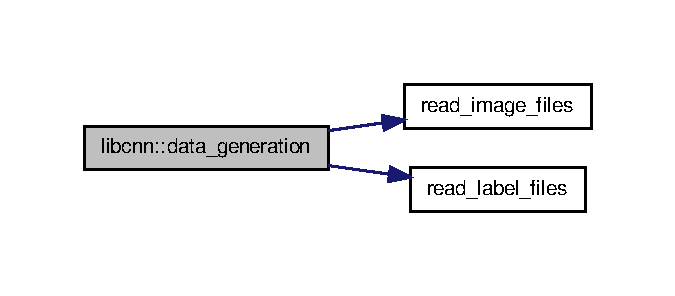
\includegraphics[width=324pt]{namespacelibcnn_a022f9a6378aa94ec418eb757bead690e_cgraph}
\end{center}
\end{figure}


\hypertarget{namespacelibcnn_a55bbe6e5488b8a038e5708a32d233090}{\index{libcnn@{libcnn}!get\-\_\-feature\-\_\-vector@{get\-\_\-feature\-\_\-vector}}
\index{get\-\_\-feature\-\_\-vector@{get\-\_\-feature\-\_\-vector}!libcnn@{libcnn}}
\subsubsection[{get\-\_\-feature\-\_\-vector}]{\setlength{\rightskip}{0pt plus 5cm}void {\bf libcnn\-::get\-\_\-feature\-\_\-vector} (
\begin{DoxyParamCaption}
\item[{const vector$<$ vector$<$ \-Matrix\-Xd $>$ $>$ \&}]{batch\-\_\-feature\-\_\-maps, }
\item[{\-Matrix\-Xd \&}]{feature\-\_\-vectors}
\end{DoxyParamCaption}
)}}\label{namespacelibcnn_a55bbe6e5488b8a038e5708a32d233090}
\hypertarget{namespacelibcnn_a2c5ccad2e675235e71fd5e5641ede4ae}{\index{libcnn@{libcnn}!get\-\_\-parameter@{get\-\_\-parameter}}
\index{get\-\_\-parameter@{get\-\_\-parameter}!libcnn@{libcnn}}
\subsubsection[{get\-\_\-parameter}]{\setlength{\rightskip}{0pt plus 5cm}void {\bf libcnn\-::get\-\_\-parameter} (
\begin{DoxyParamCaption}
\item[{vector$<$ \-Matrix\-Xd $>$ \&}]{feature\-\_\-weights}
\end{DoxyParamCaption}
)}}\label{namespacelibcnn_a2c5ccad2e675235e71fd5e5641ede4ae}
\hypertarget{namespacelibcnn_a0f018efe5349302aba6f349d17cc90cf}{\index{libcnn@{libcnn}!label\-\_\-sampling@{label\-\_\-sampling}}
\index{label\-\_\-sampling@{label\-\_\-sampling}!libcnn@{libcnn}}
\subsubsection[{label\-\_\-sampling}]{\setlength{\rightskip}{0pt plus 5cm}void {\bf libcnn\-::label\-\_\-sampling} (
\begin{DoxyParamCaption}
\item[{const int \&}]{height, }
\item[{const int \&}]{width, }
\item[{const int \&}]{pool, }
\item[{const int \&}]{images, }
\item[{\-Vector\-Xi \&}]{all\-\_\-label, }
\item[{\-Vector\-Xi \&}]{true\-\_\-label}
\end{DoxyParamCaption}
)}}\label{namespacelibcnn_a0f018efe5349302aba6f349d17cc90cf}
\hypertarget{namespacelibcnn_a05600c0680e871c0893560d97dce3179}{\index{libcnn@{libcnn}!load@{load}}
\index{load@{load}!libcnn@{libcnn}}
\subsubsection[{load}]{\setlength{\rightskip}{0pt plus 5cm}void {\bf libcnn\-::load} (
\begin{DoxyParamCaption}
\item[{const vector$<$ int $>$ \&}]{num\-\_\-kerns, }
\item[{vector$<$ vector$<$ \-Matrix\-Xd $>$ $>$ \&}]{weights, }
\item[{vector$<$ \-Matrix\-Xd $>$ \&}]{biases, }
\item[{\-Matrix\-Xd \&}]{class\-\_\-weight, }
\item[{\-Matrix\-Xd \&}]{class\-\_\-bias}
\end{DoxyParamCaption}
)}}\label{namespacelibcnn_a05600c0680e871c0893560d97dce3179}


\-Here is the call graph for this function\-:
\nopagebreak
\begin{figure}[H]
\begin{center}
\leavevmode
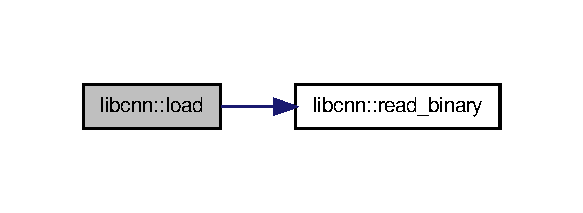
\includegraphics[width=280pt]{namespacelibcnn_a05600c0680e871c0893560d97dce3179_cgraph}
\end{center}
\end{figure}


\hypertarget{namespacelibcnn_ab161d6e7087d097f72c086587a661c4a}{\index{libcnn@{libcnn}!normalize@{normalize}}
\index{normalize@{normalize}!libcnn@{libcnn}}
\subsubsection[{normalize}]{\setlength{\rightskip}{0pt plus 5cm}void {\bf libcnn\-::normalize} (
\begin{DoxyParamCaption}
\item[{\-Matrix\-Xd \&}]{mat}
\end{DoxyParamCaption}
)}}\label{namespacelibcnn_ab161d6e7087d097f72c086587a661c4a}
\hypertarget{namespacelibcnn_a493fb452cedcc704e189ad1a3656c0ad}{\index{libcnn@{libcnn}!online\-\_\-test@{online\-\_\-test}}
\index{online\-\_\-test@{online\-\_\-test}!libcnn@{libcnn}}
\subsubsection[{online\-\_\-test}]{\setlength{\rightskip}{0pt plus 5cm}void {\bf libcnn\-::online\-\_\-test} (
\begin{DoxyParamCaption}
\item[{const vector$<$ vector$<$ \-Matrix\-Xd $>$ $>$ \&}]{vec\-\_\-data, }
\item[{const \-Vector\-Xi \&}]{vec\-\_\-label, }
\item[{const vector$<$ \-Matrix\-Xd $>$ \&}]{weight\-\_\-0, }
\item[{const \-Matrix\-Xd \&}]{bias\-\_\-0, }
\item[{const vector$<$ \-Matrix\-Xd $>$ \&}]{weight\-\_\-1, }
\item[{const \-Matrix\-Xd \&}]{bias\-\_\-1, }
\item[{const vector$<$ \-Matrix\-Xd $>$ \&}]{weight\-\_\-2, }
\item[{const \-Matrix\-Xd \&}]{bias\-\_\-2, }
\item[{const \-Matrix\-Xd \&}]{weight\-\_\-class, }
\item[{const \-Matrix\-Xd \&}]{bias\-\_\-class, }
\item[{const int \&}]{num\-\_\-kerns1, }
\item[{const int \&}]{num\-\_\-kerns2, }
\item[{const int \&}]{num\-\_\-kerns3, }
\item[{const int \&}]{kern\-\_\-size, }
\item[{const int \&}]{pool\-\_\-size}
\end{DoxyParamCaption}
)}}\label{namespacelibcnn_a493fb452cedcc704e189ad1a3656c0ad}


\-Here is the call graph for this function\-:
\nopagebreak
\begin{figure}[H]
\begin{center}
\leavevmode
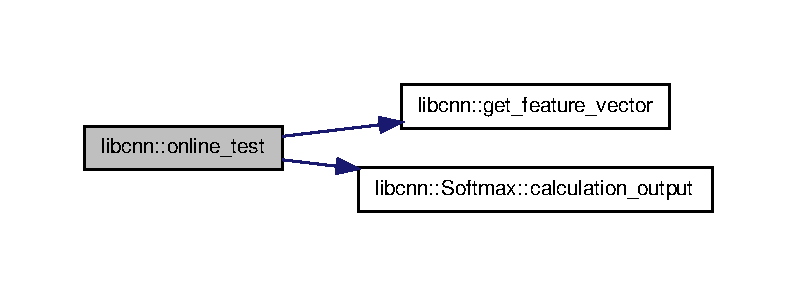
\includegraphics[width=350pt]{namespacelibcnn_a493fb452cedcc704e189ad1a3656c0ad_cgraph}
\end{center}
\end{figure}


\hypertarget{namespacelibcnn_a35fa40f645f5fe20b4cc8d878b1e0c10}{\index{libcnn@{libcnn}!print\-\_\-params@{print\-\_\-params}}
\index{print\-\_\-params@{print\-\_\-params}!libcnn@{libcnn}}
\subsubsection[{print\-\_\-params}]{\setlength{\rightskip}{0pt plus 5cm}void {\bf libcnn\-::print\-\_\-params} (
\begin{DoxyParamCaption}
\item[{vector$<$ vector$<$ \-Matrix\-Xd $>$ $>$ \&}]{, }
\item[{vector$<$ \-Matrix\-Xd $>$ \&}]{, }
\item[{vector$<$ \-Matrix\-Xd $>$ \&}]{, }
\item[{vector$<$ \-Matrix\-Xd $>$ \&}]{, }
\item[{vector$<$ \-Matrix\-Xd $>$ \&}]{, }
\item[{\-Matrix\-Xd \&}]{, }
\item[{\-Matrix\-Xd \&}]{, }
\item[{\-Matrix\-Xd \&}]{, }
\item[{\-Matrix\-Xd \&}]{, }
\item[{\-Matrix\-Xd \&}]{}
\end{DoxyParamCaption}
)}}\label{namespacelibcnn_a35fa40f645f5fe20b4cc8d878b1e0c10}
\hypertarget{namespacelibcnn_affc4a94fd6208861218bf25631d2ab39}{\index{libcnn@{libcnn}!print\-\_\-params@{print\-\_\-params}}
\index{print\-\_\-params@{print\-\_\-params}!libcnn@{libcnn}}
\subsubsection[{print\-\_\-params}]{\setlength{\rightskip}{0pt plus 5cm}void {\bf libcnn\-::print\-\_\-params} (
\begin{DoxyParamCaption}
\item[{vector$<$ vector$<$ \-Matrix\-Xd $>$ $>$ \&}]{weights, }
\item[{vector$<$ \-Matrix\-Xd $>$ \&}]{biases, }
\item[{vector$<$ \-Matrix\-Xd $>$ \&}]{weight\-\_\-0, }
\item[{vector$<$ \-Matrix\-Xd $>$ \&}]{weight\-\_\-1, }
\item[{vector$<$ \-Matrix\-Xd $>$ \&}]{weight\-\_\-2, }
\item[{\-Matrix\-Xd \&}]{bias\-\_\-0, }
\item[{\-Matrix\-Xd \&}]{bias\-\_\-1, }
\item[{\-Matrix\-Xd \&}]{bias\-\_\-2, }
\item[{\-Matrix\-Xd}]{weight\-\_\-class, }
\item[{\-Matrix\-Xd \&}]{bias\-\_\-class}
\end{DoxyParamCaption}
)}}\label{namespacelibcnn_affc4a94fd6208861218bf25631d2ab39}
\hypertarget{namespacelibcnn_a6e166be43bf4a7640feef235071df26e}{\index{libcnn@{libcnn}!print\-\_\-params@{print\-\_\-params}}
\index{print\-\_\-params@{print\-\_\-params}!libcnn@{libcnn}}
\subsubsection[{print\-\_\-params}]{\setlength{\rightskip}{0pt plus 5cm}void {\bf libcnn\-::print\-\_\-params} (
\begin{DoxyParamCaption}
\item[{const vector$<$ vector$<$ \-Matrix\-Xd $>$ $>$ \&}]{weights, }
\item[{const vector$<$ \-Matrix\-Xd $>$ \&}]{biases, }
\item[{const \-Matrix\-Xd \&}]{weight\-\_\-class, }
\item[{const \-Matrix\-Xd \&}]{bias\-\_\-class}
\end{DoxyParamCaption}
)}}\label{namespacelibcnn_a6e166be43bf4a7640feef235071df26e}
\hypertarget{namespacelibcnn_a367a409a55921d3810474a42357ff285}{\index{libcnn@{libcnn}!rand\-\_\-classifier@{rand\-\_\-classifier}}
\index{rand\-\_\-classifier@{rand\-\_\-classifier}!libcnn@{libcnn}}
\subsubsection[{rand\-\_\-classifier}]{\setlength{\rightskip}{0pt plus 5cm}void {\bf libcnn\-::rand\-\_\-classifier} (
\begin{DoxyParamCaption}
\item[{\-Matrix\-Xd \&}]{weight\-\_\-class, }
\item[{\-Matrix\-Xd \&}]{bias\-\_\-class, }
\item[{const vector$<$ int $>$ \&}]{num\-\_\-kernels, }
\item[{const int \&}]{num\-\_\-labels, }
\item[{const int \&}]{num\-\_\-input\-\_\-maps, }
\item[{const double \&}]{wb, }
\item[{const double \&}]{bb}
\end{DoxyParamCaption}
)}}\label{namespacelibcnn_a367a409a55921d3810474a42357ff285}
\hypertarget{namespacelibcnn_a449702bcc49494b8e359548d03ba12e3}{\index{libcnn@{libcnn}!rand\-\_\-conv@{rand\-\_\-conv}}
\index{rand\-\_\-conv@{rand\-\_\-conv}!libcnn@{libcnn}}
\subsubsection[{rand\-\_\-conv}]{\setlength{\rightskip}{0pt plus 5cm}void {\bf libcnn\-::rand\-\_\-conv} (
\begin{DoxyParamCaption}
\item[{vector$<$ vector$<$ \-Matrix\-Xd $>$ $>$ \&}]{weights, }
\item[{vector$<$ \-Matrix\-Xd $>$ \&}]{biases, }
\item[{const vector$<$ int $>$ \&}]{num\-\_\-kernels, }
\item[{const int \&}]{kernel\-\_\-size, }
\item[{const int \&}]{num\-\_\-labels, }
\item[{const double \&}]{weight\-\_\-bound, }
\item[{const double \&}]{bias\-\_\-bound}
\end{DoxyParamCaption}
)}}\label{namespacelibcnn_a449702bcc49494b8e359548d03ba12e3}
\hypertarget{namespacelibcnn_a08fddcf34488abeb9551fa4ba5f69b02}{\index{libcnn@{libcnn}!read\-\_\-binary@{read\-\_\-binary}}
\index{read\-\_\-binary@{read\-\_\-binary}!libcnn@{libcnn}}
\subsubsection[{read\-\_\-binary}]{\setlength{\rightskip}{0pt plus 5cm}template$<$class Matrix $>$ void {\bf libcnn\-::read\-\_\-binary} (
\begin{DoxyParamCaption}
\item[{const char $\ast$}]{filename, }
\item[{\-Matrix \&}]{matrix}
\end{DoxyParamCaption}
)}}\label{namespacelibcnn_a08fddcf34488abeb9551fa4ba5f69b02}
\hypertarget{namespacelibcnn_aa0d2c742374c714e8acadc2f2768db9e}{\index{libcnn@{libcnn}!save@{save}}
\index{save@{save}!libcnn@{libcnn}}
\subsubsection[{save}]{\setlength{\rightskip}{0pt plus 5cm}void {\bf libcnn\-::save} (
\begin{DoxyParamCaption}
\item[{const vector$<$ vector$<$ \-Matrix\-Xd $>$ $>$ \&}]{weights, }
\item[{const vector$<$ \-Matrix\-Xd $>$ \&}]{biases, }
\item[{const \-Matrix\-Xd \&}]{class\-\_\-weight, }
\item[{const \-Matrix\-Xd \&}]{class\-\_\-bias}
\end{DoxyParamCaption}
)}}\label{namespacelibcnn_aa0d2c742374c714e8acadc2f2768db9e}


\-Here is the call graph for this function\-:
\nopagebreak
\begin{figure}[H]
\begin{center}
\leavevmode
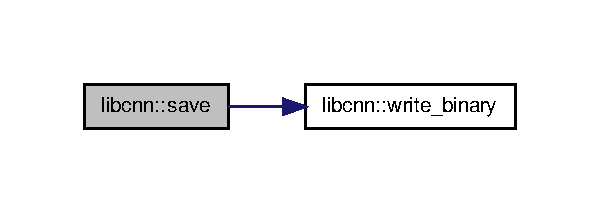
\includegraphics[width=288pt]{namespacelibcnn_aa0d2c742374c714e8acadc2f2768db9e_cgraph}
\end{center}
\end{figure}


\hypertarget{namespacelibcnn_a5b73556a76dfe9867c10ebd14519fb4e}{\index{libcnn@{libcnn}!sigmoid@{sigmoid}}
\index{sigmoid@{sigmoid}!libcnn@{libcnn}}
\subsubsection[{sigmoid}]{\setlength{\rightskip}{0pt plus 5cm}double {\bf libcnn\-::sigmoid} (
\begin{DoxyParamCaption}
\item[{const double \&}]{x}
\end{DoxyParamCaption}
)\hspace{0.3cm}{\ttfamily  \mbox{[}inline\mbox{]}}}}\label{namespacelibcnn_a5b73556a76dfe9867c10ebd14519fb4e}
\hypertarget{namespacelibcnn_a78ed8e63be87c4d06bb363af95ce62ec}{\index{libcnn@{libcnn}!softmax2conv@{softmax2conv}}
\index{softmax2conv@{softmax2conv}!libcnn@{libcnn}}
\subsubsection[{softmax2conv}]{\setlength{\rightskip}{0pt plus 5cm}void {\bf libcnn\-::softmax2conv} (
\begin{DoxyParamCaption}
\item[{const \-Matrix\-Xd \&}]{err\-\_\-softmax, }
\item[{const int \&}]{batch\-\_\-size, }
\item[{const int \&}]{map\-\_\-hight, }
\item[{const int \&}]{map\-\_\-width, }
\item[{vector$<$ vector$<$ \-Matrix\-Xd $>$ $>$ \&}]{err\-\_\-conv}
\end{DoxyParamCaption}
)}}\label{namespacelibcnn_a78ed8e63be87c4d06bb363af95ce62ec}
\hypertarget{namespacelibcnn_a4afdb4ab6bfd2c2167c593900ef644f5}{\index{libcnn@{libcnn}!unit\-\_\-scaling@{unit\-\_\-scaling}}
\index{unit\-\_\-scaling@{unit\-\_\-scaling}!libcnn@{libcnn}}
\subsubsection[{unit\-\_\-scaling}]{\setlength{\rightskip}{0pt plus 5cm}void {\bf libcnn\-::unit\-\_\-scaling} (
\begin{DoxyParamCaption}
\item[{vector$<$ vector$<$ \-Matrix\-Xd $>$ $>$ \&}]{all\-\_\-data}
\end{DoxyParamCaption}
)}}\label{namespacelibcnn_a4afdb4ab6bfd2c2167c593900ef644f5}


\-Here is the call graph for this function\-:
\nopagebreak
\begin{figure}[H]
\begin{center}
\leavevmode
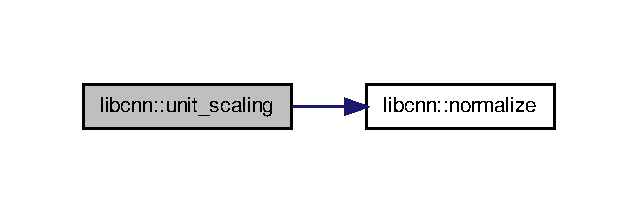
\includegraphics[width=306pt]{namespacelibcnn_a4afdb4ab6bfd2c2167c593900ef644f5_cgraph}
\end{center}
\end{figure}


\hypertarget{namespacelibcnn_ab9d1cc7fff65924fba4673d248ce5b84}{\index{libcnn@{libcnn}!write\-\_\-binary@{write\-\_\-binary}}
\index{write\-\_\-binary@{write\-\_\-binary}!libcnn@{libcnn}}
\subsubsection[{write\-\_\-binary}]{\setlength{\rightskip}{0pt plus 5cm}template$<$class Matrix $>$ void {\bf libcnn\-::write\-\_\-binary} (
\begin{DoxyParamCaption}
\item[{const char $\ast$}]{filename, }
\item[{const \-Matrix \&}]{matrix}
\end{DoxyParamCaption}
)}}\label{namespacelibcnn_ab9d1cc7fff65924fba4673d248ce5b84}

\hypertarget{namespacemarkov__1}{\section{markov\-\_\-1 \-Namespace \-Reference}
\label{namespacemarkov__1}\index{markov\-\_\-1@{markov\-\_\-1}}
}
\subsection*{\-Variables}
\begin{DoxyCompactItemize}
\item 
float \hyperlink{namespacemarkov__1_a4a3eda3678257ab2cf6f06891c5ec22c}{roe} = 0.\-9999
\item 
list \hyperlink{namespacemarkov__1_ac6e549cf6d4d6df355d884b67fb19851}{roe\-\_\-list} = \mbox{[}$\,$\mbox{]}
\item 
int \hyperlink{namespacemarkov__1_a8134563a0c42390906c8914ad337e9d8}{data\-\_\-dimension} = 64
\item 
tuple \hyperlink{namespacemarkov__1_a7cc4d10a876ec07da21dbfd4d28e8684}{covariance\-\_\-matrix} = toeplitz(\hyperlink{namespacemarkov__1_ac6e549cf6d4d6df355d884b67fb19851}{roe\-\_\-list}, \hyperlink{namespacemarkov__1_ac6e549cf6d4d6df355d884b67fb19851}{roe\-\_\-list})
\item 
\hyperlink{namespacemarkov__1_a3744683663f02bff5cf245a674ab9b32}{\-Data\-Out} = e\-\_\-vecs
\end{DoxyCompactItemize}


\subsection{\-Variable \-Documentation}
\hypertarget{namespacemarkov__1_a7cc4d10a876ec07da21dbfd4d28e8684}{\index{markov\-\_\-1@{markov\-\_\-1}!covariance\-\_\-matrix@{covariance\-\_\-matrix}}
\index{covariance\-\_\-matrix@{covariance\-\_\-matrix}!markov_1@{markov\-\_\-1}}
\subsubsection[{covariance\-\_\-matrix}]{\setlength{\rightskip}{0pt plus 5cm}tuple {\bf markov\-\_\-1\-::covariance\-\_\-matrix} = toeplitz({\bf roe\-\_\-list}, {\bf roe\-\_\-list})}}\label{namespacemarkov__1_a7cc4d10a876ec07da21dbfd4d28e8684}
\hypertarget{namespacemarkov__1_a8134563a0c42390906c8914ad337e9d8}{\index{markov\-\_\-1@{markov\-\_\-1}!data\-\_\-dimension@{data\-\_\-dimension}}
\index{data\-\_\-dimension@{data\-\_\-dimension}!markov_1@{markov\-\_\-1}}
\subsubsection[{data\-\_\-dimension}]{\setlength{\rightskip}{0pt plus 5cm}int {\bf markov\-\_\-1\-::data\-\_\-dimension} = 64}}\label{namespacemarkov__1_a8134563a0c42390906c8914ad337e9d8}
\hypertarget{namespacemarkov__1_a3744683663f02bff5cf245a674ab9b32}{\index{markov\-\_\-1@{markov\-\_\-1}!\-Data\-Out@{\-Data\-Out}}
\index{\-Data\-Out@{\-Data\-Out}!markov_1@{markov\-\_\-1}}
\subsubsection[{\-Data\-Out}]{\setlength{\rightskip}{0pt plus 5cm}{\bf markov\-\_\-1\-::\-Data\-Out} = e\-\_\-vecs}}\label{namespacemarkov__1_a3744683663f02bff5cf245a674ab9b32}
\hypertarget{namespacemarkov__1_a4a3eda3678257ab2cf6f06891c5ec22c}{\index{markov\-\_\-1@{markov\-\_\-1}!roe@{roe}}
\index{roe@{roe}!markov_1@{markov\-\_\-1}}
\subsubsection[{roe}]{\setlength{\rightskip}{0pt plus 5cm}float {\bf markov\-\_\-1\-::roe} = 0.\-9999}}\label{namespacemarkov__1_a4a3eda3678257ab2cf6f06891c5ec22c}
\hypertarget{namespacemarkov__1_ac6e549cf6d4d6df355d884b67fb19851}{\index{markov\-\_\-1@{markov\-\_\-1}!roe\-\_\-list@{roe\-\_\-list}}
\index{roe\-\_\-list@{roe\-\_\-list}!markov_1@{markov\-\_\-1}}
\subsubsection[{roe\-\_\-list}]{\setlength{\rightskip}{0pt plus 5cm}tuple {\bf markov\-\_\-1\-::roe\-\_\-list} = \mbox{[}$\,$\mbox{]}}}\label{namespacemarkov__1_ac6e549cf6d4d6df355d884b67fb19851}

\chapter{\-Class \-Documentation}
\hypertarget{classlibcnn_1_1_conv_pool_layer}{\section{libcnn\-:\-:\-Conv\-Pool\-Layer \-Class \-Reference}
\label{classlibcnn_1_1_conv_pool_layer}\index{libcnn\-::\-Conv\-Pool\-Layer@{libcnn\-::\-Conv\-Pool\-Layer}}
}


{\ttfamily \#include $<$conv\-\_\-layer.\-h$>$}

\subsection*{\-Public \-Member \-Functions}
\begin{DoxyCompactItemize}
\item 
\hyperlink{classlibcnn_1_1_conv_pool_layer_a4ef1d6c7eac689b2472815abf5aea08a}{\-Conv\-Pool\-Layer} (const vector$<$ vector$<$ \-Matrix\-Xd $>$ $>$ \&, const int \&, const int \&, const string \&, const string \&)
\item 
\hyperlink{classlibcnn_1_1_conv_pool_layer_ad24c278c8e1ea940eecc862dd8a334c3}{\-Conv\-Pool\-Layer} (const vector$<$ vector$<$ \-Matrix\-Xd $>$ $>$ \&, const int \&, const int \&, const string \&, const string \&, const vector$<$ \-Matrix\-Xd $>$ \&, const \-Matrix\-Xd \&)
\item 
void \hyperlink{classlibcnn_1_1_conv_pool_layer_a29c5445a08cf88d44a69b9370e5adc1d}{compute} ()
\item 
void \hyperlink{classlibcnn_1_1_conv_pool_layer_a32bafdf90d99eb5fc5902f831b208838}{bp\-\_\-activate} (const vector$<$ vector$<$ \-Matrix\-Xd $>$ $>$ \&, const vector$<$ vector$<$ \-Matrix\-Xd $>$ $>$ \&, vector$<$ vector$<$ \-Matrix\-Xd $>$ $>$ \&)
\item 
void \hyperlink{classlibcnn_1_1_conv_pool_layer_a30204d1f55cc343c422cb6da5b1b4590}{bp\-\_\-conv} (const vector$<$ vector$<$ \-Matrix\-Xd $>$ $>$ \&, const double \&)
\item 
void \hyperlink{classlibcnn_1_1_conv_pool_layer_ab74a2227a84ff1de545dd1e69f0c8fb3}{back\-\_\-prop} (const vector$<$ vector$<$ \-Matrix\-Xd $>$ $>$ \&, const double \&)
\item 
\hyperlink{classlibcnn_1_1_conv_pool_layer_a4ef1d6c7eac689b2472815abf5aea08a}{\-Conv\-Pool\-Layer} (const vector$<$ vector$<$ \-Matrix\-Xd $>$ $>$ \&, const int \&, const int \&, const string \&, const string \&)
\item 
\hyperlink{classlibcnn_1_1_conv_pool_layer_ad24c278c8e1ea940eecc862dd8a334c3}{\-Conv\-Pool\-Layer} (const vector$<$ vector$<$ \-Matrix\-Xd $>$ $>$ \&, const int \&, const int \&, const string \&, const string \&, const vector$<$ \-Matrix\-Xd $>$ \&, const \-Matrix\-Xd \&)
\item 
void \hyperlink{classlibcnn_1_1_conv_pool_layer_a29c5445a08cf88d44a69b9370e5adc1d}{compute} ()
\item 
void \hyperlink{classlibcnn_1_1_conv_pool_layer_a32bafdf90d99eb5fc5902f831b208838}{bp\-\_\-activate} (const vector$<$ vector$<$ \-Matrix\-Xd $>$ $>$ \&, const vector$<$ vector$<$ \-Matrix\-Xd $>$ $>$ \&, vector$<$ vector$<$ \-Matrix\-Xd $>$ $>$ \&)
\item 
void \hyperlink{classlibcnn_1_1_conv_pool_layer_a30204d1f55cc343c422cb6da5b1b4590}{bp\-\_\-conv} (const vector$<$ vector$<$ \-Matrix\-Xd $>$ $>$ \&, const double \&)
\item 
void \hyperlink{classlibcnn_1_1_conv_pool_layer_ab74a2227a84ff1de545dd1e69f0c8fb3}{back\-\_\-prop} (const vector$<$ vector$<$ \-Matrix\-Xd $>$ $>$ \&, const double \&)
\end{DoxyCompactItemize}
\subsection*{\-Public \-Attributes}
\begin{DoxyCompactItemize}
\item 
vector$<$ vector$<$ \-Matrix\-Xd $>$ $>$ \hyperlink{classlibcnn_1_1_conv_pool_layer_a63d9d97664284772029c36a897e4e30e}{batch\-\_\-maps\-\_\-input}
\item 
vector$<$ vector$<$ \-Matrix\-Xd $>$ $>$ \hyperlink{classlibcnn_1_1_conv_pool_layer_a519dad823100b62bc93738477a593a6d}{grad\-\_\-batch\-\_\-maps\-\_\-input}
\item 
vector$<$ \-Matrix\-Xd $>$ \hyperlink{classlibcnn_1_1_conv_pool_layer_ad9b3b0b372858e32e075565beec5226a}{weight}
\item 
vector$<$ \-Matrix\-Xd $>$ \hyperlink{classlibcnn_1_1_conv_pool_layer_a2728855bb4a00c4800ff4a912ef21e85}{grad\-\_\-weight}
\item 
\-Matrix\-Xd \hyperlink{classlibcnn_1_1_conv_pool_layer_a8b537b16fb08d935f442360f564b9403}{bias}
\item 
\-Matrix\-Xd \hyperlink{classlibcnn_1_1_conv_pool_layer_a4bf6b594b2a91f6bd8291ff8e446e4ba}{grad\-\_\-bias}
\item 
vector$<$ vector$<$ \-Matrix\-Xd $>$ $>$ \hyperlink{classlibcnn_1_1_conv_pool_layer_ad42c5b645c6103b200b9b950b4349550}{batch\-\_\-maps\-\_\-activated}
\item 
vector$<$ vector$<$ vector\*
$<$ \-Matrix\-Xd $>$ $>$ $>$ \hyperlink{classlibcnn_1_1_conv_pool_layer_a0b8d18fc0be5f3e75813a86b24dce247}{batch\-\_\-coordinates}
\item 
string \hyperlink{classlibcnn_1_1_conv_pool_layer_aa57ba56fe0f3e38f58931137a03e07f3}{activation\-\_\-type}
\end{DoxyCompactItemize}


\subsection{\-Constructor \& \-Destructor \-Documentation}
\hypertarget{classlibcnn_1_1_conv_pool_layer_a4ef1d6c7eac689b2472815abf5aea08a}{\index{libcnn\-::\-Conv\-Pool\-Layer@{libcnn\-::\-Conv\-Pool\-Layer}!\-Conv\-Pool\-Layer@{\-Conv\-Pool\-Layer}}
\index{\-Conv\-Pool\-Layer@{\-Conv\-Pool\-Layer}!libcnn::ConvPoolLayer@{libcnn\-::\-Conv\-Pool\-Layer}}
\subsubsection[{\-Conv\-Pool\-Layer}]{\setlength{\rightskip}{0pt plus 5cm}{\bf libcnn\-::\-Conv\-Pool\-Layer\-::\-Conv\-Pool\-Layer} (
\begin{DoxyParamCaption}
\item[{const vector$<$ vector$<$ \-Matrix\-Xd $>$ $>$ \&}]{input, }
\item[{const int \&}]{num\-\_\-kerns, }
\item[{const int \&}]{kern\-\_\-size, }
\item[{const string \&}]{conv\-\_\-mode, }
\item[{const string \&}]{act\-\_\-type}
\end{DoxyParamCaption}
)}}\label{classlibcnn_1_1_conv_pool_layer_a4ef1d6c7eac689b2472815abf5aea08a}
\hypertarget{classlibcnn_1_1_conv_pool_layer_ad24c278c8e1ea940eecc862dd8a334c3}{\index{libcnn\-::\-Conv\-Pool\-Layer@{libcnn\-::\-Conv\-Pool\-Layer}!\-Conv\-Pool\-Layer@{\-Conv\-Pool\-Layer}}
\index{\-Conv\-Pool\-Layer@{\-Conv\-Pool\-Layer}!libcnn::ConvPoolLayer@{libcnn\-::\-Conv\-Pool\-Layer}}
\subsubsection[{\-Conv\-Pool\-Layer}]{\setlength{\rightskip}{0pt plus 5cm}{\bf libcnn\-::\-Conv\-Pool\-Layer\-::\-Conv\-Pool\-Layer} (
\begin{DoxyParamCaption}
\item[{const vector$<$ vector$<$ \-Matrix\-Xd $>$ $>$ \&}]{input, }
\item[{const int \&}]{num\-\_\-kerns, }
\item[{const int \&}]{kern\-\_\-size, }
\item[{const string \&}]{conv\-\_\-mode, }
\item[{const string \&}]{act\-\_\-type, }
\item[{const vector$<$ \-Matrix\-Xd $>$ \&}]{weight\-\_\-, }
\item[{const \-Matrix\-Xd \&}]{bias\-\_\-}
\end{DoxyParamCaption}
)}}\label{classlibcnn_1_1_conv_pool_layer_ad24c278c8e1ea940eecc862dd8a334c3}
\hypertarget{classlibcnn_1_1_conv_pool_layer_a4ef1d6c7eac689b2472815abf5aea08a}{\index{libcnn\-::\-Conv\-Pool\-Layer@{libcnn\-::\-Conv\-Pool\-Layer}!\-Conv\-Pool\-Layer@{\-Conv\-Pool\-Layer}}
\index{\-Conv\-Pool\-Layer@{\-Conv\-Pool\-Layer}!libcnn::ConvPoolLayer@{libcnn\-::\-Conv\-Pool\-Layer}}
\subsubsection[{\-Conv\-Pool\-Layer}]{\setlength{\rightskip}{0pt plus 5cm}{\bf libcnn\-::\-Conv\-Pool\-Layer\-::\-Conv\-Pool\-Layer} (
\begin{DoxyParamCaption}
\item[{const vector$<$ vector$<$ \-Matrix\-Xd $>$ $>$ \&}]{, }
\item[{const int \&}]{, }
\item[{const int \&}]{, }
\item[{const string \&}]{, }
\item[{const string \&}]{}
\end{DoxyParamCaption}
)}}\label{classlibcnn_1_1_conv_pool_layer_a4ef1d6c7eac689b2472815abf5aea08a}
\hypertarget{classlibcnn_1_1_conv_pool_layer_ad24c278c8e1ea940eecc862dd8a334c3}{\index{libcnn\-::\-Conv\-Pool\-Layer@{libcnn\-::\-Conv\-Pool\-Layer}!\-Conv\-Pool\-Layer@{\-Conv\-Pool\-Layer}}
\index{\-Conv\-Pool\-Layer@{\-Conv\-Pool\-Layer}!libcnn::ConvPoolLayer@{libcnn\-::\-Conv\-Pool\-Layer}}
\subsubsection[{\-Conv\-Pool\-Layer}]{\setlength{\rightskip}{0pt plus 5cm}{\bf libcnn\-::\-Conv\-Pool\-Layer\-::\-Conv\-Pool\-Layer} (
\begin{DoxyParamCaption}
\item[{const vector$<$ vector$<$ \-Matrix\-Xd $>$ $>$ \&}]{, }
\item[{const int \&}]{, }
\item[{const int \&}]{, }
\item[{const string \&}]{, }
\item[{const string \&}]{, }
\item[{const vector$<$ \-Matrix\-Xd $>$ \&}]{, }
\item[{const \-Matrix\-Xd \&}]{}
\end{DoxyParamCaption}
)}}\label{classlibcnn_1_1_conv_pool_layer_ad24c278c8e1ea940eecc862dd8a334c3}


\subsection{\-Member \-Function \-Documentation}
\hypertarget{classlibcnn_1_1_conv_pool_layer_ab74a2227a84ff1de545dd1e69f0c8fb3}{\index{libcnn\-::\-Conv\-Pool\-Layer@{libcnn\-::\-Conv\-Pool\-Layer}!back\-\_\-prop@{back\-\_\-prop}}
\index{back\-\_\-prop@{back\-\_\-prop}!libcnn::ConvPoolLayer@{libcnn\-::\-Conv\-Pool\-Layer}}
\subsubsection[{back\-\_\-prop}]{\setlength{\rightskip}{0pt plus 5cm}void {\bf libcnn\-::\-Conv\-Pool\-Layer\-::back\-\_\-prop} (
\begin{DoxyParamCaption}
\item[{const vector$<$ vector$<$ \-Matrix\-Xd $>$ $>$ \&}]{grad\-\_\-batch\-\_\-maps\-\_\-activated, }
\item[{const double \&}]{lr}
\end{DoxyParamCaption}
)}}\label{classlibcnn_1_1_conv_pool_layer_ab74a2227a84ff1de545dd1e69f0c8fb3}
\hypertarget{classlibcnn_1_1_conv_pool_layer_ab74a2227a84ff1de545dd1e69f0c8fb3}{\index{libcnn\-::\-Conv\-Pool\-Layer@{libcnn\-::\-Conv\-Pool\-Layer}!back\-\_\-prop@{back\-\_\-prop}}
\index{back\-\_\-prop@{back\-\_\-prop}!libcnn::ConvPoolLayer@{libcnn\-::\-Conv\-Pool\-Layer}}
\subsubsection[{back\-\_\-prop}]{\setlength{\rightskip}{0pt plus 5cm}void {\bf libcnn\-::\-Conv\-Pool\-Layer\-::back\-\_\-prop} (
\begin{DoxyParamCaption}
\item[{const vector$<$ vector$<$ \-Matrix\-Xd $>$ $>$ \&}]{, }
\item[{const double \&}]{}
\end{DoxyParamCaption}
)}}\label{classlibcnn_1_1_conv_pool_layer_ab74a2227a84ff1de545dd1e69f0c8fb3}
\hypertarget{classlibcnn_1_1_conv_pool_layer_a32bafdf90d99eb5fc5902f831b208838}{\index{libcnn\-::\-Conv\-Pool\-Layer@{libcnn\-::\-Conv\-Pool\-Layer}!bp\-\_\-activate@{bp\-\_\-activate}}
\index{bp\-\_\-activate@{bp\-\_\-activate}!libcnn::ConvPoolLayer@{libcnn\-::\-Conv\-Pool\-Layer}}
\subsubsection[{bp\-\_\-activate}]{\setlength{\rightskip}{0pt plus 5cm}void {\bf libcnn\-::\-Conv\-Pool\-Layer\-::bp\-\_\-activate} (
\begin{DoxyParamCaption}
\item[{const vector$<$ vector$<$ \-Matrix\-Xd $>$ $>$ \&}]{grad\-\_\-batch\-\_\-maps\-\_\-activated, }
\item[{const vector$<$ vector$<$ \-Matrix\-Xd $>$ $>$ \&}]{batch\-\_\-maps\-\_\-activated, }
\item[{vector$<$ vector$<$ \-Matrix\-Xd $>$ $>$ \&}]{grad\-\_\-batch\-\_\-maps\-\_\-conved}
\end{DoxyParamCaption}
)}}\label{classlibcnn_1_1_conv_pool_layer_a32bafdf90d99eb5fc5902f831b208838}
\hypertarget{classlibcnn_1_1_conv_pool_layer_a32bafdf90d99eb5fc5902f831b208838}{\index{libcnn\-::\-Conv\-Pool\-Layer@{libcnn\-::\-Conv\-Pool\-Layer}!bp\-\_\-activate@{bp\-\_\-activate}}
\index{bp\-\_\-activate@{bp\-\_\-activate}!libcnn::ConvPoolLayer@{libcnn\-::\-Conv\-Pool\-Layer}}
\subsubsection[{bp\-\_\-activate}]{\setlength{\rightskip}{0pt plus 5cm}void {\bf libcnn\-::\-Conv\-Pool\-Layer\-::bp\-\_\-activate} (
\begin{DoxyParamCaption}
\item[{const vector$<$ vector$<$ \-Matrix\-Xd $>$ $>$ \&}]{, }
\item[{const vector$<$ vector$<$ \-Matrix\-Xd $>$ $>$ \&}]{, }
\item[{vector$<$ vector$<$ \-Matrix\-Xd $>$ $>$ \&}]{}
\end{DoxyParamCaption}
)}}\label{classlibcnn_1_1_conv_pool_layer_a32bafdf90d99eb5fc5902f831b208838}
\hypertarget{classlibcnn_1_1_conv_pool_layer_a30204d1f55cc343c422cb6da5b1b4590}{\index{libcnn\-::\-Conv\-Pool\-Layer@{libcnn\-::\-Conv\-Pool\-Layer}!bp\-\_\-conv@{bp\-\_\-conv}}
\index{bp\-\_\-conv@{bp\-\_\-conv}!libcnn::ConvPoolLayer@{libcnn\-::\-Conv\-Pool\-Layer}}
\subsubsection[{bp\-\_\-conv}]{\setlength{\rightskip}{0pt plus 5cm}void {\bf libcnn\-::\-Conv\-Pool\-Layer\-::bp\-\_\-conv} (
\begin{DoxyParamCaption}
\item[{const vector$<$ vector$<$ \-Matrix\-Xd $>$ $>$ \&}]{, }
\item[{const double \&}]{}
\end{DoxyParamCaption}
)}}\label{classlibcnn_1_1_conv_pool_layer_a30204d1f55cc343c422cb6da5b1b4590}
\hypertarget{classlibcnn_1_1_conv_pool_layer_a30204d1f55cc343c422cb6da5b1b4590}{\index{libcnn\-::\-Conv\-Pool\-Layer@{libcnn\-::\-Conv\-Pool\-Layer}!bp\-\_\-conv@{bp\-\_\-conv}}
\index{bp\-\_\-conv@{bp\-\_\-conv}!libcnn::ConvPoolLayer@{libcnn\-::\-Conv\-Pool\-Layer}}
\subsubsection[{bp\-\_\-conv}]{\setlength{\rightskip}{0pt plus 5cm}void {\bf libcnn\-::\-Conv\-Pool\-Layer\-::bp\-\_\-conv} (
\begin{DoxyParamCaption}
\item[{const vector$<$ vector$<$ \-Matrix\-Xd $>$ $>$ \&}]{grad\-\_\-batch\-\_\-maps\-\_\-conved, }
\item[{const double \&}]{lr}
\end{DoxyParamCaption}
)}}\label{classlibcnn_1_1_conv_pool_layer_a30204d1f55cc343c422cb6da5b1b4590}
\hypertarget{classlibcnn_1_1_conv_pool_layer_a29c5445a08cf88d44a69b9370e5adc1d}{\index{libcnn\-::\-Conv\-Pool\-Layer@{libcnn\-::\-Conv\-Pool\-Layer}!compute@{compute}}
\index{compute@{compute}!libcnn::ConvPoolLayer@{libcnn\-::\-Conv\-Pool\-Layer}}
\subsubsection[{compute}]{\setlength{\rightskip}{0pt plus 5cm}void {\bf libcnn\-::\-Conv\-Pool\-Layer\-::compute} (
\begin{DoxyParamCaption}
{}
\end{DoxyParamCaption}
)}}\label{classlibcnn_1_1_conv_pool_layer_a29c5445a08cf88d44a69b9370e5adc1d}
\hypertarget{classlibcnn_1_1_conv_pool_layer_a29c5445a08cf88d44a69b9370e5adc1d}{\index{libcnn\-::\-Conv\-Pool\-Layer@{libcnn\-::\-Conv\-Pool\-Layer}!compute@{compute}}
\index{compute@{compute}!libcnn::ConvPoolLayer@{libcnn\-::\-Conv\-Pool\-Layer}}
\subsubsection[{compute}]{\setlength{\rightskip}{0pt plus 5cm}void {\bf libcnn\-::\-Conv\-Pool\-Layer\-::compute} (
\begin{DoxyParamCaption}
{}
\end{DoxyParamCaption}
)}}\label{classlibcnn_1_1_conv_pool_layer_a29c5445a08cf88d44a69b9370e5adc1d}


\subsection{\-Member \-Data \-Documentation}
\hypertarget{classlibcnn_1_1_conv_pool_layer_aa57ba56fe0f3e38f58931137a03e07f3}{\index{libcnn\-::\-Conv\-Pool\-Layer@{libcnn\-::\-Conv\-Pool\-Layer}!activation\-\_\-type@{activation\-\_\-type}}
\index{activation\-\_\-type@{activation\-\_\-type}!libcnn::ConvPoolLayer@{libcnn\-::\-Conv\-Pool\-Layer}}
\subsubsection[{activation\-\_\-type}]{\setlength{\rightskip}{0pt plus 5cm}string {\bf libcnn\-::\-Conv\-Pool\-Layer\-::activation\-\_\-type}}}\label{classlibcnn_1_1_conv_pool_layer_aa57ba56fe0f3e38f58931137a03e07f3}
\hypertarget{classlibcnn_1_1_conv_pool_layer_a0b8d18fc0be5f3e75813a86b24dce247}{\index{libcnn\-::\-Conv\-Pool\-Layer@{libcnn\-::\-Conv\-Pool\-Layer}!batch\-\_\-coordinates@{batch\-\_\-coordinates}}
\index{batch\-\_\-coordinates@{batch\-\_\-coordinates}!libcnn::ConvPoolLayer@{libcnn\-::\-Conv\-Pool\-Layer}}
\subsubsection[{batch\-\_\-coordinates}]{\setlength{\rightskip}{0pt plus 5cm}vector$<$ vector$<$ vector$<$ \-Matrix\-Xd $>$ $>$ $>$ {\bf libcnn\-::\-Conv\-Pool\-Layer\-::batch\-\_\-coordinates}}}\label{classlibcnn_1_1_conv_pool_layer_a0b8d18fc0be5f3e75813a86b24dce247}
\hypertarget{classlibcnn_1_1_conv_pool_layer_ad42c5b645c6103b200b9b950b4349550}{\index{libcnn\-::\-Conv\-Pool\-Layer@{libcnn\-::\-Conv\-Pool\-Layer}!batch\-\_\-maps\-\_\-activated@{batch\-\_\-maps\-\_\-activated}}
\index{batch\-\_\-maps\-\_\-activated@{batch\-\_\-maps\-\_\-activated}!libcnn::ConvPoolLayer@{libcnn\-::\-Conv\-Pool\-Layer}}
\subsubsection[{batch\-\_\-maps\-\_\-activated}]{\setlength{\rightskip}{0pt plus 5cm}vector$<$ vector$<$ \-Matrix\-Xd $>$ $>$ {\bf libcnn\-::\-Conv\-Pool\-Layer\-::batch\-\_\-maps\-\_\-activated}}}\label{classlibcnn_1_1_conv_pool_layer_ad42c5b645c6103b200b9b950b4349550}
\hypertarget{classlibcnn_1_1_conv_pool_layer_a63d9d97664284772029c36a897e4e30e}{\index{libcnn\-::\-Conv\-Pool\-Layer@{libcnn\-::\-Conv\-Pool\-Layer}!batch\-\_\-maps\-\_\-input@{batch\-\_\-maps\-\_\-input}}
\index{batch\-\_\-maps\-\_\-input@{batch\-\_\-maps\-\_\-input}!libcnn::ConvPoolLayer@{libcnn\-::\-Conv\-Pool\-Layer}}
\subsubsection[{batch\-\_\-maps\-\_\-input}]{\setlength{\rightskip}{0pt plus 5cm}vector$<$ vector$<$ \-Matrix\-Xd $>$ $>$ {\bf libcnn\-::\-Conv\-Pool\-Layer\-::batch\-\_\-maps\-\_\-input}}}\label{classlibcnn_1_1_conv_pool_layer_a63d9d97664284772029c36a897e4e30e}
\hypertarget{classlibcnn_1_1_conv_pool_layer_a8b537b16fb08d935f442360f564b9403}{\index{libcnn\-::\-Conv\-Pool\-Layer@{libcnn\-::\-Conv\-Pool\-Layer}!bias@{bias}}
\index{bias@{bias}!libcnn::ConvPoolLayer@{libcnn\-::\-Conv\-Pool\-Layer}}
\subsubsection[{bias}]{\setlength{\rightskip}{0pt plus 5cm}\-Matrix\-Xd {\bf libcnn\-::\-Conv\-Pool\-Layer\-::bias}}}\label{classlibcnn_1_1_conv_pool_layer_a8b537b16fb08d935f442360f564b9403}
\hypertarget{classlibcnn_1_1_conv_pool_layer_a519dad823100b62bc93738477a593a6d}{\index{libcnn\-::\-Conv\-Pool\-Layer@{libcnn\-::\-Conv\-Pool\-Layer}!grad\-\_\-batch\-\_\-maps\-\_\-input@{grad\-\_\-batch\-\_\-maps\-\_\-input}}
\index{grad\-\_\-batch\-\_\-maps\-\_\-input@{grad\-\_\-batch\-\_\-maps\-\_\-input}!libcnn::ConvPoolLayer@{libcnn\-::\-Conv\-Pool\-Layer}}
\subsubsection[{grad\-\_\-batch\-\_\-maps\-\_\-input}]{\setlength{\rightskip}{0pt plus 5cm}vector$<$ vector$<$ \-Matrix\-Xd $>$ $>$ {\bf libcnn\-::\-Conv\-Pool\-Layer\-::grad\-\_\-batch\-\_\-maps\-\_\-input}}}\label{classlibcnn_1_1_conv_pool_layer_a519dad823100b62bc93738477a593a6d}
\hypertarget{classlibcnn_1_1_conv_pool_layer_a4bf6b594b2a91f6bd8291ff8e446e4ba}{\index{libcnn\-::\-Conv\-Pool\-Layer@{libcnn\-::\-Conv\-Pool\-Layer}!grad\-\_\-bias@{grad\-\_\-bias}}
\index{grad\-\_\-bias@{grad\-\_\-bias}!libcnn::ConvPoolLayer@{libcnn\-::\-Conv\-Pool\-Layer}}
\subsubsection[{grad\-\_\-bias}]{\setlength{\rightskip}{0pt plus 5cm}\-Matrix\-Xd {\bf libcnn\-::\-Conv\-Pool\-Layer\-::grad\-\_\-bias}}}\label{classlibcnn_1_1_conv_pool_layer_a4bf6b594b2a91f6bd8291ff8e446e4ba}
\hypertarget{classlibcnn_1_1_conv_pool_layer_a2728855bb4a00c4800ff4a912ef21e85}{\index{libcnn\-::\-Conv\-Pool\-Layer@{libcnn\-::\-Conv\-Pool\-Layer}!grad\-\_\-weight@{grad\-\_\-weight}}
\index{grad\-\_\-weight@{grad\-\_\-weight}!libcnn::ConvPoolLayer@{libcnn\-::\-Conv\-Pool\-Layer}}
\subsubsection[{grad\-\_\-weight}]{\setlength{\rightskip}{0pt plus 5cm}vector$<$ \-Matrix\-Xd $>$ {\bf libcnn\-::\-Conv\-Pool\-Layer\-::grad\-\_\-weight}}}\label{classlibcnn_1_1_conv_pool_layer_a2728855bb4a00c4800ff4a912ef21e85}
\hypertarget{classlibcnn_1_1_conv_pool_layer_ad9b3b0b372858e32e075565beec5226a}{\index{libcnn\-::\-Conv\-Pool\-Layer@{libcnn\-::\-Conv\-Pool\-Layer}!weight@{weight}}
\index{weight@{weight}!libcnn::ConvPoolLayer@{libcnn\-::\-Conv\-Pool\-Layer}}
\subsubsection[{weight}]{\setlength{\rightskip}{0pt plus 5cm}vector$<$ \-Matrix\-Xd $>$ {\bf libcnn\-::\-Conv\-Pool\-Layer\-::weight}}}\label{classlibcnn_1_1_conv_pool_layer_ad9b3b0b372858e32e075565beec5226a}


\-The documentation for this class was generated from the following files\-:\begin{DoxyCompactItemize}
\item 
gpu/include/\hyperlink{gpu_2include_2conv__layer_8h}{conv\-\_\-layer.\-h}\item 
include/\hyperlink{include_2conv__layer_8h}{conv\-\_\-layer.\-h}\item 
gpu/src/\hyperlink{gpu_2src_2conv__layer_8cpp}{conv\-\_\-layer.\-cpp}\item 
src/\hyperlink{src_2conv__layer_8cpp}{conv\-\_\-layer.\-cpp}\end{DoxyCompactItemize}

\hypertarget{classlibcnn_1_1_pool}{\section{libcnn\-:\-:\-Pool \-Class \-Reference}
\label{classlibcnn_1_1_pool}\index{libcnn\-::\-Pool@{libcnn\-::\-Pool}}
}


{\ttfamily \#include $<$pool.\-h$>$}

\subsection*{\-Public \-Member \-Functions}
\begin{DoxyCompactItemize}
\item 
\hyperlink{classlibcnn_1_1_pool_a25dda142002e7d9447df8b529a03e8c6}{\-Pool} (const vector$<$ vector$<$ \-Matrix\-Xd $>$ $>$ \&, const int \&, const int \&)
\item 
void \hyperlink{classlibcnn_1_1_pool_a7e1edbfb399a7530fb936f0378fbe1a1}{compute} (const vector$<$ vector$<$ \-Matrix\-Xd $>$ $>$ \&)
\item 
void \hyperlink{classlibcnn_1_1_pool_a7971925b58312b01b92402f6991460cd}{back\-\_\-prop} (vector$<$ vector$<$ \-Matrix\-Xd $>$ $>$ \&)
\item 
\hyperlink{classlibcnn_1_1_pool_a25dda142002e7d9447df8b529a03e8c6}{\-Pool} (const vector$<$ vector$<$ \-Matrix\-Xd $>$ $>$ \&, const int \&, const int \&)
\item 
void \hyperlink{classlibcnn_1_1_pool_a7e1edbfb399a7530fb936f0378fbe1a1}{compute} (const vector$<$ vector$<$ \-Matrix\-Xd $>$ $>$ \&)
\item 
void \hyperlink{classlibcnn_1_1_pool_a7971925b58312b01b92402f6991460cd}{back\-\_\-prop} (vector$<$ vector$<$ \-Matrix\-Xd $>$ $>$ \&)
\end{DoxyCompactItemize}
\subsection*{\-Public \-Attributes}
\begin{DoxyCompactItemize}
\item 
vector$<$ vector$<$ \-Matrix\-Xd $>$ $>$ \hyperlink{classlibcnn_1_1_pool_a64cbcc583ad1bb2bac935aa3012b6370}{output\-\_\-batch\-\_\-pooled}
\item 
vector$<$ vector$<$ \-Matrix\-Xd $>$ $>$ \hyperlink{classlibcnn_1_1_pool_a8e645f991ecf5142723cdf468ff8e70d}{grad\-\_\-batch\-\_\-input}
\item 
vector$<$ vector$<$ vector\*
$<$ \-Matrix\-Xd $>$ $>$ $>$ \hyperlink{classlibcnn_1_1_pool_a642547ee5b87d5aa1d0efa66323b8634}{\-\_\-coordinates}
\end{DoxyCompactItemize}


\subsection{\-Constructor \& \-Destructor \-Documentation}
\hypertarget{classlibcnn_1_1_pool_a25dda142002e7d9447df8b529a03e8c6}{\index{libcnn\-::\-Pool@{libcnn\-::\-Pool}!\-Pool@{\-Pool}}
\index{\-Pool@{\-Pool}!libcnn::Pool@{libcnn\-::\-Pool}}
\subsubsection[{\-Pool}]{\setlength{\rightskip}{0pt plus 5cm}{\bf libcnn\-::\-Pool\-::\-Pool} (
\begin{DoxyParamCaption}
\item[{const vector$<$ vector$<$ \-Matrix\-Xd $>$ $>$ \&}]{batch\-\_\-input, }
\item[{const int \&}]{hight, }
\item[{const int \&}]{width}
\end{DoxyParamCaption}
)}}\label{classlibcnn_1_1_pool_a25dda142002e7d9447df8b529a03e8c6}
\hypertarget{classlibcnn_1_1_pool_a25dda142002e7d9447df8b529a03e8c6}{\index{libcnn\-::\-Pool@{libcnn\-::\-Pool}!\-Pool@{\-Pool}}
\index{\-Pool@{\-Pool}!libcnn::Pool@{libcnn\-::\-Pool}}
\subsubsection[{\-Pool}]{\setlength{\rightskip}{0pt plus 5cm}{\bf libcnn\-::\-Pool\-::\-Pool} (
\begin{DoxyParamCaption}
\item[{const vector$<$ vector$<$ \-Matrix\-Xd $>$ $>$ \&}]{, }
\item[{const int \&}]{, }
\item[{const int \&}]{}
\end{DoxyParamCaption}
)}}\label{classlibcnn_1_1_pool_a25dda142002e7d9447df8b529a03e8c6}


\subsection{\-Member \-Function \-Documentation}
\hypertarget{classlibcnn_1_1_pool_a7971925b58312b01b92402f6991460cd}{\index{libcnn\-::\-Pool@{libcnn\-::\-Pool}!back\-\_\-prop@{back\-\_\-prop}}
\index{back\-\_\-prop@{back\-\_\-prop}!libcnn::Pool@{libcnn\-::\-Pool}}
\subsubsection[{back\-\_\-prop}]{\setlength{\rightskip}{0pt plus 5cm}void {\bf libcnn\-::\-Pool\-::back\-\_\-prop} (
\begin{DoxyParamCaption}
\item[{vector$<$ vector$<$ \-Matrix\-Xd $>$ $>$ \&}]{grad\-\_\-batch\-\_\-next}
\end{DoxyParamCaption}
)}}\label{classlibcnn_1_1_pool_a7971925b58312b01b92402f6991460cd}
\hypertarget{classlibcnn_1_1_pool_a7971925b58312b01b92402f6991460cd}{\index{libcnn\-::\-Pool@{libcnn\-::\-Pool}!back\-\_\-prop@{back\-\_\-prop}}
\index{back\-\_\-prop@{back\-\_\-prop}!libcnn::Pool@{libcnn\-::\-Pool}}
\subsubsection[{back\-\_\-prop}]{\setlength{\rightskip}{0pt plus 5cm}void {\bf libcnn\-::\-Pool\-::back\-\_\-prop} (
\begin{DoxyParamCaption}
\item[{vector$<$ vector$<$ \-Matrix\-Xd $>$ $>$ \&}]{}
\end{DoxyParamCaption}
)}}\label{classlibcnn_1_1_pool_a7971925b58312b01b92402f6991460cd}
\hypertarget{classlibcnn_1_1_pool_a7e1edbfb399a7530fb936f0378fbe1a1}{\index{libcnn\-::\-Pool@{libcnn\-::\-Pool}!compute@{compute}}
\index{compute@{compute}!libcnn::Pool@{libcnn\-::\-Pool}}
\subsubsection[{compute}]{\setlength{\rightskip}{0pt plus 5cm}void {\bf libcnn\-::\-Pool\-::compute} (
\begin{DoxyParamCaption}
\item[{const vector$<$ vector$<$ \-Matrix\-Xd $>$ $>$ \&}]{}
\end{DoxyParamCaption}
)}}\label{classlibcnn_1_1_pool_a7e1edbfb399a7530fb936f0378fbe1a1}
\hypertarget{classlibcnn_1_1_pool_a7e1edbfb399a7530fb936f0378fbe1a1}{\index{libcnn\-::\-Pool@{libcnn\-::\-Pool}!compute@{compute}}
\index{compute@{compute}!libcnn::Pool@{libcnn\-::\-Pool}}
\subsubsection[{compute}]{\setlength{\rightskip}{0pt plus 5cm}void {\bf libcnn\-::\-Pool\-::compute} (
\begin{DoxyParamCaption}
\item[{const vector$<$ vector$<$ \-Matrix\-Xd $>$ $>$ \&}]{batch\-\_\-activated}
\end{DoxyParamCaption}
)}}\label{classlibcnn_1_1_pool_a7e1edbfb399a7530fb936f0378fbe1a1}


\subsection{\-Member \-Data \-Documentation}
\hypertarget{classlibcnn_1_1_pool_a642547ee5b87d5aa1d0efa66323b8634}{\index{libcnn\-::\-Pool@{libcnn\-::\-Pool}!\-\_\-coordinates@{\-\_\-coordinates}}
\index{\-\_\-coordinates@{\-\_\-coordinates}!libcnn::Pool@{libcnn\-::\-Pool}}
\subsubsection[{\-\_\-coordinates}]{\setlength{\rightskip}{0pt plus 5cm}vector$<$ vector$<$ vector$<$ \-Matrix\-Xd $>$ $>$ $>$ {\bf libcnn\-::\-Pool\-::\-\_\-coordinates}}}\label{classlibcnn_1_1_pool_a642547ee5b87d5aa1d0efa66323b8634}
\hypertarget{classlibcnn_1_1_pool_a8e645f991ecf5142723cdf468ff8e70d}{\index{libcnn\-::\-Pool@{libcnn\-::\-Pool}!grad\-\_\-batch\-\_\-input@{grad\-\_\-batch\-\_\-input}}
\index{grad\-\_\-batch\-\_\-input@{grad\-\_\-batch\-\_\-input}!libcnn::Pool@{libcnn\-::\-Pool}}
\subsubsection[{grad\-\_\-batch\-\_\-input}]{\setlength{\rightskip}{0pt plus 5cm}vector$<$ vector$<$ \-Matrix\-Xd $>$ $>$ {\bf libcnn\-::\-Pool\-::grad\-\_\-batch\-\_\-input}}}\label{classlibcnn_1_1_pool_a8e645f991ecf5142723cdf468ff8e70d}
\hypertarget{classlibcnn_1_1_pool_a64cbcc583ad1bb2bac935aa3012b6370}{\index{libcnn\-::\-Pool@{libcnn\-::\-Pool}!output\-\_\-batch\-\_\-pooled@{output\-\_\-batch\-\_\-pooled}}
\index{output\-\_\-batch\-\_\-pooled@{output\-\_\-batch\-\_\-pooled}!libcnn::Pool@{libcnn\-::\-Pool}}
\subsubsection[{output\-\_\-batch\-\_\-pooled}]{\setlength{\rightskip}{0pt plus 5cm}vector$<$ vector$<$ \-Matrix\-Xd $>$ $>$ {\bf libcnn\-::\-Pool\-::output\-\_\-batch\-\_\-pooled}}}\label{classlibcnn_1_1_pool_a64cbcc583ad1bb2bac935aa3012b6370}


\-The documentation for this class was generated from the following files\-:\begin{DoxyCompactItemize}
\item 
gpu/include/\hyperlink{gpu_2include_2pool_8h}{pool.\-h}\item 
include/\hyperlink{include_2pool_8h}{pool.\-h}\item 
gpu/src/\hyperlink{gpu_2src_2pool_8cpp}{pool.\-cpp}\item 
src/\hyperlink{src_2pool_8cpp}{pool.\-cpp}\end{DoxyCompactItemize}

\hypertarget{classlibcnn_1_1_softmax}{\section{libcnn\-:\-:\-Softmax \-Class \-Reference}
\label{classlibcnn_1_1_softmax}\index{libcnn\-::\-Softmax@{libcnn\-::\-Softmax}}
}


{\ttfamily \#include $<$softmax\-\_\-class.\-h$>$}



\-Collaboration diagram for libcnn\-:\-:\-Softmax\-:
\nopagebreak
\begin{figure}[H]
\begin{center}
\leavevmode
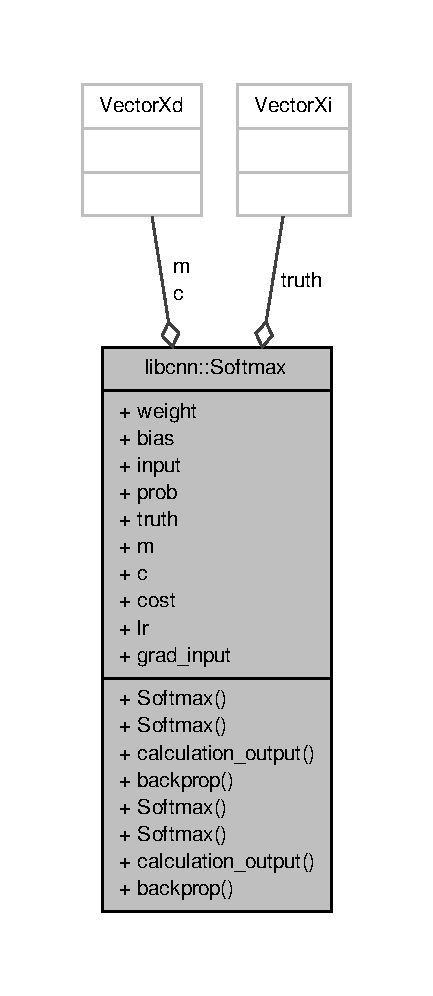
\includegraphics[width=208pt]{classlibcnn_1_1_softmax__coll__graph}
\end{center}
\end{figure}
\subsection*{\-Public \-Member \-Functions}
\begin{DoxyCompactItemize}
\item 
\hyperlink{classlibcnn_1_1_softmax_a1905addb7d4894b92ebb3c141040f7a1}{\-Softmax} (const \-Matrix\-Xd \&, const int \&, const \-Vector\-Xi \&, const double \&, const double \&)
\item 
\hyperlink{classlibcnn_1_1_softmax_aa43e90709ba3c5e44e5b7b435e54a902}{\-Softmax} (const \-Matrix\-Xd \&, const int \&, const \-Vector\-Xi \&, const double \&, const double \&, const \-Matrix\-Xd \&, const \-Matrix\-Xd \&)
\item 
void \hyperlink{classlibcnn_1_1_softmax_ae6af9e18ce2ab849d26b38a9d4a5be20}{calculation\-\_\-output} ()
\item 
void \hyperlink{classlibcnn_1_1_softmax_ad52de893453032d29c6fb3bca6e9f492}{backprop} (const double \&)
\item 
\hyperlink{classlibcnn_1_1_softmax_a1905addb7d4894b92ebb3c141040f7a1}{\-Softmax} (const \-Matrix\-Xd \&, const int \&, const \-Vector\-Xi \&, const double \&, const double \&)
\item 
\hyperlink{classlibcnn_1_1_softmax_aa43e90709ba3c5e44e5b7b435e54a902}{\-Softmax} (const \-Matrix\-Xd \&, const int \&, const \-Vector\-Xi \&, const double \&, const double \&, const \-Matrix\-Xd \&, const \-Matrix\-Xd \&)
\item 
void \hyperlink{classlibcnn_1_1_softmax_ae6af9e18ce2ab849d26b38a9d4a5be20}{calculation\-\_\-output} ()
\item 
void \hyperlink{classlibcnn_1_1_softmax_ad52de893453032d29c6fb3bca6e9f492}{backprop} (const double \&)
\end{DoxyCompactItemize}
\subsection*{\-Public \-Attributes}
\begin{DoxyCompactItemize}
\item 
\-Eigen\-::\-Matrix\-Xd \hyperlink{classlibcnn_1_1_softmax_a9904a3314f8b72c089cdfe5930f75445}{weight}
\item 
\-Eigen\-::\-Matrix\-Xd \hyperlink{classlibcnn_1_1_softmax_af7177b8068a5bb00b493684bd17e133e}{bias}
\item 
\-Eigen\-::\-Matrix\-Xd \hyperlink{classlibcnn_1_1_softmax_a6a7f3d59e90ecf66b9ddf437b452c780}{input}
\item 
\-Eigen\-::\-Matrix\-Xd \hyperlink{classlibcnn_1_1_softmax_a0d1f28abafbb3cddcf87defa87178ce4}{prob}
\item 
\-Eigen\-::\-Vector\-Xi \hyperlink{classlibcnn_1_1_softmax_ad2c468ea12679d111190c549fc46d8c1}{truth}
\item 
\-Eigen\-::\-Vector\-Xd \hyperlink{classlibcnn_1_1_softmax_a851740b9977df6ebc1dd3c672e367f56}{m}
\item 
\-Eigen\-::\-Vector\-Xd \hyperlink{classlibcnn_1_1_softmax_a89d340fbed0365db9c30dffafc492aca}{c}
\item 
double \hyperlink{classlibcnn_1_1_softmax_a13cbff525a19cea4f94836f5b439b2a7}{cost}
\item 
double \hyperlink{classlibcnn_1_1_softmax_a3995e5ba8bc5d766482735974b8eda92}{lr}
\item 
\-Eigen\-::\-Matrix\-Xd \hyperlink{classlibcnn_1_1_softmax_a3c4257681cef58ab58ca3601400ab098}{grad\-\_\-input}
\end{DoxyCompactItemize}


\subsection{\-Constructor \& \-Destructor \-Documentation}
\hypertarget{classlibcnn_1_1_softmax_a1905addb7d4894b92ebb3c141040f7a1}{\index{libcnn\-::\-Softmax@{libcnn\-::\-Softmax}!\-Softmax@{\-Softmax}}
\index{\-Softmax@{\-Softmax}!libcnn::Softmax@{libcnn\-::\-Softmax}}
\subsubsection[{\-Softmax}]{\setlength{\rightskip}{0pt plus 5cm}{\bf libcnn\-::\-Softmax\-::\-Softmax} (
\begin{DoxyParamCaption}
\item[{const \-Matrix\-Xd \&}]{cnn\-\_\-output, }
\item[{const int \&}]{\-Label\-\_\-number, }
\item[{const \-Vector\-Xi \&}]{ground\-\_\-truth, }
\item[{const double \&}]{w\-\_\-bound, }
\item[{const double \&}]{b\-\_\-bound}
\end{DoxyParamCaption}
)}}\label{classlibcnn_1_1_softmax_a1905addb7d4894b92ebb3c141040f7a1}


\-Here is the call graph for this function\-:
\nopagebreak
\begin{figure}[H]
\begin{center}
\leavevmode
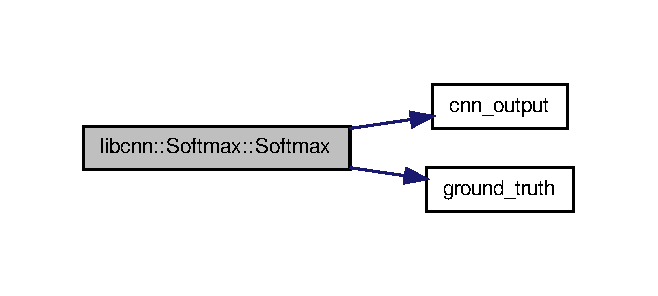
\includegraphics[width=316pt]{classlibcnn_1_1_softmax_a1905addb7d4894b92ebb3c141040f7a1_cgraph}
\end{center}
\end{figure}


\hypertarget{classlibcnn_1_1_softmax_aa43e90709ba3c5e44e5b7b435e54a902}{\index{libcnn\-::\-Softmax@{libcnn\-::\-Softmax}!\-Softmax@{\-Softmax}}
\index{\-Softmax@{\-Softmax}!libcnn::Softmax@{libcnn\-::\-Softmax}}
\subsubsection[{\-Softmax}]{\setlength{\rightskip}{0pt plus 5cm}{\bf libcnn\-::\-Softmax\-::\-Softmax} (
\begin{DoxyParamCaption}
\item[{const \-Matrix\-Xd \&}]{cnn\-\_\-output, }
\item[{const int \&}]{\-Label\-\_\-number, }
\item[{const \-Vector\-Xi \&}]{ground\-\_\-truth, }
\item[{const double \&}]{w\-\_\-bound, }
\item[{const double \&}]{b\-\_\-bound, }
\item[{const \-Matrix\-Xd \&}]{initial\-\_\-weight, }
\item[{const \-Matrix\-Xd \&}]{initial\-\_\-bias}
\end{DoxyParamCaption}
)}}\label{classlibcnn_1_1_softmax_aa43e90709ba3c5e44e5b7b435e54a902}


\-Here is the call graph for this function\-:
\nopagebreak
\begin{figure}[H]
\begin{center}
\leavevmode
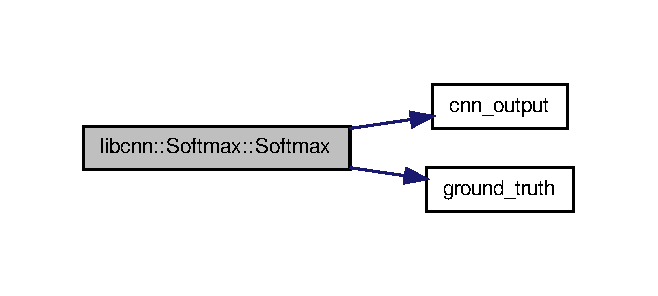
\includegraphics[width=316pt]{classlibcnn_1_1_softmax_aa43e90709ba3c5e44e5b7b435e54a902_cgraph}
\end{center}
\end{figure}


\hypertarget{classlibcnn_1_1_softmax_a1905addb7d4894b92ebb3c141040f7a1}{\index{libcnn\-::\-Softmax@{libcnn\-::\-Softmax}!\-Softmax@{\-Softmax}}
\index{\-Softmax@{\-Softmax}!libcnn::Softmax@{libcnn\-::\-Softmax}}
\subsubsection[{\-Softmax}]{\setlength{\rightskip}{0pt plus 5cm}{\bf libcnn\-::\-Softmax\-::\-Softmax} (
\begin{DoxyParamCaption}
\item[{const \-Matrix\-Xd \&}]{, }
\item[{const int \&}]{, }
\item[{const \-Vector\-Xi \&}]{, }
\item[{const double \&}]{, }
\item[{const double \&}]{}
\end{DoxyParamCaption}
)}}\label{classlibcnn_1_1_softmax_a1905addb7d4894b92ebb3c141040f7a1}
\hypertarget{classlibcnn_1_1_softmax_aa43e90709ba3c5e44e5b7b435e54a902}{\index{libcnn\-::\-Softmax@{libcnn\-::\-Softmax}!\-Softmax@{\-Softmax}}
\index{\-Softmax@{\-Softmax}!libcnn::Softmax@{libcnn\-::\-Softmax}}
\subsubsection[{\-Softmax}]{\setlength{\rightskip}{0pt plus 5cm}{\bf libcnn\-::\-Softmax\-::\-Softmax} (
\begin{DoxyParamCaption}
\item[{const \-Matrix\-Xd \&}]{, }
\item[{const int \&}]{, }
\item[{const \-Vector\-Xi \&}]{, }
\item[{const double \&}]{, }
\item[{const double \&}]{, }
\item[{const \-Matrix\-Xd \&}]{, }
\item[{const \-Matrix\-Xd \&}]{}
\end{DoxyParamCaption}
)}}\label{classlibcnn_1_1_softmax_aa43e90709ba3c5e44e5b7b435e54a902}


\subsection{\-Member \-Function \-Documentation}
\hypertarget{classlibcnn_1_1_softmax_ad52de893453032d29c6fb3bca6e9f492}{\index{libcnn\-::\-Softmax@{libcnn\-::\-Softmax}!backprop@{backprop}}
\index{backprop@{backprop}!libcnn::Softmax@{libcnn\-::\-Softmax}}
\subsubsection[{backprop}]{\setlength{\rightskip}{0pt plus 5cm}void {\bf libcnn\-::\-Softmax\-::backprop} (
\begin{DoxyParamCaption}
\item[{const double \&}]{lr}
\end{DoxyParamCaption}
)}}\label{classlibcnn_1_1_softmax_ad52de893453032d29c6fb3bca6e9f492}
\hypertarget{classlibcnn_1_1_softmax_ad52de893453032d29c6fb3bca6e9f492}{\index{libcnn\-::\-Softmax@{libcnn\-::\-Softmax}!backprop@{backprop}}
\index{backprop@{backprop}!libcnn::Softmax@{libcnn\-::\-Softmax}}
\subsubsection[{backprop}]{\setlength{\rightskip}{0pt plus 5cm}void {\bf libcnn\-::\-Softmax\-::backprop} (
\begin{DoxyParamCaption}
\item[{const double \&}]{}
\end{DoxyParamCaption}
)}}\label{classlibcnn_1_1_softmax_ad52de893453032d29c6fb3bca6e9f492}
\hypertarget{classlibcnn_1_1_softmax_ae6af9e18ce2ab849d26b38a9d4a5be20}{\index{libcnn\-::\-Softmax@{libcnn\-::\-Softmax}!calculation\-\_\-output@{calculation\-\_\-output}}
\index{calculation\-\_\-output@{calculation\-\_\-output}!libcnn::Softmax@{libcnn\-::\-Softmax}}
\subsubsection[{calculation\-\_\-output}]{\setlength{\rightskip}{0pt plus 5cm}void {\bf libcnn\-::\-Softmax\-::calculation\-\_\-output} (
\begin{DoxyParamCaption}
{}
\end{DoxyParamCaption}
)}}\label{classlibcnn_1_1_softmax_ae6af9e18ce2ab849d26b38a9d4a5be20}
\hypertarget{classlibcnn_1_1_softmax_ae6af9e18ce2ab849d26b38a9d4a5be20}{\index{libcnn\-::\-Softmax@{libcnn\-::\-Softmax}!calculation\-\_\-output@{calculation\-\_\-output}}
\index{calculation\-\_\-output@{calculation\-\_\-output}!libcnn::Softmax@{libcnn\-::\-Softmax}}
\subsubsection[{calculation\-\_\-output}]{\setlength{\rightskip}{0pt plus 5cm}void {\bf libcnn\-::\-Softmax\-::calculation\-\_\-output} (
\begin{DoxyParamCaption}
{}
\end{DoxyParamCaption}
)}}\label{classlibcnn_1_1_softmax_ae6af9e18ce2ab849d26b38a9d4a5be20}


\subsection{\-Member \-Data \-Documentation}
\hypertarget{classlibcnn_1_1_softmax_af7177b8068a5bb00b493684bd17e133e}{\index{libcnn\-::\-Softmax@{libcnn\-::\-Softmax}!bias@{bias}}
\index{bias@{bias}!libcnn::Softmax@{libcnn\-::\-Softmax}}
\subsubsection[{bias}]{\setlength{\rightskip}{0pt plus 5cm}\-Eigen\-::\-Matrix\-Xd {\bf libcnn\-::\-Softmax\-::bias}}}\label{classlibcnn_1_1_softmax_af7177b8068a5bb00b493684bd17e133e}
\hypertarget{classlibcnn_1_1_softmax_a89d340fbed0365db9c30dffafc492aca}{\index{libcnn\-::\-Softmax@{libcnn\-::\-Softmax}!c@{c}}
\index{c@{c}!libcnn::Softmax@{libcnn\-::\-Softmax}}
\subsubsection[{c}]{\setlength{\rightskip}{0pt plus 5cm}\-Eigen\-::\-Vector\-Xd {\bf libcnn\-::\-Softmax\-::c}}}\label{classlibcnn_1_1_softmax_a89d340fbed0365db9c30dffafc492aca}
\hypertarget{classlibcnn_1_1_softmax_a13cbff525a19cea4f94836f5b439b2a7}{\index{libcnn\-::\-Softmax@{libcnn\-::\-Softmax}!cost@{cost}}
\index{cost@{cost}!libcnn::Softmax@{libcnn\-::\-Softmax}}
\subsubsection[{cost}]{\setlength{\rightskip}{0pt plus 5cm}double {\bf libcnn\-::\-Softmax\-::cost}}}\label{classlibcnn_1_1_softmax_a13cbff525a19cea4f94836f5b439b2a7}
\hypertarget{classlibcnn_1_1_softmax_a3c4257681cef58ab58ca3601400ab098}{\index{libcnn\-::\-Softmax@{libcnn\-::\-Softmax}!grad\-\_\-input@{grad\-\_\-input}}
\index{grad\-\_\-input@{grad\-\_\-input}!libcnn::Softmax@{libcnn\-::\-Softmax}}
\subsubsection[{grad\-\_\-input}]{\setlength{\rightskip}{0pt plus 5cm}\-Eigen\-::\-Matrix\-Xd {\bf libcnn\-::\-Softmax\-::grad\-\_\-input}}}\label{classlibcnn_1_1_softmax_a3c4257681cef58ab58ca3601400ab098}
\hypertarget{classlibcnn_1_1_softmax_a6a7f3d59e90ecf66b9ddf437b452c780}{\index{libcnn\-::\-Softmax@{libcnn\-::\-Softmax}!input@{input}}
\index{input@{input}!libcnn::Softmax@{libcnn\-::\-Softmax}}
\subsubsection[{input}]{\setlength{\rightskip}{0pt plus 5cm}\-Eigen\-::\-Matrix\-Xd {\bf libcnn\-::\-Softmax\-::input}}}\label{classlibcnn_1_1_softmax_a6a7f3d59e90ecf66b9ddf437b452c780}
\hypertarget{classlibcnn_1_1_softmax_a3995e5ba8bc5d766482735974b8eda92}{\index{libcnn\-::\-Softmax@{libcnn\-::\-Softmax}!lr@{lr}}
\index{lr@{lr}!libcnn::Softmax@{libcnn\-::\-Softmax}}
\subsubsection[{lr}]{\setlength{\rightskip}{0pt plus 5cm}double {\bf libcnn\-::\-Softmax\-::lr}}}\label{classlibcnn_1_1_softmax_a3995e5ba8bc5d766482735974b8eda92}
\hypertarget{classlibcnn_1_1_softmax_a851740b9977df6ebc1dd3c672e367f56}{\index{libcnn\-::\-Softmax@{libcnn\-::\-Softmax}!m@{m}}
\index{m@{m}!libcnn::Softmax@{libcnn\-::\-Softmax}}
\subsubsection[{m}]{\setlength{\rightskip}{0pt plus 5cm}\-Eigen\-::\-Vector\-Xd {\bf libcnn\-::\-Softmax\-::m}}}\label{classlibcnn_1_1_softmax_a851740b9977df6ebc1dd3c672e367f56}
\hypertarget{classlibcnn_1_1_softmax_a0d1f28abafbb3cddcf87defa87178ce4}{\index{libcnn\-::\-Softmax@{libcnn\-::\-Softmax}!prob@{prob}}
\index{prob@{prob}!libcnn::Softmax@{libcnn\-::\-Softmax}}
\subsubsection[{prob}]{\setlength{\rightskip}{0pt plus 5cm}\-Eigen\-::\-Matrix\-Xd {\bf libcnn\-::\-Softmax\-::prob}}}\label{classlibcnn_1_1_softmax_a0d1f28abafbb3cddcf87defa87178ce4}
\hypertarget{classlibcnn_1_1_softmax_ad2c468ea12679d111190c549fc46d8c1}{\index{libcnn\-::\-Softmax@{libcnn\-::\-Softmax}!truth@{truth}}
\index{truth@{truth}!libcnn::Softmax@{libcnn\-::\-Softmax}}
\subsubsection[{truth}]{\setlength{\rightskip}{0pt plus 5cm}\-Eigen\-::\-Vector\-Xi {\bf libcnn\-::\-Softmax\-::truth}}}\label{classlibcnn_1_1_softmax_ad2c468ea12679d111190c549fc46d8c1}
\hypertarget{classlibcnn_1_1_softmax_a9904a3314f8b72c089cdfe5930f75445}{\index{libcnn\-::\-Softmax@{libcnn\-::\-Softmax}!weight@{weight}}
\index{weight@{weight}!libcnn::Softmax@{libcnn\-::\-Softmax}}
\subsubsection[{weight}]{\setlength{\rightskip}{0pt plus 5cm}\-Eigen\-::\-Matrix\-Xd {\bf libcnn\-::\-Softmax\-::weight}}}\label{classlibcnn_1_1_softmax_a9904a3314f8b72c089cdfe5930f75445}


\-The documentation for this class was generated from the following files\-:\begin{DoxyCompactItemize}
\item 
gpu/include/\hyperlink{gpu_2include_2softmax__class_8h}{softmax\-\_\-class.\-h}\item 
include/\hyperlink{include_2softmax__class_8h}{softmax\-\_\-class.\-h}\item 
gpu/src/\hyperlink{gpu_2src_2softmax__class_8cpp}{softmax\-\_\-class.\-cpp}\item 
src/\hyperlink{src_2softmax__class_8cpp}{softmax\-\_\-class.\-cpp}\end{DoxyCompactItemize}

\chapter{\-File \-Documentation}
\hypertarget{_c_make_c_compiler_id_8c}{\section{build/\-C\-Make\-Files/\-Compiler\-Id\-C/\-C\-Make\-C\-Compiler\-Id.c \-File \-Reference}
\label{_c_make_c_compiler_id_8c}\index{build/\-C\-Make\-Files/\-Compiler\-Id\-C/\-C\-Make\-C\-Compiler\-Id.\-c@{build/\-C\-Make\-Files/\-Compiler\-Id\-C/\-C\-Make\-C\-Compiler\-Id.\-c}}
}
\subsection*{\-Defines}
\begin{DoxyCompactItemize}
\item 
\#define \hyperlink{_c_make_c_compiler_id_8c_a81dee0709ded976b2e0319239f72d174}{\-C\-O\-M\-P\-I\-L\-E\-R\-\_\-\-I\-D}~\char`\"{}\char`\"{}
\item 
\#define \hyperlink{_c_make_c_compiler_id_8c_adbc5372f40838899018fadbc89bd588b}{\-P\-L\-A\-T\-F\-O\-R\-M\-\_\-\-I\-D}~\char`\"{}\char`\"{}
\item 
\#define \hyperlink{_c_make_c_compiler_id_8c_aba35d0d200deaeb06aee95ca297acb28}{\-A\-R\-C\-H\-I\-T\-E\-C\-T\-U\-R\-E\-\_\-\-I\-D}~\char`\"{}\char`\"{}
\end{DoxyCompactItemize}
\subsection*{\-Functions}
\begin{DoxyCompactItemize}
\item 
int \hyperlink{_c_make_c_compiler_id_8c_a0ddf1224851353fc92bfbff6f499fa97}{main} (int argc, char $\ast$argv\mbox{[}$\,$\mbox{]})
\end{DoxyCompactItemize}
\subsection*{\-Variables}
\begin{DoxyCompactItemize}
\item 
char const $\ast$ \hyperlink{_c_make_c_compiler_id_8c_a4b0efeb7a5d59313986b3a0390f050f6}{info\-\_\-compiler} = \char`\"{}\mbox{]}\char`\"{}
\item 
char const $\ast$ \hyperlink{_c_make_c_compiler_id_8c_a2321403dee54ee23f0c2fa849c60f7d4}{info\-\_\-platform} = \char`\"{}\mbox{]}\char`\"{}
\item 
char const $\ast$ \hyperlink{_c_make_c_compiler_id_8c_a59647e99d304ed33b15cb284c27ed391}{info\-\_\-arch} = \char`\"{}\mbox{]}\char`\"{}
\end{DoxyCompactItemize}


\subsection{\-Define \-Documentation}
\hypertarget{_c_make_c_compiler_id_8c_aba35d0d200deaeb06aee95ca297acb28}{\index{\-C\-Make\-C\-Compiler\-Id.\-c@{\-C\-Make\-C\-Compiler\-Id.\-c}!\-A\-R\-C\-H\-I\-T\-E\-C\-T\-U\-R\-E\-\_\-\-I\-D@{\-A\-R\-C\-H\-I\-T\-E\-C\-T\-U\-R\-E\-\_\-\-I\-D}}
\index{\-A\-R\-C\-H\-I\-T\-E\-C\-T\-U\-R\-E\-\_\-\-I\-D@{\-A\-R\-C\-H\-I\-T\-E\-C\-T\-U\-R\-E\-\_\-\-I\-D}!CMakeCCompilerId.c@{\-C\-Make\-C\-Compiler\-Id.\-c}}
\subsubsection[{\-A\-R\-C\-H\-I\-T\-E\-C\-T\-U\-R\-E\-\_\-\-I\-D}]{\setlength{\rightskip}{0pt plus 5cm}\#define {\bf \-A\-R\-C\-H\-I\-T\-E\-C\-T\-U\-R\-E\-\_\-\-I\-D}~\char`\"{}\char`\"{}}}\label{_c_make_c_compiler_id_8c_aba35d0d200deaeb06aee95ca297acb28}
\hypertarget{_c_make_c_compiler_id_8c_a81dee0709ded976b2e0319239f72d174}{\index{\-C\-Make\-C\-Compiler\-Id.\-c@{\-C\-Make\-C\-Compiler\-Id.\-c}!\-C\-O\-M\-P\-I\-L\-E\-R\-\_\-\-I\-D@{\-C\-O\-M\-P\-I\-L\-E\-R\-\_\-\-I\-D}}
\index{\-C\-O\-M\-P\-I\-L\-E\-R\-\_\-\-I\-D@{\-C\-O\-M\-P\-I\-L\-E\-R\-\_\-\-I\-D}!CMakeCCompilerId.c@{\-C\-Make\-C\-Compiler\-Id.\-c}}
\subsubsection[{\-C\-O\-M\-P\-I\-L\-E\-R\-\_\-\-I\-D}]{\setlength{\rightskip}{0pt plus 5cm}\#define {\bf \-C\-O\-M\-P\-I\-L\-E\-R\-\_\-\-I\-D}~\char`\"{}\char`\"{}}}\label{_c_make_c_compiler_id_8c_a81dee0709ded976b2e0319239f72d174}
\hypertarget{_c_make_c_compiler_id_8c_adbc5372f40838899018fadbc89bd588b}{\index{\-C\-Make\-C\-Compiler\-Id.\-c@{\-C\-Make\-C\-Compiler\-Id.\-c}!\-P\-L\-A\-T\-F\-O\-R\-M\-\_\-\-I\-D@{\-P\-L\-A\-T\-F\-O\-R\-M\-\_\-\-I\-D}}
\index{\-P\-L\-A\-T\-F\-O\-R\-M\-\_\-\-I\-D@{\-P\-L\-A\-T\-F\-O\-R\-M\-\_\-\-I\-D}!CMakeCCompilerId.c@{\-C\-Make\-C\-Compiler\-Id.\-c}}
\subsubsection[{\-P\-L\-A\-T\-F\-O\-R\-M\-\_\-\-I\-D}]{\setlength{\rightskip}{0pt plus 5cm}\#define {\bf \-P\-L\-A\-T\-F\-O\-R\-M\-\_\-\-I\-D}~\char`\"{}\char`\"{}}}\label{_c_make_c_compiler_id_8c_adbc5372f40838899018fadbc89bd588b}


\subsection{\-Function \-Documentation}
\hypertarget{_c_make_c_compiler_id_8c_a0ddf1224851353fc92bfbff6f499fa97}{\index{\-C\-Make\-C\-Compiler\-Id.\-c@{\-C\-Make\-C\-Compiler\-Id.\-c}!main@{main}}
\index{main@{main}!CMakeCCompilerId.c@{\-C\-Make\-C\-Compiler\-Id.\-c}}
\subsubsection[{main}]{\setlength{\rightskip}{0pt plus 5cm}int {\bf main} (
\begin{DoxyParamCaption}
\item[{int}]{argc, }
\item[{char $\ast$}]{argv\mbox{[}$\,$\mbox{]}}
\end{DoxyParamCaption}
)}}\label{_c_make_c_compiler_id_8c_a0ddf1224851353fc92bfbff6f499fa97}


\subsection{\-Variable \-Documentation}
\hypertarget{_c_make_c_compiler_id_8c_a59647e99d304ed33b15cb284c27ed391}{\index{\-C\-Make\-C\-Compiler\-Id.\-c@{\-C\-Make\-C\-Compiler\-Id.\-c}!info\-\_\-arch@{info\-\_\-arch}}
\index{info\-\_\-arch@{info\-\_\-arch}!CMakeCCompilerId.c@{\-C\-Make\-C\-Compiler\-Id.\-c}}
\subsubsection[{info\-\_\-arch}]{\setlength{\rightskip}{0pt plus 5cm}char const$\ast$ {\bf info\-\_\-arch} = \char`\"{}\mbox{]}\char`\"{}}}\label{_c_make_c_compiler_id_8c_a59647e99d304ed33b15cb284c27ed391}
\hypertarget{_c_make_c_compiler_id_8c_a4b0efeb7a5d59313986b3a0390f050f6}{\index{\-C\-Make\-C\-Compiler\-Id.\-c@{\-C\-Make\-C\-Compiler\-Id.\-c}!info\-\_\-compiler@{info\-\_\-compiler}}
\index{info\-\_\-compiler@{info\-\_\-compiler}!CMakeCCompilerId.c@{\-C\-Make\-C\-Compiler\-Id.\-c}}
\subsubsection[{info\-\_\-compiler}]{\setlength{\rightskip}{0pt plus 5cm}char const$\ast$ {\bf info\-\_\-compiler} = \char`\"{}\mbox{]}\char`\"{}}}\label{_c_make_c_compiler_id_8c_a4b0efeb7a5d59313986b3a0390f050f6}
\hypertarget{_c_make_c_compiler_id_8c_a2321403dee54ee23f0c2fa849c60f7d4}{\index{\-C\-Make\-C\-Compiler\-Id.\-c@{\-C\-Make\-C\-Compiler\-Id.\-c}!info\-\_\-platform@{info\-\_\-platform}}
\index{info\-\_\-platform@{info\-\_\-platform}!CMakeCCompilerId.c@{\-C\-Make\-C\-Compiler\-Id.\-c}}
\subsubsection[{info\-\_\-platform}]{\setlength{\rightskip}{0pt plus 5cm}char const$\ast$ {\bf info\-\_\-platform} = \char`\"{}\mbox{]}\char`\"{}}}\label{_c_make_c_compiler_id_8c_a2321403dee54ee23f0c2fa849c60f7d4}

\hypertarget{_c_make_c_x_x_compiler_id_8cpp}{\section{build/\-C\-Make\-Files/\-Compiler\-Id\-C\-X\-X/\-C\-Make\-C\-X\-X\-Compiler\-Id.cpp \-File \-Reference}
\label{_c_make_c_x_x_compiler_id_8cpp}\index{build/\-C\-Make\-Files/\-Compiler\-Id\-C\-X\-X/\-C\-Make\-C\-X\-X\-Compiler\-Id.\-cpp@{build/\-C\-Make\-Files/\-Compiler\-Id\-C\-X\-X/\-C\-Make\-C\-X\-X\-Compiler\-Id.\-cpp}}
}
\subsection*{\-Defines}
\begin{DoxyCompactItemize}
\item 
\#define \hyperlink{_c_make_c_x_x_compiler_id_8cpp_a81dee0709ded976b2e0319239f72d174}{\-C\-O\-M\-P\-I\-L\-E\-R\-\_\-\-I\-D}~\char`\"{}\char`\"{}
\item 
\#define \hyperlink{_c_make_c_x_x_compiler_id_8cpp_adbc5372f40838899018fadbc89bd588b}{\-P\-L\-A\-T\-F\-O\-R\-M\-\_\-\-I\-D}~\char`\"{}\char`\"{}
\item 
\#define \hyperlink{_c_make_c_x_x_compiler_id_8cpp_aba35d0d200deaeb06aee95ca297acb28}{\-A\-R\-C\-H\-I\-T\-E\-C\-T\-U\-R\-E\-\_\-\-I\-D}~\char`\"{}\char`\"{}
\end{DoxyCompactItemize}
\subsection*{\-Functions}
\begin{DoxyCompactItemize}
\item 
int \hyperlink{_c_make_c_x_x_compiler_id_8cpp_a0ddf1224851353fc92bfbff6f499fa97}{main} (int argc, char $\ast$argv\mbox{[}$\,$\mbox{]})
\end{DoxyCompactItemize}
\subsection*{\-Variables}
\begin{DoxyCompactItemize}
\item 
char const $\ast$ \hyperlink{_c_make_c_x_x_compiler_id_8cpp_a4b0efeb7a5d59313986b3a0390f050f6}{info\-\_\-compiler} = \char`\"{}\mbox{]}\char`\"{}
\item 
char const $\ast$ \hyperlink{_c_make_c_x_x_compiler_id_8cpp_a2321403dee54ee23f0c2fa849c60f7d4}{info\-\_\-platform} = \char`\"{}\mbox{]}\char`\"{}
\item 
char const $\ast$ \hyperlink{_c_make_c_x_x_compiler_id_8cpp_a59647e99d304ed33b15cb284c27ed391}{info\-\_\-arch} = \char`\"{}\mbox{]}\char`\"{}
\end{DoxyCompactItemize}


\subsection{\-Define \-Documentation}
\hypertarget{_c_make_c_x_x_compiler_id_8cpp_aba35d0d200deaeb06aee95ca297acb28}{\index{\-C\-Make\-C\-X\-X\-Compiler\-Id.\-cpp@{\-C\-Make\-C\-X\-X\-Compiler\-Id.\-cpp}!\-A\-R\-C\-H\-I\-T\-E\-C\-T\-U\-R\-E\-\_\-\-I\-D@{\-A\-R\-C\-H\-I\-T\-E\-C\-T\-U\-R\-E\-\_\-\-I\-D}}
\index{\-A\-R\-C\-H\-I\-T\-E\-C\-T\-U\-R\-E\-\_\-\-I\-D@{\-A\-R\-C\-H\-I\-T\-E\-C\-T\-U\-R\-E\-\_\-\-I\-D}!CMakeCXXCompilerId.cpp@{\-C\-Make\-C\-X\-X\-Compiler\-Id.\-cpp}}
\subsubsection[{\-A\-R\-C\-H\-I\-T\-E\-C\-T\-U\-R\-E\-\_\-\-I\-D}]{\setlength{\rightskip}{0pt plus 5cm}\#define {\bf \-A\-R\-C\-H\-I\-T\-E\-C\-T\-U\-R\-E\-\_\-\-I\-D}~\char`\"{}\char`\"{}}}\label{_c_make_c_x_x_compiler_id_8cpp_aba35d0d200deaeb06aee95ca297acb28}
\hypertarget{_c_make_c_x_x_compiler_id_8cpp_a81dee0709ded976b2e0319239f72d174}{\index{\-C\-Make\-C\-X\-X\-Compiler\-Id.\-cpp@{\-C\-Make\-C\-X\-X\-Compiler\-Id.\-cpp}!\-C\-O\-M\-P\-I\-L\-E\-R\-\_\-\-I\-D@{\-C\-O\-M\-P\-I\-L\-E\-R\-\_\-\-I\-D}}
\index{\-C\-O\-M\-P\-I\-L\-E\-R\-\_\-\-I\-D@{\-C\-O\-M\-P\-I\-L\-E\-R\-\_\-\-I\-D}!CMakeCXXCompilerId.cpp@{\-C\-Make\-C\-X\-X\-Compiler\-Id.\-cpp}}
\subsubsection[{\-C\-O\-M\-P\-I\-L\-E\-R\-\_\-\-I\-D}]{\setlength{\rightskip}{0pt plus 5cm}\#define {\bf \-C\-O\-M\-P\-I\-L\-E\-R\-\_\-\-I\-D}~\char`\"{}\char`\"{}}}\label{_c_make_c_x_x_compiler_id_8cpp_a81dee0709ded976b2e0319239f72d174}
\hypertarget{_c_make_c_x_x_compiler_id_8cpp_adbc5372f40838899018fadbc89bd588b}{\index{\-C\-Make\-C\-X\-X\-Compiler\-Id.\-cpp@{\-C\-Make\-C\-X\-X\-Compiler\-Id.\-cpp}!\-P\-L\-A\-T\-F\-O\-R\-M\-\_\-\-I\-D@{\-P\-L\-A\-T\-F\-O\-R\-M\-\_\-\-I\-D}}
\index{\-P\-L\-A\-T\-F\-O\-R\-M\-\_\-\-I\-D@{\-P\-L\-A\-T\-F\-O\-R\-M\-\_\-\-I\-D}!CMakeCXXCompilerId.cpp@{\-C\-Make\-C\-X\-X\-Compiler\-Id.\-cpp}}
\subsubsection[{\-P\-L\-A\-T\-F\-O\-R\-M\-\_\-\-I\-D}]{\setlength{\rightskip}{0pt plus 5cm}\#define {\bf \-P\-L\-A\-T\-F\-O\-R\-M\-\_\-\-I\-D}~\char`\"{}\char`\"{}}}\label{_c_make_c_x_x_compiler_id_8cpp_adbc5372f40838899018fadbc89bd588b}


\subsection{\-Function \-Documentation}
\hypertarget{_c_make_c_x_x_compiler_id_8cpp_a0ddf1224851353fc92bfbff6f499fa97}{\index{\-C\-Make\-C\-X\-X\-Compiler\-Id.\-cpp@{\-C\-Make\-C\-X\-X\-Compiler\-Id.\-cpp}!main@{main}}
\index{main@{main}!CMakeCXXCompilerId.cpp@{\-C\-Make\-C\-X\-X\-Compiler\-Id.\-cpp}}
\subsubsection[{main}]{\setlength{\rightskip}{0pt plus 5cm}int {\bf main} (
\begin{DoxyParamCaption}
\item[{int}]{argc, }
\item[{char $\ast$}]{argv\mbox{[}$\,$\mbox{]}}
\end{DoxyParamCaption}
)}}\label{_c_make_c_x_x_compiler_id_8cpp_a0ddf1224851353fc92bfbff6f499fa97}


\subsection{\-Variable \-Documentation}
\hypertarget{_c_make_c_x_x_compiler_id_8cpp_a59647e99d304ed33b15cb284c27ed391}{\index{\-C\-Make\-C\-X\-X\-Compiler\-Id.\-cpp@{\-C\-Make\-C\-X\-X\-Compiler\-Id.\-cpp}!info\-\_\-arch@{info\-\_\-arch}}
\index{info\-\_\-arch@{info\-\_\-arch}!CMakeCXXCompilerId.cpp@{\-C\-Make\-C\-X\-X\-Compiler\-Id.\-cpp}}
\subsubsection[{info\-\_\-arch}]{\setlength{\rightskip}{0pt plus 5cm}char const$\ast$ {\bf info\-\_\-arch} = \char`\"{}\mbox{]}\char`\"{}}}\label{_c_make_c_x_x_compiler_id_8cpp_a59647e99d304ed33b15cb284c27ed391}
\hypertarget{_c_make_c_x_x_compiler_id_8cpp_a4b0efeb7a5d59313986b3a0390f050f6}{\index{\-C\-Make\-C\-X\-X\-Compiler\-Id.\-cpp@{\-C\-Make\-C\-X\-X\-Compiler\-Id.\-cpp}!info\-\_\-compiler@{info\-\_\-compiler}}
\index{info\-\_\-compiler@{info\-\_\-compiler}!CMakeCXXCompilerId.cpp@{\-C\-Make\-C\-X\-X\-Compiler\-Id.\-cpp}}
\subsubsection[{info\-\_\-compiler}]{\setlength{\rightskip}{0pt plus 5cm}char const$\ast$ {\bf info\-\_\-compiler} = \char`\"{}\mbox{]}\char`\"{}}}\label{_c_make_c_x_x_compiler_id_8cpp_a4b0efeb7a5d59313986b3a0390f050f6}
\hypertarget{_c_make_c_x_x_compiler_id_8cpp_a2321403dee54ee23f0c2fa849c60f7d4}{\index{\-C\-Make\-C\-X\-X\-Compiler\-Id.\-cpp@{\-C\-Make\-C\-X\-X\-Compiler\-Id.\-cpp}!info\-\_\-platform@{info\-\_\-platform}}
\index{info\-\_\-platform@{info\-\_\-platform}!CMakeCXXCompilerId.cpp@{\-C\-Make\-C\-X\-X\-Compiler\-Id.\-cpp}}
\subsubsection[{info\-\_\-platform}]{\setlength{\rightskip}{0pt plus 5cm}char const$\ast$ {\bf info\-\_\-platform} = \char`\"{}\mbox{]}\char`\"{}}}\label{_c_make_c_x_x_compiler_id_8cpp_a2321403dee54ee23f0c2fa849c60f7d4}

\hypertarget{gpu_2include_2conv__layer_8h}{\section{gpu/include/conv\-\_\-layer.h \-File \-Reference}
\label{gpu_2include_2conv__layer_8h}\index{gpu/include/conv\-\_\-layer.\-h@{gpu/include/conv\-\_\-layer.\-h}}
}
{\ttfamily \#include $<$iostream$>$}\*
{\ttfamily \#include $<$\-Eigen/\-Dense$>$}\*
{\ttfamily \#include $<$\-Eigen/\-Core$>$}\*
{\ttfamily \#include $<$vector$>$}\*
{\ttfamily \#include $<$string$>$}\*
{\ttfamily \#include $<$cmath$>$}\*
\-Include dependency graph for conv\-\_\-layer.\-h\-:
\nopagebreak
\begin{figure}[H]
\begin{center}
\leavevmode
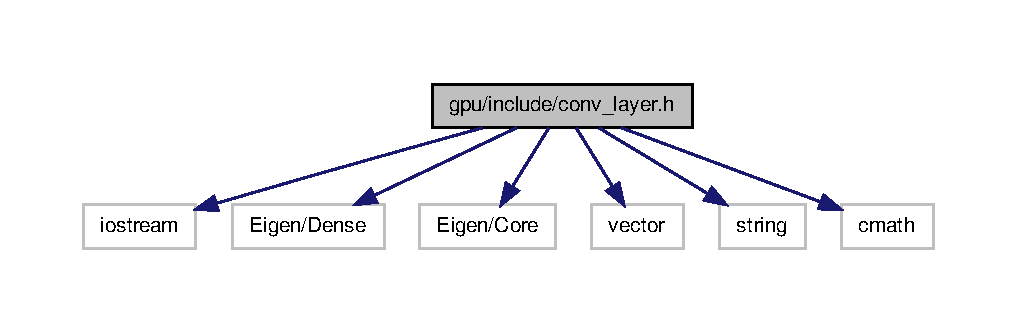
\includegraphics[width=350pt]{gpu_2include_2conv__layer_8h__incl}
\end{center}
\end{figure}
\subsection*{\-Classes}
\begin{DoxyCompactItemize}
\item 
class \hyperlink{classlibcnn_1_1_conv_pool_layer}{libcnn\-::\-Conv\-Pool\-Layer}
\end{DoxyCompactItemize}
\subsection*{\-Namespaces}
\begin{DoxyCompactItemize}
\item 
namespace \hyperlink{namespacelibcnn}{libcnn}
\end{DoxyCompactItemize}
\subsection*{\-Functions}
\begin{DoxyCompactItemize}
\item 
double \hyperlink{namespacelibcnn_a5b73556a76dfe9867c10ebd14519fb4e}{libcnn\-::sigmoid} (const double \&x)
\item 
void \hyperlink{namespacelibcnn_a55bbe6e5488b8a038e5708a32d233090}{libcnn\-::get\-\_\-feature\-\_\-vector} (const vector$<$ vector$<$ \-Matrix\-Xd $>$ $>$ \&, \-Matrix\-Xd \&)
\item 
void \hyperlink{namespacelibcnn_a78ed8e63be87c4d06bb363af95ce62ec}{libcnn\-::softmax2conv} (const \-Matrix\-Xd \&, const int \&, const int \&, const int \&, vector$<$ vector$<$ \-Matrix\-Xd $>$ $>$ \&)
\end{DoxyCompactItemize}

\hypertarget{include_2conv__layer_8h}{\section{include/conv\-\_\-layer.h \-File \-Reference}
\label{include_2conv__layer_8h}\index{include/conv\-\_\-layer.\-h@{include/conv\-\_\-layer.\-h}}
}
{\ttfamily \#include $<$iostream$>$}\*
{\ttfamily \#include $<$\-Eigen/\-Dense$>$}\*
{\ttfamily \#include $<$\-Eigen/\-Core$>$}\*
{\ttfamily \#include $<$vector$>$}\*
{\ttfamily \#include $<$string$>$}\*
{\ttfamily \#include $<$cmath$>$}\*
\-Include dependency graph for conv\-\_\-layer.\-h\-:
\nopagebreak
\begin{figure}[H]
\begin{center}
\leavevmode
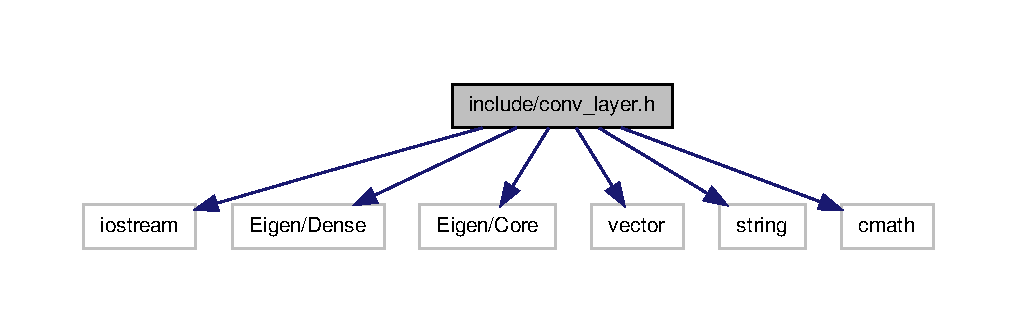
\includegraphics[width=350pt]{include_2conv__layer_8h__incl}
\end{center}
\end{figure}
\-This graph shows which files directly or indirectly include this file\-:
\nopagebreak
\begin{figure}[H]
\begin{center}
\leavevmode
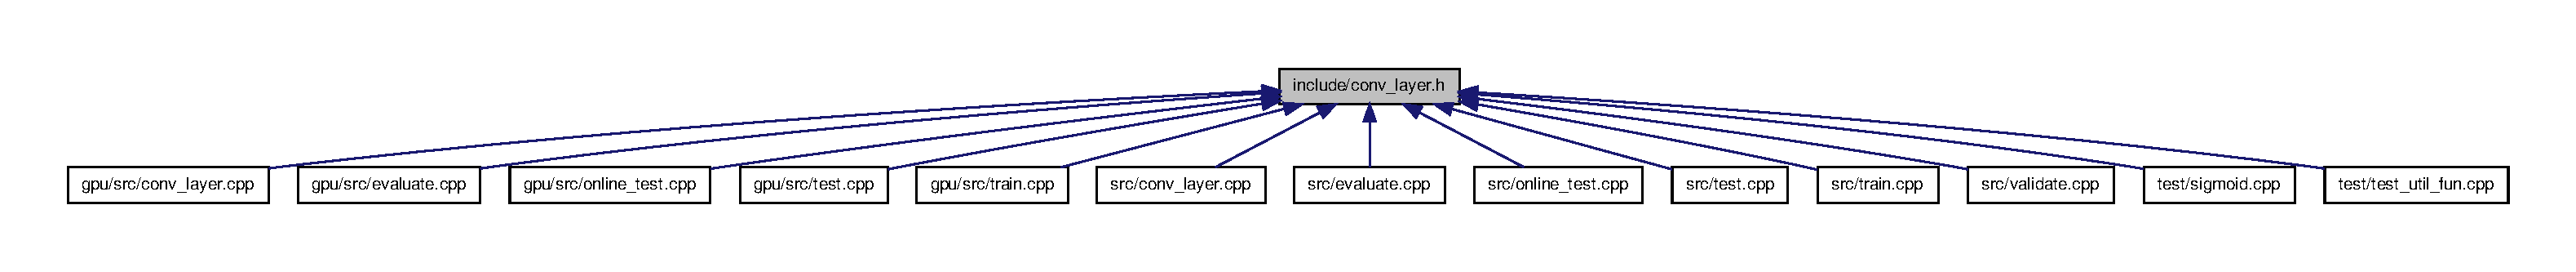
\includegraphics[width=350pt]{include_2conv__layer_8h__dep__incl}
\end{center}
\end{figure}
\subsection*{\-Classes}
\begin{DoxyCompactItemize}
\item 
class \hyperlink{classlibcnn_1_1_conv_pool_layer}{libcnn\-::\-Conv\-Pool\-Layer}
\end{DoxyCompactItemize}
\subsection*{\-Namespaces}
\begin{DoxyCompactItemize}
\item 
namespace \hyperlink{namespacelibcnn}{libcnn}
\end{DoxyCompactItemize}
\subsection*{\-Functions}
\begin{DoxyCompactItemize}
\item 
double \hyperlink{namespacelibcnn_a5b73556a76dfe9867c10ebd14519fb4e}{libcnn\-::sigmoid} (const double \&x)
\item 
void \hyperlink{namespacelibcnn_a55bbe6e5488b8a038e5708a32d233090}{libcnn\-::get\-\_\-feature\-\_\-vector} (const vector$<$ vector$<$ \-Matrix\-Xd $>$ $>$ \&, \-Matrix\-Xd \&)
\item 
void \hyperlink{namespacelibcnn_a78ed8e63be87c4d06bb363af95ce62ec}{libcnn\-::softmax2conv} (const \-Matrix\-Xd \&, const int \&, const int \&, const int \&, vector$<$ vector$<$ \-Matrix\-Xd $>$ $>$ \&)
\end{DoxyCompactItemize}

\hypertarget{gpu_2include_2init__params_8h}{\section{gpu/include/init\-\_\-params.h \-File \-Reference}
\label{gpu_2include_2init__params_8h}\index{gpu/include/init\-\_\-params.\-h@{gpu/include/init\-\_\-params.\-h}}
}
{\ttfamily \#include $<$iostream$>$}\*
{\ttfamily \#include $<$\-Eigen/\-Dense$>$}\*
{\ttfamily \#include $<$vector$>$}\*
{\ttfamily \#include $<$string$>$}\*
\-Include dependency graph for init\-\_\-params.\-h\-:
\nopagebreak
\begin{figure}[H]
\begin{center}
\leavevmode
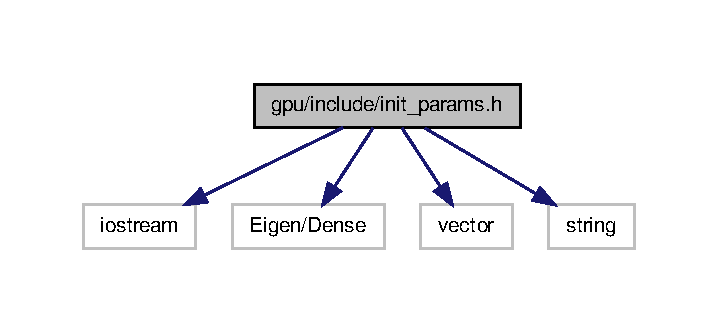
\includegraphics[width=344pt]{gpu_2include_2init__params_8h__incl}
\end{center}
\end{figure}
\subsection*{\-Namespaces}
\begin{DoxyCompactItemize}
\item 
namespace \hyperlink{namespacelibcnn}{libcnn}
\end{DoxyCompactItemize}
\subsection*{\-Functions}
\begin{DoxyCompactItemize}
\item 
void \hyperlink{namespacelibcnn_a2c5ccad2e675235e71fd5e5641ede4ae}{libcnn\-::get\-\_\-parameter} (vector$<$ \-Matrix\-Xd $>$ \&)
\end{DoxyCompactItemize}

\hypertarget{include_2init__params_8h}{\section{include/init\-\_\-params.h \-File \-Reference}
\label{include_2init__params_8h}\index{include/init\-\_\-params.\-h@{include/init\-\_\-params.\-h}}
}
{\ttfamily \#include $<$iostream$>$}\*
{\ttfamily \#include $<$\-Eigen/\-Dense$>$}\*
{\ttfamily \#include $<$vector$>$}\*
{\ttfamily \#include $<$string$>$}\*
\-Include dependency graph for init\-\_\-params.\-h\-:
\nopagebreak
\begin{figure}[H]
\begin{center}
\leavevmode
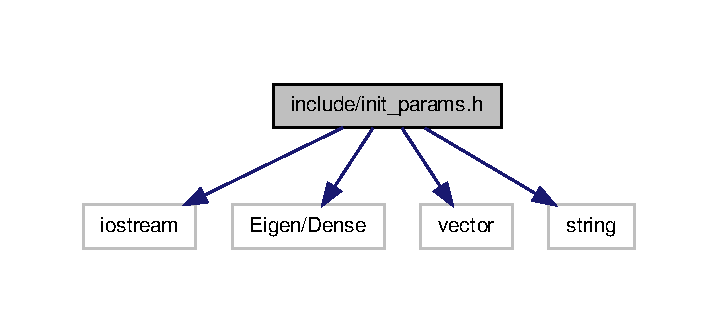
\includegraphics[width=344pt]{include_2init__params_8h__incl}
\end{center}
\end{figure}
\-This graph shows which files directly or indirectly include this file\-:
\nopagebreak
\begin{figure}[H]
\begin{center}
\leavevmode
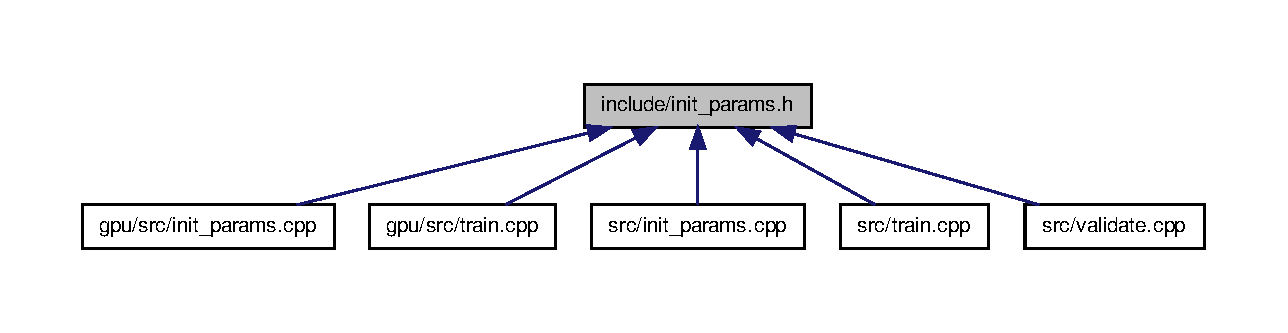
\includegraphics[width=350pt]{include_2init__params_8h__dep__incl}
\end{center}
\end{figure}
\subsection*{\-Namespaces}
\begin{DoxyCompactItemize}
\item 
namespace \hyperlink{namespacelibcnn}{libcnn}
\end{DoxyCompactItemize}
\subsection*{\-Functions}
\begin{DoxyCompactItemize}
\item 
void \hyperlink{namespacelibcnn_a2c5ccad2e675235e71fd5e5641ede4ae}{libcnn\-::get\-\_\-parameter} (vector$<$ \-Matrix\-Xd $>$ \&)
\end{DoxyCompactItemize}

\hypertarget{gpu_2include_2load__data_8h}{\section{gpu/include/load\-\_\-data.h \-File \-Reference}
\label{gpu_2include_2load__data_8h}\index{gpu/include/load\-\_\-data.\-h@{gpu/include/load\-\_\-data.\-h}}
}
{\ttfamily \#include $<$cstring$>$}\*
{\ttfamily \#include $<$vector$>$}\*
{\ttfamily \#include $<$\-Eigen/\-Dense$>$}\*
{\ttfamily \#include $<$iostream$>$}\*
{\ttfamily \#include $<$fstream$>$}\*
\-Include dependency graph for load\-\_\-data.\-h\-:
\nopagebreak
\begin{figure}[H]
\begin{center}
\leavevmode
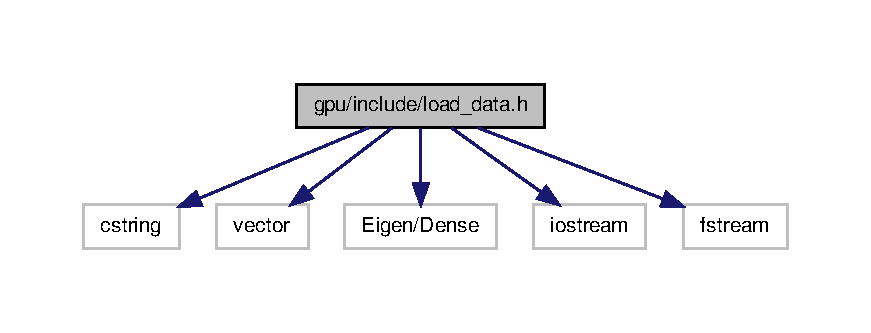
\includegraphics[width=350pt]{gpu_2include_2load__data_8h__incl}
\end{center}
\end{figure}
\subsection*{\-Functions}
\begin{DoxyCompactItemize}
\item 
void \hyperlink{gpu_2include_2load__data_8h_afbad2e91730f993e296f166a8f89aa9b}{getdir} (const string \&\hyperlink{yaml__t__load_8cpp_a7f01c047eb310166e695d4232ebd1fae}{dir}, vector$<$ string $>$ \&files)
\item 
void \hyperlink{gpu_2include_2load__data_8h_a39a205061173088b2222b1d550a8787c}{read\-\_\-image\-\_\-files} (const string \&\hyperlink{yaml__t__load_8cpp_a7f01c047eb310166e695d4232ebd1fae}{dir}, std\-::vector$<$ vector$<$ \-Matrix\-Xd $>$ $>$ \&vvm, const int \&image\-\_\-row\-\_\-dim, const int \&image\-\_\-col\-\_\-dim, const int \&start, const int \&image\-\_\-number)
\item 
void \hyperlink{gpu_2include_2load__data_8h_a8f84dc0bbc3acab545f50ce4899348e3}{read\-\_\-label\-\_\-files} (const string \&\hyperlink{yaml__t__load_8cpp_a7f01c047eb310166e695d4232ebd1fae}{dir}, \-Vector\-Xi \&m, const int \&image\-\_\-row\-\_\-dim, const int \&image\-\_\-col\-\_\-dim, const int \&start, const int \&image\-\_\-number, const string \&data\-\_\-mode)
\item 
void \hyperlink{gpu_2include_2load__data_8h_a3e0b753ca980bbac49c49beb20523146}{read\-\_\-markov\-\_\-files} (const string \&\hyperlink{yaml__t__load_8cpp_a7f01c047eb310166e695d4232ebd1fae}{dir}, \-Matrix\-Xd \&markov)
\end{DoxyCompactItemize}


\subsection{\-Function \-Documentation}
\hypertarget{gpu_2include_2load__data_8h_afbad2e91730f993e296f166a8f89aa9b}{\index{gpu/include/load\-\_\-data.\-h@{gpu/include/load\-\_\-data.\-h}!getdir@{getdir}}
\index{getdir@{getdir}!gpu/include/load_data.h@{gpu/include/load\-\_\-data.\-h}}
\subsubsection[{getdir}]{\setlength{\rightskip}{0pt plus 5cm}void {\bf getdir} (
\begin{DoxyParamCaption}
\item[{const string \&}]{dir, }
\item[{vector$<$ string $>$ \&}]{files}
\end{DoxyParamCaption}
)}}\label{gpu_2include_2load__data_8h_afbad2e91730f993e296f166a8f89aa9b}
\hypertarget{gpu_2include_2load__data_8h_a39a205061173088b2222b1d550a8787c}{\index{gpu/include/load\-\_\-data.\-h@{gpu/include/load\-\_\-data.\-h}!read\-\_\-image\-\_\-files@{read\-\_\-image\-\_\-files}}
\index{read\-\_\-image\-\_\-files@{read\-\_\-image\-\_\-files}!gpu/include/load_data.h@{gpu/include/load\-\_\-data.\-h}}
\subsubsection[{read\-\_\-image\-\_\-files}]{\setlength{\rightskip}{0pt plus 5cm}void {\bf read\-\_\-image\-\_\-files} (
\begin{DoxyParamCaption}
\item[{const string \&}]{dir, }
\item[{std\-::vector$<$ vector$<$ \-Matrix\-Xd $>$ $>$ \&}]{vvm, }
\item[{const int \&}]{image\-\_\-row\-\_\-dim, }
\item[{const int \&}]{image\-\_\-col\-\_\-dim, }
\item[{const int \&}]{start, }
\item[{const int \&}]{image\-\_\-number}
\end{DoxyParamCaption}
)}}\label{gpu_2include_2load__data_8h_a39a205061173088b2222b1d550a8787c}
\hypertarget{gpu_2include_2load__data_8h_a8f84dc0bbc3acab545f50ce4899348e3}{\index{gpu/include/load\-\_\-data.\-h@{gpu/include/load\-\_\-data.\-h}!read\-\_\-label\-\_\-files@{read\-\_\-label\-\_\-files}}
\index{read\-\_\-label\-\_\-files@{read\-\_\-label\-\_\-files}!gpu/include/load_data.h@{gpu/include/load\-\_\-data.\-h}}
\subsubsection[{read\-\_\-label\-\_\-files}]{\setlength{\rightskip}{0pt plus 5cm}void {\bf read\-\_\-label\-\_\-files} (
\begin{DoxyParamCaption}
\item[{const string \&}]{dir, }
\item[{\-Vector\-Xi \&}]{m, }
\item[{const int \&}]{image\-\_\-row\-\_\-dim, }
\item[{const int \&}]{image\-\_\-col\-\_\-dim, }
\item[{const int \&}]{start, }
\item[{const int \&}]{image\-\_\-number, }
\item[{const string \&}]{data\-\_\-mode}
\end{DoxyParamCaption}
)}}\label{gpu_2include_2load__data_8h_a8f84dc0bbc3acab545f50ce4899348e3}
\hypertarget{gpu_2include_2load__data_8h_a3e0b753ca980bbac49c49beb20523146}{\index{gpu/include/load\-\_\-data.\-h@{gpu/include/load\-\_\-data.\-h}!read\-\_\-markov\-\_\-files@{read\-\_\-markov\-\_\-files}}
\index{read\-\_\-markov\-\_\-files@{read\-\_\-markov\-\_\-files}!gpu/include/load_data.h@{gpu/include/load\-\_\-data.\-h}}
\subsubsection[{read\-\_\-markov\-\_\-files}]{\setlength{\rightskip}{0pt plus 5cm}void {\bf read\-\_\-markov\-\_\-files} (
\begin{DoxyParamCaption}
\item[{const string \&}]{dir, }
\item[{\-Matrix\-Xd \&}]{markov}
\end{DoxyParamCaption}
)}}\label{gpu_2include_2load__data_8h_a3e0b753ca980bbac49c49beb20523146}

\hypertarget{include_2load__data_8h}{\section{include/load\-\_\-data.h \-File \-Reference}
\label{include_2load__data_8h}\index{include/load\-\_\-data.\-h@{include/load\-\_\-data.\-h}}
}
{\ttfamily \#include $<$cstring$>$}\*
{\ttfamily \#include $<$vector$>$}\*
{\ttfamily \#include $<$\-Eigen/\-Dense$>$}\*
{\ttfamily \#include $<$iostream$>$}\*
{\ttfamily \#include $<$fstream$>$}\*
\-Include dependency graph for load\-\_\-data.\-h\-:
\nopagebreak
\begin{figure}[H]
\begin{center}
\leavevmode
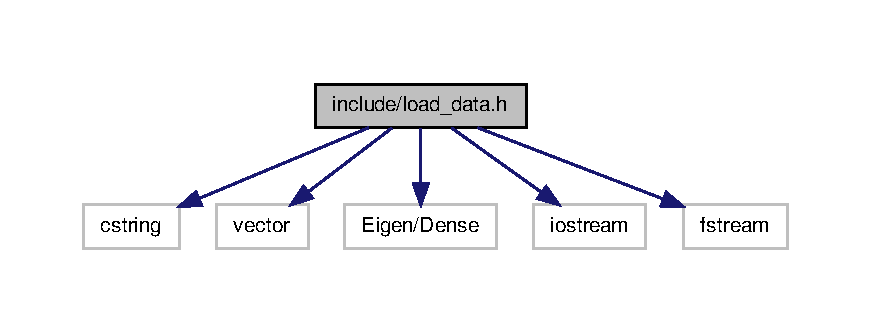
\includegraphics[width=350pt]{include_2load__data_8h__incl}
\end{center}
\end{figure}
\-This graph shows which files directly or indirectly include this file\-:
\nopagebreak
\begin{figure}[H]
\begin{center}
\leavevmode
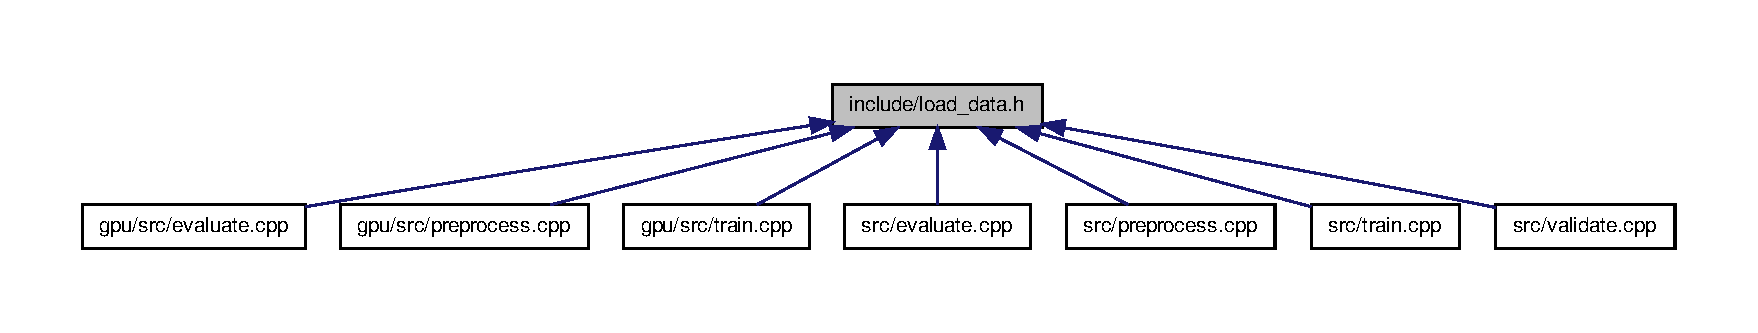
\includegraphics[width=350pt]{include_2load__data_8h__dep__incl}
\end{center}
\end{figure}
\subsection*{\-Functions}
\begin{DoxyCompactItemize}
\item 
void \hyperlink{include_2load__data_8h_afbad2e91730f993e296f166a8f89aa9b}{getdir} (const string \&\hyperlink{yaml__t__load_8cpp_a7f01c047eb310166e695d4232ebd1fae}{dir}, vector$<$ string $>$ \&files)
\item 
void \hyperlink{include_2load__data_8h_a39a205061173088b2222b1d550a8787c}{read\-\_\-image\-\_\-files} (const string \&\hyperlink{yaml__t__load_8cpp_a7f01c047eb310166e695d4232ebd1fae}{dir}, std\-::vector$<$ vector$<$ \-Matrix\-Xd $>$ $>$ \&vvm, const int \&image\-\_\-row\-\_\-dim, const int \&image\-\_\-col\-\_\-dim, const int \&start, const int \&image\-\_\-number)
\item 
void \hyperlink{include_2load__data_8h_a8f84dc0bbc3acab545f50ce4899348e3}{read\-\_\-label\-\_\-files} (const string \&\hyperlink{yaml__t__load_8cpp_a7f01c047eb310166e695d4232ebd1fae}{dir}, \-Vector\-Xi \&m, const int \&image\-\_\-row\-\_\-dim, const int \&image\-\_\-col\-\_\-dim, const int \&start, const int \&image\-\_\-number, const string \&data\-\_\-mode)
\item 
void \hyperlink{include_2load__data_8h_a3e0b753ca980bbac49c49beb20523146}{read\-\_\-markov\-\_\-files} (const string \&\hyperlink{yaml__t__load_8cpp_a7f01c047eb310166e695d4232ebd1fae}{dir}, \-Matrix\-Xd \&markov)
\end{DoxyCompactItemize}


\subsection{\-Function \-Documentation}
\hypertarget{include_2load__data_8h_afbad2e91730f993e296f166a8f89aa9b}{\index{include/load\-\_\-data.\-h@{include/load\-\_\-data.\-h}!getdir@{getdir}}
\index{getdir@{getdir}!include/load_data.h@{include/load\-\_\-data.\-h}}
\subsubsection[{getdir}]{\setlength{\rightskip}{0pt plus 5cm}void {\bf getdir} (
\begin{DoxyParamCaption}
\item[{const string \&}]{dir, }
\item[{vector$<$ string $>$ \&}]{files}
\end{DoxyParamCaption}
)}}\label{include_2load__data_8h_afbad2e91730f993e296f166a8f89aa9b}
\hypertarget{include_2load__data_8h_a39a205061173088b2222b1d550a8787c}{\index{include/load\-\_\-data.\-h@{include/load\-\_\-data.\-h}!read\-\_\-image\-\_\-files@{read\-\_\-image\-\_\-files}}
\index{read\-\_\-image\-\_\-files@{read\-\_\-image\-\_\-files}!include/load_data.h@{include/load\-\_\-data.\-h}}
\subsubsection[{read\-\_\-image\-\_\-files}]{\setlength{\rightskip}{0pt plus 5cm}void {\bf read\-\_\-image\-\_\-files} (
\begin{DoxyParamCaption}
\item[{const string \&}]{dir, }
\item[{std\-::vector$<$ vector$<$ \-Matrix\-Xd $>$ $>$ \&}]{vvm, }
\item[{const int \&}]{image\-\_\-row\-\_\-dim, }
\item[{const int \&}]{image\-\_\-col\-\_\-dim, }
\item[{const int \&}]{start, }
\item[{const int \&}]{image\-\_\-number}
\end{DoxyParamCaption}
)}}\label{include_2load__data_8h_a39a205061173088b2222b1d550a8787c}


\-Here is the call graph for this function\-:
\nopagebreak
\begin{figure}[H]
\begin{center}
\leavevmode
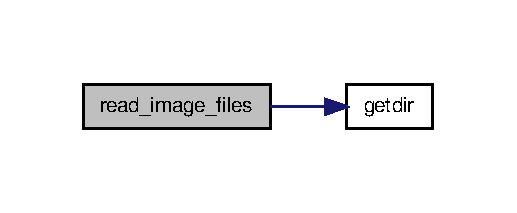
\includegraphics[width=248pt]{include_2load__data_8h_a39a205061173088b2222b1d550a8787c_cgraph}
\end{center}
\end{figure}


\hypertarget{include_2load__data_8h_a8f84dc0bbc3acab545f50ce4899348e3}{\index{include/load\-\_\-data.\-h@{include/load\-\_\-data.\-h}!read\-\_\-label\-\_\-files@{read\-\_\-label\-\_\-files}}
\index{read\-\_\-label\-\_\-files@{read\-\_\-label\-\_\-files}!include/load_data.h@{include/load\-\_\-data.\-h}}
\subsubsection[{read\-\_\-label\-\_\-files}]{\setlength{\rightskip}{0pt plus 5cm}void {\bf read\-\_\-label\-\_\-files} (
\begin{DoxyParamCaption}
\item[{const string \&}]{dir, }
\item[{\-Vector\-Xi \&}]{m, }
\item[{const int \&}]{image\-\_\-row\-\_\-dim, }
\item[{const int \&}]{image\-\_\-col\-\_\-dim, }
\item[{const int \&}]{start, }
\item[{const int \&}]{image\-\_\-number, }
\item[{const string \&}]{data\-\_\-mode}
\end{DoxyParamCaption}
)}}\label{include_2load__data_8h_a8f84dc0bbc3acab545f50ce4899348e3}


\-Here is the call graph for this function\-:
\nopagebreak
\begin{figure}[H]
\begin{center}
\leavevmode
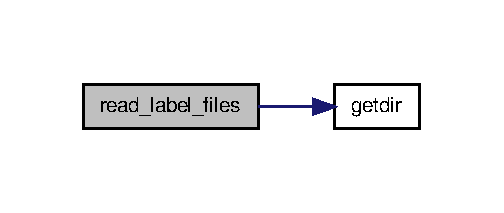
\includegraphics[width=242pt]{include_2load__data_8h_a8f84dc0bbc3acab545f50ce4899348e3_cgraph}
\end{center}
\end{figure}


\hypertarget{include_2load__data_8h_a3e0b753ca980bbac49c49beb20523146}{\index{include/load\-\_\-data.\-h@{include/load\-\_\-data.\-h}!read\-\_\-markov\-\_\-files@{read\-\_\-markov\-\_\-files}}
\index{read\-\_\-markov\-\_\-files@{read\-\_\-markov\-\_\-files}!include/load_data.h@{include/load\-\_\-data.\-h}}
\subsubsection[{read\-\_\-markov\-\_\-files}]{\setlength{\rightskip}{0pt plus 5cm}void {\bf read\-\_\-markov\-\_\-files} (
\begin{DoxyParamCaption}
\item[{const string \&}]{dir, }
\item[{\-Matrix\-Xd \&}]{markov}
\end{DoxyParamCaption}
)}}\label{include_2load__data_8h_a3e0b753ca980bbac49c49beb20523146}

\hypertarget{gpu_2include_2online__test_8h}{\section{gpu/include/online\-\_\-test.h \-File \-Reference}
\label{gpu_2include_2online__test_8h}\index{gpu/include/online\-\_\-test.\-h@{gpu/include/online\-\_\-test.\-h}}
}
{\ttfamily \#include $<$iostream$>$}\*
{\ttfamily \#include $<$\-Eigen/\-Dense$>$}\*
{\ttfamily \#include $<$vector$>$}\*
\-Include dependency graph for online\-\_\-test.\-h\-:
\nopagebreak
\begin{figure}[H]
\begin{center}
\leavevmode
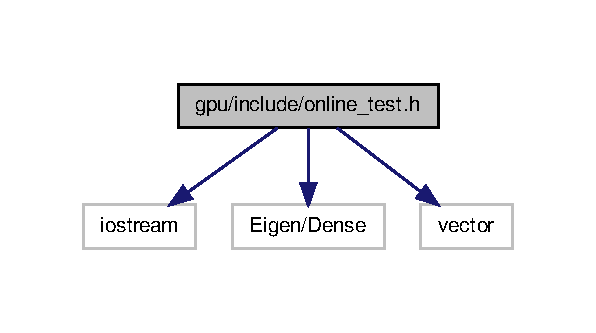
\includegraphics[width=286pt]{gpu_2include_2online__test_8h__incl}
\end{center}
\end{figure}
\subsection*{\-Namespaces}
\begin{DoxyCompactItemize}
\item 
namespace \hyperlink{namespacelibcnn}{libcnn}
\end{DoxyCompactItemize}
\subsection*{\-Functions}
\begin{DoxyCompactItemize}
\item 
void \hyperlink{namespacelibcnn_a493fb452cedcc704e189ad1a3656c0ad}{libcnn\-::online\-\_\-test} (const vector$<$ vector$<$ \-Matrix\-Xd $>$ $>$ \&, const \-Vector\-Xi \&, const vector$<$ \-Matrix\-Xd $>$ \&, const \-Matrix\-Xd \&, const vector$<$ \-Matrix\-Xd $>$ \&, const \-Matrix\-Xd \&, const vector$<$ \-Matrix\-Xd $>$ \&, const \-Matrix\-Xd \&, const \-Matrix\-Xd \&, const \-Matrix\-Xd \&, const int \&, const int \&, const int \&, const int \&, const int \&)
\end{DoxyCompactItemize}

\hypertarget{include_2online__test_8h}{\section{include/online\-\_\-test.h \-File \-Reference}
\label{include_2online__test_8h}\index{include/online\-\_\-test.\-h@{include/online\-\_\-test.\-h}}
}
{\ttfamily \#include $<$iostream$>$}\*
{\ttfamily \#include $<$\-Eigen/\-Dense$>$}\*
{\ttfamily \#include $<$vector$>$}\*
\-Include dependency graph for online\-\_\-test.\-h\-:
\nopagebreak
\begin{figure}[H]
\begin{center}
\leavevmode
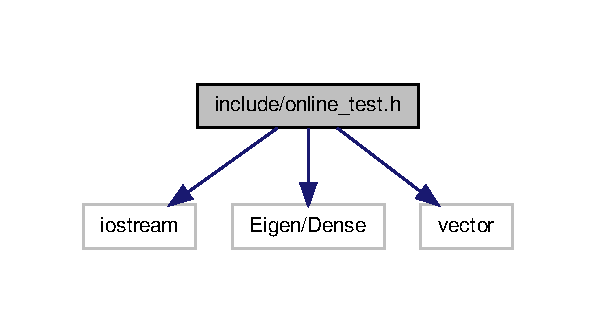
\includegraphics[width=286pt]{include_2online__test_8h__incl}
\end{center}
\end{figure}
\-This graph shows which files directly or indirectly include this file\-:
\nopagebreak
\begin{figure}[H]
\begin{center}
\leavevmode
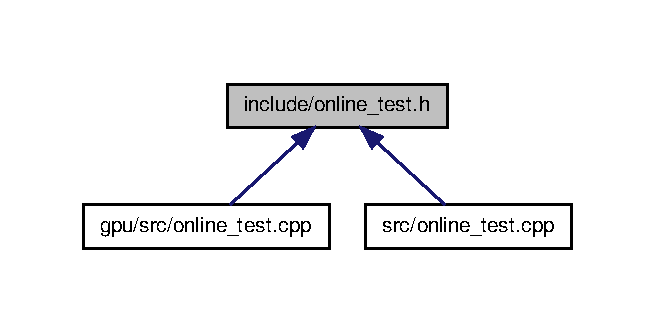
\includegraphics[width=314pt]{include_2online__test_8h__dep__incl}
\end{center}
\end{figure}
\subsection*{\-Namespaces}
\begin{DoxyCompactItemize}
\item 
namespace \hyperlink{namespacelibcnn}{libcnn}
\end{DoxyCompactItemize}
\subsection*{\-Functions}
\begin{DoxyCompactItemize}
\item 
void \hyperlink{namespacelibcnn_a493fb452cedcc704e189ad1a3656c0ad}{libcnn\-::online\-\_\-test} (const vector$<$ vector$<$ \-Matrix\-Xd $>$ $>$ \&, const \-Vector\-Xi \&, const vector$<$ \-Matrix\-Xd $>$ \&, const \-Matrix\-Xd \&, const vector$<$ \-Matrix\-Xd $>$ \&, const \-Matrix\-Xd \&, const vector$<$ \-Matrix\-Xd $>$ \&, const \-Matrix\-Xd \&, const \-Matrix\-Xd \&, const \-Matrix\-Xd \&, const int \&, const int \&, const int \&, const int \&, const int \&)
\end{DoxyCompactItemize}

\hypertarget{gpu_2include_2pool_8h}{\section{gpu/include/pool.h \-File \-Reference}
\label{gpu_2include_2pool_8h}\index{gpu/include/pool.\-h@{gpu/include/pool.\-h}}
}
{\ttfamily \#include $<$iostream$>$}\*
{\ttfamily \#include $<$\-Eigen/\-Dense$>$}\*
{\ttfamily \#include $<$vector$>$}\*
{\ttfamily \#include $<$cmath$>$}\*
{\ttfamily \#include $<$string$>$}\*
\-Include dependency graph for pool.\-h\-:
\nopagebreak
\begin{figure}[H]
\begin{center}
\leavevmode
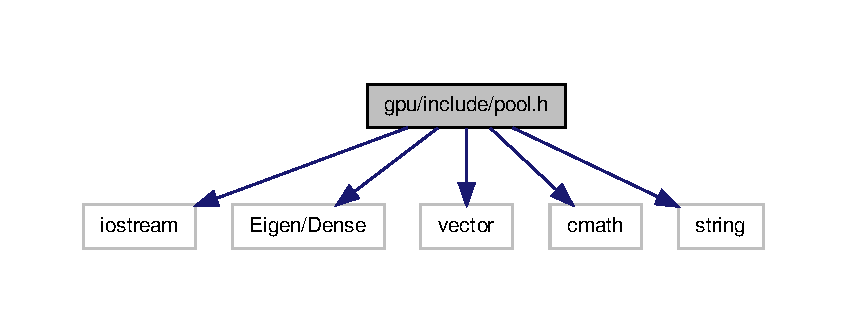
\includegraphics[width=350pt]{gpu_2include_2pool_8h__incl}
\end{center}
\end{figure}
\subsection*{\-Classes}
\begin{DoxyCompactItemize}
\item 
class \hyperlink{classlibcnn_1_1_pool}{libcnn\-::\-Pool}
\end{DoxyCompactItemize}
\subsection*{\-Namespaces}
\begin{DoxyCompactItemize}
\item 
namespace \hyperlink{namespacelibcnn}{libcnn}
\end{DoxyCompactItemize}

\hypertarget{include_2pool_8h}{\section{include/pool.h \-File \-Reference}
\label{include_2pool_8h}\index{include/pool.\-h@{include/pool.\-h}}
}
{\ttfamily \#include $<$iostream$>$}\*
{\ttfamily \#include $<$\-Eigen/\-Dense$>$}\*
{\ttfamily \#include $<$vector$>$}\*
{\ttfamily \#include $<$cmath$>$}\*
{\ttfamily \#include $<$string$>$}\*
\-Include dependency graph for pool.\-h\-:
\nopagebreak
\begin{figure}[H]
\begin{center}
\leavevmode
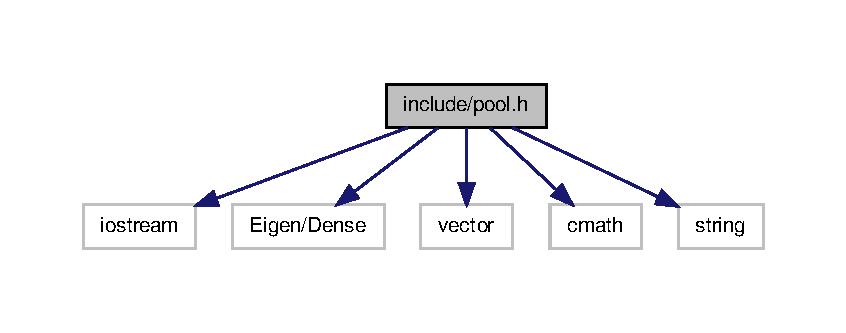
\includegraphics[width=350pt]{include_2pool_8h__incl}
\end{center}
\end{figure}
\-This graph shows which files directly or indirectly include this file\-:
\nopagebreak
\begin{figure}[H]
\begin{center}
\leavevmode
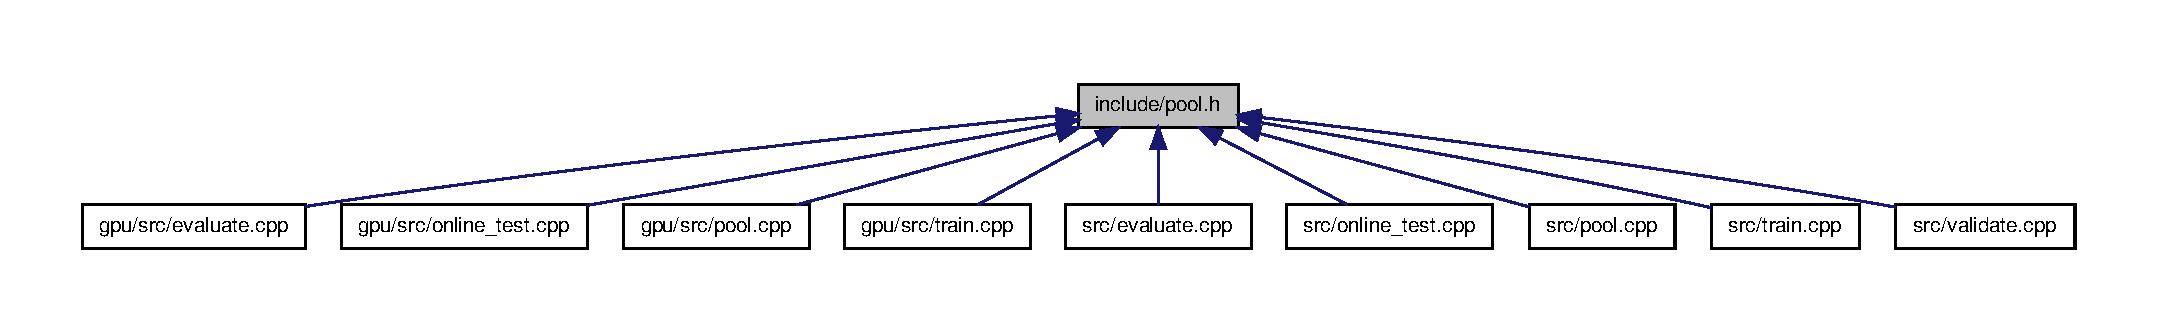
\includegraphics[width=350pt]{include_2pool_8h__dep__incl}
\end{center}
\end{figure}
\subsection*{\-Classes}
\begin{DoxyCompactItemize}
\item 
class \hyperlink{classlibcnn_1_1_pool}{libcnn\-::\-Pool}
\end{DoxyCompactItemize}
\subsection*{\-Namespaces}
\begin{DoxyCompactItemize}
\item 
namespace \hyperlink{namespacelibcnn}{libcnn}
\end{DoxyCompactItemize}

\hypertarget{gpu_2include_2preprocess_8h}{\section{gpu/include/preprocess.h \-File \-Reference}
\label{gpu_2include_2preprocess_8h}\index{gpu/include/preprocess.\-h@{gpu/include/preprocess.\-h}}
}
{\ttfamily \#include $<$iostream$>$}\*
{\ttfamily \#include $<$\-Eigen/\-Dense$>$}\*
{\ttfamily \#include $<$\-Eigen/\-Core$>$}\*
{\ttfamily \#include $<$vector$>$}\*
\-Include dependency graph for preprocess.\-h\-:
\nopagebreak
\begin{figure}[H]
\begin{center}
\leavevmode
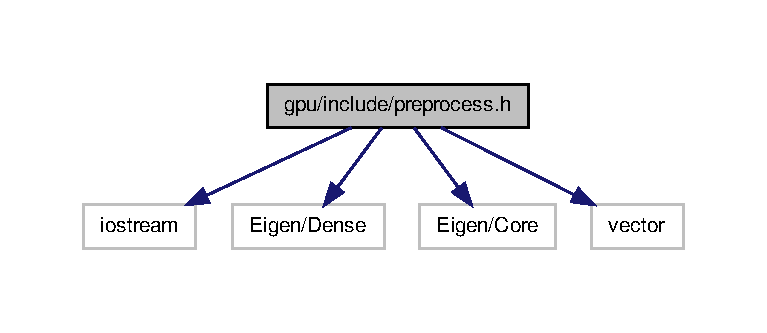
\includegraphics[width=350pt]{gpu_2include_2preprocess_8h__incl}
\end{center}
\end{figure}
\subsection*{\-Namespaces}
\begin{DoxyCompactItemize}
\item 
namespace \hyperlink{namespacelibcnn}{libcnn}
\end{DoxyCompactItemize}
\subsection*{\-Functions}
\begin{DoxyCompactItemize}
\item 
void \hyperlink{namespacelibcnn_ab161d6e7087d097f72c086587a661c4a}{libcnn\-::normalize} (\-Matrix\-Xd \&)
\item 
void \hyperlink{namespacelibcnn_a022f9a6378aa94ec418eb757bead690e}{libcnn\-::data\-\_\-generation} (const int \&, const int \&, const int \&, const int \&, vector$<$ vector$<$ \-Matrix\-Xd $>$ $>$ \&, \-Vector\-Xi \&)
\item 
void \hyperlink{namespacelibcnn_a4afdb4ab6bfd2c2167c593900ef644f5}{libcnn\-::unit\-\_\-scaling} (vector$<$ vector$<$ \-Matrix\-Xd $>$ $>$ \&)
\item 
void \hyperlink{namespacelibcnn_a0f018efe5349302aba6f349d17cc90cf}{libcnn\-::label\-\_\-sampling} (const int \&, const int \&, const int \&, const int \&, \-Vector\-Xi \&, \-Vector\-Xi \&)
\end{DoxyCompactItemize}

\hypertarget{include_2preprocess_8h}{\section{include/preprocess.h \-File \-Reference}
\label{include_2preprocess_8h}\index{include/preprocess.\-h@{include/preprocess.\-h}}
}
{\ttfamily \#include $<$iostream$>$}\*
{\ttfamily \#include $<$\-Eigen/\-Dense$>$}\*
{\ttfamily \#include $<$\-Eigen/\-Core$>$}\*
{\ttfamily \#include $<$vector$>$}\*
\-Include dependency graph for preprocess.\-h\-:
\nopagebreak
\begin{figure}[H]
\begin{center}
\leavevmode
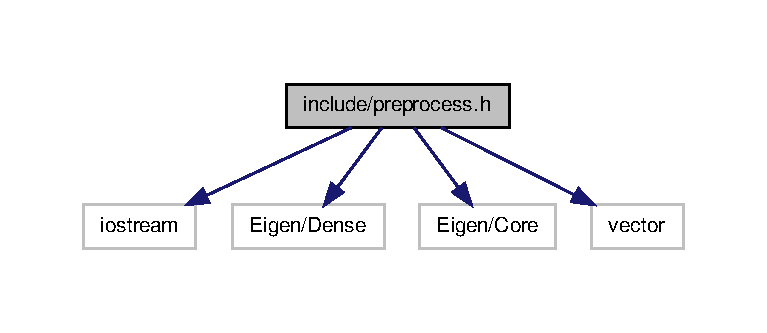
\includegraphics[width=350pt]{include_2preprocess_8h__incl}
\end{center}
\end{figure}
\-This graph shows which files directly or indirectly include this file\-:
\nopagebreak
\begin{figure}[H]
\begin{center}
\leavevmode
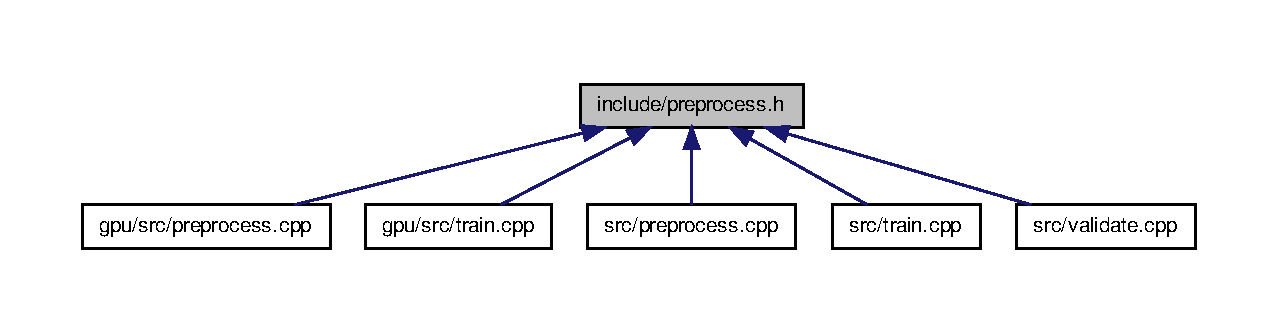
\includegraphics[width=350pt]{include_2preprocess_8h__dep__incl}
\end{center}
\end{figure}
\subsection*{\-Namespaces}
\begin{DoxyCompactItemize}
\item 
namespace \hyperlink{namespacelibcnn}{libcnn}
\end{DoxyCompactItemize}
\subsection*{\-Functions}
\begin{DoxyCompactItemize}
\item 
void \hyperlink{namespacelibcnn_ab161d6e7087d097f72c086587a661c4a}{libcnn\-::normalize} (\-Matrix\-Xd \&)
\item 
void \hyperlink{namespacelibcnn_a022f9a6378aa94ec418eb757bead690e}{libcnn\-::data\-\_\-generation} (const int \&, const int \&, const int \&, const int \&, vector$<$ vector$<$ \-Matrix\-Xd $>$ $>$ \&, \-Vector\-Xi \&)
\item 
void \hyperlink{namespacelibcnn_a4afdb4ab6bfd2c2167c593900ef644f5}{libcnn\-::unit\-\_\-scaling} (vector$<$ vector$<$ \-Matrix\-Xd $>$ $>$ \&)
\item 
void \hyperlink{namespacelibcnn_a0f018efe5349302aba6f349d17cc90cf}{libcnn\-::label\-\_\-sampling} (const int \&, const int \&, const int \&, const int \&, \-Vector\-Xi \&, \-Vector\-Xi \&)
\end{DoxyCompactItemize}

\hypertarget{gpu_2include_2rand__initialize_8h}{\section{gpu/include/rand\-\_\-initialize.h \-File \-Reference}
\label{gpu_2include_2rand__initialize_8h}\index{gpu/include/rand\-\_\-initialize.\-h@{gpu/include/rand\-\_\-initialize.\-h}}
}
{\ttfamily \#include $<$iostream$>$}\*
{\ttfamily \#include $<$\-Eigen/\-Dense$>$}\*
{\ttfamily \#include $<$vector$>$}\*
{\ttfamily \#include $<$ctime$>$}\*
\-Include dependency graph for rand\-\_\-initialize.\-h\-:
\nopagebreak
\begin{figure}[H]
\begin{center}
\leavevmode
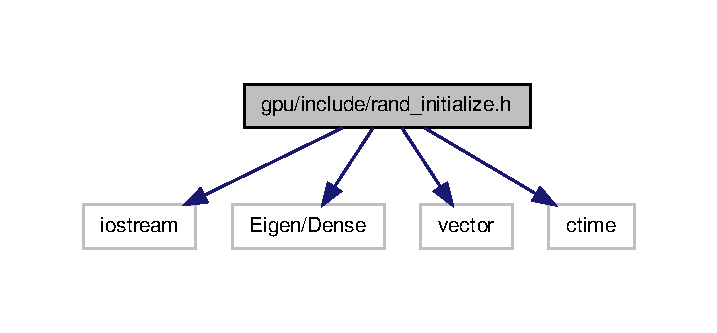
\includegraphics[width=344pt]{gpu_2include_2rand__initialize_8h__incl}
\end{center}
\end{figure}
\subsection*{\-Namespaces}
\begin{DoxyCompactItemize}
\item 
namespace \hyperlink{namespacelibcnn}{libcnn}
\end{DoxyCompactItemize}
\subsection*{\-Functions}
\begin{DoxyCompactItemize}
\item 
void \hyperlink{namespacelibcnn_a367a409a55921d3810474a42357ff285}{libcnn\-::rand\-\_\-classifier} (\-Matrix\-Xd \&, \-Matrix\-Xd \&, const vector$<$ int $>$ \&, const int \&, const int \&, const double \&, const double \&)
\item 
void \hyperlink{namespacelibcnn_a449702bcc49494b8e359548d03ba12e3}{libcnn\-::rand\-\_\-conv} (vector$<$ vector$<$ \-Matrix\-Xd $>$ $>$ \&, vector$<$ \-Matrix\-Xd $>$ \&, const vector$<$ int $>$ \&, const int \&, const int \&, const double \&, const double \&)
\item 
void \hyperlink{namespacelibcnn_a6e166be43bf4a7640feef235071df26e}{libcnn\-::print\-\_\-params} (const vector$<$ vector$<$ \-Matrix\-Xd $>$ $>$ \&, const vector$<$ \-Matrix\-Xd $>$ \&, const \-Matrix\-Xd \&, const \-Matrix\-Xd \&)
\end{DoxyCompactItemize}

\hypertarget{include_2rand__initialize_8h}{\section{include/rand\-\_\-initialize.h \-File \-Reference}
\label{include_2rand__initialize_8h}\index{include/rand\-\_\-initialize.\-h@{include/rand\-\_\-initialize.\-h}}
}
{\ttfamily \#include $<$iostream$>$}\*
{\ttfamily \#include $<$\-Eigen/\-Dense$>$}\*
{\ttfamily \#include $<$vector$>$}\*
{\ttfamily \#include $<$ctime$>$}\*
\-Include dependency graph for rand\-\_\-initialize.\-h\-:
\nopagebreak
\begin{figure}[H]
\begin{center}
\leavevmode
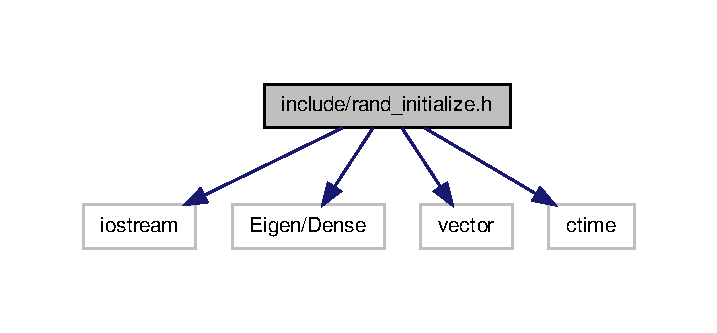
\includegraphics[width=344pt]{include_2rand__initialize_8h__incl}
\end{center}
\end{figure}
\-This graph shows which files directly or indirectly include this file\-:
\nopagebreak
\begin{figure}[H]
\begin{center}
\leavevmode
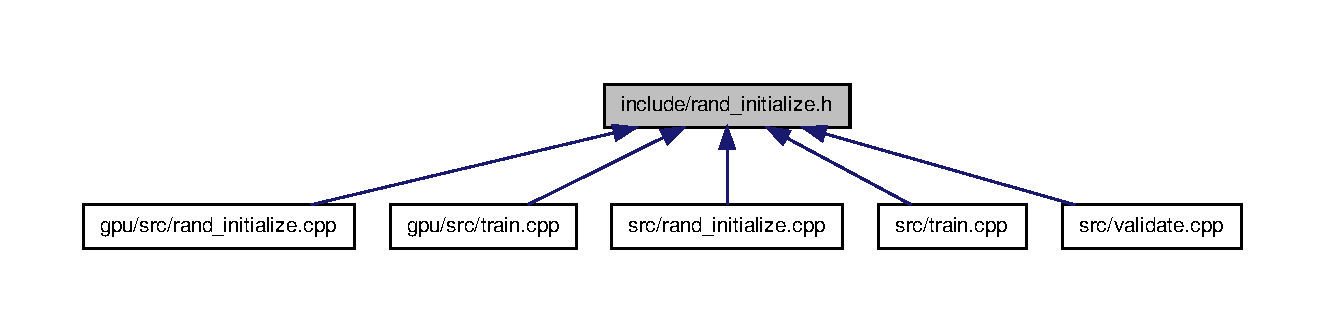
\includegraphics[width=350pt]{include_2rand__initialize_8h__dep__incl}
\end{center}
\end{figure}
\subsection*{\-Namespaces}
\begin{DoxyCompactItemize}
\item 
namespace \hyperlink{namespacelibcnn}{libcnn}
\end{DoxyCompactItemize}
\subsection*{\-Functions}
\begin{DoxyCompactItemize}
\item 
void \hyperlink{namespacelibcnn_a367a409a55921d3810474a42357ff285}{libcnn\-::rand\-\_\-classifier} (\-Matrix\-Xd \&, \-Matrix\-Xd \&, const vector$<$ int $>$ \&, const int \&, const int \&, const double \&, const double \&)
\item 
void \hyperlink{namespacelibcnn_a449702bcc49494b8e359548d03ba12e3}{libcnn\-::rand\-\_\-conv} (vector$<$ vector$<$ \-Matrix\-Xd $>$ $>$ \&, vector$<$ \-Matrix\-Xd $>$ \&, const vector$<$ int $>$ \&, const int \&, const int \&, const double \&, const double \&)
\item 
void \hyperlink{namespacelibcnn_a6e166be43bf4a7640feef235071df26e}{libcnn\-::print\-\_\-params} (const vector$<$ vector$<$ \-Matrix\-Xd $>$ $>$ \&, const vector$<$ \-Matrix\-Xd $>$ \&, const \-Matrix\-Xd \&, const \-Matrix\-Xd \&)
\end{DoxyCompactItemize}

\hypertarget{gpu_2include_2save__params_8h}{\section{gpu/include/save\-\_\-params.h \-File \-Reference}
\label{gpu_2include_2save__params_8h}\index{gpu/include/save\-\_\-params.\-h@{gpu/include/save\-\_\-params.\-h}}
}
{\ttfamily \#include $<$iostream$>$}\*
{\ttfamily \#include $<$\-Eigen/\-Dense$>$}\*
{\ttfamily \#include $<$vector$>$}\*
\-Include dependency graph for save\-\_\-params.\-h\-:
\nopagebreak
\begin{figure}[H]
\begin{center}
\leavevmode
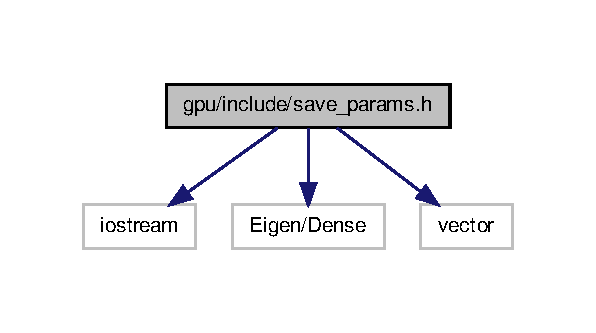
\includegraphics[width=286pt]{gpu_2include_2save__params_8h__incl}
\end{center}
\end{figure}
\subsection*{\-Namespaces}
\begin{DoxyCompactItemize}
\item 
namespace \hyperlink{namespacelibcnn}{libcnn}
\end{DoxyCompactItemize}
\subsection*{\-Functions}
\begin{DoxyCompactItemize}
\item 
void \hyperlink{namespacelibcnn_a35fa40f645f5fe20b4cc8d878b1e0c10}{libcnn\-::print\-\_\-params} (vector$<$ vector$<$ \-Matrix\-Xd $>$ $>$ \&, vector$<$ \-Matrix\-Xd $>$ \&, vector$<$ \-Matrix\-Xd $>$ \&, vector$<$ \-Matrix\-Xd $>$ \&, vector$<$ \-Matrix\-Xd $>$ \&, \-Matrix\-Xd \&, \-Matrix\-Xd \&, \-Matrix\-Xd \&, \-Matrix\-Xd \&, \-Matrix\-Xd \&)
\end{DoxyCompactItemize}

\hypertarget{include_2save__params_8h}{\section{include/save\-\_\-params.h \-File \-Reference}
\label{include_2save__params_8h}\index{include/save\-\_\-params.\-h@{include/save\-\_\-params.\-h}}
}
{\ttfamily \#include $<$iostream$>$}\*
{\ttfamily \#include $<$\-Eigen/\-Dense$>$}\*
{\ttfamily \#include $<$vector$>$}\*
\-Include dependency graph for save\-\_\-params.\-h\-:
\nopagebreak
\begin{figure}[H]
\begin{center}
\leavevmode
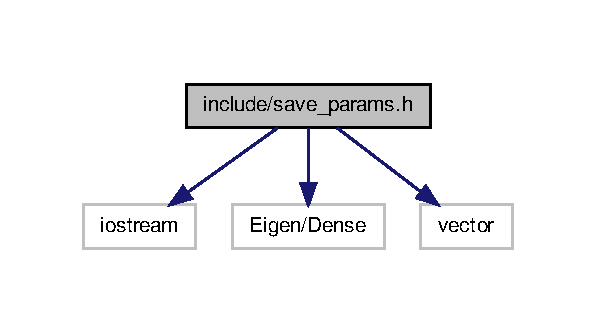
\includegraphics[width=286pt]{include_2save__params_8h__incl}
\end{center}
\end{figure}
\-This graph shows which files directly or indirectly include this file\-:
\nopagebreak
\begin{figure}[H]
\begin{center}
\leavevmode
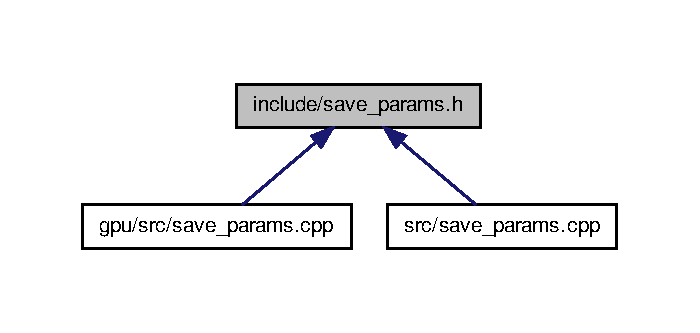
\includegraphics[width=336pt]{include_2save__params_8h__dep__incl}
\end{center}
\end{figure}
\subsection*{\-Namespaces}
\begin{DoxyCompactItemize}
\item 
namespace \hyperlink{namespacelibcnn}{libcnn}
\end{DoxyCompactItemize}
\subsection*{\-Functions}
\begin{DoxyCompactItemize}
\item 
void \hyperlink{namespacelibcnn_a35fa40f645f5fe20b4cc8d878b1e0c10}{libcnn\-::print\-\_\-params} (vector$<$ vector$<$ \-Matrix\-Xd $>$ $>$ \&, vector$<$ \-Matrix\-Xd $>$ \&, vector$<$ \-Matrix\-Xd $>$ \&, vector$<$ \-Matrix\-Xd $>$ \&, vector$<$ \-Matrix\-Xd $>$ \&, \-Matrix\-Xd \&, \-Matrix\-Xd \&, \-Matrix\-Xd \&, \-Matrix\-Xd \&, \-Matrix\-Xd \&)
\end{DoxyCompactItemize}

\hypertarget{gpu_2include_2softmax__class_8h}{\section{gpu/include/softmax\-\_\-class.h \-File \-Reference}
\label{gpu_2include_2softmax__class_8h}\index{gpu/include/softmax\-\_\-class.\-h@{gpu/include/softmax\-\_\-class.\-h}}
}
{\ttfamily \#include $<$iostream$>$}\*
{\ttfamily \#include $<$stdlib.\-h$>$}\*
{\ttfamily \#include $<$\-Eigen/\-Dense$>$}\*
{\ttfamily \#include $<$math.\-h$>$}\*
\-Include dependency graph for softmax\-\_\-class.\-h\-:
\nopagebreak
\begin{figure}[H]
\begin{center}
\leavevmode
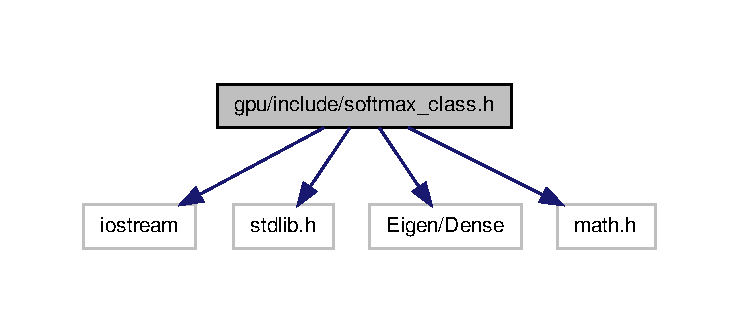
\includegraphics[width=350pt]{gpu_2include_2softmax__class_8h__incl}
\end{center}
\end{figure}
\subsection*{\-Classes}
\begin{DoxyCompactItemize}
\item 
class \hyperlink{classlibcnn_1_1_softmax}{libcnn\-::\-Softmax}
\end{DoxyCompactItemize}
\subsection*{\-Namespaces}
\begin{DoxyCompactItemize}
\item 
namespace \hyperlink{namespacelibcnn}{libcnn}
\end{DoxyCompactItemize}

\hypertarget{include_2softmax__class_8h}{\section{include/softmax\-\_\-class.h \-File \-Reference}
\label{include_2softmax__class_8h}\index{include/softmax\-\_\-class.\-h@{include/softmax\-\_\-class.\-h}}
}
{\ttfamily \#include $<$iostream$>$}\*
{\ttfamily \#include $<$stdlib.\-h$>$}\*
{\ttfamily \#include $<$\-Eigen/\-Dense$>$}\*
{\ttfamily \#include $<$math.\-h$>$}\*
\-Include dependency graph for softmax\-\_\-class.\-h\-:
\nopagebreak
\begin{figure}[H]
\begin{center}
\leavevmode
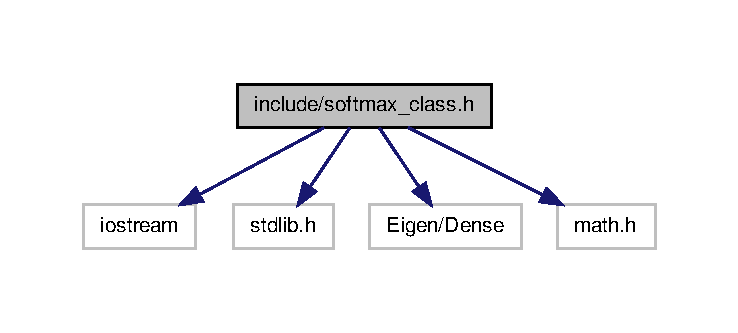
\includegraphics[width=350pt]{include_2softmax__class_8h__incl}
\end{center}
\end{figure}
\-This graph shows which files directly or indirectly include this file\-:
\nopagebreak
\begin{figure}[H]
\begin{center}
\leavevmode
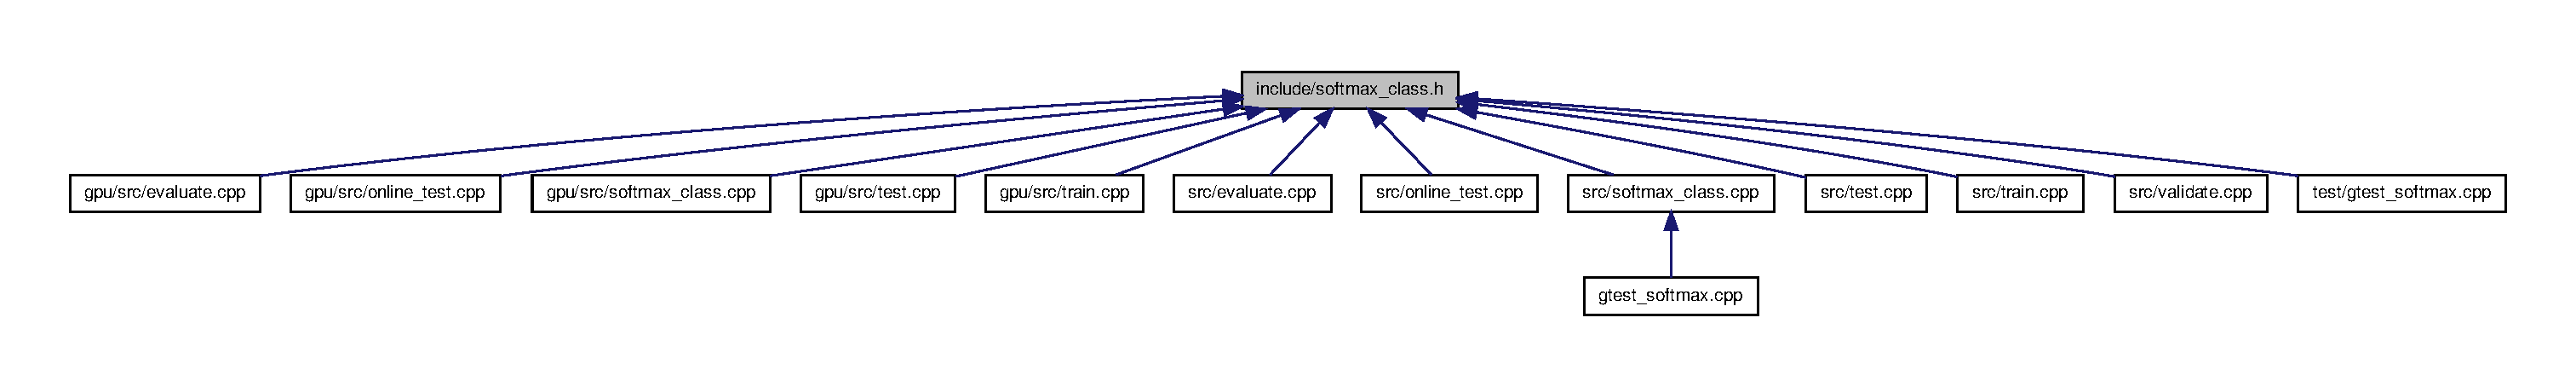
\includegraphics[width=350pt]{include_2softmax__class_8h__dep__incl}
\end{center}
\end{figure}
\subsection*{\-Classes}
\begin{DoxyCompactItemize}
\item 
class \hyperlink{classlibcnn_1_1_softmax}{libcnn\-::\-Softmax}
\end{DoxyCompactItemize}
\subsection*{\-Namespaces}
\begin{DoxyCompactItemize}
\item 
namespace \hyperlink{namespacelibcnn}{libcnn}
\end{DoxyCompactItemize}

\hypertarget{gpu_2src_2conv__layer_8cpp}{\section{gpu/src/conv\-\_\-layer.cpp \-File \-Reference}
\label{gpu_2src_2conv__layer_8cpp}\index{gpu/src/conv\-\_\-layer.\-cpp@{gpu/src/conv\-\_\-layer.\-cpp}}
}
{\ttfamily \#include \char`\"{}conv\-\_\-layer.\-h\char`\"{}}\*
{\ttfamily \#include $<$\-Eigen/\-Dense$>$}\*
{\ttfamily \#include $<$iostream$>$}\*
{\ttfamily \#include $<$vector$>$}\*
{\ttfamily \#include $<$cmath$>$}\*
{\ttfamily \#include $<$ctime$>$}\*
{\ttfamily \#include $<$string$>$}\*
{\ttfamily \#include $<$stdexcept$>$}\*
{\ttfamily \#include $<$sys/time.\-h$>$}\*
{\ttfamily \#include $<$omp.\-h$>$}\*
\-Include dependency graph for conv\-\_\-layer.\-cpp\-:
\nopagebreak
\begin{figure}[H]
\begin{center}
\leavevmode
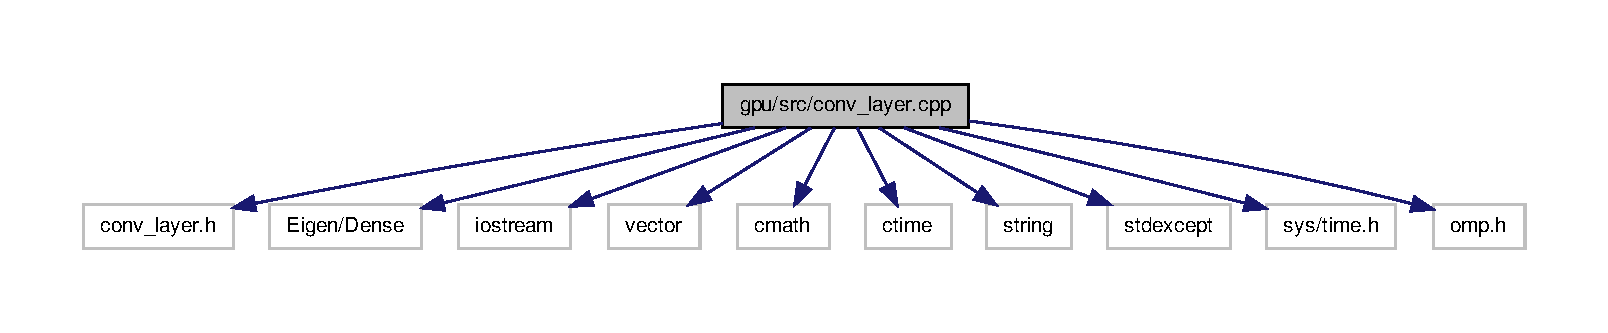
\includegraphics[width=350pt]{gpu_2src_2conv__layer_8cpp__incl}
\end{center}
\end{figure}
\subsection*{\-Namespaces}
\begin{DoxyCompactItemize}
\item 
namespace \hyperlink{namespacelibcnn}{libcnn}
\end{DoxyCompactItemize}
\subsection*{\-Functions}
\begin{DoxyCompactItemize}
\item 
void \hyperlink{namespacelibcnn_a55bbe6e5488b8a038e5708a32d233090}{libcnn\-::get\-\_\-feature\-\_\-vector} (const vector$<$ vector$<$ \-Matrix\-Xd $>$ $>$ \&, \-Matrix\-Xd \&)
\item 
void \hyperlink{namespacelibcnn_a78ed8e63be87c4d06bb363af95ce62ec}{libcnn\-::softmax2conv} (const \-Matrix\-Xd \&, const int \&, const int \&, const int \&, vector$<$ vector$<$ \-Matrix\-Xd $>$ $>$ \&)
\end{DoxyCompactItemize}

\hypertarget{src_2conv__layer_8cpp}{\section{src/conv\-\_\-layer.cpp \-File \-Reference}
\label{src_2conv__layer_8cpp}\index{src/conv\-\_\-layer.\-cpp@{src/conv\-\_\-layer.\-cpp}}
}
{\ttfamily \#include \char`\"{}conv\-\_\-layer.\-h\char`\"{}}\*
{\ttfamily \#include $<$\-Eigen/\-Dense$>$}\*
{\ttfamily \#include $<$iostream$>$}\*
{\ttfamily \#include $<$vector$>$}\*
{\ttfamily \#include $<$cmath$>$}\*
{\ttfamily \#include $<$ctime$>$}\*
{\ttfamily \#include $<$string$>$}\*
{\ttfamily \#include $<$stdexcept$>$}\*
{\ttfamily \#include $<$sys/time.\-h$>$}\*
{\ttfamily \#include $<$omp.\-h$>$}\*
\-Include dependency graph for conv\-\_\-layer.\-cpp\-:
\nopagebreak
\begin{figure}[H]
\begin{center}
\leavevmode
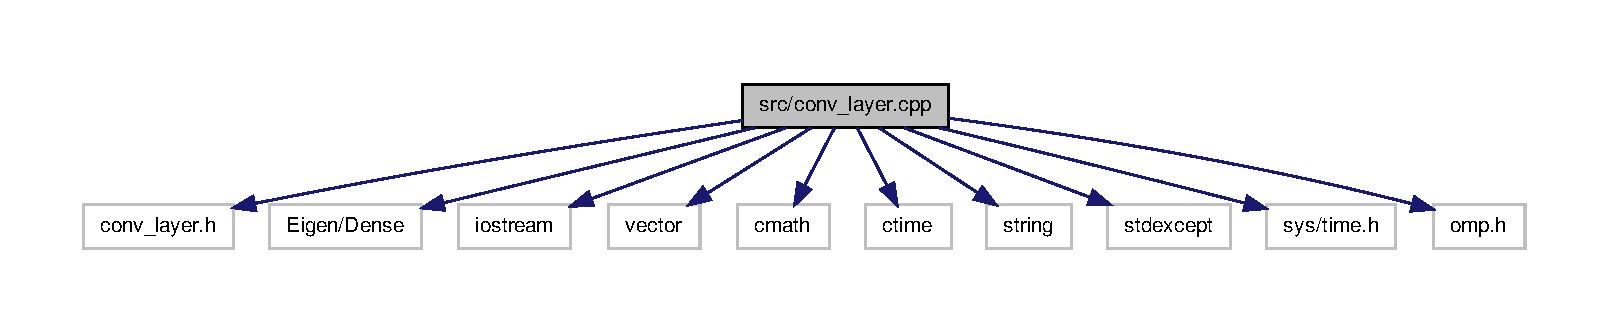
\includegraphics[width=350pt]{src_2conv__layer_8cpp__incl}
\end{center}
\end{figure}
\subsection*{\-Namespaces}
\begin{DoxyCompactItemize}
\item 
namespace \hyperlink{namespacelibcnn}{libcnn}
\end{DoxyCompactItemize}
\subsection*{\-Functions}
\begin{DoxyCompactItemize}
\item 
void \hyperlink{namespacelibcnn_a55bbe6e5488b8a038e5708a32d233090}{libcnn\-::get\-\_\-feature\-\_\-vector} (const vector$<$ vector$<$ \-Matrix\-Xd $>$ $>$ \&, \-Matrix\-Xd \&)
\item 
void \hyperlink{namespacelibcnn_a78ed8e63be87c4d06bb363af95ce62ec}{libcnn\-::softmax2conv} (const \-Matrix\-Xd \&, const int \&, const int \&, const int \&, vector$<$ vector$<$ \-Matrix\-Xd $>$ $>$ \&)
\end{DoxyCompactItemize}

\hypertarget{gpu_2src_2evaluate_8cpp}{\section{gpu/src/evaluate.cpp \-File \-Reference}
\label{gpu_2src_2evaluate_8cpp}\index{gpu/src/evaluate.\-cpp@{gpu/src/evaluate.\-cpp}}
}
{\ttfamily \#include $<$iostream$>$}\*
{\ttfamily \#include $<$\-Eigen/\-Dense$>$}\*
{\ttfamily \#include $<$vector$>$}\*
{\ttfamily \#include $<$fstream$>$}\*
{\ttfamily \#include $<$string$>$}\*
{\ttfamily \#include \char`\"{}conv\-\_\-layer.\-h\char`\"{}}\*
{\ttfamily \#include \char`\"{}softmax\-\_\-class.\-h\char`\"{}}\*
{\ttfamily \#include \char`\"{}pool.\-h\char`\"{}}\*
{\ttfamily \#include \char`\"{}load\-\_\-data.\-h\char`\"{}}\*
\-Include dependency graph for evaluate.\-cpp\-:
\nopagebreak
\begin{figure}[H]
\begin{center}
\leavevmode
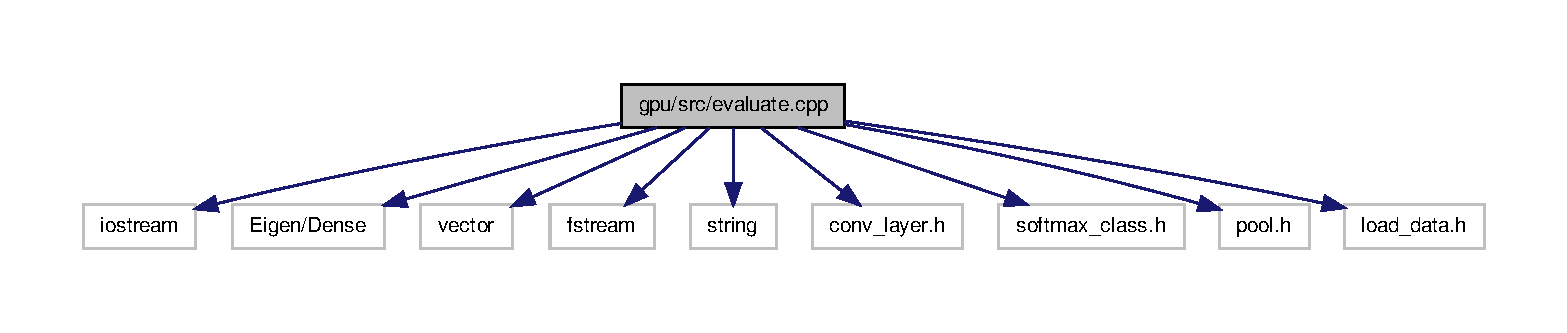
\includegraphics[width=350pt]{gpu_2src_2evaluate_8cpp__incl}
\end{center}
\end{figure}
\subsection*{\-Functions}
\begin{DoxyCompactItemize}
\item 
void \hyperlink{gpu_2src_2evaluate_8cpp_a640eb3c435abcfe65e13558fc738b915}{evaluate} ()
\item 
int \hyperlink{gpu_2src_2evaluate_8cpp_ae66f6b31b5ad750f1fe042a706a4e3d4}{main} ()
\end{DoxyCompactItemize}


\subsection{\-Function \-Documentation}
\hypertarget{gpu_2src_2evaluate_8cpp_a640eb3c435abcfe65e13558fc738b915}{\index{gpu/src/evaluate.\-cpp@{gpu/src/evaluate.\-cpp}!evaluate@{evaluate}}
\index{evaluate@{evaluate}!gpu/src/evaluate.cpp@{gpu/src/evaluate.\-cpp}}
\subsubsection[{evaluate}]{\setlength{\rightskip}{0pt plus 5cm}void {\bf evaluate} (
\begin{DoxyParamCaption}
{}
\end{DoxyParamCaption}
)}}\label{gpu_2src_2evaluate_8cpp_a640eb3c435abcfe65e13558fc738b915}
\hypertarget{gpu_2src_2evaluate_8cpp_ae66f6b31b5ad750f1fe042a706a4e3d4}{\index{gpu/src/evaluate.\-cpp@{gpu/src/evaluate.\-cpp}!main@{main}}
\index{main@{main}!gpu/src/evaluate.cpp@{gpu/src/evaluate.\-cpp}}
\subsubsection[{main}]{\setlength{\rightskip}{0pt plus 5cm}int {\bf main} (
\begin{DoxyParamCaption}
{}
\end{DoxyParamCaption}
)}}\label{gpu_2src_2evaluate_8cpp_ae66f6b31b5ad750f1fe042a706a4e3d4}


\-Here is the call graph for this function\-:
\nopagebreak
\begin{figure}[H]
\begin{center}
\leavevmode
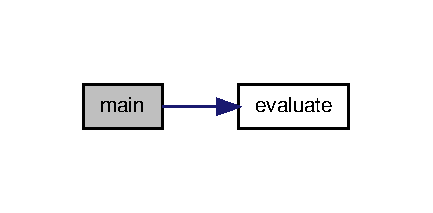
\includegraphics[width=208pt]{gpu_2src_2evaluate_8cpp_ae66f6b31b5ad750f1fe042a706a4e3d4_cgraph}
\end{center}
\end{figure}



\hypertarget{src_2evaluate_8cpp}{\section{src/evaluate.cpp \-File \-Reference}
\label{src_2evaluate_8cpp}\index{src/evaluate.\-cpp@{src/evaluate.\-cpp}}
}
{\ttfamily \#include $<$iostream$>$}\*
{\ttfamily \#include $<$\-Eigen/\-Dense$>$}\*
{\ttfamily \#include $<$vector$>$}\*
{\ttfamily \#include $<$fstream$>$}\*
{\ttfamily \#include $<$string$>$}\*
{\ttfamily \#include \char`\"{}conv\-\_\-layer.\-h\char`\"{}}\*
{\ttfamily \#include \char`\"{}softmax\-\_\-class.\-h\char`\"{}}\*
{\ttfamily \#include \char`\"{}pool.\-h\char`\"{}}\*
{\ttfamily \#include \char`\"{}load\-\_\-data.\-h\char`\"{}}\*
\-Include dependency graph for evaluate.\-cpp\-:
\nopagebreak
\begin{figure}[H]
\begin{center}
\leavevmode
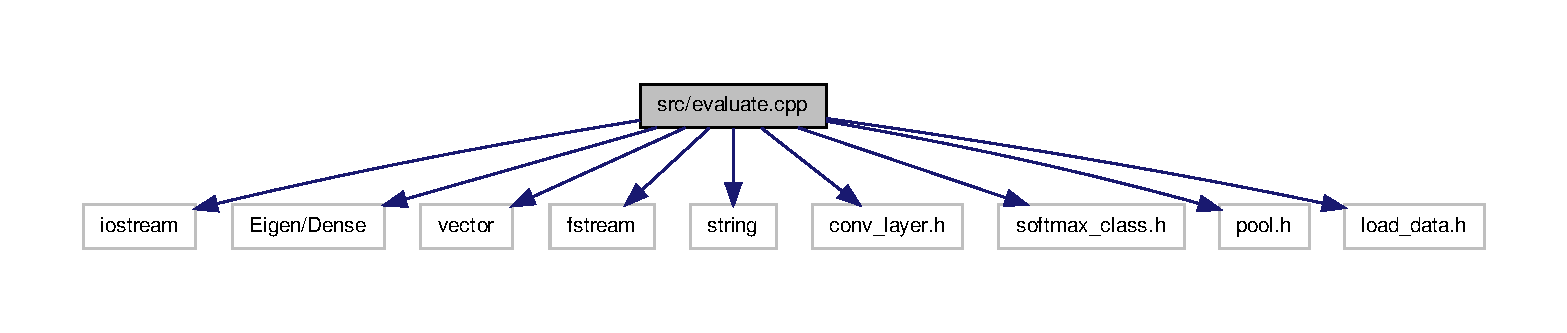
\includegraphics[width=350pt]{src_2evaluate_8cpp__incl}
\end{center}
\end{figure}
\subsection*{\-Functions}
\begin{DoxyCompactItemize}
\item 
void \hyperlink{src_2evaluate_8cpp_a640eb3c435abcfe65e13558fc738b915}{evaluate} ()
\item 
int \hyperlink{src_2evaluate_8cpp_ae66f6b31b5ad750f1fe042a706a4e3d4}{main} ()
\end{DoxyCompactItemize}


\subsection{\-Function \-Documentation}
\hypertarget{src_2evaluate_8cpp_a640eb3c435abcfe65e13558fc738b915}{\index{src/evaluate.\-cpp@{src/evaluate.\-cpp}!evaluate@{evaluate}}
\index{evaluate@{evaluate}!src/evaluate.cpp@{src/evaluate.\-cpp}}
\subsubsection[{evaluate}]{\setlength{\rightskip}{0pt plus 5cm}void {\bf evaluate} (
\begin{DoxyParamCaption}
{}
\end{DoxyParamCaption}
)}}\label{src_2evaluate_8cpp_a640eb3c435abcfe65e13558fc738b915}
\hypertarget{src_2evaluate_8cpp_ae66f6b31b5ad750f1fe042a706a4e3d4}{\index{src/evaluate.\-cpp@{src/evaluate.\-cpp}!main@{main}}
\index{main@{main}!src/evaluate.cpp@{src/evaluate.\-cpp}}
\subsubsection[{main}]{\setlength{\rightskip}{0pt plus 5cm}int {\bf main} (
\begin{DoxyParamCaption}
{}
\end{DoxyParamCaption}
)}}\label{src_2evaluate_8cpp_ae66f6b31b5ad750f1fe042a706a4e3d4}


\-Here is the call graph for this function\-:
\nopagebreak
\begin{figure}[H]
\begin{center}
\leavevmode
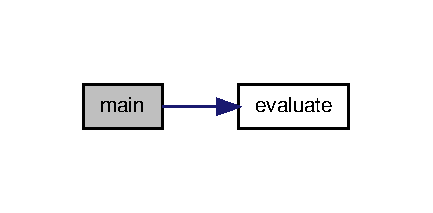
\includegraphics[width=208pt]{src_2evaluate_8cpp_ae66f6b31b5ad750f1fe042a706a4e3d4_cgraph}
\end{center}
\end{figure}



\hypertarget{gpu_2src_2init__params_8cpp}{\section{gpu/src/init\-\_\-params.cpp \-File \-Reference}
\label{gpu_2src_2init__params_8cpp}\index{gpu/src/init\-\_\-params.\-cpp@{gpu/src/init\-\_\-params.\-cpp}}
}
{\ttfamily \#include $<$iostream$>$}\*
{\ttfamily \#include $<$fstream$>$}\*
{\ttfamily \#include $<$string$>$}\*
{\ttfamily \#include $<$vector$>$}\*
{\ttfamily \#include $<$\-Eigen/\-Dense$>$}\*
{\ttfamily \#include $<$sstream$>$}\*
{\ttfamily \#include \char`\"{}init\-\_\-params.\-h\char`\"{}}\*
\-Include dependency graph for init\-\_\-params.\-cpp\-:
\nopagebreak
\begin{figure}[H]
\begin{center}
\leavevmode
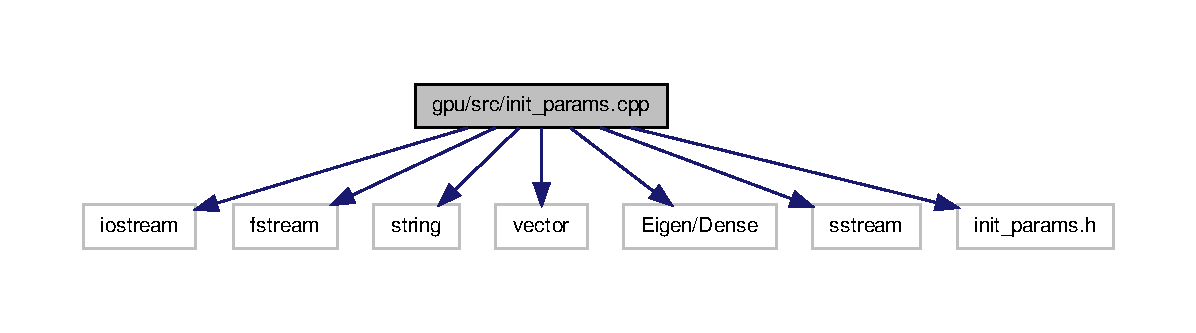
\includegraphics[width=350pt]{gpu_2src_2init__params_8cpp__incl}
\end{center}
\end{figure}
\subsection*{\-Namespaces}
\begin{DoxyCompactItemize}
\item 
namespace \hyperlink{namespacelibcnn}{libcnn}
\end{DoxyCompactItemize}
\subsection*{\-Defines}
\begin{DoxyCompactItemize}
\item 
\#define \hyperlink{gpu_2src_2init__params_8cpp_aae9a32fb4ed60a2b23dd7eca52e8e627}{\-K\-E\-R\-N\-E\-L\-\_\-\-S\-I\-Z\-E}~7
\end{DoxyCompactItemize}
\subsection*{\-Functions}
\begin{DoxyCompactItemize}
\item 
void \hyperlink{namespacelibcnn_a2c5ccad2e675235e71fd5e5641ede4ae}{libcnn\-::get\-\_\-parameter} (vector$<$ \-Matrix\-Xd $>$ \&)
\end{DoxyCompactItemize}


\subsection{\-Define \-Documentation}
\hypertarget{gpu_2src_2init__params_8cpp_aae9a32fb4ed60a2b23dd7eca52e8e627}{\index{gpu/src/init\-\_\-params.\-cpp@{gpu/src/init\-\_\-params.\-cpp}!\-K\-E\-R\-N\-E\-L\-\_\-\-S\-I\-Z\-E@{\-K\-E\-R\-N\-E\-L\-\_\-\-S\-I\-Z\-E}}
\index{\-K\-E\-R\-N\-E\-L\-\_\-\-S\-I\-Z\-E@{\-K\-E\-R\-N\-E\-L\-\_\-\-S\-I\-Z\-E}!gpu/src/init_params.cpp@{gpu/src/init\-\_\-params.\-cpp}}
\subsubsection[{\-K\-E\-R\-N\-E\-L\-\_\-\-S\-I\-Z\-E}]{\setlength{\rightskip}{0pt plus 5cm}\#define {\bf \-K\-E\-R\-N\-E\-L\-\_\-\-S\-I\-Z\-E}~7}}\label{gpu_2src_2init__params_8cpp_aae9a32fb4ed60a2b23dd7eca52e8e627}

\hypertarget{src_2init__params_8cpp}{\section{src/init\-\_\-params.cpp \-File \-Reference}
\label{src_2init__params_8cpp}\index{src/init\-\_\-params.\-cpp@{src/init\-\_\-params.\-cpp}}
}
{\ttfamily \#include $<$iostream$>$}\*
{\ttfamily \#include $<$fstream$>$}\*
{\ttfamily \#include $<$string$>$}\*
{\ttfamily \#include $<$vector$>$}\*
{\ttfamily \#include $<$\-Eigen/\-Dense$>$}\*
{\ttfamily \#include $<$sstream$>$}\*
{\ttfamily \#include \char`\"{}init\-\_\-params.\-h\char`\"{}}\*
\-Include dependency graph for init\-\_\-params.\-cpp\-:
\nopagebreak
\begin{figure}[H]
\begin{center}
\leavevmode
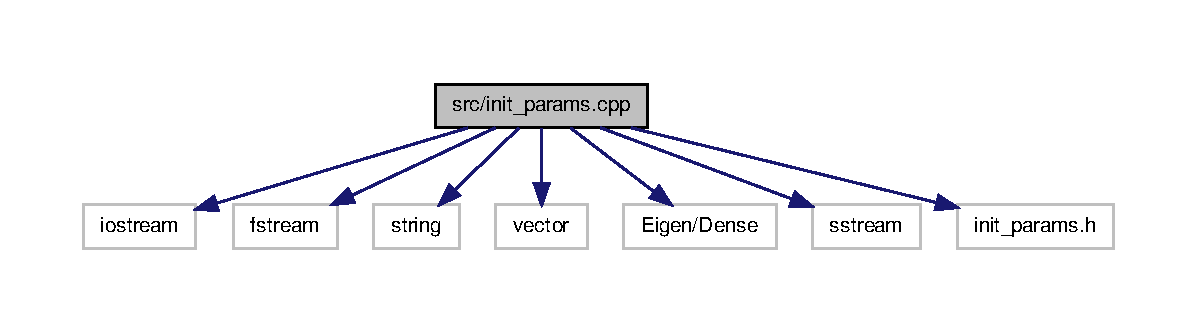
\includegraphics[width=350pt]{src_2init__params_8cpp__incl}
\end{center}
\end{figure}
\subsection*{\-Namespaces}
\begin{DoxyCompactItemize}
\item 
namespace \hyperlink{namespacelibcnn}{libcnn}
\end{DoxyCompactItemize}
\subsection*{\-Defines}
\begin{DoxyCompactItemize}
\item 
\#define \hyperlink{src_2init__params_8cpp_aae9a32fb4ed60a2b23dd7eca52e8e627}{\-K\-E\-R\-N\-E\-L\-\_\-\-S\-I\-Z\-E}~7
\end{DoxyCompactItemize}
\subsection*{\-Functions}
\begin{DoxyCompactItemize}
\item 
void \hyperlink{namespacelibcnn_a2c5ccad2e675235e71fd5e5641ede4ae}{libcnn\-::get\-\_\-parameter} (vector$<$ \-Matrix\-Xd $>$ \&)
\end{DoxyCompactItemize}


\subsection{\-Define \-Documentation}
\hypertarget{src_2init__params_8cpp_aae9a32fb4ed60a2b23dd7eca52e8e627}{\index{src/init\-\_\-params.\-cpp@{src/init\-\_\-params.\-cpp}!\-K\-E\-R\-N\-E\-L\-\_\-\-S\-I\-Z\-E@{\-K\-E\-R\-N\-E\-L\-\_\-\-S\-I\-Z\-E}}
\index{\-K\-E\-R\-N\-E\-L\-\_\-\-S\-I\-Z\-E@{\-K\-E\-R\-N\-E\-L\-\_\-\-S\-I\-Z\-E}!src/init_params.cpp@{src/init\-\_\-params.\-cpp}}
\subsubsection[{\-K\-E\-R\-N\-E\-L\-\_\-\-S\-I\-Z\-E}]{\setlength{\rightskip}{0pt plus 5cm}\#define {\bf \-K\-E\-R\-N\-E\-L\-\_\-\-S\-I\-Z\-E}~7}}\label{src_2init__params_8cpp_aae9a32fb4ed60a2b23dd7eca52e8e627}

\hypertarget{gpu_2src_2load__data_8cpp}{\section{gpu/src/load\-\_\-data.cpp \-File \-Reference}
\label{gpu_2src_2load__data_8cpp}\index{gpu/src/load\-\_\-data.\-cpp@{gpu/src/load\-\_\-data.\-cpp}}
}
{\ttfamily \#include $<$sys/types.\-h$>$}\*
{\ttfamily \#include $<$dirent.\-h$>$}\*
{\ttfamily \#include $<$errno.\-h$>$}\*
{\ttfamily \#include $<$vector$>$}\*
{\ttfamily \#include $<$string.\-h$>$}\*
{\ttfamily \#include $<$iostream$>$}\*
{\ttfamily \#include $<$stdlib.\-h$>$}\*
{\ttfamily \#include $<$fstream$>$}\*
{\ttfamily \#include $<$\-Eigen/\-Dense$>$}\*
{\ttfamily \#include $<$cassert$>$}\*
{\ttfamily \#include $<$algorithm$>$}\*
{\ttfamily \#include $<$string$>$}\*
\-Include dependency graph for load\-\_\-data.\-cpp\-:
\nopagebreak
\begin{figure}[H]
\begin{center}
\leavevmode
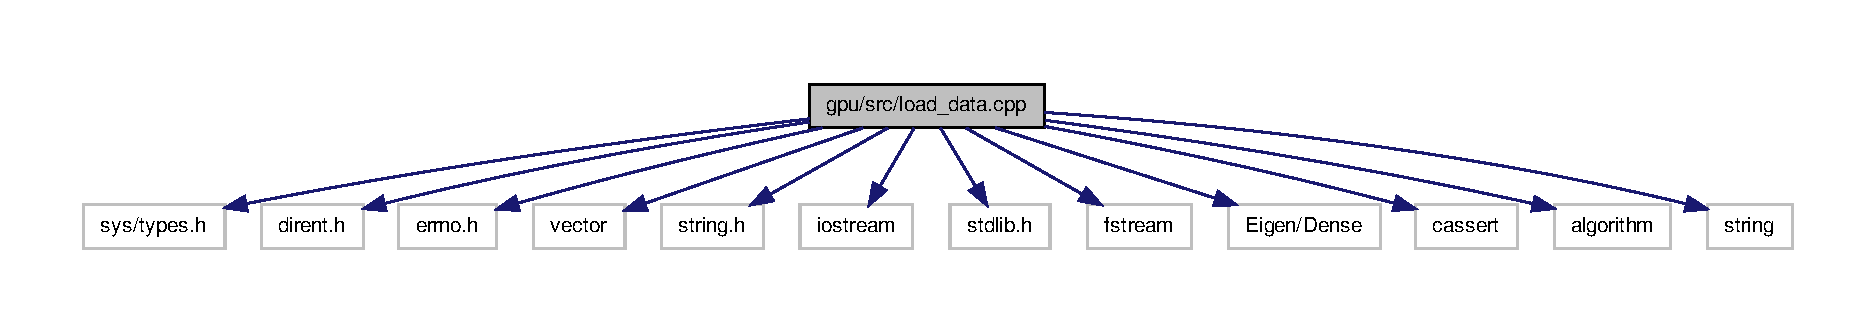
\includegraphics[width=350pt]{gpu_2src_2load__data_8cpp__incl}
\end{center}
\end{figure}
\subsection*{\-Functions}
\begin{DoxyCompactItemize}
\item 
void \hyperlink{gpu_2src_2load__data_8cpp_afbad2e91730f993e296f166a8f89aa9b}{getdir} (const string \&\hyperlink{yaml__t__load_8cpp_a7f01c047eb310166e695d4232ebd1fae}{dir}, vector$<$ string $>$ \&files)
\item 
void \hyperlink{gpu_2src_2load__data_8cpp_a39a205061173088b2222b1d550a8787c}{read\-\_\-image\-\_\-files} (const string \&\hyperlink{yaml__t__load_8cpp_a7f01c047eb310166e695d4232ebd1fae}{dir}, std\-::vector$<$ vector$<$ \-Matrix\-Xd $>$ $>$ \&vvm, const int \&image\-\_\-row\-\_\-dim, const int \&image\-\_\-col\-\_\-dim, const int \&start, const int \&image\-\_\-number)
\item 
void \hyperlink{gpu_2src_2load__data_8cpp_a8f84dc0bbc3acab545f50ce4899348e3}{read\-\_\-label\-\_\-files} (const string \&\hyperlink{yaml__t__load_8cpp_a7f01c047eb310166e695d4232ebd1fae}{dir}, \-Vector\-Xi \&m, const int \&image\-\_\-row\-\_\-dim, const int \&image\-\_\-col\-\_\-dim, const int \&start, const int \&image\-\_\-number, const string \&data\-\_\-mode)
\item 
void \hyperlink{gpu_2src_2load__data_8cpp_ac599c564730d396dcd8eaf64c9878dcf}{read\-\_\-markov\-\_\-files} (const string \&dir\-\_\-name, \-Matrix\-Xd \&markov)
\end{DoxyCompactItemize}


\subsection{\-Function \-Documentation}
\hypertarget{gpu_2src_2load__data_8cpp_afbad2e91730f993e296f166a8f89aa9b}{\index{gpu/src/load\-\_\-data.\-cpp@{gpu/src/load\-\_\-data.\-cpp}!getdir@{getdir}}
\index{getdir@{getdir}!gpu/src/load_data.cpp@{gpu/src/load\-\_\-data.\-cpp}}
\subsubsection[{getdir}]{\setlength{\rightskip}{0pt plus 5cm}void {\bf getdir} (
\begin{DoxyParamCaption}
\item[{const string \&}]{dir, }
\item[{vector$<$ string $>$ \&}]{files}
\end{DoxyParamCaption}
)}}\label{gpu_2src_2load__data_8cpp_afbad2e91730f993e296f166a8f89aa9b}
\hypertarget{gpu_2src_2load__data_8cpp_a39a205061173088b2222b1d550a8787c}{\index{gpu/src/load\-\_\-data.\-cpp@{gpu/src/load\-\_\-data.\-cpp}!read\-\_\-image\-\_\-files@{read\-\_\-image\-\_\-files}}
\index{read\-\_\-image\-\_\-files@{read\-\_\-image\-\_\-files}!gpu/src/load_data.cpp@{gpu/src/load\-\_\-data.\-cpp}}
\subsubsection[{read\-\_\-image\-\_\-files}]{\setlength{\rightskip}{0pt plus 5cm}void {\bf read\-\_\-image\-\_\-files} (
\begin{DoxyParamCaption}
\item[{const string \&}]{dir, }
\item[{std\-::vector$<$ vector$<$ \-Matrix\-Xd $>$ $>$ \&}]{vvm, }
\item[{const int \&}]{image\-\_\-row\-\_\-dim, }
\item[{const int \&}]{image\-\_\-col\-\_\-dim, }
\item[{const int \&}]{start, }
\item[{const int \&}]{image\-\_\-number}
\end{DoxyParamCaption}
)}}\label{gpu_2src_2load__data_8cpp_a39a205061173088b2222b1d550a8787c}
\hypertarget{gpu_2src_2load__data_8cpp_a8f84dc0bbc3acab545f50ce4899348e3}{\index{gpu/src/load\-\_\-data.\-cpp@{gpu/src/load\-\_\-data.\-cpp}!read\-\_\-label\-\_\-files@{read\-\_\-label\-\_\-files}}
\index{read\-\_\-label\-\_\-files@{read\-\_\-label\-\_\-files}!gpu/src/load_data.cpp@{gpu/src/load\-\_\-data.\-cpp}}
\subsubsection[{read\-\_\-label\-\_\-files}]{\setlength{\rightskip}{0pt plus 5cm}void {\bf read\-\_\-label\-\_\-files} (
\begin{DoxyParamCaption}
\item[{const string \&}]{dir, }
\item[{\-Vector\-Xi \&}]{m, }
\item[{const int \&}]{image\-\_\-row\-\_\-dim, }
\item[{const int \&}]{image\-\_\-col\-\_\-dim, }
\item[{const int \&}]{start, }
\item[{const int \&}]{image\-\_\-number, }
\item[{const string \&}]{data\-\_\-mode}
\end{DoxyParamCaption}
)}}\label{gpu_2src_2load__data_8cpp_a8f84dc0bbc3acab545f50ce4899348e3}
\hypertarget{gpu_2src_2load__data_8cpp_ac599c564730d396dcd8eaf64c9878dcf}{\index{gpu/src/load\-\_\-data.\-cpp@{gpu/src/load\-\_\-data.\-cpp}!read\-\_\-markov\-\_\-files@{read\-\_\-markov\-\_\-files}}
\index{read\-\_\-markov\-\_\-files@{read\-\_\-markov\-\_\-files}!gpu/src/load_data.cpp@{gpu/src/load\-\_\-data.\-cpp}}
\subsubsection[{read\-\_\-markov\-\_\-files}]{\setlength{\rightskip}{0pt plus 5cm}void {\bf read\-\_\-markov\-\_\-files} (
\begin{DoxyParamCaption}
\item[{const string \&}]{dir\-\_\-name, }
\item[{\-Matrix\-Xd \&}]{markov}
\end{DoxyParamCaption}
)}}\label{gpu_2src_2load__data_8cpp_ac599c564730d396dcd8eaf64c9878dcf}

\hypertarget{src_2load__data_8cpp}{\section{src/load\-\_\-data.cpp \-File \-Reference}
\label{src_2load__data_8cpp}\index{src/load\-\_\-data.\-cpp@{src/load\-\_\-data.\-cpp}}
}
{\ttfamily \#include $<$sys/types.\-h$>$}\*
{\ttfamily \#include $<$dirent.\-h$>$}\*
{\ttfamily \#include $<$errno.\-h$>$}\*
{\ttfamily \#include $<$vector$>$}\*
{\ttfamily \#include $<$string.\-h$>$}\*
{\ttfamily \#include $<$iostream$>$}\*
{\ttfamily \#include $<$stdlib.\-h$>$}\*
{\ttfamily \#include $<$fstream$>$}\*
{\ttfamily \#include $<$\-Eigen/\-Dense$>$}\*
{\ttfamily \#include $<$cassert$>$}\*
{\ttfamily \#include $<$algorithm$>$}\*
{\ttfamily \#include $<$string$>$}\*
\-Include dependency graph for load\-\_\-data.\-cpp\-:
\nopagebreak
\begin{figure}[H]
\begin{center}
\leavevmode
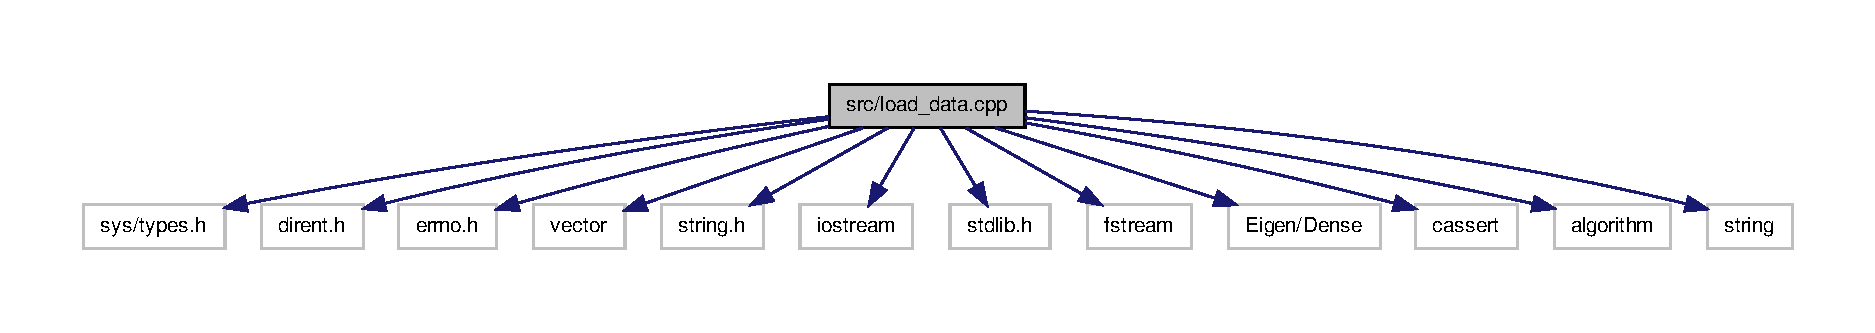
\includegraphics[width=350pt]{src_2load__data_8cpp__incl}
\end{center}
\end{figure}
\subsection*{\-Functions}
\begin{DoxyCompactItemize}
\item 
void \hyperlink{src_2load__data_8cpp_afbad2e91730f993e296f166a8f89aa9b}{getdir} (const string \&\hyperlink{yaml__t__load_8cpp_a7f01c047eb310166e695d4232ebd1fae}{dir}, vector$<$ string $>$ \&files)
\item 
void \hyperlink{src_2load__data_8cpp_a39a205061173088b2222b1d550a8787c}{read\-\_\-image\-\_\-files} (const string \&\hyperlink{yaml__t__load_8cpp_a7f01c047eb310166e695d4232ebd1fae}{dir}, std\-::vector$<$ vector$<$ \-Matrix\-Xd $>$ $>$ \&vvm, const int \&image\-\_\-row\-\_\-dim, const int \&image\-\_\-col\-\_\-dim, const int \&start, const int \&image\-\_\-number)
\item 
void \hyperlink{src_2load__data_8cpp_a8f84dc0bbc3acab545f50ce4899348e3}{read\-\_\-label\-\_\-files} (const string \&\hyperlink{yaml__t__load_8cpp_a7f01c047eb310166e695d4232ebd1fae}{dir}, \-Vector\-Xi \&m, const int \&image\-\_\-row\-\_\-dim, const int \&image\-\_\-col\-\_\-dim, const int \&start, const int \&image\-\_\-number, const string \&data\-\_\-mode)
\item 
void \hyperlink{src_2load__data_8cpp_ac599c564730d396dcd8eaf64c9878dcf}{read\-\_\-markov\-\_\-files} (const string \&dir\-\_\-name, \-Matrix\-Xd \&markov)
\end{DoxyCompactItemize}


\subsection{\-Function \-Documentation}
\hypertarget{src_2load__data_8cpp_afbad2e91730f993e296f166a8f89aa9b}{\index{src/load\-\_\-data.\-cpp@{src/load\-\_\-data.\-cpp}!getdir@{getdir}}
\index{getdir@{getdir}!src/load_data.cpp@{src/load\-\_\-data.\-cpp}}
\subsubsection[{getdir}]{\setlength{\rightskip}{0pt plus 5cm}void {\bf getdir} (
\begin{DoxyParamCaption}
\item[{const string \&}]{dir, }
\item[{vector$<$ string $>$ \&}]{files}
\end{DoxyParamCaption}
)}}\label{src_2load__data_8cpp_afbad2e91730f993e296f166a8f89aa9b}
\hypertarget{src_2load__data_8cpp_a39a205061173088b2222b1d550a8787c}{\index{src/load\-\_\-data.\-cpp@{src/load\-\_\-data.\-cpp}!read\-\_\-image\-\_\-files@{read\-\_\-image\-\_\-files}}
\index{read\-\_\-image\-\_\-files@{read\-\_\-image\-\_\-files}!src/load_data.cpp@{src/load\-\_\-data.\-cpp}}
\subsubsection[{read\-\_\-image\-\_\-files}]{\setlength{\rightskip}{0pt plus 5cm}void {\bf read\-\_\-image\-\_\-files} (
\begin{DoxyParamCaption}
\item[{const string \&}]{dir, }
\item[{std\-::vector$<$ vector$<$ \-Matrix\-Xd $>$ $>$ \&}]{vvm, }
\item[{const int \&}]{image\-\_\-row\-\_\-dim, }
\item[{const int \&}]{image\-\_\-col\-\_\-dim, }
\item[{const int \&}]{start, }
\item[{const int \&}]{image\-\_\-number}
\end{DoxyParamCaption}
)}}\label{src_2load__data_8cpp_a39a205061173088b2222b1d550a8787c}


\-Here is the call graph for this function\-:
\nopagebreak
\begin{figure}[H]
\begin{center}
\leavevmode
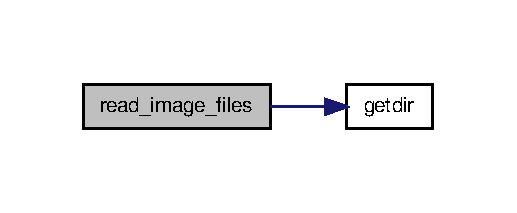
\includegraphics[width=248pt]{src_2load__data_8cpp_a39a205061173088b2222b1d550a8787c_cgraph}
\end{center}
\end{figure}


\hypertarget{src_2load__data_8cpp_a8f84dc0bbc3acab545f50ce4899348e3}{\index{src/load\-\_\-data.\-cpp@{src/load\-\_\-data.\-cpp}!read\-\_\-label\-\_\-files@{read\-\_\-label\-\_\-files}}
\index{read\-\_\-label\-\_\-files@{read\-\_\-label\-\_\-files}!src/load_data.cpp@{src/load\-\_\-data.\-cpp}}
\subsubsection[{read\-\_\-label\-\_\-files}]{\setlength{\rightskip}{0pt plus 5cm}void {\bf read\-\_\-label\-\_\-files} (
\begin{DoxyParamCaption}
\item[{const string \&}]{dir, }
\item[{\-Vector\-Xi \&}]{m, }
\item[{const int \&}]{image\-\_\-row\-\_\-dim, }
\item[{const int \&}]{image\-\_\-col\-\_\-dim, }
\item[{const int \&}]{start, }
\item[{const int \&}]{image\-\_\-number, }
\item[{const string \&}]{data\-\_\-mode}
\end{DoxyParamCaption}
)}}\label{src_2load__data_8cpp_a8f84dc0bbc3acab545f50ce4899348e3}


\-Here is the call graph for this function\-:
\nopagebreak
\begin{figure}[H]
\begin{center}
\leavevmode
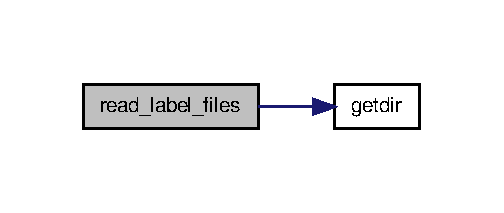
\includegraphics[width=242pt]{src_2load__data_8cpp_a8f84dc0bbc3acab545f50ce4899348e3_cgraph}
\end{center}
\end{figure}


\hypertarget{src_2load__data_8cpp_ac599c564730d396dcd8eaf64c9878dcf}{\index{src/load\-\_\-data.\-cpp@{src/load\-\_\-data.\-cpp}!read\-\_\-markov\-\_\-files@{read\-\_\-markov\-\_\-files}}
\index{read\-\_\-markov\-\_\-files@{read\-\_\-markov\-\_\-files}!src/load_data.cpp@{src/load\-\_\-data.\-cpp}}
\subsubsection[{read\-\_\-markov\-\_\-files}]{\setlength{\rightskip}{0pt plus 5cm}void {\bf read\-\_\-markov\-\_\-files} (
\begin{DoxyParamCaption}
\item[{const string \&}]{dir\-\_\-name, }
\item[{\-Matrix\-Xd \&}]{markov}
\end{DoxyParamCaption}
)}}\label{src_2load__data_8cpp_ac599c564730d396dcd8eaf64c9878dcf}

\hypertarget{gpu_2src_2markov__1_8py}{\section{gpu/src/markov\-\_\-1.py \-File \-Reference}
\label{gpu_2src_2markov__1_8py}\index{gpu/src/markov\-\_\-1.\-py@{gpu/src/markov\-\_\-1.\-py}}
}
\subsection*{\-Namespaces}
\begin{DoxyCompactItemize}
\item 
namespace \hyperlink{namespacemarkov__1}{markov\-\_\-1}
\end{DoxyCompactItemize}
\subsection*{\-Variables}
\begin{DoxyCompactItemize}
\item 
float \hyperlink{namespacemarkov__1_a4a3eda3678257ab2cf6f06891c5ec22c}{markov\-\_\-1.\-roe} = 0.\-9999
\item 
list \hyperlink{namespacemarkov__1_ac6e549cf6d4d6df355d884b67fb19851}{markov\-\_\-1.\-roe\-\_\-list} = \mbox{[}$\,$\mbox{]}
\item 
int \hyperlink{namespacemarkov__1_a8134563a0c42390906c8914ad337e9d8}{markov\-\_\-1.\-data\-\_\-dimension} = 64
\item 
tuple \hyperlink{namespacemarkov__1_a7cc4d10a876ec07da21dbfd4d28e8684}{markov\-\_\-1.\-covariance\-\_\-matrix} = toeplitz(roe\-\_\-list, roe\-\_\-list)
\item 
\hyperlink{namespacemarkov__1_a3744683663f02bff5cf245a674ab9b32}{markov\-\_\-1.\-Data\-Out} = e\-\_\-vecs
\end{DoxyCompactItemize}

\hypertarget{src_2markov__1_8py}{\section{src/markov\-\_\-1.py \-File \-Reference}
\label{src_2markov__1_8py}\index{src/markov\-\_\-1.\-py@{src/markov\-\_\-1.\-py}}
}
\subsection*{\-Namespaces}
\begin{DoxyCompactItemize}
\item 
namespace \hyperlink{namespacemarkov__1}{markov\-\_\-1}
\end{DoxyCompactItemize}

\hypertarget{gpu_2src_2online__test_8cpp}{\section{gpu/src/online\-\_\-test.cpp \-File \-Reference}
\label{gpu_2src_2online__test_8cpp}\index{gpu/src/online\-\_\-test.\-cpp@{gpu/src/online\-\_\-test.\-cpp}}
}
{\ttfamily \#include $<$iostream$>$}\*
{\ttfamily \#include $<$\-Eigen/\-Dense$>$}\*
{\ttfamily \#include $<$vector$>$}\*
{\ttfamily \#include \char`\"{}online\-\_\-test.\-h\char`\"{}}\*
{\ttfamily \#include \char`\"{}conv\-\_\-layer.\-h\char`\"{}}\*
{\ttfamily \#include \char`\"{}pool.\-h\char`\"{}}\*
{\ttfamily \#include \char`\"{}softmax\-\_\-class.\-h\char`\"{}}\*
\-Include dependency graph for online\-\_\-test.\-cpp\-:
\nopagebreak
\begin{figure}[H]
\begin{center}
\leavevmode
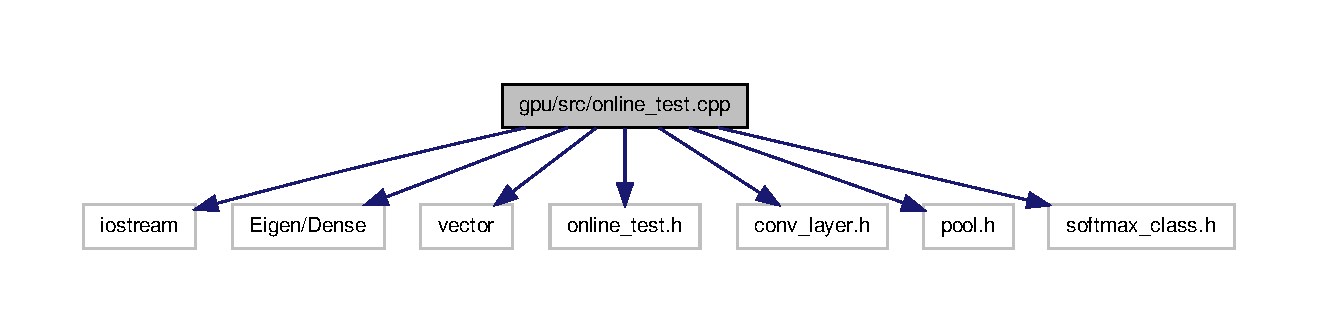
\includegraphics[width=350pt]{gpu_2src_2online__test_8cpp__incl}
\end{center}
\end{figure}
\subsection*{\-Namespaces}
\begin{DoxyCompactItemize}
\item 
namespace \hyperlink{namespacelibcnn}{libcnn}
\end{DoxyCompactItemize}
\subsection*{\-Functions}
\begin{DoxyCompactItemize}
\item 
void \hyperlink{namespacelibcnn_a493fb452cedcc704e189ad1a3656c0ad}{libcnn\-::online\-\_\-test} (const vector$<$ vector$<$ \-Matrix\-Xd $>$ $>$ \&, const \-Vector\-Xi \&, const vector$<$ \-Matrix\-Xd $>$ \&, const \-Matrix\-Xd \&, const vector$<$ \-Matrix\-Xd $>$ \&, const \-Matrix\-Xd \&, const vector$<$ \-Matrix\-Xd $>$ \&, const \-Matrix\-Xd \&, const \-Matrix\-Xd \&, const \-Matrix\-Xd \&, const int \&, const int \&, const int \&, const int \&, const int \&)
\end{DoxyCompactItemize}

\hypertarget{src_2online__test_8cpp}{\section{src/online\-\_\-test.cpp \-File \-Reference}
\label{src_2online__test_8cpp}\index{src/online\-\_\-test.\-cpp@{src/online\-\_\-test.\-cpp}}
}
{\ttfamily \#include $<$iostream$>$}\*
{\ttfamily \#include $<$\-Eigen/\-Dense$>$}\*
{\ttfamily \#include $<$vector$>$}\*
{\ttfamily \#include \char`\"{}online\-\_\-test.\-h\char`\"{}}\*
{\ttfamily \#include \char`\"{}conv\-\_\-layer.\-h\char`\"{}}\*
{\ttfamily \#include \char`\"{}pool.\-h\char`\"{}}\*
{\ttfamily \#include \char`\"{}softmax\-\_\-class.\-h\char`\"{}}\*
\-Include dependency graph for online\-\_\-test.\-cpp\-:
\nopagebreak
\begin{figure}[H]
\begin{center}
\leavevmode
\includegraphics[width=350pt]{src_2online__test_8cpp__incl}
\end{center}
\end{figure}
\subsection*{\-Namespaces}
\begin{DoxyCompactItemize}
\item 
namespace \hyperlink{namespacelibcnn}{libcnn}
\end{DoxyCompactItemize}
\subsection*{\-Functions}
\begin{DoxyCompactItemize}
\item 
void \hyperlink{namespacelibcnn_a493fb452cedcc704e189ad1a3656c0ad}{libcnn\-::online\-\_\-test} (const vector$<$ vector$<$ \-Matrix\-Xd $>$ $>$ \&, const \-Vector\-Xi \&, const vector$<$ \-Matrix\-Xd $>$ \&, const \-Matrix\-Xd \&, const vector$<$ \-Matrix\-Xd $>$ \&, const \-Matrix\-Xd \&, const vector$<$ \-Matrix\-Xd $>$ \&, const \-Matrix\-Xd \&, const \-Matrix\-Xd \&, const \-Matrix\-Xd \&, const int \&, const int \&, const int \&, const int \&, const int \&)
\end{DoxyCompactItemize}

\hypertarget{gpu_2src_2pool_8cpp}{\section{gpu/src/pool.cpp \-File \-Reference}
\label{gpu_2src_2pool_8cpp}\index{gpu/src/pool.\-cpp@{gpu/src/pool.\-cpp}}
}
{\ttfamily \#include $<$iostream$>$}\*
{\ttfamily \#include $<$\-Eigen/\-Dense$>$}\*
{\ttfamily \#include $<$vector$>$}\*
{\ttfamily \#include $<$cmath$>$}\*
{\ttfamily \#include $<$string$>$}\*
{\ttfamily \#include \char`\"{}pool.\-h\char`\"{}}\*
\-Include dependency graph for pool.\-cpp\-:
\nopagebreak
\begin{figure}[H]
\begin{center}
\leavevmode
\includegraphics[width=350pt]{gpu_2src_2pool_8cpp__incl}
\end{center}
\end{figure}
\subsection*{\-Namespaces}
\begin{DoxyCompactItemize}
\item 
namespace \hyperlink{namespacelibcnn}{libcnn}
\end{DoxyCompactItemize}

\hypertarget{src_2pool_8cpp}{\section{src/pool.cpp \-File \-Reference}
\label{src_2pool_8cpp}\index{src/pool.\-cpp@{src/pool.\-cpp}}
}
{\ttfamily \#include $<$iostream$>$}\*
{\ttfamily \#include $<$\-Eigen/\-Dense$>$}\*
{\ttfamily \#include $<$vector$>$}\*
{\ttfamily \#include $<$cmath$>$}\*
{\ttfamily \#include $<$string$>$}\*
{\ttfamily \#include \char`\"{}pool.\-h\char`\"{}}\*
\-Include dependency graph for pool.\-cpp\-:
\nopagebreak
\begin{figure}[H]
\begin{center}
\leavevmode
\includegraphics[width=350pt]{src_2pool_8cpp__incl}
\end{center}
\end{figure}
\subsection*{\-Namespaces}
\begin{DoxyCompactItemize}
\item 
namespace \hyperlink{namespacelibcnn}{libcnn}
\end{DoxyCompactItemize}

\hypertarget{gpu_2src_2preprocess_8cpp}{\section{gpu/src/preprocess.cpp \-File \-Reference}
\label{gpu_2src_2preprocess_8cpp}\index{gpu/src/preprocess.\-cpp@{gpu/src/preprocess.\-cpp}}
}
{\ttfamily \#include $<$iostream$>$}\*
{\ttfamily \#include $<$\-Eigen/\-Dense$>$}\*
{\ttfamily \#include $<$vector$>$}\*
{\ttfamily \#include $<$cmath$>$}\*
{\ttfamily \#include \char`\"{}preprocess.\-h\char`\"{}}\*
{\ttfamily \#include \char`\"{}load\-\_\-data.\-h\char`\"{}}\*
\-Include dependency graph for preprocess.\-cpp\-:
\nopagebreak
\begin{figure}[H]
\begin{center}
\leavevmode
\includegraphics[width=350pt]{gpu_2src_2preprocess_8cpp__incl}
\end{center}
\end{figure}
\subsection*{\-Namespaces}
\begin{DoxyCompactItemize}
\item 
namespace \hyperlink{namespacelibcnn}{libcnn}
\end{DoxyCompactItemize}
\subsection*{\-Functions}
\begin{DoxyCompactItemize}
\item 
void \hyperlink{namespacelibcnn_ab161d6e7087d097f72c086587a661c4a}{libcnn\-::normalize} (\-Matrix\-Xd \&)
\item 
void \hyperlink{namespacelibcnn_a022f9a6378aa94ec418eb757bead690e}{libcnn\-::data\-\_\-generation} (const int \&, const int \&, const int \&, const int \&, vector$<$ vector$<$ \-Matrix\-Xd $>$ $>$ \&, \-Vector\-Xi \&)
\item 
void \hyperlink{namespacelibcnn_a4afdb4ab6bfd2c2167c593900ef644f5}{libcnn\-::unit\-\_\-scaling} (vector$<$ vector$<$ \-Matrix\-Xd $>$ $>$ \&)
\item 
void \hyperlink{namespacelibcnn_a0f018efe5349302aba6f349d17cc90cf}{libcnn\-::label\-\_\-sampling} (const int \&, const int \&, const int \&, const int \&, \-Vector\-Xi \&, \-Vector\-Xi \&)
\end{DoxyCompactItemize}

\hypertarget{src_2preprocess_8cpp}{\section{src/preprocess.cpp \-File \-Reference}
\label{src_2preprocess_8cpp}\index{src/preprocess.\-cpp@{src/preprocess.\-cpp}}
}
{\ttfamily \#include $<$iostream$>$}\*
{\ttfamily \#include $<$\-Eigen/\-Dense$>$}\*
{\ttfamily \#include $<$vector$>$}\*
{\ttfamily \#include $<$cmath$>$}\*
{\ttfamily \#include \char`\"{}preprocess.\-h\char`\"{}}\*
{\ttfamily \#include \char`\"{}load\-\_\-data.\-h\char`\"{}}\*
\-Include dependency graph for preprocess.\-cpp\-:
\nopagebreak
\begin{figure}[H]
\begin{center}
\leavevmode
\includegraphics[width=350pt]{src_2preprocess_8cpp__incl}
\end{center}
\end{figure}
\subsection*{\-Namespaces}
\begin{DoxyCompactItemize}
\item 
namespace \hyperlink{namespacelibcnn}{libcnn}
\end{DoxyCompactItemize}
\subsection*{\-Functions}
\begin{DoxyCompactItemize}
\item 
void \hyperlink{namespacelibcnn_ab161d6e7087d097f72c086587a661c4a}{libcnn\-::normalize} (\-Matrix\-Xd \&)
\item 
void \hyperlink{namespacelibcnn_a022f9a6378aa94ec418eb757bead690e}{libcnn\-::data\-\_\-generation} (const int \&, const int \&, const int \&, const int \&, vector$<$ vector$<$ \-Matrix\-Xd $>$ $>$ \&, \-Vector\-Xi \&)
\item 
void \hyperlink{namespacelibcnn_a4afdb4ab6bfd2c2167c593900ef644f5}{libcnn\-::unit\-\_\-scaling} (vector$<$ vector$<$ \-Matrix\-Xd $>$ $>$ \&)
\item 
void \hyperlink{namespacelibcnn_a0f018efe5349302aba6f349d17cc90cf}{libcnn\-::label\-\_\-sampling} (const int \&, const int \&, const int \&, const int \&, \-Vector\-Xi \&, \-Vector\-Xi \&)
\end{DoxyCompactItemize}

\hypertarget{gpu_2src_2rand__initialize_8cpp}{\section{gpu/src/rand\-\_\-initialize.cpp \-File \-Reference}
\label{gpu_2src_2rand__initialize_8cpp}\index{gpu/src/rand\-\_\-initialize.\-cpp@{gpu/src/rand\-\_\-initialize.\-cpp}}
}
{\ttfamily \#include $<$iostream$>$}\*
{\ttfamily \#include $<$\-Eigen/\-Dense$>$}\*
{\ttfamily \#include $<$vector$>$}\*
{\ttfamily \#include $<$ctime$>$}\*
{\ttfamily \#include $<$cstdlib$>$}\*
{\ttfamily \#include \char`\"{}rand\-\_\-initialize.\-h\char`\"{}}\*
\-Include dependency graph for rand\-\_\-initialize.\-cpp\-:
\nopagebreak
\begin{figure}[H]
\begin{center}
\leavevmode
\includegraphics[width=350pt]{gpu_2src_2rand__initialize_8cpp__incl}
\end{center}
\end{figure}
\subsection*{\-Namespaces}
\begin{DoxyCompactItemize}
\item 
namespace \hyperlink{namespacelibcnn}{libcnn}
\end{DoxyCompactItemize}
\subsection*{\-Functions}
\begin{DoxyCompactItemize}
\item 
void \hyperlink{namespacelibcnn_a367a409a55921d3810474a42357ff285}{libcnn\-::rand\-\_\-classifier} (\-Matrix\-Xd \&, \-Matrix\-Xd \&, const vector$<$ int $>$ \&, const int \&, const int \&, const double \&, const double \&)
\item 
void \hyperlink{namespacelibcnn_a449702bcc49494b8e359548d03ba12e3}{libcnn\-::rand\-\_\-conv} (vector$<$ vector$<$ \-Matrix\-Xd $>$ $>$ \&, vector$<$ \-Matrix\-Xd $>$ \&, const vector$<$ int $>$ \&, const int \&, const int \&, const double \&, const double \&)
\item 
void \hyperlink{namespacelibcnn_a6e166be43bf4a7640feef235071df26e}{libcnn\-::print\-\_\-params} (const vector$<$ vector$<$ \-Matrix\-Xd $>$ $>$ \&, const vector$<$ \-Matrix\-Xd $>$ \&, const \-Matrix\-Xd \&, const \-Matrix\-Xd \&)
\end{DoxyCompactItemize}

\hypertarget{src_2rand__initialize_8cpp}{\section{src/rand\-\_\-initialize.cpp \-File \-Reference}
\label{src_2rand__initialize_8cpp}\index{src/rand\-\_\-initialize.\-cpp@{src/rand\-\_\-initialize.\-cpp}}
}
{\ttfamily \#include $<$iostream$>$}\*
{\ttfamily \#include $<$\-Eigen/\-Dense$>$}\*
{\ttfamily \#include $<$vector$>$}\*
{\ttfamily \#include $<$ctime$>$}\*
{\ttfamily \#include $<$cstdlib$>$}\*
{\ttfamily \#include \char`\"{}rand\-\_\-initialize.\-h\char`\"{}}\*
\-Include dependency graph for rand\-\_\-initialize.\-cpp\-:
\nopagebreak
\begin{figure}[H]
\begin{center}
\leavevmode
\includegraphics[width=350pt]{src_2rand__initialize_8cpp__incl}
\end{center}
\end{figure}
\subsection*{\-Namespaces}
\begin{DoxyCompactItemize}
\item 
namespace \hyperlink{namespacelibcnn}{libcnn}
\end{DoxyCompactItemize}
\subsection*{\-Functions}
\begin{DoxyCompactItemize}
\item 
void \hyperlink{namespacelibcnn_a367a409a55921d3810474a42357ff285}{libcnn\-::rand\-\_\-classifier} (\-Matrix\-Xd \&, \-Matrix\-Xd \&, const vector$<$ int $>$ \&, const int \&, const int \&, const double \&, const double \&)
\item 
void \hyperlink{namespacelibcnn_a449702bcc49494b8e359548d03ba12e3}{libcnn\-::rand\-\_\-conv} (vector$<$ vector$<$ \-Matrix\-Xd $>$ $>$ \&, vector$<$ \-Matrix\-Xd $>$ \&, const vector$<$ int $>$ \&, const int \&, const int \&, const double \&, const double \&)
\item 
void \hyperlink{namespacelibcnn_a6e166be43bf4a7640feef235071df26e}{libcnn\-::print\-\_\-params} (const vector$<$ vector$<$ \-Matrix\-Xd $>$ $>$ \&, const vector$<$ \-Matrix\-Xd $>$ \&, const \-Matrix\-Xd \&, const \-Matrix\-Xd \&)
\end{DoxyCompactItemize}

\hypertarget{gpu_2src_2read__dat__file_8cpp}{\section{gpu/src/read\-\_\-dat\-\_\-file.cpp \-File \-Reference}
\label{gpu_2src_2read__dat__file_8cpp}\index{gpu/src/read\-\_\-dat\-\_\-file.\-cpp@{gpu/src/read\-\_\-dat\-\_\-file.\-cpp}}
}
{\ttfamily \#include $<$iostream$>$}\*
{\ttfamily \#include $<$fstream$>$}\*
{\ttfamily \#include $<$\-Eigen/\-Dense$>$}\*
{\ttfamily \#include $<$stdlib.\-h$>$}\*
{\ttfamily \#include $<$sstream$>$}\*
{\ttfamily \#include $<$cassert$>$}\*
{\ttfamily \#include $<$vector$>$}\*
\-Include dependency graph for read\-\_\-dat\-\_\-file.\-cpp\-:
\nopagebreak
\begin{figure}[H]
\begin{center}
\leavevmode
\includegraphics[width=350pt]{gpu_2src_2read__dat__file_8cpp__incl}
\end{center}
\end{figure}
\subsection*{\-Functions}
\begin{DoxyCompactItemize}
\item 
double \hyperlink{gpu_2src_2read__dat__file_8cpp_afe0bc81c124c80ed6a71504722cbecaf}{string\-\_\-to\-\_\-double} (string \&\hyperlink{get__klt__kernels_8m_a3691308f2a4c2f6983f2880d32e29c84}{s})
\item 
int \hyperlink{gpu_2src_2read__dat__file_8cpp_a0ddf1224851353fc92bfbff6f499fa97}{main} (int argc, char $\ast$argv\mbox{[}$\,$\mbox{]})
\end{DoxyCompactItemize}


\subsection{\-Function \-Documentation}
\hypertarget{gpu_2src_2read__dat__file_8cpp_a0ddf1224851353fc92bfbff6f499fa97}{\index{gpu/src/read\-\_\-dat\-\_\-file.\-cpp@{gpu/src/read\-\_\-dat\-\_\-file.\-cpp}!main@{main}}
\index{main@{main}!gpu/src/read_dat_file.cpp@{gpu/src/read\-\_\-dat\-\_\-file.\-cpp}}
\subsubsection[{main}]{\setlength{\rightskip}{0pt plus 5cm}int {\bf main} (
\begin{DoxyParamCaption}
\item[{int}]{argc, }
\item[{char $\ast$}]{argv\mbox{[}$\,$\mbox{]}}
\end{DoxyParamCaption}
)}}\label{gpu_2src_2read__dat__file_8cpp_a0ddf1224851353fc92bfbff6f499fa97}


\-Here is the call graph for this function\-:
\nopagebreak
\begin{figure}[H]
\begin{center}
\leavevmode
\includegraphics[width=242pt]{gpu_2src_2read__dat__file_8cpp_a0ddf1224851353fc92bfbff6f499fa97_cgraph}
\end{center}
\end{figure}


\hypertarget{gpu_2src_2read__dat__file_8cpp_afe0bc81c124c80ed6a71504722cbecaf}{\index{gpu/src/read\-\_\-dat\-\_\-file.\-cpp@{gpu/src/read\-\_\-dat\-\_\-file.\-cpp}!string\-\_\-to\-\_\-double@{string\-\_\-to\-\_\-double}}
\index{string\-\_\-to\-\_\-double@{string\-\_\-to\-\_\-double}!gpu/src/read_dat_file.cpp@{gpu/src/read\-\_\-dat\-\_\-file.\-cpp}}
\subsubsection[{string\-\_\-to\-\_\-double}]{\setlength{\rightskip}{0pt plus 5cm}double {\bf string\-\_\-to\-\_\-double} (
\begin{DoxyParamCaption}
\item[{string \&}]{s}
\end{DoxyParamCaption}
)}}\label{gpu_2src_2read__dat__file_8cpp_afe0bc81c124c80ed6a71504722cbecaf}

\hypertarget{src_2read__dat__file_8cpp}{\section{src/read\-\_\-dat\-\_\-file.cpp \-File \-Reference}
\label{src_2read__dat__file_8cpp}\index{src/read\-\_\-dat\-\_\-file.\-cpp@{src/read\-\_\-dat\-\_\-file.\-cpp}}
}
{\ttfamily \#include $<$iostream$>$}\*
{\ttfamily \#include $<$fstream$>$}\*
{\ttfamily \#include $<$\-Eigen/\-Dense$>$}\*
{\ttfamily \#include $<$stdlib.\-h$>$}\*
{\ttfamily \#include $<$sstream$>$}\*
{\ttfamily \#include $<$cassert$>$}\*
{\ttfamily \#include $<$vector$>$}\*
\-Include dependency graph for read\-\_\-dat\-\_\-file.\-cpp\-:
\nopagebreak
\begin{figure}[H]
\begin{center}
\leavevmode
\includegraphics[width=350pt]{src_2read__dat__file_8cpp__incl}
\end{center}
\end{figure}
\subsection*{\-Functions}
\begin{DoxyCompactItemize}
\item 
double \hyperlink{src_2read__dat__file_8cpp_afe0bc81c124c80ed6a71504722cbecaf}{string\-\_\-to\-\_\-double} (string \&\hyperlink{get__klt__kernels_8m_a3691308f2a4c2f6983f2880d32e29c84}{s})
\item 
int \hyperlink{src_2read__dat__file_8cpp_a0ddf1224851353fc92bfbff6f499fa97}{main} (int argc, char $\ast$argv\mbox{[}$\,$\mbox{]})
\end{DoxyCompactItemize}


\subsection{\-Function \-Documentation}
\hypertarget{src_2read__dat__file_8cpp_a0ddf1224851353fc92bfbff6f499fa97}{\index{src/read\-\_\-dat\-\_\-file.\-cpp@{src/read\-\_\-dat\-\_\-file.\-cpp}!main@{main}}
\index{main@{main}!src/read_dat_file.cpp@{src/read\-\_\-dat\-\_\-file.\-cpp}}
\subsubsection[{main}]{\setlength{\rightskip}{0pt plus 5cm}int {\bf main} (
\begin{DoxyParamCaption}
\item[{int}]{argc, }
\item[{char $\ast$}]{argv\mbox{[}$\,$\mbox{]}}
\end{DoxyParamCaption}
)}}\label{src_2read__dat__file_8cpp_a0ddf1224851353fc92bfbff6f499fa97}


\-Here is the call graph for this function\-:
\nopagebreak
\begin{figure}[H]
\begin{center}
\leavevmode
\includegraphics[width=242pt]{src_2read__dat__file_8cpp_a0ddf1224851353fc92bfbff6f499fa97_cgraph}
\end{center}
\end{figure}


\hypertarget{src_2read__dat__file_8cpp_afe0bc81c124c80ed6a71504722cbecaf}{\index{src/read\-\_\-dat\-\_\-file.\-cpp@{src/read\-\_\-dat\-\_\-file.\-cpp}!string\-\_\-to\-\_\-double@{string\-\_\-to\-\_\-double}}
\index{string\-\_\-to\-\_\-double@{string\-\_\-to\-\_\-double}!src/read_dat_file.cpp@{src/read\-\_\-dat\-\_\-file.\-cpp}}
\subsubsection[{string\-\_\-to\-\_\-double}]{\setlength{\rightskip}{0pt plus 5cm}double {\bf string\-\_\-to\-\_\-double} (
\begin{DoxyParamCaption}
\item[{string \&}]{s}
\end{DoxyParamCaption}
)}}\label{src_2read__dat__file_8cpp_afe0bc81c124c80ed6a71504722cbecaf}

\hypertarget{gpu_2src_2save__params_8cpp}{\section{gpu/src/save\-\_\-params.cpp \-File \-Reference}
\label{gpu_2src_2save__params_8cpp}\index{gpu/src/save\-\_\-params.\-cpp@{gpu/src/save\-\_\-params.\-cpp}}
}
{\ttfamily \#include $<$iostream$>$}\*
{\ttfamily \#include $<$\-Eigen/\-Dense$>$}\*
{\ttfamily \#include $<$vector$>$}\*
{\ttfamily \#include \char`\"{}save\-\_\-params.\-h\char`\"{}}\*
\-Include dependency graph for save\-\_\-params.\-cpp\-:
\nopagebreak
\begin{figure}[H]
\begin{center}
\leavevmode
\includegraphics[width=350pt]{gpu_2src_2save__params_8cpp__incl}
\end{center}
\end{figure}
\subsection*{\-Namespaces}
\begin{DoxyCompactItemize}
\item 
namespace \hyperlink{namespacelibcnn}{libcnn}
\end{DoxyCompactItemize}
\subsection*{\-Functions}
\begin{DoxyCompactItemize}
\item 
void \hyperlink{namespacelibcnn_affc4a94fd6208861218bf25631d2ab39}{libcnn\-::print\-\_\-params} (vector$<$ vector$<$ \-Matrix\-Xd $>$ $>$ \&weights, vector$<$ \-Matrix\-Xd $>$ \&biases, vector$<$ \-Matrix\-Xd $>$ \&weight\-\_\-0, vector$<$ \-Matrix\-Xd $>$ \&weight\-\_\-1, vector$<$ \-Matrix\-Xd $>$ \&weight\-\_\-2, \-Matrix\-Xd \&bias\-\_\-0, \-Matrix\-Xd \&bias\-\_\-1, \-Matrix\-Xd \&bias\-\_\-2, \-Matrix\-Xd weight\-\_\-class, \-Matrix\-Xd \&bias\-\_\-class)
\end{DoxyCompactItemize}

\hypertarget{src_2save__params_8cpp}{\section{src/save\-\_\-params.cpp \-File \-Reference}
\label{src_2save__params_8cpp}\index{src/save\-\_\-params.\-cpp@{src/save\-\_\-params.\-cpp}}
}
{\ttfamily \#include $<$iostream$>$}\*
{\ttfamily \#include $<$\-Eigen/\-Dense$>$}\*
{\ttfamily \#include $<$vector$>$}\*
{\ttfamily \#include \char`\"{}save\-\_\-params.\-h\char`\"{}}\*
\-Include dependency graph for save\-\_\-params.\-cpp\-:
\nopagebreak
\begin{figure}[H]
\begin{center}
\leavevmode
\includegraphics[width=350pt]{src_2save__params_8cpp__incl}
\end{center}
\end{figure}
\subsection*{\-Namespaces}
\begin{DoxyCompactItemize}
\item 
namespace \hyperlink{namespacelibcnn}{libcnn}
\end{DoxyCompactItemize}
\subsection*{\-Functions}
\begin{DoxyCompactItemize}
\item 
void \hyperlink{namespacelibcnn_affc4a94fd6208861218bf25631d2ab39}{libcnn\-::print\-\_\-params} (vector$<$ vector$<$ \-Matrix\-Xd $>$ $>$ \&weights, vector$<$ \-Matrix\-Xd $>$ \&biases, vector$<$ \-Matrix\-Xd $>$ \&weight\-\_\-0, vector$<$ \-Matrix\-Xd $>$ \&weight\-\_\-1, vector$<$ \-Matrix\-Xd $>$ \&weight\-\_\-2, \-Matrix\-Xd \&bias\-\_\-0, \-Matrix\-Xd \&bias\-\_\-1, \-Matrix\-Xd \&bias\-\_\-2, \-Matrix\-Xd weight\-\_\-class, \-Matrix\-Xd \&bias\-\_\-class)
\end{DoxyCompactItemize}

\hypertarget{gpu_2src_2softmax__class_8cpp}{\section{gpu/src/softmax\-\_\-class.cpp \-File \-Reference}
\label{gpu_2src_2softmax__class_8cpp}\index{gpu/src/softmax\-\_\-class.\-cpp@{gpu/src/softmax\-\_\-class.\-cpp}}
}
{\ttfamily \#include $<$iostream$>$}\*
{\ttfamily \#include $<$stdlib.\-h$>$}\*
{\ttfamily \#include $<$\-Eigen/\-Dense$>$}\*
{\ttfamily \#include $<$math.\-h$>$}\*
{\ttfamily \#include \char`\"{}softmax\-\_\-class.\-h\char`\"{}}\*
\-Include dependency graph for softmax\-\_\-class.\-cpp\-:
\nopagebreak
\begin{figure}[H]
\begin{center}
\leavevmode
\includegraphics[width=350pt]{gpu_2src_2softmax__class_8cpp__incl}
\end{center}
\end{figure}
\subsection*{\-Namespaces}
\begin{DoxyCompactItemize}
\item 
namespace \hyperlink{namespacelibcnn}{libcnn}
\end{DoxyCompactItemize}

\hypertarget{src_2softmax__class_8cpp}{\section{src/softmax\-\_\-class.cpp \-File \-Reference}
\label{src_2softmax__class_8cpp}\index{src/softmax\-\_\-class.\-cpp@{src/softmax\-\_\-class.\-cpp}}
}
{\ttfamily \#include $<$iostream$>$}\*
{\ttfamily \#include $<$stdlib.\-h$>$}\*
{\ttfamily \#include $<$\-Eigen/\-Dense$>$}\*
{\ttfamily \#include $<$math.\-h$>$}\*
{\ttfamily \#include \char`\"{}softmax\-\_\-class.\-h\char`\"{}}\*
\-Include dependency graph for softmax\-\_\-class.\-cpp\-:
\nopagebreak
\begin{figure}[H]
\begin{center}
\leavevmode
\includegraphics[width=350pt]{src_2softmax__class_8cpp__incl}
\end{center}
\end{figure}
\-This graph shows which files directly or indirectly include this file\-:
\nopagebreak
\begin{figure}[H]
\begin{center}
\leavevmode
\includegraphics[width=196pt]{src_2softmax__class_8cpp__dep__incl}
\end{center}
\end{figure}
\subsection*{\-Namespaces}
\begin{DoxyCompactItemize}
\item 
namespace \hyperlink{namespacelibcnn}{libcnn}
\end{DoxyCompactItemize}

\hypertarget{gpu_2src_2test_8cpp}{\section{gpu/src/test.cpp \-File \-Reference}
\label{gpu_2src_2test_8cpp}\index{gpu/src/test.\-cpp@{gpu/src/test.\-cpp}}
}
{\ttfamily \#include \char`\"{}conv\-\_\-layer.\-h\char`\"{}}\*
{\ttfamily \#include \char`\"{}softmax\-\_\-class.\-h\char`\"{}}\*
{\ttfamily \#include $<$\-Eigen/\-Dense$>$}\*
{\ttfamily \#include $<$iostream$>$}\*
{\ttfamily \#include $<$vector$>$}\*
{\ttfamily \#include $<$cmath$>$}\*
{\ttfamily \#include $<$string$>$}\*
{\ttfamily \#include $<$ctime$>$}\*
\-Include dependency graph for test.\-cpp\-:
\nopagebreak
\begin{figure}[H]
\begin{center}
\leavevmode
\includegraphics[width=350pt]{gpu_2src_2test_8cpp__incl}
\end{center}
\end{figure}
\subsection*{\-Functions}
\begin{DoxyCompactItemize}
\item 
int \hyperlink{gpu_2src_2test_8cpp_ae66f6b31b5ad750f1fe042a706a4e3d4}{main} ()
\end{DoxyCompactItemize}


\subsection{\-Function \-Documentation}
\hypertarget{gpu_2src_2test_8cpp_ae66f6b31b5ad750f1fe042a706a4e3d4}{\index{gpu/src/test.\-cpp@{gpu/src/test.\-cpp}!main@{main}}
\index{main@{main}!gpu/src/test.cpp@{gpu/src/test.\-cpp}}
\subsubsection[{main}]{\setlength{\rightskip}{0pt plus 5cm}int {\bf main} (
\begin{DoxyParamCaption}
{}
\end{DoxyParamCaption}
)}}\label{gpu_2src_2test_8cpp_ae66f6b31b5ad750f1fe042a706a4e3d4}


\-Here is the call graph for this function\-:
\nopagebreak
\begin{figure}[H]
\begin{center}
\leavevmode
\includegraphics[width=320pt]{gpu_2src_2test_8cpp_ae66f6b31b5ad750f1fe042a706a4e3d4_cgraph}
\end{center}
\end{figure}



\hypertarget{src_2test_8cpp}{\section{src/test.cpp \-File \-Reference}
\label{src_2test_8cpp}\index{src/test.\-cpp@{src/test.\-cpp}}
}
{\ttfamily \#include \char`\"{}conv\-\_\-layer.\-h\char`\"{}}\*
{\ttfamily \#include \char`\"{}softmax\-\_\-class.\-h\char`\"{}}\*
{\ttfamily \#include $<$\-Eigen/\-Dense$>$}\*
{\ttfamily \#include $<$iostream$>$}\*
{\ttfamily \#include $<$vector$>$}\*
{\ttfamily \#include $<$cmath$>$}\*
{\ttfamily \#include $<$string$>$}\*
{\ttfamily \#include $<$ctime$>$}\*
\-Include dependency graph for test.\-cpp\-:
\nopagebreak
\begin{figure}[H]
\begin{center}
\leavevmode
\includegraphics[width=350pt]{src_2test_8cpp__incl}
\end{center}
\end{figure}
\subsection*{\-Functions}
\begin{DoxyCompactItemize}
\item 
int \hyperlink{src_2test_8cpp_ae66f6b31b5ad750f1fe042a706a4e3d4}{main} ()
\end{DoxyCompactItemize}


\subsection{\-Function \-Documentation}
\hypertarget{src_2test_8cpp_ae66f6b31b5ad750f1fe042a706a4e3d4}{\index{src/test.\-cpp@{src/test.\-cpp}!main@{main}}
\index{main@{main}!src/test.cpp@{src/test.\-cpp}}
\subsubsection[{main}]{\setlength{\rightskip}{0pt plus 5cm}int {\bf main} (
\begin{DoxyParamCaption}
{}
\end{DoxyParamCaption}
)}}\label{src_2test_8cpp_ae66f6b31b5ad750f1fe042a706a4e3d4}


\-Here is the call graph for this function\-:
\nopagebreak
\begin{figure}[H]
\begin{center}
\leavevmode
\includegraphics[width=320pt]{src_2test_8cpp_ae66f6b31b5ad750f1fe042a706a4e3d4_cgraph}
\end{center}
\end{figure}



\hypertarget{gpu_2src_2train_8cpp}{\section{gpu/src/train.cpp \-File \-Reference}
\label{gpu_2src_2train_8cpp}\index{gpu/src/train.\-cpp@{gpu/src/train.\-cpp}}
}
{\ttfamily \#include \char`\"{}conv\-\_\-layer.\-h\char`\"{}}\*
{\ttfamily \#include \char`\"{}softmax\-\_\-class.\-h\char`\"{}}\*
{\ttfamily \#include \char`\"{}pool.\-h\char`\"{}}\*
{\ttfamily \#include \char`\"{}load\-\_\-data.\-h\char`\"{}}\*
{\ttfamily \#include \char`\"{}init\-\_\-params.\-h\char`\"{}}\*
{\ttfamily \#include \char`\"{}preprocess.\-h\char`\"{}}\*
{\ttfamily \#include \char`\"{}rand\-\_\-initialize.\-h\char`\"{}}\*
{\ttfamily \#include $<$\-Eigen/\-Dense$>$}\*
{\ttfamily \#include $<$iostream$>$}\*
{\ttfamily \#include $<$vector$>$}\*
{\ttfamily \#include $<$cmath$>$}\*
{\ttfamily \#include $<$string$>$}\*
{\ttfamily \#include $<$ctime$>$}\*
{\ttfamily \#include $<$sys/types.\-h$>$}\*
{\ttfamily \#include $<$dirent.\-h$>$}\*
{\ttfamily \#include $<$cstdlib$>$}\*
{\ttfamily \#include $<$cassert$>$}\*
{\ttfamily \#include $<$algorithm$>$}\*
{\ttfamily \#include $<$stdio.\-h$>$}\*
{\ttfamily \#include \char`\"{}yaml-\/cpp/yaml.\-h\char`\"{}}\*
\-Include dependency graph for train.\-cpp\-:
\nopagebreak
\begin{figure}[H]
\begin{center}
\leavevmode
\includegraphics[width=350pt]{gpu_2src_2train_8cpp__incl}
\end{center}
\end{figure}
\subsection*{\-Defines}
\begin{DoxyCompactItemize}
\item 
\#define \hyperlink{gpu_2src_2train_8cpp_a34b04bd23b07b485921a728ad0805ac4}{\-M\-A\-I\-N}
\item 
\#define \hyperlink{gpu_2src_2train_8cpp_ab2868d85c8a74e3ee08bdc44580e2235}{\-S\-A\-V\-E}
\end{DoxyCompactItemize}
\subsection*{\-Functions}
\begin{DoxyCompactItemize}
\item 
void \hyperlink{gpu_2src_2train_8cpp_a7bc382c1af51bbe0abf0f61a5e98c99c}{print\-\_\-conv} (const vector$<$ \-Matrix\-Xd $>$ \&weights, const \-Matrix\-Xd \&biases)
\item 
void \hyperlink{gpu_2src_2train_8cpp_a8d8f47ed70e9d49f1a0361ee478ee55b}{print\-\_\-class} (const \-Matrix\-Xd \&weight, const \-Matrix\-Xd \&bias)
\item 
void \hyperlink{gpu_2src_2train_8cpp_a6113682517703008d4dea0c653448610}{training\-\_\-single} ()
\item 
void \hyperlink{gpu_2src_2train_8cpp_a85d8021bce07b2466383f3891dc6c913}{training\-\_\-batch} ()
\item 
int \hyperlink{gpu_2src_2train_8cpp_ae66f6b31b5ad750f1fe042a706a4e3d4}{main} ()
\end{DoxyCompactItemize}
\subsection*{\-Variables}
\begin{DoxyCompactItemize}
\item 
const int \hyperlink{gpu_2src_2train_8cpp_a8476ec27c8e5400b7eec34f0d0ad6be6}{image\-\_\-height} = 320
\item 
const int \hyperlink{gpu_2src_2train_8cpp_a864b445a94b3a4416c82a97ab9cd3a55}{image\-\_\-width} = 240
\item 
const int \hyperlink{gpu_2src_2train_8cpp_af17a6f9c9fc8fc26d1645cf6291bb0d9}{pool} = 8
\item 
const int \hyperlink{gpu_2src_2train_8cpp_a9b2018494ed2bdca5175de5bea19b198}{num\-\_\-kerns1} = 4
\item 
const int \hyperlink{gpu_2src_2train_8cpp_a5b047b4d1dd331bbb11859d5b91c9f8f}{num\-\_\-kerns2} = 6
\item 
const int \hyperlink{gpu_2src_2train_8cpp_a0b12f9b542065fa65cb8604002c2799d}{num\-\_\-kerns3} = 8
\item 
const int \hyperlink{gpu_2src_2train_8cpp_a39899a59e72620ab32d676987dd8ba49}{kernel\-\_\-size} = 7
\item 
const int \hyperlink{gpu_2src_2train_8cpp_a8917e12c91d83995f62f81e68aa9cb6b}{num\-\_\-labels} = 9
\item 
const double \hyperlink{gpu_2src_2train_8cpp_aa1b0a484ac95c8aa6e11ff885a2dae78}{weight\-\_\-bound} = 0.\-1
\item 
const double \hyperlink{gpu_2src_2train_8cpp_a032a7a5229c6fd6a22f96436ae9500fa}{bias\-\_\-bound} = 0.\-01
\item 
const double \hyperlink{gpu_2src_2train_8cpp_a92f3087835c14040e65651f0638ca507}{wb} = 0.\-05
\item 
const double \hyperlink{gpu_2src_2train_8cpp_a91f56d5c28de4346a57200665d995784}{bb} = 0.\-0005
\item 
const int \hyperlink{gpu_2src_2train_8cpp_aeda9aa6239a9e3337b85ef51668739d3}{num\-\_\-input\-\_\-channels} = 3
\item 
const int \hyperlink{gpu_2src_2train_8cpp_ac8d3682725de2f401975e90712ce1e5c}{pool\-\_\-size} = 2
\item 
double \hyperlink{gpu_2src_2train_8cpp_abaa236ecd5f1965a51e3e3337e1a4ae5}{learning\-\_\-rate1} = 0.\-01
\item 
double \hyperlink{gpu_2src_2train_8cpp_af91776424ae6645e9b60e25640c418ed}{learning\-\_\-rate2} = 0.\-01
\item 
const int \hyperlink{gpu_2src_2train_8cpp_a326e252cb0b0ed7a7b634b0cfab52a28}{num\-\_\-images} = 200
\item 
const int \hyperlink{gpu_2src_2train_8cpp_a2c643af60711df9339a5a9fb6519148b}{batch\-\_\-size} = 40
\item 
const int \hyperlink{gpu_2src_2train_8cpp_ab11165448f7def007498acd8283a10ff}{num\-\_\-batches} = \hyperlink{validate_8cpp_a326e252cb0b0ed7a7b634b0cfab52a28}{num\-\_\-images} / \hyperlink{src_2train_8cpp_a2c643af60711df9339a5a9fb6519148b}{batch\-\_\-size}
\item 
int \hyperlink{gpu_2src_2train_8cpp_a34f4541b93687f4eba94f12aadd95050}{beginning} = 1
\item 
const int \hyperlink{gpu_2src_2train_8cpp_a76ec1a7087432a2317f948b84b6bd788}{loop} = 500
\end{DoxyCompactItemize}


\subsection{\-Define \-Documentation}
\hypertarget{gpu_2src_2train_8cpp_a34b04bd23b07b485921a728ad0805ac4}{\index{gpu/src/train.\-cpp@{gpu/src/train.\-cpp}!\-M\-A\-I\-N@{\-M\-A\-I\-N}}
\index{\-M\-A\-I\-N@{\-M\-A\-I\-N}!gpu/src/train.cpp@{gpu/src/train.\-cpp}}
\subsubsection[{\-M\-A\-I\-N}]{\setlength{\rightskip}{0pt plus 5cm}\#define {\bf \-M\-A\-I\-N}}}\label{gpu_2src_2train_8cpp_a34b04bd23b07b485921a728ad0805ac4}
\hypertarget{gpu_2src_2train_8cpp_ab2868d85c8a74e3ee08bdc44580e2235}{\index{gpu/src/train.\-cpp@{gpu/src/train.\-cpp}!\-S\-A\-V\-E@{\-S\-A\-V\-E}}
\index{\-S\-A\-V\-E@{\-S\-A\-V\-E}!gpu/src/train.cpp@{gpu/src/train.\-cpp}}
\subsubsection[{\-S\-A\-V\-E}]{\setlength{\rightskip}{0pt plus 5cm}\#define {\bf \-S\-A\-V\-E}}}\label{gpu_2src_2train_8cpp_ab2868d85c8a74e3ee08bdc44580e2235}


\subsection{\-Function \-Documentation}
\hypertarget{gpu_2src_2train_8cpp_ae66f6b31b5ad750f1fe042a706a4e3d4}{\index{gpu/src/train.\-cpp@{gpu/src/train.\-cpp}!main@{main}}
\index{main@{main}!gpu/src/train.cpp@{gpu/src/train.\-cpp}}
\subsubsection[{main}]{\setlength{\rightskip}{0pt plus 5cm}int {\bf main} (
\begin{DoxyParamCaption}
{}
\end{DoxyParamCaption}
)}}\label{gpu_2src_2train_8cpp_ae66f6b31b5ad750f1fe042a706a4e3d4}


\-Here is the call graph for this function\-:
\nopagebreak
\begin{figure}[H]
\begin{center}
\leavevmode
\includegraphics[width=350pt]{gpu_2src_2train_8cpp_ae66f6b31b5ad750f1fe042a706a4e3d4_cgraph}
\end{center}
\end{figure}


\hypertarget{gpu_2src_2train_8cpp_a8d8f47ed70e9d49f1a0361ee478ee55b}{\index{gpu/src/train.\-cpp@{gpu/src/train.\-cpp}!print\-\_\-class@{print\-\_\-class}}
\index{print\-\_\-class@{print\-\_\-class}!gpu/src/train.cpp@{gpu/src/train.\-cpp}}
\subsubsection[{print\-\_\-class}]{\setlength{\rightskip}{0pt plus 5cm}void {\bf print\-\_\-class} (
\begin{DoxyParamCaption}
\item[{const \-Matrix\-Xd \&}]{weight, }
\item[{const \-Matrix\-Xd \&}]{bias}
\end{DoxyParamCaption}
)}}\label{gpu_2src_2train_8cpp_a8d8f47ed70e9d49f1a0361ee478ee55b}
\hypertarget{gpu_2src_2train_8cpp_a7bc382c1af51bbe0abf0f61a5e98c99c}{\index{gpu/src/train.\-cpp@{gpu/src/train.\-cpp}!print\-\_\-conv@{print\-\_\-conv}}
\index{print\-\_\-conv@{print\-\_\-conv}!gpu/src/train.cpp@{gpu/src/train.\-cpp}}
\subsubsection[{print\-\_\-conv}]{\setlength{\rightskip}{0pt plus 5cm}void {\bf print\-\_\-conv} (
\begin{DoxyParamCaption}
\item[{const vector$<$ \-Matrix\-Xd $>$ \&}]{weights, }
\item[{const \-Matrix\-Xd \&}]{biases}
\end{DoxyParamCaption}
)}}\label{gpu_2src_2train_8cpp_a7bc382c1af51bbe0abf0f61a5e98c99c}
\hypertarget{gpu_2src_2train_8cpp_a85d8021bce07b2466383f3891dc6c913}{\index{gpu/src/train.\-cpp@{gpu/src/train.\-cpp}!training\-\_\-batch@{training\-\_\-batch}}
\index{training\-\_\-batch@{training\-\_\-batch}!gpu/src/train.cpp@{gpu/src/train.\-cpp}}
\subsubsection[{training\-\_\-batch}]{\setlength{\rightskip}{0pt plus 5cm}void {\bf training\-\_\-batch} (
\begin{DoxyParamCaption}
{}
\end{DoxyParamCaption}
)}}\label{gpu_2src_2train_8cpp_a85d8021bce07b2466383f3891dc6c913}


\-Here is the call graph for this function\-:
\nopagebreak
\begin{figure}[H]
\begin{center}
\leavevmode
\includegraphics[width=350pt]{gpu_2src_2train_8cpp_a85d8021bce07b2466383f3891dc6c913_cgraph}
\end{center}
\end{figure}


\hypertarget{gpu_2src_2train_8cpp_a6113682517703008d4dea0c653448610}{\index{gpu/src/train.\-cpp@{gpu/src/train.\-cpp}!training\-\_\-single@{training\-\_\-single}}
\index{training\-\_\-single@{training\-\_\-single}!gpu/src/train.cpp@{gpu/src/train.\-cpp}}
\subsubsection[{training\-\_\-single}]{\setlength{\rightskip}{0pt plus 5cm}void {\bf training\-\_\-single} (
\begin{DoxyParamCaption}
{}
\end{DoxyParamCaption}
)}}\label{gpu_2src_2train_8cpp_a6113682517703008d4dea0c653448610}


\-Here is the call graph for this function\-:
\nopagebreak
\begin{figure}[H]
\begin{center}
\leavevmode
\includegraphics[width=350pt]{gpu_2src_2train_8cpp_a6113682517703008d4dea0c653448610_cgraph}
\end{center}
\end{figure}




\subsection{\-Variable \-Documentation}
\hypertarget{gpu_2src_2train_8cpp_a2c643af60711df9339a5a9fb6519148b}{\index{gpu/src/train.\-cpp@{gpu/src/train.\-cpp}!batch\-\_\-size@{batch\-\_\-size}}
\index{batch\-\_\-size@{batch\-\_\-size}!gpu/src/train.cpp@{gpu/src/train.\-cpp}}
\subsubsection[{batch\-\_\-size}]{\setlength{\rightskip}{0pt plus 5cm}const int {\bf batch\-\_\-size} = 40}}\label{gpu_2src_2train_8cpp_a2c643af60711df9339a5a9fb6519148b}
\hypertarget{gpu_2src_2train_8cpp_a91f56d5c28de4346a57200665d995784}{\index{gpu/src/train.\-cpp@{gpu/src/train.\-cpp}!bb@{bb}}
\index{bb@{bb}!gpu/src/train.cpp@{gpu/src/train.\-cpp}}
\subsubsection[{bb}]{\setlength{\rightskip}{0pt plus 5cm}const double {\bf bb} = 0.\-0005}}\label{gpu_2src_2train_8cpp_a91f56d5c28de4346a57200665d995784}
\hypertarget{gpu_2src_2train_8cpp_a34f4541b93687f4eba94f12aadd95050}{\index{gpu/src/train.\-cpp@{gpu/src/train.\-cpp}!beginning@{beginning}}
\index{beginning@{beginning}!gpu/src/train.cpp@{gpu/src/train.\-cpp}}
\subsubsection[{beginning}]{\setlength{\rightskip}{0pt plus 5cm}int {\bf beginning} = 1}}\label{gpu_2src_2train_8cpp_a34f4541b93687f4eba94f12aadd95050}
\hypertarget{gpu_2src_2train_8cpp_a032a7a5229c6fd6a22f96436ae9500fa}{\index{gpu/src/train.\-cpp@{gpu/src/train.\-cpp}!bias\-\_\-bound@{bias\-\_\-bound}}
\index{bias\-\_\-bound@{bias\-\_\-bound}!gpu/src/train.cpp@{gpu/src/train.\-cpp}}
\subsubsection[{bias\-\_\-bound}]{\setlength{\rightskip}{0pt plus 5cm}const double {\bf bias\-\_\-bound} = 0.\-01}}\label{gpu_2src_2train_8cpp_a032a7a5229c6fd6a22f96436ae9500fa}
\hypertarget{gpu_2src_2train_8cpp_a8476ec27c8e5400b7eec34f0d0ad6be6}{\index{gpu/src/train.\-cpp@{gpu/src/train.\-cpp}!image\-\_\-height@{image\-\_\-height}}
\index{image\-\_\-height@{image\-\_\-height}!gpu/src/train.cpp@{gpu/src/train.\-cpp}}
\subsubsection[{image\-\_\-height}]{\setlength{\rightskip}{0pt plus 5cm}const int {\bf image\-\_\-height} = 320}}\label{gpu_2src_2train_8cpp_a8476ec27c8e5400b7eec34f0d0ad6be6}
\hypertarget{gpu_2src_2train_8cpp_a864b445a94b3a4416c82a97ab9cd3a55}{\index{gpu/src/train.\-cpp@{gpu/src/train.\-cpp}!image\-\_\-width@{image\-\_\-width}}
\index{image\-\_\-width@{image\-\_\-width}!gpu/src/train.cpp@{gpu/src/train.\-cpp}}
\subsubsection[{image\-\_\-width}]{\setlength{\rightskip}{0pt plus 5cm}const int {\bf image\-\_\-width} = 240}}\label{gpu_2src_2train_8cpp_a864b445a94b3a4416c82a97ab9cd3a55}
\hypertarget{gpu_2src_2train_8cpp_a39899a59e72620ab32d676987dd8ba49}{\index{gpu/src/train.\-cpp@{gpu/src/train.\-cpp}!kernel\-\_\-size@{kernel\-\_\-size}}
\index{kernel\-\_\-size@{kernel\-\_\-size}!gpu/src/train.cpp@{gpu/src/train.\-cpp}}
\subsubsection[{kernel\-\_\-size}]{\setlength{\rightskip}{0pt plus 5cm}const int {\bf kernel\-\_\-size} = 7}}\label{gpu_2src_2train_8cpp_a39899a59e72620ab32d676987dd8ba49}
\hypertarget{gpu_2src_2train_8cpp_abaa236ecd5f1965a51e3e3337e1a4ae5}{\index{gpu/src/train.\-cpp@{gpu/src/train.\-cpp}!learning\-\_\-rate1@{learning\-\_\-rate1}}
\index{learning\-\_\-rate1@{learning\-\_\-rate1}!gpu/src/train.cpp@{gpu/src/train.\-cpp}}
\subsubsection[{learning\-\_\-rate1}]{\setlength{\rightskip}{0pt plus 5cm}double {\bf learning\-\_\-rate1} = 0.\-01}}\label{gpu_2src_2train_8cpp_abaa236ecd5f1965a51e3e3337e1a4ae5}
\hypertarget{gpu_2src_2train_8cpp_af91776424ae6645e9b60e25640c418ed}{\index{gpu/src/train.\-cpp@{gpu/src/train.\-cpp}!learning\-\_\-rate2@{learning\-\_\-rate2}}
\index{learning\-\_\-rate2@{learning\-\_\-rate2}!gpu/src/train.cpp@{gpu/src/train.\-cpp}}
\subsubsection[{learning\-\_\-rate2}]{\setlength{\rightskip}{0pt plus 5cm}double {\bf learning\-\_\-rate2} = 0.\-01}}\label{gpu_2src_2train_8cpp_af91776424ae6645e9b60e25640c418ed}
\hypertarget{gpu_2src_2train_8cpp_a76ec1a7087432a2317f948b84b6bd788}{\index{gpu/src/train.\-cpp@{gpu/src/train.\-cpp}!loop@{loop}}
\index{loop@{loop}!gpu/src/train.cpp@{gpu/src/train.\-cpp}}
\subsubsection[{loop}]{\setlength{\rightskip}{0pt plus 5cm}const int {\bf loop} = 500}}\label{gpu_2src_2train_8cpp_a76ec1a7087432a2317f948b84b6bd788}
\hypertarget{gpu_2src_2train_8cpp_ab11165448f7def007498acd8283a10ff}{\index{gpu/src/train.\-cpp@{gpu/src/train.\-cpp}!num\-\_\-batches@{num\-\_\-batches}}
\index{num\-\_\-batches@{num\-\_\-batches}!gpu/src/train.cpp@{gpu/src/train.\-cpp}}
\subsubsection[{num\-\_\-batches}]{\setlength{\rightskip}{0pt plus 5cm}const int {\bf num\-\_\-batches} = {\bf num\-\_\-images} / {\bf batch\-\_\-size}}}\label{gpu_2src_2train_8cpp_ab11165448f7def007498acd8283a10ff}
\hypertarget{gpu_2src_2train_8cpp_a326e252cb0b0ed7a7b634b0cfab52a28}{\index{gpu/src/train.\-cpp@{gpu/src/train.\-cpp}!num\-\_\-images@{num\-\_\-images}}
\index{num\-\_\-images@{num\-\_\-images}!gpu/src/train.cpp@{gpu/src/train.\-cpp}}
\subsubsection[{num\-\_\-images}]{\setlength{\rightskip}{0pt plus 5cm}const int {\bf num\-\_\-images} = 200}}\label{gpu_2src_2train_8cpp_a326e252cb0b0ed7a7b634b0cfab52a28}
\hypertarget{gpu_2src_2train_8cpp_aeda9aa6239a9e3337b85ef51668739d3}{\index{gpu/src/train.\-cpp@{gpu/src/train.\-cpp}!num\-\_\-input\-\_\-channels@{num\-\_\-input\-\_\-channels}}
\index{num\-\_\-input\-\_\-channels@{num\-\_\-input\-\_\-channels}!gpu/src/train.cpp@{gpu/src/train.\-cpp}}
\subsubsection[{num\-\_\-input\-\_\-channels}]{\setlength{\rightskip}{0pt plus 5cm}const int {\bf num\-\_\-input\-\_\-channels} = 3}}\label{gpu_2src_2train_8cpp_aeda9aa6239a9e3337b85ef51668739d3}
\hypertarget{gpu_2src_2train_8cpp_a9b2018494ed2bdca5175de5bea19b198}{\index{gpu/src/train.\-cpp@{gpu/src/train.\-cpp}!num\-\_\-kerns1@{num\-\_\-kerns1}}
\index{num\-\_\-kerns1@{num\-\_\-kerns1}!gpu/src/train.cpp@{gpu/src/train.\-cpp}}
\subsubsection[{num\-\_\-kerns1}]{\setlength{\rightskip}{0pt plus 5cm}const int {\bf num\-\_\-kerns1} = 4}}\label{gpu_2src_2train_8cpp_a9b2018494ed2bdca5175de5bea19b198}
\hypertarget{gpu_2src_2train_8cpp_a5b047b4d1dd331bbb11859d5b91c9f8f}{\index{gpu/src/train.\-cpp@{gpu/src/train.\-cpp}!num\-\_\-kerns2@{num\-\_\-kerns2}}
\index{num\-\_\-kerns2@{num\-\_\-kerns2}!gpu/src/train.cpp@{gpu/src/train.\-cpp}}
\subsubsection[{num\-\_\-kerns2}]{\setlength{\rightskip}{0pt plus 5cm}const int {\bf num\-\_\-kerns2} = 6}}\label{gpu_2src_2train_8cpp_a5b047b4d1dd331bbb11859d5b91c9f8f}
\hypertarget{gpu_2src_2train_8cpp_a0b12f9b542065fa65cb8604002c2799d}{\index{gpu/src/train.\-cpp@{gpu/src/train.\-cpp}!num\-\_\-kerns3@{num\-\_\-kerns3}}
\index{num\-\_\-kerns3@{num\-\_\-kerns3}!gpu/src/train.cpp@{gpu/src/train.\-cpp}}
\subsubsection[{num\-\_\-kerns3}]{\setlength{\rightskip}{0pt plus 5cm}const int {\bf num\-\_\-kerns3} = 8}}\label{gpu_2src_2train_8cpp_a0b12f9b542065fa65cb8604002c2799d}
\hypertarget{gpu_2src_2train_8cpp_a8917e12c91d83995f62f81e68aa9cb6b}{\index{gpu/src/train.\-cpp@{gpu/src/train.\-cpp}!num\-\_\-labels@{num\-\_\-labels}}
\index{num\-\_\-labels@{num\-\_\-labels}!gpu/src/train.cpp@{gpu/src/train.\-cpp}}
\subsubsection[{num\-\_\-labels}]{\setlength{\rightskip}{0pt plus 5cm}const int {\bf num\-\_\-labels} = 9}}\label{gpu_2src_2train_8cpp_a8917e12c91d83995f62f81e68aa9cb6b}
\hypertarget{gpu_2src_2train_8cpp_af17a6f9c9fc8fc26d1645cf6291bb0d9}{\index{gpu/src/train.\-cpp@{gpu/src/train.\-cpp}!pool@{pool}}
\index{pool@{pool}!gpu/src/train.cpp@{gpu/src/train.\-cpp}}
\subsubsection[{pool}]{\setlength{\rightskip}{0pt plus 5cm}const int {\bf pool} = 8}}\label{gpu_2src_2train_8cpp_af17a6f9c9fc8fc26d1645cf6291bb0d9}
\hypertarget{gpu_2src_2train_8cpp_ac8d3682725de2f401975e90712ce1e5c}{\index{gpu/src/train.\-cpp@{gpu/src/train.\-cpp}!pool\-\_\-size@{pool\-\_\-size}}
\index{pool\-\_\-size@{pool\-\_\-size}!gpu/src/train.cpp@{gpu/src/train.\-cpp}}
\subsubsection[{pool\-\_\-size}]{\setlength{\rightskip}{0pt plus 5cm}const int {\bf pool\-\_\-size} = 2}}\label{gpu_2src_2train_8cpp_ac8d3682725de2f401975e90712ce1e5c}
\hypertarget{gpu_2src_2train_8cpp_a92f3087835c14040e65651f0638ca507}{\index{gpu/src/train.\-cpp@{gpu/src/train.\-cpp}!wb@{wb}}
\index{wb@{wb}!gpu/src/train.cpp@{gpu/src/train.\-cpp}}
\subsubsection[{wb}]{\setlength{\rightskip}{0pt plus 5cm}const double {\bf wb} = 0.\-05}}\label{gpu_2src_2train_8cpp_a92f3087835c14040e65651f0638ca507}
\hypertarget{gpu_2src_2train_8cpp_aa1b0a484ac95c8aa6e11ff885a2dae78}{\index{gpu/src/train.\-cpp@{gpu/src/train.\-cpp}!weight\-\_\-bound@{weight\-\_\-bound}}
\index{weight\-\_\-bound@{weight\-\_\-bound}!gpu/src/train.cpp@{gpu/src/train.\-cpp}}
\subsubsection[{weight\-\_\-bound}]{\setlength{\rightskip}{0pt plus 5cm}const double {\bf weight\-\_\-bound} = 0.\-1}}\label{gpu_2src_2train_8cpp_aa1b0a484ac95c8aa6e11ff885a2dae78}

\hypertarget{src_2train_8cpp}{\section{src/train.cpp \-File \-Reference}
\label{src_2train_8cpp}\index{src/train.\-cpp@{src/train.\-cpp}}
}
{\ttfamily \#include \char`\"{}conv\-\_\-layer.\-h\char`\"{}}\*
{\ttfamily \#include \char`\"{}softmax\-\_\-class.\-h\char`\"{}}\*
{\ttfamily \#include \char`\"{}pool.\-h\char`\"{}}\*
{\ttfamily \#include \char`\"{}load\-\_\-data.\-h\char`\"{}}\*
{\ttfamily \#include \char`\"{}init\-\_\-params.\-h\char`\"{}}\*
{\ttfamily \#include \char`\"{}preprocess.\-h\char`\"{}}\*
{\ttfamily \#include \char`\"{}rand\-\_\-initialize.\-h\char`\"{}}\*
{\ttfamily \#include \char`\"{}read\-\_\-write.\-h\char`\"{}}\*
{\ttfamily \#include \char`\"{}save\-\_\-load.\-h\char`\"{}}\*
{\ttfamily \#include $<$\-Eigen/\-Dense$>$}\*
{\ttfamily \#include $<$iostream$>$}\*
{\ttfamily \#include $<$vector$>$}\*
{\ttfamily \#include $<$cmath$>$}\*
{\ttfamily \#include $<$string$>$}\*
{\ttfamily \#include $<$ctime$>$}\*
{\ttfamily \#include $<$sys/types.\-h$>$}\*
{\ttfamily \#include $<$dirent.\-h$>$}\*
{\ttfamily \#include $<$cstdlib$>$}\*
{\ttfamily \#include $<$cassert$>$}\*
{\ttfamily \#include $<$algorithm$>$}\*
{\ttfamily \#include $<$stdio.\-h$>$}\*
{\ttfamily \#include $<$fstream$>$}\*
{\ttfamily \#include $<$iterator$>$}\*
{\ttfamily \#include \char`\"{}yaml-\/cpp/yaml.\-h\char`\"{}}\*
\-Include dependency graph for train.\-cpp\-:
\nopagebreak
\begin{figure}[H]
\begin{center}
\leavevmode
\includegraphics[width=350pt]{src_2train_8cpp__incl}
\end{center}
\end{figure}
\subsection*{\-Defines}
\begin{DoxyCompactItemize}
\item 
\#define \hyperlink{src_2train_8cpp_a34b04bd23b07b485921a728ad0805ac4}{\-M\-A\-I\-N}
\end{DoxyCompactItemize}
\subsection*{\-Functions}
\begin{DoxyCompactItemize}
\item 
void \hyperlink{src_2train_8cpp_a7bc382c1af51bbe0abf0f61a5e98c99c}{print\-\_\-conv} (const vector$<$ \-Matrix\-Xd $>$ \&weights, const \-Matrix\-Xd \&biases)
\item 
void \hyperlink{src_2train_8cpp_a8d8f47ed70e9d49f1a0361ee478ee55b}{print\-\_\-class} (const \-Matrix\-Xd \&weight, const \-Matrix\-Xd \&bias)
\item 
void \hyperlink{src_2train_8cpp_a6113682517703008d4dea0c653448610}{training\-\_\-single} ()
\item 
void \hyperlink{src_2train_8cpp_a85d8021bce07b2466383f3891dc6c913}{training\-\_\-batch} ()
\item 
void \hyperlink{src_2train_8cpp_a12080b93f168a6b924b8c0234ee76c03}{test\-\_\-load} ()
\item 
int \hyperlink{src_2train_8cpp_ae66f6b31b5ad750f1fe042a706a4e3d4}{main} ()
\end{DoxyCompactItemize}
\subsection*{\-Variables}
\begin{DoxyCompactItemize}
\item 
const int \hyperlink{src_2train_8cpp_a8476ec27c8e5400b7eec34f0d0ad6be6}{image\-\_\-height} = 320
\item 
const int \hyperlink{src_2train_8cpp_a864b445a94b3a4416c82a97ab9cd3a55}{image\-\_\-width} = 240
\item 
const int \hyperlink{src_2train_8cpp_af17a6f9c9fc8fc26d1645cf6291bb0d9}{pool} = 8
\item 
const int \hyperlink{src_2train_8cpp_a9b2018494ed2bdca5175de5bea19b198}{num\-\_\-kerns1} = 4
\item 
const int \hyperlink{src_2train_8cpp_a5b047b4d1dd331bbb11859d5b91c9f8f}{num\-\_\-kerns2} = 6
\item 
const int \hyperlink{src_2train_8cpp_a0b12f9b542065fa65cb8604002c2799d}{num\-\_\-kerns3} = 8
\item 
const int \hyperlink{src_2train_8cpp_a39899a59e72620ab32d676987dd8ba49}{kernel\-\_\-size} = 7
\item 
const int \hyperlink{src_2train_8cpp_a8917e12c91d83995f62f81e68aa9cb6b}{num\-\_\-labels} = 9
\item 
const double \hyperlink{src_2train_8cpp_aa1b0a484ac95c8aa6e11ff885a2dae78}{weight\-\_\-bound} = 0.\-1
\item 
const double \hyperlink{src_2train_8cpp_a032a7a5229c6fd6a22f96436ae9500fa}{bias\-\_\-bound} = 0.\-01
\item 
const double \hyperlink{src_2train_8cpp_a92f3087835c14040e65651f0638ca507}{wb} = 0.\-05
\item 
const double \hyperlink{src_2train_8cpp_a91f56d5c28de4346a57200665d995784}{bb} = 0.\-0005
\item 
const int \hyperlink{src_2train_8cpp_aeda9aa6239a9e3337b85ef51668739d3}{num\-\_\-input\-\_\-channels} = 3
\item 
const int \hyperlink{src_2train_8cpp_ac8d3682725de2f401975e90712ce1e5c}{pool\-\_\-size} = 2
\item 
double \hyperlink{src_2train_8cpp_abaa236ecd5f1965a51e3e3337e1a4ae5}{learning\-\_\-rate1} = 0.\-025
\item 
double \hyperlink{src_2train_8cpp_af91776424ae6645e9b60e25640c418ed}{learning\-\_\-rate2} = 0.\-025
\item 
const int \hyperlink{src_2train_8cpp_a326e252cb0b0ed7a7b634b0cfab52a28}{num\-\_\-images} = 200
\item 
const int \hyperlink{src_2train_8cpp_a2c643af60711df9339a5a9fb6519148b}{batch\-\_\-size} = 5
\item 
const int \hyperlink{src_2train_8cpp_ab11165448f7def007498acd8283a10ff}{num\-\_\-batches} = \hyperlink{validate_8cpp_a326e252cb0b0ed7a7b634b0cfab52a28}{num\-\_\-images} / \hyperlink{src_2train_8cpp_a2c643af60711df9339a5a9fb6519148b}{batch\-\_\-size}
\item 
int \hyperlink{src_2train_8cpp_a34f4541b93687f4eba94f12aadd95050}{beginning} = 1
\item 
const int \hyperlink{src_2train_8cpp_a76ec1a7087432a2317f948b84b6bd788}{loop} = 2
\end{DoxyCompactItemize}


\subsection{\-Define \-Documentation}
\hypertarget{src_2train_8cpp_a34b04bd23b07b485921a728ad0805ac4}{\index{src/train.\-cpp@{src/train.\-cpp}!\-M\-A\-I\-N@{\-M\-A\-I\-N}}
\index{\-M\-A\-I\-N@{\-M\-A\-I\-N}!src/train.cpp@{src/train.\-cpp}}
\subsubsection[{\-M\-A\-I\-N}]{\setlength{\rightskip}{0pt plus 5cm}\#define {\bf \-M\-A\-I\-N}}}\label{src_2train_8cpp_a34b04bd23b07b485921a728ad0805ac4}


\subsection{\-Function \-Documentation}
\hypertarget{src_2train_8cpp_ae66f6b31b5ad750f1fe042a706a4e3d4}{\index{src/train.\-cpp@{src/train.\-cpp}!main@{main}}
\index{main@{main}!src/train.cpp@{src/train.\-cpp}}
\subsubsection[{main}]{\setlength{\rightskip}{0pt plus 5cm}int {\bf main} (
\begin{DoxyParamCaption}
{}
\end{DoxyParamCaption}
)}}\label{src_2train_8cpp_ae66f6b31b5ad750f1fe042a706a4e3d4}


\-Here is the call graph for this function\-:
\nopagebreak
\begin{figure}[H]
\begin{center}
\leavevmode
\includegraphics[width=350pt]{src_2train_8cpp_ae66f6b31b5ad750f1fe042a706a4e3d4_cgraph}
\end{center}
\end{figure}


\hypertarget{src_2train_8cpp_a8d8f47ed70e9d49f1a0361ee478ee55b}{\index{src/train.\-cpp@{src/train.\-cpp}!print\-\_\-class@{print\-\_\-class}}
\index{print\-\_\-class@{print\-\_\-class}!src/train.cpp@{src/train.\-cpp}}
\subsubsection[{print\-\_\-class}]{\setlength{\rightskip}{0pt plus 5cm}void {\bf print\-\_\-class} (
\begin{DoxyParamCaption}
\item[{const \-Matrix\-Xd \&}]{weight, }
\item[{const \-Matrix\-Xd \&}]{bias}
\end{DoxyParamCaption}
)}}\label{src_2train_8cpp_a8d8f47ed70e9d49f1a0361ee478ee55b}
\hypertarget{src_2train_8cpp_a7bc382c1af51bbe0abf0f61a5e98c99c}{\index{src/train.\-cpp@{src/train.\-cpp}!print\-\_\-conv@{print\-\_\-conv}}
\index{print\-\_\-conv@{print\-\_\-conv}!src/train.cpp@{src/train.\-cpp}}
\subsubsection[{print\-\_\-conv}]{\setlength{\rightskip}{0pt plus 5cm}void {\bf print\-\_\-conv} (
\begin{DoxyParamCaption}
\item[{const vector$<$ \-Matrix\-Xd $>$ \&}]{weights, }
\item[{const \-Matrix\-Xd \&}]{biases}
\end{DoxyParamCaption}
)}}\label{src_2train_8cpp_a7bc382c1af51bbe0abf0f61a5e98c99c}
\hypertarget{src_2train_8cpp_a12080b93f168a6b924b8c0234ee76c03}{\index{src/train.\-cpp@{src/train.\-cpp}!test\-\_\-load@{test\-\_\-load}}
\index{test\-\_\-load@{test\-\_\-load}!src/train.cpp@{src/train.\-cpp}}
\subsubsection[{test\-\_\-load}]{\setlength{\rightskip}{0pt plus 5cm}void {\bf test\-\_\-load} (
\begin{DoxyParamCaption}
{}
\end{DoxyParamCaption}
)}}\label{src_2train_8cpp_a12080b93f168a6b924b8c0234ee76c03}


\-Here is the call graph for this function\-:
\nopagebreak
\begin{figure}[H]
\begin{center}
\leavevmode
\includegraphics[width=350pt]{src_2train_8cpp_a12080b93f168a6b924b8c0234ee76c03_cgraph}
\end{center}
\end{figure}


\hypertarget{src_2train_8cpp_a85d8021bce07b2466383f3891dc6c913}{\index{src/train.\-cpp@{src/train.\-cpp}!training\-\_\-batch@{training\-\_\-batch}}
\index{training\-\_\-batch@{training\-\_\-batch}!src/train.cpp@{src/train.\-cpp}}
\subsubsection[{training\-\_\-batch}]{\setlength{\rightskip}{0pt plus 5cm}void {\bf training\-\_\-batch} (
\begin{DoxyParamCaption}
{}
\end{DoxyParamCaption}
)}}\label{src_2train_8cpp_a85d8021bce07b2466383f3891dc6c913}


\-Here is the call graph for this function\-:
\nopagebreak
\begin{figure}[H]
\begin{center}
\leavevmode
\includegraphics[width=350pt]{src_2train_8cpp_a85d8021bce07b2466383f3891dc6c913_cgraph}
\end{center}
\end{figure}


\hypertarget{src_2train_8cpp_a6113682517703008d4dea0c653448610}{\index{src/train.\-cpp@{src/train.\-cpp}!training\-\_\-single@{training\-\_\-single}}
\index{training\-\_\-single@{training\-\_\-single}!src/train.cpp@{src/train.\-cpp}}
\subsubsection[{training\-\_\-single}]{\setlength{\rightskip}{0pt plus 5cm}void {\bf training\-\_\-single} (
\begin{DoxyParamCaption}
{}
\end{DoxyParamCaption}
)}}\label{src_2train_8cpp_a6113682517703008d4dea0c653448610}


\-Here is the call graph for this function\-:
\nopagebreak
\begin{figure}[H]
\begin{center}
\leavevmode
\includegraphics[width=350pt]{src_2train_8cpp_a6113682517703008d4dea0c653448610_cgraph}
\end{center}
\end{figure}




\subsection{\-Variable \-Documentation}
\hypertarget{src_2train_8cpp_a2c643af60711df9339a5a9fb6519148b}{\index{src/train.\-cpp@{src/train.\-cpp}!batch\-\_\-size@{batch\-\_\-size}}
\index{batch\-\_\-size@{batch\-\_\-size}!src/train.cpp@{src/train.\-cpp}}
\subsubsection[{batch\-\_\-size}]{\setlength{\rightskip}{0pt plus 5cm}const int {\bf batch\-\_\-size} = 5}}\label{src_2train_8cpp_a2c643af60711df9339a5a9fb6519148b}
\hypertarget{src_2train_8cpp_a91f56d5c28de4346a57200665d995784}{\index{src/train.\-cpp@{src/train.\-cpp}!bb@{bb}}
\index{bb@{bb}!src/train.cpp@{src/train.\-cpp}}
\subsubsection[{bb}]{\setlength{\rightskip}{0pt plus 5cm}const double {\bf bb} = 0.\-0005}}\label{src_2train_8cpp_a91f56d5c28de4346a57200665d995784}
\hypertarget{src_2train_8cpp_a34f4541b93687f4eba94f12aadd95050}{\index{src/train.\-cpp@{src/train.\-cpp}!beginning@{beginning}}
\index{beginning@{beginning}!src/train.cpp@{src/train.\-cpp}}
\subsubsection[{beginning}]{\setlength{\rightskip}{0pt plus 5cm}int {\bf beginning} = 1}}\label{src_2train_8cpp_a34f4541b93687f4eba94f12aadd95050}
\hypertarget{src_2train_8cpp_a032a7a5229c6fd6a22f96436ae9500fa}{\index{src/train.\-cpp@{src/train.\-cpp}!bias\-\_\-bound@{bias\-\_\-bound}}
\index{bias\-\_\-bound@{bias\-\_\-bound}!src/train.cpp@{src/train.\-cpp}}
\subsubsection[{bias\-\_\-bound}]{\setlength{\rightskip}{0pt plus 5cm}const double {\bf bias\-\_\-bound} = 0.\-01}}\label{src_2train_8cpp_a032a7a5229c6fd6a22f96436ae9500fa}
\hypertarget{src_2train_8cpp_a8476ec27c8e5400b7eec34f0d0ad6be6}{\index{src/train.\-cpp@{src/train.\-cpp}!image\-\_\-height@{image\-\_\-height}}
\index{image\-\_\-height@{image\-\_\-height}!src/train.cpp@{src/train.\-cpp}}
\subsubsection[{image\-\_\-height}]{\setlength{\rightskip}{0pt plus 5cm}const int {\bf image\-\_\-height} = 320}}\label{src_2train_8cpp_a8476ec27c8e5400b7eec34f0d0ad6be6}
\hypertarget{src_2train_8cpp_a864b445a94b3a4416c82a97ab9cd3a55}{\index{src/train.\-cpp@{src/train.\-cpp}!image\-\_\-width@{image\-\_\-width}}
\index{image\-\_\-width@{image\-\_\-width}!src/train.cpp@{src/train.\-cpp}}
\subsubsection[{image\-\_\-width}]{\setlength{\rightskip}{0pt plus 5cm}const int {\bf image\-\_\-width} = 240}}\label{src_2train_8cpp_a864b445a94b3a4416c82a97ab9cd3a55}
\hypertarget{src_2train_8cpp_a39899a59e72620ab32d676987dd8ba49}{\index{src/train.\-cpp@{src/train.\-cpp}!kernel\-\_\-size@{kernel\-\_\-size}}
\index{kernel\-\_\-size@{kernel\-\_\-size}!src/train.cpp@{src/train.\-cpp}}
\subsubsection[{kernel\-\_\-size}]{\setlength{\rightskip}{0pt plus 5cm}const int {\bf kernel\-\_\-size} = 7}}\label{src_2train_8cpp_a39899a59e72620ab32d676987dd8ba49}
\hypertarget{src_2train_8cpp_abaa236ecd5f1965a51e3e3337e1a4ae5}{\index{src/train.\-cpp@{src/train.\-cpp}!learning\-\_\-rate1@{learning\-\_\-rate1}}
\index{learning\-\_\-rate1@{learning\-\_\-rate1}!src/train.cpp@{src/train.\-cpp}}
\subsubsection[{learning\-\_\-rate1}]{\setlength{\rightskip}{0pt plus 5cm}double {\bf learning\-\_\-rate1} = 0.\-025}}\label{src_2train_8cpp_abaa236ecd5f1965a51e3e3337e1a4ae5}
\hypertarget{src_2train_8cpp_af91776424ae6645e9b60e25640c418ed}{\index{src/train.\-cpp@{src/train.\-cpp}!learning\-\_\-rate2@{learning\-\_\-rate2}}
\index{learning\-\_\-rate2@{learning\-\_\-rate2}!src/train.cpp@{src/train.\-cpp}}
\subsubsection[{learning\-\_\-rate2}]{\setlength{\rightskip}{0pt plus 5cm}double {\bf learning\-\_\-rate2} = 0.\-025}}\label{src_2train_8cpp_af91776424ae6645e9b60e25640c418ed}
\hypertarget{src_2train_8cpp_a76ec1a7087432a2317f948b84b6bd788}{\index{src/train.\-cpp@{src/train.\-cpp}!loop@{loop}}
\index{loop@{loop}!src/train.cpp@{src/train.\-cpp}}
\subsubsection[{loop}]{\setlength{\rightskip}{0pt plus 5cm}const int {\bf loop} = 2}}\label{src_2train_8cpp_a76ec1a7087432a2317f948b84b6bd788}
\hypertarget{src_2train_8cpp_ab11165448f7def007498acd8283a10ff}{\index{src/train.\-cpp@{src/train.\-cpp}!num\-\_\-batches@{num\-\_\-batches}}
\index{num\-\_\-batches@{num\-\_\-batches}!src/train.cpp@{src/train.\-cpp}}
\subsubsection[{num\-\_\-batches}]{\setlength{\rightskip}{0pt plus 5cm}const int {\bf num\-\_\-batches} = {\bf num\-\_\-images} / {\bf batch\-\_\-size}}}\label{src_2train_8cpp_ab11165448f7def007498acd8283a10ff}
\hypertarget{src_2train_8cpp_a326e252cb0b0ed7a7b634b0cfab52a28}{\index{src/train.\-cpp@{src/train.\-cpp}!num\-\_\-images@{num\-\_\-images}}
\index{num\-\_\-images@{num\-\_\-images}!src/train.cpp@{src/train.\-cpp}}
\subsubsection[{num\-\_\-images}]{\setlength{\rightskip}{0pt plus 5cm}const int {\bf num\-\_\-images} = 200}}\label{src_2train_8cpp_a326e252cb0b0ed7a7b634b0cfab52a28}
\hypertarget{src_2train_8cpp_aeda9aa6239a9e3337b85ef51668739d3}{\index{src/train.\-cpp@{src/train.\-cpp}!num\-\_\-input\-\_\-channels@{num\-\_\-input\-\_\-channels}}
\index{num\-\_\-input\-\_\-channels@{num\-\_\-input\-\_\-channels}!src/train.cpp@{src/train.\-cpp}}
\subsubsection[{num\-\_\-input\-\_\-channels}]{\setlength{\rightskip}{0pt plus 5cm}const int {\bf num\-\_\-input\-\_\-channels} = 3}}\label{src_2train_8cpp_aeda9aa6239a9e3337b85ef51668739d3}
\hypertarget{src_2train_8cpp_a9b2018494ed2bdca5175de5bea19b198}{\index{src/train.\-cpp@{src/train.\-cpp}!num\-\_\-kerns1@{num\-\_\-kerns1}}
\index{num\-\_\-kerns1@{num\-\_\-kerns1}!src/train.cpp@{src/train.\-cpp}}
\subsubsection[{num\-\_\-kerns1}]{\setlength{\rightskip}{0pt plus 5cm}const int {\bf num\-\_\-kerns1} = 4}}\label{src_2train_8cpp_a9b2018494ed2bdca5175de5bea19b198}
\hypertarget{src_2train_8cpp_a5b047b4d1dd331bbb11859d5b91c9f8f}{\index{src/train.\-cpp@{src/train.\-cpp}!num\-\_\-kerns2@{num\-\_\-kerns2}}
\index{num\-\_\-kerns2@{num\-\_\-kerns2}!src/train.cpp@{src/train.\-cpp}}
\subsubsection[{num\-\_\-kerns2}]{\setlength{\rightskip}{0pt plus 5cm}const int {\bf num\-\_\-kerns2} = 6}}\label{src_2train_8cpp_a5b047b4d1dd331bbb11859d5b91c9f8f}
\hypertarget{src_2train_8cpp_a0b12f9b542065fa65cb8604002c2799d}{\index{src/train.\-cpp@{src/train.\-cpp}!num\-\_\-kerns3@{num\-\_\-kerns3}}
\index{num\-\_\-kerns3@{num\-\_\-kerns3}!src/train.cpp@{src/train.\-cpp}}
\subsubsection[{num\-\_\-kerns3}]{\setlength{\rightskip}{0pt plus 5cm}const int {\bf num\-\_\-kerns3} = 8}}\label{src_2train_8cpp_a0b12f9b542065fa65cb8604002c2799d}
\hypertarget{src_2train_8cpp_a8917e12c91d83995f62f81e68aa9cb6b}{\index{src/train.\-cpp@{src/train.\-cpp}!num\-\_\-labels@{num\-\_\-labels}}
\index{num\-\_\-labels@{num\-\_\-labels}!src/train.cpp@{src/train.\-cpp}}
\subsubsection[{num\-\_\-labels}]{\setlength{\rightskip}{0pt plus 5cm}const int {\bf num\-\_\-labels} = 9}}\label{src_2train_8cpp_a8917e12c91d83995f62f81e68aa9cb6b}
\hypertarget{src_2train_8cpp_af17a6f9c9fc8fc26d1645cf6291bb0d9}{\index{src/train.\-cpp@{src/train.\-cpp}!pool@{pool}}
\index{pool@{pool}!src/train.cpp@{src/train.\-cpp}}
\subsubsection[{pool}]{\setlength{\rightskip}{0pt plus 5cm}const int {\bf pool} = 8}}\label{src_2train_8cpp_af17a6f9c9fc8fc26d1645cf6291bb0d9}
\hypertarget{src_2train_8cpp_ac8d3682725de2f401975e90712ce1e5c}{\index{src/train.\-cpp@{src/train.\-cpp}!pool\-\_\-size@{pool\-\_\-size}}
\index{pool\-\_\-size@{pool\-\_\-size}!src/train.cpp@{src/train.\-cpp}}
\subsubsection[{pool\-\_\-size}]{\setlength{\rightskip}{0pt plus 5cm}const int {\bf pool\-\_\-size} = 2}}\label{src_2train_8cpp_ac8d3682725de2f401975e90712ce1e5c}
\hypertarget{src_2train_8cpp_a92f3087835c14040e65651f0638ca507}{\index{src/train.\-cpp@{src/train.\-cpp}!wb@{wb}}
\index{wb@{wb}!src/train.cpp@{src/train.\-cpp}}
\subsubsection[{wb}]{\setlength{\rightskip}{0pt plus 5cm}const double {\bf wb} = 0.\-05}}\label{src_2train_8cpp_a92f3087835c14040e65651f0638ca507}
\hypertarget{src_2train_8cpp_aa1b0a484ac95c8aa6e11ff885a2dae78}{\index{src/train.\-cpp@{src/train.\-cpp}!weight\-\_\-bound@{weight\-\_\-bound}}
\index{weight\-\_\-bound@{weight\-\_\-bound}!src/train.cpp@{src/train.\-cpp}}
\subsubsection[{weight\-\_\-bound}]{\setlength{\rightskip}{0pt plus 5cm}const double {\bf weight\-\_\-bound} = 0.\-1}}\label{src_2train_8cpp_aa1b0a484ac95c8aa6e11ff885a2dae78}

\hypertarget{gtest__softmax_8cpp}{\section{gtest\-\_\-softmax.\-cpp \-File \-Reference}
\label{gtest__softmax_8cpp}\index{gtest\-\_\-softmax.\-cpp@{gtest\-\_\-softmax.\-cpp}}
}
{\ttfamily \#include $<$\-Eigen/\-Dense$>$}\*
{\ttfamily \#include $<$math.\-h$>$}\*
{\ttfamily \#include $<$stdlib.\-h$>$}\*
{\ttfamily \#include $<$iostream$>$}\*
{\ttfamily \#include $<$gtest/gtest.\-h$>$}\*
{\ttfamily \#include $<$fstream$>$}\*
{\ttfamily \#include \char`\"{}yaml-\/cpp/yaml.\-h\char`\"{}}\*
{\ttfamily \#include $<$string$>$}\*
{\ttfamily \#include $<$string.\-h$>$}\*
{\ttfamily \#include \char`\"{}softmax\-\_\-class.\-cpp\char`\"{}}\*
\-Include dependency graph for gtest\-\_\-softmax.\-cpp\-:
\nopagebreak
\begin{figure}[H]
\begin{center}
\leavevmode
\includegraphics[width=350pt]{gtest__softmax_8cpp__incl}
\end{center}
\end{figure}
\subsection*{\-Functions}
\begin{DoxyCompactItemize}
\item 
\-Matrix\-Xd \hyperlink{gtest__softmax_8cpp_ab7d7b4f078e317d92400b9bb0b9bdb86}{cnn\-\_\-output} (3, 3)
\item 
\-Vector\-Xi \hyperlink{gtest__softmax_8cpp_ab74d1bf93fd1d95503a8200069ae04c0}{ground\-\_\-truth} (3)
\item 
void \hyperlink{gtest__softmax_8cpp_a15e6c82d14b7cde034d53e566fd2ff8e}{parser\-\_\-yaml\-\_\-para} (string \&\hyperlink{yaml__t__load_8cpp_a7f01c047eb310166e695d4232ebd1fae}{dir}, \-Matrix\-Xd \&\hyperlink{yaml__t__load_8cpp_a600eac78667d5a813045d8ef2f4395dd}{d}, int \&\hyperlink{yaml__t__load_8cpp_a62c66ce2f11b397011ce5d92cc33f6c0}{\-Label\-\_\-number}, \-Vector\-Xi \&\hyperlink{yaml__t__load_8cpp_a80d599bd22867a8e610e0be09bf1128d}{v}, double \&\hyperlink{yaml__t__load_8cpp_acb484cd30430928d888abe1cfda0d9bb}{w\-\_\-bound}, double \&\hyperlink{yaml__t__load_8cpp_a674b759c775a81169ae20a20b4b2f4db}{b\-\_\-bound}, double \&\hyperlink{yaml__t__load_8cpp_a7b45f711c59e30b2aa59c4c954ad8ea1}{learning\-\_\-rate})
\item 
\hyperlink{gtest__softmax_8cpp_a7000779f1149fa088f0c83972dfcbb8b}{\-T\-E\-S\-T} (\-Int\-Test, \-Int\-Number)
\item 
int \hyperlink{gtest__softmax_8cpp_a0ddf1224851353fc92bfbff6f499fa97}{main} (int argc, char $\ast$argv\mbox{[}$\,$\mbox{]})
\end{DoxyCompactItemize}
\subsection*{\-Variables}
\begin{DoxyCompactItemize}
\item 
string \hyperlink{gtest__softmax_8cpp_a7f01c047eb310166e695d4232ebd1fae}{dir} = string (\char`\"{}../seq.\-yaml\char`\"{})
\item 
int \hyperlink{gtest__softmax_8cpp_a62c66ce2f11b397011ce5d92cc33f6c0}{\-Label\-\_\-number}
\item 
double \hyperlink{gtest__softmax_8cpp_acb484cd30430928d888abe1cfda0d9bb}{w\-\_\-bound}
\item 
double \hyperlink{gtest__softmax_8cpp_a674b759c775a81169ae20a20b4b2f4db}{b\-\_\-bound}
\item 
double \hyperlink{gtest__softmax_8cpp_a7b45f711c59e30b2aa59c4c954ad8ea1}{learning\-\_\-rate}
\end{DoxyCompactItemize}


\subsection{\-Function \-Documentation}
\hypertarget{gtest__softmax_8cpp_ab7d7b4f078e317d92400b9bb0b9bdb86}{\index{gtest\-\_\-softmax.\-cpp@{gtest\-\_\-softmax.\-cpp}!cnn\-\_\-output@{cnn\-\_\-output}}
\index{cnn\-\_\-output@{cnn\-\_\-output}!gtest_softmax.cpp@{gtest\-\_\-softmax.\-cpp}}
\subsubsection[{cnn\-\_\-output}]{\setlength{\rightskip}{0pt plus 5cm}\-Matrix\-Xd {\bf cnn\-\_\-output} (
\begin{DoxyParamCaption}
\item[{3}]{, }
\item[{3}]{}
\end{DoxyParamCaption}
)}}\label{gtest__softmax_8cpp_ab7d7b4f078e317d92400b9bb0b9bdb86}
\hypertarget{gtest__softmax_8cpp_ab74d1bf93fd1d95503a8200069ae04c0}{\index{gtest\-\_\-softmax.\-cpp@{gtest\-\_\-softmax.\-cpp}!ground\-\_\-truth@{ground\-\_\-truth}}
\index{ground\-\_\-truth@{ground\-\_\-truth}!gtest_softmax.cpp@{gtest\-\_\-softmax.\-cpp}}
\subsubsection[{ground\-\_\-truth}]{\setlength{\rightskip}{0pt plus 5cm}\-Vector\-Xi {\bf ground\-\_\-truth} (
\begin{DoxyParamCaption}
\item[{3}]{}
\end{DoxyParamCaption}
)}}\label{gtest__softmax_8cpp_ab74d1bf93fd1d95503a8200069ae04c0}
\hypertarget{gtest__softmax_8cpp_a0ddf1224851353fc92bfbff6f499fa97}{\index{gtest\-\_\-softmax.\-cpp@{gtest\-\_\-softmax.\-cpp}!main@{main}}
\index{main@{main}!gtest_softmax.cpp@{gtest\-\_\-softmax.\-cpp}}
\subsubsection[{main}]{\setlength{\rightskip}{0pt plus 5cm}int {\bf main} (
\begin{DoxyParamCaption}
\item[{int}]{argc, }
\item[{char $\ast$}]{argv\mbox{[}$\,$\mbox{]}}
\end{DoxyParamCaption}
)}}\label{gtest__softmax_8cpp_a0ddf1224851353fc92bfbff6f499fa97}
\hypertarget{gtest__softmax_8cpp_a15e6c82d14b7cde034d53e566fd2ff8e}{\index{gtest\-\_\-softmax.\-cpp@{gtest\-\_\-softmax.\-cpp}!parser\-\_\-yaml\-\_\-para@{parser\-\_\-yaml\-\_\-para}}
\index{parser\-\_\-yaml\-\_\-para@{parser\-\_\-yaml\-\_\-para}!gtest_softmax.cpp@{gtest\-\_\-softmax.\-cpp}}
\subsubsection[{parser\-\_\-yaml\-\_\-para}]{\setlength{\rightskip}{0pt plus 5cm}void {\bf parser\-\_\-yaml\-\_\-para} (
\begin{DoxyParamCaption}
\item[{string \&}]{dir, }
\item[{\-Matrix\-Xd \&}]{d, }
\item[{int \&}]{\-Label\-\_\-number, }
\item[{\-Vector\-Xi \&}]{v, }
\item[{double \&}]{w\-\_\-bound, }
\item[{double \&}]{b\-\_\-bound, }
\item[{double \&}]{learning\-\_\-rate}
\end{DoxyParamCaption}
)}}\label{gtest__softmax_8cpp_a15e6c82d14b7cde034d53e566fd2ff8e}


\-Here is the call graph for this function\-:
\nopagebreak
\begin{figure}[H]
\begin{center}
\leavevmode
\includegraphics[width=240pt]{gtest__softmax_8cpp_a15e6c82d14b7cde034d53e566fd2ff8e_cgraph}
\end{center}
\end{figure}


\hypertarget{gtest__softmax_8cpp_a7000779f1149fa088f0c83972dfcbb8b}{\index{gtest\-\_\-softmax.\-cpp@{gtest\-\_\-softmax.\-cpp}!\-T\-E\-S\-T@{\-T\-E\-S\-T}}
\index{\-T\-E\-S\-T@{\-T\-E\-S\-T}!gtest_softmax.cpp@{gtest\-\_\-softmax.\-cpp}}
\subsubsection[{\-T\-E\-S\-T}]{\setlength{\rightskip}{0pt plus 5cm}{\bf \-T\-E\-S\-T} (
\begin{DoxyParamCaption}
\item[{\-Int\-Test}]{, }
\item[{\-Int\-Number}]{}
\end{DoxyParamCaption}
)}}\label{gtest__softmax_8cpp_a7000779f1149fa088f0c83972dfcbb8b}


\-Here is the call graph for this function\-:
\nopagebreak
\begin{figure}[H]
\begin{center}
\leavevmode
\includegraphics[width=350pt]{gtest__softmax_8cpp_a7000779f1149fa088f0c83972dfcbb8b_cgraph}
\end{center}
\end{figure}




\subsection{\-Variable \-Documentation}
\hypertarget{gtest__softmax_8cpp_a674b759c775a81169ae20a20b4b2f4db}{\index{gtest\-\_\-softmax.\-cpp@{gtest\-\_\-softmax.\-cpp}!b\-\_\-bound@{b\-\_\-bound}}
\index{b\-\_\-bound@{b\-\_\-bound}!gtest_softmax.cpp@{gtest\-\_\-softmax.\-cpp}}
\subsubsection[{b\-\_\-bound}]{\setlength{\rightskip}{0pt plus 5cm}double {\bf b\-\_\-bound}}}\label{gtest__softmax_8cpp_a674b759c775a81169ae20a20b4b2f4db}
\hypertarget{gtest__softmax_8cpp_a7f01c047eb310166e695d4232ebd1fae}{\index{gtest\-\_\-softmax.\-cpp@{gtest\-\_\-softmax.\-cpp}!dir@{dir}}
\index{dir@{dir}!gtest_softmax.cpp@{gtest\-\_\-softmax.\-cpp}}
\subsubsection[{dir}]{\setlength{\rightskip}{0pt plus 5cm}string {\bf dir} = string (\char`\"{}../seq.\-yaml\char`\"{})}}\label{gtest__softmax_8cpp_a7f01c047eb310166e695d4232ebd1fae}
\hypertarget{gtest__softmax_8cpp_a62c66ce2f11b397011ce5d92cc33f6c0}{\index{gtest\-\_\-softmax.\-cpp@{gtest\-\_\-softmax.\-cpp}!\-Label\-\_\-number@{\-Label\-\_\-number}}
\index{\-Label\-\_\-number@{\-Label\-\_\-number}!gtest_softmax.cpp@{gtest\-\_\-softmax.\-cpp}}
\subsubsection[{\-Label\-\_\-number}]{\setlength{\rightskip}{0pt plus 5cm}int {\bf \-Label\-\_\-number}}}\label{gtest__softmax_8cpp_a62c66ce2f11b397011ce5d92cc33f6c0}
\hypertarget{gtest__softmax_8cpp_a7b45f711c59e30b2aa59c4c954ad8ea1}{\index{gtest\-\_\-softmax.\-cpp@{gtest\-\_\-softmax.\-cpp}!learning\-\_\-rate@{learning\-\_\-rate}}
\index{learning\-\_\-rate@{learning\-\_\-rate}!gtest_softmax.cpp@{gtest\-\_\-softmax.\-cpp}}
\subsubsection[{learning\-\_\-rate}]{\setlength{\rightskip}{0pt plus 5cm}double {\bf learning\-\_\-rate}}}\label{gtest__softmax_8cpp_a7b45f711c59e30b2aa59c4c954ad8ea1}
\hypertarget{gtest__softmax_8cpp_acb484cd30430928d888abe1cfda0d9bb}{\index{gtest\-\_\-softmax.\-cpp@{gtest\-\_\-softmax.\-cpp}!w\-\_\-bound@{w\-\_\-bound}}
\index{w\-\_\-bound@{w\-\_\-bound}!gtest_softmax.cpp@{gtest\-\_\-softmax.\-cpp}}
\subsubsection[{w\-\_\-bound}]{\setlength{\rightskip}{0pt plus 5cm}double {\bf w\-\_\-bound}}}\label{gtest__softmax_8cpp_acb484cd30430928d888abe1cfda0d9bb}

\hypertarget{test_2gtest__softmax_8cpp}{\section{test/gtest\-\_\-softmax.cpp \-File \-Reference}
\label{test_2gtest__softmax_8cpp}\index{test/gtest\-\_\-softmax.\-cpp@{test/gtest\-\_\-softmax.\-cpp}}
}
{\ttfamily \#include $<$\-Eigen/\-Dense$>$}\*
{\ttfamily \#include $<$math.\-h$>$}\*
{\ttfamily \#include $<$stdlib.\-h$>$}\*
{\ttfamily \#include $<$iostream$>$}\*
{\ttfamily \#include $<$gtest/gtest.\-h$>$}\*
{\ttfamily \#include $<$fstream$>$}\*
{\ttfamily \#include \char`\"{}yaml-\/cpp/yaml.\-h\char`\"{}}\*
{\ttfamily \#include $<$string$>$}\*
{\ttfamily \#include $<$string.\-h$>$}\*
{\ttfamily \#include \char`\"{}../include/softmax\-\_\-class.\-h\char`\"{}}\*
\-Include dependency graph for gtest\-\_\-softmax.\-cpp\-:
\nopagebreak
\begin{figure}[H]
\begin{center}
\leavevmode
\includegraphics[width=350pt]{test_2gtest__softmax_8cpp__incl}
\end{center}
\end{figure}
\subsection*{\-Functions}
\begin{DoxyCompactItemize}
\item 
\-Matrix\-Xd \hyperlink{test_2gtest__softmax_8cpp_ab7d7b4f078e317d92400b9bb0b9bdb86}{cnn\-\_\-output} (3, 3)
\item 
\-Vector\-Xi \hyperlink{test_2gtest__softmax_8cpp_ab74d1bf93fd1d95503a8200069ae04c0}{ground\-\_\-truth} (3)
\item 
void \hyperlink{test_2gtest__softmax_8cpp_a15e6c82d14b7cde034d53e566fd2ff8e}{parser\-\_\-yaml\-\_\-para} (string \&\hyperlink{yaml__t__load_8cpp_a7f01c047eb310166e695d4232ebd1fae}{dir}, \-Matrix\-Xd \&\hyperlink{yaml__t__load_8cpp_a600eac78667d5a813045d8ef2f4395dd}{d}, int \&\hyperlink{yaml__t__load_8cpp_a62c66ce2f11b397011ce5d92cc33f6c0}{\-Label\-\_\-number}, \-Vector\-Xi \&\hyperlink{yaml__t__load_8cpp_a80d599bd22867a8e610e0be09bf1128d}{v}, double \&\hyperlink{yaml__t__load_8cpp_acb484cd30430928d888abe1cfda0d9bb}{w\-\_\-bound}, double \&\hyperlink{yaml__t__load_8cpp_a674b759c775a81169ae20a20b4b2f4db}{b\-\_\-bound}, double \&\hyperlink{yaml__t__load_8cpp_a7b45f711c59e30b2aa59c4c954ad8ea1}{learning\-\_\-rate})
\item 
\hyperlink{test_2gtest__softmax_8cpp_a7000779f1149fa088f0c83972dfcbb8b}{\-T\-E\-S\-T} (\-Int\-Test, \-Int\-Number)
\item 
int \hyperlink{test_2gtest__softmax_8cpp_a0ddf1224851353fc92bfbff6f499fa97}{main} (int argc, char $\ast$argv\mbox{[}$\,$\mbox{]})
\end{DoxyCompactItemize}
\subsection*{\-Variables}
\begin{DoxyCompactItemize}
\item 
string \hyperlink{test_2gtest__softmax_8cpp_a7f01c047eb310166e695d4232ebd1fae}{dir} = string (\char`\"{}../seq.\-yaml\char`\"{})
\item 
int \hyperlink{test_2gtest__softmax_8cpp_a62c66ce2f11b397011ce5d92cc33f6c0}{\-Label\-\_\-number}
\item 
double \hyperlink{test_2gtest__softmax_8cpp_acb484cd30430928d888abe1cfda0d9bb}{w\-\_\-bound}
\item 
double \hyperlink{test_2gtest__softmax_8cpp_a674b759c775a81169ae20a20b4b2f4db}{b\-\_\-bound}
\item 
double \hyperlink{test_2gtest__softmax_8cpp_a7b45f711c59e30b2aa59c4c954ad8ea1}{learning\-\_\-rate}
\end{DoxyCompactItemize}


\subsection{\-Function \-Documentation}
\hypertarget{test_2gtest__softmax_8cpp_ab7d7b4f078e317d92400b9bb0b9bdb86}{\index{test/gtest\-\_\-softmax.\-cpp@{test/gtest\-\_\-softmax.\-cpp}!cnn\-\_\-output@{cnn\-\_\-output}}
\index{cnn\-\_\-output@{cnn\-\_\-output}!test/gtest_softmax.cpp@{test/gtest\-\_\-softmax.\-cpp}}
\subsubsection[{cnn\-\_\-output}]{\setlength{\rightskip}{0pt plus 5cm}\-Matrix\-Xd {\bf cnn\-\_\-output} (
\begin{DoxyParamCaption}
\item[{3}]{, }
\item[{3}]{}
\end{DoxyParamCaption}
)}}\label{test_2gtest__softmax_8cpp_ab7d7b4f078e317d92400b9bb0b9bdb86}
\hypertarget{test_2gtest__softmax_8cpp_ab74d1bf93fd1d95503a8200069ae04c0}{\index{test/gtest\-\_\-softmax.\-cpp@{test/gtest\-\_\-softmax.\-cpp}!ground\-\_\-truth@{ground\-\_\-truth}}
\index{ground\-\_\-truth@{ground\-\_\-truth}!test/gtest_softmax.cpp@{test/gtest\-\_\-softmax.\-cpp}}
\subsubsection[{ground\-\_\-truth}]{\setlength{\rightskip}{0pt plus 5cm}\-Vector\-Xi {\bf ground\-\_\-truth} (
\begin{DoxyParamCaption}
\item[{3}]{}
\end{DoxyParamCaption}
)}}\label{test_2gtest__softmax_8cpp_ab74d1bf93fd1d95503a8200069ae04c0}
\hypertarget{test_2gtest__softmax_8cpp_a0ddf1224851353fc92bfbff6f499fa97}{\index{test/gtest\-\_\-softmax.\-cpp@{test/gtest\-\_\-softmax.\-cpp}!main@{main}}
\index{main@{main}!test/gtest_softmax.cpp@{test/gtest\-\_\-softmax.\-cpp}}
\subsubsection[{main}]{\setlength{\rightskip}{0pt plus 5cm}int {\bf main} (
\begin{DoxyParamCaption}
\item[{int}]{argc, }
\item[{char $\ast$}]{argv\mbox{[}$\,$\mbox{]}}
\end{DoxyParamCaption}
)}}\label{test_2gtest__softmax_8cpp_a0ddf1224851353fc92bfbff6f499fa97}
\hypertarget{test_2gtest__softmax_8cpp_a15e6c82d14b7cde034d53e566fd2ff8e}{\index{test/gtest\-\_\-softmax.\-cpp@{test/gtest\-\_\-softmax.\-cpp}!parser\-\_\-yaml\-\_\-para@{parser\-\_\-yaml\-\_\-para}}
\index{parser\-\_\-yaml\-\_\-para@{parser\-\_\-yaml\-\_\-para}!test/gtest_softmax.cpp@{test/gtest\-\_\-softmax.\-cpp}}
\subsubsection[{parser\-\_\-yaml\-\_\-para}]{\setlength{\rightskip}{0pt plus 5cm}void {\bf parser\-\_\-yaml\-\_\-para} (
\begin{DoxyParamCaption}
\item[{string \&}]{dir, }
\item[{\-Matrix\-Xd \&}]{d, }
\item[{int \&}]{\-Label\-\_\-number, }
\item[{\-Vector\-Xi \&}]{v, }
\item[{double \&}]{w\-\_\-bound, }
\item[{double \&}]{b\-\_\-bound, }
\item[{double \&}]{learning\-\_\-rate}
\end{DoxyParamCaption}
)}}\label{test_2gtest__softmax_8cpp_a15e6c82d14b7cde034d53e566fd2ff8e}


\-Here is the call graph for this function\-:
\nopagebreak
\begin{figure}[H]
\begin{center}
\leavevmode
\includegraphics[width=240pt]{test_2gtest__softmax_8cpp_a15e6c82d14b7cde034d53e566fd2ff8e_cgraph}
\end{center}
\end{figure}


\hypertarget{test_2gtest__softmax_8cpp_a7000779f1149fa088f0c83972dfcbb8b}{\index{test/gtest\-\_\-softmax.\-cpp@{test/gtest\-\_\-softmax.\-cpp}!\-T\-E\-S\-T@{\-T\-E\-S\-T}}
\index{\-T\-E\-S\-T@{\-T\-E\-S\-T}!test/gtest_softmax.cpp@{test/gtest\-\_\-softmax.\-cpp}}
\subsubsection[{\-T\-E\-S\-T}]{\setlength{\rightskip}{0pt plus 5cm}{\bf \-T\-E\-S\-T} (
\begin{DoxyParamCaption}
\item[{\-Int\-Test}]{, }
\item[{\-Int\-Number}]{}
\end{DoxyParamCaption}
)}}\label{test_2gtest__softmax_8cpp_a7000779f1149fa088f0c83972dfcbb8b}


\-Here is the call graph for this function\-:
\nopagebreak
\begin{figure}[H]
\begin{center}
\leavevmode
\includegraphics[width=318pt]{test_2gtest__softmax_8cpp_a7000779f1149fa088f0c83972dfcbb8b_cgraph}
\end{center}
\end{figure}




\subsection{\-Variable \-Documentation}
\hypertarget{test_2gtest__softmax_8cpp_a674b759c775a81169ae20a20b4b2f4db}{\index{test/gtest\-\_\-softmax.\-cpp@{test/gtest\-\_\-softmax.\-cpp}!b\-\_\-bound@{b\-\_\-bound}}
\index{b\-\_\-bound@{b\-\_\-bound}!test/gtest_softmax.cpp@{test/gtest\-\_\-softmax.\-cpp}}
\subsubsection[{b\-\_\-bound}]{\setlength{\rightskip}{0pt plus 5cm}double {\bf b\-\_\-bound}}}\label{test_2gtest__softmax_8cpp_a674b759c775a81169ae20a20b4b2f4db}
\hypertarget{test_2gtest__softmax_8cpp_a7f01c047eb310166e695d4232ebd1fae}{\index{test/gtest\-\_\-softmax.\-cpp@{test/gtest\-\_\-softmax.\-cpp}!dir@{dir}}
\index{dir@{dir}!test/gtest_softmax.cpp@{test/gtest\-\_\-softmax.\-cpp}}
\subsubsection[{dir}]{\setlength{\rightskip}{0pt plus 5cm}string {\bf dir} = string (\char`\"{}../seq.\-yaml\char`\"{})}}\label{test_2gtest__softmax_8cpp_a7f01c047eb310166e695d4232ebd1fae}
\hypertarget{test_2gtest__softmax_8cpp_a62c66ce2f11b397011ce5d92cc33f6c0}{\index{test/gtest\-\_\-softmax.\-cpp@{test/gtest\-\_\-softmax.\-cpp}!\-Label\-\_\-number@{\-Label\-\_\-number}}
\index{\-Label\-\_\-number@{\-Label\-\_\-number}!test/gtest_softmax.cpp@{test/gtest\-\_\-softmax.\-cpp}}
\subsubsection[{\-Label\-\_\-number}]{\setlength{\rightskip}{0pt plus 5cm}int {\bf \-Label\-\_\-number}}}\label{test_2gtest__softmax_8cpp_a62c66ce2f11b397011ce5d92cc33f6c0}
\hypertarget{test_2gtest__softmax_8cpp_a7b45f711c59e30b2aa59c4c954ad8ea1}{\index{test/gtest\-\_\-softmax.\-cpp@{test/gtest\-\_\-softmax.\-cpp}!learning\-\_\-rate@{learning\-\_\-rate}}
\index{learning\-\_\-rate@{learning\-\_\-rate}!test/gtest_softmax.cpp@{test/gtest\-\_\-softmax.\-cpp}}
\subsubsection[{learning\-\_\-rate}]{\setlength{\rightskip}{0pt plus 5cm}double {\bf learning\-\_\-rate}}}\label{test_2gtest__softmax_8cpp_a7b45f711c59e30b2aa59c4c954ad8ea1}
\hypertarget{test_2gtest__softmax_8cpp_acb484cd30430928d888abe1cfda0d9bb}{\index{test/gtest\-\_\-softmax.\-cpp@{test/gtest\-\_\-softmax.\-cpp}!w\-\_\-bound@{w\-\_\-bound}}
\index{w\-\_\-bound@{w\-\_\-bound}!test/gtest_softmax.cpp@{test/gtest\-\_\-softmax.\-cpp}}
\subsubsection[{w\-\_\-bound}]{\setlength{\rightskip}{0pt plus 5cm}double {\bf w\-\_\-bound}}}\label{test_2gtest__softmax_8cpp_acb484cd30430928d888abe1cfda0d9bb}

\hypertarget{read__write_8h}{\section{include/read\-\_\-write.h \-File \-Reference}
\label{read__write_8h}\index{include/read\-\_\-write.\-h@{include/read\-\_\-write.\-h}}
}
{\ttfamily \#include $<$iostream$>$}\*
{\ttfamily \#include $<$\-Eigen/\-Dense$>$}\*
{\ttfamily \#include $<$iterator$>$}\*
{\ttfamily \#include $<$fstream$>$}\*
\-Include dependency graph for read\-\_\-write.\-h\-:
\nopagebreak
\begin{figure}[H]
\begin{center}
\leavevmode
\includegraphics[width=350pt]{read__write_8h__incl}
\end{center}
\end{figure}
\-This graph shows which files directly or indirectly include this file\-:
\nopagebreak
\begin{figure}[H]
\begin{center}
\leavevmode
\includegraphics[width=350pt]{read__write_8h__dep__incl}
\end{center}
\end{figure}
\subsection*{\-Namespaces}
\begin{DoxyCompactItemize}
\item 
namespace \hyperlink{namespacelibcnn}{libcnn}
\end{DoxyCompactItemize}
\subsection*{\-Functions}
\begin{DoxyCompactItemize}
\item 
{\footnotesize template$<$class Matrix $>$ }\\void \hyperlink{namespacelibcnn_ab9d1cc7fff65924fba4673d248ce5b84}{libcnn\-::write\-\_\-binary} (const char $\ast$filename, const \-Matrix \&matrix)
\item 
{\footnotesize template$<$class Matrix $>$ }\\void \hyperlink{namespacelibcnn_a08fddcf34488abeb9551fa4ba5f69b02}{libcnn\-::read\-\_\-binary} (const char $\ast$filename, \-Matrix \&matrix)
\end{DoxyCompactItemize}

\hypertarget{save__load_8h}{\section{include/save\-\_\-load.h \-File \-Reference}
\label{save__load_8h}\index{include/save\-\_\-load.\-h@{include/save\-\_\-load.\-h}}
}
{\ttfamily \#include $<$\-Eigen/\-Dense$>$}\*
{\ttfamily \#include $<$\-Eigen/\-Core$>$}\*
{\ttfamily \#include $<$vector$>$}\*
\-Include dependency graph for save\-\_\-load.\-h\-:
\nopagebreak
\begin{figure}[H]
\begin{center}
\leavevmode
\includegraphics[width=296pt]{save__load_8h__incl}
\end{center}
\end{figure}
\-This graph shows which files directly or indirectly include this file\-:
\nopagebreak
\begin{figure}[H]
\begin{center}
\leavevmode
\includegraphics[width=350pt]{save__load_8h__dep__incl}
\end{center}
\end{figure}
\subsection*{\-Namespaces}
\begin{DoxyCompactItemize}
\item 
namespace \hyperlink{namespacelibcnn}{libcnn}
\end{DoxyCompactItemize}
\subsection*{\-Functions}
\begin{DoxyCompactItemize}
\item 
void \hyperlink{namespacelibcnn_aa0d2c742374c714e8acadc2f2768db9e}{libcnn\-::save} (const vector$<$ vector$<$ \-Matrix\-Xd $>$ $>$ \&, const vector$<$ \-Matrix\-Xd $>$ \&, const \-Matrix\-Xd \&, const \-Matrix\-Xd \&)
\item 
void \hyperlink{namespacelibcnn_a05600c0680e871c0893560d97dce3179}{libcnn\-::load} (const vector$<$ int $>$ \&num\-\_\-kerns, vector$<$ vector$<$ \-Matrix\-Xd $>$ $>$ \&, vector$<$ \-Matrix\-Xd $>$ \&, \-Matrix\-Xd \&, \-Matrix\-Xd \&)
\end{DoxyCompactItemize}

\hypertarget{get__klt__kernels_8m}{\section{matlab/kernels/get\-\_\-klt\-\_\-kernels.m \-File \-Reference}
\label{get__klt__kernels_8m}\index{matlab/kernels/get\-\_\-klt\-\_\-kernels.\-m@{matlab/kernels/get\-\_\-klt\-\_\-kernels.\-m}}
}
\subsection*{\-Functions}
\begin{DoxyCompactItemize}
\item 
\hyperlink{get__klt__kernels_8m_a1c9fd3c594d02062b3ac5cf712d90f8f}{subim\-\_\-} (\-:,\-:, \hyperlink{map__label__image_8m_a6f6ccfcf58b31cb6412107d9d5281426}{i})
\item 
\hyperlink{get__klt__kernels_8m_aa140f697e3b9bb2f7ba316a325f6c912}{figure} ('\-Position',\mbox{[}100 100 700 650\mbox{]})
\item 
for \hyperlink{get__klt__kernels_8m_ab3c390c8309e35a62c02e7342b599355}{subplot} (\hyperlink{get__klt__kernels_8m_aa4a403ed34dcccddf769c6c6709ccb85}{n}, \hyperlink{get__klt__kernels_8m_aa4a403ed34dcccddf769c6c6709ccb85}{n}, \hyperlink{map__label__image_8m_a6f6ccfcf58b31cb6412107d9d5281426}{i})
\item 
\hyperlink{get__klt__kernels_8m_acb7f26dfddf92958620c26619872a11b}{imagesc} (\hyperlink{get__klt__kernels_8m_a16e4ef534cec559430e07e05eb71c719}{\-K}(\-:,\-:, \hyperlink{map__label__image_8m_a6f6ccfcf58b31cb6412107d9d5281426}{i}))
\item 
colormap \hyperlink{rand__lr005_2test6_8m_ada8ad40249884b4f8e370f25724a131f}{gray} end \hyperlink{get__klt__kernels_8m_ab638a7a5d0720819296aa048fc4f5907}{title} (sprintf('\%\hyperlink{get__klt__kernels_8m_a3691308f2a4c2f6983f2880d32e29c84}{s}', \hyperlink{get__klt__kernels_8m_ad0ee599b1ec66f009a9a92d13e140b1e}{image\-\_\-filename}))
\end{DoxyCompactItemize}
\subsection*{\-Variables}
\begin{DoxyCompactItemize}
\item 
function \hyperlink{get__klt__kernels_8m_a16e4ef534cec559430e07e05eb71c719}{\-K}
\item 
function \hyperlink{get__klt__kernels_8m_aa4a403ed34dcccddf769c6c6709ccb85}{n} = 7
\item 
\hyperlink{get__klt__kernels_8m_ad0ee599b1ec66f009a9a92d13e140b1e}{image\-\_\-filename} = '1.jpg'
\item 
elseif \hyperlink{get__klt__kernels_8m_a8b840739d323b6d3e5eccbbef6043558}{nargin} = = 1
\item 
end \hyperlink{get__klt__kernels_8m_a731676ea925e67f45c143fcf877dcb4c}{n\-\_\-sample} = 10$\ast$\hyperlink{get__klt__kernels_8m_aa4a403ed34dcccddf769c6c6709ccb85}{n}$\ast$\hyperlink{get__klt__kernels_8m_aa4a403ed34dcccddf769c6c6709ccb85}{n}
\item 
\hyperlink{get__klt__kernels_8m_a36aff75e89a0f2a99eca767b6ece034d}{im} = imread(\hyperlink{get__klt__kernels_8m_ad0ee599b1ec66f009a9a92d13e140b1e}{image\-\_\-filename})
\item 
\hyperlink{get__klt__kernels_8m_afe48d1d4f923c59f25255796d824a0e9}{im\-\_\-g} = rgb2gray(\hyperlink{get__klt__kernels_8m_a36aff75e89a0f2a99eca767b6ece034d}{im})
\item 
\hyperlink{get__klt__kernels_8m_a3691308f2a4c2f6983f2880d32e29c84}{s} = size(\hyperlink{get__klt__kernels_8m_a36aff75e89a0f2a99eca767b6ece034d}{im})
\item 
array of samples \hyperlink{get__klt__kernels_8m_ac5daebc4a595d193caa16862da3b170a}{subim\-\_\-} = zeros(\hyperlink{get__klt__kernels_8m_aa4a403ed34dcccddf769c6c6709ccb85}{n},\hyperlink{get__klt__kernels_8m_aa4a403ed34dcccddf769c6c6709ccb85}{n},\hyperlink{get__klt__kernels_8m_a731676ea925e67f45c143fcf877dcb4c}{n\-\_\-sample})
\item 
\hyperlink{get__klt__kernels_8m_a52324bcb04289fe3f876139bc74c6c30}{subim} = zeros(\hyperlink{get__klt__kernels_8m_aa4a403ed34dcccddf769c6c6709ccb85}{n},\hyperlink{get__klt__kernels_8m_aa4a403ed34dcccddf769c6c6709ccb85}{n},\hyperlink{get__klt__kernels_8m_a731676ea925e67f45c143fcf877dcb4c}{n\-\_\-sample})
\item 
substract mean for \hyperlink{get__klt__kernels_8m_a81b94ba50b782836960e54bcfa99fc88}{i} = 1\-:\hyperlink{get__klt__kernels_8m_a731676ea925e67f45c143fcf877dcb4c}{n\-\_\-sample}
\item 
substract mean for \hyperlink{get__klt__kernels_8m_aa6f55716b4169c96bd748a1949af521b}{r} = randi(\hyperlink{get__klt__kernels_8m_a3691308f2a4c2f6983f2880d32e29c84}{s}(1)-\/\hyperlink{get__klt__kernels_8m_aa4a403ed34dcccddf769c6c6709ccb85}{n}-\/1)
\item 
\hyperlink{get__klt__kernels_8m_ae0323a9039add2978bf5b49550572c7c}{c} = randi(\hyperlink{get__klt__kernels_8m_a3691308f2a4c2f6983f2880d32e29c84}{s}(2)-\/\hyperlink{get__klt__kernels_8m_aa4a403ed34dcccddf769c6c6709ccb85}{n}-\/1)
\item 
end \hyperlink{get__klt__kernels_8m_a1932ab2c985b9f56e67dd2b747c3aaa7}{im\-\_\-mean} = mean(\hyperlink{get__klt__kernels_8m_a1c9fd3c594d02062b3ac5cf712d90f8f}{subim\-\_\-},3)
\item 
image data as vectors \hyperlink{get__klt__kernels_8m_aa8421c649b51de89db65bf81df358fd6}{image\-\_\-vectors} = reshape(\hyperlink{get__klt__kernels_8m_a52324bcb04289fe3f876139bc74c6c30}{subim}, \hyperlink{get__klt__kernels_8m_aa4a403ed34dcccddf769c6c6709ccb85}{n}$\ast$\hyperlink{get__klt__kernels_8m_aa4a403ed34dcccddf769c6c6709ccb85}{n}, \hyperlink{get__klt__kernels_8m_a731676ea925e67f45c143fcf877dcb4c}{n\-\_\-sample})
\item 
covariance \hyperlink{get__klt__kernels_8m_ae587c08ca7bc00fe7739a3ecf276a2cf}{\-Cov} = \hyperlink{get__klt__kernels_8m_aa8421c649b51de89db65bf81df358fd6}{image\-\_\-vectors} $\ast$ \hyperlink{get__klt__kernels_8m_aa8421c649b51de89db65bf81df358fd6}{image\-\_\-vectors}'
\item 
\hyperlink{get__klt__kernels_8m_a0811656e57ca05d05abeb43b41eb11a7}{decompose} \mbox{[}u, \hyperlink{yaml__t__load_8cpp_a80d599bd22867a8e610e0be09bf1128d}{v}\mbox{]} = eig(\hyperlink{get__klt__kernels_8m_ae587c08ca7bc00fe7739a3ecf276a2cf}{\-Cov})
\end{DoxyCompactItemize}


\subsection{\-Function \-Documentation}
\hypertarget{get__klt__kernels_8m_aa140f697e3b9bb2f7ba316a325f6c912}{\index{get\-\_\-klt\-\_\-kernels.\-m@{get\-\_\-klt\-\_\-kernels.\-m}!figure@{figure}}
\index{figure@{figure}!get_klt_kernels.m@{get\-\_\-klt\-\_\-kernels.\-m}}
\subsubsection[{figure}]{\setlength{\rightskip}{0pt plus 5cm}{\bf figure} (
\begin{DoxyParamCaption}
\item[{'\-Position'}]{}
\end{DoxyParamCaption}
)}}\label{get__klt__kernels_8m_aa140f697e3b9bb2f7ba316a325f6c912}
\hypertarget{get__klt__kernels_8m_acb7f26dfddf92958620c26619872a11b}{\index{get\-\_\-klt\-\_\-kernels.\-m@{get\-\_\-klt\-\_\-kernels.\-m}!imagesc@{imagesc}}
\index{imagesc@{imagesc}!get_klt_kernels.m@{get\-\_\-klt\-\_\-kernels.\-m}}
\subsubsection[{imagesc}]{\setlength{\rightskip}{0pt plus 5cm}{\bf imagesc} (
\begin{DoxyParamCaption}
\item[{{\bf \-K}(\-:,\-:, {\bf i})}]{}
\end{DoxyParamCaption}
)}}\label{get__klt__kernels_8m_acb7f26dfddf92958620c26619872a11b}
\hypertarget{get__klt__kernels_8m_a1c9fd3c594d02062b3ac5cf712d90f8f}{\index{get\-\_\-klt\-\_\-kernels.\-m@{get\-\_\-klt\-\_\-kernels.\-m}!subim\-\_\-@{subim\-\_\-}}
\index{subim\-\_\-@{subim\-\_\-}!get_klt_kernels.m@{get\-\_\-klt\-\_\-kernels.\-m}}
\subsubsection[{subim\-\_\-}]{\setlength{\rightskip}{0pt plus 5cm}{\bf subim\-\_\-} (
\begin{DoxyParamCaption}
\item[{\-:}]{, }
\item[{\-:}]{, }
\item[{{\bf i}}]{}
\end{DoxyParamCaption}
)}}\label{get__klt__kernels_8m_a1c9fd3c594d02062b3ac5cf712d90f8f}
\hypertarget{get__klt__kernels_8m_ab3c390c8309e35a62c02e7342b599355}{\index{get\-\_\-klt\-\_\-kernels.\-m@{get\-\_\-klt\-\_\-kernels.\-m}!subplot@{subplot}}
\index{subplot@{subplot}!get_klt_kernels.m@{get\-\_\-klt\-\_\-kernels.\-m}}
\subsubsection[{subplot}]{\setlength{\rightskip}{0pt plus 5cm}for {\bf subplot} (
\begin{DoxyParamCaption}
\item[{{\bf n}}]{, }
\item[{{\bf n}}]{, }
\item[{{\bf i}}]{}
\end{DoxyParamCaption}
)}}\label{get__klt__kernels_8m_ab3c390c8309e35a62c02e7342b599355}
\hypertarget{get__klt__kernels_8m_ab638a7a5d0720819296aa048fc4f5907}{\index{get\-\_\-klt\-\_\-kernels.\-m@{get\-\_\-klt\-\_\-kernels.\-m}!title@{title}}
\index{title@{title}!get_klt_kernels.m@{get\-\_\-klt\-\_\-kernels.\-m}}
\subsubsection[{title}]{\setlength{\rightskip}{0pt plus 5cm}colormap {\bf gray} end {\bf title} (
\begin{DoxyParamCaption}
\item[{sprintf('\%{\bf s}', {\bf image\-\_\-filename})}]{}
\end{DoxyParamCaption}
)}}\label{get__klt__kernels_8m_ab638a7a5d0720819296aa048fc4f5907}


\subsection{\-Variable \-Documentation}
\hypertarget{get__klt__kernels_8m_ae0323a9039add2978bf5b49550572c7c}{\index{get\-\_\-klt\-\_\-kernels.\-m@{get\-\_\-klt\-\_\-kernels.\-m}!c@{c}}
\index{c@{c}!get_klt_kernels.m@{get\-\_\-klt\-\_\-kernels.\-m}}
\subsubsection[{c}]{\setlength{\rightskip}{0pt plus 5cm}{\bf c} = randi({\bf s}(2)-\/{\bf n}-\/1)}}\label{get__klt__kernels_8m_ae0323a9039add2978bf5b49550572c7c}
\hypertarget{get__klt__kernels_8m_ae587c08ca7bc00fe7739a3ecf276a2cf}{\index{get\-\_\-klt\-\_\-kernels.\-m@{get\-\_\-klt\-\_\-kernels.\-m}!\-Cov@{\-Cov}}
\index{\-Cov@{\-Cov}!get_klt_kernels.m@{get\-\_\-klt\-\_\-kernels.\-m}}
\subsubsection[{\-Cov}]{\setlength{\rightskip}{0pt plus 5cm}covariance {\bf \-Cov} = {\bf image\-\_\-vectors} $\ast$ {\bf image\-\_\-vectors}'}}\label{get__klt__kernels_8m_ae587c08ca7bc00fe7739a3ecf276a2cf}
\hypertarget{get__klt__kernels_8m_a0811656e57ca05d05abeb43b41eb11a7}{\index{get\-\_\-klt\-\_\-kernels.\-m@{get\-\_\-klt\-\_\-kernels.\-m}!decompose@{decompose}}
\index{decompose@{decompose}!get_klt_kernels.m@{get\-\_\-klt\-\_\-kernels.\-m}}
\subsubsection[{decompose}]{\setlength{\rightskip}{0pt plus 5cm}{\bf decompose}\mbox{[}u, {\bf v}\mbox{]} = eig({\bf \-Cov})}}\label{get__klt__kernels_8m_a0811656e57ca05d05abeb43b41eb11a7}
\hypertarget{get__klt__kernels_8m_a81b94ba50b782836960e54bcfa99fc88}{\index{get\-\_\-klt\-\_\-kernels.\-m@{get\-\_\-klt\-\_\-kernels.\-m}!i@{i}}
\index{i@{i}!get_klt_kernels.m@{get\-\_\-klt\-\_\-kernels.\-m}}
\subsubsection[{i}]{\setlength{\rightskip}{0pt plus 5cm}end for {\bf i} = 1\-:{\bf n\-\_\-sample}}}\label{get__klt__kernels_8m_a81b94ba50b782836960e54bcfa99fc88}
\hypertarget{get__klt__kernels_8m_a36aff75e89a0f2a99eca767b6ece034d}{\index{get\-\_\-klt\-\_\-kernels.\-m@{get\-\_\-klt\-\_\-kernels.\-m}!im@{im}}
\index{im@{im}!get_klt_kernels.m@{get\-\_\-klt\-\_\-kernels.\-m}}
\subsubsection[{im}]{\setlength{\rightskip}{0pt plus 5cm}{\bf im} = imread({\bf image\-\_\-filename})}}\label{get__klt__kernels_8m_a36aff75e89a0f2a99eca767b6ece034d}
\hypertarget{get__klt__kernels_8m_afe48d1d4f923c59f25255796d824a0e9}{\index{get\-\_\-klt\-\_\-kernels.\-m@{get\-\_\-klt\-\_\-kernels.\-m}!im\-\_\-g@{im\-\_\-g}}
\index{im\-\_\-g@{im\-\_\-g}!get_klt_kernels.m@{get\-\_\-klt\-\_\-kernels.\-m}}
\subsubsection[{im\-\_\-g}]{\setlength{\rightskip}{0pt plus 5cm}{\bf im\-\_\-g} = rgb2gray({\bf im})}}\label{get__klt__kernels_8m_afe48d1d4f923c59f25255796d824a0e9}
\hypertarget{get__klt__kernels_8m_a1932ab2c985b9f56e67dd2b747c3aaa7}{\index{get\-\_\-klt\-\_\-kernels.\-m@{get\-\_\-klt\-\_\-kernels.\-m}!im\-\_\-mean@{im\-\_\-mean}}
\index{im\-\_\-mean@{im\-\_\-mean}!get_klt_kernels.m@{get\-\_\-klt\-\_\-kernels.\-m}}
\subsubsection[{im\-\_\-mean}]{\setlength{\rightskip}{0pt plus 5cm}end {\bf im\-\_\-mean} = mean({\bf subim\-\_\-},3)}}\label{get__klt__kernels_8m_a1932ab2c985b9f56e67dd2b747c3aaa7}
\hypertarget{get__klt__kernels_8m_ad0ee599b1ec66f009a9a92d13e140b1e}{\index{get\-\_\-klt\-\_\-kernels.\-m@{get\-\_\-klt\-\_\-kernels.\-m}!image\-\_\-filename@{image\-\_\-filename}}
\index{image\-\_\-filename@{image\-\_\-filename}!get_klt_kernels.m@{get\-\_\-klt\-\_\-kernels.\-m}}
\subsubsection[{image\-\_\-filename}]{\setlength{\rightskip}{0pt plus 5cm}{\bf image\-\_\-filename} = '1.jpg'}}\label{get__klt__kernels_8m_ad0ee599b1ec66f009a9a92d13e140b1e}
\hypertarget{get__klt__kernels_8m_aa8421c649b51de89db65bf81df358fd6}{\index{get\-\_\-klt\-\_\-kernels.\-m@{get\-\_\-klt\-\_\-kernels.\-m}!image\-\_\-vectors@{image\-\_\-vectors}}
\index{image\-\_\-vectors@{image\-\_\-vectors}!get_klt_kernels.m@{get\-\_\-klt\-\_\-kernels.\-m}}
\subsubsection[{image\-\_\-vectors}]{\setlength{\rightskip}{0pt plus 5cm}image data as vectors {\bf image\-\_\-vectors} = reshape({\bf subim}, {\bf n}$\ast${\bf n}, {\bf n\-\_\-sample})}}\label{get__klt__kernels_8m_aa8421c649b51de89db65bf81df358fd6}
\hypertarget{get__klt__kernels_8m_a16e4ef534cec559430e07e05eb71c719}{\index{get\-\_\-klt\-\_\-kernels.\-m@{get\-\_\-klt\-\_\-kernels.\-m}!\-K@{\-K}}
\index{\-K@{\-K}!get_klt_kernels.m@{get\-\_\-klt\-\_\-kernels.\-m}}
\subsubsection[{\-K}]{\setlength{\rightskip}{0pt plus 5cm}{\bf \-K}}}\label{get__klt__kernels_8m_a16e4ef534cec559430e07e05eb71c719}
{\bfseries \-Initial value\-:}
\begin{DoxyCode}
get_klt_kernels(image_filename,n)
% @n is the output dimension of Kernels
% @n_sample is the number of samples extract from image
%
% @K: computed kernels

if nargin == 0
\end{DoxyCode}
\hypertarget{get__klt__kernels_8m_aa4a403ed34dcccddf769c6c6709ccb85}{\index{get\-\_\-klt\-\_\-kernels.\-m@{get\-\_\-klt\-\_\-kernels.\-m}!n@{n}}
\index{n@{n}!get_klt_kernels.m@{get\-\_\-klt\-\_\-kernels.\-m}}
\subsubsection[{n}]{\setlength{\rightskip}{0pt plus 5cm}elseif {\bf n} = 7}}\label{get__klt__kernels_8m_aa4a403ed34dcccddf769c6c6709ccb85}
\hypertarget{get__klt__kernels_8m_a731676ea925e67f45c143fcf877dcb4c}{\index{get\-\_\-klt\-\_\-kernels.\-m@{get\-\_\-klt\-\_\-kernels.\-m}!n\-\_\-sample@{n\-\_\-sample}}
\index{n\-\_\-sample@{n\-\_\-sample}!get_klt_kernels.m@{get\-\_\-klt\-\_\-kernels.\-m}}
\subsubsection[{n\-\_\-sample}]{\setlength{\rightskip}{0pt plus 5cm}end {\bf n\-\_\-sample} = 10$\ast${\bf n}$\ast${\bf n}}}\label{get__klt__kernels_8m_a731676ea925e67f45c143fcf877dcb4c}
\hypertarget{get__klt__kernels_8m_a8b840739d323b6d3e5eccbbef6043558}{\index{get\-\_\-klt\-\_\-kernels.\-m@{get\-\_\-klt\-\_\-kernels.\-m}!nargin@{nargin}}
\index{nargin@{nargin}!get_klt_kernels.m@{get\-\_\-klt\-\_\-kernels.\-m}}
\subsubsection[{nargin}]{\setlength{\rightskip}{0pt plus 5cm}elseif {\bf nargin} = = 1}}\label{get__klt__kernels_8m_a8b840739d323b6d3e5eccbbef6043558}
\hypertarget{get__klt__kernels_8m_aa6f55716b4169c96bd748a1949af521b}{\index{get\-\_\-klt\-\_\-kernels.\-m@{get\-\_\-klt\-\_\-kernels.\-m}!r@{r}}
\index{r@{r}!get_klt_kernels.m@{get\-\_\-klt\-\_\-kernels.\-m}}
\subsubsection[{r}]{\setlength{\rightskip}{0pt plus 5cm}substract mean for {\bf r} = randi({\bf s}(1)-\/{\bf n}-\/1)}}\label{get__klt__kernels_8m_aa6f55716b4169c96bd748a1949af521b}
\hypertarget{get__klt__kernels_8m_a3691308f2a4c2f6983f2880d32e29c84}{\index{get\-\_\-klt\-\_\-kernels.\-m@{get\-\_\-klt\-\_\-kernels.\-m}!s@{s}}
\index{s@{s}!get_klt_kernels.m@{get\-\_\-klt\-\_\-kernels.\-m}}
\subsubsection[{s}]{\setlength{\rightskip}{0pt plus 5cm}{\bf s} = size({\bf im})}}\label{get__klt__kernels_8m_a3691308f2a4c2f6983f2880d32e29c84}
\hypertarget{get__klt__kernels_8m_a52324bcb04289fe3f876139bc74c6c30}{\index{get\-\_\-klt\-\_\-kernels.\-m@{get\-\_\-klt\-\_\-kernels.\-m}!subim@{subim}}
\index{subim@{subim}!get_klt_kernels.m@{get\-\_\-klt\-\_\-kernels.\-m}}
\subsubsection[{subim}]{\setlength{\rightskip}{0pt plus 5cm}{\bf subim} = zeros({\bf n},{\bf n},{\bf n\-\_\-sample})}}\label{get__klt__kernels_8m_a52324bcb04289fe3f876139bc74c6c30}
\hypertarget{get__klt__kernels_8m_ac5daebc4a595d193caa16862da3b170a}{\index{get\-\_\-klt\-\_\-kernels.\-m@{get\-\_\-klt\-\_\-kernels.\-m}!subim\-\_\-@{subim\-\_\-}}
\index{subim\-\_\-@{subim\-\_\-}!get_klt_kernels.m@{get\-\_\-klt\-\_\-kernels.\-m}}
\subsubsection[{subim\-\_\-}]{\setlength{\rightskip}{0pt plus 5cm}array of samples {\bf subim\-\_\-} = zeros({\bf n},{\bf n},{\bf n\-\_\-sample})}}\label{get__klt__kernels_8m_ac5daebc4a595d193caa16862da3b170a}

\hypertarget{runtest_8m}{\section{matlab/kernels/runtest.m \-File \-Reference}
\label{runtest_8m}\index{matlab/kernels/runtest.\-m@{matlab/kernels/runtest.\-m}}
}
\subsection*{\-Functions}
\begin{DoxyCompactItemize}
\item 
\hyperlink{runtest_8m_aee8a3839e598401b379cb62659cd1cbe}{get\-\_\-klt\-\_\-kernels} ('1.jpg') \hyperlink{runtest_8m_ae16ee88a57f1bf74ff3a109c89c66fa2}{get\-\_\-klt\-\_\-kernels}('2.jpg') \hyperlink{runtest_8m_ae16ee88a57f1bf74ff3a109c89c66fa2}{get\-\_\-klt\-\_\-kernels}('3.jpg')
\item 
\hyperlink{runtest_8m_a4967783720139ed2bbfea45578f12799}{get\-\_\-klt\-\_\-kernels} ('4.jpg')
\item 
\hyperlink{runtest_8m_a34048bec12e9f292d699937d6102b6cb}{get\-\_\-klt\-\_\-kernels} ('5.jpg')
\item 
\hyperlink{runtest_8m_ae16ee88a57f1bf74ff3a109c89c66fa2}{get\-\_\-klt\-\_\-kernels} ('6.jpg')
\end{DoxyCompactItemize}


\subsection{\-Function \-Documentation}
\hypertarget{runtest_8m_aee8a3839e598401b379cb62659cd1cbe}{\index{runtest.\-m@{runtest.\-m}!get\-\_\-klt\-\_\-kernels@{get\-\_\-klt\-\_\-kernels}}
\index{get\-\_\-klt\-\_\-kernels@{get\-\_\-klt\-\_\-kernels}!runtest.m@{runtest.\-m}}
\subsubsection[{get\-\_\-klt\-\_\-kernels}]{\setlength{\rightskip}{0pt plus 5cm}{\bf get\-\_\-klt\-\_\-kernels} (
\begin{DoxyParamCaption}
\item[{'1.jpg'}]{}
\end{DoxyParamCaption}
)}}\label{runtest_8m_aee8a3839e598401b379cb62659cd1cbe}
\hypertarget{runtest_8m_a4967783720139ed2bbfea45578f12799}{\index{runtest.\-m@{runtest.\-m}!get\-\_\-klt\-\_\-kernels@{get\-\_\-klt\-\_\-kernels}}
\index{get\-\_\-klt\-\_\-kernels@{get\-\_\-klt\-\_\-kernels}!runtest.m@{runtest.\-m}}
\subsubsection[{get\-\_\-klt\-\_\-kernels}]{\setlength{\rightskip}{0pt plus 5cm}{\bf get\-\_\-klt\-\_\-kernels} (
\begin{DoxyParamCaption}
\item[{'4.jpg'}]{}
\end{DoxyParamCaption}
)}}\label{runtest_8m_a4967783720139ed2bbfea45578f12799}
\hypertarget{runtest_8m_a34048bec12e9f292d699937d6102b6cb}{\index{runtest.\-m@{runtest.\-m}!get\-\_\-klt\-\_\-kernels@{get\-\_\-klt\-\_\-kernels}}
\index{get\-\_\-klt\-\_\-kernels@{get\-\_\-klt\-\_\-kernels}!runtest.m@{runtest.\-m}}
\subsubsection[{get\-\_\-klt\-\_\-kernels}]{\setlength{\rightskip}{0pt plus 5cm}{\bf get\-\_\-klt\-\_\-kernels} (
\begin{DoxyParamCaption}
\item[{'5.jpg'}]{}
\end{DoxyParamCaption}
)}}\label{runtest_8m_a34048bec12e9f292d699937d6102b6cb}
\hypertarget{runtest_8m_ae16ee88a57f1bf74ff3a109c89c66fa2}{\index{runtest.\-m@{runtest.\-m}!get\-\_\-klt\-\_\-kernels@{get\-\_\-klt\-\_\-kernels}}
\index{get\-\_\-klt\-\_\-kernels@{get\-\_\-klt\-\_\-kernels}!runtest.m@{runtest.\-m}}
\subsubsection[{get\-\_\-klt\-\_\-kernels}]{\setlength{\rightskip}{0pt plus 5cm}{\bf get\-\_\-klt\-\_\-kernels} (
\begin{DoxyParamCaption}
\item[{'6.jpg'}]{}
\end{DoxyParamCaption}
)}}\label{runtest_8m_ae16ee88a57f1bf74ff3a109c89c66fa2}

\hypertarget{confusion_8m}{\section{matlab/visualize/confusion.m \-File \-Reference}
\label{confusion_8m}\index{matlab/visualize/confusion.\-m@{matlab/visualize/confusion.\-m}}
}
\subsection*{\-Variables}
\begin{DoxyCompactItemize}
\item 
function \hyperlink{confusion_8m_a77c71ef956b536f6e6bc4b1898ca2e99}{con\-\_\-mat}
\item 
for \hyperlink{confusion_8m_a81b94ba50b782836960e54bcfa99fc88}{i}
\end{DoxyCompactItemize}


\subsection{\-Variable \-Documentation}
\hypertarget{confusion_8m_a77c71ef956b536f6e6bc4b1898ca2e99}{\index{confusion.\-m@{confusion.\-m}!con\-\_\-mat@{con\-\_\-mat}}
\index{con\-\_\-mat@{con\-\_\-mat}!confusion.m@{confusion.\-m}}
\subsubsection[{con\-\_\-mat}]{\setlength{\rightskip}{0pt plus 5cm}function {\bf con\-\_\-mat}}}\label{confusion_8m_a77c71ef956b536f6e6bc4b1898ca2e99}
{\bfseries \-Initial value\-:}
\begin{DoxyCode}
 confusion(predicted, truth, num_labels)

con_mat = zeros(num_labels, num_labels)
\end{DoxyCode}
\hypertarget{confusion_8m_a81b94ba50b782836960e54bcfa99fc88}{\index{confusion.\-m@{confusion.\-m}!i@{i}}
\index{i@{i}!confusion.m@{confusion.\-m}}
\subsubsection[{i}]{\setlength{\rightskip}{0pt plus 5cm}end for {\bf i}}}\label{confusion_8m_a81b94ba50b782836960e54bcfa99fc88}
{\bfseries \-Initial value\-:}
\begin{DoxyCode}
 1: length(predicted)
    con_mat(truth(i) + 1, predicted(i) + 1) = con_mat(truth(i) + 1, predicted(i
      ) + 1) + 1
\end{DoxyCode}

\hypertarget{map__label__color_8m}{\section{matlab/visualize/map\-\_\-label\-\_\-color.m \-File \-Reference}
\label{map__label__color_8m}\index{matlab/visualize/map\-\_\-label\-\_\-color.\-m@{matlab/visualize/map\-\_\-label\-\_\-color.\-m}}
}
\subsection*{\-Variables}
\begin{DoxyCompactItemize}
\item 
function \hyperlink{map__label__color_8m_acfdaec9102228bc59f6d1897bb6bd354}{color}
\end{DoxyCompactItemize}


\subsection{\-Variable \-Documentation}
\hypertarget{map__label__color_8m_acfdaec9102228bc59f6d1897bb6bd354}{\index{map\-\_\-label\-\_\-color.\-m@{map\-\_\-label\-\_\-color.\-m}!color@{color}}
\index{color@{color}!map_label_color.m@{map\-\_\-label\-\_\-color.\-m}}
\subsubsection[{color}]{\setlength{\rightskip}{0pt plus 5cm}yellow case unknown {\bf color}}}\label{map__label__color_8m_acfdaec9102228bc59f6d1897bb6bd354}
{\bfseries \-Initial value\-:}
\begin{DoxyCode}
 map_label_color(label)
    switch label
        case 0                              % sky
            color = [0 0 255]
\end{DoxyCode}

\hypertarget{map__label__image_8m}{\section{matlab/visualize/map\-\_\-label\-\_\-image.m \-File \-Reference}
\label{map__label__image_8m}\index{matlab/visualize/map\-\_\-label\-\_\-image.\-m@{matlab/visualize/map\-\_\-label\-\_\-image.\-m}}
}
\subsection*{\-Variables}
\begin{DoxyCompactItemize}
\item 
function \hyperlink{map__label__image_8m_acb48043a7a1929f4902a19d39f602792}{label\-\_\-img}
\item 
for \hyperlink{map__label__image_8m_a6f6ccfcf58b31cb6412107d9d5281426}{i}
\end{DoxyCompactItemize}


\subsection{\-Variable \-Documentation}
\hypertarget{map__label__image_8m_a6f6ccfcf58b31cb6412107d9d5281426}{\index{map\-\_\-label\-\_\-image.\-m@{map\-\_\-label\-\_\-image.\-m}!i@{i}}
\index{i@{i}!map_label_image.m@{map\-\_\-label\-\_\-image.\-m}}
\subsubsection[{i}]{\setlength{\rightskip}{0pt plus 5cm}for {\bf i}}}\label{map__label__image_8m_a6f6ccfcf58b31cb6412107d9d5281426}
{\bfseries \-Initial value\-:}
\begin{DoxyCode}
 size(label_mat) 1: col
        for j = 1: row
            pixel_value = map_label_color(label_mat(j,i))
\end{DoxyCode}
\hypertarget{map__label__image_8m_acb48043a7a1929f4902a19d39f602792}{\index{map\-\_\-label\-\_\-image.\-m@{map\-\_\-label\-\_\-image.\-m}!label\-\_\-img@{label\-\_\-img}}
\index{label\-\_\-img@{label\-\_\-img}!map_label_image.m@{map\-\_\-label\-\_\-image.\-m}}
\subsubsection[{label\-\_\-img}]{\setlength{\rightskip}{0pt plus 5cm}end end {\bf label\-\_\-img}}}\label{map__label__image_8m_acb48043a7a1929f4902a19d39f602792}
{\bfseries \-Initial value\-:}
\begin{DoxyCode}
 map_label_image(label_mat)
    label_img = []
\end{DoxyCode}

\hypertarget{result_8m}{\section{matlab/visualize/result.m \-File \-Reference}
\label{result_8m}\index{matlab/visualize/result.\-m@{matlab/visualize/result.\-m}}
}
\subsection*{\-Variables}
\begin{DoxyCompactItemize}
\item 
\hyperlink{result_8m_a75d4f74317ef3f6936b5b49e3df1ee97}{pred}
\item 
\hyperlink{result_8m_adaaf0852d00b6679e5e09de32cf224f9}{accu}
\end{DoxyCompactItemize}


\subsection{\-Variable \-Documentation}
\hypertarget{result_8m_adaaf0852d00b6679e5e09de32cf224f9}{\index{result.\-m@{result.\-m}!accu@{accu}}
\index{accu@{accu}!result.m@{result.\-m}}
\subsubsection[{accu}]{\setlength{\rightskip}{0pt plus 5cm}{\bf accu}}}\label{result_8m_adaaf0852d00b6679e5e09de32cf224f9}
{\bfseries \-Initial value\-:}
\begin{DoxyCode}
 [ 0 0 0 0 0 0 0 0 0 0 0 0 0 0 0 0 0 0 0 0 0 0 0 0 0 0 0 0 0 0 0 0 0 0 0 0 0 0 
      0 0 0 0 0 0 0 0 0 0 0 0 0 0 0 0 0 0 0 0 0 0 0 0 0 0 0 0 0 0 0 0 0 0 0 0 0 0 0 0 
      0 0 0 0 0 0 0 0 0 0 0 0 0 0 0 0 0 0 0 0 0 0 0 0 0 0 0 0 0 0 0 0 0 0 0 0 0 0 0 0 
      0 0 0 0 0 0 0 0 0 0 0 0 0 0 0 0 0 0 0 0 0 0 0 0 0 0 0 0 0 0 0 0 0 0 0 0 0 0 0 0 
      0 0 0 0 0 0 0 0 0 0 0 0 0 0 0 0 0 0 0 0 0 0 0 0 0 0 0 0 0 0 0 0 0 0 0 0 0 0 0 0 
      0 0 0 0 0 0 0 0 0 0 5 0 0 0 0 0 0 0 0 0 0 0 0 0 0 0 0 0 0 0 0 0 0 0 0 0 0 0 5 5 
      5 5 0 0 0 0 0 0 0 0 0 0 0 0 0 0 0 0 0 0 0 0 0 5 5 5 5 5 5 5 5 5 0 0 0 0 0 0 0 0 
      0 0 0 5 5 5 5 5 5 5 5 5 5 5 5 5 5 5 5 5 5 5 0 5 5 5 0 0 0 0 0 5 5 5 5 5 5 5 5 5 
      5 5 5 5 5 5 5 5 5 5 5 5 5 5 5 5 5 5 0 0 5 5 5 5 5 5 5 5 5 5 5 5 5 5 5 5 5 5 5 5 
      5 5 5 5 5 5 5 5 1 1 5 5 5 5 5 1 1 1 5 5 5 5 5 5 5 5 5 5 5 5 5 5 5 5 5 5 1 1 1 1 
      1 5 5 5 1 1 1 1 1 1 5 5 5 5 5 5 5 5 5 5 5 5 5 5 1 1 1 1 1 1 1 5 5 5 1 1 1 1 1 1 
      5 5 5 5 5 5 5 5 5 5 5 5 5 5 1 1 1 1 1 1 1 5 5 1 1 1 1 1 1 1 1 5 5 5 5 5 5 5 5 5 
      5 5 8 1 1 1 1 1 1 1 1 5 5 1 1 1 1 1 1 1 1 1 5 5 5 5 5 5 5 5 5 5 8 1 1 1 1 1 1 1 
      1 5 5 1 1 1 1 1 1 1 1 5 5 5 5 5 5 5 5 5 5 5 8 8 1 1 1 1 1 1 1 5 5 1 1 1 1 1 1 1 
      5 5 5 5 5 5 5 5 5 5 5 5 8 8 1 1 1 1 1 1 5 5 5 1 1 1 1 1 1 1 5 5 5 5 5 5 5 5 5 5 
      5 8 3 3 3 1 1 1 1 8 8 5 5 5 1 1 1 5 5 5 5 5 5 5 5 5 5 5 5 5 8 8 3 3 3 3 3 3 3 3 
      3 3 3 3 3 3 3 3 8 8 8 5 5 5 5 5 5 8 8 8 8 8 3 3 3 3 3 3 3 3 3 3 3 3 3 3 3 3 3 3 
      3 3 3 3 3 3 3 3 8 8 8 8 3 3 3 3 3 3 3 3 3 3 3 3 3 3 3 3 3 3 3 3 3 3 3 3 3 3 3 3 
      3 3 3 3 3 3 3 3 3 3 3 3 3 3 3 3 3 3 3 3 3 3 3 3 3 3 3 3 3 3 3 3 3 3 3 3 3 3 3 3 
      3 3 3 3 3 3 3 3 3 3 3 3 3 3 3 3 3 3 3 3 3 3 3 3 3 3 3 3 3 3 3 3 3 3 3 3 3 3 3 3 
      3 3 3 3 3 3 3 3 3 3 3 3 3 3 3 3 3 3 3 3 3 3 3 3 3 3 3 3 3 3 3 3 3 3 3 3 3 3 3 3 
      3 3 3 3 3 3 3 3 3 3 3 3 3 3 3 3 3 3 3 3 3 3 3 3 3 3 3 3 3 3 3 3 3 3 3 3 3 3 3 3 
      3 3 3 3 3 3 3 3 3 3 3 3 3 3 3 3 3 3 3 3 3 3 3 3 3 3 3 3 3 3 3 3 3 3 3 3 3 3 3 3 
      3 3 3 3 3 3 3 3 3 3 2 2 3 3 3 3 3 3 3 3 3 3 3 3 3 3 3 3 3 3 3 3 3 3 3 3 3 3 3 2 
      2 2 3 3 3 3 3 3 3 3 3 3 3 3 3 3 3 3 3 3 3 3 3 3 3 3 3 2 2 2 2 2 2 2 2 2 2 2 2 3 
      3 3 3 3 3 3 3 3 3 3 3 3 3 3 3 2 2 2 2 2 2 2 2 2 2 2 2 2 2 2 2 2 2 2 2 2 2 2 8 8 
      8 8 2 2 2 2 2 2 2 2 2 2 2 2 2 2 2 2 2 2 2 2 2 2 2 2 2 2 2 2 2 2 2 2 2 2 2 2 2 2 
      2 2 2 2 2 2 2 2 2 2 2 2 2 2 2 2 2 2 2 2 2 2 2 2 2 2 2 2 2 2 2 2 2 2 2 2 2 2 2 2 
      2 2 2 2 2 2 2 2 2 2 2 2 2 2 2 2 2 2 2 2 2 2 2 2 2 2 2 2 2 2 2 2 2 2 2 2 2 2 2 2 
      2 2 2 2 2 2 2 2 2 2 2 2 2 2 2 2 2 2 2 2 2 2 2 2 2 2 2 2 2 2 2 2 2 2 2 2 2 2 2 2 
      2 2 8 8 8 8 8 8 8 8 8 8 8 8 8 8 8 8 8 8 8 8 8 8 8 8 8 8 8 8 8 8 8 0 0 0 0 0 0 0 
      0 0 0 0 0 0 0 0 0 0 0 0 0 0 0 0 0 0 0 0 0 0 8 0 0 0 0 0 0 0 0 0 0 0 0 0 0 0 0 0 
      0 0 0 0 0 0 0 0 0 0 0 0 8 0 0 0 0 0 0 0 0 0 0 0 0 0 0 0 0 0 0 0 0 0 0 0 0 0 0 0 
      0 0 8 0 0 0 0 0 0 0 0 0 0 0 0 0 0 0 0 0 0 0 0 0 0 0 0 0 0 0 0 0 8 0 0 0 0 0 0 0 
      0 0 0 0 0 0 0 0 0 0 0 0 0 0 0 0 0 0 0 0 0 0 8 0 0 0 0 0 0 0 0 0 0 0 0 0 0 0 0 0 
      0 0 0 0 0 0 0 0 0 0 0 0 8 0 0 0 0 0 0 0 0 0 0 0 0 0 0 0 0 0 0 0 0 0 0 0 0 0 0 0 
      0 0 8 0 0 0 5 5 0 0 0 0 0 0 0 0 0 0 0 0 0 0 0 0 0 0 0 0 0 0 0 0 5 5 5 5 5 5 0 0 
      0 0 0 0 0 0 0 1 0 0 0 0 0 0 0 0 0 0 0 0 0 0 5 5 5 5 5 5 5 5 5 5 5 1 0 0 1 1 1 0 
      8 8 1 1 0 0 0 0 0 0 0 0 5 5 5 5 5 5 5 5 5 8 8 1 0 8 1 1 1 1 1 1 1 1 1 0 0 0 0 0 
      0 0 5 5 5 5 5 5 5 5 5 1 8 1 0 8 1 1 1 1 1 1 0 1 1 0 0 0 0 0 5 1 5 5 5 5 5 5 5 5 
      8 8 8 1 1 1 1 1 1 1 1 1 5 5 0 0 0 0 5 1 1 1 5 5 5 5 5 5 5 5 5 5 8 1 8 1 1 1 1 1 
      1 8 5 8 5 5 5 5 1 1 1 1 5 5 5 5 5 5 5 8 5 1 1 1 1 1 1 1 1 1 1 5 5 5 5 5 1 1 1 1 
      1 1 5 5 5 5 5 5 5 1 1 1 1 1 1 1 1 1 1 1 1 1 5 5 5 5 5 1 1 1 1 1 5 5 5 5 5 1 1 1 
      1 1 1 1 1 1 1 1 1 1 1 5 5 5 5 5 5 1 1 1 1 1 5 5 5 5 5 1 1 1 1 1 1 1 1 1 1 1 1 1 
      5 5 5 5 5 5 5 1 1 1 5 1 5 5 5 5 5 1 1 1 1 1 1 1 1 1 1 1 1 5 5 5 5 5 5 5 5 5 1 1 
      1 5 5 5 8 8 7 7 8 1 1 1 1 1 1 1 1 1 1 5 5 5 5 5 5 5 5 5 5 1 1 5 5 5 7 7 7 7 7 1 
      1 1 1 1 1 1 1 1 1 1 1 1 5 5 5 5 5 5 5 1 1 5 8 7 7 7 7 7 7 1 1 1 1 1 1 1 1 1 1 1 
      1 1 5 5 5 5 5 5 5 1 1 1 1 3 1 7 7 7 7 1 1 1 1 1 1 1 1 1 1 1 1 1 1 5 5 5 5 5 5 1 
      1 1 1 3 3 3 3 3 2 2 2 2 1 1 1 1 1 1 1 1 1 1 1 1 1 1 1 1 1 1 1 1 1 3 3 3 3 3 3 3 
      3 2 2 2 2 2 2 1 1 1 1 1 1 1 1 1 1 1 1 5 1 1 1 3 3 3 3 3 3 3 3 3 2 2 2 2 2 2 2 2 
      2 2 2 2 2 2 2 2 2 2 2 2 1 3 3 3 3 3 3 3 3 3 2 2 2 2 2 2 2 2 2 2 2 2 2 3 3 3 3 3 
      3 3 1 3 3 3 3 3 3 3 2 2 2 2 2 2 2 2 2 2 2 2 3 3 3 3 3 3 3 3 3 3 1 3 3 3 3 3 3 2 
      2 2 2 2 2 2 2 2 2 2 2 3 3 3 3 3 3 3 3 3 3 3 1 3 3 3 3 2 2 2 2 2 2 2 2 2 2 2 2 2 
      3 3 3 3 3 3 3 3 3 3 3 3 1 3 3 2 2 2 2 2 2 2 2 2 2 2 2 2 2 2 3 3 3 3 3 3 3 3 3 3 
      3 3 1 2 2 2 2 2 2 2 2 2 2 2 2 2 2 2 2 3 3 3 3 3 3 3 3 3 3 3 3 3 1 2 2 2 2 2 2 2 
      2 2 2 2 2 2 2 2 3 3 3 3 3 3 3 3 3 3 3 3 3 3 1 2 2 2 2 2 2 2 2 2 2 2 2 2 2 3 3 3 
      3 3 3 3 3 3 3 3 3 3 3 3 1 2 2 2 2 2 2 2 2 2 2 2 2 2 3 3 3 3 3 3 3 3 3 3 3 3 3 3 
      3 3 1 2 2 2 2 2 2 2 2 2 2 2 2 2 2 3 3 3 3 3 3 3 3 3 3 3 3 3 3 3 2 2 2 2 2 2 2 2 
      2 2 2 2 2 3 3 3 3 3 3 3 3 3 3 3 3 3 3 3 3 3 2 2 2 2 2 2 2 2 2 2 2 2 3 3 3 3 3 3 
      3 3 3 3 3 3 3 3 3 3 3 3 2 2 2 2 2 2 2 2 2 2 2 3 3 3 3 3 3 3 3 3 3 3 3 3 3 3 3 3 
      3 3 8 8 8 8 8 8 8 8 8 8 8 8 8 8 8 8 8 8 8 8 8 8 8 8 8 8 8 8 8 8 8 0 0 0 0 0 0 0 
      0 0 0 0 0 0 0 0 0 0 0 0 0 0 0 0 0 0 0 0 0 0 8 0 0 0 0 0 0 0 0 0 0 0 0 0 0 0 0 0 
      0 0 0 0 0 0 0 0 0 0 0 0 8 0 0 0 0 0 0 0 0 0 0 0 0 0 0 0 0 0 0 0 0 0 0 0 0 0 0 0 
      0 0 8 0 0 0 0 0 0 0 0 0 0 0 0 0 0 0 0 0 0 0 0 0 0 0 0 0 0 0 0 0 8 0 0 0 0 0 0 0 
      0 0 0 0 0 0 0 0 0 0 0 0 0 0 0 0 0 0 0 0 0 0 8 0 0 0 0 0 0 0 0 0 0 0 0 0 0 0 0 0 
      0 0 0 0 0 0 0 0 0 0 0 0 8 0 0 0 0 0 0 0 0 0 0 0 0 0 0 0 0 0 0 0 0 0 0 0 0 0 0 0 
      0 0 8 0 0 0 0 0 0 0 0 0 0 0 0 0 0 0 0 0 0 0 0 0 0 0 0 0 0 0 0 0 8 0 0 0 0 0 0 0 
      0 0 0 0 0 0 0 0 0 0 0 0 0 0 0 0 0 0 0 0 0 0 8 0 0 0 0 0 0 0 0 0 0 0 0 0 0 0 0 0 
      0 0 0 0 0 0 0 0 0 0 0 0 8 0 0 0 0 0 0 0 0 0 0 0 0 0 0 0 0 0 5 5 5 5 5 0 0 0 0 0 
      0 0 8 0 0 0 0 1 1 1 0 1 1 1 1 0 0 0 5 5 5 5 5 5 5 5 5 5 5 5 5 0 8 0 1 1 1 1 1 1 
      1 1 1 1 1 1 5 5 5 5 5 5 5 5 5 5 5 5 5 5 5 5 1 1 1 1 1 1 1 1 1 1 1 1 1 5 5 5 5 5 
      5 5 5 5 5 5 5 5 5 5 5 5 5 1 1 1 1 1 1 1 1 1 1 1 5 5 5 5 5 5 5 5 5 5 5 5 5 5 5 5 
      5 5 5 5 1 1 1 1 1 1 1 1 1 1 5 5 5 5 5 5 5 5 5 5 5 5 5 5 5 5 5 5 5 5 5 1 1 6 1 1 
      1 1 5 6 5 5 5 5 5 5 5 5 5 5 5 5 5 5 5 5 5 5 5 5 5 1 1 1 1 1 5 5 5 6 5 5 5 5 5 5 
      5 5 5 5 5 5 5 5 5 5 5 5 5 5 5 5 5 6 1 5 5 5 1 6 5 5 5 5 5 5 5 5 5 5 5 5 5 5 5 5 
      5 5 5 5 5 5 1 1 1 5 5 5 5 5 5 5 5 5 5 5 5 5 5 5 5 5 5 5 5 5 5 5 5 5 5 5 5 5 5 5 
      5 5 5 5 5 5 5 5 5 5 5 5 5 5 5 5 5 5 5 5 5 5 5 5 5 5 5 5 5 5 5 5 5 5 5 5 5 5 5 5 
      5 5 5 5 5 5 5 5 5 5 5 5 5 5 5 5 5 5 5 5 5 5 5 5 5 5 5 5 5 5 5 5 5 5 5 5 5 5 5 5 
      5 5 5 5 5 5 5 5 5 5 5 5 5 5 5 5 5 5 5 5 5 5 5 5 7 7 7 7 7 7 7 7 5 3 3 3 3 3 3 3 
      5 5 5 5 5 5 5 5 5 5 5 5 5 7 7 7 5 7 5 5 7 5 5 5 5 5 5 5 5 5 5 5 5 5 5 5 5 5 5 5 
      5 5 5 5 5 5 5 5 5 5 5 5 5 3 3 3 3 3 3 3 3 3 3 3 3 3 3 3 3 3 3 5 5 5 5 5 5 5 5 5 
      5 5 5 3 3 3 3 3 3 3 3 3 3 3 3 3 3 3 3 3 3 3 3 3 3 3 3 3 3 3 3 3 5 3 3 3 3 3 3 3 
      3 3 3 3 3 3 3 3 3 3 3 3 3 3 3 3 3 3 3 3 3 3 5 3 3 3 3 3 3 3 3 3 3 3 3 3 3 3 3 3 
      3 3 3 3 3 3 3 3 3 3 3 3 5 3 3 3 3 3 3 3 3 3 3 3 3 3 3 3 3 3 3 3 3 3 3 3 3 3 3 3 
      3 3 5 3 3 3 3 3 3 3 3 3 3 3 3 3 3 3 3 3 3 3 3 3 3 3 3 3 3 3 3 3 5 3 3 3 3 3 3 3 
      3 3 3 3 3 3 3 3 3 3 3 3 3 3 3 3 3 3 3 3 3 3 5 3 3 3 3 3 3 3 3 3 3 3 3 3 3 3 3 3 
      3 3 3 3 3 3 3 3 3 3 3 3 5 3 3 3 3 3 3 3 3 3 3 3 3 3 3 3 3 3 3 3 3 3 3 3 3 3 3 3 
      3 3 5 3 3 3 3 3 3 3 3 3 3 3 3 3 3 3 3 3 3 3 3 3 3 3 3 3 3 3 3 3 5 3 3 3 3 3 3 3 
      3 3 3 3 3 3 3 3 3 3 3 3 3 3 3 3 3 3 3 3 3 3 5 3 3 3 3 3 3 3 3 3 3 3 3 3 3 3 3 3 
      3 3 3 3 3 3 3 3 3 3 3 3 5 3 3 3 3 3 3 3 3 3 3 3 3 3 3 3 3 3 3 3 3 3 3 3 3 3 3 3 
      3 3 0 0 0 0 0 0 0 0 0 0 0 0 0 0 0 0 0 0 0 0 0 0 0 0 0 0 0 0 0 0 0 0 0 0 0 0 0 0 
      0 0 0 0 0 0 0 0 0 0 0 0 0 0 0 0 0 0 0 0 0 0 0 0 0 0 0 0 0 0 0 0 0 0 0 0 0 0 0 0 
      0 0 0 0 0 0 0 0 0 0 0 0 0 0 0 0 0 0 0 0 0 0 0 0 0 0 0 0 0 0 0 0 0 0 0 0 0 0 0 0 
      0 0 0 0 0 0 0 0 0 0 0 0 0 0 0 0 0 0 0 0 0 0 0 0 0 0 0 0 0 0 0 0 0 0 0 0 0 0 0 0 
      0 0 0 0 0 0 0 0 0 0 0 0 0 0 0 0 0 0 0 0 0 0 0 0 0 0 0 0 0 0 0 0 0 0 0 0 0 0 0 0 
      0 0 0 0 0 0 0 0 0 0 0 0 0 0 0 0 0 0 0 0 0 0 0 0 0 0 0 0 0 0 0 0 0 0 0 0 0 0 0 0 
      0 0 0 0 0 0 0 0 0 0 0 0 0 0 0 0 0 0 0 0 0 0 0 0 0 0 0 0 0 0 0 0 0 0 0 0 0 0 0 0 
      0 0 0 0 0 0 0 0 0 0 0 0 0 0 0 0 0 0 0 0 0 0 0 0 0 0 0 0 0 0 0 0 0 0 0 0 0 0 0 0 
      0 0 0 1 1 0 0 0 0 0 0 0 5 5 5 5 5 5 5 5 5 5 5 5 0 0 0 0 0 1 0 0 1 1 1 0 0 1 1 1 
      1 0 5 5 5 5 5 5 5 5 5 5 5 5 5 0 0 0 1 1 1 1 1 1 1 1 0 1 1 1 1 1 5 5 5 5 5 5 5 5 
      5 5 5 5 5 5 5 1 1 1 1 1 1 1 1 1 1 1 1 1 1 1 5 5 5 5 5 5 5 5 5 5 5 5 5 5 5 1 1 1 
      1 1 1 1 1 1 1 1 1 1 1 1 5 5 5 5 5 5 5 5 5 5 5 5 5 5 5 5 1 1 1 1 1 1 1 1 1 1 1 1 
      1 1 5 5 5 5 5 5 5 5 5 5 5 5 5 5 5 1 1 1 1 1 1 1 1 1 1 1 5 5 5 1 5 5 5 5 5 5 5 5 
      5 5 5 5 5 1 1 1 1 1 1 1 1 1 1 1 1 1 1 5 5 5 5 5 5 5 5 5 5 5 5 5 5 5 1 1 1 1 1 1 
      1 1 1 1 1 1 1 1 1 5 5 5 5 5 5 5 5 5 5 5 5 5 5 1 1 1 1 1 1 1 1 1 1 1 1 1 1 1 5 5 
      5 5 5 5 5 5 5 5 5 5 5 5 5 1 1 1 1 1 1 1 1 1 1 1 1 1 1 1 5 5 5 5 5 5 5 5 5 5 5 5 
      5 5 5 1 1 1 1 1 1 1 1 1 1 1 1 8 5 5 5 5 5 5 5 5 5 5 5 5 5 5 5 8 7 8 8 8 8 8 8 7 
      8 8 8 8 8 8 8 8 8 8 8 5 8 8 8 8 8 8 8 8 8 7 7 8 8 8 8 8 8 7 7 8 8 8 8 8 8 8 8 8 
      8 8 8 8 8 8 8 2 2 2 7 7 7 7 8 8 8 8 8 7 7 8 8 8 8 8 8 8 8 8 8 8 3 3 3 3 3 3 3 3 
      7 7 7 7 7 2 3 3 7 7 7 7 3 3 3 8 8 8 8 8 8 8 3 3 3 3 3 3 3 3 7 7 7 7 3 3 2 2 7 7 
      7 7 3 3 3 3 3 3 3 3 3 3 3 3 3 3 3 3 3 3 7 7 7 7 7 3 3 2 7 7 7 2 2 2 2 2 3 3 3 3 
      3 3 3 3 3 3 3 3 3 7 3 7 7 7 7 3 3 3 7 7 7 2 2 2 2 2 2 2 2 2 2 2 3 3 3 3 3 3 3 3 
      7 7 7 7 3 3 3 3 7 7 7 7 2 2 2 2 2 2 2 2 2 3 3 3 3 3 3 3 3 3 7 7 7 7 3 3 2 2 7 7 
      7 7 2 2 2 2 2 2 2 3 3 3 3 3 3 3 3 3 3 3 7 7 7 7 2 2 2 2 7 8 7 7 2 2 2 2 2 2 3 3 
      3 3 3 3 3 3 3 3 3 3 3 7 7 2 2 2 2 2 7 2 2 7 2 2 2 2 2 3 3 3 3 3 3 3 3 3 3 3 3 3 
      2 7 2 2 2 2 2 2 2 2 2 7 2 2 2 2 3 3 3 3 3 3 3 3 3 3 3 2 2 2 2 7 2 2 2 2 2 7 2 2 
      2 7 2 2 2 2 3 3 3 3 3 3 3 3 3 2 2 2 2 2 2 2 2 2 2 2 7 7 2 2 2 2 2 2 2 3 3 3 3 3 
      3 3 2 2 2 2 2 2 2 2 2 2 2 2 2 2 2 2 2 2 2 2 2 2 3 3 3 3 3 3 3 3 2 2 2 2 2 2 2 2 
      2 2 2 2 2 2 2 2 2 2 2 2 2 2 3 3 3 3 3 3 3 3 2 2 2 2 2 2 2 2 2 2 2 2 2 2 2 2 2 2 
      2 2 2 2 3 3 3 3 3 3 3 3 2 2 2 2 2 2 2 2 2 2 2 2 2 2 2 2 2 2 2 2 2 2 2 3 3 3 3 3 
      3 3 0 0 0 0 0 0 0 0 0 0 0 0 0 0 0 0 0 0 0 0 0 0 0 0 0 0 0 0 0 0 0 0 0 0 0 0 0 0 
      0 0 0 0 0 0 0 0 0 0 0 0 0 0 0 0 0 0 0 0 0 0 0 0 0 0 0 0 0 0 0 0 0 0 0 0 0 0 0 0 
      0 0 0 0 0 0 0 0 0 0 0 0 0 0 0 0 0 0 0 0 0 0 0 0 0 0 0 0 0 0 0 0 0 0 0 0 0 0 0 0 
      0 0 0 0 0 0 0 0 0 0 0 0 0 0 0 0 0 0 0 0 0 0 0 0 0 0 0 0 0 0 0 0 0 0 0 0 0 0 0 0 
      0 0 0 0 0 0 0 0 0 0 0 0 0 0 0 0 0 0 0 0 0 0 0 0 0 0 0 0 0 0 0 0 0 0 0 0 0 0 0 0 
      0 0 0 0 0 0 0 0 0 0 0 0 0 0 0 0 0 0 0 0 0 0 0 0 0 0 0 0 0 0 0 0 0 0 0 0 0 0 0 0 
      0 0 0 0 0 0 0 0 0 0 0 0 0 0 0 0 0 0 0 0 0 0 0 0 0 0 0 0 0 0 0 0 0 0 0 0 0 0 0 0 
      0 0 0 0 0 0 0 0 0 0 0 0 0 0 0 0 0 0 0 0 0 0 0 0 0 1 0 0 0 0 0 0 0 0 0 0 0 0 0 0 
      0 0 0 0 0 0 0 0 0 0 0 0 0 0 1 1 1 1 0 0 0 0 0 0 0 0 0 0 0 0 0 0 0 0 0 0 5 5 5 5 
      5 5 1 1 1 1 1 1 1 0 0 0 0 0 0 0 0 0 0 0 0 0 0 0 5 5 5 5 5 5 5 5 1 1 1 1 1 1 1 0 
      0 0 0 0 1 1 0 0 0 1 0 0 0 5 5 5 5 5 5 5 5 5 1 1 1 1 1 1 1 0 0 0 1 1 1 1 1 1 1 1 
      1 5 5 5 5 5 5 5 5 5 5 5 1 1 1 1 1 1 1 1 1 1 1 1 1 1 1 1 1 1 1 5 5 5 5 5 5 5 5 5 
      5 5 1 1 1 5 5 5 1 1 1 1 1 1 1 1 1 1 1 1 1 5 5 5 5 5 5 5 5 5 5 5 1 1 1 5 5 5 5 1 
      1 1 1 1 1 1 1 1 1 1 1 5 5 5 5 5 5 5 5 5 5 5 1 1 1 5 5 5 5 5 5 5 1 1 1 1 1 1 1 1 
      1 5 5 5 5 5 5 5 5 5 5 5 1 1 1 5 5 5 5 5 5 5 1 1 5 5 5 1 1 1 1 5 5 5 5 5 5 5 5 5 
      5 5 1 1 1 5 5 5 5 5 5 5 1 5 5 7 5 5 1 1 1 5 5 5 5 5 5 5 5 5 5 5 1 1 7 7 5 5 5 5 
      5 5 5 1 1 7 7 7 7 7 7 5 5 5 5 5 5 5 5 5 5 5 7 7 7 7 7 7 7 7 7 7 7 1 1 7 7 7 7 7 
      7 7 7 7 5 5 5 5 5 5 5 5 7 7 7 7 7 7 7 7 7 7 7 7 7 7 7 7 7 7 7 7 7 7 7 5 5 5 5 5 
      5 5 7 7 7 7 7 7 7 7 7 7 7 7 7 7 7 7 7 7 7 7 7 7 7 5 5 5 5 5 5 5 7 7 7 7 7 7 7 7 
      7 3 3 3 3 3 3 3 7 7 7 7 7 7 7 5 2 2 2 2 2 2 3 3 3 3 3 3 3 3 3 3 3 3 3 3 2 2 2 2 
      2 2 3 3 3 3 3 3 3 3 3 3 3 2 2 2 2 2 2 2 2 2 2 3 3 3 3 3 3 3 3 3 3 3 3 3 3 3 3 3 
      3 3 2 2 2 2 2 2 2 3 3 3 3 3 3 3 3 3 3 3 3 3 3 3 3 3 3 3 3 3 3 3 2 2 2 2 3 3 3 3 
      3 3 3 3 3 3 3 3 3 3 3 3 3 3 3 3 3 3 3 3 3 3 2 2 2 3 3 3 3 3 3 3 3 3 3 3 3 3 3 3 
      3 3 3 3 3 3 3 3 3 3 3 3 2 2 3 3 3 3 3 3 3 3 3 3 3 3 3 3 3 3 3 3 3 3 3 3 3 3 3 3 
      3 3 2 3 3 3 3 3 3 3 3 3 3 3 3 3 3 3 3 3 3 3 3 3 3 3 3 3 3 3 3 3 2 3 3 3 3 3 3 3 
      3 3 3 3 3 3 3 3 3 3 3 3 3 3 3 3 3 3 3 3 3 3 3 3 3 3 3 3 3 3 3 3 3 3 3 3 3 3 3 3 
      3 3 3 3 3 3 3 3 3 3 3 3 3 3 3 3 3 3 3 3 3 3 3 3 3 3 3 3 3 3 3 3 3 3 3 3 3 3 3 3 
      3 3 3 3 3 3 3 3 3 3 3 3 3 3 3 3 3 3 3 3 3 3 3 3 3 3 3 3 3 3 3 3 3 3 3 3 3 3 3 3 
      3 3 3 3 3 3 3 3 3 3 3 3 3 3 3 3 3 3 3 3 3 3 3 3 3 3 3 3 3 3 3 3 3 3 3 3 3 3 3 3 
      3 3 3 3 3 3 3 3 3 3 3 3 3 3 3 3 3 3 3 3 3 3 3 3 3 3 3 3 3 3 3 3 3 3 3 3 3 3 3 3 
      3 3 0 0 0 0 0 0 0 0 0 0 0 0 0 0 0 0 0 0 0 0 0 0 0 0 0 0 0 0 0 0 0 0 0 0 0 0 0 0 
      0 0 0 0 0 0 0 0 0 0 0 0 0 0 0 0 0 0 0 0 0 0 0 0 0 0 0 0 0 0 0 0 0 0 0 0 0 0 0 0 
      0 0 0 0 0 0 0 0 0 0 0 0 0 0 0 0 0 0 0 0 0 0 0 0 0 0 0 0 0 0 0 0 0 0 0 0 0 0 0 0 
      0 0 0 0 0 0 0 0 0 0 0 0 0 0 0 0 0 0 0 0 0 0 0 0 0 0 0 0 0 0 0 0 0 0 0 0 0 0 0 0 
      0 0 0 0 0 0 0 0 0 0 0 0 0 0 0 0 0 0 0 0 0 0 0 0 0 0 0 0 0 0 0 0 0 0 0 0 0 0 0 0 
      0 0 0 0 0 0 0 0 0 0 0 0 0 0 0 0 0 0 0 0 0 0 0 0 0 0 0 0 0 0 0 0 0 0 0 0 0 0 0 1 
      1 1 0 0 0 0 0 0 0 0 0 0 0 0 0 0 0 0 0 0 0 0 0 0 0 0 0 0 1 1 1 1 0 0 0 0 0 0 0 0 
      0 0 0 0 0 0 0 0 0 0 0 0 0 0 0 0 0 0 1 1 1 1 0 0 0 0 0 0 0 0 0 0 0 0 0 0 0 0 0 0 
      0 0 0 0 0 0 0 1 1 1 1 1 5 5 5 5 5 5 5 5 0 0 0 0 0 0 0 0 0 0 0 0 0 0 0 0 0 1 1 1 
      1 1 5 5 5 5 5 5 5 5 5 5 5 5 5 0 0 0 0 0 0 0 0 0 0 0 1 1 1 1 1 1 5 5 5 5 5 5 5 5 
      5 5 5 5 5 5 5 5 0 0 0 0 5 0 0 0 1 1 1 1 1 1 5 5 5 5 5 5 5 5 5 5 5 5 5 5 5 5 5 5 
      5 5 5 0 1 1 1 0 0 1 1 1 5 5 5 5 5 5 5 5 5 5 5 5 5 5 5 5 5 5 5 5 5 5 1 1 1 1 0 0 
      1 1 5 5 5 5 5 5 5 5 5 5 5 5 5 5 5 5 5 5 5 5 5 5 1 1 1 1 1 0 1 1 5 5 5 5 5 5 5 5 
      5 5 5 5 5 5 5 5 5 5 5 5 5 5 1 1 1 1 1 0 1 1 5 5 5 5 5 5 5 5 5 5 5 5 5 5 5 5 5 5 
      5 5 5 5 1 1 1 1 1 1 1 1 5 5 5 5 5 5 5 5 5 5 5 5 5 5 5 5 5 5 5 5 5 5 1 1 1 1 1 1 
      1 1 5 5 5 5 5 5 5 5 5 5 5 5 5 5 5 5 5 5 5 5 5 5 1 1 1 1 1 1 1 1 5 5 5 5 5 5 5 5 
      5 5 5 5 5 5 5 5 5 5 5 5 5 5 1 1 1 1 1 1 1 1 5 5 5 5 5 5 5 5 5 5 5 5 5 5 5 5 1 5 
      5 5 5 5 1 1 1 1 1 1 1 1 5 5 1 1 1 5 5 5 5 5 5 5 5 5 5 1 1 5 5 5 5 5 1 1 1 1 1 1 
      1 1 5 1 1 8 8 5 8 8 8 8 8 8 8 8 8 8 8 8 8 8 8 8 8 8 8 3 3 3 3 3 8 1 8 8 8 8 8 8 
      8 8 8 8 8 8 8 8 8 8 8 8 8 8 8 8 3 3 3 3 3 3 3 3 3 3 3 3 3 3 3 3 3 3 3 3 3 3 3 3 
      3 3 3 3 3 3 3 3 3 3 3 3 3 3 3 3 3 3 3 3 3 3 3 3 3 3 3 3 3 3 3 3 3 3 3 3 3 3 3 3 
      3 3 3 3 3 3 3 3 3 3 3 3 3 3 3 3 3 3 3 3 3 3 3 3 3 3 3 3 3 3 3 3 3 3 3 3 3 3 3 3 
      3 3 3 3 3 3 3 3 3 3 3 3 3 3 3 3 3 3 3 3 3 3 3 3 3 3 3 3 3 3 3 3 3 3 3 3 3 3 3 3 
      3 3 3 3 3 3 3 3 3 3 3 3 3 3 3 3 3 3 3 3 3 3 3 3 3 3 3 3 3 3 3 3 3 3 3 3 3 3 3 3 
      3 3 3 3 3 3 3 3 3 3 3 3 3 3 3 3 3 3 3 3 3 3 3 3 3 3 3 3 3 3 3 3 3 3 3 3 3 3 3 3 
      3 3 3 3 3 3 3 3 3 3 3 3 3 3 3 3 3 3 3 3 3 3 3 3 3 3 3 3 3 3 3 3 3 3 3 3 3 3 3 3 
      3 3 3 3 3 3 3 3 3 3 3 3 3 3 3 3 3 3 3 3 3 3 3 3 3 3 3 3 3 3 3 3 3 3 3 3 3 3 3 3 
      3 3 3 3 3 3 3 3 3 3 3 3 3 3 3 3 3 3 3 3 3 3 3 3 3 3 3 3 3 3 3 3 3 3 3 3 3 3 3 3 
      3 3 3 3 3 3 3 3 3 3 3 3 3 3 3 3 3 3 3 3 3 3 3 3 3 3 3 3 3 3 3 3 3 3 3 3 3 3 3 3 
      3 3 3 3 3 3 3 3 3 3 3 3 3 3 3 3 3 3 3 3 3 3 3 3 3 3 3 3 3 3 3 3 3 3 3 3 3 3 3 3 
      3 3 1 1 1 1 0 0 0 0 0 0 0 0 0 0 0 0 0 0 0 0 0 0 0 0 0 0 0 0 0 0 1 1 1 0 0 0 0 0 
      0 0 0 0 0 0 0 0 0 0 0 0 0 0 0 0 0 0 0 0 0 0 1 1 0 0 0 0 0 0 0 0 0 0 0 0 0 0 0 0 
      0 0 0 0 0 0 0 0 0 0 0 0 1 1 1 1 1 0 0 0 0 0 0 0 0 0 0 0 0 0 0 0 0 0 0 0 0 0 0 0 
      0 0 1 1 1 1 1 0 0 0 0 0 0 0 0 0 0 0 0 0 0 0 0 0 0 0 0 0 0 0 0 0 1 1 1 1 1 0 1 1 
      1 0 0 0 0 0 0 0 0 0 0 0 0 0 0 0 0 0 0 0 0 0 1 1 1 1 1 1 1 1 1 0 0 0 0 0 0 0 0 0 
      0 0 0 0 0 0 0 0 0 0 0 0 1 1 1 1 1 1 1 1 1 1 0 0 0 0 0 0 0 0 0 0 0 0 0 0 0 0 0 0 
      0 0 1 1 1 1 1 1 1 1 1 1 1 0 0 0 0 0 0 0 0 0 0 0 0 0 0 0 0 0 0 0 1 1 1 1 1 1 1 1 
      1 1 1 0 0 0 0 0 0 0 0 0 0 0 0 0 0 0 0 0 0 0 1 1 1 1 1 1 1 1 1 1 1 1 0 0 0 0 0 0 
      0 0 0 0 0 0 0 0 0 0 0 0 1 1 1 1 1 1 1 1 1 1 1 1 1 0 0 0 0 0 0 0 0 0 0 0 1 1 0 0 
      0 0 1 1 1 1 1 1 1 1 1 1 1 1 1 0 0 7 7 0 1 0 0 0 0 1 1 1 0 0 0 0 1 1 1 1 1 1 1 1 
      1 1 1 1 1 5 7 5 5 1 1 1 0 0 1 1 1 1 0 0 0 0 1 1 1 1 1 1 1 1 1 1 1 1 1 5 5 1 1 1 
      1 1 0 1 1 1 1 1 1 1 0 0 1 1 1 1 1 1 1 1 1 1 1 1 1 5 5 5 1 1 1 1 5 1 1 1 1 1 1 1 
      1 1 1 1 1 1 1 1 1 1 1 1 1 1 1 5 1 1 1 1 1 1 5 1 1 1 1 1 1 1 1 1 1 1 1 1 1 1 1 1 
      1 1 7 5 1 5 1 1 1 1 1 1 1 1 1 1 1 1 7 1 1 1 1 7 7 7 7 7 1 7 7 5 5 7 7 5 1 1 1 1 
      1 1 1 1 1 1 1 7 7 7 1 1 2 2 7 7 7 7 7 2 2 2 2 7 7 7 3 3 3 3 7 7 3 1 1 1 1 1 7 1 
      1 1 3 3 3 3 2 2 2 2 2 2 2 2 2 2 2 2 2 2 7 7 2 2 2 2 2 3 7 3 3 3 2 2 2 2 2 3 3 3 
      3 3 3 2 2 2 2 2 2 2 2 2 2 2 2 2 2 2 7 2 2 2 3 3 3 2 2 2 2 2 2 2 2 2 2 2 2 2 2 2 
      2 2 2 2 2 2 2 2 7 2 2 2 2 2 2 2 2 2 2 2 2 2 2 2 2 2 2 2 2 2 2 2 2 2 2 2 2 2 2 2 
      2 2 7 2 2 2 2 2 2 2 2 2 2 2 2 2 2 2 2 2 2 2 2 2 2 2 2 2 2 2 2 2 7 2 2 2 2 2 2 2 
      2 2 2 2 2 2 2 2 2 2 2 2 2 2 3 3 3 3 3 2 2 2 7 2 2 2 2 2 2 2 2 2 2 2 2 2 2 2 2 2 
      2 2 3 3 3 3 3 3 2 2 2 2 2 2 2 2 2 2 2 2 2 2 2 2 2 2 2 2 2 2 3 3 3 3 3 3 3 2 2 2 
      2 2 2 2 2 2 2 2 2 2 2 2 2 2 2 2 2 2 3 3 3 3 3 3 3 3 2 2 2 2 2 2 2 2 2 2 2 2 2 2 
      2 2 2 2 2 2 3 3 3 3 3 3 3 3 3 2 2 2 2 2 2 2 2 2 2 2 2 2 2 2 2 2 2 2 3 3 3 3 3 3 
      3 3 3 3 2 2 2 2 2 2 2 2 2 2 2 2 2 2 2 2 2 2 3 3 3 3 3 3 3 3 3 3 3 2 2 2 2 2 2 2 
      2 2 2 2 2 2 2 2 2 2 2 2 3 3 3 3 3 3 3 3 3 3 2 2 2 2 2 2 2 2 2 2 2 2 2 2 2 2 2 2 
      2 2 2 2 2 3 3 3 3 3 3 2 2 2 2 2 2 2 2 2 2 2 2 2 2 2 2 2 2 2 2 2 2 2 2 2 2 3 3 2 
      2 2 2 2 2 2 2 2 2 2 2 2 2 2 2 2 2 2 2 2 2 2 2 2 2 2 2 2 2 2 2 2 2 2 2 2 2 2 2 2 
      2 2 2 2 2 2 2 2 2 2 2 2 2 2 2 2 2 2 2 2 2 2 2 2 2 2 2 2 2 2 2 2 2 2 2 2 2 2 2 2 
      2 2 2 2 2 2 2 2 2 2 2 2 2 2 2 2 2 2 2 2 2 2 2 2 2 2 2 2 2 2 2 2 2 2 2 2 2 2 2 2 
      2 2 2 2 2 2 2 2 2 2 2 2 2 2 2 2 2 2 2 2 2 2 2 2 2 2 2 2 2 2 2 2 2 2 2 2 2 2 2 2 
      2 2 0 0 0 0 0 0 0 0 0 0 0 0 0 0 0 0 0 0 0 0 1 1 1 0 0 0 0 0 0 0 0 0 0 0 0 0 0 0 
      0 0 0 0 0 0 0 0 0 0 0 1 1 1 1 0 0 0 0 0 0 0 0 0 0 0 0 0 0 0 0 0 0 0 0 0 0 0 0 0 
      0 1 1 1 1 0 0 0 0 0 0 0 0 0 0 0 0 0 0 0 0 0 0 0 0 0 0 0 0 0 0 1 1 1 1 0 0 0 0 0 
      0 0 0 0 0 0 0 0 0 0 0 0 0 0 0 0 0 0 0 0 0 1 1 1 1 0 0 0 0 0 0 0 0 0 0 0 0 0 0 0 
      0 0 0 0 0 0 0 0 0 0 0 1 1 1 1 0 0 0 0 0 0 0 0 0 0 0 0 0 0 0 0 0 0 0 0 0 0 0 0 0 
      0 1 1 1 1 0 1 1 0 0 0 0 0 0 0 0 0 0 0 0 0 0 0 0 0 0 0 0 0 0 0 1 1 1 1 1 1 1 1 1 
      0 0 0 0 0 0 0 0 0 0 0 0 0 0 0 0 0 0 0 0 0 1 1 1 1 1 1 1 1 1 1 0 0 0 0 0 0 0 0 0 
      0 0 0 0 0 0 0 0 0 0 0 1 1 1 1 1 1 1 1 1 1 0 0 0 0 0 0 0 0 0 0 0 0 0 0 0 0 0 0 0 
      0 1 1 1 1 1 1 1 1 1 1 0 0 1 1 0 0 0 0 0 0 0 0 0 0 0 0 0 0 0 1 1 1 1 1 1 1 1 1 1 
      1 0 1 1 1 0 0 0 0 0 0 0 0 0 0 0 0 0 0 1 1 1 1 1 1 1 1 1 1 1 1 0 1 1 1 1 0 0 0 0 
      0 0 0 0 0 0 0 0 0 1 1 1 1 1 1 1 1 1 1 1 1 1 1 1 1 1 1 0 0 0 0 0 0 0 0 0 0 0 0 1 
      1 1 1 1 1 1 1 1 1 1 1 5 1 1 1 1 1 1 1 0 0 1 1 0 0 1 0 0 0 1 1 1 1 1 1 1 1 1 1 1 
      1 5 1 1 1 1 1 1 1 1 1 1 1 0 0 1 0 1 0 1 1 1 1 1 1 1 1 1 1 1 1 5 1 1 7 7 1 1 1 1 
      1 5 5 5 5 1 1 1 1 1 1 1 1 1 1 1 1 1 1 1 1 1 1 1 7 7 1 1 1 1 1 5 5 5 5 1 1 1 1 1 
      1 1 1 1 1 1 1 1 1 1 1 1 1 1 7 7 1 1 1 1 1 5 5 1 1 1 1 1 1 1 1 1 1 1 1 5 5 1 1 5 
      1 1 1 1 1 2 2 1 1 1 1 1 2 1 3 3 3 1 1 1 1 1 1 1 1 5 5 5 5 5 1 5 2 2 2 2 2 2 1 1 
      2 2 2 3 3 3 3 1 3 1 1 1 1 1 5 5 5 5 5 5 5 5 2 2 2 2 2 2 2 2 2 2 2 3 3 3 3 3 3 1 
      1 1 1 1 3 3 3 3 3 3 3 3 2 2 2 2 2 2 2 2 2 2 2 3 3 3 3 3 3 1 1 1 1 1 3 3 3 3 3 3 
      3 3 2 2 2 2 2 2 2 2 2 2 2 3 3 3 3 3 3 1 1 1 1 1 3 3 3 3 3 3 3 3 3 2 2 2 2 2 2 2 
      2 2 2 3 3 3 3 3 3 1 1 1 1 1 1 3 3 3 3 3 3 3 3 3 3 2 2 2 2 2 2 2 2 3 3 3 3 3 1 1 
      1 1 1 1 1 3 3 3 3 3 3 3 3 2 2 2 2 2 2 2 2 2 2 3 3 3 3 3 1 1 1 1 1 1 1 3 3 3 3 3 
      3 3 2 2 2 2 2 2 2 2 2 2 2 2 3 3 3 1 1 1 1 3 3 3 3 3 3 3 3 3 3 3 2 2 2 2 2 2 2 2 
      2 2 2 2 2 3 3 3 3 3 3 3 3 3 3 3 3 3 3 3 3 3 2 2 2 2 2 2 2 2 2 2 2 2 2 3 3 3 3 3 
      3 3 3 3 3 3 3 3 3 3 3 3 2 2 2 2 2 2 2 2 2 2 2 2 2 2 2 3 3 3 3 3 3 3 3 3 3 3 3 3 
      3 3 2 2 2 2 2 2 2 2 2 2 2 2 2 2 2 2 2 3 3 3 3 3 3 3 3 3 3 3 3 3 2 2 2 2 2 2 2 2 
      2 2 2 2 2 2 2 2 2 2 2 2 3 3 3 3 3 3 3 3 3 3 2 2 2 2 2 2 2 2 2 2 2 2 2 2 2 2 2 2 
      2 2 2 2 2 2 2 3 3 3 3 3 2 2 2 2 2 2 2 2 2 2 2 2 2 2 2 2 2 2 2 2 2 2 2 2 2 2 2 2 
      2 2 2 2 2 2 2 2 2 2 2 2 2 2 2 2 2 2 2 2 2 2 2 2 2 2 2 2 2 2 2 2 2 2 2 2 2 2 2 2 
      2 2 2 2 2 2 2 2 2 2 2 2 2 2 2 2 2 2 2 2 2 2 2 2 2 2 2 2 2 2 2 2 2 2 2 2 2 2 2 2 
      2 2 2 2 2 2 2 2 2 2 2 2 2 2 2 2 2 2 2 2 2 2 2 2 2 2 2 2 2 2 2 2 2 2 2 2 2 2 2 2 
      2 2 0 0 0 0 0 0 0 0 0 0 0 0 0 0 0 0 0 0 0 0 0 0 0 0 0 0 0 0 0 0 0 0 0 0 0 0 0 0 
      0 0 0 0 0 0 0 0 0 0 0 0 0 0 0 0 0 0 0 0 0 0 0 0 0 0 0 0 0 0 0 0 0 0 0 0 0 0 0 0 
      0 0 0 0 0 0 0 0 0 0 0 0 0 0 0 0 0 0 0 0 0 0 0 0 0 0 0 0 0 0 0 0 0 0 0 0 0 0 0 0 
      0 0 0 0 0 0 0 0 0 0 0 0 0 0 0 0 0 0 0 0 0 0 0 0 0 0 0 0 0 0 0 0 0 0 0 0 0 0 0 0 
      0 0 0 0 0 0 0 0 0 0 0 0 0 0 0 0 0 0 0 0 0 0 1 1 1 1 0 0 0 0 0 0 0 0 0 0 0 0 0 0 
      0 0 0 0 0 0 0 0 0 0 0 0 1 1 1 1 1 1 0 0 0 0 0 0 0 0 0 0 0 0 0 0 0 0 0 0 0 0 0 0 
      0 0 1 1 1 1 1 1 0 0 0 0 0 0 0 0 0 0 0 0 0 0 0 0 0 0 0 0 0 0 0 0 1 1 1 1 1 1 0 0 
      0 0 0 0 0 0 0 0 0 0 0 0 0 0 0 0 0 0 0 0 0 0 1 1 1 1 1 1 0 0 0 0 0 0 0 0 0 0 0 0 
      0 0 0 0 0 0 0 0 0 0 0 0 1 1 1 1 1 1 0 0 0 0 0 0 0 0 0 0 0 0 0 0 0 0 0 0 0 0 0 0 
      5 5 1 1 1 1 1 1 0 0 0 0 0 0 0 0 0 0 0 0 0 5 5 5 5 5 5 5 5 5 5 5 1 1 1 1 1 1 0 0 
      5 0 5 0 0 0 0 0 0 5 5 5 5 1 5 5 5 5 5 5 5 5 1 1 1 1 1 1 1 5 5 5 5 5 1 1 0 5 5 5 
      5 5 1 1 1 5 5 5 5 5 5 5 1 1 1 1 1 1 5 5 5 5 5 1 1 1 1 5 5 5 5 1 1 1 1 5 5 5 5 5 
      5 5 1 1 1 1 1 1 5 5 5 5 1 1 1 1 1 5 5 5 5 1 1 1 1 1 5 5 5 5 5 5 1 1 1 1 1 1 1 5 
      5 5 1 1 1 1 1 1 5 1 1 1 1 1 1 1 5 5 5 5 5 5 1 1 1 1 1 1 1 1 1 1 1 1 1 1 1 1 5 1 
      1 1 1 1 1 1 1 5 5 5 5 5 1 1 1 1 1 1 1 1 1 1 1 1 1 1 1 1 5 1 1 1 1 1 1 1 5 5 5 5 
      5 5 1 1 1 1 1 1 1 1 1 1 1 1 1 1 1 5 5 1 1 1 1 1 1 1 5 5 5 5 5 5 1 1 1 1 3 3 3 3 
      3 3 1 1 1 1 1 1 1 5 1 1 1 1 1 1 5 5 5 5 5 5 3 3 3 3 3 3 3 3 3 3 3 3 3 1 1 1 1 1 
      1 1 1 5 5 3 3 5 5 5 5 5 3 3 3 3 3 3 3 3 3 3 3 3 3 3 3 3 3 3 3 3 3 3 3 3 3 3 3 3 
      3 3 3 3 3 3 3 3 3 3 3 3 3 3 3 3 3 3 3 3 3 3 3 3 3 3 3 3 3 3 3 3 3 3 3 3 3 3 3 3 
      3 3 3 3 3 3 3 3 3 3 3 3 3 3 3 3 3 3 3 3 3 3 3 3 3 3 3 3 3 3 3 3 3 3 3 3 3 3 3 3 
      3 3 3 3 3 3 3 3 3 3 3 3 3 3 3 3 3 3 3 3 3 3 3 3 3 3 3 3 3 3 3 3 3 3 3 3 3 3 3 3 
      3 3 3 3 3 3 3 3 3 3 3 3 3 3 3 3 3 3 3 3 3 3 3 3 3 3 3 3 3 3 3 3 3 3 3 3 3 3 3 3 
      3 3 3 3 3 3 3 3 3 3 3 3 3 3 3 3 3 3 3 3 3 3 3 3 3 3 3 3 3 3 3 3 3 3 3 3 3 3 3 3 
      3 3 3 3 3 3 3 3 3 3 3 3 3 3 3 3 3 3 3 3 3 3 3 3 3 3 3 3 3 3 3 3 3 3 3 3 3 3 3 3 
      3 3 3 3 3 3 3 3 3 3 3 3 3 3 3 3 3 3 3 3 3 3 3 3 3 3 3 3 3 3 3 3 3 3 3 3 3 3 3 3 
      3 3 3 3 3 3 3 3 3 3 3 3 3 3 3 3 3 3 3 3 3 3 3 3 3 3 3 3 3 3 3 3 3 3 3 3 3 3 3 3 
      3 3 3 3 3 3 3 3 3 3 3 3 2 2 2 3 3 3 3 3 3 3 3 3 3 3 3 3 3 3 3 3 3 3 3 3 3 3 3 3 
      3 3 2 2 2 2 2 2 2 2 2 2 2 2 3 3 3 3 3 3 3 3 3 3 3 3 3 3 3 2 2 2 2 2 2 2 2 2 2 2 
      2 2 2 2 2 2 2 2 2 2 2 2 2 2 2 2 2 2 2 2 2 2 2 2 2 2 2 2 2 2 2 2 2 2 2 2 2 2 2 2 
      2 2 2 2 2 2 2 2 2 2 2 2 2 2 2 2 2 2 2 2 2 2 2 2 2 2 2 2 2 2 2 2 2 2 2 2 2 2 2 2 
      2 2 5 5 5 5 5 5 5 5 5 5 5 5 5 5 5 5 5 5 5 5 5 5 5 5 5 5 5 5 5 5 5 5 5 5 5 5 5 5 
      5 5 5 5 5 5 5 5 5 5 5 5 5 5 5 5 5 5 5 5 5 5 5 5 5 5 5 5 5 5 5 5 5 5 5 5 5 5 5 5 
      5 5 5 5 5 5 5 5 5 5 5 5 5 5 5 5 5 5 5 5 5 5 5 5 5 5 5 5 5 5 5 5 5 5 5 5 5 5 5 5 
      5 5 5 5 5 5 5 5 5 5 5 5 5 5 5 5 5 5 5 5 5 5 5 5 5 5 5 5 5 5 5 5 5 5 5 5 5 5 5 5 
      5 5 5 5 5 5 5 5 5 5 5 5 5 5 5 5 5 5 5 5 5 5 5 5 5 5 5 5 5 5 5 5 5 5 5 5 5 5 5 5 
      5 5 5 5 5 5 5 5 5 5 5 5 5 5 5 5 5 5 5 5 5 5 5 5 5 5 5 5 5 5 5 5 5 5 5 5 5 5 5 5 
      5 5 5 5 5 5 5 5 5 5 5 5 5 5 5 5 5 5 5 5 5 5 5 5 5 5 5 5 5 5 5 5 5 5 5 5 5 5 5 5 
      5 5 5 5 5 5 5 5 5 5 5 5 5 5 5 5 5 5 5 5 5 5 5 5 5 5 5 5 5 5 5 5 5 5 5 5 5 1 5 5 
      5 5 5 5 5 5 5 5 5 5 5 5 5 5 5 5 5 5 5 5 5 5 5 5 5 5 1 1 1 5 5 5 5 5 5 5 5 5 5 5 
      5 5 5 5 5 5 5 5 5 5 5 5 5 5 5 5 1 1 1 1 5 5 5 5 5 5 5 5 5 5 5 5 5 5 5 5 5 5 5 5 
      5 5 5 5 5 1 1 1 1 1 1 5 5 5 5 5 5 5 5 5 5 5 5 5 5 5 5 5 5 5 5 5 5 5 5 1 1 1 1 1 
      1 5 5 5 5 5 5 5 5 5 5 1 5 5 5 5 5 5 5 5 5 5 5 5 1 1 1 1 1 1 1 1 5 5 5 5 5 5 5 5 
      5 1 5 5 5 5 5 5 5 5 5 5 5 5 1 1 1 1 1 1 1 1 5 5 5 5 5 5 5 1 1 1 5 5 5 5 5 5 5 5 
      5 5 5 5 1 1 1 1 1 1 1 1 5 5 5 5 5 5 1 1 1 1 5 5 5 5 5 5 5 5 5 5 5 5 1 1 1 1 1 1 
      1 1 5 5 5 5 5 5 1 1 1 1 5 5 5 5 5 5 5 5 5 5 5 5 1 1 1 1 1 1 1 1 5 5 5 5 5 5 1 1 
      1 1 5 5 5 5 5 5 5 5 5 5 5 5 1 1 1 1 1 1 1 1 5 5 5 5 5 5 1 1 1 1 5 5 5 5 5 5 5 5 
      5 5 5 5 1 1 1 1 1 1 1 1 5 5 5 5 5 5 5 5 5 1 5 5 5 5 5 5 5 5 5 5 5 5 1 1 1 1 1 1 
      1 1 5 5 5 5 5 5 5 5 5 5 5 5 5 5 5 5 5 5 5 5 5 1 1 1 1 1 1 1 1 1 5 5 5 5 5 5 5 5 
      5 5 5 5 5 5 5 5 5 5 5 5 5 5 1 1 1 1 1 1 1 5 3 5 5 5 5 5 5 5 5 5 5 5 5 5 5 5 5 5 
      5 5 5 1 1 1 1 1 1 1 1 5 3 5 5 5 5 5 5 5 5 5 2 2 2 2 2 2 2 2 2 2 5 1 1 1 1 1 1 1 
      1 5 3 2 2 2 2 2 2 2 2 2 2 2 2 2 2 2 2 2 2 3 3 3 3 3 3 3 3 3 3 3 3 3 3 2 2 2 2 2 
      2 2 2 2 2 2 2 2 2 2 2 3 3 3 3 3 3 3 3 3 3 3 3 3 3 3 2 2 2 2 2 2 2 2 2 2 2 2 2 2 
      2 3 3 3 3 3 3 3 3 3 3 3 3 3 3 3 2 2 2 2 2 2 2 2 2 2 2 2 2 2 2 2 2 2 2 2 2 2 2 2 
      2 2 2 2 2 2 2 2 2 2 2 2 2 2 2 2 2 2 2 2 2 2 2 2 2 2 2 2 2 2 2 2 2 2 2 2 2 2 2 2 
      2 2 2 2 2 2 2 2 2 2 2 2 2 2 2 2 2 2 2 2 2 2 2 2 2 2 2 2 2 2 2 2 2 2 2 2 2 2 2 2 
      2 2 2 2 2 2 2 2 2 2 2 2 2 2 2 2 2 2 2 2 2 2 2 2 2 2 2 2 2 2 2 2 2 2 2 2 2 2 2 2 
      2 2 2 2 2 2 2 2 2 2 2 2 2 2 2 2 2 2 2 2 2 2 2 2 2 2 2 2 2 2 2 2 2 2 2 2 2 2 2 2 
      2 2 2 2 2 2 2 2 2 2 2 2 2 2 2 2 2 2 2 2 2 2 2 2 2 2 2 2 2 2 2 2 2 2 2 2 2 2 2 2 
      2 2 2 2 2 2 2 2 2 2 2 2 2 2 2 2 2 2 2 2 2 2 2 2 2 2 2 2 2 2 2 2 2 2 2 2 2 2 2 2 
      2 2 2 2 2 2 2 2 2 2 2 2 2 2 2 2 2 2 2 2 2 2 2 2 2 2 2 2 2 2 2 2 2 2 2 2 2 2 2 2 
      2 2 5 5 5 5 5 5 5 5 5 5 5 5 5 5 5 5 5 5 5 5 5 5 5 5 5 5 5 5 5 5 5 5 5 5 5 5 5 5 
      5 5 5 5 5 5 5 5 5 5 5 5 5 5 5 5 5 5 5 5 5 5 5 5 5 5 5 5 5 5 5 5 5 5 5 1 5 5 5 1 
      1 5 5 5 5 5 5 5 5 5 5 5 5 5 5 5 5 5 5 5 5 5 5 5 5 1 1 5 5 1 1 1 5 5 5 5 5 1 5 5 
      5 5 5 5 5 5 5 5 5 5 5 5 5 5 5 5 1 1 1 1 1 5 5 5 1 5 1 5 5 5 5 5 5 5 5 5 5 5 5 5 
      5 5 5 5 5 5 1 1 1 5 5 5 5 1 1 1 1 5 5 5 5 5 5 5 5 5 5 5 5 5 5 5 5 5 1 1 1 1 1 5 
      5 5 1 5 1 1 1 5 5 5 5 5 5 5 5 5 5 5 5 5 5 5 5 5 1 1 1 1 1 5 1 1 5 1 1 1 1 5 5 5 
      5 5 5 5 5 5 5 5 5 5 5 5 5 5 1 1 1 1 1 1 8 1 5 1 1 1 1 5 5 5 5 5 5 5 5 5 5 5 5 5 
      5 5 5 5 1 1 1 1 1 1 5 5 5 5 5 1 1 5 5 5 1 1 5 5 5 5 5 5 5 5 5 1 1 1 1 5 5 1 1 1 
      1 5 5 5 5 1 1 5 1 1 1 1 5 5 5 5 5 5 5 5 1 1 5 1 5 1 1 1 1 1 1 5 5 5 5 1 5 1 1 1 
      1 1 5 5 5 5 5 5 5 5 5 5 5 5 5 5 1 1 1 1 1 5 5 5 5 1 1 5 5 1 1 1 5 5 5 5 5 5 5 5 
      5 5 5 5 5 5 5 1 1 1 1 1 5 5 5 1 5 5 5 5 1 1 5 5 5 5 5 1 1 1 5 5 5 5 5 5 5 1 1 1 
      5 5 5 5 5 1 5 5 5 1 1 1 5 5 5 5 5 1 1 1 1 5 5 5 5 5 5 1 1 5 5 5 5 5 5 5 5 5 5 5 
      1 5 5 5 1 1 1 1 1 1 1 1 5 5 5 5 1 1 5 5 5 5 5 5 5 1 5 5 5 5 5 5 5 5 1 1 1 1 1 1 
      1 5 5 5 5 1 1 1 5 5 5 1 1 1 5 5 5 5 5 5 5 5 5 5 5 1 1 1 1 1 1 1 5 5 1 1 1 1 1 1 
      1 1 1 1 1 1 1 1 5 1 1 5 5 5 1 1 1 1 1 1 1 1 5 5 1 1 1 1 1 1 1 1 1 1 1 1 1 1 1 1 
      1 1 5 5 5 8 1 1 1 1 1 5 5 5 1 1 1 1 1 1 1 1 1 1 1 1 1 1 1 1 1 1 5 5 5 5 5 5 1 1 
      5 5 5 5 5 5 1 1 5 5 5 5 1 5 5 5 1 1 1 1 1 5 5 5 5 5 5 5 8 5 5 5 5 5 5 5 5 5 5 5 
      5 5 5 5 5 5 5 5 5 5 5 5 5 5 5 5 5 5 8 5 5 5 5 5 5 5 5 1 5 5 5 5 5 5 5 5 5 5 5 5 
      5 5 5 5 5 5 7 5 1 5 5 5 5 5 5 5 7 1 5 5 5 5 7 7 7 7 7 7 7 7 7 7 5 5 5 7 7 7 7 7 
      5 5 2 2 7 7 7 7 7 7 7 7 7 7 7 7 7 7 7 7 7 7 2 2 2 7 7 7 7 7 7 2 2 2 7 7 7 7 7 7 
      7 2 2 7 7 7 7 7 7 2 2 2 2 2 2 2 2 2 2 2 2 2 2 7 7 7 7 7 7 7 7 2 2 2 2 2 2 2 2 2 
      2 2 2 2 2 2 2 2 2 2 2 2 2 2 2 2 2 2 2 2 2 2 2 2 2 2 2 2 2 2 2 2 2 2 2 2 2 2 2 2 
      2 2 2 2 2 2 2 2 2 2 2 2 2 2 2 2 2 2 2 2 2 2 2 2 2 2 2 2 2 2 2 2 2 2 2 2 2 2 2 2 
      2 2 2 2 2 2 2 2 2 2 2 2 2 2 2 2 2 2 2 2 2 2 2 2 2 2 2 2 2 2 2 2 2 2 2 2 2 2 2 2 
      2 2 2 2 2 2 2 2 2 2 2 2 2 2 2 2 2 2 2 2 2 2 2 2 2 2 2 2 2 2 2 2 2 2 2 2 2 2 2 2 
      2 2 2 2 2 2 2 2 2 2 2 2 2 2 2 2 2 2 2 2 2 2 2 2 2 2 2 2 2 2 2 2 2 2 2 2 2 2 2 2 
      2 2 2 2 2 2 2 2 2 2 2 2 2 2 2 2 2 2 2 2 2 2 2 2 2 2 2 2 2 2 2 2 2 2 2 2 2 2 2 2 
      2 2 2 2 2 2 2 2 2 2 2 2 2 2 2 2 2 2 2 2 2 2 2 2 2 2 2 2 2 2 2 2 2 2 2 2 2 2 2 2 
      2 2 2 2 2 2 2 2 2 2 2 2 2 2 2 2 2 2 2 2 2 2 2 2 2 2 2 2 2 2 2 2 2 2 2 2 2 2 2 2 
      2 2 2 2 2 2 2 2 2 2 2 2 2 2 2 2 2 2 2 2 2 2 2 2 2 2 2 2 2 2 2 2 2 2 2 2 2 2 2 2 
      2 2 5 1 5 5 1 1 1 1 1 1 1 5 5 5 5 5 5 5 5 5 5 7 7 0 0 0 0 0 0 0 5 5 1 1 1 1 1 1 
      1 1 1 5 5 5 5 5 5 5 5 5 5 7 7 5 5 5 5 5 5 5 5 5 5 1 1 1 1 1 1 1 5 5 5 5 5 5 5 5 
      1 1 1 1 7 5 5 5 5 5 5 5 5 5 5 5 1 1 1 1 1 1 5 5 5 5 5 5 1 1 1 1 1 1 7 5 5 5 5 5 
      5 5 5 5 5 5 5 1 1 1 1 1 5 5 5 5 5 1 1 1 1 1 5 5 7 5 5 5 5 5 5 5 5 5 5 5 5 5 1 1 
      1 5 5 5 5 5 1 1 1 1 1 5 5 7 7 5 5 5 5 5 5 5 5 5 5 5 1 5 1 1 1 5 5 5 5 5 1 1 1 5 
      5 5 5 5 7 5 5 5 5 5 5 5 5 5 5 1 5 1 1 1 5 1 5 5 5 1 1 1 5 5 5 5 5 5 7 5 5 5 5 5 
      5 5 5 5 5 5 5 1 1 1 5 1 1 5 1 5 5 5 5 5 5 5 5 5 7 5 5 5 5 5 5 5 5 5 1 1 5 1 1 1 
      5 5 1 5 5 5 5 5 5 5 5 5 5 5 7 5 5 5 5 5 5 5 5 5 1 1 5 1 1 1 5 5 1 1 5 5 5 5 5 5 
      5 5 5 5 7 5 5 5 5 5 5 5 5 5 5 5 5 7 7 7 5 5 1 5 5 5 5 5 5 5 5 5 5 5 7 5 5 5 5 5 
      5 5 5 5 5 5 5 7 7 7 5 5 5 5 5 5 5 5 5 5 5 5 5 5 7 5 5 5 5 5 5 5 5 5 5 5 5 7 7 7 
      5 5 5 5 5 5 5 5 5 5 5 5 5 5 7 5 5 5 5 5 5 5 5 5 5 5 5 7 7 7 5 5 5 5 5 5 5 5 5 5 
      5 5 5 5 7 7 5 5 5 5 5 5 5 5 5 5 5 1 7 5 1 5 5 1 5 5 5 5 5 5 5 5 5 5 7 7 5 5 5 5 
      5 5 5 5 5 5 5 1 7 1 1 5 5 1 5 5 5 5 5 5 5 5 5 5 5 7 5 5 5 5 5 5 5 5 5 5 5 1 7 1 
      5 5 5 1 5 5 5 5 5 5 5 5 5 5 5 7 5 5 5 5 5 5 5 5 5 5 5 1 7 1 5 5 5 1 5 5 5 5 5 5 
      5 5 5 5 5 7 5 5 1 1 1 1 5 5 5 5 5 1 7 1 5 5 5 1 5 5 5 5 5 5 5 1 1 1 1 7 1 1 1 1 
      1 1 5 5 5 5 5 1 7 1 5 5 5 1 1 1 1 1 1 1 1 1 1 1 1 7 1 1 1 1 1 1 5 5 5 5 5 1 7 1 
      5 1 1 1 1 1 1 1 1 1 1 1 1 1 1 7 1 1 1 1 1 1 5 5 5 5 5 1 7 1 5 1 1 1 1 1 1 1 1 1 
      1 1 1 1 1 7 1 1 1 1 1 1 2 2 2 2 7 7 7 7 1 7 7 1 1 7 7 7 7 7 7 7 7 7 1 7 7 7 1 1 
      1 1 2 2 2 2 7 7 7 7 7 7 7 1 1 7 7 7 7 7 7 7 7 7 7 7 7 7 7 7 7 7 2 2 2 2 2 7 7 7 
      7 7 7 1 1 7 7 7 7 7 7 7 7 7 7 7 7 7 7 7 7 7 2 2 2 2 2 7 7 7 7 7 7 7 7 7 7 7 7 7 
      2 2 2 2 2 7 7 7 7 7 7 7 2 2 2 2 2 2 7 7 7 7 7 7 7 7 7 7 7 7 2 2 2 2 2 7 7 2 7 7 
      7 7 2 2 2 2 2 2 2 7 7 7 7 7 7 7 7 7 2 2 2 2 2 2 2 7 7 2 2 2 2 2 2 2 2 2 2 2 2 7 
      2 2 2 2 2 2 2 2 2 2 2 2 2 2 2 2 2 2 2 2 2 2 2 2 2 2 2 2 2 7 2 2 2 2 2 2 2 2 2 2 
      2 2 2 2 2 2 2 2 2 2 2 2 2 2 2 2 2 2 2 7 2 2 2 2 2 2 2 2 2 2 2 2 2 2 2 2 2 2 2 2 
      2 2 2 2 2 2 2 2 2 7 2 2 2 2 2 2 2 2 2 2 2 2 2 2 2 2 2 2 2 2 2 2 2 2 2 2 2 2 2 7 
      2 2 2 2 2 2 2 2 2 2 2 2 2 2 2 2 2 2 2 2 2 2 2 2 2 2 2 2 2 7 2 2 2 2 2 2 2 2 2 2 
      2 2 2 2 2 2 2 2 2 2 2 2 2 2 2 2 2 2 2 7 2 2 2 2 2 2 2 2 2 2 2 2 2 2 2 2 2 2 2 2 
      2 2 2 2 2 2 2 2 2 2 2 2 2 2 2 2 2 2 2 2 2 2 2 2 2 2 2 2 2 2 2 2 2 2 2 2 2 2 2 2 
      2 2 2 2 2 2 2 2 2 2 2 2 2 2 2 2 2 2 2 2 2 2 2 2 2 2 2 2 2 2 2 2 2 2 2 2 2 2 2 2 
      2 2 2 2 2 2 2 2 2 2 2 2 2 2 2 2 2 2 2 2 2 2 2 2 2 2 2 2 2 2 2 2 2 2 2 2 2 2 2 2 
      2 2 5 5 0 0 0 7 7 0 0 0 0 0 0 0 0 0 0 0 0 7 7 7 0 0 0 0 0 1 1 1 5 5 5 5 5 7 7 0 
      0 0 0 0 0 0 0 0 0 0 0 7 7 7 0 0 0 0 1 1 1 0 5 5 5 5 5 5 7 5 5 5 5 5 5 0 0 0 0 0 
      0 7 7 7 0 0 0 0 1 1 0 1 5 5 5 5 5 5 7 5 5 5 5 5 5 0 0 0 0 0 0 7 7 7 0 0 0 0 1 0 
      1 1 5 5 5 5 5 5 7 5 5 5 5 5 5 0 0 0 0 0 0 0 7 7 0 0 0 1 1 1 1 1 5 5 5 5 5 5 7 7 
      5 5 5 5 5 0 0 0 0 0 0 0 7 7 0 0 1 1 1 1 0 1 5 5 5 5 5 5 7 7 5 5 5 5 5 0 0 0 0 0 
      0 0 7 7 0 0 8 0 0 1 0 1 5 5 5 5 5 5 7 7 5 5 5 5 5 5 5 5 0 0 0 0 7 7 5 5 0 0 0 1 
      0 1 5 5 5 5 5 5 7 7 5 5 5 5 5 5 5 5 5 5 5 5 7 7 5 5 5 5 5 5 5 0 5 5 5 5 5 5 7 7 
      5 5 5 5 5 5 5 5 5 5 5 5 7 7 5 5 5 5 5 5 5 5 5 5 5 5 5 5 7 7 5 5 5 5 5 5 5 5 5 5 
      5 5 7 7 5 5 5 5 5 5 5 5 5 5 5 5 5 5 7 7 5 5 5 5 5 5 5 5 5 5 5 5 7 7 5 5 5 5 5 5 
      5 5 5 5 5 5 5 5 7 7 5 5 5 5 5 5 5 5 5 5 5 5 7 7 7 5 5 5 5 5 5 5 5 5 5 5 5 5 7 7 
      5 5 5 5 5 5 5 5 5 5 5 5 7 7 7 5 5 5 5 5 5 5 5 5 5 5 5 5 7 7 5 5 5 5 5 5 5 7 7 5 
      5 5 7 7 7 5 5 5 5 5 5 5 5 5 5 5 5 5 7 7 5 5 7 7 5 5 5 7 7 5 5 5 7 7 7 5 5 5 5 5 
      5 5 5 5 5 5 5 5 5 7 5 5 7 5 5 5 5 5 5 5 5 5 7 7 7 5 5 5 5 5 5 5 7 7 5 5 5 5 5 7 
      5 5 7 8 1 1 5 5 5 5 5 5 7 7 7 5 5 5 5 5 5 5 7 5 1 1 1 1 1 7 1 1 1 1 1 1 5 5 5 5 
      5 5 5 7 7 5 5 5 5 5 5 5 1 1 1 1 1 1 1 7 1 1 1 1 1 1 8 5 5 5 5 5 5 7 7 5 5 5 5 5 
      5 5 1 1 1 1 1 1 1 7 1 1 1 1 1 1 8 5 5 5 5 5 5 7 7 5 5 5 5 5 5 5 1 1 1 1 1 1 1 7 
      1 1 1 1 1 1 1 5 5 5 5 5 5 7 7 5 5 5 5 5 5 5 1 1 1 1 1 1 1 7 1 1 1 1 1 1 1 5 5 5 
      5 5 5 7 7 5 5 5 5 5 5 5 5 5 5 5 5 5 5 7 7 1 1 1 1 1 1 5 5 5 5 5 5 7 7 5 5 5 5 5 
      5 5 7 5 5 5 5 5 5 7 7 5 5 5 5 5 5 5 5 5 5 5 5 7 7 5 5 5 5 5 5 5 7 5 5 5 5 5 5 7 
      7 5 5 5 5 5 5 5 5 5 5 5 5 7 7 7 5 5 5 5 5 5 7 5 5 5 5 5 5 7 7 5 5 5 5 5 5 5 5 5 
      5 5 5 7 7 7 5 5 5 5 5 5 7 2 2 5 5 5 5 7 7 5 5 5 5 5 5 5 5 5 5 5 5 7 7 7 5 5 5 5 
      5 5 7 2 2 2 2 2 2 2 7 2 2 2 5 5 5 5 5 5 5 5 5 7 7 7 5 5 5 5 5 5 7 7 2 2 2 2 2 2 
      7 2 2 2 2 2 2 2 2 2 2 2 2 7 7 7 5 5 5 5 5 5 2 2 2 2 2 2 2 7 7 7 2 2 2 2 2 2 2 2 
      2 2 2 7 7 7 2 2 2 2 2 2 2 2 2 2 2 2 2 7 7 7 2 2 2 2 2 2 2 2 2 2 2 7 7 7 2 2 2 2 
      2 2 2 2 2 2 2 2 2 2 2 2 2 2 2 2 2 2 2 2 2 2 2 7 7 7 2 2 2 2 2 2 2 2 2 2 2 2 2 2 
      2 2 2 2 2 2 2 2 2 2 2 2 7 7 7 7 7 2 2 2 2 2 2 2 2 2 2 2 2 2 2 2 2 2 2 2 2 2 2 2 
      2 2 7 7 7 7 7 2 2 2 2 2 2 2 2 2 2 2 2 2 2 2 2 2 2 2 2 2 2 2 2 2 2 2 2 2 2 2 2 2 
      2 2 2 2 2 2 2 2 2 2 2 2 2 2 2 2 2 2 2 2 2 2 2 2 2 2 2 2 2 2 2 2 2 2 2 2 2 2 2 2 
      2 2 2 2 2 2 2 2 2 2 2 2 2 2 2 2 2 2 2 2 2 2 2 2 2 2 2 2 2 2 2 2 2 2 2 2 2 2 2 2 
      2 2 2 2 2 2 2 2 2 2 2 2 2 2 2 2 2 2 2 2 2 2 2 2 2 2 2 2 2 2 2 2 2 2 2 2 2 2 2 2 
      2 2 5 5 5 5 5 5 5 5 5 5 5 5 5 5 5 5 5 5 5 5 5 5 5 5 5 5 5 5 5 5 5 5 5 5 5 5 5 5 
      5 5 5 5 5 5 5 5 5 5 5 5 5 5 5 5 5 5 5 5 5 5 5 5 5 5 5 5 5 5 5 5 5 5 5 5 5 5 5 5 
      5 5 5 5 5 5 5 5 5 5 5 5 5 5 5 5 5 5 5 5 5 5 5 5 5 5 5 5 5 5 5 5 5 5 5 5 5 5 5 5 
      5 5 5 5 5 5 5 5 5 5 5 5 5 5 5 5 5 5 5 5 5 5 5 5 5 5 5 5 5 5 5 5 5 5 5 5 5 5 5 5 
      5 5 5 5 5 5 5 5 5 5 5 5 5 5 5 5 5 5 5 5 5 5 5 5 5 5 5 5 5 5 5 5 5 5 5 5 5 5 5 5 
      5 5 5 5 5 5 5 5 5 5 5 5 5 5 5 5 5 5 5 5 5 5 5 5 5 5 5 5 5 5 5 5 5 5 5 5 5 5 5 5 
      5 5 5 5 5 5 5 5 5 5 5 5 5 5 5 5 5 5 5 5 5 5 5 5 5 5 5 5 5 5 5 5 5 5 5 5 5 5 5 5 
      5 5 5 5 5 5 5 5 5 5 5 5 5 5 5 5 5 5 5 5 1 1 5 5 5 5 5 5 5 5 5 5 5 5 5 5 5 5 5 5 
      5 5 5 5 5 5 5 5 5 5 1 1 5 5 5 5 5 5 5 5 5 5 5 5 5 5 5 5 5 5 5 5 5 5 5 5 5 5 5 5 
      1 1 5 5 5 5 5 5 5 5 5 5 5 5 5 5 5 5 5 5 5 5 5 5 5 5 1 5 5 5 1 1 5 5 5 5 5 5 5 5 
      5 5 5 5 5 5 5 5 5 5 5 5 5 5 5 1 1 1 1 1 1 1 5 5 5 5 5 5 5 5 5 5 5 5 5 5 5 5 5 5 
      5 5 1 1 1 1 1 1 1 1 1 1 5 5 5 5 5 5 5 5 5 5 5 5 5 5 5 5 5 5 5 5 1 1 1 1 1 1 1 1 
      1 1 5 5 5 5 5 5 5 5 5 5 5 5 5 5 5 5 5 5 5 5 4 1 5 1 1 4 1 1 4 4 5 5 5 5 5 5 5 5 
      5 5 5 2 2 2 2 2 5 5 5 4 5 5 1 4 1 1 1 1 1 1 5 5 5 5 2 2 2 2 2 2 2 2 2 2 2 2 3 3 
      3 3 3 3 5 3 5 5 5 3 3 5 5 5 5 5 2 2 2 2 2 2 2 2 2 2 2 2 2 2 2 2 3 3 3 3 3 3 3 3 
      3 3 5 5 5 5 2 2 2 2 2 2 2 2 2 2 2 2 2 2 2 2 2 2 2 2 2 2 2 2 2 3 5 5 5 5 2 2 2 2 
      2 2 2 2 2 2 2 2 2 2 2 2 2 2 2 2 2 2 2 2 2 2 5 5 5 5 3 3 2 2 2 2 2 2 2 2 2 2 2 2 
      2 2 2 2 2 2 2 2 2 2 2 2 5 5 5 5 3 3 3 3 3 3 2 2 2 2 2 2 2 2 2 2 2 2 2 2 2 2 2 2 
      2 2 5 3 3 3 3 3 3 3 3 3 3 3 3 2 2 2 2 2 2 2 2 2 2 2 2 2 2 2 2 2 3 3 3 3 3 3 3 3 
      3 3 3 3 3 3 3 2 2 2 2 2 2 2 2 2 2 2 2 2 2 2 3 3 3 3 3 3 3 3 3 3 3 3 3 3 3 3 3 2 
      2 2 2 2 2 2 2 2 2 2 2 2 3 3 3 3 3 3 3 3 3 3 3 3 3 3 3 3 3 3 2 2 2 2 2 2 2 2 2 2 
      2 2 3 3 3 3 3 3 3 3 3 3 3 3 3 3 3 3 3 3 2 2 2 2 2 2 2 2 2 2 2 2 3 3 3 3 3 3 3 3 
      3 3 3 3 3 3 3 3 3 3 3 2 2 2 2 2 2 2 2 2 2 2 3 3 3 3 3 3 3 3 3 3 3 3 3 3 3 3 3 3 
      3 2 2 2 2 2 2 2 2 2 2 2 3 3 3 3 3 3 3 3 3 3 3 3 3 3 3 3 3 3 3 2 2 2 2 2 2 2 2 2 
      2 2 3 3 3 3 3 3 3 3 3 3 3 3 3 3 3 3 3 3 2 2 2 2 2 2 2 2 2 2 2 2 3 3 3 3 3 3 3 3 
      3 3 3 3 3 3 3 3 3 3 2 2 2 2 2 2 2 2 2 2 2 2 3 3 3 3 3 3 3 3 3 3 3 3 3 3 3 3 3 2 
      2 2 2 2 2 2 2 2 2 2 2 2 3 3 3 3 3 3 3 3 3 3 3 3 3 3 3 3 3 2 2 2 2 2 2 2 2 2 2 2 
      2 2 3 3 3 3 3 3 3 3 3 3 3 3 3 3 3 3 2 2 2 2 2 2 2 2 2 2 2 2 2 2 3 3 3 3 3 3 3 3 
      3 3 3 3 3 3 3 2 2 2 2 2 2 2 2 2 2 2 2 2 2 2 3 3 3 3 3 3 3 3 3 3 3 3 3 3 2 2 2 2 
      2 2 2 2 2 2 2 2 2 2 2 2 3 3 3 3 3 3 3 3 3 3 3 3 3 2 2 2 2 2 2 2 2 2 2 2 2 2 2 2 
      2 2 5 5 5 5 5 5 5 5 0 0 0 0 0 0 0 0 0 0 0 0 0 0 0 0 0 0 0 0 0 0 5 5 5 5 5 5 5 5 
      5 0 0 0 0 0 0 0 0 0 0 0 0 0 0 0 0 0 0 0 0 0 5 5 5 5 5 5 5 5 5 5 5 0 0 0 0 0 0 0 
      0 0 0 0 0 0 0 0 0 0 0 0 5 5 5 5 5 5 5 5 5 5 5 0 0 0 0 0 0 0 0 0 0 0 0 0 0 0 0 0 
      0 0 5 5 5 5 5 5 5 5 5 5 5 5 0 0 0 0 0 0 0 0 0 0 0 0 0 0 0 0 0 0 5 5 5 5 5 5 5 5 
      5 5 5 5 0 0 0 0 0 0 0 0 0 0 0 0 0 0 0 0 0 0 5 5 5 5 5 5 5 5 5 5 5 5 0 0 0 0 0 0 
      0 0 0 0 0 0 0 0 0 0 0 0 5 5 5 5 5 5 5 5 5 5 5 5 0 0 0 0 0 0 0 0 0 0 0 0 0 0 0 0 
      0 0 5 5 5 5 5 5 5 5 5 5 5 5 0 0 0 1 1 1 1 0 1 1 0 0 0 0 0 1 1 0 5 5 5 5 5 5 5 5 
      1 5 5 5 0 1 1 1 1 1 1 1 1 1 1 1 1 1 1 1 1 1 5 5 5 5 5 1 1 1 1 1 1 1 1 1 1 1 1 1 
      1 1 1 1 1 1 1 1 1 1 1 1 5 5 5 5 5 1 1 1 1 1 1 1 1 1 1 1 1 1 1 1 1 1 1 1 1 1 1 1 
      1 1 5 5 5 5 5 1 1 1 1 1 1 1 1 1 1 1 1 1 1 1 1 1 1 1 1 1 1 1 1 1 1 1 1 5 1 1 1 1 
      1 1 1 1 0 1 1 1 1 1 1 1 1 1 1 1 1 1 1 1 1 1 1 1 1 1 1 1 1 1 1 1 1 8 1 0 1 1 1 1 
      1 1 1 1 1 1 1 1 1 1 1 1 1 1 1 8 8 1 1 1 1 1 1 8 1 1 1 1 1 1 1 1 1 1 1 1 1 1 1 1 
      1 1 8 8 8 8 8 8 8 8 1 1 8 8 8 8 8 1 8 8 1 8 8 1 1 1 1 1 1 1 1 1 8 8 8 8 8 8 8 8 
      8 8 8 8 8 8 8 8 8 8 8 8 8 8 8 8 8 8 8 8 1 1 8 8 8 8 8 8 8 8 8 8 8 8 8 8 8 8 8 8 
      8 8 8 8 8 8 8 8 8 8 8 8 3 3 3 3 3 3 3 3 3 3 3 3 3 3 3 3 8 8 8 3 3 3 8 8 8 8 8 8 
      8 8 2 2 2 2 2 2 2 2 2 2 2 2 2 3 3 3 3 3 3 3 3 3 3 3 3 3 3 3 3 3 2 2 2 2 2 2 2 2 
      2 2 2 2 2 2 2 2 2 2 2 2 2 2 2 2 2 2 3 3 3 3 2 2 2 2 2 2 2 2 2 2 2 2 2 2 2 2 2 2 
      2 2 2 2 2 2 2 2 2 2 2 2 2 2 2 2 2 2 2 2 2 2 2 2 2 2 2 2 2 2 2 2 2 2 2 2 2 2 2 2 
      2 2 2 2 2 2 2 2 2 2 2 2 2 2 2 2 2 2 2 2 2 2 2 2 2 2 2 2 2 2 2 2 2 2 2 2 2 2 2 2 
      2 2 2 2 2 2 2 2 2 2 2 2 2 2 2 2 2 2 2 2 2 2 2 2 2 2 2 2 2 2 2 2 2 2 2 2 2 2 2 2 
      2 2 2 2 2 2 2 2 2 2 2 2 2 2 2 2 2 2 2 2 2 2 2 2 2 2 2 2 2 2 2 2 2 2 2 2 2 2 2 2 
      2 2 2 2 2 2 2 2 2 2 2 2 2 2 2 2 2 2 2 2 2 2 2 2 2 2 2 2 2 2 2 2 2 2 2 2 2 2 2 2 
      2 2 2 2 2 2 2 2 2 2 2 2 2 2 2 2 2 2 2 2 2 2 2 2 2 2 2 2 2 2 2 2 2 2 2 2 2 2 2 2 
      2 2 2 2 2 2 2 2 2 2 2 2 2 2 2 2 2 2 2 2 2 2 2 2 2 2 2 2 2 2 2 2 2 2 2 2 2 2 2 2 
      2 2 2 2 2 2 2 2 2 2 2 2 2 2 2 2 2 2 2 2 2 2 2 2 2 2 2 2 2 2 2 2 2 2 2 2 2 2 2 2 
      2 2 2 2 2 2 2 2 2 2 2 2 2 2 2 2 2 2 2 2 2 2 2 2 2 2 2 2 2 2 2 2 2 2 2 2 2 2 2 2 
      2 2 2 2 2 2 2 2 2 2 2 2 2 2 2 2 2 2 2 2 2 2 2 2 2 2 2 2 2 2 2 2 2 2 2 2 2 2 2 2 
      2 2 2 2 2 2 2 2 2 2 2 2 2 2 2 2 2 2 2 2 2 2 2 2 2 2 2 2 2 2 2 2 2 2 2 2 2 2 2 2 
      2 2 2 2 2 2 2 2 2 2 2 2 2 2 2 2 2 2 2 2 2 2 2 2 2 2 2 2 2 2 2 2 2 2 2 2 2 2 2 2 
      2 2 2 2 2 2 2 2 2 2 2 2 2 2 2 2 2 2 2 2 2 2 2 2 2 2 2 2 2 2 2 2 2 2 2 2 2 2 2 2 
      2 2 0 0 0 0 0 0 0 0 0 0 0 0 0 0 0 0 0 0 0 0 0 0 0 0 0 0 0 0 8 8 0 0 0 0 0 0 0 0 
      0 0 0 0 0 0 0 0 0 0 0 0 0 5 5 5 5 5 5 5 5 5 0 0 0 0 0 0 0 0 0 0 0 0 0 0 0 0 0 5 
      5 5 5 5 5 5 5 5 5 5 5 5 0 0 0 0 0 0 0 0 0 0 0 0 0 0 0 0 5 5 5 5 5 5 5 5 5 5 5 5 
      5 5 0 0 0 0 0 0 0 0 0 0 0 0 0 0 0 0 5 5 5 5 5 5 5 5 5 5 5 5 5 5 0 0 0 0 0 0 0 0 
      0 0 0 0 0 0 0 0 5 5 5 5 5 5 5 5 5 5 5 5 5 5 0 0 0 0 0 0 0 0 0 0 0 0 0 0 0 5 5 5 
      5 5 5 5 5 5 5 5 5 5 5 5 0 0 0 0 0 0 0 0 0 0 0 0 0 0 5 5 5 5 5 5 5 5 5 5 5 5 5 5 
      5 5 0 0 0 0 1 1 0 0 0 0 0 0 0 0 5 5 5 5 5 5 5 5 5 5 5 5 5 5 5 5 1 1 1 1 1 1 1 1 
      1 0 0 0 0 1 5 5 5 5 5 5 5 5 5 5 5 5 5 5 5 5 1 1 1 1 1 1 1 1 1 1 1 1 1 1 5 5 5 5 
      5 5 5 5 5 5 5 5 5 5 5 5 1 1 1 1 1 1 1 1 1 1 1 1 1 1 5 5 5 5 5 5 5 5 5 5 5 5 5 5 
      5 5 1 1 1 1 1 1 1 1 1 1 1 1 1 1 5 1 5 5 5 5 5 5 5 5 5 5 5 5 5 5 1 1 1 1 1 1 1 1 
      1 1 1 1 1 1 1 5 5 5 5 5 5 5 5 5 5 5 5 5 5 5 1 1 1 1 1 1 1 1 1 1 1 1 1 1 5 5 5 5 
      5 5 5 7 7 5 5 5 5 5 5 5 1 1 1 1 1 1 1 1 1 1 1 1 1 5 5 5 5 5 5 7 5 7 5 5 5 5 5 5 
      5 1 1 5 1 1 1 1 1 1 1 1 1 1 1 1 5 5 5 5 5 7 5 7 5 5 5 5 5 5 5 1 1 5 5 5 1 1 1 1 
      1 1 1 5 5 1 1 5 5 5 5 7 5 7 5 5 5 5 5 5 1 1 1 5 5 5 1 1 5 5 5 5 1 5 5 1 5 5 5 5 
      5 7 5 7 5 5 5 5 5 5 5 5 7 7 7 7 7 7 7 7 7 7 1 5 5 5 5 5 5 5 5 5 5 7 5 5 5 5 5 5 
      5 5 3 3 3 3 7 7 7 7 7 7 7 7 3 3 3 3 3 3 3 2 2 7 2 2 2 2 2 2 2 2 2 2 2 2 2 2 2 2 
      3 2 3 3 3 3 3 3 3 3 3 2 2 2 2 2 2 2 2 2 2 2 2 2 2 2 2 2 2 2 2 2 2 2 2 2 2 2 2 2 
      2 2 2 2 2 2 2 2 2 2 2 2 2 2 2 2 2 2 2 2 2 2 2 2 2 2 2 2 2 2 2 2 2 2 2 2 2 2 2 2 
      2 2 2 2 2 2 2 2 2 2 2 2 2 2 2 2 2 2 2 2 2 2 2 2 2 2 2 2 2 2 2 2 2 2 2 2 2 2 2 2 
      2 2 2 2 2 2 2 2 2 2 2 2 2 2 2 2 2 2 2 2 2 2 2 2 2 2 2 2 2 2 2 2 2 2 2 2 2 2 2 2 
      2 2 2 2 2 2 2 2 2 2 2 2 2 2 2 2 2 2 2 2 2 2 2 2 2 2 2 2 2 2 2 2 2 2 2 2 2 2 2 2 
      2 2 2 2 2 2 2 2 2 2 2 2 2 2 2 2 2 2 2 2 2 2 2 2 2 2 2 2 2 2 2 2 2 2 2 2 2 2 2 2 
      2 2 2 2 2 2 2 2 2 2 2 2 2 2 2 2 2 2 2 2 2 2 2 2 2 2 2 2 2 2 2 2 2 2 2 2 2 2 2 2 
      2 2 2 2 2 2 2 2 2 2 2 2 2 2 2 2 2 2 2 2 2 2 2 2 2 2 2 2 2 2 2 2 2 2 2 2 2 2 2 2 
      2 2 2 2 2 2 2 2 2 2 2 2 2 2 2 2 2 2 2 2 2 2 2 2 2 2 2 2 2 2 2 2 2 2 2 2 2 2 2 2 
      2 2 2 2 2 2 2 2 2 2 2 2 2 2 2 2 2 2 2 2 2 2 2 2 2 2 2 2 2 2 2 2 2 2 2 2 2 2 2 2 
      2 2 2 2 2 2 2 2 2 2 2 2 2 2 2 2 2 2 2 2 2 2 2 2 2 2 2 2 2 2 2 2 2 2 2 2 2 2 2 2 
      2 2 2 2 2 2 2 2 2 2 2 2 2 2 2 2 2 2 2 2 2 2 2 2 2 2 2 2 2 2 2 2 2 2 2 2 2 2 2 2 
      2 2 2 2 2 2 2 2 2 2 2 2 2 2 2 2 2 2 2 2 2 2 2 2 2 2 2 2 2 2 2 2 2 2 2 2 2 2 2 2 
      2 2 2 2 2 2 2 2 2 2 2 2 2 2 2 2 2 2 2 2 2 2 2 2 2 2 2 2 2 2 2 2 2 2 2 2 2 2 2 2 
      2 2 5 5 5 5 5 5 5 5 5 5 0 0 0 8 8 0 0 0 0 0 0 0 0 0 0 5 5 5 5 5 5 5 5 5 5 5 5 5 
      5 5 5 5 5 0 0 0 5 5 0 0 0 0 0 0 5 5 5 5 5 5 5 5 5 5 5 5 5 5 5 5 5 5 5 5 5 5 5 5 
      5 5 0 0 0 0 5 5 5 5 5 5 5 5 5 5 5 5 5 5 5 5 5 5 5 5 5 5 5 5 5 5 5 0 0 0 5 5 5 5 
      5 5 5 5 5 5 5 5 5 5 5 5 5 5 5 5 5 5 5 5 5 5 5 0 0 0 5 5 5 5 5 5 5 5 5 5 5 5 5 5 
      5 5 5 5 5 5 5 5 5 5 5 5 5 0 0 0 5 5 5 5 5 5 5 5 5 5 5 5 5 5 5 5 5 5 5 5 5 5 5 5 
      5 5 5 0 0 0 5 5 5 5 5 5 5 5 5 5 5 5 5 5 5 5 5 5 5 5 5 5 5 5 5 5 5 0 0 0 5 5 5 5 
      5 5 5 5 5 5 5 5 5 5 5 5 5 5 5 5 5 5 5 5 5 5 5 0 0 0 5 5 5 5 5 5 5 5 5 5 5 5 5 5 
      5 5 5 5 5 5 5 5 5 5 5 5 5 0 0 5 5 5 5 5 5 5 5 5 5 5 5 5 5 5 5 5 5 5 5 5 5 5 5 5 
      5 5 5 0 0 5 5 5 5 5 5 5 5 5 5 5 5 5 5 5 5 5 5 5 5 5 5 5 5 5 5 5 5 0 0 5 5 5 1 1 
      1 1 5 5 5 5 5 5 5 5 5 5 5 5 5 5 5 5 5 5 5 5 5 1 1 5 5 1 1 1 1 1 5 5 5 5 5 5 5 5 
      5 5 5 5 5 5 5 5 5 5 5 5 5 1 1 0 1 1 1 1 1 1 5 5 5 5 5 5 5 5 5 5 5 5 5 5 5 5 5 5 
      5 5 5 1 1 1 1 1 1 1 1 1 1 1 1 5 5 5 5 1 5 5 5 5 5 5 5 1 1 1 1 1 1 0 1 1 1 1 1 1 
      1 1 1 1 1 5 5 1 1 1 1 5 5 5 5 5 5 1 1 1 1 1 1 1 1 1 1 1 1 1 1 1 1 1 1 5 5 1 1 1 
      1 1 5 5 5 5 5 1 1 1 1 1 1 1 1 1 1 1 1 1 1 1 5 5 5 5 5 5 5 5 5 5 5 5 5 5 5 5 1 1 
      1 5 5 1 1 1 1 1 5 5 1 1 5 5 5 5 5 5 5 5 5 5 5 5 5 5 5 5 5 5 5 5 5 5 1 5 5 5 5 5 
      5 5 2 2 2 2 2 2 2 2 2 2 2 2 2 2 5 5 5 5 5 5 5 5 5 5 5 5 5 1 5 5 2 2 2 2 2 2 2 2 
      2 2 2 2 2 2 2 2 2 2 2 5 5 5 5 5 5 5 1 1 1 1 2 2 2 2 2 2 2 2 2 2 2 2 2 2 2 2 2 2 
      2 2 2 2 2 5 5 5 1 1 1 1 2 2 2 2 2 2 2 2 2 2 2 2 2 2 2 2 2 2 2 2 2 2 2 5 5 5 2 2 
      2 2 2 2 2 2 2 2 2 2 2 2 2 2 2 2 2 2 2 2 2 2 2 2 2 5 5 5 2 2 2 2 2 2 2 2 2 2 2 2 
      2 2 2 2 2 2 2 2 2 2 2 2 2 2 2 2 5 5 2 2 2 2 2 2 2 2 2 2 2 2 2 2 2 2 2 2 2 2 2 2 
      2 2 2 2 2 2 5 5 2 2 2 2 2 2 2 2 2 2 2 2 2 2 2 2 2 2 2 2 2 2 2 2 2 2 2 2 5 2 2 2 
      2 2 2 2 2 2 2 2 2 2 2 2 2 2 2 2 2 2 2 2 2 2 2 2 2 2 2 2 2 2 2 2 2 2 2 2 2 2 2 2 
      2 2 2 2 2 2 2 2 2 2 2 2 2 2 2 2 2 2 2 2 2 2 2 2 2 2 2 2 2 2 2 2 2 2 2 2 2 2 2 2 
      2 2 2 2 2 2 2 2 2 2 2 2 2 2 2 2 2 2 2 2 2 2 2 2 2 2 2 2 2 2 2 2 2 2 2 2 2 2 2 2 
      2 2 2 2 2 2 2 2 2 2 2 2 2 2 2 2 2 2 2 2 2 2 2 2 2 2 2 2 2 2 2 2 2 2 2 2 2 2 2 2 
      2 2 2 2 2 2 2 2 2 2 2 2 2 2 2 2 2 2 2 2 2 2 2 2 2 2 2 2 2 2 2 2 2 2 2 2 2 2 2 2 
      2 2 2 2 2 2 2 2 2 2 2 2 2 2 2 2 2 2 2 2 2 2 2 2 2 2 2 2 2 2 2 2 2 2 2 2 2 2 2 2 
      2 2 2 2 2 2 2 2 2 2 2 2 2 2 2 2 2 2 2 2 2 2 2 2 2 2 2 2 2 2 2 2 2 2 2 2 2 2 2 2 
      2 2 2 2 2 2 2 2 2 2 2 2 2 2 2 2 2 2 2 2 2 2 2 2 2 2 2 2 2 2 2 2 2 2 2 2 2 2 2 2 
      2 2 2 2 2 2 2 2 2 2 2 2 2 2 2 2 2 2 2 2 2 2 2 2 2 2 2 2 2 2 2 2 2 2 2 2 2 2 2 2 
      2 2 0 5 5 5 5 5 5 5 5 5 5 5 5 5 5 5 5 5 5 5 5 5 5 5 5 5 5 5 5 5 0 5 5 5 5 5 5 5 
      5 5 5 5 5 5 5 5 5 5 5 5 5 5 5 5 5 5 5 5 5 5 0 5 5 5 5 5 5 5 5 5 5 5 5 5 1 1 5 5 
      5 5 5 5 5 5 5 5 5 5 5 5 0 5 5 5 5 5 5 5 5 5 5 5 5 5 1 1 5 5 5 5 5 5 5 5 5 5 5 5 
      5 5 0 5 5 5 5 5 5 5 5 5 5 5 5 1 1 1 5 5 5 5 5 5 5 5 5 5 5 5 5 5 0 5 5 5 5 5 5 5 
      5 5 5 5 5 1 1 1 5 5 5 5 5 5 5 5 5 5 5 5 5 5 0 5 5 5 5 5 5 5 5 5 5 5 5 1 1 1 1 5 
      5 5 5 5 5 5 5 5 5 5 5 5 0 5 5 5 5 5 5 5 5 5 5 5 5 1 1 1 1 5 5 5 5 5 5 5 5 5 5 5 
      5 5 0 5 5 5 5 5 5 5 5 5 5 5 1 1 1 1 1 1 5 5 5 5 5 5 5 5 5 5 5 5 7 5 7 5 5 5 5 5 
      5 5 5 5 1 1 1 1 1 1 5 5 5 5 5 5 5 5 5 5 5 5 7 7 7 5 1 5 5 5 5 5 5 5 1 1 1 1 1 1 
      1 5 5 5 5 5 5 5 5 5 5 5 5 7 7 1 1 1 1 1 1 5 5 1 1 1 1 1 1 1 1 5 5 5 5 5 5 5 5 5 
      5 5 5 1 1 1 1 1 1 1 1 1 1 1 1 1 1 1 1 1 1 5 5 5 5 5 5 5 5 5 5 5 5 1 1 1 1 1 1 1 
      1 1 1 1 1 1 1 1 1 1 1 1 5 5 5 5 5 5 5 5 5 5 1 1 1 1 1 1 1 1 1 1 1 1 1 1 1 1 1 1 
      1 1 5 5 5 5 5 5 5 5 5 5 1 1 1 1 1 1 1 1 1 1 1 1 1 1 1 1 1 1 1 1 5 5 5 5 5 5 5 5 
      5 5 7 1 1 1 1 1 1 1 1 1 5 1 1 1 1 1 1 1 1 1 5 5 5 5 5 5 5 5 5 5 7 1 1 1 1 1 1 1 
      1 1 5 1 1 1 1 1 1 1 1 1 5 5 5 5 5 5 5 5 5 5 7 1 1 5 1 1 1 1 1 1 1 1 1 1 1 1 1 1 
      1 5 5 5 5 5 5 5 5 5 5 5 7 1 1 5 5 1 5 5 5 5 1 1 1 1 1 1 1 1 1 5 5 5 5 5 5 5 5 5 
      5 5 7 7 5 1 1 1 5 5 5 5 5 1 1 1 1 1 1 1 1 1 5 5 5 5 5 5 5 5 5 5 7 7 1 1 1 1 1 5 
      5 5 1 1 1 1 1 1 1 1 1 5 5 5 5 5 5 5 5 5 5 5 7 7 1 1 1 1 1 1 1 5 5 1 1 1 1 1 1 1 
      5 5 5 5 5 5 5 5 5 5 5 5 7 7 7 7 7 7 7 7 7 2 2 1 1 1 1 1 1 1 5 5 5 5 5 5 5 5 5 5 
      5 5 7 7 2 2 2 2 2 2 2 2 2 2 1 1 1 1 5 5 5 5 5 5 5 5 5 5 5 5 5 5 7 7 2 2 2 2 2 2 
      2 1 1 1 1 1 1 1 7 7 7 7 2 2 2 2 2 5 5 5 5 5 7 7 2 2 2 2 2 2 1 1 1 1 1 1 1 1 7 7 
      7 7 2 2 2 2 2 2 2 2 2 2 7 7 2 2 2 2 2 2 2 1 1 1 1 1 1 1 1 1 1 1 1 2 2 2 2 2 2 2 
      2 2 2 2 2 2 2 2 2 2 2 2 2 2 2 2 2 2 1 1 1 1 1 2 2 2 2 2 2 2 2 2 2 2 2 2 2 2 2 2 
      2 2 2 2 2 2 2 2 2 2 2 2 2 2 2 2 2 2 2 2 2 2 2 2 2 2 2 2 2 2 2 2 2 2 2 2 2 2 2 2 
      2 2 2 2 2 2 2 2 2 2 2 2 2 2 2 2 2 2 2 2 2 2 2 2 2 2 2 2 2 2 2 2 2 2 2 2 2 2 2 2 
      2 2 2 2 2 2 2 2 2 2 2 2 2 2 2 2 2 2 2 2 2 2 2 2 2 2 2 2 2 2 2 2 2 2 2 2 2 2 2 2 
      2 2 2 2 2 2 2 2 2 2 2 2 2 2 2 2 2 2 2 2 2 2 2 2 2 2 2 2 2 2 2 2 2 2 2 2 2 2 2 2 
      2 2 2 2 2 2 2 2 2 2 2 2 2 2 2 2 2 2 2 2 2 2 2 2 2 2 2 2 2 2 2 2 2 2 2 2 2 2 2 2 
      2 2 2 2 2 2 2 2 2 2 2 2 2 2 2 2 2 2 2 2 2 2 2 2 2 2 2 2 2 2 2 2 2 2 2 2 2 2 2 2 
      2 2 2 2 2 2 2 2 2 2 2 2 2 2 2 2 2 2 2 2 2 2 2 2 2 2 2 2 2 2 2 2 2 2 2 2 2 2 2 2 
      2 2 2 2 2 2 2 2 2 2 2 2 2 2 2 2 2 2 2 2 2 2 2 2 2 2 2 2 2 2 2 2 2 2 2 2 2 2 2 2 
      2 2 0 8 8 8 8 8 8 8 8 8 8 8 8 8 8 8 8 8 8 8 8 8 8 8 8 8 8 8 8 8 0 0 0 1 1 1 1 1 
      1 1 1 1 1 1 1 1 1 1 1 1 1 1 1 1 1 1 1 1 1 1 0 0 0 0 1 1 1 1 1 1 1 1 1 1 1 1 1 1 
      1 1 1 1 1 1 1 1 1 1 1 1 1 0 0 0 1 1 1 1 1 1 1 1 1 1 1 1 1 1 1 1 1 1 1 1 1 1 1 1 
      1 1 1 1 1 1 1 1 1 1 1 1 1 1 1 1 1 1 1 1 1 1 1 1 1 1 1 1 1 1 1 1 1 1 1 1 1 1 1 1 
      1 1 1 1 1 1 1 0 1 1 1 1 1 1 1 1 1 1 1 1 1 1 1 1 1 1 1 1 1 1 1 1 1 1 1 1 1 0 0 1 
      1 1 1 1 1 1 1 1 1 1 1 1 1 1 1 1 1 1 1 1 1 1 1 1 1 1 1 0 0 1 1 1 1 1 1 1 1 1 1 1 
      1 1 1 1 1 1 1 1 1 1 1 1 1 1 1 1 1 5 1 1 1 1 1 1 1 1 1 1 1 1 1 1 1 1 1 5 5 5 1 1 
      1 1 1 1 1 1 1 1 1 1 1 1 1 1 1 1 1 1 1 1 1 1 1 5 5 5 5 5 1 1 1 1 1 1 1 1 1 1 1 5 
      5 5 1 1 1 1 1 1 1 1 1 1 1 5 5 5 5 5 1 1 1 1 1 1 1 1 1 1 1 5 5 5 5 1 1 1 1 1 1 1 
      1 1 5 5 5 5 5 1 1 1 1 1 1 1 1 1 1 1 1 5 5 5 5 5 1 1 1 1 1 1 1 1 5 5 5 5 5 5 1 1 
      1 1 1 1 1 1 1 1 1 5 5 5 5 1 1 1 1 1 1 1 1 1 5 5 5 5 5 5 5 1 1 1 1 1 1 1 1 1 1 5 
      5 5 5 5 1 1 1 1 1 1 1 1 5 5 5 5 5 1 1 1 1 1 1 1 1 1 1 1 1 5 5 5 5 5 1 1 1 1 1 1 
      1 1 5 5 5 5 5 1 1 1 1 1 1 1 1 5 1 1 1 5 5 5 5 1 1 1 1 1 1 1 0 0 5 5 5 5 5 1 1 1 
      1 1 1 1 1 5 5 1 5 5 5 5 5 1 1 1 1 1 1 1 1 0 5 5 5 5 5 5 5 1 1 1 1 1 1 5 5 1 1 5 
      5 5 5 5 1 1 1 1 1 1 1 1 5 5 5 5 5 5 5 5 1 1 5 5 5 5 5 1 5 5 5 5 5 5 1 1 1 1 1 1 
      1 1 5 5 5 5 5 5 5 5 1 5 5 5 5 5 5 1 5 5 5 5 5 5 1 1 1 1 1 1 1 1 5 5 5 5 5 5 5 5 
      1 1 7 7 5 5 7 1 1 7 7 5 5 7 7 7 1 1 1 1 1 1 7 7 7 8 7 8 7 7 1 1 7 7 7 7 7 1 7 7 
      7 7 7 7 7 7 7 7 7 3 3 3 7 2 7 2 2 2 3 3 3 3 3 3 3 3 3 3 3 3 3 3 3 3 3 3 3 3 7 7 
      7 7 3 3 3 3 3 3 3 3 3 3 3 3 3 3 3 3 3 3 3 3 3 3 3 3 7 7 7 7 7 7 3 3 3 3 3 3 3 3 
      3 3 3 3 3 3 3 3 3 3 3 3 7 7 7 7 7 7 7 7 7 7 2 2 2 2 2 2 2 2 2 2 2 2 2 2 2 2 2 2 
      2 7 7 7 7 7 7 7 7 7 7 7 3 3 3 3 3 3 3 3 3 3 3 3 3 3 3 3 3 3 3 7 7 7 7 7 7 7 7 7 
      7 7 2 2 2 2 2 2 2 2 2 2 2 2 2 2 2 2 2 2 2 2 2 2 7 7 7 7 2 2 2 2 2 2 2 2 2 2 2 2 
      2 2 2 2 2 2 2 2 2 2 2 2 2 2 2 2 2 2 2 2 2 2 2 2 2 2 2 2 2 2 2 2 2 2 2 2 2 2 2 2 
      2 2 2 2 2 2 2 2 2 2 2 2 2 2 2 2 2 2 2 2 2 2 2 2 2 2 2 2 2 2 2 2 2 2 2 2 2 2 2 2 
      2 2 2 2 2 2 2 2 2 2 2 2 2 2 2 2 2 2 2 2 2 2 2 2 2 2 2 2 2 2 2 2 2 2 2 2 2 2 2 2 
      2 2 2 2 2 2 2 2 2 2 2 2 2 2 2 2 2 2 2 2 2 2 2 2 2 2 2 2 2 2 2 2 2 2 2 2 2 2 2 2 
      2 2 2 2 2 2 2 2 2 2 2 2 2 2 2 2 2 2 2 2 2 2 2 2 2 2 2 2 2 2 2 2 2 2 2 2 2 2 2 2 
      2 2 2 2 2 2 2 2 2 2 2 2 2 2 2 2 2 2 2 2 2 2 2 2 2 2 2 2 2 2 2 2 2 2 2 2 2 2 2 2 
      2 2 2 2 2 2 2 2 2 2 2 2 2 2 2 2 2 2 2 2 2 2 2 2 2 2 2 2 2 2 2 2 2 2 2 2 2 2 2 2 
      2 2 2 2 2 2 2 2 2 2 2 2 2 2 2 2 2 2 2 2 2 2 2 2 2 2 2 2 2 2 2 2 2 2 2 2 2 2 2 2 
      2 2 1 1 1 1 1 1 1 1 1 1 0 0 0 0 0 0 0 0 0 0 0 0 0 0 0 0 0 0 0 0 1 1 1 1 1 1 1 1 
      1 1 0 0 0 0 0 0 0 0 0 0 0 0 0 0 0 0 0 0 0 0 1 1 1 1 1 1 1 1 1 1 0 0 0 0 0 0 0 0 
      0 0 0 0 0 0 0 0 0 0 0 0 1 1 1 1 1 1 1 1 1 1 1 1 1 0 0 0 0 0 0 0 0 0 0 0 0 0 0 0 
      0 0 1 1 1 1 1 1 1 1 1 1 1 1 1 0 0 0 0 0 0 0 0 0 0 0 0 0 0 0 0 0 1 1 1 1 1 1 1 1 
      1 1 1 1 0 0 0 0 0 0 0 0 0 0 0 0 0 0 0 0 0 0 1 1 1 1 1 1 1 1 1 1 1 1 0 0 0 0 0 0 
      0 0 0 0 0 0 0 0 0 0 0 0 1 1 1 1 1 1 1 1 1 1 0 0 0 0 0 0 0 0 0 0 0 0 0 0 0 0 0 0 
      0 0 1 1 1 1 1 1 1 1 1 1 1 0 0 0 0 0 0 1 1 0 0 0 0 0 0 0 0 0 0 0 1 5 1 1 1 1 1 1 
      1 1 1 1 0 0 0 0 1 1 1 0 0 0 0 0 0 0 0 0 0 0 1 5 1 1 1 1 1 1 1 1 1 1 0 0 0 1 1 1 
      1 1 1 0 0 0 0 0 0 0 0 0 1 5 1 1 1 1 1 1 1 1 1 1 1 1 1 1 1 1 1 1 1 0 0 0 0 0 0 0 
      0 0 1 5 1 1 1 1 1 1 1 1 1 1 1 1 1 1 1 1 1 1 0 0 0 0 0 0 0 0 0 0 1 5 1 1 1 1 1 1 
      1 1 1 1 1 1 1 1 1 1 1 1 1 1 1 0 0 0 0 0 0 0 1 5 1 1 1 1 1 1 1 1 1 1 1 1 1 1 1 1 
      1 1 1 1 1 1 0 0 0 0 0 1 1 1 1 1 1 1 1 1 1 1 1 1 1 1 1 1 1 1 1 1 1 1 1 1 1 1 0 0 
      1 1 1 1 1 1 1 1 1 1 1 5 1 1 1 1 1 1 1 1 1 1 1 1 1 1 1 1 1 1 1 1 1 1 1 5 1 1 1 1 
      1 1 1 1 1 1 5 1 1 1 1 1 1 1 1 1 1 1 1 1 1 1 5 1 1 5 1 1 1 1 1 1 5 1 1 5 1 1 1 1 
      1 1 1 1 1 1 1 1 1 1 1 1 5 1 1 5 1 1 1 1 1 1 1 1 5 1 1 1 1 1 1 1 1 1 1 1 1 1 1 1 
      1 1 5 1 1 1 1 1 1 1 1 1 1 5 1 1 1 1 1 1 1 1 1 1 1 1 1 1 1 1 1 1 3 3 3 3 3 1 1 1 
      1 1 1 5 1 1 1 1 1 1 1 1 1 1 1 1 1 1 1 1 1 1 3 3 3 3 3 3 3 3 3 3 3 3 3 3 1 1 1 1 
      1 2 2 2 2 1 1 2 2 2 2 2 3 3 3 3 3 3 3 3 3 3 3 3 3 3 3 3 3 3 3 2 2 2 2 2 2 2 2 2 
      2 2 3 3 3 3 3 3 3 3 3 3 3 3 3 3 3 3 3 3 3 3 3 2 2 2 2 2 2 2 2 2 3 3 3 3 3 3 3 3 
      3 3 3 3 3 3 3 3 3 2 2 2 2 2 2 2 2 2 2 2 2 2 3 3 3 3 3 3 3 3 3 3 3 2 2 2 2 2 2 2 
      2 2 2 2 2 2 2 2 2 2 2 2 2 2 2 2 2 2 2 2 2 2 2 2 2 2 2 2 2 2 2 2 2 2 2 2 2 2 2 2 
      2 2 2 2 2 2 2 2 2 2 2 2 2 2 2 2 2 2 2 2 2 2 2 2 2 2 2 2 2 2 2 2 2 2 2 2 2 2 2 2 
      2 2 2 2 2 2 2 2 2 2 2 2 2 2 2 2 2 2 2 2 2 2 2 2 2 2 2 2 2 2 2 2 2 2 2 2 2 2 2 2 
      2 2 2 2 2 2 2 2 2 2 2 2 2 2 2 2 2 2 2 2 2 2 2 2 2 2 2 2 2 2 2 2 2 2 2 2 2 2 2 2 
      2 2 2 2 2 2 2 2 2 2 2 2 2 2 2 2 2 2 2 2 2 2 2 2 2 2 2 2 2 2 2 2 2 2 2 2 2 2 2 2 
      2 2 2 2 2 2 2 2 2 2 2 2 2 2 2 2 2 2 2 2 2 2 2 2 2 2 2 2 2 2 2 2 2 2 2 2 2 2 2 2 
      2 2 2 2 2 2 2 2 2 2 2 2 2 2 2 2 2 2 2 2 2 2 2 2 2 2 2 2 2 2 2 2 2 2 2 2 2 2 2 2 
      2 2 2 2 2 2 2 2 2 2 2 2 2 2 2 2 2 2 2 2 2 2 2 2 2 2 2 2 2 2 2 2 2 2 2 2 2 2 2 2 
      2 2 2 2 2 2 2 2 2 2 2 2 2 2 2 2 2 2 2 2 2 2 2 2 2 2 2 2 2 2 2 2 2 2 2 2 2 2 2 2 
      2 2 2 2 2 2 2 2 2 2 2 2 2 2 2 2 2 2 2 2 2 2 2 2 2 2 2 2 2 2 2 2 2 2 2 2 2 2 2 2 
      2 2 1 1 1 1 1 1 1 1 1 1 1 0 1 1 1 1 1 1 1 1 0 0 0 1 1 1 1 1 1 1 1 1 1 1 1 1 1 1 
      1 1 1 0 1 0 1 1 0 0 0 1 0 1 1 1 1 1 1 1 1 1 1 1 1 1 1 1 1 1 1 1 1 0 0 0 1 1 0 0 
      1 0 1 0 1 1 1 1 1 1 1 1 1 1 1 1 1 1 1 1 1 1 1 1 0 0 0 0 0 0 0 1 1 0 1 1 1 1 1 1 
      1 1 1 1 1 1 1 1 1 1 1 1 1 0 0 0 0 0 0 0 1 1 1 1 1 1 1 1 0 1 1 1 1 1 1 1 1 1 1 1 
      1 1 1 1 1 1 0 0 0 0 0 1 1 1 1 1 1 1 1 1 1 1 1 1 1 1 1 1 1 1 1 1 1 1 1 1 1 1 0 0 
      0 1 1 1 1 1 0 1 1 1 1 1 1 1 1 1 1 1 1 1 1 1 1 1 1 0 1 1 0 0 0 1 1 0 1 1 1 1 1 1 
      1 1 1 1 1 1 1 1 1 1 1 1 1 1 1 1 1 0 0 0 0 0 0 1 1 1 1 0 1 1 1 1 1 1 1 1 1 1 1 1 
      1 1 1 1 1 0 0 1 0 0 0 0 0 1 1 1 1 1 1 1 1 1 1 1 1 1 1 1 1 1 1 1 1 1 1 1 0 1 0 0 
      0 1 1 1 1 1 1 1 1 1 1 1 1 1 1 1 1 1 1 1 1 1 1 1 1 1 5 5 0 0 0 1 1 1 1 1 1 1 1 1 
      1 1 1 1 1 1 1 1 1 1 1 1 1 1 1 1 5 5 5 5 5 1 1 1 1 1 1 1 1 1 1 1 1 1 1 1 1 1 1 5 
      1 1 1 1 1 5 5 5 5 5 5 5 1 1 1 1 1 1 1 1 1 1 1 1 1 1 1 1 5 5 1 1 1 1 5 5 5 5 5 5 
      5 5 5 5 5 1 1 1 1 1 1 1 1 1 1 1 1 5 5 5 1 1 1 1 5 5 5 5 5 5 5 5 5 5 1 1 1 1 1 1 
      1 1 1 1 1 1 1 5 5 5 1 1 1 1 5 5 5 5 5 5 5 5 5 5 1 1 1 1 1 1 1 1 1 1 1 1 5 5 5 5 
      1 1 1 1 5 5 5 5 5 5 5 5 7 5 5 1 1 1 1 1 1 1 1 1 5 5 5 5 5 5 1 1 1 1 5 5 5 5 5 5 
      5 5 5 5 5 1 5 1 1 1 1 1 1 5 5 5 5 5 5 5 1 1 1 1 5 5 5 5 5 5 5 5 5 5 5 1 5 5 5 1 
      1 1 1 1 5 5 5 5 5 1 1 1 1 1 1 1 1 1 1 1 1 1 7 1 1 1 1 5 5 1 8 1 3 3 3 3 3 3 5 1 
      1 1 1 1 1 1 1 1 1 1 1 1 2 1 1 1 1 5 5 1 1 1 3 3 3 3 3 3 3 1 1 1 1 1 1 3 3 3 3 3 
      3 3 3 3 3 3 3 3 3 8 1 1 3 3 3 3 3 2 2 1 1 1 1 1 1 2 2 2 2 2 2 2 2 2 2 2 2 2 2 2 
      3 3 2 2 2 2 2 2 3 1 1 1 1 1 1 2 2 2 2 2 2 2 2 3 3 3 3 3 3 3 3 3 2 2 2 2 2 2 2 1 
      1 1 1 1 1 2 2 2 2 2 2 2 2 2 3 3 3 3 2 2 2 2 2 2 2 2 2 2 2 1 1 1 1 1 2 2 2 2 2 2 
      2 2 2 2 2 2 2 3 3 3 3 3 2 2 2 2 2 2 2 1 1 1 1 1 2 2 2 2 2 2 2 2 2 2 2 2 2 2 2 2 
      2 2 2 2 2 2 2 2 2 1 1 1 1 1 2 2 2 2 2 2 2 2 2 2 2 2 2 2 2 2 2 2 2 2 2 2 2 2 2 1 
      1 1 1 1 2 2 2 2 2 2 2 2 2 2 2 2 2 2 2 2 2 2 2 2 2 2 2 2 2 1 1 1 1 1 2 2 2 2 2 2 
      2 2 2 2 2 2 2 2 2 2 2 2 2 2 2 2 2 2 2 1 1 1 1 1 2 2 2 2 2 2 2 2 2 2 2 2 2 2 2 2 
      2 2 2 2 2 2 2 2 2 1 1 1 1 1 2 2 2 2 2 2 2 2 2 2 2 2 2 2 2 2 2 2 2 2 2 2 2 2 2 1 
      1 1 1 1 2 2 2 2 2 2 2 2 2 2 2 2 2 2 2 2 2 2 2 2 2 2 2 2 2 1 1 1 1 1 2 2 2 2 2 2 
      2 2 2 2 2 2 2 2 2 2 2 2 2 2 2 2 2 2 1 1 1 1 1 1 2 2 2 2 2 2 2 2 2 2 2 2 2 2 2 2 
      2 2 3 3 3 2 2 2 1 1 1 1 1 1 2 2 2 2 2 2 2 2 2 2 2 2 2 2 2 2 2 2 3 3 3 3 3 2 1 1 
      1 1 1 1 2 2 2 2 2 2 2 2 2 2 2 2 2 2 2 2 2 2 3 3 3 3 3 3 1 1 1 1 1 1 2 2 2 2 2 2 
      2 2 2 2 2 2 2 2 2 2 2 2 3 3 3 3 3 3 1 1 1 1 1 1 2 2 2 2 2 2 2 2 2 2 2 2 2 2 2 2 
      2 2 1 1 1 1 1 1 1 1 1 1 1 1 1 8 8 8 1 1 1 1 0 0 0 0 1 1 1 1 1 1 1 1 1 1 0 1 1 1 
      1 1 1 1 1 1 1 1 1 1 1 1 0 0 0 0 0 1 0 0 1 1 1 1 1 1 1 1 1 1 1 1 1 1 1 1 1 1 1 1 
      1 1 1 0 0 0 0 0 0 0 1 1 1 0 0 0 1 1 1 1 1 1 1 1 1 1 1 1 1 1 1 1 0 0 0 0 0 0 0 0 
      1 1 1 1 1 1 1 1 1 1 1 1 1 1 1 1 1 1 1 1 1 1 1 1 1 0 0 0 1 1 1 1 1 1 1 1 1 1 1 1 
      1 1 1 1 1 1 1 1 1 1 1 1 1 1 1 0 0 0 1 1 1 1 0 0 0 1 1 1 1 0 1 1 1 1 1 1 1 1 1 1 
      1 1 1 1 1 1 0 1 8 1 1 1 0 0 0 0 1 1 0 1 1 1 1 1 1 1 1 1 1 1 1 1 1 1 1 1 1 1 1 1 
      1 1 8 0 0 0 1 1 1 1 8 1 1 1 1 1 1 1 1 1 1 1 1 1 1 1 1 1 5 1 5 1 0 0 0 1 1 0 0 1 
      1 1 1 1 1 1 1 1 1 1 1 1 5 1 1 1 1 1 5 5 5 5 0 0 1 1 1 1 1 0 1 1 1 1 1 1 1 1 1 1 
      1 1 5 1 1 1 5 1 5 5 5 5 0 1 1 1 1 1 1 1 1 5 1 1 1 1 5 5 5 1 1 1 5 5 1 1 5 5 5 5 
      5 5 0 1 1 1 1 1 1 1 5 5 1 1 5 5 5 5 5 1 5 1 5 5 5 1 5 5 5 5 5 5 0 0 1 1 1 1 1 1 
      5 5 1 1 5 5 5 5 5 5 5 5 5 5 5 5 5 5 5 5 5 5 0 1 1 5 5 1 1 1 5 5 1 5 5 5 5 5 5 5 
      5 5 5 5 5 5 5 5 5 5 5 5 1 1 1 1 1 5 1 1 1 5 5 5 5 5 5 5 5 5 5 5 5 5 5 5 5 5 5 5 
      1 1 1 1 1 1 1 5 1 1 1 1 5 5 5 5 5 5 5 5 5 5 5 5 5 5 5 5 5 5 1 1 1 1 1 1 5 5 1 1 
      1 1 5 5 5 5 5 5 5 5 5 5 5 5 5 5 5 5 5 5 5 1 5 5 5 5 5 5 1 1 5 1 5 5 5 5 5 5 5 5 
      5 5 5 5 5 5 5 5 5 5 5 1 5 5 5 5 5 5 1 1 5 5 5 5 5 5 5 5 5 5 5 5 5 5 5 5 5 5 5 5 
      5 5 5 5 5 5 5 5 5 5 5 5 5 5 5 5 5 5 5 5 5 5 5 5 5 5 5 5 5 5 5 5 5 5 5 5 5 5 5 5 
      5 5 5 5 5 5 5 5 5 5 5 5 5 5 5 5 5 5 5 5 5 5 5 5 5 5 5 5 5 5 5 5 5 5 5 5 5 5 5 5 
      5 5 5 5 5 5 5 5 5 5 5 5 3 3 5 5 5 5 5 5 5 5 5 5 5 5 5 5 5 5 5 5 5 5 5 5 5 5 5 5 
      5 5 3 3 3 3 3 3 3 3 3 3 3 3 3 3 3 3 3 3 3 5 5 5 5 5 5 5 5 5 5 5 3 3 3 3 3 3 3 3 
      3 3 3 3 3 3 3 3 3 3 3 3 3 3 3 3 3 3 3 3 3 3 3 3 3 3 3 3 3 3 3 3 3 3 3 3 3 3 3 3 
      3 3 3 3 3 3 3 3 3 3 3 3 2 2 2 2 2 2 2 2 2 2 2 2 2 2 2 2 2 2 2 2 2 2 2 3 3 3 3 3 
      3 3 2 2 2 2 2 2 2 2 2 2 2 2 2 2 2 2 2 2 2 2 2 2 2 2 2 2 2 2 2 2 2 2 2 2 2 2 2 2 
      2 2 2 2 2 2 2 2 2 2 2 2 2 2 2 2 2 2 2 2 2 2 2 2 2 2 2 2 2 2 2 2 2 2 2 2 2 2 2 2 
      2 2 2 2 2 2 2 2 2 2 2 2 2 2 2 2 2 2 2 2 2 2 2 2 2 2 2 2 2 2 2 2 2 2 2 2 2 2 2 2 
      2 2 2 2 2 2 2 2 2 2 2 2 2 2 2 2 2 2 2 2 2 2 2 2 2 2 2 2 2 2 2 2 2 2 2 2 2 2 2 2 
      2 2 2 2 2 2 2 2 2 2 2 2 2 2 2 2 2 2 2 2 2 2 2 2 2 2 2 2 2 2 2 2 2 2 2 2 2 2 2 2 
      2 2 2 2 2 2 2 2 2 2 2 2 2 2 2 2 2 2 2 2 2 2 2 2 2 2 2 2 2 2 2 2 2 2 2 2 2 2 2 2 
      2 2 2 2 2 2 2 2 2 2 2 2 2 2 2 2 2 2 2 2 2 2 2 2 2 2 2 2 2 2 2 2 2 2 2 2 2 2 2 2 
      2 2 2 2 2 2 2 2 2 2 2 2 2 2 2 2 2 2 2 2 2 2 2 2 2 2 2 2 2 2 2 2 2 2 2 2 2 2 2 2 
      2 2 2 2 2 2 2 2 2 2 2 2 2 2 2 2 2 2 2 2 2 2 2 2 2 2 2 2 2 2 2 2 2 2 2 2 2 2 2 2 
      2 2 0 0 0 0 0 0 0 0 0 0 5 5 5 5 5 5 5 5 5 5 5 5 5 5 5 5 5 5 5 5 0 0 0 0 0 0 0 0 
      0 0 5 5 5 5 5 5 5 5 5 5 5 5 5 5 5 5 5 5 5 5 0 0 0 0 0 0 0 0 0 0 5 5 5 5 5 5 5 5 
      5 5 5 5 5 5 5 5 5 5 5 5 0 0 0 0 0 0 0 0 0 0 5 5 5 5 5 5 5 5 5 5 5 5 5 5 5 5 5 5 
      5 5 0 0 0 0 0 0 0 0 0 0 5 5 5 5 5 5 5 5 5 5 5 5 5 5 5 5 5 5 5 5 0 0 0 0 0 0 0 0 
      0 0 5 5 5 5 5 5 5 5 5 5 5 5 5 5 5 5 5 5 5 5 0 0 0 0 0 0 0 0 0 0 5 5 5 5 5 5 5 5 
      5 5 5 5 5 5 5 5 5 5 5 5 0 0 0 0 0 0 0 0 0 0 5 5 5 5 5 5 5 5 5 5 5 5 5 5 5 5 5 5 
      5 5 0 0 0 0 0 0 0 0 0 0 5 5 5 5 5 5 5 5 5 5 5 5 5 5 5 5 5 5 5 5 0 0 0 0 0 0 0 0 
      0 0 5 5 5 5 5 5 5 5 5 5 5 5 5 5 5 5 5 5 5 5 0 0 0 0 0 0 0 0 0 0 5 5 5 5 5 5 5 5 
      5 5 5 5 5 5 5 5 5 5 5 5 0 0 0 0 0 0 0 0 0 0 5 5 5 5 5 5 5 5 5 5 5 5 5 5 5 5 5 5 
      5 5 5 5 5 5 5 5 5 5 5 5 5 5 5 5 5 5 5 5 5 5 5 5 5 5 5 5 5 5 5 5 5 5 5 5 5 5 5 5 
      5 5 5 5 5 5 5 5 5 5 5 5 5 5 5 5 5 5 5 5 5 5 5 5 5 5 5 1 1 1 5 5 5 5 5 5 5 5 5 5 
      5 5 5 5 5 5 5 5 5 5 5 5 5 5 5 5 5 1 1 1 1 1 5 5 5 5 5 5 5 5 5 5 5 5 5 5 5 5 5 5 
      5 5 5 5 1 1 1 1 1 1 1 1 5 5 5 5 5 5 5 5 5 5 5 5 5 5 5 5 5 5 5 5 5 5 1 1 1 1 1 1 
      1 1 5 5 5 5 5 5 5 5 5 5 5 5 5 5 5 5 5 5 5 5 5 5 1 1 1 1 1 1 1 1 5 5 5 5 5 5 5 5 
      5 5 5 5 5 5 5 5 5 5 5 5 5 5 1 1 1 1 1 1 5 1 5 5 5 5 5 5 5 5 5 5 5 5 5 5 5 5 5 5 
      5 5 5 5 5 5 5 5 5 5 5 5 5 5 5 5 5 5 5 5 5 5 5 5 7 5 5 5 5 5 5 5 5 5 5 5 5 5 5 5 
      5 7 5 5 5 5 5 5 5 5 5 5 5 5 5 7 5 5 5 5 5 5 2 2 2 2 2 2 2 2 2 2 5 5 5 5 5 5 5 5 
      5 5 5 5 2 7 5 5 5 5 5 1 5 5 2 2 2 2 2 2 2 2 2 2 5 5 5 5 5 5 5 5 5 5 2 2 2 2 2 1 
      1 1 5 5 5 5 5 5 5 5 2 2 2 2 2 2 2 2 2 2 2 2 2 2 2 2 2 2 1 1 1 1 5 5 5 5 5 5 5 5 
      5 5 2 2 2 2 2 2 2 2 2 2 2 2 2 2 2 2 2 1 1 1 5 2 2 2 2 2 2 2 2 2 2 2 2 2 2 2 2 2 
      2 2 2 2 2 2 2 2 1 1 1 1 2 2 2 2 2 2 2 2 2 2 2 2 2 2 2 2 2 2 2 2 2 2 2 2 2 1 1 1 
      1 1 2 2 2 2 2 2 2 2 2 2 2 2 2 2 2 2 2 2 2 2 2 2 2 2 2 1 1 1 1 1 2 2 2 2 2 2 2 2 
      2 2 2 2 2 2 2 2 2 2 2 2 2 2 2 2 2 2 1 1 1 1 2 2 2 2 2 2 2 2 2 2 2 2 2 2 2 2 2 2 
      2 2 2 2 2 2 2 2 2 1 1 1 2 2 2 2 2 2 2 2 2 2 2 2 2 2 2 2 2 2 2 2 2 2 2 2 2 2 2 2 
      1 1 2 2 2 2 2 2 2 2 2 2 2 2 2 2 2 2 2 2 2 2 2 2 2 2 2 2 2 2 2 2 2 2 2 2 2 2 2 2 
      2 2 2 2 2 2 2 2 2 2 2 2 2 2 2 2 2 2 2 2 2 2 2 2 2 2 2 2 2 2 2 2 2 2 2 2 2 2 2 2 
      2 2 2 2 2 2 2 2 2 2 2 2 2 2 2 2 2 2 2 2 2 2 2 2 2 2 2 2 2 2 2 2 2 2 2 2 2 2 2 2 
      2 2 2 2 2 2 2 2 2 2 2 2 2 2 2 2 2 2 2 2 2 2 2 2 2 2 2 2 2 2 2 2 2 2 2 2 2 2 2 2 
      2 2 2 2 2 2 2 2 2 2 2 2 2 2 2 2 2 2 2 2 2 2 2 2 2 2 2 2 2 2 2 2 2 2 2 2 2 2 2 2 
      2 2 2 2 2 2 2 2 2 2 2 2 2 2 2 2 2 2 2 2 2 2 2 2 2 2 2 2 2 2 2 2 2 2 2 2 2 2 2 2 
      2 2 5 5 5 5 5 5 5 5 5 5 5 5 5 5 5 5 5 5 5 5 5 5 5 5 5 5 5 5 5 1 5 5 5 5 5 5 5 5 
      5 5 5 5 5 5 5 5 5 5 5 5 5 5 5 5 5 5 5 5 5 1 5 5 5 5 5 5 5 5 5 5 5 5 5 5 5 5 5 5 
      5 5 5 5 5 5 5 5 5 5 1 1 5 5 5 5 5 5 5 5 5 5 5 5 5 5 5 5 5 5 5 5 5 5 1 5 5 5 5 5 
      1 1 5 5 5 5 5 5 5 5 5 5 5 5 5 5 5 5 5 5 5 5 5 5 5 1 1 5 5 1 1 1 5 5 5 5 5 5 5 5 
      5 5 5 5 5 5 5 5 5 5 5 5 5 5 5 5 1 1 1 1 1 1 5 5 5 5 5 5 5 5 5 5 5 5 5 5 5 5 5 5 
      5 5 5 5 5 5 1 1 1 1 1 1 5 5 5 5 5 5 5 5 5 5 5 5 5 5 5 5 5 5 5 5 5 5 5 5 5 5 5 5 
      5 1 5 5 5 5 5 5 5 5 5 5 5 5 5 5 5 5 5 5 5 5 5 5 5 5 5 5 5 5 1 1 5 5 5 5 5 5 5 5 
      5 5 5 5 5 5 5 5 5 5 5 5 5 5 5 5 5 5 5 1 5 1 5 5 5 5 5 5 5 5 5 5 5 5 5 5 5 5 5 5 
      5 5 5 5 5 5 5 5 5 5 1 1 5 5 5 5 5 5 5 5 5 5 5 5 5 5 5 5 5 5 5 5 5 5 5 5 5 5 5 5 
      5 1 5 5 5 5 5 5 5 5 5 5 5 5 5 5 5 5 5 5 5 5 5 5 5 5 5 5 5 5 5 1 5 5 5 5 5 5 5 5 
      5 5 5 5 5 5 5 5 5 5 5 5 5 5 5 5 5 5 5 5 1 1 5 5 5 5 5 5 5 5 5 5 5 5 5 5 5 5 5 5 
      5 5 5 5 5 5 5 5 5 5 5 1 5 5 5 5 5 5 5 5 5 5 5 5 5 5 5 5 5 5 5 5 5 5 5 5 5 5 5 5 
      5 5 5 5 5 5 5 5 5 5 5 5 5 5 5 5 5 5 5 5 5 5 5 5 5 5 5 5 5 5 5 5 5 5 5 5 5 5 5 5 
      5 5 5 5 5 5 5 5 5 5 5 5 5 5 5 5 5 5 5 5 5 5 5 5 5 5 5 5 5 5 5 5 5 5 5 5 5 5 5 5 
      5 5 5 5 5 5 5 5 5 5 5 5 5 5 5 5 5 5 5 5 5 5 5 5 5 5 5 5 5 5 5 5 5 5 5 5 5 5 5 5 
      5 5 5 5 5 5 5 5 5 5 5 5 5 5 5 5 5 5 5 5 5 5 5 5 5 5 5 5 5 5 5 5 5 5 5 1 1 1 5 5 
      5 5 5 5 5 5 5 5 5 5 5 5 5 5 1 1 1 1 5 5 5 5 1 1 1 1 1 1 1 1 5 5 1 1 1 1 1 1 1 1 
      5 1 1 1 1 1 1 1 1 5 5 5 1 1 1 1 1 1 1 1 1 1 1 1 1 1 1 1 1 1 1 1 1 1 1 1 1 1 1 1 
      5 1 1 1 1 1 1 5 5 5 5 1 1 1 1 1 1 1 1 1 1 1 1 1 1 1 1 1 1 1 1 1 1 1 1 1 1 5 5 5 
      5 1 1 1 1 1 1 1 1 1 1 1 1 1 1 1 1 1 1 1 1 1 1 1 1 1 1 5 5 5 5 1 1 1 1 1 1 1 1 1 
      1 1 1 1 1 1 1 1 1 1 1 1 1 1 1 1 1 1 1 5 5 1 1 1 1 1 1 1 1 1 1 1 1 1 1 1 1 1 1 1 
      1 1 1 1 1 1 1 1 1 1 1 1 1 1 1 1 1 1 1 1 1 1 1 1 1 1 1 1 1 1 1 1 1 1 1 1 1 1 1 1 
      1 1 1 1 1 1 1 1 1 1 1 1 1 1 1 1 1 1 1 1 1 1 1 1 1 1 1 1 1 1 1 1 1 1 1 1 1 1 1 1 
      1 1 1 1 1 1 1 1 1 1 1 1 1 1 1 1 1 1 1 1 1 1 1 1 1 1 1 1 1 1 1 1 1 1 1 1 1 1 1 1 
      1 1 1 1 1 1 1 1 1 1 1 1 1 1 1 1 1 1 1 1 1 1 1 1 1 1 1 1 1 1 1 1 1 1 1 1 1 1 1 1 
      1 1 1 1 1 1 1 1 1 1 1 1 1 1 1 1 1 1 1 1 1 1 1 1 1 1 1 1 1 1 1 1 1 1 1 1 1 1 1 1 
      1 1 1 1 1 1 1 1 1 1 1 1 1 1 1 1 1 1 1 1 1 1 1 1 1 1 1 1 1 1 1 1 1 1 1 1 1 1 1 1 
      1 1 1 1 1 1 1 1 1 1 1 1 1 1 1 1 1 1 1 1 1 1 1 1 1 1 1 1 1 1 1 1 1 1 1 1 1 1 1 1 
      1 1 1 1 1 1 1 1 1 1 1 1 1 1 1 1 1 1 1 1 1 1 1 1 1 1 1 1 1 1 1 1 1 1 1 1 1 1 1 1 
      1 1 1 1 1 1 1 1 1 1 1 1 1 1 1 1 1 1 1 1 1 1 1 1 1 1 1 1 1 1 1 1 1 1 1 1 1 1 1 1 
      1 1 0 0 0 0 0 0 0 0 0 0 0 0 0 0 0 0 0 0 0 0 0 0 5 5 5 5 5 5 5 5 0 0 0 0 0 0 0 0 
      0 0 0 0 0 0 0 0 0 0 0 0 0 0 5 5 5 5 5 5 5 5 0 0 0 0 0 0 0 0 0 0 0 0 0 0 0 0 0 0 
      0 0 0 0 5 5 5 5 5 5 5 5 0 0 0 0 0 0 0 0 0 0 0 0 0 0 0 0 0 0 0 0 0 0 5 5 5 5 5 5 
      5 5 0 0 0 0 0 0 0 0 0 0 0 0 0 0 0 0 0 0 0 0 0 0 5 5 5 5 5 5 5 5 0 0 0 0 0 0 0 0 
      0 0 0 0 0 0 0 0 0 0 0 0 0 0 5 5 5 5 5 5 5 5 0 0 0 0 0 0 0 0 0 0 0 0 0 0 0 0 0 0 
      0 0 0 0 5 5 5 5 5 5 5 5 0 0 0 0 0 0 0 0 0 0 0 0 0 0 0 0 0 0 0 0 0 0 5 5 5 5 5 5 
      5 5 5 5 5 5 5 5 0 0 0 0 0 0 0 0 0 0 0 0 0 0 0 0 5 5 5 5 5 5 5 5 5 5 5 5 5 5 5 5 
      5 5 5 0 0 0 0 0 0 0 0 0 0 0 5 5 5 5 5 5 5 5 5 5 5 5 5 5 5 5 5 5 5 5 5 0 0 0 0 0 
      0 0 0 0 5 5 5 5 5 5 5 5 5 5 5 5 5 5 5 5 5 5 5 5 5 5 5 0 0 0 0 0 0 0 5 5 5 5 5 5 
      5 5 5 5 5 5 5 5 5 5 5 5 5 5 5 5 0 0 0 0 0 0 0 0 5 5 5 5 5 5 5 5 1 5 5 5 5 5 5 5 
      5 5 5 5 5 5 0 0 0 0 0 0 0 0 5 5 5 5 5 5 5 5 1 1 5 5 5 5 5 5 5 5 5 5 5 5 0 0 0 0 
      0 0 0 0 5 5 5 5 5 5 5 5 1 1 1 1 5 5 5 5 5 5 5 5 5 5 0 0 0 0 0 0 0 0 5 5 5 5 5 5 
      5 5 1 1 1 1 5 5 5 5 5 5 5 5 5 5 5 5 5 0 0 0 0 0 5 5 5 5 5 5 5 5 1 1 1 1 5 5 5 5 
      5 5 5 5 5 5 5 5 5 1 1 1 0 1 5 5 5 5 5 5 5 5 1 1 1 1 5 5 5 5 5 5 5 5 5 5 5 1 1 1 
      1 1 1 1 5 5 5 5 5 5 5 5 1 1 1 5 5 5 5 5 5 5 5 5 5 5 5 1 1 1 1 1 1 1 5 5 5 5 5 5 
      5 5 1 5 5 5 5 5 5 5 5 5 5 5 5 5 5 5 1 1 1 1 1 1 5 5 5 5 5 5 5 5 1 5 5 5 5 5 5 5 
      5 5 5 5 7 7 7 5 1 1 1 1 1 1 5 5 5 5 5 5 5 5 5 5 5 5 5 5 5 7 7 7 7 7 7 7 7 7 7 7 
      7 7 7 7 5 5 5 5 5 5 5 5 2 2 7 7 7 7 7 7 7 7 2 2 2 2 2 2 7 5 5 5 5 2 2 2 2 2 2 2 
      5 5 2 2 2 2 2 2 2 2 2 2 2 2 2 2 2 2 2 2 2 2 2 2 2 2 2 2 2 2 2 2 5 5 5 2 2 2 2 2 
      2 2 2 2 2 2 2 2 2 2 2 2 2 2 2 2 2 2 2 2 2 2 5 5 5 5 2 2 2 2 2 2 2 2 2 2 2 2 2 2 
      2 2 2 2 2 2 2 2 2 2 2 2 5 5 5 5 5 2 2 2 2 2 2 2 2 2 2 2 2 2 2 2 2 2 2 2 2 2 2 2 
      2 2 5 5 5 5 5 5 2 2 2 2 2 2 2 2 2 2 2 2 2 2 2 2 2 2 2 2 2 2 2 2 5 5 5 5 5 5 5 5 
      5 2 2 2 2 2 2 2 2 2 2 2 2 2 2 2 2 2 2 2 2 2 5 5 5 5 5 5 5 5 5 5 5 5 2 2 2 2 2 2 
      2 2 2 2 2 2 2 2 2 2 2 2 5 5 5 5 5 5 5 5 5 5 5 5 5 5 5 5 2 2 2 2 2 2 2 2 2 2 2 2 
      2 2 5 5 5 5 5 5 5 5 5 5 5 5 5 5 5 5 5 5 5 5 2 2 2 2 2 2 2 2 2 2 5 5 5 5 5 5 5 5 
      5 5 5 5 5 5 5 5 5 5 5 5 5 5 5 2 2 2 2 2 2 2 5 5 5 5 5 5 5 5 5 5 5 5 5 5 5 5 5 5 
      5 5 5 5 5 5 5 5 2 2 2 2 5 5 5 5 5 5 5 5 5 5 5 5 5 5 5 5 5 5 5 5 5 5 5 5 5 5 2 2 
      2 2 5 5 5 5 5 5 5 5 5 5 5 5 5 5 5 5 5 5 5 5 5 5 5 5 5 5 2 2 2 2 5 5 5 5 5 5 5 5 
      5 5 5 5 5 5 5 5 5 5 5 5 5 5 5 5 5 5 2 2 2 2 5 5 5 5 5 5 5 5 5 5 5 5 5 5 5 5 5 5 
      5 5 5 5 5 5 5 5 2 2 2 2 5 5 5 5 5 5 5 5 5 5 5 5 5 5 5 5 5 5 5 5 5 5 5 5 5 5 2 2 
      2 2 5 5 5 5 5 5 5 5 5 5 5 5 5 5 5 5 5 5 5 5 5 5 5 5 5 5 5 5 5 5 5 5 5 5 5 5 5 5 
      5 5 5 5 5 5 5 5 5 5 5 5 5 5 5 5 5 5 5 5 5 5 5 5 5 5 5 5 5 5 5 5 5 5 5 5 5 5 5 5 
      5 5 5 5 5 5 5 5 5 5 5 5 5 5 5 5 5 5 5 5 5 5 5 5 5 5 5 5 5 5 5 5 5 5 5 5 5 5 5 5 
      5 5 5 5 5 5 5 5 5 5 5 5 5 5 5 5 5 5 5 5 5 5 5 5 5 5 5 5 5 5 5 5 5 5 5 5 5 5 5 5 
      5 5 5 5 5 5 5 5 5 5 5 5 5 5 5 5 5 5 5 5 5 5 5 5 5 5 5 5 5 5 5 5 5 5 5 5 5 5 5 5 
      5 5 5 5 5 5 5 5 5 5 5 5 5 5 5 5 5 5 5 5 5 5 5 5 5 5 5 5 5 5 5 5 5 5 5 5 5 5 5 5 
      5 5 5 5 5 5 5 5 5 5 5 5 5 5 5 5 5 5 5 5 5 5 5 5 5 5 5 5 5 5 5 5 5 5 5 5 5 5 5 5 
      5 5 5 5 5 5 5 5 5 5 5 5 5 5 5 5 5 5 5 5 5 5 5 5 5 5 5 5 5 5 5 5 5 5 5 5 5 5 5 5 
      5 5 5 5 5 5 5 5 5 5 5 5 5 5 5 5 5 5 5 5 5 5 5 5 5 5 5 5 5 5 5 5 5 5 5 5 5 5 5 5 
      5 5 5 5 5 5 5 5 5 5 5 5 5 5 5 5 5 5 5 5 5 5 5 5 5 5 5 5 5 5 5 5 5 5 5 5 5 5 5 5 
      5 5 5 5 5 5 5 5 5 5 5 5 5 5 5 5 5 5 5 5 5 5 5 5 5 5 5 5 5 5 5 5 5 5 5 5 5 5 5 5 
      5 5 5 5 5 5 5 5 5 5 5 5 5 5 5 5 5 5 5 5 5 5 5 5 5 5 5 5 5 5 5 5 5 5 5 5 5 5 5 5 
      5 5 5 5 5 5 5 5 5 5 5 5 5 5 5 5 5 5 5 5 5 5 5 5 5 5 5 5 5 5 5 5 5 5 5 5 5 5 5 5 
      5 5 5 5 5 5 5 5 5 5 5 5 5 5 5 5 5 5 5 5 5 5 5 5 5 5 5 5 5 5 5 5 5 5 5 5 5 5 5 5 
      5 5 5 5 5 5 5 5 5 5 5 5 5 5 5 5 5 5 5 5 5 5 5 5 5 5 5 5 5 5 5 5 5 5 5 5 5 5 5 5 
      5 5 5 5 5 5 5 5 5 5 5 5 5 5 5 5 5 5 5 5 5 5 5 5 5 5 5 5 5 5 5 5 5 5 5 5 5 5 5 5 
      5 5 5 5 5 5 5 5 5 5 5 5 5 5 5 5 5 5 5 5 5 5 5 5 5 5 5 5 5 5 5 5 5 5 5 5 5 5 5 5 
      5 5 5 5 5 5 5 5 5 5 5 5 2 5 5 5 5 5 5 5 5 5 5 5 5 5 5 5 5 5 5 5 5 5 5 5 5 5 5 5 
      5 5 2 2 2 2 2 2 2 2 2 2 2 2 2 2 2 2 2 2 5 5 5 5 5 5 5 5 5 5 5 5 2 2 2 2 2 2 2 2 
      2 2 2 2 2 2 2 2 2 2 2 2 2 2 2 2 2 2 2 2 2 2 2 2 2 2 2 2 2 2 2 2 2 2 2 2 2 2 2 2 
      2 2 2 2 2 2 2 2 2 2 2 2 2 2 2 2 2 2 2 2 2 2 2 2 2 2 2 2 2 2 2 2 2 2 2 2 2 2 2 2 
      2 2 2 2 2 2 2 2 2 2 2 2 2 2 2 2 2 2 2 2 2 2 2 2 2 2 2 2 2 2 2 2 2 2 2 2 2 2 2 2 
      2 2 2 2 2 2 2 2 2 2 2 2 2 2 2 2 2 2 2 2 2 2 2 2 2 2 2 2 2 2 2 2 2 2 2 2 2 2 2 2 
      2 2 2 2 2 2 2 2 2 2 2 2 2 2 2 2 2 2 2 2 2 2 2 2 2 2 2 2 2 2 2 2 2 2 2 2 2 2 2 2 
      2 2 2 2 2 2 2 2 2 2 2 2 2 2 2 2 2 2 2 2 2 2 2 2 2 2 2 2 2 2 2 2 2 2 2 2 2 2 2 2 
      2 2 2 2 2 2 2 2 2 2 2 2 2 2 2 2 2 2 2 2 2 2 7 2 2 2 2 2 2 2 2 2 2 2 2 2 2 2 2 2 
      2 2 2 2 2 2 2 2 2 2 2 2 7 7 2 2 2 2 2 2 2 2 2 2 2 2 2 2 2 2 2 2 2 2 2 2 2 2 2 2 
      2 2 7 2 2 2 2 2 2 2 2 2 2 2 2 2 2 2 2 2 2 2 2 2 2 2 2 2 2 2 2 2 7 7 2 2 2 2 2 2 
      2 2 2 2 2 2 2 2 2 2 2 2 2 2 2 2 2 2 2 2 2 2 7 7 2 2 2 2 2 2 2 2 2 2 2 2 2 2 2 2 
      2 2 2 2 2 2 2 2 2 2 2 2 7 7 2 2 2 2 2 2 2 2 2 2 2 2 2 2 2 2 2 2 2 2 2 2 2 2 2 2 
      2 2 5 5 5 5 5 5 5 5 5 5 5 5 5 5 5 5 5 5 5 5 5 5 5 5 5 5 5 5 5 5 5 5 5 5 5 5 5 5 
      5 5 5 5 5 5 5 5 5 5 5 5 5 5 5 5 5 5 5 5 5 5 5 5 5 5 5 5 5 5 5 5 5 5 5 5 5 5 5 5 
      5 5 5 5 5 5 5 5 5 5 5 5 5 5 5 5 5 5 5 5 5 5 5 5 5 5 5 5 5 5 5 5 5 5 5 5 5 5 5 5 
      5 5 5 5 5 5 5 5 5 5 5 5 5 5 5 5 5 5 5 5 5 5 5 5 5 5 5 5 5 5 5 5 5 5 5 5 5 5 5 5 
      5 5 5 5 5 5 5 5 5 5 5 5 5 5 5 5 5 5 5 5 5 5 5 5 5 5 5 5 5 5 5 5 5 5 5 5 5 5 5 5 
      5 5 5 5 5 5 5 5 5 5 5 5 5 5 5 5 5 5 5 5 5 5 5 5 5 5 5 5 5 5 5 5 5 5 5 5 5 5 5 5 
      5 5 5 5 5 5 5 5 5 5 5 5 5 5 5 5 5 5 5 5 5 5 5 5 5 5 5 5 5 5 5 5 5 5 5 5 5 5 5 5 
      5 5 5 5 5 5 5 5 5 5 5 5 5 5 5 5 5 5 5 5 5 5 5 5 5 5 5 5 5 5 5 5 5 5 5 5 5 5 5 5 
      5 5 5 5 5 5 5 5 5 5 5 5 5 5 5 5 5 5 5 5 5 5 5 5 5 5 5 5 5 5 5 5 5 5 5 5 5 5 5 5 
      5 5 5 5 5 5 5 5 5 5 5 5 5 5 5 5 5 5 5 5 5 5 5 5 5 5 5 5 5 5 5 5 5 5 5 5 5 5 5 5 
      5 5 5 5 5 5 5 5 5 5 5 5 5 5 5 5 5 5 5 5 5 5 5 5 5 5 5 5 5 5 5 5 5 5 5 5 5 5 5 5 
      5 5 5 5 5 5 5 5 5 5 5 5 5 5 5 5 5 5 5 5 5 5 5 5 5 5 5 5 5 5 5 5 5 5 5 5 5 5 5 5 
      5 5 5 5 5 5 5 5 5 5 5 5 5 5 5 5 5 5 5 5 5 5 5 5 5 5 5 5 5 5 5 5 5 5 5 5 5 5 5 5 
      5 5 5 5 5 5 5 5 5 5 5 5 5 5 5 5 5 5 5 5 5 5 5 5 5 5 5 5 5 5 5 5 5 5 5 5 5 5 5 5 
      5 5 5 5 5 5 5 5 5 5 5 5 5 5 5 5 5 5 5 5 5 5 5 5 5 5 5 5 5 5 5 5 5 5 5 5 5 5 5 5 
      5 5 5 5 5 5 5 5 5 5 5 5 5 5 5 5 5 5 5 5 5 5 5 5 5 5 5 5 5 5 5 5 5 5 5 5 5 5 5 5 
      5 5 5 5 5 5 5 5 5 5 5 5 5 5 5 5 5 5 5 5 5 5 5 5 5 5 5 5 5 5 5 5 5 5 5 5 5 5 5 5 
      5 5 5 5 5 5 5 5 5 5 5 5 2 5 5 5 5 5 5 5 5 5 5 5 5 5 5 5 5 5 5 5 5 5 5 5 5 5 5 5 
      5 5 2 2 2 2 2 2 5 5 5 5 5 5 5 5 5 5 5 5 5 5 5 5 5 5 5 5 5 5 5 5 2 2 2 2 2 2 2 2 
      2 2 5 5 5 5 5 5 5 5 5 5 5 5 5 5 5 5 5 5 5 5 2 2 2 2 2 2 2 2 2 2 2 2 2 2 2 2 2 2 
      2 2 2 2 2 2 2 2 2 5 5 5 2 2 2 2 2 2 2 2 2 2 2 2 2 2 2 2 2 2 2 2 2 2 2 2 2 2 2 5 
      5 5 2 2 2 2 2 2 2 2 2 2 2 2 2 2 2 2 2 2 2 2 2 2 2 2 2 2 2 5 5 5 2 2 2 2 2 2 2 2 
      2 2 2 2 2 2 2 2 2 2 2 2 2 2 2 2 2 2 2 5 5 5 2 2 2 2 2 2 2 2 2 2 2 2 2 2 2 2 2 2 
      2 2 2 2 2 2 2 2 2 2 2 2 2 2 2 2 2 2 2 2 2 2 2 2 2 2 2 2 2 2 2 2 2 2 2 2 2 2 2 2 
      2 2 2 2 2 2 2 2 2 2 2 2 2 2 2 2 2 2 2 2 2 2 2 2 2 2 2 2 2 2 2 2 2 2 2 2 2 2 2 2 
      2 2 2 2 2 2 2 2 2 2 2 2 2 2 2 2 2 2 2 2 2 2 2 2 2 2 2 2 2 2 2 2 2 2 2 2 2 2 2 2 
      2 2 2 2 2 2 2 2 2 2 2 2 2 2 2 2 2 2 2 2 2 2 2 2 2 2 2 2 2 2 2 2 2 2 2 2 2 2 2 2 
      2 2 2 2 2 2 2 2 2 2 2 2 2 2 2 2 2 2 2 2 2 2 2 2 2 2 2 2 2 2 2 2 2 2 2 2 2 2 2 2 
      2 2 2 2 2 2 2 2 2 2 2 2 2 2 2 2 2 2 2 2 2 2 2 2 2 2 2 2 2 2 2 2 2 2 2 2 2 2 2 2 
      2 2 2 2 2 2 2 2 2 2 2 2 2 2 2 2 2 2 2 2 2 2 2 2 2 2 2 2 2 2 2 2 2 2 2 2 2 2 2 2 
      2 2 5 5 5 5 5 5 5 5 5 5 5 5 5 5 5 5 5 5 5 5 5 5 5 5 5 5 5 5 5 5 5 5 5 5 5 5 5 5 
      5 5 5 5 5 5 5 5 5 5 5 5 5 5 5 5 5 5 5 5 5 5 5 5 5 5 5 5 5 5 5 5 5 5 5 5 5 5 5 5 
      5 5 5 5 5 5 5 5 5 5 5 5 5 5 5 5 5 5 5 5 5 5 5 5 5 5 5 5 5 5 5 5 5 5 5 5 5 5 5 5 
      5 5 5 5 5 5 5 5 5 5 5 5 5 5 5 5 5 5 5 5 5 5 5 5 5 5 5 5 5 5 5 5 5 5 5 5 5 5 5 5 
      5 5 5 5 5 5 5 5 5 5 5 5 5 5 5 5 5 5 5 5 5 5 5 5 5 5 5 5 5 5 5 5 5 5 5 5 5 5 5 5 
      5 5 5 5 5 5 5 5 5 5 5 5 5 5 5 5 5 5 5 5 5 5 5 5 5 5 5 5 5 5 5 5 5 5 5 5 5 5 5 5 
      5 5 5 5 5 5 5 5 5 5 5 5 5 5 5 5 5 5 5 5 5 5 5 5 5 5 5 5 5 5 5 5 5 5 5 5 5 5 5 5 
      5 5 5 5 5 5 5 5 5 5 5 5 5 5 5 5 5 5 5 5 5 5 2 5 5 5 5 5 5 5 5 5 5 5 5 5 5 5 5 5 
      5 5 5 5 5 5 5 5 5 5 5 5 2 5 5 5 5 5 5 5 5 5 5 5 5 5 5 5 5 5 5 5 5 5 5 5 5 5 5 5 
      5 5 2 5 5 5 5 5 5 5 5 5 5 5 5 5 5 5 5 5 5 5 5 5 5 5 5 5 5 5 5 5 2 5 5 5 5 5 5 5 
      5 5 5 5 5 5 5 5 5 5 5 5 5 5 5 5 5 5 5 5 5 5 2 5 5 5 5 5 5 5 5 5 5 5 5 5 5 5 5 5 
      5 5 5 5 5 5 5 5 5 5 5 5 2 5 5 5 5 5 5 5 5 5 5 5 5 5 5 5 5 5 5 5 5 5 5 5 5 5 5 5 
      5 5 2 5 5 5 5 5 5 5 5 5 5 5 5 5 5 5 5 5 5 5 5 5 5 5 5 5 5 5 5 5 2 5 5 5 5 5 5 5 
      5 5 5 5 5 5 5 5 5 5 5 5 5 5 5 5 5 5 5 5 5 5 2 5 5 5 5 5 5 5 5 5 5 5 5 5 5 5 5 5 
      5 5 5 5 5 5 5 5 5 5 5 5 2 5 5 5 5 5 5 5 5 5 5 5 5 5 5 5 5 5 5 5 5 5 5 5 5 5 5 5 
      5 5 2 5 5 5 5 5 5 5 5 5 5 5 5 5 5 5 5 5 5 5 5 5 5 5 5 5 5 5 5 5 2 5 5 5 5 5 5 5 
      5 5 5 5 5 5 5 5 5 5 5 5 5 5 5 5 5 5 5 5 5 5 2 5 5 2 5 5 5 5 5 5 5 5 5 5 5 5 5 5 
      5 5 5 5 5 5 5 5 5 5 5 5 2 5 5 2 5 5 5 5 5 5 5 5 5 5 5 5 5 5 5 5 5 5 5 5 5 5 5 5 
      1 1 2 5 5 2 5 5 5 5 5 5 5 5 5 5 5 5 5 5 5 5 5 5 5 5 5 5 5 1 1 1 2 5 2 2 5 5 5 5 
      5 5 5 5 5 5 5 5 5 5 5 5 5 5 5 5 5 5 5 1 1 1 2 5 2 2 5 5 5 5 5 5 5 5 5 5 5 5 5 5 
      5 5 5 5 5 5 2 2 2 2 2 2 2 2 2 2 5 5 5 5 5 5 5 5 5 5 5 5 5 5 5 5 5 5 5 5 2 2 2 2 
      2 2 2 2 2 2 5 5 5 5 5 5 5 5 5 5 5 5 5 5 5 5 5 2 2 2 2 2 2 2 2 2 2 2 2 2 5 5 5 5 
      5 5 5 5 5 5 5 5 5 5 5 2 2 2 2 2 2 2 2 2 2 2 2 2 2 2 2 2 2 5 5 5 5 5 5 5 5 5 5 2 
      2 2 2 2 2 2 2 2 2 2 2 2 2 2 2 2 2 2 2 2 2 2 2 2 2 2 2 2 2 2 2 2 2 2 2 2 2 2 2 2 
      2 2 2 2 2 2 2 2 2 2 2 2 2 2 2 2 2 2 2 2 2 2 2 2 2 2 2 2 2 2 2 2 2 2 2 2 2 2 2 2 
      2 2 2 2 2 2 2 2 2 2 2 2 2 2 2 2 2 2 2 2 2 2 2 2 2 2 2 2 2 2 2 2 2 2 2 2 2 2 2 2 
      2 2 2 2 2 2 2 2 2 2 2 2 2 2 2 2 2 2 2 2 2 2 2 2 2 2 2 2 2 2 2 2 2 2 2 2 2 2 2 2 
      2 2 2 2 2 2 2 2 2 2 2 2 2 2 2 2 2 2 2 2 2 2 2 2 2 2 2 2 2 2 2 2 2 2 2 2 2 2 2 2 
      2 2 2 2 2 2 2 2 2 2 2 2 2 2 2 2 2 2 2 2 2 2 2 2 2 2 2 2 2 2 2 2 2 2 2 2 2 2 2 2 
      2 2 2 2 2 2 2 2 2 2 2 2 2 2 2 2 2 2 2 2 2 2 2 2 2 2 2 2 2 2 2 2 2 2 2 2 2 2 2 2 
      2 2 0 0 0 0 0 0 0 0 0 0 0 0 0 0 0 0 0 0 0 0 5 5 5 5 5 5 5 5 5 5 0 0 0 0 0 0 0 0 
      0 0 0 0 0 0 0 0 0 0 0 5 5 5 5 5 5 5 5 5 5 5 0 0 0 0 0 0 0 0 0 0 0 0 0 0 0 0 0 0 
      0 5 5 5 5 5 5 5 5 5 5 5 0 0 0 0 0 0 0 0 0 0 0 0 0 0 0 0 0 0 0 5 5 5 5 5 5 5 5 5 
      5 5 0 0 0 0 0 0 0 0 0 0 0 0 0 0 0 0 0 0 0 5 5 5 5 5 5 5 5 5 5 5 0 0 0 0 0 0 0 0 
      0 0 0 0 0 0 0 0 0 0 0 5 5 5 5 5 5 5 5 5 5 5 0 0 0 0 0 0 0 0 0 0 0 0 0 0 0 0 0 0 
      0 0 5 5 5 5 5 5 5 5 5 5 5 5 5 0 0 0 0 0 0 0 0 0 0 0 0 0 0 0 0 0 5 5 5 5 5 5 5 5 
      5 5 5 5 5 5 5 5 0 0 0 0 0 0 0 0 0 0 0 0 0 5 5 5 5 5 5 5 5 5 5 5 5 5 5 5 5 5 5 0 
      0 0 0 0 0 0 0 0 0 0 0 5 5 5 5 5 5 5 5 5 5 5 5 5 5 5 5 5 5 5 0 0 0 0 0 0 0 0 0 0 
      0 5 5 5 5 5 5 5 5 5 5 5 5 5 5 5 5 5 5 5 0 0 0 0 0 0 0 0 0 0 0 5 5 5 5 5 5 5 5 5 
      5 5 5 5 5 5 5 5 5 5 0 0 0 0 0 0 0 0 0 0 0 5 5 5 5 5 5 5 5 5 5 5 5 5 5 5 5 5 5 5 
      0 0 0 0 0 0 0 0 0 0 0 5 5 5 5 5 5 5 5 5 5 5 5 5 5 5 5 5 5 5 0 0 0 0 0 0 0 0 0 0 
      0 5 5 5 5 5 5 5 5 5 5 5 5 5 5 5 5 5 5 5 0 0 0 0 1 0 0 1 1 0 1 5 5 5 5 5 5 5 5 5 
      5 5 5 5 5 5 5 5 5 5 1 1 1 1 1 1 1 1 1 1 1 5 5 5 5 5 5 5 5 5 5 5 5 5 5 5 5 5 5 5 
      5 1 1 1 1 1 1 1 1 1 1 5 5 5 5 5 5 5 5 5 5 5 5 5 5 5 5 5 5 5 5 5 1 1 1 1 1 1 1 1 
      1 5 5 5 5 5 5 5 5 5 5 5 5 5 5 5 5 5 5 5 5 5 1 1 1 1 1 1 1 1 1 5 5 5 5 5 5 5 5 5 
      5 5 5 5 7 7 7 7 7 7 5 7 7 7 7 7 1 1 1 1 5 5 5 5 5 5 5 5 5 5 5 5 5 5 7 7 7 7 7 7 
      7 7 7 7 7 7 7 5 5 5 5 5 5 5 5 5 5 5 5 5 5 5 5 7 5 7 2 2 2 2 2 2 2 2 2 2 5 5 5 5 
      5 5 5 5 5 5 5 5 5 5 5 5 2 7 2 2 2 2 2 2 2 2 2 2 2 2 5 5 5 5 5 5 5 5 5 5 5 5 5 5 
      5 5 2 7 2 2 2 2 2 2 2 2 2 2 2 2 5 5 5 5 5 5 5 5 5 5 5 5 5 5 5 5 2 7 2 2 2 2 2 2 
      2 2 2 2 2 2 2 2 5 5 5 5 5 5 5 5 5 5 5 5 5 5 2 2 2 2 2 2 2 2 2 2 2 2 2 2 2 2 2 2 
      2 2 2 5 5 5 5 5 5 5 5 5 2 2 2 2 2 2 2 2 2 2 2 2 2 2 2 2 2 2 2 2 2 2 2 2 2 2 2 2 
      2 2 2 2 2 2 2 2 2 2 2 2 2 2 2 2 2 2 2 2 2 2 2 2 2 2 2 2 2 2 2 2 2 2 2 2 2 2 2 2 
      2 2 2 2 2 2 2 2 2 2 2 2 2 2 2 2 2 2 2 2 2 2 2 2 2 2 2 2 2 2 2 2 2 2 2 2 2 2 2 2 
      2 2 2 2 2 2 2 2 2 2 2 2 2 2 2 2 2 2 2 2 2 2 2 2 2 2 2 2 2 2 2 2 2 2 2 2 2 2 2 2 
      2 2 2 2 2 2 2 2 2 2 2 2 2 2 2 2 2 2 2 2 2 2 2 2 2 2 2 2 2 2 2 2 2 2 2 2 2 2 2 2 
      2 2 2 2 2 2 2 2 2 2 2 2 2 2 2 2 2 2 2 2 2 2 2 2 2 2 2 2 2 2 2 2 2 2 2 2 2 2 2 2 
      2 2 2 2 2 2 2 2 2 2 2 2 2 2 2 2 2 2 2 2 2 2 2 2 2 2 2 2 2 2 2 2 2 2 2 2 2 2 2 2 
      2 2 2 2 2 2 2 2 2 2 2 2 2 2 2 2 2 2 2 2 2 2 2 2 2 2 2 2 2 2 2 2 2 2 2 2 2 2 2 2 
      2 2 2 2 2 2 2 2 2 2 2 2 2 2 2 2 2 2 2 2 2 2 2 2 2 2 2 2 2 2 2 2 2 2 2 2 2 2 2 2 
      2 2 2 2 2 2 2 2 2 2 2 2 2 2 2 2 2 2 2 2 2 2 2 2 2 2 2 2 2 2 2 2 2 2 2 2 2 2 2 2 
      2 2 0 1 1 1 1 1 1 1 1 1 1 1 1 1 1 1 1 1 1 1 1 1 1 1 1 1 1 1 1 1 0 1 1 1 1 1 1 1 
      1 1 1 1 1 1 1 1 1 1 1 1 1 1 1 1 1 1 1 1 1 1 0 1 1 1 1 1 1 1 1 1 1 1 1 1 1 1 1 1 
      1 1 1 1 1 1 1 1 1 1 1 1 0 0 1 1 1 1 1 1 1 1 1 1 1 1 1 1 1 1 1 1 1 1 1 1 1 1 1 1 
      1 1 0 0 1 1 1 1 1 1 1 1 1 1 1 1 1 1 1 1 1 1 1 1 1 1 1 1 1 1 1 1 0 0 1 1 1 1 1 1 
      1 1 1 1 1 1 1 1 1 1 1 1 1 1 1 1 1 1 1 1 1 1 0 0 1 1 1 1 1 1 1 1 1 1 1 1 1 1 1 1 
      1 1 1 1 1 1 1 1 1 1 1 1 0 0 1 1 1 1 1 1 1 1 1 1 1 1 1 1 1 1 1 1 1 1 1 1 1 1 1 1 
      1 1 0 0 1 1 1 1 1 1 1 1 1 1 1 1 1 1 1 1 1 1 1 1 1 1 1 1 1 1 1 1 0 0 0 0 1 1 1 1 
      1 1 1 1 1 1 1 1 1 1 1 1 1 1 1 1 1 1 1 1 1 1 1 5 5 5 1 1 1 1 1 1 1 1 1 1 1 1 1 1 
      1 1 1 1 1 1 1 1 1 1 1 1 1 1 5 5 1 1 1 1 1 1 1 1 1 1 1 1 1 1 1 1 1 1 1 1 1 1 1 1 
      1 1 1 1 1 5 5 1 1 1 1 1 1 1 1 1 1 1 1 1 1 1 1 1 1 1 1 1 1 1 1 1 1 1 1 5 5 1 1 1 
      1 1 1 1 1 1 1 1 1 1 1 1 1 1 1 1 1 1 1 1 1 1 1 1 1 1 5 5 1 1 1 1 1 1 1 1 1 1 1 1 
      1 1 1 1 1 1 1 1 1 1 1 1 1 1 1 1 1 5 5 1 1 1 1 1 1 1 1 1 1 1 1 1 1 1 1 1 1 1 1 1 
      1 1 1 1 1 1 1 5 5 1 1 1 1 1 1 1 1 1 1 1 1 1 1 1 1 1 1 1 1 1 1 1 5 5 1 1 1 5 5 1 
      1 1 1 1 1 1 1 1 1 1 1 1 1 1 1 1 1 1 1 1 1 1 5 5 5 5 5 5 5 5 5 5 1 1 1 1 1 1 1 1 
      1 1 1 1 1 1 1 1 1 1 1 1 5 5 5 5 5 5 5 5 1 1 1 1 1 1 1 1 1 1 1 1 1 1 1 1 1 1 1 1 
      1 1 5 5 5 5 5 5 5 1 1 1 1 1 1 1 1 1 1 1 1 1 1 1 1 1 1 1 1 1 1 1 2 2 2 2 2 2 2 1 
      1 1 1 1 1 1 1 1 1 1 1 1 1 1 1 1 1 1 1 1 1 1 2 2 2 2 2 2 2 1 1 1 1 1 1 1 1 1 1 1 
      1 1 1 1 1 1 1 1 1 1 1 1 2 2 2 2 2 2 2 1 1 1 1 1 1 1 1 1 1 1 1 1 1 1 1 1 1 1 1 1 
      1 1 2 2 2 2 2 2 2 1 1 1 1 1 1 1 1 1 1 1 1 1 1 1 1 1 1 1 1 1 1 1 2 2 2 2 2 2 1 1 
      1 1 1 1 1 1 1 1 1 1 1 1 1 1 1 1 1 1 1 1 1 1 2 2 2 2 2 2 1 1 1 1 1 1 1 1 1 1 1 1 
      1 1 1 1 1 1 1 1 1 1 1 1 2 2 2 2 2 2 2 2 1 1 1 1 1 1 1 1 1 1 1 1 1 1 1 1 1 1 1 1 
      1 1 2 2 2 2 2 2 2 2 2 1 1 1 1 1 1 1 1 1 1 1 1 1 1 1 1 1 1 1 1 1 2 2 2 2 2 2 2 2 
      2 2 1 1 1 1 1 1 1 1 1 1 1 1 1 1 1 1 1 1 1 1 2 2 2 2 2 2 2 2 2 2 2 1 1 1 1 1 1 1 
      1 1 2 1 1 1 1 1 1 1 2 2 2 2 2 2 2 2 2 2 2 2 2 1 1 1 1 1 1 1 1 1 2 2 2 2 2 2 2 2 
      2 2 2 2 2 2 2 2 2 2 2 2 2 2 2 2 2 2 2 2 2 2 2 2 2 2 2 2 2 2 2 2 2 2 2 2 2 2 2 2 
      2 2 2 2 2 2 2 2 2 2 2 2 2 2 2 2 2 2 2 2 2 2 2 2 2 2 2 2 2 2 2 2 2 2 2 2 2 2 2 2 
      2 2 2 2 2 2 2 2 2 2 2 2 2 2 2 2 2 2 2 2 2 2 2 2 2 2 2 2 2 2 2 2 2 2 2 2 2 2 2 2 
      2 2 2 2 2 2 2 2 2 2 2 2 2 2 2 2 2 2 2 2 2 2 2 2 2 2 2 2 2 2 2 2 2 2 2 2 2 2 2 2 
      2 2 2 2 2 2 2 2 2 2 2 2 2 2 2 2 2 2 2 2 2 2 2 2 2 2 2 2 2 2 2 2 2 2 2 2 2 2 2 2 
      2 2 2 2 2 2 2 2 2 2 2 2 2 2 2 2 2 2 2 2 2 2 2 2 2 2 2 2 2 2 2 2 2 2 2 2 2 2 2 2 
      2 2 1 1 1 1 1 1 1 1 1 1 1 1 1 1 1 1 1 1 1 1 0 0 0 0 0 1 1 1 1 1 1 1 1 1 1 1 1 1 
      1 1 1 1 1 1 1 1 1 0 1 1 0 0 0 0 0 1 1 1 1 1 1 1 1 1 1 1 1 1 1 1 1 1 1 1 1 1 1 1 
      0 0 0 0 0 0 0 1 1 1 1 1 1 1 1 1 1 1 1 1 1 1 1 1 1 1 1 1 1 1 1 0 0 0 0 0 1 1 1 1 
      1 1 1 1 1 1 1 1 1 1 1 1 1 1 1 1 1 1 1 1 1 1 0 0 0 0 0 1 1 1 1 1 1 1 1 1 1 1 1 1 
      1 1 1 1 1 1 1 1 1 1 1 1 1 0 1 0 1 1 1 1 1 1 1 1 1 1 1 1 1 1 1 1 1 1 1 1 1 1 1 1 
      1 1 1 1 1 1 1 1 1 1 1 1 1 1 1 1 1 1 1 1 1 1 1 1 1 1 1 1 1 1 1 1 1 1 1 1 1 1 1 1 
      1 1 1 1 1 1 1 1 1 1 1 1 1 1 1 1 1 1 1 1 1 1 1 1 1 1 1 1 1 1 1 1 1 1 1 1 1 1 1 1 
      1 1 1 1 1 1 1 1 1 1 1 1 1 1 1 1 1 1 1 1 1 1 1 1 1 1 1 1 1 1 1 1 1 1 1 1 1 1 1 1 
      1 1 1 1 1 1 1 1 1 1 1 1 1 1 1 1 1 1 1 1 1 1 1 1 1 1 1 1 1 1 1 1 1 1 1 1 1 1 1 1 
      1 1 1 1 1 1 1 1 1 1 1 1 1 1 1 1 1 1 1 1 1 1 1 1 1 1 1 1 1 1 1 1 1 1 1 1 1 1 1 1 
      1 1 1 1 1 1 1 1 1 1 1 1 1 1 1 1 1 1 1 1 1 1 1 1 1 1 1 1 1 1 1 1 1 1 1 1 1 1 1 1 
      1 1 1 1 1 1 1 1 1 1 1 1 1 1 1 1 1 1 1 1 1 1 1 1 1 1 1 1 1 1 1 1 1 1 1 1 1 1 1 1 
      1 1 1 1 1 1 1 1 1 1 1 1 1 1 1 1 1 1 1 1 1 1 1 1 1 1 1 1 1 1 1 1 1 1 1 1 1 1 1 1 
      1 1 1 1 1 1 1 1 1 1 1 1 1 1 1 1 1 1 1 1 1 1 1 1 1 1 1 1 1 1 1 1 5 1 1 1 1 1 1 1 
      1 1 1 1 1 1 1 1 1 1 1 1 1 1 1 1 1 1 1 1 1 1 1 1 1 1 1 1 1 1 1 1 1 1 1 1 1 1 1 1 
      1 1 1 1 1 1 1 1 1 1 1 1 1 1 1 1 1 1 1 1 5 1 5 5 5 5 5 5 5 5 5 5 1 1 1 1 1 1 1 1 
      1 1 1 1 1 1 1 1 1 1 1 1 1 1 1 1 1 1 1 1 5 1 1 1 1 1 1 1 1 1 1 1 1 1 1 1 1 1 1 1 
      1 2 1 1 1 1 1 1 1 1 1 1 1 1 1 1 1 1 1 1 1 1 1 1 1 1 1 1 1 1 1 1 1 2 2 2 1 1 1 1 
      1 1 1 1 1 1 1 1 1 1 1 1 1 1 1 1 1 1 1 1 1 1 2 2 2 2 2 1 1 1 1 1 1 1 1 1 1 1 1 1 
      1 1 1 1 1 1 1 1 1 1 1 2 2 2 2 2 1 1 1 1 1 1 1 1 1 1 1 1 1 1 1 1 1 1 1 1 1 1 1 1 
      2 2 2 2 2 2 2 1 1 1 1 1 1 1 1 1 1 1 1 1 1 1 1 1 1 1 1 2 2 2 2 2 2 2 2 2 2 2 2 1 
      1 1 1 1 1 1 1 1 1 1 1 1 1 1 2 2 2 2 2 2 2 2 2 2 2 2 2 2 2 1 1 1 1 1 1 1 1 2 2 2 
      2 2 2 2 2 2 2 2 2 2 2 2 2 2 2 2 2 2 2 1 1 1 1 1 1 1 2 2 2 2 2 2 2 2 2 2 2 2 2 2 
      2 2 2 2 2 2 2 2 2 2 2 2 2 2 2 2 2 2 2 2 2 2 2 2 2 2 2 2 2 2 2 2 2 2 2 2 2 2 2 2 
      2 2 2 2 2 2 2 2 2 2 2 2 2 2 2 2 2 2 2 2 2 2 2 2 2 2 2 2 2 2 2 2 2 2 2 2 2 2 2 2 
      2 2 2 2 2 2 2 2 2 2 2 2 2 2 2 2 2 2 2 2 2 2 2 2 2 2 2 2 2 2 2 2 2 2 2 2 2 2 2 2 
      2 2 2 2 2 2 2 2 2 2 2 2 2 2 2 2 2 0 7 7 7 7 7 7 2 2 2 2 2 2 2 2 2 2 2 2 2 2 2 2 
      2 2 2 2 2 0 7 7 7 7 7 7 7 7 7 0 2 2 2 2 2 2 2 2 2 2 2 2 2 2 2 2 2 2 2 7 7 7 7 7 
      7 7 7 7 7 2 2 2 2 2 2 2 2 2 2 2 2 2 2 2 2 2 2 2 0 7 7 7 7 7 7 7 7 7 0 2 2 2 2 2 
      2 2 2 2 2 2 2 2 2 2 2 2 2 2 2 0 7 7 7 7 7 7 0 2 2 2 2 2 2 2 2 2 2 2 2 2 2 2 2 2 
      2 2 1 1 1 1 1 1 1 1 1 1 0 0 0 0 0 0 0 1 1 1 8 1 1 1 1 1 8 8 8 8 1 1 1 1 1 1 1 1 
      1 0 0 0 0 0 0 0 0 1 1 1 1 1 1 1 1 1 1 1 1 1 1 1 1 1 1 1 1 1 0 0 0 0 0 0 0 0 0 1 
      1 1 1 1 1 1 1 1 1 1 1 1 1 1 1 1 1 0 1 0 0 0 0 0 1 1 1 1 0 1 1 1 1 1 1 1 1 1 1 1 
      1 1 1 1 1 1 1 1 1 0 0 0 0 1 1 1 1 0 0 1 1 1 1 1 1 1 1 1 1 1 1 1 1 1 1 1 1 1 1 1 
      1 0 0 1 1 0 0 1 1 1 1 1 1 1 1 1 1 1 1 1 1 1 1 1 1 1 1 1 1 1 1 1 1 1 0 0 0 1 1 1 
      1 1 1 1 1 1 1 1 1 1 1 1 1 1 1 1 1 1 1 1 1 1 1 1 1 1 0 1 0 1 1 1 1 1 1 1 1 1 1 1 
      1 1 1 1 1 1 1 1 1 1 1 1 1 1 1 1 1 0 0 1 1 1 1 1 1 1 1 1 1 1 1 1 1 1 1 1 1 1 1 1 
      1 1 1 1 1 1 1 1 1 1 1 1 1 1 1 1 1 1 1 1 1 1 1 1 1 1 1 1 1 1 1 1 1 1 1 1 1 1 1 1 
      1 1 1 1 1 1 1 1 1 1 1 1 1 1 1 1 1 1 1 1 1 1 0 0 0 0 0 0 0 1 1 1 1 1 1 1 1 1 1 1 
      1 1 1 1 1 1 1 1 1 1 1 1 1 0 0 0 0 0 1 1 1 1 1 1 1 1 1 1 1 1 1 1 1 1 1 1 1 1 1 1 
      1 1 1 1 1 1 1 1 1 1 1 1 1 1 1 1 1 1 1 0 1 1 1 1 1 1 1 1 1 1 1 1 1 1 1 1 1 1 1 1 
      1 1 1 1 1 1 1 1 1 1 1 1 1 1 1 1 1 1 1 1 1 1 1 1 1 1 1 1 1 1 1 1 1 1 1 1 1 1 1 1 
      1 1 1 1 1 1 1 1 1 1 1 1 1 1 1 1 1 1 1 1 1 1 1 1 1 1 1 1 1 1 1 1 1 1 1 1 1 1 1 1 
      1 1 1 1 1 1 1 1 1 1 1 1 1 1 1 1 1 1 1 1 1 1 1 1 1 1 1 1 1 1 1 1 1 1 1 1 1 1 1 1 
      1 1 1 1 1 1 1 1 1 1 1 1 1 1 1 1 1 1 1 1 1 1 1 1 1 1 1 1 1 1 1 1 1 1 1 1 1 1 1 1 
      1 1 1 1 1 1 1 1 1 1 1 1 1 1 1 1 1 1 1 1 1 1 1 1 1 1 1 1 1 1 1 1 1 1 1 1 1 1 1 1 
      1 1 2 1 1 1 1 1 2 2 2 2 2 1 1 1 1 1 2 1 1 1 1 1 1 1 1 1 1 1 1 1 2 2 2 2 2 2 2 2 
      2 2 2 2 1 2 2 2 2 1 1 2 1 1 1 1 1 1 1 1 1 1 1 1 1 2 2 2 2 2 2 2 2 2 2 2 2 2 2 1 
      1 2 1 1 1 1 1 1 1 1 1 1 1 1 1 2 2 2 2 2 2 2 2 2 2 2 2 2 2 1 1 2 1 1 1 1 2 2 2 2 
      2 2 2 2 2 2 2 2 2 2 2 2 2 2 2 2 2 2 2 2 2 2 2 2 2 2 2 2 2 2 2 2 2 2 2 2 2 2 2 2 
      2 2 2 2 2 2 2 2 2 2 2 2 1 2 2 2 2 2 2 2 2 2 2 2 2 2 2 2 2 2 2 2 2 2 2 2 2 2 2 2 
      2 2 1 2 2 2 2 2 2 2 2 2 2 2 2 2 2 2 2 2 2 2 2 2 2 2 2 2 2 2 1 2 1 2 2 2 2 2 2 2 
      2 2 2 2 2 2 2 2 2 2 2 2 2 2 2 2 2 2 2 2 2 2 1 2 2 2 2 2 2 2 2 2 2 2 2 2 2 2 2 2 
      2 2 2 2 2 2 2 2 2 2 2 2 2 2 2 2 2 2 2 2 2 2 2 2 2 2 2 2 2 2 2 2 2 2 2 2 2 2 2 2 
      2 2 2 2 2 2 2 2 2 2 2 2 2 2 2 2 2 2 2 2 2 2 2 2 2 2 2 2 2 2 2 2 2 2 2 2 2 2 2 2 
      2 2 2 2 2 2 2 2 2 2 2 2 2 2 2 2 2 2 2 2 2 2 2 2 2 2 2 2 2 2 2 2 2 2 2 2 2 2 2 2 
      2 2 2 2 2 2 2 2 2 2 2 2 2 2 2 2 2 2 2 2 2 2 2 2 2 2 2 2 2 2 2 2 2 2 2 2 2 2 2 2 
      2 2 2 2 2 2 2 2 2 2 2 2 2 2 2 2 2 2 2 2 2 2 2 2 2 2 2 2 2 2 2 2 2 2 2 2 2 2 2 2 
      2 2 2 2 2 2 2 2 2 2 2 2 2 2 2 2 2 2 2 2 2 2 2 2 2 2 2 2 2 2 2 2 2 2 2 2 2 2 2 2 
      2 2 2 2 2 2 2 2 2 2 2 2 2 2 2 2 2 2 2 2 2 2 2 2 2 2 2 2 2 2 2 2 2 2 2 2 2 2 2 2 
      2 2 0 0 1 1 0 1 1 1 1 1 1 1 1 1 1 1 1 1 1 1 1 1 1 1 1 1 1 0 0 0 0 0 1 1 1 1 1 1 
      1 1 1 1 1 1 1 1 1 1 1 1 1 1 1 1 1 1 1 1 0 0 0 1 1 1 1 1 1 1 1 1 1 1 1 1 1 1 1 1 
      1 1 1 1 1 1 1 1 1 1 1 1 1 1 1 1 1 1 1 1 1 1 1 1 1 1 1 1 1 1 1 1 1 1 1 1 1 1 1 1 
      1 1 1 1 1 1 1 1 1 1 1 1 1 1 1 1 1 1 1 1 1 1 1 1 1 1 1 1 1 1 1 1 1 1 1 1 1 1 1 1 
      1 1 1 1 1 1 1 1 1 1 1 1 1 1 1 1 1 1 1 1 1 1 1 1 1 1 1 1 1 1 1 1 1 1 1 1 1 1 1 1 
      1 1 1 1 1 1 1 1 1 1 1 1 1 1 1 1 1 1 1 1 1 1 1 1 1 1 1 1 1 1 1 1 1 1 1 1 1 1 1 1 
      1 1 1 1 1 1 1 1 1 1 1 1 1 1 1 1 1 1 1 1 1 1 1 1 1 1 1 1 1 1 1 1 1 1 1 1 1 1 1 1 
      1 1 1 1 1 1 1 1 1 1 1 1 1 1 1 1 1 1 1 1 1 1 1 1 1 1 1 1 1 1 1 1 1 1 1 1 1 1 1 1 
      1 1 1 1 1 1 1 1 1 1 1 1 1 1 1 1 1 1 1 1 1 1 1 1 1 1 1 1 1 1 1 1 1 1 1 1 1 1 1 1 
      1 1 1 1 1 1 1 1 1 1 1 1 1 1 1 1 1 1 1 1 1 1 1 1 1 1 1 1 1 1 1 1 1 1 1 1 1 1 1 1 
      1 1 1 1 1 1 1 1 1 1 1 1 1 1 1 1 1 1 1 1 1 1 1 1 1 1 1 1 1 1 1 1 1 1 1 1 1 1 1 1 
      1 1 1 1 1 1 1 1 1 1 1 1 1 1 1 1 1 1 1 1 1 1 1 1 1 1 1 1 1 1 1 1 1 1 1 1 1 1 1 1 
      1 1 1 1 1 1 1 1 1 1 1 1 1 1 1 1 1 1 1 1 1 1 1 0 1 1 1 1 1 1 1 1 1 1 0 0 1 1 1 1 
      1 1 1 1 1 1 1 1 1 1 0 0 1 1 3 3 3 3 3 3 3 3 1 1 1 1 1 1 1 1 1 1 1 1 1 1 1 1 1 1 
      1 1 1 1 3 3 3 3 3 3 3 3 1 1 1 1 1 1 2 7 7 1 1 1 1 1 1 3 1 2 1 1 1 1 3 3 3 3 3 3 
      3 3 2 2 2 2 2 1 3 3 3 3 7 3 3 3 3 3 1 1 3 3 3 3 3 3 3 3 3 3 3 3 3 3 3 2 2 1 3 3 
      3 3 3 3 3 3 3 3 1 1 3 2 2 3 3 3 3 3 3 3 3 3 2 3 3 3 3 1 1 2 3 3 3 3 3 3 3 2 1 1 
      3 2 3 3 3 3 3 3 3 3 3 3 2 2 2 2 2 1 1 2 2 2 2 2 2 2 2 2 1 1 2 3 3 3 3 3 3 3 3 3 
      3 3 2 2 2 2 2 2 3 2 2 2 2 2 2 2 2 2 1 1 2 3 3 3 3 3 3 3 3 3 3 3 2 2 2 2 2 2 3 2 
      2 3 2 2 2 2 2 2 1 1 2 2 3 3 3 3 3 3 3 3 3 3 2 2 2 2 2 3 3 2 3 3 3 3 3 2 2 2 1 1 
      2 2 2 2 3 3 3 3 3 3 3 3 2 2 2 2 2 3 3 3 3 2 2 2 2 2 2 2 1 1 2 2 3 3 3 3 3 3 3 3 
      3 3 2 2 2 2 3 3 3 3 2 2 2 2 2 2 2 2 2 2 2 3 3 3 3 3 3 3 3 3 3 3 2 2 2 3 3 3 3 3 
      2 2 2 2 2 2 2 2 2 2 2 3 3 3 3 3 3 3 3 3 3 3 2 2 2 2 2 2 3 2 2 2 2 2 2 2 2 2 2 2 
      2 2 3 3 3 3 3 3 3 3 3 3 2 2 2 2 2 2 2 2 2 2 2 2 2 2 2 2 2 2 2 2 3 3 3 3 3 3 3 3 
      3 3 2 2 2 2 2 2 2 2 2 2 2 2 2 2 2 2 2 2 2 2 3 3 3 3 3 3 3 3 3 3 2 2 2 2 2 2 2 2 
      2 2 2 2 2 2 2 2 2 2 2 2 3 3 3 3 3 3 3 3 3 3 2 2 2 2 2 2 2 2 2 2 2 2 2 2 2 2 2 2 
      2 2 3 3 3 3 3 3 3 3 3 3 2 2 2 2 2 2 2 2 2 2 2 2 2 2 2 2 2 2 2 2 3 3 3 3 3 3 3 3 
      3 3 2 2 2 2 2 2 2 2 2 2 2 2 2 2 2 2 2 2 2 2 2 3 3 3 3 3 3 3 3 3 2 2 2 2 2 2 2 2 
      2 2 2 2 2 2 2 2 2 2 2 2 2 2 3 3 3 3 3 3 3 3 2 2 2 2 2 2 2 2 2 2 2 2 2 2 2 2 2 2 
      2 2 2 2 3 3 3 3 3 3 3 3 2 2 2 2 2 2 2 2 2 2 2 2 2 2 2 2 2 2 2 2 2 2 2 3 2 2 2 3 
      3 3 1 1 1 1 1 1 1 1 1 1 1 1 1 1 1 1 1 1 1 1 1 1 1 1 1 1 1 1 1 1 1 1 1 1 1 1 1 1 
      1 1 1 1 1 1 0 0 0 0 0 0 0 0 1 1 1 1 1 1 1 1 1 1 1 1 1 1 1 1 1 1 1 1 1 1 1 1 1 0 
      0 0 0 1 1 1 1 1 1 1 1 1 1 1 1 1 1 1 1 1 1 1 1 1 1 1 1 1 1 1 0 1 1 1 1 1 1 1 1 1 
      1 1 1 1 1 1 1 1 1 1 1 1 1 1 1 1 1 1 1 1 1 1 1 1 1 1 1 1 1 1 1 1 1 1 1 1 1 1 1 1 
      1 1 1 1 1 1 1 1 1 1 1 1 1 1 1 1 1 1 1 1 1 1 1 1 1 1 1 1 1 1 1 1 1 1 1 1 1 1 1 1 
      0 1 1 1 1 1 1 1 1 1 1 1 1 1 1 1 1 1 1 1 1 1 1 1 1 1 1 1 1 0 0 1 1 1 1 1 1 1 1 1 
      1 1 1 1 1 1 1 1 1 1 1 1 1 1 1 1 1 1 0 1 0 1 1 1 1 1 1 1 1 1 1 1 1 1 1 1 1 1 1 1 
      1 1 1 1 1 1 1 1 1 1 0 1 1 1 1 1 1 1 1 1 1 1 1 1 1 1 1 1 1 1 1 1 1 1 1 1 1 1 1 1 
      0 5 5 1 1 1 1 1 1 1 1 1 1 1 1 1 1 1 1 1 1 1 1 1 1 1 1 1 1 1 1 5 5 1 1 1 1 1 1 1 
      1 1 1 1 1 1 1 1 1 1 1 1 1 1 1 1 1 1 1 1 1 5 5 1 1 1 1 1 1 1 1 1 1 1 1 1 1 1 1 1 
      1 1 1 1 1 1 1 1 1 1 5 1 5 1 1 1 1 1 1 1 1 1 1 1 1 1 1 1 1 1 1 1 1 1 1 1 1 1 1 5 
      5 5 1 1 1 1 1 1 1 1 1 1 1 1 1 1 1 1 1 1 1 1 1 1 1 1 1 1 1 1 1 1 1 1 1 1 1 1 1 1 
      1 1 1 1 1 1 5 5 5 5 1 1 1 1 1 1 1 1 1 1 1 1 1 1 1 1 1 1 1 1 1 1 1 1 5 5 1 1 1 1 
      1 1 1 1 1 1 1 1 1 1 1 1 1 1 1 1 1 1 1 1 1 1 1 1 1 1 1 1 1 1 1 1 1 1 1 1 1 1 1 1 
      1 1 1 1 1 1 1 1 1 1 1 1 5 1 1 5 5 5 1 1 1 1 1 1 1 1 1 1 1 1 1 1 1 1 1 1 1 1 1 1 
      1 1 3 1 1 3 3 3 3 1 1 1 1 1 1 1 1 1 1 1 1 1 1 1 1 1 1 1 1 1 1 1 1 1 1 5 5 4 1 1 
      1 1 1 1 1 1 1 1 1 1 1 1 1 1 1 1 1 1 1 1 1 1 2 2 1 2 2 2 1 1 1 1 1 1 1 1 1 1 1 1 
      1 1 1 1 1 1 1 1 1 1 1 1 2 2 1 2 1 2 1 2 1 1 1 1 1 1 1 1 1 1 1 1 1 1 1 1 1 1 1 1 
      1 1 2 2 1 2 1 1 1 1 2 1 1 1 1 1 1 1 1 1 1 1 1 1 1 1 1 1 1 1 1 1 2 2 1 2 2 2 1 1 
      1 1 1 1 1 1 1 1 1 1 1 1 1 1 1 1 1 1 1 1 1 1 2 2 1 1 2 2 2 1 1 1 1 1 1 1 1 1 1 1 
      1 1 1 1 1 1 1 1 1 1 1 1 2 2 1 1 2 1 1 2 1 1 1 1 1 1 1 1 1 1 1 1 1 1 1 1 1 1 1 1 
      1 1 2 2 2 2 1 1 1 1 1 1 1 1 1 1 1 1 1 1 1 1 1 1 1 1 1 1 1 1 1 1 2 2 2 2 1 1 1 1 
      1 1 1 1 1 1 1 1 1 1 1 1 1 1 1 1 1 1 1 1 1 1 2 2 2 2 2 1 1 1 1 1 1 1 1 1 1 1 1 1 
      1 1 1 1 1 1 1 1 1 1 1 1 2 2 2 2 2 1 1 1 1 1 1 1 1 1 1 1 1 1 1 1 1 1 1 1 1 1 1 1 
      1 1 2 2 2 2 2 2 1 1 1 1 1 1 1 1 1 1 1 1 1 1 1 1 1 1 1 1 1 1 1 1 2 2 2 2 2 2 1 1 
      1 1 1 1 1 1 1 1 1 1 1 1 1 1 1 1 1 1 1 1 1 1 2 2 2 2 2 2 1 1 1 1 1 1 1 1 1 1 1 1 
      1 1 1 1 1 1 1 1 1 1 1 1 2 2 2 2 2 2 1 1 1 1 1 1 1 1 1 1 1 1 1 1 1 1 1 1 1 1 1 1 
      1 1 2 2 2 2 2 2 1 1 1 1 1 1 1 1 1 1 1 1 1 1 1 1 1 1 1 1 1 1 1 1 2 2 2 2 2 2 2 1 
      1 1 1 1 1 1 1 1 1 1 1 1 1 1 1 1 1 1 1 1 1 1 2 2 2 2 2 2 2 2 1 1 1 1 1 1 1 1 1 1 
      1 1 1 1 1 1 1 1 1 1 1 1 2 2 2 2 2 2 2 2 2 2 2 2 2 2 1 1 1 1 1 1 1 1 1 1 1 1 1 1 
      1 1 1 1 1 1 1 1 1 1 1 1 1 1 0 0 0 0 0 0 0 0 0 0 0 0 0 0 0 0 0 0 1 1 1 1 1 1 1 1 
      1 1 1 0 0 0 0 0 0 0 0 0 0 0 0 0 0 0 0 0 0 0 1 1 1 1 1 1 1 1 1 1 1 1 0 0 1 0 0 0 
      0 0 0 0 0 0 0 0 0 0 0 0 1 1 1 1 1 1 1 1 1 1 1 0 1 1 1 0 0 0 0 0 0 0 0 0 0 0 0 0 
      0 0 1 1 1 1 1 1 1 1 1 1 1 1 1 1 0 0 0 0 0 0 0 0 0 0 0 0 0 0 0 0 1 1 1 1 1 1 1 1 
      1 1 1 1 1 1 1 1 0 0 0 0 0 0 0 0 0 0 0 0 0 0 1 1 1 1 1 1 1 1 1 1 1 1 1 1 1 1 0 0 
      1 0 0 7 7 7 0 0 0 0 0 0 1 1 1 1 1 1 1 1 1 1 1 1 1 1 1 1 0 1 1 0 0 7 7 7 0 0 0 0 
      0 0 1 1 1 1 1 1 1 1 1 1 1 1 1 1 1 1 1 1 1 0 0 7 7 0 0 0 0 0 0 0 1 1 1 1 1 1 1 1 
      1 1 1 1 1 1 1 1 1 1 0 0 0 0 7 0 0 0 0 0 0 0 1 1 1 1 1 1 1 1 1 1 1 1 1 1 1 1 1 1 
      1 1 1 1 7 0 0 0 0 0 0 0 1 1 1 1 1 1 1 1 1 1 1 1 1 1 1 1 1 1 1 1 1 1 7 0 0 0 0 0 
      0 0 1 1 1 1 1 1 1 1 1 1 1 1 1 1 1 1 1 1 1 1 1 1 7 0 0 1 1 0 0 0 1 1 1 1 1 1 1 1 
      1 1 1 1 1 1 1 1 1 1 1 1 1 1 7 1 1 1 1 1 1 1 1 1 1 1 1 1 1 1 1 1 1 1 1 1 1 1 1 1 
      1 1 1 1 7 1 1 1 1 1 1 1 1 1 1 1 1 1 1 1 1 1 1 1 1 1 1 1 1 1 1 1 1 1 7 1 1 1 1 1 
      1 1 5 5 1 5 5 5 1 1 1 1 1 1 1 1 1 1 1 1 1 1 1 1 7 1 1 1 1 1 1 1 5 5 5 5 5 5 1 1 
      1 1 1 1 1 1 1 1 1 1 1 1 1 1 7 1 1 1 1 1 1 7 5 5 5 5 5 5 1 1 1 1 1 1 1 1 1 1 1 1 
      1 1 1 1 7 1 1 1 1 1 1 1 5 5 5 1 1 1 1 1 1 1 1 1 1 1 1 1 1 1 1 1 1 1 7 1 1 1 1 1 
      1 1 1 1 1 1 1 1 1 1 1 1 1 1 1 1 1 1 1 1 1 1 1 1 7 1 1 1 1 1 1 1 1 1 1 1 1 1 1 1 
      1 1 1 1 1 1 1 1 1 1 1 1 1 1 7 1 1 1 1 1 1 1 1 1 1 1 1 1 1 1 1 1 1 1 1 1 1 1 1 1 
      1 1 1 1 1 1 1 1 1 1 1 1 1 1 1 1 1 1 1 1 1 1 1 1 1 1 1 1 1 1 1 1 1 1 1 1 1 1 1 1 
      1 1 1 1 1 1 1 1 1 1 1 1 1 1 1 1 1 1 1 1 1 1 1 1 1 1 1 1 1 1 1 1 1 1 1 1 1 1 1 1 
      1 1 1 1 1 1 1 1 1 1 1 1 1 1 1 1 1 1 1 1 1 1 1 1 1 1 1 1 1 1 1 1 1 1 1 1 1 1 1 1 
      1 1 1 1 1 1 1 1 1 1 1 1 1 1 1 1 1 1 1 1 1 1 1 1 1 1 1 1 1 1 1 1 1 1 1 1 1 1 1 1 
      1 1 1 1 1 1 1 1 1 1 1 1 1 1 1 1 1 1 1 1 1 1 1 1 1 1 1 1 1 1 1 2 1 1 1 1 1 1 1 1 
      1 1 1 1 1 1 1 1 1 1 1 1 1 1 1 1 1 1 1 1 1 2 1 1 1 1 1 1 1 1 1 1 1 1 1 1 1 1 1 1 
      1 1 1 1 1 1 1 1 1 1 2 2 1 1 1 1 1 1 1 1 1 1 1 1 1 1 1 1 1 1 1 1 1 1 1 1 1 1 1 1 
      2 2 1 1 1 1 1 1 1 1 1 1 1 1 1 1 1 1 1 1 1 1 1 1 1 1 1 1 1 1 2 2 1 1 1 1 1 1 1 1 
      1 1 1 1 1 1 1 1 1 1 1 1 1 1 1 1 1 1 1 1 2 2 1 1 1 1 1 1 1 1 1 1 1 1 1 1 1 1 1 1 
      1 1 1 1 1 1 1 1 1 2 2 2 1 1 1 1 1 1 1 1 1 1 1 1 1 1 1 1 1 1 1 1 1 1 1 1 1 1 1 2 
      2 2 1 1 1 1 1 1 1 1 1 1 1 1 1 1 1 1 1 1 1 1 1 1 1 1 1 1 2 2 2 2 1 1 1 1 1 1 1 1 
      1 1 1 1 1 1 1 1 1 1 1 1 1 1 1 1 1 1 2 2 2 2 1 1 1 1 1 1 1 1 1 1 1 1 1 1 1 1 1 1 
      1 1 1 1 1 1 1 1 2 2 2 2 1 1 1 1 1 1 1 1 1 1 1 1 1 1 1 1 1 1 1 1 1 1 1 1 1 2 2 2 
      2 2 0 0 0 0 0 0 0 0 0 0 0 0 0 0 0 0 0 0 1 1 1 1 1 1 1 1 1 1 1 1 0 0 0 0 0 0 0 0 
      0 0 0 0 0 0 0 0 0 0 1 1 1 1 1 1 1 1 1 1 1 1 0 0 0 0 0 0 0 0 0 0 0 0 0 0 0 0 0 0 
      1 1 1 1 1 1 1 1 1 1 1 1 0 0 0 0 0 0 0 0 0 0 0 0 0 0 0 0 0 0 0 1 1 1 1 1 1 1 1 1 
      1 1 0 0 0 0 0 0 0 0 0 0 0 0 0 0 0 0 0 0 0 0 1 1 1 1 1 1 1 1 1 1 0 0 0 0 0 0 0 0 
      0 0 0 0 0 0 0 0 0 0 0 1 1 1 1 1 1 1 1 1 1 1 0 0 0 0 0 0 0 0 0 0 0 0 0 0 0 0 0 0 
      0 0 0 0 1 1 1 1 1 1 1 1 0 0 0 0 0 0 0 0 0 0 0 0 0 0 0 0 0 0 0 0 0 0 0 1 1 1 1 1 
      1 1 0 0 0 0 0 0 0 0 0 0 0 0 0 0 0 0 0 0 0 0 0 0 1 1 1 1 1 1 1 1 0 0 0 0 0 0 0 0 
      0 0 0 0 0 0 0 0 0 0 0 0 0 1 1 1 1 1 1 1 1 1 0 0 0 0 0 0 0 0 0 0 0 0 0 0 0 0 0 0 
      0 0 1 1 1 1 1 1 1 1 1 1 0 0 0 0 0 0 0 0 0 0 0 0 0 0 0 0 0 0 0 1 1 1 1 1 1 1 1 1 
      1 1 0 0 0 1 0 0 0 0 0 0 0 0 0 0 0 0 0 0 0 0 1 1 1 1 1 1 1 1 1 1 1 1 1 1 1 1 1 1 
      1 1 1 1 1 1 1 1 1 5 5 5 5 1 1 1 1 1 1 1 1 1 1 1 1 1 1 1 1 1 1 1 1 1 1 1 1 1 1 5 
      5 5 5 1 1 1 1 1 1 1 1 1 1 1 1 1 1 1 1 1 1 1 1 1 1 1 1 1 1 1 5 5 5 5 5 1 1 1 1 1 
      1 1 1 1 1 1 1 1 1 1 1 1 1 1 1 1 1 1 1 1 5 5 5 5 5 5 5 5 5 5 5 5 1 1 1 1 1 1 1 1 
      1 1 1 1 1 1 1 1 1 1 1 1 1 5 5 5 5 5 5 5 5 5 1 1 1 1 1 1 1 1 1 1 1 1 1 1 1 1 1 1 
      1 1 1 1 1 5 5 5 5 5 5 5 1 1 1 1 1 1 1 1 1 1 1 1 1 1 1 1 1 1 1 1 1 1 1 5 5 5 5 5 
      5 5 1 1 1 1 1 1 1 1 1 1 1 1 1 1 1 1 1 1 1 1 1 1 1 1 5 5 5 5 5 5 1 1 1 1 1 1 1 1 
      2 2 1 1 1 1 1 1 1 1 1 1 1 1 1 1 1 1 1 1 1 1 1 1 1 1 1 1 1 1 2 2 2 2 1 1 1 2 2 2 
      2 1 1 1 1 1 1 1 1 1 1 1 1 1 1 1 1 1 1 2 2 2 2 2 2 1 1 2 2 2 2 1 1 1 1 1 1 1 1 1 
      1 1 1 1 1 1 1 1 1 2 2 2 2 2 2 2 2 2 2 2 2 1 1 1 1 1 1 1 1 1 1 1 1 1 1 1 1 1 1 2 
      2 2 2 2 2 2 2 2 2 2 2 1 1 1 1 1 1 1 1 1 1 1 1 1 1 1 1 1 2 2 2 2 2 2 2 2 2 2 2 2 
      2 1 1 1 1 1 1 1 1 1 1 1 1 1 1 1 1 1 2 2 2 2 2 2 2 2 2 2 2 2 2 2 1 1 1 1 1 1 1 1 
      1 1 1 1 1 1 1 1 2 2 2 2 2 2 2 2 2 2 2 2 2 2 1 1 1 1 1 1 1 1 1 1 1 1 1 1 1 1 2 2 
      2 2 2 2 2 2 2 2 2 2 2 2 2 1 1 1 1 1 1 1 1 1 1 1 1 1 1 2 2 2 2 2 2 2 2 2 2 2 2 2 
      2 2 2 2 2 1 1 1 1 1 1 1 1 1 1 1 1 2 2 2 2 2 2 2 2 2 2 2 2 2 2 2 2 2 2 2 1 1 1 1 
      1 1 1 1 1 1 1 2 2 2 2 2 2 2 2 2 2 2 2 2 2 2 2 2 2 2 2 1 1 1 1 1 1 1 1 1 1 2 2 2 
      2 2 2 2 2 2 2 2 2 2 2 2 2 2 2 2 2 2 1 1 1 1 1 1 1 1 2 2 2 2 2 2 2 2 2 2 2 2 2 2 
      2 2 2 2 2 2 2 2 2 1 1 1 1 1 1 2 2 2 2 2 2 2 2 2 2 2 2 2 2 2 2 2 2 2 2 2 2 2 2 2 
      2 1 1 1 1 2 2 2 2 2 2 2 2 2 2 2 2 2 2 2 2 2 2 2 2 2 2 2 2 2 2 2 1 1 1 2 2 2 2 2 
      2 2 2 2 2 2 2 2 2 2 2 2 2 2 2 2 2 2 2 2 2 2 1 1 2 2 2 2 2 2 2 2 2 2 2 2 2 2 2 2 
      2 2 2 2 2 2 2 2 2 2 2 2 1 1 2 2 2 2 2 2 2 2 2 2 2 2 2 2 2 2 2 2 2 2 2 2 2 2 2 2 
      2 2 1 1 1 1 1 1 1 1 0 0 0 0 0 0 0 0 0 0 0 1 1 1 1 1 1 1 1 1 1 1 1 1 1 1 1 1 1 1 
      1 0 0 0 0 0 0 0 0 0 0 1 1 1 1 1 1 1 1 1 1 1 1 1 1 1 1 1 1 1 1 0 0 0 0 0 0 0 0 0 
      1 1 1 1 1 1 1 1 1 1 1 1 1 1 1 1 1 1 1 1 1 1 0 0 0 0 0 0 0 1 1 1 1 1 1 1 1 1 1 1 
      1 1 1 1 1 1 1 1 1 1 1 1 1 0 0 0 0 0 0 1 1 1 1 1 1 1 1 1 1 1 1 1 1 1 1 1 1 1 1 1 
      1 1 1 1 0 0 0 0 0 0 1 1 1 1 1 1 1 1 1 1 1 1 1 1 1 1 1 1 1 1 1 1 1 1 0 0 0 0 0 0 
      1 1 1 1 1 1 1 1 1 1 1 1 1 1 1 1 1 1 1 1 1 1 0 0 0 0 0 0 0 0 1 1 1 1 1 1 1 1 1 1 
      1 1 1 1 1 1 1 1 1 1 1 0 0 0 0 0 0 0 1 1 1 1 1 1 1 1 1 1 1 1 1 1 1 1 1 1 1 1 1 1 
      1 0 0 0 0 0 0 1 1 1 1 1 1 1 1 1 1 1 1 1 1 1 1 1 1 1 1 1 1 1 1 1 0 1 0 0 0 0 0 1 
      1 1 1 1 1 1 1 1 1 1 1 1 1 1 1 1 1 1 1 1 1 1 1 1 1 0 0 0 1 1 1 1 1 1 1 1 1 1 1 1 
      1 1 1 1 1 1 1 1 1 1 1 1 1 1 1 1 1 1 1 1 1 1 1 1 1 1 1 1 1 1 1 1 1 1 1 1 1 1 1 1 
      1 1 1 1 1 1 1 1 1 1 1 1 1 1 1 1 1 1 1 1 1 1 1 1 1 1 1 1 1 1 1 1 1 1 1 1 1 1 1 1 
      1 1 1 1 1 1 1 1 1 1 1 1 1 1 1 1 1 1 1 1 1 1 1 1 1 1 1 1 1 1 1 1 1 1 1 1 1 1 1 1 
      1 1 1 1 5 5 5 5 5 5 5 1 1 1 1 1 1 1 1 1 1 1 1 1 1 1 1 1 1 1 1 1 1 1 5 5 5 5 5 5 
      5 5 5 5 5 1 1 1 1 1 1 1 1 1 1 1 1 1 1 1 1 1 1 1 5 5 5 5 5 5 5 5 5 5 5 5 5 5 1 1 
      1 1 1 1 1 1 1 1 1 1 1 1 1 1 5 5 5 5 5 5 5 5 5 5 5 5 5 5 5 1 1 1 1 1 1 1 1 1 1 1 
      1 1 1 1 5 5 5 5 5 5 5 5 5 5 5 5 5 5 1 1 1 1 1 1 1 1 1 1 1 1 1 1 1 1 5 5 1 1 1 1 
      1 1 1 1 1 1 1 1 1 1 1 1 1 1 1 1 1 1 1 1 1 1 1 1 1 1 1 1 1 1 1 1 1 1 1 1 1 1 1 1 
      1 1 1 1 1 1 1 1 1 1 1 1 1 1 1 1 1 1 1 1 1 1 1 1 1 1 1 1 1 1 1 1 1 1 1 1 1 1 1 1 
      1 1 1 1 1 1 1 1 1 1 1 1 1 1 1 1 1 1 1 1 1 1 1 1 1 1 1 1 1 1 1 1 1 1 1 1 1 1 1 1 
      1 1 1 1 1 1 2 2 1 1 1 1 1 1 1 1 1 1 1 1 1 1 1 1 1 1 1 1 1 1 1 2 2 2 2 2 2 2 2 2 
      2 2 2 2 2 2 1 2 2 1 2 2 1 1 1 1 1 1 1 1 2 2 2 2 2 2 2 2 2 2 2 2 2 2 2 2 2 2 2 2 
      2 2 1 1 1 1 1 1 1 1 1 2 2 2 2 2 2 2 2 2 2 2 2 2 2 2 2 2 2 2 2 2 1 1 1 1 1 1 1 1 
      1 2 2 2 2 2 2 2 2 2 2 2 2 2 2 2 2 2 2 2 2 2 1 1 1 1 1 1 1 1 1 1 2 2 2 2 2 2 2 2 
      2 2 2 2 2 2 2 2 2 2 2 2 2 2 2 2 2 1 1 1 1 1 2 2 2 2 2 2 2 2 2 2 2 2 2 2 2 2 2 2 
      2 2 2 2 2 2 2 2 1 1 1 2 2 2 2 2 2 2 2 2 2 2 2 2 2 2 2 2 2 2 2 2 2 2 2 2 2 2 2 2 
      2 2 2 2 2 2 2 2 2 2 2 2 2 2 2 2 2 2 2 2 2 2 2 2 2 2 2 2 2 2 2 2 2 2 2 2 2 2 2 2 
      2 2 2 2 2 2 2 2 2 2 2 2 2 2 2 2 2 2 2 2 2 2 2 2 2 2 2 2 2 2 2 2 2 2 2 2 2 2 2 2 
      2 2 2 2 2 2 2 2 2 2 2 2 2 2 2 2 2 2 2 2 2 2 2 2 2 2 2 2 2 2 2 2 2 2 2 2 2 2 2 2 
      2 2 2 2 2 2 2 2 2 2 2 2 2 2 2 2 2 2 2 2 2 2 2 2 2 2 2 2 2 2 2 2 2 2 2 2 2 2 2 2 
      2 2 2 2 2 2 2 2 2 2 2 2 2 2 2 2 2 2 2 2 2 2 2 2 2 2 2 2 2 2 2 2 2 2 2 2 2 2 2 2 
      2 2 1 1 1 1 1 1 1 1 1 1 1 1 1 1 1 1 1 1 1 1 1 1 1 1 1 1 1 1 1 1 1 1 1 1 1 1 1 1 
      1 1 1 1 1 1 1 1 1 1 1 1 1 1 1 1 1 1 1 1 1 1 1 1 1 1 1 1 1 1 1 1 1 1 1 1 1 1 1 1 
      1 1 1 1 1 1 1 1 1 1 1 1 1 1 1 1 1 1 1 1 1 1 1 1 1 1 1 1 1 1 1 1 1 1 1 1 1 1 1 1 
      1 1 1 1 1 1 1 1 1 1 1 1 1 1 1 1 1 1 1 1 1 1 1 1 1 1 1 1 1 1 1 1 1 1 1 1 1 1 1 1 
      1 1 1 1 1 1 1 1 1 1 1 1 1 1 1 1 1 1 1 1 1 1 1 1 1 1 1 1 1 1 1 1 1 1 1 1 1 1 1 1 
      1 1 1 1 1 1 1 1 1 1 1 1 1 1 1 1 1 1 1 1 1 1 1 1 1 1 1 1 1 1 1 1 1 1 1 1 1 1 1 1 
      1 1 1 1 1 1 1 1 1 1 1 1 1 1 1 1 1 1 1 1 1 1 1 1 1 1 1 1 1 1 1 1 1 1 1 1 1 1 1 1 
      1 1 1 1 1 1 1 1 1 1 1 1 1 1 1 1 1 1 1 1 1 1 1 1 1 1 1 1 1 1 1 1 1 1 1 1 1 1 1 1 
      1 1 1 1 1 1 1 1 1 1 1 1 1 1 1 1 1 1 1 1 1 1 1 1 1 1 1 1 1 1 1 1 1 1 1 1 1 1 1 1 
      1 1 1 1 1 1 1 1 1 1 1 1 1 1 1 1 1 1 1 1 1 1 1 1 1 1 1 1 1 1 1 1 1 1 1 1 1 1 1 1 
      1 1 1 1 1 1 1 1 1 1 1 1 1 1 1 1 1 1 1 1 1 1 1 1 1 1 1 1 1 1 1 1 1 1 1 1 1 1 1 1 
      1 1 1 1 1 1 1 1 1 1 1 1 1 1 1 1 1 1 1 1 1 1 1 1 1 1 1 1 1 1 1 1 1 1 1 1 1 1 1 1 
      1 1 1 1 1 1 1 1 1 1 1 1 1 1 1 1 1 1 1 1 1 1 1 1 1 1 1 1 1 1 1 1 1 1 1 1 1 1 1 1 
      1 1 1 1 1 1 1 1 1 1 1 1 1 1 1 1 1 1 1 1 1 1 1 1 1 1 1 1 1 1 1 1 1 1 1 1 1 1 1 1 
      1 1 1 1 1 1 1 1 1 1 1 1 1 1 1 1 1 1 1 1 1 1 1 1 1 1 1 1 1 1 1 1 1 1 1 1 1 1 1 1 
      1 1 2 2 1 1 1 1 1 1 1 1 1 1 1 1 1 1 1 1 1 1 1 1 1 1 1 1 1 1 1 1 2 2 2 1 1 1 1 8 
      8 8 1 8 8 8 8 1 1 1 1 1 1 1 1 1 1 1 1 1 1 1 2 2 2 2 1 1 2 2 2 8 8 8 8 3 3 3 3 3 
      1 1 1 1 1 1 1 1 1 1 1 1 2 2 2 2 1 1 2 2 2 3 3 3 3 3 3 3 3 3 3 3 3 3 3 3 3 3 3 3 
      3 3 2 2 2 2 2 1 2 2 2 3 3 3 3 3 3 3 3 3 3 3 3 3 3 3 3 3 3 3 3 3 2 2 2 2 2 2 2 2 
      2 2 3 3 3 3 3 3 3 3 3 3 3 3 3 3 3 3 3 3 3 3 2 2 2 2 2 2 2 2 2 2 2 2 2 2 2 3 3 3 
      3 3 3 3 3 3 3 3 3 3 3 3 2 2 2 2 2 2 2 2 2 2 2 2 2 2 2 2 3 3 3 3 3 3 3 3 3 3 3 3 
      3 3 2 2 2 2 2 2 2 2 2 2 2 2 2 2 2 2 3 3 3 3 3 3 3 3 3 3 3 3 3 3 2 2 2 2 2 2 2 2 
      2 2 2 2 2 2 2 2 3 3 3 3 2 2 2 2 2 3 3 3 3 3 2 2 2 2 2 2 2 2 2 2 2 2 2 2 2 2 2 2 
      2 2 2 2 2 2 2 3 3 3 3 3 2 2 2 2 2 2 2 2 2 2 2 2 2 2 2 2 2 2 2 2 2 2 2 2 2 3 3 3 
      3 3 2 2 2 2 2 2 2 2 2 2 2 2 2 2 2 2 2 2 2 2 2 2 2 2 2 2 3 3 3 3 2 2 2 2 2 2 2 2 
      2 2 2 2 2 2 2 2 2 2 2 2 2 2 2 2 2 2 3 3 3 3 2 2 2 2 2 2 2 2 2 2 2 2 2 2 2 2 2 2 
      2 2 2 2 2 2 2 2 2 2 2 2 2 2 2 2 2 2 2 2 2 2 2 2 2 2 2 2 2 2 2 2 2 2 2 2 2 2 2 2 
      2 2 2 2 2 2 2 2 2 2 2 2 2 2 2 2 2 2 2 2 2 2 2 2 2 2 2 2 2 2 2 2 2 2 2 2 2 2 2 2 
      2 2 2 2 2 2 2 2 2 2 2 2 2 2 2 2 2 2 2 2 2 2 2 2 2 2 2 2 2 2 2 2 2 2 2 2 2 2 2 2 
      2 2 2 2 2 2 2 2 2 2 2 2 2 2 2 2 2 2 2 2 2 2 2 2 2 2 2 2 2 2 2 2 2 2 2 2 2 2 2 2 
      2 2 1 1 1 1 1 1 1 1 1 1 1 1 1 1 1 1 1 1 1 0 0 0 1 1 1 1 1 1 1 1 1 1 1 1 1 1 1 1 
      1 1 1 1 1 1 1 1 1 1 1 0 0 0 1 1 1 1 1 1 1 1 1 1 1 1 1 1 1 1 1 1 1 1 1 1 1 1 1 1 
      1 0 0 0 0 0 1 1 1 1 1 1 1 1 1 1 1 1 1 1 1 1 1 1 1 1 1 1 1 1 1 0 0 0 0 0 0 1 1 1 
      1 1 1 1 1 1 1 1 1 1 1 1 1 1 1 1 1 1 1 1 0 0 0 0 0 0 0 1 1 1 1 1 1 1 1 1 1 1 1 1 
      1 1 1 1 1 1 1 1 1 1 0 0 1 0 0 0 0 1 1 1 1 1 1 1 1 1 1 1 1 1 1 1 1 1 1 1 1 1 1 1 
      1 1 1 1 0 0 0 1 1 1 1 1 1 1 1 1 1 1 1 1 1 1 1 1 1 1 1 1 1 1 1 1 1 1 0 0 0 1 1 1 
      1 1 1 1 1 1 1 1 1 1 1 1 1 1 1 1 1 1 1 1 1 1 1 1 0 0 0 1 1 1 1 1 1 1 1 1 1 1 1 1 
      1 1 1 1 1 1 1 1 1 1 1 1 1 1 1 0 0 0 0 1 1 1 1 1 1 1 1 1 1 1 1 1 1 1 1 1 1 1 1 1 
      1 1 1 1 1 1 5 5 5 1 1 1 1 1 1 1 1 1 1 1 1 1 1 1 1 1 1 1 1 1 1 1 1 1 1 1 1 5 5 1 
      1 1 1 1 1 1 1 1 1 1 1 1 1 1 1 1 1 1 1 1 1 1 1 1 1 1 1 5 5 1 1 1 1 1 1 1 1 1 1 1 
      1 1 1 1 1 1 1 1 1 1 1 1 1 1 1 1 1 1 5 5 5 1 1 1 1 1 1 1 1 1 1 1 1 1 1 1 1 1 1 1 
      1 1 1 1 1 1 1 1 5 5 5 5 1 1 1 1 1 1 1 1 1 1 1 1 1 1 1 1 1 1 1 1 1 1 1 1 1 1 1 5 
      5 5 1 1 1 1 1 1 1 1 1 1 1 1 1 1 1 1 1 1 1 1 1 1 1 1 1 1 1 1 1 5 1 1 1 1 1 1 1 1 
      1 1 1 1 1 1 1 1 1 1 1 1 1 1 1 1 1 1 1 1 1 5 1 1 1 1 1 1 1 1 1 1 1 1 1 1 1 1 1 1 
      1 1 1 1 1 5 5 5 5 5 5 5 1 1 1 1 1 1 1 1 1 1 1 1 1 1 1 1 1 1 1 1 1 1 1 5 5 5 5 5 
      5 3 3 3 3 1 1 1 3 3 3 3 3 3 3 3 3 3 3 3 3 3 3 1 3 5 5 5 5 5 5 3 3 3 3 1 1 3 3 3 
      3 3 3 3 3 3 3 3 3 3 3 3 3 3 5 3 3 3 3 3 3 3 3 3 3 1 1 3 3 3 3 3 3 3 3 3 3 3 3 3 
      3 3 3 3 3 2 2 2 2 2 2 2 3 3 3 3 3 3 3 3 3 3 3 3 3 3 3 3 3 3 3 3 3 2 2 2 2 2 2 2 
      2 3 3 3 3 3 3 3 3 3 3 3 3 3 3 3 3 3 3 3 3 3 2 2 2 2 2 2 2 2 2 3 3 3 3 3 3 3 3 3 
      3 3 3 3 3 3 3 3 3 3 3 2 2 2 2 2 2 2 2 2 2 3 3 3 3 3 3 3 3 3 3 3 3 3 3 3 3 3 3 3 
      2 2 2 2 2 2 2 2 2 2 2 3 3 3 3 3 3 3 3 3 3 3 3 3 3 3 3 3 3 2 2 2 2 2 2 2 2 2 2 2 
      2 2 3 3 3 3 3 3 3 3 3 3 3 3 3 3 3 3 2 2 2 2 2 2 2 2 2 2 2 2 2 2 3 3 3 3 3 3 3 3 
      3 3 3 3 3 3 2 2 2 2 2 2 2 2 2 2 2 2 2 2 2 2 3 3 3 3 3 3 3 3 3 3 3 3 3 2 2 2 2 2 
      2 2 2 2 2 2 2 2 2 2 2 2 3 3 3 3 3 3 3 3 3 3 3 3 2 2 2 2 2 2 2 2 2 2 2 2 2 2 2 2 
      2 2 3 3 3 3 3 3 3 3 3 3 2 2 2 2 2 2 2 2 2 2 2 2 2 2 2 2 2 2 2 2 2 2 2 2 2 2 2 2 
      2 2 2 2 2 2 2 2 2 2 2 2 2 2 2 2 2 2 2 2 2 2 2 2 2 2 2 2 2 2 2 2 2 2 2 2 2 2 2 2 
      2 2 2 2 2 2 2 2 2 2 2 2 2 2 2 2 2 2 2 2 2 2 2 2 2 2 2 2 2 2 2 2 2 2 2 2 2 2 2 2 
      2 2 2 2 2 2 2 2 2 2 2 2 2 2 2 2 2 2 2 2 2 2 2 2 2 2 2 2 2 2 2 2 2 2 2 2 2 2 2 2 
      2 2 2 2 2 2 2 2 2 2 2 2 2 2 2 2 2 2 2 2 2 2 2 2 2 2 2 2 2 2 2 2 2 2 2 2 2 2 2 2 
      2 2 2 2 2 2 2 2 2 2 2 2 2 2 2 2 2 2 2 2 2 2 2 2 2 2 2 2 2 2 2 2 2 2 2 2 2 2 2 2 
      2 2 0 0 0 0 0 0 0 0 0 0 0 0 0 0 0 0 0 0 0 0 0 0 0 0 0 0 0 0 0 0 0 0 0 0 0 0 0 0 
      0 0 0 0 0 0 0 0 0 0 0 0 0 0 0 0 0 0 0 0 0 0 0 0 0 0 0 0 0 0 0 0 0 0 0 0 0 0 0 0 
      0 0 0 0 0 0 0 0 0 0 0 0 0 0 0 0 0 0 0 0 0 0 1 0 0 0 0 0 0 0 0 0 1 0 0 0 0 0 0 0 
      0 0 0 0 0 0 0 0 0 0 0 0 1 0 0 1 1 0 0 0 0 1 1 0 0 0 0 1 0 0 0 0 0 0 0 0 0 0 0 0 
      1 1 1 1 1 1 1 1 0 0 1 1 1 1 0 0 1 1 0 0 0 1 0 0 0 0 0 0 0 0 1 1 1 1 1 1 1 1 0 0 
      1 1 1 1 1 1 1 1 1 1 1 1 0 0 0 0 0 0 0 0 1 1 1 1 1 1 1 1 0 0 1 1 1 1 1 1 1 1 1 1 
      1 1 0 0 0 0 0 0 0 0 1 1 1 1 7 1 1 1 1 1 1 1 1 1 1 1 1 1 1 1 1 1 0 0 0 0 0 0 0 0 
      0 1 1 7 7 7 1 1 1 1 1 1 1 1 1 1 1 1 1 1 1 1 0 0 0 0 0 1 1 0 1 1 1 7 7 1 1 1 1 1 
      1 1 1 1 1 1 1 1 1 1 1 1 5 5 5 5 1 1 1 1 1 1 1 1 7 1 1 1 1 1 1 1 1 1 1 1 1 1 1 1 
      1 1 1 1 5 1 1 1 1 1 1 1 1 1 7 1 1 1 1 1 1 1 1 1 1 1 1 1 1 1 1 1 1 1 1 5 1 1 1 1 
      1 1 1 1 7 1 1 1 1 1 1 1 1 1 1 1 1 1 1 1 1 1 1 1 1 1 1 1 1 1 1 1 1 1 7 1 1 1 1 1 
      1 1 1 1 1 1 1 1 1 1 1 1 1 1 1 1 1 1 1 1 1 1 1 1 7 1 1 1 1 1 1 1 1 1 1 1 1 1 1 1 
      1 1 1 1 1 1 1 1 1 1 1 1 1 1 7 1 1 1 1 1 1 1 1 1 1 1 1 1 1 1 1 1 1 1 5 5 5 1 1 1 
      1 1 1 1 7 1 1 1 1 1 1 1 1 1 1 1 1 1 1 1 1 1 1 1 5 5 5 5 1 1 1 1 1 1 7 3 3 3 1 1 
      1 1 1 1 1 1 1 1 1 1 1 1 1 5 5 5 5 5 1 1 1 1 1 1 7 3 3 3 1 1 1 1 1 1 1 1 1 1 1 1 
      1 1 1 5 5 2 5 5 1 1 1 1 1 1 7 1 1 1 1 1 1 1 1 1 1 1 1 1 1 1 1 1 1 2 2 2 2 2 1 1 
      1 1 1 1 7 1 1 1 1 1 1 1 1 1 1 1 1 1 1 1 1 1 2 2 2 2 2 2 1 1 1 1 1 1 7 1 1 1 1 1 
      1 1 1 1 1 1 1 1 1 1 1 1 2 2 2 2 2 2 3 1 1 1 1 1 7 1 1 1 1 1 1 1 1 1 1 1 1 1 1 1 
      1 1 2 2 2 2 2 2 2 1 1 1 1 1 7 1 1 1 1 1 1 1 1 1 1 1 1 1 1 1 1 1 2 2 2 2 2 2 2 3 
      1 1 1 1 7 1 1 1 1 1 1 1 1 1 1 1 1 1 1 1 1 1 2 2 2 2 2 2 2 3 1 1 1 1 1 1 1 1 1 1 
      1 1 1 1 1 1 1 1 1 1 1 1 2 2 2 2 2 2 2 2 1 1 1 1 1 1 1 1 1 1 1 1 1 1 1 1 1 1 1 1 
      1 1 2 2 2 2 2 2 2 2 3 1 1 1 1 1 1 1 1 1 1 1 1 1 1 1 1 1 1 1 1 1 2 2 2 2 2 2 2 2 
      3 3 1 1 3 3 1 1 1 1 1 1 1 1 1 1 1 1 1 1 1 1 2 2 2 2 2 2 2 2 2 3 3 3 3 1 1 1 1 1 
      1 1 1 1 1 1 1 1 1 1 1 1 2 2 2 2 2 2 2 2 2 3 3 3 3 1 1 1 1 1 1 1 1 1 1 1 1 1 1 1 
      1 1 2 2 2 2 2 2 2 2 2 3 3 3 3 1 1 1 1 1 1 1 1 1 1 1 1 1 1 1 1 1 2 2 2 2 2 2 2 2 
      2 2 3 3 3 1 1 1 1 1 1 1 1 1 1 1 1 1 1 1 1 1 2 2 2 2 2 2 2 2 2 2 3 3 3 1 1 1 1 1 
      1 1 1 1 1 1 1 1 1 1 1 1 2 2 2 2 2 2 2 2 2 2 2 3 3 1 1 1 1 1 1 1 1 1 1 1 1 1 1 1 
      1 1 2 2 2 2 2 2 2 2 2 2 2 3 1 1 1 1 1 1 1 1 1 1 1 1 1 1 1 1 1 1 2 2 2 2 2 2 2 2 
      2 2 2 3 3 1 1 1 1 1 1 1 1 1 1 1 1 1 1 1 1 1 2 2 2 2 2 2 2 2 2 2 2 2 3 3 1 1 1 1 
      1 1 1 1 1 1 1 1 1 1 1 1 2 2 2 2 2 2 2 2 2 2 2 2 3 3 3 1 1 1 1 1 1 1 1 1 1 1 1 1 
      1 1 0 0 0 0 0 0 0 0 0 0 0 0 0 8 8 0 0 0 0 0 0 0 0 1 1 1 1 1 1 1 0 0 0 0 0 0 0 0 
      0 0 0 0 8 8 0 0 0 0 0 0 0 0 0 1 1 1 1 1 1 1 0 0 0 0 0 0 0 0 0 0 0 1 1 1 1 0 0 0 
      0 0 0 0 1 1 1 1 1 1 1 1 0 0 0 0 0 0 0 0 0 0 0 1 1 1 1 1 0 0 0 0 0 0 0 1 1 1 1 1 
      1 1 0 1 1 1 0 0 0 0 0 0 0 0 1 1 1 0 0 0 0 0 0 0 1 1 1 1 1 1 1 1 1 1 1 1 0 0 0 1 
      0 0 0 0 1 1 1 1 0 0 0 1 1 1 1 1 1 1 1 1 1 1 1 1 1 1 1 1 1 1 1 0 1 1 1 1 1 1 0 0 
      0 0 1 1 1 1 1 1 1 1 1 1 1 1 1 1 1 1 1 1 1 0 1 1 1 1 1 1 0 0 0 1 1 1 1 1 1 1 1 1 
      1 1 1 1 1 1 1 1 1 1 1 0 1 1 1 1 1 1 1 1 1 1 1 1 1 1 1 1 1 1 1 1 1 1 1 1 1 1 1 1 
      1 1 1 1 1 1 1 1 1 1 1 1 1 1 1 1 1 1 1 1 1 1 1 1 1 1 1 1 1 1 1 1 1 1 1 1 1 1 1 1 
      1 1 1 1 1 1 1 1 1 1 1 1 1 1 1 1 1 1 1 1 1 1 1 1 1 1 1 1 1 1 1 1 1 1 1 1 1 1 1 1 
      1 1 1 1 1 1 1 1 1 1 1 1 1 1 1 1 1 1 1 1 1 1 1 1 1 1 1 1 1 1 1 1 1 1 1 1 1 1 1 1 
      1 1 1 1 1 1 1 1 1 1 1 1 1 1 1 1 1 1 1 8 0 8 1 1 1 1 1 1 1 1 1 1 1 1 1 1 1 1 1 1 
      1 1 1 1 1 1 1 1 1 8 8 8 1 1 1 1 1 1 1 1 1 1 1 1 1 1 1 1 1 1 1 0 1 1 1 1 1 8 8 8 
      8 8 1 1 1 1 1 1 1 1 1 1 1 1 1 1 1 1 1 1 1 1 1 1 1 1 1 1 8 8 8 8 1 1 1 1 1 1 1 1 
      1 1 1 1 1 1 1 1 0 0 1 0 1 8 0 1 1 8 0 8 8 8 1 1 1 1 1 1 1 1 1 1 1 1 1 1 1 1 1 1 
      1 1 1 0 1 1 1 1 1 1 1 1 1 1 1 1 1 1 1 1 1 1 1 1 1 1 1 1 1 1 1 1 1 1 1 1 1 1 1 1 
      1 1 1 1 1 1 1 1 1 1 1 1 1 1 1 1 1 1 1 1 1 1 1 1 1 1 1 1 1 1 1 1 1 1 1 1 1 1 1 1 
      1 1 1 1 1 1 1 1 1 1 1 1 1 1 1 1 1 1 1 1 1 1 1 1 1 1 1 1 1 1 1 1 1 1 1 1 1 1 1 1 
      1 1 1 1 1 1 1 1 1 1 1 1 1 1 1 1 1 1 1 1 1 1 1 1 1 1 1 1 1 1 1 1 1 1 1 1 1 1 1 1 
      1 1 1 1 1 1 1 1 1 1 1 1 1 1 1 1 1 1 1 1 1 1 1 1 1 1 1 1 1 1 1 1 1 1 1 1 1 1 1 1 
      1 1 1 1 1 1 1 1 1 1 1 1 1 1 1 1 1 1 1 1 1 1 1 1 1 1 1 1 1 1 1 1 1 1 1 1 1 1 1 1 
      1 1 1 1 1 1 1 1 1 1 1 1 1 1 1 1 1 1 1 1 1 1 1 1 1 1 1 1 1 1 1 1 1 1 1 1 1 1 1 1 
      1 1 1 1 1 1 1 1 1 1 1 1 1 1 1 1 1 1 1 1 1 1 1 1 1 1 1 1 1 1 1 1 1 1 1 1 1 1 1 1 
      1 1 1 1 1 1 1 1 1 1 1 1 1 1 1 1 1 1 1 1 1 1 1 1 1 1 1 1 1 1 1 1 1 1 1 1 1 1 1 1 
      1 1 1 1 1 1 1 1 1 1 1 1 1 1 1 1 1 1 1 1 1 1 1 1 1 1 1 1 1 1 1 1 1 1 1 1 1 1 1 1 
      1 1 1 1 1 1 1 1 1 1 1 1 1 1 1 1 1 1 1 1 1 1 1 1 1 1 1 1 1 1 1 1 1 1 1 1 1 1 1 1 
      1 1 1 1 1 1 1 6 6 6 6 6 1 1 1 1 1 1 1 6 1 1 1 1 1 1 1 1 1 1 1 1 1 1 1 1 6 6 6 6 
      6 1 1 1 1 1 1 1 1 6 0 1 1 1 1 1 1 1 1 1 1 1 1 1 1 1 6 6 6 6 6 6 6 1 1 1 1 1 1 1 
      1 6 1 1 1 1 1 1 1 1 1 1 1 1 6 6 6 6 6 6 6 1 1 1 1 1 1 1 1 1 6 6 1 1 1 1 1 1 1 1 
      1 1 1 1 6 6 6 6 6 6 6 6 1 1 1 1 1 1 1 1 6 6 1 1 1 1 1 1 1 1 1 1 1 1 1 6 6 6 6 6 
      6 6 1 1 1 1 1 1 1 6 6 6 1 1 1 1 1 1 1 1 1 1 1 1 6 6 6 6 6 6 1 1 1 1 1 1 1 1 1 6 
      6 6 0 0 0 0 0 0 0 1 1 1 1 1 1 1 1 1 1 1 1 1 1 1 1 1 1 1 1 1 1 1 0 0 0 0 0 0 0 0 
      1 1 1 1 1 1 1 1 1 1 1 1 1 1 1 1 1 1 1 1 1 1 5 0 0 0 0 0 0 0 1 1 1 1 1 1 1 1 1 1 
      1 1 1 1 1 1 1 1 1 1 1 1 1 1 5 1 0 0 0 0 1 1 1 1 1 1 1 1 1 1 1 1 1 1 1 1 1 1 1 1 
      1 1 1 1 1 5 5 0 0 0 1 1 1 1 1 1 1 1 1 1 1 1 1 1 1 1 1 1 1 1 1 1 1 5 5 5 5 1 0 1 
      1 1 1 1 1 1 1 1 1 1 1 1 1 1 1 1 1 1 1 1 1 1 1 1 1 5 5 1 1 1 1 1 1 1 1 1 1 1 1 1 
      1 1 1 1 1 1 1 1 1 1 1 1 1 1 1 5 5 1 1 1 1 1 1 1 1 1 1 1 1 1 1 1 1 1 1 1 1 1 1 1 
      1 1 1 1 1 1 5 1 1 1 1 1 1 1 1 1 1 1 1 1 1 1 1 1 1 1 1 1 1 1 1 1 1 1 1 1 1 1 0 1 
      1 0 0 1 1 1 1 1 0 0 1 0 1 1 1 1 1 1 1 1 1 1 1 1 1 1 1 1 0 0 1 0 0 0 1 1 0 0 0 0 
      0 0 0 1 1 1 1 1 1 1 1 1 1 5 5 1 1 1 1 0 1 1 0 0 0 0 0 0 0 0 0 0 0 1 1 1 1 1 1 1 
      1 1 5 5 5 5 1 1 1 1 1 1 0 0 0 0 0 0 0 1 1 1 1 1 1 1 1 1 1 1 1 1 5 5 5 5 5 1 1 1 
      1 1 1 1 1 1 0 0 1 1 1 1 1 1 1 1 1 1 1 1 1 1 5 5 5 5 5 5 5 1 1 1 1 1 1 1 0 1 1 1 
      1 1 1 1 1 1 1 1 1 1 1 1 5 5 5 5 5 5 5 0 1 1 1 1 1 1 1 1 1 1 1 1 1 1 1 1 1 1 1 1 
      1 1 5 5 5 5 5 5 5 0 1 1 1 1 1 1 1 1 1 1 1 1 1 1 1 1 1 1 1 1 1 1 5 5 5 5 5 5 5 1 
      1 1 1 1 1 1 1 1 1 1 1 1 1 1 1 1 1 1 1 1 1 1 5 5 5 5 5 5 5 1 1 1 1 1 1 1 1 1 1 1 
      1 1 1 1 1 1 1 1 1 1 1 1 5 5 5 5 5 5 5 1 1 1 1 1 1 1 1 1 1 1 1 1 1 1 1 1 1 1 1 1 
      1 1 5 5 5 5 5 1 1 1 1 1 1 1 3 3 3 3 3 3 3 3 3 3 3 3 3 3 3 3 1 1 5 5 5 5 5 1 1 1 
      1 1 1 1 1 1 1 1 1 1 7 7 1 1 1 1 1 1 1 1 1 1 5 5 5 5 5 1 1 1 1 1 1 1 1 1 1 1 1 7 
      7 7 1 1 1 1 1 1 1 1 1 1 2 2 2 2 2 2 2 2 2 2 1 1 1 2 2 2 2 2 2 2 2 2 1 1 1 1 1 1 
      1 1 2 2 3 3 3 3 3 3 3 3 1 1 1 3 3 3 3 3 3 3 2 2 2 2 2 2 1 1 1 1 2 2 3 3 3 3 3 3 
      3 3 3 3 3 3 3 3 3 3 3 3 3 2 2 2 2 2 2 2 2 1 2 2 2 2 2 2 2 2 2 2 2 2 2 2 2 2 2 2 
      2 2 2 2 2 2 2 2 2 2 2 2 2 2 2 2 2 2 2 2 2 2 2 2 2 2 2 2 2 2 2 2 2 2 2 2 2 2 2 2 
      2 2 2 2 2 2 2 2 2 2 2 2 2 2 2 2 2 2 2 2 2 2 2 2 2 2 2 2 2 2 2 2 2 2 2 2 2 2 2 2 
      2 2 2 2 2 2 2 2 2 2 2 2 2 2 2 2 2 2 2 2 2 2 2 2 2 2 2 2 2 2 2 2 2 2 2 2 2 2 2 2 
      2 2 2 2 2 2 2 2 2 2 2 2 2 2 2 2 2 2 2 2 2 2 2 2 2 2 2 2 2 2 2 2 2 2 2 2 2 2 2 2 
      2 2 2 2 2 2 2 2 2 2 2 2 2 2 2 2 2 2 2 2 2 2 2 2 2 2 2 2 2 2 2 2 2 2 2 2 2 2 2 2 
      2 2 2 2 2 2 2 2 2 2 2 2 2 2 2 2 2 2 2 2 2 2 2 2 2 2 2 2 2 2 2 2 2 2 2 2 2 2 2 2 
      2 2 2 2 2 2 2 2 2 2 2 2 2 2 2 2 2 2 2 2 2 2 2 2 2 2 2 2 2 2 2 2 2 2 2 2 2 2 2 2 
      2 2 2 2 2 2 2 2 2 2 2 2 2 2 2 2 2 2 2 2 2 2 2 2 2 2 2 2 2 2 2 2 2 2 2 2 2 2 2 2 
      2 2 2 2 2 2 2 2 2 2 2 2 2 2 2 2 2 2 2 2 2 2 2 2 2 2 2 2 2 2 2 2 2 2 2 2 2 2 2 2 
      2 2 2 2 2 2 2 2 2 2 2 2 2 2 2 2 2 2 2 2 2 2 2 2 2 2 2 2 2 2 2 2 2 2 2 2 2 2 2 2 
      2 2 1 1 1 1 1 1 1 1 1 1 1 1 1 1 1 1 1 1 1 1 1 1 1 1 1 1 1 1 1 1 1 1 1 1 1 1 1 1 
      1 1 1 1 1 1 1 1 1 1 1 1 1 1 1 1 1 1 1 1 1 1 1 1 1 1 1 1 1 1 1 1 1 1 1 1 1 1 1 1 
      1 1 1 1 1 1 1 1 1 1 1 1 1 1 1 1 1 1 1 1 1 1 1 1 1 1 1 1 1 1 1 1 1 1 1 1 1 1 1 1 
      1 1 1 1 1 1 1 1 1 1 1 1 1 1 1 1 1 1 1 1 1 1 1 1 1 1 1 1 1 1 1 1 1 1 1 1 1 1 1 1 
      1 1 1 1 1 1 1 1 1 1 1 1 1 1 1 1 1 1 1 1 1 1 1 1 1 1 1 1 1 1 1 1 1 1 1 1 1 1 1 1 
      1 1 1 1 1 1 1 1 1 1 1 1 1 1 1 1 1 1 1 1 1 1 1 1 1 1 1 1 1 1 1 1 1 1 1 1 1 1 1 1 
      1 1 1 1 1 1 1 1 1 1 1 1 1 1 1 1 1 1 1 1 1 1 0 1 1 1 1 1 1 1 1 1 1 1 1 1 1 1 1 1 
      1 1 1 1 1 1 1 1 1 1 1 1 1 1 1 1 1 1 1 1 1 1 1 1 1 0 1 1 1 1 1 1 1 0 1 1 1 1 1 1 
      1 1 1 1 1 1 1 1 1 1 1 1 1 1 0 1 1 1 1 1 1 1 1 1 1 1 1 1 1 1 1 1 1 1 1 1 1 1 1 1 
      1 1 1 1 1 1 1 1 1 1 1 0 0 1 1 1 1 0 0 0 0 1 1 1 1 1 1 1 1 1 1 1 1 1 1 0 0 0 0 0 
      1 0 0 1 0 1 1 0 1 1 1 1 1 1 1 1 1 1 1 1 1 1 1 1 1 0 0 0 0 0 1 1 0 0 0 1 1 0 1 1 
      1 1 1 1 1 1 1 1 1 5 1 5 1 1 0 0 0 0 0 0 0 0 0 0 0 0 0 0 0 1 1 1 1 1 1 1 0 1 5 1 
      5 5 1 1 1 0 0 0 0 0 0 0 0 1 1 1 0 0 0 0 0 1 1 1 1 1 0 1 1 5 5 5 1 1 1 0 0 1 1 0 
      0 0 0 1 1 1 1 1 1 0 0 1 1 1 1 1 1 1 5 5 5 1 1 1 1 1 1 1 1 1 1 1 1 1 1 1 1 1 1 1 
      1 1 1 1 1 1 1 1 1 1 1 1 1 1 1 1 1 1 1 1 1 1 1 1 1 1 1 1 1 1 1 1 1 1 1 1 1 1 1 1 
      1 1 1 1 1 1 1 1 1 1 1 1 1 1 1 1 1 1 1 1 1 1 1 1 1 1 1 1 1 1 1 1 1 1 1 1 1 1 1 1 
      1 1 1 1 1 1 1 1 1 1 1 1 1 1 1 1 1 1 1 1 1 1 1 1 1 1 1 1 1 1 1 1 1 1 1 1 1 1 1 1 
      1 1 1 1 1 1 1 1 1 1 1 1 1 1 1 1 1 1 1 1 1 1 1 1 1 1 1 1 1 1 1 1 1 1 1 1 1 1 1 1 
      1 1 1 1 1 1 1 1 1 1 1 1 1 1 1 1 1 1 1 1 1 1 1 1 1 1 1 1 1 1 1 1 1 1 1 1 1 1 1 1 
      1 1 1 1 1 1 1 1 1 1 1 1 1 1 1 1 1 1 1 1 1 1 1 1 1 1 1 1 1 1 1 1 1 1 1 1 1 1 1 1 
      1 1 1 1 1 1 1 1 1 1 1 1 1 1 1 1 1 1 1 1 1 1 1 1 1 1 1 1 1 1 1 1 1 1 1 1 1 1 1 1 
      1 1 1 1 1 1 1 1 1 1 1 1 1 1 1 1 1 1 1 1 1 1 1 1 1 1 1 1 1 2 2 2 1 1 1 1 1 1 1 1 
      1 1 1 1 1 1 1 1 1 1 1 1 1 1 1 1 1 1 2 2 1 2 1 1 1 1 1 1 1 1 1 1 1 1 1 1 1 1 1 1 
      1 1 1 1 1 1 1 1 2 2 1 1 1 1 1 1 1 1 1 1 1 1 1 1 1 1 1 1 1 1 1 1 1 1 1 1 1 1 2 2 
      1 1 1 1 1 1 1 1 1 1 1 1 1 1 1 1 1 1 1 1 1 1 1 1 1 1 1 1 2 2 2 2 1 1 1 1 1 1 1 1 
      1 1 1 1 1 1 1 1 1 1 1 1 1 1 1 1 1 1 2 2 2 2 1 1 1 1 1 1 1 1 1 1 1 1 1 1 1 1 1 1 
      1 1 1 1 1 1 1 1 2 2 2 2 1 1 1 1 1 1 1 1 1 1 1 1 1 1 1 1 1 1 1 1 1 1 1 1 1 2 2 2 
      2 2 1 1 1 1 1 1 1 1 1 1 1 1 1 1 1 1 1 1 1 1 1 1 1 1 2 2 2 2 2 2 1 1 1 1 1 1 1 1 
      1 1 1 1 1 1 1 1 1 1 1 1 1 1 1 2 2 2 2 2 2 2 1 1 1 1 1 1 1 1 1 1 1 1 1 1 1 1 1 1 
      1 1 1 1 2 2 2 2 2 2 2 2 1 1 1 1 1 1 1 1 1 1 1 1 1 1 1 1 1 1 1 1 2 2 2 2 2 2 2 2 
      2 2 1 1 1 1 1 1 1 1 1 1 1 1 1 1 1 1 1 1 1 1 1 1 1 1 1 1 1 1 1 1 1 1 1 1 1 1 1 1 
      1 1 1 1 1 1 1 1 1 1 1 1 1 1 1 1 1 1 1 1 1 1 1 1 1 1 1 1 1 1 1 1 1 1 1 1 1 1 1 1 
      1 1 1 1 1 1 1 1 1 1 1 1 1 1 1 1 1 1 1 1 1 1 1 1 1 1 1 1 1 1 1 1 1 1 1 1 1 1 1 1 
      1 1 1 1 1 1 1 1 1 1 1 1 1 1 1 1 1 1 1 1 1 1 1 1 1 1 1 1 1 1 1 1 1 1 1 1 1 1 1 1 
      1 1 1 1 1 1 1 1 1 1 1 1 1 1 1 1 1 1 1 1 1 1 1 1 1 1 1 1 1 1 1 1 1 1 1 1 1 1 1 1 
      1 1 1 1 1 1 1 1 1 1 1 1 1 1 1 1 1 1 1 1 1 1 1 1 1 1 1 1 1 1 1 1 1 1 1 1 1 1 1 1 
      1 1 1 1 1 1 1 1 0 1 1 1 1 1 1 1 1 1 1 1 1 1 1 1 1 1 1 1 1 1 1 1 1 1 1 0 1 1 1 1 
      1 1 1 1 1 1 1 1 1 1 1 1 1 1 1 1 1 1 1 1 1 1 1 1 1 1 1 1 1 1 1 1 1 1 1 1 1 1 1 1 
      1 1 1 1 1 1 1 1 1 1 1 1 1 1 1 1 1 1 1 1 1 1 1 1 1 1 1 1 1 1 1 1 1 1 1 1 1 1 1 1 
      1 1 1 1 1 1 1 1 0 1 1 1 1 1 1 1 1 1 1 1 1 1 1 1 1 1 1 1 1 1 1 1 1 0 1 1 1 1 1 1 
      1 1 1 1 1 1 1 1 1 1 1 1 1 1 1 1 1 1 1 1 1 1 1 1 1 1 0 1 1 1 1 1 1 1 1 1 1 5 5 1 
      1 1 1 1 1 5 1 1 1 1 1 1 0 0 0 1 1 1 1 1 1 1 1 1 1 1 5 5 5 5 5 1 1 1 5 5 5 5 1 1 
      1 1 0 1 1 0 1 1 1 1 1 1 1 1 5 5 5 5 5 5 5 5 5 5 5 5 5 5 1 5 5 5 1 1 0 0 1 1 1 1 
      1 1 1 1 5 5 5 5 5 5 5 5 5 5 5 5 5 5 5 5 5 5 1 1 1 1 1 1 1 1 1 1 1 1 1 1 1 1 1 1 
      1 5 5 5 5 5 5 5 5 7 5 5 1 1 1 1 1 1 1 1 1 1 1 1 1 1 1 1 1 1 1 1 1 1 1 5 5 5 5 7 
      5 5 1 1 1 1 1 1 1 1 1 1 1 1 1 1 1 1 1 1 1 1 1 1 1 1 5 5 7 5 5 1 1 1 1 1 1 1 1 1 
      1 1 1 1 1 1 1 1 1 1 1 1 1 1 1 1 1 1 1 1 1 1 1 1 1 1 1 1 1 1 1 1 1 1 1 1 1 1 1 1 
      1 1 1 1 1 1 1 1 1 1 1 1 1 1 1 1 1 1 1 1 1 1 1 1 1 1 1 1 1 1 1 1 1 1 1 2 2 2 2 1 
      1 1 1 1 1 1 1 1 1 1 1 1 1 1 1 1 1 1 1 1 1 1 1 1 1 2 2 2 2 2 1 1 1 1 1 1 1 1 1 1 
      1 1 1 1 1 1 1 1 1 1 1 1 1 1 1 2 2 2 2 2 2 2 1 1 1 1 1 1 1 1 1 1 1 1 1 1 1 1 1 1 
      1 2 2 2 2 2 2 2 2 2 2 2 1 1 1 1 1 1 1 1 1 1 1 1 1 2 2 2 2 2 2 2 2 2 2 2 2 2 2 2 
      2 2 1 1 1 1 1 1 1 1 1 1 1 1 2 2 2 2 2 2 2 2 2 2 2 2 3 3 2 2 2 2 1 1 1 1 1 1 1 1 
      1 1 1 2 2 2 3 3 2 2 2 2 3 3 2 3 3 3 3 3 2 2 1 1 1 1 1 1 1 1 1 1 1 2 2 3 3 3 3 3 
      3 3 3 3 3 3 3 3 3 3 3 3 1 1 1 1 1 1 1 1 1 1 1 2 2 2 2 2 3 3 3 3 3 3 3 3 3 3 3 3 
      3 3 1 1 1 1 1 1 1 1 1 1 1 2 2 2 2 2 2 3 3 3 3 3 3 3 3 3 3 3 3 3 1 1 1 1 1 1 1 1 
      1 1 1 2 2 2 2 2 2 2 3 3 3 3 3 3 3 3 3 3 3 3 1 1 1 1 1 1 1 1 1 1 2 2 2 2 2 2 2 2 
      2 3 3 3 3 3 3 3 3 3 3 3 1 1 1 1 1 1 1 1 1 1 2 2 2 2 2 2 2 2 2 2 2 3 3 3 3 3 3 3 
      3 3 1 1 1 1 1 1 1 1 1 2 2 2 2 2 2 2 2 2 2 2 2 3 3 3 3 3 3 3 3 3 1 1 1 1 1 1 1 1 
      2 2 2 2 2 2 2 2 2 3 3 3 2 3 3 3 3 3 3 3 3 3 1 1 1 1 1 1 1 2 2 2 2 2 2 2 2 2 3 3 
      3 3 2 2 3 3 3 3 3 3 3 3 1 1 1 1 1 1 1 2 2 2 2 2 2 2 2 2 3 3 3 3 2 2 2 3 3 3 3 3 
      3 3 1 1 1 1 1 1 1 1 1 0 0 0 0 0 0 0 0 0 0 0 0 0 0 0 0 0 0 0 0 0 1 1 1 1 1 1 1 1 
      1 0 0 0 0 0 0 0 0 0 0 0 0 0 0 0 0 0 0 0 0 0 1 1 1 1 1 1 1 1 0 0 0 0 0 0 0 0 0 0 
      0 0 0 0 0 0 0 0 0 0 0 0 1 1 1 1 1 1 1 0 0 1 1 0 0 1 1 1 0 0 0 0 0 0 0 0 0 0 0 0 
      0 0 1 1 1 1 1 1 1 0 1 1 1 1 1 1 1 1 1 1 1 1 1 1 0 0 0 0 1 0 0 0 1 1 1 1 1 1 1 1 
      1 1 1 1 1 1 1 1 1 1 1 1 1 1 1 1 1 1 0 1 1 1 1 1 1 1 1 1 1 1 1 1 1 1 1 1 1 1 1 1 
      1 1 1 1 1 1 1 1 1 1 1 1 1 1 1 1 1 1 1 1 1 1 1 1 1 1 1 1 1 1 1 1 1 1 1 1 1 1 1 1 
      1 1 1 1 1 1 1 1 1 1 1 1 1 1 1 1 1 1 1 1 1 1 1 1 1 1 1 1 1 1 1 1 1 1 1 1 1 1 1 1 
      1 1 1 1 1 1 1 1 1 1 1 1 1 1 1 1 1 1 1 1 1 1 1 1 1 1 1 1 1 1 1 1 1 1 1 1 1 1 1 1 
      1 1 1 1 1 1 1 1 1 1 1 1 1 1 1 1 1 1 1 1 1 1 1 1 1 1 1 1 1 1 1 1 1 1 1 1 1 1 1 1 
      1 1 1 1 1 1 1 1 1 1 1 1 1 1 1 1 1 1 1 1 1 1 1 1 1 1 1 1 1 1 1 1 1 1 1 1 1 1 1 1 
      1 1 1 1 1 1 1 1 1 1 1 1 1 1 1 1 1 1 1 1 1 1 5 5 1 1 1 1 1 1 1 1 1 1 1 1 1 1 1 1 
      1 1 1 1 1 1 1 1 1 1 1 1 5 5 1 5 5 5 5 5 5 5 5 1 5 1 5 1 1 1 1 1 1 1 1 1 1 1 1 1 
      1 1 5 5 5 5 5 5 5 5 5 1 1 1 1 5 1 1 1 5 5 1 1 1 1 1 1 1 1 1 1 1 5 5 5 5 5 5 5 5 
      5 5 1 1 5 5 5 1 5 5 5 5 1 1 1 1 1 1 1 5 5 5 5 5 5 5 8 5 5 5 5 5 1 5 1 5 1 5 5 5 
      1 5 5 1 5 5 5 5 5 1 5 5 5 5 5 5 8 5 5 5 5 5 5 1 1 1 5 5 5 1 5 5 5 1 5 5 5 1 5 1 
      1 5 5 5 5 5 5 5 5 5 5 5 5 1 1 1 1 1 1 5 5 5 5 1 5 5 5 1 5 1 1 5 3 3 3 3 3 3 3 3 
      3 3 5 5 1 5 5 5 5 5 5 5 5 1 5 5 5 5 5 5 5 5 3 3 3 3 3 3 3 3 3 3 3 3 3 3 3 3 3 3 
      3 3 3 3 3 3 3 3 5 5 5 5 2 2 2 2 3 3 3 3 3 3 3 3 3 3 3 3 3 3 3 3 3 3 3 3 3 3 3 2 
      2 2 2 2 2 2 2 3 3 3 3 3 3 3 3 3 3 3 3 3 3 3 3 3 3 3 3 3 3 3 3 3 2 2 2 2 2 2 2 2 
      2 3 3 3 3 3 3 3 3 3 3 3 3 3 3 3 3 3 3 3 3 3 2 2 2 2 2 2 2 2 2 2 2 2 3 3 3 3 3 3 
      3 3 3 3 3 3 3 3 3 3 3 3 2 2 2 2 2 2 2 2 2 2 2 2 2 2 2 2 3 3 3 3 3 3 3 3 3 3 3 3 
      3 3 3 3 3 2 2 2 2 2 2 2 2 2 2 2 2 2 2 2 2 2 3 3 3 3 3 3 3 3 3 3 3 3 3 3 2 2 2 2 
      2 2 2 2 2 2 2 2 2 2 2 2 2 2 2 3 3 3 3 3 3 3 3 3 3 3 3 3 2 2 2 2 2 2 2 2 2 2 2 2 
      2 2 2 2 2 2 2 2 2 2 2 3 3 3 3 3 3 3 3 3 2 2 2 2 2 2 2 2 2 2 2 2 2 2 2 2 2 2 2 2 
      2 2 3 3 3 3 3 3 3 3 3 3 2 2 2 2 2 2 2 2 2 2 2 2 2 2 2 2 2 2 2 2 3 3 3 3 3 3 3 3 
      3 3 3 3 2 2 2 2 2 2 2 2 2 2 2 2 2 2 2 2 2 2 3 3 3 3 3 3 3 3 3 3 3 3 3 3 2 2 2 2 
      2 2 2 2 2 2 2 2 2 2 2 2 3 3 3 3 3 3 3 3 3 3 3 3 3 3 3 3 2 2 2 2 2 2 2 2 2 2 2 2 
      2 2 3 3 3 3 3 3 3 3 3 3 3 3 3 3 3 3 3 2 2 2 2 2 2 2 2 2 2 2 2 2 3 3 3 3 3 3 3 3 
      3 3 3 3 3 3 3 3 3 3 2 2 2 2 2 2 2 2 2 2 2 2 3 3 3 3 3 3 3 3 3 3 3 3 3 3 3 3 3 3 
      2 2 2 2 2 2 2 2 2 2 2 2 3 3 3 3 3 3 3 3 3 3 3 3 3 3 3 3 3 3 2 2 2 2 2 2 2 2 2 2 
      2 2 0 0 0 0 0 0 0 0 0 0 0 0 0 0 0 0 0 1 1 1 1 1 1 1 1 1 1 1 1 1 0 0 0 0 0 0 0 0 
      0 0 0 0 0 0 0 0 0 1 1 1 1 1 1 1 1 1 1 1 1 1 0 0 0 0 0 0 0 0 0 0 0 0 0 0 0 0 0 1 
      1 1 1 1 1 1 1 1 1 1 1 1 0 0 0 0 0 0 0 0 0 0 0 0 0 0 0 1 1 1 1 1 1 1 1 1 1 1 1 1 
      1 1 0 0 0 0 0 0 0 0 0 0 0 0 0 0 0 1 1 1 1 1 1 1 1 1 1 1 1 1 1 1 0 0 0 0 0 0 0 0 
      0 0 0 0 0 5 5 1 1 1 1 1 1 1 1 1 1 1 1 1 1 1 0 0 0 0 0 0 0 0 0 0 0 5 5 5 5 1 1 1 
      1 1 1 1 1 1 1 1 1 1 1 1 0 0 0 0 0 0 0 0 0 5 5 5 5 5 5 5 5 1 1 1 1 1 1 1 1 1 1 1 
      1 1 0 0 0 0 0 0 0 5 5 5 5 5 5 5 5 5 5 5 5 1 1 1 1 1 1 1 1 1 1 1 0 0 0 0 5 5 5 5 
      5 5 5 5 5 5 5 5 5 5 5 5 5 1 1 1 1 1 1 1 1 1 0 0 5 5 5 5 5 5 5 5 5 5 5 5 5 5 5 5 
      5 5 5 5 5 1 1 1 1 1 1 1 5 5 5 5 5 5 5 5 5 5 5 5 5 5 5 5 5 5 5 5 5 5 5 5 5 5 1 1 
      1 5 5 5 5 5 5 5 5 5 5 5 5 5 5 5 5 5 5 5 5 5 5 5 5 5 5 5 5 5 5 5 5 5 5 5 5 5 5 5 
      5 5 5 5 5 5 5 5 5 5 5 5 5 5 5 5 5 5 5 5 5 5 5 5 5 5 5 5 5 5 5 5 5 5 5 5 5 5 5 5 
      5 5 5 5 5 5 5 5 5 5 5 5 5 5 5 5 5 5 5 5 5 5 5 5 5 5 5 5 5 5 5 5 5 5 5 5 5 5 5 5 
      5 5 5 5 5 1 1 1 1 5 5 5 5 5 5 5 5 5 5 5 5 5 5 5 5 5 5 5 5 5 5 5 5 5 5 1 1 1 1 1 
      5 5 5 5 5 5 5 5 5 5 5 5 5 5 5 5 5 5 5 5 5 5 5 1 1 1 1 1 1 1 1 5 5 5 5 5 5 5 5 5 
      5 5 5 5 5 5 5 5 5 5 5 5 1 1 1 1 1 1 1 1 1 5 5 5 5 5 5 5 5 5 5 5 5 5 5 5 5 5 5 5 
      5 5 1 1 1 1 1 1 1 1 1 5 5 5 5 5 5 5 5 5 5 5 5 5 5 5 5 5 5 5 5 5 1 1 1 1 1 1 1 1 
      1 1 5 5 5 5 5 5 5 5 5 5 5 5 5 5 5 5 5 5 5 5 1 1 1 1 1 1 1 1 1 1 1 1 1 1 1 1 1 1 
      1 1 5 5 5 5 5 5 5 5 5 5 1 1 1 1 1 1 7 7 7 1 1 1 1 1 1 1 1 1 7 1 1 5 5 5 5 5 5 5 
      5 5 1 7 1 1 1 1 7 7 1 1 1 1 7 1 1 1 1 1 1 1 1 1 5 5 5 5 5 5 5 2 1 7 7 7 1 1 1 1 
      1 7 7 1 1 1 1 2 2 2 2 2 2 2 2 2 2 2 2 2 2 2 1 1 1 1 1 1 1 2 2 7 2 2 2 2 2 2 2 2 
      2 2 2 2 2 2 2 2 2 2 2 2 2 2 2 2 2 2 2 2 2 2 2 2 2 2 2 2 2 2 2 2 2 2 2 2 2 2 2 2 
      2 2 2 2 2 2 2 2 2 2 2 2 2 2 2 2 2 2 2 2 2 2 2 2 2 2 2 2 2 2 2 2 2 2 2 2 2 2 2 2 
      2 2 2 2 2 2 2 2 2 2 2 2 2 2 2 2 2 2 2 2 2 2 2 2 2 2 2 2 2 2 2 2 2 2 2 2 2 2 2 2 
      2 2 2 2 2 2 2 2 2 2 2 2 2 2 2 2 2 2 2 2 2 2 2 2 2 2 2 2 2 2 2 2 2 2 2 2 2 2 2 2 
      2 2 2 2 2 2 2 2 2 2 2 2 2 2 2 2 2 2 2 2 2 2 2 2 2 2 2 2 2 2 2 2 2 2 2 2 2 2 2 2 
      2 2 2 2 2 2 2 2 2 2 2 2 2 2 2 2 2 2 2 2 2 2 2 2 2 2 2 2 2 2 2 2 2 2 2 2 2 2 2 2 
      2 2 2 2 2 2 2 2 2 2 2 2 2 2 2 2 2 2 2 2 2 2 2 2 2 2 2 2 2 2 2 2 2 2 2 2 2 2 2 2 
      2 2 2 2 2 2 2 2 2 2 2 2 2 2 2 2 2 2 2 2 2 2 2 2 2 2 2 2 2 2 2 2 2 2 2 2 2 2 2 2 
      2 2 2 2 2 2 2 2 2 2 2 2 2 2 2 2 2 2 2 2 2 2 2 2 2 2 2 2 2 2 2 2 2 2 2 2 2 2 2 2 
      2 2 2 2 2 2 2 2 2 2 2 2 2 2 2 2 2 2 2 2 2 2 2 2 2 2 2 2 2 2 2 2 2 2 2 2 2 2 2 2 
      2 2 1 1 1 1 1 1 1 1 1 8 8 1 1 1 0 0 0 0 1 1 1 0 0 0 0 0 0 0 0 0 1 1 1 1 1 1 1 1 
      1 1 1 1 1 1 1 1 1 1 1 1 1 0 0 0 0 0 0 0 0 0 1 1 1 1 1 1 1 1 1 1 1 1 1 1 1 1 1 1 
      1 1 1 1 0 0 0 0 0 0 0 0 8 1 1 1 1 1 1 1 1 1 1 1 1 1 1 1 1 1 1 1 1 1 1 1 1 1 0 0 
      0 0 1 1 1 1 1 1 1 1 1 1 1 1 1 1 1 1 1 1 1 1 1 1 1 1 1 1 1 1 1 0 1 1 1 1 1 1 1 1 
      1 1 1 1 1 1 1 1 1 1 1 1 1 1 1 1 1 1 1 1 1 0 1 1 1 1 1 1 1 1 1 1 1 1 1 1 1 1 1 1 
      1 1 1 1 1 1 1 1 1 1 1 1 1 1 1 1 1 1 1 1 1 1 1 1 1 1 1 1 1 1 1 1 1 1 1 1 1 1 1 1 
      1 1 1 1 1 1 1 1 1 1 5 1 1 1 1 1 1 1 1 1 1 1 1 1 1 1 1 1 1 1 1 1 1 1 1 1 1 1 1 1 
      5 1 1 5 1 1 1 1 1 1 1 1 1 1 1 1 1 1 1 1 1 1 1 1 1 1 1 1 1 1 5 5 5 5 5 5 1 1 1 1 
      1 1 1 1 1 1 1 1 1 1 1 1 5 5 1 1 1 1 5 5 5 5 5 5 5 5 5 5 5 5 5 1 1 1 1 1 1 1 1 1 
      1 1 5 5 5 1 1 1 5 5 5 5 5 5 5 5 5 5 5 5 5 5 5 5 1 1 1 1 1 1 1 1 5 5 5 5 5 5 5 5 
      5 5 5 5 5 5 5 5 5 5 5 5 5 5 1 1 5 5 5 5 1 1 5 5 5 5 5 5 5 5 5 5 5 5 5 5 5 5 5 5 
      5 5 5 5 5 5 5 5 5 5 5 5 5 5 5 5 5 5 5 5 5 5 5 5 5 5 5 5 5 5 5 5 5 5 5 5 5 5 5 5 
      5 5 5 5 5 5 5 5 5 5 5 5 5 5 5 5 5 5 5 5 5 5 5 5 5 5 5 5 5 5 5 5 5 5 5 5 5 5 5 5 
      5 5 5 5 5 5 5 5 5 5 5 5 5 5 5 5 5 5 5 5 5 5 5 5 5 5 5 5 5 5 5 5 5 5 5 5 5 5 5 5 
      5 5 5 5 5 5 5 5 5 5 5 5 5 5 5 5 5 5 5 5 5 5 5 5 5 5 5 5 5 5 5 5 5 5 5 5 5 5 5 5 
      5 5 5 5 5 5 5 5 5 5 5 5 5 5 5 5 5 5 5 5 5 5 5 5 5 5 5 5 5 5 5 1 5 5 5 5 5 5 5 5 
      5 5 5 5 5 5 5 5 5 5 5 5 5 5 5 5 5 5 5 5 1 1 5 5 5 5 5 5 5 5 5 5 5 5 5 5 5 5 5 5 
      5 5 5 5 5 5 5 5 5 5 1 1 5 5 5 5 5 5 5 5 5 5 5 5 5 5 5 5 5 5 5 2 2 2 2 2 2 2 2 2 
      2 2 5 5 5 5 5 5 5 5 5 5 5 5 2 2 2 2 2 2 2 2 2 2 2 2 2 2 3 3 3 3 2 2 2 2 2 2 2 2 
      2 2 2 2 2 2 2 2 2 2 2 2 2 2 2 2 2 2 3 3 3 3 2 2 2 2 2 2 2 2 2 2 2 2 2 2 2 2 2 2 
      2 2 2 2 2 2 2 2 2 2 2 3 2 2 2 2 2 2 2 2 2 2 2 2 2 2 2 2 2 2 2 2 2 2 2 2 2 2 2 2 
      2 2 2 2 2 2 2 2 2 2 2 2 2 2 2 2 2 2 2 2 2 2 2 2 2 2 2 2 2 2 2 2 2 2 2 2 2 2 2 2 
      2 2 2 2 2 2 2 2 2 2 2 2 2 2 2 2 2 2 2 2 2 2 2 2 2 2 2 2 2 2 2 2 2 2 2 2 2 2 2 2 
      2 2 2 2 2 2 2 2 2 2 2 2 2 2 2 2 2 2 2 2 2 2 2 2 2 2 2 2 2 2 2 2 2 2 2 2 2 2 2 2 
      2 2 2 2 2 2 2 2 2 2 2 2 2 2 2 2 2 2 2 2 2 2 2 2 2 2 2 2 2 2 2 2 2 2 2 2 2 2 2 2 
      2 2 2 2 2 2 2 2 2 2 2 2 2 2 2 2 2 2 2 2 2 2 2 2 2 2 2 2 2 2 2 2 2 2 2 2 2 2 2 2 
      2 2 2 2 2 2 2 2 2 2 2 2 2 2 2 2 2 2 2 2 2 2 2 2 2 2 2 2 2 2 2 2 2 2 2 2 2 2 2 2 
      2 2 2 2 2 2 2 2 2 2 2 2 2 2 2 2 2 2 2 2 2 2 2 2 2 2 2 2 2 2 2 2 2 2 2 2 2 2 2 2 
      2 2 2 2 2 2 2 2 2 2 2 2 2 2 2 2 2 2 2 2 2 2 2 2 2 2 2 2 2 2 2 2 2 2 2 2 2 2 2 2 
      2 2 2 2 2 2 2 2 2 2 2 2 2 2 2 2 2 2 2 2 2 2 2 2 2 2 2 2 2 2 2 2 2 2 2 2 2 2 2 2 
      2 2 1 1 1 1 1 1 1 1 1 1 1 0 0 0 0 0 0 0 1 1 1 1 1 1 1 1 0 0 0 0 1 1 1 1 1 1 1 1 
      1 1 0 0 0 1 1 0 0 0 1 1 1 1 1 1 0 0 0 0 0 0 1 1 1 1 1 1 1 1 1 0 0 0 0 1 1 1 0 1 
      1 1 1 1 1 0 1 0 0 0 0 0 1 1 1 1 1 1 1 1 1 1 1 1 1 1 1 1 1 1 1 1 1 1 1 1 1 1 0 0 
      1 0 1 1 1 1 1 1 1 1 1 1 1 1 1 1 1 1 1 1 1 1 1 1 1 1 1 1 1 1 1 1 1 1 1 1 1 1 1 1 
      1 1 1 1 1 1 1 1 1 1 1 1 1 1 1 1 1 1 1 1 1 1 1 1 1 1 1 1 1 1 1 1 1 1 1 1 1 1 1 1 
      1 1 1 1 1 1 1 1 1 1 1 1 1 1 1 1 1 1 1 1 1 1 1 1 1 1 1 1 1 1 1 1 1 1 1 1 1 1 1 1 
      1 1 1 1 1 1 1 1 1 1 1 1 1 1 1 1 1 1 1 1 1 1 1 1 1 1 1 1 1 1 1 1 1 1 1 1 1 1 1 1 
      1 1 1 1 1 1 1 1 1 1 1 1 1 1 1 1 1 1 1 1 1 1 1 1 1 1 1 1 1 1 1 1 1 1 1 1 1 1 1 1 
      1 1 1 1 1 1 1 1 1 1 1 1 1 1 1 1 1 1 1 1 1 1 1 1 1 1 1 1 1 1 1 1 1 1 1 1 1 1 1 1 
      1 1 1 1 1 1 1 1 1 1 1 1 1 1 1 1 1 1 1 1 1 1 1 1 1 1 1 1 1 1 1 1 1 1 1 1 1 1 1 1 
      1 1 1 1 1 1 1 1 1 1 1 1 1 1 1 1 1 1 1 1 1 1 1 1 1 1 1 1 1 1 1 1 1 1 1 1 1 1 1 1 
      1 1 1 1 1 1 1 1 1 1 1 1 1 1 1 1 1 1 1 1 1 1 1 1 1 1 1 1 1 1 1 1 1 1 1 1 1 1 1 1 
      1 1 1 1 1 1 1 1 1 1 1 1 1 1 1 1 1 1 1 1 1 1 1 1 1 1 1 1 1 1 1 1 1 1 1 1 1 1 1 1 
      1 1 1 1 1 1 1 1 1 1 1 1 1 1 1 1 1 1 1 1 1 1 1 1 1 1 1 1 1 1 1 1 1 1 1 1 1 1 1 1 
      1 1 1 1 1 1 1 1 1 1 1 1 1 1 1 1 1 1 1 1 1 1 1 1 1 1 1 1 1 1 1 1 1 1 1 1 1 1 1 1 
      1 1 3 3 3 3 3 3 3 3 3 3 3 3 3 3 3 3 3 3 3 1 1 1 1 1 1 1 1 1 1 1 3 3 3 3 3 3 3 3 
      3 3 3 3 3 3 3 3 3 3 3 3 3 3 3 3 3 3 3 3 3 3 3 3 3 3 3 3 3 3 3 3 7 7 3 3 3 3 7 3 
      3 3 3 3 3 3 3 3 3 3 3 3 3 3 3 3 3 3 3 3 3 7 7 7 7 7 7 7 7 3 3 3 3 3 3 3 3 3 3 3 
      3 3 2 2 2 3 3 3 3 3 7 1 7 7 7 7 7 7 7 3 3 3 3 3 3 3 3 3 3 3 3 3 2 2 2 2 2 2 2 2 
      7 3 7 7 7 7 7 7 7 3 3 3 3 3 3 3 3 3 3 3 3 3 2 2 2 2 2 2 2 2 7 2 7 2 3 7 3 3 3 3 
      3 3 3 3 3 3 3 3 3 3 3 3 2 2 2 2 2 2 2 2 2 2 2 2 2 2 2 2 3 3 3 3 3 3 3 3 3 3 3 3 
      3 3 2 2 2 2 2 2 2 2 2 2 2 2 2 2 2 2 2 2 2 2 2 2 2 3 3 3 3 3 3 3 2 2 2 2 2 2 2 2 
      2 2 2 2 2 2 2 2 2 2 2 2 2 2 2 2 2 2 2 2 2 3 2 2 2 2 2 2 2 2 2 2 2 2 2 2 2 2 2 2 
      2 2 2 2 2 2 2 2 2 2 2 2 2 2 2 2 2 2 2 2 2 2 2 2 2 2 2 2 2 2 2 2 2 2 2 2 2 2 2 2 
      2 2 2 2 2 2 2 2 2 2 2 2 2 2 2 2 2 2 2 2 2 2 7 2 2 2 2 2 2 2 2 2 2 2 2 7 2 2 2 2 
      2 2 2 2 2 2 2 2 2 2 2 2 7 2 7 7 7 2 2 2 2 2 2 2 2 2 2 2 2 2 2 2 2 2 2 2 2 2 2 2 
      2 2 7 2 7 7 7 7 2 2 2 2 2 2 2 2 2 2 2 2 2 2 2 2 2 2 2 2 2 2 2 2 7 2 7 7 7 7 2 2 
      2 2 2 2 2 2 2 2 2 2 2 2 2 2 2 2 2 2 2 2 2 7 2 2 7 2 2 2 2 2 2 2 2 2 2 2 2 2 2 2 
      2 2 2 2 2 2 2 2 2 2 2 2 7 2 2 2 2 2 2 2 2 2 2 2 2 2 2 2 2 2 2 2 2 2 2 2 2 2 2 2 
      2 2 2 2 2 2 2 2 2 2 2 2 2 2 2 2 2 2 2 2 2 2 2 2 7 2 2 2 2 2 2 2 2 2 2 2 2 2 2 2 
      2 2 1 1 1 1 0 0 0 0 0 0 0 0 1 1 1 1 0 0 0 0 0 0 0 0 0 0 0 0 0 0 1 0 0 0 0 0 0 0 
      0 0 0 0 1 1 1 1 1 0 0 0 0 0 0 0 0 0 0 0 0 0 1 1 0 0 0 0 0 0 1 0 0 0 1 1 1 1 1 0 
      0 0 0 0 0 0 0 0 0 0 0 0 1 1 1 1 1 1 0 1 1 1 1 1 1 1 1 1 1 0 0 0 0 0 0 0 0 0 0 0 
      0 0 1 1 1 1 1 1 1 1 1 1 1 1 1 1 1 1 1 0 0 0 0 0 0 0 0 0 0 0 0 0 1 1 1 1 1 1 1 1 
      1 1 1 1 1 1 1 1 1 0 0 0 0 0 0 0 0 0 0 0 0 0 1 1 1 1 1 1 1 1 1 1 1 1 1 1 1 1 1 0 
      0 0 0 0 0 0 0 0 0 0 0 0 0 1 1 1 1 1 1 1 1 1 1 1 1 1 1 1 1 1 1 1 0 0 0 0 0 0 0 0 
      0 0 1 1 1 1 1 1 1 1 1 1 1 1 1 1 1 1 1 1 1 1 0 0 0 0 0 0 0 0 0 0 1 1 1 1 1 1 1 1 
      1 1 1 1 1 1 1 1 1 1 1 1 1 0 0 0 0 0 0 0 0 0 1 1 1 1 1 1 1 1 1 1 1 1 1 1 1 1 1 1 
      1 1 0 0 0 0 0 0 0 0 1 1 1 1 1 1 1 1 1 1 1 1 1 1 1 1 1 1 1 1 1 1 1 1 1 1 0 0 1 1 
      1 1 1 1 1 1 1 1 1 1 1 1 1 1 1 1 1 1 1 1 1 1 1 1 1 1 1 0 1 1 1 1 1 1 1 1 1 1 1 1 
      1 1 1 1 1 1 1 1 1 1 1 1 1 1 1 1 1 1 1 1 1 1 1 1 1 1 1 1 1 1 1 1 1 1 1 1 1 1 1 1 
      1 1 1 1 1 1 1 1 1 1 1 1 1 1 1 1 1 1 1 1 1 1 1 1 1 1 1 1 1 1 1 1 1 1 1 1 1 1 1 1 
      1 1 0 1 1 1 1 1 1 1 1 1 1 1 1 1 1 5 1 1 1 1 1 1 1 1 1 1 1 1 1 1 0 1 1 1 1 1 1 1 
      5 1 5 1 1 1 1 1 1 1 1 1 1 1 1 1 1 1 0 1 1 1 0 1 1 1 1 1 5 5 1 1 5 1 1 1 1 1 1 1 
      1 1 1 1 1 1 1 0 5 5 5 1 0 1 1 1 1 5 5 5 1 1 1 1 1 1 1 1 1 1 1 1 1 1 5 1 5 5 5 5 
      5 1 0 1 1 1 1 1 1 1 1 1 1 1 1 1 1 1 1 1 1 1 1 1 1 0 5 5 5 5 5 5 1 1 1 1 1 1 1 1 
      1 1 1 1 1 1 1 1 1 1 1 1 1 1 1 1 2 2 2 2 2 1 1 1 1 1 1 1 1 1 1 1 1 1 1 1 1 1 1 1 
      1 1 1 1 1 2 2 2 2 2 2 1 1 1 1 1 1 1 1 1 1 1 1 1 1 1 1 1 1 1 1 2 2 2 2 2 2 2 2 2 
      2 2 1 1 1 1 1 1 1 1 1 1 1 1 1 1 1 1 1 1 1 2 2 2 2 2 2 2 2 2 2 2 1 1 1 1 1 1 1 1 
      1 1 1 1 1 1 1 1 1 2 2 2 2 2 2 2 2 2 2 2 2 2 1 1 1 1 1 1 1 1 1 1 1 1 1 1 1 1 2 2 
      2 2 2 2 2 2 2 2 2 2 2 2 1 1 1 1 1 1 1 1 1 1 1 1 1 1 1 2 2 2 2 2 2 2 2 2 2 2 2 2 
      2 2 0 1 1 1 1 1 1 1 1 1 1 1 1 1 1 2 2 2 2 2 2 2 2 2 2 2 2 2 2 2 2 2 2 2 2 2 2 2 
      2 1 1 1 1 1 2 2 2 2 2 2 2 2 2 2 2 2 2 2 2 2 2 2 2 2 2 2 2 2 2 2 2 2 2 7 2 2 2 2 
      2 2 2 2 2 2 2 2 2 2 2 2 2 2 2 2 2 2 2 2 2 2 2 7 2 7 7 2 2 2 2 2 2 2 2 2 2 2 2 2 
      2 2 2 2 2 2 2 2 2 2 7 2 7 2 2 2 2 2 2 2 2 2 2 2 2 2 2 2 2 2 2 2 2 2 2 2 2 7 7 7 
      2 2 2 2 2 2 2 2 2 2 2 2 2 2 2 2 2 2 2 2 2 2 7 2 2 2 7 2 2 2 2 2 2 2 2 2 2 2 2 2 
      2 2 2 2 2 2 2 2 2 2 2 2 7 2 2 2 2 2 2 2 2 2 2 2 2 2 2 2 2 2 2 2 2 2 2 2 2 2 2 2 
      2 2 2 2 2 2 2 2 2 2 2 2 2 2 2 2 2 2 2 2 2 2 2 2 2 2 2 2 2 2 2 2 2 2 2 2 2 2 2 2 
      2 2 2 2 2 2 2 2 2 2 2 2 2 2 2 2 2 2 2 2 2 2 2 2 2 2 2 2 2 2 2 2 2 2 2 2 2 2 2 2 
      2 2 2 2 2 2 2 2 2 2 2 2 2 2 2 2 2 2 2 2 2 2 2 2 2 2 2 2 2 2 2 2 2 2 2 2 2 2 2 2 
      2 2 1 1 1 1 1 1 1 1 1 1 1 1 1 1 1 1 1 1 1 1 1 1 1 1 1 1 1 1 1 1 1 1 1 1 1 1 1 1 
      1 1 1 1 1 1 1 1 1 1 1 0 0 0 0 0 0 0 0 0 1 1 1 1 1 1 1 1 1 1 1 1 1 1 1 1 1 1 1 1 
      1 1 1 1 0 0 0 0 0 0 1 1 1 1 1 1 1 1 1 1 1 1 1 1 1 1 1 1 1 1 1 1 1 1 1 1 1 1 0 1 
      1 1 1 1 1 1 1 1 1 1 1 1 1 1 1 1 1 1 1 1 1 1 1 1 1 1 1 1 0 1 1 1 1 1 1 1 1 1 1 1 
      1 1 1 1 1 1 1 1 1 1 1 1 1 1 1 0 1 0 0 0 0 1 1 0 1 1 1 1 1 1 1 1 1 1 1 1 1 1 1 1 
      1 1 1 1 1 1 1 1 1 0 0 1 1 0 0 1 1 1 1 1 1 1 1 1 1 1 1 1 1 1 1 1 1 1 1 1 1 0 0 0 
      0 1 1 0 0 1 1 1 1 1 1 1 1 1 1 1 1 1 1 1 1 1 1 1 1 1 1 0 0 0 0 1 1 0 1 1 1 1 1 1 
      1 1 1 1 1 1 1 1 1 1 1 1 1 1 1 1 1 1 1 1 1 1 1 0 1 1 1 1 1 1 1 1 1 1 1 1 1 1 1 1 
      1 1 1 1 1 1 1 1 1 1 1 1 1 1 1 1 1 1 1 1 1 1 1 1 1 1 1 1 1 1 1 1 1 1 1 1 1 1 1 1 
      1 1 1 1 1 1 1 1 1 1 1 1 1 1 1 1 1 1 1 1 1 1 1 1 1 1 1 1 1 1 1 1 1 1 1 1 1 1 1 1 
      1 1 1 1 1 1 1 1 1 1 1 1 1 1 1 1 1 1 1 1 1 1 1 1 1 1 1 1 1 1 1 1 1 1 1 1 1 1 1 1 
      1 1 1 1 1 1 1 1 1 1 1 1 1 1 1 1 1 1 1 1 1 1 1 1 1 1 1 1 1 1 1 1 1 1 1 1 1 1 1 1 
      1 1 1 1 1 1 1 1 1 1 1 1 1 1 1 1 1 1 1 1 1 1 1 1 1 1 1 1 1 1 1 1 5 1 1 1 1 1 1 1 
      1 1 1 1 1 1 1 1 1 1 1 1 1 1 1 1 1 1 1 1 1 1 5 1 1 1 1 1 1 1 1 1 1 1 1 1 1 1 1 1 
      1 1 1 1 1 1 1 1 1 1 1 1 5 1 1 1 1 1 1 1 1 1 1 1 1 1 1 1 1 1 1 3 3 1 1 1 3 3 1 1 
      1 1 1 1 1 1 1 1 1 1 1 1 1 1 1 1 1 1 1 1 1 1 3 3 3 3 3 3 3 3 1 3 1 1 1 1 1 1 1 1 
      1 1 1 1 1 1 1 1 1 1 1 1 1 1 2 2 2 3 1 3 3 3 1 1 1 1 1 1 1 1 1 1 1 1 1 1 1 1 2 2 
      2 2 2 2 2 2 2 2 2 2 2 2 1 1 1 1 1 1 1 1 1 1 1 1 1 1 1 2 2 2 2 2 2 2 2 2 2 2 2 2 
      2 2 2 2 2 2 2 2 2 2 2 2 2 2 2 2 2 2 2 2 2 2 2 2 2 2 2 2 2 2 2 2 2 2 2 2 2 2 2 2 
      2 2 2 2 2 2 2 2 2 2 2 2 2 2 2 2 2 2 2 2 2 2 2 2 2 2 2 2 2 2 2 2 2 2 2 2 2 2 2 2 
      2 2 2 2 2 2 2 2 2 2 2 2 2 2 2 2 2 2 2 2 2 2 2 2 2 2 2 2 2 2 2 2 2 2 2 2 2 2 2 2 
      2 2 2 2 2 2 2 2 2 2 2 2 2 2 2 2 2 2 2 2 2 2 2 2 2 2 2 2 2 2 2 2 2 2 2 2 2 2 2 2 
      2 2 2 2 2 2 2 2 2 2 2 2 2 2 2 2 2 2 2 2 2 2 2 2 2 2 2 2 2 2 2 2 2 2 2 2 2 2 2 2 
      2 2 2 2 2 2 2 2 2 2 2 2 2 2 2 2 2 2 2 2 2 2 2 2 2 2 2 2 2 2 2 2 2 2 2 2 2 2 2 2 
      2 2 2 2 2 2 2 2 2 2 2 2 2 2 2 2 2 2 2 2 2 2 2 2 2 2 2 2 2 2 2 2 2 2 2 2 2 2 2 2 
      2 2 2 2 2 2 2 2 2 2 2 2 2 2 2 2 2 2 2 2 2 2 2 2 2 2 2 2 2 2 2 2 2 2 2 2 2 2 2 2 
      2 2 2 2 2 2 2 2 2 2 2 2 2 2 2 2 2 2 2 2 2 2 2 2 2 2 2 2 2 2 2 2 2 2 2 2 2 2 2 2 
      2 2 2 2 2 2 2 2 2 2 2 2 2 2 2 2 2 2 2 2 2 2 2 2 2 2 2 2 2 2 2 2 2 2 2 2 2 2 2 2 
      2 2 2 2 2 2 2 2 2 2 2 2 2 2 2 2 2 2 2 2 2 2 2 2 2 2 2 2 2 2 2 2 2 2 2 2 2 2 2 2 
      2 2 2 2 2 2 2 2 2 2 2 2 2 2 2 2 2 2 2 2 2 2 2 2 2 2 2 2 2 2 2 2 2 2 2 2 2 2 2 2 
      2 2 8 8 8 8 8 8 8 8 0 0 0 0 0 0 0 0 0 0 0 0 0 0 0 0 0 0 0 0 0 0 8 8 8 8 8 8 8 8 
      0 0 0 0 0 0 0 0 0 0 0 0 0 0 0 0 0 0 0 0 0 1 0 0 8 0 0 0 0 0 0 0 0 0 0 0 0 0 0 0 
      0 0 0 0 0 0 0 0 0 0 0 1 0 0 8 0 0 0 0 0 0 0 0 0 0 0 0 0 0 0 0 0 0 0 0 0 0 0 0 0 
      1 1 0 0 0 0 0 0 0 0 0 0 0 0 5 5 5 5 5 5 5 5 0 0 0 1 1 1 1 0 1 1 0 0 0 0 0 0 0 0 
      0 5 5 5 5 5 5 5 5 5 5 5 5 5 1 1 1 1 1 1 1 1 0 0 0 0 0 0 1 1 1 1 1 1 5 5 5 5 5 5 
      5 5 5 5 1 1 1 1 1 1 1 1 0 1 0 0 1 1 1 1 1 1 1 1 1 5 5 5 5 5 5 5 5 5 1 1 1 1 1 1 
      1 1 1 1 1 1 1 1 1 1 1 1 1 1 1 5 5 5 5 5 5 5 5 5 5 1 1 1 1 1 1 1 1 1 1 1 1 1 1 1 
      1 1 1 1 1 5 5 5 5 5 5 5 5 5 5 5 1 1 1 1 1 1 1 1 1 1 1 1 1 1 1 1 1 1 1 1 1 5 5 5 
      5 5 1 1 1 1 1 1 1 1 1 1 1 1 1 1 1 1 1 1 1 1 1 1 1 1 1 1 1 5 5 5 1 1 1 1 1 1 1 1 
      1 1 1 1 1 1 1 1 1 1 1 1 1 1 1 1 1 1 5 5 5 5 1 1 1 1 1 1 1 1 1 1 1 1 1 1 1 1 1 1 
      1 1 1 1 1 1 1 1 5 5 5 5 5 1 1 1 1 1 1 1 1 1 1 1 1 1 1 1 1 1 1 1 1 1 1 1 1 1 5 5 
      5 5 5 5 1 1 1 1 1 1 1 1 1 1 1 1 1 1 1 1 1 1 1 1 1 1 1 5 5 5 5 5 5 5 5 1 1 1 1 1 
      1 1 1 1 1 1 1 1 1 1 1 1 1 1 1 1 1 5 5 5 5 5 5 5 5 5 1 1 1 1 5 5 1 1 1 1 1 1 1 1 
      1 1 1 1 1 1 5 5 5 5 5 5 5 5 5 5 5 1 1 1 5 5 1 1 1 1 1 1 1 5 5 5 1 1 5 5 5 5 5 5 
      5 5 5 5 5 5 5 1 5 1 5 5 1 1 5 5 5 5 1 1 1 1 1 1 1 1 1 1 1 1 1 1 1 1 1 1 1 1 1 1 
      1 5 1 1 1 1 1 1 1 1 1 1 1 1 1 1 1 1 1 1 1 1 1 1 1 1 1 1 1 1 1 1 1 1 1 1 1 1 1 1 
      1 1 1 1 1 1 1 1 1 1 1 1 1 1 1 1 1 1 1 1 1 1 1 1 1 1 1 1 1 1 1 1 1 1 1 1 1 1 1 1 
      1 1 1 1 1 1 1 1 1 1 1 1 1 1 1 1 1 1 1 1 1 1 1 1 1 1 1 1 1 1 1 1 1 1 1 1 1 1 1 1 
      1 1 1 1 1 1 1 1 1 1 1 1 1 1 1 1 1 1 1 1 1 1 1 1 1 1 1 1 1 1 1 1 1 1 1 1 1 1 1 1 
      1 1 1 1 1 1 1 1 1 1 1 1 1 1 1 1 1 1 1 1 1 1 1 1 1 1 1 1 1 1 1 1 1 1 1 1 1 1 1 1 
      1 1 1 1 1 1 1 1 1 1 1 1 1 1 1 1 1 1 1 1 1 1 1 1 1 1 1 1 1 1 1 1 1 1 1 1 1 1 1 1 
      1 1 1 1 1 1 1 1 1 1 1 1 1 1 1 1 1 1 1 1 1 1 1 1 1 1 1 1 1 1 1 1 1 1 1 1 1 1 1 1 
      1 1 1 1 1 1 1 1 1 1 1 1 1 1 1 1 1 1 1 1 1 1 1 1 1 1 1 1 1 1 1 1 1 1 1 1 1 1 1 1 
      1 1 1 1 1 1 1 1 1 1 1 1 1 1 1 1 1 1 1 1 1 1 1 1 1 1 1 1 1 1 1 1 1 1 1 1 1 1 1 1 
      1 1 1 1 1 1 1 1 1 1 1 1 1 1 1 1 1 1 1 1 1 1 1 1 1 1 1 2 2 2 2 2 1 1 1 1 1 1 1 1 
      1 1 1 1 1 1 1 1 1 1 1 1 1 1 1 1 1 2 2 2 2 2 1 1 1 1 1 1 1 1 1 1 1 1 1 1 1 1 1 1 
      1 1 1 1 1 1 1 2 2 2 2 2 1 1 1 1 1 1 1 1 1 1 1 1 1 1 1 1 1 1 1 1 1 1 1 1 2 2 2 2 
      2 2 1 1 1 1 1 1 1 1 1 1 1 1 1 1 1 1 1 1 1 1 1 1 1 1 2 2 2 2 2 2 1 1 1 1 1 1 1 1 
      1 1 1 1 1 1 1 1 1 1 1 1 1 1 1 1 2 2 2 2 2 2 1 1 1 1 1 1 1 1 1 1 1 1 1 1 1 1 1 1 
      1 1 1 1 1 1 2 2 2 2 2 2 1 1 1 1 1 1 1 1 1 1 1 1 1 1 1 1 1 1 1 1 1 1 1 1 2 2 2 2 
      2 2 1 1 0 0 0 0 0 0 0 0 0 0 0 0 0 0 0 0 0 0 0 0 0 0 0 0 0 0 0 0 1 0 0 0 1 0 0 0 
      0 0 0 1 0 0 0 0 0 0 0 0 0 0 0 0 0 0 0 0 0 0 1 0 0 0 1 1 1 1 0 0 0 0 0 0 0 0 0 0 
      0 0 0 0 0 0 0 0 0 0 0 0 1 0 0 0 1 1 1 1 0 0 0 0 0 0 0 0 0 0 0 0 0 0 0 0 0 0 0 0 
      0 0 1 1 1 1 0 0 0 0 1 0 0 0 0 0 0 0 0 0 0 0 0 0 0 0 0 0 0 0 0 0 1 1 1 1 1 1 1 0 
      1 0 0 0 0 0 0 0 0 0 0 0 0 0 0 0 0 0 0 0 0 0 1 1 1 1 1 0 0 0 0 1 0 0 1 0 0 0 0 0 
      0 0 0 0 0 0 0 0 0 0 0 0 1 1 1 1 1 1 1 1 1 0 0 1 1 0 1 0 0 0 0 0 0 0 0 0 0 0 0 0 
      0 0 1 1 1 1 1 1 1 1 1 0 0 0 1 0 0 0 0 0 0 0 0 0 0 0 0 0 0 0 0 0 1 1 1 1 1 1 1 1 
      1 0 0 0 0 0 0 0 0 0 0 0 0 0 0 0 0 0 0 0 0 0 1 1 1 1 1 1 0 0 0 0 0 0 0 0 0 1 1 1 
      1 0 0 0 0 0 0 0 0 5 5 0 1 1 1 1 1 1 1 0 0 0 0 0 0 1 1 1 1 1 0 0 0 0 0 0 0 0 0 5 
      1 1 1 1 1 1 1 1 1 1 0 0 0 1 1 1 1 1 1 1 0 0 0 0 0 0 5 5 1 1 1 1 1 1 1 1 1 1 1 1 
      1 1 1 1 1 1 1 1 1 1 1 0 1 0 0 5 5 5 1 1 1 1 1 1 1 1 1 1 1 1 1 1 1 1 1 1 1 1 1 1 
      1 1 1 5 5 5 1 1 1 1 1 1 1 1 1 1 1 1 1 1 1 1 1 1 1 1 1 1 1 1 1 1 1 1 1 1 1 1 1 1 
      1 1 1 1 1 1 1 1 1 1 1 1 1 1 1 1 1 1 1 1 1 1 0 1 1 1 1 1 1 1 1 1 1 1 1 1 1 1 1 1 
      1 1 1 1 1 1 1 1 1 1 1 1 1 1 5 1 1 1 1 1 1 1 1 1 1 1 1 1 1 1 1 1 1 1 1 1 1 1 1 1 
      1 1 1 5 5 5 1 1 1 1 1 1 1 1 1 1 1 1 1 1 1 1 1 1 1 1 1 1 1 1 1 1 1 5 5 5 5 1 1 1 
      1 1 1 1 1 1 1 1 1 1 1 1 1 1 1 1 1 1 1 1 1 1 1 5 5 5 5 5 1 1 1 1 1 1 1 1 1 1 1 1 
      1 1 1 1 1 1 1 1 1 1 1 1 1 5 5 5 5 0 1 1 1 1 2 2 2 1 1 1 1 1 1 1 1 1 1 1 1 1 1 1 
      1 1 1 1 1 1 1 1 1 1 1 1 2 2 2 2 2 2 2 2 2 2 2 1 1 1 1 1 1 1 1 1 1 1 1 1 1 1 1 1 
      1 1 2 2 2 2 2 2 2 2 2 2 2 2 2 2 2 2 1 1 1 1 1 2 2 0 1 1 1 1 1 1 2 2 2 2 2 2 2 2 
      2 2 2 2 2 2 2 2 1 1 1 1 2 2 2 2 2 2 2 2 2 2 2 2 2 2 2 2 2 2 2 2 2 2 2 2 2 2 2 2 
      2 2 2 2 2 2 2 2 2 2 2 2 2 2 2 2 2 2 2 2 2 2 2 2 2 2 2 2 2 2 2 2 2 2 2 2 2 2 2 2 
      2 2 2 2 2 2 2 2 2 2 2 2 2 2 2 2 2 2 2 2 2 2 2 2 2 2 2 2 2 2 2 2 2 2 2 2 2 2 2 2 
      2 2 2 2 2 2 2 2 2 2 2 2 2 2 2 2 2 2 2 2 2 2 2 2 2 2 2 2 2 2 2 2 2 2 2 2 2 2 2 2 
      2 2 2 2 2 2 2 2 2 2 2 2 2 2 2 2 2 2 2 2 2 2 2 2 2 2 2 2 2 2 2 2 2 2 2 2 2 2 2 2 
      2 2 2 2 2 2 2 2 2 2 2 2 2 2 2 2 2 2 2 2 2 2 2 2 2 2 2 2 2 2 2 2 2 2 2 2 2 2 2 2 
      2 2 2 2 2 2 2 2 2 2 2 2 2 2 2 2 2 2 2 2 2 2 2 2 2 2 2 2 2 2 2 2 2 2 2 2 2 2 2 2 
      2 2 2 2 2 2 2 2 2 2 2 2 2 2 2 2 2 2 2 2 2 2 2 2 2 2 2 2 2 2 2 2 2 2 2 2 2 2 2 2 
      2 2 2 2 2 2 2 2 2 2 2 2 2 2 2 2 2 2 2 2 2 2 2 2 2 2 2 2 2 2 2 2 2 2 2 2 2 2 2 2 
      2 2 2 2 2 2 2 2 2 2 2 2 2 2 2 2 2 2 2 2 2 2 2 2 2 2 2 2 2 2 2 2 2 2 2 2 2 2 2 2 
      2 2 2 2 2 2 2 2 2 2 2 2 2 2 2 2 2 2 2 2 2 2 2 2 2 2 2 2 2 2 2 2 2 2 2 2 2 2 2 2 
      2 2 0 0 0 0 0 0 0 0 0 0 0 0 0 1 1 1 1 1 1 1 1 1 1 1 1 1 1 1 1 1 0 0 0 0 0 0 0 0 
      0 0 0 0 0 1 1 1 1 1 1 1 1 1 1 1 1 1 1 1 1 1 0 0 0 0 0 0 0 0 0 0 0 0 0 0 0 1 0 0 
      1 1 1 1 1 1 1 1 1 0 0 0 0 0 0 0 0 0 0 0 0 0 0 0 0 0 0 1 0 0 1 1 1 1 1 1 1 1 1 0 
      0 0 0 0 0 0 0 0 0 0 0 0 0 0 0 0 0 0 0 0 0 1 1 1 1 1 1 1 1 1 0 0 0 0 0 0 0 0 0 0 
      0 0 0 0 0 0 0 0 0 1 1 1 0 1 1 1 1 1 1 1 0 0 0 0 0 0 0 0 0 0 0 0 0 0 0 0 0 0 0 0 
      0 1 0 1 1 1 1 1 1 1 0 0 0 0 0 0 0 0 0 0 0 0 0 0 0 0 0 0 0 0 0 1 1 1 0 1 1 1 1 0 
      0 0 0 0 0 0 0 0 0 0 1 1 1 1 1 1 1 1 0 0 1 1 1 0 0 0 1 1 1 0 0 0 0 0 0 0 0 0 0 0 
      1 1 1 1 1 1 1 1 1 1 1 0 0 0 0 0 0 1 1 0 0 1 1 1 0 0 0 0 0 0 1 1 1 1 1 1 1 1 1 0 
      1 1 1 1 0 0 1 1 1 1 1 1 1 1 1 1 1 1 1 1 1 1 1 1 1 1 1 1 1 1 1 1 1 1 1 0 1 1 1 1 
      1 1 1 1 1 1 1 1 1 1 1 1 1 1 1 1 1 1 1 1 1 1 1 1 0 1 1 1 1 1 1 1 1 1 1 1 1 1 1 1 
      1 1 1 1 1 1 1 1 1 1 1 1 0 1 1 1 1 1 1 1 1 1 1 1 1 1 1 1 1 1 1 1 1 1 1 1 1 1 1 1 
      1 1 0 0 1 1 1 1 1 1 1 1 1 1 1 1 1 1 1 1 1 1 1 1 1 1 1 1 1 1 1 1 1 1 1 1 1 1 1 1 
      1 1 1 1 1 1 1 1 1 1 1 1 1 1 1 1 1 1 1 1 1 1 1 1 1 1 1 1 1 1 1 1 1 1 1 1 1 1 1 1 
      1 1 1 1 1 1 1 1 1 1 1 1 1 1 1 1 1 1 1 1 1 1 1 1 1 1 1 1 1 1 1 1 1 1 1 1 1 1 1 1 
      1 1 1 1 1 1 1 1 1 1 1 1 1 1 1 1 1 1 1 1 1 1 1 1 1 1 1 1 1 1 1 1 1 1 1 1 1 1 1 1 
      1 1 5 5 1 1 1 1 1 5 5 1 1 1 1 1 1 1 1 1 1 1 1 1 1 1 1 1 1 1 1 1 5 5 1 1 1 5 5 5 
      5 1 5 5 5 5 5 1 1 1 1 1 1 1 1 1 1 1 1 1 1 1 5 5 5 1 5 1 1 5 5 5 5 5 5 5 5 1 1 1 
      1 1 1 1 1 1 1 1 1 1 1 1 5 5 5 1 3 1 1 1 5 5 5 5 5 5 1 1 1 1 1 1 1 1 1 1 1 1 1 1 
      1 1 3 3 3 1 3 3 1 3 3 3 3 3 3 1 1 1 1 1 1 1 1 1 1 1 1 1 1 1 1 1 2 2 2 2 2 2 2 3 
      3 3 3 3 3 3 3 3 3 1 1 1 1 1 2 1 1 1 1 1 1 1 2 2 2 2 2 2 2 2 2 2 2 2 2 2 2 2 2 2 
      2 2 1 1 1 1 1 1 1 1 1 1 2 2 2 2 2 2 2 2 2 2 2 2 2 2 2 2 2 2 2 2 2 2 1 1 1 1 1 1 
      1 1 2 2 2 2 2 2 2 2 2 2 2 2 2 2 2 2 2 2 2 2 2 2 1 1 1 1 1 1 1 1 2 2 2 2 2 2 2 2 
      2 2 2 2 2 2 2 2 2 2 2 2 2 2 2 2 1 1 1 1 1 1 2 2 2 2 2 2 2 2 2 2 2 2 2 2 2 2 2 2 
      2 2 2 2 2 2 2 2 2 2 1 1 2 2 2 2 2 2 2 2 2 2 2 2 2 2 2 2 2 2 2 2 2 2 2 2 2 2 2 2 
      1 1 2 2 2 2 2 2 2 2 2 2 2 2 2 2 2 2 2 2 2 2 2 2 2 2 2 2 2 2 2 2 2 2 2 2 2 2 2 2 
      2 2 2 2 2 2 2 2 2 2 2 2 2 2 2 2 2 2 2 2 2 2 2 2 2 2 2 2 2 2 2 2 2 2 2 2 2 2 2 2 
      2 2 2 2 2 2 2 2 2 2 2 2 2 2 2 2 2 2 2 2 2 2 2 2 2 2 2 2 2 2 2 2 2 2 2 2 2 2 2 2 
      2 2 2 2 2 2 2 2 2 2 2 2 2 2 2 2 2 2 2 2 2 2 2 2 2 2 2 2 2 2 2 2 2 2 2 2 2 2 2 2 
      2 2 2 2 2 2 2 2 2 2 2 2 2 2 2 2 2 2 2 2 2 2 2 2 2 2 2 2 2 2 2 2 2 2 2 2 2 2 2 2 
      2 2 2 2 2 2 2 2 2 2 2 2 2 2 2 2 2 2 2 2 2 2 2 2 2 2 2 2 2 2 2 2 2 2 2 2 2 2 2 2 
      2 2 1 1 1 1 1 1 1 8 0 0 0 8 8 0 0 8 0 0 0 0 0 0 0 0 0 0 0 0 0 0 1 1 1 1 1 1 1 1 
      0 0 0 1 0 0 0 0 0 0 0 0 0 0 0 0 0 0 0 0 0 0 1 1 1 1 1 1 1 0 0 0 0 0 0 0 0 0 0 0 
      0 0 0 0 0 0 0 0 0 0 0 0 1 1 1 1 1 1 1 0 0 0 0 0 0 0 0 0 0 0 0 0 0 0 0 0 0 0 0 0 
      0 0 1 1 1 1 1 1 1 1 0 0 0 0 0 0 0 0 0 0 0 0 0 0 0 0 0 0 0 0 0 0 1 1 1 1 1 0 0 0 
      1 0 0 0 0 0 0 0 0 0 0 0 0 0 0 0 0 0 0 0 0 0 1 1 1 1 1 0 0 0 0 0 0 0 0 0 0 0 0 0 
      0 0 0 0 0 0 0 0 0 0 0 0 1 1 1 1 1 1 0 0 0 0 0 0 0 0 0 0 0 0 0 0 0 0 0 0 0 0 0 0 
      0 0 1 1 1 1 1 1 0 0 0 0 0 0 0 0 0 0 0 0 0 0 0 0 0 0 0 0 0 0 0 0 1 1 1 1 1 1 1 1 
      1 0 0 1 1 1 0 0 0 0 0 0 0 0 0 0 0 0 0 0 0 0 1 1 1 1 1 1 1 1 1 1 1 1 1 1 1 1 1 0 
      0 0 5 0 0 0 0 0 0 0 0 0 1 1 1 1 1 1 1 1 1 1 1 1 1 1 1 1 1 5 5 5 5 5 5 5 0 0 0 0 
      0 0 1 1 1 1 1 1 1 1 1 1 1 1 1 1 1 1 1 5 5 5 5 5 5 5 0 0 0 0 0 0 1 1 1 1 1 1 1 1 
      1 1 1 1 1 1 1 1 1 1 5 5 5 5 5 5 0 0 0 0 0 0 1 1 1 1 1 1 1 1 1 1 1 1 1 1 1 1 1 1 
      5 5 5 5 5 5 0 0 0 0 0 0 1 1 1 1 1 1 1 1 1 1 1 1 1 1 1 1 1 1 1 5 5 5 5 5 0 0 5 5 
      0 0 1 1 1 1 1 1 1 1 1 1 1 1 1 1 1 1 1 1 1 5 5 5 5 5 0 0 5 5 5 5 1 1 1 1 1 1 1 1 
      1 1 1 1 1 1 1 1 1 1 1 5 5 5 5 5 5 5 5 5 5 5 1 1 1 1 1 1 1 1 1 1 1 1 1 1 1 1 1 5 
      5 5 5 5 5 5 5 5 5 5 5 5 1 1 1 1 1 1 1 1 1 1 1 1 1 1 5 5 5 5 5 5 5 5 5 5 5 5 5 5 
      5 5 1 1 1 1 1 1 1 1 1 1 1 1 1 1 1 5 5 5 5 5 5 5 5 5 5 5 5 5 5 5 1 1 1 1 1 1 1 1 
      1 1 1 1 1 1 5 5 5 5 5 5 5 5 5 5 5 5 5 5 5 5 1 1 1 1 1 1 1 1 1 1 1 1 1 1 1 1 1 1 
      1 1 1 1 1 1 1 1 1 1 1 1 1 1 1 1 1 1 1 1 1 1 1 1 1 1 1 1 1 1 1 1 1 1 1 1 1 1 1 1 
      1 1 1 1 1 1 1 1 1 1 1 1 1 1 1 1 1 1 1 1 1 1 1 1 1 1 1 1 1 1 1 1 1 1 1 1 1 1 1 1 
      1 1 1 1 1 1 1 1 1 1 1 1 1 1 1 1 1 1 1 1 1 1 1 1 1 1 1 1 1 1 1 1 1 1 1 1 1 1 1 1 
      1 1 1 1 1 1 1 1 1 1 1 1 1 1 1 1 1 1 1 1 1 1 1 1 1 1 1 1 1 1 1 1 1 1 1 1 1 1 1 1 
      1 1 1 1 1 1 1 1 1 1 1 1 1 1 1 1 1 1 1 1 1 1 1 1 1 1 1 1 1 1 1 1 1 1 1 1 1 1 1 1 
      1 1 1 1 1 1 1 1 1 1 1 1 1 1 1 1 1 1 1 1 1 1 1 1 1 1 1 1 1 1 1 1 1 1 1 1 1 1 1 1 
      1 1 1 1 1 1 1 1 1 1 1 1 1 1 1 1 1 1 1 1 1 1 1 1 1 1 1 1 1 1 1 1 1 1 1 1 1 1 1 1 
      1 1 1 1 1 1 1 1 1 1 1 1 1 1 1 1 1 1 1 1 1 1 1 1 1 1 1 1 1 1 1 1 1 1 1 1 1 1 1 1 
      1 1 1 1 1 1 1 1 1 1 1 1 1 1 1 1 1 1 1 1 1 1 1 1 1 1 1 1 1 1 1 1 1 1 1 1 1 1 1 1 
      1 1 1 1 1 1 1 1 1 1 1 1 1 1 1 1 1 1 1 1 1 1 1 1 1 1 1 1 1 1 1 1 1 1 1 1 1 1 1 1 
      1 1 1 1 1 1 1 1 1 1 1 1 1 1 1 1 1 1 1 1 1 1 1 1 1 1 1 1 1 1 1 1 1 1 1 1 1 1 1 1 
      1 1 1 1 1 1 1 1 1 1 1 1 1 1 1 1 1 1 1 1 1 1 1 1 1 1 1 1 1 1 1 1 1 1 1 1 1 1 1 1 
      1 1 1 1 1 1 1 1 1 1 1 1 1 1 1 1 1 1 1 1 1 1 1 1 1 1 1 1 1 1 1 1 1 1 1 1 1 1 1 1 
      1 1 1 1 1 1 1 1 1 1 1 1 1 1 1 0 1 0 1 0 0 0 0 0 0 0 1 1 1 1 1 1 1 1 1 1 1 1 1 1 
      1 1 1 1 1 0 0 0 0 0 0 0 0 0 0 0 1 1 1 1 1 0 1 1 1 1 1 1 1 1 1 1 1 1 1 1 0 0 0 0 
      0 0 0 0 0 0 1 1 0 1 0 0 1 1 1 1 1 1 1 1 1 1 1 1 1 1 1 1 0 0 0 0 0 0 0 0 0 1 0 0 
      0 0 1 1 1 1 1 1 1 1 1 1 1 1 1 1 0 0 0 0 0 0 0 0 0 0 0 0 0 0 0 0 1 1 1 1 1 1 1 1 
      1 1 1 1 1 1 1 1 1 1 0 0 0 0 0 0 0 0 0 0 0 0 1 1 1 1 1 1 1 1 1 1 1 1 1 1 1 1 1 1 
      1 0 0 0 0 0 0 0 0 0 0 1 1 1 1 1 1 1 1 1 1 1 1 1 1 1 1 1 1 1 1 1 0 0 0 0 0 0 0 1 
      1 1 1 1 1 1 1 1 1 1 1 1 1 1 1 1 1 1 1 1 1 1 0 0 0 0 1 1 1 1 1 1 1 1 1 1 1 1 1 1 
      1 1 1 1 1 1 1 1 1 1 1 0 0 0 0 1 1 1 1 1 1 1 1 1 1 1 1 1 1 1 1 1 1 1 1 1 1 1 1 1 
      0 0 0 0 0 1 1 1 1 1 1 1 1 1 1 1 1 1 1 1 1 1 1 1 1 1 1 1 1 1 0 0 0 0 0 1 1 1 1 1 
      1 1 1 1 1 1 1 1 1 1 1 1 1 1 1 1 1 1 1 5 5 5 5 1 1 1 1 1 1 1 1 1 1 1 1 1 1 1 1 1 
      1 1 1 1 1 1 1 1 1 5 5 5 1 1 1 1 1 1 1 1 1 1 1 1 1 1 1 1 1 1 1 1 1 1 1 1 1 1 1 5 
      5 5 1 1 1 1 1 1 1 1 1 1 1 1 1 1 1 1 1 1 1 1 1 1 1 1 5 5 1 1 1 1 1 1 1 1 1 1 1 1 
      1 1 1 1 1 1 1 1 1 1 1 1 1 1 1 1 5 5 1 1 1 1 1 1 1 1 1 1 1 1 1 1 1 1 1 1 1 1 1 1 
      1 1 1 1 1 5 5 5 1 1 1 1 1 1 1 1 1 1 1 1 1 1 1 1 1 1 1 1 1 1 1 1 1 5 5 5 5 5 1 1 
      1 1 1 1 1 1 1 5 5 5 1 1 1 1 1 1 1 1 1 1 1 1 1 5 5 5 5 5 5 5 1 1 1 1 1 1 1 5 5 5 
      5 1 1 1 1 1 1 1 1 1 1 1 1 1 1 1 1 1 1 1 1 1 1 1 1 1 1 1 1 1 1 1 1 1 1 1 1 1 1 1 
      1 1 1 1 1 1 1 1 1 1 1 1 1 1 1 1 1 1 1 1 1 1 1 1 1 1 1 1 1 1 1 1 1 1 1 1 1 1 1 1 
      1 1 1 1 1 1 1 1 1 1 1 1 1 1 1 1 1 1 1 1 1 1 1 1 1 1 1 1 1 1 1 1 1 1 1 1 1 1 1 1 
      1 1 1 1 1 1 1 1 1 1 1 1 1 1 1 1 1 1 1 1 1 1 1 1 1 1 1 1 1 1 1 1 1 1 1 1 1 1 1 1 
      1 1 1 1 1 1 1 1 1 1 1 1 1 1 1 1 1 1 1 1 1 1 1 1 1 1 1 1 1 1 1 1 1 1 1 1 1 1 1 1 
      1 1 1 1 1 1 1 1 1 1 1 1 1 1 1 1 1 1 1 1 1 1 1 1 1 1 1 1 1 1 1 1 1 1 1 1 1 1 1 1 
      1 1 1 1 1 1 1 1 1 1 1 1 1 1 1 1 1 1 1 1 1 1 1 1 1 1 1 1 1 1 1 1 1 1 1 1 1 1 1 1 
      1 1 1 1 1 1 1 1 1 1 1 1 1 1 1 1 1 1 1 1 1 1 1 1 1 1 1 1 1 1 1 1 1 1 1 1 1 1 1 1 
      1 1 1 1 1 1 1 1 1 1 1 1 1 1 1 1 1 1 1 1 1 1 1 1 1 1 1 1 1 1 1 1 1 1 1 1 1 1 1 1 
      1 1 1 1 1 1 1 1 1 1 1 1 1 1 1 1 1 1 1 1 1 1 1 1 1 1 1 1 1 1 1 1 1 1 1 1 1 1 1 1 
      1 1 1 1 1 1 1 1 1 1 1 1 1 1 1 1 1 1 1 1 1 1 1 1 1 1 1 1 1 1 1 1 1 1 1 1 1 1 1 1 
      1 1 1 1 1 1 1 1 1 1 1 1 1 1 1 1 1 1 1 1 1 1 1 1 1 1 1 1 1 1 1 1 1 1 1 1 1 1 1 1 
      1 1 1 1 1 1 1 1 1 1 1 1 1 1 1 1 1 1 1 1 1 1 1 1 1 1 1 1 1 1 1 1 1 1 1 1 1 1 1 1 
      1 1 1 1 1 1 1 1 1 1 1 1 1 1 1 1 1 1 1 1 1 1 1 1 1 1 1 1 1 1 1 1 1 1 1 1 1 1 1 1 
      1 1 1 1 1 1 1 1 1 1 1 1 1 1 1 1 1 1 1 1 1 1 1 1 1 1 1 1 1 1 1 1 1 1 1 1 1 1 1 1 
      1 1 8 1 1 0 0 1 1 1 1 1 8 1 1 1 1 1 1 1 1 1 1 1 1 1 1 1 1 1 1 1 8 0 1 1 1 0 1 1 
      1 1 1 1 1 1 1 1 1 1 1 1 1 1 1 1 1 1 1 1 1 1 0 1 1 1 1 8 1 1 1 1 1 1 1 1 1 1 1 1 
      1 1 1 1 1 1 1 1 1 1 1 1 0 1 1 0 8 0 1 1 1 1 1 1 1 1 1 1 1 1 1 1 1 1 1 1 1 1 1 1 
      1 1 1 1 1 0 0 8 1 1 1 1 1 1 1 1 1 1 1 1 1 1 1 1 1 1 1 1 1 1 1 1 8 1 0 1 1 1 1 1 
      1 1 1 1 1 1 1 1 1 1 1 1 1 1 1 1 1 1 1 1 1 1 8 1 1 1 8 0 0 0 1 1 1 1 1 1 1 1 1 1 
      1 1 1 1 1 1 1 1 1 1 1 1 8 1 1 0 0 0 0 0 1 1 1 1 1 1 1 1 1 1 1 1 1 1 1 1 1 1 1 1 
      1 1 0 0 0 0 0 0 0 0 1 1 1 1 1 1 1 1 1 1 1 1 1 1 1 1 1 1 1 1 1 1 0 0 0 1 1 1 1 1 
      1 1 1 1 1 1 1 1 1 1 1 1 1 1 1 1 1 1 1 1 1 1 8 0 1 1 1 1 1 1 1 1 1 1 1 1 1 8 1 1 
      1 1 1 1 1 1 1 1 1 1 1 1 0 0 1 1 1 1 1 1 1 1 1 1 1 1 1 1 1 1 1 1 1 1 1 1 1 1 1 1 
      1 1 1 1 1 1 1 1 1 1 1 1 1 1 1 1 1 1 1 1 1 1 1 1 1 1 1 1 1 1 1 1 1 1 1 1 1 1 1 1 
      1 1 1 1 1 1 1 1 1 1 1 1 1 1 1 1 1 1 1 1 1 1 1 1 1 1 1 1 1 1 1 1 1 1 1 1 1 1 1 1 
      1 1 1 1 1 1 1 1 1 1 1 1 1 1 1 1 1 1 1 1 1 1 1 1 1 1 1 1 1 1 1 1 1 1 1 1 1 1 1 1 
      1 1 1 1 1 1 1 1 1 1 1 1 1 1 1 1 1 1 1 1 1 1 1 1 1 1 1 1 1 1 1 1 1 1 1 1 1 1 1 1 
      1 1 1 1 1 1 1 1 1 1 1 1 1 1 1 1 1 1 1 1 1 1 1 1 1 1 1 1 1 1 1 1 1 1 1 1 1 1 1 1 
      1 1 1 1 1 1 1 1 1 1 1 1 1 1 1 1 1 1 1 1 1 1 1 1 1 1 1 1 1 1 1 1 2 2 1 1 1 1 1 1 
      1 1 2 2 2 1 1 2 2 2 2 2 2 2 2 2 2 2 2 1 1 2 2 2 2 2 2 1 1 1 1 1 2 2 2 2 2 2 2 2 
      2 2 2 2 2 2 2 2 2 1 1 2 2 2 2 2 2 2 2 2 2 2 2 2 2 2 2 2 2 2 2 2 2 2 2 2 2 2 2 2 
      2 2 2 2 2 2 2 2 2 2 2 2 2 2 2 2 2 2 2 2 2 2 2 2 2 2 2 2 2 2 2 2 2 2 2 2 2 2 2 2 
      2 2 2 2 2 2 2 2 2 2 2 2 2 2 2 2 2 2 2 2 2 2 2 2 2 2 2 2 2 2 2 2 2 2 2 2 2 2 2 2 
      2 2 2 2 2 2 2 2 2 2 2 2 2 2 2 2 2 2 2 2 2 2 2 2 2 2 2 2 2 2 2 2 2 2 2 2 2 2 2 2 
      2 2 2 2 2 2 2 2 2 2 2 2 2 2 2 2 2 2 2 2 2 2 2 2 2 2 2 2 2 2 2 2 2 2 2 2 2 2 2 2 
      2 2 2 2 2 2 2 2 2 2 2 2 2 2 2 2 2 2 2 2 2 2 2 2 2 2 2 2 2 2 2 2 2 2 2 2 2 2 2 2 
      2 2 2 2 2 2 2 2 2 2 2 2 2 2 2 2 2 2 2 2 2 2 2 2 2 2 2 2 2 2 2 2 2 2 2 2 2 2 2 2 
      2 2 2 2 2 2 2 2 2 2 2 2 2 2 2 2 2 2 2 2 2 2 2 2 2 2 2 2 2 2 2 2 2 2 2 2 2 2 2 2 
      2 2 2 2 2 2 2 2 2 2 2 2 2 2 2 2 2 2 2 2 2 2 2 2 2 2 2 2 2 2 2 2 2 2 2 2 2 2 2 2 
      2 2 2 2 2 2 2 2 2 2 2 2 2 2 2 2 2 2 2 2 2 2 2 2 2 2 2 2 2 2 2 2 2 2 2 2 2 2 2 2 
      2 2 2 2 2 2 2 2 2 2 2 2 2 2 2 2 2 2 2 2 2 2 2 2 2 2 2 2 2 2 2 2 2 2 2 2 2 2 2 2 
      2 2 2 2 2 2 2 2 2 2 2 2 2 2 2 2 2 2 2 2 2 2 2 2 2 2 2 2 2 2 2 2 2 2 2 2 2 2 2 2 
      2 2 2 2 2 2 2 2 2 2 2 2 2 2 2 2 2 2 2 2 2 2 2 2 2 2 2 2 2 2 2 2 2 2 2 2 2 2 2 2 
      2 2 2 2 2 2 2 2 2 2 2 2 2 2 2 2 2 2 2 2 2 2 2 2 2 2 2 2 2 2 2 2 2 2 2 2 2 2 2 2 
      2 2 1 1 1 1 1 1 1 1 1 1 1 1 1 0 0 1 1 1 1 1 1 1 1 1 1 1 1 1 1 1 1 1 1 1 1 0 0 0 
      1 0 1 1 1 1 0 1 0 1 1 1 1 1 1 1 1 1 1 1 1 1 1 1 1 1 1 0 0 1 1 0 0 1 1 1 0 1 1 1 
      1 1 1 1 1 1 1 1 1 1 1 1 1 1 1 1 1 0 0 0 0 1 1 0 1 1 0 1 1 1 0 1 1 1 1 1 1 1 1 1 
      1 1 1 1 1 1 1 0 0 0 0 1 1 1 1 1 1 1 1 1 1 1 1 1 1 1 1 1 1 1 1 1 1 1 1 1 1 0 0 1 
      1 1 1 1 1 1 1 1 1 1 1 1 1 1 1 1 1 1 1 1 1 1 1 1 1 0 0 1 1 1 1 1 1 1 1 1 1 1 1 1 
      1 1 1 1 1 1 1 1 1 1 1 0 1 1 1 0 1 1 1 1 1 1 1 1 1 1 1 1 1 1 1 1 1 1 1 1 0 1 0 1 
      1 1 1 1 1 1 1 1 1 1 1 1 1 1 1 1 1 1 1 1 1 1 1 1 1 1 1 1 1 1 1 1 1 1 1 1 1 1 1 1 
      1 1 1 1 1 1 1 1 1 1 1 1 1 1 1 1 1 1 1 1 1 1 1 1 1 1 1 1 1 1 1 1 0 1 1 1 1 1 1 1 
      1 1 1 1 1 1 1 1 1 1 1 1 1 1 1 1 1 1 1 1 1 1 1 1 1 1 1 1 1 1 1 1 1 1 1 1 1 1 1 1 
      1 1 1 1 1 1 1 1 1 1 1 1 1 1 1 1 1 1 1 1 1 1 1 1 1 1 1 1 1 1 1 1 1 1 1 1 1 1 1 1 
      1 1 1 1 1 1 1 1 1 1 1 1 1 1 1 1 1 1 1 1 1 1 1 1 1 1 1 1 1 1 1 1 1 1 1 1 1 1 1 1 
      1 1 1 1 1 1 1 1 1 1 1 1 1 1 1 1 1 1 1 1 1 1 1 1 1 1 1 1 1 1 1 1 1 1 1 1 1 1 1 1 
      1 1 1 1 1 1 1 1 1 1 1 1 1 1 1 1 1 1 1 1 1 1 1 1 1 1 1 1 1 1 1 1 3 1 1 1 1 1 1 1 
      1 1 1 1 1 1 1 1 1 1 1 1 1 1 1 1 1 1 1 1 1 1 3 3 1 1 1 1 1 1 1 1 1 1 1 1 1 1 1 1 
      1 1 1 1 1 1 3 1 1 1 1 1 2 2 3 3 3 3 1 3 3 3 3 3 3 3 3 1 1 1 3 3 3 3 3 3 3 3 3 3 
      3 3 2 2 2 2 2 3 1 3 3 3 3 3 3 3 3 1 1 1 3 3 3 3 3 3 3 3 3 3 3 3 2 2 2 2 2 2 2 2 
      2 2 2 2 2 2 2 2 1 1 3 3 3 3 3 3 3 3 3 3 3 3 2 2 2 2 2 2 2 2 2 2 2 2 2 2 2 2 1 1 
      2 2 2 2 2 2 2 2 2 2 2 2 2 2 2 2 2 2 2 2 2 2 2 2 2 2 2 2 1 1 2 2 2 2 2 2 2 2 2 2 
      2 2 2 2 2 2 2 2 2 2 2 2 2 2 2 2 2 2 1 1 2 2 2 2 2 2 2 2 2 2 2 2 2 2 2 2 2 2 2 2 
      2 2 2 2 2 2 2 2 1 1 2 2 2 2 2 2 2 2 2 2 2 2 2 2 2 2 2 2 2 2 2 2 2 2 2 2 2 2 1 1 
      1 2 2 2 2 2 2 2 2 2 2 2 2 2 2 2 2 2 2 2 2 2 2 2 2 2 2 2 1 1 1 2 2 2 2 2 2 2 2 2 
      2 2 2 2 2 2 2 2 2 2 2 2 2 2 2 2 2 2 1 1 1 2 2 2 2 2 2 2 2 2 2 2 2 2 2 2 2 2 2 2 
      2 2 2 2 2 2 2 2 1 1 1 2 2 2 2 2 2 2 2 2 2 2 2 2 2 2 2 2 2 2 2 2 2 2 2 2 2 2 1 1 
      1 1 2 2 2 2 2 2 2 2 2 2 2 2 2 2 2 2 2 2 2 2 2 2 2 2 2 2 2 2 2 2 2 2 2 2 2 2 2 2 
      2 2 2 2 2 2 2 2 2 2 2 2 2 2 2 2 2 2 2 2 2 2 2 2 2 2 2 2 2 2 2 2 2 2 2 2 2 2 2 2 
      2 2 2 2 2 2 2 2 2 2 2 2 2 2 2 2 2 2 2 2 2 2 2 2 2 2 2 2 2 2 2 2 2 2 2 2 2 2 2 2 
      2 2 2 2 2 2 2 2 2 2 2 2 2 2 2 2 2 2 2 2 2 2 2 2 2 2 2 2 2 2 2 2 2 2 2 2 2 2 2 2 
      2 2 2 2 2 2 2 2 2 2 2 2 2 2 2 2 2 2 2 2 2 2 2 2 2 2 2 2 2 2 2 2 2 2 2 2 2 2 2 2 
      2 2 2 2 2 2 2 2 2 2 2 2 2 2 2 2 2 2 2 2 2 2 2 2 2 2 2 2 2 2 2 2 2 2 2 2 2 2 2 2 
      2 2 2 2 2 2 2 2 2 2 2 2 2 2 2 2 2 2 2 2 2 2 2 2 2 2 2 2 2 2 2 2 2 2 2 2 2 2 2 2 
      2 2 1 1 1 1 1 1 1 1 1 1 1 1 1 1 1 1 1 1 1 1 1 1 1 1 1 1 1 1 1 1 1 1 1 1 1 1 1 1 
      1 1 1 1 1 1 1 1 1 1 1 1 1 1 1 1 1 1 1 1 0 0 1 1 1 1 1 1 1 1 1 1 1 1 1 1 1 1 1 1 
      1 1 1 1 1 1 1 1 1 1 0 0 1 1 1 1 1 1 1 1 1 1 1 1 1 1 1 1 1 1 1 1 1 1 1 1 0 1 1 1 
      1 0 1 1 1 1 1 1 1 1 1 1 1 1 1 1 1 1 1 1 1 1 1 1 1 1 1 1 1 1 1 0 1 1 1 1 1 1 1 1 
      1 1 1 1 1 1 1 1 1 1 1 1 1 1 1 1 1 1 1 1 1 0 1 1 1 1 1 1 1 1 1 1 1 1 1 1 1 1 1 1 
      1 1 1 1 1 1 1 1 1 1 1 1 1 1 1 1 1 1 1 1 1 1 1 1 1 1 1 1 1 1 1 1 1 1 1 1 1 1 1 1 
      1 1 1 1 1 1 1 1 1 1 1 1 1 1 1 1 1 1 1 1 1 1 1 1 1 1 1 1 1 1 1 1 1 1 1 1 1 1 1 1 
      1 1 1 1 1 1 1 1 1 1 1 1 1 1 1 1 1 1 1 1 1 1 1 1 1 1 1 1 1 1 1 1 1 1 1 1 5 5 5 1 
      1 1 1 1 1 1 1 1 1 1 1 1 1 1 1 1 1 1 1 1 1 1 1 1 1 5 5 5 5 1 1 1 1 1 1 1 1 1 1 1 
      1 1 1 1 1 1 1 1 1 1 1 1 1 1 1 1 5 5 1 1 1 1 1 1 6 6 1 1 1 1 5 5 1 1 1 1 1 1 1 1 
      1 1 1 1 1 1 5 5 1 1 1 1 1 1 1 5 1 1 1 1 1 1 1 1 1 1 1 1 1 1 1 1 1 1 1 1 1 1 1 1 
      1 1 1 1 1 5 1 1 1 1 1 1 1 1 1 1 1 1 1 1 1 1 5 5 1 1 1 1 1 1 5 5 1 1 1 5 5 5 5 5 
      5 1 1 1 1 1 1 1 1 1 5 5 5 5 5 5 5 5 5 1 1 1 1 1 1 1 1 5 5 5 5 5 1 1 1 1 1 1 5 5 
      5 5 5 5 5 5 5 5 5 1 1 1 1 1 6 1 1 1 1 5 1 1 1 1 1 1 1 5 5 5 5 5 5 5 5 5 5 5 5 1 
      1 1 1 1 1 1 1 1 1 5 1 1 1 1 1 1 1 1 5 5 5 5 5 5 5 5 5 5 5 1 1 1 1 1 1 1 1 1 1 1 
      1 1 1 1 1 1 1 5 5 5 5 5 5 5 5 5 5 5 1 1 1 1 1 1 1 1 1 1 1 1 1 1 3 3 3 3 3 3 3 3 
      3 3 3 3 3 3 3 3 3 3 3 3 3 3 1 1 1 1 1 1 1 1 3 3 3 3 3 3 3 3 3 3 3 3 3 3 3 3 3 3 
      3 3 3 3 6 1 1 1 1 1 1 1 3 3 3 3 3 3 3 3 3 3 3 3 3 3 3 3 3 3 3 3 3 3 6 1 1 1 1 1 
      1 1 3 3 3 3 3 3 3 3 3 3 3 3 3 3 3 3 3 3 3 3 3 3 6 1 1 1 1 1 1 1 3 3 3 3 3 3 3 3 
      3 3 3 3 3 3 3 3 3 3 1 1 1 1 1 1 1 1 1 1 1 1 3 3 3 3 3 3 3 3 3 3 3 1 1 1 1 1 1 1 
      1 1 1 1 1 1 1 1 1 1 1 1 3 1 1 1 1 3 3 3 1 1 1 1 1 1 1 1 1 1 1 1 1 1 1 1 1 1 1 1 
      1 1 1 6 6 6 6 1 1 1 1 1 1 1 1 1 1 1 1 1 1 1 1 1 1 1 1 1 1 1 1 1 1 6 6 6 6 1 1 6 
      1 1 1 1 1 1 1 1 1 1 1 1 1 1 1 1 1 1 1 1 1 1 1 6 6 6 6 6 6 6 6 6 6 6 1 1 1 1 1 1 
      1 1 1 1 1 1 1 1 1 1 1 1 1 6 6 6 6 1 6 6 6 6 6 6 6 1 1 1 1 1 1 1 1 1 1 1 1 1 1 1 
      1 1 1 6 6 1 1 6 6 6 6 6 6 6 6 1 1 1 1 1 1 1 1 1 1 1 1 1 1 1 1 1 1 6 1 6 6 6 6 6 
      6 6 6 6 1 1 1 1 1 1 1 1 1 1 1 1 1 1 1 1 1 1 1 1 1 1 1 1 6 6 6 6 6 6 1 1 1 1 1 1 
      1 1 1 1 1 1 1 1 1 1 1 1 1 6 1 6 6 6 6 6 6 6 6 6 6 1 1 1 1 1 1 1 1 1 1 1 1 1 1 1 
      1 1 1 6 6 6 6 6 6 6 6 6 6 6 1 1 1 1 1 1 1 1 1 1 1 1 1 1 1 1 1 1 1 1 6 6 6 6 6 6 
      6 6 6 6 6 6 6 1 1 1 1 1 1 1 1 1 1 1 1 1 1 1 1 6 6 6 6 6 1 6 6 6 6 6 6 1 1 1 1 1 
      1 1 1 1 1 1 1 1 1 1 1 1 1 1 1 1 1 1 1 1 1 1 1 1 1 6 1 1 1 1 1 1 1 1 1 1 1 1 1 1 
      1 1 1 1 1 1 1 1 1 1 1 1 1 1 1 1 1 1 1 1 1 1 1 1 1 1 1 1 1 1 1 1 1 1 1 1 1 1 1 1 
      1 1 1 1 1 1 1 1 1 1 1 1 1 1 1 1 1 1 1 1 1 1 1 1 1 1 1 1 1 1 1 1 1 1 1 1 1 1 1 1 
      1 1 1 1 1 1 1 1 1 1 1 1 1 1 1 1 1 1 1 1 1 1 1 1 1 1 1 1 1 1 1 1 1 1 1 1 1 1 1 1 
      1 1 1 1 1 1 1 1 1 1 1 1 1 1 1 1 1 1 1 1 1 1 1 1 1 1 1 1 1 1 1 1 1 1 1 1 1 1 1 1 
      1 1 1 1 1 1 1 1 1 1 1 1 1 1 1 1 1 1 1 1 1 1 1 1 1 1 1 1 1 1 1 1 1 1 1 1 1 1 1 1 
      1 1 1 1 1 1 1 1 1 1 1 1 1 1 1 1 1 1 1 1 1 1 1 1 1 1 1 1 1 1 1 1 1 1 1 1 1 1 1 1 
      1 1 1 1 1 1 1 1 1 1 1 1 1 1 1 1 1 1 1 1 1 1 1 1 1 1 1 1 1 1 1 1 1 1 1 1 1 1 1 1 
      1 1 1 1 1 1 1 1 1 1 1 1 1 1 1 1 1 1 1 1 1 1 1 1 1 1 1 1 1 1 1 1 1 1 1 1 1 5 1 1 
      1 1 1 1 1 1 1 1 1 1 1 1 1 1 1 1 1 1 1 1 1 1 1 1 1 5 5 5 5 5 1 1 1 1 1 1 1 1 1 1 
      1 1 1 1 1 1 1 1 1 1 1 1 1 1 1 5 5 5 5 5 1 1 1 1 1 1 1 1 1 1 1 1 1 1 1 1 1 1 1 1 
      1 1 1 1 1 5 5 5 5 5 1 1 1 1 1 1 1 1 1 1 1 1 1 1 1 1 1 1 1 1 1 1 1 1 5 5 5 5 5 5 
      1 1 1 1 1 1 1 1 1 1 1 1 1 1 1 1 1 1 1 1 1 1 1 5 5 5 5 5 5 5 1 1 1 1 1 1 1 1 1 1 
      1 1 1 1 1 1 1 1 1 1 1 1 1 5 5 5 5 5 5 1 1 1 1 1 1 5 1 1 1 1 1 1 1 1 1 1 1 1 1 1 
      1 1 1 5 5 5 5 5 5 1 1 1 1 5 5 5 1 1 1 5 5 5 1 1 1 1 1 1 1 1 1 1 1 5 5 5 5 5 5 1 
      1 5 5 1 1 1 1 1 5 5 5 5 3 3 3 3 3 3 3 1 1 1 3 3 3 3 5 5 5 5 5 5 5 5 5 5 1 1 5 5 
      5 5 3 3 3 3 3 3 3 1 1 1 3 3 3 3 3 3 3 3 3 3 3 3 3 3 3 3 3 3 3 3 3 3 2 2 2 2 3 1 
      1 1 3 3 3 3 3 3 3 3 3 3 3 3 3 3 3 3 3 3 3 3 2 2 2 2 2 2 2 2 2 2 2 2 2 2 2 2 2 3 
      3 3 3 3 3 3 3 3 3 3 3 3 2 2 2 2 2 2 2 2 2 2 2 2 2 2 2 2 2 2 3 3 3 3 3 3 3 3 3 3 
      3 3 2 2 2 2 2 2 2 2 2 2 2 2 2 3 3 3 3 3 3 3 3 3 3 3 3 3 3 3 3 3 2 2 2 2 2 2 2 3 
      3 3 3 3 3 3 3 3 3 3 3 3 3 3 3 3 3 3 3 3 3 3 2 2 2 2 2 2 2 3 3 3 3 3 3 3 3 3 3 3 
      3 3 3 3 3 3 3 3 3 3 3 3 2 2 2 2 2 2 2 2 3 3 3 3 3 3 3 3 3 3 3 3 3 3 3 3 3 3 3 3 
      3 3 2 2 2 2 2 2 2 2 2 3 3 3 3 3 3 3 3 3 3 3 3 3 3 3 3 3 3 3 3 3 2 2 2 2 2 2 2 2 
      2 2 2 2 2 2 2 2 2 2 2 2 3 3 3 3 3 3 3 3 3 3 2 2 2 2 2 2 2 2 2 2 2 2 2 2 2 2 2 2 
      2 2 2 2 2 2 2 2 2 2 2 2 2 2 2 2 2 2 2 2 2 2 2 2 2 2 2 2 2 2 2 2 2 2 2 2 2 2 2 2 
      2 2 2 2 2 2 2 2 2 2 2 2 2 2 2 2 2 2 2 2 2 2 2 2 2 2 2 2 2 2 2 2 2 2 2 2 2 2 2 2 
      2 2 2 2 2 2 2 2 2 2 2 2 2 2 2 2 2 2 2 2 2 2 2 2 2 2 2 2 2 2 2 2 2 2 2 2 2 2 2 2 
      2 2 2 2 2 2 2 2 2 2 2 2 2 2 2 2 2 2 2 2 2 2 2 2 2 2 2 2 2 2 2 2 2 2 2 2 2 2 2 2 
      2 2 2 2 2 2 2 2 2 2 2 2 2 2 2 2 2 2 2 2 2 2 2 2 2 2 2 2 2 2 2 2 2 2 2 2 2 2 2 2 
      2 2 2 2 2 2 2 2 2 2 2 2 2 2 2 2 2 2 2 2 2 2 2 2 2 2 2 2 2 2 2 2 2 2 2 2 2 2 2 2 
      2 2 2 2 2 2 2 2 2 2 2 2 2 2 2 2 2 2 2 2 2 2 2 2 2 2 2 2 2 2 2 2 2 2 2 2 2 2 2 2 
      2 2 1 8 8 1 1 1 1 8 8 8 1 1 1 1 1 1 1 1 1 1 1 1 1 1 1 1 1 1 1 8 1 1 1 1 1 1 0 0 
      0 1 1 1 1 1 1 1 1 1 1 1 1 1 1 1 1 1 1 1 1 1 1 1 1 1 1 1 1 1 1 1 1 1 1 1 1 1 1 1 
      1 1 1 1 1 1 1 1 1 1 1 1 1 1 1 1 1 1 1 1 1 1 1 1 1 1 1 1 1 1 1 1 1 1 1 1 1 1 1 1 
      1 1 1 1 1 1 1 1 1 1 1 1 1 1 1 1 1 1 1 1 1 1 1 1 1 1 1 1 1 1 1 1 1 1 1 1 1 1 1 1 
      1 1 1 1 1 1 1 1 1 1 1 1 1 1 1 1 1 1 1 1 1 1 1 1 1 1 1 1 1 1 1 1 1 1 1 1 1 1 1 1 
      1 1 1 0 1 1 1 1 1 1 1 1 1 1 1 1 1 1 1 1 1 1 1 1 1 1 1 1 1 0 1 1 1 1 1 1 1 1 1 1 
      1 1 1 1 1 1 1 1 1 1 1 1 1 1 1 0 1 1 1 1 1 1 1 1 1 0 1 1 1 1 1 1 1 1 1 1 1 1 1 1 
      1 1 1 1 1 1 0 1 1 1 1 1 1 1 1 1 0 1 1 1 1 1 5 5 1 1 1 1 1 1 1 1 1 1 1 1 1 1 1 1 
      1 1 1 1 1 1 1 1 1 1 0 1 5 5 5 5 1 1 1 1 1 1 1 1 1 1 1 1 1 1 1 1 1 1 1 1 1 1 1 1 
      1 1 5 5 5 5 1 1 1 1 1 1 1 1 1 1 1 1 1 1 1 1 1 1 1 1 1 1 1 1 0 1 5 5 5 5 1 1 1 1 
      1 1 1 1 1 1 1 1 1 1 1 1 1 1 1 1 1 1 1 1 1 1 5 5 5 5 5 1 1 1 1 1 1 1 1 1 1 1 1 1 
      1 1 1 1 1 1 1 1 1 1 1 1 5 5 5 1 1 1 1 1 1 1 1 1 1 1 1 1 1 1 1 1 1 1 1 1 1 1 5 1 
      1 1 5 5 5 1 1 1 1 1 5 5 1 1 1 1 1 1 1 1 1 1 1 1 1 1 1 1 1 1 1 1 5 5 5 1 1 1 1 5 
      5 5 1 1 5 5 5 1 1 1 1 1 1 1 1 1 5 1 1 1 1 1 5 5 5 1 1 5 5 5 5 2 1 1 5 5 5 5 5 5 
      5 1 1 1 1 5 1 1 1 1 1 1 5 5 5 5 5 5 5 5 5 5 1 1 5 5 5 5 5 5 5 5 5 8 5 5 1 1 1 5 
      1 1 3 3 3 3 3 3 3 3 3 3 3 3 3 3 3 3 3 3 3 3 3 5 5 5 1 1 8 1 1 1 3 3 3 3 3 3 3 3 
      3 3 3 3 3 3 3 3 3 3 3 3 3 3 3 1 1 1 2 2 1 2 3 3 3 3 3 3 3 3 3 3 3 3 3 3 3 3 3 3 
      3 3 3 3 3 3 2 3 2 1 1 2 3 3 3 3 3 3 3 3 3 3 3 3 3 3 3 3 3 3 3 3 3 3 3 3 3 3 3 1 
      1 2 3 3 3 3 3 3 3 3 3 3 3 3 3 3 3 3 3 3 3 3 3 3 3 3 3 3 3 1 1 2 3 3 3 3 3 3 3 3 
      3 3 3 3 3 3 3 3 3 3 3 3 3 3 3 3 3 3 3 1 1 3 3 3 3 3 3 3 3 3 3 3 3 3 3 3 3 3 3 3 
      3 3 3 3 3 3 3 3 3 1 1 3 3 3 3 3 3 3 3 3 3 3 3 3 3 3 3 3 3 3 3 3 3 3 3 3 3 3 3 3 
      3 3 3 3 3 3 3 3 3 3 3 3 3 3 3 3 3 3 3 3 3 3 3 3 3 3 3 3 3 3 3 3 3 3 3 3 3 3 3 3 
      3 3 3 3 3 3 3 3 3 3 3 3 3 3 3 3 3 3 3 3 3 3 2 2 2 2 2 2 3 3 3 3 3 3 3 3 3 3 3 3 
      3 3 3 3 3 3 3 3 3 3 3 3 2 2 2 2 2 2 2 2 2 2 2 2 3 3 2 2 2 2 2 3 2 2 3 2 2 2 2 2 
      2 2 2 2 2 2 3 3 2 3 2 2 2 2 3 2 2 2 2 2 2 2 3 2 2 3 3 3 2 3 2 2 2 2 2 2 2 2 2 2 
      2 2 2 3 3 3 3 3 2 2 2 2 2 2 2 2 2 3 2 2 2 2 2 2 2 2 2 2 2 2 2 2 2 2 2 2 2 3 2 2 
      2 3 3 2 2 2 2 2 3 2 3 2 2 2 2 2 2 2 2 2 2 2 2 2 2 2 2 2 2 2 2 2 2 2 2 2 2 2 2 2 
      2 2 2 2 2 2 2 2 2 2 2 2 2 2 2 2 2 2 2 2 2 2 2 2 2 2 2 3 2 2 2 2 2 2 2 2 2 2 2 2 
      2 2 2 2 2 2 2 2 2 2 2 2 2 2 2 2 2 2 2 2 2 2 2 2 2 2 2 2 2 2 2 2 2 2 2 2 2 2 2 2 
      2 2 2 2 2 2 2 2 2 2 2 2 2 2 2 2 2 2 2 2 2 2 2 2 2 2 2 2 2 2 2 2 2 2 2 2 2 2 2 2 
      2 2 1 1 1 1 1 1 1 1 1 1 1 1 1 1 1 1 1 1 1 1 1 1 1 1 1 1 1 1 1 1 1 1 1 1 1 1 1 1 
      1 1 1 1 1 1 1 1 1 1 1 1 1 1 1 1 1 1 1 1 1 1 1 1 1 1 1 1 1 1 1 1 1 1 1 1 1 1 1 1 
      1 1 1 1 1 1 1 1 1 1 1 1 1 1 1 1 1 1 1 1 1 1 1 1 1 1 1 1 1 1 1 1 1 1 1 1 1 1 1 1 
      1 1 1 1 1 1 1 1 1 1 1 1 1 1 1 1 1 1 1 1 1 1 1 1 1 1 1 1 1 1 1 1 1 1 1 1 1 1 1 1 
      1 1 1 1 1 1 1 1 1 1 1 1 1 1 1 1 1 1 1 1 1 1 1 1 1 1 1 1 1 1 1 1 1 1 1 1 1 1 1 1 
      1 1 1 1 1 1 1 1 1 1 1 1 1 1 1 1 1 1 1 1 1 1 1 1 1 1 1 1 1 1 1 1 1 1 1 1 1 1 1 1 
      1 1 1 1 1 1 1 1 1 1 1 1 1 1 1 1 1 1 1 1 1 1 1 1 1 1 1 1 1 1 1 1 1 1 1 1 1 1 1 1 
      1 1 1 1 1 1 1 1 1 1 1 1 1 1 1 1 1 1 1 1 1 1 1 1 1 1 1 1 1 1 1 1 1 1 1 1 1 1 1 1 
      1 1 1 1 1 1 1 1 1 1 1 1 1 1 1 1 1 1 1 1 1 1 1 1 1 1 1 1 1 1 1 1 1 1 1 1 1 1 1 1 
      1 1 1 1 1 1 1 1 1 1 1 1 1 1 1 1 1 1 1 1 1 1 1 1 1 1 1 1 1 1 1 1 1 1 1 1 1 1 1 1 
      1 1 1 1 1 1 1 1 1 1 1 1 1 1 1 1 1 1 1 1 1 1 1 1 1 1 1 1 1 1 1 1 1 1 1 1 1 1 1 1 
      1 1 1 1 1 1 1 1 1 1 1 1 1 1 1 1 1 1 1 1 1 1 1 1 1 1 1 1 1 1 1 1 1 1 1 1 1 1 1 1 
      1 1 1 1 1 1 1 1 1 1 1 1 1 1 1 1 1 1 1 1 1 1 1 1 1 1 1 1 1 1 1 1 1 1 1 1 1 1 1 1 
      1 1 1 1 1 1 1 1 1 1 1 1 1 1 1 1 1 1 1 1 1 1 1 1 1 1 1 1 1 1 1 1 1 1 1 1 1 1 1 1 
      1 1 1 1 1 1 1 1 1 1 1 1 1 1 1 1 1 1 1 1 1 1 1 1 1 1 1 1 1 1 1 1 1 1 1 1 1 1 1 1 
      1 1 1 1 1 1 1 1 1 1 1 1 1 1 1 1 1 1 1 1 1 1 1 1 1 1 1 1 1 1 1 1 1 1 1 1 1 2 2 2 
      1 1 1 1 1 1 1 1 1 1 1 1 1 1 1 1 1 1 1 1 1 1 1 1 1 1 1 2 2 2 1 1 1 1 1 1 1 1 1 1 
      1 1 2 2 2 2 2 2 1 1 1 1 3 3 3 1 1 2 2 2 2 2 2 2 2 2 2 2 2 2 2 2 2 2 2 2 2 2 3 3 
      3 3 3 3 3 1 1 3 3 3 3 3 3 3 3 3 3 3 3 3 3 3 3 3 3 3 3 3 3 3 3 3 3 3 3 1 1 3 3 3 
      3 3 3 3 3 3 3 3 3 3 3 3 3 3 3 3 3 3 3 3 3 3 3 3 3 1 1 1 3 3 3 3 3 3 3 3 3 3 3 3 
      3 3 3 3 3 3 3 3 3 3 3 3 3 3 3 3 3 3 3 3 3 3 3 3 3 3 3 3 3 3 3 3 3 3 3 3 3 3 3 3 
      3 3 3 3 3 3 3 3 3 3 3 3 3 3 3 3 3 3 3 3 3 3 3 3 3 3 3 3 3 3 3 3 3 3 3 3 3 3 3 3 
      3 3 3 3 3 3 3 3 3 3 3 3 3 3 3 3 3 3 3 3 3 3 3 3 3 3 3 3 3 3 3 3 3 3 3 3 3 3 3 3 
      3 3 3 3 3 3 3 3 3 3 3 3 3 3 3 3 3 3 3 3 3 3 3 3 3 3 3 3 3 3 3 3 3 3 3 3 3 3 3 3 
      3 3 3 3 3 3 3 3 3 3 3 3 3 3 3 3 2 2 3 3 3 3 3 3 3 2 2 2 2 2 2 2 3 3 3 3 3 3 3 3 
      3 3 3 3 3 3 2 2 2 2 2 2 2 2 2 2 2 2 2 2 2 2 3 3 3 3 3 3 3 3 3 3 3 3 2 2 2 2 2 2 
      2 2 2 2 2 2 2 2 2 2 2 2 3 3 3 3 3 3 3 3 3 3 3 3 2 2 2 2 2 2 2 2 2 2 2 2 2 2 2 2 
      2 2 3 3 3 3 3 3 3 3 2 2 2 2 2 2 2 2 2 2 2 2 2 2 2 2 2 2 2 2 2 2 3 3 3 3 2 2 2 2 
      2 2 2 2 2 2 2 2 2 2 2 2 2 2 2 2 2 2 2 2 2 2 3 2 2 2 2 2 2 2 2 2 2 2 2 2 2 2 2 2 
      2 2 2 2 2 2 2 2 2 2 2 2 2 2 2 2 2 2 2 2 2 2 2 2 2 2 2 2 2 2 2 2 2 2 2 2 2 2 2 2 
      2 2 1 1 1 1 1 1 1 1 1 1 1 1 1 1 1 0 0 0 0 0 0 0 0 0 0 0 0 0 0 0 1 1 1 1 1 1 1 1 
      1 1 1 1 1 1 1 0 0 0 0 0 0 0 0 0 0 0 0 0 0 0 1 1 1 1 1 1 1 1 1 1 1 1 1 1 1 1 1 0 
      0 0 0 0 0 0 0 0 0 0 0 0 1 1 1 1 1 1 1 1 1 1 1 1 1 1 1 1 1 0 0 0 1 1 0 0 0 0 0 0 
      0 0 1 1 1 1 1 1 1 1 1 1 1 1 1 1 1 1 1 1 1 1 1 1 1 0 0 0 0 0 0 0 1 1 1 1 1 1 1 1 
      1 1 1 1 1 1 1 1 1 1 1 1 1 1 1 0 0 0 0 0 0 0 1 1 1 1 1 1 1 1 1 1 1 1 1 1 1 1 1 1 
      1 1 1 1 1 0 0 0 0 0 0 0 1 1 1 1 1 1 1 1 1 1 1 1 1 1 1 1 1 1 1 1 1 1 1 0 0 0 0 0 
      0 0 1 1 1 1 1 1 1 1 1 1 1 1 1 1 1 1 1 1 1 1 1 1 1 0 0 0 0 0 0 0 1 1 1 1 1 1 1 1 
      1 1 1 1 1 1 1 1 1 1 1 1 1 1 1 0 0 0 0 0 0 1 1 1 1 1 1 1 1 1 1 1 1 1 1 1 1 1 1 1 
      1 1 1 1 1 1 0 0 0 0 1 1 1 1 1 1 1 1 1 1 1 1 1 1 1 1 1 1 1 1 1 1 1 1 1 1 1 0 1 1 
      1 1 1 1 1 1 1 1 1 1 1 1 1 1 1 1 1 1 1 1 1 1 1 1 1 1 1 0 1 1 1 1 1 1 1 1 1 1 1 1 
      1 1 1 1 1 1 1 1 1 1 1 1 1 1 1 1 1 0 1 1 1 1 1 1 1 1 1 1 1 1 1 1 1 1 1 1 1 1 1 1 
      1 1 1 1 1 1 1 1 1 1 1 1 1 1 1 1 1 1 1 1 1 1 1 1 1 1 1 1 1 1 1 1 1 1 1 1 1 1 1 1 
      1 1 1 1 1 1 1 1 1 1 1 1 1 1 1 1 1 1 1 1 1 1 1 1 1 1 1 1 1 1 1 1 1 1 1 1 1 1 1 1 
      1 1 1 1 1 1 1 1 1 1 1 1 1 1 1 1 1 1 1 1 1 1 1 1 1 1 1 1 1 1 1 1 1 1 1 1 1 1 1 1 
      1 1 1 1 1 1 1 1 1 1 1 1 1 1 1 1 1 1 1 1 1 1 1 1 1 1 1 1 1 1 1 1 1 1 1 1 1 1 1 1 
      1 1 1 1 1 1 1 1 1 1 1 1 1 1 1 1 1 1 1 1 1 1 1 1 1 1 1 1 1 1 1 1 1 1 1 1 1 1 1 1 
      1 1 1 1 1 1 1 1 1 1 1 1 1 1 1 1 1 1 1 1 1 1 3 1 1 1 1 1 1 1 1 1 1 1 1 1 1 1 1 1 
      1 1 1 1 1 1 1 1 1 1 1 1 2 2 2 1 1 1 1 1 1 1 1 1 1 1 1 1 1 1 1 1 1 2 2 2 2 2 2 2 
      2 2 3 3 3 1 1 1 1 1 1 1 1 1 1 1 1 1 1 1 1 1 1 2 2 2 2 2 3 3 2 2 3 1 1 1 1 1 1 1 
      1 1 1 1 1 1 1 1 1 1 1 1 1 2 2 2 2 2 3 3 2 2 1 1 1 1 1 1 1 1 1 1 1 1 1 1 1 1 1 2 
      2 2 2 2 2 2 2 2 2 2 2 2 1 1 1 1 1 1 1 1 1 1 1 1 1 1 1 1 1 2 2 1 2 2 2 2 2 2 2 2 
      2 2 1 1 1 1 1 1 1 1 1 1 1 1 1 1 1 1 1 1 1 1 1 2 2 2 2 2 2 2 2 2 1 1 1 1 1 1 1 1 
      1 2 2 1 1 1 1 1 1 1 1 2 2 2 2 2 2 2 2 2 2 2 1 1 1 1 1 1 1 2 2 2 2 2 1 1 1 1 1 1 
      2 2 2 2 2 2 2 2 2 2 2 2 1 1 2 1 1 2 2 2 2 2 2 2 2 2 2 2 2 2 2 2 2 2 2 2 2 2 2 2 
      2 2 2 2 2 2 2 2 2 2 2 2 2 2 2 2 2 2 2 2 2 2 2 2 2 2 2 2 2 2 2 2 2 2 2 2 2 2 2 2 
      2 2 2 2 2 2 2 2 2 2 2 2 2 2 2 2 2 2 2 2 2 2 2 2 2 2 2 2 2 2 2 2 2 2 2 2 2 2 2 2 
      2 2 2 2 2 2 2 2 2 2 2 2 2 2 2 2 2 2 2 2 2 2 2 2 2 2 2 2 2 2 2 2 2 2 2 2 2 2 2 2 
      2 2 2 2 2 2 2 2 2 2 2 2 2 2 2 2 2 2 2 2 2 2 2 2 2 2 2 2 2 2 2 2 2 2 2 2 2 2 2 2 
      2 2 2 2 2 2 2 2 2 2 2 2 2 2 2 2 2 2 2 2 2 2 2 2 2 2 2 2 2 2 2 2 2 2 2 2 2 2 2 2 
      2 2 2 2 2 2 2 2 2 2 2 2 2 2 2 2 2 2 2 2 2 2 2 2 2 2 2 2 2 2 2 2 2 2 2 2 2 2 2 2 
      2 2 0 0 0 0 0 1 1 1 1 1 1 1 1 1 1 1 1 1 1 1 1 1 1 1 1 1 1 1 1 1 0 0 0 0 0 1 1 1 
      1 1 1 1 1 1 1 1 1 1 1 1 1 1 1 1 1 1 1 1 1 1 0 0 0 0 1 1 1 1 1 1 1 1 1 1 1 1 1 1 
      1 1 1 1 1 1 1 1 1 1 1 1 0 0 0 0 0 1 1 1 1 1 1 1 1 1 1 1 1 1 1 1 1 1 1 1 1 1 1 1 
      1 1 0 0 0 0 0 0 1 1 1 1 1 1 1 1 1 1 1 1 1 1 1 1 1 1 1 1 1 1 1 1 1 1 0 0 1 1 1 1 
      1 1 1 1 1 1 1 1 1 1 1 1 1 1 1 1 1 1 1 1 1 1 1 1 1 1 1 1 1 1 1 1 1 1 1 1 1 1 1 1 
      1 1 1 1 1 1 1 1 1 1 1 1 1 1 1 1 1 1 1 1 1 1 1 1 1 1 1 1 1 1 1 1 1 1 1 1 1 1 1 1 
      1 1 1 1 1 1 1 1 1 1 1 1 1 1 1 1 1 1 1 1 1 1 1 1 1 1 1 1 1 1 1 1 1 1 1 1 1 1 1 1 
      1 1 1 1 1 1 1 1 1 1 1 1 1 1 1 1 1 1 1 1 1 1 1 1 1 1 1 1 1 1 1 1 1 1 1 1 1 1 1 1 
      1 1 1 1 1 1 1 1 1 1 1 1 1 1 1 1 1 1 1 1 1 1 1 1 1 1 1 1 1 1 1 1 1 1 1 1 1 1 1 1 
      1 1 1 1 1 1 1 1 1 1 1 1 1 1 1 1 1 1 1 1 1 1 1 1 1 1 1 1 1 1 1 1 1 1 1 1 1 1 1 1 
      1 1 1 1 1 1 1 1 1 1 1 1 1 1 1 1 1 1 1 1 1 1 1 1 1 1 1 1 1 1 1 1 1 1 1 1 1 1 1 1 
      1 1 1 1 1 1 1 1 1 1 1 1 1 1 1 1 1 1 1 1 1 1 1 1 1 1 1 1 1 1 1 1 1 1 1 1 1 1 1 1 
      1 1 1 1 1 1 1 1 1 1 1 1 1 1 1 1 1 1 1 1 1 1 1 1 1 1 1 1 1 1 1 1 1 1 1 1 1 1 1 1 
      1 1 1 1 1 1 1 1 1 1 1 1 1 1 1 1 1 1 1 1 1 1 1 1 1 1 1 1 1 1 1 1 1 1 1 1 1 1 1 1 
      1 1 1 1 1 1 1 1 1 1 1 1 1 1 1 1 1 1 1 1 1 1 1 1 1 1 1 1 1 1 1 1 1 1 1 1 1 1 1 1 
      1 1 1 1 1 1 1 1 1 1 1 1 1 1 1 1 1 1 1 1 1 1 1 1 1 1 1 1 1 1 1 1 1 1 1 1 1 1 1 1 
      1 1 1 1 1 1 1 1 1 1 1 1 1 1 1 1 1 1 1 1 1 1 1 1 1 1 1 1 1 1 1 1 1 1 1 1 1 1 1 1 
      1 1 1 1 1 1 1 1 1 1 1 1 1 1 1 1 1 1 1 1 1 1 1 1 1 1 1 1 1 1 1 1 1 1 1 1 1 1 1 1 
      1 1 1 1 1 1 1 1 1 1 1 1 1 1 1 1 1 1 1 1 1 1 1 1 1 1 1 1 1 1 1 1 1 1 1 1 1 1 1 1 
      1 1 1 1 1 1 1 1 1 1 1 1 1 1 1 1 1 1 1 1 1 1 1 2 2 2 2 2 2 2 1 2 1 1 1 1 1 1 1 1 
      1 1 1 1 1 1 1 1 1 1 1 1 2 2 2 2 2 2 2 2 1 2 2 2 2 2 2 2 7 7 7 1 1 1 1 1 1 1 1 1 
      1 1 2 2 2 2 2 2 2 2 2 2 2 2 2 2 2 2 7 7 7 7 2 2 2 2 2 2 2 2 2 2 2 2 2 2 2 2 2 2 
      2 2 2 2 2 2 2 2 2 2 2 2 2 2 2 2 2 2 2 2 2 2 2 2 2 2 2 2 2 2 2 2 2 2 2 2 2 2 2 2 
      2 2 2 2 2 2 2 2 2 2 2 2 2 2 2 2 2 2 2 2 2 2 2 2 2 2 2 2 2 2 2 2 2 2 2 2 2 2 2 2 
      2 2 2 2 2 2 2 2 2 2 2 2 2 2 2 2 2 2 2 2 2 2 2 2 2 2 2 2 2 2 2 2 2 2 2 2 2 2 2 2 
      2 2 2 2 2 2 2 2 2 2 2 2 2 2 2 2 2 2 2 2 2 2 2 2 2 2 2 2 2 2 2 2 2 2 2 2 2 2 2 2 
      2 2 2 2 2 2 2 2 2 2 2 2 2 2 2 2 2 2 2 2 2 2 2 2 2 2 2 2 2 2 2 2 2 2 2 2 2 2 2 2 
      2 2 2 2 2 2 2 2 2 2 2 2 2 2 2 2 2 2 2 2 2 2 2 2 2 2 2 2 2 2 2 2 2 2 2 2 2 2 2 2 
      2 2 2 2 2 2 2 2 2 2 2 2 2 2 2 2 2 2 2 2 2 2 2 2 2 2 2 2 2 2 2 2 2 2 2 2 2 2 2 2 
      2 2 2 2 2 2 2 2 2 2 2 2 2 2 2 2 2 2 2 2 2 2 2 2 2 2 2 2 2 2 2 2 2 2 2 2 2 2 2 2 
      2 2 1 1 1 1 1 0 0 0 0 1 0 1 1 1 1 0 0 1 1 0 0 1 1 0 0 0 0 1 0 0 1 1 1 1 1 1 0 0 
      0 0 1 0 1 1 0 1 1 1 1 0 0 1 0 1 0 1 1 0 1 1 1 1 1 1 1 1 0 0 0 0 0 1 1 1 1 1 0 0 
      0 1 0 1 1 1 0 1 1 1 1 1 1 1 1 1 1 1 0 0 0 0 0 1 1 1 1 0 1 1 0 1 0 1 0 1 1 1 1 1 
      1 1 1 1 1 1 1 1 0 0 0 0 0 1 0 1 1 1 0 0 0 1 1 0 1 1 1 1 1 1 1 1 1 1 1 1 1 1 0 0 
      1 1 0 1 0 1 0 1 1 0 1 1 1 0 1 1 1 1 1 1 1 1 1 1 1 1 1 5 5 5 0 1 1 1 0 1 0 1 0 1 
      0 1 1 1 1 1 1 1 1 1 1 1 1 1 1 1 1 5 1 1 0 0 1 0 0 0 1 1 1 1 1 1 1 1 1 1 1 1 1 1 
      1 1 1 1 1 1 1 1 1 5 1 1 1 1 0 0 1 1 0 1 1 1 1 1 1 1 1 1 1 1 1 1 1 1 1 1 1 1 1 5 
      5 1 1 1 1 5 1 1 1 1 1 1 1 1 1 1 1 1 1 1 1 1 1 1 1 1 1 1 1 1 1 1 1 1 1 1 1 1 1 1 
      1 1 1 1 1 1 1 1 1 1 1 1 1 1 1 1 1 1 1 1 1 1 1 1 1 1 1 1 1 5 1 1 1 1 1 1 1 1 1 1 
      1 1 1 1 1 1 1 5 1 1 1 1 1 1 1 5 1 1 1 1 1 1 1 1 1 1 1 1 1 1 1 1 1 1 1 1 1 1 1 1 
      1 1 1 1 1 5 5 5 1 1 1 1 1 1 1 1 1 1 1 1 1 1 1 1 5 5 5 1 1 1 5 1 1 1 5 1 1 1 1 1 
      1 1 1 1 1 1 1 1 1 1 1 1 1 5 5 5 5 5 5 1 1 1 1 1 1 1 1 1 1 1 1 1 1 1 1 1 1 1 1 1 
      1 1 1 5 5 5 5 5 5 5 1 1 1 1 1 1 1 1 1 1 1 1 1 1 1 1 1 1 1 1 1 1 1 1 1 1 1 1 1 1 
      1 1 1 1 1 1 1 1 1 1 1 1 1 1 1 1 1 1 1 1 1 1 1 1 1 5 1 1 1 1 1 1 1 1 1 1 1 1 1 1 
      1 1 1 1 1 1 1 1 1 1 1 1 1 1 1 1 1 1 1 1 1 1 1 1 1 1 1 1 1 1 1 1 1 1 1 1 1 1 1 1 
      1 1 1 1 1 1 1 1 1 1 1 1 1 1 1 1 1 1 1 1 1 1 1 1 1 1 1 1 1 1 1 1 1 1 1 1 1 1 1 1 
      1 1 1 1 1 1 1 1 1 1 1 1 1 1 1 1 1 1 1 1 1 1 1 1 1 1 1 1 1 1 1 1 1 1 1 1 1 1 1 1 
      1 1 1 1 1 1 1 1 1 1 1 1 1 1 1 1 1 1 1 1 1 1 1 1 1 1 1 1 1 1 1 1 1 1 1 1 1 1 1 1 
      1 1 1 1 1 1 1 1 1 1 1 1 1 1 1 1 1 1 1 1 1 1 1 1 1 1 1 1 1 1 1 1 1 1 1 1 1 1 1 1 
      1 1 1 1 1 1 1 1 1 1 1 1 1 1 1 1 1 1 3 3 3 3 1 1 1 1 1 1 1 1 1 1 1 1 1 1 1 1 1 1 
      1 1 1 1 1 1 1 1 3 3 3 3 1 1 1 1 1 1 1 1 1 1 1 1 1 1 1 1 1 1 1 1 1 1 1 1 1 1 3 3 
      3 3 1 1 1 1 1 1 1 1 1 1 1 1 1 1 1 1 1 3 3 1 1 1 1 1 1 1 3 3 3 3 1 1 1 1 1 1 1 1 
      1 1 1 1 1 1 1 1 3 3 1 1 1 1 1 1 1 1 1 3 3 3 1 3 1 1 3 3 1 1 1 3 1 1 1 1 1 1 1 1 
      1 1 1 1 1 1 1 1 1 3 3 3 1 3 1 1 3 3 3 3 1 1 1 1 1 1 1 1 1 1 1 1 1 1 1 1 1 1 1 1 
      3 3 1 1 1 1 1 1 1 1 1 1 1 1 1 1 1 1 1 1 1 1 1 1 1 1 1 1 1 1 1 3 1 1 1 1 1 1 1 1 
      1 1 1 1 1 1 1 1 1 1 1 1 1 1 1 1 1 1 1 1 3 3 1 1 1 1 1 1 1 1 1 1 1 1 1 1 1 1 1 1 
      1 1 1 1 1 1 1 1 1 3 3 3 1 1 1 1 1 1 1 1 1 1 1 1 1 1 1 1 1 1 1 1 1 1 1 1 1 1 1 3 
      3 3 1 1 1 1 1 1 1 1 1 1 1 1 1 1 1 1 1 1 1 1 1 1 1 1 1 1 3 3 3 3 1 1 1 1 1 1 1 1 
      1 1 1 1 1 1 1 1 1 1 1 1 1 1 1 1 1 1 3 3 3 3 1 1 1 1 1 1 1 1 1 1 1 1 1 1 1 1 1 1 
      1 1 1 1 1 1 1 1 3 3 3 3 1 1 1 1 1 1 1 1 1 1 1 1 1 1 1 1 1 1 1 1 1 1 1 1 1 3 3 3 
      3 3 0 0 0 1 1 0 0 0 0 0 0 0 0 0 0 1 1 0 0 0 1 1 1 1 1 0 0 0 0 1 0 0 1 1 1 1 0 0 
      0 0 0 0 0 0 1 1 0 0 0 0 1 1 1 1 1 1 1 0 0 1 1 1 1 1 1 1 0 0 0 0 0 0 0 0 1 0 0 0 
      0 0 1 1 1 0 1 1 1 1 1 0 1 1 1 1 1 1 0 0 0 0 1 0 0 0 1 0 0 0 0 0 0 0 1 0 1 1 1 0 
      0 1 1 1 1 1 1 1 1 1 1 1 1 0 0 0 1 0 0 0 0 0 0 0 0 0 1 0 0 0 1 1 1 1 1 1 1 1 1 1 
      1 1 1 0 0 0 0 0 0 0 0 0 0 0 0 0 1 0 1 1 1 0 1 1 1 1 1 1 1 1 1 1 1 1 0 0 0 0 0 0 
      0 0 0 1 1 1 1 1 1 1 0 0 1 1 1 1 1 1 1 1 1 1 1 1 1 1 1 1 0 0 0 1 0 0 1 1 1 1 1 0 
      0 0 1 1 1 1 1 1 1 1 1 1 1 1 1 1 1 1 0 0 0 1 0 0 0 1 0 0 0 0 0 0 1 1 1 1 1 1 1 1 
      1 1 1 1 1 1 1 1 0 0 0 0 0 0 0 0 0 0 1 1 1 1 1 1 1 1 1 1 1 1 1 1 1 1 1 1 1 1 0 0 
      0 0 0 0 0 0 0 0 1 1 1 1 1 1 1 1 1 1 1 1 1 1 1 1 1 1 1 1 1 1 0 0 0 0 0 0 0 1 1 1 
      1 1 1 1 1 1 1 1 1 1 1 1 1 1 1 1 1 1 1 1 0 0 0 0 0 1 1 1 1 1 1 1 1 1 1 1 1 1 1 1 
      1 1 1 1 1 1 1 1 1 1 1 1 0 0 1 1 1 1 1 1 1 1 1 1 1 1 1 1 1 1 1 1 1 1 1 1 1 1 1 1 
      1 1 0 1 1 1 1 1 1 1 1 1 1 1 1 1 1 1 1 1 1 1 1 1 1 1 1 1 1 1 1 1 1 1 1 1 1 1 1 1 
      1 1 1 1 1 1 1 1 1 1 1 1 1 1 1 1 1 1 1 1 1 1 1 1 1 1 1 1 1 1 1 1 1 1 1 1 1 1 1 1 
      1 1 1 1 1 1 1 1 1 1 1 1 1 1 1 1 1 1 1 1 1 1 1 1 1 1 1 1 1 1 1 1 1 1 1 1 1 1 1 1 
      1 1 1 1 1 1 1 1 1 1 1 1 1 1 1 1 1 1 1 1 1 1 1 1 1 1 1 1 1 1 1 1 1 1 1 1 1 1 1 1 
      1 1 1 1 1 1 1 1 1 1 1 1 1 1 1 1 1 1 2 2 2 2 2 2 2 2 2 1 1 1 1 2 1 1 1 1 1 1 1 1 
      1 1 1 1 1 1 1 1 2 2 2 2 2 2 2 2 2 2 2 2 2 2 1 1 1 1 1 1 1 1 1 1 1 1 1 1 1 2 2 2 
      2 2 2 2 2 2 2 2 2 2 2 2 1 1 1 1 1 1 1 1 1 1 1 1 1 2 2 2 2 2 2 2 2 2 2 2 2 2 2 2 
      2 2 1 1 1 1 1 1 1 1 1 2 2 2 2 2 2 2 2 2 2 2 2 2 2 2 2 2 2 2 2 2 1 1 1 1 1 1 2 2 
      2 2 2 2 2 2 2 2 2 2 2 2 2 2 2 2 2 2 2 2 2 2 1 1 1 1 1 1 2 2 2 2 2 2 2 2 2 2 2 2 
      2 2 2 2 2 2 2 2 2 2 2 2 1 1 1 1 1 2 2 1 1 2 2 2 2 2 2 2 2 2 2 2 2 2 2 2 2 2 2 2 
      2 2 1 1 1 1 1 2 1 1 1 2 2 2 2 2 2 2 2 2 2 2 2 2 2 2 2 2 2 2 2 2 1 1 1 1 1 1 1 1 
      2 2 2 2 2 2 2 2 2 2 2 2 2 2 2 2 2 2 2 2 2 2 1 1 1 1 1 1 1 1 1 1 2 2 2 2 2 2 2 2 
      2 2 2 2 2 2 2 2 2 2 2 2 1 1 1 1 1 1 1 1 1 1 2 2 2 2 2 2 2 2 2 2 2 2 2 2 2 2 2 2 
      2 2 1 1 1 1 1 1 1 1 2 2 2 2 2 2 2 2 2 2 2 2 2 2 2 2 2 2 2 2 2 2 1 1 1 1 1 1 1 2 
      2 2 2 2 2 2 2 2 2 2 2 2 2 2 2 2 2 2 2 2 2 2 1 1 1 1 1 2 2 2 2 2 2 2 2 2 2 2 2 2 
      2 2 2 2 2 2 2 2 2 2 2 2 1 1 1 2 2 2 2 2 2 2 2 2 2 2 2 2 2 2 2 2 2 2 2 2 2 2 2 2 
      2 2 1 1 1 2 2 2 2 2 2 2 2 2 2 2 2 2 2 2 2 2 2 2 2 2 2 2 2 2 2 2 1 1 1 2 2 2 2 2 
      2 2 2 2 2 2 2 2 2 2 2 2 2 2 2 2 2 2 2 2 2 2 1 1 1 1 2 2 2 2 2 2 2 2 2 2 2 2 2 2 
      2 2 2 2 2 2 2 2 2 2 2 2 1 1 1 1 1 2 2 2 2 2 2 2 2 2 2 2 2 2 2 2 2 2 2 2 2 2 2 2 
      2 2 0 0 1 1 1 1 1 1 1 1 1 1 1 1 1 1 1 1 1 1 0 1 1 1 1 1 1 1 1 1 1 0 1 1 1 1 1 1 
      1 1 1 1 1 1 1 1 1 1 1 1 0 1 1 1 1 1 1 1 1 1 1 1 1 1 1 1 1 1 1 1 1 1 1 1 1 1 1 1 
      1 1 0 1 1 1 1 1 1 1 1 1 1 1 1 1 1 1 1 1 1 1 1 1 1 1 1 1 1 1 1 1 1 1 1 1 1 1 1 1 
      1 1 1 1 1 1 1 1 1 1 1 1 1 1 1 1 1 1 1 1 1 1 1 1 1 1 1 1 1 1 1 1 1 1 0 0 1 0 1 1 
      1 1 1 1 1 1 1 1 1 1 1 1 1 1 1 1 1 1 1 1 1 1 1 1 0 0 1 1 1 1 1 1 1 1 1 1 1 1 1 1 
      1 1 1 1 1 1 1 1 1 1 1 1 0 0 0 0 0 1 1 1 1 1 1 1 1 1 1 1 1 1 1 1 1 1 1 1 1 1 1 1 
      1 1 0 0 1 1 1 1 1 1 1 1 1 1 1 1 1 1 1 1 1 1 1 1 1 1 1 1 1 1 1 1 1 1 0 1 1 1 1 1 
      1 1 1 1 1 1 1 1 1 1 1 1 1 1 1 1 1 1 1 1 1 1 1 1 1 0 0 1 1 1 1 1 1 1 1 1 1 1 1 1 
      1 1 1 1 1 1 1 1 1 1 1 1 1 1 1 1 1 1 1 1 1 1 1 1 1 1 1 1 1 1 1 1 1 1 1 1 1 1 1 1 
      1 1 1 1 1 1 1 1 1 1 1 1 1 1 1 1 1 1 1 1 1 1 1 1 1 1 1 1 1 1 1 1 1 1 1 1 1 1 1 1 
      1 1 1 1 1 1 1 1 1 1 1 1 1 1 1 1 1 1 1 1 1 1 1 1 1 1 1 1 1 1 1 1 1 1 1 1 1 1 1 1 
      1 1 1 1 1 1 1 1 1 1 1 1 1 1 1 1 1 1 1 1 1 1 1 1 1 1 1 1 1 1 1 1 5 1 1 1 1 1 1 1 
      1 1 1 1 1 1 1 1 1 1 1 1 1 1 1 1 1 1 1 1 1 1 5 1 1 1 1 1 1 1 1 1 1 1 1 1 1 1 1 1 
      1 1 1 1 1 1 1 1 1 1 1 1 5 1 1 1 5 1 1 1 1 1 1 1 1 1 1 1 1 1 1 1 1 1 1 1 1 1 1 1 
      1 1 5 1 1 1 5 5 5 5 1 1 1 1 2 2 2 2 2 2 1 1 1 1 2 1 2 2 2 1 1 1 1 1 1 1 1 1 1 1 
      1 1 1 1 2 2 2 2 2 2 2 2 2 1 2 2 2 2 2 2 2 1 2 2 2 2 2 2 2 1 1 1 2 2 2 2 2 2 2 2 
      2 2 2 2 2 2 2 2 2 2 2 1 2 2 2 2 2 2 2 2 2 2 2 2 2 2 2 2 2 2 2 2 2 2 2 2 2 2 2 2 
      2 1 2 2 2 2 2 2 2 2 2 2 2 2 2 2 2 2 2 2 2 2 2 2 2 2 2 2 2 2 2 1 1 2 2 2 2 2 2 2 
      2 2 2 2 2 2 2 2 2 2 2 2 2 2 2 2 2 2 2 2 2 2 2 2 2 2 2 2 2 2 2 2 2 2 2 2 2 2 2 2 
      2 2 2 2 2 2 2 2 2 2 2 2 2 2 2 2 2 2 2 2 2 2 2 2 2 2 2 2 2 2 2 2 2 2 2 2 2 2 2 2 
      2 2 2 2 2 2 2 2 2 2 2 2 2 2 2 2 2 2 2 2 2 2 2 2 2 2 2 2 2 2 2 2 2 2 2 2 2 2 2 2 
      2 2 2 2 2 2 2 2 2 2 2 2 2 2 2 2 2 2 2 2 2 2 2 2 2 2 2 2 2 2 2 2 2 2 2 2 2 2 2 2 
      2 2 2 2 2 2 2 2 2 2 2 2 2 2 2 2 2 2 2 2 2 2 2 2 2 2 2 2 2 2 2 2 2 2 2 2 2 2 2 2 
      2 2 2 2 2 2 2 2 2 2 2 2 2 2 2 2 2 2 2 2 2 2 2 2 2 2 2 2 2 2 2 2 2 2 2 2 2 2 2 2 
      2 2 2 2 2 2 2 2 2 2 2 2 2 2 2 2 2 2 2 2 2 2 2 2 2 2 2 2 2 2 2 2 2 2 2 2 2 2 2 2 
      2 2 2 2 2 2 2 2 2 2 2 2 2 2 2 2 2 2 2 2 2 2 2 2 2 2 2 2 2 2 2 2 2 2 2 2 2 2 2 2 
      2 2 2 2 2 2 2 2 2 2 2 2 2 2 2 2 2 2 2 2 2 2 2 2 2 2 2 2 2 2 2 2 2 2 2 2 2 2 2 2 
      2 2 2 2 2 2 2 2 2 2 2 2 2 2 2 2 2 2 2 2 2 2 2 2 2 2 2 2 2 2 2 2 2 2 2 2 2 2 2 2 
      2 2 2 2 2 2 2 2 2 2 2 2 2 2 2 2 2 2 2 2 2 2 2 2 2 2 2 2 2 2 2 2 2 2 2 2 2 2 2 2 
      2 2 2 2 2 2 2 2 2 2 2 2 2 2 2 2 2 2 2 2 2 2 2 2 2 2 2 2 2 2 2 2 2 2 2 2 2 2 2 2 
      2 2 1 1 0 1 1 1 1 1 1 1 1 1 1 1 1 1 1 1 1 1 1 1 1 1 1 1 1 1 1 1 1 1 1 1 1 1 1 1 
      1 1 1 1 1 1 1 1 1 1 1 1 1 1 1 1 1 1 1 1 1 1 1 1 0 1 1 1 1 1 1 1 0 0 0 1 1 1 1 1 
      1 1 1 1 1 1 1 1 1 1 1 1 1 1 1 0 1 1 1 1 1 1 1 1 1 1 1 1 1 1 1 1 1 1 1 1 1 1 1 1 
      1 1 1 1 1 0 1 1 1 1 0 0 0 1 1 1 1 1 1 1 1 1 1 1 1 1 1 1 1 1 1 1 1 1 0 0 0 1 1 0 
      0 0 0 0 1 1 1 1 1 1 1 1 1 1 1 1 1 1 1 1 1 1 1 1 1 1 0 1 1 1 1 1 1 1 1 1 1 1 1 1 
      1 1 1 1 1 1 1 1 1 1 1 1 1 1 1 1 0 0 1 1 1 1 1 1 1 1 1 1 1 1 1 1 1 1 1 1 1 1 1 1 
      1 1 1 1 1 1 1 1 1 1 1 1 1 1 1 1 1 1 1 1 1 1 1 1 1 1 1 1 1 1 1 1 1 1 1 1 1 1 1 1 
      1 0 0 0 0 0 1 1 1 1 1 1 1 1 1 1 1 1 1 1 1 1 1 1 1 1 1 1 1 1 1 1 1 1 0 1 1 1 1 1 
      1 1 1 1 1 1 1 1 1 1 1 1 1 1 1 1 1 1 1 1 1 1 1 1 1 1 1 1 1 1 1 1 1 1 1 1 1 1 1 1 
      1 1 1 1 1 1 1 1 1 1 1 1 1 1 1 1 1 1 1 1 1 1 1 1 1 1 1 1 1 1 1 1 1 1 1 1 1 1 1 1 
      1 1 1 1 1 1 1 1 1 1 1 1 1 1 1 1 1 1 1 1 1 1 1 1 1 1 1 1 1 1 1 1 1 1 1 1 1 1 5 1 
      1 1 1 1 1 1 1 1 1 1 1 1 1 1 1 1 1 1 1 1 1 1 1 1 1 1 1 5 5 1 1 1 1 1 1 1 1 1 5 1 
      1 1 1 1 1 1 1 1 1 1 1 1 1 5 1 1 1 1 1 1 1 1 1 1 1 1 1 1 5 5 5 1 5 5 5 5 1 1 1 1 
      1 1 5 5 5 5 1 5 5 1 1 1 1 1 1 1 1 1 5 1 1 1 5 5 5 3 1 1 5 5 5 5 5 5 5 5 5 1 1 1 
      1 1 3 3 1 1 1 5 5 1 1 5 3 3 3 3 3 3 3 3 3 3 3 3 3 3 3 1 1 1 1 3 3 3 3 3 3 1 1 1 
      3 5 3 3 3 3 3 3 3 3 3 3 3 3 3 3 3 3 1 1 1 3 3 3 3 3 3 3 3 3 3 3 2 2 2 2 2 2 2 2 
      2 2 2 2 3 3 3 3 3 3 2 2 2 3 3 3 3 3 3 3 3 3 2 2 2 2 2 2 2 3 3 3 3 3 3 3 3 3 3 3 
      3 3 3 3 3 3 3 3 3 3 3 3 2 2 2 2 2 2 3 3 3 3 3 3 3 3 3 3 3 3 3 3 3 3 3 3 3 3 3 3 
      3 3 2 2 2 2 2 2 3 3 3 3 3 3 3 3 3 3 3 3 3 3 3 3 3 3 3 3 3 3 3 3 2 2 2 2 2 2 2 3 
      3 3 3 3 3 3 3 3 3 3 3 3 3 3 3 3 3 3 3 3 3 3 2 2 2 2 2 2 2 3 3 3 3 3 3 3 3 3 3 3 
      3 3 3 3 3 3 3 3 3 3 3 3 2 2 2 2 2 2 2 2 2 3 3 3 3 3 3 3 3 3 3 3 3 3 3 3 3 3 3 3 
      3 3 2 2 2 2 2 2 2 2 2 3 3 3 3 3 2 2 3 3 3 3 3 3 3 3 3 3 3 3 3 3 2 2 2 2 2 2 2 2 
      2 2 2 3 3 2 2 2 2 2 2 3 3 3 3 3 3 3 3 3 3 3 2 2 2 2 2 2 2 2 2 2 2 2 2 2 2 2 2 2 
      2 2 3 3 3 3 3 3 3 3 3 3 2 2 2 2 2 2 2 2 2 2 2 2 2 2 2 2 2 2 2 2 2 2 3 3 3 3 3 3 
      3 3 2 2 2 2 2 2 2 2 2 2 2 2 2 2 2 2 2 2 2 2 2 2 2 2 2 2 2 2 3 3 2 2 2 2 2 2 2 2 
      2 2 2 2 2 2 2 2 2 2 2 2 2 2 2 2 2 2 2 2 2 2 2 2 2 2 2 2 2 2 2 2 2 2 2 2 2 2 2 2 
      2 2 2 2 2 2 2 2 2 2 2 2 2 2 2 2 2 2 2 2 2 2 2 2 2 2 2 2 2 2 2 2 2 2 2 2 2 2 2 2 
      2 2 2 2 2 2 2 2 2 2 2 2 2 2 2 2 2 2 2 2 2 2 2 2 2 2 2 2 2 2 2 2 2 2 2 2 2 2 2 2 
      2 2 2 2 2 2 2 2 2 2 2 2 2 2 2 2 2 2 2 2 2 2 2 2 2 2 2 2 2 2 2 2 2 2 2 2 2 2 2 2 
      2 2 2 2 2 2 2 2 2 2 2 2 2 2 2 2 2 2 2 2 2 2 2 2 2 2 2 2 2 2 2 2 2 2 2 2 2 2 2 2 
      2 2 1 1 1 1 1 1 1 1 1 1 1 1 1 1 1 1 1 1 1 1 1 1 1 1 1 1 1 1 1 1 1 1 1 1 1 1 1 1 
      1 1 1 1 1 1 1 1 1 1 1 1 1 1 1 1 1 1 1 1 1 1 1 1 1 1 1 1 1 1 1 1 1 1 1 1 1 1 1 1 
      1 1 1 1 1 1 1 1 1 1 1 1 1 1 1 1 1 1 1 1 1 1 1 1 1 1 1 1 1 1 1 1 1 1 1 1 1 1 1 1 
      1 1 1 1 1 1 1 1 1 1 1 1 1 1 1 1 1 1 1 1 1 1 1 1 1 1 1 1 1 1 1 1 1 1 1 1 1 1 1 1 
      1 1 1 1 1 1 1 1 1 1 1 1 1 1 1 1 1 1 1 1 1 1 1 1 1 1 1 1 1 1 1 1 1 1 1 1 1 1 1 1 
      1 1 1 1 1 1 1 1 1 1 1 1 1 1 1 1 1 1 1 1 1 1 1 1 1 1 1 1 1 1 1 1 1 1 1 1 1 1 1 1 
      1 1 1 1 1 1 1 1 1 1 1 1 1 1 1 1 1 1 1 1 1 1 1 1 1 1 1 1 1 1 1 1 1 1 1 1 1 1 1 1 
      1 1 1 1 1 1 1 1 1 1 1 1 1 1 1 1 1 1 1 1 1 1 1 1 1 1 1 1 1 1 1 1 1 1 1 1 1 1 1 1 
      1 1 1 1 1 1 1 1 1 1 1 1 1 1 1 1 1 1 1 1 1 1 1 1 1 1 1 1 1 1 1 1 1 1 1 1 1 1 1 1 
      1 1 1 1 1 1 1 1 1 1 1 1 1 1 1 1 1 1 1 1 1 1 1 1 1 1 1 1 1 1 1 1 1 1 1 1 1 1 1 1 
      1 1 1 1 1 1 1 1 1 1 1 1 1 1 1 1 1 1 1 1 1 1 1 1 1 1 1 1 1 1 1 1 1 1 1 1 1 1 1 1 
      1 1 1 1 1 1 1 1 1 1 1 1 1 1 1 1 1 1 1 1 1 1 1 1 1 1 1 1 1 1 1 1 1 1 1 1 1 1 1 1 
      1 1 1 1 1 1 1 1 1 1 1 1 1 1 1 1 1 1 1 1 1 1 1 1 1 1 1 1 1 1 1 1 1 1 1 1 1 1 1 1 
      1 1 1 1 1 1 1 1 1 5 1 1 1 1 5 1 1 1 5 1 1 1 1 1 1 1 1 1 5 5 1 1 1 1 1 1 1 5 5 5 
      1 1 1 1 5 1 1 1 5 1 1 1 1 1 1 1 1 1 1 5 1 1 1 1 1 1 5 5 5 1 1 1 1 5 5 5 5 5 5 5 
      5 5 1 1 1 1 1 1 1 1 1 1 1 1 1 1 1 1 1 1 1 1 1 5 5 1 1 1 1 1 1 1 1 1 1 1 1 1 1 1 
      1 1 1 1 1 1 1 1 1 1 1 1 5 5 5 5 1 1 1 1 1 1 1 1 1 1 1 1 1 1 1 1 1 1 1 1 1 1 1 1 
      1 1 1 1 2 2 2 2 2 2 2 2 1 1 1 1 1 1 1 1 1 1 2 2 2 2 2 2 2 2 2 2 1 1 1 1 1 1 1 1 
      1 1 1 1 1 1 1 1 1 1 1 1 1 1 1 2 1 1 1 1 1 1 1 1 1 1 1 1 1 1 1 1 1 1 1 1 1 1 1 1 
      1 1 1 1 1 1 1 1 1 1 1 1 1 1 1 1 1 1 1 1 1 1 1 1 1 1 1 1 1 1 1 1 1 1 1 1 1 1 1 1 
      1 1 1 1 1 1 1 1 1 1 1 1 1 1 1 1 1 1 1 1 1 1 1 1 1 1 1 1 1 1 1 1 1 1 1 1 1 1 1 1 
      1 1 1 1 1 1 1 1 1 1 1 1 1 1 1 1 1 1 1 1 1 1 1 1 1 1 1 1 1 1 1 1 1 1 1 1 1 1 1 1 
      1 1 1 1 1 1 1 1 1 1 1 1 1 1 1 1 1 1 1 1 1 1 1 1 1 1 1 1 1 1 1 1 1 1 1 1 1 1 1 1 
      1 1 1 1 1 1 1 1 1 1 1 1 1 1 1 1 1 1 1 1 1 1 1 1 1 1 1 1 1 1 1 1 1 1 1 1 1 1 1 1 
      1 1 2 1 1 1 1 1 1 1 1 1 1 1 1 1 1 1 1 1 1 1 1 1 1 1 1 1 1 1 1 1 2 2 2 2 2 2 2 2 
      2 1 1 1 1 1 1 1 1 1 1 1 1 1 1 1 1 1 1 1 1 1 2 2 2 2 2 2 2 2 2 2 1 1 2 2 2 2 2 1 
      1 1 1 1 1 1 1 1 1 1 1 1 2 2 2 2 2 2 2 2 2 2 2 2 2 2 2 2 2 1 1 1 1 1 1 1 1 1 1 1 
      1 1 2 2 2 2 2 2 2 2 2 2 2 2 2 2 2 2 2 1 1 1 1 1 1 1 1 1 1 1 1 1 2 2 2 2 2 2 2 2 
      2 2 2 2 2 2 2 2 2 1 1 1 1 1 1 1 1 1 1 1 1 1 2 2 2 2 2 2 2 2 2 2 2 2 2 2 2 2 2 2 
      1 1 1 1 1 1 1 1 1 1 1 1 2 2 2 2 2 2 2 2 2 2 2 2 2 2 2 2 2 2 2 1 1 1 1 1 1 1 1 1 
      1 1 1 1 1 1 1 1 1 1 1 1 1 1 1 1 1 1 1 1 1 0 0 0 0 0 0 0 0 0 0 1 1 1 1 1 1 1 1 1 
      1 1 1 1 1 1 1 1 1 1 1 1 0 0 0 0 0 0 0 0 0 1 1 1 1 1 1 1 1 1 1 1 1 1 1 1 1 1 1 1 
      1 1 1 1 1 0 0 1 1 1 1 1 1 1 1 1 1 1 1 1 1 1 1 1 1 1 1 1 1 1 1 1 1 1 1 0 1 1 1 1 
      1 1 1 1 1 1 1 1 1 1 1 1 1 1 1 1 1 1 1 1 1 1 1 1 1 0 0 1 1 1 1 1 1 1 1 1 1 1 1 1 
      1 1 1 1 1 1 1 1 1 1 1 1 1 1 1 0 0 1 1 1 1 1 1 1 1 1 1 1 1 1 1 1 1 1 1 1 1 1 1 1 
      1 1 1 1 1 1 1 1 1 1 1 1 1 1 1 1 1 1 1 1 1 1 1 1 1 1 1 1 1 1 1 1 1 1 1 1 1 1 1 1 
      1 1 1 1 1 1 1 1 1 1 1 1 1 1 1 1 1 1 1 1 1 1 1 1 1 1 1 1 1 1 1 1 1 1 1 1 1 1 1 1 
      1 1 1 1 1 1 1 1 1 1 1 1 1 1 1 1 1 1 1 1 1 1 1 1 1 1 1 1 1 1 1 1 1 1 1 1 1 1 1 1 
      1 1 1 1 1 1 1 1 1 1 1 1 1 1 1 1 1 1 1 1 1 1 1 1 1 1 1 1 1 1 1 1 1 1 1 1 1 1 1 1 
      1 1 1 1 1 1 1 1 1 1 1 1 1 1 1 1 1 1 1 1 5 5 1 1 1 1 1 1 1 1 1 1 1 1 1 1 1 1 1 1 
      1 1 1 1 1 1 1 1 1 1 5 5 5 5 1 1 1 1 1 1 1 1 1 1 1 1 1 1 1 1 1 1 1 1 1 1 1 1 1 5 
      7 1 1 1 1 1 1 1 1 1 1 1 1 1 5 5 5 1 1 1 1 1 1 1 1 1 1 1 5 5 5 1 1 1 1 1 1 1 1 1 
      1 1 5 5 5 5 5 1 1 1 1 1 1 1 1 1 1 1 1 1 5 1 1 1 1 1 1 1 1 1 1 1 5 5 5 5 5 1 1 5 
      1 1 5 5 5 1 1 1 1 1 7 1 1 1 1 1 1 1 1 1 1 1 5 5 5 5 1 1 5 5 5 5 5 5 5 1 1 1 1 1 
      7 5 1 1 1 1 1 1 1 1 1 1 5 5 5 5 5 1 7 5 5 5 5 5 5 5 5 5 1 5 7 5 1 1 1 1 1 1 1 5 
      5 1 3 5 5 5 5 1 7 5 5 3 3 3 7 5 5 5 5 5 7 5 5 5 5 5 5 1 5 5 5 1 3 3 3 3 5 1 7 5 
      5 3 2 2 7 5 5 5 5 7 7 3 3 3 3 3 5 3 3 3 3 3 3 3 3 3 3 3 3 2 2 2 2 2 2 2 2 2 2 2 
      3 3 3 3 3 3 3 3 3 3 3 3 3 3 3 3 3 3 3 3 3 2 3 3 3 3 3 2 2 2 2 2 2 2 2 2 2 2 2 2 
      2 3 3 3 3 3 3 3 3 3 3 3 3 3 3 3 3 3 3 2 3 2 3 3 2 2 2 2 2 2 2 3 3 3 3 3 3 3 3 3 
      3 3 3 3 3 3 3 3 3 3 3 3 3 2 3 3 3 3 3 3 3 3 3 3 3 3 3 3 3 3 3 3 3 3 3 3 3 3 3 3 
      3 3 3 3 3 3 3 3 3 3 3 3 3 3 3 3 3 3 3 3 3 3 3 3 3 3 3 3 3 3 3 3 3 3 3 3 3 3 3 2 
      3 3 3 3 3 3 3 3 3 3 3 3 3 3 3 3 3 3 3 3 3 3 3 3 3 3 3 3 3 2 2 2 3 3 3 3 3 3 3 3 
      3 3 3 3 3 3 3 3 3 3 3 3 3 3 3 3 3 3 3 2 3 2 3 3 3 3 3 3 3 3 3 3 3 3 3 3 3 3 3 3 
      3 3 3 3 3 3 3 3 3 3 3 2 3 3 3 3 3 3 3 3 3 3 3 3 3 3 3 3 3 3 3 3 3 3 3 3 3 3 3 3 
      2 2 3 3 3 3 3 3 3 3 3 3 3 3 3 3 3 3 3 3 3 3 3 3 3 3 3 3 3 3 3 2 3 3 3 3 3 3 3 3 
      3 3 3 3 3 3 3 3 3 3 3 3 3 3 3 3 3 3 3 3 3 3 3 3 3 3 3 3 3 3 3 3 3 3 3 3 3 3 3 3 
      3 3 3 3 3 3 3 3 3 3 3 3 3 3 3 3 3 3 3 3 3 3 3 3 3 3 3 3 3 3 3 3 3 3 3 3 3 3 3 3 
      3 3 3 3 3 3 3 3 3 3 3 3 3 3 3 3 3 3 3 3 3 3 3 3 3 3 3 3 3 3 3 3 3 3 3 3 3 3 3 3 
      3 3 3 3 3 3 3 3 3 3 3 3 3 3 3 3 3 3 3 3 3 3 3 3 3 3 3 3 3 3 3 3 3 3 3 3 3 3 3 3 
      3 3 3 3 3 3 3 3 3 3 3 3 3 3 3 3 3 3 3 3 3 3 3 3 3 3 3 3 3 3 3 3 3 3 3 3 3 3 3 3 
      3 3 0 0 0 0 0 0 1 1 1 1 1 1 1 1 1 1 1 1 1 1 1 1 1 1 1 1 1 1 1 1 0 0 0 0 0 0 1 1 
      1 1 1 1 1 1 1 1 1 1 1 1 1 1 1 1 1 1 1 1 1 1 0 1 1 1 1 1 1 1 1 1 1 1 1 1 1 1 1 1 
      1 1 1 1 1 1 1 1 1 1 1 1 0 1 1 1 1 1 1 1 1 1 1 1 1 1 1 1 1 1 1 1 1 1 1 1 1 1 1 1 
      1 1 0 1 1 1 1 1 1 1 1 1 1 1 1 1 1 1 1 1 1 1 1 1 1 1 1 1 1 1 1 1 0 1 1 1 1 1 1 1 
      1 1 1 1 1 1 1 1 1 1 1 1 1 1 1 1 1 1 1 1 1 1 0 0 1 1 1 1 1 1 1 1 1 1 1 1 1 1 1 1 
      1 1 1 1 1 1 1 1 1 1 1 1 1 1 1 1 1 1 1 1 1 1 1 1 1 1 1 1 1 1 1 1 1 1 1 1 1 1 1 1 
      1 1 1 1 1 1 1 1 1 1 1 1 1 1 1 1 1 1 1 1 1 1 1 1 1 1 1 1 1 1 1 1 1 1 1 1 1 1 1 1 
      1 1 1 1 1 1 1 1 1 1 1 1 1 1 1 1 1 1 1 1 1 1 1 1 1 1 1 1 1 1 1 1 1 1 1 1 1 1 1 1 
      1 1 1 1 1 1 1 1 1 1 1 1 1 1 1 1 1 1 1 1 1 1 1 1 1 1 1 1 1 1 1 1 1 1 1 1 1 1 1 1 
      1 1 1 1 1 1 1 1 1 1 1 1 1 1 1 1 1 1 1 1 1 1 1 1 1 1 1 1 1 1 1 1 1 1 1 1 1 1 1 1 
      1 1 1 1 1 1 1 1 1 1 1 1 1 1 1 1 1 1 1 1 1 1 1 1 1 1 1 1 1 1 1 1 1 1 1 1 1 1 1 1 
      1 1 1 1 1 1 1 1 1 1 1 1 1 1 1 1 1 1 1 1 1 1 1 1 1 1 1 1 1 1 1 1 1 1 1 1 1 1 1 1 
      1 1 1 1 1 1 1 1 1 1 1 1 1 1 1 1 1 1 1 1 1 1 1 1 1 1 1 1 1 1 1 1 1 1 1 1 1 1 1 1 
      1 1 1 1 1 1 1 1 1 1 1 1 1 1 1 1 1 1 1 1 1 1 1 1 1 1 1 1 1 1 1 1 1 1 1 1 1 1 1 1 
      1 1 1 1 1 1 1 1 1 1 1 1 1 1 1 1 1 1 1 1 1 1 1 1 1 1 1 1 1 1 1 1 1 1 1 1 1 1 1 1 
      1 1 1 1 3 3 3 3 3 3 3 3 3 1 1 3 3 3 3 1 1 1 1 1 1 1 3 3 1 1 1 1 3 3 3 3 3 3 3 3 
      3 3 3 3 3 3 3 3 3 3 3 3 3 3 3 3 3 3 3 3 1 1 3 3 3 3 3 3 3 3 3 3 3 3 3 3 3 3 3 3 
      3 3 3 3 3 3 3 3 3 3 3 3 2 2 2 2 3 3 3 3 3 3 3 3 3 3 3 3 3 3 3 3 3 3 3 3 3 3 3 3 
      3 3 2 2 2 2 3 3 3 3 3 3 3 3 3 3 3 3 3 3 3 3 3 3 3 3 3 3 3 3 3 3 2 3 3 3 3 3 3 3 
      3 3 3 3 3 3 3 3 3 3 3 3 3 3 3 3 3 3 3 3 3 3 3 3 3 3 3 3 3 3 3 3 3 3 3 3 3 3 3 3 
      3 3 3 3 3 3 3 3 3 3 3 3 3 3 3 2 2 3 3 3 3 3 3 3 3 3 3 3 3 3 3 3 3 3 3 3 3 3 3 3 
      3 3 3 3 3 2 2 2 2 2 2 2 2 2 2 3 3 3 3 3 3 3 3 3 3 3 3 3 3 3 3 2 3 3 3 3 3 2 2 2 
      2 2 2 2 2 2 2 2 2 2 2 2 2 3 3 3 3 3 3 3 2 2 3 3 3 3 3 2 2 2 2 2 2 2 2 2 2 2 2 2 
      2 2 2 3 3 2 2 3 3 3 2 2 3 3 3 3 3 2 2 2 2 2 2 2 2 2 2 2 2 2 2 2 2 2 2 2 2 2 2 2 
      2 2 3 3 3 3 3 3 3 2 2 2 2 2 2 2 2 2 2 2 2 2 2 2 2 2 2 2 2 2 2 2 3 3 3 3 3 3 3 3 
      3 3 2 2 2 2 2 2 2 2 2 2 2 2 2 2 2 2 2 2 2 2 3 3 3 3 3 3 3 3 3 3 2 2 2 2 2 2 2 2 
      2 2 2 2 2 2 2 2 2 2 2 2 2 2 2 2 2 2 2 2 2 2 2 2 2 2 2 2 2 2 2 2 2 2 2 2 2 2 2 2 
      2 2 2 2 2 2 2 2 2 2 2 2 2 2 2 2 2 2 2 2 2 2 2 2 2 2 2 2 2 2 2 2 2 2 2 2 2 2 2 2 
      2 2 2 2 2 2 2 2 2 2 2 2 2 2 2 2 2 2 2 2 2 2 2 2 2 2 2 2 2 2 2 2 2 2 2 2 2 2 2 2 
      2 2 2 2 2 2 2 2 2 2 2 2 2 2 2 2 2 2 2 2 2 2 2 2 2 2 2 2 2 2 2 2 2 2 2 2 2 2 2 2 
      2 2 1 1 1 1 1 1 1 1 1 1 0 0 0 0 0 0 0 0 0 0 0 0 0 0 0 0 0 0 0 0 1 1 1 1 1 1 1 1 
      1 1 1 0 0 0 0 0 0 0 0 0 0 0 0 0 0 0 0 0 0 0 1 1 1 1 1 1 1 1 1 1 1 0 0 0 0 0 0 0 
      0 0 0 0 0 0 0 0 0 0 0 0 1 1 1 1 1 1 1 1 1 1 1 0 0 0 0 0 0 0 0 0 0 0 0 0 0 0 0 0 
      0 0 1 1 1 1 1 1 1 1 1 1 1 1 0 0 0 0 0 0 0 0 0 0 0 1 1 1 0 0 0 0 1 1 1 1 1 1 1 1 
      1 1 1 1 0 0 0 0 0 1 1 1 1 0 1 1 1 1 1 0 0 0 1 1 1 1 1 1 1 1 1 1 1 1 0 0 0 0 1 1 
      1 1 1 1 1 1 1 1 1 1 0 0 1 1 1 1 1 1 1 1 1 1 1 1 0 0 0 0 1 1 1 1 1 1 1 1 1 1 1 1 
      0 0 1 1 1 1 1 1 1 1 1 1 1 1 1 1 1 1 1 1 1 1 1 1 1 1 1 1 1 0 0 0 1 1 1 1 1 1 1 1 
      1 1 1 1 1 1 1 1 1 1 1 1 1 1 1 1 1 1 1 0 0 0 1 1 1 1 1 1 1 1 1 1 1 1 1 1 1 1 1 1 
      1 1 1 1 1 1 1 1 1 1 1 0 1 1 1 1 1 1 1 1 1 1 1 1 1 1 1 1 1 1 1 1 1 1 1 1 1 1 1 1 
      1 1 1 1 1 1 1 1 1 1 1 1 1 1 1 1 1 1 1 1 1 1 1 1 1 1 1 1 1 1 1 1 1 1 1 1 1 1 1 1 
      1 1 1 1 1 1 1 1 1 1 1 1 1 1 1 1 1 1 1 1 1 1 1 1 1 1 1 1 1 1 1 1 1 1 1 1 1 1 1 1 
      1 1 1 1 1 1 1 1 1 1 1 1 1 1 1 1 1 1 1 1 1 1 1 1 1 1 1 1 1 1 1 1 1 1 1 1 1 1 1 1 
      1 1 1 1 1 1 1 1 1 1 1 1 1 1 1 1 1 1 1 1 1 1 1 1 1 1 1 1 1 1 1 1 8 1 1 1 1 1 1 1 
      1 1 1 1 1 1 1 1 1 1 1 1 1 1 1 1 1 1 1 1 1 1 1 1 1 1 1 1 1 1 1 1 1 1 1 1 1 1 1 1 
      1 1 1 1 1 1 1 1 1 1 1 1 1 1 1 1 1 1 1 1 1 1 1 1 1 1 1 1 1 1 1 1 1 1 1 1 1 1 1 1 
      1 1 1 1 1 1 1 1 1 1 1 1 1 1 1 1 1 1 1 1 1 1 1 1 1 1 5 1 1 1 1 1 1 1 1 1 1 1 1 1 
      1 1 1 1 5 1 1 1 1 1 1 5 5 5 1 5 5 5 5 5 1 1 1 1 1 1 1 1 1 1 5 5 5 5 5 5 5 5 5 5 
      5 5 5 3 1 8 3 3 3 1 1 1 1 1 1 1 1 1 1 1 5 3 3 1 3 3 3 3 3 3 5 5 5 5 1 5 5 5 2 1 
      1 1 1 1 1 1 1 1 1 1 2 2 2 1 2 2 2 2 2 2 2 2 2 2 1 2 2 2 2 1 1 1 1 1 1 1 1 1 1 1 
      2 2 2 2 2 2 2 2 2 2 2 2 2 2 1 2 2 2 2 1 1 1 1 1 1 1 1 1 1 2 2 2 2 2 2 2 2 2 2 3 
      3 2 2 2 1 2 2 2 2 1 1 1 8 1 1 1 1 1 2 2 2 2 2 2 2 2 2 2 2 2 2 2 2 2 2 2 2 2 2 1 
      1 1 8 1 1 1 1 2 2 2 2 2 2 2 2 2 2 2 2 2 2 2 2 2 2 2 2 2 2 1 1 1 8 1 1 2 2 2 2 2 
      2 2 2 2 2 2 2 2 2 2 2 2 2 2 2 2 2 2 2 2 2 2 2 2 2 2 2 2 2 2 2 2 2 2 2 2 2 2 2 2 
      2 2 2 2 2 2 2 2 2 2 2 2 2 2 2 2 2 2 2 2 2 2 2 2 2 2 2 2 2 2 2 2 2 2 2 2 2 2 2 2 
      2 2 2 2 2 2 2 2 2 2 2 2 2 2 2 2 2 2 2 2 2 2 2 2 2 2 2 2 2 2 2 2 2 2 2 2 2 2 2 2 
      2 2 2 2 2 2 2 2 2 2 2 2 2 2 2 2 2 2 2 2 2 2 2 2 2 2 2 2 2 2 2 2 2 2 2 2 2 2 2 2 
      2 2 2 2 2 2 2 2 2 2 2 2 2 2 2 2 2 2 2 2 2 2 2 2 2 2 2 2 2 2 2 2 2 2 2 2 2 2 2 2 
      2 2 2 2 2 2 2 2 2 2 2 2 2 2 2 2 2 2 2 2 2 2 2 2 2 2 2 2 2 2 2 2 2 2 2 2 2 2 2 2 
      2 2 2 2 2 2 2 2 2 2 2 2 2 2 2 2 2 2 2 2 2 2 2 2 2 2 2 2 2 2 2 2 2 2 2 2 2 2 2 2 
      2 2 2 2 2 2 2 2 2 2 2 2 2 2 2 2 2 2 2 2 2 2 2 2 2 2 2 2 2 2 2 2 2 2 2 2 2 2 2 2 
      2 2 0 0 0 0 0 0 0 0 0 0 0 0 0 0 0 0 0 0 0 0 0 0 0 0 0 0 0 0 0 0 0 0 0 0 0 0 0 0 
      0 0 0 0 0 0 0 0 0 0 0 0 0 0 1 1 1 0 1 1 1 1 0 0 0 0 0 0 0 0 0 0 0 0 0 0 0 0 0 0 
      0 0 0 1 1 1 1 1 1 1 1 1 0 0 0 0 0 0 0 0 0 0 0 0 0 1 0 0 1 1 0 0 0 0 0 1 1 1 1 1 
      1 1 1 0 0 0 0 0 0 0 0 0 0 0 0 1 0 1 1 1 1 0 0 0 1 1 1 1 1 1 1 1 1 1 1 0 0 0 0 0 
      0 0 0 0 0 1 1 1 1 1 1 1 1 1 1 1 1 1 1 1 1 1 1 1 1 1 0 0 0 0 0 0 0 1 1 1 1 1 1 1 
      1 1 1 1 1 1 1 1 1 1 1 1 1 1 1 1 0 0 0 0 0 0 1 1 1 1 1 1 1 1 1 1 1 1 1 1 1 1 1 1 
      1 1 1 1 1 1 0 0 0 0 0 0 1 1 1 1 1 1 1 1 1 1 1 1 1 1 1 1 1 1 1 1 1 1 1 1 0 0 0 0 
      1 1 1 1 1 1 1 1 1 1 1 1 1 1 1 1 1 1 1 1 1 0 1 1 1 1 1 0 0 1 1 1 1 1 1 1 1 1 1 1 
      1 1 1 1 1 1 1 1 1 1 1 1 1 1 1 1 1 1 0 0 1 1 1 1 1 1 1 1 1 1 1 1 1 1 1 1 1 1 1 1 
      1 1 1 1 1 1 1 1 1 0 1 1 1 1 1 1 1 1 1 1 1 1 1 1 1 1 1 1 1 1 1 1 1 1 1 1 1 1 1 1 
      5 1 1 1 1 1 1 1 1 1 1 1 1 1 1 1 1 1 1 1 1 1 1 1 1 1 1 1 1 1 1 1 1 1 1 1 1 1 1 1 
      1 1 1 1 1 1 1 1 1 1 1 1 1 1 1 1 1 1 1 1 5 1 1 1 1 1 1 1 1 1 1 1 1 1 1 1 1 1 1 1 
      1 1 1 1 1 1 1 1 1 1 1 1 1 1 1 1 1 1 1 1 1 1 1 1 1 1 1 1 1 1 1 1 1 1 1 1 1 1 1 1 
      1 5 1 1 1 1 1 1 1 1 5 1 1 1 1 1 1 1 1 1 1 1 1 1 1 1 1 1 1 1 1 5 1 1 1 1 1 1 1 1 
      1 1 5 5 5 5 1 1 5 5 1 1 1 1 1 1 1 1 1 1 1 5 1 1 1 1 1 1 1 1 5 5 5 5 5 1 1 1 1 1 
      1 1 1 5 1 1 1 1 1 1 1 1 1 1 1 1 1 1 1 1 1 5 5 5 5 1 1 1 1 1 1 1 5 5 5 5 1 1 1 1 
      1 1 1 1 1 1 1 1 1 1 5 5 5 5 5 1 1 1 5 1 1 1 1 1 1 1 1 1 1 1 1 1 1 1 1 1 1 1 1 1 
      1 5 1 1 1 5 1 1 1 1 1 1 2 2 2 1 1 1 1 1 1 1 1 1 1 1 1 1 1 1 1 1 1 1 1 1 1 1 1 1 
      1 1 2 2 1 1 1 1 1 1 1 1 1 1 1 1 1 1 1 1 1 1 1 1 1 1 1 1 1 1 1 1 2 2 2 1 1 1 1 1 
      1 1 1 1 1 1 1 1 1 1 1 1 1 1 1 1 1 1 1 1 1 1 2 2 2 1 1 1 1 1 1 1 1 1 1 1 1 1 1 1 
      1 1 1 1 1 1 1 2 1 1 1 1 2 2 1 1 1 1 1 1 1 1 1 1 1 1 1 1 1 1 1 1 1 1 1 1 2 2 1 1 
      1 1 2 2 2 2 1 1 1 1 1 1 1 1 1 1 1 1 1 1 1 1 1 1 1 1 1 2 1 1 1 1 2 2 2 2 2 2 2 2 
      2 1 1 1 1 2 1 1 1 2 2 2 1 1 1 1 1 2 2 1 1 1 2 2 2 2 2 2 2 2 2 2 2 2 2 2 2 2 2 2 
      2 2 2 2 1 1 2 2 2 2 2 2 2 2 2 2 2 2 2 2 2 2 2 2 2 2 2 2 2 2 2 2 2 2 2 2 2 2 2 2 
      2 2 2 2 2 2 2 2 2 2 2 2 2 2 2 2 2 2 2 2 2 2 2 2 2 2 2 2 2 2 2 2 2 2 2 2 2 2 2 2 
      2 2 2 2 2 2 2 2 2 2 2 2 2 2 2 2 2 2 2 2 2 2 2 2 2 2 2 2 2 2 2 2 2 2 2 2 2 2 2 2 
      2 2 2 2 2 2 2 2 2 2 2 2 2 2 2 2 2 2 2 2 2 2 2 2 2 2 2 2 2 2 2 2 2 2 2 2 2 2 2 2 
      2 2 2 2 2 2 2 2 2 2 2 2 2 2 2 2 2 2 2 2 2 2 2 2 2 2 2 2 2 2 2 2 2 2 2 2 2 2 2 2 
      2 2 2 2 2 2 2 2 2 2 2 2 2 2 2 2 2 2 2 2 2 2 2 2 2 2 2 2 2 2 2 2 2 2 2 2 2 2 2 2 
      2 2 2 2 2 2 2 2 2 2 2 2 2 2 2 2 2 2 2 2 2 2 2 2 2 2 2 2 2 2 2 2 2 2 2 2 2 2 2 2 
      2 2 1 1 1 1 1 1 1 1 0 0 0 0 0 1 1 1 1 1 1 1 1 1 1 1 1 1 1 1 1 1 1 1 1 1 1 1 1 1 
      0 0 0 0 1 1 0 1 1 1 1 1 1 1 1 1 1 1 1 1 1 1 1 1 1 1 1 1 1 1 0 0 0 0 0 0 1 1 1 1 
      1 1 1 1 1 1 1 1 1 1 1 1 1 1 1 1 1 1 1 1 1 0 0 1 1 1 0 1 1 1 1 1 1 1 1 1 1 1 1 1 
      1 1 1 1 1 1 1 1 1 1 0 0 0 0 1 1 1 1 1 1 1 1 1 1 1 1 1 1 1 1 1 1 1 1 1 1 1 1 1 0 
      0 0 0 0 0 1 1 1 1 1 1 1 1 1 1 1 1 1 1 1 1 1 1 1 1 1 1 1 1 1 0 0 0 0 0 1 0 1 1 1 
      1 1 1 1 1 1 1 1 1 1 1 1 1 1 1 1 1 1 1 1 1 1 1 0 0 0 0 1 1 1 1 1 1 1 1 1 1 1 1 1 
      1 1 1 1 1 1 1 1 1 1 1 1 1 1 1 0 0 0 0 1 1 1 1 1 1 1 1 1 1 1 1 1 1 1 1 1 1 1 1 1 
      1 1 1 1 1 0 0 0 0 1 1 1 1 1 1 1 1 1 1 1 1 1 1 1 1 1 1 1 1 1 1 1 1 1 1 1 0 0 0 1 
      1 1 1 1 1 1 1 1 1 1 1 1 1 1 1 1 1 1 1 1 1 1 1 1 0 0 0 0 0 1 1 1 1 1 1 1 1 1 1 1 
      1 1 1 1 1 1 1 1 1 1 1 1 1 1 0 0 0 0 0 1 1 1 1 1 1 1 1 1 1 1 1 1 1 1 1 1 1 1 1 1 
      1 1 0 1 0 0 0 1 1 1 1 1 1 1 1 1 1 1 1 1 1 1 1 1 1 1 1 1 1 1 1 1 1 0 0 1 1 1 1 1 
      1 1 1 1 1 1 1 1 1 1 1 1 1 1 1 1 1 1 1 1 1 1 1 1 1 1 1 1 1 1 1 1 1 1 1 1 1 1 5 1 
      1 1 1 1 1 1 1 1 1 1 1 1 1 1 1 1 1 1 1 1 1 1 1 1 1 1 1 5 5 5 5 5 1 1 1 1 1 1 1 1 
      1 1 1 1 1 1 1 1 1 1 1 1 1 1 1 1 1 5 5 5 5 5 1 1 1 1 1 1 1 1 1 1 1 1 1 1 1 1 1 1 
      1 1 1 1 1 1 1 1 1 5 5 5 1 1 1 1 1 1 1 1 1 1 1 1 1 1 1 5 1 1 1 1 1 1 1 1 1 1 1 5 
      5 5 1 1 1 1 1 1 1 1 1 1 1 8 8 5 5 5 5 8 8 8 1 1 1 1 1 1 1 5 5 5 1 1 1 1 1 1 1 1 
      1 1 1 1 1 1 1 1 1 1 1 1 1 1 1 1 1 1 1 1 1 1 1 1 1 1 1 1 1 1 1 1 1 1 1 1 1 1 1 1 
      1 1 1 1 1 1 1 1 1 1 1 1 1 1 1 1 1 1 1 1 1 1 1 1 1 1 1 1 1 1 1 1 1 1 1 1 1 1 1 1 
      1 1 1 1 1 1 1 1 1 1 1 1 1 1 1 1 1 1 1 1 1 1 1 1 1 1 1 1 1 1 1 1 1 1 1 1 1 1 1 1 
      1 1 1 1 1 1 1 1 1 1 1 1 1 1 1 1 1 1 1 1 1 1 1 1 1 1 1 1 1 1 1 1 1 1 1 1 1 1 1 1 
      1 1 1 1 1 1 1 1 1 1 1 1 1 1 1 1 1 1 1 1 1 1 1 1 1 1 1 1 1 1 1 1 1 1 1 1 1 1 1 1 
      1 1 1 1 1 1 1 1 1 1 1 1 1 1 1 1 1 1 1 1 1 1 1 1 1 1 1 1 1 1 1 1 1 1 1 1 1 1 1 1 
      1 1 1 1 1 1 1 1 1 1 1 1 1 1 1 1 1 1 1 1 1 1 1 1 1 1 1 1 1 1 1 1 8 8 3 3 3 8 8 8 
      8 8 8 8 8 8 8 8 8 8 8 8 1 1 1 8 8 8 8 8 8 8 8 8 8 3 3 3 3 3 3 7 7 7 7 7 7 7 7 8 
      8 8 1 1 1 8 8 8 8 8 8 8 8 3 3 3 3 3 3 3 3 7 7 7 7 7 7 7 7 8 8 8 1 1 1 8 8 8 8 8 
      8 8 8 8 3 3 3 3 3 3 3 8 8 8 8 8 8 8 8 8 8 8 1 1 8 8 8 8 8 8 8 8 8 8 3 3 3 3 3 3 
      3 8 8 8 8 8 8 8 8 8 8 8 8 8 8 8 8 8 8 8 8 8 8 3 3 3 3 3 3 3 3 3 8 8 8 8 8 8 8 8 
      8 8 8 8 8 8 8 8 8 8 8 8 8 3 3 3 3 3 3 3 3 3 8 8 8 8 8 8 8 8 8 8 8 8 8 8 8 8 8 8 
      8 8 8 8 8 8 8 8 8 8 8 8 8 8 8 8 8 8 8 8 8 8 8 8 8 8 8 8 8 8 8 8 8 8 8 8 8 8 8 8 
      8 8 8 8 8 8 8 8 8 8 8 8 8 8 8 8 8 8 8 8 8 8 8 8 8 8 8 8 8 8 8 8 8 8 8 8 8 8 8 8 
      8 8 1 1 1 1 1 1 1 1 1 1 1 1 1 1 1 1 1 1 1 1 1 1 1 1 1 1 1 1 1 1 1 1 1 1 1 1 1 1 
      1 1 1 1 1 1 1 1 1 1 1 1 1 1 1 1 1 1 1 1 1 1 1 1 1 1 1 1 1 1 1 1 1 1 1 1 1 1 1 1 
      1 1 1 1 1 1 1 1 1 1 1 1 1 1 1 1 1 1 1 1 1 1 1 1 1 1 1 1 1 1 1 1 1 1 1 1 1 1 1 1 
      1 1 1 1 1 1 1 1 1 1 1 1 1 1 1 1 1 1 1 1 1 1 1 1 1 1 1 1 1 1 1 1 1 1 1 1 1 1 1 1 
      1 1 1 1 1 1 1 1 1 1 1 1 1 1 1 1 1 1 1 1 1 1 1 1 1 1 1 1 1 1 1 1 1 1 1 1 1 1 1 1 
      1 1 1 1 1 1 1 1 1 1 1 1 1 1 1 1 1 1 1 1 1 1 1 1 1 1 1 1 1 1 1 1 1 1 1 1 1 1 1 1 
      1 1 1 1 1 1 1 1 1 1 1 1 1 1 1 1 1 1 1 1 1 1 1 1 1 1 1 1 1 1 1 1 1 1 1 1 1 1 1 1 
      1 1 1 1 1 1 1 1 1 1 1 1 1 1 1 1 1 1 1 1 1 1 1 1 1 1 1 1 1 1 1 1 1 1 1 1 1 1 1 1 
      1 1 1 1 1 1 1 1 1 1 1 1 1 1 1 1 1 1 1 1 1 1 1 1 1 1 1 1 1 1 1 1 1 1 1 1 1 1 1 1 
      1 1 1 1 1 1 1 1 1 1 1 1 1 1 1 1 1 1 1 1 1 1 1 1 1 1 1 1 1 1 1 1 1 1 1 1 1 1 1 1 
      1 1 1 1 1 1 1 1 1 1 1 1 1 1 1 1 1 1 1 1 1 1 1 1 1 1 1 1 1 1 1 1 1 1 1 1 1 1 1 1 
      1 1 1 1 1 1 1 1 1 1 1 1 1 1 1 1 1 1 1 1 1 1 1 1 1 1 1 1 1 1 1 1 1 1 1 1 1 1 1 1 
      1 1 1 1 1 1 1 1 1 1 1 1 1 1 1 1 1 1 1 1 1 1 1 1 1 1 1 1 1 1 1 1 1 1 1 1 1 1 1 1 
      1 1 1 1 1 1 1 1 1 1 1 1 1 1 1 1 1 1 1 1 1 1 5 5 5 5 5 5 5 5 5 1 1 1 1 1 1 8 1 1 
      1 1 1 1 1 1 1 1 1 1 1 1 5 5 5 5 5 5 5 5 1 1 1 1 1 1 1 1 1 1 1 1 1 1 1 1 1 1 1 1 
      1 1 5 5 5 5 5 1 1 1 1 1 1 1 1 1 1 1 1 1 1 1 1 1 1 1 1 1 1 1 1 1 5 5 1 1 1 1 1 1 
      1 1 1 1 1 1 1 1 1 1 1 1 1 1 1 1 1 1 1 1 1 1 1 1 1 1 1 1 1 1 1 1 1 1 1 1 1 1 1 1 
      1 1 1 1 1 1 1 1 1 1 1 1 1 1 1 1 1 1 1 1 1 1 1 1 1 1 1 1 1 1 1 1 1 1 1 1 1 1 1 1 
      1 1 1 1 1 1 1 1 1 1 1 1 1 1 1 1 1 1 1 1 1 1 1 1 1 1 1 1 1 1 1 1 1 1 1 1 1 1 1 1 
      1 1 1 1 1 1 1 1 1 1 1 1 1 1 1 1 1 1 1 1 1 1 2 2 2 2 2 2 2 2 2 2 2 2 2 2 2 2 2 2 
      2 1 1 1 1 1 1 1 2 2 1 1 2 2 2 2 2 2 2 2 2 2 2 2 2 2 2 2 2 2 2 1 1 1 2 2 2 2 2 2 
      2 1 2 2 2 2 2 2 2 2 2 2 2 2 2 2 2 2 2 2 2 1 1 1 2 2 2 2 2 2 2 2 2 2 2 2 2 2 2 2 
      2 2 2 2 2 2 2 2 2 2 2 1 1 1 2 2 2 2 2 2 2 2 2 2 2 2 2 2 2 2 2 2 2 2 2 2 2 2 2 2 
      2 1 1 1 2 2 2 2 2 2 2 2 2 2 2 2 2 2 2 2 2 2 2 2 2 2 2 2 2 2 2 1 2 2 2 2 2 2 2 2 
      2 2 2 2 2 2 2 2 2 2 2 2 2 2 2 2 2 2 2 2 2 2 2 2 2 2 2 2 2 2 2 2 2 2 2 2 2 2 2 2 
      2 2 2 2 2 2 2 2 2 2 2 2 2 2 2 2 2 2 2 2 2 2 2 2 2 2 2 2 2 2 2 2 2 2 2 2 2 2 2 2 
      2 2 2 2 2 2 2 2 2 2 2 2 2 2 2 2 2 2 2 2 2 2 2 2 2 2 2 2 2 2 2 2 2 2 2 2 2 2 2 2 
      2 2 2 2 2 2 2 2 2 2 2 2 2 2 2 2 2 2 2 2 2 2 2 2 2 2 2 2 2 2 2 2 2 2 2 2 2 2 2 2 
      2 2 2 2 2 2 2 2 2 2 2 2 2 2 2 2 2 2 2 2 2 2 2 2 2 2 2 2 2 2 2 2 2 2 2 2 2 2 2 2 
      2 2 2 2 2 2 2 2 2 2 2 2 2 2 2 2 2 2 2 2 2 2 2 2 2 2 2 2 2 2 2 2 2 2 2 2 2 2 2 2 
      2 2 1 1 1 1 1 1 1 1 1 1 1 1 1 1 1 1 1 1 0 1 1 1 0 0 0 1 1 1 1 1 1 1 1 1 1 1 1 1 
      1 1 1 1 1 1 1 1 0 0 0 1 1 1 1 0 0 1 1 1 1 1 1 1 1 1 1 1 1 1 1 1 1 1 1 1 1 1 1 0 
      1 1 1 1 1 1 0 0 1 1 1 1 1 1 1 1 1 1 1 1 1 1 1 1 1 1 1 1 1 1 0 0 0 1 1 1 1 1 1 1 
      1 1 1 1 1 1 1 1 1 1 1 1 1 1 1 1 1 1 1 0 0 1 0 0 1 1 1 0 1 1 1 1 1 1 1 1 1 1 1 1 
      1 1 1 1 1 1 1 0 0 0 0 1 1 1 1 0 0 0 1 1 1 1 1 1 1 1 1 1 1 1 1 1 1 1 1 1 1 0 0 0 
      0 0 0 1 1 1 1 1 0 1 1 1 1 1 1 1 1 1 1 1 1 1 1 1 1 1 1 0 0 0 0 0 0 1 1 1 0 0 0 0 
      0 1 1 1 1 1 1 1 1 1 1 1 1 1 1 1 1 1 0 0 0 0 0 0 1 0 0 0 1 1 1 1 1 1 1 1 1 1 1 1 
      1 1 1 1 1 1 1 0 0 0 0 0 1 1 1 0 1 1 1 1 1 1 1 1 1 1 1 1 1 1 1 1 1 1 1 1 1 1 0 0 
      1 0 0 1 1 1 1 0 0 0 1 1 1 1 1 1 1 1 1 1 1 1 1 1 1 1 1 0 0 0 0 0 0 0 0 1 1 1 1 1 
      1 1 1 1 1 1 1 1 1 1 1 1 1 1 1 1 1 1 0 0 0 0 0 0 0 1 1 1 1 1 1 1 1 1 1 1 1 1 1 1 
      1 1 1 1 1 1 1 1 0 0 0 0 1 0 1 1 1 1 1 1 1 1 1 1 1 1 1 1 1 1 1 1 1 1 1 1 1 1 1 1 
      0 1 1 1 1 1 1 1 1 1 1 1 1 1 1 1 1 1 1 1 1 1 1 1 1 1 1 1 1 1 1 1 1 1 1 1 1 1 1 1 
      1 1 1 1 1 1 1 1 1 1 1 1 1 1 1 1 1 1 1 1 1 1 1 1 1 1 1 1 1 1 1 1 1 1 1 1 1 1 1 1 
      1 1 1 1 1 1 1 1 1 1 1 1 1 1 1 1 1 1 1 1 1 1 1 1 1 1 1 1 1 1 1 1 1 1 1 1 1 1 1 3 
      3 3 3 3 1 1 1 1 3 3 3 3 1 1 1 1 1 1 1 1 1 1 1 1 1 1 1 1 2 2 2 2 2 2 2 1 1 1 3 3 
      3 2 1 1 1 1 1 1 1 1 1 1 1 1 1 1 1 2 2 2 2 2 2 2 2 2 2 2 2 2 2 2 1 1 1 1 1 1 1 1 
      1 1 1 1 1 1 1 2 2 2 2 2 2 2 2 2 2 2 2 2 2 2 1 1 1 1 1 1 1 1 1 1 1 1 1 3 3 3 3 2 
      2 2 2 2 2 2 2 2 2 2 2 2 3 3 3 3 3 3 3 1 1 1 3 3 3 3 3 3 3 3 2 2 2 2 2 2 2 2 2 2 
      2 2 3 3 3 3 3 3 3 1 1 1 3 3 3 3 3 3 3 3 3 2 2 2 2 2 2 2 2 2 2 2 3 3 3 3 3 3 3 1 
      1 3 3 3 3 3 3 3 3 3 3 3 3 2 2 2 2 2 2 2 2 2 3 3 3 3 3 3 3 1 1 3 3 3 3 3 3 2 3 3 
      3 3 2 2 2 2 2 2 2 2 2 2 3 3 3 3 3 3 3 3 3 3 3 3 2 2 2 2 2 2 2 2 2 2 2 2 2 2 2 2 
      2 2 3 3 3 3 3 3 3 3 3 3 3 3 2 2 2 2 2 2 2 2 2 2 2 2 2 2 2 2 2 2 3 3 3 3 2 2 2 2 
      2 2 2 2 2 2 2 2 2 2 2 2 2 2 2 2 2 2 2 2 2 2 3 3 3 3 2 2 2 2 2 2 2 2 2 2 2 2 2 2 
      2 2 2 2 2 2 2 2 2 2 2 2 3 3 3 3 2 2 2 2 2 2 2 2 2 2 2 2 2 2 2 2 2 2 2 2 2 2 2 2 
      2 2 3 3 3 2 2 2 2 2 2 2 2 2 2 2 2 2 2 2 2 2 2 2 2 2 2 2 2 2 2 2 3 2 2 2 2 2 2 2 
      2 2 2 2 2 2 2 2 2 2 2 2 2 2 2 2 2 2 2 2 2 2 2 2 2 2 2 2 2 2 2 2 2 2 2 2 2 2 2 2 
      2 2 2 2 2 2 2 2 2 2 2 2 2 2 2 2 2 2 2 2 2 2 2 2 2 2 2 2 2 2 2 2 2 2 2 2 2 2 2 2 
      2 2 2 2 2 2 2 2 2 2 2 2 2 2 2 2 2 2 2 2 2 2 2 2 2 2 2 2 2 2 2 2 2 2 2 2 2 2 2 2 
      2 2 2 2 2 2 2 2 2 2 2 2 2 2 2 2 2 2 2 2 2 2 2 2 2 2 2 2 2 2 2 2 2 2 2 2 2 2 2 2 
      2 2 2 2 2 2 2 2 2 2 2 2 2 2 2 2 2 2 2 2 2 2 2 2 2 2 2 2 2 2 2 2 2 2 2 2 2 2 2 2 
      2 2 1 1 1 1 1 1 1 1 1 1 1 1 1 1 1 1 1 1 1 1 1 1 1 1 1 1 1 0 0 0 1 1 1 1 1 1 1 1 
      1 1 1 1 1 1 1 1 1 1 1 1 1 1 1 1 1 0 0 0 0 0 1 1 1 1 1 1 1 1 1 1 1 1 1 1 1 1 1 1 
      1 1 1 1 1 1 0 0 0 0 0 0 1 1 1 1 1 1 1 1 1 1 1 1 1 1 1 1 1 1 1 1 1 1 1 0 1 0 0 0 
      0 0 1 1 1 1 1 1 1 1 1 1 1 1 1 1 1 1 1 1 1 1 1 1 1 0 0 0 0 0 0 0 1 1 1 1 1 1 1 1 
      1 1 1 1 1 1 1 1 1 1 1 1 1 1 1 0 0 0 0 0 0 0 1 1 1 1 1 1 1 1 1 1 1 1 1 1 1 1 1 1 
      1 1 1 1 0 0 0 0 0 0 0 0 1 1 1 1 1 1 1 1 1 1 1 1 1 1 1 1 1 1 1 1 1 1 1 0 0 0 0 0 
      0 0 1 1 1 1 1 1 1 1 1 1 1 1 1 1 1 1 1 1 1 1 1 1 0 0 0 0 0 0 0 0 1 1 1 1 1 1 1 1 
      1 1 1 1 1 1 1 1 1 1 1 1 1 1 0 0 0 1 1 1 0 0 1 1 1 1 1 1 1 1 1 1 1 1 1 1 1 1 1 1 
      1 1 1 1 0 1 1 1 1 1 0 1 1 1 1 1 1 1 1 1 1 1 1 1 1 1 1 1 1 1 1 1 1 1 1 1 1 1 1 1 
      1 0 1 1 1 1 1 1 1 1 1 1 1 1 1 1 1 1 1 1 1 1 1 1 1 1 1 1 1 1 1 1 1 1 1 1 1 1 1 1 
      1 1 1 1 1 1 1 1 1 1 1 1 1 1 1 1 1 1 1 1 1 1 1 1 1 1 1 1 1 1 1 1 1 1 1 1 1 1 1 1 
      1 1 1 1 1 1 1 1 1 1 1 1 1 1 1 1 1 1 1 1 1 1 1 1 1 1 1 1 1 1 1 1 1 1 1 1 1 1 1 1 
      1 1 1 1 1 1 1 1 1 1 1 1 1 1 1 1 1 1 1 1 1 1 1 1 1 1 1 1 1 1 1 1 1 1 1 1 1 1 1 1 
      1 1 1 1 1 1 1 1 1 1 1 1 1 5 1 1 1 1 1 1 1 1 1 1 1 1 1 1 1 1 1 1 1 1 1 1 1 1 1 1 
      1 1 1 5 1 1 1 1 1 5 1 1 1 1 1 1 1 1 1 1 1 1 1 1 1 1 1 1 1 1 1 1 1 5 1 1 1 1 1 5 
      5 5 1 1 1 1 1 1 1 1 1 1 1 1 1 1 1 1 1 1 1 1 1 1 1 1 1 1 1 1 5 1 1 1 1 1 1 1 1 1 
      1 1 5 5 5 1 5 1 1 5 1 5 5 5 5 5 5 1 1 1 1 1 1 1 1 1 1 1 1 1 1 1 7 7 2 2 2 2 2 2 
      5 5 2 5 5 5 2 2 2 2 1 2 1 1 1 1 1 1 1 1 1 1 7 7 2 2 2 2 2 2 2 2 2 2 2 2 2 2 2 2 
      2 2 1 1 1 1 1 1 1 1 1 1 7 7 7 2 2 2 2 2 2 2 2 2 2 2 2 2 2 2 2 2 1 1 1 1 1 1 1 1 
      1 1 7 7 7 2 2 2 2 2 2 2 2 2 2 2 2 2 2 2 2 2 1 1 1 1 1 1 1 1 1 1 7 7 7 2 2 2 2 2 
      2 2 2 2 2 2 2 2 2 2 2 2 1 1 1 1 1 1 1 1 1 1 2 2 2 2 2 2 2 2 2 2 2 2 2 2 2 2 2 2 
      2 2 1 1 1 1 1 1 1 1 1 1 2 2 2 2 2 2 2 2 2 2 2 2 2 2 2 2 2 2 2 2 1 1 1 1 1 1 1 1 
      1 2 2 2 2 2 2 2 2 2 2 2 2 2 2 2 2 2 2 2 2 2 1 1 1 1 1 1 1 1 1 2 2 2 2 2 2 2 2 2 
      2 2 2 2 2 2 2 2 2 2 2 2 1 1 1 1 1 1 1 1 1 2 2 2 2 2 2 2 2 2 2 2 2 2 2 2 2 2 2 2 
      2 2 1 1 1 1 1 1 1 1 1 2 2 2 2 2 2 2 2 2 2 2 2 2 2 2 2 2 2 2 2 2 1 1 1 1 1 1 1 1 
      1 2 2 2 2 2 2 2 2 2 2 2 2 2 2 2 2 2 2 2 2 2 1 1 1 1 1 1 1 1 1 2 2 2 2 2 2 2 2 2 
      2 2 2 2 2 2 2 2 2 2 2 2 1 1 1 1 1 1 1 2 2 2 2 2 2 2 2 2 2 2 2 2 2 2 2 2 2 2 2 2 
      2 2 2 2 2 2 2 2 2 2 2 2 2 2 2 2 2 2 2 2 2 2 2 2 2 2 2 2 2 2 2 2 2 2 2 2 2 2 2 2 
      2 2 2 2 2 2 2 2 2 2 2 2 2 2 2 2 2 2 2 2 2 2 2 2 2 2 2 2 2 2 2 2 2 2 2 2 2 2 2 2 
      2 2 2 2 2 2 2 2 2 2 2 2 2 2 2 2 2 2 2 2 2 2 2 2 2 2 2 2 2 2 2 2 2 2 2 2 2 2 2 2 
      2 2 0 0 0 0 0 0 0 0 0 0 0 0 0 1 1 1 1 1 1 1 1 1 1 1 1 1 1 1 1 1 0 0 0 0 0 0 0 0 
      0 0 0 0 0 1 1 1 1 1 1 1 1 1 1 1 1 1 1 1 1 1 0 0 0 0 0 0 0 0 0 0 0 0 0 0 1 1 1 1 
      1 1 1 1 1 1 1 1 1 1 1 1 0 0 0 0 0 0 0 0 0 0 0 0 0 1 1 1 1 1 1 1 1 1 1 1 1 1 1 1 
      1 1 0 0 0 0 0 0 0 0 0 0 0 0 0 1 1 1 1 1 1 1 1 1 1 1 1 1 1 1 1 1 0 0 0 0 0 0 0 0 
      0 0 0 0 0 0 1 1 1 1 1 1 1 1 1 1 1 1 1 1 1 1 0 0 0 0 0 0 0 0 0 0 0 0 0 0 1 1 1 1 
      1 1 1 1 1 1 1 1 1 1 1 1 0 0 0 0 0 0 0 0 0 0 0 0 0 0 1 1 1 1 1 1 1 1 1 1 1 1 1 1 
      1 1 0 5 5 5 0 0 0 0 0 0 0 0 0 1 1 1 1 1 1 1 1 1 1 1 1 1 1 1 1 1 5 5 5 5 0 0 0 0 
      0 0 0 0 0 1 1 1 1 1 1 1 1 1 1 1 1 1 1 1 1 1 5 5 5 5 5 5 0 0 0 0 0 0 0 1 1 1 1 1 
      1 1 1 1 1 1 1 1 1 1 1 1 5 5 5 5 5 0 0 0 0 0 0 0 0 1 1 1 1 1 1 1 1 1 1 1 1 1 1 1 
      1 1 5 5 5 5 5 0 0 0 0 0 0 0 0 1 1 1 1 1 1 1 1 1 1 1 1 1 1 1 1 1 5 5 5 5 5 0 0 0 
      0 0 0 0 0 1 1 1 1 1 1 1 1 1 1 1 1 1 1 1 1 1 5 5 5 5 5 0 0 5 5 5 5 0 0 1 1 1 1 1 
      1 1 1 1 1 1 1 1 1 1 1 1 5 5 5 5 5 1 1 1 5 5 5 5 1 1 1 1 1 1 1 1 1 1 1 1 1 1 1 1 
      1 1 5 5 5 5 5 1 1 1 5 5 5 1 1 1 1 1 1 1 1 1 1 1 1 1 1 1 1 1 1 1 5 5 5 5 5 1 1 1 
      1 5 5 1 1 1 1 1 1 1 1 1 1 1 1 1 1 1 1 1 1 1 5 5 5 5 5 1 1 1 1 5 5 1 1 1 1 1 1 5 
      1 1 1 1 1 1 1 1 1 1 1 1 5 5 1 1 1 1 1 1 1 1 5 5 5 5 5 1 5 5 5 1 1 1 1 1 1 1 1 1 
      1 1 1 1 1 1 1 1 1 1 1 1 1 1 1 1 1 1 1 1 1 1 1 1 1 1 1 1 1 1 1 1 1 1 1 1 1 1 1 1 
      1 1 1 1 1 1 1 1 1 1 1 1 1 1 1 1 1 1 1 1 1 1 1 1 1 1 1 1 1 1 1 1 1 1 1 1 1 1 1 1 
      1 1 1 1 1 1 1 1 1 1 1 1 1 1 1 1 1 1 1 1 1 1 1 1 1 1 1 1 1 1 1 1 1 1 1 1 1 1 1 1 
      1 1 3 3 1 1 1 1 1 1 1 1 1 1 1 1 1 1 1 1 1 1 1 1 1 1 1 1 1 1 1 1 3 3 3 1 1 1 1 1 
      1 1 1 1 1 1 1 1 1 1 1 1 1 1 1 1 1 1 1 1 1 1 3 3 3 3 1 1 1 1 1 1 1 1 1 1 1 1 1 1 
      1 1 1 1 1 1 1 1 1 1 1 1 3 3 3 3 3 1 1 1 1 1 1 1 1 1 1 1 1 1 1 1 1 1 1 1 1 1 1 1 
      1 1 3 3 3 3 3 3 1 1 1 1 1 1 1 1 1 1 1 1 1 1 1 1 1 1 1 1 1 1 1 1 3 3 3 3 3 3 3 3 
      1 1 1 1 1 1 1 1 1 1 1 1 1 1 1 1 1 1 1 1 1 1 3 3 3 3 3 3 3 3 3 3 1 1 1 1 1 1 1 1 
      1 1 1 1 1 1 1 1 1 1 1 1 3 3 3 3 3 3 3 3 3 2 2 2 1 1 1 1 1 1 1 1 1 1 1 1 1 1 1 1 
      1 1 3 3 3 3 3 3 3 3 3 2 2 2 2 2 2 2 1 1 1 1 1 1 1 1 1 1 1 1 1 1 3 3 3 3 3 3 3 3 
      3 3 8 2 2 2 2 2 2 2 2 1 1 1 1 1 1 1 1 1 1 1 3 3 3 3 3 3 3 3 3 3 3 3 3 3 3 3 2 2 
      2 2 2 1 1 1 1 1 1 1 1 1 3 3 3 3 3 3 3 3 3 3 3 3 3 3 2 3 3 2 2 2 2 1 1 1 1 1 1 1 
      1 1 3 3 3 3 3 3 3 3 3 3 3 3 3 3 2 2 2 2 2 2 2 2 2 2 2 2 1 1 1 1 3 3 3 3 3 3 3 3 
      3 3 3 3 3 3 3 2 2 2 2 2 2 2 2 2 2 2 2 2 2 2 3 3 3 3 3 3 3 3 3 3 3 3 3 3 2 2 2 2 
      2 2 2 2 2 2 2 2 2 2 2 2 3 3 3 3 3 3 3 2 2 2 2 2 2 2 2 2 2 2 2 2 2 2 2 2 2 2 2 2 
      2 2 1 1 1 1 1 1 1 1 1 1 1 1 1 1 1 1 1 1 1 1 0 0 0 0 1 0 0 0 0 0 1 1 1 1 1 1 1 1 
      1 1 1 1 1 1 1 1 1 1 1 1 1 1 1 1 1 1 1 0 0 0 0 0 1 1 1 1 1 1 1 1 1 1 1 1 1 1 1 1 
      1 1 1 1 1 1 1 1 1 1 1 1 0 0 0 1 1 1 1 1 1 1 1 1 1 1 1 1 1 1 1 1 1 1 1 1 1 1 1 1 
      1 1 0 0 0 1 1 1 1 1 1 1 1 1 1 1 1 1 1 1 1 1 1 1 1 1 1 1 1 1 1 1 0 0 0 0 1 1 1 1 
      1 1 1 1 1 1 1 1 1 1 1 1 1 1 1 1 1 1 1 1 1 1 0 0 0 0 1 1 1 1 1 1 1 1 1 1 1 1 1 1 
      1 1 1 1 1 1 1 1 1 1 1 1 0 0 0 0 0 0 1 1 1 1 1 1 1 1 1 1 1 1 1 1 1 1 1 1 1 1 1 1 
      1 1 0 0 0 0 0 0 0 0 1 1 1 1 1 1 1 1 1 1 1 1 1 1 1 1 1 1 1 1 1 1 0 0 0 0 0 0 0 0 
      0 1 1 1 1 1 1 1 1 1 1 1 1 1 1 1 1 1 1 1 1 1 0 0 0 0 0 0 0 0 0 1 0 1 1 1 1 1 1 1 
      1 1 1 1 1 1 1 1 1 1 1 1 5 5 5 0 0 0 0 0 0 0 0 1 1 1 1 1 1 1 1 1 1 1 1 1 1 1 1 1 
      1 1 5 5 5 5 5 1 1 1 1 1 1 1 1 1 1 1 1 1 1 1 1 1 1 1 1 1 1 1 1 1 5 5 5 1 1 1 1 1 
      1 1 1 1 1 1 1 1 1 1 1 1 1 1 1 1 1 1 1 1 1 1 5 5 5 1 1 1 1 1 1 1 1 1 1 1 1 1 1 1 
      1 1 1 1 1 1 1 1 1 1 1 1 5 5 5 1 1 1 1 1 1 1 1 1 1 1 1 1 1 1 1 1 1 1 1 1 1 1 1 1 
      1 1 5 5 1 1 1 1 1 1 1 1 1 1 1 1 1 1 1 1 1 1 1 1 1 1 1 1 1 1 1 1 5 5 1 1 1 1 1 1 
      1 1 1 1 1 1 1 1 1 1 1 1 1 1 1 1 1 1 1 1 1 1 5 5 1 1 1 1 1 1 1 1 1 1 1 1 1 1 1 1 
      1 1 1 1 1 1 1 1 1 1 1 1 5 5 1 1 1 1 1 1 1 5 5 5 5 1 1 1 1 1 1 1 1 1 1 1 1 1 1 1 
      1 1 5 5 1 1 1 1 1 1 1 1 1 5 5 5 1 1 1 1 1 1 1 1 1 1 1 1 1 1 1 1 5 5 1 1 1 1 1 1 
      1 1 1 1 1 1 1 1 1 1 1 1 1 1 1 1 1 1 1 1 1 2 5 5 1 1 1 1 1 1 1 1 1 1 1 1 1 1 1 1 
      1 1 1 1 1 1 1 1 1 1 2 2 5 5 1 1 1 1 1 1 1 1 1 1 1 1 1 1 1 1 1 1 1 1 1 1 1 1 2 2 
      2 2 2 2 2 1 1 1 1 1 1 1 1 1 1 1 1 1 1 1 1 1 1 1 1 1 1 2 2 2 2 2 2 2 2 2 2 2 2 2 
      2 2 2 1 1 1 1 1 1 1 1 1 1 1 1 2 2 2 2 2 2 2 2 2 2 2 2 2 2 2 2 2 2 2 2 2 2 2 2 2 
      2 2 2 2 2 2 2 2 2 2 2 2 2 2 2 2 2 2 2 2 2 2 2 2 2 2 2 2 2 2 2 2 2 2 2 2 2 2 2 2 
      2 2 2 2 2 2 2 2 2 2 2 2 2 2 2 2 2 2 2 2 2 2 2 2 2 2 2 2 2 2 2 2 2 2 2 2 2 2 2 2 
      2 2 2 2 2 2 2 2 2 2 2 2 2 2 2 2 2 2 2 2 2 2 2 2 2 2 2 2 2 2 2 2 2 2 2 2 2 2 2 2 
      2 2 2 2 2 2 2 2 2 2 2 2 2 2 2 2 2 2 2 2 2 2 2 2 2 2 2 2 2 2 2 2 2 2 2 2 2 2 2 2 
      2 2 2 2 2 2 2 2 2 2 2 2 2 2 2 2 2 2 2 2 2 2 2 2 2 2 2 2 2 2 2 2 2 2 2 2 2 2 2 2 
      2 2 2 2 2 2 2 2 2 2 2 2 2 2 2 2 2 2 2 2 2 2 2 2 2 2 2 2 2 2 2 2 2 2 2 2 2 2 2 2 
      2 2 2 2 2 2 2 2 2 2 2 2 2 2 2 2 2 2 2 2 2 2 2 2 2 2 2 2 2 2 2 2 2 2 2 2 2 2 2 2 
      2 2 2 2 2 2 2 2 2 2 2 2 2 2 2 2 2 2 2 2 2 2 2 2 2 2 2 2 2 2 2 2 2 2 2 2 2 2 2 2 
      2 2 2 2 2 2 2 2 2 2 2 2 2 2 2 2 2 2 2 2 2 2 2 2 2 2 2 2 2 2 2 2 2 2 2 2 2 2 2 2 
      2 2 2 2 2 2 2 2 2 2 2 2 2 2 2 2 2 2 2 2 2 2 2 2 2 2 2 2 2 2 2 2 2 2 2 2 2 2 2 2 
      2 2 1 1 0 0 0 0 0 0 0 1 1 1 1 1 1 1 1 1 1 1 1 1 1 1 1 1 1 1 1 1 1 1 1 0 0 0 0 0 
      0 0 0 1 1 1 1 1 1 1 1 1 1 1 1 1 1 1 1 1 1 1 1 1 1 1 1 0 0 0 0 0 1 1 1 1 1 1 1 1 
      0 0 0 1 1 1 1 1 1 1 1 1 1 1 1 1 1 1 1 1 0 0 1 1 1 1 1 1 1 1 0 0 0 1 1 1 1 1 1 1 
      1 1 1 1 1 1 1 1 1 1 1 1 1 1 1 1 1 1 1 1 0 1 1 1 1 1 1 1 1 1 1 1 1 1 1 1 1 1 1 1 
      1 1 1 1 1 1 1 1 1 1 1 1 1 1 1 1 1 1 1 1 1 1 1 1 1 1 1 1 1 1 1 1 1 1 1 1 1 1 1 1 
      1 1 1 1 1 1 1 1 1 1 1 1 1 1 1 1 1 1 1 1 1 1 1 1 1 1 1 1 1 1 1 1 1 1 1 1 1 1 1 1 
      1 1 1 1 1 1 1 1 1 1 1 1 1 1 1 1 1 1 1 1 1 1 1 1 1 1 1 1 1 1 1 1 1 1 1 1 1 1 1 1 
      1 1 1 1 1 1 1 1 1 1 1 1 1 1 1 1 1 1 1 1 1 1 1 1 1 1 1 1 1 1 1 1 1 1 1 1 1 1 1 1 
      1 1 1 1 1 1 1 1 1 1 1 1 1 1 1 1 1 1 1 1 1 1 1 1 1 1 1 1 1 1 1 1 1 1 1 1 1 1 1 1 
      1 1 1 1 1 1 1 1 1 1 1 1 1 1 1 1 1 1 1 1 1 1 1 1 1 1 1 1 1 1 1 1 1 1 1 1 1 1 1 1 
      1 1 1 1 1 1 1 1 1 1 1 1 1 1 1 1 1 1 1 1 1 1 1 1 1 1 1 1 1 1 1 1 1 1 1 1 1 1 1 1 
      1 1 1 1 1 1 1 1 1 1 1 1 1 1 1 1 1 1 1 1 1 1 1 1 1 1 1 1 1 1 1 1 1 1 1 1 1 1 1 1 
      1 1 1 1 1 1 1 1 1 1 1 1 1 1 1 1 1 1 1 1 1 1 1 1 1 1 1 1 1 1 1 1 1 1 1 1 1 1 1 1 
      1 1 1 1 1 1 1 1 1 1 1 1 1 1 1 1 1 1 1 1 1 1 1 1 1 1 1 1 1 1 1 1 1 1 1 1 1 1 1 1 
      1 1 1 1 1 1 1 1 1 1 1 1 1 1 1 1 1 1 1 1 1 1 1 1 1 1 1 1 1 1 1 1 1 1 1 1 1 1 1 1 
      1 1 1 1 1 1 1 1 1 1 1 1 1 1 1 1 1 1 1 1 1 1 1 1 1 1 1 1 1 1 1 1 1 1 1 1 1 1 1 1 
      1 2 2 2 2 2 1 1 1 1 1 1 1 1 1 1 1 1 1 1 1 1 1 1 1 1 1 1 1 1 1 2 2 2 2 2 2 2 2 1 
      1 1 2 1 1 1 2 2 2 2 2 2 1 1 2 2 2 2 2 2 2 2 2 2 2 2 2 2 2 2 2 2 2 2 1 1 2 2 2 2 
      2 2 2 2 2 2 2 2 2 2 2 2 2 2 2 2 2 2 2 2 2 2 2 2 2 1 2 2 2 2 2 2 2 2 2 2 2 2 2 2 
      2 2 2 2 2 2 2 2 2 2 2 2 2 2 2 1 2 2 2 2 2 2 2 2 2 2 2 2 2 2 2 2 2 2 2 2 2 2 2 2 
      2 2 2 2 1 1 2 2 2 2 2 2 2 2 2 2 2 2 2 2 2 2 2 2 2 2 2 2 2 2 2 2 2 2 2 2 2 2 2 2 
      2 2 2 2 2 2 2 2 2 2 2 2 2 2 2 2 2 2 2 2 2 2 2 2 2 2 2 2 2 2 2 2 2 2 2 2 2 2 2 2 
      2 2 2 2 2 2 2 2 2 2 2 2 2 2 2 2 2 2 2 2 2 2 2 2 2 2 2 2 2 2 2 2 2 2 2 2 2 2 2 2 
      2 2 2 2 2 2 2 2 2 2 2 2 2 2 2 2 2 2 2 2 2 2 2 2 2 2 2 2 2 2 2 2 2 2 2 2 2 2 2 2 
      2 2 2 2 2 2 2 2 2 2 2 2 2 2 2 2 2 2 2 2 2 2 2 2 2 2 2 2 2 2 2 2 2 2 2 2 2 2 2 2 
      2 2 2 2 2 2 2 2 2 2 2 2 2 2 2 2 2 2 2 2 2 2 2 2 2 2 2 2 2 2 2 2 2 2 2 2 2 2 2 2 
      2 2 2 2 2 2 2 2 2 2 2 2 2 2 2 2 2 2 2 2 2 2 2 2 2 2 2 2 2 2 2 2 2 2 2 2 2 2 2 2 
      2 2 2 2 2 2 2 2 2 2 2 2 2 2 2 2 2 2 2 2 2 2 2 2 2 2 2 2 2 2 2 2 2 2 2 2 2 2 2 2 
      2 2 2 2 2 2 2 2 2 2 2 2 2 2 2 2 2 2 2 2 2 2 2 2 2 2 2 2 2 2 2 2 2 2 2 2 2 2 2 2 
      2 2 2 2 2 2 2 2 2 2 2 2 2 2 2 2 2 2 2 2 2 2 2 2 2 2 2 2 2 2 2 2 2 2 2 2 2 2 2 2 
      2 2 1 1 1 1 1 1 1 1 8 1 1 1 0 0 1 1 1 1 1 1 1 1 1 1 1 1 1 1 1 1 1 1 1 1 1 1 1 1 
      1 1 1 1 0 0 0 0 0 0 0 0 0 0 0 0 0 0 0 0 0 0 1 1 1 1 1 1 1 1 1 1 1 1 1 0 0 0 0 0 
      0 0 0 0 0 0 0 0 0 0 0 0 1 1 1 1 1 1 1 1 1 1 1 1 1 0 0 0 0 0 0 0 0 0 0 0 0 0 0 0 
      0 0 1 1 1 1 1 1 1 1 1 1 1 1 1 0 0 0 0 0 0 0 0 0 0 0 0 0 0 0 0 1 1 1 1 1 1 1 1 1 
      1 1 1 1 1 1 1 1 0 0 0 0 0 0 0 0 0 0 0 0 0 1 1 1 1 1 1 1 1 1 1 1 1 1 1 1 1 1 1 0 
      0 0 0 0 0 0 0 0 0 0 0 0 1 1 1 1 1 1 1 1 1 1 1 1 1 1 1 1 1 1 0 0 0 0 0 0 0 0 0 0 
      0 0 1 1 1 1 1 1 1 1 1 1 1 1 1 1 1 1 0 0 1 0 0 0 0 0 0 0 0 0 0 1 1 1 1 1 1 1 1 1 
      1 1 0 0 1 1 1 1 1 1 1 1 1 0 0 0 0 0 0 1 1 1 1 1 1 1 1 1 1 1 1 1 0 1 0 1 1 1 1 1 
      1 1 1 0 0 0 0 0 0 0 1 1 1 1 1 1 1 1 1 1 1 1 1 0 1 1 1 1 1 1 1 1 1 0 0 0 0 0 0 1 
      1 1 1 1 1 1 1 1 1 1 1 1 1 0 1 1 1 1 1 1 1 1 1 1 1 1 1 1 1 1 1 1 1 1 1 1 1 1 1 1 
      1 1 1 1 1 1 1 1 1 1 1 1 1 1 1 1 1 1 1 1 1 1 1 1 1 1 1 1 1 1 1 1 1 1 1 1 1 1 1 1 
      1 1 1 1 1 1 1 1 1 1 1 1 1 1 1 1 1 1 1 1 1 1 1 1 1 1 1 1 1 1 1 1 1 1 1 1 1 1 1 1 
      1 1 1 1 1 1 1 1 1 1 1 1 1 1 1 1 1 1 1 1 1 1 1 1 1 1 5 5 5 5 1 1 1 1 1 1 1 1 1 1 
      1 1 1 1 1 1 1 1 1 1 1 1 1 1 1 1 5 5 5 5 1 1 1 1 1 1 1 1 1 1 1 1 1 1 1 1 1 1 1 1 
      1 1 1 1 1 1 5 5 5 5 1 1 1 1 1 1 1 1 1 1 1 1 1 1 1 1 1 1 1 1 1 1 1 1 1 1 5 5 5 5 
      5 1 1 1 1 1 1 1 1 1 1 1 1 1 1 1 1 1 1 1 1 1 1 1 1 1 5 5 5 5 5 5 1 1 1 1 1 1 1 1 
      1 1 1 1 1 1 1 1 1 1 1 1 1 1 1 1 1 1 1 1 1 1 2 2 2 2 2 2 2 2 2 2 2 2 2 1 1 1 1 1 
      1 1 1 1 1 1 1 1 1 1 1 1 2 2 2 2 2 2 2 2 2 2 2 2 2 2 2 2 1 1 1 1 1 1 1 1 1 1 1 1 
      1 1 2 2 2 2 2 2 2 2 2 2 2 2 2 2 2 2 2 2 1 1 1 1 2 2 2 2 2 2 2 2 2 2 2 2 2 2 2 2 
      2 2 2 2 2 2 2 2 2 2 2 2 2 2 2 2 2 2 2 2 2 2 2 2 2 2 2 2 2 2 2 2 2 2 2 2 2 2 2 2 
      2 2 2 2 2 2 2 2 2 2 2 2 2 2 2 2 2 2 2 2 2 2 2 2 2 2 2 2 2 2 2 2 2 2 2 2 2 2 2 2 
      2 2 2 2 2 2 2 2 2 2 2 2 2 2 2 2 2 2 2 2 2 2 2 2 2 2 2 2 2 2 2 2 2 2 2 2 2 2 2 2 
      2 2 2 2 2 2 2 2 2 2 2 2 2 2 2 2 2 2 2 2 2 2 2 2 2 2 2 2 2 2 2 2 2 2 2 2 2 2 2 2 
      2 2 2 2 2 2 2 2 2 2 2 2 2 2 2 2 2 2 2 2 2 2 2 2 2 2 2 2 2 2 2 2 2 2 2 2 2 2 2 2 
      2 2 2 2 2 2 2 2 2 2 2 2 2 2 2 2 2 2 2 2 2 2 2 2 2 2 2 2 2 2 2 2 2 2 2 2 2 2 2 2 
      2 2 2 2 2 2 2 2 2 2 2 2 2 2 2 2 2 2 2 2 2 2 2 2 2 2 2 2 2 2 2 2 2 2 2 2 2 2 2 2 
      2 2 2 2 2 2 2 2 2 2 2 2 2 2 2 2 2 2 2 2 2 2 2 2 2 2 2 2 2 2 2 2 2 2 2 2 2 2 2 2 
      2 2 2 2 2 2 2 2 2 2 2 2 2 2 2 2 2 2 2 2 2 2 2 2 2 2 2 2 2 2 2 2 2 2 2 2 2 2 2 2 
      2 2 2 2 2 2 2 2 2 2 2 2 2 2 2 2 2 2 2 2 2 2 2 2 2 2 2 2 2 2 2 2 2 2 2 2 2 2 2 2 
      2 2 2 2 2 2 2 2 2 2 2 2 2 2 2 2 2 2 2 2 2 2 2 2 2 2 2 2 2 2 2 2 2 2 2 2 2 2 2 2 
      2 2 1 1 1 0 0 0 0 0 0 0 1 1 1 1 1 0 0 0 0 0 0 0 0 0 0 0 0 0 0 0 1 0 0 1 0 0 0 0 
      0 0 1 1 1 1 1 1 0 0 0 0 0 0 0 0 0 0 0 0 0 0 0 0 0 1 0 0 0 0 0 1 1 1 1 0 1 0 0 0 
      0 0 0 0 0 0 0 0 0 0 0 0 1 0 0 0 0 0 0 0 0 0 1 1 1 1 1 0 0 0 0 0 0 0 0 0 0 0 0 0 
      0 0 1 1 0 0 0 0 0 0 0 0 1 1 1 0 0 0 0 0 0 0 5 0 0 0 0 0 0 0 0 0 1 0 0 0 0 0 0 0 
      0 0 0 0 0 0 0 0 0 5 5 5 5 5 5 0 0 0 0 0 0 0 1 1 0 0 0 0 0 0 0 0 0 0 0 0 5 5 5 5 
      5 5 5 5 5 5 5 0 0 0 1 1 1 1 0 0 0 0 0 0 0 0 0 1 1 5 5 1 5 5 5 5 5 5 5 5 5 5 5 1 
      1 1 1 1 0 0 0 0 1 0 0 1 1 1 1 1 1 1 1 5 5 5 5 5 5 5 5 5 1 1 1 1 1 1 0 0 0 1 1 1 
      1 1 1 1 1 1 1 1 1 5 5 5 5 5 5 5 5 5 5 1 1 1 0 0 0 0 1 1 1 1 1 1 1 1 1 1 1 1 1 5 
      5 5 5 5 5 5 5 5 5 5 1 1 5 0 0 0 1 1 1 1 1 1 1 1 1 1 1 1 1 1 1 5 5 5 5 5 5 5 1 1 
      1 1 5 5 5 1 0 1 1 1 1 1 1 1 1 1 1 1 1 1 1 1 1 5 5 5 1 1 1 1 1 1 5 5 1 1 1 1 1 1 
      1 1 1 1 1 1 1 1 1 1 1 1 1 5 5 5 5 1 1 1 1 1 1 1 1 1 1 1 1 1 1 1 1 1 1 1 1 1 1 1 
      1 1 1 5 5 5 5 1 1 1 1 1 1 1 1 1 1 1 1 1 1 1 1 1 1 1 1 1 1 1 1 5 5 5 5 5 5 5 1 1 
      1 1 1 1 1 1 1 1 1 1 1 1 1 1 1 1 1 1 1 1 5 5 5 5 5 5 5 5 1 1 1 1 1 1 1 1 1 1 1 1 
      1 1 1 1 1 1 1 1 1 1 5 5 5 5 5 5 5 5 5 1 1 1 1 1 1 1 1 1 5 1 1 1 1 1 1 1 1 1 1 1 
      5 5 5 5 5 5 5 5 5 5 1 1 1 1 1 1 1 1 5 5 5 1 1 5 5 5 1 5 5 5 5 5 5 5 5 5 5 5 5 5 
      5 5 1 1 1 1 1 1 1 1 1 1 1 1 1 1 1 1 1 1 1 1 1 1 1 1 1 1 1 1 1 1 1 1 1 1 1 1 1 1 
      1 1 1 1 1 1 1 1 1 1 1 1 1 1 1 1 1 1 1 1 1 1 1 1 1 1 1 1 1 1 1 1 1 1 1 1 1 1 1 1 
      1 1 1 1 1 1 1 1 1 1 1 1 1 1 1 1 1 1 1 1 1 1 1 1 1 1 1 1 1 1 1 1 1 1 1 1 1 1 1 1 
      1 1 1 1 1 1 1 1 1 1 1 1 1 1 1 1 1 1 1 1 1 1 1 1 1 1 1 1 1 1 1 1 1 1 1 1 1 1 1 1 
      1 1 1 1 1 1 1 1 1 1 1 1 1 1 1 1 1 1 1 1 1 1 1 1 1 1 1 1 1 1 1 1 1 1 1 1 1 1 1 1 
      1 1 1 1 1 1 1 1 1 1 1 1 1 1 1 1 1 1 1 1 1 1 1 1 1 1 1 1 1 1 1 1 1 1 1 1 1 1 1 1 
      1 1 1 1 1 1 1 1 1 1 1 1 1 1 1 1 1 1 1 1 1 1 1 1 1 1 1 1 1 1 1 1 1 1 1 1 1 1 1 1 
      1 1 1 1 1 1 1 1 1 1 1 1 1 1 1 1 1 1 1 1 1 1 1 1 1 1 1 1 1 1 1 1 1 1 1 1 1 1 1 1 
      1 1 1 1 1 1 1 1 1 1 1 1 1 1 1 1 1 1 1 1 1 1 1 1 1 1 1 1 1 1 1 1 1 1 1 1 1 1 1 1 
      1 1 1 1 1 1 1 1 1 1 1 1 1 1 1 1 1 1 1 1 1 1 1 1 1 1 1 1 1 1 1 1 1 1 1 1 1 1 1 1 
      1 1 1 1 1 1 1 1 1 1 1 1 1 1 1 1 1 1 1 1 1 1 1 1 1 1 1 1 1 1 1 1 1 1 1 1 1 1 1 1 
      1 1 1 1 1 1 1 1 1 1 1 1 1 1 1 1 1 1 1 1 1 1 1 1 1 1 1 1 1 1 1 1 1 1 1 1 1 1 1 1 
      1 1 1 1 1 1 1 1 1 1 1 1 1 1 1 1 1 1 1 1 1 1 1 1 1 1 1 1 1 1 1 1 1 1 1 1 1 1 1 1 
      1 1 1 1 1 1 1 1 1 1 1 1 1 1 1 1 1 1 1 1 1 1 1 1 1 1 1 1 1 1 1 1 1 1 1 1 1 1 1 1 
      1 1 1 1 1 1 1 1 1 1 1 1 1 1 1 1 1 1 1 1 1 1 1 1 1 1 1 1 1 1 1 1 1 1 1 1 1 1 1 1 
      1 1 1 1 1 1 1 1 1 1 1 1 1 1 1 1 1 5 0 0 5 5 5 5 1 1 1 1 0 0 0 0 1 1 1 1 1 1 1 1 
      1 1 1 1 1 1 1 5 5 5 0 5 5 5 1 1 1 1 0 0 0 0 1 1 1 1 1 1 1 1 1 1 1 1 1 1 1 5 5 5 
      5 5 5 1 1 1 1 1 0 0 0 0 1 1 1 1 1 1 1 1 1 1 1 1 1 1 1 5 5 5 1 1 1 1 1 1 1 1 0 0 
      0 0 1 1 1 1 1 1 1 1 1 1 1 1 1 1 1 5 5 1 1 1 1 1 1 1 1 1 0 0 0 1 1 5 5 1 1 1 1 1 
      1 1 1 1 1 1 1 1 1 1 1 1 1 1 1 1 1 1 1 1 1 1 5 5 5 1 1 1 1 5 5 1 1 1 1 1 1 1 1 1 
      1 1 1 1 1 1 1 1 1 1 1 1 5 5 5 1 1 5 5 5 5 5 5 1 1 1 1 1 1 1 1 1 1 1 1 1 1 1 1 1 
      1 1 5 5 5 5 5 5 1 1 5 5 5 5 1 1 1 1 1 1 1 1 1 1 1 1 1 1 1 1 1 1 5 5 5 5 5 5 1 1 
      1 5 5 5 5 1 1 1 1 1 1 1 1 1 1 1 1 1 1 1 1 1 5 5 5 5 5 1 1 1 5 5 5 5 5 1 1 1 1 1 
      1 1 1 1 1 1 1 1 1 1 1 1 5 5 5 5 1 1 1 1 1 5 5 5 5 1 1 1 1 1 1 1 1 1 1 1 1 1 1 1 
      1 1 5 1 1 1 1 1 1 1 1 5 5 5 5 5 1 1 1 1 1 1 1 1 1 1 1 1 1 1 1 1 1 1 1 1 1 1 1 1 
      1 1 5 5 5 5 1 1 1 1 1 1 1 1 1 1 1 1 1 1 1 1 1 1 1 1 1 1 1 1 1 1 5 5 5 5 1 1 1 1 
      1 1 1 1 1 1 1 1 1 1 1 1 1 1 1 1 1 1 1 1 1 1 1 1 5 5 1 1 1 1 1 1 1 1 1 1 1 1 1 1 
      1 1 1 1 1 1 1 1 1 1 1 1 1 1 5 5 1 1 1 1 1 1 1 1 1 1 1 1 1 1 1 1 1 1 1 1 1 1 1 1 
      1 1 1 1 5 5 1 1 1 1 1 1 1 1 1 1 1 1 1 1 1 1 1 1 1 1 1 1 1 1 1 1 1 1 5 5 5 1 1 1 
      1 1 1 1 1 1 1 1 1 1 5 5 1 1 1 1 1 1 1 1 1 1 1 5 5 5 5 5 1 1 1 1 1 1 1 1 1 1 1 5 
      5 5 1 1 1 1 1 1 1 1 1 1 5 5 5 5 5 5 5 1 1 1 1 1 1 1 1 1 5 5 5 1 1 1 1 1 1 1 1 1 
      1 1 5 5 5 5 5 5 5 5 5 1 1 1 1 1 1 1 5 5 1 1 1 1 1 1 1 1 1 1 1 1 1 1 1 1 1 1 1 1 
      5 5 1 1 1 1 1 1 5 5 1 1 1 1 1 1 1 1 1 1 1 1 1 1 1 1 1 1 1 1 1 5 1 1 1 1 1 1 1 1 
      1 1 1 1 1 1 1 1 1 1 1 1 1 1 1 1 1 1 1 1 1 5 1 1 1 1 1 1 1 2 2 2 1 1 1 1 1 1 1 1 
      1 1 1 1 1 1 1 1 1 1 1 5 1 1 1 1 1 1 1 2 2 2 1 1 1 1 1 1 1 1 1 1 1 1 1 1 1 1 1 1 
      1 1 1 1 1 1 1 1 1 2 2 2 1 1 1 1 1 1 1 1 1 1 1 1 1 1 2 2 2 2 2 2 1 1 1 1 1 1 1 2 
      2 2 1 1 1 1 1 1 1 1 1 1 1 1 1 1 2 2 2 2 2 2 1 1 1 1 1 1 1 2 2 2 2 2 2 2 2 2 2 2 
      2 2 2 2 2 2 2 2 2 2 2 2 2 2 2 2 2 2 2 2 2 2 2 2 2 2 2 2 2 2 2 2 2 2 2 2 2 2 2 2 
      2 2 2 2 2 2 2 2 2 2 2 2 2 2 2 2 2 2 2 2 2 2 2 2 2 2 2 2 2 2 2 2 2 2 2 2 2 2 2 2 
      2 2 2 2 2 2 2 2 2 2 2 2 2 2 2 2 2 2 2 2 2 2 2 2 2 2 2 2 2 2 2 2 2 2 2 2 2 2 2 2 
      2 2 2 2 2 2 2 2 2 2 2 2 2 2 2 2 2 2 2 2 2 2 2 2 2 2 2 2 2 2 2 2 2 2 2 2 2 2 2 2 
      2 2 2 2 2 2 2 2 2 2 2 2 2 2 2 2 2 2 2 2 2 2 2 2 2 2 2 2 2 2 2 2 2 2 2 2 2 2 2 2 
      2 2 2 2 2 2 2 2 2 2 2 2 2 2 2 2 2 2 2 2 2 2 2 2 2 2 2 2 2 2 2 2 2 2 2 2 2 2 2 2 
      2 2 2 2 2 2 2 2 2 2 2 2 2 2 2 2 2 2 2 2 2 2 2 2 2 2 2 2 2 2 2 2 2 2 2 2 2 2 2 2 
      2 2 2 2 2 2 2 2 2 2 2 2 2 2 2 2 2 2 2 2 2 2 2 2 2 2 2 2 2 2 2 2 2 2 2 2 2 2 2 2 
      2 2 1 0 0 0 0 0 0 0 0 0 0 0 0 0 1 1 0 0 1 1 1 1 1 1 1 1 1 1 0 0 1 1 0 0 0 0 0 0 
      0 0 0 1 1 1 1 1 1 1 1 1 1 1 1 1 1 1 1 1 0 0 1 1 0 0 0 0 0 0 1 0 1 1 1 1 1 1 1 1 
      1 1 1 1 1 1 1 1 1 0 0 0 1 1 0 0 0 0 0 1 1 1 1 1 1 1 1 1 1 1 1 1 1 1 1 1 1 1 1 0 
      0 0 1 1 1 0 0 0 1 1 1 1 1 1 1 1 1 1 1 1 1 1 1 1 1 1 1 1 1 0 0 0 1 1 0 0 0 0 1 1 
      1 1 1 1 1 1 1 1 1 1 1 1 1 1 1 1 1 1 1 0 0 0 1 1 0 0 0 0 1 1 1 1 1 1 1 1 1 1 1 1 
      1 1 1 1 1 1 1 1 1 1 0 0 1 1 0 0 0 0 1 1 1 1 1 1 1 1 1 1 1 1 1 1 1 1 1 1 1 1 1 1 
      1 0 1 1 0 1 0 0 1 1 1 1 1 1 1 1 1 1 1 1 1 1 1 1 1 1 1 1 1 1 0 0 1 1 1 1 0 1 1 1 
      1 1 1 1 1 1 1 1 1 1 1 1 1 1 1 1 1 1 1 1 0 0 1 1 1 0 1 1 1 1 1 1 1 1 1 1 1 1 1 1 
      1 1 1 1 1 1 1 1 1 1 0 0 1 1 0 1 1 1 1 1 1 1 1 1 1 1 1 1 1 1 1 1 1 1 1 1 1 1 1 1 
      1 0 1 1 0 1 1 1 1 1 1 1 1 1 1 1 1 1 1 1 1 1 1 1 1 1 1 1 1 1 1 1 1 1 0 1 1 1 1 1 
      1 1 1 1 1 1 1 1 1 1 1 1 1 1 1 1 1 1 1 1 1 1 1 1 0 1 1 1 1 1 1 1 1 1 1 1 1 1 1 1 
      1 1 1 1 1 1 1 1 1 1 1 1 8 1 0 1 1 1 1 1 1 1 1 1 1 1 1 1 1 1 1 1 1 1 1 1 1 1 1 1 
      1 1 8 1 0 1 1 1 1 1 1 1 1 1 1 1 1 1 1 1 1 5 1 1 1 1 1 1 1 1 1 1 8 1 1 1 1 5 5 1 
      1 1 1 1 1 5 1 1 1 1 5 1 1 1 1 1 1 1 1 1 5 5 8 1 1 1 5 5 5 5 1 1 1 1 5 5 5 5 5 5 
      5 5 5 1 1 1 1 5 5 5 5 5 8 1 1 5 5 5 5 5 5 5 5 5 5 5 5 5 1 5 5 5 5 5 1 1 1 1 1 1 
      1 1 8 1 1 5 5 5 5 5 5 5 5 1 1 1 1 1 1 1 1 1 1 1 1 1 1 1 1 1 1 1 1 1 1 5 5 1 5 5 
      5 5 5 5 5 1 1 1 1 1 1 1 1 1 1 1 1 1 1 1 1 1 1 1 1 5 5 1 5 5 5 5 5 5 5 5 1 1 1 1 
      1 1 1 1 1 1 1 1 1 1 1 1 1 1 1 1 1 1 1 5 5 5 7 7 5 5 5 1 1 1 1 1 5 5 5 5 5 5 5 5 
      5 5 1 1 1 2 2 2 2 2 2 2 7 7 2 2 2 2 2 2 2 2 2 2 2 2 2 2 2 2 2 2 1 1 1 2 2 2 2 2 
      2 2 7 7 2 2 2 2 2 2 2 2 2 2 2 2 2 2 2 2 2 2 1 1 1 2 2 2 2 2 2 2 2 2 2 2 2 2 2 2 
      2 2 2 2 2 2 2 2 2 2 2 2 1 1 1 2 2 2 2 2 2 2 2 2 2 2 2 2 2 2 2 2 2 2 2 2 2 2 2 2 
      2 2 1 1 1 2 2 2 2 2 2 2 2 2 2 2 2 2 2 2 2 2 2 2 2 2 2 2 2 2 2 2 2 2 2 2 2 2 2 2 
      2 2 2 2 2 2 2 2 2 2 2 2 2 2 2 2 2 2 2 2 2 2 2 2 2 2 2 2 2 2 2 2 2 2 2 2 2 2 2 2 
      2 2 2 2 2 2 2 2 2 2 2 2 2 2 2 2 2 2 2 2 2 2 2 2 2 2 2 2 2 2 2 2 2 2 2 2 2 2 2 2 
      2 2 2 2 2 2 2 2 2 2 2 2 2 2 2 2 2 2 2 2 2 2 2 2 2 2 2 2 2 2 2 2 2 2 2 2 2 2 2 2 
      2 2 2 2 2 2 2 2 2 2 2 2 2 2 2 2 2 2 2 2 2 2 2 2 2 2 2 2 2 2 2 2 2 2 2 2 2 2 2 2 
      2 2 2 2 2 2 2 2 2 2 2 2 2 2 2 2 2 2 2 2 2 2 2 2 2 2 2 2 2 2 2 2 2 2 2 2 2 2 2 2 
      2 2 2 2 2 2 2 2 2 2 2 2 2 2 2 2 2 2 2 2 2 2 2 2 2 2 2 2 2 2 2 2 2 2 2 2 2 2 2 2 
      2 2 2 2 2 2 2 2 2 2 2 2 2 2 2 2 2 2 2 2 2 2 2 2 2 2 2 2 2 2 2 2 2 2 2 2 2 2 2 2 
      2 2 2 2 2 2 2 2 2 2 2 2 2 2 2 2 2 2 2 2 2 2 2 2 2 2 2 2 2 2 2 2 2 2 2 2 2 2 2 2 
      2 2 0 0 0 0 0 0 0 0 0 0 0 0 0 0 0 0 0 0 1 1 1 1 1 1 1 1 0 0 1 0 0 0 0 0 0 0 0 0 
      0 0 0 0 0 0 0 0 0 0 1 0 1 1 1 1 1 1 1 0 1 0 0 0 0 0 0 0 0 0 0 0 0 0 0 0 0 0 0 0 
      1 1 0 1 1 1 1 1 1 1 1 1 1 0 0 0 0 0 0 0 0 0 0 0 0 0 0 0 0 0 1 1 1 1 1 1 1 1 1 1 
      1 1 1 1 0 0 0 0 0 0 0 0 0 0 0 0 0 0 0 1 1 1 1 1 1 1 1 1 1 1 0 0 1 1 0 0 0 0 0 0 
      0 0 0 0 0 0 0 0 1 0 1 1 0 1 0 0 0 1 1 1 0 1 1 1 0 0 0 0 0 0 0 0 0 0 0 1 0 0 0 1 
      1 1 1 0 0 0 1 1 1 1 0 0 1 1 0 0 0 0 0 0 0 0 0 1 1 1 1 1 1 1 1 1 1 1 1 1 1 1 1 1 
      1 1 1 1 1 5 5 0 0 0 0 1 1 1 1 1 1 1 1 1 1 1 1 1 1 1 1 1 1 1 0 0 1 1 1 5 5 5 5 5 
      5 1 1 1 1 1 1 1 1 1 1 1 1 1 1 1 0 1 1 0 0 0 1 1 1 5 5 5 5 5 5 1 1 1 1 1 1 1 1 1 
      1 1 1 1 1 1 1 1 1 1 0 0 1 1 1 1 5 5 5 0 1 1 1 1 1 1 1 1 1 1 1 1 1 1 1 1 0 1 1 1 
      0 1 1 1 1 1 1 5 5 1 1 1 1 1 1 1 1 1 1 1 1 1 1 1 1 0 1 0 1 1 1 1 1 1 1 1 1 1 1 5 
      1 1 1 1 1 1 1 1 1 1 1 1 1 1 1 1 1 1 1 1 0 1 1 1 1 1 1 1 1 1 1 1 1 1 1 1 1 1 1 1 
      1 1 1 1 1 1 1 1 1 1 0 1 1 1 1 1 5 5 5 1 1 1 1 1 1 1 1 1 1 1 1 1 1 1 1 1 1 1 1 1 
      1 0 1 1 1 1 5 5 5 1 1 1 1 1 1 1 1 1 1 1 1 1 1 1 1 1 1 1 1 1 1 1 1 1 1 1 1 1 5 1 
      1 1 1 5 1 1 1 1 1 1 1 1 1 1 1 1 1 1 1 1 1 1 1 1 1 1 1 1 5 5 5 5 5 5 5 1 1 1 1 1 
      1 1 1 1 1 1 1 1 1 1 1 1 1 1 1 1 5 1 1 1 1 1 1 5 5 5 1 1 1 1 1 1 1 1 1 1 1 1 1 1 
      1 1 1 1 1 1 1 1 1 1 1 1 1 1 1 1 1 1 1 1 1 1 1 1 1 1 1 1 1 1 1 1 1 1 1 1 1 1 1 1 
      1 1 1 1 1 1 1 1 1 1 1 1 1 1 1 1 1 1 1 1 1 1 1 1 1 1 1 1 1 1 1 1 1 1 1 1 1 1 1 1 
      1 1 1 1 1 1 1 1 1 1 1 1 2 2 2 2 2 2 2 2 2 1 1 1 1 1 1 1 1 1 1 1 1 1 1 1 1 1 1 1 
      1 1 2 2 2 2 2 2 2 2 2 2 2 2 2 2 2 2 2 2 2 1 1 1 1 1 1 1 1 1 1 1 2 2 2 2 2 2 2 2 
      2 2 2 2 2 2 2 2 2 2 2 2 2 2 2 2 2 1 1 1 1 1 2 2 2 2 2 2 2 2 2 2 2 2 2 2 2 2 2 2 
      2 2 2 2 2 2 2 1 1 1 1 1 2 2 2 2 2 2 2 2 2 2 2 2 2 2 2 2 2 2 2 2 2 2 2 2 2 2 1 1 
      1 1 2 2 2 2 2 2 2 2 2 2 2 2 2 2 2 2 2 2 2 2 2 2 2 2 2 2 2 2 2 2 2 2 2 2 2 2 2 2 
      2 2 2 2 2 2 2 2 2 2 2 2 2 2 2 2 2 2 2 2 2 2 2 2 2 2 2 2 2 2 2 2 2 2 2 2 2 2 2 2 
      2 2 2 2 2 2 2 2 2 2 2 2 2 2 2 2 2 2 2 2 2 2 2 2 2 2 2 2 2 2 2 2 2 2 2 2 2 2 2 2 
      2 2 2 2 2 2 2 2 2 2 2 2 2 2 2 2 2 2 2 2 2 2 2 2 2 2 2 2 2 2 2 2 2 2 2 2 2 2 2 2 
      2 2 2 2 2 2 2 2 2 2 2 2 2 2 2 2 2 2 2 2 2 2 2 2 2 2 2 2 2 2 2 2 2 2 2 2 2 2 2 2 
      2 2 2 2 2 2 2 2 2 2 2 2 2 2 2 2 2 2 2 2 2 2 2 2 2 2 2 2 2 2 2 2 2 2 2 2 2 2 2 2 
      2 2 2 2 2 2 2 2 2 2 2 2 2 2 2 2 2 2 2 2 2 2 2 2 2 2 2 2 2 2 2 2 2 2 2 2 2 2 2 2 
      2 2 2 2 2 2 2 2 2 2 2 2 2 2 2 2 2 2 2 2 2 2 2 2 2 2 2 2 2 2 2 2 2 2 2 2 2 2 2 2 
      2 2 2 2 2 2 2 2 2 2 2 2 2 2 2 2 2 2 2 2 2 2 2 2 2 2 2 2 2 2 2 2 2 2 2 2 2 2 2 2 
      2 2 1 1 1 1 1 1 0 0 0 0 0 1 1 1 1 1 1 1 1 1 1 1 1 1 1 1 1 1 1 1 1 1 1 1 1 1 1 0 
      0 0 1 1 1 1 1 1 1 1 1 1 1 1 1 1 1 1 1 1 1 1 1 1 1 1 1 1 1 1 1 0 0 1 1 1 1 1 1 1 
      1 1 1 1 1 1 1 1 1 1 1 1 1 1 1 1 1 1 1 1 1 0 1 1 1 1 1 1 1 1 1 1 1 1 1 1 1 1 1 1 
      1 1 1 1 1 1 1 1 1 1 0 0 1 1 1 1 1 1 1 1 1 1 1 1 1 1 1 1 1 1 1 1 1 1 1 1 1 1 1 0 
      0 0 1 1 1 1 1 1 1 1 1 1 1 1 1 1 1 1 1 1 1 1 1 1 1 1 1 1 1 1 0 1 1 1 1 1 1 1 1 1 
      1 1 1 1 1 1 1 1 1 1 1 1 1 1 1 1 1 1 1 1 0 0 1 1 1 1 1 1 1 1 1 1 1 1 1 1 1 1 1 1 
      1 1 0 1 1 1 1 1 1 1 1 0 0 1 1 1 1 1 1 1 1 1 1 1 1 1 1 1 1 1 1 1 0 0 1 1 1 1 1 1 
      1 1 1 1 1 1 1 1 1 1 1 1 1 1 1 1 1 1 1 1 1 1 0 0 0 1 1 1 1 1 1 1 1 1 1 1 1 1 1 1 
      1 1 1 1 1 1 1 1 1 1 1 1 0 0 1 5 1 1 1 1 5 5 5 5 5 1 1 1 1 1 1 1 1 1 1 1 1 1 1 1 
      1 1 1 5 5 1 1 1 1 5 5 5 5 5 5 5 5 5 5 1 1 1 1 1 1 1 1 1 1 1 1 1 1 1 1 1 1 1 1 1 
      1 1 1 1 5 5 1 1 1 1 1 1 1 1 1 1 1 1 1 1 1 1 1 1 1 1 1 1 1 1 1 1 1 1 1 1 1 1 1 1 
      1 1 1 1 1 1 1 1 1 1 1 1 1 1 1 1 1 1 1 1 1 5 1 1 1 1 1 1 1 1 1 1 1 1 1 1 1 1 1 1 
      1 1 1 5 5 1 1 1 1 1 5 5 5 5 5 1 1 1 1 1 1 1 1 1 1 1 1 1 1 1 1 1 1 1 1 1 1 1 1 1 
      5 5 5 5 5 1 1 1 1 1 5 5 1 1 1 1 1 1 1 1 1 1 1 1 1 1 1 1 1 1 1 5 5 5 5 1 1 1 1 5 
      5 1 5 5 1 1 1 1 1 1 1 1 1 1 1 1 1 1 1 1 1 1 5 5 5 1 1 1 5 5 5 5 5 5 1 1 5 5 1 1 
      1 1 5 5 5 5 1 1 1 5 5 5 5 5 5 5 1 1 1 1 1 1 1 5 1 1 1 1 1 1 1 1 5 5 5 1 1 1 1 1 
      1 1 1 1 1 1 1 1 1 1 1 1 1 1 1 1 1 1 1 1 1 1 1 1 1 1 1 1 1 1 1 1 1 1 1 1 1 1 1 1 
      1 1 1 1 1 1 1 1 1 1 1 1 2 2 1 1 1 1 1 1 1 1 1 1 1 1 1 1 1 1 1 1 1 1 1 1 1 1 1 2 
      2 2 2 2 1 1 1 1 1 1 1 1 1 1 1 1 1 1 1 1 1 1 1 2 1 1 2 2 2 2 2 2 2 2 2 2 2 1 1 1 
      1 1 1 1 1 1 1 1 1 1 2 2 2 2 2 2 2 2 2 2 2 2 2 2 2 2 2 2 2 2 2 2 2 2 2 2 2 2 2 2 
      2 2 2 2 2 2 2 2 2 2 2 2 2 2 2 2 2 2 2 2 2 2 2 2 2 2 2 2 2 2 2 2 2 2 2 2 2 2 2 2 
      2 2 2 2 2 2 2 2 2 2 2 2 2 2 2 2 2 2 2 2 2 2 2 2 2 2 2 2 2 2 2 2 2 2 2 2 2 2 2 2 
      2 2 2 2 2 2 2 2 2 2 2 2 2 2 2 2 2 2 2 2 2 2 2 2 2 2 2 2 2 2 2 2 2 2 2 2 2 2 2 2 
      2 2 2 2 2 2 2 2 2 2 2 2 2 2 2 2 2 2 2 2 2 2 2 2 2 2 2 2 2 2 2 2 2 2 2 2 2 2 2 2 
      2 2 2 2 2 2 2 2 2 2 2 2 2 2 2 2 2 2 2 2 2 2 2 2 2 2 2 2 2 2 2 2 2 2 2 2 2 2 2 2 
      2 2 2 2 2 2 2 2 2 2 2 2 2 2 2 2 2 2 2 2 2 2 2 2 2 2 2 2 2 2 2 2 2 2 2 2 2 2 2 2 
      2 2 2 2 2 2 2 2 2 2 2 2 2 2 2 2 2 2 2 2 2 2 2 2 2 2 2 2 2 2 2 2 2 2 2 2 2 2 2 2 
      2 2 2 2 2 2 2 2 2 2 2 2 2 2 2 2 2 2 2 2 2 2 2 2 2 2 2 2 2 2 2 2 2 2 2 2 2 2 2 2 
      2 2 2 2 2 2 2 2 2 2 2 2 2 2 2 2 2 2 2 2 2 2 2 2 2 2 2 2 2 2 2 2 2 2 2 2 2 2 2 2 
      2 2 2 2 2 2 2 2 2 2 2 2 2 2 2 2 2 2 2 2 2 2 2 2 2 2 2 2 2 2 2 2 2 2 2 2 2 2 2 2 
      2 2 1 1 1 0 2 2 1 1 1 1 1 1 1 1 1 1 1 1 1 1 1 2 1 1 2 2 2 2 2 2 1 1 2 2 2 1 1 1 
      1 1 1 1 1 1 1 1 1 1 1 1 1 1 1 1 0 1 1 1 1 1 1 1 1 1 1 1 1 1 1 1 1 1 1 1 1 1 1 1 
      1 1 1 1 1 1 1 1 1 1 1 1 1 1 1 1 0 2 1 1 1 1 1 1 1 1 1 1 1 1 1 1 1 1 1 1 1 1 1 1 
      1 1 1 0 1 1 2 0 1 1 1 1 1 1 1 1 1 1 1 1 1 1 1 1 1 1 1 1 1 1 1 1 1 1 2 1 2 1 1 1 
      1 1 1 1 1 1 1 1 1 1 1 1 1 1 1 1 1 1 1 1 1 1 2 1 1 1 1 1 1 1 1 1 1 1 1 1 1 1 1 1 
      1 1 1 1 1 1 1 1 1 1 1 1 1 1 1 1 1 1 1 1 1 1 1 1 1 1 1 1 1 1 1 1 1 1 1 1 1 1 1 1 
      1 1 1 1 1 1 1 1 1 1 1 1 1 1 1 1 1 1 1 1 1 1 1 1 1 1 1 1 1 1 1 1 2 1 1 1 1 1 1 1 
      1 1 1 1 1 1 1 1 1 1 1 1 1 1 1 1 1 1 1 1 1 1 1 1 1 1 1 1 1 1 1 1 1 1 1 1 1 1 1 1 
      1 1 1 1 1 1 1 1 1 1 1 1 1 1 1 1 1 1 1 1 1 1 1 1 1 1 1 1 1 1 1 1 1 1 1 1 1 1 1 1 
      1 1 1 1 1 1 1 1 1 1 1 1 1 1 1 1 1 1 1 1 1 1 1 1 1 1 1 1 1 1 1 2 1 1 1 1 1 1 1 1 
      1 1 1 1 1 1 1 1 1 1 1 1 1 1 1 1 1 1 1 1 1 2 1 1 1 1 1 1 1 1 1 1 1 1 1 1 1 1 1 1 
      1 1 1 1 1 1 1 1 1 1 1 1 1 1 1 1 1 1 1 1 1 1 1 1 1 1 1 1 1 1 1 1 1 1 1 1 1 1 1 1 
      1 1 1 1 1 1 1 1 1 1 1 1 1 1 1 1 1 1 1 1 1 1 1 1 1 1 1 1 1 1 1 1 1 1 1 1 1 1 1 1 
      1 1 1 1 1 1 1 1 1 1 1 1 1 1 1 1 1 1 1 1 1 1 1 2 1 1 1 1 1 1 1 1 1 1 1 1 1 1 1 1 
      1 1 1 1 2 2 1 1 1 1 1 1 2 2 5 1 1 1 1 1 1 1 1 1 1 1 1 5 5 2 5 1 1 2 2 2 1 1 1 1 
      1 1 2 1 2 1 1 1 1 1 1 1 1 1 1 1 1 1 1 1 2 2 2 2 2 2 1 1 1 1 1 1 2 1 1 1 1 1 1 1 
      1 1 1 2 2 1 1 1 1 2 2 2 2 2 2 2 1 1 2 2 2 2 2 1 1 1 1 1 1 2 2 2 2 2 2 2 2 2 2 2 
      2 2 2 2 2 2 1 1 2 2 2 2 2 1 1 2 1 1 2 2 2 2 2 2 2 2 2 2 2 2 2 2 2 2 2 2 1 1 2 2 
      2 2 2 2 2 2 2 2 2 2 2 2 2 2 2 2 2 2 2 2 2 2 2 1 1 1 1 1 2 2 2 2 2 2 2 2 2 2 2 2 
      2 2 2 2 2 2 2 2 2 2 2 2 2 2 2 1 1 1 2 2 2 2 2 2 2 2 2 2 2 2 2 2 2 2 2 2 2 2 2 2 
      2 2 2 2 2 1 1 1 2 2 2 2 2 2 2 2 2 2 2 2 2 2 2 2 2 2 2 2 2 2 2 2 2 2 2 1 1 2 2 2 
      2 2 2 2 2 2 2 2 2 2 2 2 2 2 2 2 2 2 2 2 2 2 2 2 2 2 2 2 2 2 2 2 2 2 2 2 2 2 2 2 
      2 2 2 2 2 2 2 2 2 2 2 2 2 2 2 2 2 2 2 2 2 2 2 2 2 2 2 2 2 2 2 2 2 2 2 2 2 2 2 2 
      2 2 2 2 2 2 2 2 2 2 2 2 2 2 2 2 2 2 2 2 2 2 2 2 2 2 2 2 2 2 2 2 2 2 2 2 2 2 2 2 
      2 2 2 2 2 2 2 2 2 2 2 2 2 2 2 2 2 2 2 2 2 2 2 2 2 2 2 2 2 2 2 2 2 2 2 2 2 2 2 2 
      2 2 2 2 2 2 2 2 2 2 2 2 2 2 2 2 2 2 2 2 2 2 2 2 2 2 2 2 2 2 2 2 2 2 2 2 2 2 2 2 
      2 2 2 2 2 2 2 2 2 2 2 2 2 2 2 2 2 2 2 2 2 2 2 2 2 2 2 2 2 2 2 2 2 2 2 2 2 2 2 2 
      2 2 2 2 2 2 2 2 2 2 2 2 2 2 2 2 2 2 2 2 2 2 2 2 2 2 2 2 2 2 2 2 2 2 2 2 2 2 2 2 
      2 2 2 2 2 2 2 2 2 2 2 2 2 2 2 2 2 2 2 2 2 2 2 2 2 2 2 2 2 2 2 2 2 2 2 2 2 2 2 2 
      2 2 2 2 2 2 2 2 2 2 2 2 2 2 2 2 2 2 2 2 2 2 2 2 2 2 2 2 2 2 2 2 2 2 2 2 2 2 2 2 
      2 2 1 1 1 1 1 1 1 1 1 1 1 1 1 1 1 1 1 1 1 1 1 1 1 1 1 1 1 1 1 0 1 1 1 1 1 1 1 1 
      1 1 1 1 1 1 1 1 1 1 1 1 1 1 1 1 1 1 1 1 1 0 1 1 1 1 1 1 1 1 1 1 1 1 1 1 1 1 1 1 
      1 1 1 1 1 1 1 1 1 1 1 1 1 1 1 1 1 1 1 1 1 1 1 1 1 1 1 1 1 1 1 1 1 1 1 1 0 1 1 1 
      1 1 1 1 1 1 1 1 1 1 1 1 1 1 1 1 1 1 1 1 1 1 1 1 0 0 0 0 0 1 1 1 1 1 1 1 1 1 1 1 
      1 1 1 1 1 1 1 1 1 1 1 1 1 0 0 0 0 0 0 0 0 1 1 1 1 1 1 1 1 1 1 1 1 1 1 1 1 1 1 1 
      1 1 1 0 0 0 0 1 1 1 1 1 1 1 1 1 1 1 1 1 1 1 1 1 1 1 1 1 1 1 1 1 1 1 1 1 0 1 1 1 
      1 1 1 1 1 1 1 1 1 1 1 1 1 1 1 1 1 1 1 1 1 1 1 1 1 1 1 1 1 1 1 1 1 1 1 1 1 1 1 1 
      1 1 1 1 1 1 1 1 1 1 1 1 1 1 1 0 1 0 1 1 1 1 1 1 1 1 1 1 1 1 1 1 1 1 1 1 1 1 1 1 
      1 1 1 1 1 1 0 0 1 1 1 1 1 1 1 1 1 1 1 1 1 1 1 1 1 1 1 1 1 1 1 1 1 1 1 1 1 1 1 1 
      1 1 1 1 1 1 1 1 1 1 1 1 1 1 1 1 1 1 1 1 1 1 1 1 1 1 1 1 1 1 1 1 1 1 1 1 1 1 1 1 
      1 1 1 1 1 1 1 1 1 1 1 1 1 1 1 1 1 1 1 1 1 1 1 1 1 1 1 1 1 1 1 1 1 1 1 1 1 1 1 1 
      1 1 1 1 1 1 1 1 1 1 1 1 1 1 1 1 1 1 1 1 1 1 1 1 1 1 1 1 1 1 1 1 1 1 1 1 1 1 1 1 
      1 1 1 1 1 1 1 1 1 1 1 1 1 1 1 1 1 1 1 1 1 1 1 1 1 1 1 1 1 1 1 1 1 1 1 1 1 1 1 1 
      1 1 1 1 1 1 1 1 1 1 1 1 1 1 1 1 1 1 1 1 1 1 1 1 1 1 1 1 1 1 1 1 1 1 1 1 1 1 1 1 
      1 1 1 1 1 1 1 1 1 1 1 1 1 1 1 1 1 1 1 1 1 1 1 1 1 1 1 1 1 1 1 1 1 1 1 1 1 1 1 1 
      1 1 1 1 1 1 1 1 1 1 1 1 1 2 2 2 2 2 2 2 2 2 1 1 1 2 2 2 2 2 1 1 1 1 2 2 2 2 2 1 
      1 1 2 2 2 2 2 2 2 2 2 2 2 2 2 2 2 2 2 2 2 2 1 1 2 2 2 2 2 1 1 1 2 2 2 2 2 2 2 2 
      2 2 2 2 2 2 2 2 2 2 2 2 1 1 2 2 2 2 2 2 2 2 2 2 2 2 2 2 2 2 2 2 2 2 2 2 2 2 2 2 
      2 2 1 1 2 2 2 2 2 2 2 2 2 2 2 2 2 2 2 2 2 2 2 2 2 2 2 2 2 2 2 2 1 1 2 2 2 2 2 2 
      2 2 2 2 2 2 2 2 2 2 2 2 2 2 2 2 2 2 2 2 2 2 1 1 2 2 2 2 2 2 2 2 2 2 2 2 2 2 2 2 
      2 2 2 2 2 2 2 2 2 2 2 2 1 1 2 2 2 2 2 2 2 2 2 2 2 2 2 2 2 2 2 2 2 2 2 2 2 2 2 2 
      2 2 2 2 2 2 2 2 2 2 2 2 2 2 2 2 2 2 2 2 2 2 2 2 2 2 2 2 2 2 2 2 2 2 2 2 2 2 2 2 
      2 2 2 2 2 2 2 2 2 2 2 2 2 2 2 2 2 2 2 2 2 2 2 2 2 2 2 2 2 2 2 2 2 2 2 2 2 2 2 2 
      2 2 2 2 2 2 2 2 2 2 2 2 2 2 2 2 2 2 2 2 2 2 2 2 2 2 2 2 2 2 2 2 2 2 2 2 2 2 2 2 
      2 2 2 2 2 2 2 2 2 2 2 2 2 2 2 2 2 2 2 2 2 2 2 2 2 2 2 2 2 2 2 2 2 2 2 2 2 2 2 2 
      2 2 2 2 2 2 2 2 2 2 2 2 2 2 2 2 2 2 2 2 2 2 2 2 2 2 2 2 2 2 2 2 2 2 2 2 2 2 2 2 
      2 2 2 2 2 2 2 2 2 2 2 2 2 2 2 2 2 2 2 2 2 2 2 2 2 2 2 2 2 2 2 2 2 2 2 2 2 2 2 2 
      2 2 2 2 2 2 2 2 2 2 2 2 2 2 2 2 2 2 2 2 2 2 2 2 2 2 2 2 2 2 2 2 2 2 2 2 2 2 2 2 
      2 2 2 2 2 2 2 2 2 2 2 2 2 2 2 2 2 2 2 2 2 2 2 2 2 2 2 2 2 2 2 2 2 2 2 2 2 2 2 2 
      2 2 2 2 2 2 2 2 2 2 2 2 2 2 2 2 2 2 2 2 2 2 2 2 2 2 2 2 2 2 2 2 2 2 2 2 2 2 2 2 
      2 2 8 8 1 1 1 1 1 0 1 1 0 0 0 0 0 0 0 1 1 1 1 1 1 1 1 1 1 1 1 1 8 1 1 1 1 0 0 0 
      1 1 0 0 0 0 0 0 0 0 1 0 0 1 1 1 1 1 1 1 1 1 8 1 1 1 1 1 0 0 1 1 0 0 0 0 0 0 1 1 
      0 0 1 1 1 1 1 1 1 1 1 1 0 0 0 1 1 1 0 0 1 1 8 0 0 0 0 0 0 0 0 0 1 1 1 1 1 1 1 1 
      1 1 0 0 0 0 0 1 1 1 1 1 8 0 0 0 0 0 0 0 0 0 0 0 0 0 1 1 1 1 1 1 0 0 0 0 0 1 1 1 
      1 1 1 1 1 0 0 0 0 0 0 0 0 0 0 1 1 1 1 1 1 1 0 0 1 1 1 1 1 1 1 1 1 1 1 0 0 0 0 0 
      0 0 0 0 1 1 1 1 1 1 1 1 8 1 0 0 0 0 1 1 1 1 1 1 1 0 1 0 0 0 0 0 5 5 5 1 1 1 1 1 
      1 1 0 1 0 1 1 1 1 1 1 1 1 1 1 1 1 1 1 5 5 5 5 5 5 1 1 1 1 1 1 1 0 0 0 1 1 1 1 1 
      1 1 1 1 1 1 1 1 0 5 5 5 5 5 5 1 1 1 1 1 1 1 0 0 0 0 1 1 1 1 1 1 1 1 1 1 1 1 1 1 
      5 5 5 5 5 1 1 1 1 1 1 1 1 1 1 1 1 1 1 1 1 1 1 1 1 1 1 1 1 1 5 5 5 5 5 5 1 1 1 1 
      1 1 1 1 1 1 1 1 1 1 1 1 1 1 1 1 1 1 1 1 5 5 5 5 5 5 5 1 1 1 1 1 1 1 1 1 1 1 1 1 
      1 1 1 1 1 1 1 1 5 5 5 5 5 5 5 5 5 5 1 1 1 1 1 1 1 1 1 1 1 1 1 1 1 1 1 1 1 1 1 5 
      5 5 5 5 1 1 1 1 1 5 1 1 1 1 1 1 1 1 1 1 1 1 1 1 1 1 1 1 1 5 5 5 5 1 1 1 1 1 1 5 
      1 1 1 1 1 1 1 1 1 1 1 1 1 1 1 1 1 1 1 5 5 5 5 5 5 5 1 1 1 1 1 1 1 1 1 1 1 1 1 1 
      1 1 1 1 1 1 1 1 1 5 5 5 5 5 5 5 1 1 1 1 1 1 1 1 1 1 1 1 1 1 1 1 1 1 1 1 1 1 1 1 
      1 1 1 1 1 1 1 1 1 5 5 5 1 1 1 1 1 1 1 1 1 1 1 1 1 1 1 1 1 1 1 1 1 1 1 1 1 1 1 1 
      1 1 2 2 2 2 1 1 1 1 1 1 1 1 1 1 1 1 1 1 1 1 1 1 1 1 1 1 1 1 1 1 2 2 2 2 2 1 1 1 
      1 1 1 1 1 1 1 1 1 1 1 1 1 1 1 1 1 1 1 1 1 1 2 2 2 2 2 1 1 1 1 1 1 1 1 1 1 1 2 2 
      2 2 2 2 2 2 2 2 2 2 2 2 2 2 2 2 2 2 2 1 1 1 1 1 1 1 1 2 2 2 2 2 2 2 2 2 2 2 2 2 
      2 2 2 2 2 2 2 2 2 1 1 1 1 1 1 1 1 1 2 2 2 2 2 2 2 2 2 2 2 2 2 2 2 2 2 2 2 2 2 2 
      1 1 1 1 1 1 1 2 2 2 2 2 2 2 2 2 2 2 2 2 2 2 2 2 2 2 2 2 2 2 2 2 2 2 2 2 2 2 2 2 
      2 2 2 2 2 2 2 2 2 2 2 2 2 2 2 2 2 2 2 2 2 2 2 2 2 2 2 2 2 2 2 2 2 2 2 2 2 2 2 2 
      2 2 2 2 2 2 2 2 2 2 2 2 2 2 2 2 2 2 2 2 2 2 2 2 2 2 2 2 2 2 2 2 2 2 2 2 2 2 2 2 
      2 2 2 2 2 2 2 2 2 2 2 2 2 2 2 2 2 2 2 2 2 2 2 2 2 2 2 2 2 2 2 2 2 2 2 2 2 2 2 2 
      2 2 2 2 2 2 2 2 2 2 2 2 2 2 2 2 2 2 2 2 2 2 2 2 2 2 2 2 2 2 2 2 2 2 2 2 2 2 2 2 
      2 2 2 2 2 2 2 2 2 2 2 2 2 2 2 2 2 2 2 2 2 2 2 2 2 2 2 2 2 2 2 2 2 2 2 2 2 2 2 2 
      2 2 2 2 2 2 2 2 2 2 2 2 2 2 2 2 2 2 2 2 2 2 2 2 2 2 2 2 2 2 2 2 2 2 2 2 2 2 2 2 
      2 2 2 2 2 2 2 2 2 2 2 2 2 2 2 2 2 2 2 2 2 2 2 2 2 2 2 2 2 2 2 2 2 2 2 2 2 2 2 2 
      2 2 2 2 2 2 2 2 2 2 2 2 2 2 2 2 2 2 2 2 2 2 2 2 2 2 2 2 2 2 2 2 2 2 2 2 2 2 2 2 
      2 2 2 2 2 2 2 2 2 2 2 2 2 2 2 2 2 2 2 2 2 2 2 2 2 2 2 2 2 2 2 2 2 2 2 2 2 2 2 2 
      2 2 2 2 2 2 2 2 2 2 2 2 2 2 2 2 2 2 2 2 2 2 2 2 2 2 2 2 2 2 2 2 2 2 2 2 2 2 2 2 
      2 2 0 0 1 1 1 1 1 1 1 1 1 1 1 1 1 1 0 0 1 0 0 0 0 0 0 0 0 0 0 0 0 1 1 1 1 1 1 1 
      1 1 1 1 1 1 1 1 1 0 0 1 0 0 0 0 0 0 0 0 0 0 0 1 1 0 1 1 1 1 1 1 1 1 1 1 1 1 1 1 
      1 1 1 1 1 0 0 0 0 0 0 0 0 1 0 1 1 1 1 1 1 1 1 1 1 1 1 1 1 1 1 1 1 1 1 0 0 0 0 0 
      0 0 0 1 1 1 1 1 1 1 1 1 1 1 1 1 1 1 1 1 1 1 1 1 1 1 1 0 0 0 0 0 1 1 1 1 1 1 1 1 
      1 1 1 1 1 1 1 1 1 1 1 1 1 1 1 1 0 0 0 0 0 0 1 1 1 1 1 1 1 1 1 1 1 1 1 1 1 1 1 1 
      1 1 1 1 1 1 1 0 0 0 0 0 1 1 1 1 1 1 1 1 1 1 1 1 1 1 1 1 1 1 1 1 1 1 1 1 1 0 0 0 
      0 0 1 1 1 1 1 1 1 1 1 1 1 1 1 1 1 1 1 1 1 1 1 1 1 1 1 1 0 5 5 5 1 1 1 1 1 1 1 1 
      1 1 1 1 1 1 1 1 1 1 1 1 1 1 1 1 1 1 1 5 5 5 1 1 1 1 1 1 1 1 1 1 1 1 1 1 1 1 1 1 
      1 1 1 1 1 1 1 1 1 5 5 5 1 1 1 1 1 1 1 1 1 1 1 1 1 1 1 1 1 1 1 1 1 1 1 1 1 1 1 1 
      5 5 1 1 1 1 1 1 1 1 1 1 1 1 1 1 1 1 1 1 1 1 1 1 1 1 1 1 1 1 1 1 1 1 1 1 1 1 1 1 
      1 1 1 1 1 1 1 1 1 1 1 1 1 1 1 1 1 1 1 1 1 1 1 1 1 1 1 1 1 1 1 1 1 1 1 1 1 1 1 1 
      1 1 1 1 1 1 1 1 1 1 1 1 1 1 1 1 1 1 1 1 1 1 1 1 1 1 1 1 1 1 1 1 1 1 1 1 1 1 1 5 
      5 5 1 1 1 1 1 1 1 1 1 1 1 1 1 1 1 1 1 1 1 1 1 1 1 1 1 1 1 1 5 5 1 1 1 1 1 1 1 1 
      5 1 1 1 1 1 1 1 1 1 1 1 1 1 1 1 1 1 1 1 1 1 1 1 1 1 5 1 1 1 5 5 1 1 1 1 1 1 1 1 
      1 1 1 1 1 1 1 1 1 1 1 1 1 1 1 1 1 1 1 1 5 1 1 1 1 5 1 5 5 1 1 1 1 1 1 1 1 1 1 1 
      1 1 1 1 1 1 1 1 1 1 1 1 1 1 1 1 1 1 1 1 1 1 1 1 1 1 1 1 1 1 1 1 1 1 1 1 1 1 1 1 
      1 1 1 1 1 1 1 1 1 1 1 1 1 1 1 1 1 1 1 1 1 1 1 1 1 1 1 2 2 2 2 2 1 1 2 2 2 1 1 1 
      1 1 1 1 1 1 1 1 1 1 1 1 1 1 1 1 2 2 2 2 2 2 2 1 1 2 2 2 2 2 2 2 2 1 1 1 1 1 2 2 
      1 1 1 1 1 1 2 2 2 2 2 2 2 2 2 2 2 2 2 2 2 2 2 2 2 2 2 2 2 2 2 2 2 1 1 2 2 2 2 2 
      2 2 2 2 2 2 2 2 2 2 2 2 2 2 2 2 2 2 2 2 2 2 2 1 1 2 2 2 2 2 2 2 2 2 2 2 2 2 2 2 
      2 2 2 2 2 2 2 2 2 2 2 2 2 1 1 2 2 2 2 2 2 2 2 2 2 2 2 2 2 2 2 2 2 2 2 2 2 2 2 2 
      2 2 2 2 2 2 2 2 2 2 2 2 2 2 2 2 2 2 2 2 2 2 2 2 2 2 2 2 2 2 2 2 2 2 2 2 2 2 2 2 
      2 2 2 2 2 2 2 2 2 2 2 2 2 2 2 2 2 2 2 2 2 2 2 2 2 2 2 2 2 2 2 2 2 2 2 2 2 2 2 2 
      2 2 2 2 2 2 2 2 2 2 2 2 2 2 2 2 2 2 2 2 2 2 2 2 2 2 2 2 2 2 2 2 2 2 2 2 2 2 2 2 
      2 2 2 2 2 2 2 2 2 2 2 2 2 2 2 2 2 2 2 2 2 2 2 2 2 2 2 2 2 2 2 2 2 2 2 2 2 2 2 2 
      2 2 2 2 2 2 2 2 2 2 2 2 2 2 2 2 2 2 2 2 2 2 2 2 2 2 2 2 2 2 2 2 2 2 2 2 2 2 2 2 
      2 2 2 2 2 2 2 2 2 2 2 2 2 2 2 2 2 2 2 2 2 2 2 2 2 2 2 2 2 2 2 2 2 2 2 2 2 2 2 2 
      2 2 2 2 2 2 2 2 2 2 2 2 2 2 2 2 2 2 2 2 2 2 2 2 2 2 2 2 2 2 2 2 2 2 2 2 2 2 2 2 
      2 2 2 2 2 2 2 2 2 2 2 2 2 2 2 2 2 2 2 2 2 2 2 2 2 2 2 2 2 2 2 2 2 2 2 2 2 2 2 2 
      2 2 2 2 2 2 2 2 2 2 2 2 2 2 2 2 2 2 2 2 2 2 2 2 2 2 2 2 2 2 2 2 2 2 2 2 2 2 2 2 
      2 2 1 1 1 1 1 1 1 1 1 1 1 1 1 1 1 1 1 1 1 1 1 1 1 1 0 1 1 1 1 1 1 1 1 1 0 0 0 0 
      0 0 1 1 1 1 1 1 1 1 1 1 1 1 1 1 1 1 0 0 1 1 1 1 1 1 1 1 0 0 0 0 0 1 1 1 1 1 1 1 
      1 1 1 1 1 1 1 1 1 0 1 1 1 1 1 1 1 0 0 0 0 0 0 1 1 1 1 1 1 1 1 1 1 1 1 1 1 1 1 0 
      1 1 1 0 1 1 1 0 0 0 0 0 1 1 1 1 1 1 1 1 1 1 1 1 1 1 1 1 1 1 1 1 0 0 1 1 1 1 0 0 
      0 0 1 0 0 0 0 1 1 1 1 1 1 1 1 1 1 1 1 1 1 1 1 1 1 1 0 0 1 0 0 0 0 0 0 0 1 1 1 1 
      1 1 1 1 1 1 1 1 1 1 1 1 1 1 1 1 0 0 1 0 0 0 0 0 0 0 1 1 1 1 1 1 1 1 1 1 1 1 1 1 
      1 1 1 0 1 1 1 0 0 0 0 0 1 0 0 1 1 1 1 1 1 1 1 1 1 1 1 1 1 1 1 1 1 1 1 1 0 0 0 0 
      0 0 0 0 1 0 1 1 1 1 1 1 1 1 1 1 1 1 1 1 1 1 1 1 1 1 1 0 0 0 1 1 1 0 0 0 1 0 1 1 
      1 1 1 1 1 1 1 1 1 1 1 1 1 1 1 1 0 0 1 1 1 1 0 1 0 0 0 1 1 1 1 1 1 1 1 1 1 1 1 1 
      1 1 1 1 1 1 1 1 1 0 0 1 1 0 0 0 0 1 1 1 1 1 1 1 1 1 1 1 1 1 1 1 1 1 1 1 1 1 0 0 
      1 0 1 0 0 0 1 1 1 1 1 1 1 1 1 1 1 1 1 1 1 1 1 1 1 1 0 0 1 1 0 0 0 0 0 1 1 1 1 1 
      1 1 1 1 1 1 1 1 1 1 1 1 1 1 1 1 1 1 0 0 1 1 1 1 0 1 1 1 1 1 1 1 1 1 1 1 1 1 1 1 
      1 1 1 1 1 1 1 1 1 1 1 1 1 1 1 1 1 1 1 1 1 1 1 1 1 1 1 1 1 1 1 1 1 1 1 1 1 1 1 1 
      1 1 1 1 1 1 1 1 1 1 1 1 1 1 1 0 0 1 1 1 1 1 1 1 1 1 1 1 1 1 1 1 1 1 1 1 1 1 1 1 
      1 1 1 1 1 1 0 0 1 1 1 1 1 1 1 1 1 1 1 1 1 1 1 1 1 1 1 1 1 1 1 1 1 1 1 1 0 0 1 1 
      1 1 1 1 1 1 1 1 1 1 1 1 1 1 1 1 1 1 1 1 1 1 1 1 1 1 1 1 1 1 1 1 1 1 1 1 1 1 1 1 
      1 1 1 1 1 1 1 1 1 1 1 1 1 1 1 1 1 1 1 1 1 1 1 1 1 1 1 1 1 1 1 1 1 1 1 1 1 1 1 1 
      1 1 1 1 1 1 1 1 1 1 1 1 1 1 1 3 3 3 3 3 3 1 1 1 1 1 1 1 1 1 1 1 1 1 1 1 1 1 1 1 
      1 1 1 1 3 3 3 3 3 3 3 3 3 3 3 3 1 1 1 1 1 1 1 1 1 1 1 1 1 1 1 1 3 3 3 3 3 3 3 3 
      3 3 3 3 3 3 3 3 3 3 3 3 3 3 1 1 1 1 1 1 1 1 3 3 3 3 3 3 3 3 3 3 3 3 3 3 3 3 3 3 
      3 3 3 3 3 3 3 3 1 1 1 1 2 3 3 3 3 3 3 3 3 3 3 3 3 3 3 3 3 3 3 3 3 3 3 3 3 3 3 3 
      3 3 2 2 2 2 2 2 2 2 2 2 2 2 2 2 3 3 3 3 3 3 3 3 3 3 3 3 3 3 3 3 2 2 2 2 2 2 2 2 
      2 2 2 2 2 2 2 2 2 2 2 2 2 3 3 3 3 3 3 3 3 3 2 2 2 2 2 2 2 2 2 2 2 2 2 2 2 2 2 2 
      2 2 2 2 3 2 2 2 2 2 2 3 2 2 2 2 2 2 2 2 2 2 2 2 2 2 2 2 2 2 2 2 2 2 2 2 2 2 2 2 
      2 2 2 2 2 2 2 2 2 2 2 2 2 2 2 2 2 2 2 2 2 2 2 2 2 2 2 2 2 2 2 2 2 2 2 2 2 2 2 2 
      2 2 2 2 2 2 2 2 2 2 2 2 2 2 2 2 2 2 2 2 2 2 2 2 2 2 2 2 2 2 2 2 2 2 2 2 2 2 2 2 
      2 2 2 2 2 2 2 2 2 2 2 2 2 2 2 2 2 2 2 2 2 2 2 2 2 2 2 2 2 2 2 2 2 2 2 2 2 2 2 2 
      2 2 2 2 2 2 2 2 2 2 2 2 2 2 2 2 2 2 2 2 2 2 2 2 2 2 2 2 2 2 2 2 2 2 2 2 2 2 2 2 
      2 2 2 2 2 2 2 2 2 2 2 2 2 2 2 2 2 2 2 2 2 2 2 2 2 2 2 2 2 2 2 2 2 2 2 2 2 2 2 2 
      2 2 2 2 2 2 2 2 2 2 2 2 2 2 2 2 2 2 2 2 2 2 2 2 2 2 2 2 2 2 2 2 2 2 2 2 2 2 2 2 
      2 2 1 1 1 1 1 1 1 1 1 0 1 1 1 1 1 1 0 1 1 0 0 0 1 1 1 1 1 1 1 1 1 1 1 0 1 0 1 1 
      1 0 1 1 0 1 1 1 0 1 1 0 0 0 0 1 1 1 1 1 1 1 1 1 1 0 0 1 1 1 1 0 1 1 0 0 0 1 1 1 
      1 0 0 0 0 0 0 1 1 1 1 1 1 1 1 1 0 1 1 1 1 1 1 1 1 1 0 1 1 1 1 1 0 0 0 1 1 1 1 1 
      1 1 1 1 1 1 1 1 1 1 1 1 1 1 1 1 1 1 1 1 1 1 1 1 1 1 1 1 1 1 1 1 1 1 1 1 1 1 1 1 
      1 1 1 1 1 1 1 1 1 0 1 1 0 1 1 1 1 1 1 1 1 1 1 1 1 1 1 1 1 1 1 1 1 1 1 1 1 1 1 0 
      0 0 1 1 1 1 0 1 1 1 1 0 1 1 1 1 1 1 1 1 1 1 1 1 1 1 1 1 0 0 0 1 1 1 1 1 0 1 1 1 
      1 0 1 1 1 1 1 1 1 1 1 1 1 1 1 1 1 1 1 1 1 1 1 1 1 0 0 0 1 0 0 1 1 1 1 1 1 1 1 1 
      1 1 1 1 1 1 1 1 1 0 1 1 1 1 1 1 0 0 0 0 0 1 1 1 1 1 1 1 1 1 1 1 1 1 1 1 1 1 0 1 
      1 0 0 1 1 1 0 0 0 0 1 1 1 1 1 1 1 1 1 1 1 1 1 1 1 1 1 1 1 1 1 1 0 1 1 1 0 0 5 1 
      1 1 1 1 1 1 1 1 1 1 1 1 1 1 1 1 1 1 1 1 1 1 0 1 1 5 5 1 1 1 1 1 1 1 1 1 1 1 1 1 
      1 1 1 1 1 1 1 1 1 1 1 1 1 1 1 1 1 1 1 1 1 1 1 1 1 1 1 1 1 1 1 1 1 1 1 1 1 1 1 1 
      1 1 1 1 1 1 1 1 1 1 1 1 1 1 1 1 1 1 1 1 1 1 1 1 1 1 1 1 1 1 1 1 1 1 1 1 1 1 1 1 
      1 1 1 1 1 1 1 1 1 1 1 1 1 1 1 1 1 1 1 1 1 1 1 1 1 1 1 1 1 1 1 1 5 5 1 1 1 1 1 1 
      1 1 1 1 1 1 1 1 1 1 1 1 1 1 1 1 1 1 1 1 1 1 1 5 5 1 1 1 1 1 1 1 1 1 1 1 1 1 1 1 
      1 1 1 1 1 1 1 1 1 1 1 1 1 5 5 1 1 1 1 1 1 1 1 1 1 1 1 1 1 1 1 1 1 1 1 1 1 1 1 1 
      1 1 1 1 1 1 1 1 1 1 1 1 1 5 5 5 1 1 1 1 1 1 1 1 1 1 5 1 1 1 1 1 1 1 1 1 1 1 1 1 
      1 5 5 1 1 5 1 1 1 1 1 1 1 1 5 5 5 5 1 5 5 5 1 1 1 1 1 1 1 1 1 1 1 1 1 1 1 1 1 1 
      1 1 1 1 1 1 5 5 1 1 1 1 1 1 1 1 1 1 1 1 1 1 1 1 1 1 1 1 1 1 1 1 1 1 1 1 1 1 1 1 
      1 1 1 1 1 1 1 1 1 1 1 1 1 1 1 1 1 1 1 1 1 1 1 1 1 1 1 1 1 1 1 1 1 1 1 1 1 1 1 1 
      1 1 1 1 1 1 1 1 1 1 1 1 1 1 1 1 1 1 1 1 1 1 1 1 1 1 1 1 1 1 1 1 1 1 1 1 1 1 1 1 
      1 1 1 1 1 1 1 1 1 1 1 1 1 1 1 1 1 1 1 1 1 1 1 1 1 1 1 1 1 1 1 1 1 1 1 1 1 1 1 1 
      1 1 1 1 1 1 1 2 2 2 2 2 2 1 1 1 1 1 1 1 1 1 1 1 1 1 1 1 1 1 1 1 2 2 2 2 2 2 2 2 
      2 2 2 2 2 2 1 1 1 2 2 2 2 2 2 2 2 2 2 1 1 1 2 2 2 2 2 2 2 2 2 2 2 2 2 2 1 1 1 2 
      2 2 2 2 2 2 2 2 2 2 2 2 2 2 2 2 2 2 2 2 2 2 2 2 2 2 2 2 2 2 2 2 2 2 2 2 2 2 2 2 
      2 2 2 2 2 2 2 2 2 2 2 2 2 2 2 2 2 2 2 2 2 2 2 2 2 2 2 2 2 2 2 2 2 2 2 2 2 2 2 2 
      2 2 2 2 2 2 2 2 2 2 2 2 2 2 2 2 2 2 2 2 2 2 2 2 2 2 2 2 2 2 2 2 2 2 2 2 2 2 2 2 
      2 2 2 2 2 2 2 2 2 2 2 2 2 2 2 2 2 2 2 2 2 2 2 2 2 2 2 2 2 2 2 2 2 2 2 2 2 2 2 2 
      2 2 2 2 2 2 2 2 2 2 2 2 2 2 2 2 2 2 2 2 2 2 2 2 2 2 2 2 2 2 2 2 2 2 2 2 2 2 2 2 
      2 2 2 2 2 2 2 2 2 2 2 2 2 2 2 2 2 2 2 2 2 2 2 2 2 2 2 2 2 2 2 2 2 2 2 2 2 2 2 2 
      2 2 2 2 2 2 2 2 2 2 2 2 2 2 2 2 2 2 2 2 2 2 2 2 2 2 2 2 2 2 2 2 2 2 2 2 2 2 2 2 
      2 2 1 1 1 0 0 0 0 0 0 1 1 1 1 1 1 1 1 1 1 1 1 1 1 1 1 0 0 0 0 0 1 1 1 1 0 0 0 0 
      0 1 1 1 1 1 1 1 1 1 1 1 1 1 1 1 0 0 0 0 0 0 1 1 1 1 1 1 1 1 1 1 1 1 1 1 1 1 1 1 
      1 1 1 1 1 1 0 0 0 0 0 0 1 1 1 1 1 1 1 1 1 1 1 1 1 1 1 1 1 1 1 1 1 1 1 1 1 1 0 0 
      1 1 1 1 1 1 1 1 1 1 1 1 1 1 1 1 1 1 1 1 1 1 1 0 0 1 1 1 1 1 1 1 1 1 0 0 0 1 1 1 
      1 1 1 1 1 1 1 1 0 1 1 1 1 0 0 0 0 0 0 0 0 0 1 0 0 0 0 1 1 1 1 1 1 1 1 1 1 0 1 0 
      1 1 1 0 0 0 0 0 0 0 0 1 1 1 0 0 0 1 1 1 1 1 1 1 1 1 1 0 0 0 1 1 1 0 0 0 0 0 0 0 
      0 1 1 1 0 0 0 1 1 1 1 1 1 1 1 1 0 0 0 0 1 1 1 0 0 0 0 0 0 0 0 1 0 0 0 0 1 1 0 1 
      1 1 1 1 1 1 5 5 5 5 1 1 1 0 0 0 0 0 0 0 1 1 0 0 0 1 1 0 0 1 1 1 5 5 5 1 5 5 5 5 
      1 1 1 1 1 1 1 1 1 1 1 1 1 0 0 1 1 0 0 1 1 1 1 1 1 1 1 1 1 1 1 1 1 1 5 1 1 1 0 1 
      1 1 1 1 1 1 1 0 1 1 1 1 1 1 1 1 1 1 1 1 1 1 1 1 5 1 1 1 1 1 1 1 1 1 0 1 1 1 1 1 
      1 1 1 1 1 1 1 5 1 1 1 1 1 1 1 1 1 1 1 1 1 1 1 1 0 1 1 1 1 1 1 1 1 1 1 1 1 5 1 5 
      1 1 1 1 1 1 1 1 1 1 1 1 1 0 1 1 1 1 1 1 1 1 1 1 1 1 1 1 5 5 1 1 1 1 1 1 1 1 1 1 
      1 1 1 1 1 1 1 1 1 1 1 1 1 1 1 1 1 1 5 1 1 1 1 1 1 1 1 1 1 1 1 1 1 1 1 1 1 1 1 1 
      1 1 1 1 1 1 1 1 5 5 1 1 1 1 1 1 1 1 1 1 1 1 1 1 1 1 1 1 1 1 1 1 1 1 1 1 1 1 1 1 
      1 1 1 1 1 1 1 1 1 1 1 5 1 1 1 1 1 1 1 1 1 1 1 1 1 1 1 1 1 1 1 1 1 1 1 1 5 5 1 1 
      5 5 1 1 1 1 5 1 1 1 1 1 1 1 1 1 5 1 1 1 1 1 1 1 1 5 5 5 1 5 5 5 1 1 1 1 1 1 1 1 
      1 1 1 5 5 5 5 5 5 1 1 1 1 5 5 5 5 5 5 5 5 5 1 1 1 1 1 1 1 1 1 1 1 1 1 1 1 1 1 1 
      1 1 1 5 5 5 5 5 5 1 1 1 1 1 1 1 1 1 1 1 1 1 1 1 1 1 1 1 1 1 1 1 1 1 2 2 2 2 2 2 
      2 1 1 1 1 1 1 1 1 1 1 1 1 1 1 1 1 1 1 1 1 1 1 1 2 2 2 2 2 2 2 2 1 1 1 1 1 1 1 1 
      1 1 1 1 2 2 2 2 2 2 2 2 2 2 2 2 2 2 2 2 2 2 2 2 1 1 2 2 2 2 2 2 2 2 2 2 2 2 2 2 
      2 2 2 2 2 2 2 2 2 2 2 2 2 2 2 2 2 2 2 2 2 2 2 2 2 2 2 2 2 2 2 2 2 2 2 2 2 2 2 2 
      2 2 2 2 2 2 2 2 2 2 2 2 2 2 2 2 2 2 2 2 2 2 2 2 2 2 2 2 2 2 2 2 2 2 2 2 2 2 2 2 
      2 2 2 2 2 2 2 2 2 2 2 2 2 2 2 2 2 2 2 2 2 2 2 2 2 2 2 2 2 2 2 2 2 2 2 2 2 2 2 2 
      2 2 2 2 2 2 2 2 2 2 2 2 2 2 2 2 2 2 2 2 2 2 2 2 2 2 2 2 2 2 2 2 2 2 2 2 2 2 2 2 
      2 2 2 2 2 2 2 2 2 2 2 2 2 2 2 2 2 2 2 2 2 2 2 2 2 2 2 2 2 2 2 2 2 2 2 2 2 2 2 2 
      2 2 2 2 2 2 2 2 2 2 2 2 2 2 2 2 2 2 2 2 2 2 2 2 2 2 2 2 2 2 2 2 2 2 2 2 2 2 2 2 
      2 2 2 2 2 2 2 2 2 2 2 2 2 2 2 2 2 2 2 2 2 2 2 2 2 2 2 2 2 2 2 2 2 2 2 2 2 2 2 2 
      2 2 2 2 2 2 2 2 2 2 2 2 2 2 2 2 2 2 2 2 2 2 2 2 2 2 2 2 2 2 2 2 2 2 2 2 2 2 2 2 
      2 2 2 2 2 2 2 2 2 2 2 2 2 2 2 2 2 2 2 2 2 2 2 2 2 2 2 2 2 2 2 2 2 2 2 2 2 2 2 2 
      2 2 2 2 2 2 2 2 2 2 2 2 2 2 2 2 2 2 2 2 2 2 2 2 2 2 2 2 2 2 2 2 2 2 2 2 2 2 2 2 
      2 2 0 0 0 0 0 1 1 1 1 1 1 1 1 1 1 1 1 1 1 0 0 0 0 0 0 0 0 0 1 1 0 0 0 0 0 0 0 1 
      1 1 1 1 1 1 1 1 1 1 1 1 1 0 0 0 0 0 0 0 1 1 1 1 1 0 0 0 0 0 1 1 1 1 1 1 1 1 1 1 
      1 1 1 0 0 0 0 0 0 0 1 1 1 1 1 1 1 1 0 0 1 1 1 1 1 1 1 1 1 1 1 1 1 1 1 1 0 1 1 1 
      1 1 0 0 0 1 1 1 1 1 1 1 1 1 1 1 1 1 1 1 1 1 1 1 1 1 1 1 1 1 1 1 0 0 0 0 0 0 1 1 
      1 1 1 1 1 1 1 1 1 1 1 1 1 1 1 1 1 1 1 1 1 1 0 0 0 0 0 0 1 1 1 1 1 1 1 1 1 1 1 1 
      1 1 1 1 1 1 1 1 1 1 1 1 0 0 0 0 0 1 1 1 1 1 1 1 1 1 1 1 1 1 1 1 1 1 1 1 1 1 1 1 
      1 1 0 0 0 0 0 0 1 1 1 1 1 1 1 1 1 1 1 1 1 1 1 1 1 1 1 1 1 1 1 1 0 0 0 0 0 1 1 1 
      1 1 1 1 1 1 1 1 1 1 1 1 1 1 1 1 1 0 1 1 1 1 1 1 1 0 1 1 1 1 1 1 1 1 1 1 1 1 1 1 
      1 1 1 1 1 1 1 0 1 1 1 1 1 1 1 1 1 1 1 1 1 1 1 1 1 1 1 1 1 1 1 1 1 1 1 1 1 1 1 1 
      1 1 1 1 1 1 1 1 1 1 1 1 1 1 1 1 1 1 1 1 1 1 1 1 1 1 1 1 1 1 1 1 1 1 1 1 1 1 1 1 
      1 1 1 1 1 1 1 1 1 1 1 1 1 1 1 1 1 1 1 1 1 1 1 1 1 1 1 1 1 1 1 1 1 1 1 1 1 1 1 1 
      1 1 1 1 1 1 1 1 1 1 1 1 1 1 1 1 1 1 1 1 1 1 1 1 1 1 1 1 1 1 1 1 1 1 1 1 1 1 1 1 
      1 1 1 1 1 1 1 1 1 1 1 1 1 1 1 1 1 1 1 1 1 1 1 1 1 1 1 1 1 1 1 1 1 1 1 1 1 1 1 1 
      1 1 1 1 1 1 1 1 1 1 1 1 1 1 1 1 1 1 5 1 1 5 1 1 1 1 1 1 5 5 1 1 1 1 1 1 1 1 1 1 
      1 1 1 1 1 1 1 1 5 5 1 5 1 1 1 1 1 5 5 5 1 1 1 1 1 1 1 1 5 1 1 1 1 1 1 1 1 1 1 1 
      1 1 5 5 5 1 5 5 1 1 1 1 1 1 1 1 1 1 5 1 1 1 1 1 1 1 1 1 1 1 1 1 5 5 5 1 5 5 5 1 
      1 1 1 1 1 1 1 1 1 1 1 1 1 1 1 1 1 1 1 1 1 1 5 5 5 1 5 7 7 1 7 1 1 1 1 1 1 1 1 1 
      1 1 1 1 2 2 2 2 2 2 2 1 2 2 2 2 2 7 7 2 2 2 2 2 2 2 2 2 2 2 2 2 2 2 2 2 2 2 2 2 
      2 1 2 2 2 2 2 2 2 2 2 2 2 2 2 2 2 2 2 2 2 2 2 2 2 2 2 2 2 2 2 2 2 2 2 2 2 2 2 2 
      2 2 2 2 2 2 2 2 2 2 2 2 2 2 2 2 2 2 2 2 2 2 2 2 2 2 2 2 2 2 2 2 2 2 2 2 2 2 2 2 
      2 2 2 2 2 2 2 2 2 2 2 2 2 2 2 2 2 2 2 2 2 2 2 2 2 2 2 2 2 2 2 2 2 2 2 2 2 2 2 2 
      2 2 2 2 2 2 2 2 2 2 2 2 2 2 2 2 2 2 2 2 2 2 2 2 2 2 2 2 2 2 2 2 2 2 2 2 2 2 2 2 
      2 2 2 2 2 2 2 2 2 2 2 2 2 2 2 2 2 2 2 2 2 2 2 2 2 2 2 2 2 2 2 2 2 2 2 2 2 2 2 2 
      2 2 2 2 2 2 2 2 2 2 2 2 2 2 2 2 2 2 2 2 2 2 2 2 2 2 2 2 2 2 2 2 2 2 2 2 2 2 2 2 
      2 2 2 2 2 2 2 2 2 2 2 2 2 2 2 2 2 2 2 2 2 2 2 2 2 2 2 2 2 2 2 2 2 2 2 2 2 2 2 2 
      2 2 2 2 2 2 2 2 2 2 2 2 2 2 2 2 2 2 2 2 2 2 2 2 2 2 2 2 2 2 2 2 2 2 2 2 2 2 2 2 
      2 2 2 2 2 2 2 2 2 2 2 2 2 2 2 2 2 2 2 2 2 2 2 2 2 2 2 2 2 2 2 2 2 2 2 2 2 2 2 2 
      2 2 2 2 2 2 2 2 2 2 2 2 2 2 2 2 2 2 2 2 2 2 2 2 2 2 2 2 2 2 2 2 2 2 2 2 2 2 2 2 
      2 2 2 2 2 2 2 2 2 2 2 2 2 2 2 2 2 2 2 2 2 2 2 2 2 2 2 2 2 2 2 2 2 2 2 2 2 2 2 2 
      2 2 2 2 2 2 2 2 2 2 2 2 2 2 2 2 2 2 2 2 2 2 2 2 2 2 2 2 2 2 2 2 2 2 2 2 2 2 2 2 
      2 2 7 1 1 1 1 1 1 1 1 1 1 1 1 1 1 1 1 1 1 1 1 1 1 1 1 1 1 1 1 1 7 1 1 1 1 1 1 1 
      1 1 1 1 1 1 1 1 1 0 0 1 1 1 1 1 1 1 1 1 1 1 1 1 1 1 1 1 1 1 1 1 1 1 1 1 1 1 1 0 
      1 1 1 1 1 1 1 1 1 1 1 1 1 1 1 1 1 1 1 1 1 1 1 1 1 1 1 0 1 1 1 1 1 1 1 0 1 1 1 1 
      1 1 1 1 1 1 1 1 1 1 1 1 1 1 1 1 1 1 1 1 1 1 1 1 1 1 1 1 1 1 1 1 1 1 1 1 1 1 1 1 
      1 1 1 1 1 1 1 1 1 1 1 1 1 1 1 1 1 1 1 1 1 1 1 1 1 1 1 1 1 1 1 1 1 1 1 1 1 1 1 1 
      1 1 1 1 1 1 1 1 1 1 1 1 1 1 1 1 1 1 1 1 1 1 1 1 1 1 1 1 1 1 1 1 1 1 1 1 1 1 1 1 
      1 1 1 1 1 1 1 1 1 1 1 1 1 1 1 1 1 1 1 1 1 1 1 1 1 1 1 1 1 1 1 1 1 1 1 1 1 1 1 1 
      1 1 1 1 1 1 1 1 1 1 1 1 1 1 1 1 1 1 1 1 1 1 1 1 1 1 1 1 1 1 1 1 1 1 1 1 1 1 1 1 
      1 1 1 1 1 1 1 1 1 1 1 1 1 1 1 1 1 1 1 1 1 1 1 1 1 1 1 1 1 1 1 1 1 1 1 1 1 1 1 1 
      1 1 1 1 1 1 1 1 1 1 1 1 1 1 1 1 1 1 1 1 1 1 1 1 1 1 1 1 1 1 1 1 1 1 1 1 1 1 1 1 
      1 1 1 1 1 1 1 1 1 1 1 1 1 1 1 1 1 1 1 1 1 1 1 1 1 1 1 1 1 1 1 1 1 1 1 1 1 1 1 1 
      1 1 1 1 1 1 1 1 1 1 1 1 1 1 1 1 1 1 1 1 1 1 1 1 1 1 1 1 1 1 1 1 1 1 1 1 1 1 1 1 
      1 1 1 1 1 1 1 1 1 1 1 1 1 1 1 1 1 1 1 1 1 1 1 1 1 1 1 1 1 1 1 1 7 5 5 5 5 5 5 1 
      1 5 1 1 1 1 1 1 1 1 1 1 1 1 1 1 1 1 1 1 1 1 7 5 5 1 5 5 5 1 5 5 1 1 1 1 1 1 1 1 
      1 1 1 1 1 1 1 1 1 1 1 1 7 5 1 1 5 5 5 1 5 5 5 7 1 5 5 1 1 5 5 5 5 1 1 1 1 1 1 1 
      1 1 7 5 1 1 1 5 5 1 5 5 1 1 1 5 5 5 5 5 1 1 1 1 1 1 1 1 1 1 1 1 1 1 1 1 1 1 1 1 
      5 5 1 1 1 1 1 1 1 1 1 1 1 1 1 1 1 1 1 1 1 1 1 1 1 1 1 1 1 1 5 5 1 1 1 1 1 1 1 1 
      1 1 1 1 1 1 1 1 1 1 1 1 2 2 2 2 2 2 1 1 2 2 2 2 2 2 2 1 1 1 1 1 1 1 1 1 1 1 1 1 
      1 1 2 2 2 2 2 2 2 2 2 2 2 2 2 2 2 2 2 2 2 2 2 1 1 1 1 1 2 2 7 1 2 2 2 2 2 2 2 2 
      2 7 2 2 2 2 2 2 2 2 2 2 2 1 1 1 1 2 2 2 2 2 2 2 2 2 2 2 2 2 2 2 2 2 2 2 2 2 2 2 
      2 2 2 2 1 1 1 2 2 2 2 2 2 2 2 2 2 2 2 2 2 2 2 2 2 2 2 2 2 2 2 2 2 2 1 1 1 2 2 2 
      2 2 2 2 2 2 2 2 2 2 2 2 2 2 2 2 2 2 2 2 2 2 2 2 1 1 1 2 2 2 2 2 2 2 2 2 2 2 2 2 
      2 2 2 2 2 2 2 2 2 2 2 2 2 2 1 1 1 2 2 2 2 2 2 2 2 2 2 2 2 2 2 2 2 2 2 2 2 2 2 2 
      2 2 2 2 1 1 1 2 2 2 2 2 2 2 2 2 2 2 2 2 2 2 2 2 2 2 2 2 2 2 2 2 2 2 1 1 1 2 2 2 
      2 2 2 2 2 2 2 2 2 2 2 2 2 2 2 2 2 2 2 2 2 2 2 2 1 1 1 2 2 2 2 2 2 2 2 2 2 2 2 2 
      2 2 2 2 2 2 2 2 2 2 2 2 2 2 1 1 1 2 2 2 2 2 2 2 2 2 2 2 2 2 2 2 2 2 2 2 2 2 2 2 
      2 2 2 2 2 2 2 2 2 2 2 2 7 2 2 2 2 2 2 2 2 2 2 2 2 2 2 2 2 2 2 2 2 2 2 2 2 2 2 2 
      2 2 7 2 2 2 2 2 2 2 2 2 2 2 2 2 2 2 2 2 2 2 2 2 2 2 2 2 2 2 2 2 7 2 2 2 2 2 2 2 
      2 2 2 2 2 2 2 2 2 2 2 2 2 2 2 2 2 2 2 2 2 2 7 2 2 2 2 2 2 2 2 2 2 2 2 2 2 2 2 2 
      2 2 2 2 2 2 2 2 2 2 2 2 7 2 2 2 2 2 2 2 2 2 2 2 2 2 2 2 2 2 2 2 2 2 2 2 2 2 2 2 
      2 2 1 1 1 1 1 1 1 1 1 1 1 1 1 1 1 1 1 1 1 1 1 1 1 1 1 1 1 1 1 1 1 1 1 1 1 1 1 1 
      1 1 1 1 1 1 1 1 1 1 1 1 1 1 1 1 1 1 1 1 1 1 1 1 1 1 1 1 1 1 1 1 1 1 1 1 1 1 1 1 
      1 1 1 1 1 1 1 1 1 1 1 1 1 1 1 1 1 1 1 1 1 1 1 1 1 1 1 1 1 1 1 1 1 1 1 1 1 1 1 1 
      1 1 1 1 1 1 1 1 1 1 1 1 1 1 1 1 1 1 1 1 1 1 1 1 1 1 1 1 1 1 1 1 1 1 1 1 1 1 1 1 
      1 1 1 1 1 1 1 1 1 1 1 1 1 1 1 1 1 1 1 1 1 1 1 1 1 1 1 1 1 1 1 1 1 1 1 1 1 1 1 1 
      1 1 1 1 1 1 1 1 1 1 1 1 1 1 1 1 1 1 1 1 1 1 1 1 1 1 1 1 1 1 1 1 1 1 1 1 1 1 1 1 
      1 1 1 1 1 1 1 1 1 1 1 1 1 1 1 1 1 1 1 1 1 1 1 1 1 1 1 1 1 1 1 1 1 1 1 1 1 1 1 1 
      1 1 1 1 1 1 1 1 1 1 1 1 1 1 1 1 1 1 1 1 1 1 1 1 1 1 1 1 1 1 1 1 1 1 1 1 1 1 1 1 
      1 1 1 1 1 1 1 1 1 1 1 1 1 1 1 1 1 1 1 1 1 1 1 1 1 1 1 1 1 1 1 1 1 1 1 1 1 1 1 1 
      1 1 1 1 1 1 1 1 1 1 1 1 1 1 1 1 1 1 1 1 1 1 1 1 1 1 1 1 1 1 1 1 1 1 1 1 1 1 1 1 
      1 1 1 1 1 1 1 1 1 1 1 1 1 1 1 1 1 1 1 1 1 1 1 1 1 1 1 1 1 1 1 1 1 1 1 1 1 1 1 1 
      1 1 1 1 1 1 1 1 1 1 1 1 1 1 1 1 1 1 1 1 1 1 1 1 1 1 1 1 1 1 1 1 1 1 1 1 1 1 1 1 
      1 1 1 1 1 1 1 1 1 1 1 1 1 1 1 1 1 1 1 1 1 1 1 1 1 1 1 1 1 1 1 1 8 8 8 1 1 1 1 1 
      1 1 1 1 1 1 1 1 1 1 1 1 1 1 1 1 1 1 1 1 1 1 8 8 3 3 3 3 3 3 1 1 1 1 1 1 1 1 1 3 
      3 3 3 1 1 1 1 1 1 1 1 1 3 3 3 3 3 3 3 3 1 1 1 1 3 3 3 3 3 3 3 3 3 3 3 3 1 1 1 1 
      1 2 3 3 3 3 3 3 3 3 3 3 3 3 3 3 3 3 3 3 3 3 3 3 3 3 3 1 1 1 1 2 3 3 3 3 3 3 3 3 
      3 3 3 3 3 3 3 3 3 3 3 3 3 2 2 2 2 1 1 1 1 2 3 3 3 3 3 2 2 2 2 2 2 2 2 2 2 2 2 2 
      2 2 2 2 2 2 2 2 1 1 1 2 2 2 2 2 2 2 2 2 2 2 2 2 2 2 2 2 2 2 2 2 2 2 2 2 2 2 2 1 
      1 2 2 2 2 2 2 2 2 2 2 2 2 2 2 2 2 2 2 2 2 2 2 2 2 2 2 2 2 2 2 2 2 2 2 2 2 2 2 2 
      2 2 2 2 2 2 2 2 2 2 2 2 2 2 2 2 2 2 2 2 2 2 2 2 2 2 2 2 2 2 2 2 2 2 2 2 2 2 2 2 
      2 2 2 2 2 2 2 2 2 2 2 2 2 2 2 2 2 2 2 2 2 2 2 2 2 2 2 2 2 2 2 2 2 2 2 2 2 2 2 2 
      2 2 2 2 2 2 2 2 2 2 2 2 2 2 2 2 2 2 2 2 2 2 2 2 2 2 2 2 2 2 2 2 2 2 2 2 2 2 2 2 
      2 2 2 2 2 2 2 2 2 2 2 2 2 2 2 2 2 2 2 2 2 2 2 2 2 2 2 2 2 2 2 2 2 2 2 2 2 2 2 2 
      2 2 2 2 2 2 2 2 2 2 2 2 2 2 2 2 2 2 2 2 2 2 2 2 2 2 2 2 2 2 2 2 2 2 2 2 2 2 2 2 
      2 2 2 2 2 2 2 2 2 2 2 2 2 2 2 2 2 2 2 2 2 2 2 2 2 2 2 2 2 2 2 2 2 2 2 2 2 2 2 2 
      2 2 2 2 2 2 2 2 2 2 2 2 2 2 2 2 2 2 2 2 2 2 2 2 2 2 2 2 2 2 2 2 2 2 2 2 2 2 2 2 
      2 2 2 2 2 2 2 2 2 2 2 2 2 2 2 2 2 2 2 2 2 2 2 2 2 2 2 2 2 2 2 2 2 2 2 2 2 2 2 2 
      2 2 2 2 2 2 2 2 2 2 2 2 2 2 2 2 2 2 2 2 2 2 2 2 2 2 2 2 2 2 2 2 2 2 2 2 2 2 2 2 
      2 2 2 2 2 2 2 2 2 2 2 2 2 2 2 2 2 2 2 2 2 2 2 2 2 2 2 2 2 2 2 2 2 2 2 2 2 2 2 2 
      2 2 2 2 2 2 2 2 2 2 2 2 2 2 2 2 2 2 2 2 2 2 2 2 2 2 2 2 2 2 2 2 2 2 2 2 2 2 2 2 
      2 2 1 1 1 1 1 1 1 1 1 1 1 1 1 1 1 1 1 1 1 1 1 1 1 1 1 0 0 0 0 0 1 1 1 1 1 1 1 1 
      1 1 1 1 1 1 1 1 0 1 1 1 1 1 1 1 1 1 0 0 0 1 1 1 1 1 1 1 1 1 1 1 1 1 1 1 1 1 1 1 
      1 1 1 1 1 1 1 1 1 1 1 0 1 1 1 1 1 1 1 1 1 1 1 1 1 1 1 1 1 1 1 1 1 1 1 1 1 1 0 1 
      1 1 1 1 1 1 1 1 1 1 1 1 1 1 1 1 1 1 1 1 1 1 1 1 1 1 1 1 1 1 1 1 1 1 1 1 1 1 1 1 
      1 1 1 1 1 1 1 1 1 1 1 0 1 1 1 1 1 1 0 1 1 0 1 1 1 1 1 1 1 1 1 1 1 1 1 1 1 1 1 1 
      1 1 0 1 0 1 0 1 0 1 0 0 1 1 1 1 1 1 1 1 1 1 1 1 1 1 1 1 1 1 1 0 1 1 0 1 0 1 1 0 
      0 0 1 1 1 1 1 1 1 1 1 1 1 1 1 1 1 1 1 1 1 0 1 1 0 0 1 0 1 0 0 0 1 1 1 0 1 1 1 1 
      1 1 1 1 1 1 1 1 1 1 1 1 1 1 1 1 1 1 1 0 0 0 1 1 1 1 1 1 1 1 1 1 1 1 1 1 1 1 1 1 
      0 1 1 1 1 1 1 1 1 1 0 0 1 1 1 1 1 1 1 1 1 1 1 1 1 1 1 1 1 1 0 1 1 1 1 1 1 1 1 1 
      1 1 1 1 1 1 1 1 1 1 1 1 1 1 1 1 1 1 1 1 1 1 1 1 1 1 1 1 1 1 1 1 1 1 1 1 1 1 1 1 
      1 1 1 1 1 1 1 1 1 1 1 1 1 1 1 1 1 1 1 1 1 1 1 1 1 1 1 1 1 1 1 1 1 1 1 1 1 1 1 1 
      1 1 1 1 1 1 1 1 1 1 1 1 1 1 1 1 1 1 1 1 1 1 1 1 1 1 1 1 1 1 1 1 1 1 1 1 1 1 1 1 
      1 1 1 1 1 1 1 1 1 1 1 1 1 1 1 1 1 1 1 1 1 1 1 1 1 1 1 1 1 1 1 1 1 1 1 1 1 1 1 1 
      1 1 1 1 1 1 1 1 1 1 1 1 1 1 1 1 1 1 1 1 1 1 1 1 1 1 1 1 1 1 1 1 1 1 1 1 1 1 1 1 
      1 1 1 1 1 1 1 1 1 1 1 5 3 3 3 1 1 1 3 3 3 3 3 3 3 1 2 2 1 1 1 1 1 1 1 1 1 1 1 1 
      1 1 2 3 3 1 1 1 3 3 3 3 3 3 3 3 2 2 2 2 2 2 2 1 1 1 1 1 1 1 1 3 3 3 3 1 1 1 3 3 
      3 2 2 2 2 2 2 2 2 2 2 2 2 2 2 2 2 2 2 2 3 3 2 2 2 1 1 1 1 2 2 2 2 2 2 2 2 2 2 2 
      2 2 2 2 2 2 2 2 2 2 2 2 2 2 2 1 1 1 1 2 2 2 2 2 2 2 2 2 2 2 2 2 2 2 2 2 2 2 2 2 
      2 2 2 2 2 2 2 2 2 2 2 2 2 2 2 2 2 2 2 2 2 2 2 2 2 2 2 2 2 2 2 2 2 2 2 2 2 2 2 2 
      2 2 2 2 2 2 2 2 2 2 2 2 2 2 2 2 2 2 2 2 2 2 2 2 2 2 2 2 2 2 2 2 2 2 2 2 2 2 2 2 
      2 2 2 2 2 2 2 2 2 2 2 2 2 2 2 2 2 2 2 2 2 2 2 2 2 2 2 2 2 2 2 2 2 2 2 2 2 2 2 2 
      2 2 2 2 2 2 2 2 2 2 2 2 2 2 2 2 2 2 2 2 2 2 2 2 2 2 2 2 2 2 2 2 2 2 2 2 2 2 2 2 
      2 2 2 2 2 2 2 2 2 2 2 2 2 2 2 2 2 2 2 2 2 2 2 2 2 2 2 2 2 2 2 2 2 2 2 2 2 2 2 2 
      2 2 2 2 2 2 2 2 2 2 2 2 2 2 2 2 2 2 2 2 2 2 2 2 2 2 2 2 2 2 2 2 2 2 2 2 2 2 2 2 
      2 2 2 2 2 2 2 2 2 2 2 2 2 2 2 2 2 2 2 2 2 2 2 2 2 2 2 2 2 2 2 2 2 2 2 2 2 2 2 2 
      2 2 2 2 2 2 2 2 2 2 2 2 2 2 2 2 2 2 2 2 2 2 2 2 2 2 2 2 2 2 2 2 2 2 2 2 2 2 2 2 
      2 2 2 2 2 2 2 2 2 2 2 2 2 2 2 2 2 2 2 2 2 2 2 2 2 2 2 2 2 2 2 2 2 2 2 2 2 2 2 2 
      2 2 2 2 2 2 2 2 2 2 2 2 2 2 2 2 2 2 2 2 2 2 2 2 2 2 2 2 2 2 2 2 2 2 2 2 2 2 2 2 
      2 2 2 2 2 2 2 2 2 2 2 2 2 2 2 2 2 2 2 2 2 2 2 2 2 2 2 2 2 2 2 2 2 2 2 2 2 2 2 2 
      2 2 2 2 2 2 2 2 2 2 2 2 2 2 2 2 2 2 2 2 2 2 2 2 2 2 2 2 2 2 2 2 2 2 2 2 2 2 2 2 
      2 2 1 1 1 1 1 1 1 1 1 0 0 0 0 0 0 0 0 0 0 0 0 1 1 1 1 1 1 1 1 1 1 1 1 1 1 1 1 1 
      1 0 0 0 0 0 0 0 0 0 0 0 1 1 1 1 1 1 1 1 1 1 1 1 1 1 1 1 1 1 1 0 0 0 0 0 0 0 0 0 
      0 1 1 1 1 1 1 1 1 1 1 1 1 1 1 1 1 1 1 1 1 0 0 0 0 0 0 0 0 0 1 1 1 1 1 1 1 1 1 1 
      1 1 1 1 1 1 1 1 1 1 1 1 1 0 0 0 0 0 0 1 1 1 1 1 1 1 1 1 1 1 1 1 1 1 1 1 1 1 1 1 
      1 1 1 1 1 0 0 0 1 1 1 1 1 1 1 1 1 1 1 1 1 1 1 1 1 1 1 1 1 1 1 1 1 1 1 1 1 1 1 1 
      1 1 1 1 1 1 1 1 1 1 1 1 1 1 1 1 1 1 1 1 1 1 1 1 1 1 1 1 1 1 1 1 1 1 1 1 1 1 1 1 
      1 1 1 1 1 1 1 1 1 1 1 1 1 1 1 1 1 1 1 1 1 1 1 1 1 1 1 1 1 1 1 1 1 1 1 1 1 1 1 1 
      1 1 1 1 1 1 1 1 1 1 1 1 1 1 1 1 1 1 1 1 1 1 1 1 1 1 1 1 1 1 1 1 1 1 1 1 1 1 1 1 
      1 1 1 1 1 1 1 1 1 1 1 1 1 1 1 1 1 1 1 1 1 1 1 1 1 1 1 1 1 1 1 1 1 1 1 1 1 1 1 1 
      1 1 1 1 1 1 1 1 1 1 1 1 1 1 1 1 1 1 1 1 1 1 1 1 1 1 1 1 1 1 1 1 1 1 1 1 1 1 1 1 
      1 1 1 1 1 1 1 1 1 1 1 1 1 1 1 1 1 1 1 1 1 1 1 1 1 1 1 1 1 1 1 1 1 1 1 5 5 5 5 5 
      5 5 5 5 5 5 5 5 5 5 5 5 1 1 1 1 1 1 1 1 1 1 1 1 1 5 5 5 5 5 5 5 5 5 5 5 5 5 5 5 
      5 5 1 1 1 1 1 1 1 1 1 1 1 1 1 1 5 5 5 5 5 5 5 5 5 5 5 5 5 5 5 5 1 1 1 1 1 1 1 1 
      1 1 1 1 1 1 5 5 5 5 5 5 5 5 5 5 5 5 5 5 5 5 1 1 1 1 1 1 1 1 1 1 1 1 1 1 5 5 5 5 
      5 5 5 5 5 5 5 5 5 5 5 5 1 1 1 1 1 1 1 1 1 1 1 1 1 1 5 5 5 5 5 5 5 5 5 5 5 5 5 5 
      5 1 1 1 1 1 1 1 1 1 1 1 1 1 1 1 5 5 5 5 5 5 5 5 5 5 5 5 5 5 5 1 1 1 1 1 1 1 1 1 
      1 1 1 1 1 1 5 5 5 5 5 5 5 5 5 5 5 5 5 5 1 1 1 1 1 1 1 1 1 1 1 1 1 1 1 1 1 5 5 5 
      5 5 5 1 2 2 2 2 2 2 2 2 1 1 1 1 1 1 1 1 1 1 1 1 1 2 2 1 1 1 1 1 1 1 2 2 2 2 2 2 
      2 2 1 1 1 1 1 1 1 1 1 1 1 1 2 2 2 2 1 1 1 1 1 1 2 2 2 2 2 2 2 2 1 1 1 1 1 1 1 1 
      1 1 1 2 2 2 2 2 2 1 1 1 1 1 2 2 2 2 2 2 2 2 1 1 1 1 1 1 1 1 1 1 2 2 2 2 2 2 2 2 
      2 2 2 1 2 2 2 2 2 2 2 2 1 1 1 1 1 1 1 1 1 2 2 2 2 2 2 2 2 2 2 2 2 2 2 2 2 2 2 2 
      2 2 1 1 1 1 1 1 1 1 2 2 2 2 2 2 2 2 2 2 2 2 2 2 2 2 2 2 2 2 2 2 1 1 1 1 1 1 1 1 
      2 2 2 2 2 2 2 2 2 2 2 2 2 2 2 2 2 2 2 2 2 2 1 1 1 1 1 1 1 1 2 2 2 2 2 2 2 2 2 2 
      2 2 2 2 2 2 2 2 2 2 2 2 1 1 1 1 1 1 1 1 2 2 2 2 2 2 2 2 2 2 2 2 2 2 2 2 2 2 2 2 
      2 2 1 1 1 1 1 1 1 1 1 2 2 2 2 2 2 2 2 2 2 2 2 2 2 2 2 2 2 2 2 2 1 1 1 1 1 1 1 1 
      1 1 2 2 2 2 2 2 2 2 2 2 2 2 2 2 2 2 2 2 2 2 1 1 1 1 1 1 1 1 1 1 1 2 2 2 2 2 2 2 
      2 2 2 2 2 2 2 2 2 2 2 2 1 1 1 1 1 1 1 1 1 1 1 1 2 2 2 2 2 2 2 2 2 2 2 2 2 2 2 2 
      2 2 1 1 1 1 1 1 1 1 1 1 1 1 2 2 2 2 2 2 2 2 2 2 2 2 2 2 2 2 2 2 1 1 1 1 1 1 1 1 
      1 1 2 2 2 2 2 2 2 2 2 2 2 2 2 2 2 2 2 2 2 2 1 1 1 1 1 1 1 1 2 2 2 2 2 2 2 2 2 2 
      2 2 2 2 2 2 2 2 2 2 2 2 1 1 1 1 1 2 2 2 2 2 2 2 2 2 2 2 2 2 2 2 2 2 2 2 2 2 2 2 
      2 2 0 1 1 1 1 1 1 1 1 1 1 1 1 1 1 0 0 0 1 1 0 0 1 1 1 1 1 1 1 1 1 0 1 1 1 1 1 1 
      1 1 0 1 0 0 1 0 0 1 1 1 0 1 0 0 0 1 1 1 1 1 0 0 1 1 1 1 1 1 1 0 1 1 1 1 1 0 0 0 
      1 1 1 0 0 0 1 1 1 1 1 1 1 0 0 1 1 0 1 0 0 0 0 1 1 1 1 1 1 1 1 1 1 1 1 1 1 1 1 1 
      1 1 1 1 1 1 1 0 1 1 0 1 1 1 1 1 1 1 1 1 1 1 1 1 1 1 0 1 1 1 1 1 1 0 1 1 1 1 1 1 
      1 1 0 1 1 1 1 1 1 1 1 1 1 1 1 1 1 1 1 1 1 1 1 1 1 1 1 1 0 1 1 1 1 1 1 1 1 1 1 1 
      1 1 0 0 1 1 1 1 1 1 1 1 1 1 1 1 1 1 1 1 1 1 1 1 0 0 1 1 1 1 1 1 1 1 1 1 1 1 1 1 
      1 1 1 1 1 1 1 1 1 1 1 1 1 1 0 1 1 1 1 1 1 1 1 1 1 1 1 1 1 1 1 1 1 1 1 1 1 1 1 1 
      1 1 1 1 1 1 1 1 1 1 1 1 1 1 1 1 1 1 1 1 1 1 1 1 1 1 1 1 1 1 1 1 1 1 1 1 1 1 1 1 
      1 1 1 1 1 1 1 1 1 1 1 1 1 1 1 1 1 1 1 1 1 1 1 1 1 1 1 1 1 1 1 1 1 1 1 1 1 1 1 1 
      1 1 1 1 1 1 1 1 1 1 1 1 1 1 1 1 1 1 1 1 1 1 1 1 1 1 1 1 1 1 1 1 1 1 1 1 1 1 1 1 
      1 1 1 1 1 1 1 1 1 1 5 1 1 1 1 1 1 1 1 1 1 1 1 1 1 1 1 1 1 1 1 1 1 1 1 1 1 1 1 5 
      5 1 1 1 1 1 1 1 1 1 1 1 1 1 1 1 1 1 1 1 1 1 1 1 1 1 1 1 1 5 5 1 1 5 1 1 1 1 1 1 
      1 1 1 1 1 1 1 1 1 1 1 1 1 1 1 1 1 1 1 1 5 5 5 5 5 5 1 1 1 1 1 1 5 5 1 1 1 1 5 1 
      1 1 1 1 1 5 1 1 5 5 5 5 5 5 5 5 1 1 1 5 5 1 5 1 1 1 1 1 5 5 1 1 5 5 5 5 5 1 1 5 
      5 5 5 5 5 5 5 5 1 1 5 5 1 1 1 1 1 1 5 5 1 5 5 5 5 5 1 1 1 5 5 5 5 5 5 5 5 1 1 1 
      5 5 1 1 1 1 1 1 5 5 1 5 5 5 5 5 1 1 1 5 5 5 5 5 5 5 5 1 1 1 5 5 1 1 1 1 1 1 5 1 
      1 1 1 1 1 1 1 1 1 1 1 1 1 1 1 1 1 1 1 1 1 1 1 1 1 1 2 2 2 1 1 2 1 1 1 1 1 1 1 1 
      1 1 1 1 1 1 1 1 1 1 1 1 2 2 2 2 2 2 2 2 1 1 2 2 2 2 2 1 1 1 1 1 1 1 1 1 1 2 2 2 
      2 2 2 2 2 2 2 2 2 2 2 2 2 2 2 2 2 2 2 2 2 2 2 2 2 2 2 2 2 2 2 2 2 2 2 2 2 2 2 2 
      2 2 2 2 2 2 2 2 2 2 2 2 2 2 2 2 2 2 2 2 2 2 2 2 2 2 2 2 2 2 2 2 2 2 2 2 2 2 2 2 
      2 2 2 2 2 2 2 2 2 2 2 2 2 2 2 2 2 2 2 2 2 2 2 2 2 2 2 2 2 2 2 2 2 2 2 2 2 2 2 2 
      2 2 2 2 2 2 2 2 2 2 2 2 2 2 2 2 2 2 2 2 2 2 2 2 2 2 2 2 2 2 2 2 2 2 2 2 2 2 2 2 
      2 2 2 2 2 2 2 2 2 2 2 2 2 2 2 2 2 2 2 2 2 2 2 2 2 2 2 2 2 2 2 2 2 2 2 2 2 2 2 2 
      2 2 2 2 2 2 2 2 2 2 2 2 2 2 2 2 2 2 2 2 2 2 2 2 2 2 2 2 2 2 2 2 2 2 2 2 2 2 2 2 
      2 2 2 2 2 2 2 2 2 2 2 2 2 2 2 2 2 2 2 2 2 2 2 2 2 2 2 2 2 2 2 2 2 2 2 2 2 2 2 2 
      2 2 2 2 2 2 2 2 2 2 2 2 2 2 2 2 2 2 2 2 2 2 2 2 2 2 2 2 2 2 2 2 2 2 2 2 2 2 2 2 
      2 2 2 2 2 2 2 2 2 2 2 2 2 2 2 2 2 2 2 2 2 2 2 2 2 2 2 2 2 2 2 2 2 2 2 2 2 2 2 2 
      2 2 2 2 2 2 2 2 2 2 2 2 2 2 2 2 2 2 2 2 2 2 2 2 2 2 2 2 2 2 2 2 2 2 2 2 2 2 2 2 
      2 2 2 2 2 2 2 2 2 2 2 2 2 2 2 2 2 2 2 2 2 2 2 2 2 2 2 2 2 2 2 2 2 2 2 2 2 2 2 2 
      2 2 2 2 2 2 2 2 2 2 2 2 2 2 2 2 2 2 2 2 2 2 2 2 2 2 2 2 2 2 2 2 2 2 2 2 2 2 2 2 
      2 2 1 1 1 1 1 1 1 1 1 1 1 0 1 1 1 1 1 1 1 1 1 0 0 0 0 1 0 0 1 0 1 1 1 1 1 1 1 1 
      1 1 1 1 1 1 0 1 1 1 1 1 1 1 1 1 1 1 1 0 0 0 0 1 1 1 1 1 1 1 1 1 1 1 1 1 1 1 1 1 
      1 1 1 1 1 1 0 0 1 1 0 0 1 1 1 1 1 1 1 1 1 1 1 1 1 1 1 1 1 1 1 1 1 1 1 0 0 0 1 0 
      0 1 1 1 1 1 1 1 1 1 1 1 1 1 1 1 1 1 1 1 1 1 1 1 1 1 0 0 0 0 0 1 1 1 1 1 1 1 1 1 
      1 1 1 1 1 1 1 1 1 1 1 1 1 1 1 1 0 0 0 0 0 1 1 1 1 1 1 1 1 1 1 1 1 1 1 1 1 1 1 1 
      1 1 1 1 1 1 0 0 1 1 1 1 1 1 1 1 1 1 1 1 1 1 1 1 1 1 1 1 1 1 1 1 1 1 1 0 0 1 1 1 
      1 1 1 1 1 1 1 1 1 1 1 1 1 1 1 1 1 0 1 1 1 1 1 1 1 0 0 0 1 1 1 1 1 1 1 1 1 1 1 1 
      1 1 1 1 1 1 1 0 1 1 1 1 1 1 0 0 0 0 1 1 1 1 1 1 1 1 1 1 1 1 1 1 1 1 1 1 1 1 0 0 
      0 1 1 1 0 0 0 1 1 1 1 1 1 1 1 1 1 1 1 1 1 1 1 1 1 1 1 1 1 1 1 1 1 1 1 0 0 1 1 1 
      1 1 1 1 1 1 1 1 1 1 1 1 1 1 1 1 1 1 1 1 1 1 1 1 0 0 0 1 1 1 1 1 1 1 1 1 1 1 1 1 
      1 1 1 1 1 1 1 1 1 1 1 1 1 1 1 1 1 1 1 1 1 1 1 1 1 1 1 1 1 1 1 1 1 1 1 1 1 1 1 1 
      1 1 0 1 1 1 1 1 1 1 1 1 1 1 1 1 1 1 1 1 1 1 1 1 1 1 1 1 1 1 1 1 1 1 1 1 1 1 1 1 
      1 1 1 1 1 1 1 1 1 1 1 1 1 1 1 1 1 1 1 1 1 1 1 1 1 1 1 1 1 1 1 1 1 1 1 1 1 1 1 1 
      1 1 1 1 1 1 1 1 1 1 1 1 1 1 1 1 1 1 1 1 1 1 1 1 1 1 1 1 1 1 1 1 1 1 1 1 1 1 1 1 
      1 1 1 1 1 1 1 1 1 1 1 1 1 1 1 1 1 1 1 1 1 1 1 1 1 1 1 1 1 1 1 1 1 1 1 1 1 1 1 1 
      1 1 1 1 1 1 1 1 1 1 1 1 1 1 1 1 1 1 1 1 1 1 1 1 1 1 1 1 1 1 1 1 1 1 1 1 1 1 1 1 
      1 1 1 1 1 1 1 1 1 1 1 1 1 1 1 1 1 1 1 1 1 1 1 1 1 1 1 1 1 1 1 1 1 1 1 1 1 1 1 1 
      1 1 1 1 1 1 1 1 1 1 1 1 1 1 1 1 1 1 1 1 1 1 1 1 1 1 1 1 1 1 1 1 1 1 1 1 1 1 1 1 
      1 1 1 2 2 2 2 2 2 1 1 1 2 1 1 2 1 1 1 1 1 1 1 1 1 1 1 1 1 1 1 1 1 2 2 2 2 2 1 1 
      2 2 1 2 1 2 2 1 2 2 1 2 2 1 1 1 1 1 1 1 1 1 1 2 2 2 2 1 2 2 2 2 2 1 2 1 1 1 2 2 
      1 2 2 2 2 2 2 2 2 2 2 2 1 2 2 2 2 2 2 2 2 1 1 1 2 2 1 2 2 2 2 1 2 2 2 2 2 2 2 2 
      2 2 1 2 2 2 2 2 2 2 2 2 2 2 2 2 2 2 2 2 2 2 2 2 2 2 2 2 2 2 2 2 1 2 2 2 2 2 2 2 
      2 2 2 2 2 2 2 2 2 2 2 2 2 2 2 2 2 2 2 2 2 2 1 2 2 2 2 2 2 2 2 2 2 2 2 2 2 2 2 2 
      2 2 2 2 2 2 2 2 2 2 2 2 2 2 2 2 2 2 2 2 2 2 2 2 2 2 2 2 2 2 2 2 2 2 2 2 2 2 2 2 
      2 2 2 2 2 2 2 2 2 2 2 2 2 2 2 2 2 2 2 2 2 2 2 2 2 2 2 2 2 2 2 2 2 2 2 2 2 2 2 2 
      2 2 2 2 2 2 2 2 2 2 2 2 2 2 2 2 2 2 2 2 2 2 2 2 2 2 2 2 2 2 2 2 2 2 2 2 2 2 2 2 
      2 2 2 2 2 2 2 2 2 2 2 2 2 2 2 2 2 2 2 2 2 2 2 2 2 2 2 2 2 2 2 2 2 2 2 2 2 2 2 2 
      2 2 2 2 2 2 2 2 2 2 2 2 2 2 2 2 2 2 2 2 2 2 2 2 2 2 2 2 2 2 2 2 2 2 2 2 2 2 2 2 
      2 2 2 2 2 2 2 2 2 2 2 2 2 2 2 2 2 2 2 2 2 2 2 2 2 2 2 2 2 2 2 2 2 2 2 2 2 2 2 2 
      2 2 2 2 2 2 2 2 2 2 2 2 2 2 2 2 2 2 2 2 2 2 2 2 2 2 2 2 2 2 2 2 2 2 2 2 2 2 2 2 
      2 2 0 0 0 0 0 0 0 0 0 0 0 0 0 0 0 0 0 0 1 1 1 1 1 0 0 1 1 0 0 0 0 0 0 0 0 0 0 0 
      0 0 0 0 0 0 0 0 1 1 1 1 1 1 1 1 1 1 1 1 1 1 0 0 0 0 0 0 0 0 0 0 0 0 0 1 1 1 1 1 
      1 1 1 1 1 1 1 1 1 1 1 1 0 0 0 0 0 0 0 1 1 1 1 1 1 1 1 1 1 1 1 1 1 1 1 1 1 1 1 1 
      1 1 0 0 0 0 0 1 1 1 1 1 1 1 1 1 1 1 1 1 1 1 1 1 1 1 1 1 1 1 1 1 0 0 0 0 1 1 1 1 
      1 1 1 1 1 1 1 1 1 1 1 1 1 1 1 1 1 1 1 1 1 1 0 0 0 1 1 1 1 1 1 1 1 1 1 1 1 1 1 1 
      1 1 1 1 1 1 1 0 0 0 1 1 0 0 0 1 1 1 1 1 1 1 1 1 1 1 1 1 1 1 1 1 1 1 1 1 1 0 0 0 
      0 1 0 0 0 0 1 1 1 1 1 1 1 1 1 1 1 1 1 1 1 1 1 1 1 1 1 1 0 0 1 1 0 0 0 0 1 1 1 1 
      1 1 1 1 1 1 1 1 1 1 1 1 1 1 1 1 1 0 0 1 1 0 0 0 1 1 1 1 1 1 1 1 1 1 1 1 1 1 1 1 
      1 1 1 1 1 0 0 0 0 1 1 0 0 0 1 1 1 1 1 1 1 1 1 1 1 1 1 1 1 1 1 1 1 1 1 1 1 0 1 1 
      1 0 0 0 1 1 1 1 1 1 1 1 1 1 1 1 1 1 1 1 1 1 1 1 1 1 1 1 1 1 0 0 1 1 1 1 1 1 1 1 
      1 1 1 1 1 1 1 1 1 1 1 1 1 1 1 1 1 1 1 1 1 1 1 1 1 1 1 1 1 1 1 1 1 1 1 1 1 1 1 1 
      1 1 1 1 1 1 1 1 1 1 1 1 1 1 1 1 1 1 1 1 1 1 1 1 1 1 1 1 1 1 1 1 1 1 1 1 1 1 1 1 
      1 1 1 1 1 1 1 1 1 1 1 1 1 1 1 1 1 1 1 1 1 1 1 1 1 1 1 1 1 1 1 1 1 1 1 1 1 1 1 1 
      1 1 1 1 1 1 1 1 1 1 1 1 1 1 1 1 1 1 1 1 1 1 1 1 1 1 1 1 1 1 1 1 1 1 1 1 1 1 1 1 
      1 1 1 1 1 1 1 1 1 1 1 1 1 1 1 1 1 1 1 1 1 1 1 1 1 1 1 1 1 1 1 1 1 1 1 1 1 1 1 1 
      1 1 1 1 1 1 1 1 1 1 1 1 1 1 1 1 1 1 1 1 1 1 1 1 1 1 1 1 1 1 1 1 1 1 1 1 1 1 1 1 
      1 1 1 1 1 1 1 1 1 1 1 1 1 1 1 1 1 1 1 1 1 1 1 1 1 1 1 1 1 1 1 1 1 1 1 1 1 1 1 1 
      1 1 1 1 1 1 1 1 1 1 1 1 1 1 1 1 1 1 1 1 1 1 1 1 1 1 1 1 1 1 1 1 1 1 1 1 1 1 1 1 
      1 1 1 1 1 1 1 1 1 1 1 1 1 1 1 1 1 1 1 1 1 1 1 1 1 1 1 1 1 1 1 1 1 1 1 1 1 1 1 1 
      1 1 1 1 1 1 1 1 1 1 1 1 1 1 1 1 1 1 1 1 2 2 2 2 2 2 2 2 2 2 2 2 2 2 2 2 2 2 2 2 
      2 2 2 2 2 2 2 2 2 2 2 2 2 2 2 2 2 2 2 2 2 2 2 2 2 2 2 2 2 2 2 2 2 2 2 2 2 2 2 2 
      2 2 2 2 2 2 2 2 2 2 2 2 2 2 2 2 2 2 2 2 2 2 2 2 2 2 2 2 2 2 2 2 2 2 2 2 2 2 2 2 
      2 2 2 2 2 2 2 2 2 2 2 2 2 2 2 2 2 2 2 2 2 2 2 2 2 2 2 2 2 2 2 2 2 2 2 2 2 2 2 2 
      2 2 2 2 2 2 2 2 2 2 2 2 2 2 2 2 2 2 2 2 2 2 2 2 2 2 2 2 2 2 2 2 2 2 2 2 2 2 2 2 
      2 2 2 2 2 2 2 2 2 2 2 2 2 2 2 2 2 2 2 2 2 2 2 2 2 2 2 2 2 2 2 2 2 2 2 2 2 2 2 2 
      2 2 2 2 2 2 2 2 2 2 2 2 2 2 2 2 2 2 2 2 2 2 2 2 2 2 2 2 2 2 2 2 2 2 2 2 2 2 2 2 
      2 2 2 2 2 2 2 2 2 2 2 2 2 2 2 2 2 2 2 2 2 2 2 2 2 2 2 2 2 2 2 2 2 2 2 2 2 2 2 2 
      2 2 2 2 2 2 2 2 2 2 2 2 2 2 2 2 2 2 2 2 2 2 2 2 2 2 2 2 2 2 2 2 2 2 2 2 2 2 2 2 
      2 2 2 2 2 2 2 2 2 2 2 2 2 2 2 2 2 2 2 2 2 2 2 2 2 2 2 2 2 2 2 2 2 2 2 2 2 2 2 2 
      2 2 2 2 2 2 2 2 2 2 2 2 2 2 2 2 2 2 2 2 2 2 2 2 2 2 2 2 2 2 2 2 2 2 2 2 2 2 2 2 
      2 2
 ]
\end{DoxyCode}
\hypertarget{result_8m_a75d4f74317ef3f6936b5b49e3df1ee97}{\index{result.\-m@{result.\-m}!pred@{pred}}
\index{pred@{pred}!result.m@{result.\-m}}
\subsubsection[{pred}]{\setlength{\rightskip}{0pt plus 5cm}{\bf pred}}}\label{result_8m_a75d4f74317ef3f6936b5b49e3df1ee97}
{\bfseries \-Initial value\-:}
\begin{DoxyCode}
 [ 0 0 0 0 0 0 0 0 0 0 0 0 0 0 0 0 0 0 0 0 0 0 0 0 0 0 0 0 0 0 0 0 0 0 0 0 0 0 
      0 0 0 0 0 0 0 0 0 0 0 0 0 0 0 0 0 0 0 0 0 0 0 0 0 0 0 0 0 0 0 0 0 0 0 0 0 0 0 0 
      0 0 0 0 0 0 0 0 0 0 0 0 0 0 0 0 0 0 0 0 0 0 0 0 0 0 0 0 0 0 0 0 0 0 0 0 0 0 0 0 
      0 0 0 0 0 0 0 0 0 0 0 0 0 0 0 0 0 0 0 0 0 0 0 0 0 0 0 0 0 0 0 0 0 0 0 0 0 0 0 0 
      0 0 0 0 0 0 0 0 0 0 0 0 0 0 0 0 0 0 0 0 0 0 0 0 0 0 0 0 0 0 0 0 0 0 0 0 0 0 0 0 
      0 0 0 0 0 0 0 0 0 0 0 0 0 0 0 0 0 0 0 0 0 0 0 0 0 0 0 0 0 0 0 0 0 0 0 0 0 0 0 0 
      0 0 0 0 0 0 0 0 0 0 0 0 0 0 0 0 0 0 0 0 0 0 0 0 0 0 0 0 0 0 5 5 0 0 0 0 0 0 0 0 
      0 0 0 0 0 0 0 0 0 0 0 0 2 0 0 0 0 0 5 5 5 5 0 0 0 0 0 0 0 0 0 0 0 2 0 0 5 5 5 5 
      2 5 5 2 2 5 5 5 5 5 5 5 5 5 0 0 0 0 0 0 0 2 2 5 5 5 5 5 5 5 5 2 5 5 5 5 5 5 5 5 
      5 5 5 5 5 5 5 5 2 5 5 2 5 5 5 5 5 5 5 5 5 5 5 5 5 5 5 5 2 2 5 1 5 5 5 5 5 5 5 5 
      5 5 5 5 5 5 1 5 5 5 5 5 5 5 5 5 5 5 1 1 5 1 5 5 5 5 5 5 5 5 5 5 5 5 5 1 1 5 5 5 
      5 5 5 5 2 5 5 2 2 5 0 1 5 5 5 5 5 5 5 5 5 5 5 5 1 1 1 5 5 5 5 5 5 5 2 0 0 0 0 1 
      5 1 5 5 5 5 5 5 5 5 5 5 5 5 1 1 1 5 5 5 5 0 1 1 2 2 2 0 0 0 5 1 5 5 5 5 5 5 1 5 
      5 5 5 5 1 1 1 5 5 1 1 5 1 1 1 1 2 2 0 5 5 1 5 5 5 5 1 5 1 5 5 5 5 5 1 1 1 1 1 1 
      5 5 5 5 1 5 2 2 5 5 1 1 5 5 5 5 1 5 5 5 5 5 5 5 1 1 1 5 5 1 5 5 5 5 5 5 2 2 5 5 
      1 1 5 5 5 5 1 1 1 1 1 1 5 5 1 1 1 1 1 1 5 5 5 5 1 1 2 1 5 1 1 1 1 1 1 1 1 1 1 1 
      1 1 1 1 1 1 1 1 1 1 1 5 1 5 1 1 1 1 5 1 1 1 1 1 1 1 1 1 1 1 1 1 1 1 1 1 1 1 1 1 
      1 1 1 1 1 1 1 1 1 1 1 1 1 1 1 1 1 1 1 1 1 1 1 1 1 1 1 1 1 1 1 1 1 1 1 1 1 1 1 1 
      1 1 1 1 1 1 1 1 1 1 1 1 1 1 1 1 1 1 1 1 1 1 1 1 1 1 1 1 1 1 1 1 1 1 1 1 1 1 1 1 
      1 1 1 1 1 1 1 1 1 1 1 1 1 1 1 1 1 1 1 1 1 1 1 1 1 1 1 1 1 1 1 1 1 1 1 1 1 1 1 1 
      1 1 1 1 1 1 1 1 1 1 1 1 1 1 1 1 1 1 1 1 1 1 1 1 1 1 1 1 1 1 1 1 1 1 1 1 1 1 1 1 
      1 1 1 1 1 1 1 1 1 1 1 1 1 1 1 1 1 1 1 1 1 1 1 1 1 1 1 1 1 1 1 1 1 5 1 1 1 1 1 1 
      1 1 1 1 1 1 1 1 1 1 1 1 1 1 1 1 1 1 1 1 5 1 1 5 1 1 1 1 1 1 1 1 1 1 1 1 1 1 1 1 
      1 1 1 1 1 1 1 1 5 5 5 1 5 5 1 1 1 1 1 1 1 1 1 1 1 1 1 1 1 1 1 1 1 1 1 5 5 5 2 1 
      1 1 5 5 1 1 1 1 1 1 1 1 1 1 1 1 1 1 1 1 1 1 1 1 5 5 1 1 1 1 1 1 5 5 1 1 1 1 1 1 
      1 5 1 1 1 1 1 5 1 5 5 5 5 1 1 1 1 1 1 1 1 1 2 5 1 1 1 1 1 1 1 1 1 1 1 1 1 1 1 1 
      1 1 1 1 1 1 1 1 1 1 1 1 5 5 1 1 1 1 1 1 1 1 1 1 1 1 1 1 1 1 1 1 1 1 1 1 1 1 1 1 
      1 1 1 1 1 1 1 1 1 1 1 1 1 1 1 1 1 1 1 1 1 1 1 1 1 1 1 1 1 1 1 1 1 5 1 1 1 1 1 1 
      1 1 1 1 1 1 1 1 1 1 1 1 1 1 1 1 1 1 1 1 1 1 2 5 1 1 2 2 2 2 2 2 2 2 2 2 2 2 2 2 
      2 2 2 2 2 2 2 2 2 2 1 1 2 2 2 2 2 2 2 2 2 2 2 2 2 2 2 2 2 2 2 2 2 2 2 2 2 2 2 2 
      1 1 0 0 0 0 0 0 0 0 0 0 0 0 0 0 0 0 0 0 0 0 0 0 0 0 0 0 0 0 0 0 0 0 0 0 0 0 0 0 
      0 0 0 0 0 0 0 0 0 0 0 0 0 0 0 0 0 0 0 0 0 0 0 0 0 0 0 0 0 0 0 0 0 0 0 0 0 0 0 0 
      0 0 0 0 0 0 0 0 0 0 0 0 0 0 0 0 0 0 0 0 0 0 0 0 0 0 0 0 0 0 0 0 0 0 0 0 0 0 0 0 
      0 0 0 0 0 0 0 0 0 0 0 0 0 0 0 0 0 0 0 0 0 0 0 0 0 0 0 0 0 0 0 0 0 0 0 0 0 0 0 0 
      0 0 0 0 0 0 0 0 0 0 0 0 0 0 0 0 0 0 0 0 0 0 0 0 0 0 0 0 0 0 0 0 0 0 0 0 0 0 0 0 
      0 0 0 0 0 0 0 0 0 0 0 0 0 0 0 0 0 0 0 0 0 0 0 0 0 0 0 0 0 0 0 0 0 0 0 0 0 0 0 0 
      0 0 5 5 2 0 5 5 5 0 0 0 0 0 0 0 0 5 5 0 0 0 0 0 0 0 0 0 0 0 0 0 5 5 2 5 5 5 5 5 
      5 5 5 5 5 5 5 5 5 5 0 5 5 5 5 0 0 0 0 0 0 0 5 5 5 5 5 5 5 5 5 5 5 5 5 5 5 5 5 5 
      5 5 5 1 5 5 0 0 0 0 0 5 5 5 5 5 5 5 5 5 5 5 5 5 5 5 5 5 5 5 5 5 5 5 5 5 0 0 0 0 
      5 5 5 5 5 5 5 5 5 5 5 5 5 5 5 5 5 5 5 5 5 5 5 5 2 5 5 5 5 5 5 5 5 5 5 5 2 1 5 5 
      5 5 5 5 5 5 5 5 5 5 5 5 5 5 2 2 5 5 5 5 5 5 5 5 2 2 0 2 5 5 5 1 5 5 5 5 5 5 5 5 
      5 2 2 5 5 2 5 5 5 5 5 5 2 5 0 0 0 5 1 1 1 1 1 1 1 5 5 5 5 5 5 5 2 5 5 2 5 2 5 5 
      5 5 2 0 0 0 5 5 1 1 1 1 1 1 1 5 5 5 5 5 5 5 5 5 5 5 5 5 5 5 5 5 2 5 2 5 5 1 1 1 
      1 1 1 1 1 1 1 5 5 5 5 5 5 5 5 5 5 5 5 5 5 5 5 2 2 5 1 1 1 1 1 1 1 1 1 1 1 1 5 5 
      5 5 5 5 5 5 5 5 5 5 5 5 5 1 1 5 1 1 1 1 1 1 1 1 1 1 1 1 1 5 5 5 5 5 5 5 5 5 5 5 
      5 1 1 1 1 1 1 1 1 1 1 1 1 1 1 1 1 1 1 1 3 5 5 5 5 5 5 5 5 5 5 1 1 1 1 1 1 1 1 1 
      1 1 1 1 1 1 3 1 1 1 1 5 5 5 5 5 5 5 5 5 5 1 1 1 1 1 1 1 1 1 1 1 1 1 1 1 3 1 3 1 
      1 5 5 5 5 5 5 5 5 5 5 5 1 1 1 1 1 1 5 5 5 1 1 1 1 3 3 3 1 3 1 1 1 5 5 5 5 5 5 5 
      5 5 1 1 1 1 1 1 1 1 1 1 1 1 3 1 3 3 3 3 3 3 1 1 1 1 1 1 5 5 5 5 1 1 1 1 1 1 1 1 
      1 1 1 1 1 1 1 3 3 3 3 3 1 3 1 1 1 1 5 5 5 5 1 1 1 1 1 1 1 1 1 1 1 1 1 1 1 1 1 1 
      1 1 1 1 1 1 1 1 5 5 5 5 1 1 1 1 1 1 1 1 1 1 1 1 1 1 2 1 1 2 2 2 2 2 2 1 1 1 1 1 
      5 1 1 1 1 1 1 1 1 1 1 1 1 1 1 1 1 2 2 2 2 2 2 1 1 1 1 1 1 1 1 1 1 1 1 1 1 1 1 1 
      2 2 2 2 2 1 1 2 2 2 2 2 1 1 1 1 1 1 1 1 1 1 1 5 1 1 2 2 1 1 2 2 2 2 2 2 1 1 1 2 
      2 1 1 1 1 1 1 1 1 1 1 1 5 1 1 2 1 2 1 2 1 1 2 2 2 2 1 1 1 2 1 1 1 1 1 1 1 1 1 1 
      1 1 1 1 1 2 1 1 1 2 2 2 2 2 1 2 1 1 1 1 1 1 1 1 1 1 1 1 1 1 1 1 1 1 1 1 1 1 1 1 
      2 1 1 2 1 1 1 1 1 1 1 1 1 1 1 1 1 1 1 1 1 1 1 1 1 1 1 1 2 1 1 2 1 1 1 1 1 1 1 1 
      1 1 1 1 1 1 1 1 1 1 1 1 1 1 1 1 1 1 1 1 1 1 1 1 1 1 1 1 1 1 1 1 1 1 1 1 1 1 1 1 
      1 1 1 1 1 1 1 1 1 1 1 1 1 1 1 1 1 1 1 1 1 1 1 1 1 1 1 1 1 1 1 1 1 1 1 1 1 1 1 1 
      1 1 1 1 1 1 1 1 1 1 1 1 1 1 1 1 1 1 1 1 1 1 1 1 2 2 2 2 2 2 2 2 2 2 2 2 2 2 2 2 
      1 1 1 1 1 1 1 1 1 1 1 1 2 2 2 2 2 2 2 2 2 2 2 2 2 2 2 2 2 2 2 3 3 3 3 2 2 2 1 1 
      1 1 5 5 0 0 0 0 0 0 0 0 0 0 0 0 0 0 0 0 0 0 0 0 0 0 0 0 0 0 0 5 0 0 0 0 0 0 0 0 
      0 0 0 0 0 0 0 0 0 0 0 0 0 0 0 0 0 0 0 0 0 2 0 0 0 0 0 0 0 0 0 0 0 0 0 0 0 0 0 0 
      0 0 0 0 0 0 0 0 0 0 0 0 0 0 0 0 0 0 0 0 0 0 0 0 0 0 0 0 0 0 0 0 0 0 0 0 0 0 0 0 
      0 0 0 0 0 0 0 0 0 0 0 0 0 0 0 0 0 0 0 0 0 0 0 0 0 0 0 0 0 0 0 0 0 0 0 0 0 0 0 0 
      0 0 0 0 0 0 0 0 0 0 0 0 0 0 0 0 0 0 0 0 0 0 0 0 0 0 0 0 0 0 0 0 0 0 0 0 0 0 0 0 
      0 0 0 0 0 0 0 0 0 0 0 0 0 0 0 0 0 0 0 0 0 0 0 0 0 0 0 0 0 0 0 0 0 0 0 0 0 0 0 0 
      0 0 0 0 0 0 0 0 0 0 0 0 0 0 0 0 0 0 0 0 0 0 0 0 0 0 0 0 0 0 0 0 0 0 0 0 0 0 0 0 
      0 0 0 0 0 0 0 0 0 0 0 0 0 0 0 0 0 0 0 0 0 0 0 0 0 0 0 0 0 0 0 0 0 0 0 0 0 0 0 0 
      0 2 2 2 2 2 2 0 2 0 0 0 0 0 0 0 0 0 0 0 0 0 0 0 0 0 0 0 0 0 0 2 2 2 2 2 2 2 2 2 
      0 2 0 0 0 0 0 2 0 0 0 0 0 0 0 0 0 5 5 5 5 5 5 5 5 5 2 2 2 2 0 5 0 0 0 0 1 1 1 0 
      2 0 0 0 0 0 1 5 5 5 5 5 5 5 5 5 2 5 5 5 5 5 2 2 5 1 1 5 5 5 5 5 1 1 1 1 1 1 5 5 
      5 5 5 5 5 5 5 5 5 5 5 5 5 5 5 5 5 1 5 5 5 5 1 5 5 1 3 1 5 5 5 0 5 5 5 5 5 5 5 5 
      5 5 5 5 1 1 1 1 5 5 5 5 5 5 1 1 3 3 5 5 5 0 5 5 5 5 5 5 5 5 5 5 5 5 5 1 1 5 5 5 
      5 5 5 5 1 3 3 5 5 5 5 0 5 5 5 5 5 5 5 5 5 5 5 5 5 5 1 1 1 1 1 5 5 5 1 1 3 5 5 5 
      5 5 5 5 5 5 5 5 5 5 5 5 5 5 5 5 1 1 1 1 5 5 5 1 1 1 3 1 5 5 5 5 5 5 5 5 5 5 5 5 
      5 5 5 5 5 5 1 1 1 1 5 5 1 1 1 1 1 1 5 5 5 5 5 5 5 5 5 5 5 5 5 5 5 5 5 1 1 1 1 1 
      1 1 1 1 1 1 1 1 5 5 5 5 5 5 5 5 5 5 5 5 5 1 5 5 1 1 1 1 1 1 1 1 1 1 1 1 1 1 1 5 
      5 5 5 5 5 5 5 5 5 5 5 1 1 5 1 3 5 5 5 1 1 1 1 1 1 1 1 1 1 5 5 5 5 5 5 5 5 5 5 5 
      1 1 1 5 1 5 5 5 5 1 1 1 1 1 1 3 1 1 1 1 1 5 5 5 5 5 5 5 5 1 1 1 1 5 1 1 5 5 5 2 
      5 5 5 1 3 3 1 1 1 1 1 5 5 5 5 5 5 1 5 1 1 1 1 5 1 1 1 1 5 5 5 5 5 1 1 1 1 1 1 1 
      1 1 1 1 1 1 1 1 1 1 1 1 1 1 1 1 1 1 1 1 1 1 1 1 1 1 1 1 1 1 1 1 1 1 1 1 1 1 1 1 
      1 1 1 1 1 1 1 1 1 1 1 1 1 1 1 1 1 1 1 1 1 1 1 1 1 1 1 1 1 1 1 1 1 1 1 1 1 1 1 1 
      1 1 1 1 1 1 1 1 1 1 1 1 1 1 1 1 1 1 1 1 1 1 1 1 1 1 1 1 1 1 1 1 1 1 1 1 1 1 1 1 
      1 1 1 1 1 1 1 1 1 1 1 1 1 1 1 1 1 1 1 1 1 1 1 1 1 1 1 1 1 1 1 1 1 1 1 1 1 1 1 1 
      1 1 1 1 1 1 1 1 1 1 1 1 1 1 1 1 1 1 1 1 1 1 1 1 1 1 1 1 1 1 1 1 1 1 1 1 1 1 1 1 
      1 1 1 1 1 1 1 1 1 1 1 1 1 1 1 1 1 1 1 1 1 1 1 1 1 1 1 1 1 1 1 1 1 1 1 1 1 1 1 1 
      1 1 1 1 1 1 1 1 1 1 1 1 1 1 1 1 1 1 1 1 1 1 1 1 1 1 1 1 1 1 1 1 1 1 1 1 1 1 1 1 
      1 1 1 1 1 1 1 1 1 1 1 1 1 1 1 1 1 1 1 1 1 1 1 1 1 1 1 1 1 1 1 1 1 5 1 1 1 1 1 1 
      1 1 1 1 1 1 1 1 1 1 1 1 1 1 1 1 1 1 1 1 1 1 1 5 1 1 1 1 1 1 1 1 1 1 1 1 1 1 1 1 
      1 1 1 1 1 1 1 1 1 1 1 1 2 2 1 1 1 1 1 1 1 1 1 1 1 1 3 1 3 1 1 1 1 3 1 1 1 1 3 3 
      1 1 0 0 0 0 0 0 0 0 0 0 0 0 0 0 0 0 0 0 0 0 0 0 0 0 0 0 0 0 0 0 0 2 0 0 0 0 0 0 
      0 0 0 0 0 0 0 0 0 0 0 0 0 0 0 0 0 0 0 0 0 0 0 0 0 0 0 0 0 0 0 0 0 0 0 0 0 0 0 0 
      0 0 0 0 0 0 0 0 0 0 0 0 0 0 0 0 0 0 0 0 0 0 0 0 0 0 0 0 0 0 0 0 0 0 0 0 0 0 0 0 
      0 0 0 0 0 0 0 0 0 0 0 0 0 0 0 0 0 0 0 0 0 0 0 0 0 0 0 0 0 0 0 0 0 0 0 0 0 0 0 0 
      0 0 0 0 0 0 0 0 0 0 0 0 0 0 0 0 0 0 0 0 0 0 0 0 0 0 0 0 0 0 0 0 0 0 0 0 0 0 0 0 
      0 0 0 0 0 0 0 0 0 0 0 0 0 0 0 0 0 0 0 0 0 0 0 2 2 0 0 0 0 0 0 0 0 0 0 0 0 0 0 0 
      0 0 0 0 0 0 0 0 0 0 0 5 5 5 5 5 0 0 0 0 0 5 5 5 5 5 0 0 0 0 5 0 5 5 0 0 0 0 0 0 
      5 5 5 5 5 5 5 5 5 5 5 5 5 5 5 5 5 0 0 5 5 5 5 5 5 5 5 5 5 5 5 5 5 5 5 5 5 5 5 5 
      5 5 5 5 5 5 5 5 2 5 5 5 5 5 5 5 5 5 5 5 5 5 5 5 5 5 5 5 5 5 5 5 5 5 2 5 5 2 2 5 
      5 5 5 5 5 5 5 5 5 5 5 5 5 5 5 5 5 5 5 5 5 5 5 5 5 5 5 2 2 5 5 5 5 5 5 5 5 5 5 5 
      5 5 5 5 5 2 5 5 5 5 5 5 5 5 5 5 5 5 5 5 5 5 5 5 5 5 5 5 5 5 5 5 2 5 2 5 5 5 5 5 
      5 5 5 5 5 5 5 5 5 5 5 5 5 5 5 5 5 5 2 5 5 2 1 1 1 1 5 1 1 1 5 5 5 5 5 5 5 2 5 5 
      5 5 5 5 5 5 5 2 2 2 2 1 1 5 1 1 1 1 1 1 1 1 5 5 5 2 2 2 2 2 5 5 5 5 5 5 1 2 2 2 
      2 1 5 5 1 1 1 1 1 1 1 1 1 5 5 5 5 5 5 2 5 5 5 5 5 1 1 2 2 2 2 0 5 5 1 1 1 1 1 1 
      1 1 1 1 5 5 5 5 5 5 5 5 1 5 5 1 1 2 2 2 2 0 5 5 1 1 1 1 1 1 1 1 1 1 1 5 5 5 5 5 
      5 5 5 1 5 5 5 2 5 2 2 5 5 1 1 1 1 1 1 1 1 1 1 1 1 5 5 5 5 5 5 5 1 1 1 1 1 1 5 1 
      1 1 1 1 5 1 1 1 1 1 1 1 1 1 3 1 1 1 5 5 5 5 1 1 1 1 1 1 1 1 1 1 1 1 1 1 1 1 1 1 
      1 1 1 3 1 1 1 1 5 5 5 5 1 1 1 1 1 1 1 1 1 1 1 1 1 1 1 1 1 1 1 1 1 3 1 3 1 1 5 1 
      5 5 1 1 1 1 1 1 1 1 1 1 1 1 1 1 1 1 1 1 1 1 1 1 1 3 3 1 5 1 5 1 1 3 1 1 1 1 1 1 
      1 1 1 1 1 1 1 1 1 1 1 1 1 1 1 3 1 3 3 1 5 1 1 1 1 1 1 1 1 1 1 1 1 1 1 1 1 1 1 1 
      1 1 1 3 3 3 3 3 3 3 1 1 1 1 1 1 1 1 1 1 1 1 1 1 1 1 1 1 1 1 1 1 1 1 1 1 1 3 3 3 
      1 1 1 1 1 1 1 1 1 1 1 1 1 1 1 1 1 1 1 1 1 1 1 1 1 1 1 1 2 1 1 1 1 1 1 1 1 1 1 1 
      1 1 1 1 1 1 1 1 1 1 1 1 1 2 2 2 2 2 1 1 1 1 1 1 1 1 1 1 1 1 1 1 1 1 1 1 1 1 1 1 
      1 1 1 2 2 2 2 2 2 1 1 1 1 1 1 1 1 1 1 1 1 5 5 1 1 1 1 1 1 1 1 1 1 1 2 2 2 2 1 1 
      1 1 1 1 1 1 1 1 1 5 5 5 1 1 1 1 1 1 1 1 1 1 1 1 2 2 2 1 1 1 1 1 1 1 1 1 1 1 5 5 
      5 5 1 1 1 1 1 1 1 1 1 1 1 1 1 1 1 1 1 1 1 1 1 1 1 2 2 2 2 2 5 5 5 1 2 1 1 1 1 1 
      1 1 1 1 2 1 1 1 1 1 1 1 1 5 1 2 2 2 2 2 1 2 1 1 2 1 1 1 1 1 1 1 1 1 1 1 1 1 1 1 
      1 1 1 2 1 2 2 2 2 2 2 2 2 2 1 2 2 1 1 1 1 1 1 1 1 1 1 1 1 1 1 1 1 2 1 2 2 2 2 2 
      2 1 2 1 2 2 2 2 2 2 1 1 1 1 1 1 1 1 1 1 1 1 2 2 2 2 2 2 2 2 2 2 2 2 2 2 2 2 2 2 
      2 2 2 2 2 2 1 1 1 1 1 1 2 2 2 2 2 2 2 2 2 2 2 2 2 2 2 2 2 2 2 2 2 2 2 3 3 3 3 3 
      1 1 5 5 0 0 0 0 0 0 0 0 0 0 0 0 0 0 0 0 0 0 0 0 0 0 0 0 0 0 5 5 0 0 0 0 0 0 0 0 
      0 0 0 0 0 0 0 0 0 0 0 0 0 0 0 0 0 0 0 0 0 2 0 0 0 0 0 0 0 0 0 0 0 0 0 0 0 0 0 0 
      0 0 0 0 0 0 0 0 0 0 0 0 0 0 0 0 0 0 0 0 0 0 0 0 0 0 0 0 0 0 0 0 0 0 0 0 0 0 0 0 
      0 0 0 0 0 0 0 0 0 0 0 0 0 0 0 0 0 0 0 0 0 0 0 0 0 0 0 0 0 0 0 0 0 0 0 0 0 0 0 0 
      0 0 0 0 0 0 0 0 0 0 0 0 0 0 0 0 0 0 0 0 0 0 0 0 0 0 0 0 0 0 0 0 0 0 0 0 0 0 0 0 
      0 0 0 0 0 0 0 0 0 0 0 0 0 0 0 0 0 0 0 0 0 0 0 0 0 0 0 0 0 0 0 0 0 0 0 0 0 0 0 0 
      0 0 0 0 0 0 0 0 0 0 0 0 0 0 0 0 0 0 0 0 0 0 0 0 0 0 0 0 0 0 0 0 0 0 0 0 0 0 0 0 
      0 0 0 0 0 0 0 0 0 0 0 0 0 0 0 0 0 0 0 0 0 0 0 0 0 0 0 0 0 0 0 0 0 0 0 0 0 0 0 0 
      0 0 0 0 0 0 0 0 0 0 0 0 5 0 0 5 5 0 0 0 0 0 0 0 0 0 0 0 0 0 0 0 0 0 0 0 0 0 2 2 
      5 5 5 5 1 1 1 1 1 0 0 0 0 0 0 0 0 0 0 0 0 0 0 0 5 5 5 5 5 5 5 5 5 1 1 1 1 1 0 0 
      0 0 0 2 2 0 0 0 0 0 0 0 0 5 5 5 5 5 5 5 5 5 5 5 5 5 1 5 5 0 0 0 0 5 5 5 5 5 0 5 
      0 1 1 5 5 5 5 5 5 5 5 5 2 5 5 5 5 5 5 5 0 5 5 5 5 5 5 5 5 5 1 1 1 3 5 5 5 5 0 5 
      5 5 2 5 5 5 5 5 5 5 1 5 5 5 5 5 5 5 5 5 5 1 1 3 5 5 5 5 0 5 5 5 5 5 5 5 5 5 5 5 
      5 5 5 5 5 5 5 5 5 5 1 1 3 3 5 5 5 5 0 5 5 5 5 5 5 5 5 5 5 5 5 5 5 5 5 5 5 5 5 5 
      1 1 3 3 5 5 5 5 5 5 5 5 5 1 5 5 5 5 5 5 5 5 5 5 5 5 5 5 5 5 1 1 1 5 5 5 5 5 5 5 
      5 5 5 1 1 5 5 5 5 5 5 5 5 5 1 1 5 5 5 5 1 1 1 1 5 5 5 5 5 5 5 5 1 1 1 5 5 5 5 5 
      5 5 5 1 1 1 1 1 1 1 1 1 1 1 1 1 5 5 5 5 5 5 1 5 1 5 1 5 5 5 5 5 5 1 1 1 1 1 1 1 
      1 1 1 1 1 1 5 5 5 5 5 5 1 5 1 1 1 5 1 1 5 5 5 5 5 1 5 1 1 1 1 1 1 1 1 1 5 5 5 5 
      5 5 1 1 1 1 1 1 1 1 1 1 5 5 5 5 5 1 1 1 1 1 1 1 1 1 1 5 5 5 5 5 1 1 1 1 1 1 1 1 
      1 1 5 5 5 5 5 5 1 1 1 3 3 1 1 1 1 1 5 5 5 5 1 1 1 1 1 1 1 1 1 1 1 5 5 5 5 2 5 5 
      3 3 2 1 1 1 1 5 1 1 5 5 1 1 1 1 1 1 1 1 1 1 1 1 1 1 1 1 1 1 1 1 1 1 1 1 1 1 1 1 
      1 1 1 1 1 1 1 1 1 1 1 1 1 1 1 1 1 1 1 1 1 1 1 1 1 1 1 1 1 1 1 1 1 1 1 1 1 1 1 1 
      1 1 1 1 1 1 1 1 1 1 1 1 1 1 1 1 1 1 1 1 1 1 1 1 1 1 1 1 1 1 1 1 1 1 1 1 1 1 1 1 
      1 1 1 1 1 1 1 1 1 1 1 1 1 5 1 1 1 1 1 1 1 1 1 1 1 1 1 1 1 1 1 1 1 1 1 1 1 1 1 1 
      1 1 1 5 1 1 1 1 1 1 1 1 1 1 1 1 1 1 1 1 1 1 1 1 1 1 1 1 1 1 1 1 1 5 1 1 1 1 1 1 
      1 1 1 1 1 1 1 1 1 1 1 1 1 1 1 1 1 1 1 1 1 1 1 5 1 1 1 1 1 1 1 1 1 1 1 1 1 1 1 1 
      1 1 1 1 1 1 1 1 1 1 1 1 1 5 1 1 1 1 1 1 1 1 1 1 1 1 1 1 1 1 1 1 1 1 1 1 1 1 1 1 
      1 1 1 5 1 1 1 1 1 1 1 1 1 1 1 1 1 1 1 1 1 1 1 1 1 1 1 1 1 1 1 1 1 5 1 1 1 1 1 1 
      1 1 1 1 1 1 1 1 1 1 1 1 1 1 1 1 1 1 1 1 1 1 5 5 1 1 1 1 1 1 1 1 1 1 1 1 1 1 1 1 
      1 1 1 1 1 1 1 1 1 1 1 1 2 2 1 2 3 3 3 3 2 3 3 3 3 3 3 3 3 3 2 2 3 2 3 2 2 3 3 3 
      1 1 0 0 0 0 0 0 0 0 0 0 0 0 0 0 0 0 0 0 0 0 0 0 0 0 0 0 0 0 0 0 0 0 0 0 0 0 0 0 
      0 0 0 0 0 0 0 0 0 0 0 0 0 0 0 0 0 0 0 0 0 2 0 0 0 0 0 0 0 0 0 0 0 0 0 0 0 0 0 0 
      0 0 0 0 0 0 0 0 0 0 0 0 0 0 0 0 0 0 0 0 0 0 0 0 0 0 0 0 0 0 0 0 0 0 0 0 0 0 0 0 
      0 0 0 0 0 0 0 0 0 0 0 0 0 0 0 0 0 0 0 0 0 0 0 0 0 0 0 0 0 2 0 2 0 0 0 0 0 0 0 0 
      0 0 0 0 0 0 0 0 0 0 0 0 0 0 0 0 0 0 0 0 0 0 0 0 0 0 0 0 0 0 0 0 0 0 0 0 0 0 0 0 
      0 0 0 0 0 0 0 0 0 0 0 2 0 0 0 0 0 0 0 0 0 0 0 0 0 0 0 0 0 0 0 0 0 0 0 0 0 0 0 0 
      1 2 0 0 0 0 0 0 0 0 0 0 0 0 0 0 0 0 0 0 0 0 0 0 0 0 0 0 1 1 1 1 0 0 0 0 0 0 0 0 
      0 0 0 0 0 0 0 0 0 0 0 0 0 0 0 0 0 1 1 1 1 5 0 0 0 2 2 2 2 2 2 0 2 0 0 0 0 0 0 0 
      0 0 0 0 0 0 0 1 1 1 1 1 5 5 2 2 2 2 2 2 2 2 2 2 2 0 0 0 0 0 0 0 0 0 0 0 0 1 1 1 
      1 1 5 5 5 2 2 2 2 2 2 2 2 2 2 2 2 2 0 0 0 0 0 0 0 0 0 1 1 1 1 1 5 5 5 5 5 5 5 5 
      2 2 5 2 2 2 2 2 2 0 0 0 0 0 0 0 1 1 5 1 1 1 5 5 0 0 5 5 5 5 5 5 2 5 5 5 5 2 2 2 
      0 5 0 0 0 1 1 1 1 1 1 5 5 5 0 0 5 5 5 5 5 5 5 5 5 5 5 5 5 5 5 5 0 5 1 1 1 1 1 1 
      5 1 5 5 0 0 5 5 5 5 5 5 5 5 5 5 5 5 5 5 5 5 5 5 1 1 1 1 1 5 5 5 5 5 0 0 5 5 5 5 
      5 5 5 5 5 5 5 5 5 5 5 5 1 5 1 1 1 1 5 5 5 5 5 5 0 5 5 5 5 5 5 5 5 5 5 5 5 5 5 1 
      5 5 5 1 1 1 1 1 1 1 1 5 5 5 5 5 5 5 5 5 5 5 5 5 5 5 5 5 5 5 5 5 5 1 1 1 1 1 1 1 
      1 5 5 5 5 5 5 5 5 5 5 5 5 5 5 5 5 5 5 5 5 5 5 1 1 1 1 1 1 1 1 1 5 5 5 5 5 5 5 5 
      5 5 5 5 5 1 5 1 5 5 5 5 5 1 1 1 1 1 1 1 1 1 5 5 5 5 5 5 5 5 5 5 5 5 5 1 1 1 1 5 
      5 5 5 1 1 1 1 1 1 1 1 1 5 5 5 5 5 5 5 5 5 5 5 1 1 5 1 1 1 1 5 5 5 1 1 1 1 1 1 1 
      1 1 5 5 5 5 5 5 5 5 5 5 5 5 1 1 1 1 1 1 5 5 5 1 1 1 1 1 1 1 1 1 5 5 1 5 5 5 5 5 
      5 5 5 5 1 1 1 1 1 1 1 3 1 1 1 1 1 1 1 1 1 1 5 5 1 1 1 5 1 1 1 1 1 1 1 1 1 1 1 1 
      1 1 1 1 1 1 1 1 1 1 1 1 1 1 1 1 1 1 1 1 1 1 1 1 1 1 1 1 1 1 1 1 1 1 1 1 1 1 1 1 
      1 1 1 1 1 1 1 1 1 1 1 1 1 1 1 1 1 1 1 1 1 1 1 1 1 1 1 1 1 1 1 1 1 1 1 1 1 1 1 1 
      1 1 1 1 1 1 1 1 1 1 1 1 1 1 1 1 1 1 1 1 1 1 1 1 1 1 1 1 1 1 1 1 1 1 1 1 1 1 1 1 
      1 1 1 1 1 1 1 1 1 1 1 1 1 5 1 1 1 1 1 1 1 1 1 1 1 1 1 1 1 1 1 1 1 1 1 1 1 1 1 1 
      1 1 1 1 1 1 1 1 1 1 1 1 1 1 1 1 1 1 1 1 1 1 1 1 1 1 1 1 1 1 1 1 1 5 1 1 1 1 1 1 
      1 1 1 1 1 1 1 1 1 1 1 1 1 1 1 1 1 1 1 1 1 1 1 5 1 1 1 1 1 1 1 1 1 1 1 1 1 1 1 1 
      1 1 1 1 1 1 1 1 1 1 1 1 1 5 1 1 1 1 1 1 1 1 1 1 1 1 1 1 1 1 1 1 1 1 1 1 1 1 1 1 
      1 1 1 5 1 1 1 1 1 1 1 1 1 1 1 1 1 1 1 1 1 1 1 1 1 1 1 1 1 1 1 1 1 5 1 1 1 1 1 1 
      1 1 1 1 1 1 1 1 1 1 1 1 1 1 1 1 1 1 1 1 1 1 5 5 1 1 1 1 1 1 1 1 1 1 1 1 1 1 1 2 
      3 2 3 1 1 1 1 1 1 1 1 1 2 2 1 3 3 3 3 3 3 3 3 3 3 3 2 2 2 2 2 2 2 2 3 3 3 3 3 2 
      1 1 1 1 5 5 5 5 5 5 5 5 5 5 5 5 5 5 5 0 0 0 0 0 0 0 0 0 0 0 0 0 1 5 5 5 5 5 5 5 
      5 5 5 0 0 5 0 5 0 0 0 0 0 0 0 0 0 0 0 0 0 0 1 1 5 5 5 5 5 5 5 5 0 0 0 0 0 0 0 0 
      0 0 0 0 0 0 0 0 0 0 0 0 5 5 5 5 5 5 5 5 5 5 5 0 0 0 0 0 0 0 0 0 0 0 0 0 0 0 0 0 
      0 0 5 5 5 2 5 5 5 5 5 5 5 5 0 0 0 0 0 0 0 0 0 0 0 0 0 0 0 0 0 0 5 5 5 5 5 5 5 5 
      5 5 5 5 0 0 0 0 0 0 0 0 0 0 0 0 0 0 0 0 0 0 5 5 5 5 5 5 5 1 1 5 5 5 5 0 0 0 0 0 
      0 0 0 0 0 0 0 0 0 0 5 5 5 5 5 5 5 5 1 1 1 1 1 5 5 5 5 0 0 0 0 0 0 0 0 5 5 5 5 0 
      5 5 5 5 5 5 5 1 5 1 1 1 1 5 5 5 5 0 0 0 0 0 0 0 5 5 5 5 5 0 5 5 5 5 5 5 1 5 1 1 
      1 1 1 5 5 5 5 5 0 5 5 0 0 0 5 5 5 5 5 0 5 5 5 5 1 1 1 1 1 1 1 1 1 1 5 5 5 5 5 5 
      5 5 5 5 5 5 5 5 5 5 5 5 1 1 1 1 1 1 1 1 1 1 1 1 1 5 5 5 5 5 5 5 5 5 5 5 5 5 5 5 
      5 5 1 1 1 1 1 1 1 1 1 1 1 1 1 5 5 5 5 5 5 5 5 5 5 5 5 5 5 5 5 5 5 5 1 1 1 1 1 1 
      1 1 1 1 1 5 5 5 5 5 5 5 5 5 5 5 5 5 5 5 5 5 5 1 1 1 1 1 1 5 1 1 1 1 5 5 5 5 5 5 
      5 5 5 5 5 1 1 5 5 5 5 5 5 5 5 5 5 1 5 5 1 5 5 1 5 5 5 5 5 5 5 5 5 5 5 1 5 5 5 5 
      5 5 5 5 5 5 5 5 5 5 5 5 5 5 5 5 5 1 1 5 5 5 5 5 5 1 1 5 5 5 5 5 5 5 5 5 5 5 5 5 
      5 5 5 5 5 5 5 5 5 5 5 5 5 5 3 5 5 5 5 5 5 5 5 1 5 5 5 1 1 1 1 1 5 5 5 5 5 5 5 5 
      5 5 5 5 3 3 5 5 5 5 5 5 5 5 5 5 5 5 5 5 5 5 5 5 5 5 2 2 5 5 5 5 5 2 3 3 2 2 5 5 
      5 5 5 5 5 5 5 5 5 1 5 2 2 2 2 2 2 2 2 5 1 5 2 2 2 2 2 2 2 2 5 5 1 1 1 1 1 1 1 1 
      1 2 2 2 2 2 2 2 2 2 2 2 2 2 2 2 2 2 2 2 2 5 1 1 1 1 1 1 1 1 1 1 2 2 2 2 2 2 2 2 
      2 2 2 2 2 2 2 2 2 2 2 2 1 1 1 1 1 1 1 2 2 2 2 2 2 2 2 2 2 2 2 2 2 2 2 2 2 2 2 1 
      2 2 1 1 1 2 2 2 2 2 2 2 2 2 2 2 2 2 2 2 2 1 2 2 2 2 2 2 2 1 2 2 1 1 1 2 2 2 2 2 
      2 2 2 2 2 2 2 2 2 2 2 1 2 2 1 1 1 1 2 2 2 2 1 1 1 2 2 2 2 2 2 2 2 2 2 2 2 2 2 2 
      2 2 1 1 1 1 1 1 1 1 1 2 1 1 1 2 2 2 2 2 2 2 2 1 2 1 2 2 2 1 1 3 1 1 1 1 1 1 1 2 
      1 2 1 1 1 2 2 2 2 2 2 1 2 2 2 1 1 1 1 3 1 1 1 1 1 1 1 1 1 2 1 2 2 1 1 2 2 2 2 2 
      1 1 2 1 1 1 1 1 1 1 1 1 1 1 1 1 1 2 2 2 1 2 2 1 1 2 2 2 2 2 1 1 1 1 1 1 1 1 1 1 
      1 1 1 1 1 1 2 2 2 2 1 2 2 1 1 2 2 2 2 2 2 1 1 1 1 1 1 1 1 1 1 1 1 1 1 2 2 2 2 2 
      2 2 2 1 1 1 2 2 2 1 1 1 1 1 3 3 3 1 1 1 1 1 1 1 2 2 2 2 2 2 1 2 2 1 1 2 2 2 2 2 
      2 2 2 2 2 3 3 1 1 1 1 1 1 2 2 2 2 2 2 2 1 2 2 2 1 2 1 2 2 1 2 1 2 1 2 2 1 3 1 1 
      1 1 1 2 2 2 2 2 2 2 1 1 2 2 1 2 1 2 2 1 2 1 1 1 1 1 1 1 1 1 1 2 2 2 2 2 2 2 2 2 
      1 1 2 1 1 2 2 1 2 1 1 2 2 2 2 1 1 1 1 1 2 2 2 2 2 2 2 2 2 2 1 1 1 1 1 2 2 2 2 2 
      2 2 2 2 2 2 2 1 2 2 2 2 2 2 2 2 2 2 2 2 1 1 2 2 2 2 2 2 2 2 2 2 2 2 2 2 2 2 2 2 
      2 2 2 2 2 2 2 2 2 2 2 2 2 2 2 2 2 2 2 2 2 2 2 2 2 2 2 2 2 2 2 2 2 2 2 2 2 2 2 2 
      2 2 0 0 0 0 0 0 0 0 0 0 0 0 0 0 0 0 0 0 5 5 5 5 5 5 0 0 0 0 0 0 0 0 0 0 0 0 0 0 
      0 0 0 0 0 0 0 0 0 0 5 5 5 5 5 5 0 0 0 0 0 0 0 0 0 0 0 0 0 0 0 0 0 0 0 0 0 0 0 0 
      5 5 5 5 5 0 0 0 0 0 0 0 0 0 0 0 0 0 0 0 0 0 0 0 0 0 0 0 0 0 0 5 5 5 5 0 0 0 0 0 
      0 0 0 0 0 0 0 0 0 0 0 0 0 0 0 0 0 0 0 0 0 5 5 5 5 0 0 0 0 0 0 0 0 0 0 0 0 0 0 0 
      0 0 0 0 0 0 0 0 0 0 0 5 5 5 5 0 0 0 0 0 0 0 0 0 0 0 0 0 0 0 0 0 0 0 0 0 0 0 0 0 
      0 5 5 5 5 0 0 0 0 0 0 0 0 0 0 0 0 0 0 0 0 0 0 0 0 0 0 0 0 0 0 5 5 5 5 5 5 5 5 0 
      0 0 0 0 0 0 0 0 0 0 0 0 0 0 0 0 0 0 0 0 0 5 5 5 5 5 5 5 1 1 5 0 5 0 0 0 0 0 0 0 
      0 0 0 0 0 0 0 0 0 0 5 5 5 5 5 5 5 5 5 1 1 0 5 0 0 0 0 0 0 0 0 0 0 0 0 0 0 0 0 0 
      5 5 5 5 5 5 5 5 5 1 1 1 5 0 0 0 0 0 0 0 0 0 0 0 0 0 0 0 0 5 5 5 5 5 5 5 5 5 1 1 
      1 1 5 5 5 0 0 0 0 0 0 0 0 0 0 0 0 0 0 5 5 5 5 5 5 5 5 5 5 1 1 1 5 5 5 5 0 0 5 5 
      5 5 5 5 0 0 5 5 5 5 5 5 5 5 5 5 5 5 5 5 1 1 5 5 5 5 5 5 5 5 5 5 5 5 5 5 5 5 5 5 
      5 5 5 5 5 5 1 5 5 5 1 1 5 5 5 5 5 5 2 1 5 5 5 5 5 5 5 5 5 5 5 5 5 5 5 1 5 5 1 1 
      1 1 1 5 1 5 5 5 1 1 5 5 5 5 5 5 5 5 5 5 5 5 5 5 5 1 5 1 1 1 5 5 1 5 1 1 1 1 1 5 
      5 1 5 5 5 5 5 5 5 5 5 5 5 5 5 5 5 1 5 1 5 1 2 5 5 5 5 5 5 5 5 1 1 5 5 5 5 5 5 5 
      5 5 5 5 5 5 5 5 5 1 1 1 2 5 2 2 5 5 2 5 5 2 1 5 5 5 5 5 5 5 5 5 5 5 5 5 5 5 5 5 
      1 1 5 5 2 2 2 2 2 2 2 2 2 1 1 1 1 5 5 1 1 1 5 5 5 5 5 5 5 5 5 1 2 2 2 2 2 2 2 2 
      2 2 2 5 5 5 5 5 5 1 5 5 1 5 5 5 5 5 5 5 5 5 2 1 1 2 1 2 2 2 2 2 5 5 5 3 3 1 1 1 
      1 1 1 5 5 5 5 5 5 5 5 1 2 2 1 1 1 2 2 2 2 5 5 5 1 1 1 1 1 1 1 1 5 5 5 5 5 5 3 3 
      5 1 2 1 1 1 1 2 2 2 2 5 5 5 1 1 1 1 1 1 1 1 1 1 1 1 1 1 1 1 1 1 1 1 1 1 2 2 2 2 
      2 5 5 5 1 1 1 1 1 1 1 1 1 1 1 1 1 1 1 1 1 1 1 1 1 1 1 2 2 2 1 1 1 5 1 1 1 1 1 1 
      1 1 1 1 1 1 1 1 1 1 1 1 2 1 1 1 2 2 1 2 2 1 1 1 1 1 1 1 1 1 1 1 1 1 1 1 1 1 1 1 
      1 1 1 1 1 1 1 1 1 1 1 1 1 1 1 1 1 1 1 1 1 1 1 1 1 1 1 1 1 1 1 1 1 1 1 1 1 1 1 1 
      1 1 1 1 1 1 1 1 1 1 1 1 1 1 1 1 1 1 1 1 1 1 2 2 1 1 1 1 1 1 1 1 2 2 2 1 1 1 1 1 
      1 1 1 1 1 1 1 1 1 1 1 1 2 2 1 1 1 1 1 1 1 1 1 1 1 2 1 1 1 1 1 1 1 1 1 1 1 1 1 1 
      1 1 2 2 1 1 1 1 1 1 1 1 1 1 1 2 2 2 5 1 1 1 1 1 1 1 1 1 1 1 1 1 2 2 1 1 1 1 1 1 
      1 1 1 1 2 2 2 2 2 2 2 2 1 1 1 1 1 1 1 1 1 1 2 2 1 1 1 1 1 1 1 1 1 1 1 2 2 2 2 2 
      2 2 5 5 5 1 1 1 1 1 1 1 2 2 1 1 1 1 1 1 1 1 1 1 1 1 1 1 1 1 2 2 2 2 2 2 1 1 1 1 
      1 1 2 2 1 1 1 1 1 1 1 1 1 1 1 1 1 1 1 1 1 1 1 2 2 2 2 1 2 1 1 1 1 2 1 1 1 1 1 1 
      1 1 1 2 1 1 1 1 2 2 2 2 1 2 2 2 2 1 1 2 1 1 2 2 2 2 2 2 2 2 2 2 2 2 2 2 2 2 2 2 
      2 2 2 2 2 2 2 2 2 2 1 1 2 2 2 2 2 2 2 2 2 2 2 2 2 2 2 2 2 2 2 2 2 2 2 2 2 2 2 2 
      2 2 5 0 0 0 0 0 0 0 0 0 0 0 0 0 0 0 0 0 0 0 0 0 0 0 0 0 0 0 0 0 0 0 0 0 0 0 0 0 
      0 0 0 0 0 0 0 0 0 0 0 0 0 0 0 0 0 0 0 0 0 0 0 0 0 0 0 0 0 0 0 0 0 0 0 0 0 0 0 0 
      0 0 0 0 0 0 0 0 0 0 0 0 0 0 0 0 0 0 0 0 0 0 0 0 0 0 0 0 0 0 0 0 0 0 0 0 0 0 0 0 
      0 0 0 0 0 0 0 0 0 0 0 0 0 0 0 0 0 0 0 0 0 0 0 0 0 0 0 0 0 0 0 0 5 0 0 0 0 0 0 0 
      0 0 0 0 0 0 0 0 0 0 0 0 0 0 0 0 0 0 0 0 0 0 5 0 0 0 0 0 0 0 0 0 0 0 0 0 0 0 0 0 
      0 0 0 0 0 0 0 0 0 0 0 0 5 5 5 1 1 0 0 0 0 0 0 0 0 0 0 0 0 0 0 0 0 0 0 0 0 0 0 0 
      0 0 5 3 1 1 1 0 0 0 0 0 0 0 0 0 0 0 0 0 0 0 0 0 0 0 0 0 0 0 0 0 2 5 1 5 1 1 0 0 
      0 0 0 0 0 0 0 0 0 0 0 0 0 0 0 0 0 0 0 0 0 0 2 5 5 5 1 1 0 0 0 0 0 0 0 0 0 0 0 0 
      0 0 0 0 0 0 0 0 0 0 0 0 2 5 1 1 5 1 1 0 0 0 0 0 0 0 0 0 0 0 0 0 0 0 0 0 0 2 2 2 
      5 0 5 5 5 1 1 1 1 0 0 0 0 0 0 0 0 0 0 0 2 0 0 0 2 0 2 2 5 2 5 5 5 5 1 5 5 1 1 0 
      0 0 0 0 0 0 0 0 0 2 5 5 5 5 5 5 5 2 2 5 5 5 5 5 1 1 5 5 5 5 5 5 5 2 0 0 0 0 5 5 
      5 5 5 5 5 5 5 5 5 5 5 5 5 5 1 1 1 1 5 5 5 5 5 5 5 5 5 5 5 5 5 5 1 1 5 5 5 5 5 5 
      5 5 2 5 1 1 1 5 5 5 5 5 5 5 5 5 5 5 5 5 5 5 1 1 5 5 5 5 5 5 5 5 5 5 1 1 1 5 5 5 
      5 5 5 5 5 5 5 5 5 5 1 1 1 1 5 5 5 5 5 5 5 1 5 5 5 5 1 1 1 5 5 5 5 1 5 5 5 5 5 5 
      1 1 1 1 5 5 5 5 5 5 5 1 5 5 5 5 5 5 1 1 5 5 5 1 5 5 5 5 5 5 1 1 1 5 5 5 5 5 5 5 
      5 1 5 5 5 5 5 5 1 1 1 5 1 1 1 5 5 5 5 5 1 1 1 1 1 5 1 5 5 5 5 1 5 5 5 5 5 5 1 1 
      5 1 1 1 1 5 5 5 5 5 5 1 5 1 1 5 5 5 5 5 5 1 5 5 5 5 5 5 1 1 1 1 1 1 1 1 1 1 1 1 
      1 1 1 1 1 1 1 5 5 1 5 1 5 5 5 5 1 1 1 1 1 1 1 1 1 1 1 1 1 1 1 1 1 1 1 1 1 1 1 1 
      1 1 5 5 1 1 1 1 1 1 1 1 1 1 1 1 1 1 1 1 1 1 1 1 1 1 1 1 1 1 1 1 1 1 1 1 1 1 1 1 
      1 1 1 1 1 1 1 1 1 1 1 1 1 1 1 1 1 1 1 1 1 1 1 5 1 1 1 1 1 1 1 1 1 1 1 1 1 1 1 1 
      1 1 1 1 1 1 1 1 1 1 1 1 1 5 1 1 1 1 1 1 1 1 1 1 1 1 1 1 1 1 1 1 1 1 1 1 1 1 1 1 
      1 1 5 5 1 1 1 1 1 1 1 1 1 1 1 1 1 1 1 1 1 1 1 1 1 1 1 1 1 1 1 1 5 5 1 1 1 1 1 1 
      1 1 1 1 1 1 1 1 1 1 1 1 1 1 1 1 1 1 1 1 1 1 5 5 1 1 1 1 1 1 1 1 1 1 1 1 1 1 1 1 
      1 1 1 1 1 1 1 1 1 1 1 1 5 5 1 1 1 1 1 1 1 1 1 1 1 1 1 1 1 1 1 1 1 1 1 1 1 1 1 1 
      1 1 5 5 1 1 1 1 1 1 1 1 1 1 1 1 1 1 1 1 1 1 1 1 1 1 1 1 1 1 1 1 5 5 1 1 1 1 1 1 
      1 1 1 1 1 1 1 1 1 1 1 1 1 1 1 1 1 1 1 1 1 1 5 5 1 1 1 1 1 1 1 1 1 1 1 1 1 1 1 1 
      1 1 1 1 1 1 1 1 1 1 1 1 5 5 1 1 1 1 1 1 1 1 1 1 1 1 1 1 1 1 1 1 1 1 1 1 1 1 1 1 
      1 1 5 5 1 1 1 1 1 1 1 1 1 1 1 1 1 1 1 1 1 1 1 1 1 1 1 1 1 1 1 1 5 5 1 1 1 1 1 1 
      1 1 1 1 1 1 1 1 1 1 1 1 1 1 1 1 1 1 1 1 1 1 2 5 1 1 1 1 1 1 1 1 1 1 1 1 1 1 1 1 
      1 1 1 3 1 1 1 1 1 1 1 1 2 2 2 2 2 2 2 2 2 2 2 2 2 2 2 2 2 2 2 2 3 2 2 2 2 2 2 2 
      1 1 2 2 2 2 2 2 2 2 2 2 2 2 2 2 2 2 2 1 1 1 1 1 1 5 5 5 5 5 1 1 2 2 2 2 2 2 2 2 
      2 2 2 2 2 2 2 2 2 1 1 1 1 1 1 5 5 5 5 5 1 1 2 2 2 2 2 2 2 2 2 2 2 2 2 2 2 2 2 2 
      2 1 1 1 1 0 5 5 5 5 1 1 5 5 2 2 5 5 2 5 2 2 2 2 2 2 2 2 2 2 2 2 2 2 2 5 2 5 5 5 
      5 1 1 5 5 5 5 5 5 5 5 5 5 5 5 0 2 2 2 2 2 2 2 2 2 2 2 2 2 2 2 2 1 1 1 1 1 1 5 5 
      5 5 5 5 5 0 2 2 2 1 2 2 2 2 2 2 2 2 2 2 2 2 1 1 1 1 1 1 1 5 1 1 5 5 5 0 2 2 0 1 
      1 5 1 2 2 0 2 2 2 2 2 2 1 1 1 1 1 1 1 5 1 5 5 5 5 0 2 0 5 1 5 1 1 5 0 5 0 5 0 0 
      0 1 2 5 1 5 5 1 1 5 1 5 5 5 5 0 5 5 5 5 5 1 1 1 1 1 5 5 5 5 1 1 2 5 5 2 5 5 5 5 
      2 5 5 5 5 5 5 1 5 5 5 1 1 1 1 5 5 5 5 1 1 1 2 2 2 2 2 2 2 5 2 5 2 5 5 5 1 1 1 5 
      5 1 1 1 1 5 5 5 5 1 1 1 2 2 2 2 2 2 5 5 2 5 5 5 5 1 1 1 1 1 1 1 1 1 1 5 5 5 5 1 
      1 1 2 5 2 2 2 2 2 2 2 5 5 5 5 1 1 1 1 1 1 1 2 2 2 2 5 5 5 1 1 1 2 2 5 5 2 2 2 2 
      2 5 5 5 5 1 1 1 1 1 1 1 2 2 2 2 2 5 1 1 1 1 2 5 5 5 5 5 5 5 5 5 5 5 1 1 1 1 1 1 
      1 1 2 2 2 2 2 5 5 1 1 1 1 5 5 5 5 5 5 5 5 5 5 1 1 1 1 1 1 1 1 1 2 2 2 2 5 5 1 1 
      1 1 2 5 5 5 5 5 5 5 5 5 1 1 1 1 1 1 1 1 1 1 1 5 5 2 5 5 1 1 1 1 2 1 5 5 5 1 1 5 
      1 1 1 1 1 1 1 1 3 1 1 1 1 5 5 5 5 1 1 1 1 1 2 5 5 5 5 5 5 5 1 1 1 1 1 1 1 3 1 1 
      1 1 1 1 1 5 5 1 1 1 1 1 5 5 2 2 2 5 5 5 1 1 1 1 1 1 1 3 3 3 1 1 1 1 5 5 5 1 1 1 
      1 1 2 1 5 2 1 5 1 1 1 1 1 1 1 1 1 3 3 3 1 1 1 1 5 5 5 5 1 1 1 1 1 1 1 1 1 1 1 1 
      1 1 1 1 1 1 1 1 3 1 1 1 1 1 5 5 5 5 1 1 1 1 2 5 1 1 1 5 5 1 1 1 1 1 1 1 1 1 1 1 
      1 1 1 1 5 5 5 5 1 1 1 1 1 1 1 2 2 5 5 5 1 1 1 1 1 1 1 3 1 1 1 1 1 1 1 5 5 5 1 1 
      1 1 2 2 2 2 2 2 2 2 1 1 1 1 1 1 1 3 1 1 1 1 1 1 5 2 5 1 1 3 1 3 2 2 2 2 2 2 2 2 
      5 5 1 1 1 1 3 3 1 1 1 1 1 1 5 2 2 2 2 3 3 3 2 2 2 2 2 2 2 2 5 5 1 1 1 1 3 3 1 1 
      1 1 1 1 5 2 2 2 2 2 2 2 2 2 2 2 2 2 2 2 5 1 1 3 3 3 3 3 3 1 1 1 1 1 3 2 2 2 2 2 
      2 2 2 2 2 2 2 2 2 2 5 1 1 3 3 3 3 3 3 3 3 3 3 3 3 3 2 2 2 2 2 2 2 2 2 2 2 2 2 2 
      5 1 3 3 3 3 3 3 3 3 3 3 3 3 3 2 2 2 2 2 2 2 2 2 2 2 2 2 2 2 2 2 2 2 2 3 2 3 3 3 
      3 3 3 2 2 2 2 2 2 2 2 2 2 0 2 2 2 2 2 2 2 2 2 2 2 2 2 2 2 2 2 2 2 2 2 2 2 2 2 2 
      2 2 2 2 2 2 2 2 2 2 2 2 2 2 2 2 2 2 2 2 2 2 2 2 2 2 2 2 2 2 2 2 2 0 2 2 0 2 0 0 
      2 0 0 2 2 2 5 2 2 5 5 5 5 5 5 5 5 5 5 2 5 2 2 2 2 2 2 2 2 2 2 2 2 2 2 5 5 5 5 5 
      5 5 5 5 5 5 0 5 5 5 5 2 2 2 2 2 2 2 2 2 0 2 2 2 2 1 5 5 5 5 5 5 5 5 5 5 0 5 5 5 
      5 5 2 2 2 2 2 2 2 2 2 2 2 2 0 2 5 5 5 5 5 5 5 5 5 5 5 5 5 5 5 5 2 2 2 2 2 2 2 2 
      2 2 2 2 2 1 1 5 5 5 5 5 5 5 5 5 5 5 5 5 5 5 2 2 2 2 2 2 2 2 2 2 2 2 2 2 1 2 2 5 
      5 5 5 5 5 5 2 2 2 5 5 5 2 2 2 2 2 2 2 2 2 2 2 2 2 2 2 2 2 2 2 2 2 2 2 2 2 2 2 2 
      2 2 5 5 5 5 5 1 1 1 5 5 5 5 1 1 1 1 1 1 1 1 1 1 1 1 1 1 1 1 1 1 5 5 5 5 5 1 1 1 
      5 5 5 5 1 1 1 1 1 1 1 1 5 1 1 1 1 1 1 1 1 1 2 5 5 0 5 1 1 1 5 5 5 5 1 1 1 1 1 5 
      1 1 5 5 1 1 1 5 1 1 1 1 2 2 2 5 2 1 1 1 5 5 5 5 5 1 1 1 1 1 1 1 5 5 1 1 1 1 1 5 
      1 1 2 2 2 2 2 2 2 5 5 5 5 5 1 1 1 1 1 1 1 1 5 5 1 1 1 1 1 5 5 1 2 2 2 2 2 2 2 2 
      2 2 5 5 1 1 1 1 1 1 1 1 1 1 1 1 1 1 1 5 5 1 2 2 2 2 2 2 2 2 2 0 5 5 1 1 1 1 1 1 
      1 1 1 1 1 1 1 1 1 5 5 1 1 2 0 2 0 2 2 2 2 2 5 1 1 1 1 1 1 1 1 1 1 1 1 1 1 1 1 5 
      5 1 5 1 0 0 1 0 0 0 0 2 2 1 1 3 1 1 1 1 1 1 1 1 1 1 1 1 1 1 5 1 5 5 5 5 1 1 1 1 
      5 5 2 3 1 3 1 1 1 1 1 1 1 1 1 1 1 1 1 1 1 1 5 5 5 5 1 1 1 1 1 1 1 3 1 1 1 1 1 1 
      1 1 0 1 1 1 1 1 1 1 1 1 5 5 0 1 1 1 1 1 1 1 1 1 1 1 1 1 1 1 1 1 0 1 1 1 1 1 1 1 
      1 1 2 2 0 0 1 1 1 1 1 1 1 1 1 1 1 1 1 1 1 1 5 1 1 1 1 1 1 1 1 1 2 2 2 1 1 1 1 1 
      1 1 0 5 1 1 1 1 1 1 1 1 1 1 1 1 1 1 1 1 1 1 2 2 2 1 1 1 1 1 1 1 0 5 5 1 1 1 1 1 
      1 1 5 1 1 1 1 1 1 1 1 1 2 5 5 1 1 1 1 1 1 1 0 2 2 1 1 1 1 1 1 1 5 5 1 1 1 1 1 1 
      1 1 5 5 5 1 1 1 1 1 1 1 5 2 5 1 1 1 1 1 1 1 1 1 1 1 5 5 1 1 1 1 5 1 1 1 1 1 1 1 
      1 1 1 5 1 1 1 1 1 1 1 1 1 1 1 1 1 1 1 1 1 1 5 1 1 1 3 1 1 1 1 1 1 1 1 1 1 1 1 1 
      1 1 1 1 1 1 1 1 1 1 1 1 5 5 1 1 1 1 1 1 1 1 1 1 1 1 1 1 1 1 1 1 1 1 1 1 1 1 1 1 
      1 1 5 5 1 1 1 1 1 1 1 1 1 1 1 1 1 1 1 1 1 1 1 1 1 1 1 1 1 1 1 1 5 5 5 1 1 1 1 1 
      1 2 5 1 1 1 1 1 1 1 1 1 1 1 1 1 1 1 1 1 1 1 2 5 5 1 1 1 1 1 5 5 5 5 5 1 1 1 1 1 
      1 1 1 1 1 1 1 1 1 1 1 1 2 5 5 1 1 1 5 5 5 5 5 5 5 1 1 1 1 1 1 1 1 1 1 1 5 1 1 1 
      1 2 2 1 1 1 3 2 3 2 2 5 2 2 2 1 1 1 1 1 1 1 1 1 3 1 2 1 1 1 1 1 2 2 1 2 3 2 3 2 
      2 2 2 2 3 3 3 3 3 3 1 1 2 3 3 3 3 1 2 2 2 2 2 2 2 2 2 2 2 2 2 2 2 2 3 3 3 3 3 3 
      1 2 2 2 2 2 3 2 2 2 2 2 2 2 2 2 2 2 2 2 2 2 2 2 2 2 2 2 2 2 2 2 2 2 2 2 2 2 2 2 
      2 2 2 2 2 2 2 2 2 2 2 2 2 2 2 2 2 2 2 2 2 2 2 2 2 2 2 2 2 2 2 2 2 2 2 2 2 2 2 2 
      2 2 2 2 2 2 2 2 2 2 2 2 2 2 2 2 2 2 2 2 2 2 2 2 2 2 2 2 2 2 2 2 2 2 2 2 2 2 2 2 
      2 2 2 2 2 2 2 2 2 2 2 2 2 2 2 2 2 2 2 2 2 2 2 2 2 2 2 2 2 2 2 2 2 2 2 2 2 2 2 2 
      2 2 2 2 2 2 2 2 2 2 2 2 2 2 2 2 2 2 2 2 2 2 2 2 2 2 2 2 2 2 2 2 2 5 5 2 2 2 2 2 
      2 2 2 2 2 2 2 2 2 2 2 2 2 2 2 2 2 2 2 2 2 2 5 5 5 5 5 5 0 2 2 2 2 2 2 2 2 2 2 2 
      2 2 2 2 2 2 2 2 2 2 2 2 5 5 0 5 5 5 5 5 5 0 2 2 2 2 2 2 2 2 2 2 2 2 2 2 2 2 2 2 
      2 2 2 5 0 0 5 0 5 5 5 5 5 5 5 2 2 2 2 2 2 2 2 2 2 2 2 2 2 2 2 2 2 5 0 5 5 5 5 5 
      5 5 5 2 5 5 5 5 2 2 2 2 2 2 2 2 2 2 2 2 2 2 2 2 0 0 0 0 0 0 0 2 2 2 2 2 2 2 2 2 
      2 2 2 2 2 2 2 2 2 2 2 2 2 2 2 2 2 2 2 2 2 2 2 2 2 2 2 2 2 2 2 2 2 2 2 2 2 2 2 2 
      2 2 1 1 1 1 1 1 1 3 1 1 1 1 1 1 2 1 2 0 1 1 1 1 1 0 2 0 2 0 5 1 1 1 1 1 1 1 1 3 
      1 1 1 1 1 0 0 0 0 5 1 1 1 1 1 0 0 0 0 0 5 1 1 1 1 1 1 1 1 3 1 1 1 1 1 0 0 0 1 1 
      1 1 1 1 1 0 0 0 0 0 5 1 1 1 1 1 1 1 1 3 1 1 1 1 1 1 1 1 1 1 1 1 1 1 1 5 0 0 1 0 
      5 2 1 1 1 1 1 1 1 1 1 1 1 1 1 1 1 1 1 1 1 1 1 1 1 5 0 0 5 2 5 2 1 1 1 1 1 1 1 1 
      1 1 1 1 1 1 1 1 3 1 1 1 1 5 1 5 0 5 5 2 5 2 1 1 1 1 1 1 1 1 1 1 1 5 1 1 1 1 3 1 
      1 5 5 1 1 5 5 2 1 2 5 5 1 5 1 1 1 3 3 1 1 1 1 5 1 1 1 1 1 1 5 5 5 5 1 1 1 1 1 5 
      5 5 1 1 1 1 3 3 3 1 1 1 1 1 1 1 1 1 2 1 5 5 5 5 5 1 1 1 5 5 1 1 1 1 1 1 3 1 3 1 
      1 1 5 1 1 1 1 1 1 1 2 5 5 5 1 1 1 5 1 1 1 1 1 5 1 1 3 1 3 1 1 1 1 1 1 1 1 1 1 2 
      1 1 1 1 1 1 1 1 1 1 1 1 1 1 1 1 1 5 1 5 1 1 1 1 1 1 1 1 2 1 1 1 1 1 1 1 1 1 1 1 
      1 1 1 1 1 1 1 5 5 5 1 1 1 1 1 1 1 1 1 1 1 1 1 1 1 1 1 1 1 1 1 1 1 5 5 5 5 5 5 5 
      5 1 1 1 1 1 1 1 1 1 1 1 1 1 1 1 1 1 1 1 1 1 5 5 5 5 5 5 5 5 5 1 1 1 1 1 1 1 1 1 
      1 1 1 1 1 1 1 1 1 1 1 1 2 2 1 1 1 5 5 5 1 1 1 1 1 1 1 1 1 1 1 1 1 1 1 1 1 1 1 1 
      1 1 2 2 1 1 1 1 5 1 1 1 1 1 1 1 3 1 3 3 3 1 1 1 1 1 1 1 1 1 2 5 2 2 2 1 1 1 1 1 
      1 1 1 1 1 1 1 3 3 3 3 1 1 1 1 1 1 1 1 1 5 5 2 2 1 1 1 1 1 5 1 1 1 1 1 1 3 3 3 3 
      3 1 1 1 1 1 1 1 1 5 5 5 1 1 1 1 1 1 1 5 5 1 1 1 1 1 3 3 3 3 3 1 3 1 1 1 1 1 1 1 
      5 1 1 1 1 1 1 1 5 5 5 5 5 5 1 1 3 3 3 3 3 3 3 1 1 1 1 1 3 1 1 1 1 1 1 1 1 1 5 5 
      5 1 1 1 1 1 2 3 3 3 3 3 3 3 1 3 3 3 3 3 1 3 2 2 1 2 1 1 5 5 1 1 1 1 1 1 2 2 2 2 
      3 3 3 3 3 3 3 3 3 3 1 2 2 2 1 2 1 1 5 5 1 1 1 1 1 1 2 2 2 2 2 2 1 3 5 5 3 1 1 3 
      1 2 2 2 2 5 2 1 5 5 3 1 1 1 1 1 2 2 2 2 2 2 2 5 5 5 5 1 1 1 5 5 2 5 5 5 2 5 5 5 
      3 3 3 3 3 3 3 3 3 2 2 2 2 5 5 5 5 5 5 5 5 5 2 5 5 5 2 5 5 5 3 3 3 3 3 3 3 3 2 2 
      2 2 2 2 5 5 5 5 5 5 5 5 2 5 5 5 2 2 5 5 5 3 2 2 3 2 2 2 2 2 2 2 2 2 2 5 2 2 2 2 
      2 2 2 5 5 5 2 2 2 5 5 5 2 2 2 2 2 2 2 2 2 2 2 2 2 2 2 2 2 2 2 2 2 5 5 5 5 2 5 2 
      2 2 2 2 2 2 2 2 2 2 2 2 0 0 2 2 2 2 2 2 2 2 2 5 5 5 5 2 2 2 2 2 2 2 2 2 2 2 2 0 
      2 2 2 2 2 2 0 2 2 2 2 2 2 5 5 5 5 0 0 2 0 0 0 0 0 0 0 0 2 2 2 2 0 2 2 0 0 0 2 2 
      2 2 2 5 5 5 5 0 0 0 0 0 0 0 0 0 0 0 0 2 2 2 2 2 2 2 2 2 2 2 2 2 2 5 5 5 5 0 0 0 
      0 0 0 0 0 0 0 2 2 2 2 2 2 2 2 2 2 2 2 2 2 2 2 5 5 1 0 0 0 0 0 0 0 0 0 0 0 0 0 0 
      2 2 2 2 2 2 2 2 2 2 2 2 2 5 5 5 0 0 0 5 0 0 0 0 0 0 0 0 0 0 0 2 2 2 2 2 2 2 2 2 
      2 2 2 0 0 5 0 0 0 0 0 0 0 0 0 0 0 0 0 0 0 0 2 2 2 2 2 2 2 2 2 2 2 0 5 5 0 0 0 2 
      0 0 0 0 0 0 0 0 0 0 0 0 0 0 2 2 2 2 2 2 2 2 2 0 0 0 0 2 2 2 2 2 0 2 2 0 0 0 0 0 
      0 0 0 0 2 2 2 2 2 2 2 2 2 2 2 2 2 2 2 2 2 2 2 2 2 2 2 2 2 2 2 2 2 2 2 2 2 2 2 2 
      2 2 5 5 5 5 5 1 1 0 0 0 0 0 0 0 0 0 0 0 0 1 1 0 0 0 0 0 1 1 1 1 5 5 0 0 5 5 1 0 
      0 2 2 0 0 0 0 0 0 0 0 5 5 0 0 0 0 0 1 1 1 1 5 5 0 0 5 5 1 0 0 2 0 0 0 0 0 0 0 0 
      0 0 5 0 0 0 0 1 1 1 1 1 5 5 5 0 5 5 5 0 0 0 0 0 0 0 0 0 0 0 0 0 5 0 0 0 0 1 1 1 
      1 1 5 5 0 5 5 5 5 5 5 5 0 0 0 0 0 0 0 0 0 0 0 0 0 0 0 1 1 1 1 1 5 2 2 5 1 5 5 5 
      5 5 0 0 0 0 0 0 0 0 0 0 0 0 0 0 1 1 1 1 1 1 2 1 2 1 1 1 5 5 5 5 2 2 2 0 0 0 0 0 
      0 0 0 5 0 1 1 1 1 1 1 1 1 1 1 1 1 1 1 5 5 3 2 2 2 0 0 0 0 0 0 5 5 5 5 1 5 1 1 1 
      1 1 1 1 1 1 1 1 1 1 1 3 3 3 3 2 0 0 0 2 5 5 5 5 5 5 5 5 5 1 1 1 1 1 1 1 1 1 1 1 
      1 1 1 1 1 3 3 3 3 3 5 5 5 5 5 5 5 5 5 1 1 1 1 1 1 1 1 1 1 1 1 1 1 1 1 1 1 1 3 3 
      3 1 1 5 5 5 5 5 5 1 1 1 1 1 1 1 1 1 1 1 1 1 1 1 1 1 1 1 1 1 1 1 1 5 5 5 5 5 5 5 
      1 5 1 1 1 1 1 1 1 1 1 1 3 1 1 1 1 3 2 1 3 1 1 5 5 5 5 5 5 5 5 5 1 1 1 1 1 1 1 1 
      1 1 3 3 3 1 1 1 2 1 3 1 1 5 5 5 5 5 5 5 5 3 1 1 1 1 1 1 1 1 1 3 3 3 3 1 1 1 1 1 
      2 1 1 5 5 5 5 5 5 5 5 3 1 1 1 1 1 1 1 1 1 1 1 1 1 1 1 1 1 1 2 1 5 5 5 5 5 5 5 5 
      5 3 1 1 1 1 1 1 1 1 1 1 1 1 1 1 1 1 1 1 2 1 1 5 5 5 5 5 5 5 5 3 1 1 1 1 1 1 1 1 
      1 1 1 1 1 1 1 1 1 1 1 1 5 5 5 5 5 5 5 5 5 5 1 1 1 1 1 1 1 1 1 1 1 1 1 1 1 1 1 1 
      1 1 5 5 5 5 5 5 5 5 5 5 1 1 1 1 1 1 1 1 1 1 1 1 1 1 1 1 1 1 1 1 5 5 5 5 5 5 3 5 
      5 5 1 1 1 1 1 1 1 1 1 1 1 1 1 1 1 1 1 1 1 1 5 5 5 5 5 5 5 5 5 5 3 1 1 1 1 1 1 1 
      1 1 1 1 1 1 1 1 1 1 1 3 5 5 5 5 5 5 5 5 5 1 1 1 1 1 1 1 1 1 1 1 1 1 1 1 1 1 1 3 
      2 3 5 5 5 5 5 5 5 5 5 5 2 2 3 1 1 1 1 1 1 1 3 1 3 3 1 1 1 1 3 3 5 5 5 5 5 5 5 5 
      5 5 2 5 1 1 5 5 5 5 1 5 3 5 3 5 5 5 1 5 3 5 5 5 5 5 5 5 5 5 5 1 2 5 5 5 5 5 5 5 
      5 5 5 5 5 5 5 5 5 5 5 5 5 5 5 5 5 5 5 5 5 1 2 2 5 5 5 5 5 5 5 5 5 5 5 5 5 5 1 1 
      5 5 5 5 5 5 5 1 5 5 1 5 2 2 2 2 2 5 5 5 5 5 5 5 5 5 5 5 1 1 5 5 5 5 5 5 5 1 5 1 
      1 1 2 2 2 2 2 2 5 5 1 1 5 2 2 2 2 2 1 3 5 5 5 5 5 5 5 5 5 5 1 1 2 2 2 2 0 0 1 1 
      1 1 2 2 2 2 2 2 2 2 2 2 5 5 5 5 5 5 5 5 1 1 2 0 0 0 0 0 1 1 1 1 2 2 2 2 2 2 2 2 
      2 2 5 5 5 5 2 2 2 2 2 2 0 0 0 0 0 0 2 1 1 1 2 2 2 2 2 2 2 2 2 2 1 5 1 1 2 2 2 2 
      2 2 0 0 0 0 0 2 2 2 2 2 2 2 2 2 2 2 2 2 1 1 1 1 1 1 1 2 2 2 2 2 0 0 2 2 2 2 2 2 
      2 2 2 2 2 2 2 2 2 2 2 1 1 1 1 1 1 2 2 2 2 2 0 0 0 2 2 2 2 2 2 2 2 2 2 2 2 2 2 2 
      2 2 2 2 1 1 1 1 2 2 2 2 2 0 0 2 2 2 2 2 2 2 2 2 2 2 2 2 2 2 2 2 2 2 2 2 2 2 2 2 
      0 2 0 0 0 2 2 2 2 2 2 2 2 2 2 0 2 2 2 2 2 2 2 2 2 2 0 2 0 0 0 0 2 0 2 2 2 2 2 2 
      2 2 2 2 2 0 0 0 0 2 2 2 0 0 0 0 0 0 0 0 0 0 2 2 2 2 2 2 2 2 2 2 2 2 2 2 2 2 2 2 
      2 2 2 2 2 2 0 2 2 2 0 0 2 2 2 2 2 2 2 2 2 2 0 2 0 2 2 2 2 2 2 2 2 0 0 0 2 0 2 2 
      0 0 2 2 2 5 5 5 5 2 2 1 5 5 5 1 1 1 5 1 1 1 1 1 5 5 5 2 2 2 2 2 2 2 2 1 5 5 5 2 
      2 1 5 5 5 2 1 1 1 1 1 1 1 1 1 5 5 5 5 5 5 2 2 2 2 1 5 5 5 2 2 1 5 5 5 2 2 1 1 1 
      1 1 1 1 1 1 1 1 5 1 5 1 2 2 2 1 5 5 5 2 2 1 5 5 5 2 2 1 5 5 1 1 1 1 1 1 1 1 5 1 
      5 1 2 2 2 1 5 5 5 2 2 1 5 5 5 1 1 1 5 5 5 5 5 1 1 1 1 1 5 1 1 1 2 2 2 1 5 5 5 2 
      2 1 5 5 5 2 2 1 5 5 5 1 5 5 1 1 1 1 1 1 1 1 2 2 2 1 1 5 5 2 2 1 1 5 5 2 1 1 5 5 
      5 5 5 5 1 1 1 1 5 1 1 1 2 2 2 1 1 1 2 2 2 1 1 5 5 1 1 1 1 5 5 1 5 5 1 1 1 1 5 1 
      1 1 2 2 1 1 1 2 2 2 1 1 1 1 1 1 1 1 1 1 1 1 1 1 1 1 1 1 1 1 1 1 2 2 2 1 1 1 2 2 
      1 1 1 1 1 1 1 1 1 1 1 1 1 1 1 1 1 1 1 1 1 1 2 2 2 2 2 1 2 2 1 1 1 1 1 1 1 1 1 1 
      1 1 1 1 1 1 1 1 1 1 1 1 2 5 2 2 1 1 2 1 1 1 1 1 1 1 1 1 1 1 1 1 1 1 1 1 1 1 1 1 
      1 1 2 5 5 5 1 1 2 1 1 1 1 1 1 1 1 1 1 1 1 1 1 1 1 1 1 1 1 1 1 1 2 5 5 5 5 1 2 1 
      1 1 1 1 1 1 1 1 1 1 1 1 1 1 1 1 1 1 1 1 1 1 2 5 5 5 5 2 1 1 1 1 1 1 1 1 1 1 1 1 
      1 1 1 1 1 1 1 1 1 1 1 1 2 5 5 5 5 5 1 1 1 1 1 1 1 1 1 1 1 1 1 1 1 1 1 1 3 3 3 1 
      1 3 2 5 5 5 5 5 2 2 3 3 2 1 1 3 3 3 1 1 1 1 1 3 3 1 3 3 3 3 3 3 2 5 5 5 5 2 2 2 
      2 2 2 2 2 2 2 2 3 2 2 2 2 2 2 3 3 3 3 3 3 3 2 5 5 5 5 2 2 2 2 2 2 2 2 2 2 2 2 2 
      2 2 2 2 3 3 3 3 3 3 3 3 2 5 5 5 5 5 2 2 0 2 2 2 2 2 2 2 2 2 1 2 2 2 3 3 3 3 3 3 
      3 3 2 5 5 5 5 5 5 0 0 0 0 0 0 0 0 5 5 5 5 5 1 5 5 5 1 1 1 3 1 1 2 5 5 5 5 5 5 0 
      0 0 0 0 0 0 0 5 5 5 5 5 5 5 5 5 5 5 5 5 5 5 2 5 5 5 5 5 5 3 0 0 0 0 0 5 0 0 0 0 
      0 0 0 0 5 5 5 5 5 5 5 5 2 5 1 5 5 3 1 3 3 3 3 5 2 0 0 5 5 5 0 0 0 0 0 0 0 0 0 0 
      5 5 2 1 1 1 1 1 1 3 3 3 1 5 5 5 5 5 5 5 5 0 0 0 5 5 5 5 0 0 5 5 2 1 1 1 1 1 1 3 
      3 3 1 3 5 5 5 2 5 5 5 5 0 0 0 2 0 5 5 5 5 5 2 2 1 1 1 1 3 1 1 3 1 3 5 1 1 1 1 5 
      5 0 0 0 0 0 0 2 2 2 2 2 2 2 1 1 1 1 1 1 1 1 5 5 5 1 1 1 5 5 5 5 0 0 0 0 0 0 2 2 
      5 2 2 2 1 1 1 1 1 5 1 5 5 5 5 5 5 5 1 1 5 5 0 0 0 0 0 2 2 2 2 2 2 2 1 1 1 1 1 5 
      5 5 5 5 5 5 5 5 5 5 5 5 5 5 0 0 0 0 0 2 2 2 2 2 2 1 1 1 1 5 5 5 5 5 2 5 1 5 5 5 
      5 5 5 5 0 0 0 0 0 0 0 0 2 2 1 1 1 1 1 5 5 5 5 5 5 5 1 1 5 1 5 5 5 5 0 0 0 0 0 0 
      0 0 2 2 1 1 1 1 1 1 1 1 5 5 1 1 1 1 1 1 5 5 5 5 0 0 0 0 0 0 0 0 2 2 1 2 2 1 1 5 
      5 1 5 5 5 5 1 1 1 1 5 5 5 5 5 0 0 0 0 0 0 0 1 2 1 1 1 1 1 5 5 5 5 5 1 1 1 1 1 1 
      5 5 5 5 0 0 0 0 0 0 0 0 1 1 1 1 1 1 1 5 5 5 5 1 1 1 1 1 1 2 5 5 5 5 0 0 0 0 0 0 
      0 0 1 1 1 1 1 1 1 5 2 2 1 1 1 1 1 1 2 5 5 5 5 5 0 0 0 0 0 0 0 0 1 2 1 1 1 1 1 1 
      1 3 1 1 1 1 1 5 5 1 1 1 1 0 0 0 0 0 0 0 0 0 2 2 2 1 1 1 1 1 1 1 3 3 1 1 1 5 5 1 
      1 5 5 0 0 0 0 0 0 0 0 0 2 2 2 1 1 1 1 1 2 3 2 2 2 5 5 5 5 1 1 1 0 0 0 0 0 0 0 0 
      0 0 1 1 1 1 1 1 1 1 1 1 0 0 0 0 0 0 0 0 0 0 0 0 0 0 0 0 0 0 0 0 1 1 1 1 1 1 1 1 
      1 1 0 0 0 0 0 0 0 0 0 0 0 0 0 0 0 2 2 0 0 0 1 1 1 1 1 1 1 1 1 1 1 0 0 0 0 0 0 0 
      0 0 0 0 0 0 0 0 2 0 0 0 1 1 1 1 1 1 1 1 1 1 1 1 0 0 0 0 0 0 0 0 0 0 0 0 0 0 0 0 
      0 0 1 1 1 1 1 1 1 1 1 1 1 1 0 0 0 0 0 0 0 0 0 0 0 0 0 0 0 0 0 0 1 1 1 1 1 1 1 1 
      1 1 1 1 0 0 0 0 0 0 0 0 0 0 0 0 0 0 0 0 0 0 1 1 1 1 1 1 1 1 1 1 1 0 0 0 0 0 0 0 
      0 0 0 0 0 0 0 0 0 0 0 0 1 1 1 1 1 1 1 1 1 1 1 0 0 0 0 0 0 0 0 0 0 0 0 0 0 0 0 0 
      0 0 1 1 1 1 1 1 1 5 1 1 1 1 0 0 0 0 1 1 0 0 1 1 0 0 0 0 0 0 1 1 1 1 1 1 1 1 1 5 
      1 5 1 1 1 0 1 1 1 1 1 1 1 1 1 1 1 1 1 1 1 1 1 1 1 1 1 1 1 5 5 5 1 1 1 1 1 1 1 1 
      1 1 1 1 1 1 1 1 1 1 1 1 1 1 1 1 1 1 1 1 1 1 1 1 1 1 1 1 1 1 1 1 1 1 1 1 1 1 1 1 
      1 1 1 1 1 1 1 1 1 1 1 1 1 1 1 1 1 1 1 1 1 1 1 1 1 1 1 3 1 1 1 1 1 1 1 1 1 1 1 1 
      1 1 1 1 1 1 1 1 1 1 1 1 1 1 3 1 1 1 1 1 1 1 1 1 1 1 1 1 1 1 1 1 1 1 1 1 1 1 1 1 
      1 1 1 1 1 1 1 1 1 1 1 1 1 1 1 1 1 1 1 1 1 1 1 1 1 1 1 1 1 1 1 1 1 1 1 1 1 1 1 1 
      1 1 1 1 1 1 1 1 1 1 1 1 1 1 1 1 1 1 1 1 1 1 1 1 1 1 1 1 1 1 1 1 1 1 1 1 1 1 1 1 
      1 1 1 1 1 1 1 1 1 1 1 1 1 1 1 1 1 1 1 1 1 1 1 3 3 3 1 3 3 3 1 1 1 1 1 1 1 1 1 1 
      1 1 1 1 1 1 1 1 1 1 1 1 1 3 3 3 3 3 3 3 3 1 1 1 1 1 1 1 1 1 1 1 1 1 1 1 1 1 1 1 
      1 1 5 5 3 3 3 3 3 3 3 3 3 1 3 1 1 3 3 3 1 1 1 1 1 1 3 3 1 1 1 1 2 5 5 5 5 5 5 5 
      2 2 3 3 3 3 3 3 3 3 3 3 3 3 3 1 3 3 3 1 1 1 5 5 5 5 5 5 5 5 5 5 5 5 5 5 5 2 2 2 
      2 2 2 2 3 3 3 3 3 3 5 5 2 5 0 0 5 5 5 5 5 5 5 5 5 5 5 5 5 5 5 5 5 5 5 5 5 5 5 5 
      5 5 2 5 5 5 5 5 5 5 5 5 5 5 5 5 5 5 5 5 5 5 5 5 5 5 5 5 5 5 5 5 2 5 2 2 2 2 2 2 
      2 2 2 2 2 2 5 5 5 5 5 5 5 5 5 5 5 5 5 5 5 5 2 2 2 2 2 2 2 2 2 2 2 2 2 2 2 2 5 5 
      5 5 5 2 2 2 2 2 2 2 5 5 2 2 2 2 2 2 2 2 2 2 2 2 2 2 2 2 2 2 2 2 2 2 2 2 2 2 2 2 
      5 2 2 2 2 2 2 2 2 2 2 2 2 2 2 2 2 2 2 2 2 2 2 2 2 2 2 2 2 2 5 2 2 5 2 2 2 2 2 2 
      2 2 2 2 2 2 2 2 2 2 2 2 2 2 2 2 2 2 2 2 5 2 2 5 2 2 2 2 2 2 2 2 2 2 2 2 2 2 2 2 
      2 2 2 2 2 5 5 2 2 2 5 5 2 5 2 2 2 2 2 2 2 2 2 2 2 2 2 2 2 2 2 2 2 2 2 2 2 2 2 2 
      2 2 2 5 2 2 2 2 2 2 2 2 2 2 2 2 2 2 2 2 2 2 2 2 2 2 2 2 2 2 2 2 2 5 2 2 2 2 2 2 
      5 5 2 5 5 2 2 2 2 2 2 2 2 2 2 2 2 2 2 2 2 2 2 5 2 2 2 2 2 2 5 1 1 5 5 5 5 5 5 2 
      5 2 2 2 2 2 2 2 2 2 2 2 2 5 2 2 2 2 2 2 1 1 1 5 5 5 5 5 5 5 5 5 5 5 5 5 5 2 2 2 
      5 5 2 5 2 2 2 2 5 5 1 1 1 1 5 5 5 5 5 5 5 5 5 5 5 5 5 5 5 5 5 5 2 0 2 0 2 5 5 5 
      1 1 1 1 5 2 5 5 5 5 5 5 5 5 5 5 5 5 5 5 5 5 0 0 0 0 2 0 5 5 5 1 5 1 5 2 2 2 2 5 
      2 2 5 5 5 2 2 2 2 2 5 5 2 2 2 2 2 2 2 2 2 5 1 1 5 2 2 2 2 2 2 2 2 2 2 2 2 2 2 2 
      5 2 5 0 0 0 0 0 0 0 0 0 0 0 0 0 0 0 0 1 1 1 1 1 1 1 1 1 1 5 1 1 0 0 0 0 0 0 0 0 
      0 0 0 0 0 0 2 0 0 2 1 1 1 1 1 1 1 1 1 1 1 1 0 0 0 0 0 0 0 0 0 0 0 0 0 0 0 0 2 2 
      1 1 1 1 1 1 1 1 1 1 1 1 0 0 0 0 0 0 0 0 0 0 0 0 0 0 0 0 1 1 1 1 1 1 1 1 1 1 1 5 
      1 1 0 0 0 0 0 0 0 0 0 0 0 0 0 0 0 0 1 1 1 5 5 1 1 1 1 1 1 5 1 1 0 0 0 0 0 0 0 0 
      0 0 0 0 0 0 0 1 1 1 1 5 5 1 1 1 1 1 5 5 1 1 0 0 0 0 0 0 0 0 0 0 0 0 0 0 0 1 1 1 
      1 5 5 1 1 1 1 5 5 5 1 2 0 0 0 0 0 0 0 0 0 0 0 0 0 0 0 1 5 5 1 5 5 1 1 1 5 5 5 1 
      1 1 0 0 0 0 0 0 0 0 0 0 0 0 0 0 0 1 5 1 5 5 5 1 1 5 1 5 5 1 1 1 1 1 1 1 1 1 1 1 
      0 0 0 0 0 1 1 5 5 5 5 5 5 1 1 5 5 5 5 1 1 1 1 1 1 1 1 1 1 1 1 1 1 1 1 1 1 5 5 5 
      5 5 5 1 1 5 5 5 5 1 1 1 1 1 1 1 1 1 1 1 1 1 1 1 1 1 1 5 1 5 1 1 5 1 1 5 5 5 5 5 
      1 1 3 1 1 3 1 1 1 1 1 1 1 1 1 1 1 1 5 5 1 1 5 1 1 1 5 5 5 1 1 1 1 1 1 3 1 1 1 1 
      1 1 1 1 1 1 1 1 1 1 1 1 1 1 1 1 1 1 1 1 1 1 1 1 1 1 1 1 1 1 1 1 1 1 1 1 1 1 1 1 
      1 1 1 1 1 1 1 1 1 1 1 1 1 1 1 1 1 1 1 1 1 1 1 1 1 1 1 1 1 1 1 1 1 1 1 1 1 1 1 1 
      1 1 1 1 1 1 1 1 1 1 1 1 1 1 1 1 1 1 1 1 1 1 1 1 1 1 1 1 1 1 1 1 1 1 1 1 1 1 1 1 
      1 1 1 1 1 1 1 1 1 1 1 1 1 1 1 1 1 1 1 1 1 1 1 1 1 1 1 1 1 1 1 1 1 1 1 1 1 1 1 1 
      1 1 1 1 1 1 1 1 1 1 1 1 1 1 1 1 1 1 1 1 1 1 1 1 1 1 1 1 1 1 1 1 1 1 1 1 1 1 1 1 
      1 1 1 1 1 1 3 1 1 1 1 1 1 1 1 3 1 1 1 1 1 1 1 1 1 1 5 2 1 1 5 2 1 3 3 3 3 3 1 1 
      1 3 1 3 1 3 1 3 1 1 1 1 1 1 1 5 5 2 5 2 5 2 2 2 2 3 3 1 3 1 1 3 3 3 3 3 3 3 3 3 
      2 2 1 5 5 5 5 5 2 2 5 2 2 5 5 5 5 5 5 5 5 5 5 2 2 2 2 2 2 2 2 2 2 2 5 5 5 2 2 2 
      5 2 2 5 5 5 5 5 5 5 5 5 5 5 5 5 2 5 5 5 5 5 5 5 5 2 2 2 2 2 5 2 2 5 2 2 5 5 5 5 
      5 5 5 5 5 5 5 5 5 5 5 5 5 5 5 5 5 2 2 2 5 2 2 2 2 2 2 2 2 2 5 5 5 5 5 5 5 5 5 5 
      5 5 5 5 5 5 5 5 5 5 5 2 2 2 2 2 2 2 2 2 2 5 2 5 5 5 5 5 5 5 5 5 5 5 5 5 5 5 5 5 
      5 5 2 2 2 2 2 2 2 5 2 2 2 2 2 2 5 5 5 5 5 5 5 5 0 5 5 5 5 5 5 5 2 5 2 2 2 2 5 5 
      2 2 2 2 2 2 2 2 2 2 2 0 5 0 2 5 0 0 5 5 5 5 2 5 2 2 2 2 2 2 2 2 2 2 2 2 2 2 2 2 
      2 2 2 2 2 2 2 2 2 2 2 2 2 2 2 2 2 2 2 2 2 2 2 2 2 2 2 2 2 2 2 2 2 2 2 2 2 2 2 2 
      2 2 2 2 2 2 2 2 2 2 2 2 1 2 2 2 2 2 2 2 2 2 2 2 2 2 2 2 2 2 2 2 2 2 2 2 2 2 2 2 
      2 2 2 2 2 2 2 2 2 2 2 2 2 2 2 2 2 2 2 2 2 2 2 2 2 2 2 2 2 2 2 2 2 2 2 2 2 2 2 2 
      2 2 2 2 2 2 2 2 2 2 2 2 2 2 2 2 2 2 5 5 5 5 5 2 2 2 2 2 2 2 2 2 2 2 2 2 2 2 2 5 
      5 5 2 5 2 5 5 5 5 5 5 5 5 5 5 5 5 5 5 5 5 5 5 5 5 5 5 5 5 5 5 5 2 5 5 5 5 5 5 5 
      5 5 5 5 5 5 5 5 5 5 5 5 5 5 5 5 5 5 5 5 5 5 2 2 2 2 2 2 2 5 5 5 5 2 2 2 2 2 2 2 
      2 2 2 2 2 2 2 2 2 2 5 5 2 2 2 2 2 2 2 5 5 2 2 2 2 2 2 2 2 2 2 2 2 2 2 2 2 2 2 2 
      5 2 1 1 1 1 1 1 1 1 5 1 1 1 1 1 1 1 1 1 1 1 1 1 1 1 1 5 5 1 1 1 1 1 1 1 1 1 1 1 
      5 5 1 1 1 1 1 1 1 1 1 1 2 2 1 1 0 0 1 1 1 1 1 1 1 1 1 1 1 5 5 1 1 1 1 1 1 1 1 1 
      1 1 1 2 0 0 0 5 1 1 1 1 1 1 1 1 5 1 5 5 1 5 1 1 1 1 1 5 1 1 1 1 1 1 0 0 0 5 1 1 
      1 1 1 1 1 1 2 1 1 5 5 1 1 1 1 1 1 5 1 1 1 1 1 1 0 0 0 5 1 2 1 1 1 1 1 1 1 1 1 5 
      5 5 1 1 1 1 1 5 1 1 1 1 1 1 0 0 0 0 1 1 1 1 1 5 5 5 2 1 2 5 5 5 1 1 1 1 1 5 1 1 
      1 1 1 1 0 0 0 5 1 1 1 1 1 5 5 5 1 1 2 5 5 5 1 1 1 1 1 5 5 1 1 1 1 1 0 0 5 5 1 1 
      1 1 1 1 5 5 1 1 5 5 5 5 5 2 1 1 1 5 5 1 1 1 1 1 0 0 5 1 1 1 1 1 5 5 5 5 5 1 5 5 
      5 5 1 2 1 5 5 5 5 1 1 1 1 1 0 1 1 1 1 1 1 1 5 1 5 5 1 1 5 5 5 5 1 5 5 1 5 5 5 1 
      1 1 1 1 1 1 1 1 1 1 1 1 1 1 5 5 1 1 5 5 5 5 1 2 5 1 5 5 5 1 1 1 1 1 1 1 1 1 1 1 
      1 1 1 1 5 5 1 1 1 5 5 5 1 1 1 5 1 5 1 1 1 1 1 1 1 1 1 1 1 1 1 1 1 1 1 1 1 1 1 1 
      1 1 1 1 1 1 1 1 1 1 1 1 1 1 1 1 1 1 1 1 1 1 1 1 1 1 1 1 1 1 1 1 1 2 1 1 1 1 1 1 
      1 1 1 1 1 1 1 1 1 1 1 1 1 1 1 1 1 1 1 1 1 1 1 2 1 1 1 1 1 1 1 1 1 1 1 1 1 1 1 1 
      1 1 1 1 1 1 1 1 1 1 1 1 1 2 2 1 1 1 1 1 1 1 1 1 1 3 1 1 1 1 1 1 1 1 1 1 1 1 1 1 
      1 1 1 1 1 1 1 1 1 1 1 1 1 1 1 1 1 1 1 1 1 1 1 1 1 1 1 1 1 1 1 1 1 1 5 1 1 1 1 3 
      1 1 1 1 1 1 1 1 1 1 1 1 1 1 1 1 1 1 1 1 3 1 1 1 1 1 1 1 3 1 1 1 3 1 1 1 1 1 1 1 
      1 1 2 2 2 2 2 2 2 2 2 2 2 5 2 1 1 2 1 1 1 3 1 3 3 3 1 1 1 1 1 1 2 2 2 2 2 2 2 2 
      2 2 2 2 2 2 2 2 2 1 5 1 3 3 3 1 1 1 1 1 1 1 2 2 2 2 2 2 2 2 2 2 2 2 2 2 2 2 5 5 
      5 2 2 5 5 5 1 1 1 1 1 1 2 2 2 2 2 2 2 2 2 2 2 2 2 2 2 5 5 5 5 5 5 5 5 5 5 1 1 1 
      1 1 2 2 2 2 2 2 2 2 2 2 2 2 2 2 2 2 2 5 5 5 5 5 5 5 5 5 5 2 2 2 2 2 2 2 2 2 2 2 
      2 2 2 2 2 2 2 2 2 5 5 5 5 5 5 5 5 5 2 2 2 2 2 2 2 2 2 2 2 2 2 2 5 2 2 2 2 2 2 2 
      2 2 2 5 5 5 5 5 2 2 2 2 2 2 2 2 2 5 2 2 2 5 5 2 2 2 2 2 2 2 2 2 2 2 2 2 2 2 2 2 
      2 2 2 2 2 2 2 5 2 2 2 2 2 2 2 2 2 2 2 2 2 2 2 2 2 2 2 2 2 2 2 2 2 2 2 2 2 2 2 2 
      2 2 2 2 2 2 2 2 2 2 2 2 2 2 2 2 2 2 2 2 2 2 2 2 2 2 2 2 2 2 2 2 2 2 2 2 2 2 2 2 
      2 2 2 2 2 2 2 2 2 2 2 2 2 2 2 2 2 2 2 2 2 2 2 2 2 2 2 2 2 2 2 2 2 2 2 2 2 2 5 5 
      5 2 2 2 2 2 2 2 2 2 2 2 2 2 2 2 2 2 2 2 2 5 5 5 5 5 5 5 5 5 5 5 2 2 2 2 2 2 2 2 
      2 2 2 2 2 2 5 5 5 5 5 5 5 5 5 5 5 1 5 5 5 5 2 2 2 2 2 2 2 2 2 2 2 2 5 5 5 5 5 5 
      5 5 5 5 5 1 1 1 5 5 5 5 2 2 2 2 2 2 2 5 5 5 5 5 5 5 5 5 5 5 5 5 5 5 5 1 1 5 5 5 
      5 5 2 2 2 2 5 5 5 5 5 5 5 5 5 5 5 5 5 5 5 5 5 5 5 5 5 5 5 5 5 5 2 2 2 2 2 2 5 5 
      5 2 2 5 5 5 5 5 5 5 5 5 5 5 5 5 5 5 5 5 5 5 2 2 2 2 2 2 2 2 2 2 2 2 2 2 2 2 2 2 
      2 2 5 2 2 2 2 2 2 2 5 2 2 2 2 2 2 2 2 2 2 2 2 2 2 2 2 2 2 2 2 2 2 2 2 2 2 2 2 2 
      2 2 5 5 5 2 2 5 1 1 1 1 1 2 1 2 5 5 2 2 2 2 2 2 2 2 2 2 2 2 2 2 5 5 5 2 2 1 1 1 
      5 2 2 2 1 5 5 1 2 2 2 2 2 2 2 2 2 2 2 2 2 2 5 5 5 5 2 1 1 5 5 2 1 2 1 5 1 1 0 2 
      2 2 2 2 2 2 2 2 2 2 2 2 5 5 5 2 2 1 1 5 5 1 1 5 1 1 1 1 0 0 2 2 2 2 5 5 2 2 2 5 
      5 2 5 5 5 2 2 2 1 5 5 5 1 1 1 1 1 1 1 0 2 2 5 5 5 5 5 5 5 5 5 5 5 5 5 2 2 1 5 5 
      5 1 1 1 1 1 1 1 1 0 0 0 5 5 1 1 1 1 5 5 1 1 5 5 5 5 5 5 5 1 1 1 1 1 1 1 1 1 1 1 
      0 0 0 5 1 1 1 1 1 1 5 1 5 5 5 5 5 5 1 1 1 1 1 1 1 1 1 1 1 1 0 0 0 5 1 1 1 1 1 1 
      1 1 1 5 1 1 1 1 2 2 2 1 1 1 1 1 1 1 1 1 0 0 0 5 5 1 1 5 1 1 1 1 1 1 1 1 1 2 2 2 
      2 5 1 1 1 1 1 1 1 1 5 0 2 5 5 2 5 5 2 5 5 2 1 1 1 1 1 1 2 2 5 1 1 1 1 1 1 1 1 1 
      1 5 2 2 5 2 2 2 2 2 2 2 1 1 1 1 1 1 1 1 1 1 1 1 1 1 1 1 1 1 1 5 2 2 2 2 2 2 2 2 
      2 2 1 1 1 1 1 1 1 1 1 1 1 1 1 1 1 1 1 1 1 5 5 2 2 2 2 2 2 2 2 2 1 1 1 1 3 3 3 1 
      1 1 1 1 1 1 3 1 1 1 1 5 5 5 5 2 2 2 2 2 5 2 3 1 1 3 3 3 3 1 1 1 1 1 1 1 3 3 1 1 
      1 1 5 5 5 5 5 5 5 5 5 5 3 1 1 1 1 3 3 1 1 1 1 1 1 3 3 3 1 1 1 1 1 5 5 5 5 5 5 5 
      5 5 3 1 1 1 1 1 1 1 1 1 1 1 1 3 3 3 1 1 1 1 1 5 5 5 5 5 5 5 5 5 1 1 1 1 1 1 1 1 
      1 1 1 1 1 3 1 1 1 1 1 1 1 5 5 5 2 5 5 5 5 5 1 1 1 1 1 1 1 1 1 1 1 1 1 3 1 3 1 1 
      1 1 1 5 5 5 5 5 5 5 5 5 1 1 1 1 1 1 1 1 1 1 1 1 1 3 3 1 1 1 1 5 5 5 5 5 5 5 2 2 
      5 5 1 5 1 1 1 1 1 1 1 1 1 1 1 3 3 1 1 1 1 5 5 5 1 1 5 1 5 2 5 1 1 5 1 1 1 1 1 1 
      5 1 1 1 1 3 3 1 1 1 1 5 5 5 1 1 1 1 1 1 1 1 1 5 1 1 1 3 1 5 5 5 1 1 1 1 1 1 1 1 
      1 5 5 1 1 5 5 5 5 1 1 1 5 5 5 5 3 3 3 5 5 5 1 1 1 1 3 1 1 1 1 1 1 1 1 5 1 5 2 2 
      1 5 5 5 5 5 2 2 5 5 5 5 1 1 1 1 3 1 1 1 1 1 1 1 1 2 2 2 2 2 2 2 5 5 5 5 2 5 5 5 
      5 1 1 1 1 1 1 1 1 1 1 1 1 1 2 2 2 2 2 2 2 2 5 5 5 2 2 5 5 5 5 3 3 3 3 3 3 3 3 1 
      1 1 1 2 2 2 2 2 2 2 2 2 2 2 2 2 2 2 2 5 1 3 3 3 3 3 3 3 3 3 3 1 1 1 2 2 2 2 2 2 
      2 2 2 2 2 2 2 2 2 2 2 2 2 3 3 3 3 3 3 3 3 3 1 1 1 2 2 2 2 2 2 2 2 2 2 2 2 2 2 2 
      2 2 2 2 2 2 2 2 2 2 3 1 1 1 2 2 2 2 2 2 2 2 2 2 2 2 2 2 2 2 2 2 2 2 2 2 2 2 2 2 
      2 1 2 1 0 0 0 2 2 2 2 2 2 2 2 2 2 2 2 2 2 2 2 2 2 2 2 2 2 2 2 2 2 0 0 0 0 0 0 0 
      0 0 2 5 2 2 5 5 5 2 2 2 2 2 2 2 2 2 2 2 2 2 2 0 0 0 0 0 0 0 0 0 2 5 5 5 5 5 5 5 
      5 5 5 5 5 5 5 2 2 2 2 2 2 0 0 0 0 0 0 0 0 0 2 5 5 5 5 5 5 5 5 5 5 5 5 5 5 5 2 2 
      2 2 0 0 0 0 2 0 0 0 0 0 2 5 2 2 2 5 5 5 5 2 5 5 5 5 5 2 2 2 2 2 2 2 0 2 2 0 0 0 
      0 2 2 5 2 2 2 5 5 5 5 2 5 5 5 5 2 2 2 2 2 2 2 2 0 2 2 0 0 0 0 2 2 5 2 2 2 2 2 2 
      2 2 5 2 5 2 2 2 2 2 2 2 2 2 2 2 2 2 2 2 0 2 2 2 2 2 2 2 2 2 2 2 5 2 2 2 2 2 2 2 
      2 2 2 2 2 2 2 2 2 2 2 2 2 2 2 2 2 2 2 2 2 2 2 2 2 2 2 2 2 2 2 2 2 2 2 2 2 2 2 2 
      2 2 5 1 1 1 1 1 1 1 1 1 1 1 1 1 1 1 1 1 1 1 1 1 1 5 5 5 1 1 5 5 2 5 1 1 1 1 1 1 
      1 1 1 1 1 1 1 1 1 1 1 1 1 1 1 1 1 1 1 2 1 1 5 5 5 1 1 1 1 1 1 1 1 1 1 1 1 1 1 1 
      1 1 1 1 1 1 1 1 1 1 1 5 5 5 5 1 1 1 1 1 1 1 1 1 1 1 1 1 1 1 1 1 1 1 1 1 1 1 1 1 
      1 2 5 1 1 1 1 1 1 1 1 1 1 1 1 1 1 1 1 1 1 1 1 1 1 1 1 1 1 1 1 2 5 5 1 1 1 1 1 1 
      1 1 1 1 1 1 1 1 1 1 1 1 1 1 1 1 1 1 1 1 1 5 1 1 1 1 1 1 1 1 1 1 1 1 1 1 1 1 1 1 
      1 1 1 1 1 1 1 1 1 1 1 5 1 1 1 1 1 1 1 1 1 1 1 1 1 1 1 1 1 1 1 1 1 1 1 1 1 1 1 1 
      1 5 1 1 1 1 1 1 1 1 1 1 1 1 1 1 1 1 1 1 1 1 1 1 5 2 5 1 5 5 5 5 1 1 1 1 1 1 1 1 
      1 1 1 1 1 1 1 1 1 1 1 1 5 1 5 5 5 5 1 5 5 5 1 1 1 1 1 1 1 1 1 3 1 1 1 1 1 1 1 1 
      1 1 5 5 5 5 1 5 5 5 5 5 1 1 1 1 5 1 1 1 1 1 1 1 1 1 1 1 1 1 1 1 5 5 5 5 5 5 5 5 
      5 5 1 1 5 1 5 5 1 1 1 1 1 1 1 1 1 5 5 5 1 5 5 5 5 5 5 5 5 2 5 5 5 5 1 1 5 1 1 1 
      1 1 1 1 1 1 1 5 1 5 5 5 5 5 5 5 5 5 5 2 5 5 5 5 5 5 5 1 1 1 1 1 1 1 1 1 1 5 5 5 
      5 5 5 5 5 5 5 5 2 2 5 5 5 5 5 5 5 1 1 1 1 1 1 1 1 1 5 5 5 5 5 5 5 5 5 5 5 5 5 5 
      5 5 5 5 1 5 1 5 1 1 1 1 1 1 1 1 5 5 5 5 5 5 5 5 5 5 5 5 5 5 5 5 5 5 5 5 1 5 1 1 
      1 1 1 1 1 5 5 5 5 5 5 1 5 5 5 5 5 5 5 5 5 5 5 5 5 5 5 1 1 1 1 1 1 1 5 5 5 5 5 5 
      5 5 5 5 5 5 5 5 5 5 5 5 5 5 5 5 5 5 5 1 1 1 1 5 5 5 5 5 5 5 5 5 5 5 5 5 5 1 1 1 
      1 1 2 1 5 1 5 5 5 5 5 5 5 5 5 5 5 5 5 5 5 5 5 1 1 1 1 1 1 1 5 1 2 5 5 2 5 5 5 5 
      5 5 5 5 5 5 5 1 5 5 5 1 5 1 2 1 1 1 1 1 1 1 1 2 5 5 5 5 5 5 5 5 5 5 5 5 5 5 5 5 
      1 5 5 5 2 2 5 5 1 1 5 1 1 2 5 2 5 3 3 3 3 3 3 3 3 3 3 3 3 3 1 1 3 3 5 5 1 1 1 1 
      5 1 3 3 3 3 3 3 3 3 3 3 3 3 3 3 3 3 3 3 3 3 3 1 0 0 2 5 0 0 0 5 5 3 3 3 3 3 3 3 
      3 3 3 3 3 3 3 3 3 5 5 5 0 0 0 0 0 5 5 0 0 0 2 2 2 2 3 3 3 3 3 3 2 3 3 0 3 0 3 0 
      0 0 2 0 0 0 0 5 0 0 0 0 2 2 2 2 2 2 2 2 2 2 2 2 2 2 2 2 0 0 0 0 2 0 0 5 5 0 0 0 
      0 2 2 2 2 2 2 2 2 2 2 2 2 2 2 2 2 2 2 2 2 2 2 2 0 0 0 1 2 0 5 2 2 2 2 2 2 2 2 2 
      0 0 0 0 0 0 0 0 2 0 2 2 2 2 2 2 0 2 0 2 2 2 2 2 2 2 2 2 2 2 2 2 2 2 2 2 2 0 2 2 
      2 2 2 2 2 2 2 2 2 2 2 2 2 2 2 2 2 2 2 2 2 2 2 2 2 2 2 2 2 2 2 2 2 0 2 0 2 0 2 2 
      2 2 2 2 2 2 2 2 2 2 2 2 2 2 2 2 2 2 2 2 2 2 0 0 2 0 0 2 0 2 2 2 2 2 2 2 2 2 2 2 
      2 2 2 2 2 2 2 2 2 2 2 0 2 2 2 2 2 0 2 2 2 2 2 2 2 2 2 2 2 2 2 2 2 2 2 2 2 2 2 2 
      2 2 2 2 2 2 2 2 2 2 2 2 2 2 2 2 2 2 2 2 2 2 2 2 2 2 2 2 2 2 2 2 2 2 2 2 2 2 2 2 
      2 2 2 2 2 2 2 2 2 2 2 2 2 2 2 2 2 2 2 2 2 2 2 2 2 2 2 2 2 2 2 2 2 2 2 2 2 2 2 2 
      2 2 2 2 2 2 2 2 2 2 2 2 2 2 2 2 2 2 2 2 2 2 2 2 2 2 2 2 2 2 2 2 2 2 2 2 2 2 2 2 
      2 2 2 2 2 2 2 2 2 2 2 2 2 2 2 2 2 2 2 2 2 2 2 2 2 2 2 2 2 2 2 2 2 2 2 2 2 2 2 2 
      2 2 1 1 1 1 5 5 1 1 5 5 5 5 5 5 5 0 0 0 0 0 0 0 0 0 0 0 0 0 0 0 1 1 1 1 1 1 1 1 
      1 5 5 5 5 5 5 5 0 0 0 0 0 0 0 0 0 0 0 0 0 0 1 1 1 1 1 1 1 1 1 1 5 5 5 5 5 0 0 0 
      0 0 0 0 0 0 0 0 0 0 0 0 1 1 1 1 1 1 1 1 1 1 1 5 5 5 5 5 0 0 0 0 0 0 0 0 0 0 0 0 
      0 0 1 5 1 1 1 1 1 1 1 1 1 1 1 5 5 5 0 0 0 0 0 0 0 0 0 0 0 0 0 0 1 1 1 1 1 1 1 1 
      1 1 1 1 5 5 5 5 0 5 0 0 0 0 0 0 0 0 0 0 0 0 1 1 1 1 1 1 1 1 1 1 1 0 0 5 5 5 5 5 
      5 5 0 0 0 0 0 0 0 0 5 0 1 1 1 1 1 1 5 5 5 5 5 0 5 5 5 5 5 5 5 5 0 5 0 0 0 0 0 0 
      5 0 5 1 1 5 1 5 5 5 5 5 5 0 0 5 5 5 5 5 5 5 5 5 0 0 0 0 0 0 5 0 1 1 1 5 1 5 5 5 
      5 5 5 0 0 5 5 2 5 5 5 5 5 5 5 0 0 0 0 0 5 0 1 1 1 1 1 5 5 1 5 5 5 0 0 0 5 5 5 1 
      1 1 5 5 5 5 5 0 0 0 5 0 5 5 1 1 1 5 1 1 5 5 5 0 0 5 5 5 5 1 1 1 1 5 5 5 5 5 0 0 
      5 5 5 5 1 1 1 1 1 5 5 5 1 1 5 5 1 1 1 1 1 1 5 5 5 5 5 5 5 5 0 5 5 5 1 1 1 1 5 1 
      5 5 1 1 1 1 1 1 1 1 1 1 1 1 1 5 5 5 5 5 5 5 5 5 1 1 1 1 2 5 5 5 1 5 1 1 1 1 5 1 
      1 1 1 1 1 5 5 5 5 5 5 5 5 5 5 1 1 1 5 2 5 5 1 1 1 1 1 1 1 1 1 1 1 1 1 5 5 5 5 5 
      5 5 5 5 5 5 5 5 5 5 5 5 5 1 1 1 1 1 1 1 1 1 1 1 1 5 5 5 5 5 5 5 5 5 5 5 5 5 5 5 
      5 5 5 5 5 5 1 1 5 5 1 5 5 5 5 5 5 5 5 5 5 5 2 5 5 5 1 5 5 5 5 5 5 5 5 5 5 5 5 5 
      5 5 5 5 5 5 5 5 5 5 5 5 2 2 1 1 1 1 1 5 5 5 5 5 5 5 5 5 5 5 5 5 5 5 5 5 5 5 5 5 
      5 5 1 5 1 1 1 1 1 5 1 1 1 5 5 5 5 5 5 5 5 5 5 5 5 5 5 5 5 5 5 5 1 5 1 1 1 1 5 5 
      1 1 1 1 1 5 2 5 5 5 5 5 5 5 5 5 5 5 5 2 5 5 1 1 1 1 1 1 1 1 1 1 5 5 5 5 5 5 5 5 
      5 5 2 2 2 2 2 2 2 2 2 2 1 5 1 1 1 1 1 1 1 5 5 5 5 5 5 5 5 5 5 5 2 2 2 2 2 2 2 2 
      5 2 5 5 1 3 1 1 1 3 3 3 3 3 3 1 3 1 1 1 5 5 2 2 2 2 2 2 2 2 5 2 1 3 3 3 3 3 3 3 
      3 3 3 3 3 3 3 3 1 1 1 1 2 2 2 2 2 2 2 2 2 2 3 3 3 3 3 3 3 3 3 3 1 1 1 1 2 2 1 2 
      2 2 2 2 2 2 2 2 2 2 2 2 2 2 1 1 3 1 2 2 2 1 2 2 2 2 2 2 2 2 2 2 2 2 2 2 2 2 2 2 
      2 2 2 1 1 1 1 1 2 2 2 2 2 2 2 2 2 2 2 2 2 2 2 2 2 2 2 2 2 2 2 2 2 1 1 2 1 2 2 2 
      2 2 2 2 2 2 2 2 2 2 2 2 2 2 2 2 2 2 2 2 2 2 2 1 1 1 2 2 2 2 2 2 2 2 2 2 2 2 2 2 
      2 2 2 2 2 2 2 2 2 2 1 2 2 1 1 2 2 2 2 2 2 2 2 2 2 2 2 2 2 2 2 2 2 2 2 2 2 2 2 2 
      1 2 2 1 1 2 2 1 2 2 2 2 2 2 2 2 2 2 2 2 2 2 2 2 2 2 2 2 2 2 2 2 2 1 1 1 1 2 2 2 
      2 2 2 2 2 2 2 2 2 2 2 2 2 2 2 2 2 2 2 2 1 1 1 1 1 1 1 2 2 2 2 2 2 2 2 2 2 2 2 2 
      2 2 2 2 2 1 2 2 1 1 1 1 1 1 1 1 2 2 2 2 2 2 2 2 2 2 2 2 2 2 2 2 2 2 2 1 1 1 1 1 
      1 1 1 1 1 1 1 2 2 2 2 2 2 2 2 2 2 2 2 2 2 2 2 2 2 1 1 1 1 1 1 1 1 1 1 2 2 2 2 2 
      2 2 2 2 2 2 2 2 2 2 2 2 2 2 2 2 2 1 1 1 1 1 2 2 2 2 2 2 2 2 2 2 2 2 2 2 2 2 2 2 
      2 2 2 2 2 2 2 2 2 2 1 1 2 2 2 2 2 2 2 2 2 2 2 2 2 2 2 2 2 2 2 2 2 2 2 2 2 2 2 2 
      2 1 5 5 5 5 1 1 1 1 1 1 1 1 1 1 1 5 1 0 1 1 1 1 1 1 1 1 1 1 1 1 1 1 5 1 1 1 1 1 
      1 1 1 1 1 1 1 0 0 0 1 1 1 1 1 1 1 1 1 1 1 1 2 5 5 5 1 1 1 1 1 1 1 1 0 0 1 1 0 0 
      5 1 1 1 1 1 1 1 1 1 1 1 2 2 5 5 5 1 1 1 1 1 1 1 0 0 0 0 0 0 0 0 1 1 1 1 1 1 1 1 
      1 1 2 5 5 5 5 1 1 1 1 1 1 1 0 0 0 5 0 0 0 0 1 1 1 1 1 1 1 1 1 1 5 2 5 5 5 5 1 1 
      1 1 1 1 0 0 5 0 0 0 0 5 1 1 1 1 1 1 1 1 1 1 5 5 5 5 5 5 5 1 1 1 1 1 1 5 5 5 0 0 
      0 5 5 1 1 1 1 1 1 1 1 1 5 5 5 5 5 5 5 1 1 1 1 1 1 5 5 5 0 0 0 5 5 5 5 5 1 1 1 1 
      1 1 5 5 5 5 5 5 5 1 1 1 1 1 1 5 5 0 0 0 0 5 5 5 5 5 1 1 1 1 1 1 5 5 5 5 5 5 5 1 
      1 1 1 1 5 5 5 0 0 0 0 0 5 5 5 5 5 1 1 1 1 1 5 5 5 5 1 1 5 5 1 1 1 1 1 1 0 5 0 0 
      0 5 5 5 5 5 5 1 1 1 1 1 5 5 5 5 1 1 5 1 1 1 1 1 1 1 1 0 0 0 0 5 5 5 5 5 5 5 1 1 
      1 5 5 5 5 5 5 5 1 1 1 1 1 1 1 1 1 5 2 5 5 5 5 5 5 5 5 1 1 1 1 5 5 5 5 5 5 1 1 1 
      1 1 1 5 1 1 5 5 5 5 5 5 5 5 5 5 5 5 5 1 1 5 5 5 5 5 1 1 1 5 5 5 1 5 5 5 5 5 5 5 
      5 5 5 5 5 5 5 5 5 5 5 5 2 5 5 5 1 1 5 5 5 5 5 5 5 5 5 5 5 5 5 5 5 5 5 5 5 5 5 5 
      1 1 5 5 5 5 1 1 5 5 5 5 5 5 5 5 5 5 5 5 5 5 5 5 5 5 5 5 5 5 5 1 5 5 5 5 1 1 5 5 
      5 1 5 5 5 5 5 5 5 5 5 5 5 5 5 5 5 5 5 5 5 5 1 1 5 1 1 1 1 1 5 5 1 5 5 5 5 5 5 5 
      5 5 5 5 5 5 5 5 5 5 5 5 1 1 1 1 1 1 1 5 1 5 1 1 5 5 5 5 5 5 5 5 5 5 5 5 5 5 5 2 
      5 5 1 5 1 1 1 1 1 1 1 1 1 1 1 1 5 5 5 1 5 1 5 5 5 5 5 5 5 2 5 1 1 3 5 1 1 1 1 1 
      1 1 1 1 1 1 1 5 1 1 1 1 1 1 5 5 5 5 5 2 5 1 3 3 3 3 3 5 5 1 1 1 1 1 1 3 3 3 3 3 
      1 1 1 3 3 5 5 5 5 5 5 1 2 2 2 2 5 5 5 1 1 1 1 1 1 3 3 3 3 3 3 3 3 3 3 3 3 5 3 3 
      5 1 2 2 2 2 2 5 5 1 1 1 1 1 5 2 2 2 2 2 2 2 2 3 3 3 3 3 3 3 5 3 2 2 2 2 2 2 5 5 
      1 1 1 1 2 2 2 2 2 2 2 2 2 2 2 3 3 3 3 3 3 3 2 2 2 2 2 2 5 1 1 1 1 1 2 2 2 2 2 2 
      2 2 2 2 2 2 2 2 3 2 3 3 2 2 2 2 2 1 1 1 1 2 1 1 1 2 2 2 2 2 2 2 2 2 2 2 2 2 2 2 
      2 2 2 2 2 2 2 2 1 1 1 1 1 1 1 2 2 2 2 2 2 2 2 2 2 2 2 2 2 2 2 2 2 2 2 2 2 2 2 1 
      1 1 1 1 1 2 2 2 2 2 2 2 2 2 2 2 2 2 2 2 1 2 2 2 2 2 2 2 2 1 1 1 2 2 2 2 2 2 2 2 
      2 2 2 2 2 2 2 2 2 2 1 2 2 2 2 2 2 2 1 1 1 1 2 2 2 2 2 2 2 2 2 2 2 2 2 2 2 2 2 2 
      1 2 2 2 2 2 2 2 1 1 1 1 2 2 2 2 2 2 2 2 2 2 2 2 2 2 2 2 2 2 1 2 2 2 2 2 2 2 1 1 
      1 1 1 2 1 2 2 2 2 2 2 2 2 2 2 2 2 2 2 2 1 1 2 2 2 2 2 2 1 1 1 1 1 1 1 2 2 2 2 2 
      2 2 2 2 2 2 2 2 2 2 1 1 2 2 2 2 2 1 1 1 1 1 1 1 2 2 2 2 2 2 2 2 2 2 2 2 2 2 2 2 
      1 1 1 1 5 1 2 2 2 1 1 1 1 1 1 2 2 2 2 2 2 2 2 2 2 2 2 2 2 2 1 1 1 1 1 1 1 1 1 1 
      1 1 1 1 1 2 2 2 2 2 2 2 2 2 2 2 2 2 2 2 1 1 2 3 1 3 3 1 2 2 2 2 2 2 2 2 2 2 2 2 
      2 2 2 2 2 2 2 2 2 2 2 2 2 3 3 3 3 3 2 2 2 2 2 2 2 2 2 2 2 2 2 2 2 2 2 2 2 2 2 2 
      2 2 1 1 1 1 1 1 1 1 1 1 1 1 1 1 1 1 1 1 1 1 1 1 5 1 1 1 1 1 1 1 1 1 1 1 1 1 1 1 
      1 1 1 1 1 1 1 1 1 1 1 1 1 1 1 1 1 1 1 1 1 1 1 1 1 1 1 1 1 1 1 1 1 1 1 1 1 1 1 1 
      1 1 1 1 1 1 5 5 1 1 1 1 1 1 1 1 1 1 1 1 1 1 1 1 1 1 1 1 1 1 1 1 1 1 1 1 5 5 1 1 
      1 1 1 5 1 1 1 1 1 1 1 1 1 1 1 1 1 1 1 1 1 1 1 1 1 1 1 1 1 1 1 1 5 5 1 1 1 1 1 1 
      1 1 1 1 1 1 1 1 1 1 1 1 1 1 1 1 1 1 1 1 1 1 5 1 1 1 1 1 1 1 1 1 1 1 1 1 1 1 1 1 
      1 1 1 1 1 1 1 1 1 1 1 1 2 5 1 1 1 1 1 1 1 1 1 1 1 1 1 1 1 1 1 1 1 1 1 1 1 1 1 1 
      1 1 2 5 5 1 1 1 1 1 1 1 1 1 1 1 1 1 1 1 1 1 1 1 1 1 1 1 1 1 1 1 2 5 5 2 5 5 5 1 
      1 1 1 1 1 1 1 1 1 1 1 1 1 1 1 1 1 1 1 1 1 1 2 5 5 1 5 5 5 5 1 1 1 1 1 1 1 3 1 1 
      1 1 1 1 1 1 1 1 1 1 1 1 5 5 5 5 5 1 5 5 1 1 1 1 1 1 1 1 1 1 1 1 1 1 1 1 1 1 1 1 
      1 1 5 5 5 5 5 5 5 5 1 1 1 1 1 1 1 1 1 1 1 1 1 1 1 1 1 5 1 1 1 1 2 5 5 5 5 1 5 5 
      1 1 1 1 1 5 5 1 1 1 1 1 1 1 1 5 1 1 1 1 1 1 2 2 5 5 5 5 5 5 1 5 1 1 1 1 1 5 1 5 
      5 5 1 1 1 5 5 5 1 1 1 5 2 5 5 5 5 5 5 5 5 5 5 5 1 5 5 5 1 5 5 5 5 1 5 5 5 5 5 1 
      1 5 5 5 5 5 5 5 5 5 5 5 5 5 5 1 5 5 1 5 5 5 5 1 5 5 5 5 5 1 5 1 5 5 5 5 5 5 5 5 
      5 5 5 5 5 5 5 1 5 5 5 5 5 5 5 5 5 5 5 1 1 1 5 5 5 5 5 5 5 5 5 5 2 5 5 5 5 5 5 5 
      5 5 5 5 5 5 5 5 5 5 5 5 5 5 5 5 5 5 5 5 5 5 2 5 5 5 5 1 5 5 5 5 5 5 5 5 5 5 5 1 
      5 1 5 5 5 5 5 5 5 5 5 5 2 5 5 5 5 5 5 5 5 5 5 5 5 5 5 1 5 1 5 1 2 2 5 2 2 5 5 5 
      5 5 5 5 5 1 1 1 1 1 1 1 5 5 5 5 5 5 5 5 5 5 2 2 5 2 5 5 5 5 5 5 1 3 1 3 3 3 3 5 
      1 5 5 5 1 1 1 1 5 5 5 1 5 5 5 5 5 5 5 5 3 3 3 3 3 3 3 3 3 3 3 3 5 5 3 2 1 2 3 2 
      1 1 2 5 5 2 2 5 5 5 5 5 5 5 5 3 3 3 3 3 3 3 5 3 3 3 3 3 3 3 3 3 5 5 2 2 2 2 2 2 
      5 5 3 3 5 5 5 2 5 5 5 5 3 5 3 3 3 3 3 3 3 3 0 5 0 2 0 2 2 0 0 0 0 0 2 0 0 2 2 2 
      2 2 2 2 2 2 3 2 3 3 2 2 0 0 0 0 0 2 2 0 2 2 2 2 2 2 2 2 2 2 2 2 2 2 2 2 0 2 2 0 
      0 0 0 0 0 0 0 0 0 0 0 0 2 2 2 2 2 2 2 2 2 2 2 2 2 2 2 2 2 2 2 2 0 0 0 0 0 0 0 0 
      0 0 0 2 2 2 0 2 2 2 2 2 2 2 0 0 2 2 2 2 2 2 0 0 0 0 0 0 0 0 0 0 0 2 2 2 2 2 2 2 
      2 2 2 2 2 2 2 2 2 2 5 2 0 0 0 0 0 0 0 0 0 0 0 2 2 2 2 2 2 2 2 2 2 2 2 2 2 2 2 2 
      2 2 0 0 0 0 0 0 0 0 0 0 0 2 2 2 2 2 2 2 2 2 2 2 2 2 2 2 2 2 2 2 0 0 0 0 0 0 0 0 
      0 0 2 2 2 2 2 2 2 2 2 2 2 2 2 2 2 2 2 2 2 2 0 0 0 0 0 0 2 0 0 2 0 2 2 2 2 2 2 2 
      2 2 2 2 2 2 2 2 2 2 2 2 2 0 0 0 0 2 0 0 2 0 2 2 2 2 2 2 2 2 2 2 2 2 2 2 2 2 2 2 
      2 2 0 2 0 2 2 0 0 0 2 2 2 2 2 2 2 2 2 2 2 2 2 2 2 2 2 2 2 2 2 2 2 2 2 2 2 2 2 0 
      2 2 2 2 2 2 2 2 2 2 2 2 2 2 2 2 2 2 2 2 2 2 2 2 2 2 2 2 2 2 2 2 2 2 2 2 2 2 2 2 
      2 2 2 2 2 2 2 2 2 2 2 2 2 2 2 2 2 2 2 2 2 2 2 2 2 2 2 2 2 2 2 2 2 2 2 2 2 2 2 2 
      2 2 0 0 0 0 0 0 0 0 0 0 0 0 0 0 5 5 5 5 1 1 0 0 5 5 0 5 1 0 0 0 0 0 0 0 0 0 0 0 
      0 0 0 0 0 1 5 5 5 5 1 1 0 0 1 0 0 0 0 0 0 0 0 0 0 0 0 0 0 0 0 0 0 0 0 0 1 5 5 5 
      5 5 0 0 0 0 0 0 0 0 0 0 0 0 0 0 0 0 0 0 0 0 0 0 5 1 5 5 5 5 5 5 0 5 0 0 0 0 0 0 
      0 0 0 0 0 0 0 0 0 0 0 0 0 5 5 5 5 5 5 5 1 5 0 0 0 0 0 0 0 0 0 0 0 0 0 0 0 0 0 0 
      0 0 0 5 5 5 5 5 5 5 5 5 0 0 0 0 0 0 5 0 0 0 0 0 0 0 0 0 0 0 0 0 0 5 5 5 5 5 5 0 
      0 0 0 0 0 0 0 0 0 0 0 0 0 0 0 0 0 0 0 0 0 0 0 5 5 5 5 1 0 0 0 0 0 0 5 0 0 0 3 0 
      0 0 0 0 0 0 0 0 0 0 0 0 0 5 5 5 5 5 0 0 0 0 0 0 5 3 3 3 3 3 3 1 0 0 0 0 0 0 0 0 
      0 0 0 0 0 0 0 0 0 0 0 0 0 5 3 3 3 3 3 3 1 1 0 0 0 0 0 0 0 0 0 0 0 0 0 0 0 5 5 0 
      0 5 3 3 3 1 1 1 2 2 1 1 0 0 0 0 0 0 0 0 0 0 5 5 0 0 5 5 5 5 5 1 1 1 1 1 1 1 1 1 
      1 1 0 0 0 0 0 0 0 0 0 0 5 5 5 5 5 5 5 1 1 1 1 1 1 1 1 1 1 1 1 1 0 0 0 0 0 0 0 0 
      0 0 5 5 5 5 5 5 5 1 5 1 1 1 1 1 1 1 1 1 1 1 0 0 0 0 0 1 1 1 1 5 5 5 5 1 1 1 1 1 
      1 1 1 1 1 1 1 1 1 1 1 1 0 0 0 1 1 1 1 1 1 5 5 5 5 1 1 1 5 5 5 1 1 1 1 1 1 1 1 1 
      1 1 0 0 1 1 1 1 1 1 1 1 5 5 5 5 5 5 5 5 5 1 1 1 1 1 1 1 1 1 1 1 1 1 1 1 1 1 1 1 
      1 5 5 5 5 5 5 5 5 5 5 5 1 1 1 1 1 1 1 1 1 1 1 1 1 1 1 1 1 1 1 5 5 5 5 5 5 5 5 5 
      5 5 1 1 5 5 1 1 1 1 1 1 1 1 1 1 1 1 1 1 1 5 5 5 5 5 5 5 5 5 5 5 5 5 5 1 1 1 1 1 
      1 1 1 1 1 1 1 1 2 1 1 5 5 5 5 5 5 5 5 5 5 5 5 5 5 1 1 1 1 1 1 1 2 2 2 2 2 2 2 2 
      2 2 5 2 5 5 5 5 5 2 5 5 1 1 1 1 1 1 1 1 1 1 2 2 2 2 2 2 2 2 2 2 2 2 2 5 1 2 5 2 
      5 1 1 1 1 1 1 1 1 1 1 1 2 2 2 2 2 2 2 2 2 2 2 2 2 2 2 2 2 2 2 2 2 2 1 1 1 1 1 1 
      1 1 2 2 2 2 2 2 2 2 2 2 2 2 2 2 2 2 2 2 2 2 2 2 2 1 1 1 1 1 1 1 2 2 5 2 2 2 2 2 
      2 2 2 2 2 2 2 2 2 2 2 2 2 2 2 2 1 1 1 1 1 1 2 2 2 2 2 2 2 2 2 2 2 2 2 2 2 2 2 2 
      2 2 2 2 2 2 1 1 1 1 1 1 2 2 2 2 2 2 2 2 2 2 2 2 2 2 2 2 2 2 2 2 2 2 5 5 1 1 1 1 
      1 1 2 2 2 2 2 2 2 2 2 2 2 2 2 2 2 2 2 2 2 5 5 2 5 1 1 1 1 1 1 1 2 2 2 2 2 2 2 2 
      2 2 2 2 2 2 2 2 2 5 5 5 5 5 1 1 1 1 1 1 1 1 2 2 2 2 2 2 2 2 2 2 2 2 2 5 2 1 1 1 
      1 1 1 1 1 1 1 1 1 1 1 1 2 2 2 2 1 1 2 2 2 2 2 2 5 1 5 1 1 1 1 1 1 1 1 1 1 1 1 1 
      1 1 2 2 1 1 1 1 1 1 2 2 1 1 1 5 1 1 1 1 1 1 1 1 1 1 1 1 1 1 1 1 1 1 1 1 1 1 1 1 
      1 1 1 1 1 1 1 1 1 1 1 1 1 1 1 1 1 1 1 1 1 1 1 1 1 1 1 1 1 1 1 1 1 1 1 1 1 1 1 1 
      1 1 1 1 1 1 1 1 1 1 1 1 1 1 1 1 1 1 1 1 1 1 1 1 1 1 1 1 1 1 1 1 1 1 1 1 1 1 1 1 
      1 1 2 1 1 1 1 1 1 1 1 1 1 1 1 1 1 1 1 1 1 1 1 1 1 1 1 1 1 1 1 1 2 1 1 1 1 1 1 1 
      1 1 1 1 1 1 1 1 1 1 1 1 1 1 1 1 1 1 1 1 1 1 2 2 1 1 1 1 3 3 2 2 2 2 2 2 1 2 2 2 
      3 1 1 1 2 2 3 3 2 1 1 1 2 2 2 2 2 2 2 2 2 2 2 2 2 2 2 2 2 2 2 2 2 2 2 2 2 2 3 2 
      1 1 2 0 2 2 2 2 0 2 0 5 0 0 0 0 0 0 0 0 2 2 2 2 2 2 2 2 2 2 1 1 2 2 2 2 2 2 2 2 
      0 2 0 2 0 0 0 0 0 0 2 2 2 2 2 2 2 2 2 2 1 1 2 2 2 2 2 2 2 2 2 2 0 0 0 0 0 0 0 0 
      2 2 2 2 2 2 2 2 2 2 1 1 2 2 2 2 2 2 2 2 2 2 0 0 0 0 0 0 0 0 2 2 2 2 2 2 2 2 2 2 
      1 1 2 2 2 2 2 2 2 2 0 2 0 0 0 0 0 0 0 0 2 2 2 2 2 2 2 2 1 1 1 1 2 2 2 2 2 2 2 2 
      2 2 0 0 0 0 0 0 0 0 2 2 2 2 2 2 1 1 1 1 1 1 2 2 2 2 2 2 2 2 2 2 0 0 0 0 0 0 0 0 
      2 2 2 2 2 2 2 2 2 1 1 1 2 2 2 2 2 2 2 2 2 5 2 0 0 0 0 0 0 0 2 2 2 2 2 2 2 2 2 2 
      1 1 2 2 2 2 2 2 2 2 2 5 5 0 0 0 0 0 0 0 2 2 2 2 2 2 2 2 2 2 1 1 2 2 2 2 2 2 2 2 
      2 5 5 2 2 2 2 0 0 2 2 2 2 2 2 2 2 2 2 2 1 1 2 2 2 2 2 2 2 2 5 5 5 5 2 2 2 2 2 2 
      2 2 2 2 2 2 2 2 2 2 1 1 2 2 2 2 2 2 2 2 5 5 5 5 1 2 2 1 1 2 2 2 2 2 2 2 2 2 2 2 
      5 1 2 2 2 2 2 2 2 2 2 5 5 5 1 2 2 1 5 2 2 2 2 2 2 2 2 2 2 2 5 5 2 2 2 2 2 2 2 2 
      0 5 5 5 2 2 2 1 2 2 2 2 2 2 2 2 2 2 2 2 5 5 2 2 2 2 2 2 2 2 2 5 5 5 2 2 2 1 5 2 
      2 2 2 2 2 2 2 2 2 2 5 5 2 2 2 2 2 2 2 2 0 5 5 5 1 2 2 1 5 2 2 2 2 2 2 2 2 2 2 2 
      5 5 2 2 2 2 2 2 2 2 2 5 5 5 1 2 2 1 2 2 2 2 2 2 2 2 2 2 2 2 2 5 2 2 2 2 2 2 2 2 
      2 5 5 5 1 2 2 2 2 2 2 2 2 2 2 2 2 2 2 2 5 5 2 2 2 2 2 2 2 2 2 5 5 5 1 2 2 2 2 2 
      2 2 2 2 2 2 2 2 2 2 5 5 2 2 2 2 2 2 2 2 5 5 5 5 1 2 2 1 5 5 2 2 2 5 5 5 5 2 2 5 
      5 5 2 5 2 5 5 2 2 2 5 5 5 5 1 2 2 1 5 5 5 5 5 5 5 5 5 5 2 5 5 5 5 5 2 5 5 5 5 2 
      5 5 5 5 1 1 1 1 5 5 5 5 5 5 5 5 5 5 5 5 5 5 5 5 5 5 5 5 5 5 5 5 5 1 1 1 1 1 1 5 
      5 5 5 1 1 1 1 1 1 5 5 5 3 1 1 1 1 1 1 5 1 1 1 1 1 1 1 1 1 1 1 1 1 1 1 1 1 1 1 1 
      1 5 3 1 1 1 1 1 1 1 1 1 1 1 1 1 1 1 1 1 1 1 1 1 1 1 1 1 1 1 1 1 3 3 1 1 1 1 1 1 
      1 1 1 1 1 1 1 1 3 3 1 1 1 1 1 1 3 1 1 3 1 3 3 1 1 1 1 1 1 1 1 1 1 1 3 1 1 1 1 3 
      1 1 1 1 1 1 1 3 1 1 1 3 3 1 1 1 1 1 1 1 1 1 1 1 1 1 1 1 1 1 1 1 1 1 1 1 1 1 1 1 
      1 3 1 1 1 1 1 1 1 1 1 1 1 1 3 1 1 1 1 1 1 1 1 1 1 3 1 1 1 1 1 1 3 3 1 1 3 1 1 1 
      1 1 3 3 3 1 1 1 1 1 1 1 1 1 1 1 1 3 3 3 1 3 3 3 1 3 1 3 3 3 1 3 3 1 3 1 1 1 1 1 
      1 1 1 1 1 1 1 1 1 3 1 3 3 3 1 3 3 3 3 3 3 3 3 3 3 1 1 1 1 1 1 1 1 1 1 1 1 1 3 1 
      1 1 1 1 1 3 3 3 3 1 3 3 3 1 1 1 1 1 1 1 1 3 1 1 1 1 1 1 1 1 1 1 1 1 1 1 1 3 1 3 
      3 3 3 1 1 1 1 1 3 1 3 1 1 1 3 1 1 1 1 1 1 1 1 1 1 1 1 1 1 1 1 1 3 1 1 1 3 1 1 1 
      1 1 1 3 3 3 3 3 1 1 1 1 1 1 1 1 1 1 1 1 1 1 1 1 1 1 3 3 1 1 1 1 1 3 3 3 3 3 3 3 
      1 1 3 1 1 1 1 1 1 1 1 1 1 1 1 1 1 3 1 1 1 1 1 1 3 3 3 3 3 3 1 1 1 1 1 1 1 1 1 1 
      3 3 1 1 1 1 1 3 1 3 1 1 3 3 3 3 3 3 3 3 1 1 3 3 3 3 3 3 3 3 3 3 3 3 3 1 3 3 3 3 
      3 3 3 3 3 3 3 3 3 3 1 1 3 3 3 3 3 3 3 3 3 3 3 3 1 1 3 3 3 3 3 3 3 3 2 2 2 3 3 3 
      1 1 0 0 0 0 0 0 0 0 0 0 0 0 0 0 0 0 0 0 0 0 0 0 0 0 1 1 1 1 1 1 0 0 0 0 0 0 0 0 
      0 0 0 0 0 0 0 0 0 0 0 0 0 0 0 1 1 1 1 1 1 1 0 0 0 0 0 0 0 0 0 0 0 0 0 0 0 0 0 0 
      0 0 0 0 0 2 2 1 1 1 2 2 0 0 0 0 0 0 0 0 0 0 0 0 0 0 0 0 0 0 0 0 0 0 0 0 2 2 2 1 
      2 2 0 0 0 0 0 0 0 0 0 0 0 0 0 0 0 0 0 0 0 0 0 0 0 0 1 0 1 0 0 0 0 0 0 0 0 0 0 0 
      0 0 0 0 0 0 0 0 0 0 0 0 0 0 0 1 1 1 0 1 2 2 0 0 0 0 0 0 0 0 0 0 0 0 0 0 0 0 0 0 
      0 0 0 0 0 5 0 1 1 1 5 1 2 0 0 0 0 0 0 0 0 0 0 0 0 0 0 0 0 0 0 0 0 0 0 0 1 1 1 1 
      1 2 2 2 2 2 2 2 0 0 0 0 0 0 0 0 0 0 0 0 0 0 0 0 0 1 1 1 1 1 5 0 1 1 2 2 2 2 2 2 
      2 2 2 0 0 0 0 0 0 0 0 0 0 0 0 1 1 1 1 1 5 5 1 1 1 1 1 1 1 2 2 2 1 2 5 0 0 0 0 0 
      0 0 0 0 0 1 1 1 1 1 5 5 1 1 1 1 1 1 1 1 1 1 1 5 5 5 0 0 0 0 0 0 0 0 0 1 1 1 1 1 
      1 1 1 1 1 1 1 1 1 1 1 1 1 5 5 5 5 0 0 0 0 0 0 0 5 1 1 1 1 1 1 1 1 1 1 1 1 1 1 1 
      1 1 1 5 5 5 5 0 0 0 0 0 0 0 1 1 1 1 1 1 1 1 1 1 1 1 1 1 1 1 1 1 1 1 5 5 5 0 0 0 
      0 0 0 0 5 1 1 1 1 1 1 1 1 1 1 1 1 1 1 1 1 1 1 1 5 5 5 5 0 0 0 0 0 0 1 1 1 1 1 1 
      1 1 1 1 1 1 1 1 1 1 1 1 1 1 1 1 5 5 5 0 0 5 1 1 1 1 1 1 1 1 1 1 1 1 1 1 1 1 1 1 
      1 1 1 1 1 5 5 5 1 1 1 1 1 1 1 1 1 1 1 1 1 1 1 1 1 1 1 1 1 1 1 1 1 1 1 5 5 1 1 1 
      1 1 1 1 1 1 1 1 1 1 1 1 1 1 1 1 1 1 1 1 1 1 1 1 1 5 5 1 1 1 1 1 1 1 1 1 1 1 1 1 
      1 1 1 1 1 1 1 1 1 1 1 1 1 1 1 5 5 1 1 1 1 1 1 1 1 1 1 1 1 1 1 1 2 1 1 1 1 1 1 1 
      1 1 1 1 1 1 1 1 1 1 1 1 1 1 1 1 1 1 1 1 1 1 2 1 1 1 1 1 1 1 1 3 1 1 1 1 1 1 1 1 
      3 3 3 1 1 1 1 1 1 1 1 1 2 1 1 1 1 1 3 3 3 3 3 3 2 3 2 1 3 3 3 3 1 1 1 1 1 1 1 1 
      1 1 2 5 5 1 3 3 2 3 2 2 5 2 2 3 3 3 2 2 3 5 5 1 3 1 1 1 1 1 1 1 2 2 5 2 2 2 2 2 
      2 2 2 2 2 2 5 2 5 2 5 5 3 5 3 3 3 1 1 1 1 1 2 2 2 2 2 2 2 2 5 5 5 5 5 5 5 5 5 5 
      5 2 5 2 2 3 3 3 3 3 5 5 2 2 2 2 2 2 5 5 5 5 5 5 5 5 5 5 5 5 5 5 5 2 2 2 2 3 3 3 
      5 5 2 2 5 2 2 2 5 2 2 2 5 5 5 5 5 5 5 5 5 5 5 5 2 2 2 2 2 5 5 5 2 2 5 5 5 5 5 2 
      2 2 5 5 5 5 5 5 5 5 5 5 5 5 2 2 2 5 5 5 5 5 1 5 5 5 5 5 5 2 5 5 2 5 5 5 5 5 5 5 
      5 5 5 2 5 5 5 5 5 5 5 5 1 1 1 1 5 5 5 5 5 5 5 5 2 5 5 5 5 5 5 5 5 5 5 5 5 5 5 5 
      5 5 1 1 1 1 1 1 5 5 5 5 5 5 5 5 5 5 5 5 5 5 5 5 5 5 5 5 5 5 5 5 1 1 1 1 1 1 1 5 
      5 5 1 1 5 5 5 5 5 5 5 5 5 5 5 5 5 5 5 5 5 5 1 1 1 1 1 1 1 1 1 5 5 1 1 5 5 5 5 5 
      5 5 5 5 5 5 5 5 5 5 5 5 1 1 1 1 1 1 1 1 1 1 1 1 2 5 5 5 5 5 5 5 5 5 5 5 5 5 5 5 
      5 5 1 1 1 1 1 1 1 1 1 1 1 1 1 5 5 5 5 5 5 5 5 1 1 1 5 5 5 5 5 5 1 1 1 1 1 1 1 1 
      1 1 1 1 1 1 1 5 5 5 1 1 1 1 1 1 5 5 5 5 5 5 1 1 1 3 3 1 1 1 1 3 1 3 1 1 1 1 1 2 
      2 2 2 2 1 2 1 5 5 5 5 5 2 1 3 1 3 1 1 3 3 3 3 3 3 3 3 1 1 1 2 2 2 2 2 2 1 1 5 5 
      5 1 2 5 0 0 0 5 5 0 5 1 1 0 1 0 1 5 1 5 1 1 1 1 1 1 1 1 1 1 1 1 2 2 2 2 0 0 0 0 
      0 0 0 2 0 0 1 2 1 2 2 2 0 2 1 1 1 1 1 1 1 1 2 2 0 2 0 0 0 0 0 0 0 0 0 0 2 0 0 2 
      2 2 0 2 2 2 2 2 1 2 0 0 0 0 0 0 0 0 0 0 2 0 0 0 0 2 0 0 2 2 2 2 0 2 2 2 2 2 2 1 
      5 5 0 0 0 0 0 0 0 0 0 0 0 0 0 0 2 0 0 2 2 2 0 0 0 2 2 2 1 2 5 0 0 0 0 0 0 0 0 0 
      0 0 0 0 0 0 0 0 0 0 0 0 0 0 0 0 2 1 1 5 0 0 0 0 0 0 0 0 0 0 0 0 0 0 0 0 0 0 0 0 
      0 0 0 0 2 2 1 1 1 1 0 0 2 0 0 0 0 0 0 0 0 0 0 0 0 0 0 0 0 0 0 0 0 0 1 1 1 1 1 1 
      5 0 2 0 0 0 0 0 0 0 0 0 0 0 0 0 0 0 0 0 0 2 1 1 1 1 1 1 1 1 0 0 1 0 0 0 0 0 0 0 
      0 0 0 0 0 0 0 2 0 2 2 1 1 1 1 1 1 1 1 1 2 2 1 0 0 0 0 0 0 0 0 0 0 0 2 0 1 2 2 2 
      2 2 1 1 1 1 1 1 1 1 1 2 1 1 0 0 0 0 0 0 0 0 0 2 0 2 2 2 2 2 2 2 0 0 1 1 1 1 1 1 
      1 1 1 1 1 1 1 1 0 0 0 0 0 0 2 2 2 1 2 2 2 2 0 0 1 1 1 1 1 1 1 1 1 1 1 1 1 1 1 0 
      0 0 0 2 0 2 2 1 2 2 1 2 0 1 1 1 1 1 1 1 1 1 1 1 1 1 1 1 1 0 0 0 3 3 3 2 3 1 1 1 
      1 1 1 1 1 1 1 1 1 1 1 1 1 1 1 1 1 1 1 1 1 1 1 1 3 1 1 1 1 1 1 1 1 1 1 1 1 1 1 1 
      1 1 1 1 1 1 1 1 1 1 1 1 1 1 1 1 1 1 3 1 1 1 1 1 1 1 1 1 1 1 1 1 1 1 1 1 1 1 1 1 
      1 1 1 1 1 1 1 1 3 1 3 3 1 1 1 1 1 1 1 1 1 1 1 1 1 1 1 1 1 1 1 1 1 3 1 3 1 1 3 1 
      3 3 1 1 1 1 1 1 1 1 1 1 1 1 1 1 1 1 1 1 1 1 1 1 3 3 1 1 3 3 3 3 1 1 1 1 1 1 1 1 
      1 1 1 1 1 1 1 1 1 1 1 1 1 3 3 3 1 3 3 3 3 3 1 1 1 1 1 1 1 1 1 1 1 1 1 1 1 1 1 1 
      1 1 1 1 3 3 1 1 1 3 3 3 1 1 1 1 1 1 1 1 1 1 1 1 1 1 1 1 1 1 1 1 1 1 1 1 1 1 1 1 
      1 1 1 1 1 1 1 1 1 1 1 1 1 1 1 1 1 1 1 1 1 1 1 1 1 1 1 1 1 1 1 1 1 1 1 1 1 1 1 1 
      1 1 2 2 1 1 1 1 1 1 1 1 1 1 1 1 1 1 1 1 1 1 1 1 1 1 1 1 1 1 1 1 2 2 2 2 3 3 3 3 
      3 3 1 1 3 2 3 3 1 1 1 1 1 1 1 1 3 3 1 1 1 1 2 2 2 2 2 2 2 3 2 1 3 3 2 2 2 3 2 3 
      2 3 3 3 1 3 3 2 2 3 1 1 2 5 2 2 2 2 2 2 2 2 2 2 2 2 2 2 2 2 2 2 2 2 2 2 2 2 2 2 
      5 5 5 5 5 5 5 5 5 5 5 5 5 5 5 2 2 2 2 2 2 2 2 2 2 2 2 2 2 2 5 5 5 5 5 5 5 5 5 5 
      5 5 5 5 5 5 5 5 5 5 5 2 2 2 2 2 2 2 2 2 5 5 5 5 5 5 5 5 5 5 5 5 5 5 5 5 5 5 5 5 
      5 5 5 2 2 2 2 5 2 2 5 5 2 5 5 5 5 5 5 5 5 5 5 5 5 5 5 5 5 5 5 5 5 2 2 2 2 2 2 2 
      5 5 2 5 5 5 5 5 5 5 5 5 5 5 5 5 5 5 5 5 2 2 2 2 2 2 2 2 2 2 5 2 5 5 5 5 5 5 5 5 
      5 2 5 5 5 2 5 5 5 5 2 2 5 2 2 2 2 2 2 2 5 2 5 5 5 5 2 2 2 2 5 5 2 2 2 2 2 5 5 5 
      2 2 2 2 2 2 2 2 2 2 5 5 5 5 5 5 2 2 2 2 2 2 2 2 2 5 5 5 2 2 2 2 2 2 2 2 2 2 2 2 
      5 5 5 5 5 2 2 2 2 2 2 2 2 5 5 2 2 2 2 2 2 2 5 2 2 2 2 2 2 2 5 5 5 5 5 5 2 2 2 2 
      2 2 2 2 2 2 2 2 2 2 2 2 2 2 2 2 2 2 5 5 5 5 5 5 5 5 2 2 2 2 2 2 2 2 2 2 2 2 2 2 
      2 2 2 2 2 2 2 2 2 2 5 5 1 5 2 2 2 2 2 2 2 2 2 2 2 2 2 2 2 2 2 2 2 2 2 2 2 2 2 2 
      2 2 1 0 0 0 0 0 0 0 0 0 5 5 5 5 1 1 5 5 5 5 5 5 5 5 5 5 5 5 5 5 2 2 0 0 2 0 2 0 
      0 0 5 5 5 5 1 1 5 5 5 5 5 5 0 0 0 5 5 5 5 5 2 0 0 0 0 0 0 0 0 0 5 5 5 5 1 5 5 5 
      5 5 5 5 5 0 5 5 5 5 5 5 0 0 0 1 0 0 0 0 0 0 5 5 5 5 5 5 5 5 5 5 0 5 5 5 5 5 5 5 
      5 5 0 0 1 1 0 0 0 0 0 0 5 5 5 5 5 5 5 5 5 5 5 5 5 5 5 5 5 5 5 0 1 1 1 1 1 0 0 0 
      0 0 5 5 5 5 5 5 5 5 0 0 0 0 3 3 3 5 0 0 5 5 1 1 1 1 2 0 0 0 0 0 5 5 0 5 5 5 5 5 
      0 0 0 1 5 5 5 3 3 3 5 0 1 1 1 2 2 0 0 0 0 0 5 5 0 0 0 0 0 1 1 1 1 1 1 1 1 1 3 3 
      5 5 1 2 2 2 2 2 0 0 0 0 5 5 0 0 0 0 5 1 1 1 1 1 1 1 1 1 3 1 1 5 0 2 2 2 2 2 0 0 
      0 0 5 5 0 0 0 1 1 1 1 1 1 1 1 1 1 1 1 1 5 5 2 2 2 2 2 2 0 0 0 5 5 5 5 5 5 1 1 1 
      1 1 1 1 1 1 1 1 1 1 5 5 0 2 2 2 2 0 0 0 0 0 5 5 5 1 1 1 1 1 1 1 1 1 1 1 1 1 1 5 
      5 5 0 2 0 0 2 0 2 0 0 5 5 5 5 1 1 1 1 1 1 1 1 1 1 1 1 1 1 5 5 5 1 1 0 2 1 1 2 0 
      0 5 5 5 5 1 1 1 1 1 1 1 1 1 1 1 1 1 1 5 5 5 1 1 1 1 1 1 1 5 0 5 5 5 5 5 1 1 1 1 
      3 1 1 1 1 1 1 1 1 5 5 5 1 1 1 1 1 1 1 0 0 5 5 5 5 5 5 1 1 5 3 3 1 1 1 1 1 1 1 5 
      5 5 1 1 1 1 1 1 1 0 0 5 5 5 5 5 5 5 5 5 3 3 1 1 1 1 1 1 1 5 5 5 1 1 1 1 1 1 1 0 
      0 5 5 5 5 5 5 5 5 5 3 3 1 1 1 1 1 1 1 5 5 5 1 1 1 1 1 1 1 0 0 5 5 5 5 5 5 5 5 5 
      5 1 1 1 1 1 1 1 1 5 5 5 1 1 1 1 1 1 1 0 0 5 5 5 5 5 5 5 5 5 5 1 1 1 1 1 1 1 1 5 
      5 5 1 1 1 1 1 1 1 1 0 5 5 5 5 5 5 5 5 1 1 1 1 1 1 1 1 1 5 5 5 5 1 1 1 1 1 1 1 1 
      0 0 5 5 5 5 5 5 1 1 1 1 1 1 3 1 1 1 5 5 5 5 1 1 1 1 1 2 1 1 5 5 5 5 5 5 5 5 1 1 
      1 1 1 1 1 1 1 1 5 5 5 5 1 1 2 2 2 2 2 1 1 5 5 5 5 5 5 1 1 1 1 1 1 1 1 1 1 1 1 5 
      5 5 2 2 2 2 2 2 2 1 5 1 1 5 5 5 1 1 1 1 1 1 1 1 1 1 1 1 1 5 5 5 2 2 2 2 2 2 2 2 
      5 1 2 5 5 1 1 1 1 1 1 1 1 1 1 1 1 1 1 1 5 5 2 2 2 2 2 2 2 2 2 2 2 2 2 2 1 2 2 2 
      3 3 3 3 3 1 3 1 1 1 1 2 2 2 2 2 2 2 2 2 2 2 2 2 2 2 2 2 2 2 2 2 2 1 1 1 3 1 1 1 
      1 2 2 2 2 2 2 2 2 2 2 2 2 2 2 2 2 2 2 2 2 2 2 2 2 2 2 2 2 2 2 2 1 2 2 2 2 2 2 2 
      2 2 2 2 2 2 2 2 2 2 2 2 2 2 2 2 2 2 2 2 2 2 1 2 2 2 2 2 2 2 2 2 2 2 2 2 2 2 2 2 
      2 2 2 2 2 2 2 2 2 2 2 2 1 2 2 2 2 2 2 2 2 2 2 2 2 2 2 2 2 2 2 2 2 2 2 2 2 2 2 2 
      2 2 2 2 2 2 2 2 2 2 2 2 2 2 2 2 2 2 2 2 2 2 2 2 2 2 3 2 2 2 5 2 2 2 2 2 2 2 2 2 
      2 2 2 2 2 2 2 2 2 2 2 2 2 2 5 2 2 2 2 2 5 2 2 2 2 2 2 2 2 2 2 2 2 2 2 2 2 2 2 2 
      5 2 2 2 2 2 2 2 2 2 5 2 2 1 1 1 1 1 2 2 2 2 2 2 2 2 2 2 5 5 5 5 2 2 2 2 2 5 2 2 
      5 2 1 2 1 1 1 1 1 1 5 5 5 2 5 5 2 2 5 5 5 5 2 2 2 2 2 5 5 2 5 2 2 1 1 1 1 1 1 1 
      1 1 1 1 2 2 2 2 2 5 1 5 5 5 2 2 2 5 2 2 5 2 2 2 1 1 1 1 1 2 2 1 2 1 2 2 2 2 1 1 
      1 2 2 2 2 2 2 2 2 2 1 1 2 2 2 2 2 2 2 2 2 2 2 2 2 2 2 2 2 2 2 2 2 2 2 2 2 2 2 2 
      2 2 0 0 0 0 0 0 0 0 0 5 5 5 5 5 0 5 1 1 1 1 1 1 1 1 1 1 1 1 1 1 0 0 0 0 0 0 0 0 
      0 0 5 5 5 5 0 0 1 1 1 1 1 1 1 1 1 1 1 2 1 1 0 0 0 0 0 0 0 0 0 5 5 5 5 5 0 0 0 1 
      1 1 1 1 1 1 1 1 1 1 1 1 0 0 0 0 0 0 0 0 0 5 5 5 5 5 5 0 0 1 1 1 1 1 1 1 1 1 1 1 
      1 1 0 0 0 0 0 0 0 0 0 5 5 5 5 5 5 0 0 1 1 1 1 1 1 1 1 1 1 1 1 1 2 2 0 0 0 0 0 0 
      0 5 0 5 1 5 5 5 1 1 1 2 1 2 1 1 1 1 1 1 1 1 3 2 0 0 0 0 0 0 0 5 3 5 5 5 5 5 1 3 
      2 1 2 2 1 1 1 1 1 1 1 1 3 3 3 3 0 0 0 0 0 5 5 5 3 5 5 5 5 3 2 2 2 2 2 1 1 1 1 1 
      1 1 3 1 1 1 0 0 0 0 5 5 5 5 5 5 5 5 3 3 2 2 2 2 2 2 1 1 1 1 1 1 1 1 1 5 5 5 5 5 
      3 5 5 5 0 5 5 5 3 3 3 1 1 1 1 2 1 1 1 1 1 1 1 1 1 5 5 5 5 5 3 5 5 5 5 5 5 5 5 3 
      3 1 1 1 1 1 0 1 1 1 1 1 1 1 1 5 5 5 5 0 3 5 5 5 5 5 5 5 5 3 3 1 1 1 1 1 1 1 1 1 
      1 1 3 1 1 5 5 5 5 5 5 5 5 5 5 5 5 5 5 3 3 1 1 1 1 1 1 1 1 1 1 1 3 1 1 5 5 5 5 5 
      5 5 5 5 5 5 5 5 5 3 3 1 1 1 1 1 1 1 1 1 1 1 1 1 1 5 5 5 5 5 5 5 5 5 5 5 5 5 5 3 
      5 5 1 1 1 1 1 1 1 1 1 1 1 1 1 5 5 5 0 5 0 5 5 5 5 5 5 5 5 3 5 5 1 1 1 1 1 1 1 1 
      1 1 1 1 1 5 5 5 5 5 5 5 5 5 5 0 5 5 5 3 5 5 1 5 5 1 1 1 1 1 1 1 1 1 1 5 5 5 5 5 
      5 5 5 5 5 5 5 5 3 3 3 5 1 5 5 1 1 1 1 1 1 1 1 1 1 5 5 5 5 5 5 5 5 0 5 5 5 5 5 3 
      3 5 1 5 5 5 1 1 1 1 1 1 1 1 1 5 5 5 5 5 5 5 5 5 5 5 5 5 5 3 5 5 5 5 5 5 1 1 1 5 
      1 1 1 1 1 5 5 5 5 5 5 5 5 5 5 5 5 5 5 3 5 5 5 5 5 5 1 1 5 5 1 1 1 1 1 5 5 5 5 5 
      5 5 5 5 5 5 5 5 5 5 5 5 5 5 5 5 1 1 5 1 1 1 1 1 1 5 5 5 5 5 5 5 5 5 5 5 5 5 5 5 
      5 5 5 5 5 5 1 1 1 1 1 1 1 1 1 5 5 5 2 5 5 2 5 5 5 5 5 5 5 5 5 5 5 1 1 1 1 1 1 1 
      1 1 1 1 1 5 5 2 2 2 2 2 0 2 2 5 5 5 5 5 5 5 5 1 1 1 1 1 1 1 1 1 1 1 1 1 5 2 2 2 
      2 2 2 2 2 2 5 5 5 5 1 1 1 1 1 1 1 1 1 1 1 1 1 1 1 1 1 2 2 2 2 2 2 2 2 2 2 5 1 1 
      1 1 1 1 1 1 1 1 1 1 1 1 1 1 1 1 1 2 2 2 2 2 2 2 1 1 1 1 1 1 1 1 1 1 1 1 1 1 1 1 
      1 1 2 2 2 2 2 2 2 2 2 2 2 2 2 2 1 1 1 1 1 1 1 1 1 1 1 1 2 1 1 1 2 2 2 2 2 2 2 2 
      2 2 2 2 2 2 2 2 2 2 2 2 1 1 2 2 2 2 2 2 1 1 2 2 2 2 2 2 2 2 2 2 2 2 2 2 2 2 2 2 
      2 2 2 2 2 2 2 2 2 2 1 1 2 2 2 2 2 2 2 2 2 2 2 2 2 2 2 2 2 2 2 2 2 2 2 2 2 2 2 2 
      2 1 2 2 2 2 2 2 2 2 2 2 2 2 2 2 2 2 2 2 2 2 2 2 2 2 2 2 2 2 2 2 2 2 2 2 2 2 2 2 
      2 2 2 2 2 2 2 2 2 2 2 2 2 2 2 2 2 2 2 2 2 2 2 2 2 2 2 2 2 2 2 2 2 2 2 2 2 2 2 2 
      2 2 2 2 2 2 2 2 2 2 2 2 2 2 2 2 2 2 2 2 2 2 2 2 2 2 2 2 2 2 2 2 2 2 2 2 2 2 2 2 
      2 2 2 2 2 2 2 2 2 2 2 2 2 2 2 2 2 2 2 2 2 2 2 2 2 2 2 2 2 2 2 2 2 2 2 2 2 2 2 2 
      2 2 2 2 2 2 2 2 2 2 2 2 2 2 2 2 2 2 2 2 2 2 2 2 2 2 2 2 2 2 2 2 2 2 2 2 2 2 2 2 
      2 2 2 2 2 2 2 2 2 2 2 2 2 2 2 2 2 2 2 2 2 2 2 2 2 2 2 2 2 2 2 2 2 2 2 2 2 2 2 2 
      2 2 0 0 0 0 0 0 0 0 0 0 0 0 0 0 0 0 0 0 0 0 0 1 1 1 1 5 1 1 1 1 0 0 0 0 0 0 0 0 
      0 0 0 0 0 0 0 0 0 0 0 0 0 1 1 1 1 1 1 1 0 1 0 0 0 0 0 0 0 0 0 0 0 0 0 0 0 0 0 0 
      0 0 0 0 1 1 1 2 1 0 1 1 0 0 0 0 0 0 0 0 0 0 0 0 0 0 0 0 0 0 0 0 0 1 1 1 1 0 1 0 
      1 1 0 0 0 0 0 0 0 0 0 0 0 0 0 0 0 0 0 0 0 0 0 0 1 1 1 1 2 1 1 1 0 0 0 0 0 0 0 0 
      0 0 0 0 0 0 0 0 0 0 0 0 0 0 0 1 2 2 2 2 2 2 2 0 0 0 0 0 0 0 0 0 0 0 0 0 0 0 0 0 
      0 0 0 0 0 1 2 2 2 2 2 2 2 2 2 0 0 0 0 0 0 0 0 0 0 0 0 0 0 0 0 0 0 0 0 1 2 2 2 2 
      5 2 2 2 2 2 0 0 0 0 0 0 0 0 0 0 0 0 0 0 0 0 0 0 0 2 2 2 2 2 2 2 1 1 1 1 1 1 0 0 
      0 0 0 0 0 0 0 0 0 0 0 0 0 0 1 2 2 2 2 2 2 2 1 1 1 1 1 1 1 1 0 0 0 0 0 0 0 0 0 0 
      0 0 0 1 0 1 2 2 2 2 2 2 1 1 1 1 1 1 1 5 0 0 0 0 0 0 0 0 0 0 0 0 0 1 5 5 2 2 2 2 
      2 2 1 1 1 1 1 1 5 5 5 0 0 0 0 0 0 0 0 0 0 0 0 1 5 5 3 1 1 1 1 2 1 1 1 1 1 1 5 5 
      5 0 0 0 0 0 0 0 0 0 0 0 1 1 1 1 1 1 1 1 1 1 1 1 1 1 1 1 1 5 5 0 0 0 0 0 0 0 0 0 
      0 1 1 1 1 1 1 1 1 1 1 1 1 1 1 1 1 1 1 5 5 1 1 0 0 1 1 1 1 1 0 1 1 1 1 1 1 1 1 1 
      1 1 1 1 1 1 1 1 1 5 5 1 1 1 1 1 1 1 1 1 1 1 1 1 1 1 1 1 1 1 1 1 1 1 1 1 1 1 1 5 
      5 1 1 1 1 1 1 1 1 1 1 1 1 1 1 1 1 1 1 1 1 1 1 1 1 1 1 1 5 5 1 1 1 1 1 1 1 1 1 1 
      1 1 1 1 1 1 1 1 1 1 1 1 1 1 1 1 1 1 5 5 1 1 1 1 1 1 1 1 1 1 1 1 1 1 1 1 1 1 1 1 
      1 1 1 1 1 1 1 1 1 1 1 1 1 1 1 1 1 1 1 1 1 1 1 1 1 3 1 1 1 1 1 1 1 1 1 1 1 1 2 1 
      1 1 1 1 1 1 1 1 1 1 1 1 1 1 1 1 1 1 1 1 1 1 1 1 1 1 1 2 2 2 1 1 1 1 1 1 1 1 1 1 
      1 1 1 1 1 1 1 1 1 1 1 1 1 1 1 1 2 2 2 2 2 1 1 1 1 1 1 1 1 1 1 1 1 1 5 5 5 5 5 5 
      5 5 5 5 5 2 2 2 2 5 5 5 1 1 1 2 5 5 5 5 5 5 5 5 5 5 5 5 5 5 5 5 2 2 2 2 2 2 2 5 
      2 2 2 2 2 2 2 2 2 2 3 3 5 3 1 1 1 1 1 5 5 1 2 2 5 2 2 2 2 2 2 2 2 2 2 2 2 2 2 2 
      3 3 3 3 3 3 3 3 3 3 1 1 5 2 5 2 2 2 2 2 2 2 2 2 2 5 5 2 2 5 5 2 2 2 2 2 3 3 3 3 
      5 5 5 5 5 5 5 5 5 2 2 2 2 2 2 2 2 5 5 5 5 5 5 5 5 2 2 2 2 2 5 5 5 5 1 5 5 5 5 5 
      5 2 2 2 2 2 2 2 5 5 5 5 5 2 5 5 5 5 2 2 5 5 5 5 1 1 5 5 5 5 5 5 5 5 2 2 2 2 2 2 
      5 5 2 5 5 5 5 5 5 5 5 5 5 5 1 1 1 1 1 1 1 5 5 5 5 5 5 5 5 5 5 5 5 5 5 5 5 5 5 5 
      5 5 5 5 1 1 1 1 1 1 1 1 1 1 5 5 5 5 5 5 5 5 5 5 5 5 5 5 5 5 5 5 5 5 1 1 1 1 1 1 
      1 1 1 1 1 1 1 1 1 1 1 1 1 1 5 5 5 5 5 1 5 5 5 5 1 1 1 1 1 1 1 1 1 1 1 1 1 1 1 1 
      1 1 1 1 1 1 1 1 5 1 5 5 5 5 1 1 1 1 1 1 1 1 1 1 1 1 1 1 1 1 1 1 1 1 1 1 1 1 1 1 
      1 5 5 5 1 1 1 1 1 1 1 1 1 1 1 1 1 1 1 1 1 1 1 1 1 1 1 1 1 1 5 5 5 5 5 5 5 5 1 1 
      1 1 1 1 1 1 1 1 1 1 1 1 1 1 1 1 1 1 1 1 5 5 2 2 5 2 2 3 2 2 2 2 2 2 3 3 1 1 1 1 
      1 1 1 1 1 1 3 3 2 2 5 5 2 2 2 2 2 2 2 2 2 2 2 2 2 2 2 2 2 2 2 2 2 2 2 2 2 2 2 2 
      5 5 5 5 5 1 1 1 1 1 1 1 1 1 1 1 1 1 1 1 1 1 1 1 1 1 1 1 1 1 5 1 1 5 1 1 1 1 1 1 
      1 1 1 1 1 1 1 1 1 1 1 1 1 1 1 1 1 1 1 1 1 1 0 0 1 1 1 1 3 3 1 1 1 1 1 1 1 1 3 3 
      1 1 1 1 1 1 1 1 1 1 1 1 0 0 0 1 1 1 1 1 1 1 1 1 1 1 1 1 1 3 3 1 1 1 1 1 1 1 1 1 
      1 1 0 0 0 1 1 1 1 1 1 1 1 1 1 1 1 1 1 1 1 1 1 1 1 1 1 1 1 1 1 1 0 0 0 1 1 1 1 1 
      1 1 1 1 1 1 1 1 1 1 3 1 1 1 1 1 1 1 1 1 1 1 0 0 0 1 1 1 1 1 1 1 1 1 1 1 1 1 1 1 
      3 1 1 1 1 1 1 1 1 1 1 1 0 0 0 1 1 1 1 1 1 1 1 1 1 1 1 1 1 1 1 1 1 1 1 1 1 1 1 1 
      1 1 2 0 0 1 1 1 1 1 1 1 1 1 1 1 1 1 3 1 3 1 1 1 1 1 1 1 1 1 1 1 2 2 2 5 1 1 1 1 
      1 1 1 1 1 1 3 1 1 3 1 1 1 1 1 1 1 1 1 1 1 1 2 2 2 5 5 1 1 1 1 1 1 1 1 1 1 1 1 1 
      1 1 3 1 3 1 1 1 1 1 1 1 2 2 2 2 5 5 1 1 1 1 1 1 1 1 1 1 1 1 1 3 3 1 3 1 1 1 1 1 
      1 1 2 2 2 2 5 5 1 1 3 3 3 3 3 1 1 1 1 1 1 1 1 1 1 1 1 1 1 1 1 1 2 1 1 1 5 5 1 1 
      1 3 1 1 1 1 1 1 1 1 1 1 1 1 1 1 1 1 1 1 1 1 1 2 1 1 1 5 5 3 1 1 1 1 1 1 1 1 1 1 
      1 1 1 1 1 1 1 1 1 1 1 1 1 1 1 1 1 5 5 1 1 1 1 1 1 1 1 1 1 1 1 1 1 1 1 1 1 1 1 1 
      1 1 1 1 1 1 1 5 5 1 1 1 1 1 1 1 1 1 1 1 1 1 1 1 1 1 1 1 1 1 1 1 1 1 2 1 5 5 5 5 
      1 1 1 1 1 1 1 1 1 1 1 1 1 1 1 1 1 1 1 1 1 1 2 2 2 2 5 2 2 5 5 1 1 1 1 1 1 1 1 1 
      1 1 1 1 1 1 1 1 1 1 1 1 2 2 2 2 2 2 5 5 5 1 1 1 1 1 1 1 1 1 1 1 1 1 1 1 1 1 1 1 
      1 1 2 2 2 2 2 2 5 5 5 1 1 1 1 1 1 1 1 1 1 1 1 3 1 1 1 1 1 1 1 1 2 2 2 2 2 2 5 5 
      5 3 1 3 3 1 1 1 1 1 1 1 1 3 1 1 3 3 1 3 1 3 2 2 2 2 2 2 5 5 5 1 1 3 3 1 1 1 1 1 
      1 1 1 1 1 1 3 3 3 3 1 3 2 2 2 2 2 2 5 5 5 1 3 1 1 1 1 1 1 1 1 1 1 1 1 1 1 1 3 1 
      1 1 2 2 2 2 2 2 5 5 5 3 3 1 1 1 1 1 1 1 1 1 1 1 1 1 1 1 1 1 1 1 2 2 2 2 2 2 5 5 
      3 1 3 1 1 1 1 1 1 1 1 1 1 1 1 1 1 1 1 1 1 1 2 2 2 2 2 2 5 5 5 5 5 1 1 1 1 1 1 1 
      1 1 3 1 1 1 1 1 1 1 1 1 2 2 2 2 2 2 5 5 5 5 5 5 1 1 1 1 1 1 1 1 1 1 1 1 1 1 1 1 
      1 1 0 0 2 2 2 0 2 5 2 2 5 5 5 1 5 5 1 1 1 1 1 1 1 5 5 1 1 1 3 3 0 0 0 0 2 2 2 2 
      2 2 2 5 5 5 5 5 5 1 1 1 5 5 5 5 3 5 5 2 2 2 0 0 0 0 0 0 2 2 2 2 2 2 2 2 5 5 5 5 
      5 2 2 2 2 2 2 2 2 2 2 2 0 0 0 0 0 2 2 2 2 2 2 2 2 2 2 2 2 2 2 2 2 2 2 2 2 2 2 2 
      2 2 0 0 0 0 0 0 2 2 2 2 2 2 2 2 2 2 2 2 2 2 2 2 2 2 2 2 2 2 2 2 0 0 0 0 0 0 0 2 
      2 2 2 2 2 2 2 2 2 2 2 2 2 2 2 2 2 2 2 2 2 2 0 0 0 0 0 0 0 2 2 2 2 2 2 2 2 2 2 2 
      2 2 2 2 2 2 2 2 2 2 2 2 0 0 0 0 0 0 0 2 2 2 2 2 2 2 2 2 2 2 2 2 2 2 2 2 2 2 2 2 
      2 2 0 0 0 0 0 0 0 2 2 2 2 2 2 2 2 2 2 2 2 2 2 2 2 2 2 2 2 2 2 2 0 0 0 0 0 0 0 2 
      2 2 2 2 2 2 2 2 2 2 2 2 2 2 2 2 2 2 2 2 2 2 2 0 0 0 0 0 0 0 2 2 2 2 2 2 2 2 2 2 
      2 2 2 2 2 2 2 2 2 2 2 2 2 2 2 0 0 0 0 0 2 2 2 2 2 2 2 2 2 2 2 2 2 2 2 2 2 2 2 2 
      2 2 1 1 1 1 1 1 1 1 1 1 1 1 1 1 1 1 1 1 0 0 0 0 0 0 0 0 5 1 1 1 1 1 1 1 1 1 1 1 
      1 1 1 1 1 1 1 1 1 5 0 0 0 0 0 0 0 5 1 1 1 1 1 1 1 1 1 1 1 1 1 1 1 1 1 1 1 1 1 0 
      0 0 0 0 0 0 0 1 1 1 1 1 2 2 2 1 1 1 1 1 1 1 1 1 1 1 1 1 1 0 0 0 0 0 0 0 0 1 1 1 
      1 1 2 1 1 2 1 1 1 1 1 3 1 1 1 1 1 1 1 1 0 0 0 0 0 0 1 1 1 1 1 1 1 2 1 1 1 1 1 1 
      1 1 1 1 1 1 1 1 1 1 1 5 0 0 0 0 1 1 1 1 1 1 1 1 1 1 1 1 1 1 1 1 1 1 1 1 1 1 1 1 
      1 1 1 5 1 1 1 1 1 1 1 1 1 1 1 1 1 1 1 1 1 1 1 1 1 1 1 1 1 1 1 1 1 1 1 1 1 1 1 1 
      1 1 1 1 1 1 1 1 1 1 1 1 1 1 1 1 1 1 1 1 1 1 1 1 1 1 1 1 1 1 1 1 1 1 1 1 1 1 1 1 
      1 1 1 1 1 1 1 1 1 1 1 1 1 1 1 1 1 1 1 1 1 1 3 1 1 1 1 1 1 1 1 1 1 1 1 1 1 1 1 1 
      1 1 1 1 1 1 1 1 1 1 1 1 3 1 1 1 1 1 1 1 1 1 1 1 1 1 1 1 1 1 1 1 1 1 1 1 1 1 1 1 
      1 1 1 1 1 1 1 1 1 2 2 2 1 1 1 1 1 1 1 1 1 3 1 1 1 1 1 1 1 1 1 1 1 1 1 1 1 1 1 2 
      2 2 1 1 1 1 1 1 1 1 1 1 1 1 1 1 1 1 1 1 1 1 1 1 1 1 1 1 1 1 2 2 1 1 1 1 1 1 1 1 
      1 1 1 1 1 1 1 1 1 1 1 1 1 1 1 1 1 1 1 1 1 1 1 1 1 1 1 1 1 1 1 1 1 1 1 1 1 1 1 1 
      1 1 1 1 1 1 1 1 1 1 1 1 1 1 1 1 1 1 1 1 1 1 1 1 1 1 1 1 1 1 1 1 1 1 1 1 1 1 1 1 
      1 1 1 1 1 1 1 1 1 1 1 1 1 1 1 1 1 1 1 1 1 1 1 1 1 1 1 1 1 1 1 1 1 1 1 1 1 1 1 1 
      1 1 1 1 1 1 5 1 1 1 1 1 1 1 1 1 1 1 1 1 1 1 1 1 1 1 1 1 1 1 1 5 1 5 5 5 5 5 5 1 
      5 1 1 1 1 1 1 1 1 1 1 1 1 1 1 1 1 1 1 1 5 5 5 5 5 5 5 5 5 5 1 1 1 3 1 1 1 1 1 1 
      1 1 1 1 1 1 1 1 1 1 2 2 2 2 2 2 2 2 2 1 1 1 3 3 1 1 1 1 1 1 1 1 1 1 1 1 1 1 1 2 
      2 2 2 5 2 2 2 2 2 2 1 1 3 3 1 1 1 1 1 1 1 1 1 1 1 1 1 1 1 2 2 2 2 5 2 2 2 2 2 2 
      1 1 3 1 1 1 1 1 1 1 1 1 1 1 1 1 1 1 1 2 2 2 2 2 5 2 2 2 2 2 1 1 1 1 1 1 1 1 1 1 
      1 1 1 1 1 1 1 1 3 2 2 2 2 5 5 5 5 2 2 2 1 1 1 1 1 1 1 1 1 1 1 1 1 1 1 3 3 3 2 2 
      2 2 5 5 5 5 5 2 2 2 5 1 1 1 1 1 1 1 1 1 1 1 1 5 3 3 2 2 2 5 2 2 2 5 5 5 5 5 5 5 
      5 1 1 1 1 1 1 1 2 1 3 2 2 2 2 2 2 2 2 2 2 2 2 2 5 5 5 5 2 5 5 1 1 1 1 1 2 2 2 2 
      2 2 2 2 2 2 2 2 2 2 2 2 2 2 5 2 2 2 5 5 1 1 5 5 2 2 2 2 2 2 2 2 2 2 2 2 2 2 2 2 
      2 2 2 2 2 2 2 2 2 2 2 2 2 2 2 2 2 2 2 2 2 2 2 2 2 2 2 2 2 2 2 2 2 2 2 2 2 2 2 2 
      2 2 2 2 2 2 2 2 2 2 2 2 2 2 2 2 2 2 2 2 2 2 2 2 2 2 2 2 2 2 2 2 2 2 2 2 2 2 2 2 
      2 2 2 2 2 2 2 2 2 2 2 2 2 2 2 2 2 2 2 2 2 2 2 2 2 2 2 2 2 2 2 2 2 2 2 2 2 2 2 2 
      2 2 2 2 2 2 2 2 2 2 2 2 2 2 2 2 2 2 2 2 2 2 2 2 2 2 2 2 2 2 2 2 2 2 2 2 2 2 2 2 
      2 2 2 2 2 2 2 2 2 2 2 2 2 2 2 2 2 2 2 2 2 2 2 2 2 2 2 2 2 2 2 2 2 2 2 2 2 2 2 2 
      2 2 2 2 2 2 2 2 2 2 2 2 2 2 2 2 2 2 2 2 2 2 2 2 2 2 2 2 2 2 2 2 2 2 2 2 2 2 2 2 
      2 2 2 2 2 2 2 2 2 2 2 2 2 2 2 2 2 2 2 2 2 2 2 2 2 2 2 2 2 2 2 2 2 2 2 2 2 2 2 2 
      2 2 2 0 2 2 2 0 0 0 0 0 0 0 0 0 0 5 5 1 1 1 1 1 1 1 1 1 1 5 1 1 1 1 1 2 2 0 0 0 
      0 0 0 0 0 0 0 0 0 1 1 1 1 1 1 1 1 1 3 1 1 1 1 1 1 0 0 0 0 0 0 0 0 0 0 0 0 0 0 1 
      1 1 1 1 1 1 3 3 3 1 1 1 1 1 2 1 2 0 0 0 0 0 0 0 0 0 0 0 0 1 1 1 1 1 1 1 3 3 3 3 
      1 1 1 1 1 1 0 0 0 0 0 0 0 0 0 0 0 0 5 1 1 1 1 1 1 1 1 3 3 1 1 1 2 1 1 1 0 0 0 0 
      0 0 0 0 0 0 0 0 1 1 1 1 1 1 1 1 3 1 3 1 1 1 2 1 1 1 1 0 1 1 0 0 1 0 0 0 0 0 5 1 
      1 1 1 3 1 3 3 1 3 1 1 1 2 2 2 1 1 1 1 1 1 1 1 1 1 0 0 0 5 1 1 1 1 3 3 3 3 3 3 3 
      1 1 2 2 1 1 1 1 1 1 1 1 1 1 1 1 0 0 5 1 1 1 1 3 3 3 3 3 3 1 1 1 1 1 1 1 1 1 1 1 
      1 1 1 1 1 1 0 0 1 1 1 1 3 3 3 3 3 3 1 1 1 1 1 1 1 1 1 1 1 1 1 1 1 0 0 0 0 0 1 1 
      1 1 3 3 3 3 3 1 1 1 1 1 1 1 1 1 1 1 1 1 1 1 0 0 0 0 0 0 1 1 1 3 3 3 3 3 3 1 1 1 
      1 1 1 1 1 1 1 1 1 1 1 1 0 0 0 0 0 0 1 1 1 3 3 3 3 3 1 1 1 1 1 1 1 1 1 1 1 1 1 1 
      1 1 1 0 0 0 5 5 1 1 1 3 3 3 3 3 1 1 1 1 1 1 1 1 1 1 1 1 1 1 1 1 1 1 1 1 5 1 1 1 
      1 3 3 3 3 3 1 1 1 1 1 1 1 1 1 1 1 1 1 1 1 1 1 1 1 1 1 1 1 1 1 3 1 3 3 3 1 1 1 1 
      1 1 1 1 1 1 3 3 1 1 1 1 1 1 1 1 1 1 1 3 1 3 1 3 3 3 3 1 1 1 1 3 1 1 1 1 3 3 3 1 
      1 1 1 1 1 1 1 1 1 1 1 3 3 3 3 1 3 1 1 1 1 3 1 1 1 1 3 3 3 3 1 1 1 1 1 1 1 1 1 1 
      5 3 3 1 1 1 1 1 1 1 1 1 1 1 1 1 3 3 3 1 1 3 1 1 1 1 1 1 1 1 1 1 1 1 1 1 1 1 1 1 
      5 3 1 1 1 1 3 3 3 1 1 1 1 3 3 3 3 5 3 3 1 3 1 1 1 1 1 1 1 1 1 5 1 1 1 1 1 3 3 1 
      1 1 1 3 3 3 5 5 3 3 3 3 5 5 5 5 1 5 5 5 5 5 1 1 1 1 1 3 3 1 1 1 1 5 2 2 2 5 2 2 
      2 5 5 5 5 5 2 5 5 5 5 5 1 1 1 1 1 3 1 1 1 1 1 5 2 2 2 5 5 5 5 2 2 2 2 5 2 5 5 5 
      5 2 1 1 1 1 1 3 3 3 1 1 1 2 5 2 2 5 5 5 5 5 5 2 5 5 2 5 5 5 5 5 1 1 1 1 1 1 1 3 
      3 1 1 2 2 2 2 2 2 2 2 2 5 2 2 2 2 2 2 2 5 2 2 1 1 1 1 1 1 1 1 2 2 2 2 2 2 2 2 5 
      2 2 5 2 2 2 2 2 2 2 2 2 2 2 2 2 2 2 2 2 2 2 2 2 2 2 2 2 2 2 2 2 2 2 2 2 2 2 2 2 
      2 2 1 1 2 2 2 2 2 2 2 2 2 2 2 2 2 2 2 2 2 2 2 2 2 2 2 2 2 2 2 2 1 1 1 2 1 2 2 2 
      2 2 2 2 2 2 2 2 2 2 2 2 2 2 2 2 2 2 2 2 2 2 2 2 2 2 2 2 2 2 2 2 2 2 2 2 2 2 2 2 
      2 2 2 2 2 2 2 2 2 2 2 2 2 2 2 2 2 2 2 2 2 2 2 2 2 2 2 2 2 2 2 2 2 2 2 2 2 2 2 2 
      2 2 2 2 2 2 2 2 2 2 2 2 2 2 2 2 2 2 2 2 2 2 2 2 2 2 2 2 2 2 2 2 2 2 2 2 2 2 2 2 
      2 2 2 2 2 2 2 2 2 2 2 2 2 2 2 2 2 2 2 2 2 2 2 2 2 2 2 2 2 2 2 2 2 2 2 2 2 2 2 2 
      2 2 2 2 2 2 2 2 2 2 2 2 2 2 2 2 2 2 2 2 2 2 2 2 2 2 2 2 2 2 2 2 5 2 2 2 2 2 2 2 
      2 2 2 2 2 2 2 5 2 2 2 2 2 2 2 2 2 2 2 2 2 2 2 2 2 2 2 2 2 2 2 2 2 2 2 2 2 2 2 2 
      2 2 2 2 2 2 2 2 2 2 2 2 5 2 2 2 2 2 2 2 2 2 2 2 2 2 2 2 2 2 2 2 2 2 2 2 2 2 2 2 
      2 2 2 2 2 2 2 2 2 2 2 2 2 2 2 2 2 2 2 2 2 2 2 2 2 2 2 2 2 2 2 2 2 2 2 2 2 2 2 2 
      2 2 1 0 0 1 1 1 1 1 1 1 1 1 1 1 1 1 1 1 1 3 1 1 1 5 3 5 5 5 5 5 0 0 5 1 1 1 3 1 
      1 1 1 1 1 1 1 1 1 1 1 3 3 3 3 3 3 3 3 3 5 2 0 0 5 1 1 1 1 1 1 1 1 1 1 1 1 1 1 1 
      3 3 3 3 3 3 3 3 3 3 5 5 5 5 1 1 1 1 1 1 1 1 1 3 1 1 1 1 1 1 1 3 3 3 3 1 3 3 3 3 
      5 1 1 1 1 1 1 1 1 1 1 1 3 3 1 1 1 1 1 1 1 1 1 1 1 1 3 3 3 3 1 1 1 1 1 1 1 1 1 1 
      1 1 1 1 1 1 1 1 1 1 1 1 1 1 1 1 1 3 3 1 1 1 1 1 1 1 1 1 1 1 1 1 1 1 1 1 1 1 1 1 
      1 1 1 1 3 3 3 3 1 1 1 1 1 1 3 1 1 3 1 1 1 1 1 1 1 1 1 1 1 3 1 1 1 1 3 3 3 1 1 1 
      1 1 3 3 3 1 1 1 1 1 1 1 1 1 1 1 1 1 1 3 3 3 3 3 3 3 1 3 1 1 3 1 1 1 3 1 3 1 1 1 
      1 1 1 1 1 1 1 1 1 1 1 1 3 3 3 3 3 3 1 1 1 1 1 1 1 1 3 1 1 1 1 1 1 1 1 1 1 1 1 1 
      1 1 3 1 1 3 1 1 3 3 1 3 1 1 1 1 1 1 1 1 1 1 3 1 1 1 1 1 1 1 1 1 1 1 1 1 1 1 3 3 
      1 3 1 1 1 1 1 1 1 1 1 3 3 3 3 1 1 1 1 1 1 1 1 1 1 1 1 1 3 1 1 3 1 1 1 1 1 1 1 1 
      1 3 3 3 1 1 1 1 1 1 1 1 1 1 1 1 3 3 1 3 1 3 1 1 1 1 1 1 1 1 1 3 3 3 1 1 1 1 1 1 
      2 2 1 1 1 1 3 3 1 3 1 1 1 1 1 1 1 1 1 1 1 1 1 1 1 1 1 1 1 2 2 2 2 2 1 1 1 1 1 1 
      1 1 2 1 1 1 1 1 1 1 1 1 1 1 1 1 1 1 1 2 2 2 2 1 1 1 1 1 1 1 1 1 2 2 2 1 1 1 1 1 
      1 1 1 1 1 5 1 1 1 5 5 2 5 1 1 1 1 1 3 3 1 1 2 5 0 0 1 5 1 1 1 2 5 5 5 5 5 1 1 5 
      5 5 5 5 1 3 3 3 3 3 1 1 5 5 5 5 5 1 1 1 5 5 2 5 5 5 5 5 5 5 5 2 5 5 1 3 3 3 1 1 
      1 1 5 5 2 0 0 5 2 5 2 2 2 2 2 5 5 5 5 5 5 5 5 5 1 3 1 3 1 1 1 1 2 2 2 2 2 2 2 2 
      1 1 2 2 3 5 2 5 5 5 0 5 5 1 1 1 1 1 1 3 1 1 2 2 2 2 2 2 2 1 2 2 2 2 2 2 2 5 2 5 
      2 2 5 1 1 1 1 1 1 1 1 1 2 2 2 2 2 2 1 1 2 2 2 2 2 2 2 2 2 2 2 2 5 1 1 1 1 1 1 1 
      1 1 2 2 2 2 2 1 1 1 2 2 2 2 2 2 2 2 2 5 5 1 1 1 1 1 1 1 1 1 1 3 2 2 2 2 2 2 1 2 
      2 2 2 2 2 2 2 2 2 2 1 1 1 1 1 1 1 1 1 1 1 1 2 2 2 2 2 2 1 1 2 2 2 2 2 2 2 2 2 2 
      2 1 1 1 1 1 1 1 1 1 1 1 2 2 2 2 2 2 1 2 2 2 2 2 2 2 2 2 2 2 2 2 1 1 1 1 1 1 1 1 
      1 1 2 2 2 2 2 2 5 2 2 2 2 2 2 2 2 2 2 2 2 2 1 1 1 1 1 1 1 1 1 1 2 2 2 2 2 2 2 2 
      2 2 2 2 2 2 2 5 2 2 2 1 1 1 1 1 1 1 1 1 1 1 2 2 2 2 2 2 2 2 2 2 2 2 2 2 2 2 2 2 
      2 1 1 1 1 1 1 1 1 1 1 1 2 2 2 2 2 2 2 2 2 2 2 2 2 2 2 2 2 2 2 2 1 1 1 1 1 1 1 1 
      1 1 2 2 2 2 2 2 2 2 2 2 2 2 2 2 2 2 2 2 2 1 1 1 1 1 1 1 1 1 1 1 2 2 2 2 2 2 2 2 
      2 2 2 2 2 2 2 2 2 2 2 1 1 1 1 1 1 1 1 1 1 1 2 2 2 2 2 2 2 2 2 2 2 2 2 2 2 2 2 2 
      2 2 1 1 1 1 1 1 1 1 1 1 2 2 2 2 2 2 2 2 2 2 2 2 2 2 2 2 2 2 2 5 2 1 1 1 1 1 1 1 
      1 1 2 2 2 2 2 2 2 2 2 2 2 2 2 2 2 2 2 2 2 2 2 2 1 1 1 1 1 1 1 1 2 2 2 2 2 2 2 2 
      2 2 2 2 2 2 2 2 2 2 2 2 2 2 1 5 1 1 1 1 1 1 2 2 2 2 2 2 2 2 2 2 2 2 2 2 2 2 2 2 
      2 2 2 2 2 2 2 2 1 1 1 1 2 2 2 2 2 2 2 2 2 2 2 2 2 2 2 2 2 2 2 2 2 2 2 2 2 2 2 2 
      1 2 3 1 3 5 5 2 3 1 3 5 5 5 5 0 0 0 0 0 0 0 0 0 1 1 3 3 2 3 2 2 3 3 3 3 3 3 3 3 
      3 3 3 5 5 0 0 0 0 0 0 0 0 0 1 1 3 3 5 1 1 1 3 3 1 3 3 3 3 3 3 1 3 3 3 0 0 0 0 0 
      0 0 0 0 1 1 3 3 1 1 1 1 1 1 1 3 3 3 3 3 3 3 3 3 3 3 5 0 0 0 0 0 0 1 1 1 1 1 1 1 
      1 1 1 1 1 1 1 1 3 1 1 3 3 3 3 3 5 0 0 0 0 0 1 1 1 1 1 1 1 3 3 3 1 1 1 1 1 1 1 1 
      1 3 3 3 3 3 5 0 0 0 0 0 1 1 1 1 1 1 1 3 1 3 1 1 3 1 1 1 1 1 3 3 3 3 3 3 5 3 0 0 
      0 1 1 1 1 1 1 1 1 1 1 3 3 1 3 3 1 1 3 3 3 3 3 3 3 3 5 0 0 0 0 0 1 1 1 1 1 1 1 1 
      1 3 3 3 3 3 1 3 3 3 3 3 3 3 3 3 5 0 0 0 0 0 2 1 1 2 2 1 1 1 3 3 2 3 3 1 1 1 3 3 
      3 3 3 3 3 3 3 3 0 0 0 0 2 1 1 1 2 1 1 3 3 3 1 1 1 1 1 1 1 3 3 3 3 3 3 3 3 3 5 5 
      0 0 2 1 1 1 1 1 1 5 3 3 1 1 1 1 1 1 1 1 3 3 3 3 3 3 3 3 5 5 0 5 5 5 1 1 1 1 5 5 
      5 5 1 1 1 1 1 1 1 1 3 3 3 3 3 3 3 3 5 5 5 5 5 5 5 1 1 1 5 5 1 5 1 2 1 2 1 1 1 1 
      1 3 3 3 3 3 3 3 5 5 5 5 5 5 5 1 5 1 5 3 1 5 2 2 2 2 2 2 2 1 1 3 3 3 3 3 3 5 5 5 
      5 5 5 5 5 5 5 1 3 1 1 1 2 2 2 2 2 2 2 2 2 1 3 3 3 3 3 5 5 5 5 5 5 1 3 3 3 3 1 1 
      1 3 2 2 2 2 2 2 2 2 2 2 3 3 3 3 3 5 5 5 3 3 1 1 1 3 3 3 3 5 1 5 2 2 2 2 2 2 2 2 
      5 5 5 3 3 3 5 1 3 3 3 3 1 1 1 1 3 3 3 5 5 5 1 2 2 5 5 2 5 5 5 5 5 5 5 3 1 1 1 1 
      1 3 1 1 1 3 1 3 3 5 5 5 5 2 5 2 2 2 5 5 5 5 5 5 5 3 5 1 3 3 3 3 1 1 1 1 1 5 5 5 
      5 5 5 5 2 2 0 2 5 5 5 5 5 5 5 5 1 1 3 1 1 1 1 1 3 3 3 5 5 5 5 2 5 2 2 2 0 2 5 5 
      1 1 1 5 5 5 1 1 1 1 1 1 1 1 3 5 5 5 5 5 5 5 2 2 2 2 2 2 5 2 1 1 1 1 1 1 2 2 2 1 
      1 1 1 5 2 5 5 5 5 5 5 5 2 2 2 2 2 2 5 2 1 1 1 1 1 2 1 2 1 1 1 1 1 2 2 5 2 5 1 1 
      5 2 2 2 2 2 2 2 2 2 1 2 1 1 1 2 2 2 5 2 1 5 5 5 5 1 1 1 1 5 5 5 2 2 2 2 2 2 5 2 
      5 1 1 1 1 1 2 2 2 5 5 5 5 5 5 5 1 1 1 5 5 5 2 2 2 2 2 2 5 5 1 1 1 1 1 1 1 1 3 1 
      5 5 5 2 5 5 1 1 1 1 5 5 2 2 2 2 2 2 5 1 1 1 1 1 1 1 1 1 1 1 1 1 1 2 5 5 1 1 1 1 
      1 1 2 2 2 2 2 2 1 1 1 1 1 1 1 1 1 1 1 1 1 1 1 2 5 1 1 1 1 1 1 2 2 2 2 2 2 2 1 3 
      1 1 1 1 1 1 1 1 1 1 1 1 1 1 1 1 1 1 1 1 2 2 2 2 2 2 2 1 1 2 1 1 1 1 1 1 1 1 1 1 
      1 1 1 1 1 1 1 1 1 1 2 2 2 2 2 2 2 2 2 5 1 1 1 1 1 1 1 1 1 1 1 1 1 1 1 1 1 1 1 1 
      1 1 2 2 2 2 2 2 1 1 1 1 1 1 1 1 2 2 1 1 1 1 1 1 1 1 1 1 1 1 1 1 2 2 2 2 2 2 5 1 
      1 1 1 1 1 1 1 1 2 1 1 1 1 1 1 1 1 1 1 1 1 1 2 2 2 2 2 2 1 3 1 1 1 1 1 1 1 2 1 1 
      1 1 1 1 1 1 1 1 1 1 1 1 2 2 2 2 2 2 5 5 1 1 1 1 1 1 2 2 2 1 1 1 1 1 1 1 1 1 1 1 
      1 1 2 2 2 2 2 2 2 5 5 5 1 1 1 1 2 1 1 1 1 1 1 1 1 1 1 1 1 1 1 1 2 2 2 2 2 2 2 2 
      2 2 2 2 1 2 2 5 1 1 1 1 1 1 1 1 1 5 1 1 1 1 2 2 2 2 2 2 2 2 2 2 2 2 2 2 2 5 1 1 
      1 1 1 1 1 1 1 1 5 1 1 1 2 2 2 2 2 2 2 2 2 2 2 2 2 2 2 1 2 1 1 1 1 1 1 2 2 2 5 1 
      1 1 2 2 2 1 1 1 2 2 1 5 1 0 0 0 0 0 0 0 0 0 0 0 0 0 0 0 0 0 0 0 2 2 1 1 1 1 3 3 
      1 1 1 0 0 0 0 0 0 0 0 0 0 0 0 0 0 0 0 0 0 0 2 2 1 1 1 1 1 1 1 1 1 0 0 0 0 0 0 0 
      0 0 0 0 0 0 0 0 0 0 0 0 2 2 1 1 1 1 1 1 3 5 5 2 0 0 0 0 0 0 0 0 0 0 0 0 0 0 0 0 
      0 0 2 2 1 1 1 1 1 1 3 5 5 5 5 0 0 0 0 0 0 0 0 0 0 0 0 0 0 0 0 0 2 2 1 1 1 1 1 1 
      3 3 3 5 5 5 0 0 0 0 0 0 0 0 0 0 0 0 0 0 0 0 2 2 1 1 1 1 1 1 3 3 3 3 3 3 5 0 0 0 
      0 0 0 0 0 0 0 0 0 0 0 0 2 1 1 1 1 1 1 3 3 1 3 3 3 3 3 0 0 0 0 0 0 0 0 0 0 0 0 0 
      0 0 1 1 1 1 1 1 3 3 3 3 3 3 3 3 3 3 0 0 0 0 0 0 0 0 0 0 0 0 0 0 2 1 1 1 1 3 3 3 
      3 3 3 3 3 3 3 3 0 0 0 0 0 0 0 0 0 0 0 0 0 0 1 1 1 1 1 3 3 3 3 3 3 3 3 3 3 3 1 1 
      1 0 5 0 0 0 0 0 0 0 0 0 1 1 1 1 1 1 3 3 3 3 3 3 3 3 3 3 1 1 1 1 1 0 0 0 0 0 0 0 
      0 0 1 1 1 1 1 1 1 1 3 3 3 3 3 3 3 3 1 1 1 1 1 1 0 0 0 0 0 0 0 0 1 1 1 1 3 1 1 1 
      1 1 1 3 3 3 3 3 3 1 1 1 1 1 1 0 0 2 2 2 0 2 1 1 1 1 3 1 1 1 1 1 1 3 3 3 3 3 1 1 
      1 1 1 1 1 1 1 1 2 3 3 3 5 5 1 1 1 1 1 3 1 1 3 3 3 3 3 3 1 1 1 1 1 1 1 1 1 1 1 1 
      1 1 2 1 1 1 1 3 1 3 1 3 3 3 3 1 3 1 1 1 1 1 1 1 1 5 1 1 1 1 1 1 2 1 1 1 1 1 1 3 
      3 3 3 3 1 1 1 1 1 1 1 1 1 1 5 5 1 1 1 1 1 1 2 2 5 5 5 5 3 3 3 3 3 3 3 1 1 1 1 1 
      1 1 1 5 5 5 5 1 1 1 1 1 2 1 1 1 1 3 3 3 3 3 3 1 1 1 1 1 1 1 1 5 5 5 5 5 5 5 1 1 
      1 1 1 1 1 1 3 3 3 3 3 1 1 1 1 1 1 1 1 1 1 5 5 5 5 5 5 5 1 1 1 1 1 1 1 1 3 1 3 3 
      3 1 1 1 1 1 1 1 1 1 1 5 5 5 5 5 5 1 1 1 1 1 1 1 1 1 1 1 1 1 3 5 1 1 1 1 1 1 1 1 
      5 5 5 5 5 5 1 1 1 1 1 1 1 1 1 1 1 1 1 1 1 5 1 5 5 1 1 1 1 5 5 5 5 5 5 1 5 1 1 1 
      1 1 1 1 1 1 1 1 1 5 1 5 5 5 5 1 5 1 1 5 5 5 5 5 5 5 5 5 1 1 1 1 1 1 1 1 1 1 5 1 
      1 3 1 5 5 5 5 5 1 2 2 5 5 5 1 5 5 5 1 1 1 1 1 3 1 1 1 5 2 3 5 5 1 5 5 5 5 5 1 2 
      5 5 2 5 1 5 5 5 1 1 1 1 1 1 1 1 5 2 2 2 5 3 1 2 1 5 5 5 5 2 5 5 5 5 1 1 1 1 1 1 
      1 1 1 3 1 3 3 2 2 2 5 2 5 2 5 5 5 1 1 3 5 5 5 1 1 1 1 1 1 1 1 2 1 1 1 5 5 2 5 5 
      2 5 2 2 5 2 5 1 1 1 2 5 5 1 1 1 1 1 1 1 1 2 1 1 1 5 5 5 2 5 5 2 2 2 5 2 5 1 1 1 
      1 1 1 1 1 1 1 1 1 1 2 2 2 1 1 5 5 2 2 5 5 5 2 2 5 2 1 1 1 1 1 1 1 1 1 1 1 1 2 2 
      2 2 1 5 5 5 5 5 5 5 2 2 2 2 2 2 1 1 1 1 1 1 5 1 1 2 1 1 2 2 2 2 5 5 5 5 5 5 5 2 
      2 2 2 1 1 1 1 1 1 1 1 5 5 1 5 5 2 2 2 2 2 2 5 5 5 5 5 5 5 2 2 2 1 1 1 1 1 2 2 5 
      1 5 5 1 5 2 2 2 2 2 2 2 2 2 5 5 5 5 2 2 2 2 1 1 1 1 5 5 5 5 2 5 5 5 5 2 2 2 2 2 
      2 2 2 2 5 1 5 5 2 2 2 2 5 1 1 5 5 5 5 5 5 5 5 5 5 2 2 2 2 2 2 2 2 2 5 5 5 5 2 2 
      2 2 5 1 1 1 1 1 5 5 5 2 2 2 2 2 2 2 2 2 2 2 2 2 2 2 2 2 2 2 2 2 1 1 1 1 1 1 3 5 
      5 2 2 2 2 2 2 2 2 2 2 2 2 2 2 2 2 2 2 2 2 2 2 1 1 1 1 1 3 2 2 2 2 2 2 2 2 2 2 2 
      2 2 5 5 5 0 0 0 0 0 0 0 0 0 0 0 0 0 5 5 5 1 1 1 1 1 1 1 1 1 5 1 0 0 0 0 0 0 0 0 
      0 0 0 0 0 0 0 0 0 0 1 1 1 1 1 1 1 1 1 1 5 1 0 0 0 0 0 0 0 0 0 0 0 0 0 0 0 0 0 0 
      0 0 1 1 1 1 1 1 1 1 1 1 0 0 0 0 0 0 0 0 0 0 0 0 0 0 0 0 0 0 0 1 1 1 1 1 1 1 1 1 
      1 1 0 0 0 0 0 0 0 0 0 0 0 0 0 0 0 0 0 0 0 0 1 1 1 1 1 1 1 1 1 1 0 0 0 0 0 0 0 0 
      0 0 0 0 0 0 0 0 0 0 0 0 0 1 1 1 1 1 1 1 1 1 0 0 0 0 0 0 0 0 0 0 0 0 0 0 0 0 0 5 
      5 0 0 1 1 1 1 1 1 1 1 1 0 0 0 0 0 0 0 0 0 0 0 0 0 0 0 0 0 0 5 0 0 1 1 1 1 1 1 1 
      1 1 0 0 0 0 0 0 0 0 0 0 0 0 0 0 0 0 0 0 0 0 0 1 1 1 1 1 1 1 1 1 0 0 0 0 0 0 0 0 
      0 0 0 0 0 0 0 0 0 0 0 0 5 1 1 1 1 1 1 1 1 1 0 5 0 5 0 0 0 0 0 0 0 0 0 0 0 0 0 0 
      0 5 1 1 1 1 1 1 1 1 1 1 5 5 5 5 5 5 5 5 5 5 5 5 0 5 0 5 5 5 5 1 1 1 1 1 1 1 1 1 
      1 1 5 5 5 5 5 5 5 5 5 5 5 5 5 5 0 0 5 0 0 2 1 1 1 1 1 1 1 1 1 1 1 1 1 1 3 1 1 1 
      1 5 1 5 1 1 1 5 5 5 5 1 1 1 1 3 1 3 1 1 1 1 1 1 1 1 3 1 1 1 1 1 1 1 1 1 1 1 1 1 
      1 5 1 1 1 3 3 3 1 1 1 1 3 1 1 1 1 1 1 1 1 1 1 1 1 1 1 1 1 1 1 1 5 1 1 1 1 1 1 1 
      1 1 1 1 1 1 1 1 1 1 1 1 1 1 1 1 1 1 1 1 1 1 1 1 1 1 1 5 1 1 5 5 1 1 1 1 1 1 1 1 
      1 1 3 1 1 1 1 1 1 1 1 1 5 1 1 1 1 5 5 5 5 5 1 1 1 1 1 1 1 1 1 1 1 1 1 1 1 1 1 1 
      1 1 1 1 1 1 1 5 5 5 5 5 1 1 1 1 1 1 1 1 1 1 1 1 1 1 1 1 1 1 1 1 1 1 1 1 1 5 5 5 
      5 5 1 1 1 1 1 1 1 1 2 5 3 1 1 3 1 1 1 1 1 1 1 1 1 1 1 5 5 1 1 5 5 1 1 1 1 1 1 1 
      2 2 2 2 2 3 3 3 1 1 1 1 1 1 1 1 1 1 1 1 1 1 3 1 1 1 1 1 1 5 2 2 2 2 2 5 2 2 1 1 
      1 1 1 3 3 3 3 1 3 3 1 3 1 1 1 1 1 1 5 5 2 2 2 2 2 2 2 2 2 1 1 1 1 3 1 3 3 3 3 3 
      1 3 3 1 1 1 1 1 5 2 2 2 2 2 2 2 2 2 2 2 1 1 1 1 1 1 1 3 3 3 1 3 3 1 1 1 1 1 5 2 
      2 2 2 2 2 2 2 2 2 2 5 1 1 1 1 1 1 3 3 3 1 3 3 1 1 1 1 1 5 2 2 2 2 2 2 2 2 2 2 2 
      1 1 1 1 1 1 1 1 1 1 1 1 3 1 1 1 1 1 1 2 2 2 2 2 2 2 2 2 2 2 1 2 1 1 1 1 1 1 1 1 
      1 1 1 1 1 1 1 2 2 2 2 2 2 2 2 2 2 2 2 2 1 2 1 1 5 1 1 1 1 1 1 1 2 1 1 1 2 2 2 2 
      2 2 2 2 2 2 2 2 2 2 1 2 2 1 5 5 1 1 1 1 1 1 2 1 1 1 2 2 2 2 2 2 2 2 2 2 2 2 2 2 
      2 2 2 2 2 1 5 1 1 1 1 1 2 2 1 5 2 2 2 2 2 2 2 2 2 2 2 2 2 2 2 2 2 2 2 2 2 2 2 5 
      5 1 2 1 1 5 2 2 2 2 2 2 2 2 2 2 2 2 2 2 2 2 2 2 2 2 2 2 2 2 5 1 3 1 1 2 2 2 2 2 
      2 2 2 2 2 2 2 2 2 2 2 2 2 2 2 2 2 2 2 2 5 2 1 1 1 2 2 2 2 2 2 2 2 2 2 2 2 2 2 2 
      2 2 2 2 2 2 2 2 2 2 2 2 2 1 1 2 2 2 2 2 2 2 2 2 2 2 2 2 2 2 2 2 2 2 2 2 2 2 2 2 
      2 2 1 1 1 5 2 2 2 2 2 2 2 2 2 2 2 2 2 2 2 2 2 2 2 2 5 5 2 2 2 2 1 1 5 5 5 5 2 2 
      2 2 2 2 2 2 2 2 2 2 2 2 2 5 5 5 5 5 2 2 5 2 2 2 5 2 2 2 2 2 2 2 2 2 2 2 2 2 2 2 
      2 5 5 5 5 5 5 5 5 2 2 2 2 2 5 2 2 2 2 2 2 2 2 2 2 2 2 2 5 5 5 2 5 2 2 2 5 2 2 2 
      2 2 2 0 0 0 0 0 0 0 0 0 0 0 0 0 0 0 0 0 0 5 5 5 5 1 1 1 1 5 5 1 2 2 2 2 2 2 2 2 
      2 0 0 0 0 0 0 0 0 0 0 5 5 1 1 1 1 1 1 1 1 1 2 0 2 2 2 2 2 2 2 2 0 0 0 0 0 0 0 0 
      0 0 1 1 1 1 1 1 1 1 1 2 2 2 0 2 2 2 2 2 2 2 0 0 0 0 0 0 0 0 0 1 1 1 1 1 1 1 1 1 
      1 1 2 5 2 2 2 2 2 2 2 2 0 0 0 0 0 0 0 0 5 1 1 1 1 1 1 1 1 1 1 1 2 5 2 0 0 2 2 2 
      2 0 0 0 0 0 0 0 0 0 5 1 1 1 1 1 1 1 1 1 1 1 2 2 2 2 0 2 2 2 2 0 0 0 0 0 0 0 0 0 
      0 1 1 1 3 3 1 1 1 1 1 1 2 2 0 2 0 0 2 2 2 0 0 0 0 0 0 0 0 0 1 1 1 1 1 1 1 1 1 1 
      1 1 1 2 2 2 0 2 2 2 2 0 0 0 0 0 0 0 0 0 1 1 1 1 1 1 1 1 1 1 1 1 2 1 2 2 0 2 2 2 
      2 0 0 0 0 0 0 0 0 0 1 1 1 1 1 1 1 1 1 1 1 1 1 1 1 3 3 5 5 2 2 0 0 0 0 0 0 0 5 5 
      5 1 1 1 1 1 1 1 1 1 1 1 1 1 1 1 3 3 5 5 2 2 2 0 0 0 0 0 5 5 5 1 1 1 1 1 1 1 1 1 
      1 1 1 1 1 1 2 2 5 5 1 1 1 5 0 0 0 0 1 1 1 1 1 1 1 1 1 1 1 1 1 1 1 1 1 1 2 2 2 1 
      1 1 5 5 3 3 3 3 3 1 3 1 1 3 1 3 1 3 1 1 1 3 1 1 1 1 2 2 1 1 1 1 1 5 3 3 3 1 1 1 
      1 1 1 1 1 1 1 1 1 1 1 3 1 1 1 1 5 5 0 1 1 1 1 1 1 1 1 1 1 1 1 3 1 1 1 1 1 1 1 3 
      1 1 1 1 1 5 5 5 5 5 1 1 1 1 1 1 1 1 1 1 1 1 1 1 1 1 1 1 1 1 1 1 1 1 5 5 5 5 5 5 
      1 1 1 1 1 1 1 1 1 1 1 1 1 1 1 1 1 1 1 1 1 1 1 1 5 5 5 5 5 1 1 1 1 5 1 1 1 1 1 1 
      1 1 1 1 1 1 1 1 1 1 1 3 5 5 5 5 5 5 5 5 5 5 5 5 5 5 5 1 1 1 1 1 1 1 1 1 1 1 1 1 
      3 3 5 5 5 5 5 5 5 5 5 5 5 5 5 5 5 1 1 1 1 1 1 1 1 1 1 1 1 1 1 3 3 5 5 5 5 5 1 3 
      3 1 3 3 3 5 5 1 1 1 1 1 1 1 1 1 1 1 1 1 1 3 3 3 3 3 3 3 3 3 3 3 3 3 3 1 1 1 1 1 
      1 1 1 1 1 1 1 1 1 1 1 3 3 3 1 3 3 3 3 3 3 3 3 3 1 1 1 1 1 1 1 1 1 3 3 1 1 1 1 1 
      1 1 3 3 1 1 1 3 3 3 3 3 2 2 2 1 1 3 3 3 1 1 3 3 3 1 1 1 1 1 1 1 3 1 1 1 3 1 1 1 
      1 2 2 2 2 2 1 2 3 5 3 1 5 3 3 5 5 1 1 1 1 1 1 1 1 1 1 1 1 1 1 2 2 2 2 2 2 2 2 2 
      2 2 2 2 2 2 2 2 1 2 1 1 1 1 1 1 3 1 1 1 2 2 2 2 2 2 2 2 2 2 2 2 2 2 2 2 2 2 2 2 
      5 2 1 1 1 1 3 1 1 1 2 2 2 2 2 2 2 2 2 2 2 2 2 2 2 2 2 1 2 2 1 2 1 1 1 1 1 1 1 1 
      2 2 2 2 2 2 2 2 2 2 2 2 2 2 2 2 2 2 2 2 2 2 2 1 1 1 1 1 2 1 2 2 2 2 2 2 2 2 2 2 
      2 2 2 2 2 2 2 2 2 2 2 2 2 2 1 2 2 2 2 2 2 2 2 2 2 2 2 2 2 2 2 2 2 2 2 2 2 2 2 2 
      2 2 2 2 2 2 2 2 2 2 2 2 2 2 2 2 2 2 2 2 2 2 2 2 2 2 2 2 2 2 2 2 2 2 2 2 2 2 2 2 
      2 2 2 2 2 2 2 2 2 2 2 2 2 2 2 2 2 2 2 2 5 2 2 2 2 2 2 2 2 2 2 2 2 2 2 2 2 2 2 2 
      2 2 2 2 2 2 2 2 2 2 5 2 2 2 2 2 2 2 2 2 2 2 2 2 2 2 2 2 2 2 2 2 2 2 2 2 2 2 2 5 
      5 5 2 1 1 1 1 1 2 2 2 2 2 2 2 2 2 2 2 2 2 2 2 2 2 2 2 2 2 2 5 5 1 5 1 1 1 1 2 2 
      2 2 2 2 2 2 2 2 2 2 2 2 2 2 2 2 2 2 5 2 5 5 1 1 1 1 1 1 2 2 2 2 2 2 2 2 2 2 2 2 
      2 2 2 2 2 2 2 2 2 2 5 5 2 1 1 1 1 1 2 2 2 2 2 2 2 2 2 2 2 2 2 2 2 2 2 2 2 2 2 2 
      2 2 2 1 1 1 1 1 1 1 1 1 1 0 0 0 0 1 1 1 1 5 1 1 1 5 1 1 1 3 1 3 1 1 1 1 1 1 1 1 
      1 1 0 0 0 0 0 1 1 1 1 3 1 1 3 3 1 3 3 3 3 3 1 1 1 1 1 1 1 1 1 1 0 0 0 0 0 1 1 1 
      3 1 1 3 3 3 3 3 3 3 3 3 1 1 1 1 1 1 1 1 1 0 0 0 0 0 1 1 1 1 1 1 1 3 3 3 3 3 3 3 
      1 3 1 1 1 1 1 1 1 1 0 0 0 0 0 1 1 1 1 1 1 1 3 3 3 3 3 3 3 3 3 3 1 1 1 1 1 1 1 1 
      0 0 0 0 1 1 1 1 1 1 1 1 1 1 1 1 1 3 3 3 1 3 1 3 1 1 1 1 1 0 0 0 0 3 1 1 1 1 1 1 
      1 1 1 1 1 1 1 3 3 3 3 3 1 1 1 1 1 1 1 0 0 0 0 3 1 1 3 3 3 1 1 1 1 1 1 1 1 1 1 3 
      1 1 1 1 1 1 1 1 1 0 0 0 0 1 1 1 1 1 1 1 1 1 1 1 1 1 1 3 3 3 1 1 3 3 1 2 1 1 1 0 
      0 0 0 0 1 1 1 3 1 3 1 1 1 1 1 1 1 1 3 3 5 1 2 2 1 1 1 1 1 1 0 0 0 0 1 1 1 1 1 3 
      1 1 1 1 1 1 1 1 1 1 1 1 1 1 1 1 1 1 1 1 1 1 3 1 1 1 1 1 1 3 1 1 1 1 1 1 1 1 1 1 
      1 1 1 1 1 1 1 1 1 1 1 3 3 1 1 1 1 1 1 3 1 1 1 1 1 1 1 1 1 1 1 1 1 1 1 1 1 1 1 1 
      1 1 3 1 1 1 1 3 1 3 3 1 1 1 1 1 1 1 1 1 1 1 1 1 1 1 1 1 1 1 3 3 1 3 3 3 3 3 1 1 
      1 5 1 3 1 1 1 1 1 1 1 1 3 1 1 1 1 1 1 1 1 3 1 1 1 3 3 3 1 1 1 1 1 1 1 1 1 1 3 1 
      1 3 3 1 1 1 1 1 1 3 1 1 1 1 1 1 3 3 1 1 1 1 3 1 1 1 1 1 3 1 1 3 1 1 1 1 1 1 1 1 
      1 1 1 1 1 1 3 1 1 1 3 3 3 1 1 1 1 1 1 1 1 3 1 1 1 1 1 1 1 1 1 1 1 1 1 1 3 1 1 1 
      1 3 1 1 1 1 5 1 1 1 1 1 1 1 1 1 5 5 1 1 3 3 5 5 5 1 1 1 1 1 1 3 1 1 1 1 5 1 1 1 
      1 1 5 5 5 5 5 5 5 2 2 5 5 5 5 5 5 1 1 1 1 1 1 1 1 1 5 5 1 1 1 1 2 5 5 5 5 5 5 2 
      2 2 2 2 5 5 3 3 1 3 1 1 1 1 1 1 5 1 1 1 1 1 2 2 2 5 5 5 2 2 2 2 2 2 5 5 5 1 1 1 
      1 1 1 1 1 1 1 1 1 1 1 1 2 2 2 5 5 5 2 2 2 2 2 2 5 5 1 1 1 1 1 1 1 1 1 1 1 1 1 1 
      1 1 2 2 2 2 2 2 2 2 2 2 5 5 5 3 3 3 3 3 3 1 1 1 1 1 1 1 1 1 1 1 2 2 2 2 2 2 2 2 
      2 2 5 2 3 5 5 3 3 3 3 1 1 1 1 1 1 1 1 1 1 1 2 2 2 2 2 2 2 2 2 2 2 2 2 5 5 5 3 3 
      3 5 5 1 1 1 1 1 1 1 1 1 2 2 2 2 2 2 2 2 2 2 2 2 2 5 5 5 5 1 1 1 1 1 1 1 1 3 1 1 
      1 1 2 2 2 2 2 2 2 2 2 2 2 2 2 2 2 5 5 1 1 1 1 1 1 1 1 1 1 1 1 1 2 2 2 2 2 2 2 2 
      2 2 2 2 2 2 2 2 2 1 1 3 1 1 1 5 5 1 1 1 1 1 2 2 2 2 2 2 2 2 2 2 2 2 2 2 2 2 2 2 
      2 2 2 2 2 2 5 5 5 3 5 5 2 2 2 2 2 2 2 2 2 2 2 2 2 2 2 2 2 2 2 2 2 2 2 2 5 2 5 5 
      5 5 2 2 2 2 2 2 2 2 2 2 2 2 2 2 2 2 2 2 2 2 2 2 2 2 2 2 5 5 5 5 2 2 2 2 2 2 2 2 
      2 2 2 2 2 2 2 2 2 2 2 2 2 2 2 2 2 2 2 2 0 2 2 2 2 2 2 2 2 2 2 2 2 2 2 2 2 2 2 2 
      2 2 2 2 2 2 2 2 2 2 0 2 2 2 2 2 2 2 2 2 2 2 2 2 2 2 2 2 2 2 2 2 2 2 2 2 2 2 2 2 
      0 0 2 2 2 2 2 2 2 2 2 2 2 2 2 2 2 2 2 2 2 2 2 2 2 2 2 2 2 0 0 0 2 2 2 2 2 2 2 2 
      2 2 2 2 2 2 2 2 2 2 2 2 2 2 2 2 2 2 2 2 0 0 2 2 2 2 2 2 2 2 2 2 2 2 2 2 2 2 2 2 
      2 2 2 2 2 2 2 2 2 2 0 0 2 2 2 2 2 2 2 2 2 2 2 2 2 2 2 2 2 2 2 2 2 2 2 2 2 2 2 0 
      0 0 1 1 1 1 3 1 1 1 1 1 1 1 5 5 5 5 5 1 5 0 0 0 0 0 1 1 1 1 1 1 3 3 1 3 3 3 1 1 
      1 1 1 1 3 1 1 1 1 1 0 0 0 0 0 0 0 1 1 1 1 1 3 3 3 3 3 3 3 3 3 1 3 3 3 3 1 1 1 1 
      0 0 0 0 0 0 0 1 1 1 1 3 3 3 1 1 1 3 3 1 1 1 1 1 3 1 3 1 1 1 0 0 0 0 0 0 0 0 1 1 
      1 1 1 1 1 1 1 1 1 1 3 1 1 3 3 1 1 1 1 1 1 0 0 0 0 0 0 0 1 1 1 1 1 1 1 1 1 1 1 3 
      3 1 3 3 1 3 3 1 1 1 1 1 0 0 0 0 0 0 1 1 1 1 1 1 1 1 1 1 1 1 3 3 1 1 3 3 3 1 1 1 
      1 1 1 0 0 0 0 0 1 1 1 1 1 1 1 1 1 1 1 1 1 3 3 3 3 3 3 1 1 1 1 1 1 1 0 0 0 0 1 1 
      1 1 1 1 1 1 1 1 1 1 1 1 3 1 1 3 3 1 1 1 1 1 1 5 5 0 0 0 5 1 1 1 1 1 1 1 1 1 1 1 
      1 1 1 1 1 1 3 1 1 1 1 1 1 5 5 2 2 2 5 1 1 1 1 1 1 1 1 1 1 1 1 1 1 1 1 1 1 1 1 1 
      1 1 1 3 5 0 0 2 5 5 1 1 1 1 1 1 1 1 1 1 1 1 1 1 1 1 1 1 1 1 1 1 3 1 3 5 5 5 5 5 
      5 1 1 1 1 1 1 1 1 1 1 1 1 1 1 1 1 1 1 1 1 1 1 1 1 3 5 3 5 5 5 1 1 1 1 1 1 1 1 1 
      1 1 1 1 1 5 1 1 1 1 1 1 1 1 1 1 1 1 5 5 5 5 1 1 1 1 1 1 1 1 1 1 1 5 5 5 5 1 1 1 
      1 1 1 1 1 1 1 1 1 5 5 5 1 1 1 1 1 1 1 1 1 1 1 1 1 1 5 1 1 1 1 1 1 1 1 1 1 1 1 5 
      5 5 1 1 1 1 1 1 1 1 1 1 1 1 1 1 5 1 1 1 1 1 1 1 1 1 1 1 1 5 5 5 1 1 1 1 1 1 1 1 
      1 1 1 1 5 5 5 1 3 1 1 1 1 1 1 1 1 1 1 5 5 5 5 1 1 1 1 1 1 1 1 1 1 1 5 5 5 5 3 1 
      1 1 1 1 1 1 5 2 2 5 5 5 5 1 1 1 1 1 1 1 1 1 1 1 5 5 5 5 3 5 5 5 1 1 5 2 2 2 2 2 
      2 5 5 1 1 1 1 1 1 1 1 1 1 1 1 5 5 5 5 1 1 1 1 1 5 2 2 2 2 2 2 2 1 1 1 1 1 1 1 1 
      1 1 1 1 1 1 1 1 1 1 1 1 1 1 5 2 2 2 2 2 2 2 1 1 1 1 1 1 1 1 1 1 1 1 1 1 1 1 3 1 
      1 1 1 1 2 2 2 2 2 2 2 2 1 1 1 1 1 1 1 1 1 1 1 1 1 1 1 1 1 3 1 1 2 2 2 2 2 2 2 2 
      5 2 1 1 1 1 1 1 1 1 1 1 1 1 1 1 1 1 3 3 3 2 2 2 2 2 2 2 2 2 5 5 1 1 1 1 1 1 1 1 
      1 5 5 1 5 5 3 3 3 3 2 2 2 2 2 2 2 2 2 2 5 2 3 1 1 1 1 1 1 1 1 5 1 1 5 5 2 2 2 2 
      2 2 2 2 2 2 2 2 2 2 2 2 3 1 1 1 1 1 1 1 1 1 1 1 5 5 2 2 2 2 2 2 2 2 2 2 2 2 2 2 
      2 2 1 1 1 1 1 1 1 1 1 1 1 3 3 2 2 2 2 2 2 2 2 2 2 2 2 2 2 2 2 2 3 1 1 1 1 1 1 1 
      2 1 1 2 2 2 2 2 2 2 0 0 0 0 0 0 2 2 2 2 0 0 5 1 1 5 5 5 2 2 2 2 2 2 2 2 2 2 2 0 
      0 0 0 0 0 0 0 2 2 2 0 0 5 2 5 2 2 2 2 2 2 2 2 2 2 2 2 0 0 0 0 0 0 0 0 0 0 0 2 0 
      0 0 2 2 2 2 2 2 2 2 2 2 2 2 2 2 2 2 0 0 0 0 0 0 0 0 0 0 0 0 0 0 2 2 2 2 2 2 2 2 
      2 2 2 2 2 2 2 2 2 2 2 2 0 0 0 0 0 0 0 0 0 0 2 2 2 2 2 2 2 2 2 2 2 2 0 2 2 2 2 2 
      2 2 0 2 2 0 0 0 0 0 0 0 2 2 2 2 2 2 2 2 2 2 2 2 2 2 2 2 2 2 2 2 2 2 2 2 0 0 0 0 
      0 0 2 2 2 2 2 2 2 2 2 2 2 2 2 2 2 2 2 2 2 2 2 2 2 2 2 0 2 0 0 0 2 2 2 2 2 2 2 2 
      2 2 2 2 2 2 2 2 2 2 2 2 2 2 2 2 2 2 2 2 0 0 2 2 2 2 2 2 2 2 2 2 2 2 2 2 2 2 2 2 
      2 2 2 2 2 2 2 0 0 0 0 0 2 2 2 2 2 2 2 2 2 2 2 2 2 2 2 2 2 2 2 2 2 2 2 2 2 2 2 2 
      0 0 0 0 0 0 0 0 0 0 0 0 0 0 0 0 0 0 0 0 0 0 0 0 0 0 0 0 0 0 0 0 0 0 0 0 0 0 0 0 
      0 0 0 0 0 0 0 0 0 0 0 0 0 0 0 0 0 0 0 0 0 0 0 0 0 0 0 0 0 0 0 0 0 0 0 0 0 0 0 0 
      0 0 0 0 0 0 0 0 0 0 0 0 0 0 0 0 0 0 0 0 0 0 0 0 0 0 0 0 0 0 0 0 0 0 0 0 0 0 0 0 
      0 0 0 0 0 0 0 0 0 0 0 5 5 5 0 0 0 0 0 0 0 0 0 0 0 0 0 0 0 0 0 0 0 0 0 0 0 0 0 0 
      5 5 5 5 5 5 5 5 0 0 0 0 5 5 5 0 5 5 5 5 5 0 0 0 0 0 0 0 0 5 5 1 1 1 1 1 1 1 5 0 
      0 5 5 5 5 5 5 5 5 5 5 5 0 0 0 0 0 0 0 5 5 1 1 1 1 1 1 1 5 5 5 5 5 5 1 1 1 1 5 5 
      5 5 0 0 0 0 0 0 0 5 1 1 1 1 1 1 1 1 5 5 5 5 5 1 1 1 1 1 5 5 5 5 0 0 0 0 0 0 0 5 
      1 1 1 1 1 1 1 1 1 5 5 5 1 1 1 3 3 3 3 5 5 5 2 2 0 0 2 0 5 5 1 1 1 5 5 5 1 3 1 1 
      5 5 1 1 1 1 1 1 3 1 1 5 2 2 0 2 5 5 1 5 1 1 5 1 1 1 1 1 1 1 1 1 1 1 1 1 1 3 3 1 
      1 1 5 5 5 5 5 1 1 1 1 1 1 1 1 1 1 1 1 1 1 1 1 1 1 1 1 1 1 1 1 1 1 5 5 5 5 1 1 1 
      1 1 1 1 1 1 1 1 1 1 5 1 1 1 1 1 1 3 3 3 1 1 1 1 1 1 1 1 1 1 1 1 1 1 1 1 1 1 1 5 
      5 5 5 1 1 1 1 3 3 1 1 1 1 5 5 1 5 3 3 1 1 1 1 1 1 1 1 1 1 5 5 5 1 1 1 1 1 1 3 3 
      1 1 1 5 1 1 1 1 1 1 1 1 1 1 1 1 1 1 1 5 5 5 1 1 1 1 1 3 3 3 1 3 1 2 2 2 5 5 1 1 
      1 1 1 1 1 5 1 1 1 1 3 5 1 1 1 1 1 3 3 3 1 3 2 2 2 2 5 5 5 1 1 1 1 1 1 5 1 1 1 5 
      1 1 1 5 1 1 3 1 1 3 1 1 2 2 2 2 5 5 5 1 1 1 1 5 5 5 5 5 1 5 5 5 1 1 1 1 1 1 1 1 
      1 1 2 2 2 2 5 5 5 5 1 5 5 5 5 5 5 5 5 5 5 1 1 1 1 1 1 1 1 1 1 1 2 2 2 2 5 5 5 5 
      5 5 5 5 5 5 5 5 5 3 3 5 3 3 3 1 1 1 1 1 1 1 2 2 2 2 2 2 5 5 5 5 5 5 5 5 5 1 1 3 
      3 3 3 3 3 1 3 1 1 1 1 1 2 2 2 2 2 2 5 5 5 5 5 5 5 5 1 1 1 3 3 3 3 3 3 1 3 3 1 3 
      1 1 2 2 2 2 2 2 5 5 5 2 2 5 5 1 1 1 3 3 3 3 3 1 1 1 3 1 3 1 1 1 2 2 2 2 2 2 2 2 
      2 2 2 2 5 1 1 3 3 3 3 3 3 1 1 1 3 3 1 3 1 1 2 2 2 2 2 2 2 2 2 2 2 2 5 5 3 3 3 3 
      3 3 3 3 1 1 1 3 1 1 1 3 2 2 2 2 2 2 2 2 2 5 2 5 1 1 1 3 3 3 3 3 3 3 1 3 1 1 1 3 
      1 1 2 2 2 2 2 2 2 2 2 2 2 2 2 1 1 3 3 3 3 3 3 3 1 3 3 3 3 3 1 1 2 2 2 2 2 2 2 2 
      2 2 2 2 2 2 1 3 3 3 3 1 1 1 1 3 3 3 3 3 1 3 2 2 2 2 2 2 2 2 2 2 2 2 2 5 3 1 3 1 
      1 1 1 1 1 1 3 1 3 1 1 1 2 2 2 2 2 2 2 2 2 2 2 2 2 5 1 1 3 1 1 1 1 1 1 1 2 2 1 1 
      1 1 2 2 2 2 2 2 2 2 2 2 2 2 2 5 3 3 1 1 1 1 1 1 1 1 2 2 1 5 1 1 2 2 2 2 2 2 2 2 
      2 2 2 2 2 1 1 1 1 1 1 1 1 1 1 1 2 2 2 2 1 1 2 2 2 2 2 2 2 2 2 2 2 2 2 1 1 1 1 1 
      1 1 1 1 1 1 1 1 1 1 1 1 2 2 2 2 2 2 2 2 2 2 2 2 2 1 1 1 1 1 1 1 1 1 1 1 1 1 1 1 
      1 1 2 2 2 2 2 2 2 2 2 2 2 2 2 2 1 1 1 1 1 1 1 1 1 1 1 1 1 1 1 1 2 2 2 2 2 2 2 2 
      2 2 2 2 2 2 2 2 1 1 1 1 1 1 1 1 1 1 1 1 1 1 2 2 2 2 2 2 2 2 2 2 2 2 2 2 2 2 2 2 
      2 2 2 3 3 2 2 2 2 2 1 1 2 2 2 2 2 2 2 2 2 2 2 2 2 2 2 2 2 2 2 2 2 2 2 2 2 2 2 2 
      2 2 0 0 0 0 0 0 0 0 0 0 0 0 1 0 0 0 0 0 0 0 0 0 0 0 5 3 1 1 1 1 0 0 0 0 0 0 0 0 
      0 0 0 0 0 5 0 0 0 0 0 0 0 0 0 5 3 3 1 1 1 1 0 0 0 0 0 0 0 0 0 0 0 0 0 5 0 0 0 0 
      0 0 0 0 0 1 1 3 1 1 1 1 0 0 0 0 0 0 0 0 0 0 0 0 0 0 0 0 0 0 0 0 0 0 0 1 1 3 1 1 
      1 1 0 0 0 0 0 0 0 0 0 0 0 0 0 5 0 0 0 0 0 0 0 0 0 1 3 3 1 1 1 1 0 5 0 0 0 0 0 0 
      0 0 0 0 0 5 0 0 0 0 0 0 0 0 1 1 3 3 1 1 1 1 5 5 5 5 5 0 0 0 0 0 0 1 3 1 0 0 0 0 
      0 0 0 1 1 3 3 1 1 1 1 2 5 3 5 5 5 5 5 5 0 1 1 1 3 1 0 0 0 0 0 0 1 1 3 3 1 1 1 2 
      1 1 3 3 3 5 5 5 5 5 5 0 1 1 1 1 1 0 0 0 0 1 1 1 1 3 1 1 2 2 1 2 3 3 3 5 3 5 3 3 
      1 1 1 1 1 1 1 0 0 0 0 1 1 1 1 1 1 1 1 2 1 2 1 3 1 1 3 3 5 3 1 1 1 1 1 1 1 0 0 0 
      0 1 1 1 1 1 1 1 1 1 1 2 1 3 3 1 3 3 1 1 1 5 5 1 1 1 1 1 0 0 1 1 1 1 1 1 1 1 1 1 
      1 1 1 1 1 1 1 3 1 1 5 5 1 1 1 1 1 1 3 1 1 1 1 1 1 1 1 1 1 2 1 2 3 3 3 1 1 3 1 3 
      1 1 1 1 1 1 1 1 5 1 1 1 1 1 1 1 1 1 1 0 0 0 3 3 3 3 3 1 1 3 5 5 1 1 1 1 1 1 1 1 
      1 1 1 1 1 1 1 1 0 0 0 0 3 3 3 3 3 3 1 3 3 1 1 1 1 1 1 1 1 1 1 1 1 1 1 1 1 0 0 0 
      0 0 3 3 3 3 1 1 1 1 1 1 1 1 1 1 1 1 1 1 1 2 2 0 0 1 1 0 0 0 0 0 3 3 1 1 1 1 1 1 
      1 1 1 1 1 1 5 2 5 5 5 2 2 5 5 1 5 5 0 0 0 0 3 1 1 1 1 1 1 1 1 1 3 1 5 5 2 2 5 5 
      5 5 2 5 5 1 5 5 5 5 5 5 1 1 1 1 1 1 1 1 1 1 1 1 5 2 2 2 5 5 5 5 5 5 5 5 5 5 5 5 
      5 5 1 1 1 1 1 1 1 1 1 1 1 1 5 5 2 5 5 5 5 5 5 5 5 1 1 3 3 5 5 5 1 1 1 1 1 1 1 1 
      1 1 1 1 1 5 5 5 5 5 5 5 5 1 1 1 1 3 5 5 5 5 2 2 1 1 1 1 1 1 1 1 1 5 5 5 5 5 5 5 
      5 5 1 1 1 1 1 1 5 5 5 5 2 1 1 1 1 1 1 1 1 1 1 1 1 1 1 5 1 5 5 1 1 1 1 1 1 1 1 5 
      5 5 2 2 1 1 1 1 1 1 1 1 1 1 1 1 1 5 5 5 5 5 1 5 5 1 1 1 1 5 5 5 2 2 1 1 1 1 1 3 
      1 1 5 5 1 5 5 5 5 5 5 5 5 5 5 1 2 1 1 5 5 5 2 1 1 2 2 1 1 3 3 1 5 1 5 5 5 5 5 5 
      5 5 5 5 5 1 5 2 2 5 5 5 1 1 2 2 2 1 1 2 5 5 5 5 5 2 5 5 5 5 5 5 5 5 5 1 5 5 2 5 
      5 1 1 1 1 1 1 1 2 2 2 2 2 5 5 2 5 5 5 5 5 1 1 1 5 1 1 5 1 1 1 1 1 1 1 1 1 2 1 1 
      5 2 2 5 2 2 2 5 5 5 5 5 1 5 5 1 1 1 1 1 1 1 1 1 1 1 1 1 1 1 1 5 5 5 5 2 2 5 5 5 
      5 5 1 1 5 1 1 1 1 1 1 1 1 1 1 1 1 1 1 1 1 5 5 5 5 5 5 5 5 5 5 5 2 2 1 1 1 5 5 5 
      5 1 1 1 2 2 2 1 2 1 1 5 5 5 5 5 5 2 2 2 5 5 2 5 1 1 2 1 3 5 5 5 2 2 2 2 2 2 1 2 
      2 5 5 1 2 5 5 2 2 2 2 5 5 5 5 2 2 5 2 2 5 5 2 2 2 2 2 2 2 1 1 2 2 2 2 2 2 2 2 2 
      2 5 5 5 5 2 2 5 2 5 5 5 2 1 2 2 2 2 2 2 2 2 2 2 2 2 2 2 2 2 2 2 5 2 2 2 2 2 5 2 
      5 5 2 2 2 2 2 2 2 2 2 2 2 2 2 2 2 2 2 2 2 2 5 5 5 1 2 1 5 2 5 2 2 2 2 2 2 2 2 2 
      2 2 2 2 2 2 2 2 2 2 2 2 2 2 2 2 2 1 2 2 5 2 2 2 2 2 2 2 2 2 2 2 2 2 2 2 2 2 2 2 
      2 2 2 2 2 2 2 2 2 2 2 2 2 2 2 2 2 2 2 2 2 2 2 2 2 2 2 2 2 2 2 2 2 2 2 2 2 2 2 2 
      2 2 0 0 0 0 0 0 1 1 1 1 1 1 1 0 1 1 1 1 1 1 1 1 1 1 1 1 1 1 1 1 2 0 0 0 0 0 0 1 
      1 1 1 1 1 1 1 1 0 1 1 1 1 1 1 1 1 1 1 1 1 1 0 0 0 0 0 0 0 1 1 1 1 1 1 1 1 1 1 1 
      1 1 1 1 1 1 1 1 1 1 1 1 1 1 0 5 0 0 0 1 1 1 1 1 1 1 1 1 1 1 1 1 1 1 1 1 1 1 1 1 
      1 1 1 1 1 1 1 0 1 1 1 1 1 1 1 1 1 1 1 1 1 1 1 1 1 1 1 1 1 1 1 1 1 1 1 1 1 1 1 1 
      1 1 0 1 1 1 1 1 1 1 1 1 1 1 1 1 1 1 1 1 1 1 1 1 1 1 1 1 1 1 1 1 0 1 1 1 1 1 1 1 
      1 1 1 1 1 1 1 1 1 1 1 1 1 1 1 1 1 1 1 1 1 1 0 3 1 1 1 1 1 1 1 1 1 1 1 1 1 1 1 1 
      1 1 1 1 1 1 1 1 1 1 1 1 1 3 3 3 1 1 1 0 0 1 1 1 1 1 1 1 1 1 1 1 1 1 1 1 1 1 1 1 
      1 1 1 0 3 3 3 3 0 0 0 1 1 1 1 1 1 1 1 1 1 3 1 1 1 1 1 1 1 1 1 0 0 0 3 3 0 0 0 0 
      0 0 0 1 1 1 1 1 1 1 1 1 3 1 5 5 1 1 1 1 1 1 0 0 0 0 0 0 0 0 5 1 1 1 1 1 1 1 1 1 
      1 1 5 1 5 5 5 1 1 1 1 5 0 0 0 0 0 1 1 1 1 1 1 1 1 1 1 1 1 1 1 1 5 5 5 5 5 1 1 1 
      1 1 1 1 1 1 1 1 1 1 1 1 1 1 1 1 1 1 1 1 1 3 5 5 5 5 5 1 1 1 1 1 1 1 1 1 1 1 1 1 
      1 1 1 1 1 1 1 1 1 1 1 1 5 5 5 5 5 5 1 1 1 1 1 1 1 1 1 1 1 1 1 1 1 1 1 1 1 1 1 1 
      1 1 5 5 5 5 5 5 0 5 1 1 1 1 1 1 1 1 1 1 1 1 1 1 1 1 1 1 1 1 1 1 5 5 5 5 5 5 1 1 
      1 1 1 1 1 1 1 1 1 1 1 1 1 1 1 1 1 1 1 1 1 1 5 5 5 5 5 5 5 1 1 1 1 1 1 1 1 3 3 1 
      1 1 1 1 1 1 1 1 3 1 1 1 5 5 5 5 5 5 1 1 1 1 1 1 1 3 3 3 3 3 3 3 3 1 1 1 1 3 3 1 
      1 1 5 5 5 5 5 1 1 1 1 1 1 1 1 3 3 3 3 3 3 5 1 5 1 1 1 3 3 3 1 1 2 5 1 1 1 1 1 1 
      1 1 1 1 1 1 3 3 3 3 5 5 5 5 1 1 3 3 3 3 1 3 2 1 1 1 1 1 1 5 5 1 1 1 1 1 1 3 1 2 
      2 2 5 5 1 1 1 3 3 3 3 3 2 2 2 2 5 5 3 3 3 5 2 1 1 1 1 2 2 2 2 2 2 2 3 5 3 3 3 3 
      3 3 1 2 2 3 3 3 3 3 3 3 3 1 1 1 1 2 3 3 2 2 2 2 2 2 2 3 3 3 3 3 2 1 2 3 3 3 3 3 
      3 3 3 1 1 2 2 3 1 2 2 2 2 2 2 2 2 2 2 2 2 2 2 2 2 2 2 2 2 2 2 2 2 1 1 2 2 2 1 2 
      2 2 2 2 2 2 2 2 2 2 2 2 2 2 2 2 2 2 2 2 2 2 2 2 2 2 2 2 2 2 2 2 2 2 2 2 2 2 2 2 
      2 2 2 2 2 2 2 2 2 2 2 2 2 2 2 2 1 2 2 2 2 2 5 2 2 2 2 2 2 2 2 2 2 2 2 2 2 2 2 2 
      2 2 2 2 2 2 2 2 2 2 2 2 2 2 2 2 2 2 2 2 2 2 2 2 2 2 2 2 2 2 2 2 2 5 2 2 2 2 2 2 
      2 2 2 2 2 2 2 2 2 2 2 2 2 2 2 2 2 2 2 2 2 2 2 2 2 2 2 2 2 2 2 2 2 2 2 2 2 2 2 2 
      2 2 2 2 2 2 2 2 2 2 2 2 2 2 2 2 2 2 2 2 2 2 2 2 2 2 2 2 2 2 2 2 2 2 2 2 2 2 2 2 
      2 2 2 2 2 2 2 2 2 2 2 2 2 2 2 2 2 2 2 2 2 2 2 2 2 2 2 2 2 2 2 2 2 2 2 2 2 2 2 2 
      2 2 2 2 2 2 2 2 2 2 2 2 2 2 2 2 2 2 2 2 2 2 2 2 2 2 2 2 2 2 2 2 2 2 2 2 2 2 2 2 
      2 2 2 2 2 5 2 5 2 2 2 2 2 2 2 2 2 2 2 2 2 2 2 2 1 2 2 2 2 2 2 2 2 2 2 2 2 2 2 2 
      2 2 2 2 2 2 2 2 2 2 2 2 2 2 2 2 2 2 2 2 2 2 2 2 2 2 2 2 2 2 2 2 2 2 2 2 2 2 2 2 
      2 2 2 2 2 2 2 2 2 2 2 2 2 2 2 2 2 2 2 2 2 2 2 2 2 2 2 2 2 2 2 2 2 2 2 2 2 2 2 2 
      2 2 2 2 2 1 1 1 1 1 1 1 1 1 2 2 2 1 1 1 1 1 1 1 1 1 1 1 1 1 5 3 2 2 1 1 1 1 1 1 
      1 1 1 1 2 2 1 1 1 1 1 1 1 1 1 1 1 1 1 1 5 3 3 3 3 1 1 1 1 1 1 1 1 1 2 2 2 1 2 1 
      1 1 1 1 1 1 1 1 1 1 5 3 2 3 1 1 1 1 1 1 1 2 1 1 2 2 2 2 2 1 1 1 1 1 1 1 1 1 1 1 
      1 1 1 3 3 1 1 1 1 2 2 2 2 2 2 2 1 1 1 1 1 1 1 1 1 1 1 1 1 1 5 1 1 1 1 1 2 2 2 2 
      2 2 2 2 2 2 1 1 1 1 1 1 1 1 1 1 1 1 1 1 3 3 1 2 1 2 2 2 2 2 2 2 2 2 2 2 2 1 1 1 
      1 1 1 1 1 1 1 1 1 1 1 3 2 1 2 2 2 2 2 2 2 2 2 2 2 2 1 1 1 1 1 1 1 1 1 1 1 1 1 3 
      1 3 1 1 1 2 2 2 2 2 2 2 2 2 2 2 2 1 1 1 1 1 1 1 1 1 1 1 1 3 3 3 1 1 2 2 2 2 2 2 
      2 2 2 2 2 2 2 2 1 1 1 1 1 1 1 1 1 1 3 3 3 3 1 1 1 1 2 2 2 2 2 2 2 1 1 2 2 2 2 1 
      1 1 1 1 1 1 1 1 1 1 1 1 1 1 1 1 2 2 2 2 2 2 1 1 2 2 2 2 2 2 1 1 1 1 1 1 1 1 1 1 
      1 1 1 1 1 1 2 2 2 2 2 0 0 1 1 1 2 2 0 0 1 1 1 1 1 1 1 1 1 2 1 2 1 1 0 0 0 0 0 0 
      2 0 0 0 0 2 2 0 0 0 1 1 1 1 1 1 1 1 1 2 2 2 1 1 0 0 0 0 0 0 0 0 0 0 0 2 0 0 0 0 
      1 1 1 1 1 1 1 1 2 2 2 2 1 0 0 0 0 0 0 0 0 0 0 0 0 2 2 0 0 0 1 1 1 1 1 1 1 1 2 5 
      2 2 5 5 0 0 0 0 0 0 0 0 0 0 0 0 2 0 0 0 5 1 1 1 5 1 5 5 5 5 5 2 5 5 0 0 0 0 0 0 
      0 0 0 0 0 0 0 0 5 5 5 5 1 1 1 1 5 5 5 5 5 5 2 3 3 0 0 0 5 0 0 0 0 0 5 1 5 5 5 3 
      5 5 5 1 1 1 5 5 5 5 5 5 5 3 5 3 5 3 5 5 3 3 3 1 5 1 5 5 5 3 3 5 5 1 1 1 3 3 3 5 
      5 1 3 5 3 3 1 3 5 1 3 1 1 1 5 1 5 5 1 3 3 5 1 1 1 1 3 3 3 1 1 1 3 3 5 3 5 5 5 5 
      5 3 5 1 1 1 1 2 1 5 3 1 1 1 1 1 1 3 1 3 1 1 5 5 5 5 5 5 5 2 5 5 5 1 1 1 1 1 1 5 
      3 1 5 3 5 5 3 3 1 1 1 3 5 5 5 5 5 5 5 5 5 5 5 1 1 1 1 1 1 1 1 1 1 5 5 5 5 5 3 3 
      1 3 5 5 5 5 5 1 1 5 5 5 5 1 1 1 1 1 1 1 5 5 5 5 5 5 5 1 3 1 1 1 5 2 5 5 1 1 1 1 
      1 1 1 1 1 1 1 1 1 1 1 5 5 5 5 5 5 3 3 3 3 3 2 2 5 5 1 1 1 1 1 1 1 1 1 1 1 1 1 1 
      5 3 5 5 5 1 5 5 3 3 3 3 2 2 5 5 1 5 1 1 1 1 1 1 1 1 1 1 1 1 3 3 5 5 5 3 5 3 3 5 
      5 5 2 5 5 5 1 1 1 1 1 1 1 1 1 1 1 1 1 1 1 5 5 5 5 3 5 5 5 5 5 2 5 5 5 1 1 1 3 3 
      5 1 1 1 1 1 1 1 1 1 1 5 5 5 5 5 5 5 2 5 5 2 5 5 1 1 1 1 3 5 5 1 1 1 1 1 1 1 1 1 
      1 1 5 5 5 5 5 5 2 2 5 2 1 5 1 1 1 1 1 1 1 1 1 1 1 1 1 1 1 1 1 1 5 1 5 5 5 2 2 2 
      2 2 5 5 5 5 5 2 5 2 5 1 1 1 1 1 1 1 1 1 1 1 5 5 5 5 5 2 2 2 2 2 5 5 5 5 5 2 5 5 
      5 1 1 1 1 1 1 1 1 1 1 1 5 5 5 5 5 2 2 2 2 2 1 5 5 5 5 5 2 1 1 1 1 1 1 1 1 1 1 1 
      1 1 1 5 5 5 2 2 2 2 2 2 1 5 5 5 5 2 2 1 1 1 1 1 1 1 1 1 1 1 5 1 5 5 5 2 2 2 2 2 
      2 2 1 5 2 2 5 2 5 5 1 3 3 1 1 1 1 1 5 5 5 2 2 2 2 2 2 2 2 2 2 2 1 1 2 2 2 2 2 2 
      1 1 1 1 1 1 1 1 5 5 5 2 2 2 2 2 2 2 2 2 2 2 2 2 2 2 2 2 2 2 2 3 3 3 3 2 2 2 5 2 
      2 2 2 2 2 2 2 2 2 2 2 2 2 2 2 2 2 2 2 2 2 3 3 3 2 2 2 2 2 2 2 2 2 2 2 2 2 2 2 2 
      2 2 1 1 1 1 1 1 1 1 1 1 1 1 1 1 1 1 1 1 1 1 1 1 1 1 1 1 1 1 1 1 2 1 1 1 1 1 1 1 
      1 1 1 1 1 1 1 1 1 1 1 1 1 1 1 1 1 1 1 1 1 1 2 2 1 1 1 1 1 1 1 1 1 1 1 1 1 1 1 1 
      1 1 1 1 1 1 1 1 1 1 1 1 2 2 1 2 1 1 1 1 1 1 1 1 1 1 1 1 1 1 1 1 1 1 1 1 1 1 1 1 
      1 1 1 1 2 1 1 1 1 1 1 1 1 1 1 1 1 1 1 1 1 1 1 1 1 1 1 1 1 1 1 1 1 1 2 1 1 1 1 1 
      1 1 1 1 1 1 1 1 1 1 1 1 1 1 1 1 1 1 1 1 1 1 1 1 1 1 1 1 1 1 1 1 1 1 1 1 1 3 1 1 
      1 1 1 1 1 1 1 1 1 1 1 1 2 2 1 1 1 1 1 1 1 1 1 1 1 1 1 3 1 1 1 1 1 1 1 1 1 1 1 1 
      1 1 2 2 1 1 1 1 1 1 1 1 1 1 3 3 1 3 1 1 1 1 2 2 1 1 1 1 1 1 1 1 2 2 2 1 1 1 1 1 
      1 1 1 1 3 3 1 3 1 1 1 1 2 2 2 1 1 1 1 3 1 1 2 2 2 1 1 1 1 1 1 1 1 1 1 3 1 1 1 1 
      1 1 2 2 1 1 1 1 1 1 1 3 2 2 2 2 1 1 1 1 1 1 1 1 1 1 1 1 1 1 2 2 2 1 1 1 1 1 1 1 
      1 3 1 1 1 1 1 1 1 1 1 1 1 1 1 1 1 1 1 2 2 2 1 1 2 2 1 1 1 1 1 1 2 0 0 1 1 1 1 1 
      1 1 1 1 1 1 1 2 2 2 2 2 1 1 5 2 1 1 1 1 1 1 2 0 0 1 1 1 1 1 1 1 1 1 2 2 2 2 2 2 
      2 2 1 1 5 2 5 2 1 1 1 1 2 0 0 1 1 1 1 1 1 1 1 1 2 2 2 5 5 5 5 5 5 1 5 5 5 5 5 1 
      1 5 2 0 0 5 1 1 1 1 1 1 5 5 2 5 2 5 5 5 5 5 5 5 5 5 5 5 5 5 5 5 5 5 5 5 5 5 1 1 
      1 1 5 5 5 5 5 5 5 5 5 5 5 5 5 5 5 5 5 5 5 5 1 5 5 5 5 3 3 3 3 1 1 1 5 5 5 5 5 5 
      5 5 5 5 5 5 5 5 5 5 5 5 1 3 3 1 5 5 1 1 3 1 1 1 3 1 1 3 1 3 5 5 5 5 5 5 5 5 5 5 
      5 5 1 3 1 1 1 1 1 1 1 1 1 1 1 1 1 1 1 1 1 1 1 1 1 5 5 5 5 2 5 2 1 1 1 3 1 1 1 1 
      1 1 3 1 1 1 1 1 1 1 1 1 1 1 5 5 5 5 5 2 2 2 1 1 1 1 1 1 1 1 1 3 3 1 1 1 1 1 1 1 
      1 1 1 1 1 1 5 2 2 2 2 2 1 1 1 1 1 1 1 1 1 3 3 3 3 1 1 1 1 1 1 1 1 1 1 5 5 2 2 2 
      2 2 1 1 1 1 3 1 3 1 3 3 1 3 3 1 3 3 3 3 3 3 1 1 5 0 0 2 2 2 2 2 1 1 1 1 3 5 1 5 
      3 3 3 3 3 3 3 3 3 3 3 3 3 5 5 5 0 2 2 0 0 2 1 1 1 1 3 1 1 1 1 3 3 3 3 3 3 3 3 3 
      3 3 3 5 2 2 2 2 0 2 0 2 1 1 1 3 3 1 1 1 1 1 3 3 3 3 2 2 2 2 2 2 2 2 2 2 2 2 0 2 
      0 0 3 3 3 1 1 1 1 1 1 3 3 3 3 2 2 2 2 2 2 2 2 2 2 2 2 2 2 2 0 2 3 3 3 3 1 1 1 1 
      1 5 5 2 2 2 2 2 2 5 2 2 2 2 2 2 5 2 2 2 2 2 3 1 3 3 3 1 1 1 5 3 2 2 2 2 2 2 2 5 
      2 5 2 2 2 2 3 3 5 5 5 5 1 1 1 3 1 1 1 1 5 5 2 2 2 2 2 2 5 5 3 3 3 5 3 5 5 3 5 5 
      5 5 1 1 1 1 1 1 1 1 1 5 2 2 2 2 2 2 2 2 2 3 3 2 2 2 2 2 5 5 5 5 1 1 1 1 1 1 1 1 
      1 5 2 2 2 2 2 2 2 2 2 2 3 2 2 5 2 5 5 5 5 3 1 1 1 1 1 1 1 1 1 2 2 2 2 2 2 2 2 2 
      2 2 2 2 2 5 5 5 5 5 3 3 1 1 1 1 1 1 1 5 2 2 2 2 2 2 2 2 2 2 2 2 2 2 2 5 5 5 5 5 
      5 3 1 1 1 1 1 1 5 2 2 2 2 2 2 2 2 2 2 2 2 2 2 2 2 2 2 5 5 5 5 2 1 5 1 1 1 3 2 2 
      2 2 2 2 2 2 2 2 2 2 2 2 2 2 2 2 2 2 2 5 5 5 1 1 1 1 3 3 2 2 2 2 2 2 2 2 2 2 2 2 
      2 2 2 2 2 2 2 2 2 2 2 2 2 2 3 3 3 3 2 2 2 2 2 2 2 2 2 2 2 2 2 2 2 2 2 2 2 2 2 2 
      2 2 1 1 1 1 1 1 1 1 0 0 0 0 0 0 0 0 0 0 0 0 0 0 0 0 0 0 0 0 0 0 1 1 1 1 1 1 1 1 
      0 0 0 0 0 0 0 0 0 0 0 0 0 0 0 0 0 0 0 0 0 0 3 1 1 1 1 1 1 1 0 0 0 0 0 0 0 0 0 0 
      0 0 0 0 0 0 0 0 0 0 0 0 3 1 1 1 1 1 1 1 0 0 0 0 0 0 0 0 0 0 0 0 0 0 0 0 0 0 0 0 
      0 0 3 3 1 1 1 1 1 1 1 1 1 1 1 1 1 1 1 1 1 1 1 1 0 0 0 0 0 0 0 0 3 1 1 1 1 1 1 1 
      1 1 1 1 1 1 1 1 1 1 1 1 1 1 1 2 2 2 2 2 2 0 1 1 1 1 1 1 1 1 1 1 1 1 3 1 1 3 1 1 
      3 3 1 1 1 1 1 1 1 1 1 1 1 1 1 1 1 1 1 1 1 1 1 3 3 3 3 3 1 3 3 3 3 1 3 3 1 1 1 1 
      1 1 1 1 1 1 1 1 1 1 1 1 1 1 3 3 1 3 1 3 3 1 3 3 3 3 1 3 1 1 1 1 1 1 1 1 1 1 1 1 
      1 1 1 1 1 1 1 1 1 1 1 1 1 3 3 3 3 3 1 1 1 1 1 1 1 3 1 1 1 1 1 1 1 1 1 1 1 1 1 1 
      1 1 1 1 1 1 3 1 1 1 1 3 1 1 1 3 1 1 1 1 1 1 1 1 1 1 1 1 1 1 1 1 1 1 1 1 3 3 3 3 
      1 3 1 1 1 1 1 1 1 1 1 1 1 1 1 1 1 1 1 1 1 1 1 1 1 1 1 3 1 1 1 3 1 1 1 1 3 3 3 1 
      1 1 1 1 1 1 1 1 1 1 1 1 1 1 1 1 1 1 1 1 1 3 1 1 1 1 1 3 1 1 1 1 1 1 1 1 1 1 1 1 
      1 1 1 1 1 1 1 1 1 1 1 1 5 5 5 1 1 1 1 1 1 1 1 1 1 5 5 5 5 1 1 1 1 1 1 1 1 1 1 3 
      1 1 5 5 5 5 5 5 5 5 5 1 1 1 1 5 5 5 1 1 1 1 1 1 1 1 1 1 1 1 1 1 5 5 5 5 5 5 5 5 
      5 5 5 5 5 5 5 5 1 1 1 1 1 1 1 1 1 1 1 1 5 5 5 5 5 5 1 5 5 5 5 5 5 5 5 5 5 5 5 5 
      1 1 1 1 1 1 1 1 1 5 5 5 5 5 5 5 1 5 5 5 5 5 1 5 5 5 5 5 5 5 5 5 1 1 1 1 1 1 1 5 
      5 5 5 5 5 5 1 5 5 5 5 5 5 5 5 5 5 5 5 5 5 5 1 1 1 1 1 1 5 5 5 5 2 5 5 5 1 1 5 5 
      1 5 5 5 5 5 5 5 5 5 5 5 1 1 1 1 1 1 2 5 5 2 2 2 5 5 3 1 1 1 1 1 1 1 1 5 1 1 5 1 
      5 5 5 3 3 1 1 1 5 5 5 2 2 2 2 2 3 3 3 3 3 3 1 1 1 1 1 1 3 3 3 3 3 3 3 3 1 1 3 5 
      5 5 2 2 2 2 2 3 3 3 3 3 3 3 1 1 1 1 3 1 3 3 3 3 3 3 3 3 3 1 1 1 2 2 2 2 2 2 2 2 
      3 3 3 2 2 5 5 3 3 3 5 5 2 3 3 3 1 1 1 1 1 1 2 2 2 2 2 2 2 2 2 2 2 2 2 2 2 5 3 5 
      5 2 5 1 5 5 1 1 1 1 1 1 2 2 2 2 2 2 2 2 2 2 2 2 2 2 2 2 2 2 2 2 5 5 5 5 5 5 1 1 
      1 1 5 5 2 2 2 2 2 2 2 2 2 2 2 2 2 2 2 2 2 2 2 2 2 2 2 2 1 1 1 1 5 5 5 2 2 2 2 2 
      2 2 2 2 2 2 2 2 2 2 2 2 2 2 2 2 2 2 2 2 2 2 5 3 5 5 2 2 2 2 2 2 2 2 2 2 2 2 0 0 
      0 2 2 2 2 2 2 2 2 2 2 2 5 3 5 5 5 2 2 2 2 2 2 2 2 2 2 2 2 0 0 0 0 0 0 0 0 2 2 2 
      2 2 5 5 3 5 1 5 5 5 2 2 2 2 2 2 2 2 2 0 0 0 0 0 0 0 0 0 2 2 0 0 5 5 1 1 1 1 3 5 
      2 2 5 5 2 2 2 2 2 2 2 0 0 0 0 0 0 0 0 2 0 0 1 1 1 1 1 1 1 5 5 5 5 5 5 5 5 2 2 2 
      2 2 2 2 0 0 0 0 0 0 0 0 1 1 1 1 1 1 5 5 5 1 5 5 1 1 5 5 2 2 2 2 2 2 2 0 0 0 0 0 
      0 0 5 5 1 1 1 1 1 1 1 5 1 1 1 1 1 1 2 2 2 2 2 2 2 2 0 0 0 0 0 0 5 5 1 1 1 1 1 1 
      1 1 1 1 1 1 1 1 3 5 2 2 2 2 2 2 2 2 0 0 0 0 2 5 5 5 1 1 1 1 1 1 1 1 1 1 1 1 5 2 
      2 2 2 2 2 2 2 2 2 2 0 0 2 2 2 2 2 2 2 1 1 1 1 1 1 3 3 3 2 2 2 2 2 2 2 2 2 2 2 2 
      2 2 1 5 0 0 0 0 0 0 0 0 0 0 0 0 5 5 1 1 1 1 1 1 1 1 1 1 1 1 1 1 0 0 0 0 0 0 0 0 
      0 0 0 0 0 0 0 0 1 1 1 1 1 1 1 1 1 1 1 1 1 1 0 0 0 0 0 0 0 0 0 0 0 0 0 0 0 0 1 1 
      1 1 1 1 1 1 1 1 1 1 1 1 0 0 0 0 0 0 0 0 0 0 0 0 0 0 0 1 1 1 1 1 1 1 1 1 1 1 1 1 
      1 1 0 0 0 0 0 0 0 0 0 0 0 0 0 0 1 1 1 1 1 1 1 1 1 1 1 1 1 1 1 1 0 0 0 0 0 0 0 0 
      0 0 0 0 0 1 1 1 1 1 1 1 1 1 1 1 1 1 1 1 1 1 0 0 0 0 0 0 0 0 0 0 0 0 1 1 1 1 1 1 
      1 1 1 1 1 1 1 1 1 1 1 1 0 0 0 0 0 0 0 0 0 0 5 1 1 1 1 1 1 1 1 1 1 1 1 1 1 1 1 1 
      1 1 0 0 0 0 0 0 0 0 5 5 1 1 1 1 1 1 1 1 1 1 1 1 1 1 1 1 1 1 1 1 0 0 0 0 0 0 5 5 
      1 1 1 1 1 5 5 5 5 5 5 1 1 1 1 1 1 1 1 1 1 1 0 0 0 0 5 1 1 1 1 5 5 0 5 5 5 5 5 5 
      5 5 5 5 5 5 1 1 1 1 1 1 5 5 5 1 5 1 1 1 2 2 2 5 5 5 5 5 5 5 5 5 5 5 5 5 5 1 1 1 
      1 5 1 1 1 1 1 2 5 5 2 2 5 5 5 5 5 5 5 5 5 5 5 5 5 5 5 5 5 1 1 1 1 1 1 5 5 5 5 5 
      5 5 5 5 5 5 5 5 5 5 5 5 5 5 5 5 5 1 5 5 5 5 1 2 2 2 5 5 5 5 5 5 5 5 5 5 5 5 5 5 
      5 5 5 5 5 5 5 5 5 5 5 5 5 5 2 5 5 1 3 5 5 5 5 5 5 5 5 5 5 5 5 5 5 5 5 5 5 5 5 1 
      5 5 5 5 5 1 1 3 1 1 1 1 1 5 5 5 5 5 5 5 5 5 5 5 5 5 5 5 5 1 5 5 5 5 1 1 1 1 1 1 
      1 1 1 5 5 5 5 5 5 5 5 5 5 5 5 5 5 5 5 5 5 5 1 1 1 1 1 1 1 1 1 1 1 1 5 5 5 5 5 5 
      5 5 5 5 5 5 5 5 5 5 5 5 3 1 1 1 1 1 1 1 1 1 1 1 1 5 5 5 5 5 5 5 5 5 5 5 5 5 5 5 
      5 5 3 3 1 1 1 1 1 1 1 1 1 1 1 5 5 1 1 5 5 5 5 5 5 5 5 5 5 5 5 5 1 3 1 3 3 3 3 1 
      1 1 1 1 1 1 1 1 1 1 1 1 1 1 1 1 5 1 5 5 5 1 1 1 1 3 3 3 3 3 3 1 1 1 1 1 1 1 1 1 
      1 1 1 1 1 1 1 1 1 1 1 1 1 1 1 3 3 3 3 1 1 1 1 1 1 1 1 1 3 3 1 1 1 1 1 1 1 1 1 1 
      1 3 1 1 1 3 3 3 1 1 1 1 1 1 1 1 1 1 3 3 1 1 1 1 1 1 1 1 1 1 1 1 1 1 1 3 3 3 3 1 
      1 1 1 1 1 1 1 1 3 1 1 1 1 1 1 1 1 1 1 1 1 1 1 1 2 2 2 2 2 2 1 1 1 2 2 1 2 1 2 2 
      2 2 2 2 2 1 1 1 2 1 1 1 2 2 2 2 2 2 2 2 2 2 2 2 2 2 2 2 2 2 2 2 2 2 2 2 2 2 2 2 
      1 1 2 2 2 2 2 2 2 2 2 2 2 2 2 2 2 2 2 2 2 2 2 2 2 2 2 2 2 2 1 1 2 5 2 2 2 2 2 2 
      2 2 2 2 2 2 2 2 2 2 2 2 2 2 2 2 2 2 2 2 1 1 2 5 2 2 2 2 2 2 2 2 2 2 2 2 2 2 2 2 
      2 2 2 2 2 2 2 2 2 2 1 1 5 5 2 2 2 2 2 2 2 2 2 2 2 2 2 2 2 2 2 2 2 2 2 2 2 2 2 2 
      1 1 2 2 2 2 2 2 2 2 2 2 2 2 2 2 2 2 2 2 2 2 2 2 2 2 2 2 2 2 1 2 2 0 2 2 2 2 2 2 
      2 2 2 2 2 2 2 2 2 2 2 2 2 2 2 2 2 2 2 2 1 2 2 5 2 2 2 2 2 2 2 5 2 2 2 2 2 2 2 2 
      2 2 2 2 2 2 2 2 2 2 2 2 2 2 2 2 2 2 2 2 2 5 2 2 2 2 2 2 2 2 2 2 2 2 2 2 2 2 2 2 
      2 2 2 2 2 2 2 2 2 5 5 5 2 2 2 2 2 2 2 2 2 2 2 2 2 2 2 2 2 2 2 2 2 2 2 2 2 2 2 5 
      2 5 5 2 2 5 2 2 2 2 2 2 2 2 2 2 2 2 2 2 2 2 2 2 2 2 2 2 2 2 2 2 2 2 2 5 5 2 2 2 
      2 2 2 2 2 5 1 2 2 2 2 2 2 2 2 2 2 2 2 2 2 2 2 2 2 5 2 2 2 2 2 2 2 5 5 5 5 2 2 2 
      2 2 1 1 1 1 1 1 1 1 1 1 1 1 1 1 1 1 1 1 1 1 1 1 5 0 0 0 0 0 5 0 1 1 1 1 1 1 1 1 
      1 1 1 1 1 1 1 1 1 1 1 1 1 1 0 0 0 0 0 5 0 0 1 1 1 1 1 1 1 1 1 1 1 1 1 1 1 1 1 1 
      1 1 1 1 0 0 0 0 0 0 0 0 1 1 1 1 1 1 1 1 1 1 1 1 1 1 1 1 1 1 1 1 1 1 1 1 1 0 1 0 
      0 0 1 1 1 1 1 1 1 1 1 1 1 1 1 1 1 1 1 1 1 1 1 1 1 1 1 1 1 1 1 1 1 1 1 1 1 1 1 1 
      1 1 1 1 1 1 1 1 1 1 1 1 1 1 1 1 1 1 1 1 1 1 1 1 1 1 1 1 1 1 1 1 1 1 1 1 1 1 1 1 
      1 1 1 1 1 1 1 1 1 1 1 1 1 1 1 1 1 1 1 1 1 1 1 1 1 1 1 1 1 1 1 1 1 1 1 1 1 1 1 1 
      1 1 1 1 1 1 1 1 1 1 1 1 1 1 1 1 1 1 1 1 1 1 1 1 1 1 1 1 1 1 1 1 1 1 1 3 3 1 1 3 
      1 1 2 2 5 1 3 3 3 3 1 1 1 1 1 1 1 1 1 1 1 1 1 1 1 1 1 1 1 1 5 5 5 5 5 5 3 3 3 5 
      5 1 1 1 1 1 1 1 1 1 1 1 5 3 1 1 1 1 5 5 5 5 5 5 5 5 2 2 5 2 5 5 1 1 1 1 1 1 1 1 
      1 1 5 5 5 5 5 2 2 5 5 5 5 5 5 5 5 5 2 5 5 5 5 1 1 1 1 1 1 1 1 1 5 5 5 5 5 2 2 5 
      5 5 5 5 5 5 5 5 5 5 5 5 5 5 5 5 5 5 5 5 1 1 5 5 5 5 2 2 2 5 5 5 5 5 5 5 5 1 1 5 
      5 5 5 5 5 5 5 5 5 5 5 1 5 5 5 5 5 5 5 5 5 5 5 5 5 5 1 1 1 1 5 5 5 5 5 5 5 5 5 5 
      5 5 5 5 5 5 5 5 5 5 5 5 5 5 5 5 5 5 1 1 1 5 5 5 5 5 5 5 5 5 5 5 5 5 5 5 5 5 5 5 
      5 5 5 5 5 5 5 1 1 1 1 1 5 5 5 5 5 5 5 5 5 0 5 5 5 5 5 5 5 5 5 5 5 5 5 5 5 5 5 5 
      5 1 5 5 5 5 5 5 5 5 5 0 5 5 5 5 5 5 5 5 5 5 5 5 5 5 5 5 5 5 5 5 5 5 5 5 5 5 5 5 
      5 1 5 5 5 5 5 5 5 5 5 5 1 1 5 5 5 5 5 5 5 5 5 5 5 5 5 5 5 5 5 1 5 5 1 1 3 1 1 1 
      1 1 1 1 5 3 5 5 5 2 5 2 5 5 5 5 5 5 5 5 1 1 1 1 1 1 1 1 1 1 1 1 1 3 1 1 1 2 2 2 
      2 2 2 2 2 1 1 1 1 1 1 1 1 1 1 1 1 1 1 1 1 1 1 1 1 1 1 1 1 2 2 2 2 2 2 1 1 1 1 1 
      1 1 1 1 1 1 2 2 2 2 2 2 1 2 1 2 1 2 2 2 2 2 2 2 2 2 1 3 1 3 1 1 2 2 2 2 2 2 2 2 
      2 2 2 2 2 2 2 2 2 2 2 2 2 2 2 1 2 3 3 3 1 1 2 2 2 2 2 2 2 2 2 2 2 2 2 2 2 2 2 2 
      2 2 2 2 2 2 2 2 2 2 1 1 2 2 2 2 2 2 2 2 2 2 2 2 2 2 2 2 2 2 2 2 2 2 2 2 2 2 2 2 
      2 2 2 2 2 2 2 2 2 2 2 2 2 2 2 2 2 2 2 2 2 2 2 2 2 2 2 2 2 2 2 2 2 2 2 2 2 2 2 2 
      2 2 2 2 2 2 2 2 2 2 2 2 2 2 2 2 2 2 2 2 2 2 2 2 2 2 2 2 2 2 2 2 2 2 2 2 2 2 2 2 
      2 2 2 2 2 2 2 2 2 2 2 2 2 2 2 2 2 2 2 2 2 2 2 2 2 2 2 2 2 2 2 2 2 2 2 2 2 2 2 2 
      5 2 2 2 2 2 2 2 2 2 2 2 2 2 2 2 2 0 0 2 2 5 2 2 2 2 2 2 5 5 5 2 2 2 2 2 2 2 2 2 
      2 2 2 2 2 2 2 0 5 2 2 0 2 5 5 2 5 2 2 2 5 0 2 2 2 2 2 2 2 2 2 0 2 0 0 2 0 0 2 0 
      0 0 0 0 2 0 0 2 5 5 0 0 2 2 2 2 2 2 2 2 0 2 2 2 2 2 2 0 0 0 0 0 0 0 0 0 0 0 0 0 
      0 0 2 2 2 2 2 2 2 2 0 2 2 2 2 2 2 2 2 2 2 0 2 5 5 5 5 0 5 0 0 0 2 2 2 2 2 2 2 2 
      2 2 2 2 2 2 2 2 2 2 2 2 0 0 5 5 5 2 5 0 0 0 2 2 2 2 2 2 2 2 2 2 2 2 2 2 2 2 2 2 
      2 2 2 0 5 2 2 2 2 2 2 0 2 2 2 2 2 2 2 2 2 2 2 2 2 2 2 2 2 2 2 2 0 2 5 2 2 2 2 2 
      0 2 1 1 1 1 1 1 1 1 1 0 0 0 0 0 0 0 0 0 5 5 1 5 5 5 0 0 0 0 0 0 1 1 1 1 1 1 1 1 
      0 0 0 0 0 0 0 0 0 0 5 5 5 5 5 5 0 0 0 0 0 0 1 1 1 1 1 1 1 1 0 0 0 0 0 0 0 5 5 0 
      0 5 1 1 1 1 5 0 0 0 0 0 1 1 1 1 1 1 1 1 1 0 0 0 5 5 5 5 5 5 5 5 1 1 1 1 1 0 0 0 
      0 0 1 1 1 1 1 1 1 1 1 1 1 5 5 5 5 5 5 5 5 1 1 1 1 1 1 1 1 1 1 1 1 1 1 1 1 1 1 1 
      1 1 1 5 5 5 5 5 5 5 5 1 1 1 1 1 1 1 1 1 1 1 1 1 1 1 1 1 1 1 1 1 1 5 5 5 1 5 1 5 
      1 1 1 1 1 1 1 1 1 1 1 1 1 1 1 1 1 1 1 1 1 1 5 5 5 1 1 1 1 1 1 1 1 1 1 1 1 1 1 1 
      1 1 1 1 1 1 1 1 1 1 1 1 1 5 1 1 1 1 1 1 1 1 1 1 1 1 1 1 1 1 1 3 1 1 1 1 1 1 1 1 
      1 1 5 5 1 1 1 1 1 1 1 1 1 1 1 1 1 1 1 1 1 3 1 1 1 1 1 1 1 1 1 1 1 1 1 1 1 1 1 1 
      1 1 1 1 1 1 1 1 3 1 1 1 2 1 1 1 1 1 1 1 1 1 1 1 1 1 1 1 3 1 1 1 1 1 1 1 1 1 1 1 
      1 1 2 1 1 1 1 1 1 1 1 1 1 1 1 1 1 1 3 1 1 1 1 1 1 1 1 1 1 1 1 1 1 1 1 1 1 1 1 1 
      1 1 1 1 1 1 1 1 1 1 1 1 1 1 1 1 1 1 1 1 1 1 1 1 1 1 1 1 1 1 1 1 1 1 1 1 1 1 1 1 
      1 1 1 1 1 1 1 1 1 3 1 1 1 1 1 1 1 1 1 3 3 1 1 1 1 1 1 1 1 1 1 1 1 1 1 1 1 1 1 1 
      1 3 1 1 1 1 1 1 1 1 5 5 5 1 1 1 1 1 1 1 1 1 1 1 1 1 1 3 1 1 1 3 1 1 1 1 1 1 1 5 
      5 5 5 1 1 1 1 1 1 1 1 1 1 1 1 1 1 1 1 3 1 1 1 3 1 1 1 1 1 5 5 5 5 5 1 1 5 1 1 1 
      1 1 1 1 1 1 1 1 1 3 1 1 3 3 3 1 3 1 1 5 5 3 3 3 3 3 3 1 3 3 1 1 1 1 1 1 1 1 1 1 
      1 1 3 3 1 1 1 1 1 3 1 3 3 3 3 3 3 3 3 1 3 3 3 3 1 1 1 1 1 1 1 1 3 3 3 3 3 1 3 1 
      1 1 1 1 1 1 3 3 3 3 3 3 3 3 3 3 3 1 3 1 1 3 3 3 3 3 3 3 1 1 1 1 1 1 1 1 1 1 3 3 
      3 3 3 3 3 3 3 3 3 3 1 3 2 3 3 3 3 3 3 3 3 1 1 1 1 1 1 1 1 3 3 3 3 3 3 3 3 3 3 3 
      3 3 2 2 3 2 2 3 3 3 3 1 2 2 2 2 1 1 1 1 3 3 3 3 3 3 3 3 3 3 3 3 2 2 2 2 2 2 2 2 
      2 2 2 2 2 2 5 1 1 1 1 3 3 3 3 3 3 3 3 3 1 1 2 2 2 2 2 2 2 2 2 2 2 2 2 2 2 2 1 1 
      1 3 3 3 3 3 3 3 1 1 1 1 2 2 2 2 2 2 2 2 2 2 2 2 2 2 2 2 1 1 1 2 2 1 1 2 1 3 3 1 
      1 1 2 2 2 2 2 2 2 2 2 2 2 2 2 2 2 2 2 2 2 2 2 2 2 2 2 2 2 2 1 1 2 2 2 2 2 2 2 2 
      2 2 2 2 2 2 2 2 2 2 2 2 2 2 2 2 2 2 2 2 2 2 2 2 2 2 2 2 2 2 2 2 2 2 2 2 2 2 2 2 
      2 2 2 2 2 2 2 2 2 2 2 2 2 2 2 2 2 2 2 2 2 2 2 2 2 2 2 2 2 2 2 2 2 2 2 2 2 2 2 2 
      2 2 2 2 2 2 2 2 2 2 2 2 2 2 2 2 2 2 2 2 2 2 2 2 2 2 2 2 2 2 2 2 2 2 2 2 2 2 2 2 
      2 2 2 2 2 2 2 2 2 2 2 2 2 2 2 2 2 2 2 2 2 2 2 2 2 2 2 2 2 2 2 2 2 2 2 2 2 2 2 2 
      2 2 2 5 2 2 2 2 2 2 2 2 2 2 2 2 2 2 2 2 2 2 2 2 2 2 2 2 2 2 2 2 2 2 2 2 2 2 2 2 
      2 2 2 2 2 2 2 2 2 2 2 2 2 2 2 2 2 2 2 2 2 2 2 2 2 2 2 2 2 2 2 2 2 2 2 2 2 2 2 2 
      2 2 2 2 2 2 2 2 2 2 2 2 2 2 2 2 2 2 2 2 2 2 2 2 2 2 2 2 2 2 2 2 2 2 2 2 2 2 2 2 
      2 2 2 2 2 2 2 2 2 2 2 2 2 2 2 2 2 2 2 2 2 2 2 2 2 2 2 2 2 2 2 2 2 2 2 2 2 2 2 2 
      2 2 1 5 2 2 0 0 0 0 0 0 0 0 5 1 1 1 1 0 0 0 0 0 0 0 0 0 0 0 0 0 1 2 0 0 0 0 0 0 
      2 2 0 0 5 1 1 1 1 0 0 0 0 0 0 0 0 0 0 0 0 0 5 5 0 5 0 0 0 0 0 0 0 5 5 1 1 1 1 0 
      0 0 0 0 0 0 0 0 0 0 0 0 1 1 1 5 5 0 0 0 0 2 5 5 1 1 1 1 0 0 0 0 0 0 0 0 0 0 0 0 
      0 0 1 1 1 1 1 1 1 1 1 5 5 1 1 1 1 1 1 0 0 0 0 0 0 0 0 0 0 0 0 0 1 1 1 1 1 1 1 1 
      1 5 1 1 1 1 1 1 0 0 0 0 0 0 0 0 0 0 0 0 0 0 1 1 1 1 1 1 1 1 1 1 1 1 1 1 1 1 1 1 
      0 5 0 0 0 0 0 0 0 0 0 0 1 1 1 1 1 1 1 1 1 1 1 1 1 1 1 1 1 1 5 2 0 0 0 0 0 0 0 0 
      0 0 1 1 1 1 1 1 1 1 1 1 1 1 1 1 1 1 1 1 1 5 0 0 0 0 0 0 0 0 0 0 1 1 1 1 1 1 1 1 
      1 1 1 1 1 1 1 1 1 1 1 1 0 0 0 0 0 0 0 0 0 0 1 1 1 1 1 1 1 1 1 1 1 1 1 1 1 1 1 1 
      1 1 2 5 0 2 0 0 0 0 5 5 1 1 1 1 1 1 1 1 1 1 1 1 1 1 1 1 1 1 1 1 5 5 5 5 0 2 5 5 
      5 1 1 1 1 1 1 1 1 1 1 1 1 1 1 1 1 1 1 1 1 1 1 1 5 5 5 5 5 5 5 1 1 1 1 1 1 1 1 1 
      1 1 1 1 1 1 1 1 1 1 1 1 1 1 1 1 1 5 5 5 5 1 1 1 1 1 1 1 1 1 1 1 1 1 1 1 1 1 1 1 
      1 1 1 1 1 1 1 1 1 1 1 1 1 1 1 1 1 1 1 1 1 1 1 1 1 1 1 1 1 3 1 1 1 1 1 1 1 5 1 1 
      1 1 1 1 1 1 1 1 1 1 1 1 1 1 1 1 1 1 1 1 1 1 1 1 1 1 1 1 1 1 1 1 1 1 1 1 1 1 1 1 
      1 1 1 1 1 1 1 1 1 1 1 1 1 1 5 1 1 1 1 1 1 5 1 1 1 1 1 1 1 5 5 5 1 1 1 1 1 1 1 1 
      1 3 1 1 1 1 1 5 5 5 5 5 1 1 1 1 1 1 1 5 5 5 5 1 1 1 1 1 1 1 1 3 1 1 1 1 1 1 5 5 
      5 5 3 1 1 1 1 1 1 1 1 1 1 1 1 1 1 1 1 1 1 1 1 1 5 5 5 2 2 5 5 5 3 1 1 1 3 1 3 3 
      1 1 1 1 1 1 1 1 1 1 1 1 1 5 5 2 2 2 2 5 5 5 3 3 1 3 3 3 3 3 3 3 3 3 3 3 3 1 1 1 
      1 1 5 2 2 2 2 2 2 2 5 5 3 3 1 3 3 3 3 3 3 3 3 3 3 3 3 1 1 1 1 2 5 2 2 2 2 2 2 2 
      0 2 1 1 1 3 3 3 3 3 3 3 3 3 3 3 3 1 1 1 5 2 2 2 2 2 2 2 2 2 0 2 1 1 1 1 1 3 3 3 
      3 3 3 3 3 1 3 3 1 3 2 2 2 2 2 2 2 2 2 2 2 2 1 1 1 1 1 3 3 3 3 3 3 3 1 1 1 1 1 2 
      2 2 2 2 2 2 2 2 2 2 2 2 1 1 1 1 1 3 3 3 3 3 3 1 3 1 1 1 1 2 2 2 2 2 2 2 2 2 2 2 
      2 2 2 2 2 2 2 2 3 3 3 3 1 1 1 1 1 1 1 2 2 2 2 2 2 2 2 2 2 2 2 2 2 2 2 2 2 2 2 2 
      2 3 1 1 1 1 1 1 2 2 2 2 2 2 2 2 2 2 2 2 2 2 2 2 2 2 2 2 2 2 2 2 2 2 2 2 2 2 2 2 
      2 2 2 2 2 2 2 2 2 2 2 2 2 2 2 2 2 2 2 2 2 2 2 2 2 2 2 2 2 2 2 2 2 2 2 2 2 2 2 2 
      2 2 2 2 2 2 2 2 2 2 2 2 2 2 2 2 2 2 2 2 2 2 2 2 2 2 2 2 2 2 2 2 2 2 2 2 2 2 2 2 
      2 2 2 2 2 2 2 2 2 2 2 2 2 2 2 2 2 2 2 2 2 2 2 2 2 2 2 2 2 2 2 2 2 2 2 2 2 2 2 2 
      2 2 2 2 2 2 2 2 2 2 2 2 2 2 2 2 2 2 2 2 2 2 2 2 2 2 2 2 2 2 2 2 2 2 2 2 2 2 2 2 
      2 2 2 2 2 2 2 2 2 2 2 2 2 2 2 2 2 2 2 2 2 2 2 2 2 2 2 2 2 2 2 2 2 2 2 2 2 2 2 2 
      2 2 2 2 2 2 2 2 2 2 2 2 2 2 2 2 2 2 2 2 2 2 2 2 2 2 2 2 2 2 2 2 2 2 2 2 2 2 2 2 
      2 2 2 2 2 2 2 2 2 2 2 2 2 2 2 2 2 2 2 2 2 2 2 2 2 2 2 2 2 2 2 2 2 2 2 2 2 2 2 2 
      2 2 1 1 1 1 1 1 1 1 1 1 1 1 1 1 1 1 1 0 0 0 0 0 0 0 0 0 0 0 0 1 1 2 1 1 1 1 1 1 
      1 1 1 1 1 1 1 1 1 0 0 0 0 0 0 0 0 0 0 0 0 0 1 2 1 1 1 1 1 1 1 1 1 1 1 1 1 1 1 0 
      0 0 0 0 0 0 0 0 0 0 0 0 2 1 1 1 1 1 1 1 1 1 1 1 1 1 1 1 1 1 1 1 1 0 0 0 0 0 0 0 
      0 2 2 1 1 1 1 1 1 1 1 1 1 1 1 1 1 1 1 1 1 1 1 0 0 2 0 0 0 0 0 0 0 0 1 1 1 1 1 1 
      1 1 1 1 1 1 3 1 1 1 1 1 1 1 0 0 2 0 0 0 0 0 0 0 0 1 1 1 1 1 1 1 1 1 1 1 3 3 1 1 
      1 1 1 1 1 0 0 0 2 0 0 0 0 0 0 1 1 1 1 1 1 1 1 1 1 1 3 3 1 1 1 1 1 1 1 1 0 0 0 0 
      0 0 0 0 0 1 1 1 1 1 1 1 1 1 1 1 1 3 1 1 3 1 1 1 1 1 0 0 0 0 0 0 0 0 0 1 1 1 1 1 
      1 1 3 1 1 1 1 1 3 1 3 1 1 1 1 1 1 0 0 0 0 0 0 0 0 1 1 1 1 1 1 3 3 1 1 1 1 1 1 3 
      3 3 1 1 1 1 1 1 0 0 0 0 1 1 1 1 1 1 1 1 1 1 1 1 1 1 1 1 1 1 3 3 1 1 1 1 1 1 1 1 
      1 1 1 1 1 1 1 1 1 1 1 1 1 1 1 1 1 1 1 3 1 3 1 1 1 1 1 1 1 1 1 1 1 1 1 1 1 1 1 1 
      1 1 1 1 1 1 1 1 1 1 1 1 1 1 1 1 1 1 1 1 1 1 1 1 1 1 1 1 1 3 1 1 1 1 1 1 1 1 1 1 
      1 1 1 1 1 1 1 1 1 1 1 1 1 1 1 3 3 3 3 1 1 1 1 1 1 1 1 1 1 1 1 1 1 1 1 1 1 1 1 1 
      1 1 1 1 1 1 1 3 1 1 1 1 1 1 1 1 1 1 1 1 1 1 1 1 1 1 1 1 1 1 1 3 1 1 1 1 1 1 1 1 
      1 1 1 1 1 1 1 1 1 1 1 1 1 1 1 1 1 3 1 1 1 1 1 1 1 1 1 1 1 1 1 1 1 1 1 1 1 1 1 1 
      1 1 1 1 1 1 1 1 1 1 1 1 1 1 1 1 1 1 1 1 1 1 1 1 1 1 1 1 1 1 1 1 1 3 3 3 3 1 1 3 
      1 1 1 1 1 1 1 1 1 1 1 1 1 1 1 1 1 1 1 1 1 1 1 3 3 3 3 5 1 3 1 3 1 1 1 1 1 1 1 1 
      1 1 1 1 1 1 1 5 3 5 2 5 5 5 5 5 5 5 3 3 3 2 1 1 1 1 1 1 3 3 3 1 3 1 1 3 3 5 5 5 
      2 2 5 2 2 5 5 5 5 2 2 2 1 1 1 1 1 1 1 3 3 3 3 3 3 3 3 5 5 2 2 5 5 5 5 2 5 2 2 2 
      2 2 2 2 2 2 2 2 2 2 3 3 2 2 3 2 2 2 2 2 2 5 2 5 5 2 5 5 2 2 2 2 2 2 2 2 2 2 2 2 
      2 2 2 2 2 2 2 2 2 2 2 2 2 2 2 2 2 2 2 2 2 2 2 2 2 2 2 2 2 2 2 2 2 2 2 2 2 2 2 2 
      2 2 2 2 2 5 2 2 2 2 2 2 2 2 2 2 2 2 2 2 2 2 2 2 2 2 2 2 2 2 2 2 2 2 2 2 2 2 2 2 
      5 2 2 2 2 2 2 2 2 2 2 2 2 2 2 2 2 2 2 2 2 2 2 2 2 2 2 2 2 2 5 2 2 2 2 2 2 2 2 2 
      2 2 2 2 2 2 2 2 2 2 2 2 2 2 2 2 2 2 2 2 5 2 2 2 2 2 2 2 2 2 2 2 2 2 2 2 2 2 2 2 
      2 2 2 2 2 2 2 2 2 2 2 2 2 2 2 2 2 2 2 2 2 2 2 2 2 2 2 2 2 2 2 2 2 2 2 2 2 2 2 2 
      2 2 2 2 2 2 2 2 2 2 2 2 2 2 2 2 2 2 2 2 2 2 2 2 2 2 2 2 2 2 2 2 2 2 2 2 2 2 2 2 
      2 2 2 2 2 2 2 2 2 2 2 2 2 2 2 5 2 2 2 2 2 2 2 2 2 2 2 2 2 2 2 2 2 2 2 2 2 2 2 2 
      2 2 2 2 2 2 2 2 2 2 2 2 2 2 2 2 2 2 2 2 2 2 2 2 2 2 2 2 2 2 2 2 2 2 2 2 2 2 2 2 
      2 2 2 2 2 5 2 5 2 2 5 2 2 2 2 2 2 2 2 2 2 2 2 2 2 2 2 2 2 2 2 2 1 2 2 2 2 5 5 5 
      5 2 2 2 2 2 2 2 2 2 2 2 2 2 2 2 2 2 2 2 2 2 2 2 2 2 2 2 5 2 5 2 2 2 2 2 2 2 2 2 
      2 2 2 2 2 2 2 2 2 5 2 2 2 2 2 2 2 2 2 2 2 2 2 2 2 2 2 2 2 2 2 2 2 2 2 2 2 2 2 2 
      2 2 1 5 1 1 1 5 2 0 0 0 0 0 0 0 0 0 0 0 0 0 0 0 0 0 0 0 0 0 0 0 5 0 5 0 0 0 2 2 
      0 0 0 0 0 2 2 2 2 2 0 0 0 0 0 0 0 0 0 0 0 0 0 0 0 0 0 2 2 2 0 0 0 0 0 0 2 2 2 2 
      2 0 0 0 0 0 2 0 0 0 0 0 0 0 2 2 2 2 2 2 2 0 0 0 0 2 2 2 2 2 2 2 0 0 0 0 0 2 0 0 
      2 2 0 0 2 2 0 0 2 2 2 0 0 0 2 2 2 2 2 2 2 2 2 0 0 0 2 2 5 5 5 5 0 0 2 2 0 0 0 2 
      2 2 2 2 2 2 2 2 2 2 2 2 2 0 2 2 5 5 5 5 5 5 2 0 0 0 0 0 0 2 2 5 5 5 0 2 2 2 2 2 
      2 2 2 2 2 5 5 5 5 5 5 3 2 0 2 0 0 5 5 5 5 5 5 5 2 2 2 2 2 2 2 2 2 5 2 5 5 5 1 5 
      5 5 2 2 2 5 5 5 1 1 1 1 1 1 5 5 2 2 2 2 2 2 2 5 5 5 5 1 1 5 5 5 2 5 5 5 1 1 1 1 
      1 1 1 1 5 5 5 2 2 5 5 5 2 5 5 5 1 1 1 1 5 5 5 5 1 1 1 1 1 1 1 1 1 1 5 5 5 2 2 5 
      2 5 5 5 5 5 5 1 1 1 5 5 5 5 1 1 1 1 1 1 1 1 1 1 1 5 5 5 2 5 5 5 5 5 5 5 1 1 5 2 
      5 5 1 1 1 1 1 1 1 1 1 1 1 1 1 1 1 2 2 2 2 5 5 5 5 5 1 1 5 5 5 5 1 1 1 1 1 1 1 1 
      1 1 1 1 1 2 2 2 2 2 2 2 2 5 5 5 1 1 5 5 5 2 1 1 1 1 1 1 1 1 1 1 1 1 1 2 2 2 2 2 
      2 2 2 5 5 5 1 1 5 5 5 2 1 1 1 1 1 1 1 1 1 1 1 1 1 2 2 2 2 2 2 2 2 2 5 5 1 5 1 1 
      5 5 1 1 1 1 1 1 1 1 1 1 1 1 5 2 2 2 2 2 2 2 2 2 5 5 5 5 1 5 5 1 1 1 1 1 1 1 1 2 
      2 1 1 2 2 2 2 2 2 2 2 2 2 5 2 5 5 5 5 5 5 1 5 1 1 2 2 5 2 2 2 5 5 2 5 5 5 2 5 2 
      2 2 2 5 5 2 2 5 2 5 5 5 5 5 5 2 2 5 2 2 5 5 5 5 5 5 5 5 5 5 5 5 5 5 5 5 5 3 3 3 
      5 5 3 1 1 5 5 5 5 5 5 5 5 5 5 5 5 3 3 3 3 3 3 3 3 3 3 3 3 3 1 1 1 1 1 1 3 3 3 3 
      1 1 1 1 1 1 1 1 3 3 3 3 3 3 3 1 3 3 3 3 3 1 3 1 3 3 1 3 3 1 1 1 1 1 1 1 3 3 3 3 
      3 1 3 3 3 3 3 3 3 3 1 3 1 3 1 3 1 3 1 1 1 1 1 1 1 3 3 3 3 3 3 3 1 3 1 3 3 1 3 1 
      1 1 1 1 1 1 3 3 1 1 1 1 1 3 3 3 3 3 3 3 1 1 1 3 1 1 1 1 3 3 1 3 1 1 1 1 1 3 3 3 
      3 1 3 3 3 3 3 3 3 3 3 3 3 1 1 1 1 1 3 1 1 3 3 1 1 1 1 3 3 3 3 3 3 3 3 3 3 3 3 3 
      3 3 1 1 1 1 1 3 1 1 1 1 1 1 1 1 1 3 3 3 3 3 3 3 3 1 3 3 3 3 3 1 1 1 1 1 1 1 1 1 
      1 1 1 1 1 1 1 1 3 1 3 3 1 3 1 3 1 3 3 3 3 3 1 1 1 1 1 1 1 1 1 1 1 1 1 1 1 3 3 3 
      3 3 3 3 3 3 1 3 3 3 3 1 1 1 1 1 1 1 1 1 1 1 1 1 1 1 1 3 3 3 3 3 3 3 3 1 1 3 3 3 
      3 3 3 1 1 1 1 1 1 2 1 1 1 1 1 1 1 1 3 3 3 3 3 3 3 3 1 1 3 3 1 3 1 1 3 1 2 2 2 2 
      2 1 1 1 1 1 3 3 3 3 3 3 3 3 3 3 3 3 1 1 1 3 1 1 1 1 2 2 2 2 2 2 1 1 1 1 3 3 3 3 
      3 3 3 3 1 1 1 1 1 1 1 1 1 1 1 1 2 2 2 2 2 2 1 1 1 1 3 3 3 3 3 3 3 3 3 1 1 1 1 1 
      1 1 1 1 2 2 2 2 2 2 2 2 1 1 1 1 3 3 3 3 3 3 3 3 3 1 1 1 1 1 1 1 1 1 2 2 2 2 2 2 
      2 2 1 1 1 1 3 3 3 3 3 3 3 3 1 1 1 1 1 1 1 1 1 1 1 2 2 2 2 2 2 2 2 5 1 1 3 3 3 3 
      3 3 3 3 1 1 1 1 1 1 1 1 1 1 1 2 2 2 2 2 2 2 2 2 2 3 3 3 3 3 3 3 3 3 1 1 1 1 1 1 
      1 2 2 1 2 2 2 2 2 2 2 2 2 2 2 3 3 3 3 3 3 3 3 3 3 3 1 1 3 1 1 2 2 2 2 2 2 2 2 2 
      2 2 1 1 1 1 1 1 1 1 1 0 0 0 0 0 0 0 0 0 0 0 0 0 0 0 0 0 0 0 0 0 1 1 1 1 1 1 1 1 
      0 0 0 0 0 0 0 0 0 0 0 0 0 0 0 0 0 0 0 0 0 0 1 1 1 1 1 1 1 1 0 0 0 0 0 0 0 0 0 0 
      0 0 0 0 0 0 0 0 0 0 0 0 1 1 1 1 1 1 1 1 1 0 0 0 0 0 0 0 0 0 0 0 0 0 0 0 0 0 0 0 
      0 0 1 1 1 1 1 1 1 1 1 0 1 0 0 0 0 0 0 0 0 0 0 0 0 0 0 0 0 0 0 0 1 1 1 1 1 1 1 1 
      1 1 1 1 0 0 0 0 0 0 0 0 0 0 0 0 0 0 0 0 0 0 1 1 1 1 1 1 1 1 1 1 1 1 0 0 0 0 0 0 
      0 0 0 0 0 0 0 0 0 0 0 0 1 1 1 1 1 1 1 1 1 1 1 1 1 0 0 0 0 0 0 0 0 0 0 0 0 0 0 0 
      0 0 1 1 1 1 1 1 1 1 1 1 1 1 1 1 0 0 0 0 0 0 0 0 0 0 0 0 0 0 0 0 1 1 1 1 1 1 1 1 
      1 0 0 1 1 0 0 0 0 0 0 0 0 0 0 0 0 0 0 0 0 0 1 1 1 1 1 1 1 1 0 0 0 0 0 0 0 0 0 0 
      0 0 0 0 0 0 0 0 0 0 1 1 1 1 1 1 1 1 1 0 0 0 0 0 0 0 0 1 0 0 0 0 0 0 0 0 0 0 0 1 
      5 1 1 1 1 1 1 1 1 1 0 0 0 1 0 0 1 1 1 1 0 0 0 0 0 0 0 0 5 1 1 3 1 1 1 1 1 1 1 1 
      1 1 1 1 1 1 1 1 1 1 1 0 0 0 0 0 5 5 1 1 3 3 1 1 1 1 1 1 1 1 1 1 1 1 1 1 1 1 1 1 
      1 1 5 5 5 5 5 1 1 1 3 3 1 1 1 1 1 1 1 1 1 1 1 1 1 1 3 1 1 1 1 1 1 1 5 1 1 1 1 1 
      1 3 1 1 1 1 1 1 1 1 1 1 1 1 1 1 1 1 1 1 1 1 1 1 1 1 1 1 1 1 1 3 1 1 1 1 1 1 1 3 
      1 1 1 1 1 1 1 1 1 1 1 1 1 1 1 1 1 1 1 1 1 3 1 1 1 1 1 1 1 1 1 1 1 1 1 1 1 1 1 1 
      1 1 1 1 1 1 1 1 1 1 1 3 1 1 1 1 1 1 1 1 1 1 1 1 1 1 1 1 1 1 1 1 1 1 0 1 1 1 1 1 
      1 1 1 1 3 3 3 3 3 1 1 1 1 1 1 1 1 3 1 1 1 1 1 1 5 1 1 1 1 1 1 1 3 3 3 3 3 3 3 3 
      3 3 3 3 3 3 3 3 1 1 1 1 1 1 5 5 1 1 1 1 1 1 2 3 3 3 3 3 3 3 3 3 3 3 3 3 3 3 1 1 
      1 1 1 1 3 1 1 1 1 1 1 1 2 2 2 2 2 2 2 2 2 2 3 2 3 3 3 3 5 1 1 1 1 3 3 3 3 3 3 3 
      1 3 2 2 2 2 2 2 2 2 2 2 2 2 2 2 5 5 5 1 1 1 3 3 3 3 3 3 3 3 1 3 2 2 5 2 2 2 2 2 
      2 5 5 2 2 2 5 2 5 1 1 1 1 2 2 2 2 1 1 2 1 1 2 2 5 2 5 2 5 2 2 2 5 2 5 2 2 2 2 5 
      5 5 2 2 2 2 2 2 2 2 1 1 2 2 2 5 5 5 5 2 5 5 2 2 2 2 2 2 2 2 2 2 2 2 2 2 2 2 2 2 
      2 2 2 2 2 2 5 2 2 2 5 2 2 2 2 2 2 2 2 2 2 2 2 2 2 2 2 2 2 2 2 2 2 2 2 2 2 2 2 2 
      2 2 2 2 2 2 2 2 2 2 2 2 2 2 2 2 2 2 2 2 2 2 2 2 2 2 2 2 2 2 2 2 2 2 2 2 2 2 2 2 
      2 2 2 2 2 2 2 2 2 2 2 2 2 2 2 2 2 2 2 2 2 2 2 2 2 2 2 2 2 2 2 2 2 2 2 2 2 2 2 2 
      2 2 2 2 2 2 2 2 2 2 2 2 2 2 2 2 2 2 2 2 5 5 2 2 2 2 2 2 2 2 2 2 2 2 2 2 2 2 2 2 
      2 2 2 2 2 2 2 2 5 2 2 5 2 2 2 2 2 5 2 2 2 2 2 2 2 2 2 2 2 2 2 2 2 2 2 2 2 2 2 2 
      5 5 2 2 2 5 2 2 2 2 2 2 2 2 2 5 5 5 5 5 2 1 2 2 2 2 2 2 2 2 2 2 2 5 2 5 5 2 2 5 
      2 2 2 2 2 2 2 2 5 5 5 5 5 2 2 2 2 2 2 2 2 2 2 5 5 5 5 5 5 2 2 2 2 2 5 2 2 5 2 5 
      5 2 5 2 2 2 2 2 2 2 2 2 5 5 5 5 5 5 2 2 2 2 2 2 2 2 2 2 2 5 2 2 2 2 2 2 2 2 2 2 
      2 2 2 5 5 5 2 2 2 2 1 2 2 2 2 2 2 2 2 2 2 2 2 2 2 2 2 2 2 2 2 2 2 2 2 2 2 2 2 2 
      2 2 0 0 0 0 0 0 0 0 0 0 5 5 5 1 1 1 1 1 1 1 1 1 1 1 1 1 1 1 1 0 0 0 0 0 2 0 0 2 
      0 0 0 0 5 0 0 1 1 1 1 1 1 1 1 1 1 1 1 1 1 0 0 0 0 0 0 0 0 0 0 0 0 0 0 0 0 1 0 0 
      1 1 1 1 1 1 1 1 1 2 0 0 0 0 0 0 0 0 0 0 0 0 0 0 0 0 0 0 0 0 1 1 1 1 1 1 1 1 1 0 
      0 0 0 0 0 0 0 0 0 0 0 0 0 0 0 0 0 0 0 0 1 1 1 1 1 1 1 1 1 0 0 0 0 0 0 0 0 0 0 0 
      0 0 0 0 0 0 0 0 2 0 1 1 1 1 1 1 1 1 1 0 0 0 0 0 0 0 0 0 0 0 0 0 0 0 0 0 0 0 0 0 
      0 1 1 1 1 1 1 1 1 2 0 0 0 0 0 0 0 0 0 0 0 0 0 0 0 0 0 0 0 0 0 0 1 1 1 1 1 1 1 2 
      0 0 0 0 0 0 0 0 0 0 0 0 0 0 0 0 1 0 0 0 0 0 1 1 1 1 1 1 1 1 0 1 0 0 0 0 0 0 0 0 
      0 1 1 1 1 1 1 1 1 0 0 1 1 1 1 1 1 1 1 1 1 1 0 0 0 0 0 0 0 0 5 1 1 1 1 1 1 1 1 1 
      1 1 1 1 1 1 1 1 1 1 1 1 3 3 5 0 0 5 0 5 5 1 1 2 2 2 1 1 1 1 1 1 1 1 1 1 1 1 1 1 
      1 1 1 3 3 3 3 5 3 3 3 1 1 1 2 1 1 1 1 1 1 1 1 1 1 1 1 1 1 1 1 1 1 1 1 3 3 3 3 3 
      3 1 1 1 1 1 1 1 1 1 1 1 1 1 1 1 1 1 1 1 1 1 1 1 1 1 1 1 1 1 1 1 1 1 1 1 1 1 1 1 
      1 1 1 1 1 1 1 1 1 1 1 1 1 1 1 1 1 1 1 1 1 1 1 1 1 1 1 1 1 1 1 1 1 1 1 1 1 1 1 1 
      1 1 1 1 1 1 1 1 1 1 1 1 1 1 1 1 1 1 1 1 1 1 1 1 1 1 1 1 1 1 5 3 1 1 1 1 1 1 1 1 
      1 1 1 1 1 3 1 1 1 1 1 1 1 1 1 1 1 1 1 1 5 3 1 1 1 1 1 1 1 1 1 1 1 1 3 3 3 1 3 1 
      3 1 1 1 1 1 1 1 3 1 5 3 1 1 1 1 1 1 1 1 1 1 3 3 3 3 3 1 3 3 3 3 3 3 1 3 1 3 3 3 
      1 3 1 1 1 1 1 1 1 1 1 1 1 3 3 3 1 1 1 3 3 1 3 3 3 3 3 3 3 3 1 3 1 1 1 1 1 1 1 1 
      2 1 1 1 1 1 1 1 1 1 1 1 3 3 3 3 3 3 3 3 1 3 1 5 1 1 1 1 1 1 1 1 1 1 1 1 1 1 1 3 
      1 1 3 3 3 3 3 3 3 1 1 1 1 5 1 1 1 1 3 3 5 5 1 1 1 1 1 3 1 3 3 3 3 3 3 3 3 3 1 1 
      1 1 2 5 5 1 1 3 3 3 3 3 3 3 3 3 3 3 3 3 3 3 3 3 3 3 3 3 1 1 1 1 2 2 2 3 3 3 3 3 
      3 3 3 3 3 3 3 3 3 3 3 3 3 3 3 3 3 3 3 3 1 1 2 2 2 2 2 2 2 2 2 2 3 2 2 2 2 2 2 2 
      2 5 3 1 3 3 3 3 3 1 1 1 2 2 2 2 2 2 2 2 2 2 2 2 2 2 2 2 2 2 2 3 3 1 3 3 3 3 3 1 
      1 1 2 2 2 2 2 2 2 2 2 2 2 2 2 2 2 2 2 2 5 2 2 1 3 3 3 3 1 3 1 1 2 2 2 2 2 2 2 2 
      2 2 2 2 2 2 2 2 2 2 2 2 2 2 3 3 3 3 3 3 1 1 2 2 2 2 2 2 2 2 2 2 2 2 2 2 2 2 2 2 
      2 2 2 2 2 2 1 1 1 1 1 1 2 2 2 2 2 2 2 2 2 2 2 2 2 2 2 2 2 2 2 2 2 2 2 2 2 1 1 1 
      3 1 2 2 2 2 2 2 2 2 2 2 2 2 2 2 2 2 2 2 2 2 2 2 2 2 2 5 1 2 1 3 2 2 2 2 2 2 2 2 
      2 2 2 2 2 2 2 2 2 2 2 2 2 2 2 2 2 1 1 5 2 1 2 2 2 2 2 2 2 2 2 2 2 2 2 2 2 2 2 2 
      2 2 2 2 2 2 2 2 2 2 2 2 2 2 2 2 2 2 2 2 2 2 2 2 2 2 2 2 2 2 2 2 2 2 2 2 2 2 2 5 
      5 1 2 2 2 2 2 2 2 2 2 2 2 2 2 2 2 2 2 2 2 2 2 2 2 2 2 5 5 5 1 1 2 2 2 2 2 5 2 2 
      2 2 2 2 2 2 2 2 2 2 2 2 2 2 2 5 2 5 5 5 1 1 2 2 2 2 2 2 2 5 2 2 2 2 2 2 2 2 2 2 
      2 2 2 2 2 5 5 5 5 1 1 3 2 2 2 2 2 2 2 2 2 2 2 2 2 2 2 2 2 2 2 2 2 2 2 5 3 3 3 3 
      3 3 1 1 1 1 1 1 1 1 2 0 0 0 0 0 2 0 0 0 0 0 0 0 0 0 0 0 0 0 5 5 1 1 1 2 2 2 2 0 
      2 2 2 2 2 2 2 2 2 0 0 0 0 0 0 0 0 0 0 0 0 0 1 1 1 1 2 2 2 0 0 0 0 0 0 0 0 0 0 0 
      0 0 0 0 0 0 0 0 0 0 0 0 1 1 1 1 2 2 2 2 0 0 0 0 0 0 0 0 0 0 0 0 0 0 0 0 0 0 0 0 
      0 0 1 1 1 1 2 2 2 2 2 0 0 0 0 0 0 0 0 0 0 0 0 0 0 0 0 0 0 0 0 0 1 1 1 1 1 2 2 2 
      2 0 0 0 0 0 0 0 0 0 0 0 0 0 0 0 0 0 0 0 0 0 1 1 1 1 1 2 2 0 2 0 0 0 0 0 0 0 0 0 
      0 0 0 0 0 0 0 0 0 0 0 0 1 1 1 1 1 0 0 0 0 0 0 0 0 0 0 0 0 0 0 0 0 0 0 0 0 0 0 0 
      0 0 1 2 1 1 1 1 0 0 0 0 0 0 0 2 0 0 0 0 0 0 0 0 0 0 0 0 0 0 0 0 1 1 1 1 1 1 5 0 
      0 0 0 0 2 2 2 0 0 0 0 0 0 0 0 0 0 0 0 0 0 0 1 1 1 1 1 1 1 1 1 5 3 3 3 3 3 5 0 0 
      0 0 2 2 0 0 0 0 0 0 0 0 1 1 1 1 1 1 1 1 1 1 3 3 3 3 3 1 5 0 2 0 2 2 0 0 0 0 0 0 
      0 0 1 1 1 1 1 1 3 1 3 3 3 3 3 3 1 1 1 0 0 2 2 2 0 0 0 0 0 0 0 0 1 1 1 1 1 3 3 3 
      3 3 3 3 3 2 2 1 1 5 2 2 2 2 0 0 0 5 0 0 2 2 1 1 1 1 1 1 3 3 3 3 3 3 3 2 1 1 1 5 
      5 2 2 2 0 0 0 0 0 0 2 2 1 1 1 1 1 1 3 3 3 3 3 3 3 3 1 1 1 1 5 2 2 2 0 0 0 5 0 0 
      2 2 1 1 1 1 1 1 3 3 3 3 3 3 3 3 1 1 1 1 5 5 2 2 2 2 5 5 5 2 2 2 3 1 1 1 1 1 3 3 
      3 3 3 1 1 1 1 1 1 1 1 1 2 2 2 2 5 5 2 1 1 2 2 3 1 1 1 1 3 3 3 3 3 1 1 1 1 2 5 2 
      2 2 2 1 1 5 5 1 1 1 1 2 2 3 1 1 1 1 1 3 3 3 3 1 3 1 2 2 5 2 2 2 2 2 2 5 5 1 1 1 
      1 2 2 1 1 1 1 1 1 1 3 1 3 1 1 1 5 5 5 5 5 5 2 5 5 5 5 5 5 5 5 5 1 1 1 1 1 1 1 1 
      1 1 1 1 1 1 5 5 5 5 5 5 5 5 1 5 5 1 3 1 5 5 1 1 1 1 1 1 1 1 1 1 1 1 3 1 5 5 5 5 
      1 1 1 1 1 1 1 1 1 1 1 1 1 1 1 1 1 1 1 1 1 1 1 1 1 1 1 1 1 1 1 1 1 1 1 3 3 1 1 1 
      1 1 2 1 1 1 1 1 1 1 1 1 1 1 1 1 1 1 1 1 1 1 1 1 3 3 3 3 1 1 1 1 2 2 1 1 1 1 1 1 
      1 3 1 1 1 1 1 1 1 1 1 1 1 1 1 3 1 1 1 1 1 3 2 2 1 1 1 1 1 1 1 3 1 3 3 1 5 3 1 1 
      1 1 1 1 1 1 1 1 1 1 1 3 2 5 5 5 1 1 1 1 1 1 1 5 3 5 5 5 1 5 1 1 1 1 3 1 1 1 1 1 
      1 3 2 2 5 5 1 1 1 1 1 1 1 1 3 5 5 5 5 1 1 1 1 1 1 1 1 1 1 1 1 3 2 2 2 5 3 1 1 1 
      1 1 1 1 5 5 5 1 1 1 1 1 1 1 1 1 1 1 1 1 1 3 2 2 2 5 3 3 3 1 1 1 1 1 5 5 1 1 5 1 
      1 1 1 1 1 1 1 1 1 1 1 1 2 2 2 2 3 3 1 1 1 1 1 1 1 5 5 5 5 5 1 5 5 3 3 1 1 1 1 3 
      1 1 2 2 2 2 5 5 1 1 1 1 1 5 5 5 1 1 1 5 5 5 5 5 3 3 3 1 1 1 1 1 2 2 2 2 5 5 5 5 
      1 5 5 5 5 1 1 1 5 5 5 5 5 2 2 2 3 1 1 1 1 1 2 2 2 2 5 5 5 5 5 5 5 5 5 5 1 2 5 5 
      5 5 2 5 5 5 5 5 3 1 1 1 2 2 2 5 5 5 1 5 1 5 5 5 5 1 1 5 5 5 5 5 5 5 2 2 5 5 2 5 
      5 5 2 2 5 5 5 5 1 1 1 1 5 2 5 2 2 2 1 5 5 5 5 5 2 2 5 5 5 5 5 5 2 5 5 5 5 1 1 1 
      1 5 5 2 2 2 2 5 5 5 5 2 2 5 2 2 2 2 5 5 5 5 2 2 2 5 1 3 3 3 1 2 2 2 2 2 2 2 2 2 
      5 2 2 2 2 2 2 2 2 2 2 2 2 2 2 3 3 3 3 3 2 2 2 2 2 2 2 2 2 2 2 2 2 2 2 2 2 2 2 2 
      2 2 1 1 1 1 1 1 1 1 1 1 1 1 2 2 2 2 0 0 0 0 0 0 0 5 5 5 0 5 0 0 1 1 1 1 1 1 1 2 
      1 1 1 2 2 2 2 2 2 2 0 0 0 0 2 0 0 5 5 2 0 0 1 1 1 1 1 1 1 1 1 1 1 2 2 2 2 2 2 2 
      0 0 0 0 0 2 0 0 2 0 0 0 2 1 1 1 1 1 1 1 1 1 1 1 0 2 2 2 0 0 0 0 0 0 0 2 2 2 2 2 
      0 0 1 2 1 5 1 1 1 1 1 1 1 1 1 0 2 2 2 0 0 0 2 0 0 2 2 2 2 0 0 0 2 2 2 5 2 1 1 1 
      1 1 1 1 1 0 1 0 0 0 0 0 0 0 0 2 2 2 2 0 0 0 2 2 1 1 1 3 1 1 1 1 1 1 1 1 1 1 1 1 
      0 0 2 0 0 2 0 2 0 0 5 5 2 2 1 3 3 3 1 1 1 1 1 1 1 1 1 1 1 1 1 0 2 0 0 0 0 2 0 5 
      5 5 5 5 1 3 3 3 1 1 1 1 1 1 1 3 1 1 1 1 0 0 0 0 0 2 2 2 2 5 5 1 5 5 1 1 3 3 1 1 
      1 1 1 1 3 1 1 1 1 2 2 0 0 0 0 2 2 5 5 5 1 1 5 1 1 1 1 1 1 1 1 1 1 1 1 1 1 1 2 0 
      2 2 2 2 2 2 5 5 1 1 1 1 3 1 1 1 1 1 1 1 1 1 1 2 2 2 1 1 1 2 0 2 2 2 2 5 5 5 1 5 
      5 5 1 1 1 1 1 1 1 2 2 2 2 2 2 2 2 1 2 2 2 2 2 2 5 5 5 5 1 5 1 5 1 1 1 1 1 1 2 2 
      2 2 2 2 2 2 2 2 2 2 2 2 5 5 5 5 5 5 1 1 5 5 1 1 1 1 1 2 2 2 2 2 2 2 2 2 2 2 2 2 
      5 5 5 5 5 1 1 1 1 3 5 5 1 1 1 2 2 2 2 2 2 2 2 2 2 5 2 5 2 5 5 5 5 5 5 3 1 3 1 5 
      5 5 1 5 1 2 2 2 1 2 2 1 2 2 2 5 5 5 2 5 5 5 5 5 1 1 1 5 5 5 5 2 1 2 5 2 2 2 2 2 
      1 1 2 2 2 5 5 5 5 5 5 5 5 5 5 5 5 2 2 2 2 2 2 2 5 2 2 2 2 1 2 5 2 2 5 5 5 5 5 5 
      5 5 5 5 5 5 5 2 2 2 5 2 2 5 2 2 2 2 2 2 5 5 5 5 5 5 5 5 5 5 5 2 2 5 3 5 2 2 2 2 
      5 5 2 5 2 1 3 2 2 5 5 5 5 5 5 5 5 5 5 5 5 5 5 3 3 3 3 3 3 5 5 5 5 5 5 5 5 5 5 5 
      5 5 5 5 5 5 5 5 1 1 1 1 3 3 3 3 3 3 3 3 3 3 5 5 5 5 5 5 5 3 3 3 3 3 3 1 1 1 1 1 
      1 1 3 3 3 3 3 1 1 1 3 3 3 3 3 3 1 1 1 3 3 1 3 1 1 1 1 1 1 1 1 1 3 3 3 3 3 1 1 1 
      1 3 3 3 3 1 1 1 1 1 3 3 3 3 3 3 3 3 3 1 1 3 1 3 3 3 3 3 1 1 1 1 3 3 3 3 3 3 3 3 
      3 3 3 3 3 3 3 3 1 3 3 1 3 3 3 3 3 3 1 1 1 1 1 1 1 3 3 3 3 3 3 3 3 3 3 3 3 3 3 3 
      3 3 3 3 3 3 3 1 1 1 1 1 1 1 1 3 3 3 3 3 3 3 3 3 3 3 3 3 3 3 3 3 3 3 3 1 3 3 1 1 
      1 1 1 1 3 3 3 3 3 3 3 3 1 3 3 3 1 3 3 1 1 1 3 1 1 1 1 1 1 1 1 1 1 3 3 3 3 3 3 3 
      3 3 3 3 1 1 1 1 3 1 1 1 1 1 3 3 1 1 1 1 1 1 3 1 1 3 3 1 3 1 3 3 3 3 1 1 1 1 1 1 
      1 1 1 1 3 3 1 1 1 1 1 3 1 1 1 1 3 1 1 3 3 3 3 3 1 1 5 5 1 1 1 1 1 1 1 1 1 1 1 1 
      1 3 3 3 1 1 3 1 3 1 1 1 1 1 1 1 1 3 2 2 2 1 1 1 1 1 1 1 1 1 1 3 3 3 3 3 1 1 1 1 
      1 1 2 1 1 1 1 2 2 2 2 2 2 2 1 1 1 1 1 1 1 3 3 3 1 1 1 1 1 1 1 2 2 2 1 2 2 2 2 2 
      2 2 2 2 2 2 1 1 1 1 1 3 1 1 1 1 2 2 5 1 1 2 2 2 2 2 2 2 2 2 2 2 2 2 2 2 2 1 1 1 
      1 3 1 1 1 2 2 2 2 1 1 2 2 2 2 2 2 2 2 2 2 2 2 2 2 2 2 5 2 1 1 3 1 1 1 2 2 2 2 1 
      1 2 2 2 2 2 2 2 2 2 2 2 2 2 2 2 2 2 2 2 3 3 2 2 2 2 2 2 2 2 2 2 2 2 2 2 2 2 2 2 
      2 2 2 2 2 2 2 2 2 2 3 3 2 2 2 2 2 2 2 2 2 2 2 2 2 2 2 2 2 2 2 2 2 2 2 2 2 2 2 2 
      2 2 1 1 1 1 1 1 1 1 1 1 1 1 1 1 1 1 1 1 1 1 1 1 1 1 1 1 1 1 1 1 1 2 1 0 0 0 0 1 
      1 1 1 1 1 1 1 1 1 1 1 1 1 1 1 1 1 1 1 1 1 2 0 0 0 1 1 1 1 1 1 1 1 1 1 1 1 1 1 1 
      1 1 1 1 1 1 1 1 1 1 2 0 0 0 0 2 0 0 1 1 1 1 1 1 1 1 1 1 1 1 1 1 1 1 1 1 1 1 1 1 
      0 0 0 0 0 0 0 1 1 1 1 1 1 1 1 1 1 1 1 1 1 1 1 1 1 1 1 1 1 1 0 0 0 0 0 0 0 0 0 0 
      1 1 1 1 1 1 1 1 1 1 1 1 1 1 1 1 1 1 1 1 1 1 1 0 1 1 0 0 0 0 0 1 1 1 1 1 1 1 1 1 
      1 1 1 1 1 1 1 1 1 1 1 1 0 1 1 0 0 0 0 0 0 1 1 1 1 1 1 1 1 1 1 1 1 1 1 1 1 1 1 1 
      1 1 0 0 0 0 0 0 0 0 0 1 1 1 1 3 3 1 1 1 1 1 1 1 1 1 1 1 1 1 1 1 0 0 0 0 0 0 1 1 
      1 1 1 1 1 3 1 1 1 1 1 1 1 1 1 1 1 1 1 1 1 1 0 0 0 1 1 1 1 1 1 1 1 1 1 1 1 1 1 1 
      1 1 1 1 1 1 1 1 1 1 1 1 0 0 0 1 1 1 1 1 1 1 3 1 1 1 1 1 1 1 1 1 1 1 1 1 1 1 1 1 
      1 1 1 1 1 1 1 1 1 1 1 3 3 1 1 1 1 1 1 1 1 1 1 1 1 1 1 1 1 1 1 1 1 1 1 1 1 1 1 1 
      3 3 3 3 3 1 1 1 1 1 1 1 1 3 1 1 1 1 1 1 1 1 1 1 1 1 1 1 1 1 1 1 3 3 3 3 1 1 1 1 
      1 1 1 1 1 1 1 1 1 1 1 1 1 1 1 1 1 1 1 1 3 1 1 3 3 3 1 1 1 1 1 1 1 1 1 1 1 1 1 1 
      1 1 1 1 1 1 1 1 1 1 1 1 3 1 3 5 1 1 1 1 1 1 1 1 1 1 1 1 1 1 1 1 1 1 1 1 1 1 1 1 
      1 1 1 1 1 1 1 1 1 1 1 1 1 1 1 1 1 1 3 1 1 1 1 1 1 1 1 1 1 1 3 3 1 1 1 1 1 1 1 1 
      1 1 1 1 1 1 1 1 1 2 1 1 1 1 2 2 2 2 1 3 3 3 3 5 5 5 1 1 1 1 1 1 1 1 1 1 1 2 2 2 
      2 2 1 2 2 2 2 2 2 3 2 2 2 2 5 5 5 1 1 1 1 1 1 1 2 2 2 2 2 2 2 2 2 2 2 2 2 2 2 2 
      2 2 2 2 2 5 5 5 5 1 1 2 2 2 2 2 2 2 2 2 2 2 2 2 2 2 2 2 2 2 2 2 2 2 2 2 2 2 2 5 
      2 2 2 2 2 2 2 2 2 2 2 2 2 2 2 2 2 2 2 2 2 2 2 2 2 2 2 2 2 2 2 2 2 2 2 2 5 2 2 2 
      2 2 2 2 2 2 2 2 2 2 2 2 2 2 2 2 2 2 2 2 2 2 2 2 2 2 2 2 2 2 2 2 2 2 2 2 2 2 2 2 
      2 2 2 2 2 2 2 2 2 2 2 2 2 2 2 2 2 2 2 2 2 2 2 2 2 2 2 2 2 2 2 2 2 2 2 2 2 2 2 2 
      2 2 2 2 2 2 2 2 2 2 2 2 2 2 2 2 2 2 2 2 2 2 2 2 2 2 2 2 2 2 2 2 2 2 2 2 2 2 2 2 
      5 2 2 2 2 2 2 2 2 2 2 2 2 2 2 2 2 2 2 2 2 2 2 2 2 2 2 2 2 2 5 5 2 2 2 2 2 2 2 2 
      2 2 2 2 2 2 2 2 2 2 2 2 2 2 2 2 2 2 2 2 5 5 2 2 2 2 2 2 2 2 2 2 2 2 2 2 2 2 2 2 
      2 2 2 2 2 2 2 2 2 2 5 5 2 2 2 2 2 2 2 2 2 2 2 2 2 2 2 2 2 2 2 2 2 2 2 2 2 2 2 5 
      5 5 2 2 2 2 2 2 2 2 2 2 2 2 2 2 2 2 2 2 2 2 2 2 5 2 2 2 2 5 5 5 2 2 2 2 2 2 2 2 
      2 5 2 2 2 2 5 2 2 2 2 2 5 5 2 2 2 2 5 5 5 5 2 2 2 2 2 2 2 2 2 5 5 2 5 5 5 2 2 2 
      5 5 5 2 2 2 2 5 5 5 5 5 2 2 2 2 2 2 2 2 5 5 2 5 2 5 5 5 2 2 5 5 5 2 2 2 2 2 5 5 
      5 5 2 2 2 2 2 2 2 2 5 5 5 2 2 2 5 2 2 2 5 5 5 2 5 2 2 5 5 5 5 5 5 5 2 2 2 2 5 5 
      5 5 5 5 2 2 2 5 5 5 5 5 2 2 5 2 2 5 5 5 5 5 5 5 2 2 2 2 5 5 5 5 5 5 5 5 5 5 5 2 
      2 2 2 2 5 2 2 5 2 2 5 5 2 2 2 2 2 2 2 2 5 2 2 2 5 2 2 2 2 2 2 2 2 2 2 2 2 2 2 2 
      2 5 1 1 1 1 1 1 1 1 1 1 1 1 1 1 1 1 1 1 1 1 1 1 1 1 1 1 1 1 1 1 1 1 1 1 2 0 0 0 
      1 1 1 1 1 1 1 1 1 1 1 1 1 1 1 1 1 1 1 1 1 1 1 1 1 1 2 2 0 0 1 1 1 1 1 1 1 1 1 1 
      1 1 1 1 1 1 1 1 1 1 1 1 1 1 1 1 0 0 0 0 0 1 1 1 1 1 1 1 1 1 1 1 1 1 1 1 1 1 1 1 
      1 1 1 1 1 1 0 0 0 0 0 1 1 1 1 1 1 1 1 1 1 1 1 1 1 1 1 1 1 1 1 1 1 1 1 1 1 0 0 0 
      1 1 1 1 1 1 1 1 1 1 1 1 1 1 1 1 1 1 1 1 1 1 1 1 1 1 1 1 1 1 1 1 1 1 1 1 1 1 1 1 
      1 1 1 1 1 1 1 1 1 1 1 1 1 1 1 1 1 1 1 1 1 1 1 1 1 1 1 1 1 1 1 1 1 1 1 1 1 1 1 1 
      1 1 1 1 1 1 1 1 1 1 1 1 1 1 1 1 1 1 1 1 1 1 1 1 1 1 1 1 1 1 1 1 1 1 1 1 3 1 1 1 
      1 1 1 1 1 1 1 1 1 1 1 1 1 1 1 1 1 1 1 1 1 1 1 3 1 1 3 1 1 1 1 1 1 1 1 1 1 1 1 1 
      1 1 1 1 1 1 1 1 1 1 1 1 3 1 3 1 3 1 3 1 1 1 1 1 1 1 1 1 1 1 1 1 1 1 1 1 1 1 1 1 
      1 1 1 1 1 1 1 1 1 1 1 1 1 1 1 1 1 1 1 1 1 1 1 1 1 1 1 1 1 1 1 1 1 3 1 1 1 1 1 1 
      1 1 1 1 1 3 1 1 1 1 1 1 1 1 1 1 1 1 1 1 1 1 1 1 1 1 1 1 3 3 3 1 1 1 1 3 1 1 1 1 
      1 1 1 1 1 1 1 1 1 1 1 1 1 1 1 1 1 1 3 3 3 3 1 1 3 3 1 1 1 1 1 1 1 1 1 1 1 1 1 1 
      1 1 1 1 1 3 3 1 3 1 1 1 1 1 3 1 1 1 1 1 1 1 1 1 1 1 1 1 1 1 1 1 1 1 1 1 3 1 1 1 
      1 1 1 1 1 1 1 1 1 1 1 1 1 1 1 1 1 1 1 1 1 1 1 1 1 1 3 1 1 1 1 1 1 1 1 1 1 1 1 1 
      1 1 1 1 1 1 1 1 3 1 1 1 5 5 5 2 2 2 2 2 2 2 1 1 1 1 1 1 1 1 1 1 1 1 1 1 3 3 3 3 
      3 1 2 2 2 2 2 2 2 2 2 2 5 3 3 1 1 1 1 1 1 1 3 3 3 1 3 3 3 3 1 1 2 2 2 2 2 2 2 2 
      2 2 2 2 2 2 5 1 5 5 5 5 3 3 3 3 3 3 3 3 1 1 2 2 2 2 2 2 2 2 5 0 2 2 2 2 2 5 1 5 
      5 5 2 2 2 2 2 2 2 2 5 2 2 2 2 2 2 2 2 2 2 2 2 2 2 2 2 5 5 5 5 5 2 2 2 2 2 2 2 2 
      2 2 2 2 2 2 2 2 2 2 2 5 2 5 2 2 5 5 5 5 5 5 2 2 2 2 2 2 2 2 2 2 2 2 2 2 2 2 2 2 
      2 2 5 2 2 5 5 5 5 5 5 5 2 2 2 2 2 2 5 5 5 5 2 2 2 2 2 2 2 2 2 5 5 2 2 5 5 5 5 5 
      5 5 5 2 2 2 2 2 2 2 5 5 2 2 2 2 5 2 2 2 2 5 5 2 5 5 5 5 5 5 5 2 5 2 2 2 2 2 2 2 
      5 5 2 5 2 2 5 2 2 2 5 5 2 5 5 5 5 5 5 5 5 2 5 2 2 2 2 2 2 2 5 5 2 2 2 2 2 5 2 5 
      2 5 2 5 5 5 5 5 5 5 2 5 2 2 2 2 2 2 2 2 5 1 2 5 2 2 5 2 2 2 2 2 2 2 2 5 5 0 5 5 
      2 5 2 2 2 2 2 2 5 1 1 1 2 2 2 2 2 2 2 2 2 2 2 2 2 2 5 2 5 5 5 5 2 2 2 2 2 2 5 1 
      1 1 2 2 2 2 2 2 2 2 2 2 2 2 5 5 2 5 5 5 5 5 5 5 1 1 5 5 2 1 1 1 2 5 2 2 5 2 2 2 
      2 2 2 2 2 2 2 5 5 5 5 5 5 2 2 2 5 5 5 1 1 2 2 5 2 2 5 2 2 2 2 2 2 2 5 2 5 5 5 5 
      5 5 2 2 2 2 5 5 5 1 1 2 2 5 5 5 2 5 2 2 2 2 2 2 2 5 5 5 5 5 5 2 2 5 2 2 5 5 5 5 
      2 2 2 5 5 5 5 5 5 2 2 5 2 2 5 5 5 5 5 2 2 5 5 5 5 5 5 5 5 1 1 2 2 2 2 2 2 2 2 2 
      2 2 2 5 2 5 5 5 2 2 2 5 5 5 5 5 5 5 2 1 2 2 2 2 2 2 2 2 2 2 2 2 2 2 2 2 2 2 2 2 
      2 2 2 2 2 5 5 2 2 2 2 2 2 2 2 2 2 2 2 2 2 2 2 2 2 2 2 2 2 2 2 2 2 2 2 2 2 2 2 2 
      2 2 2 1 1 1 1 1 2 5 5 5 1 1 1 1 5 2 5 0 5 1 5 5 2 2 5 5 5 5 0 0 2 1 1 1 1 1 1 5 
      3 3 1 1 1 1 3 3 5 0 0 0 5 5 2 5 5 5 5 5 0 0 2 1 1 1 1 1 1 5 3 3 1 1 1 1 3 3 3 5 
      5 0 5 5 3 3 5 5 5 5 0 0 2 1 1 1 1 1 1 3 3 3 1 1 1 1 3 3 3 3 5 5 1 3 3 3 5 5 5 5 
      0 0 2 2 1 1 1 1 1 1 3 3 1 1 1 3 3 3 3 5 5 3 3 3 3 3 1 1 1 0 0 0 2 2 1 1 1 1 1 3 
      3 3 3 3 1 3 3 5 3 3 3 3 3 3 3 3 1 5 5 0 0 0 2 2 1 1 1 1 1 1 3 3 3 3 3 3 3 5 3 3 
      3 3 3 1 1 1 1 1 5 5 0 0 1 2 1 2 1 1 1 1 1 3 3 3 3 5 5 5 1 1 1 1 1 1 1 1 1 1 1 1 
      5 5 2 2 1 1 1 1 1 1 3 3 3 3 5 5 5 5 0 1 1 1 1 1 1 1 5 1 5 5 5 5 2 2 1 1 1 1 1 1 
      3 3 3 3 5 5 5 0 0 0 1 1 1 1 1 1 1 5 5 5 5 5 2 2 1 1 1 1 1 1 3 1 1 5 5 2 2 2 0 0 
      1 1 1 1 1 1 3 5 5 5 5 5 2 2 1 1 1 1 1 1 1 1 1 5 2 5 2 5 0 0 5 1 1 1 1 5 5 5 5 5 
      5 0 2 1 1 1 1 1 1 1 1 1 1 1 5 5 5 5 5 0 5 1 5 1 1 1 0 5 5 0 0 0 1 1 1 1 1 3 1 1 
      1 1 1 1 1 5 5 5 5 0 1 1 1 1 1 1 0 3 0 0 0 0 1 1 1 1 1 1 1 3 1 1 1 3 3 5 5 5 5 1 
      1 1 1 1 1 1 0 0 0 0 0 0 1 1 1 1 1 1 1 3 1 1 1 1 1 1 5 3 5 5 5 5 5 1 5 5 0 0 0 0 
      0 0 1 1 1 1 5 5 2 2 2 1 1 1 1 2 2 2 2 2 5 5 5 5 5 5 1 0 0 0 0 0 1 1 1 5 5 5 2 2 
      2 5 5 5 5 5 5 5 2 2 5 5 5 5 5 1 1 5 0 5 0 0 1 1 1 5 1 2 2 2 2 2 2 5 5 5 2 5 5 5 
      3 5 3 5 5 1 1 5 5 5 5 5 1 1 1 1 1 5 2 2 2 2 2 5 5 5 5 5 5 5 5 3 3 3 1 3 3 3 3 5 
      5 3 2 3 1 1 1 1 2 2 2 2 5 5 5 2 5 5 5 5 5 3 3 3 3 3 3 3 3 3 3 3 2 1 1 1 1 1 1 2 
      2 2 5 5 3 5 5 5 5 3 3 3 3 3 3 3 3 3 3 3 3 3 3 3 1 1 1 1 1 1 3 3 3 3 3 3 3 3 3 3 
      3 3 3 3 1 1 3 3 3 3 3 3 3 3 3 3 3 1 1 1 1 3 1 3 3 3 3 3 3 3 3 3 1 1 1 5 3 3 3 3 
      3 3 3 2 2 2 1 1 1 1 1 1 1 3 3 3 3 3 3 3 3 3 1 1 1 3 3 3 3 3 3 3 2 2 2 2 2 1 1 1 
      1 1 1 1 3 3 3 3 3 3 3 3 3 1 1 3 3 3 1 3 3 3 2 2 2 2 2 2 2 1 1 3 1 3 3 1 3 3 3 3 
      3 3 3 1 3 3 3 3 1 3 3 3 2 2 2 2 2 2 2 2 2 3 3 3 1 1 1 3 3 3 3 3 3 3 3 3 3 3 3 3 
      1 3 2 2 2 2 2 2 2 2 2 2 2 3 1 1 1 1 1 1 3 1 1 3 3 3 3 3 1 1 1 3 2 2 2 2 2 2 2 2 
      2 2 2 2 1 1 1 1 1 1 1 1 3 1 3 3 3 1 1 1 1 1 2 2 2 2 2 2 2 2 2 2 2 2 2 1 1 2 1 1 
      1 1 1 3 3 3 1 1 1 1 1 1 2 2 2 2 2 2 2 2 2 2 2 2 2 2 2 2 2 1 5 1 1 1 1 1 1 1 1 1 
      1 3 2 2 2 2 2 2 2 2 2 2 2 2 2 2 2 2 2 2 2 1 2 1 1 1 1 1 1 1 1 1 2 2 2 2 2 2 2 2 
      2 2 2 2 2 2 2 2 2 2 2 2 2 2 2 1 1 1 1 1 1 3 2 2 2 2 2 2 2 2 2 2 2 2 2 2 2 2 2 2 
      2 2 2 2 2 1 1 1 1 1 1 3 2 2 2 2 2 2 2 2 2 2 2 2 2 2 2 2 2 2 2 2 2 5 5 5 2 1 1 1 
      1 1 2 2 2 2 2 2 2 2 2 2 2 2 2 2 2 2 2 2 2 2 2 1 1 1 1 1 1 1 1 1 2 2 2 2 2 2 2 2 
      2 2 2 2 2 2 2 2 5 1 1 2 2 1 1 1 1 1 1 1 1 1 2 2 2 2 2 2 2 2 2 2 2 2 2 2 2 2 5 2 
      2 2 2 2 1 1 1 1 2 2 2 1 2 2 2 2 2 2 2 2 2 2 2 2 2 2 2 2 2 2 2 2 2 2 2 2 2 2 2 2 
      2 2 3 1 1 1 1 1 1 1 1 1 1 1 1 1 1 1 1 1 1 1 1 1 1 1 5 1 1 1 1 1 3 1 1 1 1 1 1 1 
      1 1 1 1 1 1 1 1 1 1 1 1 1 1 0 1 1 1 1 1 1 1 1 1 1 1 1 1 1 1 1 1 1 1 1 1 1 1 1 1 
      1 1 1 1 1 1 1 1 1 1 1 1 1 1 1 1 1 1 1 1 1 1 1 1 1 1 1 1 1 1 1 1 1 1 1 1 1 1 1 1 
      1 1 1 1 1 1 1 1 1 1 1 1 1 1 1 1 1 1 1 1 1 1 1 1 1 1 0 1 1 1 1 3 1 1 1 1 1 1 1 1 
      1 1 1 1 1 1 3 3 1 1 1 1 1 1 1 1 1 1 1 1 1 3 1 1 1 1 1 1 3 1 1 1 1 1 1 1 1 1 1 1 
      1 1 1 1 1 1 1 1 1 1 1 1 1 1 1 1 1 1 1 3 1 1 1 1 1 1 1 1 3 1 1 1 1 1 1 1 1 1 1 1 
      1 1 1 1 1 1 1 1 1 1 1 1 1 1 1 0 1 1 3 1 1 1 1 1 1 1 1 1 1 1 1 1 1 1 1 1 1 1 1 1 
      1 1 1 1 1 0 1 3 3 3 1 1 1 1 1 1 1 1 1 1 1 1 1 1 1 1 1 1 1 1 3 3 3 3 5 5 2 5 3 1 
      1 1 1 1 1 1 1 1 1 1 1 1 1 1 1 1 1 1 1 1 1 3 3 3 5 5 5 5 5 5 1 1 1 3 3 3 3 1 1 1 
      1 1 1 1 1 1 1 1 3 1 1 1 3 3 5 5 5 5 5 5 5 1 1 1 3 3 1 1 1 1 1 3 1 3 1 1 1 1 1 1 
      1 1 3 2 5 5 5 5 5 5 5 1 3 1 1 1 1 1 1 1 1 3 1 1 1 1 1 1 1 1 1 1 1 5 5 5 5 5 5 5 
      0 5 3 3 3 1 1 1 1 1 1 3 1 1 1 1 1 1 1 1 1 1 5 5 5 5 5 5 0 0 5 0 3 3 1 1 1 1 1 1 
      1 1 1 1 1 0 0 0 1 1 1 1 5 0 5 0 5 5 5 5 5 3 3 3 5 1 5 1 1 1 1 1 1 5 1 0 0 0 1 1 
      1 1 5 5 5 0 5 5 5 5 3 3 5 5 5 5 5 1 1 5 2 5 3 3 1 3 0 5 5 1 1 5 5 0 0 0 2 5 5 5 
      3 5 2 5 5 5 5 5 5 5 5 2 3 3 3 3 3 1 1 1 1 1 5 0 0 5 5 5 5 5 5 5 2 5 5 5 5 5 5 2 
      5 5 5 3 3 3 3 1 1 1 1 1 1 5 3 3 5 5 5 3 3 3 1 1 5 5 1 1 1 1 3 3 2 2 2 2 2 2 2 2 
      2 2 2 1 1 1 3 3 3 1 3 1 1 1 3 3 3 1 1 1 3 3 2 2 2 2 2 2 2 2 2 2 2 2 2 2 2 5 1 1 
      1 3 3 3 3 3 3 1 1 1 3 3 2 2 2 2 2 2 2 2 2 2 2 2 2 5 2 5 5 1 1 1 3 3 3 3 3 3 3 3 
      1 3 2 2 2 2 2 2 2 2 2 2 2 2 5 5 5 5 5 1 1 1 1 3 3 3 3 3 3 3 1 3 2 2 2 2 0 2 0 2 
      5 5 5 5 3 3 3 1 1 3 3 3 3 3 3 3 3 3 3 3 1 3 2 2 2 2 0 0 5 5 5 5 1 3 3 3 3 3 1 3 
      3 3 3 3 3 3 3 3 3 3 1 3 2 2 2 2 2 2 5 5 5 3 3 3 3 3 3 3 3 1 3 3 3 3 3 3 3 3 3 3 
      3 3 2 2 2 2 2 2 2 2 2 3 3 3 3 3 1 1 2 1 3 3 3 3 3 3 3 3 3 3 3 3 2 2 2 2 2 2 2 2 
      2 2 1 2 2 2 2 2 2 2 2 3 3 3 3 3 3 3 3 3 3 3 2 2 2 2 2 2 2 2 2 2 2 2 2 2 2 2 2 2 
      2 2 2 2 2 2 2 2 5 3 3 2 2 2 2 2 2 2 2 2 2 2 2 2 2 2 2 2 2 2 2 2 2 2 2 2 2 2 2 2 
      5 2 2 2 2 2 2 2 2 2 2 2 2 2 2 2 2 2 2 2 2 2 2 2 2 2 2 2 2 2 2 2 2 2 2 2 2 2 2 2 
      2 2 2 2 2 2 2 2 2 2 2 2 2 2 2 2 2 2 1 2 5 2 2 2 2 2 2 2 2 2 2 2 2 2 2 2 2 2 2 2 
      2 2 2 2 2 2 2 2 2 2 2 2 2 2 2 2 2 2 2 2 2 2 2 2 2 2 2 2 2 2 2 2 2 2 2 2 2 2 2 2 
      2 2 2 2 2 2 2 2 2 2 2 2 2 2 2 2 2 2 2 2 2 2 2 2 2 2 2 2 2 2 2 2 2 2 2 2 2 2 2 2 
      2 2 2 2 2 2 2 2 2 2 2 2 2 2 2 2 2 2 2 2 2 2 2 2 2 2 2 2 2 2 2 2 2 2 2 2 2 2 2 2 
      2 2 2 2 2 2 2 2 2 2 2 2 2 2 2 2 2 2 2 2 2 2 2 2 2 2 2 2 2 2 2 2 2 2 2 2 2 2 2 2 
      2 2 1 1 1 1 1 1 1 0 0 5 5 5 1 1 1 1 1 1 1 1 1 1 1 1 1 1 1 1 1 1 1 1 1 1 1 1 2 2 
      0 0 0 1 1 1 1 1 1 1 1 1 1 1 1 1 1 1 1 1 1 1 1 1 1 1 1 1 1 0 0 0 0 1 1 1 1 1 1 1 
      1 1 1 1 1 1 1 1 1 1 1 1 1 1 1 1 1 1 1 1 1 1 1 1 1 1 1 1 1 1 1 1 1 1 1 1 1 1 1 1 
      1 1 1 1 1 1 1 1 1 1 1 1 1 1 1 1 1 1 1 1 1 1 1 1 1 1 1 1 1 1 1 1 1 1 1 1 1 1 1 1 
      1 1 1 1 1 1 1 1 1 1 1 1 1 1 1 1 1 1 1 1 1 1 1 1 1 1 1 1 1 1 1 1 1 1 1 1 1 1 1 1 
      1 1 1 1 1 2 1 1 1 1 1 1 3 3 1 1 1 1 1 1 1 1 1 1 1 1 1 1 1 1 1 1 1 1 1 1 1 1 1 1 
      1 1 2 3 3 1 1 1 1 1 1 1 2 2 1 1 1 1 1 1 1 1 1 1 2 1 1 1 1 1 1 1 2 2 3 1 1 1 1 1 
      1 1 2 2 1 1 1 1 1 1 1 1 1 1 5 2 1 1 1 1 1 1 2 2 2 5 1 1 1 1 3 3 1 1 2 1 1 1 1 1 
      1 1 1 5 2 2 0 1 1 1 1 1 2 5 2 5 5 1 1 1 1 3 1 1 1 1 1 1 1 1 1 1 1 1 1 1 1 1 5 1 
      1 1 2 5 5 5 5 1 1 1 1 1 1 1 1 1 3 3 1 3 1 1 1 1 1 1 1 1 1 1 1 1 2 2 2 5 5 0 1 1 
      1 1 1 1 1 1 3 1 3 1 1 1 1 3 3 3 1 1 1 1 1 1 2 2 2 5 5 5 5 1 1 5 1 1 1 1 1 1 1 1 
      1 1 3 3 3 3 3 1 1 1 1 1 2 5 5 5 5 5 5 5 5 5 5 1 1 5 3 1 1 1 1 1 3 3 3 3 3 1 1 1 
      1 1 5 5 5 5 5 3 3 0 5 5 5 5 5 5 3 5 1 1 1 1 3 3 3 3 1 5 1 1 1 1 2 5 5 5 5 5 5 5 
      5 5 5 5 5 2 2 5 3 3 3 3 3 3 3 5 5 5 5 1 1 1 2 5 5 5 5 5 5 5 5 5 5 5 5 2 2 2 2 2 
      2 2 3 5 5 5 5 5 0 0 1 1 2 2 5 5 5 5 5 5 5 5 5 5 2 2 2 2 2 2 2 5 5 5 5 5 0 0 0 0 
      1 1 5 2 5 5 5 5 1 1 5 5 5 5 5 5 3 5 5 5 2 5 5 5 5 5 5 0 0 0 0 5 2 2 3 1 3 3 1 1 
      1 1 1 1 1 1 1 1 1 1 1 1 1 5 5 5 5 5 0 0 0 2 2 2 3 1 3 3 3 3 3 1 1 1 1 1 1 1 1 1 
      1 1 1 3 5 5 0 0 0 0 5 0 2 2 5 1 1 3 3 3 3 3 3 3 1 1 3 3 1 1 1 1 3 1 3 5 5 5 5 5 
      5 5 5 5 5 5 1 1 3 3 3 3 3 3 1 3 3 3 3 3 3 3 3 3 1 3 5 5 5 5 5 5 1 3 3 3 3 3 3 3 
      3 3 3 3 1 3 3 3 3 3 3 3 3 3 3 1 5 5 5 5 5 5 3 3 1 3 3 3 3 3 3 3 3 3 3 3 3 3 3 3 
      3 3 3 3 3 3 1 1 5 1 5 1 1 3 1 3 3 3 3 3 3 3 3 3 3 3 3 3 3 3 3 3 3 3 3 3 3 1 1 1 
      1 1 2 1 1 3 3 3 3 3 3 3 3 3 3 3 3 3 3 3 3 3 3 3 3 3 3 3 3 3 3 3 2 2 2 2 1 3 3 3 
      2 3 3 3 3 3 3 3 3 3 3 3 3 3 3 3 3 3 3 3 3 3 2 2 2 2 2 2 2 2 2 2 2 2 3 3 3 2 1 3 
      3 3 3 3 3 3 3 3 3 3 3 3 2 2 2 2 2 2 2 2 2 2 2 2 2 2 2 2 2 2 2 2 2 2 2 2 3 2 2 2 
      2 2 2 2 2 2 2 2 2 2 2 2 2 2 2 2 2 2 2 2 2 2 2 2 2 2 2 2 2 2 2 2 2 2 2 2 2 2 2 2 
      2 2 2 2 2 2 2 2 2 2 2 2 2 5 2 5 5 2 2 2 2 2 2 2 2 2 2 2 2 2 2 2 2 2 2 2 2 2 2 2 
      2 2 2 2 2 2 2 2 2 2 2 2 2 2 2 2 2 2 2 2 2 2 2 2 2 2 2 2 2 2 2 2 2 2 2 2 2 2 2 2 
      2 2 2 2 2 2 2 2 2 2 2 2 2 2 2 2 2 2 2 2 2 2 2 2 2 2 2 2 2 2 2 2 2 2 2 2 2 2 2 2 
      2 2 2 2 2 2 2 2 2 2 2 2 2 2 2 2 2 2 2 2 2 2 2 2 2 2 2 2 2 2 2 2 2 2 2 2 2 2 2 2 
      2 2 2 2 2 2 2 2 2 2 2 2 2 2 2 2 2 2 2 2 2 2 2 2 2 2 2 2 2 2 2 2 2 2 2 2 2 2 2 2 
      2 2 1 1 2 1 1 1 1 1 1 1 1 1 1 1 1 3 3 5 5 5 5 5 5 3 1 1 1 1 1 1 1 1 2 1 1 1 1 1 
      1 1 1 1 1 1 3 1 1 1 1 1 1 1 1 3 3 1 1 1 5 1 2 2 1 2 1 1 1 1 1 1 1 1 1 1 1 3 1 1 
      1 1 1 1 1 3 3 3 1 1 1 1 2 2 2 1 1 1 2 1 1 1 1 1 1 1 1 1 1 1 1 1 1 1 1 1 1 1 1 1 
      1 1 2 2 1 2 1 2 2 2 1 1 1 1 1 1 1 1 1 1 1 1 1 1 1 1 1 3 1 1 1 1 2 1 2 2 2 2 2 2 
      2 2 1 1 1 1 1 1 1 1 1 1 1 1 1 3 1 1 1 1 1 1 2 2 2 2 2 2 2 2 2 2 2 1 1 1 1 1 1 1 
      1 1 1 1 3 3 3 3 1 1 1 1 2 1 1 2 2 2 2 2 2 2 2 2 1 1 1 1 1 1 1 1 1 1 3 3 3 3 1 1 
      1 1 1 2 2 2 1 1 1 1 2 2 2 2 1 1 2 1 3 1 1 1 1 1 3 3 3 3 1 1 1 1 1 2 2 1 1 1 1 1 
      1 2 2 2 1 1 3 1 1 1 1 1 1 1 1 3 3 3 3 3 3 3 2 2 2 1 1 1 1 1 1 1 2 1 1 1 1 1 1 1 
      1 1 1 1 1 1 3 3 3 3 3 1 1 1 2 2 2 1 1 1 1 1 1 1 1 1 1 1 1 1 1 2 2 1 2 2 1 1 1 3 
      1 3 1 2 1 1 1 1 1 1 1 1 1 1 1 1 1 1 1 1 1 2 2 2 2 2 1 1 1 1 1 1 1 2 1 1 1 1 1 1 
      1 1 1 1 1 1 1 1 1 1 1 2 2 2 2 1 1 1 3 1 1 1 1 1 1 1 1 1 1 5 5 1 1 1 1 1 1 1 1 1 
      1 2 2 2 2 2 1 1 1 1 1 1 1 1 1 1 1 1 5 5 5 1 1 1 1 1 1 1 1 1 1 1 2 1 2 1 1 1 1 1 
      1 1 1 1 1 1 1 1 5 1 1 1 1 1 3 1 1 1 1 1 1 1 1 1 1 1 3 1 1 1 1 1 5 1 5 1 5 1 5 1 
      5 5 3 3 3 3 1 1 1 1 1 1 1 3 3 1 3 3 1 1 1 1 5 5 5 5 5 5 5 5 1 1 5 5 3 3 1 1 1 1 
      1 1 1 3 3 3 3 1 1 1 1 1 5 5 5 1 1 1 5 1 1 1 5 5 3 3 5 5 1 1 1 1 1 3 3 3 1 1 1 1 
      1 1 5 5 1 1 1 1 5 1 1 1 5 5 5 5 5 5 5 5 5 5 5 3 3 1 1 1 1 1 1 1 5 5 5 5 5 5 0 5 
      5 5 2 5 2 2 5 5 5 5 5 5 2 5 1 1 1 1 1 1 1 1 2 5 5 5 5 2 2 2 2 2 2 2 2 2 5 5 5 5 
      5 2 2 2 2 5 1 1 1 1 1 3 2 5 5 1 2 2 2 2 2 2 2 2 2 5 2 2 5 2 2 2 2 2 2 2 5 1 1 1 
      3 3 1 1 1 1 2 2 2 2 2 2 2 5 5 5 5 5 5 5 5 2 2 2 2 5 1 1 1 1 1 3 2 2 1 1 1 2 2 2 
      2 2 1 5 5 5 1 1 1 5 5 5 5 1 5 1 1 1 1 1 1 1 1 2 1 1 1 1 1 1 1 1 1 1 1 1 1 1 1 1 
      1 1 1 1 1 1 1 1 1 1 1 1 2 1 1 1 1 1 1 1 1 1 3 1 3 1 1 1 1 3 3 1 1 1 1 1 3 1 1 1 
      1 1 1 1 1 1 2 1 1 1 1 1 1 1 1 1 1 1 1 3 3 5 3 1 3 1 1 1 1 1 1 5 1 2 2 2 2 2 2 1 
      1 1 1 1 1 1 1 1 1 1 5 3 3 3 3 3 5 5 5 5 5 3 2 2 2 2 2 2 2 2 5 1 1 1 1 1 1 1 1 1 
      5 3 5 5 3 5 5 5 5 5 5 5 2 2 2 2 2 2 2 2 2 1 1 1 1 1 5 5 5 5 5 5 5 5 5 5 5 5 5 2 
      5 5 2 2 2 2 2 2 2 2 2 5 3 2 2 2 2 5 5 5 5 5 5 5 5 2 5 2 2 2 5 2 2 2 2 2 2 2 2 2 
      2 2 2 2 2 2 5 5 2 2 2 2 2 2 2 2 2 2 2 2 5 2 2 2 2 2 2 2 2 2 2 2 2 2 2 2 2 2 2 2 
      2 5 2 2 2 2 2 2 2 2 0 0 2 2 2 2 2 2 2 2 2 2 2 2 2 2 2 2 5 2 2 2 2 2 2 2 2 2 2 2 
      5 2 2 2 2 2 2 2 2 2 2 2 2 2 2 2 2 2 2 2 2 2 2 2 2 2 2 2 2 2 5 2 2 2 2 2 2 2 2 2 
      2 2 2 2 2 2 2 2 2 2 2 2 2 2 2 2 2 2 2 2 5 2 2 2 2 2 2 2 2 2 2 2 2 2 2 2 2 2 2 2 
      2 2 2 2 2 2 2 2 2 2 2 5 2 2 2 2 2 2 2 2 2 2 2 2 2 2 2 2 2 2 2 2 2 2 2 2 2 2 2 2 
      2 2 1 1 1 1 1 1 1 1 1 1 1 1 1 5 1 0 0 0 0 0 0 0 0 0 0 0 0 0 0 0 1 1 1 1 1 1 1 1 
      1 1 1 1 1 1 5 0 0 0 0 0 0 0 0 0 0 0 0 0 0 0 1 1 1 1 1 1 1 1 1 1 1 1 1 1 1 0 0 0 
      0 0 0 0 0 0 0 0 0 0 0 0 1 1 1 1 1 1 1 1 1 1 1 1 1 1 1 1 1 0 0 0 0 0 0 0 0 0 0 0 
      0 0 1 1 1 1 1 1 1 1 1 1 1 3 1 3 1 1 1 1 0 0 0 0 0 0 0 0 0 0 0 0 1 1 1 1 1 1 1 1 
      1 1 1 3 1 3 3 1 1 1 1 1 5 0 0 0 0 0 0 0 0 0 1 1 1 1 1 1 1 1 3 3 1 3 3 3 3 1 3 1 
      1 1 1 1 0 0 0 0 0 0 0 0 1 1 1 1 1 1 1 1 3 3 3 3 3 3 3 1 1 1 1 1 1 1 0 0 0 0 0 0 
      0 0 1 1 1 1 1 1 1 1 3 3 3 3 3 3 3 1 3 3 1 1 1 1 0 0 0 0 0 0 0 0 1 1 1 1 1 1 1 1 
      3 1 3 3 3 3 3 1 1 3 3 1 1 1 5 0 0 0 0 0 0 0 1 1 1 1 1 1 1 1 1 1 3 3 3 3 3 1 1 1 
      3 3 3 1 5 5 0 0 0 0 0 5 1 1 1 1 1 1 1 1 1 1 1 3 3 1 1 1 1 3 3 3 3 1 5 5 0 0 0 0 
      5 5 1 1 1 1 1 1 1 3 3 3 3 1 3 1 1 1 1 3 3 3 3 1 1 5 5 1 1 1 1 3 1 1 1 1 1 1 1 1 
      1 3 1 1 1 1 1 1 1 1 3 1 1 1 1 5 5 5 1 1 1 3 1 1 1 1 1 1 1 1 1 1 1 1 1 1 1 1 1 1 
      1 1 1 1 1 5 1 1 1 1 1 1 1 1 1 1 1 1 1 1 1 1 1 1 1 1 1 1 1 1 1 1 1 1 1 1 1 1 1 1 
      1 1 1 1 1 1 1 1 1 1 1 1 1 1 1 1 1 1 1 1 1 3 1 1 1 1 1 1 1 1 1 1 1 1 1 1 1 1 1 1 
      1 1 1 1 1 1 1 1 1 1 1 3 3 1 1 1 1 1 1 1 1 1 1 1 1 1 1 1 1 3 1 1 1 1 1 1 1 1 1 1 
      1 1 1 1 1 1 1 1 1 1 1 1 1 1 1 1 1 1 1 1 3 1 1 1 1 1 1 1 1 1 1 1 1 1 1 1 1 1 1 1 
      1 1 1 1 1 1 1 1 1 1 3 1 1 1 1 1 1 1 1 1 1 1 1 1 1 1 1 1 5 1 5 1 1 1 1 1 1 1 3 1 
      1 1 1 1 1 1 1 1 1 1 1 1 1 1 5 5 5 2 2 5 5 1 2 1 1 1 1 1 1 1 1 1 1 1 1 1 1 3 3 1 
      1 1 1 3 5 3 5 2 5 5 5 5 2 1 1 1 1 3 1 1 3 3 1 3 1 1 1 1 1 3 1 1 3 5 5 2 5 5 2 5 
      5 2 2 5 1 1 1 1 1 1 3 1 3 1 1 1 1 3 3 1 3 5 5 2 2 2 2 2 2 2 2 2 1 1 1 1 1 1 1 1 
      1 1 1 3 5 1 1 1 1 1 5 5 2 2 2 2 2 2 2 2 2 2 3 1 1 1 1 1 1 1 5 5 5 5 5 5 5 5 5 5 
      5 5 5 2 2 2 2 2 2 2 2 2 5 1 1 1 1 1 1 1 5 5 5 5 5 5 5 5 5 5 2 5 5 2 2 2 2 2 2 2 
      2 2 5 3 1 1 1 1 5 5 5 5 5 5 5 1 1 1 1 1 5 5 2 2 2 2 2 2 2 2 0 2 2 1 5 1 1 5 5 5 
      5 5 5 5 5 1 1 1 1 1 2 2 2 2 2 2 2 2 2 2 2 2 2 5 5 5 3 5 5 2 2 5 2 5 2 2 2 2 2 1 
      2 2 2 2 2 2 2 2 2 2 5 2 2 2 2 2 2 2 2 2 2 5 2 2 2 2 2 2 2 2 2 2 2 2 2 2 2 2 2 2 
      2 2 2 2 2 2 2 2 2 2 2 2 2 2 2 2 2 2 2 2 2 2 2 2 2 2 2 2 2 2 2 2 2 2 2 2 2 2 2 2 
      2 2 2 2 2 2 2 2 2 2 2 2 2 2 2 2 2 2 2 2 2 2 2 2 2 2 2 2 2 2 2 2 2 2 5 2 2 2 2 2 
      2 2 2 2 2 2 2 2 2 2 2 2 2 2 2 2 2 2 2 2 2 2 2 2 2 2 2 2 2 2 2 2 2 2 2 2 2 2 2 2 
      2 2 2 2 2 2 2 2 2 2 2 2 2 2 2 2 2 2 2 2 2 2 2 2 2 2 2 2 2 2 5 2 2 2 2 2 2 2 2 2 
      2 2 2 2 2 2 2 2 0 0 0 2 2 2 2 2 2 2 2 2 1 2 2 2 2 2 2 2 2 2 2 2 2 2 2 2 2 2 2 2 
      2 2 2 2 2 2 2 2 2 2 2 2 2 2 2 2 2 2 2 2 2 2 2 2 2 2 2 2 2 2 2 2 2 2 2 2 2 2 2 2 
      2 2 0 0 0 0 5 0 0 1 0 0 0 0 1 5 1 1 1 1 1 1 1 1 1 1 1 1 1 1 1 1 0 0 2 0 5 0 0 0 
      0 0 0 0 1 1 1 1 1 1 1 1 1 1 1 5 1 1 5 5 1 1 0 0 0 0 0 0 0 1 1 0 0 0 1 1 1 1 1 1 
      1 1 1 1 1 1 1 1 5 5 1 1 0 0 0 0 0 0 0 1 1 1 1 1 1 1 1 1 1 1 1 1 1 1 1 1 1 1 1 1 
      1 1 0 0 0 0 0 0 0 1 1 1 1 1 1 1 1 1 1 1 1 1 1 1 1 1 1 1 1 1 1 1 0 0 0 0 0 1 1 1 
      1 1 1 1 1 1 1 1 1 1 1 1 2 0 0 1 1 1 1 1 1 1 5 0 0 0 1 1 1 1 1 3 1 1 1 1 1 1 1 1 
      1 0 0 0 0 1 1 1 1 1 1 1 1 1 3 3 3 1 3 1 3 1 1 1 1 1 1 1 1 1 1 1 0 0 0 1 1 1 1 1 
      1 1 5 5 3 3 3 3 3 3 3 3 1 1 1 1 1 1 1 1 1 1 1 1 1 1 1 1 1 1 1 1 5 3 3 3 3 3 3 3 
      3 3 1 1 1 1 1 1 1 1 1 1 1 1 1 1 1 1 1 1 1 1 5 3 3 3 3 3 3 3 3 3 1 1 1 1 1 1 1 1 
      1 1 1 1 1 1 3 3 1 1 1 1 3 3 3 3 3 3 3 3 3 3 3 1 1 1 1 1 1 1 1 1 1 1 1 1 3 3 1 1 
      1 1 3 3 3 3 3 3 3 3 3 3 3 1 1 1 1 1 1 1 1 1 1 1 1 1 3 1 1 1 1 1 3 3 3 3 3 3 3 3 
      1 3 1 1 1 1 1 1 1 1 3 3 3 3 1 1 1 1 1 1 1 1 3 3 3 3 3 3 3 3 1 1 1 1 1 1 1 1 1 1 
      1 1 3 3 1 1 1 1 1 1 1 3 3 3 3 3 3 3 3 3 1 1 1 1 1 1 1 1 1 1 1 1 1 1 1 1 3 1 1 1 
      1 3 1 1 3 3 3 3 1 1 1 1 1 1 1 1 1 1 1 1 1 1 1 1 1 1 1 1 1 1 1 1 1 1 1 3 3 1 1 1 
      1 1 1 1 1 1 1 1 1 1 1 3 1 1 1 1 1 1 1 1 1 1 5 1 1 1 1 3 1 1 1 1 1 1 1 1 1 1 1 1 
      1 1 1 1 1 1 1 1 1 1 1 1 5 5 1 1 1 1 1 1 1 1 1 1 1 1 1 1 1 1 1 1 1 1 1 1 1 1 1 1 
      1 1 5 5 5 1 1 1 1 5 5 5 5 5 5 1 1 1 1 1 1 1 1 1 1 1 1 1 1 5 1 1 5 5 5 1 1 1 1 5 
      5 5 5 5 5 5 1 1 1 3 1 1 1 1 1 3 3 5 5 5 5 5 2 5 5 5 1 1 5 5 5 5 3 3 5 1 3 3 1 3 
      3 1 1 1 1 3 3 3 3 3 5 3 2 5 5 5 5 1 5 5 5 5 3 3 3 1 3 3 3 3 3 3 3 3 3 3 3 3 3 3 
      1 3 2 5 5 5 5 5 5 5 5 3 3 1 1 1 1 3 3 3 3 3 3 3 3 3 3 3 3 3 3 3 2 5 5 5 5 5 5 5 
      5 5 3 0 3 1 3 3 3 3 3 3 3 3 3 3 3 3 3 3 1 1 2 5 5 2 2 0 5 5 5 5 2 3 3 3 3 2 2 3 
      2 2 3 3 3 3 3 3 2 3 1 1 0 0 2 2 2 0 2 2 2 2 2 2 2 2 2 2 2 2 2 2 2 2 2 2 2 2 2 2 
      2 2 0 0 2 2 2 2 2 2 2 2 2 2 2 2 2 2 2 2 2 2 2 2 2 2 2 2 2 2 2 2 2 2 0 2 2 2 2 2 
      2 2 2 2 2 2 2 2 2 2 2 2 2 2 2 2 2 2 2 2 2 2 2 2 2 2 2 2 2 2 2 2 2 2 2 2 2 2 2 2 
      2 2 2 2 2 2 2 2 2 2 2 2 2 2 2 2 2 2 2 2 2 2 2 2 2 2 2 2 2 2 2 2 2 2 2 2 2 2 2 2 
      2 2 2 2 2 2 2 2 2 2 2 2 2 2 2 2 5 2 2 2 2 2 2 2 2 2 2 2 2 2 2 2 2 2 2 2 2 2 2 2 
      2 2 2 2 2 2 2 2 2 2 2 2 2 2 2 2 2 2 2 2 2 2 2 2 2 2 2 2 2 2 2 2 2 2 2 2 2 2 2 2 
      2 2 2 2 2 2 2 2 2 2 2 2 2 2 2 2 2 2 2 2 2 2 2 2 2 2 2 2 2 2 2 2 2 2 2 2 2 2 2 2 
      2 2 2 2 2 2 2 2 2 2 2 2 2 2 2 2 2 2 2 2 2 2 2 2 2 2 2 2 2 2 2 2 2 2 2 2 2 2 2 2 
      2 2 2 2 2 2 2 2 2 2 2 2 2 2 2 2 2 2 2 2 2 2 2 2 2 2 2 2 2 2 2 2 2 2 2 2 2 2 2 2 
      2 2 2 2 2 2 2 2 2 2 2 2 2 2 2 2 2 2 2 2 2 2 2 2 2 2 2 2 2 2 2 2 2 2 2 2 2 2 2 2 
      2 2 1 5 5 5 5 0 0 0 0 0 5 2 5 5 0 0 2 5 0 1 5 5 5 5 5 5 5 5 5 0 2 5 5 5 0 0 0 0 
      0 0 5 0 0 0 0 0 0 0 0 0 5 5 5 5 5 0 0 5 0 0 2 5 5 5 0 0 0 0 0 0 5 5 5 0 5 0 0 0 
      0 5 5 5 5 5 0 0 0 0 0 0 2 5 5 5 5 0 0 0 0 5 5 5 0 0 0 0 0 0 0 0 5 5 5 5 5 2 2 2 
      0 0 5 5 5 5 0 0 0 0 2 5 5 5 5 0 5 5 5 0 5 5 5 5 0 0 0 0 1 2 0 0 5 5 5 5 0 0 0 0 
      5 5 5 5 5 5 5 0 5 5 5 5 5 5 5 5 5 1 1 2 1 2 1 1 1 5 0 2 0 0 2 5 5 5 0 5 5 5 5 5 
      5 5 5 5 5 5 1 1 1 2 1 2 1 1 1 1 2 2 2 5 5 5 5 5 5 5 5 5 5 5 5 5 5 5 1 1 1 1 2 2 
      1 2 1 1 1 5 2 5 5 5 5 5 5 5 5 5 5 2 5 5 5 5 5 5 1 1 1 2 2 2 1 2 1 2 1 2 5 5 5 5 
      5 5 5 5 5 5 2 3 3 2 2 5 2 5 1 1 5 2 2 0 2 2 2 5 5 2 2 5 5 5 5 5 5 5 5 2 5 3 5 5 
      5 5 5 5 1 1 5 2 2 1 1 1 5 5 5 2 2 2 2 2 5 5 3 5 5 3 5 3 5 5 5 5 2 1 1 1 1 1 5 5 
      1 2 5 5 2 2 2 2 2 3 5 3 3 5 3 3 5 5 5 5 5 5 3 3 3 1 5 5 5 5 2 2 1 2 2 2 2 2 3 3 
      5 5 3 3 3 3 5 5 3 5 5 5 3 3 1 3 5 5 5 5 2 2 1 5 2 2 2 5 5 1 1 5 5 1 3 5 5 1 1 1 
      1 1 1 3 1 1 1 1 1 1 2 2 1 5 2 2 2 5 5 5 5 5 5 5 5 5 1 1 1 1 1 1 1 1 1 1 1 1 1 1 
      5 2 1 5 5 5 5 5 5 1 1 1 1 5 5 3 1 1 1 1 1 1 1 1 1 1 1 1 1 1 1 5 5 5 5 5 5 5 1 1 
      1 1 1 1 1 1 1 1 1 1 1 3 1 1 1 3 1 1 1 1 1 5 5 5 5 5 5 5 1 5 1 1 1 1 1 1 1 1 1 1 
      1 1 1 1 1 3 5 1 5 5 5 5 3 3 5 5 5 3 3 1 1 1 1 1 1 3 1 1 1 1 1 1 1 1 1 5 5 5 5 5 
      5 5 3 3 3 3 3 3 3 3 1 1 1 1 1 1 3 3 1 1 1 1 1 1 1 1 5 5 5 5 1 1 1 1 3 3 3 3 3 3 
      1 1 1 1 1 1 3 3 1 1 1 1 1 1 1 1 5 5 5 5 1 1 1 3 3 3 3 3 3 3 3 1 1 1 1 1 1 1 1 1 
      1 1 1 1 1 1 1 1 1 1 1 1 3 3 3 3 3 3 3 3 1 1 1 1 1 1 1 1 1 1 1 1 1 1 3 3 1 1 1 1 
      1 1 3 3 3 1 3 3 3 3 3 1 1 3 5 1 1 1 3 3 1 1 1 1 3 3 1 3 1 1 1 1 3 3 3 3 3 3 3 3 
      3 3 1 3 5 1 3 3 3 3 3 2 1 1 3 3 3 3 1 1 1 1 3 3 3 3 3 3 3 3 3 3 1 3 3 3 3 3 5 5 
      2 2 1 1 1 1 1 1 1 2 5 2 3 3 3 3 3 3 3 3 3 3 1 3 1 3 3 1 2 2 5 2 1 1 1 2 1 1 2 2 
      2 2 3 3 3 3 3 3 3 3 3 1 1 1 1 1 1 2 2 2 2 2 2 2 2 2 2 2 2 2 2 2 1 3 3 3 1 3 1 1 
      3 3 3 3 1 1 1 2 2 2 2 2 2 2 2 2 2 2 2 2 2 2 1 1 1 1 1 1 1 1 1 3 3 1 1 1 1 2 2 1 
      1 1 2 2 2 2 2 2 2 2 2 2 1 1 1 1 2 1 1 1 1 1 1 1 1 1 2 2 2 1 1 1 2 2 2 2 2 2 2 2 
      2 2 1 1 1 1 1 1 1 1 1 1 1 1 2 2 1 1 1 1 1 1 1 2 2 2 2 2 2 2 2 2 2 2 1 1 1 1 1 2 
      1 2 1 2 2 2 2 2 1 1 1 1 1 1 1 2 2 2 2 2 2 2 2 2 1 2 2 2 1 2 1 1 2 2 2 2 2 2 1 1 
      1 1 2 1 2 2 2 2 2 2 2 2 2 2 2 2 2 2 2 2 2 2 2 2 2 2 2 2 1 1 1 1 2 1 2 2 2 2 2 2 
      2 2 2 2 2 2 2 2 2 2 2 2 2 2 2 2 2 2 2 1 2 1 2 1 2 2 2 2 2 2 2 2 2 2 2 2 2 2 2 2 
      2 2 2 2 2 2 2 2 2 2 2 2 2 2 2 2 2 2 2 2 2 2 2 2 2 2 2 2 2 2 2 2 2 2 2 2 2 2 2 2 
      2 2 2 2 2 2 2 2 2 2 2 2 2 2 2 2 2 2 2 2 2 2 2 2 2 2 2 2 2 2 2 2 2 2 2 2 2 2 2 2 
      2 2 1 5 5 5 5 0 0 0 0 0 0 0 0 5 5 5 0 0 0 1 1 1 1 1 1 1 1 1 1 1 0 0 0 0 0 0 0 0 
      0 0 0 0 0 0 5 0 0 0 0 0 1 1 1 1 1 1 0 1 1 2 0 0 0 1 0 0 0 0 0 0 0 0 5 0 5 0 0 0 
      0 0 0 1 1 0 1 1 1 1 1 1 5 5 1 1 1 0 0 0 0 0 0 0 0 0 0 0 0 0 0 0 0 0 0 0 1 1 1 1 
      1 1 1 1 1 1 1 1 0 0 0 0 0 0 0 0 0 0 0 0 0 0 0 0 0 1 1 1 0 1 1 1 1 1 1 2 2 1 1 1 
      1 1 0 0 0 0 0 0 0 0 0 0 0 0 0 1 1 1 1 1 1 1 1 1 1 2 1 1 1 1 1 1 0 0 0 0 0 0 0 0 
      0 0 0 0 0 1 1 1 1 1 0 0 1 1 1 2 2 2 1 1 1 1 1 1 0 0 0 0 0 0 0 0 0 0 1 1 1 1 1 0 
      0 0 1 1 1 1 1 2 1 1 1 1 1 1 1 1 1 0 0 0 0 0 0 0 0 1 1 1 1 0 0 0 1 1 1 1 1 2 2 2 
      1 1 1 1 1 1 1 0 0 0 0 0 0 0 0 0 0 0 1 1 1 1 1 1 1 1 1 2 2 2 2 1 1 1 1 1 1 1 0 0 
      0 0 0 0 0 0 0 0 1 1 1 1 1 1 1 1 1 2 2 2 2 1 1 1 1 1 1 1 1 0 0 0 0 0 0 0 0 1 1 1 
      1 1 1 1 1 1 1 2 2 2 2 1 1 1 1 1 1 1 1 1 0 0 0 0 0 0 1 1 1 1 1 1 1 1 1 1 1 1 1 1 
      2 1 1 1 1 1 1 1 1 1 1 5 0 0 0 1 1 1 1 1 1 3 1 1 1 1 1 1 1 1 1 2 2 1 1 1 1 1 1 1 
      1 1 1 1 1 1 1 1 1 1 1 3 3 1 1 1 1 1 1 1 1 2 2 1 1 1 3 3 3 3 1 1 1 1 1 1 1 1 1 1 
      1 3 3 1 1 1 1 1 1 1 1 1 1 1 1 1 3 3 3 3 1 1 1 1 1 1 1 1 1 1 1 3 3 3 3 1 1 1 1 1 
      1 1 1 1 1 1 1 1 3 3 3 1 1 1 3 1 1 1 1 1 1 3 3 3 1 1 1 1 3 3 3 1 1 1 1 1 1 1 1 3 
      3 1 3 3 3 3 3 3 1 3 1 3 1 1 1 1 1 3 3 3 3 3 3 3 3 1 1 1 3 3 3 3 3 3 3 3 3 3 3 3 
      1 3 1 3 1 1 3 1 3 3 3 3 3 3 3 1 1 1 3 3 3 3 3 3 2 3 3 3 3 3 3 2 1 1 1 1 1 1 3 3 
      3 3 2 2 2 1 1 2 2 2 2 2 2 2 2 2 2 2 2 2 2 2 1 1 1 1 1 1 1 1 2 2 2 2 1 1 1 2 2 2 
      2 2 2 2 2 2 2 2 2 2 2 2 1 1 1 1 1 1 1 1 1 2 2 2 1 1 2 2 2 2 2 2 2 2 2 2 2 2 2 2 
      2 2 1 1 1 1 1 1 1 1 2 2 2 2 2 1 2 2 2 2 2 2 2 2 2 2 5 2 2 2 2 2 1 1 1 1 1 1 1 1 
      1 1 2 2 2 2 2 2 2 2 2 2 2 2 2 2 2 2 2 2 2 2 1 1 1 1 1 1 1 1 1 2 2 2 2 2 2 2 2 2 
      2 2 2 2 2 2 2 2 2 2 2 2 1 1 1 1 1 1 1 1 1 2 2 2 2 2 2 2 2 2 2 2 2 2 2 5 2 2 2 2 
      2 2 1 1 1 1 1 1 1 1 1 2 2 2 2 2 2 2 2 2 2 2 2 5 2 5 2 2 2 2 2 2 1 1 1 1 1 1 1 1 
      1 2 2 2 2 2 2 2 2 2 2 2 2 2 2 5 2 2 2 2 5 2 3 1 1 1 1 1 1 1 1 2 2 2 2 2 2 2 2 2 
      2 2 2 2 2 2 2 2 2 2 2 2 1 1 1 1 1 1 1 1 1 1 2 2 2 2 2 2 2 2 2 2 2 2 2 2 2 2 2 2 
      5 2 1 1 1 1 1 1 1 1 1 1 2 2 2 2 2 2 2 2 2 2 2 2 2 2 2 2 2 2 5 2 3 1 1 1 1 1 1 1 
      2 2 2 2 2 2 2 2 2 2 2 2 2 2 2 2 2 2 2 2 5 2 1 1 1 1 1 1 1 2 2 2 2 2 2 2 2 2 2 2 
      2 2 2 5 2 5 5 2 2 2 5 2 3 1 1 1 1 1 1 2 5 2 2 2 2 2 2 2 2 2 2 2 2 2 2 2 1 2 2 2 
      5 2 1 5 1 1 1 1 1 2 5 2 2 2 2 2 2 2 5 5 5 5 5 5 5 5 5 2 5 2 5 2 2 5 1 1 1 2 2 2 
      2 2 2 2 5 2 5 2 5 5 5 5 5 5 2 2 5 5 5 5 5 5 2 2 2 2 2 2 2 2 2 2 2 2 2 2 2 5 5 5 
      5 5 2 5 2 2 2 5 2 5 5 5 3 3 3 3 2 2 2 2 2 2 2 2 2 2 2 2 2 2 2 2 2 2 2 2 2 2 2 5 
      5 5 1 1 1 1 1 1 1 1 1 1 1 1 1 1 1 1 1 1 1 1 1 1 1 1 1 1 1 1 1 1 0 0 1 1 1 1 1 1 
      1 1 1 1 1 1 1 1 1 1 1 1 1 1 1 1 1 1 1 1 1 1 0 0 1 1 1 1 1 1 1 1 1 1 1 1 1 1 1 1 
      1 1 1 1 1 1 1 2 1 1 1 1 0 0 0 1 1 1 1 1 1 1 1 1 1 1 1 1 1 1 1 1 1 1 1 1 1 2 2 1 
      1 1 0 0 0 0 1 1 1 1 1 1 1 1 1 1 1 1 1 1 1 1 1 1 1 1 1 1 1 1 1 1 0 0 0 0 1 1 1 1 
      1 1 1 1 1 1 1 1 1 1 1 1 1 1 1 1 1 1 1 1 1 1 2 0 0 0 0 1 1 1 1 1 1 1 1 1 1 1 1 1 
      1 1 1 1 1 1 1 1 1 1 1 1 0 0 0 0 0 1 1 1 1 1 1 1 1 1 1 1 1 1 1 1 1 1 1 1 1 1 1 1 
      1 1 0 0 0 0 0 1 1 1 1 1 1 1 1 1 1 1 1 1 1 1 1 1 1 1 1 1 1 1 1 1 0 0 0 0 1 1 1 1 
      1 1 1 1 1 1 1 1 1 1 1 1 1 1 1 1 1 1 1 1 1 1 2 5 0 5 5 1 1 1 1 1 3 1 1 1 1 1 1 1 
      1 1 1 1 1 1 1 1 1 1 1 1 1 1 1 5 1 1 1 1 1 1 1 1 1 1 1 1 1 1 1 1 1 1 1 1 1 1 1 1 
      1 1 1 1 1 1 1 1 1 1 1 1 3 3 1 1 1 1 1 1 1 1 1 1 1 1 1 1 1 1 1 1 1 1 1 3 3 1 1 1 
      1 1 1 3 1 1 1 1 1 1 1 1 1 1 1 1 1 1 1 1 1 1 1 1 1 3 3 5 1 1 3 3 3 3 1 1 1 1 1 1 
      1 1 1 1 1 1 1 1 1 1 1 1 1 1 1 3 3 5 1 1 1 3 1 1 1 1 1 1 1 1 1 1 1 1 1 1 1 1 1 1 
      1 1 1 1 1 5 5 5 1 1 1 1 1 1 1 1 1 1 1 1 1 1 1 1 1 1 1 3 1 1 1 1 1 1 1 1 3 5 1 1 
      1 1 1 1 1 1 1 1 1 1 1 1 1 1 1 3 3 3 1 1 1 1 1 5 5 3 3 3 1 1 1 1 1 1 1 1 1 1 1 1 
      1 1 1 1 3 3 3 3 3 1 1 1 2 2 2 3 3 3 1 5 1 1 1 1 5 1 5 2 5 5 1 5 5 5 5 2 2 3 3 3 
      1 1 2 2 2 2 2 2 2 5 5 5 5 5 5 2 2 2 5 5 5 5 5 5 2 2 2 2 5 2 5 5 2 5 2 2 2 2 2 2 
      5 5 5 2 2 2 2 2 5 5 5 5 5 5 5 2 2 2 2 5 5 5 2 5 2 2 2 2 2 2 2 5 2 2 2 2 2 2 5 5 
      5 5 5 5 5 5 2 2 2 2 5 5 2 2 2 5 5 2 2 2 2 2 5 5 2 2 2 5 5 5 5 5 5 5 5 2 2 2 2 2 
      2 2 2 5 2 0 5 2 5 2 5 5 2 5 5 5 5 2 5 5 5 5 5 5 5 2 2 2 2 5 2 1 2 2 0 2 5 2 5 2 
      5 5 5 5 5 5 5 5 5 5 5 5 5 5 5 2 2 2 5 5 5 1 2 2 2 2 2 2 2 5 5 5 5 5 5 5 5 5 5 5 
      5 5 5 5 2 2 2 2 2 2 2 2 2 2 2 2 2 2 2 5 5 5 2 5 5 5 5 5 5 5 5 5 5 2 2 5 2 2 2 2 
      2 2 2 5 2 2 2 2 2 5 2 5 2 5 2 5 5 5 2 2 2 2 2 2 2 2 2 2 2 2 5 5 2 2 2 2 2 2 5 2 
      2 2 2 2 2 5 5 2 2 2 2 2 2 2 2 2 2 2 5 5 5 5 2 2 2 2 2 2 2 2 2 2 2 2 2 2 2 2 2 2 
      2 2 2 2 2 2 2 2 2 5 5 5 2 2 2 2 2 2 2 2 2 2 2 2 2 2 2 2 2 2 2 2 2 2 2 2 2 2 2 5 
      5 5 2 2 2 2 2 2 2 2 2 2 2 2 2 2 2 2 2 2 2 2 2 2 2 2 2 2 2 5 5 5 2 2 2 2 2 2 2 2 
      2 2 2 2 2 2 1 2 2 1 2 2 2 2 2 5 5 2 2 5 5 5 2 2 2 2 2 1 2 5 2 2 2 2 2 1 2 1 1 2 
      2 2 2 2 2 2 2 2 2 2 5 5 2 2 2 2 2 2 2 5 2 5 2 2 2 1 1 1 1 1 2 2 2 2 2 2 2 2 2 5 
      5 5 2 2 2 2 1 2 2 2 2 5 2 2 2 2 2 1 1 1 2 2 2 2 2 2 1 1 1 1 1 1 2 2 2 2 1 1 1 1 
      2 1 5 2 2 2 2 2 2 2 2 2 2 2 2 2 1 1 1 1 1 2 2 2 2 2 2 2 2 2 1 2 2 2 2 2 2 2 2 2 
      2 2 2 2 2 2 2 2 2 2 1 2 2 2 2 2 2 2 2 2 2 2 2 2 2 2 2 2 2 2 2 2 2 2 2 2 2 2 2 2 
      2 2 1 1 1 1 1 1 1 1 1 1 1 1 1 1 1 1 1 1 1 3 3 3 1 1 1 1 1 1 1 1 1 1 1 2 1 1 1 1 
      1 1 1 1 1 1 1 1 1 1 3 3 1 1 1 1 1 1 1 1 1 3 1 1 1 2 2 1 1 1 1 1 1 2 1 1 1 1 1 1 
      1 1 1 1 1 1 1 1 1 1 1 3 1 2 1 2 1 2 1 2 1 1 2 1 1 1 1 3 1 1 1 1 3 1 1 1 1 1 1 1 
      1 3 1 1 1 2 1 2 1 2 2 2 2 1 1 1 1 3 3 1 1 1 1 1 1 1 1 1 1 1 1 3 1 1 1 1 1 1 2 0 
      2 2 2 1 1 3 3 3 3 3 1 3 3 1 3 1 1 1 1 1 1 3 1 1 1 1 1 1 1 1 0 5 1 1 1 3 3 3 3 3 
      1 1 1 1 1 1 1 1 1 1 1 3 1 1 1 1 1 1 1 1 1 1 1 3 3 3 1 3 3 3 1 1 1 3 1 1 1 1 1 1 
      1 1 1 1 1 1 1 1 1 1 1 1 1 1 1 1 1 3 3 3 1 1 1 1 1 1 1 1 1 1 1 1 1 1 1 1 1 1 1 1 
      1 1 1 1 1 1 1 1 1 1 1 1 1 1 1 1 1 1 1 1 1 1 1 1 1 3 3 1 1 1 1 1 1 1 5 1 1 1 1 1 
      1 1 1 1 1 1 1 1 1 1 1 1 2 1 1 3 3 3 1 1 1 1 3 1 1 1 1 1 1 1 1 1 1 1 1 1 1 1 1 1 
      1 1 3 1 1 1 3 3 3 1 1 1 1 1 3 1 1 1 1 1 1 1 1 1 3 1 3 1 1 1 1 1 1 1 1 1 3 1 3 1 
      1 1 1 1 1 1 1 1 1 1 1 1 1 3 1 1 1 1 1 1 1 1 3 1 1 1 1 1 1 1 1 1 1 1 1 1 1 1 1 1 
      1 1 1 1 1 1 1 1 1 1 1 1 1 1 1 1 1 1 3 1 1 1 1 1 1 1 1 1 1 1 1 1 1 1 1 1 1 1 1 1 
      1 1 1 1 1 1 1 1 1 3 1 1 1 1 1 1 1 1 1 1 1 1 1 1 1 1 1 1 5 5 5 1 1 1 1 1 1 1 1 1 
      1 1 1 1 1 1 1 1 1 1 1 1 1 1 1 1 1 1 5 5 5 5 5 5 2 5 1 1 1 3 5 5 5 5 1 1 1 1 1 1 
      1 1 1 1 1 1 1 1 1 1 1 1 2 2 2 2 2 3 5 5 1 5 1 1 1 1 1 1 1 1 1 1 3 1 1 1 1 1 1 1 
      1 1 2 2 2 2 2 2 5 5 5 1 1 1 1 1 1 1 1 1 5 1 1 1 1 1 1 1 1 1 1 3 2 2 2 2 2 2 5 5 
      5 5 5 1 1 1 1 1 1 1 1 1 1 1 1 1 1 1 1 1 1 1 2 2 2 2 2 2 5 5 5 5 5 1 1 5 1 1 1 1 
      1 1 1 1 1 1 1 1 1 1 1 1 2 2 2 2 2 2 2 5 1 5 5 3 3 3 1 3 1 1 1 1 1 1 1 1 1 1 1 1 
      1 1 2 2 2 2 2 2 2 5 2 2 3 3 3 3 3 3 3 1 1 1 1 1 1 1 1 1 1 1 1 1 2 2 2 2 2 2 2 2 
      2 2 2 5 2 5 1 1 1 1 1 1 1 1 1 1 1 1 1 1 1 1 2 2 2 2 2 2 2 2 2 2 2 2 2 5 5 5 1 1 
      3 1 1 1 1 1 1 1 1 1 1 1 2 2 2 2 2 2 2 2 2 2 2 2 2 2 2 5 3 3 3 3 1 1 1 1 1 1 1 1 
      1 1 2 2 2 2 2 2 2 2 2 2 2 2 2 2 2 2 3 3 3 3 3 3 3 3 1 1 1 1 1 1 2 2 2 2 2 2 2 2 
      2 2 2 2 2 2 2 2 2 2 3 2 2 5 5 1 1 1 1 1 1 1 2 2 2 2 2 2 2 2 2 2 2 2 2 2 2 2 2 2 
      2 2 2 5 5 5 1 1 1 1 1 1 2 2 2 2 2 2 2 2 2 2 2 2 2 2 2 2 2 2 2 2 2 5 5 2 5 5 1 5 
      5 5 2 2 2 2 2 2 2 2 2 2 2 2 2 2 2 2 2 2 2 2 2 2 2 2 2 5 5 5 5 5 2 2 2 2 2 2 2 2 
      2 2 2 2 2 2 2 2 2 2 2 2 2 2 2 2 2 2 2 2 2 2 2 2 2 2 2 2 2 2 2 2 2 2 2 2 2 2 2 2 
      2 2 2 2 2 2 2 2 2 2 2 2 2 2 2 2 2 2 2 2 2 2 2 2 2 2 2 2 2 2 2 2 2 2 2 2 2 2 2 2 
      0 0 2 2 2 2 2 2 2 2 2 2 2 2 2 2 2 2 2 2 2 2 2 2 2 2 2 2 2 0 0 2 2 2 2 2 2 2 2 2 
      2 2 2 2 2 2 2 2 2 2 2 2 2 2 2 2 2 2 2 5 2 2 2 2 2 2 2 2 2 2 2 2 2 2 2 2 2 2 2 2 
      2 2 2 2 2 2 2 2 2 2 2 2 2 2 2 2 2 2 2 2 2 2 2 2 2 2 2 2 2 2 2 2 2 2 2 2 2 2 2 2 
      2 2 1 1 1 1 1 1 1 1 1 1 1 1 1 1 1 1 1 1 1 1 2 2 2 2 1 2 1 1 1 1 1 1 1 1 1 1 1 1 
      1 1 1 1 1 1 3 1 1 1 1 2 2 2 2 2 1 1 1 1 1 1 1 1 1 1 1 1 1 1 1 1 1 1 1 1 1 1 1 1 
      1 2 2 2 2 2 1 1 1 1 1 1 1 1 1 1 1 1 1 1 1 1 1 1 1 1 1 1 1 1 1 3 1 2 2 2 2 1 1 1 
      1 1 1 1 1 1 1 1 1 1 1 1 1 1 1 1 1 1 1 1 1 3 1 1 2 2 2 1 1 1 2 2 1 1 1 1 1 1 1 1 
      3 1 1 1 1 1 1 1 1 1 1 1 1 1 2 2 2 1 1 1 1 1 1 1 1 1 1 1 1 3 1 1 1 1 1 1 1 1 1 1 
      1 1 1 1 1 2 1 2 1 1 1 1 1 1 1 1 1 1 1 1 1 1 1 1 1 1 1 1 1 1 1 1 1 1 1 1 1 1 1 1 
      1 1 1 1 1 1 1 1 1 1 1 3 1 1 1 1 1 2 1 1 1 1 1 1 1 1 1 1 1 1 1 1 2 1 1 1 1 1 5 1 
      1 1 1 1 1 1 2 1 2 1 1 1 1 1 1 2 2 1 1 1 1 2 2 2 1 1 1 5 1 1 1 1 3 1 3 3 1 1 2 1 
      1 1 1 1 2 1 2 1 1 2 1 1 1 1 1 1 1 1 3 3 1 1 1 3 3 3 1 1 3 2 1 1 1 1 2 2 2 1 1 1 
      1 1 1 1 5 1 1 1 3 1 1 1 3 3 3 3 3 3 3 3 3 1 3 1 1 3 2 3 1 1 1 1 1 1 1 1 1 1 1 1 
      1 1 3 3 3 3 3 3 3 3 3 3 3 1 1 1 3 3 3 3 1 1 1 5 5 5 5 1 1 1 1 3 1 3 3 3 3 3 3 3 
      3 3 3 1 1 1 3 3 3 3 1 3 1 5 5 5 5 1 1 1 1 3 3 3 3 3 3 3 3 3 3 3 3 3 5 1 5 1 1 1 
      1 3 5 5 5 5 5 3 1 1 1 1 3 1 5 1 2 1 1 1 1 5 5 5 5 5 5 5 5 5 1 3 5 5 2 5 5 2 2 3 
      3 1 1 1 1 1 2 2 1 1 1 5 5 5 5 2 5 5 5 5 5 3 1 5 2 5 2 2 2 2 1 1 1 1 2 2 5 1 1 1 
      1 5 5 2 2 2 2 2 5 5 5 2 1 1 3 2 2 2 5 5 1 1 1 1 1 2 1 2 1 1 5 2 2 5 2 2 2 2 2 2 
      5 2 1 2 1 2 2 2 5 5 2 2 2 2 2 2 2 2 2 2 1 2 2 2 2 2 5 2 2 2 2 2 2 1 2 2 1 1 1 1 
      2 2 2 2 2 2 2 2 2 2 2 2 2 2 2 2 5 2 2 2 2 2 2 1 2 2 2 2 2 1 1 2 2 2 2 2 2 2 2 2 
      2 2 2 2 2 2 2 2 2 2 0 0 2 2 2 2 2 2 2 2 2 2 2 2 2 2 2 2 2 2 2 2 2 2 0 0 0 0 0 2 
      0 0 1 5 5 1 1 1 1 2 2 2 5 5 5 2 2 2 5 5 5 5 5 5 5 1 1 1 1 1 5 2 1 5 1 1 5 1 1 1 
      1 3 5 5 5 5 5 5 1 5 5 5 1 1 1 1 1 1 1 1 1 1 5 1 1 1 5 1 1 1 1 1 1 1 1 1 1 1 1 1 
      1 3 1 3 1 1 1 3 3 3 1 1 1 1 1 1 5 1 1 1 1 1 1 3 1 1 1 1 1 1 1 3 1 1 1 3 3 1 3 3 
      5 3 1 1 1 1 5 1 1 5 5 1 1 1 1 1 1 1 1 1 1 1 1 1 1 1 1 3 3 5 5 3 1 5 1 5 5 5 5 5 
      5 3 3 3 1 1 1 1 1 1 1 1 1 1 1 1 1 1 3 5 5 5 5 5 5 5 5 5 5 5 1 5 3 5 5 1 5 5 1 1 
      1 1 1 1 1 1 1 1 3 5 5 5 2 5 5 5 5 2 5 2 5 5 5 5 5 5 5 5 5 5 1 1 1 1 1 1 1 1 3 3 
      3 5 2 2 2 2 2 2 2 2 5 5 5 5 5 5 5 5 5 5 1 1 1 1 1 1 1 3 3 3 5 5 2 2 2 2 2 2 2 2 
      2 2 5 5 5 2 2 5 5 5 1 1 1 1 1 1 1 1 1 3 5 5 2 2 2 2 2 2 2 2 2 2 2 2 2 2 2 2 5 5 
      1 1 1 1 1 1 1 1 1 3 1 3 2 2 2 2 2 2 2 2 2 2 2 2 2 2 2 2 5 5 1 1 1 1 1 1 1 1 1 3 
      1 1 2 2 2 2 2 2 2 2 2 2 2 2 2 2 2 2 5 5 5 1 1 1 1 1 1 1 1 1 1 1 2 2 2 2 2 2 2 2 
      2 2 2 2 2 2 2 2 2 5 5 1 1 1 1 1 1 1 5 1 1 5 2 2 2 2 2 2 2 2 2 2 2 2 2 2 2 2 2 2 
      2 3 1 1 1 1 1 3 3 2 5 1 2 2 2 2 2 2 2 2 2 2 2 2 2 2 2 2 2 2 2 2 2 1 1 5 2 2 2 3 
      2 1 2 2 2 2 2 2 2 2 1 1 1 1 1 1 1 1 1 1 1 2 0 0 0 0 0 0 0 0 0 0 2 2 1 1 1 2 2 2 
      2 1 1 1 1 1 1 1 1 1 1 0 0 0 0 0 0 0 0 0 0 0 2 1 1 1 1 1 1 2 2 2 2 1 1 1 1 1 1 1 
      1 0 0 0 0 0 0 0 0 0 0 0 2 1 1 1 1 1 1 2 2 2 2 2 2 1 1 1 1 1 1 1 0 0 0 0 0 0 0 0 
      5 0 2 1 1 1 1 1 1 2 2 2 2 2 2 1 1 1 1 1 1 1 0 0 0 0 0 0 0 1 5 0 2 1 1 1 1 1 1 1 
      2 2 2 2 2 1 1 1 1 1 1 1 0 0 0 0 0 0 5 1 5 3 1 2 1 1 1 1 1 1 2 2 2 2 2 1 1 1 1 1 
      1 1 1 0 0 0 0 0 1 1 1 3 2 2 1 1 1 1 1 1 2 2 2 2 2 2 1 1 1 1 1 1 1 1 0 0 0 0 3 3 
      1 3 2 2 2 2 2 1 1 1 2 2 1 2 1 1 2 1 1 1 1 1 1 1 0 0 0 0 3 3 3 3 2 2 2 2 2 2 1 1 
      2 2 1 1 1 1 1 1 2 1 1 2 1 1 1 0 5 0 3 3 3 3 2 2 2 2 2 2 1 2 2 2 1 1 1 1 1 1 1 1 
      1 2 2 1 1 1 5 1 1 3 3 3 2 2 2 2 2 1 1 1 1 1 1 1 1 1 1 1 2 1 2 2 2 2 0 1 1 1 1 3 
      3 3 2 2 2 1 1 1 1 1 1 1 5 5 1 1 1 2 2 2 2 2 2 2 0 1 1 1 3 1 1 3 2 1 1 1 1 1 1 1 
      1 3 3 1 1 1 3 1 5 2 2 5 2 5 5 1 1 1 1 1 1 3 1 1 1 1 1 1 3 1 1 3 1 3 3 3 3 1 5 5 
      5 5 5 5 5 1 1 1 1 1 3 3 2 1 1 1 1 1 1 1 1 3 1 1 1 1 1 1 1 5 5 5 5 5 1 1 1 1 1 1 
      1 1 2 2 1 1 1 1 1 1 5 1 1 1 1 1 1 1 5 5 5 5 3 3 1 1 1 1 1 1 1 1 2 2 1 1 1 1 1 1 
      2 2 5 5 5 1 1 1 5 5 5 5 5 1 3 1 3 3 1 1 1 1 2 2 1 1 1 1 5 1 2 2 5 5 5 5 5 5 5 5 
      5 5 5 1 3 3 3 3 1 1 3 1 1 2 1 1 1 1 5 2 2 2 5 5 5 5 5 5 5 5 5 5 5 1 1 1 1 1 1 1 
      1 1 2 2 1 1 1 1 5 2 2 2 2 5 5 5 5 5 5 5 5 5 5 5 5 5 5 5 2 5 5 1 1 2 1 2 2 2 2 2 
      2 2 2 2 2 2 2 2 5 5 2 2 2 5 2 5 5 2 2 2 5 1 2 2 2 2 2 2 2 2 2 2 2 2 2 2 2 2 2 2 
      5 2 2 2 2 2 2 2 2 5 5 1 2 2 2 2 2 2 2 2 2 2 2 2 2 2 2 2 2 5 5 5 2 2 2 2 2 2 2 5 
      5 1 2 5 2 2 2 2 2 2 2 2 2 2 2 5 5 5 5 5 5 5 5 5 5 5 5 5 5 5 5 1 1 5 2 1 2 1 1 2 
      1 1 1 2 1 5 5 5 5 5 5 5 5 5 5 5 5 5 5 5 5 1 1 1 1 1 1 1 1 1 1 1 1 1 2 3 5 5 5 5 
      5 1 5 5 5 5 5 5 5 5 5 5 1 1 1 1 1 1 1 1 1 1 1 1 3 5 5 5 5 5 5 5 1 5 5 5 3 1 5 5 
      5 5 1 1 1 1 1 1 1 1 1 1 1 5 3 3 3 5 3 3 1 1 1 1 1 3 3 5 5 5 5 0 1 1 1 1 1 1 1 1 
      1 1 1 1 3 3 3 5 5 5 5 1 1 1 1 3 3 5 5 5 5 0 1 1 1 1 1 1 1 1 1 1 1 3 3 3 3 5 5 5 
      5 5 1 1 3 5 5 5 5 5 5 0 5 5 5 1 1 1 1 1 1 1 1 1 3 3 3 3 5 5 5 1 5 3 3 5 5 5 5 5 
      5 5 5 5 1 1 1 1 1 1 1 1 3 3 3 3 3 3 5 5 5 5 5 5 1 1 5 5 5 5 5 5 5 5 5 1 1 1 1 3 
      3 3 1 1 1 1 1 1 5 5 5 2 2 2 2 2 5 5 5 5 5 5 2 5 5 1 1 1 1 1 1 1 1 1 1 1 1 1 5 2 
      2 2 2 2 2 2 5 5 5 5 5 5 2 5 5 1 1 1 1 1 1 1 1 1 1 1 1 1 2 2 2 2 2 2 2 2 2 2 5 5 
      5 5 2 5 5 1 1 1 1 1 1 1 1 1 1 1 1 1 5 2 2 2 2 2 2 2 2 5 5 5 5 5 2 5 5 1 1 1 1 1 
      1 1 1 3 5 5 1 1 2 2 2 2 2 2 2 2 2 5 5 5 5 2 2 2 2 1 1 3 1 1 1 1 3 2 2 3 3 3 2 2 
      2 2 2 2 2 2 2 2 2 2 5 2 2 2 2 2 2 2 2 1 2 2 2 2 2 3 3 3 2 2 2 2 2 2 2 2 2 2 2 2 
      2 2 0 0 0 0 0 0 0 5 5 5 3 5 1 5 1 1 1 1 1 1 1 1 1 1 1 5 1 1 1 1 0 2 0 0 0 0 5 5 
      3 3 3 3 1 1 1 1 1 1 3 1 1 1 1 3 1 1 1 1 1 3 0 0 0 0 0 0 5 1 3 3 3 3 3 1 1 1 1 1 
      1 3 3 1 1 3 3 3 1 3 1 3 0 0 0 1 5 5 5 1 3 3 3 1 1 1 1 1 1 1 3 1 3 3 3 3 1 1 1 1 
      1 3 0 0 1 1 1 3 5 1 3 3 3 3 3 1 1 1 1 1 1 1 3 3 3 3 1 3 1 1 1 1 0 0 0 1 1 3 3 3 
      3 3 3 1 1 1 1 1 1 1 1 1 1 1 1 1 1 3 3 1 1 1 0 0 0 1 1 1 3 3 3 1 1 1 1 1 1 1 1 1 
      1 1 1 1 1 1 1 1 1 1 1 1 0 0 1 1 1 1 3 1 1 1 1 1 1 1 1 1 1 1 1 1 1 1 1 1 1 1 1 1 
      1 1 1 5 1 3 3 3 1 1 1 1 1 1 1 1 1 1 1 1 1 1 1 3 1 1 1 1 1 1 1 1 5 5 1 1 3 3 1 1 
      1 1 1 1 1 1 1 1 1 1 1 1 1 3 1 1 1 1 1 1 1 1 1 5 1 1 1 1 1 1 1 1 1 1 1 1 1 1 1 1 
      2 2 1 1 1 1 1 1 1 1 1 1 5 1 1 1 1 1 1 1 1 1 1 1 1 1 1 1 1 2 1 1 1 3 1 3 1 1 1 1 
      1 1 1 1 1 1 1 1 1 1 1 1 1 1 1 1 1 1 2 2 1 1 1 1 1 1 1 1 3 3 1 1 1 1 1 1 1 1 1 1 
      1 1 1 2 1 1 1 1 1 1 1 1 1 3 3 1 1 1 1 1 1 1 5 1 1 1 1 1 1 1 1 1 1 1 1 1 1 1 1 1 
      1 1 1 1 1 1 1 1 1 3 1 3 5 5 1 1 1 1 1 1 1 1 1 2 1 1 1 1 1 1 3 1 1 1 1 1 1 3 1 3 
      3 3 3 5 1 1 1 1 1 1 1 1 1 1 1 1 1 1 1 1 1 1 3 3 3 3 1 3 1 3 3 3 3 1 1 1 1 1 1 1 
      1 1 1 1 1 1 1 1 1 1 1 1 3 3 1 1 1 1 1 1 1 3 5 1 1 1 1 1 1 1 1 1 1 1 1 1 1 1 1 1 
      1 1 3 1 1 3 1 1 1 1 1 1 1 1 1 1 1 1 1 1 1 1 1 1 1 1 1 1 3 3 1 1 3 1 1 1 1 1 1 1 
      1 1 2 2 2 2 2 1 1 1 1 1 1 1 1 1 1 1 1 3 1 1 1 1 1 1 1 1 1 1 1 1 2 2 2 2 2 5 1 1 
      1 1 1 1 1 1 1 1 1 3 1 1 1 1 1 1 1 1 1 1 1 1 2 2 2 2 5 5 1 1 1 1 1 1 1 1 1 1 1 1 
      1 1 1 1 1 1 1 1 1 1 1 1 2 2 2 2 5 5 1 1 1 1 1 1 1 1 1 1 1 1 1 1 1 1 1 1 1 1 1 1 
      1 1 2 2 2 5 2 1 1 1 1 1 1 1 1 1 1 1 1 1 1 1 1 1 1 1 1 1 1 1 1 1 5 5 5 5 5 1 1 1 
      1 1 1 1 1 1 1 1 1 1 1 1 1 1 1 1 1 1 1 1 1 1 5 5 5 5 2 5 3 3 3 3 3 3 1 1 1 1 1 1 
      1 1 1 1 1 1 1 1 1 1 1 1 5 5 5 2 2 2 2 2 2 2 2 2 5 5 5 5 2 2 1 1 1 1 3 1 1 1 1 1 
      1 5 5 5 5 2 2 2 2 2 2 2 2 2 2 2 2 2 2 2 2 2 5 5 5 2 2 2 2 2 5 2 5 5 5 5 2 2 2 2 
      2 2 2 2 2 2 2 2 2 2 2 2 2 2 2 2 2 2 2 2 2 2 5 5 5 5 5 5 2 2 2 2 2 2 2 2 2 2 2 2 
      2 2 2 2 2 2 2 2 2 2 2 2 5 5 5 5 5 5 2 0 2 0 2 2 2 0 2 0 0 2 2 2 2 2 2 2 2 2 2 2 
      2 2 5 5 5 5 5 5 2 0 2 2 2 2 0 0 0 0 0 0 2 0 2 2 2 2 2 2 2 2 2 2 2 5 5 5 5 5 5 5 
      5 2 2 2 2 0 0 0 0 0 0 0 0 0 0 0 2 2 2 2 0 2 5 5 5 5 5 5 5 5 5 5 2 2 2 2 2 2 2 2 
      0 2 0 0 0 0 0 0 0 0 0 0 2 5 5 5 5 5 5 5 5 5 5 2 2 2 2 2 2 2 2 2 0 0 0 0 0 0 0 0 
      0 0 2 5 5 5 5 5 5 5 2 5 2 2 2 2 2 2 2 2 2 2 2 2 2 0 2 0 2 0 0 0 2 2 5 5 5 5 5 5 
      2 2 2 2 2 2 2 2 2 2 2 2 2 2 2 2 2 2 2 0 0 2 2 2 2 2 2 2 2 2 2 2 2 2 2 2 2 2 2 2 
      2 2 2 2 2 2 2 2 2 2 2 2 2 2 2 2 2 2 2 2 2 2 2 2 2 2 2 2 2 2 2 2 2 2 2 2 2 2 2 2 
      2 2 5 1 1 1 1 1 1 1 1 1 1 5 0 0 0 0 0 0 0 0 0 0 0 0 0 0 0 0 0 0 1 1 1 1 1 1 1 1 
      1 1 1 0 0 0 0 0 0 0 0 0 0 0 2 0 0 0 0 0 0 0 3 1 1 1 1 1 3 1 1 1 1 0 0 0 0 0 0 0 
      0 0 0 0 0 0 0 0 0 0 0 0 3 1 1 1 1 1 3 1 1 1 1 0 0 0 0 0 0 0 0 0 0 0 0 0 0 0 0 0 
      0 0 3 1 1 1 1 1 1 1 1 1 1 1 0 0 0 0 0 0 0 0 0 0 0 2 0 0 0 0 0 0 3 1 1 1 1 1 1 1 
      1 1 1 1 0 0 0 0 0 0 0 0 0 0 1 2 0 0 0 0 0 0 1 1 1 1 1 1 1 1 1 1 1 1 1 0 0 0 0 1 
      1 1 1 1 1 1 1 1 0 0 0 0 1 1 1 1 1 1 1 1 1 1 1 1 1 5 0 0 1 1 1 1 1 1 1 1 1 1 1 0 
      0 0 1 1 1 1 1 1 1 1 1 1 1 1 1 1 1 1 1 1 1 1 1 1 1 1 1 1 1 0 0 0 1 1 1 1 1 1 1 1 
      1 1 1 1 1 1 1 1 1 1 1 1 1 1 1 3 1 1 1 0 0 0 3 1 1 1 1 1 1 1 1 1 1 1 1 1 1 1 1 1 
      1 1 1 1 1 1 1 1 1 3 5 0 1 1 1 1 1 1 1 1 1 1 1 1 1 1 1 1 1 1 1 1 1 1 1 1 1 1 1 1 
      1 1 1 1 1 1 1 1 1 1 1 1 1 1 1 1 1 1 1 1 1 1 1 1 1 1 1 1 1 1 1 1 1 1 1 1 1 1 1 1 
      1 1 1 1 1 1 1 1 1 1 1 1 1 1 1 1 1 1 1 1 1 3 3 1 1 1 1 1 1 1 1 1 1 1 1 1 1 1 1 1 
      1 1 1 1 1 1 1 1 1 1 1 1 1 1 1 1 1 1 1 1 1 1 1 1 1 1 1 1 1 1 1 1 1 1 1 1 1 3 1 1 
      1 1 1 1 1 1 1 1 1 1 1 1 1 1 1 1 1 1 1 1 1 1 1 1 1 1 1 1 1 1 1 1 1 1 1 1 1 1 1 1 
      1 1 1 1 1 1 1 1 1 1 1 1 1 1 1 1 1 1 3 1 1 1 1 1 1 1 1 1 1 1 1 1 1 1 1 1 1 1 1 1 
      1 1 1 1 1 1 1 1 1 1 1 1 1 1 1 1 1 1 1 1 1 1 1 1 1 1 1 1 1 1 1 1 1 1 1 1 1 1 1 1 
      1 3 1 1 1 1 1 1 1 1 1 1 1 1 1 1 1 1 1 1 1 1 1 1 1 1 1 1 1 1 1 1 1 1 1 1 1 1 1 1 
      1 5 5 5 5 2 5 1 1 1 3 1 1 1 1 1 1 1 1 1 1 1 1 1 1 1 1 1 1 1 1 5 1 1 1 2 1 1 1 1 
      3 5 5 5 5 5 5 5 1 1 1 1 1 1 1 1 1 1 1 1 5 5 5 5 5 1 1 1 1 5 2 2 5 5 5 5 5 5 1 1 
      1 1 1 1 1 1 1 1 1 1 5 5 2 2 2 2 2 5 5 5 5 5 5 5 5 2 5 5 1 1 1 1 1 1 1 1 1 1 1 1 
      2 2 2 2 2 2 2 2 2 5 2 2 2 2 2 5 5 5 1 1 1 1 1 1 1 1 1 1 1 5 2 2 2 2 2 2 2 2 2 2 
      2 2 2 2 2 2 2 5 5 1 1 1 1 1 1 1 1 1 5 5 5 2 2 2 2 2 2 2 2 2 2 2 2 2 2 2 2 2 2 5 
      5 3 5 5 1 1 1 2 2 2 2 2 2 2 2 2 2 2 2 2 2 2 2 2 2 2 2 2 2 2 2 2 2 2 2 2 2 2 2 2 
      2 2 2 2 2 2 2 2 2 2 2 2 2 2 2 2 2 2 2 2 2 2 2 2 2 2 2 2 2 2 2 2 2 2 2 2 2 2 2 2 
      2 2 2 2 2 2 2 2 2 2 2 2 2 2 2 2 2 2 2 2 2 2 2 2 2 2 2 2 2 2 2 2 2 2 2 2 2 2 2 2 
      2 2 2 2 2 2 2 2 2 2 2 2 2 2 2 2 2 2 2 2 2 2 2 2 2 2 2 2 2 2 2 2 2 2 2 2 2 2 2 2 
      2 2 2 2 2 2 2 2 2 2 2 2 2 2 2 2 2 2 2 2 2 2 0 0 2 2 2 2 2 2 2 2 2 2 2 2 2 2 2 2 
      2 2 2 2 2 2 2 2 2 2 2 2 0 0 2 2 2 2 0 0 2 2 0 0 0 0 0 2 2 2 2 0 0 2 2 2 2 2 2 2 
      2 0 2 0 2 0 2 0 2 2 2 2 2 0 0 0 0 2 2 2 2 0 0 0 0 0 0 0 0 0 0 0 2 2 2 2 2 2 2 2 
      2 2 2 2 2 0 2 2 2 2 2 0 0 0 0 0 0 0 0 2 0 0 2 2 2 2 2 2 2 2 2 2 2 2 2 2 2 2 2 2 
      0 0 0 0 0 0 0 0 2 2 0 0 2 2 2 2 2 2 2 2 2 2 2 2 2 2 2 2 2 2 2 2 2 2 2 2 2 2 2 2 
      2 2 0 0 0 0 0 0 0 0 0 0 0 0 0 0 0 0 0 0 0 0 0 0 1 1 1 0 5 5 5 5 0 0 0 0 0 0 0 0 
      0 0 0 0 0 0 0 0 0 0 0 0 0 0 1 1 1 0 5 5 5 3 0 0 0 0 0 0 0 0 0 0 0 0 0 0 0 0 0 0 
      0 0 0 1 1 1 1 1 1 3 1 3 2 0 0 0 0 0 0 0 0 0 0 0 0 0 0 0 1 0 0 0 0 1 1 1 1 1 1 1 
      1 3 2 0 0 0 0 0 0 0 0 0 0 0 0 0 1 1 1 1 0 0 0 1 1 1 1 1 1 1 1 1 5 2 0 0 0 0 0 0 
      0 0 0 0 0 1 1 1 1 1 1 1 1 1 1 1 1 1 1 1 1 1 3 3 0 0 0 0 0 0 0 0 0 0 1 1 1 1 1 1 
      1 1 1 1 1 1 1 1 1 1 1 1 3 3 1 0 0 0 0 0 0 0 0 1 1 1 1 1 1 1 1 1 1 1 1 1 1 1 1 1 
      1 1 3 3 1 0 0 0 0 0 0 0 1 1 1 1 1 1 1 1 1 1 1 1 1 1 1 1 1 1 1 1 3 3 1 3 0 0 0 0 
      0 1 1 1 1 1 1 1 1 1 1 1 1 1 1 1 1 1 1 1 1 1 3 3 1 3 5 0 0 0 1 1 1 1 1 1 1 1 1 1 
      1 1 1 1 1 1 1 1 1 1 1 1 3 1 1 3 3 0 0 1 1 1 1 1 1 1 1 1 1 1 1 1 1 1 1 2 2 2 1 1 
      1 1 1 3 1 3 1 1 5 1 1 1 1 1 1 1 1 1 1 1 1 1 1 1 2 2 2 2 1 1 1 1 1 1 1 1 3 1 3 1 
      1 1 1 1 1 1 1 1 1 1 1 1 1 2 1 2 2 1 1 1 1 1 1 1 1 1 3 1 1 1 1 1 1 1 1 1 1 1 1 1 
      1 1 1 1 1 1 1 1 1 1 1 1 1 1 1 1 1 1 1 1 1 1 1 1 1 1 1 1 1 1 1 1 1 2 1 1 1 1 5 1 
      1 1 1 1 1 1 1 1 1 1 1 1 1 1 1 1 1 1 1 1 1 1 2 5 1 1 1 1 1 1 1 1 1 1 1 1 1 1 1 1 
      1 1 1 1 1 1 1 1 1 1 1 1 5 5 5 5 1 5 1 1 1 1 1 1 1 1 1 1 1 1 1 5 1 1 1 1 1 1 1 1 
      2 2 5 5 1 1 1 5 5 1 1 1 1 1 1 1 1 1 1 1 1 1 1 1 1 1 1 1 1 1 5 2 5 5 5 1 1 5 5 5 
      1 1 5 5 1 1 1 1 1 1 1 1 1 1 1 1 1 1 1 1 5 5 5 5 5 5 5 5 5 5 5 1 5 2 1 1 1 1 1 1 
      1 3 1 1 1 1 1 1 1 5 5 5 5 5 5 5 5 5 5 5 5 3 2 2 5 1 1 1 1 1 1 1 1 1 1 1 1 1 1 1 
      5 5 5 5 5 5 5 1 1 1 1 3 2 5 5 1 1 1 1 1 1 1 1 1 1 1 1 1 1 1 1 1 5 1 1 5 1 1 1 1 
      1 3 2 2 5 1 1 1 1 1 1 1 1 1 1 1 1 1 1 1 1 1 1 1 1 1 1 1 1 1 1 1 2 2 5 1 1 1 1 1 
      1 1 1 1 1 1 1 1 1 1 1 1 1 1 1 1 1 1 1 1 1 1 2 2 2 5 1 1 1 1 1 1 1 1 1 1 1 1 1 1 
      1 1 1 1 1 1 1 1 1 1 1 1 2 2 2 2 5 1 1 1 3 1 1 1 1 1 1 1 1 1 1 1 1 1 1 1 2 5 1 1 
      1 1 2 2 2 2 2 2 3 3 3 3 3 3 3 3 1 1 1 1 3 1 1 1 1 1 2 2 2 2 3 3 2 2 2 2 2 2 2 2 
      2 2 2 2 2 2 2 2 3 2 2 2 2 2 2 2 2 2 2 2 2 2 2 2 2 2 2 2 2 2 2 2 2 2 2 2 2 2 2 2 
      2 2 2 2 2 2 2 2 2 2 2 2 2 2 2 2 2 2 2 2 2 2 2 2 2 2 2 2 2 2 2 2 2 2 2 2 2 2 2 2 
      2 2 2 2 2 2 2 2 2 2 2 2 2 2 2 2 2 2 2 2 2 2 2 2 2 2 2 2 2 2 2 2 2 2 2 2 2 2 2 2 
      2 2 2 2 2 2 2 2 2 2 2 2 2 2 2 2 2 2 2 2 2 2 2 2 2 2 2 2 2 2 2 2 2 2 2 2 2 2 2 2 
      2 2 2 2 2 2 2 2 2 2 2 2 2 2 2 2 2 2 2 2 2 2 0 0 0 0 2 2 2 2 2 2 2 2 2 2 2 2 2 2 
      2 2 0 0 2 0 0 0 0 0 0 0 0 0 0 2 2 2 2 2 2 2 2 2 2 2 2 2 2 2 2 2 0 0 2 2 0 2 2 2 
      2 0 0 0 2 2 2 2 2 2 2 2 2 2 2 2 2 2 2 2 2 2 2 0 2 2 0 0 0 0 0 0 0 2 2 2 0 0 0 0 
      2 2 2 2 2 2 2 2 2 2 2 2 2 2 2 2 2 2 2 2 2 2 2 2 2 2 2 2 2 2 2 2 2 2 2 2 2 2 2 2 
      2 2 1 1 1 1 1 1 1 0 0 0 0 0 0 0 0 1 1 1 1 1 1 1 1 1 1 1 2 1 1 1 1 1 1 1 1 1 0 0 
      0 0 0 2 0 0 0 0 1 1 1 1 1 1 1 1 1 1 2 2 1 1 1 1 1 1 1 1 0 0 0 0 0 0 0 0 0 0 0 1 
      1 1 1 1 1 1 1 1 2 2 1 1 1 1 1 1 1 1 5 0 0 0 0 0 2 0 0 0 1 1 1 1 1 1 1 1 1 1 1 1 
      1 2 1 1 1 1 1 1 1 0 0 0 0 0 2 0 0 0 0 1 1 1 1 1 1 1 1 1 1 2 1 2 1 1 1 1 1 1 1 0 
      0 0 0 0 0 0 0 0 0 0 1 1 1 1 1 1 1 1 1 1 2 2 1 1 1 1 1 1 3 0 0 0 0 0 0 0 0 0 0 0 
      1 1 1 1 1 1 1 1 1 2 2 2 1 1 1 1 1 1 3 3 0 0 0 0 0 0 0 0 0 0 1 1 0 1 1 1 1 1 1 1 
      1 2 1 1 1 1 1 3 3 3 3 3 5 0 0 0 0 0 0 0 0 1 0 0 1 1 1 1 1 1 1 1 1 1 1 3 3 3 3 3 
      3 3 5 0 0 0 0 0 0 0 0 0 0 0 1 1 1 1 1 1 1 1 1 1 1 3 3 1 1 1 1 1 0 0 0 0 0 0 0 0 
      0 0 5 5 1 1 1 1 1 1 1 1 1 1 5 5 3 1 1 1 1 1 1 0 0 0 0 0 0 5 2 5 5 1 1 1 1 1 1 1 
      1 3 1 5 1 1 1 1 1 1 1 1 1 0 0 0 0 0 0 0 0 5 5 1 1 1 1 1 1 1 1 1 5 1 1 1 1 1 1 1 
      1 1 0 0 0 0 0 0 5 5 5 5 5 1 1 1 1 1 3 1 1 1 5 1 1 1 1 1 1 3 1 1 1 0 0 0 0 5 5 5 
      5 5 5 1 3 1 1 1 2 1 1 1 1 1 1 1 1 1 1 1 1 1 1 0 5 5 5 5 5 3 1 1 5 1 5 5 1 5 2 5 
      5 5 5 1 1 1 1 1 1 1 3 1 1 1 5 5 5 5 5 3 1 1 1 1 5 5 5 5 5 5 5 5 1 5 1 1 1 1 1 1 
      1 1 1 1 1 1 5 1 1 3 3 1 1 1 3 5 5 5 5 5 5 5 1 5 1 1 1 1 1 1 1 1 1 1 1 1 1 1 1 3 
      3 3 3 1 1 3 5 5 5 5 5 5 1 5 1 1 1 1 1 1 1 1 1 5 1 1 1 1 1 3 3 3 3 3 1 3 1 1 5 5 
      5 5 1 1 1 1 1 1 1 1 1 5 5 5 5 5 5 5 2 5 3 3 3 3 3 3 1 5 1 5 5 5 1 5 1 1 1 1 1 1 
      1 5 3 5 5 5 5 5 3 3 3 1 1 3 3 3 3 3 1 1 1 1 1 5 1 1 1 1 1 1 3 3 3 3 3 3 3 3 3 3 
      3 3 3 3 3 3 3 3 3 1 1 3 1 1 1 1 1 1 1 1 3 3 3 3 3 3 3 3 3 3 3 3 3 3 3 3 3 3 3 3 
      3 3 1 1 1 1 1 3 1 1 3 3 3 3 3 3 3 3 3 3 3 3 3 3 3 3 3 3 3 3 3 3 1 1 1 1 1 1 1 1 
      3 3 3 3 3 3 3 3 3 3 3 3 3 3 3 3 3 3 3 3 3 3 1 1 1 1 1 1 1 1 1 1 1 1 3 3 3 3 3 3 
      3 3 3 3 3 3 3 3 3 3 3 2 5 1 1 1 1 3 1 1 1 1 1 1 1 1 1 1 1 2 2 2 2 3 3 3 1 1 1 1 
      1 1 5 1 1 1 1 1 1 1 1 1 1 1 1 2 2 2 2 2 2 2 2 2 2 2 2 2 1 2 1 2 2 3 3 3 3 3 1 1 
      1 5 2 2 2 2 1 2 2 2 2 2 2 2 2 2 2 2 2 2 2 2 3 3 3 3 3 3 1 1 2 2 2 2 2 2 2 2 1 1 
      2 2 2 2 2 2 2 2 2 2 2 2 5 3 3 2 2 2 2 2 2 2 2 2 2 2 5 2 2 2 2 2 2 2 2 2 2 2 2 2 
      2 2 2 2 2 2 2 2 2 2 2 2 2 2 2 1 3 3 1 2 2 2 2 2 2 2 2 2 2 2 2 2 2 2 2 2 2 2 2 2 
      2 2 2 2 2 3 3 1 1 2 2 2 2 2 2 2 2 2 2 2 2 2 2 2 2 2 2 2 2 2 2 2 2 2 2 2 1 1 1 2 
      2 2 2 2 2 2 2 2 2 2 2 2 2 2 2 2 2 2 2 2 2 2 5 2 2 2 2 2 2 2 2 2 2 2 2 2 2 2 2 2 
      2 2 2 2 2 2 2 2 2 2 2 2 5 2 2 2 2 2 2 2 2 2 2 2 2 2 2 2 2 2 2 2 2 2 2 2 2 2 2 2 
      2 2 2 2 2 2 2 2 2 2 2 2 2 2 2 2 2 2 2 2 2 2 2 2 2 2 2 2 2 2 2 2 2 2 2 2 2 2 2 2 
      2 2 2 2 2 2 2 2 2 2 2 2 2 2 2 2 2 2 2 2 2 2 2 2 2 2 2 2 2 2 2 2 2 2 2 2 2 2 2 2 
      2 2 1 5 1 1 1 5 1 0 0 0 5 5 5 5 1 1 1 1 1 1 3 1 1 1 1 1 1 1 5 2 1 1 1 1 1 5 0 0 
      0 0 5 1 1 1 1 1 1 3 1 3 3 1 1 1 1 1 1 1 5 3 1 1 1 1 1 5 0 0 0 0 5 1 1 1 1 1 1 3 
      3 3 1 1 1 3 3 1 1 1 1 1 3 1 1 1 1 5 5 0 0 0 5 1 1 1 3 1 3 3 1 1 1 1 1 1 3 1 1 1 
      1 1 3 1 1 1 1 5 5 5 0 5 5 1 1 3 1 3 3 3 1 1 1 1 1 1 3 3 1 1 1 1 3 3 3 3 3 3 5 5 
      5 0 5 1 3 3 3 3 3 1 1 1 1 1 1 1 1 1 1 1 1 1 3 3 3 3 3 3 3 5 0 0 1 1 3 3 3 3 3 1 
      1 1 1 1 1 1 1 1 1 1 1 1 3 3 3 3 3 3 3 3 3 1 1 1 3 3 3 3 3 3 1 1 1 1 1 1 1 1 1 1 
      1 1 5 3 3 3 3 3 3 1 1 1 1 1 3 3 3 3 3 3 3 3 1 1 1 1 1 1 1 1 1 1 5 3 3 3 3 3 1 1 
      1 1 1 1 3 1 3 3 3 3 3 3 1 1 1 1 1 1 3 3 1 3 1 3 3 1 3 3 1 1 1 1 1 1 1 1 1 3 3 3 
      3 3 3 1 1 1 1 1 3 3 1 3 1 1 3 1 1 1 1 1 1 1 1 1 1 1 1 3 3 3 3 3 1 1 1 1 1 1 3 1 
      1 1 1 3 1 1 1 1 1 1 1 1 1 1 1 1 3 3 3 3 3 3 3 1 1 1 1 1 3 1 1 3 1 3 1 1 1 1 1 1 
      1 1 1 3 1 1 3 3 3 3 3 3 3 1 1 1 1 3 3 1 1 1 1 1 1 3 1 1 1 1 1 1 1 3 3 3 1 1 3 3 
      3 3 1 1 1 1 3 3 3 1 1 3 1 1 1 1 1 1 1 1 1 1 1 3 1 3 1 3 3 3 3 1 1 1 1 3 3 3 1 1 
      1 3 1 1 1 1 1 1 1 1 1 1 3 3 1 1 1 1 1 1 1 1 1 1 1 3 1 1 1 1 1 1 1 3 1 1 1 1 1 1 
      3 3 3 3 1 1 1 1 1 1 1 1 5 1 1 3 1 1 1 1 1 1 3 3 1 3 1 5 5 5 5 5 5 5 1 1 1 1 1 5 
      5 5 5 5 5 3 1 1 1 3 1 1 3 1 1 1 5 5 5 5 5 5 5 5 1 1 5 5 5 5 5 5 5 5 5 3 3 3 3 3 
      1 1 3 3 1 5 5 5 1 1 5 3 3 5 1 1 1 5 5 5 5 5 5 5 5 3 3 3 3 3 3 3 3 3 3 3 3 1 1 3 
      3 3 3 3 1 1 1 1 5 5 5 5 5 5 5 5 3 3 3 3 3 3 1 3 3 3 3 3 3 3 3 3 3 3 1 1 1 1 1 5 
      5 5 5 5 5 5 1 1 1 1 3 3 3 3 3 1 1 1 3 3 3 1 1 3 1 3 3 3 5 5 5 5 5 5 5 1 1 1 1 3 
      3 3 1 1 1 1 1 2 2 2 2 2 2 3 3 3 3 5 5 5 5 5 5 1 1 1 3 1 1 1 3 3 2 2 2 2 2 2 2 2 
      2 2 2 2 2 3 5 5 5 0 5 5 1 2 2 1 3 3 3 1 3 3 2 2 2 2 2 2 2 2 2 2 2 2 2 2 2 2 5 5 
      5 5 5 2 2 2 2 2 2 2 2 2 2 2 2 2 2 2 2 2 2 2 2 2 2 2 2 2 2 2 2 5 5 2 2 2 2 2 2 2 
      2 2 2 2 2 2 2 2 2 2 2 2 2 2 2 2 2 2 2 2 2 5 5 2 2 2 2 2 2 2 2 2 2 2 2 2 2 2 2 2 
      2 2 2 2 2 2 2 2 2 2 2 5 5 2 2 2 2 2 2 2 2 2 2 2 2 2 2 2 2 2 2 2 2 2 2 2 2 2 2 2 
      2 2 2 2 2 2 2 2 2 2 2 2 2 2 2 2 2 2 2 2 2 2 2 2 2 2 2 2 2 2 2 2 2 2 2 2 2 2 2 2 
      2 2 2 2 2 2 2 2 2 2 2 2 2 2 2 2 2 2 2 2 2 2 2 2 2 2 2 2 2 2 1 2 2 2 2 2 2 2 2 2 
      2 2 2 2 2 2 2 2 2 2 2 2 2 2 2 2 2 2 2 2 2 2 2 2 2 5 2 2 2 2 2 2 2 2 2 2 2 2 2 2 
      2 2 2 2 2 2 2 2 2 2 2 2 2 2 2 5 2 2 2 2 2 2 2 2 2 2 2 2 2 2 2 2 2 2 2 2 2 2 2 2 
      2 2 2 2 2 2 2 2 2 2 2 2 2 2 2 2 2 2 2 2 2 2 2 2 2 2 2 2 2 2 2 2 2 2 2 2 2 2 2 2 
      2 2 2 2 2 2 2 2 2 2 2 2 2 2 2 2 2 2 2 2 2 2 2 2 2 2 2 2 2 2 2 2 2 2 2 2 2 2 2 2 
      2 2 2 2 2 2 2 2 2 2 2 2 2 2 2 2 2 2 2 2 2 2 2 2 2 2 2 2 2 2 2 2 2 2 2 2 2 2 2 2 
      2 2 1 2 2 2 2 5 1 1 1 1 5 1 1 1 1 1 5 5 5 5 5 5 0 0 5 0 1 1 1 1 5 5 5 5 5 1 1 1 
      1 1 1 1 1 1 1 1 0 0 0 0 0 0 0 0 0 0 1 1 1 1 5 5 1 1 1 1 1 1 1 1 1 1 1 1 1 1 0 0 
      0 0 5 0 0 0 0 0 1 1 1 1 5 5 1 1 2 2 1 1 1 1 1 1 1 1 0 1 0 0 0 0 0 0 0 0 5 1 1 1 
      1 1 2 1 1 1 2 2 1 1 1 1 1 1 1 1 0 0 0 0 0 0 0 0 0 2 0 0 5 1 1 1 1 1 1 1 1 1 1 1 
      1 1 1 1 1 1 0 0 0 0 0 0 0 0 0 0 0 0 0 1 1 1 1 1 1 1 1 1 1 1 1 1 1 1 1 1 0 0 0 0 
      0 0 0 0 0 0 0 0 0 1 1 1 1 1 1 1 1 1 1 1 1 1 1 1 1 1 0 0 0 0 0 0 0 0 0 0 0 0 0 1 
      1 1 1 1 1 1 1 1 1 1 1 1 1 1 1 1 5 0 0 0 0 0 0 0 0 0 0 0 0 1 1 1 1 1 1 1 3 1 1 1 
      1 1 1 1 1 1 1 0 0 0 0 0 0 0 0 0 0 5 5 1 1 1 1 1 1 1 3 1 3 1 1 1 1 1 1 1 3 0 0 0 
      0 0 0 0 0 0 0 0 5 1 1 1 1 1 1 1 3 1 1 1 1 1 1 1 1 1 1 5 0 0 0 0 0 0 0 0 1 5 5 1 
      1 1 1 1 1 1 1 1 1 1 1 1 1 1 1 1 1 5 0 0 0 0 0 0 0 1 1 1 1 1 5 5 1 1 1 1 1 1 1 1 
      1 1 1 1 1 1 5 1 0 0 0 0 0 0 1 1 1 1 3 3 5 5 1 1 1 1 1 1 1 1 1 1 1 1 1 1 1 1 1 0 
      0 0 0 1 1 1 1 1 3 3 5 5 1 1 1 1 1 3 1 1 1 1 1 1 1 1 1 1 1 1 1 1 1 1 1 1 1 1 5 5 
      5 5 1 1 1 1 1 1 1 1 1 1 1 1 1 1 1 1 1 1 1 3 1 1 1 1 1 5 5 5 5 5 1 1 1 3 1 1 1 1 
      1 1 1 1 1 1 1 1 1 1 1 3 3 3 1 1 1 5 5 5 5 5 1 1 1 1 1 1 1 1 1 1 1 1 1 1 1 1 1 3 
      3 3 3 3 5 5 5 5 5 5 5 5 1 1 1 1 3 3 1 1 1 3 1 1 1 1 1 1 3 2 2 2 2 5 5 5 5 2 2 5 
      5 5 1 1 1 3 1 3 1 1 3 3 3 3 1 1 1 1 2 2 2 2 2 5 5 5 2 2 5 5 5 5 1 1 1 1 1 1 1 1 
      3 1 3 3 1 1 1 3 5 2 2 2 2 5 5 5 5 5 2 2 5 5 1 1 1 1 1 3 1 1 3 3 3 3 3 1 1 3 2 5 
      2 2 2 2 5 5 5 5 5 5 5 5 1 1 1 1 3 3 3 1 3 3 3 3 3 3 3 3 3 5 2 2 2 5 5 5 5 5 5 5 
      5 5 1 1 3 1 1 3 1 1 1 1 3 3 3 3 3 3 3 5 2 2 2 5 5 5 5 5 5 5 5 5 1 1 1 1 1 1 1 1 
      1 1 1 1 3 3 3 3 2 2 2 5 5 5 2 5 5 5 2 2 5 5 2 2 2 2 2 2 3 3 3 1 1 3 2 2 2 2 2 2 
      2 2 2 5 2 2 2 2 2 2 5 5 2 2 2 2 2 2 2 1 3 1 1 1 2 2 2 2 2 2 2 2 2 2 2 2 2 2 2 2 
      5 5 2 2 2 2 2 2 2 2 2 2 1 2 2 2 2 2 2 2 2 2 2 2 2 2 2 2 2 2 5 5 2 2 2 2 2 2 2 2 
      2 2 2 2 2 2 2 2 2 2 2 2 2 2 2 2 2 2 2 2 5 5 2 2 2 2 2 2 2 2 2 2 2 2 2 2 2 2 2 2 
      2 2 2 2 2 2 2 2 2 2 2 2 2 2 2 2 2 2 2 2 2 2 2 2 2 2 2 2 2 2 2 2 2 2 2 2 2 2 2 2 
      2 2 2 2 2 2 2 2 2 2 2 2 2 2 2 2 2 2 2 2 2 2 2 2 2 2 2 2 2 2 2 2 2 1 2 2 2 2 2 2 
      2 2 2 2 2 2 2 2 2 2 2 2 2 2 2 2 2 2 2 2 2 2 1 1 2 2 2 2 2 2 2 2 2 2 2 2 2 2 2 2 
      2 2 2 2 2 2 2 2 2 2 2 2 2 1 2 2 2 2 2 2 2 2 2 2 2 2 2 2 5 2 2 2 2 2 2 2 2 2 2 2 
      2 2 2 1 2 2 2 2 2 2 2 2 2 2 2 2 2 2 5 2 2 2 2 2 2 2 2 2 2 2 2 2 2 2 2 2 2 2 2 2 
      2 2 2 2 2 2 2 2 2 2 2 2 2 2 2 2 2 2 2 2 2 2 2 2 2 2 2 2 2 2 2 2 2 2 2 2 2 2 2 2 
      2 2 2 2 2 2 2 2 2 2 2 2 2 2 2 2 2 2 2 2 2 2 2 2 2 2 2 2 2 2 2 2 2 2 2 2 2 2 2 2 
      2 2 1 1 1 1 2 1 1 1 1 1 1 1 1 1 1 1 1 1 1 1 1 1 1 1 1 1 0 0 0 0 1 1 1 1 1 1 1 5 
      1 1 1 1 1 1 1 1 1 1 1 1 1 1 1 1 1 0 0 0 0 0 1 1 1 2 2 1 1 1 1 1 1 1 1 1 1 1 1 1 
      1 1 1 1 1 1 1 0 0 0 0 0 1 1 1 2 2 1 1 1 1 1 1 1 1 1 1 1 1 1 1 1 1 1 1 0 0 0 0 0 
      0 0 1 1 2 2 2 1 2 2 1 1 1 1 1 1 1 1 1 1 1 1 1 1 1 0 0 0 0 0 0 0 2 1 2 2 2 2 2 2 
      1 1 1 1 1 1 1 1 1 1 1 1 1 0 0 0 0 0 0 0 0 0 2 2 2 2 2 2 2 2 1 1 1 1 1 1 1 1 1 1 
      1 1 1 0 0 0 0 0 0 0 0 0 2 2 2 2 2 2 2 2 1 1 1 1 1 1 1 1 1 1 1 1 1 0 0 0 0 0 0 0 
      0 0 2 2 1 2 2 2 2 2 2 1 1 1 1 1 1 1 1 1 1 1 1 1 0 0 0 0 0 0 0 0 2 2 2 2 2 2 2 2 
      2 1 1 1 1 1 1 1 1 1 1 1 1 1 0 0 0 1 0 0 0 0 2 2 2 2 2 2 2 2 2 1 1 1 1 1 1 1 1 1 
      1 1 1 1 1 1 3 3 3 1 0 0 2 1 2 2 2 2 2 2 2 1 1 1 1 1 1 1 1 1 1 1 1 1 3 3 3 3 3 1 
      1 0 2 2 2 2 2 2 2 2 2 1 1 1 1 1 1 1 1 1 1 1 1 3 3 3 3 3 3 3 1 5 2 1 2 2 2 2 2 2 
      2 1 1 1 1 1 1 1 1 1 1 1 1 1 1 3 3 3 3 3 1 3 2 2 2 2 2 2 2 2 5 1 1 1 1 1 1 1 1 1 
      1 1 1 1 1 1 1 3 3 3 1 1 2 2 2 2 2 2 2 2 5 5 1 1 1 1 1 1 1 1 1 1 1 1 1 1 1 1 1 1 
      1 1 2 2 2 2 2 2 2 2 5 1 1 1 1 1 1 1 1 1 1 1 1 1 1 1 1 1 1 1 1 1 2 2 2 2 2 2 2 2 
      5 5 1 1 1 1 1 1 1 1 1 1 1 1 1 1 1 1 1 1 1 1 5 5 2 2 5 2 2 2 5 5 5 1 3 1 1 1 1 1 
      1 1 1 1 1 1 1 1 3 3 5 3 2 2 2 2 2 2 2 2 5 5 5 3 3 3 3 3 1 1 1 1 1 1 1 1 1 1 3 3 
      5 5 2 2 2 2 2 2 2 5 5 5 5 5 3 3 3 3 3 3 3 3 1 1 1 1 1 5 3 3 5 5 2 2 2 2 2 2 2 5 
      5 5 5 5 1 1 1 3 3 3 3 1 1 1 1 1 5 5 3 3 5 5 2 2 2 2 2 2 2 5 5 5 5 1 1 1 2 2 0 0 
      3 0 0 0 0 0 0 0 0 0 0 0 2 2 2 2 2 2 2 5 5 5 1 1 0 0 2 0 0 0 2 0 0 0 0 0 0 0 0 0 
      0 0 2 2 2 2 2 2 2 5 5 5 1 1 2 2 2 2 2 2 0 0 2 0 0 0 0 0 0 0 0 0 2 2 2 2 2 2 2 5 
      5 1 1 1 2 2 2 2 2 2 2 0 2 0 0 0 2 0 0 2 0 0 2 2 2 2 2 2 2 5 5 2 1 2 2 2 2 2 2 2 
      2 2 2 2 2 2 2 2 2 2 2 2 2 2 2 2 2 2 2 5 5 1 1 2 2 2 2 2 2 2 2 2 2 2 2 2 2 2 2 2 
      2 2 2 2 2 2 2 2 2 5 1 1 1 2 2 2 2 2 2 2 2 2 2 2 2 2 2 2 2 2 2 2 2 2 2 2 2 2 2 5 
      2 2 2 2 2 2 2 2 2 2 2 2 2 2 2 2 2 2 2 2 2 2 2 2 2 2 2 2 2 2 1 2 1 2 2 2 2 2 2 2 
      2 2 2 2 2 2 2 2 2 2 2 2 2 2 2 5 2 2 1 1 2 1 2 2 2 2 2 2 2 2 2 2 2 2 2 2 2 2 2 2 
      2 2 2 2 2 2 1 1 1 2 2 2 2 2 2 2 2 2 2 2 2 2 2 2 2 2 2 2 2 2 2 2 2 2 2 2 2 2 2 2 
      2 2 2 2 2 2 2 2 2 2 2 2 2 2 2 2 2 2 2 5 2 2 2 2 2 2 2 2 2 2 2 2 2 2 2 2 2 2 2 2 
      2 2 2 2 2 2 2 5 2 2 5 2 2 2 2 2 2 2 2 2 2 2 2 2 2 2 2 2 2 2 2 2 2 2 5 5 5 2 2 2 
      5 2 2 2 2 2 2 2 2 2 2 2 2 2 2 2 2 2 5 2 2 2 2 5 5 5 2 2 2 2 5 5 2 2 2 5 2 5 2 5 
      2 2 2 2 2 2 2 2 5 2 2 5 5 5 5 5 5 5 2 5 5 5 2 2 2 2 2 2 5 2 2 2 2 2 2 2 2 2 2 2 
      2 5 5 2 2 2 2 2 2 2 5 5 2 2 2 2 2 2 2 2 2 2 2 2 2 2 2 2 2 2 2 2 2 2 2 2 2 2 2 2 
      5 5 0 0 0 0 0 0 0 0 0 0 0 0 0 0 1 1 1 1 1 1 1 1 5 1 1 3 5 1 5 3 0 0 0 0 0 0 0 0 
      0 0 0 0 0 0 5 1 1 1 1 1 1 1 1 1 1 1 3 3 3 3 0 0 0 0 0 0 0 0 0 0 0 0 0 0 0 1 1 1 
      1 1 1 1 1 1 1 1 3 3 3 3 0 0 0 0 0 0 0 0 0 0 0 0 0 0 1 1 1 1 1 1 1 1 1 3 1 3 3 3 
      3 3 0 0 0 0 0 0 0 0 0 0 0 0 0 0 1 1 1 1 1 1 1 1 1 1 1 3 3 3 1 3 0 0 0 0 0 0 0 0 
      0 0 0 0 0 0 1 1 2 2 1 1 1 3 3 3 1 1 1 1 1 2 0 0 0 0 0 0 0 0 0 0 0 0 0 0 0 1 1 3 
      3 3 3 3 1 1 1 1 1 1 1 2 0 0 0 0 0 0 0 0 0 0 0 0 0 0 0 1 2 3 3 3 3 1 1 1 1 1 1 1 
      1 2 0 0 0 0 0 0 0 0 0 0 0 0 0 0 1 1 1 1 3 3 3 1 1 1 1 1 1 1 1 2 0 0 0 0 0 0 0 0 
      0 0 0 0 0 0 0 1 1 1 3 3 3 3 1 1 1 1 1 1 1 1 0 0 0 0 0 0 0 0 0 0 0 0 0 0 0 1 1 1 
      3 2 1 1 1 1 1 1 1 1 1 1 0 0 0 0 0 0 0 0 0 0 0 0 0 0 1 1 1 1 1 2 1 1 1 1 1 1 1 2 
      1 1 0 0 0 0 0 0 0 0 0 0 0 0 0 0 0 1 1 1 2 2 1 1 1 1 1 1 1 1 1 1 5 0 0 0 0 0 0 0 
      2 0 0 0 0 0 1 1 1 1 1 1 2 1 1 1 1 1 1 1 1 1 0 0 0 0 0 0 0 2 2 0 0 0 0 1 1 1 1 1 
      1 2 1 1 1 1 1 1 1 1 1 1 5 0 0 0 0 2 0 0 0 0 0 0 5 5 1 5 1 1 1 1 1 1 1 1 1 1 1 1 
      1 1 1 0 0 0 0 2 2 2 0 0 0 5 5 1 1 1 1 5 1 1 1 1 1 1 1 1 1 1 1 1 2 0 0 5 5 2 2 2 
      2 0 0 5 1 1 3 1 5 1 1 1 1 5 1 5 3 3 3 1 1 1 5 5 2 5 5 5 5 5 5 5 5 5 1 5 5 5 5 5 
      1 5 1 5 5 5 3 3 3 1 1 1 5 5 5 5 5 5 5 5 5 5 5 5 1 1 5 5 5 5 5 5 5 1 1 1 3 3 3 3 
      5 5 5 5 5 5 5 5 5 5 5 5 3 1 1 1 1 1 5 5 5 5 5 1 1 1 1 3 3 3 1 1 3 3 3 3 3 1 1 1 
      1 1 3 3 3 3 1 3 1 1 1 1 1 1 1 1 1 3 1 3 1 3 1 3 1 3 1 1 1 1 1 3 3 3 3 3 3 3 1 1 
      1 3 1 1 1 1 1 1 1 3 3 3 2 3 3 1 1 1 1 1 1 1 3 3 3 3 3 3 3 1 1 1 1 3 1 1 1 1 1 3 
      1 3 2 3 3 3 1 1 1 1 1 1 1 3 3 3 3 3 3 1 3 1 1 3 1 1 1 1 1 1 1 1 2 3 3 5 1 1 1 1 
      1 1 1 1 3 3 1 1 1 1 1 1 1 3 3 1 1 1 1 1 1 1 5 5 5 5 5 1 1 1 1 1 1 3 3 3 1 1 1 1 
      1 1 1 3 1 1 1 1 1 1 1 1 5 5 5 5 5 1 1 1 1 1 1 3 1 1 1 1 1 1 1 3 1 3 1 1 1 1 1 1 
      1 1 3 5 5 5 5 5 1 1 1 1 3 3 1 1 1 1 1 1 3 3 3 3 1 1 1 1 1 1 1 3 3 3 1 5 5 1 5 1 
      1 3 3 3 3 3 1 1 1 1 3 3 3 1 1 1 1 1 1 1 1 3 3 1 1 1 5 1 1 5 2 3 3 3 3 3 1 1 1 1 
      3 3 3 1 1 1 1 1 1 1 1 1 5 1 1 1 1 5 5 2 2 2 2 2 2 3 2 3 3 3 3 3 3 1 1 1 2 1 1 1 
      1 1 3 1 1 1 1 1 5 2 2 2 5 2 2 2 2 2 2 3 3 3 3 3 5 2 2 1 1 1 1 3 5 3 1 1 1 5 5 2 
      5 5 5 5 5 5 2 2 2 2 2 2 2 2 2 2 2 2 2 1 1 1 3 3 1 3 3 1 5 1 5 5 5 5 5 5 5 2 2 2 
      2 2 2 2 2 2 2 2 2 2 5 3 3 2 1 5 1 1 5 3 5 5 5 5 5 5 5 5 2 2 2 2 2 2 2 2 2 2 2 2 
      5 5 2 2 5 3 1 1 1 5 5 2 2 2 5 5 5 5 2 2 2 2 2 2 2 2 2 2 2 2 5 5 5 2 5 3 1 1 5 5 
      2 2 2 2 2 2 5 5 2 2 2 2 2 2 2 2 2 2 2 5 5 2 2 2 5 5 1 2 2 2 2 2 2 2 2 2 5 2 2 2 
      2 2 2 2 2 2 2 2 2 2 5 2 2 2 2 3 2 2 2 2 2 2 2 2 2 2 2 2 2 2 2 2 2 2 2 2 2 2 2 2 
      2 2 1 0 1 1 1 1 1 1 1 1 1 1 1 1 1 1 1 1 1 1 1 0 0 1 1 0 0 0 0 0 0 0 1 1 1 1 1 1 
      1 1 1 1 1 1 1 1 1 1 1 1 0 0 0 1 1 0 0 0 0 0 0 0 0 1 1 1 1 1 1 1 1 1 1 1 1 1 1 1 
      1 1 0 0 1 1 0 0 0 0 0 1 0 0 0 1 1 1 1 1 1 1 1 1 1 1 1 1 1 1 1 1 1 1 1 1 1 0 0 1 
      1 1 0 0 0 0 0 1 1 1 1 1 1 1 1 1 1 1 1 1 1 1 1 1 1 1 1 0 1 1 1 1 0 0 0 0 0 1 1 1 
      1 1 1 1 1 1 1 1 1 1 1 1 1 1 1 1 1 1 1 1 1 1 0 0 0 0 0 0 0 1 1 1 1 1 1 1 1 1 1 3 
      3 3 1 1 3 3 1 1 1 1 1 0 0 0 0 0 0 0 0 0 0 0 1 1 1 1 1 1 1 3 1 3 1 1 3 3 3 1 1 1 
      1 1 0 0 0 0 0 0 0 0 0 0 0 1 1 1 1 1 1 1 1 1 1 1 3 3 3 1 1 1 1 1 0 0 0 0 0 0 0 0 
      0 0 0 0 1 1 1 1 1 1 1 1 1 1 1 3 3 3 1 1 1 1 0 0 0 0 0 0 0 0 0 0 0 0 1 1 1 1 1 1 
      1 1 1 1 1 1 3 3 3 1 1 1 0 0 0 0 0 0 0 0 0 0 0 0 0 1 1 1 1 1 1 1 1 1 1 1 3 3 3 3 
      1 1 0 0 0 0 0 0 0 0 0 0 0 0 1 1 1 1 1 1 1 1 1 1 1 1 1 3 3 3 3 3 5 0 5 0 0 1 1 1 
      1 1 1 1 1 1 1 1 1 1 1 1 1 1 1 1 1 1 3 3 1 3 1 5 5 1 1 1 1 1 1 1 1 1 1 1 1 1 3 1 
      1 1 1 1 1 1 1 1 3 3 1 3 5 5 5 1 1 1 1 1 1 1 1 1 3 3 3 3 3 1 1 1 1 1 1 1 1 1 1 1 
      1 1 5 5 1 1 1 1 1 1 1 1 1 3 3 3 3 3 3 3 1 3 1 1 1 1 1 1 1 3 1 1 5 1 1 1 1 1 1 1 
      1 1 1 3 1 3 1 3 3 1 1 1 1 1 1 1 1 1 1 1 1 1 5 5 5 1 1 1 1 1 1 1 5 1 1 1 1 3 1 1 
      1 1 1 1 1 1 1 1 1 1 1 1 5 5 5 1 1 1 1 1 1 1 1 1 1 1 1 1 1 1 1 1 1 1 1 1 1 1 1 1 
      1 1 5 5 5 1 1 1 1 1 1 5 5 5 1 1 1 3 1 1 1 1 1 1 1 1 1 1 1 1 1 1 5 5 5 1 1 1 1 1 
      1 1 1 1 1 1 1 1 1 1 1 1 1 1 1 1 1 1 1 1 1 1 2 0 2 1 1 1 1 1 1 1 1 1 1 1 1 1 1 1 
      3 1 1 1 1 1 1 5 5 5 2 2 0 0 2 1 1 1 1 1 1 1 1 3 3 3 3 1 1 1 1 1 1 1 1 1 1 5 5 2 
      2 2 2 2 2 1 1 1 1 1 1 1 3 3 3 3 3 1 1 1 1 1 3 3 5 5 5 5 5 2 2 2 2 2 2 2 2 2 2 2 
      2 2 2 2 2 3 3 3 3 3 3 2 3 2 2 2 2 2 5 5 5 2 2 2 2 2 2 2 2 2 2 2 2 2 2 2 2 2 2 2 
      2 2 2 2 2 2 2 2 2 2 5 2 2 2 2 2 2 2 2 2 2 2 2 2 2 2 2 2 2 2 2 2 2 2 2 2 2 2 2 2 
      5 2 2 2 2 2 2 2 2 2 2 2 2 2 2 2 2 2 2 2 2 2 2 2 2 2 2 2 2 2 5 2 2 2 2 2 2 2 2 2 
      2 2 2 2 2 2 2 2 2 2 2 2 2 2 2 2 2 2 2 2 2 2 2 2 2 2 2 2 2 2 2 2 2 2 2 2 2 2 2 2 
      2 2 2 2 2 2 2 2 2 2 2 2 2 2 2 2 2 2 2 2 2 2 2 2 2 2 2 2 2 2 2 2 2 2 2 2 2 2 2 2 
      2 2 2 2 2 2 2 2 2 2 2 2 2 2 2 2 2 2 2 2 2 2 2 2 2 2 2 2 2 2 2 2 2 2 2 2 2 2 2 2 
      2 2 2 2 2 2 2 2 2 2 2 2 2 2 2 2 2 2 2 2 2 2 2 2 2 2 2 2 2 2 2 2 2 2 2 2 2 2 2 2 
      2 2 2 2 2 2 2 2 2 2 2 2 2 2 2 2 2 2 2 2 2 2 2 2 2 2 2 2 2 2 2 2 2 2 2 2 2 2 2 2 
      2 2 2 2 2 2 2 2 5 2 2 2 2 2 2 2 2 2 2 2 2 2 2 2 2 2 2 2 2 2 2 2 2 2 2 2 2 2 5 2 
      2 2 2 2 2 2 2 5 2 2 2 2 2 2 2 2 2 2 2 2 2 2 2 2 2 2 2 2 2 2 2 2 2 2 2 2 2 5 2 2 
      2 2 2 2 5 2 5 2 2 2 2 2 2 2 2 2 2 2 2 2 2 2 2 2 2 2 2 2 2 2 2 2 2 2 2 2 2 2 2 2 
      2 2 1 1 0 0 2 0 0 0 0 0 1 1 1 1 1 1 1 1 1 1 1 1 1 1 1 1 1 1 1 1 1 1 0 2 2 0 0 0 
      0 0 1 1 1 1 1 1 1 1 1 0 1 0 1 1 1 1 1 1 1 1 1 1 2 2 2 0 0 0 0 0 1 1 1 1 1 1 1 1 
      0 0 0 0 1 1 1 1 1 1 1 1 1 1 0 2 1 1 0 0 0 0 1 1 1 1 1 1 1 1 1 0 0 1 1 1 1 1 1 1 
      1 1 1 1 1 1 1 1 1 1 1 1 1 1 1 1 1 1 0 1 1 0 1 1 1 1 1 1 1 1 1 1 1 1 1 1 1 1 1 1 
      1 1 1 1 1 1 1 1 0 1 1 0 1 1 1 1 1 1 1 1 1 1 1 1 1 1 1 1 1 1 1 1 1 1 1 1 1 1 0 1 
      1 1 1 1 1 1 1 1 1 1 1 1 1 1 1 1 1 1 1 1 1 1 1 1 1 1 1 1 1 1 1 1 1 1 1 1 1 1 1 1 
      1 1 1 1 1 1 1 1 1 1 1 1 1 1 1 1 1 1 0 1 1 1 1 1 1 1 1 1 1 1 1 1 3 1 1 1 1 1 1 1 
      1 1 1 1 0 0 1 1 1 1 1 1 1 1 1 1 1 1 1 1 1 1 1 1 1 1 1 1 1 1 1 1 1 1 1 1 1 1 1 1 
      1 1 1 1 1 1 1 1 1 1 1 1 1 1 1 3 1 1 1 1 1 1 1 1 1 1 1 1 1 1 1 1 1 1 1 1 1 1 1 1 
      1 1 1 1 1 1 1 1 1 1 1 1 1 1 1 1 1 1 1 1 1 1 1 1 1 1 1 1 1 1 1 1 3 1 1 1 1 1 1 1 
      1 1 1 1 1 1 1 1 1 1 1 1 1 1 1 1 1 1 1 1 1 3 3 1 1 1 1 1 1 1 1 1 1 1 1 1 1 1 1 1 
      1 1 1 1 1 1 1 1 1 1 1 1 3 3 3 1 3 1 1 1 1 1 3 3 1 1 1 1 1 1 1 1 1 1 1 1 1 1 1 1 
      1 1 3 3 1 1 3 1 1 1 1 1 3 1 1 1 1 1 1 1 1 1 1 1 1 1 1 1 1 1 1 1 3 3 1 1 1 1 1 1 
      1 1 1 3 1 1 1 1 3 3 1 1 1 1 1 1 1 1 1 1 1 1 3 3 1 1 1 1 1 1 1 1 3 3 1 1 1 1 3 1 
      1 1 1 1 1 1 1 1 1 1 1 1 1 1 1 1 1 1 1 1 1 1 1 1 3 1 1 1 1 1 1 1 1 1 1 1 1 1 1 1 
      1 1 1 1 1 1 1 1 1 1 1 1 3 3 3 1 1 3 3 3 3 3 1 1 1 1 1 3 1 1 3 3 3 1 1 1 1 1 1 1 
      3 3 3 3 3 3 3 3 3 3 3 1 1 1 1 1 1 1 3 3 3 3 1 3 3 3 2 2 2 5 5 2 2 2 2 2 3 2 2 2 
      2 5 1 1 5 5 5 2 2 2 3 2 2 3 3 2 2 2 2 2 2 2 2 2 2 2 2 2 2 2 2 2 5 5 5 5 5 2 2 2 
      2 2 2 2 2 2 2 2 2 2 2 2 2 2 2 2 2 2 2 2 2 2 5 5 5 5 5 2 2 2 2 2 2 2 2 2 2 2 2 2 
      2 2 2 2 2 2 2 2 2 2 2 2 2 5 5 5 5 2 2 2 2 2 2 2 2 2 2 2 2 2 2 2 2 2 2 2 2 2 2 2 
      2 2 5 5 5 5 5 2 2 5 5 2 2 2 2 2 2 2 2 2 2 2 2 2 2 2 2 2 2 2 2 2 5 5 2 2 5 2 2 5 
      5 2 2 2 2 2 2 2 2 2 2 2 2 2 2 2 2 2 2 2 2 2 2 2 2 2 5 2 2 2 2 2 2 2 2 2 2 2 2 2 
      2 2 2 2 2 2 2 2 2 2 2 2 2 2 2 2 2 2 2 2 2 2 2 2 2 2 2 2 2 2 2 2 2 2 2 2 2 2 2 2 
      2 2 2 2 2 2 2 2 2 2 2 2 2 2 2 2 2 2 2 2 2 2 2 2 2 2 2 2 2 2 2 2 2 2 2 2 2 2 2 2 
      2 2 2 2 2 2 2 2 2 2 2 2 2 2 2 2 2 2 2 2 2 2 2 2 2 2 2 2 2 2 2 2 2 2 2 2 2 2 2 2 
      2 2 2 2 2 2 2 2 2 2 2 2 2 2 2 2 2 2 2 2 2 2 2 2 2 2 2 2 2 2 2 2 2 2 2 2 2 2 2 2 
      2 2 2 2 2 2 2 2 2 2 2 2 2 2 2 2 2 2 2 2 2 2 2 2 2 2 2 2 2 2 2 2 2 2 2 2 2 2 2 2 
      2 2 2 2 2 2 2 2 2 2 1 5 1 2 2 2 2 2 2 2 2 2 2 5 2 2 2 2 2 2 2 2 2 2 2 2 2 2 2 2 
      5 1 2 2 2 2 2 2 2 2 2 2 2 2 2 2 2 2 2 2 2 2 2 2 2 2 2 2 2 2 2 2 2 2 2 2 2 2 2 2 
      2 2 2 2 2 2 2 2 2 2 2 2 2 2 2 2 2 2 2 2 2 2 2 2 2 2 2 2 2 2 2 2 2 2 2 2 2 2 2 2 
      2 2 1 1 1 1 1 1 1 1 1 0 1 1 0 0 0 0 0 0 0 0 0 0 0 0 0 0 0 0 0 0 1 1 1 1 1 1 1 1 
      1 0 1 0 0 0 0 0 0 0 0 0 0 0 0 0 0 0 0 0 0 0 1 1 1 1 1 1 1 1 1 1 1 0 0 0 0 0 0 0 
      0 0 0 0 0 0 0 0 0 0 0 0 1 1 1 1 1 1 1 1 1 0 0 0 0 0 0 0 0 0 0 0 0 0 0 0 0 0 0 0 
      0 0 1 1 1 1 1 1 1 1 1 1 0 1 1 0 0 0 0 0 0 0 0 0 0 0 0 0 0 0 0 0 1 1 1 1 1 1 1 1 
      1 1 1 1 1 1 0 0 0 0 0 0 0 0 0 0 0 0 0 0 0 0 1 1 1 1 1 1 1 1 1 1 1 1 1 1 1 0 0 0 
      0 0 0 0 0 0 0 0 0 0 0 0 1 1 1 1 1 1 1 1 1 1 1 1 1 1 1 0 0 0 0 0 0 0 0 0 0 0 0 0 
      0 0 1 1 1 1 1 1 1 1 1 1 1 1 1 1 1 0 0 0 0 0 0 0 0 0 0 0 0 0 0 0 1 1 1 1 1 1 1 1 
      1 1 1 0 0 0 1 0 0 0 1 0 0 0 0 0 0 0 0 0 1 1 1 1 1 1 1 1 1 0 1 0 0 0 2 0 0 0 1 1 
      1 1 0 0 0 0 0 0 0 0 1 1 1 1 1 1 1 1 1 5 5 0 0 0 0 0 1 1 1 1 1 1 0 0 0 0 0 0 0 1 
      1 1 1 1 1 1 1 1 1 1 5 1 0 0 1 1 1 1 1 1 1 1 1 1 0 0 0 0 1 1 1 1 1 1 1 1 1 1 1 1 
      1 1 1 1 1 1 1 1 1 1 1 1 1 1 3 3 3 1 1 1 1 3 1 1 1 3 1 1 1 1 1 1 1 1 1 1 1 1 1 1 
      1 1 1 1 1 1 1 1 1 1 1 1 1 1 1 1 1 1 3 1 1 1 1 1 1 1 1 1 3 1 1 1 1 1 1 1 1 1 1 1 
      1 1 1 1 1 1 1 1 1 1 1 1 1 1 1 1 1 1 3 1 1 1 1 1 1 1 1 1 1 1 1 1 1 1 1 1 1 1 3 1 
      1 1 1 1 1 1 1 1 1 1 1 1 1 1 1 1 1 1 1 1 1 1 1 1 1 1 1 1 3 1 1 1 1 1 1 1 1 1 1 1 
      1 1 1 1 1 1 1 1 1 1 1 1 1 1 1 1 1 1 1 1 1 1 1 1 1 1 1 1 1 1 1 1 1 1 1 1 1 1 1 1 
      1 1 1 1 3 3 3 3 3 3 3 1 1 1 1 1 3 1 3 1 1 1 1 1 1 1 1 1 1 1 1 1 3 3 3 3 3 3 3 3 
      3 3 3 3 3 3 3 3 3 3 1 1 1 1 1 3 1 3 1 1 1 1 2 2 3 3 3 3 3 3 3 3 3 3 3 3 3 3 1 1 
      1 1 1 1 3 3 3 3 3 1 1 1 2 2 2 2 2 2 2 2 2 2 2 2 2 2 2 2 2 5 1 1 1 1 3 3 3 3 3 1 
      1 1 2 2 2 2 2 2 2 2 2 2 2 2 2 2 2 5 5 5 2 1 1 1 3 3 3 3 1 1 1 1 2 2 2 2 2 2 2 2 
      2 2 2 2 5 5 5 5 2 5 2 1 1 1 2 2 2 2 1 1 1 1 2 2 2 2 2 2 2 2 2 2 2 2 2 5 5 5 5 2 
      2 2 2 2 2 2 2 2 2 2 1 1 2 2 2 2 2 2 2 2 2 5 2 2 5 2 2 2 2 2 2 2 2 2 2 2 2 2 2 2 
      1 1 2 2 2 2 2 2 2 2 2 2 2 2 2 2 2 2 2 2 2 2 2 2 2 2 2 2 2 2 1 1 2 2 2 2 2 2 2 2 
      2 2 2 2 2 2 2 2 2 2 2 2 2 2 2 2 2 2 2 2 2 2 2 2 2 2 2 2 2 2 2 2 2 2 2 2 2 2 2 2 
      2 2 2 2 2 2 2 2 2 2 2 2 2 2 2 2 2 2 2 2 2 2 2 2 2 2 2 2 2 2 2 2 2 2 2 2 2 2 2 2 
      2 2 2 2 2 2 2 2 2 2 2 2 2 2 2 2 2 2 2 2 2 2 2 2 2 2 2 2 2 2 2 2 2 2 2 2 2 2 2 2 
      2 2 2 2 2 2 2 2 2 2 2 2 2 2 2 2 2 2 2 2 2 2 2 2 2 2 2 2 2 2 2 2 2 2 2 2 2 2 2 2 
      2 2 2 2 2 2 2 2 2 2 2 2 2 5 2 5 2 2 2 2 2 2 2 2 2 2 2 2 2 2 2 2 2 2 2 2 2 2 2 2 
      2 2 2 5 5 5 2 2 2 2 2 2 2 2 2 2 2 2 2 5 2 2 2 2 2 2 2 2 2 2 2 2 2 5 5 5 2 5 5 2 
      2 2 2 2 2 2 2 5 2 2 2 2 2 5 5 2 2 2 2 2 2 2 2 2 2 2 2 2 2 2 2 2 2 2 2 2 2 2 2 2 
      2 2 2 5 2 2 2 2 2 2 2 2 2 2 2 2 2 2 2 2 2 2 2 2 2 2 2 2 2 2 2 2 2 2 2 2 2 2 2 2 
      2 2 5 5 2 0 0 0 0 0 0 5 1 1 1 5 0 2 2 0 0 0 0 0 0 0 0 0 0 0 0 0 0 0 2 2 0 2 0 0 
      0 0 1 1 1 2 0 2 2 2 0 0 0 0 0 0 0 0 0 0 0 2 2 2 2 2 2 0 0 0 2 0 5 1 0 2 2 2 2 2 
      2 0 0 0 0 0 0 0 0 0 0 0 2 2 2 2 2 0 0 2 2 0 5 2 2 2 2 2 2 2 0 0 0 2 2 0 0 0 0 0 
      0 0 2 2 2 2 0 0 0 0 2 0 5 2 2 2 2 2 0 0 0 2 2 2 2 0 0 0 0 0 0 0 0 2 2 2 0 0 0 2 
      2 0 2 2 2 2 2 2 0 2 2 2 2 2 2 2 0 0 0 2 0 2 1 2 0 2 0 0 0 0 0 2 5 2 2 2 2 2 2 2 
      2 2 2 2 2 2 2 0 0 2 0 2 1 1 2 2 0 0 0 0 0 0 5 2 5 2 2 2 2 2 2 2 2 2 2 2 2 2 2 2 
      2 2 1 2 0 0 0 2 2 2 2 5 5 5 5 5 5 5 5 2 2 2 2 2 2 2 2 2 2 5 5 5 0 2 2 0 2 2 2 5 
      5 1 1 1 1 3 3 1 5 2 2 2 2 2 2 2 2 2 5 5 5 5 2 2 2 0 2 5 5 5 1 1 1 1 1 1 1 1 5 5 
      5 2 2 2 2 5 5 5 5 5 5 1 2 2 2 2 5 5 5 1 1 1 1 1 1 1 1 1 1 5 5 5 2 5 2 5 5 5 5 5 
      5 1 2 5 2 5 5 5 1 1 1 1 1 1 1 1 1 1 1 1 5 5 2 5 2 5 5 5 5 5 5 1 5 5 5 5 5 5 3 1 
      3 1 1 1 1 1 1 1 1 1 1 5 2 5 2 5 5 5 1 1 5 5 5 5 5 1 1 1 1 1 3 1 1 1 1 1 1 1 1 1 
      1 2 2 2 2 2 5 5 5 5 1 1 5 5 1 1 1 1 1 1 1 1 1 1 1 1 1 1 1 1 2 2 2 2 2 2 2 5 5 1 
      1 1 1 1 1 1 1 1 1 1 1 1 1 1 1 1 1 1 1 2 2 2 2 2 2 2 2 5 5 5 1 1 1 1 1 1 1 1 1 1 
      1 1 1 1 1 1 1 1 1 2 2 2 2 2 2 2 2 5 2 5 1 1 1 1 1 1 1 1 5 1 1 1 1 2 2 5 1 2 5 2 
      2 2 2 2 2 2 2 5 2 5 5 5 3 3 1 1 1 1 5 5 5 5 1 5 5 5 5 5 5 5 5 5 2 2 2 2 2 5 5 5 
      5 5 1 1 1 1 1 1 5 3 3 3 1 5 5 5 5 5 5 5 5 5 5 5 5 5 5 5 5 5 5 5 3 1 1 1 1 1 3 3 
      3 3 3 3 3 1 3 3 3 3 3 3 3 3 3 3 3 3 3 1 1 3 3 3 3 3 3 3 3 3 3 3 3 3 3 1 3 3 3 3 
      3 3 3 1 3 3 3 3 3 1 1 1 3 3 3 3 3 3 3 3 3 3 3 3 3 3 3 3 1 3 3 3 3 3 3 3 3 3 3 3 
      1 1 3 3 3 3 3 3 3 3 3 3 3 3 3 3 3 1 3 1 3 3 3 3 3 3 3 3 3 3 1 1 3 3 3 3 3 3 1 1 
      1 3 3 3 3 3 1 1 1 1 1 3 3 3 3 3 3 3 3 3 1 1 3 3 1 3 1 1 1 1 1 3 3 3 3 3 1 1 3 3 
      3 3 3 3 3 3 3 3 3 3 1 1 1 1 1 1 1 1 1 1 1 3 3 3 3 3 1 1 3 3 3 3 3 3 3 3 3 3 3 3 
      3 3 3 1 1 1 1 3 1 1 3 3 3 3 3 3 3 3 3 3 3 3 3 3 3 3 3 3 3 3 1 3 1 1 1 1 1 1 3 1 
      3 3 3 1 3 3 3 3 3 3 3 3 3 3 3 1 3 3 3 3 3 3 1 1 1 1 1 1 1 3 1 1 1 1 1 1 3 3 3 3 
      3 3 3 3 3 3 1 3 3 3 1 1 2 1 1 1 1 1 1 1 1 1 1 1 1 1 1 3 3 3 3 3 3 3 3 1 1 3 3 3 
      1 1 1 1 1 1 1 1 1 1 1 1 1 1 1 1 1 1 1 3 3 3 1 1 3 1 1 3 3 3 1 1 5 1 1 1 1 1 1 1 
      1 1 1 1 2 2 1 2 1 1 3 1 1 1 1 1 1 3 3 3 1 1 5 1 1 1 1 1 1 1 1 1 1 1 2 2 2 2 1 1 
      1 1 1 1 1 1 1 3 3 3 1 1 1 1 1 1 1 1 1 1 1 2 1 2 2 2 2 2 1 1 1 1 1 1 1 1 1 3 3 1 
      1 1 1 1 1 1 1 1 1 1 2 2 2 2 2 2 2 2 2 5 3 3 1 1 5 1 3 3 3 3 1 1 1 1 1 1 1 1 1 1 
      2 1 2 2 2 2 2 2 2 2 2 2 3 1 1 3 3 2 2 2 2 2 1 1 1 1 1 2 1 2 2 2 2 2 2 2 2 2 2 2 
      2 2 2 2 2 2 2 2 2 2 2 2 2 2 2 2 2 2 2 2 2 2 2 2 2 2 2 2 2 2 2 2 2 2 2 2 2 2 2 2 
      2 2 1 1 1 1 1 1 1 1 1 1 1 1 1 1 5 5 0 0 0 5 5 5 1 1 1 5 0 0 0 0 1 1 1 1 1 1 1 1 
      1 1 1 1 1 1 5 0 0 0 0 0 0 5 1 1 5 5 0 0 0 0 1 1 1 1 1 1 1 1 1 1 1 1 1 1 1 0 0 0 
      0 0 0 1 1 1 1 5 0 0 0 0 1 2 1 1 1 1 1 1 1 1 1 1 1 0 5 0 0 0 0 0 1 1 1 1 1 5 0 0 
      0 0 1 1 1 1 1 1 1 1 1 1 1 1 1 1 1 1 1 1 1 1 1 1 1 1 1 5 0 0 0 0 1 1 1 1 1 1 1 1 
      2 2 1 1 1 1 1 1 1 1 1 1 1 1 1 1 1 1 1 1 1 1 0 0 0 1 1 1 1 1 2 2 0 1 1 1 1 1 1 1 
      1 1 1 1 1 1 1 1 1 1 1 1 0 0 0 1 1 1 1 0 0 2 0 0 1 1 1 1 1 1 1 1 1 1 1 1 1 1 1 1 
      1 1 0 0 0 0 0 0 1 0 0 0 0 0 1 1 1 1 1 1 1 1 1 1 1 1 1 1 1 1 1 1 0 0 0 0 0 0 1 0 
      0 0 0 0 0 1 1 1 1 0 1 1 1 1 1 1 1 1 1 1 1 1 0 0 0 0 0 1 1 1 0 0 0 0 0 1 1 1 1 0 
      1 1 1 1 1 1 1 1 1 1 1 1 0 0 0 0 1 1 1 1 0 0 0 0 5 1 1 1 5 5 1 1 1 1 1 1 1 1 1 1 
      1 1 5 0 0 1 1 1 1 1 1 5 5 5 5 5 1 1 1 1 1 1 1 1 1 1 1 1 1 1 1 1 3 3 1 1 1 1 1 1 
      1 1 5 5 5 5 1 1 5 1 1 1 1 1 1 1 1 1 1 1 1 3 3 3 3 1 1 1 1 1 1 1 5 5 5 5 1 1 1 1 
      1 1 1 1 1 2 5 5 1 1 1 3 3 1 3 3 1 1 1 1 1 1 3 5 5 5 1 1 1 1 1 1 1 1 2 2 5 1 1 1 
      1 1 3 3 3 3 3 1 1 1 1 1 1 3 5 5 1 1 1 1 3 3 1 1 2 2 5 5 5 1 1 1 3 3 3 3 3 3 3 3 
      1 1 3 1 0 0 1 1 1 1 1 1 2 2 2 2 5 5 1 3 3 3 3 3 3 3 3 3 3 1 1 3 3 1 0 0 2 2 2 2 
      2 2 2 2 2 2 1 1 1 1 3 3 3 3 1 1 3 1 3 1 1 3 1 0 0 0 2 2 2 2 2 2 2 2 2 2 1 5 5 5 
      5 5 1 1 1 1 3 1 1 1 1 1 5 0 0 5 2 5 2 2 2 2 2 2 2 2 1 5 5 5 5 5 3 3 3 3 3 1 1 1 
      1 5 5 5 0 5 5 5 5 5 5 5 5 2 2 2 5 5 5 5 5 3 3 3 3 3 3 1 1 1 1 3 3 3 3 3 3 3 3 1 
      5 5 5 2 2 2 5 5 5 5 3 3 3 3 3 3 3 3 1 1 3 3 3 3 3 3 3 1 3 1 1 1 5 2 2 2 5 5 1 1 
      3 3 3 3 3 3 3 3 1 1 3 3 1 3 3 3 3 3 3 1 1 1 5 2 2 2 1 5 2 2 2 2 3 3 3 3 1 3 1 3 
      1 1 3 3 3 3 3 3 3 3 1 1 5 5 2 2 1 1 2 2 2 2 3 3 3 3 3 3 1 1 3 3 3 3 3 3 3 3 3 1 
      1 1 1 2 2 2 2 2 2 2 2 2 3 3 3 3 3 3 1 3 3 3 3 3 3 3 3 2 2 2 2 2 2 2 2 2 2 2 2 2 
      2 2 3 3 3 3 3 3 1 1 1 3 3 3 3 3 2 2 2 2 2 2 2 2 2 2 2 2 2 2 2 2 2 2 3 3 2 2 2 2 
      2 2 2 2 2 2 2 2 2 2 2 2 2 2 2 2 2 2 2 2 2 2 2 2 2 2 2 2 2 2 2 2 2 2 2 2 2 2 2 2 
      2 2 2 2 2 2 2 2 2 2 2 2 2 2 2 2 2 2 2 2 2 2 2 2 2 2 2 2 2 2 2 2 2 2 2 2 2 2 2 2 
      2 2 2 2 2 2 2 2 2 2 2 2 2 2 2 2 2 2 2 2 2 2 2 2 2 2 2 2 2 2 2 2 2 2 2 2 2 2 2 2 
      2 2 2 2 2 2 2 2 2 2 2 2 2 2 2 2 2 2 2 2 2 2 2 2 2 2 2 2 2 2 2 2 2 2 2 2 2 2 2 2 
      2 2 2 2 2 2 2 2 2 2 2 2 2 2 2 2 2 2 2 2 2 2 2 2 2 2 2 2 2 2 2 2 2 2 2 2 2 2 2 2 
      2 2 2 2 2 2 2 2 2 2 2 2 2 2 2 2 2 2 2 2 2 2 2 2 2 2 2 2 2 2 2 2 2 2 2 2 2 2 2 2 
      2 2 2 2 2 2 2 2 2 2 2 2 2 2 2 2 2 2 2 2 2 2 2 2 2 2 2 2 2 2 2 2 2 2 2 2 2 2 2 2 
      2 2 2 2 2 2 2 2 2 2 2 2 2 2 2 2 2 2 2 2 2 2 2 2 2 2 2 2 2 2 2 2 2 2 2 2 2 2 2 2 
      2 2 1 5 1 0 0 0 0 0 0 0 0 1 1 1 1 1 1 1 1 1 1 1 1 1 1 1 1 1 0 0 1 5 0 0 0 0 0 0 
      0 0 0 1 1 1 1 1 1 1 1 1 1 1 1 1 1 1 1 0 0 0 1 5 0 0 0 0 0 0 0 0 1 1 1 1 1 1 1 1 
      1 1 1 1 1 1 1 1 0 0 0 0 1 5 0 0 0 0 0 0 1 1 1 1 1 1 1 1 1 1 1 1 1 1 1 1 1 1 0 0 
      0 0 1 1 0 0 0 0 0 3 1 1 1 1 1 1 1 1 1 1 1 1 1 1 1 1 1 1 1 0 0 0 1 1 1 0 0 0 0 1 
      1 1 1 1 1 1 1 1 1 1 1 1 1 1 1 1 1 1 1 0 0 0 1 1 1 1 0 1 1 1 1 1 1 1 1 1 1 1 1 1 
      1 1 1 1 1 1 1 1 1 1 0 0 1 1 1 1 0 1 1 1 1 1 1 1 1 1 1 1 1 1 1 1 1 1 1 1 1 1 1 1 
      0 0 1 1 1 1 1 1 1 1 1 1 1 1 1 1 1 1 1 1 1 1 1 1 1 1 1 1 1 0 0 0 1 1 1 1 1 1 1 1 
      1 1 1 1 1 1 1 1 1 1 1 1 1 1 1 1 1 1 1 0 0 0 1 1 1 1 1 1 1 1 1 1 1 3 3 1 1 1 1 1 
      1 1 1 1 1 1 1 1 1 1 0 0 1 1 1 1 1 1 1 1 1 1 1 3 1 1 1 1 1 1 1 1 1 1 1 1 1 1 1 1 
      1 0 1 1 1 1 1 1 1 1 1 1 3 1 1 1 1 1 1 1 1 1 1 1 1 1 1 1 1 1 1 1 1 5 1 1 1 1 1 1 
      1 1 1 1 1 1 1 1 1 1 1 1 1 1 1 1 1 1 1 1 1 3 1 1 1 1 3 1 1 3 1 1 1 1 1 1 1 1 1 1 
      1 1 1 1 1 1 1 1 1 1 1 1 1 5 1 1 1 1 1 1 1 1 1 1 1 1 1 1 1 1 1 1 1 1 1 1 1 1 1 1 
      1 1 1 5 1 1 1 1 1 1 1 1 1 1 1 1 1 1 1 1 1 1 1 1 1 1 1 1 1 1 1 1 1 1 1 1 1 1 1 1 
      1 1 1 1 1 1 1 1 1 1 1 1 1 1 1 1 1 1 1 1 1 1 1 1 1 1 1 1 1 1 1 1 1 1 1 1 1 1 1 1 
      1 1 1 1 1 1 1 1 1 1 1 5 1 1 1 1 5 5 5 5 1 1 1 1 1 1 1 1 1 1 1 1 1 1 1 1 1 1 1 1 
      1 1 1 1 1 1 5 5 5 5 5 1 1 1 1 1 1 1 1 5 5 3 1 1 1 1 3 1 1 1 1 1 1 1 1 5 5 5 5 5 
      5 5 1 1 1 1 1 1 1 5 3 3 3 3 3 3 3 3 1 1 1 1 1 1 1 5 5 3 3 5 5 5 5 5 5 1 1 1 5 5 
      3 3 3 3 3 3 3 3 3 3 1 1 1 1 1 1 1 3 3 3 5 5 5 5 2 2 2 5 2 2 2 2 2 2 2 2 2 2 2 2 
      2 2 1 1 1 2 2 2 2 2 2 2 1 1 2 2 2 2 2 2 2 2 2 2 2 2 2 2 2 2 2 2 1 1 2 2 2 2 2 2 
      2 2 1 2 2 2 2 2 2 2 2 2 2 2 2 2 2 2 2 2 2 2 2 1 2 2 2 2 2 2 2 2 2 2 2 2 2 2 2 2 
      2 2 2 2 2 2 2 2 2 2 2 2 2 2 2 2 2 2 2 2 2 2 2 2 2 2 2 2 2 2 2 2 2 2 2 2 2 2 2 2 
      2 2 2 2 2 2 2 2 2 2 2 2 2 2 2 2 2 2 2 2 2 2 2 2 2 2 2 2 2 2 2 2 2 2 2 2 2 2 2 2 
      2 2 2 2 2 2 2 2 2 2 2 2 2 2 2 2 2 2 2 2 2 2 2 2 2 2 2 2 2 2 2 2 2 2 2 2 2 2 2 2 
      2 2 2 2 2 2 2 2 2 2 2 2 2 2 2 2 2 2 2 2 2 2 2 2 2 2 2 2 2 2 2 2 2 2 2 2 2 2 2 2 
      2 2 2 2 2 2 2 2 2 2 2 2 2 2 2 2 2 2 2 2 2 2 2 2 2 2 2 2 2 2 5 2 2 2 2 2 2 2 2 2 
      2 2 2 2 2 2 2 2 2 2 2 2 2 2 2 2 2 2 2 2 2 2 2 2 2 2 2 2 2 2 2 2 2 2 2 2 2 2 2 2 
      2 2 2 2 2 2 2 2 2 2 2 2 2 2 2 2 2 2 2 2 2 2 2 2 2 2 2 2 2 2 2 2 2 2 2 2 2 2 2 2 
      5 2 2 2 2 2 2 2 2 2 2 2 5 2 2 2 2 2 2 2 2 2 2 2 2 2 2 2 2 2 2 2 2 2 2 2 2 2 2 2 
      2 2 2 2 2 2 5 2 2 2 2 2 2 2 2 2 2 2 2 2 5 2 2 2 2 2 2 2 2 2 2 2 2 2 2 2 2 2 2 2 
      2 2 2 2 2 2 2 2 2 2 5 2 2 2 2 2 2 2 2 2 2 2 2 2 2 2 2 2 2 2 2 2 2 2 2 2 2 2 2 2 
      2 2 0 0 0 0 0 0 0 0 0 0 0 0 0 0 0 0 0 0 0 1 1 1 1 1 1 1 1 1 1 1 0 0 0 0 0 0 0 0 
      0 0 0 0 0 0 0 0 0 0 0 1 1 1 1 1 1 1 1 1 1 0 0 0 0 0 0 0 0 0 0 0 0 0 0 0 0 0 0 0 
      0 1 1 1 1 1 1 1 1 1 1 0 0 0 0 0 0 0 0 0 0 0 0 0 0 0 0 0 0 0 0 1 1 1 1 1 1 1 1 1 
      1 0 1 0 0 0 0 0 0 0 0 0 0 0 0 0 0 0 0 0 0 1 1 1 1 2 1 1 1 1 0 0 1 0 0 0 0 0 0 0 
      0 0 0 0 0 0 0 0 0 0 0 1 0 0 2 2 1 1 1 1 0 0 1 1 0 0 0 0 0 0 0 0 0 0 0 0 0 0 0 0 
      1 1 1 0 0 0 1 1 1 1 0 0 1 1 1 0 0 0 0 0 0 0 0 1 1 1 1 1 1 1 1 1 1 1 1 1 1 1 1 1 
      0 0 1 1 1 0 0 0 0 0 0 1 1 1 1 1 1 1 1 1 1 1 1 1 1 1 1 1 1 1 0 0 1 1 1 1 0 0 0 0 
      0 1 1 1 1 1 1 1 1 1 1 1 1 1 1 1 1 1 1 1 0 0 1 1 1 1 0 0 0 0 1 1 1 1 1 1 1 1 1 1 
      1 1 1 1 1 1 1 1 1 1 0 0 1 1 1 1 1 5 5 5 1 1 1 1 1 1 1 1 1 1 1 1 1 1 1 1 1 1 1 1 
      1 1 1 1 1 1 1 1 1 1 1 1 1 1 1 1 1 1 1 1 1 1 1 1 1 1 1 1 1 1 1 1 1 1 1 1 1 1 1 1 
      1 1 1 1 1 1 1 1 1 1 1 1 1 1 1 1 1 1 1 1 1 1 1 1 1 1 1 1 1 1 1 1 1 1 1 1 1 1 1 1 
      1 1 3 1 1 1 1 1 1 1 1 1 3 1 1 1 1 1 1 1 1 1 1 1 1 1 1 1 1 1 1 1 1 1 1 1 1 1 1 1 
      1 1 3 1 1 1 1 1 1 1 1 1 1 1 1 1 1 3 3 1 1 1 1 1 1 1 1 1 1 1 1 1 1 1 1 1 1 5 5 5 
      1 1 1 1 1 1 1 3 1 3 3 1 1 3 1 1 1 1 1 1 1 1 1 1 1 1 1 1 1 1 1 1 1 1 1 1 1 1 1 1 
      3 1 3 3 1 1 1 1 1 1 1 1 3 1 1 1 1 1 1 1 1 1 1 1 1 1 1 1 3 1 3 3 3 3 1 1 1 1 1 1 
      1 1 1 1 1 1 1 1 1 1 1 1 1 1 1 1 1 1 3 1 3 3 3 3 3 1 1 1 1 1 1 1 1 1 1 1 1 1 1 3 
      3 3 1 1 1 1 1 1 1 3 3 3 3 3 1 3 1 1 1 1 1 1 1 2 1 3 3 1 3 3 3 3 1 1 3 3 3 1 1 1 
      3 1 3 3 1 1 1 1 1 1 1 1 2 3 3 3 2 3 3 3 3 3 3 1 3 2 2 2 1 1 1 1 1 1 1 1 1 1 1 1 
      1 1 2 2 2 2 2 2 2 2 2 2 2 3 3 2 2 2 2 5 1 1 1 1 1 1 1 2 1 1 1 1 2 2 2 2 2 2 2 2 
      2 5 2 2 2 2 2 2 5 5 5 3 1 1 1 1 1 1 1 1 1 1 2 2 2 2 2 2 2 2 2 2 2 2 2 2 5 5 5 5 
      5 5 3 3 1 1 1 1 1 2 1 2 2 2 2 2 2 2 2 2 2 2 2 2 2 2 2 2 5 5 5 5 2 2 2 2 1 1 1 1 
      1 1 2 2 2 2 2 2 2 2 2 2 2 2 2 2 2 2 2 2 2 2 2 2 2 2 1 2 1 1 1 1 2 2 2 2 2 2 2 2 
      2 2 2 2 2 2 2 2 2 2 5 5 5 2 2 2 2 2 1 5 2 1 2 2 2 2 2 2 2 2 2 2 2 2 2 2 2 2 2 2 
      2 5 5 5 2 2 2 2 2 2 2 2 5 5 2 2 2 2 2 2 2 2 2 2 2 2 2 2 2 2 2 2 2 2 2 2 2 2 2 2 
      2 2 5 2 2 2 2 2 2 2 2 2 2 2 2 2 2 2 2 2 2 2 2 2 2 2 2 2 2 2 2 2 5 2 2 2 2 2 2 2 
      2 2 2 2 2 2 2 2 2 2 2 2 2 2 2 2 2 2 5 2 5 2 5 5 5 2 2 2 2 2 2 2 2 2 2 2 2 2 2 2 
      2 2 2 2 2 2 2 5 5 5 5 2 2 5 2 5 2 2 2 2 2 2 2 2 2 2 2 2 2 2 2 2 2 2 2 2 2 5 5 5 
      5 2 2 5 5 5 5 2 5 2 2 2 2 5 2 2 2 2 2 2 2 2 2 2 2 2 2 5 5 5 5 2 2 2 5 5 5 5 5 2 
      5 5 5 2 2 2 2 2 2 2 2 2 2 2 2 2 2 2 2 5 5 2 2 2 2 2 5 2 2 2 2 5 2 2 2 2 2 2 2 2 
      2 2 2 2 2 2 2 2 2 2 5 2 2 2 2 2 2 2 2 2 2 5 2 2 2 2 2 2 2 2 2 2 2 2 2 2 2 2 2 2 
      2 2 1 1 1 1 1 1 0 0 0 0 0 1 1 1 1 1 1 1 1 1 1 5 1 5 5 1 1 1 1 1 1 1 1 1 1 2 2 0 
      0 0 0 0 1 1 1 1 1 1 1 1 1 1 1 1 1 1 1 1 1 1 2 1 1 1 1 1 0 0 0 0 0 0 1 1 1 1 1 1 
      1 1 1 1 1 1 1 1 1 1 1 1 1 2 1 2 1 1 1 0 0 0 0 0 1 1 1 1 1 1 1 1 1 1 1 1 1 1 1 1 
      1 1 1 1 1 1 1 1 1 0 0 0 0 0 1 1 1 1 1 1 1 1 1 1 1 1 1 1 1 1 1 1 1 1 1 1 1 1 1 0 
      0 0 0 1 1 1 1 1 1 1 1 1 1 1 1 1 1 1 1 1 1 1 1 1 1 1 1 1 1 0 0 0 0 1 1 1 1 1 1 1 
      1 1 1 1 1 1 1 1 1 1 1 3 2 1 1 1 1 1 1 0 0 0 0 1 1 1 1 1 1 1 1 1 1 1 1 1 1 1 1 1 
      1 3 2 2 0 0 1 1 1 2 0 0 0 1 1 1 1 1 1 1 1 1 1 1 1 1 1 1 1 1 1 3 0 0 0 2 2 1 1 0 
      0 0 1 1 1 1 1 1 1 1 1 1 1 1 1 1 1 1 1 1 1 1 0 0 0 0 1 1 1 1 1 1 1 1 1 1 1 1 1 1 
      1 1 1 1 1 1 1 1 1 1 1 1 0 0 0 0 2 1 1 1 1 1 2 1 1 1 1 1 1 1 1 1 1 1 1 1 1 1 1 1 
      1 1 0 2 0 0 1 1 1 2 1 1 1 5 5 5 5 1 1 1 1 1 1 1 1 1 1 1 3 1 1 1 2 2 0 2 1 1 2 1 
      1 1 5 5 5 5 1 1 1 1 1 1 1 1 1 1 1 1 3 1 1 1 2 1 2 2 1 1 1 5 1 1 2 3 1 1 1 1 1 1 
      1 1 1 1 1 1 1 1 3 1 1 3 2 1 1 2 1 1 1 5 5 3 3 1 1 1 1 1 1 1 1 1 1 1 1 1 1 1 1 3 
      1 3 2 2 1 1 1 1 1 5 5 5 5 5 1 1 1 1 1 1 1 1 1 3 1 1 1 1 1 1 1 1 2 1 1 1 1 1 1 1 
      5 5 5 5 1 1 1 1 1 1 1 1 1 1 1 1 1 1 1 1 1 1 1 1 1 1 1 1 1 1 5 5 5 5 1 1 1 1 1 1 
      1 1 1 1 1 1 1 1 1 1 1 1 1 1 1 1 1 1 1 1 5 2 5 5 5 1 1 1 1 1 1 1 1 1 1 1 1 1 1 3 
      1 1 1 1 1 1 1 1 1 1 5 5 5 5 1 1 1 1 1 1 1 1 1 1 1 1 1 1 1 1 1 1 1 1 1 1 1 1 1 1 
      1 5 5 5 1 1 1 1 1 1 1 1 1 1 1 1 1 1 1 1 1 1 1 1 1 1 1 1 1 1 1 1 1 1 1 1 1 1 1 1 
      1 1 1 1 1 2 2 2 2 2 1 1 1 1 1 1 1 1 1 1 1 1 1 1 1 1 1 1 1 1 1 1 1 2 2 2 2 2 2 2 
      1 2 1 1 1 2 2 1 1 1 1 1 1 3 1 1 3 1 1 3 1 1 5 2 2 2 2 2 2 2 5 2 2 2 2 2 2 1 1 1 
      1 1 2 3 3 3 3 3 3 3 3 5 5 5 5 2 2 2 2 2 5 2 2 2 1 2 2 2 2 2 2 2 2 2 2 2 2 2 2 2 
      5 5 5 5 5 2 5 5 2 2 5 2 2 2 2 2 2 2 2 2 2 2 2 2 2 2 2 2 2 2 2 5 5 5 5 5 5 2 5 2 
      5 2 2 2 2 2 2 2 2 2 2 2 2 2 2 2 2 2 2 2 2 5 5 5 5 2 5 5 5 2 5 2 2 2 2 2 2 2 2 2 
      2 2 2 2 2 2 2 2 2 2 5 5 2 2 5 2 5 2 2 5 5 5 2 2 2 2 2 2 2 2 2 2 2 2 2 2 2 2 2 2 
      5 5 2 2 2 2 2 2 2 2 5 2 2 2 2 2 2 2 2 2 2 2 5 5 2 2 2 2 2 2 2 2 2 2 2 2 2 2 2 5 
      5 5 2 2 2 2 2 2 2 2 2 5 5 5 2 5 2 2 2 2 2 2 2 2 2 2 2 2 2 5 5 5 2 2 2 2 2 2 2 2 
      2 2 2 2 2 2 5 2 2 2 2 5 2 2 2 2 2 2 2 5 5 5 2 2 2 2 2 2 2 2 2 2 2 5 2 5 2 2 5 5 
      2 2 2 2 2 2 5 5 5 5 5 5 2 2 2 2 2 2 2 2 2 2 5 5 2 2 2 2 2 5 2 2 2 2 2 2 2 2 2 5 
      5 5 2 2 2 2 2 2 2 2 2 2 5 2 2 2 2 2 2 5 2 2 2 2 2 2 2 2 2 2 2 2 2 2 2 2 2 2 2 2 
      2 2 2 2 2 2 2 2 2 5 5 2 2 2 2 2 2 2 2 2 2 2 2 2 2 2 2 2 2 2 2 2 2 2 2 2 2 2 2 2 
      2 2 2 2 2 2 2 2 2 2 2 2 2 2 2 2 2 2 2 2 2 2 2 2 2 2 2 2 2 2 2 2 2 2 2 2 2 2 2 2 
      2 2 1 1 1 1 1 1 1 1 1 1 1 1 1 1 1 1 1 1 1 1 1 1 1 1 1 1 1 1 1 1 1 1 1 1 1 1 1 1 
      1 1 1 1 1 1 1 1 1 1 1 1 1 1 1 1 1 1 1 1 1 1 1 1 1 1 1 1 1 1 1 1 1 1 1 1 1 1 1 1 
      1 1 1 1 1 1 1 1 1 1 1 1 5 1 1 1 1 1 1 1 1 1 1 1 1 1 1 1 1 1 1 1 1 1 1 1 1 1 1 1 
      1 1 1 1 1 2 1 1 1 1 1 1 1 1 1 1 1 1 1 1 1 1 1 1 1 1 1 1 1 1 1 1 1 1 1 1 1 1 1 1 
      1 1 1 1 1 1 1 1 1 1 1 1 1 1 1 1 1 1 1 1 1 1 1 1 1 1 1 1 1 1 1 1 1 1 1 1 1 3 3 1 
      1 1 1 1 1 1 1 1 1 1 1 1 3 3 1 1 1 1 1 1 1 1 1 1 1 1 1 3 3 1 3 1 1 1 1 1 1 1 1 1 
      1 1 1 1 1 1 1 1 1 1 1 1 1 1 1 1 1 3 3 3 1 1 1 1 1 1 1 1 1 1 1 1 1 1 1 3 1 1 3 1 
      1 1 1 1 1 1 1 1 3 1 1 1 1 1 1 1 1 1 1 1 1 1 1 1 1 3 1 1 1 1 1 1 1 1 1 1 1 1 1 1 
      3 1 1 1 1 1 1 1 1 1 1 1 1 1 1 1 3 1 1 1 1 1 1 1 1 1 1 1 1 1 1 1 1 1 1 1 1 1 1 1 
      1 1 1 1 1 1 1 1 1 1 1 1 1 1 1 1 1 1 1 1 1 1 1 1 1 1 1 1 1 1 1 1 1 1 1 3 3 1 1 1 
      1 1 1 1 1 1 1 1 1 1 1 1 1 1 1 1 1 1 1 1 1 1 1 1 1 3 3 1 1 1 1 1 1 1 1 1 1 1 1 1 
      1 1 1 1 1 1 1 1 1 1 1 1 1 1 1 1 3 3 1 1 1 1 1 1 1 1 1 1 1 1 1 1 1 1 1 1 1 1 1 1 
      1 1 1 1 1 1 1 1 1 1 1 1 1 1 1 1 1 1 1 1 1 1 1 1 1 1 1 5 1 1 1 1 1 1 1 1 1 1 1 1 
      1 1 1 1 1 1 1 1 1 1 1 1 1 1 1 1 1 1 1 1 1 1 1 1 1 1 1 1 3 1 1 1 1 1 1 1 1 1 1 1 
      1 1 1 1 1 5 1 1 5 1 1 1 1 1 1 1 1 1 1 1 1 1 1 1 1 1 1 1 1 1 1 1 1 1 5 5 5 5 5 1 
      1 1 1 1 1 1 1 1 3 3 3 3 5 2 2 2 2 1 2 2 1 1 1 1 5 5 5 5 5 2 2 2 2 2 1 1 1 1 1 3 
      3 5 5 2 2 2 2 2 2 2 2 2 2 2 5 5 5 5 5 2 2 2 2 2 2 2 1 2 1 3 3 3 2 2 2 2 2 2 2 2 
      2 2 2 2 2 5 5 2 2 2 2 2 2 2 2 2 2 2 2 2 2 2 0 2 2 2 2 2 2 2 2 2 2 2 2 5 2 2 2 2 
      2 2 2 2 2 2 2 2 2 2 2 2 0 0 2 2 2 2 2 2 2 2 2 2 2 5 5 2 5 2 2 2 2 2 2 2 2 2 2 2 
      2 2 2 2 2 2 2 2 2 2 2 2 2 2 2 1 2 2 5 2 2 2 2 2 2 2 2 2 2 2 2 2 2 2 2 2 2 2 2 2 
      2 2 2 2 2 2 2 2 2 2 2 2 2 2 2 2 2 2 2 2 2 2 2 2 2 2 2 2 2 2 2 2 2 2 2 2 2 2 2 2 
      2 2 5 2 2 2 2 2 2 2 2 2 2 2 2 2 2 2 2 2 2 2 2 2 2 2 2 2 5 5 5 2 2 2 2 2 2 2 2 2 
      2 2 5 5 5 5 5 2 2 2 2 2 2 5 5 2 2 5 5 5 5 5 2 2 2 2 2 2 2 2 2 2 5 5 2 5 2 2 2 2 
      2 2 2 2 5 2 2 5 5 2 5 5 2 2 2 2 2 2 2 2 2 2 5 5 5 5 2 2 2 0 2 2 2 2 3 2 2 2 2 2 
      5 2 2 5 2 2 2 2 2 2 2 2 5 2 2 2 2 2 0 2 2 2 2 2 2 2 2 2 2 2 5 2 2 5 2 5 5 2 2 2 
      2 2 2 2 5 2 5 2 2 2 2 2 2 2 2 2 2 2 2 2 5 2 5 5 2 5 2 2 2 2 2 2 2 2 2 5 2 5 2 2 
      2 2 2 2 2 2 2 2 2 2 5 2 2 5 2 2 2 2 2 2 2 2 5 2 2 2 2 5 2 2 2 2 2 2 2 2 2 2 2 2 
      2 2 2 2 2 2 2 2 2 2 2 2 2 2 2 2 2 2 2 2 2 2 2 2 2 2 2 2 2 2 2 2 2 2 2 2 2 2 2 2 
      2 2 2 2 2 2 2 2 2 2 2 2 2 2 2 2 2 2 2 2 2 2 2 2 2 2 2 2 2 2 2 2 2 2 2 2 2 2 2 2 
      2 2 2 2 2 2 2 2 2 2 2 2 2 2 2 2 2 2 2 2 2 2 2 2 2 2 2 2 2 2 2 2 2 2 2 2 2 2 2 2 
      2 2 1 1 1 1 1 1 1 1 1 1 1 1 1 1 1 1 1 1 1 1 1 1 1 1 1 1 1 1 1 0 1 1 1 1 1 1 1 1 
      1 1 1 1 1 1 1 1 1 1 1 1 1 1 1 1 1 1 1 1 1 0 1 1 1 1 1 1 1 1 1 1 1 1 1 1 1 1 1 1 
      1 1 1 1 1 0 1 1 1 0 1 0 1 1 1 1 1 1 1 1 1 1 1 1 1 1 1 1 1 1 1 1 1 1 0 0 0 0 0 0 
      0 0 1 1 1 1 1 1 1 1 1 1 1 1 1 1 1 1 1 1 1 1 0 0 0 0 0 0 0 0 0 1 1 1 1 1 1 1 1 1 
      1 1 1 1 1 1 1 1 1 5 5 1 0 0 0 0 0 0 0 0 1 1 1 1 1 1 1 1 1 1 1 1 1 1 1 1 1 1 1 5 
      5 0 0 0 0 0 0 0 0 0 0 1 1 1 1 1 1 1 1 1 1 1 1 1 1 1 1 1 1 1 1 1 1 0 1 0 0 0 0 0 
      1 1 1 1 1 1 1 1 1 1 1 1 1 1 1 1 1 1 1 1 1 1 1 1 1 1 0 0 0 0 1 1 1 1 1 1 1 1 1 1 
      1 1 1 1 1 3 3 3 1 1 1 1 1 1 1 1 0 1 0 1 1 1 1 1 1 1 1 1 1 1 1 1 1 1 1 3 3 1 1 1 
      1 1 1 1 1 0 0 0 0 1 1 1 1 1 1 1 1 1 1 1 1 1 1 1 1 1 1 1 1 1 1 1 1 1 1 5 0 0 5 1 
      1 1 1 1 1 1 1 1 1 3 3 3 1 1 1 1 3 1 1 1 1 1 1 1 1 1 1 1 1 1 1 1 1 1 1 1 1 1 1 3 
      3 3 3 1 1 1 1 1 1 1 1 1 1 1 1 1 1 1 1 1 1 1 1 1 1 1 1 1 1 3 3 3 3 3 1 1 1 1 1 1 
      3 3 1 1 1 1 1 1 1 1 1 1 1 1 1 1 1 1 1 1 3 3 3 3 1 1 1 1 1 1 1 1 1 1 1 1 1 1 1 1 
      1 1 5 1 1 1 1 1 1 1 1 1 1 1 1 1 1 1 1 1 1 1 1 1 1 1 1 1 1 1 1 1 5 1 1 1 1 1 1 1 
      1 1 1 1 1 1 1 3 1 1 1 1 1 1 1 1 1 1 1 1 1 1 1 5 1 1 1 1 1 1 1 1 1 1 3 1 3 3 1 3 
      1 1 1 1 1 1 3 1 1 1 1 1 5 5 1 1 1 1 1 1 1 1 1 5 2 3 3 3 3 3 3 1 1 3 3 3 3 3 1 1 
      1 1 5 5 5 2 2 1 1 1 1 1 2 2 2 2 2 2 2 3 3 3 3 3 3 3 3 3 3 2 1 1 2 5 2 2 2 2 2 5 
      5 5 2 2 2 2 2 2 2 2 2 2 2 2 2 2 2 2 2 2 2 2 2 2 2 2 2 2 2 2 2 2 2 2 2 2 2 2 2 2 
      2 2 2 2 2 2 2 2 2 2 2 2 2 2 2 2 2 2 2 2 2 2 2 2 2 2 2 2 2 2 2 2 2 2 2 2 2 2 2 2 
      2 2 5 5 5 2 2 2 2 2 2 2 2 2 2 2 2 5 5 5 2 2 5 5 5 2 2 2 2 2 5 2 5 5 5 5 2 5 2 2 
      2 2 5 2 2 5 2 5 5 2 5 5 5 5 5 5 2 2 2 2 2 2 1 5 5 2 2 2 2 2 2 2 2 2 2 5 2 5 5 2 
      5 5 5 5 5 2 2 2 2 2 2 2 5 5 2 2 2 2 2 2 2 2 2 2 2 5 5 5 5 5 5 5 2 5 2 2 2 2 2 2 
      2 2 2 2 2 2 2 2 2 2 2 5 2 2 5 2 2 2 5 5 5 5 2 2 2 5 2 2 2 2 5 2 2 2 2 2 2 2 2 2 
      2 5 2 2 2 2 2 2 5 3 3 5 2 2 2 2 2 2 5 2 5 2 2 2 2 2 2 2 2 5 2 2 5 2 2 2 2 2 2 2 
      2 5 2 2 2 2 2 5 5 5 5 1 2 5 2 2 2 2 2 2 2 2 2 2 2 2 2 2 2 2 2 5 2 2 2 2 2 5 5 5 
      1 1 2 2 2 2 2 2 2 2 2 2 2 2 2 2 2 2 2 2 2 2 2 2 2 2 2 2 2 2 1 1 2 2 2 2 2 2 2 2 
      2 2 2 2 2 2 2 2 2 2 2 2 2 2 2 2 2 2 2 1 1 2 2 2 2 2 2 2 2 2 2 2 2 2 2 2 2 2 2 2 
      2 2 2 2 2 2 1 1 1 1 1 1 2 2 2 2 2 2 2 2 2 2 2 2 2 2 2 2 2 2 2 2 2 2 1 2 1 1 1 2 
      1 1 2 2 2 2 2 2 2 2 2 2 2 2 2 2 2 2 2 2 5 1 2 2 1 2 1 1 1 2 1 2 2 2 2 2 2 2 2 2 
      2 2 2 2 2 2 2 2 2 2 1 5 1 1 2 1 1 1 1 1 1 2 2 2 2 2 2 2 2 2 2 2 2 2 2 2 2 2 2 2 
      2 2 1 1 2 2 2 2 2 2 2 2 2 2 2 2 2 2 2 2 2 2 2 2 2 2 2 2 2 2 1 2 2 2 2 2 2 2 2 2 
      2 2 1 1 1 5 0 1 1 1 0 1 0 0 0 0 0 0 0 0 0 0 0 1 1 1 1 1 1 1 1 1 1 1 1 1 0 0 0 0 
      1 0 0 0 0 0 0 0 0 0 0 0 0 1 1 1 1 1 1 1 1 1 0 0 0 1 0 0 0 0 1 0 0 0 0 0 0 0 0 0 
      0 0 0 0 1 1 1 1 1 1 1 1 0 0 0 0 0 0 1 1 1 1 0 0 0 0 0 0 0 0 0 0 0 1 1 1 1 1 1 1 
      1 1 0 0 0 0 0 0 1 1 1 1 1 0 0 0 0 0 0 0 0 0 0 0 0 0 1 5 1 1 1 3 0 0 0 0 0 0 1 1 
      1 1 1 0 0 0 0 0 0 0 0 0 0 0 0 0 1 1 1 1 1 3 0 0 0 0 0 0 1 1 1 1 1 1 0 0 0 0 0 0 
      0 0 0 0 0 1 1 1 1 3 1 3 1 1 0 0 0 0 1 1 1 1 1 1 1 0 0 0 0 0 0 0 0 0 0 1 1 3 3 3 
      1 3 1 1 0 0 0 0 1 1 1 1 1 1 1 1 1 1 0 0 0 0 0 0 1 1 1 3 3 3 3 3 5 0 0 0 0 1 1 1 
      1 1 1 1 1 1 1 1 5 0 0 0 0 5 1 1 1 3 3 3 1 3 5 5 5 0 5 1 1 1 1 1 1 1 1 1 1 1 1 1 
      1 5 1 1 1 1 1 1 3 3 1 3 5 5 5 5 1 3 3 1 1 1 1 1 1 1 3 1 1 1 1 5 5 1 1 1 1 3 1 3 
      1 3 5 5 1 3 3 3 1 1 1 1 1 1 1 1 1 1 1 1 1 0 0 0 0 5 1 1 1 1 1 3 1 1 1 1 3 1 1 1 
      1 1 1 1 1 3 1 1 1 0 0 0 0 0 0 5 3 1 1 3 1 3 1 1 1 1 1 1 1 3 1 1 1 1 1 1 1 1 1 0 
      0 0 0 0 1 3 1 1 1 1 1 3 1 1 1 1 1 1 1 1 1 1 1 1 1 3 1 1 1 0 0 0 0 0 1 1 1 1 1 1 
      1 3 1 1 1 1 1 1 1 1 1 1 1 1 1 1 1 1 1 1 5 5 5 0 1 1 1 1 1 3 3 3 1 1 1 1 1 1 1 1 
      1 1 1 1 1 1 1 1 1 1 5 5 5 5 1 1 1 1 1 3 3 3 1 5 1 1 1 1 1 1 1 1 1 1 1 1 1 1 1 1 
      3 3 5 3 1 1 1 1 1 1 5 1 5 3 3 3 3 1 1 1 1 1 1 1 1 1 3 1 1 1 3 3 1 1 1 1 1 1 1 1 
      1 1 2 3 3 5 3 1 3 3 1 3 1 1 1 1 1 1 1 1 3 3 3 3 3 3 3 1 1 1 1 1 2 2 2 2 2 5 5 5 
      5 5 1 1 1 1 1 1 3 3 3 3 3 3 3 3 3 3 3 3 3 3 2 2 2 2 2 5 5 5 5 5 1 1 1 1 1 1 3 5 
      2 2 3 2 3 3 3 3 3 3 3 2 2 2 2 2 2 2 2 2 5 5 5 5 1 1 1 5 2 2 2 2 2 2 2 2 2 2 2 2 
      2 2 2 2 2 2 2 2 2 5 5 5 2 3 1 1 5 2 2 2 2 2 2 2 2 2 2 2 2 2 2 2 2 2 2 2 2 2 2 2 
      2 2 3 2 2 2 2 2 2 2 2 2 2 2 2 2 2 2 2 2 2 2 2 2 2 2 2 2 2 2 2 2 2 2 2 2 2 2 2 2 
      2 2 2 2 2 2 2 2 2 2 2 2 2 2 2 2 2 2 2 2 2 2 2 2 2 2 2 2 2 2 2 2 2 2 2 2 2 2 2 2 
      2 2 2 5 2 2 2 2 2 2 2 2 2 2 2 2 2 2 2 2 2 2 2 2 2 2 2 2 2 2 2 2 2 2 2 2 2 2 2 2 
      2 2 2 2 2 2 2 2 2 2 2 2 2 2 2 2 2 2 2 2 2 2 2 2 2 2 2 2 2 2 2 2 2 2 2 2 2 2 2 2 
      2 2 2 2 2 2 2 2 2 2 2 2 2 2 2 2 2 2 2 2 2 2 2 2 2 2 2 2 2 2 2 2 2 2 2 2 2 2 2 2 
      2 2 2 2 2 2 2 2 2 2 2 2 2 2 2 2 2 2 2 2 2 2 2 2 2 2 2 2 2 2 2 2 2 2 2 2 2 2 2 2 
      2 2 2 2 2 2 2 2 2 2 2 2 2 2 2 2 2 2 2 2 2 2 2 2 2 2 2 2 2 2 2 2 2 2 2 2 2 2 2 2 
      2 2 2 2 2 2 2 2 2 2 2 2 2 2 2 2 2 2 2 2 2 2 2 2 2 2 2 2 2 2 2 2 2 2 2 2 2 2 2 2 
      2 2 2 2 2 2 2 2 2 2 2 2 2 2 2 2 2 2 2 2 2 2 2 2 2 2 2 2 2 2 2 2 2 2 2 2 2 2 2 2 
      2 2 2 2 2 2 2 2 2 2 2 2 2 2 2 2 2 2 2 2 2 2 2 2 2 2 2 2 2 2 2 2 2 2 2 2 2 2 2 2 
      2 2 2 2 2 2 2 2 2 2 2 2 2 2 2 2 2 2 2 2 2 2 2 2 2 2 2 2 2 2 2 2 2 2 2 2 2 2 2 2 
      2 2 1 1 1 1 1 1 1 1 1 1 1 1 1 1 1 5 1 5 5 5 5 0 0 0 0 0 0 0 0 0 1 1 1 1 1 1 1 1 
      1 1 1 1 1 1 1 1 1 1 1 1 5 0 0 0 0 0 0 0 0 0 1 1 1 1 1 1 1 1 1 1 1 1 1 1 1 1 3 3 
      3 3 3 0 0 0 0 0 0 0 0 0 1 1 1 1 1 1 1 1 1 1 1 1 1 1 1 1 3 3 3 3 1 1 1 0 0 0 0 0 
      0 0 1 1 1 1 1 1 1 1 1 1 1 1 1 1 1 3 3 3 3 3 1 1 1 5 0 0 0 0 0 0 1 1 1 1 1 1 2 1 
      1 1 1 1 1 1 1 3 3 3 3 3 1 1 1 5 0 0 0 0 0 0 1 1 1 1 1 2 2 1 1 1 1 1 1 1 1 3 3 3 
      3 3 1 1 1 1 1 0 0 0 0 0 1 1 1 1 1 1 1 1 1 1 1 1 1 1 1 1 1 1 1 1 1 1 1 1 1 5 0 0 
      0 0 1 1 1 1 1 1 1 1 1 1 1 1 1 1 1 1 3 1 1 3 1 1 3 1 1 1 0 0 0 0 1 1 1 1 1 1 1 1 
      1 1 1 1 1 1 1 1 3 1 1 3 1 3 3 3 1 1 1 0 0 0 1 1 1 1 1 1 1 1 1 1 1 1 1 1 1 1 3 1 
      3 3 3 3 3 3 1 1 1 0 0 0 1 1 1 1 1 1 1 1 1 1 1 1 1 1 1 3 3 3 3 3 3 3 3 1 1 1 1 1 
      0 0 1 1 1 1 1 1 1 1 1 1 1 1 1 1 3 3 3 3 1 3 1 3 3 3 1 1 1 1 5 5 2 1 1 1 1 3 3 3 
      1 1 1 1 1 1 3 3 3 1 1 1 1 3 3 3 1 1 1 1 1 1 1 1 1 1 1 3 3 3 1 3 1 1 1 1 3 3 3 1 
      1 1 1 3 3 3 1 1 1 1 1 1 1 1 1 1 1 1 3 3 3 1 1 1 1 3 3 3 3 1 1 1 1 1 3 3 1 1 1 1 
      0 0 1 1 1 1 1 1 1 1 1 1 3 1 3 1 1 3 1 3 3 1 1 1 1 1 1 1 1 5 5 0 1 1 1 1 1 1 1 1 
      1 1 1 1 1 1 1 3 1 3 1 1 1 1 1 1 1 3 1 5 5 5 1 1 1 1 1 1 1 1 1 1 1 1 1 1 1 1 1 3 
      1 1 1 1 1 1 1 3 1 1 5 5 1 1 1 1 1 1 1 1 1 1 1 1 1 1 1 1 1 1 1 1 1 1 1 3 1 3 1 1 
      1 1 1 1 1 1 1 1 1 1 1 1 1 1 1 1 1 1 1 1 1 1 1 1 1 1 1 3 1 1 1 1 1 1 1 1 1 3 1 1 
      1 1 1 1 1 1 1 1 1 1 1 1 1 1 1 1 1 1 1 1 1 1 1 1 1 1 1 1 1 1 1 1 1 1 3 3 3 1 3 3 
      3 3 3 3 3 3 3 3 1 1 1 1 1 1 1 1 1 5 1 1 5 5 5 3 3 2 2 2 2 3 3 3 3 3 3 3 3 3 3 3 
      1 1 2 1 1 5 1 5 5 5 5 5 1 5 2 2 2 2 2 2 2 2 2 2 2 2 2 2 2 2 2 2 2 5 1 2 1 5 2 2 
      2 5 2 2 2 2 2 2 2 2 2 2 2 2 2 2 2 2 2 2 2 2 2 2 2 2 2 2 2 2 5 2 2 2 2 2 2 2 2 2 
      2 2 2 2 2 2 2 2 2 2 2 2 1 2 2 2 2 2 2 2 2 2 2 2 2 2 2 2 2 2 2 2 2 2 2 2 2 2 2 2 
      2 2 2 2 2 2 2 2 2 2 2 2 2 2 2 2 2 2 2 2 2 2 2 2 2 2 2 2 2 2 2 2 2 2 2 2 2 2 2 2 
      2 2 2 2 2 2 2 2 2 2 2 2 2 2 2 2 2 2 2 2 2 2 2 2 2 2 2 2 2 2 2 2 2 2 2 2 2 2 2 2 
      2 2 2 2 2 2 2 2 2 2 2 2 2 2 2 2 2 2 2 2 2 2 2 2 2 2 2 2 2 2 2 2 2 2 2 2 2 2 2 2 
      0 2 2 2 2 2 2 2 2 2 2 2 2 2 2 2 2 2 2 2 2 2 2 2 2 2 2 2 2 2 2 2 2 2 2 2 2 2 2 2 
      2 2 2 2 2 2 2 2 2 2 2 2 2 2 2 2 2 2 2 2 2 2 2 2 2 2 2 2 2 2 2 2 2 2 2 2 2 2 2 2 
      2 2 2 2 2 2 2 2 2 2 2 2 2 2 2 2 2 2 2 2 2 2 2 2 2 2 2 2 2 2 2 2 2 2 5 2 2 2 2 2 
      2 2 2 2 2 2 2 2 2 2 2 2 2 2 2 2 2 2 2 2 2 2 2 2 2 2 2 2 2 2 2 2 2 2 2 2 2 2 2 2 
      2 2 2 2 2 2 2 2 2 2 2 2 2 2 2 2 2 2 2 2 2 2 2 2 2 2 2 2 2 2 2 2 2 2 2 2 2 2 2 2 
      2 2 2 2 2 2 2 2 2 2 2 2 2 2 2 2 2 2 2 2 2 2 2 2 2 2 2 2 2 2 2 2 2 2 2 2 2 2 2 2 
      2 2 2 1 1 1 1 1 0 0 0 0 0 1 1 1 1 1 1 1 1 1 1 1 1 1 1 1 1 1 1 1 2 1 2 1 1 1 0 0 
      0 0 0 1 1 1 1 1 1 1 1 1 1 1 1 1 1 1 1 1 5 1 2 1 1 1 0 0 0 0 0 0 0 1 1 1 1 1 1 1 
      1 1 1 1 1 1 1 1 1 1 1 1 2 2 1 1 1 0 0 0 0 0 0 0 1 1 1 1 1 1 1 1 1 1 1 1 1 1 1 1 
      1 1 2 2 1 2 0 0 0 0 0 0 0 0 0 1 1 1 1 1 1 1 1 1 1 1 1 1 1 1 1 3 2 2 1 1 0 0 0 0 
      0 0 0 0 0 0 1 1 1 1 1 1 1 1 1 1 1 1 1 1 1 3 2 1 1 2 0 0 0 0 0 0 0 0 0 0 0 1 1 1 
      1 1 1 1 1 1 1 1 1 1 1 1 2 2 1 0 0 0 0 0 0 0 0 0 0 0 1 1 1 1 1 1 1 1 1 1 1 1 1 1 
      1 3 2 1 1 2 0 0 0 0 0 0 0 0 0 0 1 1 1 1 1 1 1 3 3 3 1 1 1 1 1 1 2 1 0 0 0 0 0 0 
      0 0 0 0 0 0 1 1 1 1 1 1 1 1 3 3 3 1 1 1 1 1 2 1 1 0 0 0 0 0 0 0 0 0 0 0 1 1 1 1 
      3 1 1 1 3 3 3 1 1 1 1 3 2 1 1 0 0 0 2 0 0 0 0 0 0 0 0 1 1 1 1 1 1 1 3 3 1 1 1 1 
      1 1 1 1 1 1 0 0 2 2 0 0 0 0 0 0 0 1 1 1 3 1 1 3 3 3 1 1 1 1 1 1 1 1 1 2 2 0 2 1 
      0 0 0 0 0 0 1 1 1 1 1 1 1 3 1 1 1 1 1 1 1 1 1 1 1 1 0 0 0 0 0 0 0 0 0 0 1 1 1 1 
      1 1 1 1 1 1 1 1 1 1 1 1 1 1 1 1 1 0 0 0 1 1 1 0 0 1 1 1 1 1 1 1 1 1 1 1 1 1 1 1 
      1 1 1 1 1 1 1 1 1 1 1 1 1 1 1 1 1 1 1 1 1 1 1 1 1 1 1 1 1 1 1 1 1 1 1 1 1 1 1 1 
      1 1 1 1 1 1 1 1 1 1 1 1 1 1 1 1 1 1 1 2 1 2 1 1 1 1 1 1 1 1 1 1 1 1 1 1 1 1 3 3 
      3 1 1 1 1 1 1 1 1 1 1 1 1 1 1 1 1 1 1 1 3 3 1 1 1 1 1 1 3 3 3 3 1 1 5 5 5 5 1 1 
      5 1 1 1 1 1 1 1 1 3 3 3 1 1 1 1 1 3 3 3 3 3 3 3 5 5 1 5 1 1 5 5 1 1 1 1 1 1 1 1 
      1 1 1 1 1 1 1 1 3 1 1 3 1 3 3 3 3 1 1 1 5 1 2 1 1 1 1 1 1 1 1 3 1 1 1 1 1 1 1 1 
      1 1 1 1 3 3 3 3 3 3 3 3 2 1 1 1 1 1 1 1 1 1 1 1 1 1 1 1 1 1 1 1 1 1 1 1 1 3 1 1 
      1 1 2 2 2 1 1 1 1 3 3 3 3 1 1 1 1 1 1 1 1 1 1 1 1 1 1 1 1 1 1 1 2 2 2 1 1 1 1 3 
      3 3 3 1 1 1 1 1 1 1 1 1 1 1 1 1 1 1 1 1 1 1 1 1 1 2 2 2 2 1 2 3 3 1 1 1 1 1 1 1 
      1 1 1 1 1 1 1 1 1 1 1 1 1 2 2 2 2 2 2 2 2 2 2 1 1 3 1 3 3 3 1 1 1 1 1 1 1 1 1 1 
      1 1 1 1 2 2 2 2 2 2 2 2 2 2 2 2 2 3 3 3 3 3 3 1 5 1 1 1 1 1 1 5 2 2 2 2 2 2 2 2 
      2 2 2 2 2 2 2 2 2 2 2 2 2 5 1 5 2 5 2 5 5 5 2 2 2 2 2 2 2 2 2 2 2 2 2 2 2 2 2 2 
      2 2 2 2 5 2 2 2 2 2 2 2 2 2 2 2 2 2 2 2 2 2 2 2 2 2 2 2 2 2 2 2 2 2 2 5 2 2 2 2 
      2 2 2 2 2 2 2 2 2 2 2 2 2 2 2 2 2 2 2 2 2 2 2 2 2 2 2 2 2 2 2 2 2 5 2 2 2 2 2 2 
      2 2 2 2 2 2 2 2 2 2 2 2 2 2 2 2 2 2 2 2 2 2 2 5 2 2 2 2 2 2 2 2 2 2 2 2 2 2 2 2 
      2 2 2 2 5 5 2 2 2 2 2 2 2 5 2 5 2 2 2 2 2 2 2 2 2 2 2 2 2 2 2 2 2 2 2 2 2 2 2 2 
      5 2 2 5 2 2 2 2 2 2 2 2 2 2 2 2 2 2 2 2 2 2 5 5 2 5 2 2 5 5 5 2 2 2 2 2 2 2 2 2 
      2 2 2 2 2 2 2 2 2 2 2 5 2 2 2 2 2 2 2 2 5 2 2 2 2 2 2 2 2 2 2 2 2 2 2 2 2 2 2 2 
      2 2 2 2 2 2 2 2 2 2 2 2 2 2 2 2 2 2 2 2 2 2 2 2 2 2 2 2 2 2 2 2 2 2 2 2 2 2 2 2 
      2 2 1 1 1 1 1 5 1 1 1 1 1 1 0 0 0 0 0 1 0 0 0 0 0 1 1 1 1 1 1 1 1 1 1 1 0 1 1 1 
      1 1 0 1 0 0 0 0 0 0 0 0 0 0 0 1 1 1 1 1 1 1 1 1 1 0 0 1 1 1 1 1 0 0 0 0 0 0 0 0 
      0 0 0 0 0 1 1 1 1 1 1 1 1 1 1 1 1 1 1 3 1 1 1 0 0 0 0 0 1 1 0 0 0 0 0 0 1 1 1 1 
      1 1 1 1 1 1 1 1 1 3 1 1 1 1 1 1 0 1 1 0 0 0 0 1 1 1 1 1 1 1 1 1 3 1 1 1 3 1 1 1 
      1 1 1 1 1 1 1 1 0 0 0 0 0 1 1 1 1 0 1 1 1 1 1 1 1 1 1 1 1 3 1 1 1 1 1 1 1 1 0 0 
      0 0 0 1 1 0 0 0 1 1 1 1 1 1 1 1 1 1 3 3 1 1 1 1 1 1 1 0 0 0 0 0 1 1 1 0 0 0 0 1 
      5 1 3 1 1 1 1 1 3 3 1 1 1 1 1 1 1 1 0 0 0 1 1 1 0 0 0 0 0 0 0 0 3 3 1 1 1 1 3 3 
      1 1 1 1 1 1 1 1 1 0 0 1 1 0 0 0 0 0 0 0 0 1 3 1 1 1 1 1 1 3 1 1 1 1 1 1 1 1 1 1 
      1 1 1 1 0 0 0 0 0 0 5 1 1 1 1 1 1 1 1 1 1 1 1 1 1 1 1 3 1 1 1 1 1 1 0 0 0 0 0 0 
      1 1 1 1 1 1 1 1 1 1 1 1 1 1 1 1 1 1 1 1 1 1 1 1 1 0 0 0 1 1 1 1 1 1 1 1 1 1 1 1 
      1 3 3 1 1 1 1 1 1 1 1 1 1 1 1 1 1 1 1 1 1 1 1 1 1 1 1 1 2 2 3 3 1 3 1 1 1 1 1 1 
      1 1 1 1 1 1 1 1 1 1 1 1 1 1 1 1 1 2 2 2 2 1 1 1 1 1 1 1 1 1 5 1 1 1 1 1 1 1 1 1 
      1 1 1 1 1 1 1 1 2 2 1 1 1 1 1 1 1 1 1 1 1 1 1 1 1 1 1 3 3 1 1 1 1 1 1 1 1 1 1 1 
      1 1 1 2 1 1 1 1 1 1 1 1 1 1 1 1 3 3 3 3 3 3 1 1 1 1 1 1 1 1 1 1 1 2 1 1 1 1 1 1 
      1 1 1 1 1 1 3 3 3 3 3 3 5 5 5 1 1 1 1 1 1 5 1 3 5 1 1 1 1 1 1 1 1 1 1 1 1 1 1 1 
      1 1 1 1 5 5 5 1 5 5 5 5 5 5 5 1 1 1 1 1 1 1 1 1 1 1 1 1 1 5 2 2 1 1 1 1 1 5 5 5 
      5 5 5 5 5 5 5 1 5 1 3 1 1 1 1 3 1 5 1 5 5 5 3 3 1 1 3 3 3 3 3 3 5 3 3 3 5 5 3 3 
      3 3 3 3 3 3 3 1 1 3 5 5 1 3 3 1 3 3 3 3 3 3 3 3 3 3 3 3 3 3 3 3 3 3 3 3 3 3 3 3 
      3 3 1 3 1 1 1 1 3 3 1 1 3 1 1 3 1 1 1 1 1 3 3 3 3 3 3 3 3 3 3 3 1 1 1 1 1 1 1 1 
      1 1 1 1 1 1 1 1 1 1 1 3 3 1 1 1 1 1 3 3 3 3 1 1 1 1 1 1 1 1 1 1 1 1 1 1 1 1 1 1 
      1 1 3 1 1 1 1 1 3 3 1 1 1 1 1 1 1 1 1 1 1 1 1 1 1 1 1 1 1 1 1 3 1 2 2 2 2 1 2 2 
      2 1 2 5 5 1 5 5 5 1 1 1 1 1 1 1 1 1 1 1 3 3 1 2 2 2 2 2 2 2 2 2 2 5 2 2 2 2 5 5 
      3 3 2 2 1 5 1 1 1 1 5 2 2 2 2 2 2 2 2 2 2 2 2 2 2 2 2 2 2 2 2 2 2 2 2 2 2 2 2 2 
      2 2 2 2 2 2 2 2 2 2 2 2 2 2 2 2 2 2 2 2 2 2 2 2 2 2 2 2 2 2 2 2 2 2 2 2 2 2 2 2 
      2 2 2 2 2 2 2 2 2 2 2 2 2 2 2 2 2 2 2 2 2 2 2 2 2 2 2 2 2 2 2 2 2 2 2 2 2 2 2 2 
      2 2 2 2 2 2 2 2 2 2 2 2 2 2 2 2 2 2 2 2 2 2 2 2 2 2 2 2 2 2 2 2 2 2 2 2 2 2 2 2 
      2 2 2 2 2 2 2 2 2 2 2 2 2 2 2 2 2 2 2 2 2 2 2 2 2 2 2 2 2 2 2 2 2 2 2 2 2 2 2 2 
      2 2 2 2 2 2 2 2 2 2 2 2 2 2 2 2 2 2 2 2 2 2 2 2 2 2 2 2 2 2 2 2 2 2 2 2 2 2 2 2 
      2 2 2 2 5 2 2 2 2 2 2 2 2 2 2 2 2 2 2 2 2 2 2 2 2 2 2 2 2 2 2 2 2 2 2 2 2 2 2 2 
      2 2 2 2 2 2 2 2 2 2 2 2 2 2 2 2 2 2 2 2 2 2 2 2 2 2 2 2 2 2 2 2 2 2 2 2 2 2 2 2 
      2 2 1 1 1 1 1 1 0 0 1 1 1 1 1 1 1 1 1 1 1 1 1 1 1 1 1 0 0 0 0 0 1 1 1 1 1 1 2 2 
      1 1 1 1 1 1 1 1 1 1 1 1 1 1 1 1 0 0 0 0 0 0 1 1 1 1 1 1 0 1 1 1 1 1 1 1 1 1 1 1 
      1 1 1 1 1 1 0 0 0 0 0 0 1 1 1 1 1 1 1 1 1 1 1 1 1 1 1 1 1 1 1 1 1 1 1 1 0 0 0 0 
      0 0 1 1 1 1 1 1 1 1 1 1 1 1 1 1 1 1 1 1 1 1 1 1 1 0 0 0 0 0 0 0 1 1 0 0 0 1 1 1 
      1 1 1 1 1 1 1 1 1 1 1 1 5 0 0 0 0 0 0 0 0 1 0 0 0 0 1 1 1 1 1 1 1 1 1 1 1 0 0 0 
      1 5 5 0 0 0 0 0 0 0 0 1 1 0 0 0 0 1 1 1 1 1 1 1 1 1 1 0 0 0 5 5 5 0 0 0 0 0 0 0 
      5 1 1 0 0 0 0 1 1 1 1 1 1 1 1 5 0 0 0 0 0 1 1 0 0 0 0 0 0 0 5 1 0 0 0 1 1 1 1 1 
      1 1 2 1 5 5 0 0 0 0 5 1 1 0 0 0 0 0 0 1 1 1 0 0 1 1 1 1 0 1 1 1 2 1 5 1 2 5 2 2 
      1 1 1 1 0 0 5 0 0 1 1 1 0 0 1 1 1 1 0 1 1 1 1 2 5 1 1 1 1 1 1 1 1 1 1 1 1 1 1 1 
      1 1 1 1 1 1 1 1 1 1 1 1 1 1 1 1 1 1 1 1 1 1 1 1 1 1 1 1 1 1 1 1 1 1 1 1 1 1 1 1 
      1 1 1 1 1 1 1 1 1 1 1 1 1 1 3 1 1 1 1 1 1 1 1 1 1 1 1 1 1 1 1 1 1 1 1 1 1 1 1 1 
      1 1 1 1 3 3 1 1 1 1 1 1 1 1 1 1 1 1 1 1 1 1 1 1 1 1 1 1 1 1 1 1 1 1 1 1 1 1 1 1 
      1 3 1 1 1 1 1 1 1 1 1 1 3 1 1 1 1 1 1 1 1 5 1 1 1 3 1 1 3 3 1 1 3 1 1 3 3 1 1 3 
      3 3 3 3 1 1 1 1 1 5 1 5 1 1 1 3 1 3 1 1 1 1 3 1 1 3 3 1 1 3 3 3 3 3 1 1 1 1 5 2 
      5 5 1 1 1 1 1 1 1 1 1 1 3 1 1 1 1 1 1 3 3 3 3 1 1 1 1 1 2 5 5 5 1 1 1 1 1 1 1 1 
      1 2 3 1 1 1 1 1 1 3 3 3 1 1 1 1 1 5 5 5 1 5 5 1 1 1 1 1 1 1 2 2 3 1 1 1 1 1 1 1 
      3 3 1 1 1 1 1 1 1 5 1 5 5 1 1 1 5 1 1 1 2 2 3 1 1 1 1 3 3 1 3 3 1 1 1 1 3 1 1 1 
      1 5 1 1 1 2 5 2 2 1 1 1 3 1 1 1 1 3 3 3 3 3 1 3 1 1 3 3 1 1 5 5 5 1 2 2 2 2 2 2 
      1 1 3 3 3 3 3 3 3 3 3 3 3 3 3 3 3 3 3 3 2 2 2 2 2 2 2 2 2 2 2 2 3 3 3 3 3 3 3 3 
      3 3 3 3 3 3 3 3 2 2 2 2 2 2 2 2 2 2 2 2 2 2 2 3 3 3 2 2 2 2 2 2 2 2 2 2 2 2 2 2 
      2 2 2 2 2 2 2 2 2 2 2 2 2 2 2 2 2 2 2 2 2 2 2 2 2 2 2 2 2 2 2 2 2 2 2 2 2 2 2 2 
      2 2 2 2 2 2 2 2 2 2 2 2 2 2 2 2 5 5 2 5 2 2 2 2 2 2 2 2 2 2 2 2 2 2 2 2 2 2 2 2 
      2 2 2 2 2 2 5 2 2 2 2 2 2 2 2 2 2 2 2 2 2 2 2 2 2 2 2 2 2 2 2 2 2 2 2 2 2 2 2 2 
      2 2 2 2 2 2 2 2 2 2 2 2 2 2 2 2 2 2 2 2 2 2 2 2 2 2 2 2 2 2 2 2 2 2 2 2 2 2 2 2 
      2 2 2 2 2 2 2 2 2 2 2 2 2 2 2 2 2 2 2 2 2 2 2 2 2 2 2 2 2 2 2 2 2 2 2 2 2 2 2 2 
      2 2 2 2 2 2 2 2 2 2 2 2 2 2 2 2 2 2 2 2 2 2 2 2 2 2 2 2 2 2 2 2 2 2 2 2 2 2 2 2 
      2 2 2 2 2 2 2 2 2 2 2 2 2 2 2 2 2 2 2 2 2 2 2 2 2 2 2 2 2 2 2 2 2 2 2 2 2 2 2 2 
      2 2 2 2 2 2 2 2 2 2 2 2 2 2 2 2 2 2 2 2 2 2 2 2 2 2 2 2 2 2 2 2 2 2 2 2 2 2 2 2 
      2 2 2 2 2 2 2 2 2 2 2 2 2 2 2 2 2 2 2 2 2 2 2 2 2 2 2 2 2 2 2 2 2 2 2 2 2 2 2 2 
      2 2 2 2 2 2 2 2 2 2 2 2 2 2 2 2 2 2 2 2 2 2 2 2 2 2 2 2 2 2 2 2 2 2 2 2 2 2 2 2 
      2 2 0 0 0 0 0 0 0 0 1 1 1 1 1 1 1 1 1 1 1 1 0 0 0 0 0 0 0 0 0 0 2 0 0 0 0 0 0 0 
      1 1 1 1 1 1 1 1 1 1 1 1 1 0 0 0 0 0 0 0 0 0 2 0 0 0 0 0 0 0 1 1 1 1 1 1 1 1 1 1 
      1 1 1 0 0 0 0 0 0 0 0 0 2 0 0 0 0 0 0 0 1 1 1 1 1 1 1 1 1 1 1 1 1 1 0 0 0 0 0 0 
      0 0 0 0 0 0 0 0 0 1 1 1 1 1 1 1 1 1 1 1 1 1 1 1 1 1 1 1 1 1 1 1 0 0 0 0 0 0 1 1 
      1 1 1 1 1 1 1 1 1 1 1 1 1 1 1 1 1 1 1 1 1 1 0 0 0 0 0 0 1 1 1 1 1 1 1 1 1 1 1 1 
      1 1 1 1 1 1 1 1 1 1 1 1 0 0 0 0 0 0 1 1 1 1 1 1 1 1 1 1 1 1 1 1 1 1 1 1 1 1 1 1 
      1 1 0 0 0 0 0 1 1 1 1 1 1 1 1 1 1 1 1 1 1 1 1 1 1 1 1 1 1 1 1 1 0 0 0 0 0 1 1 1 
      1 1 3 1 1 1 1 1 1 1 1 1 1 1 1 1 1 0 1 1 1 0 5 5 0 1 1 1 1 1 1 1 1 1 1 1 1 1 1 1 
      1 1 1 1 1 1 1 1 1 1 1 1 1 1 1 1 1 1 1 1 1 1 3 1 1 2 1 1 1 1 1 1 1 1 1 1 1 1 1 1 
      1 1 3 1 1 1 1 1 1 1 1 1 1 1 1 1 1 1 1 1 1 1 1 1 1 1 1 1 1 1 1 1 3 1 1 1 1 1 1 1 
      1 1 1 1 1 2 1 1 1 1 1 1 1 1 1 1 1 1 1 1 1 3 3 1 1 1 1 1 1 1 1 1 1 1 1 1 1 1 1 1 
      1 1 1 1 1 1 1 1 1 1 1 1 3 1 1 1 1 1 1 1 1 1 1 1 1 1 1 1 1 1 1 1 1 1 1 1 1 1 1 1 
      1 1 3 1 1 1 1 1 1 1 1 1 1 1 1 1 1 1 1 1 1 1 1 1 1 1 1 1 1 1 1 1 1 1 1 1 1 1 1 1 
      1 1 1 1 1 1 1 1 1 1 1 1 1 1 1 1 1 1 1 1 1 1 1 1 1 1 1 1 1 1 1 1 1 1 1 1 1 1 1 1 
      1 1 1 1 1 1 1 1 1 1 1 1 1 1 1 1 1 1 1 1 1 1 1 1 1 1 1 1 1 1 3 1 1 1 1 1 1 1 1 1 
      1 1 1 1 1 1 1 2 1 1 1 1 1 3 1 1 1 1 1 1 3 3 1 1 3 1 1 1 1 1 1 1 1 1 1 1 1 1 1 1 
      1 3 3 3 3 1 1 1 1 1 3 3 3 3 3 3 3 3 1 1 1 1 1 1 1 1 1 1 1 1 1 3 3 2 2 5 1 1 1 1 
      3 3 3 3 3 2 2 2 2 1 1 1 2 2 2 2 2 1 1 2 2 2 2 2 2 2 2 2 2 2 2 2 2 2 2 2 2 2 2 2 
      5 1 2 2 2 2 2 2 2 2 2 2 2 2 2 2 2 2 2 2 2 2 2 2 2 2 2 2 2 2 2 1 2 2 2 2 2 2 2 2 
      2 2 2 2 2 2 2 2 2 2 2 2 2 2 2 2 2 2 2 2 2 2 2 2 2 2 2 2 2 2 2 2 2 2 2 2 2 2 2 2 
      2 2 2 2 2 2 2 2 2 2 2 2 2 2 2 2 2 2 2 2 2 2 2 2 2 2 2 2 2 2 2 2 2 2 2 2 2 2 2 2 
      2 2 2 2 2 2 2 2 2 2 2 2 2 2 2 2 5 5 2 2 2 2 2 2 2 2 2 2 2 2 5 2 2 2 2 2 2 2 2 2 
      2 2 2 2 2 2 2 5 5 2 2 2 2 2 2 2 2 2 2 2 5 2 2 2 2 2 2 2 2 2 2 2 2 2 2 2 2 2 5 2 
      2 2 2 2 2 2 2 2 2 2 5 2 2 2 2 2 2 2 2 2 2 2 2 2 2 2 2 2 2 2 2 2 2 2 2 2 2 2 2 2 
      5 2 2 2 2 2 2 2 2 2 2 2 2 2 2 2 2 2 2 2 2 2 2 2 2 2 2 2 2 2 5 5 2 2 2 2 2 2 2 2 
      2 2 2 2 2 2 2 2 2 2 2 2 2 2 2 2 2 2 3 5 5 5 2 2 2 2 2 2 2 2 2 2 2 2 2 2 2 2 2 2 
      2 2 2 2 2 5 2 2 3 3 5 5 2 2 2 2 2 2 2 2 2 2 2 2 2 2 2 2 2 2 2 2 2 2 2 5 5 5 5 5 
      5 5 2 2 2 2 2 2 2 2 2 2 2 2 2 2 5 2 2 2 2 2 2 5 2 5 5 5 5 2 5 5 2 5 2 2 2 2 2 2 
      2 2 2 2 2 2 2 2 2 2 2 2 2 2 2 5 5 2 5 2 5 5 2 2 2 2 2 2 2 2 5 2 2 2 2 2 2 2 2 2 
      2 2 2 2 2 2 2 2 2 2 5 5 2 2 2 2 2 2 2 2 2 2 2 2 2 2 2 2 2 2 2 2 2 2 2 2 2 2 2 2 
      2 2 1 0 0 0 0 2 0 2 2 1 0 0 1 0 1 1 1 1 1 1 1 1 1 1 1 1 1 1 1 1 0 0 0 0 2 2 2 2 
      2 0 0 0 0 0 1 1 1 1 1 1 1 1 1 1 1 1 1 1 1 1 0 0 0 0 0 2 2 2 2 2 0 0 1 1 0 0 1 1 
      1 1 1 1 1 1 1 1 1 1 1 1 5 0 0 0 0 2 0 2 5 2 1 1 1 1 1 1 1 1 1 1 1 1 1 1 1 1 1 1 
      1 1 0 0 0 0 2 0 1 2 5 3 3 3 3 1 1 1 1 1 1 1 1 1 1 1 1 1 1 1 1 1 1 1 1 1 1 1 1 3 
      1 3 3 3 3 1 1 1 1 1 1 1 1 1 1 1 1 1 1 1 1 1 1 1 1 1 1 1 1 3 3 3 3 3 3 3 1 1 1 1 
      1 1 1 1 1 1 1 1 1 1 1 1 3 1 1 1 1 1 1 3 1 3 1 1 3 3 3 3 1 1 1 1 1 1 1 1 1 1 1 1 
      1 3 3 3 3 3 1 1 1 1 1 1 1 1 3 3 3 3 1 1 1 1 1 1 1 1 1 1 1 1 1 3 3 3 1 3 3 3 1 1 
      1 3 1 1 1 3 3 3 1 1 1 1 1 1 1 1 1 1 1 1 1 3 3 3 3 3 3 3 3 1 1 1 1 3 3 3 3 3 3 1 
      1 1 1 1 1 1 1 1 1 3 1 3 3 3 3 3 3 3 3 1 1 1 1 3 3 3 3 3 1 1 1 1 1 1 1 1 1 1 3 3 
      3 3 3 3 3 3 3 3 1 1 1 1 1 3 1 3 3 3 1 1 1 1 1 1 1 1 1 1 3 3 3 3 3 3 3 3 3 1 1 1 
      1 1 1 1 1 3 3 3 3 3 1 1 1 1 1 1 1 1 3 3 3 3 3 3 3 3 3 1 1 1 1 1 1 1 1 3 3 3 3 1 
      1 1 1 1 1 1 1 1 1 3 3 3 5 1 3 3 3 1 1 1 1 1 1 1 3 1 1 3 3 3 1 1 1 1 1 1 1 1 1 1 
      1 3 5 1 1 1 1 1 1 1 1 1 1 1 1 1 3 3 3 3 1 1 1 1 1 1 1 1 1 1 1 3 0 0 1 1 1 1 1 1 
      1 1 1 1 1 1 1 3 3 3 1 1 1 1 1 5 1 1 1 1 1 3 0 5 1 1 1 1 1 1 1 1 1 1 1 1 1 3 3 3 
      3 1 1 1 1 1 1 5 1 1 1 3 0 5 5 1 1 5 1 1 5 1 1 1 1 1 3 3 3 3 3 3 5 5 5 5 5 5 1 1 
      1 3 5 5 5 1 1 5 1 5 5 5 1 5 5 5 3 3 3 3 3 3 5 5 5 1 1 1 5 1 1 1 5 5 3 3 3 1 5 1 
      5 5 5 5 5 1 3 3 3 3 3 3 1 1 1 1 1 5 1 1 1 3 3 3 3 3 3 1 1 5 1 1 5 5 3 3 3 3 3 3 
      3 1 1 1 1 1 5 5 1 3 1 3 2 2 2 3 2 2 5 5 5 3 3 3 3 3 3 3 3 3 3 3 3 1 1 5 5 5 1 3 
      1 3 2 2 2 2 2 2 2 2 2 2 2 2 2 2 2 3 3 3 3 3 5 5 5 5 5 5 0 0 0 0 2 2 2 2 2 2 2 2 
      2 2 2 2 2 2 2 2 2 2 2 2 5 5 5 5 5 0 0 0 0 0 2 2 2 2 2 2 2 2 2 2 2 2 2 2 2 2 2 2 
      2 2 5 5 5 5 5 0 0 0 0 0 2 2 2 2 2 2 2 2 2 2 2 2 2 2 2 2 2 2 2 2 2 5 5 5 5 0 0 2 
      0 2 2 2 2 2 2 2 2 2 2 2 2 2 2 2 2 2 2 2 2 2 2 2 5 5 2 2 2 2 2 2 2 2 2 2 2 2 2 2 
      2 2 2 2 2 2 2 2 2 2 2 2 2 2 2 5 2 2 2 2 2 2 2 2 2 2 2 2 2 2 2 2 2 2 2 2 2 2 2 2 
      2 2 2 2 2 2 2 2 2 2 2 2 2 2 2 2 2 2 2 2 2 2 2 2 2 2 2 2 2 2 2 2 2 2 2 2 2 2 2 2 
      2 2 2 2 2 2 2 2 2 2 2 2 2 2 2 2 2 2 2 2 2 2 2 2 2 2 2 2 2 2 2 2 2 2 2 2 2 2 2 2 
      2 2 2 2 2 2 2 2 2 2 2 2 2 2 2 2 2 2 2 2 2 2 2 2 2 2 2 2 2 2 2 2 2 2 2 2 2 2 2 2 
      2 2 2 2 2 2 2 2 2 2 2 2 2 2 2 2 2 2 2 2 2 2 2 2 2 2 2 2 2 2 2 2 2 2 2 2 2 2 2 2 
      2 2 2 2 2 2 2 2 2 2 2 2 2 2 2 2 2 2 2 2 2 2 2 2 2 2 2 2 2 2 2 2 2 2 2 2 2 2 2 2 
      2 2 2 2 2 2 2 2 2 2 2 2 2 2 2 2 2 2 2 2 2 2 2 2 2 2 2 2 2 2 2 2 2 2 2 2 2 2 2 2 
      2 2 2 2 2 2 2 2 2 2 2 2 2 2 2 2 2 2 2 2 2 2 2 2 2 2 2 2 2 2 2 2 2 2 2 2 2 2 2 2 
      2 2 1 1 1 1 1 1 1 1 1 1 1 1 1 1 1 1 1 1 1 1 1 1 1 1 1 1 1 1 1 1 1 1 1 1 1 1 1 1 
      1 1 1 1 1 1 1 1 1 1 1 1 1 1 1 1 1 1 1 1 1 1 1 1 1 1 1 1 1 1 1 1 1 1 1 1 1 1 1 1 
      1 1 1 1 1 1 1 1 1 1 1 1 1 1 1 1 1 1 1 1 1 1 1 1 1 1 1 1 1 1 1 1 1 1 1 1 1 1 1 1 
      1 1 1 1 1 1 1 1 1 1 1 1 1 1 1 1 1 1 1 1 1 1 1 1 1 1 1 1 1 1 1 1 1 1 1 1 1 1 3 3 
      1 1 1 1 1 1 1 1 1 1 1 1 1 1 1 1 1 1 1 1 1 1 1 1 1 1 1 3 3 3 1 1 1 5 1 1 1 1 1 1 
      1 1 1 1 1 1 1 1 1 1 1 1 1 1 1 1 1 1 3 1 1 1 5 5 5 1 1 1 1 1 1 1 1 1 1 1 1 1 1 1 
      1 1 1 1 1 1 1 1 1 1 3 1 5 5 1 1 1 1 1 1 1 1 1 1 1 1 1 1 1 1 1 1 1 1 1 1 1 1 3 1 
      3 3 1 3 1 1 1 1 1 1 1 1 1 1 1 1 1 1 1 1 1 1 1 1 1 1 1 1 1 1 1 1 1 1 1 1 1 1 1 1 
      1 1 1 1 1 1 1 1 1 1 1 1 1 1 1 5 1 1 3 1 1 1 1 1 1 1 1 1 1 1 3 1 1 1 1 1 1 1 1 1 
      1 1 1 5 5 5 1 3 1 1 1 1 1 1 1 1 1 1 1 3 3 1 1 1 1 1 1 1 1 1 1 1 1 5 1 1 3 3 3 1 
      1 1 1 1 1 1 1 1 1 3 1 1 1 1 1 1 1 1 1 1 1 1 1 1 1 3 3 3 1 3 3 1 1 1 1 3 3 3 3 3 
      1 3 1 1 1 1 1 1 1 1 1 1 1 1 1 1 3 3 3 1 1 1 1 1 1 1 3 3 3 1 1 1 1 1 1 1 1 1 1 1 
      1 1 1 1 1 3 3 3 3 1 1 1 1 1 1 1 1 1 1 1 1 3 3 3 1 1 1 1 1 1 1 1 1 1 1 1 1 3 3 1 
      1 1 1 1 1 1 1 1 1 1 1 1 1 1 1 3 3 1 1 1 1 1 5 5 5 1 1 3 3 1 1 1 1 1 1 1 1 1 1 1 
      1 1 1 1 1 1 3 1 1 1 1 1 5 5 0 1 1 1 1 1 1 2 1 1 1 1 1 1 1 3 3 1 1 1 5 2 2 5 5 5 
      1 2 5 3 3 3 3 3 3 2 2 2 2 2 2 1 1 1 1 3 3 3 2 2 2 2 5 5 5 5 1 1 3 3 3 3 3 3 3 2 
      2 2 2 2 2 2 2 2 2 2 2 2 2 2 2 2 2 5 5 2 1 1 3 3 3 3 3 3 2 2 2 2 2 2 2 2 2 2 2 2 
      2 2 2 2 2 2 2 5 5 2 1 2 2 2 2 2 2 2 2 2 2 2 2 2 2 2 2 2 2 2 2 2 2 2 2 2 2 2 2 2 
      5 2 2 2 2 2 2 2 2 2 2 2 2 2 2 2 2 2 2 2 2 2 2 2 2 2 2 2 2 2 2 2 2 2 2 2 2 2 2 2 
      2 2 2 2 2 2 2 2 2 2 2 2 2 2 2 2 2 2 2 2 2 2 2 2 2 2 2 2 2 2 2 2 2 2 2 2 2 2 2 2 
      2 2 2 2 0 2 2 2 2 2 2 2 2 2 2 2 2 2 2 2 2 2 2 2 2 2 2 2 2 2 2 2 2 2 2 2 2 2 2 2 
      2 2 2 2 2 2 2 2 2 2 2 2 2 2 2 2 2 2 2 2 2 2 2 2 2 2 2 2 2 2 2 2 2 2 2 2 2 2 2 2 
      2 2 2 2 2 2 2 2 2 2 2 2 2 2 2 2 2 2 2 2 2 2 2 2 2 2 2 2 2 2 2 2 5 5 2 5 2 2 2 2 
      2 2 2 2 2 2 2 2 2 2 2 2 2 2 2 2 5 2 5 2 2 5 5 5 5 5 2 2 2 2 5 2 2 2 2 2 2 2 2 2 
      2 2 2 2 2 2 5 2 2 2 2 5 5 5 5 5 2 2 2 2 2 2 2 2 2 2 2 2 2 5 5 5 2 2 2 2 2 2 2 2 
      2 5 5 5 5 5 2 2 2 2 2 2 2 2 2 2 5 2 5 5 5 0 2 2 5 2 2 2 5 2 2 2 5 5 2 5 2 2 2 2 
      2 5 2 2 2 2 2 2 2 5 0 0 2 5 2 2 2 2 2 2 2 2 5 5 5 5 2 2 2 5 5 5 0 5 2 2 5 0 0 0 
      0 0 2 5 2 2 2 2 2 2 2 2 5 5 5 5 2 2 2 5 5 0 5 2 2 5 2 2 2 2 0 0 2 5 2 2 2 2 2 2 
      2 2 5 5 5 5 2 5 2 2 0 0 0 0 0 2 2 2 2 0 2 0 2 5 2 2 2 2 2 2 2 2 5 2 2 2 2 2 2 2 
      2 0 2 0 2 2 2 2 2 2 2 0 2 2 2 2 2 2 2 2 2 2 2 2 2 2 2 2 2 2 2 0 0 0 2 2 2 2 2 2 
      2 2 1 1 1 1 1 5 5 5 1 1 1 1 1 1 1 1 1 1 1 1 5 1 1 1 1 1 1 1 0 0 1 1 1 1 1 1 1 1 
      1 1 1 1 1 1 1 1 1 1 1 1 1 1 1 1 1 1 1 0 0 1 1 1 1 1 1 1 1 1 1 1 1 1 1 1 1 1 1 1 
      1 1 1 1 1 1 1 1 1 1 1 1 1 1 1 1 1 1 1 1 1 1 1 1 1 1 1 1 1 1 1 1 1 1 1 1 1 1 1 1 
      1 1 1 1 1 1 1 1 1 1 1 1 1 1 1 1 1 1 1 1 1 1 1 1 1 1 1 1 1 1 1 1 1 1 1 1 1 1 1 1 
      1 1 1 1 1 1 1 1 1 1 1 1 1 1 1 1 1 1 1 0 0 0 1 1 1 1 1 1 1 1 1 1 1 1 1 1 1 1 1 1 
      1 1 0 1 1 1 1 1 0 0 0 0 1 1 1 1 1 1 1 1 1 1 1 1 1 1 1 1 1 1 1 1 0 0 1 0 0 0 0 0 
      0 0 1 1 1 1 1 1 1 1 1 1 1 1 1 1 1 1 1 1 1 1 1 0 0 0 0 0 0 0 0 0 1 1 1 1 1 1 1 1 
      1 1 1 1 1 1 1 1 1 1 1 1 1 0 1 1 1 1 0 0 0 0 1 1 1 1 1 1 1 1 1 1 1 1 1 1 1 1 1 1 
      1 5 1 1 1 1 3 1 1 5 0 0 1 1 1 1 1 1 1 1 1 1 1 1 1 1 1 1 1 1 1 1 1 1 1 1 1 1 1 5 
      0 5 1 1 1 1 1 1 1 1 1 1 1 1 1 1 1 1 1 1 3 3 1 1 1 1 1 1 1 1 1 1 1 1 1 1 1 1 3 3 
      1 1 1 1 1 1 1 1 1 1 1 1 1 1 1 1 1 1 1 1 1 1 1 1 1 1 1 1 3 3 3 1 1 1 3 3 1 1 1 1 
      1 1 1 1 1 1 1 1 1 1 1 1 3 1 1 1 1 1 3 3 3 3 1 1 3 3 3 1 1 1 1 1 1 1 1 1 1 1 1 1 
      1 1 3 1 5 1 1 1 1 1 1 1 1 3 3 3 3 3 1 1 1 1 1 1 1 1 1 1 1 1 1 1 3 1 1 1 1 1 1 1 
      1 1 1 1 1 3 1 1 1 1 1 1 1 1 1 1 1 1 1 1 1 1 3 1 5 1 1 5 1 1 1 1 1 1 1 3 3 3 3 3 
      3 3 1 1 1 1 1 1 1 1 1 1 1 5 5 1 5 5 1 3 3 3 3 3 3 3 3 5 3 3 3 3 3 3 3 3 3 3 3 3 
      3 3 1 5 5 5 5 5 3 3 3 3 3 3 3 3 2 0 2 2 3 3 3 3 3 3 3 3 3 3 3 3 5 5 5 5 5 2 2 2 
      2 2 2 2 2 2 2 2 2 2 2 2 2 2 2 2 3 2 3 3 5 2 2 5 2 5 2 2 2 2 2 2 2 2 2 2 2 2 2 2 
      2 2 2 2 2 2 2 2 2 2 2 2 2 2 2 2 2 2 2 2 2 2 2 2 2 2 2 2 2 2 2 2 2 2 2 2 2 2 2 2 
      2 2 2 2 2 2 2 2 2 2 2 2 2 2 2 2 2 2 2 2 2 2 2 2 2 2 2 2 2 2 2 2 2 2 2 2 2 2 2 2 
      2 2 2 2 2 2 2 2 2 2 2 2 2 2 2 2 2 2 2 2 2 2 2 2 2 2 2 2 2 2 2 2 2 2 2 2 2 2 2 2 
      2 2 2 2 2 2 2 2 2 2 2 2 2 2 2 2 2 2 2 2 2 2 2 2 2 2 2 2 2 2 2 2 2 2 2 2 2 2 2 2 
      2 2 2 2 2 2 2 2 2 2 2 2 2 2 2 2 2 2 2 2 2 2 2 2 2 2 2 2 2 2 2 2 2 2 2 2 2 2 2 2 
      2 2 2 2 2 2 2 2 2 2 2 2 2 2 2 2 2 2 2 2 2 2 2 2 2 2 2 2 2 5 2 2 2 2 2 2 2 2 2 2 
      2 2 2 2 2 2 2 2 2 2 2 2 2 2 2 2 2 2 2 2 2 2 2 2 2 2 2 2 2 2 2 2 2 2 2 2 2 2 2 2 
      2 2 2 2 2 2 2 2 2 2 2 2 2 2 2 2 2 2 2 2 2 2 2 2 1 2 2 1 2 2 1 1 2 2 2 2 2 2 2 2 
      2 2 2 2 2 2 2 2 2 2 2 2 2 2 2 2 2 2 1 1 1 1 2 2 2 2 2 2 2 2 2 2 2 5 2 2 2 2 2 2 
      2 2 1 1 1 1 1 2 2 1 1 1 2 2 2 2 2 2 2 2 2 2 2 2 2 2 5 2 2 2 2 2 2 1 1 1 1 1 1 1 
      1 1 2 2 2 2 2 2 2 2 2 2 2 2 5 2 2 2 2 2 2 2 2 1 1 1 2 2 2 2 1 1 2 2 2 2 2 2 2 2 
      2 2 2 2 2 2 5 2 2 2 5 2 2 2 2 2 2 2 2 2 1 2 2 2 2 2 2 2 2 2 2 2 2 2 2 2 2 2 2 2 
      2 2 2 2 2 2 2 2 2 2 2 2 2 2 2 2 2 2 2 2 2 2 2 2 2 2 2 2 2 2 2 2 2 2 2 2 2 2 2 2 
      2 2 1 1 1 1 2 1 1 0 0 0 0 0 0 0 0 0 0 0 0 0 0 1 1 1 5 5 1 1 1 2 1 1 1 1 2 2 1 0 
      2 0 0 0 0 0 0 0 0 0 0 0 1 1 1 1 0 1 1 1 1 1 1 1 1 1 2 2 1 1 0 0 0 0 0 0 0 0 0 1 
      1 1 1 1 1 1 0 1 1 1 1 1 1 1 1 1 2 1 1 1 0 0 0 0 0 0 0 0 0 1 1 1 1 1 1 1 1 1 1 1 
      1 1 1 1 1 1 1 1 1 1 1 0 0 0 0 0 0 0 0 1 1 1 1 1 1 1 1 1 1 1 1 1 1 1 1 1 1 1 1 1 
      1 1 5 0 0 0 0 0 0 1 1 1 1 1 1 1 1 3 3 1 1 1 1 1 1 1 1 1 1 1 1 1 1 3 0 0 0 1 0 1 
      1 1 1 1 1 1 3 3 3 1 1 3 1 1 1 1 3 1 1 1 1 1 1 3 3 3 0 1 1 1 1 1 1 1 1 3 3 3 3 3 
      1 3 1 1 1 3 3 3 1 1 1 1 3 3 3 1 1 1 1 1 1 1 1 1 1 1 3 3 3 3 3 3 1 1 1 1 1 3 1 1 
      1 1 1 3 1 1 1 1 1 1 3 1 1 1 1 1 3 3 3 3 3 3 1 1 1 1 1 1 1 1 1 1 3 3 3 1 1 1 1 1 
      3 1 1 1 1 1 3 3 3 3 3 3 1 1 1 1 1 1 1 1 3 3 3 1 1 1 1 1 1 1 3 0 0 0 1 1 3 3 3 3 
      3 3 1 1 1 1 1 1 1 1 3 3 1 1 1 1 1 1 1 1 0 0 0 0 0 2 1 1 3 3 3 3 1 1 1 1 1 1 3 3 
      1 1 1 1 1 1 1 1 0 0 0 0 0 0 1 1 1 1 3 3 3 3 2 1 1 1 3 3 3 3 1 1 1 1 1 1 1 1 1 1 
      3 3 3 3 1 1 1 3 3 3 1 3 2 1 1 1 1 1 1 1 1 1 1 1 1 1 1 1 5 1 3 1 3 1 1 1 3 3 3 3 
      1 1 1 1 1 1 1 1 1 1 3 3 1 1 1 1 1 1 1 1 1 1 1 1 1 1 3 3 3 3 1 1 1 1 1 1 1 1 1 1 
      1 1 1 1 1 1 1 1 1 1 1 1 1 1 1 1 1 1 3 1 1 1 1 1 1 1 1 1 1 1 1 1 1 1 1 1 1 5 5 5 
      5 1 1 1 1 1 5 1 1 1 1 1 1 1 1 5 5 1 1 1 1 1 1 1 1 1 1 5 5 5 5 1 5 5 5 5 1 1 1 1 
      1 1 2 5 1 5 5 5 1 1 1 1 1 1 1 1 1 5 1 5 5 1 5 5 1 1 1 1 1 1 1 1 5 5 1 5 5 1 1 1 
      1 1 3 1 3 3 3 3 1 3 5 1 5 5 1 1 1 1 1 1 1 1 1 1 1 1 5 1 1 1 1 1 1 1 3 3 3 3 3 3 
      3 3 3 5 3 3 1 1 1 3 3 3 1 1 1 1 1 1 1 1 1 1 1 1 1 3 3 3 3 3 3 3 3 2 2 3 3 3 2 2 
      2 2 1 1 1 1 1 1 1 1 1 1 1 1 1 3 3 3 3 3 3 2 2 2 2 2 2 2 2 2 2 2 1 5 1 5 2 5 5 1 
      1 1 1 1 1 3 2 2 2 2 2 2 2 2 2 2 2 2 2 2 2 2 1 1 1 5 5 5 5 1 1 1 1 1 1 2 2 2 2 2 
      2 2 2 2 2 2 2 2 2 2 2 2 2 2 2 2 5 5 5 1 1 1 1 1 2 2 2 2 2 2 2 2 2 2 2 2 2 2 2 2 
      2 2 2 2 5 5 5 2 5 2 1 1 1 1 2 2 2 2 2 2 2 2 2 2 2 2 2 2 2 2 2 2 2 2 2 2 5 2 2 2 
      2 2 2 5 2 2 2 2 2 2 2 2 2 2 2 2 2 2 2 2 2 2 2 5 2 2 5 2 2 2 2 2 2 2 2 2 2 2 2 2 
      2 2 2 2 2 2 2 2 2 2 2 2 2 5 5 5 5 2 2 2 2 2 2 2 2 2 2 2 2 2 2 2 2 2 2 2 2 2 2 2 
      2 2 2 5 5 5 5 5 2 1 2 2 2 2 2 2 2 2 2 2 2 2 2 2 2 2 2 2 2 2 2 2 2 2 2 2 5 2 2 1 
      5 5 5 5 5 2 2 2 2 2 2 2 2 2 2 2 2 2 2 2 2 2 2 5 5 5 5 5 1 5 1 1 1 5 2 5 2 2 2 2 
      2 2 2 2 2 2 2 2 2 2 2 2 5 5 5 1 1 1 5 1 1 1 1 3 1 3 2 2 2 2 2 2 2 2 2 2 2 2 2 2 
      2 2 1 1 1 3 3 3 5 1 5 1 1 1 3 5 2 2 2 2 2 2 2 2 2 2 2 2 2 2 2 2 1 1 1 3 3 3 3 1 
      5 1 1 5 5 2 2 2 2 2 2 2 2 2 2 2 2 2 2 2 2 2 1 2 1 1 3 2 2 2 2 5 5 2 2 2 2 2 2 2 
      2 2 2 2 2 2 2 2 2 2 2 2 2 2 2 2 2 2 2 2 2 2 2 2 2 2 2 2 2 2 2 2 2 2 2 2 2 2 2 2 
      2 2 1 1 1 1 2 1 1 1 1 1 1 1 1 5 5 0 1 5 1 1 5 0 0 1 0 1 1 1 1 1 1 0 0 1 2 1 1 1 
      1 1 1 1 0 5 5 0 0 1 1 1 1 0 0 0 0 1 1 1 5 1 1 1 1 1 1 1 1 1 1 1 1 1 1 1 0 1 1 1 
      1 3 1 0 0 0 1 1 1 3 5 1 1 1 1 1 1 1 1 1 1 1 1 1 1 1 1 3 3 1 3 3 1 1 1 1 1 1 1 3 
      5 1 1 1 1 1 1 1 1 1 1 1 1 1 1 1 1 3 3 3 3 3 1 1 1 1 1 1 3 1 1 1 1 1 1 1 1 1 1 1 
      1 1 1 1 1 1 3 3 3 3 3 3 1 1 1 1 1 1 1 1 1 1 1 1 1 1 1 1 1 1 1 1 1 1 1 3 3 3 3 3 
      3 3 1 1 1 1 1 1 1 1 1 1 1 1 1 1 1 1 1 1 1 1 1 1 1 3 1 1 3 3 3 3 3 1 1 1 1 1 1 1 
      1 1 3 3 1 1 1 1 1 1 1 1 1 1 3 3 1 1 3 3 3 3 1 1 3 3 1 1 1 1 1 1 3 3 3 1 1 1 1 1 
      1 1 1 1 1 1 1 1 1 1 1 1 1 1 3 3 1 1 1 1 1 3 1 3 1 1 1 1 1 1 1 1 1 1 3 3 1 1 1 1 
      1 1 1 1 3 1 1 1 1 1 1 3 2 1 1 1 1 1 1 1 1 1 1 1 1 1 1 1 1 1 1 1 1 1 1 1 1 1 1 1 
      1 3 2 1 1 1 1 1 1 1 1 1 1 1 1 1 1 1 1 1 1 1 1 1 1 1 1 1 1 1 1 3 2 2 1 3 3 1 1 1 
      1 1 1 1 3 1 3 1 1 1 0 5 1 1 1 1 1 1 1 3 1 3 2 1 3 3 3 3 1 1 1 1 1 1 1 1 1 1 1 5 
      0 5 0 1 1 1 1 1 3 3 1 3 1 1 3 3 3 3 1 1 1 1 1 1 1 1 1 1 1 1 5 0 5 0 1 1 1 1 3 1 
      1 3 1 1 3 1 1 1 1 1 1 1 1 1 1 1 1 1 1 1 1 5 5 5 0 0 1 1 1 1 1 3 1 1 3 1 1 1 1 1 
      1 1 1 1 1 0 1 1 1 1 1 5 5 5 0 0 0 1 1 1 1 1 1 1 1 1 1 1 1 1 1 1 1 1 1 0 0 1 1 1 
      1 1 5 0 0 0 0 1 1 1 1 1 1 1 1 1 1 1 1 1 5 5 5 0 0 0 5 1 1 1 5 5 5 0 0 0 0 1 1 1 
      1 1 1 1 1 1 1 1 1 1 5 5 5 5 5 5 1 1 1 1 5 1 5 5 0 0 0 1 1 1 1 1 1 1 1 1 1 1 1 1 
      5 5 5 5 5 5 5 5 1 1 5 1 1 3 5 5 0 1 1 1 1 1 1 1 1 1 3 3 5 5 5 5 5 5 5 5 3 5 5 1 
      1 1 5 3 3 5 3 3 3 1 3 1 1 1 1 2 2 2 2 5 5 2 2 2 2 2 3 5 5 5 5 3 3 3 3 3 3 3 3 2 
      2 1 2 2 2 2 2 2 2 2 2 2 2 2 2 2 2 5 2 5 5 2 2 2 2 2 2 2 2 2 2 2 2 2 2 2 2 2 2 2 
      2 2 2 2 2 2 2 2 2 2 2 2 2 2 2 2 2 2 2 2 2 2 2 2 2 2 2 2 2 2 2 2 2 2 2 2 2 2 2 2 
      2 2 2 2 2 2 2 2 2 2 2 2 2 2 2 2 2 2 2 2 2 2 2 2 2 2 2 2 2 2 2 2 2 2 2 2 2 2 2 2 
      2 2 2 2 2 2 2 2 2 2 2 2 2 2 2 2 2 2 2 2 2 2 2 2 2 2 2 2 2 2 2 2 2 2 2 2 2 2 2 2 
      2 2 2 2 2 2 2 2 2 2 2 2 2 2 2 2 2 2 2 2 2 2 2 2 2 2 2 2 2 2 2 2 2 2 2 2 2 2 2 2 
      2 2 2 2 2 2 2 2 2 2 2 2 2 2 2 2 2 2 2 2 2 2 2 2 2 2 2 2 2 2 2 2 2 2 2 2 2 2 2 2 
      2 1 2 2 2 2 2 2 2 2 2 2 2 2 2 2 2 2 2 2 2 2 2 2 2 2 2 2 2 2 2 2 2 2 2 2 2 2 2 2 
      2 2 2 2 2 2 2 2 2 2 2 2 2 2 2 2 2 2 2 2 2 2 2 2 2 2 2 2 2 2 2 2 2 2 2 2 2 2 2 2 
      2 2 2 2 2 2 2 2 2 2 2 2 2 2 2 2 2 2 2 2 2 2 2 2 2 2 2 2 2 2 2 2 2 2 2 2 2 2 2 2 
      2 2 2 2 2 2 2 2 2 2 2 2 2 2 2 2 2 2 2 2 1 2 2 2 2 2 2 2 2 2 2 2 2 2 2 2 2 2 2 2 
      2 2 2 2 2 2 2 2 2 2 2 2 2 2 2 2 2 2 2 2 2 2 2 5 2 2 2 2 2 2 2 2 2 2 2 2 2 2 2 2 
      2 2 2 2 2 2 2 2 2 2 2 2 2 2 2 2 2 2 2 2 2 2 2 2 2 2 2 2 2 2 2 2 2 2 2 2 2 2 2 2 
      2 2 1 1 1 1 1 1 1 1 1 1 1 1 1 1 1 1 1 1 1 1 1 1 5 5 5 5 0 0 0 0 1 1 1 1 1 1 1 1 
      1 1 1 1 1 1 1 1 1 1 1 1 1 1 0 0 0 0 0 0 0 0 1 1 1 1 1 1 1 1 1 1 1 1 1 1 1 1 1 1 
      1 1 1 1 0 0 0 0 0 0 0 0 1 1 1 1 1 1 1 1 1 1 1 1 1 1 1 1 1 1 1 1 1 1 0 0 0 0 0 0 
      5 5 1 1 1 1 1 1 1 1 1 1 1 1 1 1 1 1 1 1 1 1 1 1 0 0 0 0 0 5 5 5 1 1 1 1 1 1 1 1 
      1 1 1 1 1 1 1 1 1 1 1 1 1 1 5 0 0 0 0 5 5 1 1 1 1 1 1 1 1 1 1 1 1 1 1 1 1 1 1 1 
      1 1 1 1 5 0 0 0 0 1 1 1 1 1 1 1 1 1 1 1 1 1 1 2 1 1 1 1 1 1 1 1 1 1 0 0 0 0 1 1 
      1 1 1 1 1 1 1 1 1 1 1 1 1 2 1 1 1 1 0 1 1 1 1 1 0 0 0 0 1 1 1 1 1 1 1 1 1 1 1 1 
      1 2 2 2 1 1 0 0 0 1 0 1 1 1 0 0 0 5 1 1 1 1 1 1 1 1 3 3 3 3 1 2 2 2 2 2 1 1 0 1 
      0 1 1 0 0 0 0 5 1 1 1 1 1 5 1 1 3 3 3 3 3 3 3 2 2 1 1 1 1 1 1 1 1 0 0 0 0 5 1 1 
      1 1 5 5 1 1 3 3 3 3 3 3 3 3 3 1 1 1 1 1 1 1 1 0 0 0 5 5 1 1 1 1 5 5 1 3 3 3 3 3 
      3 3 3 3 3 1 1 1 1 1 1 1 1 1 5 0 5 1 1 1 1 3 1 5 1 1 3 3 3 3 3 3 3 3 1 1 1 1 1 1 
      1 1 1 1 1 1 1 1 1 1 1 3 2 5 1 1 3 3 3 3 3 3 3 1 1 1 1 1 1 1 1 1 1 1 1 1 1 1 1 1 
      1 3 1 5 1 3 3 1 1 3 3 3 1 1 1 1 1 1 1 1 1 3 3 3 3 3 3 3 1 1 1 1 5 5 1 1 3 3 3 1 
      1 3 1 1 1 3 1 1 3 1 1 3 3 1 3 3 3 3 3 1 1 1 5 5 1 1 3 1 1 1 1 1 1 1 1 1 1 1 3 3 
      3 3 3 1 3 3 1 3 3 3 1 1 5 5 1 1 1 1 1 1 1 1 1 1 1 3 3 1 1 1 3 3 3 1 3 3 1 3 3 3 
      1 1 5 5 1 1 1 1 1 1 1 1 1 1 1 3 3 1 3 1 3 3 3 3 3 1 3 3 3 3 1 1 5 5 1 1 1 1 1 1 
      1 3 3 1 3 3 3 3 3 3 3 3 3 3 3 3 3 3 3 3 1 1 5 5 5 1 1 3 3 3 3 3 3 3 3 3 3 3 3 3 
      3 1 1 1 1 3 3 3 3 3 1 1 5 5 5 3 3 3 3 3 3 3 3 3 3 3 3 3 1 1 3 1 1 1 1 3 3 3 3 3 
      1 3 5 5 2 2 2 2 2 3 3 3 3 3 3 3 3 3 3 3 3 1 1 3 3 3 3 3 3 3 3 3 5 5 2 2 2 2 2 2 
      2 2 2 5 1 5 5 5 5 1 1 1 5 3 3 3 3 3 3 3 3 3 5 5 2 2 2 2 2 2 2 2 5 5 5 5 5 5 5 5 
      5 5 5 2 2 5 5 3 3 3 5 5 5 2 2 2 2 2 2 2 2 2 2 2 5 5 5 5 2 2 2 2 2 2 2 2 0 2 5 5 
      5 5 2 2 2 2 2 2 2 2 2 2 2 2 2 2 2 2 2 2 2 2 2 2 2 2 2 2 2 2 5 2 2 2 2 2 2 2 2 2 
      2 2 2 2 2 2 2 2 2 2 2 2 2 2 2 2 2 2 2 5 5 2 2 2 2 2 2 2 2 2 2 2 2 2 2 2 2 2 2 2 
      2 2 2 2 2 2 2 2 2 2 2 2 2 2 2 2 2 2 2 2 2 2 2 2 2 2 2 2 2 2 2 2 2 2 2 2 2 2 2 2 
      2 2 2 2 2 2 2 2 2 2 2 2 2 2 2 2 2 2 2 2 2 2 2 2 2 2 2 2 2 2 2 2 2 2 2 2 2 2 2 2 
      2 2 2 2 2 2 2 2 2 2 2 2 2 2 2 2 2 2 2 2 2 2 2 2 2 2 2 2 2 2 2 2 2 2 2 2 2 2 2 2 
      2 2 2 2 2 2 2 2 2 2 2 2 2 2 2 2 2 2 2 2 2 2 2 2 2 2 2 2 2 2 2 2 2 2 2 2 2 2 2 2 
      2 2 2 2 2 2 2 2 2 2 2 2 2 2 2 2 2 2 2 2 2 2 2 2 2 2 2 2 2 2 2 2 2 2 2 2 2 2 2 2 
      2 2 2 2 2 2 2 2 2 2 2 2 2 2 2 2 2 2 2 2 2 2 2 2 2 2 2 2 2 2 2 2 2 2 2 2 2 2 2 2 
      2 2 2 2 2 2 2 2 2 2 2 2 2 2 2 2 2 2 2 2 2 2 2 2 2 2 2 2 2 2 2 2 2 2 2 2 2 2 2 2 
      2 2 1 0 5 5 0 0 0 0 0 0 0 0 0 0 0 0 0 1 1 1 1 1 1 1 1 1 1 1 1 1 0 0 0 0 0 0 0 0 
      0 0 0 0 0 0 0 0 0 1 1 1 1 1 1 1 1 1 1 1 0 1 0 0 0 0 0 0 0 0 0 0 0 0 0 0 0 0 1 1 
      1 1 1 1 1 1 1 1 1 1 1 1 0 0 0 0 0 0 0 0 0 0 0 0 0 1 1 1 1 1 1 1 1 1 1 1 1 1 1 1 
      1 1 0 0 0 0 0 0 0 1 0 0 0 0 1 1 1 1 1 1 1 1 1 1 1 1 1 1 1 1 1 1 0 0 0 0 1 1 1 1 
      1 1 0 1 1 1 1 1 1 1 1 1 1 1 1 1 1 0 0 1 1 1 5 0 0 0 1 1 1 1 1 1 1 1 1 1 1 1 1 1 
      1 1 1 1 1 0 0 0 0 0 1 1 5 0 1 1 1 1 1 1 3 3 1 1 1 1 1 1 3 1 1 1 1 1 0 0 0 0 0 0 
      1 1 0 0 1 1 1 1 1 1 1 3 1 1 1 1 1 3 1 1 1 1 1 0 0 0 0 0 0 0 1 1 5 0 0 1 1 1 1 1 
      1 1 1 1 1 1 1 1 1 1 1 1 1 0 0 0 0 0 0 0 1 0 0 0 1 1 1 1 1 1 3 1 3 1 1 1 1 1 1 1 
      1 1 1 1 1 0 0 0 0 1 0 0 5 5 1 1 1 1 1 1 1 3 3 3 1 1 1 1 1 3 1 1 1 1 1 0 0 0 0 0 
      0 0 5 5 1 1 1 1 1 3 1 3 3 3 1 1 1 3 3 3 3 3 1 1 1 1 1 1 1 0 5 0 1 1 1 1 1 1 1 3 
      3 3 3 3 3 3 3 3 3 3 3 3 1 1 1 1 1 1 1 1 1 1 3 1 1 1 1 1 1 1 1 3 3 3 3 3 3 3 3 3 
      3 3 1 1 1 1 1 1 1 1 1 3 3 3 3 1 1 1 1 1 1 1 3 3 3 3 3 3 3 3 3 1 1 1 1 1 1 5 1 1 
      1 3 3 3 1 1 1 1 1 1 1 1 1 1 3 5 3 3 1 1 1 1 1 1 1 1 1 1 1 1 1 3 3 3 3 1 1 1 1 1 
      1 1 1 1 5 1 1 1 1 1 1 1 1 1 1 1 3 1 3 1 1 3 3 3 1 3 3 3 1 1 1 1 1 1 1 1 1 1 5 1 
      1 1 1 1 1 1 1 1 1 1 1 3 3 1 1 3 3 3 1 1 1 1 5 1 1 5 1 1 5 1 1 1 1 1 3 3 1 1 1 1 
      1 1 3 1 1 3 1 1 3 1 1 1 1 1 1 1 5 5 5 5 1 1 1 1 3 3 1 1 1 1 5 3 3 1 1 1 1 3 3 1 
      1 1 1 1 1 1 1 1 5 3 3 1 1 3 3 3 3 1 1 1 1 3 3 3 1 1 1 1 1 1 1 1 1 1 1 1 1 1 3 3 
      1 3 3 3 3 3 3 1 3 3 1 1 3 3 3 3 1 1 1 1 1 1 1 1 1 1 3 3 3 3 3 3 3 3 1 3 1 3 1 1 
      1 1 3 3 3 3 3 3 3 3 3 3 3 3 3 3 3 3 3 3 3 3 3 3 3 3 3 3 3 3 1 3 3 3 3 3 3 3 3 3 
      3 3 3 3 3 3 3 3 3 3 3 3 3 3 3 3 3 3 3 3 3 3 2 2 2 2 2 2 2 2 2 2 2 2 2 2 2 2 2 2 
      2 2 2 2 2 2 3 2 2 2 2 2 2 2 2 2 2 2 2 2 2 2 2 2 2 2 2 2 2 2 2 2 2 2 2 2 2 2 2 2 
      2 2 2 2 2 2 2 2 2 2 2 2 2 2 2 2 2 2 2 2 2 2 2 2 2 2 2 2 2 2 2 2 2 2 2 2 2 2 2 2 
      2 2 2 2 2 2 2 2 2 2 2 2 2 2 2 2 2 2 2 2 2 2 2 2 2 2 2 2 2 2 2 2 2 2 2 2 2 2 2 2 
      2 2 2 2 2 2 2 2 2 2 2 2 2 2 2 2 2 2 2 2 2 2 2 2 2 2 2 2 2 2 2 2 2 2 2 2 2 2 2 2 
      2 2 2 2 2 2 2 2 2 2 2 2 2 2 2 2 2 2 2 2 2 2 2 2 2 2 2 2 2 2 2 2 2 2 2 2 2 2 2 2 
      2 2 2 2 2 2 2 2 2 2 2 2 2 2 2 2 2 2 2 2 5 2 1 2 2 2 2 2 2 2 2 2 2 2 2 2 2 2 2 2 
      2 2 2 2 2 2 2 2 2 2 2 2 2 2 2 2 2 2 2 2 2 2 2 2 2 2 2 2 2 2 2 2 2 2 2 2 2 2 2 2 
      2 2 2 2 2 2 2 2 2 2 2 2 2 2 2 2 2 2 2 2 2 2 2 2 2 2 2 2 2 2 2 2 2 2 2 2 2 2 2 2 
      2 2 2 2 2 2 2 2 2 2 2 2 2 2 2 2 2 2 2 2 2 2 2 2 2 2 2 2 2 2 2 2 2 2 2 2 2 2 2 2 
      2 2 2 2 2 2 2 2 2 2 2 2 2 2 2 2 2 2 2 2 2 2 2 2 2 2 2 2 2 2 2 2 2 2 2 2 2 2 2 2 
      2 2
 ]
\end{DoxyCode}

\hypertarget{save__load_8cpp}{\section{src/save\-\_\-load.cpp \-File \-Reference}
\label{save__load_8cpp}\index{src/save\-\_\-load.\-cpp@{src/save\-\_\-load.\-cpp}}
}
{\ttfamily \#include $<$iostream$>$}\*
{\ttfamily \#include $<$\-Eigen/\-Dense$>$}\*
{\ttfamily \#include $<$string$>$}\*
{\ttfamily \#include $<$vector$>$}\*
{\ttfamily \#include \char`\"{}save\-\_\-load.\-h\char`\"{}}\*
{\ttfamily \#include \char`\"{}read\-\_\-write.\-h\char`\"{}}\*
\-Include dependency graph for save\-\_\-load.\-cpp\-:
\nopagebreak
\begin{figure}[H]
\begin{center}
\leavevmode
\includegraphics[width=350pt]{save__load_8cpp__incl}
\end{center}
\end{figure}
\subsection*{\-Namespaces}
\begin{DoxyCompactItemize}
\item 
namespace \hyperlink{namespacelibcnn}{libcnn}
\end{DoxyCompactItemize}
\subsection*{\-Functions}
\begin{DoxyCompactItemize}
\item 
void \hyperlink{namespacelibcnn_aa0d2c742374c714e8acadc2f2768db9e}{libcnn\-::save} (const vector$<$ vector$<$ \-Matrix\-Xd $>$ $>$ \&, const vector$<$ \-Matrix\-Xd $>$ \&, const \-Matrix\-Xd \&, const \-Matrix\-Xd \&)
\item 
void \hyperlink{namespacelibcnn_a05600c0680e871c0893560d97dce3179}{libcnn\-::load} (const vector$<$ int $>$ \&num\-\_\-kerns, vector$<$ vector$<$ \-Matrix\-Xd $>$ $>$ \&, vector$<$ \-Matrix\-Xd $>$ \&, \-Matrix\-Xd \&, \-Matrix\-Xd \&)
\end{DoxyCompactItemize}

\hypertarget{validate_8cpp}{\section{src/validate.cpp \-File \-Reference}
\label{validate_8cpp}\index{src/validate.\-cpp@{src/validate.\-cpp}}
}
{\ttfamily \#include \char`\"{}conv\-\_\-layer.\-h\char`\"{}}\*
{\ttfamily \#include \char`\"{}softmax\-\_\-class.\-h\char`\"{}}\*
{\ttfamily \#include \char`\"{}pool.\-h\char`\"{}}\*
{\ttfamily \#include \char`\"{}load\-\_\-data.\-h\char`\"{}}\*
{\ttfamily \#include \char`\"{}init\-\_\-params.\-h\char`\"{}}\*
{\ttfamily \#include \char`\"{}preprocess.\-h\char`\"{}}\*
{\ttfamily \#include \char`\"{}rand\-\_\-initialize.\-h\char`\"{}}\*
{\ttfamily \#include \char`\"{}read\-\_\-write.\-h\char`\"{}}\*
{\ttfamily \#include \char`\"{}save\-\_\-load.\-h\char`\"{}}\*
{\ttfamily \#include $<$\-Eigen/\-Dense$>$}\*
{\ttfamily \#include $<$iostream$>$}\*
{\ttfamily \#include $<$vector$>$}\*
{\ttfamily \#include $<$cmath$>$}\*
{\ttfamily \#include $<$string$>$}\*
{\ttfamily \#include $<$ctime$>$}\*
{\ttfamily \#include $<$sys/types.\-h$>$}\*
{\ttfamily \#include $<$dirent.\-h$>$}\*
{\ttfamily \#include $<$cstdlib$>$}\*
{\ttfamily \#include $<$cassert$>$}\*
{\ttfamily \#include $<$algorithm$>$}\*
{\ttfamily \#include $<$stdio.\-h$>$}\*
{\ttfamily \#include $<$fstream$>$}\*
{\ttfamily \#include $<$iterator$>$}\*
\-Include dependency graph for validate.\-cpp\-:
\nopagebreak
\begin{figure}[H]
\begin{center}
\leavevmode
\includegraphics[width=350pt]{validate_8cpp__incl}
\end{center}
\end{figure}
\subsection*{\-Functions}
\begin{DoxyCompactItemize}
\item 
void \hyperlink{validate_8cpp_a41d45236c37b75848f4b1667a11fb50e}{validate} ()
\item 
int \hyperlink{validate_8cpp_ae66f6b31b5ad750f1fe042a706a4e3d4}{main} ()
\end{DoxyCompactItemize}
\subsection*{\-Variables}
\begin{DoxyCompactItemize}
\item 
const int \hyperlink{validate_8cpp_ac03004d558aded35d8bc3d60a67a6d8c}{num\-\_\-kerns0} = 4
\item 
const int \hyperlink{validate_8cpp_a9b2018494ed2bdca5175de5bea19b198}{num\-\_\-kerns1} = 6
\item 
const int \hyperlink{validate_8cpp_a5b047b4d1dd331bbb11859d5b91c9f8f}{num\-\_\-kerns2} = 8
\item 
const int \hyperlink{validate_8cpp_ad13e9131f5062934438fa82334e4b2ee}{height} = 320
\item 
const int \hyperlink{validate_8cpp_a837aabdd54757cb86d0f66387511753f}{width} = 240
\item 
int \hyperlink{validate_8cpp_a34f4541b93687f4eba94f12aadd95050}{beginning} = 400
\item 
const int \hyperlink{validate_8cpp_a326e252cb0b0ed7a7b634b0cfab52a28}{num\-\_\-images} = 100
\item 
const int \hyperlink{validate_8cpp_af17a6f9c9fc8fc26d1645cf6291bb0d9}{pool} = 8
\item 
const int \hyperlink{validate_8cpp_a39899a59e72620ab32d676987dd8ba49}{kernel\-\_\-size} = 7
\item 
const int \hyperlink{validate_8cpp_ac8d3682725de2f401975e90712ce1e5c}{pool\-\_\-size} = 2
\item 
const int \hyperlink{validate_8cpp_a8917e12c91d83995f62f81e68aa9cb6b}{num\-\_\-labels} = 9
\item 
const double \hyperlink{validate_8cpp_a92f3087835c14040e65651f0638ca507}{wb} = 1
\item 
const double \hyperlink{validate_8cpp_a91f56d5c28de4346a57200665d995784}{bb} = 1
\end{DoxyCompactItemize}


\subsection{\-Function \-Documentation}
\hypertarget{validate_8cpp_ae66f6b31b5ad750f1fe042a706a4e3d4}{\index{validate.\-cpp@{validate.\-cpp}!main@{main}}
\index{main@{main}!validate.cpp@{validate.\-cpp}}
\subsubsection[{main}]{\setlength{\rightskip}{0pt plus 5cm}int {\bf main} (
\begin{DoxyParamCaption}
{}
\end{DoxyParamCaption}
)}}\label{validate_8cpp_ae66f6b31b5ad750f1fe042a706a4e3d4}


\-Here is the call graph for this function\-:
\nopagebreak
\begin{figure}[H]
\begin{center}
\leavevmode
\includegraphics[width=350pt]{validate_8cpp_ae66f6b31b5ad750f1fe042a706a4e3d4_cgraph}
\end{center}
\end{figure}


\hypertarget{validate_8cpp_a41d45236c37b75848f4b1667a11fb50e}{\index{validate.\-cpp@{validate.\-cpp}!validate@{validate}}
\index{validate@{validate}!validate.cpp@{validate.\-cpp}}
\subsubsection[{validate}]{\setlength{\rightskip}{0pt plus 5cm}void {\bf validate} (
\begin{DoxyParamCaption}
{}
\end{DoxyParamCaption}
)}}\label{validate_8cpp_a41d45236c37b75848f4b1667a11fb50e}


\-Here is the call graph for this function\-:
\nopagebreak
\begin{figure}[H]
\begin{center}
\leavevmode
\includegraphics[width=350pt]{validate_8cpp_a41d45236c37b75848f4b1667a11fb50e_cgraph}
\end{center}
\end{figure}




\subsection{\-Variable \-Documentation}
\hypertarget{validate_8cpp_a91f56d5c28de4346a57200665d995784}{\index{validate.\-cpp@{validate.\-cpp}!bb@{bb}}
\index{bb@{bb}!validate.cpp@{validate.\-cpp}}
\subsubsection[{bb}]{\setlength{\rightskip}{0pt plus 5cm}const double {\bf bb} = 1}}\label{validate_8cpp_a91f56d5c28de4346a57200665d995784}
\hypertarget{validate_8cpp_a34f4541b93687f4eba94f12aadd95050}{\index{validate.\-cpp@{validate.\-cpp}!beginning@{beginning}}
\index{beginning@{beginning}!validate.cpp@{validate.\-cpp}}
\subsubsection[{beginning}]{\setlength{\rightskip}{0pt plus 5cm}int {\bf beginning} = 400}}\label{validate_8cpp_a34f4541b93687f4eba94f12aadd95050}
\hypertarget{validate_8cpp_ad13e9131f5062934438fa82334e4b2ee}{\index{validate.\-cpp@{validate.\-cpp}!height@{height}}
\index{height@{height}!validate.cpp@{validate.\-cpp}}
\subsubsection[{height}]{\setlength{\rightskip}{0pt plus 5cm}const int {\bf height} = 320}}\label{validate_8cpp_ad13e9131f5062934438fa82334e4b2ee}
\hypertarget{validate_8cpp_a39899a59e72620ab32d676987dd8ba49}{\index{validate.\-cpp@{validate.\-cpp}!kernel\-\_\-size@{kernel\-\_\-size}}
\index{kernel\-\_\-size@{kernel\-\_\-size}!validate.cpp@{validate.\-cpp}}
\subsubsection[{kernel\-\_\-size}]{\setlength{\rightskip}{0pt plus 5cm}const int {\bf kernel\-\_\-size} = 7}}\label{validate_8cpp_a39899a59e72620ab32d676987dd8ba49}
\hypertarget{validate_8cpp_a326e252cb0b0ed7a7b634b0cfab52a28}{\index{validate.\-cpp@{validate.\-cpp}!num\-\_\-images@{num\-\_\-images}}
\index{num\-\_\-images@{num\-\_\-images}!validate.cpp@{validate.\-cpp}}
\subsubsection[{num\-\_\-images}]{\setlength{\rightskip}{0pt plus 5cm}const int {\bf num\-\_\-images} = 100}}\label{validate_8cpp_a326e252cb0b0ed7a7b634b0cfab52a28}
\hypertarget{validate_8cpp_ac03004d558aded35d8bc3d60a67a6d8c}{\index{validate.\-cpp@{validate.\-cpp}!num\-\_\-kerns0@{num\-\_\-kerns0}}
\index{num\-\_\-kerns0@{num\-\_\-kerns0}!validate.cpp@{validate.\-cpp}}
\subsubsection[{num\-\_\-kerns0}]{\setlength{\rightskip}{0pt plus 5cm}const int {\bf num\-\_\-kerns0} = 4}}\label{validate_8cpp_ac03004d558aded35d8bc3d60a67a6d8c}
\hypertarget{validate_8cpp_a9b2018494ed2bdca5175de5bea19b198}{\index{validate.\-cpp@{validate.\-cpp}!num\-\_\-kerns1@{num\-\_\-kerns1}}
\index{num\-\_\-kerns1@{num\-\_\-kerns1}!validate.cpp@{validate.\-cpp}}
\subsubsection[{num\-\_\-kerns1}]{\setlength{\rightskip}{0pt plus 5cm}const int {\bf num\-\_\-kerns1} = 6}}\label{validate_8cpp_a9b2018494ed2bdca5175de5bea19b198}
\hypertarget{validate_8cpp_a5b047b4d1dd331bbb11859d5b91c9f8f}{\index{validate.\-cpp@{validate.\-cpp}!num\-\_\-kerns2@{num\-\_\-kerns2}}
\index{num\-\_\-kerns2@{num\-\_\-kerns2}!validate.cpp@{validate.\-cpp}}
\subsubsection[{num\-\_\-kerns2}]{\setlength{\rightskip}{0pt plus 5cm}const int {\bf num\-\_\-kerns2} = 8}}\label{validate_8cpp_a5b047b4d1dd331bbb11859d5b91c9f8f}
\hypertarget{validate_8cpp_a8917e12c91d83995f62f81e68aa9cb6b}{\index{validate.\-cpp@{validate.\-cpp}!num\-\_\-labels@{num\-\_\-labels}}
\index{num\-\_\-labels@{num\-\_\-labels}!validate.cpp@{validate.\-cpp}}
\subsubsection[{num\-\_\-labels}]{\setlength{\rightskip}{0pt plus 5cm}const int {\bf num\-\_\-labels} = 9}}\label{validate_8cpp_a8917e12c91d83995f62f81e68aa9cb6b}
\hypertarget{validate_8cpp_af17a6f9c9fc8fc26d1645cf6291bb0d9}{\index{validate.\-cpp@{validate.\-cpp}!pool@{pool}}
\index{pool@{pool}!validate.cpp@{validate.\-cpp}}
\subsubsection[{pool}]{\setlength{\rightskip}{0pt plus 5cm}const int {\bf pool} = 8}}\label{validate_8cpp_af17a6f9c9fc8fc26d1645cf6291bb0d9}
\hypertarget{validate_8cpp_ac8d3682725de2f401975e90712ce1e5c}{\index{validate.\-cpp@{validate.\-cpp}!pool\-\_\-size@{pool\-\_\-size}}
\index{pool\-\_\-size@{pool\-\_\-size}!validate.cpp@{validate.\-cpp}}
\subsubsection[{pool\-\_\-size}]{\setlength{\rightskip}{0pt plus 5cm}const int {\bf pool\-\_\-size} = 2}}\label{validate_8cpp_ac8d3682725de2f401975e90712ce1e5c}
\hypertarget{validate_8cpp_a92f3087835c14040e65651f0638ca507}{\index{validate.\-cpp@{validate.\-cpp}!wb@{wb}}
\index{wb@{wb}!validate.cpp@{validate.\-cpp}}
\subsubsection[{wb}]{\setlength{\rightskip}{0pt plus 5cm}const double {\bf wb} = 1}}\label{validate_8cpp_a92f3087835c14040e65651f0638ca507}
\hypertarget{validate_8cpp_a837aabdd54757cb86d0f66387511753f}{\index{validate.\-cpp@{validate.\-cpp}!width@{width}}
\index{width@{width}!validate.cpp@{validate.\-cpp}}
\subsubsection[{width}]{\setlength{\rightskip}{0pt plus 5cm}const int {\bf width} = 240}}\label{validate_8cpp_a837aabdd54757cb86d0f66387511753f}

\hypertarget{feature__lr003_2test1_8m}{\section{statistics/\-\_\-m\-\_\-file/feature\-\_\-lr003/test1.m \-File \-Reference}
\label{feature__lr003_2test1_8m}\index{statistics/\-\_\-m\-\_\-file/feature\-\_\-lr003/test1.\-m@{statistics/\-\_\-m\-\_\-file/feature\-\_\-lr003/test1.\-m}}
}
\subsection*{\-Functions}
\begin{DoxyCompactItemize}
\item 
\hyperlink{feature__lr003_2test1_8m_a8c81b380beb2139a43a46125fe4c66f7}{subplot} (3, 6, 1) \hyperlink{get__klt__kernels_8m_acb7f26dfddf92958620c26619872a11b}{imagesc}(\hyperlink{rand__lr005_2test6_8m_a769ba09b1643b62448adba7f78f72b93}{k000i})
\item 
\hyperlink{feature__lr003_2test1_8m_a777022882961b6c7b730452345237ef2}{title} ('\-Layer0 \-Initial \-Kernel0')
\item 
\hyperlink{feature__lr003_2test1_8m_a8bba05aec0ce2248008df73358845ba9}{subplot} (3, 6, 3) \hyperlink{get__klt__kernels_8m_acb7f26dfddf92958620c26619872a11b}{imagesc}(\hyperlink{rand__lr005_2test6_8m_a9822574381ec6816f534bb5bfef48018}{k001i})
\item 
\hyperlink{feature__lr003_2test1_8m_aca0f002ec2f727a0247ad90900b16890}{title} ('\-Layer0 \-Initial \-Kernel1')
\item 
\hyperlink{feature__lr003_2test1_8m_ae01c87ec83ecf128b0b754467a5d347a}{subplot} (3, 6, 5) \hyperlink{get__klt__kernels_8m_acb7f26dfddf92958620c26619872a11b}{imagesc}(\hyperlink{rand__lr005_2test6_8m_a40e413404fd8391200a0cbc48171e572}{k002i})
\item 
\hyperlink{feature__lr003_2test1_8m_a6345c1a32000ac81669eb75ce75fb823}{title} ('\-Layer0 \-Initial \-Kernel2')
\item 
\hyperlink{feature__lr003_2test1_8m_a68edcae5329e7d6054c767154c2d1b40}{subplot} (3, 6, 7) \hyperlink{get__klt__kernels_8m_acb7f26dfddf92958620c26619872a11b}{imagesc}(\hyperlink{rand__lr005_2test6_8m_aa76407325b73a3f367f48ee44f084eb1}{k010i})
\item 
\hyperlink{feature__lr003_2test1_8m_a2d7dd745ff3f81d9230b660ddb71e0d5}{title} ('\-Layer1 \-Initial \-Kernel0')
\item 
\hyperlink{feature__lr003_2test1_8m_af3ea8ed136699dd99b80e89146a77c4b}{subplot} (3, 6, 9) \hyperlink{get__klt__kernels_8m_acb7f26dfddf92958620c26619872a11b}{imagesc}(\hyperlink{rand__lr005_2test6_8m_ad453a74e3acc45c56a241315f342f7bc}{k011i})
\item 
\hyperlink{feature__lr003_2test1_8m_a5a870522791914245c42772d3bccee51}{title} ('\-Layer1 \-Initial \-Kernel1')
\item 
\hyperlink{feature__lr003_2test1_8m_a9e6a3e28142074c2294c7bff1c0611b0}{subplot} (3, 6, 11) \hyperlink{get__klt__kernels_8m_acb7f26dfddf92958620c26619872a11b}{imagesc}(\hyperlink{rand__lr005_2test6_8m_aaf00b96ee287742c7aaff30b5d5a1e04}{k012i})
\item 
\hyperlink{feature__lr003_2test1_8m_a59187d9fd8df816fa479e6d7c47a2a0e}{title} ('\-Layer1 \-Initial \-Kernel2')
\item 
\hyperlink{feature__lr003_2test1_8m_a2b02c8b28025764b50339a42ac23f796}{subplot} (3, 6, 13) \hyperlink{get__klt__kernels_8m_acb7f26dfddf92958620c26619872a11b}{imagesc}(\hyperlink{rand__lr005_2test6_8m_a5bcf083fc4f19a6989ef57d36c9ebe9f}{k020i})
\item 
\hyperlink{feature__lr003_2test1_8m_a7efb857a0273c26cd921a91298137e01}{title} ('\-Layer2 \-Initial \-Kernel0')
\item 
\hyperlink{feature__lr003_2test1_8m_a6fa0a0f413d11c9c6654863f9f92ae46}{subplot} (3, 6, 15) \hyperlink{get__klt__kernels_8m_acb7f26dfddf92958620c26619872a11b}{imagesc}(\hyperlink{rand__lr005_2test6_8m_a7b88ab6bb156c1c0561ec4e43999d33d}{k021i})
\item 
\hyperlink{feature__lr003_2test1_8m_a2ac0b252dbd26c6904ec02aedbb4f365}{title} ('\-Layer2 \-Initial \-Kernel1')
\item 
\hyperlink{feature__lr003_2test1_8m_a628f6a5cee9bf4e5610570170b418ffd}{subplot} (3, 6, 17) \hyperlink{get__klt__kernels_8m_acb7f26dfddf92958620c26619872a11b}{imagesc}(\hyperlink{rand__lr005_2test6_8m_a1dce124fb43cbfb75f1306d96c36c080}{k022i})
\item 
\hyperlink{feature__lr003_2test1_8m_a5f499f2d39aeae01aee6b996de79a86d}{title} ('\-Layer2 \-Initial \-Kernel2')
\item 
\hyperlink{feature__lr003_2test1_8m_adddd7ae63d8becf28cb9a40063b16a4e}{subplot} (3, 6, 2) \hyperlink{get__klt__kernels_8m_acb7f26dfddf92958620c26619872a11b}{imagesc}(\hyperlink{rand__lr005_2test6_8m_a9894c720ca57753a16e8b093a769e6cf}{k000f})
\item 
\hyperlink{feature__lr003_2test1_8m_adc08a6113308b4c6c6e253a972618e28}{title} ('\-Layer0 \-Trained \-Kernel0')
\item 
\hyperlink{feature__lr003_2test1_8m_a7467d3793af42f60a81d426e13ce2597}{subplot} (3, 6, 4) \hyperlink{get__klt__kernels_8m_acb7f26dfddf92958620c26619872a11b}{imagesc}(\hyperlink{rand__lr005_2test6_8m_a58487ceb62f00b0a36c959ede07b1790}{k001f})
\item 
\hyperlink{feature__lr003_2test1_8m_a32c77451dc6e430c5769e8ad46a227bc}{title} ('\-Layer0 \-Trained \-Kernel1')
\item 
\hyperlink{feature__lr003_2test1_8m_a8fdf35d0cd22ebaf88d2e5cd3ce27847}{subplot} (3, 6, 6) \hyperlink{get__klt__kernels_8m_acb7f26dfddf92958620c26619872a11b}{imagesc}(\hyperlink{rand__lr005_2test6_8m_a667209d6bf62f3fe4f0e5f798b81487a}{k002f})
\item 
\hyperlink{feature__lr003_2test1_8m_ad0736310ff3ae0f1cf1bbaebf6e4d5e6}{title} ('\-Layer0 \-Trained \-Kernel2')
\item 
\hyperlink{feature__lr003_2test1_8m_abd1ac949fcfb82f1b6b02d5a8297a425}{subplot} (3, 6, 8) \hyperlink{get__klt__kernels_8m_acb7f26dfddf92958620c26619872a11b}{imagesc}(\hyperlink{rand__lr005_2test6_8m_af72060c799d19ba53a7f6ad3f3349bf5}{k010f})
\item 
\hyperlink{feature__lr003_2test1_8m_a71efbd16800e80a94f8e0e13f5f24e2c}{title} ('\-Layer1 \-Trained \-Kernel0')
\item 
\hyperlink{feature__lr003_2test1_8m_aa39d054e0ff5331c5f2b0ae32863ed1d}{subplot} (3, 6, 10) \hyperlink{get__klt__kernels_8m_acb7f26dfddf92958620c26619872a11b}{imagesc}(\hyperlink{rand__lr005_2test6_8m_adf30a8c5a703ab81ecaf6eec1bf25d1c}{k011f})
\item 
\hyperlink{feature__lr003_2test1_8m_a34f7db380c99323bab8ec762277a1572}{title} ('\-Layer1 \-Trained \-Kernel1')
\item 
\hyperlink{feature__lr003_2test1_8m_ae83e76d8e09b7015c121217baf54be89}{subplot} (3, 6, 12) \hyperlink{get__klt__kernels_8m_acb7f26dfddf92958620c26619872a11b}{imagesc}(\hyperlink{rand__lr005_2test6_8m_ac64e928d027b68d2974819252b217a3f}{k012f})
\item 
\hyperlink{feature__lr003_2test1_8m_a7e7f79a6b78f95a9f32e7d5e8344346d}{title} ('\-Layer1 \-Trained \-Kernel2')
\item 
\hyperlink{feature__lr003_2test1_8m_aa7d7680885d7699d55303ffaae1d2bf5}{subplot} (3, 6, 14) \hyperlink{get__klt__kernels_8m_acb7f26dfddf92958620c26619872a11b}{imagesc}(\hyperlink{rand__lr005_2test6_8m_abc22ed7c397069fd13c6bdee8b872bd2}{k020f})
\item 
\hyperlink{feature__lr003_2test1_8m_a880a1436f5fcd111c54b63b4ae61f9e7}{title} ('\-Layer2 \-Trained \-Kernel0')
\item 
\hyperlink{feature__lr003_2test1_8m_a607b946bfbbca25cf9ad3bd57a9574c4}{subplot} (3, 6, 16) \hyperlink{get__klt__kernels_8m_acb7f26dfddf92958620c26619872a11b}{imagesc}(\hyperlink{rand__lr005_2test6_8m_a9cef3a2ba011e2da0b434294e0d5b07b}{k021f})
\item 
\hyperlink{feature__lr003_2test1_8m_a30e5ec7d4dd7e4371213b8451f57ecab}{title} ('\-Layer2 \-Trained \-Kernel1')
\item 
\hyperlink{feature__lr003_2test1_8m_a761e4b868d7f2f4fe560d1b5bbabcd5d}{subplot} (3, 6, 18) \hyperlink{get__klt__kernels_8m_acb7f26dfddf92958620c26619872a11b}{imagesc}(\hyperlink{rand__lr005_2test6_8m_a066f0b6231760604417fbc0d53d4016d}{k022f})
\item 
\hyperlink{feature__lr003_2test1_8m_a56297be33120ad19626b3fde3f14b24e}{title} ('\-Layer2 \-Trained \-Kernel2')
\item 
\hyperlink{feature__lr003_2test1_8m_a04366f0e35c86b895f2c4cd909d20b02}{subplot} (3, 8, 1) hist(\hyperlink{rand__lr005_2test6_8m_a769ba09b1643b62448adba7f78f72b93}{k000i}
\item 
\hyperlink{feature__lr003_2test1_8m_a6b55f2aeb947588076179beb23353ea7}{title} ('\-Layer0 \-Initial \-Kerne0') axis(\mbox{[}-\/0.\-5
\item 
\hyperlink{feature__lr003_2test1_8m_a203a12e315c9a9163a71755b9e9b92be}{subplot} (3, 8, 2) hist(\hyperlink{rand__lr005_2test6_8m_a9894c720ca57753a16e8b093a769e6cf}{k000f}
\item 
\hyperlink{feature__lr003_2test1_8m_ae1a46f9be3102c602e423bf0178f726d}{subplot} (3, 8, 3) hist(\hyperlink{rand__lr005_2test6_8m_a9822574381ec6816f534bb5bfef48018}{k001i}
\item 
\hyperlink{feature__lr003_2test1_8m_a4b1e314eedf90c3cf801e83b66d8b1ca}{subplot} (3, 8, 4) hist(\hyperlink{rand__lr005_2test6_8m_a58487ceb62f00b0a36c959ede07b1790}{k001f}
\item 
\hyperlink{feature__lr003_2test1_8m_a9a89daf4011eb126f5d18f54bda97481}{subplot} (3, 8, 5) hist(\hyperlink{rand__lr005_2test6_8m_a40e413404fd8391200a0cbc48171e572}{k002i}
\item 
\hyperlink{feature__lr003_2test1_8m_ad09602fe24ba5f96d1cdc27a89bd03fb}{subplot} (3, 8, 6) hist(\hyperlink{rand__lr005_2test6_8m_a667209d6bf62f3fe4f0e5f798b81487a}{k002f}
\item 
\hyperlink{feature__lr003_2test1_8m_a2e7045b3689c5ddc90bd4e8dbd6d9e10}{subplot} (3, 8, 7) hist(\hyperlink{rand__lr005_2test6_8m_a25cdede33c3a7224f5ff558f16feee1b}{k0i}
\item 
\hyperlink{feature__lr003_2test1_8m_a0849d9e7c6a9f79d9be89645354ced81}{title} ('\-Layer0 \-Initial') axis(\mbox{[}-\/0.\-5
\item 
\hyperlink{feature__lr003_2test1_8m_a5d97bb11fe8e42b51bc087b67cf51389}{subplot} (3, 8, 8) hist(\hyperlink{rand__lr005_2test6_8m_a3b323fecee7be18c80c411e9766350c0}{k0f}
\item 
\hyperlink{feature__lr003_2test1_8m_ac45f0d60b4962b0c4210a0028add925a}{title} ('\-Layer0 \-Trained') axis(\mbox{[}-\/0.\-5
\item 
\hyperlink{feature__lr003_2test1_8m_a47c933c31f99df8e579139da1152b0b6}{subplot} (3, 8, 9) hist(\hyperlink{rand__lr005_2test6_8m_aa76407325b73a3f367f48ee44f084eb1}{k010i}
\item 
\hyperlink{feature__lr003_2test1_8m_ad78a048d826f119aefd70544a6d01837}{subplot} (3, 8, 10) hist(\hyperlink{rand__lr005_2test6_8m_af72060c799d19ba53a7f6ad3f3349bf5}{k010f}
\item 
\hyperlink{feature__lr003_2test1_8m_a6fb51fb6ec5ddbcc56a4e2756197852b}{subplot} (3, 8, 11) hist(\hyperlink{rand__lr005_2test6_8m_ad453a74e3acc45c56a241315f342f7bc}{k011i}
\item 
\hyperlink{feature__lr003_2test1_8m_a2282974fc3336770f24a0aa13eca6db1}{subplot} (3, 8, 12) hist(\hyperlink{rand__lr005_2test6_8m_adf30a8c5a703ab81ecaf6eec1bf25d1c}{k011f}
\item 
\hyperlink{feature__lr003_2test1_8m_a7b0090604ecf33daa0ae9a24d1e77d59}{subplot} (3, 8, 13) hist(\hyperlink{rand__lr005_2test6_8m_aaf00b96ee287742c7aaff30b5d5a1e04}{k012i}
\item 
\hyperlink{feature__lr003_2test1_8m_ad46a69a9d9e2397de26e5fb944b39132}{subplot} (3, 8, 14) hist(\hyperlink{rand__lr005_2test6_8m_ac64e928d027b68d2974819252b217a3f}{k012f}
\item 
\hyperlink{feature__lr003_2test1_8m_a3d95b1f9836afadb93a1757562416ca6}{subplot} (3, 8, 15) hist(\hyperlink{rand__lr005_2test6_8m_a5ceaf95209d434b6225389e200e8597d}{k1i}
\item 
\hyperlink{feature__lr003_2test1_8m_a1f7389f7c6487716b87c5944bfe8648e}{title} ('\-Layer1 \-Initial') axis(\mbox{[}-\/0.\-5
\item 
\hyperlink{feature__lr003_2test1_8m_a9e946cb75f1d31ff43d1b7bb93be769f}{subplot} (3, 8, 16) hist(\hyperlink{rand__lr005_2test6_8m_ae60a2e3d2157da0cef850061f758c93f}{k1f}
\item 
\hyperlink{feature__lr003_2test1_8m_a120814ffb8e19337c48161386965bbe5}{title} ('\-Layer1 \-Trained') axis(\mbox{[}-\/0.\-5
\item 
\hyperlink{feature__lr003_2test1_8m_ab1f91e44f492462ed0b96e5ec6b7f094}{subplot} (3, 8, 17) hist(\hyperlink{rand__lr005_2test6_8m_a5bcf083fc4f19a6989ef57d36c9ebe9f}{k020i}
\item 
\hyperlink{feature__lr003_2test1_8m_a28871c9fd19c8384592abd5f017bd8f1}{subplot} (3, 8, 18) hist(\hyperlink{rand__lr005_2test6_8m_abc22ed7c397069fd13c6bdee8b872bd2}{k020f}
\item 
\hyperlink{feature__lr003_2test1_8m_a9a102c3211bbe88ee445edf0ec0e48c7}{subplot} (3, 8, 19) hist(\hyperlink{rand__lr005_2test6_8m_a7b88ab6bb156c1c0561ec4e43999d33d}{k021i}
\item 
\hyperlink{feature__lr003_2test1_8m_af40e1e353e38e986ef8d33453e090887}{subplot} (3, 8, 20) hist(\hyperlink{rand__lr005_2test6_8m_a9cef3a2ba011e2da0b434294e0d5b07b}{k021f}
\item 
\hyperlink{feature__lr003_2test1_8m_a247d39ecd8025d57c5b821eba3065db4}{subplot} (3, 8, 21) hist(\hyperlink{rand__lr005_2test6_8m_a1dce124fb43cbfb75f1306d96c36c080}{k022i}
\item 
\hyperlink{feature__lr003_2test1_8m_ab5bbdd83dc15e6fc818760f19f270826}{subplot} (3, 8, 22) hist(\hyperlink{rand__lr005_2test6_8m_a066f0b6231760604417fbc0d53d4016d}{k022f}
\item 
\hyperlink{feature__lr003_2test1_8m_ac14972a4433eba70b6d07928b26b7261}{subplot} (3, 8, 23) hist(\hyperlink{rand__lr005_2test6_8m_a4a08e00648d3bb5e7c87817ed29f0022}{k2i}
\item 
\hyperlink{feature__lr003_2test1_8m_af237c49b6106dfbb7dd7d6429cdd0ddd}{title} ('\-Layer2 \-Initial') axis(\mbox{[}-\/0.\-5
\item 
\hyperlink{feature__lr003_2test1_8m_aa4cd7dc15b25111270df26475b68bb48}{subplot} (3, 8, 24) hist(\hyperlink{rand__lr005_2test6_8m_a11d00b94ea5fb4d4016c008a0cea8a2b}{k2f}
\item 
\hyperlink{feature__lr003_2test1_8m_aec7aca63730ffeb453caf79fefb915b6}{title} ('\-Layer2 \-Trained') axis(\mbox{[}-\/0.\-5
\end{DoxyCompactItemize}
\subsection*{\-Variables}
\begin{DoxyCompactItemize}
\item 
\hyperlink{feature__lr003_2test1_8m_a3f3d3b13a15c726d6aa03db3dd0d6377}{clc}
\item 
\hyperlink{feature__lr003_2test1_8m_aebfdce4f6cc7241ba38924f77a12e7cf}{clear}
\item 
\hyperlink{feature__lr003_2test1_8m_a769ba09b1643b62448adba7f78f72b93}{k000i}
\item 
\hyperlink{feature__lr003_2test1_8m_a9822574381ec6816f534bb5bfef48018}{k001i}
\item 
\hyperlink{feature__lr003_2test1_8m_a40e413404fd8391200a0cbc48171e572}{k002i}
\item 
\hyperlink{feature__lr003_2test1_8m_aa76407325b73a3f367f48ee44f084eb1}{k010i}
\item 
\hyperlink{feature__lr003_2test1_8m_ad453a74e3acc45c56a241315f342f7bc}{k011i}
\item 
\hyperlink{feature__lr003_2test1_8m_aaf00b96ee287742c7aaff30b5d5a1e04}{k012i}
\item 
\hyperlink{feature__lr003_2test1_8m_a5bcf083fc4f19a6989ef57d36c9ebe9f}{k020i}
\item 
\hyperlink{feature__lr003_2test1_8m_a7b88ab6bb156c1c0561ec4e43999d33d}{k021i}
\item 
\hyperlink{feature__lr003_2test1_8m_a1dce124fb43cbfb75f1306d96c36c080}{k022i}
\item 
\hyperlink{feature__lr003_2test1_8m_a9894c720ca57753a16e8b093a769e6cf}{k000f}
\item 
\hyperlink{feature__lr003_2test1_8m_a58487ceb62f00b0a36c959ede07b1790}{k001f}
\item 
\hyperlink{feature__lr003_2test1_8m_a667209d6bf62f3fe4f0e5f798b81487a}{k002f}
\item 
\hyperlink{feature__lr003_2test1_8m_af72060c799d19ba53a7f6ad3f3349bf5}{k010f}
\item 
\hyperlink{feature__lr003_2test1_8m_adf30a8c5a703ab81ecaf6eec1bf25d1c}{k011f}
\item 
\hyperlink{feature__lr003_2test1_8m_ac64e928d027b68d2974819252b217a3f}{k012f}
\item 
\hyperlink{feature__lr003_2test1_8m_abc22ed7c397069fd13c6bdee8b872bd2}{k020f}
\item 
\hyperlink{feature__lr003_2test1_8m_a9cef3a2ba011e2da0b434294e0d5b07b}{k021f}
\item 
\hyperlink{feature__lr003_2test1_8m_a066f0b6231760604417fbc0d53d4016d}{k022f}
\item 
\hyperlink{feature__lr003_2test1_8m_a391e34f2de441d79152a7b3d6e4c9c86}{figure}
\item 
colormap \hyperlink{feature__lr003_2test1_8m_ada8ad40249884b4f8e370f25724a131f}{gray}
\item 
\hyperlink{feature__lr003_2test1_8m_a25cdede33c3a7224f5ff558f16feee1b}{k0i} = \mbox{[}\hyperlink{rand__lr005_2test6_8m_a769ba09b1643b62448adba7f78f72b93}{k000i}, \hyperlink{rand__lr005_2test6_8m_a9822574381ec6816f534bb5bfef48018}{k001i}, \hyperlink{rand__lr005_2test6_8m_a40e413404fd8391200a0cbc48171e572}{k002i}\mbox{]}
\item 
\hyperlink{feature__lr003_2test1_8m_a5ceaf95209d434b6225389e200e8597d}{k1i} = \mbox{[}\hyperlink{rand__lr005_2test6_8m_aa76407325b73a3f367f48ee44f084eb1}{k010i}, \hyperlink{rand__lr005_2test6_8m_ad453a74e3acc45c56a241315f342f7bc}{k011i}, \hyperlink{rand__lr005_2test6_8m_aaf00b96ee287742c7aaff30b5d5a1e04}{k012i}\mbox{]}
\item 
\hyperlink{feature__lr003_2test1_8m_a4a08e00648d3bb5e7c87817ed29f0022}{k2i} = \mbox{[}\hyperlink{rand__lr005_2test6_8m_a5bcf083fc4f19a6989ef57d36c9ebe9f}{k020i}, \hyperlink{rand__lr005_2test6_8m_a7b88ab6bb156c1c0561ec4e43999d33d}{k021i}, \hyperlink{rand__lr005_2test6_8m_a1dce124fb43cbfb75f1306d96c36c080}{k022i}\mbox{]}
\item 
\hyperlink{feature__lr003_2test1_8m_a3b323fecee7be18c80c411e9766350c0}{k0f} = \mbox{[}\hyperlink{rand__lr005_2test6_8m_a9894c720ca57753a16e8b093a769e6cf}{k000f}, \hyperlink{rand__lr005_2test6_8m_a58487ceb62f00b0a36c959ede07b1790}{k001f}, \hyperlink{rand__lr005_2test6_8m_a667209d6bf62f3fe4f0e5f798b81487a}{k002f}\mbox{]}
\item 
\hyperlink{feature__lr003_2test1_8m_ae60a2e3d2157da0cef850061f758c93f}{k1f} = \mbox{[}\hyperlink{rand__lr005_2test6_8m_af72060c799d19ba53a7f6ad3f3349bf5}{k010f}, \hyperlink{rand__lr005_2test6_8m_adf30a8c5a703ab81ecaf6eec1bf25d1c}{k011f}, \hyperlink{rand__lr005_2test6_8m_ac64e928d027b68d2974819252b217a3f}{k012f}\mbox{]}
\item 
\hyperlink{feature__lr003_2test1_8m_a11d00b94ea5fb4d4016c008a0cea8a2b}{k2f} = \mbox{[}\hyperlink{rand__lr005_2test6_8m_abc22ed7c397069fd13c6bdee8b872bd2}{k020f}, \hyperlink{rand__lr005_2test6_8m_a9cef3a2ba011e2da0b434294e0d5b07b}{k021f}, \hyperlink{rand__lr005_2test6_8m_a066f0b6231760604417fbc0d53d4016d}{k022f}\mbox{]}
\end{DoxyCompactItemize}


\subsection{\-Function \-Documentation}
\hypertarget{feature__lr003_2test1_8m_a8c81b380beb2139a43a46125fe4c66f7}{\index{feature\-\_\-lr003/test1.\-m@{feature\-\_\-lr003/test1.\-m}!subplot@{subplot}}
\index{subplot@{subplot}!feature_lr003/test1.m@{feature\-\_\-lr003/test1.\-m}}
\subsubsection[{subplot}]{\setlength{\rightskip}{0pt plus 5cm}{\bf subplot} (
\begin{DoxyParamCaption}
\item[{3}]{, }
\item[{6}]{, }
\item[{1}]{}
\end{DoxyParamCaption}
)}}\label{feature__lr003_2test1_8m_a8c81b380beb2139a43a46125fe4c66f7}
\hypertarget{feature__lr003_2test1_8m_a8bba05aec0ce2248008df73358845ba9}{\index{feature\-\_\-lr003/test1.\-m@{feature\-\_\-lr003/test1.\-m}!subplot@{subplot}}
\index{subplot@{subplot}!feature_lr003/test1.m@{feature\-\_\-lr003/test1.\-m}}
\subsubsection[{subplot}]{\setlength{\rightskip}{0pt plus 5cm}{\bf subplot} (
\begin{DoxyParamCaption}
\item[{3}]{, }
\item[{6}]{, }
\item[{3}]{}
\end{DoxyParamCaption}
)}}\label{feature__lr003_2test1_8m_a8bba05aec0ce2248008df73358845ba9}
\hypertarget{feature__lr003_2test1_8m_ae01c87ec83ecf128b0b754467a5d347a}{\index{feature\-\_\-lr003/test1.\-m@{feature\-\_\-lr003/test1.\-m}!subplot@{subplot}}
\index{subplot@{subplot}!feature_lr003/test1.m@{feature\-\_\-lr003/test1.\-m}}
\subsubsection[{subplot}]{\setlength{\rightskip}{0pt plus 5cm}{\bf subplot} (
\begin{DoxyParamCaption}
\item[{3}]{, }
\item[{6}]{, }
\item[{5}]{}
\end{DoxyParamCaption}
)}}\label{feature__lr003_2test1_8m_ae01c87ec83ecf128b0b754467a5d347a}
\hypertarget{feature__lr003_2test1_8m_a68edcae5329e7d6054c767154c2d1b40}{\index{feature\-\_\-lr003/test1.\-m@{feature\-\_\-lr003/test1.\-m}!subplot@{subplot}}
\index{subplot@{subplot}!feature_lr003/test1.m@{feature\-\_\-lr003/test1.\-m}}
\subsubsection[{subplot}]{\setlength{\rightskip}{0pt plus 5cm}{\bf subplot} (
\begin{DoxyParamCaption}
\item[{3}]{, }
\item[{6}]{, }
\item[{7}]{}
\end{DoxyParamCaption}
)}}\label{feature__lr003_2test1_8m_a68edcae5329e7d6054c767154c2d1b40}
\hypertarget{feature__lr003_2test1_8m_af3ea8ed136699dd99b80e89146a77c4b}{\index{feature\-\_\-lr003/test1.\-m@{feature\-\_\-lr003/test1.\-m}!subplot@{subplot}}
\index{subplot@{subplot}!feature_lr003/test1.m@{feature\-\_\-lr003/test1.\-m}}
\subsubsection[{subplot}]{\setlength{\rightskip}{0pt plus 5cm}{\bf subplot} (
\begin{DoxyParamCaption}
\item[{3}]{, }
\item[{6}]{, }
\item[{9}]{}
\end{DoxyParamCaption}
)}}\label{feature__lr003_2test1_8m_af3ea8ed136699dd99b80e89146a77c4b}
\hypertarget{feature__lr003_2test1_8m_a9e6a3e28142074c2294c7bff1c0611b0}{\index{feature\-\_\-lr003/test1.\-m@{feature\-\_\-lr003/test1.\-m}!subplot@{subplot}}
\index{subplot@{subplot}!feature_lr003/test1.m@{feature\-\_\-lr003/test1.\-m}}
\subsubsection[{subplot}]{\setlength{\rightskip}{0pt plus 5cm}{\bf subplot} (
\begin{DoxyParamCaption}
\item[{3}]{, }
\item[{6}]{, }
\item[{11}]{}
\end{DoxyParamCaption}
)}}\label{feature__lr003_2test1_8m_a9e6a3e28142074c2294c7bff1c0611b0}
\hypertarget{feature__lr003_2test1_8m_a2b02c8b28025764b50339a42ac23f796}{\index{feature\-\_\-lr003/test1.\-m@{feature\-\_\-lr003/test1.\-m}!subplot@{subplot}}
\index{subplot@{subplot}!feature_lr003/test1.m@{feature\-\_\-lr003/test1.\-m}}
\subsubsection[{subplot}]{\setlength{\rightskip}{0pt plus 5cm}{\bf subplot} (
\begin{DoxyParamCaption}
\item[{3}]{, }
\item[{6}]{, }
\item[{13}]{}
\end{DoxyParamCaption}
)}}\label{feature__lr003_2test1_8m_a2b02c8b28025764b50339a42ac23f796}
\hypertarget{feature__lr003_2test1_8m_a6fa0a0f413d11c9c6654863f9f92ae46}{\index{feature\-\_\-lr003/test1.\-m@{feature\-\_\-lr003/test1.\-m}!subplot@{subplot}}
\index{subplot@{subplot}!feature_lr003/test1.m@{feature\-\_\-lr003/test1.\-m}}
\subsubsection[{subplot}]{\setlength{\rightskip}{0pt plus 5cm}{\bf subplot} (
\begin{DoxyParamCaption}
\item[{3}]{, }
\item[{6}]{, }
\item[{15}]{}
\end{DoxyParamCaption}
)}}\label{feature__lr003_2test1_8m_a6fa0a0f413d11c9c6654863f9f92ae46}
\hypertarget{feature__lr003_2test1_8m_a628f6a5cee9bf4e5610570170b418ffd}{\index{feature\-\_\-lr003/test1.\-m@{feature\-\_\-lr003/test1.\-m}!subplot@{subplot}}
\index{subplot@{subplot}!feature_lr003/test1.m@{feature\-\_\-lr003/test1.\-m}}
\subsubsection[{subplot}]{\setlength{\rightskip}{0pt plus 5cm}{\bf subplot} (
\begin{DoxyParamCaption}
\item[{3}]{, }
\item[{6}]{, }
\item[{17}]{}
\end{DoxyParamCaption}
)}}\label{feature__lr003_2test1_8m_a628f6a5cee9bf4e5610570170b418ffd}
\hypertarget{feature__lr003_2test1_8m_adddd7ae63d8becf28cb9a40063b16a4e}{\index{feature\-\_\-lr003/test1.\-m@{feature\-\_\-lr003/test1.\-m}!subplot@{subplot}}
\index{subplot@{subplot}!feature_lr003/test1.m@{feature\-\_\-lr003/test1.\-m}}
\subsubsection[{subplot}]{\setlength{\rightskip}{0pt plus 5cm}{\bf subplot} (
\begin{DoxyParamCaption}
\item[{3}]{, }
\item[{6}]{, }
\item[{2}]{}
\end{DoxyParamCaption}
)}}\label{feature__lr003_2test1_8m_adddd7ae63d8becf28cb9a40063b16a4e}
\hypertarget{feature__lr003_2test1_8m_a7467d3793af42f60a81d426e13ce2597}{\index{feature\-\_\-lr003/test1.\-m@{feature\-\_\-lr003/test1.\-m}!subplot@{subplot}}
\index{subplot@{subplot}!feature_lr003/test1.m@{feature\-\_\-lr003/test1.\-m}}
\subsubsection[{subplot}]{\setlength{\rightskip}{0pt plus 5cm}{\bf subplot} (
\begin{DoxyParamCaption}
\item[{3}]{, }
\item[{6}]{, }
\item[{4}]{}
\end{DoxyParamCaption}
)}}\label{feature__lr003_2test1_8m_a7467d3793af42f60a81d426e13ce2597}
\hypertarget{feature__lr003_2test1_8m_a8fdf35d0cd22ebaf88d2e5cd3ce27847}{\index{feature\-\_\-lr003/test1.\-m@{feature\-\_\-lr003/test1.\-m}!subplot@{subplot}}
\index{subplot@{subplot}!feature_lr003/test1.m@{feature\-\_\-lr003/test1.\-m}}
\subsubsection[{subplot}]{\setlength{\rightskip}{0pt plus 5cm}{\bf subplot} (
\begin{DoxyParamCaption}
\item[{3}]{, }
\item[{6}]{, }
\item[{6}]{}
\end{DoxyParamCaption}
)}}\label{feature__lr003_2test1_8m_a8fdf35d0cd22ebaf88d2e5cd3ce27847}
\hypertarget{feature__lr003_2test1_8m_abd1ac949fcfb82f1b6b02d5a8297a425}{\index{feature\-\_\-lr003/test1.\-m@{feature\-\_\-lr003/test1.\-m}!subplot@{subplot}}
\index{subplot@{subplot}!feature_lr003/test1.m@{feature\-\_\-lr003/test1.\-m}}
\subsubsection[{subplot}]{\setlength{\rightskip}{0pt plus 5cm}{\bf subplot} (
\begin{DoxyParamCaption}
\item[{3}]{, }
\item[{6}]{, }
\item[{8}]{}
\end{DoxyParamCaption}
)}}\label{feature__lr003_2test1_8m_abd1ac949fcfb82f1b6b02d5a8297a425}
\hypertarget{feature__lr003_2test1_8m_aa39d054e0ff5331c5f2b0ae32863ed1d}{\index{feature\-\_\-lr003/test1.\-m@{feature\-\_\-lr003/test1.\-m}!subplot@{subplot}}
\index{subplot@{subplot}!feature_lr003/test1.m@{feature\-\_\-lr003/test1.\-m}}
\subsubsection[{subplot}]{\setlength{\rightskip}{0pt plus 5cm}{\bf subplot} (
\begin{DoxyParamCaption}
\item[{3}]{, }
\item[{6}]{, }
\item[{10}]{}
\end{DoxyParamCaption}
)}}\label{feature__lr003_2test1_8m_aa39d054e0ff5331c5f2b0ae32863ed1d}
\hypertarget{feature__lr003_2test1_8m_ae83e76d8e09b7015c121217baf54be89}{\index{feature\-\_\-lr003/test1.\-m@{feature\-\_\-lr003/test1.\-m}!subplot@{subplot}}
\index{subplot@{subplot}!feature_lr003/test1.m@{feature\-\_\-lr003/test1.\-m}}
\subsubsection[{subplot}]{\setlength{\rightskip}{0pt plus 5cm}{\bf subplot} (
\begin{DoxyParamCaption}
\item[{3}]{, }
\item[{6}]{, }
\item[{12}]{}
\end{DoxyParamCaption}
)}}\label{feature__lr003_2test1_8m_ae83e76d8e09b7015c121217baf54be89}
\hypertarget{feature__lr003_2test1_8m_aa7d7680885d7699d55303ffaae1d2bf5}{\index{feature\-\_\-lr003/test1.\-m@{feature\-\_\-lr003/test1.\-m}!subplot@{subplot}}
\index{subplot@{subplot}!feature_lr003/test1.m@{feature\-\_\-lr003/test1.\-m}}
\subsubsection[{subplot}]{\setlength{\rightskip}{0pt plus 5cm}{\bf subplot} (
\begin{DoxyParamCaption}
\item[{3}]{, }
\item[{6}]{, }
\item[{14}]{}
\end{DoxyParamCaption}
)}}\label{feature__lr003_2test1_8m_aa7d7680885d7699d55303ffaae1d2bf5}
\hypertarget{feature__lr003_2test1_8m_a607b946bfbbca25cf9ad3bd57a9574c4}{\index{feature\-\_\-lr003/test1.\-m@{feature\-\_\-lr003/test1.\-m}!subplot@{subplot}}
\index{subplot@{subplot}!feature_lr003/test1.m@{feature\-\_\-lr003/test1.\-m}}
\subsubsection[{subplot}]{\setlength{\rightskip}{0pt plus 5cm}{\bf subplot} (
\begin{DoxyParamCaption}
\item[{3}]{, }
\item[{6}]{, }
\item[{16}]{}
\end{DoxyParamCaption}
)}}\label{feature__lr003_2test1_8m_a607b946bfbbca25cf9ad3bd57a9574c4}
\hypertarget{feature__lr003_2test1_8m_a761e4b868d7f2f4fe560d1b5bbabcd5d}{\index{feature\-\_\-lr003/test1.\-m@{feature\-\_\-lr003/test1.\-m}!subplot@{subplot}}
\index{subplot@{subplot}!feature_lr003/test1.m@{feature\-\_\-lr003/test1.\-m}}
\subsubsection[{subplot}]{\setlength{\rightskip}{0pt plus 5cm}{\bf subplot} (
\begin{DoxyParamCaption}
\item[{3}]{, }
\item[{6}]{, }
\item[{18}]{}
\end{DoxyParamCaption}
)}}\label{feature__lr003_2test1_8m_a761e4b868d7f2f4fe560d1b5bbabcd5d}
\hypertarget{feature__lr003_2test1_8m_a04366f0e35c86b895f2c4cd909d20b02}{\index{feature\-\_\-lr003/test1.\-m@{feature\-\_\-lr003/test1.\-m}!subplot@{subplot}}
\index{subplot@{subplot}!feature_lr003/test1.m@{feature\-\_\-lr003/test1.\-m}}
\subsubsection[{subplot}]{\setlength{\rightskip}{0pt plus 5cm}{\bf subplot} (
\begin{DoxyParamCaption}
\item[{3}]{, }
\item[{8}]{, }
\item[{1}]{}
\end{DoxyParamCaption}
)}}\label{feature__lr003_2test1_8m_a04366f0e35c86b895f2c4cd909d20b02}
\hypertarget{feature__lr003_2test1_8m_a203a12e315c9a9163a71755b9e9b92be}{\index{feature\-\_\-lr003/test1.\-m@{feature\-\_\-lr003/test1.\-m}!subplot@{subplot}}
\index{subplot@{subplot}!feature_lr003/test1.m@{feature\-\_\-lr003/test1.\-m}}
\subsubsection[{subplot}]{\setlength{\rightskip}{0pt plus 5cm}{\bf subplot} (
\begin{DoxyParamCaption}
\item[{3}]{, }
\item[{8}]{, }
\item[{2}]{}
\end{DoxyParamCaption}
)}}\label{feature__lr003_2test1_8m_a203a12e315c9a9163a71755b9e9b92be}
\hypertarget{feature__lr003_2test1_8m_ae1a46f9be3102c602e423bf0178f726d}{\index{feature\-\_\-lr003/test1.\-m@{feature\-\_\-lr003/test1.\-m}!subplot@{subplot}}
\index{subplot@{subplot}!feature_lr003/test1.m@{feature\-\_\-lr003/test1.\-m}}
\subsubsection[{subplot}]{\setlength{\rightskip}{0pt plus 5cm}{\bf subplot} (
\begin{DoxyParamCaption}
\item[{3}]{, }
\item[{8}]{, }
\item[{3}]{}
\end{DoxyParamCaption}
)}}\label{feature__lr003_2test1_8m_ae1a46f9be3102c602e423bf0178f726d}
\hypertarget{feature__lr003_2test1_8m_a4b1e314eedf90c3cf801e83b66d8b1ca}{\index{feature\-\_\-lr003/test1.\-m@{feature\-\_\-lr003/test1.\-m}!subplot@{subplot}}
\index{subplot@{subplot}!feature_lr003/test1.m@{feature\-\_\-lr003/test1.\-m}}
\subsubsection[{subplot}]{\setlength{\rightskip}{0pt plus 5cm}{\bf subplot} (
\begin{DoxyParamCaption}
\item[{3}]{, }
\item[{8}]{, }
\item[{4}]{}
\end{DoxyParamCaption}
)}}\label{feature__lr003_2test1_8m_a4b1e314eedf90c3cf801e83b66d8b1ca}
\hypertarget{feature__lr003_2test1_8m_a9a89daf4011eb126f5d18f54bda97481}{\index{feature\-\_\-lr003/test1.\-m@{feature\-\_\-lr003/test1.\-m}!subplot@{subplot}}
\index{subplot@{subplot}!feature_lr003/test1.m@{feature\-\_\-lr003/test1.\-m}}
\subsubsection[{subplot}]{\setlength{\rightskip}{0pt plus 5cm}{\bf subplot} (
\begin{DoxyParamCaption}
\item[{3}]{, }
\item[{8}]{, }
\item[{5}]{}
\end{DoxyParamCaption}
)}}\label{feature__lr003_2test1_8m_a9a89daf4011eb126f5d18f54bda97481}
\hypertarget{feature__lr003_2test1_8m_ad09602fe24ba5f96d1cdc27a89bd03fb}{\index{feature\-\_\-lr003/test1.\-m@{feature\-\_\-lr003/test1.\-m}!subplot@{subplot}}
\index{subplot@{subplot}!feature_lr003/test1.m@{feature\-\_\-lr003/test1.\-m}}
\subsubsection[{subplot}]{\setlength{\rightskip}{0pt plus 5cm}{\bf subplot} (
\begin{DoxyParamCaption}
\item[{3}]{, }
\item[{8}]{, }
\item[{6}]{}
\end{DoxyParamCaption}
)}}\label{feature__lr003_2test1_8m_ad09602fe24ba5f96d1cdc27a89bd03fb}
\hypertarget{feature__lr003_2test1_8m_a2e7045b3689c5ddc90bd4e8dbd6d9e10}{\index{feature\-\_\-lr003/test1.\-m@{feature\-\_\-lr003/test1.\-m}!subplot@{subplot}}
\index{subplot@{subplot}!feature_lr003/test1.m@{feature\-\_\-lr003/test1.\-m}}
\subsubsection[{subplot}]{\setlength{\rightskip}{0pt plus 5cm}{\bf subplot} (
\begin{DoxyParamCaption}
\item[{3}]{, }
\item[{8}]{, }
\item[{7}]{}
\end{DoxyParamCaption}
)}}\label{feature__lr003_2test1_8m_a2e7045b3689c5ddc90bd4e8dbd6d9e10}
\hypertarget{feature__lr003_2test1_8m_a5d97bb11fe8e42b51bc087b67cf51389}{\index{feature\-\_\-lr003/test1.\-m@{feature\-\_\-lr003/test1.\-m}!subplot@{subplot}}
\index{subplot@{subplot}!feature_lr003/test1.m@{feature\-\_\-lr003/test1.\-m}}
\subsubsection[{subplot}]{\setlength{\rightskip}{0pt plus 5cm}{\bf subplot} (
\begin{DoxyParamCaption}
\item[{3}]{, }
\item[{8}]{, }
\item[{8}]{}
\end{DoxyParamCaption}
)}}\label{feature__lr003_2test1_8m_a5d97bb11fe8e42b51bc087b67cf51389}
\hypertarget{feature__lr003_2test1_8m_a47c933c31f99df8e579139da1152b0b6}{\index{feature\-\_\-lr003/test1.\-m@{feature\-\_\-lr003/test1.\-m}!subplot@{subplot}}
\index{subplot@{subplot}!feature_lr003/test1.m@{feature\-\_\-lr003/test1.\-m}}
\subsubsection[{subplot}]{\setlength{\rightskip}{0pt plus 5cm}{\bf subplot} (
\begin{DoxyParamCaption}
\item[{3}]{, }
\item[{8}]{, }
\item[{9}]{}
\end{DoxyParamCaption}
)}}\label{feature__lr003_2test1_8m_a47c933c31f99df8e579139da1152b0b6}
\hypertarget{feature__lr003_2test1_8m_ad78a048d826f119aefd70544a6d01837}{\index{feature\-\_\-lr003/test1.\-m@{feature\-\_\-lr003/test1.\-m}!subplot@{subplot}}
\index{subplot@{subplot}!feature_lr003/test1.m@{feature\-\_\-lr003/test1.\-m}}
\subsubsection[{subplot}]{\setlength{\rightskip}{0pt plus 5cm}{\bf subplot} (
\begin{DoxyParamCaption}
\item[{3}]{, }
\item[{8}]{, }
\item[{10}]{}
\end{DoxyParamCaption}
)}}\label{feature__lr003_2test1_8m_ad78a048d826f119aefd70544a6d01837}
\hypertarget{feature__lr003_2test1_8m_a6fb51fb6ec5ddbcc56a4e2756197852b}{\index{feature\-\_\-lr003/test1.\-m@{feature\-\_\-lr003/test1.\-m}!subplot@{subplot}}
\index{subplot@{subplot}!feature_lr003/test1.m@{feature\-\_\-lr003/test1.\-m}}
\subsubsection[{subplot}]{\setlength{\rightskip}{0pt plus 5cm}{\bf subplot} (
\begin{DoxyParamCaption}
\item[{3}]{, }
\item[{8}]{, }
\item[{11}]{}
\end{DoxyParamCaption}
)}}\label{feature__lr003_2test1_8m_a6fb51fb6ec5ddbcc56a4e2756197852b}
\hypertarget{feature__lr003_2test1_8m_a2282974fc3336770f24a0aa13eca6db1}{\index{feature\-\_\-lr003/test1.\-m@{feature\-\_\-lr003/test1.\-m}!subplot@{subplot}}
\index{subplot@{subplot}!feature_lr003/test1.m@{feature\-\_\-lr003/test1.\-m}}
\subsubsection[{subplot}]{\setlength{\rightskip}{0pt plus 5cm}{\bf subplot} (
\begin{DoxyParamCaption}
\item[{3}]{, }
\item[{8}]{, }
\item[{12}]{}
\end{DoxyParamCaption}
)}}\label{feature__lr003_2test1_8m_a2282974fc3336770f24a0aa13eca6db1}
\hypertarget{feature__lr003_2test1_8m_a7b0090604ecf33daa0ae9a24d1e77d59}{\index{feature\-\_\-lr003/test1.\-m@{feature\-\_\-lr003/test1.\-m}!subplot@{subplot}}
\index{subplot@{subplot}!feature_lr003/test1.m@{feature\-\_\-lr003/test1.\-m}}
\subsubsection[{subplot}]{\setlength{\rightskip}{0pt plus 5cm}{\bf subplot} (
\begin{DoxyParamCaption}
\item[{3}]{, }
\item[{8}]{, }
\item[{13}]{}
\end{DoxyParamCaption}
)}}\label{feature__lr003_2test1_8m_a7b0090604ecf33daa0ae9a24d1e77d59}
\hypertarget{feature__lr003_2test1_8m_ad46a69a9d9e2397de26e5fb944b39132}{\index{feature\-\_\-lr003/test1.\-m@{feature\-\_\-lr003/test1.\-m}!subplot@{subplot}}
\index{subplot@{subplot}!feature_lr003/test1.m@{feature\-\_\-lr003/test1.\-m}}
\subsubsection[{subplot}]{\setlength{\rightskip}{0pt plus 5cm}{\bf subplot} (
\begin{DoxyParamCaption}
\item[{3}]{, }
\item[{8}]{, }
\item[{14}]{}
\end{DoxyParamCaption}
)}}\label{feature__lr003_2test1_8m_ad46a69a9d9e2397de26e5fb944b39132}
\hypertarget{feature__lr003_2test1_8m_a3d95b1f9836afadb93a1757562416ca6}{\index{feature\-\_\-lr003/test1.\-m@{feature\-\_\-lr003/test1.\-m}!subplot@{subplot}}
\index{subplot@{subplot}!feature_lr003/test1.m@{feature\-\_\-lr003/test1.\-m}}
\subsubsection[{subplot}]{\setlength{\rightskip}{0pt plus 5cm}{\bf subplot} (
\begin{DoxyParamCaption}
\item[{3}]{, }
\item[{8}]{, }
\item[{15}]{}
\end{DoxyParamCaption}
)}}\label{feature__lr003_2test1_8m_a3d95b1f9836afadb93a1757562416ca6}
\hypertarget{feature__lr003_2test1_8m_a9e946cb75f1d31ff43d1b7bb93be769f}{\index{feature\-\_\-lr003/test1.\-m@{feature\-\_\-lr003/test1.\-m}!subplot@{subplot}}
\index{subplot@{subplot}!feature_lr003/test1.m@{feature\-\_\-lr003/test1.\-m}}
\subsubsection[{subplot}]{\setlength{\rightskip}{0pt plus 5cm}{\bf subplot} (
\begin{DoxyParamCaption}
\item[{3}]{, }
\item[{8}]{, }
\item[{16}]{}
\end{DoxyParamCaption}
)}}\label{feature__lr003_2test1_8m_a9e946cb75f1d31ff43d1b7bb93be769f}
\hypertarget{feature__lr003_2test1_8m_ab1f91e44f492462ed0b96e5ec6b7f094}{\index{feature\-\_\-lr003/test1.\-m@{feature\-\_\-lr003/test1.\-m}!subplot@{subplot}}
\index{subplot@{subplot}!feature_lr003/test1.m@{feature\-\_\-lr003/test1.\-m}}
\subsubsection[{subplot}]{\setlength{\rightskip}{0pt plus 5cm}{\bf subplot} (
\begin{DoxyParamCaption}
\item[{3}]{, }
\item[{8}]{, }
\item[{17}]{}
\end{DoxyParamCaption}
)}}\label{feature__lr003_2test1_8m_ab1f91e44f492462ed0b96e5ec6b7f094}
\hypertarget{feature__lr003_2test1_8m_a28871c9fd19c8384592abd5f017bd8f1}{\index{feature\-\_\-lr003/test1.\-m@{feature\-\_\-lr003/test1.\-m}!subplot@{subplot}}
\index{subplot@{subplot}!feature_lr003/test1.m@{feature\-\_\-lr003/test1.\-m}}
\subsubsection[{subplot}]{\setlength{\rightskip}{0pt plus 5cm}{\bf subplot} (
\begin{DoxyParamCaption}
\item[{3}]{, }
\item[{8}]{, }
\item[{18}]{}
\end{DoxyParamCaption}
)}}\label{feature__lr003_2test1_8m_a28871c9fd19c8384592abd5f017bd8f1}
\hypertarget{feature__lr003_2test1_8m_a9a102c3211bbe88ee445edf0ec0e48c7}{\index{feature\-\_\-lr003/test1.\-m@{feature\-\_\-lr003/test1.\-m}!subplot@{subplot}}
\index{subplot@{subplot}!feature_lr003/test1.m@{feature\-\_\-lr003/test1.\-m}}
\subsubsection[{subplot}]{\setlength{\rightskip}{0pt plus 5cm}{\bf subplot} (
\begin{DoxyParamCaption}
\item[{3}]{, }
\item[{8}]{, }
\item[{19}]{}
\end{DoxyParamCaption}
)}}\label{feature__lr003_2test1_8m_a9a102c3211bbe88ee445edf0ec0e48c7}
\hypertarget{feature__lr003_2test1_8m_af40e1e353e38e986ef8d33453e090887}{\index{feature\-\_\-lr003/test1.\-m@{feature\-\_\-lr003/test1.\-m}!subplot@{subplot}}
\index{subplot@{subplot}!feature_lr003/test1.m@{feature\-\_\-lr003/test1.\-m}}
\subsubsection[{subplot}]{\setlength{\rightskip}{0pt plus 5cm}{\bf subplot} (
\begin{DoxyParamCaption}
\item[{3}]{, }
\item[{8}]{, }
\item[{20}]{}
\end{DoxyParamCaption}
)}}\label{feature__lr003_2test1_8m_af40e1e353e38e986ef8d33453e090887}
\hypertarget{feature__lr003_2test1_8m_a247d39ecd8025d57c5b821eba3065db4}{\index{feature\-\_\-lr003/test1.\-m@{feature\-\_\-lr003/test1.\-m}!subplot@{subplot}}
\index{subplot@{subplot}!feature_lr003/test1.m@{feature\-\_\-lr003/test1.\-m}}
\subsubsection[{subplot}]{\setlength{\rightskip}{0pt plus 5cm}{\bf subplot} (
\begin{DoxyParamCaption}
\item[{3}]{, }
\item[{8}]{, }
\item[{21}]{}
\end{DoxyParamCaption}
)}}\label{feature__lr003_2test1_8m_a247d39ecd8025d57c5b821eba3065db4}
\hypertarget{feature__lr003_2test1_8m_ab5bbdd83dc15e6fc818760f19f270826}{\index{feature\-\_\-lr003/test1.\-m@{feature\-\_\-lr003/test1.\-m}!subplot@{subplot}}
\index{subplot@{subplot}!feature_lr003/test1.m@{feature\-\_\-lr003/test1.\-m}}
\subsubsection[{subplot}]{\setlength{\rightskip}{0pt plus 5cm}{\bf subplot} (
\begin{DoxyParamCaption}
\item[{3}]{, }
\item[{8}]{, }
\item[{22}]{}
\end{DoxyParamCaption}
)}}\label{feature__lr003_2test1_8m_ab5bbdd83dc15e6fc818760f19f270826}
\hypertarget{feature__lr003_2test1_8m_ac14972a4433eba70b6d07928b26b7261}{\index{feature\-\_\-lr003/test1.\-m@{feature\-\_\-lr003/test1.\-m}!subplot@{subplot}}
\index{subplot@{subplot}!feature_lr003/test1.m@{feature\-\_\-lr003/test1.\-m}}
\subsubsection[{subplot}]{\setlength{\rightskip}{0pt plus 5cm}{\bf subplot} (
\begin{DoxyParamCaption}
\item[{3}]{, }
\item[{8}]{, }
\item[{23}]{}
\end{DoxyParamCaption}
)}}\label{feature__lr003_2test1_8m_ac14972a4433eba70b6d07928b26b7261}
\hypertarget{feature__lr003_2test1_8m_aa4cd7dc15b25111270df26475b68bb48}{\index{feature\-\_\-lr003/test1.\-m@{feature\-\_\-lr003/test1.\-m}!subplot@{subplot}}
\index{subplot@{subplot}!feature_lr003/test1.m@{feature\-\_\-lr003/test1.\-m}}
\subsubsection[{subplot}]{\setlength{\rightskip}{0pt plus 5cm}{\bf subplot} (
\begin{DoxyParamCaption}
\item[{3}]{, }
\item[{8}]{, }
\item[{24}]{}
\end{DoxyParamCaption}
)}}\label{feature__lr003_2test1_8m_aa4cd7dc15b25111270df26475b68bb48}
\hypertarget{feature__lr003_2test1_8m_a777022882961b6c7b730452345237ef2}{\index{feature\-\_\-lr003/test1.\-m@{feature\-\_\-lr003/test1.\-m}!title@{title}}
\index{title@{title}!feature_lr003/test1.m@{feature\-\_\-lr003/test1.\-m}}
\subsubsection[{title}]{\setlength{\rightskip}{0pt plus 5cm}{\bf title} (
\begin{DoxyParamCaption}
\item[{'\-Layer0 \-Initial \-Kernel0'}]{}
\end{DoxyParamCaption}
)}}\label{feature__lr003_2test1_8m_a777022882961b6c7b730452345237ef2}
\hypertarget{feature__lr003_2test1_8m_aca0f002ec2f727a0247ad90900b16890}{\index{feature\-\_\-lr003/test1.\-m@{feature\-\_\-lr003/test1.\-m}!title@{title}}
\index{title@{title}!feature_lr003/test1.m@{feature\-\_\-lr003/test1.\-m}}
\subsubsection[{title}]{\setlength{\rightskip}{0pt plus 5cm}{\bf title} (
\begin{DoxyParamCaption}
\item[{'\-Layer0 \-Initial \-Kernel1'}]{}
\end{DoxyParamCaption}
)}}\label{feature__lr003_2test1_8m_aca0f002ec2f727a0247ad90900b16890}
\hypertarget{feature__lr003_2test1_8m_a6345c1a32000ac81669eb75ce75fb823}{\index{feature\-\_\-lr003/test1.\-m@{feature\-\_\-lr003/test1.\-m}!title@{title}}
\index{title@{title}!feature_lr003/test1.m@{feature\-\_\-lr003/test1.\-m}}
\subsubsection[{title}]{\setlength{\rightskip}{0pt plus 5cm}{\bf title} (
\begin{DoxyParamCaption}
\item[{'\-Layer0 \-Initial \-Kernel2'}]{}
\end{DoxyParamCaption}
)}}\label{feature__lr003_2test1_8m_a6345c1a32000ac81669eb75ce75fb823}
\hypertarget{feature__lr003_2test1_8m_a2d7dd745ff3f81d9230b660ddb71e0d5}{\index{feature\-\_\-lr003/test1.\-m@{feature\-\_\-lr003/test1.\-m}!title@{title}}
\index{title@{title}!feature_lr003/test1.m@{feature\-\_\-lr003/test1.\-m}}
\subsubsection[{title}]{\setlength{\rightskip}{0pt plus 5cm}{\bf title} (
\begin{DoxyParamCaption}
\item[{'\-Layer1 \-Initial \-Kernel0'}]{}
\end{DoxyParamCaption}
)}}\label{feature__lr003_2test1_8m_a2d7dd745ff3f81d9230b660ddb71e0d5}
\hypertarget{feature__lr003_2test1_8m_a5a870522791914245c42772d3bccee51}{\index{feature\-\_\-lr003/test1.\-m@{feature\-\_\-lr003/test1.\-m}!title@{title}}
\index{title@{title}!feature_lr003/test1.m@{feature\-\_\-lr003/test1.\-m}}
\subsubsection[{title}]{\setlength{\rightskip}{0pt plus 5cm}{\bf title} (
\begin{DoxyParamCaption}
\item[{'\-Layer1 \-Initial \-Kernel1'}]{}
\end{DoxyParamCaption}
)}}\label{feature__lr003_2test1_8m_a5a870522791914245c42772d3bccee51}
\hypertarget{feature__lr003_2test1_8m_a59187d9fd8df816fa479e6d7c47a2a0e}{\index{feature\-\_\-lr003/test1.\-m@{feature\-\_\-lr003/test1.\-m}!title@{title}}
\index{title@{title}!feature_lr003/test1.m@{feature\-\_\-lr003/test1.\-m}}
\subsubsection[{title}]{\setlength{\rightskip}{0pt plus 5cm}{\bf title} (
\begin{DoxyParamCaption}
\item[{'\-Layer1 \-Initial \-Kernel2'}]{}
\end{DoxyParamCaption}
)}}\label{feature__lr003_2test1_8m_a59187d9fd8df816fa479e6d7c47a2a0e}
\hypertarget{feature__lr003_2test1_8m_a7efb857a0273c26cd921a91298137e01}{\index{feature\-\_\-lr003/test1.\-m@{feature\-\_\-lr003/test1.\-m}!title@{title}}
\index{title@{title}!feature_lr003/test1.m@{feature\-\_\-lr003/test1.\-m}}
\subsubsection[{title}]{\setlength{\rightskip}{0pt plus 5cm}{\bf title} (
\begin{DoxyParamCaption}
\item[{'\-Layer2 \-Initial \-Kernel0'}]{}
\end{DoxyParamCaption}
)}}\label{feature__lr003_2test1_8m_a7efb857a0273c26cd921a91298137e01}
\hypertarget{feature__lr003_2test1_8m_a2ac0b252dbd26c6904ec02aedbb4f365}{\index{feature\-\_\-lr003/test1.\-m@{feature\-\_\-lr003/test1.\-m}!title@{title}}
\index{title@{title}!feature_lr003/test1.m@{feature\-\_\-lr003/test1.\-m}}
\subsubsection[{title}]{\setlength{\rightskip}{0pt plus 5cm}{\bf title} (
\begin{DoxyParamCaption}
\item[{'\-Layer2 \-Initial \-Kernel1'}]{}
\end{DoxyParamCaption}
)}}\label{feature__lr003_2test1_8m_a2ac0b252dbd26c6904ec02aedbb4f365}
\hypertarget{feature__lr003_2test1_8m_a5f499f2d39aeae01aee6b996de79a86d}{\index{feature\-\_\-lr003/test1.\-m@{feature\-\_\-lr003/test1.\-m}!title@{title}}
\index{title@{title}!feature_lr003/test1.m@{feature\-\_\-lr003/test1.\-m}}
\subsubsection[{title}]{\setlength{\rightskip}{0pt plus 5cm}{\bf title} (
\begin{DoxyParamCaption}
\item[{'\-Layer2 \-Initial \-Kernel2'}]{}
\end{DoxyParamCaption}
)}}\label{feature__lr003_2test1_8m_a5f499f2d39aeae01aee6b996de79a86d}
\hypertarget{feature__lr003_2test1_8m_adc08a6113308b4c6c6e253a972618e28}{\index{feature\-\_\-lr003/test1.\-m@{feature\-\_\-lr003/test1.\-m}!title@{title}}
\index{title@{title}!feature_lr003/test1.m@{feature\-\_\-lr003/test1.\-m}}
\subsubsection[{title}]{\setlength{\rightskip}{0pt plus 5cm}{\bf title} (
\begin{DoxyParamCaption}
\item[{'\-Layer0 \-Trained \-Kernel0'}]{}
\end{DoxyParamCaption}
)}}\label{feature__lr003_2test1_8m_adc08a6113308b4c6c6e253a972618e28}
\hypertarget{feature__lr003_2test1_8m_a32c77451dc6e430c5769e8ad46a227bc}{\index{feature\-\_\-lr003/test1.\-m@{feature\-\_\-lr003/test1.\-m}!title@{title}}
\index{title@{title}!feature_lr003/test1.m@{feature\-\_\-lr003/test1.\-m}}
\subsubsection[{title}]{\setlength{\rightskip}{0pt plus 5cm}{\bf title} (
\begin{DoxyParamCaption}
\item[{'\-Layer0 \-Trained \-Kernel1'}]{}
\end{DoxyParamCaption}
)}}\label{feature__lr003_2test1_8m_a32c77451dc6e430c5769e8ad46a227bc}
\hypertarget{feature__lr003_2test1_8m_ad0736310ff3ae0f1cf1bbaebf6e4d5e6}{\index{feature\-\_\-lr003/test1.\-m@{feature\-\_\-lr003/test1.\-m}!title@{title}}
\index{title@{title}!feature_lr003/test1.m@{feature\-\_\-lr003/test1.\-m}}
\subsubsection[{title}]{\setlength{\rightskip}{0pt plus 5cm}{\bf title} (
\begin{DoxyParamCaption}
\item[{'\-Layer0 \-Trained \-Kernel2'}]{}
\end{DoxyParamCaption}
)}}\label{feature__lr003_2test1_8m_ad0736310ff3ae0f1cf1bbaebf6e4d5e6}
\hypertarget{feature__lr003_2test1_8m_a71efbd16800e80a94f8e0e13f5f24e2c}{\index{feature\-\_\-lr003/test1.\-m@{feature\-\_\-lr003/test1.\-m}!title@{title}}
\index{title@{title}!feature_lr003/test1.m@{feature\-\_\-lr003/test1.\-m}}
\subsubsection[{title}]{\setlength{\rightskip}{0pt plus 5cm}{\bf title} (
\begin{DoxyParamCaption}
\item[{'\-Layer1 \-Trained \-Kernel0'}]{}
\end{DoxyParamCaption}
)}}\label{feature__lr003_2test1_8m_a71efbd16800e80a94f8e0e13f5f24e2c}
\hypertarget{feature__lr003_2test1_8m_a34f7db380c99323bab8ec762277a1572}{\index{feature\-\_\-lr003/test1.\-m@{feature\-\_\-lr003/test1.\-m}!title@{title}}
\index{title@{title}!feature_lr003/test1.m@{feature\-\_\-lr003/test1.\-m}}
\subsubsection[{title}]{\setlength{\rightskip}{0pt plus 5cm}{\bf title} (
\begin{DoxyParamCaption}
\item[{'\-Layer1 \-Trained \-Kernel1'}]{}
\end{DoxyParamCaption}
)}}\label{feature__lr003_2test1_8m_a34f7db380c99323bab8ec762277a1572}
\hypertarget{feature__lr003_2test1_8m_a7e7f79a6b78f95a9f32e7d5e8344346d}{\index{feature\-\_\-lr003/test1.\-m@{feature\-\_\-lr003/test1.\-m}!title@{title}}
\index{title@{title}!feature_lr003/test1.m@{feature\-\_\-lr003/test1.\-m}}
\subsubsection[{title}]{\setlength{\rightskip}{0pt plus 5cm}{\bf title} (
\begin{DoxyParamCaption}
\item[{'\-Layer1 \-Trained \-Kernel2'}]{}
\end{DoxyParamCaption}
)}}\label{feature__lr003_2test1_8m_a7e7f79a6b78f95a9f32e7d5e8344346d}
\hypertarget{feature__lr003_2test1_8m_a880a1436f5fcd111c54b63b4ae61f9e7}{\index{feature\-\_\-lr003/test1.\-m@{feature\-\_\-lr003/test1.\-m}!title@{title}}
\index{title@{title}!feature_lr003/test1.m@{feature\-\_\-lr003/test1.\-m}}
\subsubsection[{title}]{\setlength{\rightskip}{0pt plus 5cm}{\bf title} (
\begin{DoxyParamCaption}
\item[{'\-Layer2 \-Trained \-Kernel0'}]{}
\end{DoxyParamCaption}
)}}\label{feature__lr003_2test1_8m_a880a1436f5fcd111c54b63b4ae61f9e7}
\hypertarget{feature__lr003_2test1_8m_a30e5ec7d4dd7e4371213b8451f57ecab}{\index{feature\-\_\-lr003/test1.\-m@{feature\-\_\-lr003/test1.\-m}!title@{title}}
\index{title@{title}!feature_lr003/test1.m@{feature\-\_\-lr003/test1.\-m}}
\subsubsection[{title}]{\setlength{\rightskip}{0pt plus 5cm}{\bf title} (
\begin{DoxyParamCaption}
\item[{'\-Layer2 \-Trained \-Kernel1'}]{}
\end{DoxyParamCaption}
)}}\label{feature__lr003_2test1_8m_a30e5ec7d4dd7e4371213b8451f57ecab}
\hypertarget{feature__lr003_2test1_8m_a56297be33120ad19626b3fde3f14b24e}{\index{feature\-\_\-lr003/test1.\-m@{feature\-\_\-lr003/test1.\-m}!title@{title}}
\index{title@{title}!feature_lr003/test1.m@{feature\-\_\-lr003/test1.\-m}}
\subsubsection[{title}]{\setlength{\rightskip}{0pt plus 5cm}{\bf title} (
\begin{DoxyParamCaption}
\item[{'\-Layer2 \-Trained \-Kernel2'}]{}
\end{DoxyParamCaption}
)}}\label{feature__lr003_2test1_8m_a56297be33120ad19626b3fde3f14b24e}
\hypertarget{feature__lr003_2test1_8m_a6b55f2aeb947588076179beb23353ea7}{\index{feature\-\_\-lr003/test1.\-m@{feature\-\_\-lr003/test1.\-m}!title@{title}}
\index{title@{title}!feature_lr003/test1.m@{feature\-\_\-lr003/test1.\-m}}
\subsubsection[{title}]{\setlength{\rightskip}{0pt plus 5cm}{\bf title} (
\begin{DoxyParamCaption}
\item[{'\-Layer0 \-Initial \-Kerne0'}]{}
\end{DoxyParamCaption}
)}}\label{feature__lr003_2test1_8m_a6b55f2aeb947588076179beb23353ea7}
\hypertarget{feature__lr003_2test1_8m_a0849d9e7c6a9f79d9be89645354ced81}{\index{feature\-\_\-lr003/test1.\-m@{feature\-\_\-lr003/test1.\-m}!title@{title}}
\index{title@{title}!feature_lr003/test1.m@{feature\-\_\-lr003/test1.\-m}}
\subsubsection[{title}]{\setlength{\rightskip}{0pt plus 5cm}{\bf title} (
\begin{DoxyParamCaption}
\item[{'\-Layer0 \-Initial'}]{}
\end{DoxyParamCaption}
)}}\label{feature__lr003_2test1_8m_a0849d9e7c6a9f79d9be89645354ced81}
\hypertarget{feature__lr003_2test1_8m_ac45f0d60b4962b0c4210a0028add925a}{\index{feature\-\_\-lr003/test1.\-m@{feature\-\_\-lr003/test1.\-m}!title@{title}}
\index{title@{title}!feature_lr003/test1.m@{feature\-\_\-lr003/test1.\-m}}
\subsubsection[{title}]{\setlength{\rightskip}{0pt plus 5cm}{\bf title} (
\begin{DoxyParamCaption}
\item[{'\-Layer0 \-Trained'}]{}
\end{DoxyParamCaption}
)}}\label{feature__lr003_2test1_8m_ac45f0d60b4962b0c4210a0028add925a}
\hypertarget{feature__lr003_2test1_8m_a1f7389f7c6487716b87c5944bfe8648e}{\index{feature\-\_\-lr003/test1.\-m@{feature\-\_\-lr003/test1.\-m}!title@{title}}
\index{title@{title}!feature_lr003/test1.m@{feature\-\_\-lr003/test1.\-m}}
\subsubsection[{title}]{\setlength{\rightskip}{0pt plus 5cm}{\bf title} (
\begin{DoxyParamCaption}
\item[{'\-Layer1 \-Initial'}]{}
\end{DoxyParamCaption}
)}}\label{feature__lr003_2test1_8m_a1f7389f7c6487716b87c5944bfe8648e}
\hypertarget{feature__lr003_2test1_8m_a120814ffb8e19337c48161386965bbe5}{\index{feature\-\_\-lr003/test1.\-m@{feature\-\_\-lr003/test1.\-m}!title@{title}}
\index{title@{title}!feature_lr003/test1.m@{feature\-\_\-lr003/test1.\-m}}
\subsubsection[{title}]{\setlength{\rightskip}{0pt plus 5cm}{\bf title} (
\begin{DoxyParamCaption}
\item[{'\-Layer1 \-Trained'}]{}
\end{DoxyParamCaption}
)}}\label{feature__lr003_2test1_8m_a120814ffb8e19337c48161386965bbe5}
\hypertarget{feature__lr003_2test1_8m_af237c49b6106dfbb7dd7d6429cdd0ddd}{\index{feature\-\_\-lr003/test1.\-m@{feature\-\_\-lr003/test1.\-m}!title@{title}}
\index{title@{title}!feature_lr003/test1.m@{feature\-\_\-lr003/test1.\-m}}
\subsubsection[{title}]{\setlength{\rightskip}{0pt plus 5cm}{\bf title} (
\begin{DoxyParamCaption}
\item[{'\-Layer2 \-Initial'}]{}
\end{DoxyParamCaption}
)}}\label{feature__lr003_2test1_8m_af237c49b6106dfbb7dd7d6429cdd0ddd}
\hypertarget{feature__lr003_2test1_8m_aec7aca63730ffeb453caf79fefb915b6}{\index{feature\-\_\-lr003/test1.\-m@{feature\-\_\-lr003/test1.\-m}!title@{title}}
\index{title@{title}!feature_lr003/test1.m@{feature\-\_\-lr003/test1.\-m}}
\subsubsection[{title}]{\setlength{\rightskip}{0pt plus 5cm}{\bf title} (
\begin{DoxyParamCaption}
\item[{'\-Layer2 \-Trained'}]{}
\end{DoxyParamCaption}
)}}\label{feature__lr003_2test1_8m_aec7aca63730ffeb453caf79fefb915b6}


\subsection{\-Variable \-Documentation}
\hypertarget{feature__lr003_2test1_8m_a3f3d3b13a15c726d6aa03db3dd0d6377}{\index{feature\-\_\-lr003/test1.\-m@{feature\-\_\-lr003/test1.\-m}!clc@{clc}}
\index{clc@{clc}!feature_lr003/test1.m@{feature\-\_\-lr003/test1.\-m}}
\subsubsection[{clc}]{\setlength{\rightskip}{0pt plus 5cm}{\bf clc}}}\label{feature__lr003_2test1_8m_a3f3d3b13a15c726d6aa03db3dd0d6377}
\hypertarget{feature__lr003_2test1_8m_aebfdce4f6cc7241ba38924f77a12e7cf}{\index{feature\-\_\-lr003/test1.\-m@{feature\-\_\-lr003/test1.\-m}!clear@{clear}}
\index{clear@{clear}!feature_lr003/test1.m@{feature\-\_\-lr003/test1.\-m}}
\subsubsection[{clear}]{\setlength{\rightskip}{0pt plus 5cm}{\bf clear}}}\label{feature__lr003_2test1_8m_aebfdce4f6cc7241ba38924f77a12e7cf}
\hypertarget{feature__lr003_2test1_8m_a391e34f2de441d79152a7b3d6e4c9c86}{\index{feature\-\_\-lr003/test1.\-m@{feature\-\_\-lr003/test1.\-m}!figure@{figure}}
\index{figure@{figure}!feature_lr003/test1.m@{feature\-\_\-lr003/test1.\-m}}
\subsubsection[{figure}]{\setlength{\rightskip}{0pt plus 5cm}{\bf figure}}}\label{feature__lr003_2test1_8m_a391e34f2de441d79152a7b3d6e4c9c86}
\hypertarget{feature__lr003_2test1_8m_ada8ad40249884b4f8e370f25724a131f}{\index{feature\-\_\-lr003/test1.\-m@{feature\-\_\-lr003/test1.\-m}!gray@{gray}}
\index{gray@{gray}!feature_lr003/test1.m@{feature\-\_\-lr003/test1.\-m}}
\subsubsection[{gray}]{\setlength{\rightskip}{0pt plus 5cm}colormap {\bf gray}}}\label{feature__lr003_2test1_8m_ada8ad40249884b4f8e370f25724a131f}
\hypertarget{feature__lr003_2test1_8m_a9894c720ca57753a16e8b093a769e6cf}{\index{feature\-\_\-lr003/test1.\-m@{feature\-\_\-lr003/test1.\-m}!k000f@{k000f}}
\index{k000f@{k000f}!feature_lr003/test1.m@{feature\-\_\-lr003/test1.\-m}}
\subsubsection[{k000f}]{\setlength{\rightskip}{0pt plus 5cm}{\bf k000f}}}\label{feature__lr003_2test1_8m_a9894c720ca57753a16e8b093a769e6cf}
{\bfseries \-Initial value\-:}
\begin{DoxyCode}
  [   -0.280687   -0.292314  -0.0485296   0.0751931   0.0361725 -0.00703235    
      0.340907
  -0.225407   -0.244168  -0.0181628    0.181952      0.1234   0.0027873    0.40
      1302
 -0.0381409   -0.111045  -0.0635221   0.0550684   0.0818478  -0.0343201    0.20
      0091
  -0.128983   -0.106192  -0.0717514    -0.07005   -0.171186   -0.218388   0.061
      2943
 0.00510818   0.0157879   0.0244086   0.0444109    -0.26396   -0.539278   -0.18
      1693
   0.280937    0.170901      0.1375  0.00499256   -0.302962   -0.424079  0.0031
      8269
   0.291066    0.193184    0.105477  -0.0278541   -0.205151    -0.35374  -0.040
      1213 ]
\end{DoxyCode}
\hypertarget{feature__lr003_2test1_8m_a769ba09b1643b62448adba7f78f72b93}{\index{feature\-\_\-lr003/test1.\-m@{feature\-\_\-lr003/test1.\-m}!k000i@{k000i}}
\index{k000i@{k000i}!feature_lr003/test1.m@{feature\-\_\-lr003/test1.\-m}}
\subsubsection[{k000i}]{\setlength{\rightskip}{0pt plus 5cm}{\bf k000i}}}\label{feature__lr003_2test1_8m_a769ba09b1643b62448adba7f78f72b93}
{\bfseries \-Initial value\-:}
\begin{DoxyCode}
  [ -0.3015 -0.1839 -0.0156   0.071  0.1165  0.1383  0.1564
-0.1704 -0.2025 -0.0245  0.0853  0.1275   0.156   0.229
-0.0301 -0.1192 -0.1037  0.0076  0.0867  0.0952  0.0794
-0.0174  -0.054 -0.0836 -0.0683 -0.0689 -0.0598 -0.1013
 0.0719  0.0832  0.0445 -0.0179 -0.1723 -0.1934 -0.1738
 0.2568  0.2117  0.1212  0.0183 -0.1453 -0.1775  -0.148
 0.3148  0.2536  0.1809  0.0737 -0.0172 -0.1081 -0.1844 ]
\end{DoxyCode}
\hypertarget{feature__lr003_2test1_8m_a58487ceb62f00b0a36c959ede07b1790}{\index{feature\-\_\-lr003/test1.\-m@{feature\-\_\-lr003/test1.\-m}!k001f@{k001f}}
\index{k001f@{k001f}!feature_lr003/test1.m@{feature\-\_\-lr003/test1.\-m}}
\subsubsection[{k001f}]{\setlength{\rightskip}{0pt plus 5cm}{\bf k001f}}}\label{feature__lr003_2test1_8m_a58487ceb62f00b0a36c959ede07b1790}
{\bfseries \-Initial value\-:}
\begin{DoxyCode}
  [    0.148346    0.158297    0.106105   0.0547732   0.0513629   0.0522246   0
      .0191841
   0.124526   0.0837841    0.062919   0.0257747  0.00458622    0.027645 -0.0055
      3051
  0.0733823   0.0109402  -0.0243597  -0.0314418  -0.0328867   -0.033696    -0.0
      7891
 -0.0210497  -0.0826341   -0.112748   -0.106542   -0.122431   -0.124712   -0.14
      9422
  -0.124077   -0.174571   -0.177479   -0.173224   -0.209255   -0.211342    -0.1
      9006
  -0.191332   -0.216375   -0.230232   -0.243633   -0.253692   -0.250917   -0.24
      8421
  -0.209327   -0.246818   -0.259662   -0.281854   -0.298728    -0.28088   -0.27
      4225 ]
\end{DoxyCode}
\hypertarget{feature__lr003_2test1_8m_a9822574381ec6816f534bb5bfef48018}{\index{feature\-\_\-lr003/test1.\-m@{feature\-\_\-lr003/test1.\-m}!k001i@{k001i}}
\index{k001i@{k001i}!feature_lr003/test1.m@{feature\-\_\-lr003/test1.\-m}}
\subsubsection[{k001i}]{\setlength{\rightskip}{0pt plus 5cm}{\bf k001i}}}\label{feature__lr003_2test1_8m_a9822574381ec6816f534bb5bfef48018}
{\bfseries \-Initial value\-:}
\begin{DoxyCode}
  [  0.2281   0.246   0.241   0.209  0.1913  0.1863  0.1538
   0.19  0.1802  0.2007  0.1708  0.1381  0.1425  0.1197
 0.1141  0.1029  0.0922  0.0804  0.0611  0.0467  0.0134
  0.031  0.0204 -0.0058 -0.0053 -0.0335 -0.0486 -0.0668
 -0.046 -0.0535 -0.0651 -0.0855 -0.1289 -0.1359 -0.1137
-0.0987 -0.1011  -0.128 -0.1586 -0.1792  -0.181 -0.1727
-0.1184 -0.1375 -0.1612 -0.1894 -0.2154 -0.2086 -0.1988 ]
\end{DoxyCode}
\hypertarget{feature__lr003_2test1_8m_a667209d6bf62f3fe4f0e5f798b81487a}{\index{feature\-\_\-lr003/test1.\-m@{feature\-\_\-lr003/test1.\-m}!k002f@{k002f}}
\index{k002f@{k002f}!feature_lr003/test1.m@{feature\-\_\-lr003/test1.\-m}}
\subsubsection[{k002f}]{\setlength{\rightskip}{0pt plus 5cm}{\bf k002f}}}\label{feature__lr003_2test1_8m_a667209d6bf62f3fe4f0e5f798b81487a}
{\bfseries \-Initial value\-:}
\begin{DoxyCode}
  [    0.125887    0.123741   0.0810542   -0.128879   -0.257098   -0.225382   -
      0.150157
     0.2108    0.174815   0.0634805    -0.13925   -0.221816   -0.216768   -0.13
      0125
   0.226121    0.222857   0.0924184   -0.123247   -0.187378   -0.185673    -0.1
      3965
    0.21411     0.19727   0.0763849   -0.115584   -0.180061   -0.160762   -0.13
      6013
   0.189509    0.172148   0.0786524   -0.054599   -0.162344    -0.19246   -0.15
      6703
   0.205033    0.212997    0.156166   -0.024867   -0.149326   -0.183512   -0.16
      3365
    0.17942    0.170086    0.153796 -0.00907197  -0.0996815   -0.153136   -0.16
      8883 ]
\end{DoxyCode}
\hypertarget{feature__lr003_2test1_8m_a40e413404fd8391200a0cbc48171e572}{\index{feature\-\_\-lr003/test1.\-m@{feature\-\_\-lr003/test1.\-m}!k002i@{k002i}}
\index{k002i@{k002i}!feature_lr003/test1.m@{feature\-\_\-lr003/test1.\-m}}
\subsubsection[{k002i}]{\setlength{\rightskip}{0pt plus 5cm}{\bf k002i}}}\label{feature__lr003_2test1_8m_a40e413404fd8391200a0cbc48171e572}
{\bfseries \-Initial value\-:}
\begin{DoxyCode}
  [  0.1699   0.155   0.066 -0.0955 -0.1922 -0.2026  -0.213
 0.1797  0.1651  0.0612 -0.0935 -0.1839 -0.1906 -0.1893
 0.1905  0.1771  0.0834 -0.0659 -0.1479 -0.1637 -0.1649
 0.1969  0.1688   0.086 -0.0348 -0.1087 -0.1261 -0.1422
 0.1925  0.1878  0.1015 -0.0076 -0.0827 -0.1071 -0.1226
 0.1931  0.1967  0.1279   0.002 -0.0802 -0.1004 -0.1164
 0.1951  0.1923  0.1259  -0.003 -0.0749 -0.0888 -0.1043 ]
\end{DoxyCode}
\hypertarget{feature__lr003_2test1_8m_af72060c799d19ba53a7f6ad3f3349bf5}{\index{feature\-\_\-lr003/test1.\-m@{feature\-\_\-lr003/test1.\-m}!k010f@{k010f}}
\index{k010f@{k010f}!feature_lr003/test1.m@{feature\-\_\-lr003/test1.\-m}}
\subsubsection[{k010f}]{\setlength{\rightskip}{0pt plus 5cm}{\bf k010f}}}\label{feature__lr003_2test1_8m_af72060c799d19ba53a7f6ad3f3349bf5}
{\bfseries \-Initial value\-:}
\begin{DoxyCode}
  [  0.0784974  -0.323978   0.317536   0.196891  -0.207435 -0.0543891  -0.33794
      7
 0.0150326  -0.236603   0.183342  -0.215416  -0.445564   0.217747   0.386266
 -0.143992   0.110748   -0.10344   0.139834   0.427318  -0.217777  -0.326975
-0.0023098  -0.143356  -0.286631  -0.124881   0.424846 -0.0357967   0.271786
  0.425632  -0.404792  0.0235321  -0.364933   0.027827   0.351089  0.0627074
  0.233266  -0.420035   0.120134  -0.362577  -0.265579   0.451032   0.180211
  0.449889  -0.337681  0.0990596 -0.0515944 -0.0650461   0.565236 0.00309582 ]
\end{DoxyCode}
\hypertarget{feature__lr003_2test1_8m_aa76407325b73a3f367f48ee44f084eb1}{\index{feature\-\_\-lr003/test1.\-m@{feature\-\_\-lr003/test1.\-m}!k010i@{k010i}}
\index{k010i@{k010i}!feature_lr003/test1.m@{feature\-\_\-lr003/test1.\-m}}
\subsubsection[{k010i}]{\setlength{\rightskip}{0pt plus 5cm}{\bf k010i}}}\label{feature__lr003_2test1_8m_aa76407325b73a3f367f48ee44f084eb1}
{\bfseries \-Initial value\-:}
\begin{DoxyCode}
  [  0.0576564  -0.311269    0.36696   0.244348  -0.166306 -0.0615543  -0.39186
      4
-0.0622965  -0.289597   0.207355  -0.118101  -0.360835   0.232675   0.261313
 -0.242386  0.0663298 -0.0632705   0.145452   0.355896   -0.23722  -0.399155
-0.0489701 -0.0804391  -0.172014  -0.180371   0.291351  0.0271763   0.375096
  0.361577  -0.334943   0.168585  -0.354249 -0.0231318   0.343078  0.0686675
  0.119165  -0.367797   0.284964  -0.227592  -0.286489    0.22911 -0.0624259
    0.3204  -0.345893   0.175363 -0.0148447  -0.157619   0.346737  -0.196918 ]
\end{DoxyCode}
\hypertarget{feature__lr003_2test1_8m_adf30a8c5a703ab81ecaf6eec1bf25d1c}{\index{feature\-\_\-lr003/test1.\-m@{feature\-\_\-lr003/test1.\-m}!k011f@{k011f}}
\index{k011f@{k011f}!feature_lr003/test1.m@{feature\-\_\-lr003/test1.\-m}}
\subsubsection[{k011f}]{\setlength{\rightskip}{0pt plus 5cm}{\bf k011f}}}\label{feature__lr003_2test1_8m_adf30a8c5a703ab81ecaf6eec1bf25d1c}
{\bfseries \-Initial value\-:}
\begin{DoxyCode}
  [  -0.229781    0.17798 -0.0781323   0.181528    0.16365  0.0605207  -0.17956
      2
  -0.19435   0.256874   0.215119   -0.43408   0.135358 -0.0471584   0.358314
  0.416142   0.237911  -0.417536  -0.282435   0.289998  -0.263035  -0.402243
 -0.350921   0.313355   0.165732   0.132338   0.325459  -0.228144    0.13271
 0.0682751   0.301076  0.0810601   0.294793   0.398835  -0.146314    0.32922
 0.0996455   0.217131  -0.268512  -0.317921   0.271482  -0.291223  -0.143329
-0.0895151   0.267859  -0.186242   0.098344   0.350474  -0.253523  0.0720142 ]
\end{DoxyCode}
\hypertarget{feature__lr003_2test1_8m_ad453a74e3acc45c56a241315f342f7bc}{\index{feature\-\_\-lr003/test1.\-m@{feature\-\_\-lr003/test1.\-m}!k011i@{k011i}}
\index{k011i@{k011i}!feature_lr003/test1.m@{feature\-\_\-lr003/test1.\-m}}
\subsubsection[{k011i}]{\setlength{\rightskip}{0pt plus 5cm}{\bf k011i}}}\label{feature__lr003_2test1_8m_ad453a74e3acc45c56a241315f342f7bc}
{\bfseries \-Initial value\-:}
\begin{DoxyCode}
  [  -0.162748   0.150188 -0.0876621   0.131545  0.0394853  0.0900916  -0.14802
      6
 -0.177462   0.296305   0.355791  -0.290495   0.163116  0.0201996   0.388231
  0.378445   0.286384  -0.282386  -0.175303   0.317858  -0.140434  -0.300604
   -0.3184   0.383883   0.250784    0.13968   0.276737   -0.15972   0.164312
  0.104437    0.33547   0.188466   0.370818   0.385654 -0.0834956   0.344022
  0.123897    0.24228  -0.119605  -0.174458   0.296303   -0.25405  -0.182989
-0.0987712   0.275234   -0.12204   0.114776   0.358337  -0.175837  0.0150955 ]
\end{DoxyCode}
\hypertarget{feature__lr003_2test1_8m_ac64e928d027b68d2974819252b217a3f}{\index{feature\-\_\-lr003/test1.\-m@{feature\-\_\-lr003/test1.\-m}!k012f@{k012f}}
\index{k012f@{k012f}!feature_lr003/test1.m@{feature\-\_\-lr003/test1.\-m}}
\subsubsection[{k012f}]{\setlength{\rightskip}{0pt plus 5cm}{\bf k012f}}}\label{feature__lr003_2test1_8m_ac64e928d027b68d2974819252b217a3f}
{\bfseries \-Initial value\-:}
\begin{DoxyCode}
  [  -0.0350035   0.0433433   -0.398651   -0.209204  -0.0680651   -0.426121   -
      0.120994
 -0.0398882   -0.162371   -0.148435  -0.0224962   0.0963874    0.228512   0.058
      9806
   0.182667   0.0223097   -0.432639    -0.24421    0.209266  -0.0843955   -0.30
      3347
  -0.267097   -0.289581    0.108837   0.0462855   -0.346118    0.173995 -0.0020
      1316
  0.0943963    -0.37067    0.311851  -0.0310379   -0.198708   -0.180752   -0.37
      7363
  -0.372693  -0.0443709   -0.173062    -0.15634    0.123501   -0.367787   -0.29
      8371
  -0.485933   -0.387801    -0.46126   -0.197811  -0.0778261   -0.439207   -0.28
      2052 ]
\end{DoxyCode}
\hypertarget{feature__lr003_2test1_8m_aaf00b96ee287742c7aaff30b5d5a1e04}{\index{feature\-\_\-lr003/test1.\-m@{feature\-\_\-lr003/test1.\-m}!k012i@{k012i}}
\index{k012i@{k012i}!feature_lr003/test1.m@{feature\-\_\-lr003/test1.\-m}}
\subsubsection[{k012i}]{\setlength{\rightskip}{0pt plus 5cm}{\bf k012i}}}\label{feature__lr003_2test1_8m_aaf00b96ee287742c7aaff30b5d5a1e04}
{\bfseries \-Initial value\-:}
\begin{DoxyCode}
  [    0.132488    0.177728   -0.307936   -0.130646 -0.00994286   -0.332678  -0
      .0387523
  0.0974055  -0.0567059  -0.0673496   0.0578047    0.163006    0.311544    0.14
      5128
   0.293055    0.118489   -0.347712   -0.153401    0.300736 -0.00970856   -0.24
      3786
  -0.135967   -0.182786    0.182156    0.121328   -0.277455     0.24505   0.053
      3119
    0.20691    -0.29359     0.35285   0.0460354   -0.139589   -0.145162   -0.32
      2221
  -0.282248   0.0363476  -0.0881456   -0.054005    0.193791   -0.291219   -0.19
      1498
  -0.396287   -0.306049   -0.377564    -0.11436  -0.0134218   -0.337737   -0.16
      4532 ]
\end{DoxyCode}
\hypertarget{feature__lr003_2test1_8m_abc22ed7c397069fd13c6bdee8b872bd2}{\index{feature\-\_\-lr003/test1.\-m@{feature\-\_\-lr003/test1.\-m}!k020f@{k020f}}
\index{k020f@{k020f}!feature_lr003/test1.m@{feature\-\_\-lr003/test1.\-m}}
\subsubsection[{k020f}]{\setlength{\rightskip}{0pt plus 5cm}{\bf k020f}}}\label{feature__lr003_2test1_8m_abc22ed7c397069fd13c6bdee8b872bd2}
{\bfseries \-Initial value\-:}
\begin{DoxyCode}
  [  -0.136362  -0.115903  -0.195067   0.175732  0.0462389  -0.244878  0.042775
      7
 -0.266792   0.247056   0.416585   -0.17874  -0.128836   0.103734 -0.0678699
  0.042441  -0.100264 -0.0476006  -0.153346   0.381058  -0.234421   0.283196
 -0.525733  0.0351237   0.471708  -0.135113    0.23802 -0.0307378  0.0501726
  0.186323  -0.170504  -0.157626 -0.0663928   0.112019  -0.143675 -0.0684417
 -0.371448  -0.170743   0.172908   0.128327   0.174774 -0.0878302  -0.206591
 -0.289801    0.38813  -0.410655 -0.0991357     0.2454   0.122891 -0.0201682 ]
\end{DoxyCode}
\hypertarget{feature__lr003_2test1_8m_a5bcf083fc4f19a6989ef57d36c9ebe9f}{\index{feature\-\_\-lr003/test1.\-m@{feature\-\_\-lr003/test1.\-m}!k020i@{k020i}}
\index{k020i@{k020i}!feature_lr003/test1.m@{feature\-\_\-lr003/test1.\-m}}
\subsubsection[{k020i}]{\setlength{\rightskip}{0pt plus 5cm}{\bf k020i}}}\label{feature__lr003_2test1_8m_a5bcf083fc4f19a6989ef57d36c9ebe9f}
{\bfseries \-Initial value\-:}
\begin{DoxyCode}
  [  -0.100017  -0.185746  -0.258764   0.129108  -0.124014  -0.264019 -0.081793
      1
 -0.221838   0.213503   0.313023  -0.232422  -0.266377  0.0307902 -0.0865994
  0.104502  -0.192312  -0.086331  -0.195237   0.275791  -0.295767   0.210412
 -0.378688 -0.0632006   0.386286   -0.21758   0.175969 -0.0497647  0.0594426
  0.224197  -0.326086  -0.232139  -0.154643 -0.0882158  -0.155707  -0.173577
 -0.349503  -0.398521  0.0224499  0.0132657 -0.0197068 -0.0880786  -0.275919
-0.0930478   0.323378  -0.351451  0.0178878   0.197281   0.287035  0.0457282 ]
\end{DoxyCode}
\hypertarget{feature__lr003_2test1_8m_a9cef3a2ba011e2da0b434294e0d5b07b}{\index{feature\-\_\-lr003/test1.\-m@{feature\-\_\-lr003/test1.\-m}!k021f@{k021f}}
\index{k021f@{k021f}!feature_lr003/test1.m@{feature\-\_\-lr003/test1.\-m}}
\subsubsection[{k021f}]{\setlength{\rightskip}{0pt plus 5cm}{\bf k021f}}}\label{feature__lr003_2test1_8m_a9cef3a2ba011e2da0b434294e0d5b07b}
{\bfseries \-Initial value\-:}
\begin{DoxyCode}
  [   0.131911  -0.142976   0.527689  -0.205973  -0.167375   0.298337  -0.33716
      8
  0.198686 -0.0600775  -0.153416   0.102116  -0.145329  -0.394393   0.428446
 0.0584146   0.267982  -0.417844 -0.0141154  0.0773594  -0.278318    0.29425
 -0.294265 -0.0203446  -0.448843 -0.0999923   0.165093  -0.408465   0.370636
  0.310499  0.0670128   0.235428   0.340195  -0.299918  0.0397174   -0.22245
  0.263525    0.25321  -0.261606  -0.215713   -0.17641  -0.240733   0.584772
 -0.310069  -0.320083  0.0241232  -0.396024   0.234374   0.015755  -0.250773 ]
\end{DoxyCode}
\hypertarget{feature__lr003_2test1_8m_a7b88ab6bb156c1c0561ec4e43999d33d}{\index{feature\-\_\-lr003/test1.\-m@{feature\-\_\-lr003/test1.\-m}!k021i@{k021i}}
\index{k021i@{k021i}!feature_lr003/test1.m@{feature\-\_\-lr003/test1.\-m}}
\subsubsection[{k021i}]{\setlength{\rightskip}{0pt plus 5cm}{\bf k021i}}}\label{feature__lr003_2test1_8m_a7b88ab6bb156c1c0561ec4e43999d33d}
{\bfseries \-Initial value\-:}
\begin{DoxyCode}
  [ -0.00571589   -0.240533    0.357713   -0.345132   -0.235318    0.326099   -
      0.370202
   0.146531  -0.0876938   -0.220215   0.0248583   -0.134542   -0.328437    0.31
      1364
  0.0942772    0.323701   -0.391296  -0.0690359   0.0782458   -0.211828    0.33
      2441
  -0.276608    0.035453   -0.306306   -0.026925    0.158966   -0.314434    0.38
      7511
    0.31411   0.0459288    0.210575    0.338259   -0.388011  -0.0161304   -0.30
      8851
    0.29904    0.199492   -0.287063   -0.258624   -0.227477   -0.288128    0.34
      1144
 -0.0941873   -0.188578   0.0439294   -0.367482    0.282359    0.121019   -0.31
      8795 ]
\end{DoxyCode}
\hypertarget{feature__lr003_2test1_8m_a066f0b6231760604417fbc0d53d4016d}{\index{feature\-\_\-lr003/test1.\-m@{feature\-\_\-lr003/test1.\-m}!k022f@{k022f}}
\index{k022f@{k022f}!feature_lr003/test1.m@{feature\-\_\-lr003/test1.\-m}}
\subsubsection[{k022f}]{\setlength{\rightskip}{0pt plus 5cm}{\bf k022f}}}\label{feature__lr003_2test1_8m_a066f0b6231760604417fbc0d53d4016d}
{\bfseries \-Initial value\-:}
\begin{DoxyCode}
  [   0.532689   0.132535   0.223938   0.209318   0.086445   0.297012 -0.031099
      1
 -0.206402 -0.0899401 -0.0787413  0.0989844  -0.225676   0.106142  -0.129204
  0.353071 -0.0354124  -0.147848  -0.296035   0.403039     0.3207  -0.263353
  0.488011  0.0837547 0.00537182    0.20887  -0.045642  -0.250059   -0.51262
  0.300849  0.0789621 -0.0537743   0.143535  -0.291193   0.438001   0.141631
  -0.16965   -0.33673   0.188646  -0.217431   0.091339  -0.132562   0.277901
  0.139881 -0.0353185   0.260357   0.363175  -0.161052   -0.44327    0.19705 ]
\end{DoxyCode}
\hypertarget{feature__lr003_2test1_8m_a1dce124fb43cbfb75f1306d96c36c080}{\index{feature\-\_\-lr003/test1.\-m@{feature\-\_\-lr003/test1.\-m}!k022i@{k022i}}
\index{k022i@{k022i}!feature_lr003/test1.m@{feature\-\_\-lr003/test1.\-m}}
\subsubsection[{k022i}]{\setlength{\rightskip}{0pt plus 5cm}{\bf k022i}}}\label{feature__lr003_2test1_8m_a1dce124fb43cbfb75f1306d96c36c080}
{\bfseries \-Initial value\-:}
\begin{DoxyCode}
  [   0.301724  0.0171984  0.0749223   0.268386   0.125762   0.214211 0.0085433
      7
 -0.345919  -0.202525  -0.187047    0.12325  -0.318809   0.148135   -0.08364
  0.125135 -0.0378154  -0.176794  -0.192395   0.366901   0.313745 -0.0458621
  0.356592   0.181881 0.00102105   0.298185  0.0274861   -0.16859  -0.316534
 0.0789396  0.0629332  -0.115483  0.0346135  -0.264728    0.34561   0.129313
 -0.343901   -0.35957  0.0113776  -0.259954  0.0920359   -0.12407   0.177344
 -0.070333 -0.0591528  0.0865866   0.285696 -0.0159219  -0.386709  0.0844867 ]
\end{DoxyCode}
\hypertarget{feature__lr003_2test1_8m_a3b323fecee7be18c80c411e9766350c0}{\index{feature\-\_\-lr003/test1.\-m@{feature\-\_\-lr003/test1.\-m}!k0f@{k0f}}
\index{k0f@{k0f}!feature_lr003/test1.m@{feature\-\_\-lr003/test1.\-m}}
\subsubsection[{k0f}]{\setlength{\rightskip}{0pt plus 5cm}{\bf k0f} = \mbox{[}{\bf k000f}, {\bf k001f}, {\bf k002f}\mbox{]}}}\label{feature__lr003_2test1_8m_a3b323fecee7be18c80c411e9766350c0}
\hypertarget{feature__lr003_2test1_8m_a25cdede33c3a7224f5ff558f16feee1b}{\index{feature\-\_\-lr003/test1.\-m@{feature\-\_\-lr003/test1.\-m}!k0i@{k0i}}
\index{k0i@{k0i}!feature_lr003/test1.m@{feature\-\_\-lr003/test1.\-m}}
\subsubsection[{k0i}]{\setlength{\rightskip}{0pt plus 5cm}{\bf k0i} = \mbox{[}{\bf k000i}, {\bf k001i}, {\bf k002i}\mbox{]}}}\label{feature__lr003_2test1_8m_a25cdede33c3a7224f5ff558f16feee1b}
\hypertarget{feature__lr003_2test1_8m_ae60a2e3d2157da0cef850061f758c93f}{\index{feature\-\_\-lr003/test1.\-m@{feature\-\_\-lr003/test1.\-m}!k1f@{k1f}}
\index{k1f@{k1f}!feature_lr003/test1.m@{feature\-\_\-lr003/test1.\-m}}
\subsubsection[{k1f}]{\setlength{\rightskip}{0pt plus 5cm}{\bf k1f} = \mbox{[}{\bf k010f}, {\bf k011f}, {\bf k012f}\mbox{]}}}\label{feature__lr003_2test1_8m_ae60a2e3d2157da0cef850061f758c93f}
\hypertarget{feature__lr003_2test1_8m_a5ceaf95209d434b6225389e200e8597d}{\index{feature\-\_\-lr003/test1.\-m@{feature\-\_\-lr003/test1.\-m}!k1i@{k1i}}
\index{k1i@{k1i}!feature_lr003/test1.m@{feature\-\_\-lr003/test1.\-m}}
\subsubsection[{k1i}]{\setlength{\rightskip}{0pt plus 5cm}{\bf k1i} = \mbox{[}{\bf k010i}, {\bf k011i}, {\bf k012i}\mbox{]}}}\label{feature__lr003_2test1_8m_a5ceaf95209d434b6225389e200e8597d}
\hypertarget{feature__lr003_2test1_8m_a11d00b94ea5fb4d4016c008a0cea8a2b}{\index{feature\-\_\-lr003/test1.\-m@{feature\-\_\-lr003/test1.\-m}!k2f@{k2f}}
\index{k2f@{k2f}!feature_lr003/test1.m@{feature\-\_\-lr003/test1.\-m}}
\subsubsection[{k2f}]{\setlength{\rightskip}{0pt plus 5cm}{\bf k2f} = \mbox{[}{\bf k020f}, {\bf k021f}, {\bf k022f}\mbox{]}}}\label{feature__lr003_2test1_8m_a11d00b94ea5fb4d4016c008a0cea8a2b}
\hypertarget{feature__lr003_2test1_8m_a4a08e00648d3bb5e7c87817ed29f0022}{\index{feature\-\_\-lr003/test1.\-m@{feature\-\_\-lr003/test1.\-m}!k2i@{k2i}}
\index{k2i@{k2i}!feature_lr003/test1.m@{feature\-\_\-lr003/test1.\-m}}
\subsubsection[{k2i}]{\setlength{\rightskip}{0pt plus 5cm}{\bf k2i} = \mbox{[}{\bf k020i}, {\bf k021i}, {\bf k022i}\mbox{]}}}\label{feature__lr003_2test1_8m_a4a08e00648d3bb5e7c87817ed29f0022}

\hypertarget{feature__lr005_2test1_8m}{\section{statistics/\-\_\-m\-\_\-file/feature\-\_\-lr005/test1.m \-File \-Reference}
\label{feature__lr005_2test1_8m}\index{statistics/\-\_\-m\-\_\-file/feature\-\_\-lr005/test1.\-m@{statistics/\-\_\-m\-\_\-file/feature\-\_\-lr005/test1.\-m}}
}
\subsection*{\-Functions}
\begin{DoxyCompactItemize}
\item 
\hyperlink{feature__lr005_2test1_8m_a8c81b380beb2139a43a46125fe4c66f7}{subplot} (3, 6, 1) \hyperlink{get__klt__kernels_8m_acb7f26dfddf92958620c26619872a11b}{imagesc}(\hyperlink{rand__lr005_2test6_8m_a769ba09b1643b62448adba7f78f72b93}{k000i})
\item 
\hyperlink{feature__lr005_2test1_8m_a777022882961b6c7b730452345237ef2}{title} ('\-Layer0 \-Initial \-Kernel0')
\item 
\hyperlink{feature__lr005_2test1_8m_a8bba05aec0ce2248008df73358845ba9}{subplot} (3, 6, 3) \hyperlink{get__klt__kernels_8m_acb7f26dfddf92958620c26619872a11b}{imagesc}(\hyperlink{rand__lr005_2test6_8m_a9822574381ec6816f534bb5bfef48018}{k001i})
\item 
\hyperlink{feature__lr005_2test1_8m_aca0f002ec2f727a0247ad90900b16890}{title} ('\-Layer0 \-Initial \-Kernel1')
\item 
\hyperlink{feature__lr005_2test1_8m_ae01c87ec83ecf128b0b754467a5d347a}{subplot} (3, 6, 5) \hyperlink{get__klt__kernels_8m_acb7f26dfddf92958620c26619872a11b}{imagesc}(\hyperlink{rand__lr005_2test6_8m_a40e413404fd8391200a0cbc48171e572}{k002i})
\item 
\hyperlink{feature__lr005_2test1_8m_a6345c1a32000ac81669eb75ce75fb823}{title} ('\-Layer0 \-Initial \-Kernel2')
\item 
\hyperlink{feature__lr005_2test1_8m_a68edcae5329e7d6054c767154c2d1b40}{subplot} (3, 6, 7) \hyperlink{get__klt__kernels_8m_acb7f26dfddf92958620c26619872a11b}{imagesc}(\hyperlink{rand__lr005_2test6_8m_aa76407325b73a3f367f48ee44f084eb1}{k010i})
\item 
\hyperlink{feature__lr005_2test1_8m_a2d7dd745ff3f81d9230b660ddb71e0d5}{title} ('\-Layer1 \-Initial \-Kernel0')
\item 
\hyperlink{feature__lr005_2test1_8m_af3ea8ed136699dd99b80e89146a77c4b}{subplot} (3, 6, 9) \hyperlink{get__klt__kernels_8m_acb7f26dfddf92958620c26619872a11b}{imagesc}(\hyperlink{rand__lr005_2test6_8m_ad453a74e3acc45c56a241315f342f7bc}{k011i})
\item 
\hyperlink{feature__lr005_2test1_8m_a5a870522791914245c42772d3bccee51}{title} ('\-Layer1 \-Initial \-Kernel1')
\item 
\hyperlink{feature__lr005_2test1_8m_a9e6a3e28142074c2294c7bff1c0611b0}{subplot} (3, 6, 11) \hyperlink{get__klt__kernels_8m_acb7f26dfddf92958620c26619872a11b}{imagesc}(\hyperlink{rand__lr005_2test6_8m_aaf00b96ee287742c7aaff30b5d5a1e04}{k012i})
\item 
\hyperlink{feature__lr005_2test1_8m_a59187d9fd8df816fa479e6d7c47a2a0e}{title} ('\-Layer1 \-Initial \-Kernel2')
\item 
\hyperlink{feature__lr005_2test1_8m_a2b02c8b28025764b50339a42ac23f796}{subplot} (3, 6, 13) \hyperlink{get__klt__kernels_8m_acb7f26dfddf92958620c26619872a11b}{imagesc}(\hyperlink{rand__lr005_2test6_8m_a5bcf083fc4f19a6989ef57d36c9ebe9f}{k020i})
\item 
\hyperlink{feature__lr005_2test1_8m_a7efb857a0273c26cd921a91298137e01}{title} ('\-Layer2 \-Initial \-Kernel0')
\item 
\hyperlink{feature__lr005_2test1_8m_a6fa0a0f413d11c9c6654863f9f92ae46}{subplot} (3, 6, 15) \hyperlink{get__klt__kernels_8m_acb7f26dfddf92958620c26619872a11b}{imagesc}(\hyperlink{rand__lr005_2test6_8m_a7b88ab6bb156c1c0561ec4e43999d33d}{k021i})
\item 
\hyperlink{feature__lr005_2test1_8m_a2ac0b252dbd26c6904ec02aedbb4f365}{title} ('\-Layer2 \-Initial \-Kernel1')
\item 
\hyperlink{feature__lr005_2test1_8m_a628f6a5cee9bf4e5610570170b418ffd}{subplot} (3, 6, 17) \hyperlink{get__klt__kernels_8m_acb7f26dfddf92958620c26619872a11b}{imagesc}(\hyperlink{rand__lr005_2test6_8m_a1dce124fb43cbfb75f1306d96c36c080}{k022i})
\item 
\hyperlink{feature__lr005_2test1_8m_a5f499f2d39aeae01aee6b996de79a86d}{title} ('\-Layer2 \-Initial \-Kernel2')
\item 
\hyperlink{feature__lr005_2test1_8m_adddd7ae63d8becf28cb9a40063b16a4e}{subplot} (3, 6, 2) \hyperlink{get__klt__kernels_8m_acb7f26dfddf92958620c26619872a11b}{imagesc}(\hyperlink{rand__lr005_2test6_8m_a9894c720ca57753a16e8b093a769e6cf}{k000f})
\item 
\hyperlink{feature__lr005_2test1_8m_adc08a6113308b4c6c6e253a972618e28}{title} ('\-Layer0 \-Trained \-Kernel0')
\item 
\hyperlink{feature__lr005_2test1_8m_a7467d3793af42f60a81d426e13ce2597}{subplot} (3, 6, 4) \hyperlink{get__klt__kernels_8m_acb7f26dfddf92958620c26619872a11b}{imagesc}(\hyperlink{rand__lr005_2test6_8m_a58487ceb62f00b0a36c959ede07b1790}{k001f})
\item 
\hyperlink{feature__lr005_2test1_8m_a32c77451dc6e430c5769e8ad46a227bc}{title} ('\-Layer0 \-Trained \-Kernel1')
\item 
\hyperlink{feature__lr005_2test1_8m_a8fdf35d0cd22ebaf88d2e5cd3ce27847}{subplot} (3, 6, 6) \hyperlink{get__klt__kernels_8m_acb7f26dfddf92958620c26619872a11b}{imagesc}(\hyperlink{rand__lr005_2test6_8m_a667209d6bf62f3fe4f0e5f798b81487a}{k002f})
\item 
\hyperlink{feature__lr005_2test1_8m_ad0736310ff3ae0f1cf1bbaebf6e4d5e6}{title} ('\-Layer0 \-Trained \-Kernel2')
\item 
\hyperlink{feature__lr005_2test1_8m_abd1ac949fcfb82f1b6b02d5a8297a425}{subplot} (3, 6, 8) \hyperlink{get__klt__kernels_8m_acb7f26dfddf92958620c26619872a11b}{imagesc}(\hyperlink{rand__lr005_2test6_8m_af72060c799d19ba53a7f6ad3f3349bf5}{k010f})
\item 
\hyperlink{feature__lr005_2test1_8m_a71efbd16800e80a94f8e0e13f5f24e2c}{title} ('\-Layer1 \-Trained \-Kernel0')
\item 
\hyperlink{feature__lr005_2test1_8m_aa39d054e0ff5331c5f2b0ae32863ed1d}{subplot} (3, 6, 10) \hyperlink{get__klt__kernels_8m_acb7f26dfddf92958620c26619872a11b}{imagesc}(\hyperlink{rand__lr005_2test6_8m_adf30a8c5a703ab81ecaf6eec1bf25d1c}{k011f})
\item 
\hyperlink{feature__lr005_2test1_8m_a34f7db380c99323bab8ec762277a1572}{title} ('\-Layer1 \-Trained \-Kernel1')
\item 
\hyperlink{feature__lr005_2test1_8m_ae83e76d8e09b7015c121217baf54be89}{subplot} (3, 6, 12) \hyperlink{get__klt__kernels_8m_acb7f26dfddf92958620c26619872a11b}{imagesc}(\hyperlink{rand__lr005_2test6_8m_ac64e928d027b68d2974819252b217a3f}{k012f})
\item 
\hyperlink{feature__lr005_2test1_8m_a7e7f79a6b78f95a9f32e7d5e8344346d}{title} ('\-Layer1 \-Trained \-Kernel2')
\item 
\hyperlink{feature__lr005_2test1_8m_aa7d7680885d7699d55303ffaae1d2bf5}{subplot} (3, 6, 14) \hyperlink{get__klt__kernels_8m_acb7f26dfddf92958620c26619872a11b}{imagesc}(\hyperlink{rand__lr005_2test6_8m_abc22ed7c397069fd13c6bdee8b872bd2}{k020f})
\item 
\hyperlink{feature__lr005_2test1_8m_a880a1436f5fcd111c54b63b4ae61f9e7}{title} ('\-Layer2 \-Trained \-Kernel0')
\item 
\hyperlink{feature__lr005_2test1_8m_a607b946bfbbca25cf9ad3bd57a9574c4}{subplot} (3, 6, 16) \hyperlink{get__klt__kernels_8m_acb7f26dfddf92958620c26619872a11b}{imagesc}(\hyperlink{rand__lr005_2test6_8m_a9cef3a2ba011e2da0b434294e0d5b07b}{k021f})
\item 
\hyperlink{feature__lr005_2test1_8m_a30e5ec7d4dd7e4371213b8451f57ecab}{title} ('\-Layer2 \-Trained \-Kernel1')
\item 
\hyperlink{feature__lr005_2test1_8m_a761e4b868d7f2f4fe560d1b5bbabcd5d}{subplot} (3, 6, 18) \hyperlink{get__klt__kernels_8m_acb7f26dfddf92958620c26619872a11b}{imagesc}(\hyperlink{rand__lr005_2test6_8m_a066f0b6231760604417fbc0d53d4016d}{k022f})
\item 
\hyperlink{feature__lr005_2test1_8m_a56297be33120ad19626b3fde3f14b24e}{title} ('\-Layer2 \-Trained \-Kernel2')
\item 
\hyperlink{feature__lr005_2test1_8m_a04366f0e35c86b895f2c4cd909d20b02}{subplot} (3, 8, 1) hist(\hyperlink{rand__lr005_2test6_8m_a769ba09b1643b62448adba7f78f72b93}{k000i}
\item 
\hyperlink{feature__lr005_2test1_8m_a6b55f2aeb947588076179beb23353ea7}{title} ('\-Layer0 \-Initial \-Kerne0') axis(\mbox{[}-\/0.\-5
\item 
\hyperlink{feature__lr005_2test1_8m_a203a12e315c9a9163a71755b9e9b92be}{subplot} (3, 8, 2) hist(\hyperlink{rand__lr005_2test6_8m_a9894c720ca57753a16e8b093a769e6cf}{k000f}
\item 
\hyperlink{feature__lr005_2test1_8m_ae1a46f9be3102c602e423bf0178f726d}{subplot} (3, 8, 3) hist(\hyperlink{rand__lr005_2test6_8m_a9822574381ec6816f534bb5bfef48018}{k001i}
\item 
\hyperlink{feature__lr005_2test1_8m_a4b1e314eedf90c3cf801e83b66d8b1ca}{subplot} (3, 8, 4) hist(\hyperlink{rand__lr005_2test6_8m_a58487ceb62f00b0a36c959ede07b1790}{k001f}
\item 
\hyperlink{feature__lr005_2test1_8m_a9a89daf4011eb126f5d18f54bda97481}{subplot} (3, 8, 5) hist(\hyperlink{rand__lr005_2test6_8m_a40e413404fd8391200a0cbc48171e572}{k002i}
\item 
\hyperlink{feature__lr005_2test1_8m_ad09602fe24ba5f96d1cdc27a89bd03fb}{subplot} (3, 8, 6) hist(\hyperlink{rand__lr005_2test6_8m_a667209d6bf62f3fe4f0e5f798b81487a}{k002f}
\item 
\hyperlink{feature__lr005_2test1_8m_a2e7045b3689c5ddc90bd4e8dbd6d9e10}{subplot} (3, 8, 7) hist(\hyperlink{rand__lr005_2test6_8m_a25cdede33c3a7224f5ff558f16feee1b}{k0i}
\item 
\hyperlink{feature__lr005_2test1_8m_a0849d9e7c6a9f79d9be89645354ced81}{title} ('\-Layer0 \-Initial') axis(\mbox{[}-\/0.\-5
\item 
\hyperlink{feature__lr005_2test1_8m_a5d97bb11fe8e42b51bc087b67cf51389}{subplot} (3, 8, 8) hist(\hyperlink{rand__lr005_2test6_8m_a3b323fecee7be18c80c411e9766350c0}{k0f}
\item 
\hyperlink{feature__lr005_2test1_8m_ac45f0d60b4962b0c4210a0028add925a}{title} ('\-Layer0 \-Trained') axis(\mbox{[}-\/0.\-5
\item 
\hyperlink{feature__lr005_2test1_8m_a47c933c31f99df8e579139da1152b0b6}{subplot} (3, 8, 9) hist(\hyperlink{rand__lr005_2test6_8m_aa76407325b73a3f367f48ee44f084eb1}{k010i}
\item 
\hyperlink{feature__lr005_2test1_8m_ad78a048d826f119aefd70544a6d01837}{subplot} (3, 8, 10) hist(\hyperlink{rand__lr005_2test6_8m_af72060c799d19ba53a7f6ad3f3349bf5}{k010f}
\item 
\hyperlink{feature__lr005_2test1_8m_a6fb51fb6ec5ddbcc56a4e2756197852b}{subplot} (3, 8, 11) hist(\hyperlink{rand__lr005_2test6_8m_ad453a74e3acc45c56a241315f342f7bc}{k011i}
\item 
\hyperlink{feature__lr005_2test1_8m_a2282974fc3336770f24a0aa13eca6db1}{subplot} (3, 8, 12) hist(\hyperlink{rand__lr005_2test6_8m_adf30a8c5a703ab81ecaf6eec1bf25d1c}{k011f}
\item 
\hyperlink{feature__lr005_2test1_8m_a7b0090604ecf33daa0ae9a24d1e77d59}{subplot} (3, 8, 13) hist(\hyperlink{rand__lr005_2test6_8m_aaf00b96ee287742c7aaff30b5d5a1e04}{k012i}
\item 
\hyperlink{feature__lr005_2test1_8m_ad46a69a9d9e2397de26e5fb944b39132}{subplot} (3, 8, 14) hist(\hyperlink{rand__lr005_2test6_8m_ac64e928d027b68d2974819252b217a3f}{k012f}
\item 
\hyperlink{feature__lr005_2test1_8m_a3d95b1f9836afadb93a1757562416ca6}{subplot} (3, 8, 15) hist(\hyperlink{rand__lr005_2test6_8m_a5ceaf95209d434b6225389e200e8597d}{k1i}
\item 
\hyperlink{feature__lr005_2test1_8m_a1f7389f7c6487716b87c5944bfe8648e}{title} ('\-Layer1 \-Initial') axis(\mbox{[}-\/0.\-5
\item 
\hyperlink{feature__lr005_2test1_8m_a9e946cb75f1d31ff43d1b7bb93be769f}{subplot} (3, 8, 16) hist(\hyperlink{rand__lr005_2test6_8m_ae60a2e3d2157da0cef850061f758c93f}{k1f}
\item 
\hyperlink{feature__lr005_2test1_8m_a120814ffb8e19337c48161386965bbe5}{title} ('\-Layer1 \-Trained') axis(\mbox{[}-\/0.\-5
\item 
\hyperlink{feature__lr005_2test1_8m_ab1f91e44f492462ed0b96e5ec6b7f094}{subplot} (3, 8, 17) hist(\hyperlink{rand__lr005_2test6_8m_a5bcf083fc4f19a6989ef57d36c9ebe9f}{k020i}
\item 
\hyperlink{feature__lr005_2test1_8m_a28871c9fd19c8384592abd5f017bd8f1}{subplot} (3, 8, 18) hist(\hyperlink{rand__lr005_2test6_8m_abc22ed7c397069fd13c6bdee8b872bd2}{k020f}
\item 
\hyperlink{feature__lr005_2test1_8m_a9a102c3211bbe88ee445edf0ec0e48c7}{subplot} (3, 8, 19) hist(\hyperlink{rand__lr005_2test6_8m_a7b88ab6bb156c1c0561ec4e43999d33d}{k021i}
\item 
\hyperlink{feature__lr005_2test1_8m_af40e1e353e38e986ef8d33453e090887}{subplot} (3, 8, 20) hist(\hyperlink{rand__lr005_2test6_8m_a9cef3a2ba011e2da0b434294e0d5b07b}{k021f}
\item 
\hyperlink{feature__lr005_2test1_8m_a247d39ecd8025d57c5b821eba3065db4}{subplot} (3, 8, 21) hist(\hyperlink{rand__lr005_2test6_8m_a1dce124fb43cbfb75f1306d96c36c080}{k022i}
\item 
\hyperlink{feature__lr005_2test1_8m_ab5bbdd83dc15e6fc818760f19f270826}{subplot} (3, 8, 22) hist(\hyperlink{rand__lr005_2test6_8m_a066f0b6231760604417fbc0d53d4016d}{k022f}
\item 
\hyperlink{feature__lr005_2test1_8m_ac14972a4433eba70b6d07928b26b7261}{subplot} (3, 8, 23) hist(\hyperlink{rand__lr005_2test6_8m_a4a08e00648d3bb5e7c87817ed29f0022}{k2i}
\item 
\hyperlink{feature__lr005_2test1_8m_af237c49b6106dfbb7dd7d6429cdd0ddd}{title} ('\-Layer2 \-Initial') axis(\mbox{[}-\/0.\-5
\item 
\hyperlink{feature__lr005_2test1_8m_aa4cd7dc15b25111270df26475b68bb48}{subplot} (3, 8, 24) hist(\hyperlink{rand__lr005_2test6_8m_a11d00b94ea5fb4d4016c008a0cea8a2b}{k2f}
\item 
\hyperlink{feature__lr005_2test1_8m_aec7aca63730ffeb453caf79fefb915b6}{title} ('\-Layer2 \-Trained') axis(\mbox{[}-\/0.\-5
\end{DoxyCompactItemize}
\subsection*{\-Variables}
\begin{DoxyCompactItemize}
\item 
\hyperlink{feature__lr005_2test1_8m_a769ba09b1643b62448adba7f78f72b93}{k000i}
\item 
\hyperlink{feature__lr005_2test1_8m_a9822574381ec6816f534bb5bfef48018}{k001i}
\item 
\hyperlink{feature__lr005_2test1_8m_a40e413404fd8391200a0cbc48171e572}{k002i}
\item 
\hyperlink{feature__lr005_2test1_8m_aa76407325b73a3f367f48ee44f084eb1}{k010i}
\item 
\hyperlink{feature__lr005_2test1_8m_ad453a74e3acc45c56a241315f342f7bc}{k011i}
\item 
\hyperlink{feature__lr005_2test1_8m_aaf00b96ee287742c7aaff30b5d5a1e04}{k012i}
\item 
\hyperlink{feature__lr005_2test1_8m_a5bcf083fc4f19a6989ef57d36c9ebe9f}{k020i}
\item 
\hyperlink{feature__lr005_2test1_8m_a7b88ab6bb156c1c0561ec4e43999d33d}{k021i}
\item 
\hyperlink{feature__lr005_2test1_8m_a1dce124fb43cbfb75f1306d96c36c080}{k022i}
\item 
\hyperlink{feature__lr005_2test1_8m_a9894c720ca57753a16e8b093a769e6cf}{k000f}
\item 
\hyperlink{feature__lr005_2test1_8m_a58487ceb62f00b0a36c959ede07b1790}{k001f}
\item 
\hyperlink{feature__lr005_2test1_8m_a667209d6bf62f3fe4f0e5f798b81487a}{k002f}
\item 
\hyperlink{feature__lr005_2test1_8m_af72060c799d19ba53a7f6ad3f3349bf5}{k010f}
\item 
\hyperlink{feature__lr005_2test1_8m_adf30a8c5a703ab81ecaf6eec1bf25d1c}{k011f}
\item 
\hyperlink{feature__lr005_2test1_8m_ac64e928d027b68d2974819252b217a3f}{k012f}
\item 
\hyperlink{feature__lr005_2test1_8m_abc22ed7c397069fd13c6bdee8b872bd2}{k020f}
\item 
\hyperlink{feature__lr005_2test1_8m_a9cef3a2ba011e2da0b434294e0d5b07b}{k021f}
\item 
\hyperlink{feature__lr005_2test1_8m_a066f0b6231760604417fbc0d53d4016d}{k022f}
\item 
\hyperlink{feature__lr005_2test1_8m_a391e34f2de441d79152a7b3d6e4c9c86}{figure}
\item 
colormap \hyperlink{feature__lr005_2test1_8m_ada8ad40249884b4f8e370f25724a131f}{gray}
\item 
\hyperlink{feature__lr005_2test1_8m_a25cdede33c3a7224f5ff558f16feee1b}{k0i} = \mbox{[}\hyperlink{rand__lr005_2test6_8m_a769ba09b1643b62448adba7f78f72b93}{k000i}, \hyperlink{rand__lr005_2test6_8m_a9822574381ec6816f534bb5bfef48018}{k001i}, \hyperlink{rand__lr005_2test6_8m_a40e413404fd8391200a0cbc48171e572}{k002i}\mbox{]}
\item 
\hyperlink{feature__lr005_2test1_8m_a5ceaf95209d434b6225389e200e8597d}{k1i} = \mbox{[}\hyperlink{rand__lr005_2test6_8m_aa76407325b73a3f367f48ee44f084eb1}{k010i}, \hyperlink{rand__lr005_2test6_8m_ad453a74e3acc45c56a241315f342f7bc}{k011i}, \hyperlink{rand__lr005_2test6_8m_aaf00b96ee287742c7aaff30b5d5a1e04}{k012i}\mbox{]}
\item 
\hyperlink{feature__lr005_2test1_8m_a4a08e00648d3bb5e7c87817ed29f0022}{k2i} = \mbox{[}\hyperlink{rand__lr005_2test6_8m_a5bcf083fc4f19a6989ef57d36c9ebe9f}{k020i}, \hyperlink{rand__lr005_2test6_8m_a7b88ab6bb156c1c0561ec4e43999d33d}{k021i}, \hyperlink{rand__lr005_2test6_8m_a1dce124fb43cbfb75f1306d96c36c080}{k022i}\mbox{]}
\item 
\hyperlink{feature__lr005_2test1_8m_a3b323fecee7be18c80c411e9766350c0}{k0f} = \mbox{[}\hyperlink{rand__lr005_2test6_8m_a9894c720ca57753a16e8b093a769e6cf}{k000f}, \hyperlink{rand__lr005_2test6_8m_a58487ceb62f00b0a36c959ede07b1790}{k001f}, \hyperlink{rand__lr005_2test6_8m_a667209d6bf62f3fe4f0e5f798b81487a}{k002f}\mbox{]}
\item 
\hyperlink{feature__lr005_2test1_8m_ae60a2e3d2157da0cef850061f758c93f}{k1f} = \mbox{[}\hyperlink{rand__lr005_2test6_8m_af72060c799d19ba53a7f6ad3f3349bf5}{k010f}, \hyperlink{rand__lr005_2test6_8m_adf30a8c5a703ab81ecaf6eec1bf25d1c}{k011f}, \hyperlink{rand__lr005_2test6_8m_ac64e928d027b68d2974819252b217a3f}{k012f}\mbox{]}
\item 
\hyperlink{feature__lr005_2test1_8m_a11d00b94ea5fb4d4016c008a0cea8a2b}{k2f} = \mbox{[}\hyperlink{rand__lr005_2test6_8m_abc22ed7c397069fd13c6bdee8b872bd2}{k020f}, \hyperlink{rand__lr005_2test6_8m_a9cef3a2ba011e2da0b434294e0d5b07b}{k021f}, \hyperlink{rand__lr005_2test6_8m_a066f0b6231760604417fbc0d53d4016d}{k022f}\mbox{]}
\end{DoxyCompactItemize}


\subsection{\-Function \-Documentation}
\hypertarget{feature__lr005_2test1_8m_a8c81b380beb2139a43a46125fe4c66f7}{\index{feature\-\_\-lr005/test1.\-m@{feature\-\_\-lr005/test1.\-m}!subplot@{subplot}}
\index{subplot@{subplot}!feature_lr005/test1.m@{feature\-\_\-lr005/test1.\-m}}
\subsubsection[{subplot}]{\setlength{\rightskip}{0pt plus 5cm}{\bf subplot} (
\begin{DoxyParamCaption}
\item[{3}]{, }
\item[{6}]{, }
\item[{1}]{}
\end{DoxyParamCaption}
)}}\label{feature__lr005_2test1_8m_a8c81b380beb2139a43a46125fe4c66f7}
\hypertarget{feature__lr005_2test1_8m_a8bba05aec0ce2248008df73358845ba9}{\index{feature\-\_\-lr005/test1.\-m@{feature\-\_\-lr005/test1.\-m}!subplot@{subplot}}
\index{subplot@{subplot}!feature_lr005/test1.m@{feature\-\_\-lr005/test1.\-m}}
\subsubsection[{subplot}]{\setlength{\rightskip}{0pt plus 5cm}{\bf subplot} (
\begin{DoxyParamCaption}
\item[{3}]{, }
\item[{6}]{, }
\item[{3}]{}
\end{DoxyParamCaption}
)}}\label{feature__lr005_2test1_8m_a8bba05aec0ce2248008df73358845ba9}
\hypertarget{feature__lr005_2test1_8m_ae01c87ec83ecf128b0b754467a5d347a}{\index{feature\-\_\-lr005/test1.\-m@{feature\-\_\-lr005/test1.\-m}!subplot@{subplot}}
\index{subplot@{subplot}!feature_lr005/test1.m@{feature\-\_\-lr005/test1.\-m}}
\subsubsection[{subplot}]{\setlength{\rightskip}{0pt plus 5cm}{\bf subplot} (
\begin{DoxyParamCaption}
\item[{3}]{, }
\item[{6}]{, }
\item[{5}]{}
\end{DoxyParamCaption}
)}}\label{feature__lr005_2test1_8m_ae01c87ec83ecf128b0b754467a5d347a}
\hypertarget{feature__lr005_2test1_8m_a68edcae5329e7d6054c767154c2d1b40}{\index{feature\-\_\-lr005/test1.\-m@{feature\-\_\-lr005/test1.\-m}!subplot@{subplot}}
\index{subplot@{subplot}!feature_lr005/test1.m@{feature\-\_\-lr005/test1.\-m}}
\subsubsection[{subplot}]{\setlength{\rightskip}{0pt plus 5cm}{\bf subplot} (
\begin{DoxyParamCaption}
\item[{3}]{, }
\item[{6}]{, }
\item[{7}]{}
\end{DoxyParamCaption}
)}}\label{feature__lr005_2test1_8m_a68edcae5329e7d6054c767154c2d1b40}
\hypertarget{feature__lr005_2test1_8m_af3ea8ed136699dd99b80e89146a77c4b}{\index{feature\-\_\-lr005/test1.\-m@{feature\-\_\-lr005/test1.\-m}!subplot@{subplot}}
\index{subplot@{subplot}!feature_lr005/test1.m@{feature\-\_\-lr005/test1.\-m}}
\subsubsection[{subplot}]{\setlength{\rightskip}{0pt plus 5cm}{\bf subplot} (
\begin{DoxyParamCaption}
\item[{3}]{, }
\item[{6}]{, }
\item[{9}]{}
\end{DoxyParamCaption}
)}}\label{feature__lr005_2test1_8m_af3ea8ed136699dd99b80e89146a77c4b}
\hypertarget{feature__lr005_2test1_8m_a9e6a3e28142074c2294c7bff1c0611b0}{\index{feature\-\_\-lr005/test1.\-m@{feature\-\_\-lr005/test1.\-m}!subplot@{subplot}}
\index{subplot@{subplot}!feature_lr005/test1.m@{feature\-\_\-lr005/test1.\-m}}
\subsubsection[{subplot}]{\setlength{\rightskip}{0pt plus 5cm}{\bf subplot} (
\begin{DoxyParamCaption}
\item[{3}]{, }
\item[{6}]{, }
\item[{11}]{}
\end{DoxyParamCaption}
)}}\label{feature__lr005_2test1_8m_a9e6a3e28142074c2294c7bff1c0611b0}
\hypertarget{feature__lr005_2test1_8m_a2b02c8b28025764b50339a42ac23f796}{\index{feature\-\_\-lr005/test1.\-m@{feature\-\_\-lr005/test1.\-m}!subplot@{subplot}}
\index{subplot@{subplot}!feature_lr005/test1.m@{feature\-\_\-lr005/test1.\-m}}
\subsubsection[{subplot}]{\setlength{\rightskip}{0pt plus 5cm}{\bf subplot} (
\begin{DoxyParamCaption}
\item[{3}]{, }
\item[{6}]{, }
\item[{13}]{}
\end{DoxyParamCaption}
)}}\label{feature__lr005_2test1_8m_a2b02c8b28025764b50339a42ac23f796}
\hypertarget{feature__lr005_2test1_8m_a6fa0a0f413d11c9c6654863f9f92ae46}{\index{feature\-\_\-lr005/test1.\-m@{feature\-\_\-lr005/test1.\-m}!subplot@{subplot}}
\index{subplot@{subplot}!feature_lr005/test1.m@{feature\-\_\-lr005/test1.\-m}}
\subsubsection[{subplot}]{\setlength{\rightskip}{0pt plus 5cm}{\bf subplot} (
\begin{DoxyParamCaption}
\item[{3}]{, }
\item[{6}]{, }
\item[{15}]{}
\end{DoxyParamCaption}
)}}\label{feature__lr005_2test1_8m_a6fa0a0f413d11c9c6654863f9f92ae46}
\hypertarget{feature__lr005_2test1_8m_a628f6a5cee9bf4e5610570170b418ffd}{\index{feature\-\_\-lr005/test1.\-m@{feature\-\_\-lr005/test1.\-m}!subplot@{subplot}}
\index{subplot@{subplot}!feature_lr005/test1.m@{feature\-\_\-lr005/test1.\-m}}
\subsubsection[{subplot}]{\setlength{\rightskip}{0pt plus 5cm}{\bf subplot} (
\begin{DoxyParamCaption}
\item[{3}]{, }
\item[{6}]{, }
\item[{17}]{}
\end{DoxyParamCaption}
)}}\label{feature__lr005_2test1_8m_a628f6a5cee9bf4e5610570170b418ffd}
\hypertarget{feature__lr005_2test1_8m_adddd7ae63d8becf28cb9a40063b16a4e}{\index{feature\-\_\-lr005/test1.\-m@{feature\-\_\-lr005/test1.\-m}!subplot@{subplot}}
\index{subplot@{subplot}!feature_lr005/test1.m@{feature\-\_\-lr005/test1.\-m}}
\subsubsection[{subplot}]{\setlength{\rightskip}{0pt plus 5cm}{\bf subplot} (
\begin{DoxyParamCaption}
\item[{3}]{, }
\item[{6}]{, }
\item[{2}]{}
\end{DoxyParamCaption}
)}}\label{feature__lr005_2test1_8m_adddd7ae63d8becf28cb9a40063b16a4e}
\hypertarget{feature__lr005_2test1_8m_a7467d3793af42f60a81d426e13ce2597}{\index{feature\-\_\-lr005/test1.\-m@{feature\-\_\-lr005/test1.\-m}!subplot@{subplot}}
\index{subplot@{subplot}!feature_lr005/test1.m@{feature\-\_\-lr005/test1.\-m}}
\subsubsection[{subplot}]{\setlength{\rightskip}{0pt plus 5cm}{\bf subplot} (
\begin{DoxyParamCaption}
\item[{3}]{, }
\item[{6}]{, }
\item[{4}]{}
\end{DoxyParamCaption}
)}}\label{feature__lr005_2test1_8m_a7467d3793af42f60a81d426e13ce2597}
\hypertarget{feature__lr005_2test1_8m_a8fdf35d0cd22ebaf88d2e5cd3ce27847}{\index{feature\-\_\-lr005/test1.\-m@{feature\-\_\-lr005/test1.\-m}!subplot@{subplot}}
\index{subplot@{subplot}!feature_lr005/test1.m@{feature\-\_\-lr005/test1.\-m}}
\subsubsection[{subplot}]{\setlength{\rightskip}{0pt plus 5cm}{\bf subplot} (
\begin{DoxyParamCaption}
\item[{3}]{, }
\item[{6}]{, }
\item[{6}]{}
\end{DoxyParamCaption}
)}}\label{feature__lr005_2test1_8m_a8fdf35d0cd22ebaf88d2e5cd3ce27847}
\hypertarget{feature__lr005_2test1_8m_abd1ac949fcfb82f1b6b02d5a8297a425}{\index{feature\-\_\-lr005/test1.\-m@{feature\-\_\-lr005/test1.\-m}!subplot@{subplot}}
\index{subplot@{subplot}!feature_lr005/test1.m@{feature\-\_\-lr005/test1.\-m}}
\subsubsection[{subplot}]{\setlength{\rightskip}{0pt plus 5cm}{\bf subplot} (
\begin{DoxyParamCaption}
\item[{3}]{, }
\item[{6}]{, }
\item[{8}]{}
\end{DoxyParamCaption}
)}}\label{feature__lr005_2test1_8m_abd1ac949fcfb82f1b6b02d5a8297a425}
\hypertarget{feature__lr005_2test1_8m_aa39d054e0ff5331c5f2b0ae32863ed1d}{\index{feature\-\_\-lr005/test1.\-m@{feature\-\_\-lr005/test1.\-m}!subplot@{subplot}}
\index{subplot@{subplot}!feature_lr005/test1.m@{feature\-\_\-lr005/test1.\-m}}
\subsubsection[{subplot}]{\setlength{\rightskip}{0pt plus 5cm}{\bf subplot} (
\begin{DoxyParamCaption}
\item[{3}]{, }
\item[{6}]{, }
\item[{10}]{}
\end{DoxyParamCaption}
)}}\label{feature__lr005_2test1_8m_aa39d054e0ff5331c5f2b0ae32863ed1d}
\hypertarget{feature__lr005_2test1_8m_ae83e76d8e09b7015c121217baf54be89}{\index{feature\-\_\-lr005/test1.\-m@{feature\-\_\-lr005/test1.\-m}!subplot@{subplot}}
\index{subplot@{subplot}!feature_lr005/test1.m@{feature\-\_\-lr005/test1.\-m}}
\subsubsection[{subplot}]{\setlength{\rightskip}{0pt plus 5cm}{\bf subplot} (
\begin{DoxyParamCaption}
\item[{3}]{, }
\item[{6}]{, }
\item[{12}]{}
\end{DoxyParamCaption}
)}}\label{feature__lr005_2test1_8m_ae83e76d8e09b7015c121217baf54be89}
\hypertarget{feature__lr005_2test1_8m_aa7d7680885d7699d55303ffaae1d2bf5}{\index{feature\-\_\-lr005/test1.\-m@{feature\-\_\-lr005/test1.\-m}!subplot@{subplot}}
\index{subplot@{subplot}!feature_lr005/test1.m@{feature\-\_\-lr005/test1.\-m}}
\subsubsection[{subplot}]{\setlength{\rightskip}{0pt plus 5cm}{\bf subplot} (
\begin{DoxyParamCaption}
\item[{3}]{, }
\item[{6}]{, }
\item[{14}]{}
\end{DoxyParamCaption}
)}}\label{feature__lr005_2test1_8m_aa7d7680885d7699d55303ffaae1d2bf5}
\hypertarget{feature__lr005_2test1_8m_a607b946bfbbca25cf9ad3bd57a9574c4}{\index{feature\-\_\-lr005/test1.\-m@{feature\-\_\-lr005/test1.\-m}!subplot@{subplot}}
\index{subplot@{subplot}!feature_lr005/test1.m@{feature\-\_\-lr005/test1.\-m}}
\subsubsection[{subplot}]{\setlength{\rightskip}{0pt plus 5cm}{\bf subplot} (
\begin{DoxyParamCaption}
\item[{3}]{, }
\item[{6}]{, }
\item[{16}]{}
\end{DoxyParamCaption}
)}}\label{feature__lr005_2test1_8m_a607b946bfbbca25cf9ad3bd57a9574c4}
\hypertarget{feature__lr005_2test1_8m_a761e4b868d7f2f4fe560d1b5bbabcd5d}{\index{feature\-\_\-lr005/test1.\-m@{feature\-\_\-lr005/test1.\-m}!subplot@{subplot}}
\index{subplot@{subplot}!feature_lr005/test1.m@{feature\-\_\-lr005/test1.\-m}}
\subsubsection[{subplot}]{\setlength{\rightskip}{0pt plus 5cm}{\bf subplot} (
\begin{DoxyParamCaption}
\item[{3}]{, }
\item[{6}]{, }
\item[{18}]{}
\end{DoxyParamCaption}
)}}\label{feature__lr005_2test1_8m_a761e4b868d7f2f4fe560d1b5bbabcd5d}
\hypertarget{feature__lr005_2test1_8m_a04366f0e35c86b895f2c4cd909d20b02}{\index{feature\-\_\-lr005/test1.\-m@{feature\-\_\-lr005/test1.\-m}!subplot@{subplot}}
\index{subplot@{subplot}!feature_lr005/test1.m@{feature\-\_\-lr005/test1.\-m}}
\subsubsection[{subplot}]{\setlength{\rightskip}{0pt plus 5cm}{\bf subplot} (
\begin{DoxyParamCaption}
\item[{3}]{, }
\item[{8}]{, }
\item[{1}]{}
\end{DoxyParamCaption}
)}}\label{feature__lr005_2test1_8m_a04366f0e35c86b895f2c4cd909d20b02}
\hypertarget{feature__lr005_2test1_8m_a203a12e315c9a9163a71755b9e9b92be}{\index{feature\-\_\-lr005/test1.\-m@{feature\-\_\-lr005/test1.\-m}!subplot@{subplot}}
\index{subplot@{subplot}!feature_lr005/test1.m@{feature\-\_\-lr005/test1.\-m}}
\subsubsection[{subplot}]{\setlength{\rightskip}{0pt plus 5cm}{\bf subplot} (
\begin{DoxyParamCaption}
\item[{3}]{, }
\item[{8}]{, }
\item[{2}]{}
\end{DoxyParamCaption}
)}}\label{feature__lr005_2test1_8m_a203a12e315c9a9163a71755b9e9b92be}
\hypertarget{feature__lr005_2test1_8m_ae1a46f9be3102c602e423bf0178f726d}{\index{feature\-\_\-lr005/test1.\-m@{feature\-\_\-lr005/test1.\-m}!subplot@{subplot}}
\index{subplot@{subplot}!feature_lr005/test1.m@{feature\-\_\-lr005/test1.\-m}}
\subsubsection[{subplot}]{\setlength{\rightskip}{0pt plus 5cm}{\bf subplot} (
\begin{DoxyParamCaption}
\item[{3}]{, }
\item[{8}]{, }
\item[{3}]{}
\end{DoxyParamCaption}
)}}\label{feature__lr005_2test1_8m_ae1a46f9be3102c602e423bf0178f726d}
\hypertarget{feature__lr005_2test1_8m_a4b1e314eedf90c3cf801e83b66d8b1ca}{\index{feature\-\_\-lr005/test1.\-m@{feature\-\_\-lr005/test1.\-m}!subplot@{subplot}}
\index{subplot@{subplot}!feature_lr005/test1.m@{feature\-\_\-lr005/test1.\-m}}
\subsubsection[{subplot}]{\setlength{\rightskip}{0pt plus 5cm}{\bf subplot} (
\begin{DoxyParamCaption}
\item[{3}]{, }
\item[{8}]{, }
\item[{4}]{}
\end{DoxyParamCaption}
)}}\label{feature__lr005_2test1_8m_a4b1e314eedf90c3cf801e83b66d8b1ca}
\hypertarget{feature__lr005_2test1_8m_a9a89daf4011eb126f5d18f54bda97481}{\index{feature\-\_\-lr005/test1.\-m@{feature\-\_\-lr005/test1.\-m}!subplot@{subplot}}
\index{subplot@{subplot}!feature_lr005/test1.m@{feature\-\_\-lr005/test1.\-m}}
\subsubsection[{subplot}]{\setlength{\rightskip}{0pt plus 5cm}{\bf subplot} (
\begin{DoxyParamCaption}
\item[{3}]{, }
\item[{8}]{, }
\item[{5}]{}
\end{DoxyParamCaption}
)}}\label{feature__lr005_2test1_8m_a9a89daf4011eb126f5d18f54bda97481}
\hypertarget{feature__lr005_2test1_8m_ad09602fe24ba5f96d1cdc27a89bd03fb}{\index{feature\-\_\-lr005/test1.\-m@{feature\-\_\-lr005/test1.\-m}!subplot@{subplot}}
\index{subplot@{subplot}!feature_lr005/test1.m@{feature\-\_\-lr005/test1.\-m}}
\subsubsection[{subplot}]{\setlength{\rightskip}{0pt plus 5cm}{\bf subplot} (
\begin{DoxyParamCaption}
\item[{3}]{, }
\item[{8}]{, }
\item[{6}]{}
\end{DoxyParamCaption}
)}}\label{feature__lr005_2test1_8m_ad09602fe24ba5f96d1cdc27a89bd03fb}
\hypertarget{feature__lr005_2test1_8m_a2e7045b3689c5ddc90bd4e8dbd6d9e10}{\index{feature\-\_\-lr005/test1.\-m@{feature\-\_\-lr005/test1.\-m}!subplot@{subplot}}
\index{subplot@{subplot}!feature_lr005/test1.m@{feature\-\_\-lr005/test1.\-m}}
\subsubsection[{subplot}]{\setlength{\rightskip}{0pt plus 5cm}{\bf subplot} (
\begin{DoxyParamCaption}
\item[{3}]{, }
\item[{8}]{, }
\item[{7}]{}
\end{DoxyParamCaption}
)}}\label{feature__lr005_2test1_8m_a2e7045b3689c5ddc90bd4e8dbd6d9e10}
\hypertarget{feature__lr005_2test1_8m_a5d97bb11fe8e42b51bc087b67cf51389}{\index{feature\-\_\-lr005/test1.\-m@{feature\-\_\-lr005/test1.\-m}!subplot@{subplot}}
\index{subplot@{subplot}!feature_lr005/test1.m@{feature\-\_\-lr005/test1.\-m}}
\subsubsection[{subplot}]{\setlength{\rightskip}{0pt plus 5cm}{\bf subplot} (
\begin{DoxyParamCaption}
\item[{3}]{, }
\item[{8}]{, }
\item[{8}]{}
\end{DoxyParamCaption}
)}}\label{feature__lr005_2test1_8m_a5d97bb11fe8e42b51bc087b67cf51389}
\hypertarget{feature__lr005_2test1_8m_a47c933c31f99df8e579139da1152b0b6}{\index{feature\-\_\-lr005/test1.\-m@{feature\-\_\-lr005/test1.\-m}!subplot@{subplot}}
\index{subplot@{subplot}!feature_lr005/test1.m@{feature\-\_\-lr005/test1.\-m}}
\subsubsection[{subplot}]{\setlength{\rightskip}{0pt plus 5cm}{\bf subplot} (
\begin{DoxyParamCaption}
\item[{3}]{, }
\item[{8}]{, }
\item[{9}]{}
\end{DoxyParamCaption}
)}}\label{feature__lr005_2test1_8m_a47c933c31f99df8e579139da1152b0b6}
\hypertarget{feature__lr005_2test1_8m_ad78a048d826f119aefd70544a6d01837}{\index{feature\-\_\-lr005/test1.\-m@{feature\-\_\-lr005/test1.\-m}!subplot@{subplot}}
\index{subplot@{subplot}!feature_lr005/test1.m@{feature\-\_\-lr005/test1.\-m}}
\subsubsection[{subplot}]{\setlength{\rightskip}{0pt plus 5cm}{\bf subplot} (
\begin{DoxyParamCaption}
\item[{3}]{, }
\item[{8}]{, }
\item[{10}]{}
\end{DoxyParamCaption}
)}}\label{feature__lr005_2test1_8m_ad78a048d826f119aefd70544a6d01837}
\hypertarget{feature__lr005_2test1_8m_a6fb51fb6ec5ddbcc56a4e2756197852b}{\index{feature\-\_\-lr005/test1.\-m@{feature\-\_\-lr005/test1.\-m}!subplot@{subplot}}
\index{subplot@{subplot}!feature_lr005/test1.m@{feature\-\_\-lr005/test1.\-m}}
\subsubsection[{subplot}]{\setlength{\rightskip}{0pt plus 5cm}{\bf subplot} (
\begin{DoxyParamCaption}
\item[{3}]{, }
\item[{8}]{, }
\item[{11}]{}
\end{DoxyParamCaption}
)}}\label{feature__lr005_2test1_8m_a6fb51fb6ec5ddbcc56a4e2756197852b}
\hypertarget{feature__lr005_2test1_8m_a2282974fc3336770f24a0aa13eca6db1}{\index{feature\-\_\-lr005/test1.\-m@{feature\-\_\-lr005/test1.\-m}!subplot@{subplot}}
\index{subplot@{subplot}!feature_lr005/test1.m@{feature\-\_\-lr005/test1.\-m}}
\subsubsection[{subplot}]{\setlength{\rightskip}{0pt plus 5cm}{\bf subplot} (
\begin{DoxyParamCaption}
\item[{3}]{, }
\item[{8}]{, }
\item[{12}]{}
\end{DoxyParamCaption}
)}}\label{feature__lr005_2test1_8m_a2282974fc3336770f24a0aa13eca6db1}
\hypertarget{feature__lr005_2test1_8m_a7b0090604ecf33daa0ae9a24d1e77d59}{\index{feature\-\_\-lr005/test1.\-m@{feature\-\_\-lr005/test1.\-m}!subplot@{subplot}}
\index{subplot@{subplot}!feature_lr005/test1.m@{feature\-\_\-lr005/test1.\-m}}
\subsubsection[{subplot}]{\setlength{\rightskip}{0pt plus 5cm}{\bf subplot} (
\begin{DoxyParamCaption}
\item[{3}]{, }
\item[{8}]{, }
\item[{13}]{}
\end{DoxyParamCaption}
)}}\label{feature__lr005_2test1_8m_a7b0090604ecf33daa0ae9a24d1e77d59}
\hypertarget{feature__lr005_2test1_8m_ad46a69a9d9e2397de26e5fb944b39132}{\index{feature\-\_\-lr005/test1.\-m@{feature\-\_\-lr005/test1.\-m}!subplot@{subplot}}
\index{subplot@{subplot}!feature_lr005/test1.m@{feature\-\_\-lr005/test1.\-m}}
\subsubsection[{subplot}]{\setlength{\rightskip}{0pt plus 5cm}{\bf subplot} (
\begin{DoxyParamCaption}
\item[{3}]{, }
\item[{8}]{, }
\item[{14}]{}
\end{DoxyParamCaption}
)}}\label{feature__lr005_2test1_8m_ad46a69a9d9e2397de26e5fb944b39132}
\hypertarget{feature__lr005_2test1_8m_a3d95b1f9836afadb93a1757562416ca6}{\index{feature\-\_\-lr005/test1.\-m@{feature\-\_\-lr005/test1.\-m}!subplot@{subplot}}
\index{subplot@{subplot}!feature_lr005/test1.m@{feature\-\_\-lr005/test1.\-m}}
\subsubsection[{subplot}]{\setlength{\rightskip}{0pt plus 5cm}{\bf subplot} (
\begin{DoxyParamCaption}
\item[{3}]{, }
\item[{8}]{, }
\item[{15}]{}
\end{DoxyParamCaption}
)}}\label{feature__lr005_2test1_8m_a3d95b1f9836afadb93a1757562416ca6}
\hypertarget{feature__lr005_2test1_8m_a9e946cb75f1d31ff43d1b7bb93be769f}{\index{feature\-\_\-lr005/test1.\-m@{feature\-\_\-lr005/test1.\-m}!subplot@{subplot}}
\index{subplot@{subplot}!feature_lr005/test1.m@{feature\-\_\-lr005/test1.\-m}}
\subsubsection[{subplot}]{\setlength{\rightskip}{0pt plus 5cm}{\bf subplot} (
\begin{DoxyParamCaption}
\item[{3}]{, }
\item[{8}]{, }
\item[{16}]{}
\end{DoxyParamCaption}
)}}\label{feature__lr005_2test1_8m_a9e946cb75f1d31ff43d1b7bb93be769f}
\hypertarget{feature__lr005_2test1_8m_ab1f91e44f492462ed0b96e5ec6b7f094}{\index{feature\-\_\-lr005/test1.\-m@{feature\-\_\-lr005/test1.\-m}!subplot@{subplot}}
\index{subplot@{subplot}!feature_lr005/test1.m@{feature\-\_\-lr005/test1.\-m}}
\subsubsection[{subplot}]{\setlength{\rightskip}{0pt plus 5cm}{\bf subplot} (
\begin{DoxyParamCaption}
\item[{3}]{, }
\item[{8}]{, }
\item[{17}]{}
\end{DoxyParamCaption}
)}}\label{feature__lr005_2test1_8m_ab1f91e44f492462ed0b96e5ec6b7f094}
\hypertarget{feature__lr005_2test1_8m_a28871c9fd19c8384592abd5f017bd8f1}{\index{feature\-\_\-lr005/test1.\-m@{feature\-\_\-lr005/test1.\-m}!subplot@{subplot}}
\index{subplot@{subplot}!feature_lr005/test1.m@{feature\-\_\-lr005/test1.\-m}}
\subsubsection[{subplot}]{\setlength{\rightskip}{0pt plus 5cm}{\bf subplot} (
\begin{DoxyParamCaption}
\item[{3}]{, }
\item[{8}]{, }
\item[{18}]{}
\end{DoxyParamCaption}
)}}\label{feature__lr005_2test1_8m_a28871c9fd19c8384592abd5f017bd8f1}
\hypertarget{feature__lr005_2test1_8m_a9a102c3211bbe88ee445edf0ec0e48c7}{\index{feature\-\_\-lr005/test1.\-m@{feature\-\_\-lr005/test1.\-m}!subplot@{subplot}}
\index{subplot@{subplot}!feature_lr005/test1.m@{feature\-\_\-lr005/test1.\-m}}
\subsubsection[{subplot}]{\setlength{\rightskip}{0pt plus 5cm}{\bf subplot} (
\begin{DoxyParamCaption}
\item[{3}]{, }
\item[{8}]{, }
\item[{19}]{}
\end{DoxyParamCaption}
)}}\label{feature__lr005_2test1_8m_a9a102c3211bbe88ee445edf0ec0e48c7}
\hypertarget{feature__lr005_2test1_8m_af40e1e353e38e986ef8d33453e090887}{\index{feature\-\_\-lr005/test1.\-m@{feature\-\_\-lr005/test1.\-m}!subplot@{subplot}}
\index{subplot@{subplot}!feature_lr005/test1.m@{feature\-\_\-lr005/test1.\-m}}
\subsubsection[{subplot}]{\setlength{\rightskip}{0pt plus 5cm}{\bf subplot} (
\begin{DoxyParamCaption}
\item[{3}]{, }
\item[{8}]{, }
\item[{20}]{}
\end{DoxyParamCaption}
)}}\label{feature__lr005_2test1_8m_af40e1e353e38e986ef8d33453e090887}
\hypertarget{feature__lr005_2test1_8m_a247d39ecd8025d57c5b821eba3065db4}{\index{feature\-\_\-lr005/test1.\-m@{feature\-\_\-lr005/test1.\-m}!subplot@{subplot}}
\index{subplot@{subplot}!feature_lr005/test1.m@{feature\-\_\-lr005/test1.\-m}}
\subsubsection[{subplot}]{\setlength{\rightskip}{0pt plus 5cm}{\bf subplot} (
\begin{DoxyParamCaption}
\item[{3}]{, }
\item[{8}]{, }
\item[{21}]{}
\end{DoxyParamCaption}
)}}\label{feature__lr005_2test1_8m_a247d39ecd8025d57c5b821eba3065db4}
\hypertarget{feature__lr005_2test1_8m_ab5bbdd83dc15e6fc818760f19f270826}{\index{feature\-\_\-lr005/test1.\-m@{feature\-\_\-lr005/test1.\-m}!subplot@{subplot}}
\index{subplot@{subplot}!feature_lr005/test1.m@{feature\-\_\-lr005/test1.\-m}}
\subsubsection[{subplot}]{\setlength{\rightskip}{0pt plus 5cm}{\bf subplot} (
\begin{DoxyParamCaption}
\item[{3}]{, }
\item[{8}]{, }
\item[{22}]{}
\end{DoxyParamCaption}
)}}\label{feature__lr005_2test1_8m_ab5bbdd83dc15e6fc818760f19f270826}
\hypertarget{feature__lr005_2test1_8m_ac14972a4433eba70b6d07928b26b7261}{\index{feature\-\_\-lr005/test1.\-m@{feature\-\_\-lr005/test1.\-m}!subplot@{subplot}}
\index{subplot@{subplot}!feature_lr005/test1.m@{feature\-\_\-lr005/test1.\-m}}
\subsubsection[{subplot}]{\setlength{\rightskip}{0pt plus 5cm}{\bf subplot} (
\begin{DoxyParamCaption}
\item[{3}]{, }
\item[{8}]{, }
\item[{23}]{}
\end{DoxyParamCaption}
)}}\label{feature__lr005_2test1_8m_ac14972a4433eba70b6d07928b26b7261}
\hypertarget{feature__lr005_2test1_8m_aa4cd7dc15b25111270df26475b68bb48}{\index{feature\-\_\-lr005/test1.\-m@{feature\-\_\-lr005/test1.\-m}!subplot@{subplot}}
\index{subplot@{subplot}!feature_lr005/test1.m@{feature\-\_\-lr005/test1.\-m}}
\subsubsection[{subplot}]{\setlength{\rightskip}{0pt plus 5cm}{\bf subplot} (
\begin{DoxyParamCaption}
\item[{3}]{, }
\item[{8}]{, }
\item[{24}]{}
\end{DoxyParamCaption}
)}}\label{feature__lr005_2test1_8m_aa4cd7dc15b25111270df26475b68bb48}
\hypertarget{feature__lr005_2test1_8m_a777022882961b6c7b730452345237ef2}{\index{feature\-\_\-lr005/test1.\-m@{feature\-\_\-lr005/test1.\-m}!title@{title}}
\index{title@{title}!feature_lr005/test1.m@{feature\-\_\-lr005/test1.\-m}}
\subsubsection[{title}]{\setlength{\rightskip}{0pt plus 5cm}{\bf title} (
\begin{DoxyParamCaption}
\item[{'\-Layer0 \-Initial \-Kernel0'}]{}
\end{DoxyParamCaption}
)}}\label{feature__lr005_2test1_8m_a777022882961b6c7b730452345237ef2}
\hypertarget{feature__lr005_2test1_8m_aca0f002ec2f727a0247ad90900b16890}{\index{feature\-\_\-lr005/test1.\-m@{feature\-\_\-lr005/test1.\-m}!title@{title}}
\index{title@{title}!feature_lr005/test1.m@{feature\-\_\-lr005/test1.\-m}}
\subsubsection[{title}]{\setlength{\rightskip}{0pt plus 5cm}{\bf title} (
\begin{DoxyParamCaption}
\item[{'\-Layer0 \-Initial \-Kernel1'}]{}
\end{DoxyParamCaption}
)}}\label{feature__lr005_2test1_8m_aca0f002ec2f727a0247ad90900b16890}
\hypertarget{feature__lr005_2test1_8m_a6345c1a32000ac81669eb75ce75fb823}{\index{feature\-\_\-lr005/test1.\-m@{feature\-\_\-lr005/test1.\-m}!title@{title}}
\index{title@{title}!feature_lr005/test1.m@{feature\-\_\-lr005/test1.\-m}}
\subsubsection[{title}]{\setlength{\rightskip}{0pt plus 5cm}{\bf title} (
\begin{DoxyParamCaption}
\item[{'\-Layer0 \-Initial \-Kernel2'}]{}
\end{DoxyParamCaption}
)}}\label{feature__lr005_2test1_8m_a6345c1a32000ac81669eb75ce75fb823}
\hypertarget{feature__lr005_2test1_8m_a2d7dd745ff3f81d9230b660ddb71e0d5}{\index{feature\-\_\-lr005/test1.\-m@{feature\-\_\-lr005/test1.\-m}!title@{title}}
\index{title@{title}!feature_lr005/test1.m@{feature\-\_\-lr005/test1.\-m}}
\subsubsection[{title}]{\setlength{\rightskip}{0pt plus 5cm}{\bf title} (
\begin{DoxyParamCaption}
\item[{'\-Layer1 \-Initial \-Kernel0'}]{}
\end{DoxyParamCaption}
)}}\label{feature__lr005_2test1_8m_a2d7dd745ff3f81d9230b660ddb71e0d5}
\hypertarget{feature__lr005_2test1_8m_a5a870522791914245c42772d3bccee51}{\index{feature\-\_\-lr005/test1.\-m@{feature\-\_\-lr005/test1.\-m}!title@{title}}
\index{title@{title}!feature_lr005/test1.m@{feature\-\_\-lr005/test1.\-m}}
\subsubsection[{title}]{\setlength{\rightskip}{0pt plus 5cm}{\bf title} (
\begin{DoxyParamCaption}
\item[{'\-Layer1 \-Initial \-Kernel1'}]{}
\end{DoxyParamCaption}
)}}\label{feature__lr005_2test1_8m_a5a870522791914245c42772d3bccee51}
\hypertarget{feature__lr005_2test1_8m_a59187d9fd8df816fa479e6d7c47a2a0e}{\index{feature\-\_\-lr005/test1.\-m@{feature\-\_\-lr005/test1.\-m}!title@{title}}
\index{title@{title}!feature_lr005/test1.m@{feature\-\_\-lr005/test1.\-m}}
\subsubsection[{title}]{\setlength{\rightskip}{0pt plus 5cm}{\bf title} (
\begin{DoxyParamCaption}
\item[{'\-Layer1 \-Initial \-Kernel2'}]{}
\end{DoxyParamCaption}
)}}\label{feature__lr005_2test1_8m_a59187d9fd8df816fa479e6d7c47a2a0e}
\hypertarget{feature__lr005_2test1_8m_a7efb857a0273c26cd921a91298137e01}{\index{feature\-\_\-lr005/test1.\-m@{feature\-\_\-lr005/test1.\-m}!title@{title}}
\index{title@{title}!feature_lr005/test1.m@{feature\-\_\-lr005/test1.\-m}}
\subsubsection[{title}]{\setlength{\rightskip}{0pt plus 5cm}{\bf title} (
\begin{DoxyParamCaption}
\item[{'\-Layer2 \-Initial \-Kernel0'}]{}
\end{DoxyParamCaption}
)}}\label{feature__lr005_2test1_8m_a7efb857a0273c26cd921a91298137e01}
\hypertarget{feature__lr005_2test1_8m_a2ac0b252dbd26c6904ec02aedbb4f365}{\index{feature\-\_\-lr005/test1.\-m@{feature\-\_\-lr005/test1.\-m}!title@{title}}
\index{title@{title}!feature_lr005/test1.m@{feature\-\_\-lr005/test1.\-m}}
\subsubsection[{title}]{\setlength{\rightskip}{0pt plus 5cm}{\bf title} (
\begin{DoxyParamCaption}
\item[{'\-Layer2 \-Initial \-Kernel1'}]{}
\end{DoxyParamCaption}
)}}\label{feature__lr005_2test1_8m_a2ac0b252dbd26c6904ec02aedbb4f365}
\hypertarget{feature__lr005_2test1_8m_a5f499f2d39aeae01aee6b996de79a86d}{\index{feature\-\_\-lr005/test1.\-m@{feature\-\_\-lr005/test1.\-m}!title@{title}}
\index{title@{title}!feature_lr005/test1.m@{feature\-\_\-lr005/test1.\-m}}
\subsubsection[{title}]{\setlength{\rightskip}{0pt plus 5cm}{\bf title} (
\begin{DoxyParamCaption}
\item[{'\-Layer2 \-Initial \-Kernel2'}]{}
\end{DoxyParamCaption}
)}}\label{feature__lr005_2test1_8m_a5f499f2d39aeae01aee6b996de79a86d}
\hypertarget{feature__lr005_2test1_8m_adc08a6113308b4c6c6e253a972618e28}{\index{feature\-\_\-lr005/test1.\-m@{feature\-\_\-lr005/test1.\-m}!title@{title}}
\index{title@{title}!feature_lr005/test1.m@{feature\-\_\-lr005/test1.\-m}}
\subsubsection[{title}]{\setlength{\rightskip}{0pt plus 5cm}{\bf title} (
\begin{DoxyParamCaption}
\item[{'\-Layer0 \-Trained \-Kernel0'}]{}
\end{DoxyParamCaption}
)}}\label{feature__lr005_2test1_8m_adc08a6113308b4c6c6e253a972618e28}
\hypertarget{feature__lr005_2test1_8m_a32c77451dc6e430c5769e8ad46a227bc}{\index{feature\-\_\-lr005/test1.\-m@{feature\-\_\-lr005/test1.\-m}!title@{title}}
\index{title@{title}!feature_lr005/test1.m@{feature\-\_\-lr005/test1.\-m}}
\subsubsection[{title}]{\setlength{\rightskip}{0pt plus 5cm}{\bf title} (
\begin{DoxyParamCaption}
\item[{'\-Layer0 \-Trained \-Kernel1'}]{}
\end{DoxyParamCaption}
)}}\label{feature__lr005_2test1_8m_a32c77451dc6e430c5769e8ad46a227bc}
\hypertarget{feature__lr005_2test1_8m_ad0736310ff3ae0f1cf1bbaebf6e4d5e6}{\index{feature\-\_\-lr005/test1.\-m@{feature\-\_\-lr005/test1.\-m}!title@{title}}
\index{title@{title}!feature_lr005/test1.m@{feature\-\_\-lr005/test1.\-m}}
\subsubsection[{title}]{\setlength{\rightskip}{0pt plus 5cm}{\bf title} (
\begin{DoxyParamCaption}
\item[{'\-Layer0 \-Trained \-Kernel2'}]{}
\end{DoxyParamCaption}
)}}\label{feature__lr005_2test1_8m_ad0736310ff3ae0f1cf1bbaebf6e4d5e6}
\hypertarget{feature__lr005_2test1_8m_a71efbd16800e80a94f8e0e13f5f24e2c}{\index{feature\-\_\-lr005/test1.\-m@{feature\-\_\-lr005/test1.\-m}!title@{title}}
\index{title@{title}!feature_lr005/test1.m@{feature\-\_\-lr005/test1.\-m}}
\subsubsection[{title}]{\setlength{\rightskip}{0pt plus 5cm}{\bf title} (
\begin{DoxyParamCaption}
\item[{'\-Layer1 \-Trained \-Kernel0'}]{}
\end{DoxyParamCaption}
)}}\label{feature__lr005_2test1_8m_a71efbd16800e80a94f8e0e13f5f24e2c}
\hypertarget{feature__lr005_2test1_8m_a34f7db380c99323bab8ec762277a1572}{\index{feature\-\_\-lr005/test1.\-m@{feature\-\_\-lr005/test1.\-m}!title@{title}}
\index{title@{title}!feature_lr005/test1.m@{feature\-\_\-lr005/test1.\-m}}
\subsubsection[{title}]{\setlength{\rightskip}{0pt plus 5cm}{\bf title} (
\begin{DoxyParamCaption}
\item[{'\-Layer1 \-Trained \-Kernel1'}]{}
\end{DoxyParamCaption}
)}}\label{feature__lr005_2test1_8m_a34f7db380c99323bab8ec762277a1572}
\hypertarget{feature__lr005_2test1_8m_a7e7f79a6b78f95a9f32e7d5e8344346d}{\index{feature\-\_\-lr005/test1.\-m@{feature\-\_\-lr005/test1.\-m}!title@{title}}
\index{title@{title}!feature_lr005/test1.m@{feature\-\_\-lr005/test1.\-m}}
\subsubsection[{title}]{\setlength{\rightskip}{0pt plus 5cm}{\bf title} (
\begin{DoxyParamCaption}
\item[{'\-Layer1 \-Trained \-Kernel2'}]{}
\end{DoxyParamCaption}
)}}\label{feature__lr005_2test1_8m_a7e7f79a6b78f95a9f32e7d5e8344346d}
\hypertarget{feature__lr005_2test1_8m_a880a1436f5fcd111c54b63b4ae61f9e7}{\index{feature\-\_\-lr005/test1.\-m@{feature\-\_\-lr005/test1.\-m}!title@{title}}
\index{title@{title}!feature_lr005/test1.m@{feature\-\_\-lr005/test1.\-m}}
\subsubsection[{title}]{\setlength{\rightskip}{0pt plus 5cm}{\bf title} (
\begin{DoxyParamCaption}
\item[{'\-Layer2 \-Trained \-Kernel0'}]{}
\end{DoxyParamCaption}
)}}\label{feature__lr005_2test1_8m_a880a1436f5fcd111c54b63b4ae61f9e7}
\hypertarget{feature__lr005_2test1_8m_a30e5ec7d4dd7e4371213b8451f57ecab}{\index{feature\-\_\-lr005/test1.\-m@{feature\-\_\-lr005/test1.\-m}!title@{title}}
\index{title@{title}!feature_lr005/test1.m@{feature\-\_\-lr005/test1.\-m}}
\subsubsection[{title}]{\setlength{\rightskip}{0pt plus 5cm}{\bf title} (
\begin{DoxyParamCaption}
\item[{'\-Layer2 \-Trained \-Kernel1'}]{}
\end{DoxyParamCaption}
)}}\label{feature__lr005_2test1_8m_a30e5ec7d4dd7e4371213b8451f57ecab}
\hypertarget{feature__lr005_2test1_8m_a56297be33120ad19626b3fde3f14b24e}{\index{feature\-\_\-lr005/test1.\-m@{feature\-\_\-lr005/test1.\-m}!title@{title}}
\index{title@{title}!feature_lr005/test1.m@{feature\-\_\-lr005/test1.\-m}}
\subsubsection[{title}]{\setlength{\rightskip}{0pt plus 5cm}{\bf title} (
\begin{DoxyParamCaption}
\item[{'\-Layer2 \-Trained \-Kernel2'}]{}
\end{DoxyParamCaption}
)}}\label{feature__lr005_2test1_8m_a56297be33120ad19626b3fde3f14b24e}
\hypertarget{feature__lr005_2test1_8m_a6b55f2aeb947588076179beb23353ea7}{\index{feature\-\_\-lr005/test1.\-m@{feature\-\_\-lr005/test1.\-m}!title@{title}}
\index{title@{title}!feature_lr005/test1.m@{feature\-\_\-lr005/test1.\-m}}
\subsubsection[{title}]{\setlength{\rightskip}{0pt plus 5cm}{\bf title} (
\begin{DoxyParamCaption}
\item[{'\-Layer0 \-Initial \-Kerne0'}]{}
\end{DoxyParamCaption}
)}}\label{feature__lr005_2test1_8m_a6b55f2aeb947588076179beb23353ea7}
\hypertarget{feature__lr005_2test1_8m_a0849d9e7c6a9f79d9be89645354ced81}{\index{feature\-\_\-lr005/test1.\-m@{feature\-\_\-lr005/test1.\-m}!title@{title}}
\index{title@{title}!feature_lr005/test1.m@{feature\-\_\-lr005/test1.\-m}}
\subsubsection[{title}]{\setlength{\rightskip}{0pt plus 5cm}{\bf title} (
\begin{DoxyParamCaption}
\item[{'\-Layer0 \-Initial'}]{}
\end{DoxyParamCaption}
)}}\label{feature__lr005_2test1_8m_a0849d9e7c6a9f79d9be89645354ced81}
\hypertarget{feature__lr005_2test1_8m_ac45f0d60b4962b0c4210a0028add925a}{\index{feature\-\_\-lr005/test1.\-m@{feature\-\_\-lr005/test1.\-m}!title@{title}}
\index{title@{title}!feature_lr005/test1.m@{feature\-\_\-lr005/test1.\-m}}
\subsubsection[{title}]{\setlength{\rightskip}{0pt plus 5cm}{\bf title} (
\begin{DoxyParamCaption}
\item[{'\-Layer0 \-Trained'}]{}
\end{DoxyParamCaption}
)}}\label{feature__lr005_2test1_8m_ac45f0d60b4962b0c4210a0028add925a}
\hypertarget{feature__lr005_2test1_8m_a1f7389f7c6487716b87c5944bfe8648e}{\index{feature\-\_\-lr005/test1.\-m@{feature\-\_\-lr005/test1.\-m}!title@{title}}
\index{title@{title}!feature_lr005/test1.m@{feature\-\_\-lr005/test1.\-m}}
\subsubsection[{title}]{\setlength{\rightskip}{0pt plus 5cm}{\bf title} (
\begin{DoxyParamCaption}
\item[{'\-Layer1 \-Initial'}]{}
\end{DoxyParamCaption}
)}}\label{feature__lr005_2test1_8m_a1f7389f7c6487716b87c5944bfe8648e}
\hypertarget{feature__lr005_2test1_8m_a120814ffb8e19337c48161386965bbe5}{\index{feature\-\_\-lr005/test1.\-m@{feature\-\_\-lr005/test1.\-m}!title@{title}}
\index{title@{title}!feature_lr005/test1.m@{feature\-\_\-lr005/test1.\-m}}
\subsubsection[{title}]{\setlength{\rightskip}{0pt plus 5cm}{\bf title} (
\begin{DoxyParamCaption}
\item[{'\-Layer1 \-Trained'}]{}
\end{DoxyParamCaption}
)}}\label{feature__lr005_2test1_8m_a120814ffb8e19337c48161386965bbe5}
\hypertarget{feature__lr005_2test1_8m_af237c49b6106dfbb7dd7d6429cdd0ddd}{\index{feature\-\_\-lr005/test1.\-m@{feature\-\_\-lr005/test1.\-m}!title@{title}}
\index{title@{title}!feature_lr005/test1.m@{feature\-\_\-lr005/test1.\-m}}
\subsubsection[{title}]{\setlength{\rightskip}{0pt plus 5cm}{\bf title} (
\begin{DoxyParamCaption}
\item[{'\-Layer2 \-Initial'}]{}
\end{DoxyParamCaption}
)}}\label{feature__lr005_2test1_8m_af237c49b6106dfbb7dd7d6429cdd0ddd}
\hypertarget{feature__lr005_2test1_8m_aec7aca63730ffeb453caf79fefb915b6}{\index{feature\-\_\-lr005/test1.\-m@{feature\-\_\-lr005/test1.\-m}!title@{title}}
\index{title@{title}!feature_lr005/test1.m@{feature\-\_\-lr005/test1.\-m}}
\subsubsection[{title}]{\setlength{\rightskip}{0pt plus 5cm}{\bf title} (
\begin{DoxyParamCaption}
\item[{'\-Layer2 \-Trained'}]{}
\end{DoxyParamCaption}
)}}\label{feature__lr005_2test1_8m_aec7aca63730ffeb453caf79fefb915b6}


\subsection{\-Variable \-Documentation}
\hypertarget{feature__lr005_2test1_8m_a391e34f2de441d79152a7b3d6e4c9c86}{\index{feature\-\_\-lr005/test1.\-m@{feature\-\_\-lr005/test1.\-m}!figure@{figure}}
\index{figure@{figure}!feature_lr005/test1.m@{feature\-\_\-lr005/test1.\-m}}
\subsubsection[{figure}]{\setlength{\rightskip}{0pt plus 5cm}{\bf figure}}}\label{feature__lr005_2test1_8m_a391e34f2de441d79152a7b3d6e4c9c86}
\hypertarget{feature__lr005_2test1_8m_ada8ad40249884b4f8e370f25724a131f}{\index{feature\-\_\-lr005/test1.\-m@{feature\-\_\-lr005/test1.\-m}!gray@{gray}}
\index{gray@{gray}!feature_lr005/test1.m@{feature\-\_\-lr005/test1.\-m}}
\subsubsection[{gray}]{\setlength{\rightskip}{0pt plus 5cm}colormap {\bf gray}}}\label{feature__lr005_2test1_8m_ada8ad40249884b4f8e370f25724a131f}
\hypertarget{feature__lr005_2test1_8m_a9894c720ca57753a16e8b093a769e6cf}{\index{feature\-\_\-lr005/test1.\-m@{feature\-\_\-lr005/test1.\-m}!k000f@{k000f}}
\index{k000f@{k000f}!feature_lr005/test1.m@{feature\-\_\-lr005/test1.\-m}}
\subsubsection[{k000f}]{\setlength{\rightskip}{0pt plus 5cm}{\bf k000f}}}\label{feature__lr005_2test1_8m_a9894c720ca57753a16e8b093a769e6cf}
{\bfseries \-Initial value\-:}
\begin{DoxyCode}
  [   -0.284154   -0.300433   -0.189798 -0.00146954   0.0859247   0.0838478  -0
      .0182655
  -0.323205   -0.267767   -0.121735   0.0428716   0.0830941   0.0313307  -0.071
      3188
  -0.298135   -0.231342  -0.0629506  -0.0288266  -0.0776323   -0.133854   -0.21
      5639
  -0.209605   -0.169007  -0.0840685  -0.0574943   -0.144065   -0.269847   -0.34
      8018
  -0.159036  -0.0922298   0.0051118  -0.0326732   -0.164812   -0.271156   -0.33
      3101
 -0.0674664   0.0259955   0.0409542  -0.0521928    -0.11347   -0.222574   -0.33
      0542
 0.00874912   0.0488543    0.063495  -0.0360882  -0.0977114   -0.171233    -0.2
      5125 ]
\end{DoxyCode}
\hypertarget{feature__lr005_2test1_8m_a769ba09b1643b62448adba7f78f72b93}{\index{feature\-\_\-lr005/test1.\-m@{feature\-\_\-lr005/test1.\-m}!k000i@{k000i}}
\index{k000i@{k000i}!feature_lr005/test1.m@{feature\-\_\-lr005/test1.\-m}}
\subsubsection[{k000i}]{\setlength{\rightskip}{0pt plus 5cm}{\bf k000i}}}\label{feature__lr005_2test1_8m_a769ba09b1643b62448adba7f78f72b93}
{\bfseries \-Initial value\-:}
\begin{DoxyCode}
  [ -0.1788  -0.194 -0.0739   0.128  0.2235  0.2272  0.1224
-0.2288  -0.165 -0.0089  0.1615  0.2052  0.1527  0.0463
-0.2027 -0.1327  0.0438  0.0818  0.0259  -0.037 -0.1204
-0.1063 -0.0672  0.0206  0.0509 -0.0462 -0.1755 -0.2556
-0.0369  0.0291  0.1236  0.0862  -0.061 -0.1771 -0.2357
 0.0789  0.1742  0.1843   0.084  0.0036  -0.114 -0.2251
 0.1678  0.2162   0.225   0.123   0.041 -0.0413 -0.1301 ]
\end{DoxyCode}
\hypertarget{feature__lr005_2test1_8m_a58487ceb62f00b0a36c959ede07b1790}{\index{feature\-\_\-lr005/test1.\-m@{feature\-\_\-lr005/test1.\-m}!k001f@{k001f}}
\index{k001f@{k001f}!feature_lr005/test1.m@{feature\-\_\-lr005/test1.\-m}}
\subsubsection[{k001f}]{\setlength{\rightskip}{0pt plus 5cm}{\bf k001f}}}\label{feature__lr005_2test1_8m_a58487ceb62f00b0a36c959ede07b1790}
{\bfseries \-Initial value\-:}
\begin{DoxyCode}
  [ 0.249749 0.309879 0.355843 0.476336 0.590138 0.643348 0.677218
0.241568 0.258051 0.346493 0.503633 0.586364 0.689544 0.719293
0.191043 0.223863 0.335731 0.459296 0.565749 0.665438 0.698135
0.153587 0.206936 0.313299 0.425392 0.526737 0.607119 0.652928
0.144185 0.203286  0.29735 0.405637 0.518872 0.585917 0.624178
0.146872 0.187583 0.271828  0.38302 0.473279 0.541027 0.563809
0.184592 0.240927 0.300989  0.37221 0.451142 0.494318 0.512476 ]
\end{DoxyCode}
\hypertarget{feature__lr005_2test1_8m_a9822574381ec6816f534bb5bfef48018}{\index{feature\-\_\-lr005/test1.\-m@{feature\-\_\-lr005/test1.\-m}!k001i@{k001i}}
\index{k001i@{k001i}!feature_lr005/test1.m@{feature\-\_\-lr005/test1.\-m}}
\subsubsection[{k001i}]{\setlength{\rightskip}{0pt plus 5cm}{\bf k001i}}}\label{feature__lr005_2test1_8m_a9822574381ec6816f534bb5bfef48018}
{\bfseries \-Initial value\-:}
\begin{DoxyCode}
  [ -0.1326 -0.0718 -0.0397  0.0622  0.1539  0.1952  0.2354
-0.1386 -0.1232  -0.048  0.0837  0.1407  0.2294  0.2678
-0.1882 -0.1577 -0.0595   0.038  0.1151  0.1974  0.2338
-0.2242 -0.1693 -0.0795  0.0077  0.0805  0.1414  0.1893
-0.2387 -0.1771 -0.0933 -0.0124   0.073  0.1225  0.1627
-0.2348 -0.1926 -0.1191 -0.0311  0.0352  0.0894  0.1114
-0.1932 -0.1362 -0.0889 -0.0361  0.0218  0.0554  0.0736 ]
\end{DoxyCode}
\hypertarget{feature__lr005_2test1_8m_a667209d6bf62f3fe4f0e5f798b81487a}{\index{feature\-\_\-lr005/test1.\-m@{feature\-\_\-lr005/test1.\-m}!k002f@{k002f}}
\index{k002f@{k002f}!feature_lr005/test1.m@{feature\-\_\-lr005/test1.\-m}}
\subsubsection[{k002f}]{\setlength{\rightskip}{0pt plus 5cm}{\bf k002f}}}\label{feature__lr005_2test1_8m_a667209d6bf62f3fe4f0e5f798b81487a}
{\bfseries \-Initial value\-:}
\begin{DoxyCode}
  [   0.225688   0.304998   0.369957   0.231072   0.152359   0.112665   0.15723
      2
   0.23111   0.298651   0.289378   0.165014   0.097414  0.0143872  0.0582671
  0.231319   0.197775   0.214766  0.0861313 -0.0210209  -0.101133 -0.0739523
  0.161757   0.105268   0.132237 -0.0388361   -0.19557  -0.276222  -0.231099
 0.0110768 -0.0367606 -0.0490509   -0.18507  -0.347511  -0.446126  -0.315864
-0.0303677   -0.15475  -0.203314  -0.306075  -0.391996  -0.441056  -0.353896
 -0.101623  -0.172045  -0.194217  -0.321407  -0.431595  -0.414691  -0.305223 ]
\end{DoxyCode}
\hypertarget{feature__lr005_2test1_8m_a40e413404fd8391200a0cbc48171e572}{\index{feature\-\_\-lr005/test1.\-m@{feature\-\_\-lr005/test1.\-m}!k002i@{k002i}}
\index{k002i@{k002i}!feature_lr005/test1.m@{feature\-\_\-lr005/test1.\-m}}
\subsubsection[{k002i}]{\setlength{\rightskip}{0pt plus 5cm}{\bf k002i}}}\label{feature__lr005_2test1_8m_a40e413404fd8391200a0cbc48171e572}
{\bfseries \-Initial value\-:}
\begin{DoxyCode}
  [  0.1935  0.1985  0.2002  0.1814  0.1815  0.1733  0.1691
 0.1748  0.1881  0.1815  0.1582  0.1457  0.1062  0.0908
 0.1521  0.1509   0.137  0.1117  0.0661  0.0197  0.0108
 0.0802   0.069  0.0543  0.0136 -0.0283 -0.0551 -0.0824
-0.0107 -0.0387 -0.0673 -0.0882 -0.1344 -0.1691  -0.155
-0.0771 -0.1058 -0.1306 -0.1543 -0.1682 -0.1974 -0.2006
 -0.138 -0.1558 -0.1552 -0.1866 -0.2153 -0.2079 -0.2124 ]
\end{DoxyCode}
\hypertarget{feature__lr005_2test1_8m_af72060c799d19ba53a7f6ad3f3349bf5}{\index{feature\-\_\-lr005/test1.\-m@{feature\-\_\-lr005/test1.\-m}!k010f@{k010f}}
\index{k010f@{k010f}!feature_lr005/test1.m@{feature\-\_\-lr005/test1.\-m}}
\subsubsection[{k010f}]{\setlength{\rightskip}{0pt plus 5cm}{\bf k010f}}}\label{feature__lr005_2test1_8m_af72060c799d19ba53a7f6ad3f3349bf5}
{\bfseries \-Initial value\-:}
\begin{DoxyCode}
  [   -0.372808   -0.038179 -0.00899658   -0.256282   -0.250432   -0.234284   -
      0.421901
   -0.15955   -0.142999   -0.217776   -0.214151   0.0329605   -0.203147   -0.10
      8345
   0.240798   -0.477324    0.202364   -0.416202  -0.0249803   -0.272763   -0.05
      3519
  -0.386284   -0.123137    0.185259    0.247539   -0.135692    0.194162 -0.0027
      6429
  -0.363734   -0.392698   -0.315791    0.289651   -0.482548   0.0803524   0.053
      9646
   0.127421   -0.525865   0.0159526   -0.470476    -0.21014   -0.365918   -0.30
      8852
 -0.0693396    -0.53906   -0.483215  -0.0411287  -0.0999664   -0.298183   -0.22
      9084 ]
\end{DoxyCode}
\hypertarget{feature__lr005_2test1_8m_aa76407325b73a3f367f48ee44f084eb1}{\index{feature\-\_\-lr005/test1.\-m@{feature\-\_\-lr005/test1.\-m}!k010i@{k010i}}
\index{k010i@{k010i}!feature_lr005/test1.m@{feature\-\_\-lr005/test1.\-m}}
\subsubsection[{k010i}]{\setlength{\rightskip}{0pt plus 5cm}{\bf k010i}}}\label{feature__lr005_2test1_8m_aa76407325b73a3f367f48ee44f084eb1}
{\bfseries \-Initial value\-:}
\begin{DoxyCode}
  [  -0.281455  0.0445783  0.0405285  -0.215188   -0.19909  -0.167257  -0.36348
      2
-0.0444774 -0.0374926  -0.153374   -0.16784  0.0827031  -0.131603 -0.0487978
  0.338445  -0.359386   0.272307   -0.37432  0.0119788  -0.216279 0.00158408
 -0.257449  0.0227047   0.268445   0.295457 -0.0805449   0.277321  0.0770467
 -0.205483  -0.194386   -0.17896   0.392047  -0.361774   0.230904   0.197828
  0.317973  -0.273133    0.21066  -0.313043 -0.0495763  -0.175664  -0.126109
  0.121715  -0.298441  -0.284062   0.118924  0.0620056 -0.0999745 -0.0545084 ]
\end{DoxyCode}
\hypertarget{feature__lr005_2test1_8m_adf30a8c5a703ab81ecaf6eec1bf25d1c}{\index{feature\-\_\-lr005/test1.\-m@{feature\-\_\-lr005/test1.\-m}!k011f@{k011f}}
\index{k011f@{k011f}!feature_lr005/test1.m@{feature\-\_\-lr005/test1.\-m}}
\subsubsection[{k011f}]{\setlength{\rightskip}{0pt plus 5cm}{\bf k011f}}}\label{feature__lr005_2test1_8m_adf30a8c5a703ab81ecaf6eec1bf25d1c}
{\bfseries \-Initial value\-:}
\begin{DoxyCode}
  [   -0.230936    0.142491    0.183836    0.545542   0.0228557   -0.214992   -
      0.323808
  -0.281023    0.293971     0.39168   -0.147222    0.199834   -0.498247  -0.017
      4957
   0.080968    0.376721    0.279213    0.359805    0.274121 -0.00952826   -0.44
      7479
  -0.218387    0.119836   0.0889327    0.251997   -0.158953  0.00182558   -0.20
      1816
-0.00783522   -0.230105    -0.51511 -0.00550046    0.356482    0.305056  -0.025
      6109
  0.0913781   -0.353495    0.181497  -0.0448566    0.114932   0.0781926    0.31
      0392
  -0.336998   -0.462704   0.0576993   0.0600422    0.185716   -0.111653    -0.2
      8354 ]
\end{DoxyCode}
\hypertarget{feature__lr005_2test1_8m_ad453a74e3acc45c56a241315f342f7bc}{\index{feature\-\_\-lr005/test1.\-m@{feature\-\_\-lr005/test1.\-m}!k011i@{k011i}}
\index{k011i@{k011i}!feature_lr005/test1.m@{feature\-\_\-lr005/test1.\-m}}
\subsubsection[{k011i}]{\setlength{\rightskip}{0pt plus 5cm}{\bf k011i}}}\label{feature__lr005_2test1_8m_ad453a74e3acc45c56a241315f342f7bc}
{\bfseries \-Initial value\-:}
\begin{DoxyCode}
  [   -0.381132  -0.0912408   -0.105005    0.279765   -0.151783   -0.218177   -
      0.281804
  -0.315448    0.174066    0.180464   -0.300813     0.18056    -0.31264    0.21
      8002
  0.0614294    0.218061   0.0911299    0.305084    0.338822    0.169901   -0.17
      0624
   -0.19632    0.109669    0.127738    0.316283   -0.132915   0.0905827   0.013
      1913
 -0.0832881   -0.143231   -0.351139   0.0503888    0.265112    0.261427 -0.0015
      3426
  0.0871092    -0.16996    0.274851  -0.0933318 0.000251086  -0.0120376    0.32
      0506
  -0.300863   -0.370876  0.00505861 -0.00666991   0.0707649   -0.199748   -0.25
      9071 ]
\end{DoxyCode}
\hypertarget{feature__lr005_2test1_8m_ac64e928d027b68d2974819252b217a3f}{\index{feature\-\_\-lr005/test1.\-m@{feature\-\_\-lr005/test1.\-m}!k012f@{k012f}}
\index{k012f@{k012f}!feature_lr005/test1.m@{feature\-\_\-lr005/test1.\-m}}
\subsubsection[{k012f}]{\setlength{\rightskip}{0pt plus 5cm}{\bf k012f}}}\label{feature__lr005_2test1_8m_ac64e928d027b68d2974819252b217a3f}
{\bfseries \-Initial value\-:}
\begin{DoxyCode}
  [    0.122937 0.000349817  0.00924974   -0.324431   -0.331275  -0.0703116    
      0.358846
   0.278198    0.429657   -0.207446    0.259551    0.215119   -0.170858    0.39
      8204
   0.243449    0.321792    0.169041    0.104658    0.453486 -0.00832181    0.15
      0827
  0.0235754    0.265392    0.225725   -0.106357    0.238263    0.329786  -0.086
      6095
   0.372544    0.178057  -0.0931701    0.173066    0.102131   -0.212507   -0.30
      7213
   0.104655    0.217192  -0.0252587    0.393673    0.214767   -0.214896   -0.13
      5732
 -0.0733356   -0.258359  -0.0181993    0.368548   -0.214244    0.131459   -0.23
      0085 ]
\end{DoxyCode}
\hypertarget{feature__lr005_2test1_8m_aaf00b96ee287742c7aaff30b5d5a1e04}{\index{feature\-\_\-lr005/test1.\-m@{feature\-\_\-lr005/test1.\-m}!k012i@{k012i}}
\index{k012i@{k012i}!feature_lr005/test1.m@{feature\-\_\-lr005/test1.\-m}}
\subsubsection[{k012i}]{\setlength{\rightskip}{0pt plus 5cm}{\bf k012i}}}\label{feature__lr005_2test1_8m_aaf00b96ee287742c7aaff30b5d5a1e04}
{\bfseries \-Initial value\-:}
\begin{DoxyCode}
  [  0.0473264 -0.0550676 0.00341119  -0.275435  -0.294669 -0.0841482    0.2899
      8
  0.195357    0.35774  -0.224222   0.288863   0.225951  -0.206059   0.335355
  0.145988   0.236705   0.130999  0.0760692   0.396881 -0.0768762   0.114168
-0.0729085   0.193149   0.185235  -0.157239   0.152657   0.260784  -0.106608
  0.294544     0.1383  -0.136862   0.106865  0.0213082  -0.248319  -0.288867
 0.0510718   0.175527 -0.0990994   0.305445   0.142869  -0.240171  -0.154833
 -0.156625  -0.339766  -0.124183   0.255952  -0.320251  0.0539334  -0.321374 ]
\end{DoxyCode}
\hypertarget{feature__lr005_2test1_8m_abc22ed7c397069fd13c6bdee8b872bd2}{\index{feature\-\_\-lr005/test1.\-m@{feature\-\_\-lr005/test1.\-m}!k020f@{k020f}}
\index{k020f@{k020f}!feature_lr005/test1.m@{feature\-\_\-lr005/test1.\-m}}
\subsubsection[{k020f}]{\setlength{\rightskip}{0pt plus 5cm}{\bf k020f}}}\label{feature__lr005_2test1_8m_abc22ed7c397069fd13c6bdee8b872bd2}
{\bfseries \-Initial value\-:}
\begin{DoxyCode}
  [    0.0882331    -0.252011   -0.0181114    0.0754431    -0.287235    -0.1435
      84   -0.0249384
   0.0437042    0.0943775    0.0029782    -0.022655 -0.000961121   -0.0552496  
         0.102151
    -0.30935     0.200667    -0.084057  -0.00359455   -0.0459467   -0.0513237  
          0.21326
    0.390105     0.408898   -0.0607787    -0.368278     0.255566     0.243025  
        -0.142255
   -0.312775    -0.318056      0.23091     0.187371    -0.299375    -0.102878  
        0.0658727
    0.340095   -0.0757786     0.157241      0.34819    0.0933128    -0.115716  
       0.00175975
    0.482585   -0.0746892    -0.143562   -0.0658932     0.339113     0.295975  
         0.262942 ]
\end{DoxyCode}
\hypertarget{feature__lr005_2test1_8m_a5bcf083fc4f19a6989ef57d36c9ebe9f}{\index{feature\-\_\-lr005/test1.\-m@{feature\-\_\-lr005/test1.\-m}!k020i@{k020i}}
\index{k020i@{k020i}!feature_lr005/test1.m@{feature\-\_\-lr005/test1.\-m}}
\subsubsection[{k020i}]{\setlength{\rightskip}{0pt plus 5cm}{\bf k020i}}}\label{feature__lr005_2test1_8m_a5bcf083fc4f19a6989ef57d36c9ebe9f}
{\bfseries \-Initial value\-:}
\begin{DoxyCode}
  [  0.0988358  -0.152873  0.0990692   0.172901  -0.216755  -0.104085  0.010959
      6
 0.0349305   0.161909    0.13124  0.0978408   0.119189  0.0658329   0.152955
 -0.369487    0.19443 0.00265669   0.127955  0.0993622  0.0212264   0.222359
  0.341597   0.399784 -0.0401466  -0.333708   0.282081   0.143042  -0.289971
 -0.258204  -0.216783    0.28292   0.208974  -0.245881  -0.172258  -0.115805
  0.335958 -0.0627011   0.162485   0.373121   0.129875  -0.184344  -0.174984
  0.197549  -0.320467  -0.386213  -0.255081   0.223678   0.142826  0.0698822 ]
\end{DoxyCode}
\hypertarget{feature__lr005_2test1_8m_a9cef3a2ba011e2da0b434294e0d5b07b}{\index{feature\-\_\-lr005/test1.\-m@{feature\-\_\-lr005/test1.\-m}!k021f@{k021f}}
\index{k021f@{k021f}!feature_lr005/test1.m@{feature\-\_\-lr005/test1.\-m}}
\subsubsection[{k021f}]{\setlength{\rightskip}{0pt plus 5cm}{\bf k021f}}}\label{feature__lr005_2test1_8m_a9cef3a2ba011e2da0b434294e0d5b07b}
{\bfseries \-Initial value\-:}
\begin{DoxyCode}
  [    0.141628    0.200915   0.0954411    0.154193   -0.248305     0.17204    
      0.297606
   0.498115   -0.121392    0.212497   -0.341234    0.323625   0.0643495   -0.16
      6952
  0.0520032   -0.303834  -0.0964453    0.263313   0.0180168    -0.26307    0.26
      4069
    0.36696    0.017925  -0.0306173    0.252398    -0.27314    0.166826     0.1
      1199
   0.126784    0.332389   -0.334886    0.098976    0.188104    0.167671    0.27
      9981
  -0.124251    0.321791    0.251627   0.0213791   -0.280013    0.118365   0.026
      4962
 -0.0891598    0.157562  -0.0713154    0.654684  -0.0596577     0.18204 -0.0052
      9579 ]
\end{DoxyCode}
\hypertarget{feature__lr005_2test1_8m_a7b88ab6bb156c1c0561ec4e43999d33d}{\index{feature\-\_\-lr005/test1.\-m@{feature\-\_\-lr005/test1.\-m}!k021i@{k021i}}
\index{k021i@{k021i}!feature_lr005/test1.m@{feature\-\_\-lr005/test1.\-m}}
\subsubsection[{k021i}]{\setlength{\rightskip}{0pt plus 5cm}{\bf k021i}}}\label{feature__lr005_2test1_8m_a7b88ab6bb156c1c0561ec4e43999d33d}
{\bfseries \-Initial value\-:}
\begin{DoxyCode}
  [  -0.232885  -0.105684  -0.341947  -0.125961  -0.342647 -0.0399463  0.048881
      4
  0.387501  -0.215255  -0.019536  -0.379798   0.287211 -0.0397977  -0.227392
 0.0836691  -0.248773   -0.21668   0.239836  0.0649096  -0.229208   0.291573
  0.340016   0.077561 -0.0460314   0.284999  -0.175532    0.25437   0.106935
 0.0853418   0.303934  -0.353703   0.173158   0.274712   0.144947   0.153072
 -0.188376   0.250589   0.204546  0.0621953  -0.251421 -0.0779812  -0.325108
 -0.393692  -0.040358   -0.30299   0.395027  -0.235516 -0.0680695  -0.339097 ]
\end{DoxyCode}
\hypertarget{feature__lr005_2test1_8m_a066f0b6231760604417fbc0d53d4016d}{\index{feature\-\_\-lr005/test1.\-m@{feature\-\_\-lr005/test1.\-m}!k022f@{k022f}}
\index{k022f@{k022f}!feature_lr005/test1.m@{feature\-\_\-lr005/test1.\-m}}
\subsubsection[{k022f}]{\setlength{\rightskip}{0pt plus 5cm}{\bf k022f}}}\label{feature__lr005_2test1_8m_a066f0b6231760604417fbc0d53d4016d}
{\bfseries \-Initial value\-:}
\begin{DoxyCode}
  [    0.349918     0.20273  -0.0494808    0.341887    0.293458    0.157216   -
      0.155632
   0.245668  0.00438028    0.206113     0.13449    0.249483   -0.291777    0.31
      6517
  -0.325322    0.447909  -0.0567611    0.387349   -0.359347  -0.0943664    0.17
      8277
  -0.391497    0.222906    0.357717  -0.0282594 -0.00286637   -0.245311  -0.012
      7415
   0.179777   -0.151839   -0.318416    0.257107     0.15636    0.246288  -0.022
      3754
   0.123892   -0.191589   -0.225939   0.0650284   -0.311005   -0.171844    0.29
      7794
  -0.150461   0.0728119  -0.0797608   -0.552467   -0.242517    0.102291   -0.30
      4151 ]
\end{DoxyCode}
\hypertarget{feature__lr005_2test1_8m_a1dce124fb43cbfb75f1306d96c36c080}{\index{feature\-\_\-lr005/test1.\-m@{feature\-\_\-lr005/test1.\-m}!k022i@{k022i}}
\index{k022i@{k022i}!feature_lr005/test1.m@{feature\-\_\-lr005/test1.\-m}}
\subsubsection[{k022i}]{\setlength{\rightskip}{0pt plus 5cm}{\bf k022i}}}\label{feature__lr005_2test1_8m_a1dce124fb43cbfb75f1306d96c36c080}
{\bfseries \-Initial value\-:}
\begin{DoxyCode}
  [   0.199369  0.0727984  -0.178132   0.272072   0.137593   0.113766  -0.14844
      3
  0.279438  0.0599455   0.166922   0.211913   0.334687  -0.155545   0.340553
 -0.242086   0.353434  -0.280898   0.368222  -0.311209 -0.0312245   0.271334
 -0.326592   0.130151   0.181922 -0.0790468 -0.0630385  -0.213436  0.0734253
  0.299641 -0.0528437  -0.272876   0.384521   0.214125   0.304401   0.107475
   0.39775  0.0183434  -0.110106   0.259794  -0.153295 -0.0777907   0.390436
  0.358406   0.354619  0.0362913  -0.372112  0.0103692   0.316715  -0.144653 ]
\end{DoxyCode}
\hypertarget{feature__lr005_2test1_8m_a3b323fecee7be18c80c411e9766350c0}{\index{feature\-\_\-lr005/test1.\-m@{feature\-\_\-lr005/test1.\-m}!k0f@{k0f}}
\index{k0f@{k0f}!feature_lr005/test1.m@{feature\-\_\-lr005/test1.\-m}}
\subsubsection[{k0f}]{\setlength{\rightskip}{0pt plus 5cm}{\bf k0f} = \mbox{[}{\bf k000f}, {\bf k001f}, {\bf k002f}\mbox{]}}}\label{feature__lr005_2test1_8m_a3b323fecee7be18c80c411e9766350c0}
\hypertarget{feature__lr005_2test1_8m_a25cdede33c3a7224f5ff558f16feee1b}{\index{feature\-\_\-lr005/test1.\-m@{feature\-\_\-lr005/test1.\-m}!k0i@{k0i}}
\index{k0i@{k0i}!feature_lr005/test1.m@{feature\-\_\-lr005/test1.\-m}}
\subsubsection[{k0i}]{\setlength{\rightskip}{0pt plus 5cm}{\bf k0i} = \mbox{[}{\bf k000i}, {\bf k001i}, {\bf k002i}\mbox{]}}}\label{feature__lr005_2test1_8m_a25cdede33c3a7224f5ff558f16feee1b}
\hypertarget{feature__lr005_2test1_8m_ae60a2e3d2157da0cef850061f758c93f}{\index{feature\-\_\-lr005/test1.\-m@{feature\-\_\-lr005/test1.\-m}!k1f@{k1f}}
\index{k1f@{k1f}!feature_lr005/test1.m@{feature\-\_\-lr005/test1.\-m}}
\subsubsection[{k1f}]{\setlength{\rightskip}{0pt plus 5cm}{\bf k1f} = \mbox{[}{\bf k010f}, {\bf k011f}, {\bf k012f}\mbox{]}}}\label{feature__lr005_2test1_8m_ae60a2e3d2157da0cef850061f758c93f}
\hypertarget{feature__lr005_2test1_8m_a5ceaf95209d434b6225389e200e8597d}{\index{feature\-\_\-lr005/test1.\-m@{feature\-\_\-lr005/test1.\-m}!k1i@{k1i}}
\index{k1i@{k1i}!feature_lr005/test1.m@{feature\-\_\-lr005/test1.\-m}}
\subsubsection[{k1i}]{\setlength{\rightskip}{0pt plus 5cm}{\bf k1i} = \mbox{[}{\bf k010i}, {\bf k011i}, {\bf k012i}\mbox{]}}}\label{feature__lr005_2test1_8m_a5ceaf95209d434b6225389e200e8597d}
\hypertarget{feature__lr005_2test1_8m_a11d00b94ea5fb4d4016c008a0cea8a2b}{\index{feature\-\_\-lr005/test1.\-m@{feature\-\_\-lr005/test1.\-m}!k2f@{k2f}}
\index{k2f@{k2f}!feature_lr005/test1.m@{feature\-\_\-lr005/test1.\-m}}
\subsubsection[{k2f}]{\setlength{\rightskip}{0pt plus 5cm}{\bf k2f} = \mbox{[}{\bf k020f}, {\bf k021f}, {\bf k022f}\mbox{]}}}\label{feature__lr005_2test1_8m_a11d00b94ea5fb4d4016c008a0cea8a2b}
\hypertarget{feature__lr005_2test1_8m_a4a08e00648d3bb5e7c87817ed29f0022}{\index{feature\-\_\-lr005/test1.\-m@{feature\-\_\-lr005/test1.\-m}!k2i@{k2i}}
\index{k2i@{k2i}!feature_lr005/test1.m@{feature\-\_\-lr005/test1.\-m}}
\subsubsection[{k2i}]{\setlength{\rightskip}{0pt plus 5cm}{\bf k2i} = \mbox{[}{\bf k020i}, {\bf k021i}, {\bf k022i}\mbox{]}}}\label{feature__lr005_2test1_8m_a4a08e00648d3bb5e7c87817ed29f0022}

\hypertarget{rand__lr005_2test1_8m}{\section{statistics/\-\_\-m\-\_\-file/rand\-\_\-lr005/test1.m \-File \-Reference}
\label{rand__lr005_2test1_8m}\index{statistics/\-\_\-m\-\_\-file/rand\-\_\-lr005/test1.\-m@{statistics/\-\_\-m\-\_\-file/rand\-\_\-lr005/test1.\-m}}
}
\subsection*{\-Functions}
\begin{DoxyCompactItemize}
\item 
\hyperlink{rand__lr005_2test1_8m_a8c81b380beb2139a43a46125fe4c66f7}{subplot} (3, 6, 1) \hyperlink{get__klt__kernels_8m_acb7f26dfddf92958620c26619872a11b}{imagesc}(\hyperlink{rand__lr005_2test6_8m_a769ba09b1643b62448adba7f78f72b93}{k000i})
\item 
\hyperlink{rand__lr005_2test1_8m_a777022882961b6c7b730452345237ef2}{title} ('\-Layer0 \-Initial \-Kernel0')
\item 
\hyperlink{rand__lr005_2test1_8m_a8bba05aec0ce2248008df73358845ba9}{subplot} (3, 6, 3) \hyperlink{get__klt__kernels_8m_acb7f26dfddf92958620c26619872a11b}{imagesc}(\hyperlink{rand__lr005_2test6_8m_a9822574381ec6816f534bb5bfef48018}{k001i})
\item 
\hyperlink{rand__lr005_2test1_8m_aca0f002ec2f727a0247ad90900b16890}{title} ('\-Layer0 \-Initial \-Kernel1')
\item 
\hyperlink{rand__lr005_2test1_8m_ae01c87ec83ecf128b0b754467a5d347a}{subplot} (3, 6, 5) \hyperlink{get__klt__kernels_8m_acb7f26dfddf92958620c26619872a11b}{imagesc}(\hyperlink{rand__lr005_2test6_8m_a40e413404fd8391200a0cbc48171e572}{k002i})
\item 
\hyperlink{rand__lr005_2test1_8m_a6345c1a32000ac81669eb75ce75fb823}{title} ('\-Layer0 \-Initial \-Kernel2')
\item 
\hyperlink{rand__lr005_2test1_8m_a68edcae5329e7d6054c767154c2d1b40}{subplot} (3, 6, 7) \hyperlink{get__klt__kernels_8m_acb7f26dfddf92958620c26619872a11b}{imagesc}(\hyperlink{rand__lr005_2test6_8m_aa76407325b73a3f367f48ee44f084eb1}{k010i})
\item 
\hyperlink{rand__lr005_2test1_8m_a2d7dd745ff3f81d9230b660ddb71e0d5}{title} ('\-Layer1 \-Initial \-Kernel0')
\item 
\hyperlink{rand__lr005_2test1_8m_af3ea8ed136699dd99b80e89146a77c4b}{subplot} (3, 6, 9) \hyperlink{get__klt__kernels_8m_acb7f26dfddf92958620c26619872a11b}{imagesc}(\hyperlink{rand__lr005_2test6_8m_ad453a74e3acc45c56a241315f342f7bc}{k011i})
\item 
\hyperlink{rand__lr005_2test1_8m_a5a870522791914245c42772d3bccee51}{title} ('\-Layer1 \-Initial \-Kernel1')
\item 
\hyperlink{rand__lr005_2test1_8m_a9e6a3e28142074c2294c7bff1c0611b0}{subplot} (3, 6, 11) \hyperlink{get__klt__kernels_8m_acb7f26dfddf92958620c26619872a11b}{imagesc}(\hyperlink{rand__lr005_2test6_8m_aaf00b96ee287742c7aaff30b5d5a1e04}{k012i})
\item 
\hyperlink{rand__lr005_2test1_8m_a59187d9fd8df816fa479e6d7c47a2a0e}{title} ('\-Layer1 \-Initial \-Kernel2')
\item 
\hyperlink{rand__lr005_2test1_8m_a2b02c8b28025764b50339a42ac23f796}{subplot} (3, 6, 13) \hyperlink{get__klt__kernels_8m_acb7f26dfddf92958620c26619872a11b}{imagesc}(\hyperlink{rand__lr005_2test6_8m_a5bcf083fc4f19a6989ef57d36c9ebe9f}{k020i})
\item 
\hyperlink{rand__lr005_2test1_8m_a7efb857a0273c26cd921a91298137e01}{title} ('\-Layer2 \-Initial \-Kernel0')
\item 
\hyperlink{rand__lr005_2test1_8m_a6fa0a0f413d11c9c6654863f9f92ae46}{subplot} (3, 6, 15) \hyperlink{get__klt__kernels_8m_acb7f26dfddf92958620c26619872a11b}{imagesc}(\hyperlink{rand__lr005_2test6_8m_a7b88ab6bb156c1c0561ec4e43999d33d}{k021i})
\item 
\hyperlink{rand__lr005_2test1_8m_a2ac0b252dbd26c6904ec02aedbb4f365}{title} ('\-Layer2 \-Initial \-Kernel1')
\item 
\hyperlink{rand__lr005_2test1_8m_a628f6a5cee9bf4e5610570170b418ffd}{subplot} (3, 6, 17) \hyperlink{get__klt__kernels_8m_acb7f26dfddf92958620c26619872a11b}{imagesc}(\hyperlink{rand__lr005_2test6_8m_a1dce124fb43cbfb75f1306d96c36c080}{k022i})
\item 
\hyperlink{rand__lr005_2test1_8m_a5f499f2d39aeae01aee6b996de79a86d}{title} ('\-Layer2 \-Initial \-Kernel2')
\item 
\hyperlink{rand__lr005_2test1_8m_adddd7ae63d8becf28cb9a40063b16a4e}{subplot} (3, 6, 2) \hyperlink{get__klt__kernels_8m_acb7f26dfddf92958620c26619872a11b}{imagesc}(\hyperlink{rand__lr005_2test6_8m_a9894c720ca57753a16e8b093a769e6cf}{k000f})
\item 
\hyperlink{rand__lr005_2test1_8m_adc08a6113308b4c6c6e253a972618e28}{title} ('\-Layer0 \-Trained \-Kernel0')
\item 
\hyperlink{rand__lr005_2test1_8m_a7467d3793af42f60a81d426e13ce2597}{subplot} (3, 6, 4) \hyperlink{get__klt__kernels_8m_acb7f26dfddf92958620c26619872a11b}{imagesc}(\hyperlink{rand__lr005_2test6_8m_a58487ceb62f00b0a36c959ede07b1790}{k001f})
\item 
\hyperlink{rand__lr005_2test1_8m_a32c77451dc6e430c5769e8ad46a227bc}{title} ('\-Layer0 \-Trained \-Kernel1')
\item 
\hyperlink{rand__lr005_2test1_8m_a8fdf35d0cd22ebaf88d2e5cd3ce27847}{subplot} (3, 6, 6) \hyperlink{get__klt__kernels_8m_acb7f26dfddf92958620c26619872a11b}{imagesc}(\hyperlink{rand__lr005_2test6_8m_a667209d6bf62f3fe4f0e5f798b81487a}{k002f})
\item 
\hyperlink{rand__lr005_2test1_8m_ad0736310ff3ae0f1cf1bbaebf6e4d5e6}{title} ('\-Layer0 \-Trained \-Kernel2')
\item 
\hyperlink{rand__lr005_2test1_8m_abd1ac949fcfb82f1b6b02d5a8297a425}{subplot} (3, 6, 8) \hyperlink{get__klt__kernels_8m_acb7f26dfddf92958620c26619872a11b}{imagesc}(\hyperlink{rand__lr005_2test6_8m_af72060c799d19ba53a7f6ad3f3349bf5}{k010f})
\item 
\hyperlink{rand__lr005_2test1_8m_a71efbd16800e80a94f8e0e13f5f24e2c}{title} ('\-Layer1 \-Trained \-Kernel0')
\item 
\hyperlink{rand__lr005_2test1_8m_aa39d054e0ff5331c5f2b0ae32863ed1d}{subplot} (3, 6, 10) \hyperlink{get__klt__kernels_8m_acb7f26dfddf92958620c26619872a11b}{imagesc}(\hyperlink{rand__lr005_2test6_8m_adf30a8c5a703ab81ecaf6eec1bf25d1c}{k011f})
\item 
\hyperlink{rand__lr005_2test1_8m_a34f7db380c99323bab8ec762277a1572}{title} ('\-Layer1 \-Trained \-Kernel1')
\item 
\hyperlink{rand__lr005_2test1_8m_ae83e76d8e09b7015c121217baf54be89}{subplot} (3, 6, 12) \hyperlink{get__klt__kernels_8m_acb7f26dfddf92958620c26619872a11b}{imagesc}(\hyperlink{rand__lr005_2test6_8m_ac64e928d027b68d2974819252b217a3f}{k012f})
\item 
\hyperlink{rand__lr005_2test1_8m_a7e7f79a6b78f95a9f32e7d5e8344346d}{title} ('\-Layer1 \-Trained \-Kernel2')
\item 
\hyperlink{rand__lr005_2test1_8m_aa7d7680885d7699d55303ffaae1d2bf5}{subplot} (3, 6, 14) \hyperlink{get__klt__kernels_8m_acb7f26dfddf92958620c26619872a11b}{imagesc}(\hyperlink{rand__lr005_2test6_8m_abc22ed7c397069fd13c6bdee8b872bd2}{k020f})
\item 
\hyperlink{rand__lr005_2test1_8m_a880a1436f5fcd111c54b63b4ae61f9e7}{title} ('\-Layer2 \-Trained \-Kernel0')
\item 
\hyperlink{rand__lr005_2test1_8m_a607b946bfbbca25cf9ad3bd57a9574c4}{subplot} (3, 6, 16) \hyperlink{get__klt__kernels_8m_acb7f26dfddf92958620c26619872a11b}{imagesc}(\hyperlink{rand__lr005_2test6_8m_a9cef3a2ba011e2da0b434294e0d5b07b}{k021f})
\item 
\hyperlink{rand__lr005_2test1_8m_a30e5ec7d4dd7e4371213b8451f57ecab}{title} ('\-Layer2 \-Trained \-Kernel1')
\item 
\hyperlink{rand__lr005_2test1_8m_a761e4b868d7f2f4fe560d1b5bbabcd5d}{subplot} (3, 6, 18) \hyperlink{get__klt__kernels_8m_acb7f26dfddf92958620c26619872a11b}{imagesc}(\hyperlink{rand__lr005_2test6_8m_a066f0b6231760604417fbc0d53d4016d}{k022f})
\item 
\hyperlink{rand__lr005_2test1_8m_a56297be33120ad19626b3fde3f14b24e}{title} ('\-Layer2 \-Trained \-Kernel2')
\item 
\hyperlink{rand__lr005_2test1_8m_a04366f0e35c86b895f2c4cd909d20b02}{subplot} (3, 8, 1) hist(\hyperlink{rand__lr005_2test6_8m_a769ba09b1643b62448adba7f78f72b93}{k000i}
\item 
\hyperlink{rand__lr005_2test1_8m_a6b55f2aeb947588076179beb23353ea7}{title} ('\-Layer0 \-Initial \-Kerne0') axis(\mbox{[}-\/0.\-5
\item 
\hyperlink{rand__lr005_2test1_8m_a203a12e315c9a9163a71755b9e9b92be}{subplot} (3, 8, 2) hist(\hyperlink{rand__lr005_2test6_8m_a9894c720ca57753a16e8b093a769e6cf}{k000f}
\item 
\hyperlink{rand__lr005_2test1_8m_ae1a46f9be3102c602e423bf0178f726d}{subplot} (3, 8, 3) hist(\hyperlink{rand__lr005_2test6_8m_a9822574381ec6816f534bb5bfef48018}{k001i}
\item 
\hyperlink{rand__lr005_2test1_8m_a4b1e314eedf90c3cf801e83b66d8b1ca}{subplot} (3, 8, 4) hist(\hyperlink{rand__lr005_2test6_8m_a58487ceb62f00b0a36c959ede07b1790}{k001f}
\item 
\hyperlink{rand__lr005_2test1_8m_a9a89daf4011eb126f5d18f54bda97481}{subplot} (3, 8, 5) hist(\hyperlink{rand__lr005_2test6_8m_a40e413404fd8391200a0cbc48171e572}{k002i}
\item 
\hyperlink{rand__lr005_2test1_8m_ad09602fe24ba5f96d1cdc27a89bd03fb}{subplot} (3, 8, 6) hist(\hyperlink{rand__lr005_2test6_8m_a667209d6bf62f3fe4f0e5f798b81487a}{k002f}
\item 
\hyperlink{rand__lr005_2test1_8m_a2e7045b3689c5ddc90bd4e8dbd6d9e10}{subplot} (3, 8, 7) hist(\hyperlink{rand__lr005_2test6_8m_a25cdede33c3a7224f5ff558f16feee1b}{k0i}
\item 
\hyperlink{rand__lr005_2test1_8m_a0849d9e7c6a9f79d9be89645354ced81}{title} ('\-Layer0 \-Initial') axis(\mbox{[}-\/0.\-5
\item 
\hyperlink{rand__lr005_2test1_8m_a5d97bb11fe8e42b51bc087b67cf51389}{subplot} (3, 8, 8) hist(\hyperlink{rand__lr005_2test6_8m_a3b323fecee7be18c80c411e9766350c0}{k0f}
\item 
\hyperlink{rand__lr005_2test1_8m_ac45f0d60b4962b0c4210a0028add925a}{title} ('\-Layer0 \-Trained') axis(\mbox{[}-\/0.\-5
\item 
\hyperlink{rand__lr005_2test1_8m_a47c933c31f99df8e579139da1152b0b6}{subplot} (3, 8, 9) hist(\hyperlink{rand__lr005_2test6_8m_aa76407325b73a3f367f48ee44f084eb1}{k010i}
\item 
\hyperlink{rand__lr005_2test1_8m_ad78a048d826f119aefd70544a6d01837}{subplot} (3, 8, 10) hist(\hyperlink{rand__lr005_2test6_8m_af72060c799d19ba53a7f6ad3f3349bf5}{k010f}
\item 
\hyperlink{rand__lr005_2test1_8m_a6fb51fb6ec5ddbcc56a4e2756197852b}{subplot} (3, 8, 11) hist(\hyperlink{rand__lr005_2test6_8m_ad453a74e3acc45c56a241315f342f7bc}{k011i}
\item 
\hyperlink{rand__lr005_2test1_8m_a2282974fc3336770f24a0aa13eca6db1}{subplot} (3, 8, 12) hist(\hyperlink{rand__lr005_2test6_8m_adf30a8c5a703ab81ecaf6eec1bf25d1c}{k011f}
\item 
\hyperlink{rand__lr005_2test1_8m_a7b0090604ecf33daa0ae9a24d1e77d59}{subplot} (3, 8, 13) hist(\hyperlink{rand__lr005_2test6_8m_aaf00b96ee287742c7aaff30b5d5a1e04}{k012i}
\item 
\hyperlink{rand__lr005_2test1_8m_ad46a69a9d9e2397de26e5fb944b39132}{subplot} (3, 8, 14) hist(\hyperlink{rand__lr005_2test6_8m_ac64e928d027b68d2974819252b217a3f}{k012f}
\item 
\hyperlink{rand__lr005_2test1_8m_a3d95b1f9836afadb93a1757562416ca6}{subplot} (3, 8, 15) hist(\hyperlink{rand__lr005_2test6_8m_a5ceaf95209d434b6225389e200e8597d}{k1i}
\item 
\hyperlink{rand__lr005_2test1_8m_a1f7389f7c6487716b87c5944bfe8648e}{title} ('\-Layer1 \-Initial') axis(\mbox{[}-\/0.\-5
\item 
\hyperlink{rand__lr005_2test1_8m_a9e946cb75f1d31ff43d1b7bb93be769f}{subplot} (3, 8, 16) hist(\hyperlink{rand__lr005_2test6_8m_ae60a2e3d2157da0cef850061f758c93f}{k1f}
\item 
\hyperlink{rand__lr005_2test1_8m_a120814ffb8e19337c48161386965bbe5}{title} ('\-Layer1 \-Trained') axis(\mbox{[}-\/0.\-5
\item 
\hyperlink{rand__lr005_2test1_8m_ab1f91e44f492462ed0b96e5ec6b7f094}{subplot} (3, 8, 17) hist(\hyperlink{rand__lr005_2test6_8m_a5bcf083fc4f19a6989ef57d36c9ebe9f}{k020i}
\item 
\hyperlink{rand__lr005_2test1_8m_a28871c9fd19c8384592abd5f017bd8f1}{subplot} (3, 8, 18) hist(\hyperlink{rand__lr005_2test6_8m_abc22ed7c397069fd13c6bdee8b872bd2}{k020f}
\item 
\hyperlink{rand__lr005_2test1_8m_a9a102c3211bbe88ee445edf0ec0e48c7}{subplot} (3, 8, 19) hist(\hyperlink{rand__lr005_2test6_8m_a7b88ab6bb156c1c0561ec4e43999d33d}{k021i}
\item 
\hyperlink{rand__lr005_2test1_8m_af40e1e353e38e986ef8d33453e090887}{subplot} (3, 8, 20) hist(\hyperlink{rand__lr005_2test6_8m_a9cef3a2ba011e2da0b434294e0d5b07b}{k021f}
\item 
\hyperlink{rand__lr005_2test1_8m_a247d39ecd8025d57c5b821eba3065db4}{subplot} (3, 8, 21) hist(\hyperlink{rand__lr005_2test6_8m_a1dce124fb43cbfb75f1306d96c36c080}{k022i}
\item 
\hyperlink{rand__lr005_2test1_8m_ab5bbdd83dc15e6fc818760f19f270826}{subplot} (3, 8, 22) hist(\hyperlink{rand__lr005_2test6_8m_a066f0b6231760604417fbc0d53d4016d}{k022f}
\item 
\hyperlink{rand__lr005_2test1_8m_ac14972a4433eba70b6d07928b26b7261}{subplot} (3, 8, 23) hist(\hyperlink{rand__lr005_2test6_8m_a4a08e00648d3bb5e7c87817ed29f0022}{k2i}
\item 
\hyperlink{rand__lr005_2test1_8m_af237c49b6106dfbb7dd7d6429cdd0ddd}{title} ('\-Layer2 \-Initial') axis(\mbox{[}-\/0.\-5
\item 
\hyperlink{rand__lr005_2test1_8m_aa4cd7dc15b25111270df26475b68bb48}{subplot} (3, 8, 24) hist(\hyperlink{rand__lr005_2test6_8m_a11d00b94ea5fb4d4016c008a0cea8a2b}{k2f}
\item 
\hyperlink{rand__lr005_2test1_8m_aec7aca63730ffeb453caf79fefb915b6}{title} ('\-Layer2 \-Trained') axis(\mbox{[}-\/0.\-5
\end{DoxyCompactItemize}
\subsection*{\-Variables}
\begin{DoxyCompactItemize}
\item 
\hyperlink{rand__lr005_2test1_8m_a769ba09b1643b62448adba7f78f72b93}{k000i}
\item 
\hyperlink{rand__lr005_2test1_8m_a9822574381ec6816f534bb5bfef48018}{k001i}
\item 
\hyperlink{rand__lr005_2test1_8m_a40e413404fd8391200a0cbc48171e572}{k002i}
\item 
\hyperlink{rand__lr005_2test1_8m_aa76407325b73a3f367f48ee44f084eb1}{k010i}
\item 
\hyperlink{rand__lr005_2test1_8m_ad453a74e3acc45c56a241315f342f7bc}{k011i}
\item 
\hyperlink{rand__lr005_2test1_8m_aaf00b96ee287742c7aaff30b5d5a1e04}{k012i}
\item 
\hyperlink{rand__lr005_2test1_8m_a5bcf083fc4f19a6989ef57d36c9ebe9f}{k020i}
\item 
\hyperlink{rand__lr005_2test1_8m_a7b88ab6bb156c1c0561ec4e43999d33d}{k021i}
\item 
\hyperlink{rand__lr005_2test1_8m_a1dce124fb43cbfb75f1306d96c36c080}{k022i}
\item 
\hyperlink{rand__lr005_2test1_8m_a9894c720ca57753a16e8b093a769e6cf}{k000f}
\item 
\hyperlink{rand__lr005_2test1_8m_a58487ceb62f00b0a36c959ede07b1790}{k001f}
\item 
\hyperlink{rand__lr005_2test1_8m_a667209d6bf62f3fe4f0e5f798b81487a}{k002f}
\item 
\hyperlink{rand__lr005_2test1_8m_af72060c799d19ba53a7f6ad3f3349bf5}{k010f}
\item 
\hyperlink{rand__lr005_2test1_8m_adf30a8c5a703ab81ecaf6eec1bf25d1c}{k011f}
\item 
\hyperlink{rand__lr005_2test1_8m_ac64e928d027b68d2974819252b217a3f}{k012f}
\item 
\hyperlink{rand__lr005_2test1_8m_abc22ed7c397069fd13c6bdee8b872bd2}{k020f}
\item 
\hyperlink{rand__lr005_2test1_8m_a9cef3a2ba011e2da0b434294e0d5b07b}{k021f}
\item 
\hyperlink{rand__lr005_2test1_8m_a066f0b6231760604417fbc0d53d4016d}{k022f}
\item 
\hyperlink{rand__lr005_2test1_8m_a391e34f2de441d79152a7b3d6e4c9c86}{figure}
\item 
colormap \hyperlink{rand__lr005_2test1_8m_ada8ad40249884b4f8e370f25724a131f}{gray}
\item 
\hyperlink{rand__lr005_2test1_8m_a25cdede33c3a7224f5ff558f16feee1b}{k0i} = \mbox{[}\hyperlink{rand__lr005_2test6_8m_a769ba09b1643b62448adba7f78f72b93}{k000i}, \hyperlink{rand__lr005_2test6_8m_a9822574381ec6816f534bb5bfef48018}{k001i}, \hyperlink{rand__lr005_2test6_8m_a40e413404fd8391200a0cbc48171e572}{k002i}\mbox{]}
\item 
\hyperlink{rand__lr005_2test1_8m_a5ceaf95209d434b6225389e200e8597d}{k1i} = \mbox{[}\hyperlink{rand__lr005_2test6_8m_aa76407325b73a3f367f48ee44f084eb1}{k010i}, \hyperlink{rand__lr005_2test6_8m_ad453a74e3acc45c56a241315f342f7bc}{k011i}, \hyperlink{rand__lr005_2test6_8m_aaf00b96ee287742c7aaff30b5d5a1e04}{k012i}\mbox{]}
\item 
\hyperlink{rand__lr005_2test1_8m_a4a08e00648d3bb5e7c87817ed29f0022}{k2i} = \mbox{[}\hyperlink{rand__lr005_2test6_8m_a5bcf083fc4f19a6989ef57d36c9ebe9f}{k020i}, \hyperlink{rand__lr005_2test6_8m_a7b88ab6bb156c1c0561ec4e43999d33d}{k021i}, \hyperlink{rand__lr005_2test6_8m_a1dce124fb43cbfb75f1306d96c36c080}{k022i}\mbox{]}
\item 
\hyperlink{rand__lr005_2test1_8m_a3b323fecee7be18c80c411e9766350c0}{k0f} = \mbox{[}\hyperlink{rand__lr005_2test6_8m_a9894c720ca57753a16e8b093a769e6cf}{k000f}, \hyperlink{rand__lr005_2test6_8m_a58487ceb62f00b0a36c959ede07b1790}{k001f}, \hyperlink{rand__lr005_2test6_8m_a667209d6bf62f3fe4f0e5f798b81487a}{k002f}\mbox{]}
\item 
\hyperlink{rand__lr005_2test1_8m_ae60a2e3d2157da0cef850061f758c93f}{k1f} = \mbox{[}\hyperlink{rand__lr005_2test6_8m_af72060c799d19ba53a7f6ad3f3349bf5}{k010f}, \hyperlink{rand__lr005_2test6_8m_adf30a8c5a703ab81ecaf6eec1bf25d1c}{k011f}, \hyperlink{rand__lr005_2test6_8m_ac64e928d027b68d2974819252b217a3f}{k012f}\mbox{]}
\item 
\hyperlink{rand__lr005_2test1_8m_a11d00b94ea5fb4d4016c008a0cea8a2b}{k2f} = \mbox{[}\hyperlink{rand__lr005_2test6_8m_abc22ed7c397069fd13c6bdee8b872bd2}{k020f}, \hyperlink{rand__lr005_2test6_8m_a9cef3a2ba011e2da0b434294e0d5b07b}{k021f}, \hyperlink{rand__lr005_2test6_8m_a066f0b6231760604417fbc0d53d4016d}{k022f}\mbox{]}
\end{DoxyCompactItemize}


\subsection{\-Function \-Documentation}
\hypertarget{rand__lr005_2test1_8m_a8c81b380beb2139a43a46125fe4c66f7}{\index{rand\-\_\-lr005/test1.\-m@{rand\-\_\-lr005/test1.\-m}!subplot@{subplot}}
\index{subplot@{subplot}!rand_lr005/test1.m@{rand\-\_\-lr005/test1.\-m}}
\subsubsection[{subplot}]{\setlength{\rightskip}{0pt plus 5cm}{\bf subplot} (
\begin{DoxyParamCaption}
\item[{3}]{, }
\item[{6}]{, }
\item[{1}]{}
\end{DoxyParamCaption}
)}}\label{rand__lr005_2test1_8m_a8c81b380beb2139a43a46125fe4c66f7}
\hypertarget{rand__lr005_2test1_8m_a8bba05aec0ce2248008df73358845ba9}{\index{rand\-\_\-lr005/test1.\-m@{rand\-\_\-lr005/test1.\-m}!subplot@{subplot}}
\index{subplot@{subplot}!rand_lr005/test1.m@{rand\-\_\-lr005/test1.\-m}}
\subsubsection[{subplot}]{\setlength{\rightskip}{0pt plus 5cm}{\bf subplot} (
\begin{DoxyParamCaption}
\item[{3}]{, }
\item[{6}]{, }
\item[{3}]{}
\end{DoxyParamCaption}
)}}\label{rand__lr005_2test1_8m_a8bba05aec0ce2248008df73358845ba9}
\hypertarget{rand__lr005_2test1_8m_ae01c87ec83ecf128b0b754467a5d347a}{\index{rand\-\_\-lr005/test1.\-m@{rand\-\_\-lr005/test1.\-m}!subplot@{subplot}}
\index{subplot@{subplot}!rand_lr005/test1.m@{rand\-\_\-lr005/test1.\-m}}
\subsubsection[{subplot}]{\setlength{\rightskip}{0pt plus 5cm}{\bf subplot} (
\begin{DoxyParamCaption}
\item[{3}]{, }
\item[{6}]{, }
\item[{5}]{}
\end{DoxyParamCaption}
)}}\label{rand__lr005_2test1_8m_ae01c87ec83ecf128b0b754467a5d347a}
\hypertarget{rand__lr005_2test1_8m_a68edcae5329e7d6054c767154c2d1b40}{\index{rand\-\_\-lr005/test1.\-m@{rand\-\_\-lr005/test1.\-m}!subplot@{subplot}}
\index{subplot@{subplot}!rand_lr005/test1.m@{rand\-\_\-lr005/test1.\-m}}
\subsubsection[{subplot}]{\setlength{\rightskip}{0pt plus 5cm}{\bf subplot} (
\begin{DoxyParamCaption}
\item[{3}]{, }
\item[{6}]{, }
\item[{7}]{}
\end{DoxyParamCaption}
)}}\label{rand__lr005_2test1_8m_a68edcae5329e7d6054c767154c2d1b40}
\hypertarget{rand__lr005_2test1_8m_af3ea8ed136699dd99b80e89146a77c4b}{\index{rand\-\_\-lr005/test1.\-m@{rand\-\_\-lr005/test1.\-m}!subplot@{subplot}}
\index{subplot@{subplot}!rand_lr005/test1.m@{rand\-\_\-lr005/test1.\-m}}
\subsubsection[{subplot}]{\setlength{\rightskip}{0pt plus 5cm}{\bf subplot} (
\begin{DoxyParamCaption}
\item[{3}]{, }
\item[{6}]{, }
\item[{9}]{}
\end{DoxyParamCaption}
)}}\label{rand__lr005_2test1_8m_af3ea8ed136699dd99b80e89146a77c4b}
\hypertarget{rand__lr005_2test1_8m_a9e6a3e28142074c2294c7bff1c0611b0}{\index{rand\-\_\-lr005/test1.\-m@{rand\-\_\-lr005/test1.\-m}!subplot@{subplot}}
\index{subplot@{subplot}!rand_lr005/test1.m@{rand\-\_\-lr005/test1.\-m}}
\subsubsection[{subplot}]{\setlength{\rightskip}{0pt plus 5cm}{\bf subplot} (
\begin{DoxyParamCaption}
\item[{3}]{, }
\item[{6}]{, }
\item[{11}]{}
\end{DoxyParamCaption}
)}}\label{rand__lr005_2test1_8m_a9e6a3e28142074c2294c7bff1c0611b0}
\hypertarget{rand__lr005_2test1_8m_a2b02c8b28025764b50339a42ac23f796}{\index{rand\-\_\-lr005/test1.\-m@{rand\-\_\-lr005/test1.\-m}!subplot@{subplot}}
\index{subplot@{subplot}!rand_lr005/test1.m@{rand\-\_\-lr005/test1.\-m}}
\subsubsection[{subplot}]{\setlength{\rightskip}{0pt plus 5cm}{\bf subplot} (
\begin{DoxyParamCaption}
\item[{3}]{, }
\item[{6}]{, }
\item[{13}]{}
\end{DoxyParamCaption}
)}}\label{rand__lr005_2test1_8m_a2b02c8b28025764b50339a42ac23f796}
\hypertarget{rand__lr005_2test1_8m_a6fa0a0f413d11c9c6654863f9f92ae46}{\index{rand\-\_\-lr005/test1.\-m@{rand\-\_\-lr005/test1.\-m}!subplot@{subplot}}
\index{subplot@{subplot}!rand_lr005/test1.m@{rand\-\_\-lr005/test1.\-m}}
\subsubsection[{subplot}]{\setlength{\rightskip}{0pt plus 5cm}{\bf subplot} (
\begin{DoxyParamCaption}
\item[{3}]{, }
\item[{6}]{, }
\item[{15}]{}
\end{DoxyParamCaption}
)}}\label{rand__lr005_2test1_8m_a6fa0a0f413d11c9c6654863f9f92ae46}
\hypertarget{rand__lr005_2test1_8m_a628f6a5cee9bf4e5610570170b418ffd}{\index{rand\-\_\-lr005/test1.\-m@{rand\-\_\-lr005/test1.\-m}!subplot@{subplot}}
\index{subplot@{subplot}!rand_lr005/test1.m@{rand\-\_\-lr005/test1.\-m}}
\subsubsection[{subplot}]{\setlength{\rightskip}{0pt plus 5cm}{\bf subplot} (
\begin{DoxyParamCaption}
\item[{3}]{, }
\item[{6}]{, }
\item[{17}]{}
\end{DoxyParamCaption}
)}}\label{rand__lr005_2test1_8m_a628f6a5cee9bf4e5610570170b418ffd}
\hypertarget{rand__lr005_2test1_8m_adddd7ae63d8becf28cb9a40063b16a4e}{\index{rand\-\_\-lr005/test1.\-m@{rand\-\_\-lr005/test1.\-m}!subplot@{subplot}}
\index{subplot@{subplot}!rand_lr005/test1.m@{rand\-\_\-lr005/test1.\-m}}
\subsubsection[{subplot}]{\setlength{\rightskip}{0pt plus 5cm}{\bf subplot} (
\begin{DoxyParamCaption}
\item[{3}]{, }
\item[{6}]{, }
\item[{2}]{}
\end{DoxyParamCaption}
)}}\label{rand__lr005_2test1_8m_adddd7ae63d8becf28cb9a40063b16a4e}
\hypertarget{rand__lr005_2test1_8m_a7467d3793af42f60a81d426e13ce2597}{\index{rand\-\_\-lr005/test1.\-m@{rand\-\_\-lr005/test1.\-m}!subplot@{subplot}}
\index{subplot@{subplot}!rand_lr005/test1.m@{rand\-\_\-lr005/test1.\-m}}
\subsubsection[{subplot}]{\setlength{\rightskip}{0pt plus 5cm}{\bf subplot} (
\begin{DoxyParamCaption}
\item[{3}]{, }
\item[{6}]{, }
\item[{4}]{}
\end{DoxyParamCaption}
)}}\label{rand__lr005_2test1_8m_a7467d3793af42f60a81d426e13ce2597}
\hypertarget{rand__lr005_2test1_8m_a8fdf35d0cd22ebaf88d2e5cd3ce27847}{\index{rand\-\_\-lr005/test1.\-m@{rand\-\_\-lr005/test1.\-m}!subplot@{subplot}}
\index{subplot@{subplot}!rand_lr005/test1.m@{rand\-\_\-lr005/test1.\-m}}
\subsubsection[{subplot}]{\setlength{\rightskip}{0pt plus 5cm}{\bf subplot} (
\begin{DoxyParamCaption}
\item[{3}]{, }
\item[{6}]{, }
\item[{6}]{}
\end{DoxyParamCaption}
)}}\label{rand__lr005_2test1_8m_a8fdf35d0cd22ebaf88d2e5cd3ce27847}
\hypertarget{rand__lr005_2test1_8m_abd1ac949fcfb82f1b6b02d5a8297a425}{\index{rand\-\_\-lr005/test1.\-m@{rand\-\_\-lr005/test1.\-m}!subplot@{subplot}}
\index{subplot@{subplot}!rand_lr005/test1.m@{rand\-\_\-lr005/test1.\-m}}
\subsubsection[{subplot}]{\setlength{\rightskip}{0pt plus 5cm}{\bf subplot} (
\begin{DoxyParamCaption}
\item[{3}]{, }
\item[{6}]{, }
\item[{8}]{}
\end{DoxyParamCaption}
)}}\label{rand__lr005_2test1_8m_abd1ac949fcfb82f1b6b02d5a8297a425}
\hypertarget{rand__lr005_2test1_8m_aa39d054e0ff5331c5f2b0ae32863ed1d}{\index{rand\-\_\-lr005/test1.\-m@{rand\-\_\-lr005/test1.\-m}!subplot@{subplot}}
\index{subplot@{subplot}!rand_lr005/test1.m@{rand\-\_\-lr005/test1.\-m}}
\subsubsection[{subplot}]{\setlength{\rightskip}{0pt plus 5cm}{\bf subplot} (
\begin{DoxyParamCaption}
\item[{3}]{, }
\item[{6}]{, }
\item[{10}]{}
\end{DoxyParamCaption}
)}}\label{rand__lr005_2test1_8m_aa39d054e0ff5331c5f2b0ae32863ed1d}
\hypertarget{rand__lr005_2test1_8m_ae83e76d8e09b7015c121217baf54be89}{\index{rand\-\_\-lr005/test1.\-m@{rand\-\_\-lr005/test1.\-m}!subplot@{subplot}}
\index{subplot@{subplot}!rand_lr005/test1.m@{rand\-\_\-lr005/test1.\-m}}
\subsubsection[{subplot}]{\setlength{\rightskip}{0pt plus 5cm}{\bf subplot} (
\begin{DoxyParamCaption}
\item[{3}]{, }
\item[{6}]{, }
\item[{12}]{}
\end{DoxyParamCaption}
)}}\label{rand__lr005_2test1_8m_ae83e76d8e09b7015c121217baf54be89}
\hypertarget{rand__lr005_2test1_8m_aa7d7680885d7699d55303ffaae1d2bf5}{\index{rand\-\_\-lr005/test1.\-m@{rand\-\_\-lr005/test1.\-m}!subplot@{subplot}}
\index{subplot@{subplot}!rand_lr005/test1.m@{rand\-\_\-lr005/test1.\-m}}
\subsubsection[{subplot}]{\setlength{\rightskip}{0pt plus 5cm}{\bf subplot} (
\begin{DoxyParamCaption}
\item[{3}]{, }
\item[{6}]{, }
\item[{14}]{}
\end{DoxyParamCaption}
)}}\label{rand__lr005_2test1_8m_aa7d7680885d7699d55303ffaae1d2bf5}
\hypertarget{rand__lr005_2test1_8m_a607b946bfbbca25cf9ad3bd57a9574c4}{\index{rand\-\_\-lr005/test1.\-m@{rand\-\_\-lr005/test1.\-m}!subplot@{subplot}}
\index{subplot@{subplot}!rand_lr005/test1.m@{rand\-\_\-lr005/test1.\-m}}
\subsubsection[{subplot}]{\setlength{\rightskip}{0pt plus 5cm}{\bf subplot} (
\begin{DoxyParamCaption}
\item[{3}]{, }
\item[{6}]{, }
\item[{16}]{}
\end{DoxyParamCaption}
)}}\label{rand__lr005_2test1_8m_a607b946bfbbca25cf9ad3bd57a9574c4}
\hypertarget{rand__lr005_2test1_8m_a761e4b868d7f2f4fe560d1b5bbabcd5d}{\index{rand\-\_\-lr005/test1.\-m@{rand\-\_\-lr005/test1.\-m}!subplot@{subplot}}
\index{subplot@{subplot}!rand_lr005/test1.m@{rand\-\_\-lr005/test1.\-m}}
\subsubsection[{subplot}]{\setlength{\rightskip}{0pt plus 5cm}{\bf subplot} (
\begin{DoxyParamCaption}
\item[{3}]{, }
\item[{6}]{, }
\item[{18}]{}
\end{DoxyParamCaption}
)}}\label{rand__lr005_2test1_8m_a761e4b868d7f2f4fe560d1b5bbabcd5d}
\hypertarget{rand__lr005_2test1_8m_a04366f0e35c86b895f2c4cd909d20b02}{\index{rand\-\_\-lr005/test1.\-m@{rand\-\_\-lr005/test1.\-m}!subplot@{subplot}}
\index{subplot@{subplot}!rand_lr005/test1.m@{rand\-\_\-lr005/test1.\-m}}
\subsubsection[{subplot}]{\setlength{\rightskip}{0pt plus 5cm}{\bf subplot} (
\begin{DoxyParamCaption}
\item[{3}]{, }
\item[{8}]{, }
\item[{1}]{}
\end{DoxyParamCaption}
)}}\label{rand__lr005_2test1_8m_a04366f0e35c86b895f2c4cd909d20b02}
\hypertarget{rand__lr005_2test1_8m_a203a12e315c9a9163a71755b9e9b92be}{\index{rand\-\_\-lr005/test1.\-m@{rand\-\_\-lr005/test1.\-m}!subplot@{subplot}}
\index{subplot@{subplot}!rand_lr005/test1.m@{rand\-\_\-lr005/test1.\-m}}
\subsubsection[{subplot}]{\setlength{\rightskip}{0pt plus 5cm}{\bf subplot} (
\begin{DoxyParamCaption}
\item[{3}]{, }
\item[{8}]{, }
\item[{2}]{}
\end{DoxyParamCaption}
)}}\label{rand__lr005_2test1_8m_a203a12e315c9a9163a71755b9e9b92be}
\hypertarget{rand__lr005_2test1_8m_ae1a46f9be3102c602e423bf0178f726d}{\index{rand\-\_\-lr005/test1.\-m@{rand\-\_\-lr005/test1.\-m}!subplot@{subplot}}
\index{subplot@{subplot}!rand_lr005/test1.m@{rand\-\_\-lr005/test1.\-m}}
\subsubsection[{subplot}]{\setlength{\rightskip}{0pt plus 5cm}{\bf subplot} (
\begin{DoxyParamCaption}
\item[{3}]{, }
\item[{8}]{, }
\item[{3}]{}
\end{DoxyParamCaption}
)}}\label{rand__lr005_2test1_8m_ae1a46f9be3102c602e423bf0178f726d}
\hypertarget{rand__lr005_2test1_8m_a4b1e314eedf90c3cf801e83b66d8b1ca}{\index{rand\-\_\-lr005/test1.\-m@{rand\-\_\-lr005/test1.\-m}!subplot@{subplot}}
\index{subplot@{subplot}!rand_lr005/test1.m@{rand\-\_\-lr005/test1.\-m}}
\subsubsection[{subplot}]{\setlength{\rightskip}{0pt plus 5cm}{\bf subplot} (
\begin{DoxyParamCaption}
\item[{3}]{, }
\item[{8}]{, }
\item[{4}]{}
\end{DoxyParamCaption}
)}}\label{rand__lr005_2test1_8m_a4b1e314eedf90c3cf801e83b66d8b1ca}
\hypertarget{rand__lr005_2test1_8m_a9a89daf4011eb126f5d18f54bda97481}{\index{rand\-\_\-lr005/test1.\-m@{rand\-\_\-lr005/test1.\-m}!subplot@{subplot}}
\index{subplot@{subplot}!rand_lr005/test1.m@{rand\-\_\-lr005/test1.\-m}}
\subsubsection[{subplot}]{\setlength{\rightskip}{0pt plus 5cm}{\bf subplot} (
\begin{DoxyParamCaption}
\item[{3}]{, }
\item[{8}]{, }
\item[{5}]{}
\end{DoxyParamCaption}
)}}\label{rand__lr005_2test1_8m_a9a89daf4011eb126f5d18f54bda97481}
\hypertarget{rand__lr005_2test1_8m_ad09602fe24ba5f96d1cdc27a89bd03fb}{\index{rand\-\_\-lr005/test1.\-m@{rand\-\_\-lr005/test1.\-m}!subplot@{subplot}}
\index{subplot@{subplot}!rand_lr005/test1.m@{rand\-\_\-lr005/test1.\-m}}
\subsubsection[{subplot}]{\setlength{\rightskip}{0pt plus 5cm}{\bf subplot} (
\begin{DoxyParamCaption}
\item[{3}]{, }
\item[{8}]{, }
\item[{6}]{}
\end{DoxyParamCaption}
)}}\label{rand__lr005_2test1_8m_ad09602fe24ba5f96d1cdc27a89bd03fb}
\hypertarget{rand__lr005_2test1_8m_a2e7045b3689c5ddc90bd4e8dbd6d9e10}{\index{rand\-\_\-lr005/test1.\-m@{rand\-\_\-lr005/test1.\-m}!subplot@{subplot}}
\index{subplot@{subplot}!rand_lr005/test1.m@{rand\-\_\-lr005/test1.\-m}}
\subsubsection[{subplot}]{\setlength{\rightskip}{0pt plus 5cm}{\bf subplot} (
\begin{DoxyParamCaption}
\item[{3}]{, }
\item[{8}]{, }
\item[{7}]{}
\end{DoxyParamCaption}
)}}\label{rand__lr005_2test1_8m_a2e7045b3689c5ddc90bd4e8dbd6d9e10}
\hypertarget{rand__lr005_2test1_8m_a5d97bb11fe8e42b51bc087b67cf51389}{\index{rand\-\_\-lr005/test1.\-m@{rand\-\_\-lr005/test1.\-m}!subplot@{subplot}}
\index{subplot@{subplot}!rand_lr005/test1.m@{rand\-\_\-lr005/test1.\-m}}
\subsubsection[{subplot}]{\setlength{\rightskip}{0pt plus 5cm}{\bf subplot} (
\begin{DoxyParamCaption}
\item[{3}]{, }
\item[{8}]{, }
\item[{8}]{}
\end{DoxyParamCaption}
)}}\label{rand__lr005_2test1_8m_a5d97bb11fe8e42b51bc087b67cf51389}
\hypertarget{rand__lr005_2test1_8m_a47c933c31f99df8e579139da1152b0b6}{\index{rand\-\_\-lr005/test1.\-m@{rand\-\_\-lr005/test1.\-m}!subplot@{subplot}}
\index{subplot@{subplot}!rand_lr005/test1.m@{rand\-\_\-lr005/test1.\-m}}
\subsubsection[{subplot}]{\setlength{\rightskip}{0pt plus 5cm}{\bf subplot} (
\begin{DoxyParamCaption}
\item[{3}]{, }
\item[{8}]{, }
\item[{9}]{}
\end{DoxyParamCaption}
)}}\label{rand__lr005_2test1_8m_a47c933c31f99df8e579139da1152b0b6}
\hypertarget{rand__lr005_2test1_8m_ad78a048d826f119aefd70544a6d01837}{\index{rand\-\_\-lr005/test1.\-m@{rand\-\_\-lr005/test1.\-m}!subplot@{subplot}}
\index{subplot@{subplot}!rand_lr005/test1.m@{rand\-\_\-lr005/test1.\-m}}
\subsubsection[{subplot}]{\setlength{\rightskip}{0pt plus 5cm}{\bf subplot} (
\begin{DoxyParamCaption}
\item[{3}]{, }
\item[{8}]{, }
\item[{10}]{}
\end{DoxyParamCaption}
)}}\label{rand__lr005_2test1_8m_ad78a048d826f119aefd70544a6d01837}
\hypertarget{rand__lr005_2test1_8m_a6fb51fb6ec5ddbcc56a4e2756197852b}{\index{rand\-\_\-lr005/test1.\-m@{rand\-\_\-lr005/test1.\-m}!subplot@{subplot}}
\index{subplot@{subplot}!rand_lr005/test1.m@{rand\-\_\-lr005/test1.\-m}}
\subsubsection[{subplot}]{\setlength{\rightskip}{0pt plus 5cm}{\bf subplot} (
\begin{DoxyParamCaption}
\item[{3}]{, }
\item[{8}]{, }
\item[{11}]{}
\end{DoxyParamCaption}
)}}\label{rand__lr005_2test1_8m_a6fb51fb6ec5ddbcc56a4e2756197852b}
\hypertarget{rand__lr005_2test1_8m_a2282974fc3336770f24a0aa13eca6db1}{\index{rand\-\_\-lr005/test1.\-m@{rand\-\_\-lr005/test1.\-m}!subplot@{subplot}}
\index{subplot@{subplot}!rand_lr005/test1.m@{rand\-\_\-lr005/test1.\-m}}
\subsubsection[{subplot}]{\setlength{\rightskip}{0pt plus 5cm}{\bf subplot} (
\begin{DoxyParamCaption}
\item[{3}]{, }
\item[{8}]{, }
\item[{12}]{}
\end{DoxyParamCaption}
)}}\label{rand__lr005_2test1_8m_a2282974fc3336770f24a0aa13eca6db1}
\hypertarget{rand__lr005_2test1_8m_a7b0090604ecf33daa0ae9a24d1e77d59}{\index{rand\-\_\-lr005/test1.\-m@{rand\-\_\-lr005/test1.\-m}!subplot@{subplot}}
\index{subplot@{subplot}!rand_lr005/test1.m@{rand\-\_\-lr005/test1.\-m}}
\subsubsection[{subplot}]{\setlength{\rightskip}{0pt plus 5cm}{\bf subplot} (
\begin{DoxyParamCaption}
\item[{3}]{, }
\item[{8}]{, }
\item[{13}]{}
\end{DoxyParamCaption}
)}}\label{rand__lr005_2test1_8m_a7b0090604ecf33daa0ae9a24d1e77d59}
\hypertarget{rand__lr005_2test1_8m_ad46a69a9d9e2397de26e5fb944b39132}{\index{rand\-\_\-lr005/test1.\-m@{rand\-\_\-lr005/test1.\-m}!subplot@{subplot}}
\index{subplot@{subplot}!rand_lr005/test1.m@{rand\-\_\-lr005/test1.\-m}}
\subsubsection[{subplot}]{\setlength{\rightskip}{0pt plus 5cm}{\bf subplot} (
\begin{DoxyParamCaption}
\item[{3}]{, }
\item[{8}]{, }
\item[{14}]{}
\end{DoxyParamCaption}
)}}\label{rand__lr005_2test1_8m_ad46a69a9d9e2397de26e5fb944b39132}
\hypertarget{rand__lr005_2test1_8m_a3d95b1f9836afadb93a1757562416ca6}{\index{rand\-\_\-lr005/test1.\-m@{rand\-\_\-lr005/test1.\-m}!subplot@{subplot}}
\index{subplot@{subplot}!rand_lr005/test1.m@{rand\-\_\-lr005/test1.\-m}}
\subsubsection[{subplot}]{\setlength{\rightskip}{0pt plus 5cm}{\bf subplot} (
\begin{DoxyParamCaption}
\item[{3}]{, }
\item[{8}]{, }
\item[{15}]{}
\end{DoxyParamCaption}
)}}\label{rand__lr005_2test1_8m_a3d95b1f9836afadb93a1757562416ca6}
\hypertarget{rand__lr005_2test1_8m_a9e946cb75f1d31ff43d1b7bb93be769f}{\index{rand\-\_\-lr005/test1.\-m@{rand\-\_\-lr005/test1.\-m}!subplot@{subplot}}
\index{subplot@{subplot}!rand_lr005/test1.m@{rand\-\_\-lr005/test1.\-m}}
\subsubsection[{subplot}]{\setlength{\rightskip}{0pt plus 5cm}{\bf subplot} (
\begin{DoxyParamCaption}
\item[{3}]{, }
\item[{8}]{, }
\item[{16}]{}
\end{DoxyParamCaption}
)}}\label{rand__lr005_2test1_8m_a9e946cb75f1d31ff43d1b7bb93be769f}
\hypertarget{rand__lr005_2test1_8m_ab1f91e44f492462ed0b96e5ec6b7f094}{\index{rand\-\_\-lr005/test1.\-m@{rand\-\_\-lr005/test1.\-m}!subplot@{subplot}}
\index{subplot@{subplot}!rand_lr005/test1.m@{rand\-\_\-lr005/test1.\-m}}
\subsubsection[{subplot}]{\setlength{\rightskip}{0pt plus 5cm}{\bf subplot} (
\begin{DoxyParamCaption}
\item[{3}]{, }
\item[{8}]{, }
\item[{17}]{}
\end{DoxyParamCaption}
)}}\label{rand__lr005_2test1_8m_ab1f91e44f492462ed0b96e5ec6b7f094}
\hypertarget{rand__lr005_2test1_8m_a28871c9fd19c8384592abd5f017bd8f1}{\index{rand\-\_\-lr005/test1.\-m@{rand\-\_\-lr005/test1.\-m}!subplot@{subplot}}
\index{subplot@{subplot}!rand_lr005/test1.m@{rand\-\_\-lr005/test1.\-m}}
\subsubsection[{subplot}]{\setlength{\rightskip}{0pt plus 5cm}{\bf subplot} (
\begin{DoxyParamCaption}
\item[{3}]{, }
\item[{8}]{, }
\item[{18}]{}
\end{DoxyParamCaption}
)}}\label{rand__lr005_2test1_8m_a28871c9fd19c8384592abd5f017bd8f1}
\hypertarget{rand__lr005_2test1_8m_a9a102c3211bbe88ee445edf0ec0e48c7}{\index{rand\-\_\-lr005/test1.\-m@{rand\-\_\-lr005/test1.\-m}!subplot@{subplot}}
\index{subplot@{subplot}!rand_lr005/test1.m@{rand\-\_\-lr005/test1.\-m}}
\subsubsection[{subplot}]{\setlength{\rightskip}{0pt plus 5cm}{\bf subplot} (
\begin{DoxyParamCaption}
\item[{3}]{, }
\item[{8}]{, }
\item[{19}]{}
\end{DoxyParamCaption}
)}}\label{rand__lr005_2test1_8m_a9a102c3211bbe88ee445edf0ec0e48c7}
\hypertarget{rand__lr005_2test1_8m_af40e1e353e38e986ef8d33453e090887}{\index{rand\-\_\-lr005/test1.\-m@{rand\-\_\-lr005/test1.\-m}!subplot@{subplot}}
\index{subplot@{subplot}!rand_lr005/test1.m@{rand\-\_\-lr005/test1.\-m}}
\subsubsection[{subplot}]{\setlength{\rightskip}{0pt plus 5cm}{\bf subplot} (
\begin{DoxyParamCaption}
\item[{3}]{, }
\item[{8}]{, }
\item[{20}]{}
\end{DoxyParamCaption}
)}}\label{rand__lr005_2test1_8m_af40e1e353e38e986ef8d33453e090887}
\hypertarget{rand__lr005_2test1_8m_a247d39ecd8025d57c5b821eba3065db4}{\index{rand\-\_\-lr005/test1.\-m@{rand\-\_\-lr005/test1.\-m}!subplot@{subplot}}
\index{subplot@{subplot}!rand_lr005/test1.m@{rand\-\_\-lr005/test1.\-m}}
\subsubsection[{subplot}]{\setlength{\rightskip}{0pt plus 5cm}{\bf subplot} (
\begin{DoxyParamCaption}
\item[{3}]{, }
\item[{8}]{, }
\item[{21}]{}
\end{DoxyParamCaption}
)}}\label{rand__lr005_2test1_8m_a247d39ecd8025d57c5b821eba3065db4}
\hypertarget{rand__lr005_2test1_8m_ab5bbdd83dc15e6fc818760f19f270826}{\index{rand\-\_\-lr005/test1.\-m@{rand\-\_\-lr005/test1.\-m}!subplot@{subplot}}
\index{subplot@{subplot}!rand_lr005/test1.m@{rand\-\_\-lr005/test1.\-m}}
\subsubsection[{subplot}]{\setlength{\rightskip}{0pt plus 5cm}{\bf subplot} (
\begin{DoxyParamCaption}
\item[{3}]{, }
\item[{8}]{, }
\item[{22}]{}
\end{DoxyParamCaption}
)}}\label{rand__lr005_2test1_8m_ab5bbdd83dc15e6fc818760f19f270826}
\hypertarget{rand__lr005_2test1_8m_ac14972a4433eba70b6d07928b26b7261}{\index{rand\-\_\-lr005/test1.\-m@{rand\-\_\-lr005/test1.\-m}!subplot@{subplot}}
\index{subplot@{subplot}!rand_lr005/test1.m@{rand\-\_\-lr005/test1.\-m}}
\subsubsection[{subplot}]{\setlength{\rightskip}{0pt plus 5cm}{\bf subplot} (
\begin{DoxyParamCaption}
\item[{3}]{, }
\item[{8}]{, }
\item[{23}]{}
\end{DoxyParamCaption}
)}}\label{rand__lr005_2test1_8m_ac14972a4433eba70b6d07928b26b7261}
\hypertarget{rand__lr005_2test1_8m_aa4cd7dc15b25111270df26475b68bb48}{\index{rand\-\_\-lr005/test1.\-m@{rand\-\_\-lr005/test1.\-m}!subplot@{subplot}}
\index{subplot@{subplot}!rand_lr005/test1.m@{rand\-\_\-lr005/test1.\-m}}
\subsubsection[{subplot}]{\setlength{\rightskip}{0pt plus 5cm}{\bf subplot} (
\begin{DoxyParamCaption}
\item[{3}]{, }
\item[{8}]{, }
\item[{24}]{}
\end{DoxyParamCaption}
)}}\label{rand__lr005_2test1_8m_aa4cd7dc15b25111270df26475b68bb48}
\hypertarget{rand__lr005_2test1_8m_a777022882961b6c7b730452345237ef2}{\index{rand\-\_\-lr005/test1.\-m@{rand\-\_\-lr005/test1.\-m}!title@{title}}
\index{title@{title}!rand_lr005/test1.m@{rand\-\_\-lr005/test1.\-m}}
\subsubsection[{title}]{\setlength{\rightskip}{0pt plus 5cm}{\bf title} (
\begin{DoxyParamCaption}
\item[{'\-Layer0 \-Initial \-Kernel0'}]{}
\end{DoxyParamCaption}
)}}\label{rand__lr005_2test1_8m_a777022882961b6c7b730452345237ef2}
\hypertarget{rand__lr005_2test1_8m_aca0f002ec2f727a0247ad90900b16890}{\index{rand\-\_\-lr005/test1.\-m@{rand\-\_\-lr005/test1.\-m}!title@{title}}
\index{title@{title}!rand_lr005/test1.m@{rand\-\_\-lr005/test1.\-m}}
\subsubsection[{title}]{\setlength{\rightskip}{0pt plus 5cm}{\bf title} (
\begin{DoxyParamCaption}
\item[{'\-Layer0 \-Initial \-Kernel1'}]{}
\end{DoxyParamCaption}
)}}\label{rand__lr005_2test1_8m_aca0f002ec2f727a0247ad90900b16890}
\hypertarget{rand__lr005_2test1_8m_a6345c1a32000ac81669eb75ce75fb823}{\index{rand\-\_\-lr005/test1.\-m@{rand\-\_\-lr005/test1.\-m}!title@{title}}
\index{title@{title}!rand_lr005/test1.m@{rand\-\_\-lr005/test1.\-m}}
\subsubsection[{title}]{\setlength{\rightskip}{0pt plus 5cm}{\bf title} (
\begin{DoxyParamCaption}
\item[{'\-Layer0 \-Initial \-Kernel2'}]{}
\end{DoxyParamCaption}
)}}\label{rand__lr005_2test1_8m_a6345c1a32000ac81669eb75ce75fb823}
\hypertarget{rand__lr005_2test1_8m_a2d7dd745ff3f81d9230b660ddb71e0d5}{\index{rand\-\_\-lr005/test1.\-m@{rand\-\_\-lr005/test1.\-m}!title@{title}}
\index{title@{title}!rand_lr005/test1.m@{rand\-\_\-lr005/test1.\-m}}
\subsubsection[{title}]{\setlength{\rightskip}{0pt plus 5cm}{\bf title} (
\begin{DoxyParamCaption}
\item[{'\-Layer1 \-Initial \-Kernel0'}]{}
\end{DoxyParamCaption}
)}}\label{rand__lr005_2test1_8m_a2d7dd745ff3f81d9230b660ddb71e0d5}
\hypertarget{rand__lr005_2test1_8m_a5a870522791914245c42772d3bccee51}{\index{rand\-\_\-lr005/test1.\-m@{rand\-\_\-lr005/test1.\-m}!title@{title}}
\index{title@{title}!rand_lr005/test1.m@{rand\-\_\-lr005/test1.\-m}}
\subsubsection[{title}]{\setlength{\rightskip}{0pt plus 5cm}{\bf title} (
\begin{DoxyParamCaption}
\item[{'\-Layer1 \-Initial \-Kernel1'}]{}
\end{DoxyParamCaption}
)}}\label{rand__lr005_2test1_8m_a5a870522791914245c42772d3bccee51}
\hypertarget{rand__lr005_2test1_8m_a59187d9fd8df816fa479e6d7c47a2a0e}{\index{rand\-\_\-lr005/test1.\-m@{rand\-\_\-lr005/test1.\-m}!title@{title}}
\index{title@{title}!rand_lr005/test1.m@{rand\-\_\-lr005/test1.\-m}}
\subsubsection[{title}]{\setlength{\rightskip}{0pt plus 5cm}{\bf title} (
\begin{DoxyParamCaption}
\item[{'\-Layer1 \-Initial \-Kernel2'}]{}
\end{DoxyParamCaption}
)}}\label{rand__lr005_2test1_8m_a59187d9fd8df816fa479e6d7c47a2a0e}
\hypertarget{rand__lr005_2test1_8m_a7efb857a0273c26cd921a91298137e01}{\index{rand\-\_\-lr005/test1.\-m@{rand\-\_\-lr005/test1.\-m}!title@{title}}
\index{title@{title}!rand_lr005/test1.m@{rand\-\_\-lr005/test1.\-m}}
\subsubsection[{title}]{\setlength{\rightskip}{0pt plus 5cm}{\bf title} (
\begin{DoxyParamCaption}
\item[{'\-Layer2 \-Initial \-Kernel0'}]{}
\end{DoxyParamCaption}
)}}\label{rand__lr005_2test1_8m_a7efb857a0273c26cd921a91298137e01}
\hypertarget{rand__lr005_2test1_8m_a2ac0b252dbd26c6904ec02aedbb4f365}{\index{rand\-\_\-lr005/test1.\-m@{rand\-\_\-lr005/test1.\-m}!title@{title}}
\index{title@{title}!rand_lr005/test1.m@{rand\-\_\-lr005/test1.\-m}}
\subsubsection[{title}]{\setlength{\rightskip}{0pt plus 5cm}{\bf title} (
\begin{DoxyParamCaption}
\item[{'\-Layer2 \-Initial \-Kernel1'}]{}
\end{DoxyParamCaption}
)}}\label{rand__lr005_2test1_8m_a2ac0b252dbd26c6904ec02aedbb4f365}
\hypertarget{rand__lr005_2test1_8m_a5f499f2d39aeae01aee6b996de79a86d}{\index{rand\-\_\-lr005/test1.\-m@{rand\-\_\-lr005/test1.\-m}!title@{title}}
\index{title@{title}!rand_lr005/test1.m@{rand\-\_\-lr005/test1.\-m}}
\subsubsection[{title}]{\setlength{\rightskip}{0pt plus 5cm}{\bf title} (
\begin{DoxyParamCaption}
\item[{'\-Layer2 \-Initial \-Kernel2'}]{}
\end{DoxyParamCaption}
)}}\label{rand__lr005_2test1_8m_a5f499f2d39aeae01aee6b996de79a86d}
\hypertarget{rand__lr005_2test1_8m_adc08a6113308b4c6c6e253a972618e28}{\index{rand\-\_\-lr005/test1.\-m@{rand\-\_\-lr005/test1.\-m}!title@{title}}
\index{title@{title}!rand_lr005/test1.m@{rand\-\_\-lr005/test1.\-m}}
\subsubsection[{title}]{\setlength{\rightskip}{0pt plus 5cm}{\bf title} (
\begin{DoxyParamCaption}
\item[{'\-Layer0 \-Trained \-Kernel0'}]{}
\end{DoxyParamCaption}
)}}\label{rand__lr005_2test1_8m_adc08a6113308b4c6c6e253a972618e28}
\hypertarget{rand__lr005_2test1_8m_a32c77451dc6e430c5769e8ad46a227bc}{\index{rand\-\_\-lr005/test1.\-m@{rand\-\_\-lr005/test1.\-m}!title@{title}}
\index{title@{title}!rand_lr005/test1.m@{rand\-\_\-lr005/test1.\-m}}
\subsubsection[{title}]{\setlength{\rightskip}{0pt plus 5cm}{\bf title} (
\begin{DoxyParamCaption}
\item[{'\-Layer0 \-Trained \-Kernel1'}]{}
\end{DoxyParamCaption}
)}}\label{rand__lr005_2test1_8m_a32c77451dc6e430c5769e8ad46a227bc}
\hypertarget{rand__lr005_2test1_8m_ad0736310ff3ae0f1cf1bbaebf6e4d5e6}{\index{rand\-\_\-lr005/test1.\-m@{rand\-\_\-lr005/test1.\-m}!title@{title}}
\index{title@{title}!rand_lr005/test1.m@{rand\-\_\-lr005/test1.\-m}}
\subsubsection[{title}]{\setlength{\rightskip}{0pt plus 5cm}{\bf title} (
\begin{DoxyParamCaption}
\item[{'\-Layer0 \-Trained \-Kernel2'}]{}
\end{DoxyParamCaption}
)}}\label{rand__lr005_2test1_8m_ad0736310ff3ae0f1cf1bbaebf6e4d5e6}
\hypertarget{rand__lr005_2test1_8m_a71efbd16800e80a94f8e0e13f5f24e2c}{\index{rand\-\_\-lr005/test1.\-m@{rand\-\_\-lr005/test1.\-m}!title@{title}}
\index{title@{title}!rand_lr005/test1.m@{rand\-\_\-lr005/test1.\-m}}
\subsubsection[{title}]{\setlength{\rightskip}{0pt plus 5cm}{\bf title} (
\begin{DoxyParamCaption}
\item[{'\-Layer1 \-Trained \-Kernel0'}]{}
\end{DoxyParamCaption}
)}}\label{rand__lr005_2test1_8m_a71efbd16800e80a94f8e0e13f5f24e2c}
\hypertarget{rand__lr005_2test1_8m_a34f7db380c99323bab8ec762277a1572}{\index{rand\-\_\-lr005/test1.\-m@{rand\-\_\-lr005/test1.\-m}!title@{title}}
\index{title@{title}!rand_lr005/test1.m@{rand\-\_\-lr005/test1.\-m}}
\subsubsection[{title}]{\setlength{\rightskip}{0pt plus 5cm}{\bf title} (
\begin{DoxyParamCaption}
\item[{'\-Layer1 \-Trained \-Kernel1'}]{}
\end{DoxyParamCaption}
)}}\label{rand__lr005_2test1_8m_a34f7db380c99323bab8ec762277a1572}
\hypertarget{rand__lr005_2test1_8m_a7e7f79a6b78f95a9f32e7d5e8344346d}{\index{rand\-\_\-lr005/test1.\-m@{rand\-\_\-lr005/test1.\-m}!title@{title}}
\index{title@{title}!rand_lr005/test1.m@{rand\-\_\-lr005/test1.\-m}}
\subsubsection[{title}]{\setlength{\rightskip}{0pt plus 5cm}{\bf title} (
\begin{DoxyParamCaption}
\item[{'\-Layer1 \-Trained \-Kernel2'}]{}
\end{DoxyParamCaption}
)}}\label{rand__lr005_2test1_8m_a7e7f79a6b78f95a9f32e7d5e8344346d}
\hypertarget{rand__lr005_2test1_8m_a880a1436f5fcd111c54b63b4ae61f9e7}{\index{rand\-\_\-lr005/test1.\-m@{rand\-\_\-lr005/test1.\-m}!title@{title}}
\index{title@{title}!rand_lr005/test1.m@{rand\-\_\-lr005/test1.\-m}}
\subsubsection[{title}]{\setlength{\rightskip}{0pt plus 5cm}{\bf title} (
\begin{DoxyParamCaption}
\item[{'\-Layer2 \-Trained \-Kernel0'}]{}
\end{DoxyParamCaption}
)}}\label{rand__lr005_2test1_8m_a880a1436f5fcd111c54b63b4ae61f9e7}
\hypertarget{rand__lr005_2test1_8m_a30e5ec7d4dd7e4371213b8451f57ecab}{\index{rand\-\_\-lr005/test1.\-m@{rand\-\_\-lr005/test1.\-m}!title@{title}}
\index{title@{title}!rand_lr005/test1.m@{rand\-\_\-lr005/test1.\-m}}
\subsubsection[{title}]{\setlength{\rightskip}{0pt plus 5cm}{\bf title} (
\begin{DoxyParamCaption}
\item[{'\-Layer2 \-Trained \-Kernel1'}]{}
\end{DoxyParamCaption}
)}}\label{rand__lr005_2test1_8m_a30e5ec7d4dd7e4371213b8451f57ecab}
\hypertarget{rand__lr005_2test1_8m_a56297be33120ad19626b3fde3f14b24e}{\index{rand\-\_\-lr005/test1.\-m@{rand\-\_\-lr005/test1.\-m}!title@{title}}
\index{title@{title}!rand_lr005/test1.m@{rand\-\_\-lr005/test1.\-m}}
\subsubsection[{title}]{\setlength{\rightskip}{0pt plus 5cm}{\bf title} (
\begin{DoxyParamCaption}
\item[{'\-Layer2 \-Trained \-Kernel2'}]{}
\end{DoxyParamCaption}
)}}\label{rand__lr005_2test1_8m_a56297be33120ad19626b3fde3f14b24e}
\hypertarget{rand__lr005_2test1_8m_a6b55f2aeb947588076179beb23353ea7}{\index{rand\-\_\-lr005/test1.\-m@{rand\-\_\-lr005/test1.\-m}!title@{title}}
\index{title@{title}!rand_lr005/test1.m@{rand\-\_\-lr005/test1.\-m}}
\subsubsection[{title}]{\setlength{\rightskip}{0pt plus 5cm}{\bf title} (
\begin{DoxyParamCaption}
\item[{'\-Layer0 \-Initial \-Kerne0'}]{}
\end{DoxyParamCaption}
)}}\label{rand__lr005_2test1_8m_a6b55f2aeb947588076179beb23353ea7}
\hypertarget{rand__lr005_2test1_8m_a0849d9e7c6a9f79d9be89645354ced81}{\index{rand\-\_\-lr005/test1.\-m@{rand\-\_\-lr005/test1.\-m}!title@{title}}
\index{title@{title}!rand_lr005/test1.m@{rand\-\_\-lr005/test1.\-m}}
\subsubsection[{title}]{\setlength{\rightskip}{0pt plus 5cm}{\bf title} (
\begin{DoxyParamCaption}
\item[{'\-Layer0 \-Initial'}]{}
\end{DoxyParamCaption}
)}}\label{rand__lr005_2test1_8m_a0849d9e7c6a9f79d9be89645354ced81}
\hypertarget{rand__lr005_2test1_8m_ac45f0d60b4962b0c4210a0028add925a}{\index{rand\-\_\-lr005/test1.\-m@{rand\-\_\-lr005/test1.\-m}!title@{title}}
\index{title@{title}!rand_lr005/test1.m@{rand\-\_\-lr005/test1.\-m}}
\subsubsection[{title}]{\setlength{\rightskip}{0pt plus 5cm}{\bf title} (
\begin{DoxyParamCaption}
\item[{'\-Layer0 \-Trained'}]{}
\end{DoxyParamCaption}
)}}\label{rand__lr005_2test1_8m_ac45f0d60b4962b0c4210a0028add925a}
\hypertarget{rand__lr005_2test1_8m_a1f7389f7c6487716b87c5944bfe8648e}{\index{rand\-\_\-lr005/test1.\-m@{rand\-\_\-lr005/test1.\-m}!title@{title}}
\index{title@{title}!rand_lr005/test1.m@{rand\-\_\-lr005/test1.\-m}}
\subsubsection[{title}]{\setlength{\rightskip}{0pt plus 5cm}{\bf title} (
\begin{DoxyParamCaption}
\item[{'\-Layer1 \-Initial'}]{}
\end{DoxyParamCaption}
)}}\label{rand__lr005_2test1_8m_a1f7389f7c6487716b87c5944bfe8648e}
\hypertarget{rand__lr005_2test1_8m_a120814ffb8e19337c48161386965bbe5}{\index{rand\-\_\-lr005/test1.\-m@{rand\-\_\-lr005/test1.\-m}!title@{title}}
\index{title@{title}!rand_lr005/test1.m@{rand\-\_\-lr005/test1.\-m}}
\subsubsection[{title}]{\setlength{\rightskip}{0pt plus 5cm}{\bf title} (
\begin{DoxyParamCaption}
\item[{'\-Layer1 \-Trained'}]{}
\end{DoxyParamCaption}
)}}\label{rand__lr005_2test1_8m_a120814ffb8e19337c48161386965bbe5}
\hypertarget{rand__lr005_2test1_8m_af237c49b6106dfbb7dd7d6429cdd0ddd}{\index{rand\-\_\-lr005/test1.\-m@{rand\-\_\-lr005/test1.\-m}!title@{title}}
\index{title@{title}!rand_lr005/test1.m@{rand\-\_\-lr005/test1.\-m}}
\subsubsection[{title}]{\setlength{\rightskip}{0pt plus 5cm}{\bf title} (
\begin{DoxyParamCaption}
\item[{'\-Layer2 \-Initial'}]{}
\end{DoxyParamCaption}
)}}\label{rand__lr005_2test1_8m_af237c49b6106dfbb7dd7d6429cdd0ddd}
\hypertarget{rand__lr005_2test1_8m_aec7aca63730ffeb453caf79fefb915b6}{\index{rand\-\_\-lr005/test1.\-m@{rand\-\_\-lr005/test1.\-m}!title@{title}}
\index{title@{title}!rand_lr005/test1.m@{rand\-\_\-lr005/test1.\-m}}
\subsubsection[{title}]{\setlength{\rightskip}{0pt plus 5cm}{\bf title} (
\begin{DoxyParamCaption}
\item[{'\-Layer2 \-Trained'}]{}
\end{DoxyParamCaption}
)}}\label{rand__lr005_2test1_8m_aec7aca63730ffeb453caf79fefb915b6}


\subsection{\-Variable \-Documentation}
\hypertarget{rand__lr005_2test1_8m_a391e34f2de441d79152a7b3d6e4c9c86}{\index{rand\-\_\-lr005/test1.\-m@{rand\-\_\-lr005/test1.\-m}!figure@{figure}}
\index{figure@{figure}!rand_lr005/test1.m@{rand\-\_\-lr005/test1.\-m}}
\subsubsection[{figure}]{\setlength{\rightskip}{0pt plus 5cm}{\bf figure}}}\label{rand__lr005_2test1_8m_a391e34f2de441d79152a7b3d6e4c9c86}
\hypertarget{rand__lr005_2test1_8m_ada8ad40249884b4f8e370f25724a131f}{\index{rand\-\_\-lr005/test1.\-m@{rand\-\_\-lr005/test1.\-m}!gray@{gray}}
\index{gray@{gray}!rand_lr005/test1.m@{rand\-\_\-lr005/test1.\-m}}
\subsubsection[{gray}]{\setlength{\rightskip}{0pt plus 5cm}colormap {\bf gray}}}\label{rand__lr005_2test1_8m_ada8ad40249884b4f8e370f25724a131f}
\hypertarget{rand__lr005_2test1_8m_a9894c720ca57753a16e8b093a769e6cf}{\index{rand\-\_\-lr005/test1.\-m@{rand\-\_\-lr005/test1.\-m}!k000f@{k000f}}
\index{k000f@{k000f}!rand_lr005/test1.m@{rand\-\_\-lr005/test1.\-m}}
\subsubsection[{k000f}]{\setlength{\rightskip}{0pt plus 5cm}{\bf k000f}}}\label{rand__lr005_2test1_8m_a9894c720ca57753a16e8b093a769e6cf}
{\bfseries \-Initial value\-:}
\begin{DoxyCode}
  [    0.308717   -0.286882    0.246903   -0.116809 -0.00958873   -0.398817   -
      0.277917
 -0.0340921   -0.300859  -0.0822516    0.335718  -0.0545034   -0.154327   -0.27
      0612
  -0.411456   -0.287748    0.232541    0.360263    0.168169   0.0922335   -0.10
      3751
  -0.440182   -0.415043   -0.359189    0.263764    -0.17259   -0.417797    0.20
      8362
  -0.328991    0.121234   -0.265666  -0.0477788    0.263286   -0.108804   -0.11
      4085
-0.00287255   -0.243997   -0.236112   -0.205089    0.175233    0.210298   -0.27
      1138
  -0.141198   -0.218321   0.0853392   -0.284658   -0.230303   -0.392121    0.30
      6714 ]
\end{DoxyCode}
\hypertarget{rand__lr005_2test1_8m_a769ba09b1643b62448adba7f78f72b93}{\index{rand\-\_\-lr005/test1.\-m@{rand\-\_\-lr005/test1.\-m}!k000i@{k000i}}
\index{k000i@{k000i}!rand_lr005/test1.m@{rand\-\_\-lr005/test1.\-m}}
\subsubsection[{k000i}]{\setlength{\rightskip}{0pt plus 5cm}{\bf k000i}}}\label{rand__lr005_2test1_8m_a769ba09b1643b62448adba7f78f72b93}
{\bfseries \-Initial value\-:}
\begin{DoxyCode}
  [   0.321567  -0.310247   0.180923  -0.165341 -0.0343894  -0.362958  -0.23770
      1
-0.0223703  -0.317615  -0.155408   0.304372 -0.0580516 -0.0869541  -0.282778
 -0.362408  -0.312723   0.190903   0.370034   0.243258   0.231814 0.00431183
 -0.388313  -0.372266  -0.364384    0.31488  -0.112822  -0.273205   0.343223
 -0.282536   0.166868  -0.218843  0.0183056   0.319578 -0.0045688 -0.0381857
 0.0321957  -0.201869  -0.219481   -0.13397    0.28085   0.319091  -0.204785
-0.0670506  -0.150218   0.114425  -0.170564  -0.101135   -0.24547   0.378839 ]
\end{DoxyCode}
\hypertarget{rand__lr005_2test1_8m_a58487ceb62f00b0a36c959ede07b1790}{\index{rand\-\_\-lr005/test1.\-m@{rand\-\_\-lr005/test1.\-m}!k001f@{k001f}}
\index{k001f@{k001f}!rand_lr005/test1.m@{rand\-\_\-lr005/test1.\-m}}
\subsubsection[{k001f}]{\setlength{\rightskip}{0pt plus 5cm}{\bf k001f}}}\label{rand__lr005_2test1_8m_a58487ceb62f00b0a36c959ede07b1790}
{\bfseries \-Initial value\-:}
\begin{DoxyCode}
  [   -0.16853 -0.0600761   0.125772   -0.50686  -0.472152   0.177661   0.41322
      5
  0.327591   0.278288   -0.39867  -0.634944 0.00999465   0.364443   0.225363
  0.307001  -0.336075   0.132663 -0.0174157    0.17877  -0.144888   0.524791
 -0.154191  0.0388069   -0.23672  -0.479741  -0.269846   -0.28974   0.205953
 -0.393155   0.230086   0.248854  -0.184962  0.0123001   0.465151   0.580384
 -0.206778  -0.393569   0.193188  -0.567339   0.206377   0.191303   0.401805
  0.200201   -0.29075  -0.394288  -0.201203  0.0475579   0.143909   0.280676 ]
\end{DoxyCode}
\hypertarget{rand__lr005_2test1_8m_a9822574381ec6816f534bb5bfef48018}{\index{rand\-\_\-lr005/test1.\-m@{rand\-\_\-lr005/test1.\-m}!k001i@{k001i}}
\index{k001i@{k001i}!rand_lr005/test1.m@{rand\-\_\-lr005/test1.\-m}}
\subsubsection[{k001i}]{\setlength{\rightskip}{0pt plus 5cm}{\bf k001i}}}\label{rand__lr005_2test1_8m_a9822574381ec6816f534bb5bfef48018}
{\bfseries \-Initial value\-:}
\begin{DoxyCode}
  [  -0.196726 -0.0813086   0.165304  -0.337296  -0.386121   0.132405   0.19976
      3
   0.30328   0.320558  -0.198906  -0.351364   0.170278    0.39025   0.150366
  0.275315  -0.253129   0.323719   0.251386   0.311303  -0.106127   0.358687
 -0.138116  0.0267389  -0.163666  -0.319416  -0.182847  -0.348903  -0.034933
 -0.341153   0.288955   0.322627  -0.019792  0.0735588   0.310808    0.35146
 -0.196368  -0.290378      0.295  -0.384946   0.186618  0.0407441   0.282407
  0.214836  -0.119148  -0.240566 -0.0352489  0.0790371  0.0778356   0.201401 ]
\end{DoxyCode}
\hypertarget{rand__lr005_2test1_8m_a667209d6bf62f3fe4f0e5f798b81487a}{\index{rand\-\_\-lr005/test1.\-m@{rand\-\_\-lr005/test1.\-m}!k002f@{k002f}}
\index{k002f@{k002f}!rand_lr005/test1.m@{rand\-\_\-lr005/test1.\-m}}
\subsubsection[{k002f}]{\setlength{\rightskip}{0pt plus 5cm}{\bf k002f}}}\label{rand__lr005_2test1_8m_a667209d6bf62f3fe4f0e5f798b81487a}
{\bfseries \-Initial value\-:}
\begin{DoxyCode}
  [    0.155865   -0.325408    -0.31696   -0.198404   -0.356947  -0.0976364    
      0.344398
   0.300923   -0.290638    0.139119   -0.222114   0.0357399    0.219497   -0.10
      3871
  -0.232063    0.152279  -0.0156931   -0.328439   0.0103019     0.47504 -0.0082
      6926
   0.126833   -0.463457   -0.453703   -0.188323    0.197186   0.0810244   -0.37
      5192
  -0.421115    -0.50204   -0.400081   -0.106493   -0.145203    0.334899    0.38
      2734
   0.419981  -0.0236811  -0.0184343    0.152136    0.158825    0.249875     -0.
      4197
   0.211637    0.371614     0.23086    0.165442  -0.0373879   0.0986125   -0.34
      1602 ]
\end{DoxyCode}
\hypertarget{rand__lr005_2test1_8m_a40e413404fd8391200a0cbc48171e572}{\index{rand\-\_\-lr005/test1.\-m@{rand\-\_\-lr005/test1.\-m}!k002i@{k002i}}
\index{k002i@{k002i}!rand_lr005/test1.m@{rand\-\_\-lr005/test1.\-m}}
\subsubsection[{k002i}]{\setlength{\rightskip}{0pt plus 5cm}{\bf k002i}}}\label{rand__lr005_2test1_8m_a40e413404fd8391200a0cbc48171e572}
{\bfseries \-Initial value\-:}
\begin{DoxyCode}
  [   0.0890324   -0.247303   -0.244833  -0.0976241   -0.317614   -0.150315    
       0.26962
    0.23224   -0.237408    0.166299   -0.193212   0.0131153   0.0914003   -0.16
      7919
  -0.284172    0.212933   0.0659169   -0.257562 -0.00276991    0.390525  -0.046
      0421
   0.116833   -0.368013   -0.356353   -0.140293    0.171418  0.00238233   -0.37
      5213
   -0.39567   -0.384372   -0.325837   -0.041092   -0.154644    0.253992     0.3
      9838
   0.378342   0.0286237    0.020917     0.17592    0.113058    0.203457   -0.38
      0125
   0.102274    0.319589     0.21242    0.115552   -0.111749   0.0343692   -0.33
      1566 ]
\end{DoxyCode}
\hypertarget{rand__lr005_2test1_8m_af72060c799d19ba53a7f6ad3f3349bf5}{\index{rand\-\_\-lr005/test1.\-m@{rand\-\_\-lr005/test1.\-m}!k010f@{k010f}}
\index{k010f@{k010f}!rand_lr005/test1.m@{rand\-\_\-lr005/test1.\-m}}
\subsubsection[{k010f}]{\setlength{\rightskip}{0pt plus 5cm}{\bf k010f}}}\label{rand__lr005_2test1_8m_af72060c799d19ba53a7f6ad3f3349bf5}
{\bfseries \-Initial value\-:}
\begin{DoxyCode}
  [  -0.0054737  -0.0581863    0.164503    -0.10042  -0.0738978   -0.177408    
      0.534481
  -0.271995    0.271258   -0.164559  0.00096333   -0.366921   -0.242027    0.26
      5113
  -0.309901   -0.112679    0.328199  -0.0178041  -0.0840851   -0.266291  -0.049
      7228
  -0.228927     0.22817    0.404588    0.253169    0.221401  -0.0153722   0.043
      0027
  -0.250075   -0.235533    0.462598  -0.0206468   -0.263856    0.381446    0.39
      8165
   0.208221   -0.129112    0.090622    0.427776 -0.00906186  -0.0720793   -0.13
      9207
  -0.159407   -0.147244  -0.0839173    0.333764    0.273301   -0.267177   0.016
      8372 ]
\end{DoxyCode}
\hypertarget{rand__lr005_2test1_8m_aa76407325b73a3f367f48ee44f084eb1}{\index{rand\-\_\-lr005/test1.\-m@{rand\-\_\-lr005/test1.\-m}!k010i@{k010i}}
\index{k010i@{k010i}!rand_lr005/test1.m@{rand\-\_\-lr005/test1.\-m}}
\subsubsection[{k010i}]{\setlength{\rightskip}{0pt plus 5cm}{\bf k010i}}}\label{rand__lr005_2test1_8m_aa76407325b73a3f367f48ee44f084eb1}
{\bfseries \-Initial value\-:}
\begin{DoxyCode}
  [ -0.0670506  -0.150218   0.114425  -0.170564  -0.101135   -0.24547   0.37883
      9
 -0.310247   0.180923  -0.165341 -0.0343894  -0.362958  -0.237701   0.142971
 -0.317615  -0.155408   0.304372 -0.0580516 -0.0869541  -0.282778 -0.0242665
 -0.312723   0.190903   0.370034   0.243258   0.231814 0.00431183  0.0932641
 -0.372266  -0.364384    0.31488  -0.112822  -0.273205   0.343223   0.377631
  0.166868  -0.218843  0.0183056   0.319578 -0.0045688 -0.0381857  -0.119894
 -0.201869  -0.219481   -0.13397    0.28085   0.319091  -0.204785  0.0632977 ]
\end{DoxyCode}
\hypertarget{rand__lr005_2test1_8m_adf30a8c5a703ab81ecaf6eec1bf25d1c}{\index{rand\-\_\-lr005/test1.\-m@{rand\-\_\-lr005/test1.\-m}!k011f@{k011f}}
\index{k011f@{k011f}!rand_lr005/test1.m@{rand\-\_\-lr005/test1.\-m}}
\subsubsection[{k011f}]{\setlength{\rightskip}{0pt plus 5cm}{\bf k011f}}}\label{rand__lr005_2test1_8m_adf30a8c5a703ab81ecaf6eec1bf25d1c}
{\bfseries \-Initial value\-:}
\begin{DoxyCode}
  [   0.206354  0.0931155 -0.0375928   0.200587  -0.443028  -0.116901  0.075670
      7
  0.213161  -0.250843   0.158518  -0.163015  -0.247631  -0.241629   0.314928
  0.284303    0.22575   0.177623  -0.133342   0.404729   0.344012  -0.470272
 -0.361984  -0.383829  0.0698023   0.149113   0.266943  -0.398757  -0.374729
  -0.25158  -0.295841   0.226757  -0.461369  -0.404806  -0.124938 -0.0167981
 -0.279805  -0.440716   0.123572   0.133343   0.194742  0.0643506 0.00690299
 0.0702697 -0.0208653  -0.524759  -0.267386  -0.554041  -0.493156 -0.0196356 ]
\end{DoxyCode}
\hypertarget{rand__lr005_2test1_8m_ad453a74e3acc45c56a241315f342f7bc}{\index{rand\-\_\-lr005/test1.\-m@{rand\-\_\-lr005/test1.\-m}!k011i@{k011i}}
\index{k011i@{k011i}!rand_lr005/test1.m@{rand\-\_\-lr005/test1.\-m}}
\subsubsection[{k011i}]{\setlength{\rightskip}{0pt plus 5cm}{\bf k011i}}}\label{rand__lr005_2test1_8m_ad453a74e3acc45c56a241315f342f7bc}
{\bfseries \-Initial value\-:}
\begin{DoxyCode}
  [   0.292511     0.1512 -0.0453079   0.260055  -0.399392 -0.0729781   0.21481
      1
  0.298412  -0.209145   0.154532  -0.119994  -0.235412   -0.20394   0.385428
  0.329328   0.246055    0.20097 -0.0912512   0.395455   0.380271  -0.389836
 -0.278053  -0.349936   0.109222   0.238894   0.293119  -0.321778  -0.230497
 -0.135978  -0.172103   0.316832  -0.377023     -0.337 -0.0130856    0.13996
 -0.128724  -0.240899   0.318192   0.284482   0.324783   0.226326   0.211134
  0.365205   0.281878  -0.286466 -0.0678422  -0.384934  -0.271714   0.278725 ]
\end{DoxyCode}
\hypertarget{rand__lr005_2test1_8m_ac64e928d027b68d2974819252b217a3f}{\index{rand\-\_\-lr005/test1.\-m@{rand\-\_\-lr005/test1.\-m}!k012f@{k012f}}
\index{k012f@{k012f}!rand_lr005/test1.m@{rand\-\_\-lr005/test1.\-m}}
\subsubsection[{k012f}]{\setlength{\rightskip}{0pt plus 5cm}{\bf k012f}}}\label{rand__lr005_2test1_8m_ac64e928d027b68d2974819252b217a3f}
{\bfseries \-Initial value\-:}
\begin{DoxyCode}
  [   0.0190396   -0.475352  0.00795014  -0.0638837  -0.0979879    0.101822   -
      0.513564
 0.00124211   -0.386526   0.0921925    0.297932    0.441101   -0.126623   0.092
      9869
   0.310572   0.0482829    0.586674  -0.0738416   -0.352123 -0.00738539    0.16
      2433
  -0.346799   -0.430471    0.661061   -0.244674    0.304771    0.263054    0.28
      2754
  -0.763465  -0.0786565    0.400371    0.146182  -0.0466651    0.257011   -0.12
      6193
  -0.247297    0.297195    0.509931   -0.309834   -0.410486  -0.0882799    0.11
      0635
  -0.351082    0.609314   -0.270997   -0.225158   -0.150838    0.344318   0.041
      5092 ]
\end{DoxyCode}
\hypertarget{rand__lr005_2test1_8m_aaf00b96ee287742c7aaff30b5d5a1e04}{\index{rand\-\_\-lr005/test1.\-m@{rand\-\_\-lr005/test1.\-m}!k012i@{k012i}}
\index{k012i@{k012i}!rand_lr005/test1.m@{rand\-\_\-lr005/test1.\-m}}
\subsubsection[{k012i}]{\setlength{\rightskip}{0pt plus 5cm}{\bf k012i}}}\label{rand__lr005_2test1_8m_aaf00b96ee287742c7aaff30b5d5a1e04}
{\bfseries \-Initial value\-:}
\begin{DoxyCode}
  [  0.0567921  -0.367691  0.0130782  -0.208889  -0.126914   0.106563  -0.31701
      4
  0.129326   -0.21451 0.00813712   0.147698   0.367906 -0.0525826   0.173717
  0.392259  0.0878982   0.341101  -0.253392  -0.345849 0.00246515  0.0978228
-0.0831532  -0.367084     0.3401  -0.394078   0.329878   0.138872  0.0960642
 -0.390669 -0.0499216   0.204197   0.133126  0.0972316   0.132908  -0.218146
-0.0989922  0.0833537   0.321372  -0.243228   -0.35359  -0.309637  0.0389234
  -0.24426   0.326035  -0.381678  -0.224574  -0.153275   0.171788  0.0361642 ]
\end{DoxyCode}
\hypertarget{rand__lr005_2test1_8m_abc22ed7c397069fd13c6bdee8b872bd2}{\index{rand\-\_\-lr005/test1.\-m@{rand\-\_\-lr005/test1.\-m}!k020f@{k020f}}
\index{k020f@{k020f}!rand_lr005/test1.m@{rand\-\_\-lr005/test1.\-m}}
\subsubsection[{k020f}]{\setlength{\rightskip}{0pt plus 5cm}{\bf k020f}}}\label{rand__lr005_2test1_8m_abc22ed7c397069fd13c6bdee8b872bd2}
{\bfseries \-Initial value\-:}
\begin{DoxyCode}
  [  -0.210528  -0.264892  -0.291019  0.0609734    0.18394  -0.459099 -0.065886
      4
 -0.283637   0.404009  -0.365985   0.180607  -0.337589  -0.234903   0.348486
  0.359407  0.0468821   0.301658  -0.194746   0.148481    0.33155   0.222804
 -0.419177  -0.605471  0.0915513  -0.193388   -0.33173   -0.22823   0.311392
  0.074772  -0.113756  0.0172913   0.231236 -0.0664647  -0.225554   0.446426
   0.32185 -0.0111169   0.245762   0.138133 -0.0955273  0.0265988   0.172223
 0.0573981  -0.107456 -0.0467484   0.360583  -0.138257   -0.11101   0.237061 ]
\end{DoxyCode}
\hypertarget{rand__lr005_2test1_8m_a5bcf083fc4f19a6989ef57d36c9ebe9f}{\index{rand\-\_\-lr005/test1.\-m@{rand\-\_\-lr005/test1.\-m}!k020i@{k020i}}
\index{k020i@{k020i}!rand_lr005/test1.m@{rand\-\_\-lr005/test1.\-m}}
\subsubsection[{k020i}]{\setlength{\rightskip}{0pt plus 5cm}{\bf k020i}}}\label{rand__lr005_2test1_8m_a5bcf083fc4f19a6989ef57d36c9ebe9f}
{\bfseries \-Initial value\-:}
\begin{DoxyCode}
  [  -0.222837  -0.285796  -0.270434   0.222382   0.325258  -0.313622    0.1168
      3
 -0.292007   0.325771  -0.393512   0.157352  -0.262733  -0.231945   0.315748
  0.201093  0.0126613   0.293272  -0.261952 0.00909629   0.244016   0.135471
 -0.216915  -0.355918   0.268438 -0.0815538   -0.29758  -0.199418   0.246396
  0.241118   0.023003   0.139396   0.339207  -0.154741  -0.306173   0.322237
  0.357865   0.059071   0.383635   0.176972   -0.18981  -0.143323   0.028743
-0.0414894  -0.109193  0.0402255    0.35461  -0.114495  -0.155336   0.114833 ]
\end{DoxyCode}
\hypertarget{rand__lr005_2test1_8m_a9cef3a2ba011e2da0b434294e0d5b07b}{\index{rand\-\_\-lr005/test1.\-m@{rand\-\_\-lr005/test1.\-m}!k021f@{k021f}}
\index{k021f@{k021f}!rand_lr005/test1.m@{rand\-\_\-lr005/test1.\-m}}
\subsubsection[{k021f}]{\setlength{\rightskip}{0pt plus 5cm}{\bf k021f}}}\label{rand__lr005_2test1_8m_a9cef3a2ba011e2da0b434294e0d5b07b}
{\bfseries \-Initial value\-:}
\begin{DoxyCode}
  [     0.32091   -0.127147   0.0483144    0.312331   0.0226147   -0.125321    
      0.453297
   0.160304   -0.204105  -0.0611019    0.223444  -0.0314789    0.111752   -0.25
      8586
   -0.15501    0.334627  -0.0355199   -0.265529     0.49556   -0.204378   0.065
      1124
   0.110994   -0.182419    0.209903  -0.0682124   -0.199631   -0.179275    0.01
      8506
 -0.0683238 -0.00519815    0.139459   0.0496511    0.494679    0.133559    0.14
      3459
 -0.0201586   -0.192859   -0.184291    0.284261   -0.351656    0.474486   -0.38
      0688
  0.0985322   -0.364205    0.193887   -0.348049    -0.05033  -0.0762276   -0.48
      3225 ]
\end{DoxyCode}
\hypertarget{rand__lr005_2test1_8m_a7b88ab6bb156c1c0561ec4e43999d33d}{\index{rand\-\_\-lr005/test1.\-m@{rand\-\_\-lr005/test1.\-m}!k021i@{k021i}}
\index{k021i@{k021i}!rand_lr005/test1.m@{rand\-\_\-lr005/test1.\-m}}
\subsubsection[{k021i}]{\setlength{\rightskip}{0pt plus 5cm}{\bf k021i}}}\label{rand__lr005_2test1_8m_a7b88ab6bb156c1c0561ec4e43999d33d}
{\bfseries \-Initial value\-:}
\begin{DoxyCode}
  [  0.0616327  -0.291063  0.0526046   0.238239 -0.0392013  -0.269449   0.24188
      8
 0.0123783  -0.329921 -0.0236427   0.122814 -0.0515576 -0.0355366  -0.367854
 -0.244941   0.157071  0.0221206  -0.215771   0.316298  -0.291093  0.0102991
 -0.115985  -0.365805   0.138982 -0.0449313  -0.377569  -0.160511  -0.105508
 -0.230269  -0.192655   0.144413   0.038562   0.360821  0.0345422 0.00850318
 -0.106893  -0.233832  -0.133863   0.319699  -0.328644   0.265978   -0.36758
  0.202461  -0.263385   0.339564  -0.198536 -0.0935539  -0.126316  -0.366525 ]
\end{DoxyCode}
\hypertarget{rand__lr005_2test1_8m_a066f0b6231760604417fbc0d53d4016d}{\index{rand\-\_\-lr005/test1.\-m@{rand\-\_\-lr005/test1.\-m}!k022f@{k022f}}
\index{k022f@{k022f}!rand_lr005/test1.m@{rand\-\_\-lr005/test1.\-m}}
\subsubsection[{k022f}]{\setlength{\rightskip}{0pt plus 5cm}{\bf k022f}}}\label{rand__lr005_2test1_8m_a066f0b6231760604417fbc0d53d4016d}
{\bfseries \-Initial value\-:}
\begin{DoxyCode}
  [  -0.178393    0.21859   0.104967   0.187443   0.399986  -0.215442   0.14539
      5
 0.0353538  -0.238013   0.365061  0.0402908   0.358683   -0.39506     0.3119
  0.369914   0.234282   0.044195  -0.139053   0.303853  0.0724131   0.312278
  0.553528  -0.277406   0.232944  0.0953486  -0.223583   0.369872  -0.213987
 -0.240464    0.22493  -0.281696  0.0897758  -0.233275  -0.175157   0.153101
-0.0663268   0.309933   0.173923   0.357391   0.386401 0.00206617 0.00415098
    0.2058 -0.0388445   0.497699   0.488138  -0.110735   0.487088   0.480457 ]
\end{DoxyCode}
\hypertarget{rand__lr005_2test1_8m_a1dce124fb43cbfb75f1306d96c36c080}{\index{rand\-\_\-lr005/test1.\-m@{rand\-\_\-lr005/test1.\-m}!k022i@{k022i}}
\index{k022i@{k022i}!rand_lr005/test1.m@{rand\-\_\-lr005/test1.\-m}}
\subsubsection[{k022i}]{\setlength{\rightskip}{0pt plus 5cm}{\bf k022i}}}\label{rand__lr005_2test1_8m_a1dce124fb43cbfb75f1306d96c36c080}
{\bfseries \-Initial value\-:}
\begin{DoxyCode}
  [  -0.247084  0.0599321 -0.0137699   0.134347   0.365143  -0.207401   0.13688
      4
 -0.101444  -0.323033   0.135342 -0.0755065   0.272673  -0.365492    0.26711
  0.373039   0.147688 -0.0503917  -0.170046   0.304202  0.0554366   0.316424
  0.391155  -0.379269   0.116782 -0.0237652  -0.281942   0.252531  -0.276886
  -0.37863  0.0254094  -0.300195 -0.0433606  -0.228771  -0.288525 0.00245144
 -0.242733  0.0639854  0.0585153   0.240253    0.27724  -0.196876  -0.133967
-0.0537765  -0.356838    0.35627   0.270727  -0.290787   0.273262   0.239896 ]
\end{DoxyCode}
\hypertarget{rand__lr005_2test1_8m_a3b323fecee7be18c80c411e9766350c0}{\index{rand\-\_\-lr005/test1.\-m@{rand\-\_\-lr005/test1.\-m}!k0f@{k0f}}
\index{k0f@{k0f}!rand_lr005/test1.m@{rand\-\_\-lr005/test1.\-m}}
\subsubsection[{k0f}]{\setlength{\rightskip}{0pt plus 5cm}{\bf k0f} = \mbox{[}{\bf k000f}, {\bf k001f}, {\bf k002f}\mbox{]}}}\label{rand__lr005_2test1_8m_a3b323fecee7be18c80c411e9766350c0}
\hypertarget{rand__lr005_2test1_8m_a25cdede33c3a7224f5ff558f16feee1b}{\index{rand\-\_\-lr005/test1.\-m@{rand\-\_\-lr005/test1.\-m}!k0i@{k0i}}
\index{k0i@{k0i}!rand_lr005/test1.m@{rand\-\_\-lr005/test1.\-m}}
\subsubsection[{k0i}]{\setlength{\rightskip}{0pt plus 5cm}{\bf k0i} = \mbox{[}{\bf k000i}, {\bf k001i}, {\bf k002i}\mbox{]}}}\label{rand__lr005_2test1_8m_a25cdede33c3a7224f5ff558f16feee1b}
\hypertarget{rand__lr005_2test1_8m_ae60a2e3d2157da0cef850061f758c93f}{\index{rand\-\_\-lr005/test1.\-m@{rand\-\_\-lr005/test1.\-m}!k1f@{k1f}}
\index{k1f@{k1f}!rand_lr005/test1.m@{rand\-\_\-lr005/test1.\-m}}
\subsubsection[{k1f}]{\setlength{\rightskip}{0pt plus 5cm}{\bf k1f} = \mbox{[}{\bf k010f}, {\bf k011f}, {\bf k012f}\mbox{]}}}\label{rand__lr005_2test1_8m_ae60a2e3d2157da0cef850061f758c93f}
\hypertarget{rand__lr005_2test1_8m_a5ceaf95209d434b6225389e200e8597d}{\index{rand\-\_\-lr005/test1.\-m@{rand\-\_\-lr005/test1.\-m}!k1i@{k1i}}
\index{k1i@{k1i}!rand_lr005/test1.m@{rand\-\_\-lr005/test1.\-m}}
\subsubsection[{k1i}]{\setlength{\rightskip}{0pt plus 5cm}{\bf k1i} = \mbox{[}{\bf k010i}, {\bf k011i}, {\bf k012i}\mbox{]}}}\label{rand__lr005_2test1_8m_a5ceaf95209d434b6225389e200e8597d}
\hypertarget{rand__lr005_2test1_8m_a11d00b94ea5fb4d4016c008a0cea8a2b}{\index{rand\-\_\-lr005/test1.\-m@{rand\-\_\-lr005/test1.\-m}!k2f@{k2f}}
\index{k2f@{k2f}!rand_lr005/test1.m@{rand\-\_\-lr005/test1.\-m}}
\subsubsection[{k2f}]{\setlength{\rightskip}{0pt plus 5cm}{\bf k2f} = \mbox{[}{\bf k020f}, {\bf k021f}, {\bf k022f}\mbox{]}}}\label{rand__lr005_2test1_8m_a11d00b94ea5fb4d4016c008a0cea8a2b}
\hypertarget{rand__lr005_2test1_8m_a4a08e00648d3bb5e7c87817ed29f0022}{\index{rand\-\_\-lr005/test1.\-m@{rand\-\_\-lr005/test1.\-m}!k2i@{k2i}}
\index{k2i@{k2i}!rand_lr005/test1.m@{rand\-\_\-lr005/test1.\-m}}
\subsubsection[{k2i}]{\setlength{\rightskip}{0pt plus 5cm}{\bf k2i} = \mbox{[}{\bf k020i}, {\bf k021i}, {\bf k022i}\mbox{]}}}\label{rand__lr005_2test1_8m_a4a08e00648d3bb5e7c87817ed29f0022}

\hypertarget{feature__lr003_2test2_8m}{\section{statistics/\-\_\-m\-\_\-file/feature\-\_\-lr003/test2.m \-File \-Reference}
\label{feature__lr003_2test2_8m}\index{statistics/\-\_\-m\-\_\-file/feature\-\_\-lr003/test2.\-m@{statistics/\-\_\-m\-\_\-file/feature\-\_\-lr003/test2.\-m}}
}
\subsection*{\-Functions}
\begin{DoxyCompactItemize}
\item 
\hyperlink{feature__lr003_2test2_8m_a8c81b380beb2139a43a46125fe4c66f7}{subplot} (3, 6, 1) \hyperlink{get__klt__kernels_8m_acb7f26dfddf92958620c26619872a11b}{imagesc}(\hyperlink{rand__lr005_2test6_8m_a769ba09b1643b62448adba7f78f72b93}{k000i})
\item 
\hyperlink{feature__lr003_2test2_8m_a777022882961b6c7b730452345237ef2}{title} ('\-Layer0 \-Initial \-Kernel0')
\item 
\hyperlink{feature__lr003_2test2_8m_a8bba05aec0ce2248008df73358845ba9}{subplot} (3, 6, 3) \hyperlink{get__klt__kernels_8m_acb7f26dfddf92958620c26619872a11b}{imagesc}(\hyperlink{rand__lr005_2test6_8m_a9822574381ec6816f534bb5bfef48018}{k001i})
\item 
\hyperlink{feature__lr003_2test2_8m_aca0f002ec2f727a0247ad90900b16890}{title} ('\-Layer0 \-Initial \-Kernel1')
\item 
\hyperlink{feature__lr003_2test2_8m_ae01c87ec83ecf128b0b754467a5d347a}{subplot} (3, 6, 5) \hyperlink{get__klt__kernels_8m_acb7f26dfddf92958620c26619872a11b}{imagesc}(\hyperlink{rand__lr005_2test6_8m_a40e413404fd8391200a0cbc48171e572}{k002i})
\item 
\hyperlink{feature__lr003_2test2_8m_a6345c1a32000ac81669eb75ce75fb823}{title} ('\-Layer0 \-Initial \-Kernel2')
\item 
\hyperlink{feature__lr003_2test2_8m_a68edcae5329e7d6054c767154c2d1b40}{subplot} (3, 6, 7) \hyperlink{get__klt__kernels_8m_acb7f26dfddf92958620c26619872a11b}{imagesc}(\hyperlink{rand__lr005_2test6_8m_aa76407325b73a3f367f48ee44f084eb1}{k010i})
\item 
\hyperlink{feature__lr003_2test2_8m_a2d7dd745ff3f81d9230b660ddb71e0d5}{title} ('\-Layer1 \-Initial \-Kernel0')
\item 
\hyperlink{feature__lr003_2test2_8m_af3ea8ed136699dd99b80e89146a77c4b}{subplot} (3, 6, 9) \hyperlink{get__klt__kernels_8m_acb7f26dfddf92958620c26619872a11b}{imagesc}(\hyperlink{rand__lr005_2test6_8m_ad453a74e3acc45c56a241315f342f7bc}{k011i})
\item 
\hyperlink{feature__lr003_2test2_8m_a5a870522791914245c42772d3bccee51}{title} ('\-Layer1 \-Initial \-Kernel1')
\item 
\hyperlink{feature__lr003_2test2_8m_a9e6a3e28142074c2294c7bff1c0611b0}{subplot} (3, 6, 11) \hyperlink{get__klt__kernels_8m_acb7f26dfddf92958620c26619872a11b}{imagesc}(\hyperlink{rand__lr005_2test6_8m_aaf00b96ee287742c7aaff30b5d5a1e04}{k012i})
\item 
\hyperlink{feature__lr003_2test2_8m_a59187d9fd8df816fa479e6d7c47a2a0e}{title} ('\-Layer1 \-Initial \-Kernel2')
\item 
\hyperlink{feature__lr003_2test2_8m_a2b02c8b28025764b50339a42ac23f796}{subplot} (3, 6, 13) \hyperlink{get__klt__kernels_8m_acb7f26dfddf92958620c26619872a11b}{imagesc}(\hyperlink{rand__lr005_2test6_8m_a5bcf083fc4f19a6989ef57d36c9ebe9f}{k020i})
\item 
\hyperlink{feature__lr003_2test2_8m_a7efb857a0273c26cd921a91298137e01}{title} ('\-Layer2 \-Initial \-Kernel0')
\item 
\hyperlink{feature__lr003_2test2_8m_a6fa0a0f413d11c9c6654863f9f92ae46}{subplot} (3, 6, 15) \hyperlink{get__klt__kernels_8m_acb7f26dfddf92958620c26619872a11b}{imagesc}(\hyperlink{rand__lr005_2test6_8m_a7b88ab6bb156c1c0561ec4e43999d33d}{k021i})
\item 
\hyperlink{feature__lr003_2test2_8m_a2ac0b252dbd26c6904ec02aedbb4f365}{title} ('\-Layer2 \-Initial \-Kernel1')
\item 
\hyperlink{feature__lr003_2test2_8m_a628f6a5cee9bf4e5610570170b418ffd}{subplot} (3, 6, 17) \hyperlink{get__klt__kernels_8m_acb7f26dfddf92958620c26619872a11b}{imagesc}(\hyperlink{rand__lr005_2test6_8m_a1dce124fb43cbfb75f1306d96c36c080}{k022i})
\item 
\hyperlink{feature__lr003_2test2_8m_a5f499f2d39aeae01aee6b996de79a86d}{title} ('\-Layer2 \-Initial \-Kernel2')
\item 
\hyperlink{feature__lr003_2test2_8m_adddd7ae63d8becf28cb9a40063b16a4e}{subplot} (3, 6, 2) \hyperlink{get__klt__kernels_8m_acb7f26dfddf92958620c26619872a11b}{imagesc}(\hyperlink{rand__lr005_2test6_8m_a9894c720ca57753a16e8b093a769e6cf}{k000f})
\item 
\hyperlink{feature__lr003_2test2_8m_adc08a6113308b4c6c6e253a972618e28}{title} ('\-Layer0 \-Trained \-Kernel0')
\item 
\hyperlink{feature__lr003_2test2_8m_a7467d3793af42f60a81d426e13ce2597}{subplot} (3, 6, 4) \hyperlink{get__klt__kernels_8m_acb7f26dfddf92958620c26619872a11b}{imagesc}(\hyperlink{rand__lr005_2test6_8m_a58487ceb62f00b0a36c959ede07b1790}{k001f})
\item 
\hyperlink{feature__lr003_2test2_8m_a32c77451dc6e430c5769e8ad46a227bc}{title} ('\-Layer0 \-Trained \-Kernel1')
\item 
\hyperlink{feature__lr003_2test2_8m_a8fdf35d0cd22ebaf88d2e5cd3ce27847}{subplot} (3, 6, 6) \hyperlink{get__klt__kernels_8m_acb7f26dfddf92958620c26619872a11b}{imagesc}(\hyperlink{rand__lr005_2test6_8m_a667209d6bf62f3fe4f0e5f798b81487a}{k002f})
\item 
\hyperlink{feature__lr003_2test2_8m_ad0736310ff3ae0f1cf1bbaebf6e4d5e6}{title} ('\-Layer0 \-Trained \-Kernel2')
\item 
\hyperlink{feature__lr003_2test2_8m_abd1ac949fcfb82f1b6b02d5a8297a425}{subplot} (3, 6, 8) \hyperlink{get__klt__kernels_8m_acb7f26dfddf92958620c26619872a11b}{imagesc}(\hyperlink{rand__lr005_2test6_8m_af72060c799d19ba53a7f6ad3f3349bf5}{k010f})
\item 
\hyperlink{feature__lr003_2test2_8m_a71efbd16800e80a94f8e0e13f5f24e2c}{title} ('\-Layer1 \-Trained \-Kernel0')
\item 
\hyperlink{feature__lr003_2test2_8m_aa39d054e0ff5331c5f2b0ae32863ed1d}{subplot} (3, 6, 10) \hyperlink{get__klt__kernels_8m_acb7f26dfddf92958620c26619872a11b}{imagesc}(\hyperlink{rand__lr005_2test6_8m_adf30a8c5a703ab81ecaf6eec1bf25d1c}{k011f})
\item 
\hyperlink{feature__lr003_2test2_8m_a34f7db380c99323bab8ec762277a1572}{title} ('\-Layer1 \-Trained \-Kernel1')
\item 
\hyperlink{feature__lr003_2test2_8m_ae83e76d8e09b7015c121217baf54be89}{subplot} (3, 6, 12) \hyperlink{get__klt__kernels_8m_acb7f26dfddf92958620c26619872a11b}{imagesc}(\hyperlink{rand__lr005_2test6_8m_ac64e928d027b68d2974819252b217a3f}{k012f})
\item 
\hyperlink{feature__lr003_2test2_8m_a7e7f79a6b78f95a9f32e7d5e8344346d}{title} ('\-Layer1 \-Trained \-Kernel2')
\item 
\hyperlink{feature__lr003_2test2_8m_aa7d7680885d7699d55303ffaae1d2bf5}{subplot} (3, 6, 14) \hyperlink{get__klt__kernels_8m_acb7f26dfddf92958620c26619872a11b}{imagesc}(\hyperlink{rand__lr005_2test6_8m_abc22ed7c397069fd13c6bdee8b872bd2}{k020f})
\item 
\hyperlink{feature__lr003_2test2_8m_a880a1436f5fcd111c54b63b4ae61f9e7}{title} ('\-Layer2 \-Trained \-Kernel0')
\item 
\hyperlink{feature__lr003_2test2_8m_a607b946bfbbca25cf9ad3bd57a9574c4}{subplot} (3, 6, 16) \hyperlink{get__klt__kernels_8m_acb7f26dfddf92958620c26619872a11b}{imagesc}(\hyperlink{rand__lr005_2test6_8m_a9cef3a2ba011e2da0b434294e0d5b07b}{k021f})
\item 
\hyperlink{feature__lr003_2test2_8m_a30e5ec7d4dd7e4371213b8451f57ecab}{title} ('\-Layer2 \-Trained \-Kernel1')
\item 
\hyperlink{feature__lr003_2test2_8m_a761e4b868d7f2f4fe560d1b5bbabcd5d}{subplot} (3, 6, 18) \hyperlink{get__klt__kernels_8m_acb7f26dfddf92958620c26619872a11b}{imagesc}(\hyperlink{rand__lr005_2test6_8m_a066f0b6231760604417fbc0d53d4016d}{k022f})
\item 
\hyperlink{feature__lr003_2test2_8m_a56297be33120ad19626b3fde3f14b24e}{title} ('\-Layer2 \-Trained \-Kernel2')
\item 
\hyperlink{feature__lr003_2test2_8m_a04366f0e35c86b895f2c4cd909d20b02}{subplot} (3, 8, 1) hist(\hyperlink{rand__lr005_2test6_8m_a769ba09b1643b62448adba7f78f72b93}{k000i}
\item 
\hyperlink{feature__lr003_2test2_8m_a6b55f2aeb947588076179beb23353ea7}{title} ('\-Layer0 \-Initial \-Kerne0') axis(\mbox{[}-\/0.\-5
\item 
\hyperlink{feature__lr003_2test2_8m_a203a12e315c9a9163a71755b9e9b92be}{subplot} (3, 8, 2) hist(\hyperlink{rand__lr005_2test6_8m_a9894c720ca57753a16e8b093a769e6cf}{k000f}
\item 
\hyperlink{feature__lr003_2test2_8m_ae1a46f9be3102c602e423bf0178f726d}{subplot} (3, 8, 3) hist(\hyperlink{rand__lr005_2test6_8m_a9822574381ec6816f534bb5bfef48018}{k001i}
\item 
\hyperlink{feature__lr003_2test2_8m_a4b1e314eedf90c3cf801e83b66d8b1ca}{subplot} (3, 8, 4) hist(\hyperlink{rand__lr005_2test6_8m_a58487ceb62f00b0a36c959ede07b1790}{k001f}
\item 
\hyperlink{feature__lr003_2test2_8m_a9a89daf4011eb126f5d18f54bda97481}{subplot} (3, 8, 5) hist(\hyperlink{rand__lr005_2test6_8m_a40e413404fd8391200a0cbc48171e572}{k002i}
\item 
\hyperlink{feature__lr003_2test2_8m_ad09602fe24ba5f96d1cdc27a89bd03fb}{subplot} (3, 8, 6) hist(\hyperlink{rand__lr005_2test6_8m_a667209d6bf62f3fe4f0e5f798b81487a}{k002f}
\item 
\hyperlink{feature__lr003_2test2_8m_a2e7045b3689c5ddc90bd4e8dbd6d9e10}{subplot} (3, 8, 7) hist(\hyperlink{rand__lr005_2test6_8m_a25cdede33c3a7224f5ff558f16feee1b}{k0i}
\item 
\hyperlink{feature__lr003_2test2_8m_a0849d9e7c6a9f79d9be89645354ced81}{title} ('\-Layer0 \-Initial') axis(\mbox{[}-\/0.\-5
\item 
\hyperlink{feature__lr003_2test2_8m_a5d97bb11fe8e42b51bc087b67cf51389}{subplot} (3, 8, 8) hist(\hyperlink{rand__lr005_2test6_8m_a3b323fecee7be18c80c411e9766350c0}{k0f}
\item 
\hyperlink{feature__lr003_2test2_8m_ac45f0d60b4962b0c4210a0028add925a}{title} ('\-Layer0 \-Trained') axis(\mbox{[}-\/0.\-5
\item 
\hyperlink{feature__lr003_2test2_8m_a47c933c31f99df8e579139da1152b0b6}{subplot} (3, 8, 9) hist(\hyperlink{rand__lr005_2test6_8m_aa76407325b73a3f367f48ee44f084eb1}{k010i}
\item 
\hyperlink{feature__lr003_2test2_8m_ad78a048d826f119aefd70544a6d01837}{subplot} (3, 8, 10) hist(\hyperlink{rand__lr005_2test6_8m_af72060c799d19ba53a7f6ad3f3349bf5}{k010f}
\item 
\hyperlink{feature__lr003_2test2_8m_a6fb51fb6ec5ddbcc56a4e2756197852b}{subplot} (3, 8, 11) hist(\hyperlink{rand__lr005_2test6_8m_ad453a74e3acc45c56a241315f342f7bc}{k011i}
\item 
\hyperlink{feature__lr003_2test2_8m_a2282974fc3336770f24a0aa13eca6db1}{subplot} (3, 8, 12) hist(\hyperlink{rand__lr005_2test6_8m_adf30a8c5a703ab81ecaf6eec1bf25d1c}{k011f}
\item 
\hyperlink{feature__lr003_2test2_8m_a7b0090604ecf33daa0ae9a24d1e77d59}{subplot} (3, 8, 13) hist(\hyperlink{rand__lr005_2test6_8m_aaf00b96ee287742c7aaff30b5d5a1e04}{k012i}
\item 
\hyperlink{feature__lr003_2test2_8m_ad46a69a9d9e2397de26e5fb944b39132}{subplot} (3, 8, 14) hist(\hyperlink{rand__lr005_2test6_8m_ac64e928d027b68d2974819252b217a3f}{k012f}
\item 
\hyperlink{feature__lr003_2test2_8m_a3d95b1f9836afadb93a1757562416ca6}{subplot} (3, 8, 15) hist(\hyperlink{rand__lr005_2test6_8m_a5ceaf95209d434b6225389e200e8597d}{k1i}
\item 
\hyperlink{feature__lr003_2test2_8m_a1f7389f7c6487716b87c5944bfe8648e}{title} ('\-Layer1 \-Initial') axis(\mbox{[}-\/0.\-5
\item 
\hyperlink{feature__lr003_2test2_8m_a9e946cb75f1d31ff43d1b7bb93be769f}{subplot} (3, 8, 16) hist(\hyperlink{rand__lr005_2test6_8m_ae60a2e3d2157da0cef850061f758c93f}{k1f}
\item 
\hyperlink{feature__lr003_2test2_8m_a120814ffb8e19337c48161386965bbe5}{title} ('\-Layer1 \-Trained') axis(\mbox{[}-\/0.\-5
\item 
\hyperlink{feature__lr003_2test2_8m_ab1f91e44f492462ed0b96e5ec6b7f094}{subplot} (3, 8, 17) hist(\hyperlink{rand__lr005_2test6_8m_a5bcf083fc4f19a6989ef57d36c9ebe9f}{k020i}
\item 
\hyperlink{feature__lr003_2test2_8m_a28871c9fd19c8384592abd5f017bd8f1}{subplot} (3, 8, 18) hist(\hyperlink{rand__lr005_2test6_8m_abc22ed7c397069fd13c6bdee8b872bd2}{k020f}
\item 
\hyperlink{feature__lr003_2test2_8m_a9a102c3211bbe88ee445edf0ec0e48c7}{subplot} (3, 8, 19) hist(\hyperlink{rand__lr005_2test6_8m_a7b88ab6bb156c1c0561ec4e43999d33d}{k021i}
\item 
\hyperlink{feature__lr003_2test2_8m_af40e1e353e38e986ef8d33453e090887}{subplot} (3, 8, 20) hist(\hyperlink{rand__lr005_2test6_8m_a9cef3a2ba011e2da0b434294e0d5b07b}{k021f}
\item 
\hyperlink{feature__lr003_2test2_8m_a247d39ecd8025d57c5b821eba3065db4}{subplot} (3, 8, 21) hist(\hyperlink{rand__lr005_2test6_8m_a1dce124fb43cbfb75f1306d96c36c080}{k022i}
\item 
\hyperlink{feature__lr003_2test2_8m_ab5bbdd83dc15e6fc818760f19f270826}{subplot} (3, 8, 22) hist(\hyperlink{rand__lr005_2test6_8m_a066f0b6231760604417fbc0d53d4016d}{k022f}
\item 
\hyperlink{feature__lr003_2test2_8m_ac14972a4433eba70b6d07928b26b7261}{subplot} (3, 8, 23) hist(\hyperlink{rand__lr005_2test6_8m_a4a08e00648d3bb5e7c87817ed29f0022}{k2i}
\item 
\hyperlink{feature__lr003_2test2_8m_af237c49b6106dfbb7dd7d6429cdd0ddd}{title} ('\-Layer2 \-Initial') axis(\mbox{[}-\/0.\-5
\item 
\hyperlink{feature__lr003_2test2_8m_aa4cd7dc15b25111270df26475b68bb48}{subplot} (3, 8, 24) hist(\hyperlink{rand__lr005_2test6_8m_a11d00b94ea5fb4d4016c008a0cea8a2b}{k2f}
\item 
\hyperlink{feature__lr003_2test2_8m_aec7aca63730ffeb453caf79fefb915b6}{title} ('\-Layer2 \-Trained') axis(\mbox{[}-\/0.\-5
\end{DoxyCompactItemize}
\subsection*{\-Variables}
\begin{DoxyCompactItemize}
\item 
\hyperlink{feature__lr003_2test2_8m_a3f3d3b13a15c726d6aa03db3dd0d6377}{clc}
\item 
\hyperlink{feature__lr003_2test2_8m_aebfdce4f6cc7241ba38924f77a12e7cf}{clear}
\item 
\hyperlink{feature__lr003_2test2_8m_a769ba09b1643b62448adba7f78f72b93}{k000i}
\item 
\hyperlink{feature__lr003_2test2_8m_a9822574381ec6816f534bb5bfef48018}{k001i}
\item 
\hyperlink{feature__lr003_2test2_8m_a40e413404fd8391200a0cbc48171e572}{k002i}
\item 
\hyperlink{feature__lr003_2test2_8m_aa76407325b73a3f367f48ee44f084eb1}{k010i}
\item 
\hyperlink{feature__lr003_2test2_8m_ad453a74e3acc45c56a241315f342f7bc}{k011i}
\item 
\hyperlink{feature__lr003_2test2_8m_aaf00b96ee287742c7aaff30b5d5a1e04}{k012i}
\item 
\hyperlink{feature__lr003_2test2_8m_a5bcf083fc4f19a6989ef57d36c9ebe9f}{k020i}
\item 
\hyperlink{feature__lr003_2test2_8m_a7b88ab6bb156c1c0561ec4e43999d33d}{k021i}
\item 
\hyperlink{feature__lr003_2test2_8m_a1dce124fb43cbfb75f1306d96c36c080}{k022i}
\item 
\hyperlink{feature__lr003_2test2_8m_a9894c720ca57753a16e8b093a769e6cf}{k000f}
\item 
\hyperlink{feature__lr003_2test2_8m_a58487ceb62f00b0a36c959ede07b1790}{k001f}
\item 
\hyperlink{feature__lr003_2test2_8m_a667209d6bf62f3fe4f0e5f798b81487a}{k002f}
\item 
\hyperlink{feature__lr003_2test2_8m_af72060c799d19ba53a7f6ad3f3349bf5}{k010f}
\item 
\hyperlink{feature__lr003_2test2_8m_adf30a8c5a703ab81ecaf6eec1bf25d1c}{k011f}
\item 
\hyperlink{feature__lr003_2test2_8m_ac64e928d027b68d2974819252b217a3f}{k012f}
\item 
\hyperlink{feature__lr003_2test2_8m_abc22ed7c397069fd13c6bdee8b872bd2}{k020f}
\item 
\hyperlink{feature__lr003_2test2_8m_a9cef3a2ba011e2da0b434294e0d5b07b}{k021f}
\item 
\hyperlink{feature__lr003_2test2_8m_a066f0b6231760604417fbc0d53d4016d}{k022f}
\item 
\hyperlink{feature__lr003_2test2_8m_a391e34f2de441d79152a7b3d6e4c9c86}{figure}
\item 
colormap \hyperlink{feature__lr003_2test2_8m_ada8ad40249884b4f8e370f25724a131f}{gray}
\item 
\hyperlink{feature__lr003_2test2_8m_a25cdede33c3a7224f5ff558f16feee1b}{k0i} = \mbox{[}\hyperlink{rand__lr005_2test6_8m_a769ba09b1643b62448adba7f78f72b93}{k000i}, \hyperlink{rand__lr005_2test6_8m_a9822574381ec6816f534bb5bfef48018}{k001i}, \hyperlink{rand__lr005_2test6_8m_a40e413404fd8391200a0cbc48171e572}{k002i}\mbox{]}
\item 
\hyperlink{feature__lr003_2test2_8m_a5ceaf95209d434b6225389e200e8597d}{k1i} = \mbox{[}\hyperlink{rand__lr005_2test6_8m_aa76407325b73a3f367f48ee44f084eb1}{k010i}, \hyperlink{rand__lr005_2test6_8m_ad453a74e3acc45c56a241315f342f7bc}{k011i}, \hyperlink{rand__lr005_2test6_8m_aaf00b96ee287742c7aaff30b5d5a1e04}{k012i}\mbox{]}
\item 
\hyperlink{feature__lr003_2test2_8m_a4a08e00648d3bb5e7c87817ed29f0022}{k2i} = \mbox{[}\hyperlink{rand__lr005_2test6_8m_a5bcf083fc4f19a6989ef57d36c9ebe9f}{k020i}, \hyperlink{rand__lr005_2test6_8m_a7b88ab6bb156c1c0561ec4e43999d33d}{k021i}, \hyperlink{rand__lr005_2test6_8m_a1dce124fb43cbfb75f1306d96c36c080}{k022i}\mbox{]}
\item 
\hyperlink{feature__lr003_2test2_8m_a3b323fecee7be18c80c411e9766350c0}{k0f} = \mbox{[}\hyperlink{rand__lr005_2test6_8m_a9894c720ca57753a16e8b093a769e6cf}{k000f}, \hyperlink{rand__lr005_2test6_8m_a58487ceb62f00b0a36c959ede07b1790}{k001f}, \hyperlink{rand__lr005_2test6_8m_a667209d6bf62f3fe4f0e5f798b81487a}{k002f}\mbox{]}
\item 
\hyperlink{feature__lr003_2test2_8m_ae60a2e3d2157da0cef850061f758c93f}{k1f} = \mbox{[}\hyperlink{rand__lr005_2test6_8m_af72060c799d19ba53a7f6ad3f3349bf5}{k010f}, \hyperlink{rand__lr005_2test6_8m_adf30a8c5a703ab81ecaf6eec1bf25d1c}{k011f}, \hyperlink{rand__lr005_2test6_8m_ac64e928d027b68d2974819252b217a3f}{k012f}\mbox{]}
\item 
\hyperlink{feature__lr003_2test2_8m_a11d00b94ea5fb4d4016c008a0cea8a2b}{k2f} = \mbox{[}\hyperlink{rand__lr005_2test6_8m_abc22ed7c397069fd13c6bdee8b872bd2}{k020f}, \hyperlink{rand__lr005_2test6_8m_a9cef3a2ba011e2da0b434294e0d5b07b}{k021f}, \hyperlink{rand__lr005_2test6_8m_a066f0b6231760604417fbc0d53d4016d}{k022f}\mbox{]}
\end{DoxyCompactItemize}


\subsection{\-Function \-Documentation}
\hypertarget{feature__lr003_2test2_8m_a8c81b380beb2139a43a46125fe4c66f7}{\index{feature\-\_\-lr003/test2.\-m@{feature\-\_\-lr003/test2.\-m}!subplot@{subplot}}
\index{subplot@{subplot}!feature_lr003/test2.m@{feature\-\_\-lr003/test2.\-m}}
\subsubsection[{subplot}]{\setlength{\rightskip}{0pt plus 5cm}{\bf subplot} (
\begin{DoxyParamCaption}
\item[{3}]{, }
\item[{6}]{, }
\item[{1}]{}
\end{DoxyParamCaption}
)}}\label{feature__lr003_2test2_8m_a8c81b380beb2139a43a46125fe4c66f7}
\hypertarget{feature__lr003_2test2_8m_a8bba05aec0ce2248008df73358845ba9}{\index{feature\-\_\-lr003/test2.\-m@{feature\-\_\-lr003/test2.\-m}!subplot@{subplot}}
\index{subplot@{subplot}!feature_lr003/test2.m@{feature\-\_\-lr003/test2.\-m}}
\subsubsection[{subplot}]{\setlength{\rightskip}{0pt plus 5cm}{\bf subplot} (
\begin{DoxyParamCaption}
\item[{3}]{, }
\item[{6}]{, }
\item[{3}]{}
\end{DoxyParamCaption}
)}}\label{feature__lr003_2test2_8m_a8bba05aec0ce2248008df73358845ba9}
\hypertarget{feature__lr003_2test2_8m_ae01c87ec83ecf128b0b754467a5d347a}{\index{feature\-\_\-lr003/test2.\-m@{feature\-\_\-lr003/test2.\-m}!subplot@{subplot}}
\index{subplot@{subplot}!feature_lr003/test2.m@{feature\-\_\-lr003/test2.\-m}}
\subsubsection[{subplot}]{\setlength{\rightskip}{0pt plus 5cm}{\bf subplot} (
\begin{DoxyParamCaption}
\item[{3}]{, }
\item[{6}]{, }
\item[{5}]{}
\end{DoxyParamCaption}
)}}\label{feature__lr003_2test2_8m_ae01c87ec83ecf128b0b754467a5d347a}
\hypertarget{feature__lr003_2test2_8m_a68edcae5329e7d6054c767154c2d1b40}{\index{feature\-\_\-lr003/test2.\-m@{feature\-\_\-lr003/test2.\-m}!subplot@{subplot}}
\index{subplot@{subplot}!feature_lr003/test2.m@{feature\-\_\-lr003/test2.\-m}}
\subsubsection[{subplot}]{\setlength{\rightskip}{0pt plus 5cm}{\bf subplot} (
\begin{DoxyParamCaption}
\item[{3}]{, }
\item[{6}]{, }
\item[{7}]{}
\end{DoxyParamCaption}
)}}\label{feature__lr003_2test2_8m_a68edcae5329e7d6054c767154c2d1b40}
\hypertarget{feature__lr003_2test2_8m_af3ea8ed136699dd99b80e89146a77c4b}{\index{feature\-\_\-lr003/test2.\-m@{feature\-\_\-lr003/test2.\-m}!subplot@{subplot}}
\index{subplot@{subplot}!feature_lr003/test2.m@{feature\-\_\-lr003/test2.\-m}}
\subsubsection[{subplot}]{\setlength{\rightskip}{0pt plus 5cm}{\bf subplot} (
\begin{DoxyParamCaption}
\item[{3}]{, }
\item[{6}]{, }
\item[{9}]{}
\end{DoxyParamCaption}
)}}\label{feature__lr003_2test2_8m_af3ea8ed136699dd99b80e89146a77c4b}
\hypertarget{feature__lr003_2test2_8m_a9e6a3e28142074c2294c7bff1c0611b0}{\index{feature\-\_\-lr003/test2.\-m@{feature\-\_\-lr003/test2.\-m}!subplot@{subplot}}
\index{subplot@{subplot}!feature_lr003/test2.m@{feature\-\_\-lr003/test2.\-m}}
\subsubsection[{subplot}]{\setlength{\rightskip}{0pt plus 5cm}{\bf subplot} (
\begin{DoxyParamCaption}
\item[{3}]{, }
\item[{6}]{, }
\item[{11}]{}
\end{DoxyParamCaption}
)}}\label{feature__lr003_2test2_8m_a9e6a3e28142074c2294c7bff1c0611b0}
\hypertarget{feature__lr003_2test2_8m_a2b02c8b28025764b50339a42ac23f796}{\index{feature\-\_\-lr003/test2.\-m@{feature\-\_\-lr003/test2.\-m}!subplot@{subplot}}
\index{subplot@{subplot}!feature_lr003/test2.m@{feature\-\_\-lr003/test2.\-m}}
\subsubsection[{subplot}]{\setlength{\rightskip}{0pt plus 5cm}{\bf subplot} (
\begin{DoxyParamCaption}
\item[{3}]{, }
\item[{6}]{, }
\item[{13}]{}
\end{DoxyParamCaption}
)}}\label{feature__lr003_2test2_8m_a2b02c8b28025764b50339a42ac23f796}
\hypertarget{feature__lr003_2test2_8m_a6fa0a0f413d11c9c6654863f9f92ae46}{\index{feature\-\_\-lr003/test2.\-m@{feature\-\_\-lr003/test2.\-m}!subplot@{subplot}}
\index{subplot@{subplot}!feature_lr003/test2.m@{feature\-\_\-lr003/test2.\-m}}
\subsubsection[{subplot}]{\setlength{\rightskip}{0pt plus 5cm}{\bf subplot} (
\begin{DoxyParamCaption}
\item[{3}]{, }
\item[{6}]{, }
\item[{15}]{}
\end{DoxyParamCaption}
)}}\label{feature__lr003_2test2_8m_a6fa0a0f413d11c9c6654863f9f92ae46}
\hypertarget{feature__lr003_2test2_8m_a628f6a5cee9bf4e5610570170b418ffd}{\index{feature\-\_\-lr003/test2.\-m@{feature\-\_\-lr003/test2.\-m}!subplot@{subplot}}
\index{subplot@{subplot}!feature_lr003/test2.m@{feature\-\_\-lr003/test2.\-m}}
\subsubsection[{subplot}]{\setlength{\rightskip}{0pt plus 5cm}{\bf subplot} (
\begin{DoxyParamCaption}
\item[{3}]{, }
\item[{6}]{, }
\item[{17}]{}
\end{DoxyParamCaption}
)}}\label{feature__lr003_2test2_8m_a628f6a5cee9bf4e5610570170b418ffd}
\hypertarget{feature__lr003_2test2_8m_adddd7ae63d8becf28cb9a40063b16a4e}{\index{feature\-\_\-lr003/test2.\-m@{feature\-\_\-lr003/test2.\-m}!subplot@{subplot}}
\index{subplot@{subplot}!feature_lr003/test2.m@{feature\-\_\-lr003/test2.\-m}}
\subsubsection[{subplot}]{\setlength{\rightskip}{0pt plus 5cm}{\bf subplot} (
\begin{DoxyParamCaption}
\item[{3}]{, }
\item[{6}]{, }
\item[{2}]{}
\end{DoxyParamCaption}
)}}\label{feature__lr003_2test2_8m_adddd7ae63d8becf28cb9a40063b16a4e}
\hypertarget{feature__lr003_2test2_8m_a7467d3793af42f60a81d426e13ce2597}{\index{feature\-\_\-lr003/test2.\-m@{feature\-\_\-lr003/test2.\-m}!subplot@{subplot}}
\index{subplot@{subplot}!feature_lr003/test2.m@{feature\-\_\-lr003/test2.\-m}}
\subsubsection[{subplot}]{\setlength{\rightskip}{0pt plus 5cm}{\bf subplot} (
\begin{DoxyParamCaption}
\item[{3}]{, }
\item[{6}]{, }
\item[{4}]{}
\end{DoxyParamCaption}
)}}\label{feature__lr003_2test2_8m_a7467d3793af42f60a81d426e13ce2597}
\hypertarget{feature__lr003_2test2_8m_a8fdf35d0cd22ebaf88d2e5cd3ce27847}{\index{feature\-\_\-lr003/test2.\-m@{feature\-\_\-lr003/test2.\-m}!subplot@{subplot}}
\index{subplot@{subplot}!feature_lr003/test2.m@{feature\-\_\-lr003/test2.\-m}}
\subsubsection[{subplot}]{\setlength{\rightskip}{0pt plus 5cm}{\bf subplot} (
\begin{DoxyParamCaption}
\item[{3}]{, }
\item[{6}]{, }
\item[{6}]{}
\end{DoxyParamCaption}
)}}\label{feature__lr003_2test2_8m_a8fdf35d0cd22ebaf88d2e5cd3ce27847}
\hypertarget{feature__lr003_2test2_8m_abd1ac949fcfb82f1b6b02d5a8297a425}{\index{feature\-\_\-lr003/test2.\-m@{feature\-\_\-lr003/test2.\-m}!subplot@{subplot}}
\index{subplot@{subplot}!feature_lr003/test2.m@{feature\-\_\-lr003/test2.\-m}}
\subsubsection[{subplot}]{\setlength{\rightskip}{0pt plus 5cm}{\bf subplot} (
\begin{DoxyParamCaption}
\item[{3}]{, }
\item[{6}]{, }
\item[{8}]{}
\end{DoxyParamCaption}
)}}\label{feature__lr003_2test2_8m_abd1ac949fcfb82f1b6b02d5a8297a425}
\hypertarget{feature__lr003_2test2_8m_aa39d054e0ff5331c5f2b0ae32863ed1d}{\index{feature\-\_\-lr003/test2.\-m@{feature\-\_\-lr003/test2.\-m}!subplot@{subplot}}
\index{subplot@{subplot}!feature_lr003/test2.m@{feature\-\_\-lr003/test2.\-m}}
\subsubsection[{subplot}]{\setlength{\rightskip}{0pt plus 5cm}{\bf subplot} (
\begin{DoxyParamCaption}
\item[{3}]{, }
\item[{6}]{, }
\item[{10}]{}
\end{DoxyParamCaption}
)}}\label{feature__lr003_2test2_8m_aa39d054e0ff5331c5f2b0ae32863ed1d}
\hypertarget{feature__lr003_2test2_8m_ae83e76d8e09b7015c121217baf54be89}{\index{feature\-\_\-lr003/test2.\-m@{feature\-\_\-lr003/test2.\-m}!subplot@{subplot}}
\index{subplot@{subplot}!feature_lr003/test2.m@{feature\-\_\-lr003/test2.\-m}}
\subsubsection[{subplot}]{\setlength{\rightskip}{0pt plus 5cm}{\bf subplot} (
\begin{DoxyParamCaption}
\item[{3}]{, }
\item[{6}]{, }
\item[{12}]{}
\end{DoxyParamCaption}
)}}\label{feature__lr003_2test2_8m_ae83e76d8e09b7015c121217baf54be89}
\hypertarget{feature__lr003_2test2_8m_aa7d7680885d7699d55303ffaae1d2bf5}{\index{feature\-\_\-lr003/test2.\-m@{feature\-\_\-lr003/test2.\-m}!subplot@{subplot}}
\index{subplot@{subplot}!feature_lr003/test2.m@{feature\-\_\-lr003/test2.\-m}}
\subsubsection[{subplot}]{\setlength{\rightskip}{0pt plus 5cm}{\bf subplot} (
\begin{DoxyParamCaption}
\item[{3}]{, }
\item[{6}]{, }
\item[{14}]{}
\end{DoxyParamCaption}
)}}\label{feature__lr003_2test2_8m_aa7d7680885d7699d55303ffaae1d2bf5}
\hypertarget{feature__lr003_2test2_8m_a607b946bfbbca25cf9ad3bd57a9574c4}{\index{feature\-\_\-lr003/test2.\-m@{feature\-\_\-lr003/test2.\-m}!subplot@{subplot}}
\index{subplot@{subplot}!feature_lr003/test2.m@{feature\-\_\-lr003/test2.\-m}}
\subsubsection[{subplot}]{\setlength{\rightskip}{0pt plus 5cm}{\bf subplot} (
\begin{DoxyParamCaption}
\item[{3}]{, }
\item[{6}]{, }
\item[{16}]{}
\end{DoxyParamCaption}
)}}\label{feature__lr003_2test2_8m_a607b946bfbbca25cf9ad3bd57a9574c4}
\hypertarget{feature__lr003_2test2_8m_a761e4b868d7f2f4fe560d1b5bbabcd5d}{\index{feature\-\_\-lr003/test2.\-m@{feature\-\_\-lr003/test2.\-m}!subplot@{subplot}}
\index{subplot@{subplot}!feature_lr003/test2.m@{feature\-\_\-lr003/test2.\-m}}
\subsubsection[{subplot}]{\setlength{\rightskip}{0pt plus 5cm}{\bf subplot} (
\begin{DoxyParamCaption}
\item[{3}]{, }
\item[{6}]{, }
\item[{18}]{}
\end{DoxyParamCaption}
)}}\label{feature__lr003_2test2_8m_a761e4b868d7f2f4fe560d1b5bbabcd5d}
\hypertarget{feature__lr003_2test2_8m_a04366f0e35c86b895f2c4cd909d20b02}{\index{feature\-\_\-lr003/test2.\-m@{feature\-\_\-lr003/test2.\-m}!subplot@{subplot}}
\index{subplot@{subplot}!feature_lr003/test2.m@{feature\-\_\-lr003/test2.\-m}}
\subsubsection[{subplot}]{\setlength{\rightskip}{0pt plus 5cm}{\bf subplot} (
\begin{DoxyParamCaption}
\item[{3}]{, }
\item[{8}]{, }
\item[{1}]{}
\end{DoxyParamCaption}
)}}\label{feature__lr003_2test2_8m_a04366f0e35c86b895f2c4cd909d20b02}
\hypertarget{feature__lr003_2test2_8m_a203a12e315c9a9163a71755b9e9b92be}{\index{feature\-\_\-lr003/test2.\-m@{feature\-\_\-lr003/test2.\-m}!subplot@{subplot}}
\index{subplot@{subplot}!feature_lr003/test2.m@{feature\-\_\-lr003/test2.\-m}}
\subsubsection[{subplot}]{\setlength{\rightskip}{0pt plus 5cm}{\bf subplot} (
\begin{DoxyParamCaption}
\item[{3}]{, }
\item[{8}]{, }
\item[{2}]{}
\end{DoxyParamCaption}
)}}\label{feature__lr003_2test2_8m_a203a12e315c9a9163a71755b9e9b92be}
\hypertarget{feature__lr003_2test2_8m_ae1a46f9be3102c602e423bf0178f726d}{\index{feature\-\_\-lr003/test2.\-m@{feature\-\_\-lr003/test2.\-m}!subplot@{subplot}}
\index{subplot@{subplot}!feature_lr003/test2.m@{feature\-\_\-lr003/test2.\-m}}
\subsubsection[{subplot}]{\setlength{\rightskip}{0pt plus 5cm}{\bf subplot} (
\begin{DoxyParamCaption}
\item[{3}]{, }
\item[{8}]{, }
\item[{3}]{}
\end{DoxyParamCaption}
)}}\label{feature__lr003_2test2_8m_ae1a46f9be3102c602e423bf0178f726d}
\hypertarget{feature__lr003_2test2_8m_a4b1e314eedf90c3cf801e83b66d8b1ca}{\index{feature\-\_\-lr003/test2.\-m@{feature\-\_\-lr003/test2.\-m}!subplot@{subplot}}
\index{subplot@{subplot}!feature_lr003/test2.m@{feature\-\_\-lr003/test2.\-m}}
\subsubsection[{subplot}]{\setlength{\rightskip}{0pt plus 5cm}{\bf subplot} (
\begin{DoxyParamCaption}
\item[{3}]{, }
\item[{8}]{, }
\item[{4}]{}
\end{DoxyParamCaption}
)}}\label{feature__lr003_2test2_8m_a4b1e314eedf90c3cf801e83b66d8b1ca}
\hypertarget{feature__lr003_2test2_8m_a9a89daf4011eb126f5d18f54bda97481}{\index{feature\-\_\-lr003/test2.\-m@{feature\-\_\-lr003/test2.\-m}!subplot@{subplot}}
\index{subplot@{subplot}!feature_lr003/test2.m@{feature\-\_\-lr003/test2.\-m}}
\subsubsection[{subplot}]{\setlength{\rightskip}{0pt plus 5cm}{\bf subplot} (
\begin{DoxyParamCaption}
\item[{3}]{, }
\item[{8}]{, }
\item[{5}]{}
\end{DoxyParamCaption}
)}}\label{feature__lr003_2test2_8m_a9a89daf4011eb126f5d18f54bda97481}
\hypertarget{feature__lr003_2test2_8m_ad09602fe24ba5f96d1cdc27a89bd03fb}{\index{feature\-\_\-lr003/test2.\-m@{feature\-\_\-lr003/test2.\-m}!subplot@{subplot}}
\index{subplot@{subplot}!feature_lr003/test2.m@{feature\-\_\-lr003/test2.\-m}}
\subsubsection[{subplot}]{\setlength{\rightskip}{0pt plus 5cm}{\bf subplot} (
\begin{DoxyParamCaption}
\item[{3}]{, }
\item[{8}]{, }
\item[{6}]{}
\end{DoxyParamCaption}
)}}\label{feature__lr003_2test2_8m_ad09602fe24ba5f96d1cdc27a89bd03fb}
\hypertarget{feature__lr003_2test2_8m_a2e7045b3689c5ddc90bd4e8dbd6d9e10}{\index{feature\-\_\-lr003/test2.\-m@{feature\-\_\-lr003/test2.\-m}!subplot@{subplot}}
\index{subplot@{subplot}!feature_lr003/test2.m@{feature\-\_\-lr003/test2.\-m}}
\subsubsection[{subplot}]{\setlength{\rightskip}{0pt plus 5cm}{\bf subplot} (
\begin{DoxyParamCaption}
\item[{3}]{, }
\item[{8}]{, }
\item[{7}]{}
\end{DoxyParamCaption}
)}}\label{feature__lr003_2test2_8m_a2e7045b3689c5ddc90bd4e8dbd6d9e10}
\hypertarget{feature__lr003_2test2_8m_a5d97bb11fe8e42b51bc087b67cf51389}{\index{feature\-\_\-lr003/test2.\-m@{feature\-\_\-lr003/test2.\-m}!subplot@{subplot}}
\index{subplot@{subplot}!feature_lr003/test2.m@{feature\-\_\-lr003/test2.\-m}}
\subsubsection[{subplot}]{\setlength{\rightskip}{0pt plus 5cm}{\bf subplot} (
\begin{DoxyParamCaption}
\item[{3}]{, }
\item[{8}]{, }
\item[{8}]{}
\end{DoxyParamCaption}
)}}\label{feature__lr003_2test2_8m_a5d97bb11fe8e42b51bc087b67cf51389}
\hypertarget{feature__lr003_2test2_8m_a47c933c31f99df8e579139da1152b0b6}{\index{feature\-\_\-lr003/test2.\-m@{feature\-\_\-lr003/test2.\-m}!subplot@{subplot}}
\index{subplot@{subplot}!feature_lr003/test2.m@{feature\-\_\-lr003/test2.\-m}}
\subsubsection[{subplot}]{\setlength{\rightskip}{0pt plus 5cm}{\bf subplot} (
\begin{DoxyParamCaption}
\item[{3}]{, }
\item[{8}]{, }
\item[{9}]{}
\end{DoxyParamCaption}
)}}\label{feature__lr003_2test2_8m_a47c933c31f99df8e579139da1152b0b6}
\hypertarget{feature__lr003_2test2_8m_ad78a048d826f119aefd70544a6d01837}{\index{feature\-\_\-lr003/test2.\-m@{feature\-\_\-lr003/test2.\-m}!subplot@{subplot}}
\index{subplot@{subplot}!feature_lr003/test2.m@{feature\-\_\-lr003/test2.\-m}}
\subsubsection[{subplot}]{\setlength{\rightskip}{0pt plus 5cm}{\bf subplot} (
\begin{DoxyParamCaption}
\item[{3}]{, }
\item[{8}]{, }
\item[{10}]{}
\end{DoxyParamCaption}
)}}\label{feature__lr003_2test2_8m_ad78a048d826f119aefd70544a6d01837}
\hypertarget{feature__lr003_2test2_8m_a6fb51fb6ec5ddbcc56a4e2756197852b}{\index{feature\-\_\-lr003/test2.\-m@{feature\-\_\-lr003/test2.\-m}!subplot@{subplot}}
\index{subplot@{subplot}!feature_lr003/test2.m@{feature\-\_\-lr003/test2.\-m}}
\subsubsection[{subplot}]{\setlength{\rightskip}{0pt plus 5cm}{\bf subplot} (
\begin{DoxyParamCaption}
\item[{3}]{, }
\item[{8}]{, }
\item[{11}]{}
\end{DoxyParamCaption}
)}}\label{feature__lr003_2test2_8m_a6fb51fb6ec5ddbcc56a4e2756197852b}
\hypertarget{feature__lr003_2test2_8m_a2282974fc3336770f24a0aa13eca6db1}{\index{feature\-\_\-lr003/test2.\-m@{feature\-\_\-lr003/test2.\-m}!subplot@{subplot}}
\index{subplot@{subplot}!feature_lr003/test2.m@{feature\-\_\-lr003/test2.\-m}}
\subsubsection[{subplot}]{\setlength{\rightskip}{0pt plus 5cm}{\bf subplot} (
\begin{DoxyParamCaption}
\item[{3}]{, }
\item[{8}]{, }
\item[{12}]{}
\end{DoxyParamCaption}
)}}\label{feature__lr003_2test2_8m_a2282974fc3336770f24a0aa13eca6db1}
\hypertarget{feature__lr003_2test2_8m_a7b0090604ecf33daa0ae9a24d1e77d59}{\index{feature\-\_\-lr003/test2.\-m@{feature\-\_\-lr003/test2.\-m}!subplot@{subplot}}
\index{subplot@{subplot}!feature_lr003/test2.m@{feature\-\_\-lr003/test2.\-m}}
\subsubsection[{subplot}]{\setlength{\rightskip}{0pt plus 5cm}{\bf subplot} (
\begin{DoxyParamCaption}
\item[{3}]{, }
\item[{8}]{, }
\item[{13}]{}
\end{DoxyParamCaption}
)}}\label{feature__lr003_2test2_8m_a7b0090604ecf33daa0ae9a24d1e77d59}
\hypertarget{feature__lr003_2test2_8m_ad46a69a9d9e2397de26e5fb944b39132}{\index{feature\-\_\-lr003/test2.\-m@{feature\-\_\-lr003/test2.\-m}!subplot@{subplot}}
\index{subplot@{subplot}!feature_lr003/test2.m@{feature\-\_\-lr003/test2.\-m}}
\subsubsection[{subplot}]{\setlength{\rightskip}{0pt plus 5cm}{\bf subplot} (
\begin{DoxyParamCaption}
\item[{3}]{, }
\item[{8}]{, }
\item[{14}]{}
\end{DoxyParamCaption}
)}}\label{feature__lr003_2test2_8m_ad46a69a9d9e2397de26e5fb944b39132}
\hypertarget{feature__lr003_2test2_8m_a3d95b1f9836afadb93a1757562416ca6}{\index{feature\-\_\-lr003/test2.\-m@{feature\-\_\-lr003/test2.\-m}!subplot@{subplot}}
\index{subplot@{subplot}!feature_lr003/test2.m@{feature\-\_\-lr003/test2.\-m}}
\subsubsection[{subplot}]{\setlength{\rightskip}{0pt plus 5cm}{\bf subplot} (
\begin{DoxyParamCaption}
\item[{3}]{, }
\item[{8}]{, }
\item[{15}]{}
\end{DoxyParamCaption}
)}}\label{feature__lr003_2test2_8m_a3d95b1f9836afadb93a1757562416ca6}
\hypertarget{feature__lr003_2test2_8m_a9e946cb75f1d31ff43d1b7bb93be769f}{\index{feature\-\_\-lr003/test2.\-m@{feature\-\_\-lr003/test2.\-m}!subplot@{subplot}}
\index{subplot@{subplot}!feature_lr003/test2.m@{feature\-\_\-lr003/test2.\-m}}
\subsubsection[{subplot}]{\setlength{\rightskip}{0pt plus 5cm}{\bf subplot} (
\begin{DoxyParamCaption}
\item[{3}]{, }
\item[{8}]{, }
\item[{16}]{}
\end{DoxyParamCaption}
)}}\label{feature__lr003_2test2_8m_a9e946cb75f1d31ff43d1b7bb93be769f}
\hypertarget{feature__lr003_2test2_8m_ab1f91e44f492462ed0b96e5ec6b7f094}{\index{feature\-\_\-lr003/test2.\-m@{feature\-\_\-lr003/test2.\-m}!subplot@{subplot}}
\index{subplot@{subplot}!feature_lr003/test2.m@{feature\-\_\-lr003/test2.\-m}}
\subsubsection[{subplot}]{\setlength{\rightskip}{0pt plus 5cm}{\bf subplot} (
\begin{DoxyParamCaption}
\item[{3}]{, }
\item[{8}]{, }
\item[{17}]{}
\end{DoxyParamCaption}
)}}\label{feature__lr003_2test2_8m_ab1f91e44f492462ed0b96e5ec6b7f094}
\hypertarget{feature__lr003_2test2_8m_a28871c9fd19c8384592abd5f017bd8f1}{\index{feature\-\_\-lr003/test2.\-m@{feature\-\_\-lr003/test2.\-m}!subplot@{subplot}}
\index{subplot@{subplot}!feature_lr003/test2.m@{feature\-\_\-lr003/test2.\-m}}
\subsubsection[{subplot}]{\setlength{\rightskip}{0pt plus 5cm}{\bf subplot} (
\begin{DoxyParamCaption}
\item[{3}]{, }
\item[{8}]{, }
\item[{18}]{}
\end{DoxyParamCaption}
)}}\label{feature__lr003_2test2_8m_a28871c9fd19c8384592abd5f017bd8f1}
\hypertarget{feature__lr003_2test2_8m_a9a102c3211bbe88ee445edf0ec0e48c7}{\index{feature\-\_\-lr003/test2.\-m@{feature\-\_\-lr003/test2.\-m}!subplot@{subplot}}
\index{subplot@{subplot}!feature_lr003/test2.m@{feature\-\_\-lr003/test2.\-m}}
\subsubsection[{subplot}]{\setlength{\rightskip}{0pt plus 5cm}{\bf subplot} (
\begin{DoxyParamCaption}
\item[{3}]{, }
\item[{8}]{, }
\item[{19}]{}
\end{DoxyParamCaption}
)}}\label{feature__lr003_2test2_8m_a9a102c3211bbe88ee445edf0ec0e48c7}
\hypertarget{feature__lr003_2test2_8m_af40e1e353e38e986ef8d33453e090887}{\index{feature\-\_\-lr003/test2.\-m@{feature\-\_\-lr003/test2.\-m}!subplot@{subplot}}
\index{subplot@{subplot}!feature_lr003/test2.m@{feature\-\_\-lr003/test2.\-m}}
\subsubsection[{subplot}]{\setlength{\rightskip}{0pt plus 5cm}{\bf subplot} (
\begin{DoxyParamCaption}
\item[{3}]{, }
\item[{8}]{, }
\item[{20}]{}
\end{DoxyParamCaption}
)}}\label{feature__lr003_2test2_8m_af40e1e353e38e986ef8d33453e090887}
\hypertarget{feature__lr003_2test2_8m_a247d39ecd8025d57c5b821eba3065db4}{\index{feature\-\_\-lr003/test2.\-m@{feature\-\_\-lr003/test2.\-m}!subplot@{subplot}}
\index{subplot@{subplot}!feature_lr003/test2.m@{feature\-\_\-lr003/test2.\-m}}
\subsubsection[{subplot}]{\setlength{\rightskip}{0pt plus 5cm}{\bf subplot} (
\begin{DoxyParamCaption}
\item[{3}]{, }
\item[{8}]{, }
\item[{21}]{}
\end{DoxyParamCaption}
)}}\label{feature__lr003_2test2_8m_a247d39ecd8025d57c5b821eba3065db4}
\hypertarget{feature__lr003_2test2_8m_ab5bbdd83dc15e6fc818760f19f270826}{\index{feature\-\_\-lr003/test2.\-m@{feature\-\_\-lr003/test2.\-m}!subplot@{subplot}}
\index{subplot@{subplot}!feature_lr003/test2.m@{feature\-\_\-lr003/test2.\-m}}
\subsubsection[{subplot}]{\setlength{\rightskip}{0pt plus 5cm}{\bf subplot} (
\begin{DoxyParamCaption}
\item[{3}]{, }
\item[{8}]{, }
\item[{22}]{}
\end{DoxyParamCaption}
)}}\label{feature__lr003_2test2_8m_ab5bbdd83dc15e6fc818760f19f270826}
\hypertarget{feature__lr003_2test2_8m_ac14972a4433eba70b6d07928b26b7261}{\index{feature\-\_\-lr003/test2.\-m@{feature\-\_\-lr003/test2.\-m}!subplot@{subplot}}
\index{subplot@{subplot}!feature_lr003/test2.m@{feature\-\_\-lr003/test2.\-m}}
\subsubsection[{subplot}]{\setlength{\rightskip}{0pt plus 5cm}{\bf subplot} (
\begin{DoxyParamCaption}
\item[{3}]{, }
\item[{8}]{, }
\item[{23}]{}
\end{DoxyParamCaption}
)}}\label{feature__lr003_2test2_8m_ac14972a4433eba70b6d07928b26b7261}
\hypertarget{feature__lr003_2test2_8m_aa4cd7dc15b25111270df26475b68bb48}{\index{feature\-\_\-lr003/test2.\-m@{feature\-\_\-lr003/test2.\-m}!subplot@{subplot}}
\index{subplot@{subplot}!feature_lr003/test2.m@{feature\-\_\-lr003/test2.\-m}}
\subsubsection[{subplot}]{\setlength{\rightskip}{0pt plus 5cm}{\bf subplot} (
\begin{DoxyParamCaption}
\item[{3}]{, }
\item[{8}]{, }
\item[{24}]{}
\end{DoxyParamCaption}
)}}\label{feature__lr003_2test2_8m_aa4cd7dc15b25111270df26475b68bb48}
\hypertarget{feature__lr003_2test2_8m_a777022882961b6c7b730452345237ef2}{\index{feature\-\_\-lr003/test2.\-m@{feature\-\_\-lr003/test2.\-m}!title@{title}}
\index{title@{title}!feature_lr003/test2.m@{feature\-\_\-lr003/test2.\-m}}
\subsubsection[{title}]{\setlength{\rightskip}{0pt plus 5cm}{\bf title} (
\begin{DoxyParamCaption}
\item[{'\-Layer0 \-Initial \-Kernel0'}]{}
\end{DoxyParamCaption}
)}}\label{feature__lr003_2test2_8m_a777022882961b6c7b730452345237ef2}
\hypertarget{feature__lr003_2test2_8m_aca0f002ec2f727a0247ad90900b16890}{\index{feature\-\_\-lr003/test2.\-m@{feature\-\_\-lr003/test2.\-m}!title@{title}}
\index{title@{title}!feature_lr003/test2.m@{feature\-\_\-lr003/test2.\-m}}
\subsubsection[{title}]{\setlength{\rightskip}{0pt plus 5cm}{\bf title} (
\begin{DoxyParamCaption}
\item[{'\-Layer0 \-Initial \-Kernel1'}]{}
\end{DoxyParamCaption}
)}}\label{feature__lr003_2test2_8m_aca0f002ec2f727a0247ad90900b16890}
\hypertarget{feature__lr003_2test2_8m_a6345c1a32000ac81669eb75ce75fb823}{\index{feature\-\_\-lr003/test2.\-m@{feature\-\_\-lr003/test2.\-m}!title@{title}}
\index{title@{title}!feature_lr003/test2.m@{feature\-\_\-lr003/test2.\-m}}
\subsubsection[{title}]{\setlength{\rightskip}{0pt plus 5cm}{\bf title} (
\begin{DoxyParamCaption}
\item[{'\-Layer0 \-Initial \-Kernel2'}]{}
\end{DoxyParamCaption}
)}}\label{feature__lr003_2test2_8m_a6345c1a32000ac81669eb75ce75fb823}
\hypertarget{feature__lr003_2test2_8m_a2d7dd745ff3f81d9230b660ddb71e0d5}{\index{feature\-\_\-lr003/test2.\-m@{feature\-\_\-lr003/test2.\-m}!title@{title}}
\index{title@{title}!feature_lr003/test2.m@{feature\-\_\-lr003/test2.\-m}}
\subsubsection[{title}]{\setlength{\rightskip}{0pt plus 5cm}{\bf title} (
\begin{DoxyParamCaption}
\item[{'\-Layer1 \-Initial \-Kernel0'}]{}
\end{DoxyParamCaption}
)}}\label{feature__lr003_2test2_8m_a2d7dd745ff3f81d9230b660ddb71e0d5}
\hypertarget{feature__lr003_2test2_8m_a5a870522791914245c42772d3bccee51}{\index{feature\-\_\-lr003/test2.\-m@{feature\-\_\-lr003/test2.\-m}!title@{title}}
\index{title@{title}!feature_lr003/test2.m@{feature\-\_\-lr003/test2.\-m}}
\subsubsection[{title}]{\setlength{\rightskip}{0pt plus 5cm}{\bf title} (
\begin{DoxyParamCaption}
\item[{'\-Layer1 \-Initial \-Kernel1'}]{}
\end{DoxyParamCaption}
)}}\label{feature__lr003_2test2_8m_a5a870522791914245c42772d3bccee51}
\hypertarget{feature__lr003_2test2_8m_a59187d9fd8df816fa479e6d7c47a2a0e}{\index{feature\-\_\-lr003/test2.\-m@{feature\-\_\-lr003/test2.\-m}!title@{title}}
\index{title@{title}!feature_lr003/test2.m@{feature\-\_\-lr003/test2.\-m}}
\subsubsection[{title}]{\setlength{\rightskip}{0pt plus 5cm}{\bf title} (
\begin{DoxyParamCaption}
\item[{'\-Layer1 \-Initial \-Kernel2'}]{}
\end{DoxyParamCaption}
)}}\label{feature__lr003_2test2_8m_a59187d9fd8df816fa479e6d7c47a2a0e}
\hypertarget{feature__lr003_2test2_8m_a7efb857a0273c26cd921a91298137e01}{\index{feature\-\_\-lr003/test2.\-m@{feature\-\_\-lr003/test2.\-m}!title@{title}}
\index{title@{title}!feature_lr003/test2.m@{feature\-\_\-lr003/test2.\-m}}
\subsubsection[{title}]{\setlength{\rightskip}{0pt plus 5cm}{\bf title} (
\begin{DoxyParamCaption}
\item[{'\-Layer2 \-Initial \-Kernel0'}]{}
\end{DoxyParamCaption}
)}}\label{feature__lr003_2test2_8m_a7efb857a0273c26cd921a91298137e01}
\hypertarget{feature__lr003_2test2_8m_a2ac0b252dbd26c6904ec02aedbb4f365}{\index{feature\-\_\-lr003/test2.\-m@{feature\-\_\-lr003/test2.\-m}!title@{title}}
\index{title@{title}!feature_lr003/test2.m@{feature\-\_\-lr003/test2.\-m}}
\subsubsection[{title}]{\setlength{\rightskip}{0pt plus 5cm}{\bf title} (
\begin{DoxyParamCaption}
\item[{'\-Layer2 \-Initial \-Kernel1'}]{}
\end{DoxyParamCaption}
)}}\label{feature__lr003_2test2_8m_a2ac0b252dbd26c6904ec02aedbb4f365}
\hypertarget{feature__lr003_2test2_8m_a5f499f2d39aeae01aee6b996de79a86d}{\index{feature\-\_\-lr003/test2.\-m@{feature\-\_\-lr003/test2.\-m}!title@{title}}
\index{title@{title}!feature_lr003/test2.m@{feature\-\_\-lr003/test2.\-m}}
\subsubsection[{title}]{\setlength{\rightskip}{0pt plus 5cm}{\bf title} (
\begin{DoxyParamCaption}
\item[{'\-Layer2 \-Initial \-Kernel2'}]{}
\end{DoxyParamCaption}
)}}\label{feature__lr003_2test2_8m_a5f499f2d39aeae01aee6b996de79a86d}
\hypertarget{feature__lr003_2test2_8m_adc08a6113308b4c6c6e253a972618e28}{\index{feature\-\_\-lr003/test2.\-m@{feature\-\_\-lr003/test2.\-m}!title@{title}}
\index{title@{title}!feature_lr003/test2.m@{feature\-\_\-lr003/test2.\-m}}
\subsubsection[{title}]{\setlength{\rightskip}{0pt plus 5cm}{\bf title} (
\begin{DoxyParamCaption}
\item[{'\-Layer0 \-Trained \-Kernel0'}]{}
\end{DoxyParamCaption}
)}}\label{feature__lr003_2test2_8m_adc08a6113308b4c6c6e253a972618e28}
\hypertarget{feature__lr003_2test2_8m_a32c77451dc6e430c5769e8ad46a227bc}{\index{feature\-\_\-lr003/test2.\-m@{feature\-\_\-lr003/test2.\-m}!title@{title}}
\index{title@{title}!feature_lr003/test2.m@{feature\-\_\-lr003/test2.\-m}}
\subsubsection[{title}]{\setlength{\rightskip}{0pt plus 5cm}{\bf title} (
\begin{DoxyParamCaption}
\item[{'\-Layer0 \-Trained \-Kernel1'}]{}
\end{DoxyParamCaption}
)}}\label{feature__lr003_2test2_8m_a32c77451dc6e430c5769e8ad46a227bc}
\hypertarget{feature__lr003_2test2_8m_ad0736310ff3ae0f1cf1bbaebf6e4d5e6}{\index{feature\-\_\-lr003/test2.\-m@{feature\-\_\-lr003/test2.\-m}!title@{title}}
\index{title@{title}!feature_lr003/test2.m@{feature\-\_\-lr003/test2.\-m}}
\subsubsection[{title}]{\setlength{\rightskip}{0pt plus 5cm}{\bf title} (
\begin{DoxyParamCaption}
\item[{'\-Layer0 \-Trained \-Kernel2'}]{}
\end{DoxyParamCaption}
)}}\label{feature__lr003_2test2_8m_ad0736310ff3ae0f1cf1bbaebf6e4d5e6}
\hypertarget{feature__lr003_2test2_8m_a71efbd16800e80a94f8e0e13f5f24e2c}{\index{feature\-\_\-lr003/test2.\-m@{feature\-\_\-lr003/test2.\-m}!title@{title}}
\index{title@{title}!feature_lr003/test2.m@{feature\-\_\-lr003/test2.\-m}}
\subsubsection[{title}]{\setlength{\rightskip}{0pt plus 5cm}{\bf title} (
\begin{DoxyParamCaption}
\item[{'\-Layer1 \-Trained \-Kernel0'}]{}
\end{DoxyParamCaption}
)}}\label{feature__lr003_2test2_8m_a71efbd16800e80a94f8e0e13f5f24e2c}
\hypertarget{feature__lr003_2test2_8m_a34f7db380c99323bab8ec762277a1572}{\index{feature\-\_\-lr003/test2.\-m@{feature\-\_\-lr003/test2.\-m}!title@{title}}
\index{title@{title}!feature_lr003/test2.m@{feature\-\_\-lr003/test2.\-m}}
\subsubsection[{title}]{\setlength{\rightskip}{0pt plus 5cm}{\bf title} (
\begin{DoxyParamCaption}
\item[{'\-Layer1 \-Trained \-Kernel1'}]{}
\end{DoxyParamCaption}
)}}\label{feature__lr003_2test2_8m_a34f7db380c99323bab8ec762277a1572}
\hypertarget{feature__lr003_2test2_8m_a7e7f79a6b78f95a9f32e7d5e8344346d}{\index{feature\-\_\-lr003/test2.\-m@{feature\-\_\-lr003/test2.\-m}!title@{title}}
\index{title@{title}!feature_lr003/test2.m@{feature\-\_\-lr003/test2.\-m}}
\subsubsection[{title}]{\setlength{\rightskip}{0pt plus 5cm}{\bf title} (
\begin{DoxyParamCaption}
\item[{'\-Layer1 \-Trained \-Kernel2'}]{}
\end{DoxyParamCaption}
)}}\label{feature__lr003_2test2_8m_a7e7f79a6b78f95a9f32e7d5e8344346d}
\hypertarget{feature__lr003_2test2_8m_a880a1436f5fcd111c54b63b4ae61f9e7}{\index{feature\-\_\-lr003/test2.\-m@{feature\-\_\-lr003/test2.\-m}!title@{title}}
\index{title@{title}!feature_lr003/test2.m@{feature\-\_\-lr003/test2.\-m}}
\subsubsection[{title}]{\setlength{\rightskip}{0pt plus 5cm}{\bf title} (
\begin{DoxyParamCaption}
\item[{'\-Layer2 \-Trained \-Kernel0'}]{}
\end{DoxyParamCaption}
)}}\label{feature__lr003_2test2_8m_a880a1436f5fcd111c54b63b4ae61f9e7}
\hypertarget{feature__lr003_2test2_8m_a30e5ec7d4dd7e4371213b8451f57ecab}{\index{feature\-\_\-lr003/test2.\-m@{feature\-\_\-lr003/test2.\-m}!title@{title}}
\index{title@{title}!feature_lr003/test2.m@{feature\-\_\-lr003/test2.\-m}}
\subsubsection[{title}]{\setlength{\rightskip}{0pt plus 5cm}{\bf title} (
\begin{DoxyParamCaption}
\item[{'\-Layer2 \-Trained \-Kernel1'}]{}
\end{DoxyParamCaption}
)}}\label{feature__lr003_2test2_8m_a30e5ec7d4dd7e4371213b8451f57ecab}
\hypertarget{feature__lr003_2test2_8m_a56297be33120ad19626b3fde3f14b24e}{\index{feature\-\_\-lr003/test2.\-m@{feature\-\_\-lr003/test2.\-m}!title@{title}}
\index{title@{title}!feature_lr003/test2.m@{feature\-\_\-lr003/test2.\-m}}
\subsubsection[{title}]{\setlength{\rightskip}{0pt plus 5cm}{\bf title} (
\begin{DoxyParamCaption}
\item[{'\-Layer2 \-Trained \-Kernel2'}]{}
\end{DoxyParamCaption}
)}}\label{feature__lr003_2test2_8m_a56297be33120ad19626b3fde3f14b24e}
\hypertarget{feature__lr003_2test2_8m_a6b55f2aeb947588076179beb23353ea7}{\index{feature\-\_\-lr003/test2.\-m@{feature\-\_\-lr003/test2.\-m}!title@{title}}
\index{title@{title}!feature_lr003/test2.m@{feature\-\_\-lr003/test2.\-m}}
\subsubsection[{title}]{\setlength{\rightskip}{0pt plus 5cm}{\bf title} (
\begin{DoxyParamCaption}
\item[{'\-Layer0 \-Initial \-Kerne0'}]{}
\end{DoxyParamCaption}
)}}\label{feature__lr003_2test2_8m_a6b55f2aeb947588076179beb23353ea7}
\hypertarget{feature__lr003_2test2_8m_a0849d9e7c6a9f79d9be89645354ced81}{\index{feature\-\_\-lr003/test2.\-m@{feature\-\_\-lr003/test2.\-m}!title@{title}}
\index{title@{title}!feature_lr003/test2.m@{feature\-\_\-lr003/test2.\-m}}
\subsubsection[{title}]{\setlength{\rightskip}{0pt plus 5cm}{\bf title} (
\begin{DoxyParamCaption}
\item[{'\-Layer0 \-Initial'}]{}
\end{DoxyParamCaption}
)}}\label{feature__lr003_2test2_8m_a0849d9e7c6a9f79d9be89645354ced81}
\hypertarget{feature__lr003_2test2_8m_ac45f0d60b4962b0c4210a0028add925a}{\index{feature\-\_\-lr003/test2.\-m@{feature\-\_\-lr003/test2.\-m}!title@{title}}
\index{title@{title}!feature_lr003/test2.m@{feature\-\_\-lr003/test2.\-m}}
\subsubsection[{title}]{\setlength{\rightskip}{0pt plus 5cm}{\bf title} (
\begin{DoxyParamCaption}
\item[{'\-Layer0 \-Trained'}]{}
\end{DoxyParamCaption}
)}}\label{feature__lr003_2test2_8m_ac45f0d60b4962b0c4210a0028add925a}
\hypertarget{feature__lr003_2test2_8m_a1f7389f7c6487716b87c5944bfe8648e}{\index{feature\-\_\-lr003/test2.\-m@{feature\-\_\-lr003/test2.\-m}!title@{title}}
\index{title@{title}!feature_lr003/test2.m@{feature\-\_\-lr003/test2.\-m}}
\subsubsection[{title}]{\setlength{\rightskip}{0pt plus 5cm}{\bf title} (
\begin{DoxyParamCaption}
\item[{'\-Layer1 \-Initial'}]{}
\end{DoxyParamCaption}
)}}\label{feature__lr003_2test2_8m_a1f7389f7c6487716b87c5944bfe8648e}
\hypertarget{feature__lr003_2test2_8m_a120814ffb8e19337c48161386965bbe5}{\index{feature\-\_\-lr003/test2.\-m@{feature\-\_\-lr003/test2.\-m}!title@{title}}
\index{title@{title}!feature_lr003/test2.m@{feature\-\_\-lr003/test2.\-m}}
\subsubsection[{title}]{\setlength{\rightskip}{0pt plus 5cm}{\bf title} (
\begin{DoxyParamCaption}
\item[{'\-Layer1 \-Trained'}]{}
\end{DoxyParamCaption}
)}}\label{feature__lr003_2test2_8m_a120814ffb8e19337c48161386965bbe5}
\hypertarget{feature__lr003_2test2_8m_af237c49b6106dfbb7dd7d6429cdd0ddd}{\index{feature\-\_\-lr003/test2.\-m@{feature\-\_\-lr003/test2.\-m}!title@{title}}
\index{title@{title}!feature_lr003/test2.m@{feature\-\_\-lr003/test2.\-m}}
\subsubsection[{title}]{\setlength{\rightskip}{0pt plus 5cm}{\bf title} (
\begin{DoxyParamCaption}
\item[{'\-Layer2 \-Initial'}]{}
\end{DoxyParamCaption}
)}}\label{feature__lr003_2test2_8m_af237c49b6106dfbb7dd7d6429cdd0ddd}
\hypertarget{feature__lr003_2test2_8m_aec7aca63730ffeb453caf79fefb915b6}{\index{feature\-\_\-lr003/test2.\-m@{feature\-\_\-lr003/test2.\-m}!title@{title}}
\index{title@{title}!feature_lr003/test2.m@{feature\-\_\-lr003/test2.\-m}}
\subsubsection[{title}]{\setlength{\rightskip}{0pt plus 5cm}{\bf title} (
\begin{DoxyParamCaption}
\item[{'\-Layer2 \-Trained'}]{}
\end{DoxyParamCaption}
)}}\label{feature__lr003_2test2_8m_aec7aca63730ffeb453caf79fefb915b6}


\subsection{\-Variable \-Documentation}
\hypertarget{feature__lr003_2test2_8m_a3f3d3b13a15c726d6aa03db3dd0d6377}{\index{feature\-\_\-lr003/test2.\-m@{feature\-\_\-lr003/test2.\-m}!clc@{clc}}
\index{clc@{clc}!feature_lr003/test2.m@{feature\-\_\-lr003/test2.\-m}}
\subsubsection[{clc}]{\setlength{\rightskip}{0pt plus 5cm}{\bf clc}}}\label{feature__lr003_2test2_8m_a3f3d3b13a15c726d6aa03db3dd0d6377}
\hypertarget{feature__lr003_2test2_8m_aebfdce4f6cc7241ba38924f77a12e7cf}{\index{feature\-\_\-lr003/test2.\-m@{feature\-\_\-lr003/test2.\-m}!clear@{clear}}
\index{clear@{clear}!feature_lr003/test2.m@{feature\-\_\-lr003/test2.\-m}}
\subsubsection[{clear}]{\setlength{\rightskip}{0pt plus 5cm}{\bf clear}}}\label{feature__lr003_2test2_8m_aebfdce4f6cc7241ba38924f77a12e7cf}
\hypertarget{feature__lr003_2test2_8m_a391e34f2de441d79152a7b3d6e4c9c86}{\index{feature\-\_\-lr003/test2.\-m@{feature\-\_\-lr003/test2.\-m}!figure@{figure}}
\index{figure@{figure}!feature_lr003/test2.m@{feature\-\_\-lr003/test2.\-m}}
\subsubsection[{figure}]{\setlength{\rightskip}{0pt plus 5cm}{\bf figure}}}\label{feature__lr003_2test2_8m_a391e34f2de441d79152a7b3d6e4c9c86}
\hypertarget{feature__lr003_2test2_8m_ada8ad40249884b4f8e370f25724a131f}{\index{feature\-\_\-lr003/test2.\-m@{feature\-\_\-lr003/test2.\-m}!gray@{gray}}
\index{gray@{gray}!feature_lr003/test2.m@{feature\-\_\-lr003/test2.\-m}}
\subsubsection[{gray}]{\setlength{\rightskip}{0pt plus 5cm}colormap {\bf gray}}}\label{feature__lr003_2test2_8m_ada8ad40249884b4f8e370f25724a131f}
\hypertarget{feature__lr003_2test2_8m_a9894c720ca57753a16e8b093a769e6cf}{\index{feature\-\_\-lr003/test2.\-m@{feature\-\_\-lr003/test2.\-m}!k000f@{k000f}}
\index{k000f@{k000f}!feature_lr003/test2.m@{feature\-\_\-lr003/test2.\-m}}
\subsubsection[{k000f}]{\setlength{\rightskip}{0pt plus 5cm}{\bf k000f}}}\label{feature__lr003_2test2_8m_a9894c720ca57753a16e8b093a769e6cf}
{\bfseries \-Initial value\-:}
\begin{DoxyCode}
  [    -0.219824   -0.0884536    0.0697018       0.1169     0.125016     0.1434
      14     0.134411
   -0.127606    -0.167132    0.0321278     0.109311      0.15956     0.179396  
         0.206233
  0.00243722   -0.0849994   -0.0781596   0.00282829     0.114564     0.137579  
        0.0763603
  0.00509433   -0.0209969   -0.0585692    -0.069417   -0.0669024   -0.0614384  
        -0.137128
   0.0764583    0.0969691    0.0604138  -0.00335023    -0.162756    -0.199982  
        -0.216587
     0.31703     0.283521     0.166595    0.0420488    -0.118359    -0.146569  
        -0.156549
    0.384856     0.318061     0.234786     0.100346 -0.000574411    -0.069317  
        -0.180772 ]
\end{DoxyCode}
\hypertarget{feature__lr003_2test2_8m_a769ba09b1643b62448adba7f78f72b93}{\index{feature\-\_\-lr003/test2.\-m@{feature\-\_\-lr003/test2.\-m}!k000i@{k000i}}
\index{k000i@{k000i}!feature_lr003/test2.m@{feature\-\_\-lr003/test2.\-m}}
\subsubsection[{k000i}]{\setlength{\rightskip}{0pt plus 5cm}{\bf k000i}}}\label{feature__lr003_2test2_8m_a769ba09b1643b62448adba7f78f72b93}
{\bfseries \-Initial value\-:}
\begin{DoxyCode}
  [ -0.3015 -0.1839 -0.0156   0.071  0.1165  0.1383  0.1564
-0.1704 -0.2025 -0.0245  0.0853  0.1275   0.156   0.229
-0.0301 -0.1192 -0.1037  0.0076  0.0867  0.0952  0.0794
-0.0174  -0.054 -0.0836 -0.0683 -0.0689 -0.0598 -0.1013
 0.0719  0.0832  0.0445 -0.0179 -0.1723 -0.1934 -0.1738
 0.2568  0.2117  0.1212  0.0183 -0.1453 -0.1775  -0.148
 0.3148  0.2536  0.1809  0.0737 -0.0172 -0.1081 -0.1844 ]
\end{DoxyCode}
\hypertarget{feature__lr003_2test2_8m_a58487ceb62f00b0a36c959ede07b1790}{\index{feature\-\_\-lr003/test2.\-m@{feature\-\_\-lr003/test2.\-m}!k001f@{k001f}}
\index{k001f@{k001f}!feature_lr003/test2.m@{feature\-\_\-lr003/test2.\-m}}
\subsubsection[{k001f}]{\setlength{\rightskip}{0pt plus 5cm}{\bf k001f}}}\label{feature__lr003_2test2_8m_a58487ceb62f00b0a36c959ede07b1790}
{\bfseries \-Initial value\-:}
\begin{DoxyCode}
  [   0.181022   0.219863   0.254164   0.180811   0.159746   0.186551   0.19532
      4
  0.180518   0.182919     0.2151   0.145335   0.121551   0.160243    0.17757
  0.123517   0.127277   0.139215   0.067428  0.0229633  0.0340782  0.0189384
0.00744692  0.0204722 0.00617192 -0.0400979  -0.054737 -0.0518613 -0.0552869
  -0.06921 -0.0427728 -0.0433365 -0.0851046  -0.121908  -0.103454 -0.0854929
 -0.146893   -0.11771  -0.116978  -0.155486  -0.164285  -0.159847    -0.1486
 -0.122441  -0.114891  -0.129007   -0.19884  -0.203537  -0.187397  -0.151322 ]
\end{DoxyCode}
\hypertarget{feature__lr003_2test2_8m_a9822574381ec6816f534bb5bfef48018}{\index{feature\-\_\-lr003/test2.\-m@{feature\-\_\-lr003/test2.\-m}!k001i@{k001i}}
\index{k001i@{k001i}!feature_lr003/test2.m@{feature\-\_\-lr003/test2.\-m}}
\subsubsection[{k001i}]{\setlength{\rightskip}{0pt plus 5cm}{\bf k001i}}}\label{feature__lr003_2test2_8m_a9822574381ec6816f534bb5bfef48018}
{\bfseries \-Initial value\-:}
\begin{DoxyCode}
  [  0.2281   0.246   0.241   0.209  0.1913  0.1863  0.1538
   0.19  0.1802  0.2007  0.1708  0.1381  0.1425  0.1197
 0.1141  0.1029  0.0922  0.0804  0.0611  0.0467  0.0134
  0.031  0.0204 -0.0058 -0.0053 -0.0335 -0.0486 -0.0668
 -0.046 -0.0535 -0.0651 -0.0855 -0.1289 -0.1359 -0.1137
-0.0987 -0.1011  -0.128 -0.1586 -0.1792  -0.181 -0.1727
-0.1184 -0.1375 -0.1612 -0.1894 -0.2154 -0.2086 -0.1988 ]
\end{DoxyCode}
\hypertarget{feature__lr003_2test2_8m_a667209d6bf62f3fe4f0e5f798b81487a}{\index{feature\-\_\-lr003/test2.\-m@{feature\-\_\-lr003/test2.\-m}!k002f@{k002f}}
\index{k002f@{k002f}!feature_lr003/test2.m@{feature\-\_\-lr003/test2.\-m}}
\subsubsection[{k002f}]{\setlength{\rightskip}{0pt plus 5cm}{\bf k002f}}}\label{feature__lr003_2test2_8m_a667209d6bf62f3fe4f0e5f798b81487a}
{\bfseries \-Initial value\-:}
\begin{DoxyCode}
  [    0.121424    0.141365   0.0131285   -0.237054   -0.343519   -0.363405   -
      0.247213
   0.243896      0.2589     0.13639   -0.152464   -0.324245    -0.29738   -0.16
      8872
    0.22316    0.234535   0.0825162   -0.178195   -0.233444   -0.152015  -0.062
      9591
   0.215335     0.21653    0.132026  -0.0572616   -0.166058   -0.147165  -0.031
      7292
   0.180313    0.222676    0.163037    -0.04487   -0.161033    -0.11968 -0.0099
      1911
   0.147257    0.230786    0.161214  -0.0323249   -0.121248  -0.0702926 -0.0097
      4255
   0.166779    0.242859    0.188716  -0.0476799  -0.0998484  -0.0776877  -0.021
      8621 ]
\end{DoxyCode}
\hypertarget{feature__lr003_2test2_8m_a40e413404fd8391200a0cbc48171e572}{\index{feature\-\_\-lr003/test2.\-m@{feature\-\_\-lr003/test2.\-m}!k002i@{k002i}}
\index{k002i@{k002i}!feature_lr003/test2.m@{feature\-\_\-lr003/test2.\-m}}
\subsubsection[{k002i}]{\setlength{\rightskip}{0pt plus 5cm}{\bf k002i}}}\label{feature__lr003_2test2_8m_a40e413404fd8391200a0cbc48171e572}
{\bfseries \-Initial value\-:}
\begin{DoxyCode}
  [  0.1699   0.155   0.066 -0.0955 -0.1922 -0.2026  -0.213
 0.1797  0.1651  0.0612 -0.0935 -0.1839 -0.1906 -0.1893
 0.1905  0.1771  0.0834 -0.0659 -0.1479 -0.1637 -0.1649
 0.1969  0.1688   0.086 -0.0348 -0.1087 -0.1261 -0.1422
 0.1925  0.1878  0.1015 -0.0076 -0.0827 -0.1071 -0.1226
 0.1931  0.1967  0.1279   0.002 -0.0802 -0.1004 -0.1164
 0.1951  0.1923  0.1259  -0.003 -0.0749 -0.0888 -0.1043 ]
\end{DoxyCode}
\hypertarget{feature__lr003_2test2_8m_af72060c799d19ba53a7f6ad3f3349bf5}{\index{feature\-\_\-lr003/test2.\-m@{feature\-\_\-lr003/test2.\-m}!k010f@{k010f}}
\index{k010f@{k010f}!feature_lr003/test2.m@{feature\-\_\-lr003/test2.\-m}}
\subsubsection[{k010f}]{\setlength{\rightskip}{0pt plus 5cm}{\bf k010f}}}\label{feature__lr003_2test2_8m_af72060c799d19ba53a7f6ad3f3349bf5}
{\bfseries \-Initial value\-:}
\begin{DoxyCode}
  [    0.252319    0.033353  -0.0905576  -0.0393363      0.1233   -0.170229    
      0.234011
  0.0278992   -0.183136  -0.0286029   -0.203955   0.0635388  -0.0322713    0.19
      5186
  0.0795995   -0.288312     0.23211   0.0629853   -0.092519     0.32255    -0.1
      4854
   0.107786   0.0648198    0.281961 -0.00785858   0.0836441    0.308714   -0.17
      2445
  -0.457648   -0.438527  -0.0362391    0.164432   -0.218631    0.236883  -0.089
      9558
 -0.0630816    0.264048    0.285911  -0.0816652   -0.370193   -0.352243   -0.28
      2407
  0.0420877    0.300857   -0.273386   -0.305865   -0.159447  0.00258664   -0.24
      8742 ]
\end{DoxyCode}
\hypertarget{feature__lr003_2test2_8m_aa76407325b73a3f367f48ee44f084eb1}{\index{feature\-\_\-lr003/test2.\-m@{feature\-\_\-lr003/test2.\-m}!k010i@{k010i}}
\index{k010i@{k010i}!feature_lr003/test2.m@{feature\-\_\-lr003/test2.\-m}}
\subsubsection[{k010i}]{\setlength{\rightskip}{0pt plus 5cm}{\bf k010i}}}\label{feature__lr003_2test2_8m_aa76407325b73a3f367f48ee44f084eb1}
{\bfseries \-Initial value\-:}
\begin{DoxyCode}
  [    0.292143    0.052023  -0.0218669   0.0623362    0.200776   -0.121762    
      0.256628
   0.103739   -0.162331    0.028983   -0.116926    0.131799    0.016985    0.26
      2483
   0.175264   -0.257355    0.220786   0.0613316   -0.109839    0.303215   -0.14
      1342
   0.128587   0.0414096    0.263319 -0.00526745    0.092919    0.330261   -0.16
      5239
  -0.357301   -0.398026  0.00508852     0.21268   -0.164462    0.254654   -0.10
      8534
   -0.04844    0.216622    0.260532  -0.0759954   -0.334575   -0.354139   -0.32
      0556
  0.0817095    0.286987    -0.31296   -0.327366   -0.178494  -0.0283297   -0.30
      1919 ]
\end{DoxyCode}
\hypertarget{feature__lr003_2test2_8m_adf30a8c5a703ab81ecaf6eec1bf25d1c}{\index{feature\-\_\-lr003/test2.\-m@{feature\-\_\-lr003/test2.\-m}!k011f@{k011f}}
\index{k011f@{k011f}!feature_lr003/test2.m@{feature\-\_\-lr003/test2.\-m}}
\subsubsection[{k011f}]{\setlength{\rightskip}{0pt plus 5cm}{\bf k011f}}}\label{feature__lr003_2test2_8m_adf30a8c5a703ab81ecaf6eec1bf25d1c}
{\bfseries \-Initial value\-:}
\begin{DoxyCode}
  [   0.353403  -0.345373  -0.183891   0.337021   0.295742  0.0203251  -0.22965
      1
  0.349741  -0.325405 -0.0913114  0.0294587   -0.23114  -0.420366 -0.0462914
 -0.150362  -0.398469   0.151437   0.359523  -0.340998  -0.317906   0.232391
-0.0247428   0.204032  0.0299909   0.178573   0.199555  0.0958302  -0.143319
 -0.237453   0.198356   0.383893 -0.0073706  -0.198065  -0.134469   0.352895
   0.25677  -0.145252  0.0188938  -0.228188  -0.189194  -0.304357 -0.0853407
  0.377704 -0.0934241  0.0119279   0.475855  -0.210016  -0.037191   0.332703 ]
\end{DoxyCode}
\hypertarget{feature__lr003_2test2_8m_ad453a74e3acc45c56a241315f342f7bc}{\index{feature\-\_\-lr003/test2.\-m@{feature\-\_\-lr003/test2.\-m}!k011i@{k011i}}
\index{k011i@{k011i}!feature_lr003/test2.m@{feature\-\_\-lr003/test2.\-m}}
\subsubsection[{k011i}]{\setlength{\rightskip}{0pt plus 5cm}{\bf k011i}}}\label{feature__lr003_2test2_8m_ad453a74e3acc45c56a241315f342f7bc}
{\bfseries \-Initial value\-:}
\begin{DoxyCode}
  [   0.296555   -0.36427  -0.262206   0.253482   0.253956  0.0190898  -0.25276
      3
  0.339976  -0.229543 -0.0181574   0.100007  -0.143936  -0.325476 0.00569922
 -0.214879  -0.373743   0.150931   0.317963  -0.357049  -0.336975   0.220751
-0.0411092   0.236506  0.0160317    0.11011   0.150511  0.0548201  -0.114969
  -0.17695   0.302256   0.398828 -0.0375102   -0.20396  -0.155019   0.387542
  0.246452 -0.0835823  0.0541461   -0.22338  -0.171928  -0.310718 -0.0283178
  0.353623 -0.0705749 -0.0537076   0.344871  -0.290599  -0.108674   0.301062 ]
\end{DoxyCode}
\hypertarget{feature__lr003_2test2_8m_ac64e928d027b68d2974819252b217a3f}{\index{feature\-\_\-lr003/test2.\-m@{feature\-\_\-lr003/test2.\-m}!k012f@{k012f}}
\index{k012f@{k012f}!feature_lr003/test2.m@{feature\-\_\-lr003/test2.\-m}}
\subsubsection[{k012f}]{\setlength{\rightskip}{0pt plus 5cm}{\bf k012f}}}\label{feature__lr003_2test2_8m_ac64e928d027b68d2974819252b217a3f}
{\bfseries \-Initial value\-:}
\begin{DoxyCode}
  [   0.408222  -0.266549   0.398289  -0.356933  0.0132703 -0.0615459  -0.21288
      6
 -0.502853  -0.120405   0.110048   0.304009   0.223162  -0.311285  0.0265122
 -0.332675  -0.176979   0.168576 -0.0898227  0.0885038   0.209201  -0.281483
  0.182162   0.361213 -0.0161608  -0.243168  -0.028881   0.037944  -0.211036
 0.0756421   0.219452   0.231474  -0.123055   0.197657 0.00137111  -0.220685
 -0.326911 -0.0518255    0.28022  -0.254142   0.352129  -0.323273   0.297619
-0.0795334   0.153075  -0.305115   0.127824 -0.0845534  0.0476314   0.309721 ]
\end{DoxyCode}
\hypertarget{feature__lr003_2test2_8m_aaf00b96ee287742c7aaff30b5d5a1e04}{\index{feature\-\_\-lr003/test2.\-m@{feature\-\_\-lr003/test2.\-m}!k012i@{k012i}}
\index{k012i@{k012i}!feature_lr003/test2.m@{feature\-\_\-lr003/test2.\-m}}
\subsubsection[{k012i}]{\setlength{\rightskip}{0pt plus 5cm}{\bf k012i}}}\label{feature__lr003_2test2_8m_aaf00b96ee287742c7aaff30b5d5a1e04}
{\bfseries \-Initial value\-:}
\begin{DoxyCode}
  [     0.38637   -0.311675    0.394042    -0.31464  -0.0522601  -0.0966245   -
      0.228697
  -0.374172   -0.058062    0.165855    0.354499    0.151712   -0.368637  -0.043
      4644
  -0.152645   -0.105169    0.202193  -0.0407216   0.0186901    0.123921   -0.37
      3227
   0.239851    0.342281   0.0131321   -0.167403  -0.0658906 -0.00829962   -0.23
      4655
   0.125835    0.198002    0.240379  -0.0398019     0.17754  -0.0266994    -0.2
      7761
  -0.234682  -0.0622172    0.265217    -0.21997    0.266045   -0.381247    0.22
      8965
 -0.0500392   0.0927914   -0.332048    0.117628   -0.226039  -0.0660188    0.17
      8477 ]
\end{DoxyCode}
\hypertarget{feature__lr003_2test2_8m_abc22ed7c397069fd13c6bdee8b872bd2}{\index{feature\-\_\-lr003/test2.\-m@{feature\-\_\-lr003/test2.\-m}!k020f@{k020f}}
\index{k020f@{k020f}!feature_lr003/test2.m@{feature\-\_\-lr003/test2.\-m}}
\subsubsection[{k020f}]{\setlength{\rightskip}{0pt plus 5cm}{\bf k020f}}}\label{feature__lr003_2test2_8m_abc22ed7c397069fd13c6bdee8b872bd2}
{\bfseries \-Initial value\-:}
\begin{DoxyCode}
  [  -0.270213  0.0566283  -0.137481  -0.234053   -0.11201  -0.171276   0.19635
      4
  0.171715  -0.137492  0.0116272 -0.0857404   0.157762  0.0738296  0.0819445
 -0.196285  0.0284966   0.139791  -0.194906   0.210644   0.168016   0.084341
-0.0852246   0.354777   0.232159 -0.0659176  -0.112244   0.126578    0.33621
 -0.370436   0.324727   0.223603 -0.0816375  -0.296414   0.230573   0.451516
 0.0373497 -0.0455605   0.260276   0.517147  -0.386105  -0.119852  -0.142828
  0.487895  -0.300998  -0.196717  -0.301265   0.213231  0.0909898   0.207522 ]
\end{DoxyCode}
\hypertarget{feature__lr003_2test2_8m_a5bcf083fc4f19a6989ef57d36c9ebe9f}{\index{feature\-\_\-lr003/test2.\-m@{feature\-\_\-lr003/test2.\-m}!k020i@{k020i}}
\index{k020i@{k020i}!feature_lr003/test2.m@{feature\-\_\-lr003/test2.\-m}}
\subsubsection[{k020i}]{\setlength{\rightskip}{0pt plus 5cm}{\bf k020i}}}\label{feature__lr003_2test2_8m_a5bcf083fc4f19a6989ef57d36c9ebe9f}
{\bfseries \-Initial value\-:}
\begin{DoxyCode}
  [    -0.35187  -0.0433807   -0.181634   -0.340945   -0.150941   -0.248472   0
      .0931922
  0.0486814    -0.26255  -0.0855483   -0.236101   0.0939675   0.0407523   0.076
      4018
  -0.194292   0.0170441    0.188611    -0.22918    0.249307    0.176269   0.063
      5657
  -0.119274    0.290729    0.210066     -0.1756   -0.102812    0.108148    0.31
      1558
  -0.391121     0.31499    0.287752   -0.113711   -0.257351    0.178202    0.39
      0854
 -0.0142623   -0.116911    0.207363    0.399785   -0.344985   -0.206687   -0.14
      7824
   0.398354   -0.335311   -0.255953   -0.397123    0.177915 -0.00112362    0.12
      1624 ]
\end{DoxyCode}
\hypertarget{feature__lr003_2test2_8m_a9cef3a2ba011e2da0b434294e0d5b07b}{\index{feature\-\_\-lr003/test2.\-m@{feature\-\_\-lr003/test2.\-m}!k021f@{k021f}}
\index{k021f@{k021f}!feature_lr003/test2.m@{feature\-\_\-lr003/test2.\-m}}
\subsubsection[{k021f}]{\setlength{\rightskip}{0pt plus 5cm}{\bf k021f}}}\label{feature__lr003_2test2_8m_a9cef3a2ba011e2da0b434294e0d5b07b}
{\bfseries \-Initial value\-:}
\begin{DoxyCode}
  [  0.0876685 -0.0407691   0.170277  -0.175269 0.00227044  -0.152516  -0.39063
      5
 -0.449249  -0.435709  -0.323883  -0.441591  -0.406769   -0.13374   0.189463
 0.0980559  -0.351029  -0.396438  -0.386252 -0.0982024 -0.0700984  -0.251584
  0.164696   0.257011  -0.424139   0.247664 -0.0961914  -0.438045   0.241578
 -0.401058 -0.0363753 -0.0432134   -0.11154  -0.377007   -0.19498   0.141085
 -0.473337  -0.486651  0.0356506 -0.0107264  -0.182718 0.00486484  -0.326132
 -0.406517  -0.304968  -0.094809  0.0687099   -0.18425   0.177912   0.166042 ]
\end{DoxyCode}
\hypertarget{feature__lr003_2test2_8m_a7b88ab6bb156c1c0561ec4e43999d33d}{\index{feature\-\_\-lr003/test2.\-m@{feature\-\_\-lr003/test2.\-m}!k021i@{k021i}}
\index{k021i@{k021i}!feature_lr003/test2.m@{feature\-\_\-lr003/test2.\-m}}
\subsubsection[{k021i}]{\setlength{\rightskip}{0pt plus 5cm}{\bf k021i}}}\label{feature__lr003_2test2_8m_a7b88ab6bb156c1c0561ec4e43999d33d}
{\bfseries \-Initial value\-:}
\begin{DoxyCode}
  [   0.278606   0.109728   0.272892  -0.111786  0.0707265 -0.0698356  -0.31673
      1
  -0.34046  -0.363724   -0.33074  -0.396529  -0.352814 -0.0832504   0.228238
  0.265671  -0.235061   -0.36611  -0.268556  0.0145879  0.0490544  -0.145346
  0.337661   0.358787   -0.37558   0.381406 -0.0506677  -0.360108   0.356161
 -0.176561   0.130243   0.110012  0.0798729  -0.293274 -0.0469747   0.297498
 -0.363509  -0.385755   0.210158    0.19501  -0.119741   0.213993  -0.111456
 -0.237939  -0.144025   0.132568   0.292964  -0.113007   0.398679   0.380581 ]
\end{DoxyCode}
\hypertarget{feature__lr003_2test2_8m_a066f0b6231760604417fbc0d53d4016d}{\index{feature\-\_\-lr003/test2.\-m@{feature\-\_\-lr003/test2.\-m}!k022f@{k022f}}
\index{k022f@{k022f}!feature_lr003/test2.m@{feature\-\_\-lr003/test2.\-m}}
\subsubsection[{k022f}]{\setlength{\rightskip}{0pt plus 5cm}{\bf k022f}}}\label{feature__lr003_2test2_8m_a066f0b6231760604417fbc0d53d4016d}
{\bfseries \-Initial value\-:}
\begin{DoxyCode}
  [  0.0473761   0.169748   0.223119 -0.0220739  -0.233577  -0.218925  -0.25105
      8
 -0.329532  0.0173716  0.0789192 -0.0646335   0.361206   0.359299  -0.124509
 0.0992274   0.111875  -0.330712  -0.276487 -0.0394973  -0.159518   0.305527
  0.218653  -0.187378  -0.282209  0.0151152   0.133049   0.269024    0.17513
 -0.417506 -0.0217248   0.339259  -0.252285  -0.365423 -0.0851318   0.264966
  0.127463  -0.300729   0.124603 -0.0057254  -0.285936  -0.373791  -0.380052
  0.204545   0.150271  -0.265507 -0.0385371 -0.0119607  -0.297264   0.363062 ]
\end{DoxyCode}
\hypertarget{feature__lr003_2test2_8m_a1dce124fb43cbfb75f1306d96c36c080}{\index{feature\-\_\-lr003/test2.\-m@{feature\-\_\-lr003/test2.\-m}!k022i@{k022i}}
\index{k022i@{k022i}!feature_lr003/test2.m@{feature\-\_\-lr003/test2.\-m}}
\subsubsection[{k022i}]{\setlength{\rightskip}{0pt plus 5cm}{\bf k022i}}}\label{feature__lr003_2test2_8m_a1dce124fb43cbfb75f1306d96c36c080}
{\bfseries \-Initial value\-:}
\begin{DoxyCode}
  [ 0.00751021   0.182046   0.193516 -0.0652836  -0.322118  -0.293675  -0.36113
      7
 -0.301298  0.0396035  0.0649416 -0.0478546   0.305449   0.312469  -0.186975
  0.113149   0.170095  -0.310902  -0.237749 -0.0452733  -0.141753   0.343248
  0.295724  -0.147227   -0.27632   0.017985  0.0853918   0.288371   0.232378
 -0.297827  0.0867898   0.381691  -0.219616  -0.395849 -0.0479272   0.277966
  0.244593  -0.215317   0.138152  0.0169055  -0.332124  -0.371658  -0.367654
  0.277131   0.202105  -0.236428 -0.0258543 -0.0188838  -0.258857   0.356059 ]
\end{DoxyCode}
\hypertarget{feature__lr003_2test2_8m_a3b323fecee7be18c80c411e9766350c0}{\index{feature\-\_\-lr003/test2.\-m@{feature\-\_\-lr003/test2.\-m}!k0f@{k0f}}
\index{k0f@{k0f}!feature_lr003/test2.m@{feature\-\_\-lr003/test2.\-m}}
\subsubsection[{k0f}]{\setlength{\rightskip}{0pt plus 5cm}{\bf k0f} = \mbox{[}{\bf k000f}, {\bf k001f}, {\bf k002f}\mbox{]}}}\label{feature__lr003_2test2_8m_a3b323fecee7be18c80c411e9766350c0}
\hypertarget{feature__lr003_2test2_8m_a25cdede33c3a7224f5ff558f16feee1b}{\index{feature\-\_\-lr003/test2.\-m@{feature\-\_\-lr003/test2.\-m}!k0i@{k0i}}
\index{k0i@{k0i}!feature_lr003/test2.m@{feature\-\_\-lr003/test2.\-m}}
\subsubsection[{k0i}]{\setlength{\rightskip}{0pt plus 5cm}{\bf k0i} = \mbox{[}{\bf k000i}, {\bf k001i}, {\bf k002i}\mbox{]}}}\label{feature__lr003_2test2_8m_a25cdede33c3a7224f5ff558f16feee1b}
\hypertarget{feature__lr003_2test2_8m_ae60a2e3d2157da0cef850061f758c93f}{\index{feature\-\_\-lr003/test2.\-m@{feature\-\_\-lr003/test2.\-m}!k1f@{k1f}}
\index{k1f@{k1f}!feature_lr003/test2.m@{feature\-\_\-lr003/test2.\-m}}
\subsubsection[{k1f}]{\setlength{\rightskip}{0pt plus 5cm}{\bf k1f} = \mbox{[}{\bf k010f}, {\bf k011f}, {\bf k012f}\mbox{]}}}\label{feature__lr003_2test2_8m_ae60a2e3d2157da0cef850061f758c93f}
\hypertarget{feature__lr003_2test2_8m_a5ceaf95209d434b6225389e200e8597d}{\index{feature\-\_\-lr003/test2.\-m@{feature\-\_\-lr003/test2.\-m}!k1i@{k1i}}
\index{k1i@{k1i}!feature_lr003/test2.m@{feature\-\_\-lr003/test2.\-m}}
\subsubsection[{k1i}]{\setlength{\rightskip}{0pt plus 5cm}{\bf k1i} = \mbox{[}{\bf k010i}, {\bf k011i}, {\bf k012i}\mbox{]}}}\label{feature__lr003_2test2_8m_a5ceaf95209d434b6225389e200e8597d}
\hypertarget{feature__lr003_2test2_8m_a11d00b94ea5fb4d4016c008a0cea8a2b}{\index{feature\-\_\-lr003/test2.\-m@{feature\-\_\-lr003/test2.\-m}!k2f@{k2f}}
\index{k2f@{k2f}!feature_lr003/test2.m@{feature\-\_\-lr003/test2.\-m}}
\subsubsection[{k2f}]{\setlength{\rightskip}{0pt plus 5cm}{\bf k2f} = \mbox{[}{\bf k020f}, {\bf k021f}, {\bf k022f}\mbox{]}}}\label{feature__lr003_2test2_8m_a11d00b94ea5fb4d4016c008a0cea8a2b}
\hypertarget{feature__lr003_2test2_8m_a4a08e00648d3bb5e7c87817ed29f0022}{\index{feature\-\_\-lr003/test2.\-m@{feature\-\_\-lr003/test2.\-m}!k2i@{k2i}}
\index{k2i@{k2i}!feature_lr003/test2.m@{feature\-\_\-lr003/test2.\-m}}
\subsubsection[{k2i}]{\setlength{\rightskip}{0pt plus 5cm}{\bf k2i} = \mbox{[}{\bf k020i}, {\bf k021i}, {\bf k022i}\mbox{]}}}\label{feature__lr003_2test2_8m_a4a08e00648d3bb5e7c87817ed29f0022}

\hypertarget{feature__lr005_2test2_8m}{\section{statistics/\-\_\-m\-\_\-file/feature\-\_\-lr005/test2.m \-File \-Reference}
\label{feature__lr005_2test2_8m}\index{statistics/\-\_\-m\-\_\-file/feature\-\_\-lr005/test2.\-m@{statistics/\-\_\-m\-\_\-file/feature\-\_\-lr005/test2.\-m}}
}
\subsection*{\-Functions}
\begin{DoxyCompactItemize}
\item 
\hyperlink{feature__lr005_2test2_8m_a8c81b380beb2139a43a46125fe4c66f7}{subplot} (3, 6, 1) \hyperlink{get__klt__kernels_8m_acb7f26dfddf92958620c26619872a11b}{imagesc}(\hyperlink{rand__lr005_2test6_8m_a769ba09b1643b62448adba7f78f72b93}{k000i})
\item 
\hyperlink{feature__lr005_2test2_8m_a777022882961b6c7b730452345237ef2}{title} ('\-Layer0 \-Initial \-Kernel0')
\item 
\hyperlink{feature__lr005_2test2_8m_a8bba05aec0ce2248008df73358845ba9}{subplot} (3, 6, 3) \hyperlink{get__klt__kernels_8m_acb7f26dfddf92958620c26619872a11b}{imagesc}(\hyperlink{rand__lr005_2test6_8m_a9822574381ec6816f534bb5bfef48018}{k001i})
\item 
\hyperlink{feature__lr005_2test2_8m_aca0f002ec2f727a0247ad90900b16890}{title} ('\-Layer0 \-Initial \-Kernel1')
\item 
\hyperlink{feature__lr005_2test2_8m_ae01c87ec83ecf128b0b754467a5d347a}{subplot} (3, 6, 5) \hyperlink{get__klt__kernels_8m_acb7f26dfddf92958620c26619872a11b}{imagesc}(\hyperlink{rand__lr005_2test6_8m_a40e413404fd8391200a0cbc48171e572}{k002i})
\item 
\hyperlink{feature__lr005_2test2_8m_a6345c1a32000ac81669eb75ce75fb823}{title} ('\-Layer0 \-Initial \-Kernel2')
\item 
\hyperlink{feature__lr005_2test2_8m_a68edcae5329e7d6054c767154c2d1b40}{subplot} (3, 6, 7) \hyperlink{get__klt__kernels_8m_acb7f26dfddf92958620c26619872a11b}{imagesc}(\hyperlink{rand__lr005_2test6_8m_aa76407325b73a3f367f48ee44f084eb1}{k010i})
\item 
\hyperlink{feature__lr005_2test2_8m_a2d7dd745ff3f81d9230b660ddb71e0d5}{title} ('\-Layer1 \-Initial \-Kernel0')
\item 
\hyperlink{feature__lr005_2test2_8m_af3ea8ed136699dd99b80e89146a77c4b}{subplot} (3, 6, 9) \hyperlink{get__klt__kernels_8m_acb7f26dfddf92958620c26619872a11b}{imagesc}(\hyperlink{rand__lr005_2test6_8m_ad453a74e3acc45c56a241315f342f7bc}{k011i})
\item 
\hyperlink{feature__lr005_2test2_8m_a5a870522791914245c42772d3bccee51}{title} ('\-Layer1 \-Initial \-Kernel1')
\item 
\hyperlink{feature__lr005_2test2_8m_a9e6a3e28142074c2294c7bff1c0611b0}{subplot} (3, 6, 11) \hyperlink{get__klt__kernels_8m_acb7f26dfddf92958620c26619872a11b}{imagesc}(\hyperlink{rand__lr005_2test6_8m_aaf00b96ee287742c7aaff30b5d5a1e04}{k012i})
\item 
\hyperlink{feature__lr005_2test2_8m_a59187d9fd8df816fa479e6d7c47a2a0e}{title} ('\-Layer1 \-Initial \-Kernel2')
\item 
\hyperlink{feature__lr005_2test2_8m_a2b02c8b28025764b50339a42ac23f796}{subplot} (3, 6, 13) \hyperlink{get__klt__kernels_8m_acb7f26dfddf92958620c26619872a11b}{imagesc}(\hyperlink{rand__lr005_2test6_8m_a5bcf083fc4f19a6989ef57d36c9ebe9f}{k020i})
\item 
\hyperlink{feature__lr005_2test2_8m_a7efb857a0273c26cd921a91298137e01}{title} ('\-Layer2 \-Initial \-Kernel0')
\item 
\hyperlink{feature__lr005_2test2_8m_a6fa0a0f413d11c9c6654863f9f92ae46}{subplot} (3, 6, 15) \hyperlink{get__klt__kernels_8m_acb7f26dfddf92958620c26619872a11b}{imagesc}(\hyperlink{rand__lr005_2test6_8m_a7b88ab6bb156c1c0561ec4e43999d33d}{k021i})
\item 
\hyperlink{feature__lr005_2test2_8m_a2ac0b252dbd26c6904ec02aedbb4f365}{title} ('\-Layer2 \-Initial \-Kernel1')
\item 
\hyperlink{feature__lr005_2test2_8m_a628f6a5cee9bf4e5610570170b418ffd}{subplot} (3, 6, 17) \hyperlink{get__klt__kernels_8m_acb7f26dfddf92958620c26619872a11b}{imagesc}(\hyperlink{rand__lr005_2test6_8m_a1dce124fb43cbfb75f1306d96c36c080}{k022i})
\item 
\hyperlink{feature__lr005_2test2_8m_a5f499f2d39aeae01aee6b996de79a86d}{title} ('\-Layer2 \-Initial \-Kernel2')
\item 
\hyperlink{feature__lr005_2test2_8m_adddd7ae63d8becf28cb9a40063b16a4e}{subplot} (3, 6, 2) \hyperlink{get__klt__kernels_8m_acb7f26dfddf92958620c26619872a11b}{imagesc}(\hyperlink{rand__lr005_2test6_8m_a9894c720ca57753a16e8b093a769e6cf}{k000f})
\item 
\hyperlink{feature__lr005_2test2_8m_adc08a6113308b4c6c6e253a972618e28}{title} ('\-Layer0 \-Trained \-Kernel0')
\item 
\hyperlink{feature__lr005_2test2_8m_a7467d3793af42f60a81d426e13ce2597}{subplot} (3, 6, 4) \hyperlink{get__klt__kernels_8m_acb7f26dfddf92958620c26619872a11b}{imagesc}(\hyperlink{rand__lr005_2test6_8m_a58487ceb62f00b0a36c959ede07b1790}{k001f})
\item 
\hyperlink{feature__lr005_2test2_8m_a32c77451dc6e430c5769e8ad46a227bc}{title} ('\-Layer0 \-Trained \-Kernel1')
\item 
\hyperlink{feature__lr005_2test2_8m_a8fdf35d0cd22ebaf88d2e5cd3ce27847}{subplot} (3, 6, 6) \hyperlink{get__klt__kernels_8m_acb7f26dfddf92958620c26619872a11b}{imagesc}(\hyperlink{rand__lr005_2test6_8m_a667209d6bf62f3fe4f0e5f798b81487a}{k002f})
\item 
\hyperlink{feature__lr005_2test2_8m_ad0736310ff3ae0f1cf1bbaebf6e4d5e6}{title} ('\-Layer0 \-Trained \-Kernel2')
\item 
\hyperlink{feature__lr005_2test2_8m_abd1ac949fcfb82f1b6b02d5a8297a425}{subplot} (3, 6, 8) \hyperlink{get__klt__kernels_8m_acb7f26dfddf92958620c26619872a11b}{imagesc}(\hyperlink{rand__lr005_2test6_8m_af72060c799d19ba53a7f6ad3f3349bf5}{k010f})
\item 
\hyperlink{feature__lr005_2test2_8m_a71efbd16800e80a94f8e0e13f5f24e2c}{title} ('\-Layer1 \-Trained \-Kernel0')
\item 
\hyperlink{feature__lr005_2test2_8m_aa39d054e0ff5331c5f2b0ae32863ed1d}{subplot} (3, 6, 10) \hyperlink{get__klt__kernels_8m_acb7f26dfddf92958620c26619872a11b}{imagesc}(\hyperlink{rand__lr005_2test6_8m_adf30a8c5a703ab81ecaf6eec1bf25d1c}{k011f})
\item 
\hyperlink{feature__lr005_2test2_8m_a34f7db380c99323bab8ec762277a1572}{title} ('\-Layer1 \-Trained \-Kernel1')
\item 
\hyperlink{feature__lr005_2test2_8m_ae83e76d8e09b7015c121217baf54be89}{subplot} (3, 6, 12) \hyperlink{get__klt__kernels_8m_acb7f26dfddf92958620c26619872a11b}{imagesc}(\hyperlink{rand__lr005_2test6_8m_ac64e928d027b68d2974819252b217a3f}{k012f})
\item 
\hyperlink{feature__lr005_2test2_8m_a7e7f79a6b78f95a9f32e7d5e8344346d}{title} ('\-Layer1 \-Trained \-Kernel2')
\item 
\hyperlink{feature__lr005_2test2_8m_aa7d7680885d7699d55303ffaae1d2bf5}{subplot} (3, 6, 14) \hyperlink{get__klt__kernels_8m_acb7f26dfddf92958620c26619872a11b}{imagesc}(\hyperlink{rand__lr005_2test6_8m_abc22ed7c397069fd13c6bdee8b872bd2}{k020f})
\item 
\hyperlink{feature__lr005_2test2_8m_a880a1436f5fcd111c54b63b4ae61f9e7}{title} ('\-Layer2 \-Trained \-Kernel0')
\item 
\hyperlink{feature__lr005_2test2_8m_a607b946bfbbca25cf9ad3bd57a9574c4}{subplot} (3, 6, 16) \hyperlink{get__klt__kernels_8m_acb7f26dfddf92958620c26619872a11b}{imagesc}(\hyperlink{rand__lr005_2test6_8m_a9cef3a2ba011e2da0b434294e0d5b07b}{k021f})
\item 
\hyperlink{feature__lr005_2test2_8m_a30e5ec7d4dd7e4371213b8451f57ecab}{title} ('\-Layer2 \-Trained \-Kernel1')
\item 
\hyperlink{feature__lr005_2test2_8m_a761e4b868d7f2f4fe560d1b5bbabcd5d}{subplot} (3, 6, 18) \hyperlink{get__klt__kernels_8m_acb7f26dfddf92958620c26619872a11b}{imagesc}(\hyperlink{rand__lr005_2test6_8m_a066f0b6231760604417fbc0d53d4016d}{k022f})
\item 
\hyperlink{feature__lr005_2test2_8m_a56297be33120ad19626b3fde3f14b24e}{title} ('\-Layer2 \-Trained \-Kernel2')
\item 
\hyperlink{feature__lr005_2test2_8m_a04366f0e35c86b895f2c4cd909d20b02}{subplot} (3, 8, 1) hist(\hyperlink{rand__lr005_2test6_8m_a769ba09b1643b62448adba7f78f72b93}{k000i}
\item 
\hyperlink{feature__lr005_2test2_8m_a6b55f2aeb947588076179beb23353ea7}{title} ('\-Layer0 \-Initial \-Kerne0') axis(\mbox{[}-\/0.\-5
\item 
\hyperlink{feature__lr005_2test2_8m_a203a12e315c9a9163a71755b9e9b92be}{subplot} (3, 8, 2) hist(\hyperlink{rand__lr005_2test6_8m_a9894c720ca57753a16e8b093a769e6cf}{k000f}
\item 
\hyperlink{feature__lr005_2test2_8m_ae1a46f9be3102c602e423bf0178f726d}{subplot} (3, 8, 3) hist(\hyperlink{rand__lr005_2test6_8m_a9822574381ec6816f534bb5bfef48018}{k001i}
\item 
\hyperlink{feature__lr005_2test2_8m_a4b1e314eedf90c3cf801e83b66d8b1ca}{subplot} (3, 8, 4) hist(\hyperlink{rand__lr005_2test6_8m_a58487ceb62f00b0a36c959ede07b1790}{k001f}
\item 
\hyperlink{feature__lr005_2test2_8m_a9a89daf4011eb126f5d18f54bda97481}{subplot} (3, 8, 5) hist(\hyperlink{rand__lr005_2test6_8m_a40e413404fd8391200a0cbc48171e572}{k002i}
\item 
\hyperlink{feature__lr005_2test2_8m_ad09602fe24ba5f96d1cdc27a89bd03fb}{subplot} (3, 8, 6) hist(\hyperlink{rand__lr005_2test6_8m_a667209d6bf62f3fe4f0e5f798b81487a}{k002f}
\item 
\hyperlink{feature__lr005_2test2_8m_a2e7045b3689c5ddc90bd4e8dbd6d9e10}{subplot} (3, 8, 7) hist(\hyperlink{rand__lr005_2test6_8m_a25cdede33c3a7224f5ff558f16feee1b}{k0i}
\item 
\hyperlink{feature__lr005_2test2_8m_a0849d9e7c6a9f79d9be89645354ced81}{title} ('\-Layer0 \-Initial') axis(\mbox{[}-\/0.\-5
\item 
\hyperlink{feature__lr005_2test2_8m_a5d97bb11fe8e42b51bc087b67cf51389}{subplot} (3, 8, 8) hist(\hyperlink{rand__lr005_2test6_8m_a3b323fecee7be18c80c411e9766350c0}{k0f}
\item 
\hyperlink{feature__lr005_2test2_8m_ac45f0d60b4962b0c4210a0028add925a}{title} ('\-Layer0 \-Trained') axis(\mbox{[}-\/0.\-5
\item 
\hyperlink{feature__lr005_2test2_8m_a47c933c31f99df8e579139da1152b0b6}{subplot} (3, 8, 9) hist(\hyperlink{rand__lr005_2test6_8m_aa76407325b73a3f367f48ee44f084eb1}{k010i}
\item 
\hyperlink{feature__lr005_2test2_8m_ad78a048d826f119aefd70544a6d01837}{subplot} (3, 8, 10) hist(\hyperlink{rand__lr005_2test6_8m_af72060c799d19ba53a7f6ad3f3349bf5}{k010f}
\item 
\hyperlink{feature__lr005_2test2_8m_a6fb51fb6ec5ddbcc56a4e2756197852b}{subplot} (3, 8, 11) hist(\hyperlink{rand__lr005_2test6_8m_ad453a74e3acc45c56a241315f342f7bc}{k011i}
\item 
\hyperlink{feature__lr005_2test2_8m_a2282974fc3336770f24a0aa13eca6db1}{subplot} (3, 8, 12) hist(\hyperlink{rand__lr005_2test6_8m_adf30a8c5a703ab81ecaf6eec1bf25d1c}{k011f}
\item 
\hyperlink{feature__lr005_2test2_8m_a7b0090604ecf33daa0ae9a24d1e77d59}{subplot} (3, 8, 13) hist(\hyperlink{rand__lr005_2test6_8m_aaf00b96ee287742c7aaff30b5d5a1e04}{k012i}
\item 
\hyperlink{feature__lr005_2test2_8m_ad46a69a9d9e2397de26e5fb944b39132}{subplot} (3, 8, 14) hist(\hyperlink{rand__lr005_2test6_8m_ac64e928d027b68d2974819252b217a3f}{k012f}
\item 
\hyperlink{feature__lr005_2test2_8m_a3d95b1f9836afadb93a1757562416ca6}{subplot} (3, 8, 15) hist(\hyperlink{rand__lr005_2test6_8m_a5ceaf95209d434b6225389e200e8597d}{k1i}
\item 
\hyperlink{feature__lr005_2test2_8m_a1f7389f7c6487716b87c5944bfe8648e}{title} ('\-Layer1 \-Initial') axis(\mbox{[}-\/0.\-5
\item 
\hyperlink{feature__lr005_2test2_8m_a9e946cb75f1d31ff43d1b7bb93be769f}{subplot} (3, 8, 16) hist(\hyperlink{rand__lr005_2test6_8m_ae60a2e3d2157da0cef850061f758c93f}{k1f}
\item 
\hyperlink{feature__lr005_2test2_8m_a120814ffb8e19337c48161386965bbe5}{title} ('\-Layer1 \-Trained') axis(\mbox{[}-\/0.\-5
\item 
\hyperlink{feature__lr005_2test2_8m_ab1f91e44f492462ed0b96e5ec6b7f094}{subplot} (3, 8, 17) hist(\hyperlink{rand__lr005_2test6_8m_a5bcf083fc4f19a6989ef57d36c9ebe9f}{k020i}
\item 
\hyperlink{feature__lr005_2test2_8m_a28871c9fd19c8384592abd5f017bd8f1}{subplot} (3, 8, 18) hist(\hyperlink{rand__lr005_2test6_8m_abc22ed7c397069fd13c6bdee8b872bd2}{k020f}
\item 
\hyperlink{feature__lr005_2test2_8m_a9a102c3211bbe88ee445edf0ec0e48c7}{subplot} (3, 8, 19) hist(\hyperlink{rand__lr005_2test6_8m_a7b88ab6bb156c1c0561ec4e43999d33d}{k021i}
\item 
\hyperlink{feature__lr005_2test2_8m_af40e1e353e38e986ef8d33453e090887}{subplot} (3, 8, 20) hist(\hyperlink{rand__lr005_2test6_8m_a9cef3a2ba011e2da0b434294e0d5b07b}{k021f}
\item 
\hyperlink{feature__lr005_2test2_8m_a247d39ecd8025d57c5b821eba3065db4}{subplot} (3, 8, 21) hist(\hyperlink{rand__lr005_2test6_8m_a1dce124fb43cbfb75f1306d96c36c080}{k022i}
\item 
\hyperlink{feature__lr005_2test2_8m_ab5bbdd83dc15e6fc818760f19f270826}{subplot} (3, 8, 22) hist(\hyperlink{rand__lr005_2test6_8m_a066f0b6231760604417fbc0d53d4016d}{k022f}
\item 
\hyperlink{feature__lr005_2test2_8m_ac14972a4433eba70b6d07928b26b7261}{subplot} (3, 8, 23) hist(\hyperlink{rand__lr005_2test6_8m_a4a08e00648d3bb5e7c87817ed29f0022}{k2i}
\item 
\hyperlink{feature__lr005_2test2_8m_af237c49b6106dfbb7dd7d6429cdd0ddd}{title} ('\-Layer2 \-Initial') axis(\mbox{[}-\/0.\-5
\item 
\hyperlink{feature__lr005_2test2_8m_aa4cd7dc15b25111270df26475b68bb48}{subplot} (3, 8, 24) hist(\hyperlink{rand__lr005_2test6_8m_a11d00b94ea5fb4d4016c008a0cea8a2b}{k2f}
\item 
\hyperlink{feature__lr005_2test2_8m_aec7aca63730ffeb453caf79fefb915b6}{title} ('\-Layer2 \-Trained') axis(\mbox{[}-\/0.\-5
\end{DoxyCompactItemize}
\subsection*{\-Variables}
\begin{DoxyCompactItemize}
\item 
\hyperlink{feature__lr005_2test2_8m_a769ba09b1643b62448adba7f78f72b93}{k000i}
\item 
\hyperlink{feature__lr005_2test2_8m_a9822574381ec6816f534bb5bfef48018}{k001i}
\item 
\hyperlink{feature__lr005_2test2_8m_a40e413404fd8391200a0cbc48171e572}{k002i}
\item 
\hyperlink{feature__lr005_2test2_8m_aa76407325b73a3f367f48ee44f084eb1}{k010i}
\item 
\hyperlink{feature__lr005_2test2_8m_ad453a74e3acc45c56a241315f342f7bc}{k011i}
\item 
\hyperlink{feature__lr005_2test2_8m_aaf00b96ee287742c7aaff30b5d5a1e04}{k012i}
\item 
\hyperlink{feature__lr005_2test2_8m_a5bcf083fc4f19a6989ef57d36c9ebe9f}{k020i}
\item 
\hyperlink{feature__lr005_2test2_8m_a7b88ab6bb156c1c0561ec4e43999d33d}{k021i}
\item 
\hyperlink{feature__lr005_2test2_8m_a1dce124fb43cbfb75f1306d96c36c080}{k022i}
\item 
\hyperlink{feature__lr005_2test2_8m_a9894c720ca57753a16e8b093a769e6cf}{k000f}
\item 
\hyperlink{feature__lr005_2test2_8m_a58487ceb62f00b0a36c959ede07b1790}{k001f}
\item 
\hyperlink{feature__lr005_2test2_8m_a667209d6bf62f3fe4f0e5f798b81487a}{k002f}
\item 
\hyperlink{feature__lr005_2test2_8m_af72060c799d19ba53a7f6ad3f3349bf5}{k010f}
\item 
\hyperlink{feature__lr005_2test2_8m_adf30a8c5a703ab81ecaf6eec1bf25d1c}{k011f}
\item 
\hyperlink{feature__lr005_2test2_8m_ac64e928d027b68d2974819252b217a3f}{k012f}
\item 
\hyperlink{feature__lr005_2test2_8m_abc22ed7c397069fd13c6bdee8b872bd2}{k020f}
\item 
\hyperlink{feature__lr005_2test2_8m_a9cef3a2ba011e2da0b434294e0d5b07b}{k021f}
\item 
\hyperlink{feature__lr005_2test2_8m_a066f0b6231760604417fbc0d53d4016d}{k022f}
\item 
\hyperlink{feature__lr005_2test2_8m_a391e34f2de441d79152a7b3d6e4c9c86}{figure}
\item 
colormap \hyperlink{feature__lr005_2test2_8m_ada8ad40249884b4f8e370f25724a131f}{gray}
\item 
\hyperlink{feature__lr005_2test2_8m_a25cdede33c3a7224f5ff558f16feee1b}{k0i} = \mbox{[}\hyperlink{rand__lr005_2test6_8m_a769ba09b1643b62448adba7f78f72b93}{k000i}, \hyperlink{rand__lr005_2test6_8m_a9822574381ec6816f534bb5bfef48018}{k001i}, \hyperlink{rand__lr005_2test6_8m_a40e413404fd8391200a0cbc48171e572}{k002i}\mbox{]}
\item 
\hyperlink{feature__lr005_2test2_8m_a5ceaf95209d434b6225389e200e8597d}{k1i} = \mbox{[}\hyperlink{rand__lr005_2test6_8m_aa76407325b73a3f367f48ee44f084eb1}{k010i}, \hyperlink{rand__lr005_2test6_8m_ad453a74e3acc45c56a241315f342f7bc}{k011i}, \hyperlink{rand__lr005_2test6_8m_aaf00b96ee287742c7aaff30b5d5a1e04}{k012i}\mbox{]}
\item 
\hyperlink{feature__lr005_2test2_8m_a4a08e00648d3bb5e7c87817ed29f0022}{k2i} = \mbox{[}\hyperlink{rand__lr005_2test6_8m_a5bcf083fc4f19a6989ef57d36c9ebe9f}{k020i}, \hyperlink{rand__lr005_2test6_8m_a7b88ab6bb156c1c0561ec4e43999d33d}{k021i}, \hyperlink{rand__lr005_2test6_8m_a1dce124fb43cbfb75f1306d96c36c080}{k022i}\mbox{]}
\item 
\hyperlink{feature__lr005_2test2_8m_a3b323fecee7be18c80c411e9766350c0}{k0f} = \mbox{[}\hyperlink{rand__lr005_2test6_8m_a9894c720ca57753a16e8b093a769e6cf}{k000f}, \hyperlink{rand__lr005_2test6_8m_a58487ceb62f00b0a36c959ede07b1790}{k001f}, \hyperlink{rand__lr005_2test6_8m_a667209d6bf62f3fe4f0e5f798b81487a}{k002f}\mbox{]}
\item 
\hyperlink{feature__lr005_2test2_8m_ae60a2e3d2157da0cef850061f758c93f}{k1f} = \mbox{[}\hyperlink{rand__lr005_2test6_8m_af72060c799d19ba53a7f6ad3f3349bf5}{k010f}, \hyperlink{rand__lr005_2test6_8m_adf30a8c5a703ab81ecaf6eec1bf25d1c}{k011f}, \hyperlink{rand__lr005_2test6_8m_ac64e928d027b68d2974819252b217a3f}{k012f}\mbox{]}
\item 
\hyperlink{feature__lr005_2test2_8m_a11d00b94ea5fb4d4016c008a0cea8a2b}{k2f} = \mbox{[}\hyperlink{rand__lr005_2test6_8m_abc22ed7c397069fd13c6bdee8b872bd2}{k020f}, \hyperlink{rand__lr005_2test6_8m_a9cef3a2ba011e2da0b434294e0d5b07b}{k021f}, \hyperlink{rand__lr005_2test6_8m_a066f0b6231760604417fbc0d53d4016d}{k022f}\mbox{]}
\end{DoxyCompactItemize}


\subsection{\-Function \-Documentation}
\hypertarget{feature__lr005_2test2_8m_a8c81b380beb2139a43a46125fe4c66f7}{\index{feature\-\_\-lr005/test2.\-m@{feature\-\_\-lr005/test2.\-m}!subplot@{subplot}}
\index{subplot@{subplot}!feature_lr005/test2.m@{feature\-\_\-lr005/test2.\-m}}
\subsubsection[{subplot}]{\setlength{\rightskip}{0pt plus 5cm}{\bf subplot} (
\begin{DoxyParamCaption}
\item[{3}]{, }
\item[{6}]{, }
\item[{1}]{}
\end{DoxyParamCaption}
)}}\label{feature__lr005_2test2_8m_a8c81b380beb2139a43a46125fe4c66f7}
\hypertarget{feature__lr005_2test2_8m_a8bba05aec0ce2248008df73358845ba9}{\index{feature\-\_\-lr005/test2.\-m@{feature\-\_\-lr005/test2.\-m}!subplot@{subplot}}
\index{subplot@{subplot}!feature_lr005/test2.m@{feature\-\_\-lr005/test2.\-m}}
\subsubsection[{subplot}]{\setlength{\rightskip}{0pt plus 5cm}{\bf subplot} (
\begin{DoxyParamCaption}
\item[{3}]{, }
\item[{6}]{, }
\item[{3}]{}
\end{DoxyParamCaption}
)}}\label{feature__lr005_2test2_8m_a8bba05aec0ce2248008df73358845ba9}
\hypertarget{feature__lr005_2test2_8m_ae01c87ec83ecf128b0b754467a5d347a}{\index{feature\-\_\-lr005/test2.\-m@{feature\-\_\-lr005/test2.\-m}!subplot@{subplot}}
\index{subplot@{subplot}!feature_lr005/test2.m@{feature\-\_\-lr005/test2.\-m}}
\subsubsection[{subplot}]{\setlength{\rightskip}{0pt plus 5cm}{\bf subplot} (
\begin{DoxyParamCaption}
\item[{3}]{, }
\item[{6}]{, }
\item[{5}]{}
\end{DoxyParamCaption}
)}}\label{feature__lr005_2test2_8m_ae01c87ec83ecf128b0b754467a5d347a}
\hypertarget{feature__lr005_2test2_8m_a68edcae5329e7d6054c767154c2d1b40}{\index{feature\-\_\-lr005/test2.\-m@{feature\-\_\-lr005/test2.\-m}!subplot@{subplot}}
\index{subplot@{subplot}!feature_lr005/test2.m@{feature\-\_\-lr005/test2.\-m}}
\subsubsection[{subplot}]{\setlength{\rightskip}{0pt plus 5cm}{\bf subplot} (
\begin{DoxyParamCaption}
\item[{3}]{, }
\item[{6}]{, }
\item[{7}]{}
\end{DoxyParamCaption}
)}}\label{feature__lr005_2test2_8m_a68edcae5329e7d6054c767154c2d1b40}
\hypertarget{feature__lr005_2test2_8m_af3ea8ed136699dd99b80e89146a77c4b}{\index{feature\-\_\-lr005/test2.\-m@{feature\-\_\-lr005/test2.\-m}!subplot@{subplot}}
\index{subplot@{subplot}!feature_lr005/test2.m@{feature\-\_\-lr005/test2.\-m}}
\subsubsection[{subplot}]{\setlength{\rightskip}{0pt plus 5cm}{\bf subplot} (
\begin{DoxyParamCaption}
\item[{3}]{, }
\item[{6}]{, }
\item[{9}]{}
\end{DoxyParamCaption}
)}}\label{feature__lr005_2test2_8m_af3ea8ed136699dd99b80e89146a77c4b}
\hypertarget{feature__lr005_2test2_8m_a9e6a3e28142074c2294c7bff1c0611b0}{\index{feature\-\_\-lr005/test2.\-m@{feature\-\_\-lr005/test2.\-m}!subplot@{subplot}}
\index{subplot@{subplot}!feature_lr005/test2.m@{feature\-\_\-lr005/test2.\-m}}
\subsubsection[{subplot}]{\setlength{\rightskip}{0pt plus 5cm}{\bf subplot} (
\begin{DoxyParamCaption}
\item[{3}]{, }
\item[{6}]{, }
\item[{11}]{}
\end{DoxyParamCaption}
)}}\label{feature__lr005_2test2_8m_a9e6a3e28142074c2294c7bff1c0611b0}
\hypertarget{feature__lr005_2test2_8m_a2b02c8b28025764b50339a42ac23f796}{\index{feature\-\_\-lr005/test2.\-m@{feature\-\_\-lr005/test2.\-m}!subplot@{subplot}}
\index{subplot@{subplot}!feature_lr005/test2.m@{feature\-\_\-lr005/test2.\-m}}
\subsubsection[{subplot}]{\setlength{\rightskip}{0pt plus 5cm}{\bf subplot} (
\begin{DoxyParamCaption}
\item[{3}]{, }
\item[{6}]{, }
\item[{13}]{}
\end{DoxyParamCaption}
)}}\label{feature__lr005_2test2_8m_a2b02c8b28025764b50339a42ac23f796}
\hypertarget{feature__lr005_2test2_8m_a6fa0a0f413d11c9c6654863f9f92ae46}{\index{feature\-\_\-lr005/test2.\-m@{feature\-\_\-lr005/test2.\-m}!subplot@{subplot}}
\index{subplot@{subplot}!feature_lr005/test2.m@{feature\-\_\-lr005/test2.\-m}}
\subsubsection[{subplot}]{\setlength{\rightskip}{0pt plus 5cm}{\bf subplot} (
\begin{DoxyParamCaption}
\item[{3}]{, }
\item[{6}]{, }
\item[{15}]{}
\end{DoxyParamCaption}
)}}\label{feature__lr005_2test2_8m_a6fa0a0f413d11c9c6654863f9f92ae46}
\hypertarget{feature__lr005_2test2_8m_a628f6a5cee9bf4e5610570170b418ffd}{\index{feature\-\_\-lr005/test2.\-m@{feature\-\_\-lr005/test2.\-m}!subplot@{subplot}}
\index{subplot@{subplot}!feature_lr005/test2.m@{feature\-\_\-lr005/test2.\-m}}
\subsubsection[{subplot}]{\setlength{\rightskip}{0pt plus 5cm}{\bf subplot} (
\begin{DoxyParamCaption}
\item[{3}]{, }
\item[{6}]{, }
\item[{17}]{}
\end{DoxyParamCaption}
)}}\label{feature__lr005_2test2_8m_a628f6a5cee9bf4e5610570170b418ffd}
\hypertarget{feature__lr005_2test2_8m_adddd7ae63d8becf28cb9a40063b16a4e}{\index{feature\-\_\-lr005/test2.\-m@{feature\-\_\-lr005/test2.\-m}!subplot@{subplot}}
\index{subplot@{subplot}!feature_lr005/test2.m@{feature\-\_\-lr005/test2.\-m}}
\subsubsection[{subplot}]{\setlength{\rightskip}{0pt plus 5cm}{\bf subplot} (
\begin{DoxyParamCaption}
\item[{3}]{, }
\item[{6}]{, }
\item[{2}]{}
\end{DoxyParamCaption}
)}}\label{feature__lr005_2test2_8m_adddd7ae63d8becf28cb9a40063b16a4e}
\hypertarget{feature__lr005_2test2_8m_a7467d3793af42f60a81d426e13ce2597}{\index{feature\-\_\-lr005/test2.\-m@{feature\-\_\-lr005/test2.\-m}!subplot@{subplot}}
\index{subplot@{subplot}!feature_lr005/test2.m@{feature\-\_\-lr005/test2.\-m}}
\subsubsection[{subplot}]{\setlength{\rightskip}{0pt plus 5cm}{\bf subplot} (
\begin{DoxyParamCaption}
\item[{3}]{, }
\item[{6}]{, }
\item[{4}]{}
\end{DoxyParamCaption}
)}}\label{feature__lr005_2test2_8m_a7467d3793af42f60a81d426e13ce2597}
\hypertarget{feature__lr005_2test2_8m_a8fdf35d0cd22ebaf88d2e5cd3ce27847}{\index{feature\-\_\-lr005/test2.\-m@{feature\-\_\-lr005/test2.\-m}!subplot@{subplot}}
\index{subplot@{subplot}!feature_lr005/test2.m@{feature\-\_\-lr005/test2.\-m}}
\subsubsection[{subplot}]{\setlength{\rightskip}{0pt plus 5cm}{\bf subplot} (
\begin{DoxyParamCaption}
\item[{3}]{, }
\item[{6}]{, }
\item[{6}]{}
\end{DoxyParamCaption}
)}}\label{feature__lr005_2test2_8m_a8fdf35d0cd22ebaf88d2e5cd3ce27847}
\hypertarget{feature__lr005_2test2_8m_abd1ac949fcfb82f1b6b02d5a8297a425}{\index{feature\-\_\-lr005/test2.\-m@{feature\-\_\-lr005/test2.\-m}!subplot@{subplot}}
\index{subplot@{subplot}!feature_lr005/test2.m@{feature\-\_\-lr005/test2.\-m}}
\subsubsection[{subplot}]{\setlength{\rightskip}{0pt plus 5cm}{\bf subplot} (
\begin{DoxyParamCaption}
\item[{3}]{, }
\item[{6}]{, }
\item[{8}]{}
\end{DoxyParamCaption}
)}}\label{feature__lr005_2test2_8m_abd1ac949fcfb82f1b6b02d5a8297a425}
\hypertarget{feature__lr005_2test2_8m_aa39d054e0ff5331c5f2b0ae32863ed1d}{\index{feature\-\_\-lr005/test2.\-m@{feature\-\_\-lr005/test2.\-m}!subplot@{subplot}}
\index{subplot@{subplot}!feature_lr005/test2.m@{feature\-\_\-lr005/test2.\-m}}
\subsubsection[{subplot}]{\setlength{\rightskip}{0pt plus 5cm}{\bf subplot} (
\begin{DoxyParamCaption}
\item[{3}]{, }
\item[{6}]{, }
\item[{10}]{}
\end{DoxyParamCaption}
)}}\label{feature__lr005_2test2_8m_aa39d054e0ff5331c5f2b0ae32863ed1d}
\hypertarget{feature__lr005_2test2_8m_ae83e76d8e09b7015c121217baf54be89}{\index{feature\-\_\-lr005/test2.\-m@{feature\-\_\-lr005/test2.\-m}!subplot@{subplot}}
\index{subplot@{subplot}!feature_lr005/test2.m@{feature\-\_\-lr005/test2.\-m}}
\subsubsection[{subplot}]{\setlength{\rightskip}{0pt plus 5cm}{\bf subplot} (
\begin{DoxyParamCaption}
\item[{3}]{, }
\item[{6}]{, }
\item[{12}]{}
\end{DoxyParamCaption}
)}}\label{feature__lr005_2test2_8m_ae83e76d8e09b7015c121217baf54be89}
\hypertarget{feature__lr005_2test2_8m_aa7d7680885d7699d55303ffaae1d2bf5}{\index{feature\-\_\-lr005/test2.\-m@{feature\-\_\-lr005/test2.\-m}!subplot@{subplot}}
\index{subplot@{subplot}!feature_lr005/test2.m@{feature\-\_\-lr005/test2.\-m}}
\subsubsection[{subplot}]{\setlength{\rightskip}{0pt plus 5cm}{\bf subplot} (
\begin{DoxyParamCaption}
\item[{3}]{, }
\item[{6}]{, }
\item[{14}]{}
\end{DoxyParamCaption}
)}}\label{feature__lr005_2test2_8m_aa7d7680885d7699d55303ffaae1d2bf5}
\hypertarget{feature__lr005_2test2_8m_a607b946bfbbca25cf9ad3bd57a9574c4}{\index{feature\-\_\-lr005/test2.\-m@{feature\-\_\-lr005/test2.\-m}!subplot@{subplot}}
\index{subplot@{subplot}!feature_lr005/test2.m@{feature\-\_\-lr005/test2.\-m}}
\subsubsection[{subplot}]{\setlength{\rightskip}{0pt plus 5cm}{\bf subplot} (
\begin{DoxyParamCaption}
\item[{3}]{, }
\item[{6}]{, }
\item[{16}]{}
\end{DoxyParamCaption}
)}}\label{feature__lr005_2test2_8m_a607b946bfbbca25cf9ad3bd57a9574c4}
\hypertarget{feature__lr005_2test2_8m_a761e4b868d7f2f4fe560d1b5bbabcd5d}{\index{feature\-\_\-lr005/test2.\-m@{feature\-\_\-lr005/test2.\-m}!subplot@{subplot}}
\index{subplot@{subplot}!feature_lr005/test2.m@{feature\-\_\-lr005/test2.\-m}}
\subsubsection[{subplot}]{\setlength{\rightskip}{0pt plus 5cm}{\bf subplot} (
\begin{DoxyParamCaption}
\item[{3}]{, }
\item[{6}]{, }
\item[{18}]{}
\end{DoxyParamCaption}
)}}\label{feature__lr005_2test2_8m_a761e4b868d7f2f4fe560d1b5bbabcd5d}
\hypertarget{feature__lr005_2test2_8m_a04366f0e35c86b895f2c4cd909d20b02}{\index{feature\-\_\-lr005/test2.\-m@{feature\-\_\-lr005/test2.\-m}!subplot@{subplot}}
\index{subplot@{subplot}!feature_lr005/test2.m@{feature\-\_\-lr005/test2.\-m}}
\subsubsection[{subplot}]{\setlength{\rightskip}{0pt plus 5cm}{\bf subplot} (
\begin{DoxyParamCaption}
\item[{3}]{, }
\item[{8}]{, }
\item[{1}]{}
\end{DoxyParamCaption}
)}}\label{feature__lr005_2test2_8m_a04366f0e35c86b895f2c4cd909d20b02}
\hypertarget{feature__lr005_2test2_8m_a203a12e315c9a9163a71755b9e9b92be}{\index{feature\-\_\-lr005/test2.\-m@{feature\-\_\-lr005/test2.\-m}!subplot@{subplot}}
\index{subplot@{subplot}!feature_lr005/test2.m@{feature\-\_\-lr005/test2.\-m}}
\subsubsection[{subplot}]{\setlength{\rightskip}{0pt plus 5cm}{\bf subplot} (
\begin{DoxyParamCaption}
\item[{3}]{, }
\item[{8}]{, }
\item[{2}]{}
\end{DoxyParamCaption}
)}}\label{feature__lr005_2test2_8m_a203a12e315c9a9163a71755b9e9b92be}
\hypertarget{feature__lr005_2test2_8m_ae1a46f9be3102c602e423bf0178f726d}{\index{feature\-\_\-lr005/test2.\-m@{feature\-\_\-lr005/test2.\-m}!subplot@{subplot}}
\index{subplot@{subplot}!feature_lr005/test2.m@{feature\-\_\-lr005/test2.\-m}}
\subsubsection[{subplot}]{\setlength{\rightskip}{0pt plus 5cm}{\bf subplot} (
\begin{DoxyParamCaption}
\item[{3}]{, }
\item[{8}]{, }
\item[{3}]{}
\end{DoxyParamCaption}
)}}\label{feature__lr005_2test2_8m_ae1a46f9be3102c602e423bf0178f726d}
\hypertarget{feature__lr005_2test2_8m_a4b1e314eedf90c3cf801e83b66d8b1ca}{\index{feature\-\_\-lr005/test2.\-m@{feature\-\_\-lr005/test2.\-m}!subplot@{subplot}}
\index{subplot@{subplot}!feature_lr005/test2.m@{feature\-\_\-lr005/test2.\-m}}
\subsubsection[{subplot}]{\setlength{\rightskip}{0pt plus 5cm}{\bf subplot} (
\begin{DoxyParamCaption}
\item[{3}]{, }
\item[{8}]{, }
\item[{4}]{}
\end{DoxyParamCaption}
)}}\label{feature__lr005_2test2_8m_a4b1e314eedf90c3cf801e83b66d8b1ca}
\hypertarget{feature__lr005_2test2_8m_a9a89daf4011eb126f5d18f54bda97481}{\index{feature\-\_\-lr005/test2.\-m@{feature\-\_\-lr005/test2.\-m}!subplot@{subplot}}
\index{subplot@{subplot}!feature_lr005/test2.m@{feature\-\_\-lr005/test2.\-m}}
\subsubsection[{subplot}]{\setlength{\rightskip}{0pt plus 5cm}{\bf subplot} (
\begin{DoxyParamCaption}
\item[{3}]{, }
\item[{8}]{, }
\item[{5}]{}
\end{DoxyParamCaption}
)}}\label{feature__lr005_2test2_8m_a9a89daf4011eb126f5d18f54bda97481}
\hypertarget{feature__lr005_2test2_8m_ad09602fe24ba5f96d1cdc27a89bd03fb}{\index{feature\-\_\-lr005/test2.\-m@{feature\-\_\-lr005/test2.\-m}!subplot@{subplot}}
\index{subplot@{subplot}!feature_lr005/test2.m@{feature\-\_\-lr005/test2.\-m}}
\subsubsection[{subplot}]{\setlength{\rightskip}{0pt plus 5cm}{\bf subplot} (
\begin{DoxyParamCaption}
\item[{3}]{, }
\item[{8}]{, }
\item[{6}]{}
\end{DoxyParamCaption}
)}}\label{feature__lr005_2test2_8m_ad09602fe24ba5f96d1cdc27a89bd03fb}
\hypertarget{feature__lr005_2test2_8m_a2e7045b3689c5ddc90bd4e8dbd6d9e10}{\index{feature\-\_\-lr005/test2.\-m@{feature\-\_\-lr005/test2.\-m}!subplot@{subplot}}
\index{subplot@{subplot}!feature_lr005/test2.m@{feature\-\_\-lr005/test2.\-m}}
\subsubsection[{subplot}]{\setlength{\rightskip}{0pt plus 5cm}{\bf subplot} (
\begin{DoxyParamCaption}
\item[{3}]{, }
\item[{8}]{, }
\item[{7}]{}
\end{DoxyParamCaption}
)}}\label{feature__lr005_2test2_8m_a2e7045b3689c5ddc90bd4e8dbd6d9e10}
\hypertarget{feature__lr005_2test2_8m_a5d97bb11fe8e42b51bc087b67cf51389}{\index{feature\-\_\-lr005/test2.\-m@{feature\-\_\-lr005/test2.\-m}!subplot@{subplot}}
\index{subplot@{subplot}!feature_lr005/test2.m@{feature\-\_\-lr005/test2.\-m}}
\subsubsection[{subplot}]{\setlength{\rightskip}{0pt plus 5cm}{\bf subplot} (
\begin{DoxyParamCaption}
\item[{3}]{, }
\item[{8}]{, }
\item[{8}]{}
\end{DoxyParamCaption}
)}}\label{feature__lr005_2test2_8m_a5d97bb11fe8e42b51bc087b67cf51389}
\hypertarget{feature__lr005_2test2_8m_a47c933c31f99df8e579139da1152b0b6}{\index{feature\-\_\-lr005/test2.\-m@{feature\-\_\-lr005/test2.\-m}!subplot@{subplot}}
\index{subplot@{subplot}!feature_lr005/test2.m@{feature\-\_\-lr005/test2.\-m}}
\subsubsection[{subplot}]{\setlength{\rightskip}{0pt plus 5cm}{\bf subplot} (
\begin{DoxyParamCaption}
\item[{3}]{, }
\item[{8}]{, }
\item[{9}]{}
\end{DoxyParamCaption}
)}}\label{feature__lr005_2test2_8m_a47c933c31f99df8e579139da1152b0b6}
\hypertarget{feature__lr005_2test2_8m_ad78a048d826f119aefd70544a6d01837}{\index{feature\-\_\-lr005/test2.\-m@{feature\-\_\-lr005/test2.\-m}!subplot@{subplot}}
\index{subplot@{subplot}!feature_lr005/test2.m@{feature\-\_\-lr005/test2.\-m}}
\subsubsection[{subplot}]{\setlength{\rightskip}{0pt plus 5cm}{\bf subplot} (
\begin{DoxyParamCaption}
\item[{3}]{, }
\item[{8}]{, }
\item[{10}]{}
\end{DoxyParamCaption}
)}}\label{feature__lr005_2test2_8m_ad78a048d826f119aefd70544a6d01837}
\hypertarget{feature__lr005_2test2_8m_a6fb51fb6ec5ddbcc56a4e2756197852b}{\index{feature\-\_\-lr005/test2.\-m@{feature\-\_\-lr005/test2.\-m}!subplot@{subplot}}
\index{subplot@{subplot}!feature_lr005/test2.m@{feature\-\_\-lr005/test2.\-m}}
\subsubsection[{subplot}]{\setlength{\rightskip}{0pt plus 5cm}{\bf subplot} (
\begin{DoxyParamCaption}
\item[{3}]{, }
\item[{8}]{, }
\item[{11}]{}
\end{DoxyParamCaption}
)}}\label{feature__lr005_2test2_8m_a6fb51fb6ec5ddbcc56a4e2756197852b}
\hypertarget{feature__lr005_2test2_8m_a2282974fc3336770f24a0aa13eca6db1}{\index{feature\-\_\-lr005/test2.\-m@{feature\-\_\-lr005/test2.\-m}!subplot@{subplot}}
\index{subplot@{subplot}!feature_lr005/test2.m@{feature\-\_\-lr005/test2.\-m}}
\subsubsection[{subplot}]{\setlength{\rightskip}{0pt plus 5cm}{\bf subplot} (
\begin{DoxyParamCaption}
\item[{3}]{, }
\item[{8}]{, }
\item[{12}]{}
\end{DoxyParamCaption}
)}}\label{feature__lr005_2test2_8m_a2282974fc3336770f24a0aa13eca6db1}
\hypertarget{feature__lr005_2test2_8m_a7b0090604ecf33daa0ae9a24d1e77d59}{\index{feature\-\_\-lr005/test2.\-m@{feature\-\_\-lr005/test2.\-m}!subplot@{subplot}}
\index{subplot@{subplot}!feature_lr005/test2.m@{feature\-\_\-lr005/test2.\-m}}
\subsubsection[{subplot}]{\setlength{\rightskip}{0pt plus 5cm}{\bf subplot} (
\begin{DoxyParamCaption}
\item[{3}]{, }
\item[{8}]{, }
\item[{13}]{}
\end{DoxyParamCaption}
)}}\label{feature__lr005_2test2_8m_a7b0090604ecf33daa0ae9a24d1e77d59}
\hypertarget{feature__lr005_2test2_8m_ad46a69a9d9e2397de26e5fb944b39132}{\index{feature\-\_\-lr005/test2.\-m@{feature\-\_\-lr005/test2.\-m}!subplot@{subplot}}
\index{subplot@{subplot}!feature_lr005/test2.m@{feature\-\_\-lr005/test2.\-m}}
\subsubsection[{subplot}]{\setlength{\rightskip}{0pt plus 5cm}{\bf subplot} (
\begin{DoxyParamCaption}
\item[{3}]{, }
\item[{8}]{, }
\item[{14}]{}
\end{DoxyParamCaption}
)}}\label{feature__lr005_2test2_8m_ad46a69a9d9e2397de26e5fb944b39132}
\hypertarget{feature__lr005_2test2_8m_a3d95b1f9836afadb93a1757562416ca6}{\index{feature\-\_\-lr005/test2.\-m@{feature\-\_\-lr005/test2.\-m}!subplot@{subplot}}
\index{subplot@{subplot}!feature_lr005/test2.m@{feature\-\_\-lr005/test2.\-m}}
\subsubsection[{subplot}]{\setlength{\rightskip}{0pt plus 5cm}{\bf subplot} (
\begin{DoxyParamCaption}
\item[{3}]{, }
\item[{8}]{, }
\item[{15}]{}
\end{DoxyParamCaption}
)}}\label{feature__lr005_2test2_8m_a3d95b1f9836afadb93a1757562416ca6}
\hypertarget{feature__lr005_2test2_8m_a9e946cb75f1d31ff43d1b7bb93be769f}{\index{feature\-\_\-lr005/test2.\-m@{feature\-\_\-lr005/test2.\-m}!subplot@{subplot}}
\index{subplot@{subplot}!feature_lr005/test2.m@{feature\-\_\-lr005/test2.\-m}}
\subsubsection[{subplot}]{\setlength{\rightskip}{0pt plus 5cm}{\bf subplot} (
\begin{DoxyParamCaption}
\item[{3}]{, }
\item[{8}]{, }
\item[{16}]{}
\end{DoxyParamCaption}
)}}\label{feature__lr005_2test2_8m_a9e946cb75f1d31ff43d1b7bb93be769f}
\hypertarget{feature__lr005_2test2_8m_ab1f91e44f492462ed0b96e5ec6b7f094}{\index{feature\-\_\-lr005/test2.\-m@{feature\-\_\-lr005/test2.\-m}!subplot@{subplot}}
\index{subplot@{subplot}!feature_lr005/test2.m@{feature\-\_\-lr005/test2.\-m}}
\subsubsection[{subplot}]{\setlength{\rightskip}{0pt plus 5cm}{\bf subplot} (
\begin{DoxyParamCaption}
\item[{3}]{, }
\item[{8}]{, }
\item[{17}]{}
\end{DoxyParamCaption}
)}}\label{feature__lr005_2test2_8m_ab1f91e44f492462ed0b96e5ec6b7f094}
\hypertarget{feature__lr005_2test2_8m_a28871c9fd19c8384592abd5f017bd8f1}{\index{feature\-\_\-lr005/test2.\-m@{feature\-\_\-lr005/test2.\-m}!subplot@{subplot}}
\index{subplot@{subplot}!feature_lr005/test2.m@{feature\-\_\-lr005/test2.\-m}}
\subsubsection[{subplot}]{\setlength{\rightskip}{0pt plus 5cm}{\bf subplot} (
\begin{DoxyParamCaption}
\item[{3}]{, }
\item[{8}]{, }
\item[{18}]{}
\end{DoxyParamCaption}
)}}\label{feature__lr005_2test2_8m_a28871c9fd19c8384592abd5f017bd8f1}
\hypertarget{feature__lr005_2test2_8m_a9a102c3211bbe88ee445edf0ec0e48c7}{\index{feature\-\_\-lr005/test2.\-m@{feature\-\_\-lr005/test2.\-m}!subplot@{subplot}}
\index{subplot@{subplot}!feature_lr005/test2.m@{feature\-\_\-lr005/test2.\-m}}
\subsubsection[{subplot}]{\setlength{\rightskip}{0pt plus 5cm}{\bf subplot} (
\begin{DoxyParamCaption}
\item[{3}]{, }
\item[{8}]{, }
\item[{19}]{}
\end{DoxyParamCaption}
)}}\label{feature__lr005_2test2_8m_a9a102c3211bbe88ee445edf0ec0e48c7}
\hypertarget{feature__lr005_2test2_8m_af40e1e353e38e986ef8d33453e090887}{\index{feature\-\_\-lr005/test2.\-m@{feature\-\_\-lr005/test2.\-m}!subplot@{subplot}}
\index{subplot@{subplot}!feature_lr005/test2.m@{feature\-\_\-lr005/test2.\-m}}
\subsubsection[{subplot}]{\setlength{\rightskip}{0pt plus 5cm}{\bf subplot} (
\begin{DoxyParamCaption}
\item[{3}]{, }
\item[{8}]{, }
\item[{20}]{}
\end{DoxyParamCaption}
)}}\label{feature__lr005_2test2_8m_af40e1e353e38e986ef8d33453e090887}
\hypertarget{feature__lr005_2test2_8m_a247d39ecd8025d57c5b821eba3065db4}{\index{feature\-\_\-lr005/test2.\-m@{feature\-\_\-lr005/test2.\-m}!subplot@{subplot}}
\index{subplot@{subplot}!feature_lr005/test2.m@{feature\-\_\-lr005/test2.\-m}}
\subsubsection[{subplot}]{\setlength{\rightskip}{0pt plus 5cm}{\bf subplot} (
\begin{DoxyParamCaption}
\item[{3}]{, }
\item[{8}]{, }
\item[{21}]{}
\end{DoxyParamCaption}
)}}\label{feature__lr005_2test2_8m_a247d39ecd8025d57c5b821eba3065db4}
\hypertarget{feature__lr005_2test2_8m_ab5bbdd83dc15e6fc818760f19f270826}{\index{feature\-\_\-lr005/test2.\-m@{feature\-\_\-lr005/test2.\-m}!subplot@{subplot}}
\index{subplot@{subplot}!feature_lr005/test2.m@{feature\-\_\-lr005/test2.\-m}}
\subsubsection[{subplot}]{\setlength{\rightskip}{0pt plus 5cm}{\bf subplot} (
\begin{DoxyParamCaption}
\item[{3}]{, }
\item[{8}]{, }
\item[{22}]{}
\end{DoxyParamCaption}
)}}\label{feature__lr005_2test2_8m_ab5bbdd83dc15e6fc818760f19f270826}
\hypertarget{feature__lr005_2test2_8m_ac14972a4433eba70b6d07928b26b7261}{\index{feature\-\_\-lr005/test2.\-m@{feature\-\_\-lr005/test2.\-m}!subplot@{subplot}}
\index{subplot@{subplot}!feature_lr005/test2.m@{feature\-\_\-lr005/test2.\-m}}
\subsubsection[{subplot}]{\setlength{\rightskip}{0pt plus 5cm}{\bf subplot} (
\begin{DoxyParamCaption}
\item[{3}]{, }
\item[{8}]{, }
\item[{23}]{}
\end{DoxyParamCaption}
)}}\label{feature__lr005_2test2_8m_ac14972a4433eba70b6d07928b26b7261}
\hypertarget{feature__lr005_2test2_8m_aa4cd7dc15b25111270df26475b68bb48}{\index{feature\-\_\-lr005/test2.\-m@{feature\-\_\-lr005/test2.\-m}!subplot@{subplot}}
\index{subplot@{subplot}!feature_lr005/test2.m@{feature\-\_\-lr005/test2.\-m}}
\subsubsection[{subplot}]{\setlength{\rightskip}{0pt plus 5cm}{\bf subplot} (
\begin{DoxyParamCaption}
\item[{3}]{, }
\item[{8}]{, }
\item[{24}]{}
\end{DoxyParamCaption}
)}}\label{feature__lr005_2test2_8m_aa4cd7dc15b25111270df26475b68bb48}
\hypertarget{feature__lr005_2test2_8m_a777022882961b6c7b730452345237ef2}{\index{feature\-\_\-lr005/test2.\-m@{feature\-\_\-lr005/test2.\-m}!title@{title}}
\index{title@{title}!feature_lr005/test2.m@{feature\-\_\-lr005/test2.\-m}}
\subsubsection[{title}]{\setlength{\rightskip}{0pt plus 5cm}{\bf title} (
\begin{DoxyParamCaption}
\item[{'\-Layer0 \-Initial \-Kernel0'}]{}
\end{DoxyParamCaption}
)}}\label{feature__lr005_2test2_8m_a777022882961b6c7b730452345237ef2}
\hypertarget{feature__lr005_2test2_8m_aca0f002ec2f727a0247ad90900b16890}{\index{feature\-\_\-lr005/test2.\-m@{feature\-\_\-lr005/test2.\-m}!title@{title}}
\index{title@{title}!feature_lr005/test2.m@{feature\-\_\-lr005/test2.\-m}}
\subsubsection[{title}]{\setlength{\rightskip}{0pt plus 5cm}{\bf title} (
\begin{DoxyParamCaption}
\item[{'\-Layer0 \-Initial \-Kernel1'}]{}
\end{DoxyParamCaption}
)}}\label{feature__lr005_2test2_8m_aca0f002ec2f727a0247ad90900b16890}
\hypertarget{feature__lr005_2test2_8m_a6345c1a32000ac81669eb75ce75fb823}{\index{feature\-\_\-lr005/test2.\-m@{feature\-\_\-lr005/test2.\-m}!title@{title}}
\index{title@{title}!feature_lr005/test2.m@{feature\-\_\-lr005/test2.\-m}}
\subsubsection[{title}]{\setlength{\rightskip}{0pt plus 5cm}{\bf title} (
\begin{DoxyParamCaption}
\item[{'\-Layer0 \-Initial \-Kernel2'}]{}
\end{DoxyParamCaption}
)}}\label{feature__lr005_2test2_8m_a6345c1a32000ac81669eb75ce75fb823}
\hypertarget{feature__lr005_2test2_8m_a2d7dd745ff3f81d9230b660ddb71e0d5}{\index{feature\-\_\-lr005/test2.\-m@{feature\-\_\-lr005/test2.\-m}!title@{title}}
\index{title@{title}!feature_lr005/test2.m@{feature\-\_\-lr005/test2.\-m}}
\subsubsection[{title}]{\setlength{\rightskip}{0pt plus 5cm}{\bf title} (
\begin{DoxyParamCaption}
\item[{'\-Layer1 \-Initial \-Kernel0'}]{}
\end{DoxyParamCaption}
)}}\label{feature__lr005_2test2_8m_a2d7dd745ff3f81d9230b660ddb71e0d5}
\hypertarget{feature__lr005_2test2_8m_a5a870522791914245c42772d3bccee51}{\index{feature\-\_\-lr005/test2.\-m@{feature\-\_\-lr005/test2.\-m}!title@{title}}
\index{title@{title}!feature_lr005/test2.m@{feature\-\_\-lr005/test2.\-m}}
\subsubsection[{title}]{\setlength{\rightskip}{0pt plus 5cm}{\bf title} (
\begin{DoxyParamCaption}
\item[{'\-Layer1 \-Initial \-Kernel1'}]{}
\end{DoxyParamCaption}
)}}\label{feature__lr005_2test2_8m_a5a870522791914245c42772d3bccee51}
\hypertarget{feature__lr005_2test2_8m_a59187d9fd8df816fa479e6d7c47a2a0e}{\index{feature\-\_\-lr005/test2.\-m@{feature\-\_\-lr005/test2.\-m}!title@{title}}
\index{title@{title}!feature_lr005/test2.m@{feature\-\_\-lr005/test2.\-m}}
\subsubsection[{title}]{\setlength{\rightskip}{0pt plus 5cm}{\bf title} (
\begin{DoxyParamCaption}
\item[{'\-Layer1 \-Initial \-Kernel2'}]{}
\end{DoxyParamCaption}
)}}\label{feature__lr005_2test2_8m_a59187d9fd8df816fa479e6d7c47a2a0e}
\hypertarget{feature__lr005_2test2_8m_a7efb857a0273c26cd921a91298137e01}{\index{feature\-\_\-lr005/test2.\-m@{feature\-\_\-lr005/test2.\-m}!title@{title}}
\index{title@{title}!feature_lr005/test2.m@{feature\-\_\-lr005/test2.\-m}}
\subsubsection[{title}]{\setlength{\rightskip}{0pt plus 5cm}{\bf title} (
\begin{DoxyParamCaption}
\item[{'\-Layer2 \-Initial \-Kernel0'}]{}
\end{DoxyParamCaption}
)}}\label{feature__lr005_2test2_8m_a7efb857a0273c26cd921a91298137e01}
\hypertarget{feature__lr005_2test2_8m_a2ac0b252dbd26c6904ec02aedbb4f365}{\index{feature\-\_\-lr005/test2.\-m@{feature\-\_\-lr005/test2.\-m}!title@{title}}
\index{title@{title}!feature_lr005/test2.m@{feature\-\_\-lr005/test2.\-m}}
\subsubsection[{title}]{\setlength{\rightskip}{0pt plus 5cm}{\bf title} (
\begin{DoxyParamCaption}
\item[{'\-Layer2 \-Initial \-Kernel1'}]{}
\end{DoxyParamCaption}
)}}\label{feature__lr005_2test2_8m_a2ac0b252dbd26c6904ec02aedbb4f365}
\hypertarget{feature__lr005_2test2_8m_a5f499f2d39aeae01aee6b996de79a86d}{\index{feature\-\_\-lr005/test2.\-m@{feature\-\_\-lr005/test2.\-m}!title@{title}}
\index{title@{title}!feature_lr005/test2.m@{feature\-\_\-lr005/test2.\-m}}
\subsubsection[{title}]{\setlength{\rightskip}{0pt plus 5cm}{\bf title} (
\begin{DoxyParamCaption}
\item[{'\-Layer2 \-Initial \-Kernel2'}]{}
\end{DoxyParamCaption}
)}}\label{feature__lr005_2test2_8m_a5f499f2d39aeae01aee6b996de79a86d}
\hypertarget{feature__lr005_2test2_8m_adc08a6113308b4c6c6e253a972618e28}{\index{feature\-\_\-lr005/test2.\-m@{feature\-\_\-lr005/test2.\-m}!title@{title}}
\index{title@{title}!feature_lr005/test2.m@{feature\-\_\-lr005/test2.\-m}}
\subsubsection[{title}]{\setlength{\rightskip}{0pt plus 5cm}{\bf title} (
\begin{DoxyParamCaption}
\item[{'\-Layer0 \-Trained \-Kernel0'}]{}
\end{DoxyParamCaption}
)}}\label{feature__lr005_2test2_8m_adc08a6113308b4c6c6e253a972618e28}
\hypertarget{feature__lr005_2test2_8m_a32c77451dc6e430c5769e8ad46a227bc}{\index{feature\-\_\-lr005/test2.\-m@{feature\-\_\-lr005/test2.\-m}!title@{title}}
\index{title@{title}!feature_lr005/test2.m@{feature\-\_\-lr005/test2.\-m}}
\subsubsection[{title}]{\setlength{\rightskip}{0pt plus 5cm}{\bf title} (
\begin{DoxyParamCaption}
\item[{'\-Layer0 \-Trained \-Kernel1'}]{}
\end{DoxyParamCaption}
)}}\label{feature__lr005_2test2_8m_a32c77451dc6e430c5769e8ad46a227bc}
\hypertarget{feature__lr005_2test2_8m_ad0736310ff3ae0f1cf1bbaebf6e4d5e6}{\index{feature\-\_\-lr005/test2.\-m@{feature\-\_\-lr005/test2.\-m}!title@{title}}
\index{title@{title}!feature_lr005/test2.m@{feature\-\_\-lr005/test2.\-m}}
\subsubsection[{title}]{\setlength{\rightskip}{0pt plus 5cm}{\bf title} (
\begin{DoxyParamCaption}
\item[{'\-Layer0 \-Trained \-Kernel2'}]{}
\end{DoxyParamCaption}
)}}\label{feature__lr005_2test2_8m_ad0736310ff3ae0f1cf1bbaebf6e4d5e6}
\hypertarget{feature__lr005_2test2_8m_a71efbd16800e80a94f8e0e13f5f24e2c}{\index{feature\-\_\-lr005/test2.\-m@{feature\-\_\-lr005/test2.\-m}!title@{title}}
\index{title@{title}!feature_lr005/test2.m@{feature\-\_\-lr005/test2.\-m}}
\subsubsection[{title}]{\setlength{\rightskip}{0pt plus 5cm}{\bf title} (
\begin{DoxyParamCaption}
\item[{'\-Layer1 \-Trained \-Kernel0'}]{}
\end{DoxyParamCaption}
)}}\label{feature__lr005_2test2_8m_a71efbd16800e80a94f8e0e13f5f24e2c}
\hypertarget{feature__lr005_2test2_8m_a34f7db380c99323bab8ec762277a1572}{\index{feature\-\_\-lr005/test2.\-m@{feature\-\_\-lr005/test2.\-m}!title@{title}}
\index{title@{title}!feature_lr005/test2.m@{feature\-\_\-lr005/test2.\-m}}
\subsubsection[{title}]{\setlength{\rightskip}{0pt plus 5cm}{\bf title} (
\begin{DoxyParamCaption}
\item[{'\-Layer1 \-Trained \-Kernel1'}]{}
\end{DoxyParamCaption}
)}}\label{feature__lr005_2test2_8m_a34f7db380c99323bab8ec762277a1572}
\hypertarget{feature__lr005_2test2_8m_a7e7f79a6b78f95a9f32e7d5e8344346d}{\index{feature\-\_\-lr005/test2.\-m@{feature\-\_\-lr005/test2.\-m}!title@{title}}
\index{title@{title}!feature_lr005/test2.m@{feature\-\_\-lr005/test2.\-m}}
\subsubsection[{title}]{\setlength{\rightskip}{0pt plus 5cm}{\bf title} (
\begin{DoxyParamCaption}
\item[{'\-Layer1 \-Trained \-Kernel2'}]{}
\end{DoxyParamCaption}
)}}\label{feature__lr005_2test2_8m_a7e7f79a6b78f95a9f32e7d5e8344346d}
\hypertarget{feature__lr005_2test2_8m_a880a1436f5fcd111c54b63b4ae61f9e7}{\index{feature\-\_\-lr005/test2.\-m@{feature\-\_\-lr005/test2.\-m}!title@{title}}
\index{title@{title}!feature_lr005/test2.m@{feature\-\_\-lr005/test2.\-m}}
\subsubsection[{title}]{\setlength{\rightskip}{0pt plus 5cm}{\bf title} (
\begin{DoxyParamCaption}
\item[{'\-Layer2 \-Trained \-Kernel0'}]{}
\end{DoxyParamCaption}
)}}\label{feature__lr005_2test2_8m_a880a1436f5fcd111c54b63b4ae61f9e7}
\hypertarget{feature__lr005_2test2_8m_a30e5ec7d4dd7e4371213b8451f57ecab}{\index{feature\-\_\-lr005/test2.\-m@{feature\-\_\-lr005/test2.\-m}!title@{title}}
\index{title@{title}!feature_lr005/test2.m@{feature\-\_\-lr005/test2.\-m}}
\subsubsection[{title}]{\setlength{\rightskip}{0pt plus 5cm}{\bf title} (
\begin{DoxyParamCaption}
\item[{'\-Layer2 \-Trained \-Kernel1'}]{}
\end{DoxyParamCaption}
)}}\label{feature__lr005_2test2_8m_a30e5ec7d4dd7e4371213b8451f57ecab}
\hypertarget{feature__lr005_2test2_8m_a56297be33120ad19626b3fde3f14b24e}{\index{feature\-\_\-lr005/test2.\-m@{feature\-\_\-lr005/test2.\-m}!title@{title}}
\index{title@{title}!feature_lr005/test2.m@{feature\-\_\-lr005/test2.\-m}}
\subsubsection[{title}]{\setlength{\rightskip}{0pt plus 5cm}{\bf title} (
\begin{DoxyParamCaption}
\item[{'\-Layer2 \-Trained \-Kernel2'}]{}
\end{DoxyParamCaption}
)}}\label{feature__lr005_2test2_8m_a56297be33120ad19626b3fde3f14b24e}
\hypertarget{feature__lr005_2test2_8m_a6b55f2aeb947588076179beb23353ea7}{\index{feature\-\_\-lr005/test2.\-m@{feature\-\_\-lr005/test2.\-m}!title@{title}}
\index{title@{title}!feature_lr005/test2.m@{feature\-\_\-lr005/test2.\-m}}
\subsubsection[{title}]{\setlength{\rightskip}{0pt plus 5cm}{\bf title} (
\begin{DoxyParamCaption}
\item[{'\-Layer0 \-Initial \-Kerne0'}]{}
\end{DoxyParamCaption}
)}}\label{feature__lr005_2test2_8m_a6b55f2aeb947588076179beb23353ea7}
\hypertarget{feature__lr005_2test2_8m_a0849d9e7c6a9f79d9be89645354ced81}{\index{feature\-\_\-lr005/test2.\-m@{feature\-\_\-lr005/test2.\-m}!title@{title}}
\index{title@{title}!feature_lr005/test2.m@{feature\-\_\-lr005/test2.\-m}}
\subsubsection[{title}]{\setlength{\rightskip}{0pt plus 5cm}{\bf title} (
\begin{DoxyParamCaption}
\item[{'\-Layer0 \-Initial'}]{}
\end{DoxyParamCaption}
)}}\label{feature__lr005_2test2_8m_a0849d9e7c6a9f79d9be89645354ced81}
\hypertarget{feature__lr005_2test2_8m_ac45f0d60b4962b0c4210a0028add925a}{\index{feature\-\_\-lr005/test2.\-m@{feature\-\_\-lr005/test2.\-m}!title@{title}}
\index{title@{title}!feature_lr005/test2.m@{feature\-\_\-lr005/test2.\-m}}
\subsubsection[{title}]{\setlength{\rightskip}{0pt plus 5cm}{\bf title} (
\begin{DoxyParamCaption}
\item[{'\-Layer0 \-Trained'}]{}
\end{DoxyParamCaption}
)}}\label{feature__lr005_2test2_8m_ac45f0d60b4962b0c4210a0028add925a}
\hypertarget{feature__lr005_2test2_8m_a1f7389f7c6487716b87c5944bfe8648e}{\index{feature\-\_\-lr005/test2.\-m@{feature\-\_\-lr005/test2.\-m}!title@{title}}
\index{title@{title}!feature_lr005/test2.m@{feature\-\_\-lr005/test2.\-m}}
\subsubsection[{title}]{\setlength{\rightskip}{0pt plus 5cm}{\bf title} (
\begin{DoxyParamCaption}
\item[{'\-Layer1 \-Initial'}]{}
\end{DoxyParamCaption}
)}}\label{feature__lr005_2test2_8m_a1f7389f7c6487716b87c5944bfe8648e}
\hypertarget{feature__lr005_2test2_8m_a120814ffb8e19337c48161386965bbe5}{\index{feature\-\_\-lr005/test2.\-m@{feature\-\_\-lr005/test2.\-m}!title@{title}}
\index{title@{title}!feature_lr005/test2.m@{feature\-\_\-lr005/test2.\-m}}
\subsubsection[{title}]{\setlength{\rightskip}{0pt plus 5cm}{\bf title} (
\begin{DoxyParamCaption}
\item[{'\-Layer1 \-Trained'}]{}
\end{DoxyParamCaption}
)}}\label{feature__lr005_2test2_8m_a120814ffb8e19337c48161386965bbe5}
\hypertarget{feature__lr005_2test2_8m_af237c49b6106dfbb7dd7d6429cdd0ddd}{\index{feature\-\_\-lr005/test2.\-m@{feature\-\_\-lr005/test2.\-m}!title@{title}}
\index{title@{title}!feature_lr005/test2.m@{feature\-\_\-lr005/test2.\-m}}
\subsubsection[{title}]{\setlength{\rightskip}{0pt plus 5cm}{\bf title} (
\begin{DoxyParamCaption}
\item[{'\-Layer2 \-Initial'}]{}
\end{DoxyParamCaption}
)}}\label{feature__lr005_2test2_8m_af237c49b6106dfbb7dd7d6429cdd0ddd}
\hypertarget{feature__lr005_2test2_8m_aec7aca63730ffeb453caf79fefb915b6}{\index{feature\-\_\-lr005/test2.\-m@{feature\-\_\-lr005/test2.\-m}!title@{title}}
\index{title@{title}!feature_lr005/test2.m@{feature\-\_\-lr005/test2.\-m}}
\subsubsection[{title}]{\setlength{\rightskip}{0pt plus 5cm}{\bf title} (
\begin{DoxyParamCaption}
\item[{'\-Layer2 \-Trained'}]{}
\end{DoxyParamCaption}
)}}\label{feature__lr005_2test2_8m_aec7aca63730ffeb453caf79fefb915b6}


\subsection{\-Variable \-Documentation}
\hypertarget{feature__lr005_2test2_8m_a391e34f2de441d79152a7b3d6e4c9c86}{\index{feature\-\_\-lr005/test2.\-m@{feature\-\_\-lr005/test2.\-m}!figure@{figure}}
\index{figure@{figure}!feature_lr005/test2.m@{feature\-\_\-lr005/test2.\-m}}
\subsubsection[{figure}]{\setlength{\rightskip}{0pt plus 5cm}{\bf figure}}}\label{feature__lr005_2test2_8m_a391e34f2de441d79152a7b3d6e4c9c86}
\hypertarget{feature__lr005_2test2_8m_ada8ad40249884b4f8e370f25724a131f}{\index{feature\-\_\-lr005/test2.\-m@{feature\-\_\-lr005/test2.\-m}!gray@{gray}}
\index{gray@{gray}!feature_lr005/test2.m@{feature\-\_\-lr005/test2.\-m}}
\subsubsection[{gray}]{\setlength{\rightskip}{0pt plus 5cm}colormap {\bf gray}}}\label{feature__lr005_2test2_8m_ada8ad40249884b4f8e370f25724a131f}
\hypertarget{feature__lr005_2test2_8m_a9894c720ca57753a16e8b093a769e6cf}{\index{feature\-\_\-lr005/test2.\-m@{feature\-\_\-lr005/test2.\-m}!k000f@{k000f}}
\index{k000f@{k000f}!feature_lr005/test2.m@{feature\-\_\-lr005/test2.\-m}}
\subsubsection[{k000f}]{\setlength{\rightskip}{0pt plus 5cm}{\bf k000f}}}\label{feature__lr005_2test2_8m_a9894c720ca57753a16e8b093a769e6cf}
{\bfseries \-Initial value\-:}
\begin{DoxyCode}
  [   -0.230927   -0.267923   -0.112116    0.101411    0.223891    0.253798    
      0.109193
  -0.267487   -0.193829  -0.0291825    0.122538    0.194792    0.150936   0.022
      0753
  -0.244487   -0.133085   0.0325852   0.0769917 -0.00570833  -0.0707235   -0.14
      2214
  -0.124212  -0.0781608 -0.00715403   0.0374625   -0.078438   -0.260306   -0.34
      2285
  -0.055205   0.0417946    0.111831   0.0691346   -0.109752   -0.284769   -0.37
      3751
  0.0881284    0.209201    0.187593   0.0700572  -0.0697165   -0.236783   -0.36
      5681
   0.184577     0.22416     0.22243   0.0779914  -0.0440394   -0.162424   -0.28
      9801 ]
\end{DoxyCode}
\hypertarget{feature__lr005_2test2_8m_a769ba09b1643b62448adba7f78f72b93}{\index{feature\-\_\-lr005/test2.\-m@{feature\-\_\-lr005/test2.\-m}!k000i@{k000i}}
\index{k000i@{k000i}!feature_lr005/test2.m@{feature\-\_\-lr005/test2.\-m}}
\subsubsection[{k000i}]{\setlength{\rightskip}{0pt plus 5cm}{\bf k000i}}}\label{feature__lr005_2test2_8m_a769ba09b1643b62448adba7f78f72b93}
{\bfseries \-Initial value\-:}
\begin{DoxyCode}
  [ -0.1788  -0.194 -0.0739   0.128  0.2235  0.2272  0.1224
-0.2288  -0.165 -0.0089  0.1615  0.2052  0.1527  0.0463
-0.2027 -0.1327  0.0438  0.0818  0.0259  -0.037 -0.1204
-0.1063 -0.0672  0.0206  0.0509 -0.0462 -0.1755 -0.2556
-0.0369  0.0291  0.1236  0.0862  -0.061 -0.1771 -0.2357
 0.0789  0.1742  0.1843   0.084  0.0036  -0.114 -0.2251
 0.1678  0.2162   0.225   0.123   0.041 -0.0413 -0.1301 ]
\end{DoxyCode}
\hypertarget{feature__lr005_2test2_8m_a58487ceb62f00b0a36c959ede07b1790}{\index{feature\-\_\-lr005/test2.\-m@{feature\-\_\-lr005/test2.\-m}!k001f@{k001f}}
\index{k001f@{k001f}!feature_lr005/test2.m@{feature\-\_\-lr005/test2.\-m}}
\subsubsection[{k001f}]{\setlength{\rightskip}{0pt plus 5cm}{\bf k001f}}}\label{feature__lr005_2test2_8m_a58487ceb62f00b0a36c959ede07b1790}
{\bfseries \-Initial value\-:}
\begin{DoxyCode}
  [   -0.124074   -0.106147  -0.0683576  0.00794477    0.128882    0.140207    
      0.168601
  -0.144747   -0.198859   -0.147848 -0.00117611    0.126054     0.20843    0.25
      7877
  -0.250435   -0.261242   -0.129169   0.0090821    0.131348    0.245759    0.24
      2178
   -0.30747   -0.282871   -0.105808   0.0480251    0.176169    0.205983    0.21
      6625
  -0.296699   -0.271219   -0.197142  -0.0082847    0.164689    0.191804    0.22
      6899
   -0.25226    -0.25642   -0.184214  -0.0631163   0.0673318    0.133477     0.1
      4788
  -0.193696   -0.207683   -0.131256  -0.0443662  -0.0229773  -0.0315583  -0.038
      1951 ]
\end{DoxyCode}
\hypertarget{feature__lr005_2test2_8m_a9822574381ec6816f534bb5bfef48018}{\index{feature\-\_\-lr005/test2.\-m@{feature\-\_\-lr005/test2.\-m}!k001i@{k001i}}
\index{k001i@{k001i}!feature_lr005/test2.m@{feature\-\_\-lr005/test2.\-m}}
\subsubsection[{k001i}]{\setlength{\rightskip}{0pt plus 5cm}{\bf k001i}}}\label{feature__lr005_2test2_8m_a9822574381ec6816f534bb5bfef48018}
{\bfseries \-Initial value\-:}
\begin{DoxyCode}
  [ -0.1326 -0.0718 -0.0397  0.0622  0.1539  0.1952  0.2354
-0.1386 -0.1232  -0.048  0.0837  0.1407  0.2294  0.2678
-0.1882 -0.1577 -0.0595   0.038  0.1151  0.1974  0.2338
-0.2242 -0.1693 -0.0795  0.0077  0.0805  0.1414  0.1893
-0.2387 -0.1771 -0.0933 -0.0124   0.073  0.1225  0.1627
-0.2348 -0.1926 -0.1191 -0.0311  0.0352  0.0894  0.1114
-0.1932 -0.1362 -0.0889 -0.0361  0.0218  0.0554  0.0736 ]
\end{DoxyCode}
\hypertarget{feature__lr005_2test2_8m_a667209d6bf62f3fe4f0e5f798b81487a}{\index{feature\-\_\-lr005/test2.\-m@{feature\-\_\-lr005/test2.\-m}!k002f@{k002f}}
\index{k002f@{k002f}!feature_lr005/test2.m@{feature\-\_\-lr005/test2.\-m}}
\subsubsection[{k002f}]{\setlength{\rightskip}{0pt plus 5cm}{\bf k002f}}}\label{feature__lr005_2test2_8m_a667209d6bf62f3fe4f0e5f798b81487a}
{\bfseries \-Initial value\-:}
\begin{DoxyCode}
  [  0.0848227    0.10173   0.113882   0.103864  0.0851757   0.086441   0.10959
      5
  0.090053   0.117146   0.113942   0.086239  0.0808188  0.0324499  0.0234912
  0.095867   0.104823  0.0819747  0.0572293  0.0318238 -0.0125597 -0.0452289
 0.0142098  0.0187083 0.00434741  -0.044815 -0.0911367  -0.108512  -0.129919
-0.0683474 -0.0826991  -0.113091  -0.137871  -0.186021  -0.216871  -0.206243
 -0.128673  -0.152187  -0.184626  -0.204072  -0.208531  -0.249688  -0.258002
 -0.185197  -0.202871  -0.207702  -0.236115  -0.271709  -0.269079  -0.274092 ]
\end{DoxyCode}
\hypertarget{feature__lr005_2test2_8m_a40e413404fd8391200a0cbc48171e572}{\index{feature\-\_\-lr005/test2.\-m@{feature\-\_\-lr005/test2.\-m}!k002i@{k002i}}
\index{k002i@{k002i}!feature_lr005/test2.m@{feature\-\_\-lr005/test2.\-m}}
\subsubsection[{k002i}]{\setlength{\rightskip}{0pt plus 5cm}{\bf k002i}}}\label{feature__lr005_2test2_8m_a40e413404fd8391200a0cbc48171e572}
{\bfseries \-Initial value\-:}
\begin{DoxyCode}
  [  0.1935  0.1985  0.2002  0.1814  0.1815  0.1733  0.1691
 0.1748  0.1881  0.1815  0.1582  0.1457  0.1062  0.0908
 0.1521  0.1509   0.137  0.1117  0.0661  0.0197  0.0108
 0.0802   0.069  0.0543  0.0136 -0.0283 -0.0551 -0.0824
-0.0107 -0.0387 -0.0673 -0.0882 -0.1344 -0.1691  -0.155
-0.0771 -0.1058 -0.1306 -0.1543 -0.1682 -0.1974 -0.2006
 -0.138 -0.1558 -0.1552 -0.1866 -0.2153 -0.2079 -0.2124 ]
\end{DoxyCode}
\hypertarget{feature__lr005_2test2_8m_af72060c799d19ba53a7f6ad3f3349bf5}{\index{feature\-\_\-lr005/test2.\-m@{feature\-\_\-lr005/test2.\-m}!k010f@{k010f}}
\index{k010f@{k010f}!feature_lr005/test2.m@{feature\-\_\-lr005/test2.\-m}}
\subsubsection[{k010f}]{\setlength{\rightskip}{0pt plus 5cm}{\bf k010f}}}\label{feature__lr005_2test2_8m_af72060c799d19ba53a7f6ad3f3349bf5}
{\bfseries \-Initial value\-:}
\begin{DoxyCode}
  [   -0.431828   -0.206742    0.511885   -0.289323    0.103341   0.0595703    
      0.129968
  -0.318385   -0.232709    0.474808 -0.00506213    0.321513   -0.121851   -0.29
      5472
   0.194531    0.110714   -0.382928    0.171903    0.367439   0.0889745   -0.19
      9735
  -0.379562   -0.191553    -0.31115    0.238872    0.226059     0.37009    0.14
      8101
   0.035635     -0.4246  -0.0230524    0.301528    0.475586   0.0771777   -0.26
      2262
  0.0869996    0.288111  -0.0424832   -0.150545    0.112551   -0.260584   -0.10
      6874
    0.15032    0.348826   -0.147722     0.30412    0.173868   -0.221877   -0.44
      3752 ]
\end{DoxyCode}
\hypertarget{feature__lr005_2test2_8m_aa76407325b73a3f367f48ee44f084eb1}{\index{feature\-\_\-lr005/test2.\-m@{feature\-\_\-lr005/test2.\-m}!k010i@{k010i}}
\index{k010i@{k010i}!feature_lr005/test2.m@{feature\-\_\-lr005/test2.\-m}}
\subsubsection[{k010i}]{\setlength{\rightskip}{0pt plus 5cm}{\bf k010i}}}\label{feature__lr005_2test2_8m_aa76407325b73a3f367f48ee44f084eb1}
{\bfseries \-Initial value\-:}
\begin{DoxyCode}
  [  -0.388768  -0.223787   0.363877  -0.380943  0.0721364   0.130507   0.21576
      3
 -0.225779  -0.223948   0.391374  -0.106481   0.202771  -0.114813  -0.215872
   0.27953   0.184022  -0.296872   0.145057   0.210489  0.0288426  -0.164161
 -0.307619 -0.0474814  -0.172267   0.233466  0.0833685    0.30672    0.17964
  0.153515  -0.245476  0.0708532   0.312232   0.376993  0.0612393  -0.224498
  0.195168   0.371264  0.0105595  -0.119789   0.090019  -0.187135 -0.0610325
  0.253093   0.376601   -0.11579   0.329681   0.175749  -0.140761  -0.392627 ]
\end{DoxyCode}
\hypertarget{feature__lr005_2test2_8m_adf30a8c5a703ab81ecaf6eec1bf25d1c}{\index{feature\-\_\-lr005/test2.\-m@{feature\-\_\-lr005/test2.\-m}!k011f@{k011f}}
\index{k011f@{k011f}!feature_lr005/test2.m@{feature\-\_\-lr005/test2.\-m}}
\subsubsection[{k011f}]{\setlength{\rightskip}{0pt plus 5cm}{\bf k011f}}}\label{feature__lr005_2test2_8m_adf30a8c5a703ab81ecaf6eec1bf25d1c}
{\bfseries \-Initial value\-:}
\begin{DoxyCode}
  [     0.0823  -0.426191  -0.551307  0.0452502  -0.159049   0.364555  -0.20054
      9
  0.283926  -0.162627   0.110764   0.099445   0.104517   0.217079 -0.0355737
-0.0653358   0.102506  -0.368989   0.326822  -0.127016   0.144879  -0.058271
  0.312402   0.321989   0.220332  0.0409915  -0.266279  -0.245902   0.122353
-0.0996148  -0.208388  -0.216431  -0.364078   0.145331  -0.221843  0.0757631
 -0.379648   -0.17354  0.0139998  -0.267351   0.259242   -0.20108 -0.0043286
 0.0520105  -0.114237   0.022619   -0.18854   0.562086   0.454342  -0.269277 ]
\end{DoxyCode}
\hypertarget{feature__lr005_2test2_8m_ad453a74e3acc45c56a241315f342f7bc}{\index{feature\-\_\-lr005/test2.\-m@{feature\-\_\-lr005/test2.\-m}!k011i@{k011i}}
\index{k011i@{k011i}!feature_lr005/test2.m@{feature\-\_\-lr005/test2.\-m}}
\subsubsection[{k011i}]{\setlength{\rightskip}{0pt plus 5cm}{\bf k011i}}}\label{feature__lr005_2test2_8m_ad453a74e3acc45c56a241315f342f7bc}
{\bfseries \-Initial value\-:}
\begin{DoxyCode}
  [   0.246355  -0.244722  -0.303385   0.275495   -0.11213   0.360461  -0.15703
      1
  0.349527 -0.0831489   0.329069    0.32824   0.167888   0.206495 -0.0338731
 -0.108417  0.0285604  -0.313468   0.393081  -0.121728   0.098517  -0.146063
  0.265412   0.227415   0.227122  0.0912585  -0.265774  -0.284261 -0.0604166
 -0.156954  -0.280378  -0.185744  -0.287632   0.117415  -0.276654  -0.104805
  -0.36336   -0.16095   0.115375   -0.17108   0.169855  -0.272923 -0.0595307
  0.098879 -0.0892169   0.133842  -0.129101   0.399638   0.343154  -0.233294 ]
\end{DoxyCode}
\hypertarget{feature__lr005_2test2_8m_ac64e928d027b68d2974819252b217a3f}{\index{feature\-\_\-lr005/test2.\-m@{feature\-\_\-lr005/test2.\-m}!k012f@{k012f}}
\index{k012f@{k012f}!feature_lr005/test2.m@{feature\-\_\-lr005/test2.\-m}}
\subsubsection[{k012f}]{\setlength{\rightskip}{0pt plus 5cm}{\bf k012f}}}\label{feature__lr005_2test2_8m_ac64e928d027b68d2974819252b217a3f}
{\bfseries \-Initial value\-:}
\begin{DoxyCode}
  [   0.0724628   -0.338082  -0.0682482  -0.0901694   -0.163483  -0.0732239   -
      0.280352
  -0.398315   -0.317738  -0.0819543  -0.0867769   -0.182388   -0.312616    0.16
      5196
    0.22933   -0.113034   0.0275802  -0.0155491   -0.168885  -0.0543295   0.012
      1902
  -0.132509   -0.128777    -0.14989    0.102822    0.242042   -0.116055  -0.014
      2818
   0.258729    0.164968   -0.312255    0.234372   -0.219464   -0.322177   -0.38
      3454
   0.174908     0.11608    -0.28005    0.187366   -0.350176    0.189438   -0.33
      9822
  -0.446656 -0.00976004  -0.0268637   -0.420133   -0.265476    0.176475   -0.44
      7974 ]
\end{DoxyCode}
\hypertarget{feature__lr005_2test2_8m_aaf00b96ee287742c7aaff30b5d5a1e04}{\index{feature\-\_\-lr005/test2.\-m@{feature\-\_\-lr005/test2.\-m}!k012i@{k012i}}
\index{k012i@{k012i}!feature_lr005/test2.m@{feature\-\_\-lr005/test2.\-m}}
\subsubsection[{k012i}]{\setlength{\rightskip}{0pt plus 5cm}{\bf k012i}}}\label{feature__lr005_2test2_8m_aaf00b96ee287742c7aaff30b5d5a1e04}
{\bfseries \-Initial value\-:}
\begin{DoxyCode}
  [    0.109451   -0.303548  0.00785077  -0.0749285   -0.194898    -0.13846    
      -0.31851
  -0.344156   -0.277451 -0.00476978  -0.0562202   -0.178389   -0.331495    0.14
      8183
   0.300548  -0.0528964    0.118186   0.0272051   -0.125671  -0.0242955   0.060
      8607
 -0.0150537   -0.015678  -0.0316882     0.16804    0.314553  -0.0420087   0.089
      3407
   0.384084    0.290436   -0.198275    0.309907   -0.122544   -0.208946   -0.25
      6586
   0.293629    0.225375   -0.183298    0.281142   -0.225123    0.322808   -0.22
      0954
  -0.323795    0.118547   0.0840511   -0.292377     -0.1005    0.342313   -0.34
      2348 ]
\end{DoxyCode}
\hypertarget{feature__lr005_2test2_8m_abc22ed7c397069fd13c6bdee8b872bd2}{\index{feature\-\_\-lr005/test2.\-m@{feature\-\_\-lr005/test2.\-m}!k020f@{k020f}}
\index{k020f@{k020f}!feature_lr005/test2.m@{feature\-\_\-lr005/test2.\-m}}
\subsubsection[{k020f}]{\setlength{\rightskip}{0pt plus 5cm}{\bf k020f}}}\label{feature__lr005_2test2_8m_abc22ed7c397069fd13c6bdee8b872bd2}
{\bfseries \-Initial value\-:}
\begin{DoxyCode}
  [    0.450076   -0.049169   -0.251898    0.370447   -0.206758    0.180307    
       0.12115
   0.361144   0.0565763  -0.0135005 -0.00802646    0.305177  0.00856601   0.036
      7993
   -0.24386    -0.24255    0.376292    0.399666   -0.298327   -0.326785    0.35
      8725
 0.00993325    0.355925  -0.0549465   -0.267339    0.277883   -0.072046   -0.11
      1153
   0.209094    0.131025   0.0897723    -0.01507    0.108504   0.0930999   0.074
      4449
  -0.420937    -0.14991    0.256788   -0.263324   -0.155961   -0.397865   0.030
      2315
  0.0467286   -0.189517   -0.173779   -0.191194   -0.176267   -0.263175   0.095
      7285 ]
\end{DoxyCode}
\hypertarget{feature__lr005_2test2_8m_a5bcf083fc4f19a6989ef57d36c9ebe9f}{\index{feature\-\_\-lr005/test2.\-m@{feature\-\_\-lr005/test2.\-m}!k020i@{k020i}}
\index{k020i@{k020i}!feature_lr005/test2.m@{feature\-\_\-lr005/test2.\-m}}
\subsubsection[{k020i}]{\setlength{\rightskip}{0pt plus 5cm}{\bf k020i}}}\label{feature__lr005_2test2_8m_a5bcf083fc4f19a6989ef57d36c9ebe9f}
{\bfseries \-Initial value\-:}
\begin{DoxyCode}
  [    0.270211   -0.345463   -0.389342    0.136129   -0.396161  -0.0644185   -
      0.135435
   0.339529   -0.128338   -0.136415  -0.0847136    0.146618   -0.156215   -0.12
      6543
  -0.231091   -0.379797    0.244295    0.371823   -0.375175   -0.341826      0.
      2278
  0.0382506    0.369091  -0.0313512   -0.174531     0.27405 -0.00988112   -0.12
      4777
   0.249435    0.149118   0.0546387   0.0587001   0.0861463    0.115447    0.13
      7042
  -0.349949    -0.20492    0.167103   -0.249131   -0.206266   -0.321623   0.072
      0947
   0.145874    -0.13141  -0.0890379   -0.116878  -0.0876997  -0.0407904    0.24
      3872 ]
\end{DoxyCode}
\hypertarget{feature__lr005_2test2_8m_a9cef3a2ba011e2da0b434294e0d5b07b}{\index{feature\-\_\-lr005/test2.\-m@{feature\-\_\-lr005/test2.\-m}!k021f@{k021f}}
\index{k021f@{k021f}!feature_lr005/test2.m@{feature\-\_\-lr005/test2.\-m}}
\subsubsection[{k021f}]{\setlength{\rightskip}{0pt plus 5cm}{\bf k021f}}}\label{feature__lr005_2test2_8m_a9cef3a2ba011e2da0b434294e0d5b07b}
{\bfseries \-Initial value\-:}
\begin{DoxyCode}
  [ -0.0932368  -0.148326   0.174184   0.228534   0.101111  -0.177245   0.42388
      1
 -0.109067  0.0108835   0.390529   0.136571 -0.0480065   0.199987  -0.198456
 -0.128039   0.203612   0.173175   0.467693   -0.18128  -0.209927   -0.22741
  0.548918 -0.0930093  -0.206335  -0.339617   0.306658   0.219044   0.110458
   0.34806  -0.317861  -0.121296  -0.389863   0.126613    0.43358   0.386713
  -0.13901   0.280691   0.364907   0.349441 -0.0595879   0.050714 -0.0155521
-0.0939474   -0.12932   0.308593 -0.0566909   0.226169   0.467006   0.194273 ]
\end{DoxyCode}
\hypertarget{feature__lr005_2test2_8m_a7b88ab6bb156c1c0561ec4e43999d33d}{\index{feature\-\_\-lr005/test2.\-m@{feature\-\_\-lr005/test2.\-m}!k021i@{k021i}}
\index{k021i@{k021i}!feature_lr005/test2.m@{feature\-\_\-lr005/test2.\-m}}
\subsubsection[{k021i}]{\setlength{\rightskip}{0pt plus 5cm}{\bf k021i}}}\label{feature__lr005_2test2_8m_a7b88ab6bb156c1c0561ec4e43999d33d}
{\bfseries \-Initial value\-:}
\begin{DoxyCode}
  [  -0.208319  -0.186816    0.11029   0.214192   0.150424  -0.111224   0.38101
      1
 -0.160802  -0.122474    0.25496   0.139925  -0.104906  0.0793423   -0.27918
 -0.245166  0.0364005 0.00337328     0.3952  -0.202148  -0.376807  -0.389944
  0.327809  -0.182977  -0.354129  -0.321242   0.342105    0.10196   0.091301
  0.154484  -0.375857  -0.301255  -0.386618   0.134292   0.356868    0.37578
 -0.273343  0.0612259  0.0615476      0.223 -0.0473143  0.0595939  0.0134297
 -0.246721  -0.308927  0.0359901 -0.0460196   0.269915   0.318983   0.137172 ]
\end{DoxyCode}
\hypertarget{feature__lr005_2test2_8m_a066f0b6231760604417fbc0d53d4016d}{\index{feature\-\_\-lr005/test2.\-m@{feature\-\_\-lr005/test2.\-m}!k022f@{k022f}}
\index{k022f@{k022f}!feature_lr005/test2.m@{feature\-\_\-lr005/test2.\-m}}
\subsubsection[{k022f}]{\setlength{\rightskip}{0pt plus 5cm}{\bf k022f}}}\label{feature__lr005_2test2_8m_a066f0b6231760604417fbc0d53d4016d}
{\bfseries \-Initial value\-:}
\begin{DoxyCode}
  [  -0.264079   0.183131  -0.450313 -0.0671662   0.212325  -0.248928  0.034130
      4
 -0.299541   0.321176  -0.388782  0.0894572  -0.162424   -0.27262   0.207325
 -0.237784 -0.0238154  -0.202494   0.175318   0.174002   0.147746   0.216574
  0.242094 -0.0608215  -0.126422 -0.0598877  -0.407116   -0.28007   0.124735
  0.240462  -0.109911   0.160572   0.319036  0.0278199  0.0252605   -0.29511
 -0.149596   0.160697  -0.105829   0.297237  -0.294249 -0.0844285  -0.170024
  0.364966 -0.0217607   -0.26676  -0.210568   0.352911  0.0892896   -0.27652 ]
\end{DoxyCode}
\hypertarget{feature__lr005_2test2_8m_a1dce124fb43cbfb75f1306d96c36c080}{\index{feature\-\_\-lr005/test2.\-m@{feature\-\_\-lr005/test2.\-m}!k022i@{k022i}}
\index{k022i@{k022i}!feature_lr005/test2.m@{feature\-\_\-lr005/test2.\-m}}
\subsubsection[{k022i}]{\setlength{\rightskip}{0pt plus 5cm}{\bf k022i}}}\label{feature__lr005_2test2_8m_a1dce124fb43cbfb75f1306d96c36c080}
{\bfseries \-Initial value\-:}
\begin{DoxyCode}
  [  -0.325475   0.228285  -0.379252   0.108203   0.370116  -0.156167   0.13702
      9
 -0.325023   0.391362  -0.328007   0.273516 -0.0460465  -0.140788   0.341594
 -0.226838 -0.0785451  -0.209271   0.330467   0.317687   0.300832   0.371641
  0.288717  -0.021291 -0.0904763  0.0892141  -0.355359  -0.327882   0.157777
  0.214902  -0.113544   0.151335   0.394336  0.0289308  -0.149427  -0.386413
 -0.231638   0.119307  -0.186078   0.340524   -0.30915  -0.177713   -0.23763
  0.367475 -0.0791858  -0.388516  -0.219485   0.333358  0.0508268  -0.332699 ]
\end{DoxyCode}
\hypertarget{feature__lr005_2test2_8m_a3b323fecee7be18c80c411e9766350c0}{\index{feature\-\_\-lr005/test2.\-m@{feature\-\_\-lr005/test2.\-m}!k0f@{k0f}}
\index{k0f@{k0f}!feature_lr005/test2.m@{feature\-\_\-lr005/test2.\-m}}
\subsubsection[{k0f}]{\setlength{\rightskip}{0pt plus 5cm}{\bf k0f} = \mbox{[}{\bf k000f}, {\bf k001f}, {\bf k002f}\mbox{]}}}\label{feature__lr005_2test2_8m_a3b323fecee7be18c80c411e9766350c0}
\hypertarget{feature__lr005_2test2_8m_a25cdede33c3a7224f5ff558f16feee1b}{\index{feature\-\_\-lr005/test2.\-m@{feature\-\_\-lr005/test2.\-m}!k0i@{k0i}}
\index{k0i@{k0i}!feature_lr005/test2.m@{feature\-\_\-lr005/test2.\-m}}
\subsubsection[{k0i}]{\setlength{\rightskip}{0pt plus 5cm}{\bf k0i} = \mbox{[}{\bf k000i}, {\bf k001i}, {\bf k002i}\mbox{]}}}\label{feature__lr005_2test2_8m_a25cdede33c3a7224f5ff558f16feee1b}
\hypertarget{feature__lr005_2test2_8m_ae60a2e3d2157da0cef850061f758c93f}{\index{feature\-\_\-lr005/test2.\-m@{feature\-\_\-lr005/test2.\-m}!k1f@{k1f}}
\index{k1f@{k1f}!feature_lr005/test2.m@{feature\-\_\-lr005/test2.\-m}}
\subsubsection[{k1f}]{\setlength{\rightskip}{0pt plus 5cm}{\bf k1f} = \mbox{[}{\bf k010f}, {\bf k011f}, {\bf k012f}\mbox{]}}}\label{feature__lr005_2test2_8m_ae60a2e3d2157da0cef850061f758c93f}
\hypertarget{feature__lr005_2test2_8m_a5ceaf95209d434b6225389e200e8597d}{\index{feature\-\_\-lr005/test2.\-m@{feature\-\_\-lr005/test2.\-m}!k1i@{k1i}}
\index{k1i@{k1i}!feature_lr005/test2.m@{feature\-\_\-lr005/test2.\-m}}
\subsubsection[{k1i}]{\setlength{\rightskip}{0pt plus 5cm}{\bf k1i} = \mbox{[}{\bf k010i}, {\bf k011i}, {\bf k012i}\mbox{]}}}\label{feature__lr005_2test2_8m_a5ceaf95209d434b6225389e200e8597d}
\hypertarget{feature__lr005_2test2_8m_a11d00b94ea5fb4d4016c008a0cea8a2b}{\index{feature\-\_\-lr005/test2.\-m@{feature\-\_\-lr005/test2.\-m}!k2f@{k2f}}
\index{k2f@{k2f}!feature_lr005/test2.m@{feature\-\_\-lr005/test2.\-m}}
\subsubsection[{k2f}]{\setlength{\rightskip}{0pt plus 5cm}{\bf k2f} = \mbox{[}{\bf k020f}, {\bf k021f}, {\bf k022f}\mbox{]}}}\label{feature__lr005_2test2_8m_a11d00b94ea5fb4d4016c008a0cea8a2b}
\hypertarget{feature__lr005_2test2_8m_a4a08e00648d3bb5e7c87817ed29f0022}{\index{feature\-\_\-lr005/test2.\-m@{feature\-\_\-lr005/test2.\-m}!k2i@{k2i}}
\index{k2i@{k2i}!feature_lr005/test2.m@{feature\-\_\-lr005/test2.\-m}}
\subsubsection[{k2i}]{\setlength{\rightskip}{0pt plus 5cm}{\bf k2i} = \mbox{[}{\bf k020i}, {\bf k021i}, {\bf k022i}\mbox{]}}}\label{feature__lr005_2test2_8m_a4a08e00648d3bb5e7c87817ed29f0022}

\hypertarget{rand__lr005_2test2_8m}{\section{statistics/\-\_\-m\-\_\-file/rand\-\_\-lr005/test2.m \-File \-Reference}
\label{rand__lr005_2test2_8m}\index{statistics/\-\_\-m\-\_\-file/rand\-\_\-lr005/test2.\-m@{statistics/\-\_\-m\-\_\-file/rand\-\_\-lr005/test2.\-m}}
}
\subsection*{\-Functions}
\begin{DoxyCompactItemize}
\item 
\hyperlink{rand__lr005_2test2_8m_a8c81b380beb2139a43a46125fe4c66f7}{subplot} (3, 6, 1) \hyperlink{get__klt__kernels_8m_acb7f26dfddf92958620c26619872a11b}{imagesc}(\hyperlink{rand__lr005_2test6_8m_a769ba09b1643b62448adba7f78f72b93}{k000i})
\item 
\hyperlink{rand__lr005_2test2_8m_a777022882961b6c7b730452345237ef2}{title} ('\-Layer0 \-Initial \-Kernel0')
\item 
\hyperlink{rand__lr005_2test2_8m_a8bba05aec0ce2248008df73358845ba9}{subplot} (3, 6, 3) \hyperlink{get__klt__kernels_8m_acb7f26dfddf92958620c26619872a11b}{imagesc}(\hyperlink{rand__lr005_2test6_8m_a9822574381ec6816f534bb5bfef48018}{k001i})
\item 
\hyperlink{rand__lr005_2test2_8m_aca0f002ec2f727a0247ad90900b16890}{title} ('\-Layer0 \-Initial \-Kernel1')
\item 
\hyperlink{rand__lr005_2test2_8m_ae01c87ec83ecf128b0b754467a5d347a}{subplot} (3, 6, 5) \hyperlink{get__klt__kernels_8m_acb7f26dfddf92958620c26619872a11b}{imagesc}(\hyperlink{rand__lr005_2test6_8m_a40e413404fd8391200a0cbc48171e572}{k002i})
\item 
\hyperlink{rand__lr005_2test2_8m_a6345c1a32000ac81669eb75ce75fb823}{title} ('\-Layer0 \-Initial \-Kernel2')
\item 
\hyperlink{rand__lr005_2test2_8m_a68edcae5329e7d6054c767154c2d1b40}{subplot} (3, 6, 7) \hyperlink{get__klt__kernels_8m_acb7f26dfddf92958620c26619872a11b}{imagesc}(\hyperlink{rand__lr005_2test6_8m_aa76407325b73a3f367f48ee44f084eb1}{k010i})
\item 
\hyperlink{rand__lr005_2test2_8m_a2d7dd745ff3f81d9230b660ddb71e0d5}{title} ('\-Layer1 \-Initial \-Kernel0')
\item 
\hyperlink{rand__lr005_2test2_8m_af3ea8ed136699dd99b80e89146a77c4b}{subplot} (3, 6, 9) \hyperlink{get__klt__kernels_8m_acb7f26dfddf92958620c26619872a11b}{imagesc}(\hyperlink{rand__lr005_2test6_8m_ad453a74e3acc45c56a241315f342f7bc}{k011i})
\item 
\hyperlink{rand__lr005_2test2_8m_a5a870522791914245c42772d3bccee51}{title} ('\-Layer1 \-Initial \-Kernel1')
\item 
\hyperlink{rand__lr005_2test2_8m_a9e6a3e28142074c2294c7bff1c0611b0}{subplot} (3, 6, 11) \hyperlink{get__klt__kernels_8m_acb7f26dfddf92958620c26619872a11b}{imagesc}(\hyperlink{rand__lr005_2test6_8m_aaf00b96ee287742c7aaff30b5d5a1e04}{k012i})
\item 
\hyperlink{rand__lr005_2test2_8m_a59187d9fd8df816fa479e6d7c47a2a0e}{title} ('\-Layer1 \-Initial \-Kernel2')
\item 
\hyperlink{rand__lr005_2test2_8m_a2b02c8b28025764b50339a42ac23f796}{subplot} (3, 6, 13) \hyperlink{get__klt__kernels_8m_acb7f26dfddf92958620c26619872a11b}{imagesc}(\hyperlink{rand__lr005_2test6_8m_a5bcf083fc4f19a6989ef57d36c9ebe9f}{k020i})
\item 
\hyperlink{rand__lr005_2test2_8m_a7efb857a0273c26cd921a91298137e01}{title} ('\-Layer2 \-Initial \-Kernel0')
\item 
\hyperlink{rand__lr005_2test2_8m_a6fa0a0f413d11c9c6654863f9f92ae46}{subplot} (3, 6, 15) \hyperlink{get__klt__kernels_8m_acb7f26dfddf92958620c26619872a11b}{imagesc}(\hyperlink{rand__lr005_2test6_8m_a7b88ab6bb156c1c0561ec4e43999d33d}{k021i})
\item 
\hyperlink{rand__lr005_2test2_8m_a2ac0b252dbd26c6904ec02aedbb4f365}{title} ('\-Layer2 \-Initial \-Kernel1')
\item 
\hyperlink{rand__lr005_2test2_8m_a628f6a5cee9bf4e5610570170b418ffd}{subplot} (3, 6, 17) \hyperlink{get__klt__kernels_8m_acb7f26dfddf92958620c26619872a11b}{imagesc}(\hyperlink{rand__lr005_2test6_8m_a1dce124fb43cbfb75f1306d96c36c080}{k022i})
\item 
\hyperlink{rand__lr005_2test2_8m_a5f499f2d39aeae01aee6b996de79a86d}{title} ('\-Layer2 \-Initial \-Kernel2')
\item 
\hyperlink{rand__lr005_2test2_8m_adddd7ae63d8becf28cb9a40063b16a4e}{subplot} (3, 6, 2) \hyperlink{get__klt__kernels_8m_acb7f26dfddf92958620c26619872a11b}{imagesc}(\hyperlink{rand__lr005_2test6_8m_a9894c720ca57753a16e8b093a769e6cf}{k000f})
\item 
\hyperlink{rand__lr005_2test2_8m_adc08a6113308b4c6c6e253a972618e28}{title} ('\-Layer0 \-Trained \-Kernel0')
\item 
\hyperlink{rand__lr005_2test2_8m_a7467d3793af42f60a81d426e13ce2597}{subplot} (3, 6, 4) \hyperlink{get__klt__kernels_8m_acb7f26dfddf92958620c26619872a11b}{imagesc}(\hyperlink{rand__lr005_2test6_8m_a58487ceb62f00b0a36c959ede07b1790}{k001f})
\item 
\hyperlink{rand__lr005_2test2_8m_a32c77451dc6e430c5769e8ad46a227bc}{title} ('\-Layer0 \-Trained \-Kernel1')
\item 
\hyperlink{rand__lr005_2test2_8m_a8fdf35d0cd22ebaf88d2e5cd3ce27847}{subplot} (3, 6, 6) \hyperlink{get__klt__kernels_8m_acb7f26dfddf92958620c26619872a11b}{imagesc}(\hyperlink{rand__lr005_2test6_8m_a667209d6bf62f3fe4f0e5f798b81487a}{k002f})
\item 
\hyperlink{rand__lr005_2test2_8m_ad0736310ff3ae0f1cf1bbaebf6e4d5e6}{title} ('\-Layer0 \-Trained \-Kernel2')
\item 
\hyperlink{rand__lr005_2test2_8m_abd1ac949fcfb82f1b6b02d5a8297a425}{subplot} (3, 6, 8) \hyperlink{get__klt__kernels_8m_acb7f26dfddf92958620c26619872a11b}{imagesc}(\hyperlink{rand__lr005_2test6_8m_af72060c799d19ba53a7f6ad3f3349bf5}{k010f})
\item 
\hyperlink{rand__lr005_2test2_8m_a71efbd16800e80a94f8e0e13f5f24e2c}{title} ('\-Layer1 \-Trained \-Kernel0')
\item 
\hyperlink{rand__lr005_2test2_8m_aa39d054e0ff5331c5f2b0ae32863ed1d}{subplot} (3, 6, 10) \hyperlink{get__klt__kernels_8m_acb7f26dfddf92958620c26619872a11b}{imagesc}(\hyperlink{rand__lr005_2test6_8m_adf30a8c5a703ab81ecaf6eec1bf25d1c}{k011f})
\item 
\hyperlink{rand__lr005_2test2_8m_a34f7db380c99323bab8ec762277a1572}{title} ('\-Layer1 \-Trained \-Kernel1')
\item 
\hyperlink{rand__lr005_2test2_8m_ae83e76d8e09b7015c121217baf54be89}{subplot} (3, 6, 12) \hyperlink{get__klt__kernels_8m_acb7f26dfddf92958620c26619872a11b}{imagesc}(\hyperlink{rand__lr005_2test6_8m_ac64e928d027b68d2974819252b217a3f}{k012f})
\item 
\hyperlink{rand__lr005_2test2_8m_a7e7f79a6b78f95a9f32e7d5e8344346d}{title} ('\-Layer1 \-Trained \-Kernel2')
\item 
\hyperlink{rand__lr005_2test2_8m_aa7d7680885d7699d55303ffaae1d2bf5}{subplot} (3, 6, 14) \hyperlink{get__klt__kernels_8m_acb7f26dfddf92958620c26619872a11b}{imagesc}(\hyperlink{rand__lr005_2test6_8m_abc22ed7c397069fd13c6bdee8b872bd2}{k020f})
\item 
\hyperlink{rand__lr005_2test2_8m_a880a1436f5fcd111c54b63b4ae61f9e7}{title} ('\-Layer2 \-Trained \-Kernel0')
\item 
\hyperlink{rand__lr005_2test2_8m_a607b946bfbbca25cf9ad3bd57a9574c4}{subplot} (3, 6, 16) \hyperlink{get__klt__kernels_8m_acb7f26dfddf92958620c26619872a11b}{imagesc}(\hyperlink{rand__lr005_2test6_8m_a9cef3a2ba011e2da0b434294e0d5b07b}{k021f})
\item 
\hyperlink{rand__lr005_2test2_8m_a30e5ec7d4dd7e4371213b8451f57ecab}{title} ('\-Layer2 \-Trained \-Kernel1')
\item 
\hyperlink{rand__lr005_2test2_8m_a761e4b868d7f2f4fe560d1b5bbabcd5d}{subplot} (3, 6, 18) \hyperlink{get__klt__kernels_8m_acb7f26dfddf92958620c26619872a11b}{imagesc}(\hyperlink{rand__lr005_2test6_8m_a066f0b6231760604417fbc0d53d4016d}{k022f})
\item 
\hyperlink{rand__lr005_2test2_8m_a56297be33120ad19626b3fde3f14b24e}{title} ('\-Layer2 \-Trained \-Kernel2')
\item 
\hyperlink{rand__lr005_2test2_8m_a04366f0e35c86b895f2c4cd909d20b02}{subplot} (3, 8, 1) hist(\hyperlink{rand__lr005_2test6_8m_a769ba09b1643b62448adba7f78f72b93}{k000i}
\item 
\hyperlink{rand__lr005_2test2_8m_a6b55f2aeb947588076179beb23353ea7}{title} ('\-Layer0 \-Initial \-Kerne0') axis(\mbox{[}-\/0.\-5
\item 
\hyperlink{rand__lr005_2test2_8m_a203a12e315c9a9163a71755b9e9b92be}{subplot} (3, 8, 2) hist(\hyperlink{rand__lr005_2test6_8m_a9894c720ca57753a16e8b093a769e6cf}{k000f}
\item 
\hyperlink{rand__lr005_2test2_8m_ae1a46f9be3102c602e423bf0178f726d}{subplot} (3, 8, 3) hist(\hyperlink{rand__lr005_2test6_8m_a9822574381ec6816f534bb5bfef48018}{k001i}
\item 
\hyperlink{rand__lr005_2test2_8m_a4b1e314eedf90c3cf801e83b66d8b1ca}{subplot} (3, 8, 4) hist(\hyperlink{rand__lr005_2test6_8m_a58487ceb62f00b0a36c959ede07b1790}{k001f}
\item 
\hyperlink{rand__lr005_2test2_8m_a9a89daf4011eb126f5d18f54bda97481}{subplot} (3, 8, 5) hist(\hyperlink{rand__lr005_2test6_8m_a40e413404fd8391200a0cbc48171e572}{k002i}
\item 
\hyperlink{rand__lr005_2test2_8m_ad09602fe24ba5f96d1cdc27a89bd03fb}{subplot} (3, 8, 6) hist(\hyperlink{rand__lr005_2test6_8m_a667209d6bf62f3fe4f0e5f798b81487a}{k002f}
\item 
\hyperlink{rand__lr005_2test2_8m_a2e7045b3689c5ddc90bd4e8dbd6d9e10}{subplot} (3, 8, 7) hist(\hyperlink{rand__lr005_2test6_8m_a25cdede33c3a7224f5ff558f16feee1b}{k0i}
\item 
\hyperlink{rand__lr005_2test2_8m_a0849d9e7c6a9f79d9be89645354ced81}{title} ('\-Layer0 \-Initial') axis(\mbox{[}-\/0.\-5
\item 
\hyperlink{rand__lr005_2test2_8m_a5d97bb11fe8e42b51bc087b67cf51389}{subplot} (3, 8, 8) hist(\hyperlink{rand__lr005_2test6_8m_a3b323fecee7be18c80c411e9766350c0}{k0f}
\item 
\hyperlink{rand__lr005_2test2_8m_ac45f0d60b4962b0c4210a0028add925a}{title} ('\-Layer0 \-Trained') axis(\mbox{[}-\/0.\-5
\item 
\hyperlink{rand__lr005_2test2_8m_a47c933c31f99df8e579139da1152b0b6}{subplot} (3, 8, 9) hist(\hyperlink{rand__lr005_2test6_8m_aa76407325b73a3f367f48ee44f084eb1}{k010i}
\item 
\hyperlink{rand__lr005_2test2_8m_ad78a048d826f119aefd70544a6d01837}{subplot} (3, 8, 10) hist(\hyperlink{rand__lr005_2test6_8m_af72060c799d19ba53a7f6ad3f3349bf5}{k010f}
\item 
\hyperlink{rand__lr005_2test2_8m_a6fb51fb6ec5ddbcc56a4e2756197852b}{subplot} (3, 8, 11) hist(\hyperlink{rand__lr005_2test6_8m_ad453a74e3acc45c56a241315f342f7bc}{k011i}
\item 
\hyperlink{rand__lr005_2test2_8m_a2282974fc3336770f24a0aa13eca6db1}{subplot} (3, 8, 12) hist(\hyperlink{rand__lr005_2test6_8m_adf30a8c5a703ab81ecaf6eec1bf25d1c}{k011f}
\item 
\hyperlink{rand__lr005_2test2_8m_a7b0090604ecf33daa0ae9a24d1e77d59}{subplot} (3, 8, 13) hist(\hyperlink{rand__lr005_2test6_8m_aaf00b96ee287742c7aaff30b5d5a1e04}{k012i}
\item 
\hyperlink{rand__lr005_2test2_8m_ad46a69a9d9e2397de26e5fb944b39132}{subplot} (3, 8, 14) hist(\hyperlink{rand__lr005_2test6_8m_ac64e928d027b68d2974819252b217a3f}{k012f}
\item 
\hyperlink{rand__lr005_2test2_8m_a3d95b1f9836afadb93a1757562416ca6}{subplot} (3, 8, 15) hist(\hyperlink{rand__lr005_2test6_8m_a5ceaf95209d434b6225389e200e8597d}{k1i}
\item 
\hyperlink{rand__lr005_2test2_8m_a1f7389f7c6487716b87c5944bfe8648e}{title} ('\-Layer1 \-Initial') axis(\mbox{[}-\/0.\-5
\item 
\hyperlink{rand__lr005_2test2_8m_a9e946cb75f1d31ff43d1b7bb93be769f}{subplot} (3, 8, 16) hist(\hyperlink{rand__lr005_2test6_8m_ae60a2e3d2157da0cef850061f758c93f}{k1f}
\item 
\hyperlink{rand__lr005_2test2_8m_a120814ffb8e19337c48161386965bbe5}{title} ('\-Layer1 \-Trained') axis(\mbox{[}-\/0.\-5
\item 
\hyperlink{rand__lr005_2test2_8m_ab1f91e44f492462ed0b96e5ec6b7f094}{subplot} (3, 8, 17) hist(\hyperlink{rand__lr005_2test6_8m_a5bcf083fc4f19a6989ef57d36c9ebe9f}{k020i}
\item 
\hyperlink{rand__lr005_2test2_8m_a28871c9fd19c8384592abd5f017bd8f1}{subplot} (3, 8, 18) hist(\hyperlink{rand__lr005_2test6_8m_abc22ed7c397069fd13c6bdee8b872bd2}{k020f}
\item 
\hyperlink{rand__lr005_2test2_8m_a9a102c3211bbe88ee445edf0ec0e48c7}{subplot} (3, 8, 19) hist(\hyperlink{rand__lr005_2test6_8m_a7b88ab6bb156c1c0561ec4e43999d33d}{k021i}
\item 
\hyperlink{rand__lr005_2test2_8m_af40e1e353e38e986ef8d33453e090887}{subplot} (3, 8, 20) hist(\hyperlink{rand__lr005_2test6_8m_a9cef3a2ba011e2da0b434294e0d5b07b}{k021f}
\item 
\hyperlink{rand__lr005_2test2_8m_a247d39ecd8025d57c5b821eba3065db4}{subplot} (3, 8, 21) hist(\hyperlink{rand__lr005_2test6_8m_a1dce124fb43cbfb75f1306d96c36c080}{k022i}
\item 
\hyperlink{rand__lr005_2test2_8m_ab5bbdd83dc15e6fc818760f19f270826}{subplot} (3, 8, 22) hist(\hyperlink{rand__lr005_2test6_8m_a066f0b6231760604417fbc0d53d4016d}{k022f}
\item 
\hyperlink{rand__lr005_2test2_8m_ac14972a4433eba70b6d07928b26b7261}{subplot} (3, 8, 23) hist(\hyperlink{rand__lr005_2test6_8m_a4a08e00648d3bb5e7c87817ed29f0022}{k2i}
\item 
\hyperlink{rand__lr005_2test2_8m_af237c49b6106dfbb7dd7d6429cdd0ddd}{title} ('\-Layer2 \-Initial') axis(\mbox{[}-\/0.\-5
\item 
\hyperlink{rand__lr005_2test2_8m_aa4cd7dc15b25111270df26475b68bb48}{subplot} (3, 8, 24) hist(\hyperlink{rand__lr005_2test6_8m_a11d00b94ea5fb4d4016c008a0cea8a2b}{k2f}
\item 
\hyperlink{rand__lr005_2test2_8m_aec7aca63730ffeb453caf79fefb915b6}{title} ('\-Layer2 \-Trained') axis(\mbox{[}-\/0.\-5
\end{DoxyCompactItemize}
\subsection*{\-Variables}
\begin{DoxyCompactItemize}
\item 
\hyperlink{rand__lr005_2test2_8m_a3f3d3b13a15c726d6aa03db3dd0d6377}{clc}
\item 
\hyperlink{rand__lr005_2test2_8m_aebfdce4f6cc7241ba38924f77a12e7cf}{clear}
\item 
\hyperlink{rand__lr005_2test2_8m_a769ba09b1643b62448adba7f78f72b93}{k000i}
\item 
\hyperlink{rand__lr005_2test2_8m_a9822574381ec6816f534bb5bfef48018}{k001i}
\item 
\hyperlink{rand__lr005_2test2_8m_a40e413404fd8391200a0cbc48171e572}{k002i}
\item 
\hyperlink{rand__lr005_2test2_8m_aa76407325b73a3f367f48ee44f084eb1}{k010i}
\item 
\hyperlink{rand__lr005_2test2_8m_ad453a74e3acc45c56a241315f342f7bc}{k011i}
\item 
\hyperlink{rand__lr005_2test2_8m_aaf00b96ee287742c7aaff30b5d5a1e04}{k012i}
\item 
\hyperlink{rand__lr005_2test2_8m_a5bcf083fc4f19a6989ef57d36c9ebe9f}{k020i}
\item 
\hyperlink{rand__lr005_2test2_8m_a7b88ab6bb156c1c0561ec4e43999d33d}{k021i}
\item 
\hyperlink{rand__lr005_2test2_8m_a1dce124fb43cbfb75f1306d96c36c080}{k022i}
\item 
\hyperlink{rand__lr005_2test2_8m_a9894c720ca57753a16e8b093a769e6cf}{k000f}
\item 
\hyperlink{rand__lr005_2test2_8m_a58487ceb62f00b0a36c959ede07b1790}{k001f}
\item 
\hyperlink{rand__lr005_2test2_8m_a667209d6bf62f3fe4f0e5f798b81487a}{k002f}
\item 
\hyperlink{rand__lr005_2test2_8m_af72060c799d19ba53a7f6ad3f3349bf5}{k010f}
\item 
\hyperlink{rand__lr005_2test2_8m_adf30a8c5a703ab81ecaf6eec1bf25d1c}{k011f}
\item 
\hyperlink{rand__lr005_2test2_8m_ac64e928d027b68d2974819252b217a3f}{k012f}
\item 
\hyperlink{rand__lr005_2test2_8m_abc22ed7c397069fd13c6bdee8b872bd2}{k020f}
\item 
\hyperlink{rand__lr005_2test2_8m_a9cef3a2ba011e2da0b434294e0d5b07b}{k021f}
\item 
\hyperlink{rand__lr005_2test2_8m_a066f0b6231760604417fbc0d53d4016d}{k022f}
\item 
\hyperlink{rand__lr005_2test2_8m_a391e34f2de441d79152a7b3d6e4c9c86}{figure}
\item 
colormap \hyperlink{rand__lr005_2test2_8m_ada8ad40249884b4f8e370f25724a131f}{gray}
\item 
\hyperlink{rand__lr005_2test2_8m_a25cdede33c3a7224f5ff558f16feee1b}{k0i} = \mbox{[}\hyperlink{rand__lr005_2test6_8m_a769ba09b1643b62448adba7f78f72b93}{k000i}, \hyperlink{rand__lr005_2test6_8m_a9822574381ec6816f534bb5bfef48018}{k001i}, \hyperlink{rand__lr005_2test6_8m_a40e413404fd8391200a0cbc48171e572}{k002i}\mbox{]}
\item 
\hyperlink{rand__lr005_2test2_8m_a5ceaf95209d434b6225389e200e8597d}{k1i} = \mbox{[}\hyperlink{rand__lr005_2test6_8m_aa76407325b73a3f367f48ee44f084eb1}{k010i}, \hyperlink{rand__lr005_2test6_8m_ad453a74e3acc45c56a241315f342f7bc}{k011i}, \hyperlink{rand__lr005_2test6_8m_aaf00b96ee287742c7aaff30b5d5a1e04}{k012i}\mbox{]}
\item 
\hyperlink{rand__lr005_2test2_8m_a4a08e00648d3bb5e7c87817ed29f0022}{k2i} = \mbox{[}\hyperlink{rand__lr005_2test6_8m_a5bcf083fc4f19a6989ef57d36c9ebe9f}{k020i}, \hyperlink{rand__lr005_2test6_8m_a7b88ab6bb156c1c0561ec4e43999d33d}{k021i}, \hyperlink{rand__lr005_2test6_8m_a1dce124fb43cbfb75f1306d96c36c080}{k022i}\mbox{]}
\item 
\hyperlink{rand__lr005_2test2_8m_a3b323fecee7be18c80c411e9766350c0}{k0f} = \mbox{[}\hyperlink{rand__lr005_2test6_8m_a9894c720ca57753a16e8b093a769e6cf}{k000f}, \hyperlink{rand__lr005_2test6_8m_a58487ceb62f00b0a36c959ede07b1790}{k001f}, \hyperlink{rand__lr005_2test6_8m_a667209d6bf62f3fe4f0e5f798b81487a}{k002f}\mbox{]}
\item 
\hyperlink{rand__lr005_2test2_8m_ae60a2e3d2157da0cef850061f758c93f}{k1f} = \mbox{[}\hyperlink{rand__lr005_2test6_8m_af72060c799d19ba53a7f6ad3f3349bf5}{k010f}, \hyperlink{rand__lr005_2test6_8m_adf30a8c5a703ab81ecaf6eec1bf25d1c}{k011f}, \hyperlink{rand__lr005_2test6_8m_ac64e928d027b68d2974819252b217a3f}{k012f}\mbox{]}
\item 
\hyperlink{rand__lr005_2test2_8m_a11d00b94ea5fb4d4016c008a0cea8a2b}{k2f} = \mbox{[}\hyperlink{rand__lr005_2test6_8m_abc22ed7c397069fd13c6bdee8b872bd2}{k020f}, \hyperlink{rand__lr005_2test6_8m_a9cef3a2ba011e2da0b434294e0d5b07b}{k021f}, \hyperlink{rand__lr005_2test6_8m_a066f0b6231760604417fbc0d53d4016d}{k022f}\mbox{]}
\end{DoxyCompactItemize}


\subsection{\-Function \-Documentation}
\hypertarget{rand__lr005_2test2_8m_a8c81b380beb2139a43a46125fe4c66f7}{\index{rand\-\_\-lr005/test2.\-m@{rand\-\_\-lr005/test2.\-m}!subplot@{subplot}}
\index{subplot@{subplot}!rand_lr005/test2.m@{rand\-\_\-lr005/test2.\-m}}
\subsubsection[{subplot}]{\setlength{\rightskip}{0pt plus 5cm}{\bf subplot} (
\begin{DoxyParamCaption}
\item[{3}]{, }
\item[{6}]{, }
\item[{1}]{}
\end{DoxyParamCaption}
)}}\label{rand__lr005_2test2_8m_a8c81b380beb2139a43a46125fe4c66f7}
\hypertarget{rand__lr005_2test2_8m_a8bba05aec0ce2248008df73358845ba9}{\index{rand\-\_\-lr005/test2.\-m@{rand\-\_\-lr005/test2.\-m}!subplot@{subplot}}
\index{subplot@{subplot}!rand_lr005/test2.m@{rand\-\_\-lr005/test2.\-m}}
\subsubsection[{subplot}]{\setlength{\rightskip}{0pt plus 5cm}{\bf subplot} (
\begin{DoxyParamCaption}
\item[{3}]{, }
\item[{6}]{, }
\item[{3}]{}
\end{DoxyParamCaption}
)}}\label{rand__lr005_2test2_8m_a8bba05aec0ce2248008df73358845ba9}
\hypertarget{rand__lr005_2test2_8m_ae01c87ec83ecf128b0b754467a5d347a}{\index{rand\-\_\-lr005/test2.\-m@{rand\-\_\-lr005/test2.\-m}!subplot@{subplot}}
\index{subplot@{subplot}!rand_lr005/test2.m@{rand\-\_\-lr005/test2.\-m}}
\subsubsection[{subplot}]{\setlength{\rightskip}{0pt plus 5cm}{\bf subplot} (
\begin{DoxyParamCaption}
\item[{3}]{, }
\item[{6}]{, }
\item[{5}]{}
\end{DoxyParamCaption}
)}}\label{rand__lr005_2test2_8m_ae01c87ec83ecf128b0b754467a5d347a}
\hypertarget{rand__lr005_2test2_8m_a68edcae5329e7d6054c767154c2d1b40}{\index{rand\-\_\-lr005/test2.\-m@{rand\-\_\-lr005/test2.\-m}!subplot@{subplot}}
\index{subplot@{subplot}!rand_lr005/test2.m@{rand\-\_\-lr005/test2.\-m}}
\subsubsection[{subplot}]{\setlength{\rightskip}{0pt plus 5cm}{\bf subplot} (
\begin{DoxyParamCaption}
\item[{3}]{, }
\item[{6}]{, }
\item[{7}]{}
\end{DoxyParamCaption}
)}}\label{rand__lr005_2test2_8m_a68edcae5329e7d6054c767154c2d1b40}
\hypertarget{rand__lr005_2test2_8m_af3ea8ed136699dd99b80e89146a77c4b}{\index{rand\-\_\-lr005/test2.\-m@{rand\-\_\-lr005/test2.\-m}!subplot@{subplot}}
\index{subplot@{subplot}!rand_lr005/test2.m@{rand\-\_\-lr005/test2.\-m}}
\subsubsection[{subplot}]{\setlength{\rightskip}{0pt plus 5cm}{\bf subplot} (
\begin{DoxyParamCaption}
\item[{3}]{, }
\item[{6}]{, }
\item[{9}]{}
\end{DoxyParamCaption}
)}}\label{rand__lr005_2test2_8m_af3ea8ed136699dd99b80e89146a77c4b}
\hypertarget{rand__lr005_2test2_8m_a9e6a3e28142074c2294c7bff1c0611b0}{\index{rand\-\_\-lr005/test2.\-m@{rand\-\_\-lr005/test2.\-m}!subplot@{subplot}}
\index{subplot@{subplot}!rand_lr005/test2.m@{rand\-\_\-lr005/test2.\-m}}
\subsubsection[{subplot}]{\setlength{\rightskip}{0pt plus 5cm}{\bf subplot} (
\begin{DoxyParamCaption}
\item[{3}]{, }
\item[{6}]{, }
\item[{11}]{}
\end{DoxyParamCaption}
)}}\label{rand__lr005_2test2_8m_a9e6a3e28142074c2294c7bff1c0611b0}
\hypertarget{rand__lr005_2test2_8m_a2b02c8b28025764b50339a42ac23f796}{\index{rand\-\_\-lr005/test2.\-m@{rand\-\_\-lr005/test2.\-m}!subplot@{subplot}}
\index{subplot@{subplot}!rand_lr005/test2.m@{rand\-\_\-lr005/test2.\-m}}
\subsubsection[{subplot}]{\setlength{\rightskip}{0pt plus 5cm}{\bf subplot} (
\begin{DoxyParamCaption}
\item[{3}]{, }
\item[{6}]{, }
\item[{13}]{}
\end{DoxyParamCaption}
)}}\label{rand__lr005_2test2_8m_a2b02c8b28025764b50339a42ac23f796}
\hypertarget{rand__lr005_2test2_8m_a6fa0a0f413d11c9c6654863f9f92ae46}{\index{rand\-\_\-lr005/test2.\-m@{rand\-\_\-lr005/test2.\-m}!subplot@{subplot}}
\index{subplot@{subplot}!rand_lr005/test2.m@{rand\-\_\-lr005/test2.\-m}}
\subsubsection[{subplot}]{\setlength{\rightskip}{0pt plus 5cm}{\bf subplot} (
\begin{DoxyParamCaption}
\item[{3}]{, }
\item[{6}]{, }
\item[{15}]{}
\end{DoxyParamCaption}
)}}\label{rand__lr005_2test2_8m_a6fa0a0f413d11c9c6654863f9f92ae46}
\hypertarget{rand__lr005_2test2_8m_a628f6a5cee9bf4e5610570170b418ffd}{\index{rand\-\_\-lr005/test2.\-m@{rand\-\_\-lr005/test2.\-m}!subplot@{subplot}}
\index{subplot@{subplot}!rand_lr005/test2.m@{rand\-\_\-lr005/test2.\-m}}
\subsubsection[{subplot}]{\setlength{\rightskip}{0pt plus 5cm}{\bf subplot} (
\begin{DoxyParamCaption}
\item[{3}]{, }
\item[{6}]{, }
\item[{17}]{}
\end{DoxyParamCaption}
)}}\label{rand__lr005_2test2_8m_a628f6a5cee9bf4e5610570170b418ffd}
\hypertarget{rand__lr005_2test2_8m_adddd7ae63d8becf28cb9a40063b16a4e}{\index{rand\-\_\-lr005/test2.\-m@{rand\-\_\-lr005/test2.\-m}!subplot@{subplot}}
\index{subplot@{subplot}!rand_lr005/test2.m@{rand\-\_\-lr005/test2.\-m}}
\subsubsection[{subplot}]{\setlength{\rightskip}{0pt plus 5cm}{\bf subplot} (
\begin{DoxyParamCaption}
\item[{3}]{, }
\item[{6}]{, }
\item[{2}]{}
\end{DoxyParamCaption}
)}}\label{rand__lr005_2test2_8m_adddd7ae63d8becf28cb9a40063b16a4e}
\hypertarget{rand__lr005_2test2_8m_a7467d3793af42f60a81d426e13ce2597}{\index{rand\-\_\-lr005/test2.\-m@{rand\-\_\-lr005/test2.\-m}!subplot@{subplot}}
\index{subplot@{subplot}!rand_lr005/test2.m@{rand\-\_\-lr005/test2.\-m}}
\subsubsection[{subplot}]{\setlength{\rightskip}{0pt plus 5cm}{\bf subplot} (
\begin{DoxyParamCaption}
\item[{3}]{, }
\item[{6}]{, }
\item[{4}]{}
\end{DoxyParamCaption}
)}}\label{rand__lr005_2test2_8m_a7467d3793af42f60a81d426e13ce2597}
\hypertarget{rand__lr005_2test2_8m_a8fdf35d0cd22ebaf88d2e5cd3ce27847}{\index{rand\-\_\-lr005/test2.\-m@{rand\-\_\-lr005/test2.\-m}!subplot@{subplot}}
\index{subplot@{subplot}!rand_lr005/test2.m@{rand\-\_\-lr005/test2.\-m}}
\subsubsection[{subplot}]{\setlength{\rightskip}{0pt plus 5cm}{\bf subplot} (
\begin{DoxyParamCaption}
\item[{3}]{, }
\item[{6}]{, }
\item[{6}]{}
\end{DoxyParamCaption}
)}}\label{rand__lr005_2test2_8m_a8fdf35d0cd22ebaf88d2e5cd3ce27847}
\hypertarget{rand__lr005_2test2_8m_abd1ac949fcfb82f1b6b02d5a8297a425}{\index{rand\-\_\-lr005/test2.\-m@{rand\-\_\-lr005/test2.\-m}!subplot@{subplot}}
\index{subplot@{subplot}!rand_lr005/test2.m@{rand\-\_\-lr005/test2.\-m}}
\subsubsection[{subplot}]{\setlength{\rightskip}{0pt plus 5cm}{\bf subplot} (
\begin{DoxyParamCaption}
\item[{3}]{, }
\item[{6}]{, }
\item[{8}]{}
\end{DoxyParamCaption}
)}}\label{rand__lr005_2test2_8m_abd1ac949fcfb82f1b6b02d5a8297a425}
\hypertarget{rand__lr005_2test2_8m_aa39d054e0ff5331c5f2b0ae32863ed1d}{\index{rand\-\_\-lr005/test2.\-m@{rand\-\_\-lr005/test2.\-m}!subplot@{subplot}}
\index{subplot@{subplot}!rand_lr005/test2.m@{rand\-\_\-lr005/test2.\-m}}
\subsubsection[{subplot}]{\setlength{\rightskip}{0pt plus 5cm}{\bf subplot} (
\begin{DoxyParamCaption}
\item[{3}]{, }
\item[{6}]{, }
\item[{10}]{}
\end{DoxyParamCaption}
)}}\label{rand__lr005_2test2_8m_aa39d054e0ff5331c5f2b0ae32863ed1d}
\hypertarget{rand__lr005_2test2_8m_ae83e76d8e09b7015c121217baf54be89}{\index{rand\-\_\-lr005/test2.\-m@{rand\-\_\-lr005/test2.\-m}!subplot@{subplot}}
\index{subplot@{subplot}!rand_lr005/test2.m@{rand\-\_\-lr005/test2.\-m}}
\subsubsection[{subplot}]{\setlength{\rightskip}{0pt plus 5cm}{\bf subplot} (
\begin{DoxyParamCaption}
\item[{3}]{, }
\item[{6}]{, }
\item[{12}]{}
\end{DoxyParamCaption}
)}}\label{rand__lr005_2test2_8m_ae83e76d8e09b7015c121217baf54be89}
\hypertarget{rand__lr005_2test2_8m_aa7d7680885d7699d55303ffaae1d2bf5}{\index{rand\-\_\-lr005/test2.\-m@{rand\-\_\-lr005/test2.\-m}!subplot@{subplot}}
\index{subplot@{subplot}!rand_lr005/test2.m@{rand\-\_\-lr005/test2.\-m}}
\subsubsection[{subplot}]{\setlength{\rightskip}{0pt plus 5cm}{\bf subplot} (
\begin{DoxyParamCaption}
\item[{3}]{, }
\item[{6}]{, }
\item[{14}]{}
\end{DoxyParamCaption}
)}}\label{rand__lr005_2test2_8m_aa7d7680885d7699d55303ffaae1d2bf5}
\hypertarget{rand__lr005_2test2_8m_a607b946bfbbca25cf9ad3bd57a9574c4}{\index{rand\-\_\-lr005/test2.\-m@{rand\-\_\-lr005/test2.\-m}!subplot@{subplot}}
\index{subplot@{subplot}!rand_lr005/test2.m@{rand\-\_\-lr005/test2.\-m}}
\subsubsection[{subplot}]{\setlength{\rightskip}{0pt plus 5cm}{\bf subplot} (
\begin{DoxyParamCaption}
\item[{3}]{, }
\item[{6}]{, }
\item[{16}]{}
\end{DoxyParamCaption}
)}}\label{rand__lr005_2test2_8m_a607b946bfbbca25cf9ad3bd57a9574c4}
\hypertarget{rand__lr005_2test2_8m_a761e4b868d7f2f4fe560d1b5bbabcd5d}{\index{rand\-\_\-lr005/test2.\-m@{rand\-\_\-lr005/test2.\-m}!subplot@{subplot}}
\index{subplot@{subplot}!rand_lr005/test2.m@{rand\-\_\-lr005/test2.\-m}}
\subsubsection[{subplot}]{\setlength{\rightskip}{0pt plus 5cm}{\bf subplot} (
\begin{DoxyParamCaption}
\item[{3}]{, }
\item[{6}]{, }
\item[{18}]{}
\end{DoxyParamCaption}
)}}\label{rand__lr005_2test2_8m_a761e4b868d7f2f4fe560d1b5bbabcd5d}
\hypertarget{rand__lr005_2test2_8m_a04366f0e35c86b895f2c4cd909d20b02}{\index{rand\-\_\-lr005/test2.\-m@{rand\-\_\-lr005/test2.\-m}!subplot@{subplot}}
\index{subplot@{subplot}!rand_lr005/test2.m@{rand\-\_\-lr005/test2.\-m}}
\subsubsection[{subplot}]{\setlength{\rightskip}{0pt plus 5cm}{\bf subplot} (
\begin{DoxyParamCaption}
\item[{3}]{, }
\item[{8}]{, }
\item[{1}]{}
\end{DoxyParamCaption}
)}}\label{rand__lr005_2test2_8m_a04366f0e35c86b895f2c4cd909d20b02}
\hypertarget{rand__lr005_2test2_8m_a203a12e315c9a9163a71755b9e9b92be}{\index{rand\-\_\-lr005/test2.\-m@{rand\-\_\-lr005/test2.\-m}!subplot@{subplot}}
\index{subplot@{subplot}!rand_lr005/test2.m@{rand\-\_\-lr005/test2.\-m}}
\subsubsection[{subplot}]{\setlength{\rightskip}{0pt plus 5cm}{\bf subplot} (
\begin{DoxyParamCaption}
\item[{3}]{, }
\item[{8}]{, }
\item[{2}]{}
\end{DoxyParamCaption}
)}}\label{rand__lr005_2test2_8m_a203a12e315c9a9163a71755b9e9b92be}
\hypertarget{rand__lr005_2test2_8m_ae1a46f9be3102c602e423bf0178f726d}{\index{rand\-\_\-lr005/test2.\-m@{rand\-\_\-lr005/test2.\-m}!subplot@{subplot}}
\index{subplot@{subplot}!rand_lr005/test2.m@{rand\-\_\-lr005/test2.\-m}}
\subsubsection[{subplot}]{\setlength{\rightskip}{0pt plus 5cm}{\bf subplot} (
\begin{DoxyParamCaption}
\item[{3}]{, }
\item[{8}]{, }
\item[{3}]{}
\end{DoxyParamCaption}
)}}\label{rand__lr005_2test2_8m_ae1a46f9be3102c602e423bf0178f726d}
\hypertarget{rand__lr005_2test2_8m_a4b1e314eedf90c3cf801e83b66d8b1ca}{\index{rand\-\_\-lr005/test2.\-m@{rand\-\_\-lr005/test2.\-m}!subplot@{subplot}}
\index{subplot@{subplot}!rand_lr005/test2.m@{rand\-\_\-lr005/test2.\-m}}
\subsubsection[{subplot}]{\setlength{\rightskip}{0pt plus 5cm}{\bf subplot} (
\begin{DoxyParamCaption}
\item[{3}]{, }
\item[{8}]{, }
\item[{4}]{}
\end{DoxyParamCaption}
)}}\label{rand__lr005_2test2_8m_a4b1e314eedf90c3cf801e83b66d8b1ca}
\hypertarget{rand__lr005_2test2_8m_a9a89daf4011eb126f5d18f54bda97481}{\index{rand\-\_\-lr005/test2.\-m@{rand\-\_\-lr005/test2.\-m}!subplot@{subplot}}
\index{subplot@{subplot}!rand_lr005/test2.m@{rand\-\_\-lr005/test2.\-m}}
\subsubsection[{subplot}]{\setlength{\rightskip}{0pt plus 5cm}{\bf subplot} (
\begin{DoxyParamCaption}
\item[{3}]{, }
\item[{8}]{, }
\item[{5}]{}
\end{DoxyParamCaption}
)}}\label{rand__lr005_2test2_8m_a9a89daf4011eb126f5d18f54bda97481}
\hypertarget{rand__lr005_2test2_8m_ad09602fe24ba5f96d1cdc27a89bd03fb}{\index{rand\-\_\-lr005/test2.\-m@{rand\-\_\-lr005/test2.\-m}!subplot@{subplot}}
\index{subplot@{subplot}!rand_lr005/test2.m@{rand\-\_\-lr005/test2.\-m}}
\subsubsection[{subplot}]{\setlength{\rightskip}{0pt plus 5cm}{\bf subplot} (
\begin{DoxyParamCaption}
\item[{3}]{, }
\item[{8}]{, }
\item[{6}]{}
\end{DoxyParamCaption}
)}}\label{rand__lr005_2test2_8m_ad09602fe24ba5f96d1cdc27a89bd03fb}
\hypertarget{rand__lr005_2test2_8m_a2e7045b3689c5ddc90bd4e8dbd6d9e10}{\index{rand\-\_\-lr005/test2.\-m@{rand\-\_\-lr005/test2.\-m}!subplot@{subplot}}
\index{subplot@{subplot}!rand_lr005/test2.m@{rand\-\_\-lr005/test2.\-m}}
\subsubsection[{subplot}]{\setlength{\rightskip}{0pt plus 5cm}{\bf subplot} (
\begin{DoxyParamCaption}
\item[{3}]{, }
\item[{8}]{, }
\item[{7}]{}
\end{DoxyParamCaption}
)}}\label{rand__lr005_2test2_8m_a2e7045b3689c5ddc90bd4e8dbd6d9e10}
\hypertarget{rand__lr005_2test2_8m_a5d97bb11fe8e42b51bc087b67cf51389}{\index{rand\-\_\-lr005/test2.\-m@{rand\-\_\-lr005/test2.\-m}!subplot@{subplot}}
\index{subplot@{subplot}!rand_lr005/test2.m@{rand\-\_\-lr005/test2.\-m}}
\subsubsection[{subplot}]{\setlength{\rightskip}{0pt plus 5cm}{\bf subplot} (
\begin{DoxyParamCaption}
\item[{3}]{, }
\item[{8}]{, }
\item[{8}]{}
\end{DoxyParamCaption}
)}}\label{rand__lr005_2test2_8m_a5d97bb11fe8e42b51bc087b67cf51389}
\hypertarget{rand__lr005_2test2_8m_a47c933c31f99df8e579139da1152b0b6}{\index{rand\-\_\-lr005/test2.\-m@{rand\-\_\-lr005/test2.\-m}!subplot@{subplot}}
\index{subplot@{subplot}!rand_lr005/test2.m@{rand\-\_\-lr005/test2.\-m}}
\subsubsection[{subplot}]{\setlength{\rightskip}{0pt plus 5cm}{\bf subplot} (
\begin{DoxyParamCaption}
\item[{3}]{, }
\item[{8}]{, }
\item[{9}]{}
\end{DoxyParamCaption}
)}}\label{rand__lr005_2test2_8m_a47c933c31f99df8e579139da1152b0b6}
\hypertarget{rand__lr005_2test2_8m_ad78a048d826f119aefd70544a6d01837}{\index{rand\-\_\-lr005/test2.\-m@{rand\-\_\-lr005/test2.\-m}!subplot@{subplot}}
\index{subplot@{subplot}!rand_lr005/test2.m@{rand\-\_\-lr005/test2.\-m}}
\subsubsection[{subplot}]{\setlength{\rightskip}{0pt plus 5cm}{\bf subplot} (
\begin{DoxyParamCaption}
\item[{3}]{, }
\item[{8}]{, }
\item[{10}]{}
\end{DoxyParamCaption}
)}}\label{rand__lr005_2test2_8m_ad78a048d826f119aefd70544a6d01837}
\hypertarget{rand__lr005_2test2_8m_a6fb51fb6ec5ddbcc56a4e2756197852b}{\index{rand\-\_\-lr005/test2.\-m@{rand\-\_\-lr005/test2.\-m}!subplot@{subplot}}
\index{subplot@{subplot}!rand_lr005/test2.m@{rand\-\_\-lr005/test2.\-m}}
\subsubsection[{subplot}]{\setlength{\rightskip}{0pt plus 5cm}{\bf subplot} (
\begin{DoxyParamCaption}
\item[{3}]{, }
\item[{8}]{, }
\item[{11}]{}
\end{DoxyParamCaption}
)}}\label{rand__lr005_2test2_8m_a6fb51fb6ec5ddbcc56a4e2756197852b}
\hypertarget{rand__lr005_2test2_8m_a2282974fc3336770f24a0aa13eca6db1}{\index{rand\-\_\-lr005/test2.\-m@{rand\-\_\-lr005/test2.\-m}!subplot@{subplot}}
\index{subplot@{subplot}!rand_lr005/test2.m@{rand\-\_\-lr005/test2.\-m}}
\subsubsection[{subplot}]{\setlength{\rightskip}{0pt plus 5cm}{\bf subplot} (
\begin{DoxyParamCaption}
\item[{3}]{, }
\item[{8}]{, }
\item[{12}]{}
\end{DoxyParamCaption}
)}}\label{rand__lr005_2test2_8m_a2282974fc3336770f24a0aa13eca6db1}
\hypertarget{rand__lr005_2test2_8m_a7b0090604ecf33daa0ae9a24d1e77d59}{\index{rand\-\_\-lr005/test2.\-m@{rand\-\_\-lr005/test2.\-m}!subplot@{subplot}}
\index{subplot@{subplot}!rand_lr005/test2.m@{rand\-\_\-lr005/test2.\-m}}
\subsubsection[{subplot}]{\setlength{\rightskip}{0pt plus 5cm}{\bf subplot} (
\begin{DoxyParamCaption}
\item[{3}]{, }
\item[{8}]{, }
\item[{13}]{}
\end{DoxyParamCaption}
)}}\label{rand__lr005_2test2_8m_a7b0090604ecf33daa0ae9a24d1e77d59}
\hypertarget{rand__lr005_2test2_8m_ad46a69a9d9e2397de26e5fb944b39132}{\index{rand\-\_\-lr005/test2.\-m@{rand\-\_\-lr005/test2.\-m}!subplot@{subplot}}
\index{subplot@{subplot}!rand_lr005/test2.m@{rand\-\_\-lr005/test2.\-m}}
\subsubsection[{subplot}]{\setlength{\rightskip}{0pt plus 5cm}{\bf subplot} (
\begin{DoxyParamCaption}
\item[{3}]{, }
\item[{8}]{, }
\item[{14}]{}
\end{DoxyParamCaption}
)}}\label{rand__lr005_2test2_8m_ad46a69a9d9e2397de26e5fb944b39132}
\hypertarget{rand__lr005_2test2_8m_a3d95b1f9836afadb93a1757562416ca6}{\index{rand\-\_\-lr005/test2.\-m@{rand\-\_\-lr005/test2.\-m}!subplot@{subplot}}
\index{subplot@{subplot}!rand_lr005/test2.m@{rand\-\_\-lr005/test2.\-m}}
\subsubsection[{subplot}]{\setlength{\rightskip}{0pt plus 5cm}{\bf subplot} (
\begin{DoxyParamCaption}
\item[{3}]{, }
\item[{8}]{, }
\item[{15}]{}
\end{DoxyParamCaption}
)}}\label{rand__lr005_2test2_8m_a3d95b1f9836afadb93a1757562416ca6}
\hypertarget{rand__lr005_2test2_8m_a9e946cb75f1d31ff43d1b7bb93be769f}{\index{rand\-\_\-lr005/test2.\-m@{rand\-\_\-lr005/test2.\-m}!subplot@{subplot}}
\index{subplot@{subplot}!rand_lr005/test2.m@{rand\-\_\-lr005/test2.\-m}}
\subsubsection[{subplot}]{\setlength{\rightskip}{0pt plus 5cm}{\bf subplot} (
\begin{DoxyParamCaption}
\item[{3}]{, }
\item[{8}]{, }
\item[{16}]{}
\end{DoxyParamCaption}
)}}\label{rand__lr005_2test2_8m_a9e946cb75f1d31ff43d1b7bb93be769f}
\hypertarget{rand__lr005_2test2_8m_ab1f91e44f492462ed0b96e5ec6b7f094}{\index{rand\-\_\-lr005/test2.\-m@{rand\-\_\-lr005/test2.\-m}!subplot@{subplot}}
\index{subplot@{subplot}!rand_lr005/test2.m@{rand\-\_\-lr005/test2.\-m}}
\subsubsection[{subplot}]{\setlength{\rightskip}{0pt plus 5cm}{\bf subplot} (
\begin{DoxyParamCaption}
\item[{3}]{, }
\item[{8}]{, }
\item[{17}]{}
\end{DoxyParamCaption}
)}}\label{rand__lr005_2test2_8m_ab1f91e44f492462ed0b96e5ec6b7f094}
\hypertarget{rand__lr005_2test2_8m_a28871c9fd19c8384592abd5f017bd8f1}{\index{rand\-\_\-lr005/test2.\-m@{rand\-\_\-lr005/test2.\-m}!subplot@{subplot}}
\index{subplot@{subplot}!rand_lr005/test2.m@{rand\-\_\-lr005/test2.\-m}}
\subsubsection[{subplot}]{\setlength{\rightskip}{0pt plus 5cm}{\bf subplot} (
\begin{DoxyParamCaption}
\item[{3}]{, }
\item[{8}]{, }
\item[{18}]{}
\end{DoxyParamCaption}
)}}\label{rand__lr005_2test2_8m_a28871c9fd19c8384592abd5f017bd8f1}
\hypertarget{rand__lr005_2test2_8m_a9a102c3211bbe88ee445edf0ec0e48c7}{\index{rand\-\_\-lr005/test2.\-m@{rand\-\_\-lr005/test2.\-m}!subplot@{subplot}}
\index{subplot@{subplot}!rand_lr005/test2.m@{rand\-\_\-lr005/test2.\-m}}
\subsubsection[{subplot}]{\setlength{\rightskip}{0pt plus 5cm}{\bf subplot} (
\begin{DoxyParamCaption}
\item[{3}]{, }
\item[{8}]{, }
\item[{19}]{}
\end{DoxyParamCaption}
)}}\label{rand__lr005_2test2_8m_a9a102c3211bbe88ee445edf0ec0e48c7}
\hypertarget{rand__lr005_2test2_8m_af40e1e353e38e986ef8d33453e090887}{\index{rand\-\_\-lr005/test2.\-m@{rand\-\_\-lr005/test2.\-m}!subplot@{subplot}}
\index{subplot@{subplot}!rand_lr005/test2.m@{rand\-\_\-lr005/test2.\-m}}
\subsubsection[{subplot}]{\setlength{\rightskip}{0pt plus 5cm}{\bf subplot} (
\begin{DoxyParamCaption}
\item[{3}]{, }
\item[{8}]{, }
\item[{20}]{}
\end{DoxyParamCaption}
)}}\label{rand__lr005_2test2_8m_af40e1e353e38e986ef8d33453e090887}
\hypertarget{rand__lr005_2test2_8m_a247d39ecd8025d57c5b821eba3065db4}{\index{rand\-\_\-lr005/test2.\-m@{rand\-\_\-lr005/test2.\-m}!subplot@{subplot}}
\index{subplot@{subplot}!rand_lr005/test2.m@{rand\-\_\-lr005/test2.\-m}}
\subsubsection[{subplot}]{\setlength{\rightskip}{0pt plus 5cm}{\bf subplot} (
\begin{DoxyParamCaption}
\item[{3}]{, }
\item[{8}]{, }
\item[{21}]{}
\end{DoxyParamCaption}
)}}\label{rand__lr005_2test2_8m_a247d39ecd8025d57c5b821eba3065db4}
\hypertarget{rand__lr005_2test2_8m_ab5bbdd83dc15e6fc818760f19f270826}{\index{rand\-\_\-lr005/test2.\-m@{rand\-\_\-lr005/test2.\-m}!subplot@{subplot}}
\index{subplot@{subplot}!rand_lr005/test2.m@{rand\-\_\-lr005/test2.\-m}}
\subsubsection[{subplot}]{\setlength{\rightskip}{0pt plus 5cm}{\bf subplot} (
\begin{DoxyParamCaption}
\item[{3}]{, }
\item[{8}]{, }
\item[{22}]{}
\end{DoxyParamCaption}
)}}\label{rand__lr005_2test2_8m_ab5bbdd83dc15e6fc818760f19f270826}
\hypertarget{rand__lr005_2test2_8m_ac14972a4433eba70b6d07928b26b7261}{\index{rand\-\_\-lr005/test2.\-m@{rand\-\_\-lr005/test2.\-m}!subplot@{subplot}}
\index{subplot@{subplot}!rand_lr005/test2.m@{rand\-\_\-lr005/test2.\-m}}
\subsubsection[{subplot}]{\setlength{\rightskip}{0pt plus 5cm}{\bf subplot} (
\begin{DoxyParamCaption}
\item[{3}]{, }
\item[{8}]{, }
\item[{23}]{}
\end{DoxyParamCaption}
)}}\label{rand__lr005_2test2_8m_ac14972a4433eba70b6d07928b26b7261}
\hypertarget{rand__lr005_2test2_8m_aa4cd7dc15b25111270df26475b68bb48}{\index{rand\-\_\-lr005/test2.\-m@{rand\-\_\-lr005/test2.\-m}!subplot@{subplot}}
\index{subplot@{subplot}!rand_lr005/test2.m@{rand\-\_\-lr005/test2.\-m}}
\subsubsection[{subplot}]{\setlength{\rightskip}{0pt plus 5cm}{\bf subplot} (
\begin{DoxyParamCaption}
\item[{3}]{, }
\item[{8}]{, }
\item[{24}]{}
\end{DoxyParamCaption}
)}}\label{rand__lr005_2test2_8m_aa4cd7dc15b25111270df26475b68bb48}
\hypertarget{rand__lr005_2test2_8m_a777022882961b6c7b730452345237ef2}{\index{rand\-\_\-lr005/test2.\-m@{rand\-\_\-lr005/test2.\-m}!title@{title}}
\index{title@{title}!rand_lr005/test2.m@{rand\-\_\-lr005/test2.\-m}}
\subsubsection[{title}]{\setlength{\rightskip}{0pt plus 5cm}{\bf title} (
\begin{DoxyParamCaption}
\item[{'\-Layer0 \-Initial \-Kernel0'}]{}
\end{DoxyParamCaption}
)}}\label{rand__lr005_2test2_8m_a777022882961b6c7b730452345237ef2}
\hypertarget{rand__lr005_2test2_8m_aca0f002ec2f727a0247ad90900b16890}{\index{rand\-\_\-lr005/test2.\-m@{rand\-\_\-lr005/test2.\-m}!title@{title}}
\index{title@{title}!rand_lr005/test2.m@{rand\-\_\-lr005/test2.\-m}}
\subsubsection[{title}]{\setlength{\rightskip}{0pt plus 5cm}{\bf title} (
\begin{DoxyParamCaption}
\item[{'\-Layer0 \-Initial \-Kernel1'}]{}
\end{DoxyParamCaption}
)}}\label{rand__lr005_2test2_8m_aca0f002ec2f727a0247ad90900b16890}
\hypertarget{rand__lr005_2test2_8m_a6345c1a32000ac81669eb75ce75fb823}{\index{rand\-\_\-lr005/test2.\-m@{rand\-\_\-lr005/test2.\-m}!title@{title}}
\index{title@{title}!rand_lr005/test2.m@{rand\-\_\-lr005/test2.\-m}}
\subsubsection[{title}]{\setlength{\rightskip}{0pt plus 5cm}{\bf title} (
\begin{DoxyParamCaption}
\item[{'\-Layer0 \-Initial \-Kernel2'}]{}
\end{DoxyParamCaption}
)}}\label{rand__lr005_2test2_8m_a6345c1a32000ac81669eb75ce75fb823}
\hypertarget{rand__lr005_2test2_8m_a2d7dd745ff3f81d9230b660ddb71e0d5}{\index{rand\-\_\-lr005/test2.\-m@{rand\-\_\-lr005/test2.\-m}!title@{title}}
\index{title@{title}!rand_lr005/test2.m@{rand\-\_\-lr005/test2.\-m}}
\subsubsection[{title}]{\setlength{\rightskip}{0pt plus 5cm}{\bf title} (
\begin{DoxyParamCaption}
\item[{'\-Layer1 \-Initial \-Kernel0'}]{}
\end{DoxyParamCaption}
)}}\label{rand__lr005_2test2_8m_a2d7dd745ff3f81d9230b660ddb71e0d5}
\hypertarget{rand__lr005_2test2_8m_a5a870522791914245c42772d3bccee51}{\index{rand\-\_\-lr005/test2.\-m@{rand\-\_\-lr005/test2.\-m}!title@{title}}
\index{title@{title}!rand_lr005/test2.m@{rand\-\_\-lr005/test2.\-m}}
\subsubsection[{title}]{\setlength{\rightskip}{0pt plus 5cm}{\bf title} (
\begin{DoxyParamCaption}
\item[{'\-Layer1 \-Initial \-Kernel1'}]{}
\end{DoxyParamCaption}
)}}\label{rand__lr005_2test2_8m_a5a870522791914245c42772d3bccee51}
\hypertarget{rand__lr005_2test2_8m_a59187d9fd8df816fa479e6d7c47a2a0e}{\index{rand\-\_\-lr005/test2.\-m@{rand\-\_\-lr005/test2.\-m}!title@{title}}
\index{title@{title}!rand_lr005/test2.m@{rand\-\_\-lr005/test2.\-m}}
\subsubsection[{title}]{\setlength{\rightskip}{0pt plus 5cm}{\bf title} (
\begin{DoxyParamCaption}
\item[{'\-Layer1 \-Initial \-Kernel2'}]{}
\end{DoxyParamCaption}
)}}\label{rand__lr005_2test2_8m_a59187d9fd8df816fa479e6d7c47a2a0e}
\hypertarget{rand__lr005_2test2_8m_a7efb857a0273c26cd921a91298137e01}{\index{rand\-\_\-lr005/test2.\-m@{rand\-\_\-lr005/test2.\-m}!title@{title}}
\index{title@{title}!rand_lr005/test2.m@{rand\-\_\-lr005/test2.\-m}}
\subsubsection[{title}]{\setlength{\rightskip}{0pt plus 5cm}{\bf title} (
\begin{DoxyParamCaption}
\item[{'\-Layer2 \-Initial \-Kernel0'}]{}
\end{DoxyParamCaption}
)}}\label{rand__lr005_2test2_8m_a7efb857a0273c26cd921a91298137e01}
\hypertarget{rand__lr005_2test2_8m_a2ac0b252dbd26c6904ec02aedbb4f365}{\index{rand\-\_\-lr005/test2.\-m@{rand\-\_\-lr005/test2.\-m}!title@{title}}
\index{title@{title}!rand_lr005/test2.m@{rand\-\_\-lr005/test2.\-m}}
\subsubsection[{title}]{\setlength{\rightskip}{0pt plus 5cm}{\bf title} (
\begin{DoxyParamCaption}
\item[{'\-Layer2 \-Initial \-Kernel1'}]{}
\end{DoxyParamCaption}
)}}\label{rand__lr005_2test2_8m_a2ac0b252dbd26c6904ec02aedbb4f365}
\hypertarget{rand__lr005_2test2_8m_a5f499f2d39aeae01aee6b996de79a86d}{\index{rand\-\_\-lr005/test2.\-m@{rand\-\_\-lr005/test2.\-m}!title@{title}}
\index{title@{title}!rand_lr005/test2.m@{rand\-\_\-lr005/test2.\-m}}
\subsubsection[{title}]{\setlength{\rightskip}{0pt plus 5cm}{\bf title} (
\begin{DoxyParamCaption}
\item[{'\-Layer2 \-Initial \-Kernel2'}]{}
\end{DoxyParamCaption}
)}}\label{rand__lr005_2test2_8m_a5f499f2d39aeae01aee6b996de79a86d}
\hypertarget{rand__lr005_2test2_8m_adc08a6113308b4c6c6e253a972618e28}{\index{rand\-\_\-lr005/test2.\-m@{rand\-\_\-lr005/test2.\-m}!title@{title}}
\index{title@{title}!rand_lr005/test2.m@{rand\-\_\-lr005/test2.\-m}}
\subsubsection[{title}]{\setlength{\rightskip}{0pt plus 5cm}{\bf title} (
\begin{DoxyParamCaption}
\item[{'\-Layer0 \-Trained \-Kernel0'}]{}
\end{DoxyParamCaption}
)}}\label{rand__lr005_2test2_8m_adc08a6113308b4c6c6e253a972618e28}
\hypertarget{rand__lr005_2test2_8m_a32c77451dc6e430c5769e8ad46a227bc}{\index{rand\-\_\-lr005/test2.\-m@{rand\-\_\-lr005/test2.\-m}!title@{title}}
\index{title@{title}!rand_lr005/test2.m@{rand\-\_\-lr005/test2.\-m}}
\subsubsection[{title}]{\setlength{\rightskip}{0pt plus 5cm}{\bf title} (
\begin{DoxyParamCaption}
\item[{'\-Layer0 \-Trained \-Kernel1'}]{}
\end{DoxyParamCaption}
)}}\label{rand__lr005_2test2_8m_a32c77451dc6e430c5769e8ad46a227bc}
\hypertarget{rand__lr005_2test2_8m_ad0736310ff3ae0f1cf1bbaebf6e4d5e6}{\index{rand\-\_\-lr005/test2.\-m@{rand\-\_\-lr005/test2.\-m}!title@{title}}
\index{title@{title}!rand_lr005/test2.m@{rand\-\_\-lr005/test2.\-m}}
\subsubsection[{title}]{\setlength{\rightskip}{0pt plus 5cm}{\bf title} (
\begin{DoxyParamCaption}
\item[{'\-Layer0 \-Trained \-Kernel2'}]{}
\end{DoxyParamCaption}
)}}\label{rand__lr005_2test2_8m_ad0736310ff3ae0f1cf1bbaebf6e4d5e6}
\hypertarget{rand__lr005_2test2_8m_a71efbd16800e80a94f8e0e13f5f24e2c}{\index{rand\-\_\-lr005/test2.\-m@{rand\-\_\-lr005/test2.\-m}!title@{title}}
\index{title@{title}!rand_lr005/test2.m@{rand\-\_\-lr005/test2.\-m}}
\subsubsection[{title}]{\setlength{\rightskip}{0pt plus 5cm}{\bf title} (
\begin{DoxyParamCaption}
\item[{'\-Layer1 \-Trained \-Kernel0'}]{}
\end{DoxyParamCaption}
)}}\label{rand__lr005_2test2_8m_a71efbd16800e80a94f8e0e13f5f24e2c}
\hypertarget{rand__lr005_2test2_8m_a34f7db380c99323bab8ec762277a1572}{\index{rand\-\_\-lr005/test2.\-m@{rand\-\_\-lr005/test2.\-m}!title@{title}}
\index{title@{title}!rand_lr005/test2.m@{rand\-\_\-lr005/test2.\-m}}
\subsubsection[{title}]{\setlength{\rightskip}{0pt plus 5cm}{\bf title} (
\begin{DoxyParamCaption}
\item[{'\-Layer1 \-Trained \-Kernel1'}]{}
\end{DoxyParamCaption}
)}}\label{rand__lr005_2test2_8m_a34f7db380c99323bab8ec762277a1572}
\hypertarget{rand__lr005_2test2_8m_a7e7f79a6b78f95a9f32e7d5e8344346d}{\index{rand\-\_\-lr005/test2.\-m@{rand\-\_\-lr005/test2.\-m}!title@{title}}
\index{title@{title}!rand_lr005/test2.m@{rand\-\_\-lr005/test2.\-m}}
\subsubsection[{title}]{\setlength{\rightskip}{0pt plus 5cm}{\bf title} (
\begin{DoxyParamCaption}
\item[{'\-Layer1 \-Trained \-Kernel2'}]{}
\end{DoxyParamCaption}
)}}\label{rand__lr005_2test2_8m_a7e7f79a6b78f95a9f32e7d5e8344346d}
\hypertarget{rand__lr005_2test2_8m_a880a1436f5fcd111c54b63b4ae61f9e7}{\index{rand\-\_\-lr005/test2.\-m@{rand\-\_\-lr005/test2.\-m}!title@{title}}
\index{title@{title}!rand_lr005/test2.m@{rand\-\_\-lr005/test2.\-m}}
\subsubsection[{title}]{\setlength{\rightskip}{0pt plus 5cm}{\bf title} (
\begin{DoxyParamCaption}
\item[{'\-Layer2 \-Trained \-Kernel0'}]{}
\end{DoxyParamCaption}
)}}\label{rand__lr005_2test2_8m_a880a1436f5fcd111c54b63b4ae61f9e7}
\hypertarget{rand__lr005_2test2_8m_a30e5ec7d4dd7e4371213b8451f57ecab}{\index{rand\-\_\-lr005/test2.\-m@{rand\-\_\-lr005/test2.\-m}!title@{title}}
\index{title@{title}!rand_lr005/test2.m@{rand\-\_\-lr005/test2.\-m}}
\subsubsection[{title}]{\setlength{\rightskip}{0pt plus 5cm}{\bf title} (
\begin{DoxyParamCaption}
\item[{'\-Layer2 \-Trained \-Kernel1'}]{}
\end{DoxyParamCaption}
)}}\label{rand__lr005_2test2_8m_a30e5ec7d4dd7e4371213b8451f57ecab}
\hypertarget{rand__lr005_2test2_8m_a56297be33120ad19626b3fde3f14b24e}{\index{rand\-\_\-lr005/test2.\-m@{rand\-\_\-lr005/test2.\-m}!title@{title}}
\index{title@{title}!rand_lr005/test2.m@{rand\-\_\-lr005/test2.\-m}}
\subsubsection[{title}]{\setlength{\rightskip}{0pt plus 5cm}{\bf title} (
\begin{DoxyParamCaption}
\item[{'\-Layer2 \-Trained \-Kernel2'}]{}
\end{DoxyParamCaption}
)}}\label{rand__lr005_2test2_8m_a56297be33120ad19626b3fde3f14b24e}
\hypertarget{rand__lr005_2test2_8m_a6b55f2aeb947588076179beb23353ea7}{\index{rand\-\_\-lr005/test2.\-m@{rand\-\_\-lr005/test2.\-m}!title@{title}}
\index{title@{title}!rand_lr005/test2.m@{rand\-\_\-lr005/test2.\-m}}
\subsubsection[{title}]{\setlength{\rightskip}{0pt plus 5cm}{\bf title} (
\begin{DoxyParamCaption}
\item[{'\-Layer0 \-Initial \-Kerne0'}]{}
\end{DoxyParamCaption}
)}}\label{rand__lr005_2test2_8m_a6b55f2aeb947588076179beb23353ea7}
\hypertarget{rand__lr005_2test2_8m_a0849d9e7c6a9f79d9be89645354ced81}{\index{rand\-\_\-lr005/test2.\-m@{rand\-\_\-lr005/test2.\-m}!title@{title}}
\index{title@{title}!rand_lr005/test2.m@{rand\-\_\-lr005/test2.\-m}}
\subsubsection[{title}]{\setlength{\rightskip}{0pt plus 5cm}{\bf title} (
\begin{DoxyParamCaption}
\item[{'\-Layer0 \-Initial'}]{}
\end{DoxyParamCaption}
)}}\label{rand__lr005_2test2_8m_a0849d9e7c6a9f79d9be89645354ced81}
\hypertarget{rand__lr005_2test2_8m_ac45f0d60b4962b0c4210a0028add925a}{\index{rand\-\_\-lr005/test2.\-m@{rand\-\_\-lr005/test2.\-m}!title@{title}}
\index{title@{title}!rand_lr005/test2.m@{rand\-\_\-lr005/test2.\-m}}
\subsubsection[{title}]{\setlength{\rightskip}{0pt plus 5cm}{\bf title} (
\begin{DoxyParamCaption}
\item[{'\-Layer0 \-Trained'}]{}
\end{DoxyParamCaption}
)}}\label{rand__lr005_2test2_8m_ac45f0d60b4962b0c4210a0028add925a}
\hypertarget{rand__lr005_2test2_8m_a1f7389f7c6487716b87c5944bfe8648e}{\index{rand\-\_\-lr005/test2.\-m@{rand\-\_\-lr005/test2.\-m}!title@{title}}
\index{title@{title}!rand_lr005/test2.m@{rand\-\_\-lr005/test2.\-m}}
\subsubsection[{title}]{\setlength{\rightskip}{0pt plus 5cm}{\bf title} (
\begin{DoxyParamCaption}
\item[{'\-Layer1 \-Initial'}]{}
\end{DoxyParamCaption}
)}}\label{rand__lr005_2test2_8m_a1f7389f7c6487716b87c5944bfe8648e}
\hypertarget{rand__lr005_2test2_8m_a120814ffb8e19337c48161386965bbe5}{\index{rand\-\_\-lr005/test2.\-m@{rand\-\_\-lr005/test2.\-m}!title@{title}}
\index{title@{title}!rand_lr005/test2.m@{rand\-\_\-lr005/test2.\-m}}
\subsubsection[{title}]{\setlength{\rightskip}{0pt plus 5cm}{\bf title} (
\begin{DoxyParamCaption}
\item[{'\-Layer1 \-Trained'}]{}
\end{DoxyParamCaption}
)}}\label{rand__lr005_2test2_8m_a120814ffb8e19337c48161386965bbe5}
\hypertarget{rand__lr005_2test2_8m_af237c49b6106dfbb7dd7d6429cdd0ddd}{\index{rand\-\_\-lr005/test2.\-m@{rand\-\_\-lr005/test2.\-m}!title@{title}}
\index{title@{title}!rand_lr005/test2.m@{rand\-\_\-lr005/test2.\-m}}
\subsubsection[{title}]{\setlength{\rightskip}{0pt plus 5cm}{\bf title} (
\begin{DoxyParamCaption}
\item[{'\-Layer2 \-Initial'}]{}
\end{DoxyParamCaption}
)}}\label{rand__lr005_2test2_8m_af237c49b6106dfbb7dd7d6429cdd0ddd}
\hypertarget{rand__lr005_2test2_8m_aec7aca63730ffeb453caf79fefb915b6}{\index{rand\-\_\-lr005/test2.\-m@{rand\-\_\-lr005/test2.\-m}!title@{title}}
\index{title@{title}!rand_lr005/test2.m@{rand\-\_\-lr005/test2.\-m}}
\subsubsection[{title}]{\setlength{\rightskip}{0pt plus 5cm}{\bf title} (
\begin{DoxyParamCaption}
\item[{'\-Layer2 \-Trained'}]{}
\end{DoxyParamCaption}
)}}\label{rand__lr005_2test2_8m_aec7aca63730ffeb453caf79fefb915b6}


\subsection{\-Variable \-Documentation}
\hypertarget{rand__lr005_2test2_8m_a3f3d3b13a15c726d6aa03db3dd0d6377}{\index{rand\-\_\-lr005/test2.\-m@{rand\-\_\-lr005/test2.\-m}!clc@{clc}}
\index{clc@{clc}!rand_lr005/test2.m@{rand\-\_\-lr005/test2.\-m}}
\subsubsection[{clc}]{\setlength{\rightskip}{0pt plus 5cm}{\bf clc}}}\label{rand__lr005_2test2_8m_a3f3d3b13a15c726d6aa03db3dd0d6377}
\hypertarget{rand__lr005_2test2_8m_aebfdce4f6cc7241ba38924f77a12e7cf}{\index{rand\-\_\-lr005/test2.\-m@{rand\-\_\-lr005/test2.\-m}!clear@{clear}}
\index{clear@{clear}!rand_lr005/test2.m@{rand\-\_\-lr005/test2.\-m}}
\subsubsection[{clear}]{\setlength{\rightskip}{0pt plus 5cm}{\bf clear}}}\label{rand__lr005_2test2_8m_aebfdce4f6cc7241ba38924f77a12e7cf}
\hypertarget{rand__lr005_2test2_8m_a391e34f2de441d79152a7b3d6e4c9c86}{\index{rand\-\_\-lr005/test2.\-m@{rand\-\_\-lr005/test2.\-m}!figure@{figure}}
\index{figure@{figure}!rand_lr005/test2.m@{rand\-\_\-lr005/test2.\-m}}
\subsubsection[{figure}]{\setlength{\rightskip}{0pt plus 5cm}{\bf figure}}}\label{rand__lr005_2test2_8m_a391e34f2de441d79152a7b3d6e4c9c86}
\hypertarget{rand__lr005_2test2_8m_ada8ad40249884b4f8e370f25724a131f}{\index{rand\-\_\-lr005/test2.\-m@{rand\-\_\-lr005/test2.\-m}!gray@{gray}}
\index{gray@{gray}!rand_lr005/test2.m@{rand\-\_\-lr005/test2.\-m}}
\subsubsection[{gray}]{\setlength{\rightskip}{0pt plus 5cm}colormap {\bf gray}}}\label{rand__lr005_2test2_8m_ada8ad40249884b4f8e370f25724a131f}
\hypertarget{rand__lr005_2test2_8m_a9894c720ca57753a16e8b093a769e6cf}{\index{rand\-\_\-lr005/test2.\-m@{rand\-\_\-lr005/test2.\-m}!k000f@{k000f}}
\index{k000f@{k000f}!rand_lr005/test2.m@{rand\-\_\-lr005/test2.\-m}}
\subsubsection[{k000f}]{\setlength{\rightskip}{0pt plus 5cm}{\bf k000f}}}\label{rand__lr005_2test2_8m_a9894c720ca57753a16e8b093a769e6cf}
{\bfseries \-Initial value\-:}
\begin{DoxyCode}
  [   0.193414    0.23743   0.196896 0.00895985  -0.306528   0.156591   0.25457
      2
 -0.218297  -0.047237  -0.211827 -0.0125137  -0.170525    0.52964   0.291734
 -0.201199  -0.522905   0.138102     -0.223  -0.204371   0.508496   0.229433
 -0.189257  -0.263155  -0.339814 -0.0349563   0.291842   0.161738   0.217548
 -0.461226  -0.461036  -0.579656 -0.0499919  0.0289571   0.151435   0.457339
 -0.145674  -0.192965  -0.403437   0.252967  0.0238597   0.484727  0.0766342
 0.0473391  -0.208781  -0.278143 -0.0160678  -0.206235   0.488935   0.455631 ]
\end{DoxyCode}
\hypertarget{rand__lr005_2test2_8m_a769ba09b1643b62448adba7f78f72b93}{\index{rand\-\_\-lr005/test2.\-m@{rand\-\_\-lr005/test2.\-m}!k000i@{k000i}}
\index{k000i@{k000i}!rand_lr005/test2.m@{rand\-\_\-lr005/test2.\-m}}
\subsubsection[{k000i}]{\setlength{\rightskip}{0pt plus 5cm}{\bf k000i}}}\label{rand__lr005_2test2_8m_a769ba09b1643b62448adba7f78f72b93}
{\bfseries \-Initial value\-:}
\begin{DoxyCode}
  [    0.152865    0.318843    0.259787   0.0119732   -0.370348   0.0243652    
      0.172323
  -0.237765  0.00523359   -0.214482   -0.124347   -0.228342    0.362746   0.069
      2217
  -0.168711     -0.3587    0.236724   -0.236888   -0.265875    0.341306   0.020
      6469
 -0.0381018   0.0443618   -0.095653   0.0413063    0.182516  -0.0567918   0.032
      1101
  -0.309528   -0.195656   -0.326118  -0.0234788  -0.0661063  -0.0320203     0.2
      5474
-0.00266769   0.0866156   -0.200819    0.274244  -0.0345862    0.382606   -0.14
      2629
   0.196891   0.0330769  -0.0737333   0.0413743   -0.255585     0.38757    0.33
      6457 ]
\end{DoxyCode}
\hypertarget{rand__lr005_2test2_8m_a58487ceb62f00b0a36c959ede07b1790}{\index{rand\-\_\-lr005/test2.\-m@{rand\-\_\-lr005/test2.\-m}!k001f@{k001f}}
\index{k001f@{k001f}!rand_lr005/test2.m@{rand\-\_\-lr005/test2.\-m}}
\subsubsection[{k001f}]{\setlength{\rightskip}{0pt plus 5cm}{\bf k001f}}}\label{rand__lr005_2test2_8m_a58487ceb62f00b0a36c959ede07b1790}
{\bfseries \-Initial value\-:}
\begin{DoxyCode}
  [    -0.37022   -0.326332   -0.212048    0.179949   -0.166019     0.34476    
      0.518233
  0.0464474   -0.251851   -0.403195   -0.399773   0.0346836    0.233441  -0.018
      4784
  0.0581757   -0.361259    0.252281   0.0438154   -0.156347    0.139073    0.14
      5229
  -0.135842 -0.00861197     -0.2516   -0.112172   -0.149846    0.408253   -0.21
      5595
   0.180108    0.350112    0.322967    0.396338  -0.0900037    0.506518   0.015
      2278
   0.185493   0.0285649   0.0431926    0.228871    0.538355    0.416159    0.16
      4178
  -0.207539   -0.171972    0.489121  -0.0483689    0.255827    0.246256  0.0011
      1911 ]
\end{DoxyCode}
\hypertarget{rand__lr005_2test2_8m_a9822574381ec6816f534bb5bfef48018}{\index{rand\-\_\-lr005/test2.\-m@{rand\-\_\-lr005/test2.\-m}!k001i@{k001i}}
\index{k001i@{k001i}!rand_lr005/test2.m@{rand\-\_\-lr005/test2.\-m}}
\subsubsection[{k001i}]{\setlength{\rightskip}{0pt plus 5cm}{\bf k001i}}}\label{rand__lr005_2test2_8m_a9822574381ec6816f534bb5bfef48018}
{\bfseries \-Initial value\-:}
\begin{DoxyCode}
  [   -0.358687   -0.241292   -0.139816    0.262885   -0.285835    0.176127    
      0.290349
  0.0956054    -0.14547   -0.241926   -0.354313   0.0394796   0.0960378   -0.21
      2348
  0.0767284   -0.287791    0.387849   0.0720405   -0.158726   0.0638658   0.070
      7564
  -0.179901   0.0563519   -0.275728   -0.165664   -0.244522    0.334834   -0.24
      9467
  0.0410416    0.339781    0.234504    0.368986   -0.264915    0.350568  -0.054
      2734
   0.178035   0.0115775  -0.0646135   0.0562786    0.318003    0.176075   0.058
      6056
  -0.311711    -0.32043    0.394296   -0.190633  -0.0244231 -0.00881364   -0.12
      5195 ]
\end{DoxyCode}
\hypertarget{rand__lr005_2test2_8m_a667209d6bf62f3fe4f0e5f798b81487a}{\index{rand\-\_\-lr005/test2.\-m@{rand\-\_\-lr005/test2.\-m}!k002f@{k002f}}
\index{k002f@{k002f}!rand_lr005/test2.m@{rand\-\_\-lr005/test2.\-m}}
\subsubsection[{k002f}]{\setlength{\rightskip}{0pt plus 5cm}{\bf k002f}}}\label{rand__lr005_2test2_8m_a667209d6bf62f3fe4f0e5f798b81487a}
{\bfseries \-Initial value\-:}
\begin{DoxyCode}
  [   -0.42358  -0.355617   -0.10567  -0.252522  -0.175652  -0.067342  -0.38987
      5
 -0.325437  -0.647448  -0.228285  -0.545398  -0.464592  -0.548058  -0.470492
 -0.437952  -0.175668    -0.6204 0.00463594   -0.43027  -0.190659  -0.677144
 -0.680259   -0.29821 -0.0297193  -0.743356  -0.648075  -0.471875  -0.551123
 0.0104691  -0.698166  -0.379593 -0.0308859 -0.0789233  -0.480839  0.0173447
 -0.425456 -0.0400991  -0.707264  -0.169597  -0.146074  -0.438902  -0.575725
 -0.389849  -0.637659  -0.314955  -0.413348  -0.589724 -0.0344858  -0.637922 ]
\end{DoxyCode}
\hypertarget{rand__lr005_2test2_8m_a40e413404fd8391200a0cbc48171e572}{\index{rand\-\_\-lr005/test2.\-m@{rand\-\_\-lr005/test2.\-m}!k002i@{k002i}}
\index{k002i@{k002i}!rand_lr005/test2.m@{rand\-\_\-lr005/test2.\-m}}
\subsubsection[{k002i}]{\setlength{\rightskip}{0pt plus 5cm}{\bf k002i}}}\label{rand__lr005_2test2_8m_a40e413404fd8391200a0cbc48171e572}
{\bfseries \-Initial value\-:}
\begin{DoxyCode}
  [   -0.074208 -0.00941407    0.246226   0.0975522     0.17593    0.281258  -0
      .0588406
  0.0230149   -0.306139    0.119903   -0.200961   -0.126466   -0.215938   -0.14
      7131
 -0.0846492     0.17599   -0.273402    0.356768  -0.0817689    0.149073   -0.35
      3676
    -0.3265   0.0591043    0.327056   -0.392628   -0.298278   -0.128156   -0.21
      2615
   0.384709   -0.336764  -0.0180711    0.342005    0.296549   -0.122077    0.37
      2773
 -0.0495198    0.327806    -0.34276    0.209687    0.233582  -0.0749366   -0.22
      7077
 -0.0261494   -0.284624    0.041926  -0.0472269   -0.224778    0.330949   -0.28
      5558 ]
\end{DoxyCode}
\hypertarget{rand__lr005_2test2_8m_af72060c799d19ba53a7f6ad3f3349bf5}{\index{rand\-\_\-lr005/test2.\-m@{rand\-\_\-lr005/test2.\-m}!k010f@{k010f}}
\index{k010f@{k010f}!rand_lr005/test2.m@{rand\-\_\-lr005/test2.\-m}}
\subsubsection[{k010f}]{\setlength{\rightskip}{0pt plus 5cm}{\bf k010f}}}\label{rand__lr005_2test2_8m_af72060c799d19ba53a7f6ad3f3349bf5}
{\bfseries \-Initial value\-:}
\begin{DoxyCode}
  [    0.325474   0.0181444   -0.503684   -0.211437   -0.394829    0.549489    
      0.305538
   0.429792    0.291481   -0.317466   -0.686279   -0.164663    0.256153     0.2
      0466
   0.174252   -0.075147   -0.366904   -0.445019     0.35583    0.216038 -0.0094
      2901
  -0.218664    0.365919   -0.423494   -0.266264    0.374526     0.11167   -0.40
      3526
   0.355412 -0.00814284   0.0311532    0.433236   0.0230372    0.042381    -0.3
      5075
-0.00400115   -0.311602    0.065863    0.313619   0.0368957    0.102298    0.14
      3481
   0.133087   -0.272682    0.213698    0.253904     0.52207   -0.224899    0.33
      8389 ]
\end{DoxyCode}
\hypertarget{rand__lr005_2test2_8m_aa76407325b73a3f367f48ee44f084eb1}{\index{rand\-\_\-lr005/test2.\-m@{rand\-\_\-lr005/test2.\-m}!k010i@{k010i}}
\index{k010i@{k010i}!rand_lr005/test2.m@{rand\-\_\-lr005/test2.\-m}}
\subsubsection[{k010i}]{\setlength{\rightskip}{0pt plus 5cm}{\bf k010i}}}\label{rand__lr005_2test2_8m_aa76407325b73a3f367f48ee44f084eb1}
{\bfseries \-Initial value\-:}
\begin{DoxyCode}
  [   0.196891  0.0330769 -0.0737333  0.0413743  -0.255585    0.38757   0.33645
      7
  0.318843   0.259787  0.0119732  -0.370348  0.0243652   0.172323   0.328622
0.00523359  -0.214482  -0.124347  -0.228342   0.362746  0.0692217   0.056552
   -0.3587   0.236724  -0.236888  -0.265875   0.341306  0.0206469  -0.137276
 0.0443618  -0.095653  0.0413063   0.182516 -0.0567918  0.0321101 -0.0594049
 -0.195656  -0.326118 -0.0234788 -0.0661063 -0.0320203    0.25474   0.332205
 0.0866156  -0.200819   0.274244 -0.0345862   0.382606  -0.142629  0.0258357 ]
\end{DoxyCode}
\hypertarget{rand__lr005_2test2_8m_adf30a8c5a703ab81ecaf6eec1bf25d1c}{\index{rand\-\_\-lr005/test2.\-m@{rand\-\_\-lr005/test2.\-m}!k011f@{k011f}}
\index{k011f@{k011f}!rand_lr005/test2.m@{rand\-\_\-lr005/test2.\-m}}
\subsubsection[{k011f}]{\setlength{\rightskip}{0pt plus 5cm}{\bf k011f}}}\label{rand__lr005_2test2_8m_adf30a8c5a703ab81ecaf6eec1bf25d1c}
{\bfseries \-Initial value\-:}
\begin{DoxyCode}
  [   0.196039  -0.526719   0.128847   0.107779   0.173665  -0.620213  -0.59630
      7
 -0.218635  -0.575676  -0.195465  -0.065514   -0.45625  -0.252626  -0.251868
 -0.131694  -0.465155  -0.482425  0.0562472  -0.166308  -0.490686  0.0402194
-0.0413602  -0.375561   0.022603 0.00111914   0.171716  -0.496179  -0.692073
 -0.175127  -0.195322  -0.481089  -0.128722 -0.0342371  -0.127553   -0.64469
 0.0207027  -0.438354   0.137458   -0.18877   0.357159  -0.243216  -0.583518
   0.18464  -0.202939 -0.0311914  -0.293214  0.0800019   0.130741     -0.445 ]
\end{DoxyCode}
\hypertarget{rand__lr005_2test2_8m_ad453a74e3acc45c56a241315f342f7bc}{\index{rand\-\_\-lr005/test2.\-m@{rand\-\_\-lr005/test2.\-m}!k011i@{k011i}}
\index{k011i@{k011i}!rand_lr005/test2.m@{rand\-\_\-lr005/test2.\-m}}
\subsubsection[{k011i}]{\setlength{\rightskip}{0pt plus 5cm}{\bf k011i}}}\label{rand__lr005_2test2_8m_ad453a74e3acc45c56a241315f342f7bc}
{\bfseries \-Initial value\-:}
\begin{DoxyCode}
  [   0.381901  -0.279106   0.373205   0.257974   0.382399  -0.325347  -0.30956
      5
 -0.091274  -0.394369  0.0535403   0.113182   -0.17245  0.0548072 -0.0466485
-0.0999207  -0.277186  -0.210779   0.238793  0.0829903  -0.255024   0.267471
 0.0232756  -0.134691   0.360775   0.194431     0.3643  -0.204452  -0.336361
-0.0616222  0.0299964  -0.174136  0.0418038   0.136276  0.0604384  -0.393108
 0.0717376  -0.314439   0.258442  -0.104655    0.38307  -0.132209  -0.343309
  0.157401  -0.193386 -0.0185785  -0.342845 -0.0124242  0.0608563  -0.375586 ]
\end{DoxyCode}
\hypertarget{rand__lr005_2test2_8m_ac64e928d027b68d2974819252b217a3f}{\index{rand\-\_\-lr005/test2.\-m@{rand\-\_\-lr005/test2.\-m}!k012f@{k012f}}
\index{k012f@{k012f}!rand_lr005/test2.m@{rand\-\_\-lr005/test2.\-m}}
\subsubsection[{k012f}]{\setlength{\rightskip}{0pt plus 5cm}{\bf k012f}}}\label{rand__lr005_2test2_8m_ac64e928d027b68d2974819252b217a3f}
{\bfseries \-Initial value\-:}
\begin{DoxyCode}
  [  -0.136519  -0.295752   0.173055   0.231362  0.0924878   0.392869  0.031053
      6
  0.339215    0.16309  0.0846009  -0.264693  0.0297438   0.208641 -0.0285562
 0.0456078   0.393987   0.131242   0.161794   0.347171   0.188135  -0.211774
  -0.22128  -0.232691   0.279767   0.300188   0.268724   0.381761   0.463611
  0.149816   0.469744  -0.224007   0.060447  -0.026003  -0.065616   0.208363
-0.0408409    0.15888   0.245786 -0.0216225  0.0445146   0.218928   0.104301
  0.384129  -0.262501   0.463533   0.382386   0.450122  -0.216722   0.272275 ]
\end{DoxyCode}
\hypertarget{rand__lr005_2test2_8m_aaf00b96ee287742c7aaff30b5d5a1e04}{\index{rand\-\_\-lr005/test2.\-m@{rand\-\_\-lr005/test2.\-m}!k012i@{k012i}}
\index{k012i@{k012i}!rand_lr005/test2.m@{rand\-\_\-lr005/test2.\-m}}
\subsubsection[{k012i}]{\setlength{\rightskip}{0pt plus 5cm}{\bf k012i}}}\label{rand__lr005_2test2_8m_aaf00b96ee287742c7aaff30b5d5a1e04}
{\bfseries \-Initial value\-:}
\begin{DoxyCode}
  [  -0.167244   -0.32988   0.103798    0.12362 -0.0225949   0.302467  -0.13993
      2
  0.315134   0.139973 0.00837472  -0.382838 -0.0409823   0.152573   -0.24633
0.00583557   0.342315 0.00439443  0.0348556   0.302109    0.18605  -0.358076
 -0.309271  -0.347482   0.178452   0.214055   0.210161   0.372587   0.363867
 0.0283157   0.367523  -0.336818 -0.0294867  -0.125849  -0.107454   0.162045
 -0.155372  0.0253051   0.149371 -0.0976737 -0.0920556   0.128365  0.0463179
   0.28516  -0.383181   0.373999   0.277695    0.30089  -0.374895   0.142318 ]
\end{DoxyCode}
\hypertarget{rand__lr005_2test2_8m_abc22ed7c397069fd13c6bdee8b872bd2}{\index{rand\-\_\-lr005/test2.\-m@{rand\-\_\-lr005/test2.\-m}!k020f@{k020f}}
\index{k020f@{k020f}!rand_lr005/test2.m@{rand\-\_\-lr005/test2.\-m}}
\subsubsection[{k020f}]{\setlength{\rightskip}{0pt plus 5cm}{\bf k020f}}}\label{rand__lr005_2test2_8m_abc22ed7c397069fd13c6bdee8b872bd2}
{\bfseries \-Initial value\-:}
\begin{DoxyCode}
  [   -0.0335224    -0.202846     -0.29064    0.0257525     0.198885    -0.4045
      62    -0.330242
    -0.17375    -0.308216    -0.463133    -0.127017    -0.388139    0.0571282  
         0.157614
   -0.220286     0.278269   -0.0227174    -0.170427     0.291623    0.0536373  
        -0.362086
   -0.337493     0.205992    -0.254448     0.128126    -0.149446    -0.211593  
        -0.235592
    0.111327    -0.165096   -0.0500612    -0.167643   -0.0673668    0.0708507  
         0.113976
-0.000252891    -0.234188    -0.190407     0.224614    -0.327445   -0.0764225  
       -0.0775267
    -0.35731     0.219819    -0.217881    -0.255646   -0.0415535    -0.263615  
        -0.115217 ]
\end{DoxyCode}
\hypertarget{rand__lr005_2test2_8m_a5bcf083fc4f19a6989ef57d36c9ebe9f}{\index{rand\-\_\-lr005/test2.\-m@{rand\-\_\-lr005/test2.\-m}!k020i@{k020i}}
\index{k020i@{k020i}!rand_lr005/test2.m@{rand\-\_\-lr005/test2.\-m}}
\subsubsection[{k020i}]{\setlength{\rightskip}{0pt plus 5cm}{\bf k020i}}}\label{rand__lr005_2test2_8m_a5bcf083fc4f19a6989ef57d36c9ebe9f}
{\bfseries \-Initial value\-:}
\begin{DoxyCode}
  [  -0.051153  -0.239231  -0.210864   0.155837   0.327176  -0.333028  -0.31780
      2
 -0.187149  -0.387483  -0.396777 -0.0600952  -0.329243   0.183012   0.272878
 -0.248827   0.342706  0.0578698  -0.171249    0.37834  0.0795222  -0.329509
 -0.237098    0.37093  -0.238278   0.119704  -0.123977  -0.172259  -0.128666
  0.183364  -0.113331  -0.104232  -0.298051  -0.116392   0.195529   0.276101
 0.0534995   -0.14935  -0.213765   0.275069  -0.270487  0.0222279    0.12836
 -0.359403    0.27182  -0.213173  -0.137978  0.0389253  -0.201329  0.0330557 ]
\end{DoxyCode}
\hypertarget{rand__lr005_2test2_8m_a9cef3a2ba011e2da0b434294e0d5b07b}{\index{rand\-\_\-lr005/test2.\-m@{rand\-\_\-lr005/test2.\-m}!k021f@{k021f}}
\index{k021f@{k021f}!rand_lr005/test2.m@{rand\-\_\-lr005/test2.\-m}}
\subsubsection[{k021f}]{\setlength{\rightskip}{0pt plus 5cm}{\bf k021f}}}\label{rand__lr005_2test2_8m_a9cef3a2ba011e2da0b434294e0d5b07b}
{\bfseries \-Initial value\-:}
\begin{DoxyCode}
  [  -0.302666   -0.21616  -0.143705    0.12164  -0.571064   0.322405  -0.44560
      3
  0.219403   0.179443  -0.247847   0.118208   0.160664 -0.0720359  -0.155464
  0.378545   0.273213 -0.0583154   0.773021   -0.18326   0.612794 0.00977694
  0.321055  -0.319162 -0.0931783  0.0802686  -0.362158   0.173792 -0.0768379
 -0.183246    0.32317   0.253868  -0.422181   0.355934  -0.163237  -0.063445
 -0.361155   0.317928   0.227074  -0.477179  0.0993126  -0.105551  -0.031503
  0.241707  0.0739201   0.013979   0.629039 -0.0899408  0.0637418   0.613025 ]
\end{DoxyCode}
\hypertarget{rand__lr005_2test2_8m_a7b88ab6bb156c1c0561ec4e43999d33d}{\index{rand\-\_\-lr005/test2.\-m@{rand\-\_\-lr005/test2.\-m}!k021i@{k021i}}
\index{k021i@{k021i}!rand_lr005/test2.m@{rand\-\_\-lr005/test2.\-m}}
\subsubsection[{k021i}]{\setlength{\rightskip}{0pt plus 5cm}{\bf k021i}}}\label{rand__lr005_2test2_8m_a7b88ab6bb156c1c0561ec4e43999d33d}
{\bfseries \-Initial value\-:}
\begin{DoxyCode}
  [   -0.228131  -0.0435506   -0.121933 -0.00417488   -0.350697    0.339398    
      -0.23091
   0.314595    0.323702   -0.382716   -0.099676    0.170303   -0.149071 -0.0065
      1077
   0.219883    0.309431   -0.201426    0.371452  -0.0175877    0.196287  -0.060
      8789
   0.327706   -0.116374  -0.0549605   0.0780231   -0.178828   -0.104153   0.047
      1574
    -0.1455    0.394459    0.200296   -0.226798   0.0848976   -0.225369   0.010
      7728
  -0.351367    0.287771    0.278096   -0.358058   -0.197705    0.105718    0.13
      7695
  0.0474095    0.159649    0.172781    0.349357   -0.251122    0.179472    0.39
      2197 ]
\end{DoxyCode}
\hypertarget{rand__lr005_2test2_8m_a066f0b6231760604417fbc0d53d4016d}{\index{rand\-\_\-lr005/test2.\-m@{rand\-\_\-lr005/test2.\-m}!k022f@{k022f}}
\index{k022f@{k022f}!rand_lr005/test2.m@{rand\-\_\-lr005/test2.\-m}}
\subsubsection[{k022f}]{\setlength{\rightskip}{0pt plus 5cm}{\bf k022f}}}\label{rand__lr005_2test2_8m_a066f0b6231760604417fbc0d53d4016d}
{\bfseries \-Initial value\-:}
\begin{DoxyCode}
  [   -0.155248   -0.205725   -0.364975    0.434734   -0.184286   0.0574805   0
      .0264989
  0.0225857    0.226861   -0.320235   -0.153417   -0.389335    0.242306   -0.19
      5294
   0.178376   -0.400449    0.382655   -0.409464   -0.157982  -0.0344568   -0.31
      3317
   0.128172   -0.440167    0.605409   0.0084513  -0.0837404  -0.0206305    0.27
      3947
   0.251438   -0.217246   -0.284059  0.00158272    0.235217  -0.0158244  -0.091
      6366
  0.0589824     0.14977   -0.224223    0.138313   -0.420154    0.170287  0.0061
      2581
   -0.25545  -0.0575251   -0.241125 -0.00486403   -0.338689    0.070755    -0.2
      0683 ]
\end{DoxyCode}
\hypertarget{rand__lr005_2test2_8m_a1dce124fb43cbfb75f1306d96c36c080}{\index{rand\-\_\-lr005/test2.\-m@{rand\-\_\-lr005/test2.\-m}!k022i@{k022i}}
\index{k022i@{k022i}!rand_lr005/test2.m@{rand\-\_\-lr005/test2.\-m}}
\subsubsection[{k022i}]{\setlength{\rightskip}{0pt plus 5cm}{\bf k022i}}}\label{rand__lr005_2test2_8m_a1dce124fb43cbfb75f1306d96c36c080}
{\bfseries \-Initial value\-:}
\begin{DoxyCode}
  [  -0.188931  -0.310683  -0.366429    0.04454  -0.385064  0.0570109   0.28143
      5
 0.0157912   0.178371  -0.381019  -0.389326  -0.274896   0.154391 -0.0312259
  0.164978  -0.165727   0.108669  -0.351712  -0.147016 -0.0821849  -0.155261
  0.206894   -0.26138   0.372969    0.21363  -0.173995   0.146328   0.315007
  0.316115 -0.0513264  -0.130091 0.00416345   0.140896 -0.0672382 -0.0122451
  0.136429   0.216686 -0.0950441 -0.0125907  -0.382038   0.152088   0.353408
 -0.115083 -0.0402086  -0.131184  -0.139213  -0.367102   0.284948   0.287976 ]
\end{DoxyCode}
\hypertarget{rand__lr005_2test2_8m_a3b323fecee7be18c80c411e9766350c0}{\index{rand\-\_\-lr005/test2.\-m@{rand\-\_\-lr005/test2.\-m}!k0f@{k0f}}
\index{k0f@{k0f}!rand_lr005/test2.m@{rand\-\_\-lr005/test2.\-m}}
\subsubsection[{k0f}]{\setlength{\rightskip}{0pt plus 5cm}{\bf k0f} = \mbox{[}{\bf k000f}, {\bf k001f}, {\bf k002f}\mbox{]}}}\label{rand__lr005_2test2_8m_a3b323fecee7be18c80c411e9766350c0}
\hypertarget{rand__lr005_2test2_8m_a25cdede33c3a7224f5ff558f16feee1b}{\index{rand\-\_\-lr005/test2.\-m@{rand\-\_\-lr005/test2.\-m}!k0i@{k0i}}
\index{k0i@{k0i}!rand_lr005/test2.m@{rand\-\_\-lr005/test2.\-m}}
\subsubsection[{k0i}]{\setlength{\rightskip}{0pt plus 5cm}{\bf k0i} = \mbox{[}{\bf k000i}, {\bf k001i}, {\bf k002i}\mbox{]}}}\label{rand__lr005_2test2_8m_a25cdede33c3a7224f5ff558f16feee1b}
\hypertarget{rand__lr005_2test2_8m_ae60a2e3d2157da0cef850061f758c93f}{\index{rand\-\_\-lr005/test2.\-m@{rand\-\_\-lr005/test2.\-m}!k1f@{k1f}}
\index{k1f@{k1f}!rand_lr005/test2.m@{rand\-\_\-lr005/test2.\-m}}
\subsubsection[{k1f}]{\setlength{\rightskip}{0pt plus 5cm}{\bf k1f} = \mbox{[}{\bf k010f}, {\bf k011f}, {\bf k012f}\mbox{]}}}\label{rand__lr005_2test2_8m_ae60a2e3d2157da0cef850061f758c93f}
\hypertarget{rand__lr005_2test2_8m_a5ceaf95209d434b6225389e200e8597d}{\index{rand\-\_\-lr005/test2.\-m@{rand\-\_\-lr005/test2.\-m}!k1i@{k1i}}
\index{k1i@{k1i}!rand_lr005/test2.m@{rand\-\_\-lr005/test2.\-m}}
\subsubsection[{k1i}]{\setlength{\rightskip}{0pt plus 5cm}{\bf k1i} = \mbox{[}{\bf k010i}, {\bf k011i}, {\bf k012i}\mbox{]}}}\label{rand__lr005_2test2_8m_a5ceaf95209d434b6225389e200e8597d}
\hypertarget{rand__lr005_2test2_8m_a11d00b94ea5fb4d4016c008a0cea8a2b}{\index{rand\-\_\-lr005/test2.\-m@{rand\-\_\-lr005/test2.\-m}!k2f@{k2f}}
\index{k2f@{k2f}!rand_lr005/test2.m@{rand\-\_\-lr005/test2.\-m}}
\subsubsection[{k2f}]{\setlength{\rightskip}{0pt plus 5cm}{\bf k2f} = \mbox{[}{\bf k020f}, {\bf k021f}, {\bf k022f}\mbox{]}}}\label{rand__lr005_2test2_8m_a11d00b94ea5fb4d4016c008a0cea8a2b}
\hypertarget{rand__lr005_2test2_8m_a4a08e00648d3bb5e7c87817ed29f0022}{\index{rand\-\_\-lr005/test2.\-m@{rand\-\_\-lr005/test2.\-m}!k2i@{k2i}}
\index{k2i@{k2i}!rand_lr005/test2.m@{rand\-\_\-lr005/test2.\-m}}
\subsubsection[{k2i}]{\setlength{\rightskip}{0pt plus 5cm}{\bf k2i} = \mbox{[}{\bf k020i}, {\bf k021i}, {\bf k022i}\mbox{]}}}\label{rand__lr005_2test2_8m_a4a08e00648d3bb5e7c87817ed29f0022}

\hypertarget{feature__lr003_2test3_8m}{\section{statistics/\-\_\-m\-\_\-file/feature\-\_\-lr003/test3.m \-File \-Reference}
\label{feature__lr003_2test3_8m}\index{statistics/\-\_\-m\-\_\-file/feature\-\_\-lr003/test3.\-m@{statistics/\-\_\-m\-\_\-file/feature\-\_\-lr003/test3.\-m}}
}
\subsection*{\-Functions}
\begin{DoxyCompactItemize}
\item 
\hyperlink{feature__lr003_2test3_8m_a8c81b380beb2139a43a46125fe4c66f7}{subplot} (3, 6, 1) \hyperlink{get__klt__kernels_8m_acb7f26dfddf92958620c26619872a11b}{imagesc}(\hyperlink{rand__lr005_2test6_8m_a769ba09b1643b62448adba7f78f72b93}{k000i})
\item 
\hyperlink{feature__lr003_2test3_8m_a777022882961b6c7b730452345237ef2}{title} ('\-Layer0 \-Initial \-Kernel0')
\item 
\hyperlink{feature__lr003_2test3_8m_a8bba05aec0ce2248008df73358845ba9}{subplot} (3, 6, 3) \hyperlink{get__klt__kernels_8m_acb7f26dfddf92958620c26619872a11b}{imagesc}(\hyperlink{rand__lr005_2test6_8m_a9822574381ec6816f534bb5bfef48018}{k001i})
\item 
\hyperlink{feature__lr003_2test3_8m_aca0f002ec2f727a0247ad90900b16890}{title} ('\-Layer0 \-Initial \-Kernel1')
\item 
\hyperlink{feature__lr003_2test3_8m_ae01c87ec83ecf128b0b754467a5d347a}{subplot} (3, 6, 5) \hyperlink{get__klt__kernels_8m_acb7f26dfddf92958620c26619872a11b}{imagesc}(\hyperlink{rand__lr005_2test6_8m_a40e413404fd8391200a0cbc48171e572}{k002i})
\item 
\hyperlink{feature__lr003_2test3_8m_a6345c1a32000ac81669eb75ce75fb823}{title} ('\-Layer0 \-Initial \-Kernel2')
\item 
\hyperlink{feature__lr003_2test3_8m_a68edcae5329e7d6054c767154c2d1b40}{subplot} (3, 6, 7) \hyperlink{get__klt__kernels_8m_acb7f26dfddf92958620c26619872a11b}{imagesc}(\hyperlink{rand__lr005_2test6_8m_aa76407325b73a3f367f48ee44f084eb1}{k010i})
\item 
\hyperlink{feature__lr003_2test3_8m_a2d7dd745ff3f81d9230b660ddb71e0d5}{title} ('\-Layer1 \-Initial \-Kernel0')
\item 
\hyperlink{feature__lr003_2test3_8m_af3ea8ed136699dd99b80e89146a77c4b}{subplot} (3, 6, 9) \hyperlink{get__klt__kernels_8m_acb7f26dfddf92958620c26619872a11b}{imagesc}(\hyperlink{rand__lr005_2test6_8m_ad453a74e3acc45c56a241315f342f7bc}{k011i})
\item 
\hyperlink{feature__lr003_2test3_8m_a5a870522791914245c42772d3bccee51}{title} ('\-Layer1 \-Initial \-Kernel1')
\item 
\hyperlink{feature__lr003_2test3_8m_a9e6a3e28142074c2294c7bff1c0611b0}{subplot} (3, 6, 11) \hyperlink{get__klt__kernels_8m_acb7f26dfddf92958620c26619872a11b}{imagesc}(\hyperlink{rand__lr005_2test6_8m_aaf00b96ee287742c7aaff30b5d5a1e04}{k012i})
\item 
\hyperlink{feature__lr003_2test3_8m_a59187d9fd8df816fa479e6d7c47a2a0e}{title} ('\-Layer1 \-Initial \-Kernel2')
\item 
\hyperlink{feature__lr003_2test3_8m_a2b02c8b28025764b50339a42ac23f796}{subplot} (3, 6, 13) \hyperlink{get__klt__kernels_8m_acb7f26dfddf92958620c26619872a11b}{imagesc}(\hyperlink{rand__lr005_2test6_8m_a5bcf083fc4f19a6989ef57d36c9ebe9f}{k020i})
\item 
\hyperlink{feature__lr003_2test3_8m_a7efb857a0273c26cd921a91298137e01}{title} ('\-Layer2 \-Initial \-Kernel0')
\item 
\hyperlink{feature__lr003_2test3_8m_a6fa0a0f413d11c9c6654863f9f92ae46}{subplot} (3, 6, 15) \hyperlink{get__klt__kernels_8m_acb7f26dfddf92958620c26619872a11b}{imagesc}(\hyperlink{rand__lr005_2test6_8m_a7b88ab6bb156c1c0561ec4e43999d33d}{k021i})
\item 
\hyperlink{feature__lr003_2test3_8m_a2ac0b252dbd26c6904ec02aedbb4f365}{title} ('\-Layer2 \-Initial \-Kernel1')
\item 
\hyperlink{feature__lr003_2test3_8m_a628f6a5cee9bf4e5610570170b418ffd}{subplot} (3, 6, 17) \hyperlink{get__klt__kernels_8m_acb7f26dfddf92958620c26619872a11b}{imagesc}(\hyperlink{rand__lr005_2test6_8m_a1dce124fb43cbfb75f1306d96c36c080}{k022i})
\item 
\hyperlink{feature__lr003_2test3_8m_a5f499f2d39aeae01aee6b996de79a86d}{title} ('\-Layer2 \-Initial \-Kernel2')
\item 
\hyperlink{feature__lr003_2test3_8m_adddd7ae63d8becf28cb9a40063b16a4e}{subplot} (3, 6, 2) \hyperlink{get__klt__kernels_8m_acb7f26dfddf92958620c26619872a11b}{imagesc}(\hyperlink{rand__lr005_2test6_8m_a9894c720ca57753a16e8b093a769e6cf}{k000f})
\item 
\hyperlink{feature__lr003_2test3_8m_adc08a6113308b4c6c6e253a972618e28}{title} ('\-Layer0 \-Trained \-Kernel0')
\item 
\hyperlink{feature__lr003_2test3_8m_a7467d3793af42f60a81d426e13ce2597}{subplot} (3, 6, 4) \hyperlink{get__klt__kernels_8m_acb7f26dfddf92958620c26619872a11b}{imagesc}(\hyperlink{rand__lr005_2test6_8m_a58487ceb62f00b0a36c959ede07b1790}{k001f})
\item 
\hyperlink{feature__lr003_2test3_8m_a32c77451dc6e430c5769e8ad46a227bc}{title} ('\-Layer0 \-Trained \-Kernel1')
\item 
\hyperlink{feature__lr003_2test3_8m_a8fdf35d0cd22ebaf88d2e5cd3ce27847}{subplot} (3, 6, 6) \hyperlink{get__klt__kernels_8m_acb7f26dfddf92958620c26619872a11b}{imagesc}(\hyperlink{rand__lr005_2test6_8m_a667209d6bf62f3fe4f0e5f798b81487a}{k002f})
\item 
\hyperlink{feature__lr003_2test3_8m_ad0736310ff3ae0f1cf1bbaebf6e4d5e6}{title} ('\-Layer0 \-Trained \-Kernel2')
\item 
\hyperlink{feature__lr003_2test3_8m_abd1ac949fcfb82f1b6b02d5a8297a425}{subplot} (3, 6, 8) \hyperlink{get__klt__kernels_8m_acb7f26dfddf92958620c26619872a11b}{imagesc}(\hyperlink{rand__lr005_2test6_8m_af72060c799d19ba53a7f6ad3f3349bf5}{k010f})
\item 
\hyperlink{feature__lr003_2test3_8m_a71efbd16800e80a94f8e0e13f5f24e2c}{title} ('\-Layer1 \-Trained \-Kernel0')
\item 
\hyperlink{feature__lr003_2test3_8m_aa39d054e0ff5331c5f2b0ae32863ed1d}{subplot} (3, 6, 10) \hyperlink{get__klt__kernels_8m_acb7f26dfddf92958620c26619872a11b}{imagesc}(\hyperlink{rand__lr005_2test6_8m_adf30a8c5a703ab81ecaf6eec1bf25d1c}{k011f})
\item 
\hyperlink{feature__lr003_2test3_8m_a34f7db380c99323bab8ec762277a1572}{title} ('\-Layer1 \-Trained \-Kernel1')
\item 
\hyperlink{feature__lr003_2test3_8m_ae83e76d8e09b7015c121217baf54be89}{subplot} (3, 6, 12) \hyperlink{get__klt__kernels_8m_acb7f26dfddf92958620c26619872a11b}{imagesc}(\hyperlink{rand__lr005_2test6_8m_ac64e928d027b68d2974819252b217a3f}{k012f})
\item 
\hyperlink{feature__lr003_2test3_8m_a7e7f79a6b78f95a9f32e7d5e8344346d}{title} ('\-Layer1 \-Trained \-Kernel2')
\item 
\hyperlink{feature__lr003_2test3_8m_aa7d7680885d7699d55303ffaae1d2bf5}{subplot} (3, 6, 14) \hyperlink{get__klt__kernels_8m_acb7f26dfddf92958620c26619872a11b}{imagesc}(\hyperlink{rand__lr005_2test6_8m_abc22ed7c397069fd13c6bdee8b872bd2}{k020f})
\item 
\hyperlink{feature__lr003_2test3_8m_a880a1436f5fcd111c54b63b4ae61f9e7}{title} ('\-Layer2 \-Trained \-Kernel0')
\item 
\hyperlink{feature__lr003_2test3_8m_a607b946bfbbca25cf9ad3bd57a9574c4}{subplot} (3, 6, 16) \hyperlink{get__klt__kernels_8m_acb7f26dfddf92958620c26619872a11b}{imagesc}(\hyperlink{rand__lr005_2test6_8m_a9cef3a2ba011e2da0b434294e0d5b07b}{k021f})
\item 
\hyperlink{feature__lr003_2test3_8m_a30e5ec7d4dd7e4371213b8451f57ecab}{title} ('\-Layer2 \-Trained \-Kernel1')
\item 
\hyperlink{feature__lr003_2test3_8m_a761e4b868d7f2f4fe560d1b5bbabcd5d}{subplot} (3, 6, 18) \hyperlink{get__klt__kernels_8m_acb7f26dfddf92958620c26619872a11b}{imagesc}(\hyperlink{rand__lr005_2test6_8m_a066f0b6231760604417fbc0d53d4016d}{k022f})
\item 
\hyperlink{feature__lr003_2test3_8m_a56297be33120ad19626b3fde3f14b24e}{title} ('\-Layer2 \-Trained \-Kernel2')
\item 
\hyperlink{feature__lr003_2test3_8m_a04366f0e35c86b895f2c4cd909d20b02}{subplot} (3, 8, 1) hist(\hyperlink{rand__lr005_2test6_8m_a769ba09b1643b62448adba7f78f72b93}{k000i}
\item 
\hyperlink{feature__lr003_2test3_8m_a6b55f2aeb947588076179beb23353ea7}{title} ('\-Layer0 \-Initial \-Kerne0') axis(\mbox{[}-\/0.\-5
\item 
\hyperlink{feature__lr003_2test3_8m_a203a12e315c9a9163a71755b9e9b92be}{subplot} (3, 8, 2) hist(\hyperlink{rand__lr005_2test6_8m_a9894c720ca57753a16e8b093a769e6cf}{k000f}
\item 
\hyperlink{feature__lr003_2test3_8m_ae1a46f9be3102c602e423bf0178f726d}{subplot} (3, 8, 3) hist(\hyperlink{rand__lr005_2test6_8m_a9822574381ec6816f534bb5bfef48018}{k001i}
\item 
\hyperlink{feature__lr003_2test3_8m_a4b1e314eedf90c3cf801e83b66d8b1ca}{subplot} (3, 8, 4) hist(\hyperlink{rand__lr005_2test6_8m_a58487ceb62f00b0a36c959ede07b1790}{k001f}
\item 
\hyperlink{feature__lr003_2test3_8m_a9a89daf4011eb126f5d18f54bda97481}{subplot} (3, 8, 5) hist(\hyperlink{rand__lr005_2test6_8m_a40e413404fd8391200a0cbc48171e572}{k002i}
\item 
\hyperlink{feature__lr003_2test3_8m_ad09602fe24ba5f96d1cdc27a89bd03fb}{subplot} (3, 8, 6) hist(\hyperlink{rand__lr005_2test6_8m_a667209d6bf62f3fe4f0e5f798b81487a}{k002f}
\item 
\hyperlink{feature__lr003_2test3_8m_a2e7045b3689c5ddc90bd4e8dbd6d9e10}{subplot} (3, 8, 7) hist(\hyperlink{rand__lr005_2test6_8m_a25cdede33c3a7224f5ff558f16feee1b}{k0i}
\item 
\hyperlink{feature__lr003_2test3_8m_a0849d9e7c6a9f79d9be89645354ced81}{title} ('\-Layer0 \-Initial') axis(\mbox{[}-\/0.\-5
\item 
\hyperlink{feature__lr003_2test3_8m_a5d97bb11fe8e42b51bc087b67cf51389}{subplot} (3, 8, 8) hist(\hyperlink{rand__lr005_2test6_8m_a3b323fecee7be18c80c411e9766350c0}{k0f}
\item 
\hyperlink{feature__lr003_2test3_8m_ac45f0d60b4962b0c4210a0028add925a}{title} ('\-Layer0 \-Trained') axis(\mbox{[}-\/0.\-5
\item 
\hyperlink{feature__lr003_2test3_8m_a47c933c31f99df8e579139da1152b0b6}{subplot} (3, 8, 9) hist(\hyperlink{rand__lr005_2test6_8m_aa76407325b73a3f367f48ee44f084eb1}{k010i}
\item 
\hyperlink{feature__lr003_2test3_8m_ad78a048d826f119aefd70544a6d01837}{subplot} (3, 8, 10) hist(\hyperlink{rand__lr005_2test6_8m_af72060c799d19ba53a7f6ad3f3349bf5}{k010f}
\item 
\hyperlink{feature__lr003_2test3_8m_a6fb51fb6ec5ddbcc56a4e2756197852b}{subplot} (3, 8, 11) hist(\hyperlink{rand__lr005_2test6_8m_ad453a74e3acc45c56a241315f342f7bc}{k011i}
\item 
\hyperlink{feature__lr003_2test3_8m_a2282974fc3336770f24a0aa13eca6db1}{subplot} (3, 8, 12) hist(\hyperlink{rand__lr005_2test6_8m_adf30a8c5a703ab81ecaf6eec1bf25d1c}{k011f}
\item 
\hyperlink{feature__lr003_2test3_8m_a7b0090604ecf33daa0ae9a24d1e77d59}{subplot} (3, 8, 13) hist(\hyperlink{rand__lr005_2test6_8m_aaf00b96ee287742c7aaff30b5d5a1e04}{k012i}
\item 
\hyperlink{feature__lr003_2test3_8m_ad46a69a9d9e2397de26e5fb944b39132}{subplot} (3, 8, 14) hist(\hyperlink{rand__lr005_2test6_8m_ac64e928d027b68d2974819252b217a3f}{k012f}
\item 
\hyperlink{feature__lr003_2test3_8m_a3d95b1f9836afadb93a1757562416ca6}{subplot} (3, 8, 15) hist(\hyperlink{rand__lr005_2test6_8m_a5ceaf95209d434b6225389e200e8597d}{k1i}
\item 
\hyperlink{feature__lr003_2test3_8m_a1f7389f7c6487716b87c5944bfe8648e}{title} ('\-Layer1 \-Initial') axis(\mbox{[}-\/0.\-5
\item 
\hyperlink{feature__lr003_2test3_8m_a9e946cb75f1d31ff43d1b7bb93be769f}{subplot} (3, 8, 16) hist(\hyperlink{rand__lr005_2test6_8m_ae60a2e3d2157da0cef850061f758c93f}{k1f}
\item 
\hyperlink{feature__lr003_2test3_8m_a120814ffb8e19337c48161386965bbe5}{title} ('\-Layer1 \-Trained') axis(\mbox{[}-\/0.\-5
\item 
\hyperlink{feature__lr003_2test3_8m_ab1f91e44f492462ed0b96e5ec6b7f094}{subplot} (3, 8, 17) hist(\hyperlink{rand__lr005_2test6_8m_a5bcf083fc4f19a6989ef57d36c9ebe9f}{k020i}
\item 
\hyperlink{feature__lr003_2test3_8m_a28871c9fd19c8384592abd5f017bd8f1}{subplot} (3, 8, 18) hist(\hyperlink{rand__lr005_2test6_8m_abc22ed7c397069fd13c6bdee8b872bd2}{k020f}
\item 
\hyperlink{feature__lr003_2test3_8m_a9a102c3211bbe88ee445edf0ec0e48c7}{subplot} (3, 8, 19) hist(\hyperlink{rand__lr005_2test6_8m_a7b88ab6bb156c1c0561ec4e43999d33d}{k021i}
\item 
\hyperlink{feature__lr003_2test3_8m_af40e1e353e38e986ef8d33453e090887}{subplot} (3, 8, 20) hist(\hyperlink{rand__lr005_2test6_8m_a9cef3a2ba011e2da0b434294e0d5b07b}{k021f}
\item 
\hyperlink{feature__lr003_2test3_8m_a247d39ecd8025d57c5b821eba3065db4}{subplot} (3, 8, 21) hist(\hyperlink{rand__lr005_2test6_8m_a1dce124fb43cbfb75f1306d96c36c080}{k022i}
\item 
\hyperlink{feature__lr003_2test3_8m_ab5bbdd83dc15e6fc818760f19f270826}{subplot} (3, 8, 22) hist(\hyperlink{rand__lr005_2test6_8m_a066f0b6231760604417fbc0d53d4016d}{k022f}
\item 
\hyperlink{feature__lr003_2test3_8m_ac14972a4433eba70b6d07928b26b7261}{subplot} (3, 8, 23) hist(\hyperlink{rand__lr005_2test6_8m_a4a08e00648d3bb5e7c87817ed29f0022}{k2i}
\item 
\hyperlink{feature__lr003_2test3_8m_af237c49b6106dfbb7dd7d6429cdd0ddd}{title} ('\-Layer2 \-Initial') axis(\mbox{[}-\/0.\-5
\item 
\hyperlink{feature__lr003_2test3_8m_aa4cd7dc15b25111270df26475b68bb48}{subplot} (3, 8, 24) hist(\hyperlink{rand__lr005_2test6_8m_a11d00b94ea5fb4d4016c008a0cea8a2b}{k2f}
\item 
\hyperlink{feature__lr003_2test3_8m_aec7aca63730ffeb453caf79fefb915b6}{title} ('\-Layer2 \-Trained') axis(\mbox{[}-\/0.\-5
\end{DoxyCompactItemize}
\subsection*{\-Variables}
\begin{DoxyCompactItemize}
\item 
\hyperlink{feature__lr003_2test3_8m_a3f3d3b13a15c726d6aa03db3dd0d6377}{clc}
\item 
\hyperlink{feature__lr003_2test3_8m_aebfdce4f6cc7241ba38924f77a12e7cf}{clear}
\item 
\hyperlink{feature__lr003_2test3_8m_a769ba09b1643b62448adba7f78f72b93}{k000i}
\item 
\hyperlink{feature__lr003_2test3_8m_a9822574381ec6816f534bb5bfef48018}{k001i}
\item 
\hyperlink{feature__lr003_2test3_8m_a40e413404fd8391200a0cbc48171e572}{k002i}
\item 
\hyperlink{feature__lr003_2test3_8m_aa76407325b73a3f367f48ee44f084eb1}{k010i}
\item 
\hyperlink{feature__lr003_2test3_8m_ad453a74e3acc45c56a241315f342f7bc}{k011i}
\item 
\hyperlink{feature__lr003_2test3_8m_aaf00b96ee287742c7aaff30b5d5a1e04}{k012i}
\item 
\hyperlink{feature__lr003_2test3_8m_a5bcf083fc4f19a6989ef57d36c9ebe9f}{k020i}
\item 
\hyperlink{feature__lr003_2test3_8m_a7b88ab6bb156c1c0561ec4e43999d33d}{k021i}
\item 
\hyperlink{feature__lr003_2test3_8m_a1dce124fb43cbfb75f1306d96c36c080}{k022i}
\item 
\hyperlink{feature__lr003_2test3_8m_a9894c720ca57753a16e8b093a769e6cf}{k000f}
\item 
\hyperlink{feature__lr003_2test3_8m_a58487ceb62f00b0a36c959ede07b1790}{k001f}
\item 
\hyperlink{feature__lr003_2test3_8m_a667209d6bf62f3fe4f0e5f798b81487a}{k002f}
\item 
\hyperlink{feature__lr003_2test3_8m_af72060c799d19ba53a7f6ad3f3349bf5}{k010f}
\item 
\hyperlink{feature__lr003_2test3_8m_adf30a8c5a703ab81ecaf6eec1bf25d1c}{k011f}
\item 
\hyperlink{feature__lr003_2test3_8m_ac64e928d027b68d2974819252b217a3f}{k012f}
\item 
\hyperlink{feature__lr003_2test3_8m_abc22ed7c397069fd13c6bdee8b872bd2}{k020f}
\item 
\hyperlink{feature__lr003_2test3_8m_a9cef3a2ba011e2da0b434294e0d5b07b}{k021f}
\item 
\hyperlink{feature__lr003_2test3_8m_a066f0b6231760604417fbc0d53d4016d}{k022f}
\item 
\hyperlink{feature__lr003_2test3_8m_a391e34f2de441d79152a7b3d6e4c9c86}{figure}
\item 
colormap \hyperlink{feature__lr003_2test3_8m_ada8ad40249884b4f8e370f25724a131f}{gray}
\item 
\hyperlink{feature__lr003_2test3_8m_a25cdede33c3a7224f5ff558f16feee1b}{k0i} = \mbox{[}\hyperlink{rand__lr005_2test6_8m_a769ba09b1643b62448adba7f78f72b93}{k000i}, \hyperlink{rand__lr005_2test6_8m_a9822574381ec6816f534bb5bfef48018}{k001i}, \hyperlink{rand__lr005_2test6_8m_a40e413404fd8391200a0cbc48171e572}{k002i}\mbox{]}
\item 
\hyperlink{feature__lr003_2test3_8m_a5ceaf95209d434b6225389e200e8597d}{k1i} = \mbox{[}\hyperlink{rand__lr005_2test6_8m_aa76407325b73a3f367f48ee44f084eb1}{k010i}, \hyperlink{rand__lr005_2test6_8m_ad453a74e3acc45c56a241315f342f7bc}{k011i}, \hyperlink{rand__lr005_2test6_8m_aaf00b96ee287742c7aaff30b5d5a1e04}{k012i}\mbox{]}
\item 
\hyperlink{feature__lr003_2test3_8m_a4a08e00648d3bb5e7c87817ed29f0022}{k2i} = \mbox{[}\hyperlink{rand__lr005_2test6_8m_a5bcf083fc4f19a6989ef57d36c9ebe9f}{k020i}, \hyperlink{rand__lr005_2test6_8m_a7b88ab6bb156c1c0561ec4e43999d33d}{k021i}, \hyperlink{rand__lr005_2test6_8m_a1dce124fb43cbfb75f1306d96c36c080}{k022i}\mbox{]}
\item 
\hyperlink{feature__lr003_2test3_8m_a3b323fecee7be18c80c411e9766350c0}{k0f} = \mbox{[}\hyperlink{rand__lr005_2test6_8m_a9894c720ca57753a16e8b093a769e6cf}{k000f}, \hyperlink{rand__lr005_2test6_8m_a58487ceb62f00b0a36c959ede07b1790}{k001f}, \hyperlink{rand__lr005_2test6_8m_a667209d6bf62f3fe4f0e5f798b81487a}{k002f}\mbox{]}
\item 
\hyperlink{feature__lr003_2test3_8m_ae60a2e3d2157da0cef850061f758c93f}{k1f} = \mbox{[}\hyperlink{rand__lr005_2test6_8m_af72060c799d19ba53a7f6ad3f3349bf5}{k010f}, \hyperlink{rand__lr005_2test6_8m_adf30a8c5a703ab81ecaf6eec1bf25d1c}{k011f}, \hyperlink{rand__lr005_2test6_8m_ac64e928d027b68d2974819252b217a3f}{k012f}\mbox{]}
\item 
\hyperlink{feature__lr003_2test3_8m_a11d00b94ea5fb4d4016c008a0cea8a2b}{k2f} = \mbox{[}\hyperlink{rand__lr005_2test6_8m_abc22ed7c397069fd13c6bdee8b872bd2}{k020f}, \hyperlink{rand__lr005_2test6_8m_a9cef3a2ba011e2da0b434294e0d5b07b}{k021f}, \hyperlink{rand__lr005_2test6_8m_a066f0b6231760604417fbc0d53d4016d}{k022f}\mbox{]}
\end{DoxyCompactItemize}


\subsection{\-Function \-Documentation}
\hypertarget{feature__lr003_2test3_8m_a8c81b380beb2139a43a46125fe4c66f7}{\index{feature\-\_\-lr003/test3.\-m@{feature\-\_\-lr003/test3.\-m}!subplot@{subplot}}
\index{subplot@{subplot}!feature_lr003/test3.m@{feature\-\_\-lr003/test3.\-m}}
\subsubsection[{subplot}]{\setlength{\rightskip}{0pt plus 5cm}{\bf subplot} (
\begin{DoxyParamCaption}
\item[{3}]{, }
\item[{6}]{, }
\item[{1}]{}
\end{DoxyParamCaption}
)}}\label{feature__lr003_2test3_8m_a8c81b380beb2139a43a46125fe4c66f7}
\hypertarget{feature__lr003_2test3_8m_a8bba05aec0ce2248008df73358845ba9}{\index{feature\-\_\-lr003/test3.\-m@{feature\-\_\-lr003/test3.\-m}!subplot@{subplot}}
\index{subplot@{subplot}!feature_lr003/test3.m@{feature\-\_\-lr003/test3.\-m}}
\subsubsection[{subplot}]{\setlength{\rightskip}{0pt plus 5cm}{\bf subplot} (
\begin{DoxyParamCaption}
\item[{3}]{, }
\item[{6}]{, }
\item[{3}]{}
\end{DoxyParamCaption}
)}}\label{feature__lr003_2test3_8m_a8bba05aec0ce2248008df73358845ba9}
\hypertarget{feature__lr003_2test3_8m_ae01c87ec83ecf128b0b754467a5d347a}{\index{feature\-\_\-lr003/test3.\-m@{feature\-\_\-lr003/test3.\-m}!subplot@{subplot}}
\index{subplot@{subplot}!feature_lr003/test3.m@{feature\-\_\-lr003/test3.\-m}}
\subsubsection[{subplot}]{\setlength{\rightskip}{0pt plus 5cm}{\bf subplot} (
\begin{DoxyParamCaption}
\item[{3}]{, }
\item[{6}]{, }
\item[{5}]{}
\end{DoxyParamCaption}
)}}\label{feature__lr003_2test3_8m_ae01c87ec83ecf128b0b754467a5d347a}
\hypertarget{feature__lr003_2test3_8m_a68edcae5329e7d6054c767154c2d1b40}{\index{feature\-\_\-lr003/test3.\-m@{feature\-\_\-lr003/test3.\-m}!subplot@{subplot}}
\index{subplot@{subplot}!feature_lr003/test3.m@{feature\-\_\-lr003/test3.\-m}}
\subsubsection[{subplot}]{\setlength{\rightskip}{0pt plus 5cm}{\bf subplot} (
\begin{DoxyParamCaption}
\item[{3}]{, }
\item[{6}]{, }
\item[{7}]{}
\end{DoxyParamCaption}
)}}\label{feature__lr003_2test3_8m_a68edcae5329e7d6054c767154c2d1b40}
\hypertarget{feature__lr003_2test3_8m_af3ea8ed136699dd99b80e89146a77c4b}{\index{feature\-\_\-lr003/test3.\-m@{feature\-\_\-lr003/test3.\-m}!subplot@{subplot}}
\index{subplot@{subplot}!feature_lr003/test3.m@{feature\-\_\-lr003/test3.\-m}}
\subsubsection[{subplot}]{\setlength{\rightskip}{0pt plus 5cm}{\bf subplot} (
\begin{DoxyParamCaption}
\item[{3}]{, }
\item[{6}]{, }
\item[{9}]{}
\end{DoxyParamCaption}
)}}\label{feature__lr003_2test3_8m_af3ea8ed136699dd99b80e89146a77c4b}
\hypertarget{feature__lr003_2test3_8m_a9e6a3e28142074c2294c7bff1c0611b0}{\index{feature\-\_\-lr003/test3.\-m@{feature\-\_\-lr003/test3.\-m}!subplot@{subplot}}
\index{subplot@{subplot}!feature_lr003/test3.m@{feature\-\_\-lr003/test3.\-m}}
\subsubsection[{subplot}]{\setlength{\rightskip}{0pt plus 5cm}{\bf subplot} (
\begin{DoxyParamCaption}
\item[{3}]{, }
\item[{6}]{, }
\item[{11}]{}
\end{DoxyParamCaption}
)}}\label{feature__lr003_2test3_8m_a9e6a3e28142074c2294c7bff1c0611b0}
\hypertarget{feature__lr003_2test3_8m_a2b02c8b28025764b50339a42ac23f796}{\index{feature\-\_\-lr003/test3.\-m@{feature\-\_\-lr003/test3.\-m}!subplot@{subplot}}
\index{subplot@{subplot}!feature_lr003/test3.m@{feature\-\_\-lr003/test3.\-m}}
\subsubsection[{subplot}]{\setlength{\rightskip}{0pt plus 5cm}{\bf subplot} (
\begin{DoxyParamCaption}
\item[{3}]{, }
\item[{6}]{, }
\item[{13}]{}
\end{DoxyParamCaption}
)}}\label{feature__lr003_2test3_8m_a2b02c8b28025764b50339a42ac23f796}
\hypertarget{feature__lr003_2test3_8m_a6fa0a0f413d11c9c6654863f9f92ae46}{\index{feature\-\_\-lr003/test3.\-m@{feature\-\_\-lr003/test3.\-m}!subplot@{subplot}}
\index{subplot@{subplot}!feature_lr003/test3.m@{feature\-\_\-lr003/test3.\-m}}
\subsubsection[{subplot}]{\setlength{\rightskip}{0pt plus 5cm}{\bf subplot} (
\begin{DoxyParamCaption}
\item[{3}]{, }
\item[{6}]{, }
\item[{15}]{}
\end{DoxyParamCaption}
)}}\label{feature__lr003_2test3_8m_a6fa0a0f413d11c9c6654863f9f92ae46}
\hypertarget{feature__lr003_2test3_8m_a628f6a5cee9bf4e5610570170b418ffd}{\index{feature\-\_\-lr003/test3.\-m@{feature\-\_\-lr003/test3.\-m}!subplot@{subplot}}
\index{subplot@{subplot}!feature_lr003/test3.m@{feature\-\_\-lr003/test3.\-m}}
\subsubsection[{subplot}]{\setlength{\rightskip}{0pt plus 5cm}{\bf subplot} (
\begin{DoxyParamCaption}
\item[{3}]{, }
\item[{6}]{, }
\item[{17}]{}
\end{DoxyParamCaption}
)}}\label{feature__lr003_2test3_8m_a628f6a5cee9bf4e5610570170b418ffd}
\hypertarget{feature__lr003_2test3_8m_adddd7ae63d8becf28cb9a40063b16a4e}{\index{feature\-\_\-lr003/test3.\-m@{feature\-\_\-lr003/test3.\-m}!subplot@{subplot}}
\index{subplot@{subplot}!feature_lr003/test3.m@{feature\-\_\-lr003/test3.\-m}}
\subsubsection[{subplot}]{\setlength{\rightskip}{0pt plus 5cm}{\bf subplot} (
\begin{DoxyParamCaption}
\item[{3}]{, }
\item[{6}]{, }
\item[{2}]{}
\end{DoxyParamCaption}
)}}\label{feature__lr003_2test3_8m_adddd7ae63d8becf28cb9a40063b16a4e}
\hypertarget{feature__lr003_2test3_8m_a7467d3793af42f60a81d426e13ce2597}{\index{feature\-\_\-lr003/test3.\-m@{feature\-\_\-lr003/test3.\-m}!subplot@{subplot}}
\index{subplot@{subplot}!feature_lr003/test3.m@{feature\-\_\-lr003/test3.\-m}}
\subsubsection[{subplot}]{\setlength{\rightskip}{0pt plus 5cm}{\bf subplot} (
\begin{DoxyParamCaption}
\item[{3}]{, }
\item[{6}]{, }
\item[{4}]{}
\end{DoxyParamCaption}
)}}\label{feature__lr003_2test3_8m_a7467d3793af42f60a81d426e13ce2597}
\hypertarget{feature__lr003_2test3_8m_a8fdf35d0cd22ebaf88d2e5cd3ce27847}{\index{feature\-\_\-lr003/test3.\-m@{feature\-\_\-lr003/test3.\-m}!subplot@{subplot}}
\index{subplot@{subplot}!feature_lr003/test3.m@{feature\-\_\-lr003/test3.\-m}}
\subsubsection[{subplot}]{\setlength{\rightskip}{0pt plus 5cm}{\bf subplot} (
\begin{DoxyParamCaption}
\item[{3}]{, }
\item[{6}]{, }
\item[{6}]{}
\end{DoxyParamCaption}
)}}\label{feature__lr003_2test3_8m_a8fdf35d0cd22ebaf88d2e5cd3ce27847}
\hypertarget{feature__lr003_2test3_8m_abd1ac949fcfb82f1b6b02d5a8297a425}{\index{feature\-\_\-lr003/test3.\-m@{feature\-\_\-lr003/test3.\-m}!subplot@{subplot}}
\index{subplot@{subplot}!feature_lr003/test3.m@{feature\-\_\-lr003/test3.\-m}}
\subsubsection[{subplot}]{\setlength{\rightskip}{0pt plus 5cm}{\bf subplot} (
\begin{DoxyParamCaption}
\item[{3}]{, }
\item[{6}]{, }
\item[{8}]{}
\end{DoxyParamCaption}
)}}\label{feature__lr003_2test3_8m_abd1ac949fcfb82f1b6b02d5a8297a425}
\hypertarget{feature__lr003_2test3_8m_aa39d054e0ff5331c5f2b0ae32863ed1d}{\index{feature\-\_\-lr003/test3.\-m@{feature\-\_\-lr003/test3.\-m}!subplot@{subplot}}
\index{subplot@{subplot}!feature_lr003/test3.m@{feature\-\_\-lr003/test3.\-m}}
\subsubsection[{subplot}]{\setlength{\rightskip}{0pt plus 5cm}{\bf subplot} (
\begin{DoxyParamCaption}
\item[{3}]{, }
\item[{6}]{, }
\item[{10}]{}
\end{DoxyParamCaption}
)}}\label{feature__lr003_2test3_8m_aa39d054e0ff5331c5f2b0ae32863ed1d}
\hypertarget{feature__lr003_2test3_8m_ae83e76d8e09b7015c121217baf54be89}{\index{feature\-\_\-lr003/test3.\-m@{feature\-\_\-lr003/test3.\-m}!subplot@{subplot}}
\index{subplot@{subplot}!feature_lr003/test3.m@{feature\-\_\-lr003/test3.\-m}}
\subsubsection[{subplot}]{\setlength{\rightskip}{0pt plus 5cm}{\bf subplot} (
\begin{DoxyParamCaption}
\item[{3}]{, }
\item[{6}]{, }
\item[{12}]{}
\end{DoxyParamCaption}
)}}\label{feature__lr003_2test3_8m_ae83e76d8e09b7015c121217baf54be89}
\hypertarget{feature__lr003_2test3_8m_aa7d7680885d7699d55303ffaae1d2bf5}{\index{feature\-\_\-lr003/test3.\-m@{feature\-\_\-lr003/test3.\-m}!subplot@{subplot}}
\index{subplot@{subplot}!feature_lr003/test3.m@{feature\-\_\-lr003/test3.\-m}}
\subsubsection[{subplot}]{\setlength{\rightskip}{0pt plus 5cm}{\bf subplot} (
\begin{DoxyParamCaption}
\item[{3}]{, }
\item[{6}]{, }
\item[{14}]{}
\end{DoxyParamCaption}
)}}\label{feature__lr003_2test3_8m_aa7d7680885d7699d55303ffaae1d2bf5}
\hypertarget{feature__lr003_2test3_8m_a607b946bfbbca25cf9ad3bd57a9574c4}{\index{feature\-\_\-lr003/test3.\-m@{feature\-\_\-lr003/test3.\-m}!subplot@{subplot}}
\index{subplot@{subplot}!feature_lr003/test3.m@{feature\-\_\-lr003/test3.\-m}}
\subsubsection[{subplot}]{\setlength{\rightskip}{0pt plus 5cm}{\bf subplot} (
\begin{DoxyParamCaption}
\item[{3}]{, }
\item[{6}]{, }
\item[{16}]{}
\end{DoxyParamCaption}
)}}\label{feature__lr003_2test3_8m_a607b946bfbbca25cf9ad3bd57a9574c4}
\hypertarget{feature__lr003_2test3_8m_a761e4b868d7f2f4fe560d1b5bbabcd5d}{\index{feature\-\_\-lr003/test3.\-m@{feature\-\_\-lr003/test3.\-m}!subplot@{subplot}}
\index{subplot@{subplot}!feature_lr003/test3.m@{feature\-\_\-lr003/test3.\-m}}
\subsubsection[{subplot}]{\setlength{\rightskip}{0pt plus 5cm}{\bf subplot} (
\begin{DoxyParamCaption}
\item[{3}]{, }
\item[{6}]{, }
\item[{18}]{}
\end{DoxyParamCaption}
)}}\label{feature__lr003_2test3_8m_a761e4b868d7f2f4fe560d1b5bbabcd5d}
\hypertarget{feature__lr003_2test3_8m_a04366f0e35c86b895f2c4cd909d20b02}{\index{feature\-\_\-lr003/test3.\-m@{feature\-\_\-lr003/test3.\-m}!subplot@{subplot}}
\index{subplot@{subplot}!feature_lr003/test3.m@{feature\-\_\-lr003/test3.\-m}}
\subsubsection[{subplot}]{\setlength{\rightskip}{0pt plus 5cm}{\bf subplot} (
\begin{DoxyParamCaption}
\item[{3}]{, }
\item[{8}]{, }
\item[{1}]{}
\end{DoxyParamCaption}
)}}\label{feature__lr003_2test3_8m_a04366f0e35c86b895f2c4cd909d20b02}
\hypertarget{feature__lr003_2test3_8m_a203a12e315c9a9163a71755b9e9b92be}{\index{feature\-\_\-lr003/test3.\-m@{feature\-\_\-lr003/test3.\-m}!subplot@{subplot}}
\index{subplot@{subplot}!feature_lr003/test3.m@{feature\-\_\-lr003/test3.\-m}}
\subsubsection[{subplot}]{\setlength{\rightskip}{0pt plus 5cm}{\bf subplot} (
\begin{DoxyParamCaption}
\item[{3}]{, }
\item[{8}]{, }
\item[{2}]{}
\end{DoxyParamCaption}
)}}\label{feature__lr003_2test3_8m_a203a12e315c9a9163a71755b9e9b92be}
\hypertarget{feature__lr003_2test3_8m_ae1a46f9be3102c602e423bf0178f726d}{\index{feature\-\_\-lr003/test3.\-m@{feature\-\_\-lr003/test3.\-m}!subplot@{subplot}}
\index{subplot@{subplot}!feature_lr003/test3.m@{feature\-\_\-lr003/test3.\-m}}
\subsubsection[{subplot}]{\setlength{\rightskip}{0pt plus 5cm}{\bf subplot} (
\begin{DoxyParamCaption}
\item[{3}]{, }
\item[{8}]{, }
\item[{3}]{}
\end{DoxyParamCaption}
)}}\label{feature__lr003_2test3_8m_ae1a46f9be3102c602e423bf0178f726d}
\hypertarget{feature__lr003_2test3_8m_a4b1e314eedf90c3cf801e83b66d8b1ca}{\index{feature\-\_\-lr003/test3.\-m@{feature\-\_\-lr003/test3.\-m}!subplot@{subplot}}
\index{subplot@{subplot}!feature_lr003/test3.m@{feature\-\_\-lr003/test3.\-m}}
\subsubsection[{subplot}]{\setlength{\rightskip}{0pt plus 5cm}{\bf subplot} (
\begin{DoxyParamCaption}
\item[{3}]{, }
\item[{8}]{, }
\item[{4}]{}
\end{DoxyParamCaption}
)}}\label{feature__lr003_2test3_8m_a4b1e314eedf90c3cf801e83b66d8b1ca}
\hypertarget{feature__lr003_2test3_8m_a9a89daf4011eb126f5d18f54bda97481}{\index{feature\-\_\-lr003/test3.\-m@{feature\-\_\-lr003/test3.\-m}!subplot@{subplot}}
\index{subplot@{subplot}!feature_lr003/test3.m@{feature\-\_\-lr003/test3.\-m}}
\subsubsection[{subplot}]{\setlength{\rightskip}{0pt plus 5cm}{\bf subplot} (
\begin{DoxyParamCaption}
\item[{3}]{, }
\item[{8}]{, }
\item[{5}]{}
\end{DoxyParamCaption}
)}}\label{feature__lr003_2test3_8m_a9a89daf4011eb126f5d18f54bda97481}
\hypertarget{feature__lr003_2test3_8m_ad09602fe24ba5f96d1cdc27a89bd03fb}{\index{feature\-\_\-lr003/test3.\-m@{feature\-\_\-lr003/test3.\-m}!subplot@{subplot}}
\index{subplot@{subplot}!feature_lr003/test3.m@{feature\-\_\-lr003/test3.\-m}}
\subsubsection[{subplot}]{\setlength{\rightskip}{0pt plus 5cm}{\bf subplot} (
\begin{DoxyParamCaption}
\item[{3}]{, }
\item[{8}]{, }
\item[{6}]{}
\end{DoxyParamCaption}
)}}\label{feature__lr003_2test3_8m_ad09602fe24ba5f96d1cdc27a89bd03fb}
\hypertarget{feature__lr003_2test3_8m_a2e7045b3689c5ddc90bd4e8dbd6d9e10}{\index{feature\-\_\-lr003/test3.\-m@{feature\-\_\-lr003/test3.\-m}!subplot@{subplot}}
\index{subplot@{subplot}!feature_lr003/test3.m@{feature\-\_\-lr003/test3.\-m}}
\subsubsection[{subplot}]{\setlength{\rightskip}{0pt plus 5cm}{\bf subplot} (
\begin{DoxyParamCaption}
\item[{3}]{, }
\item[{8}]{, }
\item[{7}]{}
\end{DoxyParamCaption}
)}}\label{feature__lr003_2test3_8m_a2e7045b3689c5ddc90bd4e8dbd6d9e10}
\hypertarget{feature__lr003_2test3_8m_a5d97bb11fe8e42b51bc087b67cf51389}{\index{feature\-\_\-lr003/test3.\-m@{feature\-\_\-lr003/test3.\-m}!subplot@{subplot}}
\index{subplot@{subplot}!feature_lr003/test3.m@{feature\-\_\-lr003/test3.\-m}}
\subsubsection[{subplot}]{\setlength{\rightskip}{0pt plus 5cm}{\bf subplot} (
\begin{DoxyParamCaption}
\item[{3}]{, }
\item[{8}]{, }
\item[{8}]{}
\end{DoxyParamCaption}
)}}\label{feature__lr003_2test3_8m_a5d97bb11fe8e42b51bc087b67cf51389}
\hypertarget{feature__lr003_2test3_8m_a47c933c31f99df8e579139da1152b0b6}{\index{feature\-\_\-lr003/test3.\-m@{feature\-\_\-lr003/test3.\-m}!subplot@{subplot}}
\index{subplot@{subplot}!feature_lr003/test3.m@{feature\-\_\-lr003/test3.\-m}}
\subsubsection[{subplot}]{\setlength{\rightskip}{0pt plus 5cm}{\bf subplot} (
\begin{DoxyParamCaption}
\item[{3}]{, }
\item[{8}]{, }
\item[{9}]{}
\end{DoxyParamCaption}
)}}\label{feature__lr003_2test3_8m_a47c933c31f99df8e579139da1152b0b6}
\hypertarget{feature__lr003_2test3_8m_ad78a048d826f119aefd70544a6d01837}{\index{feature\-\_\-lr003/test3.\-m@{feature\-\_\-lr003/test3.\-m}!subplot@{subplot}}
\index{subplot@{subplot}!feature_lr003/test3.m@{feature\-\_\-lr003/test3.\-m}}
\subsubsection[{subplot}]{\setlength{\rightskip}{0pt plus 5cm}{\bf subplot} (
\begin{DoxyParamCaption}
\item[{3}]{, }
\item[{8}]{, }
\item[{10}]{}
\end{DoxyParamCaption}
)}}\label{feature__lr003_2test3_8m_ad78a048d826f119aefd70544a6d01837}
\hypertarget{feature__lr003_2test3_8m_a6fb51fb6ec5ddbcc56a4e2756197852b}{\index{feature\-\_\-lr003/test3.\-m@{feature\-\_\-lr003/test3.\-m}!subplot@{subplot}}
\index{subplot@{subplot}!feature_lr003/test3.m@{feature\-\_\-lr003/test3.\-m}}
\subsubsection[{subplot}]{\setlength{\rightskip}{0pt plus 5cm}{\bf subplot} (
\begin{DoxyParamCaption}
\item[{3}]{, }
\item[{8}]{, }
\item[{11}]{}
\end{DoxyParamCaption}
)}}\label{feature__lr003_2test3_8m_a6fb51fb6ec5ddbcc56a4e2756197852b}
\hypertarget{feature__lr003_2test3_8m_a2282974fc3336770f24a0aa13eca6db1}{\index{feature\-\_\-lr003/test3.\-m@{feature\-\_\-lr003/test3.\-m}!subplot@{subplot}}
\index{subplot@{subplot}!feature_lr003/test3.m@{feature\-\_\-lr003/test3.\-m}}
\subsubsection[{subplot}]{\setlength{\rightskip}{0pt plus 5cm}{\bf subplot} (
\begin{DoxyParamCaption}
\item[{3}]{, }
\item[{8}]{, }
\item[{12}]{}
\end{DoxyParamCaption}
)}}\label{feature__lr003_2test3_8m_a2282974fc3336770f24a0aa13eca6db1}
\hypertarget{feature__lr003_2test3_8m_a7b0090604ecf33daa0ae9a24d1e77d59}{\index{feature\-\_\-lr003/test3.\-m@{feature\-\_\-lr003/test3.\-m}!subplot@{subplot}}
\index{subplot@{subplot}!feature_lr003/test3.m@{feature\-\_\-lr003/test3.\-m}}
\subsubsection[{subplot}]{\setlength{\rightskip}{0pt plus 5cm}{\bf subplot} (
\begin{DoxyParamCaption}
\item[{3}]{, }
\item[{8}]{, }
\item[{13}]{}
\end{DoxyParamCaption}
)}}\label{feature__lr003_2test3_8m_a7b0090604ecf33daa0ae9a24d1e77d59}
\hypertarget{feature__lr003_2test3_8m_ad46a69a9d9e2397de26e5fb944b39132}{\index{feature\-\_\-lr003/test3.\-m@{feature\-\_\-lr003/test3.\-m}!subplot@{subplot}}
\index{subplot@{subplot}!feature_lr003/test3.m@{feature\-\_\-lr003/test3.\-m}}
\subsubsection[{subplot}]{\setlength{\rightskip}{0pt plus 5cm}{\bf subplot} (
\begin{DoxyParamCaption}
\item[{3}]{, }
\item[{8}]{, }
\item[{14}]{}
\end{DoxyParamCaption}
)}}\label{feature__lr003_2test3_8m_ad46a69a9d9e2397de26e5fb944b39132}
\hypertarget{feature__lr003_2test3_8m_a3d95b1f9836afadb93a1757562416ca6}{\index{feature\-\_\-lr003/test3.\-m@{feature\-\_\-lr003/test3.\-m}!subplot@{subplot}}
\index{subplot@{subplot}!feature_lr003/test3.m@{feature\-\_\-lr003/test3.\-m}}
\subsubsection[{subplot}]{\setlength{\rightskip}{0pt plus 5cm}{\bf subplot} (
\begin{DoxyParamCaption}
\item[{3}]{, }
\item[{8}]{, }
\item[{15}]{}
\end{DoxyParamCaption}
)}}\label{feature__lr003_2test3_8m_a3d95b1f9836afadb93a1757562416ca6}
\hypertarget{feature__lr003_2test3_8m_a9e946cb75f1d31ff43d1b7bb93be769f}{\index{feature\-\_\-lr003/test3.\-m@{feature\-\_\-lr003/test3.\-m}!subplot@{subplot}}
\index{subplot@{subplot}!feature_lr003/test3.m@{feature\-\_\-lr003/test3.\-m}}
\subsubsection[{subplot}]{\setlength{\rightskip}{0pt plus 5cm}{\bf subplot} (
\begin{DoxyParamCaption}
\item[{3}]{, }
\item[{8}]{, }
\item[{16}]{}
\end{DoxyParamCaption}
)}}\label{feature__lr003_2test3_8m_a9e946cb75f1d31ff43d1b7bb93be769f}
\hypertarget{feature__lr003_2test3_8m_ab1f91e44f492462ed0b96e5ec6b7f094}{\index{feature\-\_\-lr003/test3.\-m@{feature\-\_\-lr003/test3.\-m}!subplot@{subplot}}
\index{subplot@{subplot}!feature_lr003/test3.m@{feature\-\_\-lr003/test3.\-m}}
\subsubsection[{subplot}]{\setlength{\rightskip}{0pt plus 5cm}{\bf subplot} (
\begin{DoxyParamCaption}
\item[{3}]{, }
\item[{8}]{, }
\item[{17}]{}
\end{DoxyParamCaption}
)}}\label{feature__lr003_2test3_8m_ab1f91e44f492462ed0b96e5ec6b7f094}
\hypertarget{feature__lr003_2test3_8m_a28871c9fd19c8384592abd5f017bd8f1}{\index{feature\-\_\-lr003/test3.\-m@{feature\-\_\-lr003/test3.\-m}!subplot@{subplot}}
\index{subplot@{subplot}!feature_lr003/test3.m@{feature\-\_\-lr003/test3.\-m}}
\subsubsection[{subplot}]{\setlength{\rightskip}{0pt plus 5cm}{\bf subplot} (
\begin{DoxyParamCaption}
\item[{3}]{, }
\item[{8}]{, }
\item[{18}]{}
\end{DoxyParamCaption}
)}}\label{feature__lr003_2test3_8m_a28871c9fd19c8384592abd5f017bd8f1}
\hypertarget{feature__lr003_2test3_8m_a9a102c3211bbe88ee445edf0ec0e48c7}{\index{feature\-\_\-lr003/test3.\-m@{feature\-\_\-lr003/test3.\-m}!subplot@{subplot}}
\index{subplot@{subplot}!feature_lr003/test3.m@{feature\-\_\-lr003/test3.\-m}}
\subsubsection[{subplot}]{\setlength{\rightskip}{0pt plus 5cm}{\bf subplot} (
\begin{DoxyParamCaption}
\item[{3}]{, }
\item[{8}]{, }
\item[{19}]{}
\end{DoxyParamCaption}
)}}\label{feature__lr003_2test3_8m_a9a102c3211bbe88ee445edf0ec0e48c7}
\hypertarget{feature__lr003_2test3_8m_af40e1e353e38e986ef8d33453e090887}{\index{feature\-\_\-lr003/test3.\-m@{feature\-\_\-lr003/test3.\-m}!subplot@{subplot}}
\index{subplot@{subplot}!feature_lr003/test3.m@{feature\-\_\-lr003/test3.\-m}}
\subsubsection[{subplot}]{\setlength{\rightskip}{0pt plus 5cm}{\bf subplot} (
\begin{DoxyParamCaption}
\item[{3}]{, }
\item[{8}]{, }
\item[{20}]{}
\end{DoxyParamCaption}
)}}\label{feature__lr003_2test3_8m_af40e1e353e38e986ef8d33453e090887}
\hypertarget{feature__lr003_2test3_8m_a247d39ecd8025d57c5b821eba3065db4}{\index{feature\-\_\-lr003/test3.\-m@{feature\-\_\-lr003/test3.\-m}!subplot@{subplot}}
\index{subplot@{subplot}!feature_lr003/test3.m@{feature\-\_\-lr003/test3.\-m}}
\subsubsection[{subplot}]{\setlength{\rightskip}{0pt plus 5cm}{\bf subplot} (
\begin{DoxyParamCaption}
\item[{3}]{, }
\item[{8}]{, }
\item[{21}]{}
\end{DoxyParamCaption}
)}}\label{feature__lr003_2test3_8m_a247d39ecd8025d57c5b821eba3065db4}
\hypertarget{feature__lr003_2test3_8m_ab5bbdd83dc15e6fc818760f19f270826}{\index{feature\-\_\-lr003/test3.\-m@{feature\-\_\-lr003/test3.\-m}!subplot@{subplot}}
\index{subplot@{subplot}!feature_lr003/test3.m@{feature\-\_\-lr003/test3.\-m}}
\subsubsection[{subplot}]{\setlength{\rightskip}{0pt plus 5cm}{\bf subplot} (
\begin{DoxyParamCaption}
\item[{3}]{, }
\item[{8}]{, }
\item[{22}]{}
\end{DoxyParamCaption}
)}}\label{feature__lr003_2test3_8m_ab5bbdd83dc15e6fc818760f19f270826}
\hypertarget{feature__lr003_2test3_8m_ac14972a4433eba70b6d07928b26b7261}{\index{feature\-\_\-lr003/test3.\-m@{feature\-\_\-lr003/test3.\-m}!subplot@{subplot}}
\index{subplot@{subplot}!feature_lr003/test3.m@{feature\-\_\-lr003/test3.\-m}}
\subsubsection[{subplot}]{\setlength{\rightskip}{0pt plus 5cm}{\bf subplot} (
\begin{DoxyParamCaption}
\item[{3}]{, }
\item[{8}]{, }
\item[{23}]{}
\end{DoxyParamCaption}
)}}\label{feature__lr003_2test3_8m_ac14972a4433eba70b6d07928b26b7261}
\hypertarget{feature__lr003_2test3_8m_aa4cd7dc15b25111270df26475b68bb48}{\index{feature\-\_\-lr003/test3.\-m@{feature\-\_\-lr003/test3.\-m}!subplot@{subplot}}
\index{subplot@{subplot}!feature_lr003/test3.m@{feature\-\_\-lr003/test3.\-m}}
\subsubsection[{subplot}]{\setlength{\rightskip}{0pt plus 5cm}{\bf subplot} (
\begin{DoxyParamCaption}
\item[{3}]{, }
\item[{8}]{, }
\item[{24}]{}
\end{DoxyParamCaption}
)}}\label{feature__lr003_2test3_8m_aa4cd7dc15b25111270df26475b68bb48}
\hypertarget{feature__lr003_2test3_8m_a777022882961b6c7b730452345237ef2}{\index{feature\-\_\-lr003/test3.\-m@{feature\-\_\-lr003/test3.\-m}!title@{title}}
\index{title@{title}!feature_lr003/test3.m@{feature\-\_\-lr003/test3.\-m}}
\subsubsection[{title}]{\setlength{\rightskip}{0pt plus 5cm}{\bf title} (
\begin{DoxyParamCaption}
\item[{'\-Layer0 \-Initial \-Kernel0'}]{}
\end{DoxyParamCaption}
)}}\label{feature__lr003_2test3_8m_a777022882961b6c7b730452345237ef2}
\hypertarget{feature__lr003_2test3_8m_aca0f002ec2f727a0247ad90900b16890}{\index{feature\-\_\-lr003/test3.\-m@{feature\-\_\-lr003/test3.\-m}!title@{title}}
\index{title@{title}!feature_lr003/test3.m@{feature\-\_\-lr003/test3.\-m}}
\subsubsection[{title}]{\setlength{\rightskip}{0pt plus 5cm}{\bf title} (
\begin{DoxyParamCaption}
\item[{'\-Layer0 \-Initial \-Kernel1'}]{}
\end{DoxyParamCaption}
)}}\label{feature__lr003_2test3_8m_aca0f002ec2f727a0247ad90900b16890}
\hypertarget{feature__lr003_2test3_8m_a6345c1a32000ac81669eb75ce75fb823}{\index{feature\-\_\-lr003/test3.\-m@{feature\-\_\-lr003/test3.\-m}!title@{title}}
\index{title@{title}!feature_lr003/test3.m@{feature\-\_\-lr003/test3.\-m}}
\subsubsection[{title}]{\setlength{\rightskip}{0pt plus 5cm}{\bf title} (
\begin{DoxyParamCaption}
\item[{'\-Layer0 \-Initial \-Kernel2'}]{}
\end{DoxyParamCaption}
)}}\label{feature__lr003_2test3_8m_a6345c1a32000ac81669eb75ce75fb823}
\hypertarget{feature__lr003_2test3_8m_a2d7dd745ff3f81d9230b660ddb71e0d5}{\index{feature\-\_\-lr003/test3.\-m@{feature\-\_\-lr003/test3.\-m}!title@{title}}
\index{title@{title}!feature_lr003/test3.m@{feature\-\_\-lr003/test3.\-m}}
\subsubsection[{title}]{\setlength{\rightskip}{0pt plus 5cm}{\bf title} (
\begin{DoxyParamCaption}
\item[{'\-Layer1 \-Initial \-Kernel0'}]{}
\end{DoxyParamCaption}
)}}\label{feature__lr003_2test3_8m_a2d7dd745ff3f81d9230b660ddb71e0d5}
\hypertarget{feature__lr003_2test3_8m_a5a870522791914245c42772d3bccee51}{\index{feature\-\_\-lr003/test3.\-m@{feature\-\_\-lr003/test3.\-m}!title@{title}}
\index{title@{title}!feature_lr003/test3.m@{feature\-\_\-lr003/test3.\-m}}
\subsubsection[{title}]{\setlength{\rightskip}{0pt plus 5cm}{\bf title} (
\begin{DoxyParamCaption}
\item[{'\-Layer1 \-Initial \-Kernel1'}]{}
\end{DoxyParamCaption}
)}}\label{feature__lr003_2test3_8m_a5a870522791914245c42772d3bccee51}
\hypertarget{feature__lr003_2test3_8m_a59187d9fd8df816fa479e6d7c47a2a0e}{\index{feature\-\_\-lr003/test3.\-m@{feature\-\_\-lr003/test3.\-m}!title@{title}}
\index{title@{title}!feature_lr003/test3.m@{feature\-\_\-lr003/test3.\-m}}
\subsubsection[{title}]{\setlength{\rightskip}{0pt plus 5cm}{\bf title} (
\begin{DoxyParamCaption}
\item[{'\-Layer1 \-Initial \-Kernel2'}]{}
\end{DoxyParamCaption}
)}}\label{feature__lr003_2test3_8m_a59187d9fd8df816fa479e6d7c47a2a0e}
\hypertarget{feature__lr003_2test3_8m_a7efb857a0273c26cd921a91298137e01}{\index{feature\-\_\-lr003/test3.\-m@{feature\-\_\-lr003/test3.\-m}!title@{title}}
\index{title@{title}!feature_lr003/test3.m@{feature\-\_\-lr003/test3.\-m}}
\subsubsection[{title}]{\setlength{\rightskip}{0pt plus 5cm}{\bf title} (
\begin{DoxyParamCaption}
\item[{'\-Layer2 \-Initial \-Kernel0'}]{}
\end{DoxyParamCaption}
)}}\label{feature__lr003_2test3_8m_a7efb857a0273c26cd921a91298137e01}
\hypertarget{feature__lr003_2test3_8m_a2ac0b252dbd26c6904ec02aedbb4f365}{\index{feature\-\_\-lr003/test3.\-m@{feature\-\_\-lr003/test3.\-m}!title@{title}}
\index{title@{title}!feature_lr003/test3.m@{feature\-\_\-lr003/test3.\-m}}
\subsubsection[{title}]{\setlength{\rightskip}{0pt plus 5cm}{\bf title} (
\begin{DoxyParamCaption}
\item[{'\-Layer2 \-Initial \-Kernel1'}]{}
\end{DoxyParamCaption}
)}}\label{feature__lr003_2test3_8m_a2ac0b252dbd26c6904ec02aedbb4f365}
\hypertarget{feature__lr003_2test3_8m_a5f499f2d39aeae01aee6b996de79a86d}{\index{feature\-\_\-lr003/test3.\-m@{feature\-\_\-lr003/test3.\-m}!title@{title}}
\index{title@{title}!feature_lr003/test3.m@{feature\-\_\-lr003/test3.\-m}}
\subsubsection[{title}]{\setlength{\rightskip}{0pt plus 5cm}{\bf title} (
\begin{DoxyParamCaption}
\item[{'\-Layer2 \-Initial \-Kernel2'}]{}
\end{DoxyParamCaption}
)}}\label{feature__lr003_2test3_8m_a5f499f2d39aeae01aee6b996de79a86d}
\hypertarget{feature__lr003_2test3_8m_adc08a6113308b4c6c6e253a972618e28}{\index{feature\-\_\-lr003/test3.\-m@{feature\-\_\-lr003/test3.\-m}!title@{title}}
\index{title@{title}!feature_lr003/test3.m@{feature\-\_\-lr003/test3.\-m}}
\subsubsection[{title}]{\setlength{\rightskip}{0pt plus 5cm}{\bf title} (
\begin{DoxyParamCaption}
\item[{'\-Layer0 \-Trained \-Kernel0'}]{}
\end{DoxyParamCaption}
)}}\label{feature__lr003_2test3_8m_adc08a6113308b4c6c6e253a972618e28}
\hypertarget{feature__lr003_2test3_8m_a32c77451dc6e430c5769e8ad46a227bc}{\index{feature\-\_\-lr003/test3.\-m@{feature\-\_\-lr003/test3.\-m}!title@{title}}
\index{title@{title}!feature_lr003/test3.m@{feature\-\_\-lr003/test3.\-m}}
\subsubsection[{title}]{\setlength{\rightskip}{0pt plus 5cm}{\bf title} (
\begin{DoxyParamCaption}
\item[{'\-Layer0 \-Trained \-Kernel1'}]{}
\end{DoxyParamCaption}
)}}\label{feature__lr003_2test3_8m_a32c77451dc6e430c5769e8ad46a227bc}
\hypertarget{feature__lr003_2test3_8m_ad0736310ff3ae0f1cf1bbaebf6e4d5e6}{\index{feature\-\_\-lr003/test3.\-m@{feature\-\_\-lr003/test3.\-m}!title@{title}}
\index{title@{title}!feature_lr003/test3.m@{feature\-\_\-lr003/test3.\-m}}
\subsubsection[{title}]{\setlength{\rightskip}{0pt plus 5cm}{\bf title} (
\begin{DoxyParamCaption}
\item[{'\-Layer0 \-Trained \-Kernel2'}]{}
\end{DoxyParamCaption}
)}}\label{feature__lr003_2test3_8m_ad0736310ff3ae0f1cf1bbaebf6e4d5e6}
\hypertarget{feature__lr003_2test3_8m_a71efbd16800e80a94f8e0e13f5f24e2c}{\index{feature\-\_\-lr003/test3.\-m@{feature\-\_\-lr003/test3.\-m}!title@{title}}
\index{title@{title}!feature_lr003/test3.m@{feature\-\_\-lr003/test3.\-m}}
\subsubsection[{title}]{\setlength{\rightskip}{0pt plus 5cm}{\bf title} (
\begin{DoxyParamCaption}
\item[{'\-Layer1 \-Trained \-Kernel0'}]{}
\end{DoxyParamCaption}
)}}\label{feature__lr003_2test3_8m_a71efbd16800e80a94f8e0e13f5f24e2c}
\hypertarget{feature__lr003_2test3_8m_a34f7db380c99323bab8ec762277a1572}{\index{feature\-\_\-lr003/test3.\-m@{feature\-\_\-lr003/test3.\-m}!title@{title}}
\index{title@{title}!feature_lr003/test3.m@{feature\-\_\-lr003/test3.\-m}}
\subsubsection[{title}]{\setlength{\rightskip}{0pt plus 5cm}{\bf title} (
\begin{DoxyParamCaption}
\item[{'\-Layer1 \-Trained \-Kernel1'}]{}
\end{DoxyParamCaption}
)}}\label{feature__lr003_2test3_8m_a34f7db380c99323bab8ec762277a1572}
\hypertarget{feature__lr003_2test3_8m_a7e7f79a6b78f95a9f32e7d5e8344346d}{\index{feature\-\_\-lr003/test3.\-m@{feature\-\_\-lr003/test3.\-m}!title@{title}}
\index{title@{title}!feature_lr003/test3.m@{feature\-\_\-lr003/test3.\-m}}
\subsubsection[{title}]{\setlength{\rightskip}{0pt plus 5cm}{\bf title} (
\begin{DoxyParamCaption}
\item[{'\-Layer1 \-Trained \-Kernel2'}]{}
\end{DoxyParamCaption}
)}}\label{feature__lr003_2test3_8m_a7e7f79a6b78f95a9f32e7d5e8344346d}
\hypertarget{feature__lr003_2test3_8m_a880a1436f5fcd111c54b63b4ae61f9e7}{\index{feature\-\_\-lr003/test3.\-m@{feature\-\_\-lr003/test3.\-m}!title@{title}}
\index{title@{title}!feature_lr003/test3.m@{feature\-\_\-lr003/test3.\-m}}
\subsubsection[{title}]{\setlength{\rightskip}{0pt plus 5cm}{\bf title} (
\begin{DoxyParamCaption}
\item[{'\-Layer2 \-Trained \-Kernel0'}]{}
\end{DoxyParamCaption}
)}}\label{feature__lr003_2test3_8m_a880a1436f5fcd111c54b63b4ae61f9e7}
\hypertarget{feature__lr003_2test3_8m_a30e5ec7d4dd7e4371213b8451f57ecab}{\index{feature\-\_\-lr003/test3.\-m@{feature\-\_\-lr003/test3.\-m}!title@{title}}
\index{title@{title}!feature_lr003/test3.m@{feature\-\_\-lr003/test3.\-m}}
\subsubsection[{title}]{\setlength{\rightskip}{0pt plus 5cm}{\bf title} (
\begin{DoxyParamCaption}
\item[{'\-Layer2 \-Trained \-Kernel1'}]{}
\end{DoxyParamCaption}
)}}\label{feature__lr003_2test3_8m_a30e5ec7d4dd7e4371213b8451f57ecab}
\hypertarget{feature__lr003_2test3_8m_a56297be33120ad19626b3fde3f14b24e}{\index{feature\-\_\-lr003/test3.\-m@{feature\-\_\-lr003/test3.\-m}!title@{title}}
\index{title@{title}!feature_lr003/test3.m@{feature\-\_\-lr003/test3.\-m}}
\subsubsection[{title}]{\setlength{\rightskip}{0pt plus 5cm}{\bf title} (
\begin{DoxyParamCaption}
\item[{'\-Layer2 \-Trained \-Kernel2'}]{}
\end{DoxyParamCaption}
)}}\label{feature__lr003_2test3_8m_a56297be33120ad19626b3fde3f14b24e}
\hypertarget{feature__lr003_2test3_8m_a6b55f2aeb947588076179beb23353ea7}{\index{feature\-\_\-lr003/test3.\-m@{feature\-\_\-lr003/test3.\-m}!title@{title}}
\index{title@{title}!feature_lr003/test3.m@{feature\-\_\-lr003/test3.\-m}}
\subsubsection[{title}]{\setlength{\rightskip}{0pt plus 5cm}{\bf title} (
\begin{DoxyParamCaption}
\item[{'\-Layer0 \-Initial \-Kerne0'}]{}
\end{DoxyParamCaption}
)}}\label{feature__lr003_2test3_8m_a6b55f2aeb947588076179beb23353ea7}
\hypertarget{feature__lr003_2test3_8m_a0849d9e7c6a9f79d9be89645354ced81}{\index{feature\-\_\-lr003/test3.\-m@{feature\-\_\-lr003/test3.\-m}!title@{title}}
\index{title@{title}!feature_lr003/test3.m@{feature\-\_\-lr003/test3.\-m}}
\subsubsection[{title}]{\setlength{\rightskip}{0pt plus 5cm}{\bf title} (
\begin{DoxyParamCaption}
\item[{'\-Layer0 \-Initial'}]{}
\end{DoxyParamCaption}
)}}\label{feature__lr003_2test3_8m_a0849d9e7c6a9f79d9be89645354ced81}
\hypertarget{feature__lr003_2test3_8m_ac45f0d60b4962b0c4210a0028add925a}{\index{feature\-\_\-lr003/test3.\-m@{feature\-\_\-lr003/test3.\-m}!title@{title}}
\index{title@{title}!feature_lr003/test3.m@{feature\-\_\-lr003/test3.\-m}}
\subsubsection[{title}]{\setlength{\rightskip}{0pt plus 5cm}{\bf title} (
\begin{DoxyParamCaption}
\item[{'\-Layer0 \-Trained'}]{}
\end{DoxyParamCaption}
)}}\label{feature__lr003_2test3_8m_ac45f0d60b4962b0c4210a0028add925a}
\hypertarget{feature__lr003_2test3_8m_a1f7389f7c6487716b87c5944bfe8648e}{\index{feature\-\_\-lr003/test3.\-m@{feature\-\_\-lr003/test3.\-m}!title@{title}}
\index{title@{title}!feature_lr003/test3.m@{feature\-\_\-lr003/test3.\-m}}
\subsubsection[{title}]{\setlength{\rightskip}{0pt plus 5cm}{\bf title} (
\begin{DoxyParamCaption}
\item[{'\-Layer1 \-Initial'}]{}
\end{DoxyParamCaption}
)}}\label{feature__lr003_2test3_8m_a1f7389f7c6487716b87c5944bfe8648e}
\hypertarget{feature__lr003_2test3_8m_a120814ffb8e19337c48161386965bbe5}{\index{feature\-\_\-lr003/test3.\-m@{feature\-\_\-lr003/test3.\-m}!title@{title}}
\index{title@{title}!feature_lr003/test3.m@{feature\-\_\-lr003/test3.\-m}}
\subsubsection[{title}]{\setlength{\rightskip}{0pt plus 5cm}{\bf title} (
\begin{DoxyParamCaption}
\item[{'\-Layer1 \-Trained'}]{}
\end{DoxyParamCaption}
)}}\label{feature__lr003_2test3_8m_a120814ffb8e19337c48161386965bbe5}
\hypertarget{feature__lr003_2test3_8m_af237c49b6106dfbb7dd7d6429cdd0ddd}{\index{feature\-\_\-lr003/test3.\-m@{feature\-\_\-lr003/test3.\-m}!title@{title}}
\index{title@{title}!feature_lr003/test3.m@{feature\-\_\-lr003/test3.\-m}}
\subsubsection[{title}]{\setlength{\rightskip}{0pt plus 5cm}{\bf title} (
\begin{DoxyParamCaption}
\item[{'\-Layer2 \-Initial'}]{}
\end{DoxyParamCaption}
)}}\label{feature__lr003_2test3_8m_af237c49b6106dfbb7dd7d6429cdd0ddd}
\hypertarget{feature__lr003_2test3_8m_aec7aca63730ffeb453caf79fefb915b6}{\index{feature\-\_\-lr003/test3.\-m@{feature\-\_\-lr003/test3.\-m}!title@{title}}
\index{title@{title}!feature_lr003/test3.m@{feature\-\_\-lr003/test3.\-m}}
\subsubsection[{title}]{\setlength{\rightskip}{0pt plus 5cm}{\bf title} (
\begin{DoxyParamCaption}
\item[{'\-Layer2 \-Trained'}]{}
\end{DoxyParamCaption}
)}}\label{feature__lr003_2test3_8m_aec7aca63730ffeb453caf79fefb915b6}


\subsection{\-Variable \-Documentation}
\hypertarget{feature__lr003_2test3_8m_a3f3d3b13a15c726d6aa03db3dd0d6377}{\index{feature\-\_\-lr003/test3.\-m@{feature\-\_\-lr003/test3.\-m}!clc@{clc}}
\index{clc@{clc}!feature_lr003/test3.m@{feature\-\_\-lr003/test3.\-m}}
\subsubsection[{clc}]{\setlength{\rightskip}{0pt plus 5cm}{\bf clc}}}\label{feature__lr003_2test3_8m_a3f3d3b13a15c726d6aa03db3dd0d6377}
\hypertarget{feature__lr003_2test3_8m_aebfdce4f6cc7241ba38924f77a12e7cf}{\index{feature\-\_\-lr003/test3.\-m@{feature\-\_\-lr003/test3.\-m}!clear@{clear}}
\index{clear@{clear}!feature_lr003/test3.m@{feature\-\_\-lr003/test3.\-m}}
\subsubsection[{clear}]{\setlength{\rightskip}{0pt plus 5cm}{\bf clear}}}\label{feature__lr003_2test3_8m_aebfdce4f6cc7241ba38924f77a12e7cf}
\hypertarget{feature__lr003_2test3_8m_a391e34f2de441d79152a7b3d6e4c9c86}{\index{feature\-\_\-lr003/test3.\-m@{feature\-\_\-lr003/test3.\-m}!figure@{figure}}
\index{figure@{figure}!feature_lr003/test3.m@{feature\-\_\-lr003/test3.\-m}}
\subsubsection[{figure}]{\setlength{\rightskip}{0pt plus 5cm}{\bf figure}}}\label{feature__lr003_2test3_8m_a391e34f2de441d79152a7b3d6e4c9c86}
\hypertarget{feature__lr003_2test3_8m_ada8ad40249884b4f8e370f25724a131f}{\index{feature\-\_\-lr003/test3.\-m@{feature\-\_\-lr003/test3.\-m}!gray@{gray}}
\index{gray@{gray}!feature_lr003/test3.m@{feature\-\_\-lr003/test3.\-m}}
\subsubsection[{gray}]{\setlength{\rightskip}{0pt plus 5cm}colormap {\bf gray}}}\label{feature__lr003_2test3_8m_ada8ad40249884b4f8e370f25724a131f}
\hypertarget{feature__lr003_2test3_8m_a9894c720ca57753a16e8b093a769e6cf}{\index{feature\-\_\-lr003/test3.\-m@{feature\-\_\-lr003/test3.\-m}!k000f@{k000f}}
\index{k000f@{k000f}!feature_lr003/test3.m@{feature\-\_\-lr003/test3.\-m}}
\subsubsection[{k000f}]{\setlength{\rightskip}{0pt plus 5cm}{\bf k000f}}}\label{feature__lr003_2test3_8m_a9894c720ca57753a16e8b093a769e6cf}
{\bfseries \-Initial value\-:}
\begin{DoxyCode}
  [   -0.370792   -0.266715   0.0258104    0.170217    0.179876    0.129285    
      0.120966
  -0.266079   -0.229446   0.0683844    0.181957    0.170868    0.130881    0.17
      2696
  -0.120089   -0.157884  -0.0521412   0.0800753    0.127655   0.0797262   0.057
      6022
 -0.0887479  -0.0865486  -0.0321742 -0.00690797 -0.00267423  -0.0193796  -0.083
      2302
   0.042639   0.0730783   0.0926075   0.0485255   -0.123647   -0.183909   -0.20
      8946
   0.189266    0.178154    0.189275    0.106522  -0.0982181   -0.175558   -0.20
      5101
   0.232277    0.181085    0.173326   0.0719329  -0.0491131   -0.175731    -0.2
      6931 ]
\end{DoxyCode}
\hypertarget{feature__lr003_2test3_8m_a769ba09b1643b62448adba7f78f72b93}{\index{feature\-\_\-lr003/test3.\-m@{feature\-\_\-lr003/test3.\-m}!k000i@{k000i}}
\index{k000i@{k000i}!feature_lr003/test3.m@{feature\-\_\-lr003/test3.\-m}}
\subsubsection[{k000i}]{\setlength{\rightskip}{0pt plus 5cm}{\bf k000i}}}\label{feature__lr003_2test3_8m_a769ba09b1643b62448adba7f78f72b93}
{\bfseries \-Initial value\-:}
\begin{DoxyCode}
  [ -0.3015 -0.1839 -0.0156   0.071  0.1165  0.1383  0.1564
-0.1704 -0.2025 -0.0245  0.0853  0.1275   0.156   0.229
-0.0301 -0.1192 -0.1037  0.0076  0.0867  0.0952  0.0794
-0.0174  -0.054 -0.0836 -0.0683 -0.0689 -0.0598 -0.1013
 0.0719  0.0832  0.0445 -0.0179 -0.1723 -0.1934 -0.1738
 0.2568  0.2117  0.1212  0.0183 -0.1453 -0.1775  -0.148
 0.3148  0.2536  0.1809  0.0737 -0.0172 -0.1081 -0.1844 ]
\end{DoxyCode}
\hypertarget{feature__lr003_2test3_8m_a58487ceb62f00b0a36c959ede07b1790}{\index{feature\-\_\-lr003/test3.\-m@{feature\-\_\-lr003/test3.\-m}!k001f@{k001f}}
\index{k001f@{k001f}!feature_lr003/test3.m@{feature\-\_\-lr003/test3.\-m}}
\subsubsection[{k001f}]{\setlength{\rightskip}{0pt plus 5cm}{\bf k001f}}}\label{feature__lr003_2test3_8m_a58487ceb62f00b0a36c959ede07b1790}
{\bfseries \-Initial value\-:}
\begin{DoxyCode}
  [    0.189547     0.21717    0.190922    0.173354    0.189731    0.162158    
      0.157144
   0.158307    0.163027    0.179503    0.147405    0.131971    0.112355    0.11
      7307
   0.109586    0.121645    0.103135    0.083991   0.0882179   0.0398437   0.040
      0525
0.000446697   0.0214938  -0.0356987  -0.0371505  -0.0415403  -0.0763004  -0.045
      9142
  -0.093873  -0.0538954  -0.0883296   -0.100271   -0.129213   -0.174798   -0.13
      5084
  -0.161961   -0.157024   -0.179433   -0.200618   -0.191647   -0.210958     -0.
      1636
  -0.169316   -0.173615   -0.224701   -0.240707   -0.227589   -0.217518   -0.16
      5011 ]
\end{DoxyCode}
\hypertarget{feature__lr003_2test3_8m_a9822574381ec6816f534bb5bfef48018}{\index{feature\-\_\-lr003/test3.\-m@{feature\-\_\-lr003/test3.\-m}!k001i@{k001i}}
\index{k001i@{k001i}!feature_lr003/test3.m@{feature\-\_\-lr003/test3.\-m}}
\subsubsection[{k001i}]{\setlength{\rightskip}{0pt plus 5cm}{\bf k001i}}}\label{feature__lr003_2test3_8m_a9822574381ec6816f534bb5bfef48018}
{\bfseries \-Initial value\-:}
\begin{DoxyCode}
  [  0.2281   0.246   0.241   0.209  0.1913  0.1863  0.1538
   0.19  0.1802  0.2007  0.1708  0.1381  0.1425  0.1197
 0.1141  0.1029  0.0922  0.0804  0.0611  0.0467  0.0134
  0.031  0.0204 -0.0058 -0.0053 -0.0335 -0.0486 -0.0668
 -0.046 -0.0535 -0.0651 -0.0855 -0.1289 -0.1359 -0.1137
-0.0987 -0.1011  -0.128 -0.1586 -0.1792  -0.181 -0.1727
-0.1184 -0.1375 -0.1612 -0.1894 -0.2154 -0.2086 -0.1988 ]
\end{DoxyCode}
\hypertarget{feature__lr003_2test3_8m_a667209d6bf62f3fe4f0e5f798b81487a}{\index{feature\-\_\-lr003/test3.\-m@{feature\-\_\-lr003/test3.\-m}!k002f@{k002f}}
\index{k002f@{k002f}!feature_lr003/test3.m@{feature\-\_\-lr003/test3.\-m}}
\subsubsection[{k002f}]{\setlength{\rightskip}{0pt plus 5cm}{\bf k002f}}}\label{feature__lr003_2test3_8m_a667209d6bf62f3fe4f0e5f798b81487a}
{\bfseries \-Initial value\-:}
\begin{DoxyCode}
  [   0.192333   0.189476  0.0916846  -0.122286   -0.28122  -0.258118  -0.17821
      8
  0.222764   0.232231   0.120419 -0.0934352  -0.239107  -0.227555  -0.176324
  0.199409   0.203974  0.0947431  -0.100794  -0.216414  -0.173167  -0.117073
  0.177007   0.170371   0.093307 -0.0631815  -0.161441  -0.130868 -0.0754936
  0.190966    0.21148   0.115584 -0.0453399  -0.154973  -0.141746 -0.0808275
  0.166772   0.201645   0.129597 -0.0392639  -0.169415  -0.180804  -0.117425
   0.15612   0.179508   0.121637 -0.0497789  -0.172822  -0.147717 -0.0891356 ]
\end{DoxyCode}
\hypertarget{feature__lr003_2test3_8m_a40e413404fd8391200a0cbc48171e572}{\index{feature\-\_\-lr003/test3.\-m@{feature\-\_\-lr003/test3.\-m}!k002i@{k002i}}
\index{k002i@{k002i}!feature_lr003/test3.m@{feature\-\_\-lr003/test3.\-m}}
\subsubsection[{k002i}]{\setlength{\rightskip}{0pt plus 5cm}{\bf k002i}}}\label{feature__lr003_2test3_8m_a40e413404fd8391200a0cbc48171e572}
{\bfseries \-Initial value\-:}
\begin{DoxyCode}
  [  0.1699   0.155   0.066 -0.0955 -0.1922 -0.2026  -0.213
 0.1797  0.1651  0.0612 -0.0935 -0.1839 -0.1906 -0.1893
 0.1905  0.1771  0.0834 -0.0659 -0.1479 -0.1637 -0.1649
 0.1969  0.1688   0.086 -0.0348 -0.1087 -0.1261 -0.1422
 0.1925  0.1878  0.1015 -0.0076 -0.0827 -0.1071 -0.1226
 0.1931  0.1967  0.1279   0.002 -0.0802 -0.1004 -0.1164
 0.1951  0.1923  0.1259  -0.003 -0.0749 -0.0888 -0.1043 ]
\end{DoxyCode}
\hypertarget{feature__lr003_2test3_8m_af72060c799d19ba53a7f6ad3f3349bf5}{\index{feature\-\_\-lr003/test3.\-m@{feature\-\_\-lr003/test3.\-m}!k010f@{k010f}}
\index{k010f@{k010f}!feature_lr003/test3.m@{feature\-\_\-lr003/test3.\-m}}
\subsubsection[{k010f}]{\setlength{\rightskip}{0pt plus 5cm}{\bf k010f}}}\label{feature__lr003_2test3_8m_af72060c799d19ba53a7f6ad3f3349bf5}
{\bfseries \-Initial value\-:}
\begin{DoxyCode}
  [     0.441015    -0.211274     0.384845    0.0126295    -0.154718    -0.3335
      85     0.016172
   -0.166411   -0.0189236     -0.33805    0.0291774    -0.111564    -0.119556  
         0.282977
    0.251246    -0.388192    -0.129298 -0.000820666     0.181462     0.212778  
       -0.0683123
   -0.313421     0.142736     0.313944     0.235811    -0.194784    -0.146834  
        0.0487428
  -0.0712805    0.0378697     0.417763     0.325209     0.251448    -0.450242  
        -0.402817
     0.29225     0.368611     0.384819     -0.35317      0.12231     0.270997  
         0.153965
   -0.132783    -0.190925     0.235174    -0.110753    0.0180551     -0.39415  
        -0.163147 ]
\end{DoxyCode}
\hypertarget{feature__lr003_2test3_8m_aa76407325b73a3f367f48ee44f084eb1}{\index{feature\-\_\-lr003/test3.\-m@{feature\-\_\-lr003/test3.\-m}!k010i@{k010i}}
\index{k010i@{k010i}!feature_lr003/test3.m@{feature\-\_\-lr003/test3.\-m}}
\subsubsection[{k010i}]{\setlength{\rightskip}{0pt plus 5cm}{\bf k010i}}}\label{feature__lr003_2test3_8m_aa76407325b73a3f367f48ee44f084eb1}
{\bfseries \-Initial value\-:}
\begin{DoxyCode}
  [    0.392787   -0.266841    0.325253  -0.0171557   -0.115192   -0.206137   0
      .0646435
 -0.0944043   0.0360336   -0.311123   0.0650725  -0.0239567   0.0151506    0.31
      3795
   0.322909   -0.336855   -0.144083 -0.00244174    0.217182    0.280065   -0.10
      1897
  -0.247374    0.166413    0.281147    0.256275   -0.122405  -0.0729783  -0.010
      1031
 -0.0877764   0.0134594    0.352474     0.30843    0.281639   -0.348816   -0.39
      7328
    0.27506    0.370584    0.381772   -0.331408    0.140091     0.34321     0.1
      5402
  -0.150156   -0.195332    0.215096   -0.119938   0.0302208   -0.306566   -0.12
      8956 ]
\end{DoxyCode}
\hypertarget{feature__lr003_2test3_8m_adf30a8c5a703ab81ecaf6eec1bf25d1c}{\index{feature\-\_\-lr003/test3.\-m@{feature\-\_\-lr003/test3.\-m}!k011f@{k011f}}
\index{k011f@{k011f}!feature_lr003/test3.m@{feature\-\_\-lr003/test3.\-m}}
\subsubsection[{k011f}]{\setlength{\rightskip}{0pt plus 5cm}{\bf k011f}}}\label{feature__lr003_2test3_8m_adf30a8c5a703ab81ecaf6eec1bf25d1c}
{\bfseries \-Initial value\-:}
\begin{DoxyCode}
  [   0.405748  -0.330191  -0.483848  0.0949931  -0.335099   0.163164  0.043525
      3
  0.161032   0.104638  -0.462127  -0.298902   0.288626   0.129994  0.0648612
 -0.227256   0.170418 -0.0313203    0.30997  -0.303193   0.109209  -0.215538
 0.0101877   0.093885  -0.163475  -0.187169   0.499028   0.359432   0.111361
 -0.156985  -0.255166 -0.0372565  -0.396885  0.0735893 0.00868983   0.171073
  0.152101 -0.0682635  -0.249642  -0.262234  -0.229915   -0.17248  0.0703818
 -0.218114   0.318676   0.155656   0.237464  0.0256249   -0.10357   0.231283 ]
\end{DoxyCode}
\hypertarget{feature__lr003_2test3_8m_ad453a74e3acc45c56a241315f342f7bc}{\index{feature\-\_\-lr003/test3.\-m@{feature\-\_\-lr003/test3.\-m}!k011i@{k011i}}
\index{k011i@{k011i}!feature_lr003/test3.m@{feature\-\_\-lr003/test3.\-m}}
\subsubsection[{k011i}]{\setlength{\rightskip}{0pt plus 5cm}{\bf k011i}}}\label{feature__lr003_2test3_8m_ad453a74e3acc45c56a241315f342f7bc}
{\bfseries \-Initial value\-:}
\begin{DoxyCode}
  [    0.355146   -0.290705   -0.390027    0.097935   -0.358341    0.213071   0
      .0739809
   0.135792     0.15229     -0.3684   -0.274807    0.276414    0.193357   0.094
      8964
   -0.31386   0.0743275   -0.098082    0.224291   -0.376481     0.12906   -0.21
      1835
 -0.0620101 -0.00589762   -0.196165   -0.237422    0.396805    0.322365   0.083
      9536
  -0.199136   -0.271666   0.0467508   -0.361013   0.0122062  -0.0543528    0.12
      6497
  0.0836979   -0.108491   -0.218017   -0.277606   -0.290341   -0.196613   0.090
      0831
  -0.205735    0.271697    0.130857    0.152475  -0.0652055  -0.0835322    0.28
      7789 ]
\end{DoxyCode}
\hypertarget{feature__lr003_2test3_8m_ac64e928d027b68d2974819252b217a3f}{\index{feature\-\_\-lr003/test3.\-m@{feature\-\_\-lr003/test3.\-m}!k012f@{k012f}}
\index{k012f@{k012f}!feature_lr003/test3.m@{feature\-\_\-lr003/test3.\-m}}
\subsubsection[{k012f}]{\setlength{\rightskip}{0pt plus 5cm}{\bf k012f}}}\label{feature__lr003_2test3_8m_ac64e928d027b68d2974819252b217a3f}
{\bfseries \-Initial value\-:}
\begin{DoxyCode}
  [    -0.166344    -0.299422     0.262942    -0.386591     0.120161   0.001367
      09    0.0829375
    0.279376   -0.0745084     0.240636    -0.130425     0.175971     0.348231  
         -0.23964
  -0.0291175    0.0849922   -0.0885009     0.229231    -0.265043     0.229897  
         0.131435
    0.222399     -0.37997 -0.000433022     0.062101     0.325682    0.0354136  
       -0.0969478
    0.408649    -0.179123    0.0915217    -0.412817    0.0605672   -0.0870621  
        -0.301317
  -0.0911456     0.189794    -0.301435    -0.328172     0.196451    0.0834762  
        -0.149579
   -0.338706    -0.339612   -0.0288274    -0.179441     0.289724       0.2312  
        -0.327899 ]
\end{DoxyCode}
\hypertarget{feature__lr003_2test3_8m_aaf00b96ee287742c7aaff30b5d5a1e04}{\index{feature\-\_\-lr003/test3.\-m@{feature\-\_\-lr003/test3.\-m}!k012i@{k012i}}
\index{k012i@{k012i}!feature_lr003/test3.m@{feature\-\_\-lr003/test3.\-m}}
\subsubsection[{k012i}]{\setlength{\rightskip}{0pt plus 5cm}{\bf k012i}}}\label{feature__lr003_2test3_8m_aaf00b96ee287742c7aaff30b5d5a1e04}
{\bfseries \-Initial value\-:}
\begin{DoxyCode}
  [  -0.226753  -0.363754   0.253952  -0.341582   0.163344  0.0534295   0.17280
      3
  0.272066 -0.0346683   0.319414 -0.0580488   0.184104   0.365725  -0.162473
  0.018646   0.186236 0.00950466   0.305856  -0.295858   0.241535   0.242292
  0.271182  -0.322094  0.0670229   0.132399   0.336592   0.089676  0.0267551
  0.397259  -0.158254   0.112771  -0.363152  0.0561705  -0.068943  -0.243059
 -0.157063   0.209755  -0.261436  -0.305979   0.122788  0.0277713  -0.148204
 -0.366239   -0.32529 -0.0106116  -0.183647   0.207774   0.167582  -0.306222 ]
\end{DoxyCode}
\hypertarget{feature__lr003_2test3_8m_abc22ed7c397069fd13c6bdee8b872bd2}{\index{feature\-\_\-lr003/test3.\-m@{feature\-\_\-lr003/test3.\-m}!k020f@{k020f}}
\index{k020f@{k020f}!feature_lr003/test3.m@{feature\-\_\-lr003/test3.\-m}}
\subsubsection[{k020f}]{\setlength{\rightskip}{0pt plus 5cm}{\bf k020f}}}\label{feature__lr003_2test3_8m_abc22ed7c397069fd13c6bdee8b872bd2}
{\bfseries \-Initial value\-:}
\begin{DoxyCode}
  [    0.38621   0.168906  0.0168143   0.208967  -0.339315 -0.0954315 -0.052151
      2
  0.339191   -0.15888  0.0913692   0.439222  -0.018507  -0.276936   0.425512
 0.0509794   0.455656   -0.21251   0.134949   0.422617 -0.0522394   0.356248
 0.0667563   0.122983  -0.235842  -0.124725   0.396328   0.378104   0.224958
  0.429698   0.383827  -0.314305    -0.2042 -0.0915927 -0.0677841    0.11167
    0.1394    0.14439   0.228854   0.420746  0.0460029 -0.0732469  -0.271459
  0.393934 -0.0220788   0.330925 -0.0263614  0.0237615    0.10934   0.383362 ]
\end{DoxyCode}
\hypertarget{feature__lr003_2test3_8m_a5bcf083fc4f19a6989ef57d36c9ebe9f}{\index{feature\-\_\-lr003/test3.\-m@{feature\-\_\-lr003/test3.\-m}!k020i@{k020i}}
\index{k020i@{k020i}!feature_lr003/test3.m@{feature\-\_\-lr003/test3.\-m}}
\subsubsection[{k020i}]{\setlength{\rightskip}{0pt plus 5cm}{\bf k020i}}}\label{feature__lr003_2test3_8m_a5bcf083fc4f19a6989ef57d36c9ebe9f}
{\bfseries \-Initial value\-:}
\begin{DoxyCode}
  [      0.32813     0.132504   -0.0232516     0.173397    -0.389644    -0.1800
      74    -0.160369
    0.332312    -0.132852    0.0695371     0.383703   -0.0815454    -0.350837  
         0.360734
  -0.0109774     0.381024    -0.281596    0.0762976     0.377097    -0.124102  
         0.298394
   0.0605295    0.0690952    -0.333576    -0.199848     0.338486     0.352429  
         0.216379
    0.369159     0.323319    -0.399406    -0.259356    -0.149234   -0.0836884  
        0.0302707
   0.0830439     0.103812     0.146176     0.328094   -0.0338807    -0.143078  
        -0.383202
    0.276882    -0.123131     0.234006     -0.10607 -0.000984588    0.0215244  
         0.282803 ]
\end{DoxyCode}
\hypertarget{feature__lr003_2test3_8m_a9cef3a2ba011e2da0b434294e0d5b07b}{\index{feature\-\_\-lr003/test3.\-m@{feature\-\_\-lr003/test3.\-m}!k021f@{k021f}}
\index{k021f@{k021f}!feature_lr003/test3.m@{feature\-\_\-lr003/test3.\-m}}
\subsubsection[{k021f}]{\setlength{\rightskip}{0pt plus 5cm}{\bf k021f}}}\label{feature__lr003_2test3_8m_a9cef3a2ba011e2da0b434294e0d5b07b}
{\bfseries \-Initial value\-:}
\begin{DoxyCode}
  [  0.0448433   0.305053   0.284234   0.208465   -0.11922   0.300667  -0.15802
      6
  0.174099   -0.25651  -0.170061    0.36916 -0.0278032  0.0705418 0.00881451
  0.121937    0.33121  -0.128899   0.157169  0.0946062   0.178656  -0.064781
 -0.123036   0.372311  -0.245555  -0.259653   0.374063   0.218605  -0.269834
  0.157578  0.0581805   -0.11218    0.38313  -0.278074   0.213551   0.218413
 -0.142976    0.31072    0.13626  0.0442483   -0.09442   0.166533   0.189564
 0.0892565   0.307192  -0.283961    0.37462  -0.155621   0.161797  -0.138434 ]
\end{DoxyCode}
\hypertarget{feature__lr003_2test3_8m_a7b88ab6bb156c1c0561ec4e43999d33d}{\index{feature\-\_\-lr003/test3.\-m@{feature\-\_\-lr003/test3.\-m}!k021i@{k021i}}
\index{k021i@{k021i}!feature_lr003/test3.m@{feature\-\_\-lr003/test3.\-m}}
\subsubsection[{k021i}]{\setlength{\rightskip}{0pt plus 5cm}{\bf k021i}}}\label{feature__lr003_2test3_8m_a7b88ab6bb156c1c0561ec4e43999d33d}
{\bfseries \-Initial value\-:}
\begin{DoxyCode}
  [    0.0308648      0.28732     0.290422     0.207035   -0.0409993     0.3091
      43     -0.18338
    0.162974    -0.278799     -0.15844     0.367996 -0.000507142    0.0557637  
       -0.0276737
    0.116809     0.298344    -0.164823    0.0843009     0.145848     0.198541  
       -0.0696993
   -0.195738     0.297676    -0.289653    -0.353335     0.389866     0.196463  
        -0.292958
    0.146677    0.0396554    -0.109277      0.32873    -0.237533     0.176965  
         0.213886
   -0.206893     0.275441     0.111075   -0.0173054    -0.137343    0.0968855  
         0.165478
  0.00441398     0.236162    -0.337224     0.263044    -0.205873    0.0941391  
        -0.182611 ]
\end{DoxyCode}
\hypertarget{feature__lr003_2test3_8m_a066f0b6231760604417fbc0d53d4016d}{\index{feature\-\_\-lr003/test3.\-m@{feature\-\_\-lr003/test3.\-m}!k022f@{k022f}}
\index{k022f@{k022f}!feature_lr003/test3.m@{feature\-\_\-lr003/test3.\-m}}
\subsubsection[{k022f}]{\setlength{\rightskip}{0pt plus 5cm}{\bf k022f}}}\label{feature__lr003_2test3_8m_a066f0b6231760604417fbc0d53d4016d}
{\bfseries \-Initial value\-:}
\begin{DoxyCode}
  [   -0.294746   -0.211161   -0.325028   -0.376788  -0.0353856   -0.238866   -
      0.102119
  -0.128537  -0.0487142    0.182611   -0.207337   0.0347233   -0.328077    0.10
      2015
  -0.152503    0.210986    0.225342   -0.150342    0.166755    -0.06432   0.099
      7728
   0.247512     0.15462   -0.407269   -0.106395    0.121263   -0.101563   0.072
      1212
  -0.225129    0.330062   -0.178793    0.139769    0.226569   -0.071424 -0.0030
      4457
   0.317789  -0.0620605   0.0585101    0.201283   -0.301834   -0.196612    0.12
      9312
   0.307003   0.0652733    0.123972  -0.0322817   0.0433342   -0.385233    0.13
      7168 ]
\end{DoxyCode}
\hypertarget{feature__lr003_2test3_8m_a1dce124fb43cbfb75f1306d96c36c080}{\index{feature\-\_\-lr003/test3.\-m@{feature\-\_\-lr003/test3.\-m}!k022i@{k022i}}
\index{k022i@{k022i}!feature_lr003/test3.m@{feature\-\_\-lr003/test3.\-m}}
\subsubsection[{k022i}]{\setlength{\rightskip}{0pt plus 5cm}{\bf k022i}}}\label{feature__lr003_2test3_8m_a1dce124fb43cbfb75f1306d96c36c080}
{\bfseries \-Initial value\-:}
\begin{DoxyCode}
  [    -0.29539   -0.226721   -0.290879   -0.337413 -0.00208783   -0.274253   -
      0.057916
  -0.123448  -0.0528391    0.229859   -0.188301  0.00464518   -0.351731    0.16
      1032
  -0.119835    0.221354    0.316273  -0.0911333    0.203638  -0.0275237     0.1
      5345
   0.311645     0.13228   -0.381736   -0.120793    0.102522   -0.100974   0.051
      2047
  -0.155451    0.346654   -0.114378    0.184026    0.281198 -0.00456976 -0.0091
      0894
   0.364466  -0.0327981    0.114814    0.239167   -0.316197   -0.206169    0.06
      9723
    0.35831    0.122145    0.214728  -0.0137515   0.0141664   -0.368695   0.069
      4688 ]
\end{DoxyCode}
\hypertarget{feature__lr003_2test3_8m_a3b323fecee7be18c80c411e9766350c0}{\index{feature\-\_\-lr003/test3.\-m@{feature\-\_\-lr003/test3.\-m}!k0f@{k0f}}
\index{k0f@{k0f}!feature_lr003/test3.m@{feature\-\_\-lr003/test3.\-m}}
\subsubsection[{k0f}]{\setlength{\rightskip}{0pt plus 5cm}{\bf k0f} = \mbox{[}{\bf k000f}, {\bf k001f}, {\bf k002f}\mbox{]}}}\label{feature__lr003_2test3_8m_a3b323fecee7be18c80c411e9766350c0}
\hypertarget{feature__lr003_2test3_8m_a25cdede33c3a7224f5ff558f16feee1b}{\index{feature\-\_\-lr003/test3.\-m@{feature\-\_\-lr003/test3.\-m}!k0i@{k0i}}
\index{k0i@{k0i}!feature_lr003/test3.m@{feature\-\_\-lr003/test3.\-m}}
\subsubsection[{k0i}]{\setlength{\rightskip}{0pt plus 5cm}{\bf k0i} = \mbox{[}{\bf k000i}, {\bf k001i}, {\bf k002i}\mbox{]}}}\label{feature__lr003_2test3_8m_a25cdede33c3a7224f5ff558f16feee1b}
\hypertarget{feature__lr003_2test3_8m_ae60a2e3d2157da0cef850061f758c93f}{\index{feature\-\_\-lr003/test3.\-m@{feature\-\_\-lr003/test3.\-m}!k1f@{k1f}}
\index{k1f@{k1f}!feature_lr003/test3.m@{feature\-\_\-lr003/test3.\-m}}
\subsubsection[{k1f}]{\setlength{\rightskip}{0pt plus 5cm}{\bf k1f} = \mbox{[}{\bf k010f}, {\bf k011f}, {\bf k012f}\mbox{]}}}\label{feature__lr003_2test3_8m_ae60a2e3d2157da0cef850061f758c93f}
\hypertarget{feature__lr003_2test3_8m_a5ceaf95209d434b6225389e200e8597d}{\index{feature\-\_\-lr003/test3.\-m@{feature\-\_\-lr003/test3.\-m}!k1i@{k1i}}
\index{k1i@{k1i}!feature_lr003/test3.m@{feature\-\_\-lr003/test3.\-m}}
\subsubsection[{k1i}]{\setlength{\rightskip}{0pt plus 5cm}{\bf k1i} = \mbox{[}{\bf k010i}, {\bf k011i}, {\bf k012i}\mbox{]}}}\label{feature__lr003_2test3_8m_a5ceaf95209d434b6225389e200e8597d}
\hypertarget{feature__lr003_2test3_8m_a11d00b94ea5fb4d4016c008a0cea8a2b}{\index{feature\-\_\-lr003/test3.\-m@{feature\-\_\-lr003/test3.\-m}!k2f@{k2f}}
\index{k2f@{k2f}!feature_lr003/test3.m@{feature\-\_\-lr003/test3.\-m}}
\subsubsection[{k2f}]{\setlength{\rightskip}{0pt plus 5cm}{\bf k2f} = \mbox{[}{\bf k020f}, {\bf k021f}, {\bf k022f}\mbox{]}}}\label{feature__lr003_2test3_8m_a11d00b94ea5fb4d4016c008a0cea8a2b}
\hypertarget{feature__lr003_2test3_8m_a4a08e00648d3bb5e7c87817ed29f0022}{\index{feature\-\_\-lr003/test3.\-m@{feature\-\_\-lr003/test3.\-m}!k2i@{k2i}}
\index{k2i@{k2i}!feature_lr003/test3.m@{feature\-\_\-lr003/test3.\-m}}
\subsubsection[{k2i}]{\setlength{\rightskip}{0pt plus 5cm}{\bf k2i} = \mbox{[}{\bf k020i}, {\bf k021i}, {\bf k022i}\mbox{]}}}\label{feature__lr003_2test3_8m_a4a08e00648d3bb5e7c87817ed29f0022}

\hypertarget{feature__lr005_2test3_8m}{\section{statistics/\-\_\-m\-\_\-file/feature\-\_\-lr005/test3.m \-File \-Reference}
\label{feature__lr005_2test3_8m}\index{statistics/\-\_\-m\-\_\-file/feature\-\_\-lr005/test3.\-m@{statistics/\-\_\-m\-\_\-file/feature\-\_\-lr005/test3.\-m}}
}
\subsection*{\-Functions}
\begin{DoxyCompactItemize}
\item 
\hyperlink{feature__lr005_2test3_8m_a8c81b380beb2139a43a46125fe4c66f7}{subplot} (3, 6, 1) \hyperlink{get__klt__kernels_8m_acb7f26dfddf92958620c26619872a11b}{imagesc}(\hyperlink{rand__lr005_2test6_8m_a769ba09b1643b62448adba7f78f72b93}{k000i})
\item 
\hyperlink{feature__lr005_2test3_8m_a777022882961b6c7b730452345237ef2}{title} ('\-Layer0 \-Initial \-Kernel0')
\item 
\hyperlink{feature__lr005_2test3_8m_a8bba05aec0ce2248008df73358845ba9}{subplot} (3, 6, 3) \hyperlink{get__klt__kernels_8m_acb7f26dfddf92958620c26619872a11b}{imagesc}(\hyperlink{rand__lr005_2test6_8m_a9822574381ec6816f534bb5bfef48018}{k001i})
\item 
\hyperlink{feature__lr005_2test3_8m_aca0f002ec2f727a0247ad90900b16890}{title} ('\-Layer0 \-Initial \-Kernel1')
\item 
\hyperlink{feature__lr005_2test3_8m_ae01c87ec83ecf128b0b754467a5d347a}{subplot} (3, 6, 5) \hyperlink{get__klt__kernels_8m_acb7f26dfddf92958620c26619872a11b}{imagesc}(\hyperlink{rand__lr005_2test6_8m_a40e413404fd8391200a0cbc48171e572}{k002i})
\item 
\hyperlink{feature__lr005_2test3_8m_a6345c1a32000ac81669eb75ce75fb823}{title} ('\-Layer0 \-Initial \-Kernel2')
\item 
\hyperlink{feature__lr005_2test3_8m_a68edcae5329e7d6054c767154c2d1b40}{subplot} (3, 6, 7) \hyperlink{get__klt__kernels_8m_acb7f26dfddf92958620c26619872a11b}{imagesc}(\hyperlink{rand__lr005_2test6_8m_aa76407325b73a3f367f48ee44f084eb1}{k010i})
\item 
\hyperlink{feature__lr005_2test3_8m_a2d7dd745ff3f81d9230b660ddb71e0d5}{title} ('\-Layer1 \-Initial \-Kernel0')
\item 
\hyperlink{feature__lr005_2test3_8m_af3ea8ed136699dd99b80e89146a77c4b}{subplot} (3, 6, 9) \hyperlink{get__klt__kernels_8m_acb7f26dfddf92958620c26619872a11b}{imagesc}(\hyperlink{rand__lr005_2test6_8m_ad453a74e3acc45c56a241315f342f7bc}{k011i})
\item 
\hyperlink{feature__lr005_2test3_8m_a5a870522791914245c42772d3bccee51}{title} ('\-Layer1 \-Initial \-Kernel1')
\item 
\hyperlink{feature__lr005_2test3_8m_a9e6a3e28142074c2294c7bff1c0611b0}{subplot} (3, 6, 11) \hyperlink{get__klt__kernels_8m_acb7f26dfddf92958620c26619872a11b}{imagesc}(\hyperlink{rand__lr005_2test6_8m_aaf00b96ee287742c7aaff30b5d5a1e04}{k012i})
\item 
\hyperlink{feature__lr005_2test3_8m_a59187d9fd8df816fa479e6d7c47a2a0e}{title} ('\-Layer1 \-Initial \-Kernel2')
\item 
\hyperlink{feature__lr005_2test3_8m_a2b02c8b28025764b50339a42ac23f796}{subplot} (3, 6, 13) \hyperlink{get__klt__kernels_8m_acb7f26dfddf92958620c26619872a11b}{imagesc}(\hyperlink{rand__lr005_2test6_8m_a5bcf083fc4f19a6989ef57d36c9ebe9f}{k020i})
\item 
\hyperlink{feature__lr005_2test3_8m_a7efb857a0273c26cd921a91298137e01}{title} ('\-Layer2 \-Initial \-Kernel0')
\item 
\hyperlink{feature__lr005_2test3_8m_a6fa0a0f413d11c9c6654863f9f92ae46}{subplot} (3, 6, 15) \hyperlink{get__klt__kernels_8m_acb7f26dfddf92958620c26619872a11b}{imagesc}(\hyperlink{rand__lr005_2test6_8m_a7b88ab6bb156c1c0561ec4e43999d33d}{k021i})
\item 
\hyperlink{feature__lr005_2test3_8m_a2ac0b252dbd26c6904ec02aedbb4f365}{title} ('\-Layer2 \-Initial \-Kernel1')
\item 
\hyperlink{feature__lr005_2test3_8m_a628f6a5cee9bf4e5610570170b418ffd}{subplot} (3, 6, 17) \hyperlink{get__klt__kernels_8m_acb7f26dfddf92958620c26619872a11b}{imagesc}(\hyperlink{rand__lr005_2test6_8m_a1dce124fb43cbfb75f1306d96c36c080}{k022i})
\item 
\hyperlink{feature__lr005_2test3_8m_a5f499f2d39aeae01aee6b996de79a86d}{title} ('\-Layer2 \-Initial \-Kernel2')
\item 
\hyperlink{feature__lr005_2test3_8m_adddd7ae63d8becf28cb9a40063b16a4e}{subplot} (3, 6, 2) \hyperlink{get__klt__kernels_8m_acb7f26dfddf92958620c26619872a11b}{imagesc}(\hyperlink{rand__lr005_2test6_8m_a9894c720ca57753a16e8b093a769e6cf}{k000f})
\item 
\hyperlink{feature__lr005_2test3_8m_adc08a6113308b4c6c6e253a972618e28}{title} ('\-Layer0 \-Trained \-Kernel0')
\item 
\hyperlink{feature__lr005_2test3_8m_a7467d3793af42f60a81d426e13ce2597}{subplot} (3, 6, 4) \hyperlink{get__klt__kernels_8m_acb7f26dfddf92958620c26619872a11b}{imagesc}(\hyperlink{rand__lr005_2test6_8m_a58487ceb62f00b0a36c959ede07b1790}{k001f})
\item 
\hyperlink{feature__lr005_2test3_8m_a32c77451dc6e430c5769e8ad46a227bc}{title} ('\-Layer0 \-Trained \-Kernel1')
\item 
\hyperlink{feature__lr005_2test3_8m_a8fdf35d0cd22ebaf88d2e5cd3ce27847}{subplot} (3, 6, 6) \hyperlink{get__klt__kernels_8m_acb7f26dfddf92958620c26619872a11b}{imagesc}(\hyperlink{rand__lr005_2test6_8m_a667209d6bf62f3fe4f0e5f798b81487a}{k002f})
\item 
\hyperlink{feature__lr005_2test3_8m_ad0736310ff3ae0f1cf1bbaebf6e4d5e6}{title} ('\-Layer0 \-Trained \-Kernel2')
\item 
\hyperlink{feature__lr005_2test3_8m_abd1ac949fcfb82f1b6b02d5a8297a425}{subplot} (3, 6, 8) \hyperlink{get__klt__kernels_8m_acb7f26dfddf92958620c26619872a11b}{imagesc}(\hyperlink{rand__lr005_2test6_8m_af72060c799d19ba53a7f6ad3f3349bf5}{k010f})
\item 
\hyperlink{feature__lr005_2test3_8m_a71efbd16800e80a94f8e0e13f5f24e2c}{title} ('\-Layer1 \-Trained \-Kernel0')
\item 
\hyperlink{feature__lr005_2test3_8m_aa39d054e0ff5331c5f2b0ae32863ed1d}{subplot} (3, 6, 10) \hyperlink{get__klt__kernels_8m_acb7f26dfddf92958620c26619872a11b}{imagesc}(\hyperlink{rand__lr005_2test6_8m_adf30a8c5a703ab81ecaf6eec1bf25d1c}{k011f})
\item 
\hyperlink{feature__lr005_2test3_8m_a34f7db380c99323bab8ec762277a1572}{title} ('\-Layer1 \-Trained \-Kernel1')
\item 
\hyperlink{feature__lr005_2test3_8m_ae83e76d8e09b7015c121217baf54be89}{subplot} (3, 6, 12) \hyperlink{get__klt__kernels_8m_acb7f26dfddf92958620c26619872a11b}{imagesc}(\hyperlink{rand__lr005_2test6_8m_ac64e928d027b68d2974819252b217a3f}{k012f})
\item 
\hyperlink{feature__lr005_2test3_8m_a7e7f79a6b78f95a9f32e7d5e8344346d}{title} ('\-Layer1 \-Trained \-Kernel2')
\item 
\hyperlink{feature__lr005_2test3_8m_aa7d7680885d7699d55303ffaae1d2bf5}{subplot} (3, 6, 14) \hyperlink{get__klt__kernels_8m_acb7f26dfddf92958620c26619872a11b}{imagesc}(\hyperlink{rand__lr005_2test6_8m_abc22ed7c397069fd13c6bdee8b872bd2}{k020f})
\item 
\hyperlink{feature__lr005_2test3_8m_a880a1436f5fcd111c54b63b4ae61f9e7}{title} ('\-Layer2 \-Trained \-Kernel0')
\item 
\hyperlink{feature__lr005_2test3_8m_a607b946bfbbca25cf9ad3bd57a9574c4}{subplot} (3, 6, 16) \hyperlink{get__klt__kernels_8m_acb7f26dfddf92958620c26619872a11b}{imagesc}(\hyperlink{rand__lr005_2test6_8m_a9cef3a2ba011e2da0b434294e0d5b07b}{k021f})
\item 
\hyperlink{feature__lr005_2test3_8m_a30e5ec7d4dd7e4371213b8451f57ecab}{title} ('\-Layer2 \-Trained \-Kernel1')
\item 
\hyperlink{feature__lr005_2test3_8m_a761e4b868d7f2f4fe560d1b5bbabcd5d}{subplot} (3, 6, 18) \hyperlink{get__klt__kernels_8m_acb7f26dfddf92958620c26619872a11b}{imagesc}(\hyperlink{rand__lr005_2test6_8m_a066f0b6231760604417fbc0d53d4016d}{k022f})
\item 
\hyperlink{feature__lr005_2test3_8m_a56297be33120ad19626b3fde3f14b24e}{title} ('\-Layer2 \-Trained \-Kernel2')
\item 
\hyperlink{feature__lr005_2test3_8m_a04366f0e35c86b895f2c4cd909d20b02}{subplot} (3, 8, 1) hist(\hyperlink{rand__lr005_2test6_8m_a769ba09b1643b62448adba7f78f72b93}{k000i}
\item 
\hyperlink{feature__lr005_2test3_8m_a6b55f2aeb947588076179beb23353ea7}{title} ('\-Layer0 \-Initial \-Kerne0') axis(\mbox{[}-\/0.\-5
\item 
\hyperlink{feature__lr005_2test3_8m_a203a12e315c9a9163a71755b9e9b92be}{subplot} (3, 8, 2) hist(\hyperlink{rand__lr005_2test6_8m_a9894c720ca57753a16e8b093a769e6cf}{k000f}
\item 
\hyperlink{feature__lr005_2test3_8m_ae1a46f9be3102c602e423bf0178f726d}{subplot} (3, 8, 3) hist(\hyperlink{rand__lr005_2test6_8m_a9822574381ec6816f534bb5bfef48018}{k001i}
\item 
\hyperlink{feature__lr005_2test3_8m_a4b1e314eedf90c3cf801e83b66d8b1ca}{subplot} (3, 8, 4) hist(\hyperlink{rand__lr005_2test6_8m_a58487ceb62f00b0a36c959ede07b1790}{k001f}
\item 
\hyperlink{feature__lr005_2test3_8m_a9a89daf4011eb126f5d18f54bda97481}{subplot} (3, 8, 5) hist(\hyperlink{rand__lr005_2test6_8m_a40e413404fd8391200a0cbc48171e572}{k002i}
\item 
\hyperlink{feature__lr005_2test3_8m_ad09602fe24ba5f96d1cdc27a89bd03fb}{subplot} (3, 8, 6) hist(\hyperlink{rand__lr005_2test6_8m_a667209d6bf62f3fe4f0e5f798b81487a}{k002f}
\item 
\hyperlink{feature__lr005_2test3_8m_a2e7045b3689c5ddc90bd4e8dbd6d9e10}{subplot} (3, 8, 7) hist(\hyperlink{rand__lr005_2test6_8m_a25cdede33c3a7224f5ff558f16feee1b}{k0i}
\item 
\hyperlink{feature__lr005_2test3_8m_a0849d9e7c6a9f79d9be89645354ced81}{title} ('\-Layer0 \-Initial') axis(\mbox{[}-\/0.\-5
\item 
\hyperlink{feature__lr005_2test3_8m_a5d97bb11fe8e42b51bc087b67cf51389}{subplot} (3, 8, 8) hist(\hyperlink{rand__lr005_2test6_8m_a3b323fecee7be18c80c411e9766350c0}{k0f}
\item 
\hyperlink{feature__lr005_2test3_8m_ac45f0d60b4962b0c4210a0028add925a}{title} ('\-Layer0 \-Trained') axis(\mbox{[}-\/0.\-5
\item 
\hyperlink{feature__lr005_2test3_8m_a47c933c31f99df8e579139da1152b0b6}{subplot} (3, 8, 9) hist(\hyperlink{rand__lr005_2test6_8m_aa76407325b73a3f367f48ee44f084eb1}{k010i}
\item 
\hyperlink{feature__lr005_2test3_8m_ad78a048d826f119aefd70544a6d01837}{subplot} (3, 8, 10) hist(\hyperlink{rand__lr005_2test6_8m_af72060c799d19ba53a7f6ad3f3349bf5}{k010f}
\item 
\hyperlink{feature__lr005_2test3_8m_a6fb51fb6ec5ddbcc56a4e2756197852b}{subplot} (3, 8, 11) hist(\hyperlink{rand__lr005_2test6_8m_ad453a74e3acc45c56a241315f342f7bc}{k011i}
\item 
\hyperlink{feature__lr005_2test3_8m_a2282974fc3336770f24a0aa13eca6db1}{subplot} (3, 8, 12) hist(\hyperlink{rand__lr005_2test6_8m_adf30a8c5a703ab81ecaf6eec1bf25d1c}{k011f}
\item 
\hyperlink{feature__lr005_2test3_8m_a7b0090604ecf33daa0ae9a24d1e77d59}{subplot} (3, 8, 13) hist(\hyperlink{rand__lr005_2test6_8m_aaf00b96ee287742c7aaff30b5d5a1e04}{k012i}
\item 
\hyperlink{feature__lr005_2test3_8m_ad46a69a9d9e2397de26e5fb944b39132}{subplot} (3, 8, 14) hist(\hyperlink{rand__lr005_2test6_8m_ac64e928d027b68d2974819252b217a3f}{k012f}
\item 
\hyperlink{feature__lr005_2test3_8m_a3d95b1f9836afadb93a1757562416ca6}{subplot} (3, 8, 15) hist(\hyperlink{rand__lr005_2test6_8m_a5ceaf95209d434b6225389e200e8597d}{k1i}
\item 
\hyperlink{feature__lr005_2test3_8m_a1f7389f7c6487716b87c5944bfe8648e}{title} ('\-Layer1 \-Initial') axis(\mbox{[}-\/0.\-5
\item 
\hyperlink{feature__lr005_2test3_8m_a9e946cb75f1d31ff43d1b7bb93be769f}{subplot} (3, 8, 16) hist(\hyperlink{rand__lr005_2test6_8m_ae60a2e3d2157da0cef850061f758c93f}{k1f}
\item 
\hyperlink{feature__lr005_2test3_8m_a120814ffb8e19337c48161386965bbe5}{title} ('\-Layer1 \-Trained') axis(\mbox{[}-\/0.\-5
\item 
\hyperlink{feature__lr005_2test3_8m_ab1f91e44f492462ed0b96e5ec6b7f094}{subplot} (3, 8, 17) hist(\hyperlink{rand__lr005_2test6_8m_a5bcf083fc4f19a6989ef57d36c9ebe9f}{k020i}
\item 
\hyperlink{feature__lr005_2test3_8m_a28871c9fd19c8384592abd5f017bd8f1}{subplot} (3, 8, 18) hist(\hyperlink{rand__lr005_2test6_8m_abc22ed7c397069fd13c6bdee8b872bd2}{k020f}
\item 
\hyperlink{feature__lr005_2test3_8m_a9a102c3211bbe88ee445edf0ec0e48c7}{subplot} (3, 8, 19) hist(\hyperlink{rand__lr005_2test6_8m_a7b88ab6bb156c1c0561ec4e43999d33d}{k021i}
\item 
\hyperlink{feature__lr005_2test3_8m_af40e1e353e38e986ef8d33453e090887}{subplot} (3, 8, 20) hist(\hyperlink{rand__lr005_2test6_8m_a9cef3a2ba011e2da0b434294e0d5b07b}{k021f}
\item 
\hyperlink{feature__lr005_2test3_8m_a247d39ecd8025d57c5b821eba3065db4}{subplot} (3, 8, 21) hist(\hyperlink{rand__lr005_2test6_8m_a1dce124fb43cbfb75f1306d96c36c080}{k022i}
\item 
\hyperlink{feature__lr005_2test3_8m_ab5bbdd83dc15e6fc818760f19f270826}{subplot} (3, 8, 22) hist(\hyperlink{rand__lr005_2test6_8m_a066f0b6231760604417fbc0d53d4016d}{k022f}
\item 
\hyperlink{feature__lr005_2test3_8m_ac14972a4433eba70b6d07928b26b7261}{subplot} (3, 8, 23) hist(\hyperlink{rand__lr005_2test6_8m_a4a08e00648d3bb5e7c87817ed29f0022}{k2i}
\item 
\hyperlink{feature__lr005_2test3_8m_af237c49b6106dfbb7dd7d6429cdd0ddd}{title} ('\-Layer2 \-Initial') axis(\mbox{[}-\/0.\-5
\item 
\hyperlink{feature__lr005_2test3_8m_aa4cd7dc15b25111270df26475b68bb48}{subplot} (3, 8, 24) hist(\hyperlink{rand__lr005_2test6_8m_a11d00b94ea5fb4d4016c008a0cea8a2b}{k2f}
\item 
\hyperlink{feature__lr005_2test3_8m_aec7aca63730ffeb453caf79fefb915b6}{title} ('\-Layer2 \-Trained') axis(\mbox{[}-\/0.\-5
\end{DoxyCompactItemize}
\subsection*{\-Variables}
\begin{DoxyCompactItemize}
\item 
\hyperlink{feature__lr005_2test3_8m_a769ba09b1643b62448adba7f78f72b93}{k000i}
\item 
\hyperlink{feature__lr005_2test3_8m_a9822574381ec6816f534bb5bfef48018}{k001i}
\item 
\hyperlink{feature__lr005_2test3_8m_a40e413404fd8391200a0cbc48171e572}{k002i}
\item 
\hyperlink{feature__lr005_2test3_8m_aa76407325b73a3f367f48ee44f084eb1}{k010i}
\item 
\hyperlink{feature__lr005_2test3_8m_ad453a74e3acc45c56a241315f342f7bc}{k011i}
\item 
\hyperlink{feature__lr005_2test3_8m_aaf00b96ee287742c7aaff30b5d5a1e04}{k012i}
\item 
\hyperlink{feature__lr005_2test3_8m_a5bcf083fc4f19a6989ef57d36c9ebe9f}{k020i}
\item 
\hyperlink{feature__lr005_2test3_8m_a7b88ab6bb156c1c0561ec4e43999d33d}{k021i}
\item 
\hyperlink{feature__lr005_2test3_8m_a1dce124fb43cbfb75f1306d96c36c080}{k022i}
\item 
\hyperlink{feature__lr005_2test3_8m_a9894c720ca57753a16e8b093a769e6cf}{k000f}
\item 
\hyperlink{feature__lr005_2test3_8m_a58487ceb62f00b0a36c959ede07b1790}{k001f}
\item 
\hyperlink{feature__lr005_2test3_8m_a667209d6bf62f3fe4f0e5f798b81487a}{k002f}
\item 
\hyperlink{feature__lr005_2test3_8m_af72060c799d19ba53a7f6ad3f3349bf5}{k010f}
\item 
\hyperlink{feature__lr005_2test3_8m_adf30a8c5a703ab81ecaf6eec1bf25d1c}{k011f}
\item 
\hyperlink{feature__lr005_2test3_8m_ac64e928d027b68d2974819252b217a3f}{k012f}
\item 
\hyperlink{feature__lr005_2test3_8m_abc22ed7c397069fd13c6bdee8b872bd2}{k020f}
\item 
\hyperlink{feature__lr005_2test3_8m_a9cef3a2ba011e2da0b434294e0d5b07b}{k021f}
\item 
\hyperlink{feature__lr005_2test3_8m_a066f0b6231760604417fbc0d53d4016d}{k022f}
\item 
\hyperlink{feature__lr005_2test3_8m_a391e34f2de441d79152a7b3d6e4c9c86}{figure}
\item 
colormap \hyperlink{feature__lr005_2test3_8m_ada8ad40249884b4f8e370f25724a131f}{gray}
\item 
\hyperlink{feature__lr005_2test3_8m_a25cdede33c3a7224f5ff558f16feee1b}{k0i} = \mbox{[}\hyperlink{rand__lr005_2test6_8m_a769ba09b1643b62448adba7f78f72b93}{k000i}, \hyperlink{rand__lr005_2test6_8m_a9822574381ec6816f534bb5bfef48018}{k001i}, \hyperlink{rand__lr005_2test6_8m_a40e413404fd8391200a0cbc48171e572}{k002i}\mbox{]}
\item 
\hyperlink{feature__lr005_2test3_8m_a5ceaf95209d434b6225389e200e8597d}{k1i} = \mbox{[}\hyperlink{rand__lr005_2test6_8m_aa76407325b73a3f367f48ee44f084eb1}{k010i}, \hyperlink{rand__lr005_2test6_8m_ad453a74e3acc45c56a241315f342f7bc}{k011i}, \hyperlink{rand__lr005_2test6_8m_aaf00b96ee287742c7aaff30b5d5a1e04}{k012i}\mbox{]}
\item 
\hyperlink{feature__lr005_2test3_8m_a4a08e00648d3bb5e7c87817ed29f0022}{k2i} = \mbox{[}\hyperlink{rand__lr005_2test6_8m_a5bcf083fc4f19a6989ef57d36c9ebe9f}{k020i}, \hyperlink{rand__lr005_2test6_8m_a7b88ab6bb156c1c0561ec4e43999d33d}{k021i}, \hyperlink{rand__lr005_2test6_8m_a1dce124fb43cbfb75f1306d96c36c080}{k022i}\mbox{]}
\item 
\hyperlink{feature__lr005_2test3_8m_a3b323fecee7be18c80c411e9766350c0}{k0f} = \mbox{[}\hyperlink{rand__lr005_2test6_8m_a9894c720ca57753a16e8b093a769e6cf}{k000f}, \hyperlink{rand__lr005_2test6_8m_a58487ceb62f00b0a36c959ede07b1790}{k001f}, \hyperlink{rand__lr005_2test6_8m_a667209d6bf62f3fe4f0e5f798b81487a}{k002f}\mbox{]}
\item 
\hyperlink{feature__lr005_2test3_8m_ae60a2e3d2157da0cef850061f758c93f}{k1f} = \mbox{[}\hyperlink{rand__lr005_2test6_8m_af72060c799d19ba53a7f6ad3f3349bf5}{k010f}, \hyperlink{rand__lr005_2test6_8m_adf30a8c5a703ab81ecaf6eec1bf25d1c}{k011f}, \hyperlink{rand__lr005_2test6_8m_ac64e928d027b68d2974819252b217a3f}{k012f}\mbox{]}
\item 
\hyperlink{feature__lr005_2test3_8m_a11d00b94ea5fb4d4016c008a0cea8a2b}{k2f} = \mbox{[}\hyperlink{rand__lr005_2test6_8m_abc22ed7c397069fd13c6bdee8b872bd2}{k020f}, \hyperlink{rand__lr005_2test6_8m_a9cef3a2ba011e2da0b434294e0d5b07b}{k021f}, \hyperlink{rand__lr005_2test6_8m_a066f0b6231760604417fbc0d53d4016d}{k022f}\mbox{]}
\end{DoxyCompactItemize}


\subsection{\-Function \-Documentation}
\hypertarget{feature__lr005_2test3_8m_a8c81b380beb2139a43a46125fe4c66f7}{\index{feature\-\_\-lr005/test3.\-m@{feature\-\_\-lr005/test3.\-m}!subplot@{subplot}}
\index{subplot@{subplot}!feature_lr005/test3.m@{feature\-\_\-lr005/test3.\-m}}
\subsubsection[{subplot}]{\setlength{\rightskip}{0pt plus 5cm}{\bf subplot} (
\begin{DoxyParamCaption}
\item[{3}]{, }
\item[{6}]{, }
\item[{1}]{}
\end{DoxyParamCaption}
)}}\label{feature__lr005_2test3_8m_a8c81b380beb2139a43a46125fe4c66f7}
\hypertarget{feature__lr005_2test3_8m_a8bba05aec0ce2248008df73358845ba9}{\index{feature\-\_\-lr005/test3.\-m@{feature\-\_\-lr005/test3.\-m}!subplot@{subplot}}
\index{subplot@{subplot}!feature_lr005/test3.m@{feature\-\_\-lr005/test3.\-m}}
\subsubsection[{subplot}]{\setlength{\rightskip}{0pt plus 5cm}{\bf subplot} (
\begin{DoxyParamCaption}
\item[{3}]{, }
\item[{6}]{, }
\item[{3}]{}
\end{DoxyParamCaption}
)}}\label{feature__lr005_2test3_8m_a8bba05aec0ce2248008df73358845ba9}
\hypertarget{feature__lr005_2test3_8m_ae01c87ec83ecf128b0b754467a5d347a}{\index{feature\-\_\-lr005/test3.\-m@{feature\-\_\-lr005/test3.\-m}!subplot@{subplot}}
\index{subplot@{subplot}!feature_lr005/test3.m@{feature\-\_\-lr005/test3.\-m}}
\subsubsection[{subplot}]{\setlength{\rightskip}{0pt plus 5cm}{\bf subplot} (
\begin{DoxyParamCaption}
\item[{3}]{, }
\item[{6}]{, }
\item[{5}]{}
\end{DoxyParamCaption}
)}}\label{feature__lr005_2test3_8m_ae01c87ec83ecf128b0b754467a5d347a}
\hypertarget{feature__lr005_2test3_8m_a68edcae5329e7d6054c767154c2d1b40}{\index{feature\-\_\-lr005/test3.\-m@{feature\-\_\-lr005/test3.\-m}!subplot@{subplot}}
\index{subplot@{subplot}!feature_lr005/test3.m@{feature\-\_\-lr005/test3.\-m}}
\subsubsection[{subplot}]{\setlength{\rightskip}{0pt plus 5cm}{\bf subplot} (
\begin{DoxyParamCaption}
\item[{3}]{, }
\item[{6}]{, }
\item[{7}]{}
\end{DoxyParamCaption}
)}}\label{feature__lr005_2test3_8m_a68edcae5329e7d6054c767154c2d1b40}
\hypertarget{feature__lr005_2test3_8m_af3ea8ed136699dd99b80e89146a77c4b}{\index{feature\-\_\-lr005/test3.\-m@{feature\-\_\-lr005/test3.\-m}!subplot@{subplot}}
\index{subplot@{subplot}!feature_lr005/test3.m@{feature\-\_\-lr005/test3.\-m}}
\subsubsection[{subplot}]{\setlength{\rightskip}{0pt plus 5cm}{\bf subplot} (
\begin{DoxyParamCaption}
\item[{3}]{, }
\item[{6}]{, }
\item[{9}]{}
\end{DoxyParamCaption}
)}}\label{feature__lr005_2test3_8m_af3ea8ed136699dd99b80e89146a77c4b}
\hypertarget{feature__lr005_2test3_8m_a9e6a3e28142074c2294c7bff1c0611b0}{\index{feature\-\_\-lr005/test3.\-m@{feature\-\_\-lr005/test3.\-m}!subplot@{subplot}}
\index{subplot@{subplot}!feature_lr005/test3.m@{feature\-\_\-lr005/test3.\-m}}
\subsubsection[{subplot}]{\setlength{\rightskip}{0pt plus 5cm}{\bf subplot} (
\begin{DoxyParamCaption}
\item[{3}]{, }
\item[{6}]{, }
\item[{11}]{}
\end{DoxyParamCaption}
)}}\label{feature__lr005_2test3_8m_a9e6a3e28142074c2294c7bff1c0611b0}
\hypertarget{feature__lr005_2test3_8m_a2b02c8b28025764b50339a42ac23f796}{\index{feature\-\_\-lr005/test3.\-m@{feature\-\_\-lr005/test3.\-m}!subplot@{subplot}}
\index{subplot@{subplot}!feature_lr005/test3.m@{feature\-\_\-lr005/test3.\-m}}
\subsubsection[{subplot}]{\setlength{\rightskip}{0pt plus 5cm}{\bf subplot} (
\begin{DoxyParamCaption}
\item[{3}]{, }
\item[{6}]{, }
\item[{13}]{}
\end{DoxyParamCaption}
)}}\label{feature__lr005_2test3_8m_a2b02c8b28025764b50339a42ac23f796}
\hypertarget{feature__lr005_2test3_8m_a6fa0a0f413d11c9c6654863f9f92ae46}{\index{feature\-\_\-lr005/test3.\-m@{feature\-\_\-lr005/test3.\-m}!subplot@{subplot}}
\index{subplot@{subplot}!feature_lr005/test3.m@{feature\-\_\-lr005/test3.\-m}}
\subsubsection[{subplot}]{\setlength{\rightskip}{0pt plus 5cm}{\bf subplot} (
\begin{DoxyParamCaption}
\item[{3}]{, }
\item[{6}]{, }
\item[{15}]{}
\end{DoxyParamCaption}
)}}\label{feature__lr005_2test3_8m_a6fa0a0f413d11c9c6654863f9f92ae46}
\hypertarget{feature__lr005_2test3_8m_a628f6a5cee9bf4e5610570170b418ffd}{\index{feature\-\_\-lr005/test3.\-m@{feature\-\_\-lr005/test3.\-m}!subplot@{subplot}}
\index{subplot@{subplot}!feature_lr005/test3.m@{feature\-\_\-lr005/test3.\-m}}
\subsubsection[{subplot}]{\setlength{\rightskip}{0pt plus 5cm}{\bf subplot} (
\begin{DoxyParamCaption}
\item[{3}]{, }
\item[{6}]{, }
\item[{17}]{}
\end{DoxyParamCaption}
)}}\label{feature__lr005_2test3_8m_a628f6a5cee9bf4e5610570170b418ffd}
\hypertarget{feature__lr005_2test3_8m_adddd7ae63d8becf28cb9a40063b16a4e}{\index{feature\-\_\-lr005/test3.\-m@{feature\-\_\-lr005/test3.\-m}!subplot@{subplot}}
\index{subplot@{subplot}!feature_lr005/test3.m@{feature\-\_\-lr005/test3.\-m}}
\subsubsection[{subplot}]{\setlength{\rightskip}{0pt plus 5cm}{\bf subplot} (
\begin{DoxyParamCaption}
\item[{3}]{, }
\item[{6}]{, }
\item[{2}]{}
\end{DoxyParamCaption}
)}}\label{feature__lr005_2test3_8m_adddd7ae63d8becf28cb9a40063b16a4e}
\hypertarget{feature__lr005_2test3_8m_a7467d3793af42f60a81d426e13ce2597}{\index{feature\-\_\-lr005/test3.\-m@{feature\-\_\-lr005/test3.\-m}!subplot@{subplot}}
\index{subplot@{subplot}!feature_lr005/test3.m@{feature\-\_\-lr005/test3.\-m}}
\subsubsection[{subplot}]{\setlength{\rightskip}{0pt plus 5cm}{\bf subplot} (
\begin{DoxyParamCaption}
\item[{3}]{, }
\item[{6}]{, }
\item[{4}]{}
\end{DoxyParamCaption}
)}}\label{feature__lr005_2test3_8m_a7467d3793af42f60a81d426e13ce2597}
\hypertarget{feature__lr005_2test3_8m_a8fdf35d0cd22ebaf88d2e5cd3ce27847}{\index{feature\-\_\-lr005/test3.\-m@{feature\-\_\-lr005/test3.\-m}!subplot@{subplot}}
\index{subplot@{subplot}!feature_lr005/test3.m@{feature\-\_\-lr005/test3.\-m}}
\subsubsection[{subplot}]{\setlength{\rightskip}{0pt plus 5cm}{\bf subplot} (
\begin{DoxyParamCaption}
\item[{3}]{, }
\item[{6}]{, }
\item[{6}]{}
\end{DoxyParamCaption}
)}}\label{feature__lr005_2test3_8m_a8fdf35d0cd22ebaf88d2e5cd3ce27847}
\hypertarget{feature__lr005_2test3_8m_abd1ac949fcfb82f1b6b02d5a8297a425}{\index{feature\-\_\-lr005/test3.\-m@{feature\-\_\-lr005/test3.\-m}!subplot@{subplot}}
\index{subplot@{subplot}!feature_lr005/test3.m@{feature\-\_\-lr005/test3.\-m}}
\subsubsection[{subplot}]{\setlength{\rightskip}{0pt plus 5cm}{\bf subplot} (
\begin{DoxyParamCaption}
\item[{3}]{, }
\item[{6}]{, }
\item[{8}]{}
\end{DoxyParamCaption}
)}}\label{feature__lr005_2test3_8m_abd1ac949fcfb82f1b6b02d5a8297a425}
\hypertarget{feature__lr005_2test3_8m_aa39d054e0ff5331c5f2b0ae32863ed1d}{\index{feature\-\_\-lr005/test3.\-m@{feature\-\_\-lr005/test3.\-m}!subplot@{subplot}}
\index{subplot@{subplot}!feature_lr005/test3.m@{feature\-\_\-lr005/test3.\-m}}
\subsubsection[{subplot}]{\setlength{\rightskip}{0pt plus 5cm}{\bf subplot} (
\begin{DoxyParamCaption}
\item[{3}]{, }
\item[{6}]{, }
\item[{10}]{}
\end{DoxyParamCaption}
)}}\label{feature__lr005_2test3_8m_aa39d054e0ff5331c5f2b0ae32863ed1d}
\hypertarget{feature__lr005_2test3_8m_ae83e76d8e09b7015c121217baf54be89}{\index{feature\-\_\-lr005/test3.\-m@{feature\-\_\-lr005/test3.\-m}!subplot@{subplot}}
\index{subplot@{subplot}!feature_lr005/test3.m@{feature\-\_\-lr005/test3.\-m}}
\subsubsection[{subplot}]{\setlength{\rightskip}{0pt plus 5cm}{\bf subplot} (
\begin{DoxyParamCaption}
\item[{3}]{, }
\item[{6}]{, }
\item[{12}]{}
\end{DoxyParamCaption}
)}}\label{feature__lr005_2test3_8m_ae83e76d8e09b7015c121217baf54be89}
\hypertarget{feature__lr005_2test3_8m_aa7d7680885d7699d55303ffaae1d2bf5}{\index{feature\-\_\-lr005/test3.\-m@{feature\-\_\-lr005/test3.\-m}!subplot@{subplot}}
\index{subplot@{subplot}!feature_lr005/test3.m@{feature\-\_\-lr005/test3.\-m}}
\subsubsection[{subplot}]{\setlength{\rightskip}{0pt plus 5cm}{\bf subplot} (
\begin{DoxyParamCaption}
\item[{3}]{, }
\item[{6}]{, }
\item[{14}]{}
\end{DoxyParamCaption}
)}}\label{feature__lr005_2test3_8m_aa7d7680885d7699d55303ffaae1d2bf5}
\hypertarget{feature__lr005_2test3_8m_a607b946bfbbca25cf9ad3bd57a9574c4}{\index{feature\-\_\-lr005/test3.\-m@{feature\-\_\-lr005/test3.\-m}!subplot@{subplot}}
\index{subplot@{subplot}!feature_lr005/test3.m@{feature\-\_\-lr005/test3.\-m}}
\subsubsection[{subplot}]{\setlength{\rightskip}{0pt plus 5cm}{\bf subplot} (
\begin{DoxyParamCaption}
\item[{3}]{, }
\item[{6}]{, }
\item[{16}]{}
\end{DoxyParamCaption}
)}}\label{feature__lr005_2test3_8m_a607b946bfbbca25cf9ad3bd57a9574c4}
\hypertarget{feature__lr005_2test3_8m_a761e4b868d7f2f4fe560d1b5bbabcd5d}{\index{feature\-\_\-lr005/test3.\-m@{feature\-\_\-lr005/test3.\-m}!subplot@{subplot}}
\index{subplot@{subplot}!feature_lr005/test3.m@{feature\-\_\-lr005/test3.\-m}}
\subsubsection[{subplot}]{\setlength{\rightskip}{0pt plus 5cm}{\bf subplot} (
\begin{DoxyParamCaption}
\item[{3}]{, }
\item[{6}]{, }
\item[{18}]{}
\end{DoxyParamCaption}
)}}\label{feature__lr005_2test3_8m_a761e4b868d7f2f4fe560d1b5bbabcd5d}
\hypertarget{feature__lr005_2test3_8m_a04366f0e35c86b895f2c4cd909d20b02}{\index{feature\-\_\-lr005/test3.\-m@{feature\-\_\-lr005/test3.\-m}!subplot@{subplot}}
\index{subplot@{subplot}!feature_lr005/test3.m@{feature\-\_\-lr005/test3.\-m}}
\subsubsection[{subplot}]{\setlength{\rightskip}{0pt plus 5cm}{\bf subplot} (
\begin{DoxyParamCaption}
\item[{3}]{, }
\item[{8}]{, }
\item[{1}]{}
\end{DoxyParamCaption}
)}}\label{feature__lr005_2test3_8m_a04366f0e35c86b895f2c4cd909d20b02}
\hypertarget{feature__lr005_2test3_8m_a203a12e315c9a9163a71755b9e9b92be}{\index{feature\-\_\-lr005/test3.\-m@{feature\-\_\-lr005/test3.\-m}!subplot@{subplot}}
\index{subplot@{subplot}!feature_lr005/test3.m@{feature\-\_\-lr005/test3.\-m}}
\subsubsection[{subplot}]{\setlength{\rightskip}{0pt plus 5cm}{\bf subplot} (
\begin{DoxyParamCaption}
\item[{3}]{, }
\item[{8}]{, }
\item[{2}]{}
\end{DoxyParamCaption}
)}}\label{feature__lr005_2test3_8m_a203a12e315c9a9163a71755b9e9b92be}
\hypertarget{feature__lr005_2test3_8m_ae1a46f9be3102c602e423bf0178f726d}{\index{feature\-\_\-lr005/test3.\-m@{feature\-\_\-lr005/test3.\-m}!subplot@{subplot}}
\index{subplot@{subplot}!feature_lr005/test3.m@{feature\-\_\-lr005/test3.\-m}}
\subsubsection[{subplot}]{\setlength{\rightskip}{0pt plus 5cm}{\bf subplot} (
\begin{DoxyParamCaption}
\item[{3}]{, }
\item[{8}]{, }
\item[{3}]{}
\end{DoxyParamCaption}
)}}\label{feature__lr005_2test3_8m_ae1a46f9be3102c602e423bf0178f726d}
\hypertarget{feature__lr005_2test3_8m_a4b1e314eedf90c3cf801e83b66d8b1ca}{\index{feature\-\_\-lr005/test3.\-m@{feature\-\_\-lr005/test3.\-m}!subplot@{subplot}}
\index{subplot@{subplot}!feature_lr005/test3.m@{feature\-\_\-lr005/test3.\-m}}
\subsubsection[{subplot}]{\setlength{\rightskip}{0pt plus 5cm}{\bf subplot} (
\begin{DoxyParamCaption}
\item[{3}]{, }
\item[{8}]{, }
\item[{4}]{}
\end{DoxyParamCaption}
)}}\label{feature__lr005_2test3_8m_a4b1e314eedf90c3cf801e83b66d8b1ca}
\hypertarget{feature__lr005_2test3_8m_a9a89daf4011eb126f5d18f54bda97481}{\index{feature\-\_\-lr005/test3.\-m@{feature\-\_\-lr005/test3.\-m}!subplot@{subplot}}
\index{subplot@{subplot}!feature_lr005/test3.m@{feature\-\_\-lr005/test3.\-m}}
\subsubsection[{subplot}]{\setlength{\rightskip}{0pt plus 5cm}{\bf subplot} (
\begin{DoxyParamCaption}
\item[{3}]{, }
\item[{8}]{, }
\item[{5}]{}
\end{DoxyParamCaption}
)}}\label{feature__lr005_2test3_8m_a9a89daf4011eb126f5d18f54bda97481}
\hypertarget{feature__lr005_2test3_8m_ad09602fe24ba5f96d1cdc27a89bd03fb}{\index{feature\-\_\-lr005/test3.\-m@{feature\-\_\-lr005/test3.\-m}!subplot@{subplot}}
\index{subplot@{subplot}!feature_lr005/test3.m@{feature\-\_\-lr005/test3.\-m}}
\subsubsection[{subplot}]{\setlength{\rightskip}{0pt plus 5cm}{\bf subplot} (
\begin{DoxyParamCaption}
\item[{3}]{, }
\item[{8}]{, }
\item[{6}]{}
\end{DoxyParamCaption}
)}}\label{feature__lr005_2test3_8m_ad09602fe24ba5f96d1cdc27a89bd03fb}
\hypertarget{feature__lr005_2test3_8m_a2e7045b3689c5ddc90bd4e8dbd6d9e10}{\index{feature\-\_\-lr005/test3.\-m@{feature\-\_\-lr005/test3.\-m}!subplot@{subplot}}
\index{subplot@{subplot}!feature_lr005/test3.m@{feature\-\_\-lr005/test3.\-m}}
\subsubsection[{subplot}]{\setlength{\rightskip}{0pt plus 5cm}{\bf subplot} (
\begin{DoxyParamCaption}
\item[{3}]{, }
\item[{8}]{, }
\item[{7}]{}
\end{DoxyParamCaption}
)}}\label{feature__lr005_2test3_8m_a2e7045b3689c5ddc90bd4e8dbd6d9e10}
\hypertarget{feature__lr005_2test3_8m_a5d97bb11fe8e42b51bc087b67cf51389}{\index{feature\-\_\-lr005/test3.\-m@{feature\-\_\-lr005/test3.\-m}!subplot@{subplot}}
\index{subplot@{subplot}!feature_lr005/test3.m@{feature\-\_\-lr005/test3.\-m}}
\subsubsection[{subplot}]{\setlength{\rightskip}{0pt plus 5cm}{\bf subplot} (
\begin{DoxyParamCaption}
\item[{3}]{, }
\item[{8}]{, }
\item[{8}]{}
\end{DoxyParamCaption}
)}}\label{feature__lr005_2test3_8m_a5d97bb11fe8e42b51bc087b67cf51389}
\hypertarget{feature__lr005_2test3_8m_a47c933c31f99df8e579139da1152b0b6}{\index{feature\-\_\-lr005/test3.\-m@{feature\-\_\-lr005/test3.\-m}!subplot@{subplot}}
\index{subplot@{subplot}!feature_lr005/test3.m@{feature\-\_\-lr005/test3.\-m}}
\subsubsection[{subplot}]{\setlength{\rightskip}{0pt plus 5cm}{\bf subplot} (
\begin{DoxyParamCaption}
\item[{3}]{, }
\item[{8}]{, }
\item[{9}]{}
\end{DoxyParamCaption}
)}}\label{feature__lr005_2test3_8m_a47c933c31f99df8e579139da1152b0b6}
\hypertarget{feature__lr005_2test3_8m_ad78a048d826f119aefd70544a6d01837}{\index{feature\-\_\-lr005/test3.\-m@{feature\-\_\-lr005/test3.\-m}!subplot@{subplot}}
\index{subplot@{subplot}!feature_lr005/test3.m@{feature\-\_\-lr005/test3.\-m}}
\subsubsection[{subplot}]{\setlength{\rightskip}{0pt plus 5cm}{\bf subplot} (
\begin{DoxyParamCaption}
\item[{3}]{, }
\item[{8}]{, }
\item[{10}]{}
\end{DoxyParamCaption}
)}}\label{feature__lr005_2test3_8m_ad78a048d826f119aefd70544a6d01837}
\hypertarget{feature__lr005_2test3_8m_a6fb51fb6ec5ddbcc56a4e2756197852b}{\index{feature\-\_\-lr005/test3.\-m@{feature\-\_\-lr005/test3.\-m}!subplot@{subplot}}
\index{subplot@{subplot}!feature_lr005/test3.m@{feature\-\_\-lr005/test3.\-m}}
\subsubsection[{subplot}]{\setlength{\rightskip}{0pt plus 5cm}{\bf subplot} (
\begin{DoxyParamCaption}
\item[{3}]{, }
\item[{8}]{, }
\item[{11}]{}
\end{DoxyParamCaption}
)}}\label{feature__lr005_2test3_8m_a6fb51fb6ec5ddbcc56a4e2756197852b}
\hypertarget{feature__lr005_2test3_8m_a2282974fc3336770f24a0aa13eca6db1}{\index{feature\-\_\-lr005/test3.\-m@{feature\-\_\-lr005/test3.\-m}!subplot@{subplot}}
\index{subplot@{subplot}!feature_lr005/test3.m@{feature\-\_\-lr005/test3.\-m}}
\subsubsection[{subplot}]{\setlength{\rightskip}{0pt plus 5cm}{\bf subplot} (
\begin{DoxyParamCaption}
\item[{3}]{, }
\item[{8}]{, }
\item[{12}]{}
\end{DoxyParamCaption}
)}}\label{feature__lr005_2test3_8m_a2282974fc3336770f24a0aa13eca6db1}
\hypertarget{feature__lr005_2test3_8m_a7b0090604ecf33daa0ae9a24d1e77d59}{\index{feature\-\_\-lr005/test3.\-m@{feature\-\_\-lr005/test3.\-m}!subplot@{subplot}}
\index{subplot@{subplot}!feature_lr005/test3.m@{feature\-\_\-lr005/test3.\-m}}
\subsubsection[{subplot}]{\setlength{\rightskip}{0pt plus 5cm}{\bf subplot} (
\begin{DoxyParamCaption}
\item[{3}]{, }
\item[{8}]{, }
\item[{13}]{}
\end{DoxyParamCaption}
)}}\label{feature__lr005_2test3_8m_a7b0090604ecf33daa0ae9a24d1e77d59}
\hypertarget{feature__lr005_2test3_8m_ad46a69a9d9e2397de26e5fb944b39132}{\index{feature\-\_\-lr005/test3.\-m@{feature\-\_\-lr005/test3.\-m}!subplot@{subplot}}
\index{subplot@{subplot}!feature_lr005/test3.m@{feature\-\_\-lr005/test3.\-m}}
\subsubsection[{subplot}]{\setlength{\rightskip}{0pt plus 5cm}{\bf subplot} (
\begin{DoxyParamCaption}
\item[{3}]{, }
\item[{8}]{, }
\item[{14}]{}
\end{DoxyParamCaption}
)}}\label{feature__lr005_2test3_8m_ad46a69a9d9e2397de26e5fb944b39132}
\hypertarget{feature__lr005_2test3_8m_a3d95b1f9836afadb93a1757562416ca6}{\index{feature\-\_\-lr005/test3.\-m@{feature\-\_\-lr005/test3.\-m}!subplot@{subplot}}
\index{subplot@{subplot}!feature_lr005/test3.m@{feature\-\_\-lr005/test3.\-m}}
\subsubsection[{subplot}]{\setlength{\rightskip}{0pt plus 5cm}{\bf subplot} (
\begin{DoxyParamCaption}
\item[{3}]{, }
\item[{8}]{, }
\item[{15}]{}
\end{DoxyParamCaption}
)}}\label{feature__lr005_2test3_8m_a3d95b1f9836afadb93a1757562416ca6}
\hypertarget{feature__lr005_2test3_8m_a9e946cb75f1d31ff43d1b7bb93be769f}{\index{feature\-\_\-lr005/test3.\-m@{feature\-\_\-lr005/test3.\-m}!subplot@{subplot}}
\index{subplot@{subplot}!feature_lr005/test3.m@{feature\-\_\-lr005/test3.\-m}}
\subsubsection[{subplot}]{\setlength{\rightskip}{0pt plus 5cm}{\bf subplot} (
\begin{DoxyParamCaption}
\item[{3}]{, }
\item[{8}]{, }
\item[{16}]{}
\end{DoxyParamCaption}
)}}\label{feature__lr005_2test3_8m_a9e946cb75f1d31ff43d1b7bb93be769f}
\hypertarget{feature__lr005_2test3_8m_ab1f91e44f492462ed0b96e5ec6b7f094}{\index{feature\-\_\-lr005/test3.\-m@{feature\-\_\-lr005/test3.\-m}!subplot@{subplot}}
\index{subplot@{subplot}!feature_lr005/test3.m@{feature\-\_\-lr005/test3.\-m}}
\subsubsection[{subplot}]{\setlength{\rightskip}{0pt plus 5cm}{\bf subplot} (
\begin{DoxyParamCaption}
\item[{3}]{, }
\item[{8}]{, }
\item[{17}]{}
\end{DoxyParamCaption}
)}}\label{feature__lr005_2test3_8m_ab1f91e44f492462ed0b96e5ec6b7f094}
\hypertarget{feature__lr005_2test3_8m_a28871c9fd19c8384592abd5f017bd8f1}{\index{feature\-\_\-lr005/test3.\-m@{feature\-\_\-lr005/test3.\-m}!subplot@{subplot}}
\index{subplot@{subplot}!feature_lr005/test3.m@{feature\-\_\-lr005/test3.\-m}}
\subsubsection[{subplot}]{\setlength{\rightskip}{0pt plus 5cm}{\bf subplot} (
\begin{DoxyParamCaption}
\item[{3}]{, }
\item[{8}]{, }
\item[{18}]{}
\end{DoxyParamCaption}
)}}\label{feature__lr005_2test3_8m_a28871c9fd19c8384592abd5f017bd8f1}
\hypertarget{feature__lr005_2test3_8m_a9a102c3211bbe88ee445edf0ec0e48c7}{\index{feature\-\_\-lr005/test3.\-m@{feature\-\_\-lr005/test3.\-m}!subplot@{subplot}}
\index{subplot@{subplot}!feature_lr005/test3.m@{feature\-\_\-lr005/test3.\-m}}
\subsubsection[{subplot}]{\setlength{\rightskip}{0pt plus 5cm}{\bf subplot} (
\begin{DoxyParamCaption}
\item[{3}]{, }
\item[{8}]{, }
\item[{19}]{}
\end{DoxyParamCaption}
)}}\label{feature__lr005_2test3_8m_a9a102c3211bbe88ee445edf0ec0e48c7}
\hypertarget{feature__lr005_2test3_8m_af40e1e353e38e986ef8d33453e090887}{\index{feature\-\_\-lr005/test3.\-m@{feature\-\_\-lr005/test3.\-m}!subplot@{subplot}}
\index{subplot@{subplot}!feature_lr005/test3.m@{feature\-\_\-lr005/test3.\-m}}
\subsubsection[{subplot}]{\setlength{\rightskip}{0pt plus 5cm}{\bf subplot} (
\begin{DoxyParamCaption}
\item[{3}]{, }
\item[{8}]{, }
\item[{20}]{}
\end{DoxyParamCaption}
)}}\label{feature__lr005_2test3_8m_af40e1e353e38e986ef8d33453e090887}
\hypertarget{feature__lr005_2test3_8m_a247d39ecd8025d57c5b821eba3065db4}{\index{feature\-\_\-lr005/test3.\-m@{feature\-\_\-lr005/test3.\-m}!subplot@{subplot}}
\index{subplot@{subplot}!feature_lr005/test3.m@{feature\-\_\-lr005/test3.\-m}}
\subsubsection[{subplot}]{\setlength{\rightskip}{0pt plus 5cm}{\bf subplot} (
\begin{DoxyParamCaption}
\item[{3}]{, }
\item[{8}]{, }
\item[{21}]{}
\end{DoxyParamCaption}
)}}\label{feature__lr005_2test3_8m_a247d39ecd8025d57c5b821eba3065db4}
\hypertarget{feature__lr005_2test3_8m_ab5bbdd83dc15e6fc818760f19f270826}{\index{feature\-\_\-lr005/test3.\-m@{feature\-\_\-lr005/test3.\-m}!subplot@{subplot}}
\index{subplot@{subplot}!feature_lr005/test3.m@{feature\-\_\-lr005/test3.\-m}}
\subsubsection[{subplot}]{\setlength{\rightskip}{0pt plus 5cm}{\bf subplot} (
\begin{DoxyParamCaption}
\item[{3}]{, }
\item[{8}]{, }
\item[{22}]{}
\end{DoxyParamCaption}
)}}\label{feature__lr005_2test3_8m_ab5bbdd83dc15e6fc818760f19f270826}
\hypertarget{feature__lr005_2test3_8m_ac14972a4433eba70b6d07928b26b7261}{\index{feature\-\_\-lr005/test3.\-m@{feature\-\_\-lr005/test3.\-m}!subplot@{subplot}}
\index{subplot@{subplot}!feature_lr005/test3.m@{feature\-\_\-lr005/test3.\-m}}
\subsubsection[{subplot}]{\setlength{\rightskip}{0pt plus 5cm}{\bf subplot} (
\begin{DoxyParamCaption}
\item[{3}]{, }
\item[{8}]{, }
\item[{23}]{}
\end{DoxyParamCaption}
)}}\label{feature__lr005_2test3_8m_ac14972a4433eba70b6d07928b26b7261}
\hypertarget{feature__lr005_2test3_8m_aa4cd7dc15b25111270df26475b68bb48}{\index{feature\-\_\-lr005/test3.\-m@{feature\-\_\-lr005/test3.\-m}!subplot@{subplot}}
\index{subplot@{subplot}!feature_lr005/test3.m@{feature\-\_\-lr005/test3.\-m}}
\subsubsection[{subplot}]{\setlength{\rightskip}{0pt plus 5cm}{\bf subplot} (
\begin{DoxyParamCaption}
\item[{3}]{, }
\item[{8}]{, }
\item[{24}]{}
\end{DoxyParamCaption}
)}}\label{feature__lr005_2test3_8m_aa4cd7dc15b25111270df26475b68bb48}
\hypertarget{feature__lr005_2test3_8m_a777022882961b6c7b730452345237ef2}{\index{feature\-\_\-lr005/test3.\-m@{feature\-\_\-lr005/test3.\-m}!title@{title}}
\index{title@{title}!feature_lr005/test3.m@{feature\-\_\-lr005/test3.\-m}}
\subsubsection[{title}]{\setlength{\rightskip}{0pt plus 5cm}{\bf title} (
\begin{DoxyParamCaption}
\item[{'\-Layer0 \-Initial \-Kernel0'}]{}
\end{DoxyParamCaption}
)}}\label{feature__lr005_2test3_8m_a777022882961b6c7b730452345237ef2}
\hypertarget{feature__lr005_2test3_8m_aca0f002ec2f727a0247ad90900b16890}{\index{feature\-\_\-lr005/test3.\-m@{feature\-\_\-lr005/test3.\-m}!title@{title}}
\index{title@{title}!feature_lr005/test3.m@{feature\-\_\-lr005/test3.\-m}}
\subsubsection[{title}]{\setlength{\rightskip}{0pt plus 5cm}{\bf title} (
\begin{DoxyParamCaption}
\item[{'\-Layer0 \-Initial \-Kernel1'}]{}
\end{DoxyParamCaption}
)}}\label{feature__lr005_2test3_8m_aca0f002ec2f727a0247ad90900b16890}
\hypertarget{feature__lr005_2test3_8m_a6345c1a32000ac81669eb75ce75fb823}{\index{feature\-\_\-lr005/test3.\-m@{feature\-\_\-lr005/test3.\-m}!title@{title}}
\index{title@{title}!feature_lr005/test3.m@{feature\-\_\-lr005/test3.\-m}}
\subsubsection[{title}]{\setlength{\rightskip}{0pt plus 5cm}{\bf title} (
\begin{DoxyParamCaption}
\item[{'\-Layer0 \-Initial \-Kernel2'}]{}
\end{DoxyParamCaption}
)}}\label{feature__lr005_2test3_8m_a6345c1a32000ac81669eb75ce75fb823}
\hypertarget{feature__lr005_2test3_8m_a2d7dd745ff3f81d9230b660ddb71e0d5}{\index{feature\-\_\-lr005/test3.\-m@{feature\-\_\-lr005/test3.\-m}!title@{title}}
\index{title@{title}!feature_lr005/test3.m@{feature\-\_\-lr005/test3.\-m}}
\subsubsection[{title}]{\setlength{\rightskip}{0pt plus 5cm}{\bf title} (
\begin{DoxyParamCaption}
\item[{'\-Layer1 \-Initial \-Kernel0'}]{}
\end{DoxyParamCaption}
)}}\label{feature__lr005_2test3_8m_a2d7dd745ff3f81d9230b660ddb71e0d5}
\hypertarget{feature__lr005_2test3_8m_a5a870522791914245c42772d3bccee51}{\index{feature\-\_\-lr005/test3.\-m@{feature\-\_\-lr005/test3.\-m}!title@{title}}
\index{title@{title}!feature_lr005/test3.m@{feature\-\_\-lr005/test3.\-m}}
\subsubsection[{title}]{\setlength{\rightskip}{0pt plus 5cm}{\bf title} (
\begin{DoxyParamCaption}
\item[{'\-Layer1 \-Initial \-Kernel1'}]{}
\end{DoxyParamCaption}
)}}\label{feature__lr005_2test3_8m_a5a870522791914245c42772d3bccee51}
\hypertarget{feature__lr005_2test3_8m_a59187d9fd8df816fa479e6d7c47a2a0e}{\index{feature\-\_\-lr005/test3.\-m@{feature\-\_\-lr005/test3.\-m}!title@{title}}
\index{title@{title}!feature_lr005/test3.m@{feature\-\_\-lr005/test3.\-m}}
\subsubsection[{title}]{\setlength{\rightskip}{0pt plus 5cm}{\bf title} (
\begin{DoxyParamCaption}
\item[{'\-Layer1 \-Initial \-Kernel2'}]{}
\end{DoxyParamCaption}
)}}\label{feature__lr005_2test3_8m_a59187d9fd8df816fa479e6d7c47a2a0e}
\hypertarget{feature__lr005_2test3_8m_a7efb857a0273c26cd921a91298137e01}{\index{feature\-\_\-lr005/test3.\-m@{feature\-\_\-lr005/test3.\-m}!title@{title}}
\index{title@{title}!feature_lr005/test3.m@{feature\-\_\-lr005/test3.\-m}}
\subsubsection[{title}]{\setlength{\rightskip}{0pt plus 5cm}{\bf title} (
\begin{DoxyParamCaption}
\item[{'\-Layer2 \-Initial \-Kernel0'}]{}
\end{DoxyParamCaption}
)}}\label{feature__lr005_2test3_8m_a7efb857a0273c26cd921a91298137e01}
\hypertarget{feature__lr005_2test3_8m_a2ac0b252dbd26c6904ec02aedbb4f365}{\index{feature\-\_\-lr005/test3.\-m@{feature\-\_\-lr005/test3.\-m}!title@{title}}
\index{title@{title}!feature_lr005/test3.m@{feature\-\_\-lr005/test3.\-m}}
\subsubsection[{title}]{\setlength{\rightskip}{0pt plus 5cm}{\bf title} (
\begin{DoxyParamCaption}
\item[{'\-Layer2 \-Initial \-Kernel1'}]{}
\end{DoxyParamCaption}
)}}\label{feature__lr005_2test3_8m_a2ac0b252dbd26c6904ec02aedbb4f365}
\hypertarget{feature__lr005_2test3_8m_a5f499f2d39aeae01aee6b996de79a86d}{\index{feature\-\_\-lr005/test3.\-m@{feature\-\_\-lr005/test3.\-m}!title@{title}}
\index{title@{title}!feature_lr005/test3.m@{feature\-\_\-lr005/test3.\-m}}
\subsubsection[{title}]{\setlength{\rightskip}{0pt plus 5cm}{\bf title} (
\begin{DoxyParamCaption}
\item[{'\-Layer2 \-Initial \-Kernel2'}]{}
\end{DoxyParamCaption}
)}}\label{feature__lr005_2test3_8m_a5f499f2d39aeae01aee6b996de79a86d}
\hypertarget{feature__lr005_2test3_8m_adc08a6113308b4c6c6e253a972618e28}{\index{feature\-\_\-lr005/test3.\-m@{feature\-\_\-lr005/test3.\-m}!title@{title}}
\index{title@{title}!feature_lr005/test3.m@{feature\-\_\-lr005/test3.\-m}}
\subsubsection[{title}]{\setlength{\rightskip}{0pt plus 5cm}{\bf title} (
\begin{DoxyParamCaption}
\item[{'\-Layer0 \-Trained \-Kernel0'}]{}
\end{DoxyParamCaption}
)}}\label{feature__lr005_2test3_8m_adc08a6113308b4c6c6e253a972618e28}
\hypertarget{feature__lr005_2test3_8m_a32c77451dc6e430c5769e8ad46a227bc}{\index{feature\-\_\-lr005/test3.\-m@{feature\-\_\-lr005/test3.\-m}!title@{title}}
\index{title@{title}!feature_lr005/test3.m@{feature\-\_\-lr005/test3.\-m}}
\subsubsection[{title}]{\setlength{\rightskip}{0pt plus 5cm}{\bf title} (
\begin{DoxyParamCaption}
\item[{'\-Layer0 \-Trained \-Kernel1'}]{}
\end{DoxyParamCaption}
)}}\label{feature__lr005_2test3_8m_a32c77451dc6e430c5769e8ad46a227bc}
\hypertarget{feature__lr005_2test3_8m_ad0736310ff3ae0f1cf1bbaebf6e4d5e6}{\index{feature\-\_\-lr005/test3.\-m@{feature\-\_\-lr005/test3.\-m}!title@{title}}
\index{title@{title}!feature_lr005/test3.m@{feature\-\_\-lr005/test3.\-m}}
\subsubsection[{title}]{\setlength{\rightskip}{0pt plus 5cm}{\bf title} (
\begin{DoxyParamCaption}
\item[{'\-Layer0 \-Trained \-Kernel2'}]{}
\end{DoxyParamCaption}
)}}\label{feature__lr005_2test3_8m_ad0736310ff3ae0f1cf1bbaebf6e4d5e6}
\hypertarget{feature__lr005_2test3_8m_a71efbd16800e80a94f8e0e13f5f24e2c}{\index{feature\-\_\-lr005/test3.\-m@{feature\-\_\-lr005/test3.\-m}!title@{title}}
\index{title@{title}!feature_lr005/test3.m@{feature\-\_\-lr005/test3.\-m}}
\subsubsection[{title}]{\setlength{\rightskip}{0pt plus 5cm}{\bf title} (
\begin{DoxyParamCaption}
\item[{'\-Layer1 \-Trained \-Kernel0'}]{}
\end{DoxyParamCaption}
)}}\label{feature__lr005_2test3_8m_a71efbd16800e80a94f8e0e13f5f24e2c}
\hypertarget{feature__lr005_2test3_8m_a34f7db380c99323bab8ec762277a1572}{\index{feature\-\_\-lr005/test3.\-m@{feature\-\_\-lr005/test3.\-m}!title@{title}}
\index{title@{title}!feature_lr005/test3.m@{feature\-\_\-lr005/test3.\-m}}
\subsubsection[{title}]{\setlength{\rightskip}{0pt plus 5cm}{\bf title} (
\begin{DoxyParamCaption}
\item[{'\-Layer1 \-Trained \-Kernel1'}]{}
\end{DoxyParamCaption}
)}}\label{feature__lr005_2test3_8m_a34f7db380c99323bab8ec762277a1572}
\hypertarget{feature__lr005_2test3_8m_a7e7f79a6b78f95a9f32e7d5e8344346d}{\index{feature\-\_\-lr005/test3.\-m@{feature\-\_\-lr005/test3.\-m}!title@{title}}
\index{title@{title}!feature_lr005/test3.m@{feature\-\_\-lr005/test3.\-m}}
\subsubsection[{title}]{\setlength{\rightskip}{0pt plus 5cm}{\bf title} (
\begin{DoxyParamCaption}
\item[{'\-Layer1 \-Trained \-Kernel2'}]{}
\end{DoxyParamCaption}
)}}\label{feature__lr005_2test3_8m_a7e7f79a6b78f95a9f32e7d5e8344346d}
\hypertarget{feature__lr005_2test3_8m_a880a1436f5fcd111c54b63b4ae61f9e7}{\index{feature\-\_\-lr005/test3.\-m@{feature\-\_\-lr005/test3.\-m}!title@{title}}
\index{title@{title}!feature_lr005/test3.m@{feature\-\_\-lr005/test3.\-m}}
\subsubsection[{title}]{\setlength{\rightskip}{0pt plus 5cm}{\bf title} (
\begin{DoxyParamCaption}
\item[{'\-Layer2 \-Trained \-Kernel0'}]{}
\end{DoxyParamCaption}
)}}\label{feature__lr005_2test3_8m_a880a1436f5fcd111c54b63b4ae61f9e7}
\hypertarget{feature__lr005_2test3_8m_a30e5ec7d4dd7e4371213b8451f57ecab}{\index{feature\-\_\-lr005/test3.\-m@{feature\-\_\-lr005/test3.\-m}!title@{title}}
\index{title@{title}!feature_lr005/test3.m@{feature\-\_\-lr005/test3.\-m}}
\subsubsection[{title}]{\setlength{\rightskip}{0pt plus 5cm}{\bf title} (
\begin{DoxyParamCaption}
\item[{'\-Layer2 \-Trained \-Kernel1'}]{}
\end{DoxyParamCaption}
)}}\label{feature__lr005_2test3_8m_a30e5ec7d4dd7e4371213b8451f57ecab}
\hypertarget{feature__lr005_2test3_8m_a56297be33120ad19626b3fde3f14b24e}{\index{feature\-\_\-lr005/test3.\-m@{feature\-\_\-lr005/test3.\-m}!title@{title}}
\index{title@{title}!feature_lr005/test3.m@{feature\-\_\-lr005/test3.\-m}}
\subsubsection[{title}]{\setlength{\rightskip}{0pt plus 5cm}{\bf title} (
\begin{DoxyParamCaption}
\item[{'\-Layer2 \-Trained \-Kernel2'}]{}
\end{DoxyParamCaption}
)}}\label{feature__lr005_2test3_8m_a56297be33120ad19626b3fde3f14b24e}
\hypertarget{feature__lr005_2test3_8m_a6b55f2aeb947588076179beb23353ea7}{\index{feature\-\_\-lr005/test3.\-m@{feature\-\_\-lr005/test3.\-m}!title@{title}}
\index{title@{title}!feature_lr005/test3.m@{feature\-\_\-lr005/test3.\-m}}
\subsubsection[{title}]{\setlength{\rightskip}{0pt plus 5cm}{\bf title} (
\begin{DoxyParamCaption}
\item[{'\-Layer0 \-Initial \-Kerne0'}]{}
\end{DoxyParamCaption}
)}}\label{feature__lr005_2test3_8m_a6b55f2aeb947588076179beb23353ea7}
\hypertarget{feature__lr005_2test3_8m_a0849d9e7c6a9f79d9be89645354ced81}{\index{feature\-\_\-lr005/test3.\-m@{feature\-\_\-lr005/test3.\-m}!title@{title}}
\index{title@{title}!feature_lr005/test3.m@{feature\-\_\-lr005/test3.\-m}}
\subsubsection[{title}]{\setlength{\rightskip}{0pt plus 5cm}{\bf title} (
\begin{DoxyParamCaption}
\item[{'\-Layer0 \-Initial'}]{}
\end{DoxyParamCaption}
)}}\label{feature__lr005_2test3_8m_a0849d9e7c6a9f79d9be89645354ced81}
\hypertarget{feature__lr005_2test3_8m_ac45f0d60b4962b0c4210a0028add925a}{\index{feature\-\_\-lr005/test3.\-m@{feature\-\_\-lr005/test3.\-m}!title@{title}}
\index{title@{title}!feature_lr005/test3.m@{feature\-\_\-lr005/test3.\-m}}
\subsubsection[{title}]{\setlength{\rightskip}{0pt plus 5cm}{\bf title} (
\begin{DoxyParamCaption}
\item[{'\-Layer0 \-Trained'}]{}
\end{DoxyParamCaption}
)}}\label{feature__lr005_2test3_8m_ac45f0d60b4962b0c4210a0028add925a}
\hypertarget{feature__lr005_2test3_8m_a1f7389f7c6487716b87c5944bfe8648e}{\index{feature\-\_\-lr005/test3.\-m@{feature\-\_\-lr005/test3.\-m}!title@{title}}
\index{title@{title}!feature_lr005/test3.m@{feature\-\_\-lr005/test3.\-m}}
\subsubsection[{title}]{\setlength{\rightskip}{0pt plus 5cm}{\bf title} (
\begin{DoxyParamCaption}
\item[{'\-Layer1 \-Initial'}]{}
\end{DoxyParamCaption}
)}}\label{feature__lr005_2test3_8m_a1f7389f7c6487716b87c5944bfe8648e}
\hypertarget{feature__lr005_2test3_8m_a120814ffb8e19337c48161386965bbe5}{\index{feature\-\_\-lr005/test3.\-m@{feature\-\_\-lr005/test3.\-m}!title@{title}}
\index{title@{title}!feature_lr005/test3.m@{feature\-\_\-lr005/test3.\-m}}
\subsubsection[{title}]{\setlength{\rightskip}{0pt plus 5cm}{\bf title} (
\begin{DoxyParamCaption}
\item[{'\-Layer1 \-Trained'}]{}
\end{DoxyParamCaption}
)}}\label{feature__lr005_2test3_8m_a120814ffb8e19337c48161386965bbe5}
\hypertarget{feature__lr005_2test3_8m_af237c49b6106dfbb7dd7d6429cdd0ddd}{\index{feature\-\_\-lr005/test3.\-m@{feature\-\_\-lr005/test3.\-m}!title@{title}}
\index{title@{title}!feature_lr005/test3.m@{feature\-\_\-lr005/test3.\-m}}
\subsubsection[{title}]{\setlength{\rightskip}{0pt plus 5cm}{\bf title} (
\begin{DoxyParamCaption}
\item[{'\-Layer2 \-Initial'}]{}
\end{DoxyParamCaption}
)}}\label{feature__lr005_2test3_8m_af237c49b6106dfbb7dd7d6429cdd0ddd}
\hypertarget{feature__lr005_2test3_8m_aec7aca63730ffeb453caf79fefb915b6}{\index{feature\-\_\-lr005/test3.\-m@{feature\-\_\-lr005/test3.\-m}!title@{title}}
\index{title@{title}!feature_lr005/test3.m@{feature\-\_\-lr005/test3.\-m}}
\subsubsection[{title}]{\setlength{\rightskip}{0pt plus 5cm}{\bf title} (
\begin{DoxyParamCaption}
\item[{'\-Layer2 \-Trained'}]{}
\end{DoxyParamCaption}
)}}\label{feature__lr005_2test3_8m_aec7aca63730ffeb453caf79fefb915b6}


\subsection{\-Variable \-Documentation}
\hypertarget{feature__lr005_2test3_8m_a391e34f2de441d79152a7b3d6e4c9c86}{\index{feature\-\_\-lr005/test3.\-m@{feature\-\_\-lr005/test3.\-m}!figure@{figure}}
\index{figure@{figure}!feature_lr005/test3.m@{feature\-\_\-lr005/test3.\-m}}
\subsubsection[{figure}]{\setlength{\rightskip}{0pt plus 5cm}{\bf figure}}}\label{feature__lr005_2test3_8m_a391e34f2de441d79152a7b3d6e4c9c86}
\hypertarget{feature__lr005_2test3_8m_ada8ad40249884b4f8e370f25724a131f}{\index{feature\-\_\-lr005/test3.\-m@{feature\-\_\-lr005/test3.\-m}!gray@{gray}}
\index{gray@{gray}!feature_lr005/test3.m@{feature\-\_\-lr005/test3.\-m}}
\subsubsection[{gray}]{\setlength{\rightskip}{0pt plus 5cm}colormap {\bf gray}}}\label{feature__lr005_2test3_8m_ada8ad40249884b4f8e370f25724a131f}
\hypertarget{feature__lr005_2test3_8m_a9894c720ca57753a16e8b093a769e6cf}{\index{feature\-\_\-lr005/test3.\-m@{feature\-\_\-lr005/test3.\-m}!k000f@{k000f}}
\index{k000f@{k000f}!feature_lr005/test3.m@{feature\-\_\-lr005/test3.\-m}}
\subsubsection[{k000f}]{\setlength{\rightskip}{0pt plus 5cm}{\bf k000f}}}\label{feature__lr005_2test3_8m_a9894c720ca57753a16e8b093a769e6cf}
{\bfseries \-Initial value\-:}
\begin{DoxyCode}
  [  -0.211898  -0.217685 -0.0958102   0.127095   0.213801   0.152675  0.021693
      5
 -0.257781  -0.168352 -0.0187486   0.193798   0.225955   0.125236 -0.0257194
 -0.246182  -0.106733  0.0996325    0.15795  0.0618943 -0.0669375  -0.193236
 -0.181019 -0.0456763  0.0398032  0.0589457 -0.0573262  -0.252308   -0.33287
 -0.105409  0.0150577  0.0723703  0.0911228 -0.0481386  -0.194398  -0.234102
-0.0212376   0.194804   0.233882   0.140562  0.0117074  -0.163265  -0.235957
 0.0697427   0.206109   0.240252   0.137576  0.0266046 -0.0968473  -0.196898 ]
\end{DoxyCode}
\hypertarget{feature__lr005_2test3_8m_a769ba09b1643b62448adba7f78f72b93}{\index{feature\-\_\-lr005/test3.\-m@{feature\-\_\-lr005/test3.\-m}!k000i@{k000i}}
\index{k000i@{k000i}!feature_lr005/test3.m@{feature\-\_\-lr005/test3.\-m}}
\subsubsection[{k000i}]{\setlength{\rightskip}{0pt plus 5cm}{\bf k000i}}}\label{feature__lr005_2test3_8m_a769ba09b1643b62448adba7f78f72b93}
{\bfseries \-Initial value\-:}
\begin{DoxyCode}
  [ -0.1788  -0.194 -0.0739   0.128  0.2235  0.2272  0.1224
-0.2288  -0.165 -0.0089  0.1615  0.2052  0.1527  0.0463
-0.2027 -0.1327  0.0438  0.0818  0.0259  -0.037 -0.1204
-0.1063 -0.0672  0.0206  0.0509 -0.0462 -0.1755 -0.2556
-0.0369  0.0291  0.1236  0.0862  -0.061 -0.1771 -0.2357
 0.0789  0.1742  0.1843   0.084  0.0036  -0.114 -0.2251
 0.1678  0.2162   0.225   0.123   0.041 -0.0413 -0.1301 ]
\end{DoxyCode}
\hypertarget{feature__lr005_2test3_8m_a58487ceb62f00b0a36c959ede07b1790}{\index{feature\-\_\-lr005/test3.\-m@{feature\-\_\-lr005/test3.\-m}!k001f@{k001f}}
\index{k001f@{k001f}!feature_lr005/test3.m@{feature\-\_\-lr005/test3.\-m}}
\subsubsection[{k001f}]{\setlength{\rightskip}{0pt plus 5cm}{\bf k001f}}}\label{feature__lr005_2test3_8m_a58487ceb62f00b0a36c959ede07b1790}
{\bfseries \-Initial value\-:}
\begin{DoxyCode}
  [  -0.184722   -0.15251 -0.0976685  0.0406378   0.181507   0.231759   0.23961
      9
 -0.223578  -0.231917  -0.144527  0.0491405   0.142238   0.274247   0.259376
 -0.220784  -0.226433 -0.0975425  0.0710956   0.213317    0.29744   0.315642
 -0.228859  -0.224185  -0.112688  0.0237157   0.176719   0.245852    0.28099
  -0.24784  -0.221407  -0.128073  0.0368281   0.210304   0.258482   0.265702
  -0.21969   -0.21979  -0.120953  0.0123469   0.173691   0.237455   0.194841
 -0.179167  -0.173898   -0.10905 0.00987331   0.147288   0.165469     0.1403 ]
\end{DoxyCode}
\hypertarget{feature__lr005_2test3_8m_a9822574381ec6816f534bb5bfef48018}{\index{feature\-\_\-lr005/test3.\-m@{feature\-\_\-lr005/test3.\-m}!k001i@{k001i}}
\index{k001i@{k001i}!feature_lr005/test3.m@{feature\-\_\-lr005/test3.\-m}}
\subsubsection[{k001i}]{\setlength{\rightskip}{0pt plus 5cm}{\bf k001i}}}\label{feature__lr005_2test3_8m_a9822574381ec6816f534bb5bfef48018}
{\bfseries \-Initial value\-:}
\begin{DoxyCode}
  [ -0.1326 -0.0718 -0.0397  0.0622  0.1539  0.1952  0.2354
-0.1386 -0.1232  -0.048  0.0837  0.1407  0.2294  0.2678
-0.1882 -0.1577 -0.0595   0.038  0.1151  0.1974  0.2338
-0.2242 -0.1693 -0.0795  0.0077  0.0805  0.1414  0.1893
-0.2387 -0.1771 -0.0933 -0.0124   0.073  0.1225  0.1627
-0.2348 -0.1926 -0.1191 -0.0311  0.0352  0.0894  0.1114
-0.1932 -0.1362 -0.0889 -0.0361  0.0218  0.0554  0.0736 ]
\end{DoxyCode}
\hypertarget{feature__lr005_2test3_8m_a667209d6bf62f3fe4f0e5f798b81487a}{\index{feature\-\_\-lr005/test3.\-m@{feature\-\_\-lr005/test3.\-m}!k002f@{k002f}}
\index{k002f@{k002f}!feature_lr005/test3.m@{feature\-\_\-lr005/test3.\-m}}
\subsubsection[{k002f}]{\setlength{\rightskip}{0pt plus 5cm}{\bf k002f}}}\label{feature__lr005_2test3_8m_a667209d6bf62f3fe4f0e5f798b81487a}
{\bfseries \-Initial value\-:}
\begin{DoxyCode}
  [   0.260437     0.2127   0.141478   0.135237   0.158729   0.174933   0.17271
      8
  0.196246   0.207942   0.172759   0.127286   0.141155   0.124489   0.147593
  0.138384   0.140796   0.105204  0.0859763  0.0818568  0.0725375   0.103384
 0.0709078  0.0461862  0.0203359  0.0272773  0.0427067  0.0368616  0.0229798
0.00580172 -0.0329793 -0.0642611 -0.0672575 -0.0822007 -0.0961379 -0.0619233
-0.0307869 -0.0798467 -0.0893368 -0.0851119 -0.0640357  -0.107094 -0.0702809
-0.0795723  -0.104425  -0.131404  -0.143163  -0.151891  -0.100401 -0.0984748 ]
\end{DoxyCode}
\hypertarget{feature__lr005_2test3_8m_a40e413404fd8391200a0cbc48171e572}{\index{feature\-\_\-lr005/test3.\-m@{feature\-\_\-lr005/test3.\-m}!k002i@{k002i}}
\index{k002i@{k002i}!feature_lr005/test3.m@{feature\-\_\-lr005/test3.\-m}}
\subsubsection[{k002i}]{\setlength{\rightskip}{0pt plus 5cm}{\bf k002i}}}\label{feature__lr005_2test3_8m_a40e413404fd8391200a0cbc48171e572}
{\bfseries \-Initial value\-:}
\begin{DoxyCode}
  [  0.1935  0.1985  0.2002  0.1814  0.1815  0.1733  0.1691
 0.1748  0.1881  0.1815  0.1582  0.1457  0.1062  0.0908
 0.1521  0.1509   0.137  0.1117  0.0661  0.0197  0.0108
 0.0802   0.069  0.0543  0.0136 -0.0283 -0.0551 -0.0824
-0.0107 -0.0387 -0.0673 -0.0882 -0.1344 -0.1691  -0.155
-0.0771 -0.1058 -0.1306 -0.1543 -0.1682 -0.1974 -0.2006
 -0.138 -0.1558 -0.1552 -0.1866 -0.2153 -0.2079 -0.2124 ]
\end{DoxyCode}
\hypertarget{feature__lr005_2test3_8m_af72060c799d19ba53a7f6ad3f3349bf5}{\index{feature\-\_\-lr005/test3.\-m@{feature\-\_\-lr005/test3.\-m}!k010f@{k010f}}
\index{k010f@{k010f}!feature_lr005/test3.m@{feature\-\_\-lr005/test3.\-m}}
\subsubsection[{k010f}]{\setlength{\rightskip}{0pt plus 5cm}{\bf k010f}}}\label{feature__lr005_2test3_8m_af72060c799d19ba53a7f6ad3f3349bf5}
{\bfseries \-Initial value\-:}
\begin{DoxyCode}
  [ -0.0150526   0.176899  -0.125738  0.0749558   0.169852   -0.17353  -0.01678
      8
-0.0188592  -0.369692  0.0324361 -0.0371634   0.243643    -0.1829   0.274907
 0.0100688  -0.188991   0.268738  0.0145718 0.00781786 -0.0822204   0.173012
   0.49687   0.259744  -0.279097 -0.0344731  -0.246341   0.388452    0.18559
 -0.187015 -0.0805501  -0.170422  -0.254161   -0.21177  -0.131272  -0.019014
 0.0908452 0.00724971 -0.0896516  0.0970958   0.316735  0.0816831  0.0789557
-0.0435036  -0.214324   0.239344   0.328221  -0.323685   0.157688   0.273716 ]
\end{DoxyCode}
\hypertarget{feature__lr005_2test3_8m_aa76407325b73a3f367f48ee44f084eb1}{\index{feature\-\_\-lr005/test3.\-m@{feature\-\_\-lr005/test3.\-m}!k010i@{k010i}}
\index{k010i@{k010i}!feature_lr005/test3.m@{feature\-\_\-lr005/test3.\-m}}
\subsubsection[{k010i}]{\setlength{\rightskip}{0pt plus 5cm}{\bf k010i}}}\label{feature__lr005_2test3_8m_aa76407325b73a3f367f48ee44f084eb1}
{\bfseries \-Initial value\-:}
\begin{DoxyCode}
  [ -0.0578141   0.184053  -0.186077  0.0574474   0.158466  -0.243726 -0.052016
      9
-0.0892024  -0.398361 -0.0143823 -0.0483566   0.229571  -0.212905   0.299402
-0.0515016  -0.216455    0.23023 0.00861264 -0.0328544  -0.117692   0.187694
  0.390663   0.198353  -0.326471 -0.0537677  -0.299348   0.340327   0.161906
 -0.384095  -0.240751  -0.323634  -0.284025  -0.259631  -0.211266   -0.11498
 -0.128549  -0.166452  -0.215171   0.096076   0.315644  0.0658539  0.0179241
 -0.209006  -0.350986   0.101959   0.311436  -0.308685   0.138679   0.235435 ]
\end{DoxyCode}
\hypertarget{feature__lr005_2test3_8m_adf30a8c5a703ab81ecaf6eec1bf25d1c}{\index{feature\-\_\-lr005/test3.\-m@{feature\-\_\-lr005/test3.\-m}!k011f@{k011f}}
\index{k011f@{k011f}!feature_lr005/test3.m@{feature\-\_\-lr005/test3.\-m}}
\subsubsection[{k011f}]{\setlength{\rightskip}{0pt plus 5cm}{\bf k011f}}}\label{feature__lr005_2test3_8m_adf30a8c5a703ab81ecaf6eec1bf25d1c}
{\bfseries \-Initial value\-:}
\begin{DoxyCode}
  [ -0.0051937  -0.134049 -0.0518757  -0.248577  0.0618752   0.109565 -0.081731
      4
  0.235792  0.0742614   0.170807   -0.20559   0.123772  0.0683018   0.141973
 0.0472715 0.00173389 -0.0924382  -0.126518  -0.360648 -0.0849698  -0.287819
 -0.246913  -0.234476   0.291168  0.0549613   0.239555   0.273838   0.324277
 -0.219987 -0.0421351   0.439189  -0.371838  -0.119076  -0.284413  -0.180679
  0.391749     0.3243   0.101832  -0.471766   0.111611   0.311355   -0.15486
 0.0293566  -0.195795  0.0652284  -0.328951   0.294127    0.30197  -0.046145 ]
\end{DoxyCode}
\hypertarget{feature__lr005_2test3_8m_ad453a74e3acc45c56a241315f342f7bc}{\index{feature\-\_\-lr005/test3.\-m@{feature\-\_\-lr005/test3.\-m}!k011i@{k011i}}
\index{k011i@{k011i}!feature_lr005/test3.m@{feature\-\_\-lr005/test3.\-m}}
\subsubsection[{k011i}]{\setlength{\rightskip}{0pt plus 5cm}{\bf k011i}}}\label{feature__lr005_2test3_8m_ad453a74e3acc45c56a241315f342f7bc}
{\bfseries \-Initial value\-:}
\begin{DoxyCode}
  [  -0.038614  -0.129629  0.0120223   -0.26488 -0.0466121  0.0100701  -0.12241
      9
  0.202753  0.0420828   0.159291  -0.231034  0.0529203 -0.0361558  0.0188216
-0.0626059  -0.123498  -0.179196  -0.152698  -0.319557  -0.101327  -0.361232
 -0.381167  -0.371163   0.168296  0.0831027   0.314774   0.280442   0.289603
 -0.245603  -0.128346   0.346386  -0.331632  -0.144326  -0.394073  -0.221887
  0.346007   0.243647   0.103112  -0.365004  0.0178375   0.175174  -0.140428
-0.0349344  -0.270511   0.108623  -0.154991   0.333607   0.309279  0.0578993 ]
\end{DoxyCode}
\hypertarget{feature__lr005_2test3_8m_ac64e928d027b68d2974819252b217a3f}{\index{feature\-\_\-lr005/test3.\-m@{feature\-\_\-lr005/test3.\-m}!k012f@{k012f}}
\index{k012f@{k012f}!feature_lr005/test3.m@{feature\-\_\-lr005/test3.\-m}}
\subsubsection[{k012f}]{\setlength{\rightskip}{0pt plus 5cm}{\bf k012f}}}\label{feature__lr005_2test3_8m_ac64e928d027b68d2974819252b217a3f}
{\bfseries \-Initial value\-:}
\begin{DoxyCode}
  [  -0.341553  -0.223591 -0.0119286  -0.192706  -0.228062  -0.245766  0.037037
      6
  0.330345  0.0614273   0.436841   0.149473  -0.402591   0.304216  -0.114542
 -0.252455    -0.1678    0.20309    0.25595   -0.37429   0.268556   0.234557
 -0.210356    0.16153   0.515701   0.149705  -0.102947 -0.0158788   0.449581
 -0.315793  -0.328563 -0.0998424  -0.372808  -0.464473  -0.057037  -0.235204
 0.0348912  -0.155704   0.320985   0.106933  -0.221529   0.408426  -0.187006
  0.334263 -0.0127744   0.200346 -0.0916133   0.200187  -0.309681   0.353966 ]
\end{DoxyCode}
\hypertarget{feature__lr005_2test3_8m_aaf00b96ee287742c7aaff30b5d5a1e04}{\index{feature\-\_\-lr005/test3.\-m@{feature\-\_\-lr005/test3.\-m}!k012i@{k012i}}
\index{k012i@{k012i}!feature_lr005/test3.m@{feature\-\_\-lr005/test3.\-m}}
\subsubsection[{k012i}]{\setlength{\rightskip}{0pt plus 5cm}{\bf k012i}}}\label{feature__lr005_2test3_8m_aaf00b96ee287742c7aaff30b5d5a1e04}
{\bfseries \-Initial value\-:}
\begin{DoxyCode}
  [  -0.275501  -0.199982 -0.0425854  -0.144218  -0.127431  -0.250121  0.011773
      4
  0.362684  0.0488208    0.28601  0.0756343  -0.344455   0.261212  -0.144691
 -0.233478   -0.21227 0.00178705   0.157205  -0.319135   0.199407   0.171483
 -0.140382   0.153406   0.367485   0.133362 -0.0029327  -0.050103   0.369188
  -0.26835  -0.298259  -0.150145  -0.305544  -0.381771 -0.0899676  -0.258681
 0.0138246  -0.131827    0.30046   0.195973  -0.152613   0.387136   -0.22673
  0.342721  0.0681798   0.247926  0.0229654   0.256686  -0.296697   0.336673 ]
\end{DoxyCode}
\hypertarget{feature__lr005_2test3_8m_abc22ed7c397069fd13c6bdee8b872bd2}{\index{feature\-\_\-lr005/test3.\-m@{feature\-\_\-lr005/test3.\-m}!k020f@{k020f}}
\index{k020f@{k020f}!feature_lr005/test3.m@{feature\-\_\-lr005/test3.\-m}}
\subsubsection[{k020f}]{\setlength{\rightskip}{0pt plus 5cm}{\bf k020f}}}\label{feature__lr005_2test3_8m_abc22ed7c397069fd13c6bdee8b872bd2}
{\bfseries \-Initial value\-:}
\begin{DoxyCode}
  [   0.345682  -0.170869   0.121361   -0.12726  -0.166007   0.151662   0.28611
      2
  0.171971  -0.114333  -0.161072  0.0895386  -0.339687 -0.0638086   0.326193
 0.0191635  -0.164351   -0.22138   0.242831   0.203872 -0.0856765   0.123724
 0.0188798   0.125822   0.228807  -0.366955   0.329643  0.0456261  -0.168383
  0.316556  -0.163114  0.0945352   0.135655   0.097381  0.0712562  -0.196123
   -0.1929  0.0222683  -0.225788   0.328658  -0.275816  0.0409345    0.33002
 -0.319669 -0.0124316  -0.386381  -0.327069 -0.0108461 -0.0958322  -0.181001 ]
\end{DoxyCode}
\hypertarget{feature__lr005_2test3_8m_a5bcf083fc4f19a6989ef57d36c9ebe9f}{\index{feature\-\_\-lr005/test3.\-m@{feature\-\_\-lr005/test3.\-m}!k020i@{k020i}}
\index{k020i@{k020i}!feature_lr005/test3.m@{feature\-\_\-lr005/test3.\-m}}
\subsubsection[{k020i}]{\setlength{\rightskip}{0pt plus 5cm}{\bf k020i}}}\label{feature__lr005_2test3_8m_a5bcf083fc4f19a6989ef57d36c9ebe9f}
{\bfseries \-Initial value\-:}
\begin{DoxyCode}
  [   0.246956  -0.283611 -0.0385699  -0.285448  -0.255514  0.0262965   0.28946
      7
  0.149364  -0.206678  -0.207253  0.0119929  -0.366887  -0.115407   0.390727
-0.0581959  -0.315852  -0.230452   0.186113   0.205012 -0.0249566   0.226282
 -0.019682   0.113456   0.311327   -0.31626   0.391442   0.142685  -0.149103
   0.24382  -0.188449   0.102779   0.153312   0.182477  0.0779157  -0.216527
 -0.262223  -0.068465  -0.243316   0.359383  -0.253184  0.0591915    0.39583
 -0.396717 -0.0298586   -0.38537  -0.379587   -0.02824  -0.143859  -0.237776 ]
\end{DoxyCode}
\hypertarget{feature__lr005_2test3_8m_a9cef3a2ba011e2da0b434294e0d5b07b}{\index{feature\-\_\-lr005/test3.\-m@{feature\-\_\-lr005/test3.\-m}!k021f@{k021f}}
\index{k021f@{k021f}!feature_lr005/test3.m@{feature\-\_\-lr005/test3.\-m}}
\subsubsection[{k021f}]{\setlength{\rightskip}{0pt plus 5cm}{\bf k021f}}}\label{feature__lr005_2test3_8m_a9cef3a2ba011e2da0b434294e0d5b07b}
{\bfseries \-Initial value\-:}
\begin{DoxyCode}
  [    0.432496  -0.0238142    0.296677   -0.227631  -0.0160684    0.374281  0.
      00601327
 -0.0511465    0.497082   -0.159105   -0.154972    0.539551    0.149336   0.022
      1116
 -0.0312891  -0.0767133   -0.188972  -0.0281813   0.0810923  -0.0383335   0.070
      3694
  -0.181806    0.324137   -0.105575    0.555546   -0.132564   0.0854116    -0.1
      4085
   0.249876    0.468201  -0.0453988   -0.202524   -0.256912    0.159495 -0.0020
      6943
   0.526366    0.436321     0.11582    0.592105    0.253712    0.171698    0.14
      4578
  -0.218787    0.197319    0.432786   -0.073178   -0.120711    0.501233  -0.031
      7789 ]
\end{DoxyCode}
\hypertarget{feature__lr005_2test3_8m_a7b88ab6bb156c1c0561ec4e43999d33d}{\index{feature\-\_\-lr005/test3.\-m@{feature\-\_\-lr005/test3.\-m}!k021i@{k021i}}
\index{k021i@{k021i}!feature_lr005/test3.m@{feature\-\_\-lr005/test3.\-m}}
\subsubsection[{k021i}]{\setlength{\rightskip}{0pt plus 5cm}{\bf k021i}}}\label{feature__lr005_2test3_8m_a7b88ab6bb156c1c0561ec4e43999d33d}
{\bfseries \-Initial value\-:}
\begin{DoxyCode}
  [    0.286252  -0.0821807    0.137939   -0.380705   -0.166058    0.302195  -0
      .0604826
  -0.247486     0.32235   -0.343214   -0.340257    0.385174   0.0617048   -0.17
      9527
  -0.223146   -0.295042   -0.374492   -0.236939  -0.0781166   -0.194456  -0.063
      9329
  -0.399195   0.0623056   -0.235764    0.308762   -0.279805   -0.179986   -0.32
      2543
   0.164507    0.355463  -0.0586202   -0.349531   -0.262312  -0.0159452   -0.12
      2741
   0.362967     0.30997 0.000551121    0.389344   0.0987376  -0.0894975  -0.038
      4252
  -0.315455   0.0537477    0.306921   -0.240341   -0.279001    0.282319   -0.15
      8308 ]
\end{DoxyCode}
\hypertarget{feature__lr005_2test3_8m_a066f0b6231760604417fbc0d53d4016d}{\index{feature\-\_\-lr005/test3.\-m@{feature\-\_\-lr005/test3.\-m}!k022f@{k022f}}
\index{k022f@{k022f}!feature_lr005/test3.m@{feature\-\_\-lr005/test3.\-m}}
\subsubsection[{k022f}]{\setlength{\rightskip}{0pt plus 5cm}{\bf k022f}}}\label{feature__lr005_2test3_8m_a066f0b6231760604417fbc0d53d4016d}
{\bfseries \-Initial value\-:}
\begin{DoxyCode}
  [  0.0406962  -0.434036  -0.107549   0.250005   0.249107  -0.156856  -0.36861
      7
  0.164597  -0.251695   0.194176  -0.281167  -0.181322  -0.180424  -0.188523
 -0.329821   0.267053   0.111645  -0.105575   0.125124  -0.290478  -0.199568
  0.113427  -0.126434  -0.078267  -0.145976    0.14447 -0.0773828  0.0627088
 -0.343691  -0.138872 -0.0517009  0.0345693  -0.142703   0.170919  -0.178572
-0.0669828  -0.163273   0.383186   0.297214   0.296851  -0.306405   -0.31018
     0.106 -0.0400626   0.139044 -0.0718934 -0.0323391   0.284961  -0.368946 ]
\end{DoxyCode}
\hypertarget{feature__lr005_2test3_8m_a1dce124fb43cbfb75f1306d96c36c080}{\index{feature\-\_\-lr005/test3.\-m@{feature\-\_\-lr005/test3.\-m}!k022i@{k022i}}
\index{k022i@{k022i}!feature_lr005/test3.m@{feature\-\_\-lr005/test3.\-m}}
\subsubsection[{k022i}]{\setlength{\rightskip}{0pt plus 5cm}{\bf k022i}}}\label{feature__lr005_2test3_8m_a1dce124fb43cbfb75f1306d96c36c080}
{\bfseries \-Initial value\-:}
\begin{DoxyCode}
  [   0.218639  -0.327662  0.0238791   0.372737   0.361253 -0.0899564  -0.32110
      1
  0.362126 -0.0989822   0.326977  -0.136479  -0.073951   -0.10831  -0.100882
 -0.251387   0.306356   0.147474   0.028407   0.231403  -0.235477 -0.0848636
  0.237934 -0.0937198 -0.0739263 -0.0877461   0.179892 -0.0176186   0.102778
 -0.378131  -0.113809 -0.0113183  0.0839936  -0.111825   0.192707  -0.173905
-0.0883258  -0.171761   0.353018   0.364474   0.380015  -0.329122   -0.33739
  0.146697  0.0264748   0.146088 -0.0102895  0.0178259   0.288662  -0.371149 ]
\end{DoxyCode}
\hypertarget{feature__lr005_2test3_8m_a3b323fecee7be18c80c411e9766350c0}{\index{feature\-\_\-lr005/test3.\-m@{feature\-\_\-lr005/test3.\-m}!k0f@{k0f}}
\index{k0f@{k0f}!feature_lr005/test3.m@{feature\-\_\-lr005/test3.\-m}}
\subsubsection[{k0f}]{\setlength{\rightskip}{0pt plus 5cm}{\bf k0f} = \mbox{[}{\bf k000f}, {\bf k001f}, {\bf k002f}\mbox{]}}}\label{feature__lr005_2test3_8m_a3b323fecee7be18c80c411e9766350c0}
\hypertarget{feature__lr005_2test3_8m_a25cdede33c3a7224f5ff558f16feee1b}{\index{feature\-\_\-lr005/test3.\-m@{feature\-\_\-lr005/test3.\-m}!k0i@{k0i}}
\index{k0i@{k0i}!feature_lr005/test3.m@{feature\-\_\-lr005/test3.\-m}}
\subsubsection[{k0i}]{\setlength{\rightskip}{0pt plus 5cm}{\bf k0i} = \mbox{[}{\bf k000i}, {\bf k001i}, {\bf k002i}\mbox{]}}}\label{feature__lr005_2test3_8m_a25cdede33c3a7224f5ff558f16feee1b}
\hypertarget{feature__lr005_2test3_8m_ae60a2e3d2157da0cef850061f758c93f}{\index{feature\-\_\-lr005/test3.\-m@{feature\-\_\-lr005/test3.\-m}!k1f@{k1f}}
\index{k1f@{k1f}!feature_lr005/test3.m@{feature\-\_\-lr005/test3.\-m}}
\subsubsection[{k1f}]{\setlength{\rightskip}{0pt plus 5cm}{\bf k1f} = \mbox{[}{\bf k010f}, {\bf k011f}, {\bf k012f}\mbox{]}}}\label{feature__lr005_2test3_8m_ae60a2e3d2157da0cef850061f758c93f}
\hypertarget{feature__lr005_2test3_8m_a5ceaf95209d434b6225389e200e8597d}{\index{feature\-\_\-lr005/test3.\-m@{feature\-\_\-lr005/test3.\-m}!k1i@{k1i}}
\index{k1i@{k1i}!feature_lr005/test3.m@{feature\-\_\-lr005/test3.\-m}}
\subsubsection[{k1i}]{\setlength{\rightskip}{0pt plus 5cm}{\bf k1i} = \mbox{[}{\bf k010i}, {\bf k011i}, {\bf k012i}\mbox{]}}}\label{feature__lr005_2test3_8m_a5ceaf95209d434b6225389e200e8597d}
\hypertarget{feature__lr005_2test3_8m_a11d00b94ea5fb4d4016c008a0cea8a2b}{\index{feature\-\_\-lr005/test3.\-m@{feature\-\_\-lr005/test3.\-m}!k2f@{k2f}}
\index{k2f@{k2f}!feature_lr005/test3.m@{feature\-\_\-lr005/test3.\-m}}
\subsubsection[{k2f}]{\setlength{\rightskip}{0pt plus 5cm}{\bf k2f} = \mbox{[}{\bf k020f}, {\bf k021f}, {\bf k022f}\mbox{]}}}\label{feature__lr005_2test3_8m_a11d00b94ea5fb4d4016c008a0cea8a2b}
\hypertarget{feature__lr005_2test3_8m_a4a08e00648d3bb5e7c87817ed29f0022}{\index{feature\-\_\-lr005/test3.\-m@{feature\-\_\-lr005/test3.\-m}!k2i@{k2i}}
\index{k2i@{k2i}!feature_lr005/test3.m@{feature\-\_\-lr005/test3.\-m}}
\subsubsection[{k2i}]{\setlength{\rightskip}{0pt plus 5cm}{\bf k2i} = \mbox{[}{\bf k020i}, {\bf k021i}, {\bf k022i}\mbox{]}}}\label{feature__lr005_2test3_8m_a4a08e00648d3bb5e7c87817ed29f0022}

\hypertarget{rand__lr005_2test3_8m}{\section{statistics/\-\_\-m\-\_\-file/rand\-\_\-lr005/test3.m \-File \-Reference}
\label{rand__lr005_2test3_8m}\index{statistics/\-\_\-m\-\_\-file/rand\-\_\-lr005/test3.\-m@{statistics/\-\_\-m\-\_\-file/rand\-\_\-lr005/test3.\-m}}
}
\subsection*{\-Functions}
\begin{DoxyCompactItemize}
\item 
\hyperlink{rand__lr005_2test3_8m_a8c81b380beb2139a43a46125fe4c66f7}{subplot} (3, 6, 1) \hyperlink{get__klt__kernels_8m_acb7f26dfddf92958620c26619872a11b}{imagesc}(\hyperlink{rand__lr005_2test6_8m_a769ba09b1643b62448adba7f78f72b93}{k000i})
\item 
\hyperlink{rand__lr005_2test3_8m_a777022882961b6c7b730452345237ef2}{title} ('\-Layer0 \-Initial \-Kernel0')
\item 
\hyperlink{rand__lr005_2test3_8m_a8bba05aec0ce2248008df73358845ba9}{subplot} (3, 6, 3) \hyperlink{get__klt__kernels_8m_acb7f26dfddf92958620c26619872a11b}{imagesc}(\hyperlink{rand__lr005_2test6_8m_a9822574381ec6816f534bb5bfef48018}{k001i})
\item 
\hyperlink{rand__lr005_2test3_8m_aca0f002ec2f727a0247ad90900b16890}{title} ('\-Layer0 \-Initial \-Kernel1')
\item 
\hyperlink{rand__lr005_2test3_8m_ae01c87ec83ecf128b0b754467a5d347a}{subplot} (3, 6, 5) \hyperlink{get__klt__kernels_8m_acb7f26dfddf92958620c26619872a11b}{imagesc}(\hyperlink{rand__lr005_2test6_8m_a40e413404fd8391200a0cbc48171e572}{k002i})
\item 
\hyperlink{rand__lr005_2test3_8m_a6345c1a32000ac81669eb75ce75fb823}{title} ('\-Layer0 \-Initial \-Kernel2')
\item 
\hyperlink{rand__lr005_2test3_8m_a68edcae5329e7d6054c767154c2d1b40}{subplot} (3, 6, 7) \hyperlink{get__klt__kernels_8m_acb7f26dfddf92958620c26619872a11b}{imagesc}(\hyperlink{rand__lr005_2test6_8m_aa76407325b73a3f367f48ee44f084eb1}{k010i})
\item 
\hyperlink{rand__lr005_2test3_8m_a2d7dd745ff3f81d9230b660ddb71e0d5}{title} ('\-Layer1 \-Initial \-Kernel0')
\item 
\hyperlink{rand__lr005_2test3_8m_af3ea8ed136699dd99b80e89146a77c4b}{subplot} (3, 6, 9) \hyperlink{get__klt__kernels_8m_acb7f26dfddf92958620c26619872a11b}{imagesc}(\hyperlink{rand__lr005_2test6_8m_ad453a74e3acc45c56a241315f342f7bc}{k011i})
\item 
\hyperlink{rand__lr005_2test3_8m_a5a870522791914245c42772d3bccee51}{title} ('\-Layer1 \-Initial \-Kernel1')
\item 
\hyperlink{rand__lr005_2test3_8m_a9e6a3e28142074c2294c7bff1c0611b0}{subplot} (3, 6, 11) \hyperlink{get__klt__kernels_8m_acb7f26dfddf92958620c26619872a11b}{imagesc}(\hyperlink{rand__lr005_2test6_8m_aaf00b96ee287742c7aaff30b5d5a1e04}{k012i})
\item 
\hyperlink{rand__lr005_2test3_8m_a59187d9fd8df816fa479e6d7c47a2a0e}{title} ('\-Layer1 \-Initial \-Kernel2')
\item 
\hyperlink{rand__lr005_2test3_8m_a2b02c8b28025764b50339a42ac23f796}{subplot} (3, 6, 13) \hyperlink{get__klt__kernels_8m_acb7f26dfddf92958620c26619872a11b}{imagesc}(\hyperlink{rand__lr005_2test6_8m_a5bcf083fc4f19a6989ef57d36c9ebe9f}{k020i})
\item 
\hyperlink{rand__lr005_2test3_8m_a7efb857a0273c26cd921a91298137e01}{title} ('\-Layer2 \-Initial \-Kernel0')
\item 
\hyperlink{rand__lr005_2test3_8m_a6fa0a0f413d11c9c6654863f9f92ae46}{subplot} (3, 6, 15) \hyperlink{get__klt__kernels_8m_acb7f26dfddf92958620c26619872a11b}{imagesc}(\hyperlink{rand__lr005_2test6_8m_a7b88ab6bb156c1c0561ec4e43999d33d}{k021i})
\item 
\hyperlink{rand__lr005_2test3_8m_a2ac0b252dbd26c6904ec02aedbb4f365}{title} ('\-Layer2 \-Initial \-Kernel1')
\item 
\hyperlink{rand__lr005_2test3_8m_a628f6a5cee9bf4e5610570170b418ffd}{subplot} (3, 6, 17) \hyperlink{get__klt__kernels_8m_acb7f26dfddf92958620c26619872a11b}{imagesc}(\hyperlink{rand__lr005_2test6_8m_a1dce124fb43cbfb75f1306d96c36c080}{k022i})
\item 
\hyperlink{rand__lr005_2test3_8m_a5f499f2d39aeae01aee6b996de79a86d}{title} ('\-Layer2 \-Initial \-Kernel2')
\item 
\hyperlink{rand__lr005_2test3_8m_adddd7ae63d8becf28cb9a40063b16a4e}{subplot} (3, 6, 2) \hyperlink{get__klt__kernels_8m_acb7f26dfddf92958620c26619872a11b}{imagesc}(\hyperlink{rand__lr005_2test6_8m_a9894c720ca57753a16e8b093a769e6cf}{k000f})
\item 
\hyperlink{rand__lr005_2test3_8m_adc08a6113308b4c6c6e253a972618e28}{title} ('\-Layer0 \-Trained \-Kernel0')
\item 
\hyperlink{rand__lr005_2test3_8m_a7467d3793af42f60a81d426e13ce2597}{subplot} (3, 6, 4) \hyperlink{get__klt__kernels_8m_acb7f26dfddf92958620c26619872a11b}{imagesc}(\hyperlink{rand__lr005_2test6_8m_a58487ceb62f00b0a36c959ede07b1790}{k001f})
\item 
\hyperlink{rand__lr005_2test3_8m_a32c77451dc6e430c5769e8ad46a227bc}{title} ('\-Layer0 \-Trained \-Kernel1')
\item 
\hyperlink{rand__lr005_2test3_8m_a8fdf35d0cd22ebaf88d2e5cd3ce27847}{subplot} (3, 6, 6) \hyperlink{get__klt__kernels_8m_acb7f26dfddf92958620c26619872a11b}{imagesc}(\hyperlink{rand__lr005_2test6_8m_a667209d6bf62f3fe4f0e5f798b81487a}{k002f})
\item 
\hyperlink{rand__lr005_2test3_8m_ad0736310ff3ae0f1cf1bbaebf6e4d5e6}{title} ('\-Layer0 \-Trained \-Kernel2')
\item 
\hyperlink{rand__lr005_2test3_8m_abd1ac949fcfb82f1b6b02d5a8297a425}{subplot} (3, 6, 8) \hyperlink{get__klt__kernels_8m_acb7f26dfddf92958620c26619872a11b}{imagesc}(\hyperlink{rand__lr005_2test6_8m_af72060c799d19ba53a7f6ad3f3349bf5}{k010f})
\item 
\hyperlink{rand__lr005_2test3_8m_a71efbd16800e80a94f8e0e13f5f24e2c}{title} ('\-Layer1 \-Trained \-Kernel0')
\item 
\hyperlink{rand__lr005_2test3_8m_aa39d054e0ff5331c5f2b0ae32863ed1d}{subplot} (3, 6, 10) \hyperlink{get__klt__kernels_8m_acb7f26dfddf92958620c26619872a11b}{imagesc}(\hyperlink{rand__lr005_2test6_8m_adf30a8c5a703ab81ecaf6eec1bf25d1c}{k011f})
\item 
\hyperlink{rand__lr005_2test3_8m_a34f7db380c99323bab8ec762277a1572}{title} ('\-Layer1 \-Trained \-Kernel1')
\item 
\hyperlink{rand__lr005_2test3_8m_ae83e76d8e09b7015c121217baf54be89}{subplot} (3, 6, 12) \hyperlink{get__klt__kernels_8m_acb7f26dfddf92958620c26619872a11b}{imagesc}(\hyperlink{rand__lr005_2test6_8m_ac64e928d027b68d2974819252b217a3f}{k012f})
\item 
\hyperlink{rand__lr005_2test3_8m_a7e7f79a6b78f95a9f32e7d5e8344346d}{title} ('\-Layer1 \-Trained \-Kernel2')
\item 
\hyperlink{rand__lr005_2test3_8m_aa7d7680885d7699d55303ffaae1d2bf5}{subplot} (3, 6, 14) \hyperlink{get__klt__kernels_8m_acb7f26dfddf92958620c26619872a11b}{imagesc}(\hyperlink{rand__lr005_2test6_8m_abc22ed7c397069fd13c6bdee8b872bd2}{k020f})
\item 
\hyperlink{rand__lr005_2test3_8m_a880a1436f5fcd111c54b63b4ae61f9e7}{title} ('\-Layer2 \-Trained \-Kernel0')
\item 
\hyperlink{rand__lr005_2test3_8m_a607b946bfbbca25cf9ad3bd57a9574c4}{subplot} (3, 6, 16) \hyperlink{get__klt__kernels_8m_acb7f26dfddf92958620c26619872a11b}{imagesc}(\hyperlink{rand__lr005_2test6_8m_a9cef3a2ba011e2da0b434294e0d5b07b}{k021f})
\item 
\hyperlink{rand__lr005_2test3_8m_a30e5ec7d4dd7e4371213b8451f57ecab}{title} ('\-Layer2 \-Trained \-Kernel1')
\item 
\hyperlink{rand__lr005_2test3_8m_a761e4b868d7f2f4fe560d1b5bbabcd5d}{subplot} (3, 6, 18) \hyperlink{get__klt__kernels_8m_acb7f26dfddf92958620c26619872a11b}{imagesc}(\hyperlink{rand__lr005_2test6_8m_a066f0b6231760604417fbc0d53d4016d}{k022f})
\item 
\hyperlink{rand__lr005_2test3_8m_a56297be33120ad19626b3fde3f14b24e}{title} ('\-Layer2 \-Trained \-Kernel2')
\item 
\hyperlink{rand__lr005_2test3_8m_a04366f0e35c86b895f2c4cd909d20b02}{subplot} (3, 8, 1) hist(\hyperlink{rand__lr005_2test6_8m_a769ba09b1643b62448adba7f78f72b93}{k000i}
\item 
\hyperlink{rand__lr005_2test3_8m_a6b55f2aeb947588076179beb23353ea7}{title} ('\-Layer0 \-Initial \-Kerne0') axis(\mbox{[}-\/0.\-5
\item 
\hyperlink{rand__lr005_2test3_8m_a203a12e315c9a9163a71755b9e9b92be}{subplot} (3, 8, 2) hist(\hyperlink{rand__lr005_2test6_8m_a9894c720ca57753a16e8b093a769e6cf}{k000f}
\item 
\hyperlink{rand__lr005_2test3_8m_ae1a46f9be3102c602e423bf0178f726d}{subplot} (3, 8, 3) hist(\hyperlink{rand__lr005_2test6_8m_a9822574381ec6816f534bb5bfef48018}{k001i}
\item 
\hyperlink{rand__lr005_2test3_8m_a4b1e314eedf90c3cf801e83b66d8b1ca}{subplot} (3, 8, 4) hist(\hyperlink{rand__lr005_2test6_8m_a58487ceb62f00b0a36c959ede07b1790}{k001f}
\item 
\hyperlink{rand__lr005_2test3_8m_a9a89daf4011eb126f5d18f54bda97481}{subplot} (3, 8, 5) hist(\hyperlink{rand__lr005_2test6_8m_a40e413404fd8391200a0cbc48171e572}{k002i}
\item 
\hyperlink{rand__lr005_2test3_8m_ad09602fe24ba5f96d1cdc27a89bd03fb}{subplot} (3, 8, 6) hist(\hyperlink{rand__lr005_2test6_8m_a667209d6bf62f3fe4f0e5f798b81487a}{k002f}
\item 
\hyperlink{rand__lr005_2test3_8m_a2e7045b3689c5ddc90bd4e8dbd6d9e10}{subplot} (3, 8, 7) hist(\hyperlink{rand__lr005_2test6_8m_a25cdede33c3a7224f5ff558f16feee1b}{k0i}
\item 
\hyperlink{rand__lr005_2test3_8m_a0849d9e7c6a9f79d9be89645354ced81}{title} ('\-Layer0 \-Initial') axis(\mbox{[}-\/0.\-5
\item 
\hyperlink{rand__lr005_2test3_8m_a5d97bb11fe8e42b51bc087b67cf51389}{subplot} (3, 8, 8) hist(\hyperlink{rand__lr005_2test6_8m_a3b323fecee7be18c80c411e9766350c0}{k0f}
\item 
\hyperlink{rand__lr005_2test3_8m_ac45f0d60b4962b0c4210a0028add925a}{title} ('\-Layer0 \-Trained') axis(\mbox{[}-\/0.\-5
\item 
\hyperlink{rand__lr005_2test3_8m_a47c933c31f99df8e579139da1152b0b6}{subplot} (3, 8, 9) hist(\hyperlink{rand__lr005_2test6_8m_aa76407325b73a3f367f48ee44f084eb1}{k010i}
\item 
\hyperlink{rand__lr005_2test3_8m_ad78a048d826f119aefd70544a6d01837}{subplot} (3, 8, 10) hist(\hyperlink{rand__lr005_2test6_8m_af72060c799d19ba53a7f6ad3f3349bf5}{k010f}
\item 
\hyperlink{rand__lr005_2test3_8m_a6fb51fb6ec5ddbcc56a4e2756197852b}{subplot} (3, 8, 11) hist(\hyperlink{rand__lr005_2test6_8m_ad453a74e3acc45c56a241315f342f7bc}{k011i}
\item 
\hyperlink{rand__lr005_2test3_8m_a2282974fc3336770f24a0aa13eca6db1}{subplot} (3, 8, 12) hist(\hyperlink{rand__lr005_2test6_8m_adf30a8c5a703ab81ecaf6eec1bf25d1c}{k011f}
\item 
\hyperlink{rand__lr005_2test3_8m_a7b0090604ecf33daa0ae9a24d1e77d59}{subplot} (3, 8, 13) hist(\hyperlink{rand__lr005_2test6_8m_aaf00b96ee287742c7aaff30b5d5a1e04}{k012i}
\item 
\hyperlink{rand__lr005_2test3_8m_ad46a69a9d9e2397de26e5fb944b39132}{subplot} (3, 8, 14) hist(\hyperlink{rand__lr005_2test6_8m_ac64e928d027b68d2974819252b217a3f}{k012f}
\item 
\hyperlink{rand__lr005_2test3_8m_a3d95b1f9836afadb93a1757562416ca6}{subplot} (3, 8, 15) hist(\hyperlink{rand__lr005_2test6_8m_a5ceaf95209d434b6225389e200e8597d}{k1i}
\item 
\hyperlink{rand__lr005_2test3_8m_a1f7389f7c6487716b87c5944bfe8648e}{title} ('\-Layer1 \-Initial') axis(\mbox{[}-\/0.\-5
\item 
\hyperlink{rand__lr005_2test3_8m_a9e946cb75f1d31ff43d1b7bb93be769f}{subplot} (3, 8, 16) hist(\hyperlink{rand__lr005_2test6_8m_ae60a2e3d2157da0cef850061f758c93f}{k1f}
\item 
\hyperlink{rand__lr005_2test3_8m_a120814ffb8e19337c48161386965bbe5}{title} ('\-Layer1 \-Trained') axis(\mbox{[}-\/0.\-5
\item 
\hyperlink{rand__lr005_2test3_8m_ab1f91e44f492462ed0b96e5ec6b7f094}{subplot} (3, 8, 17) hist(\hyperlink{rand__lr005_2test6_8m_a5bcf083fc4f19a6989ef57d36c9ebe9f}{k020i}
\item 
\hyperlink{rand__lr005_2test3_8m_a28871c9fd19c8384592abd5f017bd8f1}{subplot} (3, 8, 18) hist(\hyperlink{rand__lr005_2test6_8m_abc22ed7c397069fd13c6bdee8b872bd2}{k020f}
\item 
\hyperlink{rand__lr005_2test3_8m_a9a102c3211bbe88ee445edf0ec0e48c7}{subplot} (3, 8, 19) hist(\hyperlink{rand__lr005_2test6_8m_a7b88ab6bb156c1c0561ec4e43999d33d}{k021i}
\item 
\hyperlink{rand__lr005_2test3_8m_af40e1e353e38e986ef8d33453e090887}{subplot} (3, 8, 20) hist(\hyperlink{rand__lr005_2test6_8m_a9cef3a2ba011e2da0b434294e0d5b07b}{k021f}
\item 
\hyperlink{rand__lr005_2test3_8m_a247d39ecd8025d57c5b821eba3065db4}{subplot} (3, 8, 21) hist(\hyperlink{rand__lr005_2test6_8m_a1dce124fb43cbfb75f1306d96c36c080}{k022i}
\item 
\hyperlink{rand__lr005_2test3_8m_ab5bbdd83dc15e6fc818760f19f270826}{subplot} (3, 8, 22) hist(\hyperlink{rand__lr005_2test6_8m_a066f0b6231760604417fbc0d53d4016d}{k022f}
\item 
\hyperlink{rand__lr005_2test3_8m_ac14972a4433eba70b6d07928b26b7261}{subplot} (3, 8, 23) hist(\hyperlink{rand__lr005_2test6_8m_a4a08e00648d3bb5e7c87817ed29f0022}{k2i}
\item 
\hyperlink{rand__lr005_2test3_8m_af237c49b6106dfbb7dd7d6429cdd0ddd}{title} ('\-Layer2 \-Initial') axis(\mbox{[}-\/0.\-5
\item 
\hyperlink{rand__lr005_2test3_8m_aa4cd7dc15b25111270df26475b68bb48}{subplot} (3, 8, 24) hist(\hyperlink{rand__lr005_2test6_8m_a11d00b94ea5fb4d4016c008a0cea8a2b}{k2f}
\item 
\hyperlink{rand__lr005_2test3_8m_aec7aca63730ffeb453caf79fefb915b6}{title} ('\-Layer2 \-Trained') axis(\mbox{[}-\/0.\-5
\end{DoxyCompactItemize}
\subsection*{\-Variables}
\begin{DoxyCompactItemize}
\item 
\hyperlink{rand__lr005_2test3_8m_a3f3d3b13a15c726d6aa03db3dd0d6377}{clc}
\item 
\hyperlink{rand__lr005_2test3_8m_aebfdce4f6cc7241ba38924f77a12e7cf}{clear}
\item 
\hyperlink{rand__lr005_2test3_8m_a769ba09b1643b62448adba7f78f72b93}{k000i}
\item 
\hyperlink{rand__lr005_2test3_8m_a9822574381ec6816f534bb5bfef48018}{k001i}
\item 
\hyperlink{rand__lr005_2test3_8m_a40e413404fd8391200a0cbc48171e572}{k002i}
\item 
\hyperlink{rand__lr005_2test3_8m_aa76407325b73a3f367f48ee44f084eb1}{k010i}
\item 
\hyperlink{rand__lr005_2test3_8m_ad453a74e3acc45c56a241315f342f7bc}{k011i}
\item 
\hyperlink{rand__lr005_2test3_8m_aaf00b96ee287742c7aaff30b5d5a1e04}{k012i}
\item 
\hyperlink{rand__lr005_2test3_8m_a5bcf083fc4f19a6989ef57d36c9ebe9f}{k020i}
\item 
\hyperlink{rand__lr005_2test3_8m_a7b88ab6bb156c1c0561ec4e43999d33d}{k021i}
\item 
\hyperlink{rand__lr005_2test3_8m_a1dce124fb43cbfb75f1306d96c36c080}{k022i}
\item 
\hyperlink{rand__lr005_2test3_8m_a9894c720ca57753a16e8b093a769e6cf}{k000f}
\item 
\hyperlink{rand__lr005_2test3_8m_a58487ceb62f00b0a36c959ede07b1790}{k001f}
\item 
\hyperlink{rand__lr005_2test3_8m_a667209d6bf62f3fe4f0e5f798b81487a}{k002f}
\item 
\hyperlink{rand__lr005_2test3_8m_af72060c799d19ba53a7f6ad3f3349bf5}{k010f}
\item 
\hyperlink{rand__lr005_2test3_8m_adf30a8c5a703ab81ecaf6eec1bf25d1c}{k011f}
\item 
\hyperlink{rand__lr005_2test3_8m_ac64e928d027b68d2974819252b217a3f}{k012f}
\item 
\hyperlink{rand__lr005_2test3_8m_abc22ed7c397069fd13c6bdee8b872bd2}{k020f}
\item 
\hyperlink{rand__lr005_2test3_8m_a9cef3a2ba011e2da0b434294e0d5b07b}{k021f}
\item 
\hyperlink{rand__lr005_2test3_8m_a066f0b6231760604417fbc0d53d4016d}{k022f}
\item 
\hyperlink{rand__lr005_2test3_8m_a391e34f2de441d79152a7b3d6e4c9c86}{figure}
\item 
colormap \hyperlink{rand__lr005_2test3_8m_ada8ad40249884b4f8e370f25724a131f}{gray}
\item 
\hyperlink{rand__lr005_2test3_8m_a25cdede33c3a7224f5ff558f16feee1b}{k0i} = \mbox{[}\hyperlink{rand__lr005_2test6_8m_a769ba09b1643b62448adba7f78f72b93}{k000i}, \hyperlink{rand__lr005_2test6_8m_a9822574381ec6816f534bb5bfef48018}{k001i}, \hyperlink{rand__lr005_2test6_8m_a40e413404fd8391200a0cbc48171e572}{k002i}\mbox{]}
\item 
\hyperlink{rand__lr005_2test3_8m_a5ceaf95209d434b6225389e200e8597d}{k1i} = \mbox{[}\hyperlink{rand__lr005_2test6_8m_aa76407325b73a3f367f48ee44f084eb1}{k010i}, \hyperlink{rand__lr005_2test6_8m_ad453a74e3acc45c56a241315f342f7bc}{k011i}, \hyperlink{rand__lr005_2test6_8m_aaf00b96ee287742c7aaff30b5d5a1e04}{k012i}\mbox{]}
\item 
\hyperlink{rand__lr005_2test3_8m_a4a08e00648d3bb5e7c87817ed29f0022}{k2i} = \mbox{[}\hyperlink{rand__lr005_2test6_8m_a5bcf083fc4f19a6989ef57d36c9ebe9f}{k020i}, \hyperlink{rand__lr005_2test6_8m_a7b88ab6bb156c1c0561ec4e43999d33d}{k021i}, \hyperlink{rand__lr005_2test6_8m_a1dce124fb43cbfb75f1306d96c36c080}{k022i}\mbox{]}
\item 
\hyperlink{rand__lr005_2test3_8m_a3b323fecee7be18c80c411e9766350c0}{k0f} = \mbox{[}\hyperlink{rand__lr005_2test6_8m_a9894c720ca57753a16e8b093a769e6cf}{k000f}, \hyperlink{rand__lr005_2test6_8m_a58487ceb62f00b0a36c959ede07b1790}{k001f}, \hyperlink{rand__lr005_2test6_8m_a667209d6bf62f3fe4f0e5f798b81487a}{k002f}\mbox{]}
\item 
\hyperlink{rand__lr005_2test3_8m_ae60a2e3d2157da0cef850061f758c93f}{k1f} = \mbox{[}\hyperlink{rand__lr005_2test6_8m_af72060c799d19ba53a7f6ad3f3349bf5}{k010f}, \hyperlink{rand__lr005_2test6_8m_adf30a8c5a703ab81ecaf6eec1bf25d1c}{k011f}, \hyperlink{rand__lr005_2test6_8m_ac64e928d027b68d2974819252b217a3f}{k012f}\mbox{]}
\item 
\hyperlink{rand__lr005_2test3_8m_a11d00b94ea5fb4d4016c008a0cea8a2b}{k2f} = \mbox{[}\hyperlink{rand__lr005_2test6_8m_abc22ed7c397069fd13c6bdee8b872bd2}{k020f}, \hyperlink{rand__lr005_2test6_8m_a9cef3a2ba011e2da0b434294e0d5b07b}{k021f}, \hyperlink{rand__lr005_2test6_8m_a066f0b6231760604417fbc0d53d4016d}{k022f}\mbox{]}
\end{DoxyCompactItemize}


\subsection{\-Function \-Documentation}
\hypertarget{rand__lr005_2test3_8m_a8c81b380beb2139a43a46125fe4c66f7}{\index{rand\-\_\-lr005/test3.\-m@{rand\-\_\-lr005/test3.\-m}!subplot@{subplot}}
\index{subplot@{subplot}!rand_lr005/test3.m@{rand\-\_\-lr005/test3.\-m}}
\subsubsection[{subplot}]{\setlength{\rightskip}{0pt plus 5cm}{\bf subplot} (
\begin{DoxyParamCaption}
\item[{3}]{, }
\item[{6}]{, }
\item[{1}]{}
\end{DoxyParamCaption}
)}}\label{rand__lr005_2test3_8m_a8c81b380beb2139a43a46125fe4c66f7}
\hypertarget{rand__lr005_2test3_8m_a8bba05aec0ce2248008df73358845ba9}{\index{rand\-\_\-lr005/test3.\-m@{rand\-\_\-lr005/test3.\-m}!subplot@{subplot}}
\index{subplot@{subplot}!rand_lr005/test3.m@{rand\-\_\-lr005/test3.\-m}}
\subsubsection[{subplot}]{\setlength{\rightskip}{0pt plus 5cm}{\bf subplot} (
\begin{DoxyParamCaption}
\item[{3}]{, }
\item[{6}]{, }
\item[{3}]{}
\end{DoxyParamCaption}
)}}\label{rand__lr005_2test3_8m_a8bba05aec0ce2248008df73358845ba9}
\hypertarget{rand__lr005_2test3_8m_ae01c87ec83ecf128b0b754467a5d347a}{\index{rand\-\_\-lr005/test3.\-m@{rand\-\_\-lr005/test3.\-m}!subplot@{subplot}}
\index{subplot@{subplot}!rand_lr005/test3.m@{rand\-\_\-lr005/test3.\-m}}
\subsubsection[{subplot}]{\setlength{\rightskip}{0pt plus 5cm}{\bf subplot} (
\begin{DoxyParamCaption}
\item[{3}]{, }
\item[{6}]{, }
\item[{5}]{}
\end{DoxyParamCaption}
)}}\label{rand__lr005_2test3_8m_ae01c87ec83ecf128b0b754467a5d347a}
\hypertarget{rand__lr005_2test3_8m_a68edcae5329e7d6054c767154c2d1b40}{\index{rand\-\_\-lr005/test3.\-m@{rand\-\_\-lr005/test3.\-m}!subplot@{subplot}}
\index{subplot@{subplot}!rand_lr005/test3.m@{rand\-\_\-lr005/test3.\-m}}
\subsubsection[{subplot}]{\setlength{\rightskip}{0pt plus 5cm}{\bf subplot} (
\begin{DoxyParamCaption}
\item[{3}]{, }
\item[{6}]{, }
\item[{7}]{}
\end{DoxyParamCaption}
)}}\label{rand__lr005_2test3_8m_a68edcae5329e7d6054c767154c2d1b40}
\hypertarget{rand__lr005_2test3_8m_af3ea8ed136699dd99b80e89146a77c4b}{\index{rand\-\_\-lr005/test3.\-m@{rand\-\_\-lr005/test3.\-m}!subplot@{subplot}}
\index{subplot@{subplot}!rand_lr005/test3.m@{rand\-\_\-lr005/test3.\-m}}
\subsubsection[{subplot}]{\setlength{\rightskip}{0pt plus 5cm}{\bf subplot} (
\begin{DoxyParamCaption}
\item[{3}]{, }
\item[{6}]{, }
\item[{9}]{}
\end{DoxyParamCaption}
)}}\label{rand__lr005_2test3_8m_af3ea8ed136699dd99b80e89146a77c4b}
\hypertarget{rand__lr005_2test3_8m_a9e6a3e28142074c2294c7bff1c0611b0}{\index{rand\-\_\-lr005/test3.\-m@{rand\-\_\-lr005/test3.\-m}!subplot@{subplot}}
\index{subplot@{subplot}!rand_lr005/test3.m@{rand\-\_\-lr005/test3.\-m}}
\subsubsection[{subplot}]{\setlength{\rightskip}{0pt plus 5cm}{\bf subplot} (
\begin{DoxyParamCaption}
\item[{3}]{, }
\item[{6}]{, }
\item[{11}]{}
\end{DoxyParamCaption}
)}}\label{rand__lr005_2test3_8m_a9e6a3e28142074c2294c7bff1c0611b0}
\hypertarget{rand__lr005_2test3_8m_a2b02c8b28025764b50339a42ac23f796}{\index{rand\-\_\-lr005/test3.\-m@{rand\-\_\-lr005/test3.\-m}!subplot@{subplot}}
\index{subplot@{subplot}!rand_lr005/test3.m@{rand\-\_\-lr005/test3.\-m}}
\subsubsection[{subplot}]{\setlength{\rightskip}{0pt plus 5cm}{\bf subplot} (
\begin{DoxyParamCaption}
\item[{3}]{, }
\item[{6}]{, }
\item[{13}]{}
\end{DoxyParamCaption}
)}}\label{rand__lr005_2test3_8m_a2b02c8b28025764b50339a42ac23f796}
\hypertarget{rand__lr005_2test3_8m_a6fa0a0f413d11c9c6654863f9f92ae46}{\index{rand\-\_\-lr005/test3.\-m@{rand\-\_\-lr005/test3.\-m}!subplot@{subplot}}
\index{subplot@{subplot}!rand_lr005/test3.m@{rand\-\_\-lr005/test3.\-m}}
\subsubsection[{subplot}]{\setlength{\rightskip}{0pt plus 5cm}{\bf subplot} (
\begin{DoxyParamCaption}
\item[{3}]{, }
\item[{6}]{, }
\item[{15}]{}
\end{DoxyParamCaption}
)}}\label{rand__lr005_2test3_8m_a6fa0a0f413d11c9c6654863f9f92ae46}
\hypertarget{rand__lr005_2test3_8m_a628f6a5cee9bf4e5610570170b418ffd}{\index{rand\-\_\-lr005/test3.\-m@{rand\-\_\-lr005/test3.\-m}!subplot@{subplot}}
\index{subplot@{subplot}!rand_lr005/test3.m@{rand\-\_\-lr005/test3.\-m}}
\subsubsection[{subplot}]{\setlength{\rightskip}{0pt plus 5cm}{\bf subplot} (
\begin{DoxyParamCaption}
\item[{3}]{, }
\item[{6}]{, }
\item[{17}]{}
\end{DoxyParamCaption}
)}}\label{rand__lr005_2test3_8m_a628f6a5cee9bf4e5610570170b418ffd}
\hypertarget{rand__lr005_2test3_8m_adddd7ae63d8becf28cb9a40063b16a4e}{\index{rand\-\_\-lr005/test3.\-m@{rand\-\_\-lr005/test3.\-m}!subplot@{subplot}}
\index{subplot@{subplot}!rand_lr005/test3.m@{rand\-\_\-lr005/test3.\-m}}
\subsubsection[{subplot}]{\setlength{\rightskip}{0pt plus 5cm}{\bf subplot} (
\begin{DoxyParamCaption}
\item[{3}]{, }
\item[{6}]{, }
\item[{2}]{}
\end{DoxyParamCaption}
)}}\label{rand__lr005_2test3_8m_adddd7ae63d8becf28cb9a40063b16a4e}
\hypertarget{rand__lr005_2test3_8m_a7467d3793af42f60a81d426e13ce2597}{\index{rand\-\_\-lr005/test3.\-m@{rand\-\_\-lr005/test3.\-m}!subplot@{subplot}}
\index{subplot@{subplot}!rand_lr005/test3.m@{rand\-\_\-lr005/test3.\-m}}
\subsubsection[{subplot}]{\setlength{\rightskip}{0pt plus 5cm}{\bf subplot} (
\begin{DoxyParamCaption}
\item[{3}]{, }
\item[{6}]{, }
\item[{4}]{}
\end{DoxyParamCaption}
)}}\label{rand__lr005_2test3_8m_a7467d3793af42f60a81d426e13ce2597}
\hypertarget{rand__lr005_2test3_8m_a8fdf35d0cd22ebaf88d2e5cd3ce27847}{\index{rand\-\_\-lr005/test3.\-m@{rand\-\_\-lr005/test3.\-m}!subplot@{subplot}}
\index{subplot@{subplot}!rand_lr005/test3.m@{rand\-\_\-lr005/test3.\-m}}
\subsubsection[{subplot}]{\setlength{\rightskip}{0pt plus 5cm}{\bf subplot} (
\begin{DoxyParamCaption}
\item[{3}]{, }
\item[{6}]{, }
\item[{6}]{}
\end{DoxyParamCaption}
)}}\label{rand__lr005_2test3_8m_a8fdf35d0cd22ebaf88d2e5cd3ce27847}
\hypertarget{rand__lr005_2test3_8m_abd1ac949fcfb82f1b6b02d5a8297a425}{\index{rand\-\_\-lr005/test3.\-m@{rand\-\_\-lr005/test3.\-m}!subplot@{subplot}}
\index{subplot@{subplot}!rand_lr005/test3.m@{rand\-\_\-lr005/test3.\-m}}
\subsubsection[{subplot}]{\setlength{\rightskip}{0pt plus 5cm}{\bf subplot} (
\begin{DoxyParamCaption}
\item[{3}]{, }
\item[{6}]{, }
\item[{8}]{}
\end{DoxyParamCaption}
)}}\label{rand__lr005_2test3_8m_abd1ac949fcfb82f1b6b02d5a8297a425}
\hypertarget{rand__lr005_2test3_8m_aa39d054e0ff5331c5f2b0ae32863ed1d}{\index{rand\-\_\-lr005/test3.\-m@{rand\-\_\-lr005/test3.\-m}!subplot@{subplot}}
\index{subplot@{subplot}!rand_lr005/test3.m@{rand\-\_\-lr005/test3.\-m}}
\subsubsection[{subplot}]{\setlength{\rightskip}{0pt plus 5cm}{\bf subplot} (
\begin{DoxyParamCaption}
\item[{3}]{, }
\item[{6}]{, }
\item[{10}]{}
\end{DoxyParamCaption}
)}}\label{rand__lr005_2test3_8m_aa39d054e0ff5331c5f2b0ae32863ed1d}
\hypertarget{rand__lr005_2test3_8m_ae83e76d8e09b7015c121217baf54be89}{\index{rand\-\_\-lr005/test3.\-m@{rand\-\_\-lr005/test3.\-m}!subplot@{subplot}}
\index{subplot@{subplot}!rand_lr005/test3.m@{rand\-\_\-lr005/test3.\-m}}
\subsubsection[{subplot}]{\setlength{\rightskip}{0pt plus 5cm}{\bf subplot} (
\begin{DoxyParamCaption}
\item[{3}]{, }
\item[{6}]{, }
\item[{12}]{}
\end{DoxyParamCaption}
)}}\label{rand__lr005_2test3_8m_ae83e76d8e09b7015c121217baf54be89}
\hypertarget{rand__lr005_2test3_8m_aa7d7680885d7699d55303ffaae1d2bf5}{\index{rand\-\_\-lr005/test3.\-m@{rand\-\_\-lr005/test3.\-m}!subplot@{subplot}}
\index{subplot@{subplot}!rand_lr005/test3.m@{rand\-\_\-lr005/test3.\-m}}
\subsubsection[{subplot}]{\setlength{\rightskip}{0pt plus 5cm}{\bf subplot} (
\begin{DoxyParamCaption}
\item[{3}]{, }
\item[{6}]{, }
\item[{14}]{}
\end{DoxyParamCaption}
)}}\label{rand__lr005_2test3_8m_aa7d7680885d7699d55303ffaae1d2bf5}
\hypertarget{rand__lr005_2test3_8m_a607b946bfbbca25cf9ad3bd57a9574c4}{\index{rand\-\_\-lr005/test3.\-m@{rand\-\_\-lr005/test3.\-m}!subplot@{subplot}}
\index{subplot@{subplot}!rand_lr005/test3.m@{rand\-\_\-lr005/test3.\-m}}
\subsubsection[{subplot}]{\setlength{\rightskip}{0pt plus 5cm}{\bf subplot} (
\begin{DoxyParamCaption}
\item[{3}]{, }
\item[{6}]{, }
\item[{16}]{}
\end{DoxyParamCaption}
)}}\label{rand__lr005_2test3_8m_a607b946bfbbca25cf9ad3bd57a9574c4}
\hypertarget{rand__lr005_2test3_8m_a761e4b868d7f2f4fe560d1b5bbabcd5d}{\index{rand\-\_\-lr005/test3.\-m@{rand\-\_\-lr005/test3.\-m}!subplot@{subplot}}
\index{subplot@{subplot}!rand_lr005/test3.m@{rand\-\_\-lr005/test3.\-m}}
\subsubsection[{subplot}]{\setlength{\rightskip}{0pt plus 5cm}{\bf subplot} (
\begin{DoxyParamCaption}
\item[{3}]{, }
\item[{6}]{, }
\item[{18}]{}
\end{DoxyParamCaption}
)}}\label{rand__lr005_2test3_8m_a761e4b868d7f2f4fe560d1b5bbabcd5d}
\hypertarget{rand__lr005_2test3_8m_a04366f0e35c86b895f2c4cd909d20b02}{\index{rand\-\_\-lr005/test3.\-m@{rand\-\_\-lr005/test3.\-m}!subplot@{subplot}}
\index{subplot@{subplot}!rand_lr005/test3.m@{rand\-\_\-lr005/test3.\-m}}
\subsubsection[{subplot}]{\setlength{\rightskip}{0pt plus 5cm}{\bf subplot} (
\begin{DoxyParamCaption}
\item[{3}]{, }
\item[{8}]{, }
\item[{1}]{}
\end{DoxyParamCaption}
)}}\label{rand__lr005_2test3_8m_a04366f0e35c86b895f2c4cd909d20b02}
\hypertarget{rand__lr005_2test3_8m_a203a12e315c9a9163a71755b9e9b92be}{\index{rand\-\_\-lr005/test3.\-m@{rand\-\_\-lr005/test3.\-m}!subplot@{subplot}}
\index{subplot@{subplot}!rand_lr005/test3.m@{rand\-\_\-lr005/test3.\-m}}
\subsubsection[{subplot}]{\setlength{\rightskip}{0pt plus 5cm}{\bf subplot} (
\begin{DoxyParamCaption}
\item[{3}]{, }
\item[{8}]{, }
\item[{2}]{}
\end{DoxyParamCaption}
)}}\label{rand__lr005_2test3_8m_a203a12e315c9a9163a71755b9e9b92be}
\hypertarget{rand__lr005_2test3_8m_ae1a46f9be3102c602e423bf0178f726d}{\index{rand\-\_\-lr005/test3.\-m@{rand\-\_\-lr005/test3.\-m}!subplot@{subplot}}
\index{subplot@{subplot}!rand_lr005/test3.m@{rand\-\_\-lr005/test3.\-m}}
\subsubsection[{subplot}]{\setlength{\rightskip}{0pt plus 5cm}{\bf subplot} (
\begin{DoxyParamCaption}
\item[{3}]{, }
\item[{8}]{, }
\item[{3}]{}
\end{DoxyParamCaption}
)}}\label{rand__lr005_2test3_8m_ae1a46f9be3102c602e423bf0178f726d}
\hypertarget{rand__lr005_2test3_8m_a4b1e314eedf90c3cf801e83b66d8b1ca}{\index{rand\-\_\-lr005/test3.\-m@{rand\-\_\-lr005/test3.\-m}!subplot@{subplot}}
\index{subplot@{subplot}!rand_lr005/test3.m@{rand\-\_\-lr005/test3.\-m}}
\subsubsection[{subplot}]{\setlength{\rightskip}{0pt plus 5cm}{\bf subplot} (
\begin{DoxyParamCaption}
\item[{3}]{, }
\item[{8}]{, }
\item[{4}]{}
\end{DoxyParamCaption}
)}}\label{rand__lr005_2test3_8m_a4b1e314eedf90c3cf801e83b66d8b1ca}
\hypertarget{rand__lr005_2test3_8m_a9a89daf4011eb126f5d18f54bda97481}{\index{rand\-\_\-lr005/test3.\-m@{rand\-\_\-lr005/test3.\-m}!subplot@{subplot}}
\index{subplot@{subplot}!rand_lr005/test3.m@{rand\-\_\-lr005/test3.\-m}}
\subsubsection[{subplot}]{\setlength{\rightskip}{0pt plus 5cm}{\bf subplot} (
\begin{DoxyParamCaption}
\item[{3}]{, }
\item[{8}]{, }
\item[{5}]{}
\end{DoxyParamCaption}
)}}\label{rand__lr005_2test3_8m_a9a89daf4011eb126f5d18f54bda97481}
\hypertarget{rand__lr005_2test3_8m_ad09602fe24ba5f96d1cdc27a89bd03fb}{\index{rand\-\_\-lr005/test3.\-m@{rand\-\_\-lr005/test3.\-m}!subplot@{subplot}}
\index{subplot@{subplot}!rand_lr005/test3.m@{rand\-\_\-lr005/test3.\-m}}
\subsubsection[{subplot}]{\setlength{\rightskip}{0pt plus 5cm}{\bf subplot} (
\begin{DoxyParamCaption}
\item[{3}]{, }
\item[{8}]{, }
\item[{6}]{}
\end{DoxyParamCaption}
)}}\label{rand__lr005_2test3_8m_ad09602fe24ba5f96d1cdc27a89bd03fb}
\hypertarget{rand__lr005_2test3_8m_a2e7045b3689c5ddc90bd4e8dbd6d9e10}{\index{rand\-\_\-lr005/test3.\-m@{rand\-\_\-lr005/test3.\-m}!subplot@{subplot}}
\index{subplot@{subplot}!rand_lr005/test3.m@{rand\-\_\-lr005/test3.\-m}}
\subsubsection[{subplot}]{\setlength{\rightskip}{0pt plus 5cm}{\bf subplot} (
\begin{DoxyParamCaption}
\item[{3}]{, }
\item[{8}]{, }
\item[{7}]{}
\end{DoxyParamCaption}
)}}\label{rand__lr005_2test3_8m_a2e7045b3689c5ddc90bd4e8dbd6d9e10}
\hypertarget{rand__lr005_2test3_8m_a5d97bb11fe8e42b51bc087b67cf51389}{\index{rand\-\_\-lr005/test3.\-m@{rand\-\_\-lr005/test3.\-m}!subplot@{subplot}}
\index{subplot@{subplot}!rand_lr005/test3.m@{rand\-\_\-lr005/test3.\-m}}
\subsubsection[{subplot}]{\setlength{\rightskip}{0pt plus 5cm}{\bf subplot} (
\begin{DoxyParamCaption}
\item[{3}]{, }
\item[{8}]{, }
\item[{8}]{}
\end{DoxyParamCaption}
)}}\label{rand__lr005_2test3_8m_a5d97bb11fe8e42b51bc087b67cf51389}
\hypertarget{rand__lr005_2test3_8m_a47c933c31f99df8e579139da1152b0b6}{\index{rand\-\_\-lr005/test3.\-m@{rand\-\_\-lr005/test3.\-m}!subplot@{subplot}}
\index{subplot@{subplot}!rand_lr005/test3.m@{rand\-\_\-lr005/test3.\-m}}
\subsubsection[{subplot}]{\setlength{\rightskip}{0pt plus 5cm}{\bf subplot} (
\begin{DoxyParamCaption}
\item[{3}]{, }
\item[{8}]{, }
\item[{9}]{}
\end{DoxyParamCaption}
)}}\label{rand__lr005_2test3_8m_a47c933c31f99df8e579139da1152b0b6}
\hypertarget{rand__lr005_2test3_8m_ad78a048d826f119aefd70544a6d01837}{\index{rand\-\_\-lr005/test3.\-m@{rand\-\_\-lr005/test3.\-m}!subplot@{subplot}}
\index{subplot@{subplot}!rand_lr005/test3.m@{rand\-\_\-lr005/test3.\-m}}
\subsubsection[{subplot}]{\setlength{\rightskip}{0pt plus 5cm}{\bf subplot} (
\begin{DoxyParamCaption}
\item[{3}]{, }
\item[{8}]{, }
\item[{10}]{}
\end{DoxyParamCaption}
)}}\label{rand__lr005_2test3_8m_ad78a048d826f119aefd70544a6d01837}
\hypertarget{rand__lr005_2test3_8m_a6fb51fb6ec5ddbcc56a4e2756197852b}{\index{rand\-\_\-lr005/test3.\-m@{rand\-\_\-lr005/test3.\-m}!subplot@{subplot}}
\index{subplot@{subplot}!rand_lr005/test3.m@{rand\-\_\-lr005/test3.\-m}}
\subsubsection[{subplot}]{\setlength{\rightskip}{0pt plus 5cm}{\bf subplot} (
\begin{DoxyParamCaption}
\item[{3}]{, }
\item[{8}]{, }
\item[{11}]{}
\end{DoxyParamCaption}
)}}\label{rand__lr005_2test3_8m_a6fb51fb6ec5ddbcc56a4e2756197852b}
\hypertarget{rand__lr005_2test3_8m_a2282974fc3336770f24a0aa13eca6db1}{\index{rand\-\_\-lr005/test3.\-m@{rand\-\_\-lr005/test3.\-m}!subplot@{subplot}}
\index{subplot@{subplot}!rand_lr005/test3.m@{rand\-\_\-lr005/test3.\-m}}
\subsubsection[{subplot}]{\setlength{\rightskip}{0pt plus 5cm}{\bf subplot} (
\begin{DoxyParamCaption}
\item[{3}]{, }
\item[{8}]{, }
\item[{12}]{}
\end{DoxyParamCaption}
)}}\label{rand__lr005_2test3_8m_a2282974fc3336770f24a0aa13eca6db1}
\hypertarget{rand__lr005_2test3_8m_a7b0090604ecf33daa0ae9a24d1e77d59}{\index{rand\-\_\-lr005/test3.\-m@{rand\-\_\-lr005/test3.\-m}!subplot@{subplot}}
\index{subplot@{subplot}!rand_lr005/test3.m@{rand\-\_\-lr005/test3.\-m}}
\subsubsection[{subplot}]{\setlength{\rightskip}{0pt plus 5cm}{\bf subplot} (
\begin{DoxyParamCaption}
\item[{3}]{, }
\item[{8}]{, }
\item[{13}]{}
\end{DoxyParamCaption}
)}}\label{rand__lr005_2test3_8m_a7b0090604ecf33daa0ae9a24d1e77d59}
\hypertarget{rand__lr005_2test3_8m_ad46a69a9d9e2397de26e5fb944b39132}{\index{rand\-\_\-lr005/test3.\-m@{rand\-\_\-lr005/test3.\-m}!subplot@{subplot}}
\index{subplot@{subplot}!rand_lr005/test3.m@{rand\-\_\-lr005/test3.\-m}}
\subsubsection[{subplot}]{\setlength{\rightskip}{0pt plus 5cm}{\bf subplot} (
\begin{DoxyParamCaption}
\item[{3}]{, }
\item[{8}]{, }
\item[{14}]{}
\end{DoxyParamCaption}
)}}\label{rand__lr005_2test3_8m_ad46a69a9d9e2397de26e5fb944b39132}
\hypertarget{rand__lr005_2test3_8m_a3d95b1f9836afadb93a1757562416ca6}{\index{rand\-\_\-lr005/test3.\-m@{rand\-\_\-lr005/test3.\-m}!subplot@{subplot}}
\index{subplot@{subplot}!rand_lr005/test3.m@{rand\-\_\-lr005/test3.\-m}}
\subsubsection[{subplot}]{\setlength{\rightskip}{0pt plus 5cm}{\bf subplot} (
\begin{DoxyParamCaption}
\item[{3}]{, }
\item[{8}]{, }
\item[{15}]{}
\end{DoxyParamCaption}
)}}\label{rand__lr005_2test3_8m_a3d95b1f9836afadb93a1757562416ca6}
\hypertarget{rand__lr005_2test3_8m_a9e946cb75f1d31ff43d1b7bb93be769f}{\index{rand\-\_\-lr005/test3.\-m@{rand\-\_\-lr005/test3.\-m}!subplot@{subplot}}
\index{subplot@{subplot}!rand_lr005/test3.m@{rand\-\_\-lr005/test3.\-m}}
\subsubsection[{subplot}]{\setlength{\rightskip}{0pt plus 5cm}{\bf subplot} (
\begin{DoxyParamCaption}
\item[{3}]{, }
\item[{8}]{, }
\item[{16}]{}
\end{DoxyParamCaption}
)}}\label{rand__lr005_2test3_8m_a9e946cb75f1d31ff43d1b7bb93be769f}
\hypertarget{rand__lr005_2test3_8m_ab1f91e44f492462ed0b96e5ec6b7f094}{\index{rand\-\_\-lr005/test3.\-m@{rand\-\_\-lr005/test3.\-m}!subplot@{subplot}}
\index{subplot@{subplot}!rand_lr005/test3.m@{rand\-\_\-lr005/test3.\-m}}
\subsubsection[{subplot}]{\setlength{\rightskip}{0pt plus 5cm}{\bf subplot} (
\begin{DoxyParamCaption}
\item[{3}]{, }
\item[{8}]{, }
\item[{17}]{}
\end{DoxyParamCaption}
)}}\label{rand__lr005_2test3_8m_ab1f91e44f492462ed0b96e5ec6b7f094}
\hypertarget{rand__lr005_2test3_8m_a28871c9fd19c8384592abd5f017bd8f1}{\index{rand\-\_\-lr005/test3.\-m@{rand\-\_\-lr005/test3.\-m}!subplot@{subplot}}
\index{subplot@{subplot}!rand_lr005/test3.m@{rand\-\_\-lr005/test3.\-m}}
\subsubsection[{subplot}]{\setlength{\rightskip}{0pt plus 5cm}{\bf subplot} (
\begin{DoxyParamCaption}
\item[{3}]{, }
\item[{8}]{, }
\item[{18}]{}
\end{DoxyParamCaption}
)}}\label{rand__lr005_2test3_8m_a28871c9fd19c8384592abd5f017bd8f1}
\hypertarget{rand__lr005_2test3_8m_a9a102c3211bbe88ee445edf0ec0e48c7}{\index{rand\-\_\-lr005/test3.\-m@{rand\-\_\-lr005/test3.\-m}!subplot@{subplot}}
\index{subplot@{subplot}!rand_lr005/test3.m@{rand\-\_\-lr005/test3.\-m}}
\subsubsection[{subplot}]{\setlength{\rightskip}{0pt plus 5cm}{\bf subplot} (
\begin{DoxyParamCaption}
\item[{3}]{, }
\item[{8}]{, }
\item[{19}]{}
\end{DoxyParamCaption}
)}}\label{rand__lr005_2test3_8m_a9a102c3211bbe88ee445edf0ec0e48c7}
\hypertarget{rand__lr005_2test3_8m_af40e1e353e38e986ef8d33453e090887}{\index{rand\-\_\-lr005/test3.\-m@{rand\-\_\-lr005/test3.\-m}!subplot@{subplot}}
\index{subplot@{subplot}!rand_lr005/test3.m@{rand\-\_\-lr005/test3.\-m}}
\subsubsection[{subplot}]{\setlength{\rightskip}{0pt plus 5cm}{\bf subplot} (
\begin{DoxyParamCaption}
\item[{3}]{, }
\item[{8}]{, }
\item[{20}]{}
\end{DoxyParamCaption}
)}}\label{rand__lr005_2test3_8m_af40e1e353e38e986ef8d33453e090887}
\hypertarget{rand__lr005_2test3_8m_a247d39ecd8025d57c5b821eba3065db4}{\index{rand\-\_\-lr005/test3.\-m@{rand\-\_\-lr005/test3.\-m}!subplot@{subplot}}
\index{subplot@{subplot}!rand_lr005/test3.m@{rand\-\_\-lr005/test3.\-m}}
\subsubsection[{subplot}]{\setlength{\rightskip}{0pt plus 5cm}{\bf subplot} (
\begin{DoxyParamCaption}
\item[{3}]{, }
\item[{8}]{, }
\item[{21}]{}
\end{DoxyParamCaption}
)}}\label{rand__lr005_2test3_8m_a247d39ecd8025d57c5b821eba3065db4}
\hypertarget{rand__lr005_2test3_8m_ab5bbdd83dc15e6fc818760f19f270826}{\index{rand\-\_\-lr005/test3.\-m@{rand\-\_\-lr005/test3.\-m}!subplot@{subplot}}
\index{subplot@{subplot}!rand_lr005/test3.m@{rand\-\_\-lr005/test3.\-m}}
\subsubsection[{subplot}]{\setlength{\rightskip}{0pt plus 5cm}{\bf subplot} (
\begin{DoxyParamCaption}
\item[{3}]{, }
\item[{8}]{, }
\item[{22}]{}
\end{DoxyParamCaption}
)}}\label{rand__lr005_2test3_8m_ab5bbdd83dc15e6fc818760f19f270826}
\hypertarget{rand__lr005_2test3_8m_ac14972a4433eba70b6d07928b26b7261}{\index{rand\-\_\-lr005/test3.\-m@{rand\-\_\-lr005/test3.\-m}!subplot@{subplot}}
\index{subplot@{subplot}!rand_lr005/test3.m@{rand\-\_\-lr005/test3.\-m}}
\subsubsection[{subplot}]{\setlength{\rightskip}{0pt plus 5cm}{\bf subplot} (
\begin{DoxyParamCaption}
\item[{3}]{, }
\item[{8}]{, }
\item[{23}]{}
\end{DoxyParamCaption}
)}}\label{rand__lr005_2test3_8m_ac14972a4433eba70b6d07928b26b7261}
\hypertarget{rand__lr005_2test3_8m_aa4cd7dc15b25111270df26475b68bb48}{\index{rand\-\_\-lr005/test3.\-m@{rand\-\_\-lr005/test3.\-m}!subplot@{subplot}}
\index{subplot@{subplot}!rand_lr005/test3.m@{rand\-\_\-lr005/test3.\-m}}
\subsubsection[{subplot}]{\setlength{\rightskip}{0pt plus 5cm}{\bf subplot} (
\begin{DoxyParamCaption}
\item[{3}]{, }
\item[{8}]{, }
\item[{24}]{}
\end{DoxyParamCaption}
)}}\label{rand__lr005_2test3_8m_aa4cd7dc15b25111270df26475b68bb48}
\hypertarget{rand__lr005_2test3_8m_a777022882961b6c7b730452345237ef2}{\index{rand\-\_\-lr005/test3.\-m@{rand\-\_\-lr005/test3.\-m}!title@{title}}
\index{title@{title}!rand_lr005/test3.m@{rand\-\_\-lr005/test3.\-m}}
\subsubsection[{title}]{\setlength{\rightskip}{0pt plus 5cm}{\bf title} (
\begin{DoxyParamCaption}
\item[{'\-Layer0 \-Initial \-Kernel0'}]{}
\end{DoxyParamCaption}
)}}\label{rand__lr005_2test3_8m_a777022882961b6c7b730452345237ef2}
\hypertarget{rand__lr005_2test3_8m_aca0f002ec2f727a0247ad90900b16890}{\index{rand\-\_\-lr005/test3.\-m@{rand\-\_\-lr005/test3.\-m}!title@{title}}
\index{title@{title}!rand_lr005/test3.m@{rand\-\_\-lr005/test3.\-m}}
\subsubsection[{title}]{\setlength{\rightskip}{0pt plus 5cm}{\bf title} (
\begin{DoxyParamCaption}
\item[{'\-Layer0 \-Initial \-Kernel1'}]{}
\end{DoxyParamCaption}
)}}\label{rand__lr005_2test3_8m_aca0f002ec2f727a0247ad90900b16890}
\hypertarget{rand__lr005_2test3_8m_a6345c1a32000ac81669eb75ce75fb823}{\index{rand\-\_\-lr005/test3.\-m@{rand\-\_\-lr005/test3.\-m}!title@{title}}
\index{title@{title}!rand_lr005/test3.m@{rand\-\_\-lr005/test3.\-m}}
\subsubsection[{title}]{\setlength{\rightskip}{0pt plus 5cm}{\bf title} (
\begin{DoxyParamCaption}
\item[{'\-Layer0 \-Initial \-Kernel2'}]{}
\end{DoxyParamCaption}
)}}\label{rand__lr005_2test3_8m_a6345c1a32000ac81669eb75ce75fb823}
\hypertarget{rand__lr005_2test3_8m_a2d7dd745ff3f81d9230b660ddb71e0d5}{\index{rand\-\_\-lr005/test3.\-m@{rand\-\_\-lr005/test3.\-m}!title@{title}}
\index{title@{title}!rand_lr005/test3.m@{rand\-\_\-lr005/test3.\-m}}
\subsubsection[{title}]{\setlength{\rightskip}{0pt plus 5cm}{\bf title} (
\begin{DoxyParamCaption}
\item[{'\-Layer1 \-Initial \-Kernel0'}]{}
\end{DoxyParamCaption}
)}}\label{rand__lr005_2test3_8m_a2d7dd745ff3f81d9230b660ddb71e0d5}
\hypertarget{rand__lr005_2test3_8m_a5a870522791914245c42772d3bccee51}{\index{rand\-\_\-lr005/test3.\-m@{rand\-\_\-lr005/test3.\-m}!title@{title}}
\index{title@{title}!rand_lr005/test3.m@{rand\-\_\-lr005/test3.\-m}}
\subsubsection[{title}]{\setlength{\rightskip}{0pt plus 5cm}{\bf title} (
\begin{DoxyParamCaption}
\item[{'\-Layer1 \-Initial \-Kernel1'}]{}
\end{DoxyParamCaption}
)}}\label{rand__lr005_2test3_8m_a5a870522791914245c42772d3bccee51}
\hypertarget{rand__lr005_2test3_8m_a59187d9fd8df816fa479e6d7c47a2a0e}{\index{rand\-\_\-lr005/test3.\-m@{rand\-\_\-lr005/test3.\-m}!title@{title}}
\index{title@{title}!rand_lr005/test3.m@{rand\-\_\-lr005/test3.\-m}}
\subsubsection[{title}]{\setlength{\rightskip}{0pt plus 5cm}{\bf title} (
\begin{DoxyParamCaption}
\item[{'\-Layer1 \-Initial \-Kernel2'}]{}
\end{DoxyParamCaption}
)}}\label{rand__lr005_2test3_8m_a59187d9fd8df816fa479e6d7c47a2a0e}
\hypertarget{rand__lr005_2test3_8m_a7efb857a0273c26cd921a91298137e01}{\index{rand\-\_\-lr005/test3.\-m@{rand\-\_\-lr005/test3.\-m}!title@{title}}
\index{title@{title}!rand_lr005/test3.m@{rand\-\_\-lr005/test3.\-m}}
\subsubsection[{title}]{\setlength{\rightskip}{0pt plus 5cm}{\bf title} (
\begin{DoxyParamCaption}
\item[{'\-Layer2 \-Initial \-Kernel0'}]{}
\end{DoxyParamCaption}
)}}\label{rand__lr005_2test3_8m_a7efb857a0273c26cd921a91298137e01}
\hypertarget{rand__lr005_2test3_8m_a2ac0b252dbd26c6904ec02aedbb4f365}{\index{rand\-\_\-lr005/test3.\-m@{rand\-\_\-lr005/test3.\-m}!title@{title}}
\index{title@{title}!rand_lr005/test3.m@{rand\-\_\-lr005/test3.\-m}}
\subsubsection[{title}]{\setlength{\rightskip}{0pt plus 5cm}{\bf title} (
\begin{DoxyParamCaption}
\item[{'\-Layer2 \-Initial \-Kernel1'}]{}
\end{DoxyParamCaption}
)}}\label{rand__lr005_2test3_8m_a2ac0b252dbd26c6904ec02aedbb4f365}
\hypertarget{rand__lr005_2test3_8m_a5f499f2d39aeae01aee6b996de79a86d}{\index{rand\-\_\-lr005/test3.\-m@{rand\-\_\-lr005/test3.\-m}!title@{title}}
\index{title@{title}!rand_lr005/test3.m@{rand\-\_\-lr005/test3.\-m}}
\subsubsection[{title}]{\setlength{\rightskip}{0pt plus 5cm}{\bf title} (
\begin{DoxyParamCaption}
\item[{'\-Layer2 \-Initial \-Kernel2'}]{}
\end{DoxyParamCaption}
)}}\label{rand__lr005_2test3_8m_a5f499f2d39aeae01aee6b996de79a86d}
\hypertarget{rand__lr005_2test3_8m_adc08a6113308b4c6c6e253a972618e28}{\index{rand\-\_\-lr005/test3.\-m@{rand\-\_\-lr005/test3.\-m}!title@{title}}
\index{title@{title}!rand_lr005/test3.m@{rand\-\_\-lr005/test3.\-m}}
\subsubsection[{title}]{\setlength{\rightskip}{0pt plus 5cm}{\bf title} (
\begin{DoxyParamCaption}
\item[{'\-Layer0 \-Trained \-Kernel0'}]{}
\end{DoxyParamCaption}
)}}\label{rand__lr005_2test3_8m_adc08a6113308b4c6c6e253a972618e28}
\hypertarget{rand__lr005_2test3_8m_a32c77451dc6e430c5769e8ad46a227bc}{\index{rand\-\_\-lr005/test3.\-m@{rand\-\_\-lr005/test3.\-m}!title@{title}}
\index{title@{title}!rand_lr005/test3.m@{rand\-\_\-lr005/test3.\-m}}
\subsubsection[{title}]{\setlength{\rightskip}{0pt plus 5cm}{\bf title} (
\begin{DoxyParamCaption}
\item[{'\-Layer0 \-Trained \-Kernel1'}]{}
\end{DoxyParamCaption}
)}}\label{rand__lr005_2test3_8m_a32c77451dc6e430c5769e8ad46a227bc}
\hypertarget{rand__lr005_2test3_8m_ad0736310ff3ae0f1cf1bbaebf6e4d5e6}{\index{rand\-\_\-lr005/test3.\-m@{rand\-\_\-lr005/test3.\-m}!title@{title}}
\index{title@{title}!rand_lr005/test3.m@{rand\-\_\-lr005/test3.\-m}}
\subsubsection[{title}]{\setlength{\rightskip}{0pt plus 5cm}{\bf title} (
\begin{DoxyParamCaption}
\item[{'\-Layer0 \-Trained \-Kernel2'}]{}
\end{DoxyParamCaption}
)}}\label{rand__lr005_2test3_8m_ad0736310ff3ae0f1cf1bbaebf6e4d5e6}
\hypertarget{rand__lr005_2test3_8m_a71efbd16800e80a94f8e0e13f5f24e2c}{\index{rand\-\_\-lr005/test3.\-m@{rand\-\_\-lr005/test3.\-m}!title@{title}}
\index{title@{title}!rand_lr005/test3.m@{rand\-\_\-lr005/test3.\-m}}
\subsubsection[{title}]{\setlength{\rightskip}{0pt plus 5cm}{\bf title} (
\begin{DoxyParamCaption}
\item[{'\-Layer1 \-Trained \-Kernel0'}]{}
\end{DoxyParamCaption}
)}}\label{rand__lr005_2test3_8m_a71efbd16800e80a94f8e0e13f5f24e2c}
\hypertarget{rand__lr005_2test3_8m_a34f7db380c99323bab8ec762277a1572}{\index{rand\-\_\-lr005/test3.\-m@{rand\-\_\-lr005/test3.\-m}!title@{title}}
\index{title@{title}!rand_lr005/test3.m@{rand\-\_\-lr005/test3.\-m}}
\subsubsection[{title}]{\setlength{\rightskip}{0pt plus 5cm}{\bf title} (
\begin{DoxyParamCaption}
\item[{'\-Layer1 \-Trained \-Kernel1'}]{}
\end{DoxyParamCaption}
)}}\label{rand__lr005_2test3_8m_a34f7db380c99323bab8ec762277a1572}
\hypertarget{rand__lr005_2test3_8m_a7e7f79a6b78f95a9f32e7d5e8344346d}{\index{rand\-\_\-lr005/test3.\-m@{rand\-\_\-lr005/test3.\-m}!title@{title}}
\index{title@{title}!rand_lr005/test3.m@{rand\-\_\-lr005/test3.\-m}}
\subsubsection[{title}]{\setlength{\rightskip}{0pt plus 5cm}{\bf title} (
\begin{DoxyParamCaption}
\item[{'\-Layer1 \-Trained \-Kernel2'}]{}
\end{DoxyParamCaption}
)}}\label{rand__lr005_2test3_8m_a7e7f79a6b78f95a9f32e7d5e8344346d}
\hypertarget{rand__lr005_2test3_8m_a880a1436f5fcd111c54b63b4ae61f9e7}{\index{rand\-\_\-lr005/test3.\-m@{rand\-\_\-lr005/test3.\-m}!title@{title}}
\index{title@{title}!rand_lr005/test3.m@{rand\-\_\-lr005/test3.\-m}}
\subsubsection[{title}]{\setlength{\rightskip}{0pt plus 5cm}{\bf title} (
\begin{DoxyParamCaption}
\item[{'\-Layer2 \-Trained \-Kernel0'}]{}
\end{DoxyParamCaption}
)}}\label{rand__lr005_2test3_8m_a880a1436f5fcd111c54b63b4ae61f9e7}
\hypertarget{rand__lr005_2test3_8m_a30e5ec7d4dd7e4371213b8451f57ecab}{\index{rand\-\_\-lr005/test3.\-m@{rand\-\_\-lr005/test3.\-m}!title@{title}}
\index{title@{title}!rand_lr005/test3.m@{rand\-\_\-lr005/test3.\-m}}
\subsubsection[{title}]{\setlength{\rightskip}{0pt plus 5cm}{\bf title} (
\begin{DoxyParamCaption}
\item[{'\-Layer2 \-Trained \-Kernel1'}]{}
\end{DoxyParamCaption}
)}}\label{rand__lr005_2test3_8m_a30e5ec7d4dd7e4371213b8451f57ecab}
\hypertarget{rand__lr005_2test3_8m_a56297be33120ad19626b3fde3f14b24e}{\index{rand\-\_\-lr005/test3.\-m@{rand\-\_\-lr005/test3.\-m}!title@{title}}
\index{title@{title}!rand_lr005/test3.m@{rand\-\_\-lr005/test3.\-m}}
\subsubsection[{title}]{\setlength{\rightskip}{0pt plus 5cm}{\bf title} (
\begin{DoxyParamCaption}
\item[{'\-Layer2 \-Trained \-Kernel2'}]{}
\end{DoxyParamCaption}
)}}\label{rand__lr005_2test3_8m_a56297be33120ad19626b3fde3f14b24e}
\hypertarget{rand__lr005_2test3_8m_a6b55f2aeb947588076179beb23353ea7}{\index{rand\-\_\-lr005/test3.\-m@{rand\-\_\-lr005/test3.\-m}!title@{title}}
\index{title@{title}!rand_lr005/test3.m@{rand\-\_\-lr005/test3.\-m}}
\subsubsection[{title}]{\setlength{\rightskip}{0pt plus 5cm}{\bf title} (
\begin{DoxyParamCaption}
\item[{'\-Layer0 \-Initial \-Kerne0'}]{}
\end{DoxyParamCaption}
)}}\label{rand__lr005_2test3_8m_a6b55f2aeb947588076179beb23353ea7}
\hypertarget{rand__lr005_2test3_8m_a0849d9e7c6a9f79d9be89645354ced81}{\index{rand\-\_\-lr005/test3.\-m@{rand\-\_\-lr005/test3.\-m}!title@{title}}
\index{title@{title}!rand_lr005/test3.m@{rand\-\_\-lr005/test3.\-m}}
\subsubsection[{title}]{\setlength{\rightskip}{0pt plus 5cm}{\bf title} (
\begin{DoxyParamCaption}
\item[{'\-Layer0 \-Initial'}]{}
\end{DoxyParamCaption}
)}}\label{rand__lr005_2test3_8m_a0849d9e7c6a9f79d9be89645354ced81}
\hypertarget{rand__lr005_2test3_8m_ac45f0d60b4962b0c4210a0028add925a}{\index{rand\-\_\-lr005/test3.\-m@{rand\-\_\-lr005/test3.\-m}!title@{title}}
\index{title@{title}!rand_lr005/test3.m@{rand\-\_\-lr005/test3.\-m}}
\subsubsection[{title}]{\setlength{\rightskip}{0pt plus 5cm}{\bf title} (
\begin{DoxyParamCaption}
\item[{'\-Layer0 \-Trained'}]{}
\end{DoxyParamCaption}
)}}\label{rand__lr005_2test3_8m_ac45f0d60b4962b0c4210a0028add925a}
\hypertarget{rand__lr005_2test3_8m_a1f7389f7c6487716b87c5944bfe8648e}{\index{rand\-\_\-lr005/test3.\-m@{rand\-\_\-lr005/test3.\-m}!title@{title}}
\index{title@{title}!rand_lr005/test3.m@{rand\-\_\-lr005/test3.\-m}}
\subsubsection[{title}]{\setlength{\rightskip}{0pt plus 5cm}{\bf title} (
\begin{DoxyParamCaption}
\item[{'\-Layer1 \-Initial'}]{}
\end{DoxyParamCaption}
)}}\label{rand__lr005_2test3_8m_a1f7389f7c6487716b87c5944bfe8648e}
\hypertarget{rand__lr005_2test3_8m_a120814ffb8e19337c48161386965bbe5}{\index{rand\-\_\-lr005/test3.\-m@{rand\-\_\-lr005/test3.\-m}!title@{title}}
\index{title@{title}!rand_lr005/test3.m@{rand\-\_\-lr005/test3.\-m}}
\subsubsection[{title}]{\setlength{\rightskip}{0pt plus 5cm}{\bf title} (
\begin{DoxyParamCaption}
\item[{'\-Layer1 \-Trained'}]{}
\end{DoxyParamCaption}
)}}\label{rand__lr005_2test3_8m_a120814ffb8e19337c48161386965bbe5}
\hypertarget{rand__lr005_2test3_8m_af237c49b6106dfbb7dd7d6429cdd0ddd}{\index{rand\-\_\-lr005/test3.\-m@{rand\-\_\-lr005/test3.\-m}!title@{title}}
\index{title@{title}!rand_lr005/test3.m@{rand\-\_\-lr005/test3.\-m}}
\subsubsection[{title}]{\setlength{\rightskip}{0pt plus 5cm}{\bf title} (
\begin{DoxyParamCaption}
\item[{'\-Layer2 \-Initial'}]{}
\end{DoxyParamCaption}
)}}\label{rand__lr005_2test3_8m_af237c49b6106dfbb7dd7d6429cdd0ddd}
\hypertarget{rand__lr005_2test3_8m_aec7aca63730ffeb453caf79fefb915b6}{\index{rand\-\_\-lr005/test3.\-m@{rand\-\_\-lr005/test3.\-m}!title@{title}}
\index{title@{title}!rand_lr005/test3.m@{rand\-\_\-lr005/test3.\-m}}
\subsubsection[{title}]{\setlength{\rightskip}{0pt plus 5cm}{\bf title} (
\begin{DoxyParamCaption}
\item[{'\-Layer2 \-Trained'}]{}
\end{DoxyParamCaption}
)}}\label{rand__lr005_2test3_8m_aec7aca63730ffeb453caf79fefb915b6}


\subsection{\-Variable \-Documentation}
\hypertarget{rand__lr005_2test3_8m_a3f3d3b13a15c726d6aa03db3dd0d6377}{\index{rand\-\_\-lr005/test3.\-m@{rand\-\_\-lr005/test3.\-m}!clc@{clc}}
\index{clc@{clc}!rand_lr005/test3.m@{rand\-\_\-lr005/test3.\-m}}
\subsubsection[{clc}]{\setlength{\rightskip}{0pt plus 5cm}{\bf clc}}}\label{rand__lr005_2test3_8m_a3f3d3b13a15c726d6aa03db3dd0d6377}
\hypertarget{rand__lr005_2test3_8m_aebfdce4f6cc7241ba38924f77a12e7cf}{\index{rand\-\_\-lr005/test3.\-m@{rand\-\_\-lr005/test3.\-m}!clear@{clear}}
\index{clear@{clear}!rand_lr005/test3.m@{rand\-\_\-lr005/test3.\-m}}
\subsubsection[{clear}]{\setlength{\rightskip}{0pt plus 5cm}{\bf clear}}}\label{rand__lr005_2test3_8m_aebfdce4f6cc7241ba38924f77a12e7cf}
\hypertarget{rand__lr005_2test3_8m_a391e34f2de441d79152a7b3d6e4c9c86}{\index{rand\-\_\-lr005/test3.\-m@{rand\-\_\-lr005/test3.\-m}!figure@{figure}}
\index{figure@{figure}!rand_lr005/test3.m@{rand\-\_\-lr005/test3.\-m}}
\subsubsection[{figure}]{\setlength{\rightskip}{0pt plus 5cm}{\bf figure}}}\label{rand__lr005_2test3_8m_a391e34f2de441d79152a7b3d6e4c9c86}
\hypertarget{rand__lr005_2test3_8m_ada8ad40249884b4f8e370f25724a131f}{\index{rand\-\_\-lr005/test3.\-m@{rand\-\_\-lr005/test3.\-m}!gray@{gray}}
\index{gray@{gray}!rand_lr005/test3.m@{rand\-\_\-lr005/test3.\-m}}
\subsubsection[{gray}]{\setlength{\rightskip}{0pt plus 5cm}colormap {\bf gray}}}\label{rand__lr005_2test3_8m_ada8ad40249884b4f8e370f25724a131f}
\hypertarget{rand__lr005_2test3_8m_a9894c720ca57753a16e8b093a769e6cf}{\index{rand\-\_\-lr005/test3.\-m@{rand\-\_\-lr005/test3.\-m}!k000f@{k000f}}
\index{k000f@{k000f}!rand_lr005/test3.m@{rand\-\_\-lr005/test3.\-m}}
\subsubsection[{k000f}]{\setlength{\rightskip}{0pt plus 5cm}{\bf k000f}}}\label{rand__lr005_2test3_8m_a9894c720ca57753a16e8b093a769e6cf}
{\bfseries \-Initial value\-:}
\begin{DoxyCode}
  [   0.256749  -0.111241   0.326656  -0.217081  -0.411713   0.149613  -0.33541
      2
-0.0405542  -0.243731   0.289677  -0.420439   0.199278 -0.0644537   0.358464
  0.299802  -0.117937   0.261554  -0.476297  -0.321678   -0.12509   -0.38436
 -0.222993   0.343755  -0.107964  -0.439694   0.265575  -0.302049  -0.317623
-0.0410658  -0.153615   0.251019  -0.347963  -0.190799   0.235362   0.364999
-0.0443171  -0.329686  -0.192071  -0.197844  -0.338148   0.303892   0.426988
-0.0649499  -0.462367   0.120906  -0.168156   0.414129   0.489822   0.119086 ]
\end{DoxyCode}
\hypertarget{rand__lr005_2test3_8m_a769ba09b1643b62448adba7f78f72b93}{\index{rand\-\_\-lr005/test3.\-m@{rand\-\_\-lr005/test3.\-m}!k000i@{k000i}}
\index{k000i@{k000i}!rand_lr005/test3.m@{rand\-\_\-lr005/test3.\-m}}
\subsubsection[{k000i}]{\setlength{\rightskip}{0pt plus 5cm}{\bf k000i}}}\label{rand__lr005_2test3_8m_a769ba09b1643b62448adba7f78f72b93}
{\bfseries \-Initial value\-:}
\begin{DoxyCode}
  [    0.266456  -0.0942791    0.343007   -0.187183   -0.357867    0.180553   -
      0.338162
-0.00191993   -0.216078     0.30842    -0.39399    0.267497   0.0176369    0.33
      2331
   0.287562   -0.126901    0.282106   -0.384352   -0.212569  -0.0508029   -0.39
      3852
  -0.324849    0.311216  -0.0676177   -0.326451    0.308589   -0.313726   -0.39
      5154
 -0.0850243   -0.139721    0.292941   -0.301884   -0.134423    0.201559    0.24
      0751
 -0.0573568   -0.289965   -0.153579   -0.150526   -0.325006    0.222296    0.28
      8254
 -0.0345424   -0.391342     0.17889   -0.162616     0.38374     0.39749  -0.062
      7719 ]
\end{DoxyCode}
\hypertarget{rand__lr005_2test3_8m_a58487ceb62f00b0a36c959ede07b1790}{\index{rand\-\_\-lr005/test3.\-m@{rand\-\_\-lr005/test3.\-m}!k001f@{k001f}}
\index{k001f@{k001f}!rand_lr005/test3.m@{rand\-\_\-lr005/test3.\-m}}
\subsubsection[{k001f}]{\setlength{\rightskip}{0pt plus 5cm}{\bf k001f}}}\label{rand__lr005_2test3_8m_a58487ceb62f00b0a36c959ede07b1790}
{\bfseries \-Initial value\-:}
\begin{DoxyCode}
  [   -0.139204    0.156435   -0.116032   -0.124936  0.00132182    0.292129    
       0.16574
  0.0474725  0.00733498    0.256906    0.094135  -0.0101031   0.0721355   -0.48
      2648
   0.216438  -0.0628185   0.0760004  -0.0554898   -0.202865   0.0114802   -0.34
      8358
  0.0721091  -0.0869959    0.149727   -0.211918    0.231076    0.136182    -0.1
      5325
   0.405813 -0.00286104 -0.00892124   -0.418503   -0.429245   -0.141742    0.55
      3654
   0.220202   -0.373148  -0.0951453  -0.0634987   -0.492038   -0.343538    0.22
      6953
 -0.0899544   -0.475168   -0.391576   -0.171625   -0.259766    0.485009    0.43
      1268 ]
\end{DoxyCode}
\hypertarget{rand__lr005_2test3_8m_a9822574381ec6816f534bb5bfef48018}{\index{rand\-\_\-lr005/test3.\-m@{rand\-\_\-lr005/test3.\-m}!k001i@{k001i}}
\index{k001i@{k001i}!rand_lr005/test3.m@{rand\-\_\-lr005/test3.\-m}}
\subsubsection[{k001i}]{\setlength{\rightskip}{0pt plus 5cm}{\bf k001i}}}\label{rand__lr005_2test3_8m_a9822574381ec6816f534bb5bfef48018}
{\bfseries \-Initial value\-:}
\begin{DoxyCode}
  [   -0.244617    0.143073  -0.0595689     0.06545    0.124093    0.318322    
      0.175341
 -0.0705809   0.0316302     0.28247    0.173012    0.125634    0.150203   -0.34
      7377
   0.132292  -0.0549022   0.0302018  -0.0817732    -0.10434   0.0712271   -0.36
      5879
 -0.0659794  -0.0795207    0.148402   -0.131735    0.279476   0.0613952   -0.28
      4227
   0.263269 -0.00649178   0.0552063   -0.312284   -0.344947   -0.218167    0.33
      5094
   0.122251   -0.363701  -0.0204521     0.02361   -0.372047   -0.383675   0.064
      3227
  -0.142269   -0.347754   -0.158105  0.00687028   -0.186504    0.381874    0.26
      4174 ]
\end{DoxyCode}
\hypertarget{rand__lr005_2test3_8m_a667209d6bf62f3fe4f0e5f798b81487a}{\index{rand\-\_\-lr005/test3.\-m@{rand\-\_\-lr005/test3.\-m}!k002f@{k002f}}
\index{k002f@{k002f}!rand_lr005/test3.m@{rand\-\_\-lr005/test3.\-m}}
\subsubsection[{k002f}]{\setlength{\rightskip}{0pt plus 5cm}{\bf k002f}}}\label{rand__lr005_2test3_8m_a667209d6bf62f3fe4f0e5f798b81487a}
{\bfseries \-Initial value\-:}
\begin{DoxyCode}
  [  -0.392187 -0.0358137   0.380251   0.384847   0.276849  0.0749381  -0.18106
      2
  0.209324   0.295953  -0.102469  -0.012858   0.497351   0.303335  -0.262618
  0.341424  -0.348714  -0.142065   0.310466   0.483209   0.224232    -0.3669
 -0.180004   0.407943   0.482129  -0.222058   0.356877  -0.327891  -0.240084
  0.260058   0.232494     0.3549    0.19763   0.348409   0.193113  0.0138775
  0.358464   0.057977  -0.187377  -0.123297   0.482334   0.313907 -0.0443785
  0.215203  -0.199041  0.0252179  -0.144508  -0.238146   0.503675  -0.133287 ]
\end{DoxyCode}
\hypertarget{rand__lr005_2test3_8m_a40e413404fd8391200a0cbc48171e572}{\index{rand\-\_\-lr005/test3.\-m@{rand\-\_\-lr005/test3.\-m}!k002i@{k002i}}
\index{k002i@{k002i}!rand_lr005/test3.m@{rand\-\_\-lr005/test3.\-m}}
\subsubsection[{k002i}]{\setlength{\rightskip}{0pt plus 5cm}{\bf k002i}}}\label{rand__lr005_2test3_8m_a40e413404fd8391200a0cbc48171e572}
{\bfseries \-Initial value\-:}
\begin{DoxyCode}
  [   -0.357884  -0.0195591    0.332694    0.306472    0.201316   0.0499443   -
      0.148056
    0.26075    0.274929   -0.151157  -0.0619326    0.377605    0.255076   -0.25
      1708
   0.373422   -0.387759   -0.222294    0.214844    0.383802    0.179632   -0.34
      4359
  -0.210018    0.329676    0.358937   -0.351085    0.243432   -0.369615   -0.21
      5362
   0.211589    0.121939    0.207981   0.0742023    0.238355    0.130005 -0.0028
      6445
   0.297852  -0.0435803   -0.288458   -0.208352    0.357224    0.191873   -0.16
      6653
   0.146217    -0.30442   -0.100855   -0.240529   -0.366586    0.360061   -0.25
      6425 ]
\end{DoxyCode}
\hypertarget{rand__lr005_2test3_8m_af72060c799d19ba53a7f6ad3f3349bf5}{\index{rand\-\_\-lr005/test3.\-m@{rand\-\_\-lr005/test3.\-m}!k010f@{k010f}}
\index{k010f@{k010f}!rand_lr005/test3.m@{rand\-\_\-lr005/test3.\-m}}
\subsubsection[{k010f}]{\setlength{\rightskip}{0pt plus 5cm}{\bf k010f}}}\label{rand__lr005_2test3_8m_af72060c799d19ba53a7f6ad3f3349bf5}
{\bfseries \-Initial value\-:}
\begin{DoxyCode}
  [   -0.15941  -0.412607   0.199241  -0.128329   0.539714   0.530633  -0.18159
      3
 -0.290347   0.421864  -0.225486  -0.354352   0.297038  -0.366498  0.0139166
 -0.256159   0.534498  -0.404264   0.357386   0.100293   0.384821  -0.299892
-0.0465313   0.513511  -0.385246  -0.279885 -0.0385122  -0.362931  -0.170402
  0.543835   0.133621  -0.350928   0.268339  -0.391906  -0.311587   0.540112
 0.0331995   0.505295  -0.430942  -0.306944   0.318088    0.53702  -0.134225
 -0.235321  -0.234814  -0.405942  -0.468131   0.393554   0.494959  -0.287305 ]
\end{DoxyCode}
\hypertarget{rand__lr005_2test3_8m_aa76407325b73a3f367f48ee44f084eb1}{\index{rand\-\_\-lr005/test3.\-m@{rand\-\_\-lr005/test3.\-m}!k010i@{k010i}}
\index{k010i@{k010i}!rand_lr005/test3.m@{rand\-\_\-lr005/test3.\-m}}
\subsubsection[{k010i}]{\setlength{\rightskip}{0pt plus 5cm}{\bf k010i}}}\label{rand__lr005_2test3_8m_aa76407325b73a3f367f48ee44f084eb1}
{\bfseries \-Initial value\-:}
\begin{DoxyCode}
  [ -0.0345424  -0.391342    0.17889  -0.162616    0.38374    0.39749 -0.062771
      9
-0.0942791   0.343007  -0.187183  -0.357867   0.180553  -0.338162   0.133692
 -0.216078    0.30842   -0.39399   0.267497  0.0176369   0.332331  -0.265325
 -0.126901   0.282106  -0.384352  -0.212569 -0.0508029  -0.393852  -0.283882
  0.311216 -0.0676177  -0.326451   0.308589  -0.313726  -0.395154   0.346509
 -0.139721   0.292941  -0.301884  -0.134423   0.201559   0.240751  -0.259316
 -0.289965  -0.153579  -0.150526  -0.325006   0.222296   0.288254  -0.268233 ]
\end{DoxyCode}
\hypertarget{rand__lr005_2test3_8m_adf30a8c5a703ab81ecaf6eec1bf25d1c}{\index{rand\-\_\-lr005/test3.\-m@{rand\-\_\-lr005/test3.\-m}!k011f@{k011f}}
\index{k011f@{k011f}!rand_lr005/test3.m@{rand\-\_\-lr005/test3.\-m}}
\subsubsection[{k011f}]{\setlength{\rightskip}{0pt plus 5cm}{\bf k011f}}}\label{rand__lr005_2test3_8m_adf30a8c5a703ab81ecaf6eec1bf25d1c}
{\bfseries \-Initial value\-:}
\begin{DoxyCode}
  [  -0.456585  -0.278062 -0.0958677   -0.47135   0.105193  -0.229891 -0.053429
      4
  -0.21956  0.0430757    0.25054  -0.369208  0.0406714 -0.0776313  -0.108959
-0.0602671  0.0824555  -0.101076  -0.189359    0.13057   0.046818  -0.129584
 -0.191279  -0.277617 -0.0756687 -0.0947097   0.146469 -0.0202795   -0.46045
 -0.176027  -0.148698  -0.443887   0.198817   0.334464  -0.326086  -0.160933
 -0.196468  -0.301731  -0.157239 -0.0224603  -0.247165  -0.212756   0.226138
 0.0269664    0.12941 -0.0193124  0.0763184  -0.311817   0.212662 -0.0287468 ]
\end{DoxyCode}
\hypertarget{rand__lr005_2test3_8m_ad453a74e3acc45c56a241315f342f7bc}{\index{rand\-\_\-lr005/test3.\-m@{rand\-\_\-lr005/test3.\-m}!k011i@{k011i}}
\index{k011i@{k011i}!rand_lr005/test3.m@{rand\-\_\-lr005/test3.\-m}}
\subsubsection[{k011i}]{\setlength{\rightskip}{0pt plus 5cm}{\bf k011i}}}\label{rand__lr005_2test3_8m_ad453a74e3acc45c56a241315f342f7bc}
{\bfseries \-Initial value\-:}
\begin{DoxyCode}
  [  -0.379942  -0.210477 -0.0188577  -0.394253    0.19804  -0.131872  0.030023
      6
 -0.161199   0.114315   0.339063  -0.282161   0.148394  0.0208397 -0.0222154
-0.0187591   0.119867 -0.0552441  -0.126965   0.190861   0.120414 -0.0466269
 -0.142558  -0.226738 -0.0213676 -0.0570246   0.218098  0.0576512  -0.388834
 -0.119066  -0.105132  -0.399098   0.251531   0.387194  -0.264845 -0.0831522
 -0.151262  -0.262496  -0.122913 0.00770952  -0.227898  -0.159719   0.298129
 0.0448733    0.12246 -0.0152193  0.0590938   -0.32446   0.230914 -0.0102017 ]
\end{DoxyCode}
\hypertarget{rand__lr005_2test3_8m_ac64e928d027b68d2974819252b217a3f}{\index{rand\-\_\-lr005/test3.\-m@{rand\-\_\-lr005/test3.\-m}!k012f@{k012f}}
\index{k012f@{k012f}!rand_lr005/test3.m@{rand\-\_\-lr005/test3.\-m}}
\subsubsection[{k012f}]{\setlength{\rightskip}{0pt plus 5cm}{\bf k012f}}}\label{rand__lr005_2test3_8m_ac64e928d027b68d2974819252b217a3f}
{\bfseries \-Initial value\-:}
\begin{DoxyCode}
  [  -0.202092  -0.372056  -0.132388  -0.477046 -0.0177434  -0.429728  0.050659
      1
  -0.33356   0.127247  -0.235031   0.100643 -0.0855637  -0.179585   0.150587
  0.234905  -0.214768   0.117603  -0.340331  -0.404408  -0.281354   0.217228
 -0.231178   0.205615   0.150606  -0.014642  -0.470908   -0.28466  -0.357754
 -0.265628  -0.131544   0.189861  -0.335343  0.0551543  -0.368445  -0.409529
  -0.31707   -0.43817  -0.183854 -0.0504239  -0.502152 -0.0279431 0.00131912
 0.0767667 -0.0259038  -0.273929  -0.114405  -0.254338  -0.434649  -0.586145 ]
\end{DoxyCode}
\hypertarget{rand__lr005_2test3_8m_aaf00b96ee287742c7aaff30b5d5a1e04}{\index{rand\-\_\-lr005/test3.\-m@{rand\-\_\-lr005/test3.\-m}!k012i@{k012i}}
\index{k012i@{k012i}!rand_lr005/test3.m@{rand\-\_\-lr005/test3.\-m}}
\subsubsection[{k012i}]{\setlength{\rightskip}{0pt plus 5cm}{\bf k012i}}}\label{rand__lr005_2test3_8m_aaf00b96ee287742c7aaff30b5d5a1e04}
{\bfseries \-Initial value\-:}
\begin{DoxyCode}
  [   -0.0822506    -0.255414  -0.00908842    -0.355477    0.0915916    -0.3326
      22     0.156744
   -0.224784     0.255323    -0.111472     0.196959 -0.000893114    -0.102296  
         0.241302
    0.374579    -0.074434     0.236265    -0.252395    -0.324489     -0.20069  
         0.315314
  -0.0765033     0.342626      0.25904    0.0745466    -0.390659    -0.188037  
        -0.252344
   -0.106945   0.00371717     0.309368    -0.225256     0.174323    -0.246973  
        -0.270169
   -0.152386    -0.283573   -0.0433214     0.100978     -0.34991     0.124876  
         0.151579
    0.266472     0.160724   -0.0833089    0.0857125   -0.0671622    -0.245411  
        -0.393304 ]
\end{DoxyCode}
\hypertarget{rand__lr005_2test3_8m_abc22ed7c397069fd13c6bdee8b872bd2}{\index{rand\-\_\-lr005/test3.\-m@{rand\-\_\-lr005/test3.\-m}!k020f@{k020f}}
\index{k020f@{k020f}!rand_lr005/test3.m@{rand\-\_\-lr005/test3.\-m}}
\subsubsection[{k020f}]{\setlength{\rightskip}{0pt plus 5cm}{\bf k020f}}}\label{rand__lr005_2test3_8m_abc22ed7c397069fd13c6bdee8b872bd2}
{\bfseries \-Initial value\-:}
\begin{DoxyCode}
  [   -0.511211 -0.00979158   -0.249647  -0.0956843   -0.482777   0.0791875   -
      0.241624
   0.310556    0.102822    0.063763   0.0550229    0.192691   -0.267179   -0.38
      0588
  0.0231935   -0.236964   -0.359022   0.0997341    -0.22029   -0.366043   -0.22
      8262
   0.180921    0.127857    0.215843    0.205002   -0.335874  -0.0625935    0.32
      9418
  -0.169041   0.0861507    -0.35278   -0.482721   0.0716035     0.35253    0.27
      1252
  0.0440775      0.1585   -0.291114  -0.0259941    0.406107   0.0666005    0.12
      8712
   0.154892   -0.130403    0.475311    0.344491    0.301188   -0.321383    0.17
      3603 ]
\end{DoxyCode}
\hypertarget{rand__lr005_2test3_8m_a5bcf083fc4f19a6989ef57d36c9ebe9f}{\index{rand\-\_\-lr005/test3.\-m@{rand\-\_\-lr005/test3.\-m}!k020i@{k020i}}
\index{k020i@{k020i}!rand_lr005/test3.m@{rand\-\_\-lr005/test3.\-m}}
\subsubsection[{k020i}]{\setlength{\rightskip}{0pt plus 5cm}{\bf k020i}}}\label{rand__lr005_2test3_8m_a5bcf083fc4f19a6989ef57d36c9ebe9f}
{\bfseries \-Initial value\-:}
\begin{DoxyCode}
  [  -0.316279   0.171552   0.012777   0.177056  -0.351752   0.139657   -0.1857
      7
  0.305217   0.171076   0.267285   0.279219    0.15448  -0.302245   -0.37671
 0.0709915 -0.0805087 -0.0869591   0.294644  -0.145206  -0.265782  -0.194167
  0.158268   0.180893    0.22474   0.324712  -0.268031 -0.0887908   0.227007
 -0.320039 -0.0546008  -0.379688   -0.39095  0.0596965   0.268831   0.290575
 -0.228031 -0.0304188  -0.362083  0.0462226   0.325786  0.0537089   0.118874
  -0.15602  -0.286269    0.37933   0.331407   0.290237  -0.307898  0.0517477 ]
\end{DoxyCode}
\hypertarget{rand__lr005_2test3_8m_a9cef3a2ba011e2da0b434294e0d5b07b}{\index{rand\-\_\-lr005/test3.\-m@{rand\-\_\-lr005/test3.\-m}!k021f@{k021f}}
\index{k021f@{k021f}!rand_lr005/test3.m@{rand\-\_\-lr005/test3.\-m}}
\subsubsection[{k021f}]{\setlength{\rightskip}{0pt plus 5cm}{\bf k021f}}}\label{rand__lr005_2test3_8m_a9cef3a2ba011e2da0b434294e0d5b07b}
{\bfseries \-Initial value\-:}
\begin{DoxyCode}
  [    0.191579  -0.0568755   -0.274333    0.169143   -0.243868  0.00190125    
      0.303912
   0.111156    0.321493     0.16546   -0.101182  -0.0596427 -0.00902325    0.24
      9106
  0.0502656   -0.237764   0.0933278  -0.0188635   -0.012468    0.182248    0.16
      3539
 -0.0835333    -0.16819    0.254626    0.449108   -0.273026   -0.216114   -0.30
      4586
  -0.142387   0.0486171    0.276637  -0.0734785   -0.507963   -0.147221   -0.25
      9134
   0.024149    0.285865    0.200593 -0.00752437    0.198744    0.344219   -0.35
      4925
   0.186172    0.242521   -0.384716    0.178774    0.364159    0.306463     0.5
      1849 ]
\end{DoxyCode}
\hypertarget{rand__lr005_2test3_8m_a7b88ab6bb156c1c0561ec4e43999d33d}{\index{rand\-\_\-lr005/test3.\-m@{rand\-\_\-lr005/test3.\-m}!k021i@{k021i}}
\index{k021i@{k021i}!rand_lr005/test3.m@{rand\-\_\-lr005/test3.\-m}}
\subsubsection[{k021i}]{\setlength{\rightskip}{0pt plus 5cm}{\bf k021i}}}\label{rand__lr005_2test3_8m_a7b88ab6bb156c1c0561ec4e43999d33d}
{\bfseries \-Initial value\-:}
\begin{DoxyCode}
  [   0.310887  0.0450598   -0.21388  0.0912274  -0.182694  0.0465976   0.23937
      9
  0.156791   0.371944   0.124642 -0.0965592  -0.146203  -0.258988 -0.0282926
 0.0310776 -0.0559382   0.115514  -0.070911  -0.215787   -0.17121  0.0102424
 0.0879427  0.0933078   0.325777   0.305458  -0.271808  -0.308343    -0.3745
 0.0360101   0.126424   0.222396 -0.0732691  -0.389413  -0.287044  -0.303651
-0.0742786   0.198856   0.249732   0.134922    0.21529   0.172851  -0.274243
 0.0126545   0.225277  -0.163013   0.132465   0.216135   0.184965   0.351277 ]
\end{DoxyCode}
\hypertarget{rand__lr005_2test3_8m_a066f0b6231760604417fbc0d53d4016d}{\index{rand\-\_\-lr005/test3.\-m@{rand\-\_\-lr005/test3.\-m}!k022f@{k022f}}
\index{k022f@{k022f}!rand_lr005/test3.m@{rand\-\_\-lr005/test3.\-m}}
\subsubsection[{k022f}]{\setlength{\rightskip}{0pt plus 5cm}{\bf k022f}}}\label{rand__lr005_2test3_8m_a066f0b6231760604417fbc0d53d4016d}
{\bfseries \-Initial value\-:}
\begin{DoxyCode}
  [   0.288188   0.281387   0.179906  -0.163764   0.148434  -0.332563   0.56534
      1
  0.423282  -0.105719  -0.338924   0.421775   0.273767  -0.261471   0.415098
 -0.198494  -0.226053   0.568733  -0.254993  -0.135376  0.0518207  -0.185494
  0.103388  -0.266311 -0.0837228  -0.203663  0.0571989   0.323393   0.183038
-0.0409699   0.154701 -0.0338066 -0.0844676   0.248479  -0.141344    0.20662
  0.112055  -0.032757 -0.0899906  0.0304487 -0.0970929  -0.169616   0.354021
-0.0502556   -0.10986 -0.0401174  -0.291812     0.2513   0.101287   0.123767 ]
\end{DoxyCode}
\hypertarget{rand__lr005_2test3_8m_a1dce124fb43cbfb75f1306d96c36c080}{\index{rand\-\_\-lr005/test3.\-m@{rand\-\_\-lr005/test3.\-m}!k022i@{k022i}}
\index{k022i@{k022i}!rand_lr005/test3.m@{rand\-\_\-lr005/test3.\-m}}
\subsubsection[{k022i}]{\setlength{\rightskip}{0pt plus 5cm}{\bf k022i}}}\label{rand__lr005_2test3_8m_a1dce124fb43cbfb75f1306d96c36c080}
{\bfseries \-Initial value\-:}
\begin{DoxyCode}
  [   0.318745    0.20566   0.116659 -0.0986343  0.0369912  -0.369703   0.38148
      5
  0.375489  -0.147725  -0.352602   0.368935   0.175878  -0.376861   0.161144
 -0.211736  -0.352105   0.367294  -0.360121  -0.282478   -0.11886  -0.389919
 0.0099728  -0.377034  -0.236743  -0.259255 -0.0442635   0.235957  0.0981445
 -0.121071   0.106072   -0.21159 -0.0593578   0.151367  -0.124586   0.208542
  0.117353  -0.167892  -0.203917  0.0501217 -0.0942143 -0.0709647   0.377375
-0.0845695  -0.248841  -0.145086  -0.233755   0.365709   0.258923   0.261401 ]
\end{DoxyCode}
\hypertarget{rand__lr005_2test3_8m_a3b323fecee7be18c80c411e9766350c0}{\index{rand\-\_\-lr005/test3.\-m@{rand\-\_\-lr005/test3.\-m}!k0f@{k0f}}
\index{k0f@{k0f}!rand_lr005/test3.m@{rand\-\_\-lr005/test3.\-m}}
\subsubsection[{k0f}]{\setlength{\rightskip}{0pt plus 5cm}{\bf k0f} = \mbox{[}{\bf k000f}, {\bf k001f}, {\bf k002f}\mbox{]}}}\label{rand__lr005_2test3_8m_a3b323fecee7be18c80c411e9766350c0}
\hypertarget{rand__lr005_2test3_8m_a25cdede33c3a7224f5ff558f16feee1b}{\index{rand\-\_\-lr005/test3.\-m@{rand\-\_\-lr005/test3.\-m}!k0i@{k0i}}
\index{k0i@{k0i}!rand_lr005/test3.m@{rand\-\_\-lr005/test3.\-m}}
\subsubsection[{k0i}]{\setlength{\rightskip}{0pt plus 5cm}{\bf k0i} = \mbox{[}{\bf k000i}, {\bf k001i}, {\bf k002i}\mbox{]}}}\label{rand__lr005_2test3_8m_a25cdede33c3a7224f5ff558f16feee1b}
\hypertarget{rand__lr005_2test3_8m_ae60a2e3d2157da0cef850061f758c93f}{\index{rand\-\_\-lr005/test3.\-m@{rand\-\_\-lr005/test3.\-m}!k1f@{k1f}}
\index{k1f@{k1f}!rand_lr005/test3.m@{rand\-\_\-lr005/test3.\-m}}
\subsubsection[{k1f}]{\setlength{\rightskip}{0pt plus 5cm}{\bf k1f} = \mbox{[}{\bf k010f}, {\bf k011f}, {\bf k012f}\mbox{]}}}\label{rand__lr005_2test3_8m_ae60a2e3d2157da0cef850061f758c93f}
\hypertarget{rand__lr005_2test3_8m_a5ceaf95209d434b6225389e200e8597d}{\index{rand\-\_\-lr005/test3.\-m@{rand\-\_\-lr005/test3.\-m}!k1i@{k1i}}
\index{k1i@{k1i}!rand_lr005/test3.m@{rand\-\_\-lr005/test3.\-m}}
\subsubsection[{k1i}]{\setlength{\rightskip}{0pt plus 5cm}{\bf k1i} = \mbox{[}{\bf k010i}, {\bf k011i}, {\bf k012i}\mbox{]}}}\label{rand__lr005_2test3_8m_a5ceaf95209d434b6225389e200e8597d}
\hypertarget{rand__lr005_2test3_8m_a11d00b94ea5fb4d4016c008a0cea8a2b}{\index{rand\-\_\-lr005/test3.\-m@{rand\-\_\-lr005/test3.\-m}!k2f@{k2f}}
\index{k2f@{k2f}!rand_lr005/test3.m@{rand\-\_\-lr005/test3.\-m}}
\subsubsection[{k2f}]{\setlength{\rightskip}{0pt plus 5cm}{\bf k2f} = \mbox{[}{\bf k020f}, {\bf k021f}, {\bf k022f}\mbox{]}}}\label{rand__lr005_2test3_8m_a11d00b94ea5fb4d4016c008a0cea8a2b}
\hypertarget{rand__lr005_2test3_8m_a4a08e00648d3bb5e7c87817ed29f0022}{\index{rand\-\_\-lr005/test3.\-m@{rand\-\_\-lr005/test3.\-m}!k2i@{k2i}}
\index{k2i@{k2i}!rand_lr005/test3.m@{rand\-\_\-lr005/test3.\-m}}
\subsubsection[{k2i}]{\setlength{\rightskip}{0pt plus 5cm}{\bf k2i} = \mbox{[}{\bf k020i}, {\bf k021i}, {\bf k022i}\mbox{]}}}\label{rand__lr005_2test3_8m_a4a08e00648d3bb5e7c87817ed29f0022}

\hypertarget{feature__lr003_2test4_8m}{\section{statistics/\-\_\-m\-\_\-file/feature\-\_\-lr003/test4.m \-File \-Reference}
\label{feature__lr003_2test4_8m}\index{statistics/\-\_\-m\-\_\-file/feature\-\_\-lr003/test4.\-m@{statistics/\-\_\-m\-\_\-file/feature\-\_\-lr003/test4.\-m}}
}
\subsection*{\-Functions}
\begin{DoxyCompactItemize}
\item 
\hyperlink{feature__lr003_2test4_8m_a8c81b380beb2139a43a46125fe4c66f7}{subplot} (3, 6, 1) \hyperlink{get__klt__kernels_8m_acb7f26dfddf92958620c26619872a11b}{imagesc}(\hyperlink{rand__lr005_2test6_8m_a769ba09b1643b62448adba7f78f72b93}{k000i})
\item 
\hyperlink{feature__lr003_2test4_8m_a777022882961b6c7b730452345237ef2}{title} ('\-Layer0 \-Initial \-Kernel0')
\item 
\hyperlink{feature__lr003_2test4_8m_a8bba05aec0ce2248008df73358845ba9}{subplot} (3, 6, 3) \hyperlink{get__klt__kernels_8m_acb7f26dfddf92958620c26619872a11b}{imagesc}(\hyperlink{rand__lr005_2test6_8m_a9822574381ec6816f534bb5bfef48018}{k001i})
\item 
\hyperlink{feature__lr003_2test4_8m_aca0f002ec2f727a0247ad90900b16890}{title} ('\-Layer0 \-Initial \-Kernel1')
\item 
\hyperlink{feature__lr003_2test4_8m_ae01c87ec83ecf128b0b754467a5d347a}{subplot} (3, 6, 5) \hyperlink{get__klt__kernels_8m_acb7f26dfddf92958620c26619872a11b}{imagesc}(\hyperlink{rand__lr005_2test6_8m_a40e413404fd8391200a0cbc48171e572}{k002i})
\item 
\hyperlink{feature__lr003_2test4_8m_a6345c1a32000ac81669eb75ce75fb823}{title} ('\-Layer0 \-Initial \-Kernel2')
\item 
\hyperlink{feature__lr003_2test4_8m_a68edcae5329e7d6054c767154c2d1b40}{subplot} (3, 6, 7) \hyperlink{get__klt__kernels_8m_acb7f26dfddf92958620c26619872a11b}{imagesc}(\hyperlink{rand__lr005_2test6_8m_aa76407325b73a3f367f48ee44f084eb1}{k010i})
\item 
\hyperlink{feature__lr003_2test4_8m_a2d7dd745ff3f81d9230b660ddb71e0d5}{title} ('\-Layer1 \-Initial \-Kernel0')
\item 
\hyperlink{feature__lr003_2test4_8m_af3ea8ed136699dd99b80e89146a77c4b}{subplot} (3, 6, 9) \hyperlink{get__klt__kernels_8m_acb7f26dfddf92958620c26619872a11b}{imagesc}(\hyperlink{rand__lr005_2test6_8m_ad453a74e3acc45c56a241315f342f7bc}{k011i})
\item 
\hyperlink{feature__lr003_2test4_8m_a5a870522791914245c42772d3bccee51}{title} ('\-Layer1 \-Initial \-Kernel1')
\item 
\hyperlink{feature__lr003_2test4_8m_a9e6a3e28142074c2294c7bff1c0611b0}{subplot} (3, 6, 11) \hyperlink{get__klt__kernels_8m_acb7f26dfddf92958620c26619872a11b}{imagesc}(\hyperlink{rand__lr005_2test6_8m_aaf00b96ee287742c7aaff30b5d5a1e04}{k012i})
\item 
\hyperlink{feature__lr003_2test4_8m_a59187d9fd8df816fa479e6d7c47a2a0e}{title} ('\-Layer1 \-Initial \-Kernel2')
\item 
\hyperlink{feature__lr003_2test4_8m_a2b02c8b28025764b50339a42ac23f796}{subplot} (3, 6, 13) \hyperlink{get__klt__kernels_8m_acb7f26dfddf92958620c26619872a11b}{imagesc}(\hyperlink{rand__lr005_2test6_8m_a5bcf083fc4f19a6989ef57d36c9ebe9f}{k020i})
\item 
\hyperlink{feature__lr003_2test4_8m_a7efb857a0273c26cd921a91298137e01}{title} ('\-Layer2 \-Initial \-Kernel0')
\item 
\hyperlink{feature__lr003_2test4_8m_a6fa0a0f413d11c9c6654863f9f92ae46}{subplot} (3, 6, 15) \hyperlink{get__klt__kernels_8m_acb7f26dfddf92958620c26619872a11b}{imagesc}(\hyperlink{rand__lr005_2test6_8m_a7b88ab6bb156c1c0561ec4e43999d33d}{k021i})
\item 
\hyperlink{feature__lr003_2test4_8m_a2ac0b252dbd26c6904ec02aedbb4f365}{title} ('\-Layer2 \-Initial \-Kernel1')
\item 
\hyperlink{feature__lr003_2test4_8m_a628f6a5cee9bf4e5610570170b418ffd}{subplot} (3, 6, 17) \hyperlink{get__klt__kernels_8m_acb7f26dfddf92958620c26619872a11b}{imagesc}(\hyperlink{rand__lr005_2test6_8m_a1dce124fb43cbfb75f1306d96c36c080}{k022i})
\item 
\hyperlink{feature__lr003_2test4_8m_a5f499f2d39aeae01aee6b996de79a86d}{title} ('\-Layer2 \-Initial \-Kernel2')
\item 
\hyperlink{feature__lr003_2test4_8m_adddd7ae63d8becf28cb9a40063b16a4e}{subplot} (3, 6, 2) \hyperlink{get__klt__kernels_8m_acb7f26dfddf92958620c26619872a11b}{imagesc}(\hyperlink{rand__lr005_2test6_8m_a9894c720ca57753a16e8b093a769e6cf}{k000f})
\item 
\hyperlink{feature__lr003_2test4_8m_adc08a6113308b4c6c6e253a972618e28}{title} ('\-Layer0 \-Trained \-Kernel0')
\item 
\hyperlink{feature__lr003_2test4_8m_a7467d3793af42f60a81d426e13ce2597}{subplot} (3, 6, 4) \hyperlink{get__klt__kernels_8m_acb7f26dfddf92958620c26619872a11b}{imagesc}(\hyperlink{rand__lr005_2test6_8m_a58487ceb62f00b0a36c959ede07b1790}{k001f})
\item 
\hyperlink{feature__lr003_2test4_8m_a32c77451dc6e430c5769e8ad46a227bc}{title} ('\-Layer0 \-Trained \-Kernel1')
\item 
\hyperlink{feature__lr003_2test4_8m_a8fdf35d0cd22ebaf88d2e5cd3ce27847}{subplot} (3, 6, 6) \hyperlink{get__klt__kernels_8m_acb7f26dfddf92958620c26619872a11b}{imagesc}(\hyperlink{rand__lr005_2test6_8m_a667209d6bf62f3fe4f0e5f798b81487a}{k002f})
\item 
\hyperlink{feature__lr003_2test4_8m_ad0736310ff3ae0f1cf1bbaebf6e4d5e6}{title} ('\-Layer0 \-Trained \-Kernel2')
\item 
\hyperlink{feature__lr003_2test4_8m_abd1ac949fcfb82f1b6b02d5a8297a425}{subplot} (3, 6, 8) \hyperlink{get__klt__kernels_8m_acb7f26dfddf92958620c26619872a11b}{imagesc}(\hyperlink{rand__lr005_2test6_8m_af72060c799d19ba53a7f6ad3f3349bf5}{k010f})
\item 
\hyperlink{feature__lr003_2test4_8m_a71efbd16800e80a94f8e0e13f5f24e2c}{title} ('\-Layer1 \-Trained \-Kernel0')
\item 
\hyperlink{feature__lr003_2test4_8m_aa39d054e0ff5331c5f2b0ae32863ed1d}{subplot} (3, 6, 10) \hyperlink{get__klt__kernels_8m_acb7f26dfddf92958620c26619872a11b}{imagesc}(\hyperlink{rand__lr005_2test6_8m_adf30a8c5a703ab81ecaf6eec1bf25d1c}{k011f})
\item 
\hyperlink{feature__lr003_2test4_8m_a34f7db380c99323bab8ec762277a1572}{title} ('\-Layer1 \-Trained \-Kernel1')
\item 
\hyperlink{feature__lr003_2test4_8m_ae83e76d8e09b7015c121217baf54be89}{subplot} (3, 6, 12) \hyperlink{get__klt__kernels_8m_acb7f26dfddf92958620c26619872a11b}{imagesc}(\hyperlink{rand__lr005_2test6_8m_ac64e928d027b68d2974819252b217a3f}{k012f})
\item 
\hyperlink{feature__lr003_2test4_8m_a7e7f79a6b78f95a9f32e7d5e8344346d}{title} ('\-Layer1 \-Trained \-Kernel2')
\item 
\hyperlink{feature__lr003_2test4_8m_aa7d7680885d7699d55303ffaae1d2bf5}{subplot} (3, 6, 14) \hyperlink{get__klt__kernels_8m_acb7f26dfddf92958620c26619872a11b}{imagesc}(\hyperlink{rand__lr005_2test6_8m_abc22ed7c397069fd13c6bdee8b872bd2}{k020f})
\item 
\hyperlink{feature__lr003_2test4_8m_a880a1436f5fcd111c54b63b4ae61f9e7}{title} ('\-Layer2 \-Trained \-Kernel0')
\item 
\hyperlink{feature__lr003_2test4_8m_a607b946bfbbca25cf9ad3bd57a9574c4}{subplot} (3, 6, 16) \hyperlink{get__klt__kernels_8m_acb7f26dfddf92958620c26619872a11b}{imagesc}(\hyperlink{rand__lr005_2test6_8m_a9cef3a2ba011e2da0b434294e0d5b07b}{k021f})
\item 
\hyperlink{feature__lr003_2test4_8m_a30e5ec7d4dd7e4371213b8451f57ecab}{title} ('\-Layer2 \-Trained \-Kernel1')
\item 
\hyperlink{feature__lr003_2test4_8m_a761e4b868d7f2f4fe560d1b5bbabcd5d}{subplot} (3, 6, 18) \hyperlink{get__klt__kernels_8m_acb7f26dfddf92958620c26619872a11b}{imagesc}(\hyperlink{rand__lr005_2test6_8m_a066f0b6231760604417fbc0d53d4016d}{k022f})
\item 
\hyperlink{feature__lr003_2test4_8m_a56297be33120ad19626b3fde3f14b24e}{title} ('\-Layer2 \-Trained \-Kernel2')
\item 
\hyperlink{feature__lr003_2test4_8m_a04366f0e35c86b895f2c4cd909d20b02}{subplot} (3, 8, 1) hist(\hyperlink{rand__lr005_2test6_8m_a769ba09b1643b62448adba7f78f72b93}{k000i}
\item 
\hyperlink{feature__lr003_2test4_8m_a6b55f2aeb947588076179beb23353ea7}{title} ('\-Layer0 \-Initial \-Kerne0') axis(\mbox{[}-\/0.\-5
\item 
\hyperlink{feature__lr003_2test4_8m_a203a12e315c9a9163a71755b9e9b92be}{subplot} (3, 8, 2) hist(\hyperlink{rand__lr005_2test6_8m_a9894c720ca57753a16e8b093a769e6cf}{k000f}
\item 
\hyperlink{feature__lr003_2test4_8m_ae1a46f9be3102c602e423bf0178f726d}{subplot} (3, 8, 3) hist(\hyperlink{rand__lr005_2test6_8m_a9822574381ec6816f534bb5bfef48018}{k001i}
\item 
\hyperlink{feature__lr003_2test4_8m_a4b1e314eedf90c3cf801e83b66d8b1ca}{subplot} (3, 8, 4) hist(\hyperlink{rand__lr005_2test6_8m_a58487ceb62f00b0a36c959ede07b1790}{k001f}
\item 
\hyperlink{feature__lr003_2test4_8m_a9a89daf4011eb126f5d18f54bda97481}{subplot} (3, 8, 5) hist(\hyperlink{rand__lr005_2test6_8m_a40e413404fd8391200a0cbc48171e572}{k002i}
\item 
\hyperlink{feature__lr003_2test4_8m_ad09602fe24ba5f96d1cdc27a89bd03fb}{subplot} (3, 8, 6) hist(\hyperlink{rand__lr005_2test6_8m_a667209d6bf62f3fe4f0e5f798b81487a}{k002f}
\item 
\hyperlink{feature__lr003_2test4_8m_a2e7045b3689c5ddc90bd4e8dbd6d9e10}{subplot} (3, 8, 7) hist(\hyperlink{rand__lr005_2test6_8m_a25cdede33c3a7224f5ff558f16feee1b}{k0i}
\item 
\hyperlink{feature__lr003_2test4_8m_a0849d9e7c6a9f79d9be89645354ced81}{title} ('\-Layer0 \-Initial') axis(\mbox{[}-\/0.\-5
\item 
\hyperlink{feature__lr003_2test4_8m_a5d97bb11fe8e42b51bc087b67cf51389}{subplot} (3, 8, 8) hist(\hyperlink{rand__lr005_2test6_8m_a3b323fecee7be18c80c411e9766350c0}{k0f}
\item 
\hyperlink{feature__lr003_2test4_8m_ac45f0d60b4962b0c4210a0028add925a}{title} ('\-Layer0 \-Trained') axis(\mbox{[}-\/0.\-5
\item 
\hyperlink{feature__lr003_2test4_8m_a47c933c31f99df8e579139da1152b0b6}{subplot} (3, 8, 9) hist(\hyperlink{rand__lr005_2test6_8m_aa76407325b73a3f367f48ee44f084eb1}{k010i}
\item 
\hyperlink{feature__lr003_2test4_8m_ad78a048d826f119aefd70544a6d01837}{subplot} (3, 8, 10) hist(\hyperlink{rand__lr005_2test6_8m_af72060c799d19ba53a7f6ad3f3349bf5}{k010f}
\item 
\hyperlink{feature__lr003_2test4_8m_a6fb51fb6ec5ddbcc56a4e2756197852b}{subplot} (3, 8, 11) hist(\hyperlink{rand__lr005_2test6_8m_ad453a74e3acc45c56a241315f342f7bc}{k011i}
\item 
\hyperlink{feature__lr003_2test4_8m_a2282974fc3336770f24a0aa13eca6db1}{subplot} (3, 8, 12) hist(\hyperlink{rand__lr005_2test6_8m_adf30a8c5a703ab81ecaf6eec1bf25d1c}{k011f}
\item 
\hyperlink{feature__lr003_2test4_8m_a7b0090604ecf33daa0ae9a24d1e77d59}{subplot} (3, 8, 13) hist(\hyperlink{rand__lr005_2test6_8m_aaf00b96ee287742c7aaff30b5d5a1e04}{k012i}
\item 
\hyperlink{feature__lr003_2test4_8m_ad46a69a9d9e2397de26e5fb944b39132}{subplot} (3, 8, 14) hist(\hyperlink{rand__lr005_2test6_8m_ac64e928d027b68d2974819252b217a3f}{k012f}
\item 
\hyperlink{feature__lr003_2test4_8m_a3d95b1f9836afadb93a1757562416ca6}{subplot} (3, 8, 15) hist(\hyperlink{rand__lr005_2test6_8m_a5ceaf95209d434b6225389e200e8597d}{k1i}
\item 
\hyperlink{feature__lr003_2test4_8m_a1f7389f7c6487716b87c5944bfe8648e}{title} ('\-Layer1 \-Initial') axis(\mbox{[}-\/0.\-5
\item 
\hyperlink{feature__lr003_2test4_8m_a9e946cb75f1d31ff43d1b7bb93be769f}{subplot} (3, 8, 16) hist(\hyperlink{rand__lr005_2test6_8m_ae60a2e3d2157da0cef850061f758c93f}{k1f}
\item 
\hyperlink{feature__lr003_2test4_8m_a120814ffb8e19337c48161386965bbe5}{title} ('\-Layer1 \-Trained') axis(\mbox{[}-\/0.\-5
\item 
\hyperlink{feature__lr003_2test4_8m_ab1f91e44f492462ed0b96e5ec6b7f094}{subplot} (3, 8, 17) hist(\hyperlink{rand__lr005_2test6_8m_a5bcf083fc4f19a6989ef57d36c9ebe9f}{k020i}
\item 
\hyperlink{feature__lr003_2test4_8m_a28871c9fd19c8384592abd5f017bd8f1}{subplot} (3, 8, 18) hist(\hyperlink{rand__lr005_2test6_8m_abc22ed7c397069fd13c6bdee8b872bd2}{k020f}
\item 
\hyperlink{feature__lr003_2test4_8m_a9a102c3211bbe88ee445edf0ec0e48c7}{subplot} (3, 8, 19) hist(\hyperlink{rand__lr005_2test6_8m_a7b88ab6bb156c1c0561ec4e43999d33d}{k021i}
\item 
\hyperlink{feature__lr003_2test4_8m_af40e1e353e38e986ef8d33453e090887}{subplot} (3, 8, 20) hist(\hyperlink{rand__lr005_2test6_8m_a9cef3a2ba011e2da0b434294e0d5b07b}{k021f}
\item 
\hyperlink{feature__lr003_2test4_8m_a247d39ecd8025d57c5b821eba3065db4}{subplot} (3, 8, 21) hist(\hyperlink{rand__lr005_2test6_8m_a1dce124fb43cbfb75f1306d96c36c080}{k022i}
\item 
\hyperlink{feature__lr003_2test4_8m_ab5bbdd83dc15e6fc818760f19f270826}{subplot} (3, 8, 22) hist(\hyperlink{rand__lr005_2test6_8m_a066f0b6231760604417fbc0d53d4016d}{k022f}
\item 
\hyperlink{feature__lr003_2test4_8m_ac14972a4433eba70b6d07928b26b7261}{subplot} (3, 8, 23) hist(\hyperlink{rand__lr005_2test6_8m_a4a08e00648d3bb5e7c87817ed29f0022}{k2i}
\item 
\hyperlink{feature__lr003_2test4_8m_af237c49b6106dfbb7dd7d6429cdd0ddd}{title} ('\-Layer2 \-Initial') axis(\mbox{[}-\/0.\-5
\item 
\hyperlink{feature__lr003_2test4_8m_aa4cd7dc15b25111270df26475b68bb48}{subplot} (3, 8, 24) hist(\hyperlink{rand__lr005_2test6_8m_a11d00b94ea5fb4d4016c008a0cea8a2b}{k2f}
\item 
\hyperlink{feature__lr003_2test4_8m_aec7aca63730ffeb453caf79fefb915b6}{title} ('\-Layer2 \-Trained') axis(\mbox{[}-\/0.\-5
\end{DoxyCompactItemize}
\subsection*{\-Variables}
\begin{DoxyCompactItemize}
\item 
\hyperlink{feature__lr003_2test4_8m_a3f3d3b13a15c726d6aa03db3dd0d6377}{clc}
\item 
\hyperlink{feature__lr003_2test4_8m_aebfdce4f6cc7241ba38924f77a12e7cf}{clear}
\item 
\hyperlink{feature__lr003_2test4_8m_a769ba09b1643b62448adba7f78f72b93}{k000i}
\item 
\hyperlink{feature__lr003_2test4_8m_a9822574381ec6816f534bb5bfef48018}{k001i}
\item 
\hyperlink{feature__lr003_2test4_8m_a40e413404fd8391200a0cbc48171e572}{k002i}
\item 
\hyperlink{feature__lr003_2test4_8m_aa76407325b73a3f367f48ee44f084eb1}{k010i}
\item 
\hyperlink{feature__lr003_2test4_8m_ad453a74e3acc45c56a241315f342f7bc}{k011i}
\item 
\hyperlink{feature__lr003_2test4_8m_aaf00b96ee287742c7aaff30b5d5a1e04}{k012i}
\item 
\hyperlink{feature__lr003_2test4_8m_a5bcf083fc4f19a6989ef57d36c9ebe9f}{k020i}
\item 
\hyperlink{feature__lr003_2test4_8m_a7b88ab6bb156c1c0561ec4e43999d33d}{k021i}
\item 
\hyperlink{feature__lr003_2test4_8m_a1dce124fb43cbfb75f1306d96c36c080}{k022i}
\item 
\hyperlink{feature__lr003_2test4_8m_a9894c720ca57753a16e8b093a769e6cf}{k000f}
\item 
\hyperlink{feature__lr003_2test4_8m_a58487ceb62f00b0a36c959ede07b1790}{k001f}
\item 
\hyperlink{feature__lr003_2test4_8m_a667209d6bf62f3fe4f0e5f798b81487a}{k002f}
\item 
\hyperlink{feature__lr003_2test4_8m_af72060c799d19ba53a7f6ad3f3349bf5}{k010f}
\item 
\hyperlink{feature__lr003_2test4_8m_adf30a8c5a703ab81ecaf6eec1bf25d1c}{k011f}
\item 
\hyperlink{feature__lr003_2test4_8m_ac64e928d027b68d2974819252b217a3f}{k012f}
\item 
\hyperlink{feature__lr003_2test4_8m_abc22ed7c397069fd13c6bdee8b872bd2}{k020f}
\item 
\hyperlink{feature__lr003_2test4_8m_a9cef3a2ba011e2da0b434294e0d5b07b}{k021f}
\item 
\hyperlink{feature__lr003_2test4_8m_a066f0b6231760604417fbc0d53d4016d}{k022f}
\item 
\hyperlink{feature__lr003_2test4_8m_a391e34f2de441d79152a7b3d6e4c9c86}{figure}
\item 
colormap \hyperlink{feature__lr003_2test4_8m_ada8ad40249884b4f8e370f25724a131f}{gray}
\item 
\hyperlink{feature__lr003_2test4_8m_a25cdede33c3a7224f5ff558f16feee1b}{k0i} = \mbox{[}\hyperlink{rand__lr005_2test6_8m_a769ba09b1643b62448adba7f78f72b93}{k000i}, \hyperlink{rand__lr005_2test6_8m_a9822574381ec6816f534bb5bfef48018}{k001i}, \hyperlink{rand__lr005_2test6_8m_a40e413404fd8391200a0cbc48171e572}{k002i}\mbox{]}
\item 
\hyperlink{feature__lr003_2test4_8m_a5ceaf95209d434b6225389e200e8597d}{k1i} = \mbox{[}\hyperlink{rand__lr005_2test6_8m_aa76407325b73a3f367f48ee44f084eb1}{k010i}, \hyperlink{rand__lr005_2test6_8m_ad453a74e3acc45c56a241315f342f7bc}{k011i}, \hyperlink{rand__lr005_2test6_8m_aaf00b96ee287742c7aaff30b5d5a1e04}{k012i}\mbox{]}
\item 
\hyperlink{feature__lr003_2test4_8m_a4a08e00648d3bb5e7c87817ed29f0022}{k2i} = \mbox{[}\hyperlink{rand__lr005_2test6_8m_a5bcf083fc4f19a6989ef57d36c9ebe9f}{k020i}, \hyperlink{rand__lr005_2test6_8m_a7b88ab6bb156c1c0561ec4e43999d33d}{k021i}, \hyperlink{rand__lr005_2test6_8m_a1dce124fb43cbfb75f1306d96c36c080}{k022i}\mbox{]}
\item 
\hyperlink{feature__lr003_2test4_8m_a3b323fecee7be18c80c411e9766350c0}{k0f} = \mbox{[}\hyperlink{rand__lr005_2test6_8m_a9894c720ca57753a16e8b093a769e6cf}{k000f}, \hyperlink{rand__lr005_2test6_8m_a58487ceb62f00b0a36c959ede07b1790}{k001f}, \hyperlink{rand__lr005_2test6_8m_a667209d6bf62f3fe4f0e5f798b81487a}{k002f}\mbox{]}
\item 
\hyperlink{feature__lr003_2test4_8m_ae60a2e3d2157da0cef850061f758c93f}{k1f} = \mbox{[}\hyperlink{rand__lr005_2test6_8m_af72060c799d19ba53a7f6ad3f3349bf5}{k010f}, \hyperlink{rand__lr005_2test6_8m_adf30a8c5a703ab81ecaf6eec1bf25d1c}{k011f}, \hyperlink{rand__lr005_2test6_8m_ac64e928d027b68d2974819252b217a3f}{k012f}\mbox{]}
\item 
\hyperlink{feature__lr003_2test4_8m_a11d00b94ea5fb4d4016c008a0cea8a2b}{k2f} = \mbox{[}\hyperlink{rand__lr005_2test6_8m_abc22ed7c397069fd13c6bdee8b872bd2}{k020f}, \hyperlink{rand__lr005_2test6_8m_a9cef3a2ba011e2da0b434294e0d5b07b}{k021f}, \hyperlink{rand__lr005_2test6_8m_a066f0b6231760604417fbc0d53d4016d}{k022f}\mbox{]}
\end{DoxyCompactItemize}


\subsection{\-Function \-Documentation}
\hypertarget{feature__lr003_2test4_8m_a8c81b380beb2139a43a46125fe4c66f7}{\index{feature\-\_\-lr003/test4.\-m@{feature\-\_\-lr003/test4.\-m}!subplot@{subplot}}
\index{subplot@{subplot}!feature_lr003/test4.m@{feature\-\_\-lr003/test4.\-m}}
\subsubsection[{subplot}]{\setlength{\rightskip}{0pt plus 5cm}{\bf subplot} (
\begin{DoxyParamCaption}
\item[{3}]{, }
\item[{6}]{, }
\item[{1}]{}
\end{DoxyParamCaption}
)}}\label{feature__lr003_2test4_8m_a8c81b380beb2139a43a46125fe4c66f7}
\hypertarget{feature__lr003_2test4_8m_a8bba05aec0ce2248008df73358845ba9}{\index{feature\-\_\-lr003/test4.\-m@{feature\-\_\-lr003/test4.\-m}!subplot@{subplot}}
\index{subplot@{subplot}!feature_lr003/test4.m@{feature\-\_\-lr003/test4.\-m}}
\subsubsection[{subplot}]{\setlength{\rightskip}{0pt plus 5cm}{\bf subplot} (
\begin{DoxyParamCaption}
\item[{3}]{, }
\item[{6}]{, }
\item[{3}]{}
\end{DoxyParamCaption}
)}}\label{feature__lr003_2test4_8m_a8bba05aec0ce2248008df73358845ba9}
\hypertarget{feature__lr003_2test4_8m_ae01c87ec83ecf128b0b754467a5d347a}{\index{feature\-\_\-lr003/test4.\-m@{feature\-\_\-lr003/test4.\-m}!subplot@{subplot}}
\index{subplot@{subplot}!feature_lr003/test4.m@{feature\-\_\-lr003/test4.\-m}}
\subsubsection[{subplot}]{\setlength{\rightskip}{0pt plus 5cm}{\bf subplot} (
\begin{DoxyParamCaption}
\item[{3}]{, }
\item[{6}]{, }
\item[{5}]{}
\end{DoxyParamCaption}
)}}\label{feature__lr003_2test4_8m_ae01c87ec83ecf128b0b754467a5d347a}
\hypertarget{feature__lr003_2test4_8m_a68edcae5329e7d6054c767154c2d1b40}{\index{feature\-\_\-lr003/test4.\-m@{feature\-\_\-lr003/test4.\-m}!subplot@{subplot}}
\index{subplot@{subplot}!feature_lr003/test4.m@{feature\-\_\-lr003/test4.\-m}}
\subsubsection[{subplot}]{\setlength{\rightskip}{0pt plus 5cm}{\bf subplot} (
\begin{DoxyParamCaption}
\item[{3}]{, }
\item[{6}]{, }
\item[{7}]{}
\end{DoxyParamCaption}
)}}\label{feature__lr003_2test4_8m_a68edcae5329e7d6054c767154c2d1b40}
\hypertarget{feature__lr003_2test4_8m_af3ea8ed136699dd99b80e89146a77c4b}{\index{feature\-\_\-lr003/test4.\-m@{feature\-\_\-lr003/test4.\-m}!subplot@{subplot}}
\index{subplot@{subplot}!feature_lr003/test4.m@{feature\-\_\-lr003/test4.\-m}}
\subsubsection[{subplot}]{\setlength{\rightskip}{0pt plus 5cm}{\bf subplot} (
\begin{DoxyParamCaption}
\item[{3}]{, }
\item[{6}]{, }
\item[{9}]{}
\end{DoxyParamCaption}
)}}\label{feature__lr003_2test4_8m_af3ea8ed136699dd99b80e89146a77c4b}
\hypertarget{feature__lr003_2test4_8m_a9e6a3e28142074c2294c7bff1c0611b0}{\index{feature\-\_\-lr003/test4.\-m@{feature\-\_\-lr003/test4.\-m}!subplot@{subplot}}
\index{subplot@{subplot}!feature_lr003/test4.m@{feature\-\_\-lr003/test4.\-m}}
\subsubsection[{subplot}]{\setlength{\rightskip}{0pt plus 5cm}{\bf subplot} (
\begin{DoxyParamCaption}
\item[{3}]{, }
\item[{6}]{, }
\item[{11}]{}
\end{DoxyParamCaption}
)}}\label{feature__lr003_2test4_8m_a9e6a3e28142074c2294c7bff1c0611b0}
\hypertarget{feature__lr003_2test4_8m_a2b02c8b28025764b50339a42ac23f796}{\index{feature\-\_\-lr003/test4.\-m@{feature\-\_\-lr003/test4.\-m}!subplot@{subplot}}
\index{subplot@{subplot}!feature_lr003/test4.m@{feature\-\_\-lr003/test4.\-m}}
\subsubsection[{subplot}]{\setlength{\rightskip}{0pt plus 5cm}{\bf subplot} (
\begin{DoxyParamCaption}
\item[{3}]{, }
\item[{6}]{, }
\item[{13}]{}
\end{DoxyParamCaption}
)}}\label{feature__lr003_2test4_8m_a2b02c8b28025764b50339a42ac23f796}
\hypertarget{feature__lr003_2test4_8m_a6fa0a0f413d11c9c6654863f9f92ae46}{\index{feature\-\_\-lr003/test4.\-m@{feature\-\_\-lr003/test4.\-m}!subplot@{subplot}}
\index{subplot@{subplot}!feature_lr003/test4.m@{feature\-\_\-lr003/test4.\-m}}
\subsubsection[{subplot}]{\setlength{\rightskip}{0pt plus 5cm}{\bf subplot} (
\begin{DoxyParamCaption}
\item[{3}]{, }
\item[{6}]{, }
\item[{15}]{}
\end{DoxyParamCaption}
)}}\label{feature__lr003_2test4_8m_a6fa0a0f413d11c9c6654863f9f92ae46}
\hypertarget{feature__lr003_2test4_8m_a628f6a5cee9bf4e5610570170b418ffd}{\index{feature\-\_\-lr003/test4.\-m@{feature\-\_\-lr003/test4.\-m}!subplot@{subplot}}
\index{subplot@{subplot}!feature_lr003/test4.m@{feature\-\_\-lr003/test4.\-m}}
\subsubsection[{subplot}]{\setlength{\rightskip}{0pt plus 5cm}{\bf subplot} (
\begin{DoxyParamCaption}
\item[{3}]{, }
\item[{6}]{, }
\item[{17}]{}
\end{DoxyParamCaption}
)}}\label{feature__lr003_2test4_8m_a628f6a5cee9bf4e5610570170b418ffd}
\hypertarget{feature__lr003_2test4_8m_adddd7ae63d8becf28cb9a40063b16a4e}{\index{feature\-\_\-lr003/test4.\-m@{feature\-\_\-lr003/test4.\-m}!subplot@{subplot}}
\index{subplot@{subplot}!feature_lr003/test4.m@{feature\-\_\-lr003/test4.\-m}}
\subsubsection[{subplot}]{\setlength{\rightskip}{0pt plus 5cm}{\bf subplot} (
\begin{DoxyParamCaption}
\item[{3}]{, }
\item[{6}]{, }
\item[{2}]{}
\end{DoxyParamCaption}
)}}\label{feature__lr003_2test4_8m_adddd7ae63d8becf28cb9a40063b16a4e}
\hypertarget{feature__lr003_2test4_8m_a7467d3793af42f60a81d426e13ce2597}{\index{feature\-\_\-lr003/test4.\-m@{feature\-\_\-lr003/test4.\-m}!subplot@{subplot}}
\index{subplot@{subplot}!feature_lr003/test4.m@{feature\-\_\-lr003/test4.\-m}}
\subsubsection[{subplot}]{\setlength{\rightskip}{0pt plus 5cm}{\bf subplot} (
\begin{DoxyParamCaption}
\item[{3}]{, }
\item[{6}]{, }
\item[{4}]{}
\end{DoxyParamCaption}
)}}\label{feature__lr003_2test4_8m_a7467d3793af42f60a81d426e13ce2597}
\hypertarget{feature__lr003_2test4_8m_a8fdf35d0cd22ebaf88d2e5cd3ce27847}{\index{feature\-\_\-lr003/test4.\-m@{feature\-\_\-lr003/test4.\-m}!subplot@{subplot}}
\index{subplot@{subplot}!feature_lr003/test4.m@{feature\-\_\-lr003/test4.\-m}}
\subsubsection[{subplot}]{\setlength{\rightskip}{0pt plus 5cm}{\bf subplot} (
\begin{DoxyParamCaption}
\item[{3}]{, }
\item[{6}]{, }
\item[{6}]{}
\end{DoxyParamCaption}
)}}\label{feature__lr003_2test4_8m_a8fdf35d0cd22ebaf88d2e5cd3ce27847}
\hypertarget{feature__lr003_2test4_8m_abd1ac949fcfb82f1b6b02d5a8297a425}{\index{feature\-\_\-lr003/test4.\-m@{feature\-\_\-lr003/test4.\-m}!subplot@{subplot}}
\index{subplot@{subplot}!feature_lr003/test4.m@{feature\-\_\-lr003/test4.\-m}}
\subsubsection[{subplot}]{\setlength{\rightskip}{0pt plus 5cm}{\bf subplot} (
\begin{DoxyParamCaption}
\item[{3}]{, }
\item[{6}]{, }
\item[{8}]{}
\end{DoxyParamCaption}
)}}\label{feature__lr003_2test4_8m_abd1ac949fcfb82f1b6b02d5a8297a425}
\hypertarget{feature__lr003_2test4_8m_aa39d054e0ff5331c5f2b0ae32863ed1d}{\index{feature\-\_\-lr003/test4.\-m@{feature\-\_\-lr003/test4.\-m}!subplot@{subplot}}
\index{subplot@{subplot}!feature_lr003/test4.m@{feature\-\_\-lr003/test4.\-m}}
\subsubsection[{subplot}]{\setlength{\rightskip}{0pt plus 5cm}{\bf subplot} (
\begin{DoxyParamCaption}
\item[{3}]{, }
\item[{6}]{, }
\item[{10}]{}
\end{DoxyParamCaption}
)}}\label{feature__lr003_2test4_8m_aa39d054e0ff5331c5f2b0ae32863ed1d}
\hypertarget{feature__lr003_2test4_8m_ae83e76d8e09b7015c121217baf54be89}{\index{feature\-\_\-lr003/test4.\-m@{feature\-\_\-lr003/test4.\-m}!subplot@{subplot}}
\index{subplot@{subplot}!feature_lr003/test4.m@{feature\-\_\-lr003/test4.\-m}}
\subsubsection[{subplot}]{\setlength{\rightskip}{0pt plus 5cm}{\bf subplot} (
\begin{DoxyParamCaption}
\item[{3}]{, }
\item[{6}]{, }
\item[{12}]{}
\end{DoxyParamCaption}
)}}\label{feature__lr003_2test4_8m_ae83e76d8e09b7015c121217baf54be89}
\hypertarget{feature__lr003_2test4_8m_aa7d7680885d7699d55303ffaae1d2bf5}{\index{feature\-\_\-lr003/test4.\-m@{feature\-\_\-lr003/test4.\-m}!subplot@{subplot}}
\index{subplot@{subplot}!feature_lr003/test4.m@{feature\-\_\-lr003/test4.\-m}}
\subsubsection[{subplot}]{\setlength{\rightskip}{0pt plus 5cm}{\bf subplot} (
\begin{DoxyParamCaption}
\item[{3}]{, }
\item[{6}]{, }
\item[{14}]{}
\end{DoxyParamCaption}
)}}\label{feature__lr003_2test4_8m_aa7d7680885d7699d55303ffaae1d2bf5}
\hypertarget{feature__lr003_2test4_8m_a607b946bfbbca25cf9ad3bd57a9574c4}{\index{feature\-\_\-lr003/test4.\-m@{feature\-\_\-lr003/test4.\-m}!subplot@{subplot}}
\index{subplot@{subplot}!feature_lr003/test4.m@{feature\-\_\-lr003/test4.\-m}}
\subsubsection[{subplot}]{\setlength{\rightskip}{0pt plus 5cm}{\bf subplot} (
\begin{DoxyParamCaption}
\item[{3}]{, }
\item[{6}]{, }
\item[{16}]{}
\end{DoxyParamCaption}
)}}\label{feature__lr003_2test4_8m_a607b946bfbbca25cf9ad3bd57a9574c4}
\hypertarget{feature__lr003_2test4_8m_a761e4b868d7f2f4fe560d1b5bbabcd5d}{\index{feature\-\_\-lr003/test4.\-m@{feature\-\_\-lr003/test4.\-m}!subplot@{subplot}}
\index{subplot@{subplot}!feature_lr003/test4.m@{feature\-\_\-lr003/test4.\-m}}
\subsubsection[{subplot}]{\setlength{\rightskip}{0pt plus 5cm}{\bf subplot} (
\begin{DoxyParamCaption}
\item[{3}]{, }
\item[{6}]{, }
\item[{18}]{}
\end{DoxyParamCaption}
)}}\label{feature__lr003_2test4_8m_a761e4b868d7f2f4fe560d1b5bbabcd5d}
\hypertarget{feature__lr003_2test4_8m_a04366f0e35c86b895f2c4cd909d20b02}{\index{feature\-\_\-lr003/test4.\-m@{feature\-\_\-lr003/test4.\-m}!subplot@{subplot}}
\index{subplot@{subplot}!feature_lr003/test4.m@{feature\-\_\-lr003/test4.\-m}}
\subsubsection[{subplot}]{\setlength{\rightskip}{0pt plus 5cm}{\bf subplot} (
\begin{DoxyParamCaption}
\item[{3}]{, }
\item[{8}]{, }
\item[{1}]{}
\end{DoxyParamCaption}
)}}\label{feature__lr003_2test4_8m_a04366f0e35c86b895f2c4cd909d20b02}
\hypertarget{feature__lr003_2test4_8m_a203a12e315c9a9163a71755b9e9b92be}{\index{feature\-\_\-lr003/test4.\-m@{feature\-\_\-lr003/test4.\-m}!subplot@{subplot}}
\index{subplot@{subplot}!feature_lr003/test4.m@{feature\-\_\-lr003/test4.\-m}}
\subsubsection[{subplot}]{\setlength{\rightskip}{0pt plus 5cm}{\bf subplot} (
\begin{DoxyParamCaption}
\item[{3}]{, }
\item[{8}]{, }
\item[{2}]{}
\end{DoxyParamCaption}
)}}\label{feature__lr003_2test4_8m_a203a12e315c9a9163a71755b9e9b92be}
\hypertarget{feature__lr003_2test4_8m_ae1a46f9be3102c602e423bf0178f726d}{\index{feature\-\_\-lr003/test4.\-m@{feature\-\_\-lr003/test4.\-m}!subplot@{subplot}}
\index{subplot@{subplot}!feature_lr003/test4.m@{feature\-\_\-lr003/test4.\-m}}
\subsubsection[{subplot}]{\setlength{\rightskip}{0pt plus 5cm}{\bf subplot} (
\begin{DoxyParamCaption}
\item[{3}]{, }
\item[{8}]{, }
\item[{3}]{}
\end{DoxyParamCaption}
)}}\label{feature__lr003_2test4_8m_ae1a46f9be3102c602e423bf0178f726d}
\hypertarget{feature__lr003_2test4_8m_a4b1e314eedf90c3cf801e83b66d8b1ca}{\index{feature\-\_\-lr003/test4.\-m@{feature\-\_\-lr003/test4.\-m}!subplot@{subplot}}
\index{subplot@{subplot}!feature_lr003/test4.m@{feature\-\_\-lr003/test4.\-m}}
\subsubsection[{subplot}]{\setlength{\rightskip}{0pt plus 5cm}{\bf subplot} (
\begin{DoxyParamCaption}
\item[{3}]{, }
\item[{8}]{, }
\item[{4}]{}
\end{DoxyParamCaption}
)}}\label{feature__lr003_2test4_8m_a4b1e314eedf90c3cf801e83b66d8b1ca}
\hypertarget{feature__lr003_2test4_8m_a9a89daf4011eb126f5d18f54bda97481}{\index{feature\-\_\-lr003/test4.\-m@{feature\-\_\-lr003/test4.\-m}!subplot@{subplot}}
\index{subplot@{subplot}!feature_lr003/test4.m@{feature\-\_\-lr003/test4.\-m}}
\subsubsection[{subplot}]{\setlength{\rightskip}{0pt plus 5cm}{\bf subplot} (
\begin{DoxyParamCaption}
\item[{3}]{, }
\item[{8}]{, }
\item[{5}]{}
\end{DoxyParamCaption}
)}}\label{feature__lr003_2test4_8m_a9a89daf4011eb126f5d18f54bda97481}
\hypertarget{feature__lr003_2test4_8m_ad09602fe24ba5f96d1cdc27a89bd03fb}{\index{feature\-\_\-lr003/test4.\-m@{feature\-\_\-lr003/test4.\-m}!subplot@{subplot}}
\index{subplot@{subplot}!feature_lr003/test4.m@{feature\-\_\-lr003/test4.\-m}}
\subsubsection[{subplot}]{\setlength{\rightskip}{0pt plus 5cm}{\bf subplot} (
\begin{DoxyParamCaption}
\item[{3}]{, }
\item[{8}]{, }
\item[{6}]{}
\end{DoxyParamCaption}
)}}\label{feature__lr003_2test4_8m_ad09602fe24ba5f96d1cdc27a89bd03fb}
\hypertarget{feature__lr003_2test4_8m_a2e7045b3689c5ddc90bd4e8dbd6d9e10}{\index{feature\-\_\-lr003/test4.\-m@{feature\-\_\-lr003/test4.\-m}!subplot@{subplot}}
\index{subplot@{subplot}!feature_lr003/test4.m@{feature\-\_\-lr003/test4.\-m}}
\subsubsection[{subplot}]{\setlength{\rightskip}{0pt plus 5cm}{\bf subplot} (
\begin{DoxyParamCaption}
\item[{3}]{, }
\item[{8}]{, }
\item[{7}]{}
\end{DoxyParamCaption}
)}}\label{feature__lr003_2test4_8m_a2e7045b3689c5ddc90bd4e8dbd6d9e10}
\hypertarget{feature__lr003_2test4_8m_a5d97bb11fe8e42b51bc087b67cf51389}{\index{feature\-\_\-lr003/test4.\-m@{feature\-\_\-lr003/test4.\-m}!subplot@{subplot}}
\index{subplot@{subplot}!feature_lr003/test4.m@{feature\-\_\-lr003/test4.\-m}}
\subsubsection[{subplot}]{\setlength{\rightskip}{0pt plus 5cm}{\bf subplot} (
\begin{DoxyParamCaption}
\item[{3}]{, }
\item[{8}]{, }
\item[{8}]{}
\end{DoxyParamCaption}
)}}\label{feature__lr003_2test4_8m_a5d97bb11fe8e42b51bc087b67cf51389}
\hypertarget{feature__lr003_2test4_8m_a47c933c31f99df8e579139da1152b0b6}{\index{feature\-\_\-lr003/test4.\-m@{feature\-\_\-lr003/test4.\-m}!subplot@{subplot}}
\index{subplot@{subplot}!feature_lr003/test4.m@{feature\-\_\-lr003/test4.\-m}}
\subsubsection[{subplot}]{\setlength{\rightskip}{0pt plus 5cm}{\bf subplot} (
\begin{DoxyParamCaption}
\item[{3}]{, }
\item[{8}]{, }
\item[{9}]{}
\end{DoxyParamCaption}
)}}\label{feature__lr003_2test4_8m_a47c933c31f99df8e579139da1152b0b6}
\hypertarget{feature__lr003_2test4_8m_ad78a048d826f119aefd70544a6d01837}{\index{feature\-\_\-lr003/test4.\-m@{feature\-\_\-lr003/test4.\-m}!subplot@{subplot}}
\index{subplot@{subplot}!feature_lr003/test4.m@{feature\-\_\-lr003/test4.\-m}}
\subsubsection[{subplot}]{\setlength{\rightskip}{0pt plus 5cm}{\bf subplot} (
\begin{DoxyParamCaption}
\item[{3}]{, }
\item[{8}]{, }
\item[{10}]{}
\end{DoxyParamCaption}
)}}\label{feature__lr003_2test4_8m_ad78a048d826f119aefd70544a6d01837}
\hypertarget{feature__lr003_2test4_8m_a6fb51fb6ec5ddbcc56a4e2756197852b}{\index{feature\-\_\-lr003/test4.\-m@{feature\-\_\-lr003/test4.\-m}!subplot@{subplot}}
\index{subplot@{subplot}!feature_lr003/test4.m@{feature\-\_\-lr003/test4.\-m}}
\subsubsection[{subplot}]{\setlength{\rightskip}{0pt plus 5cm}{\bf subplot} (
\begin{DoxyParamCaption}
\item[{3}]{, }
\item[{8}]{, }
\item[{11}]{}
\end{DoxyParamCaption}
)}}\label{feature__lr003_2test4_8m_a6fb51fb6ec5ddbcc56a4e2756197852b}
\hypertarget{feature__lr003_2test4_8m_a2282974fc3336770f24a0aa13eca6db1}{\index{feature\-\_\-lr003/test4.\-m@{feature\-\_\-lr003/test4.\-m}!subplot@{subplot}}
\index{subplot@{subplot}!feature_lr003/test4.m@{feature\-\_\-lr003/test4.\-m}}
\subsubsection[{subplot}]{\setlength{\rightskip}{0pt plus 5cm}{\bf subplot} (
\begin{DoxyParamCaption}
\item[{3}]{, }
\item[{8}]{, }
\item[{12}]{}
\end{DoxyParamCaption}
)}}\label{feature__lr003_2test4_8m_a2282974fc3336770f24a0aa13eca6db1}
\hypertarget{feature__lr003_2test4_8m_a7b0090604ecf33daa0ae9a24d1e77d59}{\index{feature\-\_\-lr003/test4.\-m@{feature\-\_\-lr003/test4.\-m}!subplot@{subplot}}
\index{subplot@{subplot}!feature_lr003/test4.m@{feature\-\_\-lr003/test4.\-m}}
\subsubsection[{subplot}]{\setlength{\rightskip}{0pt plus 5cm}{\bf subplot} (
\begin{DoxyParamCaption}
\item[{3}]{, }
\item[{8}]{, }
\item[{13}]{}
\end{DoxyParamCaption}
)}}\label{feature__lr003_2test4_8m_a7b0090604ecf33daa0ae9a24d1e77d59}
\hypertarget{feature__lr003_2test4_8m_ad46a69a9d9e2397de26e5fb944b39132}{\index{feature\-\_\-lr003/test4.\-m@{feature\-\_\-lr003/test4.\-m}!subplot@{subplot}}
\index{subplot@{subplot}!feature_lr003/test4.m@{feature\-\_\-lr003/test4.\-m}}
\subsubsection[{subplot}]{\setlength{\rightskip}{0pt plus 5cm}{\bf subplot} (
\begin{DoxyParamCaption}
\item[{3}]{, }
\item[{8}]{, }
\item[{14}]{}
\end{DoxyParamCaption}
)}}\label{feature__lr003_2test4_8m_ad46a69a9d9e2397de26e5fb944b39132}
\hypertarget{feature__lr003_2test4_8m_a3d95b1f9836afadb93a1757562416ca6}{\index{feature\-\_\-lr003/test4.\-m@{feature\-\_\-lr003/test4.\-m}!subplot@{subplot}}
\index{subplot@{subplot}!feature_lr003/test4.m@{feature\-\_\-lr003/test4.\-m}}
\subsubsection[{subplot}]{\setlength{\rightskip}{0pt plus 5cm}{\bf subplot} (
\begin{DoxyParamCaption}
\item[{3}]{, }
\item[{8}]{, }
\item[{15}]{}
\end{DoxyParamCaption}
)}}\label{feature__lr003_2test4_8m_a3d95b1f9836afadb93a1757562416ca6}
\hypertarget{feature__lr003_2test4_8m_a9e946cb75f1d31ff43d1b7bb93be769f}{\index{feature\-\_\-lr003/test4.\-m@{feature\-\_\-lr003/test4.\-m}!subplot@{subplot}}
\index{subplot@{subplot}!feature_lr003/test4.m@{feature\-\_\-lr003/test4.\-m}}
\subsubsection[{subplot}]{\setlength{\rightskip}{0pt plus 5cm}{\bf subplot} (
\begin{DoxyParamCaption}
\item[{3}]{, }
\item[{8}]{, }
\item[{16}]{}
\end{DoxyParamCaption}
)}}\label{feature__lr003_2test4_8m_a9e946cb75f1d31ff43d1b7bb93be769f}
\hypertarget{feature__lr003_2test4_8m_ab1f91e44f492462ed0b96e5ec6b7f094}{\index{feature\-\_\-lr003/test4.\-m@{feature\-\_\-lr003/test4.\-m}!subplot@{subplot}}
\index{subplot@{subplot}!feature_lr003/test4.m@{feature\-\_\-lr003/test4.\-m}}
\subsubsection[{subplot}]{\setlength{\rightskip}{0pt plus 5cm}{\bf subplot} (
\begin{DoxyParamCaption}
\item[{3}]{, }
\item[{8}]{, }
\item[{17}]{}
\end{DoxyParamCaption}
)}}\label{feature__lr003_2test4_8m_ab1f91e44f492462ed0b96e5ec6b7f094}
\hypertarget{feature__lr003_2test4_8m_a28871c9fd19c8384592abd5f017bd8f1}{\index{feature\-\_\-lr003/test4.\-m@{feature\-\_\-lr003/test4.\-m}!subplot@{subplot}}
\index{subplot@{subplot}!feature_lr003/test4.m@{feature\-\_\-lr003/test4.\-m}}
\subsubsection[{subplot}]{\setlength{\rightskip}{0pt plus 5cm}{\bf subplot} (
\begin{DoxyParamCaption}
\item[{3}]{, }
\item[{8}]{, }
\item[{18}]{}
\end{DoxyParamCaption}
)}}\label{feature__lr003_2test4_8m_a28871c9fd19c8384592abd5f017bd8f1}
\hypertarget{feature__lr003_2test4_8m_a9a102c3211bbe88ee445edf0ec0e48c7}{\index{feature\-\_\-lr003/test4.\-m@{feature\-\_\-lr003/test4.\-m}!subplot@{subplot}}
\index{subplot@{subplot}!feature_lr003/test4.m@{feature\-\_\-lr003/test4.\-m}}
\subsubsection[{subplot}]{\setlength{\rightskip}{0pt plus 5cm}{\bf subplot} (
\begin{DoxyParamCaption}
\item[{3}]{, }
\item[{8}]{, }
\item[{19}]{}
\end{DoxyParamCaption}
)}}\label{feature__lr003_2test4_8m_a9a102c3211bbe88ee445edf0ec0e48c7}
\hypertarget{feature__lr003_2test4_8m_af40e1e353e38e986ef8d33453e090887}{\index{feature\-\_\-lr003/test4.\-m@{feature\-\_\-lr003/test4.\-m}!subplot@{subplot}}
\index{subplot@{subplot}!feature_lr003/test4.m@{feature\-\_\-lr003/test4.\-m}}
\subsubsection[{subplot}]{\setlength{\rightskip}{0pt plus 5cm}{\bf subplot} (
\begin{DoxyParamCaption}
\item[{3}]{, }
\item[{8}]{, }
\item[{20}]{}
\end{DoxyParamCaption}
)}}\label{feature__lr003_2test4_8m_af40e1e353e38e986ef8d33453e090887}
\hypertarget{feature__lr003_2test4_8m_a247d39ecd8025d57c5b821eba3065db4}{\index{feature\-\_\-lr003/test4.\-m@{feature\-\_\-lr003/test4.\-m}!subplot@{subplot}}
\index{subplot@{subplot}!feature_lr003/test4.m@{feature\-\_\-lr003/test4.\-m}}
\subsubsection[{subplot}]{\setlength{\rightskip}{0pt plus 5cm}{\bf subplot} (
\begin{DoxyParamCaption}
\item[{3}]{, }
\item[{8}]{, }
\item[{21}]{}
\end{DoxyParamCaption}
)}}\label{feature__lr003_2test4_8m_a247d39ecd8025d57c5b821eba3065db4}
\hypertarget{feature__lr003_2test4_8m_ab5bbdd83dc15e6fc818760f19f270826}{\index{feature\-\_\-lr003/test4.\-m@{feature\-\_\-lr003/test4.\-m}!subplot@{subplot}}
\index{subplot@{subplot}!feature_lr003/test4.m@{feature\-\_\-lr003/test4.\-m}}
\subsubsection[{subplot}]{\setlength{\rightskip}{0pt plus 5cm}{\bf subplot} (
\begin{DoxyParamCaption}
\item[{3}]{, }
\item[{8}]{, }
\item[{22}]{}
\end{DoxyParamCaption}
)}}\label{feature__lr003_2test4_8m_ab5bbdd83dc15e6fc818760f19f270826}
\hypertarget{feature__lr003_2test4_8m_ac14972a4433eba70b6d07928b26b7261}{\index{feature\-\_\-lr003/test4.\-m@{feature\-\_\-lr003/test4.\-m}!subplot@{subplot}}
\index{subplot@{subplot}!feature_lr003/test4.m@{feature\-\_\-lr003/test4.\-m}}
\subsubsection[{subplot}]{\setlength{\rightskip}{0pt plus 5cm}{\bf subplot} (
\begin{DoxyParamCaption}
\item[{3}]{, }
\item[{8}]{, }
\item[{23}]{}
\end{DoxyParamCaption}
)}}\label{feature__lr003_2test4_8m_ac14972a4433eba70b6d07928b26b7261}
\hypertarget{feature__lr003_2test4_8m_aa4cd7dc15b25111270df26475b68bb48}{\index{feature\-\_\-lr003/test4.\-m@{feature\-\_\-lr003/test4.\-m}!subplot@{subplot}}
\index{subplot@{subplot}!feature_lr003/test4.m@{feature\-\_\-lr003/test4.\-m}}
\subsubsection[{subplot}]{\setlength{\rightskip}{0pt plus 5cm}{\bf subplot} (
\begin{DoxyParamCaption}
\item[{3}]{, }
\item[{8}]{, }
\item[{24}]{}
\end{DoxyParamCaption}
)}}\label{feature__lr003_2test4_8m_aa4cd7dc15b25111270df26475b68bb48}
\hypertarget{feature__lr003_2test4_8m_a777022882961b6c7b730452345237ef2}{\index{feature\-\_\-lr003/test4.\-m@{feature\-\_\-lr003/test4.\-m}!title@{title}}
\index{title@{title}!feature_lr003/test4.m@{feature\-\_\-lr003/test4.\-m}}
\subsubsection[{title}]{\setlength{\rightskip}{0pt plus 5cm}{\bf title} (
\begin{DoxyParamCaption}
\item[{'\-Layer0 \-Initial \-Kernel0'}]{}
\end{DoxyParamCaption}
)}}\label{feature__lr003_2test4_8m_a777022882961b6c7b730452345237ef2}
\hypertarget{feature__lr003_2test4_8m_aca0f002ec2f727a0247ad90900b16890}{\index{feature\-\_\-lr003/test4.\-m@{feature\-\_\-lr003/test4.\-m}!title@{title}}
\index{title@{title}!feature_lr003/test4.m@{feature\-\_\-lr003/test4.\-m}}
\subsubsection[{title}]{\setlength{\rightskip}{0pt plus 5cm}{\bf title} (
\begin{DoxyParamCaption}
\item[{'\-Layer0 \-Initial \-Kernel1'}]{}
\end{DoxyParamCaption}
)}}\label{feature__lr003_2test4_8m_aca0f002ec2f727a0247ad90900b16890}
\hypertarget{feature__lr003_2test4_8m_a6345c1a32000ac81669eb75ce75fb823}{\index{feature\-\_\-lr003/test4.\-m@{feature\-\_\-lr003/test4.\-m}!title@{title}}
\index{title@{title}!feature_lr003/test4.m@{feature\-\_\-lr003/test4.\-m}}
\subsubsection[{title}]{\setlength{\rightskip}{0pt plus 5cm}{\bf title} (
\begin{DoxyParamCaption}
\item[{'\-Layer0 \-Initial \-Kernel2'}]{}
\end{DoxyParamCaption}
)}}\label{feature__lr003_2test4_8m_a6345c1a32000ac81669eb75ce75fb823}
\hypertarget{feature__lr003_2test4_8m_a2d7dd745ff3f81d9230b660ddb71e0d5}{\index{feature\-\_\-lr003/test4.\-m@{feature\-\_\-lr003/test4.\-m}!title@{title}}
\index{title@{title}!feature_lr003/test4.m@{feature\-\_\-lr003/test4.\-m}}
\subsubsection[{title}]{\setlength{\rightskip}{0pt plus 5cm}{\bf title} (
\begin{DoxyParamCaption}
\item[{'\-Layer1 \-Initial \-Kernel0'}]{}
\end{DoxyParamCaption}
)}}\label{feature__lr003_2test4_8m_a2d7dd745ff3f81d9230b660ddb71e0d5}
\hypertarget{feature__lr003_2test4_8m_a5a870522791914245c42772d3bccee51}{\index{feature\-\_\-lr003/test4.\-m@{feature\-\_\-lr003/test4.\-m}!title@{title}}
\index{title@{title}!feature_lr003/test4.m@{feature\-\_\-lr003/test4.\-m}}
\subsubsection[{title}]{\setlength{\rightskip}{0pt plus 5cm}{\bf title} (
\begin{DoxyParamCaption}
\item[{'\-Layer1 \-Initial \-Kernel1'}]{}
\end{DoxyParamCaption}
)}}\label{feature__lr003_2test4_8m_a5a870522791914245c42772d3bccee51}
\hypertarget{feature__lr003_2test4_8m_a59187d9fd8df816fa479e6d7c47a2a0e}{\index{feature\-\_\-lr003/test4.\-m@{feature\-\_\-lr003/test4.\-m}!title@{title}}
\index{title@{title}!feature_lr003/test4.m@{feature\-\_\-lr003/test4.\-m}}
\subsubsection[{title}]{\setlength{\rightskip}{0pt plus 5cm}{\bf title} (
\begin{DoxyParamCaption}
\item[{'\-Layer1 \-Initial \-Kernel2'}]{}
\end{DoxyParamCaption}
)}}\label{feature__lr003_2test4_8m_a59187d9fd8df816fa479e6d7c47a2a0e}
\hypertarget{feature__lr003_2test4_8m_a7efb857a0273c26cd921a91298137e01}{\index{feature\-\_\-lr003/test4.\-m@{feature\-\_\-lr003/test4.\-m}!title@{title}}
\index{title@{title}!feature_lr003/test4.m@{feature\-\_\-lr003/test4.\-m}}
\subsubsection[{title}]{\setlength{\rightskip}{0pt plus 5cm}{\bf title} (
\begin{DoxyParamCaption}
\item[{'\-Layer2 \-Initial \-Kernel0'}]{}
\end{DoxyParamCaption}
)}}\label{feature__lr003_2test4_8m_a7efb857a0273c26cd921a91298137e01}
\hypertarget{feature__lr003_2test4_8m_a2ac0b252dbd26c6904ec02aedbb4f365}{\index{feature\-\_\-lr003/test4.\-m@{feature\-\_\-lr003/test4.\-m}!title@{title}}
\index{title@{title}!feature_lr003/test4.m@{feature\-\_\-lr003/test4.\-m}}
\subsubsection[{title}]{\setlength{\rightskip}{0pt plus 5cm}{\bf title} (
\begin{DoxyParamCaption}
\item[{'\-Layer2 \-Initial \-Kernel1'}]{}
\end{DoxyParamCaption}
)}}\label{feature__lr003_2test4_8m_a2ac0b252dbd26c6904ec02aedbb4f365}
\hypertarget{feature__lr003_2test4_8m_a5f499f2d39aeae01aee6b996de79a86d}{\index{feature\-\_\-lr003/test4.\-m@{feature\-\_\-lr003/test4.\-m}!title@{title}}
\index{title@{title}!feature_lr003/test4.m@{feature\-\_\-lr003/test4.\-m}}
\subsubsection[{title}]{\setlength{\rightskip}{0pt plus 5cm}{\bf title} (
\begin{DoxyParamCaption}
\item[{'\-Layer2 \-Initial \-Kernel2'}]{}
\end{DoxyParamCaption}
)}}\label{feature__lr003_2test4_8m_a5f499f2d39aeae01aee6b996de79a86d}
\hypertarget{feature__lr003_2test4_8m_adc08a6113308b4c6c6e253a972618e28}{\index{feature\-\_\-lr003/test4.\-m@{feature\-\_\-lr003/test4.\-m}!title@{title}}
\index{title@{title}!feature_lr003/test4.m@{feature\-\_\-lr003/test4.\-m}}
\subsubsection[{title}]{\setlength{\rightskip}{0pt plus 5cm}{\bf title} (
\begin{DoxyParamCaption}
\item[{'\-Layer0 \-Trained \-Kernel0'}]{}
\end{DoxyParamCaption}
)}}\label{feature__lr003_2test4_8m_adc08a6113308b4c6c6e253a972618e28}
\hypertarget{feature__lr003_2test4_8m_a32c77451dc6e430c5769e8ad46a227bc}{\index{feature\-\_\-lr003/test4.\-m@{feature\-\_\-lr003/test4.\-m}!title@{title}}
\index{title@{title}!feature_lr003/test4.m@{feature\-\_\-lr003/test4.\-m}}
\subsubsection[{title}]{\setlength{\rightskip}{0pt plus 5cm}{\bf title} (
\begin{DoxyParamCaption}
\item[{'\-Layer0 \-Trained \-Kernel1'}]{}
\end{DoxyParamCaption}
)}}\label{feature__lr003_2test4_8m_a32c77451dc6e430c5769e8ad46a227bc}
\hypertarget{feature__lr003_2test4_8m_ad0736310ff3ae0f1cf1bbaebf6e4d5e6}{\index{feature\-\_\-lr003/test4.\-m@{feature\-\_\-lr003/test4.\-m}!title@{title}}
\index{title@{title}!feature_lr003/test4.m@{feature\-\_\-lr003/test4.\-m}}
\subsubsection[{title}]{\setlength{\rightskip}{0pt plus 5cm}{\bf title} (
\begin{DoxyParamCaption}
\item[{'\-Layer0 \-Trained \-Kernel2'}]{}
\end{DoxyParamCaption}
)}}\label{feature__lr003_2test4_8m_ad0736310ff3ae0f1cf1bbaebf6e4d5e6}
\hypertarget{feature__lr003_2test4_8m_a71efbd16800e80a94f8e0e13f5f24e2c}{\index{feature\-\_\-lr003/test4.\-m@{feature\-\_\-lr003/test4.\-m}!title@{title}}
\index{title@{title}!feature_lr003/test4.m@{feature\-\_\-lr003/test4.\-m}}
\subsubsection[{title}]{\setlength{\rightskip}{0pt plus 5cm}{\bf title} (
\begin{DoxyParamCaption}
\item[{'\-Layer1 \-Trained \-Kernel0'}]{}
\end{DoxyParamCaption}
)}}\label{feature__lr003_2test4_8m_a71efbd16800e80a94f8e0e13f5f24e2c}
\hypertarget{feature__lr003_2test4_8m_a34f7db380c99323bab8ec762277a1572}{\index{feature\-\_\-lr003/test4.\-m@{feature\-\_\-lr003/test4.\-m}!title@{title}}
\index{title@{title}!feature_lr003/test4.m@{feature\-\_\-lr003/test4.\-m}}
\subsubsection[{title}]{\setlength{\rightskip}{0pt plus 5cm}{\bf title} (
\begin{DoxyParamCaption}
\item[{'\-Layer1 \-Trained \-Kernel1'}]{}
\end{DoxyParamCaption}
)}}\label{feature__lr003_2test4_8m_a34f7db380c99323bab8ec762277a1572}
\hypertarget{feature__lr003_2test4_8m_a7e7f79a6b78f95a9f32e7d5e8344346d}{\index{feature\-\_\-lr003/test4.\-m@{feature\-\_\-lr003/test4.\-m}!title@{title}}
\index{title@{title}!feature_lr003/test4.m@{feature\-\_\-lr003/test4.\-m}}
\subsubsection[{title}]{\setlength{\rightskip}{0pt plus 5cm}{\bf title} (
\begin{DoxyParamCaption}
\item[{'\-Layer1 \-Trained \-Kernel2'}]{}
\end{DoxyParamCaption}
)}}\label{feature__lr003_2test4_8m_a7e7f79a6b78f95a9f32e7d5e8344346d}
\hypertarget{feature__lr003_2test4_8m_a880a1436f5fcd111c54b63b4ae61f9e7}{\index{feature\-\_\-lr003/test4.\-m@{feature\-\_\-lr003/test4.\-m}!title@{title}}
\index{title@{title}!feature_lr003/test4.m@{feature\-\_\-lr003/test4.\-m}}
\subsubsection[{title}]{\setlength{\rightskip}{0pt plus 5cm}{\bf title} (
\begin{DoxyParamCaption}
\item[{'\-Layer2 \-Trained \-Kernel0'}]{}
\end{DoxyParamCaption}
)}}\label{feature__lr003_2test4_8m_a880a1436f5fcd111c54b63b4ae61f9e7}
\hypertarget{feature__lr003_2test4_8m_a30e5ec7d4dd7e4371213b8451f57ecab}{\index{feature\-\_\-lr003/test4.\-m@{feature\-\_\-lr003/test4.\-m}!title@{title}}
\index{title@{title}!feature_lr003/test4.m@{feature\-\_\-lr003/test4.\-m}}
\subsubsection[{title}]{\setlength{\rightskip}{0pt plus 5cm}{\bf title} (
\begin{DoxyParamCaption}
\item[{'\-Layer2 \-Trained \-Kernel1'}]{}
\end{DoxyParamCaption}
)}}\label{feature__lr003_2test4_8m_a30e5ec7d4dd7e4371213b8451f57ecab}
\hypertarget{feature__lr003_2test4_8m_a56297be33120ad19626b3fde3f14b24e}{\index{feature\-\_\-lr003/test4.\-m@{feature\-\_\-lr003/test4.\-m}!title@{title}}
\index{title@{title}!feature_lr003/test4.m@{feature\-\_\-lr003/test4.\-m}}
\subsubsection[{title}]{\setlength{\rightskip}{0pt plus 5cm}{\bf title} (
\begin{DoxyParamCaption}
\item[{'\-Layer2 \-Trained \-Kernel2'}]{}
\end{DoxyParamCaption}
)}}\label{feature__lr003_2test4_8m_a56297be33120ad19626b3fde3f14b24e}
\hypertarget{feature__lr003_2test4_8m_a6b55f2aeb947588076179beb23353ea7}{\index{feature\-\_\-lr003/test4.\-m@{feature\-\_\-lr003/test4.\-m}!title@{title}}
\index{title@{title}!feature_lr003/test4.m@{feature\-\_\-lr003/test4.\-m}}
\subsubsection[{title}]{\setlength{\rightskip}{0pt plus 5cm}{\bf title} (
\begin{DoxyParamCaption}
\item[{'\-Layer0 \-Initial \-Kerne0'}]{}
\end{DoxyParamCaption}
)}}\label{feature__lr003_2test4_8m_a6b55f2aeb947588076179beb23353ea7}
\hypertarget{feature__lr003_2test4_8m_a0849d9e7c6a9f79d9be89645354ced81}{\index{feature\-\_\-lr003/test4.\-m@{feature\-\_\-lr003/test4.\-m}!title@{title}}
\index{title@{title}!feature_lr003/test4.m@{feature\-\_\-lr003/test4.\-m}}
\subsubsection[{title}]{\setlength{\rightskip}{0pt plus 5cm}{\bf title} (
\begin{DoxyParamCaption}
\item[{'\-Layer0 \-Initial'}]{}
\end{DoxyParamCaption}
)}}\label{feature__lr003_2test4_8m_a0849d9e7c6a9f79d9be89645354ced81}
\hypertarget{feature__lr003_2test4_8m_ac45f0d60b4962b0c4210a0028add925a}{\index{feature\-\_\-lr003/test4.\-m@{feature\-\_\-lr003/test4.\-m}!title@{title}}
\index{title@{title}!feature_lr003/test4.m@{feature\-\_\-lr003/test4.\-m}}
\subsubsection[{title}]{\setlength{\rightskip}{0pt plus 5cm}{\bf title} (
\begin{DoxyParamCaption}
\item[{'\-Layer0 \-Trained'}]{}
\end{DoxyParamCaption}
)}}\label{feature__lr003_2test4_8m_ac45f0d60b4962b0c4210a0028add925a}
\hypertarget{feature__lr003_2test4_8m_a1f7389f7c6487716b87c5944bfe8648e}{\index{feature\-\_\-lr003/test4.\-m@{feature\-\_\-lr003/test4.\-m}!title@{title}}
\index{title@{title}!feature_lr003/test4.m@{feature\-\_\-lr003/test4.\-m}}
\subsubsection[{title}]{\setlength{\rightskip}{0pt plus 5cm}{\bf title} (
\begin{DoxyParamCaption}
\item[{'\-Layer1 \-Initial'}]{}
\end{DoxyParamCaption}
)}}\label{feature__lr003_2test4_8m_a1f7389f7c6487716b87c5944bfe8648e}
\hypertarget{feature__lr003_2test4_8m_a120814ffb8e19337c48161386965bbe5}{\index{feature\-\_\-lr003/test4.\-m@{feature\-\_\-lr003/test4.\-m}!title@{title}}
\index{title@{title}!feature_lr003/test4.m@{feature\-\_\-lr003/test4.\-m}}
\subsubsection[{title}]{\setlength{\rightskip}{0pt plus 5cm}{\bf title} (
\begin{DoxyParamCaption}
\item[{'\-Layer1 \-Trained'}]{}
\end{DoxyParamCaption}
)}}\label{feature__lr003_2test4_8m_a120814ffb8e19337c48161386965bbe5}
\hypertarget{feature__lr003_2test4_8m_af237c49b6106dfbb7dd7d6429cdd0ddd}{\index{feature\-\_\-lr003/test4.\-m@{feature\-\_\-lr003/test4.\-m}!title@{title}}
\index{title@{title}!feature_lr003/test4.m@{feature\-\_\-lr003/test4.\-m}}
\subsubsection[{title}]{\setlength{\rightskip}{0pt plus 5cm}{\bf title} (
\begin{DoxyParamCaption}
\item[{'\-Layer2 \-Initial'}]{}
\end{DoxyParamCaption}
)}}\label{feature__lr003_2test4_8m_af237c49b6106dfbb7dd7d6429cdd0ddd}
\hypertarget{feature__lr003_2test4_8m_aec7aca63730ffeb453caf79fefb915b6}{\index{feature\-\_\-lr003/test4.\-m@{feature\-\_\-lr003/test4.\-m}!title@{title}}
\index{title@{title}!feature_lr003/test4.m@{feature\-\_\-lr003/test4.\-m}}
\subsubsection[{title}]{\setlength{\rightskip}{0pt plus 5cm}{\bf title} (
\begin{DoxyParamCaption}
\item[{'\-Layer2 \-Trained'}]{}
\end{DoxyParamCaption}
)}}\label{feature__lr003_2test4_8m_aec7aca63730ffeb453caf79fefb915b6}


\subsection{\-Variable \-Documentation}
\hypertarget{feature__lr003_2test4_8m_a3f3d3b13a15c726d6aa03db3dd0d6377}{\index{feature\-\_\-lr003/test4.\-m@{feature\-\_\-lr003/test4.\-m}!clc@{clc}}
\index{clc@{clc}!feature_lr003/test4.m@{feature\-\_\-lr003/test4.\-m}}
\subsubsection[{clc}]{\setlength{\rightskip}{0pt plus 5cm}{\bf clc}}}\label{feature__lr003_2test4_8m_a3f3d3b13a15c726d6aa03db3dd0d6377}
\hypertarget{feature__lr003_2test4_8m_aebfdce4f6cc7241ba38924f77a12e7cf}{\index{feature\-\_\-lr003/test4.\-m@{feature\-\_\-lr003/test4.\-m}!clear@{clear}}
\index{clear@{clear}!feature_lr003/test4.m@{feature\-\_\-lr003/test4.\-m}}
\subsubsection[{clear}]{\setlength{\rightskip}{0pt plus 5cm}{\bf clear}}}\label{feature__lr003_2test4_8m_aebfdce4f6cc7241ba38924f77a12e7cf}
\hypertarget{feature__lr003_2test4_8m_a391e34f2de441d79152a7b3d6e4c9c86}{\index{feature\-\_\-lr003/test4.\-m@{feature\-\_\-lr003/test4.\-m}!figure@{figure}}
\index{figure@{figure}!feature_lr003/test4.m@{feature\-\_\-lr003/test4.\-m}}
\subsubsection[{figure}]{\setlength{\rightskip}{0pt plus 5cm}{\bf figure}}}\label{feature__lr003_2test4_8m_a391e34f2de441d79152a7b3d6e4c9c86}
\hypertarget{feature__lr003_2test4_8m_ada8ad40249884b4f8e370f25724a131f}{\index{feature\-\_\-lr003/test4.\-m@{feature\-\_\-lr003/test4.\-m}!gray@{gray}}
\index{gray@{gray}!feature_lr003/test4.m@{feature\-\_\-lr003/test4.\-m}}
\subsubsection[{gray}]{\setlength{\rightskip}{0pt plus 5cm}colormap {\bf gray}}}\label{feature__lr003_2test4_8m_ada8ad40249884b4f8e370f25724a131f}
\hypertarget{feature__lr003_2test4_8m_a9894c720ca57753a16e8b093a769e6cf}{\index{feature\-\_\-lr003/test4.\-m@{feature\-\_\-lr003/test4.\-m}!k000f@{k000f}}
\index{k000f@{k000f}!feature_lr003/test4.m@{feature\-\_\-lr003/test4.\-m}}
\subsubsection[{k000f}]{\setlength{\rightskip}{0pt plus 5cm}{\bf k000f}}}\label{feature__lr003_2test4_8m_a9894c720ca57753a16e8b093a769e6cf}
{\bfseries \-Initial value\-:}
\begin{DoxyCode}
  [  -0.301684  -0.179731 -0.0107094  0.0770053   0.150442   0.114921  0.095070
      6
 -0.173213  -0.167356 0.00838306  0.0673599   0.120664  0.0987615   0.154424
-0.0443107 -0.0961755 -0.0334034  0.0533404    0.11847  0.0912365  0.0498225
-0.0951085 -0.0811386  -0.108638  -0.140401   -0.12035  -0.097816  -0.127639
  0.142759   0.192023   0.143148  0.0264789  -0.133375  -0.207336  -0.219893
  0.282849   0.274427   0.203857  0.0559246 -0.0952692  -0.154137  -0.107377
  0.365182   0.317549   0.229542  0.0777421  0.0244391 -0.0691992  -0.123822 ]
\end{DoxyCode}
\hypertarget{feature__lr003_2test4_8m_a769ba09b1643b62448adba7f78f72b93}{\index{feature\-\_\-lr003/test4.\-m@{feature\-\_\-lr003/test4.\-m}!k000i@{k000i}}
\index{k000i@{k000i}!feature_lr003/test4.m@{feature\-\_\-lr003/test4.\-m}}
\subsubsection[{k000i}]{\setlength{\rightskip}{0pt plus 5cm}{\bf k000i}}}\label{feature__lr003_2test4_8m_a769ba09b1643b62448adba7f78f72b93}
{\bfseries \-Initial value\-:}
\begin{DoxyCode}
  [ -0.3015 -0.1839 -0.0156   0.071  0.1165  0.1383  0.1564
-0.1704 -0.2025 -0.0245  0.0853  0.1275   0.156   0.229
-0.0301 -0.1192 -0.1037  0.0076  0.0867  0.0952  0.0794
-0.0174  -0.054 -0.0836 -0.0683 -0.0689 -0.0598 -0.1013
 0.0719  0.0832  0.0445 -0.0179 -0.1723 -0.1934 -0.1738
 0.2568  0.2117  0.1212  0.0183 -0.1453 -0.1775  -0.148
 0.3148  0.2536  0.1809  0.0737 -0.0172 -0.1081 -0.1844 ]
\end{DoxyCode}
\hypertarget{feature__lr003_2test4_8m_a58487ceb62f00b0a36c959ede07b1790}{\index{feature\-\_\-lr003/test4.\-m@{feature\-\_\-lr003/test4.\-m}!k001f@{k001f}}
\index{k001f@{k001f}!feature_lr003/test4.m@{feature\-\_\-lr003/test4.\-m}}
\subsubsection[{k001f}]{\setlength{\rightskip}{0pt plus 5cm}{\bf k001f}}}\label{feature__lr003_2test4_8m_a58487ceb62f00b0a36c959ede07b1790}
{\bfseries \-Initial value\-:}
\begin{DoxyCode}
  [    0.173351    0.227831    0.272374    0.209506    0.167945     0.16373    
      0.142689
   0.187714    0.205106    0.258878    0.194379    0.135642    0.106113   0.069
      7322
   0.131251    0.135534    0.146641   0.0873089   0.0268945 -0.00341753  -0.022
      3367
  0.0113998   0.0279648   0.0393643   0.0116455  -0.0433086  -0.0828133    -0.1
      1112
 -0.0869628  -0.0328373 -0.00369164  -0.0668041   -0.138497   -0.168145   -0.15
      9483
  -0.162124   -0.138414   -0.139869   -0.207273   -0.243234   -0.231595   -0.20
      8528
  -0.200352   -0.197124   -0.166712   -0.223847   -0.256741   -0.246696   -0.20
      6182 ]
\end{DoxyCode}
\hypertarget{feature__lr003_2test4_8m_a9822574381ec6816f534bb5bfef48018}{\index{feature\-\_\-lr003/test4.\-m@{feature\-\_\-lr003/test4.\-m}!k001i@{k001i}}
\index{k001i@{k001i}!feature_lr003/test4.m@{feature\-\_\-lr003/test4.\-m}}
\subsubsection[{k001i}]{\setlength{\rightskip}{0pt plus 5cm}{\bf k001i}}}\label{feature__lr003_2test4_8m_a9822574381ec6816f534bb5bfef48018}
{\bfseries \-Initial value\-:}
\begin{DoxyCode}
  [  0.2281   0.246   0.241   0.209  0.1913  0.1863  0.1538
   0.19  0.1802  0.2007  0.1708  0.1381  0.1425  0.1197
 0.1141  0.1029  0.0922  0.0804  0.0611  0.0467  0.0134
  0.031  0.0204 -0.0058 -0.0053 -0.0335 -0.0486 -0.0668
 -0.046 -0.0535 -0.0651 -0.0855 -0.1289 -0.1359 -0.1137
-0.0987 -0.1011  -0.128 -0.1586 -0.1792  -0.181 -0.1727
-0.1184 -0.1375 -0.1612 -0.1894 -0.2154 -0.2086 -0.1988 ]
\end{DoxyCode}
\hypertarget{feature__lr003_2test4_8m_a667209d6bf62f3fe4f0e5f798b81487a}{\index{feature\-\_\-lr003/test4.\-m@{feature\-\_\-lr003/test4.\-m}!k002f@{k002f}}
\index{k002f@{k002f}!feature_lr003/test4.m@{feature\-\_\-lr003/test4.\-m}}
\subsubsection[{k002f}]{\setlength{\rightskip}{0pt plus 5cm}{\bf k002f}}}\label{feature__lr003_2test4_8m_a667209d6bf62f3fe4f0e5f798b81487a}
{\bfseries \-Initial value\-:}
\begin{DoxyCode}
  [   0.186113   0.174191    0.09421 -0.0716623  -0.201929   -0.20013  -0.20547
      1
  0.240766   0.243101   0.120906 -0.0530544  -0.177493  -0.187394  -0.153855
  0.201144   0.198183  0.0970936 -0.0605792  -0.135313  -0.142652  -0.109247
  0.194254   0.174471  0.0957641 -0.0147914  -0.121875  -0.138802  -0.117113
  0.165183   0.175466  0.0955508 -0.0304749   -0.12959  -0.144616  -0.143399
  0.160421   0.180926   0.106849 -0.0329176  -0.139112  -0.150257  -0.148734
  0.174628   0.182361   0.109462 -0.0453875  -0.127407  -0.115564  -0.128494 ]
\end{DoxyCode}
\hypertarget{feature__lr003_2test4_8m_a40e413404fd8391200a0cbc48171e572}{\index{feature\-\_\-lr003/test4.\-m@{feature\-\_\-lr003/test4.\-m}!k002i@{k002i}}
\index{k002i@{k002i}!feature_lr003/test4.m@{feature\-\_\-lr003/test4.\-m}}
\subsubsection[{k002i}]{\setlength{\rightskip}{0pt plus 5cm}{\bf k002i}}}\label{feature__lr003_2test4_8m_a40e413404fd8391200a0cbc48171e572}
{\bfseries \-Initial value\-:}
\begin{DoxyCode}
  [  0.1699   0.155   0.066 -0.0955 -0.1922 -0.2026  -0.213
 0.1797  0.1651  0.0612 -0.0935 -0.1839 -0.1906 -0.1893
 0.1905  0.1771  0.0834 -0.0659 -0.1479 -0.1637 -0.1649
 0.1969  0.1688   0.086 -0.0348 -0.1087 -0.1261 -0.1422
 0.1925  0.1878  0.1015 -0.0076 -0.0827 -0.1071 -0.1226
 0.1931  0.1967  0.1279   0.002 -0.0802 -0.1004 -0.1164
 0.1951  0.1923  0.1259  -0.003 -0.0749 -0.0888 -0.1043 ]
\end{DoxyCode}
\hypertarget{feature__lr003_2test4_8m_af72060c799d19ba53a7f6ad3f3349bf5}{\index{feature\-\_\-lr003/test4.\-m@{feature\-\_\-lr003/test4.\-m}!k010f@{k010f}}
\index{k010f@{k010f}!feature_lr003/test4.m@{feature\-\_\-lr003/test4.\-m}}
\subsubsection[{k010f}]{\setlength{\rightskip}{0pt plus 5cm}{\bf k010f}}}\label{feature__lr003_2test4_8m_af72060c799d19ba53a7f6ad3f3349bf5}
{\bfseries \-Initial value\-:}
\begin{DoxyCode}
  [  -0.325523   0.350515   0.335692  -0.337868  -0.336365   0.334314  -0.12364
      4
 0.0372482  -0.136429  0.0595415  -0.244234  -0.294676  -0.168268  0.0922279
-0.0493252   0.232028   0.382767   0.177443  -0.262994  -0.373604   0.375133
 -0.305346  0.0622225   0.193578  -0.184339  -0.309259   0.271812   -0.24375
 -0.234721   0.177901    0.22883  -0.140255   0.140323   0.102266  -0.297913
 0.0747309   0.228634  -0.200361    0.12062  0.0728962    0.16169      0.244
  0.157121 0.00432247   0.358696   -0.27737  -0.220443  -0.143008   0.291763 ]
\end{DoxyCode}
\hypertarget{feature__lr003_2test4_8m_aa76407325b73a3f367f48ee44f084eb1}{\index{feature\-\_\-lr003/test4.\-m@{feature\-\_\-lr003/test4.\-m}!k010i@{k010i}}
\index{k010i@{k010i}!feature_lr003/test4.m@{feature\-\_\-lr003/test4.\-m}}
\subsubsection[{k010i}]{\setlength{\rightskip}{0pt plus 5cm}{\bf k010i}}}\label{feature__lr003_2test4_8m_aa76407325b73a3f367f48ee44f084eb1}
{\bfseries \-Initial value\-:}
\begin{DoxyCode}
  [  -0.324787   0.329836    0.27298  -0.382588  -0.330184   0.327604   -0.1293
      2
 0.0590498  -0.114623   0.051811  -0.258013  -0.264711  -0.164539  0.0904555
-0.0374328   0.215064   0.364553   0.187022  -0.222343  -0.373104   0.362253
 -0.293449  0.0809697   0.227822  -0.121566  -0.254971    0.25744   -0.25634
 -0.266734   0.149842   0.221797  -0.105247   0.194338   0.120838  -0.257734
 0.0952358   0.248495  -0.170101   0.155686   0.140225   0.241961   0.326806
  0.175316   0.023843   0.377195  -0.244767   -0.14842 -0.0615899   0.371482 ]
\end{DoxyCode}
\hypertarget{feature__lr003_2test4_8m_adf30a8c5a703ab81ecaf6eec1bf25d1c}{\index{feature\-\_\-lr003/test4.\-m@{feature\-\_\-lr003/test4.\-m}!k011f@{k011f}}
\index{k011f@{k011f}!feature_lr003/test4.m@{feature\-\_\-lr003/test4.\-m}}
\subsubsection[{k011f}]{\setlength{\rightskip}{0pt plus 5cm}{\bf k011f}}}\label{feature__lr003_2test4_8m_adf30a8c5a703ab81ecaf6eec1bf25d1c}
{\bfseries \-Initial value\-:}
\begin{DoxyCode}
  [   0.406649   0.241338  -0.132018 -0.0740771   0.376517   0.293698  -0.12031
      3
 -0.221608  -0.119748 -0.0860035  -0.288685  -0.168862 -0.0391341 -0.0346262
  0.333796 -0.0732392   -0.21438  -0.130273   0.211912  -0.256248 -0.0842423
  0.430698   0.278476  -0.217624   0.169973   0.308842  0.0449904  0.0541674
-0.0355406  0.0611125   0.183682   0.220128 -0.0017133   0.237473   0.297397
  0.151218   0.184096  -0.137637  -0.147492   0.170207   0.133107   0.184128
 -0.111502  -0.377513   -0.38013   0.301726   0.286228 -0.0797894   0.233973 ]
\end{DoxyCode}
\hypertarget{feature__lr003_2test4_8m_ad453a74e3acc45c56a241315f342f7bc}{\index{feature\-\_\-lr003/test4.\-m@{feature\-\_\-lr003/test4.\-m}!k011i@{k011i}}
\index{k011i@{k011i}!feature_lr003/test4.m@{feature\-\_\-lr003/test4.\-m}}
\subsubsection[{k011i}]{\setlength{\rightskip}{0pt plus 5cm}{\bf k011i}}}\label{feature__lr003_2test4_8m_ad453a74e3acc45c56a241315f342f7bc}
{\bfseries \-Initial value\-:}
\begin{DoxyCode}
  [    0.364063    0.193446   -0.178988   -0.110677    0.361449    0.288924   -
      0.122422
  -0.243294   -0.108615  -0.0669748   -0.271273   -0.166474  -0.0404803  -0.025
      1602
   0.348677   0.0151429    -0.14013  -0.0555338    0.275145   -0.233104  -0.046
      0792
   0.381475    0.263261   -0.251384    0.160003    0.325512   0.0823696   0.098
      5897
  -0.101307   0.0266734    0.168486    0.219183 -0.00976864    0.250905    0.30
      7865
   0.135698      0.1928   -0.113234  -0.0932807    0.223821    0.182039    0.21
      3791
  -0.140091    -0.39171   -0.393944    0.303663    0.306987  -0.0543693    0.24
      7206 ]
\end{DoxyCode}
\hypertarget{feature__lr003_2test4_8m_ac64e928d027b68d2974819252b217a3f}{\index{feature\-\_\-lr003/test4.\-m@{feature\-\_\-lr003/test4.\-m}!k012f@{k012f}}
\index{k012f@{k012f}!feature_lr003/test4.m@{feature\-\_\-lr003/test4.\-m}}
\subsubsection[{k012f}]{\setlength{\rightskip}{0pt plus 5cm}{\bf k012f}}}\label{feature__lr003_2test4_8m_ac64e928d027b68d2974819252b217a3f}
{\bfseries \-Initial value\-:}
\begin{DoxyCode}
  [   0.133034  -0.354242 -0.0866679 -0.0519319  -0.351217   0.323859   0.18923
      9
 -0.371178 0.00659566  -0.318941     0.2059  0.0177915  -0.131338  -0.207906
  0.369199  0.0569477   0.275833  -0.121541  -0.238915  -0.105196   0.369718
  0.522657  -0.341384  -0.145758   0.243868    0.14906   0.437929  -0.214991
-0.0806879   0.374123  0.0948131  -0.269353  0.0228292   0.265009  -0.173788
 -0.179515 -0.0660745  -0.375443   0.189672  -0.433508   0.254411   0.129942
  0.241074   0.446959   0.399015  -0.032977   0.125628  -0.356954  0.0144559 ]
\end{DoxyCode}
\hypertarget{feature__lr003_2test4_8m_aaf00b96ee287742c7aaff30b5d5a1e04}{\index{feature\-\_\-lr003/test4.\-m@{feature\-\_\-lr003/test4.\-m}!k012i@{k012i}}
\index{k012i@{k012i}!feature_lr003/test4.m@{feature\-\_\-lr003/test4.\-m}}
\subsubsection[{k012i}]{\setlength{\rightskip}{0pt plus 5cm}{\bf k012i}}}\label{feature__lr003_2test4_8m_aaf00b96ee287742c7aaff30b5d5a1e04}
{\bfseries \-Initial value\-:}
\begin{DoxyCode}
  [   0.0763507   -0.351533  -0.0717959  -0.0612696   -0.325944    0.342682    
      0.255513
  -0.299442    0.104447   -0.271694    0.191351   0.0128403   -0.186907   -0.22
      4418
   0.253262   0.0293401    0.242415   -0.154872   -0.237896   -0.158243    0.33
      6494
   0.365674   -0.390084   -0.182872    0.216308    0.150406     0.39115   -0.21
      6283
  -0.170715    0.337973   0.0878259   -0.233809    0.113398     0.31754  -0.096
      1116
  -0.202272  -0.0955153   -0.390688    0.199049   -0.384635    0.271098    0.17
      8909
   0.125677    0.335428    0.299498  -0.0851019     0.11608   -0.398934 0.00084
      4829 ]
\end{DoxyCode}
\hypertarget{feature__lr003_2test4_8m_abc22ed7c397069fd13c6bdee8b872bd2}{\index{feature\-\_\-lr003/test4.\-m@{feature\-\_\-lr003/test4.\-m}!k020f@{k020f}}
\index{k020f@{k020f}!feature_lr003/test4.m@{feature\-\_\-lr003/test4.\-m}}
\subsubsection[{k020f}]{\setlength{\rightskip}{0pt plus 5cm}{\bf k020f}}}\label{feature__lr003_2test4_8m_abc22ed7c397069fd13c6bdee8b872bd2}
{\bfseries \-Initial value\-:}
\begin{DoxyCode}
  [  -0.0391656    0.201835   0.0267935    0.226324    0.254593   -0.318992   0
      .0549377
  -0.031554    0.316334   -0.369505 -0.00764672    0.336055   -0.355796    0.12
      1747
    0.14909    0.218229    -0.04577  -0.0554097    0.363907   -0.299856  -0.044
      8243
  -0.300089  -0.0890324  -0.0194897   -0.417061   -0.228649    0.260823   -0.37
      0706
   0.120243   0.0113429    0.344041     0.24825   -0.120351    0.369245   0.088
      9325
 -0.0699701    0.203512    -0.21038   -0.272837    0.038798    0.240756    0.24
      2313
     0.0444   -0.364562 -0.00848469  0.00864096  -0.0613175   -0.148023   0.025
      7158 ]
\end{DoxyCode}
\hypertarget{feature__lr003_2test4_8m_a5bcf083fc4f19a6989ef57d36c9ebe9f}{\index{feature\-\_\-lr003/test4.\-m@{feature\-\_\-lr003/test4.\-m}!k020i@{k020i}}
\index{k020i@{k020i}!feature_lr003/test4.m@{feature\-\_\-lr003/test4.\-m}}
\subsubsection[{k020i}]{\setlength{\rightskip}{0pt plus 5cm}{\bf k020i}}}\label{feature__lr003_2test4_8m_a5bcf083fc4f19a6989ef57d36c9ebe9f}
{\bfseries \-Initial value\-:}
\begin{DoxyCode}
  [ -0.0695553   0.219818  0.0134408   0.225265   0.270345  -0.365387  0.028279
      3
-0.0204286    0.35736  -0.347787 -0.0252581    0.30928  -0.399839  0.0720677
  0.145471   0.223755 -0.0719379 -0.0578498   0.310169  -0.390807 -0.0890398
 -0.253247 -0.0297757 0.00459043  -0.391018  -0.199211   0.254431   -0.35828
  0.145762  0.0707583   0.369753    0.27863  -0.111149   0.357521    0.12428
-0.0554799    0.23912   -0.20084  -0.278941  0.0556404   0.232948   0.239022
  0.061651  -0.313695 0.00565624 0.00982697 -0.0524578  -0.175345  0.0463105 ]
\end{DoxyCode}
\hypertarget{feature__lr003_2test4_8m_a9cef3a2ba011e2da0b434294e0d5b07b}{\index{feature\-\_\-lr003/test4.\-m@{feature\-\_\-lr003/test4.\-m}!k021f@{k021f}}
\index{k021f@{k021f}!feature_lr003/test4.m@{feature\-\_\-lr003/test4.\-m}}
\subsubsection[{k021f}]{\setlength{\rightskip}{0pt plus 5cm}{\bf k021f}}}\label{feature__lr003_2test4_8m_a9cef3a2ba011e2da0b434294e0d5b07b}
{\bfseries \-Initial value\-:}
\begin{DoxyCode}
  [    0.137043  -0.0930821    0.284387   -0.165833     0.37768    0.286189   -
      0.183151
   -0.35101    0.133652  -0.0879296    0.166494   -0.207439   -0.340093   -0.29
      4199
  -0.274426    0.373812    0.313075    -0.35341   0.0681769    0.011617    0.33
      9043
 -0.0775375   -0.248347    0.330914    0.276437     0.04621   -0.250486   -0.29
      9986
  0.0861257   0.0938908  -0.0333124   -0.128656  -0.0850565    0.254013   0.086
      5421
  0.0665595    0.304118    0.374092  -0.0172175   0.0909254   -0.119855    0.20
      2614
-0.00390764   0.0117219    0.210404    0.310605    0.413215  -0.0144726   -0.27
      2741 ]
\end{DoxyCode}
\hypertarget{feature__lr003_2test4_8m_a7b88ab6bb156c1c0561ec4e43999d33d}{\index{feature\-\_\-lr003/test4.\-m@{feature\-\_\-lr003/test4.\-m}!k021i@{k021i}}
\index{k021i@{k021i}!feature_lr003/test4.m@{feature\-\_\-lr003/test4.\-m}}
\subsubsection[{k021i}]{\setlength{\rightskip}{0pt plus 5cm}{\bf k021i}}}\label{feature__lr003_2test4_8m_a7b88ab6bb156c1c0561ec4e43999d33d}
{\bfseries \-Initial value\-:}
\begin{DoxyCode}
  [   0.0940331   -0.108446    0.313307   -0.138401    0.348719    0.228095   -
      0.236375
  -0.361818    0.115176  -0.0960825    0.152371    -0.22301   -0.376007   -0.32
      3284
  -0.348033    0.338108     0.31023   -0.372993   -0.022091   -0.109668    0.24
      4236
 -0.0807015   -0.238101     0.34792    0.289878   0.0427526    -0.28035   -0.32
      3068
  0.0129239   0.0244559  -0.0959219   -0.175561   -0.184829    0.139169   -0.01
      9366
-0.00588306    0.248277    0.319423  -0.0620327   0.0298758   -0.171561    0.15
      4466
 -0.0717193   -0.037312    0.202352    0.331598    0.362051   -0.118452   -0.37
      5148 ]
\end{DoxyCode}
\hypertarget{feature__lr003_2test4_8m_a066f0b6231760604417fbc0d53d4016d}{\index{feature\-\_\-lr003/test4.\-m@{feature\-\_\-lr003/test4.\-m}!k022f@{k022f}}
\index{k022f@{k022f}!feature_lr003/test4.m@{feature\-\_\-lr003/test4.\-m}}
\subsubsection[{k022f}]{\setlength{\rightskip}{0pt plus 5cm}{\bf k022f}}}\label{feature__lr003_2test4_8m_a066f0b6231760604417fbc0d53d4016d}
{\bfseries \-Initial value\-:}
\begin{DoxyCode}
  [     0.39707   0.0553996    0.158358   0.0827158   -0.220595 -0.00976156  -0
      .0650008
   0.214369   -0.145477    0.382616    0.156648   0.0998258    0.176654    0.20
      3244
   0.365782     0.42967   -0.348921   -0.354614   -0.377725  -0.0647389   0.062
      4835
 -0.0575695    0.061395   0.0297566    0.359255   -0.236454    0.533165   -0.29
      7732
  0.0286521   0.0680924    0.410868    0.171688   -0.363319    0.363713     0.1
      7532
   0.395656  -0.0123627  -0.0657948    0.288984    0.296098  -0.0530069   0.060
      6651
 -0.0885048   -0.201053    0.188374    0.373246   -0.198219   0.0473891    0.12
      6081 ]
\end{DoxyCode}
\hypertarget{feature__lr003_2test4_8m_a1dce124fb43cbfb75f1306d96c36c080}{\index{feature\-\_\-lr003/test4.\-m@{feature\-\_\-lr003/test4.\-m}!k022i@{k022i}}
\index{k022i@{k022i}!feature_lr003/test4.m@{feature\-\_\-lr003/test4.\-m}}
\subsubsection[{k022i}]{\setlength{\rightskip}{0pt plus 5cm}{\bf k022i}}}\label{feature__lr003_2test4_8m_a1dce124fb43cbfb75f1306d96c36c080}
{\bfseries \-Initial value\-:}
\begin{DoxyCode}
  [     0.284712    0.0507003     0.184339     0.138734    -0.219655   -0.08751
      36    -0.153096
     0.07389    -0.207822     0.375573     0.122994    0.0123351    0.0855578  
         0.161043
    0.227204     0.367788    -0.395777    -0.386368    -0.395857    -0.152442  
       0.00477877
   -0.253689 -0.000580247    0.0124346     0.302359    -0.334943     0.363187  
        -0.368757
   -0.173739   -0.0308322     0.399565     0.199711    -0.313775     0.277736  
         0.136615
    0.254211   -0.0543031    -0.105445     0.257869     0.231347    -0.184654  
       0.00900215
   -0.363811    -0.357828     0.132084     0.379291    -0.188632   -0.0373935  
        0.0436777 ]
\end{DoxyCode}
\hypertarget{feature__lr003_2test4_8m_a3b323fecee7be18c80c411e9766350c0}{\index{feature\-\_\-lr003/test4.\-m@{feature\-\_\-lr003/test4.\-m}!k0f@{k0f}}
\index{k0f@{k0f}!feature_lr003/test4.m@{feature\-\_\-lr003/test4.\-m}}
\subsubsection[{k0f}]{\setlength{\rightskip}{0pt plus 5cm}{\bf k0f} = \mbox{[}{\bf k000f}, {\bf k001f}, {\bf k002f}\mbox{]}}}\label{feature__lr003_2test4_8m_a3b323fecee7be18c80c411e9766350c0}
\hypertarget{feature__lr003_2test4_8m_a25cdede33c3a7224f5ff558f16feee1b}{\index{feature\-\_\-lr003/test4.\-m@{feature\-\_\-lr003/test4.\-m}!k0i@{k0i}}
\index{k0i@{k0i}!feature_lr003/test4.m@{feature\-\_\-lr003/test4.\-m}}
\subsubsection[{k0i}]{\setlength{\rightskip}{0pt plus 5cm}{\bf k0i} = \mbox{[}{\bf k000i}, {\bf k001i}, {\bf k002i}\mbox{]}}}\label{feature__lr003_2test4_8m_a25cdede33c3a7224f5ff558f16feee1b}
\hypertarget{feature__lr003_2test4_8m_ae60a2e3d2157da0cef850061f758c93f}{\index{feature\-\_\-lr003/test4.\-m@{feature\-\_\-lr003/test4.\-m}!k1f@{k1f}}
\index{k1f@{k1f}!feature_lr003/test4.m@{feature\-\_\-lr003/test4.\-m}}
\subsubsection[{k1f}]{\setlength{\rightskip}{0pt plus 5cm}{\bf k1f} = \mbox{[}{\bf k010f}, {\bf k011f}, {\bf k012f}\mbox{]}}}\label{feature__lr003_2test4_8m_ae60a2e3d2157da0cef850061f758c93f}
\hypertarget{feature__lr003_2test4_8m_a5ceaf95209d434b6225389e200e8597d}{\index{feature\-\_\-lr003/test4.\-m@{feature\-\_\-lr003/test4.\-m}!k1i@{k1i}}
\index{k1i@{k1i}!feature_lr003/test4.m@{feature\-\_\-lr003/test4.\-m}}
\subsubsection[{k1i}]{\setlength{\rightskip}{0pt plus 5cm}{\bf k1i} = \mbox{[}{\bf k010i}, {\bf k011i}, {\bf k012i}\mbox{]}}}\label{feature__lr003_2test4_8m_a5ceaf95209d434b6225389e200e8597d}
\hypertarget{feature__lr003_2test4_8m_a11d00b94ea5fb4d4016c008a0cea8a2b}{\index{feature\-\_\-lr003/test4.\-m@{feature\-\_\-lr003/test4.\-m}!k2f@{k2f}}
\index{k2f@{k2f}!feature_lr003/test4.m@{feature\-\_\-lr003/test4.\-m}}
\subsubsection[{k2f}]{\setlength{\rightskip}{0pt plus 5cm}{\bf k2f} = \mbox{[}{\bf k020f}, {\bf k021f}, {\bf k022f}\mbox{]}}}\label{feature__lr003_2test4_8m_a11d00b94ea5fb4d4016c008a0cea8a2b}
\hypertarget{feature__lr003_2test4_8m_a4a08e00648d3bb5e7c87817ed29f0022}{\index{feature\-\_\-lr003/test4.\-m@{feature\-\_\-lr003/test4.\-m}!k2i@{k2i}}
\index{k2i@{k2i}!feature_lr003/test4.m@{feature\-\_\-lr003/test4.\-m}}
\subsubsection[{k2i}]{\setlength{\rightskip}{0pt plus 5cm}{\bf k2i} = \mbox{[}{\bf k020i}, {\bf k021i}, {\bf k022i}\mbox{]}}}\label{feature__lr003_2test4_8m_a4a08e00648d3bb5e7c87817ed29f0022}

\hypertarget{feature__lr005_2test4_8m}{\section{statistics/\-\_\-m\-\_\-file/feature\-\_\-lr005/test4.m \-File \-Reference}
\label{feature__lr005_2test4_8m}\index{statistics/\-\_\-m\-\_\-file/feature\-\_\-lr005/test4.\-m@{statistics/\-\_\-m\-\_\-file/feature\-\_\-lr005/test4.\-m}}
}
\subsection*{\-Functions}
\begin{DoxyCompactItemize}
\item 
\hyperlink{feature__lr005_2test4_8m_a8c81b380beb2139a43a46125fe4c66f7}{subplot} (3, 6, 1) \hyperlink{get__klt__kernels_8m_acb7f26dfddf92958620c26619872a11b}{imagesc}(\hyperlink{rand__lr005_2test6_8m_a769ba09b1643b62448adba7f78f72b93}{k000i})
\item 
\hyperlink{feature__lr005_2test4_8m_a777022882961b6c7b730452345237ef2}{title} ('\-Layer0 \-Initial \-Kernel0')
\item 
\hyperlink{feature__lr005_2test4_8m_a8bba05aec0ce2248008df73358845ba9}{subplot} (3, 6, 3) \hyperlink{get__klt__kernels_8m_acb7f26dfddf92958620c26619872a11b}{imagesc}(\hyperlink{rand__lr005_2test6_8m_a9822574381ec6816f534bb5bfef48018}{k001i})
\item 
\hyperlink{feature__lr005_2test4_8m_aca0f002ec2f727a0247ad90900b16890}{title} ('\-Layer0 \-Initial \-Kernel1')
\item 
\hyperlink{feature__lr005_2test4_8m_ae01c87ec83ecf128b0b754467a5d347a}{subplot} (3, 6, 5) \hyperlink{get__klt__kernels_8m_acb7f26dfddf92958620c26619872a11b}{imagesc}(\hyperlink{rand__lr005_2test6_8m_a40e413404fd8391200a0cbc48171e572}{k002i})
\item 
\hyperlink{feature__lr005_2test4_8m_a6345c1a32000ac81669eb75ce75fb823}{title} ('\-Layer0 \-Initial \-Kernel2')
\item 
\hyperlink{feature__lr005_2test4_8m_a68edcae5329e7d6054c767154c2d1b40}{subplot} (3, 6, 7) \hyperlink{get__klt__kernels_8m_acb7f26dfddf92958620c26619872a11b}{imagesc}(\hyperlink{rand__lr005_2test6_8m_aa76407325b73a3f367f48ee44f084eb1}{k010i})
\item 
\hyperlink{feature__lr005_2test4_8m_a2d7dd745ff3f81d9230b660ddb71e0d5}{title} ('\-Layer1 \-Initial \-Kernel0')
\item 
\hyperlink{feature__lr005_2test4_8m_af3ea8ed136699dd99b80e89146a77c4b}{subplot} (3, 6, 9) \hyperlink{get__klt__kernels_8m_acb7f26dfddf92958620c26619872a11b}{imagesc}(\hyperlink{rand__lr005_2test6_8m_ad453a74e3acc45c56a241315f342f7bc}{k011i})
\item 
\hyperlink{feature__lr005_2test4_8m_a5a870522791914245c42772d3bccee51}{title} ('\-Layer1 \-Initial \-Kernel1')
\item 
\hyperlink{feature__lr005_2test4_8m_a9e6a3e28142074c2294c7bff1c0611b0}{subplot} (3, 6, 11) \hyperlink{get__klt__kernels_8m_acb7f26dfddf92958620c26619872a11b}{imagesc}(\hyperlink{rand__lr005_2test6_8m_aaf00b96ee287742c7aaff30b5d5a1e04}{k012i})
\item 
\hyperlink{feature__lr005_2test4_8m_a59187d9fd8df816fa479e6d7c47a2a0e}{title} ('\-Layer1 \-Initial \-Kernel2')
\item 
\hyperlink{feature__lr005_2test4_8m_a2b02c8b28025764b50339a42ac23f796}{subplot} (3, 6, 13) \hyperlink{get__klt__kernels_8m_acb7f26dfddf92958620c26619872a11b}{imagesc}(\hyperlink{rand__lr005_2test6_8m_a5bcf083fc4f19a6989ef57d36c9ebe9f}{k020i})
\item 
\hyperlink{feature__lr005_2test4_8m_a7efb857a0273c26cd921a91298137e01}{title} ('\-Layer2 \-Initial \-Kernel0')
\item 
\hyperlink{feature__lr005_2test4_8m_a6fa0a0f413d11c9c6654863f9f92ae46}{subplot} (3, 6, 15) \hyperlink{get__klt__kernels_8m_acb7f26dfddf92958620c26619872a11b}{imagesc}(\hyperlink{rand__lr005_2test6_8m_a7b88ab6bb156c1c0561ec4e43999d33d}{k021i})
\item 
\hyperlink{feature__lr005_2test4_8m_a2ac0b252dbd26c6904ec02aedbb4f365}{title} ('\-Layer2 \-Initial \-Kernel1')
\item 
\hyperlink{feature__lr005_2test4_8m_a628f6a5cee9bf4e5610570170b418ffd}{subplot} (3, 6, 17) \hyperlink{get__klt__kernels_8m_acb7f26dfddf92958620c26619872a11b}{imagesc}(\hyperlink{rand__lr005_2test6_8m_a1dce124fb43cbfb75f1306d96c36c080}{k022i})
\item 
\hyperlink{feature__lr005_2test4_8m_a5f499f2d39aeae01aee6b996de79a86d}{title} ('\-Layer2 \-Initial \-Kernel2')
\item 
\hyperlink{feature__lr005_2test4_8m_adddd7ae63d8becf28cb9a40063b16a4e}{subplot} (3, 6, 2) \hyperlink{get__klt__kernels_8m_acb7f26dfddf92958620c26619872a11b}{imagesc}(\hyperlink{rand__lr005_2test6_8m_a9894c720ca57753a16e8b093a769e6cf}{k000f})
\item 
\hyperlink{feature__lr005_2test4_8m_adc08a6113308b4c6c6e253a972618e28}{title} ('\-Layer0 \-Trained \-Kernel0')
\item 
\hyperlink{feature__lr005_2test4_8m_a7467d3793af42f60a81d426e13ce2597}{subplot} (3, 6, 4) \hyperlink{get__klt__kernels_8m_acb7f26dfddf92958620c26619872a11b}{imagesc}(\hyperlink{rand__lr005_2test6_8m_a58487ceb62f00b0a36c959ede07b1790}{k001f})
\item 
\hyperlink{feature__lr005_2test4_8m_a32c77451dc6e430c5769e8ad46a227bc}{title} ('\-Layer0 \-Trained \-Kernel1')
\item 
\hyperlink{feature__lr005_2test4_8m_a8fdf35d0cd22ebaf88d2e5cd3ce27847}{subplot} (3, 6, 6) \hyperlink{get__klt__kernels_8m_acb7f26dfddf92958620c26619872a11b}{imagesc}(\hyperlink{rand__lr005_2test6_8m_a667209d6bf62f3fe4f0e5f798b81487a}{k002f})
\item 
\hyperlink{feature__lr005_2test4_8m_ad0736310ff3ae0f1cf1bbaebf6e4d5e6}{title} ('\-Layer0 \-Trained \-Kernel2')
\item 
\hyperlink{feature__lr005_2test4_8m_abd1ac949fcfb82f1b6b02d5a8297a425}{subplot} (3, 6, 8) \hyperlink{get__klt__kernels_8m_acb7f26dfddf92958620c26619872a11b}{imagesc}(\hyperlink{rand__lr005_2test6_8m_af72060c799d19ba53a7f6ad3f3349bf5}{k010f})
\item 
\hyperlink{feature__lr005_2test4_8m_a71efbd16800e80a94f8e0e13f5f24e2c}{title} ('\-Layer1 \-Trained \-Kernel0')
\item 
\hyperlink{feature__lr005_2test4_8m_aa39d054e0ff5331c5f2b0ae32863ed1d}{subplot} (3, 6, 10) \hyperlink{get__klt__kernels_8m_acb7f26dfddf92958620c26619872a11b}{imagesc}(\hyperlink{rand__lr005_2test6_8m_adf30a8c5a703ab81ecaf6eec1bf25d1c}{k011f})
\item 
\hyperlink{feature__lr005_2test4_8m_a34f7db380c99323bab8ec762277a1572}{title} ('\-Layer1 \-Trained \-Kernel1')
\item 
\hyperlink{feature__lr005_2test4_8m_ae83e76d8e09b7015c121217baf54be89}{subplot} (3, 6, 12) \hyperlink{get__klt__kernels_8m_acb7f26dfddf92958620c26619872a11b}{imagesc}(\hyperlink{rand__lr005_2test6_8m_ac64e928d027b68d2974819252b217a3f}{k012f})
\item 
\hyperlink{feature__lr005_2test4_8m_a7e7f79a6b78f95a9f32e7d5e8344346d}{title} ('\-Layer1 \-Trained \-Kernel2')
\item 
\hyperlink{feature__lr005_2test4_8m_aa7d7680885d7699d55303ffaae1d2bf5}{subplot} (3, 6, 14) \hyperlink{get__klt__kernels_8m_acb7f26dfddf92958620c26619872a11b}{imagesc}(\hyperlink{rand__lr005_2test6_8m_abc22ed7c397069fd13c6bdee8b872bd2}{k020f})
\item 
\hyperlink{feature__lr005_2test4_8m_a880a1436f5fcd111c54b63b4ae61f9e7}{title} ('\-Layer2 \-Trained \-Kernel0')
\item 
\hyperlink{feature__lr005_2test4_8m_a607b946bfbbca25cf9ad3bd57a9574c4}{subplot} (3, 6, 16) \hyperlink{get__klt__kernels_8m_acb7f26dfddf92958620c26619872a11b}{imagesc}(\hyperlink{rand__lr005_2test6_8m_a9cef3a2ba011e2da0b434294e0d5b07b}{k021f})
\item 
\hyperlink{feature__lr005_2test4_8m_a30e5ec7d4dd7e4371213b8451f57ecab}{title} ('\-Layer2 \-Trained \-Kernel1')
\item 
\hyperlink{feature__lr005_2test4_8m_a761e4b868d7f2f4fe560d1b5bbabcd5d}{subplot} (3, 6, 18) \hyperlink{get__klt__kernels_8m_acb7f26dfddf92958620c26619872a11b}{imagesc}(\hyperlink{rand__lr005_2test6_8m_a066f0b6231760604417fbc0d53d4016d}{k022f})
\item 
\hyperlink{feature__lr005_2test4_8m_a56297be33120ad19626b3fde3f14b24e}{title} ('\-Layer2 \-Trained \-Kernel2')
\item 
\hyperlink{feature__lr005_2test4_8m_a04366f0e35c86b895f2c4cd909d20b02}{subplot} (3, 8, 1) hist(\hyperlink{rand__lr005_2test6_8m_a769ba09b1643b62448adba7f78f72b93}{k000i}
\item 
\hyperlink{feature__lr005_2test4_8m_a6b55f2aeb947588076179beb23353ea7}{title} ('\-Layer0 \-Initial \-Kerne0') axis(\mbox{[}-\/0.\-5
\item 
\hyperlink{feature__lr005_2test4_8m_a203a12e315c9a9163a71755b9e9b92be}{subplot} (3, 8, 2) hist(\hyperlink{rand__lr005_2test6_8m_a9894c720ca57753a16e8b093a769e6cf}{k000f}
\item 
\hyperlink{feature__lr005_2test4_8m_ae1a46f9be3102c602e423bf0178f726d}{subplot} (3, 8, 3) hist(\hyperlink{rand__lr005_2test6_8m_a9822574381ec6816f534bb5bfef48018}{k001i}
\item 
\hyperlink{feature__lr005_2test4_8m_a4b1e314eedf90c3cf801e83b66d8b1ca}{subplot} (3, 8, 4) hist(\hyperlink{rand__lr005_2test6_8m_a58487ceb62f00b0a36c959ede07b1790}{k001f}
\item 
\hyperlink{feature__lr005_2test4_8m_a9a89daf4011eb126f5d18f54bda97481}{subplot} (3, 8, 5) hist(\hyperlink{rand__lr005_2test6_8m_a40e413404fd8391200a0cbc48171e572}{k002i}
\item 
\hyperlink{feature__lr005_2test4_8m_ad09602fe24ba5f96d1cdc27a89bd03fb}{subplot} (3, 8, 6) hist(\hyperlink{rand__lr005_2test6_8m_a667209d6bf62f3fe4f0e5f798b81487a}{k002f}
\item 
\hyperlink{feature__lr005_2test4_8m_a2e7045b3689c5ddc90bd4e8dbd6d9e10}{subplot} (3, 8, 7) hist(\hyperlink{rand__lr005_2test6_8m_a25cdede33c3a7224f5ff558f16feee1b}{k0i}
\item 
\hyperlink{feature__lr005_2test4_8m_a0849d9e7c6a9f79d9be89645354ced81}{title} ('\-Layer0 \-Initial') axis(\mbox{[}-\/0.\-5
\item 
\hyperlink{feature__lr005_2test4_8m_a5d97bb11fe8e42b51bc087b67cf51389}{subplot} (3, 8, 8) hist(\hyperlink{rand__lr005_2test6_8m_a3b323fecee7be18c80c411e9766350c0}{k0f}
\item 
\hyperlink{feature__lr005_2test4_8m_ac45f0d60b4962b0c4210a0028add925a}{title} ('\-Layer0 \-Trained') axis(\mbox{[}-\/0.\-5
\item 
\hyperlink{feature__lr005_2test4_8m_a47c933c31f99df8e579139da1152b0b6}{subplot} (3, 8, 9) hist(\hyperlink{rand__lr005_2test6_8m_aa76407325b73a3f367f48ee44f084eb1}{k010i}
\item 
\hyperlink{feature__lr005_2test4_8m_ad78a048d826f119aefd70544a6d01837}{subplot} (3, 8, 10) hist(\hyperlink{rand__lr005_2test6_8m_af72060c799d19ba53a7f6ad3f3349bf5}{k010f}
\item 
\hyperlink{feature__lr005_2test4_8m_a6fb51fb6ec5ddbcc56a4e2756197852b}{subplot} (3, 8, 11) hist(\hyperlink{rand__lr005_2test6_8m_ad453a74e3acc45c56a241315f342f7bc}{k011i}
\item 
\hyperlink{feature__lr005_2test4_8m_a2282974fc3336770f24a0aa13eca6db1}{subplot} (3, 8, 12) hist(\hyperlink{rand__lr005_2test6_8m_adf30a8c5a703ab81ecaf6eec1bf25d1c}{k011f}
\item 
\hyperlink{feature__lr005_2test4_8m_a7b0090604ecf33daa0ae9a24d1e77d59}{subplot} (3, 8, 13) hist(\hyperlink{rand__lr005_2test6_8m_aaf00b96ee287742c7aaff30b5d5a1e04}{k012i}
\item 
\hyperlink{feature__lr005_2test4_8m_ad46a69a9d9e2397de26e5fb944b39132}{subplot} (3, 8, 14) hist(\hyperlink{rand__lr005_2test6_8m_ac64e928d027b68d2974819252b217a3f}{k012f}
\item 
\hyperlink{feature__lr005_2test4_8m_a3d95b1f9836afadb93a1757562416ca6}{subplot} (3, 8, 15) hist(\hyperlink{rand__lr005_2test6_8m_a5ceaf95209d434b6225389e200e8597d}{k1i}
\item 
\hyperlink{feature__lr005_2test4_8m_a1f7389f7c6487716b87c5944bfe8648e}{title} ('\-Layer1 \-Initial') axis(\mbox{[}-\/0.\-5
\item 
\hyperlink{feature__lr005_2test4_8m_a9e946cb75f1d31ff43d1b7bb93be769f}{subplot} (3, 8, 16) hist(\hyperlink{rand__lr005_2test6_8m_ae60a2e3d2157da0cef850061f758c93f}{k1f}
\item 
\hyperlink{feature__lr005_2test4_8m_a120814ffb8e19337c48161386965bbe5}{title} ('\-Layer1 \-Trained') axis(\mbox{[}-\/0.\-5
\item 
\hyperlink{feature__lr005_2test4_8m_ab1f91e44f492462ed0b96e5ec6b7f094}{subplot} (3, 8, 17) hist(\hyperlink{rand__lr005_2test6_8m_a5bcf083fc4f19a6989ef57d36c9ebe9f}{k020i}
\item 
\hyperlink{feature__lr005_2test4_8m_a28871c9fd19c8384592abd5f017bd8f1}{subplot} (3, 8, 18) hist(\hyperlink{rand__lr005_2test6_8m_abc22ed7c397069fd13c6bdee8b872bd2}{k020f}
\item 
\hyperlink{feature__lr005_2test4_8m_a9a102c3211bbe88ee445edf0ec0e48c7}{subplot} (3, 8, 19) hist(\hyperlink{rand__lr005_2test6_8m_a7b88ab6bb156c1c0561ec4e43999d33d}{k021i}
\item 
\hyperlink{feature__lr005_2test4_8m_af40e1e353e38e986ef8d33453e090887}{subplot} (3, 8, 20) hist(\hyperlink{rand__lr005_2test6_8m_a9cef3a2ba011e2da0b434294e0d5b07b}{k021f}
\item 
\hyperlink{feature__lr005_2test4_8m_a247d39ecd8025d57c5b821eba3065db4}{subplot} (3, 8, 21) hist(\hyperlink{rand__lr005_2test6_8m_a1dce124fb43cbfb75f1306d96c36c080}{k022i}
\item 
\hyperlink{feature__lr005_2test4_8m_ab5bbdd83dc15e6fc818760f19f270826}{subplot} (3, 8, 22) hist(\hyperlink{rand__lr005_2test6_8m_a066f0b6231760604417fbc0d53d4016d}{k022f}
\item 
\hyperlink{feature__lr005_2test4_8m_ac14972a4433eba70b6d07928b26b7261}{subplot} (3, 8, 23) hist(\hyperlink{rand__lr005_2test6_8m_a4a08e00648d3bb5e7c87817ed29f0022}{k2i}
\item 
\hyperlink{feature__lr005_2test4_8m_af237c49b6106dfbb7dd7d6429cdd0ddd}{title} ('\-Layer2 \-Initial') axis(\mbox{[}-\/0.\-5
\item 
\hyperlink{feature__lr005_2test4_8m_aa4cd7dc15b25111270df26475b68bb48}{subplot} (3, 8, 24) hist(\hyperlink{rand__lr005_2test6_8m_a11d00b94ea5fb4d4016c008a0cea8a2b}{k2f}
\item 
\hyperlink{feature__lr005_2test4_8m_aec7aca63730ffeb453caf79fefb915b6}{title} ('\-Layer2 \-Trained') axis(\mbox{[}-\/0.\-5
\end{DoxyCompactItemize}
\subsection*{\-Variables}
\begin{DoxyCompactItemize}
\item 
\hyperlink{feature__lr005_2test4_8m_a769ba09b1643b62448adba7f78f72b93}{k000i}
\item 
\hyperlink{feature__lr005_2test4_8m_a9822574381ec6816f534bb5bfef48018}{k001i}
\item 
\hyperlink{feature__lr005_2test4_8m_a40e413404fd8391200a0cbc48171e572}{k002i}
\item 
\hyperlink{feature__lr005_2test4_8m_aa76407325b73a3f367f48ee44f084eb1}{k010i}
\item 
\hyperlink{feature__lr005_2test4_8m_ad453a74e3acc45c56a241315f342f7bc}{k011i}
\item 
\hyperlink{feature__lr005_2test4_8m_aaf00b96ee287742c7aaff30b5d5a1e04}{k012i}
\item 
\hyperlink{feature__lr005_2test4_8m_a5bcf083fc4f19a6989ef57d36c9ebe9f}{k020i}
\item 
\hyperlink{feature__lr005_2test4_8m_a7b88ab6bb156c1c0561ec4e43999d33d}{k021i}
\item 
\hyperlink{feature__lr005_2test4_8m_a1dce124fb43cbfb75f1306d96c36c080}{k022i}
\item 
\hyperlink{feature__lr005_2test4_8m_a9894c720ca57753a16e8b093a769e6cf}{k000f}
\item 
\hyperlink{feature__lr005_2test4_8m_a58487ceb62f00b0a36c959ede07b1790}{k001f}
\item 
\hyperlink{feature__lr005_2test4_8m_a667209d6bf62f3fe4f0e5f798b81487a}{k002f}
\item 
\hyperlink{feature__lr005_2test4_8m_af72060c799d19ba53a7f6ad3f3349bf5}{k010f}
\item 
\hyperlink{feature__lr005_2test4_8m_adf30a8c5a703ab81ecaf6eec1bf25d1c}{k011f}
\item 
\hyperlink{feature__lr005_2test4_8m_ac64e928d027b68d2974819252b217a3f}{k012f}
\item 
\hyperlink{feature__lr005_2test4_8m_abc22ed7c397069fd13c6bdee8b872bd2}{k020f}
\item 
\hyperlink{feature__lr005_2test4_8m_a9cef3a2ba011e2da0b434294e0d5b07b}{k021f}
\item 
\hyperlink{feature__lr005_2test4_8m_a066f0b6231760604417fbc0d53d4016d}{k022f}
\item 
\hyperlink{feature__lr005_2test4_8m_a391e34f2de441d79152a7b3d6e4c9c86}{figure}
\item 
colormap \hyperlink{feature__lr005_2test4_8m_ada8ad40249884b4f8e370f25724a131f}{gray}
\item 
\hyperlink{feature__lr005_2test4_8m_a25cdede33c3a7224f5ff558f16feee1b}{k0i} = \mbox{[}\hyperlink{rand__lr005_2test6_8m_a769ba09b1643b62448adba7f78f72b93}{k000i}, \hyperlink{rand__lr005_2test6_8m_a9822574381ec6816f534bb5bfef48018}{k001i}, \hyperlink{rand__lr005_2test6_8m_a40e413404fd8391200a0cbc48171e572}{k002i}\mbox{]}
\item 
\hyperlink{feature__lr005_2test4_8m_a5ceaf95209d434b6225389e200e8597d}{k1i} = \mbox{[}\hyperlink{rand__lr005_2test6_8m_aa76407325b73a3f367f48ee44f084eb1}{k010i}, \hyperlink{rand__lr005_2test6_8m_ad453a74e3acc45c56a241315f342f7bc}{k011i}, \hyperlink{rand__lr005_2test6_8m_aaf00b96ee287742c7aaff30b5d5a1e04}{k012i}\mbox{]}
\item 
\hyperlink{feature__lr005_2test4_8m_a4a08e00648d3bb5e7c87817ed29f0022}{k2i} = \mbox{[}\hyperlink{rand__lr005_2test6_8m_a5bcf083fc4f19a6989ef57d36c9ebe9f}{k020i}, \hyperlink{rand__lr005_2test6_8m_a7b88ab6bb156c1c0561ec4e43999d33d}{k021i}, \hyperlink{rand__lr005_2test6_8m_a1dce124fb43cbfb75f1306d96c36c080}{k022i}\mbox{]}
\item 
\hyperlink{feature__lr005_2test4_8m_a3b323fecee7be18c80c411e9766350c0}{k0f} = \mbox{[}\hyperlink{rand__lr005_2test6_8m_a9894c720ca57753a16e8b093a769e6cf}{k000f}, \hyperlink{rand__lr005_2test6_8m_a58487ceb62f00b0a36c959ede07b1790}{k001f}, \hyperlink{rand__lr005_2test6_8m_a667209d6bf62f3fe4f0e5f798b81487a}{k002f}\mbox{]}
\item 
\hyperlink{feature__lr005_2test4_8m_ae60a2e3d2157da0cef850061f758c93f}{k1f} = \mbox{[}\hyperlink{rand__lr005_2test6_8m_af72060c799d19ba53a7f6ad3f3349bf5}{k010f}, \hyperlink{rand__lr005_2test6_8m_adf30a8c5a703ab81ecaf6eec1bf25d1c}{k011f}, \hyperlink{rand__lr005_2test6_8m_ac64e928d027b68d2974819252b217a3f}{k012f}\mbox{]}
\item 
\hyperlink{feature__lr005_2test4_8m_a11d00b94ea5fb4d4016c008a0cea8a2b}{k2f} = \mbox{[}\hyperlink{rand__lr005_2test6_8m_abc22ed7c397069fd13c6bdee8b872bd2}{k020f}, \hyperlink{rand__lr005_2test6_8m_a9cef3a2ba011e2da0b434294e0d5b07b}{k021f}, \hyperlink{rand__lr005_2test6_8m_a066f0b6231760604417fbc0d53d4016d}{k022f}\mbox{]}
\end{DoxyCompactItemize}


\subsection{\-Function \-Documentation}
\hypertarget{feature__lr005_2test4_8m_a8c81b380beb2139a43a46125fe4c66f7}{\index{feature\-\_\-lr005/test4.\-m@{feature\-\_\-lr005/test4.\-m}!subplot@{subplot}}
\index{subplot@{subplot}!feature_lr005/test4.m@{feature\-\_\-lr005/test4.\-m}}
\subsubsection[{subplot}]{\setlength{\rightskip}{0pt plus 5cm}{\bf subplot} (
\begin{DoxyParamCaption}
\item[{3}]{, }
\item[{6}]{, }
\item[{1}]{}
\end{DoxyParamCaption}
)}}\label{feature__lr005_2test4_8m_a8c81b380beb2139a43a46125fe4c66f7}
\hypertarget{feature__lr005_2test4_8m_a8bba05aec0ce2248008df73358845ba9}{\index{feature\-\_\-lr005/test4.\-m@{feature\-\_\-lr005/test4.\-m}!subplot@{subplot}}
\index{subplot@{subplot}!feature_lr005/test4.m@{feature\-\_\-lr005/test4.\-m}}
\subsubsection[{subplot}]{\setlength{\rightskip}{0pt plus 5cm}{\bf subplot} (
\begin{DoxyParamCaption}
\item[{3}]{, }
\item[{6}]{, }
\item[{3}]{}
\end{DoxyParamCaption}
)}}\label{feature__lr005_2test4_8m_a8bba05aec0ce2248008df73358845ba9}
\hypertarget{feature__lr005_2test4_8m_ae01c87ec83ecf128b0b754467a5d347a}{\index{feature\-\_\-lr005/test4.\-m@{feature\-\_\-lr005/test4.\-m}!subplot@{subplot}}
\index{subplot@{subplot}!feature_lr005/test4.m@{feature\-\_\-lr005/test4.\-m}}
\subsubsection[{subplot}]{\setlength{\rightskip}{0pt plus 5cm}{\bf subplot} (
\begin{DoxyParamCaption}
\item[{3}]{, }
\item[{6}]{, }
\item[{5}]{}
\end{DoxyParamCaption}
)}}\label{feature__lr005_2test4_8m_ae01c87ec83ecf128b0b754467a5d347a}
\hypertarget{feature__lr005_2test4_8m_a68edcae5329e7d6054c767154c2d1b40}{\index{feature\-\_\-lr005/test4.\-m@{feature\-\_\-lr005/test4.\-m}!subplot@{subplot}}
\index{subplot@{subplot}!feature_lr005/test4.m@{feature\-\_\-lr005/test4.\-m}}
\subsubsection[{subplot}]{\setlength{\rightskip}{0pt plus 5cm}{\bf subplot} (
\begin{DoxyParamCaption}
\item[{3}]{, }
\item[{6}]{, }
\item[{7}]{}
\end{DoxyParamCaption}
)}}\label{feature__lr005_2test4_8m_a68edcae5329e7d6054c767154c2d1b40}
\hypertarget{feature__lr005_2test4_8m_af3ea8ed136699dd99b80e89146a77c4b}{\index{feature\-\_\-lr005/test4.\-m@{feature\-\_\-lr005/test4.\-m}!subplot@{subplot}}
\index{subplot@{subplot}!feature_lr005/test4.m@{feature\-\_\-lr005/test4.\-m}}
\subsubsection[{subplot}]{\setlength{\rightskip}{0pt plus 5cm}{\bf subplot} (
\begin{DoxyParamCaption}
\item[{3}]{, }
\item[{6}]{, }
\item[{9}]{}
\end{DoxyParamCaption}
)}}\label{feature__lr005_2test4_8m_af3ea8ed136699dd99b80e89146a77c4b}
\hypertarget{feature__lr005_2test4_8m_a9e6a3e28142074c2294c7bff1c0611b0}{\index{feature\-\_\-lr005/test4.\-m@{feature\-\_\-lr005/test4.\-m}!subplot@{subplot}}
\index{subplot@{subplot}!feature_lr005/test4.m@{feature\-\_\-lr005/test4.\-m}}
\subsubsection[{subplot}]{\setlength{\rightskip}{0pt plus 5cm}{\bf subplot} (
\begin{DoxyParamCaption}
\item[{3}]{, }
\item[{6}]{, }
\item[{11}]{}
\end{DoxyParamCaption}
)}}\label{feature__lr005_2test4_8m_a9e6a3e28142074c2294c7bff1c0611b0}
\hypertarget{feature__lr005_2test4_8m_a2b02c8b28025764b50339a42ac23f796}{\index{feature\-\_\-lr005/test4.\-m@{feature\-\_\-lr005/test4.\-m}!subplot@{subplot}}
\index{subplot@{subplot}!feature_lr005/test4.m@{feature\-\_\-lr005/test4.\-m}}
\subsubsection[{subplot}]{\setlength{\rightskip}{0pt plus 5cm}{\bf subplot} (
\begin{DoxyParamCaption}
\item[{3}]{, }
\item[{6}]{, }
\item[{13}]{}
\end{DoxyParamCaption}
)}}\label{feature__lr005_2test4_8m_a2b02c8b28025764b50339a42ac23f796}
\hypertarget{feature__lr005_2test4_8m_a6fa0a0f413d11c9c6654863f9f92ae46}{\index{feature\-\_\-lr005/test4.\-m@{feature\-\_\-lr005/test4.\-m}!subplot@{subplot}}
\index{subplot@{subplot}!feature_lr005/test4.m@{feature\-\_\-lr005/test4.\-m}}
\subsubsection[{subplot}]{\setlength{\rightskip}{0pt plus 5cm}{\bf subplot} (
\begin{DoxyParamCaption}
\item[{3}]{, }
\item[{6}]{, }
\item[{15}]{}
\end{DoxyParamCaption}
)}}\label{feature__lr005_2test4_8m_a6fa0a0f413d11c9c6654863f9f92ae46}
\hypertarget{feature__lr005_2test4_8m_a628f6a5cee9bf4e5610570170b418ffd}{\index{feature\-\_\-lr005/test4.\-m@{feature\-\_\-lr005/test4.\-m}!subplot@{subplot}}
\index{subplot@{subplot}!feature_lr005/test4.m@{feature\-\_\-lr005/test4.\-m}}
\subsubsection[{subplot}]{\setlength{\rightskip}{0pt plus 5cm}{\bf subplot} (
\begin{DoxyParamCaption}
\item[{3}]{, }
\item[{6}]{, }
\item[{17}]{}
\end{DoxyParamCaption}
)}}\label{feature__lr005_2test4_8m_a628f6a5cee9bf4e5610570170b418ffd}
\hypertarget{feature__lr005_2test4_8m_adddd7ae63d8becf28cb9a40063b16a4e}{\index{feature\-\_\-lr005/test4.\-m@{feature\-\_\-lr005/test4.\-m}!subplot@{subplot}}
\index{subplot@{subplot}!feature_lr005/test4.m@{feature\-\_\-lr005/test4.\-m}}
\subsubsection[{subplot}]{\setlength{\rightskip}{0pt plus 5cm}{\bf subplot} (
\begin{DoxyParamCaption}
\item[{3}]{, }
\item[{6}]{, }
\item[{2}]{}
\end{DoxyParamCaption}
)}}\label{feature__lr005_2test4_8m_adddd7ae63d8becf28cb9a40063b16a4e}
\hypertarget{feature__lr005_2test4_8m_a7467d3793af42f60a81d426e13ce2597}{\index{feature\-\_\-lr005/test4.\-m@{feature\-\_\-lr005/test4.\-m}!subplot@{subplot}}
\index{subplot@{subplot}!feature_lr005/test4.m@{feature\-\_\-lr005/test4.\-m}}
\subsubsection[{subplot}]{\setlength{\rightskip}{0pt plus 5cm}{\bf subplot} (
\begin{DoxyParamCaption}
\item[{3}]{, }
\item[{6}]{, }
\item[{4}]{}
\end{DoxyParamCaption}
)}}\label{feature__lr005_2test4_8m_a7467d3793af42f60a81d426e13ce2597}
\hypertarget{feature__lr005_2test4_8m_a8fdf35d0cd22ebaf88d2e5cd3ce27847}{\index{feature\-\_\-lr005/test4.\-m@{feature\-\_\-lr005/test4.\-m}!subplot@{subplot}}
\index{subplot@{subplot}!feature_lr005/test4.m@{feature\-\_\-lr005/test4.\-m}}
\subsubsection[{subplot}]{\setlength{\rightskip}{0pt plus 5cm}{\bf subplot} (
\begin{DoxyParamCaption}
\item[{3}]{, }
\item[{6}]{, }
\item[{6}]{}
\end{DoxyParamCaption}
)}}\label{feature__lr005_2test4_8m_a8fdf35d0cd22ebaf88d2e5cd3ce27847}
\hypertarget{feature__lr005_2test4_8m_abd1ac949fcfb82f1b6b02d5a8297a425}{\index{feature\-\_\-lr005/test4.\-m@{feature\-\_\-lr005/test4.\-m}!subplot@{subplot}}
\index{subplot@{subplot}!feature_lr005/test4.m@{feature\-\_\-lr005/test4.\-m}}
\subsubsection[{subplot}]{\setlength{\rightskip}{0pt plus 5cm}{\bf subplot} (
\begin{DoxyParamCaption}
\item[{3}]{, }
\item[{6}]{, }
\item[{8}]{}
\end{DoxyParamCaption}
)}}\label{feature__lr005_2test4_8m_abd1ac949fcfb82f1b6b02d5a8297a425}
\hypertarget{feature__lr005_2test4_8m_aa39d054e0ff5331c5f2b0ae32863ed1d}{\index{feature\-\_\-lr005/test4.\-m@{feature\-\_\-lr005/test4.\-m}!subplot@{subplot}}
\index{subplot@{subplot}!feature_lr005/test4.m@{feature\-\_\-lr005/test4.\-m}}
\subsubsection[{subplot}]{\setlength{\rightskip}{0pt plus 5cm}{\bf subplot} (
\begin{DoxyParamCaption}
\item[{3}]{, }
\item[{6}]{, }
\item[{10}]{}
\end{DoxyParamCaption}
)}}\label{feature__lr005_2test4_8m_aa39d054e0ff5331c5f2b0ae32863ed1d}
\hypertarget{feature__lr005_2test4_8m_ae83e76d8e09b7015c121217baf54be89}{\index{feature\-\_\-lr005/test4.\-m@{feature\-\_\-lr005/test4.\-m}!subplot@{subplot}}
\index{subplot@{subplot}!feature_lr005/test4.m@{feature\-\_\-lr005/test4.\-m}}
\subsubsection[{subplot}]{\setlength{\rightskip}{0pt plus 5cm}{\bf subplot} (
\begin{DoxyParamCaption}
\item[{3}]{, }
\item[{6}]{, }
\item[{12}]{}
\end{DoxyParamCaption}
)}}\label{feature__lr005_2test4_8m_ae83e76d8e09b7015c121217baf54be89}
\hypertarget{feature__lr005_2test4_8m_aa7d7680885d7699d55303ffaae1d2bf5}{\index{feature\-\_\-lr005/test4.\-m@{feature\-\_\-lr005/test4.\-m}!subplot@{subplot}}
\index{subplot@{subplot}!feature_lr005/test4.m@{feature\-\_\-lr005/test4.\-m}}
\subsubsection[{subplot}]{\setlength{\rightskip}{0pt plus 5cm}{\bf subplot} (
\begin{DoxyParamCaption}
\item[{3}]{, }
\item[{6}]{, }
\item[{14}]{}
\end{DoxyParamCaption}
)}}\label{feature__lr005_2test4_8m_aa7d7680885d7699d55303ffaae1d2bf5}
\hypertarget{feature__lr005_2test4_8m_a607b946bfbbca25cf9ad3bd57a9574c4}{\index{feature\-\_\-lr005/test4.\-m@{feature\-\_\-lr005/test4.\-m}!subplot@{subplot}}
\index{subplot@{subplot}!feature_lr005/test4.m@{feature\-\_\-lr005/test4.\-m}}
\subsubsection[{subplot}]{\setlength{\rightskip}{0pt plus 5cm}{\bf subplot} (
\begin{DoxyParamCaption}
\item[{3}]{, }
\item[{6}]{, }
\item[{16}]{}
\end{DoxyParamCaption}
)}}\label{feature__lr005_2test4_8m_a607b946bfbbca25cf9ad3bd57a9574c4}
\hypertarget{feature__lr005_2test4_8m_a761e4b868d7f2f4fe560d1b5bbabcd5d}{\index{feature\-\_\-lr005/test4.\-m@{feature\-\_\-lr005/test4.\-m}!subplot@{subplot}}
\index{subplot@{subplot}!feature_lr005/test4.m@{feature\-\_\-lr005/test4.\-m}}
\subsubsection[{subplot}]{\setlength{\rightskip}{0pt plus 5cm}{\bf subplot} (
\begin{DoxyParamCaption}
\item[{3}]{, }
\item[{6}]{, }
\item[{18}]{}
\end{DoxyParamCaption}
)}}\label{feature__lr005_2test4_8m_a761e4b868d7f2f4fe560d1b5bbabcd5d}
\hypertarget{feature__lr005_2test4_8m_a04366f0e35c86b895f2c4cd909d20b02}{\index{feature\-\_\-lr005/test4.\-m@{feature\-\_\-lr005/test4.\-m}!subplot@{subplot}}
\index{subplot@{subplot}!feature_lr005/test4.m@{feature\-\_\-lr005/test4.\-m}}
\subsubsection[{subplot}]{\setlength{\rightskip}{0pt plus 5cm}{\bf subplot} (
\begin{DoxyParamCaption}
\item[{3}]{, }
\item[{8}]{, }
\item[{1}]{}
\end{DoxyParamCaption}
)}}\label{feature__lr005_2test4_8m_a04366f0e35c86b895f2c4cd909d20b02}
\hypertarget{feature__lr005_2test4_8m_a203a12e315c9a9163a71755b9e9b92be}{\index{feature\-\_\-lr005/test4.\-m@{feature\-\_\-lr005/test4.\-m}!subplot@{subplot}}
\index{subplot@{subplot}!feature_lr005/test4.m@{feature\-\_\-lr005/test4.\-m}}
\subsubsection[{subplot}]{\setlength{\rightskip}{0pt plus 5cm}{\bf subplot} (
\begin{DoxyParamCaption}
\item[{3}]{, }
\item[{8}]{, }
\item[{2}]{}
\end{DoxyParamCaption}
)}}\label{feature__lr005_2test4_8m_a203a12e315c9a9163a71755b9e9b92be}
\hypertarget{feature__lr005_2test4_8m_ae1a46f9be3102c602e423bf0178f726d}{\index{feature\-\_\-lr005/test4.\-m@{feature\-\_\-lr005/test4.\-m}!subplot@{subplot}}
\index{subplot@{subplot}!feature_lr005/test4.m@{feature\-\_\-lr005/test4.\-m}}
\subsubsection[{subplot}]{\setlength{\rightskip}{0pt plus 5cm}{\bf subplot} (
\begin{DoxyParamCaption}
\item[{3}]{, }
\item[{8}]{, }
\item[{3}]{}
\end{DoxyParamCaption}
)}}\label{feature__lr005_2test4_8m_ae1a46f9be3102c602e423bf0178f726d}
\hypertarget{feature__lr005_2test4_8m_a4b1e314eedf90c3cf801e83b66d8b1ca}{\index{feature\-\_\-lr005/test4.\-m@{feature\-\_\-lr005/test4.\-m}!subplot@{subplot}}
\index{subplot@{subplot}!feature_lr005/test4.m@{feature\-\_\-lr005/test4.\-m}}
\subsubsection[{subplot}]{\setlength{\rightskip}{0pt plus 5cm}{\bf subplot} (
\begin{DoxyParamCaption}
\item[{3}]{, }
\item[{8}]{, }
\item[{4}]{}
\end{DoxyParamCaption}
)}}\label{feature__lr005_2test4_8m_a4b1e314eedf90c3cf801e83b66d8b1ca}
\hypertarget{feature__lr005_2test4_8m_a9a89daf4011eb126f5d18f54bda97481}{\index{feature\-\_\-lr005/test4.\-m@{feature\-\_\-lr005/test4.\-m}!subplot@{subplot}}
\index{subplot@{subplot}!feature_lr005/test4.m@{feature\-\_\-lr005/test4.\-m}}
\subsubsection[{subplot}]{\setlength{\rightskip}{0pt plus 5cm}{\bf subplot} (
\begin{DoxyParamCaption}
\item[{3}]{, }
\item[{8}]{, }
\item[{5}]{}
\end{DoxyParamCaption}
)}}\label{feature__lr005_2test4_8m_a9a89daf4011eb126f5d18f54bda97481}
\hypertarget{feature__lr005_2test4_8m_ad09602fe24ba5f96d1cdc27a89bd03fb}{\index{feature\-\_\-lr005/test4.\-m@{feature\-\_\-lr005/test4.\-m}!subplot@{subplot}}
\index{subplot@{subplot}!feature_lr005/test4.m@{feature\-\_\-lr005/test4.\-m}}
\subsubsection[{subplot}]{\setlength{\rightskip}{0pt plus 5cm}{\bf subplot} (
\begin{DoxyParamCaption}
\item[{3}]{, }
\item[{8}]{, }
\item[{6}]{}
\end{DoxyParamCaption}
)}}\label{feature__lr005_2test4_8m_ad09602fe24ba5f96d1cdc27a89bd03fb}
\hypertarget{feature__lr005_2test4_8m_a2e7045b3689c5ddc90bd4e8dbd6d9e10}{\index{feature\-\_\-lr005/test4.\-m@{feature\-\_\-lr005/test4.\-m}!subplot@{subplot}}
\index{subplot@{subplot}!feature_lr005/test4.m@{feature\-\_\-lr005/test4.\-m}}
\subsubsection[{subplot}]{\setlength{\rightskip}{0pt plus 5cm}{\bf subplot} (
\begin{DoxyParamCaption}
\item[{3}]{, }
\item[{8}]{, }
\item[{7}]{}
\end{DoxyParamCaption}
)}}\label{feature__lr005_2test4_8m_a2e7045b3689c5ddc90bd4e8dbd6d9e10}
\hypertarget{feature__lr005_2test4_8m_a5d97bb11fe8e42b51bc087b67cf51389}{\index{feature\-\_\-lr005/test4.\-m@{feature\-\_\-lr005/test4.\-m}!subplot@{subplot}}
\index{subplot@{subplot}!feature_lr005/test4.m@{feature\-\_\-lr005/test4.\-m}}
\subsubsection[{subplot}]{\setlength{\rightskip}{0pt plus 5cm}{\bf subplot} (
\begin{DoxyParamCaption}
\item[{3}]{, }
\item[{8}]{, }
\item[{8}]{}
\end{DoxyParamCaption}
)}}\label{feature__lr005_2test4_8m_a5d97bb11fe8e42b51bc087b67cf51389}
\hypertarget{feature__lr005_2test4_8m_a47c933c31f99df8e579139da1152b0b6}{\index{feature\-\_\-lr005/test4.\-m@{feature\-\_\-lr005/test4.\-m}!subplot@{subplot}}
\index{subplot@{subplot}!feature_lr005/test4.m@{feature\-\_\-lr005/test4.\-m}}
\subsubsection[{subplot}]{\setlength{\rightskip}{0pt plus 5cm}{\bf subplot} (
\begin{DoxyParamCaption}
\item[{3}]{, }
\item[{8}]{, }
\item[{9}]{}
\end{DoxyParamCaption}
)}}\label{feature__lr005_2test4_8m_a47c933c31f99df8e579139da1152b0b6}
\hypertarget{feature__lr005_2test4_8m_ad78a048d826f119aefd70544a6d01837}{\index{feature\-\_\-lr005/test4.\-m@{feature\-\_\-lr005/test4.\-m}!subplot@{subplot}}
\index{subplot@{subplot}!feature_lr005/test4.m@{feature\-\_\-lr005/test4.\-m}}
\subsubsection[{subplot}]{\setlength{\rightskip}{0pt plus 5cm}{\bf subplot} (
\begin{DoxyParamCaption}
\item[{3}]{, }
\item[{8}]{, }
\item[{10}]{}
\end{DoxyParamCaption}
)}}\label{feature__lr005_2test4_8m_ad78a048d826f119aefd70544a6d01837}
\hypertarget{feature__lr005_2test4_8m_a6fb51fb6ec5ddbcc56a4e2756197852b}{\index{feature\-\_\-lr005/test4.\-m@{feature\-\_\-lr005/test4.\-m}!subplot@{subplot}}
\index{subplot@{subplot}!feature_lr005/test4.m@{feature\-\_\-lr005/test4.\-m}}
\subsubsection[{subplot}]{\setlength{\rightskip}{0pt plus 5cm}{\bf subplot} (
\begin{DoxyParamCaption}
\item[{3}]{, }
\item[{8}]{, }
\item[{11}]{}
\end{DoxyParamCaption}
)}}\label{feature__lr005_2test4_8m_a6fb51fb6ec5ddbcc56a4e2756197852b}
\hypertarget{feature__lr005_2test4_8m_a2282974fc3336770f24a0aa13eca6db1}{\index{feature\-\_\-lr005/test4.\-m@{feature\-\_\-lr005/test4.\-m}!subplot@{subplot}}
\index{subplot@{subplot}!feature_lr005/test4.m@{feature\-\_\-lr005/test4.\-m}}
\subsubsection[{subplot}]{\setlength{\rightskip}{0pt plus 5cm}{\bf subplot} (
\begin{DoxyParamCaption}
\item[{3}]{, }
\item[{8}]{, }
\item[{12}]{}
\end{DoxyParamCaption}
)}}\label{feature__lr005_2test4_8m_a2282974fc3336770f24a0aa13eca6db1}
\hypertarget{feature__lr005_2test4_8m_a7b0090604ecf33daa0ae9a24d1e77d59}{\index{feature\-\_\-lr005/test4.\-m@{feature\-\_\-lr005/test4.\-m}!subplot@{subplot}}
\index{subplot@{subplot}!feature_lr005/test4.m@{feature\-\_\-lr005/test4.\-m}}
\subsubsection[{subplot}]{\setlength{\rightskip}{0pt plus 5cm}{\bf subplot} (
\begin{DoxyParamCaption}
\item[{3}]{, }
\item[{8}]{, }
\item[{13}]{}
\end{DoxyParamCaption}
)}}\label{feature__lr005_2test4_8m_a7b0090604ecf33daa0ae9a24d1e77d59}
\hypertarget{feature__lr005_2test4_8m_ad46a69a9d9e2397de26e5fb944b39132}{\index{feature\-\_\-lr005/test4.\-m@{feature\-\_\-lr005/test4.\-m}!subplot@{subplot}}
\index{subplot@{subplot}!feature_lr005/test4.m@{feature\-\_\-lr005/test4.\-m}}
\subsubsection[{subplot}]{\setlength{\rightskip}{0pt plus 5cm}{\bf subplot} (
\begin{DoxyParamCaption}
\item[{3}]{, }
\item[{8}]{, }
\item[{14}]{}
\end{DoxyParamCaption}
)}}\label{feature__lr005_2test4_8m_ad46a69a9d9e2397de26e5fb944b39132}
\hypertarget{feature__lr005_2test4_8m_a3d95b1f9836afadb93a1757562416ca6}{\index{feature\-\_\-lr005/test4.\-m@{feature\-\_\-lr005/test4.\-m}!subplot@{subplot}}
\index{subplot@{subplot}!feature_lr005/test4.m@{feature\-\_\-lr005/test4.\-m}}
\subsubsection[{subplot}]{\setlength{\rightskip}{0pt plus 5cm}{\bf subplot} (
\begin{DoxyParamCaption}
\item[{3}]{, }
\item[{8}]{, }
\item[{15}]{}
\end{DoxyParamCaption}
)}}\label{feature__lr005_2test4_8m_a3d95b1f9836afadb93a1757562416ca6}
\hypertarget{feature__lr005_2test4_8m_a9e946cb75f1d31ff43d1b7bb93be769f}{\index{feature\-\_\-lr005/test4.\-m@{feature\-\_\-lr005/test4.\-m}!subplot@{subplot}}
\index{subplot@{subplot}!feature_lr005/test4.m@{feature\-\_\-lr005/test4.\-m}}
\subsubsection[{subplot}]{\setlength{\rightskip}{0pt plus 5cm}{\bf subplot} (
\begin{DoxyParamCaption}
\item[{3}]{, }
\item[{8}]{, }
\item[{16}]{}
\end{DoxyParamCaption}
)}}\label{feature__lr005_2test4_8m_a9e946cb75f1d31ff43d1b7bb93be769f}
\hypertarget{feature__lr005_2test4_8m_ab1f91e44f492462ed0b96e5ec6b7f094}{\index{feature\-\_\-lr005/test4.\-m@{feature\-\_\-lr005/test4.\-m}!subplot@{subplot}}
\index{subplot@{subplot}!feature_lr005/test4.m@{feature\-\_\-lr005/test4.\-m}}
\subsubsection[{subplot}]{\setlength{\rightskip}{0pt plus 5cm}{\bf subplot} (
\begin{DoxyParamCaption}
\item[{3}]{, }
\item[{8}]{, }
\item[{17}]{}
\end{DoxyParamCaption}
)}}\label{feature__lr005_2test4_8m_ab1f91e44f492462ed0b96e5ec6b7f094}
\hypertarget{feature__lr005_2test4_8m_a28871c9fd19c8384592abd5f017bd8f1}{\index{feature\-\_\-lr005/test4.\-m@{feature\-\_\-lr005/test4.\-m}!subplot@{subplot}}
\index{subplot@{subplot}!feature_lr005/test4.m@{feature\-\_\-lr005/test4.\-m}}
\subsubsection[{subplot}]{\setlength{\rightskip}{0pt plus 5cm}{\bf subplot} (
\begin{DoxyParamCaption}
\item[{3}]{, }
\item[{8}]{, }
\item[{18}]{}
\end{DoxyParamCaption}
)}}\label{feature__lr005_2test4_8m_a28871c9fd19c8384592abd5f017bd8f1}
\hypertarget{feature__lr005_2test4_8m_a9a102c3211bbe88ee445edf0ec0e48c7}{\index{feature\-\_\-lr005/test4.\-m@{feature\-\_\-lr005/test4.\-m}!subplot@{subplot}}
\index{subplot@{subplot}!feature_lr005/test4.m@{feature\-\_\-lr005/test4.\-m}}
\subsubsection[{subplot}]{\setlength{\rightskip}{0pt plus 5cm}{\bf subplot} (
\begin{DoxyParamCaption}
\item[{3}]{, }
\item[{8}]{, }
\item[{19}]{}
\end{DoxyParamCaption}
)}}\label{feature__lr005_2test4_8m_a9a102c3211bbe88ee445edf0ec0e48c7}
\hypertarget{feature__lr005_2test4_8m_af40e1e353e38e986ef8d33453e090887}{\index{feature\-\_\-lr005/test4.\-m@{feature\-\_\-lr005/test4.\-m}!subplot@{subplot}}
\index{subplot@{subplot}!feature_lr005/test4.m@{feature\-\_\-lr005/test4.\-m}}
\subsubsection[{subplot}]{\setlength{\rightskip}{0pt plus 5cm}{\bf subplot} (
\begin{DoxyParamCaption}
\item[{3}]{, }
\item[{8}]{, }
\item[{20}]{}
\end{DoxyParamCaption}
)}}\label{feature__lr005_2test4_8m_af40e1e353e38e986ef8d33453e090887}
\hypertarget{feature__lr005_2test4_8m_a247d39ecd8025d57c5b821eba3065db4}{\index{feature\-\_\-lr005/test4.\-m@{feature\-\_\-lr005/test4.\-m}!subplot@{subplot}}
\index{subplot@{subplot}!feature_lr005/test4.m@{feature\-\_\-lr005/test4.\-m}}
\subsubsection[{subplot}]{\setlength{\rightskip}{0pt plus 5cm}{\bf subplot} (
\begin{DoxyParamCaption}
\item[{3}]{, }
\item[{8}]{, }
\item[{21}]{}
\end{DoxyParamCaption}
)}}\label{feature__lr005_2test4_8m_a247d39ecd8025d57c5b821eba3065db4}
\hypertarget{feature__lr005_2test4_8m_ab5bbdd83dc15e6fc818760f19f270826}{\index{feature\-\_\-lr005/test4.\-m@{feature\-\_\-lr005/test4.\-m}!subplot@{subplot}}
\index{subplot@{subplot}!feature_lr005/test4.m@{feature\-\_\-lr005/test4.\-m}}
\subsubsection[{subplot}]{\setlength{\rightskip}{0pt plus 5cm}{\bf subplot} (
\begin{DoxyParamCaption}
\item[{3}]{, }
\item[{8}]{, }
\item[{22}]{}
\end{DoxyParamCaption}
)}}\label{feature__lr005_2test4_8m_ab5bbdd83dc15e6fc818760f19f270826}
\hypertarget{feature__lr005_2test4_8m_ac14972a4433eba70b6d07928b26b7261}{\index{feature\-\_\-lr005/test4.\-m@{feature\-\_\-lr005/test4.\-m}!subplot@{subplot}}
\index{subplot@{subplot}!feature_lr005/test4.m@{feature\-\_\-lr005/test4.\-m}}
\subsubsection[{subplot}]{\setlength{\rightskip}{0pt plus 5cm}{\bf subplot} (
\begin{DoxyParamCaption}
\item[{3}]{, }
\item[{8}]{, }
\item[{23}]{}
\end{DoxyParamCaption}
)}}\label{feature__lr005_2test4_8m_ac14972a4433eba70b6d07928b26b7261}
\hypertarget{feature__lr005_2test4_8m_aa4cd7dc15b25111270df26475b68bb48}{\index{feature\-\_\-lr005/test4.\-m@{feature\-\_\-lr005/test4.\-m}!subplot@{subplot}}
\index{subplot@{subplot}!feature_lr005/test4.m@{feature\-\_\-lr005/test4.\-m}}
\subsubsection[{subplot}]{\setlength{\rightskip}{0pt plus 5cm}{\bf subplot} (
\begin{DoxyParamCaption}
\item[{3}]{, }
\item[{8}]{, }
\item[{24}]{}
\end{DoxyParamCaption}
)}}\label{feature__lr005_2test4_8m_aa4cd7dc15b25111270df26475b68bb48}
\hypertarget{feature__lr005_2test4_8m_a777022882961b6c7b730452345237ef2}{\index{feature\-\_\-lr005/test4.\-m@{feature\-\_\-lr005/test4.\-m}!title@{title}}
\index{title@{title}!feature_lr005/test4.m@{feature\-\_\-lr005/test4.\-m}}
\subsubsection[{title}]{\setlength{\rightskip}{0pt plus 5cm}{\bf title} (
\begin{DoxyParamCaption}
\item[{'\-Layer0 \-Initial \-Kernel0'}]{}
\end{DoxyParamCaption}
)}}\label{feature__lr005_2test4_8m_a777022882961b6c7b730452345237ef2}
\hypertarget{feature__lr005_2test4_8m_aca0f002ec2f727a0247ad90900b16890}{\index{feature\-\_\-lr005/test4.\-m@{feature\-\_\-lr005/test4.\-m}!title@{title}}
\index{title@{title}!feature_lr005/test4.m@{feature\-\_\-lr005/test4.\-m}}
\subsubsection[{title}]{\setlength{\rightskip}{0pt plus 5cm}{\bf title} (
\begin{DoxyParamCaption}
\item[{'\-Layer0 \-Initial \-Kernel1'}]{}
\end{DoxyParamCaption}
)}}\label{feature__lr005_2test4_8m_aca0f002ec2f727a0247ad90900b16890}
\hypertarget{feature__lr005_2test4_8m_a6345c1a32000ac81669eb75ce75fb823}{\index{feature\-\_\-lr005/test4.\-m@{feature\-\_\-lr005/test4.\-m}!title@{title}}
\index{title@{title}!feature_lr005/test4.m@{feature\-\_\-lr005/test4.\-m}}
\subsubsection[{title}]{\setlength{\rightskip}{0pt plus 5cm}{\bf title} (
\begin{DoxyParamCaption}
\item[{'\-Layer0 \-Initial \-Kernel2'}]{}
\end{DoxyParamCaption}
)}}\label{feature__lr005_2test4_8m_a6345c1a32000ac81669eb75ce75fb823}
\hypertarget{feature__lr005_2test4_8m_a2d7dd745ff3f81d9230b660ddb71e0d5}{\index{feature\-\_\-lr005/test4.\-m@{feature\-\_\-lr005/test4.\-m}!title@{title}}
\index{title@{title}!feature_lr005/test4.m@{feature\-\_\-lr005/test4.\-m}}
\subsubsection[{title}]{\setlength{\rightskip}{0pt plus 5cm}{\bf title} (
\begin{DoxyParamCaption}
\item[{'\-Layer1 \-Initial \-Kernel0'}]{}
\end{DoxyParamCaption}
)}}\label{feature__lr005_2test4_8m_a2d7dd745ff3f81d9230b660ddb71e0d5}
\hypertarget{feature__lr005_2test4_8m_a5a870522791914245c42772d3bccee51}{\index{feature\-\_\-lr005/test4.\-m@{feature\-\_\-lr005/test4.\-m}!title@{title}}
\index{title@{title}!feature_lr005/test4.m@{feature\-\_\-lr005/test4.\-m}}
\subsubsection[{title}]{\setlength{\rightskip}{0pt plus 5cm}{\bf title} (
\begin{DoxyParamCaption}
\item[{'\-Layer1 \-Initial \-Kernel1'}]{}
\end{DoxyParamCaption}
)}}\label{feature__lr005_2test4_8m_a5a870522791914245c42772d3bccee51}
\hypertarget{feature__lr005_2test4_8m_a59187d9fd8df816fa479e6d7c47a2a0e}{\index{feature\-\_\-lr005/test4.\-m@{feature\-\_\-lr005/test4.\-m}!title@{title}}
\index{title@{title}!feature_lr005/test4.m@{feature\-\_\-lr005/test4.\-m}}
\subsubsection[{title}]{\setlength{\rightskip}{0pt plus 5cm}{\bf title} (
\begin{DoxyParamCaption}
\item[{'\-Layer1 \-Initial \-Kernel2'}]{}
\end{DoxyParamCaption}
)}}\label{feature__lr005_2test4_8m_a59187d9fd8df816fa479e6d7c47a2a0e}
\hypertarget{feature__lr005_2test4_8m_a7efb857a0273c26cd921a91298137e01}{\index{feature\-\_\-lr005/test4.\-m@{feature\-\_\-lr005/test4.\-m}!title@{title}}
\index{title@{title}!feature_lr005/test4.m@{feature\-\_\-lr005/test4.\-m}}
\subsubsection[{title}]{\setlength{\rightskip}{0pt plus 5cm}{\bf title} (
\begin{DoxyParamCaption}
\item[{'\-Layer2 \-Initial \-Kernel0'}]{}
\end{DoxyParamCaption}
)}}\label{feature__lr005_2test4_8m_a7efb857a0273c26cd921a91298137e01}
\hypertarget{feature__lr005_2test4_8m_a2ac0b252dbd26c6904ec02aedbb4f365}{\index{feature\-\_\-lr005/test4.\-m@{feature\-\_\-lr005/test4.\-m}!title@{title}}
\index{title@{title}!feature_lr005/test4.m@{feature\-\_\-lr005/test4.\-m}}
\subsubsection[{title}]{\setlength{\rightskip}{0pt plus 5cm}{\bf title} (
\begin{DoxyParamCaption}
\item[{'\-Layer2 \-Initial \-Kernel1'}]{}
\end{DoxyParamCaption}
)}}\label{feature__lr005_2test4_8m_a2ac0b252dbd26c6904ec02aedbb4f365}
\hypertarget{feature__lr005_2test4_8m_a5f499f2d39aeae01aee6b996de79a86d}{\index{feature\-\_\-lr005/test4.\-m@{feature\-\_\-lr005/test4.\-m}!title@{title}}
\index{title@{title}!feature_lr005/test4.m@{feature\-\_\-lr005/test4.\-m}}
\subsubsection[{title}]{\setlength{\rightskip}{0pt plus 5cm}{\bf title} (
\begin{DoxyParamCaption}
\item[{'\-Layer2 \-Initial \-Kernel2'}]{}
\end{DoxyParamCaption}
)}}\label{feature__lr005_2test4_8m_a5f499f2d39aeae01aee6b996de79a86d}
\hypertarget{feature__lr005_2test4_8m_adc08a6113308b4c6c6e253a972618e28}{\index{feature\-\_\-lr005/test4.\-m@{feature\-\_\-lr005/test4.\-m}!title@{title}}
\index{title@{title}!feature_lr005/test4.m@{feature\-\_\-lr005/test4.\-m}}
\subsubsection[{title}]{\setlength{\rightskip}{0pt plus 5cm}{\bf title} (
\begin{DoxyParamCaption}
\item[{'\-Layer0 \-Trained \-Kernel0'}]{}
\end{DoxyParamCaption}
)}}\label{feature__lr005_2test4_8m_adc08a6113308b4c6c6e253a972618e28}
\hypertarget{feature__lr005_2test4_8m_a32c77451dc6e430c5769e8ad46a227bc}{\index{feature\-\_\-lr005/test4.\-m@{feature\-\_\-lr005/test4.\-m}!title@{title}}
\index{title@{title}!feature_lr005/test4.m@{feature\-\_\-lr005/test4.\-m}}
\subsubsection[{title}]{\setlength{\rightskip}{0pt plus 5cm}{\bf title} (
\begin{DoxyParamCaption}
\item[{'\-Layer0 \-Trained \-Kernel1'}]{}
\end{DoxyParamCaption}
)}}\label{feature__lr005_2test4_8m_a32c77451dc6e430c5769e8ad46a227bc}
\hypertarget{feature__lr005_2test4_8m_ad0736310ff3ae0f1cf1bbaebf6e4d5e6}{\index{feature\-\_\-lr005/test4.\-m@{feature\-\_\-lr005/test4.\-m}!title@{title}}
\index{title@{title}!feature_lr005/test4.m@{feature\-\_\-lr005/test4.\-m}}
\subsubsection[{title}]{\setlength{\rightskip}{0pt plus 5cm}{\bf title} (
\begin{DoxyParamCaption}
\item[{'\-Layer0 \-Trained \-Kernel2'}]{}
\end{DoxyParamCaption}
)}}\label{feature__lr005_2test4_8m_ad0736310ff3ae0f1cf1bbaebf6e4d5e6}
\hypertarget{feature__lr005_2test4_8m_a71efbd16800e80a94f8e0e13f5f24e2c}{\index{feature\-\_\-lr005/test4.\-m@{feature\-\_\-lr005/test4.\-m}!title@{title}}
\index{title@{title}!feature_lr005/test4.m@{feature\-\_\-lr005/test4.\-m}}
\subsubsection[{title}]{\setlength{\rightskip}{0pt plus 5cm}{\bf title} (
\begin{DoxyParamCaption}
\item[{'\-Layer1 \-Trained \-Kernel0'}]{}
\end{DoxyParamCaption}
)}}\label{feature__lr005_2test4_8m_a71efbd16800e80a94f8e0e13f5f24e2c}
\hypertarget{feature__lr005_2test4_8m_a34f7db380c99323bab8ec762277a1572}{\index{feature\-\_\-lr005/test4.\-m@{feature\-\_\-lr005/test4.\-m}!title@{title}}
\index{title@{title}!feature_lr005/test4.m@{feature\-\_\-lr005/test4.\-m}}
\subsubsection[{title}]{\setlength{\rightskip}{0pt plus 5cm}{\bf title} (
\begin{DoxyParamCaption}
\item[{'\-Layer1 \-Trained \-Kernel1'}]{}
\end{DoxyParamCaption}
)}}\label{feature__lr005_2test4_8m_a34f7db380c99323bab8ec762277a1572}
\hypertarget{feature__lr005_2test4_8m_a7e7f79a6b78f95a9f32e7d5e8344346d}{\index{feature\-\_\-lr005/test4.\-m@{feature\-\_\-lr005/test4.\-m}!title@{title}}
\index{title@{title}!feature_lr005/test4.m@{feature\-\_\-lr005/test4.\-m}}
\subsubsection[{title}]{\setlength{\rightskip}{0pt plus 5cm}{\bf title} (
\begin{DoxyParamCaption}
\item[{'\-Layer1 \-Trained \-Kernel2'}]{}
\end{DoxyParamCaption}
)}}\label{feature__lr005_2test4_8m_a7e7f79a6b78f95a9f32e7d5e8344346d}
\hypertarget{feature__lr005_2test4_8m_a880a1436f5fcd111c54b63b4ae61f9e7}{\index{feature\-\_\-lr005/test4.\-m@{feature\-\_\-lr005/test4.\-m}!title@{title}}
\index{title@{title}!feature_lr005/test4.m@{feature\-\_\-lr005/test4.\-m}}
\subsubsection[{title}]{\setlength{\rightskip}{0pt plus 5cm}{\bf title} (
\begin{DoxyParamCaption}
\item[{'\-Layer2 \-Trained \-Kernel0'}]{}
\end{DoxyParamCaption}
)}}\label{feature__lr005_2test4_8m_a880a1436f5fcd111c54b63b4ae61f9e7}
\hypertarget{feature__lr005_2test4_8m_a30e5ec7d4dd7e4371213b8451f57ecab}{\index{feature\-\_\-lr005/test4.\-m@{feature\-\_\-lr005/test4.\-m}!title@{title}}
\index{title@{title}!feature_lr005/test4.m@{feature\-\_\-lr005/test4.\-m}}
\subsubsection[{title}]{\setlength{\rightskip}{0pt plus 5cm}{\bf title} (
\begin{DoxyParamCaption}
\item[{'\-Layer2 \-Trained \-Kernel1'}]{}
\end{DoxyParamCaption}
)}}\label{feature__lr005_2test4_8m_a30e5ec7d4dd7e4371213b8451f57ecab}
\hypertarget{feature__lr005_2test4_8m_a56297be33120ad19626b3fde3f14b24e}{\index{feature\-\_\-lr005/test4.\-m@{feature\-\_\-lr005/test4.\-m}!title@{title}}
\index{title@{title}!feature_lr005/test4.m@{feature\-\_\-lr005/test4.\-m}}
\subsubsection[{title}]{\setlength{\rightskip}{0pt plus 5cm}{\bf title} (
\begin{DoxyParamCaption}
\item[{'\-Layer2 \-Trained \-Kernel2'}]{}
\end{DoxyParamCaption}
)}}\label{feature__lr005_2test4_8m_a56297be33120ad19626b3fde3f14b24e}
\hypertarget{feature__lr005_2test4_8m_a6b55f2aeb947588076179beb23353ea7}{\index{feature\-\_\-lr005/test4.\-m@{feature\-\_\-lr005/test4.\-m}!title@{title}}
\index{title@{title}!feature_lr005/test4.m@{feature\-\_\-lr005/test4.\-m}}
\subsubsection[{title}]{\setlength{\rightskip}{0pt plus 5cm}{\bf title} (
\begin{DoxyParamCaption}
\item[{'\-Layer0 \-Initial \-Kerne0'}]{}
\end{DoxyParamCaption}
)}}\label{feature__lr005_2test4_8m_a6b55f2aeb947588076179beb23353ea7}
\hypertarget{feature__lr005_2test4_8m_a0849d9e7c6a9f79d9be89645354ced81}{\index{feature\-\_\-lr005/test4.\-m@{feature\-\_\-lr005/test4.\-m}!title@{title}}
\index{title@{title}!feature_lr005/test4.m@{feature\-\_\-lr005/test4.\-m}}
\subsubsection[{title}]{\setlength{\rightskip}{0pt plus 5cm}{\bf title} (
\begin{DoxyParamCaption}
\item[{'\-Layer0 \-Initial'}]{}
\end{DoxyParamCaption}
)}}\label{feature__lr005_2test4_8m_a0849d9e7c6a9f79d9be89645354ced81}
\hypertarget{feature__lr005_2test4_8m_ac45f0d60b4962b0c4210a0028add925a}{\index{feature\-\_\-lr005/test4.\-m@{feature\-\_\-lr005/test4.\-m}!title@{title}}
\index{title@{title}!feature_lr005/test4.m@{feature\-\_\-lr005/test4.\-m}}
\subsubsection[{title}]{\setlength{\rightskip}{0pt plus 5cm}{\bf title} (
\begin{DoxyParamCaption}
\item[{'\-Layer0 \-Trained'}]{}
\end{DoxyParamCaption}
)}}\label{feature__lr005_2test4_8m_ac45f0d60b4962b0c4210a0028add925a}
\hypertarget{feature__lr005_2test4_8m_a1f7389f7c6487716b87c5944bfe8648e}{\index{feature\-\_\-lr005/test4.\-m@{feature\-\_\-lr005/test4.\-m}!title@{title}}
\index{title@{title}!feature_lr005/test4.m@{feature\-\_\-lr005/test4.\-m}}
\subsubsection[{title}]{\setlength{\rightskip}{0pt plus 5cm}{\bf title} (
\begin{DoxyParamCaption}
\item[{'\-Layer1 \-Initial'}]{}
\end{DoxyParamCaption}
)}}\label{feature__lr005_2test4_8m_a1f7389f7c6487716b87c5944bfe8648e}
\hypertarget{feature__lr005_2test4_8m_a120814ffb8e19337c48161386965bbe5}{\index{feature\-\_\-lr005/test4.\-m@{feature\-\_\-lr005/test4.\-m}!title@{title}}
\index{title@{title}!feature_lr005/test4.m@{feature\-\_\-lr005/test4.\-m}}
\subsubsection[{title}]{\setlength{\rightskip}{0pt plus 5cm}{\bf title} (
\begin{DoxyParamCaption}
\item[{'\-Layer1 \-Trained'}]{}
\end{DoxyParamCaption}
)}}\label{feature__lr005_2test4_8m_a120814ffb8e19337c48161386965bbe5}
\hypertarget{feature__lr005_2test4_8m_af237c49b6106dfbb7dd7d6429cdd0ddd}{\index{feature\-\_\-lr005/test4.\-m@{feature\-\_\-lr005/test4.\-m}!title@{title}}
\index{title@{title}!feature_lr005/test4.m@{feature\-\_\-lr005/test4.\-m}}
\subsubsection[{title}]{\setlength{\rightskip}{0pt plus 5cm}{\bf title} (
\begin{DoxyParamCaption}
\item[{'\-Layer2 \-Initial'}]{}
\end{DoxyParamCaption}
)}}\label{feature__lr005_2test4_8m_af237c49b6106dfbb7dd7d6429cdd0ddd}
\hypertarget{feature__lr005_2test4_8m_aec7aca63730ffeb453caf79fefb915b6}{\index{feature\-\_\-lr005/test4.\-m@{feature\-\_\-lr005/test4.\-m}!title@{title}}
\index{title@{title}!feature_lr005/test4.m@{feature\-\_\-lr005/test4.\-m}}
\subsubsection[{title}]{\setlength{\rightskip}{0pt plus 5cm}{\bf title} (
\begin{DoxyParamCaption}
\item[{'\-Layer2 \-Trained'}]{}
\end{DoxyParamCaption}
)}}\label{feature__lr005_2test4_8m_aec7aca63730ffeb453caf79fefb915b6}


\subsection{\-Variable \-Documentation}
\hypertarget{feature__lr005_2test4_8m_a391e34f2de441d79152a7b3d6e4c9c86}{\index{feature\-\_\-lr005/test4.\-m@{feature\-\_\-lr005/test4.\-m}!figure@{figure}}
\index{figure@{figure}!feature_lr005/test4.m@{feature\-\_\-lr005/test4.\-m}}
\subsubsection[{figure}]{\setlength{\rightskip}{0pt plus 5cm}{\bf figure}}}\label{feature__lr005_2test4_8m_a391e34f2de441d79152a7b3d6e4c9c86}
\hypertarget{feature__lr005_2test4_8m_ada8ad40249884b4f8e370f25724a131f}{\index{feature\-\_\-lr005/test4.\-m@{feature\-\_\-lr005/test4.\-m}!gray@{gray}}
\index{gray@{gray}!feature_lr005/test4.m@{feature\-\_\-lr005/test4.\-m}}
\subsubsection[{gray}]{\setlength{\rightskip}{0pt plus 5cm}colormap {\bf gray}}}\label{feature__lr005_2test4_8m_ada8ad40249884b4f8e370f25724a131f}
\hypertarget{feature__lr005_2test4_8m_a9894c720ca57753a16e8b093a769e6cf}{\index{feature\-\_\-lr005/test4.\-m@{feature\-\_\-lr005/test4.\-m}!k000f@{k000f}}
\index{k000f@{k000f}!feature_lr005/test4.m@{feature\-\_\-lr005/test4.\-m}}
\subsubsection[{k000f}]{\setlength{\rightskip}{0pt plus 5cm}{\bf k000f}}}\label{feature__lr005_2test4_8m_a9894c720ca57753a16e8b093a769e6cf}
{\bfseries \-Initial value\-:}
\begin{DoxyCode}
  [  -0.266321  -0.248737 -0.0642854   0.207006   0.304645   0.231202  0.032663
      8
 -0.341934  -0.236987  0.0526602   0.221705   0.259312   0.207046  0.0520665
 -0.298138   -0.22166  0.0698557   0.161146  0.0849372 -0.0309072  -0.132243
 -0.136277  -0.103858  0.0510815  0.0904812 -0.0362861  -0.193256  -0.281961
-0.0406212  0.0157085   0.192508    0.17846 -0.0260659   -0.19536  -0.241968
 0.0294852   0.150298   0.267499   0.212812   0.052271  -0.124405  -0.276418
 0.0914515   0.200144   0.254858   0.159903  0.0727051  -0.015651  -0.131016 ]
\end{DoxyCode}
\hypertarget{feature__lr005_2test4_8m_a769ba09b1643b62448adba7f78f72b93}{\index{feature\-\_\-lr005/test4.\-m@{feature\-\_\-lr005/test4.\-m}!k000i@{k000i}}
\index{k000i@{k000i}!feature_lr005/test4.m@{feature\-\_\-lr005/test4.\-m}}
\subsubsection[{k000i}]{\setlength{\rightskip}{0pt plus 5cm}{\bf k000i}}}\label{feature__lr005_2test4_8m_a769ba09b1643b62448adba7f78f72b93}
{\bfseries \-Initial value\-:}
\begin{DoxyCode}
  [ -0.1788  -0.194 -0.0739   0.128  0.2235  0.2272  0.1224
-0.2288  -0.165 -0.0089  0.1615  0.2052  0.1527  0.0463
-0.2027 -0.1327  0.0438  0.0818  0.0259  -0.037 -0.1204
-0.1063 -0.0672  0.0206  0.0509 -0.0462 -0.1755 -0.2556
-0.0369  0.0291  0.1236  0.0862  -0.061 -0.1771 -0.2357
 0.0789  0.1742  0.1843   0.084  0.0036  -0.114 -0.2251
 0.1678  0.2162   0.225   0.123   0.041 -0.0413 -0.1301 ]
\end{DoxyCode}
\hypertarget{feature__lr005_2test4_8m_a58487ceb62f00b0a36c959ede07b1790}{\index{feature\-\_\-lr005/test4.\-m@{feature\-\_\-lr005/test4.\-m}!k001f@{k001f}}
\index{k001f@{k001f}!feature_lr005/test4.m@{feature\-\_\-lr005/test4.\-m}}
\subsubsection[{k001f}]{\setlength{\rightskip}{0pt plus 5cm}{\bf k001f}}}\label{feature__lr005_2test4_8m_a58487ceb62f00b0a36c959ede07b1790}
{\bfseries \-Initial value\-:}
\begin{DoxyCode}
  [   -0.147719    -0.09607  -0.0147091   0.0931882    0.172869    0.188302    
      0.232077
  -0.152078   -0.136619  -0.0447807    0.101173     0.15419    0.258084    0.27
      5926
  -0.250895   -0.177155  -0.0474061   0.0507964    0.131501    0.213383    0.23
      4884
  -0.276284   -0.194298  -0.0479427   0.0203568   0.0980946    0.167018    0.18
      9667
  -0.262839   -0.180888  -0.0638865  -0.0204012    0.100877    0.157505    0.14
      1466
  -0.268695   -0.187613  -0.0770506   0.0104683   0.0820662   0.0930768      0.
      1093
  -0.212976   -0.133856  -0.0617189 -0.00910582    0.063037   0.0556421   0.051
      3199 ]
\end{DoxyCode}
\hypertarget{feature__lr005_2test4_8m_a9822574381ec6816f534bb5bfef48018}{\index{feature\-\_\-lr005/test4.\-m@{feature\-\_\-lr005/test4.\-m}!k001i@{k001i}}
\index{k001i@{k001i}!feature_lr005/test4.m@{feature\-\_\-lr005/test4.\-m}}
\subsubsection[{k001i}]{\setlength{\rightskip}{0pt plus 5cm}{\bf k001i}}}\label{feature__lr005_2test4_8m_a9822574381ec6816f534bb5bfef48018}
{\bfseries \-Initial value\-:}
\begin{DoxyCode}
  [ -0.1326 -0.0718 -0.0397  0.0622  0.1539  0.1952  0.2354
-0.1386 -0.1232  -0.048  0.0837  0.1407  0.2294  0.2678
-0.1882 -0.1577 -0.0595   0.038  0.1151  0.1974  0.2338
-0.2242 -0.1693 -0.0795  0.0077  0.0805  0.1414  0.1893
-0.2387 -0.1771 -0.0933 -0.0124   0.073  0.1225  0.1627
-0.2348 -0.1926 -0.1191 -0.0311  0.0352  0.0894  0.1114
-0.1932 -0.1362 -0.0889 -0.0361  0.0218  0.0554  0.0736 ]
\end{DoxyCode}
\hypertarget{feature__lr005_2test4_8m_a667209d6bf62f3fe4f0e5f798b81487a}{\index{feature\-\_\-lr005/test4.\-m@{feature\-\_\-lr005/test4.\-m}!k002f@{k002f}}
\index{k002f@{k002f}!feature_lr005/test4.m@{feature\-\_\-lr005/test4.\-m}}
\subsubsection[{k002f}]{\setlength{\rightskip}{0pt plus 5cm}{\bf k002f}}}\label{feature__lr005_2test4_8m_a667209d6bf62f3fe4f0e5f798b81487a}
{\bfseries \-Initial value\-:}
\begin{DoxyCode}
  [   0.201041   0.210138   0.203351   0.181748   0.141813   0.122821   0.13398
      3
  0.205392    0.23179   0.185734   0.138259   0.110672  0.0564927  0.0178766
  0.175962   0.144399   0.122595  0.0990019  0.0419243 -0.0476391 -0.0798063
 0.0852258  0.0735758  0.0283458 -0.0266363  -0.103809   -0.15275  -0.175455
 0.0016435  -0.006907 -0.0621283  -0.120447  -0.209555  -0.263812  -0.229021
 -0.057578 -0.0865502   -0.14645  -0.207786  -0.238049  -0.289686  -0.262682
 -0.142217  -0.146098   -0.16623  -0.260403  -0.317549  -0.304679  -0.285799 ]
\end{DoxyCode}
\hypertarget{feature__lr005_2test4_8m_a40e413404fd8391200a0cbc48171e572}{\index{feature\-\_\-lr005/test4.\-m@{feature\-\_\-lr005/test4.\-m}!k002i@{k002i}}
\index{k002i@{k002i}!feature_lr005/test4.m@{feature\-\_\-lr005/test4.\-m}}
\subsubsection[{k002i}]{\setlength{\rightskip}{0pt plus 5cm}{\bf k002i}}}\label{feature__lr005_2test4_8m_a40e413404fd8391200a0cbc48171e572}
{\bfseries \-Initial value\-:}
\begin{DoxyCode}
  [  0.1935  0.1985  0.2002  0.1814  0.1815  0.1733  0.1691
 0.1748  0.1881  0.1815  0.1582  0.1457  0.1062  0.0908
 0.1521  0.1509   0.137  0.1117  0.0661  0.0197  0.0108
 0.0802   0.069  0.0543  0.0136 -0.0283 -0.0551 -0.0824
-0.0107 -0.0387 -0.0673 -0.0882 -0.1344 -0.1691  -0.155
-0.0771 -0.1058 -0.1306 -0.1543 -0.1682 -0.1974 -0.2006
 -0.138 -0.1558 -0.1552 -0.1866 -0.2153 -0.2079 -0.2124 ]
\end{DoxyCode}
\hypertarget{feature__lr005_2test4_8m_af72060c799d19ba53a7f6ad3f3349bf5}{\index{feature\-\_\-lr005/test4.\-m@{feature\-\_\-lr005/test4.\-m}!k010f@{k010f}}
\index{k010f@{k010f}!feature_lr005/test4.m@{feature\-\_\-lr005/test4.\-m}}
\subsubsection[{k010f}]{\setlength{\rightskip}{0pt plus 5cm}{\bf k010f}}}\label{feature__lr005_2test4_8m_af72060c799d19ba53a7f6ad3f3349bf5}
{\bfseries \-Initial value\-:}
\begin{DoxyCode}
  [  0.0630658   0.262415  -0.323337   0.281101   0.424944  -0.323933  -0.24517
      8
 -0.310194  0.0202737  -0.183362   0.427583 -0.0320723   0.100588   -0.29449
 -0.162241  -0.122351   0.420858   0.308167   0.310386   0.372694 -0.0789139
 -0.355819   0.125843 -0.0892502   0.346674  0.0933175   0.423159  -0.109526
 0.0751573  -0.335859   0.339304  -0.223941  0.0607211  -0.252017 -0.0654921
 0.0558952    0.35195    0.46767  -0.167531  -0.282959   -0.19798  -0.158288
 -0.143094   0.246737  -0.171664  0.0868183   0.170447   0.115757   0.127364 ]
\end{DoxyCode}
\hypertarget{feature__lr005_2test4_8m_aa76407325b73a3f367f48ee44f084eb1}{\index{feature\-\_\-lr005/test4.\-m@{feature\-\_\-lr005/test4.\-m}!k010i@{k010i}}
\index{k010i@{k010i}!feature_lr005/test4.m@{feature\-\_\-lr005/test4.\-m}}
\subsubsection[{k010i}]{\setlength{\rightskip}{0pt plus 5cm}{\bf k010i}}}\label{feature__lr005_2test4_8m_aa76407325b73a3f367f48ee44f084eb1}
{\bfseries \-Initial value\-:}
\begin{DoxyCode}
  [   0.0702296    0.268185   -0.315143    0.245574    0.368772   -0.310586   -
      0.246869
  -0.329127 -0.00340794   -0.209229    0.395859  -0.0506784     0.11467   -0.30
      1189
  -0.189802   -0.155225    0.366485    0.269212    0.263933    0.345436   -0.10
      9898
  -0.346199    0.114929   -0.115383    0.319607   0.0390021    0.357599   -0.16
      2012
  0.0692187   -0.358132    0.300318   -0.238164   0.0201948   -0.288738   -0.11
      0418
  0.0405399      0.3086     0.39364   -0.216574    -0.32587   -0.209789   -0.14
      3412
  -0.147367    0.217575   -0.232378    0.010423   0.0928032   0.0725275    0.12
      2605 ]
\end{DoxyCode}
\hypertarget{feature__lr005_2test4_8m_adf30a8c5a703ab81ecaf6eec1bf25d1c}{\index{feature\-\_\-lr005/test4.\-m@{feature\-\_\-lr005/test4.\-m}!k011f@{k011f}}
\index{k011f@{k011f}!feature_lr005/test4.m@{feature\-\_\-lr005/test4.\-m}}
\subsubsection[{k011f}]{\setlength{\rightskip}{0pt plus 5cm}{\bf k011f}}}\label{feature__lr005_2test4_8m_adf30a8c5a703ab81ecaf6eec1bf25d1c}
{\bfseries \-Initial value\-:}
\begin{DoxyCode}
  [   -0.158225   0.0638531    0.377369   -0.253431   -0.172758    0.322318   -
      0.397805
 -0.0832967     0.33768    -0.18667    0.148017   -0.272081    0.303533   -0.28
      3786
   0.369267  -0.0345647   0.0222435  -0.0678742   -0.270007    0.043519    0.25
      2568
  -0.303939 -0.00823856   -0.361766  -0.0417031   0.0925597  -0.0184047   -0.41
      6861
  -0.154369    -0.14507   -0.432774    0.428587    0.100144    0.372883   0.061
      2284
   0.150163   -0.261856   0.0314472    0.364784   -0.288587    0.475353  -0.072
      0603
   0.332523   -0.490183    0.355393    0.174731   0.0807157    0.346978   -0.40
      4098 ]
\end{DoxyCode}
\hypertarget{feature__lr005_2test4_8m_ad453a74e3acc45c56a241315f342f7bc}{\index{feature\-\_\-lr005/test4.\-m@{feature\-\_\-lr005/test4.\-m}!k011i@{k011i}}
\index{k011i@{k011i}!feature_lr005/test4.m@{feature\-\_\-lr005/test4.\-m}}
\subsubsection[{k011i}]{\setlength{\rightskip}{0pt plus 5cm}{\bf k011i}}}\label{feature__lr005_2test4_8m_ad453a74e3acc45c56a241315f342f7bc}
{\bfseries \-Initial value\-:}
\begin{DoxyCode}
  [  -0.210099 0.00792315   0.312381  -0.270499  -0.167458   0.274925  -0.27206
      1
 -0.149772   0.342864 -0.0964321   0.244148  -0.221389   0.292888  -0.192058
  0.290226 -0.0344951   0.108501  0.0319206  -0.156776  0.0129993   0.275242
 -0.364525 -0.0233044  -0.398206  -0.117368  0.0224425  -0.117151  -0.359681
 -0.153913  -0.107814  -0.381762   0.342959  0.0288388   0.235753   0.111509
  0.159438  -0.170563  0.0539366   0.322023   -0.26655   0.378504 -0.0162572
  0.355082  -0.384302   0.359393   0.120619  0.0579175   0.259544  -0.357886 ]
\end{DoxyCode}
\hypertarget{feature__lr005_2test4_8m_ac64e928d027b68d2974819252b217a3f}{\index{feature\-\_\-lr005/test4.\-m@{feature\-\_\-lr005/test4.\-m}!k012f@{k012f}}
\index{k012f@{k012f}!feature_lr005/test4.m@{feature\-\_\-lr005/test4.\-m}}
\subsubsection[{k012f}]{\setlength{\rightskip}{0pt plus 5cm}{\bf k012f}}}\label{feature__lr005_2test4_8m_ac64e928d027b68d2974819252b217a3f}
{\bfseries \-Initial value\-:}
\begin{DoxyCode}
  [    0.134258    0.212446   -0.256091    0.336944   0.0349796  -0.0363123    
      0.288479
  -0.299799 -0.00173313   -0.134619    0.118871   0.0321084    0.228442   -0.24
      6415
  -0.338829    0.327882   -0.179471   -0.187994   -0.199327   -0.167284    0.34
      8428
   0.266565   -0.337486   -0.340186   -0.264978   -0.156784   -0.125796   -0.29
      0359
   0.293349   0.0975922   -0.278141    0.349449    0.119509   -0.133116   0.060
      2806
  0.0654968   -0.300987    0.177239   -0.321078   -0.180843   -0.264353   -0.24
      5744
  -0.244986    0.105433  -0.0415603   -0.204492    -0.30128  -0.0581258   -0.23
      0681 ]
\end{DoxyCode}
\hypertarget{feature__lr005_2test4_8m_aaf00b96ee287742c7aaff30b5d5a1e04}{\index{feature\-\_\-lr005/test4.\-m@{feature\-\_\-lr005/test4.\-m}!k012i@{k012i}}
\index{k012i@{k012i}!feature_lr005/test4.m@{feature\-\_\-lr005/test4.\-m}}
\subsubsection[{k012i}]{\setlength{\rightskip}{0pt plus 5cm}{\bf k012i}}}\label{feature__lr005_2test4_8m_aaf00b96ee287742c7aaff30b5d5a1e04}
{\bfseries \-Initial value\-:}
\begin{DoxyCode}
  [   0.129748   0.224786    -0.2371   0.367814  0.0486424 -0.0412899   0.30263
      2
 -0.362321 -0.0445495  -0.160826   0.129191  0.0392034    0.21312  -0.252258
 -0.398493     0.2625  -0.262312  -0.219781  -0.221814  -0.220481   0.320595
  0.259249  -0.342672  -0.362174  -0.304247   -0.22161  -0.216504  -0.334468
  0.281827   0.134061  -0.267938   0.337133  0.0768829  -0.231429 -0.0130838
 0.0334274  -0.294276   0.150687  -0.344539  -0.220307  -0.357981  -0.341717
  -0.25812  0.0797705 -0.0793257  -0.263928  -0.362361  -0.159176  -0.296642 ]
\end{DoxyCode}
\hypertarget{feature__lr005_2test4_8m_abc22ed7c397069fd13c6bdee8b872bd2}{\index{feature\-\_\-lr005/test4.\-m@{feature\-\_\-lr005/test4.\-m}!k020f@{k020f}}
\index{k020f@{k020f}!feature_lr005/test4.m@{feature\-\_\-lr005/test4.\-m}}
\subsubsection[{k020f}]{\setlength{\rightskip}{0pt plus 5cm}{\bf k020f}}}\label{feature__lr005_2test4_8m_abc22ed7c397069fd13c6bdee8b872bd2}
{\bfseries \-Initial value\-:}
\begin{DoxyCode}
  [   0.0479969    0.357745 -0.00435284   -0.217274    0.178921  -0.0674624    
       0.30867
-0.00234856 -0.00166461   -0.235799    0.123653    0.137858   0.0429899   0.017
      1017
   0.197597   -0.208588    0.008438    0.299234    0.330444   -0.345592    0.22
      6735
   0.181738   -0.190492    0.229508  -0.0848124  -0.0639326  -0.0453156  -0.040
      4222
  -0.198382    0.428283  -0.0919406   -0.275838   -0.282955    0.414592    0.20
      3639
   0.237747  -0.0630012  -0.0255108    0.384565    0.183311   -0.213827   -0.23
      5008
   0.279075   -0.255802    0.425416   0.0291554   -0.264131    0.077276    0.47
      8903 ]
\end{DoxyCode}
\hypertarget{feature__lr005_2test4_8m_a5bcf083fc4f19a6989ef57d36c9ebe9f}{\index{feature\-\_\-lr005/test4.\-m@{feature\-\_\-lr005/test4.\-m}!k020i@{k020i}}
\index{k020i@{k020i}!feature_lr005/test4.m@{feature\-\_\-lr005/test4.\-m}}
\subsubsection[{k020i}]{\setlength{\rightskip}{0pt plus 5cm}{\bf k020i}}}\label{feature__lr005_2test4_8m_a5bcf083fc4f19a6989ef57d36c9ebe9f}
{\bfseries \-Initial value\-:}
\begin{DoxyCode}
  [  0.0867926   0.323937  -0.065492  -0.239181    0.21514 -0.0398672   0.29241
      7
-0.0618385  -0.101085  -0.310384   0.109246   0.146677  0.0177043 -0.0236037
  0.204251  -0.303196 -0.0805151   0.279424   0.353742  -0.396904   0.126363
  0.182546  -0.297673   0.118004  -0.173649 -0.0980671   -0.11593  -0.173075
 -0.124706   0.375798  -0.141813  -0.303838  -0.315162   0.316619  0.0660128
  0.259712  -0.123504 -0.0384964   0.337707   0.157993    -0.3001  -0.354152
  0.318618  -0.260034   0.358829 -0.0702905  -0.315522 -0.0136031    0.34493 ]
\end{DoxyCode}
\hypertarget{feature__lr005_2test4_8m_a9cef3a2ba011e2da0b434294e0d5b07b}{\index{feature\-\_\-lr005/test4.\-m@{feature\-\_\-lr005/test4.\-m}!k021f@{k021f}}
\index{k021f@{k021f}!feature_lr005/test4.m@{feature\-\_\-lr005/test4.\-m}}
\subsubsection[{k021f}]{\setlength{\rightskip}{0pt plus 5cm}{\bf k021f}}}\label{feature__lr005_2test4_8m_a9cef3a2ba011e2da0b434294e0d5b07b}
{\bfseries \-Initial value\-:}
\begin{DoxyCode}
  [   0.427968 -0.0994616  0.0148177   0.331414   0.303088   -0.24655  0.032188
      7
 0.0684502   0.168746  -0.043795  0.0879768 -0.0907997 -0.0343338   0.131107
  0.317048   0.204311 -0.0423548   0.137081   0.294124   -0.37048   0.292387
 -0.258657   -0.36514   0.268737   0.134522 -0.0299265  -0.155781   0.406893
 -0.284125  -0.182863   0.317454  -0.342832   0.323107  -0.265321  -0.363905
  0.218768    0.20115  0.0102372 -0.0827749    0.23975   0.285296 -0.0930117
-0.0808348 -0.0474795  -0.142615  -0.330601   0.176111 -0.0573906   0.334321 ]
\end{DoxyCode}
\hypertarget{feature__lr005_2test4_8m_a7b88ab6bb156c1c0561ec4e43999d33d}{\index{feature\-\_\-lr005/test4.\-m@{feature\-\_\-lr005/test4.\-m}!k021i@{k021i}}
\index{k021i@{k021i}!feature_lr005/test4.m@{feature\-\_\-lr005/test4.\-m}}
\subsubsection[{k021i}]{\setlength{\rightskip}{0pt plus 5cm}{\bf k021i}}}\label{feature__lr005_2test4_8m_a7b88ab6bb156c1c0561ec4e43999d33d}
{\bfseries \-Initial value\-:}
\begin{DoxyCode}
  [     0.3242   -0.18724 -0.0475956   0.287138   0.159716  -0.320837   0.02680
      7
0.00735138   0.120889 -0.0471853   0.117307 -0.0447856  0.0383516   0.116208
  0.303759    0.24108  0.0143112   0.183004    0.35141  -0.319694   0.249655
 -0.314981    -0.3721   0.312537   0.179556  0.0839162  -0.108077   0.379211
 -0.283403  -0.132434   0.370519  -0.306296   0.362566  -0.240759  -0.330977
  0.183183   0.194822  0.0174074 -0.0906333   0.255169   0.321386  -0.136033
-0.0886294 -0.0701672  -0.203393  -0.393519   0.168935 -0.0801773   0.291749 ]
\end{DoxyCode}
\hypertarget{feature__lr005_2test4_8m_a066f0b6231760604417fbc0d53d4016d}{\index{feature\-\_\-lr005/test4.\-m@{feature\-\_\-lr005/test4.\-m}!k022f@{k022f}}
\index{k022f@{k022f}!feature_lr005/test4.m@{feature\-\_\-lr005/test4.\-m}}
\subsubsection[{k022f}]{\setlength{\rightskip}{0pt plus 5cm}{\bf k022f}}}\label{feature__lr005_2test4_8m_a066f0b6231760604417fbc0d53d4016d}
{\bfseries \-Initial value\-:}
\begin{DoxyCode}
  [   -0.219688    0.229709    0.187246   -0.161796 -0.00939805    0.461968   -
      0.144552
   0.351836   -0.209493  -0.0193522    0.197605    0.150674 -0.00484382   -0.25
      0992
  -0.303997    0.164636    0.176178  0.00466447  -0.0113152    0.274939    0.24
      0754
   0.346309   -0.132712   0.0907447   0.0626425  -0.0959061  0.00686962    0.30
      6138
  0.0217164    0.124501    0.278202   -0.128506  -0.0201519   0.0962307   0.036
      1636
    0.25896  0.00714796    0.158368   -0.120893    0.089685   0.0269979  -0.049
      2899
   0.151851    0.376537   -0.249418     0.17845   -0.158279    0.287463    0.18
      0457 ]
\end{DoxyCode}
\hypertarget{feature__lr005_2test4_8m_a1dce124fb43cbfb75f1306d96c36c080}{\index{feature\-\_\-lr005/test4.\-m@{feature\-\_\-lr005/test4.\-m}!k022i@{k022i}}
\index{k022i@{k022i}!feature_lr005/test4.m@{feature\-\_\-lr005/test4.\-m}}
\subsubsection[{k022i}]{\setlength{\rightskip}{0pt plus 5cm}{\bf k022i}}}\label{feature__lr005_2test4_8m_a1dce124fb43cbfb75f1306d96c36c080}
{\bfseries \-Initial value\-:}
\begin{DoxyCode}
  [   -0.360458   0.0923848   0.0985065   -0.283112   -0.108125    0.383093   -
      0.108963
   0.281374   -0.219274  -0.0807044    0.106644    0.103037  -0.0256298   -0.25
      8826
  -0.311644    0.112716    0.104953  -0.0105848    0.014655    0.364332    0.26
      3596
    0.32668   -0.147899     0.17767    0.143695  -0.0685837   0.0754775    0.38
      9544
-0.00131873    0.135941    0.357647   -0.177148  -0.0155886    0.155096   0.060
      4698
    0.27136   0.0641265    0.185258   -0.160929    0.103011   0.0770478  -0.031
      4515
   0.106235    0.336017   -0.330408    0.122906   -0.141904    0.327579    0.16
      7213 ]
\end{DoxyCode}
\hypertarget{feature__lr005_2test4_8m_a3b323fecee7be18c80c411e9766350c0}{\index{feature\-\_\-lr005/test4.\-m@{feature\-\_\-lr005/test4.\-m}!k0f@{k0f}}
\index{k0f@{k0f}!feature_lr005/test4.m@{feature\-\_\-lr005/test4.\-m}}
\subsubsection[{k0f}]{\setlength{\rightskip}{0pt plus 5cm}{\bf k0f} = \mbox{[}{\bf k000f}, {\bf k001f}, {\bf k002f}\mbox{]}}}\label{feature__lr005_2test4_8m_a3b323fecee7be18c80c411e9766350c0}
\hypertarget{feature__lr005_2test4_8m_a25cdede33c3a7224f5ff558f16feee1b}{\index{feature\-\_\-lr005/test4.\-m@{feature\-\_\-lr005/test4.\-m}!k0i@{k0i}}
\index{k0i@{k0i}!feature_lr005/test4.m@{feature\-\_\-lr005/test4.\-m}}
\subsubsection[{k0i}]{\setlength{\rightskip}{0pt plus 5cm}{\bf k0i} = \mbox{[}{\bf k000i}, {\bf k001i}, {\bf k002i}\mbox{]}}}\label{feature__lr005_2test4_8m_a25cdede33c3a7224f5ff558f16feee1b}
\hypertarget{feature__lr005_2test4_8m_ae60a2e3d2157da0cef850061f758c93f}{\index{feature\-\_\-lr005/test4.\-m@{feature\-\_\-lr005/test4.\-m}!k1f@{k1f}}
\index{k1f@{k1f}!feature_lr005/test4.m@{feature\-\_\-lr005/test4.\-m}}
\subsubsection[{k1f}]{\setlength{\rightskip}{0pt plus 5cm}{\bf k1f} = \mbox{[}{\bf k010f}, {\bf k011f}, {\bf k012f}\mbox{]}}}\label{feature__lr005_2test4_8m_ae60a2e3d2157da0cef850061f758c93f}
\hypertarget{feature__lr005_2test4_8m_a5ceaf95209d434b6225389e200e8597d}{\index{feature\-\_\-lr005/test4.\-m@{feature\-\_\-lr005/test4.\-m}!k1i@{k1i}}
\index{k1i@{k1i}!feature_lr005/test4.m@{feature\-\_\-lr005/test4.\-m}}
\subsubsection[{k1i}]{\setlength{\rightskip}{0pt plus 5cm}{\bf k1i} = \mbox{[}{\bf k010i}, {\bf k011i}, {\bf k012i}\mbox{]}}}\label{feature__lr005_2test4_8m_a5ceaf95209d434b6225389e200e8597d}
\hypertarget{feature__lr005_2test4_8m_a11d00b94ea5fb4d4016c008a0cea8a2b}{\index{feature\-\_\-lr005/test4.\-m@{feature\-\_\-lr005/test4.\-m}!k2f@{k2f}}
\index{k2f@{k2f}!feature_lr005/test4.m@{feature\-\_\-lr005/test4.\-m}}
\subsubsection[{k2f}]{\setlength{\rightskip}{0pt plus 5cm}{\bf k2f} = \mbox{[}{\bf k020f}, {\bf k021f}, {\bf k022f}\mbox{]}}}\label{feature__lr005_2test4_8m_a11d00b94ea5fb4d4016c008a0cea8a2b}
\hypertarget{feature__lr005_2test4_8m_a4a08e00648d3bb5e7c87817ed29f0022}{\index{feature\-\_\-lr005/test4.\-m@{feature\-\_\-lr005/test4.\-m}!k2i@{k2i}}
\index{k2i@{k2i}!feature_lr005/test4.m@{feature\-\_\-lr005/test4.\-m}}
\subsubsection[{k2i}]{\setlength{\rightskip}{0pt plus 5cm}{\bf k2i} = \mbox{[}{\bf k020i}, {\bf k021i}, {\bf k022i}\mbox{]}}}\label{feature__lr005_2test4_8m_a4a08e00648d3bb5e7c87817ed29f0022}

\hypertarget{rand__lr005_2test4_8m}{\section{statistics/\-\_\-m\-\_\-file/rand\-\_\-lr005/test4.m \-File \-Reference}
\label{rand__lr005_2test4_8m}\index{statistics/\-\_\-m\-\_\-file/rand\-\_\-lr005/test4.\-m@{statistics/\-\_\-m\-\_\-file/rand\-\_\-lr005/test4.\-m}}
}
\subsection*{\-Functions}
\begin{DoxyCompactItemize}
\item 
\hyperlink{rand__lr005_2test4_8m_a8c81b380beb2139a43a46125fe4c66f7}{subplot} (3, 6, 1) \hyperlink{get__klt__kernels_8m_acb7f26dfddf92958620c26619872a11b}{imagesc}(\hyperlink{rand__lr005_2test6_8m_a769ba09b1643b62448adba7f78f72b93}{k000i})
\item 
\hyperlink{rand__lr005_2test4_8m_a777022882961b6c7b730452345237ef2}{title} ('\-Layer0 \-Initial \-Kernel0')
\item 
\hyperlink{rand__lr005_2test4_8m_a8bba05aec0ce2248008df73358845ba9}{subplot} (3, 6, 3) \hyperlink{get__klt__kernels_8m_acb7f26dfddf92958620c26619872a11b}{imagesc}(\hyperlink{rand__lr005_2test6_8m_a9822574381ec6816f534bb5bfef48018}{k001i})
\item 
\hyperlink{rand__lr005_2test4_8m_aca0f002ec2f727a0247ad90900b16890}{title} ('\-Layer0 \-Initial \-Kernel1')
\item 
\hyperlink{rand__lr005_2test4_8m_ae01c87ec83ecf128b0b754467a5d347a}{subplot} (3, 6, 5) \hyperlink{get__klt__kernels_8m_acb7f26dfddf92958620c26619872a11b}{imagesc}(\hyperlink{rand__lr005_2test6_8m_a40e413404fd8391200a0cbc48171e572}{k002i})
\item 
\hyperlink{rand__lr005_2test4_8m_a6345c1a32000ac81669eb75ce75fb823}{title} ('\-Layer0 \-Initial \-Kernel2')
\item 
\hyperlink{rand__lr005_2test4_8m_a68edcae5329e7d6054c767154c2d1b40}{subplot} (3, 6, 7) \hyperlink{get__klt__kernels_8m_acb7f26dfddf92958620c26619872a11b}{imagesc}(\hyperlink{rand__lr005_2test6_8m_aa76407325b73a3f367f48ee44f084eb1}{k010i})
\item 
\hyperlink{rand__lr005_2test4_8m_a2d7dd745ff3f81d9230b660ddb71e0d5}{title} ('\-Layer1 \-Initial \-Kernel0')
\item 
\hyperlink{rand__lr005_2test4_8m_af3ea8ed136699dd99b80e89146a77c4b}{subplot} (3, 6, 9) \hyperlink{get__klt__kernels_8m_acb7f26dfddf92958620c26619872a11b}{imagesc}(\hyperlink{rand__lr005_2test6_8m_ad453a74e3acc45c56a241315f342f7bc}{k011i})
\item 
\hyperlink{rand__lr005_2test4_8m_a5a870522791914245c42772d3bccee51}{title} ('\-Layer1 \-Initial \-Kernel1')
\item 
\hyperlink{rand__lr005_2test4_8m_a9e6a3e28142074c2294c7bff1c0611b0}{subplot} (3, 6, 11) \hyperlink{get__klt__kernels_8m_acb7f26dfddf92958620c26619872a11b}{imagesc}(\hyperlink{rand__lr005_2test6_8m_aaf00b96ee287742c7aaff30b5d5a1e04}{k012i})
\item 
\hyperlink{rand__lr005_2test4_8m_a59187d9fd8df816fa479e6d7c47a2a0e}{title} ('\-Layer1 \-Initial \-Kernel2')
\item 
\hyperlink{rand__lr005_2test4_8m_a2b02c8b28025764b50339a42ac23f796}{subplot} (3, 6, 13) \hyperlink{get__klt__kernels_8m_acb7f26dfddf92958620c26619872a11b}{imagesc}(\hyperlink{rand__lr005_2test6_8m_a5bcf083fc4f19a6989ef57d36c9ebe9f}{k020i})
\item 
\hyperlink{rand__lr005_2test4_8m_a7efb857a0273c26cd921a91298137e01}{title} ('\-Layer2 \-Initial \-Kernel0')
\item 
\hyperlink{rand__lr005_2test4_8m_a6fa0a0f413d11c9c6654863f9f92ae46}{subplot} (3, 6, 15) \hyperlink{get__klt__kernels_8m_acb7f26dfddf92958620c26619872a11b}{imagesc}(\hyperlink{rand__lr005_2test6_8m_a7b88ab6bb156c1c0561ec4e43999d33d}{k021i})
\item 
\hyperlink{rand__lr005_2test4_8m_a2ac0b252dbd26c6904ec02aedbb4f365}{title} ('\-Layer2 \-Initial \-Kernel1')
\item 
\hyperlink{rand__lr005_2test4_8m_a628f6a5cee9bf4e5610570170b418ffd}{subplot} (3, 6, 17) \hyperlink{get__klt__kernels_8m_acb7f26dfddf92958620c26619872a11b}{imagesc}(\hyperlink{rand__lr005_2test6_8m_a1dce124fb43cbfb75f1306d96c36c080}{k022i})
\item 
\hyperlink{rand__lr005_2test4_8m_a5f499f2d39aeae01aee6b996de79a86d}{title} ('\-Layer2 \-Initial \-Kernel2')
\item 
\hyperlink{rand__lr005_2test4_8m_adddd7ae63d8becf28cb9a40063b16a4e}{subplot} (3, 6, 2) \hyperlink{get__klt__kernels_8m_acb7f26dfddf92958620c26619872a11b}{imagesc}(\hyperlink{rand__lr005_2test6_8m_a9894c720ca57753a16e8b093a769e6cf}{k000f})
\item 
\hyperlink{rand__lr005_2test4_8m_adc08a6113308b4c6c6e253a972618e28}{title} ('\-Layer0 \-Trained \-Kernel0')
\item 
\hyperlink{rand__lr005_2test4_8m_a7467d3793af42f60a81d426e13ce2597}{subplot} (3, 6, 4) \hyperlink{get__klt__kernels_8m_acb7f26dfddf92958620c26619872a11b}{imagesc}(\hyperlink{rand__lr005_2test6_8m_a58487ceb62f00b0a36c959ede07b1790}{k001f})
\item 
\hyperlink{rand__lr005_2test4_8m_a32c77451dc6e430c5769e8ad46a227bc}{title} ('\-Layer0 \-Trained \-Kernel1')
\item 
\hyperlink{rand__lr005_2test4_8m_a8fdf35d0cd22ebaf88d2e5cd3ce27847}{subplot} (3, 6, 6) \hyperlink{get__klt__kernels_8m_acb7f26dfddf92958620c26619872a11b}{imagesc}(\hyperlink{rand__lr005_2test6_8m_a667209d6bf62f3fe4f0e5f798b81487a}{k002f})
\item 
\hyperlink{rand__lr005_2test4_8m_ad0736310ff3ae0f1cf1bbaebf6e4d5e6}{title} ('\-Layer0 \-Trained \-Kernel2')
\item 
\hyperlink{rand__lr005_2test4_8m_abd1ac949fcfb82f1b6b02d5a8297a425}{subplot} (3, 6, 8) \hyperlink{get__klt__kernels_8m_acb7f26dfddf92958620c26619872a11b}{imagesc}(\hyperlink{rand__lr005_2test6_8m_af72060c799d19ba53a7f6ad3f3349bf5}{k010f})
\item 
\hyperlink{rand__lr005_2test4_8m_a71efbd16800e80a94f8e0e13f5f24e2c}{title} ('\-Layer1 \-Trained \-Kernel0')
\item 
\hyperlink{rand__lr005_2test4_8m_aa39d054e0ff5331c5f2b0ae32863ed1d}{subplot} (3, 6, 10) \hyperlink{get__klt__kernels_8m_acb7f26dfddf92958620c26619872a11b}{imagesc}(\hyperlink{rand__lr005_2test6_8m_adf30a8c5a703ab81ecaf6eec1bf25d1c}{k011f})
\item 
\hyperlink{rand__lr005_2test4_8m_a34f7db380c99323bab8ec762277a1572}{title} ('\-Layer1 \-Trained \-Kernel1')
\item 
\hyperlink{rand__lr005_2test4_8m_ae83e76d8e09b7015c121217baf54be89}{subplot} (3, 6, 12) \hyperlink{get__klt__kernels_8m_acb7f26dfddf92958620c26619872a11b}{imagesc}(\hyperlink{rand__lr005_2test6_8m_ac64e928d027b68d2974819252b217a3f}{k012f})
\item 
\hyperlink{rand__lr005_2test4_8m_a7e7f79a6b78f95a9f32e7d5e8344346d}{title} ('\-Layer1 \-Trained \-Kernel2')
\item 
\hyperlink{rand__lr005_2test4_8m_aa7d7680885d7699d55303ffaae1d2bf5}{subplot} (3, 6, 14) \hyperlink{get__klt__kernels_8m_acb7f26dfddf92958620c26619872a11b}{imagesc}(\hyperlink{rand__lr005_2test6_8m_abc22ed7c397069fd13c6bdee8b872bd2}{k020f})
\item 
\hyperlink{rand__lr005_2test4_8m_a880a1436f5fcd111c54b63b4ae61f9e7}{title} ('\-Layer2 \-Trained \-Kernel0')
\item 
\hyperlink{rand__lr005_2test4_8m_a607b946bfbbca25cf9ad3bd57a9574c4}{subplot} (3, 6, 16) \hyperlink{get__klt__kernels_8m_acb7f26dfddf92958620c26619872a11b}{imagesc}(\hyperlink{rand__lr005_2test6_8m_a9cef3a2ba011e2da0b434294e0d5b07b}{k021f})
\item 
\hyperlink{rand__lr005_2test4_8m_a30e5ec7d4dd7e4371213b8451f57ecab}{title} ('\-Layer2 \-Trained \-Kernel1')
\item 
\hyperlink{rand__lr005_2test4_8m_a761e4b868d7f2f4fe560d1b5bbabcd5d}{subplot} (3, 6, 18) \hyperlink{get__klt__kernels_8m_acb7f26dfddf92958620c26619872a11b}{imagesc}(\hyperlink{rand__lr005_2test6_8m_a066f0b6231760604417fbc0d53d4016d}{k022f})
\item 
\hyperlink{rand__lr005_2test4_8m_a56297be33120ad19626b3fde3f14b24e}{title} ('\-Layer2 \-Trained \-Kernel2')
\item 
\hyperlink{rand__lr005_2test4_8m_a04366f0e35c86b895f2c4cd909d20b02}{subplot} (3, 8, 1) hist(\hyperlink{rand__lr005_2test6_8m_a769ba09b1643b62448adba7f78f72b93}{k000i}
\item 
\hyperlink{rand__lr005_2test4_8m_a6b55f2aeb947588076179beb23353ea7}{title} ('\-Layer0 \-Initial \-Kerne0') axis(\mbox{[}-\/0.\-5
\item 
\hyperlink{rand__lr005_2test4_8m_a203a12e315c9a9163a71755b9e9b92be}{subplot} (3, 8, 2) hist(\hyperlink{rand__lr005_2test6_8m_a9894c720ca57753a16e8b093a769e6cf}{k000f}
\item 
\hyperlink{rand__lr005_2test4_8m_ae1a46f9be3102c602e423bf0178f726d}{subplot} (3, 8, 3) hist(\hyperlink{rand__lr005_2test6_8m_a9822574381ec6816f534bb5bfef48018}{k001i}
\item 
\hyperlink{rand__lr005_2test4_8m_a4b1e314eedf90c3cf801e83b66d8b1ca}{subplot} (3, 8, 4) hist(\hyperlink{rand__lr005_2test6_8m_a58487ceb62f00b0a36c959ede07b1790}{k001f}
\item 
\hyperlink{rand__lr005_2test4_8m_a9a89daf4011eb126f5d18f54bda97481}{subplot} (3, 8, 5) hist(\hyperlink{rand__lr005_2test6_8m_a40e413404fd8391200a0cbc48171e572}{k002i}
\item 
\hyperlink{rand__lr005_2test4_8m_ad09602fe24ba5f96d1cdc27a89bd03fb}{subplot} (3, 8, 6) hist(\hyperlink{rand__lr005_2test6_8m_a667209d6bf62f3fe4f0e5f798b81487a}{k002f}
\item 
\hyperlink{rand__lr005_2test4_8m_a2e7045b3689c5ddc90bd4e8dbd6d9e10}{subplot} (3, 8, 7) hist(\hyperlink{rand__lr005_2test6_8m_a25cdede33c3a7224f5ff558f16feee1b}{k0i}
\item 
\hyperlink{rand__lr005_2test4_8m_a0849d9e7c6a9f79d9be89645354ced81}{title} ('\-Layer0 \-Initial') axis(\mbox{[}-\/0.\-5
\item 
\hyperlink{rand__lr005_2test4_8m_a5d97bb11fe8e42b51bc087b67cf51389}{subplot} (3, 8, 8) hist(\hyperlink{rand__lr005_2test6_8m_a3b323fecee7be18c80c411e9766350c0}{k0f}
\item 
\hyperlink{rand__lr005_2test4_8m_ac45f0d60b4962b0c4210a0028add925a}{title} ('\-Layer0 \-Trained') axis(\mbox{[}-\/0.\-5
\item 
\hyperlink{rand__lr005_2test4_8m_a47c933c31f99df8e579139da1152b0b6}{subplot} (3, 8, 9) hist(\hyperlink{rand__lr005_2test6_8m_aa76407325b73a3f367f48ee44f084eb1}{k010i}
\item 
\hyperlink{rand__lr005_2test4_8m_ad78a048d826f119aefd70544a6d01837}{subplot} (3, 8, 10) hist(\hyperlink{rand__lr005_2test6_8m_af72060c799d19ba53a7f6ad3f3349bf5}{k010f}
\item 
\hyperlink{rand__lr005_2test4_8m_a6fb51fb6ec5ddbcc56a4e2756197852b}{subplot} (3, 8, 11) hist(\hyperlink{rand__lr005_2test6_8m_ad453a74e3acc45c56a241315f342f7bc}{k011i}
\item 
\hyperlink{rand__lr005_2test4_8m_a2282974fc3336770f24a0aa13eca6db1}{subplot} (3, 8, 12) hist(\hyperlink{rand__lr005_2test6_8m_adf30a8c5a703ab81ecaf6eec1bf25d1c}{k011f}
\item 
\hyperlink{rand__lr005_2test4_8m_a7b0090604ecf33daa0ae9a24d1e77d59}{subplot} (3, 8, 13) hist(\hyperlink{rand__lr005_2test6_8m_aaf00b96ee287742c7aaff30b5d5a1e04}{k012i}
\item 
\hyperlink{rand__lr005_2test4_8m_ad46a69a9d9e2397de26e5fb944b39132}{subplot} (3, 8, 14) hist(\hyperlink{rand__lr005_2test6_8m_ac64e928d027b68d2974819252b217a3f}{k012f}
\item 
\hyperlink{rand__lr005_2test4_8m_a3d95b1f9836afadb93a1757562416ca6}{subplot} (3, 8, 15) hist(\hyperlink{rand__lr005_2test6_8m_a5ceaf95209d434b6225389e200e8597d}{k1i}
\item 
\hyperlink{rand__lr005_2test4_8m_a1f7389f7c6487716b87c5944bfe8648e}{title} ('\-Layer1 \-Initial') axis(\mbox{[}-\/0.\-5
\item 
\hyperlink{rand__lr005_2test4_8m_a9e946cb75f1d31ff43d1b7bb93be769f}{subplot} (3, 8, 16) hist(\hyperlink{rand__lr005_2test6_8m_ae60a2e3d2157da0cef850061f758c93f}{k1f}
\item 
\hyperlink{rand__lr005_2test4_8m_a120814ffb8e19337c48161386965bbe5}{title} ('\-Layer1 \-Trained') axis(\mbox{[}-\/0.\-5
\item 
\hyperlink{rand__lr005_2test4_8m_ab1f91e44f492462ed0b96e5ec6b7f094}{subplot} (3, 8, 17) hist(\hyperlink{rand__lr005_2test6_8m_a5bcf083fc4f19a6989ef57d36c9ebe9f}{k020i}
\item 
\hyperlink{rand__lr005_2test4_8m_a28871c9fd19c8384592abd5f017bd8f1}{subplot} (3, 8, 18) hist(\hyperlink{rand__lr005_2test6_8m_abc22ed7c397069fd13c6bdee8b872bd2}{k020f}
\item 
\hyperlink{rand__lr005_2test4_8m_a9a102c3211bbe88ee445edf0ec0e48c7}{subplot} (3, 8, 19) hist(\hyperlink{rand__lr005_2test6_8m_a7b88ab6bb156c1c0561ec4e43999d33d}{k021i}
\item 
\hyperlink{rand__lr005_2test4_8m_af40e1e353e38e986ef8d33453e090887}{subplot} (3, 8, 20) hist(\hyperlink{rand__lr005_2test6_8m_a9cef3a2ba011e2da0b434294e0d5b07b}{k021f}
\item 
\hyperlink{rand__lr005_2test4_8m_a247d39ecd8025d57c5b821eba3065db4}{subplot} (3, 8, 21) hist(\hyperlink{rand__lr005_2test6_8m_a1dce124fb43cbfb75f1306d96c36c080}{k022i}
\item 
\hyperlink{rand__lr005_2test4_8m_ab5bbdd83dc15e6fc818760f19f270826}{subplot} (3, 8, 22) hist(\hyperlink{rand__lr005_2test6_8m_a066f0b6231760604417fbc0d53d4016d}{k022f}
\item 
\hyperlink{rand__lr005_2test4_8m_ac14972a4433eba70b6d07928b26b7261}{subplot} (3, 8, 23) hist(\hyperlink{rand__lr005_2test6_8m_a4a08e00648d3bb5e7c87817ed29f0022}{k2i}
\item 
\hyperlink{rand__lr005_2test4_8m_af237c49b6106dfbb7dd7d6429cdd0ddd}{title} ('\-Layer2 \-Initial') axis(\mbox{[}-\/0.\-5
\item 
\hyperlink{rand__lr005_2test4_8m_aa4cd7dc15b25111270df26475b68bb48}{subplot} (3, 8, 24) hist(\hyperlink{rand__lr005_2test6_8m_a11d00b94ea5fb4d4016c008a0cea8a2b}{k2f}
\item 
\hyperlink{rand__lr005_2test4_8m_aec7aca63730ffeb453caf79fefb915b6}{title} ('\-Layer2 \-Trained') axis(\mbox{[}-\/0.\-5
\end{DoxyCompactItemize}
\subsection*{\-Variables}
\begin{DoxyCompactItemize}
\item 
\hyperlink{rand__lr005_2test4_8m_a3f3d3b13a15c726d6aa03db3dd0d6377}{clc}
\item 
\hyperlink{rand__lr005_2test4_8m_aebfdce4f6cc7241ba38924f77a12e7cf}{clear}
\item 
\hyperlink{rand__lr005_2test4_8m_a769ba09b1643b62448adba7f78f72b93}{k000i}
\item 
\hyperlink{rand__lr005_2test4_8m_a9822574381ec6816f534bb5bfef48018}{k001i}
\item 
\hyperlink{rand__lr005_2test4_8m_a40e413404fd8391200a0cbc48171e572}{k002i}
\item 
\hyperlink{rand__lr005_2test4_8m_aa76407325b73a3f367f48ee44f084eb1}{k010i}
\item 
\hyperlink{rand__lr005_2test4_8m_ad453a74e3acc45c56a241315f342f7bc}{k011i}
\item 
\hyperlink{rand__lr005_2test4_8m_aaf00b96ee287742c7aaff30b5d5a1e04}{k012i}
\item 
\hyperlink{rand__lr005_2test4_8m_a5bcf083fc4f19a6989ef57d36c9ebe9f}{k020i}
\item 
\hyperlink{rand__lr005_2test4_8m_a7b88ab6bb156c1c0561ec4e43999d33d}{k021i}
\item 
\hyperlink{rand__lr005_2test4_8m_a1dce124fb43cbfb75f1306d96c36c080}{k022i}
\item 
\hyperlink{rand__lr005_2test4_8m_a9894c720ca57753a16e8b093a769e6cf}{k000f}
\item 
\hyperlink{rand__lr005_2test4_8m_a58487ceb62f00b0a36c959ede07b1790}{k001f}
\item 
\hyperlink{rand__lr005_2test4_8m_a667209d6bf62f3fe4f0e5f798b81487a}{k002f}
\item 
\hyperlink{rand__lr005_2test4_8m_af72060c799d19ba53a7f6ad3f3349bf5}{k010f}
\item 
\hyperlink{rand__lr005_2test4_8m_adf30a8c5a703ab81ecaf6eec1bf25d1c}{k011f}
\item 
\hyperlink{rand__lr005_2test4_8m_ac64e928d027b68d2974819252b217a3f}{k012f}
\item 
\hyperlink{rand__lr005_2test4_8m_abc22ed7c397069fd13c6bdee8b872bd2}{k020f}
\item 
\hyperlink{rand__lr005_2test4_8m_a9cef3a2ba011e2da0b434294e0d5b07b}{k021f}
\item 
\hyperlink{rand__lr005_2test4_8m_a066f0b6231760604417fbc0d53d4016d}{k022f}
\item 
\hyperlink{rand__lr005_2test4_8m_a391e34f2de441d79152a7b3d6e4c9c86}{figure}
\item 
colormap \hyperlink{rand__lr005_2test4_8m_ada8ad40249884b4f8e370f25724a131f}{gray}
\item 
\hyperlink{rand__lr005_2test4_8m_a25cdede33c3a7224f5ff558f16feee1b}{k0i} = \mbox{[}\hyperlink{rand__lr005_2test6_8m_a769ba09b1643b62448adba7f78f72b93}{k000i}, \hyperlink{rand__lr005_2test6_8m_a9822574381ec6816f534bb5bfef48018}{k001i}, \hyperlink{rand__lr005_2test6_8m_a40e413404fd8391200a0cbc48171e572}{k002i}\mbox{]}
\item 
\hyperlink{rand__lr005_2test4_8m_a5ceaf95209d434b6225389e200e8597d}{k1i} = \mbox{[}\hyperlink{rand__lr005_2test6_8m_aa76407325b73a3f367f48ee44f084eb1}{k010i}, \hyperlink{rand__lr005_2test6_8m_ad453a74e3acc45c56a241315f342f7bc}{k011i}, \hyperlink{rand__lr005_2test6_8m_aaf00b96ee287742c7aaff30b5d5a1e04}{k012i}\mbox{]}
\item 
\hyperlink{rand__lr005_2test4_8m_a4a08e00648d3bb5e7c87817ed29f0022}{k2i} = \mbox{[}\hyperlink{rand__lr005_2test6_8m_a5bcf083fc4f19a6989ef57d36c9ebe9f}{k020i}, \hyperlink{rand__lr005_2test6_8m_a7b88ab6bb156c1c0561ec4e43999d33d}{k021i}, \hyperlink{rand__lr005_2test6_8m_a1dce124fb43cbfb75f1306d96c36c080}{k022i}\mbox{]}
\item 
\hyperlink{rand__lr005_2test4_8m_a3b323fecee7be18c80c411e9766350c0}{k0f} = \mbox{[}\hyperlink{rand__lr005_2test6_8m_a9894c720ca57753a16e8b093a769e6cf}{k000f}, \hyperlink{rand__lr005_2test6_8m_a58487ceb62f00b0a36c959ede07b1790}{k001f}, \hyperlink{rand__lr005_2test6_8m_a667209d6bf62f3fe4f0e5f798b81487a}{k002f}\mbox{]}
\item 
\hyperlink{rand__lr005_2test4_8m_ae60a2e3d2157da0cef850061f758c93f}{k1f} = \mbox{[}\hyperlink{rand__lr005_2test6_8m_af72060c799d19ba53a7f6ad3f3349bf5}{k010f}, \hyperlink{rand__lr005_2test6_8m_adf30a8c5a703ab81ecaf6eec1bf25d1c}{k011f}, \hyperlink{rand__lr005_2test6_8m_ac64e928d027b68d2974819252b217a3f}{k012f}\mbox{]}
\item 
\hyperlink{rand__lr005_2test4_8m_a11d00b94ea5fb4d4016c008a0cea8a2b}{k2f} = \mbox{[}\hyperlink{rand__lr005_2test6_8m_abc22ed7c397069fd13c6bdee8b872bd2}{k020f}, \hyperlink{rand__lr005_2test6_8m_a9cef3a2ba011e2da0b434294e0d5b07b}{k021f}, \hyperlink{rand__lr005_2test6_8m_a066f0b6231760604417fbc0d53d4016d}{k022f}\mbox{]}
\end{DoxyCompactItemize}


\subsection{\-Function \-Documentation}
\hypertarget{rand__lr005_2test4_8m_a8c81b380beb2139a43a46125fe4c66f7}{\index{rand\-\_\-lr005/test4.\-m@{rand\-\_\-lr005/test4.\-m}!subplot@{subplot}}
\index{subplot@{subplot}!rand_lr005/test4.m@{rand\-\_\-lr005/test4.\-m}}
\subsubsection[{subplot}]{\setlength{\rightskip}{0pt plus 5cm}{\bf subplot} (
\begin{DoxyParamCaption}
\item[{3}]{, }
\item[{6}]{, }
\item[{1}]{}
\end{DoxyParamCaption}
)}}\label{rand__lr005_2test4_8m_a8c81b380beb2139a43a46125fe4c66f7}
\hypertarget{rand__lr005_2test4_8m_a8bba05aec0ce2248008df73358845ba9}{\index{rand\-\_\-lr005/test4.\-m@{rand\-\_\-lr005/test4.\-m}!subplot@{subplot}}
\index{subplot@{subplot}!rand_lr005/test4.m@{rand\-\_\-lr005/test4.\-m}}
\subsubsection[{subplot}]{\setlength{\rightskip}{0pt plus 5cm}{\bf subplot} (
\begin{DoxyParamCaption}
\item[{3}]{, }
\item[{6}]{, }
\item[{3}]{}
\end{DoxyParamCaption}
)}}\label{rand__lr005_2test4_8m_a8bba05aec0ce2248008df73358845ba9}
\hypertarget{rand__lr005_2test4_8m_ae01c87ec83ecf128b0b754467a5d347a}{\index{rand\-\_\-lr005/test4.\-m@{rand\-\_\-lr005/test4.\-m}!subplot@{subplot}}
\index{subplot@{subplot}!rand_lr005/test4.m@{rand\-\_\-lr005/test4.\-m}}
\subsubsection[{subplot}]{\setlength{\rightskip}{0pt plus 5cm}{\bf subplot} (
\begin{DoxyParamCaption}
\item[{3}]{, }
\item[{6}]{, }
\item[{5}]{}
\end{DoxyParamCaption}
)}}\label{rand__lr005_2test4_8m_ae01c87ec83ecf128b0b754467a5d347a}
\hypertarget{rand__lr005_2test4_8m_a68edcae5329e7d6054c767154c2d1b40}{\index{rand\-\_\-lr005/test4.\-m@{rand\-\_\-lr005/test4.\-m}!subplot@{subplot}}
\index{subplot@{subplot}!rand_lr005/test4.m@{rand\-\_\-lr005/test4.\-m}}
\subsubsection[{subplot}]{\setlength{\rightskip}{0pt plus 5cm}{\bf subplot} (
\begin{DoxyParamCaption}
\item[{3}]{, }
\item[{6}]{, }
\item[{7}]{}
\end{DoxyParamCaption}
)}}\label{rand__lr005_2test4_8m_a68edcae5329e7d6054c767154c2d1b40}
\hypertarget{rand__lr005_2test4_8m_af3ea8ed136699dd99b80e89146a77c4b}{\index{rand\-\_\-lr005/test4.\-m@{rand\-\_\-lr005/test4.\-m}!subplot@{subplot}}
\index{subplot@{subplot}!rand_lr005/test4.m@{rand\-\_\-lr005/test4.\-m}}
\subsubsection[{subplot}]{\setlength{\rightskip}{0pt plus 5cm}{\bf subplot} (
\begin{DoxyParamCaption}
\item[{3}]{, }
\item[{6}]{, }
\item[{9}]{}
\end{DoxyParamCaption}
)}}\label{rand__lr005_2test4_8m_af3ea8ed136699dd99b80e89146a77c4b}
\hypertarget{rand__lr005_2test4_8m_a9e6a3e28142074c2294c7bff1c0611b0}{\index{rand\-\_\-lr005/test4.\-m@{rand\-\_\-lr005/test4.\-m}!subplot@{subplot}}
\index{subplot@{subplot}!rand_lr005/test4.m@{rand\-\_\-lr005/test4.\-m}}
\subsubsection[{subplot}]{\setlength{\rightskip}{0pt plus 5cm}{\bf subplot} (
\begin{DoxyParamCaption}
\item[{3}]{, }
\item[{6}]{, }
\item[{11}]{}
\end{DoxyParamCaption}
)}}\label{rand__lr005_2test4_8m_a9e6a3e28142074c2294c7bff1c0611b0}
\hypertarget{rand__lr005_2test4_8m_a2b02c8b28025764b50339a42ac23f796}{\index{rand\-\_\-lr005/test4.\-m@{rand\-\_\-lr005/test4.\-m}!subplot@{subplot}}
\index{subplot@{subplot}!rand_lr005/test4.m@{rand\-\_\-lr005/test4.\-m}}
\subsubsection[{subplot}]{\setlength{\rightskip}{0pt plus 5cm}{\bf subplot} (
\begin{DoxyParamCaption}
\item[{3}]{, }
\item[{6}]{, }
\item[{13}]{}
\end{DoxyParamCaption}
)}}\label{rand__lr005_2test4_8m_a2b02c8b28025764b50339a42ac23f796}
\hypertarget{rand__lr005_2test4_8m_a6fa0a0f413d11c9c6654863f9f92ae46}{\index{rand\-\_\-lr005/test4.\-m@{rand\-\_\-lr005/test4.\-m}!subplot@{subplot}}
\index{subplot@{subplot}!rand_lr005/test4.m@{rand\-\_\-lr005/test4.\-m}}
\subsubsection[{subplot}]{\setlength{\rightskip}{0pt plus 5cm}{\bf subplot} (
\begin{DoxyParamCaption}
\item[{3}]{, }
\item[{6}]{, }
\item[{15}]{}
\end{DoxyParamCaption}
)}}\label{rand__lr005_2test4_8m_a6fa0a0f413d11c9c6654863f9f92ae46}
\hypertarget{rand__lr005_2test4_8m_a628f6a5cee9bf4e5610570170b418ffd}{\index{rand\-\_\-lr005/test4.\-m@{rand\-\_\-lr005/test4.\-m}!subplot@{subplot}}
\index{subplot@{subplot}!rand_lr005/test4.m@{rand\-\_\-lr005/test4.\-m}}
\subsubsection[{subplot}]{\setlength{\rightskip}{0pt plus 5cm}{\bf subplot} (
\begin{DoxyParamCaption}
\item[{3}]{, }
\item[{6}]{, }
\item[{17}]{}
\end{DoxyParamCaption}
)}}\label{rand__lr005_2test4_8m_a628f6a5cee9bf4e5610570170b418ffd}
\hypertarget{rand__lr005_2test4_8m_adddd7ae63d8becf28cb9a40063b16a4e}{\index{rand\-\_\-lr005/test4.\-m@{rand\-\_\-lr005/test4.\-m}!subplot@{subplot}}
\index{subplot@{subplot}!rand_lr005/test4.m@{rand\-\_\-lr005/test4.\-m}}
\subsubsection[{subplot}]{\setlength{\rightskip}{0pt plus 5cm}{\bf subplot} (
\begin{DoxyParamCaption}
\item[{3}]{, }
\item[{6}]{, }
\item[{2}]{}
\end{DoxyParamCaption}
)}}\label{rand__lr005_2test4_8m_adddd7ae63d8becf28cb9a40063b16a4e}
\hypertarget{rand__lr005_2test4_8m_a7467d3793af42f60a81d426e13ce2597}{\index{rand\-\_\-lr005/test4.\-m@{rand\-\_\-lr005/test4.\-m}!subplot@{subplot}}
\index{subplot@{subplot}!rand_lr005/test4.m@{rand\-\_\-lr005/test4.\-m}}
\subsubsection[{subplot}]{\setlength{\rightskip}{0pt plus 5cm}{\bf subplot} (
\begin{DoxyParamCaption}
\item[{3}]{, }
\item[{6}]{, }
\item[{4}]{}
\end{DoxyParamCaption}
)}}\label{rand__lr005_2test4_8m_a7467d3793af42f60a81d426e13ce2597}
\hypertarget{rand__lr005_2test4_8m_a8fdf35d0cd22ebaf88d2e5cd3ce27847}{\index{rand\-\_\-lr005/test4.\-m@{rand\-\_\-lr005/test4.\-m}!subplot@{subplot}}
\index{subplot@{subplot}!rand_lr005/test4.m@{rand\-\_\-lr005/test4.\-m}}
\subsubsection[{subplot}]{\setlength{\rightskip}{0pt plus 5cm}{\bf subplot} (
\begin{DoxyParamCaption}
\item[{3}]{, }
\item[{6}]{, }
\item[{6}]{}
\end{DoxyParamCaption}
)}}\label{rand__lr005_2test4_8m_a8fdf35d0cd22ebaf88d2e5cd3ce27847}
\hypertarget{rand__lr005_2test4_8m_abd1ac949fcfb82f1b6b02d5a8297a425}{\index{rand\-\_\-lr005/test4.\-m@{rand\-\_\-lr005/test4.\-m}!subplot@{subplot}}
\index{subplot@{subplot}!rand_lr005/test4.m@{rand\-\_\-lr005/test4.\-m}}
\subsubsection[{subplot}]{\setlength{\rightskip}{0pt plus 5cm}{\bf subplot} (
\begin{DoxyParamCaption}
\item[{3}]{, }
\item[{6}]{, }
\item[{8}]{}
\end{DoxyParamCaption}
)}}\label{rand__lr005_2test4_8m_abd1ac949fcfb82f1b6b02d5a8297a425}
\hypertarget{rand__lr005_2test4_8m_aa39d054e0ff5331c5f2b0ae32863ed1d}{\index{rand\-\_\-lr005/test4.\-m@{rand\-\_\-lr005/test4.\-m}!subplot@{subplot}}
\index{subplot@{subplot}!rand_lr005/test4.m@{rand\-\_\-lr005/test4.\-m}}
\subsubsection[{subplot}]{\setlength{\rightskip}{0pt plus 5cm}{\bf subplot} (
\begin{DoxyParamCaption}
\item[{3}]{, }
\item[{6}]{, }
\item[{10}]{}
\end{DoxyParamCaption}
)}}\label{rand__lr005_2test4_8m_aa39d054e0ff5331c5f2b0ae32863ed1d}
\hypertarget{rand__lr005_2test4_8m_ae83e76d8e09b7015c121217baf54be89}{\index{rand\-\_\-lr005/test4.\-m@{rand\-\_\-lr005/test4.\-m}!subplot@{subplot}}
\index{subplot@{subplot}!rand_lr005/test4.m@{rand\-\_\-lr005/test4.\-m}}
\subsubsection[{subplot}]{\setlength{\rightskip}{0pt plus 5cm}{\bf subplot} (
\begin{DoxyParamCaption}
\item[{3}]{, }
\item[{6}]{, }
\item[{12}]{}
\end{DoxyParamCaption}
)}}\label{rand__lr005_2test4_8m_ae83e76d8e09b7015c121217baf54be89}
\hypertarget{rand__lr005_2test4_8m_aa7d7680885d7699d55303ffaae1d2bf5}{\index{rand\-\_\-lr005/test4.\-m@{rand\-\_\-lr005/test4.\-m}!subplot@{subplot}}
\index{subplot@{subplot}!rand_lr005/test4.m@{rand\-\_\-lr005/test4.\-m}}
\subsubsection[{subplot}]{\setlength{\rightskip}{0pt plus 5cm}{\bf subplot} (
\begin{DoxyParamCaption}
\item[{3}]{, }
\item[{6}]{, }
\item[{14}]{}
\end{DoxyParamCaption}
)}}\label{rand__lr005_2test4_8m_aa7d7680885d7699d55303ffaae1d2bf5}
\hypertarget{rand__lr005_2test4_8m_a607b946bfbbca25cf9ad3bd57a9574c4}{\index{rand\-\_\-lr005/test4.\-m@{rand\-\_\-lr005/test4.\-m}!subplot@{subplot}}
\index{subplot@{subplot}!rand_lr005/test4.m@{rand\-\_\-lr005/test4.\-m}}
\subsubsection[{subplot}]{\setlength{\rightskip}{0pt plus 5cm}{\bf subplot} (
\begin{DoxyParamCaption}
\item[{3}]{, }
\item[{6}]{, }
\item[{16}]{}
\end{DoxyParamCaption}
)}}\label{rand__lr005_2test4_8m_a607b946bfbbca25cf9ad3bd57a9574c4}
\hypertarget{rand__lr005_2test4_8m_a761e4b868d7f2f4fe560d1b5bbabcd5d}{\index{rand\-\_\-lr005/test4.\-m@{rand\-\_\-lr005/test4.\-m}!subplot@{subplot}}
\index{subplot@{subplot}!rand_lr005/test4.m@{rand\-\_\-lr005/test4.\-m}}
\subsubsection[{subplot}]{\setlength{\rightskip}{0pt plus 5cm}{\bf subplot} (
\begin{DoxyParamCaption}
\item[{3}]{, }
\item[{6}]{, }
\item[{18}]{}
\end{DoxyParamCaption}
)}}\label{rand__lr005_2test4_8m_a761e4b868d7f2f4fe560d1b5bbabcd5d}
\hypertarget{rand__lr005_2test4_8m_a04366f0e35c86b895f2c4cd909d20b02}{\index{rand\-\_\-lr005/test4.\-m@{rand\-\_\-lr005/test4.\-m}!subplot@{subplot}}
\index{subplot@{subplot}!rand_lr005/test4.m@{rand\-\_\-lr005/test4.\-m}}
\subsubsection[{subplot}]{\setlength{\rightskip}{0pt plus 5cm}{\bf subplot} (
\begin{DoxyParamCaption}
\item[{3}]{, }
\item[{8}]{, }
\item[{1}]{}
\end{DoxyParamCaption}
)}}\label{rand__lr005_2test4_8m_a04366f0e35c86b895f2c4cd909d20b02}
\hypertarget{rand__lr005_2test4_8m_a203a12e315c9a9163a71755b9e9b92be}{\index{rand\-\_\-lr005/test4.\-m@{rand\-\_\-lr005/test4.\-m}!subplot@{subplot}}
\index{subplot@{subplot}!rand_lr005/test4.m@{rand\-\_\-lr005/test4.\-m}}
\subsubsection[{subplot}]{\setlength{\rightskip}{0pt plus 5cm}{\bf subplot} (
\begin{DoxyParamCaption}
\item[{3}]{, }
\item[{8}]{, }
\item[{2}]{}
\end{DoxyParamCaption}
)}}\label{rand__lr005_2test4_8m_a203a12e315c9a9163a71755b9e9b92be}
\hypertarget{rand__lr005_2test4_8m_ae1a46f9be3102c602e423bf0178f726d}{\index{rand\-\_\-lr005/test4.\-m@{rand\-\_\-lr005/test4.\-m}!subplot@{subplot}}
\index{subplot@{subplot}!rand_lr005/test4.m@{rand\-\_\-lr005/test4.\-m}}
\subsubsection[{subplot}]{\setlength{\rightskip}{0pt plus 5cm}{\bf subplot} (
\begin{DoxyParamCaption}
\item[{3}]{, }
\item[{8}]{, }
\item[{3}]{}
\end{DoxyParamCaption}
)}}\label{rand__lr005_2test4_8m_ae1a46f9be3102c602e423bf0178f726d}
\hypertarget{rand__lr005_2test4_8m_a4b1e314eedf90c3cf801e83b66d8b1ca}{\index{rand\-\_\-lr005/test4.\-m@{rand\-\_\-lr005/test4.\-m}!subplot@{subplot}}
\index{subplot@{subplot}!rand_lr005/test4.m@{rand\-\_\-lr005/test4.\-m}}
\subsubsection[{subplot}]{\setlength{\rightskip}{0pt plus 5cm}{\bf subplot} (
\begin{DoxyParamCaption}
\item[{3}]{, }
\item[{8}]{, }
\item[{4}]{}
\end{DoxyParamCaption}
)}}\label{rand__lr005_2test4_8m_a4b1e314eedf90c3cf801e83b66d8b1ca}
\hypertarget{rand__lr005_2test4_8m_a9a89daf4011eb126f5d18f54bda97481}{\index{rand\-\_\-lr005/test4.\-m@{rand\-\_\-lr005/test4.\-m}!subplot@{subplot}}
\index{subplot@{subplot}!rand_lr005/test4.m@{rand\-\_\-lr005/test4.\-m}}
\subsubsection[{subplot}]{\setlength{\rightskip}{0pt plus 5cm}{\bf subplot} (
\begin{DoxyParamCaption}
\item[{3}]{, }
\item[{8}]{, }
\item[{5}]{}
\end{DoxyParamCaption}
)}}\label{rand__lr005_2test4_8m_a9a89daf4011eb126f5d18f54bda97481}
\hypertarget{rand__lr005_2test4_8m_ad09602fe24ba5f96d1cdc27a89bd03fb}{\index{rand\-\_\-lr005/test4.\-m@{rand\-\_\-lr005/test4.\-m}!subplot@{subplot}}
\index{subplot@{subplot}!rand_lr005/test4.m@{rand\-\_\-lr005/test4.\-m}}
\subsubsection[{subplot}]{\setlength{\rightskip}{0pt plus 5cm}{\bf subplot} (
\begin{DoxyParamCaption}
\item[{3}]{, }
\item[{8}]{, }
\item[{6}]{}
\end{DoxyParamCaption}
)}}\label{rand__lr005_2test4_8m_ad09602fe24ba5f96d1cdc27a89bd03fb}
\hypertarget{rand__lr005_2test4_8m_a2e7045b3689c5ddc90bd4e8dbd6d9e10}{\index{rand\-\_\-lr005/test4.\-m@{rand\-\_\-lr005/test4.\-m}!subplot@{subplot}}
\index{subplot@{subplot}!rand_lr005/test4.m@{rand\-\_\-lr005/test4.\-m}}
\subsubsection[{subplot}]{\setlength{\rightskip}{0pt plus 5cm}{\bf subplot} (
\begin{DoxyParamCaption}
\item[{3}]{, }
\item[{8}]{, }
\item[{7}]{}
\end{DoxyParamCaption}
)}}\label{rand__lr005_2test4_8m_a2e7045b3689c5ddc90bd4e8dbd6d9e10}
\hypertarget{rand__lr005_2test4_8m_a5d97bb11fe8e42b51bc087b67cf51389}{\index{rand\-\_\-lr005/test4.\-m@{rand\-\_\-lr005/test4.\-m}!subplot@{subplot}}
\index{subplot@{subplot}!rand_lr005/test4.m@{rand\-\_\-lr005/test4.\-m}}
\subsubsection[{subplot}]{\setlength{\rightskip}{0pt plus 5cm}{\bf subplot} (
\begin{DoxyParamCaption}
\item[{3}]{, }
\item[{8}]{, }
\item[{8}]{}
\end{DoxyParamCaption}
)}}\label{rand__lr005_2test4_8m_a5d97bb11fe8e42b51bc087b67cf51389}
\hypertarget{rand__lr005_2test4_8m_a47c933c31f99df8e579139da1152b0b6}{\index{rand\-\_\-lr005/test4.\-m@{rand\-\_\-lr005/test4.\-m}!subplot@{subplot}}
\index{subplot@{subplot}!rand_lr005/test4.m@{rand\-\_\-lr005/test4.\-m}}
\subsubsection[{subplot}]{\setlength{\rightskip}{0pt plus 5cm}{\bf subplot} (
\begin{DoxyParamCaption}
\item[{3}]{, }
\item[{8}]{, }
\item[{9}]{}
\end{DoxyParamCaption}
)}}\label{rand__lr005_2test4_8m_a47c933c31f99df8e579139da1152b0b6}
\hypertarget{rand__lr005_2test4_8m_ad78a048d826f119aefd70544a6d01837}{\index{rand\-\_\-lr005/test4.\-m@{rand\-\_\-lr005/test4.\-m}!subplot@{subplot}}
\index{subplot@{subplot}!rand_lr005/test4.m@{rand\-\_\-lr005/test4.\-m}}
\subsubsection[{subplot}]{\setlength{\rightskip}{0pt plus 5cm}{\bf subplot} (
\begin{DoxyParamCaption}
\item[{3}]{, }
\item[{8}]{, }
\item[{10}]{}
\end{DoxyParamCaption}
)}}\label{rand__lr005_2test4_8m_ad78a048d826f119aefd70544a6d01837}
\hypertarget{rand__lr005_2test4_8m_a6fb51fb6ec5ddbcc56a4e2756197852b}{\index{rand\-\_\-lr005/test4.\-m@{rand\-\_\-lr005/test4.\-m}!subplot@{subplot}}
\index{subplot@{subplot}!rand_lr005/test4.m@{rand\-\_\-lr005/test4.\-m}}
\subsubsection[{subplot}]{\setlength{\rightskip}{0pt plus 5cm}{\bf subplot} (
\begin{DoxyParamCaption}
\item[{3}]{, }
\item[{8}]{, }
\item[{11}]{}
\end{DoxyParamCaption}
)}}\label{rand__lr005_2test4_8m_a6fb51fb6ec5ddbcc56a4e2756197852b}
\hypertarget{rand__lr005_2test4_8m_a2282974fc3336770f24a0aa13eca6db1}{\index{rand\-\_\-lr005/test4.\-m@{rand\-\_\-lr005/test4.\-m}!subplot@{subplot}}
\index{subplot@{subplot}!rand_lr005/test4.m@{rand\-\_\-lr005/test4.\-m}}
\subsubsection[{subplot}]{\setlength{\rightskip}{0pt plus 5cm}{\bf subplot} (
\begin{DoxyParamCaption}
\item[{3}]{, }
\item[{8}]{, }
\item[{12}]{}
\end{DoxyParamCaption}
)}}\label{rand__lr005_2test4_8m_a2282974fc3336770f24a0aa13eca6db1}
\hypertarget{rand__lr005_2test4_8m_a7b0090604ecf33daa0ae9a24d1e77d59}{\index{rand\-\_\-lr005/test4.\-m@{rand\-\_\-lr005/test4.\-m}!subplot@{subplot}}
\index{subplot@{subplot}!rand_lr005/test4.m@{rand\-\_\-lr005/test4.\-m}}
\subsubsection[{subplot}]{\setlength{\rightskip}{0pt plus 5cm}{\bf subplot} (
\begin{DoxyParamCaption}
\item[{3}]{, }
\item[{8}]{, }
\item[{13}]{}
\end{DoxyParamCaption}
)}}\label{rand__lr005_2test4_8m_a7b0090604ecf33daa0ae9a24d1e77d59}
\hypertarget{rand__lr005_2test4_8m_ad46a69a9d9e2397de26e5fb944b39132}{\index{rand\-\_\-lr005/test4.\-m@{rand\-\_\-lr005/test4.\-m}!subplot@{subplot}}
\index{subplot@{subplot}!rand_lr005/test4.m@{rand\-\_\-lr005/test4.\-m}}
\subsubsection[{subplot}]{\setlength{\rightskip}{0pt plus 5cm}{\bf subplot} (
\begin{DoxyParamCaption}
\item[{3}]{, }
\item[{8}]{, }
\item[{14}]{}
\end{DoxyParamCaption}
)}}\label{rand__lr005_2test4_8m_ad46a69a9d9e2397de26e5fb944b39132}
\hypertarget{rand__lr005_2test4_8m_a3d95b1f9836afadb93a1757562416ca6}{\index{rand\-\_\-lr005/test4.\-m@{rand\-\_\-lr005/test4.\-m}!subplot@{subplot}}
\index{subplot@{subplot}!rand_lr005/test4.m@{rand\-\_\-lr005/test4.\-m}}
\subsubsection[{subplot}]{\setlength{\rightskip}{0pt plus 5cm}{\bf subplot} (
\begin{DoxyParamCaption}
\item[{3}]{, }
\item[{8}]{, }
\item[{15}]{}
\end{DoxyParamCaption}
)}}\label{rand__lr005_2test4_8m_a3d95b1f9836afadb93a1757562416ca6}
\hypertarget{rand__lr005_2test4_8m_a9e946cb75f1d31ff43d1b7bb93be769f}{\index{rand\-\_\-lr005/test4.\-m@{rand\-\_\-lr005/test4.\-m}!subplot@{subplot}}
\index{subplot@{subplot}!rand_lr005/test4.m@{rand\-\_\-lr005/test4.\-m}}
\subsubsection[{subplot}]{\setlength{\rightskip}{0pt plus 5cm}{\bf subplot} (
\begin{DoxyParamCaption}
\item[{3}]{, }
\item[{8}]{, }
\item[{16}]{}
\end{DoxyParamCaption}
)}}\label{rand__lr005_2test4_8m_a9e946cb75f1d31ff43d1b7bb93be769f}
\hypertarget{rand__lr005_2test4_8m_ab1f91e44f492462ed0b96e5ec6b7f094}{\index{rand\-\_\-lr005/test4.\-m@{rand\-\_\-lr005/test4.\-m}!subplot@{subplot}}
\index{subplot@{subplot}!rand_lr005/test4.m@{rand\-\_\-lr005/test4.\-m}}
\subsubsection[{subplot}]{\setlength{\rightskip}{0pt plus 5cm}{\bf subplot} (
\begin{DoxyParamCaption}
\item[{3}]{, }
\item[{8}]{, }
\item[{17}]{}
\end{DoxyParamCaption}
)}}\label{rand__lr005_2test4_8m_ab1f91e44f492462ed0b96e5ec6b7f094}
\hypertarget{rand__lr005_2test4_8m_a28871c9fd19c8384592abd5f017bd8f1}{\index{rand\-\_\-lr005/test4.\-m@{rand\-\_\-lr005/test4.\-m}!subplot@{subplot}}
\index{subplot@{subplot}!rand_lr005/test4.m@{rand\-\_\-lr005/test4.\-m}}
\subsubsection[{subplot}]{\setlength{\rightskip}{0pt plus 5cm}{\bf subplot} (
\begin{DoxyParamCaption}
\item[{3}]{, }
\item[{8}]{, }
\item[{18}]{}
\end{DoxyParamCaption}
)}}\label{rand__lr005_2test4_8m_a28871c9fd19c8384592abd5f017bd8f1}
\hypertarget{rand__lr005_2test4_8m_a9a102c3211bbe88ee445edf0ec0e48c7}{\index{rand\-\_\-lr005/test4.\-m@{rand\-\_\-lr005/test4.\-m}!subplot@{subplot}}
\index{subplot@{subplot}!rand_lr005/test4.m@{rand\-\_\-lr005/test4.\-m}}
\subsubsection[{subplot}]{\setlength{\rightskip}{0pt plus 5cm}{\bf subplot} (
\begin{DoxyParamCaption}
\item[{3}]{, }
\item[{8}]{, }
\item[{19}]{}
\end{DoxyParamCaption}
)}}\label{rand__lr005_2test4_8m_a9a102c3211bbe88ee445edf0ec0e48c7}
\hypertarget{rand__lr005_2test4_8m_af40e1e353e38e986ef8d33453e090887}{\index{rand\-\_\-lr005/test4.\-m@{rand\-\_\-lr005/test4.\-m}!subplot@{subplot}}
\index{subplot@{subplot}!rand_lr005/test4.m@{rand\-\_\-lr005/test4.\-m}}
\subsubsection[{subplot}]{\setlength{\rightskip}{0pt plus 5cm}{\bf subplot} (
\begin{DoxyParamCaption}
\item[{3}]{, }
\item[{8}]{, }
\item[{20}]{}
\end{DoxyParamCaption}
)}}\label{rand__lr005_2test4_8m_af40e1e353e38e986ef8d33453e090887}
\hypertarget{rand__lr005_2test4_8m_a247d39ecd8025d57c5b821eba3065db4}{\index{rand\-\_\-lr005/test4.\-m@{rand\-\_\-lr005/test4.\-m}!subplot@{subplot}}
\index{subplot@{subplot}!rand_lr005/test4.m@{rand\-\_\-lr005/test4.\-m}}
\subsubsection[{subplot}]{\setlength{\rightskip}{0pt plus 5cm}{\bf subplot} (
\begin{DoxyParamCaption}
\item[{3}]{, }
\item[{8}]{, }
\item[{21}]{}
\end{DoxyParamCaption}
)}}\label{rand__lr005_2test4_8m_a247d39ecd8025d57c5b821eba3065db4}
\hypertarget{rand__lr005_2test4_8m_ab5bbdd83dc15e6fc818760f19f270826}{\index{rand\-\_\-lr005/test4.\-m@{rand\-\_\-lr005/test4.\-m}!subplot@{subplot}}
\index{subplot@{subplot}!rand_lr005/test4.m@{rand\-\_\-lr005/test4.\-m}}
\subsubsection[{subplot}]{\setlength{\rightskip}{0pt plus 5cm}{\bf subplot} (
\begin{DoxyParamCaption}
\item[{3}]{, }
\item[{8}]{, }
\item[{22}]{}
\end{DoxyParamCaption}
)}}\label{rand__lr005_2test4_8m_ab5bbdd83dc15e6fc818760f19f270826}
\hypertarget{rand__lr005_2test4_8m_ac14972a4433eba70b6d07928b26b7261}{\index{rand\-\_\-lr005/test4.\-m@{rand\-\_\-lr005/test4.\-m}!subplot@{subplot}}
\index{subplot@{subplot}!rand_lr005/test4.m@{rand\-\_\-lr005/test4.\-m}}
\subsubsection[{subplot}]{\setlength{\rightskip}{0pt plus 5cm}{\bf subplot} (
\begin{DoxyParamCaption}
\item[{3}]{, }
\item[{8}]{, }
\item[{23}]{}
\end{DoxyParamCaption}
)}}\label{rand__lr005_2test4_8m_ac14972a4433eba70b6d07928b26b7261}
\hypertarget{rand__lr005_2test4_8m_aa4cd7dc15b25111270df26475b68bb48}{\index{rand\-\_\-lr005/test4.\-m@{rand\-\_\-lr005/test4.\-m}!subplot@{subplot}}
\index{subplot@{subplot}!rand_lr005/test4.m@{rand\-\_\-lr005/test4.\-m}}
\subsubsection[{subplot}]{\setlength{\rightskip}{0pt plus 5cm}{\bf subplot} (
\begin{DoxyParamCaption}
\item[{3}]{, }
\item[{8}]{, }
\item[{24}]{}
\end{DoxyParamCaption}
)}}\label{rand__lr005_2test4_8m_aa4cd7dc15b25111270df26475b68bb48}
\hypertarget{rand__lr005_2test4_8m_a777022882961b6c7b730452345237ef2}{\index{rand\-\_\-lr005/test4.\-m@{rand\-\_\-lr005/test4.\-m}!title@{title}}
\index{title@{title}!rand_lr005/test4.m@{rand\-\_\-lr005/test4.\-m}}
\subsubsection[{title}]{\setlength{\rightskip}{0pt plus 5cm}{\bf title} (
\begin{DoxyParamCaption}
\item[{'\-Layer0 \-Initial \-Kernel0'}]{}
\end{DoxyParamCaption}
)}}\label{rand__lr005_2test4_8m_a777022882961b6c7b730452345237ef2}
\hypertarget{rand__lr005_2test4_8m_aca0f002ec2f727a0247ad90900b16890}{\index{rand\-\_\-lr005/test4.\-m@{rand\-\_\-lr005/test4.\-m}!title@{title}}
\index{title@{title}!rand_lr005/test4.m@{rand\-\_\-lr005/test4.\-m}}
\subsubsection[{title}]{\setlength{\rightskip}{0pt plus 5cm}{\bf title} (
\begin{DoxyParamCaption}
\item[{'\-Layer0 \-Initial \-Kernel1'}]{}
\end{DoxyParamCaption}
)}}\label{rand__lr005_2test4_8m_aca0f002ec2f727a0247ad90900b16890}
\hypertarget{rand__lr005_2test4_8m_a6345c1a32000ac81669eb75ce75fb823}{\index{rand\-\_\-lr005/test4.\-m@{rand\-\_\-lr005/test4.\-m}!title@{title}}
\index{title@{title}!rand_lr005/test4.m@{rand\-\_\-lr005/test4.\-m}}
\subsubsection[{title}]{\setlength{\rightskip}{0pt plus 5cm}{\bf title} (
\begin{DoxyParamCaption}
\item[{'\-Layer0 \-Initial \-Kernel2'}]{}
\end{DoxyParamCaption}
)}}\label{rand__lr005_2test4_8m_a6345c1a32000ac81669eb75ce75fb823}
\hypertarget{rand__lr005_2test4_8m_a2d7dd745ff3f81d9230b660ddb71e0d5}{\index{rand\-\_\-lr005/test4.\-m@{rand\-\_\-lr005/test4.\-m}!title@{title}}
\index{title@{title}!rand_lr005/test4.m@{rand\-\_\-lr005/test4.\-m}}
\subsubsection[{title}]{\setlength{\rightskip}{0pt plus 5cm}{\bf title} (
\begin{DoxyParamCaption}
\item[{'\-Layer1 \-Initial \-Kernel0'}]{}
\end{DoxyParamCaption}
)}}\label{rand__lr005_2test4_8m_a2d7dd745ff3f81d9230b660ddb71e0d5}
\hypertarget{rand__lr005_2test4_8m_a5a870522791914245c42772d3bccee51}{\index{rand\-\_\-lr005/test4.\-m@{rand\-\_\-lr005/test4.\-m}!title@{title}}
\index{title@{title}!rand_lr005/test4.m@{rand\-\_\-lr005/test4.\-m}}
\subsubsection[{title}]{\setlength{\rightskip}{0pt plus 5cm}{\bf title} (
\begin{DoxyParamCaption}
\item[{'\-Layer1 \-Initial \-Kernel1'}]{}
\end{DoxyParamCaption}
)}}\label{rand__lr005_2test4_8m_a5a870522791914245c42772d3bccee51}
\hypertarget{rand__lr005_2test4_8m_a59187d9fd8df816fa479e6d7c47a2a0e}{\index{rand\-\_\-lr005/test4.\-m@{rand\-\_\-lr005/test4.\-m}!title@{title}}
\index{title@{title}!rand_lr005/test4.m@{rand\-\_\-lr005/test4.\-m}}
\subsubsection[{title}]{\setlength{\rightskip}{0pt plus 5cm}{\bf title} (
\begin{DoxyParamCaption}
\item[{'\-Layer1 \-Initial \-Kernel2'}]{}
\end{DoxyParamCaption}
)}}\label{rand__lr005_2test4_8m_a59187d9fd8df816fa479e6d7c47a2a0e}
\hypertarget{rand__lr005_2test4_8m_a7efb857a0273c26cd921a91298137e01}{\index{rand\-\_\-lr005/test4.\-m@{rand\-\_\-lr005/test4.\-m}!title@{title}}
\index{title@{title}!rand_lr005/test4.m@{rand\-\_\-lr005/test4.\-m}}
\subsubsection[{title}]{\setlength{\rightskip}{0pt plus 5cm}{\bf title} (
\begin{DoxyParamCaption}
\item[{'\-Layer2 \-Initial \-Kernel0'}]{}
\end{DoxyParamCaption}
)}}\label{rand__lr005_2test4_8m_a7efb857a0273c26cd921a91298137e01}
\hypertarget{rand__lr005_2test4_8m_a2ac0b252dbd26c6904ec02aedbb4f365}{\index{rand\-\_\-lr005/test4.\-m@{rand\-\_\-lr005/test4.\-m}!title@{title}}
\index{title@{title}!rand_lr005/test4.m@{rand\-\_\-lr005/test4.\-m}}
\subsubsection[{title}]{\setlength{\rightskip}{0pt plus 5cm}{\bf title} (
\begin{DoxyParamCaption}
\item[{'\-Layer2 \-Initial \-Kernel1'}]{}
\end{DoxyParamCaption}
)}}\label{rand__lr005_2test4_8m_a2ac0b252dbd26c6904ec02aedbb4f365}
\hypertarget{rand__lr005_2test4_8m_a5f499f2d39aeae01aee6b996de79a86d}{\index{rand\-\_\-lr005/test4.\-m@{rand\-\_\-lr005/test4.\-m}!title@{title}}
\index{title@{title}!rand_lr005/test4.m@{rand\-\_\-lr005/test4.\-m}}
\subsubsection[{title}]{\setlength{\rightskip}{0pt plus 5cm}{\bf title} (
\begin{DoxyParamCaption}
\item[{'\-Layer2 \-Initial \-Kernel2'}]{}
\end{DoxyParamCaption}
)}}\label{rand__lr005_2test4_8m_a5f499f2d39aeae01aee6b996de79a86d}
\hypertarget{rand__lr005_2test4_8m_adc08a6113308b4c6c6e253a972618e28}{\index{rand\-\_\-lr005/test4.\-m@{rand\-\_\-lr005/test4.\-m}!title@{title}}
\index{title@{title}!rand_lr005/test4.m@{rand\-\_\-lr005/test4.\-m}}
\subsubsection[{title}]{\setlength{\rightskip}{0pt plus 5cm}{\bf title} (
\begin{DoxyParamCaption}
\item[{'\-Layer0 \-Trained \-Kernel0'}]{}
\end{DoxyParamCaption}
)}}\label{rand__lr005_2test4_8m_adc08a6113308b4c6c6e253a972618e28}
\hypertarget{rand__lr005_2test4_8m_a32c77451dc6e430c5769e8ad46a227bc}{\index{rand\-\_\-lr005/test4.\-m@{rand\-\_\-lr005/test4.\-m}!title@{title}}
\index{title@{title}!rand_lr005/test4.m@{rand\-\_\-lr005/test4.\-m}}
\subsubsection[{title}]{\setlength{\rightskip}{0pt plus 5cm}{\bf title} (
\begin{DoxyParamCaption}
\item[{'\-Layer0 \-Trained \-Kernel1'}]{}
\end{DoxyParamCaption}
)}}\label{rand__lr005_2test4_8m_a32c77451dc6e430c5769e8ad46a227bc}
\hypertarget{rand__lr005_2test4_8m_ad0736310ff3ae0f1cf1bbaebf6e4d5e6}{\index{rand\-\_\-lr005/test4.\-m@{rand\-\_\-lr005/test4.\-m}!title@{title}}
\index{title@{title}!rand_lr005/test4.m@{rand\-\_\-lr005/test4.\-m}}
\subsubsection[{title}]{\setlength{\rightskip}{0pt plus 5cm}{\bf title} (
\begin{DoxyParamCaption}
\item[{'\-Layer0 \-Trained \-Kernel2'}]{}
\end{DoxyParamCaption}
)}}\label{rand__lr005_2test4_8m_ad0736310ff3ae0f1cf1bbaebf6e4d5e6}
\hypertarget{rand__lr005_2test4_8m_a71efbd16800e80a94f8e0e13f5f24e2c}{\index{rand\-\_\-lr005/test4.\-m@{rand\-\_\-lr005/test4.\-m}!title@{title}}
\index{title@{title}!rand_lr005/test4.m@{rand\-\_\-lr005/test4.\-m}}
\subsubsection[{title}]{\setlength{\rightskip}{0pt plus 5cm}{\bf title} (
\begin{DoxyParamCaption}
\item[{'\-Layer1 \-Trained \-Kernel0'}]{}
\end{DoxyParamCaption}
)}}\label{rand__lr005_2test4_8m_a71efbd16800e80a94f8e0e13f5f24e2c}
\hypertarget{rand__lr005_2test4_8m_a34f7db380c99323bab8ec762277a1572}{\index{rand\-\_\-lr005/test4.\-m@{rand\-\_\-lr005/test4.\-m}!title@{title}}
\index{title@{title}!rand_lr005/test4.m@{rand\-\_\-lr005/test4.\-m}}
\subsubsection[{title}]{\setlength{\rightskip}{0pt plus 5cm}{\bf title} (
\begin{DoxyParamCaption}
\item[{'\-Layer1 \-Trained \-Kernel1'}]{}
\end{DoxyParamCaption}
)}}\label{rand__lr005_2test4_8m_a34f7db380c99323bab8ec762277a1572}
\hypertarget{rand__lr005_2test4_8m_a7e7f79a6b78f95a9f32e7d5e8344346d}{\index{rand\-\_\-lr005/test4.\-m@{rand\-\_\-lr005/test4.\-m}!title@{title}}
\index{title@{title}!rand_lr005/test4.m@{rand\-\_\-lr005/test4.\-m}}
\subsubsection[{title}]{\setlength{\rightskip}{0pt plus 5cm}{\bf title} (
\begin{DoxyParamCaption}
\item[{'\-Layer1 \-Trained \-Kernel2'}]{}
\end{DoxyParamCaption}
)}}\label{rand__lr005_2test4_8m_a7e7f79a6b78f95a9f32e7d5e8344346d}
\hypertarget{rand__lr005_2test4_8m_a880a1436f5fcd111c54b63b4ae61f9e7}{\index{rand\-\_\-lr005/test4.\-m@{rand\-\_\-lr005/test4.\-m}!title@{title}}
\index{title@{title}!rand_lr005/test4.m@{rand\-\_\-lr005/test4.\-m}}
\subsubsection[{title}]{\setlength{\rightskip}{0pt plus 5cm}{\bf title} (
\begin{DoxyParamCaption}
\item[{'\-Layer2 \-Trained \-Kernel0'}]{}
\end{DoxyParamCaption}
)}}\label{rand__lr005_2test4_8m_a880a1436f5fcd111c54b63b4ae61f9e7}
\hypertarget{rand__lr005_2test4_8m_a30e5ec7d4dd7e4371213b8451f57ecab}{\index{rand\-\_\-lr005/test4.\-m@{rand\-\_\-lr005/test4.\-m}!title@{title}}
\index{title@{title}!rand_lr005/test4.m@{rand\-\_\-lr005/test4.\-m}}
\subsubsection[{title}]{\setlength{\rightskip}{0pt plus 5cm}{\bf title} (
\begin{DoxyParamCaption}
\item[{'\-Layer2 \-Trained \-Kernel1'}]{}
\end{DoxyParamCaption}
)}}\label{rand__lr005_2test4_8m_a30e5ec7d4dd7e4371213b8451f57ecab}
\hypertarget{rand__lr005_2test4_8m_a56297be33120ad19626b3fde3f14b24e}{\index{rand\-\_\-lr005/test4.\-m@{rand\-\_\-lr005/test4.\-m}!title@{title}}
\index{title@{title}!rand_lr005/test4.m@{rand\-\_\-lr005/test4.\-m}}
\subsubsection[{title}]{\setlength{\rightskip}{0pt plus 5cm}{\bf title} (
\begin{DoxyParamCaption}
\item[{'\-Layer2 \-Trained \-Kernel2'}]{}
\end{DoxyParamCaption}
)}}\label{rand__lr005_2test4_8m_a56297be33120ad19626b3fde3f14b24e}
\hypertarget{rand__lr005_2test4_8m_a6b55f2aeb947588076179beb23353ea7}{\index{rand\-\_\-lr005/test4.\-m@{rand\-\_\-lr005/test4.\-m}!title@{title}}
\index{title@{title}!rand_lr005/test4.m@{rand\-\_\-lr005/test4.\-m}}
\subsubsection[{title}]{\setlength{\rightskip}{0pt plus 5cm}{\bf title} (
\begin{DoxyParamCaption}
\item[{'\-Layer0 \-Initial \-Kerne0'}]{}
\end{DoxyParamCaption}
)}}\label{rand__lr005_2test4_8m_a6b55f2aeb947588076179beb23353ea7}
\hypertarget{rand__lr005_2test4_8m_a0849d9e7c6a9f79d9be89645354ced81}{\index{rand\-\_\-lr005/test4.\-m@{rand\-\_\-lr005/test4.\-m}!title@{title}}
\index{title@{title}!rand_lr005/test4.m@{rand\-\_\-lr005/test4.\-m}}
\subsubsection[{title}]{\setlength{\rightskip}{0pt plus 5cm}{\bf title} (
\begin{DoxyParamCaption}
\item[{'\-Layer0 \-Initial'}]{}
\end{DoxyParamCaption}
)}}\label{rand__lr005_2test4_8m_a0849d9e7c6a9f79d9be89645354ced81}
\hypertarget{rand__lr005_2test4_8m_ac45f0d60b4962b0c4210a0028add925a}{\index{rand\-\_\-lr005/test4.\-m@{rand\-\_\-lr005/test4.\-m}!title@{title}}
\index{title@{title}!rand_lr005/test4.m@{rand\-\_\-lr005/test4.\-m}}
\subsubsection[{title}]{\setlength{\rightskip}{0pt plus 5cm}{\bf title} (
\begin{DoxyParamCaption}
\item[{'\-Layer0 \-Trained'}]{}
\end{DoxyParamCaption}
)}}\label{rand__lr005_2test4_8m_ac45f0d60b4962b0c4210a0028add925a}
\hypertarget{rand__lr005_2test4_8m_a1f7389f7c6487716b87c5944bfe8648e}{\index{rand\-\_\-lr005/test4.\-m@{rand\-\_\-lr005/test4.\-m}!title@{title}}
\index{title@{title}!rand_lr005/test4.m@{rand\-\_\-lr005/test4.\-m}}
\subsubsection[{title}]{\setlength{\rightskip}{0pt plus 5cm}{\bf title} (
\begin{DoxyParamCaption}
\item[{'\-Layer1 \-Initial'}]{}
\end{DoxyParamCaption}
)}}\label{rand__lr005_2test4_8m_a1f7389f7c6487716b87c5944bfe8648e}
\hypertarget{rand__lr005_2test4_8m_a120814ffb8e19337c48161386965bbe5}{\index{rand\-\_\-lr005/test4.\-m@{rand\-\_\-lr005/test4.\-m}!title@{title}}
\index{title@{title}!rand_lr005/test4.m@{rand\-\_\-lr005/test4.\-m}}
\subsubsection[{title}]{\setlength{\rightskip}{0pt plus 5cm}{\bf title} (
\begin{DoxyParamCaption}
\item[{'\-Layer1 \-Trained'}]{}
\end{DoxyParamCaption}
)}}\label{rand__lr005_2test4_8m_a120814ffb8e19337c48161386965bbe5}
\hypertarget{rand__lr005_2test4_8m_af237c49b6106dfbb7dd7d6429cdd0ddd}{\index{rand\-\_\-lr005/test4.\-m@{rand\-\_\-lr005/test4.\-m}!title@{title}}
\index{title@{title}!rand_lr005/test4.m@{rand\-\_\-lr005/test4.\-m}}
\subsubsection[{title}]{\setlength{\rightskip}{0pt plus 5cm}{\bf title} (
\begin{DoxyParamCaption}
\item[{'\-Layer2 \-Initial'}]{}
\end{DoxyParamCaption}
)}}\label{rand__lr005_2test4_8m_af237c49b6106dfbb7dd7d6429cdd0ddd}
\hypertarget{rand__lr005_2test4_8m_aec7aca63730ffeb453caf79fefb915b6}{\index{rand\-\_\-lr005/test4.\-m@{rand\-\_\-lr005/test4.\-m}!title@{title}}
\index{title@{title}!rand_lr005/test4.m@{rand\-\_\-lr005/test4.\-m}}
\subsubsection[{title}]{\setlength{\rightskip}{0pt plus 5cm}{\bf title} (
\begin{DoxyParamCaption}
\item[{'\-Layer2 \-Trained'}]{}
\end{DoxyParamCaption}
)}}\label{rand__lr005_2test4_8m_aec7aca63730ffeb453caf79fefb915b6}


\subsection{\-Variable \-Documentation}
\hypertarget{rand__lr005_2test4_8m_a3f3d3b13a15c726d6aa03db3dd0d6377}{\index{rand\-\_\-lr005/test4.\-m@{rand\-\_\-lr005/test4.\-m}!clc@{clc}}
\index{clc@{clc}!rand_lr005/test4.m@{rand\-\_\-lr005/test4.\-m}}
\subsubsection[{clc}]{\setlength{\rightskip}{0pt plus 5cm}{\bf clc}}}\label{rand__lr005_2test4_8m_a3f3d3b13a15c726d6aa03db3dd0d6377}
\hypertarget{rand__lr005_2test4_8m_aebfdce4f6cc7241ba38924f77a12e7cf}{\index{rand\-\_\-lr005/test4.\-m@{rand\-\_\-lr005/test4.\-m}!clear@{clear}}
\index{clear@{clear}!rand_lr005/test4.m@{rand\-\_\-lr005/test4.\-m}}
\subsubsection[{clear}]{\setlength{\rightskip}{0pt plus 5cm}{\bf clear}}}\label{rand__lr005_2test4_8m_aebfdce4f6cc7241ba38924f77a12e7cf}
\hypertarget{rand__lr005_2test4_8m_a391e34f2de441d79152a7b3d6e4c9c86}{\index{rand\-\_\-lr005/test4.\-m@{rand\-\_\-lr005/test4.\-m}!figure@{figure}}
\index{figure@{figure}!rand_lr005/test4.m@{rand\-\_\-lr005/test4.\-m}}
\subsubsection[{figure}]{\setlength{\rightskip}{0pt plus 5cm}{\bf figure}}}\label{rand__lr005_2test4_8m_a391e34f2de441d79152a7b3d6e4c9c86}
\hypertarget{rand__lr005_2test4_8m_ada8ad40249884b4f8e370f25724a131f}{\index{rand\-\_\-lr005/test4.\-m@{rand\-\_\-lr005/test4.\-m}!gray@{gray}}
\index{gray@{gray}!rand_lr005/test4.m@{rand\-\_\-lr005/test4.\-m}}
\subsubsection[{gray}]{\setlength{\rightskip}{0pt plus 5cm}colormap {\bf gray}}}\label{rand__lr005_2test4_8m_ada8ad40249884b4f8e370f25724a131f}
\hypertarget{rand__lr005_2test4_8m_a9894c720ca57753a16e8b093a769e6cf}{\index{rand\-\_\-lr005/test4.\-m@{rand\-\_\-lr005/test4.\-m}!k000f@{k000f}}
\index{k000f@{k000f}!rand_lr005/test4.m@{rand\-\_\-lr005/test4.\-m}}
\subsubsection[{k000f}]{\setlength{\rightskip}{0pt plus 5cm}{\bf k000f}}}\label{rand__lr005_2test4_8m_a9894c720ca57753a16e8b093a769e6cf}
{\bfseries \-Initial value\-:}
\begin{DoxyCode}
  [   0.276939   0.309571  0.0928905   0.167825   0.036075    -0.3133   0.10206
      3
  0.259512  0.0378445 -0.0217256   0.109333    0.40301 -0.0982841 -0.0485874
 -0.124522 -0.0131074  0.0106916  0.0486873   0.391559   0.333574   0.315053
  0.120817  -0.307128  -0.155511  -0.112051  -0.116316   0.356188  -0.243572
-0.0518463   0.292057  -0.169417   0.406272   0.251732   0.314982   0.312221
 -0.201424  -0.222873  -0.153473  -0.271399  -0.162776  -0.116913 -0.0999402
 -0.285619   0.431968 -0.0175527   0.018773    0.33617   0.402796 -0.0225067 ]
\end{DoxyCode}
\hypertarget{rand__lr005_2test4_8m_a769ba09b1643b62448adba7f78f72b93}{\index{rand\-\_\-lr005/test4.\-m@{rand\-\_\-lr005/test4.\-m}!k000i@{k000i}}
\index{k000i@{k000i}!rand_lr005/test4.m@{rand\-\_\-lr005/test4.\-m}}
\subsubsection[{k000i}]{\setlength{\rightskip}{0pt plus 5cm}{\bf k000i}}}\label{rand__lr005_2test4_8m_a769ba09b1643b62448adba7f78f72b93}
{\bfseries \-Initial value\-:}
\begin{DoxyCode}
  [    0.231974     0.26754   0.0645086    0.141869   0.0155362   -0.343005    
      0.053852
   0.221602 -0.00356729  -0.0483549   0.0845228     0.38377   -0.128235  -0.091
      1496
  -0.180221  -0.0624091  -0.0372615  0.00923708    0.356236    0.298958    0.27
      7122
  0.0350534   -0.376327   -0.217379   -0.172025    -0.15249    0.324535   -0.28
      1639
  -0.148377    0.185654   -0.261764    0.327091    0.205371    0.268198    0.26
      0496
  -0.304249   -0.327698   -0.248593   -0.352102   -0.223986   -0.163451   -0.16
      0139
  -0.383606    0.328915   -0.107991   -0.049719    0.282563    0.348208  -0.099
      0184 ]
\end{DoxyCode}
\hypertarget{rand__lr005_2test4_8m_a58487ceb62f00b0a36c959ede07b1790}{\index{rand\-\_\-lr005/test4.\-m@{rand\-\_\-lr005/test4.\-m}!k001f@{k001f}}
\index{k001f@{k001f}!rand_lr005/test4.m@{rand\-\_\-lr005/test4.\-m}}
\subsubsection[{k001f}]{\setlength{\rightskip}{0pt plus 5cm}{\bf k001f}}}\label{rand__lr005_2test4_8m_a58487ceb62f00b0a36c959ede07b1790}
{\bfseries \-Initial value\-:}
\begin{DoxyCode}
  [   0.047173  -0.416365   -0.45391 -0.0608496  -0.291877   0.333504 -0.090157
      4
  0.140646  -0.220091  -0.198904  -0.256839    0.22841  0.0900925   0.116776
   -0.4107 -0.0476237  0.0862528 -0.0971713   0.106703  -0.228613   0.399083
 -0.267929 -0.0341754   0.396905  -0.403563   0.229984   0.452879 -0.0756353
 -0.408679  -0.159031   0.315862   -0.12751 -0.0519285   0.259019   0.338393
  0.164498   0.365056    0.27828    0.16378 -0.0693619 -0.0917033  -0.061947
  0.279441 0.00348996 -0.0188056  0.0486604  -0.474337  -0.196617  -0.279591 ]
\end{DoxyCode}
\hypertarget{rand__lr005_2test4_8m_a9822574381ec6816f534bb5bfef48018}{\index{rand\-\_\-lr005/test4.\-m@{rand\-\_\-lr005/test4.\-m}!k001i@{k001i}}
\index{k001i@{k001i}!rand_lr005/test4.m@{rand\-\_\-lr005/test4.\-m}}
\subsubsection[{k001i}]{\setlength{\rightskip}{0pt plus 5cm}{\bf k001i}}}\label{rand__lr005_2test4_8m_a9822574381ec6816f534bb5bfef48018}
{\bfseries \-Initial value\-:}
\begin{DoxyCode}
  [    0.119165   -0.296578   -0.339478  -0.0104195   -0.310116    0.189314   -
      0.243989
   0.152077   -0.156958  -0.0780658   -0.153414    0.238449 -0.00467767  0.0092
      5522
  -0.336382  0.00677634    0.107724  -0.0904856   0.0573305   -0.392824    0.29
      3832
   -0.10813    0.031035    0.397007   -0.382899    0.209049    0.292735   -0.18
      3467
  -0.201213  -0.0823534    0.296188  -0.0894623 -0.00947338    0.238365    0.33
      1189
   0.274373    0.395303      0.2806    0.219234    0.120949   0.0139519  0.0015
      5596
   0.306256  -0.0299383  -0.0469081    0.113441   -0.299081  -0.0762296   -0.18
      6459 ]
\end{DoxyCode}
\hypertarget{rand__lr005_2test4_8m_a667209d6bf62f3fe4f0e5f798b81487a}{\index{rand\-\_\-lr005/test4.\-m@{rand\-\_\-lr005/test4.\-m}!k002f@{k002f}}
\index{k002f@{k002f}!rand_lr005/test4.m@{rand\-\_\-lr005/test4.\-m}}
\subsubsection[{k002f}]{\setlength{\rightskip}{0pt plus 5cm}{\bf k002f}}}\label{rand__lr005_2test4_8m_a667209d6bf62f3fe4f0e5f798b81487a}
{\bfseries \-Initial value\-:}
\begin{DoxyCode}
  [  -0.425452   0.351122  0.0931699   -0.14786     0.2344   0.359113   0.25994
      9
 0.0536407  -0.292687    0.31299  0.0278916  -0.309427  -0.270655   0.114165
  0.263509   0.076199 -0.0745464  -0.167104  -0.264442  -0.258787   0.370546
  0.161727  -0.324451  -0.148045   0.212544   0.210197   0.307346 -0.0444207
 -0.169325  0.0853747   0.127945   0.357076   0.250307  -0.163973  0.0156083
 -0.276287   0.371328  0.0403559 -0.0290459  -0.330209   0.226489  -0.163656
  0.285554  -0.300774  0.0338382   0.284339 -0.0253952   0.301119   0.151672 ]
\end{DoxyCode}
\hypertarget{rand__lr005_2test4_8m_a40e413404fd8391200a0cbc48171e572}{\index{rand\-\_\-lr005/test4.\-m@{rand\-\_\-lr005/test4.\-m}!k002i@{k002i}}
\index{k002i@{k002i}!rand_lr005/test4.m@{rand\-\_\-lr005/test4.\-m}}
\subsubsection[{k002i}]{\setlength{\rightskip}{0pt plus 5cm}{\bf k002i}}}\label{rand__lr005_2test4_8m_a40e413404fd8391200a0cbc48171e572}
{\bfseries \-Initial value\-:}
\begin{DoxyCode}
  [    -0.392321     0.343768    0.0596662    -0.161054     0.175992     0.3405
      38      0.26667
   0.0856876    -0.308716     0.293707    0.0179362    -0.294859    -0.276536  
          0.12838
    0.308231    0.0773856    -0.140187    -0.182904    -0.238901     -0.26876  
         0.345305
    0.150053    -0.356346     -0.18439     0.208073     0.183671     0.284305  
       -0.0736639
   -0.250291    0.0519224    0.0556841     0.304476     0.190829    -0.185252  
        0.0220865
   -0.345866     0.319754    0.0179485 -7.14567e-06    -0.330671     0.208626  
        -0.194882
    0.197517    -0.382654    0.0197634     0.278768   -0.0662763     0.327959  
         0.141946 ]
\end{DoxyCode}
\hypertarget{rand__lr005_2test4_8m_af72060c799d19ba53a7f6ad3f3349bf5}{\index{rand\-\_\-lr005/test4.\-m@{rand\-\_\-lr005/test4.\-m}!k010f@{k010f}}
\index{k010f@{k010f}!rand_lr005/test4.m@{rand\-\_\-lr005/test4.\-m}}
\subsubsection[{k010f}]{\setlength{\rightskip}{0pt plus 5cm}{\bf k010f}}}\label{rand__lr005_2test4_8m_af72060c799d19ba53a7f6ad3f3349bf5}
{\bfseries \-Initial value\-:}
\begin{DoxyCode}
  [   -0.386314     0.33521   -0.103053   -0.065064    0.244111    0.304636   -
      0.127335
   0.244554   0.0418354    0.116037 -0.00131664   -0.363988   0.0185179    0.37
      1181
  -0.049988  -0.0743916   0.0502555    0.364402   -0.149447   -0.120379  -0.045
      1082
 -0.0867992  -0.0489477 -0.00821385    0.284441    0.234785    0.219715    0.10
      3558
  -0.368873   -0.245463   -0.191563   -0.212634    0.257147    -0.37458   0.066
      4716
   0.152265   -0.280142    0.329474    0.180501    0.245313    0.226042   -0.39
      8623
   -0.33418   -0.237029   -0.318339   -0.214347   -0.153197   -0.183436   -0.27
      5402 ]
\end{DoxyCode}
\hypertarget{rand__lr005_2test4_8m_aa76407325b73a3f367f48ee44f084eb1}{\index{rand\-\_\-lr005/test4.\-m@{rand\-\_\-lr005/test4.\-m}!k010i@{k010i}}
\index{k010i@{k010i}!rand_lr005/test4.m@{rand\-\_\-lr005/test4.\-m}}
\subsubsection[{k010i}]{\setlength{\rightskip}{0pt plus 5cm}{\bf k010i}}}\label{rand__lr005_2test4_8m_aa76407325b73a3f367f48ee44f084eb1}
{\bfseries \-Initial value\-:}
\begin{DoxyCode}
  [   -0.383606    0.328915   -0.107991   -0.049719    0.282563    0.348208  -0
      .0990184
    0.26754   0.0645086    0.141869   0.0155362   -0.343005    0.053852    0.39
      8731
-0.00356729  -0.0483549   0.0845228     0.38377   -0.128235  -0.0911496 -0.0087
      3167
 -0.0624091  -0.0372615  0.00923708    0.356236    0.298958    0.277122    0.19
      2991
  -0.376327   -0.217379   -0.172025    -0.15249    0.324535   -0.281639    0.14
      0601
   0.185654   -0.261764    0.327091    0.205371    0.268198    0.260496   -0.32
      4209
  -0.327698   -0.248593   -0.352102   -0.223986   -0.163451   -0.160139   -0.19
      7772 ]
\end{DoxyCode}
\hypertarget{rand__lr005_2test4_8m_adf30a8c5a703ab81ecaf6eec1bf25d1c}{\index{rand\-\_\-lr005/test4.\-m@{rand\-\_\-lr005/test4.\-m}!k011f@{k011f}}
\index{k011f@{k011f}!rand_lr005/test4.m@{rand\-\_\-lr005/test4.\-m}}
\subsubsection[{k011f}]{\setlength{\rightskip}{0pt plus 5cm}{\bf k011f}}}\label{rand__lr005_2test4_8m_adf30a8c5a703ab81ecaf6eec1bf25d1c}
{\bfseries \-Initial value\-:}
\begin{DoxyCode}
  [   0.336453   0.208882  -0.453048 -0.0310133   0.300743  -0.176973   0.14897
      3
 -0.414264  -0.365352   0.279166  -0.331949   0.243249 -0.0862182    0.34865
 -0.187858  0.0570239   0.315807  -0.350515   0.251038  -0.105687  -0.214407
 -0.153638   0.117671   0.411192   0.276493   0.239079  -0.445951   0.145365
 0.0312888  -0.321864  -0.113104  -0.302627   0.266789 -0.0343207   0.234122
 -0.150277   0.349081  -0.159286   0.157845  -0.291332  -0.467982  -0.173821
 -0.248948  0.0568844   0.318647  0.0180073  -0.360793   0.125402   0.112752 ]
\end{DoxyCode}
\hypertarget{rand__lr005_2test4_8m_ad453a74e3acc45c56a241315f342f7bc}{\index{rand\-\_\-lr005/test4.\-m@{rand\-\_\-lr005/test4.\-m}!k011i@{k011i}}
\index{k011i@{k011i}!rand_lr005/test4.m@{rand\-\_\-lr005/test4.\-m}}
\subsubsection[{k011i}]{\setlength{\rightskip}{0pt plus 5cm}{\bf k011i}}}\label{rand__lr005_2test4_8m_ad453a74e3acc45c56a241315f342f7bc}
{\bfseries \-Initial value\-:}
\begin{DoxyCode}
  [   0.368576   0.265929  -0.379204 -0.0367177   0.192676  -0.225652  0.079033
      8
 -0.397117  -0.360733    0.19107  -0.346656   0.153047  -0.056495   0.329179
 -0.149874  0.0511065   0.283998  -0.314012   0.259483 -0.0447991  -0.163781
-0.0811432   0.148492   0.369004   0.264264   0.161252  -0.359723  0.0998301
 0.0184188  -0.303738  -0.155078  -0.347925    0.15593 -0.0172279   0.120249
 -0.166104   0.322872  -0.207151  0.0772561  -0.290391  -0.393693  -0.279783
 -0.124908  0.0474496   0.246127  0.0572549  -0.319892   0.188769  0.0688344 ]
\end{DoxyCode}
\hypertarget{rand__lr005_2test4_8m_ac64e928d027b68d2974819252b217a3f}{\index{rand\-\_\-lr005/test4.\-m@{rand\-\_\-lr005/test4.\-m}!k012f@{k012f}}
\index{k012f@{k012f}!rand_lr005/test4.m@{rand\-\_\-lr005/test4.\-m}}
\subsubsection[{k012f}]{\setlength{\rightskip}{0pt plus 5cm}{\bf k012f}}}\label{rand__lr005_2test4_8m_ac64e928d027b68d2974819252b217a3f}
{\bfseries \-Initial value\-:}
\begin{DoxyCode}
  [     0.443357  -0.00497753     -0.10467     0.166321    -0.288616     0.2628
      95    -0.178939
   -0.151767     -0.32282     0.282762    0.0898428     0.368089   -0.0717361  
        -0.353323
   -0.138963     0.272634    -0.319513   -0.0069948   -0.0442542      0.14146  
         0.118355
  -0.0386211    -0.142189     0.157622    -0.188859    -0.372289   -0.0853009  
         0.332543
   0.0309814     0.209686    -0.344986     -0.19055    -0.133542    0.0615861  
         0.354567
  -0.0475711 -0.000374548    -0.112897      0.21544     0.341529    0.0304309  
        0.0364438
    -0.33018     0.328781     0.220948     0.336361   -0.0498702    0.0627761  
        -0.107696 ]
\end{DoxyCode}
\hypertarget{rand__lr005_2test4_8m_aaf00b96ee287742c7aaff30b5d5a1e04}{\index{rand\-\_\-lr005/test4.\-m@{rand\-\_\-lr005/test4.\-m}!k012i@{k012i}}
\index{k012i@{k012i}!rand_lr005/test4.m@{rand\-\_\-lr005/test4.\-m}}
\subsubsection[{k012i}]{\setlength{\rightskip}{0pt plus 5cm}{\bf k012i}}}\label{rand__lr005_2test4_8m_aaf00b96ee287742c7aaff30b5d5a1e04}
{\bfseries \-Initial value\-:}
\begin{DoxyCode}
  [      0.36517    0.0184847   -0.0128182     0.145341    -0.336543     0.2264
      87    -0.181594
  -0.0869345    -0.321795     0.219064    0.0140287     0.347012   -0.0910509  
        -0.290777
  -0.0850389     0.249972     -0.34748  -0.00942355  -0.00696093     0.149797  
        0.0285443
  -0.0715472     -0.18884      0.16153    -0.175625    -0.371373    -0.155028  
         0.205588
  -0.0335904     0.231252    -0.237431   -0.0567922    -0.139923    -0.012846  
         0.328286
 0.000948879     0.109454   0.00772133     0.226795        0.308 -0.000231925  
        0.0810647
   -0.207283     0.372412     0.201807     0.324205   -0.0429202    0.0561322  
       -0.0328818 ]
\end{DoxyCode}
\hypertarget{rand__lr005_2test4_8m_abc22ed7c397069fd13c6bdee8b872bd2}{\index{rand\-\_\-lr005/test4.\-m@{rand\-\_\-lr005/test4.\-m}!k020f@{k020f}}
\index{k020f@{k020f}!rand_lr005/test4.m@{rand\-\_\-lr005/test4.\-m}}
\subsubsection[{k020f}]{\setlength{\rightskip}{0pt plus 5cm}{\bf k020f}}}\label{rand__lr005_2test4_8m_abc22ed7c397069fd13c6bdee8b872bd2}
{\bfseries \-Initial value\-:}
\begin{DoxyCode}
  [    0.273497   -0.203487    0.100201   0.0590361     0.48457   -0.120931   -
      0.151988
   0.203083 -0.00867218    0.298109    0.459966    0.184962   -0.278216    0.20
      1455
   0.168762  0.00500513   -0.130971    0.347717    0.282912    0.212165   -0.18
      4547
  -0.339072   -0.274788    0.266379   -0.194755    0.206098  -0.0980482    0.22
      7875
  -0.386123    0.209805   -0.259116    0.287448    -0.22652   0.0108621  -0.061
      2482
  0.0136531   -0.119175     0.23386  -0.0301063   0.0804138   -0.186585   0.078
      2214
   0.373243   0.0729434   -0.133445    0.146533    0.254476   0.0685899    0.11
      7958 ]
\end{DoxyCode}
\hypertarget{rand__lr005_2test4_8m_a5bcf083fc4f19a6989ef57d36c9ebe9f}{\index{rand\-\_\-lr005/test4.\-m@{rand\-\_\-lr005/test4.\-m}!k020i@{k020i}}
\index{k020i@{k020i}!rand_lr005/test4.m@{rand\-\_\-lr005/test4.\-m}}
\subsubsection[{k020i}]{\setlength{\rightskip}{0pt plus 5cm}{\bf k020i}}}\label{rand__lr005_2test4_8m_a5bcf083fc4f19a6989ef57d36c9ebe9f}
{\bfseries \-Initial value\-:}
\begin{DoxyCode}
  [    0.236196   -0.290521   0.0198736 0.000323536    0.373114    -0.13179    
      -0.18555
   0.102815  -0.0666909    0.194763    0.353973    0.119373   -0.312246    0.11
      8284
   0.159502  -0.0221859   -0.155017    0.349522    0.341955    0.254656   -0.18
      9018
   -0.33943   -0.261894    0.264845   -0.194089     0.20931  -0.0223107    0.23
      4324
  -0.353977    0.193387   -0.218083     0.28226   -0.177813   0.0210635  -0.086
      9527
 -0.0137029   -0.114186    0.244751   0.0305866    0.101457    -0.16753   0.055
      9643
   0.384775   0.0951861  -0.0790224     0.17303    0.269881    0.115796   0.099
      1691 ]
\end{DoxyCode}
\hypertarget{rand__lr005_2test4_8m_a9cef3a2ba011e2da0b434294e0d5b07b}{\index{rand\-\_\-lr005/test4.\-m@{rand\-\_\-lr005/test4.\-m}!k021f@{k021f}}
\index{k021f@{k021f}!rand_lr005/test4.m@{rand\-\_\-lr005/test4.\-m}}
\subsubsection[{k021f}]{\setlength{\rightskip}{0pt plus 5cm}{\bf k021f}}}\label{rand__lr005_2test4_8m_a9cef3a2ba011e2da0b434294e0d5b07b}
{\bfseries \-Initial value\-:}
\begin{DoxyCode}
  [    0.326791   -0.043302    0.147556  -0.0259867     0.36684 -0.00602964    
       0.16888
  0.0569954    0.164066    0.236789    0.283163    0.226146    0.408787   -0.24
      1087
  -0.244184   -0.208213    0.234523     0.26692    0.326889    0.345442   0.059
      4672
  -0.223369    -0.22634    0.249988   0.0410625  -0.0271079   0.0100044   -0.44
      0617
  -0.127334    -0.20714    0.223002  -0.0619895   -0.363645  -0.0878511    0.15
      8837
   0.361006   -0.404066  0.00351256   -0.315518      0.3627   -0.332553   -0.12
      1667
  -0.145818     0.29568   -0.189539   -0.159684   0.0439502    0.101549    0.13
      5884 ]
\end{DoxyCode}
\hypertarget{rand__lr005_2test4_8m_a7b88ab6bb156c1c0561ec4e43999d33d}{\index{rand\-\_\-lr005/test4.\-m@{rand\-\_\-lr005/test4.\-m}!k021i@{k021i}}
\index{k021i@{k021i}!rand_lr005/test4.m@{rand\-\_\-lr005/test4.\-m}}
\subsubsection[{k021i}]{\setlength{\rightskip}{0pt plus 5cm}{\bf k021i}}}\label{rand__lr005_2test4_8m_a7b88ab6bb156c1c0561ec4e43999d33d}
{\bfseries \-Initial value\-:}
\begin{DoxyCode}
  [   0.0949647   -0.263052  -0.0581848    -0.17354    0.307709  -0.0741405   0
      .0841007
  -0.099285  0.00025513    0.117642    0.276378    0.170456    0.364218   -0.31
      0424
  -0.379853   -0.325771    0.189253     0.30351    0.374403    0.399162   0.092
      2422
  -0.304712   -0.289938    0.210025   0.0409097  0.00267407   0.0628073   -0.37
      4084
  -0.145312   -0.280372    0.205396 -0.00533784   -0.328829  -0.0355271    0.20
      7217
   0.369669   -0.383815   0.0439087   -0.285508    0.394549   -0.326609   -0.11
      8505
 -0.0988003    0.319373   -0.212285   -0.124767   0.0979623     0.17287    0.23
      5941 ]
\end{DoxyCode}
\hypertarget{rand__lr005_2test4_8m_a066f0b6231760604417fbc0d53d4016d}{\index{rand\-\_\-lr005/test4.\-m@{rand\-\_\-lr005/test4.\-m}!k022f@{k022f}}
\index{k022f@{k022f}!rand_lr005/test4.m@{rand\-\_\-lr005/test4.\-m}}
\subsubsection[{k022f}]{\setlength{\rightskip}{0pt plus 5cm}{\bf k022f}}}\label{rand__lr005_2test4_8m_a066f0b6231760604417fbc0d53d4016d}
{\bfseries \-Initial value\-:}
\begin{DoxyCode}
  [   0.0307449   -0.194881    0.310395   -0.308089   -0.189857    -0.13554  -0
      .0617625
   0.408712   -0.294698    0.209757  -0.0482146    0.135029   0.0676827   -0.07
      6512
  -0.375464    0.254123   -0.134511     0.11453    0.085532    0.421759    -0.1
      5367
   0.289619   -0.263861   -0.197233    0.166685    0.246229 -0.00886577   -0.25
      0593
   0.153948     0.14443   0.0420267  -0.0391474  -0.0413398   0.0456635    0.42
      5753
   0.326921    0.142333   -0.239927   -0.228743    0.135781    0.201648   0.084
      2645
 -0.0422149    0.157104     0.39802    0.330319    0.216142    0.235078    0.13
      6096 ]
\end{DoxyCode}
\hypertarget{rand__lr005_2test4_8m_a1dce124fb43cbfb75f1306d96c36c080}{\index{rand\-\_\-lr005/test4.\-m@{rand\-\_\-lr005/test4.\-m}!k022i@{k022i}}
\index{k022i@{k022i}!rand_lr005/test4.m@{rand\-\_\-lr005/test4.\-m}}
\subsubsection[{k022i}]{\setlength{\rightskip}{0pt plus 5cm}{\bf k022i}}}\label{rand__lr005_2test4_8m_a1dce124fb43cbfb75f1306d96c36c080}
{\bfseries \-Initial value\-:}
\begin{DoxyCode}
  [   0.0126136   -0.203556    0.283285   -0.347141   -0.225863   -0.254255    
      -0.19659
   0.325404   -0.358342    0.124168   -0.122657   0.0185589  -0.0503617   -0.20
      9358
  -0.376344    0.155216    -0.19521   0.0448214 -0.00118326    0.305806   -0.24
      6829
   0.239073   -0.295846   -0.190856     0.13696     0.18675  -0.0578104   -0.31
      3305
   0.201782    0.212114    0.088386   -0.033081  -0.0560371 -0.00870408     0.3
      1481
   0.327166    0.129619   -0.196048   -0.262936   0.0224724   0.0610228  -0.042
      0385
  -0.120017    0.106828    0.271952    0.162876   0.0258234   0.0463434   -0.10
      4161 ]
\end{DoxyCode}
\hypertarget{rand__lr005_2test4_8m_a3b323fecee7be18c80c411e9766350c0}{\index{rand\-\_\-lr005/test4.\-m@{rand\-\_\-lr005/test4.\-m}!k0f@{k0f}}
\index{k0f@{k0f}!rand_lr005/test4.m@{rand\-\_\-lr005/test4.\-m}}
\subsubsection[{k0f}]{\setlength{\rightskip}{0pt plus 5cm}{\bf k0f} = \mbox{[}{\bf k000f}, {\bf k001f}, {\bf k002f}\mbox{]}}}\label{rand__lr005_2test4_8m_a3b323fecee7be18c80c411e9766350c0}
\hypertarget{rand__lr005_2test4_8m_a25cdede33c3a7224f5ff558f16feee1b}{\index{rand\-\_\-lr005/test4.\-m@{rand\-\_\-lr005/test4.\-m}!k0i@{k0i}}
\index{k0i@{k0i}!rand_lr005/test4.m@{rand\-\_\-lr005/test4.\-m}}
\subsubsection[{k0i}]{\setlength{\rightskip}{0pt plus 5cm}{\bf k0i} = \mbox{[}{\bf k000i}, {\bf k001i}, {\bf k002i}\mbox{]}}}\label{rand__lr005_2test4_8m_a25cdede33c3a7224f5ff558f16feee1b}
\hypertarget{rand__lr005_2test4_8m_ae60a2e3d2157da0cef850061f758c93f}{\index{rand\-\_\-lr005/test4.\-m@{rand\-\_\-lr005/test4.\-m}!k1f@{k1f}}
\index{k1f@{k1f}!rand_lr005/test4.m@{rand\-\_\-lr005/test4.\-m}}
\subsubsection[{k1f}]{\setlength{\rightskip}{0pt plus 5cm}{\bf k1f} = \mbox{[}{\bf k010f}, {\bf k011f}, {\bf k012f}\mbox{]}}}\label{rand__lr005_2test4_8m_ae60a2e3d2157da0cef850061f758c93f}
\hypertarget{rand__lr005_2test4_8m_a5ceaf95209d434b6225389e200e8597d}{\index{rand\-\_\-lr005/test4.\-m@{rand\-\_\-lr005/test4.\-m}!k1i@{k1i}}
\index{k1i@{k1i}!rand_lr005/test4.m@{rand\-\_\-lr005/test4.\-m}}
\subsubsection[{k1i}]{\setlength{\rightskip}{0pt plus 5cm}{\bf k1i} = \mbox{[}{\bf k010i}, {\bf k011i}, {\bf k012i}\mbox{]}}}\label{rand__lr005_2test4_8m_a5ceaf95209d434b6225389e200e8597d}
\hypertarget{rand__lr005_2test4_8m_a11d00b94ea5fb4d4016c008a0cea8a2b}{\index{rand\-\_\-lr005/test4.\-m@{rand\-\_\-lr005/test4.\-m}!k2f@{k2f}}
\index{k2f@{k2f}!rand_lr005/test4.m@{rand\-\_\-lr005/test4.\-m}}
\subsubsection[{k2f}]{\setlength{\rightskip}{0pt plus 5cm}{\bf k2f} = \mbox{[}{\bf k020f}, {\bf k021f}, {\bf k022f}\mbox{]}}}\label{rand__lr005_2test4_8m_a11d00b94ea5fb4d4016c008a0cea8a2b}
\hypertarget{rand__lr005_2test4_8m_a4a08e00648d3bb5e7c87817ed29f0022}{\index{rand\-\_\-lr005/test4.\-m@{rand\-\_\-lr005/test4.\-m}!k2i@{k2i}}
\index{k2i@{k2i}!rand_lr005/test4.m@{rand\-\_\-lr005/test4.\-m}}
\subsubsection[{k2i}]{\setlength{\rightskip}{0pt plus 5cm}{\bf k2i} = \mbox{[}{\bf k020i}, {\bf k021i}, {\bf k022i}\mbox{]}}}\label{rand__lr005_2test4_8m_a4a08e00648d3bb5e7c87817ed29f0022}

\hypertarget{feature__lr003_2test5_8m}{\section{statistics/\-\_\-m\-\_\-file/feature\-\_\-lr003/test5.m \-File \-Reference}
\label{feature__lr003_2test5_8m}\index{statistics/\-\_\-m\-\_\-file/feature\-\_\-lr003/test5.\-m@{statistics/\-\_\-m\-\_\-file/feature\-\_\-lr003/test5.\-m}}
}
\subsection*{\-Functions}
\begin{DoxyCompactItemize}
\item 
\hyperlink{feature__lr003_2test5_8m_a8c81b380beb2139a43a46125fe4c66f7}{subplot} (3, 6, 1) \hyperlink{get__klt__kernels_8m_acb7f26dfddf92958620c26619872a11b}{imagesc}(\hyperlink{rand__lr005_2test6_8m_a769ba09b1643b62448adba7f78f72b93}{k000i})
\item 
\hyperlink{feature__lr003_2test5_8m_a777022882961b6c7b730452345237ef2}{title} ('\-Layer0 \-Initial \-Kernel0')
\item 
\hyperlink{feature__lr003_2test5_8m_a8bba05aec0ce2248008df73358845ba9}{subplot} (3, 6, 3) \hyperlink{get__klt__kernels_8m_acb7f26dfddf92958620c26619872a11b}{imagesc}(\hyperlink{rand__lr005_2test6_8m_a9822574381ec6816f534bb5bfef48018}{k001i})
\item 
\hyperlink{feature__lr003_2test5_8m_aca0f002ec2f727a0247ad90900b16890}{title} ('\-Layer0 \-Initial \-Kernel1')
\item 
\hyperlink{feature__lr003_2test5_8m_ae01c87ec83ecf128b0b754467a5d347a}{subplot} (3, 6, 5) \hyperlink{get__klt__kernels_8m_acb7f26dfddf92958620c26619872a11b}{imagesc}(\hyperlink{rand__lr005_2test6_8m_a40e413404fd8391200a0cbc48171e572}{k002i})
\item 
\hyperlink{feature__lr003_2test5_8m_a6345c1a32000ac81669eb75ce75fb823}{title} ('\-Layer0 \-Initial \-Kernel2')
\item 
\hyperlink{feature__lr003_2test5_8m_a68edcae5329e7d6054c767154c2d1b40}{subplot} (3, 6, 7) \hyperlink{get__klt__kernels_8m_acb7f26dfddf92958620c26619872a11b}{imagesc}(\hyperlink{rand__lr005_2test6_8m_aa76407325b73a3f367f48ee44f084eb1}{k010i})
\item 
\hyperlink{feature__lr003_2test5_8m_a2d7dd745ff3f81d9230b660ddb71e0d5}{title} ('\-Layer1 \-Initial \-Kernel0')
\item 
\hyperlink{feature__lr003_2test5_8m_af3ea8ed136699dd99b80e89146a77c4b}{subplot} (3, 6, 9) \hyperlink{get__klt__kernels_8m_acb7f26dfddf92958620c26619872a11b}{imagesc}(\hyperlink{rand__lr005_2test6_8m_ad453a74e3acc45c56a241315f342f7bc}{k011i})
\item 
\hyperlink{feature__lr003_2test5_8m_a5a870522791914245c42772d3bccee51}{title} ('\-Layer1 \-Initial \-Kernel1')
\item 
\hyperlink{feature__lr003_2test5_8m_a9e6a3e28142074c2294c7bff1c0611b0}{subplot} (3, 6, 11) \hyperlink{get__klt__kernels_8m_acb7f26dfddf92958620c26619872a11b}{imagesc}(\hyperlink{rand__lr005_2test6_8m_aaf00b96ee287742c7aaff30b5d5a1e04}{k012i})
\item 
\hyperlink{feature__lr003_2test5_8m_a59187d9fd8df816fa479e6d7c47a2a0e}{title} ('\-Layer1 \-Initial \-Kernel2')
\item 
\hyperlink{feature__lr003_2test5_8m_a2b02c8b28025764b50339a42ac23f796}{subplot} (3, 6, 13) \hyperlink{get__klt__kernels_8m_acb7f26dfddf92958620c26619872a11b}{imagesc}(\hyperlink{rand__lr005_2test6_8m_a5bcf083fc4f19a6989ef57d36c9ebe9f}{k020i})
\item 
\hyperlink{feature__lr003_2test5_8m_a7efb857a0273c26cd921a91298137e01}{title} ('\-Layer2 \-Initial \-Kernel0')
\item 
\hyperlink{feature__lr003_2test5_8m_a6fa0a0f413d11c9c6654863f9f92ae46}{subplot} (3, 6, 15) \hyperlink{get__klt__kernels_8m_acb7f26dfddf92958620c26619872a11b}{imagesc}(\hyperlink{rand__lr005_2test6_8m_a7b88ab6bb156c1c0561ec4e43999d33d}{k021i})
\item 
\hyperlink{feature__lr003_2test5_8m_a2ac0b252dbd26c6904ec02aedbb4f365}{title} ('\-Layer2 \-Initial \-Kernel1')
\item 
\hyperlink{feature__lr003_2test5_8m_a628f6a5cee9bf4e5610570170b418ffd}{subplot} (3, 6, 17) \hyperlink{get__klt__kernels_8m_acb7f26dfddf92958620c26619872a11b}{imagesc}(\hyperlink{rand__lr005_2test6_8m_a1dce124fb43cbfb75f1306d96c36c080}{k022i})
\item 
\hyperlink{feature__lr003_2test5_8m_a5f499f2d39aeae01aee6b996de79a86d}{title} ('\-Layer2 \-Initial \-Kernel2')
\item 
\hyperlink{feature__lr003_2test5_8m_adddd7ae63d8becf28cb9a40063b16a4e}{subplot} (3, 6, 2) \hyperlink{get__klt__kernels_8m_acb7f26dfddf92958620c26619872a11b}{imagesc}(\hyperlink{rand__lr005_2test6_8m_a9894c720ca57753a16e8b093a769e6cf}{k000f})
\item 
\hyperlink{feature__lr003_2test5_8m_adc08a6113308b4c6c6e253a972618e28}{title} ('\-Layer0 \-Trained \-Kernel0')
\item 
\hyperlink{feature__lr003_2test5_8m_a7467d3793af42f60a81d426e13ce2597}{subplot} (3, 6, 4) \hyperlink{get__klt__kernels_8m_acb7f26dfddf92958620c26619872a11b}{imagesc}(\hyperlink{rand__lr005_2test6_8m_a58487ceb62f00b0a36c959ede07b1790}{k001f})
\item 
\hyperlink{feature__lr003_2test5_8m_a32c77451dc6e430c5769e8ad46a227bc}{title} ('\-Layer0 \-Trained \-Kernel1')
\item 
\hyperlink{feature__lr003_2test5_8m_a8fdf35d0cd22ebaf88d2e5cd3ce27847}{subplot} (3, 6, 6) \hyperlink{get__klt__kernels_8m_acb7f26dfddf92958620c26619872a11b}{imagesc}(\hyperlink{rand__lr005_2test6_8m_a667209d6bf62f3fe4f0e5f798b81487a}{k002f})
\item 
\hyperlink{feature__lr003_2test5_8m_ad0736310ff3ae0f1cf1bbaebf6e4d5e6}{title} ('\-Layer0 \-Trained \-Kernel2')
\item 
\hyperlink{feature__lr003_2test5_8m_abd1ac949fcfb82f1b6b02d5a8297a425}{subplot} (3, 6, 8) \hyperlink{get__klt__kernels_8m_acb7f26dfddf92958620c26619872a11b}{imagesc}(\hyperlink{rand__lr005_2test6_8m_af72060c799d19ba53a7f6ad3f3349bf5}{k010f})
\item 
\hyperlink{feature__lr003_2test5_8m_a71efbd16800e80a94f8e0e13f5f24e2c}{title} ('\-Layer1 \-Trained \-Kernel0')
\item 
\hyperlink{feature__lr003_2test5_8m_aa39d054e0ff5331c5f2b0ae32863ed1d}{subplot} (3, 6, 10) \hyperlink{get__klt__kernels_8m_acb7f26dfddf92958620c26619872a11b}{imagesc}(\hyperlink{rand__lr005_2test6_8m_adf30a8c5a703ab81ecaf6eec1bf25d1c}{k011f})
\item 
\hyperlink{feature__lr003_2test5_8m_a34f7db380c99323bab8ec762277a1572}{title} ('\-Layer1 \-Trained \-Kernel1')
\item 
\hyperlink{feature__lr003_2test5_8m_ae83e76d8e09b7015c121217baf54be89}{subplot} (3, 6, 12) \hyperlink{get__klt__kernels_8m_acb7f26dfddf92958620c26619872a11b}{imagesc}(\hyperlink{rand__lr005_2test6_8m_ac64e928d027b68d2974819252b217a3f}{k012f})
\item 
\hyperlink{feature__lr003_2test5_8m_a7e7f79a6b78f95a9f32e7d5e8344346d}{title} ('\-Layer1 \-Trained \-Kernel2')
\item 
\hyperlink{feature__lr003_2test5_8m_aa7d7680885d7699d55303ffaae1d2bf5}{subplot} (3, 6, 14) \hyperlink{get__klt__kernels_8m_acb7f26dfddf92958620c26619872a11b}{imagesc}(\hyperlink{rand__lr005_2test6_8m_abc22ed7c397069fd13c6bdee8b872bd2}{k020f})
\item 
\hyperlink{feature__lr003_2test5_8m_a880a1436f5fcd111c54b63b4ae61f9e7}{title} ('\-Layer2 \-Trained \-Kernel0')
\item 
\hyperlink{feature__lr003_2test5_8m_a607b946bfbbca25cf9ad3bd57a9574c4}{subplot} (3, 6, 16) \hyperlink{get__klt__kernels_8m_acb7f26dfddf92958620c26619872a11b}{imagesc}(\hyperlink{rand__lr005_2test6_8m_a9cef3a2ba011e2da0b434294e0d5b07b}{k021f})
\item 
\hyperlink{feature__lr003_2test5_8m_a30e5ec7d4dd7e4371213b8451f57ecab}{title} ('\-Layer2 \-Trained \-Kernel1')
\item 
\hyperlink{feature__lr003_2test5_8m_a761e4b868d7f2f4fe560d1b5bbabcd5d}{subplot} (3, 6, 18) \hyperlink{get__klt__kernels_8m_acb7f26dfddf92958620c26619872a11b}{imagesc}(\hyperlink{rand__lr005_2test6_8m_a066f0b6231760604417fbc0d53d4016d}{k022f})
\item 
\hyperlink{feature__lr003_2test5_8m_a56297be33120ad19626b3fde3f14b24e}{title} ('\-Layer2 \-Trained \-Kernel2')
\item 
\hyperlink{feature__lr003_2test5_8m_a04366f0e35c86b895f2c4cd909d20b02}{subplot} (3, 8, 1) hist(\hyperlink{rand__lr005_2test6_8m_a769ba09b1643b62448adba7f78f72b93}{k000i}
\item 
\hyperlink{feature__lr003_2test5_8m_a6b55f2aeb947588076179beb23353ea7}{title} ('\-Layer0 \-Initial \-Kerne0') axis(\mbox{[}-\/0.\-5
\item 
\hyperlink{feature__lr003_2test5_8m_a203a12e315c9a9163a71755b9e9b92be}{subplot} (3, 8, 2) hist(\hyperlink{rand__lr005_2test6_8m_a9894c720ca57753a16e8b093a769e6cf}{k000f}
\item 
\hyperlink{feature__lr003_2test5_8m_ae1a46f9be3102c602e423bf0178f726d}{subplot} (3, 8, 3) hist(\hyperlink{rand__lr005_2test6_8m_a9822574381ec6816f534bb5bfef48018}{k001i}
\item 
\hyperlink{feature__lr003_2test5_8m_a4b1e314eedf90c3cf801e83b66d8b1ca}{subplot} (3, 8, 4) hist(\hyperlink{rand__lr005_2test6_8m_a58487ceb62f00b0a36c959ede07b1790}{k001f}
\item 
\hyperlink{feature__lr003_2test5_8m_a9a89daf4011eb126f5d18f54bda97481}{subplot} (3, 8, 5) hist(\hyperlink{rand__lr005_2test6_8m_a40e413404fd8391200a0cbc48171e572}{k002i}
\item 
\hyperlink{feature__lr003_2test5_8m_ad09602fe24ba5f96d1cdc27a89bd03fb}{subplot} (3, 8, 6) hist(\hyperlink{rand__lr005_2test6_8m_a667209d6bf62f3fe4f0e5f798b81487a}{k002f}
\item 
\hyperlink{feature__lr003_2test5_8m_a2e7045b3689c5ddc90bd4e8dbd6d9e10}{subplot} (3, 8, 7) hist(\hyperlink{rand__lr005_2test6_8m_a25cdede33c3a7224f5ff558f16feee1b}{k0i}
\item 
\hyperlink{feature__lr003_2test5_8m_a0849d9e7c6a9f79d9be89645354ced81}{title} ('\-Layer0 \-Initial') axis(\mbox{[}-\/0.\-5
\item 
\hyperlink{feature__lr003_2test5_8m_a5d97bb11fe8e42b51bc087b67cf51389}{subplot} (3, 8, 8) hist(\hyperlink{rand__lr005_2test6_8m_a3b323fecee7be18c80c411e9766350c0}{k0f}
\item 
\hyperlink{feature__lr003_2test5_8m_ac45f0d60b4962b0c4210a0028add925a}{title} ('\-Layer0 \-Trained') axis(\mbox{[}-\/0.\-5
\item 
\hyperlink{feature__lr003_2test5_8m_a47c933c31f99df8e579139da1152b0b6}{subplot} (3, 8, 9) hist(\hyperlink{rand__lr005_2test6_8m_aa76407325b73a3f367f48ee44f084eb1}{k010i}
\item 
\hyperlink{feature__lr003_2test5_8m_ad78a048d826f119aefd70544a6d01837}{subplot} (3, 8, 10) hist(\hyperlink{rand__lr005_2test6_8m_af72060c799d19ba53a7f6ad3f3349bf5}{k010f}
\item 
\hyperlink{feature__lr003_2test5_8m_a6fb51fb6ec5ddbcc56a4e2756197852b}{subplot} (3, 8, 11) hist(\hyperlink{rand__lr005_2test6_8m_ad453a74e3acc45c56a241315f342f7bc}{k011i}
\item 
\hyperlink{feature__lr003_2test5_8m_a2282974fc3336770f24a0aa13eca6db1}{subplot} (3, 8, 12) hist(\hyperlink{rand__lr005_2test6_8m_adf30a8c5a703ab81ecaf6eec1bf25d1c}{k011f}
\item 
\hyperlink{feature__lr003_2test5_8m_a7b0090604ecf33daa0ae9a24d1e77d59}{subplot} (3, 8, 13) hist(\hyperlink{rand__lr005_2test6_8m_aaf00b96ee287742c7aaff30b5d5a1e04}{k012i}
\item 
\hyperlink{feature__lr003_2test5_8m_ad46a69a9d9e2397de26e5fb944b39132}{subplot} (3, 8, 14) hist(\hyperlink{rand__lr005_2test6_8m_ac64e928d027b68d2974819252b217a3f}{k012f}
\item 
\hyperlink{feature__lr003_2test5_8m_a3d95b1f9836afadb93a1757562416ca6}{subplot} (3, 8, 15) hist(\hyperlink{rand__lr005_2test6_8m_a5ceaf95209d434b6225389e200e8597d}{k1i}
\item 
\hyperlink{feature__lr003_2test5_8m_a1f7389f7c6487716b87c5944bfe8648e}{title} ('\-Layer1 \-Initial') axis(\mbox{[}-\/0.\-5
\item 
\hyperlink{feature__lr003_2test5_8m_a9e946cb75f1d31ff43d1b7bb93be769f}{subplot} (3, 8, 16) hist(\hyperlink{rand__lr005_2test6_8m_ae60a2e3d2157da0cef850061f758c93f}{k1f}
\item 
\hyperlink{feature__lr003_2test5_8m_a120814ffb8e19337c48161386965bbe5}{title} ('\-Layer1 \-Trained') axis(\mbox{[}-\/0.\-5
\item 
\hyperlink{feature__lr003_2test5_8m_ab1f91e44f492462ed0b96e5ec6b7f094}{subplot} (3, 8, 17) hist(\hyperlink{rand__lr005_2test6_8m_a5bcf083fc4f19a6989ef57d36c9ebe9f}{k020i}
\item 
\hyperlink{feature__lr003_2test5_8m_a28871c9fd19c8384592abd5f017bd8f1}{subplot} (3, 8, 18) hist(\hyperlink{rand__lr005_2test6_8m_abc22ed7c397069fd13c6bdee8b872bd2}{k020f}
\item 
\hyperlink{feature__lr003_2test5_8m_a9a102c3211bbe88ee445edf0ec0e48c7}{subplot} (3, 8, 19) hist(\hyperlink{rand__lr005_2test6_8m_a7b88ab6bb156c1c0561ec4e43999d33d}{k021i}
\item 
\hyperlink{feature__lr003_2test5_8m_af40e1e353e38e986ef8d33453e090887}{subplot} (3, 8, 20) hist(\hyperlink{rand__lr005_2test6_8m_a9cef3a2ba011e2da0b434294e0d5b07b}{k021f}
\item 
\hyperlink{feature__lr003_2test5_8m_a247d39ecd8025d57c5b821eba3065db4}{subplot} (3, 8, 21) hist(\hyperlink{rand__lr005_2test6_8m_a1dce124fb43cbfb75f1306d96c36c080}{k022i}
\item 
\hyperlink{feature__lr003_2test5_8m_ab5bbdd83dc15e6fc818760f19f270826}{subplot} (3, 8, 22) hist(\hyperlink{rand__lr005_2test6_8m_a066f0b6231760604417fbc0d53d4016d}{k022f}
\item 
\hyperlink{feature__lr003_2test5_8m_ac14972a4433eba70b6d07928b26b7261}{subplot} (3, 8, 23) hist(\hyperlink{rand__lr005_2test6_8m_a4a08e00648d3bb5e7c87817ed29f0022}{k2i}
\item 
\hyperlink{feature__lr003_2test5_8m_af237c49b6106dfbb7dd7d6429cdd0ddd}{title} ('\-Layer2 \-Initial') axis(\mbox{[}-\/0.\-5
\item 
\hyperlink{feature__lr003_2test5_8m_aa4cd7dc15b25111270df26475b68bb48}{subplot} (3, 8, 24) hist(\hyperlink{rand__lr005_2test6_8m_a11d00b94ea5fb4d4016c008a0cea8a2b}{k2f}
\item 
\hyperlink{feature__lr003_2test5_8m_aec7aca63730ffeb453caf79fefb915b6}{title} ('\-Layer2 \-Trained') axis(\mbox{[}-\/0.\-5
\end{DoxyCompactItemize}
\subsection*{\-Variables}
\begin{DoxyCompactItemize}
\item 
\hyperlink{feature__lr003_2test5_8m_a3f3d3b13a15c726d6aa03db3dd0d6377}{clc}
\item 
\hyperlink{feature__lr003_2test5_8m_aebfdce4f6cc7241ba38924f77a12e7cf}{clear}
\item 
\hyperlink{feature__lr003_2test5_8m_a769ba09b1643b62448adba7f78f72b93}{k000i}
\item 
\hyperlink{feature__lr003_2test5_8m_a9822574381ec6816f534bb5bfef48018}{k001i}
\item 
\hyperlink{feature__lr003_2test5_8m_a40e413404fd8391200a0cbc48171e572}{k002i}
\item 
\hyperlink{feature__lr003_2test5_8m_aa76407325b73a3f367f48ee44f084eb1}{k010i}
\item 
\hyperlink{feature__lr003_2test5_8m_ad453a74e3acc45c56a241315f342f7bc}{k011i}
\item 
\hyperlink{feature__lr003_2test5_8m_aaf00b96ee287742c7aaff30b5d5a1e04}{k012i}
\item 
\hyperlink{feature__lr003_2test5_8m_a5bcf083fc4f19a6989ef57d36c9ebe9f}{k020i}
\item 
\hyperlink{feature__lr003_2test5_8m_a7b88ab6bb156c1c0561ec4e43999d33d}{k021i}
\item 
\hyperlink{feature__lr003_2test5_8m_a1dce124fb43cbfb75f1306d96c36c080}{k022i}
\item 
\hyperlink{feature__lr003_2test5_8m_a9894c720ca57753a16e8b093a769e6cf}{k000f}
\item 
\hyperlink{feature__lr003_2test5_8m_a58487ceb62f00b0a36c959ede07b1790}{k001f}
\item 
\hyperlink{feature__lr003_2test5_8m_a667209d6bf62f3fe4f0e5f798b81487a}{k002f}
\item 
\hyperlink{feature__lr003_2test5_8m_af72060c799d19ba53a7f6ad3f3349bf5}{k010f}
\item 
\hyperlink{feature__lr003_2test5_8m_adf30a8c5a703ab81ecaf6eec1bf25d1c}{k011f}
\item 
\hyperlink{feature__lr003_2test5_8m_ac64e928d027b68d2974819252b217a3f}{k012f}
\item 
\hyperlink{feature__lr003_2test5_8m_abc22ed7c397069fd13c6bdee8b872bd2}{k020f}
\item 
\hyperlink{feature__lr003_2test5_8m_a9cef3a2ba011e2da0b434294e0d5b07b}{k021f}
\item 
\hyperlink{feature__lr003_2test5_8m_a066f0b6231760604417fbc0d53d4016d}{k022f}
\item 
\hyperlink{feature__lr003_2test5_8m_a391e34f2de441d79152a7b3d6e4c9c86}{figure}
\item 
colormap \hyperlink{feature__lr003_2test5_8m_ada8ad40249884b4f8e370f25724a131f}{gray}
\item 
\hyperlink{feature__lr003_2test5_8m_a25cdede33c3a7224f5ff558f16feee1b}{k0i} = \mbox{[}\hyperlink{rand__lr005_2test6_8m_a769ba09b1643b62448adba7f78f72b93}{k000i}, \hyperlink{rand__lr005_2test6_8m_a9822574381ec6816f534bb5bfef48018}{k001i}, \hyperlink{rand__lr005_2test6_8m_a40e413404fd8391200a0cbc48171e572}{k002i}\mbox{]}
\item 
\hyperlink{feature__lr003_2test5_8m_a5ceaf95209d434b6225389e200e8597d}{k1i} = \mbox{[}\hyperlink{rand__lr005_2test6_8m_aa76407325b73a3f367f48ee44f084eb1}{k010i}, \hyperlink{rand__lr005_2test6_8m_ad453a74e3acc45c56a241315f342f7bc}{k011i}, \hyperlink{rand__lr005_2test6_8m_aaf00b96ee287742c7aaff30b5d5a1e04}{k012i}\mbox{]}
\item 
\hyperlink{feature__lr003_2test5_8m_a4a08e00648d3bb5e7c87817ed29f0022}{k2i} = \mbox{[}\hyperlink{rand__lr005_2test6_8m_a5bcf083fc4f19a6989ef57d36c9ebe9f}{k020i}, \hyperlink{rand__lr005_2test6_8m_a7b88ab6bb156c1c0561ec4e43999d33d}{k021i}, \hyperlink{rand__lr005_2test6_8m_a1dce124fb43cbfb75f1306d96c36c080}{k022i}\mbox{]}
\item 
\hyperlink{feature__lr003_2test5_8m_a3b323fecee7be18c80c411e9766350c0}{k0f} = \mbox{[}\hyperlink{rand__lr005_2test6_8m_a9894c720ca57753a16e8b093a769e6cf}{k000f}, \hyperlink{rand__lr005_2test6_8m_a58487ceb62f00b0a36c959ede07b1790}{k001f}, \hyperlink{rand__lr005_2test6_8m_a667209d6bf62f3fe4f0e5f798b81487a}{k002f}\mbox{]}
\item 
\hyperlink{feature__lr003_2test5_8m_ae60a2e3d2157da0cef850061f758c93f}{k1f} = \mbox{[}\hyperlink{rand__lr005_2test6_8m_af72060c799d19ba53a7f6ad3f3349bf5}{k010f}, \hyperlink{rand__lr005_2test6_8m_adf30a8c5a703ab81ecaf6eec1bf25d1c}{k011f}, \hyperlink{rand__lr005_2test6_8m_ac64e928d027b68d2974819252b217a3f}{k012f}\mbox{]}
\item 
\hyperlink{feature__lr003_2test5_8m_a11d00b94ea5fb4d4016c008a0cea8a2b}{k2f} = \mbox{[}\hyperlink{rand__lr005_2test6_8m_abc22ed7c397069fd13c6bdee8b872bd2}{k020f}, \hyperlink{rand__lr005_2test6_8m_a9cef3a2ba011e2da0b434294e0d5b07b}{k021f}, \hyperlink{rand__lr005_2test6_8m_a066f0b6231760604417fbc0d53d4016d}{k022f}\mbox{]}
\end{DoxyCompactItemize}


\subsection{\-Function \-Documentation}
\hypertarget{feature__lr003_2test5_8m_a8c81b380beb2139a43a46125fe4c66f7}{\index{feature\-\_\-lr003/test5.\-m@{feature\-\_\-lr003/test5.\-m}!subplot@{subplot}}
\index{subplot@{subplot}!feature_lr003/test5.m@{feature\-\_\-lr003/test5.\-m}}
\subsubsection[{subplot}]{\setlength{\rightskip}{0pt plus 5cm}{\bf subplot} (
\begin{DoxyParamCaption}
\item[{3}]{, }
\item[{6}]{, }
\item[{1}]{}
\end{DoxyParamCaption}
)}}\label{feature__lr003_2test5_8m_a8c81b380beb2139a43a46125fe4c66f7}
\hypertarget{feature__lr003_2test5_8m_a8bba05aec0ce2248008df73358845ba9}{\index{feature\-\_\-lr003/test5.\-m@{feature\-\_\-lr003/test5.\-m}!subplot@{subplot}}
\index{subplot@{subplot}!feature_lr003/test5.m@{feature\-\_\-lr003/test5.\-m}}
\subsubsection[{subplot}]{\setlength{\rightskip}{0pt plus 5cm}{\bf subplot} (
\begin{DoxyParamCaption}
\item[{3}]{, }
\item[{6}]{, }
\item[{3}]{}
\end{DoxyParamCaption}
)}}\label{feature__lr003_2test5_8m_a8bba05aec0ce2248008df73358845ba9}
\hypertarget{feature__lr003_2test5_8m_ae01c87ec83ecf128b0b754467a5d347a}{\index{feature\-\_\-lr003/test5.\-m@{feature\-\_\-lr003/test5.\-m}!subplot@{subplot}}
\index{subplot@{subplot}!feature_lr003/test5.m@{feature\-\_\-lr003/test5.\-m}}
\subsubsection[{subplot}]{\setlength{\rightskip}{0pt plus 5cm}{\bf subplot} (
\begin{DoxyParamCaption}
\item[{3}]{, }
\item[{6}]{, }
\item[{5}]{}
\end{DoxyParamCaption}
)}}\label{feature__lr003_2test5_8m_ae01c87ec83ecf128b0b754467a5d347a}
\hypertarget{feature__lr003_2test5_8m_a68edcae5329e7d6054c767154c2d1b40}{\index{feature\-\_\-lr003/test5.\-m@{feature\-\_\-lr003/test5.\-m}!subplot@{subplot}}
\index{subplot@{subplot}!feature_lr003/test5.m@{feature\-\_\-lr003/test5.\-m}}
\subsubsection[{subplot}]{\setlength{\rightskip}{0pt plus 5cm}{\bf subplot} (
\begin{DoxyParamCaption}
\item[{3}]{, }
\item[{6}]{, }
\item[{7}]{}
\end{DoxyParamCaption}
)}}\label{feature__lr003_2test5_8m_a68edcae5329e7d6054c767154c2d1b40}
\hypertarget{feature__lr003_2test5_8m_af3ea8ed136699dd99b80e89146a77c4b}{\index{feature\-\_\-lr003/test5.\-m@{feature\-\_\-lr003/test5.\-m}!subplot@{subplot}}
\index{subplot@{subplot}!feature_lr003/test5.m@{feature\-\_\-lr003/test5.\-m}}
\subsubsection[{subplot}]{\setlength{\rightskip}{0pt plus 5cm}{\bf subplot} (
\begin{DoxyParamCaption}
\item[{3}]{, }
\item[{6}]{, }
\item[{9}]{}
\end{DoxyParamCaption}
)}}\label{feature__lr003_2test5_8m_af3ea8ed136699dd99b80e89146a77c4b}
\hypertarget{feature__lr003_2test5_8m_a9e6a3e28142074c2294c7bff1c0611b0}{\index{feature\-\_\-lr003/test5.\-m@{feature\-\_\-lr003/test5.\-m}!subplot@{subplot}}
\index{subplot@{subplot}!feature_lr003/test5.m@{feature\-\_\-lr003/test5.\-m}}
\subsubsection[{subplot}]{\setlength{\rightskip}{0pt plus 5cm}{\bf subplot} (
\begin{DoxyParamCaption}
\item[{3}]{, }
\item[{6}]{, }
\item[{11}]{}
\end{DoxyParamCaption}
)}}\label{feature__lr003_2test5_8m_a9e6a3e28142074c2294c7bff1c0611b0}
\hypertarget{feature__lr003_2test5_8m_a2b02c8b28025764b50339a42ac23f796}{\index{feature\-\_\-lr003/test5.\-m@{feature\-\_\-lr003/test5.\-m}!subplot@{subplot}}
\index{subplot@{subplot}!feature_lr003/test5.m@{feature\-\_\-lr003/test5.\-m}}
\subsubsection[{subplot}]{\setlength{\rightskip}{0pt plus 5cm}{\bf subplot} (
\begin{DoxyParamCaption}
\item[{3}]{, }
\item[{6}]{, }
\item[{13}]{}
\end{DoxyParamCaption}
)}}\label{feature__lr003_2test5_8m_a2b02c8b28025764b50339a42ac23f796}
\hypertarget{feature__lr003_2test5_8m_a6fa0a0f413d11c9c6654863f9f92ae46}{\index{feature\-\_\-lr003/test5.\-m@{feature\-\_\-lr003/test5.\-m}!subplot@{subplot}}
\index{subplot@{subplot}!feature_lr003/test5.m@{feature\-\_\-lr003/test5.\-m}}
\subsubsection[{subplot}]{\setlength{\rightskip}{0pt plus 5cm}{\bf subplot} (
\begin{DoxyParamCaption}
\item[{3}]{, }
\item[{6}]{, }
\item[{15}]{}
\end{DoxyParamCaption}
)}}\label{feature__lr003_2test5_8m_a6fa0a0f413d11c9c6654863f9f92ae46}
\hypertarget{feature__lr003_2test5_8m_a628f6a5cee9bf4e5610570170b418ffd}{\index{feature\-\_\-lr003/test5.\-m@{feature\-\_\-lr003/test5.\-m}!subplot@{subplot}}
\index{subplot@{subplot}!feature_lr003/test5.m@{feature\-\_\-lr003/test5.\-m}}
\subsubsection[{subplot}]{\setlength{\rightskip}{0pt plus 5cm}{\bf subplot} (
\begin{DoxyParamCaption}
\item[{3}]{, }
\item[{6}]{, }
\item[{17}]{}
\end{DoxyParamCaption}
)}}\label{feature__lr003_2test5_8m_a628f6a5cee9bf4e5610570170b418ffd}
\hypertarget{feature__lr003_2test5_8m_adddd7ae63d8becf28cb9a40063b16a4e}{\index{feature\-\_\-lr003/test5.\-m@{feature\-\_\-lr003/test5.\-m}!subplot@{subplot}}
\index{subplot@{subplot}!feature_lr003/test5.m@{feature\-\_\-lr003/test5.\-m}}
\subsubsection[{subplot}]{\setlength{\rightskip}{0pt plus 5cm}{\bf subplot} (
\begin{DoxyParamCaption}
\item[{3}]{, }
\item[{6}]{, }
\item[{2}]{}
\end{DoxyParamCaption}
)}}\label{feature__lr003_2test5_8m_adddd7ae63d8becf28cb9a40063b16a4e}
\hypertarget{feature__lr003_2test5_8m_a7467d3793af42f60a81d426e13ce2597}{\index{feature\-\_\-lr003/test5.\-m@{feature\-\_\-lr003/test5.\-m}!subplot@{subplot}}
\index{subplot@{subplot}!feature_lr003/test5.m@{feature\-\_\-lr003/test5.\-m}}
\subsubsection[{subplot}]{\setlength{\rightskip}{0pt plus 5cm}{\bf subplot} (
\begin{DoxyParamCaption}
\item[{3}]{, }
\item[{6}]{, }
\item[{4}]{}
\end{DoxyParamCaption}
)}}\label{feature__lr003_2test5_8m_a7467d3793af42f60a81d426e13ce2597}
\hypertarget{feature__lr003_2test5_8m_a8fdf35d0cd22ebaf88d2e5cd3ce27847}{\index{feature\-\_\-lr003/test5.\-m@{feature\-\_\-lr003/test5.\-m}!subplot@{subplot}}
\index{subplot@{subplot}!feature_lr003/test5.m@{feature\-\_\-lr003/test5.\-m}}
\subsubsection[{subplot}]{\setlength{\rightskip}{0pt plus 5cm}{\bf subplot} (
\begin{DoxyParamCaption}
\item[{3}]{, }
\item[{6}]{, }
\item[{6}]{}
\end{DoxyParamCaption}
)}}\label{feature__lr003_2test5_8m_a8fdf35d0cd22ebaf88d2e5cd3ce27847}
\hypertarget{feature__lr003_2test5_8m_abd1ac949fcfb82f1b6b02d5a8297a425}{\index{feature\-\_\-lr003/test5.\-m@{feature\-\_\-lr003/test5.\-m}!subplot@{subplot}}
\index{subplot@{subplot}!feature_lr003/test5.m@{feature\-\_\-lr003/test5.\-m}}
\subsubsection[{subplot}]{\setlength{\rightskip}{0pt plus 5cm}{\bf subplot} (
\begin{DoxyParamCaption}
\item[{3}]{, }
\item[{6}]{, }
\item[{8}]{}
\end{DoxyParamCaption}
)}}\label{feature__lr003_2test5_8m_abd1ac949fcfb82f1b6b02d5a8297a425}
\hypertarget{feature__lr003_2test5_8m_aa39d054e0ff5331c5f2b0ae32863ed1d}{\index{feature\-\_\-lr003/test5.\-m@{feature\-\_\-lr003/test5.\-m}!subplot@{subplot}}
\index{subplot@{subplot}!feature_lr003/test5.m@{feature\-\_\-lr003/test5.\-m}}
\subsubsection[{subplot}]{\setlength{\rightskip}{0pt plus 5cm}{\bf subplot} (
\begin{DoxyParamCaption}
\item[{3}]{, }
\item[{6}]{, }
\item[{10}]{}
\end{DoxyParamCaption}
)}}\label{feature__lr003_2test5_8m_aa39d054e0ff5331c5f2b0ae32863ed1d}
\hypertarget{feature__lr003_2test5_8m_ae83e76d8e09b7015c121217baf54be89}{\index{feature\-\_\-lr003/test5.\-m@{feature\-\_\-lr003/test5.\-m}!subplot@{subplot}}
\index{subplot@{subplot}!feature_lr003/test5.m@{feature\-\_\-lr003/test5.\-m}}
\subsubsection[{subplot}]{\setlength{\rightskip}{0pt plus 5cm}{\bf subplot} (
\begin{DoxyParamCaption}
\item[{3}]{, }
\item[{6}]{, }
\item[{12}]{}
\end{DoxyParamCaption}
)}}\label{feature__lr003_2test5_8m_ae83e76d8e09b7015c121217baf54be89}
\hypertarget{feature__lr003_2test5_8m_aa7d7680885d7699d55303ffaae1d2bf5}{\index{feature\-\_\-lr003/test5.\-m@{feature\-\_\-lr003/test5.\-m}!subplot@{subplot}}
\index{subplot@{subplot}!feature_lr003/test5.m@{feature\-\_\-lr003/test5.\-m}}
\subsubsection[{subplot}]{\setlength{\rightskip}{0pt plus 5cm}{\bf subplot} (
\begin{DoxyParamCaption}
\item[{3}]{, }
\item[{6}]{, }
\item[{14}]{}
\end{DoxyParamCaption}
)}}\label{feature__lr003_2test5_8m_aa7d7680885d7699d55303ffaae1d2bf5}
\hypertarget{feature__lr003_2test5_8m_a607b946bfbbca25cf9ad3bd57a9574c4}{\index{feature\-\_\-lr003/test5.\-m@{feature\-\_\-lr003/test5.\-m}!subplot@{subplot}}
\index{subplot@{subplot}!feature_lr003/test5.m@{feature\-\_\-lr003/test5.\-m}}
\subsubsection[{subplot}]{\setlength{\rightskip}{0pt plus 5cm}{\bf subplot} (
\begin{DoxyParamCaption}
\item[{3}]{, }
\item[{6}]{, }
\item[{16}]{}
\end{DoxyParamCaption}
)}}\label{feature__lr003_2test5_8m_a607b946bfbbca25cf9ad3bd57a9574c4}
\hypertarget{feature__lr003_2test5_8m_a761e4b868d7f2f4fe560d1b5bbabcd5d}{\index{feature\-\_\-lr003/test5.\-m@{feature\-\_\-lr003/test5.\-m}!subplot@{subplot}}
\index{subplot@{subplot}!feature_lr003/test5.m@{feature\-\_\-lr003/test5.\-m}}
\subsubsection[{subplot}]{\setlength{\rightskip}{0pt plus 5cm}{\bf subplot} (
\begin{DoxyParamCaption}
\item[{3}]{, }
\item[{6}]{, }
\item[{18}]{}
\end{DoxyParamCaption}
)}}\label{feature__lr003_2test5_8m_a761e4b868d7f2f4fe560d1b5bbabcd5d}
\hypertarget{feature__lr003_2test5_8m_a04366f0e35c86b895f2c4cd909d20b02}{\index{feature\-\_\-lr003/test5.\-m@{feature\-\_\-lr003/test5.\-m}!subplot@{subplot}}
\index{subplot@{subplot}!feature_lr003/test5.m@{feature\-\_\-lr003/test5.\-m}}
\subsubsection[{subplot}]{\setlength{\rightskip}{0pt plus 5cm}{\bf subplot} (
\begin{DoxyParamCaption}
\item[{3}]{, }
\item[{8}]{, }
\item[{1}]{}
\end{DoxyParamCaption}
)}}\label{feature__lr003_2test5_8m_a04366f0e35c86b895f2c4cd909d20b02}
\hypertarget{feature__lr003_2test5_8m_a203a12e315c9a9163a71755b9e9b92be}{\index{feature\-\_\-lr003/test5.\-m@{feature\-\_\-lr003/test5.\-m}!subplot@{subplot}}
\index{subplot@{subplot}!feature_lr003/test5.m@{feature\-\_\-lr003/test5.\-m}}
\subsubsection[{subplot}]{\setlength{\rightskip}{0pt plus 5cm}{\bf subplot} (
\begin{DoxyParamCaption}
\item[{3}]{, }
\item[{8}]{, }
\item[{2}]{}
\end{DoxyParamCaption}
)}}\label{feature__lr003_2test5_8m_a203a12e315c9a9163a71755b9e9b92be}
\hypertarget{feature__lr003_2test5_8m_ae1a46f9be3102c602e423bf0178f726d}{\index{feature\-\_\-lr003/test5.\-m@{feature\-\_\-lr003/test5.\-m}!subplot@{subplot}}
\index{subplot@{subplot}!feature_lr003/test5.m@{feature\-\_\-lr003/test5.\-m}}
\subsubsection[{subplot}]{\setlength{\rightskip}{0pt plus 5cm}{\bf subplot} (
\begin{DoxyParamCaption}
\item[{3}]{, }
\item[{8}]{, }
\item[{3}]{}
\end{DoxyParamCaption}
)}}\label{feature__lr003_2test5_8m_ae1a46f9be3102c602e423bf0178f726d}
\hypertarget{feature__lr003_2test5_8m_a4b1e314eedf90c3cf801e83b66d8b1ca}{\index{feature\-\_\-lr003/test5.\-m@{feature\-\_\-lr003/test5.\-m}!subplot@{subplot}}
\index{subplot@{subplot}!feature_lr003/test5.m@{feature\-\_\-lr003/test5.\-m}}
\subsubsection[{subplot}]{\setlength{\rightskip}{0pt plus 5cm}{\bf subplot} (
\begin{DoxyParamCaption}
\item[{3}]{, }
\item[{8}]{, }
\item[{4}]{}
\end{DoxyParamCaption}
)}}\label{feature__lr003_2test5_8m_a4b1e314eedf90c3cf801e83b66d8b1ca}
\hypertarget{feature__lr003_2test5_8m_a9a89daf4011eb126f5d18f54bda97481}{\index{feature\-\_\-lr003/test5.\-m@{feature\-\_\-lr003/test5.\-m}!subplot@{subplot}}
\index{subplot@{subplot}!feature_lr003/test5.m@{feature\-\_\-lr003/test5.\-m}}
\subsubsection[{subplot}]{\setlength{\rightskip}{0pt plus 5cm}{\bf subplot} (
\begin{DoxyParamCaption}
\item[{3}]{, }
\item[{8}]{, }
\item[{5}]{}
\end{DoxyParamCaption}
)}}\label{feature__lr003_2test5_8m_a9a89daf4011eb126f5d18f54bda97481}
\hypertarget{feature__lr003_2test5_8m_ad09602fe24ba5f96d1cdc27a89bd03fb}{\index{feature\-\_\-lr003/test5.\-m@{feature\-\_\-lr003/test5.\-m}!subplot@{subplot}}
\index{subplot@{subplot}!feature_lr003/test5.m@{feature\-\_\-lr003/test5.\-m}}
\subsubsection[{subplot}]{\setlength{\rightskip}{0pt plus 5cm}{\bf subplot} (
\begin{DoxyParamCaption}
\item[{3}]{, }
\item[{8}]{, }
\item[{6}]{}
\end{DoxyParamCaption}
)}}\label{feature__lr003_2test5_8m_ad09602fe24ba5f96d1cdc27a89bd03fb}
\hypertarget{feature__lr003_2test5_8m_a2e7045b3689c5ddc90bd4e8dbd6d9e10}{\index{feature\-\_\-lr003/test5.\-m@{feature\-\_\-lr003/test5.\-m}!subplot@{subplot}}
\index{subplot@{subplot}!feature_lr003/test5.m@{feature\-\_\-lr003/test5.\-m}}
\subsubsection[{subplot}]{\setlength{\rightskip}{0pt plus 5cm}{\bf subplot} (
\begin{DoxyParamCaption}
\item[{3}]{, }
\item[{8}]{, }
\item[{7}]{}
\end{DoxyParamCaption}
)}}\label{feature__lr003_2test5_8m_a2e7045b3689c5ddc90bd4e8dbd6d9e10}
\hypertarget{feature__lr003_2test5_8m_a5d97bb11fe8e42b51bc087b67cf51389}{\index{feature\-\_\-lr003/test5.\-m@{feature\-\_\-lr003/test5.\-m}!subplot@{subplot}}
\index{subplot@{subplot}!feature_lr003/test5.m@{feature\-\_\-lr003/test5.\-m}}
\subsubsection[{subplot}]{\setlength{\rightskip}{0pt plus 5cm}{\bf subplot} (
\begin{DoxyParamCaption}
\item[{3}]{, }
\item[{8}]{, }
\item[{8}]{}
\end{DoxyParamCaption}
)}}\label{feature__lr003_2test5_8m_a5d97bb11fe8e42b51bc087b67cf51389}
\hypertarget{feature__lr003_2test5_8m_a47c933c31f99df8e579139da1152b0b6}{\index{feature\-\_\-lr003/test5.\-m@{feature\-\_\-lr003/test5.\-m}!subplot@{subplot}}
\index{subplot@{subplot}!feature_lr003/test5.m@{feature\-\_\-lr003/test5.\-m}}
\subsubsection[{subplot}]{\setlength{\rightskip}{0pt plus 5cm}{\bf subplot} (
\begin{DoxyParamCaption}
\item[{3}]{, }
\item[{8}]{, }
\item[{9}]{}
\end{DoxyParamCaption}
)}}\label{feature__lr003_2test5_8m_a47c933c31f99df8e579139da1152b0b6}
\hypertarget{feature__lr003_2test5_8m_ad78a048d826f119aefd70544a6d01837}{\index{feature\-\_\-lr003/test5.\-m@{feature\-\_\-lr003/test5.\-m}!subplot@{subplot}}
\index{subplot@{subplot}!feature_lr003/test5.m@{feature\-\_\-lr003/test5.\-m}}
\subsubsection[{subplot}]{\setlength{\rightskip}{0pt plus 5cm}{\bf subplot} (
\begin{DoxyParamCaption}
\item[{3}]{, }
\item[{8}]{, }
\item[{10}]{}
\end{DoxyParamCaption}
)}}\label{feature__lr003_2test5_8m_ad78a048d826f119aefd70544a6d01837}
\hypertarget{feature__lr003_2test5_8m_a6fb51fb6ec5ddbcc56a4e2756197852b}{\index{feature\-\_\-lr003/test5.\-m@{feature\-\_\-lr003/test5.\-m}!subplot@{subplot}}
\index{subplot@{subplot}!feature_lr003/test5.m@{feature\-\_\-lr003/test5.\-m}}
\subsubsection[{subplot}]{\setlength{\rightskip}{0pt plus 5cm}{\bf subplot} (
\begin{DoxyParamCaption}
\item[{3}]{, }
\item[{8}]{, }
\item[{11}]{}
\end{DoxyParamCaption}
)}}\label{feature__lr003_2test5_8m_a6fb51fb6ec5ddbcc56a4e2756197852b}
\hypertarget{feature__lr003_2test5_8m_a2282974fc3336770f24a0aa13eca6db1}{\index{feature\-\_\-lr003/test5.\-m@{feature\-\_\-lr003/test5.\-m}!subplot@{subplot}}
\index{subplot@{subplot}!feature_lr003/test5.m@{feature\-\_\-lr003/test5.\-m}}
\subsubsection[{subplot}]{\setlength{\rightskip}{0pt plus 5cm}{\bf subplot} (
\begin{DoxyParamCaption}
\item[{3}]{, }
\item[{8}]{, }
\item[{12}]{}
\end{DoxyParamCaption}
)}}\label{feature__lr003_2test5_8m_a2282974fc3336770f24a0aa13eca6db1}
\hypertarget{feature__lr003_2test5_8m_a7b0090604ecf33daa0ae9a24d1e77d59}{\index{feature\-\_\-lr003/test5.\-m@{feature\-\_\-lr003/test5.\-m}!subplot@{subplot}}
\index{subplot@{subplot}!feature_lr003/test5.m@{feature\-\_\-lr003/test5.\-m}}
\subsubsection[{subplot}]{\setlength{\rightskip}{0pt plus 5cm}{\bf subplot} (
\begin{DoxyParamCaption}
\item[{3}]{, }
\item[{8}]{, }
\item[{13}]{}
\end{DoxyParamCaption}
)}}\label{feature__lr003_2test5_8m_a7b0090604ecf33daa0ae9a24d1e77d59}
\hypertarget{feature__lr003_2test5_8m_ad46a69a9d9e2397de26e5fb944b39132}{\index{feature\-\_\-lr003/test5.\-m@{feature\-\_\-lr003/test5.\-m}!subplot@{subplot}}
\index{subplot@{subplot}!feature_lr003/test5.m@{feature\-\_\-lr003/test5.\-m}}
\subsubsection[{subplot}]{\setlength{\rightskip}{0pt plus 5cm}{\bf subplot} (
\begin{DoxyParamCaption}
\item[{3}]{, }
\item[{8}]{, }
\item[{14}]{}
\end{DoxyParamCaption}
)}}\label{feature__lr003_2test5_8m_ad46a69a9d9e2397de26e5fb944b39132}
\hypertarget{feature__lr003_2test5_8m_a3d95b1f9836afadb93a1757562416ca6}{\index{feature\-\_\-lr003/test5.\-m@{feature\-\_\-lr003/test5.\-m}!subplot@{subplot}}
\index{subplot@{subplot}!feature_lr003/test5.m@{feature\-\_\-lr003/test5.\-m}}
\subsubsection[{subplot}]{\setlength{\rightskip}{0pt plus 5cm}{\bf subplot} (
\begin{DoxyParamCaption}
\item[{3}]{, }
\item[{8}]{, }
\item[{15}]{}
\end{DoxyParamCaption}
)}}\label{feature__lr003_2test5_8m_a3d95b1f9836afadb93a1757562416ca6}
\hypertarget{feature__lr003_2test5_8m_a9e946cb75f1d31ff43d1b7bb93be769f}{\index{feature\-\_\-lr003/test5.\-m@{feature\-\_\-lr003/test5.\-m}!subplot@{subplot}}
\index{subplot@{subplot}!feature_lr003/test5.m@{feature\-\_\-lr003/test5.\-m}}
\subsubsection[{subplot}]{\setlength{\rightskip}{0pt plus 5cm}{\bf subplot} (
\begin{DoxyParamCaption}
\item[{3}]{, }
\item[{8}]{, }
\item[{16}]{}
\end{DoxyParamCaption}
)}}\label{feature__lr003_2test5_8m_a9e946cb75f1d31ff43d1b7bb93be769f}
\hypertarget{feature__lr003_2test5_8m_ab1f91e44f492462ed0b96e5ec6b7f094}{\index{feature\-\_\-lr003/test5.\-m@{feature\-\_\-lr003/test5.\-m}!subplot@{subplot}}
\index{subplot@{subplot}!feature_lr003/test5.m@{feature\-\_\-lr003/test5.\-m}}
\subsubsection[{subplot}]{\setlength{\rightskip}{0pt plus 5cm}{\bf subplot} (
\begin{DoxyParamCaption}
\item[{3}]{, }
\item[{8}]{, }
\item[{17}]{}
\end{DoxyParamCaption}
)}}\label{feature__lr003_2test5_8m_ab1f91e44f492462ed0b96e5ec6b7f094}
\hypertarget{feature__lr003_2test5_8m_a28871c9fd19c8384592abd5f017bd8f1}{\index{feature\-\_\-lr003/test5.\-m@{feature\-\_\-lr003/test5.\-m}!subplot@{subplot}}
\index{subplot@{subplot}!feature_lr003/test5.m@{feature\-\_\-lr003/test5.\-m}}
\subsubsection[{subplot}]{\setlength{\rightskip}{0pt plus 5cm}{\bf subplot} (
\begin{DoxyParamCaption}
\item[{3}]{, }
\item[{8}]{, }
\item[{18}]{}
\end{DoxyParamCaption}
)}}\label{feature__lr003_2test5_8m_a28871c9fd19c8384592abd5f017bd8f1}
\hypertarget{feature__lr003_2test5_8m_a9a102c3211bbe88ee445edf0ec0e48c7}{\index{feature\-\_\-lr003/test5.\-m@{feature\-\_\-lr003/test5.\-m}!subplot@{subplot}}
\index{subplot@{subplot}!feature_lr003/test5.m@{feature\-\_\-lr003/test5.\-m}}
\subsubsection[{subplot}]{\setlength{\rightskip}{0pt plus 5cm}{\bf subplot} (
\begin{DoxyParamCaption}
\item[{3}]{, }
\item[{8}]{, }
\item[{19}]{}
\end{DoxyParamCaption}
)}}\label{feature__lr003_2test5_8m_a9a102c3211bbe88ee445edf0ec0e48c7}
\hypertarget{feature__lr003_2test5_8m_af40e1e353e38e986ef8d33453e090887}{\index{feature\-\_\-lr003/test5.\-m@{feature\-\_\-lr003/test5.\-m}!subplot@{subplot}}
\index{subplot@{subplot}!feature_lr003/test5.m@{feature\-\_\-lr003/test5.\-m}}
\subsubsection[{subplot}]{\setlength{\rightskip}{0pt plus 5cm}{\bf subplot} (
\begin{DoxyParamCaption}
\item[{3}]{, }
\item[{8}]{, }
\item[{20}]{}
\end{DoxyParamCaption}
)}}\label{feature__lr003_2test5_8m_af40e1e353e38e986ef8d33453e090887}
\hypertarget{feature__lr003_2test5_8m_a247d39ecd8025d57c5b821eba3065db4}{\index{feature\-\_\-lr003/test5.\-m@{feature\-\_\-lr003/test5.\-m}!subplot@{subplot}}
\index{subplot@{subplot}!feature_lr003/test5.m@{feature\-\_\-lr003/test5.\-m}}
\subsubsection[{subplot}]{\setlength{\rightskip}{0pt plus 5cm}{\bf subplot} (
\begin{DoxyParamCaption}
\item[{3}]{, }
\item[{8}]{, }
\item[{21}]{}
\end{DoxyParamCaption}
)}}\label{feature__lr003_2test5_8m_a247d39ecd8025d57c5b821eba3065db4}
\hypertarget{feature__lr003_2test5_8m_ab5bbdd83dc15e6fc818760f19f270826}{\index{feature\-\_\-lr003/test5.\-m@{feature\-\_\-lr003/test5.\-m}!subplot@{subplot}}
\index{subplot@{subplot}!feature_lr003/test5.m@{feature\-\_\-lr003/test5.\-m}}
\subsubsection[{subplot}]{\setlength{\rightskip}{0pt plus 5cm}{\bf subplot} (
\begin{DoxyParamCaption}
\item[{3}]{, }
\item[{8}]{, }
\item[{22}]{}
\end{DoxyParamCaption}
)}}\label{feature__lr003_2test5_8m_ab5bbdd83dc15e6fc818760f19f270826}
\hypertarget{feature__lr003_2test5_8m_ac14972a4433eba70b6d07928b26b7261}{\index{feature\-\_\-lr003/test5.\-m@{feature\-\_\-lr003/test5.\-m}!subplot@{subplot}}
\index{subplot@{subplot}!feature_lr003/test5.m@{feature\-\_\-lr003/test5.\-m}}
\subsubsection[{subplot}]{\setlength{\rightskip}{0pt plus 5cm}{\bf subplot} (
\begin{DoxyParamCaption}
\item[{3}]{, }
\item[{8}]{, }
\item[{23}]{}
\end{DoxyParamCaption}
)}}\label{feature__lr003_2test5_8m_ac14972a4433eba70b6d07928b26b7261}
\hypertarget{feature__lr003_2test5_8m_aa4cd7dc15b25111270df26475b68bb48}{\index{feature\-\_\-lr003/test5.\-m@{feature\-\_\-lr003/test5.\-m}!subplot@{subplot}}
\index{subplot@{subplot}!feature_lr003/test5.m@{feature\-\_\-lr003/test5.\-m}}
\subsubsection[{subplot}]{\setlength{\rightskip}{0pt plus 5cm}{\bf subplot} (
\begin{DoxyParamCaption}
\item[{3}]{, }
\item[{8}]{, }
\item[{24}]{}
\end{DoxyParamCaption}
)}}\label{feature__lr003_2test5_8m_aa4cd7dc15b25111270df26475b68bb48}
\hypertarget{feature__lr003_2test5_8m_a777022882961b6c7b730452345237ef2}{\index{feature\-\_\-lr003/test5.\-m@{feature\-\_\-lr003/test5.\-m}!title@{title}}
\index{title@{title}!feature_lr003/test5.m@{feature\-\_\-lr003/test5.\-m}}
\subsubsection[{title}]{\setlength{\rightskip}{0pt plus 5cm}{\bf title} (
\begin{DoxyParamCaption}
\item[{'\-Layer0 \-Initial \-Kernel0'}]{}
\end{DoxyParamCaption}
)}}\label{feature__lr003_2test5_8m_a777022882961b6c7b730452345237ef2}
\hypertarget{feature__lr003_2test5_8m_aca0f002ec2f727a0247ad90900b16890}{\index{feature\-\_\-lr003/test5.\-m@{feature\-\_\-lr003/test5.\-m}!title@{title}}
\index{title@{title}!feature_lr003/test5.m@{feature\-\_\-lr003/test5.\-m}}
\subsubsection[{title}]{\setlength{\rightskip}{0pt plus 5cm}{\bf title} (
\begin{DoxyParamCaption}
\item[{'\-Layer0 \-Initial \-Kernel1'}]{}
\end{DoxyParamCaption}
)}}\label{feature__lr003_2test5_8m_aca0f002ec2f727a0247ad90900b16890}
\hypertarget{feature__lr003_2test5_8m_a6345c1a32000ac81669eb75ce75fb823}{\index{feature\-\_\-lr003/test5.\-m@{feature\-\_\-lr003/test5.\-m}!title@{title}}
\index{title@{title}!feature_lr003/test5.m@{feature\-\_\-lr003/test5.\-m}}
\subsubsection[{title}]{\setlength{\rightskip}{0pt plus 5cm}{\bf title} (
\begin{DoxyParamCaption}
\item[{'\-Layer0 \-Initial \-Kernel2'}]{}
\end{DoxyParamCaption}
)}}\label{feature__lr003_2test5_8m_a6345c1a32000ac81669eb75ce75fb823}
\hypertarget{feature__lr003_2test5_8m_a2d7dd745ff3f81d9230b660ddb71e0d5}{\index{feature\-\_\-lr003/test5.\-m@{feature\-\_\-lr003/test5.\-m}!title@{title}}
\index{title@{title}!feature_lr003/test5.m@{feature\-\_\-lr003/test5.\-m}}
\subsubsection[{title}]{\setlength{\rightskip}{0pt plus 5cm}{\bf title} (
\begin{DoxyParamCaption}
\item[{'\-Layer1 \-Initial \-Kernel0'}]{}
\end{DoxyParamCaption}
)}}\label{feature__lr003_2test5_8m_a2d7dd745ff3f81d9230b660ddb71e0d5}
\hypertarget{feature__lr003_2test5_8m_a5a870522791914245c42772d3bccee51}{\index{feature\-\_\-lr003/test5.\-m@{feature\-\_\-lr003/test5.\-m}!title@{title}}
\index{title@{title}!feature_lr003/test5.m@{feature\-\_\-lr003/test5.\-m}}
\subsubsection[{title}]{\setlength{\rightskip}{0pt plus 5cm}{\bf title} (
\begin{DoxyParamCaption}
\item[{'\-Layer1 \-Initial \-Kernel1'}]{}
\end{DoxyParamCaption}
)}}\label{feature__lr003_2test5_8m_a5a870522791914245c42772d3bccee51}
\hypertarget{feature__lr003_2test5_8m_a59187d9fd8df816fa479e6d7c47a2a0e}{\index{feature\-\_\-lr003/test5.\-m@{feature\-\_\-lr003/test5.\-m}!title@{title}}
\index{title@{title}!feature_lr003/test5.m@{feature\-\_\-lr003/test5.\-m}}
\subsubsection[{title}]{\setlength{\rightskip}{0pt plus 5cm}{\bf title} (
\begin{DoxyParamCaption}
\item[{'\-Layer1 \-Initial \-Kernel2'}]{}
\end{DoxyParamCaption}
)}}\label{feature__lr003_2test5_8m_a59187d9fd8df816fa479e6d7c47a2a0e}
\hypertarget{feature__lr003_2test5_8m_a7efb857a0273c26cd921a91298137e01}{\index{feature\-\_\-lr003/test5.\-m@{feature\-\_\-lr003/test5.\-m}!title@{title}}
\index{title@{title}!feature_lr003/test5.m@{feature\-\_\-lr003/test5.\-m}}
\subsubsection[{title}]{\setlength{\rightskip}{0pt plus 5cm}{\bf title} (
\begin{DoxyParamCaption}
\item[{'\-Layer2 \-Initial \-Kernel0'}]{}
\end{DoxyParamCaption}
)}}\label{feature__lr003_2test5_8m_a7efb857a0273c26cd921a91298137e01}
\hypertarget{feature__lr003_2test5_8m_a2ac0b252dbd26c6904ec02aedbb4f365}{\index{feature\-\_\-lr003/test5.\-m@{feature\-\_\-lr003/test5.\-m}!title@{title}}
\index{title@{title}!feature_lr003/test5.m@{feature\-\_\-lr003/test5.\-m}}
\subsubsection[{title}]{\setlength{\rightskip}{0pt plus 5cm}{\bf title} (
\begin{DoxyParamCaption}
\item[{'\-Layer2 \-Initial \-Kernel1'}]{}
\end{DoxyParamCaption}
)}}\label{feature__lr003_2test5_8m_a2ac0b252dbd26c6904ec02aedbb4f365}
\hypertarget{feature__lr003_2test5_8m_a5f499f2d39aeae01aee6b996de79a86d}{\index{feature\-\_\-lr003/test5.\-m@{feature\-\_\-lr003/test5.\-m}!title@{title}}
\index{title@{title}!feature_lr003/test5.m@{feature\-\_\-lr003/test5.\-m}}
\subsubsection[{title}]{\setlength{\rightskip}{0pt plus 5cm}{\bf title} (
\begin{DoxyParamCaption}
\item[{'\-Layer2 \-Initial \-Kernel2'}]{}
\end{DoxyParamCaption}
)}}\label{feature__lr003_2test5_8m_a5f499f2d39aeae01aee6b996de79a86d}
\hypertarget{feature__lr003_2test5_8m_adc08a6113308b4c6c6e253a972618e28}{\index{feature\-\_\-lr003/test5.\-m@{feature\-\_\-lr003/test5.\-m}!title@{title}}
\index{title@{title}!feature_lr003/test5.m@{feature\-\_\-lr003/test5.\-m}}
\subsubsection[{title}]{\setlength{\rightskip}{0pt plus 5cm}{\bf title} (
\begin{DoxyParamCaption}
\item[{'\-Layer0 \-Trained \-Kernel0'}]{}
\end{DoxyParamCaption}
)}}\label{feature__lr003_2test5_8m_adc08a6113308b4c6c6e253a972618e28}
\hypertarget{feature__lr003_2test5_8m_a32c77451dc6e430c5769e8ad46a227bc}{\index{feature\-\_\-lr003/test5.\-m@{feature\-\_\-lr003/test5.\-m}!title@{title}}
\index{title@{title}!feature_lr003/test5.m@{feature\-\_\-lr003/test5.\-m}}
\subsubsection[{title}]{\setlength{\rightskip}{0pt plus 5cm}{\bf title} (
\begin{DoxyParamCaption}
\item[{'\-Layer0 \-Trained \-Kernel1'}]{}
\end{DoxyParamCaption}
)}}\label{feature__lr003_2test5_8m_a32c77451dc6e430c5769e8ad46a227bc}
\hypertarget{feature__lr003_2test5_8m_ad0736310ff3ae0f1cf1bbaebf6e4d5e6}{\index{feature\-\_\-lr003/test5.\-m@{feature\-\_\-lr003/test5.\-m}!title@{title}}
\index{title@{title}!feature_lr003/test5.m@{feature\-\_\-lr003/test5.\-m}}
\subsubsection[{title}]{\setlength{\rightskip}{0pt plus 5cm}{\bf title} (
\begin{DoxyParamCaption}
\item[{'\-Layer0 \-Trained \-Kernel2'}]{}
\end{DoxyParamCaption}
)}}\label{feature__lr003_2test5_8m_ad0736310ff3ae0f1cf1bbaebf6e4d5e6}
\hypertarget{feature__lr003_2test5_8m_a71efbd16800e80a94f8e0e13f5f24e2c}{\index{feature\-\_\-lr003/test5.\-m@{feature\-\_\-lr003/test5.\-m}!title@{title}}
\index{title@{title}!feature_lr003/test5.m@{feature\-\_\-lr003/test5.\-m}}
\subsubsection[{title}]{\setlength{\rightskip}{0pt plus 5cm}{\bf title} (
\begin{DoxyParamCaption}
\item[{'\-Layer1 \-Trained \-Kernel0'}]{}
\end{DoxyParamCaption}
)}}\label{feature__lr003_2test5_8m_a71efbd16800e80a94f8e0e13f5f24e2c}
\hypertarget{feature__lr003_2test5_8m_a34f7db380c99323bab8ec762277a1572}{\index{feature\-\_\-lr003/test5.\-m@{feature\-\_\-lr003/test5.\-m}!title@{title}}
\index{title@{title}!feature_lr003/test5.m@{feature\-\_\-lr003/test5.\-m}}
\subsubsection[{title}]{\setlength{\rightskip}{0pt plus 5cm}{\bf title} (
\begin{DoxyParamCaption}
\item[{'\-Layer1 \-Trained \-Kernel1'}]{}
\end{DoxyParamCaption}
)}}\label{feature__lr003_2test5_8m_a34f7db380c99323bab8ec762277a1572}
\hypertarget{feature__lr003_2test5_8m_a7e7f79a6b78f95a9f32e7d5e8344346d}{\index{feature\-\_\-lr003/test5.\-m@{feature\-\_\-lr003/test5.\-m}!title@{title}}
\index{title@{title}!feature_lr003/test5.m@{feature\-\_\-lr003/test5.\-m}}
\subsubsection[{title}]{\setlength{\rightskip}{0pt plus 5cm}{\bf title} (
\begin{DoxyParamCaption}
\item[{'\-Layer1 \-Trained \-Kernel2'}]{}
\end{DoxyParamCaption}
)}}\label{feature__lr003_2test5_8m_a7e7f79a6b78f95a9f32e7d5e8344346d}
\hypertarget{feature__lr003_2test5_8m_a880a1436f5fcd111c54b63b4ae61f9e7}{\index{feature\-\_\-lr003/test5.\-m@{feature\-\_\-lr003/test5.\-m}!title@{title}}
\index{title@{title}!feature_lr003/test5.m@{feature\-\_\-lr003/test5.\-m}}
\subsubsection[{title}]{\setlength{\rightskip}{0pt plus 5cm}{\bf title} (
\begin{DoxyParamCaption}
\item[{'\-Layer2 \-Trained \-Kernel0'}]{}
\end{DoxyParamCaption}
)}}\label{feature__lr003_2test5_8m_a880a1436f5fcd111c54b63b4ae61f9e7}
\hypertarget{feature__lr003_2test5_8m_a30e5ec7d4dd7e4371213b8451f57ecab}{\index{feature\-\_\-lr003/test5.\-m@{feature\-\_\-lr003/test5.\-m}!title@{title}}
\index{title@{title}!feature_lr003/test5.m@{feature\-\_\-lr003/test5.\-m}}
\subsubsection[{title}]{\setlength{\rightskip}{0pt plus 5cm}{\bf title} (
\begin{DoxyParamCaption}
\item[{'\-Layer2 \-Trained \-Kernel1'}]{}
\end{DoxyParamCaption}
)}}\label{feature__lr003_2test5_8m_a30e5ec7d4dd7e4371213b8451f57ecab}
\hypertarget{feature__lr003_2test5_8m_a56297be33120ad19626b3fde3f14b24e}{\index{feature\-\_\-lr003/test5.\-m@{feature\-\_\-lr003/test5.\-m}!title@{title}}
\index{title@{title}!feature_lr003/test5.m@{feature\-\_\-lr003/test5.\-m}}
\subsubsection[{title}]{\setlength{\rightskip}{0pt plus 5cm}{\bf title} (
\begin{DoxyParamCaption}
\item[{'\-Layer2 \-Trained \-Kernel2'}]{}
\end{DoxyParamCaption}
)}}\label{feature__lr003_2test5_8m_a56297be33120ad19626b3fde3f14b24e}
\hypertarget{feature__lr003_2test5_8m_a6b55f2aeb947588076179beb23353ea7}{\index{feature\-\_\-lr003/test5.\-m@{feature\-\_\-lr003/test5.\-m}!title@{title}}
\index{title@{title}!feature_lr003/test5.m@{feature\-\_\-lr003/test5.\-m}}
\subsubsection[{title}]{\setlength{\rightskip}{0pt plus 5cm}{\bf title} (
\begin{DoxyParamCaption}
\item[{'\-Layer0 \-Initial \-Kerne0'}]{}
\end{DoxyParamCaption}
)}}\label{feature__lr003_2test5_8m_a6b55f2aeb947588076179beb23353ea7}
\hypertarget{feature__lr003_2test5_8m_a0849d9e7c6a9f79d9be89645354ced81}{\index{feature\-\_\-lr003/test5.\-m@{feature\-\_\-lr003/test5.\-m}!title@{title}}
\index{title@{title}!feature_lr003/test5.m@{feature\-\_\-lr003/test5.\-m}}
\subsubsection[{title}]{\setlength{\rightskip}{0pt plus 5cm}{\bf title} (
\begin{DoxyParamCaption}
\item[{'\-Layer0 \-Initial'}]{}
\end{DoxyParamCaption}
)}}\label{feature__lr003_2test5_8m_a0849d9e7c6a9f79d9be89645354ced81}
\hypertarget{feature__lr003_2test5_8m_ac45f0d60b4962b0c4210a0028add925a}{\index{feature\-\_\-lr003/test5.\-m@{feature\-\_\-lr003/test5.\-m}!title@{title}}
\index{title@{title}!feature_lr003/test5.m@{feature\-\_\-lr003/test5.\-m}}
\subsubsection[{title}]{\setlength{\rightskip}{0pt plus 5cm}{\bf title} (
\begin{DoxyParamCaption}
\item[{'\-Layer0 \-Trained'}]{}
\end{DoxyParamCaption}
)}}\label{feature__lr003_2test5_8m_ac45f0d60b4962b0c4210a0028add925a}
\hypertarget{feature__lr003_2test5_8m_a1f7389f7c6487716b87c5944bfe8648e}{\index{feature\-\_\-lr003/test5.\-m@{feature\-\_\-lr003/test5.\-m}!title@{title}}
\index{title@{title}!feature_lr003/test5.m@{feature\-\_\-lr003/test5.\-m}}
\subsubsection[{title}]{\setlength{\rightskip}{0pt plus 5cm}{\bf title} (
\begin{DoxyParamCaption}
\item[{'\-Layer1 \-Initial'}]{}
\end{DoxyParamCaption}
)}}\label{feature__lr003_2test5_8m_a1f7389f7c6487716b87c5944bfe8648e}
\hypertarget{feature__lr003_2test5_8m_a120814ffb8e19337c48161386965bbe5}{\index{feature\-\_\-lr003/test5.\-m@{feature\-\_\-lr003/test5.\-m}!title@{title}}
\index{title@{title}!feature_lr003/test5.m@{feature\-\_\-lr003/test5.\-m}}
\subsubsection[{title}]{\setlength{\rightskip}{0pt plus 5cm}{\bf title} (
\begin{DoxyParamCaption}
\item[{'\-Layer1 \-Trained'}]{}
\end{DoxyParamCaption}
)}}\label{feature__lr003_2test5_8m_a120814ffb8e19337c48161386965bbe5}
\hypertarget{feature__lr003_2test5_8m_af237c49b6106dfbb7dd7d6429cdd0ddd}{\index{feature\-\_\-lr003/test5.\-m@{feature\-\_\-lr003/test5.\-m}!title@{title}}
\index{title@{title}!feature_lr003/test5.m@{feature\-\_\-lr003/test5.\-m}}
\subsubsection[{title}]{\setlength{\rightskip}{0pt plus 5cm}{\bf title} (
\begin{DoxyParamCaption}
\item[{'\-Layer2 \-Initial'}]{}
\end{DoxyParamCaption}
)}}\label{feature__lr003_2test5_8m_af237c49b6106dfbb7dd7d6429cdd0ddd}
\hypertarget{feature__lr003_2test5_8m_aec7aca63730ffeb453caf79fefb915b6}{\index{feature\-\_\-lr003/test5.\-m@{feature\-\_\-lr003/test5.\-m}!title@{title}}
\index{title@{title}!feature_lr003/test5.m@{feature\-\_\-lr003/test5.\-m}}
\subsubsection[{title}]{\setlength{\rightskip}{0pt plus 5cm}{\bf title} (
\begin{DoxyParamCaption}
\item[{'\-Layer2 \-Trained'}]{}
\end{DoxyParamCaption}
)}}\label{feature__lr003_2test5_8m_aec7aca63730ffeb453caf79fefb915b6}


\subsection{\-Variable \-Documentation}
\hypertarget{feature__lr003_2test5_8m_a3f3d3b13a15c726d6aa03db3dd0d6377}{\index{feature\-\_\-lr003/test5.\-m@{feature\-\_\-lr003/test5.\-m}!clc@{clc}}
\index{clc@{clc}!feature_lr003/test5.m@{feature\-\_\-lr003/test5.\-m}}
\subsubsection[{clc}]{\setlength{\rightskip}{0pt plus 5cm}{\bf clc}}}\label{feature__lr003_2test5_8m_a3f3d3b13a15c726d6aa03db3dd0d6377}
\hypertarget{feature__lr003_2test5_8m_aebfdce4f6cc7241ba38924f77a12e7cf}{\index{feature\-\_\-lr003/test5.\-m@{feature\-\_\-lr003/test5.\-m}!clear@{clear}}
\index{clear@{clear}!feature_lr003/test5.m@{feature\-\_\-lr003/test5.\-m}}
\subsubsection[{clear}]{\setlength{\rightskip}{0pt plus 5cm}{\bf clear}}}\label{feature__lr003_2test5_8m_aebfdce4f6cc7241ba38924f77a12e7cf}
\hypertarget{feature__lr003_2test5_8m_a391e34f2de441d79152a7b3d6e4c9c86}{\index{feature\-\_\-lr003/test5.\-m@{feature\-\_\-lr003/test5.\-m}!figure@{figure}}
\index{figure@{figure}!feature_lr003/test5.m@{feature\-\_\-lr003/test5.\-m}}
\subsubsection[{figure}]{\setlength{\rightskip}{0pt plus 5cm}{\bf figure}}}\label{feature__lr003_2test5_8m_a391e34f2de441d79152a7b3d6e4c9c86}
\hypertarget{feature__lr003_2test5_8m_ada8ad40249884b4f8e370f25724a131f}{\index{feature\-\_\-lr003/test5.\-m@{feature\-\_\-lr003/test5.\-m}!gray@{gray}}
\index{gray@{gray}!feature_lr003/test5.m@{feature\-\_\-lr003/test5.\-m}}
\subsubsection[{gray}]{\setlength{\rightskip}{0pt plus 5cm}colormap {\bf gray}}}\label{feature__lr003_2test5_8m_ada8ad40249884b4f8e370f25724a131f}
\hypertarget{feature__lr003_2test5_8m_a9894c720ca57753a16e8b093a769e6cf}{\index{feature\-\_\-lr003/test5.\-m@{feature\-\_\-lr003/test5.\-m}!k000f@{k000f}}
\index{k000f@{k000f}!feature_lr003/test5.m@{feature\-\_\-lr003/test5.\-m}}
\subsubsection[{k000f}]{\setlength{\rightskip}{0pt plus 5cm}{\bf k000f}}}\label{feature__lr003_2test5_8m_a9894c720ca57753a16e8b093a769e6cf}
{\bfseries \-Initial value\-:}
\begin{DoxyCode}
  [   -0.303887   -0.190483   -0.050434   0.0702134   0.0768549    0.105412    
       0.11303
    -0.1742   -0.198134  -0.0387708   0.0737817     0.07033     0.08692    0.15
      3873
 -0.0624521   -0.153572   -0.119327 -0.00813647   0.0537347   0.0438617   0.021
      5052
 -0.0523197   -0.100766   -0.140356    -0.13274   -0.139897   -0.116438   -0.13
      7137
   0.051814   0.0640299  0.00577546  -0.0639298   -0.253122   -0.271118    -0.2
      4925
   0.240928    0.199993    0.108386  0.00591992    -0.16888    -0.20288   -0.18
      0324
   0.249054    0.177943   0.0997133 -0.00504481  -0.0858555   -0.152693   -0.20
      7372 ]
\end{DoxyCode}
\hypertarget{feature__lr003_2test5_8m_a769ba09b1643b62448adba7f78f72b93}{\index{feature\-\_\-lr003/test5.\-m@{feature\-\_\-lr003/test5.\-m}!k000i@{k000i}}
\index{k000i@{k000i}!feature_lr003/test5.m@{feature\-\_\-lr003/test5.\-m}}
\subsubsection[{k000i}]{\setlength{\rightskip}{0pt plus 5cm}{\bf k000i}}}\label{feature__lr003_2test5_8m_a769ba09b1643b62448adba7f78f72b93}
{\bfseries \-Initial value\-:}
\begin{DoxyCode}
  [ -0.3015 -0.1839 -0.0156   0.071  0.1165  0.1383  0.1564
-0.1704 -0.2025 -0.0245  0.0853  0.1275   0.156   0.229
-0.0301 -0.1192 -0.1037  0.0076  0.0867  0.0952  0.0794
-0.0174  -0.054 -0.0836 -0.0683 -0.0689 -0.0598 -0.1013
 0.0719  0.0832  0.0445 -0.0179 -0.1723 -0.1934 -0.1738
 0.2568  0.2117  0.1212  0.0183 -0.1453 -0.1775  -0.148
 0.3148  0.2536  0.1809  0.0737 -0.0172 -0.1081 -0.1844 ]
\end{DoxyCode}
\hypertarget{feature__lr003_2test5_8m_a58487ceb62f00b0a36c959ede07b1790}{\index{feature\-\_\-lr003/test5.\-m@{feature\-\_\-lr003/test5.\-m}!k001f@{k001f}}
\index{k001f@{k001f}!feature_lr003/test5.m@{feature\-\_\-lr003/test5.\-m}}
\subsubsection[{k001f}]{\setlength{\rightskip}{0pt plus 5cm}{\bf k001f}}}\label{feature__lr003_2test5_8m_a58487ceb62f00b0a36c959ede07b1790}
{\bfseries \-Initial value\-:}
\begin{DoxyCode}
  [    0.176589    0.197875     0.19649     0.15096    0.166878    0.184925    
      0.176825
   0.170713    0.160248     0.17889    0.120193    0.112322     0.13745    0.11
      5702
   0.121352   0.0990318    0.111552   0.0890505     0.09313   0.0945706   0.061
      8392
  0.0601616   0.0609768   0.0384262   0.0245623   0.0232553 -0.00133054  -0.019
      2263
  -0.105965  -0.0840291  -0.0634794  -0.0627055   -0.101721   -0.133295   -0.10
      1932
  -0.211867   -0.210245   -0.213521   -0.247166   -0.219728   -0.202629   -0.17
      8591
  -0.216939   -0.237144   -0.230312   -0.256741   -0.263395   -0.253709   -0.22
      2339 ]
\end{DoxyCode}
\hypertarget{feature__lr003_2test5_8m_a9822574381ec6816f534bb5bfef48018}{\index{feature\-\_\-lr003/test5.\-m@{feature\-\_\-lr003/test5.\-m}!k001i@{k001i}}
\index{k001i@{k001i}!feature_lr003/test5.m@{feature\-\_\-lr003/test5.\-m}}
\subsubsection[{k001i}]{\setlength{\rightskip}{0pt plus 5cm}{\bf k001i}}}\label{feature__lr003_2test5_8m_a9822574381ec6816f534bb5bfef48018}
{\bfseries \-Initial value\-:}
\begin{DoxyCode}
  [  0.2281   0.246   0.241   0.209  0.1913  0.1863  0.1538
   0.19  0.1802  0.2007  0.1708  0.1381  0.1425  0.1197
 0.1141  0.1029  0.0922  0.0804  0.0611  0.0467  0.0134
  0.031  0.0204 -0.0058 -0.0053 -0.0335 -0.0486 -0.0668
 -0.046 -0.0535 -0.0651 -0.0855 -0.1289 -0.1359 -0.1137
-0.0987 -0.1011  -0.128 -0.1586 -0.1792  -0.181 -0.1727
-0.1184 -0.1375 -0.1612 -0.1894 -0.2154 -0.2086 -0.1988 ]
\end{DoxyCode}
\hypertarget{feature__lr003_2test5_8m_a667209d6bf62f3fe4f0e5f798b81487a}{\index{feature\-\_\-lr003/test5.\-m@{feature\-\_\-lr003/test5.\-m}!k002f@{k002f}}
\index{k002f@{k002f}!feature_lr003/test5.m@{feature\-\_\-lr003/test5.\-m}}
\subsubsection[{k002f}]{\setlength{\rightskip}{0pt plus 5cm}{\bf k002f}}}\label{feature__lr003_2test5_8m_a667209d6bf62f3fe4f0e5f798b81487a}
{\bfseries \-Initial value\-:}
\begin{DoxyCode}
  [    0.171474    0.132527    0.014033   -0.164573   -0.296771   -0.317882   -
      0.346647
   0.183274    0.177721   0.0642413   -0.115598   -0.226952   -0.243694   -0.26
      5851
   0.219262    0.194047    0.121054  -0.0264571  -0.0775324  -0.0937411   -0.11
      5877
   0.216511    0.169633     0.10662  -0.0314654  -0.0871015  -0.0967442   -0.13
      2721
   0.187932    0.187353     0.11552 -0.00166406  -0.0973031   -0.119807   -0.13
      5068
   0.158437    0.186403    0.127986  -0.0242395   -0.113954   -0.105353   -0.10
      4644
   0.192237     0.21068    0.163849 -0.00804192   -0.106152  -0.0906751   -0.10
      0573 ]
\end{DoxyCode}
\hypertarget{feature__lr003_2test5_8m_a40e413404fd8391200a0cbc48171e572}{\index{feature\-\_\-lr003/test5.\-m@{feature\-\_\-lr003/test5.\-m}!k002i@{k002i}}
\index{k002i@{k002i}!feature_lr003/test5.m@{feature\-\_\-lr003/test5.\-m}}
\subsubsection[{k002i}]{\setlength{\rightskip}{0pt plus 5cm}{\bf k002i}}}\label{feature__lr003_2test5_8m_a40e413404fd8391200a0cbc48171e572}
{\bfseries \-Initial value\-:}
\begin{DoxyCode}
  [  0.1699   0.155   0.066 -0.0955 -0.1922 -0.2026  -0.213
 0.1797  0.1651  0.0612 -0.0935 -0.1839 -0.1906 -0.1893
 0.1905  0.1771  0.0834 -0.0659 -0.1479 -0.1637 -0.1649
 0.1969  0.1688   0.086 -0.0348 -0.1087 -0.1261 -0.1422
 0.1925  0.1878  0.1015 -0.0076 -0.0827 -0.1071 -0.1226
 0.1931  0.1967  0.1279   0.002 -0.0802 -0.1004 -0.1164
 0.1951  0.1923  0.1259  -0.003 -0.0749 -0.0888 -0.1043 ]
\end{DoxyCode}
\hypertarget{feature__lr003_2test5_8m_af72060c799d19ba53a7f6ad3f3349bf5}{\index{feature\-\_\-lr003/test5.\-m@{feature\-\_\-lr003/test5.\-m}!k010f@{k010f}}
\index{k010f@{k010f}!feature_lr003/test5.m@{feature\-\_\-lr003/test5.\-m}}
\subsubsection[{k010f}]{\setlength{\rightskip}{0pt plus 5cm}{\bf k010f}}}\label{feature__lr003_2test5_8m_af72060c799d19ba53a7f6ad3f3349bf5}
{\bfseries \-Initial value\-:}
\begin{DoxyCode}
  [    -0.438106     0.116768     0.270414    -0.206349    0.0291665   -0.07882
      85     0.252018
 -0.00155311    -0.298105    -0.156104    -0.135069    -0.045739    0.0371082  
        0.0390328
    0.303884     0.445779     0.346895     0.282311     0.253033     -0.17535  
       -0.0703993
   -0.259553    -0.202814     0.162032 -0.000169052    0.0341779    -0.320101  
         0.211055
  -0.0446563    -0.278738   -0.0122665     -0.11818    -0.370629     0.224596  
         0.318511
    -0.43603    -0.190944    -0.312747    0.0635527     0.140262     -0.17002  
          -0.2606
  -0.0168263     0.373548     0.366944    0.0140867     0.300807   -0.0748374  
        -0.114086 ]
\end{DoxyCode}
\hypertarget{feature__lr003_2test5_8m_aa76407325b73a3f367f48ee44f084eb1}{\index{feature\-\_\-lr003/test5.\-m@{feature\-\_\-lr003/test5.\-m}!k010i@{k010i}}
\index{k010i@{k010i}!feature_lr003/test5.m@{feature\-\_\-lr003/test5.\-m}}
\subsubsection[{k010i}]{\setlength{\rightskip}{0pt plus 5cm}{\bf k010i}}}\label{feature__lr003_2test5_8m_aa76407325b73a3f367f48ee44f084eb1}
{\bfseries \-Initial value\-:}
\begin{DoxyCode}
  [   -0.357645    0.160905      0.2668   -0.206785   0.0496231 -0.00538118    
       0.30919
  0.0434128   -0.280237   -0.152229   -0.122803 -0.00468206    0.101658   0.031
      1277
   0.240908    0.327553    0.224094    0.207651    0.222687    -0.16882   -0.14
      9075
   -0.27671   -0.267426   0.0573233  -0.0249691   0.0919783   -0.244476     0.1
      7599
 -0.0441119   -0.312231   -0.137728   -0.176789   -0.361269    0.221421    0.27
      8898
  -0.361938   -0.127606   -0.351874 0.000697101   0.0635955   -0.241267   -0.32
      4981
  0.0159121    0.362827    0.290357  -0.0569619    0.215268   -0.111902   -0.16
      6686 ]
\end{DoxyCode}
\hypertarget{feature__lr003_2test5_8m_adf30a8c5a703ab81ecaf6eec1bf25d1c}{\index{feature\-\_\-lr003/test5.\-m@{feature\-\_\-lr003/test5.\-m}!k011f@{k011f}}
\index{k011f@{k011f}!feature_lr003/test5.m@{feature\-\_\-lr003/test5.\-m}}
\subsubsection[{k011f}]{\setlength{\rightskip}{0pt plus 5cm}{\bf k011f}}}\label{feature__lr003_2test5_8m_adf30a8c5a703ab81ecaf6eec1bf25d1c}
{\bfseries \-Initial value\-:}
\begin{DoxyCode}
  [  -0.213002   0.259488   0.423152  -0.254397   0.167211  -0.294025  0.007733
      3
 -0.276331 -0.0762671   0.166582   -0.17247 -0.0202851  -0.381974  0.0369418
 -0.299277  -0.174793   0.195361  -0.355574   0.407748  -0.364842  -0.252952
  -0.10578  -0.157498 -0.0275226   0.431856   0.269977   0.276604 -0.0918585
 -0.022154   0.323464  -0.112951   0.274097    0.13108 0.00972522  -0.176636
   0.29534  -0.363085   -0.35955  -0.102463  -0.241706 -0.0786311   0.327254
  0.237791   0.286425    0.11124   0.156586  -0.219319  -0.282092   0.205191 ]
\end{DoxyCode}
\hypertarget{feature__lr003_2test5_8m_ad453a74e3acc45c56a241315f342f7bc}{\index{feature\-\_\-lr003/test5.\-m@{feature\-\_\-lr003/test5.\-m}!k011i@{k011i}}
\index{k011i@{k011i}!feature_lr003/test5.m@{feature\-\_\-lr003/test5.\-m}}
\subsubsection[{k011i}]{\setlength{\rightskip}{0pt plus 5cm}{\bf k011i}}}\label{feature__lr003_2test5_8m_ad453a74e3acc45c56a241315f342f7bc}
{\bfseries \-Initial value\-:}
\begin{DoxyCode}
  [   -0.258829    0.223553    0.366068   -0.338183   0.0803628    -0.34626    
      -0.10534
  -0.276855  -0.0679809    0.138738   -0.229663  -0.0697471   -0.364697 -0.0070
      6626
  -0.276329   -0.147545    0.180423   -0.395691    0.380311   -0.334664   -0.28
      4376
 -0.0656141   -0.126824  -0.0393134    0.371007    0.221534    0.277293   -0.13
      9273
0.000341983    0.327337   -0.159604    0.201464   0.0533982  -0.0326775   -0.26
      8328
   0.331322   -0.324858   -0.388397   -0.144766   -0.296019  -0.0822087    0.29
      6047
   0.309417    0.365154    0.116211    0.146997    -0.24408   -0.249531    0.22
      1414 ]
\end{DoxyCode}
\hypertarget{feature__lr003_2test5_8m_ac64e928d027b68d2974819252b217a3f}{\index{feature\-\_\-lr003/test5.\-m@{feature\-\_\-lr003/test5.\-m}!k012f@{k012f}}
\index{k012f@{k012f}!feature_lr003/test5.m@{feature\-\_\-lr003/test5.\-m}}
\subsubsection[{k012f}]{\setlength{\rightskip}{0pt plus 5cm}{\bf k012f}}}\label{feature__lr003_2test5_8m_ac64e928d027b68d2974819252b217a3f}
{\bfseries \-Initial value\-:}
\begin{DoxyCode}
  [ 0.00581287   0.317994   0.193372   0.234874  0.0398785   0.322739   -0.2708
      5
  0.318032   0.220409  -0.163336   0.301035   0.267593  -0.241058  0.0396932
-0.0139732   -0.19771 -0.0352195   0.266118  -0.177788  -0.269122 -0.0123807
  0.119062  0.0257228   0.268258  -0.252459  -0.365145   0.203013   0.294787
 -0.195798  -0.162971 -0.0371141 -0.0239692   0.225935   0.364977   0.297626
 0.0702688  -0.129328   0.106712   0.446089   0.198213  -0.113857   0.335521
  0.156844 -0.0405416    0.26108  0.0993284    0.13044   -0.18816   0.174045 ]
\end{DoxyCode}
\hypertarget{feature__lr003_2test5_8m_aaf00b96ee287742c7aaff30b5d5a1e04}{\index{feature\-\_\-lr003/test5.\-m@{feature\-\_\-lr003/test5.\-m}!k012i@{k012i}}
\index{k012i@{k012i}!feature_lr003/test5.m@{feature\-\_\-lr003/test5.\-m}}
\subsubsection[{k012i}]{\setlength{\rightskip}{0pt plus 5cm}{\bf k012i}}}\label{feature__lr003_2test5_8m_aaf00b96ee287742c7aaff30b5d5a1e04}
{\bfseries \-Initial value\-:}
\begin{DoxyCode}
  [  -0.0279326    0.279451    0.180818    0.238807   0.0449998    0.259627   -
      0.380246
    0.30765    0.197167   -0.163819    0.320394    0.273992   -0.304834  -0.060
      0694
 -0.0623752   -0.248111  -0.0627333    0.262321   -0.184392   -0.344157   -0.11
      9761
  0.0338842  -0.0401866    0.234559   -0.266534   -0.382933    0.139078    0.20
      0572
  -0.322014    -0.27258   -0.128516  -0.0866718    0.181641    0.292333    0.17
      6111
 -0.0580665   -0.267801  0.00260309    0.377945    0.153233   -0.192269    0.21
      7505
 0.00489125   -0.218653    0.111852 -0.00580621   0.0509513   -0.301108   0.035
      1307 ]
\end{DoxyCode}
\hypertarget{feature__lr003_2test5_8m_abc22ed7c397069fd13c6bdee8b872bd2}{\index{feature\-\_\-lr003/test5.\-m@{feature\-\_\-lr003/test5.\-m}!k020f@{k020f}}
\index{k020f@{k020f}!feature_lr003/test5.m@{feature\-\_\-lr003/test5.\-m}}
\subsubsection[{k020f}]{\setlength{\rightskip}{0pt plus 5cm}{\bf k020f}}}\label{feature__lr003_2test5_8m_abc22ed7c397069fd13c6bdee8b872bd2}
{\bfseries \-Initial value\-:}
\begin{DoxyCode}
  [    0.245527   -0.322862  -0.0693893   0.0227413   -0.176977   -0.126727    
      -0.10022
  -0.264116    0.212529   0.0438224  -0.0809163   0.0322825    0.334584    0.31
      0496
  -0.405871    0.192908     0.22167  -0.0098472    0.326526   0.0624643   -0.21
      8347
  -0.419902   -0.341711   -0.352335   -0.204494   -0.318019   -0.066059    0.16
      9631
 -0.0126425 -0.00524301  0.00782016   -0.229689    0.184923     0.20808 -0.0076
      5097
   0.277776  -0.0954343   -0.359605   -0.195573    0.325196  -0.0696707    -0.3
      4399
  -0.143281   0.0681436   -0.287094    0.214935   -0.347669   0.0636989     0.2
      0984 ]
\end{DoxyCode}
\hypertarget{feature__lr003_2test5_8m_a5bcf083fc4f19a6989ef57d36c9ebe9f}{\index{feature\-\_\-lr003/test5.\-m@{feature\-\_\-lr003/test5.\-m}!k020i@{k020i}}
\index{k020i@{k020i}!feature_lr003/test5.m@{feature\-\_\-lr003/test5.\-m}}
\subsubsection[{k020i}]{\setlength{\rightskip}{0pt plus 5cm}{\bf k020i}}}\label{feature__lr003_2test5_8m_a5bcf083fc4f19a6989ef57d36c9ebe9f}
{\bfseries \-Initial value\-:}
\begin{DoxyCode}
  [    0.286403   -0.301169  -0.0974911 -0.00984374   -0.205939   -0.147335   -
      0.126484
  -0.259497     0.26124   0.0780692  -0.0296463   0.0583309    0.369394    0.32
      6969
  -0.390696    0.229671    0.222692   0.0207172    0.372842    0.114396   -0.16
      5757
  -0.380131   -0.284102   -0.358413   -0.209272   -0.319536  -0.0485045    0.17
      6025
   0.053831   0.0428815  -0.0295974   -0.253535    0.198834    0.230634  0.0050
      3852
   0.387249  -0.0170969   -0.369577   -0.161778    0.382145  -0.0559339   -0.34
      3065
  0.0140628    0.166849   -0.259521    0.225859   -0.299667   0.0673935    0.21
      7612 ]
\end{DoxyCode}
\hypertarget{feature__lr003_2test5_8m_a9cef3a2ba011e2da0b434294e0d5b07b}{\index{feature\-\_\-lr003/test5.\-m@{feature\-\_\-lr003/test5.\-m}!k021f@{k021f}}
\index{k021f@{k021f}!feature_lr003/test5.m@{feature\-\_\-lr003/test5.\-m}}
\subsubsection[{k021f}]{\setlength{\rightskip}{0pt plus 5cm}{\bf k021f}}}\label{feature__lr003_2test5_8m_a9cef3a2ba011e2da0b434294e0d5b07b}
{\bfseries \-Initial value\-:}
\begin{DoxyCode}
  [    0.368454    0.211478   -0.283068   -0.227281    0.206417   0.0243141   0
      .0975084
  -0.296929    0.267064  0.00643101  -0.0765821     0.31127   -0.075101    0.20
      9702
   0.295809  -0.0560158   -0.260463   -0.113282   -0.379757    0.235869   -0.12
      5649
 -0.0822241    0.414891   0.0272448   0.0381785    0.205125   -0.162132    0.15
      9869
-0.00775933   -0.230316   -0.125364     -0.2724    0.315321   -0.214494   -0.16
      3998
 -0.0774744   -0.102862    0.280309    0.112536    0.325976   -0.250993   0.049
      0746
  0.0328815   -0.455588    0.205823   -0.320791   -0.232374   -0.144789   -0.26
      7161 ]
\end{DoxyCode}
\hypertarget{feature__lr003_2test5_8m_a7b88ab6bb156c1c0561ec4e43999d33d}{\index{feature\-\_\-lr003/test5.\-m@{feature\-\_\-lr003/test5.\-m}!k021i@{k021i}}
\index{k021i@{k021i}!feature_lr003/test5.m@{feature\-\_\-lr003/test5.\-m}}
\subsubsection[{k021i}]{\setlength{\rightskip}{0pt plus 5cm}{\bf k021i}}}\label{feature__lr003_2test5_8m_a7b88ab6bb156c1c0561ec4e43999d33d}
{\bfseries \-Initial value\-:}
\begin{DoxyCode}
  [   0.375441   0.204177  -0.325805    -0.2628   0.169504 -0.0180046  0.033640
      4
 -0.312642    0.21703 -0.0628285  -0.162504   0.236926 -0.0587504   0.204079
   0.35809 -0.0178153  -0.220966 -0.0542517  -0.395648   0.266868  -0.136888
-0.0344026   0.398238 -0.0731407  0.0107155   0.144945  -0.213828   0.107835
 0.0577116  -0.124639 -0.0934345  -0.235535   0.324284   -0.24172  -0.258749
-0.0211925 -0.0449738    0.29343   0.179991   0.362442  -0.150947  0.0421459
  0.156326  -0.321298   0.278355   -0.21326  -0.289458   -0.21559  -0.365306 ]
\end{DoxyCode}
\hypertarget{feature__lr003_2test5_8m_a066f0b6231760604417fbc0d53d4016d}{\index{feature\-\_\-lr003/test5.\-m@{feature\-\_\-lr003/test5.\-m}!k022f@{k022f}}
\index{k022f@{k022f}!feature_lr003/test5.m@{feature\-\_\-lr003/test5.\-m}}
\subsubsection[{k022f}]{\setlength{\rightskip}{0pt plus 5cm}{\bf k022f}}}\label{feature__lr003_2test5_8m_a066f0b6231760604417fbc0d53d4016d}
{\bfseries \-Initial value\-:}
\begin{DoxyCode}
  [  0.0658072   0.394356   0.289802  -0.316192   0.146992   0.298672  0.053837
      5
-0.0376251  -0.360116 -0.0244539  0.0241794  0.0488027  0.0806937  -0.237717
  0.391014  0.0545244  0.0909263   0.206191 -0.0555933   -0.17714   0.306995
  0.159781  0.0322478  -0.203368  0.0257542  -0.294335   0.163275  -0.163789
  0.291232   0.345359    0.38732   -0.15462   0.470846   0.156255  0.0828323
 -0.069557  0.0361873 -0.0601157  -0.423408  -0.259838   0.128904  -0.267525
 0.0424254  0.0654189   0.197165  -0.154053    0.37478 -0.0553495   0.106652 ]
\end{DoxyCode}
\hypertarget{feature__lr003_2test5_8m_a1dce124fb43cbfb75f1306d96c36c080}{\index{feature\-\_\-lr003/test5.\-m@{feature\-\_\-lr003/test5.\-m}!k022i@{k022i}}
\index{k022i@{k022i}!feature_lr003/test5.m@{feature\-\_\-lr003/test5.\-m}}
\subsubsection[{k022i}]{\setlength{\rightskip}{0pt plus 5cm}{\bf k022i}}}\label{feature__lr003_2test5_8m_a1dce124fb43cbfb75f1306d96c36c080}
{\bfseries \-Initial value\-:}
\begin{DoxyCode}
  [    0.047816    0.337537    0.199998   -0.351205   0.0237782    0.166481  -0
      .0886859
 -0.0644243   -0.361211  -0.0507344   0.0784487   0.0578338 -0.00318891   -0.37
      8364
   0.313049  -0.0175285  -0.0374721    0.152576   -0.175035   -0.347659   0.063
      0443
   0.185016    0.107041   -0.218006   0.0824353   -0.328406    0.104018   -0.28
      8688
   0.173072    0.275714    0.290515   -0.117472     0.39341   0.0355997  -0.029
      0979
  -0.141203  -0.0131765   -0.170604   -0.384312   -0.261986    0.034813   -0.37
      4428
  -0.204269   -0.148014   -0.031834    -0.20973     0.25661   -0.188941   -0.10
      6694 ]
\end{DoxyCode}
\hypertarget{feature__lr003_2test5_8m_a3b323fecee7be18c80c411e9766350c0}{\index{feature\-\_\-lr003/test5.\-m@{feature\-\_\-lr003/test5.\-m}!k0f@{k0f}}
\index{k0f@{k0f}!feature_lr003/test5.m@{feature\-\_\-lr003/test5.\-m}}
\subsubsection[{k0f}]{\setlength{\rightskip}{0pt plus 5cm}{\bf k0f} = \mbox{[}{\bf k000f}, {\bf k001f}, {\bf k002f}\mbox{]}}}\label{feature__lr003_2test5_8m_a3b323fecee7be18c80c411e9766350c0}
\hypertarget{feature__lr003_2test5_8m_a25cdede33c3a7224f5ff558f16feee1b}{\index{feature\-\_\-lr003/test5.\-m@{feature\-\_\-lr003/test5.\-m}!k0i@{k0i}}
\index{k0i@{k0i}!feature_lr003/test5.m@{feature\-\_\-lr003/test5.\-m}}
\subsubsection[{k0i}]{\setlength{\rightskip}{0pt plus 5cm}{\bf k0i} = \mbox{[}{\bf k000i}, {\bf k001i}, {\bf k002i}\mbox{]}}}\label{feature__lr003_2test5_8m_a25cdede33c3a7224f5ff558f16feee1b}
\hypertarget{feature__lr003_2test5_8m_ae60a2e3d2157da0cef850061f758c93f}{\index{feature\-\_\-lr003/test5.\-m@{feature\-\_\-lr003/test5.\-m}!k1f@{k1f}}
\index{k1f@{k1f}!feature_lr003/test5.m@{feature\-\_\-lr003/test5.\-m}}
\subsubsection[{k1f}]{\setlength{\rightskip}{0pt plus 5cm}{\bf k1f} = \mbox{[}{\bf k010f}, {\bf k011f}, {\bf k012f}\mbox{]}}}\label{feature__lr003_2test5_8m_ae60a2e3d2157da0cef850061f758c93f}
\hypertarget{feature__lr003_2test5_8m_a5ceaf95209d434b6225389e200e8597d}{\index{feature\-\_\-lr003/test5.\-m@{feature\-\_\-lr003/test5.\-m}!k1i@{k1i}}
\index{k1i@{k1i}!feature_lr003/test5.m@{feature\-\_\-lr003/test5.\-m}}
\subsubsection[{k1i}]{\setlength{\rightskip}{0pt plus 5cm}{\bf k1i} = \mbox{[}{\bf k010i}, {\bf k011i}, {\bf k012i}\mbox{]}}}\label{feature__lr003_2test5_8m_a5ceaf95209d434b6225389e200e8597d}
\hypertarget{feature__lr003_2test5_8m_a11d00b94ea5fb4d4016c008a0cea8a2b}{\index{feature\-\_\-lr003/test5.\-m@{feature\-\_\-lr003/test5.\-m}!k2f@{k2f}}
\index{k2f@{k2f}!feature_lr003/test5.m@{feature\-\_\-lr003/test5.\-m}}
\subsubsection[{k2f}]{\setlength{\rightskip}{0pt plus 5cm}{\bf k2f} = \mbox{[}{\bf k020f}, {\bf k021f}, {\bf k022f}\mbox{]}}}\label{feature__lr003_2test5_8m_a11d00b94ea5fb4d4016c008a0cea8a2b}
\hypertarget{feature__lr003_2test5_8m_a4a08e00648d3bb5e7c87817ed29f0022}{\index{feature\-\_\-lr003/test5.\-m@{feature\-\_\-lr003/test5.\-m}!k2i@{k2i}}
\index{k2i@{k2i}!feature_lr003/test5.m@{feature\-\_\-lr003/test5.\-m}}
\subsubsection[{k2i}]{\setlength{\rightskip}{0pt plus 5cm}{\bf k2i} = \mbox{[}{\bf k020i}, {\bf k021i}, {\bf k022i}\mbox{]}}}\label{feature__lr003_2test5_8m_a4a08e00648d3bb5e7c87817ed29f0022}

\hypertarget{feature__lr005_2test5_8m}{\section{statistics/\-\_\-m\-\_\-file/feature\-\_\-lr005/test5.m \-File \-Reference}
\label{feature__lr005_2test5_8m}\index{statistics/\-\_\-m\-\_\-file/feature\-\_\-lr005/test5.\-m@{statistics/\-\_\-m\-\_\-file/feature\-\_\-lr005/test5.\-m}}
}
\subsection*{\-Functions}
\begin{DoxyCompactItemize}
\item 
\hyperlink{feature__lr005_2test5_8m_a8c81b380beb2139a43a46125fe4c66f7}{subplot} (3, 6, 1) \hyperlink{get__klt__kernels_8m_acb7f26dfddf92958620c26619872a11b}{imagesc}(\hyperlink{rand__lr005_2test6_8m_a769ba09b1643b62448adba7f78f72b93}{k000i})
\item 
\hyperlink{feature__lr005_2test5_8m_a777022882961b6c7b730452345237ef2}{title} ('\-Layer0 \-Initial \-Kernel0')
\item 
\hyperlink{feature__lr005_2test5_8m_a8bba05aec0ce2248008df73358845ba9}{subplot} (3, 6, 3) \hyperlink{get__klt__kernels_8m_acb7f26dfddf92958620c26619872a11b}{imagesc}(\hyperlink{rand__lr005_2test6_8m_a9822574381ec6816f534bb5bfef48018}{k001i})
\item 
\hyperlink{feature__lr005_2test5_8m_aca0f002ec2f727a0247ad90900b16890}{title} ('\-Layer0 \-Initial \-Kernel1')
\item 
\hyperlink{feature__lr005_2test5_8m_ae01c87ec83ecf128b0b754467a5d347a}{subplot} (3, 6, 5) \hyperlink{get__klt__kernels_8m_acb7f26dfddf92958620c26619872a11b}{imagesc}(\hyperlink{rand__lr005_2test6_8m_a40e413404fd8391200a0cbc48171e572}{k002i})
\item 
\hyperlink{feature__lr005_2test5_8m_a6345c1a32000ac81669eb75ce75fb823}{title} ('\-Layer0 \-Initial \-Kernel2')
\item 
\hyperlink{feature__lr005_2test5_8m_a68edcae5329e7d6054c767154c2d1b40}{subplot} (3, 6, 7) \hyperlink{get__klt__kernels_8m_acb7f26dfddf92958620c26619872a11b}{imagesc}(\hyperlink{rand__lr005_2test6_8m_aa76407325b73a3f367f48ee44f084eb1}{k010i})
\item 
\hyperlink{feature__lr005_2test5_8m_a2d7dd745ff3f81d9230b660ddb71e0d5}{title} ('\-Layer1 \-Initial \-Kernel0')
\item 
\hyperlink{feature__lr005_2test5_8m_af3ea8ed136699dd99b80e89146a77c4b}{subplot} (3, 6, 9) \hyperlink{get__klt__kernels_8m_acb7f26dfddf92958620c26619872a11b}{imagesc}(\hyperlink{rand__lr005_2test6_8m_ad453a74e3acc45c56a241315f342f7bc}{k011i})
\item 
\hyperlink{feature__lr005_2test5_8m_a5a870522791914245c42772d3bccee51}{title} ('\-Layer1 \-Initial \-Kernel1')
\item 
\hyperlink{feature__lr005_2test5_8m_a9e6a3e28142074c2294c7bff1c0611b0}{subplot} (3, 6, 11) \hyperlink{get__klt__kernels_8m_acb7f26dfddf92958620c26619872a11b}{imagesc}(\hyperlink{rand__lr005_2test6_8m_aaf00b96ee287742c7aaff30b5d5a1e04}{k012i})
\item 
\hyperlink{feature__lr005_2test5_8m_a59187d9fd8df816fa479e6d7c47a2a0e}{title} ('\-Layer1 \-Initial \-Kernel2')
\item 
\hyperlink{feature__lr005_2test5_8m_a2b02c8b28025764b50339a42ac23f796}{subplot} (3, 6, 13) \hyperlink{get__klt__kernels_8m_acb7f26dfddf92958620c26619872a11b}{imagesc}(\hyperlink{rand__lr005_2test6_8m_a5bcf083fc4f19a6989ef57d36c9ebe9f}{k020i})
\item 
\hyperlink{feature__lr005_2test5_8m_a7efb857a0273c26cd921a91298137e01}{title} ('\-Layer2 \-Initial \-Kernel0')
\item 
\hyperlink{feature__lr005_2test5_8m_a6fa0a0f413d11c9c6654863f9f92ae46}{subplot} (3, 6, 15) \hyperlink{get__klt__kernels_8m_acb7f26dfddf92958620c26619872a11b}{imagesc}(\hyperlink{rand__lr005_2test6_8m_a7b88ab6bb156c1c0561ec4e43999d33d}{k021i})
\item 
\hyperlink{feature__lr005_2test5_8m_a2ac0b252dbd26c6904ec02aedbb4f365}{title} ('\-Layer2 \-Initial \-Kernel1')
\item 
\hyperlink{feature__lr005_2test5_8m_a628f6a5cee9bf4e5610570170b418ffd}{subplot} (3, 6, 17) \hyperlink{get__klt__kernels_8m_acb7f26dfddf92958620c26619872a11b}{imagesc}(\hyperlink{rand__lr005_2test6_8m_a1dce124fb43cbfb75f1306d96c36c080}{k022i})
\item 
\hyperlink{feature__lr005_2test5_8m_a5f499f2d39aeae01aee6b996de79a86d}{title} ('\-Layer2 \-Initial \-Kernel2')
\item 
\hyperlink{feature__lr005_2test5_8m_adddd7ae63d8becf28cb9a40063b16a4e}{subplot} (3, 6, 2) \hyperlink{get__klt__kernels_8m_acb7f26dfddf92958620c26619872a11b}{imagesc}(\hyperlink{rand__lr005_2test6_8m_a9894c720ca57753a16e8b093a769e6cf}{k000f})
\item 
\hyperlink{feature__lr005_2test5_8m_adc08a6113308b4c6c6e253a972618e28}{title} ('\-Layer0 \-Trained \-Kernel0')
\item 
\hyperlink{feature__lr005_2test5_8m_a7467d3793af42f60a81d426e13ce2597}{subplot} (3, 6, 4) \hyperlink{get__klt__kernels_8m_acb7f26dfddf92958620c26619872a11b}{imagesc}(\hyperlink{rand__lr005_2test6_8m_a58487ceb62f00b0a36c959ede07b1790}{k001f})
\item 
\hyperlink{feature__lr005_2test5_8m_a32c77451dc6e430c5769e8ad46a227bc}{title} ('\-Layer0 \-Trained \-Kernel1')
\item 
\hyperlink{feature__lr005_2test5_8m_a8fdf35d0cd22ebaf88d2e5cd3ce27847}{subplot} (3, 6, 6) \hyperlink{get__klt__kernels_8m_acb7f26dfddf92958620c26619872a11b}{imagesc}(\hyperlink{rand__lr005_2test6_8m_a667209d6bf62f3fe4f0e5f798b81487a}{k002f})
\item 
\hyperlink{feature__lr005_2test5_8m_ad0736310ff3ae0f1cf1bbaebf6e4d5e6}{title} ('\-Layer0 \-Trained \-Kernel2')
\item 
\hyperlink{feature__lr005_2test5_8m_abd1ac949fcfb82f1b6b02d5a8297a425}{subplot} (3, 6, 8) \hyperlink{get__klt__kernels_8m_acb7f26dfddf92958620c26619872a11b}{imagesc}(\hyperlink{rand__lr005_2test6_8m_af72060c799d19ba53a7f6ad3f3349bf5}{k010f})
\item 
\hyperlink{feature__lr005_2test5_8m_a71efbd16800e80a94f8e0e13f5f24e2c}{title} ('\-Layer1 \-Trained \-Kernel0')
\item 
\hyperlink{feature__lr005_2test5_8m_aa39d054e0ff5331c5f2b0ae32863ed1d}{subplot} (3, 6, 10) \hyperlink{get__klt__kernels_8m_acb7f26dfddf92958620c26619872a11b}{imagesc}(\hyperlink{rand__lr005_2test6_8m_adf30a8c5a703ab81ecaf6eec1bf25d1c}{k011f})
\item 
\hyperlink{feature__lr005_2test5_8m_a34f7db380c99323bab8ec762277a1572}{title} ('\-Layer1 \-Trained \-Kernel1')
\item 
\hyperlink{feature__lr005_2test5_8m_ae83e76d8e09b7015c121217baf54be89}{subplot} (3, 6, 12) \hyperlink{get__klt__kernels_8m_acb7f26dfddf92958620c26619872a11b}{imagesc}(\hyperlink{rand__lr005_2test6_8m_ac64e928d027b68d2974819252b217a3f}{k012f})
\item 
\hyperlink{feature__lr005_2test5_8m_a7e7f79a6b78f95a9f32e7d5e8344346d}{title} ('\-Layer1 \-Trained \-Kernel2')
\item 
\hyperlink{feature__lr005_2test5_8m_aa7d7680885d7699d55303ffaae1d2bf5}{subplot} (3, 6, 14) \hyperlink{get__klt__kernels_8m_acb7f26dfddf92958620c26619872a11b}{imagesc}(\hyperlink{rand__lr005_2test6_8m_abc22ed7c397069fd13c6bdee8b872bd2}{k020f})
\item 
\hyperlink{feature__lr005_2test5_8m_a880a1436f5fcd111c54b63b4ae61f9e7}{title} ('\-Layer2 \-Trained \-Kernel0')
\item 
\hyperlink{feature__lr005_2test5_8m_a607b946bfbbca25cf9ad3bd57a9574c4}{subplot} (3, 6, 16) \hyperlink{get__klt__kernels_8m_acb7f26dfddf92958620c26619872a11b}{imagesc}(\hyperlink{rand__lr005_2test6_8m_a9cef3a2ba011e2da0b434294e0d5b07b}{k021f})
\item 
\hyperlink{feature__lr005_2test5_8m_a30e5ec7d4dd7e4371213b8451f57ecab}{title} ('\-Layer2 \-Trained \-Kernel1')
\item 
\hyperlink{feature__lr005_2test5_8m_a761e4b868d7f2f4fe560d1b5bbabcd5d}{subplot} (3, 6, 18) \hyperlink{get__klt__kernels_8m_acb7f26dfddf92958620c26619872a11b}{imagesc}(\hyperlink{rand__lr005_2test6_8m_a066f0b6231760604417fbc0d53d4016d}{k022f})
\item 
\hyperlink{feature__lr005_2test5_8m_a56297be33120ad19626b3fde3f14b24e}{title} ('\-Layer2 \-Trained \-Kernel2')
\item 
\hyperlink{feature__lr005_2test5_8m_a04366f0e35c86b895f2c4cd909d20b02}{subplot} (3, 8, 1) hist(\hyperlink{rand__lr005_2test6_8m_a769ba09b1643b62448adba7f78f72b93}{k000i}
\item 
\hyperlink{feature__lr005_2test5_8m_a6b55f2aeb947588076179beb23353ea7}{title} ('\-Layer0 \-Initial \-Kerne0') axis(\mbox{[}-\/0.\-5
\item 
\hyperlink{feature__lr005_2test5_8m_a203a12e315c9a9163a71755b9e9b92be}{subplot} (3, 8, 2) hist(\hyperlink{rand__lr005_2test6_8m_a9894c720ca57753a16e8b093a769e6cf}{k000f}
\item 
\hyperlink{feature__lr005_2test5_8m_ae1a46f9be3102c602e423bf0178f726d}{subplot} (3, 8, 3) hist(\hyperlink{rand__lr005_2test6_8m_a9822574381ec6816f534bb5bfef48018}{k001i}
\item 
\hyperlink{feature__lr005_2test5_8m_a4b1e314eedf90c3cf801e83b66d8b1ca}{subplot} (3, 8, 4) hist(\hyperlink{rand__lr005_2test6_8m_a58487ceb62f00b0a36c959ede07b1790}{k001f}
\item 
\hyperlink{feature__lr005_2test5_8m_a9a89daf4011eb126f5d18f54bda97481}{subplot} (3, 8, 5) hist(\hyperlink{rand__lr005_2test6_8m_a40e413404fd8391200a0cbc48171e572}{k002i}
\item 
\hyperlink{feature__lr005_2test5_8m_ad09602fe24ba5f96d1cdc27a89bd03fb}{subplot} (3, 8, 6) hist(\hyperlink{rand__lr005_2test6_8m_a667209d6bf62f3fe4f0e5f798b81487a}{k002f}
\item 
\hyperlink{feature__lr005_2test5_8m_a2e7045b3689c5ddc90bd4e8dbd6d9e10}{subplot} (3, 8, 7) hist(\hyperlink{rand__lr005_2test6_8m_a25cdede33c3a7224f5ff558f16feee1b}{k0i}
\item 
\hyperlink{feature__lr005_2test5_8m_a0849d9e7c6a9f79d9be89645354ced81}{title} ('\-Layer0 \-Initial') axis(\mbox{[}-\/0.\-5
\item 
\hyperlink{feature__lr005_2test5_8m_a5d97bb11fe8e42b51bc087b67cf51389}{subplot} (3, 8, 8) hist(\hyperlink{rand__lr005_2test6_8m_a3b323fecee7be18c80c411e9766350c0}{k0f}
\item 
\hyperlink{feature__lr005_2test5_8m_ac45f0d60b4962b0c4210a0028add925a}{title} ('\-Layer0 \-Trained') axis(\mbox{[}-\/0.\-5
\item 
\hyperlink{feature__lr005_2test5_8m_a47c933c31f99df8e579139da1152b0b6}{subplot} (3, 8, 9) hist(\hyperlink{rand__lr005_2test6_8m_aa76407325b73a3f367f48ee44f084eb1}{k010i}
\item 
\hyperlink{feature__lr005_2test5_8m_ad78a048d826f119aefd70544a6d01837}{subplot} (3, 8, 10) hist(\hyperlink{rand__lr005_2test6_8m_af72060c799d19ba53a7f6ad3f3349bf5}{k010f}
\item 
\hyperlink{feature__lr005_2test5_8m_a6fb51fb6ec5ddbcc56a4e2756197852b}{subplot} (3, 8, 11) hist(\hyperlink{rand__lr005_2test6_8m_ad453a74e3acc45c56a241315f342f7bc}{k011i}
\item 
\hyperlink{feature__lr005_2test5_8m_a2282974fc3336770f24a0aa13eca6db1}{subplot} (3, 8, 12) hist(\hyperlink{rand__lr005_2test6_8m_adf30a8c5a703ab81ecaf6eec1bf25d1c}{k011f}
\item 
\hyperlink{feature__lr005_2test5_8m_a7b0090604ecf33daa0ae9a24d1e77d59}{subplot} (3, 8, 13) hist(\hyperlink{rand__lr005_2test6_8m_aaf00b96ee287742c7aaff30b5d5a1e04}{k012i}
\item 
\hyperlink{feature__lr005_2test5_8m_ad46a69a9d9e2397de26e5fb944b39132}{subplot} (3, 8, 14) hist(\hyperlink{rand__lr005_2test6_8m_ac64e928d027b68d2974819252b217a3f}{k012f}
\item 
\hyperlink{feature__lr005_2test5_8m_a3d95b1f9836afadb93a1757562416ca6}{subplot} (3, 8, 15) hist(\hyperlink{rand__lr005_2test6_8m_a5ceaf95209d434b6225389e200e8597d}{k1i}
\item 
\hyperlink{feature__lr005_2test5_8m_a1f7389f7c6487716b87c5944bfe8648e}{title} ('\-Layer1 \-Initial') axis(\mbox{[}-\/0.\-5
\item 
\hyperlink{feature__lr005_2test5_8m_a9e946cb75f1d31ff43d1b7bb93be769f}{subplot} (3, 8, 16) hist(\hyperlink{rand__lr005_2test6_8m_ae60a2e3d2157da0cef850061f758c93f}{k1f}
\item 
\hyperlink{feature__lr005_2test5_8m_a120814ffb8e19337c48161386965bbe5}{title} ('\-Layer1 \-Trained') axis(\mbox{[}-\/0.\-5
\item 
\hyperlink{feature__lr005_2test5_8m_ab1f91e44f492462ed0b96e5ec6b7f094}{subplot} (3, 8, 17) hist(\hyperlink{rand__lr005_2test6_8m_a5bcf083fc4f19a6989ef57d36c9ebe9f}{k020i}
\item 
\hyperlink{feature__lr005_2test5_8m_a28871c9fd19c8384592abd5f017bd8f1}{subplot} (3, 8, 18) hist(\hyperlink{rand__lr005_2test6_8m_abc22ed7c397069fd13c6bdee8b872bd2}{k020f}
\item 
\hyperlink{feature__lr005_2test5_8m_a9a102c3211bbe88ee445edf0ec0e48c7}{subplot} (3, 8, 19) hist(\hyperlink{rand__lr005_2test6_8m_a7b88ab6bb156c1c0561ec4e43999d33d}{k021i}
\item 
\hyperlink{feature__lr005_2test5_8m_af40e1e353e38e986ef8d33453e090887}{subplot} (3, 8, 20) hist(\hyperlink{rand__lr005_2test6_8m_a9cef3a2ba011e2da0b434294e0d5b07b}{k021f}
\item 
\hyperlink{feature__lr005_2test5_8m_a247d39ecd8025d57c5b821eba3065db4}{subplot} (3, 8, 21) hist(\hyperlink{rand__lr005_2test6_8m_a1dce124fb43cbfb75f1306d96c36c080}{k022i}
\item 
\hyperlink{feature__lr005_2test5_8m_ab5bbdd83dc15e6fc818760f19f270826}{subplot} (3, 8, 22) hist(\hyperlink{rand__lr005_2test6_8m_a066f0b6231760604417fbc0d53d4016d}{k022f}
\item 
\hyperlink{feature__lr005_2test5_8m_ac14972a4433eba70b6d07928b26b7261}{subplot} (3, 8, 23) hist(\hyperlink{rand__lr005_2test6_8m_a4a08e00648d3bb5e7c87817ed29f0022}{k2i}
\item 
\hyperlink{feature__lr005_2test5_8m_af237c49b6106dfbb7dd7d6429cdd0ddd}{title} ('\-Layer2 \-Initial') axis(\mbox{[}-\/0.\-5
\item 
\hyperlink{feature__lr005_2test5_8m_aa4cd7dc15b25111270df26475b68bb48}{subplot} (3, 8, 24) hist(\hyperlink{rand__lr005_2test6_8m_a11d00b94ea5fb4d4016c008a0cea8a2b}{k2f}
\item 
\hyperlink{feature__lr005_2test5_8m_aec7aca63730ffeb453caf79fefb915b6}{title} ('\-Layer2 \-Trained') axis(\mbox{[}-\/0.\-5
\end{DoxyCompactItemize}
\subsection*{\-Variables}
\begin{DoxyCompactItemize}
\item 
\hyperlink{feature__lr005_2test5_8m_a769ba09b1643b62448adba7f78f72b93}{k000i}
\item 
\hyperlink{feature__lr005_2test5_8m_a9822574381ec6816f534bb5bfef48018}{k001i}
\item 
\hyperlink{feature__lr005_2test5_8m_a40e413404fd8391200a0cbc48171e572}{k002i}
\item 
\hyperlink{feature__lr005_2test5_8m_aa76407325b73a3f367f48ee44f084eb1}{k010i}
\item 
\hyperlink{feature__lr005_2test5_8m_ad453a74e3acc45c56a241315f342f7bc}{k011i}
\item 
\hyperlink{feature__lr005_2test5_8m_aaf00b96ee287742c7aaff30b5d5a1e04}{k012i}
\item 
\hyperlink{feature__lr005_2test5_8m_a5bcf083fc4f19a6989ef57d36c9ebe9f}{k020i}
\item 
\hyperlink{feature__lr005_2test5_8m_a7b88ab6bb156c1c0561ec4e43999d33d}{k021i}
\item 
\hyperlink{feature__lr005_2test5_8m_a1dce124fb43cbfb75f1306d96c36c080}{k022i}
\item 
\hyperlink{feature__lr005_2test5_8m_a9894c720ca57753a16e8b093a769e6cf}{k000f}
\item 
\hyperlink{feature__lr005_2test5_8m_a58487ceb62f00b0a36c959ede07b1790}{k001f}
\item 
\hyperlink{feature__lr005_2test5_8m_a667209d6bf62f3fe4f0e5f798b81487a}{k002f}
\item 
\hyperlink{feature__lr005_2test5_8m_af72060c799d19ba53a7f6ad3f3349bf5}{k010f}
\item 
\hyperlink{feature__lr005_2test5_8m_adf30a8c5a703ab81ecaf6eec1bf25d1c}{k011f}
\item 
\hyperlink{feature__lr005_2test5_8m_ac64e928d027b68d2974819252b217a3f}{k012f}
\item 
\hyperlink{feature__lr005_2test5_8m_abc22ed7c397069fd13c6bdee8b872bd2}{k020f}
\item 
\hyperlink{feature__lr005_2test5_8m_a9cef3a2ba011e2da0b434294e0d5b07b}{k021f}
\item 
\hyperlink{feature__lr005_2test5_8m_a066f0b6231760604417fbc0d53d4016d}{k022f}
\item 
\hyperlink{feature__lr005_2test5_8m_a391e34f2de441d79152a7b3d6e4c9c86}{figure}
\item 
colormap \hyperlink{feature__lr005_2test5_8m_ada8ad40249884b4f8e370f25724a131f}{gray}
\item 
\hyperlink{feature__lr005_2test5_8m_a25cdede33c3a7224f5ff558f16feee1b}{k0i} = \mbox{[}\hyperlink{rand__lr005_2test6_8m_a769ba09b1643b62448adba7f78f72b93}{k000i}, \hyperlink{rand__lr005_2test6_8m_a9822574381ec6816f534bb5bfef48018}{k001i}, \hyperlink{rand__lr005_2test6_8m_a40e413404fd8391200a0cbc48171e572}{k002i}\mbox{]}
\item 
\hyperlink{feature__lr005_2test5_8m_a5ceaf95209d434b6225389e200e8597d}{k1i} = \mbox{[}\hyperlink{rand__lr005_2test6_8m_aa76407325b73a3f367f48ee44f084eb1}{k010i}, \hyperlink{rand__lr005_2test6_8m_ad453a74e3acc45c56a241315f342f7bc}{k011i}, \hyperlink{rand__lr005_2test6_8m_aaf00b96ee287742c7aaff30b5d5a1e04}{k012i}\mbox{]}
\item 
\hyperlink{feature__lr005_2test5_8m_a4a08e00648d3bb5e7c87817ed29f0022}{k2i} = \mbox{[}\hyperlink{rand__lr005_2test6_8m_a5bcf083fc4f19a6989ef57d36c9ebe9f}{k020i}, \hyperlink{rand__lr005_2test6_8m_a7b88ab6bb156c1c0561ec4e43999d33d}{k021i}, \hyperlink{rand__lr005_2test6_8m_a1dce124fb43cbfb75f1306d96c36c080}{k022i}\mbox{]}
\item 
\hyperlink{feature__lr005_2test5_8m_a3b323fecee7be18c80c411e9766350c0}{k0f} = \mbox{[}\hyperlink{rand__lr005_2test6_8m_a9894c720ca57753a16e8b093a769e6cf}{k000f}, \hyperlink{rand__lr005_2test6_8m_a58487ceb62f00b0a36c959ede07b1790}{k001f}, \hyperlink{rand__lr005_2test6_8m_a667209d6bf62f3fe4f0e5f798b81487a}{k002f}\mbox{]}
\item 
\hyperlink{feature__lr005_2test5_8m_ae60a2e3d2157da0cef850061f758c93f}{k1f} = \mbox{[}\hyperlink{rand__lr005_2test6_8m_af72060c799d19ba53a7f6ad3f3349bf5}{k010f}, \hyperlink{rand__lr005_2test6_8m_adf30a8c5a703ab81ecaf6eec1bf25d1c}{k011f}, \hyperlink{rand__lr005_2test6_8m_ac64e928d027b68d2974819252b217a3f}{k012f}\mbox{]}
\item 
\hyperlink{feature__lr005_2test5_8m_a11d00b94ea5fb4d4016c008a0cea8a2b}{k2f} = \mbox{[}\hyperlink{rand__lr005_2test6_8m_abc22ed7c397069fd13c6bdee8b872bd2}{k020f}, \hyperlink{rand__lr005_2test6_8m_a9cef3a2ba011e2da0b434294e0d5b07b}{k021f}, \hyperlink{rand__lr005_2test6_8m_a066f0b6231760604417fbc0d53d4016d}{k022f}\mbox{]}
\end{DoxyCompactItemize}


\subsection{\-Function \-Documentation}
\hypertarget{feature__lr005_2test5_8m_a8c81b380beb2139a43a46125fe4c66f7}{\index{feature\-\_\-lr005/test5.\-m@{feature\-\_\-lr005/test5.\-m}!subplot@{subplot}}
\index{subplot@{subplot}!feature_lr005/test5.m@{feature\-\_\-lr005/test5.\-m}}
\subsubsection[{subplot}]{\setlength{\rightskip}{0pt plus 5cm}{\bf subplot} (
\begin{DoxyParamCaption}
\item[{3}]{, }
\item[{6}]{, }
\item[{1}]{}
\end{DoxyParamCaption}
)}}\label{feature__lr005_2test5_8m_a8c81b380beb2139a43a46125fe4c66f7}
\hypertarget{feature__lr005_2test5_8m_a8bba05aec0ce2248008df73358845ba9}{\index{feature\-\_\-lr005/test5.\-m@{feature\-\_\-lr005/test5.\-m}!subplot@{subplot}}
\index{subplot@{subplot}!feature_lr005/test5.m@{feature\-\_\-lr005/test5.\-m}}
\subsubsection[{subplot}]{\setlength{\rightskip}{0pt plus 5cm}{\bf subplot} (
\begin{DoxyParamCaption}
\item[{3}]{, }
\item[{6}]{, }
\item[{3}]{}
\end{DoxyParamCaption}
)}}\label{feature__lr005_2test5_8m_a8bba05aec0ce2248008df73358845ba9}
\hypertarget{feature__lr005_2test5_8m_ae01c87ec83ecf128b0b754467a5d347a}{\index{feature\-\_\-lr005/test5.\-m@{feature\-\_\-lr005/test5.\-m}!subplot@{subplot}}
\index{subplot@{subplot}!feature_lr005/test5.m@{feature\-\_\-lr005/test5.\-m}}
\subsubsection[{subplot}]{\setlength{\rightskip}{0pt plus 5cm}{\bf subplot} (
\begin{DoxyParamCaption}
\item[{3}]{, }
\item[{6}]{, }
\item[{5}]{}
\end{DoxyParamCaption}
)}}\label{feature__lr005_2test5_8m_ae01c87ec83ecf128b0b754467a5d347a}
\hypertarget{feature__lr005_2test5_8m_a68edcae5329e7d6054c767154c2d1b40}{\index{feature\-\_\-lr005/test5.\-m@{feature\-\_\-lr005/test5.\-m}!subplot@{subplot}}
\index{subplot@{subplot}!feature_lr005/test5.m@{feature\-\_\-lr005/test5.\-m}}
\subsubsection[{subplot}]{\setlength{\rightskip}{0pt plus 5cm}{\bf subplot} (
\begin{DoxyParamCaption}
\item[{3}]{, }
\item[{6}]{, }
\item[{7}]{}
\end{DoxyParamCaption}
)}}\label{feature__lr005_2test5_8m_a68edcae5329e7d6054c767154c2d1b40}
\hypertarget{feature__lr005_2test5_8m_af3ea8ed136699dd99b80e89146a77c4b}{\index{feature\-\_\-lr005/test5.\-m@{feature\-\_\-lr005/test5.\-m}!subplot@{subplot}}
\index{subplot@{subplot}!feature_lr005/test5.m@{feature\-\_\-lr005/test5.\-m}}
\subsubsection[{subplot}]{\setlength{\rightskip}{0pt plus 5cm}{\bf subplot} (
\begin{DoxyParamCaption}
\item[{3}]{, }
\item[{6}]{, }
\item[{9}]{}
\end{DoxyParamCaption}
)}}\label{feature__lr005_2test5_8m_af3ea8ed136699dd99b80e89146a77c4b}
\hypertarget{feature__lr005_2test5_8m_a9e6a3e28142074c2294c7bff1c0611b0}{\index{feature\-\_\-lr005/test5.\-m@{feature\-\_\-lr005/test5.\-m}!subplot@{subplot}}
\index{subplot@{subplot}!feature_lr005/test5.m@{feature\-\_\-lr005/test5.\-m}}
\subsubsection[{subplot}]{\setlength{\rightskip}{0pt plus 5cm}{\bf subplot} (
\begin{DoxyParamCaption}
\item[{3}]{, }
\item[{6}]{, }
\item[{11}]{}
\end{DoxyParamCaption}
)}}\label{feature__lr005_2test5_8m_a9e6a3e28142074c2294c7bff1c0611b0}
\hypertarget{feature__lr005_2test5_8m_a2b02c8b28025764b50339a42ac23f796}{\index{feature\-\_\-lr005/test5.\-m@{feature\-\_\-lr005/test5.\-m}!subplot@{subplot}}
\index{subplot@{subplot}!feature_lr005/test5.m@{feature\-\_\-lr005/test5.\-m}}
\subsubsection[{subplot}]{\setlength{\rightskip}{0pt plus 5cm}{\bf subplot} (
\begin{DoxyParamCaption}
\item[{3}]{, }
\item[{6}]{, }
\item[{13}]{}
\end{DoxyParamCaption}
)}}\label{feature__lr005_2test5_8m_a2b02c8b28025764b50339a42ac23f796}
\hypertarget{feature__lr005_2test5_8m_a6fa0a0f413d11c9c6654863f9f92ae46}{\index{feature\-\_\-lr005/test5.\-m@{feature\-\_\-lr005/test5.\-m}!subplot@{subplot}}
\index{subplot@{subplot}!feature_lr005/test5.m@{feature\-\_\-lr005/test5.\-m}}
\subsubsection[{subplot}]{\setlength{\rightskip}{0pt plus 5cm}{\bf subplot} (
\begin{DoxyParamCaption}
\item[{3}]{, }
\item[{6}]{, }
\item[{15}]{}
\end{DoxyParamCaption}
)}}\label{feature__lr005_2test5_8m_a6fa0a0f413d11c9c6654863f9f92ae46}
\hypertarget{feature__lr005_2test5_8m_a628f6a5cee9bf4e5610570170b418ffd}{\index{feature\-\_\-lr005/test5.\-m@{feature\-\_\-lr005/test5.\-m}!subplot@{subplot}}
\index{subplot@{subplot}!feature_lr005/test5.m@{feature\-\_\-lr005/test5.\-m}}
\subsubsection[{subplot}]{\setlength{\rightskip}{0pt plus 5cm}{\bf subplot} (
\begin{DoxyParamCaption}
\item[{3}]{, }
\item[{6}]{, }
\item[{17}]{}
\end{DoxyParamCaption}
)}}\label{feature__lr005_2test5_8m_a628f6a5cee9bf4e5610570170b418ffd}
\hypertarget{feature__lr005_2test5_8m_adddd7ae63d8becf28cb9a40063b16a4e}{\index{feature\-\_\-lr005/test5.\-m@{feature\-\_\-lr005/test5.\-m}!subplot@{subplot}}
\index{subplot@{subplot}!feature_lr005/test5.m@{feature\-\_\-lr005/test5.\-m}}
\subsubsection[{subplot}]{\setlength{\rightskip}{0pt plus 5cm}{\bf subplot} (
\begin{DoxyParamCaption}
\item[{3}]{, }
\item[{6}]{, }
\item[{2}]{}
\end{DoxyParamCaption}
)}}\label{feature__lr005_2test5_8m_adddd7ae63d8becf28cb9a40063b16a4e}
\hypertarget{feature__lr005_2test5_8m_a7467d3793af42f60a81d426e13ce2597}{\index{feature\-\_\-lr005/test5.\-m@{feature\-\_\-lr005/test5.\-m}!subplot@{subplot}}
\index{subplot@{subplot}!feature_lr005/test5.m@{feature\-\_\-lr005/test5.\-m}}
\subsubsection[{subplot}]{\setlength{\rightskip}{0pt plus 5cm}{\bf subplot} (
\begin{DoxyParamCaption}
\item[{3}]{, }
\item[{6}]{, }
\item[{4}]{}
\end{DoxyParamCaption}
)}}\label{feature__lr005_2test5_8m_a7467d3793af42f60a81d426e13ce2597}
\hypertarget{feature__lr005_2test5_8m_a8fdf35d0cd22ebaf88d2e5cd3ce27847}{\index{feature\-\_\-lr005/test5.\-m@{feature\-\_\-lr005/test5.\-m}!subplot@{subplot}}
\index{subplot@{subplot}!feature_lr005/test5.m@{feature\-\_\-lr005/test5.\-m}}
\subsubsection[{subplot}]{\setlength{\rightskip}{0pt plus 5cm}{\bf subplot} (
\begin{DoxyParamCaption}
\item[{3}]{, }
\item[{6}]{, }
\item[{6}]{}
\end{DoxyParamCaption}
)}}\label{feature__lr005_2test5_8m_a8fdf35d0cd22ebaf88d2e5cd3ce27847}
\hypertarget{feature__lr005_2test5_8m_abd1ac949fcfb82f1b6b02d5a8297a425}{\index{feature\-\_\-lr005/test5.\-m@{feature\-\_\-lr005/test5.\-m}!subplot@{subplot}}
\index{subplot@{subplot}!feature_lr005/test5.m@{feature\-\_\-lr005/test5.\-m}}
\subsubsection[{subplot}]{\setlength{\rightskip}{0pt plus 5cm}{\bf subplot} (
\begin{DoxyParamCaption}
\item[{3}]{, }
\item[{6}]{, }
\item[{8}]{}
\end{DoxyParamCaption}
)}}\label{feature__lr005_2test5_8m_abd1ac949fcfb82f1b6b02d5a8297a425}
\hypertarget{feature__lr005_2test5_8m_aa39d054e0ff5331c5f2b0ae32863ed1d}{\index{feature\-\_\-lr005/test5.\-m@{feature\-\_\-lr005/test5.\-m}!subplot@{subplot}}
\index{subplot@{subplot}!feature_lr005/test5.m@{feature\-\_\-lr005/test5.\-m}}
\subsubsection[{subplot}]{\setlength{\rightskip}{0pt plus 5cm}{\bf subplot} (
\begin{DoxyParamCaption}
\item[{3}]{, }
\item[{6}]{, }
\item[{10}]{}
\end{DoxyParamCaption}
)}}\label{feature__lr005_2test5_8m_aa39d054e0ff5331c5f2b0ae32863ed1d}
\hypertarget{feature__lr005_2test5_8m_ae83e76d8e09b7015c121217baf54be89}{\index{feature\-\_\-lr005/test5.\-m@{feature\-\_\-lr005/test5.\-m}!subplot@{subplot}}
\index{subplot@{subplot}!feature_lr005/test5.m@{feature\-\_\-lr005/test5.\-m}}
\subsubsection[{subplot}]{\setlength{\rightskip}{0pt plus 5cm}{\bf subplot} (
\begin{DoxyParamCaption}
\item[{3}]{, }
\item[{6}]{, }
\item[{12}]{}
\end{DoxyParamCaption}
)}}\label{feature__lr005_2test5_8m_ae83e76d8e09b7015c121217baf54be89}
\hypertarget{feature__lr005_2test5_8m_aa7d7680885d7699d55303ffaae1d2bf5}{\index{feature\-\_\-lr005/test5.\-m@{feature\-\_\-lr005/test5.\-m}!subplot@{subplot}}
\index{subplot@{subplot}!feature_lr005/test5.m@{feature\-\_\-lr005/test5.\-m}}
\subsubsection[{subplot}]{\setlength{\rightskip}{0pt plus 5cm}{\bf subplot} (
\begin{DoxyParamCaption}
\item[{3}]{, }
\item[{6}]{, }
\item[{14}]{}
\end{DoxyParamCaption}
)}}\label{feature__lr005_2test5_8m_aa7d7680885d7699d55303ffaae1d2bf5}
\hypertarget{feature__lr005_2test5_8m_a607b946bfbbca25cf9ad3bd57a9574c4}{\index{feature\-\_\-lr005/test5.\-m@{feature\-\_\-lr005/test5.\-m}!subplot@{subplot}}
\index{subplot@{subplot}!feature_lr005/test5.m@{feature\-\_\-lr005/test5.\-m}}
\subsubsection[{subplot}]{\setlength{\rightskip}{0pt plus 5cm}{\bf subplot} (
\begin{DoxyParamCaption}
\item[{3}]{, }
\item[{6}]{, }
\item[{16}]{}
\end{DoxyParamCaption}
)}}\label{feature__lr005_2test5_8m_a607b946bfbbca25cf9ad3bd57a9574c4}
\hypertarget{feature__lr005_2test5_8m_a761e4b868d7f2f4fe560d1b5bbabcd5d}{\index{feature\-\_\-lr005/test5.\-m@{feature\-\_\-lr005/test5.\-m}!subplot@{subplot}}
\index{subplot@{subplot}!feature_lr005/test5.m@{feature\-\_\-lr005/test5.\-m}}
\subsubsection[{subplot}]{\setlength{\rightskip}{0pt plus 5cm}{\bf subplot} (
\begin{DoxyParamCaption}
\item[{3}]{, }
\item[{6}]{, }
\item[{18}]{}
\end{DoxyParamCaption}
)}}\label{feature__lr005_2test5_8m_a761e4b868d7f2f4fe560d1b5bbabcd5d}
\hypertarget{feature__lr005_2test5_8m_a04366f0e35c86b895f2c4cd909d20b02}{\index{feature\-\_\-lr005/test5.\-m@{feature\-\_\-lr005/test5.\-m}!subplot@{subplot}}
\index{subplot@{subplot}!feature_lr005/test5.m@{feature\-\_\-lr005/test5.\-m}}
\subsubsection[{subplot}]{\setlength{\rightskip}{0pt plus 5cm}{\bf subplot} (
\begin{DoxyParamCaption}
\item[{3}]{, }
\item[{8}]{, }
\item[{1}]{}
\end{DoxyParamCaption}
)}}\label{feature__lr005_2test5_8m_a04366f0e35c86b895f2c4cd909d20b02}
\hypertarget{feature__lr005_2test5_8m_a203a12e315c9a9163a71755b9e9b92be}{\index{feature\-\_\-lr005/test5.\-m@{feature\-\_\-lr005/test5.\-m}!subplot@{subplot}}
\index{subplot@{subplot}!feature_lr005/test5.m@{feature\-\_\-lr005/test5.\-m}}
\subsubsection[{subplot}]{\setlength{\rightskip}{0pt plus 5cm}{\bf subplot} (
\begin{DoxyParamCaption}
\item[{3}]{, }
\item[{8}]{, }
\item[{2}]{}
\end{DoxyParamCaption}
)}}\label{feature__lr005_2test5_8m_a203a12e315c9a9163a71755b9e9b92be}
\hypertarget{feature__lr005_2test5_8m_ae1a46f9be3102c602e423bf0178f726d}{\index{feature\-\_\-lr005/test5.\-m@{feature\-\_\-lr005/test5.\-m}!subplot@{subplot}}
\index{subplot@{subplot}!feature_lr005/test5.m@{feature\-\_\-lr005/test5.\-m}}
\subsubsection[{subplot}]{\setlength{\rightskip}{0pt plus 5cm}{\bf subplot} (
\begin{DoxyParamCaption}
\item[{3}]{, }
\item[{8}]{, }
\item[{3}]{}
\end{DoxyParamCaption}
)}}\label{feature__lr005_2test5_8m_ae1a46f9be3102c602e423bf0178f726d}
\hypertarget{feature__lr005_2test5_8m_a4b1e314eedf90c3cf801e83b66d8b1ca}{\index{feature\-\_\-lr005/test5.\-m@{feature\-\_\-lr005/test5.\-m}!subplot@{subplot}}
\index{subplot@{subplot}!feature_lr005/test5.m@{feature\-\_\-lr005/test5.\-m}}
\subsubsection[{subplot}]{\setlength{\rightskip}{0pt plus 5cm}{\bf subplot} (
\begin{DoxyParamCaption}
\item[{3}]{, }
\item[{8}]{, }
\item[{4}]{}
\end{DoxyParamCaption}
)}}\label{feature__lr005_2test5_8m_a4b1e314eedf90c3cf801e83b66d8b1ca}
\hypertarget{feature__lr005_2test5_8m_a9a89daf4011eb126f5d18f54bda97481}{\index{feature\-\_\-lr005/test5.\-m@{feature\-\_\-lr005/test5.\-m}!subplot@{subplot}}
\index{subplot@{subplot}!feature_lr005/test5.m@{feature\-\_\-lr005/test5.\-m}}
\subsubsection[{subplot}]{\setlength{\rightskip}{0pt plus 5cm}{\bf subplot} (
\begin{DoxyParamCaption}
\item[{3}]{, }
\item[{8}]{, }
\item[{5}]{}
\end{DoxyParamCaption}
)}}\label{feature__lr005_2test5_8m_a9a89daf4011eb126f5d18f54bda97481}
\hypertarget{feature__lr005_2test5_8m_ad09602fe24ba5f96d1cdc27a89bd03fb}{\index{feature\-\_\-lr005/test5.\-m@{feature\-\_\-lr005/test5.\-m}!subplot@{subplot}}
\index{subplot@{subplot}!feature_lr005/test5.m@{feature\-\_\-lr005/test5.\-m}}
\subsubsection[{subplot}]{\setlength{\rightskip}{0pt plus 5cm}{\bf subplot} (
\begin{DoxyParamCaption}
\item[{3}]{, }
\item[{8}]{, }
\item[{6}]{}
\end{DoxyParamCaption}
)}}\label{feature__lr005_2test5_8m_ad09602fe24ba5f96d1cdc27a89bd03fb}
\hypertarget{feature__lr005_2test5_8m_a2e7045b3689c5ddc90bd4e8dbd6d9e10}{\index{feature\-\_\-lr005/test5.\-m@{feature\-\_\-lr005/test5.\-m}!subplot@{subplot}}
\index{subplot@{subplot}!feature_lr005/test5.m@{feature\-\_\-lr005/test5.\-m}}
\subsubsection[{subplot}]{\setlength{\rightskip}{0pt plus 5cm}{\bf subplot} (
\begin{DoxyParamCaption}
\item[{3}]{, }
\item[{8}]{, }
\item[{7}]{}
\end{DoxyParamCaption}
)}}\label{feature__lr005_2test5_8m_a2e7045b3689c5ddc90bd4e8dbd6d9e10}
\hypertarget{feature__lr005_2test5_8m_a5d97bb11fe8e42b51bc087b67cf51389}{\index{feature\-\_\-lr005/test5.\-m@{feature\-\_\-lr005/test5.\-m}!subplot@{subplot}}
\index{subplot@{subplot}!feature_lr005/test5.m@{feature\-\_\-lr005/test5.\-m}}
\subsubsection[{subplot}]{\setlength{\rightskip}{0pt plus 5cm}{\bf subplot} (
\begin{DoxyParamCaption}
\item[{3}]{, }
\item[{8}]{, }
\item[{8}]{}
\end{DoxyParamCaption}
)}}\label{feature__lr005_2test5_8m_a5d97bb11fe8e42b51bc087b67cf51389}
\hypertarget{feature__lr005_2test5_8m_a47c933c31f99df8e579139da1152b0b6}{\index{feature\-\_\-lr005/test5.\-m@{feature\-\_\-lr005/test5.\-m}!subplot@{subplot}}
\index{subplot@{subplot}!feature_lr005/test5.m@{feature\-\_\-lr005/test5.\-m}}
\subsubsection[{subplot}]{\setlength{\rightskip}{0pt plus 5cm}{\bf subplot} (
\begin{DoxyParamCaption}
\item[{3}]{, }
\item[{8}]{, }
\item[{9}]{}
\end{DoxyParamCaption}
)}}\label{feature__lr005_2test5_8m_a47c933c31f99df8e579139da1152b0b6}
\hypertarget{feature__lr005_2test5_8m_ad78a048d826f119aefd70544a6d01837}{\index{feature\-\_\-lr005/test5.\-m@{feature\-\_\-lr005/test5.\-m}!subplot@{subplot}}
\index{subplot@{subplot}!feature_lr005/test5.m@{feature\-\_\-lr005/test5.\-m}}
\subsubsection[{subplot}]{\setlength{\rightskip}{0pt plus 5cm}{\bf subplot} (
\begin{DoxyParamCaption}
\item[{3}]{, }
\item[{8}]{, }
\item[{10}]{}
\end{DoxyParamCaption}
)}}\label{feature__lr005_2test5_8m_ad78a048d826f119aefd70544a6d01837}
\hypertarget{feature__lr005_2test5_8m_a6fb51fb6ec5ddbcc56a4e2756197852b}{\index{feature\-\_\-lr005/test5.\-m@{feature\-\_\-lr005/test5.\-m}!subplot@{subplot}}
\index{subplot@{subplot}!feature_lr005/test5.m@{feature\-\_\-lr005/test5.\-m}}
\subsubsection[{subplot}]{\setlength{\rightskip}{0pt plus 5cm}{\bf subplot} (
\begin{DoxyParamCaption}
\item[{3}]{, }
\item[{8}]{, }
\item[{11}]{}
\end{DoxyParamCaption}
)}}\label{feature__lr005_2test5_8m_a6fb51fb6ec5ddbcc56a4e2756197852b}
\hypertarget{feature__lr005_2test5_8m_a2282974fc3336770f24a0aa13eca6db1}{\index{feature\-\_\-lr005/test5.\-m@{feature\-\_\-lr005/test5.\-m}!subplot@{subplot}}
\index{subplot@{subplot}!feature_lr005/test5.m@{feature\-\_\-lr005/test5.\-m}}
\subsubsection[{subplot}]{\setlength{\rightskip}{0pt plus 5cm}{\bf subplot} (
\begin{DoxyParamCaption}
\item[{3}]{, }
\item[{8}]{, }
\item[{12}]{}
\end{DoxyParamCaption}
)}}\label{feature__lr005_2test5_8m_a2282974fc3336770f24a0aa13eca6db1}
\hypertarget{feature__lr005_2test5_8m_a7b0090604ecf33daa0ae9a24d1e77d59}{\index{feature\-\_\-lr005/test5.\-m@{feature\-\_\-lr005/test5.\-m}!subplot@{subplot}}
\index{subplot@{subplot}!feature_lr005/test5.m@{feature\-\_\-lr005/test5.\-m}}
\subsubsection[{subplot}]{\setlength{\rightskip}{0pt plus 5cm}{\bf subplot} (
\begin{DoxyParamCaption}
\item[{3}]{, }
\item[{8}]{, }
\item[{13}]{}
\end{DoxyParamCaption}
)}}\label{feature__lr005_2test5_8m_a7b0090604ecf33daa0ae9a24d1e77d59}
\hypertarget{feature__lr005_2test5_8m_ad46a69a9d9e2397de26e5fb944b39132}{\index{feature\-\_\-lr005/test5.\-m@{feature\-\_\-lr005/test5.\-m}!subplot@{subplot}}
\index{subplot@{subplot}!feature_lr005/test5.m@{feature\-\_\-lr005/test5.\-m}}
\subsubsection[{subplot}]{\setlength{\rightskip}{0pt plus 5cm}{\bf subplot} (
\begin{DoxyParamCaption}
\item[{3}]{, }
\item[{8}]{, }
\item[{14}]{}
\end{DoxyParamCaption}
)}}\label{feature__lr005_2test5_8m_ad46a69a9d9e2397de26e5fb944b39132}
\hypertarget{feature__lr005_2test5_8m_a3d95b1f9836afadb93a1757562416ca6}{\index{feature\-\_\-lr005/test5.\-m@{feature\-\_\-lr005/test5.\-m}!subplot@{subplot}}
\index{subplot@{subplot}!feature_lr005/test5.m@{feature\-\_\-lr005/test5.\-m}}
\subsubsection[{subplot}]{\setlength{\rightskip}{0pt plus 5cm}{\bf subplot} (
\begin{DoxyParamCaption}
\item[{3}]{, }
\item[{8}]{, }
\item[{15}]{}
\end{DoxyParamCaption}
)}}\label{feature__lr005_2test5_8m_a3d95b1f9836afadb93a1757562416ca6}
\hypertarget{feature__lr005_2test5_8m_a9e946cb75f1d31ff43d1b7bb93be769f}{\index{feature\-\_\-lr005/test5.\-m@{feature\-\_\-lr005/test5.\-m}!subplot@{subplot}}
\index{subplot@{subplot}!feature_lr005/test5.m@{feature\-\_\-lr005/test5.\-m}}
\subsubsection[{subplot}]{\setlength{\rightskip}{0pt plus 5cm}{\bf subplot} (
\begin{DoxyParamCaption}
\item[{3}]{, }
\item[{8}]{, }
\item[{16}]{}
\end{DoxyParamCaption}
)}}\label{feature__lr005_2test5_8m_a9e946cb75f1d31ff43d1b7bb93be769f}
\hypertarget{feature__lr005_2test5_8m_ab1f91e44f492462ed0b96e5ec6b7f094}{\index{feature\-\_\-lr005/test5.\-m@{feature\-\_\-lr005/test5.\-m}!subplot@{subplot}}
\index{subplot@{subplot}!feature_lr005/test5.m@{feature\-\_\-lr005/test5.\-m}}
\subsubsection[{subplot}]{\setlength{\rightskip}{0pt plus 5cm}{\bf subplot} (
\begin{DoxyParamCaption}
\item[{3}]{, }
\item[{8}]{, }
\item[{17}]{}
\end{DoxyParamCaption}
)}}\label{feature__lr005_2test5_8m_ab1f91e44f492462ed0b96e5ec6b7f094}
\hypertarget{feature__lr005_2test5_8m_a28871c9fd19c8384592abd5f017bd8f1}{\index{feature\-\_\-lr005/test5.\-m@{feature\-\_\-lr005/test5.\-m}!subplot@{subplot}}
\index{subplot@{subplot}!feature_lr005/test5.m@{feature\-\_\-lr005/test5.\-m}}
\subsubsection[{subplot}]{\setlength{\rightskip}{0pt plus 5cm}{\bf subplot} (
\begin{DoxyParamCaption}
\item[{3}]{, }
\item[{8}]{, }
\item[{18}]{}
\end{DoxyParamCaption}
)}}\label{feature__lr005_2test5_8m_a28871c9fd19c8384592abd5f017bd8f1}
\hypertarget{feature__lr005_2test5_8m_a9a102c3211bbe88ee445edf0ec0e48c7}{\index{feature\-\_\-lr005/test5.\-m@{feature\-\_\-lr005/test5.\-m}!subplot@{subplot}}
\index{subplot@{subplot}!feature_lr005/test5.m@{feature\-\_\-lr005/test5.\-m}}
\subsubsection[{subplot}]{\setlength{\rightskip}{0pt plus 5cm}{\bf subplot} (
\begin{DoxyParamCaption}
\item[{3}]{, }
\item[{8}]{, }
\item[{19}]{}
\end{DoxyParamCaption}
)}}\label{feature__lr005_2test5_8m_a9a102c3211bbe88ee445edf0ec0e48c7}
\hypertarget{feature__lr005_2test5_8m_af40e1e353e38e986ef8d33453e090887}{\index{feature\-\_\-lr005/test5.\-m@{feature\-\_\-lr005/test5.\-m}!subplot@{subplot}}
\index{subplot@{subplot}!feature_lr005/test5.m@{feature\-\_\-lr005/test5.\-m}}
\subsubsection[{subplot}]{\setlength{\rightskip}{0pt plus 5cm}{\bf subplot} (
\begin{DoxyParamCaption}
\item[{3}]{, }
\item[{8}]{, }
\item[{20}]{}
\end{DoxyParamCaption}
)}}\label{feature__lr005_2test5_8m_af40e1e353e38e986ef8d33453e090887}
\hypertarget{feature__lr005_2test5_8m_a247d39ecd8025d57c5b821eba3065db4}{\index{feature\-\_\-lr005/test5.\-m@{feature\-\_\-lr005/test5.\-m}!subplot@{subplot}}
\index{subplot@{subplot}!feature_lr005/test5.m@{feature\-\_\-lr005/test5.\-m}}
\subsubsection[{subplot}]{\setlength{\rightskip}{0pt plus 5cm}{\bf subplot} (
\begin{DoxyParamCaption}
\item[{3}]{, }
\item[{8}]{, }
\item[{21}]{}
\end{DoxyParamCaption}
)}}\label{feature__lr005_2test5_8m_a247d39ecd8025d57c5b821eba3065db4}
\hypertarget{feature__lr005_2test5_8m_ab5bbdd83dc15e6fc818760f19f270826}{\index{feature\-\_\-lr005/test5.\-m@{feature\-\_\-lr005/test5.\-m}!subplot@{subplot}}
\index{subplot@{subplot}!feature_lr005/test5.m@{feature\-\_\-lr005/test5.\-m}}
\subsubsection[{subplot}]{\setlength{\rightskip}{0pt plus 5cm}{\bf subplot} (
\begin{DoxyParamCaption}
\item[{3}]{, }
\item[{8}]{, }
\item[{22}]{}
\end{DoxyParamCaption}
)}}\label{feature__lr005_2test5_8m_ab5bbdd83dc15e6fc818760f19f270826}
\hypertarget{feature__lr005_2test5_8m_ac14972a4433eba70b6d07928b26b7261}{\index{feature\-\_\-lr005/test5.\-m@{feature\-\_\-lr005/test5.\-m}!subplot@{subplot}}
\index{subplot@{subplot}!feature_lr005/test5.m@{feature\-\_\-lr005/test5.\-m}}
\subsubsection[{subplot}]{\setlength{\rightskip}{0pt plus 5cm}{\bf subplot} (
\begin{DoxyParamCaption}
\item[{3}]{, }
\item[{8}]{, }
\item[{23}]{}
\end{DoxyParamCaption}
)}}\label{feature__lr005_2test5_8m_ac14972a4433eba70b6d07928b26b7261}
\hypertarget{feature__lr005_2test5_8m_aa4cd7dc15b25111270df26475b68bb48}{\index{feature\-\_\-lr005/test5.\-m@{feature\-\_\-lr005/test5.\-m}!subplot@{subplot}}
\index{subplot@{subplot}!feature_lr005/test5.m@{feature\-\_\-lr005/test5.\-m}}
\subsubsection[{subplot}]{\setlength{\rightskip}{0pt plus 5cm}{\bf subplot} (
\begin{DoxyParamCaption}
\item[{3}]{, }
\item[{8}]{, }
\item[{24}]{}
\end{DoxyParamCaption}
)}}\label{feature__lr005_2test5_8m_aa4cd7dc15b25111270df26475b68bb48}
\hypertarget{feature__lr005_2test5_8m_a777022882961b6c7b730452345237ef2}{\index{feature\-\_\-lr005/test5.\-m@{feature\-\_\-lr005/test5.\-m}!title@{title}}
\index{title@{title}!feature_lr005/test5.m@{feature\-\_\-lr005/test5.\-m}}
\subsubsection[{title}]{\setlength{\rightskip}{0pt plus 5cm}{\bf title} (
\begin{DoxyParamCaption}
\item[{'\-Layer0 \-Initial \-Kernel0'}]{}
\end{DoxyParamCaption}
)}}\label{feature__lr005_2test5_8m_a777022882961b6c7b730452345237ef2}
\hypertarget{feature__lr005_2test5_8m_aca0f002ec2f727a0247ad90900b16890}{\index{feature\-\_\-lr005/test5.\-m@{feature\-\_\-lr005/test5.\-m}!title@{title}}
\index{title@{title}!feature_lr005/test5.m@{feature\-\_\-lr005/test5.\-m}}
\subsubsection[{title}]{\setlength{\rightskip}{0pt plus 5cm}{\bf title} (
\begin{DoxyParamCaption}
\item[{'\-Layer0 \-Initial \-Kernel1'}]{}
\end{DoxyParamCaption}
)}}\label{feature__lr005_2test5_8m_aca0f002ec2f727a0247ad90900b16890}
\hypertarget{feature__lr005_2test5_8m_a6345c1a32000ac81669eb75ce75fb823}{\index{feature\-\_\-lr005/test5.\-m@{feature\-\_\-lr005/test5.\-m}!title@{title}}
\index{title@{title}!feature_lr005/test5.m@{feature\-\_\-lr005/test5.\-m}}
\subsubsection[{title}]{\setlength{\rightskip}{0pt plus 5cm}{\bf title} (
\begin{DoxyParamCaption}
\item[{'\-Layer0 \-Initial \-Kernel2'}]{}
\end{DoxyParamCaption}
)}}\label{feature__lr005_2test5_8m_a6345c1a32000ac81669eb75ce75fb823}
\hypertarget{feature__lr005_2test5_8m_a2d7dd745ff3f81d9230b660ddb71e0d5}{\index{feature\-\_\-lr005/test5.\-m@{feature\-\_\-lr005/test5.\-m}!title@{title}}
\index{title@{title}!feature_lr005/test5.m@{feature\-\_\-lr005/test5.\-m}}
\subsubsection[{title}]{\setlength{\rightskip}{0pt plus 5cm}{\bf title} (
\begin{DoxyParamCaption}
\item[{'\-Layer1 \-Initial \-Kernel0'}]{}
\end{DoxyParamCaption}
)}}\label{feature__lr005_2test5_8m_a2d7dd745ff3f81d9230b660ddb71e0d5}
\hypertarget{feature__lr005_2test5_8m_a5a870522791914245c42772d3bccee51}{\index{feature\-\_\-lr005/test5.\-m@{feature\-\_\-lr005/test5.\-m}!title@{title}}
\index{title@{title}!feature_lr005/test5.m@{feature\-\_\-lr005/test5.\-m}}
\subsubsection[{title}]{\setlength{\rightskip}{0pt plus 5cm}{\bf title} (
\begin{DoxyParamCaption}
\item[{'\-Layer1 \-Initial \-Kernel1'}]{}
\end{DoxyParamCaption}
)}}\label{feature__lr005_2test5_8m_a5a870522791914245c42772d3bccee51}
\hypertarget{feature__lr005_2test5_8m_a59187d9fd8df816fa479e6d7c47a2a0e}{\index{feature\-\_\-lr005/test5.\-m@{feature\-\_\-lr005/test5.\-m}!title@{title}}
\index{title@{title}!feature_lr005/test5.m@{feature\-\_\-lr005/test5.\-m}}
\subsubsection[{title}]{\setlength{\rightskip}{0pt plus 5cm}{\bf title} (
\begin{DoxyParamCaption}
\item[{'\-Layer1 \-Initial \-Kernel2'}]{}
\end{DoxyParamCaption}
)}}\label{feature__lr005_2test5_8m_a59187d9fd8df816fa479e6d7c47a2a0e}
\hypertarget{feature__lr005_2test5_8m_a7efb857a0273c26cd921a91298137e01}{\index{feature\-\_\-lr005/test5.\-m@{feature\-\_\-lr005/test5.\-m}!title@{title}}
\index{title@{title}!feature_lr005/test5.m@{feature\-\_\-lr005/test5.\-m}}
\subsubsection[{title}]{\setlength{\rightskip}{0pt plus 5cm}{\bf title} (
\begin{DoxyParamCaption}
\item[{'\-Layer2 \-Initial \-Kernel0'}]{}
\end{DoxyParamCaption}
)}}\label{feature__lr005_2test5_8m_a7efb857a0273c26cd921a91298137e01}
\hypertarget{feature__lr005_2test5_8m_a2ac0b252dbd26c6904ec02aedbb4f365}{\index{feature\-\_\-lr005/test5.\-m@{feature\-\_\-lr005/test5.\-m}!title@{title}}
\index{title@{title}!feature_lr005/test5.m@{feature\-\_\-lr005/test5.\-m}}
\subsubsection[{title}]{\setlength{\rightskip}{0pt plus 5cm}{\bf title} (
\begin{DoxyParamCaption}
\item[{'\-Layer2 \-Initial \-Kernel1'}]{}
\end{DoxyParamCaption}
)}}\label{feature__lr005_2test5_8m_a2ac0b252dbd26c6904ec02aedbb4f365}
\hypertarget{feature__lr005_2test5_8m_a5f499f2d39aeae01aee6b996de79a86d}{\index{feature\-\_\-lr005/test5.\-m@{feature\-\_\-lr005/test5.\-m}!title@{title}}
\index{title@{title}!feature_lr005/test5.m@{feature\-\_\-lr005/test5.\-m}}
\subsubsection[{title}]{\setlength{\rightskip}{0pt plus 5cm}{\bf title} (
\begin{DoxyParamCaption}
\item[{'\-Layer2 \-Initial \-Kernel2'}]{}
\end{DoxyParamCaption}
)}}\label{feature__lr005_2test5_8m_a5f499f2d39aeae01aee6b996de79a86d}
\hypertarget{feature__lr005_2test5_8m_adc08a6113308b4c6c6e253a972618e28}{\index{feature\-\_\-lr005/test5.\-m@{feature\-\_\-lr005/test5.\-m}!title@{title}}
\index{title@{title}!feature_lr005/test5.m@{feature\-\_\-lr005/test5.\-m}}
\subsubsection[{title}]{\setlength{\rightskip}{0pt plus 5cm}{\bf title} (
\begin{DoxyParamCaption}
\item[{'\-Layer0 \-Trained \-Kernel0'}]{}
\end{DoxyParamCaption}
)}}\label{feature__lr005_2test5_8m_adc08a6113308b4c6c6e253a972618e28}
\hypertarget{feature__lr005_2test5_8m_a32c77451dc6e430c5769e8ad46a227bc}{\index{feature\-\_\-lr005/test5.\-m@{feature\-\_\-lr005/test5.\-m}!title@{title}}
\index{title@{title}!feature_lr005/test5.m@{feature\-\_\-lr005/test5.\-m}}
\subsubsection[{title}]{\setlength{\rightskip}{0pt plus 5cm}{\bf title} (
\begin{DoxyParamCaption}
\item[{'\-Layer0 \-Trained \-Kernel1'}]{}
\end{DoxyParamCaption}
)}}\label{feature__lr005_2test5_8m_a32c77451dc6e430c5769e8ad46a227bc}
\hypertarget{feature__lr005_2test5_8m_ad0736310ff3ae0f1cf1bbaebf6e4d5e6}{\index{feature\-\_\-lr005/test5.\-m@{feature\-\_\-lr005/test5.\-m}!title@{title}}
\index{title@{title}!feature_lr005/test5.m@{feature\-\_\-lr005/test5.\-m}}
\subsubsection[{title}]{\setlength{\rightskip}{0pt plus 5cm}{\bf title} (
\begin{DoxyParamCaption}
\item[{'\-Layer0 \-Trained \-Kernel2'}]{}
\end{DoxyParamCaption}
)}}\label{feature__lr005_2test5_8m_ad0736310ff3ae0f1cf1bbaebf6e4d5e6}
\hypertarget{feature__lr005_2test5_8m_a71efbd16800e80a94f8e0e13f5f24e2c}{\index{feature\-\_\-lr005/test5.\-m@{feature\-\_\-lr005/test5.\-m}!title@{title}}
\index{title@{title}!feature_lr005/test5.m@{feature\-\_\-lr005/test5.\-m}}
\subsubsection[{title}]{\setlength{\rightskip}{0pt plus 5cm}{\bf title} (
\begin{DoxyParamCaption}
\item[{'\-Layer1 \-Trained \-Kernel0'}]{}
\end{DoxyParamCaption}
)}}\label{feature__lr005_2test5_8m_a71efbd16800e80a94f8e0e13f5f24e2c}
\hypertarget{feature__lr005_2test5_8m_a34f7db380c99323bab8ec762277a1572}{\index{feature\-\_\-lr005/test5.\-m@{feature\-\_\-lr005/test5.\-m}!title@{title}}
\index{title@{title}!feature_lr005/test5.m@{feature\-\_\-lr005/test5.\-m}}
\subsubsection[{title}]{\setlength{\rightskip}{0pt plus 5cm}{\bf title} (
\begin{DoxyParamCaption}
\item[{'\-Layer1 \-Trained \-Kernel1'}]{}
\end{DoxyParamCaption}
)}}\label{feature__lr005_2test5_8m_a34f7db380c99323bab8ec762277a1572}
\hypertarget{feature__lr005_2test5_8m_a7e7f79a6b78f95a9f32e7d5e8344346d}{\index{feature\-\_\-lr005/test5.\-m@{feature\-\_\-lr005/test5.\-m}!title@{title}}
\index{title@{title}!feature_lr005/test5.m@{feature\-\_\-lr005/test5.\-m}}
\subsubsection[{title}]{\setlength{\rightskip}{0pt plus 5cm}{\bf title} (
\begin{DoxyParamCaption}
\item[{'\-Layer1 \-Trained \-Kernel2'}]{}
\end{DoxyParamCaption}
)}}\label{feature__lr005_2test5_8m_a7e7f79a6b78f95a9f32e7d5e8344346d}
\hypertarget{feature__lr005_2test5_8m_a880a1436f5fcd111c54b63b4ae61f9e7}{\index{feature\-\_\-lr005/test5.\-m@{feature\-\_\-lr005/test5.\-m}!title@{title}}
\index{title@{title}!feature_lr005/test5.m@{feature\-\_\-lr005/test5.\-m}}
\subsubsection[{title}]{\setlength{\rightskip}{0pt plus 5cm}{\bf title} (
\begin{DoxyParamCaption}
\item[{'\-Layer2 \-Trained \-Kernel0'}]{}
\end{DoxyParamCaption}
)}}\label{feature__lr005_2test5_8m_a880a1436f5fcd111c54b63b4ae61f9e7}
\hypertarget{feature__lr005_2test5_8m_a30e5ec7d4dd7e4371213b8451f57ecab}{\index{feature\-\_\-lr005/test5.\-m@{feature\-\_\-lr005/test5.\-m}!title@{title}}
\index{title@{title}!feature_lr005/test5.m@{feature\-\_\-lr005/test5.\-m}}
\subsubsection[{title}]{\setlength{\rightskip}{0pt plus 5cm}{\bf title} (
\begin{DoxyParamCaption}
\item[{'\-Layer2 \-Trained \-Kernel1'}]{}
\end{DoxyParamCaption}
)}}\label{feature__lr005_2test5_8m_a30e5ec7d4dd7e4371213b8451f57ecab}
\hypertarget{feature__lr005_2test5_8m_a56297be33120ad19626b3fde3f14b24e}{\index{feature\-\_\-lr005/test5.\-m@{feature\-\_\-lr005/test5.\-m}!title@{title}}
\index{title@{title}!feature_lr005/test5.m@{feature\-\_\-lr005/test5.\-m}}
\subsubsection[{title}]{\setlength{\rightskip}{0pt plus 5cm}{\bf title} (
\begin{DoxyParamCaption}
\item[{'\-Layer2 \-Trained \-Kernel2'}]{}
\end{DoxyParamCaption}
)}}\label{feature__lr005_2test5_8m_a56297be33120ad19626b3fde3f14b24e}
\hypertarget{feature__lr005_2test5_8m_a6b55f2aeb947588076179beb23353ea7}{\index{feature\-\_\-lr005/test5.\-m@{feature\-\_\-lr005/test5.\-m}!title@{title}}
\index{title@{title}!feature_lr005/test5.m@{feature\-\_\-lr005/test5.\-m}}
\subsubsection[{title}]{\setlength{\rightskip}{0pt plus 5cm}{\bf title} (
\begin{DoxyParamCaption}
\item[{'\-Layer0 \-Initial \-Kerne0'}]{}
\end{DoxyParamCaption}
)}}\label{feature__lr005_2test5_8m_a6b55f2aeb947588076179beb23353ea7}
\hypertarget{feature__lr005_2test5_8m_a0849d9e7c6a9f79d9be89645354ced81}{\index{feature\-\_\-lr005/test5.\-m@{feature\-\_\-lr005/test5.\-m}!title@{title}}
\index{title@{title}!feature_lr005/test5.m@{feature\-\_\-lr005/test5.\-m}}
\subsubsection[{title}]{\setlength{\rightskip}{0pt plus 5cm}{\bf title} (
\begin{DoxyParamCaption}
\item[{'\-Layer0 \-Initial'}]{}
\end{DoxyParamCaption}
)}}\label{feature__lr005_2test5_8m_a0849d9e7c6a9f79d9be89645354ced81}
\hypertarget{feature__lr005_2test5_8m_ac45f0d60b4962b0c4210a0028add925a}{\index{feature\-\_\-lr005/test5.\-m@{feature\-\_\-lr005/test5.\-m}!title@{title}}
\index{title@{title}!feature_lr005/test5.m@{feature\-\_\-lr005/test5.\-m}}
\subsubsection[{title}]{\setlength{\rightskip}{0pt plus 5cm}{\bf title} (
\begin{DoxyParamCaption}
\item[{'\-Layer0 \-Trained'}]{}
\end{DoxyParamCaption}
)}}\label{feature__lr005_2test5_8m_ac45f0d60b4962b0c4210a0028add925a}
\hypertarget{feature__lr005_2test5_8m_a1f7389f7c6487716b87c5944bfe8648e}{\index{feature\-\_\-lr005/test5.\-m@{feature\-\_\-lr005/test5.\-m}!title@{title}}
\index{title@{title}!feature_lr005/test5.m@{feature\-\_\-lr005/test5.\-m}}
\subsubsection[{title}]{\setlength{\rightskip}{0pt plus 5cm}{\bf title} (
\begin{DoxyParamCaption}
\item[{'\-Layer1 \-Initial'}]{}
\end{DoxyParamCaption}
)}}\label{feature__lr005_2test5_8m_a1f7389f7c6487716b87c5944bfe8648e}
\hypertarget{feature__lr005_2test5_8m_a120814ffb8e19337c48161386965bbe5}{\index{feature\-\_\-lr005/test5.\-m@{feature\-\_\-lr005/test5.\-m}!title@{title}}
\index{title@{title}!feature_lr005/test5.m@{feature\-\_\-lr005/test5.\-m}}
\subsubsection[{title}]{\setlength{\rightskip}{0pt plus 5cm}{\bf title} (
\begin{DoxyParamCaption}
\item[{'\-Layer1 \-Trained'}]{}
\end{DoxyParamCaption}
)}}\label{feature__lr005_2test5_8m_a120814ffb8e19337c48161386965bbe5}
\hypertarget{feature__lr005_2test5_8m_af237c49b6106dfbb7dd7d6429cdd0ddd}{\index{feature\-\_\-lr005/test5.\-m@{feature\-\_\-lr005/test5.\-m}!title@{title}}
\index{title@{title}!feature_lr005/test5.m@{feature\-\_\-lr005/test5.\-m}}
\subsubsection[{title}]{\setlength{\rightskip}{0pt plus 5cm}{\bf title} (
\begin{DoxyParamCaption}
\item[{'\-Layer2 \-Initial'}]{}
\end{DoxyParamCaption}
)}}\label{feature__lr005_2test5_8m_af237c49b6106dfbb7dd7d6429cdd0ddd}
\hypertarget{feature__lr005_2test5_8m_aec7aca63730ffeb453caf79fefb915b6}{\index{feature\-\_\-lr005/test5.\-m@{feature\-\_\-lr005/test5.\-m}!title@{title}}
\index{title@{title}!feature_lr005/test5.m@{feature\-\_\-lr005/test5.\-m}}
\subsubsection[{title}]{\setlength{\rightskip}{0pt plus 5cm}{\bf title} (
\begin{DoxyParamCaption}
\item[{'\-Layer2 \-Trained'}]{}
\end{DoxyParamCaption}
)}}\label{feature__lr005_2test5_8m_aec7aca63730ffeb453caf79fefb915b6}


\subsection{\-Variable \-Documentation}
\hypertarget{feature__lr005_2test5_8m_a391e34f2de441d79152a7b3d6e4c9c86}{\index{feature\-\_\-lr005/test5.\-m@{feature\-\_\-lr005/test5.\-m}!figure@{figure}}
\index{figure@{figure}!feature_lr005/test5.m@{feature\-\_\-lr005/test5.\-m}}
\subsubsection[{figure}]{\setlength{\rightskip}{0pt plus 5cm}{\bf figure}}}\label{feature__lr005_2test5_8m_a391e34f2de441d79152a7b3d6e4c9c86}
\hypertarget{feature__lr005_2test5_8m_ada8ad40249884b4f8e370f25724a131f}{\index{feature\-\_\-lr005/test5.\-m@{feature\-\_\-lr005/test5.\-m}!gray@{gray}}
\index{gray@{gray}!feature_lr005/test5.m@{feature\-\_\-lr005/test5.\-m}}
\subsubsection[{gray}]{\setlength{\rightskip}{0pt plus 5cm}colormap {\bf gray}}}\label{feature__lr005_2test5_8m_ada8ad40249884b4f8e370f25724a131f}
\hypertarget{feature__lr005_2test5_8m_a9894c720ca57753a16e8b093a769e6cf}{\index{feature\-\_\-lr005/test5.\-m@{feature\-\_\-lr005/test5.\-m}!k000f@{k000f}}
\index{k000f@{k000f}!feature_lr005/test5.m@{feature\-\_\-lr005/test5.\-m}}
\subsubsection[{k000f}]{\setlength{\rightskip}{0pt plus 5cm}{\bf k000f}}}\label{feature__lr005_2test5_8m_a9894c720ca57753a16e8b093a769e6cf}
{\bfseries \-Initial value\-:}
\begin{DoxyCode}
  [  0.0528325   0.039018   0.167365   0.380743   0.483689   0.482031   0.36729
      7
 0.0051517  0.0738859   0.242646    0.42425   0.469136   0.407135   0.292579
 0.0329921   0.109352   0.296956   0.339144   0.279883   0.203634   0.114418
  0.137194   0.181447   0.274632   0.308517   0.201611  0.0558689 -0.0299411
  0.211009   0.283798   0.382116   0.341303   0.186795  0.0568054 -0.0060282
   0.33851   0.438976   0.450139   0.344664   0.255142   0.123492  0.0116397
  0.432625   0.485511   0.490718   0.382248   0.288555   0.195619   0.106886 ]
\end{DoxyCode}
\hypertarget{feature__lr005_2test5_8m_a769ba09b1643b62448adba7f78f72b93}{\index{feature\-\_\-lr005/test5.\-m@{feature\-\_\-lr005/test5.\-m}!k000i@{k000i}}
\index{k000i@{k000i}!feature_lr005/test5.m@{feature\-\_\-lr005/test5.\-m}}
\subsubsection[{k000i}]{\setlength{\rightskip}{0pt plus 5cm}{\bf k000i}}}\label{feature__lr005_2test5_8m_a769ba09b1643b62448adba7f78f72b93}
{\bfseries \-Initial value\-:}
\begin{DoxyCode}
  [ -0.1788  -0.194 -0.0739   0.128  0.2235  0.2272  0.1224
-0.2288  -0.165 -0.0089  0.1615  0.2052  0.1527  0.0463
-0.2027 -0.1327  0.0438  0.0818  0.0259  -0.037 -0.1204
-0.1063 -0.0672  0.0206  0.0509 -0.0462 -0.1755 -0.2556
-0.0369  0.0291  0.1236  0.0862  -0.061 -0.1771 -0.2357
 0.0789  0.1742  0.1843   0.084  0.0036  -0.114 -0.2251
 0.1678  0.2162   0.225   0.123   0.041 -0.0413 -0.1301 ]
\end{DoxyCode}
\hypertarget{feature__lr005_2test5_8m_a58487ceb62f00b0a36c959ede07b1790}{\index{feature\-\_\-lr005/test5.\-m@{feature\-\_\-lr005/test5.\-m}!k001f@{k001f}}
\index{k001f@{k001f}!feature_lr005/test5.m@{feature\-\_\-lr005/test5.\-m}}
\subsubsection[{k001f}]{\setlength{\rightskip}{0pt plus 5cm}{\bf k001f}}}\label{feature__lr005_2test5_8m_a58487ceb62f00b0a36c959ede07b1790}
{\bfseries \-Initial value\-:}
\begin{DoxyCode}
  [  -0.0530067   -0.125627   -0.090085 -0.00552792   0.0889295    0.179288    
      0.242916
 -0.0854537   -0.208381   -0.151842  -0.0181652   0.0986921    0.226272    0.29
      7836
  -0.160704   -0.253859   -0.163191  -0.0469664   0.0962038    0.216697    0.25
      9701
  -0.199179     -0.2427   -0.155188   -0.050004   0.0782082     0.19747    0.23
      9454
  -0.194292   -0.205012   -0.105669  -0.0258058    0.104507    0.204476    0.23
      0698
  -0.149218   -0.219951   -0.129061  -0.0197248     0.10066    0.183815     0.1
      7759
  -0.125404   -0.169271   -0.105951  -0.0670487   0.0476308   0.0893491   0.072
      3203 ]
\end{DoxyCode}
\hypertarget{feature__lr005_2test5_8m_a9822574381ec6816f534bb5bfef48018}{\index{feature\-\_\-lr005/test5.\-m@{feature\-\_\-lr005/test5.\-m}!k001i@{k001i}}
\index{k001i@{k001i}!feature_lr005/test5.m@{feature\-\_\-lr005/test5.\-m}}
\subsubsection[{k001i}]{\setlength{\rightskip}{0pt plus 5cm}{\bf k001i}}}\label{feature__lr005_2test5_8m_a9822574381ec6816f534bb5bfef48018}
{\bfseries \-Initial value\-:}
\begin{DoxyCode}
  [ -0.1326 -0.0718 -0.0397  0.0622  0.1539  0.1952  0.2354
-0.1386 -0.1232  -0.048  0.0837  0.1407  0.2294  0.2678
-0.1882 -0.1577 -0.0595   0.038  0.1151  0.1974  0.2338
-0.2242 -0.1693 -0.0795  0.0077  0.0805  0.1414  0.1893
-0.2387 -0.1771 -0.0933 -0.0124   0.073  0.1225  0.1627
-0.2348 -0.1926 -0.1191 -0.0311  0.0352  0.0894  0.1114
-0.1932 -0.1362 -0.0889 -0.0361  0.0218  0.0554  0.0736 ]
\end{DoxyCode}
\hypertarget{feature__lr005_2test5_8m_a667209d6bf62f3fe4f0e5f798b81487a}{\index{feature\-\_\-lr005/test5.\-m@{feature\-\_\-lr005/test5.\-m}!k002f@{k002f}}
\index{k002f@{k002f}!feature_lr005/test5.m@{feature\-\_\-lr005/test5.\-m}}
\subsubsection[{k002f}]{\setlength{\rightskip}{0pt plus 5cm}{\bf k002f}}}\label{feature__lr005_2test5_8m_a667209d6bf62f3fe4f0e5f798b81487a}
{\bfseries \-Initial value\-:}
\begin{DoxyCode}
  [   0.273806   0.304711   0.294354    0.21461   0.173833   0.131607    0.1235
      9
  0.278595   0.319453   0.357974   0.249581   0.166816  0.0929516  0.0583407
  0.322423   0.287247   0.318849   0.207615  0.0782493 -0.0514857 -0.0627966
  0.213014   0.161032    0.19734  0.0890258 -0.0567565  -0.167344  -0.182612
  0.107554  0.0842441   0.083639 -0.0188881  -0.193082  -0.280133  -0.244937
 0.0614898 -0.0007183 -0.0204424  -0.125776  -0.225864  -0.292986  -0.292508
-0.0119585 -0.0473883 -0.0117886  -0.141359  -0.263263  -0.297234  -0.270662 ]
\end{DoxyCode}
\hypertarget{feature__lr005_2test5_8m_a40e413404fd8391200a0cbc48171e572}{\index{feature\-\_\-lr005/test5.\-m@{feature\-\_\-lr005/test5.\-m}!k002i@{k002i}}
\index{k002i@{k002i}!feature_lr005/test5.m@{feature\-\_\-lr005/test5.\-m}}
\subsubsection[{k002i}]{\setlength{\rightskip}{0pt plus 5cm}{\bf k002i}}}\label{feature__lr005_2test5_8m_a40e413404fd8391200a0cbc48171e572}
{\bfseries \-Initial value\-:}
\begin{DoxyCode}
  [  0.1935  0.1985  0.2002  0.1814  0.1815  0.1733  0.1691
 0.1748  0.1881  0.1815  0.1582  0.1457  0.1062  0.0908
 0.1521  0.1509   0.137  0.1117  0.0661  0.0197  0.0108
 0.0802   0.069  0.0543  0.0136 -0.0283 -0.0551 -0.0824
-0.0107 -0.0387 -0.0673 -0.0882 -0.1344 -0.1691  -0.155
-0.0771 -0.1058 -0.1306 -0.1543 -0.1682 -0.1974 -0.2006
 -0.138 -0.1558 -0.1552 -0.1866 -0.2153 -0.2079 -0.2124 ]
\end{DoxyCode}
\hypertarget{feature__lr005_2test5_8m_af72060c799d19ba53a7f6ad3f3349bf5}{\index{feature\-\_\-lr005/test5.\-m@{feature\-\_\-lr005/test5.\-m}!k010f@{k010f}}
\index{k010f@{k010f}!feature_lr005/test5.m@{feature\-\_\-lr005/test5.\-m}}
\subsubsection[{k010f}]{\setlength{\rightskip}{0pt plus 5cm}{\bf k010f}}}\label{feature__lr005_2test5_8m_af72060c799d19ba53a7f6ad3f3349bf5}
{\bfseries \-Initial value\-:}
\begin{DoxyCode}
  [    0.21567   0.110177   0.290056  -0.137469  -0.186017  -0.468642   0.06707
      5
 0.0675423   0.425289   -0.20121  -0.251089 -0.0105386    0.28546  -0.369244
 -0.145019  -0.141071 0.00486277 -0.0546411  -0.114316   0.344477  -0.274777
 -0.321047  -0.345891  0.0525265  -0.119192  -0.348886   0.143861 -0.0170843
 -0.168746  -0.323404    0.44454  -0.152409   0.273855   0.147451  -0.315246
 -0.155932   0.310589   0.519537   0.135572  0.0392147  -0.242543   0.140041
  0.160954  -0.121233  -0.177808  0.0645043  -0.468022   0.041597  -0.541677 ]
\end{DoxyCode}
\hypertarget{feature__lr005_2test5_8m_aa76407325b73a3f367f48ee44f084eb1}{\index{feature\-\_\-lr005/test5.\-m@{feature\-\_\-lr005/test5.\-m}!k010i@{k010i}}
\index{k010i@{k010i}!feature_lr005/test5.m@{feature\-\_\-lr005/test5.\-m}}
\subsubsection[{k010i}]{\setlength{\rightskip}{0pt plus 5cm}{\bf k010i}}}\label{feature__lr005_2test5_8m_aa76407325b73a3f367f48ee44f084eb1}
{\bfseries \-Initial value\-:}
\begin{DoxyCode}
  [   0.0602158   0.0430102    0.241914   -0.100341   -0.039138   -0.341085    
      0.199192
  -0.141328    0.305023   -0.291375    -0.28559 -0.00781462    0.239824   -0.34
      8265
  -0.199544  -0.0877294   0.0396611  -0.0723486   -0.119516    0.307855   -0.19
      9416
  -0.274745   -0.232491   0.0481635   -0.206187   -0.378922    0.101926   0.041
      1064
  -0.191942   -0.345654     0.31921    -0.28029    0.250857    0.144847   -0.23
      9639
  -0.241116    0.231609    0.391963   0.0309887   0.0809394   -0.179874    0.24
      0245
   0.161523  -0.0688501   -0.165391    0.112754   -0.253667    0.269434    -0.3
      1073 ]
\end{DoxyCode}
\hypertarget{feature__lr005_2test5_8m_adf30a8c5a703ab81ecaf6eec1bf25d1c}{\index{feature\-\_\-lr005/test5.\-m@{feature\-\_\-lr005/test5.\-m}!k011f@{k011f}}
\index{k011f@{k011f}!feature_lr005/test5.m@{feature\-\_\-lr005/test5.\-m}}
\subsubsection[{k011f}]{\setlength{\rightskip}{0pt plus 5cm}{\bf k011f}}}\label{feature__lr005_2test5_8m_adf30a8c5a703ab81ecaf6eec1bf25d1c}
{\bfseries \-Initial value\-:}
\begin{DoxyCode}
  [ -0.0368331 -0.0525519   0.405656   0.507455   0.022225   0.643326    0.3668
      7
  0.511319   0.166764   0.119388   0.589253   0.072274   0.193855   0.278272
  0.200352   0.158306    0.44938  0.0130192  0.0271588    0.21826 -0.0186329
  0.251021   0.290199   0.429781   0.281058  0.0753481  -0.101397  0.0916042
  0.620963   0.543049   -0.05495   0.643235 -0.0936424   0.495208   0.557829
  0.544704   0.450559   0.381617   0.249316   0.382671   0.545127   0.612043
  0.479913   0.340673   0.179997 -0.0219601   0.498455   0.366679  -0.089399 ]
\end{DoxyCode}
\hypertarget{feature__lr005_2test5_8m_ad453a74e3acc45c56a241315f342f7bc}{\index{feature\-\_\-lr005/test5.\-m@{feature\-\_\-lr005/test5.\-m}!k011i@{k011i}}
\index{k011i@{k011i}!feature_lr005/test5.m@{feature\-\_\-lr005/test5.\-m}}
\subsubsection[{k011i}]{\setlength{\rightskip}{0pt plus 5cm}{\bf k011i}}}\label{feature__lr005_2test5_8m_ad453a74e3acc45c56a241315f342f7bc}
{\bfseries \-Initial value\-:}
\begin{DoxyCode}
  [  -0.320429  -0.333671   0.125561    0.23189  -0.265322   0.375493  0.094091
      1
  0.232208  -0.117481   -0.15278   0.322582  -0.203334 -0.0631321  0.0185982
-0.0761211  -0.114203   0.194601  -0.244164  -0.238541 -0.0334787  -0.282719
-0.0207704  0.0271908   0.184477  0.0310825  -0.185751  -0.358179  -0.180348
  0.346618   0.274704  -0.312957   0.374317  -0.371126   0.219387   0.265818
   0.25153    0.16628   0.102456 -0.0435795  0.0853377   0.252318   0.311882
  0.173043  0.0482686  -0.113598  -0.327811   0.193478  0.0690122  -0.395871 ]
\end{DoxyCode}
\hypertarget{feature__lr005_2test5_8m_ac64e928d027b68d2974819252b217a3f}{\index{feature\-\_\-lr005/test5.\-m@{feature\-\_\-lr005/test5.\-m}!k012f@{k012f}}
\index{k012f@{k012f}!feature_lr005/test5.m@{feature\-\_\-lr005/test5.\-m}}
\subsubsection[{k012f}]{\setlength{\rightskip}{0pt plus 5cm}{\bf k012f}}}\label{feature__lr005_2test5_8m_ac64e928d027b68d2974819252b217a3f}
{\bfseries \-Initial value\-:}
\begin{DoxyCode}
  [    0.466327    -0.13908   -0.182295  -0.0629541   0.0638495    0.584289   0
      .0213866
 -0.0238943   -0.579459   -0.288544    0.331336    0.544951   -0.164246   -0.49
      0668
  -0.120235   -0.208763   0.0970363    0.431483    0.046696   -0.232515 -0.0074
      0009
   0.182502  -0.0415439   -0.166826    0.475812   -0.100909   -0.169087   0.095
      6028
  0.0249846   -0.229093   0.0775402  -0.0727188    0.170324   -0.114862   -0.19
      5051
   0.213989   0.0346778   -0.467379    -0.43715    0.295356     0.15759   -0.19
      3272
 -0.0125218    0.232282   -0.258747   -0.274496    0.471296    0.416953    0.43
      5593 ]
\end{DoxyCode}
\hypertarget{feature__lr005_2test5_8m_aaf00b96ee287742c7aaff30b5d5a1e04}{\index{feature\-\_\-lr005/test5.\-m@{feature\-\_\-lr005/test5.\-m}!k012i@{k012i}}
\index{k012i@{k012i}!feature_lr005/test5.m@{feature\-\_\-lr005/test5.\-m}}
\subsubsection[{k012i}]{\setlength{\rightskip}{0pt plus 5cm}{\bf k012i}}}\label{feature__lr005_2test5_8m_aaf00b96ee287742c7aaff30b5d5a1e04}
{\bfseries \-Initial value\-:}
\begin{DoxyCode}
  [    0.352861  -0.0887622   -0.171672   -0.108926   -0.243102    0.295075   -
      0.051913
  0.0143383   -0.397212   -0.265181    0.272482    0.343817   -0.254155   -0.35
      2151
  -0.109469   -0.111977   0.0536427    0.314654   -0.191054   -0.289655    0.11
      2393
   0.184751   0.0459156    -0.19618    0.385165   -0.290241   -0.193687    0.17
      6415
 -0.0630795   -0.200546   0.0716873    -0.10892  -0.0418451   -0.251367   -0.21
      7332
  0.0463675   0.0494816   -0.379836   -0.368065   0.0994776 -0.00163263   -0.23
      3964
  -0.184166    0.260164   -0.154358   -0.195183    0.294511    0.252229    0.38
      0235 ]
\end{DoxyCode}
\hypertarget{feature__lr005_2test5_8m_abc22ed7c397069fd13c6bdee8b872bd2}{\index{feature\-\_\-lr005/test5.\-m@{feature\-\_\-lr005/test5.\-m}!k020f@{k020f}}
\index{k020f@{k020f}!feature_lr005/test5.m@{feature\-\_\-lr005/test5.\-m}}
\subsubsection[{k020f}]{\setlength{\rightskip}{0pt plus 5cm}{\bf k020f}}}\label{feature__lr005_2test5_8m_abc22ed7c397069fd13c6bdee8b872bd2}
{\bfseries \-Initial value\-:}
\begin{DoxyCode}
  [  -0.285328   0.143686 -0.0495627  -0.344068  -0.112952  -0.151668    -0.121
      2
 -0.204182  -0.206286   0.124284 0.00731063   0.236199    0.21471   -0.18442
 -0.271579   0.190029   0.335032  -0.227752  -0.334785  -0.232491  -0.207121
 -0.320084   0.235617   0.128026   0.194695   -0.05255   0.243584       0.16
-0.0128341  0.0990845   0.148935  0.0160951   0.181016   0.162811   0.183409
 -0.270062  -0.111369  -0.171431   -0.16536  -0.235945   0.329386   0.510969
  0.093719   0.323999   0.177659   0.384966   0.267848   0.259925   0.155098 ]
\end{DoxyCode}
\hypertarget{feature__lr005_2test5_8m_a5bcf083fc4f19a6989ef57d36c9ebe9f}{\index{feature\-\_\-lr005/test5.\-m@{feature\-\_\-lr005/test5.\-m}!k020i@{k020i}}
\index{k020i@{k020i}!feature_lr005/test5.m@{feature\-\_\-lr005/test5.\-m}}
\subsubsection[{k020i}]{\setlength{\rightskip}{0pt plus 5cm}{\bf k020i}}}\label{feature__lr005_2test5_8m_a5bcf083fc4f19a6989ef57d36c9ebe9f}
{\bfseries \-Initial value\-:}
\begin{DoxyCode}
  [   -0.25457    0.10666  -0.030488  -0.313598 -0.0954852  -0.298874  -0.22735
      7
 -0.341318  -0.283718 -0.0103184  -0.132509  0.0926827 -0.0180753  -0.295853
 -0.259469   0.144359   0.221274  -0.259553  -0.331071  -0.284048  -0.264865
 -0.269405   0.216419   0.175825   0.262817  0.0499445   0.207786   0.142155
-0.0502382  0.0744367   0.138315  0.0501592   0.151364  0.0982065  0.0938287
 -0.227535  -0.156164  -0.180358 -0.0935172  -0.190541   0.260311   0.356409
-0.0645876    0.11093  0.0280539   0.243052   0.180539  0.0242051 -0.0820196 ]
\end{DoxyCode}
\hypertarget{feature__lr005_2test5_8m_a9cef3a2ba011e2da0b434294e0d5b07b}{\index{feature\-\_\-lr005/test5.\-m@{feature\-\_\-lr005/test5.\-m}!k021f@{k021f}}
\index{k021f@{k021f}!feature_lr005/test5.m@{feature\-\_\-lr005/test5.\-m}}
\subsubsection[{k021f}]{\setlength{\rightskip}{0pt plus 5cm}{\bf k021f}}}\label{feature__lr005_2test5_8m_a9cef3a2ba011e2da0b434294e0d5b07b}
{\bfseries \-Initial value\-:}
\begin{DoxyCode}
  [   0.191217 -0.0863321   0.513856   0.103738   0.207503  -0.261302    0.2285
      6
-0.0783655   0.190298 -0.0450806   0.173799  -0.126178    0.29066   0.246302
    0.5005  -0.349077  0.0862702  -0.452721   0.186967  -0.124696    0.20298
0.00554738  -0.091375   0.214875 -0.0599589   0.259942  -0.359793  -0.325292
  0.206265  -0.283284   0.312433   0.199205   0.045795  -0.297413   0.546351
 -0.108359  -0.151153   0.457085  -0.225085   0.240169 0.00612865   0.220998
-0.0823374  -0.297006   0.231745  -0.159111  -0.190175   0.262326  -0.346229 ]
\end{DoxyCode}
\hypertarget{feature__lr005_2test5_8m_a7b88ab6bb156c1c0561ec4e43999d33d}{\index{feature\-\_\-lr005/test5.\-m@{feature\-\_\-lr005/test5.\-m}!k021i@{k021i}}
\index{k021i@{k021i}!feature_lr005/test5.m@{feature\-\_\-lr005/test5.\-m}}
\subsubsection[{k021i}]{\setlength{\rightskip}{0pt plus 5cm}{\bf k021i}}}\label{feature__lr005_2test5_8m_a7b88ab6bb156c1c0561ec4e43999d33d}
{\bfseries \-Initial value\-:}
\begin{DoxyCode}
  [   -0.167856   -0.306299    0.237011  -0.0170664  0.00293779   -0.318734  -0
      .0731609
  -0.223949 -0.00703584  -0.0971977    0.204962   -0.138327    0.248228   0.052
      7461
   0.346034   -0.375586      0.2287   -0.229872    0.215712   -0.065011    0.22
      1343
 -0.0814545 -0.00178416    0.338137    0.155577    0.235081   -0.225033    -0.2
      3615
  0.0435419   -0.314353    0.284727    0.309109   0.0377238   -0.158808    0.35
      5548
  -0.313519   -0.306657    0.344652  -0.0947366    0.161747  -0.0405968   0.050
      0427
  -0.218638    -0.35184    0.145923   -0.102268   -0.246373    0.173183   -0.29
      8012 ]
\end{DoxyCode}
\hypertarget{feature__lr005_2test5_8m_a066f0b6231760604417fbc0d53d4016d}{\index{feature\-\_\-lr005/test5.\-m@{feature\-\_\-lr005/test5.\-m}!k022f@{k022f}}
\index{k022f@{k022f}!feature_lr005/test5.m@{feature\-\_\-lr005/test5.\-m}}
\subsubsection[{k022f}]{\setlength{\rightskip}{0pt plus 5cm}{\bf k022f}}}\label{feature__lr005_2test5_8m_a066f0b6231760604417fbc0d53d4016d}
{\bfseries \-Initial value\-:}
\begin{DoxyCode}
  [    0.164483   -0.317626   -0.222128    0.268613   -0.449544    -0.16934   0
      .0238237
 -0.0582616    -0.14229    0.152142  -0.0647284    0.025375   -0.118222   -0.06
      3825
   0.146633   -0.205258   0.0176517   -0.213847   0.0173736   -0.444162 -0.0092
      5069
   -0.32593 -0.00412675   -0.255013   -0.244446    0.122563   -0.135706    0.19
      3652
  -0.338613 -0.00342302  -0.0786882     -0.4457   -0.410608    0.129707   -0.19
      5973
  -0.509511   -0.454322   -0.452805   -0.379633  -0.0874523   -0.131186   -0.20
      3817
    0.23127   -0.144371  -0.0281675    -0.01436     -0.3423   -0.285843   -0.19
      0464 ]
\end{DoxyCode}
\hypertarget{feature__lr005_2test5_8m_a1dce124fb43cbfb75f1306d96c36c080}{\index{feature\-\_\-lr005/test5.\-m@{feature\-\_\-lr005/test5.\-m}!k022i@{k022i}}
\index{k022i@{k022i}!feature_lr005/test5.m@{feature\-\_\-lr005/test5.\-m}}
\subsubsection[{k022i}]{\setlength{\rightskip}{0pt plus 5cm}{\bf k022i}}}\label{feature__lr005_2test5_8m_a1dce124fb43cbfb75f1306d96c36c080}
{\bfseries \-Initial value\-:}
\begin{DoxyCode}
  [    0.240275   -0.291235   -0.177301    0.343398   -0.396902  -0.0821499    
      0.110302
 -0.0053058  -0.0766974    0.253977 -0.00519644      0.1235  0.00202446   0.014
      1169
   0.247911   -0.123482    0.100411   -0.147886    0.136074   -0.354631   0.085
      1033
  -0.176791    0.111703  -0.0960352   -0.129763    0.243374   0.0266156    0.33
      3001
  -0.200344    0.184975    0.102205    -0.35245   -0.281806    0.325327   -0.13
      1906
  -0.381961    -0.30777     -0.3646   -0.326543  -0.0160148  -0.0781135   -0.21
      4485
   0.378786  -0.0532155   0.0789315   0.0340869   -0.333417   -0.261681   -0.16
      3034 ]
\end{DoxyCode}
\hypertarget{feature__lr005_2test5_8m_a3b323fecee7be18c80c411e9766350c0}{\index{feature\-\_\-lr005/test5.\-m@{feature\-\_\-lr005/test5.\-m}!k0f@{k0f}}
\index{k0f@{k0f}!feature_lr005/test5.m@{feature\-\_\-lr005/test5.\-m}}
\subsubsection[{k0f}]{\setlength{\rightskip}{0pt plus 5cm}{\bf k0f} = \mbox{[}{\bf k000f}, {\bf k001f}, {\bf k002f}\mbox{]}}}\label{feature__lr005_2test5_8m_a3b323fecee7be18c80c411e9766350c0}
\hypertarget{feature__lr005_2test5_8m_a25cdede33c3a7224f5ff558f16feee1b}{\index{feature\-\_\-lr005/test5.\-m@{feature\-\_\-lr005/test5.\-m}!k0i@{k0i}}
\index{k0i@{k0i}!feature_lr005/test5.m@{feature\-\_\-lr005/test5.\-m}}
\subsubsection[{k0i}]{\setlength{\rightskip}{0pt plus 5cm}{\bf k0i} = \mbox{[}{\bf k000i}, {\bf k001i}, {\bf k002i}\mbox{]}}}\label{feature__lr005_2test5_8m_a25cdede33c3a7224f5ff558f16feee1b}
\hypertarget{feature__lr005_2test5_8m_ae60a2e3d2157da0cef850061f758c93f}{\index{feature\-\_\-lr005/test5.\-m@{feature\-\_\-lr005/test5.\-m}!k1f@{k1f}}
\index{k1f@{k1f}!feature_lr005/test5.m@{feature\-\_\-lr005/test5.\-m}}
\subsubsection[{k1f}]{\setlength{\rightskip}{0pt plus 5cm}{\bf k1f} = \mbox{[}{\bf k010f}, {\bf k011f}, {\bf k012f}\mbox{]}}}\label{feature__lr005_2test5_8m_ae60a2e3d2157da0cef850061f758c93f}
\hypertarget{feature__lr005_2test5_8m_a5ceaf95209d434b6225389e200e8597d}{\index{feature\-\_\-lr005/test5.\-m@{feature\-\_\-lr005/test5.\-m}!k1i@{k1i}}
\index{k1i@{k1i}!feature_lr005/test5.m@{feature\-\_\-lr005/test5.\-m}}
\subsubsection[{k1i}]{\setlength{\rightskip}{0pt plus 5cm}{\bf k1i} = \mbox{[}{\bf k010i}, {\bf k011i}, {\bf k012i}\mbox{]}}}\label{feature__lr005_2test5_8m_a5ceaf95209d434b6225389e200e8597d}
\hypertarget{feature__lr005_2test5_8m_a11d00b94ea5fb4d4016c008a0cea8a2b}{\index{feature\-\_\-lr005/test5.\-m@{feature\-\_\-lr005/test5.\-m}!k2f@{k2f}}
\index{k2f@{k2f}!feature_lr005/test5.m@{feature\-\_\-lr005/test5.\-m}}
\subsubsection[{k2f}]{\setlength{\rightskip}{0pt plus 5cm}{\bf k2f} = \mbox{[}{\bf k020f}, {\bf k021f}, {\bf k022f}\mbox{]}}}\label{feature__lr005_2test5_8m_a11d00b94ea5fb4d4016c008a0cea8a2b}
\hypertarget{feature__lr005_2test5_8m_a4a08e00648d3bb5e7c87817ed29f0022}{\index{feature\-\_\-lr005/test5.\-m@{feature\-\_\-lr005/test5.\-m}!k2i@{k2i}}
\index{k2i@{k2i}!feature_lr005/test5.m@{feature\-\_\-lr005/test5.\-m}}
\subsubsection[{k2i}]{\setlength{\rightskip}{0pt plus 5cm}{\bf k2i} = \mbox{[}{\bf k020i}, {\bf k021i}, {\bf k022i}\mbox{]}}}\label{feature__lr005_2test5_8m_a4a08e00648d3bb5e7c87817ed29f0022}

\hypertarget{rand__lr005_2test5_8m}{\section{statistics/\-\_\-m\-\_\-file/rand\-\_\-lr005/test5.m \-File \-Reference}
\label{rand__lr005_2test5_8m}\index{statistics/\-\_\-m\-\_\-file/rand\-\_\-lr005/test5.\-m@{statistics/\-\_\-m\-\_\-file/rand\-\_\-lr005/test5.\-m}}
}
\subsection*{\-Functions}
\begin{DoxyCompactItemize}
\item 
\hyperlink{rand__lr005_2test5_8m_a8c81b380beb2139a43a46125fe4c66f7}{subplot} (3, 6, 1) \hyperlink{get__klt__kernels_8m_acb7f26dfddf92958620c26619872a11b}{imagesc}(\hyperlink{rand__lr005_2test6_8m_a769ba09b1643b62448adba7f78f72b93}{k000i})
\item 
\hyperlink{rand__lr005_2test5_8m_a777022882961b6c7b730452345237ef2}{title} ('\-Layer0 \-Initial \-Kernel0')
\item 
\hyperlink{rand__lr005_2test5_8m_a8bba05aec0ce2248008df73358845ba9}{subplot} (3, 6, 3) \hyperlink{get__klt__kernels_8m_acb7f26dfddf92958620c26619872a11b}{imagesc}(\hyperlink{rand__lr005_2test6_8m_a9822574381ec6816f534bb5bfef48018}{k001i})
\item 
\hyperlink{rand__lr005_2test5_8m_aca0f002ec2f727a0247ad90900b16890}{title} ('\-Layer0 \-Initial \-Kernel1')
\item 
\hyperlink{rand__lr005_2test5_8m_ae01c87ec83ecf128b0b754467a5d347a}{subplot} (3, 6, 5) \hyperlink{get__klt__kernels_8m_acb7f26dfddf92958620c26619872a11b}{imagesc}(\hyperlink{rand__lr005_2test6_8m_a40e413404fd8391200a0cbc48171e572}{k002i})
\item 
\hyperlink{rand__lr005_2test5_8m_a6345c1a32000ac81669eb75ce75fb823}{title} ('\-Layer0 \-Initial \-Kernel2')
\item 
\hyperlink{rand__lr005_2test5_8m_a68edcae5329e7d6054c767154c2d1b40}{subplot} (3, 6, 7) \hyperlink{get__klt__kernels_8m_acb7f26dfddf92958620c26619872a11b}{imagesc}(\hyperlink{rand__lr005_2test6_8m_aa76407325b73a3f367f48ee44f084eb1}{k010i})
\item 
\hyperlink{rand__lr005_2test5_8m_a2d7dd745ff3f81d9230b660ddb71e0d5}{title} ('\-Layer1 \-Initial \-Kernel0')
\item 
\hyperlink{rand__lr005_2test5_8m_af3ea8ed136699dd99b80e89146a77c4b}{subplot} (3, 6, 9) \hyperlink{get__klt__kernels_8m_acb7f26dfddf92958620c26619872a11b}{imagesc}(\hyperlink{rand__lr005_2test6_8m_ad453a74e3acc45c56a241315f342f7bc}{k011i})
\item 
\hyperlink{rand__lr005_2test5_8m_a5a870522791914245c42772d3bccee51}{title} ('\-Layer1 \-Initial \-Kernel1')
\item 
\hyperlink{rand__lr005_2test5_8m_a9e6a3e28142074c2294c7bff1c0611b0}{subplot} (3, 6, 11) \hyperlink{get__klt__kernels_8m_acb7f26dfddf92958620c26619872a11b}{imagesc}(\hyperlink{rand__lr005_2test6_8m_aaf00b96ee287742c7aaff30b5d5a1e04}{k012i})
\item 
\hyperlink{rand__lr005_2test5_8m_a59187d9fd8df816fa479e6d7c47a2a0e}{title} ('\-Layer1 \-Initial \-Kernel2')
\item 
\hyperlink{rand__lr005_2test5_8m_a2b02c8b28025764b50339a42ac23f796}{subplot} (3, 6, 13) \hyperlink{get__klt__kernels_8m_acb7f26dfddf92958620c26619872a11b}{imagesc}(\hyperlink{rand__lr005_2test6_8m_a5bcf083fc4f19a6989ef57d36c9ebe9f}{k020i})
\item 
\hyperlink{rand__lr005_2test5_8m_a7efb857a0273c26cd921a91298137e01}{title} ('\-Layer2 \-Initial \-Kernel0')
\item 
\hyperlink{rand__lr005_2test5_8m_a6fa0a0f413d11c9c6654863f9f92ae46}{subplot} (3, 6, 15) \hyperlink{get__klt__kernels_8m_acb7f26dfddf92958620c26619872a11b}{imagesc}(\hyperlink{rand__lr005_2test6_8m_a7b88ab6bb156c1c0561ec4e43999d33d}{k021i})
\item 
\hyperlink{rand__lr005_2test5_8m_a2ac0b252dbd26c6904ec02aedbb4f365}{title} ('\-Layer2 \-Initial \-Kernel1')
\item 
\hyperlink{rand__lr005_2test5_8m_a628f6a5cee9bf4e5610570170b418ffd}{subplot} (3, 6, 17) \hyperlink{get__klt__kernels_8m_acb7f26dfddf92958620c26619872a11b}{imagesc}(\hyperlink{rand__lr005_2test6_8m_a1dce124fb43cbfb75f1306d96c36c080}{k022i})
\item 
\hyperlink{rand__lr005_2test5_8m_a5f499f2d39aeae01aee6b996de79a86d}{title} ('\-Layer2 \-Initial \-Kernel2')
\item 
\hyperlink{rand__lr005_2test5_8m_adddd7ae63d8becf28cb9a40063b16a4e}{subplot} (3, 6, 2) \hyperlink{get__klt__kernels_8m_acb7f26dfddf92958620c26619872a11b}{imagesc}(\hyperlink{rand__lr005_2test6_8m_a9894c720ca57753a16e8b093a769e6cf}{k000f})
\item 
\hyperlink{rand__lr005_2test5_8m_adc08a6113308b4c6c6e253a972618e28}{title} ('\-Layer0 \-Trained \-Kernel0')
\item 
\hyperlink{rand__lr005_2test5_8m_a7467d3793af42f60a81d426e13ce2597}{subplot} (3, 6, 4) \hyperlink{get__klt__kernels_8m_acb7f26dfddf92958620c26619872a11b}{imagesc}(\hyperlink{rand__lr005_2test6_8m_a58487ceb62f00b0a36c959ede07b1790}{k001f})
\item 
\hyperlink{rand__lr005_2test5_8m_a32c77451dc6e430c5769e8ad46a227bc}{title} ('\-Layer0 \-Trained \-Kernel1')
\item 
\hyperlink{rand__lr005_2test5_8m_a8fdf35d0cd22ebaf88d2e5cd3ce27847}{subplot} (3, 6, 6) \hyperlink{get__klt__kernels_8m_acb7f26dfddf92958620c26619872a11b}{imagesc}(\hyperlink{rand__lr005_2test6_8m_a667209d6bf62f3fe4f0e5f798b81487a}{k002f})
\item 
\hyperlink{rand__lr005_2test5_8m_ad0736310ff3ae0f1cf1bbaebf6e4d5e6}{title} ('\-Layer0 \-Trained \-Kernel2')
\item 
\hyperlink{rand__lr005_2test5_8m_abd1ac949fcfb82f1b6b02d5a8297a425}{subplot} (3, 6, 8) \hyperlink{get__klt__kernels_8m_acb7f26dfddf92958620c26619872a11b}{imagesc}(\hyperlink{rand__lr005_2test6_8m_af72060c799d19ba53a7f6ad3f3349bf5}{k010f})
\item 
\hyperlink{rand__lr005_2test5_8m_a71efbd16800e80a94f8e0e13f5f24e2c}{title} ('\-Layer1 \-Trained \-Kernel0')
\item 
\hyperlink{rand__lr005_2test5_8m_aa39d054e0ff5331c5f2b0ae32863ed1d}{subplot} (3, 6, 10) \hyperlink{get__klt__kernels_8m_acb7f26dfddf92958620c26619872a11b}{imagesc}(\hyperlink{rand__lr005_2test6_8m_adf30a8c5a703ab81ecaf6eec1bf25d1c}{k011f})
\item 
\hyperlink{rand__lr005_2test5_8m_a34f7db380c99323bab8ec762277a1572}{title} ('\-Layer1 \-Trained \-Kernel1')
\item 
\hyperlink{rand__lr005_2test5_8m_ae83e76d8e09b7015c121217baf54be89}{subplot} (3, 6, 12) \hyperlink{get__klt__kernels_8m_acb7f26dfddf92958620c26619872a11b}{imagesc}(\hyperlink{rand__lr005_2test6_8m_ac64e928d027b68d2974819252b217a3f}{k012f})
\item 
\hyperlink{rand__lr005_2test5_8m_a7e7f79a6b78f95a9f32e7d5e8344346d}{title} ('\-Layer1 \-Trained \-Kernel2')
\item 
\hyperlink{rand__lr005_2test5_8m_aa7d7680885d7699d55303ffaae1d2bf5}{subplot} (3, 6, 14) \hyperlink{get__klt__kernels_8m_acb7f26dfddf92958620c26619872a11b}{imagesc}(\hyperlink{rand__lr005_2test6_8m_abc22ed7c397069fd13c6bdee8b872bd2}{k020f})
\item 
\hyperlink{rand__lr005_2test5_8m_a880a1436f5fcd111c54b63b4ae61f9e7}{title} ('\-Layer2 \-Trained \-Kernel0')
\item 
\hyperlink{rand__lr005_2test5_8m_a607b946bfbbca25cf9ad3bd57a9574c4}{subplot} (3, 6, 16) \hyperlink{get__klt__kernels_8m_acb7f26dfddf92958620c26619872a11b}{imagesc}(\hyperlink{rand__lr005_2test6_8m_a9cef3a2ba011e2da0b434294e0d5b07b}{k021f})
\item 
\hyperlink{rand__lr005_2test5_8m_a30e5ec7d4dd7e4371213b8451f57ecab}{title} ('\-Layer2 \-Trained \-Kernel1')
\item 
\hyperlink{rand__lr005_2test5_8m_a761e4b868d7f2f4fe560d1b5bbabcd5d}{subplot} (3, 6, 18) \hyperlink{get__klt__kernels_8m_acb7f26dfddf92958620c26619872a11b}{imagesc}(\hyperlink{rand__lr005_2test6_8m_a066f0b6231760604417fbc0d53d4016d}{k022f})
\item 
\hyperlink{rand__lr005_2test5_8m_a56297be33120ad19626b3fde3f14b24e}{title} ('\-Layer2 \-Trained \-Kernel2')
\item 
\hyperlink{rand__lr005_2test5_8m_a04366f0e35c86b895f2c4cd909d20b02}{subplot} (3, 8, 1) hist(\hyperlink{rand__lr005_2test6_8m_a769ba09b1643b62448adba7f78f72b93}{k000i}
\item 
\hyperlink{rand__lr005_2test5_8m_a6b55f2aeb947588076179beb23353ea7}{title} ('\-Layer0 \-Initial \-Kerne0') axis(\mbox{[}-\/0.\-5
\item 
\hyperlink{rand__lr005_2test5_8m_a203a12e315c9a9163a71755b9e9b92be}{subplot} (3, 8, 2) hist(\hyperlink{rand__lr005_2test6_8m_a9894c720ca57753a16e8b093a769e6cf}{k000f}
\item 
\hyperlink{rand__lr005_2test5_8m_ae1a46f9be3102c602e423bf0178f726d}{subplot} (3, 8, 3) hist(\hyperlink{rand__lr005_2test6_8m_a9822574381ec6816f534bb5bfef48018}{k001i}
\item 
\hyperlink{rand__lr005_2test5_8m_a4b1e314eedf90c3cf801e83b66d8b1ca}{subplot} (3, 8, 4) hist(\hyperlink{rand__lr005_2test6_8m_a58487ceb62f00b0a36c959ede07b1790}{k001f}
\item 
\hyperlink{rand__lr005_2test5_8m_a9a89daf4011eb126f5d18f54bda97481}{subplot} (3, 8, 5) hist(\hyperlink{rand__lr005_2test6_8m_a40e413404fd8391200a0cbc48171e572}{k002i}
\item 
\hyperlink{rand__lr005_2test5_8m_ad09602fe24ba5f96d1cdc27a89bd03fb}{subplot} (3, 8, 6) hist(\hyperlink{rand__lr005_2test6_8m_a667209d6bf62f3fe4f0e5f798b81487a}{k002f}
\item 
\hyperlink{rand__lr005_2test5_8m_a2e7045b3689c5ddc90bd4e8dbd6d9e10}{subplot} (3, 8, 7) hist(\hyperlink{rand__lr005_2test6_8m_a25cdede33c3a7224f5ff558f16feee1b}{k0i}
\item 
\hyperlink{rand__lr005_2test5_8m_a0849d9e7c6a9f79d9be89645354ced81}{title} ('\-Layer0 \-Initial') axis(\mbox{[}-\/0.\-5
\item 
\hyperlink{rand__lr005_2test5_8m_a5d97bb11fe8e42b51bc087b67cf51389}{subplot} (3, 8, 8) hist(\hyperlink{rand__lr005_2test6_8m_a3b323fecee7be18c80c411e9766350c0}{k0f}
\item 
\hyperlink{rand__lr005_2test5_8m_ac45f0d60b4962b0c4210a0028add925a}{title} ('\-Layer0 \-Trained') axis(\mbox{[}-\/0.\-5
\item 
\hyperlink{rand__lr005_2test5_8m_a47c933c31f99df8e579139da1152b0b6}{subplot} (3, 8, 9) hist(\hyperlink{rand__lr005_2test6_8m_aa76407325b73a3f367f48ee44f084eb1}{k010i}
\item 
\hyperlink{rand__lr005_2test5_8m_ad78a048d826f119aefd70544a6d01837}{subplot} (3, 8, 10) hist(\hyperlink{rand__lr005_2test6_8m_af72060c799d19ba53a7f6ad3f3349bf5}{k010f}
\item 
\hyperlink{rand__lr005_2test5_8m_a6fb51fb6ec5ddbcc56a4e2756197852b}{subplot} (3, 8, 11) hist(\hyperlink{rand__lr005_2test6_8m_ad453a74e3acc45c56a241315f342f7bc}{k011i}
\item 
\hyperlink{rand__lr005_2test5_8m_a2282974fc3336770f24a0aa13eca6db1}{subplot} (3, 8, 12) hist(\hyperlink{rand__lr005_2test6_8m_adf30a8c5a703ab81ecaf6eec1bf25d1c}{k011f}
\item 
\hyperlink{rand__lr005_2test5_8m_a7b0090604ecf33daa0ae9a24d1e77d59}{subplot} (3, 8, 13) hist(\hyperlink{rand__lr005_2test6_8m_aaf00b96ee287742c7aaff30b5d5a1e04}{k012i}
\item 
\hyperlink{rand__lr005_2test5_8m_ad46a69a9d9e2397de26e5fb944b39132}{subplot} (3, 8, 14) hist(\hyperlink{rand__lr005_2test6_8m_ac64e928d027b68d2974819252b217a3f}{k012f}
\item 
\hyperlink{rand__lr005_2test5_8m_a3d95b1f9836afadb93a1757562416ca6}{subplot} (3, 8, 15) hist(\hyperlink{rand__lr005_2test6_8m_a5ceaf95209d434b6225389e200e8597d}{k1i}
\item 
\hyperlink{rand__lr005_2test5_8m_a1f7389f7c6487716b87c5944bfe8648e}{title} ('\-Layer1 \-Initial') axis(\mbox{[}-\/0.\-5
\item 
\hyperlink{rand__lr005_2test5_8m_a9e946cb75f1d31ff43d1b7bb93be769f}{subplot} (3, 8, 16) hist(\hyperlink{rand__lr005_2test6_8m_ae60a2e3d2157da0cef850061f758c93f}{k1f}
\item 
\hyperlink{rand__lr005_2test5_8m_a120814ffb8e19337c48161386965bbe5}{title} ('\-Layer1 \-Trained') axis(\mbox{[}-\/0.\-5
\item 
\hyperlink{rand__lr005_2test5_8m_ab1f91e44f492462ed0b96e5ec6b7f094}{subplot} (3, 8, 17) hist(\hyperlink{rand__lr005_2test6_8m_a5bcf083fc4f19a6989ef57d36c9ebe9f}{k020i}
\item 
\hyperlink{rand__lr005_2test5_8m_a28871c9fd19c8384592abd5f017bd8f1}{subplot} (3, 8, 18) hist(\hyperlink{rand__lr005_2test6_8m_abc22ed7c397069fd13c6bdee8b872bd2}{k020f}
\item 
\hyperlink{rand__lr005_2test5_8m_a9a102c3211bbe88ee445edf0ec0e48c7}{subplot} (3, 8, 19) hist(\hyperlink{rand__lr005_2test6_8m_a7b88ab6bb156c1c0561ec4e43999d33d}{k021i}
\item 
\hyperlink{rand__lr005_2test5_8m_af40e1e353e38e986ef8d33453e090887}{subplot} (3, 8, 20) hist(\hyperlink{rand__lr005_2test6_8m_a9cef3a2ba011e2da0b434294e0d5b07b}{k021f}
\item 
\hyperlink{rand__lr005_2test5_8m_a247d39ecd8025d57c5b821eba3065db4}{subplot} (3, 8, 21) hist(\hyperlink{rand__lr005_2test6_8m_a1dce124fb43cbfb75f1306d96c36c080}{k022i}
\item 
\hyperlink{rand__lr005_2test5_8m_ab5bbdd83dc15e6fc818760f19f270826}{subplot} (3, 8, 22) hist(\hyperlink{rand__lr005_2test6_8m_a066f0b6231760604417fbc0d53d4016d}{k022f}
\item 
\hyperlink{rand__lr005_2test5_8m_ac14972a4433eba70b6d07928b26b7261}{subplot} (3, 8, 23) hist(\hyperlink{rand__lr005_2test6_8m_a4a08e00648d3bb5e7c87817ed29f0022}{k2i}
\item 
\hyperlink{rand__lr005_2test5_8m_af237c49b6106dfbb7dd7d6429cdd0ddd}{title} ('\-Layer2 \-Initial') axis(\mbox{[}-\/0.\-5
\item 
\hyperlink{rand__lr005_2test5_8m_aa4cd7dc15b25111270df26475b68bb48}{subplot} (3, 8, 24) hist(\hyperlink{rand__lr005_2test6_8m_a11d00b94ea5fb4d4016c008a0cea8a2b}{k2f}
\item 
\hyperlink{rand__lr005_2test5_8m_aec7aca63730ffeb453caf79fefb915b6}{title} ('\-Layer2 \-Trained') axis(\mbox{[}-\/0.\-5
\end{DoxyCompactItemize}
\subsection*{\-Variables}
\begin{DoxyCompactItemize}
\item 
\hyperlink{rand__lr005_2test5_8m_a3f3d3b13a15c726d6aa03db3dd0d6377}{clc}
\item 
\hyperlink{rand__lr005_2test5_8m_aebfdce4f6cc7241ba38924f77a12e7cf}{clear}
\item 
\hyperlink{rand__lr005_2test5_8m_a769ba09b1643b62448adba7f78f72b93}{k000i}
\item 
\hyperlink{rand__lr005_2test5_8m_a9822574381ec6816f534bb5bfef48018}{k001i}
\item 
\hyperlink{rand__lr005_2test5_8m_a40e413404fd8391200a0cbc48171e572}{k002i}
\item 
\hyperlink{rand__lr005_2test5_8m_aa76407325b73a3f367f48ee44f084eb1}{k010i}
\item 
\hyperlink{rand__lr005_2test5_8m_ad453a74e3acc45c56a241315f342f7bc}{k011i}
\item 
\hyperlink{rand__lr005_2test5_8m_aaf00b96ee287742c7aaff30b5d5a1e04}{k012i}
\item 
\hyperlink{rand__lr005_2test5_8m_a5bcf083fc4f19a6989ef57d36c9ebe9f}{k020i}
\item 
\hyperlink{rand__lr005_2test5_8m_a7b88ab6bb156c1c0561ec4e43999d33d}{k021i}
\item 
\hyperlink{rand__lr005_2test5_8m_a1dce124fb43cbfb75f1306d96c36c080}{k022i}
\item 
\hyperlink{rand__lr005_2test5_8m_a9894c720ca57753a16e8b093a769e6cf}{k000f}
\item 
\hyperlink{rand__lr005_2test5_8m_a58487ceb62f00b0a36c959ede07b1790}{k001f}
\item 
\hyperlink{rand__lr005_2test5_8m_a667209d6bf62f3fe4f0e5f798b81487a}{k002f}
\item 
\hyperlink{rand__lr005_2test5_8m_af72060c799d19ba53a7f6ad3f3349bf5}{k010f}
\item 
\hyperlink{rand__lr005_2test5_8m_adf30a8c5a703ab81ecaf6eec1bf25d1c}{k011f}
\item 
\hyperlink{rand__lr005_2test5_8m_ac64e928d027b68d2974819252b217a3f}{k012f}
\item 
\hyperlink{rand__lr005_2test5_8m_abc22ed7c397069fd13c6bdee8b872bd2}{k020f}
\item 
\hyperlink{rand__lr005_2test5_8m_a9cef3a2ba011e2da0b434294e0d5b07b}{k021f}
\item 
\hyperlink{rand__lr005_2test5_8m_a066f0b6231760604417fbc0d53d4016d}{k022f}
\item 
\hyperlink{rand__lr005_2test5_8m_a391e34f2de441d79152a7b3d6e4c9c86}{figure}
\item 
colormap \hyperlink{rand__lr005_2test5_8m_ada8ad40249884b4f8e370f25724a131f}{gray}
\item 
\hyperlink{rand__lr005_2test5_8m_a25cdede33c3a7224f5ff558f16feee1b}{k0i} = \mbox{[}\hyperlink{rand__lr005_2test6_8m_a769ba09b1643b62448adba7f78f72b93}{k000i}, \hyperlink{rand__lr005_2test6_8m_a9822574381ec6816f534bb5bfef48018}{k001i}, \hyperlink{rand__lr005_2test6_8m_a40e413404fd8391200a0cbc48171e572}{k002i}\mbox{]}
\item 
\hyperlink{rand__lr005_2test5_8m_a5ceaf95209d434b6225389e200e8597d}{k1i} = \mbox{[}\hyperlink{rand__lr005_2test6_8m_aa76407325b73a3f367f48ee44f084eb1}{k010i}, \hyperlink{rand__lr005_2test6_8m_ad453a74e3acc45c56a241315f342f7bc}{k011i}, \hyperlink{rand__lr005_2test6_8m_aaf00b96ee287742c7aaff30b5d5a1e04}{k012i}\mbox{]}
\item 
\hyperlink{rand__lr005_2test5_8m_a4a08e00648d3bb5e7c87817ed29f0022}{k2i} = \mbox{[}\hyperlink{rand__lr005_2test6_8m_a5bcf083fc4f19a6989ef57d36c9ebe9f}{k020i}, \hyperlink{rand__lr005_2test6_8m_a7b88ab6bb156c1c0561ec4e43999d33d}{k021i}, \hyperlink{rand__lr005_2test6_8m_a1dce124fb43cbfb75f1306d96c36c080}{k022i}\mbox{]}
\item 
\hyperlink{rand__lr005_2test5_8m_a3b323fecee7be18c80c411e9766350c0}{k0f} = \mbox{[}\hyperlink{rand__lr005_2test6_8m_a9894c720ca57753a16e8b093a769e6cf}{k000f}, \hyperlink{rand__lr005_2test6_8m_a58487ceb62f00b0a36c959ede07b1790}{k001f}, \hyperlink{rand__lr005_2test6_8m_a667209d6bf62f3fe4f0e5f798b81487a}{k002f}\mbox{]}
\item 
\hyperlink{rand__lr005_2test5_8m_ae60a2e3d2157da0cef850061f758c93f}{k1f} = \mbox{[}\hyperlink{rand__lr005_2test6_8m_af72060c799d19ba53a7f6ad3f3349bf5}{k010f}, \hyperlink{rand__lr005_2test6_8m_adf30a8c5a703ab81ecaf6eec1bf25d1c}{k011f}, \hyperlink{rand__lr005_2test6_8m_ac64e928d027b68d2974819252b217a3f}{k012f}\mbox{]}
\item 
\hyperlink{rand__lr005_2test5_8m_a11d00b94ea5fb4d4016c008a0cea8a2b}{k2f} = \mbox{[}\hyperlink{rand__lr005_2test6_8m_abc22ed7c397069fd13c6bdee8b872bd2}{k020f}, \hyperlink{rand__lr005_2test6_8m_a9cef3a2ba011e2da0b434294e0d5b07b}{k021f}, \hyperlink{rand__lr005_2test6_8m_a066f0b6231760604417fbc0d53d4016d}{k022f}\mbox{]}
\end{DoxyCompactItemize}


\subsection{\-Function \-Documentation}
\hypertarget{rand__lr005_2test5_8m_a8c81b380beb2139a43a46125fe4c66f7}{\index{rand\-\_\-lr005/test5.\-m@{rand\-\_\-lr005/test5.\-m}!subplot@{subplot}}
\index{subplot@{subplot}!rand_lr005/test5.m@{rand\-\_\-lr005/test5.\-m}}
\subsubsection[{subplot}]{\setlength{\rightskip}{0pt plus 5cm}{\bf subplot} (
\begin{DoxyParamCaption}
\item[{3}]{, }
\item[{6}]{, }
\item[{1}]{}
\end{DoxyParamCaption}
)}}\label{rand__lr005_2test5_8m_a8c81b380beb2139a43a46125fe4c66f7}
\hypertarget{rand__lr005_2test5_8m_a8bba05aec0ce2248008df73358845ba9}{\index{rand\-\_\-lr005/test5.\-m@{rand\-\_\-lr005/test5.\-m}!subplot@{subplot}}
\index{subplot@{subplot}!rand_lr005/test5.m@{rand\-\_\-lr005/test5.\-m}}
\subsubsection[{subplot}]{\setlength{\rightskip}{0pt plus 5cm}{\bf subplot} (
\begin{DoxyParamCaption}
\item[{3}]{, }
\item[{6}]{, }
\item[{3}]{}
\end{DoxyParamCaption}
)}}\label{rand__lr005_2test5_8m_a8bba05aec0ce2248008df73358845ba9}
\hypertarget{rand__lr005_2test5_8m_ae01c87ec83ecf128b0b754467a5d347a}{\index{rand\-\_\-lr005/test5.\-m@{rand\-\_\-lr005/test5.\-m}!subplot@{subplot}}
\index{subplot@{subplot}!rand_lr005/test5.m@{rand\-\_\-lr005/test5.\-m}}
\subsubsection[{subplot}]{\setlength{\rightskip}{0pt plus 5cm}{\bf subplot} (
\begin{DoxyParamCaption}
\item[{3}]{, }
\item[{6}]{, }
\item[{5}]{}
\end{DoxyParamCaption}
)}}\label{rand__lr005_2test5_8m_ae01c87ec83ecf128b0b754467a5d347a}
\hypertarget{rand__lr005_2test5_8m_a68edcae5329e7d6054c767154c2d1b40}{\index{rand\-\_\-lr005/test5.\-m@{rand\-\_\-lr005/test5.\-m}!subplot@{subplot}}
\index{subplot@{subplot}!rand_lr005/test5.m@{rand\-\_\-lr005/test5.\-m}}
\subsubsection[{subplot}]{\setlength{\rightskip}{0pt plus 5cm}{\bf subplot} (
\begin{DoxyParamCaption}
\item[{3}]{, }
\item[{6}]{, }
\item[{7}]{}
\end{DoxyParamCaption}
)}}\label{rand__lr005_2test5_8m_a68edcae5329e7d6054c767154c2d1b40}
\hypertarget{rand__lr005_2test5_8m_af3ea8ed136699dd99b80e89146a77c4b}{\index{rand\-\_\-lr005/test5.\-m@{rand\-\_\-lr005/test5.\-m}!subplot@{subplot}}
\index{subplot@{subplot}!rand_lr005/test5.m@{rand\-\_\-lr005/test5.\-m}}
\subsubsection[{subplot}]{\setlength{\rightskip}{0pt plus 5cm}{\bf subplot} (
\begin{DoxyParamCaption}
\item[{3}]{, }
\item[{6}]{, }
\item[{9}]{}
\end{DoxyParamCaption}
)}}\label{rand__lr005_2test5_8m_af3ea8ed136699dd99b80e89146a77c4b}
\hypertarget{rand__lr005_2test5_8m_a9e6a3e28142074c2294c7bff1c0611b0}{\index{rand\-\_\-lr005/test5.\-m@{rand\-\_\-lr005/test5.\-m}!subplot@{subplot}}
\index{subplot@{subplot}!rand_lr005/test5.m@{rand\-\_\-lr005/test5.\-m}}
\subsubsection[{subplot}]{\setlength{\rightskip}{0pt plus 5cm}{\bf subplot} (
\begin{DoxyParamCaption}
\item[{3}]{, }
\item[{6}]{, }
\item[{11}]{}
\end{DoxyParamCaption}
)}}\label{rand__lr005_2test5_8m_a9e6a3e28142074c2294c7bff1c0611b0}
\hypertarget{rand__lr005_2test5_8m_a2b02c8b28025764b50339a42ac23f796}{\index{rand\-\_\-lr005/test5.\-m@{rand\-\_\-lr005/test5.\-m}!subplot@{subplot}}
\index{subplot@{subplot}!rand_lr005/test5.m@{rand\-\_\-lr005/test5.\-m}}
\subsubsection[{subplot}]{\setlength{\rightskip}{0pt plus 5cm}{\bf subplot} (
\begin{DoxyParamCaption}
\item[{3}]{, }
\item[{6}]{, }
\item[{13}]{}
\end{DoxyParamCaption}
)}}\label{rand__lr005_2test5_8m_a2b02c8b28025764b50339a42ac23f796}
\hypertarget{rand__lr005_2test5_8m_a6fa0a0f413d11c9c6654863f9f92ae46}{\index{rand\-\_\-lr005/test5.\-m@{rand\-\_\-lr005/test5.\-m}!subplot@{subplot}}
\index{subplot@{subplot}!rand_lr005/test5.m@{rand\-\_\-lr005/test5.\-m}}
\subsubsection[{subplot}]{\setlength{\rightskip}{0pt plus 5cm}{\bf subplot} (
\begin{DoxyParamCaption}
\item[{3}]{, }
\item[{6}]{, }
\item[{15}]{}
\end{DoxyParamCaption}
)}}\label{rand__lr005_2test5_8m_a6fa0a0f413d11c9c6654863f9f92ae46}
\hypertarget{rand__lr005_2test5_8m_a628f6a5cee9bf4e5610570170b418ffd}{\index{rand\-\_\-lr005/test5.\-m@{rand\-\_\-lr005/test5.\-m}!subplot@{subplot}}
\index{subplot@{subplot}!rand_lr005/test5.m@{rand\-\_\-lr005/test5.\-m}}
\subsubsection[{subplot}]{\setlength{\rightskip}{0pt plus 5cm}{\bf subplot} (
\begin{DoxyParamCaption}
\item[{3}]{, }
\item[{6}]{, }
\item[{17}]{}
\end{DoxyParamCaption}
)}}\label{rand__lr005_2test5_8m_a628f6a5cee9bf4e5610570170b418ffd}
\hypertarget{rand__lr005_2test5_8m_adddd7ae63d8becf28cb9a40063b16a4e}{\index{rand\-\_\-lr005/test5.\-m@{rand\-\_\-lr005/test5.\-m}!subplot@{subplot}}
\index{subplot@{subplot}!rand_lr005/test5.m@{rand\-\_\-lr005/test5.\-m}}
\subsubsection[{subplot}]{\setlength{\rightskip}{0pt plus 5cm}{\bf subplot} (
\begin{DoxyParamCaption}
\item[{3}]{, }
\item[{6}]{, }
\item[{2}]{}
\end{DoxyParamCaption}
)}}\label{rand__lr005_2test5_8m_adddd7ae63d8becf28cb9a40063b16a4e}
\hypertarget{rand__lr005_2test5_8m_a7467d3793af42f60a81d426e13ce2597}{\index{rand\-\_\-lr005/test5.\-m@{rand\-\_\-lr005/test5.\-m}!subplot@{subplot}}
\index{subplot@{subplot}!rand_lr005/test5.m@{rand\-\_\-lr005/test5.\-m}}
\subsubsection[{subplot}]{\setlength{\rightskip}{0pt plus 5cm}{\bf subplot} (
\begin{DoxyParamCaption}
\item[{3}]{, }
\item[{6}]{, }
\item[{4}]{}
\end{DoxyParamCaption}
)}}\label{rand__lr005_2test5_8m_a7467d3793af42f60a81d426e13ce2597}
\hypertarget{rand__lr005_2test5_8m_a8fdf35d0cd22ebaf88d2e5cd3ce27847}{\index{rand\-\_\-lr005/test5.\-m@{rand\-\_\-lr005/test5.\-m}!subplot@{subplot}}
\index{subplot@{subplot}!rand_lr005/test5.m@{rand\-\_\-lr005/test5.\-m}}
\subsubsection[{subplot}]{\setlength{\rightskip}{0pt plus 5cm}{\bf subplot} (
\begin{DoxyParamCaption}
\item[{3}]{, }
\item[{6}]{, }
\item[{6}]{}
\end{DoxyParamCaption}
)}}\label{rand__lr005_2test5_8m_a8fdf35d0cd22ebaf88d2e5cd3ce27847}
\hypertarget{rand__lr005_2test5_8m_abd1ac949fcfb82f1b6b02d5a8297a425}{\index{rand\-\_\-lr005/test5.\-m@{rand\-\_\-lr005/test5.\-m}!subplot@{subplot}}
\index{subplot@{subplot}!rand_lr005/test5.m@{rand\-\_\-lr005/test5.\-m}}
\subsubsection[{subplot}]{\setlength{\rightskip}{0pt plus 5cm}{\bf subplot} (
\begin{DoxyParamCaption}
\item[{3}]{, }
\item[{6}]{, }
\item[{8}]{}
\end{DoxyParamCaption}
)}}\label{rand__lr005_2test5_8m_abd1ac949fcfb82f1b6b02d5a8297a425}
\hypertarget{rand__lr005_2test5_8m_aa39d054e0ff5331c5f2b0ae32863ed1d}{\index{rand\-\_\-lr005/test5.\-m@{rand\-\_\-lr005/test5.\-m}!subplot@{subplot}}
\index{subplot@{subplot}!rand_lr005/test5.m@{rand\-\_\-lr005/test5.\-m}}
\subsubsection[{subplot}]{\setlength{\rightskip}{0pt plus 5cm}{\bf subplot} (
\begin{DoxyParamCaption}
\item[{3}]{, }
\item[{6}]{, }
\item[{10}]{}
\end{DoxyParamCaption}
)}}\label{rand__lr005_2test5_8m_aa39d054e0ff5331c5f2b0ae32863ed1d}
\hypertarget{rand__lr005_2test5_8m_ae83e76d8e09b7015c121217baf54be89}{\index{rand\-\_\-lr005/test5.\-m@{rand\-\_\-lr005/test5.\-m}!subplot@{subplot}}
\index{subplot@{subplot}!rand_lr005/test5.m@{rand\-\_\-lr005/test5.\-m}}
\subsubsection[{subplot}]{\setlength{\rightskip}{0pt plus 5cm}{\bf subplot} (
\begin{DoxyParamCaption}
\item[{3}]{, }
\item[{6}]{, }
\item[{12}]{}
\end{DoxyParamCaption}
)}}\label{rand__lr005_2test5_8m_ae83e76d8e09b7015c121217baf54be89}
\hypertarget{rand__lr005_2test5_8m_aa7d7680885d7699d55303ffaae1d2bf5}{\index{rand\-\_\-lr005/test5.\-m@{rand\-\_\-lr005/test5.\-m}!subplot@{subplot}}
\index{subplot@{subplot}!rand_lr005/test5.m@{rand\-\_\-lr005/test5.\-m}}
\subsubsection[{subplot}]{\setlength{\rightskip}{0pt plus 5cm}{\bf subplot} (
\begin{DoxyParamCaption}
\item[{3}]{, }
\item[{6}]{, }
\item[{14}]{}
\end{DoxyParamCaption}
)}}\label{rand__lr005_2test5_8m_aa7d7680885d7699d55303ffaae1d2bf5}
\hypertarget{rand__lr005_2test5_8m_a607b946bfbbca25cf9ad3bd57a9574c4}{\index{rand\-\_\-lr005/test5.\-m@{rand\-\_\-lr005/test5.\-m}!subplot@{subplot}}
\index{subplot@{subplot}!rand_lr005/test5.m@{rand\-\_\-lr005/test5.\-m}}
\subsubsection[{subplot}]{\setlength{\rightskip}{0pt plus 5cm}{\bf subplot} (
\begin{DoxyParamCaption}
\item[{3}]{, }
\item[{6}]{, }
\item[{16}]{}
\end{DoxyParamCaption}
)}}\label{rand__lr005_2test5_8m_a607b946bfbbca25cf9ad3bd57a9574c4}
\hypertarget{rand__lr005_2test5_8m_a761e4b868d7f2f4fe560d1b5bbabcd5d}{\index{rand\-\_\-lr005/test5.\-m@{rand\-\_\-lr005/test5.\-m}!subplot@{subplot}}
\index{subplot@{subplot}!rand_lr005/test5.m@{rand\-\_\-lr005/test5.\-m}}
\subsubsection[{subplot}]{\setlength{\rightskip}{0pt plus 5cm}{\bf subplot} (
\begin{DoxyParamCaption}
\item[{3}]{, }
\item[{6}]{, }
\item[{18}]{}
\end{DoxyParamCaption}
)}}\label{rand__lr005_2test5_8m_a761e4b868d7f2f4fe560d1b5bbabcd5d}
\hypertarget{rand__lr005_2test5_8m_a04366f0e35c86b895f2c4cd909d20b02}{\index{rand\-\_\-lr005/test5.\-m@{rand\-\_\-lr005/test5.\-m}!subplot@{subplot}}
\index{subplot@{subplot}!rand_lr005/test5.m@{rand\-\_\-lr005/test5.\-m}}
\subsubsection[{subplot}]{\setlength{\rightskip}{0pt plus 5cm}{\bf subplot} (
\begin{DoxyParamCaption}
\item[{3}]{, }
\item[{8}]{, }
\item[{1}]{}
\end{DoxyParamCaption}
)}}\label{rand__lr005_2test5_8m_a04366f0e35c86b895f2c4cd909d20b02}
\hypertarget{rand__lr005_2test5_8m_a203a12e315c9a9163a71755b9e9b92be}{\index{rand\-\_\-lr005/test5.\-m@{rand\-\_\-lr005/test5.\-m}!subplot@{subplot}}
\index{subplot@{subplot}!rand_lr005/test5.m@{rand\-\_\-lr005/test5.\-m}}
\subsubsection[{subplot}]{\setlength{\rightskip}{0pt plus 5cm}{\bf subplot} (
\begin{DoxyParamCaption}
\item[{3}]{, }
\item[{8}]{, }
\item[{2}]{}
\end{DoxyParamCaption}
)}}\label{rand__lr005_2test5_8m_a203a12e315c9a9163a71755b9e9b92be}
\hypertarget{rand__lr005_2test5_8m_ae1a46f9be3102c602e423bf0178f726d}{\index{rand\-\_\-lr005/test5.\-m@{rand\-\_\-lr005/test5.\-m}!subplot@{subplot}}
\index{subplot@{subplot}!rand_lr005/test5.m@{rand\-\_\-lr005/test5.\-m}}
\subsubsection[{subplot}]{\setlength{\rightskip}{0pt plus 5cm}{\bf subplot} (
\begin{DoxyParamCaption}
\item[{3}]{, }
\item[{8}]{, }
\item[{3}]{}
\end{DoxyParamCaption}
)}}\label{rand__lr005_2test5_8m_ae1a46f9be3102c602e423bf0178f726d}
\hypertarget{rand__lr005_2test5_8m_a4b1e314eedf90c3cf801e83b66d8b1ca}{\index{rand\-\_\-lr005/test5.\-m@{rand\-\_\-lr005/test5.\-m}!subplot@{subplot}}
\index{subplot@{subplot}!rand_lr005/test5.m@{rand\-\_\-lr005/test5.\-m}}
\subsubsection[{subplot}]{\setlength{\rightskip}{0pt plus 5cm}{\bf subplot} (
\begin{DoxyParamCaption}
\item[{3}]{, }
\item[{8}]{, }
\item[{4}]{}
\end{DoxyParamCaption}
)}}\label{rand__lr005_2test5_8m_a4b1e314eedf90c3cf801e83b66d8b1ca}
\hypertarget{rand__lr005_2test5_8m_a9a89daf4011eb126f5d18f54bda97481}{\index{rand\-\_\-lr005/test5.\-m@{rand\-\_\-lr005/test5.\-m}!subplot@{subplot}}
\index{subplot@{subplot}!rand_lr005/test5.m@{rand\-\_\-lr005/test5.\-m}}
\subsubsection[{subplot}]{\setlength{\rightskip}{0pt plus 5cm}{\bf subplot} (
\begin{DoxyParamCaption}
\item[{3}]{, }
\item[{8}]{, }
\item[{5}]{}
\end{DoxyParamCaption}
)}}\label{rand__lr005_2test5_8m_a9a89daf4011eb126f5d18f54bda97481}
\hypertarget{rand__lr005_2test5_8m_ad09602fe24ba5f96d1cdc27a89bd03fb}{\index{rand\-\_\-lr005/test5.\-m@{rand\-\_\-lr005/test5.\-m}!subplot@{subplot}}
\index{subplot@{subplot}!rand_lr005/test5.m@{rand\-\_\-lr005/test5.\-m}}
\subsubsection[{subplot}]{\setlength{\rightskip}{0pt plus 5cm}{\bf subplot} (
\begin{DoxyParamCaption}
\item[{3}]{, }
\item[{8}]{, }
\item[{6}]{}
\end{DoxyParamCaption}
)}}\label{rand__lr005_2test5_8m_ad09602fe24ba5f96d1cdc27a89bd03fb}
\hypertarget{rand__lr005_2test5_8m_a2e7045b3689c5ddc90bd4e8dbd6d9e10}{\index{rand\-\_\-lr005/test5.\-m@{rand\-\_\-lr005/test5.\-m}!subplot@{subplot}}
\index{subplot@{subplot}!rand_lr005/test5.m@{rand\-\_\-lr005/test5.\-m}}
\subsubsection[{subplot}]{\setlength{\rightskip}{0pt plus 5cm}{\bf subplot} (
\begin{DoxyParamCaption}
\item[{3}]{, }
\item[{8}]{, }
\item[{7}]{}
\end{DoxyParamCaption}
)}}\label{rand__lr005_2test5_8m_a2e7045b3689c5ddc90bd4e8dbd6d9e10}
\hypertarget{rand__lr005_2test5_8m_a5d97bb11fe8e42b51bc087b67cf51389}{\index{rand\-\_\-lr005/test5.\-m@{rand\-\_\-lr005/test5.\-m}!subplot@{subplot}}
\index{subplot@{subplot}!rand_lr005/test5.m@{rand\-\_\-lr005/test5.\-m}}
\subsubsection[{subplot}]{\setlength{\rightskip}{0pt plus 5cm}{\bf subplot} (
\begin{DoxyParamCaption}
\item[{3}]{, }
\item[{8}]{, }
\item[{8}]{}
\end{DoxyParamCaption}
)}}\label{rand__lr005_2test5_8m_a5d97bb11fe8e42b51bc087b67cf51389}
\hypertarget{rand__lr005_2test5_8m_a47c933c31f99df8e579139da1152b0b6}{\index{rand\-\_\-lr005/test5.\-m@{rand\-\_\-lr005/test5.\-m}!subplot@{subplot}}
\index{subplot@{subplot}!rand_lr005/test5.m@{rand\-\_\-lr005/test5.\-m}}
\subsubsection[{subplot}]{\setlength{\rightskip}{0pt plus 5cm}{\bf subplot} (
\begin{DoxyParamCaption}
\item[{3}]{, }
\item[{8}]{, }
\item[{9}]{}
\end{DoxyParamCaption}
)}}\label{rand__lr005_2test5_8m_a47c933c31f99df8e579139da1152b0b6}
\hypertarget{rand__lr005_2test5_8m_ad78a048d826f119aefd70544a6d01837}{\index{rand\-\_\-lr005/test5.\-m@{rand\-\_\-lr005/test5.\-m}!subplot@{subplot}}
\index{subplot@{subplot}!rand_lr005/test5.m@{rand\-\_\-lr005/test5.\-m}}
\subsubsection[{subplot}]{\setlength{\rightskip}{0pt plus 5cm}{\bf subplot} (
\begin{DoxyParamCaption}
\item[{3}]{, }
\item[{8}]{, }
\item[{10}]{}
\end{DoxyParamCaption}
)}}\label{rand__lr005_2test5_8m_ad78a048d826f119aefd70544a6d01837}
\hypertarget{rand__lr005_2test5_8m_a6fb51fb6ec5ddbcc56a4e2756197852b}{\index{rand\-\_\-lr005/test5.\-m@{rand\-\_\-lr005/test5.\-m}!subplot@{subplot}}
\index{subplot@{subplot}!rand_lr005/test5.m@{rand\-\_\-lr005/test5.\-m}}
\subsubsection[{subplot}]{\setlength{\rightskip}{0pt plus 5cm}{\bf subplot} (
\begin{DoxyParamCaption}
\item[{3}]{, }
\item[{8}]{, }
\item[{11}]{}
\end{DoxyParamCaption}
)}}\label{rand__lr005_2test5_8m_a6fb51fb6ec5ddbcc56a4e2756197852b}
\hypertarget{rand__lr005_2test5_8m_a2282974fc3336770f24a0aa13eca6db1}{\index{rand\-\_\-lr005/test5.\-m@{rand\-\_\-lr005/test5.\-m}!subplot@{subplot}}
\index{subplot@{subplot}!rand_lr005/test5.m@{rand\-\_\-lr005/test5.\-m}}
\subsubsection[{subplot}]{\setlength{\rightskip}{0pt plus 5cm}{\bf subplot} (
\begin{DoxyParamCaption}
\item[{3}]{, }
\item[{8}]{, }
\item[{12}]{}
\end{DoxyParamCaption}
)}}\label{rand__lr005_2test5_8m_a2282974fc3336770f24a0aa13eca6db1}
\hypertarget{rand__lr005_2test5_8m_a7b0090604ecf33daa0ae9a24d1e77d59}{\index{rand\-\_\-lr005/test5.\-m@{rand\-\_\-lr005/test5.\-m}!subplot@{subplot}}
\index{subplot@{subplot}!rand_lr005/test5.m@{rand\-\_\-lr005/test5.\-m}}
\subsubsection[{subplot}]{\setlength{\rightskip}{0pt plus 5cm}{\bf subplot} (
\begin{DoxyParamCaption}
\item[{3}]{, }
\item[{8}]{, }
\item[{13}]{}
\end{DoxyParamCaption}
)}}\label{rand__lr005_2test5_8m_a7b0090604ecf33daa0ae9a24d1e77d59}
\hypertarget{rand__lr005_2test5_8m_ad46a69a9d9e2397de26e5fb944b39132}{\index{rand\-\_\-lr005/test5.\-m@{rand\-\_\-lr005/test5.\-m}!subplot@{subplot}}
\index{subplot@{subplot}!rand_lr005/test5.m@{rand\-\_\-lr005/test5.\-m}}
\subsubsection[{subplot}]{\setlength{\rightskip}{0pt plus 5cm}{\bf subplot} (
\begin{DoxyParamCaption}
\item[{3}]{, }
\item[{8}]{, }
\item[{14}]{}
\end{DoxyParamCaption}
)}}\label{rand__lr005_2test5_8m_ad46a69a9d9e2397de26e5fb944b39132}
\hypertarget{rand__lr005_2test5_8m_a3d95b1f9836afadb93a1757562416ca6}{\index{rand\-\_\-lr005/test5.\-m@{rand\-\_\-lr005/test5.\-m}!subplot@{subplot}}
\index{subplot@{subplot}!rand_lr005/test5.m@{rand\-\_\-lr005/test5.\-m}}
\subsubsection[{subplot}]{\setlength{\rightskip}{0pt plus 5cm}{\bf subplot} (
\begin{DoxyParamCaption}
\item[{3}]{, }
\item[{8}]{, }
\item[{15}]{}
\end{DoxyParamCaption}
)}}\label{rand__lr005_2test5_8m_a3d95b1f9836afadb93a1757562416ca6}
\hypertarget{rand__lr005_2test5_8m_a9e946cb75f1d31ff43d1b7bb93be769f}{\index{rand\-\_\-lr005/test5.\-m@{rand\-\_\-lr005/test5.\-m}!subplot@{subplot}}
\index{subplot@{subplot}!rand_lr005/test5.m@{rand\-\_\-lr005/test5.\-m}}
\subsubsection[{subplot}]{\setlength{\rightskip}{0pt plus 5cm}{\bf subplot} (
\begin{DoxyParamCaption}
\item[{3}]{, }
\item[{8}]{, }
\item[{16}]{}
\end{DoxyParamCaption}
)}}\label{rand__lr005_2test5_8m_a9e946cb75f1d31ff43d1b7bb93be769f}
\hypertarget{rand__lr005_2test5_8m_ab1f91e44f492462ed0b96e5ec6b7f094}{\index{rand\-\_\-lr005/test5.\-m@{rand\-\_\-lr005/test5.\-m}!subplot@{subplot}}
\index{subplot@{subplot}!rand_lr005/test5.m@{rand\-\_\-lr005/test5.\-m}}
\subsubsection[{subplot}]{\setlength{\rightskip}{0pt plus 5cm}{\bf subplot} (
\begin{DoxyParamCaption}
\item[{3}]{, }
\item[{8}]{, }
\item[{17}]{}
\end{DoxyParamCaption}
)}}\label{rand__lr005_2test5_8m_ab1f91e44f492462ed0b96e5ec6b7f094}
\hypertarget{rand__lr005_2test5_8m_a28871c9fd19c8384592abd5f017bd8f1}{\index{rand\-\_\-lr005/test5.\-m@{rand\-\_\-lr005/test5.\-m}!subplot@{subplot}}
\index{subplot@{subplot}!rand_lr005/test5.m@{rand\-\_\-lr005/test5.\-m}}
\subsubsection[{subplot}]{\setlength{\rightskip}{0pt plus 5cm}{\bf subplot} (
\begin{DoxyParamCaption}
\item[{3}]{, }
\item[{8}]{, }
\item[{18}]{}
\end{DoxyParamCaption}
)}}\label{rand__lr005_2test5_8m_a28871c9fd19c8384592abd5f017bd8f1}
\hypertarget{rand__lr005_2test5_8m_a9a102c3211bbe88ee445edf0ec0e48c7}{\index{rand\-\_\-lr005/test5.\-m@{rand\-\_\-lr005/test5.\-m}!subplot@{subplot}}
\index{subplot@{subplot}!rand_lr005/test5.m@{rand\-\_\-lr005/test5.\-m}}
\subsubsection[{subplot}]{\setlength{\rightskip}{0pt plus 5cm}{\bf subplot} (
\begin{DoxyParamCaption}
\item[{3}]{, }
\item[{8}]{, }
\item[{19}]{}
\end{DoxyParamCaption}
)}}\label{rand__lr005_2test5_8m_a9a102c3211bbe88ee445edf0ec0e48c7}
\hypertarget{rand__lr005_2test5_8m_af40e1e353e38e986ef8d33453e090887}{\index{rand\-\_\-lr005/test5.\-m@{rand\-\_\-lr005/test5.\-m}!subplot@{subplot}}
\index{subplot@{subplot}!rand_lr005/test5.m@{rand\-\_\-lr005/test5.\-m}}
\subsubsection[{subplot}]{\setlength{\rightskip}{0pt plus 5cm}{\bf subplot} (
\begin{DoxyParamCaption}
\item[{3}]{, }
\item[{8}]{, }
\item[{20}]{}
\end{DoxyParamCaption}
)}}\label{rand__lr005_2test5_8m_af40e1e353e38e986ef8d33453e090887}
\hypertarget{rand__lr005_2test5_8m_a247d39ecd8025d57c5b821eba3065db4}{\index{rand\-\_\-lr005/test5.\-m@{rand\-\_\-lr005/test5.\-m}!subplot@{subplot}}
\index{subplot@{subplot}!rand_lr005/test5.m@{rand\-\_\-lr005/test5.\-m}}
\subsubsection[{subplot}]{\setlength{\rightskip}{0pt plus 5cm}{\bf subplot} (
\begin{DoxyParamCaption}
\item[{3}]{, }
\item[{8}]{, }
\item[{21}]{}
\end{DoxyParamCaption}
)}}\label{rand__lr005_2test5_8m_a247d39ecd8025d57c5b821eba3065db4}
\hypertarget{rand__lr005_2test5_8m_ab5bbdd83dc15e6fc818760f19f270826}{\index{rand\-\_\-lr005/test5.\-m@{rand\-\_\-lr005/test5.\-m}!subplot@{subplot}}
\index{subplot@{subplot}!rand_lr005/test5.m@{rand\-\_\-lr005/test5.\-m}}
\subsubsection[{subplot}]{\setlength{\rightskip}{0pt plus 5cm}{\bf subplot} (
\begin{DoxyParamCaption}
\item[{3}]{, }
\item[{8}]{, }
\item[{22}]{}
\end{DoxyParamCaption}
)}}\label{rand__lr005_2test5_8m_ab5bbdd83dc15e6fc818760f19f270826}
\hypertarget{rand__lr005_2test5_8m_ac14972a4433eba70b6d07928b26b7261}{\index{rand\-\_\-lr005/test5.\-m@{rand\-\_\-lr005/test5.\-m}!subplot@{subplot}}
\index{subplot@{subplot}!rand_lr005/test5.m@{rand\-\_\-lr005/test5.\-m}}
\subsubsection[{subplot}]{\setlength{\rightskip}{0pt plus 5cm}{\bf subplot} (
\begin{DoxyParamCaption}
\item[{3}]{, }
\item[{8}]{, }
\item[{23}]{}
\end{DoxyParamCaption}
)}}\label{rand__lr005_2test5_8m_ac14972a4433eba70b6d07928b26b7261}
\hypertarget{rand__lr005_2test5_8m_aa4cd7dc15b25111270df26475b68bb48}{\index{rand\-\_\-lr005/test5.\-m@{rand\-\_\-lr005/test5.\-m}!subplot@{subplot}}
\index{subplot@{subplot}!rand_lr005/test5.m@{rand\-\_\-lr005/test5.\-m}}
\subsubsection[{subplot}]{\setlength{\rightskip}{0pt plus 5cm}{\bf subplot} (
\begin{DoxyParamCaption}
\item[{3}]{, }
\item[{8}]{, }
\item[{24}]{}
\end{DoxyParamCaption}
)}}\label{rand__lr005_2test5_8m_aa4cd7dc15b25111270df26475b68bb48}
\hypertarget{rand__lr005_2test5_8m_a777022882961b6c7b730452345237ef2}{\index{rand\-\_\-lr005/test5.\-m@{rand\-\_\-lr005/test5.\-m}!title@{title}}
\index{title@{title}!rand_lr005/test5.m@{rand\-\_\-lr005/test5.\-m}}
\subsubsection[{title}]{\setlength{\rightskip}{0pt plus 5cm}{\bf title} (
\begin{DoxyParamCaption}
\item[{'\-Layer0 \-Initial \-Kernel0'}]{}
\end{DoxyParamCaption}
)}}\label{rand__lr005_2test5_8m_a777022882961b6c7b730452345237ef2}
\hypertarget{rand__lr005_2test5_8m_aca0f002ec2f727a0247ad90900b16890}{\index{rand\-\_\-lr005/test5.\-m@{rand\-\_\-lr005/test5.\-m}!title@{title}}
\index{title@{title}!rand_lr005/test5.m@{rand\-\_\-lr005/test5.\-m}}
\subsubsection[{title}]{\setlength{\rightskip}{0pt plus 5cm}{\bf title} (
\begin{DoxyParamCaption}
\item[{'\-Layer0 \-Initial \-Kernel1'}]{}
\end{DoxyParamCaption}
)}}\label{rand__lr005_2test5_8m_aca0f002ec2f727a0247ad90900b16890}
\hypertarget{rand__lr005_2test5_8m_a6345c1a32000ac81669eb75ce75fb823}{\index{rand\-\_\-lr005/test5.\-m@{rand\-\_\-lr005/test5.\-m}!title@{title}}
\index{title@{title}!rand_lr005/test5.m@{rand\-\_\-lr005/test5.\-m}}
\subsubsection[{title}]{\setlength{\rightskip}{0pt plus 5cm}{\bf title} (
\begin{DoxyParamCaption}
\item[{'\-Layer0 \-Initial \-Kernel2'}]{}
\end{DoxyParamCaption}
)}}\label{rand__lr005_2test5_8m_a6345c1a32000ac81669eb75ce75fb823}
\hypertarget{rand__lr005_2test5_8m_a2d7dd745ff3f81d9230b660ddb71e0d5}{\index{rand\-\_\-lr005/test5.\-m@{rand\-\_\-lr005/test5.\-m}!title@{title}}
\index{title@{title}!rand_lr005/test5.m@{rand\-\_\-lr005/test5.\-m}}
\subsubsection[{title}]{\setlength{\rightskip}{0pt plus 5cm}{\bf title} (
\begin{DoxyParamCaption}
\item[{'\-Layer1 \-Initial \-Kernel0'}]{}
\end{DoxyParamCaption}
)}}\label{rand__lr005_2test5_8m_a2d7dd745ff3f81d9230b660ddb71e0d5}
\hypertarget{rand__lr005_2test5_8m_a5a870522791914245c42772d3bccee51}{\index{rand\-\_\-lr005/test5.\-m@{rand\-\_\-lr005/test5.\-m}!title@{title}}
\index{title@{title}!rand_lr005/test5.m@{rand\-\_\-lr005/test5.\-m}}
\subsubsection[{title}]{\setlength{\rightskip}{0pt plus 5cm}{\bf title} (
\begin{DoxyParamCaption}
\item[{'\-Layer1 \-Initial \-Kernel1'}]{}
\end{DoxyParamCaption}
)}}\label{rand__lr005_2test5_8m_a5a870522791914245c42772d3bccee51}
\hypertarget{rand__lr005_2test5_8m_a59187d9fd8df816fa479e6d7c47a2a0e}{\index{rand\-\_\-lr005/test5.\-m@{rand\-\_\-lr005/test5.\-m}!title@{title}}
\index{title@{title}!rand_lr005/test5.m@{rand\-\_\-lr005/test5.\-m}}
\subsubsection[{title}]{\setlength{\rightskip}{0pt plus 5cm}{\bf title} (
\begin{DoxyParamCaption}
\item[{'\-Layer1 \-Initial \-Kernel2'}]{}
\end{DoxyParamCaption}
)}}\label{rand__lr005_2test5_8m_a59187d9fd8df816fa479e6d7c47a2a0e}
\hypertarget{rand__lr005_2test5_8m_a7efb857a0273c26cd921a91298137e01}{\index{rand\-\_\-lr005/test5.\-m@{rand\-\_\-lr005/test5.\-m}!title@{title}}
\index{title@{title}!rand_lr005/test5.m@{rand\-\_\-lr005/test5.\-m}}
\subsubsection[{title}]{\setlength{\rightskip}{0pt plus 5cm}{\bf title} (
\begin{DoxyParamCaption}
\item[{'\-Layer2 \-Initial \-Kernel0'}]{}
\end{DoxyParamCaption}
)}}\label{rand__lr005_2test5_8m_a7efb857a0273c26cd921a91298137e01}
\hypertarget{rand__lr005_2test5_8m_a2ac0b252dbd26c6904ec02aedbb4f365}{\index{rand\-\_\-lr005/test5.\-m@{rand\-\_\-lr005/test5.\-m}!title@{title}}
\index{title@{title}!rand_lr005/test5.m@{rand\-\_\-lr005/test5.\-m}}
\subsubsection[{title}]{\setlength{\rightskip}{0pt plus 5cm}{\bf title} (
\begin{DoxyParamCaption}
\item[{'\-Layer2 \-Initial \-Kernel1'}]{}
\end{DoxyParamCaption}
)}}\label{rand__lr005_2test5_8m_a2ac0b252dbd26c6904ec02aedbb4f365}
\hypertarget{rand__lr005_2test5_8m_a5f499f2d39aeae01aee6b996de79a86d}{\index{rand\-\_\-lr005/test5.\-m@{rand\-\_\-lr005/test5.\-m}!title@{title}}
\index{title@{title}!rand_lr005/test5.m@{rand\-\_\-lr005/test5.\-m}}
\subsubsection[{title}]{\setlength{\rightskip}{0pt plus 5cm}{\bf title} (
\begin{DoxyParamCaption}
\item[{'\-Layer2 \-Initial \-Kernel2'}]{}
\end{DoxyParamCaption}
)}}\label{rand__lr005_2test5_8m_a5f499f2d39aeae01aee6b996de79a86d}
\hypertarget{rand__lr005_2test5_8m_adc08a6113308b4c6c6e253a972618e28}{\index{rand\-\_\-lr005/test5.\-m@{rand\-\_\-lr005/test5.\-m}!title@{title}}
\index{title@{title}!rand_lr005/test5.m@{rand\-\_\-lr005/test5.\-m}}
\subsubsection[{title}]{\setlength{\rightskip}{0pt plus 5cm}{\bf title} (
\begin{DoxyParamCaption}
\item[{'\-Layer0 \-Trained \-Kernel0'}]{}
\end{DoxyParamCaption}
)}}\label{rand__lr005_2test5_8m_adc08a6113308b4c6c6e253a972618e28}
\hypertarget{rand__lr005_2test5_8m_a32c77451dc6e430c5769e8ad46a227bc}{\index{rand\-\_\-lr005/test5.\-m@{rand\-\_\-lr005/test5.\-m}!title@{title}}
\index{title@{title}!rand_lr005/test5.m@{rand\-\_\-lr005/test5.\-m}}
\subsubsection[{title}]{\setlength{\rightskip}{0pt plus 5cm}{\bf title} (
\begin{DoxyParamCaption}
\item[{'\-Layer0 \-Trained \-Kernel1'}]{}
\end{DoxyParamCaption}
)}}\label{rand__lr005_2test5_8m_a32c77451dc6e430c5769e8ad46a227bc}
\hypertarget{rand__lr005_2test5_8m_ad0736310ff3ae0f1cf1bbaebf6e4d5e6}{\index{rand\-\_\-lr005/test5.\-m@{rand\-\_\-lr005/test5.\-m}!title@{title}}
\index{title@{title}!rand_lr005/test5.m@{rand\-\_\-lr005/test5.\-m}}
\subsubsection[{title}]{\setlength{\rightskip}{0pt plus 5cm}{\bf title} (
\begin{DoxyParamCaption}
\item[{'\-Layer0 \-Trained \-Kernel2'}]{}
\end{DoxyParamCaption}
)}}\label{rand__lr005_2test5_8m_ad0736310ff3ae0f1cf1bbaebf6e4d5e6}
\hypertarget{rand__lr005_2test5_8m_a71efbd16800e80a94f8e0e13f5f24e2c}{\index{rand\-\_\-lr005/test5.\-m@{rand\-\_\-lr005/test5.\-m}!title@{title}}
\index{title@{title}!rand_lr005/test5.m@{rand\-\_\-lr005/test5.\-m}}
\subsubsection[{title}]{\setlength{\rightskip}{0pt plus 5cm}{\bf title} (
\begin{DoxyParamCaption}
\item[{'\-Layer1 \-Trained \-Kernel0'}]{}
\end{DoxyParamCaption}
)}}\label{rand__lr005_2test5_8m_a71efbd16800e80a94f8e0e13f5f24e2c}
\hypertarget{rand__lr005_2test5_8m_a34f7db380c99323bab8ec762277a1572}{\index{rand\-\_\-lr005/test5.\-m@{rand\-\_\-lr005/test5.\-m}!title@{title}}
\index{title@{title}!rand_lr005/test5.m@{rand\-\_\-lr005/test5.\-m}}
\subsubsection[{title}]{\setlength{\rightskip}{0pt plus 5cm}{\bf title} (
\begin{DoxyParamCaption}
\item[{'\-Layer1 \-Trained \-Kernel1'}]{}
\end{DoxyParamCaption}
)}}\label{rand__lr005_2test5_8m_a34f7db380c99323bab8ec762277a1572}
\hypertarget{rand__lr005_2test5_8m_a7e7f79a6b78f95a9f32e7d5e8344346d}{\index{rand\-\_\-lr005/test5.\-m@{rand\-\_\-lr005/test5.\-m}!title@{title}}
\index{title@{title}!rand_lr005/test5.m@{rand\-\_\-lr005/test5.\-m}}
\subsubsection[{title}]{\setlength{\rightskip}{0pt plus 5cm}{\bf title} (
\begin{DoxyParamCaption}
\item[{'\-Layer1 \-Trained \-Kernel2'}]{}
\end{DoxyParamCaption}
)}}\label{rand__lr005_2test5_8m_a7e7f79a6b78f95a9f32e7d5e8344346d}
\hypertarget{rand__lr005_2test5_8m_a880a1436f5fcd111c54b63b4ae61f9e7}{\index{rand\-\_\-lr005/test5.\-m@{rand\-\_\-lr005/test5.\-m}!title@{title}}
\index{title@{title}!rand_lr005/test5.m@{rand\-\_\-lr005/test5.\-m}}
\subsubsection[{title}]{\setlength{\rightskip}{0pt plus 5cm}{\bf title} (
\begin{DoxyParamCaption}
\item[{'\-Layer2 \-Trained \-Kernel0'}]{}
\end{DoxyParamCaption}
)}}\label{rand__lr005_2test5_8m_a880a1436f5fcd111c54b63b4ae61f9e7}
\hypertarget{rand__lr005_2test5_8m_a30e5ec7d4dd7e4371213b8451f57ecab}{\index{rand\-\_\-lr005/test5.\-m@{rand\-\_\-lr005/test5.\-m}!title@{title}}
\index{title@{title}!rand_lr005/test5.m@{rand\-\_\-lr005/test5.\-m}}
\subsubsection[{title}]{\setlength{\rightskip}{0pt plus 5cm}{\bf title} (
\begin{DoxyParamCaption}
\item[{'\-Layer2 \-Trained \-Kernel1'}]{}
\end{DoxyParamCaption}
)}}\label{rand__lr005_2test5_8m_a30e5ec7d4dd7e4371213b8451f57ecab}
\hypertarget{rand__lr005_2test5_8m_a56297be33120ad19626b3fde3f14b24e}{\index{rand\-\_\-lr005/test5.\-m@{rand\-\_\-lr005/test5.\-m}!title@{title}}
\index{title@{title}!rand_lr005/test5.m@{rand\-\_\-lr005/test5.\-m}}
\subsubsection[{title}]{\setlength{\rightskip}{0pt plus 5cm}{\bf title} (
\begin{DoxyParamCaption}
\item[{'\-Layer2 \-Trained \-Kernel2'}]{}
\end{DoxyParamCaption}
)}}\label{rand__lr005_2test5_8m_a56297be33120ad19626b3fde3f14b24e}
\hypertarget{rand__lr005_2test5_8m_a6b55f2aeb947588076179beb23353ea7}{\index{rand\-\_\-lr005/test5.\-m@{rand\-\_\-lr005/test5.\-m}!title@{title}}
\index{title@{title}!rand_lr005/test5.m@{rand\-\_\-lr005/test5.\-m}}
\subsubsection[{title}]{\setlength{\rightskip}{0pt plus 5cm}{\bf title} (
\begin{DoxyParamCaption}
\item[{'\-Layer0 \-Initial \-Kerne0'}]{}
\end{DoxyParamCaption}
)}}\label{rand__lr005_2test5_8m_a6b55f2aeb947588076179beb23353ea7}
\hypertarget{rand__lr005_2test5_8m_a0849d9e7c6a9f79d9be89645354ced81}{\index{rand\-\_\-lr005/test5.\-m@{rand\-\_\-lr005/test5.\-m}!title@{title}}
\index{title@{title}!rand_lr005/test5.m@{rand\-\_\-lr005/test5.\-m}}
\subsubsection[{title}]{\setlength{\rightskip}{0pt plus 5cm}{\bf title} (
\begin{DoxyParamCaption}
\item[{'\-Layer0 \-Initial'}]{}
\end{DoxyParamCaption}
)}}\label{rand__lr005_2test5_8m_a0849d9e7c6a9f79d9be89645354ced81}
\hypertarget{rand__lr005_2test5_8m_ac45f0d60b4962b0c4210a0028add925a}{\index{rand\-\_\-lr005/test5.\-m@{rand\-\_\-lr005/test5.\-m}!title@{title}}
\index{title@{title}!rand_lr005/test5.m@{rand\-\_\-lr005/test5.\-m}}
\subsubsection[{title}]{\setlength{\rightskip}{0pt plus 5cm}{\bf title} (
\begin{DoxyParamCaption}
\item[{'\-Layer0 \-Trained'}]{}
\end{DoxyParamCaption}
)}}\label{rand__lr005_2test5_8m_ac45f0d60b4962b0c4210a0028add925a}
\hypertarget{rand__lr005_2test5_8m_a1f7389f7c6487716b87c5944bfe8648e}{\index{rand\-\_\-lr005/test5.\-m@{rand\-\_\-lr005/test5.\-m}!title@{title}}
\index{title@{title}!rand_lr005/test5.m@{rand\-\_\-lr005/test5.\-m}}
\subsubsection[{title}]{\setlength{\rightskip}{0pt plus 5cm}{\bf title} (
\begin{DoxyParamCaption}
\item[{'\-Layer1 \-Initial'}]{}
\end{DoxyParamCaption}
)}}\label{rand__lr005_2test5_8m_a1f7389f7c6487716b87c5944bfe8648e}
\hypertarget{rand__lr005_2test5_8m_a120814ffb8e19337c48161386965bbe5}{\index{rand\-\_\-lr005/test5.\-m@{rand\-\_\-lr005/test5.\-m}!title@{title}}
\index{title@{title}!rand_lr005/test5.m@{rand\-\_\-lr005/test5.\-m}}
\subsubsection[{title}]{\setlength{\rightskip}{0pt plus 5cm}{\bf title} (
\begin{DoxyParamCaption}
\item[{'\-Layer1 \-Trained'}]{}
\end{DoxyParamCaption}
)}}\label{rand__lr005_2test5_8m_a120814ffb8e19337c48161386965bbe5}
\hypertarget{rand__lr005_2test5_8m_af237c49b6106dfbb7dd7d6429cdd0ddd}{\index{rand\-\_\-lr005/test5.\-m@{rand\-\_\-lr005/test5.\-m}!title@{title}}
\index{title@{title}!rand_lr005/test5.m@{rand\-\_\-lr005/test5.\-m}}
\subsubsection[{title}]{\setlength{\rightskip}{0pt plus 5cm}{\bf title} (
\begin{DoxyParamCaption}
\item[{'\-Layer2 \-Initial'}]{}
\end{DoxyParamCaption}
)}}\label{rand__lr005_2test5_8m_af237c49b6106dfbb7dd7d6429cdd0ddd}
\hypertarget{rand__lr005_2test5_8m_aec7aca63730ffeb453caf79fefb915b6}{\index{rand\-\_\-lr005/test5.\-m@{rand\-\_\-lr005/test5.\-m}!title@{title}}
\index{title@{title}!rand_lr005/test5.m@{rand\-\_\-lr005/test5.\-m}}
\subsubsection[{title}]{\setlength{\rightskip}{0pt plus 5cm}{\bf title} (
\begin{DoxyParamCaption}
\item[{'\-Layer2 \-Trained'}]{}
\end{DoxyParamCaption}
)}}\label{rand__lr005_2test5_8m_aec7aca63730ffeb453caf79fefb915b6}


\subsection{\-Variable \-Documentation}
\hypertarget{rand__lr005_2test5_8m_a3f3d3b13a15c726d6aa03db3dd0d6377}{\index{rand\-\_\-lr005/test5.\-m@{rand\-\_\-lr005/test5.\-m}!clc@{clc}}
\index{clc@{clc}!rand_lr005/test5.m@{rand\-\_\-lr005/test5.\-m}}
\subsubsection[{clc}]{\setlength{\rightskip}{0pt plus 5cm}{\bf clc}}}\label{rand__lr005_2test5_8m_a3f3d3b13a15c726d6aa03db3dd0d6377}
\hypertarget{rand__lr005_2test5_8m_aebfdce4f6cc7241ba38924f77a12e7cf}{\index{rand\-\_\-lr005/test5.\-m@{rand\-\_\-lr005/test5.\-m}!clear@{clear}}
\index{clear@{clear}!rand_lr005/test5.m@{rand\-\_\-lr005/test5.\-m}}
\subsubsection[{clear}]{\setlength{\rightskip}{0pt plus 5cm}{\bf clear}}}\label{rand__lr005_2test5_8m_aebfdce4f6cc7241ba38924f77a12e7cf}
\hypertarget{rand__lr005_2test5_8m_a391e34f2de441d79152a7b3d6e4c9c86}{\index{rand\-\_\-lr005/test5.\-m@{rand\-\_\-lr005/test5.\-m}!figure@{figure}}
\index{figure@{figure}!rand_lr005/test5.m@{rand\-\_\-lr005/test5.\-m}}
\subsubsection[{figure}]{\setlength{\rightskip}{0pt plus 5cm}{\bf figure}}}\label{rand__lr005_2test5_8m_a391e34f2de441d79152a7b3d6e4c9c86}
\hypertarget{rand__lr005_2test5_8m_ada8ad40249884b4f8e370f25724a131f}{\index{rand\-\_\-lr005/test5.\-m@{rand\-\_\-lr005/test5.\-m}!gray@{gray}}
\index{gray@{gray}!rand_lr005/test5.m@{rand\-\_\-lr005/test5.\-m}}
\subsubsection[{gray}]{\setlength{\rightskip}{0pt plus 5cm}colormap {\bf gray}}}\label{rand__lr005_2test5_8m_ada8ad40249884b4f8e370f25724a131f}
\hypertarget{rand__lr005_2test5_8m_a9894c720ca57753a16e8b093a769e6cf}{\index{rand\-\_\-lr005/test5.\-m@{rand\-\_\-lr005/test5.\-m}!k000f@{k000f}}
\index{k000f@{k000f}!rand_lr005/test5.m@{rand\-\_\-lr005/test5.\-m}}
\subsubsection[{k000f}]{\setlength{\rightskip}{0pt plus 5cm}{\bf k000f}}}\label{rand__lr005_2test5_8m_a9894c720ca57753a16e8b093a769e6cf}
{\bfseries \-Initial value\-:}
\begin{DoxyCode}
  [    0.128257   -0.274571    0.112202     0.82962    0.665288   -0.128879   -
      0.248655
  -0.671828   0.0205831    0.565325    0.521607     0.41798   0.0997039    0.31
      6168
-0.00434986  -0.0585542    0.487438  -0.0923559   0.0116731   -0.041281    0.12
      6988
  -0.340392   -0.107108     0.27928    0.104577    0.452678    -0.11095    0.10
      7201
  -0.130379   -0.562247   0.0975823   0.0451956    0.271813   -0.175052    0.30
      6598
  -0.081011    -0.55719   -0.095447   -0.192797   -0.233902    0.209184  0.0044
      8812
   0.511507     0.03831   0.0146616   -0.190379  -0.0907808   -0.321154    0.32
      3413 ]
\end{DoxyCode}
\hypertarget{rand__lr005_2test5_8m_a769ba09b1643b62448adba7f78f72b93}{\index{rand\-\_\-lr005/test5.\-m@{rand\-\_\-lr005/test5.\-m}!k000i@{k000i}}
\index{k000i@{k000i}!rand_lr005/test5.m@{rand\-\_\-lr005/test5.\-m}}
\subsubsection[{k000i}]{\setlength{\rightskip}{0pt plus 5cm}{\bf k000i}}}\label{rand__lr005_2test5_8m_a769ba09b1643b62448adba7f78f72b93}
{\bfseries \-Initial value\-:}
\begin{DoxyCode}
  [    0.392872   -0.288626    -0.20302    0.346226    0.321278   -0.103334  -0
      .0428956
  -0.397723    0.287105    0.300877   0.0913149    0.168302  -0.0056819    0.30
      3305
   0.278347  -0.0141542    0.248117   -0.385231   -0.227921   -0.189128    0.12
      4956
 -0.0956378 -0.00422129    0.348615  0.00807553     0.31415  0.00803989    0.15
      4085
   0.126088   -0.324319    0.166865   -0.120716    0.170578   -0.118577    0.20
      4182
 -0.0561079   -0.293413   0.0432089   -0.180553   -0.349574    0.196717  -0.026
      9275
   0.392359    0.121137    0.154721   -0.218316   -0.181488   -0.396181    0.10
      2699 ]
\end{DoxyCode}
\hypertarget{rand__lr005_2test5_8m_a58487ceb62f00b0a36c959ede07b1790}{\index{rand\-\_\-lr005/test5.\-m@{rand\-\_\-lr005/test5.\-m}!k001f@{k001f}}
\index{k001f@{k001f}!rand_lr005/test5.m@{rand\-\_\-lr005/test5.\-m}}
\subsubsection[{k001f}]{\setlength{\rightskip}{0pt plus 5cm}{\bf k001f}}}\label{rand__lr005_2test5_8m_a58487ceb62f00b0a36c959ede07b1790}
{\bfseries \-Initial value\-:}
\begin{DoxyCode}
  [   -0.236593   -0.109645   -0.292888    0.113173   -0.161811   -0.119602   -
      0.457986
  -0.213458   -0.403235    0.110113   -0.297136   -0.605142   -0.434799    0.31
      0725
 -0.0159614   -0.473031    0.199735   -0.326121    0.016497    0.124542    0.02
      5388
  -0.424377   -0.169046   -0.116722   -0.473884 0.000131158    0.187675    -0.2
      4861
  -0.521574   0.0359906    -0.31443   -0.390996   -0.343282   -0.356972      0.
      1864
  -0.131835   -0.621271  -0.0858137   -0.268092   -0.306005     0.12707  0.0051
      8983
    0.12452   -0.443667  -0.0353569   -0.280035   -0.611378   -0.277021    0.21
      9053 ]
\end{DoxyCode}
\hypertarget{rand__lr005_2test5_8m_a9822574381ec6816f534bb5bfef48018}{\index{rand\-\_\-lr005/test5.\-m@{rand\-\_\-lr005/test5.\-m}!k001i@{k001i}}
\index{k001i@{k001i}!rand_lr005/test5.m@{rand\-\_\-lr005/test5.\-m}}
\subsubsection[{k001i}]{\setlength{\rightskip}{0pt plus 5cm}{\bf k001i}}}\label{rand__lr005_2test5_8m_a9822574381ec6816f534bb5bfef48018}
{\bfseries \-Initial value\-:}
\begin{DoxyCode}
  [  -0.122149 -0.0544051  -0.212694   0.183729 -0.0122894  0.0162899  -0.37526
      4
-0.0684632  -0.270714   0.264339  -0.151473  -0.387091  -0.307193   0.377249
  0.118808  -0.349413   0.390063 -0.0930044   0.255364   0.302601   0.122867
 -0.241633 0.00114331   0.156596  -0.215163   0.265562   0.361885  -0.187958
 -0.328156   0.202643  -0.083558  -0.143458 -0.0555545  -0.177907   0.241589
  0.118636  -0.375939   0.168578 -0.0182207 -0.0258287   0.353188    0.11293
  0.278673  -0.240161   0.208615 -0.0700401  -0.376072 -0.0369719   0.368638 ]
\end{DoxyCode}
\hypertarget{rand__lr005_2test5_8m_a667209d6bf62f3fe4f0e5f798b81487a}{\index{rand\-\_\-lr005/test5.\-m@{rand\-\_\-lr005/test5.\-m}!k002f@{k002f}}
\index{k002f@{k002f}!rand_lr005/test5.m@{rand\-\_\-lr005/test5.\-m}}
\subsubsection[{k002f}]{\setlength{\rightskip}{0pt plus 5cm}{\bf k002f}}}\label{rand__lr005_2test5_8m_a667209d6bf62f3fe4f0e5f798b81487a}
{\bfseries \-Initial value\-:}
\begin{DoxyCode}
  [   -0.103713  -0.0878845    0.305751    0.137937   -0.230897    0.235555    
      0.176961
-0.00891945    0.501588    0.354824    0.124293    0.376733     0.29825    0.13
      5131
   0.481316    0.240581    -0.14414    0.313041   0.0542331    0.493175   -0.20
      0489
  -0.263286    0.531852    0.487298    0.476925  -0.0684429     0.41327  -0.039
      7098
   0.139471    0.460243   -0.203416  -0.0476753   -0.167416    0.266573  -0.037
      4771
  0.0173991    0.469836   0.0193417    0.262278   0.0160668    0.211955  -0.067
      5709
   0.283112  -0.0858655  -0.0188782   -0.211107  -0.0658865    0.412463  -0.089
      9572 ]
\end{DoxyCode}
\hypertarget{rand__lr005_2test5_8m_a40e413404fd8391200a0cbc48171e572}{\index{rand\-\_\-lr005/test5.\-m@{rand\-\_\-lr005/test5.\-m}!k002i@{k002i}}
\index{k002i@{k002i}!rand_lr005/test5.m@{rand\-\_\-lr005/test5.\-m}}
\subsubsection[{k002i}]{\setlength{\rightskip}{0pt plus 5cm}{\bf k002i}}}\label{rand__lr005_2test5_8m_a40e413404fd8391200a0cbc48171e572}
{\bfseries \-Initial value\-:}
\begin{DoxyCode}
  [    -0.241213     -0.22705     0.168339   0.00805905     -0.36828     0.1015
      59    0.0463145
   -0.144032     0.365097     0.218468    -0.010335     0.233753     0.159306 -
      0.000194342
    0.354892     0.108675    -0.279476     0.182865   -0.0836864      0.35747  
        -0.338295
   -0.392396     0.398344     0.353353     0.345915    -0.209493      0.27451  
        -0.185347
   0.0118374     0.321912    -0.345061     -0.18519    -0.310278     0.124403  
        -0.181727
   -0.111899     0.333661    -0.119646     0.124386    -0.128794    0.0661447  
        -0.217771
    0.159358    -0.211149    -0.151046    -0.340466    -0.201888     0.272854  
        -0.231994 ]
\end{DoxyCode}
\hypertarget{rand__lr005_2test5_8m_af72060c799d19ba53a7f6ad3f3349bf5}{\index{rand\-\_\-lr005/test5.\-m@{rand\-\_\-lr005/test5.\-m}!k010f@{k010f}}
\index{k010f@{k010f}!rand_lr005/test5.m@{rand\-\_\-lr005/test5.\-m}}
\subsubsection[{k010f}]{\setlength{\rightskip}{0pt plus 5cm}{\bf k010f}}}\label{rand__lr005_2test5_8m_af72060c799d19ba53a7f6ad3f3349bf5}
{\bfseries \-Initial value\-:}
\begin{DoxyCode}
  [   0.219759  0.0452326 -0.0880891  -0.423054  -0.302235  -0.634501 -0.037858
      2
  -0.29661  -0.196292   0.374907   0.297165  -0.136892 -0.0519798  -0.177577
 0.0806409   0.359104 -0.0292809   0.110809  -0.019643   0.257377  -0.402301
-0.0718983   0.315392  -0.325745  -0.163435 -0.0561035   0.163836 -0.0997296
 0.0474675   0.528055    0.16399    0.59648   0.152936   0.238159 -0.0108207
 -0.373895   0.114058  -0.138669   0.197132  -0.221366  0.0871822 0.00355259
 -0.485247  -0.211241  -0.359428  -0.523154  0.0530965  -0.281839  -0.383859 ]
\end{DoxyCode}
\hypertarget{rand__lr005_2test5_8m_aa76407325b73a3f367f48ee44f084eb1}{\index{rand\-\_\-lr005/test5.\-m@{rand\-\_\-lr005/test5.\-m}!k010i@{k010i}}
\index{k010i@{k010i}!rand_lr005/test5.m@{rand\-\_\-lr005/test5.\-m}}
\subsubsection[{k010i}]{\setlength{\rightskip}{0pt plus 5cm}{\bf k010i}}}\label{rand__lr005_2test5_8m_aa76407325b73a3f367f48ee44f084eb1}
{\bfseries \-Initial value\-:}
\begin{DoxyCode}
  [    0.392359    0.121137    0.154721   -0.218316   -0.181488   -0.396181    
      0.102699
  -0.288626    -0.20302    0.346226    0.321278   -0.103334  -0.0428956  -0.028
      9533
   0.287105    0.300877   0.0913149    0.168302  -0.0056819    0.303305   -0.38
      3719
 -0.0141542    0.248117   -0.385231   -0.227921   -0.189128    0.124956   -0.14
      2579
-0.00422129    0.348615  0.00807553     0.31415  0.00803989    0.154085  -0.082
      7272
  -0.324319    0.166865   -0.120716    0.170578   -0.118577    0.204182    0.10
      7596
  -0.293413   0.0432089   -0.180553   -0.349574    0.196717  -0.0269275   -0.12
      7811 ]
\end{DoxyCode}
\hypertarget{rand__lr005_2test5_8m_adf30a8c5a703ab81ecaf6eec1bf25d1c}{\index{rand\-\_\-lr005/test5.\-m@{rand\-\_\-lr005/test5.\-m}!k011f@{k011f}}
\index{k011f@{k011f}!rand_lr005/test5.m@{rand\-\_\-lr005/test5.\-m}}
\subsubsection[{k011f}]{\setlength{\rightskip}{0pt plus 5cm}{\bf k011f}}}\label{rand__lr005_2test5_8m_adf30a8c5a703ab81ecaf6eec1bf25d1c}
{\bfseries \-Initial value\-:}
\begin{DoxyCode}
  [   0.111094   0.160991     0.2321  -0.220026  -0.170304  -0.250701  -0.44253
      6
  0.463935  -0.523837  -0.297102   0.100556   0.134012   0.246107 -0.0552268
   0.16848  -0.325864  -0.879617  -0.724815   0.239172   0.672235   0.477881
 -0.146562   -0.15798   0.392411  -0.687423  -0.179286    0.15832   0.782591
  0.475869   0.349873   0.354673  -0.552893  -0.243314  -0.168375  0.0597382
 -0.269428   0.678977   0.629811  -0.493489  -0.540072  -0.353704   0.421632
  0.119963   0.270263   0.463618 -0.0863417  -0.218846  -0.204642   0.730521 ]
\end{DoxyCode}
\hypertarget{rand__lr005_2test5_8m_ad453a74e3acc45c56a241315f342f7bc}{\index{rand\-\_\-lr005/test5.\-m@{rand\-\_\-lr005/test5.\-m}!k011i@{k011i}}
\index{k011i@{k011i}!rand_lr005/test5.m@{rand\-\_\-lr005/test5.\-m}}
\subsubsection[{k011i}]{\setlength{\rightskip}{0pt plus 5cm}{\bf k011i}}}\label{rand__lr005_2test5_8m_ad453a74e3acc45c56a241315f342f7bc}
{\bfseries \-Initial value\-:}
\begin{DoxyCode}
  [   0.325348   0.222309   0.335223 -0.0835325  0.0442162  0.0559869  -0.34194
      7
  0.386881  -0.369483  -0.194722   0.155897   0.160947   0.100352  -0.190901
 0.0916368 -0.0704631   -0.35159   -0.36293   0.148777   0.355707    0.17081
 -0.292968  -0.359179   0.339042  -0.380833 -0.0304354  -0.121704   0.393276
  0.308159 -0.0728167   0.162383  -0.273057   0.147828   0.130869  0.0143776
 -0.140061   0.323855   0.351715  -0.346649  -0.159586  -0.114756    0.21922
 -0.120889  -0.148307  0.0639973  -0.123412  0.0765964  -0.080883   0.332318 ]
\end{DoxyCode}
\hypertarget{rand__lr005_2test5_8m_ac64e928d027b68d2974819252b217a3f}{\index{rand\-\_\-lr005/test5.\-m@{rand\-\_\-lr005/test5.\-m}!k012f@{k012f}}
\index{k012f@{k012f}!rand_lr005/test5.m@{rand\-\_\-lr005/test5.\-m}}
\subsubsection[{k012f}]{\setlength{\rightskip}{0pt plus 5cm}{\bf k012f}}}\label{rand__lr005_2test5_8m_ac64e928d027b68d2974819252b217a3f}
{\bfseries \-Initial value\-:}
\begin{DoxyCode}
  [   -0.447856   -0.130761    0.206129   -0.403137   -0.435976   0.0889288   -
      0.474954
   -0.05796   -0.127602    0.187987   -0.191489   0.0353716   -0.393622   -0.29
      4759
  -0.222964    0.161551   -0.448112    -0.29236   -0.367073 -0.00832452     -0.
      4463
 -0.0691026    -0.50954   -0.145962   -0.282361   -0.141186    -0.14484   -0.39
      7446
   -0.19113   -0.328656   -0.147116  0.00849361   -0.137453    0.201046   -0.22
      6285
  -0.127771   -0.056723   -0.517567    -0.56154   0.0123715   0.0470751   -0.20
      4736
 -0.0992685   -0.169353   0.0539322   -0.400682   -0.547364  -0.0843672    0.08
      1901 ]
\end{DoxyCode}
\hypertarget{rand__lr005_2test5_8m_aaf00b96ee287742c7aaff30b5d5a1e04}{\index{rand\-\_\-lr005/test5.\-m@{rand\-\_\-lr005/test5.\-m}!k012i@{k012i}}
\index{k012i@{k012i}!rand_lr005/test5.m@{rand\-\_\-lr005/test5.\-m}}
\subsubsection[{k012i}]{\setlength{\rightskip}{0pt plus 5cm}{\bf k012i}}}\label{rand__lr005_2test5_8m_aaf00b96ee287742c7aaff30b5d5a1e04}
{\bfseries \-Initial value\-:}
\begin{DoxyCode}
  [    -0.22324   0.0537751    0.395511   -0.190605   -0.191419    0.336707    
      -0.24284
   0.170935   0.0867359    0.378173   -0.014896    0.238941   -0.177259  -0.082
      2945
  -0.003685    0.388982   -0.255848   -0.151089   -0.206959    0.190964    -0.2
      4397
  0.0932279   -0.302009   0.0514981   -0.132553  -0.0146589 -0.00951743   -0.24
      7329
 -0.0731683   -0.152317   0.0785253    0.194203  0.00987572    0.309476   -0.10
      4121
  0.0333848    0.137759    -0.30014   -0.380279    0.189356    0.179946  -0.099
      8177
   0.112395    0.067556    0.329794   -0.139277   -0.321431    0.088474    0.20
      4169 ]
\end{DoxyCode}
\hypertarget{rand__lr005_2test5_8m_abc22ed7c397069fd13c6bdee8b872bd2}{\index{rand\-\_\-lr005/test5.\-m@{rand\-\_\-lr005/test5.\-m}!k020f@{k020f}}
\index{k020f@{k020f}!rand_lr005/test5.m@{rand\-\_\-lr005/test5.\-m}}
\subsubsection[{k020f}]{\setlength{\rightskip}{0pt plus 5cm}{\bf k020f}}}\label{rand__lr005_2test5_8m_abc22ed7c397069fd13c6bdee8b872bd2}
{\bfseries \-Initial value\-:}
\begin{DoxyCode}
  [  -0.629753  0.0558281  -0.401516  -0.268045   0.209849  -0.728068   0.13408
      6
  0.100122   0.108802  -0.407104  -0.142793  -0.152427   0.196934  -0.166215
0.00293646   -0.35362  -0.298542   -0.10523   0.189769  -0.175032  -0.510303
  -0.27403 -0.0500495   0.265573  -0.282605     0.5124  -0.366187 -0.0607099
  0.156064  -0.298461  -0.393434   0.347625  -0.305083  0.0600872   0.172322
 -0.363377   0.508996  -0.497377   0.473474   0.337259  0.0160375   0.210843
  0.685964   0.433421   0.163126  -0.140101    0.41198     0.2147   0.888349 ]
\end{DoxyCode}
\hypertarget{rand__lr005_2test5_8m_a5bcf083fc4f19a6989ef57d36c9ebe9f}{\index{rand\-\_\-lr005/test5.\-m@{rand\-\_\-lr005/test5.\-m}!k020i@{k020i}}
\index{k020i@{k020i}!rand_lr005/test5.m@{rand\-\_\-lr005/test5.\-m}}
\subsubsection[{k020i}]{\setlength{\rightskip}{0pt plus 5cm}{\bf k020i}}}\label{rand__lr005_2test5_8m_a5bcf083fc4f19a6989ef57d36c9ebe9f}
{\bfseries \-Initial value\-:}
\begin{DoxyCode}
  [  -0.216202    0.38793  -0.211881  -0.216258   0.210738  -0.312176    0.3529
      6
  0.385146   0.241535  -0.282894 -0.0595443 -0.0766707   0.260014 -0.0428748
  0.382874  -0.294991  -0.157196   0.023105   0.274545 -0.0422494  -0.299134
 0.0512456 -0.0267289   0.178601 -0.0635872   0.394536  -0.324246  -0.258921
  0.179349  -0.148589  -0.373418   0.236334 -0.0915247   0.101549  0.0742308
 -0.397405   0.294365   -0.37725   0.323287   0.257419    0.06276 -0.0563303
  0.311969  0.0518402  -0.132925  -0.259418   0.045782  0.0490256    0.31968 ]
\end{DoxyCode}
\hypertarget{rand__lr005_2test5_8m_a9cef3a2ba011e2da0b434294e0d5b07b}{\index{rand\-\_\-lr005/test5.\-m@{rand\-\_\-lr005/test5.\-m}!k021f@{k021f}}
\index{k021f@{k021f}!rand_lr005/test5.m@{rand\-\_\-lr005/test5.\-m}}
\subsubsection[{k021f}]{\setlength{\rightskip}{0pt plus 5cm}{\bf k021f}}}\label{rand__lr005_2test5_8m_a9cef3a2ba011e2da0b434294e0d5b07b}
{\bfseries \-Initial value\-:}
\begin{DoxyCode}
  [   0.0253787  -0.0288938   -0.203777  -0.0780068   -0.476265    -0.45081   -
      0.416794
  -0.200729  -0.0588045   -0.457258   -0.536816   -0.121291   -0.251138    -0.2
      4364
  -0.244217   -0.228346    0.127369   -0.288583   -0.163217  -0.0422546  -0.080
      0007
   0.154246   -0.143447   -0.163489   -0.176208   0.0405267   0.0353864  0.0038
      6432
  0.0608856   -0.354435    0.156303   -0.172803   -0.199494   -0.245134  -0.027
      8312
 -0.0267785   -0.283152   -0.182648    -0.27319    0.108104   -0.258076   0.014
      8106
  -0.364798    -0.16481 -0.00283082  -0.0962891   -0.155088   -0.352319   -0.20
      9254 ]
\end{DoxyCode}
\hypertarget{rand__lr005_2test5_8m_a7b88ab6bb156c1c0561ec4e43999d33d}{\index{rand\-\_\-lr005/test5.\-m@{rand\-\_\-lr005/test5.\-m}!k021i@{k021i}}
\index{k021i@{k021i}!rand_lr005/test5.m@{rand\-\_\-lr005/test5.\-m}}
\subsubsection[{k021i}]{\setlength{\rightskip}{0pt plus 5cm}{\bf k021i}}}\label{rand__lr005_2test5_8m_a7b88ab6bb156c1c0561ec4e43999d33d}
{\bfseries \-Initial value\-:}
\begin{DoxyCode}
  [   0.100813    0.14321 -0.0350479  0.0550764  -0.353867  -0.304612  -0.14496
      4
-0.0335801   0.133148  -0.306487  -0.385223   0.222092  0.0654112  0.0501121
 -0.213245 -0.0384505   0.394266  -0.222443  0.0687957   0.252468   0.141029
  0.284555 -0.0460522  0.0527766 0.00803669   0.146946   0.238597   0.219988
  0.306876  -0.343523   0.353527  -0.028098  -0.211488  -0.201441   0.143626
   0.20986  -0.163905 -0.0479832  -0.121578   0.255551  -0.185982   0.135296
 -0.179032 -0.0515158   0.128531   0.149116  0.0315005  -0.207455  -0.127236 ]
\end{DoxyCode}
\hypertarget{rand__lr005_2test5_8m_a066f0b6231760604417fbc0d53d4016d}{\index{rand\-\_\-lr005/test5.\-m@{rand\-\_\-lr005/test5.\-m}!k022f@{k022f}}
\index{k022f@{k022f}!rand_lr005/test5.m@{rand\-\_\-lr005/test5.\-m}}
\subsubsection[{k022f}]{\setlength{\rightskip}{0pt plus 5cm}{\bf k022f}}}\label{rand__lr005_2test5_8m_a066f0b6231760604417fbc0d53d4016d}
{\bfseries \-Initial value\-:}
\begin{DoxyCode}
  [   0.277233  0.0172119  0.0646948 -0.0450144  -0.208133  -0.174569  -0.20066
      4
 -0.395909 -0.0877168   0.534267   0.411875  -0.517048  -0.204877  -0.341757
 -0.215203  -0.213696   0.290796   0.250481  -0.667936 -0.0476467   0.360721
  0.379598   0.290064  0.0353877   0.184962   0.264209  0.0172436   0.187085
-0.0288038   0.135119  0.0797082  0.0412931  -0.475685  0.0980958   0.401284
  -0.14283   0.530007   0.464884 -0.0727828  -0.309845  -0.448979   0.295895
  0.285645  -0.310968  0.0718334   0.338892  -0.187636 -0.0368598   0.408906 ]
\end{DoxyCode}
\hypertarget{rand__lr005_2test5_8m_a1dce124fb43cbfb75f1306d96c36c080}{\index{rand\-\_\-lr005/test5.\-m@{rand\-\_\-lr005/test5.\-m}!k022i@{k022i}}
\index{k022i@{k022i}!rand_lr005/test5.m@{rand\-\_\-lr005/test5.\-m}}
\subsubsection[{k022i}]{\setlength{\rightskip}{0pt plus 5cm}{\bf k022i}}}\label{rand__lr005_2test5_8m_a1dce124fb43cbfb75f1306d96c36c080}
{\bfseries \-Initial value\-:}
\begin{DoxyCode}
  [   0.0971528   0.0739912   0.0678785    0.097698   -0.241206   -0.139865   -
      0.237726
  -0.312688   0.0572743    0.233728    0.365056   -0.329266   -0.174367      -0
      .344
  -0.398705  -0.0906186     0.29857    0.194409   -0.354514    0.168441    0.32
      1321
  -0.247771    0.120124    0.163266    0.352734    0.255946    0.334127    0.23
      0152
  -0.297911   -0.120634   -0.100861    0.015168   -0.241954    0.282907    0.28
      9728
  -0.221148    0.378177    0.151038  -0.0645617   -0.353219   -0.322177    0.21
      9891
   0.160266    -0.13293   0.0018636    0.172721   -0.391824   0.0542507 -0.0065
      8157 ]
\end{DoxyCode}
\hypertarget{rand__lr005_2test5_8m_a3b323fecee7be18c80c411e9766350c0}{\index{rand\-\_\-lr005/test5.\-m@{rand\-\_\-lr005/test5.\-m}!k0f@{k0f}}
\index{k0f@{k0f}!rand_lr005/test5.m@{rand\-\_\-lr005/test5.\-m}}
\subsubsection[{k0f}]{\setlength{\rightskip}{0pt plus 5cm}{\bf k0f} = \mbox{[}{\bf k000f}, {\bf k001f}, {\bf k002f}\mbox{]}}}\label{rand__lr005_2test5_8m_a3b323fecee7be18c80c411e9766350c0}
\hypertarget{rand__lr005_2test5_8m_a25cdede33c3a7224f5ff558f16feee1b}{\index{rand\-\_\-lr005/test5.\-m@{rand\-\_\-lr005/test5.\-m}!k0i@{k0i}}
\index{k0i@{k0i}!rand_lr005/test5.m@{rand\-\_\-lr005/test5.\-m}}
\subsubsection[{k0i}]{\setlength{\rightskip}{0pt plus 5cm}{\bf k0i} = \mbox{[}{\bf k000i}, {\bf k001i}, {\bf k002i}\mbox{]}}}\label{rand__lr005_2test5_8m_a25cdede33c3a7224f5ff558f16feee1b}
\hypertarget{rand__lr005_2test5_8m_ae60a2e3d2157da0cef850061f758c93f}{\index{rand\-\_\-lr005/test5.\-m@{rand\-\_\-lr005/test5.\-m}!k1f@{k1f}}
\index{k1f@{k1f}!rand_lr005/test5.m@{rand\-\_\-lr005/test5.\-m}}
\subsubsection[{k1f}]{\setlength{\rightskip}{0pt plus 5cm}{\bf k1f} = \mbox{[}{\bf k010f}, {\bf k011f}, {\bf k012f}\mbox{]}}}\label{rand__lr005_2test5_8m_ae60a2e3d2157da0cef850061f758c93f}
\hypertarget{rand__lr005_2test5_8m_a5ceaf95209d434b6225389e200e8597d}{\index{rand\-\_\-lr005/test5.\-m@{rand\-\_\-lr005/test5.\-m}!k1i@{k1i}}
\index{k1i@{k1i}!rand_lr005/test5.m@{rand\-\_\-lr005/test5.\-m}}
\subsubsection[{k1i}]{\setlength{\rightskip}{0pt plus 5cm}{\bf k1i} = \mbox{[}{\bf k010i}, {\bf k011i}, {\bf k012i}\mbox{]}}}\label{rand__lr005_2test5_8m_a5ceaf95209d434b6225389e200e8597d}
\hypertarget{rand__lr005_2test5_8m_a11d00b94ea5fb4d4016c008a0cea8a2b}{\index{rand\-\_\-lr005/test5.\-m@{rand\-\_\-lr005/test5.\-m}!k2f@{k2f}}
\index{k2f@{k2f}!rand_lr005/test5.m@{rand\-\_\-lr005/test5.\-m}}
\subsubsection[{k2f}]{\setlength{\rightskip}{0pt plus 5cm}{\bf k2f} = \mbox{[}{\bf k020f}, {\bf k021f}, {\bf k022f}\mbox{]}}}\label{rand__lr005_2test5_8m_a11d00b94ea5fb4d4016c008a0cea8a2b}
\hypertarget{rand__lr005_2test5_8m_a4a08e00648d3bb5e7c87817ed29f0022}{\index{rand\-\_\-lr005/test5.\-m@{rand\-\_\-lr005/test5.\-m}!k2i@{k2i}}
\index{k2i@{k2i}!rand_lr005/test5.m@{rand\-\_\-lr005/test5.\-m}}
\subsubsection[{k2i}]{\setlength{\rightskip}{0pt plus 5cm}{\bf k2i} = \mbox{[}{\bf k020i}, {\bf k021i}, {\bf k022i}\mbox{]}}}\label{rand__lr005_2test5_8m_a4a08e00648d3bb5e7c87817ed29f0022}

\hypertarget{feature__lr003_2test6_8m}{\section{statistics/\-\_\-m\-\_\-file/feature\-\_\-lr003/test6.m \-File \-Reference}
\label{feature__lr003_2test6_8m}\index{statistics/\-\_\-m\-\_\-file/feature\-\_\-lr003/test6.\-m@{statistics/\-\_\-m\-\_\-file/feature\-\_\-lr003/test6.\-m}}
}
\subsection*{\-Functions}
\begin{DoxyCompactItemize}
\item 
\hyperlink{feature__lr003_2test6_8m_a8c81b380beb2139a43a46125fe4c66f7}{subplot} (3, 6, 1) \hyperlink{get__klt__kernels_8m_acb7f26dfddf92958620c26619872a11b}{imagesc}(\hyperlink{rand__lr005_2test6_8m_a769ba09b1643b62448adba7f78f72b93}{k000i})
\item 
\hyperlink{feature__lr003_2test6_8m_a777022882961b6c7b730452345237ef2}{title} ('\-Layer0 \-Initial \-Kernel0')
\item 
\hyperlink{feature__lr003_2test6_8m_a8bba05aec0ce2248008df73358845ba9}{subplot} (3, 6, 3) \hyperlink{get__klt__kernels_8m_acb7f26dfddf92958620c26619872a11b}{imagesc}(\hyperlink{rand__lr005_2test6_8m_a9822574381ec6816f534bb5bfef48018}{k001i})
\item 
\hyperlink{feature__lr003_2test6_8m_aca0f002ec2f727a0247ad90900b16890}{title} ('\-Layer0 \-Initial \-Kernel1')
\item 
\hyperlink{feature__lr003_2test6_8m_ae01c87ec83ecf128b0b754467a5d347a}{subplot} (3, 6, 5) \hyperlink{get__klt__kernels_8m_acb7f26dfddf92958620c26619872a11b}{imagesc}(\hyperlink{rand__lr005_2test6_8m_a40e413404fd8391200a0cbc48171e572}{k002i})
\item 
\hyperlink{feature__lr003_2test6_8m_a6345c1a32000ac81669eb75ce75fb823}{title} ('\-Layer0 \-Initial \-Kernel2')
\item 
\hyperlink{feature__lr003_2test6_8m_a68edcae5329e7d6054c767154c2d1b40}{subplot} (3, 6, 7) \hyperlink{get__klt__kernels_8m_acb7f26dfddf92958620c26619872a11b}{imagesc}(\hyperlink{rand__lr005_2test6_8m_aa76407325b73a3f367f48ee44f084eb1}{k010i})
\item 
\hyperlink{feature__lr003_2test6_8m_a2d7dd745ff3f81d9230b660ddb71e0d5}{title} ('\-Layer1 \-Initial \-Kernel0')
\item 
\hyperlink{feature__lr003_2test6_8m_af3ea8ed136699dd99b80e89146a77c4b}{subplot} (3, 6, 9) \hyperlink{get__klt__kernels_8m_acb7f26dfddf92958620c26619872a11b}{imagesc}(\hyperlink{rand__lr005_2test6_8m_ad453a74e3acc45c56a241315f342f7bc}{k011i})
\item 
\hyperlink{feature__lr003_2test6_8m_a5a870522791914245c42772d3bccee51}{title} ('\-Layer1 \-Initial \-Kernel1')
\item 
\hyperlink{feature__lr003_2test6_8m_a9e6a3e28142074c2294c7bff1c0611b0}{subplot} (3, 6, 11) \hyperlink{get__klt__kernels_8m_acb7f26dfddf92958620c26619872a11b}{imagesc}(\hyperlink{rand__lr005_2test6_8m_aaf00b96ee287742c7aaff30b5d5a1e04}{k012i})
\item 
\hyperlink{feature__lr003_2test6_8m_a59187d9fd8df816fa479e6d7c47a2a0e}{title} ('\-Layer1 \-Initial \-Kernel2')
\item 
\hyperlink{feature__lr003_2test6_8m_a2b02c8b28025764b50339a42ac23f796}{subplot} (3, 6, 13) \hyperlink{get__klt__kernels_8m_acb7f26dfddf92958620c26619872a11b}{imagesc}(\hyperlink{rand__lr005_2test6_8m_a5bcf083fc4f19a6989ef57d36c9ebe9f}{k020i})
\item 
\hyperlink{feature__lr003_2test6_8m_a7efb857a0273c26cd921a91298137e01}{title} ('\-Layer2 \-Initial \-Kernel0')
\item 
\hyperlink{feature__lr003_2test6_8m_a6fa0a0f413d11c9c6654863f9f92ae46}{subplot} (3, 6, 15) \hyperlink{get__klt__kernels_8m_acb7f26dfddf92958620c26619872a11b}{imagesc}(\hyperlink{rand__lr005_2test6_8m_a7b88ab6bb156c1c0561ec4e43999d33d}{k021i})
\item 
\hyperlink{feature__lr003_2test6_8m_a2ac0b252dbd26c6904ec02aedbb4f365}{title} ('\-Layer2 \-Initial \-Kernel1')
\item 
\hyperlink{feature__lr003_2test6_8m_a628f6a5cee9bf4e5610570170b418ffd}{subplot} (3, 6, 17) \hyperlink{get__klt__kernels_8m_acb7f26dfddf92958620c26619872a11b}{imagesc}(\hyperlink{rand__lr005_2test6_8m_a1dce124fb43cbfb75f1306d96c36c080}{k022i})
\item 
\hyperlink{feature__lr003_2test6_8m_a5f499f2d39aeae01aee6b996de79a86d}{title} ('\-Layer2 \-Initial \-Kernel2')
\item 
\hyperlink{feature__lr003_2test6_8m_adddd7ae63d8becf28cb9a40063b16a4e}{subplot} (3, 6, 2) \hyperlink{get__klt__kernels_8m_acb7f26dfddf92958620c26619872a11b}{imagesc}(\hyperlink{rand__lr005_2test6_8m_a9894c720ca57753a16e8b093a769e6cf}{k000f})
\item 
\hyperlink{feature__lr003_2test6_8m_adc08a6113308b4c6c6e253a972618e28}{title} ('\-Layer0 \-Trained \-Kernel0')
\item 
\hyperlink{feature__lr003_2test6_8m_a7467d3793af42f60a81d426e13ce2597}{subplot} (3, 6, 4) \hyperlink{get__klt__kernels_8m_acb7f26dfddf92958620c26619872a11b}{imagesc}(\hyperlink{rand__lr005_2test6_8m_a58487ceb62f00b0a36c959ede07b1790}{k001f})
\item 
\hyperlink{feature__lr003_2test6_8m_a32c77451dc6e430c5769e8ad46a227bc}{title} ('\-Layer0 \-Trained \-Kernel1')
\item 
\hyperlink{feature__lr003_2test6_8m_a8fdf35d0cd22ebaf88d2e5cd3ce27847}{subplot} (3, 6, 6) \hyperlink{get__klt__kernels_8m_acb7f26dfddf92958620c26619872a11b}{imagesc}(\hyperlink{rand__lr005_2test6_8m_a667209d6bf62f3fe4f0e5f798b81487a}{k002f})
\item 
\hyperlink{feature__lr003_2test6_8m_ad0736310ff3ae0f1cf1bbaebf6e4d5e6}{title} ('\-Layer0 \-Trained \-Kernel2')
\item 
\hyperlink{feature__lr003_2test6_8m_abd1ac949fcfb82f1b6b02d5a8297a425}{subplot} (3, 6, 8) \hyperlink{get__klt__kernels_8m_acb7f26dfddf92958620c26619872a11b}{imagesc}(\hyperlink{rand__lr005_2test6_8m_af72060c799d19ba53a7f6ad3f3349bf5}{k010f})
\item 
\hyperlink{feature__lr003_2test6_8m_a71efbd16800e80a94f8e0e13f5f24e2c}{title} ('\-Layer1 \-Trained \-Kernel0')
\item 
\hyperlink{feature__lr003_2test6_8m_aa39d054e0ff5331c5f2b0ae32863ed1d}{subplot} (3, 6, 10) \hyperlink{get__klt__kernels_8m_acb7f26dfddf92958620c26619872a11b}{imagesc}(\hyperlink{rand__lr005_2test6_8m_adf30a8c5a703ab81ecaf6eec1bf25d1c}{k011f})
\item 
\hyperlink{feature__lr003_2test6_8m_a34f7db380c99323bab8ec762277a1572}{title} ('\-Layer1 \-Trained \-Kernel1')
\item 
\hyperlink{feature__lr003_2test6_8m_ae83e76d8e09b7015c121217baf54be89}{subplot} (3, 6, 12) \hyperlink{get__klt__kernels_8m_acb7f26dfddf92958620c26619872a11b}{imagesc}(\hyperlink{rand__lr005_2test6_8m_ac64e928d027b68d2974819252b217a3f}{k012f})
\item 
\hyperlink{feature__lr003_2test6_8m_a7e7f79a6b78f95a9f32e7d5e8344346d}{title} ('\-Layer1 \-Trained \-Kernel2')
\item 
\hyperlink{feature__lr003_2test6_8m_aa7d7680885d7699d55303ffaae1d2bf5}{subplot} (3, 6, 14) \hyperlink{get__klt__kernels_8m_acb7f26dfddf92958620c26619872a11b}{imagesc}(\hyperlink{rand__lr005_2test6_8m_abc22ed7c397069fd13c6bdee8b872bd2}{k020f})
\item 
\hyperlink{feature__lr003_2test6_8m_a880a1436f5fcd111c54b63b4ae61f9e7}{title} ('\-Layer2 \-Trained \-Kernel0')
\item 
\hyperlink{feature__lr003_2test6_8m_a607b946bfbbca25cf9ad3bd57a9574c4}{subplot} (3, 6, 16) \hyperlink{get__klt__kernels_8m_acb7f26dfddf92958620c26619872a11b}{imagesc}(\hyperlink{rand__lr005_2test6_8m_a9cef3a2ba011e2da0b434294e0d5b07b}{k021f})
\item 
\hyperlink{feature__lr003_2test6_8m_a30e5ec7d4dd7e4371213b8451f57ecab}{title} ('\-Layer2 \-Trained \-Kernel1')
\item 
\hyperlink{feature__lr003_2test6_8m_a761e4b868d7f2f4fe560d1b5bbabcd5d}{subplot} (3, 6, 18) \hyperlink{get__klt__kernels_8m_acb7f26dfddf92958620c26619872a11b}{imagesc}(\hyperlink{rand__lr005_2test6_8m_a066f0b6231760604417fbc0d53d4016d}{k022f})
\item 
\hyperlink{feature__lr003_2test6_8m_a56297be33120ad19626b3fde3f14b24e}{title} ('\-Layer2 \-Trained \-Kernel2')
\item 
\hyperlink{feature__lr003_2test6_8m_a04366f0e35c86b895f2c4cd909d20b02}{subplot} (3, 8, 1) hist(\hyperlink{rand__lr005_2test6_8m_a769ba09b1643b62448adba7f78f72b93}{k000i}
\item 
\hyperlink{feature__lr003_2test6_8m_a6b55f2aeb947588076179beb23353ea7}{title} ('\-Layer0 \-Initial \-Kerne0') axis(\mbox{[}-\/0.\-5
\item 
\hyperlink{feature__lr003_2test6_8m_a203a12e315c9a9163a71755b9e9b92be}{subplot} (3, 8, 2) hist(\hyperlink{rand__lr005_2test6_8m_a9894c720ca57753a16e8b093a769e6cf}{k000f}
\item 
\hyperlink{feature__lr003_2test6_8m_ae1a46f9be3102c602e423bf0178f726d}{subplot} (3, 8, 3) hist(\hyperlink{rand__lr005_2test6_8m_a9822574381ec6816f534bb5bfef48018}{k001i}
\item 
\hyperlink{feature__lr003_2test6_8m_a4b1e314eedf90c3cf801e83b66d8b1ca}{subplot} (3, 8, 4) hist(\hyperlink{rand__lr005_2test6_8m_a58487ceb62f00b0a36c959ede07b1790}{k001f}
\item 
\hyperlink{feature__lr003_2test6_8m_a9a89daf4011eb126f5d18f54bda97481}{subplot} (3, 8, 5) hist(\hyperlink{rand__lr005_2test6_8m_a40e413404fd8391200a0cbc48171e572}{k002i}
\item 
\hyperlink{feature__lr003_2test6_8m_ad09602fe24ba5f96d1cdc27a89bd03fb}{subplot} (3, 8, 6) hist(\hyperlink{rand__lr005_2test6_8m_a667209d6bf62f3fe4f0e5f798b81487a}{k002f}
\item 
\hyperlink{feature__lr003_2test6_8m_a2e7045b3689c5ddc90bd4e8dbd6d9e10}{subplot} (3, 8, 7) hist(\hyperlink{rand__lr005_2test6_8m_a25cdede33c3a7224f5ff558f16feee1b}{k0i}
\item 
\hyperlink{feature__lr003_2test6_8m_a0849d9e7c6a9f79d9be89645354ced81}{title} ('\-Layer0 \-Initial') axis(\mbox{[}-\/0.\-5
\item 
\hyperlink{feature__lr003_2test6_8m_a5d97bb11fe8e42b51bc087b67cf51389}{subplot} (3, 8, 8) hist(\hyperlink{rand__lr005_2test6_8m_a3b323fecee7be18c80c411e9766350c0}{k0f}
\item 
\hyperlink{feature__lr003_2test6_8m_ac45f0d60b4962b0c4210a0028add925a}{title} ('\-Layer0 \-Trained') axis(\mbox{[}-\/0.\-5
\item 
\hyperlink{feature__lr003_2test6_8m_a47c933c31f99df8e579139da1152b0b6}{subplot} (3, 8, 9) hist(\hyperlink{rand__lr005_2test6_8m_aa76407325b73a3f367f48ee44f084eb1}{k010i}
\item 
\hyperlink{feature__lr003_2test6_8m_ad78a048d826f119aefd70544a6d01837}{subplot} (3, 8, 10) hist(\hyperlink{rand__lr005_2test6_8m_af72060c799d19ba53a7f6ad3f3349bf5}{k010f}
\item 
\hyperlink{feature__lr003_2test6_8m_a6fb51fb6ec5ddbcc56a4e2756197852b}{subplot} (3, 8, 11) hist(\hyperlink{rand__lr005_2test6_8m_ad453a74e3acc45c56a241315f342f7bc}{k011i}
\item 
\hyperlink{feature__lr003_2test6_8m_a2282974fc3336770f24a0aa13eca6db1}{subplot} (3, 8, 12) hist(\hyperlink{rand__lr005_2test6_8m_adf30a8c5a703ab81ecaf6eec1bf25d1c}{k011f}
\item 
\hyperlink{feature__lr003_2test6_8m_a7b0090604ecf33daa0ae9a24d1e77d59}{subplot} (3, 8, 13) hist(\hyperlink{rand__lr005_2test6_8m_aaf00b96ee287742c7aaff30b5d5a1e04}{k012i}
\item 
\hyperlink{feature__lr003_2test6_8m_ad46a69a9d9e2397de26e5fb944b39132}{subplot} (3, 8, 14) hist(\hyperlink{rand__lr005_2test6_8m_ac64e928d027b68d2974819252b217a3f}{k012f}
\item 
\hyperlink{feature__lr003_2test6_8m_a3d95b1f9836afadb93a1757562416ca6}{subplot} (3, 8, 15) hist(\hyperlink{rand__lr005_2test6_8m_a5ceaf95209d434b6225389e200e8597d}{k1i}
\item 
\hyperlink{feature__lr003_2test6_8m_a1f7389f7c6487716b87c5944bfe8648e}{title} ('\-Layer1 \-Initial') axis(\mbox{[}-\/0.\-5
\item 
\hyperlink{feature__lr003_2test6_8m_a9e946cb75f1d31ff43d1b7bb93be769f}{subplot} (3, 8, 16) hist(\hyperlink{rand__lr005_2test6_8m_ae60a2e3d2157da0cef850061f758c93f}{k1f}
\item 
\hyperlink{feature__lr003_2test6_8m_a120814ffb8e19337c48161386965bbe5}{title} ('\-Layer1 \-Trained') axis(\mbox{[}-\/0.\-5
\item 
\hyperlink{feature__lr003_2test6_8m_ab1f91e44f492462ed0b96e5ec6b7f094}{subplot} (3, 8, 17) hist(\hyperlink{rand__lr005_2test6_8m_a5bcf083fc4f19a6989ef57d36c9ebe9f}{k020i}
\item 
\hyperlink{feature__lr003_2test6_8m_a28871c9fd19c8384592abd5f017bd8f1}{subplot} (3, 8, 18) hist(\hyperlink{rand__lr005_2test6_8m_abc22ed7c397069fd13c6bdee8b872bd2}{k020f}
\item 
\hyperlink{feature__lr003_2test6_8m_a9a102c3211bbe88ee445edf0ec0e48c7}{subplot} (3, 8, 19) hist(\hyperlink{rand__lr005_2test6_8m_a7b88ab6bb156c1c0561ec4e43999d33d}{k021i}
\item 
\hyperlink{feature__lr003_2test6_8m_af40e1e353e38e986ef8d33453e090887}{subplot} (3, 8, 20) hist(\hyperlink{rand__lr005_2test6_8m_a9cef3a2ba011e2da0b434294e0d5b07b}{k021f}
\item 
\hyperlink{feature__lr003_2test6_8m_a247d39ecd8025d57c5b821eba3065db4}{subplot} (3, 8, 21) hist(\hyperlink{rand__lr005_2test6_8m_a1dce124fb43cbfb75f1306d96c36c080}{k022i}
\item 
\hyperlink{feature__lr003_2test6_8m_ab5bbdd83dc15e6fc818760f19f270826}{subplot} (3, 8, 22) hist(\hyperlink{rand__lr005_2test6_8m_a066f0b6231760604417fbc0d53d4016d}{k022f}
\item 
\hyperlink{feature__lr003_2test6_8m_ac14972a4433eba70b6d07928b26b7261}{subplot} (3, 8, 23) hist(\hyperlink{rand__lr005_2test6_8m_a4a08e00648d3bb5e7c87817ed29f0022}{k2i}
\item 
\hyperlink{feature__lr003_2test6_8m_af237c49b6106dfbb7dd7d6429cdd0ddd}{title} ('\-Layer2 \-Initial') axis(\mbox{[}-\/0.\-5
\item 
\hyperlink{feature__lr003_2test6_8m_aa4cd7dc15b25111270df26475b68bb48}{subplot} (3, 8, 24) hist(\hyperlink{rand__lr005_2test6_8m_a11d00b94ea5fb4d4016c008a0cea8a2b}{k2f}
\item 
\hyperlink{feature__lr003_2test6_8m_aec7aca63730ffeb453caf79fefb915b6}{title} ('\-Layer2 \-Trained') axis(\mbox{[}-\/0.\-5
\end{DoxyCompactItemize}
\subsection*{\-Variables}
\begin{DoxyCompactItemize}
\item 
\hyperlink{feature__lr003_2test6_8m_a3f3d3b13a15c726d6aa03db3dd0d6377}{clc}
\item 
\hyperlink{feature__lr003_2test6_8m_aebfdce4f6cc7241ba38924f77a12e7cf}{clear}
\item 
\hyperlink{feature__lr003_2test6_8m_a769ba09b1643b62448adba7f78f72b93}{k000i}
\item 
\hyperlink{feature__lr003_2test6_8m_a9822574381ec6816f534bb5bfef48018}{k001i}
\item 
\hyperlink{feature__lr003_2test6_8m_a40e413404fd8391200a0cbc48171e572}{k002i}
\item 
\hyperlink{feature__lr003_2test6_8m_aa76407325b73a3f367f48ee44f084eb1}{k010i}
\item 
\hyperlink{feature__lr003_2test6_8m_ad453a74e3acc45c56a241315f342f7bc}{k011i}
\item 
\hyperlink{feature__lr003_2test6_8m_aaf00b96ee287742c7aaff30b5d5a1e04}{k012i}
\item 
\hyperlink{feature__lr003_2test6_8m_a5bcf083fc4f19a6989ef57d36c9ebe9f}{k020i}
\item 
\hyperlink{feature__lr003_2test6_8m_a7b88ab6bb156c1c0561ec4e43999d33d}{k021i}
\item 
\hyperlink{feature__lr003_2test6_8m_a1dce124fb43cbfb75f1306d96c36c080}{k022i}
\item 
\hyperlink{feature__lr003_2test6_8m_a9894c720ca57753a16e8b093a769e6cf}{k000f}
\item 
\hyperlink{feature__lr003_2test6_8m_a58487ceb62f00b0a36c959ede07b1790}{k001f}
\item 
\hyperlink{feature__lr003_2test6_8m_a667209d6bf62f3fe4f0e5f798b81487a}{k002f}
\item 
\hyperlink{feature__lr003_2test6_8m_af72060c799d19ba53a7f6ad3f3349bf5}{k010f}
\item 
\hyperlink{feature__lr003_2test6_8m_adf30a8c5a703ab81ecaf6eec1bf25d1c}{k011f}
\item 
\hyperlink{feature__lr003_2test6_8m_ac64e928d027b68d2974819252b217a3f}{k012f}
\item 
\hyperlink{feature__lr003_2test6_8m_abc22ed7c397069fd13c6bdee8b872bd2}{k020f}
\item 
\hyperlink{feature__lr003_2test6_8m_a9cef3a2ba011e2da0b434294e0d5b07b}{k021f}
\item 
\hyperlink{feature__lr003_2test6_8m_a066f0b6231760604417fbc0d53d4016d}{k022f}
\item 
\hyperlink{feature__lr003_2test6_8m_a391e34f2de441d79152a7b3d6e4c9c86}{figure}
\item 
colormap \hyperlink{feature__lr003_2test6_8m_ada8ad40249884b4f8e370f25724a131f}{gray}
\item 
\hyperlink{feature__lr003_2test6_8m_a25cdede33c3a7224f5ff558f16feee1b}{k0i} = \mbox{[}\hyperlink{rand__lr005_2test6_8m_a769ba09b1643b62448adba7f78f72b93}{k000i}, \hyperlink{rand__lr005_2test6_8m_a9822574381ec6816f534bb5bfef48018}{k001i}, \hyperlink{rand__lr005_2test6_8m_a40e413404fd8391200a0cbc48171e572}{k002i}\mbox{]}
\item 
\hyperlink{feature__lr003_2test6_8m_a5ceaf95209d434b6225389e200e8597d}{k1i} = \mbox{[}\hyperlink{rand__lr005_2test6_8m_aa76407325b73a3f367f48ee44f084eb1}{k010i}, \hyperlink{rand__lr005_2test6_8m_ad453a74e3acc45c56a241315f342f7bc}{k011i}, \hyperlink{rand__lr005_2test6_8m_aaf00b96ee287742c7aaff30b5d5a1e04}{k012i}\mbox{]}
\item 
\hyperlink{feature__lr003_2test6_8m_a4a08e00648d3bb5e7c87817ed29f0022}{k2i} = \mbox{[}\hyperlink{rand__lr005_2test6_8m_a5bcf083fc4f19a6989ef57d36c9ebe9f}{k020i}, \hyperlink{rand__lr005_2test6_8m_a7b88ab6bb156c1c0561ec4e43999d33d}{k021i}, \hyperlink{rand__lr005_2test6_8m_a1dce124fb43cbfb75f1306d96c36c080}{k022i}\mbox{]}
\item 
\hyperlink{feature__lr003_2test6_8m_a3b323fecee7be18c80c411e9766350c0}{k0f} = \mbox{[}\hyperlink{rand__lr005_2test6_8m_a9894c720ca57753a16e8b093a769e6cf}{k000f}, \hyperlink{rand__lr005_2test6_8m_a58487ceb62f00b0a36c959ede07b1790}{k001f}, \hyperlink{rand__lr005_2test6_8m_a667209d6bf62f3fe4f0e5f798b81487a}{k002f}\mbox{]}
\item 
\hyperlink{feature__lr003_2test6_8m_ae60a2e3d2157da0cef850061f758c93f}{k1f} = \mbox{[}\hyperlink{rand__lr005_2test6_8m_af72060c799d19ba53a7f6ad3f3349bf5}{k010f}, \hyperlink{rand__lr005_2test6_8m_adf30a8c5a703ab81ecaf6eec1bf25d1c}{k011f}, \hyperlink{rand__lr005_2test6_8m_ac64e928d027b68d2974819252b217a3f}{k012f}\mbox{]}
\item 
\hyperlink{feature__lr003_2test6_8m_a11d00b94ea5fb4d4016c008a0cea8a2b}{k2f} = \mbox{[}\hyperlink{rand__lr005_2test6_8m_abc22ed7c397069fd13c6bdee8b872bd2}{k020f}, \hyperlink{rand__lr005_2test6_8m_a9cef3a2ba011e2da0b434294e0d5b07b}{k021f}, \hyperlink{rand__lr005_2test6_8m_a066f0b6231760604417fbc0d53d4016d}{k022f}\mbox{]}
\end{DoxyCompactItemize}


\subsection{\-Function \-Documentation}
\hypertarget{feature__lr003_2test6_8m_a8c81b380beb2139a43a46125fe4c66f7}{\index{feature\-\_\-lr003/test6.\-m@{feature\-\_\-lr003/test6.\-m}!subplot@{subplot}}
\index{subplot@{subplot}!feature_lr003/test6.m@{feature\-\_\-lr003/test6.\-m}}
\subsubsection[{subplot}]{\setlength{\rightskip}{0pt plus 5cm}{\bf subplot} (
\begin{DoxyParamCaption}
\item[{3}]{, }
\item[{6}]{, }
\item[{1}]{}
\end{DoxyParamCaption}
)}}\label{feature__lr003_2test6_8m_a8c81b380beb2139a43a46125fe4c66f7}
\hypertarget{feature__lr003_2test6_8m_a8bba05aec0ce2248008df73358845ba9}{\index{feature\-\_\-lr003/test6.\-m@{feature\-\_\-lr003/test6.\-m}!subplot@{subplot}}
\index{subplot@{subplot}!feature_lr003/test6.m@{feature\-\_\-lr003/test6.\-m}}
\subsubsection[{subplot}]{\setlength{\rightskip}{0pt plus 5cm}{\bf subplot} (
\begin{DoxyParamCaption}
\item[{3}]{, }
\item[{6}]{, }
\item[{3}]{}
\end{DoxyParamCaption}
)}}\label{feature__lr003_2test6_8m_a8bba05aec0ce2248008df73358845ba9}
\hypertarget{feature__lr003_2test6_8m_ae01c87ec83ecf128b0b754467a5d347a}{\index{feature\-\_\-lr003/test6.\-m@{feature\-\_\-lr003/test6.\-m}!subplot@{subplot}}
\index{subplot@{subplot}!feature_lr003/test6.m@{feature\-\_\-lr003/test6.\-m}}
\subsubsection[{subplot}]{\setlength{\rightskip}{0pt plus 5cm}{\bf subplot} (
\begin{DoxyParamCaption}
\item[{3}]{, }
\item[{6}]{, }
\item[{5}]{}
\end{DoxyParamCaption}
)}}\label{feature__lr003_2test6_8m_ae01c87ec83ecf128b0b754467a5d347a}
\hypertarget{feature__lr003_2test6_8m_a68edcae5329e7d6054c767154c2d1b40}{\index{feature\-\_\-lr003/test6.\-m@{feature\-\_\-lr003/test6.\-m}!subplot@{subplot}}
\index{subplot@{subplot}!feature_lr003/test6.m@{feature\-\_\-lr003/test6.\-m}}
\subsubsection[{subplot}]{\setlength{\rightskip}{0pt plus 5cm}{\bf subplot} (
\begin{DoxyParamCaption}
\item[{3}]{, }
\item[{6}]{, }
\item[{7}]{}
\end{DoxyParamCaption}
)}}\label{feature__lr003_2test6_8m_a68edcae5329e7d6054c767154c2d1b40}
\hypertarget{feature__lr003_2test6_8m_af3ea8ed136699dd99b80e89146a77c4b}{\index{feature\-\_\-lr003/test6.\-m@{feature\-\_\-lr003/test6.\-m}!subplot@{subplot}}
\index{subplot@{subplot}!feature_lr003/test6.m@{feature\-\_\-lr003/test6.\-m}}
\subsubsection[{subplot}]{\setlength{\rightskip}{0pt plus 5cm}{\bf subplot} (
\begin{DoxyParamCaption}
\item[{3}]{, }
\item[{6}]{, }
\item[{9}]{}
\end{DoxyParamCaption}
)}}\label{feature__lr003_2test6_8m_af3ea8ed136699dd99b80e89146a77c4b}
\hypertarget{feature__lr003_2test6_8m_a9e6a3e28142074c2294c7bff1c0611b0}{\index{feature\-\_\-lr003/test6.\-m@{feature\-\_\-lr003/test6.\-m}!subplot@{subplot}}
\index{subplot@{subplot}!feature_lr003/test6.m@{feature\-\_\-lr003/test6.\-m}}
\subsubsection[{subplot}]{\setlength{\rightskip}{0pt plus 5cm}{\bf subplot} (
\begin{DoxyParamCaption}
\item[{3}]{, }
\item[{6}]{, }
\item[{11}]{}
\end{DoxyParamCaption}
)}}\label{feature__lr003_2test6_8m_a9e6a3e28142074c2294c7bff1c0611b0}
\hypertarget{feature__lr003_2test6_8m_a2b02c8b28025764b50339a42ac23f796}{\index{feature\-\_\-lr003/test6.\-m@{feature\-\_\-lr003/test6.\-m}!subplot@{subplot}}
\index{subplot@{subplot}!feature_lr003/test6.m@{feature\-\_\-lr003/test6.\-m}}
\subsubsection[{subplot}]{\setlength{\rightskip}{0pt plus 5cm}{\bf subplot} (
\begin{DoxyParamCaption}
\item[{3}]{, }
\item[{6}]{, }
\item[{13}]{}
\end{DoxyParamCaption}
)}}\label{feature__lr003_2test6_8m_a2b02c8b28025764b50339a42ac23f796}
\hypertarget{feature__lr003_2test6_8m_a6fa0a0f413d11c9c6654863f9f92ae46}{\index{feature\-\_\-lr003/test6.\-m@{feature\-\_\-lr003/test6.\-m}!subplot@{subplot}}
\index{subplot@{subplot}!feature_lr003/test6.m@{feature\-\_\-lr003/test6.\-m}}
\subsubsection[{subplot}]{\setlength{\rightskip}{0pt plus 5cm}{\bf subplot} (
\begin{DoxyParamCaption}
\item[{3}]{, }
\item[{6}]{, }
\item[{15}]{}
\end{DoxyParamCaption}
)}}\label{feature__lr003_2test6_8m_a6fa0a0f413d11c9c6654863f9f92ae46}
\hypertarget{feature__lr003_2test6_8m_a628f6a5cee9bf4e5610570170b418ffd}{\index{feature\-\_\-lr003/test6.\-m@{feature\-\_\-lr003/test6.\-m}!subplot@{subplot}}
\index{subplot@{subplot}!feature_lr003/test6.m@{feature\-\_\-lr003/test6.\-m}}
\subsubsection[{subplot}]{\setlength{\rightskip}{0pt plus 5cm}{\bf subplot} (
\begin{DoxyParamCaption}
\item[{3}]{, }
\item[{6}]{, }
\item[{17}]{}
\end{DoxyParamCaption}
)}}\label{feature__lr003_2test6_8m_a628f6a5cee9bf4e5610570170b418ffd}
\hypertarget{feature__lr003_2test6_8m_adddd7ae63d8becf28cb9a40063b16a4e}{\index{feature\-\_\-lr003/test6.\-m@{feature\-\_\-lr003/test6.\-m}!subplot@{subplot}}
\index{subplot@{subplot}!feature_lr003/test6.m@{feature\-\_\-lr003/test6.\-m}}
\subsubsection[{subplot}]{\setlength{\rightskip}{0pt plus 5cm}{\bf subplot} (
\begin{DoxyParamCaption}
\item[{3}]{, }
\item[{6}]{, }
\item[{2}]{}
\end{DoxyParamCaption}
)}}\label{feature__lr003_2test6_8m_adddd7ae63d8becf28cb9a40063b16a4e}
\hypertarget{feature__lr003_2test6_8m_a7467d3793af42f60a81d426e13ce2597}{\index{feature\-\_\-lr003/test6.\-m@{feature\-\_\-lr003/test6.\-m}!subplot@{subplot}}
\index{subplot@{subplot}!feature_lr003/test6.m@{feature\-\_\-lr003/test6.\-m}}
\subsubsection[{subplot}]{\setlength{\rightskip}{0pt plus 5cm}{\bf subplot} (
\begin{DoxyParamCaption}
\item[{3}]{, }
\item[{6}]{, }
\item[{4}]{}
\end{DoxyParamCaption}
)}}\label{feature__lr003_2test6_8m_a7467d3793af42f60a81d426e13ce2597}
\hypertarget{feature__lr003_2test6_8m_a8fdf35d0cd22ebaf88d2e5cd3ce27847}{\index{feature\-\_\-lr003/test6.\-m@{feature\-\_\-lr003/test6.\-m}!subplot@{subplot}}
\index{subplot@{subplot}!feature_lr003/test6.m@{feature\-\_\-lr003/test6.\-m}}
\subsubsection[{subplot}]{\setlength{\rightskip}{0pt plus 5cm}{\bf subplot} (
\begin{DoxyParamCaption}
\item[{3}]{, }
\item[{6}]{, }
\item[{6}]{}
\end{DoxyParamCaption}
)}}\label{feature__lr003_2test6_8m_a8fdf35d0cd22ebaf88d2e5cd3ce27847}
\hypertarget{feature__lr003_2test6_8m_abd1ac949fcfb82f1b6b02d5a8297a425}{\index{feature\-\_\-lr003/test6.\-m@{feature\-\_\-lr003/test6.\-m}!subplot@{subplot}}
\index{subplot@{subplot}!feature_lr003/test6.m@{feature\-\_\-lr003/test6.\-m}}
\subsubsection[{subplot}]{\setlength{\rightskip}{0pt plus 5cm}{\bf subplot} (
\begin{DoxyParamCaption}
\item[{3}]{, }
\item[{6}]{, }
\item[{8}]{}
\end{DoxyParamCaption}
)}}\label{feature__lr003_2test6_8m_abd1ac949fcfb82f1b6b02d5a8297a425}
\hypertarget{feature__lr003_2test6_8m_aa39d054e0ff5331c5f2b0ae32863ed1d}{\index{feature\-\_\-lr003/test6.\-m@{feature\-\_\-lr003/test6.\-m}!subplot@{subplot}}
\index{subplot@{subplot}!feature_lr003/test6.m@{feature\-\_\-lr003/test6.\-m}}
\subsubsection[{subplot}]{\setlength{\rightskip}{0pt plus 5cm}{\bf subplot} (
\begin{DoxyParamCaption}
\item[{3}]{, }
\item[{6}]{, }
\item[{10}]{}
\end{DoxyParamCaption}
)}}\label{feature__lr003_2test6_8m_aa39d054e0ff5331c5f2b0ae32863ed1d}
\hypertarget{feature__lr003_2test6_8m_ae83e76d8e09b7015c121217baf54be89}{\index{feature\-\_\-lr003/test6.\-m@{feature\-\_\-lr003/test6.\-m}!subplot@{subplot}}
\index{subplot@{subplot}!feature_lr003/test6.m@{feature\-\_\-lr003/test6.\-m}}
\subsubsection[{subplot}]{\setlength{\rightskip}{0pt plus 5cm}{\bf subplot} (
\begin{DoxyParamCaption}
\item[{3}]{, }
\item[{6}]{, }
\item[{12}]{}
\end{DoxyParamCaption}
)}}\label{feature__lr003_2test6_8m_ae83e76d8e09b7015c121217baf54be89}
\hypertarget{feature__lr003_2test6_8m_aa7d7680885d7699d55303ffaae1d2bf5}{\index{feature\-\_\-lr003/test6.\-m@{feature\-\_\-lr003/test6.\-m}!subplot@{subplot}}
\index{subplot@{subplot}!feature_lr003/test6.m@{feature\-\_\-lr003/test6.\-m}}
\subsubsection[{subplot}]{\setlength{\rightskip}{0pt plus 5cm}{\bf subplot} (
\begin{DoxyParamCaption}
\item[{3}]{, }
\item[{6}]{, }
\item[{14}]{}
\end{DoxyParamCaption}
)}}\label{feature__lr003_2test6_8m_aa7d7680885d7699d55303ffaae1d2bf5}
\hypertarget{feature__lr003_2test6_8m_a607b946bfbbca25cf9ad3bd57a9574c4}{\index{feature\-\_\-lr003/test6.\-m@{feature\-\_\-lr003/test6.\-m}!subplot@{subplot}}
\index{subplot@{subplot}!feature_lr003/test6.m@{feature\-\_\-lr003/test6.\-m}}
\subsubsection[{subplot}]{\setlength{\rightskip}{0pt plus 5cm}{\bf subplot} (
\begin{DoxyParamCaption}
\item[{3}]{, }
\item[{6}]{, }
\item[{16}]{}
\end{DoxyParamCaption}
)}}\label{feature__lr003_2test6_8m_a607b946bfbbca25cf9ad3bd57a9574c4}
\hypertarget{feature__lr003_2test6_8m_a761e4b868d7f2f4fe560d1b5bbabcd5d}{\index{feature\-\_\-lr003/test6.\-m@{feature\-\_\-lr003/test6.\-m}!subplot@{subplot}}
\index{subplot@{subplot}!feature_lr003/test6.m@{feature\-\_\-lr003/test6.\-m}}
\subsubsection[{subplot}]{\setlength{\rightskip}{0pt plus 5cm}{\bf subplot} (
\begin{DoxyParamCaption}
\item[{3}]{, }
\item[{6}]{, }
\item[{18}]{}
\end{DoxyParamCaption}
)}}\label{feature__lr003_2test6_8m_a761e4b868d7f2f4fe560d1b5bbabcd5d}
\hypertarget{feature__lr003_2test6_8m_a04366f0e35c86b895f2c4cd909d20b02}{\index{feature\-\_\-lr003/test6.\-m@{feature\-\_\-lr003/test6.\-m}!subplot@{subplot}}
\index{subplot@{subplot}!feature_lr003/test6.m@{feature\-\_\-lr003/test6.\-m}}
\subsubsection[{subplot}]{\setlength{\rightskip}{0pt plus 5cm}{\bf subplot} (
\begin{DoxyParamCaption}
\item[{3}]{, }
\item[{8}]{, }
\item[{1}]{}
\end{DoxyParamCaption}
)}}\label{feature__lr003_2test6_8m_a04366f0e35c86b895f2c4cd909d20b02}
\hypertarget{feature__lr003_2test6_8m_a203a12e315c9a9163a71755b9e9b92be}{\index{feature\-\_\-lr003/test6.\-m@{feature\-\_\-lr003/test6.\-m}!subplot@{subplot}}
\index{subplot@{subplot}!feature_lr003/test6.m@{feature\-\_\-lr003/test6.\-m}}
\subsubsection[{subplot}]{\setlength{\rightskip}{0pt plus 5cm}{\bf subplot} (
\begin{DoxyParamCaption}
\item[{3}]{, }
\item[{8}]{, }
\item[{2}]{}
\end{DoxyParamCaption}
)}}\label{feature__lr003_2test6_8m_a203a12e315c9a9163a71755b9e9b92be}
\hypertarget{feature__lr003_2test6_8m_ae1a46f9be3102c602e423bf0178f726d}{\index{feature\-\_\-lr003/test6.\-m@{feature\-\_\-lr003/test6.\-m}!subplot@{subplot}}
\index{subplot@{subplot}!feature_lr003/test6.m@{feature\-\_\-lr003/test6.\-m}}
\subsubsection[{subplot}]{\setlength{\rightskip}{0pt plus 5cm}{\bf subplot} (
\begin{DoxyParamCaption}
\item[{3}]{, }
\item[{8}]{, }
\item[{3}]{}
\end{DoxyParamCaption}
)}}\label{feature__lr003_2test6_8m_ae1a46f9be3102c602e423bf0178f726d}
\hypertarget{feature__lr003_2test6_8m_a4b1e314eedf90c3cf801e83b66d8b1ca}{\index{feature\-\_\-lr003/test6.\-m@{feature\-\_\-lr003/test6.\-m}!subplot@{subplot}}
\index{subplot@{subplot}!feature_lr003/test6.m@{feature\-\_\-lr003/test6.\-m}}
\subsubsection[{subplot}]{\setlength{\rightskip}{0pt plus 5cm}{\bf subplot} (
\begin{DoxyParamCaption}
\item[{3}]{, }
\item[{8}]{, }
\item[{4}]{}
\end{DoxyParamCaption}
)}}\label{feature__lr003_2test6_8m_a4b1e314eedf90c3cf801e83b66d8b1ca}
\hypertarget{feature__lr003_2test6_8m_a9a89daf4011eb126f5d18f54bda97481}{\index{feature\-\_\-lr003/test6.\-m@{feature\-\_\-lr003/test6.\-m}!subplot@{subplot}}
\index{subplot@{subplot}!feature_lr003/test6.m@{feature\-\_\-lr003/test6.\-m}}
\subsubsection[{subplot}]{\setlength{\rightskip}{0pt plus 5cm}{\bf subplot} (
\begin{DoxyParamCaption}
\item[{3}]{, }
\item[{8}]{, }
\item[{5}]{}
\end{DoxyParamCaption}
)}}\label{feature__lr003_2test6_8m_a9a89daf4011eb126f5d18f54bda97481}
\hypertarget{feature__lr003_2test6_8m_ad09602fe24ba5f96d1cdc27a89bd03fb}{\index{feature\-\_\-lr003/test6.\-m@{feature\-\_\-lr003/test6.\-m}!subplot@{subplot}}
\index{subplot@{subplot}!feature_lr003/test6.m@{feature\-\_\-lr003/test6.\-m}}
\subsubsection[{subplot}]{\setlength{\rightskip}{0pt plus 5cm}{\bf subplot} (
\begin{DoxyParamCaption}
\item[{3}]{, }
\item[{8}]{, }
\item[{6}]{}
\end{DoxyParamCaption}
)}}\label{feature__lr003_2test6_8m_ad09602fe24ba5f96d1cdc27a89bd03fb}
\hypertarget{feature__lr003_2test6_8m_a2e7045b3689c5ddc90bd4e8dbd6d9e10}{\index{feature\-\_\-lr003/test6.\-m@{feature\-\_\-lr003/test6.\-m}!subplot@{subplot}}
\index{subplot@{subplot}!feature_lr003/test6.m@{feature\-\_\-lr003/test6.\-m}}
\subsubsection[{subplot}]{\setlength{\rightskip}{0pt plus 5cm}{\bf subplot} (
\begin{DoxyParamCaption}
\item[{3}]{, }
\item[{8}]{, }
\item[{7}]{}
\end{DoxyParamCaption}
)}}\label{feature__lr003_2test6_8m_a2e7045b3689c5ddc90bd4e8dbd6d9e10}
\hypertarget{feature__lr003_2test6_8m_a5d97bb11fe8e42b51bc087b67cf51389}{\index{feature\-\_\-lr003/test6.\-m@{feature\-\_\-lr003/test6.\-m}!subplot@{subplot}}
\index{subplot@{subplot}!feature_lr003/test6.m@{feature\-\_\-lr003/test6.\-m}}
\subsubsection[{subplot}]{\setlength{\rightskip}{0pt plus 5cm}{\bf subplot} (
\begin{DoxyParamCaption}
\item[{3}]{, }
\item[{8}]{, }
\item[{8}]{}
\end{DoxyParamCaption}
)}}\label{feature__lr003_2test6_8m_a5d97bb11fe8e42b51bc087b67cf51389}
\hypertarget{feature__lr003_2test6_8m_a47c933c31f99df8e579139da1152b0b6}{\index{feature\-\_\-lr003/test6.\-m@{feature\-\_\-lr003/test6.\-m}!subplot@{subplot}}
\index{subplot@{subplot}!feature_lr003/test6.m@{feature\-\_\-lr003/test6.\-m}}
\subsubsection[{subplot}]{\setlength{\rightskip}{0pt plus 5cm}{\bf subplot} (
\begin{DoxyParamCaption}
\item[{3}]{, }
\item[{8}]{, }
\item[{9}]{}
\end{DoxyParamCaption}
)}}\label{feature__lr003_2test6_8m_a47c933c31f99df8e579139da1152b0b6}
\hypertarget{feature__lr003_2test6_8m_ad78a048d826f119aefd70544a6d01837}{\index{feature\-\_\-lr003/test6.\-m@{feature\-\_\-lr003/test6.\-m}!subplot@{subplot}}
\index{subplot@{subplot}!feature_lr003/test6.m@{feature\-\_\-lr003/test6.\-m}}
\subsubsection[{subplot}]{\setlength{\rightskip}{0pt plus 5cm}{\bf subplot} (
\begin{DoxyParamCaption}
\item[{3}]{, }
\item[{8}]{, }
\item[{10}]{}
\end{DoxyParamCaption}
)}}\label{feature__lr003_2test6_8m_ad78a048d826f119aefd70544a6d01837}
\hypertarget{feature__lr003_2test6_8m_a6fb51fb6ec5ddbcc56a4e2756197852b}{\index{feature\-\_\-lr003/test6.\-m@{feature\-\_\-lr003/test6.\-m}!subplot@{subplot}}
\index{subplot@{subplot}!feature_lr003/test6.m@{feature\-\_\-lr003/test6.\-m}}
\subsubsection[{subplot}]{\setlength{\rightskip}{0pt plus 5cm}{\bf subplot} (
\begin{DoxyParamCaption}
\item[{3}]{, }
\item[{8}]{, }
\item[{11}]{}
\end{DoxyParamCaption}
)}}\label{feature__lr003_2test6_8m_a6fb51fb6ec5ddbcc56a4e2756197852b}
\hypertarget{feature__lr003_2test6_8m_a2282974fc3336770f24a0aa13eca6db1}{\index{feature\-\_\-lr003/test6.\-m@{feature\-\_\-lr003/test6.\-m}!subplot@{subplot}}
\index{subplot@{subplot}!feature_lr003/test6.m@{feature\-\_\-lr003/test6.\-m}}
\subsubsection[{subplot}]{\setlength{\rightskip}{0pt plus 5cm}{\bf subplot} (
\begin{DoxyParamCaption}
\item[{3}]{, }
\item[{8}]{, }
\item[{12}]{}
\end{DoxyParamCaption}
)}}\label{feature__lr003_2test6_8m_a2282974fc3336770f24a0aa13eca6db1}
\hypertarget{feature__lr003_2test6_8m_a7b0090604ecf33daa0ae9a24d1e77d59}{\index{feature\-\_\-lr003/test6.\-m@{feature\-\_\-lr003/test6.\-m}!subplot@{subplot}}
\index{subplot@{subplot}!feature_lr003/test6.m@{feature\-\_\-lr003/test6.\-m}}
\subsubsection[{subplot}]{\setlength{\rightskip}{0pt plus 5cm}{\bf subplot} (
\begin{DoxyParamCaption}
\item[{3}]{, }
\item[{8}]{, }
\item[{13}]{}
\end{DoxyParamCaption}
)}}\label{feature__lr003_2test6_8m_a7b0090604ecf33daa0ae9a24d1e77d59}
\hypertarget{feature__lr003_2test6_8m_ad46a69a9d9e2397de26e5fb944b39132}{\index{feature\-\_\-lr003/test6.\-m@{feature\-\_\-lr003/test6.\-m}!subplot@{subplot}}
\index{subplot@{subplot}!feature_lr003/test6.m@{feature\-\_\-lr003/test6.\-m}}
\subsubsection[{subplot}]{\setlength{\rightskip}{0pt plus 5cm}{\bf subplot} (
\begin{DoxyParamCaption}
\item[{3}]{, }
\item[{8}]{, }
\item[{14}]{}
\end{DoxyParamCaption}
)}}\label{feature__lr003_2test6_8m_ad46a69a9d9e2397de26e5fb944b39132}
\hypertarget{feature__lr003_2test6_8m_a3d95b1f9836afadb93a1757562416ca6}{\index{feature\-\_\-lr003/test6.\-m@{feature\-\_\-lr003/test6.\-m}!subplot@{subplot}}
\index{subplot@{subplot}!feature_lr003/test6.m@{feature\-\_\-lr003/test6.\-m}}
\subsubsection[{subplot}]{\setlength{\rightskip}{0pt plus 5cm}{\bf subplot} (
\begin{DoxyParamCaption}
\item[{3}]{, }
\item[{8}]{, }
\item[{15}]{}
\end{DoxyParamCaption}
)}}\label{feature__lr003_2test6_8m_a3d95b1f9836afadb93a1757562416ca6}
\hypertarget{feature__lr003_2test6_8m_a9e946cb75f1d31ff43d1b7bb93be769f}{\index{feature\-\_\-lr003/test6.\-m@{feature\-\_\-lr003/test6.\-m}!subplot@{subplot}}
\index{subplot@{subplot}!feature_lr003/test6.m@{feature\-\_\-lr003/test6.\-m}}
\subsubsection[{subplot}]{\setlength{\rightskip}{0pt plus 5cm}{\bf subplot} (
\begin{DoxyParamCaption}
\item[{3}]{, }
\item[{8}]{, }
\item[{16}]{}
\end{DoxyParamCaption}
)}}\label{feature__lr003_2test6_8m_a9e946cb75f1d31ff43d1b7bb93be769f}
\hypertarget{feature__lr003_2test6_8m_ab1f91e44f492462ed0b96e5ec6b7f094}{\index{feature\-\_\-lr003/test6.\-m@{feature\-\_\-lr003/test6.\-m}!subplot@{subplot}}
\index{subplot@{subplot}!feature_lr003/test6.m@{feature\-\_\-lr003/test6.\-m}}
\subsubsection[{subplot}]{\setlength{\rightskip}{0pt plus 5cm}{\bf subplot} (
\begin{DoxyParamCaption}
\item[{3}]{, }
\item[{8}]{, }
\item[{17}]{}
\end{DoxyParamCaption}
)}}\label{feature__lr003_2test6_8m_ab1f91e44f492462ed0b96e5ec6b7f094}
\hypertarget{feature__lr003_2test6_8m_a28871c9fd19c8384592abd5f017bd8f1}{\index{feature\-\_\-lr003/test6.\-m@{feature\-\_\-lr003/test6.\-m}!subplot@{subplot}}
\index{subplot@{subplot}!feature_lr003/test6.m@{feature\-\_\-lr003/test6.\-m}}
\subsubsection[{subplot}]{\setlength{\rightskip}{0pt plus 5cm}{\bf subplot} (
\begin{DoxyParamCaption}
\item[{3}]{, }
\item[{8}]{, }
\item[{18}]{}
\end{DoxyParamCaption}
)}}\label{feature__lr003_2test6_8m_a28871c9fd19c8384592abd5f017bd8f1}
\hypertarget{feature__lr003_2test6_8m_a9a102c3211bbe88ee445edf0ec0e48c7}{\index{feature\-\_\-lr003/test6.\-m@{feature\-\_\-lr003/test6.\-m}!subplot@{subplot}}
\index{subplot@{subplot}!feature_lr003/test6.m@{feature\-\_\-lr003/test6.\-m}}
\subsubsection[{subplot}]{\setlength{\rightskip}{0pt plus 5cm}{\bf subplot} (
\begin{DoxyParamCaption}
\item[{3}]{, }
\item[{8}]{, }
\item[{19}]{}
\end{DoxyParamCaption}
)}}\label{feature__lr003_2test6_8m_a9a102c3211bbe88ee445edf0ec0e48c7}
\hypertarget{feature__lr003_2test6_8m_af40e1e353e38e986ef8d33453e090887}{\index{feature\-\_\-lr003/test6.\-m@{feature\-\_\-lr003/test6.\-m}!subplot@{subplot}}
\index{subplot@{subplot}!feature_lr003/test6.m@{feature\-\_\-lr003/test6.\-m}}
\subsubsection[{subplot}]{\setlength{\rightskip}{0pt plus 5cm}{\bf subplot} (
\begin{DoxyParamCaption}
\item[{3}]{, }
\item[{8}]{, }
\item[{20}]{}
\end{DoxyParamCaption}
)}}\label{feature__lr003_2test6_8m_af40e1e353e38e986ef8d33453e090887}
\hypertarget{feature__lr003_2test6_8m_a247d39ecd8025d57c5b821eba3065db4}{\index{feature\-\_\-lr003/test6.\-m@{feature\-\_\-lr003/test6.\-m}!subplot@{subplot}}
\index{subplot@{subplot}!feature_lr003/test6.m@{feature\-\_\-lr003/test6.\-m}}
\subsubsection[{subplot}]{\setlength{\rightskip}{0pt plus 5cm}{\bf subplot} (
\begin{DoxyParamCaption}
\item[{3}]{, }
\item[{8}]{, }
\item[{21}]{}
\end{DoxyParamCaption}
)}}\label{feature__lr003_2test6_8m_a247d39ecd8025d57c5b821eba3065db4}
\hypertarget{feature__lr003_2test6_8m_ab5bbdd83dc15e6fc818760f19f270826}{\index{feature\-\_\-lr003/test6.\-m@{feature\-\_\-lr003/test6.\-m}!subplot@{subplot}}
\index{subplot@{subplot}!feature_lr003/test6.m@{feature\-\_\-lr003/test6.\-m}}
\subsubsection[{subplot}]{\setlength{\rightskip}{0pt plus 5cm}{\bf subplot} (
\begin{DoxyParamCaption}
\item[{3}]{, }
\item[{8}]{, }
\item[{22}]{}
\end{DoxyParamCaption}
)}}\label{feature__lr003_2test6_8m_ab5bbdd83dc15e6fc818760f19f270826}
\hypertarget{feature__lr003_2test6_8m_ac14972a4433eba70b6d07928b26b7261}{\index{feature\-\_\-lr003/test6.\-m@{feature\-\_\-lr003/test6.\-m}!subplot@{subplot}}
\index{subplot@{subplot}!feature_lr003/test6.m@{feature\-\_\-lr003/test6.\-m}}
\subsubsection[{subplot}]{\setlength{\rightskip}{0pt plus 5cm}{\bf subplot} (
\begin{DoxyParamCaption}
\item[{3}]{, }
\item[{8}]{, }
\item[{23}]{}
\end{DoxyParamCaption}
)}}\label{feature__lr003_2test6_8m_ac14972a4433eba70b6d07928b26b7261}
\hypertarget{feature__lr003_2test6_8m_aa4cd7dc15b25111270df26475b68bb48}{\index{feature\-\_\-lr003/test6.\-m@{feature\-\_\-lr003/test6.\-m}!subplot@{subplot}}
\index{subplot@{subplot}!feature_lr003/test6.m@{feature\-\_\-lr003/test6.\-m}}
\subsubsection[{subplot}]{\setlength{\rightskip}{0pt plus 5cm}{\bf subplot} (
\begin{DoxyParamCaption}
\item[{3}]{, }
\item[{8}]{, }
\item[{24}]{}
\end{DoxyParamCaption}
)}}\label{feature__lr003_2test6_8m_aa4cd7dc15b25111270df26475b68bb48}
\hypertarget{feature__lr003_2test6_8m_a777022882961b6c7b730452345237ef2}{\index{feature\-\_\-lr003/test6.\-m@{feature\-\_\-lr003/test6.\-m}!title@{title}}
\index{title@{title}!feature_lr003/test6.m@{feature\-\_\-lr003/test6.\-m}}
\subsubsection[{title}]{\setlength{\rightskip}{0pt plus 5cm}{\bf title} (
\begin{DoxyParamCaption}
\item[{'\-Layer0 \-Initial \-Kernel0'}]{}
\end{DoxyParamCaption}
)}}\label{feature__lr003_2test6_8m_a777022882961b6c7b730452345237ef2}
\hypertarget{feature__lr003_2test6_8m_aca0f002ec2f727a0247ad90900b16890}{\index{feature\-\_\-lr003/test6.\-m@{feature\-\_\-lr003/test6.\-m}!title@{title}}
\index{title@{title}!feature_lr003/test6.m@{feature\-\_\-lr003/test6.\-m}}
\subsubsection[{title}]{\setlength{\rightskip}{0pt plus 5cm}{\bf title} (
\begin{DoxyParamCaption}
\item[{'\-Layer0 \-Initial \-Kernel1'}]{}
\end{DoxyParamCaption}
)}}\label{feature__lr003_2test6_8m_aca0f002ec2f727a0247ad90900b16890}
\hypertarget{feature__lr003_2test6_8m_a6345c1a32000ac81669eb75ce75fb823}{\index{feature\-\_\-lr003/test6.\-m@{feature\-\_\-lr003/test6.\-m}!title@{title}}
\index{title@{title}!feature_lr003/test6.m@{feature\-\_\-lr003/test6.\-m}}
\subsubsection[{title}]{\setlength{\rightskip}{0pt plus 5cm}{\bf title} (
\begin{DoxyParamCaption}
\item[{'\-Layer0 \-Initial \-Kernel2'}]{}
\end{DoxyParamCaption}
)}}\label{feature__lr003_2test6_8m_a6345c1a32000ac81669eb75ce75fb823}
\hypertarget{feature__lr003_2test6_8m_a2d7dd745ff3f81d9230b660ddb71e0d5}{\index{feature\-\_\-lr003/test6.\-m@{feature\-\_\-lr003/test6.\-m}!title@{title}}
\index{title@{title}!feature_lr003/test6.m@{feature\-\_\-lr003/test6.\-m}}
\subsubsection[{title}]{\setlength{\rightskip}{0pt plus 5cm}{\bf title} (
\begin{DoxyParamCaption}
\item[{'\-Layer1 \-Initial \-Kernel0'}]{}
\end{DoxyParamCaption}
)}}\label{feature__lr003_2test6_8m_a2d7dd745ff3f81d9230b660ddb71e0d5}
\hypertarget{feature__lr003_2test6_8m_a5a870522791914245c42772d3bccee51}{\index{feature\-\_\-lr003/test6.\-m@{feature\-\_\-lr003/test6.\-m}!title@{title}}
\index{title@{title}!feature_lr003/test6.m@{feature\-\_\-lr003/test6.\-m}}
\subsubsection[{title}]{\setlength{\rightskip}{0pt plus 5cm}{\bf title} (
\begin{DoxyParamCaption}
\item[{'\-Layer1 \-Initial \-Kernel1'}]{}
\end{DoxyParamCaption}
)}}\label{feature__lr003_2test6_8m_a5a870522791914245c42772d3bccee51}
\hypertarget{feature__lr003_2test6_8m_a59187d9fd8df816fa479e6d7c47a2a0e}{\index{feature\-\_\-lr003/test6.\-m@{feature\-\_\-lr003/test6.\-m}!title@{title}}
\index{title@{title}!feature_lr003/test6.m@{feature\-\_\-lr003/test6.\-m}}
\subsubsection[{title}]{\setlength{\rightskip}{0pt plus 5cm}{\bf title} (
\begin{DoxyParamCaption}
\item[{'\-Layer1 \-Initial \-Kernel2'}]{}
\end{DoxyParamCaption}
)}}\label{feature__lr003_2test6_8m_a59187d9fd8df816fa479e6d7c47a2a0e}
\hypertarget{feature__lr003_2test6_8m_a7efb857a0273c26cd921a91298137e01}{\index{feature\-\_\-lr003/test6.\-m@{feature\-\_\-lr003/test6.\-m}!title@{title}}
\index{title@{title}!feature_lr003/test6.m@{feature\-\_\-lr003/test6.\-m}}
\subsubsection[{title}]{\setlength{\rightskip}{0pt plus 5cm}{\bf title} (
\begin{DoxyParamCaption}
\item[{'\-Layer2 \-Initial \-Kernel0'}]{}
\end{DoxyParamCaption}
)}}\label{feature__lr003_2test6_8m_a7efb857a0273c26cd921a91298137e01}
\hypertarget{feature__lr003_2test6_8m_a2ac0b252dbd26c6904ec02aedbb4f365}{\index{feature\-\_\-lr003/test6.\-m@{feature\-\_\-lr003/test6.\-m}!title@{title}}
\index{title@{title}!feature_lr003/test6.m@{feature\-\_\-lr003/test6.\-m}}
\subsubsection[{title}]{\setlength{\rightskip}{0pt plus 5cm}{\bf title} (
\begin{DoxyParamCaption}
\item[{'\-Layer2 \-Initial \-Kernel1'}]{}
\end{DoxyParamCaption}
)}}\label{feature__lr003_2test6_8m_a2ac0b252dbd26c6904ec02aedbb4f365}
\hypertarget{feature__lr003_2test6_8m_a5f499f2d39aeae01aee6b996de79a86d}{\index{feature\-\_\-lr003/test6.\-m@{feature\-\_\-lr003/test6.\-m}!title@{title}}
\index{title@{title}!feature_lr003/test6.m@{feature\-\_\-lr003/test6.\-m}}
\subsubsection[{title}]{\setlength{\rightskip}{0pt plus 5cm}{\bf title} (
\begin{DoxyParamCaption}
\item[{'\-Layer2 \-Initial \-Kernel2'}]{}
\end{DoxyParamCaption}
)}}\label{feature__lr003_2test6_8m_a5f499f2d39aeae01aee6b996de79a86d}
\hypertarget{feature__lr003_2test6_8m_adc08a6113308b4c6c6e253a972618e28}{\index{feature\-\_\-lr003/test6.\-m@{feature\-\_\-lr003/test6.\-m}!title@{title}}
\index{title@{title}!feature_lr003/test6.m@{feature\-\_\-lr003/test6.\-m}}
\subsubsection[{title}]{\setlength{\rightskip}{0pt plus 5cm}{\bf title} (
\begin{DoxyParamCaption}
\item[{'\-Layer0 \-Trained \-Kernel0'}]{}
\end{DoxyParamCaption}
)}}\label{feature__lr003_2test6_8m_adc08a6113308b4c6c6e253a972618e28}
\hypertarget{feature__lr003_2test6_8m_a32c77451dc6e430c5769e8ad46a227bc}{\index{feature\-\_\-lr003/test6.\-m@{feature\-\_\-lr003/test6.\-m}!title@{title}}
\index{title@{title}!feature_lr003/test6.m@{feature\-\_\-lr003/test6.\-m}}
\subsubsection[{title}]{\setlength{\rightskip}{0pt plus 5cm}{\bf title} (
\begin{DoxyParamCaption}
\item[{'\-Layer0 \-Trained \-Kernel1'}]{}
\end{DoxyParamCaption}
)}}\label{feature__lr003_2test6_8m_a32c77451dc6e430c5769e8ad46a227bc}
\hypertarget{feature__lr003_2test6_8m_ad0736310ff3ae0f1cf1bbaebf6e4d5e6}{\index{feature\-\_\-lr003/test6.\-m@{feature\-\_\-lr003/test6.\-m}!title@{title}}
\index{title@{title}!feature_lr003/test6.m@{feature\-\_\-lr003/test6.\-m}}
\subsubsection[{title}]{\setlength{\rightskip}{0pt plus 5cm}{\bf title} (
\begin{DoxyParamCaption}
\item[{'\-Layer0 \-Trained \-Kernel2'}]{}
\end{DoxyParamCaption}
)}}\label{feature__lr003_2test6_8m_ad0736310ff3ae0f1cf1bbaebf6e4d5e6}
\hypertarget{feature__lr003_2test6_8m_a71efbd16800e80a94f8e0e13f5f24e2c}{\index{feature\-\_\-lr003/test6.\-m@{feature\-\_\-lr003/test6.\-m}!title@{title}}
\index{title@{title}!feature_lr003/test6.m@{feature\-\_\-lr003/test6.\-m}}
\subsubsection[{title}]{\setlength{\rightskip}{0pt plus 5cm}{\bf title} (
\begin{DoxyParamCaption}
\item[{'\-Layer1 \-Trained \-Kernel0'}]{}
\end{DoxyParamCaption}
)}}\label{feature__lr003_2test6_8m_a71efbd16800e80a94f8e0e13f5f24e2c}
\hypertarget{feature__lr003_2test6_8m_a34f7db380c99323bab8ec762277a1572}{\index{feature\-\_\-lr003/test6.\-m@{feature\-\_\-lr003/test6.\-m}!title@{title}}
\index{title@{title}!feature_lr003/test6.m@{feature\-\_\-lr003/test6.\-m}}
\subsubsection[{title}]{\setlength{\rightskip}{0pt plus 5cm}{\bf title} (
\begin{DoxyParamCaption}
\item[{'\-Layer1 \-Trained \-Kernel1'}]{}
\end{DoxyParamCaption}
)}}\label{feature__lr003_2test6_8m_a34f7db380c99323bab8ec762277a1572}
\hypertarget{feature__lr003_2test6_8m_a7e7f79a6b78f95a9f32e7d5e8344346d}{\index{feature\-\_\-lr003/test6.\-m@{feature\-\_\-lr003/test6.\-m}!title@{title}}
\index{title@{title}!feature_lr003/test6.m@{feature\-\_\-lr003/test6.\-m}}
\subsubsection[{title}]{\setlength{\rightskip}{0pt plus 5cm}{\bf title} (
\begin{DoxyParamCaption}
\item[{'\-Layer1 \-Trained \-Kernel2'}]{}
\end{DoxyParamCaption}
)}}\label{feature__lr003_2test6_8m_a7e7f79a6b78f95a9f32e7d5e8344346d}
\hypertarget{feature__lr003_2test6_8m_a880a1436f5fcd111c54b63b4ae61f9e7}{\index{feature\-\_\-lr003/test6.\-m@{feature\-\_\-lr003/test6.\-m}!title@{title}}
\index{title@{title}!feature_lr003/test6.m@{feature\-\_\-lr003/test6.\-m}}
\subsubsection[{title}]{\setlength{\rightskip}{0pt plus 5cm}{\bf title} (
\begin{DoxyParamCaption}
\item[{'\-Layer2 \-Trained \-Kernel0'}]{}
\end{DoxyParamCaption}
)}}\label{feature__lr003_2test6_8m_a880a1436f5fcd111c54b63b4ae61f9e7}
\hypertarget{feature__lr003_2test6_8m_a30e5ec7d4dd7e4371213b8451f57ecab}{\index{feature\-\_\-lr003/test6.\-m@{feature\-\_\-lr003/test6.\-m}!title@{title}}
\index{title@{title}!feature_lr003/test6.m@{feature\-\_\-lr003/test6.\-m}}
\subsubsection[{title}]{\setlength{\rightskip}{0pt plus 5cm}{\bf title} (
\begin{DoxyParamCaption}
\item[{'\-Layer2 \-Trained \-Kernel1'}]{}
\end{DoxyParamCaption}
)}}\label{feature__lr003_2test6_8m_a30e5ec7d4dd7e4371213b8451f57ecab}
\hypertarget{feature__lr003_2test6_8m_a56297be33120ad19626b3fde3f14b24e}{\index{feature\-\_\-lr003/test6.\-m@{feature\-\_\-lr003/test6.\-m}!title@{title}}
\index{title@{title}!feature_lr003/test6.m@{feature\-\_\-lr003/test6.\-m}}
\subsubsection[{title}]{\setlength{\rightskip}{0pt plus 5cm}{\bf title} (
\begin{DoxyParamCaption}
\item[{'\-Layer2 \-Trained \-Kernel2'}]{}
\end{DoxyParamCaption}
)}}\label{feature__lr003_2test6_8m_a56297be33120ad19626b3fde3f14b24e}
\hypertarget{feature__lr003_2test6_8m_a6b55f2aeb947588076179beb23353ea7}{\index{feature\-\_\-lr003/test6.\-m@{feature\-\_\-lr003/test6.\-m}!title@{title}}
\index{title@{title}!feature_lr003/test6.m@{feature\-\_\-lr003/test6.\-m}}
\subsubsection[{title}]{\setlength{\rightskip}{0pt plus 5cm}{\bf title} (
\begin{DoxyParamCaption}
\item[{'\-Layer0 \-Initial \-Kerne0'}]{}
\end{DoxyParamCaption}
)}}\label{feature__lr003_2test6_8m_a6b55f2aeb947588076179beb23353ea7}
\hypertarget{feature__lr003_2test6_8m_a0849d9e7c6a9f79d9be89645354ced81}{\index{feature\-\_\-lr003/test6.\-m@{feature\-\_\-lr003/test6.\-m}!title@{title}}
\index{title@{title}!feature_lr003/test6.m@{feature\-\_\-lr003/test6.\-m}}
\subsubsection[{title}]{\setlength{\rightskip}{0pt plus 5cm}{\bf title} (
\begin{DoxyParamCaption}
\item[{'\-Layer0 \-Initial'}]{}
\end{DoxyParamCaption}
)}}\label{feature__lr003_2test6_8m_a0849d9e7c6a9f79d9be89645354ced81}
\hypertarget{feature__lr003_2test6_8m_ac45f0d60b4962b0c4210a0028add925a}{\index{feature\-\_\-lr003/test6.\-m@{feature\-\_\-lr003/test6.\-m}!title@{title}}
\index{title@{title}!feature_lr003/test6.m@{feature\-\_\-lr003/test6.\-m}}
\subsubsection[{title}]{\setlength{\rightskip}{0pt plus 5cm}{\bf title} (
\begin{DoxyParamCaption}
\item[{'\-Layer0 \-Trained'}]{}
\end{DoxyParamCaption}
)}}\label{feature__lr003_2test6_8m_ac45f0d60b4962b0c4210a0028add925a}
\hypertarget{feature__lr003_2test6_8m_a1f7389f7c6487716b87c5944bfe8648e}{\index{feature\-\_\-lr003/test6.\-m@{feature\-\_\-lr003/test6.\-m}!title@{title}}
\index{title@{title}!feature_lr003/test6.m@{feature\-\_\-lr003/test6.\-m}}
\subsubsection[{title}]{\setlength{\rightskip}{0pt plus 5cm}{\bf title} (
\begin{DoxyParamCaption}
\item[{'\-Layer1 \-Initial'}]{}
\end{DoxyParamCaption}
)}}\label{feature__lr003_2test6_8m_a1f7389f7c6487716b87c5944bfe8648e}
\hypertarget{feature__lr003_2test6_8m_a120814ffb8e19337c48161386965bbe5}{\index{feature\-\_\-lr003/test6.\-m@{feature\-\_\-lr003/test6.\-m}!title@{title}}
\index{title@{title}!feature_lr003/test6.m@{feature\-\_\-lr003/test6.\-m}}
\subsubsection[{title}]{\setlength{\rightskip}{0pt plus 5cm}{\bf title} (
\begin{DoxyParamCaption}
\item[{'\-Layer1 \-Trained'}]{}
\end{DoxyParamCaption}
)}}\label{feature__lr003_2test6_8m_a120814ffb8e19337c48161386965bbe5}
\hypertarget{feature__lr003_2test6_8m_af237c49b6106dfbb7dd7d6429cdd0ddd}{\index{feature\-\_\-lr003/test6.\-m@{feature\-\_\-lr003/test6.\-m}!title@{title}}
\index{title@{title}!feature_lr003/test6.m@{feature\-\_\-lr003/test6.\-m}}
\subsubsection[{title}]{\setlength{\rightskip}{0pt plus 5cm}{\bf title} (
\begin{DoxyParamCaption}
\item[{'\-Layer2 \-Initial'}]{}
\end{DoxyParamCaption}
)}}\label{feature__lr003_2test6_8m_af237c49b6106dfbb7dd7d6429cdd0ddd}
\hypertarget{feature__lr003_2test6_8m_aec7aca63730ffeb453caf79fefb915b6}{\index{feature\-\_\-lr003/test6.\-m@{feature\-\_\-lr003/test6.\-m}!title@{title}}
\index{title@{title}!feature_lr003/test6.m@{feature\-\_\-lr003/test6.\-m}}
\subsubsection[{title}]{\setlength{\rightskip}{0pt plus 5cm}{\bf title} (
\begin{DoxyParamCaption}
\item[{'\-Layer2 \-Trained'}]{}
\end{DoxyParamCaption}
)}}\label{feature__lr003_2test6_8m_aec7aca63730ffeb453caf79fefb915b6}


\subsection{\-Variable \-Documentation}
\hypertarget{feature__lr003_2test6_8m_a3f3d3b13a15c726d6aa03db3dd0d6377}{\index{feature\-\_\-lr003/test6.\-m@{feature\-\_\-lr003/test6.\-m}!clc@{clc}}
\index{clc@{clc}!feature_lr003/test6.m@{feature\-\_\-lr003/test6.\-m}}
\subsubsection[{clc}]{\setlength{\rightskip}{0pt plus 5cm}{\bf clc}}}\label{feature__lr003_2test6_8m_a3f3d3b13a15c726d6aa03db3dd0d6377}
\hypertarget{feature__lr003_2test6_8m_aebfdce4f6cc7241ba38924f77a12e7cf}{\index{feature\-\_\-lr003/test6.\-m@{feature\-\_\-lr003/test6.\-m}!clear@{clear}}
\index{clear@{clear}!feature_lr003/test6.m@{feature\-\_\-lr003/test6.\-m}}
\subsubsection[{clear}]{\setlength{\rightskip}{0pt plus 5cm}{\bf clear}}}\label{feature__lr003_2test6_8m_aebfdce4f6cc7241ba38924f77a12e7cf}
\hypertarget{feature__lr003_2test6_8m_a391e34f2de441d79152a7b3d6e4c9c86}{\index{feature\-\_\-lr003/test6.\-m@{feature\-\_\-lr003/test6.\-m}!figure@{figure}}
\index{figure@{figure}!feature_lr003/test6.m@{feature\-\_\-lr003/test6.\-m}}
\subsubsection[{figure}]{\setlength{\rightskip}{0pt plus 5cm}{\bf figure}}}\label{feature__lr003_2test6_8m_a391e34f2de441d79152a7b3d6e4c9c86}
\hypertarget{feature__lr003_2test6_8m_ada8ad40249884b4f8e370f25724a131f}{\index{feature\-\_\-lr003/test6.\-m@{feature\-\_\-lr003/test6.\-m}!gray@{gray}}
\index{gray@{gray}!feature_lr003/test6.m@{feature\-\_\-lr003/test6.\-m}}
\subsubsection[{gray}]{\setlength{\rightskip}{0pt plus 5cm}colormap {\bf gray}}}\label{feature__lr003_2test6_8m_ada8ad40249884b4f8e370f25724a131f}
\hypertarget{feature__lr003_2test6_8m_a9894c720ca57753a16e8b093a769e6cf}{\index{feature\-\_\-lr003/test6.\-m@{feature\-\_\-lr003/test6.\-m}!k000f@{k000f}}
\index{k000f@{k000f}!feature_lr003/test6.m@{feature\-\_\-lr003/test6.\-m}}
\subsubsection[{k000f}]{\setlength{\rightskip}{0pt plus 5cm}{\bf k000f}}}\label{feature__lr003_2test6_8m_a9894c720ca57753a16e8b093a769e6cf}
{\bfseries \-Initial value\-:}
\begin{DoxyCode}
  [   -0.293133   -0.152956  -0.0385653   0.0532619    0.152478    0.133818    
      0.197063
  -0.199314   -0.217042  -0.0499034   0.0791954    0.153665    0.174065      0.
      2169
-0.00020185  -0.0603213   -0.075523   0.0084127    0.141556    0.167237    0.10
      6181
 -0.0106198  -0.0257225  -0.0983894  -0.0815124  -0.0665724  -0.0702564   -0.10
      8685
  0.0196019    0.074309   0.0313066   -0.043716   -0.162711   -0.211996   -0.17
      5279
   0.316575    0.293502    0.137016    0.027234  -0.0942499   -0.129121  -0.097
      6466
   0.399556    0.332978    0.194575    0.112138   0.0601964  -0.0402075  -0.084
      4082 ]
\end{DoxyCode}
\hypertarget{feature__lr003_2test6_8m_a769ba09b1643b62448adba7f78f72b93}{\index{feature\-\_\-lr003/test6.\-m@{feature\-\_\-lr003/test6.\-m}!k000i@{k000i}}
\index{k000i@{k000i}!feature_lr003/test6.m@{feature\-\_\-lr003/test6.\-m}}
\subsubsection[{k000i}]{\setlength{\rightskip}{0pt plus 5cm}{\bf k000i}}}\label{feature__lr003_2test6_8m_a769ba09b1643b62448adba7f78f72b93}
{\bfseries \-Initial value\-:}
\begin{DoxyCode}
  [ -0.3015 -0.1839 -0.0156   0.071  0.1165  0.1383  0.1564
-0.1704 -0.2025 -0.0245  0.0853  0.1275   0.156   0.229
-0.0301 -0.1192 -0.1037  0.0076  0.0867  0.0952  0.0794
-0.0174  -0.054 -0.0836 -0.0683 -0.0689 -0.0598 -0.1013
 0.0719  0.0832  0.0445 -0.0179 -0.1723 -0.1934 -0.1738
 0.2568  0.2117  0.1212  0.0183 -0.1453 -0.1775  -0.148
 0.3148  0.2536  0.1809  0.0737 -0.0172 -0.1081 -0.1844 ]
\end{DoxyCode}
\hypertarget{feature__lr003_2test6_8m_a58487ceb62f00b0a36c959ede07b1790}{\index{feature\-\_\-lr003/test6.\-m@{feature\-\_\-lr003/test6.\-m}!k001f@{k001f}}
\index{k001f@{k001f}!feature_lr003/test6.m@{feature\-\_\-lr003/test6.\-m}}
\subsubsection[{k001f}]{\setlength{\rightskip}{0pt plus 5cm}{\bf k001f}}}\label{feature__lr003_2test6_8m_a58487ceb62f00b0a36c959ede07b1790}
{\bfseries \-Initial value\-:}
\begin{DoxyCode}
  [   0.217448    0.24421   0.246771   0.230877   0.234704   0.199591   0.18640
      5
   0.18809   0.153292    0.19492   0.182588   0.173642   0.147066   0.133074
 0.0894607  0.0969046   0.132609   0.140618   0.132604  0.0869779  0.0354463
 0.0421923  0.0467892  0.0504921  0.0506211  0.0222062 -0.0418244 -0.0767708
 -0.113457 -0.0914183 -0.0482828 -0.0615057  -0.109224  -0.139918  -0.109435
 -0.142264  -0.132871  -0.144342  -0.167678  -0.173178  -0.196712  -0.173034
-0.0832259  -0.108584 -0.0825894 -0.0864193 -0.0940198  -0.146516  -0.128737 ]
\end{DoxyCode}
\hypertarget{feature__lr003_2test6_8m_a9822574381ec6816f534bb5bfef48018}{\index{feature\-\_\-lr003/test6.\-m@{feature\-\_\-lr003/test6.\-m}!k001i@{k001i}}
\index{k001i@{k001i}!feature_lr003/test6.m@{feature\-\_\-lr003/test6.\-m}}
\subsubsection[{k001i}]{\setlength{\rightskip}{0pt plus 5cm}{\bf k001i}}}\label{feature__lr003_2test6_8m_a9822574381ec6816f534bb5bfef48018}
{\bfseries \-Initial value\-:}
\begin{DoxyCode}
  [  0.2281   0.246   0.241   0.209  0.1913  0.1863  0.1538
   0.19  0.1802  0.2007  0.1708  0.1381  0.1425  0.1197
 0.1141  0.1029  0.0922  0.0804  0.0611  0.0467  0.0134
  0.031  0.0204 -0.0058 -0.0053 -0.0335 -0.0486 -0.0668
 -0.046 -0.0535 -0.0651 -0.0855 -0.1289 -0.1359 -0.1137
-0.0987 -0.1011  -0.128 -0.1586 -0.1792  -0.181 -0.1727
-0.1184 -0.1375 -0.1612 -0.1894 -0.2154 -0.2086 -0.1988 ]
\end{DoxyCode}
\hypertarget{feature__lr003_2test6_8m_a667209d6bf62f3fe4f0e5f798b81487a}{\index{feature\-\_\-lr003/test6.\-m@{feature\-\_\-lr003/test6.\-m}!k002f@{k002f}}
\index{k002f@{k002f}!feature_lr003/test6.m@{feature\-\_\-lr003/test6.\-m}}
\subsubsection[{k002f}]{\setlength{\rightskip}{0pt plus 5cm}{\bf k002f}}}\label{feature__lr003_2test6_8m_a667209d6bf62f3fe4f0e5f798b81487a}
{\bfseries \-Initial value\-:}
\begin{DoxyCode}
  [     0.190864     0.160114    0.0108334    -0.211366    -0.369913     -0.323
      48    -0.333035
    0.221836     0.169785    0.0181026    -0.180643    -0.280726    -0.222102  
         -0.22703
    0.276303     0.225378    0.0685091    -0.109511      -0.2179     -0.19225  
        -0.217796
    0.258276     0.203979    0.0913095   -0.0268691    -0.117616   -0.0879694  
        -0.123756
    0.249292     0.244013     0.117701 -0.000678701   -0.0785323   -0.0728587  
        -0.104964
    0.251433     0.229316      0.13914   0.00340081    -0.081968   -0.0895439  
        -0.135444
    0.220048     0.167488     0.101873   -0.0652552    -0.191159    -0.166994  
        -0.164194 ]
\end{DoxyCode}
\hypertarget{feature__lr003_2test6_8m_a40e413404fd8391200a0cbc48171e572}{\index{feature\-\_\-lr003/test6.\-m@{feature\-\_\-lr003/test6.\-m}!k002i@{k002i}}
\index{k002i@{k002i}!feature_lr003/test6.m@{feature\-\_\-lr003/test6.\-m}}
\subsubsection[{k002i}]{\setlength{\rightskip}{0pt plus 5cm}{\bf k002i}}}\label{feature__lr003_2test6_8m_a40e413404fd8391200a0cbc48171e572}
{\bfseries \-Initial value\-:}
\begin{DoxyCode}
  [  0.1699   0.155   0.066 -0.0955 -0.1922 -0.2026  -0.213
 0.1797  0.1651  0.0612 -0.0935 -0.1839 -0.1906 -0.1893
 0.1905  0.1771  0.0834 -0.0659 -0.1479 -0.1637 -0.1649
 0.1969  0.1688   0.086 -0.0348 -0.1087 -0.1261 -0.1422
 0.1925  0.1878  0.1015 -0.0076 -0.0827 -0.1071 -0.1226
 0.1931  0.1967  0.1279   0.002 -0.0802 -0.1004 -0.1164
 0.1951  0.1923  0.1259  -0.003 -0.0749 -0.0888 -0.1043 ]
\end{DoxyCode}
\hypertarget{feature__lr003_2test6_8m_af72060c799d19ba53a7f6ad3f3349bf5}{\index{feature\-\_\-lr003/test6.\-m@{feature\-\_\-lr003/test6.\-m}!k010f@{k010f}}
\index{k010f@{k010f}!feature_lr003/test6.m@{feature\-\_\-lr003/test6.\-m}}
\subsubsection[{k010f}]{\setlength{\rightskip}{0pt plus 5cm}{\bf k010f}}}\label{feature__lr003_2test6_8m_af72060c799d19ba53a7f6ad3f3349bf5}
{\bfseries \-Initial value\-:}
\begin{DoxyCode}
  [    0.231921   -0.222539   0.0450749  -0.0959884    0.166115    0.154831    
      0.319918
  0.0276313    -0.06871   0.0944441   0.0565091   -0.279064   -0.166383   -0.31
      0622
   -0.24386    0.344981   -0.524735    0.187221   -0.350271    0.278868  -0.021
      2409
   0.470941    0.212442   -0.287932    0.300273  -0.0401884    0.234276   -0.11
      9375
   0.289984   -0.290089    0.309439    0.144783     0.35452    0.258391    0.28
      3269
   0.253073   -0.182159   -0.179731   -0.167471  -0.0089962    0.274747 -0.0013
      1248
  0.0533794   -0.279833    -0.32704   -0.385697   -0.223365   -0.184688  -0.059
      1052 ]
\end{DoxyCode}
\hypertarget{feature__lr003_2test6_8m_aa76407325b73a3f367f48ee44f084eb1}{\index{feature\-\_\-lr003/test6.\-m@{feature\-\_\-lr003/test6.\-m}!k010i@{k010i}}
\index{k010i@{k010i}!feature_lr003/test6.m@{feature\-\_\-lr003/test6.\-m}}
\subsubsection[{k010i}]{\setlength{\rightskip}{0pt plus 5cm}{\bf k010i}}}\label{feature__lr003_2test6_8m_aa76407325b73a3f367f48ee44f084eb1}
{\bfseries \-Initial value\-:}
\begin{DoxyCode}
  [    0.197165   -0.309986  0.00581806  -0.0773952    0.113097   0.0960135    
      0.279119
    0.11094  -0.0382352    0.157975    0.195524   -0.221573   -0.156086   -0.26
      6657
  -0.177069    0.393797   -0.366999    0.378235   -0.236673     0.31163   0.060
      4179
   0.287767   0.0926006   -0.284725     0.30678  -0.0897377    0.186028   -0.11
      5063
   0.206646    -0.32656    0.303617    0.114941    0.289367    0.205679    0.29
      1318
   0.257656   -0.172083   -0.137273   -0.135209  -0.0137421    0.305426   0.093
      4188
     0.1136    -0.21821   -0.220112   -0.339343    -0.20197   -0.121372 0.00021
      2375 ]
\end{DoxyCode}
\hypertarget{feature__lr003_2test6_8m_adf30a8c5a703ab81ecaf6eec1bf25d1c}{\index{feature\-\_\-lr003/test6.\-m@{feature\-\_\-lr003/test6.\-m}!k011f@{k011f}}
\index{k011f@{k011f}!feature_lr003/test6.m@{feature\-\_\-lr003/test6.\-m}}
\subsubsection[{k011f}]{\setlength{\rightskip}{0pt plus 5cm}{\bf k011f}}}\label{feature__lr003_2test6_8m_adf30a8c5a703ab81ecaf6eec1bf25d1c}
{\bfseries \-Initial value\-:}
\begin{DoxyCode}
  [   0.335281 -0.0637065  -0.249566   0.335593  0.0473609   0.195149 -0.087539
      2
  0.491651  -0.326626   0.217279  -0.174771  -0.465369   0.376916   0.198115
   0.15042  -0.392206 -0.0417439   0.118869  0.0102843  -0.119762 -0.0914646
 -0.314932   0.325182   0.127315   0.127258  -0.233629   0.417488 -0.0506567
  0.129924  -0.279065  -0.391746 -0.0508918   0.293907  -0.479496 0.00497772
  0.192038  -0.241163  -0.137529  -0.181959  -0.178725 -0.0177242   0.413037
 -0.358365   -0.21999  -0.236532  -0.475909  -0.153442   0.422083  -0.184968 ]
\end{DoxyCode}
\hypertarget{feature__lr003_2test6_8m_ad453a74e3acc45c56a241315f342f7bc}{\index{feature\-\_\-lr003/test6.\-m@{feature\-\_\-lr003/test6.\-m}!k011i@{k011i}}
\index{k011i@{k011i}!feature_lr003/test6.m@{feature\-\_\-lr003/test6.\-m}}
\subsubsection[{k011i}]{\setlength{\rightskip}{0pt plus 5cm}{\bf k011i}}}\label{feature__lr003_2test6_8m_ad453a74e3acc45c56a241315f342f7bc}
{\bfseries \-Initial value\-:}
\begin{DoxyCode}
  [     0.194936    -0.133388    -0.309079     0.284156   -0.0702814     0.1132
      43    -0.188459
    0.356146    -0.376873     0.234563   -0.0949428    -0.394573      0.38686  
         0.199798
      0.1801    -0.315022     0.088001     0.251591    0.0484247    -0.133485  
        -0.150465
    -0.28246     0.379709     0.186934     0.163275    -0.275346     0.379855  
       -0.0975386
     0.15167    -0.198446    -0.321523    0.0384005     0.361573    -0.390013  
        0.0343609
    0.158335    -0.151695 -0.000369282   -0.0879915    -0.171475    -0.048507  
         0.337536
   -0.375679    -0.110029   -0.0270378    -0.351788    -0.157805     0.359564  
        -0.310604 ]
\end{DoxyCode}
\hypertarget{feature__lr003_2test6_8m_ac64e928d027b68d2974819252b217a3f}{\index{feature\-\_\-lr003/test6.\-m@{feature\-\_\-lr003/test6.\-m}!k012f@{k012f}}
\index{k012f@{k012f}!feature_lr003/test6.m@{feature\-\_\-lr003/test6.\-m}}
\subsubsection[{k012f}]{\setlength{\rightskip}{0pt plus 5cm}{\bf k012f}}}\label{feature__lr003_2test6_8m_ac64e928d027b68d2974819252b217a3f}
{\bfseries \-Initial value\-:}
\begin{DoxyCode}
  [   0.192443 -0.0361621   0.302166  -0.198885  -0.083731   0.250654  0.011469
      9
0.00190981   0.285892  -0.212063   0.512927     0.1066   0.285402   0.252771
 0.0795872  -0.170242  -0.140075 -0.0578594   0.316396  0.0988798   0.307314
0.00867163   0.229867    0.00286 -0.0028614   0.347826  -0.334955  -0.238776
  0.248846     0.2467  -0.238067   0.281707    0.36482  0.0540713   0.297593
-0.0831313   0.284222   0.135057   0.180804 -0.0246038   0.309152  -0.320329
 -0.240887   0.369867 -0.0235261   0.279959 -0.0231843   0.318193  0.0956579 ]
\end{DoxyCode}
\hypertarget{feature__lr003_2test6_8m_aaf00b96ee287742c7aaff30b5d5a1e04}{\index{feature\-\_\-lr003/test6.\-m@{feature\-\_\-lr003/test6.\-m}!k012i@{k012i}}
\index{k012i@{k012i}!feature_lr003/test6.m@{feature\-\_\-lr003/test6.\-m}}
\subsubsection[{k012i}]{\setlength{\rightskip}{0pt plus 5cm}{\bf k012i}}}\label{feature__lr003_2test6_8m_aaf00b96ee287742c7aaff30b5d5a1e04}
{\bfseries \-Initial value\-:}
\begin{DoxyCode}
  [    0.112838   -0.119375    0.192957   -0.317722   -0.170641    0.212081  -0
      .0806759
 -0.0628331    0.225957   -0.314569      0.3952   0.0326905    0.261983    0.16
      4849
   0.062358   -0.191518   -0.222808   -0.154381    0.285676   0.0994607    0.23
      8047
-0.00300592    0.210343  -0.0937993   -0.106181    0.342197   -0.307294   -0.28
      7718
   0.242224    0.231384   -0.327709    0.194998    0.369857   0.0879397     0.2
      5028
 -0.0860515    0.256906   0.0437073   0.0951544  -0.0519658    0.307942   -0.38
      4762
  -0.239731    0.334997   -0.113945     0.19628  -0.0608086    0.303049   0.018
      4823 ]
\end{DoxyCode}
\hypertarget{feature__lr003_2test6_8m_abc22ed7c397069fd13c6bdee8b872bd2}{\index{feature\-\_\-lr003/test6.\-m@{feature\-\_\-lr003/test6.\-m}!k020f@{k020f}}
\index{k020f@{k020f}!feature_lr003/test6.m@{feature\-\_\-lr003/test6.\-m}}
\subsubsection[{k020f}]{\setlength{\rightskip}{0pt plus 5cm}{\bf k020f}}}\label{feature__lr003_2test6_8m_abc22ed7c397069fd13c6bdee8b872bd2}
{\bfseries \-Initial value\-:}
\begin{DoxyCode}
  [  -0.375654   0.135183   -0.30256  -0.146477    0.25777  -0.180519 -0.072484
      1
 0.0981383 -0.0928143   -0.24854  -0.316791  -0.127617   0.157703   0.212686
 -0.269846   0.369857  0.0149508   0.290669   0.136376  -0.179057 -0.0543903
 -0.132315 -0.0199278  -0.350645  -0.149655    0.23805   0.279406  0.0760483
 -0.146846  -0.203286   0.179548   0.363921  -0.421248  -0.336997  -0.315036
   0.23941 -0.0755105 -0.0999973   0.294562   0.358184  -0.110858   0.512264
 -0.318318   0.363792  -0.395308   0.350196  -0.223525 -0.0070627   0.325547 ]
\end{DoxyCode}
\hypertarget{feature__lr003_2test6_8m_a5bcf083fc4f19a6989ef57d36c9ebe9f}{\index{feature\-\_\-lr003/test6.\-m@{feature\-\_\-lr003/test6.\-m}!k020i@{k020i}}
\index{k020i@{k020i}!feature_lr003/test6.m@{feature\-\_\-lr003/test6.\-m}}
\subsubsection[{k020i}]{\setlength{\rightskip}{0pt plus 5cm}{\bf k020i}}}\label{feature__lr003_2test6_8m_a5bcf083fc4f19a6989ef57d36c9ebe9f}
{\bfseries \-Initial value\-:}
\begin{DoxyCode}
  [   -0.39515  0.0785037  -0.340059  -0.202094   0.304995  -0.128783 -0.045462
      9
 0.0541461  -0.121998  -0.209358  -0.267856 -0.0320733   0.228676   0.212748
 -0.249843   0.380625  0.0593531   0.293742   0.233208 -0.0965373 -0.0696856
 -0.101331   0.020701  -0.247353 -0.0898124   0.309845   0.349721  0.0144779
 -0.150856  -0.152141   0.278582   0.382424  -0.377927  -0.293322   -0.39661
  0.245311 -0.0713405 -0.0327046   0.308981   0.383365  -0.115912   0.389667
 -0.305051   0.359892  -0.344304    0.32867  -0.191486 -0.0295781   0.167125 ]
\end{DoxyCode}
\hypertarget{feature__lr003_2test6_8m_a9cef3a2ba011e2da0b434294e0d5b07b}{\index{feature\-\_\-lr003/test6.\-m@{feature\-\_\-lr003/test6.\-m}!k021f@{k021f}}
\index{k021f@{k021f}!feature_lr003/test6.m@{feature\-\_\-lr003/test6.\-m}}
\subsubsection[{k021f}]{\setlength{\rightskip}{0pt plus 5cm}{\bf k021f}}}\label{feature__lr003_2test6_8m_a9cef3a2ba011e2da0b434294e0d5b07b}
{\bfseries \-Initial value\-:}
\begin{DoxyCode}
  [     0.30075   0.0888864   -0.328708   -0.318551   -0.257188    -0.13956    
      0.246739
-0.00958187   0.0572582   -0.193902  -0.0946002   -0.246023    -0.17388   -0.26
      2903
   0.175218    -0.17903   0.0247001    0.127206    0.136876   0.0209199   0.058
      6734
  -0.408312    -0.16592   -0.252145   -0.109108    0.245667    0.135618   0.052
      9241
 0.00988873    0.281627    0.237371   -0.400215 0.000668569    0.124192   -0.17
      8407
  0.0118119   -0.434351    0.227329   -0.332611  -0.0116694    0.343991   -0.21
      6854
  -0.185884   -0.279845   -0.296747   -0.428762   -0.410029   -0.251385   -0.35
      2138 ]
\end{DoxyCode}
\hypertarget{feature__lr003_2test6_8m_a7b88ab6bb156c1c0561ec4e43999d33d}{\index{feature\-\_\-lr003/test6.\-m@{feature\-\_\-lr003/test6.\-m}!k021i@{k021i}}
\index{k021i@{k021i}!feature_lr003/test6.m@{feature\-\_\-lr003/test6.\-m}}
\subsubsection[{k021i}]{\setlength{\rightskip}{0pt plus 5cm}{\bf k021i}}}\label{feature__lr003_2test6_8m_a7b88ab6bb156c1c0561ec4e43999d33d}
{\bfseries \-Initial value\-:}
\begin{DoxyCode}
  [    0.281972   0.0715309   -0.384457   -0.329339   -0.301427   -0.227045    
      0.165199
 -0.0430372   0.0255439   -0.264693   -0.117565   -0.273115   -0.253816   -0.27
      8834
   0.222821  -0.0812648   0.0948847    0.206903      0.2068   0.0504878    0.10
      7383
  -0.320122  -0.0234739   -0.113239    0.025198    0.380545    0.244486    0.18
      0742
  0.0891069    0.393471    0.363983   -0.304817    0.083848    0.171728   -0.14
      3527
   0.116563   -0.248057    0.398347   -0.262782    0.029621    0.369223   -0.19
      7732
-0.00993464   -0.113629   -0.163519   -0.360324   -0.339578   -0.178988   -0.33
      2497 ]
\end{DoxyCode}
\hypertarget{feature__lr003_2test6_8m_a066f0b6231760604417fbc0d53d4016d}{\index{feature\-\_\-lr003/test6.\-m@{feature\-\_\-lr003/test6.\-m}!k022f@{k022f}}
\index{k022f@{k022f}!feature_lr003/test6.m@{feature\-\_\-lr003/test6.\-m}}
\subsubsection[{k022f}]{\setlength{\rightskip}{0pt plus 5cm}{\bf k022f}}}\label{feature__lr003_2test6_8m_a066f0b6231760604417fbc0d53d4016d}
{\bfseries \-Initial value\-:}
\begin{DoxyCode}
  [   -0.069822    0.389741   -0.134593   -0.170613    0.368748   -0.219898    
      0.349162
  -0.219915  -0.0754314    -0.14765   0.0110424   -0.196969   -0.170925   -0.36
      2284
 -0.0399927    0.446568    0.343415   -0.101705     0.16398   0.0386461 -0.0040
      6764
  -0.126512    0.279304   -0.236903    0.230506    -0.27747    0.276333    -0.4
      5292
   0.233631    0.137099   0.0788573    0.179544    0.164464    0.212746   -0.02
      9379
  -0.233733     0.22055  -0.0155399   -0.333053   -0.314139  0.00763246   -0.14
      5066
    0.48997    0.439127   -0.187266    0.170669    0.134334    0.403328  -0.091
      2855 ]
\end{DoxyCode}
\hypertarget{feature__lr003_2test6_8m_a1dce124fb43cbfb75f1306d96c36c080}{\index{feature\-\_\-lr003/test6.\-m@{feature\-\_\-lr003/test6.\-m}!k022i@{k022i}}
\index{k022i@{k022i}!feature_lr003/test6.m@{feature\-\_\-lr003/test6.\-m}}
\subsubsection[{k022i}]{\setlength{\rightskip}{0pt plus 5cm}{\bf k022i}}}\label{feature__lr003_2test6_8m_a1dce124fb43cbfb75f1306d96c36c080}
{\bfseries \-Initial value\-:}
\begin{DoxyCode}
  [  -0.179544   0.178234  -0.341162  -0.289675   0.315123  -0.309393   0.36173
      4
 -0.199385  -0.151895  -0.207587 -0.0625155  -0.193058  -0.261361  -0.338206
 -0.096016   0.355991   0.317774  -0.102709   0.123768 -0.0569884 0.00299888
 -0.108883   0.276807  -0.168207   0.275523  -0.264421   0.268841  -0.379427
 0.0830506 -0.0250097 -0.0614035  0.0586503  0.0075568 -0.0132559  -0.145793
 -0.289113   0.162791 -0.0317385  -0.395326  -0.372248  -0.100997 -0.0792274
  0.316315   0.257351  -0.323721  0.0562651  0.0266965   0.145648  -0.147634 ]
\end{DoxyCode}
\hypertarget{feature__lr003_2test6_8m_a3b323fecee7be18c80c411e9766350c0}{\index{feature\-\_\-lr003/test6.\-m@{feature\-\_\-lr003/test6.\-m}!k0f@{k0f}}
\index{k0f@{k0f}!feature_lr003/test6.m@{feature\-\_\-lr003/test6.\-m}}
\subsubsection[{k0f}]{\setlength{\rightskip}{0pt plus 5cm}{\bf k0f} = \mbox{[}{\bf k000f}, {\bf k001f}, {\bf k002f}\mbox{]}}}\label{feature__lr003_2test6_8m_a3b323fecee7be18c80c411e9766350c0}
\hypertarget{feature__lr003_2test6_8m_a25cdede33c3a7224f5ff558f16feee1b}{\index{feature\-\_\-lr003/test6.\-m@{feature\-\_\-lr003/test6.\-m}!k0i@{k0i}}
\index{k0i@{k0i}!feature_lr003/test6.m@{feature\-\_\-lr003/test6.\-m}}
\subsubsection[{k0i}]{\setlength{\rightskip}{0pt plus 5cm}{\bf k0i} = \mbox{[}{\bf k000i}, {\bf k001i}, {\bf k002i}\mbox{]}}}\label{feature__lr003_2test6_8m_a25cdede33c3a7224f5ff558f16feee1b}
\hypertarget{feature__lr003_2test6_8m_ae60a2e3d2157da0cef850061f758c93f}{\index{feature\-\_\-lr003/test6.\-m@{feature\-\_\-lr003/test6.\-m}!k1f@{k1f}}
\index{k1f@{k1f}!feature_lr003/test6.m@{feature\-\_\-lr003/test6.\-m}}
\subsubsection[{k1f}]{\setlength{\rightskip}{0pt plus 5cm}{\bf k1f} = \mbox{[}{\bf k010f}, {\bf k011f}, {\bf k012f}\mbox{]}}}\label{feature__lr003_2test6_8m_ae60a2e3d2157da0cef850061f758c93f}
\hypertarget{feature__lr003_2test6_8m_a5ceaf95209d434b6225389e200e8597d}{\index{feature\-\_\-lr003/test6.\-m@{feature\-\_\-lr003/test6.\-m}!k1i@{k1i}}
\index{k1i@{k1i}!feature_lr003/test6.m@{feature\-\_\-lr003/test6.\-m}}
\subsubsection[{k1i}]{\setlength{\rightskip}{0pt plus 5cm}{\bf k1i} = \mbox{[}{\bf k010i}, {\bf k011i}, {\bf k012i}\mbox{]}}}\label{feature__lr003_2test6_8m_a5ceaf95209d434b6225389e200e8597d}
\hypertarget{feature__lr003_2test6_8m_a11d00b94ea5fb4d4016c008a0cea8a2b}{\index{feature\-\_\-lr003/test6.\-m@{feature\-\_\-lr003/test6.\-m}!k2f@{k2f}}
\index{k2f@{k2f}!feature_lr003/test6.m@{feature\-\_\-lr003/test6.\-m}}
\subsubsection[{k2f}]{\setlength{\rightskip}{0pt plus 5cm}{\bf k2f} = \mbox{[}{\bf k020f}, {\bf k021f}, {\bf k022f}\mbox{]}}}\label{feature__lr003_2test6_8m_a11d00b94ea5fb4d4016c008a0cea8a2b}
\hypertarget{feature__lr003_2test6_8m_a4a08e00648d3bb5e7c87817ed29f0022}{\index{feature\-\_\-lr003/test6.\-m@{feature\-\_\-lr003/test6.\-m}!k2i@{k2i}}
\index{k2i@{k2i}!feature_lr003/test6.m@{feature\-\_\-lr003/test6.\-m}}
\subsubsection[{k2i}]{\setlength{\rightskip}{0pt plus 5cm}{\bf k2i} = \mbox{[}{\bf k020i}, {\bf k021i}, {\bf k022i}\mbox{]}}}\label{feature__lr003_2test6_8m_a4a08e00648d3bb5e7c87817ed29f0022}

\hypertarget{feature__lr005_2test6_8m}{\section{statistics/\-\_\-m\-\_\-file/feature\-\_\-lr005/test6.m \-File \-Reference}
\label{feature__lr005_2test6_8m}\index{statistics/\-\_\-m\-\_\-file/feature\-\_\-lr005/test6.\-m@{statistics/\-\_\-m\-\_\-file/feature\-\_\-lr005/test6.\-m}}
}
\subsection*{\-Functions}
\begin{DoxyCompactItemize}
\item 
\hyperlink{feature__lr005_2test6_8m_a8c81b380beb2139a43a46125fe4c66f7}{subplot} (3, 6, 1) \hyperlink{get__klt__kernels_8m_acb7f26dfddf92958620c26619872a11b}{imagesc}(\hyperlink{rand__lr005_2test6_8m_a769ba09b1643b62448adba7f78f72b93}{k000i})
\item 
\hyperlink{feature__lr005_2test6_8m_a777022882961b6c7b730452345237ef2}{title} ('\-Layer0 \-Initial \-Kernel0')
\item 
\hyperlink{feature__lr005_2test6_8m_a8bba05aec0ce2248008df73358845ba9}{subplot} (3, 6, 3) \hyperlink{get__klt__kernels_8m_acb7f26dfddf92958620c26619872a11b}{imagesc}(\hyperlink{rand__lr005_2test6_8m_a9822574381ec6816f534bb5bfef48018}{k001i})
\item 
\hyperlink{feature__lr005_2test6_8m_aca0f002ec2f727a0247ad90900b16890}{title} ('\-Layer0 \-Initial \-Kernel1')
\item 
\hyperlink{feature__lr005_2test6_8m_ae01c87ec83ecf128b0b754467a5d347a}{subplot} (3, 6, 5) \hyperlink{get__klt__kernels_8m_acb7f26dfddf92958620c26619872a11b}{imagesc}(\hyperlink{rand__lr005_2test6_8m_a40e413404fd8391200a0cbc48171e572}{k002i})
\item 
\hyperlink{feature__lr005_2test6_8m_a6345c1a32000ac81669eb75ce75fb823}{title} ('\-Layer0 \-Initial \-Kernel2')
\item 
\hyperlink{feature__lr005_2test6_8m_a68edcae5329e7d6054c767154c2d1b40}{subplot} (3, 6, 7) \hyperlink{get__klt__kernels_8m_acb7f26dfddf92958620c26619872a11b}{imagesc}(\hyperlink{rand__lr005_2test6_8m_aa76407325b73a3f367f48ee44f084eb1}{k010i})
\item 
\hyperlink{feature__lr005_2test6_8m_a2d7dd745ff3f81d9230b660ddb71e0d5}{title} ('\-Layer1 \-Initial \-Kernel0')
\item 
\hyperlink{feature__lr005_2test6_8m_af3ea8ed136699dd99b80e89146a77c4b}{subplot} (3, 6, 9) \hyperlink{get__klt__kernels_8m_acb7f26dfddf92958620c26619872a11b}{imagesc}(\hyperlink{rand__lr005_2test6_8m_ad453a74e3acc45c56a241315f342f7bc}{k011i})
\item 
\hyperlink{feature__lr005_2test6_8m_a5a870522791914245c42772d3bccee51}{title} ('\-Layer1 \-Initial \-Kernel1')
\item 
\hyperlink{feature__lr005_2test6_8m_a9e6a3e28142074c2294c7bff1c0611b0}{subplot} (3, 6, 11) \hyperlink{get__klt__kernels_8m_acb7f26dfddf92958620c26619872a11b}{imagesc}(\hyperlink{rand__lr005_2test6_8m_aaf00b96ee287742c7aaff30b5d5a1e04}{k012i})
\item 
\hyperlink{feature__lr005_2test6_8m_a59187d9fd8df816fa479e6d7c47a2a0e}{title} ('\-Layer1 \-Initial \-Kernel2')
\item 
\hyperlink{feature__lr005_2test6_8m_a2b02c8b28025764b50339a42ac23f796}{subplot} (3, 6, 13) \hyperlink{get__klt__kernels_8m_acb7f26dfddf92958620c26619872a11b}{imagesc}(\hyperlink{rand__lr005_2test6_8m_a5bcf083fc4f19a6989ef57d36c9ebe9f}{k020i})
\item 
\hyperlink{feature__lr005_2test6_8m_a7efb857a0273c26cd921a91298137e01}{title} ('\-Layer2 \-Initial \-Kernel0')
\item 
\hyperlink{feature__lr005_2test6_8m_a6fa0a0f413d11c9c6654863f9f92ae46}{subplot} (3, 6, 15) \hyperlink{get__klt__kernels_8m_acb7f26dfddf92958620c26619872a11b}{imagesc}(\hyperlink{rand__lr005_2test6_8m_a7b88ab6bb156c1c0561ec4e43999d33d}{k021i})
\item 
\hyperlink{feature__lr005_2test6_8m_a2ac0b252dbd26c6904ec02aedbb4f365}{title} ('\-Layer2 \-Initial \-Kernel1')
\item 
\hyperlink{feature__lr005_2test6_8m_a628f6a5cee9bf4e5610570170b418ffd}{subplot} (3, 6, 17) \hyperlink{get__klt__kernels_8m_acb7f26dfddf92958620c26619872a11b}{imagesc}(\hyperlink{rand__lr005_2test6_8m_a1dce124fb43cbfb75f1306d96c36c080}{k022i})
\item 
\hyperlink{feature__lr005_2test6_8m_a5f499f2d39aeae01aee6b996de79a86d}{title} ('\-Layer2 \-Initial \-Kernel2')
\item 
\hyperlink{feature__lr005_2test6_8m_adddd7ae63d8becf28cb9a40063b16a4e}{subplot} (3, 6, 2) \hyperlink{get__klt__kernels_8m_acb7f26dfddf92958620c26619872a11b}{imagesc}(\hyperlink{rand__lr005_2test6_8m_a9894c720ca57753a16e8b093a769e6cf}{k000f})
\item 
\hyperlink{feature__lr005_2test6_8m_adc08a6113308b4c6c6e253a972618e28}{title} ('\-Layer0 \-Trained \-Kernel0')
\item 
\hyperlink{feature__lr005_2test6_8m_a7467d3793af42f60a81d426e13ce2597}{subplot} (3, 6, 4) \hyperlink{get__klt__kernels_8m_acb7f26dfddf92958620c26619872a11b}{imagesc}(\hyperlink{rand__lr005_2test6_8m_a58487ceb62f00b0a36c959ede07b1790}{k001f})
\item 
\hyperlink{feature__lr005_2test6_8m_a32c77451dc6e430c5769e8ad46a227bc}{title} ('\-Layer0 \-Trained \-Kernel1')
\item 
\hyperlink{feature__lr005_2test6_8m_a8fdf35d0cd22ebaf88d2e5cd3ce27847}{subplot} (3, 6, 6) \hyperlink{get__klt__kernels_8m_acb7f26dfddf92958620c26619872a11b}{imagesc}(\hyperlink{rand__lr005_2test6_8m_a667209d6bf62f3fe4f0e5f798b81487a}{k002f})
\item 
\hyperlink{feature__lr005_2test6_8m_ad0736310ff3ae0f1cf1bbaebf6e4d5e6}{title} ('\-Layer0 \-Trained \-Kernel2')
\item 
\hyperlink{feature__lr005_2test6_8m_abd1ac949fcfb82f1b6b02d5a8297a425}{subplot} (3, 6, 8) \hyperlink{get__klt__kernels_8m_acb7f26dfddf92958620c26619872a11b}{imagesc}(\hyperlink{rand__lr005_2test6_8m_af72060c799d19ba53a7f6ad3f3349bf5}{k010f})
\item 
\hyperlink{feature__lr005_2test6_8m_a71efbd16800e80a94f8e0e13f5f24e2c}{title} ('\-Layer1 \-Trained \-Kernel0')
\item 
\hyperlink{feature__lr005_2test6_8m_aa39d054e0ff5331c5f2b0ae32863ed1d}{subplot} (3, 6, 10) \hyperlink{get__klt__kernels_8m_acb7f26dfddf92958620c26619872a11b}{imagesc}(\hyperlink{rand__lr005_2test6_8m_adf30a8c5a703ab81ecaf6eec1bf25d1c}{k011f})
\item 
\hyperlink{feature__lr005_2test6_8m_a34f7db380c99323bab8ec762277a1572}{title} ('\-Layer1 \-Trained \-Kernel1')
\item 
\hyperlink{feature__lr005_2test6_8m_ae83e76d8e09b7015c121217baf54be89}{subplot} (3, 6, 12) \hyperlink{get__klt__kernels_8m_acb7f26dfddf92958620c26619872a11b}{imagesc}(\hyperlink{rand__lr005_2test6_8m_ac64e928d027b68d2974819252b217a3f}{k012f})
\item 
\hyperlink{feature__lr005_2test6_8m_a7e7f79a6b78f95a9f32e7d5e8344346d}{title} ('\-Layer1 \-Trained \-Kernel2')
\item 
\hyperlink{feature__lr005_2test6_8m_aa7d7680885d7699d55303ffaae1d2bf5}{subplot} (3, 6, 14) \hyperlink{get__klt__kernels_8m_acb7f26dfddf92958620c26619872a11b}{imagesc}(\hyperlink{rand__lr005_2test6_8m_abc22ed7c397069fd13c6bdee8b872bd2}{k020f})
\item 
\hyperlink{feature__lr005_2test6_8m_a880a1436f5fcd111c54b63b4ae61f9e7}{title} ('\-Layer2 \-Trained \-Kernel0')
\item 
\hyperlink{feature__lr005_2test6_8m_a607b946bfbbca25cf9ad3bd57a9574c4}{subplot} (3, 6, 16) \hyperlink{get__klt__kernels_8m_acb7f26dfddf92958620c26619872a11b}{imagesc}(\hyperlink{rand__lr005_2test6_8m_a9cef3a2ba011e2da0b434294e0d5b07b}{k021f})
\item 
\hyperlink{feature__lr005_2test6_8m_a30e5ec7d4dd7e4371213b8451f57ecab}{title} ('\-Layer2 \-Trained \-Kernel1')
\item 
\hyperlink{feature__lr005_2test6_8m_a761e4b868d7f2f4fe560d1b5bbabcd5d}{subplot} (3, 6, 18) \hyperlink{get__klt__kernels_8m_acb7f26dfddf92958620c26619872a11b}{imagesc}(\hyperlink{rand__lr005_2test6_8m_a066f0b6231760604417fbc0d53d4016d}{k022f})
\item 
\hyperlink{feature__lr005_2test6_8m_a56297be33120ad19626b3fde3f14b24e}{title} ('\-Layer2 \-Trained \-Kernel2')
\item 
\hyperlink{feature__lr005_2test6_8m_a04366f0e35c86b895f2c4cd909d20b02}{subplot} (3, 8, 1) hist(\hyperlink{rand__lr005_2test6_8m_a769ba09b1643b62448adba7f78f72b93}{k000i}
\item 
\hyperlink{feature__lr005_2test6_8m_a6b55f2aeb947588076179beb23353ea7}{title} ('\-Layer0 \-Initial \-Kerne0') axis(\mbox{[}-\/0.\-5
\item 
\hyperlink{feature__lr005_2test6_8m_a203a12e315c9a9163a71755b9e9b92be}{subplot} (3, 8, 2) hist(\hyperlink{rand__lr005_2test6_8m_a9894c720ca57753a16e8b093a769e6cf}{k000f}
\item 
\hyperlink{feature__lr005_2test6_8m_ae1a46f9be3102c602e423bf0178f726d}{subplot} (3, 8, 3) hist(\hyperlink{rand__lr005_2test6_8m_a9822574381ec6816f534bb5bfef48018}{k001i}
\item 
\hyperlink{feature__lr005_2test6_8m_a4b1e314eedf90c3cf801e83b66d8b1ca}{subplot} (3, 8, 4) hist(\hyperlink{rand__lr005_2test6_8m_a58487ceb62f00b0a36c959ede07b1790}{k001f}
\item 
\hyperlink{feature__lr005_2test6_8m_a9a89daf4011eb126f5d18f54bda97481}{subplot} (3, 8, 5) hist(\hyperlink{rand__lr005_2test6_8m_a40e413404fd8391200a0cbc48171e572}{k002i}
\item 
\hyperlink{feature__lr005_2test6_8m_ad09602fe24ba5f96d1cdc27a89bd03fb}{subplot} (3, 8, 6) hist(\hyperlink{rand__lr005_2test6_8m_a667209d6bf62f3fe4f0e5f798b81487a}{k002f}
\item 
\hyperlink{feature__lr005_2test6_8m_a2e7045b3689c5ddc90bd4e8dbd6d9e10}{subplot} (3, 8, 7) hist(\hyperlink{rand__lr005_2test6_8m_a25cdede33c3a7224f5ff558f16feee1b}{k0i}
\item 
\hyperlink{feature__lr005_2test6_8m_a0849d9e7c6a9f79d9be89645354ced81}{title} ('\-Layer0 \-Initial') axis(\mbox{[}-\/0.\-5
\item 
\hyperlink{feature__lr005_2test6_8m_a5d97bb11fe8e42b51bc087b67cf51389}{subplot} (3, 8, 8) hist(\hyperlink{rand__lr005_2test6_8m_a3b323fecee7be18c80c411e9766350c0}{k0f}
\item 
\hyperlink{feature__lr005_2test6_8m_ac45f0d60b4962b0c4210a0028add925a}{title} ('\-Layer0 \-Trained') axis(\mbox{[}-\/0.\-5
\item 
\hyperlink{feature__lr005_2test6_8m_a47c933c31f99df8e579139da1152b0b6}{subplot} (3, 8, 9) hist(\hyperlink{rand__lr005_2test6_8m_aa76407325b73a3f367f48ee44f084eb1}{k010i}
\item 
\hyperlink{feature__lr005_2test6_8m_ad78a048d826f119aefd70544a6d01837}{subplot} (3, 8, 10) hist(\hyperlink{rand__lr005_2test6_8m_af72060c799d19ba53a7f6ad3f3349bf5}{k010f}
\item 
\hyperlink{feature__lr005_2test6_8m_a6fb51fb6ec5ddbcc56a4e2756197852b}{subplot} (3, 8, 11) hist(\hyperlink{rand__lr005_2test6_8m_ad453a74e3acc45c56a241315f342f7bc}{k011i}
\item 
\hyperlink{feature__lr005_2test6_8m_a2282974fc3336770f24a0aa13eca6db1}{subplot} (3, 8, 12) hist(\hyperlink{rand__lr005_2test6_8m_adf30a8c5a703ab81ecaf6eec1bf25d1c}{k011f}
\item 
\hyperlink{feature__lr005_2test6_8m_a7b0090604ecf33daa0ae9a24d1e77d59}{subplot} (3, 8, 13) hist(\hyperlink{rand__lr005_2test6_8m_aaf00b96ee287742c7aaff30b5d5a1e04}{k012i}
\item 
\hyperlink{feature__lr005_2test6_8m_ad46a69a9d9e2397de26e5fb944b39132}{subplot} (3, 8, 14) hist(\hyperlink{rand__lr005_2test6_8m_ac64e928d027b68d2974819252b217a3f}{k012f}
\item 
\hyperlink{feature__lr005_2test6_8m_a3d95b1f9836afadb93a1757562416ca6}{subplot} (3, 8, 15) hist(\hyperlink{rand__lr005_2test6_8m_a5ceaf95209d434b6225389e200e8597d}{k1i}
\item 
\hyperlink{feature__lr005_2test6_8m_a1f7389f7c6487716b87c5944bfe8648e}{title} ('\-Layer1 \-Initial') axis(\mbox{[}-\/0.\-5
\item 
\hyperlink{feature__lr005_2test6_8m_a9e946cb75f1d31ff43d1b7bb93be769f}{subplot} (3, 8, 16) hist(\hyperlink{rand__lr005_2test6_8m_ae60a2e3d2157da0cef850061f758c93f}{k1f}
\item 
\hyperlink{feature__lr005_2test6_8m_a120814ffb8e19337c48161386965bbe5}{title} ('\-Layer1 \-Trained') axis(\mbox{[}-\/0.\-5
\item 
\hyperlink{feature__lr005_2test6_8m_ab1f91e44f492462ed0b96e5ec6b7f094}{subplot} (3, 8, 17) hist(\hyperlink{rand__lr005_2test6_8m_a5bcf083fc4f19a6989ef57d36c9ebe9f}{k020i}
\item 
\hyperlink{feature__lr005_2test6_8m_a28871c9fd19c8384592abd5f017bd8f1}{subplot} (3, 8, 18) hist(\hyperlink{rand__lr005_2test6_8m_abc22ed7c397069fd13c6bdee8b872bd2}{k020f}
\item 
\hyperlink{feature__lr005_2test6_8m_a9a102c3211bbe88ee445edf0ec0e48c7}{subplot} (3, 8, 19) hist(\hyperlink{rand__lr005_2test6_8m_a7b88ab6bb156c1c0561ec4e43999d33d}{k021i}
\item 
\hyperlink{feature__lr005_2test6_8m_af40e1e353e38e986ef8d33453e090887}{subplot} (3, 8, 20) hist(\hyperlink{rand__lr005_2test6_8m_a9cef3a2ba011e2da0b434294e0d5b07b}{k021f}
\item 
\hyperlink{feature__lr005_2test6_8m_a247d39ecd8025d57c5b821eba3065db4}{subplot} (3, 8, 21) hist(\hyperlink{rand__lr005_2test6_8m_a1dce124fb43cbfb75f1306d96c36c080}{k022i}
\item 
\hyperlink{feature__lr005_2test6_8m_ab5bbdd83dc15e6fc818760f19f270826}{subplot} (3, 8, 22) hist(\hyperlink{rand__lr005_2test6_8m_a066f0b6231760604417fbc0d53d4016d}{k022f}
\item 
\hyperlink{feature__lr005_2test6_8m_ac14972a4433eba70b6d07928b26b7261}{subplot} (3, 8, 23) hist(\hyperlink{rand__lr005_2test6_8m_a4a08e00648d3bb5e7c87817ed29f0022}{k2i}
\item 
\hyperlink{feature__lr005_2test6_8m_af237c49b6106dfbb7dd7d6429cdd0ddd}{title} ('\-Layer2 \-Initial') axis(\mbox{[}-\/0.\-5
\item 
\hyperlink{feature__lr005_2test6_8m_aa4cd7dc15b25111270df26475b68bb48}{subplot} (3, 8, 24) hist(\hyperlink{rand__lr005_2test6_8m_a11d00b94ea5fb4d4016c008a0cea8a2b}{k2f}
\item 
\hyperlink{feature__lr005_2test6_8m_aec7aca63730ffeb453caf79fefb915b6}{title} ('\-Layer2 \-Trained') axis(\mbox{[}-\/0.\-5
\end{DoxyCompactItemize}
\subsection*{\-Variables}
\begin{DoxyCompactItemize}
\item 
\hyperlink{feature__lr005_2test6_8m_a769ba09b1643b62448adba7f78f72b93}{k000i}
\item 
\hyperlink{feature__lr005_2test6_8m_a9822574381ec6816f534bb5bfef48018}{k001i}
\item 
\hyperlink{feature__lr005_2test6_8m_a40e413404fd8391200a0cbc48171e572}{k002i}
\item 
\hyperlink{feature__lr005_2test6_8m_aa76407325b73a3f367f48ee44f084eb1}{k010i}
\item 
\hyperlink{feature__lr005_2test6_8m_ad453a74e3acc45c56a241315f342f7bc}{k011i}
\item 
\hyperlink{feature__lr005_2test6_8m_aaf00b96ee287742c7aaff30b5d5a1e04}{k012i}
\item 
\hyperlink{feature__lr005_2test6_8m_a5bcf083fc4f19a6989ef57d36c9ebe9f}{k020i}
\item 
\hyperlink{feature__lr005_2test6_8m_a7b88ab6bb156c1c0561ec4e43999d33d}{k021i}
\item 
\hyperlink{feature__lr005_2test6_8m_a1dce124fb43cbfb75f1306d96c36c080}{k022i}
\item 
\hyperlink{feature__lr005_2test6_8m_a9894c720ca57753a16e8b093a769e6cf}{k000f}
\item 
\hyperlink{feature__lr005_2test6_8m_a58487ceb62f00b0a36c959ede07b1790}{k001f}
\item 
\hyperlink{feature__lr005_2test6_8m_a667209d6bf62f3fe4f0e5f798b81487a}{k002f}
\item 
\hyperlink{feature__lr005_2test6_8m_af72060c799d19ba53a7f6ad3f3349bf5}{k010f}
\item 
\hyperlink{feature__lr005_2test6_8m_adf30a8c5a703ab81ecaf6eec1bf25d1c}{k011f}
\item 
\hyperlink{feature__lr005_2test6_8m_ac64e928d027b68d2974819252b217a3f}{k012f}
\item 
\hyperlink{feature__lr005_2test6_8m_abc22ed7c397069fd13c6bdee8b872bd2}{k020f}
\item 
\hyperlink{feature__lr005_2test6_8m_a9cef3a2ba011e2da0b434294e0d5b07b}{k021f}
\item 
\hyperlink{feature__lr005_2test6_8m_a066f0b6231760604417fbc0d53d4016d}{k022f}
\item 
\hyperlink{feature__lr005_2test6_8m_a391e34f2de441d79152a7b3d6e4c9c86}{figure}
\item 
colormap \hyperlink{feature__lr005_2test6_8m_ada8ad40249884b4f8e370f25724a131f}{gray}
\item 
\hyperlink{feature__lr005_2test6_8m_a25cdede33c3a7224f5ff558f16feee1b}{k0i} = \mbox{[}\hyperlink{rand__lr005_2test6_8m_a769ba09b1643b62448adba7f78f72b93}{k000i}, \hyperlink{rand__lr005_2test6_8m_a9822574381ec6816f534bb5bfef48018}{k001i}, \hyperlink{rand__lr005_2test6_8m_a40e413404fd8391200a0cbc48171e572}{k002i}\mbox{]}
\item 
\hyperlink{feature__lr005_2test6_8m_a5ceaf95209d434b6225389e200e8597d}{k1i} = \mbox{[}\hyperlink{rand__lr005_2test6_8m_aa76407325b73a3f367f48ee44f084eb1}{k010i}, \hyperlink{rand__lr005_2test6_8m_ad453a74e3acc45c56a241315f342f7bc}{k011i}, \hyperlink{rand__lr005_2test6_8m_aaf00b96ee287742c7aaff30b5d5a1e04}{k012i}\mbox{]}
\item 
\hyperlink{feature__lr005_2test6_8m_a4a08e00648d3bb5e7c87817ed29f0022}{k2i} = \mbox{[}\hyperlink{rand__lr005_2test6_8m_a5bcf083fc4f19a6989ef57d36c9ebe9f}{k020i}, \hyperlink{rand__lr005_2test6_8m_a7b88ab6bb156c1c0561ec4e43999d33d}{k021i}, \hyperlink{rand__lr005_2test6_8m_a1dce124fb43cbfb75f1306d96c36c080}{k022i}\mbox{]}
\item 
\hyperlink{feature__lr005_2test6_8m_a3b323fecee7be18c80c411e9766350c0}{k0f} = \mbox{[}\hyperlink{rand__lr005_2test6_8m_a9894c720ca57753a16e8b093a769e6cf}{k000f}, \hyperlink{rand__lr005_2test6_8m_a58487ceb62f00b0a36c959ede07b1790}{k001f}, \hyperlink{rand__lr005_2test6_8m_a667209d6bf62f3fe4f0e5f798b81487a}{k002f}\mbox{]}
\item 
\hyperlink{feature__lr005_2test6_8m_ae60a2e3d2157da0cef850061f758c93f}{k1f} = \mbox{[}\hyperlink{rand__lr005_2test6_8m_af72060c799d19ba53a7f6ad3f3349bf5}{k010f}, \hyperlink{rand__lr005_2test6_8m_adf30a8c5a703ab81ecaf6eec1bf25d1c}{k011f}, \hyperlink{rand__lr005_2test6_8m_ac64e928d027b68d2974819252b217a3f}{k012f}\mbox{]}
\item 
\hyperlink{feature__lr005_2test6_8m_a11d00b94ea5fb4d4016c008a0cea8a2b}{k2f} = \mbox{[}\hyperlink{rand__lr005_2test6_8m_abc22ed7c397069fd13c6bdee8b872bd2}{k020f}, \hyperlink{rand__lr005_2test6_8m_a9cef3a2ba011e2da0b434294e0d5b07b}{k021f}, \hyperlink{rand__lr005_2test6_8m_a066f0b6231760604417fbc0d53d4016d}{k022f}\mbox{]}
\end{DoxyCompactItemize}


\subsection{\-Function \-Documentation}
\hypertarget{feature__lr005_2test6_8m_a8c81b380beb2139a43a46125fe4c66f7}{\index{feature\-\_\-lr005/test6.\-m@{feature\-\_\-lr005/test6.\-m}!subplot@{subplot}}
\index{subplot@{subplot}!feature_lr005/test6.m@{feature\-\_\-lr005/test6.\-m}}
\subsubsection[{subplot}]{\setlength{\rightskip}{0pt plus 5cm}{\bf subplot} (
\begin{DoxyParamCaption}
\item[{3}]{, }
\item[{6}]{, }
\item[{1}]{}
\end{DoxyParamCaption}
)}}\label{feature__lr005_2test6_8m_a8c81b380beb2139a43a46125fe4c66f7}
\hypertarget{feature__lr005_2test6_8m_a8bba05aec0ce2248008df73358845ba9}{\index{feature\-\_\-lr005/test6.\-m@{feature\-\_\-lr005/test6.\-m}!subplot@{subplot}}
\index{subplot@{subplot}!feature_lr005/test6.m@{feature\-\_\-lr005/test6.\-m}}
\subsubsection[{subplot}]{\setlength{\rightskip}{0pt plus 5cm}{\bf subplot} (
\begin{DoxyParamCaption}
\item[{3}]{, }
\item[{6}]{, }
\item[{3}]{}
\end{DoxyParamCaption}
)}}\label{feature__lr005_2test6_8m_a8bba05aec0ce2248008df73358845ba9}
\hypertarget{feature__lr005_2test6_8m_ae01c87ec83ecf128b0b754467a5d347a}{\index{feature\-\_\-lr005/test6.\-m@{feature\-\_\-lr005/test6.\-m}!subplot@{subplot}}
\index{subplot@{subplot}!feature_lr005/test6.m@{feature\-\_\-lr005/test6.\-m}}
\subsubsection[{subplot}]{\setlength{\rightskip}{0pt plus 5cm}{\bf subplot} (
\begin{DoxyParamCaption}
\item[{3}]{, }
\item[{6}]{, }
\item[{5}]{}
\end{DoxyParamCaption}
)}}\label{feature__lr005_2test6_8m_ae01c87ec83ecf128b0b754467a5d347a}
\hypertarget{feature__lr005_2test6_8m_a68edcae5329e7d6054c767154c2d1b40}{\index{feature\-\_\-lr005/test6.\-m@{feature\-\_\-lr005/test6.\-m}!subplot@{subplot}}
\index{subplot@{subplot}!feature_lr005/test6.m@{feature\-\_\-lr005/test6.\-m}}
\subsubsection[{subplot}]{\setlength{\rightskip}{0pt plus 5cm}{\bf subplot} (
\begin{DoxyParamCaption}
\item[{3}]{, }
\item[{6}]{, }
\item[{7}]{}
\end{DoxyParamCaption}
)}}\label{feature__lr005_2test6_8m_a68edcae5329e7d6054c767154c2d1b40}
\hypertarget{feature__lr005_2test6_8m_af3ea8ed136699dd99b80e89146a77c4b}{\index{feature\-\_\-lr005/test6.\-m@{feature\-\_\-lr005/test6.\-m}!subplot@{subplot}}
\index{subplot@{subplot}!feature_lr005/test6.m@{feature\-\_\-lr005/test6.\-m}}
\subsubsection[{subplot}]{\setlength{\rightskip}{0pt plus 5cm}{\bf subplot} (
\begin{DoxyParamCaption}
\item[{3}]{, }
\item[{6}]{, }
\item[{9}]{}
\end{DoxyParamCaption}
)}}\label{feature__lr005_2test6_8m_af3ea8ed136699dd99b80e89146a77c4b}
\hypertarget{feature__lr005_2test6_8m_a9e6a3e28142074c2294c7bff1c0611b0}{\index{feature\-\_\-lr005/test6.\-m@{feature\-\_\-lr005/test6.\-m}!subplot@{subplot}}
\index{subplot@{subplot}!feature_lr005/test6.m@{feature\-\_\-lr005/test6.\-m}}
\subsubsection[{subplot}]{\setlength{\rightskip}{0pt plus 5cm}{\bf subplot} (
\begin{DoxyParamCaption}
\item[{3}]{, }
\item[{6}]{, }
\item[{11}]{}
\end{DoxyParamCaption}
)}}\label{feature__lr005_2test6_8m_a9e6a3e28142074c2294c7bff1c0611b0}
\hypertarget{feature__lr005_2test6_8m_a2b02c8b28025764b50339a42ac23f796}{\index{feature\-\_\-lr005/test6.\-m@{feature\-\_\-lr005/test6.\-m}!subplot@{subplot}}
\index{subplot@{subplot}!feature_lr005/test6.m@{feature\-\_\-lr005/test6.\-m}}
\subsubsection[{subplot}]{\setlength{\rightskip}{0pt plus 5cm}{\bf subplot} (
\begin{DoxyParamCaption}
\item[{3}]{, }
\item[{6}]{, }
\item[{13}]{}
\end{DoxyParamCaption}
)}}\label{feature__lr005_2test6_8m_a2b02c8b28025764b50339a42ac23f796}
\hypertarget{feature__lr005_2test6_8m_a6fa0a0f413d11c9c6654863f9f92ae46}{\index{feature\-\_\-lr005/test6.\-m@{feature\-\_\-lr005/test6.\-m}!subplot@{subplot}}
\index{subplot@{subplot}!feature_lr005/test6.m@{feature\-\_\-lr005/test6.\-m}}
\subsubsection[{subplot}]{\setlength{\rightskip}{0pt plus 5cm}{\bf subplot} (
\begin{DoxyParamCaption}
\item[{3}]{, }
\item[{6}]{, }
\item[{15}]{}
\end{DoxyParamCaption}
)}}\label{feature__lr005_2test6_8m_a6fa0a0f413d11c9c6654863f9f92ae46}
\hypertarget{feature__lr005_2test6_8m_a628f6a5cee9bf4e5610570170b418ffd}{\index{feature\-\_\-lr005/test6.\-m@{feature\-\_\-lr005/test6.\-m}!subplot@{subplot}}
\index{subplot@{subplot}!feature_lr005/test6.m@{feature\-\_\-lr005/test6.\-m}}
\subsubsection[{subplot}]{\setlength{\rightskip}{0pt plus 5cm}{\bf subplot} (
\begin{DoxyParamCaption}
\item[{3}]{, }
\item[{6}]{, }
\item[{17}]{}
\end{DoxyParamCaption}
)}}\label{feature__lr005_2test6_8m_a628f6a5cee9bf4e5610570170b418ffd}
\hypertarget{feature__lr005_2test6_8m_adddd7ae63d8becf28cb9a40063b16a4e}{\index{feature\-\_\-lr005/test6.\-m@{feature\-\_\-lr005/test6.\-m}!subplot@{subplot}}
\index{subplot@{subplot}!feature_lr005/test6.m@{feature\-\_\-lr005/test6.\-m}}
\subsubsection[{subplot}]{\setlength{\rightskip}{0pt plus 5cm}{\bf subplot} (
\begin{DoxyParamCaption}
\item[{3}]{, }
\item[{6}]{, }
\item[{2}]{}
\end{DoxyParamCaption}
)}}\label{feature__lr005_2test6_8m_adddd7ae63d8becf28cb9a40063b16a4e}
\hypertarget{feature__lr005_2test6_8m_a7467d3793af42f60a81d426e13ce2597}{\index{feature\-\_\-lr005/test6.\-m@{feature\-\_\-lr005/test6.\-m}!subplot@{subplot}}
\index{subplot@{subplot}!feature_lr005/test6.m@{feature\-\_\-lr005/test6.\-m}}
\subsubsection[{subplot}]{\setlength{\rightskip}{0pt plus 5cm}{\bf subplot} (
\begin{DoxyParamCaption}
\item[{3}]{, }
\item[{6}]{, }
\item[{4}]{}
\end{DoxyParamCaption}
)}}\label{feature__lr005_2test6_8m_a7467d3793af42f60a81d426e13ce2597}
\hypertarget{feature__lr005_2test6_8m_a8fdf35d0cd22ebaf88d2e5cd3ce27847}{\index{feature\-\_\-lr005/test6.\-m@{feature\-\_\-lr005/test6.\-m}!subplot@{subplot}}
\index{subplot@{subplot}!feature_lr005/test6.m@{feature\-\_\-lr005/test6.\-m}}
\subsubsection[{subplot}]{\setlength{\rightskip}{0pt plus 5cm}{\bf subplot} (
\begin{DoxyParamCaption}
\item[{3}]{, }
\item[{6}]{, }
\item[{6}]{}
\end{DoxyParamCaption}
)}}\label{feature__lr005_2test6_8m_a8fdf35d0cd22ebaf88d2e5cd3ce27847}
\hypertarget{feature__lr005_2test6_8m_abd1ac949fcfb82f1b6b02d5a8297a425}{\index{feature\-\_\-lr005/test6.\-m@{feature\-\_\-lr005/test6.\-m}!subplot@{subplot}}
\index{subplot@{subplot}!feature_lr005/test6.m@{feature\-\_\-lr005/test6.\-m}}
\subsubsection[{subplot}]{\setlength{\rightskip}{0pt plus 5cm}{\bf subplot} (
\begin{DoxyParamCaption}
\item[{3}]{, }
\item[{6}]{, }
\item[{8}]{}
\end{DoxyParamCaption}
)}}\label{feature__lr005_2test6_8m_abd1ac949fcfb82f1b6b02d5a8297a425}
\hypertarget{feature__lr005_2test6_8m_aa39d054e0ff5331c5f2b0ae32863ed1d}{\index{feature\-\_\-lr005/test6.\-m@{feature\-\_\-lr005/test6.\-m}!subplot@{subplot}}
\index{subplot@{subplot}!feature_lr005/test6.m@{feature\-\_\-lr005/test6.\-m}}
\subsubsection[{subplot}]{\setlength{\rightskip}{0pt plus 5cm}{\bf subplot} (
\begin{DoxyParamCaption}
\item[{3}]{, }
\item[{6}]{, }
\item[{10}]{}
\end{DoxyParamCaption}
)}}\label{feature__lr005_2test6_8m_aa39d054e0ff5331c5f2b0ae32863ed1d}
\hypertarget{feature__lr005_2test6_8m_ae83e76d8e09b7015c121217baf54be89}{\index{feature\-\_\-lr005/test6.\-m@{feature\-\_\-lr005/test6.\-m}!subplot@{subplot}}
\index{subplot@{subplot}!feature_lr005/test6.m@{feature\-\_\-lr005/test6.\-m}}
\subsubsection[{subplot}]{\setlength{\rightskip}{0pt plus 5cm}{\bf subplot} (
\begin{DoxyParamCaption}
\item[{3}]{, }
\item[{6}]{, }
\item[{12}]{}
\end{DoxyParamCaption}
)}}\label{feature__lr005_2test6_8m_ae83e76d8e09b7015c121217baf54be89}
\hypertarget{feature__lr005_2test6_8m_aa7d7680885d7699d55303ffaae1d2bf5}{\index{feature\-\_\-lr005/test6.\-m@{feature\-\_\-lr005/test6.\-m}!subplot@{subplot}}
\index{subplot@{subplot}!feature_lr005/test6.m@{feature\-\_\-lr005/test6.\-m}}
\subsubsection[{subplot}]{\setlength{\rightskip}{0pt plus 5cm}{\bf subplot} (
\begin{DoxyParamCaption}
\item[{3}]{, }
\item[{6}]{, }
\item[{14}]{}
\end{DoxyParamCaption}
)}}\label{feature__lr005_2test6_8m_aa7d7680885d7699d55303ffaae1d2bf5}
\hypertarget{feature__lr005_2test6_8m_a607b946bfbbca25cf9ad3bd57a9574c4}{\index{feature\-\_\-lr005/test6.\-m@{feature\-\_\-lr005/test6.\-m}!subplot@{subplot}}
\index{subplot@{subplot}!feature_lr005/test6.m@{feature\-\_\-lr005/test6.\-m}}
\subsubsection[{subplot}]{\setlength{\rightskip}{0pt plus 5cm}{\bf subplot} (
\begin{DoxyParamCaption}
\item[{3}]{, }
\item[{6}]{, }
\item[{16}]{}
\end{DoxyParamCaption}
)}}\label{feature__lr005_2test6_8m_a607b946bfbbca25cf9ad3bd57a9574c4}
\hypertarget{feature__lr005_2test6_8m_a761e4b868d7f2f4fe560d1b5bbabcd5d}{\index{feature\-\_\-lr005/test6.\-m@{feature\-\_\-lr005/test6.\-m}!subplot@{subplot}}
\index{subplot@{subplot}!feature_lr005/test6.m@{feature\-\_\-lr005/test6.\-m}}
\subsubsection[{subplot}]{\setlength{\rightskip}{0pt plus 5cm}{\bf subplot} (
\begin{DoxyParamCaption}
\item[{3}]{, }
\item[{6}]{, }
\item[{18}]{}
\end{DoxyParamCaption}
)}}\label{feature__lr005_2test6_8m_a761e4b868d7f2f4fe560d1b5bbabcd5d}
\hypertarget{feature__lr005_2test6_8m_a04366f0e35c86b895f2c4cd909d20b02}{\index{feature\-\_\-lr005/test6.\-m@{feature\-\_\-lr005/test6.\-m}!subplot@{subplot}}
\index{subplot@{subplot}!feature_lr005/test6.m@{feature\-\_\-lr005/test6.\-m}}
\subsubsection[{subplot}]{\setlength{\rightskip}{0pt plus 5cm}{\bf subplot} (
\begin{DoxyParamCaption}
\item[{3}]{, }
\item[{8}]{, }
\item[{1}]{}
\end{DoxyParamCaption}
)}}\label{feature__lr005_2test6_8m_a04366f0e35c86b895f2c4cd909d20b02}
\hypertarget{feature__lr005_2test6_8m_a203a12e315c9a9163a71755b9e9b92be}{\index{feature\-\_\-lr005/test6.\-m@{feature\-\_\-lr005/test6.\-m}!subplot@{subplot}}
\index{subplot@{subplot}!feature_lr005/test6.m@{feature\-\_\-lr005/test6.\-m}}
\subsubsection[{subplot}]{\setlength{\rightskip}{0pt plus 5cm}{\bf subplot} (
\begin{DoxyParamCaption}
\item[{3}]{, }
\item[{8}]{, }
\item[{2}]{}
\end{DoxyParamCaption}
)}}\label{feature__lr005_2test6_8m_a203a12e315c9a9163a71755b9e9b92be}
\hypertarget{feature__lr005_2test6_8m_ae1a46f9be3102c602e423bf0178f726d}{\index{feature\-\_\-lr005/test6.\-m@{feature\-\_\-lr005/test6.\-m}!subplot@{subplot}}
\index{subplot@{subplot}!feature_lr005/test6.m@{feature\-\_\-lr005/test6.\-m}}
\subsubsection[{subplot}]{\setlength{\rightskip}{0pt plus 5cm}{\bf subplot} (
\begin{DoxyParamCaption}
\item[{3}]{, }
\item[{8}]{, }
\item[{3}]{}
\end{DoxyParamCaption}
)}}\label{feature__lr005_2test6_8m_ae1a46f9be3102c602e423bf0178f726d}
\hypertarget{feature__lr005_2test6_8m_a4b1e314eedf90c3cf801e83b66d8b1ca}{\index{feature\-\_\-lr005/test6.\-m@{feature\-\_\-lr005/test6.\-m}!subplot@{subplot}}
\index{subplot@{subplot}!feature_lr005/test6.m@{feature\-\_\-lr005/test6.\-m}}
\subsubsection[{subplot}]{\setlength{\rightskip}{0pt plus 5cm}{\bf subplot} (
\begin{DoxyParamCaption}
\item[{3}]{, }
\item[{8}]{, }
\item[{4}]{}
\end{DoxyParamCaption}
)}}\label{feature__lr005_2test6_8m_a4b1e314eedf90c3cf801e83b66d8b1ca}
\hypertarget{feature__lr005_2test6_8m_a9a89daf4011eb126f5d18f54bda97481}{\index{feature\-\_\-lr005/test6.\-m@{feature\-\_\-lr005/test6.\-m}!subplot@{subplot}}
\index{subplot@{subplot}!feature_lr005/test6.m@{feature\-\_\-lr005/test6.\-m}}
\subsubsection[{subplot}]{\setlength{\rightskip}{0pt plus 5cm}{\bf subplot} (
\begin{DoxyParamCaption}
\item[{3}]{, }
\item[{8}]{, }
\item[{5}]{}
\end{DoxyParamCaption}
)}}\label{feature__lr005_2test6_8m_a9a89daf4011eb126f5d18f54bda97481}
\hypertarget{feature__lr005_2test6_8m_ad09602fe24ba5f96d1cdc27a89bd03fb}{\index{feature\-\_\-lr005/test6.\-m@{feature\-\_\-lr005/test6.\-m}!subplot@{subplot}}
\index{subplot@{subplot}!feature_lr005/test6.m@{feature\-\_\-lr005/test6.\-m}}
\subsubsection[{subplot}]{\setlength{\rightskip}{0pt plus 5cm}{\bf subplot} (
\begin{DoxyParamCaption}
\item[{3}]{, }
\item[{8}]{, }
\item[{6}]{}
\end{DoxyParamCaption}
)}}\label{feature__lr005_2test6_8m_ad09602fe24ba5f96d1cdc27a89bd03fb}
\hypertarget{feature__lr005_2test6_8m_a2e7045b3689c5ddc90bd4e8dbd6d9e10}{\index{feature\-\_\-lr005/test6.\-m@{feature\-\_\-lr005/test6.\-m}!subplot@{subplot}}
\index{subplot@{subplot}!feature_lr005/test6.m@{feature\-\_\-lr005/test6.\-m}}
\subsubsection[{subplot}]{\setlength{\rightskip}{0pt plus 5cm}{\bf subplot} (
\begin{DoxyParamCaption}
\item[{3}]{, }
\item[{8}]{, }
\item[{7}]{}
\end{DoxyParamCaption}
)}}\label{feature__lr005_2test6_8m_a2e7045b3689c5ddc90bd4e8dbd6d9e10}
\hypertarget{feature__lr005_2test6_8m_a5d97bb11fe8e42b51bc087b67cf51389}{\index{feature\-\_\-lr005/test6.\-m@{feature\-\_\-lr005/test6.\-m}!subplot@{subplot}}
\index{subplot@{subplot}!feature_lr005/test6.m@{feature\-\_\-lr005/test6.\-m}}
\subsubsection[{subplot}]{\setlength{\rightskip}{0pt plus 5cm}{\bf subplot} (
\begin{DoxyParamCaption}
\item[{3}]{, }
\item[{8}]{, }
\item[{8}]{}
\end{DoxyParamCaption}
)}}\label{feature__lr005_2test6_8m_a5d97bb11fe8e42b51bc087b67cf51389}
\hypertarget{feature__lr005_2test6_8m_a47c933c31f99df8e579139da1152b0b6}{\index{feature\-\_\-lr005/test6.\-m@{feature\-\_\-lr005/test6.\-m}!subplot@{subplot}}
\index{subplot@{subplot}!feature_lr005/test6.m@{feature\-\_\-lr005/test6.\-m}}
\subsubsection[{subplot}]{\setlength{\rightskip}{0pt plus 5cm}{\bf subplot} (
\begin{DoxyParamCaption}
\item[{3}]{, }
\item[{8}]{, }
\item[{9}]{}
\end{DoxyParamCaption}
)}}\label{feature__lr005_2test6_8m_a47c933c31f99df8e579139da1152b0b6}
\hypertarget{feature__lr005_2test6_8m_ad78a048d826f119aefd70544a6d01837}{\index{feature\-\_\-lr005/test6.\-m@{feature\-\_\-lr005/test6.\-m}!subplot@{subplot}}
\index{subplot@{subplot}!feature_lr005/test6.m@{feature\-\_\-lr005/test6.\-m}}
\subsubsection[{subplot}]{\setlength{\rightskip}{0pt plus 5cm}{\bf subplot} (
\begin{DoxyParamCaption}
\item[{3}]{, }
\item[{8}]{, }
\item[{10}]{}
\end{DoxyParamCaption}
)}}\label{feature__lr005_2test6_8m_ad78a048d826f119aefd70544a6d01837}
\hypertarget{feature__lr005_2test6_8m_a6fb51fb6ec5ddbcc56a4e2756197852b}{\index{feature\-\_\-lr005/test6.\-m@{feature\-\_\-lr005/test6.\-m}!subplot@{subplot}}
\index{subplot@{subplot}!feature_lr005/test6.m@{feature\-\_\-lr005/test6.\-m}}
\subsubsection[{subplot}]{\setlength{\rightskip}{0pt plus 5cm}{\bf subplot} (
\begin{DoxyParamCaption}
\item[{3}]{, }
\item[{8}]{, }
\item[{11}]{}
\end{DoxyParamCaption}
)}}\label{feature__lr005_2test6_8m_a6fb51fb6ec5ddbcc56a4e2756197852b}
\hypertarget{feature__lr005_2test6_8m_a2282974fc3336770f24a0aa13eca6db1}{\index{feature\-\_\-lr005/test6.\-m@{feature\-\_\-lr005/test6.\-m}!subplot@{subplot}}
\index{subplot@{subplot}!feature_lr005/test6.m@{feature\-\_\-lr005/test6.\-m}}
\subsubsection[{subplot}]{\setlength{\rightskip}{0pt plus 5cm}{\bf subplot} (
\begin{DoxyParamCaption}
\item[{3}]{, }
\item[{8}]{, }
\item[{12}]{}
\end{DoxyParamCaption}
)}}\label{feature__lr005_2test6_8m_a2282974fc3336770f24a0aa13eca6db1}
\hypertarget{feature__lr005_2test6_8m_a7b0090604ecf33daa0ae9a24d1e77d59}{\index{feature\-\_\-lr005/test6.\-m@{feature\-\_\-lr005/test6.\-m}!subplot@{subplot}}
\index{subplot@{subplot}!feature_lr005/test6.m@{feature\-\_\-lr005/test6.\-m}}
\subsubsection[{subplot}]{\setlength{\rightskip}{0pt plus 5cm}{\bf subplot} (
\begin{DoxyParamCaption}
\item[{3}]{, }
\item[{8}]{, }
\item[{13}]{}
\end{DoxyParamCaption}
)}}\label{feature__lr005_2test6_8m_a7b0090604ecf33daa0ae9a24d1e77d59}
\hypertarget{feature__lr005_2test6_8m_ad46a69a9d9e2397de26e5fb944b39132}{\index{feature\-\_\-lr005/test6.\-m@{feature\-\_\-lr005/test6.\-m}!subplot@{subplot}}
\index{subplot@{subplot}!feature_lr005/test6.m@{feature\-\_\-lr005/test6.\-m}}
\subsubsection[{subplot}]{\setlength{\rightskip}{0pt plus 5cm}{\bf subplot} (
\begin{DoxyParamCaption}
\item[{3}]{, }
\item[{8}]{, }
\item[{14}]{}
\end{DoxyParamCaption}
)}}\label{feature__lr005_2test6_8m_ad46a69a9d9e2397de26e5fb944b39132}
\hypertarget{feature__lr005_2test6_8m_a3d95b1f9836afadb93a1757562416ca6}{\index{feature\-\_\-lr005/test6.\-m@{feature\-\_\-lr005/test6.\-m}!subplot@{subplot}}
\index{subplot@{subplot}!feature_lr005/test6.m@{feature\-\_\-lr005/test6.\-m}}
\subsubsection[{subplot}]{\setlength{\rightskip}{0pt plus 5cm}{\bf subplot} (
\begin{DoxyParamCaption}
\item[{3}]{, }
\item[{8}]{, }
\item[{15}]{}
\end{DoxyParamCaption}
)}}\label{feature__lr005_2test6_8m_a3d95b1f9836afadb93a1757562416ca6}
\hypertarget{feature__lr005_2test6_8m_a9e946cb75f1d31ff43d1b7bb93be769f}{\index{feature\-\_\-lr005/test6.\-m@{feature\-\_\-lr005/test6.\-m}!subplot@{subplot}}
\index{subplot@{subplot}!feature_lr005/test6.m@{feature\-\_\-lr005/test6.\-m}}
\subsubsection[{subplot}]{\setlength{\rightskip}{0pt plus 5cm}{\bf subplot} (
\begin{DoxyParamCaption}
\item[{3}]{, }
\item[{8}]{, }
\item[{16}]{}
\end{DoxyParamCaption}
)}}\label{feature__lr005_2test6_8m_a9e946cb75f1d31ff43d1b7bb93be769f}
\hypertarget{feature__lr005_2test6_8m_ab1f91e44f492462ed0b96e5ec6b7f094}{\index{feature\-\_\-lr005/test6.\-m@{feature\-\_\-lr005/test6.\-m}!subplot@{subplot}}
\index{subplot@{subplot}!feature_lr005/test6.m@{feature\-\_\-lr005/test6.\-m}}
\subsubsection[{subplot}]{\setlength{\rightskip}{0pt plus 5cm}{\bf subplot} (
\begin{DoxyParamCaption}
\item[{3}]{, }
\item[{8}]{, }
\item[{17}]{}
\end{DoxyParamCaption}
)}}\label{feature__lr005_2test6_8m_ab1f91e44f492462ed0b96e5ec6b7f094}
\hypertarget{feature__lr005_2test6_8m_a28871c9fd19c8384592abd5f017bd8f1}{\index{feature\-\_\-lr005/test6.\-m@{feature\-\_\-lr005/test6.\-m}!subplot@{subplot}}
\index{subplot@{subplot}!feature_lr005/test6.m@{feature\-\_\-lr005/test6.\-m}}
\subsubsection[{subplot}]{\setlength{\rightskip}{0pt plus 5cm}{\bf subplot} (
\begin{DoxyParamCaption}
\item[{3}]{, }
\item[{8}]{, }
\item[{18}]{}
\end{DoxyParamCaption}
)}}\label{feature__lr005_2test6_8m_a28871c9fd19c8384592abd5f017bd8f1}
\hypertarget{feature__lr005_2test6_8m_a9a102c3211bbe88ee445edf0ec0e48c7}{\index{feature\-\_\-lr005/test6.\-m@{feature\-\_\-lr005/test6.\-m}!subplot@{subplot}}
\index{subplot@{subplot}!feature_lr005/test6.m@{feature\-\_\-lr005/test6.\-m}}
\subsubsection[{subplot}]{\setlength{\rightskip}{0pt plus 5cm}{\bf subplot} (
\begin{DoxyParamCaption}
\item[{3}]{, }
\item[{8}]{, }
\item[{19}]{}
\end{DoxyParamCaption}
)}}\label{feature__lr005_2test6_8m_a9a102c3211bbe88ee445edf0ec0e48c7}
\hypertarget{feature__lr005_2test6_8m_af40e1e353e38e986ef8d33453e090887}{\index{feature\-\_\-lr005/test6.\-m@{feature\-\_\-lr005/test6.\-m}!subplot@{subplot}}
\index{subplot@{subplot}!feature_lr005/test6.m@{feature\-\_\-lr005/test6.\-m}}
\subsubsection[{subplot}]{\setlength{\rightskip}{0pt plus 5cm}{\bf subplot} (
\begin{DoxyParamCaption}
\item[{3}]{, }
\item[{8}]{, }
\item[{20}]{}
\end{DoxyParamCaption}
)}}\label{feature__lr005_2test6_8m_af40e1e353e38e986ef8d33453e090887}
\hypertarget{feature__lr005_2test6_8m_a247d39ecd8025d57c5b821eba3065db4}{\index{feature\-\_\-lr005/test6.\-m@{feature\-\_\-lr005/test6.\-m}!subplot@{subplot}}
\index{subplot@{subplot}!feature_lr005/test6.m@{feature\-\_\-lr005/test6.\-m}}
\subsubsection[{subplot}]{\setlength{\rightskip}{0pt plus 5cm}{\bf subplot} (
\begin{DoxyParamCaption}
\item[{3}]{, }
\item[{8}]{, }
\item[{21}]{}
\end{DoxyParamCaption}
)}}\label{feature__lr005_2test6_8m_a247d39ecd8025d57c5b821eba3065db4}
\hypertarget{feature__lr005_2test6_8m_ab5bbdd83dc15e6fc818760f19f270826}{\index{feature\-\_\-lr005/test6.\-m@{feature\-\_\-lr005/test6.\-m}!subplot@{subplot}}
\index{subplot@{subplot}!feature_lr005/test6.m@{feature\-\_\-lr005/test6.\-m}}
\subsubsection[{subplot}]{\setlength{\rightskip}{0pt plus 5cm}{\bf subplot} (
\begin{DoxyParamCaption}
\item[{3}]{, }
\item[{8}]{, }
\item[{22}]{}
\end{DoxyParamCaption}
)}}\label{feature__lr005_2test6_8m_ab5bbdd83dc15e6fc818760f19f270826}
\hypertarget{feature__lr005_2test6_8m_ac14972a4433eba70b6d07928b26b7261}{\index{feature\-\_\-lr005/test6.\-m@{feature\-\_\-lr005/test6.\-m}!subplot@{subplot}}
\index{subplot@{subplot}!feature_lr005/test6.m@{feature\-\_\-lr005/test6.\-m}}
\subsubsection[{subplot}]{\setlength{\rightskip}{0pt plus 5cm}{\bf subplot} (
\begin{DoxyParamCaption}
\item[{3}]{, }
\item[{8}]{, }
\item[{23}]{}
\end{DoxyParamCaption}
)}}\label{feature__lr005_2test6_8m_ac14972a4433eba70b6d07928b26b7261}
\hypertarget{feature__lr005_2test6_8m_aa4cd7dc15b25111270df26475b68bb48}{\index{feature\-\_\-lr005/test6.\-m@{feature\-\_\-lr005/test6.\-m}!subplot@{subplot}}
\index{subplot@{subplot}!feature_lr005/test6.m@{feature\-\_\-lr005/test6.\-m}}
\subsubsection[{subplot}]{\setlength{\rightskip}{0pt plus 5cm}{\bf subplot} (
\begin{DoxyParamCaption}
\item[{3}]{, }
\item[{8}]{, }
\item[{24}]{}
\end{DoxyParamCaption}
)}}\label{feature__lr005_2test6_8m_aa4cd7dc15b25111270df26475b68bb48}
\hypertarget{feature__lr005_2test6_8m_a777022882961b6c7b730452345237ef2}{\index{feature\-\_\-lr005/test6.\-m@{feature\-\_\-lr005/test6.\-m}!title@{title}}
\index{title@{title}!feature_lr005/test6.m@{feature\-\_\-lr005/test6.\-m}}
\subsubsection[{title}]{\setlength{\rightskip}{0pt plus 5cm}{\bf title} (
\begin{DoxyParamCaption}
\item[{'\-Layer0 \-Initial \-Kernel0'}]{}
\end{DoxyParamCaption}
)}}\label{feature__lr005_2test6_8m_a777022882961b6c7b730452345237ef2}
\hypertarget{feature__lr005_2test6_8m_aca0f002ec2f727a0247ad90900b16890}{\index{feature\-\_\-lr005/test6.\-m@{feature\-\_\-lr005/test6.\-m}!title@{title}}
\index{title@{title}!feature_lr005/test6.m@{feature\-\_\-lr005/test6.\-m}}
\subsubsection[{title}]{\setlength{\rightskip}{0pt plus 5cm}{\bf title} (
\begin{DoxyParamCaption}
\item[{'\-Layer0 \-Initial \-Kernel1'}]{}
\end{DoxyParamCaption}
)}}\label{feature__lr005_2test6_8m_aca0f002ec2f727a0247ad90900b16890}
\hypertarget{feature__lr005_2test6_8m_a6345c1a32000ac81669eb75ce75fb823}{\index{feature\-\_\-lr005/test6.\-m@{feature\-\_\-lr005/test6.\-m}!title@{title}}
\index{title@{title}!feature_lr005/test6.m@{feature\-\_\-lr005/test6.\-m}}
\subsubsection[{title}]{\setlength{\rightskip}{0pt plus 5cm}{\bf title} (
\begin{DoxyParamCaption}
\item[{'\-Layer0 \-Initial \-Kernel2'}]{}
\end{DoxyParamCaption}
)}}\label{feature__lr005_2test6_8m_a6345c1a32000ac81669eb75ce75fb823}
\hypertarget{feature__lr005_2test6_8m_a2d7dd745ff3f81d9230b660ddb71e0d5}{\index{feature\-\_\-lr005/test6.\-m@{feature\-\_\-lr005/test6.\-m}!title@{title}}
\index{title@{title}!feature_lr005/test6.m@{feature\-\_\-lr005/test6.\-m}}
\subsubsection[{title}]{\setlength{\rightskip}{0pt plus 5cm}{\bf title} (
\begin{DoxyParamCaption}
\item[{'\-Layer1 \-Initial \-Kernel0'}]{}
\end{DoxyParamCaption}
)}}\label{feature__lr005_2test6_8m_a2d7dd745ff3f81d9230b660ddb71e0d5}
\hypertarget{feature__lr005_2test6_8m_a5a870522791914245c42772d3bccee51}{\index{feature\-\_\-lr005/test6.\-m@{feature\-\_\-lr005/test6.\-m}!title@{title}}
\index{title@{title}!feature_lr005/test6.m@{feature\-\_\-lr005/test6.\-m}}
\subsubsection[{title}]{\setlength{\rightskip}{0pt plus 5cm}{\bf title} (
\begin{DoxyParamCaption}
\item[{'\-Layer1 \-Initial \-Kernel1'}]{}
\end{DoxyParamCaption}
)}}\label{feature__lr005_2test6_8m_a5a870522791914245c42772d3bccee51}
\hypertarget{feature__lr005_2test6_8m_a59187d9fd8df816fa479e6d7c47a2a0e}{\index{feature\-\_\-lr005/test6.\-m@{feature\-\_\-lr005/test6.\-m}!title@{title}}
\index{title@{title}!feature_lr005/test6.m@{feature\-\_\-lr005/test6.\-m}}
\subsubsection[{title}]{\setlength{\rightskip}{0pt plus 5cm}{\bf title} (
\begin{DoxyParamCaption}
\item[{'\-Layer1 \-Initial \-Kernel2'}]{}
\end{DoxyParamCaption}
)}}\label{feature__lr005_2test6_8m_a59187d9fd8df816fa479e6d7c47a2a0e}
\hypertarget{feature__lr005_2test6_8m_a7efb857a0273c26cd921a91298137e01}{\index{feature\-\_\-lr005/test6.\-m@{feature\-\_\-lr005/test6.\-m}!title@{title}}
\index{title@{title}!feature_lr005/test6.m@{feature\-\_\-lr005/test6.\-m}}
\subsubsection[{title}]{\setlength{\rightskip}{0pt plus 5cm}{\bf title} (
\begin{DoxyParamCaption}
\item[{'\-Layer2 \-Initial \-Kernel0'}]{}
\end{DoxyParamCaption}
)}}\label{feature__lr005_2test6_8m_a7efb857a0273c26cd921a91298137e01}
\hypertarget{feature__lr005_2test6_8m_a2ac0b252dbd26c6904ec02aedbb4f365}{\index{feature\-\_\-lr005/test6.\-m@{feature\-\_\-lr005/test6.\-m}!title@{title}}
\index{title@{title}!feature_lr005/test6.m@{feature\-\_\-lr005/test6.\-m}}
\subsubsection[{title}]{\setlength{\rightskip}{0pt plus 5cm}{\bf title} (
\begin{DoxyParamCaption}
\item[{'\-Layer2 \-Initial \-Kernel1'}]{}
\end{DoxyParamCaption}
)}}\label{feature__lr005_2test6_8m_a2ac0b252dbd26c6904ec02aedbb4f365}
\hypertarget{feature__lr005_2test6_8m_a5f499f2d39aeae01aee6b996de79a86d}{\index{feature\-\_\-lr005/test6.\-m@{feature\-\_\-lr005/test6.\-m}!title@{title}}
\index{title@{title}!feature_lr005/test6.m@{feature\-\_\-lr005/test6.\-m}}
\subsubsection[{title}]{\setlength{\rightskip}{0pt plus 5cm}{\bf title} (
\begin{DoxyParamCaption}
\item[{'\-Layer2 \-Initial \-Kernel2'}]{}
\end{DoxyParamCaption}
)}}\label{feature__lr005_2test6_8m_a5f499f2d39aeae01aee6b996de79a86d}
\hypertarget{feature__lr005_2test6_8m_adc08a6113308b4c6c6e253a972618e28}{\index{feature\-\_\-lr005/test6.\-m@{feature\-\_\-lr005/test6.\-m}!title@{title}}
\index{title@{title}!feature_lr005/test6.m@{feature\-\_\-lr005/test6.\-m}}
\subsubsection[{title}]{\setlength{\rightskip}{0pt plus 5cm}{\bf title} (
\begin{DoxyParamCaption}
\item[{'\-Layer0 \-Trained \-Kernel0'}]{}
\end{DoxyParamCaption}
)}}\label{feature__lr005_2test6_8m_adc08a6113308b4c6c6e253a972618e28}
\hypertarget{feature__lr005_2test6_8m_a32c77451dc6e430c5769e8ad46a227bc}{\index{feature\-\_\-lr005/test6.\-m@{feature\-\_\-lr005/test6.\-m}!title@{title}}
\index{title@{title}!feature_lr005/test6.m@{feature\-\_\-lr005/test6.\-m}}
\subsubsection[{title}]{\setlength{\rightskip}{0pt plus 5cm}{\bf title} (
\begin{DoxyParamCaption}
\item[{'\-Layer0 \-Trained \-Kernel1'}]{}
\end{DoxyParamCaption}
)}}\label{feature__lr005_2test6_8m_a32c77451dc6e430c5769e8ad46a227bc}
\hypertarget{feature__lr005_2test6_8m_ad0736310ff3ae0f1cf1bbaebf6e4d5e6}{\index{feature\-\_\-lr005/test6.\-m@{feature\-\_\-lr005/test6.\-m}!title@{title}}
\index{title@{title}!feature_lr005/test6.m@{feature\-\_\-lr005/test6.\-m}}
\subsubsection[{title}]{\setlength{\rightskip}{0pt plus 5cm}{\bf title} (
\begin{DoxyParamCaption}
\item[{'\-Layer0 \-Trained \-Kernel2'}]{}
\end{DoxyParamCaption}
)}}\label{feature__lr005_2test6_8m_ad0736310ff3ae0f1cf1bbaebf6e4d5e6}
\hypertarget{feature__lr005_2test6_8m_a71efbd16800e80a94f8e0e13f5f24e2c}{\index{feature\-\_\-lr005/test6.\-m@{feature\-\_\-lr005/test6.\-m}!title@{title}}
\index{title@{title}!feature_lr005/test6.m@{feature\-\_\-lr005/test6.\-m}}
\subsubsection[{title}]{\setlength{\rightskip}{0pt plus 5cm}{\bf title} (
\begin{DoxyParamCaption}
\item[{'\-Layer1 \-Trained \-Kernel0'}]{}
\end{DoxyParamCaption}
)}}\label{feature__lr005_2test6_8m_a71efbd16800e80a94f8e0e13f5f24e2c}
\hypertarget{feature__lr005_2test6_8m_a34f7db380c99323bab8ec762277a1572}{\index{feature\-\_\-lr005/test6.\-m@{feature\-\_\-lr005/test6.\-m}!title@{title}}
\index{title@{title}!feature_lr005/test6.m@{feature\-\_\-lr005/test6.\-m}}
\subsubsection[{title}]{\setlength{\rightskip}{0pt plus 5cm}{\bf title} (
\begin{DoxyParamCaption}
\item[{'\-Layer1 \-Trained \-Kernel1'}]{}
\end{DoxyParamCaption}
)}}\label{feature__lr005_2test6_8m_a34f7db380c99323bab8ec762277a1572}
\hypertarget{feature__lr005_2test6_8m_a7e7f79a6b78f95a9f32e7d5e8344346d}{\index{feature\-\_\-lr005/test6.\-m@{feature\-\_\-lr005/test6.\-m}!title@{title}}
\index{title@{title}!feature_lr005/test6.m@{feature\-\_\-lr005/test6.\-m}}
\subsubsection[{title}]{\setlength{\rightskip}{0pt plus 5cm}{\bf title} (
\begin{DoxyParamCaption}
\item[{'\-Layer1 \-Trained \-Kernel2'}]{}
\end{DoxyParamCaption}
)}}\label{feature__lr005_2test6_8m_a7e7f79a6b78f95a9f32e7d5e8344346d}
\hypertarget{feature__lr005_2test6_8m_a880a1436f5fcd111c54b63b4ae61f9e7}{\index{feature\-\_\-lr005/test6.\-m@{feature\-\_\-lr005/test6.\-m}!title@{title}}
\index{title@{title}!feature_lr005/test6.m@{feature\-\_\-lr005/test6.\-m}}
\subsubsection[{title}]{\setlength{\rightskip}{0pt plus 5cm}{\bf title} (
\begin{DoxyParamCaption}
\item[{'\-Layer2 \-Trained \-Kernel0'}]{}
\end{DoxyParamCaption}
)}}\label{feature__lr005_2test6_8m_a880a1436f5fcd111c54b63b4ae61f9e7}
\hypertarget{feature__lr005_2test6_8m_a30e5ec7d4dd7e4371213b8451f57ecab}{\index{feature\-\_\-lr005/test6.\-m@{feature\-\_\-lr005/test6.\-m}!title@{title}}
\index{title@{title}!feature_lr005/test6.m@{feature\-\_\-lr005/test6.\-m}}
\subsubsection[{title}]{\setlength{\rightskip}{0pt plus 5cm}{\bf title} (
\begin{DoxyParamCaption}
\item[{'\-Layer2 \-Trained \-Kernel1'}]{}
\end{DoxyParamCaption}
)}}\label{feature__lr005_2test6_8m_a30e5ec7d4dd7e4371213b8451f57ecab}
\hypertarget{feature__lr005_2test6_8m_a56297be33120ad19626b3fde3f14b24e}{\index{feature\-\_\-lr005/test6.\-m@{feature\-\_\-lr005/test6.\-m}!title@{title}}
\index{title@{title}!feature_lr005/test6.m@{feature\-\_\-lr005/test6.\-m}}
\subsubsection[{title}]{\setlength{\rightskip}{0pt plus 5cm}{\bf title} (
\begin{DoxyParamCaption}
\item[{'\-Layer2 \-Trained \-Kernel2'}]{}
\end{DoxyParamCaption}
)}}\label{feature__lr005_2test6_8m_a56297be33120ad19626b3fde3f14b24e}
\hypertarget{feature__lr005_2test6_8m_a6b55f2aeb947588076179beb23353ea7}{\index{feature\-\_\-lr005/test6.\-m@{feature\-\_\-lr005/test6.\-m}!title@{title}}
\index{title@{title}!feature_lr005/test6.m@{feature\-\_\-lr005/test6.\-m}}
\subsubsection[{title}]{\setlength{\rightskip}{0pt plus 5cm}{\bf title} (
\begin{DoxyParamCaption}
\item[{'\-Layer0 \-Initial \-Kerne0'}]{}
\end{DoxyParamCaption}
)}}\label{feature__lr005_2test6_8m_a6b55f2aeb947588076179beb23353ea7}
\hypertarget{feature__lr005_2test6_8m_a0849d9e7c6a9f79d9be89645354ced81}{\index{feature\-\_\-lr005/test6.\-m@{feature\-\_\-lr005/test6.\-m}!title@{title}}
\index{title@{title}!feature_lr005/test6.m@{feature\-\_\-lr005/test6.\-m}}
\subsubsection[{title}]{\setlength{\rightskip}{0pt plus 5cm}{\bf title} (
\begin{DoxyParamCaption}
\item[{'\-Layer0 \-Initial'}]{}
\end{DoxyParamCaption}
)}}\label{feature__lr005_2test6_8m_a0849d9e7c6a9f79d9be89645354ced81}
\hypertarget{feature__lr005_2test6_8m_ac45f0d60b4962b0c4210a0028add925a}{\index{feature\-\_\-lr005/test6.\-m@{feature\-\_\-lr005/test6.\-m}!title@{title}}
\index{title@{title}!feature_lr005/test6.m@{feature\-\_\-lr005/test6.\-m}}
\subsubsection[{title}]{\setlength{\rightskip}{0pt plus 5cm}{\bf title} (
\begin{DoxyParamCaption}
\item[{'\-Layer0 \-Trained'}]{}
\end{DoxyParamCaption}
)}}\label{feature__lr005_2test6_8m_ac45f0d60b4962b0c4210a0028add925a}
\hypertarget{feature__lr005_2test6_8m_a1f7389f7c6487716b87c5944bfe8648e}{\index{feature\-\_\-lr005/test6.\-m@{feature\-\_\-lr005/test6.\-m}!title@{title}}
\index{title@{title}!feature_lr005/test6.m@{feature\-\_\-lr005/test6.\-m}}
\subsubsection[{title}]{\setlength{\rightskip}{0pt plus 5cm}{\bf title} (
\begin{DoxyParamCaption}
\item[{'\-Layer1 \-Initial'}]{}
\end{DoxyParamCaption}
)}}\label{feature__lr005_2test6_8m_a1f7389f7c6487716b87c5944bfe8648e}
\hypertarget{feature__lr005_2test6_8m_a120814ffb8e19337c48161386965bbe5}{\index{feature\-\_\-lr005/test6.\-m@{feature\-\_\-lr005/test6.\-m}!title@{title}}
\index{title@{title}!feature_lr005/test6.m@{feature\-\_\-lr005/test6.\-m}}
\subsubsection[{title}]{\setlength{\rightskip}{0pt plus 5cm}{\bf title} (
\begin{DoxyParamCaption}
\item[{'\-Layer1 \-Trained'}]{}
\end{DoxyParamCaption}
)}}\label{feature__lr005_2test6_8m_a120814ffb8e19337c48161386965bbe5}
\hypertarget{feature__lr005_2test6_8m_af237c49b6106dfbb7dd7d6429cdd0ddd}{\index{feature\-\_\-lr005/test6.\-m@{feature\-\_\-lr005/test6.\-m}!title@{title}}
\index{title@{title}!feature_lr005/test6.m@{feature\-\_\-lr005/test6.\-m}}
\subsubsection[{title}]{\setlength{\rightskip}{0pt plus 5cm}{\bf title} (
\begin{DoxyParamCaption}
\item[{'\-Layer2 \-Initial'}]{}
\end{DoxyParamCaption}
)}}\label{feature__lr005_2test6_8m_af237c49b6106dfbb7dd7d6429cdd0ddd}
\hypertarget{feature__lr005_2test6_8m_aec7aca63730ffeb453caf79fefb915b6}{\index{feature\-\_\-lr005/test6.\-m@{feature\-\_\-lr005/test6.\-m}!title@{title}}
\index{title@{title}!feature_lr005/test6.m@{feature\-\_\-lr005/test6.\-m}}
\subsubsection[{title}]{\setlength{\rightskip}{0pt plus 5cm}{\bf title} (
\begin{DoxyParamCaption}
\item[{'\-Layer2 \-Trained'}]{}
\end{DoxyParamCaption}
)}}\label{feature__lr005_2test6_8m_aec7aca63730ffeb453caf79fefb915b6}


\subsection{\-Variable \-Documentation}
\hypertarget{feature__lr005_2test6_8m_a391e34f2de441d79152a7b3d6e4c9c86}{\index{feature\-\_\-lr005/test6.\-m@{feature\-\_\-lr005/test6.\-m}!figure@{figure}}
\index{figure@{figure}!feature_lr005/test6.m@{feature\-\_\-lr005/test6.\-m}}
\subsubsection[{figure}]{\setlength{\rightskip}{0pt plus 5cm}{\bf figure}}}\label{feature__lr005_2test6_8m_a391e34f2de441d79152a7b3d6e4c9c86}
\hypertarget{feature__lr005_2test6_8m_ada8ad40249884b4f8e370f25724a131f}{\index{feature\-\_\-lr005/test6.\-m@{feature\-\_\-lr005/test6.\-m}!gray@{gray}}
\index{gray@{gray}!feature_lr005/test6.m@{feature\-\_\-lr005/test6.\-m}}
\subsubsection[{gray}]{\setlength{\rightskip}{0pt plus 5cm}colormap {\bf gray}}}\label{feature__lr005_2test6_8m_ada8ad40249884b4f8e370f25724a131f}
\hypertarget{feature__lr005_2test6_8m_a9894c720ca57753a16e8b093a769e6cf}{\index{feature\-\_\-lr005/test6.\-m@{feature\-\_\-lr005/test6.\-m}!k000f@{k000f}}
\index{k000f@{k000f}!feature_lr005/test6.m@{feature\-\_\-lr005/test6.\-m}}
\subsubsection[{k000f}]{\setlength{\rightskip}{0pt plus 5cm}{\bf k000f}}}\label{feature__lr005_2test6_8m_a9894c720ca57753a16e8b093a769e6cf}
{\bfseries \-Initial value\-:}
\begin{DoxyCode}
  [  -0.287265  -0.239687 0.00677395   0.183483   0.266373   0.351493   0.33539
      3
 -0.330031  -0.271944  0.0211604   0.224818   0.280416   0.242919   0.138925
 -0.210194  -0.110614  0.0332039  0.0478251 -0.0588146 -0.0654273 -0.0376165
-0.0338994 -0.0524959  0.0447536  0.0429923  -0.117698  -0.280748  -0.279085
-0.0039149   0.120361   0.144302   0.072155 -0.0616778  -0.197777  -0.220736
  0.138127   0.249498   0.236854   0.187735  0.0828153 -0.0572062 -0.0948582
  0.368214   0.443466   0.416388   0.245659  0.0838347  0.0227341 -0.0212102 ]
\end{DoxyCode}
\hypertarget{feature__lr005_2test6_8m_a769ba09b1643b62448adba7f78f72b93}{\index{feature\-\_\-lr005/test6.\-m@{feature\-\_\-lr005/test6.\-m}!k000i@{k000i}}
\index{k000i@{k000i}!feature_lr005/test6.m@{feature\-\_\-lr005/test6.\-m}}
\subsubsection[{k000i}]{\setlength{\rightskip}{0pt plus 5cm}{\bf k000i}}}\label{feature__lr005_2test6_8m_a769ba09b1643b62448adba7f78f72b93}
{\bfseries \-Initial value\-:}
\begin{DoxyCode}
  [ -0.1788  -0.194 -0.0739   0.128  0.2235  0.2272  0.1224
-0.2288  -0.165 -0.0089  0.1615  0.2052  0.1527  0.0463
-0.2027 -0.1327  0.0438  0.0818  0.0259  -0.037 -0.1204
-0.1063 -0.0672  0.0206  0.0509 -0.0462 -0.1755 -0.2556
-0.0369  0.0291  0.1236  0.0862  -0.061 -0.1771 -0.2357
 0.0789  0.1742  0.1843   0.084  0.0036  -0.114 -0.2251
 0.1678  0.2162   0.225   0.123   0.041 -0.0413 -0.1301 ]
\end{DoxyCode}
\hypertarget{feature__lr005_2test6_8m_a58487ceb62f00b0a36c959ede07b1790}{\index{feature\-\_\-lr005/test6.\-m@{feature\-\_\-lr005/test6.\-m}!k001f@{k001f}}
\index{k001f@{k001f}!feature_lr005/test6.m@{feature\-\_\-lr005/test6.\-m}}
\subsubsection[{k001f}]{\setlength{\rightskip}{0pt plus 5cm}{\bf k001f}}}\label{feature__lr005_2test6_8m_a58487ceb62f00b0a36c959ede07b1790}
{\bfseries \-Initial value\-:}
\begin{DoxyCode}
  [  -0.243433  -0.173473  -0.135918  0.0182313   0.155228   0.215036   0.26456
      5
 -0.263532  -0.297865  -0.128021  0.0913871   0.184087   0.368006    0.42001
 -0.176135  -0.244529  -0.125182   0.105337   0.258195   0.381122   0.352643
 -0.241836    -0.2561  -0.172402  0.0181154   0.149266   0.211214   0.251054
 -0.360698   -0.31719  -0.145393  -0.034917   0.134892   0.253857   0.316759
  -0.29796  -0.283821  -0.133098  0.0122466   0.144418   0.299702   0.301702
  -0.13572  -0.160426 -0.0631539  0.0704129    0.16772   0.316256   0.275417 ]
\end{DoxyCode}
\hypertarget{feature__lr005_2test6_8m_a9822574381ec6816f534bb5bfef48018}{\index{feature\-\_\-lr005/test6.\-m@{feature\-\_\-lr005/test6.\-m}!k001i@{k001i}}
\index{k001i@{k001i}!feature_lr005/test6.m@{feature\-\_\-lr005/test6.\-m}}
\subsubsection[{k001i}]{\setlength{\rightskip}{0pt plus 5cm}{\bf k001i}}}\label{feature__lr005_2test6_8m_a9822574381ec6816f534bb5bfef48018}
{\bfseries \-Initial value\-:}
\begin{DoxyCode}
  [ -0.1326 -0.0718 -0.0397  0.0622  0.1539  0.1952  0.2354
-0.1386 -0.1232  -0.048  0.0837  0.1407  0.2294  0.2678
-0.1882 -0.1577 -0.0595   0.038  0.1151  0.1974  0.2338
-0.2242 -0.1693 -0.0795  0.0077  0.0805  0.1414  0.1893
-0.2387 -0.1771 -0.0933 -0.0124   0.073  0.1225  0.1627
-0.2348 -0.1926 -0.1191 -0.0311  0.0352  0.0894  0.1114
-0.1932 -0.1362 -0.0889 -0.0361  0.0218  0.0554  0.0736 ]
\end{DoxyCode}
\hypertarget{feature__lr005_2test6_8m_a667209d6bf62f3fe4f0e5f798b81487a}{\index{feature\-\_\-lr005/test6.\-m@{feature\-\_\-lr005/test6.\-m}!k002f@{k002f}}
\index{k002f@{k002f}!feature_lr005/test6.m@{feature\-\_\-lr005/test6.\-m}}
\subsubsection[{k002f}]{\setlength{\rightskip}{0pt plus 5cm}{\bf k002f}}}\label{feature__lr005_2test6_8m_a667209d6bf62f3fe4f0e5f798b81487a}
{\bfseries \-Initial value\-:}
\begin{DoxyCode}
  [    0.283539    0.270497    0.252672    0.240894    0.230339    0.221345    
      0.218766
   0.253225    0.269359    0.248411    0.219042    0.218518    0.152707    0.13
      1632
   0.186795    0.196358    0.179499    0.147616   0.0991774   0.0634098   0.033
      2469
   0.130198    0.108674   0.0811185   0.0331551  -0.0118177  -0.0295964  -0.059
      3147
  0.0292234 -0.00504165  -0.0513069  -0.0505671  -0.0832612   -0.099953  -0.085
      4212
 -0.0697481  -0.0680475  -0.0980954   -0.107312   -0.139295    -0.14358   -0.16
      0974
  -0.129803   -0.140324   -0.130424   -0.173534   -0.219997   -0.195695   -0.21
      5557 ]
\end{DoxyCode}
\hypertarget{feature__lr005_2test6_8m_a40e413404fd8391200a0cbc48171e572}{\index{feature\-\_\-lr005/test6.\-m@{feature\-\_\-lr005/test6.\-m}!k002i@{k002i}}
\index{k002i@{k002i}!feature_lr005/test6.m@{feature\-\_\-lr005/test6.\-m}}
\subsubsection[{k002i}]{\setlength{\rightskip}{0pt plus 5cm}{\bf k002i}}}\label{feature__lr005_2test6_8m_a40e413404fd8391200a0cbc48171e572}
{\bfseries \-Initial value\-:}
\begin{DoxyCode}
  [  0.1935  0.1985  0.2002  0.1814  0.1815  0.1733  0.1691
 0.1748  0.1881  0.1815  0.1582  0.1457  0.1062  0.0908
 0.1521  0.1509   0.137  0.1117  0.0661  0.0197  0.0108
 0.0802   0.069  0.0543  0.0136 -0.0283 -0.0551 -0.0824
-0.0107 -0.0387 -0.0673 -0.0882 -0.1344 -0.1691  -0.155
-0.0771 -0.1058 -0.1306 -0.1543 -0.1682 -0.1974 -0.2006
 -0.138 -0.1558 -0.1552 -0.1866 -0.2153 -0.2079 -0.2124 ]
\end{DoxyCode}
\hypertarget{feature__lr005_2test6_8m_af72060c799d19ba53a7f6ad3f3349bf5}{\index{feature\-\_\-lr005/test6.\-m@{feature\-\_\-lr005/test6.\-m}!k010f@{k010f}}
\index{k010f@{k010f}!feature_lr005/test6.m@{feature\-\_\-lr005/test6.\-m}}
\subsubsection[{k010f}]{\setlength{\rightskip}{0pt plus 5cm}{\bf k010f}}}\label{feature__lr005_2test6_8m_af72060c799d19ba53a7f6ad3f3349bf5}
{\bfseries \-Initial value\-:}
\begin{DoxyCode}
  [    -0.224091    -0.215532    -0.315963    -0.246898   0.00575124    -0.3199
      46     0.211681
    0.554559     0.396012     0.404001    -0.253725      0.25217   -0.0612022  
         -0.34731
   -0.264436    -0.225259    -0.238123     0.523402     0.391635    -0.537665  
        -0.228988
   -0.389869     0.061865     0.291598   -0.0532488     0.143325    -0.274564  
         0.314088
  -0.0148763    -0.327297    -0.404478    0.0342824     0.155935    -0.189725  
         0.415654
   0.0433159     0.234888     0.389101 -0.000339924    -0.366872    -0.278448  
         0.153875
   0.0603809    -0.181699     0.377382    -0.086279     0.284968    -0.494061  
         0.238912 ]
\end{DoxyCode}
\hypertarget{feature__lr005_2test6_8m_aa76407325b73a3f367f48ee44f084eb1}{\index{feature\-\_\-lr005/test6.\-m@{feature\-\_\-lr005/test6.\-m}!k010i@{k010i}}
\index{k010i@{k010i}!feature_lr005/test6.m@{feature\-\_\-lr005/test6.\-m}}
\subsubsection[{k010i}]{\setlength{\rightskip}{0pt plus 5cm}{\bf k010i}}}\label{feature__lr005_2test6_8m_aa76407325b73a3f367f48ee44f084eb1}
{\bfseries \-Initial value\-:}
\begin{DoxyCode}
  [  -0.282304  -0.211205   -0.28357   -0.30374 -0.0549245  -0.290505  0.075864
      1
  0.306761   0.242658   0.317202  -0.321578   0.215665   0.101106  -0.368503
 -0.271037  -0.251511  -0.220479   0.327324   0.302647  -0.295826   -0.14839
 -0.336211   0.113625   0.356164   -0.20811   0.062771   -0.10171   0.192294
-0.0129303    -0.2679  -0.369737   -0.13136   0.122425 -0.0562362   0.348699
 0.0694957   0.178834   0.268738    -0.1387   -0.36839  -0.147337  0.0311305
-0.0223865  -0.160305   0.292394  -0.255168    0.12656  -0.388085   0.148458 ]
\end{DoxyCode}
\hypertarget{feature__lr005_2test6_8m_adf30a8c5a703ab81ecaf6eec1bf25d1c}{\index{feature\-\_\-lr005/test6.\-m@{feature\-\_\-lr005/test6.\-m}!k011f@{k011f}}
\index{k011f@{k011f}!feature_lr005/test6.m@{feature\-\_\-lr005/test6.\-m}}
\subsubsection[{k011f}]{\setlength{\rightskip}{0pt plus 5cm}{\bf k011f}}}\label{feature__lr005_2test6_8m_adf30a8c5a703ab81ecaf6eec1bf25d1c}
{\bfseries \-Initial value\-:}
\begin{DoxyCode}
  [    0.488459    0.352282   -0.157999   0.0660184    0.395885   0.0409869    
      0.440619
 -0.0145169    0.294377 -0.00604907    0.396565    0.120252   0.0593711   -0.12
      0382
   0.124826   0.0896769   0.0749367    0.301945   0.0905025   -0.117408  -0.072
      7082
  -0.222571  -0.0734026   0.0213888   -0.183206    0.408663   -0.126262   -0.23
      0434
   0.119661    0.209935   -0.204967    0.512175    0.486094  -0.0614508    0.23
      4326
   0.144905    0.113135    0.264518   -0.205323   -0.215476    0.384324    0.39
      5998
   0.058446    0.471631    0.375198    0.442605    0.542935    0.165953    0.15
      6632 ]
\end{DoxyCode}
\hypertarget{feature__lr005_2test6_8m_ad453a74e3acc45c56a241315f342f7bc}{\index{feature\-\_\-lr005/test6.\-m@{feature\-\_\-lr005/test6.\-m}!k011i@{k011i}}
\index{k011i@{k011i}!feature_lr005/test6.m@{feature\-\_\-lr005/test6.\-m}}
\subsubsection[{k011i}]{\setlength{\rightskip}{0pt plus 5cm}{\bf k011i}}}\label{feature__lr005_2test6_8m_ad453a74e3acc45c56a241315f342f7bc}
{\bfseries \-Initial value\-:}
\begin{DoxyCode}
  [    0.378962    0.246931   -0.232435 -0.00892902    0.318371  -0.0518353    
      0.291328
  -0.100131    0.229475  -0.0537986    0.338174   0.0700052    0.016714   -0.23
      3798
  0.0408517   0.0119443  -0.0186623    0.187265  0.00768701   -0.160333   -0.15
      8121
  -0.324778   -0.207994    -0.12294   -0.333065    0.297332   -0.204904   -0.34
      1107
 -0.0217093   0.0451395   -0.352693    0.369672    0.369874   -0.153811    0.11
      2404
 -0.0318247  -0.0854087   0.0855114   -0.361125   -0.351461    0.251611    0.22
      3217
  -0.132888    0.254777     0.17535    0.259229    0.372554   -0.012898  -0.064
      0471 ]
\end{DoxyCode}
\hypertarget{feature__lr005_2test6_8m_ac64e928d027b68d2974819252b217a3f}{\index{feature\-\_\-lr005/test6.\-m@{feature\-\_\-lr005/test6.\-m}!k012f@{k012f}}
\index{k012f@{k012f}!feature_lr005/test6.m@{feature\-\_\-lr005/test6.\-m}}
\subsubsection[{k012f}]{\setlength{\rightskip}{0pt plus 5cm}{\bf k012f}}}\label{feature__lr005_2test6_8m_ac64e928d027b68d2974819252b217a3f}
{\bfseries \-Initial value\-:}
\begin{DoxyCode}
  [   0.199007  -0.179959 -0.0381981 -0.0758887   0.310662 -0.0670833  -0.16946
      5
-0.0301919   0.290601   0.103522  -0.351094   0.183176   0.332886   0.253778
 -0.213536  -0.337208  -0.422276 0.00021643   0.253705  -0.201624   0.392171
 -0.273638  -0.312877   0.274753  -0.274362  0.0279942     0.1193    0.20894
 -0.122714 -0.0384911  -0.336781  -0.244725  -0.373292   0.223006 -0.0258674
   0.41387  0.0453228  -0.322065   0.166339   0.296697  -0.244103   0.294944
  -0.12039  -0.460367  -0.466195  -0.285555  0.0898096   0.191251  0.0455315 ]
\end{DoxyCode}
\hypertarget{feature__lr005_2test6_8m_aaf00b96ee287742c7aaff30b5d5a1e04}{\index{feature\-\_\-lr005/test6.\-m@{feature\-\_\-lr005/test6.\-m}!k012i@{k012i}}
\index{k012i@{k012i}!feature_lr005/test6.m@{feature\-\_\-lr005/test6.\-m}}
\subsubsection[{k012i}]{\setlength{\rightskip}{0pt plus 5cm}{\bf k012i}}}\label{feature__lr005_2test6_8m_aaf00b96ee287742c7aaff30b5d5a1e04}
{\bfseries \-Initial value\-:}
\begin{DoxyCode}
  [    0.159711   -0.183426  -0.0226781 -0.00392542    0.374715  -0.0715879   -
      0.162989
 -0.0912715    0.337443    0.133172   -0.303891    0.172781     0.29212    0.26
      4504
  -0.288697   -0.323054   -0.395168    0.107684    0.282249   -0.297075    0.31
      2209
  -0.249218   -0.265055    0.325487   -0.112597    0.134426    0.144986    0.21
      4333
  -0.153097  0.00744792   -0.250114   -0.137688   -0.318491    0.229563 -0.0023
      2421
   0.298568    0.084633   -0.155502    0.349564    0.393552   -0.220129     0.3
      1704
  -0.182283   -0.367723   -0.279418  -0.0537039    0.285208    0.279931    0.13
      9819 ]
\end{DoxyCode}
\hypertarget{feature__lr005_2test6_8m_abc22ed7c397069fd13c6bdee8b872bd2}{\index{feature\-\_\-lr005/test6.\-m@{feature\-\_\-lr005/test6.\-m}!k020f@{k020f}}
\index{k020f@{k020f}!feature_lr005/test6.m@{feature\-\_\-lr005/test6.\-m}}
\subsubsection[{k020f}]{\setlength{\rightskip}{0pt plus 5cm}{\bf k020f}}}\label{feature__lr005_2test6_8m_abc22ed7c397069fd13c6bdee8b872bd2}
{\bfseries \-Initial value\-:}
\begin{DoxyCode}
  [  -0.144571   0.207386   0.243243   0.452233   0.185506  -0.236649  0.093484
      5
-0.0420452  -0.161505    0.24927 -0.0821627  -0.169608   0.332793   0.472619
    -0.119   0.210621  -0.136254  -0.245556  -0.277315  -0.391831  -0.199663
-0.0196382  -0.101961  -0.167716  0.0690412    0.26625   0.180618   0.196321
  0.104647  -0.183926  0.0423041    0.28653  0.0653846  -0.314311   0.067408
 -0.173375   0.228639 -0.0684048   0.252667   0.151918  -0.279786 0.00238484
  0.232199  -0.210477  -0.369566  -0.399945  -0.104426  -0.359913  -0.316391 ]
\end{DoxyCode}
\hypertarget{feature__lr005_2test6_8m_a5bcf083fc4f19a6989ef57d36c9ebe9f}{\index{feature\-\_\-lr005/test6.\-m@{feature\-\_\-lr005/test6.\-m}!k020i@{k020i}}
\index{k020i@{k020i}!feature_lr005/test6.m@{feature\-\_\-lr005/test6.\-m}}
\subsubsection[{k020i}]{\setlength{\rightskip}{0pt plus 5cm}{\bf k020i}}}\label{feature__lr005_2test6_8m_a5bcf083fc4f19a6989ef57d36c9ebe9f}
{\bfseries \-Initial value\-:}
\begin{DoxyCode}
  [   -0.256364   0.0946755    0.100352     0.21183  0.00684716   -0.306334   -
      0.225511
  -0.142352    -0.30957    0.145256    -0.13839   -0.283942    0.312119    0.27
      1578
 -0.0319142    0.259584   -0.182765   -0.362522   -0.373616   -0.241143   -0.26
      8247
   0.031039   -0.170898   -0.154662   0.0261627    0.150483    0.188342    0.27
      4841
    0.11996    -0.22806  -0.0251808    0.259286  -0.0262938   -0.397451   0.016
      8338
 -0.0823504    0.253136 -0.00289419    0.354519 -0.00553047   -0.381559   -0.05
      1012
   0.377335    -0.28569    -0.27473   -0.234018   -0.218478   -0.382557   -0.27
      9821 ]
\end{DoxyCode}
\hypertarget{feature__lr005_2test6_8m_a9cef3a2ba011e2da0b434294e0d5b07b}{\index{feature\-\_\-lr005/test6.\-m@{feature\-\_\-lr005/test6.\-m}!k021f@{k021f}}
\index{k021f@{k021f}!feature_lr005/test6.m@{feature\-\_\-lr005/test6.\-m}}
\subsubsection[{k021f}]{\setlength{\rightskip}{0pt plus 5cm}{\bf k021f}}}\label{feature__lr005_2test6_8m_a9cef3a2ba011e2da0b434294e0d5b07b}
{\bfseries \-Initial value\-:}
\begin{DoxyCode}
  [    0.411446   -0.339245    0.212812    0.345111   -0.427054    0.149676   0
      .0657683
   0.460359  -0.0904958   -0.495391    0.214482  -0.0992226    0.294732   -0.31
      2059
  0.0380341    0.116626    0.108568    0.367571   -0.333873   -0.179372    0.16
      6182
   0.376127    0.118117   -0.432068   -0.216706   -0.383566    0.303741    0.11
      4532
 0.00619617   0.0193887    0.339431   0.0823366   -0.237913   -0.108397 -0.0047
      3271
 -0.0582813  -0.0041181    0.115562    0.361804   -0.216262    0.271904  -0.068
      1158
   0.135989   -0.173276    0.100188     0.46622    0.318563  -0.0475115     0.1
      9392 ]
\end{DoxyCode}
\hypertarget{feature__lr005_2test6_8m_a7b88ab6bb156c1c0561ec4e43999d33d}{\index{feature\-\_\-lr005/test6.\-m@{feature\-\_\-lr005/test6.\-m}!k021i@{k021i}}
\index{k021i@{k021i}!feature_lr005/test6.m@{feature\-\_\-lr005/test6.\-m}}
\subsubsection[{k021i}]{\setlength{\rightskip}{0pt plus 5cm}{\bf k021i}}}\label{feature__lr005_2test6_8m_a7b88ab6bb156c1c0561ec4e43999d33d}
{\bfseries \-Initial value\-:}
\begin{DoxyCode}
  [    0.391653   -0.333011    0.327211     0.33115   -0.328448   0.0612006   0
      .0199871
   0.346094   -0.162553   -0.383519    0.183141  -0.0925969    0.229036   -0.28
      6027
  -0.154551 -0.00437223  0.00584199    0.226662   -0.299341   -0.303666   0.026
      3462
   0.203483   0.0738365   -0.379123   -0.294361   -0.336795     0.12819  -0.052
      8023
  -0.192296  -0.0464955      0.3286   0.0547184   -0.146503   -0.333517   -0.26
      9546
  -0.117072   0.0220115    0.164699    0.358415  -0.0538916   0.0919615   -0.36
      7812
  -0.170354    -0.17568    0.209219     0.38048    0.266688   -0.197974  -0.031
      9254 ]
\end{DoxyCode}
\hypertarget{feature__lr005_2test6_8m_a066f0b6231760604417fbc0d53d4016d}{\index{feature\-\_\-lr005/test6.\-m@{feature\-\_\-lr005/test6.\-m}!k022f@{k022f}}
\index{k022f@{k022f}!feature_lr005/test6.m@{feature\-\_\-lr005/test6.\-m}}
\subsubsection[{k022f}]{\setlength{\rightskip}{0pt plus 5cm}{\bf k022f}}}\label{feature__lr005_2test6_8m_a066f0b6231760604417fbc0d53d4016d}
{\bfseries \-Initial value\-:}
\begin{DoxyCode}
  [   -0.399388   -0.427343   0.0414877  -0.0225492    -0.35338    0.308221   0
      .0481606
   0.153294    0.399487   0.0679518    0.165605    0.119764   -0.253329    0.10
      9867
  -0.301897   -0.173674   -0.260557   -0.239668    0.266723   -0.191507  -0.062
      5286
   0.287285   -0.275377  -0.0790051   -0.213955    -0.32364    0.345095   -0.28
      8014
-0.00991506   -0.131974  -0.0333106    0.264719  0.00169733   -0.272092  -0.090
      0768
  -0.349321   -0.187395   -0.216957    0.060682   -0.265501  -0.0230221   0.036
      3565
  -0.305044   -0.240149     0.34613     0.02911   -0.272239   -0.226063   0.044
      9084 ]
\end{DoxyCode}
\hypertarget{feature__lr005_2test6_8m_a1dce124fb43cbfb75f1306d96c36c080}{\index{feature\-\_\-lr005/test6.\-m@{feature\-\_\-lr005/test6.\-m}!k022i@{k022i}}
\index{k022i@{k022i}!feature_lr005/test6.m@{feature\-\_\-lr005/test6.\-m}}
\subsubsection[{k022i}]{\setlength{\rightskip}{0pt plus 5cm}{\bf k022i}}}\label{feature__lr005_2test6_8m_a1dce124fb43cbfb75f1306d96c36c080}
{\bfseries \-Initial value\-:}
\begin{DoxyCode}
  [  -0.340946  -0.365253    0.12327  0.0186085  -0.331086   0.350138 -0.032740
      7
  0.196888    0.36237    0.12309   0.224487   0.173222  -0.264884  0.0673176
 -0.222707  -0.323678  -0.363808  -0.285313   0.353868  -0.185986  -0.139313
  0.390204  -0.293701  -0.215529  -0.361404  -0.272032   0.384884  -0.309471
-0.0199717  -0.130227 -0.0478741    0.33846 -0.0298908  -0.302514  -0.209593
 -0.396045  -0.223019  -0.267474   0.141033  -0.268839  -0.109664  -0.103121
 -0.304158  -0.230496   0.312661 -0.0142066  -0.281828  -0.308817     -0.125 ]
\end{DoxyCode}
\hypertarget{feature__lr005_2test6_8m_a3b323fecee7be18c80c411e9766350c0}{\index{feature\-\_\-lr005/test6.\-m@{feature\-\_\-lr005/test6.\-m}!k0f@{k0f}}
\index{k0f@{k0f}!feature_lr005/test6.m@{feature\-\_\-lr005/test6.\-m}}
\subsubsection[{k0f}]{\setlength{\rightskip}{0pt plus 5cm}{\bf k0f} = \mbox{[}{\bf k000f}, {\bf k001f}, {\bf k002f}\mbox{]}}}\label{feature__lr005_2test6_8m_a3b323fecee7be18c80c411e9766350c0}
\hypertarget{feature__lr005_2test6_8m_a25cdede33c3a7224f5ff558f16feee1b}{\index{feature\-\_\-lr005/test6.\-m@{feature\-\_\-lr005/test6.\-m}!k0i@{k0i}}
\index{k0i@{k0i}!feature_lr005/test6.m@{feature\-\_\-lr005/test6.\-m}}
\subsubsection[{k0i}]{\setlength{\rightskip}{0pt plus 5cm}{\bf k0i} = \mbox{[}{\bf k000i}, {\bf k001i}, {\bf k002i}\mbox{]}}}\label{feature__lr005_2test6_8m_a25cdede33c3a7224f5ff558f16feee1b}
\hypertarget{feature__lr005_2test6_8m_ae60a2e3d2157da0cef850061f758c93f}{\index{feature\-\_\-lr005/test6.\-m@{feature\-\_\-lr005/test6.\-m}!k1f@{k1f}}
\index{k1f@{k1f}!feature_lr005/test6.m@{feature\-\_\-lr005/test6.\-m}}
\subsubsection[{k1f}]{\setlength{\rightskip}{0pt plus 5cm}{\bf k1f} = \mbox{[}{\bf k010f}, {\bf k011f}, {\bf k012f}\mbox{]}}}\label{feature__lr005_2test6_8m_ae60a2e3d2157da0cef850061f758c93f}
\hypertarget{feature__lr005_2test6_8m_a5ceaf95209d434b6225389e200e8597d}{\index{feature\-\_\-lr005/test6.\-m@{feature\-\_\-lr005/test6.\-m}!k1i@{k1i}}
\index{k1i@{k1i}!feature_lr005/test6.m@{feature\-\_\-lr005/test6.\-m}}
\subsubsection[{k1i}]{\setlength{\rightskip}{0pt plus 5cm}{\bf k1i} = \mbox{[}{\bf k010i}, {\bf k011i}, {\bf k012i}\mbox{]}}}\label{feature__lr005_2test6_8m_a5ceaf95209d434b6225389e200e8597d}
\hypertarget{feature__lr005_2test6_8m_a11d00b94ea5fb4d4016c008a0cea8a2b}{\index{feature\-\_\-lr005/test6.\-m@{feature\-\_\-lr005/test6.\-m}!k2f@{k2f}}
\index{k2f@{k2f}!feature_lr005/test6.m@{feature\-\_\-lr005/test6.\-m}}
\subsubsection[{k2f}]{\setlength{\rightskip}{0pt plus 5cm}{\bf k2f} = \mbox{[}{\bf k020f}, {\bf k021f}, {\bf k022f}\mbox{]}}}\label{feature__lr005_2test6_8m_a11d00b94ea5fb4d4016c008a0cea8a2b}
\hypertarget{feature__lr005_2test6_8m_a4a08e00648d3bb5e7c87817ed29f0022}{\index{feature\-\_\-lr005/test6.\-m@{feature\-\_\-lr005/test6.\-m}!k2i@{k2i}}
\index{k2i@{k2i}!feature_lr005/test6.m@{feature\-\_\-lr005/test6.\-m}}
\subsubsection[{k2i}]{\setlength{\rightskip}{0pt plus 5cm}{\bf k2i} = \mbox{[}{\bf k020i}, {\bf k021i}, {\bf k022i}\mbox{]}}}\label{feature__lr005_2test6_8m_a4a08e00648d3bb5e7c87817ed29f0022}

\hypertarget{rand__lr005_2test6_8m}{\section{statistics/\-\_\-m\-\_\-file/rand\-\_\-lr005/test6.m \-File \-Reference}
\label{rand__lr005_2test6_8m}\index{statistics/\-\_\-m\-\_\-file/rand\-\_\-lr005/test6.\-m@{statistics/\-\_\-m\-\_\-file/rand\-\_\-lr005/test6.\-m}}
}
\subsection*{\-Functions}
\begin{DoxyCompactItemize}
\item 
\hyperlink{rand__lr005_2test6_8m_a8c81b380beb2139a43a46125fe4c66f7}{subplot} (3, 6, 1) \hyperlink{get__klt__kernels_8m_acb7f26dfddf92958620c26619872a11b}{imagesc}(\hyperlink{rand__lr005_2test6_8m_a769ba09b1643b62448adba7f78f72b93}{k000i})
\item 
\hyperlink{rand__lr005_2test6_8m_a777022882961b6c7b730452345237ef2}{title} ('\-Layer0 \-Initial \-Kernel0')
\item 
\hyperlink{rand__lr005_2test6_8m_a8bba05aec0ce2248008df73358845ba9}{subplot} (3, 6, 3) \hyperlink{get__klt__kernels_8m_acb7f26dfddf92958620c26619872a11b}{imagesc}(\hyperlink{rand__lr005_2test6_8m_a9822574381ec6816f534bb5bfef48018}{k001i})
\item 
\hyperlink{rand__lr005_2test6_8m_aca0f002ec2f727a0247ad90900b16890}{title} ('\-Layer0 \-Initial \-Kernel1')
\item 
\hyperlink{rand__lr005_2test6_8m_ae01c87ec83ecf128b0b754467a5d347a}{subplot} (3, 6, 5) \hyperlink{get__klt__kernels_8m_acb7f26dfddf92958620c26619872a11b}{imagesc}(\hyperlink{rand__lr005_2test6_8m_a40e413404fd8391200a0cbc48171e572}{k002i})
\item 
\hyperlink{rand__lr005_2test6_8m_a6345c1a32000ac81669eb75ce75fb823}{title} ('\-Layer0 \-Initial \-Kernel2')
\item 
\hyperlink{rand__lr005_2test6_8m_a68edcae5329e7d6054c767154c2d1b40}{subplot} (3, 6, 7) \hyperlink{get__klt__kernels_8m_acb7f26dfddf92958620c26619872a11b}{imagesc}(\hyperlink{rand__lr005_2test6_8m_aa76407325b73a3f367f48ee44f084eb1}{k010i})
\item 
\hyperlink{rand__lr005_2test6_8m_a2d7dd745ff3f81d9230b660ddb71e0d5}{title} ('\-Layer1 \-Initial \-Kernel0')
\item 
\hyperlink{rand__lr005_2test6_8m_af3ea8ed136699dd99b80e89146a77c4b}{subplot} (3, 6, 9) \hyperlink{get__klt__kernels_8m_acb7f26dfddf92958620c26619872a11b}{imagesc}(\hyperlink{rand__lr005_2test6_8m_ad453a74e3acc45c56a241315f342f7bc}{k011i})
\item 
\hyperlink{rand__lr005_2test6_8m_a5a870522791914245c42772d3bccee51}{title} ('\-Layer1 \-Initial \-Kernel1')
\item 
\hyperlink{rand__lr005_2test6_8m_a9e6a3e28142074c2294c7bff1c0611b0}{subplot} (3, 6, 11) \hyperlink{get__klt__kernels_8m_acb7f26dfddf92958620c26619872a11b}{imagesc}(\hyperlink{rand__lr005_2test6_8m_aaf00b96ee287742c7aaff30b5d5a1e04}{k012i})
\item 
\hyperlink{rand__lr005_2test6_8m_a59187d9fd8df816fa479e6d7c47a2a0e}{title} ('\-Layer1 \-Initial \-Kernel2')
\item 
\hyperlink{rand__lr005_2test6_8m_a2b02c8b28025764b50339a42ac23f796}{subplot} (3, 6, 13) \hyperlink{get__klt__kernels_8m_acb7f26dfddf92958620c26619872a11b}{imagesc}(\hyperlink{rand__lr005_2test6_8m_a5bcf083fc4f19a6989ef57d36c9ebe9f}{k020i})
\item 
\hyperlink{rand__lr005_2test6_8m_a7efb857a0273c26cd921a91298137e01}{title} ('\-Layer2 \-Initial \-Kernel0')
\item 
\hyperlink{rand__lr005_2test6_8m_a6fa0a0f413d11c9c6654863f9f92ae46}{subplot} (3, 6, 15) \hyperlink{get__klt__kernels_8m_acb7f26dfddf92958620c26619872a11b}{imagesc}(\hyperlink{rand__lr005_2test6_8m_a7b88ab6bb156c1c0561ec4e43999d33d}{k021i})
\item 
\hyperlink{rand__lr005_2test6_8m_a2ac0b252dbd26c6904ec02aedbb4f365}{title} ('\-Layer2 \-Initial \-Kernel1')
\item 
\hyperlink{rand__lr005_2test6_8m_a628f6a5cee9bf4e5610570170b418ffd}{subplot} (3, 6, 17) \hyperlink{get__klt__kernels_8m_acb7f26dfddf92958620c26619872a11b}{imagesc}(\hyperlink{rand__lr005_2test6_8m_a1dce124fb43cbfb75f1306d96c36c080}{k022i})
\item 
\hyperlink{rand__lr005_2test6_8m_a5f499f2d39aeae01aee6b996de79a86d}{title} ('\-Layer2 \-Initial \-Kernel2')
\item 
\hyperlink{rand__lr005_2test6_8m_adddd7ae63d8becf28cb9a40063b16a4e}{subplot} (3, 6, 2) \hyperlink{get__klt__kernels_8m_acb7f26dfddf92958620c26619872a11b}{imagesc}(\hyperlink{rand__lr005_2test6_8m_a9894c720ca57753a16e8b093a769e6cf}{k000f})
\item 
\hyperlink{rand__lr005_2test6_8m_adc08a6113308b4c6c6e253a972618e28}{title} ('\-Layer0 \-Trained \-Kernel0')
\item 
\hyperlink{rand__lr005_2test6_8m_a7467d3793af42f60a81d426e13ce2597}{subplot} (3, 6, 4) \hyperlink{get__klt__kernels_8m_acb7f26dfddf92958620c26619872a11b}{imagesc}(\hyperlink{rand__lr005_2test6_8m_a58487ceb62f00b0a36c959ede07b1790}{k001f})
\item 
\hyperlink{rand__lr005_2test6_8m_a32c77451dc6e430c5769e8ad46a227bc}{title} ('\-Layer0 \-Trained \-Kernel1')
\item 
\hyperlink{rand__lr005_2test6_8m_a8fdf35d0cd22ebaf88d2e5cd3ce27847}{subplot} (3, 6, 6) \hyperlink{get__klt__kernels_8m_acb7f26dfddf92958620c26619872a11b}{imagesc}(\hyperlink{rand__lr005_2test6_8m_a667209d6bf62f3fe4f0e5f798b81487a}{k002f})
\item 
\hyperlink{rand__lr005_2test6_8m_ad0736310ff3ae0f1cf1bbaebf6e4d5e6}{title} ('\-Layer0 \-Trained \-Kernel2')
\item 
\hyperlink{rand__lr005_2test6_8m_abd1ac949fcfb82f1b6b02d5a8297a425}{subplot} (3, 6, 8) \hyperlink{get__klt__kernels_8m_acb7f26dfddf92958620c26619872a11b}{imagesc}(\hyperlink{rand__lr005_2test6_8m_af72060c799d19ba53a7f6ad3f3349bf5}{k010f})
\item 
\hyperlink{rand__lr005_2test6_8m_a71efbd16800e80a94f8e0e13f5f24e2c}{title} ('\-Layer1 \-Trained \-Kernel0')
\item 
\hyperlink{rand__lr005_2test6_8m_aa39d054e0ff5331c5f2b0ae32863ed1d}{subplot} (3, 6, 10) \hyperlink{get__klt__kernels_8m_acb7f26dfddf92958620c26619872a11b}{imagesc}(\hyperlink{rand__lr005_2test6_8m_adf30a8c5a703ab81ecaf6eec1bf25d1c}{k011f})
\item 
\hyperlink{rand__lr005_2test6_8m_a34f7db380c99323bab8ec762277a1572}{title} ('\-Layer1 \-Trained \-Kernel1')
\item 
\hyperlink{rand__lr005_2test6_8m_ae83e76d8e09b7015c121217baf54be89}{subplot} (3, 6, 12) \hyperlink{get__klt__kernels_8m_acb7f26dfddf92958620c26619872a11b}{imagesc}(\hyperlink{rand__lr005_2test6_8m_ac64e928d027b68d2974819252b217a3f}{k012f})
\item 
\hyperlink{rand__lr005_2test6_8m_a7e7f79a6b78f95a9f32e7d5e8344346d}{title} ('\-Layer1 \-Trained \-Kernel2')
\item 
\hyperlink{rand__lr005_2test6_8m_aa7d7680885d7699d55303ffaae1d2bf5}{subplot} (3, 6, 14) \hyperlink{get__klt__kernels_8m_acb7f26dfddf92958620c26619872a11b}{imagesc}(\hyperlink{rand__lr005_2test6_8m_abc22ed7c397069fd13c6bdee8b872bd2}{k020f})
\item 
\hyperlink{rand__lr005_2test6_8m_a880a1436f5fcd111c54b63b4ae61f9e7}{title} ('\-Layer2 \-Trained \-Kernel0')
\item 
\hyperlink{rand__lr005_2test6_8m_a607b946bfbbca25cf9ad3bd57a9574c4}{subplot} (3, 6, 16) \hyperlink{get__klt__kernels_8m_acb7f26dfddf92958620c26619872a11b}{imagesc}(\hyperlink{rand__lr005_2test6_8m_a9cef3a2ba011e2da0b434294e0d5b07b}{k021f})
\item 
\hyperlink{rand__lr005_2test6_8m_a30e5ec7d4dd7e4371213b8451f57ecab}{title} ('\-Layer2 \-Trained \-Kernel1')
\item 
\hyperlink{rand__lr005_2test6_8m_a761e4b868d7f2f4fe560d1b5bbabcd5d}{subplot} (3, 6, 18) \hyperlink{get__klt__kernels_8m_acb7f26dfddf92958620c26619872a11b}{imagesc}(\hyperlink{rand__lr005_2test6_8m_a066f0b6231760604417fbc0d53d4016d}{k022f})
\item 
\hyperlink{rand__lr005_2test6_8m_a56297be33120ad19626b3fde3f14b24e}{title} ('\-Layer2 \-Trained \-Kernel2')
\item 
\hyperlink{rand__lr005_2test6_8m_a04366f0e35c86b895f2c4cd909d20b02}{subplot} (3, 8, 1) hist(\hyperlink{rand__lr005_2test6_8m_a769ba09b1643b62448adba7f78f72b93}{k000i}
\item 
\hyperlink{rand__lr005_2test6_8m_a6b55f2aeb947588076179beb23353ea7}{title} ('\-Layer0 \-Initial \-Kerne0') axis(\mbox{[}-\/0.\-5
\item 
\hyperlink{rand__lr005_2test6_8m_a203a12e315c9a9163a71755b9e9b92be}{subplot} (3, 8, 2) hist(\hyperlink{rand__lr005_2test6_8m_a9894c720ca57753a16e8b093a769e6cf}{k000f}
\item 
\hyperlink{rand__lr005_2test6_8m_ae1a46f9be3102c602e423bf0178f726d}{subplot} (3, 8, 3) hist(\hyperlink{rand__lr005_2test6_8m_a9822574381ec6816f534bb5bfef48018}{k001i}
\item 
\hyperlink{rand__lr005_2test6_8m_a4b1e314eedf90c3cf801e83b66d8b1ca}{subplot} (3, 8, 4) hist(\hyperlink{rand__lr005_2test6_8m_a58487ceb62f00b0a36c959ede07b1790}{k001f}
\item 
\hyperlink{rand__lr005_2test6_8m_a9a89daf4011eb126f5d18f54bda97481}{subplot} (3, 8, 5) hist(\hyperlink{rand__lr005_2test6_8m_a40e413404fd8391200a0cbc48171e572}{k002i}
\item 
\hyperlink{rand__lr005_2test6_8m_ad09602fe24ba5f96d1cdc27a89bd03fb}{subplot} (3, 8, 6) hist(\hyperlink{rand__lr005_2test6_8m_a667209d6bf62f3fe4f0e5f798b81487a}{k002f}
\item 
\hyperlink{rand__lr005_2test6_8m_a2e7045b3689c5ddc90bd4e8dbd6d9e10}{subplot} (3, 8, 7) hist(\hyperlink{rand__lr005_2test6_8m_a25cdede33c3a7224f5ff558f16feee1b}{k0i}
\item 
\hyperlink{rand__lr005_2test6_8m_a0849d9e7c6a9f79d9be89645354ced81}{title} ('\-Layer0 \-Initial') axis(\mbox{[}-\/0.\-5
\item 
\hyperlink{rand__lr005_2test6_8m_a5d97bb11fe8e42b51bc087b67cf51389}{subplot} (3, 8, 8) hist(\hyperlink{rand__lr005_2test6_8m_a3b323fecee7be18c80c411e9766350c0}{k0f}
\item 
\hyperlink{rand__lr005_2test6_8m_ac45f0d60b4962b0c4210a0028add925a}{title} ('\-Layer0 \-Trained') axis(\mbox{[}-\/0.\-5
\item 
\hyperlink{rand__lr005_2test6_8m_a47c933c31f99df8e579139da1152b0b6}{subplot} (3, 8, 9) hist(\hyperlink{rand__lr005_2test6_8m_aa76407325b73a3f367f48ee44f084eb1}{k010i}
\item 
\hyperlink{rand__lr005_2test6_8m_ad78a048d826f119aefd70544a6d01837}{subplot} (3, 8, 10) hist(\hyperlink{rand__lr005_2test6_8m_af72060c799d19ba53a7f6ad3f3349bf5}{k010f}
\item 
\hyperlink{rand__lr005_2test6_8m_a6fb51fb6ec5ddbcc56a4e2756197852b}{subplot} (3, 8, 11) hist(\hyperlink{rand__lr005_2test6_8m_ad453a74e3acc45c56a241315f342f7bc}{k011i}
\item 
\hyperlink{rand__lr005_2test6_8m_a2282974fc3336770f24a0aa13eca6db1}{subplot} (3, 8, 12) hist(\hyperlink{rand__lr005_2test6_8m_adf30a8c5a703ab81ecaf6eec1bf25d1c}{k011f}
\item 
\hyperlink{rand__lr005_2test6_8m_a7b0090604ecf33daa0ae9a24d1e77d59}{subplot} (3, 8, 13) hist(\hyperlink{rand__lr005_2test6_8m_aaf00b96ee287742c7aaff30b5d5a1e04}{k012i}
\item 
\hyperlink{rand__lr005_2test6_8m_ad46a69a9d9e2397de26e5fb944b39132}{subplot} (3, 8, 14) hist(\hyperlink{rand__lr005_2test6_8m_ac64e928d027b68d2974819252b217a3f}{k012f}
\item 
\hyperlink{rand__lr005_2test6_8m_a3d95b1f9836afadb93a1757562416ca6}{subplot} (3, 8, 15) hist(\hyperlink{rand__lr005_2test6_8m_a5ceaf95209d434b6225389e200e8597d}{k1i}
\item 
\hyperlink{rand__lr005_2test6_8m_a1f7389f7c6487716b87c5944bfe8648e}{title} ('\-Layer1 \-Initial') axis(\mbox{[}-\/0.\-5
\item 
\hyperlink{rand__lr005_2test6_8m_a9e946cb75f1d31ff43d1b7bb93be769f}{subplot} (3, 8, 16) hist(\hyperlink{rand__lr005_2test6_8m_ae60a2e3d2157da0cef850061f758c93f}{k1f}
\item 
\hyperlink{rand__lr005_2test6_8m_a120814ffb8e19337c48161386965bbe5}{title} ('\-Layer1 \-Trained') axis(\mbox{[}-\/0.\-5
\item 
\hyperlink{rand__lr005_2test6_8m_ab1f91e44f492462ed0b96e5ec6b7f094}{subplot} (3, 8, 17) hist(\hyperlink{rand__lr005_2test6_8m_a5bcf083fc4f19a6989ef57d36c9ebe9f}{k020i}
\item 
\hyperlink{rand__lr005_2test6_8m_a28871c9fd19c8384592abd5f017bd8f1}{subplot} (3, 8, 18) hist(\hyperlink{rand__lr005_2test6_8m_abc22ed7c397069fd13c6bdee8b872bd2}{k020f}
\item 
\hyperlink{rand__lr005_2test6_8m_a9a102c3211bbe88ee445edf0ec0e48c7}{subplot} (3, 8, 19) hist(\hyperlink{rand__lr005_2test6_8m_a7b88ab6bb156c1c0561ec4e43999d33d}{k021i}
\item 
\hyperlink{rand__lr005_2test6_8m_af40e1e353e38e986ef8d33453e090887}{subplot} (3, 8, 20) hist(\hyperlink{rand__lr005_2test6_8m_a9cef3a2ba011e2da0b434294e0d5b07b}{k021f}
\item 
\hyperlink{rand__lr005_2test6_8m_a247d39ecd8025d57c5b821eba3065db4}{subplot} (3, 8, 21) hist(\hyperlink{rand__lr005_2test6_8m_a1dce124fb43cbfb75f1306d96c36c080}{k022i}
\item 
\hyperlink{rand__lr005_2test6_8m_ab5bbdd83dc15e6fc818760f19f270826}{subplot} (3, 8, 22) hist(\hyperlink{rand__lr005_2test6_8m_a066f0b6231760604417fbc0d53d4016d}{k022f}
\item 
\hyperlink{rand__lr005_2test6_8m_ac14972a4433eba70b6d07928b26b7261}{subplot} (3, 8, 23) hist(\hyperlink{rand__lr005_2test6_8m_a4a08e00648d3bb5e7c87817ed29f0022}{k2i}
\item 
\hyperlink{rand__lr005_2test6_8m_af237c49b6106dfbb7dd7d6429cdd0ddd}{title} ('\-Layer2 \-Initial') axis(\mbox{[}-\/0.\-5
\item 
\hyperlink{rand__lr005_2test6_8m_aa4cd7dc15b25111270df26475b68bb48}{subplot} (3, 8, 24) hist(\hyperlink{rand__lr005_2test6_8m_a11d00b94ea5fb4d4016c008a0cea8a2b}{k2f}
\item 
\hyperlink{rand__lr005_2test6_8m_aec7aca63730ffeb453caf79fefb915b6}{title} ('\-Layer2 \-Trained') axis(\mbox{[}-\/0.\-5
\end{DoxyCompactItemize}
\subsection*{\-Variables}
\begin{DoxyCompactItemize}
\item 
\hyperlink{rand__lr005_2test6_8m_a3f3d3b13a15c726d6aa03db3dd0d6377}{clc}
\item 
\hyperlink{rand__lr005_2test6_8m_aebfdce4f6cc7241ba38924f77a12e7cf}{clear}
\item 
\hyperlink{rand__lr005_2test6_8m_a769ba09b1643b62448adba7f78f72b93}{k000i}
\item 
\hyperlink{rand__lr005_2test6_8m_a9822574381ec6816f534bb5bfef48018}{k001i}
\item 
\hyperlink{rand__lr005_2test6_8m_a40e413404fd8391200a0cbc48171e572}{k002i}
\item 
\hyperlink{rand__lr005_2test6_8m_aa76407325b73a3f367f48ee44f084eb1}{k010i}
\item 
\hyperlink{rand__lr005_2test6_8m_ad453a74e3acc45c56a241315f342f7bc}{k011i}
\item 
\hyperlink{rand__lr005_2test6_8m_aaf00b96ee287742c7aaff30b5d5a1e04}{k012i}
\item 
\hyperlink{rand__lr005_2test6_8m_a5bcf083fc4f19a6989ef57d36c9ebe9f}{k020i}
\item 
\hyperlink{rand__lr005_2test6_8m_a7b88ab6bb156c1c0561ec4e43999d33d}{k021i}
\item 
\hyperlink{rand__lr005_2test6_8m_a1dce124fb43cbfb75f1306d96c36c080}{k022i}
\item 
\hyperlink{rand__lr005_2test6_8m_a9894c720ca57753a16e8b093a769e6cf}{k000f}
\item 
\hyperlink{rand__lr005_2test6_8m_a58487ceb62f00b0a36c959ede07b1790}{k001f}
\item 
\hyperlink{rand__lr005_2test6_8m_a667209d6bf62f3fe4f0e5f798b81487a}{k002f}
\item 
\hyperlink{rand__lr005_2test6_8m_af72060c799d19ba53a7f6ad3f3349bf5}{k010f}
\item 
\hyperlink{rand__lr005_2test6_8m_adf30a8c5a703ab81ecaf6eec1bf25d1c}{k011f}
\item 
\hyperlink{rand__lr005_2test6_8m_ac64e928d027b68d2974819252b217a3f}{k012f}
\item 
\hyperlink{rand__lr005_2test6_8m_abc22ed7c397069fd13c6bdee8b872bd2}{k020f}
\item 
\hyperlink{rand__lr005_2test6_8m_a9cef3a2ba011e2da0b434294e0d5b07b}{k021f}
\item 
\hyperlink{rand__lr005_2test6_8m_a066f0b6231760604417fbc0d53d4016d}{k022f}
\item 
\hyperlink{rand__lr005_2test6_8m_a391e34f2de441d79152a7b3d6e4c9c86}{figure}
\item 
colormap \hyperlink{rand__lr005_2test6_8m_ada8ad40249884b4f8e370f25724a131f}{gray}
\item 
\hyperlink{rand__lr005_2test6_8m_a25cdede33c3a7224f5ff558f16feee1b}{k0i} = \mbox{[}\hyperlink{rand__lr005_2test6_8m_a769ba09b1643b62448adba7f78f72b93}{k000i}, \hyperlink{rand__lr005_2test6_8m_a9822574381ec6816f534bb5bfef48018}{k001i}, \hyperlink{rand__lr005_2test6_8m_a40e413404fd8391200a0cbc48171e572}{k002i}\mbox{]}
\item 
\hyperlink{rand__lr005_2test6_8m_a5ceaf95209d434b6225389e200e8597d}{k1i} = \mbox{[}\hyperlink{rand__lr005_2test6_8m_aa76407325b73a3f367f48ee44f084eb1}{k010i}, \hyperlink{rand__lr005_2test6_8m_ad453a74e3acc45c56a241315f342f7bc}{k011i}, \hyperlink{rand__lr005_2test6_8m_aaf00b96ee287742c7aaff30b5d5a1e04}{k012i}\mbox{]}
\item 
\hyperlink{rand__lr005_2test6_8m_a4a08e00648d3bb5e7c87817ed29f0022}{k2i} = \mbox{[}\hyperlink{rand__lr005_2test6_8m_a5bcf083fc4f19a6989ef57d36c9ebe9f}{k020i}, \hyperlink{rand__lr005_2test6_8m_a7b88ab6bb156c1c0561ec4e43999d33d}{k021i}, \hyperlink{rand__lr005_2test6_8m_a1dce124fb43cbfb75f1306d96c36c080}{k022i}\mbox{]}
\item 
\hyperlink{rand__lr005_2test6_8m_a3b323fecee7be18c80c411e9766350c0}{k0f} = \mbox{[}\hyperlink{rand__lr005_2test6_8m_a9894c720ca57753a16e8b093a769e6cf}{k000f}, \hyperlink{rand__lr005_2test6_8m_a58487ceb62f00b0a36c959ede07b1790}{k001f}, \hyperlink{rand__lr005_2test6_8m_a667209d6bf62f3fe4f0e5f798b81487a}{k002f}\mbox{]}
\item 
\hyperlink{rand__lr005_2test6_8m_ae60a2e3d2157da0cef850061f758c93f}{k1f} = \mbox{[}\hyperlink{rand__lr005_2test6_8m_af72060c799d19ba53a7f6ad3f3349bf5}{k010f}, \hyperlink{rand__lr005_2test6_8m_adf30a8c5a703ab81ecaf6eec1bf25d1c}{k011f}, \hyperlink{rand__lr005_2test6_8m_ac64e928d027b68d2974819252b217a3f}{k012f}\mbox{]}
\item 
\hyperlink{rand__lr005_2test6_8m_a11d00b94ea5fb4d4016c008a0cea8a2b}{k2f} = \mbox{[}\hyperlink{rand__lr005_2test6_8m_abc22ed7c397069fd13c6bdee8b872bd2}{k020f}, \hyperlink{rand__lr005_2test6_8m_a9cef3a2ba011e2da0b434294e0d5b07b}{k021f}, \hyperlink{rand__lr005_2test6_8m_a066f0b6231760604417fbc0d53d4016d}{k022f}\mbox{]}
\end{DoxyCompactItemize}


\subsection{\-Function \-Documentation}
\hypertarget{rand__lr005_2test6_8m_a8c81b380beb2139a43a46125fe4c66f7}{\index{rand\-\_\-lr005/test6.\-m@{rand\-\_\-lr005/test6.\-m}!subplot@{subplot}}
\index{subplot@{subplot}!rand_lr005/test6.m@{rand\-\_\-lr005/test6.\-m}}
\subsubsection[{subplot}]{\setlength{\rightskip}{0pt plus 5cm}{\bf subplot} (
\begin{DoxyParamCaption}
\item[{3}]{, }
\item[{6}]{, }
\item[{1}]{}
\end{DoxyParamCaption}
)}}\label{rand__lr005_2test6_8m_a8c81b380beb2139a43a46125fe4c66f7}
\hypertarget{rand__lr005_2test6_8m_a8bba05aec0ce2248008df73358845ba9}{\index{rand\-\_\-lr005/test6.\-m@{rand\-\_\-lr005/test6.\-m}!subplot@{subplot}}
\index{subplot@{subplot}!rand_lr005/test6.m@{rand\-\_\-lr005/test6.\-m}}
\subsubsection[{subplot}]{\setlength{\rightskip}{0pt plus 5cm}{\bf subplot} (
\begin{DoxyParamCaption}
\item[{3}]{, }
\item[{6}]{, }
\item[{3}]{}
\end{DoxyParamCaption}
)}}\label{rand__lr005_2test6_8m_a8bba05aec0ce2248008df73358845ba9}
\hypertarget{rand__lr005_2test6_8m_ae01c87ec83ecf128b0b754467a5d347a}{\index{rand\-\_\-lr005/test6.\-m@{rand\-\_\-lr005/test6.\-m}!subplot@{subplot}}
\index{subplot@{subplot}!rand_lr005/test6.m@{rand\-\_\-lr005/test6.\-m}}
\subsubsection[{subplot}]{\setlength{\rightskip}{0pt plus 5cm}{\bf subplot} (
\begin{DoxyParamCaption}
\item[{3}]{, }
\item[{6}]{, }
\item[{5}]{}
\end{DoxyParamCaption}
)}}\label{rand__lr005_2test6_8m_ae01c87ec83ecf128b0b754467a5d347a}
\hypertarget{rand__lr005_2test6_8m_a68edcae5329e7d6054c767154c2d1b40}{\index{rand\-\_\-lr005/test6.\-m@{rand\-\_\-lr005/test6.\-m}!subplot@{subplot}}
\index{subplot@{subplot}!rand_lr005/test6.m@{rand\-\_\-lr005/test6.\-m}}
\subsubsection[{subplot}]{\setlength{\rightskip}{0pt plus 5cm}{\bf subplot} (
\begin{DoxyParamCaption}
\item[{3}]{, }
\item[{6}]{, }
\item[{7}]{}
\end{DoxyParamCaption}
)}}\label{rand__lr005_2test6_8m_a68edcae5329e7d6054c767154c2d1b40}
\hypertarget{rand__lr005_2test6_8m_af3ea8ed136699dd99b80e89146a77c4b}{\index{rand\-\_\-lr005/test6.\-m@{rand\-\_\-lr005/test6.\-m}!subplot@{subplot}}
\index{subplot@{subplot}!rand_lr005/test6.m@{rand\-\_\-lr005/test6.\-m}}
\subsubsection[{subplot}]{\setlength{\rightskip}{0pt plus 5cm}{\bf subplot} (
\begin{DoxyParamCaption}
\item[{3}]{, }
\item[{6}]{, }
\item[{9}]{}
\end{DoxyParamCaption}
)}}\label{rand__lr005_2test6_8m_af3ea8ed136699dd99b80e89146a77c4b}
\hypertarget{rand__lr005_2test6_8m_a9e6a3e28142074c2294c7bff1c0611b0}{\index{rand\-\_\-lr005/test6.\-m@{rand\-\_\-lr005/test6.\-m}!subplot@{subplot}}
\index{subplot@{subplot}!rand_lr005/test6.m@{rand\-\_\-lr005/test6.\-m}}
\subsubsection[{subplot}]{\setlength{\rightskip}{0pt plus 5cm}{\bf subplot} (
\begin{DoxyParamCaption}
\item[{3}]{, }
\item[{6}]{, }
\item[{11}]{}
\end{DoxyParamCaption}
)}}\label{rand__lr005_2test6_8m_a9e6a3e28142074c2294c7bff1c0611b0}
\hypertarget{rand__lr005_2test6_8m_a2b02c8b28025764b50339a42ac23f796}{\index{rand\-\_\-lr005/test6.\-m@{rand\-\_\-lr005/test6.\-m}!subplot@{subplot}}
\index{subplot@{subplot}!rand_lr005/test6.m@{rand\-\_\-lr005/test6.\-m}}
\subsubsection[{subplot}]{\setlength{\rightskip}{0pt plus 5cm}{\bf subplot} (
\begin{DoxyParamCaption}
\item[{3}]{, }
\item[{6}]{, }
\item[{13}]{}
\end{DoxyParamCaption}
)}}\label{rand__lr005_2test6_8m_a2b02c8b28025764b50339a42ac23f796}
\hypertarget{rand__lr005_2test6_8m_a6fa0a0f413d11c9c6654863f9f92ae46}{\index{rand\-\_\-lr005/test6.\-m@{rand\-\_\-lr005/test6.\-m}!subplot@{subplot}}
\index{subplot@{subplot}!rand_lr005/test6.m@{rand\-\_\-lr005/test6.\-m}}
\subsubsection[{subplot}]{\setlength{\rightskip}{0pt plus 5cm}{\bf subplot} (
\begin{DoxyParamCaption}
\item[{3}]{, }
\item[{6}]{, }
\item[{15}]{}
\end{DoxyParamCaption}
)}}\label{rand__lr005_2test6_8m_a6fa0a0f413d11c9c6654863f9f92ae46}
\hypertarget{rand__lr005_2test6_8m_a628f6a5cee9bf4e5610570170b418ffd}{\index{rand\-\_\-lr005/test6.\-m@{rand\-\_\-lr005/test6.\-m}!subplot@{subplot}}
\index{subplot@{subplot}!rand_lr005/test6.m@{rand\-\_\-lr005/test6.\-m}}
\subsubsection[{subplot}]{\setlength{\rightskip}{0pt plus 5cm}{\bf subplot} (
\begin{DoxyParamCaption}
\item[{3}]{, }
\item[{6}]{, }
\item[{17}]{}
\end{DoxyParamCaption}
)}}\label{rand__lr005_2test6_8m_a628f6a5cee9bf4e5610570170b418ffd}
\hypertarget{rand__lr005_2test6_8m_adddd7ae63d8becf28cb9a40063b16a4e}{\index{rand\-\_\-lr005/test6.\-m@{rand\-\_\-lr005/test6.\-m}!subplot@{subplot}}
\index{subplot@{subplot}!rand_lr005/test6.m@{rand\-\_\-lr005/test6.\-m}}
\subsubsection[{subplot}]{\setlength{\rightskip}{0pt plus 5cm}{\bf subplot} (
\begin{DoxyParamCaption}
\item[{3}]{, }
\item[{6}]{, }
\item[{2}]{}
\end{DoxyParamCaption}
)}}\label{rand__lr005_2test6_8m_adddd7ae63d8becf28cb9a40063b16a4e}
\hypertarget{rand__lr005_2test6_8m_a7467d3793af42f60a81d426e13ce2597}{\index{rand\-\_\-lr005/test6.\-m@{rand\-\_\-lr005/test6.\-m}!subplot@{subplot}}
\index{subplot@{subplot}!rand_lr005/test6.m@{rand\-\_\-lr005/test6.\-m}}
\subsubsection[{subplot}]{\setlength{\rightskip}{0pt plus 5cm}{\bf subplot} (
\begin{DoxyParamCaption}
\item[{3}]{, }
\item[{6}]{, }
\item[{4}]{}
\end{DoxyParamCaption}
)}}\label{rand__lr005_2test6_8m_a7467d3793af42f60a81d426e13ce2597}
\hypertarget{rand__lr005_2test6_8m_a8fdf35d0cd22ebaf88d2e5cd3ce27847}{\index{rand\-\_\-lr005/test6.\-m@{rand\-\_\-lr005/test6.\-m}!subplot@{subplot}}
\index{subplot@{subplot}!rand_lr005/test6.m@{rand\-\_\-lr005/test6.\-m}}
\subsubsection[{subplot}]{\setlength{\rightskip}{0pt plus 5cm}{\bf subplot} (
\begin{DoxyParamCaption}
\item[{3}]{, }
\item[{6}]{, }
\item[{6}]{}
\end{DoxyParamCaption}
)}}\label{rand__lr005_2test6_8m_a8fdf35d0cd22ebaf88d2e5cd3ce27847}
\hypertarget{rand__lr005_2test6_8m_abd1ac949fcfb82f1b6b02d5a8297a425}{\index{rand\-\_\-lr005/test6.\-m@{rand\-\_\-lr005/test6.\-m}!subplot@{subplot}}
\index{subplot@{subplot}!rand_lr005/test6.m@{rand\-\_\-lr005/test6.\-m}}
\subsubsection[{subplot}]{\setlength{\rightskip}{0pt plus 5cm}{\bf subplot} (
\begin{DoxyParamCaption}
\item[{3}]{, }
\item[{6}]{, }
\item[{8}]{}
\end{DoxyParamCaption}
)}}\label{rand__lr005_2test6_8m_abd1ac949fcfb82f1b6b02d5a8297a425}
\hypertarget{rand__lr005_2test6_8m_aa39d054e0ff5331c5f2b0ae32863ed1d}{\index{rand\-\_\-lr005/test6.\-m@{rand\-\_\-lr005/test6.\-m}!subplot@{subplot}}
\index{subplot@{subplot}!rand_lr005/test6.m@{rand\-\_\-lr005/test6.\-m}}
\subsubsection[{subplot}]{\setlength{\rightskip}{0pt plus 5cm}{\bf subplot} (
\begin{DoxyParamCaption}
\item[{3}]{, }
\item[{6}]{, }
\item[{10}]{}
\end{DoxyParamCaption}
)}}\label{rand__lr005_2test6_8m_aa39d054e0ff5331c5f2b0ae32863ed1d}
\hypertarget{rand__lr005_2test6_8m_ae83e76d8e09b7015c121217baf54be89}{\index{rand\-\_\-lr005/test6.\-m@{rand\-\_\-lr005/test6.\-m}!subplot@{subplot}}
\index{subplot@{subplot}!rand_lr005/test6.m@{rand\-\_\-lr005/test6.\-m}}
\subsubsection[{subplot}]{\setlength{\rightskip}{0pt plus 5cm}{\bf subplot} (
\begin{DoxyParamCaption}
\item[{3}]{, }
\item[{6}]{, }
\item[{12}]{}
\end{DoxyParamCaption}
)}}\label{rand__lr005_2test6_8m_ae83e76d8e09b7015c121217baf54be89}
\hypertarget{rand__lr005_2test6_8m_aa7d7680885d7699d55303ffaae1d2bf5}{\index{rand\-\_\-lr005/test6.\-m@{rand\-\_\-lr005/test6.\-m}!subplot@{subplot}}
\index{subplot@{subplot}!rand_lr005/test6.m@{rand\-\_\-lr005/test6.\-m}}
\subsubsection[{subplot}]{\setlength{\rightskip}{0pt plus 5cm}{\bf subplot} (
\begin{DoxyParamCaption}
\item[{3}]{, }
\item[{6}]{, }
\item[{14}]{}
\end{DoxyParamCaption}
)}}\label{rand__lr005_2test6_8m_aa7d7680885d7699d55303ffaae1d2bf5}
\hypertarget{rand__lr005_2test6_8m_a607b946bfbbca25cf9ad3bd57a9574c4}{\index{rand\-\_\-lr005/test6.\-m@{rand\-\_\-lr005/test6.\-m}!subplot@{subplot}}
\index{subplot@{subplot}!rand_lr005/test6.m@{rand\-\_\-lr005/test6.\-m}}
\subsubsection[{subplot}]{\setlength{\rightskip}{0pt plus 5cm}{\bf subplot} (
\begin{DoxyParamCaption}
\item[{3}]{, }
\item[{6}]{, }
\item[{16}]{}
\end{DoxyParamCaption}
)}}\label{rand__lr005_2test6_8m_a607b946bfbbca25cf9ad3bd57a9574c4}
\hypertarget{rand__lr005_2test6_8m_a761e4b868d7f2f4fe560d1b5bbabcd5d}{\index{rand\-\_\-lr005/test6.\-m@{rand\-\_\-lr005/test6.\-m}!subplot@{subplot}}
\index{subplot@{subplot}!rand_lr005/test6.m@{rand\-\_\-lr005/test6.\-m}}
\subsubsection[{subplot}]{\setlength{\rightskip}{0pt plus 5cm}{\bf subplot} (
\begin{DoxyParamCaption}
\item[{3}]{, }
\item[{6}]{, }
\item[{18}]{}
\end{DoxyParamCaption}
)}}\label{rand__lr005_2test6_8m_a761e4b868d7f2f4fe560d1b5bbabcd5d}
\hypertarget{rand__lr005_2test6_8m_a04366f0e35c86b895f2c4cd909d20b02}{\index{rand\-\_\-lr005/test6.\-m@{rand\-\_\-lr005/test6.\-m}!subplot@{subplot}}
\index{subplot@{subplot}!rand_lr005/test6.m@{rand\-\_\-lr005/test6.\-m}}
\subsubsection[{subplot}]{\setlength{\rightskip}{0pt plus 5cm}{\bf subplot} (
\begin{DoxyParamCaption}
\item[{3}]{, }
\item[{8}]{, }
\item[{1}]{}
\end{DoxyParamCaption}
)}}\label{rand__lr005_2test6_8m_a04366f0e35c86b895f2c4cd909d20b02}
\hypertarget{rand__lr005_2test6_8m_a203a12e315c9a9163a71755b9e9b92be}{\index{rand\-\_\-lr005/test6.\-m@{rand\-\_\-lr005/test6.\-m}!subplot@{subplot}}
\index{subplot@{subplot}!rand_lr005/test6.m@{rand\-\_\-lr005/test6.\-m}}
\subsubsection[{subplot}]{\setlength{\rightskip}{0pt plus 5cm}{\bf subplot} (
\begin{DoxyParamCaption}
\item[{3}]{, }
\item[{8}]{, }
\item[{2}]{}
\end{DoxyParamCaption}
)}}\label{rand__lr005_2test6_8m_a203a12e315c9a9163a71755b9e9b92be}
\hypertarget{rand__lr005_2test6_8m_ae1a46f9be3102c602e423bf0178f726d}{\index{rand\-\_\-lr005/test6.\-m@{rand\-\_\-lr005/test6.\-m}!subplot@{subplot}}
\index{subplot@{subplot}!rand_lr005/test6.m@{rand\-\_\-lr005/test6.\-m}}
\subsubsection[{subplot}]{\setlength{\rightskip}{0pt plus 5cm}{\bf subplot} (
\begin{DoxyParamCaption}
\item[{3}]{, }
\item[{8}]{, }
\item[{3}]{}
\end{DoxyParamCaption}
)}}\label{rand__lr005_2test6_8m_ae1a46f9be3102c602e423bf0178f726d}
\hypertarget{rand__lr005_2test6_8m_a4b1e314eedf90c3cf801e83b66d8b1ca}{\index{rand\-\_\-lr005/test6.\-m@{rand\-\_\-lr005/test6.\-m}!subplot@{subplot}}
\index{subplot@{subplot}!rand_lr005/test6.m@{rand\-\_\-lr005/test6.\-m}}
\subsubsection[{subplot}]{\setlength{\rightskip}{0pt plus 5cm}{\bf subplot} (
\begin{DoxyParamCaption}
\item[{3}]{, }
\item[{8}]{, }
\item[{4}]{}
\end{DoxyParamCaption}
)}}\label{rand__lr005_2test6_8m_a4b1e314eedf90c3cf801e83b66d8b1ca}
\hypertarget{rand__lr005_2test6_8m_a9a89daf4011eb126f5d18f54bda97481}{\index{rand\-\_\-lr005/test6.\-m@{rand\-\_\-lr005/test6.\-m}!subplot@{subplot}}
\index{subplot@{subplot}!rand_lr005/test6.m@{rand\-\_\-lr005/test6.\-m}}
\subsubsection[{subplot}]{\setlength{\rightskip}{0pt plus 5cm}{\bf subplot} (
\begin{DoxyParamCaption}
\item[{3}]{, }
\item[{8}]{, }
\item[{5}]{}
\end{DoxyParamCaption}
)}}\label{rand__lr005_2test6_8m_a9a89daf4011eb126f5d18f54bda97481}
\hypertarget{rand__lr005_2test6_8m_ad09602fe24ba5f96d1cdc27a89bd03fb}{\index{rand\-\_\-lr005/test6.\-m@{rand\-\_\-lr005/test6.\-m}!subplot@{subplot}}
\index{subplot@{subplot}!rand_lr005/test6.m@{rand\-\_\-lr005/test6.\-m}}
\subsubsection[{subplot}]{\setlength{\rightskip}{0pt plus 5cm}{\bf subplot} (
\begin{DoxyParamCaption}
\item[{3}]{, }
\item[{8}]{, }
\item[{6}]{}
\end{DoxyParamCaption}
)}}\label{rand__lr005_2test6_8m_ad09602fe24ba5f96d1cdc27a89bd03fb}
\hypertarget{rand__lr005_2test6_8m_a2e7045b3689c5ddc90bd4e8dbd6d9e10}{\index{rand\-\_\-lr005/test6.\-m@{rand\-\_\-lr005/test6.\-m}!subplot@{subplot}}
\index{subplot@{subplot}!rand_lr005/test6.m@{rand\-\_\-lr005/test6.\-m}}
\subsubsection[{subplot}]{\setlength{\rightskip}{0pt plus 5cm}{\bf subplot} (
\begin{DoxyParamCaption}
\item[{3}]{, }
\item[{8}]{, }
\item[{7}]{}
\end{DoxyParamCaption}
)}}\label{rand__lr005_2test6_8m_a2e7045b3689c5ddc90bd4e8dbd6d9e10}
\hypertarget{rand__lr005_2test6_8m_a5d97bb11fe8e42b51bc087b67cf51389}{\index{rand\-\_\-lr005/test6.\-m@{rand\-\_\-lr005/test6.\-m}!subplot@{subplot}}
\index{subplot@{subplot}!rand_lr005/test6.m@{rand\-\_\-lr005/test6.\-m}}
\subsubsection[{subplot}]{\setlength{\rightskip}{0pt plus 5cm}{\bf subplot} (
\begin{DoxyParamCaption}
\item[{3}]{, }
\item[{8}]{, }
\item[{8}]{}
\end{DoxyParamCaption}
)}}\label{rand__lr005_2test6_8m_a5d97bb11fe8e42b51bc087b67cf51389}
\hypertarget{rand__lr005_2test6_8m_a47c933c31f99df8e579139da1152b0b6}{\index{rand\-\_\-lr005/test6.\-m@{rand\-\_\-lr005/test6.\-m}!subplot@{subplot}}
\index{subplot@{subplot}!rand_lr005/test6.m@{rand\-\_\-lr005/test6.\-m}}
\subsubsection[{subplot}]{\setlength{\rightskip}{0pt plus 5cm}{\bf subplot} (
\begin{DoxyParamCaption}
\item[{3}]{, }
\item[{8}]{, }
\item[{9}]{}
\end{DoxyParamCaption}
)}}\label{rand__lr005_2test6_8m_a47c933c31f99df8e579139da1152b0b6}
\hypertarget{rand__lr005_2test6_8m_ad78a048d826f119aefd70544a6d01837}{\index{rand\-\_\-lr005/test6.\-m@{rand\-\_\-lr005/test6.\-m}!subplot@{subplot}}
\index{subplot@{subplot}!rand_lr005/test6.m@{rand\-\_\-lr005/test6.\-m}}
\subsubsection[{subplot}]{\setlength{\rightskip}{0pt plus 5cm}{\bf subplot} (
\begin{DoxyParamCaption}
\item[{3}]{, }
\item[{8}]{, }
\item[{10}]{}
\end{DoxyParamCaption}
)}}\label{rand__lr005_2test6_8m_ad78a048d826f119aefd70544a6d01837}
\hypertarget{rand__lr005_2test6_8m_a6fb51fb6ec5ddbcc56a4e2756197852b}{\index{rand\-\_\-lr005/test6.\-m@{rand\-\_\-lr005/test6.\-m}!subplot@{subplot}}
\index{subplot@{subplot}!rand_lr005/test6.m@{rand\-\_\-lr005/test6.\-m}}
\subsubsection[{subplot}]{\setlength{\rightskip}{0pt plus 5cm}{\bf subplot} (
\begin{DoxyParamCaption}
\item[{3}]{, }
\item[{8}]{, }
\item[{11}]{}
\end{DoxyParamCaption}
)}}\label{rand__lr005_2test6_8m_a6fb51fb6ec5ddbcc56a4e2756197852b}
\hypertarget{rand__lr005_2test6_8m_a2282974fc3336770f24a0aa13eca6db1}{\index{rand\-\_\-lr005/test6.\-m@{rand\-\_\-lr005/test6.\-m}!subplot@{subplot}}
\index{subplot@{subplot}!rand_lr005/test6.m@{rand\-\_\-lr005/test6.\-m}}
\subsubsection[{subplot}]{\setlength{\rightskip}{0pt plus 5cm}{\bf subplot} (
\begin{DoxyParamCaption}
\item[{3}]{, }
\item[{8}]{, }
\item[{12}]{}
\end{DoxyParamCaption}
)}}\label{rand__lr005_2test6_8m_a2282974fc3336770f24a0aa13eca6db1}
\hypertarget{rand__lr005_2test6_8m_a7b0090604ecf33daa0ae9a24d1e77d59}{\index{rand\-\_\-lr005/test6.\-m@{rand\-\_\-lr005/test6.\-m}!subplot@{subplot}}
\index{subplot@{subplot}!rand_lr005/test6.m@{rand\-\_\-lr005/test6.\-m}}
\subsubsection[{subplot}]{\setlength{\rightskip}{0pt plus 5cm}{\bf subplot} (
\begin{DoxyParamCaption}
\item[{3}]{, }
\item[{8}]{, }
\item[{13}]{}
\end{DoxyParamCaption}
)}}\label{rand__lr005_2test6_8m_a7b0090604ecf33daa0ae9a24d1e77d59}
\hypertarget{rand__lr005_2test6_8m_ad46a69a9d9e2397de26e5fb944b39132}{\index{rand\-\_\-lr005/test6.\-m@{rand\-\_\-lr005/test6.\-m}!subplot@{subplot}}
\index{subplot@{subplot}!rand_lr005/test6.m@{rand\-\_\-lr005/test6.\-m}}
\subsubsection[{subplot}]{\setlength{\rightskip}{0pt plus 5cm}{\bf subplot} (
\begin{DoxyParamCaption}
\item[{3}]{, }
\item[{8}]{, }
\item[{14}]{}
\end{DoxyParamCaption}
)}}\label{rand__lr005_2test6_8m_ad46a69a9d9e2397de26e5fb944b39132}
\hypertarget{rand__lr005_2test6_8m_a3d95b1f9836afadb93a1757562416ca6}{\index{rand\-\_\-lr005/test6.\-m@{rand\-\_\-lr005/test6.\-m}!subplot@{subplot}}
\index{subplot@{subplot}!rand_lr005/test6.m@{rand\-\_\-lr005/test6.\-m}}
\subsubsection[{subplot}]{\setlength{\rightskip}{0pt plus 5cm}{\bf subplot} (
\begin{DoxyParamCaption}
\item[{3}]{, }
\item[{8}]{, }
\item[{15}]{}
\end{DoxyParamCaption}
)}}\label{rand__lr005_2test6_8m_a3d95b1f9836afadb93a1757562416ca6}
\hypertarget{rand__lr005_2test6_8m_a9e946cb75f1d31ff43d1b7bb93be769f}{\index{rand\-\_\-lr005/test6.\-m@{rand\-\_\-lr005/test6.\-m}!subplot@{subplot}}
\index{subplot@{subplot}!rand_lr005/test6.m@{rand\-\_\-lr005/test6.\-m}}
\subsubsection[{subplot}]{\setlength{\rightskip}{0pt plus 5cm}{\bf subplot} (
\begin{DoxyParamCaption}
\item[{3}]{, }
\item[{8}]{, }
\item[{16}]{}
\end{DoxyParamCaption}
)}}\label{rand__lr005_2test6_8m_a9e946cb75f1d31ff43d1b7bb93be769f}
\hypertarget{rand__lr005_2test6_8m_ab1f91e44f492462ed0b96e5ec6b7f094}{\index{rand\-\_\-lr005/test6.\-m@{rand\-\_\-lr005/test6.\-m}!subplot@{subplot}}
\index{subplot@{subplot}!rand_lr005/test6.m@{rand\-\_\-lr005/test6.\-m}}
\subsubsection[{subplot}]{\setlength{\rightskip}{0pt plus 5cm}{\bf subplot} (
\begin{DoxyParamCaption}
\item[{3}]{, }
\item[{8}]{, }
\item[{17}]{}
\end{DoxyParamCaption}
)}}\label{rand__lr005_2test6_8m_ab1f91e44f492462ed0b96e5ec6b7f094}
\hypertarget{rand__lr005_2test6_8m_a28871c9fd19c8384592abd5f017bd8f1}{\index{rand\-\_\-lr005/test6.\-m@{rand\-\_\-lr005/test6.\-m}!subplot@{subplot}}
\index{subplot@{subplot}!rand_lr005/test6.m@{rand\-\_\-lr005/test6.\-m}}
\subsubsection[{subplot}]{\setlength{\rightskip}{0pt plus 5cm}{\bf subplot} (
\begin{DoxyParamCaption}
\item[{3}]{, }
\item[{8}]{, }
\item[{18}]{}
\end{DoxyParamCaption}
)}}\label{rand__lr005_2test6_8m_a28871c9fd19c8384592abd5f017bd8f1}
\hypertarget{rand__lr005_2test6_8m_a9a102c3211bbe88ee445edf0ec0e48c7}{\index{rand\-\_\-lr005/test6.\-m@{rand\-\_\-lr005/test6.\-m}!subplot@{subplot}}
\index{subplot@{subplot}!rand_lr005/test6.m@{rand\-\_\-lr005/test6.\-m}}
\subsubsection[{subplot}]{\setlength{\rightskip}{0pt plus 5cm}{\bf subplot} (
\begin{DoxyParamCaption}
\item[{3}]{, }
\item[{8}]{, }
\item[{19}]{}
\end{DoxyParamCaption}
)}}\label{rand__lr005_2test6_8m_a9a102c3211bbe88ee445edf0ec0e48c7}
\hypertarget{rand__lr005_2test6_8m_af40e1e353e38e986ef8d33453e090887}{\index{rand\-\_\-lr005/test6.\-m@{rand\-\_\-lr005/test6.\-m}!subplot@{subplot}}
\index{subplot@{subplot}!rand_lr005/test6.m@{rand\-\_\-lr005/test6.\-m}}
\subsubsection[{subplot}]{\setlength{\rightskip}{0pt plus 5cm}{\bf subplot} (
\begin{DoxyParamCaption}
\item[{3}]{, }
\item[{8}]{, }
\item[{20}]{}
\end{DoxyParamCaption}
)}}\label{rand__lr005_2test6_8m_af40e1e353e38e986ef8d33453e090887}
\hypertarget{rand__lr005_2test6_8m_a247d39ecd8025d57c5b821eba3065db4}{\index{rand\-\_\-lr005/test6.\-m@{rand\-\_\-lr005/test6.\-m}!subplot@{subplot}}
\index{subplot@{subplot}!rand_lr005/test6.m@{rand\-\_\-lr005/test6.\-m}}
\subsubsection[{subplot}]{\setlength{\rightskip}{0pt plus 5cm}{\bf subplot} (
\begin{DoxyParamCaption}
\item[{3}]{, }
\item[{8}]{, }
\item[{21}]{}
\end{DoxyParamCaption}
)}}\label{rand__lr005_2test6_8m_a247d39ecd8025d57c5b821eba3065db4}
\hypertarget{rand__lr005_2test6_8m_ab5bbdd83dc15e6fc818760f19f270826}{\index{rand\-\_\-lr005/test6.\-m@{rand\-\_\-lr005/test6.\-m}!subplot@{subplot}}
\index{subplot@{subplot}!rand_lr005/test6.m@{rand\-\_\-lr005/test6.\-m}}
\subsubsection[{subplot}]{\setlength{\rightskip}{0pt plus 5cm}{\bf subplot} (
\begin{DoxyParamCaption}
\item[{3}]{, }
\item[{8}]{, }
\item[{22}]{}
\end{DoxyParamCaption}
)}}\label{rand__lr005_2test6_8m_ab5bbdd83dc15e6fc818760f19f270826}
\hypertarget{rand__lr005_2test6_8m_ac14972a4433eba70b6d07928b26b7261}{\index{rand\-\_\-lr005/test6.\-m@{rand\-\_\-lr005/test6.\-m}!subplot@{subplot}}
\index{subplot@{subplot}!rand_lr005/test6.m@{rand\-\_\-lr005/test6.\-m}}
\subsubsection[{subplot}]{\setlength{\rightskip}{0pt plus 5cm}{\bf subplot} (
\begin{DoxyParamCaption}
\item[{3}]{, }
\item[{8}]{, }
\item[{23}]{}
\end{DoxyParamCaption}
)}}\label{rand__lr005_2test6_8m_ac14972a4433eba70b6d07928b26b7261}
\hypertarget{rand__lr005_2test6_8m_aa4cd7dc15b25111270df26475b68bb48}{\index{rand\-\_\-lr005/test6.\-m@{rand\-\_\-lr005/test6.\-m}!subplot@{subplot}}
\index{subplot@{subplot}!rand_lr005/test6.m@{rand\-\_\-lr005/test6.\-m}}
\subsubsection[{subplot}]{\setlength{\rightskip}{0pt plus 5cm}{\bf subplot} (
\begin{DoxyParamCaption}
\item[{3}]{, }
\item[{8}]{, }
\item[{24}]{}
\end{DoxyParamCaption}
)}}\label{rand__lr005_2test6_8m_aa4cd7dc15b25111270df26475b68bb48}
\hypertarget{rand__lr005_2test6_8m_a777022882961b6c7b730452345237ef2}{\index{rand\-\_\-lr005/test6.\-m@{rand\-\_\-lr005/test6.\-m}!title@{title}}
\index{title@{title}!rand_lr005/test6.m@{rand\-\_\-lr005/test6.\-m}}
\subsubsection[{title}]{\setlength{\rightskip}{0pt plus 5cm}{\bf title} (
\begin{DoxyParamCaption}
\item[{'\-Layer0 \-Initial \-Kernel0'}]{}
\end{DoxyParamCaption}
)}}\label{rand__lr005_2test6_8m_a777022882961b6c7b730452345237ef2}
\hypertarget{rand__lr005_2test6_8m_aca0f002ec2f727a0247ad90900b16890}{\index{rand\-\_\-lr005/test6.\-m@{rand\-\_\-lr005/test6.\-m}!title@{title}}
\index{title@{title}!rand_lr005/test6.m@{rand\-\_\-lr005/test6.\-m}}
\subsubsection[{title}]{\setlength{\rightskip}{0pt plus 5cm}{\bf title} (
\begin{DoxyParamCaption}
\item[{'\-Layer0 \-Initial \-Kernel1'}]{}
\end{DoxyParamCaption}
)}}\label{rand__lr005_2test6_8m_aca0f002ec2f727a0247ad90900b16890}
\hypertarget{rand__lr005_2test6_8m_a6345c1a32000ac81669eb75ce75fb823}{\index{rand\-\_\-lr005/test6.\-m@{rand\-\_\-lr005/test6.\-m}!title@{title}}
\index{title@{title}!rand_lr005/test6.m@{rand\-\_\-lr005/test6.\-m}}
\subsubsection[{title}]{\setlength{\rightskip}{0pt plus 5cm}{\bf title} (
\begin{DoxyParamCaption}
\item[{'\-Layer0 \-Initial \-Kernel2'}]{}
\end{DoxyParamCaption}
)}}\label{rand__lr005_2test6_8m_a6345c1a32000ac81669eb75ce75fb823}
\hypertarget{rand__lr005_2test6_8m_a2d7dd745ff3f81d9230b660ddb71e0d5}{\index{rand\-\_\-lr005/test6.\-m@{rand\-\_\-lr005/test6.\-m}!title@{title}}
\index{title@{title}!rand_lr005/test6.m@{rand\-\_\-lr005/test6.\-m}}
\subsubsection[{title}]{\setlength{\rightskip}{0pt plus 5cm}{\bf title} (
\begin{DoxyParamCaption}
\item[{'\-Layer1 \-Initial \-Kernel0'}]{}
\end{DoxyParamCaption}
)}}\label{rand__lr005_2test6_8m_a2d7dd745ff3f81d9230b660ddb71e0d5}
\hypertarget{rand__lr005_2test6_8m_a5a870522791914245c42772d3bccee51}{\index{rand\-\_\-lr005/test6.\-m@{rand\-\_\-lr005/test6.\-m}!title@{title}}
\index{title@{title}!rand_lr005/test6.m@{rand\-\_\-lr005/test6.\-m}}
\subsubsection[{title}]{\setlength{\rightskip}{0pt plus 5cm}{\bf title} (
\begin{DoxyParamCaption}
\item[{'\-Layer1 \-Initial \-Kernel1'}]{}
\end{DoxyParamCaption}
)}}\label{rand__lr005_2test6_8m_a5a870522791914245c42772d3bccee51}
\hypertarget{rand__lr005_2test6_8m_a59187d9fd8df816fa479e6d7c47a2a0e}{\index{rand\-\_\-lr005/test6.\-m@{rand\-\_\-lr005/test6.\-m}!title@{title}}
\index{title@{title}!rand_lr005/test6.m@{rand\-\_\-lr005/test6.\-m}}
\subsubsection[{title}]{\setlength{\rightskip}{0pt plus 5cm}{\bf title} (
\begin{DoxyParamCaption}
\item[{'\-Layer1 \-Initial \-Kernel2'}]{}
\end{DoxyParamCaption}
)}}\label{rand__lr005_2test6_8m_a59187d9fd8df816fa479e6d7c47a2a0e}
\hypertarget{rand__lr005_2test6_8m_a7efb857a0273c26cd921a91298137e01}{\index{rand\-\_\-lr005/test6.\-m@{rand\-\_\-lr005/test6.\-m}!title@{title}}
\index{title@{title}!rand_lr005/test6.m@{rand\-\_\-lr005/test6.\-m}}
\subsubsection[{title}]{\setlength{\rightskip}{0pt plus 5cm}{\bf title} (
\begin{DoxyParamCaption}
\item[{'\-Layer2 \-Initial \-Kernel0'}]{}
\end{DoxyParamCaption}
)}}\label{rand__lr005_2test6_8m_a7efb857a0273c26cd921a91298137e01}
\hypertarget{rand__lr005_2test6_8m_a2ac0b252dbd26c6904ec02aedbb4f365}{\index{rand\-\_\-lr005/test6.\-m@{rand\-\_\-lr005/test6.\-m}!title@{title}}
\index{title@{title}!rand_lr005/test6.m@{rand\-\_\-lr005/test6.\-m}}
\subsubsection[{title}]{\setlength{\rightskip}{0pt plus 5cm}{\bf title} (
\begin{DoxyParamCaption}
\item[{'\-Layer2 \-Initial \-Kernel1'}]{}
\end{DoxyParamCaption}
)}}\label{rand__lr005_2test6_8m_a2ac0b252dbd26c6904ec02aedbb4f365}
\hypertarget{rand__lr005_2test6_8m_a5f499f2d39aeae01aee6b996de79a86d}{\index{rand\-\_\-lr005/test6.\-m@{rand\-\_\-lr005/test6.\-m}!title@{title}}
\index{title@{title}!rand_lr005/test6.m@{rand\-\_\-lr005/test6.\-m}}
\subsubsection[{title}]{\setlength{\rightskip}{0pt plus 5cm}{\bf title} (
\begin{DoxyParamCaption}
\item[{'\-Layer2 \-Initial \-Kernel2'}]{}
\end{DoxyParamCaption}
)}}\label{rand__lr005_2test6_8m_a5f499f2d39aeae01aee6b996de79a86d}
\hypertarget{rand__lr005_2test6_8m_adc08a6113308b4c6c6e253a972618e28}{\index{rand\-\_\-lr005/test6.\-m@{rand\-\_\-lr005/test6.\-m}!title@{title}}
\index{title@{title}!rand_lr005/test6.m@{rand\-\_\-lr005/test6.\-m}}
\subsubsection[{title}]{\setlength{\rightskip}{0pt plus 5cm}{\bf title} (
\begin{DoxyParamCaption}
\item[{'\-Layer0 \-Trained \-Kernel0'}]{}
\end{DoxyParamCaption}
)}}\label{rand__lr005_2test6_8m_adc08a6113308b4c6c6e253a972618e28}
\hypertarget{rand__lr005_2test6_8m_a32c77451dc6e430c5769e8ad46a227bc}{\index{rand\-\_\-lr005/test6.\-m@{rand\-\_\-lr005/test6.\-m}!title@{title}}
\index{title@{title}!rand_lr005/test6.m@{rand\-\_\-lr005/test6.\-m}}
\subsubsection[{title}]{\setlength{\rightskip}{0pt plus 5cm}{\bf title} (
\begin{DoxyParamCaption}
\item[{'\-Layer0 \-Trained \-Kernel1'}]{}
\end{DoxyParamCaption}
)}}\label{rand__lr005_2test6_8m_a32c77451dc6e430c5769e8ad46a227bc}
\hypertarget{rand__lr005_2test6_8m_ad0736310ff3ae0f1cf1bbaebf6e4d5e6}{\index{rand\-\_\-lr005/test6.\-m@{rand\-\_\-lr005/test6.\-m}!title@{title}}
\index{title@{title}!rand_lr005/test6.m@{rand\-\_\-lr005/test6.\-m}}
\subsubsection[{title}]{\setlength{\rightskip}{0pt plus 5cm}{\bf title} (
\begin{DoxyParamCaption}
\item[{'\-Layer0 \-Trained \-Kernel2'}]{}
\end{DoxyParamCaption}
)}}\label{rand__lr005_2test6_8m_ad0736310ff3ae0f1cf1bbaebf6e4d5e6}
\hypertarget{rand__lr005_2test6_8m_a71efbd16800e80a94f8e0e13f5f24e2c}{\index{rand\-\_\-lr005/test6.\-m@{rand\-\_\-lr005/test6.\-m}!title@{title}}
\index{title@{title}!rand_lr005/test6.m@{rand\-\_\-lr005/test6.\-m}}
\subsubsection[{title}]{\setlength{\rightskip}{0pt plus 5cm}{\bf title} (
\begin{DoxyParamCaption}
\item[{'\-Layer1 \-Trained \-Kernel0'}]{}
\end{DoxyParamCaption}
)}}\label{rand__lr005_2test6_8m_a71efbd16800e80a94f8e0e13f5f24e2c}
\hypertarget{rand__lr005_2test6_8m_a34f7db380c99323bab8ec762277a1572}{\index{rand\-\_\-lr005/test6.\-m@{rand\-\_\-lr005/test6.\-m}!title@{title}}
\index{title@{title}!rand_lr005/test6.m@{rand\-\_\-lr005/test6.\-m}}
\subsubsection[{title}]{\setlength{\rightskip}{0pt plus 5cm}{\bf title} (
\begin{DoxyParamCaption}
\item[{'\-Layer1 \-Trained \-Kernel1'}]{}
\end{DoxyParamCaption}
)}}\label{rand__lr005_2test6_8m_a34f7db380c99323bab8ec762277a1572}
\hypertarget{rand__lr005_2test6_8m_a7e7f79a6b78f95a9f32e7d5e8344346d}{\index{rand\-\_\-lr005/test6.\-m@{rand\-\_\-lr005/test6.\-m}!title@{title}}
\index{title@{title}!rand_lr005/test6.m@{rand\-\_\-lr005/test6.\-m}}
\subsubsection[{title}]{\setlength{\rightskip}{0pt plus 5cm}{\bf title} (
\begin{DoxyParamCaption}
\item[{'\-Layer1 \-Trained \-Kernel2'}]{}
\end{DoxyParamCaption}
)}}\label{rand__lr005_2test6_8m_a7e7f79a6b78f95a9f32e7d5e8344346d}
\hypertarget{rand__lr005_2test6_8m_a880a1436f5fcd111c54b63b4ae61f9e7}{\index{rand\-\_\-lr005/test6.\-m@{rand\-\_\-lr005/test6.\-m}!title@{title}}
\index{title@{title}!rand_lr005/test6.m@{rand\-\_\-lr005/test6.\-m}}
\subsubsection[{title}]{\setlength{\rightskip}{0pt plus 5cm}{\bf title} (
\begin{DoxyParamCaption}
\item[{'\-Layer2 \-Trained \-Kernel0'}]{}
\end{DoxyParamCaption}
)}}\label{rand__lr005_2test6_8m_a880a1436f5fcd111c54b63b4ae61f9e7}
\hypertarget{rand__lr005_2test6_8m_a30e5ec7d4dd7e4371213b8451f57ecab}{\index{rand\-\_\-lr005/test6.\-m@{rand\-\_\-lr005/test6.\-m}!title@{title}}
\index{title@{title}!rand_lr005/test6.m@{rand\-\_\-lr005/test6.\-m}}
\subsubsection[{title}]{\setlength{\rightskip}{0pt plus 5cm}{\bf title} (
\begin{DoxyParamCaption}
\item[{'\-Layer2 \-Trained \-Kernel1'}]{}
\end{DoxyParamCaption}
)}}\label{rand__lr005_2test6_8m_a30e5ec7d4dd7e4371213b8451f57ecab}
\hypertarget{rand__lr005_2test6_8m_a56297be33120ad19626b3fde3f14b24e}{\index{rand\-\_\-lr005/test6.\-m@{rand\-\_\-lr005/test6.\-m}!title@{title}}
\index{title@{title}!rand_lr005/test6.m@{rand\-\_\-lr005/test6.\-m}}
\subsubsection[{title}]{\setlength{\rightskip}{0pt plus 5cm}{\bf title} (
\begin{DoxyParamCaption}
\item[{'\-Layer2 \-Trained \-Kernel2'}]{}
\end{DoxyParamCaption}
)}}\label{rand__lr005_2test6_8m_a56297be33120ad19626b3fde3f14b24e}
\hypertarget{rand__lr005_2test6_8m_a6b55f2aeb947588076179beb23353ea7}{\index{rand\-\_\-lr005/test6.\-m@{rand\-\_\-lr005/test6.\-m}!title@{title}}
\index{title@{title}!rand_lr005/test6.m@{rand\-\_\-lr005/test6.\-m}}
\subsubsection[{title}]{\setlength{\rightskip}{0pt plus 5cm}{\bf title} (
\begin{DoxyParamCaption}
\item[{'\-Layer0 \-Initial \-Kerne0'}]{}
\end{DoxyParamCaption}
)}}\label{rand__lr005_2test6_8m_a6b55f2aeb947588076179beb23353ea7}
\hypertarget{rand__lr005_2test6_8m_a0849d9e7c6a9f79d9be89645354ced81}{\index{rand\-\_\-lr005/test6.\-m@{rand\-\_\-lr005/test6.\-m}!title@{title}}
\index{title@{title}!rand_lr005/test6.m@{rand\-\_\-lr005/test6.\-m}}
\subsubsection[{title}]{\setlength{\rightskip}{0pt plus 5cm}{\bf title} (
\begin{DoxyParamCaption}
\item[{'\-Layer0 \-Initial'}]{}
\end{DoxyParamCaption}
)}}\label{rand__lr005_2test6_8m_a0849d9e7c6a9f79d9be89645354ced81}
\hypertarget{rand__lr005_2test6_8m_ac45f0d60b4962b0c4210a0028add925a}{\index{rand\-\_\-lr005/test6.\-m@{rand\-\_\-lr005/test6.\-m}!title@{title}}
\index{title@{title}!rand_lr005/test6.m@{rand\-\_\-lr005/test6.\-m}}
\subsubsection[{title}]{\setlength{\rightskip}{0pt plus 5cm}{\bf title} (
\begin{DoxyParamCaption}
\item[{'\-Layer0 \-Trained'}]{}
\end{DoxyParamCaption}
)}}\label{rand__lr005_2test6_8m_ac45f0d60b4962b0c4210a0028add925a}
\hypertarget{rand__lr005_2test6_8m_a1f7389f7c6487716b87c5944bfe8648e}{\index{rand\-\_\-lr005/test6.\-m@{rand\-\_\-lr005/test6.\-m}!title@{title}}
\index{title@{title}!rand_lr005/test6.m@{rand\-\_\-lr005/test6.\-m}}
\subsubsection[{title}]{\setlength{\rightskip}{0pt plus 5cm}{\bf title} (
\begin{DoxyParamCaption}
\item[{'\-Layer1 \-Initial'}]{}
\end{DoxyParamCaption}
)}}\label{rand__lr005_2test6_8m_a1f7389f7c6487716b87c5944bfe8648e}
\hypertarget{rand__lr005_2test6_8m_a120814ffb8e19337c48161386965bbe5}{\index{rand\-\_\-lr005/test6.\-m@{rand\-\_\-lr005/test6.\-m}!title@{title}}
\index{title@{title}!rand_lr005/test6.m@{rand\-\_\-lr005/test6.\-m}}
\subsubsection[{title}]{\setlength{\rightskip}{0pt plus 5cm}{\bf title} (
\begin{DoxyParamCaption}
\item[{'\-Layer1 \-Trained'}]{}
\end{DoxyParamCaption}
)}}\label{rand__lr005_2test6_8m_a120814ffb8e19337c48161386965bbe5}
\hypertarget{rand__lr005_2test6_8m_af237c49b6106dfbb7dd7d6429cdd0ddd}{\index{rand\-\_\-lr005/test6.\-m@{rand\-\_\-lr005/test6.\-m}!title@{title}}
\index{title@{title}!rand_lr005/test6.m@{rand\-\_\-lr005/test6.\-m}}
\subsubsection[{title}]{\setlength{\rightskip}{0pt plus 5cm}{\bf title} (
\begin{DoxyParamCaption}
\item[{'\-Layer2 \-Initial'}]{}
\end{DoxyParamCaption}
)}}\label{rand__lr005_2test6_8m_af237c49b6106dfbb7dd7d6429cdd0ddd}
\hypertarget{rand__lr005_2test6_8m_aec7aca63730ffeb453caf79fefb915b6}{\index{rand\-\_\-lr005/test6.\-m@{rand\-\_\-lr005/test6.\-m}!title@{title}}
\index{title@{title}!rand_lr005/test6.m@{rand\-\_\-lr005/test6.\-m}}
\subsubsection[{title}]{\setlength{\rightskip}{0pt plus 5cm}{\bf title} (
\begin{DoxyParamCaption}
\item[{'\-Layer2 \-Trained'}]{}
\end{DoxyParamCaption}
)}}\label{rand__lr005_2test6_8m_aec7aca63730ffeb453caf79fefb915b6}


\subsection{\-Variable \-Documentation}
\hypertarget{rand__lr005_2test6_8m_a3f3d3b13a15c726d6aa03db3dd0d6377}{\index{rand\-\_\-lr005/test6.\-m@{rand\-\_\-lr005/test6.\-m}!clc@{clc}}
\index{clc@{clc}!rand_lr005/test6.m@{rand\-\_\-lr005/test6.\-m}}
\subsubsection[{clc}]{\setlength{\rightskip}{0pt plus 5cm}{\bf clc}}}\label{rand__lr005_2test6_8m_a3f3d3b13a15c726d6aa03db3dd0d6377}
\hypertarget{rand__lr005_2test6_8m_aebfdce4f6cc7241ba38924f77a12e7cf}{\index{rand\-\_\-lr005/test6.\-m@{rand\-\_\-lr005/test6.\-m}!clear@{clear}}
\index{clear@{clear}!rand_lr005/test6.m@{rand\-\_\-lr005/test6.\-m}}
\subsubsection[{clear}]{\setlength{\rightskip}{0pt plus 5cm}{\bf clear}}}\label{rand__lr005_2test6_8m_aebfdce4f6cc7241ba38924f77a12e7cf}
\hypertarget{rand__lr005_2test6_8m_a391e34f2de441d79152a7b3d6e4c9c86}{\index{rand\-\_\-lr005/test6.\-m@{rand\-\_\-lr005/test6.\-m}!figure@{figure}}
\index{figure@{figure}!rand_lr005/test6.m@{rand\-\_\-lr005/test6.\-m}}
\subsubsection[{figure}]{\setlength{\rightskip}{0pt plus 5cm}{\bf figure}}}\label{rand__lr005_2test6_8m_a391e34f2de441d79152a7b3d6e4c9c86}
\hypertarget{rand__lr005_2test6_8m_ada8ad40249884b4f8e370f25724a131f}{\index{rand\-\_\-lr005/test6.\-m@{rand\-\_\-lr005/test6.\-m}!gray@{gray}}
\index{gray@{gray}!rand_lr005/test6.m@{rand\-\_\-lr005/test6.\-m}}
\subsubsection[{gray}]{\setlength{\rightskip}{0pt plus 5cm}colormap {\bf gray}}}\label{rand__lr005_2test6_8m_ada8ad40249884b4f8e370f25724a131f}
\hypertarget{rand__lr005_2test6_8m_a9894c720ca57753a16e8b093a769e6cf}{\index{rand\-\_\-lr005/test6.\-m@{rand\-\_\-lr005/test6.\-m}!k000f@{k000f}}
\index{k000f@{k000f}!rand_lr005/test6.m@{rand\-\_\-lr005/test6.\-m}}
\subsubsection[{k000f}]{\setlength{\rightskip}{0pt plus 5cm}{\bf k000f}}}\label{rand__lr005_2test6_8m_a9894c720ca57753a16e8b093a769e6cf}
{\bfseries \-Initial value\-:}
\begin{DoxyCode}
  [  -0.699259   -1.13119  -0.447674   -1.10283  -0.218895  -0.885662  -0.38851
      5
 -0.479722  -0.875824   -1.27327  -0.939377  -0.878703  -0.753828  -0.253521
 -0.458169  -0.397419   -1.17768  -0.510352  -0.576104  -0.909274  -0.742611
 -0.701811  -0.432898  -0.339358  -0.499529  -0.592132  -0.776564  -0.374189
  -1.09485  -0.445564  -0.802243  -0.253876  -0.102117  -0.259238  -0.150548
  -1.23864   -0.52499  -0.748663  -0.673555  -0.702644 -0.0423771  -0.675179
  -1.27135   -1.13749  -0.778114  -0.589397  -0.177712 -0.0940117  -0.565272 ]
\end{DoxyCode}
\hypertarget{rand__lr005_2test6_8m_a769ba09b1643b62448adba7f78f72b93}{\index{rand\-\_\-lr005/test6.\-m@{rand\-\_\-lr005/test6.\-m}!k000i@{k000i}}
\index{k000i@{k000i}!rand_lr005/test6.m@{rand\-\_\-lr005/test6.\-m}}
\subsubsection[{k000i}]{\setlength{\rightskip}{0pt plus 5cm}{\bf k000i}}}\label{rand__lr005_2test6_8m_a769ba09b1643b62448adba7f78f72b93}
{\bfseries \-Initial value\-:}
\begin{DoxyCode}
  [   -0.109941   -0.361705    0.350353   -0.356469    0.374936   -0.326357    
      0.122582
   0.124364  -0.0864195   -0.374877   -0.123969   -0.199633   -0.130898    0.27
      4495
   0.145695    0.273349   -0.373226    0.227951   0.0204574   -0.352808   -0.19
      8518
  0.0149511    0.247717    0.307294   0.0236559   -0.135006   -0.288062   0.072
      9352
  -0.251087      0.3399   -0.123234    0.243707    0.324731    0.182682    0.29
      9618
   -0.29705    0.353954   0.0112548  -0.0802626   -0.233848    0.320541   -0.17
      1744
  -0.232753   -0.158173   0.0334497 -0.00607476    0.279945    0.359655  -0.019
      7707 ]
\end{DoxyCode}
\hypertarget{rand__lr005_2test6_8m_a58487ceb62f00b0a36c959ede07b1790}{\index{rand\-\_\-lr005/test6.\-m@{rand\-\_\-lr005/test6.\-m}!k001f@{k001f}}
\index{k001f@{k001f}!rand_lr005/test6.m@{rand\-\_\-lr005/test6.\-m}}
\subsubsection[{k001f}]{\setlength{\rightskip}{0pt plus 5cm}{\bf k001f}}}\label{rand__lr005_2test6_8m_a58487ceb62f00b0a36c959ede07b1790}
{\bfseries \-Initial value\-:}
\begin{DoxyCode}
  [  0.0950607   0.187779  -0.110575  -0.132825  -0.361352  -0.227042  -0.22462
      3
-0.0277309   -0.29335  -0.432917  -0.382841  -0.360489   -0.41979  -0.430324
  0.300337   0.291035  -0.250895  -0.280363  -0.289964  -0.240432  -0.199082
 -0.191977  -0.193838  0.0824473  -0.205339   0.219337  -0.345675   0.147707
 0.0349395  -0.379746  -0.381227  -0.181787  0.0964252  -0.275252  -0.433468
  0.232654   0.214973    0.13359  0.0848105  -0.305499  -0.311601 -0.0278791
 -0.344858   0.277414  -0.322479   -0.25007  -0.292288 -0.0473791 -0.0964833 ]
\end{DoxyCode}
\hypertarget{rand__lr005_2test6_8m_a9822574381ec6816f534bb5bfef48018}{\index{rand\-\_\-lr005/test6.\-m@{rand\-\_\-lr005/test6.\-m}!k001i@{k001i}}
\index{k001i@{k001i}!rand_lr005/test6.m@{rand\-\_\-lr005/test6.\-m}}
\subsubsection[{k001i}]{\setlength{\rightskip}{0pt plus 5cm}{\bf k001i}}}\label{rand__lr005_2test6_8m_a9822574381ec6816f534bb5bfef48018}
{\bfseries \-Initial value\-:}
\begin{DoxyCode}
  [   0.179831    0.27662  -0.051841  -0.101984  -0.338798  -0.185581  -0.16059
      4
 0.0562817  -0.238465  -0.399294  -0.354024  -0.339824  -0.395559  -0.395386
  0.390616   0.346582  -0.223185  -0.268561  -0.268945  -0.223565  -0.163767
 -0.125213  -0.141781   0.123815   -0.17961   0.241033  -0.308961   0.187565
 0.0979616  -0.326571  -0.359279  -0.163118   0.116458  -0.234023   -0.39468
   0.28277   0.281598   0.146785  0.0951082  -0.278329  -0.276983  0.0130478
 -0.339385   0.286975  -0.302874  -0.234399   -0.28418  -0.050742 -0.0886206 ]
\end{DoxyCode}
\hypertarget{rand__lr005_2test6_8m_a667209d6bf62f3fe4f0e5f798b81487a}{\index{rand\-\_\-lr005/test6.\-m@{rand\-\_\-lr005/test6.\-m}!k002f@{k002f}}
\index{k002f@{k002f}!rand_lr005/test6.m@{rand\-\_\-lr005/test6.\-m}}
\subsubsection[{k002f}]{\setlength{\rightskip}{0pt plus 5cm}{\bf k002f}}}\label{rand__lr005_2test6_8m_a667209d6bf62f3fe4f0e5f798b81487a}
{\bfseries \-Initial value\-:}
\begin{DoxyCode}
  [  -0.150143  -0.655603     0.3862   0.304662  0.0447125   0.187442   0.37391
      6
  0.543174  -0.135703  -0.272273  -0.149106   0.596592   0.281115  -0.375617
 -0.589999  -0.790697  -0.235903    0.16977   0.248125  0.0704457   0.242558
 -0.318462  -0.187673   0.483123   0.527095  -0.116827  -0.381538   0.305049
  -0.64986   0.065244    0.24074   0.534917   0.159916  -0.535611   0.240159
-0.0142078   0.216225  -0.148076   0.304195  -0.459081  -0.294145  -0.374738
 -0.261665  -0.261906   0.365238   0.490459   0.514767  0.0290339   0.113365 ]
\end{DoxyCode}
\hypertarget{rand__lr005_2test6_8m_a40e413404fd8391200a0cbc48171e572}{\index{rand\-\_\-lr005/test6.\-m@{rand\-\_\-lr005/test6.\-m}!k002i@{k002i}}
\index{k002i@{k002i}!rand_lr005/test6.m@{rand\-\_\-lr005/test6.\-m}}
\subsubsection[{k002i}]{\setlength{\rightskip}{0pt plus 5cm}{\bf k002i}}}\label{rand__lr005_2test6_8m_a40e413404fd8391200a0cbc48171e572}
{\bfseries \-Initial value\-:}
\begin{DoxyCode}
  [  0.0648328  -0.287935    0.34105    0.13648   0.129294   0.342407   0.31606
      5
  0.386563 0.00540042 -0.0354436  -0.195214   0.311002   0.108184   -0.31931
  -0.16787  -0.388553  -0.079756  0.0281445   0.217199  -0.130056   0.246458
  0.128825  -0.135097   0.334914   0.398576  -0.205873  -0.345529   0.257116
 -0.355158   0.202481   0.190924   0.215773   0.297565  -0.286416  0.0452467
 0.0588545   0.199299  -0.126298   0.262739  -0.350671  -0.118609  -0.233298
-0.0530074 -0.0729161   0.154773   0.315921   0.322952 -0.0806263   0.192029 ]
\end{DoxyCode}
\hypertarget{rand__lr005_2test6_8m_af72060c799d19ba53a7f6ad3f3349bf5}{\index{rand\-\_\-lr005/test6.\-m@{rand\-\_\-lr005/test6.\-m}!k010f@{k010f}}
\index{k010f@{k010f}!rand_lr005/test6.m@{rand\-\_\-lr005/test6.\-m}}
\subsubsection[{k010f}]{\setlength{\rightskip}{0pt plus 5cm}{\bf k010f}}}\label{rand__lr005_2test6_8m_af72060c799d19ba53a7f6ad3f3349bf5}
{\bfseries \-Initial value\-:}
\begin{DoxyCode}
  [ -0.00203761   0.0827879    0.267525    0.225116    0.515609    0.605113    
      0.238133
  -0.127246    0.581433   -0.135037    0.595162   -0.102409    0.354453   0.017
      2773
   0.149294   -0.151374    0.100339   0.0211916   0.0859166     0.50399    0.48
      2329
   0.495623   -0.158396    0.448548    0.236442   -0.135018   0.0351431   -0.14
      9002
    0.48396    0.530618     0.24931   0.0847761  -0.0585383    0.314475   0.062
      6931
   0.571483    0.098696    0.475494    0.558263     0.42091    0.548699  -0.033
      5481
   0.582792     0.23229    0.161327  0.00978444    0.567803     0.08787    0.50
      0507 ]
\end{DoxyCode}
\hypertarget{rand__lr005_2test6_8m_aa76407325b73a3f367f48ee44f084eb1}{\index{rand\-\_\-lr005/test6.\-m@{rand\-\_\-lr005/test6.\-m}!k010i@{k010i}}
\index{k010i@{k010i}!rand_lr005/test6.m@{rand\-\_\-lr005/test6.\-m}}
\subsubsection[{k010i}]{\setlength{\rightskip}{0pt plus 5cm}{\bf k010i}}}\label{rand__lr005_2test6_8m_aa76407325b73a3f367f48ee44f084eb1}
{\bfseries \-Initial value\-:}
\begin{DoxyCode}
  [   -0.232753   -0.158173   0.0334497 -0.00607476    0.279945    0.359655  -0
      .0197707
  -0.361705    0.350353   -0.356469    0.374936   -0.326357    0.122582   -0.22
      3616
 -0.0864195   -0.374877   -0.123969   -0.199633   -0.130898    0.274495    0.23
      9511
   0.273349   -0.373226    0.227951   0.0204574   -0.352808   -0.198518   -0.38
      6321
   0.247717    0.307294   0.0236559   -0.135006   -0.288062   0.0729352   -0.18
      0085
     0.3399   -0.123234    0.243707    0.324731    0.182682    0.299618   -0.28
      4458
   0.353954   0.0112548  -0.0802626   -0.233848    0.320541   -0.171744     0.2
      4163 ]
\end{DoxyCode}
\hypertarget{rand__lr005_2test6_8m_adf30a8c5a703ab81ecaf6eec1bf25d1c}{\index{rand\-\_\-lr005/test6.\-m@{rand\-\_\-lr005/test6.\-m}!k011f@{k011f}}
\index{k011f@{k011f}!rand_lr005/test6.m@{rand\-\_\-lr005/test6.\-m}}
\subsubsection[{k011f}]{\setlength{\rightskip}{0pt plus 5cm}{\bf k011f}}}\label{rand__lr005_2test6_8m_adf30a8c5a703ab81ecaf6eec1bf25d1c}
{\bfseries \-Initial value\-:}
\begin{DoxyCode}
  [   0.810085  -0.250769   0.111009  -0.169863  -0.218556   0.593406   -0.2064
      4
  0.979539  0.0303481  -0.648839 -0.0131777  -0.722676  0.0231387   0.475118
 0.0221647  -0.427342   -0.39424  -0.638094   0.352134  -0.286952    0.33569
 -0.258842  -0.588845 -0.0504728   0.200562  -0.466045  -0.621478 -0.0433867
   0.18474  -0.148736   0.301643    0.66261   0.749081  0.0764908    0.14935
 -0.659693  -0.279598   0.228612   0.292409   0.613316  -0.252362  -0.167391
  0.114357  -0.288812   0.737362   0.224521  0.0476298  -0.512465   0.119474 ]
\end{DoxyCode}
\hypertarget{rand__lr005_2test6_8m_ad453a74e3acc45c56a241315f342f7bc}{\index{rand\-\_\-lr005/test6.\-m@{rand\-\_\-lr005/test6.\-m}!k011i@{k011i}}
\index{k011i@{k011i}!rand_lr005/test6.m@{rand\-\_\-lr005/test6.\-m}}
\subsubsection[{k011i}]{\setlength{\rightskip}{0pt plus 5cm}{\bf k011i}}}\label{rand__lr005_2test6_8m_ad453a74e3acc45c56a241315f342f7bc}
{\bfseries \-Initial value\-:}
\begin{DoxyCode}
  [   0.243571   -0.20082  0.0720458  -0.128593   -0.18273   0.309927   -0.3233
      8
   0.35925  -0.113535   -0.32411    0.22097  -0.383507  -0.169953  0.0736051
 -0.238633  -0.375894  -0.353142  -0.338561   0.106946  -0.243709 -0.0854513
 -0.162503  -0.320875  0.0317008   0.251637  -0.339159  -0.290893   0.148666
  0.334185 -0.0398919   0.198472   0.397354   0.375742   0.116512   0.149495
-0.0382656  -0.106792   0.321352    0.30095   0.268313  -0.219603 -0.0385937
  0.257954  -0.273683   0.233183   0.265316  -0.101662  -0.211768  -0.219633 ]
\end{DoxyCode}
\hypertarget{rand__lr005_2test6_8m_ac64e928d027b68d2974819252b217a3f}{\index{rand\-\_\-lr005/test6.\-m@{rand\-\_\-lr005/test6.\-m}!k012f@{k012f}}
\index{k012f@{k012f}!rand_lr005/test6.m@{rand\-\_\-lr005/test6.\-m}}
\subsubsection[{k012f}]{\setlength{\rightskip}{0pt plus 5cm}{\bf k012f}}}\label{rand__lr005_2test6_8m_ac64e928d027b68d2974819252b217a3f}
{\bfseries \-Initial value\-:}
\begin{DoxyCode}
  [   0.134811 -0.0994305   0.565928   0.495955   0.243944    0.23362   0.46961
      7
 0.0862988   0.605966   0.520571  0.0410162  -0.140122   0.573743   0.460008
 -0.248226   0.140504   0.485744  0.0205037    0.47996  0.0827697   0.209469
   0.37339    0.12185   0.499275   0.603793     0.6452   0.361063    0.47166
 -0.177367    0.54447 -0.0865307   0.512874   0.158576   0.523013   0.309016
 -0.201673  -0.225342  -0.254865   0.262386   0.465467   0.375985  0.0356869
  0.220595   0.108786   0.486612   0.219079   0.316494    -0.2344   0.266971 ]
\end{DoxyCode}
\hypertarget{rand__lr005_2test6_8m_aaf00b96ee287742c7aaff30b5d5a1e04}{\index{rand\-\_\-lr005/test6.\-m@{rand\-\_\-lr005/test6.\-m}!k012i@{k012i}}
\index{k012i@{k012i}!rand_lr005/test6.m@{rand\-\_\-lr005/test6.\-m}}
\subsubsection[{k012i}]{\setlength{\rightskip}{0pt plus 5cm}{\bf k012i}}}\label{rand__lr005_2test6_8m_aaf00b96ee287742c7aaff30b5d5a1e04}
{\bfseries \-Initial value\-:}
\begin{DoxyCode}
  [ -0.0520326  -0.298917   0.368174   0.258145  0.0373204  0.0378831   0.32070
      9
 -0.117241    0.37594   0.311585   -0.18578  -0.348604   0.352337   0.255273
  -0.38645 -0.0636731   0.277531  -0.224559   0.263798  -0.124326  0.0365126
  0.219375 -0.0816473   0.278102   0.334765   0.385288   0.138966   0.288883
 -0.296271   0.392432  -0.258368   0.287825 -0.0658458   0.328277   0.166858
 -0.325011  -0.356728  -0.366177  0.0899893   0.277348   0.212001 -0.0859563
 0.0710113 -0.0208064   0.387209  0.0834308   0.204663  -0.342681   0.166985 ]
\end{DoxyCode}
\hypertarget{rand__lr005_2test6_8m_abc22ed7c397069fd13c6bdee8b872bd2}{\index{rand\-\_\-lr005/test6.\-m@{rand\-\_\-lr005/test6.\-m}!k020f@{k020f}}
\index{k020f@{k020f}!rand_lr005/test6.m@{rand\-\_\-lr005/test6.\-m}}
\subsubsection[{k020f}]{\setlength{\rightskip}{0pt plus 5cm}{\bf k020f}}}\label{rand__lr005_2test6_8m_abc22ed7c397069fd13c6bdee8b872bd2}
{\bfseries \-Initial value\-:}
\begin{DoxyCode}
  [    -0.342592    -0.541926    -0.163711    -0.245481     -0.44207     0.3149
      57    0.0932317
  -0.0196332    -0.236205    0.0898211   -0.0689004     0.169074    -0.164389  
         0.263622
    0.220618    -0.229959    -0.265008     0.349264     0.549434     0.359638  
         0.428221
-0.000476174    -0.249935    -0.236541  -0.00120555    -0.406118    -0.297047  
        0.0509455
  -0.0960028    -0.376349     0.294557    -0.136834    -0.126482     0.423834  
         0.221886
  -0.0772091     0.287878     0.216745     -0.36401     0.395743     0.385163  
        0.0511615
   -0.418308     0.353572     -0.35204    -0.251114      0.27033    -0.398819  
         0.615294 ]
\end{DoxyCode}
\hypertarget{rand__lr005_2test6_8m_a5bcf083fc4f19a6989ef57d36c9ebe9f}{\index{rand\-\_\-lr005/test6.\-m@{rand\-\_\-lr005/test6.\-m}!k020i@{k020i}}
\index{k020i@{k020i}!rand_lr005/test6.m@{rand\-\_\-lr005/test6.\-m}}
\subsubsection[{k020i}]{\setlength{\rightskip}{0pt plus 5cm}{\bf k020i}}}\label{rand__lr005_2test6_8m_a5bcf083fc4f19a6989ef57d36c9ebe9f}
{\bfseries \-Initial value\-:}
\begin{DoxyCode}
  [   0.166635  -0.312768  0.0430566   0.127299  -0.104521   0.349762   0.36281
      1
  0.162086  0.0710192   0.278313    0.22013   0.137764  -0.113381   0.322949
  0.329634  -0.351372  -0.247144   0.275854   0.337361   0.348344   0.386695
    0.1014   -0.32748  -0.217977  0.0161819  -0.337886  -0.363006 0.00586786
 0.0499113  -0.394827    0.20659 -0.0130119  -0.100149   0.357638   0.201262
 0.0196236   0.325976   0.364857  -0.210102   0.266995   0.396973  -0.260449
 -0.215169   0.277182  -0.160658  -0.216833   0.163514  -0.290487   0.187891 ]
\end{DoxyCode}
\hypertarget{rand__lr005_2test6_8m_a9cef3a2ba011e2da0b434294e0d5b07b}{\index{rand\-\_\-lr005/test6.\-m@{rand\-\_\-lr005/test6.\-m}!k021f@{k021f}}
\index{k021f@{k021f}!rand_lr005/test6.m@{rand\-\_\-lr005/test6.\-m}}
\subsubsection[{k021f}]{\setlength{\rightskip}{0pt plus 5cm}{\bf k021f}}}\label{rand__lr005_2test6_8m_a9cef3a2ba011e2da0b434294e0d5b07b}
{\bfseries \-Initial value\-:}
\begin{DoxyCode}
  [    0.168648   -0.277681   -0.357771    0.465341   -0.372433   -0.682512    
      0.165202
  -0.185522   -0.591408    0.103964   -0.300906 -0.00718275     -0.6092   -0.26
      7584
  -0.491748    0.413653    0.191456   -0.471854   -0.297643   -0.155343  -0.076
      4997
 -0.0505691    0.341606   -0.415624    0.209588    0.151363    0.143593   -0.20
      4983
   0.385544    0.276195   -0.191313   0.0843664   0.0652208   -0.451975     0.9
      6311
   0.312581  0.00371115    0.298273  -0.0443979   -0.137006  -0.0248724   -0.10
      0892
   0.962677    0.749344    0.490401    0.624808    0.730913     0.49233    0.46
      5079 ]
\end{DoxyCode}
\hypertarget{rand__lr005_2test6_8m_a7b88ab6bb156c1c0561ec4e43999d33d}{\index{rand\-\_\-lr005/test6.\-m@{rand\-\_\-lr005/test6.\-m}!k021i@{k021i}}
\index{k021i@{k021i}!rand_lr005/test6.m@{rand\-\_\-lr005/test6.\-m}}
\subsubsection[{k021i}]{\setlength{\rightskip}{0pt plus 5cm}{\bf k021i}}}\label{rand__lr005_2test6_8m_a7b88ab6bb156c1c0561ec4e43999d33d}
{\bfseries \-Initial value\-:}
\begin{DoxyCode}
  [  0.00785132  -0.0884741     -0.2694    0.383111    -0.29784  -0.0179382    
      0.393735
  -0.295592   -0.307015    0.138855  -0.0220504  -0.0468842       -0.33   -0.19
      7148
  -0.372768    0.334499   0.0326323   -0.173131   -0.260319 -0.00350693  -0.030
      2891
   -0.26485    0.207005   -0.319638    0.345922    0.110011    0.293588   -0.27
      5665
   0.324538    0.230749   -0.374527  -0.0991017   0.0575239   -0.237015    0.34
      1706
   0.303087     0.27186  -0.0190232   -0.186436   -0.233087  -0.0690081   -0.39
      7657
   0.151332    0.269119   -0.282644  -0.0482097    0.245161    0.100592   -0.19
      5303 ]
\end{DoxyCode}
\hypertarget{rand__lr005_2test6_8m_a066f0b6231760604417fbc0d53d4016d}{\index{rand\-\_\-lr005/test6.\-m@{rand\-\_\-lr005/test6.\-m}!k022f@{k022f}}
\index{k022f@{k022f}!rand_lr005/test6.m@{rand\-\_\-lr005/test6.\-m}}
\subsubsection[{k022f}]{\setlength{\rightskip}{0pt plus 5cm}{\bf k022f}}}\label{rand__lr005_2test6_8m_a066f0b6231760604417fbc0d53d4016d}
{\bfseries \-Initial value\-:}
\begin{DoxyCode}
  [    0.63592   0.358615   0.713109    1.09351   0.868126   0.705064   0.65407
      6
 -0.423077   0.566526 -0.0638828   0.346712  -0.128512  -0.175282 -0.0810602
-0.0725538  0.0240457   0.320829   0.473815  -0.266447   0.326839  0.0866152
  0.308519 -0.0707715   -0.35791   0.186523   0.117438    -0.3613  0.0853015
   0.12894 -0.0964949   0.120463    -0.5196   0.127801  -0.319795  -0.332122
 -0.276221  0.0428459  0.0917707 -0.0541957   0.140337   -0.46251  0.0823356
-0.0277812  -0.252888 -0.0289105  -0.281565   0.224462  -0.286196  -0.292956 ]
\end{DoxyCode}
\hypertarget{rand__lr005_2test6_8m_a1dce124fb43cbfb75f1306d96c36c080}{\index{rand\-\_\-lr005/test6.\-m@{rand\-\_\-lr005/test6.\-m}!k022i@{k022i}}
\index{k022i@{k022i}!rand_lr005/test6.m@{rand\-\_\-lr005/test6.\-m}}
\subsubsection[{k022i}]{\setlength{\rightskip}{0pt plus 5cm}{\bf k022i}}}\label{rand__lr005_2test6_8m_a1dce124fb43cbfb75f1306d96c36c080}
{\bfseries \-Initial value\-:}
\begin{DoxyCode}
  [   0.367179  -0.137832   0.373126   0.387583   0.391543   0.266012   0.25941
      1
-0.0166799   0.362486   0.154598   0.246985 -0.0785782 -0.0186766  0.0409134
-0.0779475  -0.151997     0.3195   0.349368 -0.0896506   0.205226   0.166847
  0.350291 -0.0356721 -0.0448125   0.381318   0.358722   -0.27182   0.232537
   0.36127 -0.0843982   0.224598  -0.350163   0.304742 -0.0561907  -0.204489
  0.148922 -0.0123157 -0.0840067 -0.0809215   0.232402  -0.346771  0.0863468
  0.296213  -0.325661  -0.151225  -0.294347   0.309013  0.0925074  -0.212276 ]
\end{DoxyCode}
\hypertarget{rand__lr005_2test6_8m_a3b323fecee7be18c80c411e9766350c0}{\index{rand\-\_\-lr005/test6.\-m@{rand\-\_\-lr005/test6.\-m}!k0f@{k0f}}
\index{k0f@{k0f}!rand_lr005/test6.m@{rand\-\_\-lr005/test6.\-m}}
\subsubsection[{k0f}]{\setlength{\rightskip}{0pt plus 5cm}{\bf k0f} = \mbox{[}{\bf k000f}, {\bf k001f}, {\bf k002f}\mbox{]}}}\label{rand__lr005_2test6_8m_a3b323fecee7be18c80c411e9766350c0}
\hypertarget{rand__lr005_2test6_8m_a25cdede33c3a7224f5ff558f16feee1b}{\index{rand\-\_\-lr005/test6.\-m@{rand\-\_\-lr005/test6.\-m}!k0i@{k0i}}
\index{k0i@{k0i}!rand_lr005/test6.m@{rand\-\_\-lr005/test6.\-m}}
\subsubsection[{k0i}]{\setlength{\rightskip}{0pt plus 5cm}{\bf k0i} = \mbox{[}{\bf k000i}, {\bf k001i}, {\bf k002i}\mbox{]}}}\label{rand__lr005_2test6_8m_a25cdede33c3a7224f5ff558f16feee1b}
\hypertarget{rand__lr005_2test6_8m_ae60a2e3d2157da0cef850061f758c93f}{\index{rand\-\_\-lr005/test6.\-m@{rand\-\_\-lr005/test6.\-m}!k1f@{k1f}}
\index{k1f@{k1f}!rand_lr005/test6.m@{rand\-\_\-lr005/test6.\-m}}
\subsubsection[{k1f}]{\setlength{\rightskip}{0pt plus 5cm}{\bf k1f} = \mbox{[}{\bf k010f}, {\bf k011f}, {\bf k012f}\mbox{]}}}\label{rand__lr005_2test6_8m_ae60a2e3d2157da0cef850061f758c93f}
\hypertarget{rand__lr005_2test6_8m_a5ceaf95209d434b6225389e200e8597d}{\index{rand\-\_\-lr005/test6.\-m@{rand\-\_\-lr005/test6.\-m}!k1i@{k1i}}
\index{k1i@{k1i}!rand_lr005/test6.m@{rand\-\_\-lr005/test6.\-m}}
\subsubsection[{k1i}]{\setlength{\rightskip}{0pt plus 5cm}{\bf k1i} = \mbox{[}{\bf k010i}, {\bf k011i}, {\bf k012i}\mbox{]}}}\label{rand__lr005_2test6_8m_a5ceaf95209d434b6225389e200e8597d}
\hypertarget{rand__lr005_2test6_8m_a11d00b94ea5fb4d4016c008a0cea8a2b}{\index{rand\-\_\-lr005/test6.\-m@{rand\-\_\-lr005/test6.\-m}!k2f@{k2f}}
\index{k2f@{k2f}!rand_lr005/test6.m@{rand\-\_\-lr005/test6.\-m}}
\subsubsection[{k2f}]{\setlength{\rightskip}{0pt plus 5cm}{\bf k2f} = \mbox{[}{\bf k020f}, {\bf k021f}, {\bf k022f}\mbox{]}}}\label{rand__lr005_2test6_8m_a11d00b94ea5fb4d4016c008a0cea8a2b}
\hypertarget{rand__lr005_2test6_8m_a4a08e00648d3bb5e7c87817ed29f0022}{\index{rand\-\_\-lr005/test6.\-m@{rand\-\_\-lr005/test6.\-m}!k2i@{k2i}}
\index{k2i@{k2i}!rand_lr005/test6.m@{rand\-\_\-lr005/test6.\-m}}
\subsubsection[{k2i}]{\setlength{\rightskip}{0pt plus 5cm}{\bf k2i} = \mbox{[}{\bf k020i}, {\bf k021i}, {\bf k022i}\mbox{]}}}\label{rand__lr005_2test6_8m_a4a08e00648d3bb5e7c87817ed29f0022}

\hypertarget{build__dataset_8cpp}{\section{test/build\-\_\-dataset/build\-\_\-dataset.cpp \-File \-Reference}
\label{build__dataset_8cpp}\index{test/build\-\_\-dataset/build\-\_\-dataset.\-cpp@{test/build\-\_\-dataset/build\-\_\-dataset.\-cpp}}
}
{\ttfamily \#include $<$iostream$>$}\*
{\ttfamily \#include $<$sys/types.\-h$>$}\*
{\ttfamily \#include $<$dirent.\-h$>$}\*
{\ttfamily \#include $<$errno.\-h$>$}\*
{\ttfamily \#include $<$fstream$>$}\*
{\ttfamily \#include $<$vector$>$}\*
{\ttfamily \#include $<$string$>$}\*
{\ttfamily \#include $<$map$>$}\*
{\ttfamily \#include $<$eigen3/\-Eigen/\-Dense$>$}\*
{\ttfamily \#include $<$opencv2/core/core.\-hpp$>$}\*
{\ttfamily \#include $<$opencv2/highgui/highgui.\-hpp$>$}\*
{\ttfamily \#include $<$opencv2/imgproc/imgproc.\-hpp$>$}\*
{\ttfamily \#include $<$opencv2/core/eigen.\-hpp$>$}\*
\-Include dependency graph for build\-\_\-dataset.\-cpp\-:
\nopagebreak
\begin{figure}[H]
\begin{center}
\leavevmode
\includegraphics[width=350pt]{build__dataset_8cpp__incl}
\end{center}
\end{figure}
\subsection*{\-Typedefs}
\begin{DoxyCompactItemize}
\item 
typedef \-Eigen\-::\-Matrix$<$ uchar, \*
\-Dynamic, \-Dynamic $>$ \hyperlink{build__dataset_8cpp_a8096e93505cddac4cf99c2301883ab14}{\-Matrix\-Xc}
\item 
typedef map$<$ string, \-Mat $>$ \hyperlink{build__dataset_8cpp_a1761a0dff3537da3743c4d92ce94e5a9}{\-Src\-Img\-Map\-Type}
\item 
typedef map$<$ string, \-Vector\-Xf $>$ \hyperlink{build__dataset_8cpp_a2ad1d3d85356f042b317cde803b43667}{\-Src\-Depth\-Map\-Type}
\item 
typedef map$<$ string, \-Vector\-Xi $>$ \hyperlink{build__dataset_8cpp_a5332f8cbe4a18b3e5263613824a599ee}{\-Src\-Label\-Map\-Type}
\end{DoxyCompactItemize}
\subsection*{\-Functions}
\begin{DoxyCompactItemize}
\item 
void \hyperlink{build__dataset_8cpp_ad55cea6ce9e53c805e4fa88ffb179cec}{get\-Name\-List\-In\-File} (string path\-To\-File, vector$<$ string $>$ \&v\-Name\-List)
\item 
void \hyperlink{build__dataset_8cpp_aba3394f5f8d4e7581bc5ecbaaf0313b5}{build\-Image\-Subset} (string path\-To\-Image\-Dir, const vector$<$ string $>$ \&name\-List, vector$<$ vector$<$ \-Matrix\-Xi $>$ $>$ \&subset\-Img)
\item 
void \hyperlink{build__dataset_8cpp_a46e72f416948302d7a240c2384e9869b}{build\-Region\-Subset} (string path\-To\-Label\-Dir, const vector$<$ string $>$ \&name\-List, \-Vector\-Xi \&subset\-Label)
\item 
void \hyperlink{build__dataset_8cpp_a777e74a6234e94a8485bce69b1b6630e}{merge\-Vectors} (const vector$<$ \-Vector\-Xi $>$ \&src, \-Vector\-Xi \&dest)
\item 
void \hyperlink{build__dataset_8cpp_ac52bc11ce3cf73533b206f8afb6ae0d5}{build\-Image\-Set} (string path\-To\-Image\-Dir, const vector$<$ string $>$ \&v\-Name\-List\-Eval, const vector$<$ string $>$ \&v\-Name\-List\-Train, vector$<$ vector$<$ \-Matrix\-Xi $>$ $>$ \&img\-Set\-Eval, vector$<$ vector$<$ \-Matrix\-Xi $>$ $>$ \&img\-Set\-Train)
\item 
void \hyperlink{build__dataset_8cpp_a6524223e76c6cdcbb8abd8d231a2dae3}{build\-Region\-Set} (string path\-To\-Label\-Dir, const vector$<$ string $>$ \&v\-Name\-List\-Eval, const vector$<$ string $>$ \&v\-Name\-List\-Train, \-Vector\-Xi \&label\-Set\-Eval, \-Vector\-Xi \&label\-Set\-Train)
\item 
void \hyperlink{build__dataset_8cpp_a51008ea6d639927b35887511b24530a9}{build\-Data\-Set} (string base\-Path, vector$<$ vector$<$ \-Matrix\-Xi $>$ $>$ \&img\-Set\-Eval, vector$<$ string $>$ \&v\-Filename\-Eval, \-Vector\-Xi \&label\-Set\-Eval, vector$<$ vector$<$ \-Matrix\-Xi $>$ $>$ \&img\-Set\-Train, vector$<$ string $>$ \&v\-Filename\-Train, \-Vector\-Xi \&label\-Set\-Train)
\item 
void \hyperlink{build__dataset_8cpp_a2ac061736f98bb0c934b885d485b08f3}{convert\-Eig\-Yuv\-To\-Cv\-Bgr} (const vector$<$ \-Matrix\-Xi $>$ \&v\-Eig\-Yuv, \-Mat \&mat\-Bgr)
\item 
void \hyperlink{build__dataset_8cpp_a8662eeae70d4db4c23616897372daa41}{convert\-Label\-To\-Image} (const \-Vector\-Xi \&label, long pos, long length, \-Mat \&img)
\item 
void \hyperlink{build__dataset_8cpp_a97ee70a8770dc30d06c744b24eb2fcfc}{help} ()
\item 
int \hyperlink{build__dataset_8cpp_a3c04138a5bfe5d72780bb7e82a18e627}{main} (int argc, char $\ast$$\ast$argv)
\end{DoxyCompactItemize}


\subsection{\-Typedef \-Documentation}
\hypertarget{build__dataset_8cpp_a8096e93505cddac4cf99c2301883ab14}{\index{build\-\_\-dataset.\-cpp@{build\-\_\-dataset.\-cpp}!\-Matrix\-Xc@{\-Matrix\-Xc}}
\index{\-Matrix\-Xc@{\-Matrix\-Xc}!build_dataset.cpp@{build\-\_\-dataset.\-cpp}}
\subsubsection[{\-Matrix\-Xc}]{\setlength{\rightskip}{0pt plus 5cm}typedef \-Eigen\-::\-Matrix$<$uchar, \-Dynamic, \-Dynamic$>$ {\bf \-Matrix\-Xc}}}\label{build__dataset_8cpp_a8096e93505cddac4cf99c2301883ab14}
\hypertarget{build__dataset_8cpp_a2ad1d3d85356f042b317cde803b43667}{\index{build\-\_\-dataset.\-cpp@{build\-\_\-dataset.\-cpp}!\-Src\-Depth\-Map\-Type@{\-Src\-Depth\-Map\-Type}}
\index{\-Src\-Depth\-Map\-Type@{\-Src\-Depth\-Map\-Type}!build_dataset.cpp@{build\-\_\-dataset.\-cpp}}
\subsubsection[{\-Src\-Depth\-Map\-Type}]{\setlength{\rightskip}{0pt plus 5cm}typedef map$<$string,\-Vector\-Xf$>$ {\bf \-Src\-Depth\-Map\-Type}}}\label{build__dataset_8cpp_a2ad1d3d85356f042b317cde803b43667}
\hypertarget{build__dataset_8cpp_a1761a0dff3537da3743c4d92ce94e5a9}{\index{build\-\_\-dataset.\-cpp@{build\-\_\-dataset.\-cpp}!\-Src\-Img\-Map\-Type@{\-Src\-Img\-Map\-Type}}
\index{\-Src\-Img\-Map\-Type@{\-Src\-Img\-Map\-Type}!build_dataset.cpp@{build\-\_\-dataset.\-cpp}}
\subsubsection[{\-Src\-Img\-Map\-Type}]{\setlength{\rightskip}{0pt plus 5cm}typedef map$<$string,\-Mat$>$ {\bf \-Src\-Img\-Map\-Type}}}\label{build__dataset_8cpp_a1761a0dff3537da3743c4d92ce94e5a9}
\hypertarget{build__dataset_8cpp_a5332f8cbe4a18b3e5263613824a599ee}{\index{build\-\_\-dataset.\-cpp@{build\-\_\-dataset.\-cpp}!\-Src\-Label\-Map\-Type@{\-Src\-Label\-Map\-Type}}
\index{\-Src\-Label\-Map\-Type@{\-Src\-Label\-Map\-Type}!build_dataset.cpp@{build\-\_\-dataset.\-cpp}}
\subsubsection[{\-Src\-Label\-Map\-Type}]{\setlength{\rightskip}{0pt plus 5cm}typedef map$<$string,\-Vector\-Xi$>$ {\bf \-Src\-Label\-Map\-Type}}}\label{build__dataset_8cpp_a5332f8cbe4a18b3e5263613824a599ee}


\subsection{\-Function \-Documentation}
\hypertarget{build__dataset_8cpp_a51008ea6d639927b35887511b24530a9}{\index{build\-\_\-dataset.\-cpp@{build\-\_\-dataset.\-cpp}!build\-Data\-Set@{build\-Data\-Set}}
\index{build\-Data\-Set@{build\-Data\-Set}!build_dataset.cpp@{build\-\_\-dataset.\-cpp}}
\subsubsection[{build\-Data\-Set}]{\setlength{\rightskip}{0pt plus 5cm}void {\bf build\-Data\-Set} (
\begin{DoxyParamCaption}
\item[{string}]{base\-Path, }
\item[{vector$<$ vector$<$ \-Matrix\-Xi $>$ $>$ \&}]{img\-Set\-Eval, }
\item[{vector$<$ string $>$ \&}]{v\-Filename\-Eval, }
\item[{\-Vector\-Xi \&}]{label\-Set\-Eval, }
\item[{vector$<$ vector$<$ \-Matrix\-Xi $>$ $>$ \&}]{img\-Set\-Train, }
\item[{vector$<$ string $>$ \&}]{v\-Filename\-Train, }
\item[{\-Vector\-Xi \&}]{label\-Set\-Train}
\end{DoxyParamCaption}
)}}\label{build__dataset_8cpp_a51008ea6d639927b35887511b24530a9}


\-Here is the call graph for this function\-:
\nopagebreak
\begin{figure}[H]
\begin{center}
\leavevmode
\includegraphics[width=350pt]{build__dataset_8cpp_a51008ea6d639927b35887511b24530a9_cgraph}
\end{center}
\end{figure}


\hypertarget{build__dataset_8cpp_ac52bc11ce3cf73533b206f8afb6ae0d5}{\index{build\-\_\-dataset.\-cpp@{build\-\_\-dataset.\-cpp}!build\-Image\-Set@{build\-Image\-Set}}
\index{build\-Image\-Set@{build\-Image\-Set}!build_dataset.cpp@{build\-\_\-dataset.\-cpp}}
\subsubsection[{build\-Image\-Set}]{\setlength{\rightskip}{0pt plus 5cm}void {\bf build\-Image\-Set} (
\begin{DoxyParamCaption}
\item[{string}]{path\-To\-Image\-Dir, }
\item[{const vector$<$ string $>$ \&}]{v\-Name\-List\-Eval, }
\item[{const vector$<$ string $>$ \&}]{v\-Name\-List\-Train, }
\item[{vector$<$ vector$<$ \-Matrix\-Xi $>$ $>$ \&}]{img\-Set\-Eval, }
\item[{vector$<$ vector$<$ \-Matrix\-Xi $>$ $>$ \&}]{img\-Set\-Train}
\end{DoxyParamCaption}
)}}\label{build__dataset_8cpp_ac52bc11ce3cf73533b206f8afb6ae0d5}


\-Here is the call graph for this function\-:
\nopagebreak
\begin{figure}[H]
\begin{center}
\leavevmode
\includegraphics[width=292pt]{build__dataset_8cpp_ac52bc11ce3cf73533b206f8afb6ae0d5_cgraph}
\end{center}
\end{figure}


\hypertarget{build__dataset_8cpp_aba3394f5f8d4e7581bc5ecbaaf0313b5}{\index{build\-\_\-dataset.\-cpp@{build\-\_\-dataset.\-cpp}!build\-Image\-Subset@{build\-Image\-Subset}}
\index{build\-Image\-Subset@{build\-Image\-Subset}!build_dataset.cpp@{build\-\_\-dataset.\-cpp}}
\subsubsection[{build\-Image\-Subset}]{\setlength{\rightskip}{0pt plus 5cm}void {\bf build\-Image\-Subset} (
\begin{DoxyParamCaption}
\item[{string}]{path\-To\-Image\-Dir, }
\item[{const vector$<$ string $>$ \&}]{name\-List, }
\item[{vector$<$ vector$<$ \-Matrix\-Xi $>$ $>$ \&}]{subset\-Img}
\end{DoxyParamCaption}
)}}\label{build__dataset_8cpp_aba3394f5f8d4e7581bc5ecbaaf0313b5}
\hypertarget{build__dataset_8cpp_a6524223e76c6cdcbb8abd8d231a2dae3}{\index{build\-\_\-dataset.\-cpp@{build\-\_\-dataset.\-cpp}!build\-Region\-Set@{build\-Region\-Set}}
\index{build\-Region\-Set@{build\-Region\-Set}!build_dataset.cpp@{build\-\_\-dataset.\-cpp}}
\subsubsection[{build\-Region\-Set}]{\setlength{\rightskip}{0pt plus 5cm}void {\bf build\-Region\-Set} (
\begin{DoxyParamCaption}
\item[{string}]{path\-To\-Label\-Dir, }
\item[{const vector$<$ string $>$ \&}]{v\-Name\-List\-Eval, }
\item[{const vector$<$ string $>$ \&}]{v\-Name\-List\-Train, }
\item[{\-Vector\-Xi \&}]{label\-Set\-Eval, }
\item[{\-Vector\-Xi \&}]{label\-Set\-Train}
\end{DoxyParamCaption}
)}}\label{build__dataset_8cpp_a6524223e76c6cdcbb8abd8d231a2dae3}


\-Here is the call graph for this function\-:
\nopagebreak
\begin{figure}[H]
\begin{center}
\leavevmode
\includegraphics[width=298pt]{build__dataset_8cpp_a6524223e76c6cdcbb8abd8d231a2dae3_cgraph}
\end{center}
\end{figure}


\hypertarget{build__dataset_8cpp_a46e72f416948302d7a240c2384e9869b}{\index{build\-\_\-dataset.\-cpp@{build\-\_\-dataset.\-cpp}!build\-Region\-Subset@{build\-Region\-Subset}}
\index{build\-Region\-Subset@{build\-Region\-Subset}!build_dataset.cpp@{build\-\_\-dataset.\-cpp}}
\subsubsection[{build\-Region\-Subset}]{\setlength{\rightskip}{0pt plus 5cm}void {\bf build\-Region\-Subset} (
\begin{DoxyParamCaption}
\item[{string}]{path\-To\-Label\-Dir, }
\item[{const vector$<$ string $>$ \&}]{name\-List, }
\item[{\-Vector\-Xi \&}]{subset\-Label}
\end{DoxyParamCaption}
)}}\label{build__dataset_8cpp_a46e72f416948302d7a240c2384e9869b}
\hypertarget{build__dataset_8cpp_a2ac061736f98bb0c934b885d485b08f3}{\index{build\-\_\-dataset.\-cpp@{build\-\_\-dataset.\-cpp}!convert\-Eig\-Yuv\-To\-Cv\-Bgr@{convert\-Eig\-Yuv\-To\-Cv\-Bgr}}
\index{convert\-Eig\-Yuv\-To\-Cv\-Bgr@{convert\-Eig\-Yuv\-To\-Cv\-Bgr}!build_dataset.cpp@{build\-\_\-dataset.\-cpp}}
\subsubsection[{convert\-Eig\-Yuv\-To\-Cv\-Bgr}]{\setlength{\rightskip}{0pt plus 5cm}void {\bf convert\-Eig\-Yuv\-To\-Cv\-Bgr} (
\begin{DoxyParamCaption}
\item[{const vector$<$ \-Matrix\-Xi $>$ \&}]{v\-Eig\-Yuv, }
\item[{\-Mat \&}]{mat\-Bgr}
\end{DoxyParamCaption}
)}}\label{build__dataset_8cpp_a2ac061736f98bb0c934b885d485b08f3}
\hypertarget{build__dataset_8cpp_a8662eeae70d4db4c23616897372daa41}{\index{build\-\_\-dataset.\-cpp@{build\-\_\-dataset.\-cpp}!convert\-Label\-To\-Image@{convert\-Label\-To\-Image}}
\index{convert\-Label\-To\-Image@{convert\-Label\-To\-Image}!build_dataset.cpp@{build\-\_\-dataset.\-cpp}}
\subsubsection[{convert\-Label\-To\-Image}]{\setlength{\rightskip}{0pt plus 5cm}void {\bf convert\-Label\-To\-Image} (
\begin{DoxyParamCaption}
\item[{const \-Vector\-Xi \&}]{label, }
\item[{long}]{pos, }
\item[{long}]{length, }
\item[{\-Mat \&}]{img}
\end{DoxyParamCaption}
)}}\label{build__dataset_8cpp_a8662eeae70d4db4c23616897372daa41}
\hypertarget{build__dataset_8cpp_ad55cea6ce9e53c805e4fa88ffb179cec}{\index{build\-\_\-dataset.\-cpp@{build\-\_\-dataset.\-cpp}!get\-Name\-List\-In\-File@{get\-Name\-List\-In\-File}}
\index{get\-Name\-List\-In\-File@{get\-Name\-List\-In\-File}!build_dataset.cpp@{build\-\_\-dataset.\-cpp}}
\subsubsection[{get\-Name\-List\-In\-File}]{\setlength{\rightskip}{0pt plus 5cm}void {\bf get\-Name\-List\-In\-File} (
\begin{DoxyParamCaption}
\item[{string}]{path\-To\-File, }
\item[{vector$<$ string $>$ \&}]{v\-Name\-List}
\end{DoxyParamCaption}
)}}\label{build__dataset_8cpp_ad55cea6ce9e53c805e4fa88ffb179cec}
\hypertarget{build__dataset_8cpp_a97ee70a8770dc30d06c744b24eb2fcfc}{\index{build\-\_\-dataset.\-cpp@{build\-\_\-dataset.\-cpp}!help@{help}}
\index{help@{help}!build_dataset.cpp@{build\-\_\-dataset.\-cpp}}
\subsubsection[{help}]{\setlength{\rightskip}{0pt plus 5cm}void {\bf help} (
\begin{DoxyParamCaption}
{}
\end{DoxyParamCaption}
)}}\label{build__dataset_8cpp_a97ee70a8770dc30d06c744b24eb2fcfc}
\hypertarget{build__dataset_8cpp_a3c04138a5bfe5d72780bb7e82a18e627}{\index{build\-\_\-dataset.\-cpp@{build\-\_\-dataset.\-cpp}!main@{main}}
\index{main@{main}!build_dataset.cpp@{build\-\_\-dataset.\-cpp}}
\subsubsection[{main}]{\setlength{\rightskip}{0pt plus 5cm}int {\bf main} (
\begin{DoxyParamCaption}
\item[{int}]{argc, }
\item[{char $\ast$$\ast$}]{argv}
\end{DoxyParamCaption}
)}}\label{build__dataset_8cpp_a3c04138a5bfe5d72780bb7e82a18e627}


\-Here is the call graph for this function\-:
\nopagebreak
\begin{figure}[H]
\begin{center}
\leavevmode
\includegraphics[width=350pt]{build__dataset_8cpp_a3c04138a5bfe5d72780bb7e82a18e627_cgraph}
\end{center}
\end{figure}


\hypertarget{build__dataset_8cpp_a777e74a6234e94a8485bce69b1b6630e}{\index{build\-\_\-dataset.\-cpp@{build\-\_\-dataset.\-cpp}!merge\-Vectors@{merge\-Vectors}}
\index{merge\-Vectors@{merge\-Vectors}!build_dataset.cpp@{build\-\_\-dataset.\-cpp}}
\subsubsection[{merge\-Vectors}]{\setlength{\rightskip}{0pt plus 5cm}void {\bf merge\-Vectors} (
\begin{DoxyParamCaption}
\item[{const vector$<$ \-Vector\-Xi $>$ \&}]{src, }
\item[{\-Vector\-Xi \&}]{dest}
\end{DoxyParamCaption}
)}}\label{build__dataset_8cpp_a777e74a6234e94a8485bce69b1b6630e}

\hypertarget{conv2d_8cpp}{\section{test/conv2d.cpp \-File \-Reference}
\label{conv2d_8cpp}\index{test/conv2d.\-cpp@{test/conv2d.\-cpp}}
}
{\ttfamily \#include $<$gtest/gtest.\-h$>$}\*
{\ttfamily \#include $<$vector$>$}\*
{\ttfamily \#include $<$\-Eigen/\-Dense$>$}\*
{\ttfamily \#include $<$iostream$>$}\*
{\ttfamily \#include \char`\"{}../conv\-\_\-layer.\-h\char`\"{}}\*
\-Include dependency graph for conv2d.\-cpp\-:
\nopagebreak
\begin{figure}[H]
\begin{center}
\leavevmode
\includegraphics[width=350pt]{conv2d_8cpp__incl}
\end{center}
\end{figure}

\hypertarget{sigmoid_8cpp}{\section{test/sigmoid.cpp \-File \-Reference}
\label{sigmoid_8cpp}\index{test/sigmoid.\-cpp@{test/sigmoid.\-cpp}}
}
{\ttfamily \#include $<$iostream$>$}\*
{\ttfamily \#include $<$gtest/gtest.\-h$>$}\*
{\ttfamily \#include $<$\-Eigen/\-Dense$>$}\*
{\ttfamily \#include $<$vector$>$}\*
{\ttfamily \#include \char`\"{}../include/conv\-\_\-layer.\-h\char`\"{}}\*
\-Include dependency graph for sigmoid.\-cpp\-:
\nopagebreak
\begin{figure}[H]
\begin{center}
\leavevmode
\includegraphics[width=350pt]{sigmoid_8cpp__incl}
\end{center}
\end{figure}
\subsection*{\-Functions}
\begin{DoxyCompactItemize}
\item 
\hyperlink{sigmoid_8cpp_ab1e233885020f733f92df828651171aa}{\-T\-E\-S\-T} (\-Sigmoid\-Test, \-Assertion\-Near)
\item 
\hyperlink{sigmoid_8cpp_ad32b4f4a35937d8eb307ce58d0ee20d6}{\-T\-E\-S\-T} (\-Conv2d\-Test, \-Assertion\-Near)
\item 
int \hyperlink{sigmoid_8cpp_a3c04138a5bfe5d72780bb7e82a18e627}{main} (int argc, char $\ast$$\ast$argv)
\end{DoxyCompactItemize}


\subsection{\-Function \-Documentation}
\hypertarget{sigmoid_8cpp_a3c04138a5bfe5d72780bb7e82a18e627}{\index{sigmoid.\-cpp@{sigmoid.\-cpp}!main@{main}}
\index{main@{main}!sigmoid.cpp@{sigmoid.\-cpp}}
\subsubsection[{main}]{\setlength{\rightskip}{0pt plus 5cm}int {\bf main} (
\begin{DoxyParamCaption}
\item[{int}]{argc, }
\item[{char $\ast$$\ast$}]{argv}
\end{DoxyParamCaption}
)}}\label{sigmoid_8cpp_a3c04138a5bfe5d72780bb7e82a18e627}
\hypertarget{sigmoid_8cpp_ab1e233885020f733f92df828651171aa}{\index{sigmoid.\-cpp@{sigmoid.\-cpp}!\-T\-E\-S\-T@{\-T\-E\-S\-T}}
\index{\-T\-E\-S\-T@{\-T\-E\-S\-T}!sigmoid.cpp@{sigmoid.\-cpp}}
\subsubsection[{\-T\-E\-S\-T}]{\setlength{\rightskip}{0pt plus 5cm}{\bf \-T\-E\-S\-T} (
\begin{DoxyParamCaption}
\item[{\-Sigmoid\-Test}]{, }
\item[{\-Assertion\-Near}]{}
\end{DoxyParamCaption}
)}}\label{sigmoid_8cpp_ab1e233885020f733f92df828651171aa}


\-Here is the call graph for this function\-:
\nopagebreak
\begin{figure}[H]
\begin{center}
\leavevmode
\includegraphics[width=240pt]{sigmoid_8cpp_ab1e233885020f733f92df828651171aa_cgraph}
\end{center}
\end{figure}


\hypertarget{sigmoid_8cpp_ad32b4f4a35937d8eb307ce58d0ee20d6}{\index{sigmoid.\-cpp@{sigmoid.\-cpp}!\-T\-E\-S\-T@{\-T\-E\-S\-T}}
\index{\-T\-E\-S\-T@{\-T\-E\-S\-T}!sigmoid.cpp@{sigmoid.\-cpp}}
\subsubsection[{\-T\-E\-S\-T}]{\setlength{\rightskip}{0pt plus 5cm}{\bf \-T\-E\-S\-T} (
\begin{DoxyParamCaption}
\item[{\-Conv2d\-Test}]{, }
\item[{\-Assertion\-Near}]{}
\end{DoxyParamCaption}
)}}\label{sigmoid_8cpp_ad32b4f4a35937d8eb307ce58d0ee20d6}

\hypertarget{test__util__fun_8cpp}{\section{test/test\-\_\-util\-\_\-fun.cpp \-File \-Reference}
\label{test__util__fun_8cpp}\index{test/test\-\_\-util\-\_\-fun.\-cpp@{test/test\-\_\-util\-\_\-fun.\-cpp}}
}
{\ttfamily \#include $<$iostream$>$}\*
{\ttfamily \#include $<$gtest/gtest.\-h$>$}\*
{\ttfamily \#include $<$\-Eigen/\-Dense$>$}\*
{\ttfamily \#include $<$vector$>$}\*
{\ttfamily \#include \char`\"{}conv\-\_\-layer.\-h\char`\"{}}\*
\-Include dependency graph for test\-\_\-util\-\_\-fun.\-cpp\-:
\nopagebreak
\begin{figure}[H]
\begin{center}
\leavevmode
\includegraphics[width=350pt]{test__util__fun_8cpp__incl}
\end{center}
\end{figure}
\subsection*{\-Functions}
\begin{DoxyCompactItemize}
\item 
\hyperlink{test__util__fun_8cpp_ab1e233885020f733f92df828651171aa}{\-T\-E\-S\-T} (\-Sigmoid\-Test, \-Assertion\-Near)
\item 
\hyperlink{test__util__fun_8cpp_a661af029c7daf92822bade12583be80a}{\-T\-E\-S\-T} (\-Get\-Feature\-Vector\-Test, \-Assertion\-Equal)
\item 
int \hyperlink{test__util__fun_8cpp_a3c04138a5bfe5d72780bb7e82a18e627}{main} (int argc, char $\ast$$\ast$argv)
\end{DoxyCompactItemize}


\subsection{\-Function \-Documentation}
\hypertarget{test__util__fun_8cpp_a3c04138a5bfe5d72780bb7e82a18e627}{\index{test\-\_\-util\-\_\-fun.\-cpp@{test\-\_\-util\-\_\-fun.\-cpp}!main@{main}}
\index{main@{main}!test_util_fun.cpp@{test\-\_\-util\-\_\-fun.\-cpp}}
\subsubsection[{main}]{\setlength{\rightskip}{0pt plus 5cm}int {\bf main} (
\begin{DoxyParamCaption}
\item[{int}]{argc, }
\item[{char $\ast$$\ast$}]{argv}
\end{DoxyParamCaption}
)}}\label{test__util__fun_8cpp_a3c04138a5bfe5d72780bb7e82a18e627}
\hypertarget{test__util__fun_8cpp_ab1e233885020f733f92df828651171aa}{\index{test\-\_\-util\-\_\-fun.\-cpp@{test\-\_\-util\-\_\-fun.\-cpp}!\-T\-E\-S\-T@{\-T\-E\-S\-T}}
\index{\-T\-E\-S\-T@{\-T\-E\-S\-T}!test_util_fun.cpp@{test\-\_\-util\-\_\-fun.\-cpp}}
\subsubsection[{\-T\-E\-S\-T}]{\setlength{\rightskip}{0pt plus 5cm}{\bf \-T\-E\-S\-T} (
\begin{DoxyParamCaption}
\item[{\-Sigmoid\-Test}]{, }
\item[{\-Assertion\-Near}]{}
\end{DoxyParamCaption}
)}}\label{test__util__fun_8cpp_ab1e233885020f733f92df828651171aa}


\-Here is the call graph for this function\-:
\nopagebreak
\begin{figure}[H]
\begin{center}
\leavevmode
\includegraphics[width=240pt]{test__util__fun_8cpp_ab1e233885020f733f92df828651171aa_cgraph}
\end{center}
\end{figure}


\hypertarget{test__util__fun_8cpp_a661af029c7daf92822bade12583be80a}{\index{test\-\_\-util\-\_\-fun.\-cpp@{test\-\_\-util\-\_\-fun.\-cpp}!\-T\-E\-S\-T@{\-T\-E\-S\-T}}
\index{\-T\-E\-S\-T@{\-T\-E\-S\-T}!test_util_fun.cpp@{test\-\_\-util\-\_\-fun.\-cpp}}
\subsubsection[{\-T\-E\-S\-T}]{\setlength{\rightskip}{0pt plus 5cm}{\bf \-T\-E\-S\-T} (
\begin{DoxyParamCaption}
\item[{\-Get\-Feature\-Vector\-Test}]{, }
\item[{\-Assertion\-Equal}]{}
\end{DoxyParamCaption}
)}}\label{test__util__fun_8cpp_a661af029c7daf92822bade12583be80a}


\-Here is the call graph for this function\-:
\nopagebreak
\begin{figure}[H]
\begin{center}
\leavevmode
\includegraphics[width=288pt]{test__util__fun_8cpp_a661af029c7daf92822bade12583be80a_cgraph}
\end{center}
\end{figure}



\hypertarget{test_2yaml__t__load_8cpp}{\section{test/yaml\-\_\-t\-\_\-load.cpp \-File \-Reference}
\label{test_2yaml__t__load_8cpp}\index{test/yaml\-\_\-t\-\_\-load.\-cpp@{test/yaml\-\_\-t\-\_\-load.\-cpp}}
}
{\ttfamily \#include $<$iostream$>$}\*
{\ttfamily \#include $<$fstream$>$}\*
{\ttfamily \#include \char`\"{}yaml-\/cpp/yaml.\-h\char`\"{}}\*
{\ttfamily \#include $<$\-Eigen/\-Dense$>$}\*
{\ttfamily \#include $<$stdlib.\-h$>$}\*
{\ttfamily \#include $<$string$>$}\*
{\ttfamily \#include $<$string.\-h$>$}\*
\-Include dependency graph for yaml\-\_\-t\-\_\-load.\-cpp\-:
\nopagebreak
\begin{figure}[H]
\begin{center}
\leavevmode
\includegraphics[width=350pt]{test_2yaml__t__load_8cpp__incl}
\end{center}
\end{figure}
\subsection*{\-Functions}
\begin{DoxyCompactItemize}
\item 
\-Matrix\-Xd \hyperlink{test_2yaml__t__load_8cpp_a600eac78667d5a813045d8ef2f4395dd}{d} (3, 3)
\item 
\-Vector\-Xi \hyperlink{test_2yaml__t__load_8cpp_a80d599bd22867a8e610e0be09bf1128d}{v} (3)
\item 
void \hyperlink{test_2yaml__t__load_8cpp_a15e6c82d14b7cde034d53e566fd2ff8e}{parser\-\_\-yaml\-\_\-para} (string \&\hyperlink{yaml__t__load_8cpp_a7f01c047eb310166e695d4232ebd1fae}{dir}, \-Matrix\-Xd \&\hyperlink{yaml__t__load_8cpp_a600eac78667d5a813045d8ef2f4395dd}{d}, int \&\hyperlink{yaml__t__load_8cpp_a62c66ce2f11b397011ce5d92cc33f6c0}{\-Label\-\_\-number}, \-Vector\-Xi \&\hyperlink{yaml__t__load_8cpp_a80d599bd22867a8e610e0be09bf1128d}{v}, double \&\hyperlink{yaml__t__load_8cpp_acb484cd30430928d888abe1cfda0d9bb}{w\-\_\-bound}, double \&\hyperlink{yaml__t__load_8cpp_a674b759c775a81169ae20a20b4b2f4db}{b\-\_\-bound}, double \&\hyperlink{yaml__t__load_8cpp_a7b45f711c59e30b2aa59c4c954ad8ea1}{learning\-\_\-rate})
\item 
int \hyperlink{test_2yaml__t__load_8cpp_a0ddf1224851353fc92bfbff6f499fa97}{main} (int argc, char $\ast$argv\mbox{[}$\,$\mbox{]})
\end{DoxyCompactItemize}
\subsection*{\-Variables}
\begin{DoxyCompactItemize}
\item 
string \hyperlink{test_2yaml__t__load_8cpp_a7f01c047eb310166e695d4232ebd1fae}{dir} = \char`\"{}../seq.\-yaml\char`\"{}
\item 
int \hyperlink{test_2yaml__t__load_8cpp_a62c66ce2f11b397011ce5d92cc33f6c0}{\-Label\-\_\-number}
\item 
double \hyperlink{test_2yaml__t__load_8cpp_acb484cd30430928d888abe1cfda0d9bb}{w\-\_\-bound}
\item 
double \hyperlink{test_2yaml__t__load_8cpp_a674b759c775a81169ae20a20b4b2f4db}{b\-\_\-bound}
\item 
double \hyperlink{test_2yaml__t__load_8cpp_a7b45f711c59e30b2aa59c4c954ad8ea1}{learning\-\_\-rate}
\end{DoxyCompactItemize}


\subsection{\-Function \-Documentation}
\hypertarget{test_2yaml__t__load_8cpp_a600eac78667d5a813045d8ef2f4395dd}{\index{test/yaml\-\_\-t\-\_\-load.\-cpp@{test/yaml\-\_\-t\-\_\-load.\-cpp}!d@{d}}
\index{d@{d}!test/yaml_t_load.cpp@{test/yaml\-\_\-t\-\_\-load.\-cpp}}
\subsubsection[{d}]{\setlength{\rightskip}{0pt plus 5cm}\-Matrix\-Xd {\bf d} (
\begin{DoxyParamCaption}
\item[{3}]{, }
\item[{3}]{}
\end{DoxyParamCaption}
)}}\label{test_2yaml__t__load_8cpp_a600eac78667d5a813045d8ef2f4395dd}
\hypertarget{test_2yaml__t__load_8cpp_a0ddf1224851353fc92bfbff6f499fa97}{\index{test/yaml\-\_\-t\-\_\-load.\-cpp@{test/yaml\-\_\-t\-\_\-load.\-cpp}!main@{main}}
\index{main@{main}!test/yaml_t_load.cpp@{test/yaml\-\_\-t\-\_\-load.\-cpp}}
\subsubsection[{main}]{\setlength{\rightskip}{0pt plus 5cm}int {\bf main} (
\begin{DoxyParamCaption}
\item[{int}]{argc, }
\item[{char $\ast$}]{argv\mbox{[}$\,$\mbox{]}}
\end{DoxyParamCaption}
)}}\label{test_2yaml__t__load_8cpp_a0ddf1224851353fc92bfbff6f499fa97}


\-Here is the call graph for this function\-:
\nopagebreak
\begin{figure}[H]
\begin{center}
\leavevmode
\includegraphics[width=314pt]{test_2yaml__t__load_8cpp_a0ddf1224851353fc92bfbff6f499fa97_cgraph}
\end{center}
\end{figure}


\hypertarget{test_2yaml__t__load_8cpp_a15e6c82d14b7cde034d53e566fd2ff8e}{\index{test/yaml\-\_\-t\-\_\-load.\-cpp@{test/yaml\-\_\-t\-\_\-load.\-cpp}!parser\-\_\-yaml\-\_\-para@{parser\-\_\-yaml\-\_\-para}}
\index{parser\-\_\-yaml\-\_\-para@{parser\-\_\-yaml\-\_\-para}!test/yaml_t_load.cpp@{test/yaml\-\_\-t\-\_\-load.\-cpp}}
\subsubsection[{parser\-\_\-yaml\-\_\-para}]{\setlength{\rightskip}{0pt plus 5cm}void {\bf parser\-\_\-yaml\-\_\-para} (
\begin{DoxyParamCaption}
\item[{string \&}]{dir, }
\item[{\-Matrix\-Xd \&}]{d, }
\item[{int \&}]{\-Label\-\_\-number, }
\item[{\-Vector\-Xi \&}]{v, }
\item[{double \&}]{w\-\_\-bound, }
\item[{double \&}]{b\-\_\-bound, }
\item[{double \&}]{learning\-\_\-rate}
\end{DoxyParamCaption}
)}}\label{test_2yaml__t__load_8cpp_a15e6c82d14b7cde034d53e566fd2ff8e}


\-Here is the call graph for this function\-:
\nopagebreak
\begin{figure}[H]
\begin{center}
\leavevmode
\includegraphics[width=240pt]{test_2yaml__t__load_8cpp_a15e6c82d14b7cde034d53e566fd2ff8e_cgraph}
\end{center}
\end{figure}


\hypertarget{test_2yaml__t__load_8cpp_a80d599bd22867a8e610e0be09bf1128d}{\index{test/yaml\-\_\-t\-\_\-load.\-cpp@{test/yaml\-\_\-t\-\_\-load.\-cpp}!v@{v}}
\index{v@{v}!test/yaml_t_load.cpp@{test/yaml\-\_\-t\-\_\-load.\-cpp}}
\subsubsection[{v}]{\setlength{\rightskip}{0pt plus 5cm}\-Vector\-Xi {\bf v} (
\begin{DoxyParamCaption}
\item[{3}]{}
\end{DoxyParamCaption}
)}}\label{test_2yaml__t__load_8cpp_a80d599bd22867a8e610e0be09bf1128d}


\subsection{\-Variable \-Documentation}
\hypertarget{test_2yaml__t__load_8cpp_a674b759c775a81169ae20a20b4b2f4db}{\index{test/yaml\-\_\-t\-\_\-load.\-cpp@{test/yaml\-\_\-t\-\_\-load.\-cpp}!b\-\_\-bound@{b\-\_\-bound}}
\index{b\-\_\-bound@{b\-\_\-bound}!test/yaml_t_load.cpp@{test/yaml\-\_\-t\-\_\-load.\-cpp}}
\subsubsection[{b\-\_\-bound}]{\setlength{\rightskip}{0pt plus 5cm}double {\bf b\-\_\-bound}}}\label{test_2yaml__t__load_8cpp_a674b759c775a81169ae20a20b4b2f4db}
\hypertarget{test_2yaml__t__load_8cpp_a7f01c047eb310166e695d4232ebd1fae}{\index{test/yaml\-\_\-t\-\_\-load.\-cpp@{test/yaml\-\_\-t\-\_\-load.\-cpp}!dir@{dir}}
\index{dir@{dir}!test/yaml_t_load.cpp@{test/yaml\-\_\-t\-\_\-load.\-cpp}}
\subsubsection[{dir}]{\setlength{\rightskip}{0pt plus 5cm}string {\bf dir} = \char`\"{}../seq.\-yaml\char`\"{}}}\label{test_2yaml__t__load_8cpp_a7f01c047eb310166e695d4232ebd1fae}
\hypertarget{test_2yaml__t__load_8cpp_a62c66ce2f11b397011ce5d92cc33f6c0}{\index{test/yaml\-\_\-t\-\_\-load.\-cpp@{test/yaml\-\_\-t\-\_\-load.\-cpp}!\-Label\-\_\-number@{\-Label\-\_\-number}}
\index{\-Label\-\_\-number@{\-Label\-\_\-number}!test/yaml_t_load.cpp@{test/yaml\-\_\-t\-\_\-load.\-cpp}}
\subsubsection[{\-Label\-\_\-number}]{\setlength{\rightskip}{0pt plus 5cm}int {\bf \-Label\-\_\-number}}}\label{test_2yaml__t__load_8cpp_a62c66ce2f11b397011ce5d92cc33f6c0}
\hypertarget{test_2yaml__t__load_8cpp_a7b45f711c59e30b2aa59c4c954ad8ea1}{\index{test/yaml\-\_\-t\-\_\-load.\-cpp@{test/yaml\-\_\-t\-\_\-load.\-cpp}!learning\-\_\-rate@{learning\-\_\-rate}}
\index{learning\-\_\-rate@{learning\-\_\-rate}!test/yaml_t_load.cpp@{test/yaml\-\_\-t\-\_\-load.\-cpp}}
\subsubsection[{learning\-\_\-rate}]{\setlength{\rightskip}{0pt plus 5cm}double {\bf learning\-\_\-rate}}}\label{test_2yaml__t__load_8cpp_a7b45f711c59e30b2aa59c4c954ad8ea1}
\hypertarget{test_2yaml__t__load_8cpp_acb484cd30430928d888abe1cfda0d9bb}{\index{test/yaml\-\_\-t\-\_\-load.\-cpp@{test/yaml\-\_\-t\-\_\-load.\-cpp}!w\-\_\-bound@{w\-\_\-bound}}
\index{w\-\_\-bound@{w\-\_\-bound}!test/yaml_t_load.cpp@{test/yaml\-\_\-t\-\_\-load.\-cpp}}
\subsubsection[{w\-\_\-bound}]{\setlength{\rightskip}{0pt plus 5cm}double {\bf w\-\_\-bound}}}\label{test_2yaml__t__load_8cpp_acb484cd30430928d888abe1cfda0d9bb}

\hypertarget{yaml__t__load_8cpp}{\section{yaml\-\_\-t\-\_\-load.\-cpp \-File \-Reference}
\label{yaml__t__load_8cpp}\index{yaml\-\_\-t\-\_\-load.\-cpp@{yaml\-\_\-t\-\_\-load.\-cpp}}
}
{\ttfamily \#include $<$iostream$>$}\*
{\ttfamily \#include $<$fstream$>$}\*
{\ttfamily \#include \char`\"{}yaml-\/cpp/yaml.\-h\char`\"{}}\*
{\ttfamily \#include $<$\-Eigen/\-Dense$>$}\*
{\ttfamily \#include $<$stdlib.\-h$>$}\*
{\ttfamily \#include $<$string$>$}\*
{\ttfamily \#include $<$string.\-h$>$}\*
\-Include dependency graph for yaml\-\_\-t\-\_\-load.\-cpp\-:
\nopagebreak
\begin{figure}[H]
\begin{center}
\leavevmode
\includegraphics[width=350pt]{yaml__t__load_8cpp__incl}
\end{center}
\end{figure}
\subsection*{\-Functions}
\begin{DoxyCompactItemize}
\item 
\-Matrix\-Xd \hyperlink{yaml__t__load_8cpp_a600eac78667d5a813045d8ef2f4395dd}{d} (3, 3)
\item 
\-Vector\-Xi \hyperlink{yaml__t__load_8cpp_a80d599bd22867a8e610e0be09bf1128d}{v} (3)
\item 
void \hyperlink{yaml__t__load_8cpp_a15e6c82d14b7cde034d53e566fd2ff8e}{parser\-\_\-yaml\-\_\-para} (string \&\hyperlink{yaml__t__load_8cpp_a7f01c047eb310166e695d4232ebd1fae}{dir}, \-Matrix\-Xd \&\hyperlink{yaml__t__load_8cpp_a600eac78667d5a813045d8ef2f4395dd}{d}, int \&\hyperlink{yaml__t__load_8cpp_a62c66ce2f11b397011ce5d92cc33f6c0}{\-Label\-\_\-number}, \-Vector\-Xi \&\hyperlink{yaml__t__load_8cpp_a80d599bd22867a8e610e0be09bf1128d}{v}, double \&\hyperlink{yaml__t__load_8cpp_acb484cd30430928d888abe1cfda0d9bb}{w\-\_\-bound}, double \&\hyperlink{yaml__t__load_8cpp_a674b759c775a81169ae20a20b4b2f4db}{b\-\_\-bound}, double \&\hyperlink{yaml__t__load_8cpp_a7b45f711c59e30b2aa59c4c954ad8ea1}{learning\-\_\-rate})
\item 
int \hyperlink{yaml__t__load_8cpp_a0ddf1224851353fc92bfbff6f499fa97}{main} (int argc, char $\ast$argv\mbox{[}$\,$\mbox{]})
\end{DoxyCompactItemize}
\subsection*{\-Variables}
\begin{DoxyCompactItemize}
\item 
string \hyperlink{yaml__t__load_8cpp_a7f01c047eb310166e695d4232ebd1fae}{dir} = \char`\"{}../seq.\-yaml\char`\"{}
\item 
int \hyperlink{yaml__t__load_8cpp_a62c66ce2f11b397011ce5d92cc33f6c0}{\-Label\-\_\-number}
\item 
double \hyperlink{yaml__t__load_8cpp_acb484cd30430928d888abe1cfda0d9bb}{w\-\_\-bound}
\item 
double \hyperlink{yaml__t__load_8cpp_a674b759c775a81169ae20a20b4b2f4db}{b\-\_\-bound}
\item 
double \hyperlink{yaml__t__load_8cpp_a7b45f711c59e30b2aa59c4c954ad8ea1}{learning\-\_\-rate}
\end{DoxyCompactItemize}


\subsection{\-Function \-Documentation}
\hypertarget{yaml__t__load_8cpp_a600eac78667d5a813045d8ef2f4395dd}{\index{yaml\-\_\-t\-\_\-load.\-cpp@{yaml\-\_\-t\-\_\-load.\-cpp}!d@{d}}
\index{d@{d}!yaml_t_load.cpp@{yaml\-\_\-t\-\_\-load.\-cpp}}
\subsubsection[{d}]{\setlength{\rightskip}{0pt plus 5cm}\-Matrix\-Xd {\bf d} (
\begin{DoxyParamCaption}
\item[{3}]{, }
\item[{3}]{}
\end{DoxyParamCaption}
)}}\label{yaml__t__load_8cpp_a600eac78667d5a813045d8ef2f4395dd}
\hypertarget{yaml__t__load_8cpp_a0ddf1224851353fc92bfbff6f499fa97}{\index{yaml\-\_\-t\-\_\-load.\-cpp@{yaml\-\_\-t\-\_\-load.\-cpp}!main@{main}}
\index{main@{main}!yaml_t_load.cpp@{yaml\-\_\-t\-\_\-load.\-cpp}}
\subsubsection[{main}]{\setlength{\rightskip}{0pt plus 5cm}int {\bf main} (
\begin{DoxyParamCaption}
\item[{int}]{argc, }
\item[{char $\ast$}]{argv\mbox{[}$\,$\mbox{]}}
\end{DoxyParamCaption}
)}}\label{yaml__t__load_8cpp_a0ddf1224851353fc92bfbff6f499fa97}


\-Here is the call graph for this function\-:
\nopagebreak
\begin{figure}[H]
\begin{center}
\leavevmode
\includegraphics[width=314pt]{yaml__t__load_8cpp_a0ddf1224851353fc92bfbff6f499fa97_cgraph}
\end{center}
\end{figure}


\hypertarget{yaml__t__load_8cpp_a15e6c82d14b7cde034d53e566fd2ff8e}{\index{yaml\-\_\-t\-\_\-load.\-cpp@{yaml\-\_\-t\-\_\-load.\-cpp}!parser\-\_\-yaml\-\_\-para@{parser\-\_\-yaml\-\_\-para}}
\index{parser\-\_\-yaml\-\_\-para@{parser\-\_\-yaml\-\_\-para}!yaml_t_load.cpp@{yaml\-\_\-t\-\_\-load.\-cpp}}
\subsubsection[{parser\-\_\-yaml\-\_\-para}]{\setlength{\rightskip}{0pt plus 5cm}void {\bf parser\-\_\-yaml\-\_\-para} (
\begin{DoxyParamCaption}
\item[{string \&}]{dir, }
\item[{\-Matrix\-Xd \&}]{d, }
\item[{int \&}]{\-Label\-\_\-number, }
\item[{\-Vector\-Xi \&}]{v, }
\item[{double \&}]{w\-\_\-bound, }
\item[{double \&}]{b\-\_\-bound, }
\item[{double \&}]{learning\-\_\-rate}
\end{DoxyParamCaption}
)}}\label{yaml__t__load_8cpp_a15e6c82d14b7cde034d53e566fd2ff8e}


\-Here is the call graph for this function\-:
\nopagebreak
\begin{figure}[H]
\begin{center}
\leavevmode
\includegraphics[width=240pt]{yaml__t__load_8cpp_a15e6c82d14b7cde034d53e566fd2ff8e_cgraph}
\end{center}
\end{figure}


\hypertarget{yaml__t__load_8cpp_a80d599bd22867a8e610e0be09bf1128d}{\index{yaml\-\_\-t\-\_\-load.\-cpp@{yaml\-\_\-t\-\_\-load.\-cpp}!v@{v}}
\index{v@{v}!yaml_t_load.cpp@{yaml\-\_\-t\-\_\-load.\-cpp}}
\subsubsection[{v}]{\setlength{\rightskip}{0pt plus 5cm}\-Vector\-Xi {\bf v} (
\begin{DoxyParamCaption}
\item[{3}]{}
\end{DoxyParamCaption}
)}}\label{yaml__t__load_8cpp_a80d599bd22867a8e610e0be09bf1128d}


\subsection{\-Variable \-Documentation}
\hypertarget{yaml__t__load_8cpp_a674b759c775a81169ae20a20b4b2f4db}{\index{yaml\-\_\-t\-\_\-load.\-cpp@{yaml\-\_\-t\-\_\-load.\-cpp}!b\-\_\-bound@{b\-\_\-bound}}
\index{b\-\_\-bound@{b\-\_\-bound}!yaml_t_load.cpp@{yaml\-\_\-t\-\_\-load.\-cpp}}
\subsubsection[{b\-\_\-bound}]{\setlength{\rightskip}{0pt plus 5cm}double {\bf b\-\_\-bound}}}\label{yaml__t__load_8cpp_a674b759c775a81169ae20a20b4b2f4db}
\hypertarget{yaml__t__load_8cpp_a7f01c047eb310166e695d4232ebd1fae}{\index{yaml\-\_\-t\-\_\-load.\-cpp@{yaml\-\_\-t\-\_\-load.\-cpp}!dir@{dir}}
\index{dir@{dir}!yaml_t_load.cpp@{yaml\-\_\-t\-\_\-load.\-cpp}}
\subsubsection[{dir}]{\setlength{\rightskip}{0pt plus 5cm}string {\bf dir} = \char`\"{}../seq.\-yaml\char`\"{}}}\label{yaml__t__load_8cpp_a7f01c047eb310166e695d4232ebd1fae}
\hypertarget{yaml__t__load_8cpp_a62c66ce2f11b397011ce5d92cc33f6c0}{\index{yaml\-\_\-t\-\_\-load.\-cpp@{yaml\-\_\-t\-\_\-load.\-cpp}!\-Label\-\_\-number@{\-Label\-\_\-number}}
\index{\-Label\-\_\-number@{\-Label\-\_\-number}!yaml_t_load.cpp@{yaml\-\_\-t\-\_\-load.\-cpp}}
\subsubsection[{\-Label\-\_\-number}]{\setlength{\rightskip}{0pt plus 5cm}int {\bf \-Label\-\_\-number}}}\label{yaml__t__load_8cpp_a62c66ce2f11b397011ce5d92cc33f6c0}
\hypertarget{yaml__t__load_8cpp_a7b45f711c59e30b2aa59c4c954ad8ea1}{\index{yaml\-\_\-t\-\_\-load.\-cpp@{yaml\-\_\-t\-\_\-load.\-cpp}!learning\-\_\-rate@{learning\-\_\-rate}}
\index{learning\-\_\-rate@{learning\-\_\-rate}!yaml_t_load.cpp@{yaml\-\_\-t\-\_\-load.\-cpp}}
\subsubsection[{learning\-\_\-rate}]{\setlength{\rightskip}{0pt plus 5cm}double {\bf learning\-\_\-rate}}}\label{yaml__t__load_8cpp_a7b45f711c59e30b2aa59c4c954ad8ea1}
\hypertarget{yaml__t__load_8cpp_acb484cd30430928d888abe1cfda0d9bb}{\index{yaml\-\_\-t\-\_\-load.\-cpp@{yaml\-\_\-t\-\_\-load.\-cpp}!w\-\_\-bound@{w\-\_\-bound}}
\index{w\-\_\-bound@{w\-\_\-bound}!yaml_t_load.cpp@{yaml\-\_\-t\-\_\-load.\-cpp}}
\subsubsection[{w\-\_\-bound}]{\setlength{\rightskip}{0pt plus 5cm}double {\bf w\-\_\-bound}}}\label{yaml__t__load_8cpp_acb484cd30430928d888abe1cfda0d9bb}

\hypertarget{test_2yaml__test_8cpp}{\section{test/yaml\-\_\-test.cpp \-File \-Reference}
\label{test_2yaml__test_8cpp}\index{test/yaml\-\_\-test.\-cpp@{test/yaml\-\_\-test.\-cpp}}
}
{\ttfamily \#include \char`\"{}yaml-\/cpp/yaml.\-h\char`\"{}}\*
{\ttfamily \#include $<$\-Eigen/\-Dense$>$}\*
{\ttfamily \#include $<$iostream$>$}\*
{\ttfamily \#include $<$fstream$>$}\*
\-Include dependency graph for yaml\-\_\-test.\-cpp\-:
\nopagebreak
\begin{figure}[H]
\begin{center}
\leavevmode
\includegraphics[width=350pt]{test_2yaml__test_8cpp__incl}
\end{center}
\end{figure}
\subsection*{\-Functions}
\begin{DoxyCompactItemize}
\item 
int \hyperlink{test_2yaml__test_8cpp_ae66f6b31b5ad750f1fe042a706a4e3d4}{main} ()
\end{DoxyCompactItemize}


\subsection{\-Function \-Documentation}
\hypertarget{test_2yaml__test_8cpp_ae66f6b31b5ad750f1fe042a706a4e3d4}{\index{test/yaml\-\_\-test.\-cpp@{test/yaml\-\_\-test.\-cpp}!main@{main}}
\index{main@{main}!test/yaml_test.cpp@{test/yaml\-\_\-test.\-cpp}}
\subsubsection[{main}]{\setlength{\rightskip}{0pt plus 5cm}int {\bf main} (
\begin{DoxyParamCaption}
{}
\end{DoxyParamCaption}
)}}\label{test_2yaml__test_8cpp_ae66f6b31b5ad750f1fe042a706a4e3d4}

\hypertarget{yaml__test_8cpp}{\section{yaml\-\_\-test.\-cpp \-File \-Reference}
\label{yaml__test_8cpp}\index{yaml\-\_\-test.\-cpp@{yaml\-\_\-test.\-cpp}}
}
{\ttfamily \#include \char`\"{}yaml-\/cpp/yaml.\-h\char`\"{}}\*
{\ttfamily \#include $<$\-Eigen/\-Dense$>$}\*
{\ttfamily \#include $<$iostream$>$}\*
{\ttfamily \#include $<$fstream$>$}\*
\-Include dependency graph for yaml\-\_\-test.\-cpp\-:
\nopagebreak
\begin{figure}[H]
\begin{center}
\leavevmode
\includegraphics[width=350pt]{yaml__test_8cpp__incl}
\end{center}
\end{figure}
\subsection*{\-Functions}
\begin{DoxyCompactItemize}
\item 
int \hyperlink{yaml__test_8cpp_ae66f6b31b5ad750f1fe042a706a4e3d4}{main} ()
\end{DoxyCompactItemize}


\subsection{\-Function \-Documentation}
\hypertarget{yaml__test_8cpp_ae66f6b31b5ad750f1fe042a706a4e3d4}{\index{yaml\-\_\-test.\-cpp@{yaml\-\_\-test.\-cpp}!main@{main}}
\index{main@{main}!yaml_test.cpp@{yaml\-\_\-test.\-cpp}}
\subsubsection[{main}]{\setlength{\rightskip}{0pt plus 5cm}int {\bf main} (
\begin{DoxyParamCaption}
{}
\end{DoxyParamCaption}
)}}\label{yaml__test_8cpp_ae66f6b31b5ad750f1fe042a706a4e3d4}

\printindex
\end{document}
